\documentclass[twoside]{book}

% Packages required by doxygen
\usepackage{fixltx2e}
\usepackage{calc}
\usepackage{doxygen}
\usepackage{graphicx}
\usepackage[utf8]{inputenc}
\usepackage{makeidx}
\usepackage{multicol}
\usepackage{multirow}
\PassOptionsToPackage{warn}{textcomp}
\usepackage{textcomp}
\usepackage[nointegrals]{wasysym}
\usepackage[table]{xcolor}

% Font selection
\usepackage[T1]{fontenc}
\usepackage{mathptmx}
\usepackage[scaled=.90]{helvet}
\usepackage{courier}
\usepackage{amssymb}
\usepackage{sectsty}
\renewcommand{\familydefault}{\sfdefault}
\allsectionsfont{%
  \fontseries{bc}\selectfont%
  \color{darkgray}%
}
\renewcommand{\DoxyLabelFont}{%
  \fontseries{bc}\selectfont%
  \color{darkgray}%
}
\newcommand{\+}{\discretionary{\mbox{\scriptsize$\hookleftarrow$}}{}{}}

% Page & text layout
\usepackage{geometry}
\geometry{%
  a4paper,%
  top=2.5cm,%
  bottom=2.5cm,%
  left=2.5cm,%
  right=2.5cm%
}
\tolerance=750
\hfuzz=15pt
\hbadness=750
\setlength{\emergencystretch}{15pt}
\setlength{\parindent}{0cm}
\setlength{\parskip}{0.2cm}
\makeatletter
\renewcommand{\paragraph}{%
  \@startsection{paragraph}{4}{0ex}{-1.0ex}{1.0ex}{%
    \normalfont\normalsize\bfseries\SS@parafont%
  }%
}
\renewcommand{\subparagraph}{%
  \@startsection{subparagraph}{5}{0ex}{-1.0ex}{1.0ex}{%
    \normalfont\normalsize\bfseries\SS@subparafont%
  }%
}
\makeatother

% Headers & footers
\usepackage{fancyhdr}
\pagestyle{fancyplain}
\fancyhead[LE]{\fancyplain{}{\bfseries\thepage}}
\fancyhead[CE]{\fancyplain{}{}}
\fancyhead[RE]{\fancyplain{}{\bfseries\leftmark}}
\fancyhead[LO]{\fancyplain{}{\bfseries\rightmark}}
\fancyhead[CO]{\fancyplain{}{}}
\fancyhead[RO]{\fancyplain{}{\bfseries\thepage}}
\fancyfoot[LE]{\fancyplain{}{}}
\fancyfoot[CE]{\fancyplain{}{}}
\fancyfoot[RE]{\fancyplain{}{\bfseries\scriptsize Generated on Sun Jun 28 2015 17\+:23\+:46 for Master\+Quad 2015 by Doxygen }}
\fancyfoot[LO]{\fancyplain{}{\bfseries\scriptsize Generated on Sun Jun 28 2015 17\+:23\+:46 for Master\+Quad 2015 by Doxygen }}
\fancyfoot[CO]{\fancyplain{}{}}
\fancyfoot[RO]{\fancyplain{}{}}
\renewcommand{\footrulewidth}{0.4pt}
\renewcommand{\chaptermark}[1]{%
  \markboth{#1}{}%
}
\renewcommand{\sectionmark}[1]{%
  \markright{\thesection\ #1}%
}

% Indices & bibliography
\usepackage{natbib}
\usepackage[titles]{tocloft}
\setcounter{tocdepth}{3}
\setcounter{secnumdepth}{5}
\makeindex

% Hyperlinks (required, but should be loaded last)
\usepackage{ifpdf}
\ifpdf
  \usepackage[pdftex,pagebackref=true]{hyperref}
\else
  \usepackage[ps2pdf,pagebackref=true]{hyperref}
\fi
\hypersetup{%
  colorlinks=true,%
  linkcolor=blue,%
  citecolor=blue,%
  unicode%
}

% Custom commands
\newcommand{\clearemptydoublepage}{%
  \newpage{\pagestyle{empty}\cleardoublepage}%
}


%===== C O N T E N T S =====

\begin{document}

% Titlepage & ToC
\hypersetup{pageanchor=false,
             bookmarks=true,
             bookmarksnumbered=true,
             pdfencoding=unicode
            }
\pagenumbering{roman}
\begin{titlepage}
\vspace*{7cm}
\begin{center}%
{\Large Master\+Quad 2015 }\\
\vspace*{1cm}
{\large Generated by Doxygen 1.8.8}\\
\vspace*{0.5cm}
{\small Sun Jun 28 2015 17:23:46}\\
\end{center}
\end{titlepage}
\clearemptydoublepage
\tableofcontents
\clearemptydoublepage
\pagenumbering{arabic}
\hypersetup{pageanchor=true}

%--- Begin generated contents ---
\chapter{Data Structure Index}
\section{Data Structures}
Here are the data structures with brief descriptions\+:\begin{DoxyCompactList}
\item\contentsline{section}{\hyperlink{structhalAccmag__3dDoubleVector}{hal\+Accmag\+\_\+3d\+Double\+Vector} \\*3\+D vector of floats for x,y,z axes of sensors }{\pageref{structhalAccmag__3dDoubleVector}}{}
\item\contentsline{section}{\hyperlink{structhalAccmag__dataContainer}{hal\+Accmag\+\_\+data\+Container} \\*Container for Acc. and Compass data }{\pageref{structhalAccmag__dataContainer}}{}
\item\contentsline{section}{\hyperlink{structhalImu__orientationValues}{hal\+Imu\+\_\+orientation\+Values} \\*Inertial measurement unit values }{\pageref{structhalImu__orientationValues}}{}
\item\contentsline{section}{\hyperlink{structhalMatlab__rtImuPayload}{hal\+Matlab\+\_\+rt\+Imu\+Payload} \\*Container for time-\/stamped I\+M\+U state data }{\pageref{structhalMatlab__rtImuPayload}}{}
\item\contentsline{section}{\hyperlink{structhalMatlab__rtSigAllStatePayload}{hal\+Matlab\+\_\+rt\+Sig\+All\+State\+Payload} }{\pageref{structhalMatlab__rtSigAllStatePayload}}{}
\item\contentsline{section}{\hyperlink{structhalMatlab__rtSigPayload}{hal\+Matlab\+\_\+rt\+Sig\+Payload} \\*Container for time-\/stamped S\+I\+G\+N\+A\+L layer state data }{\pageref{structhalMatlab__rtSigPayload}}{}
\item\contentsline{section}{\hyperlink{structhalMatlab__socketData}{hal\+Matlab\+\_\+socket\+Data} \\*Container for Udp-\/\+Socket data }{\pageref{structhalMatlab__socketData}}{}
\item\contentsline{section}{\hyperlink{structsigOri__orientationAngles}{sig\+Ori\+\_\+orientation\+Angles} \\*Struct of rotation angles }{\pageref{structsigOri__orientationAngles}}{}
\item\contentsline{section}{\hyperlink{structstrGyro}{str\+Gyro} \\*Struct with Gyroscope values }{\pageref{structstrGyro}}{}
\item\contentsline{section}{\hyperlink{structstrPosition}{str\+Position} \\*Struct with Langitude or Latitude position }{\pageref{structstrPosition}}{}
\item\contentsline{section}{\hyperlink{structtimedInterrupt}{timed\+Interrupt} }{\pageref{structtimedInterrupt}}{}
\end{DoxyCompactList}

\chapter{File Index}
\section{File List}
Here is a list of all files with brief descriptions\+:\begin{DoxyCompactList}
\item\contentsline{section}{\hyperlink{main_8c}{main.\+c} }{\pageref{main_8c}}{}
\item\contentsline{section}{hal/\+A\+D\+C/\hyperlink{HAL__ADC_8c}{H\+A\+L\+\_\+\+A\+D\+C.\+c} }{\pageref{HAL__ADC_8c}}{}
\item\contentsline{section}{hal/\+A\+D\+C/\hyperlink{HAL__ADC_8h}{H\+A\+L\+\_\+\+A\+D\+C.\+h} }{\pageref{HAL__ADC_8h}}{}
\item\contentsline{section}{hal/battery\+Check/\hyperlink{batteryCheck_8c}{battery\+Check.\+c} }{\pageref{batteryCheck_8c}}{}
\item\contentsline{section}{hal/battery\+Check/\hyperlink{batteryCheck_8h}{battery\+Check.\+h} }{\pageref{batteryCheck_8h}}{}
\item\contentsline{section}{hal/gps/\hyperlink{GPS_8c}{G\+P\+S.\+c} }{\pageref{GPS_8c}}{}
\item\contentsline{section}{hal/gps/\hyperlink{GPS_8h}{G\+P\+S.\+h} }{\pageref{GPS_8h}}{}
\item\contentsline{section}{hal/\+I\+M\+U/\hyperlink{imu_8c}{imu.\+c} }{\pageref{imu_8c}}{}
\item\contentsline{section}{hal/\+I\+M\+U/\hyperlink{imu_8h}{imu.\+h} }{\pageref{imu_8h}}{}
\item\contentsline{section}{hal/\+I\+M\+U/acc\+Mag/\hyperlink{accMag_8c}{acc\+Mag.\+c} }{\pageref{accMag_8c}}{}
\item\contentsline{section}{hal/\+I\+M\+U/acc\+Mag/\hyperlink{accMag_8h}{acc\+Mag.\+h} }{\pageref{accMag_8h}}{}
\item\contentsline{section}{hal/\+I\+M\+U/acc\+Mag/\hyperlink{accMag__registers_8h}{acc\+Mag\+\_\+registers.\+h} }{\pageref{accMag__registers_8h}}{}
\item\contentsline{section}{hal/\+I\+M\+U/barometer/\hyperlink{barometer_8c}{barometer.\+c} }{\pageref{barometer_8c}}{}
\item\contentsline{section}{hal/\+I\+M\+U/barometer/\hyperlink{barometer_8h}{barometer.\+h} }{\pageref{barometer_8h}}{}
\item\contentsline{section}{hal/\+I\+M\+U/gyro/\hyperlink{Gyro_8c}{Gyro.\+c} }{\pageref{Gyro_8c}}{}
\item\contentsline{section}{hal/\+I\+M\+U/gyro/\hyperlink{Gyro_8h}{Gyro.\+h} }{\pageref{Gyro_8h}}{}
\item\contentsline{section}{hal/\+I\+M\+U/\+Lib/\hyperlink{Hal__Lib_8c}{Hal\+\_\+\+Lib.\+c} }{\pageref{Hal__Lib_8c}}{}
\item\contentsline{section}{hal/\+I\+M\+U/\+Lib/\hyperlink{Hal__Lib_8h}{Hal\+\_\+\+Lib.\+h} }{\pageref{Hal__Lib_8h}}{}
\item\contentsline{section}{hal/\+Laser/\hyperlink{LIDAR_8c}{L\+I\+D\+A\+R.\+c} }{\pageref{LIDAR_8c}}{}
\item\contentsline{section}{hal/\+Laser/\hyperlink{LIDAR_8h}{L\+I\+D\+A\+R.\+h} }{\pageref{LIDAR_8h}}{}
\item\contentsline{section}{hal/\+L\+L\+D\+\_\+\+I\+F/\hyperlink{LLD__I2C_8c}{L\+L\+D\+\_\+\+I2\+C.\+c} }{\pageref{LLD__I2C_8c}}{}
\item\contentsline{section}{hal/\+L\+L\+D\+\_\+\+I\+F/\hyperlink{LLD__I2C_8h}{L\+L\+D\+\_\+\+I2\+C.\+h} }{\pageref{LLD__I2C_8h}}{}
\item\contentsline{section}{hal/\+L\+L\+D\+\_\+\+I\+F/\hyperlink{LLD__UART_8c}{L\+L\+D\+\_\+\+U\+A\+R\+T.\+c} }{\pageref{LLD__UART_8c}}{}
\item\contentsline{section}{hal/\+L\+L\+D\+\_\+\+I\+F/\hyperlink{LLD__UART_8h}{L\+L\+D\+\_\+\+U\+A\+R\+T.\+h} }{\pageref{LLD__UART_8h}}{}
\item\contentsline{section}{linux\+Kernel\+Drivers/\hyperlink{ppmDemux_8c}{ppm\+Demux.\+c} }{\pageref{ppmDemux_8c}}{}
\item\contentsline{section}{linux\+Kernel\+Drivers/\hyperlink{timeTrigger_8c}{time\+Trigger.\+c} }{\pageref{timeTrigger_8c}}{}
\item\contentsline{section}{matlab/\hyperlink{udpImuLib_8c}{udp\+Imu\+Lib.\+c} }{\pageref{udpImuLib_8c}}{}
\item\contentsline{section}{matlab/\hyperlink{udpImuLib_8h}{udp\+Imu\+Lib.\+h} }{\pageref{udpImuLib_8h}}{}
\item\contentsline{section}{matlab/\hyperlink{udpLib_8c}{udp\+Lib.\+c} }{\pageref{udpLib_8c}}{}
\item\contentsline{section}{matlab/\hyperlink{udpLib_8h}{udp\+Lib.\+h} }{\pageref{udpLib_8h}}{}
\item\contentsline{section}{matlab/\hyperlink{udpSigLib_8c}{udp\+Sig\+Lib.\+c} }{\pageref{udpSigLib_8c}}{}
\item\contentsline{section}{matlab/\hyperlink{udpSigLib_8h}{udp\+Sig\+Lib.\+h} }{\pageref{udpSigLib_8h}}{}
\item\contentsline{section}{matlab/model/\hyperlink{analyseIMUData_8m}{analyse\+I\+M\+U\+Data.\+m} }{\pageref{analyseIMUData_8m}}{}
\item\contentsline{section}{matlab/model/\hyperlink{udpImuSocket_8c}{udp\+Imu\+Socket.\+c} }{\pageref{udpImuSocket_8c}}{}
\item\contentsline{section}{matlab/model/\hyperlink{udpSigSocket_8c}{udp\+Sig\+Socket.\+c} }{\pageref{udpSigSocket_8c}}{}
\item\contentsline{section}{sig/\+Imu\+Filter/\hyperlink{ImuFilter_8c}{Imu\+Filter.\+c} }{\pageref{ImuFilter_8c}}{}
\item\contentsline{section}{sig/\+Imu\+Filter/\hyperlink{Imufilter_8h}{Imufilter.\+h} }{\pageref{Imufilter_8h}}{}
\item\contentsline{section}{sig/matrix\+Lib/\hyperlink{matrixLib_8c}{matrix\+Lib.\+c} }{\pageref{matrixLib_8c}}{}
\item\contentsline{section}{sig/matrix\+Lib/\hyperlink{matrixLib_8h}{matrix\+Lib.\+h} }{\pageref{matrixLib_8h}}{}
\item\contentsline{section}{sig/\+Orientation/\hyperlink{Orientation_8c}{Orientation.\+c} }{\pageref{Orientation_8c}}{}
\item\contentsline{section}{sig/\+Orientation/\hyperlink{Orientation_8h}{Orientation.\+h} }{\pageref{Orientation_8h}}{}
\item\contentsline{section}{sig/\+Orientation/\hyperlink{OrientationDefines_8h}{Orientation\+Defines.\+h} }{\pageref{OrientationDefines_8h}}{}
\item\contentsline{section}{sig/\+Orientation/\hyperlink{OrientationDefines___8h}{Orientation\+Defines\+\_\+.\+h} }{\pageref{OrientationDefines___8h}}{}
\end{DoxyCompactList}

\chapter{Data Structure Documentation}
\hypertarget{structhalAccmag__3dDoubleVector}{\section{hal\+Accmag\+\_\+3d\+Double\+Vector Struct Reference}
\label{structhalAccmag__3dDoubleVector}\index{hal\+Accmag\+\_\+3d\+Double\+Vector@{hal\+Accmag\+\_\+3d\+Double\+Vector}}
}


3\+D vector of floats for x,y,z axes of sensors  




{\ttfamily \#include $<$acc\+Mag.\+h$>$}



Collaboration diagram for hal\+Accmag\+\_\+3d\+Double\+Vector\+:
\nopagebreak
\begin{figure}[H]
\begin{center}
\leavevmode
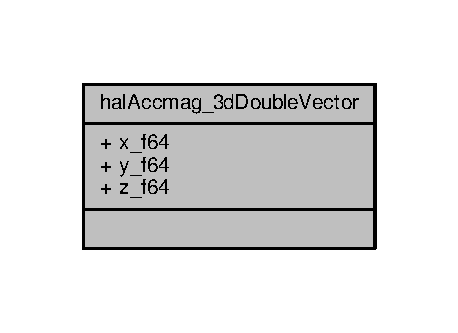
\includegraphics[width=220pt]{structhalAccmag__3dDoubleVector__coll__graph}
\end{center}
\end{figure}
\subsection*{Data Fields}
\begin{DoxyCompactItemize}
\item 
double \hyperlink{structhalAccmag__3dDoubleVector_a011646ea6f4b78400dfd2ffa8eb45eea_a011646ea6f4b78400dfd2ffa8eb45eea}{x\+\_\+f64}
\begin{DoxyCompactList}\small\item\em x-\/component of a 3\+D vector data \end{DoxyCompactList}\item 
double \hyperlink{structhalAccmag__3dDoubleVector_a88f4ed3363ccaa08c00d2fc28f7b2ab4_a88f4ed3363ccaa08c00d2fc28f7b2ab4}{y\+\_\+f64}
\begin{DoxyCompactList}\small\item\em y-\/component of a 3\+D vector data \end{DoxyCompactList}\item 
double \hyperlink{structhalAccmag__3dDoubleVector_a5041b0551694f5f4057a5f3454782e44_a5041b0551694f5f4057a5f3454782e44}{z\+\_\+f64}
\begin{DoxyCompactList}\small\item\em z-\/component of a 3\+D vector data \end{DoxyCompactList}\end{DoxyCompactItemize}


\subsection{Detailed Description}
3\+D vector of floats for x,y,z axes of sensors 



 \begin{DoxyAuthor}{Author}
Juergen Schmidt (juscgs00) 
\end{DoxyAuthor}
\begin{DoxyDate}{Date}
2014/05/05
\end{DoxyDate}
To store the 3\+D-\/components of the sensor data, a dedicated type is declared. Every component is given in float (single precision).

Definition at line 36 of file acc\+Mag.\+h.



\subsection{Field Documentation}
\hypertarget{structhalAccmag__3dDoubleVector_a011646ea6f4b78400dfd2ffa8eb45eea_a011646ea6f4b78400dfd2ffa8eb45eea}{\index{hal\+Accmag\+\_\+3d\+Double\+Vector@{hal\+Accmag\+\_\+3d\+Double\+Vector}!x\+\_\+f64@{x\+\_\+f64}}
\index{x\+\_\+f64@{x\+\_\+f64}!hal\+Accmag\+\_\+3d\+Double\+Vector@{hal\+Accmag\+\_\+3d\+Double\+Vector}}
\subsubsection[{x\+\_\+f64}]{\setlength{\rightskip}{0pt plus 5cm}double hal\+Accmag\+\_\+3d\+Double\+Vector\+::x\+\_\+f64}}\label{structhalAccmag__3dDoubleVector_a011646ea6f4b78400dfd2ffa8eb45eea_a011646ea6f4b78400dfd2ffa8eb45eea}


x-\/component of a 3\+D vector data 



Definition at line 37 of file acc\+Mag.\+h.

\hypertarget{structhalAccmag__3dDoubleVector_a88f4ed3363ccaa08c00d2fc28f7b2ab4_a88f4ed3363ccaa08c00d2fc28f7b2ab4}{\index{hal\+Accmag\+\_\+3d\+Double\+Vector@{hal\+Accmag\+\_\+3d\+Double\+Vector}!y\+\_\+f64@{y\+\_\+f64}}
\index{y\+\_\+f64@{y\+\_\+f64}!hal\+Accmag\+\_\+3d\+Double\+Vector@{hal\+Accmag\+\_\+3d\+Double\+Vector}}
\subsubsection[{y\+\_\+f64}]{\setlength{\rightskip}{0pt plus 5cm}double hal\+Accmag\+\_\+3d\+Double\+Vector\+::y\+\_\+f64}}\label{structhalAccmag__3dDoubleVector_a88f4ed3363ccaa08c00d2fc28f7b2ab4_a88f4ed3363ccaa08c00d2fc28f7b2ab4}


y-\/component of a 3\+D vector data 



Definition at line 38 of file acc\+Mag.\+h.

\hypertarget{structhalAccmag__3dDoubleVector_a5041b0551694f5f4057a5f3454782e44_a5041b0551694f5f4057a5f3454782e44}{\index{hal\+Accmag\+\_\+3d\+Double\+Vector@{hal\+Accmag\+\_\+3d\+Double\+Vector}!z\+\_\+f64@{z\+\_\+f64}}
\index{z\+\_\+f64@{z\+\_\+f64}!hal\+Accmag\+\_\+3d\+Double\+Vector@{hal\+Accmag\+\_\+3d\+Double\+Vector}}
\subsubsection[{z\+\_\+f64}]{\setlength{\rightskip}{0pt plus 5cm}double hal\+Accmag\+\_\+3d\+Double\+Vector\+::z\+\_\+f64}}\label{structhalAccmag__3dDoubleVector_a5041b0551694f5f4057a5f3454782e44_a5041b0551694f5f4057a5f3454782e44}


z-\/component of a 3\+D vector data 



Definition at line 39 of file acc\+Mag.\+h.



The documentation for this struct was generated from the following file\+:\begin{DoxyCompactItemize}
\item 
hal/\+I\+M\+U/acc\+Mag/\hyperlink{accMag_8h}{acc\+Mag.\+h}\end{DoxyCompactItemize}

\hypertarget{structhalAccmag__dataContainer}{\section{hal\+Accmag\+\_\+data\+Container Struct Reference}
\label{structhalAccmag__dataContainer}\index{hal\+Accmag\+\_\+data\+Container@{hal\+Accmag\+\_\+data\+Container}}
}


Container for Acc. and Compass data.  




{\ttfamily \#include $<$acc\+Mag.\+h$>$}



Collaboration diagram for hal\+Accmag\+\_\+data\+Container\+:
\nopagebreak
\begin{figure}[H]
\begin{center}
\leavevmode
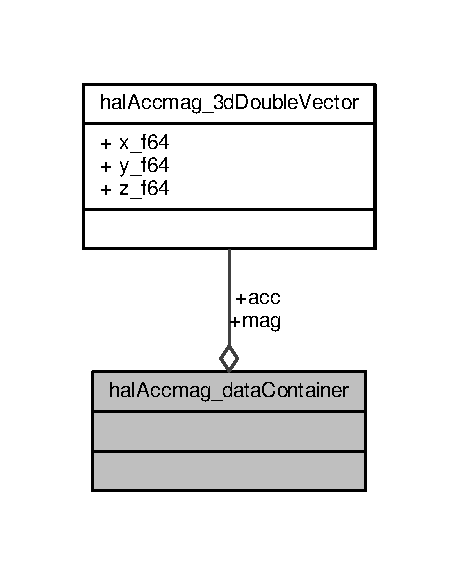
\includegraphics[width=220pt]{structhalAccmag__dataContainer__coll__graph}
\end{center}
\end{figure}
\subsection*{Data Fields}
\begin{DoxyCompactItemize}
\item 
\hyperlink{structhalAccmag__3dDoubleVector}{hal\+Accmag\+\_\+3d\+Double\+Vector} \hyperlink{structhalAccmag__dataContainer_afc3847993eed1c8f1e67028ad6d2a6cf_afc3847993eed1c8f1e67028ad6d2a6cf}{acc}
\begin{DoxyCompactList}\small\item\em acceleration data, S\+I-\/unit\+: m$\ast$s$^\wedge$(-\/2) \end{DoxyCompactList}\item 
\hyperlink{structhalAccmag__3dDoubleVector}{hal\+Accmag\+\_\+3d\+Double\+Vector} \hyperlink{structhalAccmag__dataContainer_a903681a66ce49c39267aa66d471812f7_a903681a66ce49c39267aa66d471812f7}{mag}
\begin{DoxyCompactList}\small\item\em compass data, S\+I-\/unit\+: kg$\ast$s$^\wedge$(-\/2)$\ast$\+A$^\wedge$(-\/1) (Tesla) \end{DoxyCompactList}\end{DoxyCompactItemize}


\subsection{Detailed Description}
Container for Acc. and Compass data. 



 \begin{DoxyAuthor}{Author}
Juergen Schmidt (juscgs00) 
\end{DoxyAuthor}
\begin{DoxyDate}{Date}
2014/05/05
\end{DoxyDate}
Since the used chip (L\+S\+M303\+D) consists of an acceleration sensor and a compass sensor, both data sets shall be kept in one container.

Definition at line 56 of file acc\+Mag.\+h.



\subsection{Field Documentation}
\hypertarget{structhalAccmag__dataContainer_afc3847993eed1c8f1e67028ad6d2a6cf_afc3847993eed1c8f1e67028ad6d2a6cf}{\index{hal\+Accmag\+\_\+data\+Container@{hal\+Accmag\+\_\+data\+Container}!acc@{acc}}
\index{acc@{acc}!hal\+Accmag\+\_\+data\+Container@{hal\+Accmag\+\_\+data\+Container}}
\subsubsection[{acc}]{\setlength{\rightskip}{0pt plus 5cm}{\bf hal\+Accmag\+\_\+3d\+Double\+Vector} hal\+Accmag\+\_\+data\+Container\+::acc}}\label{structhalAccmag__dataContainer_afc3847993eed1c8f1e67028ad6d2a6cf_afc3847993eed1c8f1e67028ad6d2a6cf}


acceleration data, S\+I-\/unit\+: m$\ast$s$^\wedge$(-\/2) 



Definition at line 57 of file acc\+Mag.\+h.

\hypertarget{structhalAccmag__dataContainer_a903681a66ce49c39267aa66d471812f7_a903681a66ce49c39267aa66d471812f7}{\index{hal\+Accmag\+\_\+data\+Container@{hal\+Accmag\+\_\+data\+Container}!mag@{mag}}
\index{mag@{mag}!hal\+Accmag\+\_\+data\+Container@{hal\+Accmag\+\_\+data\+Container}}
\subsubsection[{mag}]{\setlength{\rightskip}{0pt plus 5cm}{\bf hal\+Accmag\+\_\+3d\+Double\+Vector} hal\+Accmag\+\_\+data\+Container\+::mag}}\label{structhalAccmag__dataContainer_a903681a66ce49c39267aa66d471812f7_a903681a66ce49c39267aa66d471812f7}


compass data, S\+I-\/unit\+: kg$\ast$s$^\wedge$(-\/2)$\ast$\+A$^\wedge$(-\/1) (Tesla) 



Definition at line 58 of file acc\+Mag.\+h.



The documentation for this struct was generated from the following file\+:\begin{DoxyCompactItemize}
\item 
hal/\+I\+M\+U/acc\+Mag/\hyperlink{accMag_8h}{acc\+Mag.\+h}\end{DoxyCompactItemize}

\hypertarget{structhalImu__orientationValues}{\section{hal\+Imu\+\_\+orientation\+Values Struct Reference}
\label{structhalImu__orientationValues}\index{hal\+Imu\+\_\+orientation\+Values@{hal\+Imu\+\_\+orientation\+Values}}
}


Inertial measurement unit values.  




{\ttfamily \#include $<$imu.\+h$>$}



Collaboration diagram for hal\+Imu\+\_\+orientation\+Values\+:
\nopagebreak
\begin{figure}[H]
\begin{center}
\leavevmode
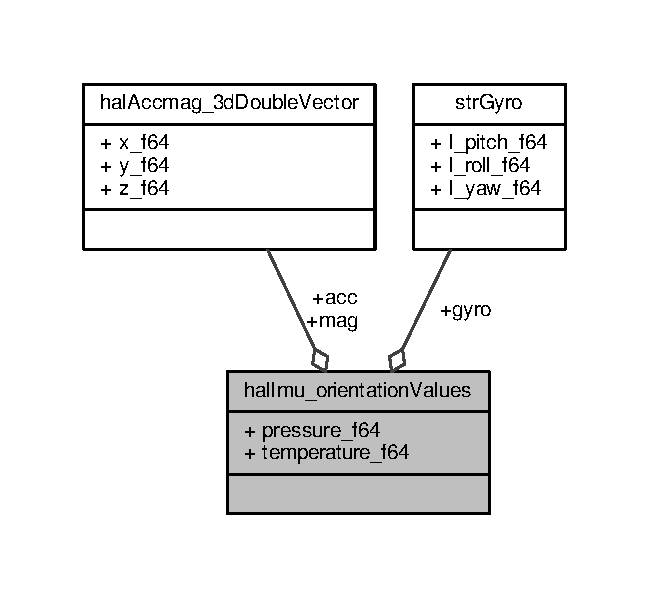
\includegraphics[width=312pt]{structhalImu__orientationValues__coll__graph}
\end{center}
\end{figure}
\subsection*{Data Fields}
\begin{DoxyCompactItemize}
\item 
\hyperlink{structhalAccmag__3dDoubleVector}{hal\+Accmag\+\_\+3d\+Double\+Vector} \hyperlink{structhalImu__orientationValues_a8080616bd2a3d4f01f5334d4bf05427e_a8080616bd2a3d4f01f5334d4bf05427e}{acc}
\item 
\hyperlink{structstrGyro}{str\+Gyro} \hyperlink{structhalImu__orientationValues_a386a3509066dbfd830da6b7a993b31da_a386a3509066dbfd830da6b7a993b31da}{gyro}
\item 
\hyperlink{structhalAccmag__3dDoubleVector}{hal\+Accmag\+\_\+3d\+Double\+Vector} \hyperlink{structhalImu__orientationValues_ac0763bc025ee3aa20f167e74ecccfc3c_ac0763bc025ee3aa20f167e74ecccfc3c}{mag}
\item 
double \hyperlink{structhalImu__orientationValues_a512925b63aa63c02874ce4dbb920c7f0_a512925b63aa63c02874ce4dbb920c7f0}{pressure\+\_\+f64}
\item 
double \hyperlink{structhalImu__orientationValues_aeda72e72e4979977023cba31ee89cffa_aeda72e72e4979977023cba31ee89cffa}{temperature\+\_\+f64}
\end{DoxyCompactItemize}


\subsection{Detailed Description}
Inertial measurement unit values. 



 \begin{DoxyAuthor}{Author}
Oliver Breuning (olbrgs00) 
\end{DoxyAuthor}
\begin{DoxyDate}{Date}
2015/05/13
\end{DoxyDate}
Stores all sensor values from the Inertial measurement unit within one dedicated type. All values within are floats

Definition at line 33 of file imu.\+h.



\subsection{Field Documentation}
\hypertarget{structhalImu__orientationValues_a8080616bd2a3d4f01f5334d4bf05427e_a8080616bd2a3d4f01f5334d4bf05427e}{\index{hal\+Imu\+\_\+orientation\+Values@{hal\+Imu\+\_\+orientation\+Values}!acc@{acc}}
\index{acc@{acc}!hal\+Imu\+\_\+orientation\+Values@{hal\+Imu\+\_\+orientation\+Values}}
\subsubsection[{acc}]{\setlength{\rightskip}{0pt plus 5cm}{\bf hal\+Accmag\+\_\+3d\+Double\+Vector} hal\+Imu\+\_\+orientation\+Values\+::acc}}\label{structhalImu__orientationValues_a8080616bd2a3d4f01f5334d4bf05427e_a8080616bd2a3d4f01f5334d4bf05427e}


Definition at line 34 of file imu.\+h.

\hypertarget{structhalImu__orientationValues_a386a3509066dbfd830da6b7a993b31da_a386a3509066dbfd830da6b7a993b31da}{\index{hal\+Imu\+\_\+orientation\+Values@{hal\+Imu\+\_\+orientation\+Values}!gyro@{gyro}}
\index{gyro@{gyro}!hal\+Imu\+\_\+orientation\+Values@{hal\+Imu\+\_\+orientation\+Values}}
\subsubsection[{gyro}]{\setlength{\rightskip}{0pt plus 5cm}{\bf str\+Gyro} hal\+Imu\+\_\+orientation\+Values\+::gyro}}\label{structhalImu__orientationValues_a386a3509066dbfd830da6b7a993b31da_a386a3509066dbfd830da6b7a993b31da}


Definition at line 36 of file imu.\+h.

\hypertarget{structhalImu__orientationValues_ac0763bc025ee3aa20f167e74ecccfc3c_ac0763bc025ee3aa20f167e74ecccfc3c}{\index{hal\+Imu\+\_\+orientation\+Values@{hal\+Imu\+\_\+orientation\+Values}!mag@{mag}}
\index{mag@{mag}!hal\+Imu\+\_\+orientation\+Values@{hal\+Imu\+\_\+orientation\+Values}}
\subsubsection[{mag}]{\setlength{\rightskip}{0pt plus 5cm}{\bf hal\+Accmag\+\_\+3d\+Double\+Vector} hal\+Imu\+\_\+orientation\+Values\+::mag}}\label{structhalImu__orientationValues_ac0763bc025ee3aa20f167e74ecccfc3c_ac0763bc025ee3aa20f167e74ecccfc3c}


Definition at line 35 of file imu.\+h.

\hypertarget{structhalImu__orientationValues_a512925b63aa63c02874ce4dbb920c7f0_a512925b63aa63c02874ce4dbb920c7f0}{\index{hal\+Imu\+\_\+orientation\+Values@{hal\+Imu\+\_\+orientation\+Values}!pressure\+\_\+f64@{pressure\+\_\+f64}}
\index{pressure\+\_\+f64@{pressure\+\_\+f64}!hal\+Imu\+\_\+orientation\+Values@{hal\+Imu\+\_\+orientation\+Values}}
\subsubsection[{pressure\+\_\+f64}]{\setlength{\rightskip}{0pt plus 5cm}double hal\+Imu\+\_\+orientation\+Values\+::pressure\+\_\+f64}}\label{structhalImu__orientationValues_a512925b63aa63c02874ce4dbb920c7f0_a512925b63aa63c02874ce4dbb920c7f0}


Definition at line 38 of file imu.\+h.

\hypertarget{structhalImu__orientationValues_aeda72e72e4979977023cba31ee89cffa_aeda72e72e4979977023cba31ee89cffa}{\index{hal\+Imu\+\_\+orientation\+Values@{hal\+Imu\+\_\+orientation\+Values}!temperature\+\_\+f64@{temperature\+\_\+f64}}
\index{temperature\+\_\+f64@{temperature\+\_\+f64}!hal\+Imu\+\_\+orientation\+Values@{hal\+Imu\+\_\+orientation\+Values}}
\subsubsection[{temperature\+\_\+f64}]{\setlength{\rightskip}{0pt plus 5cm}double hal\+Imu\+\_\+orientation\+Values\+::temperature\+\_\+f64}}\label{structhalImu__orientationValues_aeda72e72e4979977023cba31ee89cffa_aeda72e72e4979977023cba31ee89cffa}


Definition at line 37 of file imu.\+h.



The documentation for this struct was generated from the following file\+:\begin{DoxyCompactItemize}
\item 
hal/\+I\+M\+U/\hyperlink{imu_8h}{imu.\+h}\end{DoxyCompactItemize}

\hypertarget{structhalMatlab__rtImuPayload}{\section{hal\+Matlab\+\_\+rt\+Imu\+Payload Struct Reference}
\label{structhalMatlab__rtImuPayload}\index{hal\+Matlab\+\_\+rt\+Imu\+Payload@{hal\+Matlab\+\_\+rt\+Imu\+Payload}}
}


Container for time-\/stamped I\+M\+U state data.  




{\ttfamily \#include $<$udp\+Imu\+Lib.\+h$>$}



Collaboration diagram for hal\+Matlab\+\_\+rt\+Imu\+Payload\+:
\nopagebreak
\begin{figure}[H]
\begin{center}
\leavevmode
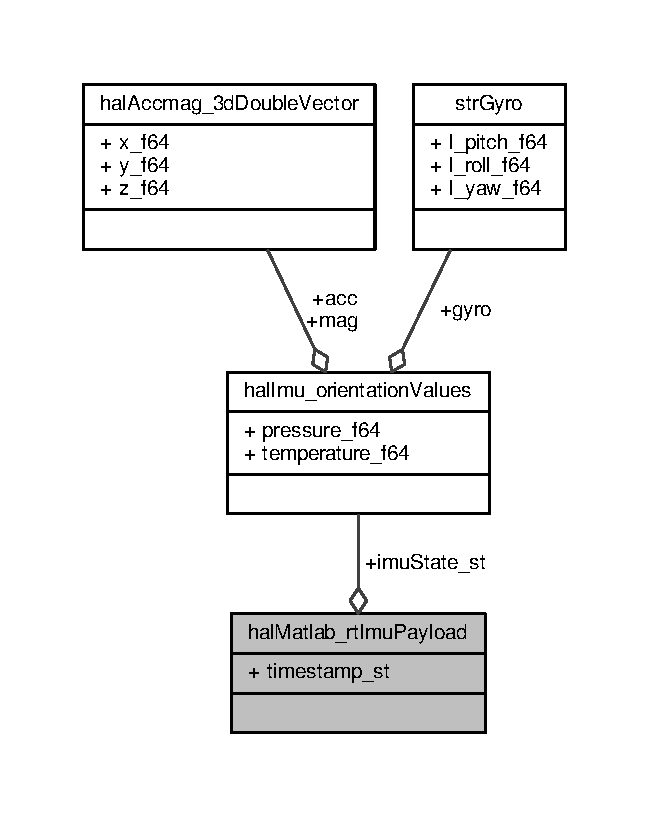
\includegraphics[width=312pt]{structhalMatlab__rtImuPayload__coll__graph}
\end{center}
\end{figure}
\subsection*{Data Fields}
\begin{DoxyCompactItemize}
\item 
\hyperlink{structhalImu__orientationValues}{hal\+Imu\+\_\+orientation\+Values} \hyperlink{structhalMatlab__rtImuPayload_a9c79ff85291d3492b09536e902c96c92_a9c79ff85291d3492b09536e902c96c92}{imu\+State\+\_\+st}
\item 
struct timespec \hyperlink{structhalMatlab__rtImuPayload_a884897c9695ab0e4d2d0fbe9677a60cd_a884897c9695ab0e4d2d0fbe9677a60cd}{timestamp\+\_\+st}
\end{DoxyCompactItemize}


\subsection{Detailed Description}
Container for time-\/stamped I\+M\+U state data. 



 \begin{DoxyAuthor}{Author}
Juergen Schmidt (juscgs00) 
\end{DoxyAuthor}
\begin{DoxyDate}{Date}
2014/05/20
\end{DoxyDate}
Since the Udp-\/\+Lib is considered to handle a soft realtime connection, the I\+M\+U state data is considered to be time-\/ stamped. This structure encapsulates a precise timestamp and I\+M\+U state vector.

Definition at line 25 of file udp\+Imu\+Lib.\+h.



\subsection{Field Documentation}
\hypertarget{structhalMatlab__rtImuPayload_a9c79ff85291d3492b09536e902c96c92_a9c79ff85291d3492b09536e902c96c92}{\index{hal\+Matlab\+\_\+rt\+Imu\+Payload@{hal\+Matlab\+\_\+rt\+Imu\+Payload}!imu\+State\+\_\+st@{imu\+State\+\_\+st}}
\index{imu\+State\+\_\+st@{imu\+State\+\_\+st}!hal\+Matlab\+\_\+rt\+Imu\+Payload@{hal\+Matlab\+\_\+rt\+Imu\+Payload}}
\subsubsection[{imu\+State\+\_\+st}]{\setlength{\rightskip}{0pt plus 5cm}{\bf hal\+Imu\+\_\+orientation\+Values} hal\+Matlab\+\_\+rt\+Imu\+Payload\+::imu\+State\+\_\+st}}\label{structhalMatlab__rtImuPayload_a9c79ff85291d3492b09536e902c96c92_a9c79ff85291d3492b09536e902c96c92}


Definition at line 27 of file udp\+Imu\+Lib.\+h.

\hypertarget{structhalMatlab__rtImuPayload_a884897c9695ab0e4d2d0fbe9677a60cd_a884897c9695ab0e4d2d0fbe9677a60cd}{\index{hal\+Matlab\+\_\+rt\+Imu\+Payload@{hal\+Matlab\+\_\+rt\+Imu\+Payload}!timestamp\+\_\+st@{timestamp\+\_\+st}}
\index{timestamp\+\_\+st@{timestamp\+\_\+st}!hal\+Matlab\+\_\+rt\+Imu\+Payload@{hal\+Matlab\+\_\+rt\+Imu\+Payload}}
\subsubsection[{timestamp\+\_\+st}]{\setlength{\rightskip}{0pt plus 5cm}struct timespec hal\+Matlab\+\_\+rt\+Imu\+Payload\+::timestamp\+\_\+st}}\label{structhalMatlab__rtImuPayload_a884897c9695ab0e4d2d0fbe9677a60cd_a884897c9695ab0e4d2d0fbe9677a60cd}


Definition at line 26 of file udp\+Imu\+Lib.\+h.



The documentation for this struct was generated from the following file\+:\begin{DoxyCompactItemize}
\item 
matlab/\hyperlink{udpImuLib_8h}{udp\+Imu\+Lib.\+h}\end{DoxyCompactItemize}

\hypertarget{structhalMatlab__rtSigAllStatePayload}{\section{hal\+Matlab\+\_\+rt\+Sig\+All\+State\+Payload Struct Reference}
\label{structhalMatlab__rtSigAllStatePayload}\index{hal\+Matlab\+\_\+rt\+Sig\+All\+State\+Payload@{hal\+Matlab\+\_\+rt\+Sig\+All\+State\+Payload}}
}


{\ttfamily \#include $<$udp\+Sig\+Lib.\+h$>$}



Collaboration diagram for hal\+Matlab\+\_\+rt\+Sig\+All\+State\+Payload\+:
\nopagebreak
\begin{figure}[H]
\begin{center}
\leavevmode
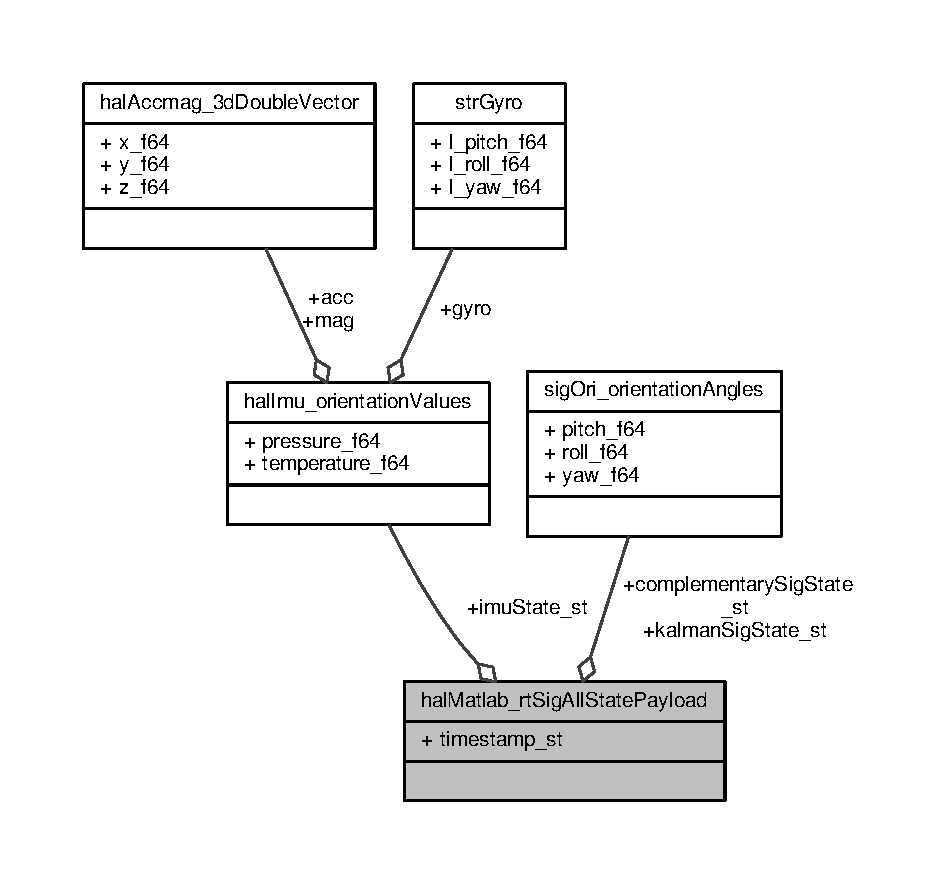
\includegraphics[width=350pt]{structhalMatlab__rtSigAllStatePayload__coll__graph}
\end{center}
\end{figure}
\subsection*{Data Fields}
\begin{DoxyCompactItemize}
\item 
\hyperlink{structsigOri__orientationAngles}{sig\+Ori\+\_\+orientation\+Angles} \hyperlink{structhalMatlab__rtSigAllStatePayload_ae2a362e5944039d976077bb43797fd30_ae2a362e5944039d976077bb43797fd30}{complementary\+Sig\+State\+\_\+st}
\item 
\hyperlink{structhalImu__orientationValues}{hal\+Imu\+\_\+orientation\+Values} \hyperlink{structhalMatlab__rtSigAllStatePayload_a077a67bc0c0d249d0e4bfb7287676646_a077a67bc0c0d249d0e4bfb7287676646}{imu\+State\+\_\+st}
\item 
\hyperlink{structsigOri__orientationAngles}{sig\+Ori\+\_\+orientation\+Angles} \hyperlink{structhalMatlab__rtSigAllStatePayload_a125a952adeb10a6d7391f2b0acfcaae2_a125a952adeb10a6d7391f2b0acfcaae2}{kalman\+Sig\+State\+\_\+st}
\item 
struct timespec \hyperlink{structhalMatlab__rtSigAllStatePayload_a2526e3f137ca373500385c769c69b897_a2526e3f137ca373500385c769c69b897}{timestamp\+\_\+st}
\end{DoxyCompactItemize}


\subsection{Detailed Description}


Definition at line 31 of file udp\+Sig\+Lib.\+h.



\subsection{Field Documentation}
\hypertarget{structhalMatlab__rtSigAllStatePayload_ae2a362e5944039d976077bb43797fd30_ae2a362e5944039d976077bb43797fd30}{\index{hal\+Matlab\+\_\+rt\+Sig\+All\+State\+Payload@{hal\+Matlab\+\_\+rt\+Sig\+All\+State\+Payload}!complementary\+Sig\+State\+\_\+st@{complementary\+Sig\+State\+\_\+st}}
\index{complementary\+Sig\+State\+\_\+st@{complementary\+Sig\+State\+\_\+st}!hal\+Matlab\+\_\+rt\+Sig\+All\+State\+Payload@{hal\+Matlab\+\_\+rt\+Sig\+All\+State\+Payload}}
\subsubsection[{complementary\+Sig\+State\+\_\+st}]{\setlength{\rightskip}{0pt plus 5cm}{\bf sig\+Ori\+\_\+orientation\+Angles} hal\+Matlab\+\_\+rt\+Sig\+All\+State\+Payload\+::complementary\+Sig\+State\+\_\+st}}\label{structhalMatlab__rtSigAllStatePayload_ae2a362e5944039d976077bb43797fd30_ae2a362e5944039d976077bb43797fd30}


Definition at line 35 of file udp\+Sig\+Lib.\+h.

\hypertarget{structhalMatlab__rtSigAllStatePayload_a077a67bc0c0d249d0e4bfb7287676646_a077a67bc0c0d249d0e4bfb7287676646}{\index{hal\+Matlab\+\_\+rt\+Sig\+All\+State\+Payload@{hal\+Matlab\+\_\+rt\+Sig\+All\+State\+Payload}!imu\+State\+\_\+st@{imu\+State\+\_\+st}}
\index{imu\+State\+\_\+st@{imu\+State\+\_\+st}!hal\+Matlab\+\_\+rt\+Sig\+All\+State\+Payload@{hal\+Matlab\+\_\+rt\+Sig\+All\+State\+Payload}}
\subsubsection[{imu\+State\+\_\+st}]{\setlength{\rightskip}{0pt plus 5cm}{\bf hal\+Imu\+\_\+orientation\+Values} hal\+Matlab\+\_\+rt\+Sig\+All\+State\+Payload\+::imu\+State\+\_\+st}}\label{structhalMatlab__rtSigAllStatePayload_a077a67bc0c0d249d0e4bfb7287676646_a077a67bc0c0d249d0e4bfb7287676646}


Definition at line 33 of file udp\+Sig\+Lib.\+h.

\hypertarget{structhalMatlab__rtSigAllStatePayload_a125a952adeb10a6d7391f2b0acfcaae2_a125a952adeb10a6d7391f2b0acfcaae2}{\index{hal\+Matlab\+\_\+rt\+Sig\+All\+State\+Payload@{hal\+Matlab\+\_\+rt\+Sig\+All\+State\+Payload}!kalman\+Sig\+State\+\_\+st@{kalman\+Sig\+State\+\_\+st}}
\index{kalman\+Sig\+State\+\_\+st@{kalman\+Sig\+State\+\_\+st}!hal\+Matlab\+\_\+rt\+Sig\+All\+State\+Payload@{hal\+Matlab\+\_\+rt\+Sig\+All\+State\+Payload}}
\subsubsection[{kalman\+Sig\+State\+\_\+st}]{\setlength{\rightskip}{0pt plus 5cm}{\bf sig\+Ori\+\_\+orientation\+Angles} hal\+Matlab\+\_\+rt\+Sig\+All\+State\+Payload\+::kalman\+Sig\+State\+\_\+st}}\label{structhalMatlab__rtSigAllStatePayload_a125a952adeb10a6d7391f2b0acfcaae2_a125a952adeb10a6d7391f2b0acfcaae2}


Definition at line 34 of file udp\+Sig\+Lib.\+h.

\hypertarget{structhalMatlab__rtSigAllStatePayload_a2526e3f137ca373500385c769c69b897_a2526e3f137ca373500385c769c69b897}{\index{hal\+Matlab\+\_\+rt\+Sig\+All\+State\+Payload@{hal\+Matlab\+\_\+rt\+Sig\+All\+State\+Payload}!timestamp\+\_\+st@{timestamp\+\_\+st}}
\index{timestamp\+\_\+st@{timestamp\+\_\+st}!hal\+Matlab\+\_\+rt\+Sig\+All\+State\+Payload@{hal\+Matlab\+\_\+rt\+Sig\+All\+State\+Payload}}
\subsubsection[{timestamp\+\_\+st}]{\setlength{\rightskip}{0pt plus 5cm}struct timespec hal\+Matlab\+\_\+rt\+Sig\+All\+State\+Payload\+::timestamp\+\_\+st}}\label{structhalMatlab__rtSigAllStatePayload_a2526e3f137ca373500385c769c69b897_a2526e3f137ca373500385c769c69b897}


Definition at line 32 of file udp\+Sig\+Lib.\+h.



The documentation for this struct was generated from the following file\+:\begin{DoxyCompactItemize}
\item 
matlab/\hyperlink{udpSigLib_8h}{udp\+Sig\+Lib.\+h}\end{DoxyCompactItemize}

\hypertarget{structhalMatlab__rtSigPayload}{\section{hal\+Matlab\+\_\+rt\+Sig\+Payload Struct Reference}
\label{structhalMatlab__rtSigPayload}\index{hal\+Matlab\+\_\+rt\+Sig\+Payload@{hal\+Matlab\+\_\+rt\+Sig\+Payload}}
}


Container for time-\/stamped S\+I\+G\+N\+A\+L layer state data.  




{\ttfamily \#include $<$udp\+Sig\+Lib.\+h$>$}



Collaboration diagram for hal\+Matlab\+\_\+rt\+Sig\+Payload\+:
\nopagebreak
\begin{figure}[H]
\begin{center}
\leavevmode
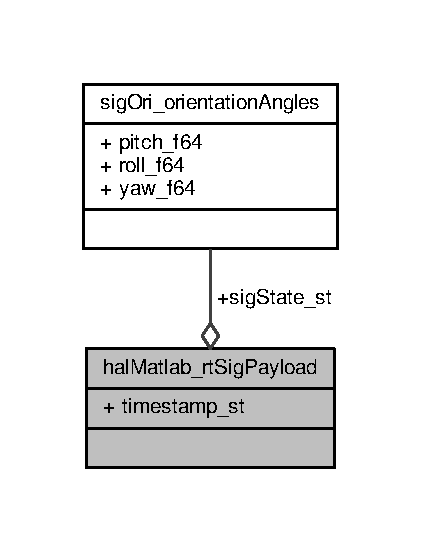
\includegraphics[width=202pt]{structhalMatlab__rtSigPayload__coll__graph}
\end{center}
\end{figure}
\subsection*{Data Fields}
\begin{DoxyCompactItemize}
\item 
\hyperlink{structsigOri__orientationAngles}{sig\+Ori\+\_\+orientation\+Angles} \hyperlink{structhalMatlab__rtSigPayload_acbe0c4752e7c359734effc1f17f5f494_acbe0c4752e7c359734effc1f17f5f494}{sig\+State\+\_\+st}
\item 
struct timespec \hyperlink{structhalMatlab__rtSigPayload_acf78b49f8e27a0097931fe0e57d14819_acf78b49f8e27a0097931fe0e57d14819}{timestamp\+\_\+st}
\end{DoxyCompactItemize}


\subsection{Detailed Description}
Container for time-\/stamped S\+I\+G\+N\+A\+L layer state data. 



 \begin{DoxyAuthor}{Author}
Juergen Schmidt (juscgs00) 
\end{DoxyAuthor}
\begin{DoxyDate}{Date}
2014/06/01
\end{DoxyDate}
Since the Udp-\/\+Lib is considered to handle a soft realtime connection, the S\+I\+G state data is considered to be time-\/ stamped. This structure encapsulates a precise timestamp and S\+I\+G\+N\+A\+L layer state vector.

Definition at line 26 of file udp\+Sig\+Lib.\+h.



\subsection{Field Documentation}
\hypertarget{structhalMatlab__rtSigPayload_acbe0c4752e7c359734effc1f17f5f494_acbe0c4752e7c359734effc1f17f5f494}{\index{hal\+Matlab\+\_\+rt\+Sig\+Payload@{hal\+Matlab\+\_\+rt\+Sig\+Payload}!sig\+State\+\_\+st@{sig\+State\+\_\+st}}
\index{sig\+State\+\_\+st@{sig\+State\+\_\+st}!hal\+Matlab\+\_\+rt\+Sig\+Payload@{hal\+Matlab\+\_\+rt\+Sig\+Payload}}
\subsubsection[{sig\+State\+\_\+st}]{\setlength{\rightskip}{0pt plus 5cm}{\bf sig\+Ori\+\_\+orientation\+Angles} hal\+Matlab\+\_\+rt\+Sig\+Payload\+::sig\+State\+\_\+st}}\label{structhalMatlab__rtSigPayload_acbe0c4752e7c359734effc1f17f5f494_acbe0c4752e7c359734effc1f17f5f494}


Definition at line 28 of file udp\+Sig\+Lib.\+h.

\hypertarget{structhalMatlab__rtSigPayload_acf78b49f8e27a0097931fe0e57d14819_acf78b49f8e27a0097931fe0e57d14819}{\index{hal\+Matlab\+\_\+rt\+Sig\+Payload@{hal\+Matlab\+\_\+rt\+Sig\+Payload}!timestamp\+\_\+st@{timestamp\+\_\+st}}
\index{timestamp\+\_\+st@{timestamp\+\_\+st}!hal\+Matlab\+\_\+rt\+Sig\+Payload@{hal\+Matlab\+\_\+rt\+Sig\+Payload}}
\subsubsection[{timestamp\+\_\+st}]{\setlength{\rightskip}{0pt plus 5cm}struct timespec hal\+Matlab\+\_\+rt\+Sig\+Payload\+::timestamp\+\_\+st}}\label{structhalMatlab__rtSigPayload_acf78b49f8e27a0097931fe0e57d14819_acf78b49f8e27a0097931fe0e57d14819}


Definition at line 27 of file udp\+Sig\+Lib.\+h.



The documentation for this struct was generated from the following file\+:\begin{DoxyCompactItemize}
\item 
matlab/\hyperlink{udpSigLib_8h}{udp\+Sig\+Lib.\+h}\end{DoxyCompactItemize}

\hypertarget{structhalMatlab__socketData}{\section{hal\+Matlab\+\_\+socket\+Data Struct Reference}
\label{structhalMatlab__socketData}\index{hal\+Matlab\+\_\+socket\+Data@{hal\+Matlab\+\_\+socket\+Data}}
}


Container for Udp-\/\+Socket data.  




{\ttfamily \#include $<$udp\+Lib.\+h$>$}



Collaboration diagram for hal\+Matlab\+\_\+socket\+Data\+:
\nopagebreak
\begin{figure}[H]
\begin{center}
\leavevmode
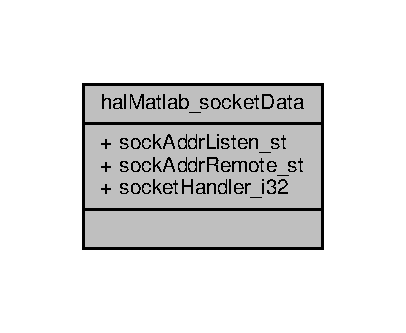
\includegraphics[width=195pt]{structhalMatlab__socketData__coll__graph}
\end{center}
\end{figure}
\subsection*{Data Fields}
\begin{DoxyCompactItemize}
\item 
struct sockaddr\+\_\+in \hyperlink{structhalMatlab__socketData_a879fc935cde2c09c6c02cf6e6ecafb86_a879fc935cde2c09c6c02cf6e6ecafb86}{sock\+Addr\+Listen\+\_\+st}
\item 
struct sockaddr\+\_\+in \hyperlink{structhalMatlab__socketData_aa9b77c362396cf1fbb78dd9688da4a0d_aa9b77c362396cf1fbb78dd9688da4a0d}{sock\+Addr\+Remote\+\_\+st}
\item 
int \hyperlink{structhalMatlab__socketData_a60bb1e30d40ee435f1f9501933aba991_a60bb1e30d40ee435f1f9501933aba991}{socket\+Handler\+\_\+i32}
\end{DoxyCompactItemize}


\subsection{Detailed Description}
Container for Udp-\/\+Socket data. 



 \begin{DoxyAuthor}{Author}
Juergen Schmidt (juscgs00) 
\end{DoxyAuthor}
\begin{DoxyDate}{Date}
2014/05/17
\end{DoxyDate}
Since the Udp-\/\+Lib is considered to handle several opened sockets at the same time, an encapsulation of all relevant socket data in a custom struct type shall be performed.

Definition at line 57 of file udp\+Lib.\+h.



\subsection{Field Documentation}
\hypertarget{structhalMatlab__socketData_a879fc935cde2c09c6c02cf6e6ecafb86_a879fc935cde2c09c6c02cf6e6ecafb86}{\index{hal\+Matlab\+\_\+socket\+Data@{hal\+Matlab\+\_\+socket\+Data}!sock\+Addr\+Listen\+\_\+st@{sock\+Addr\+Listen\+\_\+st}}
\index{sock\+Addr\+Listen\+\_\+st@{sock\+Addr\+Listen\+\_\+st}!hal\+Matlab\+\_\+socket\+Data@{hal\+Matlab\+\_\+socket\+Data}}
\subsubsection[{sock\+Addr\+Listen\+\_\+st}]{\setlength{\rightskip}{0pt plus 5cm}struct sockaddr\+\_\+in hal\+Matlab\+\_\+socket\+Data\+::sock\+Addr\+Listen\+\_\+st}}\label{structhalMatlab__socketData_a879fc935cde2c09c6c02cf6e6ecafb86_a879fc935cde2c09c6c02cf6e6ecafb86}


Definition at line 58 of file udp\+Lib.\+h.

\hypertarget{structhalMatlab__socketData_aa9b77c362396cf1fbb78dd9688da4a0d_aa9b77c362396cf1fbb78dd9688da4a0d}{\index{hal\+Matlab\+\_\+socket\+Data@{hal\+Matlab\+\_\+socket\+Data}!sock\+Addr\+Remote\+\_\+st@{sock\+Addr\+Remote\+\_\+st}}
\index{sock\+Addr\+Remote\+\_\+st@{sock\+Addr\+Remote\+\_\+st}!hal\+Matlab\+\_\+socket\+Data@{hal\+Matlab\+\_\+socket\+Data}}
\subsubsection[{sock\+Addr\+Remote\+\_\+st}]{\setlength{\rightskip}{0pt plus 5cm}struct sockaddr\+\_\+in hal\+Matlab\+\_\+socket\+Data\+::sock\+Addr\+Remote\+\_\+st}}\label{structhalMatlab__socketData_aa9b77c362396cf1fbb78dd9688da4a0d_aa9b77c362396cf1fbb78dd9688da4a0d}


Definition at line 59 of file udp\+Lib.\+h.

\hypertarget{structhalMatlab__socketData_a60bb1e30d40ee435f1f9501933aba991_a60bb1e30d40ee435f1f9501933aba991}{\index{hal\+Matlab\+\_\+socket\+Data@{hal\+Matlab\+\_\+socket\+Data}!socket\+Handler\+\_\+i32@{socket\+Handler\+\_\+i32}}
\index{socket\+Handler\+\_\+i32@{socket\+Handler\+\_\+i32}!hal\+Matlab\+\_\+socket\+Data@{hal\+Matlab\+\_\+socket\+Data}}
\subsubsection[{socket\+Handler\+\_\+i32}]{\setlength{\rightskip}{0pt plus 5cm}int hal\+Matlab\+\_\+socket\+Data\+::socket\+Handler\+\_\+i32}}\label{structhalMatlab__socketData_a60bb1e30d40ee435f1f9501933aba991_a60bb1e30d40ee435f1f9501933aba991}


Definition at line 60 of file udp\+Lib.\+h.



The documentation for this struct was generated from the following file\+:\begin{DoxyCompactItemize}
\item 
matlab/\hyperlink{udpLib_8h}{udp\+Lib.\+h}\end{DoxyCompactItemize}

\hypertarget{structsigOri__orientationAngles}{\section{sig\+Ori\+\_\+orientation\+Angles Struct Reference}
\label{structsigOri__orientationAngles}\index{sig\+Ori\+\_\+orientation\+Angles@{sig\+Ori\+\_\+orientation\+Angles}}
}


Struct of rotation angles.  




{\ttfamily \#include $<$Orientation.\+h$>$}



Collaboration diagram for sig\+Ori\+\_\+orientation\+Angles\+:
\nopagebreak
\begin{figure}[H]
\begin{center}
\leavevmode
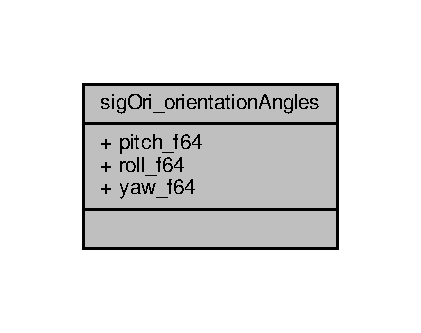
\includegraphics[width=202pt]{structsigOri__orientationAngles__coll__graph}
\end{center}
\end{figure}
\subsection*{Data Fields}
\begin{DoxyCompactItemize}
\item 
double \hyperlink{structsigOri__orientationAngles_a36aa8568f26ce93d16385822cf2e76de_a36aa8568f26ce93d16385822cf2e76de}{pitch\+\_\+f64}
\item 
double \hyperlink{structsigOri__orientationAngles_a0bdf621a53623bc73765e918e368c76e_a0bdf621a53623bc73765e918e368c76e}{roll\+\_\+f64}
\item 
double \hyperlink{structsigOri__orientationAngles_a4d2dd55644a4f5484f1809f64f14e792_a4d2dd55644a4f5484f1809f64f14e792}{yaw\+\_\+f64}
\end{DoxyCompactItemize}


\subsection{Detailed Description}
Struct of rotation angles. 



 \begin{DoxyAuthor}{Author}
Oliver Breuning (olbrgs00) 
\end{DoxyAuthor}
\begin{DoxyDate}{Date}
2015/05/31
\end{DoxyDate}
Stores all calculated sensor rotations from the Inertial measurement unit within one dedicated type. All values within are floats

Definition at line 33 of file Orientation.\+h.



\subsection{Field Documentation}
\hypertarget{structsigOri__orientationAngles_a36aa8568f26ce93d16385822cf2e76de_a36aa8568f26ce93d16385822cf2e76de}{\index{sig\+Ori\+\_\+orientation\+Angles@{sig\+Ori\+\_\+orientation\+Angles}!pitch\+\_\+f64@{pitch\+\_\+f64}}
\index{pitch\+\_\+f64@{pitch\+\_\+f64}!sig\+Ori\+\_\+orientation\+Angles@{sig\+Ori\+\_\+orientation\+Angles}}
\subsubsection[{pitch\+\_\+f64}]{\setlength{\rightskip}{0pt plus 5cm}double sig\+Ori\+\_\+orientation\+Angles\+::pitch\+\_\+f64}}\label{structsigOri__orientationAngles_a36aa8568f26ce93d16385822cf2e76de_a36aa8568f26ce93d16385822cf2e76de}


Definition at line 35 of file Orientation.\+h.

\hypertarget{structsigOri__orientationAngles_a0bdf621a53623bc73765e918e368c76e_a0bdf621a53623bc73765e918e368c76e}{\index{sig\+Ori\+\_\+orientation\+Angles@{sig\+Ori\+\_\+orientation\+Angles}!roll\+\_\+f64@{roll\+\_\+f64}}
\index{roll\+\_\+f64@{roll\+\_\+f64}!sig\+Ori\+\_\+orientation\+Angles@{sig\+Ori\+\_\+orientation\+Angles}}
\subsubsection[{roll\+\_\+f64}]{\setlength{\rightskip}{0pt plus 5cm}double sig\+Ori\+\_\+orientation\+Angles\+::roll\+\_\+f64}}\label{structsigOri__orientationAngles_a0bdf621a53623bc73765e918e368c76e_a0bdf621a53623bc73765e918e368c76e}


Definition at line 34 of file Orientation.\+h.

\hypertarget{structsigOri__orientationAngles_a4d2dd55644a4f5484f1809f64f14e792_a4d2dd55644a4f5484f1809f64f14e792}{\index{sig\+Ori\+\_\+orientation\+Angles@{sig\+Ori\+\_\+orientation\+Angles}!yaw\+\_\+f64@{yaw\+\_\+f64}}
\index{yaw\+\_\+f64@{yaw\+\_\+f64}!sig\+Ori\+\_\+orientation\+Angles@{sig\+Ori\+\_\+orientation\+Angles}}
\subsubsection[{yaw\+\_\+f64}]{\setlength{\rightskip}{0pt plus 5cm}double sig\+Ori\+\_\+orientation\+Angles\+::yaw\+\_\+f64}}\label{structsigOri__orientationAngles_a4d2dd55644a4f5484f1809f64f14e792_a4d2dd55644a4f5484f1809f64f14e792}


Definition at line 36 of file Orientation.\+h.



The documentation for this struct was generated from the following file\+:\begin{DoxyCompactItemize}
\item 
sig/\+Orientation/\hyperlink{Orientation_8h}{Orientation.\+h}\end{DoxyCompactItemize}

\hypertarget{structstrGyro}{\section{str\+Gyro Struct Reference}
\label{structstrGyro}\index{str\+Gyro@{str\+Gyro}}
}


struct with Gyroscope values  




{\ttfamily \#include $<$Gyro.\+h$>$}



Collaboration diagram for str\+Gyro\+:
\nopagebreak
\begin{figure}[H]
\begin{center}
\leavevmode
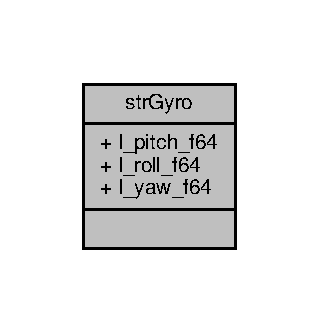
\includegraphics[width=153pt]{structstrGyro__coll__graph}
\end{center}
\end{figure}
\subsection*{Data Fields}
\begin{DoxyCompactItemize}
\item 
double \hyperlink{structstrGyro_a9d82fa8970135f2097dd209a74138848_a9d82fa8970135f2097dd209a74138848}{l\+\_\+pitch\+\_\+f64}
\item 
double \hyperlink{structstrGyro_a0b8d0c0ec6e3324a403d983d67fae643_a0b8d0c0ec6e3324a403d983d67fae643}{l\+\_\+roll\+\_\+f64}
\item 
double \hyperlink{structstrGyro_a1c8ca43d350ad8ef20d2968aa29e6ce6_a1c8ca43d350ad8ef20d2968aa29e6ce6}{l\+\_\+yaw\+\_\+f64}
\end{DoxyCompactItemize}


\subsection{Detailed Description}
struct with Gyroscope values 



 \begin{DoxyAuthor}{Author}
Oliver Breuning ( olbrgs00 ) 
\end{DoxyAuthor}
\begin{DoxyDate}{Date}
2015/05/05
\end{DoxyDate}
This struct stores yaw, pitch and roll

Definition at line 258 of file Gyro.\+h.



\subsection{Field Documentation}
\hypertarget{structstrGyro_a9d82fa8970135f2097dd209a74138848_a9d82fa8970135f2097dd209a74138848}{\index{str\+Gyro@{str\+Gyro}!l\+\_\+pitch\+\_\+f64@{l\+\_\+pitch\+\_\+f64}}
\index{l\+\_\+pitch\+\_\+f64@{l\+\_\+pitch\+\_\+f64}!str\+Gyro@{str\+Gyro}}
\subsubsection[{l\+\_\+pitch\+\_\+f64}]{\setlength{\rightskip}{0pt plus 5cm}double str\+Gyro\+::l\+\_\+pitch\+\_\+f64}}\label{structstrGyro_a9d82fa8970135f2097dd209a74138848_a9d82fa8970135f2097dd209a74138848}


Definition at line 261 of file Gyro.\+h.

\hypertarget{structstrGyro_a0b8d0c0ec6e3324a403d983d67fae643_a0b8d0c0ec6e3324a403d983d67fae643}{\index{str\+Gyro@{str\+Gyro}!l\+\_\+roll\+\_\+f64@{l\+\_\+roll\+\_\+f64}}
\index{l\+\_\+roll\+\_\+f64@{l\+\_\+roll\+\_\+f64}!str\+Gyro@{str\+Gyro}}
\subsubsection[{l\+\_\+roll\+\_\+f64}]{\setlength{\rightskip}{0pt plus 5cm}double str\+Gyro\+::l\+\_\+roll\+\_\+f64}}\label{structstrGyro_a0b8d0c0ec6e3324a403d983d67fae643_a0b8d0c0ec6e3324a403d983d67fae643}


Definition at line 262 of file Gyro.\+h.

\hypertarget{structstrGyro_a1c8ca43d350ad8ef20d2968aa29e6ce6_a1c8ca43d350ad8ef20d2968aa29e6ce6}{\index{str\+Gyro@{str\+Gyro}!l\+\_\+yaw\+\_\+f64@{l\+\_\+yaw\+\_\+f64}}
\index{l\+\_\+yaw\+\_\+f64@{l\+\_\+yaw\+\_\+f64}!str\+Gyro@{str\+Gyro}}
\subsubsection[{l\+\_\+yaw\+\_\+f64}]{\setlength{\rightskip}{0pt plus 5cm}double str\+Gyro\+::l\+\_\+yaw\+\_\+f64}}\label{structstrGyro_a1c8ca43d350ad8ef20d2968aa29e6ce6_a1c8ca43d350ad8ef20d2968aa29e6ce6}


Definition at line 260 of file Gyro.\+h.



The documentation for this struct was generated from the following file\+:\begin{DoxyCompactItemize}
\item 
hal/\+I\+M\+U/gyro/\hyperlink{Gyro_8h}{Gyro.\+h}\end{DoxyCompactItemize}

\hypertarget{structstrPosition}{\section{str\+Position Struct Reference}
\label{structstrPosition}\index{str\+Position@{str\+Position}}
}


struct with Langitude or Latitude position  




{\ttfamily \#include $<$G\+P\+S.\+h$>$}



Collaboration diagram for str\+Position\+:
\nopagebreak
\begin{figure}[H]
\begin{center}
\leavevmode
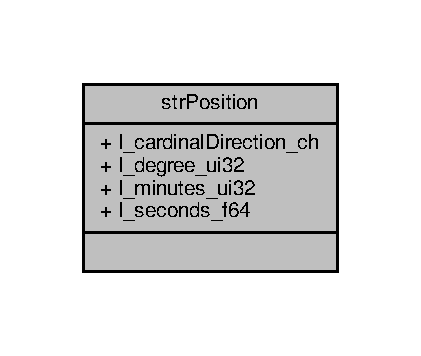
\includegraphics[width=202pt]{structstrPosition__coll__graph}
\end{center}
\end{figure}
\subsection*{Data Fields}
\begin{DoxyCompactItemize}
\item 
char \hyperlink{structstrPosition_aa39fed1d421cb2260d0ef7157c3c00d0_aa39fed1d421cb2260d0ef7157c3c00d0}{l\+\_\+cardinal\+Direction\+\_\+ch}
\item 
unsigned int \hyperlink{structstrPosition_ac060af7d7963812c116c24cdb861f184_ac060af7d7963812c116c24cdb861f184}{l\+\_\+degree\+\_\+ui32}
\item 
unsigned int \hyperlink{structstrPosition_a5489ef5e7f8e6ee45990b262c80a7819_a5489ef5e7f8e6ee45990b262c80a7819}{l\+\_\+minutes\+\_\+ui32}
\item 
double \hyperlink{structstrPosition_ae62d246c481c611e168ea86b70d5313b_ae62d246c481c611e168ea86b70d5313b}{l\+\_\+seconds\+\_\+f64}
\end{DoxyCompactItemize}


\subsection{Detailed Description}
struct with Langitude or Latitude position 



 \begin{DoxyAuthor}{Author}
Oliver Breuning ( olbrgs00 ) 
\end{DoxyAuthor}
\begin{DoxyDate}{Date}
2015/04/21
\end{DoxyDate}
This struct stores either a Longitude or Latitude position. It stores the degree, minute, second and the cardinal direction.

Definition at line 28 of file G\+P\+S.\+h.



\subsection{Field Documentation}
\hypertarget{structstrPosition_aa39fed1d421cb2260d0ef7157c3c00d0_aa39fed1d421cb2260d0ef7157c3c00d0}{\index{str\+Position@{str\+Position}!l\+\_\+cardinal\+Direction\+\_\+ch@{l\+\_\+cardinal\+Direction\+\_\+ch}}
\index{l\+\_\+cardinal\+Direction\+\_\+ch@{l\+\_\+cardinal\+Direction\+\_\+ch}!str\+Position@{str\+Position}}
\subsubsection[{l\+\_\+cardinal\+Direction\+\_\+ch}]{\setlength{\rightskip}{0pt plus 5cm}char str\+Position\+::l\+\_\+cardinal\+Direction\+\_\+ch}}\label{structstrPosition_aa39fed1d421cb2260d0ef7157c3c00d0_aa39fed1d421cb2260d0ef7157c3c00d0}


Definition at line 33 of file G\+P\+S.\+h.

\hypertarget{structstrPosition_ac060af7d7963812c116c24cdb861f184_ac060af7d7963812c116c24cdb861f184}{\index{str\+Position@{str\+Position}!l\+\_\+degree\+\_\+ui32@{l\+\_\+degree\+\_\+ui32}}
\index{l\+\_\+degree\+\_\+ui32@{l\+\_\+degree\+\_\+ui32}!str\+Position@{str\+Position}}
\subsubsection[{l\+\_\+degree\+\_\+ui32}]{\setlength{\rightskip}{0pt plus 5cm}unsigned int str\+Position\+::l\+\_\+degree\+\_\+ui32}}\label{structstrPosition_ac060af7d7963812c116c24cdb861f184_ac060af7d7963812c116c24cdb861f184}


Definition at line 30 of file G\+P\+S.\+h.

\hypertarget{structstrPosition_a5489ef5e7f8e6ee45990b262c80a7819_a5489ef5e7f8e6ee45990b262c80a7819}{\index{str\+Position@{str\+Position}!l\+\_\+minutes\+\_\+ui32@{l\+\_\+minutes\+\_\+ui32}}
\index{l\+\_\+minutes\+\_\+ui32@{l\+\_\+minutes\+\_\+ui32}!str\+Position@{str\+Position}}
\subsubsection[{l\+\_\+minutes\+\_\+ui32}]{\setlength{\rightskip}{0pt plus 5cm}unsigned int str\+Position\+::l\+\_\+minutes\+\_\+ui32}}\label{structstrPosition_a5489ef5e7f8e6ee45990b262c80a7819_a5489ef5e7f8e6ee45990b262c80a7819}


Definition at line 31 of file G\+P\+S.\+h.

\hypertarget{structstrPosition_ae62d246c481c611e168ea86b70d5313b_ae62d246c481c611e168ea86b70d5313b}{\index{str\+Position@{str\+Position}!l\+\_\+seconds\+\_\+f64@{l\+\_\+seconds\+\_\+f64}}
\index{l\+\_\+seconds\+\_\+f64@{l\+\_\+seconds\+\_\+f64}!str\+Position@{str\+Position}}
\subsubsection[{l\+\_\+seconds\+\_\+f64}]{\setlength{\rightskip}{0pt plus 5cm}double str\+Position\+::l\+\_\+seconds\+\_\+f64}}\label{structstrPosition_ae62d246c481c611e168ea86b70d5313b_ae62d246c481c611e168ea86b70d5313b}


Definition at line 32 of file G\+P\+S.\+h.



The documentation for this struct was generated from the following file\+:\begin{DoxyCompactItemize}
\item 
hal/gps/\hyperlink{GPS_8h}{G\+P\+S.\+h}\end{DoxyCompactItemize}

\hypertarget{structtimedInterrupt}{\section{timed\+Interrupt Struct Reference}
\label{structtimedInterrupt}\index{timed\+Interrupt@{timed\+Interrupt}}
}


Collaboration diagram for timed\+Interrupt\+:
\nopagebreak
\begin{figure}[H]
\begin{center}
\leavevmode
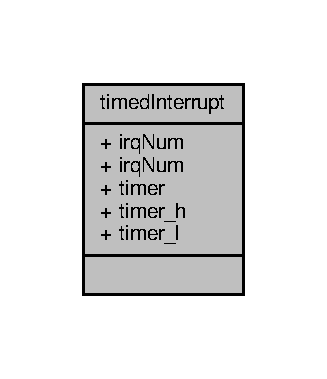
\includegraphics[width=157pt]{structtimedInterrupt__coll__graph}
\end{center}
\end{figure}
\subsection*{Data Fields}
\begin{DoxyCompactItemize}
\item 
int \hyperlink{structtimedInterrupt_a7e3743a35e009262953f43a25e65b321_a7e3743a35e009262953f43a25e65b321}{irq\+Num}
\item 
unsigned int \hyperlink{structtimedInterrupt_afe863922719ad198b647157e5c0ab5f2_afe863922719ad198b647157e5c0ab5f2}{irq\+Num}
\item 
unsigned long \hyperlink{structtimedInterrupt_a22ab02fd7b04fa04d1c1dea800bac62e_a22ab02fd7b04fa04d1c1dea800bac62e}{timer}
\item 
unsigned long \hyperlink{structtimedInterrupt_ae0c686eadc5df51274fae964275a1814_ae0c686eadc5df51274fae964275a1814}{timer\+\_\+h}
\item 
unsigned long \hyperlink{structtimedInterrupt_ac3d76cbc80f17f677b307910b5c0da97_ac3d76cbc80f17f677b307910b5c0da97}{timer\+\_\+l}
\end{DoxyCompactItemize}


\subsection{Detailed Description}


Definition at line 44 of file ppm\+Demux.\+c.



\subsection{Field Documentation}
\hypertarget{structtimedInterrupt_a7e3743a35e009262953f43a25e65b321_a7e3743a35e009262953f43a25e65b321}{\index{timed\+Interrupt@{timed\+Interrupt}!irq\+Num@{irq\+Num}}
\index{irq\+Num@{irq\+Num}!timed\+Interrupt@{timed\+Interrupt}}
\subsubsection[{irq\+Num}]{\setlength{\rightskip}{0pt plus 5cm}int timed\+Interrupt\+::irq\+Num}}\label{structtimedInterrupt_a7e3743a35e009262953f43a25e65b321_a7e3743a35e009262953f43a25e65b321}


Definition at line 45 of file ppm\+Demux.\+c.

\hypertarget{structtimedInterrupt_afe863922719ad198b647157e5c0ab5f2_afe863922719ad198b647157e5c0ab5f2}{\index{timed\+Interrupt@{timed\+Interrupt}!irq\+Num@{irq\+Num}}
\index{irq\+Num@{irq\+Num}!timed\+Interrupt@{timed\+Interrupt}}
\subsubsection[{irq\+Num}]{\setlength{\rightskip}{0pt plus 5cm}unsigned int timed\+Interrupt\+::irq\+Num}}\label{structtimedInterrupt_afe863922719ad198b647157e5c0ab5f2_afe863922719ad198b647157e5c0ab5f2}


Definition at line 50 of file time\+Trigger.\+c.

\hypertarget{structtimedInterrupt_a22ab02fd7b04fa04d1c1dea800bac62e_a22ab02fd7b04fa04d1c1dea800bac62e}{\index{timed\+Interrupt@{timed\+Interrupt}!timer@{timer}}
\index{timer@{timer}!timed\+Interrupt@{timed\+Interrupt}}
\subsubsection[{timer}]{\setlength{\rightskip}{0pt plus 5cm}unsigned long timed\+Interrupt\+::timer}}\label{structtimedInterrupt_a22ab02fd7b04fa04d1c1dea800bac62e_a22ab02fd7b04fa04d1c1dea800bac62e}


Definition at line 51 of file time\+Trigger.\+c.

\hypertarget{structtimedInterrupt_ae0c686eadc5df51274fae964275a1814_ae0c686eadc5df51274fae964275a1814}{\index{timed\+Interrupt@{timed\+Interrupt}!timer\+\_\+h@{timer\+\_\+h}}
\index{timer\+\_\+h@{timer\+\_\+h}!timed\+Interrupt@{timed\+Interrupt}}
\subsubsection[{timer\+\_\+h}]{\setlength{\rightskip}{0pt plus 5cm}unsigned long timed\+Interrupt\+::timer\+\_\+h}}\label{structtimedInterrupt_ae0c686eadc5df51274fae964275a1814_ae0c686eadc5df51274fae964275a1814}


Definition at line 47 of file ppm\+Demux.\+c.

\hypertarget{structtimedInterrupt_ac3d76cbc80f17f677b307910b5c0da97_ac3d76cbc80f17f677b307910b5c0da97}{\index{timed\+Interrupt@{timed\+Interrupt}!timer\+\_\+l@{timer\+\_\+l}}
\index{timer\+\_\+l@{timer\+\_\+l}!timed\+Interrupt@{timed\+Interrupt}}
\subsubsection[{timer\+\_\+l}]{\setlength{\rightskip}{0pt plus 5cm}unsigned long timed\+Interrupt\+::timer\+\_\+l}}\label{structtimedInterrupt_ac3d76cbc80f17f677b307910b5c0da97_ac3d76cbc80f17f677b307910b5c0da97}


Definition at line 46 of file ppm\+Demux.\+c.



The documentation for this struct was generated from the following files\+:\begin{DoxyCompactItemize}
\item 
linux\+Kernel\+Drivers/\hyperlink{ppmDemux_8c}{ppm\+Demux.\+c}\item 
linux\+Kernel\+Drivers/\hyperlink{timeTrigger_8c}{time\+Trigger.\+c}\item 
\hyperlink{main_8c}{main.\+c}\end{DoxyCompactItemize}

\chapter{File Documentation}
\hypertarget{HAL__ADC_8c}{\section{hal/\+A\+D\+C/\+H\+A\+L\+\_\+\+A\+D\+C.c File Reference}
\label{HAL__ADC_8c}\index{hal/\+A\+D\+C/\+H\+A\+L\+\_\+\+A\+D\+C.\+c@{hal/\+A\+D\+C/\+H\+A\+L\+\_\+\+A\+D\+C.\+c}}
}
{\ttfamily \#include $<$stdio.\+h$>$}\\*
{\ttfamily \#include \char`\"{}../\+L\+L\+D\+\_\+\+I\+F/\+L\+L\+D\+\_\+\+I2\+C.\+h\char`\"{}}\\*
{\ttfamily \#include \char`\"{}H\+A\+L\+\_\+\+A\+D\+C.\+h\char`\"{}}\\*
Include dependency graph for H\+A\+L\+\_\+\+A\+D\+C.\+c\+:
\nopagebreak
\begin{figure}[H]
\begin{center}
\leavevmode
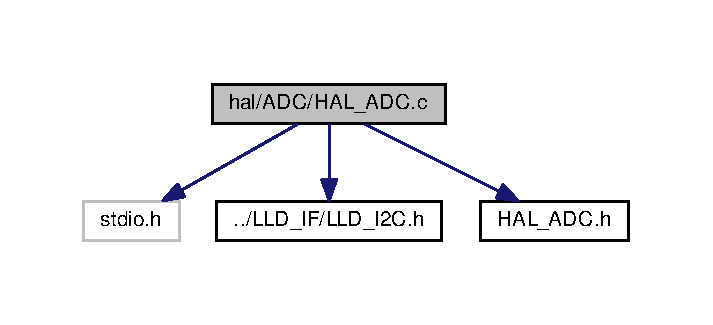
\includegraphics[width=342pt]{HAL__ADC_8c__incl}
\end{center}
\end{figure}
\subsection*{Functions}
\begin{DoxyCompactItemize}
\item 
float \hyperlink{HAL__ADC_8c_ad4f5cd5d9c7c0a335d5c485a2fb41cb2_ad4f5cd5d9c7c0a335d5c485a2fb41cb2}{g\+\_\+hal\+A\+D\+C\+\_\+get\+\_\+ui16} (unsigned char l\+\_\+input\+\_\+ui8)
\begin{DoxyCompactList}\small\item\em Reads analog to digital converted values from A\+D\+S1015. \end{DoxyCompactList}\end{DoxyCompactItemize}


\subsection{Function Documentation}
\hypertarget{HAL__ADC_8c_ad4f5cd5d9c7c0a335d5c485a2fb41cb2_ad4f5cd5d9c7c0a335d5c485a2fb41cb2}{\index{H\+A\+L\+\_\+\+A\+D\+C.\+c@{H\+A\+L\+\_\+\+A\+D\+C.\+c}!g\+\_\+hal\+A\+D\+C\+\_\+get\+\_\+ui16@{g\+\_\+hal\+A\+D\+C\+\_\+get\+\_\+ui16}}
\index{g\+\_\+hal\+A\+D\+C\+\_\+get\+\_\+ui16@{g\+\_\+hal\+A\+D\+C\+\_\+get\+\_\+ui16}!H\+A\+L\+\_\+\+A\+D\+C.\+c@{H\+A\+L\+\_\+\+A\+D\+C.\+c}}
\subsubsection[{g\+\_\+hal\+A\+D\+C\+\_\+get\+\_\+ui16}]{\setlength{\rightskip}{0pt plus 5cm}float g\+\_\+hal\+A\+D\+C\+\_\+get\+\_\+ui16 (
\begin{DoxyParamCaption}
\item[{unsigned char}]{l\+\_\+input\+\_\+ui8}
\end{DoxyParamCaption}
)}}\label{HAL__ADC_8c_ad4f5cd5d9c7c0a335d5c485a2fb41cb2_ad4f5cd5d9c7c0a335d5c485a2fb41cb2}


Reads analog to digital converted values from A\+D\+S1015. 



 \begin{DoxyAuthor}{Author}
Martin Brodbeck (mabrgs00) 
\end{DoxyAuthor}
\begin{DoxyDate}{Date}
2015/05/07
\end{DoxyDate}
A detailed descripction about the function, here for creating good foos and much more. Multiple lines of description is possible. Doxygen will recognize the format automatically.


\begin{DoxyParams}[1]{Parameters}
\mbox{\tt in}  & {\em l\+\_\+input\+\_\+ui8} & is the input which selects input A0-\/3 to convert \\
\hline
\mbox{\tt out}  & {\em converted} & voltage value, -\/1 when error on I2\+C Bus\\
\hline
\end{DoxyParams}


Definition at line 34 of file H\+A\+L\+\_\+\+A\+D\+C.\+c.


\begin{DoxyCode}
34                                                   \{
35 
36   \textcolor{keywordtype}{unsigned} \textcolor{keywordtype}{char} l\_address\_ui8 = 0x49;       \textcolor{comment}{// Address of our device on the I2C bus}
37   \textcolor{keywordtype}{unsigned} \textcolor{keywordtype}{char} l\_writeBuf\_rg24[3];     \textcolor{comment}{// Buffer to store the 3 bytes that we write to the I2C device}
38   \textcolor{keywordtype}{unsigned} \textcolor{keywordtype}{char} l\_readBuf\_rg16[2];      \textcolor{comment}{// 2 byte buffer to store the data read from the I2C device}
39   \textcolor{keywordtype}{unsigned} \textcolor{keywordtype}{char} l\_mux\_ui8;          \textcolor{comment}{// Config value depening on input}
40   \textcolor{keywordtype}{unsigned} \textcolor{keywordtype}{short} l\_val\_ui16;            \textcolor{comment}{// (Converted) result of ADC}
41   \textcolor{keywordtype}{unsigned} \textcolor{keywordtype}{char} l\_checkerror\_bl;            \textcolor{comment}{// Variable to store return value}
42 
43   \textcolor{comment}{// Setting Config according to select Input}
44   \textcolor{keywordflow}{switch}(l\_input\_ui8)\{              \textcolor{comment}{// Standard: 1100 0011  (Bit 15-8) Input A0}
45     \textcolor{keywordflow}{case} 1: l\_mux\_ui8 = 0xC2; \textcolor{keywordflow}{break};    \textcolor{comment}{// Input: A0    }
46     \textcolor{keywordflow}{case} 2: l\_mux\_ui8 = 0xD2; \textcolor{keywordflow}{break};    
47     \textcolor{keywordflow}{case} 3: l\_mux\_ui8 = 0xE2; \textcolor{keywordflow}{break};    
48     \textcolor{keywordflow}{case} 4: l\_mux\_ui8 = 0xF2; \textcolor{keywordflow}{break};    \textcolor{comment}{// Input: A3}
49     \textcolor{keywordflow}{default}: l\_mux\_ui8 = 0xC2;          
50   \} 
51   \textcolor{comment}{// First Hex depends on Starting Conversion + the Input, which Pin to read A0-3}
52   \textcolor{comment}{// Second Value is PGA (001)=+-4,099V and continuous Mode (0)}
53 
54 
55   \textcolor{comment}{// These three bytes are written to the ADS1015 to set the config register and start the conversion }
56   l\_writeBuf\_rg24[0] = 1;       \textcolor{comment}{// This sets the pointer register to write two bytes to the config register}
57   l\_writeBuf\_rg24[1] = l\_mux\_ui8;       \textcolor{comment}{// This sets the 8 MSBs of the config register (bits 15-8) to
       11000011}
58   l\_writeBuf\_rg24[2] = 0x23;        \textcolor{comment}{// This sets the 8 LSBs of the config register (bits  7-0) to 00100011 
        }
59 
60   \textcolor{comment}{// First Hex is sample Rate. (001) sets to 250SPS + Comp Mode (0)}
61   \textcolor{comment}{// Second Hex is Comp. config. (0011) disable the comparator}
62 
63 
64   \textcolor{comment}{// Initialize the buffer used to read data from the ADS1015 to 0}
65   l\_readBuf\_rg16[0]= 0;     
66   l\_readBuf\_rg16[1]= 0;
67   
68   \textcolor{comment}{// Write l\_writeBuf\_rg24 to the ADS1015, the 3 specifies the number of bytes we are writing,}
69   \textcolor{comment}{// this begins a continuous conversion}
70   l\_checkerror\_bl = \hyperlink{LLD__I2C_8c_aa6892bf4aea7f232d9b0ff2dbf8a9321_aa6892bf4aea7f232d9b0ff2dbf8a9321}{g\_lldI2c\_WriteI2c\_bl}(l\_address\_ui8,l\_writeBuf\_rg24,3);
71   \textcolor{keywordflow}{if} (l\_checkerror\_bl == 1)
72     \{
73     \textcolor{keywordflow}{return} -1;
74     \}
75 
76   \textcolor{comment}{// Read the config register into readBuf}
77   l\_checkerror\_bl = \hyperlink{LLD__I2C_8c_a107ee9f1e4646733ac3ef6addf0def7e_a107ee9f1e4646733ac3ef6addf0def7e}{g\_lldI2c\_ReadI2c\_bl}(l\_address\_ui8,l\_readBuf\_rg16,2);
78   \textcolor{keywordflow}{if} (l\_checkerror\_bl == 1)
79     \{
80     \textcolor{keywordflow}{return} -1;
81     \}   
82     
83   \textcolor{comment}{// Set pointer register to 0 to read from the conversion register}
84   l\_writeBuf\_rg24[0] = 0;           
85   l\_checkerror\_bl = \hyperlink{LLD__I2C_8c_aa6892bf4aea7f232d9b0ff2dbf8a9321_aa6892bf4aea7f232d9b0ff2dbf8a9321}{g\_lldI2c\_WriteI2c\_bl}(l\_address\_ui8, l\_writeBuf\_rg24,1);
86   \textcolor{keywordflow}{if} (l\_checkerror\_bl == 1)
87     \{
88     \textcolor{keywordflow}{return} -1;
89     \}
90 
91   \textcolor{comment}{// Read the contents of the conversion register into readBuf      }
92   l\_checkerror\_bl = \hyperlink{LLD__I2C_8c_a107ee9f1e4646733ac3ef6addf0def7e_a107ee9f1e4646733ac3ef6addf0def7e}{g\_lldI2c\_ReadI2c\_bl}(l\_address\_ui8,l\_readBuf\_rg16,2); 
93   \textcolor{keywordflow}{if} (l\_checkerror\_bl == 1)
94     \{
95     \textcolor{keywordflow}{return} -1;
96     \}
97 
98   \textcolor{comment}{// Combine the two bytes of readBuf into a single 16 bit result }
99   l\_val\_ui16 = l\_readBuf\_rg16[0] << 8 | l\_readBuf\_rg16[1];  
100   l\_val\_ui16 = l\_val\_ui16 >> 4; 
101 
102   \textcolor{keywordflow}{return}((\textcolor{keywordtype}{float})l\_val\_ui16*4.096/2047.0);
103 
104 \}
\end{DoxyCode}


Here is the call graph for this function\+:
\nopagebreak
\begin{figure}[H]
\begin{center}
\leavevmode
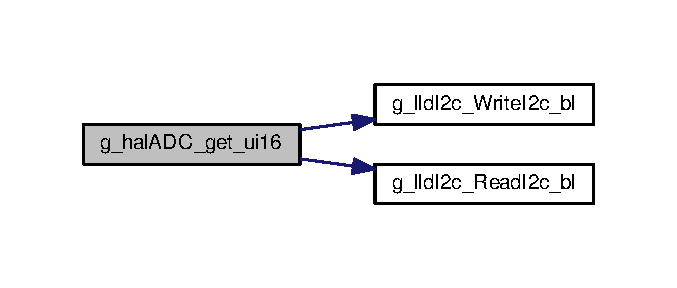
\includegraphics[width=325pt]{HAL__ADC_8c_ad4f5cd5d9c7c0a335d5c485a2fb41cb2_ad4f5cd5d9c7c0a335d5c485a2fb41cb2_cgraph}
\end{center}
\end{figure}




Here is the caller graph for this function\+:
\nopagebreak
\begin{figure}[H]
\begin{center}
\leavevmode
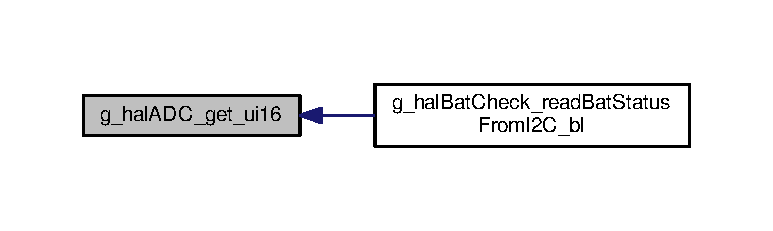
\includegraphics[width=350pt]{HAL__ADC_8c_ad4f5cd5d9c7c0a335d5c485a2fb41cb2_ad4f5cd5d9c7c0a335d5c485a2fb41cb2_icgraph}
\end{center}
\end{figure}



\hypertarget{HAL__ADC_8h}{\section{hal/\+A\+D\+C/\+H\+A\+L\+\_\+\+A\+D\+C.h File Reference}
\label{HAL__ADC_8h}\index{hal/\+A\+D\+C/\+H\+A\+L\+\_\+\+A\+D\+C.\+h@{hal/\+A\+D\+C/\+H\+A\+L\+\_\+\+A\+D\+C.\+h}}
}
This graph shows which files directly or indirectly include this file\+:
\nopagebreak
\begin{figure}[H]
\begin{center}
\leavevmode
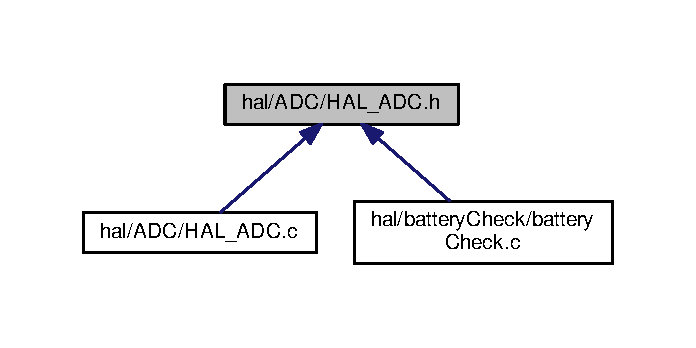
\includegraphics[width=334pt]{HAL__ADC_8h__dep__incl}
\end{center}
\end{figure}
\subsection*{Functions}
\begin{DoxyCompactItemize}
\item 
float \hyperlink{HAL__ADC_8h_a8c4acefe26c9d284733559f929cb4193_a8c4acefe26c9d284733559f929cb4193}{g\+\_\+hal\+A\+D\+C\+\_\+get\+\_\+ui16} (unsigned char)
\begin{DoxyCompactList}\small\item\em Reads analog to digital converted values from A\+D\+S1015. \end{DoxyCompactList}\end{DoxyCompactItemize}


\subsection{Function Documentation}
\hypertarget{HAL__ADC_8h_a8c4acefe26c9d284733559f929cb4193_a8c4acefe26c9d284733559f929cb4193}{\index{H\+A\+L\+\_\+\+A\+D\+C.\+h@{H\+A\+L\+\_\+\+A\+D\+C.\+h}!g\+\_\+hal\+A\+D\+C\+\_\+get\+\_\+ui16@{g\+\_\+hal\+A\+D\+C\+\_\+get\+\_\+ui16}}
\index{g\+\_\+hal\+A\+D\+C\+\_\+get\+\_\+ui16@{g\+\_\+hal\+A\+D\+C\+\_\+get\+\_\+ui16}!H\+A\+L\+\_\+\+A\+D\+C.\+h@{H\+A\+L\+\_\+\+A\+D\+C.\+h}}
\subsubsection[{g\+\_\+hal\+A\+D\+C\+\_\+get\+\_\+ui16}]{\setlength{\rightskip}{0pt plus 5cm}float g\+\_\+hal\+A\+D\+C\+\_\+get\+\_\+ui16 (
\begin{DoxyParamCaption}
\item[{unsigned char}]{l\+\_\+input\+\_\+ui8}
\end{DoxyParamCaption}
)}}\label{HAL__ADC_8h_a8c4acefe26c9d284733559f929cb4193_a8c4acefe26c9d284733559f929cb4193}


Reads analog to digital converted values from A\+D\+S1015. 



 \begin{DoxyAuthor}{Author}
Martin Brodbeck (mabrgs00) 
\end{DoxyAuthor}
\begin{DoxyDate}{Date}
2015/05/07
\end{DoxyDate}
A detailed descripction about the function, here for creating good foos and much more. Multiple lines of description is possible. Doxygen will recognize the format automatically.


\begin{DoxyParams}[1]{Parameters}
\mbox{\tt in}  & {\em l\+\_\+input\+\_\+ui8} & is the input which selects input A0-\/3 to convert \\
\hline
\mbox{\tt out}  & {\em converted} & voltage value, -\/1 when error on I2\+C Bus\\
\hline
\end{DoxyParams}


Definition at line 34 of file H\+A\+L\+\_\+\+A\+D\+C.\+c.


\begin{DoxyCode}
34                                                   \{
35 
36   \textcolor{keywordtype}{unsigned} \textcolor{keywordtype}{char} l\_address\_ui8 = 0x49;       \textcolor{comment}{// Address of our device on the I2C bus}
37   \textcolor{keywordtype}{unsigned} \textcolor{keywordtype}{char} l\_writeBuf\_rg24[3];     \textcolor{comment}{// Buffer to store the 3 bytes that we write to the I2C device}
38   \textcolor{keywordtype}{unsigned} \textcolor{keywordtype}{char} l\_readBuf\_rg16[2];      \textcolor{comment}{// 2 byte buffer to store the data read from the I2C device}
39   \textcolor{keywordtype}{unsigned} \textcolor{keywordtype}{char} l\_mux\_ui8;          \textcolor{comment}{// Config value depening on input}
40   \textcolor{keywordtype}{unsigned} \textcolor{keywordtype}{short} l\_val\_ui16;            \textcolor{comment}{// (Converted) result of ADC}
41   \textcolor{keywordtype}{unsigned} \textcolor{keywordtype}{char} l\_checkerror\_bl;            \textcolor{comment}{// Variable to store return value}
42 
43   \textcolor{comment}{// Setting Config according to select Input}
44   \textcolor{keywordflow}{switch}(l\_input\_ui8)\{              \textcolor{comment}{// Standard: 1100 0011  (Bit 15-8) Input A0}
45     \textcolor{keywordflow}{case} 1: l\_mux\_ui8 = 0xC2; \textcolor{keywordflow}{break};    \textcolor{comment}{// Input: A0    }
46     \textcolor{keywordflow}{case} 2: l\_mux\_ui8 = 0xD2; \textcolor{keywordflow}{break};    
47     \textcolor{keywordflow}{case} 3: l\_mux\_ui8 = 0xE2; \textcolor{keywordflow}{break};    
48     \textcolor{keywordflow}{case} 4: l\_mux\_ui8 = 0xF2; \textcolor{keywordflow}{break};    \textcolor{comment}{// Input: A3}
49     \textcolor{keywordflow}{default}: l\_mux\_ui8 = 0xC2;          
50   \} 
51   \textcolor{comment}{// First Hex depends on Starting Conversion + the Input, which Pin to read A0-3}
52   \textcolor{comment}{// Second Value is PGA (001)=+-4,099V and continuous Mode (0)}
53 
54 
55   \textcolor{comment}{// These three bytes are written to the ADS1015 to set the config register and start the conversion }
56   l\_writeBuf\_rg24[0] = 1;       \textcolor{comment}{// This sets the pointer register to write two bytes to the config register}
57   l\_writeBuf\_rg24[1] = l\_mux\_ui8;       \textcolor{comment}{// This sets the 8 MSBs of the config register (bits 15-8) to
       11000011}
58   l\_writeBuf\_rg24[2] = 0x23;        \textcolor{comment}{// This sets the 8 LSBs of the config register (bits  7-0) to 00100011 
        }
59 
60   \textcolor{comment}{// First Hex is sample Rate. (001) sets to 250SPS + Comp Mode (0)}
61   \textcolor{comment}{// Second Hex is Comp. config. (0011) disable the comparator}
62 
63 
64   \textcolor{comment}{// Initialize the buffer used to read data from the ADS1015 to 0}
65   l\_readBuf\_rg16[0]= 0;     
66   l\_readBuf\_rg16[1]= 0;
67   
68   \textcolor{comment}{// Write l\_writeBuf\_rg24 to the ADS1015, the 3 specifies the number of bytes we are writing,}
69   \textcolor{comment}{// this begins a continuous conversion}
70   l\_checkerror\_bl = \hyperlink{LLD__I2C_8c_aa6892bf4aea7f232d9b0ff2dbf8a9321_aa6892bf4aea7f232d9b0ff2dbf8a9321}{g\_lldI2c\_WriteI2c\_bl}(l\_address\_ui8,l\_writeBuf\_rg24,3);
71   \textcolor{keywordflow}{if} (l\_checkerror\_bl == 1)
72     \{
73     \textcolor{keywordflow}{return} -1;
74     \}
75 
76   \textcolor{comment}{// Read the config register into readBuf}
77   l\_checkerror\_bl = \hyperlink{LLD__I2C_8c_a107ee9f1e4646733ac3ef6addf0def7e_a107ee9f1e4646733ac3ef6addf0def7e}{g\_lldI2c\_ReadI2c\_bl}(l\_address\_ui8,l\_readBuf\_rg16,2);
78   \textcolor{keywordflow}{if} (l\_checkerror\_bl == 1)
79     \{
80     \textcolor{keywordflow}{return} -1;
81     \}   
82     
83   \textcolor{comment}{// Set pointer register to 0 to read from the conversion register}
84   l\_writeBuf\_rg24[0] = 0;           
85   l\_checkerror\_bl = \hyperlink{LLD__I2C_8c_aa6892bf4aea7f232d9b0ff2dbf8a9321_aa6892bf4aea7f232d9b0ff2dbf8a9321}{g\_lldI2c\_WriteI2c\_bl}(l\_address\_ui8, l\_writeBuf\_rg24,1);
86   \textcolor{keywordflow}{if} (l\_checkerror\_bl == 1)
87     \{
88     \textcolor{keywordflow}{return} -1;
89     \}
90 
91   \textcolor{comment}{// Read the contents of the conversion register into readBuf      }
92   l\_checkerror\_bl = \hyperlink{LLD__I2C_8c_a107ee9f1e4646733ac3ef6addf0def7e_a107ee9f1e4646733ac3ef6addf0def7e}{g\_lldI2c\_ReadI2c\_bl}(l\_address\_ui8,l\_readBuf\_rg16,2); 
93   \textcolor{keywordflow}{if} (l\_checkerror\_bl == 1)
94     \{
95     \textcolor{keywordflow}{return} -1;
96     \}
97 
98   \textcolor{comment}{// Combine the two bytes of readBuf into a single 16 bit result }
99   l\_val\_ui16 = l\_readBuf\_rg16[0] << 8 | l\_readBuf\_rg16[1];  
100   l\_val\_ui16 = l\_val\_ui16 >> 4; 
101 
102   \textcolor{keywordflow}{return}((\textcolor{keywordtype}{float})l\_val\_ui16*4.096/2047.0);
103 
104 \}
\end{DoxyCode}


Here is the call graph for this function\+:
\nopagebreak
\begin{figure}[H]
\begin{center}
\leavevmode
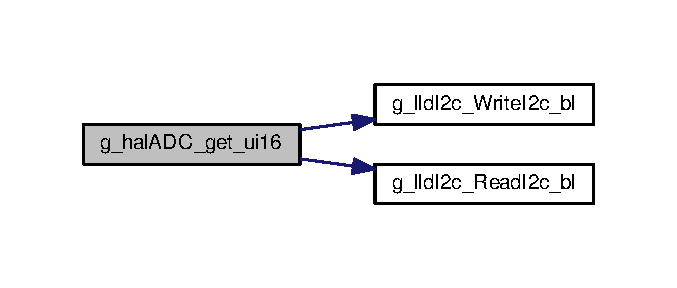
\includegraphics[width=325pt]{HAL__ADC_8h_a8c4acefe26c9d284733559f929cb4193_a8c4acefe26c9d284733559f929cb4193_cgraph}
\end{center}
\end{figure}




Here is the caller graph for this function\+:
\nopagebreak
\begin{figure}[H]
\begin{center}
\leavevmode
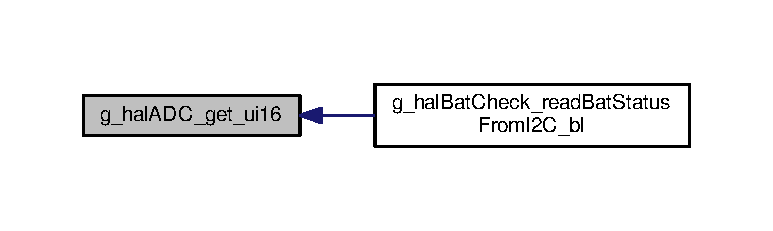
\includegraphics[width=350pt]{HAL__ADC_8h_a8c4acefe26c9d284733559f929cb4193_a8c4acefe26c9d284733559f929cb4193_icgraph}
\end{center}
\end{figure}



\hypertarget{batteryCheck_8c}{\section{hal/battery\+Check/battery\+Check.c File Reference}
\label{batteryCheck_8c}\index{hal/battery\+Check/battery\+Check.\+c@{hal/battery\+Check/battery\+Check.\+c}}
}
{\ttfamily \#include \char`\"{}../\+A\+D\+C/\+H\+A\+L\+\_\+\+A\+D\+C.\+h\char`\"{}}\\*
{\ttfamily \#include \char`\"{}battery\+Check.\+h\char`\"{}}\\*
Include dependency graph for battery\+Check.\+c\+:
\nopagebreak
\begin{figure}[H]
\begin{center}
\leavevmode
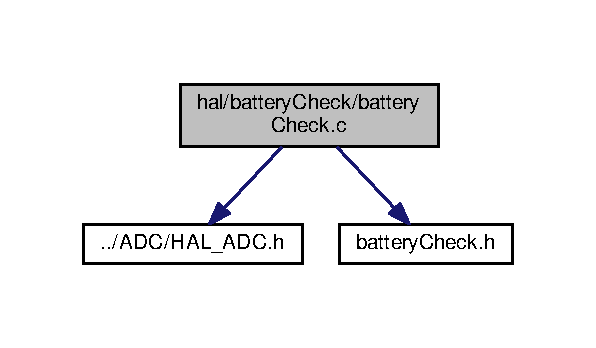
\includegraphics[width=286pt]{batteryCheck_8c__incl}
\end{center}
\end{figure}
\subsection*{Macros}
\begin{DoxyCompactItemize}
\item 
\#define \hyperlink{batteryCheck_8c_ae26cf8b824c3357eb00a815c4366b080_ae26cf8b824c3357eb00a815c4366b080}{M\+\_\+\+H\+A\+L\+\_\+\+B\+A\+T\+C\+H\+E\+C\+K\+\_\+\+A\+D\+C\+\_\+\+I\+N\+P\+U\+T\+\_\+\+P\+O\+R\+T\+\_\+\+U\+I8}~1
\end{DoxyCompactItemize}
\subsection*{Functions}
\begin{DoxyCompactItemize}
\item 
double \hyperlink{batteryCheck_8c_a51db231fd015ab0c2a168d7efdb80ca5_a51db231fd015ab0c2a168d7efdb80ca5}{g\+\_\+hal\+Bat\+Check\+\_\+get\+Battery\+Status\+\_\+f64} (void)
\begin{DoxyCompactList}\small\item\em Get Voltage from battery watchdog. \end{DoxyCompactList}\item 
unsigned int \hyperlink{batteryCheck_8c_aa0c26427dd86b435991d80d33261998b_aa0c26427dd86b435991d80d33261998b}{g\+\_\+hal\+Bat\+Check\+\_\+read\+Bat\+Status\+From\+I2\+C\+\_\+bl} (void)
\begin{DoxyCompactList}\small\item\em Trigger update of measured battery level. \end{DoxyCompactList}\end{DoxyCompactItemize}
\subsection*{Variables}
\begin{DoxyCompactItemize}
\item 
static double \hyperlink{batteryCheck_8c_a14ec93dd22f873d58789403fa75531ef_a14ec93dd22f873d58789403fa75531ef}{m\+\_\+battery\+Level\+\_\+f64}
\end{DoxyCompactItemize}


\subsection{Macro Definition Documentation}
\hypertarget{batteryCheck_8c_ae26cf8b824c3357eb00a815c4366b080_ae26cf8b824c3357eb00a815c4366b080}{\index{battery\+Check.\+c@{battery\+Check.\+c}!M\+\_\+\+H\+A\+L\+\_\+\+B\+A\+T\+C\+H\+E\+C\+K\+\_\+\+A\+D\+C\+\_\+\+I\+N\+P\+U\+T\+\_\+\+P\+O\+R\+T\+\_\+\+U\+I8@{M\+\_\+\+H\+A\+L\+\_\+\+B\+A\+T\+C\+H\+E\+C\+K\+\_\+\+A\+D\+C\+\_\+\+I\+N\+P\+U\+T\+\_\+\+P\+O\+R\+T\+\_\+\+U\+I8}}
\index{M\+\_\+\+H\+A\+L\+\_\+\+B\+A\+T\+C\+H\+E\+C\+K\+\_\+\+A\+D\+C\+\_\+\+I\+N\+P\+U\+T\+\_\+\+P\+O\+R\+T\+\_\+\+U\+I8@{M\+\_\+\+H\+A\+L\+\_\+\+B\+A\+T\+C\+H\+E\+C\+K\+\_\+\+A\+D\+C\+\_\+\+I\+N\+P\+U\+T\+\_\+\+P\+O\+R\+T\+\_\+\+U\+I8}!battery\+Check.\+c@{battery\+Check.\+c}}
\subsubsection[{M\+\_\+\+H\+A\+L\+\_\+\+B\+A\+T\+C\+H\+E\+C\+K\+\_\+\+A\+D\+C\+\_\+\+I\+N\+P\+U\+T\+\_\+\+P\+O\+R\+T\+\_\+\+U\+I8}]{\setlength{\rightskip}{0pt plus 5cm}\#define M\+\_\+\+H\+A\+L\+\_\+\+B\+A\+T\+C\+H\+E\+C\+K\+\_\+\+A\+D\+C\+\_\+\+I\+N\+P\+U\+T\+\_\+\+P\+O\+R\+T\+\_\+\+U\+I8~1}}\label{batteryCheck_8c_ae26cf8b824c3357eb00a815c4366b080_ae26cf8b824c3357eb00a815c4366b080}


Definition at line 15 of file battery\+Check.\+c.



\subsection{Function Documentation}
\hypertarget{batteryCheck_8c_a51db231fd015ab0c2a168d7efdb80ca5_a51db231fd015ab0c2a168d7efdb80ca5}{\index{battery\+Check.\+c@{battery\+Check.\+c}!g\+\_\+hal\+Bat\+Check\+\_\+get\+Battery\+Status\+\_\+f64@{g\+\_\+hal\+Bat\+Check\+\_\+get\+Battery\+Status\+\_\+f64}}
\index{g\+\_\+hal\+Bat\+Check\+\_\+get\+Battery\+Status\+\_\+f64@{g\+\_\+hal\+Bat\+Check\+\_\+get\+Battery\+Status\+\_\+f64}!battery\+Check.\+c@{battery\+Check.\+c}}
\subsubsection[{g\+\_\+hal\+Bat\+Check\+\_\+get\+Battery\+Status\+\_\+f64}]{\setlength{\rightskip}{0pt plus 5cm}double g\+\_\+hal\+Bat\+Check\+\_\+get\+Battery\+Status\+\_\+f64 (
\begin{DoxyParamCaption}
\item[{void}]{}
\end{DoxyParamCaption}
)}}\label{batteryCheck_8c_a51db231fd015ab0c2a168d7efdb80ca5_a51db231fd015ab0c2a168d7efdb80ca5}


Get Voltage from battery watchdog. 



 \begin{DoxyAuthor}{Author}
Oliver Breuning ( olbrgs00 ) 
\end{DoxyAuthor}
\begin{DoxyDate}{Date}
2015/05/14
\end{DoxyDate}
Interface of reading voltage from battery watchdog which is connected to the A\+D\+C input pin A\+D\+C0


\begin{DoxyParams}[1]{Parameters}
\mbox{\tt in}  & {\em no} & parameter \\
\hline
\mbox{\tt out}  & {\em Voltage} & of battery as float value\\
\hline
\end{DoxyParams}


Definition at line 36 of file battery\+Check.\+c.


\begin{DoxyCode}
37 \{
38     \textcolor{keywordflow}{return} \hyperlink{batteryCheck_8c_a14ec93dd22f873d58789403fa75531ef_a14ec93dd22f873d58789403fa75531ef}{m\_batteryLevel\_f64};
39 \}
\end{DoxyCode}
\hypertarget{batteryCheck_8c_aa0c26427dd86b435991d80d33261998b_aa0c26427dd86b435991d80d33261998b}{\index{battery\+Check.\+c@{battery\+Check.\+c}!g\+\_\+hal\+Bat\+Check\+\_\+read\+Bat\+Status\+From\+I2\+C\+\_\+bl@{g\+\_\+hal\+Bat\+Check\+\_\+read\+Bat\+Status\+From\+I2\+C\+\_\+bl}}
\index{g\+\_\+hal\+Bat\+Check\+\_\+read\+Bat\+Status\+From\+I2\+C\+\_\+bl@{g\+\_\+hal\+Bat\+Check\+\_\+read\+Bat\+Status\+From\+I2\+C\+\_\+bl}!battery\+Check.\+c@{battery\+Check.\+c}}
\subsubsection[{g\+\_\+hal\+Bat\+Check\+\_\+read\+Bat\+Status\+From\+I2\+C\+\_\+bl}]{\setlength{\rightskip}{0pt plus 5cm}unsigned int g\+\_\+hal\+Bat\+Check\+\_\+read\+Bat\+Status\+From\+I2\+C\+\_\+bl (
\begin{DoxyParamCaption}
\item[{void}]{}
\end{DoxyParamCaption}
)}}\label{batteryCheck_8c_aa0c26427dd86b435991d80d33261998b_aa0c26427dd86b435991d80d33261998b}


Trigger update of measured battery level. 



 \begin{DoxyAuthor}{Author}
Oliver Breuning ( olbrgs00 ) 
\end{DoxyAuthor}
\begin{DoxyDate}{Date}
2015/05/14
\end{DoxyDate}
Interface of reading voltage from battery watchdog which is connected to the A\+D\+C input pin A\+D\+C0


\begin{DoxyParams}[1]{Parameters}
\mbox{\tt in}  & {\em no} & parameter \\
\hline
\mbox{\tt out}  & {\em returns} & a boolean value, indicating the occurence of failures~\newline
 0 .... indicates success (no errors)~\newline
 1 .... indicates failed (some errors)\\
\hline
\end{DoxyParams}


Definition at line 60 of file battery\+Check.\+c.


\begin{DoxyCode}
61 \{
62     \textcolor{keywordtype}{double} l\_batteryLevel\_f64;
63 
64     l\_batteryLevel\_f64=\hyperlink{HAL__ADC_8c_ad4f5cd5d9c7c0a335d5c485a2fb41cb2_ad4f5cd5d9c7c0a335d5c485a2fb41cb2}{g\_halADC\_get\_ui16}(
      \hyperlink{batteryCheck_8c_ae26cf8b824c3357eb00a815c4366b080_ae26cf8b824c3357eb00a815c4366b080}{M\_HAL\_BATCHECK\_ADC\_INPUT\_PORT\_UI8});
65 
66     \textcolor{keywordflow}{if}(l\_batteryLevel\_f64<=0)
67     \{\textcolor{keywordflow}{return} \hyperlink{batteryCheck_8h_a1b855f31472c2b55288466129b8db35f_a1b855f31472c2b55288466129b8db35f}{M\_HAL\_BATCHECK\_FAILED\_BL};\}
68 
69     \hyperlink{batteryCheck_8c_a14ec93dd22f873d58789403fa75531ef_a14ec93dd22f873d58789403fa75531ef}{m\_batteryLevel\_f64}=l\_batteryLevel\_f64;
70 
71     \textcolor{keywordflow}{return} \hyperlink{batteryCheck_8h_a9ddcbb2ac2dfadb1c7f620248de6ecc9_a9ddcbb2ac2dfadb1c7f620248de6ecc9}{M\_HAL\_BATCHECK\_SUCCESS\_BL};
72 \}
\end{DoxyCode}


Here is the call graph for this function\+:
\nopagebreak
\begin{figure}[H]
\begin{center}
\leavevmode
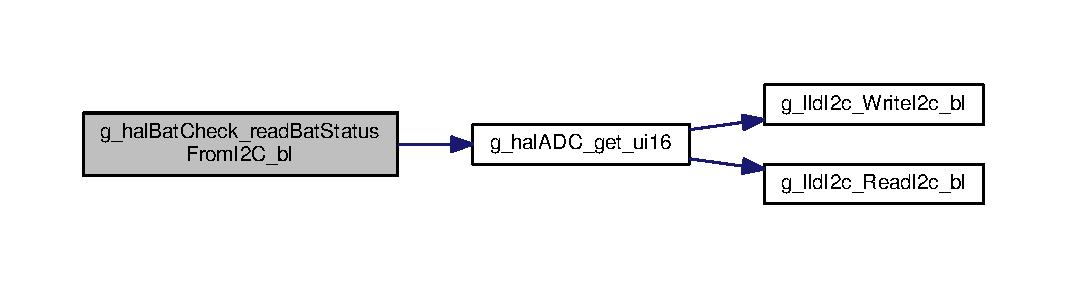
\includegraphics[width=350pt]{batteryCheck_8c_aa0c26427dd86b435991d80d33261998b_aa0c26427dd86b435991d80d33261998b_cgraph}
\end{center}
\end{figure}




\subsection{Variable Documentation}
\hypertarget{batteryCheck_8c_a14ec93dd22f873d58789403fa75531ef_a14ec93dd22f873d58789403fa75531ef}{\index{battery\+Check.\+c@{battery\+Check.\+c}!m\+\_\+battery\+Level\+\_\+f64@{m\+\_\+battery\+Level\+\_\+f64}}
\index{m\+\_\+battery\+Level\+\_\+f64@{m\+\_\+battery\+Level\+\_\+f64}!battery\+Check.\+c@{battery\+Check.\+c}}
\subsubsection[{m\+\_\+battery\+Level\+\_\+f64}]{\setlength{\rightskip}{0pt plus 5cm}double m\+\_\+battery\+Level\+\_\+f64\hspace{0.3cm}{\ttfamily [static]}}}\label{batteryCheck_8c_a14ec93dd22f873d58789403fa75531ef_a14ec93dd22f873d58789403fa75531ef}


Definition at line 17 of file battery\+Check.\+c.


\hypertarget{batteryCheck_8h}{\section{hal/battery\+Check/battery\+Check.h File Reference}
\label{batteryCheck_8h}\index{hal/battery\+Check/battery\+Check.\+h@{hal/battery\+Check/battery\+Check.\+h}}
}
This graph shows which files directly or indirectly include this file\+:
\nopagebreak
\begin{figure}[H]
\begin{center}
\leavevmode
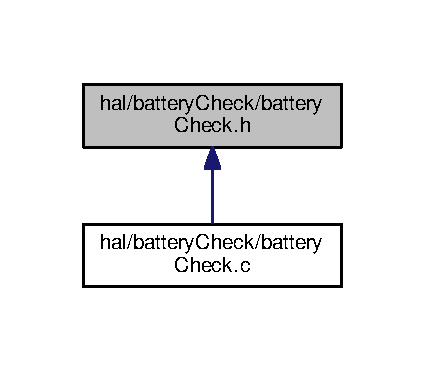
\includegraphics[width=204pt]{batteryCheck_8h__dep__incl}
\end{center}
\end{figure}
\subsection*{Macros}
\begin{DoxyCompactItemize}
\item 
\#define \hyperlink{batteryCheck_8h_a1b855f31472c2b55288466129b8db35f_a1b855f31472c2b55288466129b8db35f}{M\+\_\+\+H\+A\+L\+\_\+\+B\+A\+T\+C\+H\+E\+C\+K\+\_\+\+F\+A\+I\+L\+E\+D\+\_\+\+B\+L}~1
\item 
\#define \hyperlink{batteryCheck_8h_a9ddcbb2ac2dfadb1c7f620248de6ecc9_a9ddcbb2ac2dfadb1c7f620248de6ecc9}{M\+\_\+\+H\+A\+L\+\_\+\+B\+A\+T\+C\+H\+E\+C\+K\+\_\+\+S\+U\+C\+C\+E\+S\+S\+\_\+\+B\+L}~0
\end{DoxyCompactItemize}
\subsection*{Functions}
\begin{DoxyCompactItemize}
\item 
double \hyperlink{batteryCheck_8h_a51db231fd015ab0c2a168d7efdb80ca5_a51db231fd015ab0c2a168d7efdb80ca5}{g\+\_\+hal\+Bat\+Check\+\_\+get\+Battery\+Status\+\_\+f64} (void)
\begin{DoxyCompactList}\small\item\em Get Voltage from battery watchdog. \end{DoxyCompactList}\item 
unsigned int \hyperlink{batteryCheck_8h_a1e3a39b916d2bebdb91a7afaebfae168_a1e3a39b916d2bebdb91a7afaebfae168}{g\+\_\+hal\+Bat\+Check\+\_\+read\+Bat\+Status\+From\+I2\+C\+\_\+i32} (void)
\end{DoxyCompactItemize}


\subsection{Macro Definition Documentation}
\hypertarget{batteryCheck_8h_a1b855f31472c2b55288466129b8db35f_a1b855f31472c2b55288466129b8db35f}{\index{battery\+Check.\+h@{battery\+Check.\+h}!M\+\_\+\+H\+A\+L\+\_\+\+B\+A\+T\+C\+H\+E\+C\+K\+\_\+\+F\+A\+I\+L\+E\+D\+\_\+\+B\+L@{M\+\_\+\+H\+A\+L\+\_\+\+B\+A\+T\+C\+H\+E\+C\+K\+\_\+\+F\+A\+I\+L\+E\+D\+\_\+\+B\+L}}
\index{M\+\_\+\+H\+A\+L\+\_\+\+B\+A\+T\+C\+H\+E\+C\+K\+\_\+\+F\+A\+I\+L\+E\+D\+\_\+\+B\+L@{M\+\_\+\+H\+A\+L\+\_\+\+B\+A\+T\+C\+H\+E\+C\+K\+\_\+\+F\+A\+I\+L\+E\+D\+\_\+\+B\+L}!battery\+Check.\+h@{battery\+Check.\+h}}
\subsubsection[{M\+\_\+\+H\+A\+L\+\_\+\+B\+A\+T\+C\+H\+E\+C\+K\+\_\+\+F\+A\+I\+L\+E\+D\+\_\+\+B\+L}]{\setlength{\rightskip}{0pt plus 5cm}\#define M\+\_\+\+H\+A\+L\+\_\+\+B\+A\+T\+C\+H\+E\+C\+K\+\_\+\+F\+A\+I\+L\+E\+D\+\_\+\+B\+L~1}}\label{batteryCheck_8h_a1b855f31472c2b55288466129b8db35f_a1b855f31472c2b55288466129b8db35f}


Definition at line 16 of file battery\+Check.\+h.

\hypertarget{batteryCheck_8h_a9ddcbb2ac2dfadb1c7f620248de6ecc9_a9ddcbb2ac2dfadb1c7f620248de6ecc9}{\index{battery\+Check.\+h@{battery\+Check.\+h}!M\+\_\+\+H\+A\+L\+\_\+\+B\+A\+T\+C\+H\+E\+C\+K\+\_\+\+S\+U\+C\+C\+E\+S\+S\+\_\+\+B\+L@{M\+\_\+\+H\+A\+L\+\_\+\+B\+A\+T\+C\+H\+E\+C\+K\+\_\+\+S\+U\+C\+C\+E\+S\+S\+\_\+\+B\+L}}
\index{M\+\_\+\+H\+A\+L\+\_\+\+B\+A\+T\+C\+H\+E\+C\+K\+\_\+\+S\+U\+C\+C\+E\+S\+S\+\_\+\+B\+L@{M\+\_\+\+H\+A\+L\+\_\+\+B\+A\+T\+C\+H\+E\+C\+K\+\_\+\+S\+U\+C\+C\+E\+S\+S\+\_\+\+B\+L}!battery\+Check.\+h@{battery\+Check.\+h}}
\subsubsection[{M\+\_\+\+H\+A\+L\+\_\+\+B\+A\+T\+C\+H\+E\+C\+K\+\_\+\+S\+U\+C\+C\+E\+S\+S\+\_\+\+B\+L}]{\setlength{\rightskip}{0pt plus 5cm}\#define M\+\_\+\+H\+A\+L\+\_\+\+B\+A\+T\+C\+H\+E\+C\+K\+\_\+\+S\+U\+C\+C\+E\+S\+S\+\_\+\+B\+L~0}}\label{batteryCheck_8h_a9ddcbb2ac2dfadb1c7f620248de6ecc9_a9ddcbb2ac2dfadb1c7f620248de6ecc9}


Definition at line 15 of file battery\+Check.\+h.



\subsection{Function Documentation}
\hypertarget{batteryCheck_8h_a51db231fd015ab0c2a168d7efdb80ca5_a51db231fd015ab0c2a168d7efdb80ca5}{\index{battery\+Check.\+h@{battery\+Check.\+h}!g\+\_\+hal\+Bat\+Check\+\_\+get\+Battery\+Status\+\_\+f64@{g\+\_\+hal\+Bat\+Check\+\_\+get\+Battery\+Status\+\_\+f64}}
\index{g\+\_\+hal\+Bat\+Check\+\_\+get\+Battery\+Status\+\_\+f64@{g\+\_\+hal\+Bat\+Check\+\_\+get\+Battery\+Status\+\_\+f64}!battery\+Check.\+h@{battery\+Check.\+h}}
\subsubsection[{g\+\_\+hal\+Bat\+Check\+\_\+get\+Battery\+Status\+\_\+f64}]{\setlength{\rightskip}{0pt plus 5cm}double g\+\_\+hal\+Bat\+Check\+\_\+get\+Battery\+Status\+\_\+f64 (
\begin{DoxyParamCaption}
\item[{void}]{}
\end{DoxyParamCaption}
)}}\label{batteryCheck_8h_a51db231fd015ab0c2a168d7efdb80ca5_a51db231fd015ab0c2a168d7efdb80ca5}


Get Voltage from battery watchdog. 



 \begin{DoxyAuthor}{Author}
Oliver Breuning ( olbrgs00 ) 
\end{DoxyAuthor}
\begin{DoxyDate}{Date}
2015/05/14
\end{DoxyDate}
Interface of reading voltage from battery watchdog which is connected to the A\+D\+C input pin A\+D\+C0


\begin{DoxyParams}[1]{Parameters}
\mbox{\tt in}  & {\em no} & parameter \\
\hline
\mbox{\tt out}  & {\em Voltage} & of battery as float value\\
\hline
\end{DoxyParams}


Definition at line 36 of file battery\+Check.\+c.


\begin{DoxyCode}
37 \{
38     \textcolor{keywordflow}{return} \hyperlink{batteryCheck_8c_a14ec93dd22f873d58789403fa75531ef_a14ec93dd22f873d58789403fa75531ef}{m\_batteryLevel\_f64};
39 \}
\end{DoxyCode}
\hypertarget{batteryCheck_8h_a1e3a39b916d2bebdb91a7afaebfae168_a1e3a39b916d2bebdb91a7afaebfae168}{\index{battery\+Check.\+h@{battery\+Check.\+h}!g\+\_\+hal\+Bat\+Check\+\_\+read\+Bat\+Status\+From\+I2\+C\+\_\+i32@{g\+\_\+hal\+Bat\+Check\+\_\+read\+Bat\+Status\+From\+I2\+C\+\_\+i32}}
\index{g\+\_\+hal\+Bat\+Check\+\_\+read\+Bat\+Status\+From\+I2\+C\+\_\+i32@{g\+\_\+hal\+Bat\+Check\+\_\+read\+Bat\+Status\+From\+I2\+C\+\_\+i32}!battery\+Check.\+h@{battery\+Check.\+h}}
\subsubsection[{g\+\_\+hal\+Bat\+Check\+\_\+read\+Bat\+Status\+From\+I2\+C\+\_\+i32}]{\setlength{\rightskip}{0pt plus 5cm}unsigned int g\+\_\+hal\+Bat\+Check\+\_\+read\+Bat\+Status\+From\+I2\+C\+\_\+i32 (
\begin{DoxyParamCaption}
\item[{void}]{}
\end{DoxyParamCaption}
)}}\label{batteryCheck_8h_a1e3a39b916d2bebdb91a7afaebfae168_a1e3a39b916d2bebdb91a7afaebfae168}

\hypertarget{GPS_8c}{\section{hal/gps/\+G\+P\+S.c File Reference}
\label{GPS_8c}\index{hal/gps/\+G\+P\+S.\+c@{hal/gps/\+G\+P\+S.\+c}}
}
{\ttfamily \#include \char`\"{}../\+L\+L\+D\+\_\+\+I\+F/\+L\+L\+D\+\_\+\+U\+A\+R\+T.\+h\char`\"{}}\\*
{\ttfamily \#include \char`\"{}G\+P\+S.\+h\char`\"{}}\\*
Include dependency graph for G\+P\+S.\+c\+:
\nopagebreak
\begin{figure}[H]
\begin{center}
\leavevmode
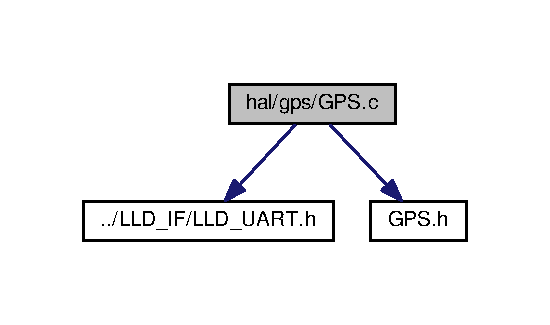
\includegraphics[width=264pt]{GPS_8c__incl}
\end{center}
\end{figure}
\subsection*{Functions}
\begin{DoxyCompactItemize}
\item 
int \hyperlink{GPS_8c_a35a6a55e7bbec401863a903a3607c0b6_a35a6a55e7bbec401863a903a3607c0b6}{g\+\_\+hal\+Gps\+\_\+get\+Data\+\_\+i32} (void)
\begin{DoxyCompactList}\small\item\em Parse Data from Uart into variables. \end{DoxyCompactList}\item 
unsigned int \hyperlink{GPS_8c_aea126d235b1db89dc964f8763565e9dc_aea126d235b1db89dc964f8763565e9dc}{g\+\_\+hal\+Gps\+\_\+get\+Date\+\_\+ui32} (void)
\begin{DoxyCompactList}\small\item\em Get Date from G\+P\+S module. \end{DoxyCompactList}\item 
double \hyperlink{GPS_8c_adac1759b450b418dc6030def1d73b8a7_adac1759b450b418dc6030def1d73b8a7}{g\+\_\+hal\+Gps\+\_\+get\+Direction\+\_\+f64} (void)
\begin{DoxyCompactList}\small\item\em Get Direction from G\+P\+S module. \end{DoxyCompactList}\item 
char \hyperlink{GPS_8c_a4f6b3f1d68b421a3a60b281326b4141b_a4f6b3f1d68b421a3a60b281326b4141b}{g\+\_\+hal\+Gps\+\_\+get\+Fix\+\_\+ch} (void)
\begin{DoxyCompactList}\small\item\em Get Fix from G\+P\+S module. \end{DoxyCompactList}\item 
double \hyperlink{GPS_8c_a0190aaa631556af032a2d286ebf6525a_a0190aaa631556af032a2d286ebf6525a}{g\+\_\+hal\+Gps\+\_\+get\+Geoid\+\_\+f64} (void)
\begin{DoxyCompactList}\small\item\em Get Geoid from G\+P\+S module. \end{DoxyCompactList}\item 
double \hyperlink{GPS_8c_ad797f33853c6d3e6f2e863c11c2822b8_ad797f33853c6d3e6f2e863c11c2822b8}{g\+\_\+hal\+Gps\+\_\+get\+Height\+\_\+f64} (void)
\begin{DoxyCompactList}\small\item\em Get Height from G\+P\+S module. \end{DoxyCompactList}\item 
struct \hyperlink{structstrPosition}{str\+Position} \hyperlink{GPS_8c_a0fa256f0b23aa1d53a0bf5892589dc9f_a0fa256f0b23aa1d53a0bf5892589dc9f}{g\+\_\+hal\+Gps\+\_\+get\+Latitude\+\_\+st} (void)
\begin{DoxyCompactList}\small\item\em Get Latitude from G\+P\+S module. \end{DoxyCompactList}\item 
struct \hyperlink{structstrPosition}{str\+Position} \hyperlink{GPS_8c_a7ee6cdd9714c51a2b74e5f3cdc2a5dca_a7ee6cdd9714c51a2b74e5f3cdc2a5dca}{g\+\_\+hal\+Gps\+\_\+get\+Longitude\+\_\+st} (void)
\begin{DoxyCompactList}\small\item\em Get Longitude from G\+P\+S module. \end{DoxyCompactList}\item 
unsigned int \hyperlink{GPS_8c_a64a3ef5cadfa081ca967b201352e2f8d_a64a3ef5cadfa081ca967b201352e2f8d}{g\+\_\+hal\+Gps\+\_\+get\+Time\+\_\+ui32} (void)
\begin{DoxyCompactList}\small\item\em Get Time from G\+P\+S module. \end{DoxyCompactList}\item 
double \hyperlink{GPS_8c_aae3374862ddb32be3a7f40b01661ede0_aae3374862ddb32be3a7f40b01661ede0}{g\+\_\+hal\+Gps\+\_\+get\+Velocity\+\_\+f64} (void)
\begin{DoxyCompactList}\small\item\em Get Velocity from G\+P\+S module. \end{DoxyCompactList}\item 
void \hyperlink{GPS_8c_a0bf6b6abfd6136e50bd5d35a76ee8d0b_a0bf6b6abfd6136e50bd5d35a76ee8d0b}{l\+\_\+reset\+Message1\+Values\+\_\+vd} (void)
\begin{DoxyCompactList}\small\item\em Reset Values of Message 1. \end{DoxyCompactList}\item 
void \hyperlink{GPS_8c_aa9c4ab6055264c0121813e5233cd3de0_aa9c4ab6055264c0121813e5233cd3de0}{l\+\_\+reset\+Message2\+Values\+\_\+vd} (void)
\begin{DoxyCompactList}\small\item\em Reset Values of Message 2. \end{DoxyCompactList}\end{DoxyCompactItemize}
\subsection*{Variables}
\begin{DoxyCompactItemize}
\item 
static char \hyperlink{GPS_8c_a574dd5cd13fbeac386e435e932e20bae_a574dd5cd13fbeac386e435e932e20bae}{l\+\_\+data\+\_\+position\+\_\+ch} =0
\item 
static unsigned int \hyperlink{GPS_8c_a1b5b44afa58c22d0b8bb4ddedeefb31c_a1b5b44afa58c22d0b8bb4ddedeefb31c}{l\+\_\+date\+\_\+ui32}
\item 
static int \hyperlink{GPS_8c_ad5b924e752a1a8222bd65c4291d3e82e_ad5b924e752a1a8222bd65c4291d3e82e}{l\+\_\+decimal\+\_\+place\+\_\+factor\+\_\+i32} =10
\item 
static double \hyperlink{GPS_8c_a1e038699dda8c22ded8f25762733bfaf_a1e038699dda8c22ded8f25762733bfaf}{l\+\_\+direction\+\_\+f64}
\item 
static int \hyperlink{GPS_8c_a93cee4751b6fb1410e727f045329f326_a93cee4751b6fb1410e727f045329f326}{l\+\_\+fieldpointer\+\_\+i32} =0
\item 
static char \hyperlink{GPS_8c_a5a14aebdd5ac0d06913bdeaf9cec1a9b_a5a14aebdd5ac0d06913bdeaf9cec1a9b}{l\+\_\+fix\+\_\+ch}
\item 
static double \hyperlink{GPS_8c_a2cc033719fe30335f2423a4afbe53984_a2cc033719fe30335f2423a4afbe53984}{l\+\_\+geoid\+\_\+f64}
\item 
static struct \hyperlink{structstrPosition}{str\+Position} \hyperlink{GPS_8c_ae764c82d3318068e28af258ae1e2449c_ae764c82d3318068e28af258ae1e2449c}{l\+\_\+gps\+\_\+latitude\+\_\+st}
\item 
static struct \hyperlink{structstrPosition}{str\+Position} \hyperlink{GPS_8c_a5661901a87ce3f7dcd2eba20d8b505b4_a5661901a87ce3f7dcd2eba20d8b505b4}{l\+\_\+gps\+\_\+longitude\+\_\+st}
\item 
static char \hyperlink{GPS_8c_ac9b483bef981b820a4f6ffaf11ee37a2_ac9b483bef981b820a4f6ffaf11ee37a2}{l\+\_\+header\+\_\+position\+\_\+ch} =0
\item 
static double \hyperlink{GPS_8c_a36e46365d7b41cc255fee53e0aa4b70a_a36e46365d7b41cc255fee53e0aa4b70a}{l\+\_\+height\+\_\+f64}
\item 
static char \hyperlink{GPS_8c_a4b514c1fd22818c03e87233b61d6eda3_a4b514c1fd22818c03e87233b61d6eda3}{l\+\_\+message\+\_\+ch} =0
\item 
static char \hyperlink{GPS_8c_a33348219a5889847ad41d40b9198164a_a33348219a5889847ad41d40b9198164a}{l\+\_\+message\+\_\+position\+\_\+ch} =0
\item 
static char \hyperlink{GPS_8c_a48ba1860315a5b43a78ba5afb66855c4_a48ba1860315a5b43a78ba5afb66855c4}{l\+\_\+rec\+\_\+\+Data\+\_\+ch} ='0'
\item 
static int \hyperlink{GPS_8c_ae83ebc8d1ab82c8acbb739dfd2e9d6f8_ae83ebc8d1ab82c8acbb739dfd2e9d6f8}{l\+\_\+succeded\+\_\+i32}
\item 
static unsigned int \hyperlink{GPS_8c_a365efcbf31282dcb274edd608e0824ed_a365efcbf31282dcb274edd608e0824ed}{l\+\_\+time\+\_\+ui32}
\item 
static double \hyperlink{GPS_8c_af14216f61e92eb4cb399d157299c8d12_af14216f61e92eb4cb399d157299c8d12}{l\+\_\+velocity\+\_\+f64}
\end{DoxyCompactItemize}


\subsection{Function Documentation}
\hypertarget{GPS_8c_a35a6a55e7bbec401863a903a3607c0b6_a35a6a55e7bbec401863a903a3607c0b6}{\index{G\+P\+S.\+c@{G\+P\+S.\+c}!g\+\_\+hal\+Gps\+\_\+get\+Data\+\_\+i32@{g\+\_\+hal\+Gps\+\_\+get\+Data\+\_\+i32}}
\index{g\+\_\+hal\+Gps\+\_\+get\+Data\+\_\+i32@{g\+\_\+hal\+Gps\+\_\+get\+Data\+\_\+i32}!G\+P\+S.\+c@{G\+P\+S.\+c}}
\subsubsection[{g\+\_\+hal\+Gps\+\_\+get\+Data\+\_\+i32}]{\setlength{\rightskip}{0pt plus 5cm}int g\+\_\+hal\+Gps\+\_\+get\+Data\+\_\+i32 (
\begin{DoxyParamCaption}
\item[{void}]{}
\end{DoxyParamCaption}
)}}\label{GPS_8c_a35a6a55e7bbec401863a903a3607c0b6_a35a6a55e7bbec401863a903a3607c0b6}


Parse Data from Uart into variables. 



 \begin{DoxyAuthor}{Author}
Oliver Breuning ( olbrgs00 ) 
\end{DoxyAuthor}
\begin{DoxyDate}{Date}
2015/04/21
\end{DoxyDate}
Reads data from the Hardware Driver and parses it in the specific important variables. Checks just the G\+P\+G\+G\+A and G\+P\+R\+M\+C Messages which are received from the G\+P\+S module. The return value gives back how many important Bytes are received.

Description of counting successfully received values total min\+: 35 max 38 \$\+G\+P\+G\+G\+A ,205003.\+000 ,4841.\+9261 ,N ,00918.\+7276 ,E ,1 ,06 ,1.\+12 ,283.\+5 ,M ,48.\+0 ,M , ,$\ast$6\+D $\vert$$\vert$$\vert$$\vert$$\vert$$\vert$ $\vert$$\vert$$\vert$$\vert$$\vert$$\vert$ $\vert$$\vert$$\vert$$\vert$ $\vert$$\vert$$\vert$$\vert$ $\vert$ $\vert$$\vert$$\vert$$\vert$$\vert$ $\vert$$\vert$$\vert$$\vert$ $\vert$ $\vert$$\vert$$\vert$ $\vert$ $\vert$$\vert$ $\vert$

total min\+: 44 max 47 \$\+G\+P\+R\+M\+C ,205003.\+000 ,A ,4841.\+9261 ,N ,00918.\+7276 ,E ,0.\+33 ,184.\+26 ,100415 , , , A$\ast$63 $\vert$$\vert$$\vert$$\vert$$\vert$$\vert$ $\vert$$\vert$$\vert$$\vert$$\vert$$\vert$ $\vert$ $\vert$$\vert$$\vert$$\vert$ $\vert$$\vert$$\vert$$\vert$ $\vert$ $\vert$$\vert$$\vert$$\vert$$\vert$ $\vert$$\vert$$\vert$$\vert$ $\vert$ $\vert$ $\vert$$\vert$ $\vert$$\vert$$\vert$ $\vert$$\vert$ $\vert$$\vert$$\vert$$\vert$$\vert$$\vert$

Remark message can be shorter if for example value is less than 283.\+5, so e.\+g. 83.\+5


\begin{DoxyParams}[1]{Parameters}
\mbox{\tt in}  & {\em no} & parameter \\
\hline
\mbox{\tt out}  & {\em return} & of successfully important received characters\\
\hline
\end{DoxyParams}


Definition at line 315 of file G\+P\+S.\+c.


\begin{DoxyCode}
316 \{
317 
318     \hyperlink{GPS_8c_a48ba1860315a5b43a78ba5afb66855c4_a48ba1860315a5b43a78ba5afb66855c4}{l\_rec\_Data\_ch}=\hyperlink{LLD__UART_8c_a8154946dd2ae6c37a2bd86dd7896ee73_a8154946dd2ae6c37a2bd86dd7896ee73}{g\_lldUart\_readByte\_ch}();
319 
320     \textcolor{keywordflow}{if}(!\hyperlink{GPS_8c_a33348219a5889847ad41d40b9198164a_a33348219a5889847ad41d40b9198164a}{l\_message\_position\_ch})\textcolor{comment}{//check which message is received}
321     \{
322         \textcolor{keywordflow}{if}(\hyperlink{GPS_8c_a48ba1860315a5b43a78ba5afb66855c4_a48ba1860315a5b43a78ba5afb66855c4}{l\_rec\_Data\_ch}==\textcolor{charliteral}{'$'})
323         \{\hyperlink{GPS_8c_ac9b483bef981b820a4f6ffaf11ee37a2_ac9b483bef981b820a4f6ffaf11ee37a2}{l\_header\_position\_ch}=1;\hyperlink{GPS_8c_ae83ebc8d1ab82c8acbb739dfd2e9d6f8_ae83ebc8d1ab82c8acbb739dfd2e9d6f8}{l\_succeded\_i32}=0;
      \hyperlink{GPS_8c_ae83ebc8d1ab82c8acbb739dfd2e9d6f8_ae83ebc8d1ab82c8acbb739dfd2e9d6f8}{l\_succeded\_i32}++;\}
324         \textcolor{keywordflow}{else} \textcolor{keywordflow}{if} (\hyperlink{GPS_8c_ac9b483bef981b820a4f6ffaf11ee37a2_ac9b483bef981b820a4f6ffaf11ee37a2}{l\_header\_position\_ch}==1 && \hyperlink{GPS_8c_a48ba1860315a5b43a78ba5afb66855c4_a48ba1860315a5b43a78ba5afb66855c4}{l\_rec\_Data\_ch}==\textcolor{charliteral}{'G'})
325         \{\hyperlink{GPS_8c_ac9b483bef981b820a4f6ffaf11ee37a2_ac9b483bef981b820a4f6ffaf11ee37a2}{l\_header\_position\_ch}=2;\hyperlink{GPS_8c_ae83ebc8d1ab82c8acbb739dfd2e9d6f8_ae83ebc8d1ab82c8acbb739dfd2e9d6f8}{l\_succeded\_i32}++;\}
326         \textcolor{keywordflow}{else} \textcolor{keywordflow}{if} (\hyperlink{GPS_8c_ac9b483bef981b820a4f6ffaf11ee37a2_ac9b483bef981b820a4f6ffaf11ee37a2}{l\_header\_position\_ch}==2 && \hyperlink{GPS_8c_a48ba1860315a5b43a78ba5afb66855c4_a48ba1860315a5b43a78ba5afb66855c4}{l\_rec\_Data\_ch}==\textcolor{charliteral}{'P'})
327         \{\hyperlink{GPS_8c_ac9b483bef981b820a4f6ffaf11ee37a2_ac9b483bef981b820a4f6ffaf11ee37a2}{l\_header\_position\_ch}=3;\hyperlink{GPS_8c_ae83ebc8d1ab82c8acbb739dfd2e9d6f8_ae83ebc8d1ab82c8acbb739dfd2e9d6f8}{l\_succeded\_i32}++;\}
328         \textcolor{keywordflow}{else} \textcolor{keywordflow}{if} (\hyperlink{GPS_8c_ac9b483bef981b820a4f6ffaf11ee37a2_ac9b483bef981b820a4f6ffaf11ee37a2}{l\_header\_position\_ch}==3 && \hyperlink{GPS_8c_a48ba1860315a5b43a78ba5afb66855c4_a48ba1860315a5b43a78ba5afb66855c4}{l\_rec\_Data\_ch}==\textcolor{charliteral}{'G'})
329         \{\hyperlink{GPS_8c_ac9b483bef981b820a4f6ffaf11ee37a2_ac9b483bef981b820a4f6ffaf11ee37a2}{l\_header\_position\_ch}=14;\hyperlink{GPS_8c_ae83ebc8d1ab82c8acbb739dfd2e9d6f8_ae83ebc8d1ab82c8acbb739dfd2e9d6f8}{l\_succeded\_i32}++;\}
330         \textcolor{keywordflow}{else} \textcolor{keywordflow}{if} (\hyperlink{GPS_8c_ac9b483bef981b820a4f6ffaf11ee37a2_ac9b483bef981b820a4f6ffaf11ee37a2}{l\_header\_position\_ch}==3 && \hyperlink{GPS_8c_a48ba1860315a5b43a78ba5afb66855c4_a48ba1860315a5b43a78ba5afb66855c4}{l\_rec\_Data\_ch}==\textcolor{charliteral}{'R'})
331         \{\hyperlink{GPS_8c_ac9b483bef981b820a4f6ffaf11ee37a2_ac9b483bef981b820a4f6ffaf11ee37a2}{l\_header\_position\_ch}=24;\hyperlink{GPS_8c_ae83ebc8d1ab82c8acbb739dfd2e9d6f8_ae83ebc8d1ab82c8acbb739dfd2e9d6f8}{l\_succeded\_i32}++;\}
332         \textcolor{keywordflow}{else} \textcolor{keywordflow}{if} (\hyperlink{GPS_8c_ac9b483bef981b820a4f6ffaf11ee37a2_ac9b483bef981b820a4f6ffaf11ee37a2}{l\_header\_position\_ch}==14 && \hyperlink{GPS_8c_a48ba1860315a5b43a78ba5afb66855c4_a48ba1860315a5b43a78ba5afb66855c4}{l\_rec\_Data\_ch}==\textcolor{charliteral}{'G'})
333         \{\hyperlink{GPS_8c_ac9b483bef981b820a4f6ffaf11ee37a2_ac9b483bef981b820a4f6ffaf11ee37a2}{l\_header\_position\_ch}=15;\hyperlink{GPS_8c_ae83ebc8d1ab82c8acbb739dfd2e9d6f8_ae83ebc8d1ab82c8acbb739dfd2e9d6f8}{l\_succeded\_i32}++;\}
334         \textcolor{keywordflow}{else} \textcolor{keywordflow}{if} (\hyperlink{GPS_8c_ac9b483bef981b820a4f6ffaf11ee37a2_ac9b483bef981b820a4f6ffaf11ee37a2}{l\_header\_position\_ch}==24 && \hyperlink{GPS_8c_a48ba1860315a5b43a78ba5afb66855c4_a48ba1860315a5b43a78ba5afb66855c4}{l\_rec\_Data\_ch}==\textcolor{charliteral}{'M'})
335         \{\hyperlink{GPS_8c_ac9b483bef981b820a4f6ffaf11ee37a2_ac9b483bef981b820a4f6ffaf11ee37a2}{l\_header\_position\_ch}=25;\hyperlink{GPS_8c_ae83ebc8d1ab82c8acbb739dfd2e9d6f8_ae83ebc8d1ab82c8acbb739dfd2e9d6f8}{l\_succeded\_i32}++;\}
336         \textcolor{keywordflow}{else} \textcolor{keywordflow}{if} (\hyperlink{GPS_8c_ac9b483bef981b820a4f6ffaf11ee37a2_ac9b483bef981b820a4f6ffaf11ee37a2}{l\_header\_position\_ch}==15 && \hyperlink{GPS_8c_a48ba1860315a5b43a78ba5afb66855c4_a48ba1860315a5b43a78ba5afb66855c4}{l\_rec\_Data\_ch}==\textcolor{charliteral}{'A'})
337         \{   \hyperlink{GPS_8c_a4b514c1fd22818c03e87233b61d6eda3_a4b514c1fd22818c03e87233b61d6eda3}{l\_message\_ch}=1;\hyperlink{GPS_8c_a0bf6b6abfd6136e50bd5d35a76ee8d0b_a0bf6b6abfd6136e50bd5d35a76ee8d0b}{l\_resetMessage1Values\_vd}();
      \hyperlink{GPS_8c_a574dd5cd13fbeac386e435e932e20bae_a574dd5cd13fbeac386e435e932e20bae}{l\_data\_position\_ch}=0;\hyperlink{GPS_8c_a33348219a5889847ad41d40b9198164a_a33348219a5889847ad41d40b9198164a}{l\_message\_position\_ch}=1; 
      \hyperlink{GPS_8c_ae83ebc8d1ab82c8acbb739dfd2e9d6f8_ae83ebc8d1ab82c8acbb739dfd2e9d6f8}{l\_succeded\_i32}++;\}
338         \textcolor{keywordflow}{else} \textcolor{keywordflow}{if} (\hyperlink{GPS_8c_ac9b483bef981b820a4f6ffaf11ee37a2_ac9b483bef981b820a4f6ffaf11ee37a2}{l\_header\_position\_ch}==25 && \hyperlink{GPS_8c_a48ba1860315a5b43a78ba5afb66855c4_a48ba1860315a5b43a78ba5afb66855c4}{l\_rec\_Data\_ch}==\textcolor{charliteral}{'C'})
339         \{   \hyperlink{GPS_8c_a4b514c1fd22818c03e87233b61d6eda3_a4b514c1fd22818c03e87233b61d6eda3}{l\_message\_ch}=2;\hyperlink{GPS_8c_aa9c4ab6055264c0121813e5233cd3de0_aa9c4ab6055264c0121813e5233cd3de0}{l\_resetMessage2Values\_vd}();
      \hyperlink{GPS_8c_a574dd5cd13fbeac386e435e932e20bae_a574dd5cd13fbeac386e435e932e20bae}{l\_data\_position\_ch}=0; \hyperlink{GPS_8c_a33348219a5889847ad41d40b9198164a_a33348219a5889847ad41d40b9198164a}{l\_message\_position\_ch}=1; 
      \hyperlink{GPS_8c_ae83ebc8d1ab82c8acbb739dfd2e9d6f8_ae83ebc8d1ab82c8acbb739dfd2e9d6f8}{l\_succeded\_i32}++;\}
340     \}
341     \textcolor{keywordflow}{else}
342     \{
343         \textcolor{keywordflow}{switch} (\hyperlink{GPS_8c_a4b514c1fd22818c03e87233b61d6eda3_a4b514c1fd22818c03e87233b61d6eda3}{l\_message\_ch})\textcolor{comment}{//check data within the two important messages}
344         \{
345         \textcolor{keywordflow}{case} 1:\textcolor{comment}{//$GPGGA ,205003.000 ,4841.9261 ,N ,00918.7276 ,E ,1 ,06 ,1.12 ,283.5 ,M ,48.0 ,M , ,*6D    
          38}
346             \textcolor{keywordflow}{switch} (\hyperlink{GPS_8c_a48ba1860315a5b43a78ba5afb66855c4_a48ba1860315a5b43a78ba5afb66855c4}{l\_rec\_Data\_ch})
347             \{
348             \textcolor{keywordflow}{case} \textcolor{charliteral}{','}:
349                 \hyperlink{GPS_8c_a574dd5cd13fbeac386e435e932e20bae_a574dd5cd13fbeac386e435e932e20bae}{l\_data\_position\_ch}++;
350                 \hyperlink{GPS_8c_a93cee4751b6fb1410e727f045329f326_a93cee4751b6fb1410e727f045329f326}{l\_fieldpointer\_i32}=0;
351                 \hyperlink{GPS_8c_ad5b924e752a1a8222bd65c4291d3e82e_ad5b924e752a1a8222bd65c4291d3e82e}{l\_decimal\_place\_factor\_i32}=10;
352                 \textcolor{keywordflow}{break};
353             \textcolor{keywordflow}{case} 10:\textcolor{comment}{//LF found}
354                 \hyperlink{GPS_8c_ae83ebc8d1ab82c8acbb739dfd2e9d6f8_ae83ebc8d1ab82c8acbb739dfd2e9d6f8}{l\_succeded\_i32}=\hyperlink{GPS_8c_ae83ebc8d1ab82c8acbb739dfd2e9d6f8_ae83ebc8d1ab82c8acbb739dfd2e9d6f8}{l\_succeded\_i32}+100;  \textcolor{comment}{//short comment}
355                 \hyperlink{GPS_8c_a33348219a5889847ad41d40b9198164a_a33348219a5889847ad41d40b9198164a}{l\_message\_position\_ch}=0;
356                 \hyperlink{GPS_8c_ac9b483bef981b820a4f6ffaf11ee37a2_ac9b483bef981b820a4f6ffaf11ee37a2}{l\_header\_position\_ch}=0;
357                 \textcolor{keywordflow}{break};
358             \textcolor{keywordflow}{default}:
359                 \textcolor{keywordflow}{switch} (\hyperlink{GPS_8c_a574dd5cd13fbeac386e435e932e20bae_a574dd5cd13fbeac386e435e932e20bae}{l\_data\_position\_ch})
360                 \{
361                 \textcolor{keywordflow}{case} 1:\textcolor{comment}{//Time}
362                     \textcolor{keywordflow}{if}(\hyperlink{GPS_8c_a93cee4751b6fb1410e727f045329f326_a93cee4751b6fb1410e727f045329f326}{l\_fieldpointer\_i32}<6)
363                     \{
364                         \hyperlink{GPS_8c_a365efcbf31282dcb274edd608e0824ed_a365efcbf31282dcb274edd608e0824ed}{l\_time\_ui32}=\hyperlink{GPS_8c_a365efcbf31282dcb274edd608e0824ed_a365efcbf31282dcb274edd608e0824ed}{l\_time\_ui32}*10+(
      \hyperlink{GPS_8c_a48ba1860315a5b43a78ba5afb66855c4_a48ba1860315a5b43a78ba5afb66855c4}{l\_rec\_Data\_ch}-48);
365                         \hyperlink{GPS_8c_ae83ebc8d1ab82c8acbb739dfd2e9d6f8_ae83ebc8d1ab82c8acbb739dfd2e9d6f8}{l\_succeded\_i32}++;
366                     \}
367                     \hyperlink{GPS_8c_a93cee4751b6fb1410e727f045329f326_a93cee4751b6fb1410e727f045329f326}{l\_fieldpointer\_i32}++;
368                     \textcolor{keywordflow}{break};
369                 \textcolor{keywordflow}{case} 2:\textcolor{comment}{//Latitude}
370                     \textcolor{keywordflow}{if}(\hyperlink{GPS_8c_a93cee4751b6fb1410e727f045329f326_a93cee4751b6fb1410e727f045329f326}{l\_fieldpointer\_i32}<2)
371                     \{
372                         \hyperlink{GPS_8c_ae764c82d3318068e28af258ae1e2449c_ae764c82d3318068e28af258ae1e2449c}{l\_gps\_latitude\_st}.\hyperlink{structstrPosition_ac060af7d7963812c116c24cdb861f184_ac060af7d7963812c116c24cdb861f184}{l\_degree\_ui32}=
      \hyperlink{GPS_8c_ae764c82d3318068e28af258ae1e2449c_ae764c82d3318068e28af258ae1e2449c}{l\_gps\_latitude\_st}.\hyperlink{structstrPosition_ac060af7d7963812c116c24cdb861f184_ac060af7d7963812c116c24cdb861f184}{l\_degree\_ui32}*10+(\hyperlink{GPS_8c_a48ba1860315a5b43a78ba5afb66855c4_a48ba1860315a5b43a78ba5afb66855c4}{l\_rec\_Data\_ch}-48);
373                         \hyperlink{GPS_8c_ae83ebc8d1ab82c8acbb739dfd2e9d6f8_ae83ebc8d1ab82c8acbb739dfd2e9d6f8}{l\_succeded\_i32}++;
374                     \}
375                     \textcolor{keywordflow}{else} \textcolor{keywordflow}{if}(\hyperlink{GPS_8c_a93cee4751b6fb1410e727f045329f326_a93cee4751b6fb1410e727f045329f326}{l\_fieldpointer\_i32}<4)
376                     \{
377                         \hyperlink{GPS_8c_ae764c82d3318068e28af258ae1e2449c_ae764c82d3318068e28af258ae1e2449c}{l\_gps\_latitude\_st}.\hyperlink{structstrPosition_a5489ef5e7f8e6ee45990b262c80a7819_a5489ef5e7f8e6ee45990b262c80a7819}{l\_minutes\_ui32}=
      \hyperlink{GPS_8c_ae764c82d3318068e28af258ae1e2449c_ae764c82d3318068e28af258ae1e2449c}{l\_gps\_latitude\_st}.\hyperlink{structstrPosition_a5489ef5e7f8e6ee45990b262c80a7819_a5489ef5e7f8e6ee45990b262c80a7819}{l\_minutes\_ui32}*10+(
      \hyperlink{GPS_8c_a48ba1860315a5b43a78ba5afb66855c4_a48ba1860315a5b43a78ba5afb66855c4}{l\_rec\_Data\_ch}-48);
378                         \hyperlink{GPS_8c_ae83ebc8d1ab82c8acbb739dfd2e9d6f8_ae83ebc8d1ab82c8acbb739dfd2e9d6f8}{l\_succeded\_i32}++;
379                     \}
380                     \textcolor{keywordflow}{else} \textcolor{keywordflow}{if}(\hyperlink{GPS_8c_a93cee4751b6fb1410e727f045329f326_a93cee4751b6fb1410e727f045329f326}{l\_fieldpointer\_i32}>=5 && 
      \hyperlink{GPS_8c_a93cee4751b6fb1410e727f045329f326_a93cee4751b6fb1410e727f045329f326}{l\_fieldpointer\_i32}<9)
381                     \{
382                         \hyperlink{GPS_8c_ae764c82d3318068e28af258ae1e2449c_ae764c82d3318068e28af258ae1e2449c}{l\_gps\_latitude\_st}.\hyperlink{structstrPosition_ae62d246c481c611e168ea86b70d5313b_ae62d246c481c611e168ea86b70d5313b}{l\_seconds\_f64}=
      \hyperlink{GPS_8c_ae764c82d3318068e28af258ae1e2449c_ae764c82d3318068e28af258ae1e2449c}{l\_gps\_latitude\_st}.\hyperlink{structstrPosition_ae62d246c481c611e168ea86b70d5313b_ae62d246c481c611e168ea86b70d5313b}{l\_seconds\_f64}*10+(\hyperlink{GPS_8c_a48ba1860315a5b43a78ba5afb66855c4_a48ba1860315a5b43a78ba5afb66855c4}{l\_rec\_Data\_ch}-48)*0.006;
383                         \hyperlink{GPS_8c_ae83ebc8d1ab82c8acbb739dfd2e9d6f8_ae83ebc8d1ab82c8acbb739dfd2e9d6f8}{l\_succeded\_i32}++;
384                     \}
385                     \hyperlink{GPS_8c_a93cee4751b6fb1410e727f045329f326_a93cee4751b6fb1410e727f045329f326}{l\_fieldpointer\_i32}++;
386                     \textcolor{keywordflow}{break};
387                 \textcolor{keywordflow}{case} 3:\textcolor{comment}{//cardinal direction}
388                     \textcolor{keywordflow}{if}(\hyperlink{GPS_8c_a93cee4751b6fb1410e727f045329f326_a93cee4751b6fb1410e727f045329f326}{l\_fieldpointer\_i32}<1)
389                     \{
390                         \hyperlink{GPS_8c_ae764c82d3318068e28af258ae1e2449c_ae764c82d3318068e28af258ae1e2449c}{l\_gps\_latitude\_st}.
      \hyperlink{structstrPosition_aa39fed1d421cb2260d0ef7157c3c00d0_aa39fed1d421cb2260d0ef7157c3c00d0}{l\_cardinalDirection\_ch}=\hyperlink{GPS_8c_a48ba1860315a5b43a78ba5afb66855c4_a48ba1860315a5b43a78ba5afb66855c4}{l\_rec\_Data\_ch};
391                         \hyperlink{GPS_8c_ae83ebc8d1ab82c8acbb739dfd2e9d6f8_ae83ebc8d1ab82c8acbb739dfd2e9d6f8}{l\_succeded\_i32}++;
392                     \}
393                     \hyperlink{GPS_8c_a93cee4751b6fb1410e727f045329f326_a93cee4751b6fb1410e727f045329f326}{l\_fieldpointer\_i32}++;
394                     \textcolor{keywordflow}{break};
395                 \textcolor{keywordflow}{case} 4:\textcolor{comment}{//Longitude}
396                     \textcolor{keywordflow}{if}(\hyperlink{GPS_8c_a93cee4751b6fb1410e727f045329f326_a93cee4751b6fb1410e727f045329f326}{l\_fieldpointer\_i32}<3)
397                     \{
398                         \hyperlink{GPS_8c_a5661901a87ce3f7dcd2eba20d8b505b4_a5661901a87ce3f7dcd2eba20d8b505b4}{l\_gps\_longitude\_st}.\hyperlink{structstrPosition_ac060af7d7963812c116c24cdb861f184_ac060af7d7963812c116c24cdb861f184}{l\_degree\_ui32}=
      \hyperlink{GPS_8c_a5661901a87ce3f7dcd2eba20d8b505b4_a5661901a87ce3f7dcd2eba20d8b505b4}{l\_gps\_longitude\_st}.\hyperlink{structstrPosition_ac060af7d7963812c116c24cdb861f184_ac060af7d7963812c116c24cdb861f184}{l\_degree\_ui32}*10+(
      \hyperlink{GPS_8c_a48ba1860315a5b43a78ba5afb66855c4_a48ba1860315a5b43a78ba5afb66855c4}{l\_rec\_Data\_ch}-48);
399                         \hyperlink{GPS_8c_ae83ebc8d1ab82c8acbb739dfd2e9d6f8_ae83ebc8d1ab82c8acbb739dfd2e9d6f8}{l\_succeded\_i32}++;
400                     \}
401                     \textcolor{keywordflow}{else} \textcolor{keywordflow}{if}(\hyperlink{GPS_8c_a93cee4751b6fb1410e727f045329f326_a93cee4751b6fb1410e727f045329f326}{l\_fieldpointer\_i32}<5)
402                     \{
403                         \hyperlink{GPS_8c_a5661901a87ce3f7dcd2eba20d8b505b4_a5661901a87ce3f7dcd2eba20d8b505b4}{l\_gps\_longitude\_st}.\hyperlink{structstrPosition_a5489ef5e7f8e6ee45990b262c80a7819_a5489ef5e7f8e6ee45990b262c80a7819}{l\_minutes\_ui32}=
      \hyperlink{GPS_8c_a5661901a87ce3f7dcd2eba20d8b505b4_a5661901a87ce3f7dcd2eba20d8b505b4}{l\_gps\_longitude\_st}.\hyperlink{structstrPosition_a5489ef5e7f8e6ee45990b262c80a7819_a5489ef5e7f8e6ee45990b262c80a7819}{l\_minutes\_ui32}*10+(
      \hyperlink{GPS_8c_a48ba1860315a5b43a78ba5afb66855c4_a48ba1860315a5b43a78ba5afb66855c4}{l\_rec\_Data\_ch}-48);
404                         \hyperlink{GPS_8c_ae83ebc8d1ab82c8acbb739dfd2e9d6f8_ae83ebc8d1ab82c8acbb739dfd2e9d6f8}{l\_succeded\_i32}++;
405                     \}
406                     \textcolor{keywordflow}{else} \textcolor{keywordflow}{if}(\hyperlink{GPS_8c_a93cee4751b6fb1410e727f045329f326_a93cee4751b6fb1410e727f045329f326}{l\_fieldpointer\_i32}>=6 && 
      \hyperlink{GPS_8c_a93cee4751b6fb1410e727f045329f326_a93cee4751b6fb1410e727f045329f326}{l\_fieldpointer\_i32}<10)
407                     \{
408                         \hyperlink{GPS_8c_a5661901a87ce3f7dcd2eba20d8b505b4_a5661901a87ce3f7dcd2eba20d8b505b4}{l\_gps\_longitude\_st}.\hyperlink{structstrPosition_ae62d246c481c611e168ea86b70d5313b_ae62d246c481c611e168ea86b70d5313b}{l\_seconds\_f64}=
      \hyperlink{GPS_8c_a5661901a87ce3f7dcd2eba20d8b505b4_a5661901a87ce3f7dcd2eba20d8b505b4}{l\_gps\_longitude\_st}.\hyperlink{structstrPosition_ae62d246c481c611e168ea86b70d5313b_ae62d246c481c611e168ea86b70d5313b}{l\_seconds\_f64}*10+(
      \hyperlink{GPS_8c_a48ba1860315a5b43a78ba5afb66855c4_a48ba1860315a5b43a78ba5afb66855c4}{l\_rec\_Data\_ch}-48)*0.006;
409                         \hyperlink{GPS_8c_ae83ebc8d1ab82c8acbb739dfd2e9d6f8_ae83ebc8d1ab82c8acbb739dfd2e9d6f8}{l\_succeded\_i32}++;
410                     \}
411                     \hyperlink{GPS_8c_a93cee4751b6fb1410e727f045329f326_a93cee4751b6fb1410e727f045329f326}{l\_fieldpointer\_i32}++;
412                     \textcolor{keywordflow}{break};
413                 \textcolor{keywordflow}{case} 5:\textcolor{comment}{//cardinal direction}
414                     \textcolor{keywordflow}{if}(\hyperlink{GPS_8c_a93cee4751b6fb1410e727f045329f326_a93cee4751b6fb1410e727f045329f326}{l\_fieldpointer\_i32}<1)
415                     \{
416                         \hyperlink{GPS_8c_a5661901a87ce3f7dcd2eba20d8b505b4_a5661901a87ce3f7dcd2eba20d8b505b4}{l\_gps\_longitude\_st}.
      \hyperlink{structstrPosition_aa39fed1d421cb2260d0ef7157c3c00d0_aa39fed1d421cb2260d0ef7157c3c00d0}{l\_cardinalDirection\_ch}=\hyperlink{GPS_8c_a48ba1860315a5b43a78ba5afb66855c4_a48ba1860315a5b43a78ba5afb66855c4}{l\_rec\_Data\_ch};
417                         \hyperlink{GPS_8c_ae83ebc8d1ab82c8acbb739dfd2e9d6f8_ae83ebc8d1ab82c8acbb739dfd2e9d6f8}{l\_succeded\_i32}++;
418                     \}
419                     \hyperlink{GPS_8c_a93cee4751b6fb1410e727f045329f326_a93cee4751b6fb1410e727f045329f326}{l\_fieldpointer\_i32}++;
420                     \textcolor{keywordflow}{break};
421                 \textcolor{keywordflow}{case} 9:\textcolor{comment}{//Height}
422                     \textcolor{keywordflow}{if}(\hyperlink{GPS_8c_a48ba1860315a5b43a78ba5afb66855c4_a48ba1860315a5b43a78ba5afb66855c4}{l\_rec\_Data\_ch}!=\textcolor{charliteral}{'.'} && \hyperlink{GPS_8c_a93cee4751b6fb1410e727f045329f326_a93cee4751b6fb1410e727f045329f326}{l\_fieldpointer\_i32}==0)
423                     \{
424                         \hyperlink{GPS_8c_a36e46365d7b41cc255fee53e0aa4b70a_a36e46365d7b41cc255fee53e0aa4b70a}{l\_height\_f64}=\hyperlink{GPS_8c_a36e46365d7b41cc255fee53e0aa4b70a_a36e46365d7b41cc255fee53e0aa4b70a}{l\_height\_f64}*10+(double)(
      \hyperlink{GPS_8c_a48ba1860315a5b43a78ba5afb66855c4_a48ba1860315a5b43a78ba5afb66855c4}{l\_rec\_Data\_ch}-48);
425                         \hyperlink{GPS_8c_ae83ebc8d1ab82c8acbb739dfd2e9d6f8_ae83ebc8d1ab82c8acbb739dfd2e9d6f8}{l\_succeded\_i32}++;
426 
427                     \}
428                     \textcolor{keywordflow}{else} \textcolor{keywordflow}{if} (\hyperlink{GPS_8c_a48ba1860315a5b43a78ba5afb66855c4_a48ba1860315a5b43a78ba5afb66855c4}{l\_rec\_Data\_ch}==\textcolor{charliteral}{'.'})
429                     \{
430                         \hyperlink{GPS_8c_a93cee4751b6fb1410e727f045329f326_a93cee4751b6fb1410e727f045329f326}{l\_fieldpointer\_i32}++;
431                     \}
432                     \textcolor{keywordflow}{else}
433                     \{
434                         \hyperlink{GPS_8c_a36e46365d7b41cc255fee53e0aa4b70a_a36e46365d7b41cc255fee53e0aa4b70a}{l\_height\_f64}=\hyperlink{GPS_8c_a36e46365d7b41cc255fee53e0aa4b70a_a36e46365d7b41cc255fee53e0aa4b70a}{l\_height\_f64}+(double)(
      \hyperlink{GPS_8c_a48ba1860315a5b43a78ba5afb66855c4_a48ba1860315a5b43a78ba5afb66855c4}{l\_rec\_Data\_ch}-48)/\hyperlink{GPS_8c_ad5b924e752a1a8222bd65c4291d3e82e_ad5b924e752a1a8222bd65c4291d3e82e}{l\_decimal\_place\_factor\_i32};
435                         \hyperlink{GPS_8c_ad5b924e752a1a8222bd65c4291d3e82e_ad5b924e752a1a8222bd65c4291d3e82e}{l\_decimal\_place\_factor\_i32}=
      \hyperlink{GPS_8c_ad5b924e752a1a8222bd65c4291d3e82e_ad5b924e752a1a8222bd65c4291d3e82e}{l\_decimal\_place\_factor\_i32}*10;
436                         \hyperlink{GPS_8c_ae83ebc8d1ab82c8acbb739dfd2e9d6f8_ae83ebc8d1ab82c8acbb739dfd2e9d6f8}{l\_succeded\_i32}++;
437                     \}
438                     \textcolor{keywordflow}{break};
439                 \textcolor{keywordflow}{case} 11:\textcolor{comment}{//Geoid}
440                     \textcolor{keywordflow}{if}(\hyperlink{GPS_8c_a48ba1860315a5b43a78ba5afb66855c4_a48ba1860315a5b43a78ba5afb66855c4}{l\_rec\_Data\_ch}!=\textcolor{charliteral}{'.'} && \hyperlink{GPS_8c_a93cee4751b6fb1410e727f045329f326_a93cee4751b6fb1410e727f045329f326}{l\_fieldpointer\_i32}==0)
441                     \{
442                         \hyperlink{GPS_8c_a2cc033719fe30335f2423a4afbe53984_a2cc033719fe30335f2423a4afbe53984}{l\_geoid\_f64}=\hyperlink{GPS_8c_a2cc033719fe30335f2423a4afbe53984_a2cc033719fe30335f2423a4afbe53984}{l\_geoid\_f64}*10+(double)(
      \hyperlink{GPS_8c_a48ba1860315a5b43a78ba5afb66855c4_a48ba1860315a5b43a78ba5afb66855c4}{l\_rec\_Data\_ch}-48);
443                         \hyperlink{GPS_8c_ae83ebc8d1ab82c8acbb739dfd2e9d6f8_ae83ebc8d1ab82c8acbb739dfd2e9d6f8}{l\_succeded\_i32}++;
444 
445                     \}
446                     \textcolor{keywordflow}{else} \textcolor{keywordflow}{if} (\hyperlink{GPS_8c_a48ba1860315a5b43a78ba5afb66855c4_a48ba1860315a5b43a78ba5afb66855c4}{l\_rec\_Data\_ch}==\textcolor{charliteral}{'.'})
447                     \{
448                         \hyperlink{GPS_8c_a93cee4751b6fb1410e727f045329f326_a93cee4751b6fb1410e727f045329f326}{l\_fieldpointer\_i32}++;
449                     \}
450                     \textcolor{keywordflow}{else}
451                     \{
452                         \hyperlink{GPS_8c_a2cc033719fe30335f2423a4afbe53984_a2cc033719fe30335f2423a4afbe53984}{l\_geoid\_f64}=\hyperlink{GPS_8c_a2cc033719fe30335f2423a4afbe53984_a2cc033719fe30335f2423a4afbe53984}{l\_geoid\_f64}+(double)(
      \hyperlink{GPS_8c_a48ba1860315a5b43a78ba5afb66855c4_a48ba1860315a5b43a78ba5afb66855c4}{l\_rec\_Data\_ch}-48)/\hyperlink{GPS_8c_ad5b924e752a1a8222bd65c4291d3e82e_ad5b924e752a1a8222bd65c4291d3e82e}{l\_decimal\_place\_factor\_i32};
453                         \hyperlink{GPS_8c_ad5b924e752a1a8222bd65c4291d3e82e_ad5b924e752a1a8222bd65c4291d3e82e}{l\_decimal\_place\_factor\_i32}=
      \hyperlink{GPS_8c_ad5b924e752a1a8222bd65c4291d3e82e_ad5b924e752a1a8222bd65c4291d3e82e}{l\_decimal\_place\_factor\_i32}*10;
454                         \hyperlink{GPS_8c_ae83ebc8d1ab82c8acbb739dfd2e9d6f8_ae83ebc8d1ab82c8acbb739dfd2e9d6f8}{l\_succeded\_i32}++;
455                     \}
456                     \textcolor{keywordflow}{break};
457                 \}
458                 \textcolor{keywordflow}{break};
459             \}
460             \textcolor{keywordflow}{break};
461 
462 
463         \textcolor{keywordflow}{case} 2:\textcolor{comment}{//$GPRMC ,205003.000 ,A ,4841.9261 ,N ,00918.7276 ,E ,0.33 ,184.26 ,100415 , , , A*63     
       44- 46}
464             \textcolor{keywordflow}{switch} (\hyperlink{GPS_8c_a48ba1860315a5b43a78ba5afb66855c4_a48ba1860315a5b43a78ba5afb66855c4}{l\_rec\_Data\_ch})
465             \{
466             \textcolor{keywordflow}{case} \textcolor{charliteral}{','}:
467                 \hyperlink{GPS_8c_a574dd5cd13fbeac386e435e932e20bae_a574dd5cd13fbeac386e435e932e20bae}{l\_data\_position\_ch}++;
468                 \hyperlink{GPS_8c_a93cee4751b6fb1410e727f045329f326_a93cee4751b6fb1410e727f045329f326}{l\_fieldpointer\_i32}=0;
469                 \hyperlink{GPS_8c_ad5b924e752a1a8222bd65c4291d3e82e_ad5b924e752a1a8222bd65c4291d3e82e}{l\_decimal\_place\_factor\_i32}=10;
470                 \textcolor{keywordflow}{break};
471             \textcolor{keywordflow}{case} 10:\textcolor{comment}{//LF found}
472                 \hyperlink{GPS_8c_ae83ebc8d1ab82c8acbb739dfd2e9d6f8_ae83ebc8d1ab82c8acbb739dfd2e9d6f8}{l\_succeded\_i32}=\hyperlink{GPS_8c_ae83ebc8d1ab82c8acbb739dfd2e9d6f8_ae83ebc8d1ab82c8acbb739dfd2e9d6f8}{l\_succeded\_i32}+200;
473                 \hyperlink{GPS_8c_a33348219a5889847ad41d40b9198164a_a33348219a5889847ad41d40b9198164a}{l\_message\_position\_ch}=0;
474                 \hyperlink{GPS_8c_ac9b483bef981b820a4f6ffaf11ee37a2_ac9b483bef981b820a4f6ffaf11ee37a2}{l\_header\_position\_ch}=0;
475                 \textcolor{keywordflow}{break};
476             \textcolor{keywordflow}{default}:
477                 \textcolor{keywordflow}{switch} (\hyperlink{GPS_8c_a574dd5cd13fbeac386e435e932e20bae_a574dd5cd13fbeac386e435e932e20bae}{l\_data\_position\_ch})
478                 \{
479                 \textcolor{keywordflow}{case} 1:\textcolor{comment}{//Time}
480                     \textcolor{keywordflow}{if}(\hyperlink{GPS_8c_a93cee4751b6fb1410e727f045329f326_a93cee4751b6fb1410e727f045329f326}{l\_fieldpointer\_i32}<6)
481                     \{
482                         \hyperlink{GPS_8c_a365efcbf31282dcb274edd608e0824ed_a365efcbf31282dcb274edd608e0824ed}{l\_time\_ui32}=\hyperlink{GPS_8c_a365efcbf31282dcb274edd608e0824ed_a365efcbf31282dcb274edd608e0824ed}{l\_time\_ui32}*10+(
      \hyperlink{GPS_8c_a48ba1860315a5b43a78ba5afb66855c4_a48ba1860315a5b43a78ba5afb66855c4}{l\_rec\_Data\_ch}-48);
483                         \hyperlink{GPS_8c_ae83ebc8d1ab82c8acbb739dfd2e9d6f8_ae83ebc8d1ab82c8acbb739dfd2e9d6f8}{l\_succeded\_i32}++;
484                     \}
485                     \hyperlink{GPS_8c_a93cee4751b6fb1410e727f045329f326_a93cee4751b6fb1410e727f045329f326}{l\_fieldpointer\_i32}++;
486                     \textcolor{keywordflow}{break};
487                 \textcolor{keywordflow}{case} 2:\textcolor{comment}{//Fix}
488                     \textcolor{keywordflow}{if}(\hyperlink{GPS_8c_a93cee4751b6fb1410e727f045329f326_a93cee4751b6fb1410e727f045329f326}{l\_fieldpointer\_i32}<2)
489                     \{
490                         \hyperlink{GPS_8c_a5a14aebdd5ac0d06913bdeaf9cec1a9b_a5a14aebdd5ac0d06913bdeaf9cec1a9b}{l\_fix\_ch}=\hyperlink{GPS_8c_a48ba1860315a5b43a78ba5afb66855c4_a48ba1860315a5b43a78ba5afb66855c4}{l\_rec\_Data\_ch};
491                         \hyperlink{GPS_8c_ae83ebc8d1ab82c8acbb739dfd2e9d6f8_ae83ebc8d1ab82c8acbb739dfd2e9d6f8}{l\_succeded\_i32}++;
492                     \}
493                     \hyperlink{GPS_8c_a93cee4751b6fb1410e727f045329f326_a93cee4751b6fb1410e727f045329f326}{l\_fieldpointer\_i32}++;
494                     \textcolor{keywordflow}{break};
495                 \textcolor{keywordflow}{case} 3:\textcolor{comment}{//Latitude}
496                     \textcolor{keywordflow}{if}(\hyperlink{GPS_8c_a93cee4751b6fb1410e727f045329f326_a93cee4751b6fb1410e727f045329f326}{l\_fieldpointer\_i32}<2)
497                     \{
498                         \hyperlink{GPS_8c_ae764c82d3318068e28af258ae1e2449c_ae764c82d3318068e28af258ae1e2449c}{l\_gps\_latitude\_st}.\hyperlink{structstrPosition_ac060af7d7963812c116c24cdb861f184_ac060af7d7963812c116c24cdb861f184}{l\_degree\_ui32}=
      \hyperlink{GPS_8c_ae764c82d3318068e28af258ae1e2449c_ae764c82d3318068e28af258ae1e2449c}{l\_gps\_latitude\_st}.\hyperlink{structstrPosition_ac060af7d7963812c116c24cdb861f184_ac060af7d7963812c116c24cdb861f184}{l\_degree\_ui32}*10+(\hyperlink{GPS_8c_a48ba1860315a5b43a78ba5afb66855c4_a48ba1860315a5b43a78ba5afb66855c4}{l\_rec\_Data\_ch}-48);
499                         \hyperlink{GPS_8c_ae83ebc8d1ab82c8acbb739dfd2e9d6f8_ae83ebc8d1ab82c8acbb739dfd2e9d6f8}{l\_succeded\_i32}++;
500                     \}
501                     \textcolor{keywordflow}{else} \textcolor{keywordflow}{if}(\hyperlink{GPS_8c_a93cee4751b6fb1410e727f045329f326_a93cee4751b6fb1410e727f045329f326}{l\_fieldpointer\_i32}<4)
502                     \{
503                         \hyperlink{GPS_8c_ae764c82d3318068e28af258ae1e2449c_ae764c82d3318068e28af258ae1e2449c}{l\_gps\_latitude\_st}.\hyperlink{structstrPosition_a5489ef5e7f8e6ee45990b262c80a7819_a5489ef5e7f8e6ee45990b262c80a7819}{l\_minutes\_ui32}=
      \hyperlink{GPS_8c_ae764c82d3318068e28af258ae1e2449c_ae764c82d3318068e28af258ae1e2449c}{l\_gps\_latitude\_st}.\hyperlink{structstrPosition_a5489ef5e7f8e6ee45990b262c80a7819_a5489ef5e7f8e6ee45990b262c80a7819}{l\_minutes\_ui32}*10+(
      \hyperlink{GPS_8c_a48ba1860315a5b43a78ba5afb66855c4_a48ba1860315a5b43a78ba5afb66855c4}{l\_rec\_Data\_ch}-48);
504                         \hyperlink{GPS_8c_ae83ebc8d1ab82c8acbb739dfd2e9d6f8_ae83ebc8d1ab82c8acbb739dfd2e9d6f8}{l\_succeded\_i32}++;
505                     \}
506                     \textcolor{keywordflow}{else} \textcolor{keywordflow}{if}(\hyperlink{GPS_8c_a93cee4751b6fb1410e727f045329f326_a93cee4751b6fb1410e727f045329f326}{l\_fieldpointer\_i32}>=5 && 
      \hyperlink{GPS_8c_a93cee4751b6fb1410e727f045329f326_a93cee4751b6fb1410e727f045329f326}{l\_fieldpointer\_i32}<9)
507                     \{
508                         \hyperlink{GPS_8c_ae764c82d3318068e28af258ae1e2449c_ae764c82d3318068e28af258ae1e2449c}{l\_gps\_latitude\_st}.\hyperlink{structstrPosition_ae62d246c481c611e168ea86b70d5313b_ae62d246c481c611e168ea86b70d5313b}{l\_seconds\_f64}=
      \hyperlink{GPS_8c_ae764c82d3318068e28af258ae1e2449c_ae764c82d3318068e28af258ae1e2449c}{l\_gps\_latitude\_st}.\hyperlink{structstrPosition_ae62d246c481c611e168ea86b70d5313b_ae62d246c481c611e168ea86b70d5313b}{l\_seconds\_f64}*10+(double)(
      \hyperlink{GPS_8c_a48ba1860315a5b43a78ba5afb66855c4_a48ba1860315a5b43a78ba5afb66855c4}{l\_rec\_Data\_ch}-48)*0.006;
509                         \hyperlink{GPS_8c_ae83ebc8d1ab82c8acbb739dfd2e9d6f8_ae83ebc8d1ab82c8acbb739dfd2e9d6f8}{l\_succeded\_i32}++;
510                     \}
511                     \hyperlink{GPS_8c_a93cee4751b6fb1410e727f045329f326_a93cee4751b6fb1410e727f045329f326}{l\_fieldpointer\_i32}++;
512                     \textcolor{keywordflow}{break};
513                 \textcolor{keywordflow}{case} 4:\textcolor{comment}{//cardinal direction}
514                     \textcolor{keywordflow}{if}(\hyperlink{GPS_8c_a93cee4751b6fb1410e727f045329f326_a93cee4751b6fb1410e727f045329f326}{l\_fieldpointer\_i32}<1)
515                     \{
516                         \hyperlink{GPS_8c_ae764c82d3318068e28af258ae1e2449c_ae764c82d3318068e28af258ae1e2449c}{l\_gps\_latitude\_st}.
      \hyperlink{structstrPosition_aa39fed1d421cb2260d0ef7157c3c00d0_aa39fed1d421cb2260d0ef7157c3c00d0}{l\_cardinalDirection\_ch}=\hyperlink{GPS_8c_a48ba1860315a5b43a78ba5afb66855c4_a48ba1860315a5b43a78ba5afb66855c4}{l\_rec\_Data\_ch};
517                         \hyperlink{GPS_8c_ae83ebc8d1ab82c8acbb739dfd2e9d6f8_ae83ebc8d1ab82c8acbb739dfd2e9d6f8}{l\_succeded\_i32}++;
518                     \}
519                     \hyperlink{GPS_8c_a93cee4751b6fb1410e727f045329f326_a93cee4751b6fb1410e727f045329f326}{l\_fieldpointer\_i32}++;
520                     \textcolor{keywordflow}{break};
521                 \textcolor{keywordflow}{case} 5:\textcolor{comment}{//Longitude}
522                     \textcolor{keywordflow}{if}(\hyperlink{GPS_8c_a93cee4751b6fb1410e727f045329f326_a93cee4751b6fb1410e727f045329f326}{l\_fieldpointer\_i32}<3)
523                     \{
524                         \hyperlink{GPS_8c_a5661901a87ce3f7dcd2eba20d8b505b4_a5661901a87ce3f7dcd2eba20d8b505b4}{l\_gps\_longitude\_st}.\hyperlink{structstrPosition_ac060af7d7963812c116c24cdb861f184_ac060af7d7963812c116c24cdb861f184}{l\_degree\_ui32}=
      \hyperlink{GPS_8c_a5661901a87ce3f7dcd2eba20d8b505b4_a5661901a87ce3f7dcd2eba20d8b505b4}{l\_gps\_longitude\_st}.\hyperlink{structstrPosition_ac060af7d7963812c116c24cdb861f184_ac060af7d7963812c116c24cdb861f184}{l\_degree\_ui32}*10+(
      \hyperlink{GPS_8c_a48ba1860315a5b43a78ba5afb66855c4_a48ba1860315a5b43a78ba5afb66855c4}{l\_rec\_Data\_ch}-48);
525                         \hyperlink{GPS_8c_ae83ebc8d1ab82c8acbb739dfd2e9d6f8_ae83ebc8d1ab82c8acbb739dfd2e9d6f8}{l\_succeded\_i32}++;
526                     \}
527                     \textcolor{keywordflow}{else} \textcolor{keywordflow}{if}(\hyperlink{GPS_8c_a93cee4751b6fb1410e727f045329f326_a93cee4751b6fb1410e727f045329f326}{l\_fieldpointer\_i32}<5)
528                     \{
529                         \hyperlink{GPS_8c_a5661901a87ce3f7dcd2eba20d8b505b4_a5661901a87ce3f7dcd2eba20d8b505b4}{l\_gps\_longitude\_st}.\hyperlink{structstrPosition_a5489ef5e7f8e6ee45990b262c80a7819_a5489ef5e7f8e6ee45990b262c80a7819}{l\_minutes\_ui32}=
      \hyperlink{GPS_8c_a5661901a87ce3f7dcd2eba20d8b505b4_a5661901a87ce3f7dcd2eba20d8b505b4}{l\_gps\_longitude\_st}.\hyperlink{structstrPosition_a5489ef5e7f8e6ee45990b262c80a7819_a5489ef5e7f8e6ee45990b262c80a7819}{l\_minutes\_ui32}*10+(
      \hyperlink{GPS_8c_a48ba1860315a5b43a78ba5afb66855c4_a48ba1860315a5b43a78ba5afb66855c4}{l\_rec\_Data\_ch}-48);
530                         \hyperlink{GPS_8c_ae83ebc8d1ab82c8acbb739dfd2e9d6f8_ae83ebc8d1ab82c8acbb739dfd2e9d6f8}{l\_succeded\_i32}++;
531                     \}
532                     \textcolor{keywordflow}{else} \textcolor{keywordflow}{if}(\hyperlink{GPS_8c_a93cee4751b6fb1410e727f045329f326_a93cee4751b6fb1410e727f045329f326}{l\_fieldpointer\_i32}>=6 && 
      \hyperlink{GPS_8c_a93cee4751b6fb1410e727f045329f326_a93cee4751b6fb1410e727f045329f326}{l\_fieldpointer\_i32}<10)
533                     \{
534                         \hyperlink{GPS_8c_a5661901a87ce3f7dcd2eba20d8b505b4_a5661901a87ce3f7dcd2eba20d8b505b4}{l\_gps\_longitude\_st}.\hyperlink{structstrPosition_ae62d246c481c611e168ea86b70d5313b_ae62d246c481c611e168ea86b70d5313b}{l\_seconds\_f64}=
      \hyperlink{GPS_8c_a5661901a87ce3f7dcd2eba20d8b505b4_a5661901a87ce3f7dcd2eba20d8b505b4}{l\_gps\_longitude\_st}.\hyperlink{structstrPosition_ae62d246c481c611e168ea86b70d5313b_ae62d246c481c611e168ea86b70d5313b}{l\_seconds\_f64}*10+(double)(
      \hyperlink{GPS_8c_a48ba1860315a5b43a78ba5afb66855c4_a48ba1860315a5b43a78ba5afb66855c4}{l\_rec\_Data\_ch}-48)*0.006;
535                         \hyperlink{GPS_8c_ae83ebc8d1ab82c8acbb739dfd2e9d6f8_ae83ebc8d1ab82c8acbb739dfd2e9d6f8}{l\_succeded\_i32}++;
536                     \}
537                     \hyperlink{GPS_8c_a93cee4751b6fb1410e727f045329f326_a93cee4751b6fb1410e727f045329f326}{l\_fieldpointer\_i32}++;
538                     \textcolor{keywordflow}{break};
539                 \textcolor{keywordflow}{case} 6:\textcolor{comment}{//cardinal direction}
540                     \textcolor{keywordflow}{if}(\hyperlink{GPS_8c_a93cee4751b6fb1410e727f045329f326_a93cee4751b6fb1410e727f045329f326}{l\_fieldpointer\_i32}<1)
541                     \{
542                         \hyperlink{GPS_8c_a5661901a87ce3f7dcd2eba20d8b505b4_a5661901a87ce3f7dcd2eba20d8b505b4}{l\_gps\_longitude\_st}.
      \hyperlink{structstrPosition_aa39fed1d421cb2260d0ef7157c3c00d0_aa39fed1d421cb2260d0ef7157c3c00d0}{l\_cardinalDirection\_ch}=\hyperlink{GPS_8c_a48ba1860315a5b43a78ba5afb66855c4_a48ba1860315a5b43a78ba5afb66855c4}{l\_rec\_Data\_ch};
543                         \hyperlink{GPS_8c_ae83ebc8d1ab82c8acbb739dfd2e9d6f8_ae83ebc8d1ab82c8acbb739dfd2e9d6f8}{l\_succeded\_i32}++;
544                     \}
545                     \hyperlink{GPS_8c_a93cee4751b6fb1410e727f045329f326_a93cee4751b6fb1410e727f045329f326}{l\_fieldpointer\_i32}++;
546                     \textcolor{keywordflow}{break};
547                 \textcolor{keywordflow}{case} 7:\textcolor{comment}{//Velocity}
548                     \textcolor{keywordflow}{if}(\hyperlink{GPS_8c_a93cee4751b6fb1410e727f045329f326_a93cee4751b6fb1410e727f045329f326}{l\_fieldpointer\_i32}<1)
549                     \{
550                         \hyperlink{GPS_8c_af14216f61e92eb4cb399d157299c8d12_af14216f61e92eb4cb399d157299c8d12}{l\_velocity\_f64}=\hyperlink{GPS_8c_af14216f61e92eb4cb399d157299c8d12_af14216f61e92eb4cb399d157299c8d12}{l\_velocity\_f64}*10+(double)(
      \hyperlink{GPS_8c_a48ba1860315a5b43a78ba5afb66855c4_a48ba1860315a5b43a78ba5afb66855c4}{l\_rec\_Data\_ch}-48)*0.01;
551                         \hyperlink{GPS_8c_ae83ebc8d1ab82c8acbb739dfd2e9d6f8_ae83ebc8d1ab82c8acbb739dfd2e9d6f8}{l\_succeded\_i32}++;
552                     \}
553                     \textcolor{keywordflow}{else} \textcolor{keywordflow}{if}(\hyperlink{GPS_8c_a93cee4751b6fb1410e727f045329f326_a93cee4751b6fb1410e727f045329f326}{l\_fieldpointer\_i32}>=2 && 
      \hyperlink{GPS_8c_a93cee4751b6fb1410e727f045329f326_a93cee4751b6fb1410e727f045329f326}{l\_fieldpointer\_i32}<4)
554                     \{
555                         \hyperlink{GPS_8c_af14216f61e92eb4cb399d157299c8d12_af14216f61e92eb4cb399d157299c8d12}{l\_velocity\_f64}=\hyperlink{GPS_8c_af14216f61e92eb4cb399d157299c8d12_af14216f61e92eb4cb399d157299c8d12}{l\_velocity\_f64}*10+(double)(
      \hyperlink{GPS_8c_a48ba1860315a5b43a78ba5afb66855c4_a48ba1860315a5b43a78ba5afb66855c4}{l\_rec\_Data\_ch}-48)*0.01;
556                         \hyperlink{GPS_8c_ae83ebc8d1ab82c8acbb739dfd2e9d6f8_ae83ebc8d1ab82c8acbb739dfd2e9d6f8}{l\_succeded\_i32}++;
557                     \}
558                     \hyperlink{GPS_8c_a93cee4751b6fb1410e727f045329f326_a93cee4751b6fb1410e727f045329f326}{l\_fieldpointer\_i32}++;
559                     \textcolor{keywordflow}{break};
560                 \textcolor{keywordflow}{case} 8:\textcolor{comment}{//Direction}
561                     \textcolor{keywordflow}{if}(\hyperlink{GPS_8c_a48ba1860315a5b43a78ba5afb66855c4_a48ba1860315a5b43a78ba5afb66855c4}{l\_rec\_Data\_ch}!=\textcolor{charliteral}{'.'} && \hyperlink{GPS_8c_a93cee4751b6fb1410e727f045329f326_a93cee4751b6fb1410e727f045329f326}{l\_fieldpointer\_i32}==0)
562                     \{
563                         \hyperlink{GPS_8c_a1e038699dda8c22ded8f25762733bfaf_a1e038699dda8c22ded8f25762733bfaf}{l\_direction\_f64}=\hyperlink{GPS_8c_a1e038699dda8c22ded8f25762733bfaf_a1e038699dda8c22ded8f25762733bfaf}{l\_direction\_f64}*10+(double)(
      \hyperlink{GPS_8c_a48ba1860315a5b43a78ba5afb66855c4_a48ba1860315a5b43a78ba5afb66855c4}{l\_rec\_Data\_ch}-48);
564                         \hyperlink{GPS_8c_ae83ebc8d1ab82c8acbb739dfd2e9d6f8_ae83ebc8d1ab82c8acbb739dfd2e9d6f8}{l\_succeded\_i32}++;
565 
566                     \}
567                     \textcolor{keywordflow}{else} \textcolor{keywordflow}{if} (\hyperlink{GPS_8c_a48ba1860315a5b43a78ba5afb66855c4_a48ba1860315a5b43a78ba5afb66855c4}{l\_rec\_Data\_ch}==\textcolor{charliteral}{'.'})
568                     \{
569                         \hyperlink{GPS_8c_a93cee4751b6fb1410e727f045329f326_a93cee4751b6fb1410e727f045329f326}{l\_fieldpointer\_i32}++;
570                     \}
571                     \textcolor{keywordflow}{else}
572                     \{
573                         \hyperlink{GPS_8c_a1e038699dda8c22ded8f25762733bfaf_a1e038699dda8c22ded8f25762733bfaf}{l\_direction\_f64}=\hyperlink{GPS_8c_a1e038699dda8c22ded8f25762733bfaf_a1e038699dda8c22ded8f25762733bfaf}{l\_direction\_f64}+(double)(
      \hyperlink{GPS_8c_a48ba1860315a5b43a78ba5afb66855c4_a48ba1860315a5b43a78ba5afb66855c4}{l\_rec\_Data\_ch}-48)/\hyperlink{GPS_8c_ad5b924e752a1a8222bd65c4291d3e82e_ad5b924e752a1a8222bd65c4291d3e82e}{l\_decimal\_place\_factor\_i32};
574                         \hyperlink{GPS_8c_ad5b924e752a1a8222bd65c4291d3e82e_ad5b924e752a1a8222bd65c4291d3e82e}{l\_decimal\_place\_factor\_i32}=
      \hyperlink{GPS_8c_ad5b924e752a1a8222bd65c4291d3e82e_ad5b924e752a1a8222bd65c4291d3e82e}{l\_decimal\_place\_factor\_i32}*10;
575                         \hyperlink{GPS_8c_ae83ebc8d1ab82c8acbb739dfd2e9d6f8_ae83ebc8d1ab82c8acbb739dfd2e9d6f8}{l\_succeded\_i32}++;
576                     \}
577                     \textcolor{keywordflow}{break};
578                 \textcolor{keywordflow}{case} 9:\textcolor{comment}{//Date}
579                     \textcolor{keywordflow}{if}(\hyperlink{GPS_8c_a93cee4751b6fb1410e727f045329f326_a93cee4751b6fb1410e727f045329f326}{l\_fieldpointer\_i32}<6)
580                     \{
581                         \hyperlink{GPS_8c_a1b5b44afa58c22d0b8bb4ddedeefb31c_a1b5b44afa58c22d0b8bb4ddedeefb31c}{l\_date\_ui32}=\hyperlink{GPS_8c_a1b5b44afa58c22d0b8bb4ddedeefb31c_a1b5b44afa58c22d0b8bb4ddedeefb31c}{l\_date\_ui32}*10+(
      \hyperlink{GPS_8c_a48ba1860315a5b43a78ba5afb66855c4_a48ba1860315a5b43a78ba5afb66855c4}{l\_rec\_Data\_ch}-48);
582                         \hyperlink{GPS_8c_ae83ebc8d1ab82c8acbb739dfd2e9d6f8_ae83ebc8d1ab82c8acbb739dfd2e9d6f8}{l\_succeded\_i32}++;
583                     \}
584                     \hyperlink{GPS_8c_a93cee4751b6fb1410e727f045329f326_a93cee4751b6fb1410e727f045329f326}{l\_fieldpointer\_i32}++;
585                     \textcolor{keywordflow}{break};
586                 \}
587                 \textcolor{keywordflow}{break};
588             \}
589             \textcolor{keywordflow}{break};
590         \}
591     \}
592     \textcolor{keywordflow}{return}(\hyperlink{GPS_8c_ae83ebc8d1ab82c8acbb739dfd2e9d6f8_ae83ebc8d1ab82c8acbb739dfd2e9d6f8}{l\_succeded\_i32});
593 \}
\end{DoxyCode}


Here is the call graph for this function\+:
\nopagebreak
\begin{figure}[H]
\begin{center}
\leavevmode
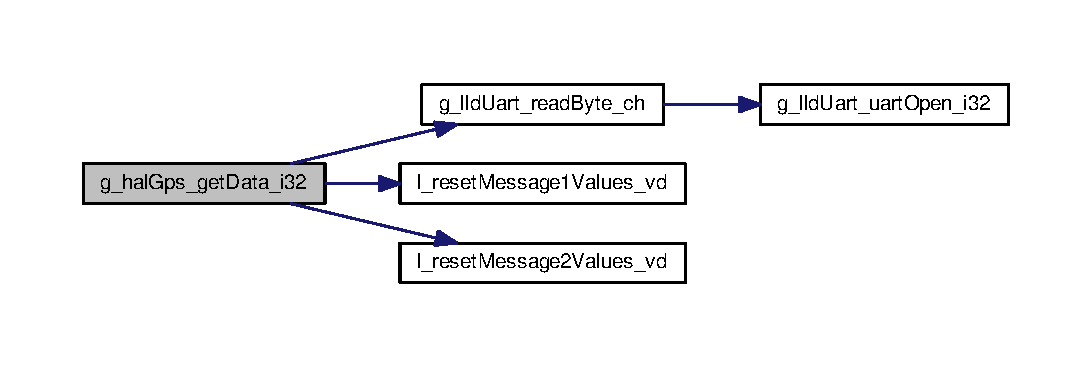
\includegraphics[width=350pt]{GPS_8c_a35a6a55e7bbec401863a903a3607c0b6_a35a6a55e7bbec401863a903a3607c0b6_cgraph}
\end{center}
\end{figure}


\hypertarget{GPS_8c_aea126d235b1db89dc964f8763565e9dc_aea126d235b1db89dc964f8763565e9dc}{\index{G\+P\+S.\+c@{G\+P\+S.\+c}!g\+\_\+hal\+Gps\+\_\+get\+Date\+\_\+ui32@{g\+\_\+hal\+Gps\+\_\+get\+Date\+\_\+ui32}}
\index{g\+\_\+hal\+Gps\+\_\+get\+Date\+\_\+ui32@{g\+\_\+hal\+Gps\+\_\+get\+Date\+\_\+ui32}!G\+P\+S.\+c@{G\+P\+S.\+c}}
\subsubsection[{g\+\_\+hal\+Gps\+\_\+get\+Date\+\_\+ui32}]{\setlength{\rightskip}{0pt plus 5cm}unsigned int g\+\_\+hal\+Gps\+\_\+get\+Date\+\_\+ui32 (
\begin{DoxyParamCaption}
\item[{void}]{}
\end{DoxyParamCaption}
)}}\label{GPS_8c_aea126d235b1db89dc964f8763565e9dc_aea126d235b1db89dc964f8763565e9dc}


Get Date from G\+P\+S module. 



 \begin{DoxyAuthor}{Author}
Oliver Breuning ( olbrgs00 ) 
\end{DoxyAuthor}
\begin{DoxyDate}{Date}
2015/04/18
\end{DoxyDate}
Interface of reading the Date which is received by the G\+P\+S module. This value is based on G\+M\+T.


\begin{DoxyParams}[1]{Parameters}
\mbox{\tt in}  & {\em no} & parameter \\
\hline
\mbox{\tt out}  & {\em Date} & of G\+P\+S receiver\\
\hline
\end{DoxyParams}


Definition at line 178 of file G\+P\+S.\+c.


\begin{DoxyCode}
179 \{
180     \textcolor{keywordflow}{return} \hyperlink{GPS_8c_a1b5b44afa58c22d0b8bb4ddedeefb31c_a1b5b44afa58c22d0b8bb4ddedeefb31c}{l\_date\_ui32};
181 \}
\end{DoxyCode}
\hypertarget{GPS_8c_adac1759b450b418dc6030def1d73b8a7_adac1759b450b418dc6030def1d73b8a7}{\index{G\+P\+S.\+c@{G\+P\+S.\+c}!g\+\_\+hal\+Gps\+\_\+get\+Direction\+\_\+f64@{g\+\_\+hal\+Gps\+\_\+get\+Direction\+\_\+f64}}
\index{g\+\_\+hal\+Gps\+\_\+get\+Direction\+\_\+f64@{g\+\_\+hal\+Gps\+\_\+get\+Direction\+\_\+f64}!G\+P\+S.\+c@{G\+P\+S.\+c}}
\subsubsection[{g\+\_\+hal\+Gps\+\_\+get\+Direction\+\_\+f64}]{\setlength{\rightskip}{0pt plus 5cm}double g\+\_\+hal\+Gps\+\_\+get\+Direction\+\_\+f64 (
\begin{DoxyParamCaption}
\item[{void}]{}
\end{DoxyParamCaption}
)}}\label{GPS_8c_adac1759b450b418dc6030def1d73b8a7_adac1759b450b418dc6030def1d73b8a7}


Get Direction from G\+P\+S module. 



 \begin{DoxyAuthor}{Author}
Oliver Breuning ( olbrgs00 ) 
\end{DoxyAuthor}
\begin{DoxyDate}{Date}
2015/04/18
\end{DoxyDate}
Interface of reading the direction of move which is calculated by the G\+P\+S module. So the Receiver moves with a velocity in the direction which is accessible here.


\begin{DoxyParams}[1]{Parameters}
\mbox{\tt in}  & {\em no} & parameter \\
\hline
\mbox{\tt out}  & {\em Direction} & of G\+P\+S receiver\\
\hline
\end{DoxyParams}


Definition at line 157 of file G\+P\+S.\+c.


\begin{DoxyCode}
158 \{
159     \textcolor{keywordflow}{return} \hyperlink{GPS_8c_a1e038699dda8c22ded8f25762733bfaf_a1e038699dda8c22ded8f25762733bfaf}{l\_direction\_f64};
160 \}
\end{DoxyCode}
\hypertarget{GPS_8c_a4f6b3f1d68b421a3a60b281326b4141b_a4f6b3f1d68b421a3a60b281326b4141b}{\index{G\+P\+S.\+c@{G\+P\+S.\+c}!g\+\_\+hal\+Gps\+\_\+get\+Fix\+\_\+ch@{g\+\_\+hal\+Gps\+\_\+get\+Fix\+\_\+ch}}
\index{g\+\_\+hal\+Gps\+\_\+get\+Fix\+\_\+ch@{g\+\_\+hal\+Gps\+\_\+get\+Fix\+\_\+ch}!G\+P\+S.\+c@{G\+P\+S.\+c}}
\subsubsection[{g\+\_\+hal\+Gps\+\_\+get\+Fix\+\_\+ch}]{\setlength{\rightskip}{0pt plus 5cm}char g\+\_\+hal\+Gps\+\_\+get\+Fix\+\_\+ch (
\begin{DoxyParamCaption}
\item[{void}]{}
\end{DoxyParamCaption}
)}}\label{GPS_8c_a4f6b3f1d68b421a3a60b281326b4141b_a4f6b3f1d68b421a3a60b281326b4141b}


Get Fix from G\+P\+S module. 



 \begin{DoxyAuthor}{Author}
Oliver Breuning ( olbrgs00 ) 
\end{DoxyAuthor}
\begin{DoxyDate}{Date}
2015/04/18
\end{DoxyDate}
Interface of reading if the G\+P\+S module has a Fix. This means it has good signal


\begin{DoxyParams}[1]{Parameters}
\mbox{\tt in}  & {\em no} & parameter \\
\hline
\mbox{\tt out}  & {\em Fix} & of G\+P\+S receiver\\
\hline
\end{DoxyParams}


Definition at line 115 of file G\+P\+S.\+c.


\begin{DoxyCode}
116 \{
117     \textcolor{keywordflow}{return} \hyperlink{GPS_8c_a5a14aebdd5ac0d06913bdeaf9cec1a9b_a5a14aebdd5ac0d06913bdeaf9cec1a9b}{l\_fix\_ch};
118 \}
\end{DoxyCode}
\hypertarget{GPS_8c_a0190aaa631556af032a2d286ebf6525a_a0190aaa631556af032a2d286ebf6525a}{\index{G\+P\+S.\+c@{G\+P\+S.\+c}!g\+\_\+hal\+Gps\+\_\+get\+Geoid\+\_\+f64@{g\+\_\+hal\+Gps\+\_\+get\+Geoid\+\_\+f64}}
\index{g\+\_\+hal\+Gps\+\_\+get\+Geoid\+\_\+f64@{g\+\_\+hal\+Gps\+\_\+get\+Geoid\+\_\+f64}!G\+P\+S.\+c@{G\+P\+S.\+c}}
\subsubsection[{g\+\_\+hal\+Gps\+\_\+get\+Geoid\+\_\+f64}]{\setlength{\rightskip}{0pt plus 5cm}double g\+\_\+hal\+Gps\+\_\+get\+Geoid\+\_\+f64 (
\begin{DoxyParamCaption}
\item[{void}]{}
\end{DoxyParamCaption}
)}}\label{GPS_8c_a0190aaa631556af032a2d286ebf6525a_a0190aaa631556af032a2d286ebf6525a}


Get Geoid from G\+P\+S module. 



 \begin{DoxyAuthor}{Author}
Oliver Breuning ( olbrgs00 ) 
\end{DoxyAuthor}
\begin{DoxyDate}{Date}
2015/04/18
\end{DoxyDate}
Interface of reading the Geoid which is received by the G\+P\+S module.


\begin{DoxyParams}[1]{Parameters}
\mbox{\tt in}  & {\em no} & parameter \\
\hline
\mbox{\tt out}  & {\em Geoid} & of G\+P\+S receiver\\
\hline
\end{DoxyParams}


Definition at line 218 of file G\+P\+S.\+c.


\begin{DoxyCode}
219 \{
220     \textcolor{keywordflow}{return} \hyperlink{GPS_8c_a2cc033719fe30335f2423a4afbe53984_a2cc033719fe30335f2423a4afbe53984}{l\_geoid\_f64};
221 \}
\end{DoxyCode}
\hypertarget{GPS_8c_ad797f33853c6d3e6f2e863c11c2822b8_ad797f33853c6d3e6f2e863c11c2822b8}{\index{G\+P\+S.\+c@{G\+P\+S.\+c}!g\+\_\+hal\+Gps\+\_\+get\+Height\+\_\+f64@{g\+\_\+hal\+Gps\+\_\+get\+Height\+\_\+f64}}
\index{g\+\_\+hal\+Gps\+\_\+get\+Height\+\_\+f64@{g\+\_\+hal\+Gps\+\_\+get\+Height\+\_\+f64}!G\+P\+S.\+c@{G\+P\+S.\+c}}
\subsubsection[{g\+\_\+hal\+Gps\+\_\+get\+Height\+\_\+f64}]{\setlength{\rightskip}{0pt plus 5cm}double g\+\_\+hal\+Gps\+\_\+get\+Height\+\_\+f64 (
\begin{DoxyParamCaption}
\item[{void}]{}
\end{DoxyParamCaption}
)}}\label{GPS_8c_ad797f33853c6d3e6f2e863c11c2822b8_ad797f33853c6d3e6f2e863c11c2822b8}


Get Height from G\+P\+S module. 



 \begin{DoxyAuthor}{Author}
Oliver Breuning ( olbrgs00 ) 
\end{DoxyAuthor}
\begin{DoxyDate}{Date}
2015/04/18
\end{DoxyDate}
Interface of reading the Height which is calculated by the G\+P\+S module.


\begin{DoxyParams}[1]{Parameters}
\mbox{\tt in}  & {\em no} & parameter \\
\hline
\mbox{\tt out}  & {\em Height} & of G\+P\+S receiver\\
\hline
\end{DoxyParams}


Definition at line 198 of file G\+P\+S.\+c.


\begin{DoxyCode}
199 \{
200     \textcolor{keywordflow}{return} \hyperlink{GPS_8c_a36e46365d7b41cc255fee53e0aa4b70a_a36e46365d7b41cc255fee53e0aa4b70a}{l\_height\_f64};
201 \}
\end{DoxyCode}
\hypertarget{GPS_8c_a0fa256f0b23aa1d53a0bf5892589dc9f_a0fa256f0b23aa1d53a0bf5892589dc9f}{\index{G\+P\+S.\+c@{G\+P\+S.\+c}!g\+\_\+hal\+Gps\+\_\+get\+Latitude\+\_\+st@{g\+\_\+hal\+Gps\+\_\+get\+Latitude\+\_\+st}}
\index{g\+\_\+hal\+Gps\+\_\+get\+Latitude\+\_\+st@{g\+\_\+hal\+Gps\+\_\+get\+Latitude\+\_\+st}!G\+P\+S.\+c@{G\+P\+S.\+c}}
\subsubsection[{g\+\_\+hal\+Gps\+\_\+get\+Latitude\+\_\+st}]{\setlength{\rightskip}{0pt plus 5cm}struct {\bf str\+Position} g\+\_\+hal\+Gps\+\_\+get\+Latitude\+\_\+st (
\begin{DoxyParamCaption}
\item[{void}]{}
\end{DoxyParamCaption}
)}}\label{GPS_8c_a0fa256f0b23aa1d53a0bf5892589dc9f_a0fa256f0b23aa1d53a0bf5892589dc9f}


Get Latitude from G\+P\+S module. 



 \begin{DoxyAuthor}{Author}
Oliver Breuning ( olbrgs00 ) 
\end{DoxyAuthor}
\begin{DoxyDate}{Date}
2015/04/18
\end{DoxyDate}
Interface of reading struct Latitude which is received by the G\+P\+S module


\begin{DoxyParams}[1]{Parameters}
\mbox{\tt in}  & {\em no} & parameter \\
\hline
\mbox{\tt out}  & {\em Latitude} & of G\+P\+S receiver\\
\hline
\end{DoxyParams}


Definition at line 94 of file G\+P\+S.\+c.


\begin{DoxyCode}
95 \{
96     \textcolor{keywordflow}{return} \hyperlink{GPS_8c_ae764c82d3318068e28af258ae1e2449c_ae764c82d3318068e28af258ae1e2449c}{l\_gps\_latitude\_st};
97 \}
\end{DoxyCode}
\hypertarget{GPS_8c_a7ee6cdd9714c51a2b74e5f3cdc2a5dca_a7ee6cdd9714c51a2b74e5f3cdc2a5dca}{\index{G\+P\+S.\+c@{G\+P\+S.\+c}!g\+\_\+hal\+Gps\+\_\+get\+Longitude\+\_\+st@{g\+\_\+hal\+Gps\+\_\+get\+Longitude\+\_\+st}}
\index{g\+\_\+hal\+Gps\+\_\+get\+Longitude\+\_\+st@{g\+\_\+hal\+Gps\+\_\+get\+Longitude\+\_\+st}!G\+P\+S.\+c@{G\+P\+S.\+c}}
\subsubsection[{g\+\_\+hal\+Gps\+\_\+get\+Longitude\+\_\+st}]{\setlength{\rightskip}{0pt plus 5cm}struct {\bf str\+Position} g\+\_\+hal\+Gps\+\_\+get\+Longitude\+\_\+st (
\begin{DoxyParamCaption}
\item[{void}]{}
\end{DoxyParamCaption}
)}}\label{GPS_8c_a7ee6cdd9714c51a2b74e5f3cdc2a5dca_a7ee6cdd9714c51a2b74e5f3cdc2a5dca}


Get Longitude from G\+P\+S module. 



 \begin{DoxyAuthor}{Author}
Oliver Breuning ( olbrgs00 ) 
\end{DoxyAuthor}
\begin{DoxyDate}{Date}
2015/04/18
\end{DoxyDate}
Interface of reading struct Longitude which is received by the G\+P\+S module


\begin{DoxyParams}[1]{Parameters}
\mbox{\tt in}  & {\em no} & parameter \\
\hline
\mbox{\tt out}  & {\em Longitude} & of G\+P\+S receiver\\
\hline
\end{DoxyParams}


Definition at line 73 of file G\+P\+S.\+c.


\begin{DoxyCode}
74 \{
75     \textcolor{keywordflow}{return} \hyperlink{GPS_8c_a5661901a87ce3f7dcd2eba20d8b505b4_a5661901a87ce3f7dcd2eba20d8b505b4}{l\_gps\_longitude\_st};
76 \}
\end{DoxyCode}
\hypertarget{GPS_8c_a64a3ef5cadfa081ca967b201352e2f8d_a64a3ef5cadfa081ca967b201352e2f8d}{\index{G\+P\+S.\+c@{G\+P\+S.\+c}!g\+\_\+hal\+Gps\+\_\+get\+Time\+\_\+ui32@{g\+\_\+hal\+Gps\+\_\+get\+Time\+\_\+ui32}}
\index{g\+\_\+hal\+Gps\+\_\+get\+Time\+\_\+ui32@{g\+\_\+hal\+Gps\+\_\+get\+Time\+\_\+ui32}!G\+P\+S.\+c@{G\+P\+S.\+c}}
\subsubsection[{g\+\_\+hal\+Gps\+\_\+get\+Time\+\_\+ui32}]{\setlength{\rightskip}{0pt plus 5cm}unsigned int g\+\_\+hal\+Gps\+\_\+get\+Time\+\_\+ui32 (
\begin{DoxyParamCaption}
\item[{void}]{}
\end{DoxyParamCaption}
)}}\label{GPS_8c_a64a3ef5cadfa081ca967b201352e2f8d_a64a3ef5cadfa081ca967b201352e2f8d}


Get Time from G\+P\+S module. 



 \begin{DoxyAuthor}{Author}
Oliver Breuning ( olbrgs00 ) 
\end{DoxyAuthor}
\begin{DoxyDate}{Date}
2015/04/18
\end{DoxyDate}
Interface of reading Time which is received by the G\+P\+S module. This value is G\+M\+T.


\begin{DoxyParams}[1]{Parameters}
\mbox{\tt in}  & {\em no} & parameter \\
\hline
\mbox{\tt out}  & {\em Time} & of G\+P\+S receiver\\
\hline
\end{DoxyParams}


Definition at line 52 of file G\+P\+S.\+c.


\begin{DoxyCode}
53 \{
54     \textcolor{keywordflow}{return} \hyperlink{GPS_8c_a365efcbf31282dcb274edd608e0824ed_a365efcbf31282dcb274edd608e0824ed}{l\_time\_ui32};
55 \}
\end{DoxyCode}
\hypertarget{GPS_8c_aae3374862ddb32be3a7f40b01661ede0_aae3374862ddb32be3a7f40b01661ede0}{\index{G\+P\+S.\+c@{G\+P\+S.\+c}!g\+\_\+hal\+Gps\+\_\+get\+Velocity\+\_\+f64@{g\+\_\+hal\+Gps\+\_\+get\+Velocity\+\_\+f64}}
\index{g\+\_\+hal\+Gps\+\_\+get\+Velocity\+\_\+f64@{g\+\_\+hal\+Gps\+\_\+get\+Velocity\+\_\+f64}!G\+P\+S.\+c@{G\+P\+S.\+c}}
\subsubsection[{g\+\_\+hal\+Gps\+\_\+get\+Velocity\+\_\+f64}]{\setlength{\rightskip}{0pt plus 5cm}double g\+\_\+hal\+Gps\+\_\+get\+Velocity\+\_\+f64 (
\begin{DoxyParamCaption}
\item[{void}]{}
\end{DoxyParamCaption}
)}}\label{GPS_8c_aae3374862ddb32be3a7f40b01661ede0_aae3374862ddb32be3a7f40b01661ede0}


Get Velocity from G\+P\+S module. 



 \begin{DoxyAuthor}{Author}
Oliver Breuning ( olbrgs00 ) 
\end{DoxyAuthor}
\begin{DoxyDate}{Date}
2015/04/18
\end{DoxyDate}
Interface of reading the velocity which is calculated by the G\+P\+S module. So the Receiver moves with a velocity which is accessible here in a certain direction.


\begin{DoxyParams}[1]{Parameters}
\mbox{\tt in}  & {\em no} & parameter \\
\hline
\mbox{\tt out}  & {\em Velocity} & of G\+P\+S receiver\\
\hline
\end{DoxyParams}


Definition at line 136 of file G\+P\+S.\+c.


\begin{DoxyCode}
137 \{
138     \textcolor{keywordflow}{return} \hyperlink{GPS_8c_af14216f61e92eb4cb399d157299c8d12_af14216f61e92eb4cb399d157299c8d12}{l\_velocity\_f64};
139 \}
\end{DoxyCode}
\hypertarget{GPS_8c_a0bf6b6abfd6136e50bd5d35a76ee8d0b_a0bf6b6abfd6136e50bd5d35a76ee8d0b}{\index{G\+P\+S.\+c@{G\+P\+S.\+c}!l\+\_\+reset\+Message1\+Values\+\_\+vd@{l\+\_\+reset\+Message1\+Values\+\_\+vd}}
\index{l\+\_\+reset\+Message1\+Values\+\_\+vd@{l\+\_\+reset\+Message1\+Values\+\_\+vd}!G\+P\+S.\+c@{G\+P\+S.\+c}}
\subsubsection[{l\+\_\+reset\+Message1\+Values\+\_\+vd}]{\setlength{\rightskip}{0pt plus 5cm}void l\+\_\+reset\+Message1\+Values\+\_\+vd (
\begin{DoxyParamCaption}
\item[{void}]{}
\end{DoxyParamCaption}
)}}\label{GPS_8c_a0bf6b6abfd6136e50bd5d35a76ee8d0b_a0bf6b6abfd6136e50bd5d35a76ee8d0b}


Reset Values of Message 1. 



 \begin{DoxyAuthor}{Author}
Oliver Breuning ( olbrgs00 ) 
\end{DoxyAuthor}
\begin{DoxyDate}{Date}
2015/04/21
\end{DoxyDate}
Resetting the values of Message 1 -\/ \$\+G\+P\+G\+G\+A .... when a new message arrives


\begin{DoxyParams}[1]{Parameters}
\mbox{\tt in}  & {\em no} & parameter \\
\hline
\mbox{\tt out}  & {\em no} & parameter\\
\hline
\end{DoxyParams}


Definition at line 238 of file G\+P\+S.\+c.


\begin{DoxyCode}
239 \{
240     \hyperlink{GPS_8c_a365efcbf31282dcb274edd608e0824ed_a365efcbf31282dcb274edd608e0824ed}{l\_time\_ui32}=0;
241     \hyperlink{GPS_8c_a5661901a87ce3f7dcd2eba20d8b505b4_a5661901a87ce3f7dcd2eba20d8b505b4}{l\_gps\_longitude\_st}.\hyperlink{structstrPosition_ac060af7d7963812c116c24cdb861f184_ac060af7d7963812c116c24cdb861f184}{l\_degree\_ui32}=0;
242     \hyperlink{GPS_8c_a5661901a87ce3f7dcd2eba20d8b505b4_a5661901a87ce3f7dcd2eba20d8b505b4}{l\_gps\_longitude\_st}.\hyperlink{structstrPosition_a5489ef5e7f8e6ee45990b262c80a7819_a5489ef5e7f8e6ee45990b262c80a7819}{l\_minutes\_ui32}=0;
243     \hyperlink{GPS_8c_a5661901a87ce3f7dcd2eba20d8b505b4_a5661901a87ce3f7dcd2eba20d8b505b4}{l\_gps\_longitude\_st}.\hyperlink{structstrPosition_ae62d246c481c611e168ea86b70d5313b_ae62d246c481c611e168ea86b70d5313b}{l\_seconds\_f64}=0;
244     \hyperlink{GPS_8c_a5661901a87ce3f7dcd2eba20d8b505b4_a5661901a87ce3f7dcd2eba20d8b505b4}{l\_gps\_longitude\_st}.\hyperlink{structstrPosition_aa39fed1d421cb2260d0ef7157c3c00d0_aa39fed1d421cb2260d0ef7157c3c00d0}{l\_cardinalDirection\_ch}=\textcolor{charliteral}{' '};
245     \hyperlink{GPS_8c_ae764c82d3318068e28af258ae1e2449c_ae764c82d3318068e28af258ae1e2449c}{l\_gps\_latitude\_st}.\hyperlink{structstrPosition_ac060af7d7963812c116c24cdb861f184_ac060af7d7963812c116c24cdb861f184}{l\_degree\_ui32}=0;
246     \hyperlink{GPS_8c_ae764c82d3318068e28af258ae1e2449c_ae764c82d3318068e28af258ae1e2449c}{l\_gps\_latitude\_st}.\hyperlink{structstrPosition_a5489ef5e7f8e6ee45990b262c80a7819_a5489ef5e7f8e6ee45990b262c80a7819}{l\_minutes\_ui32}=0;
247     \hyperlink{GPS_8c_ae764c82d3318068e28af258ae1e2449c_ae764c82d3318068e28af258ae1e2449c}{l\_gps\_latitude\_st}.\hyperlink{structstrPosition_ae62d246c481c611e168ea86b70d5313b_ae62d246c481c611e168ea86b70d5313b}{l\_seconds\_f64}=0;
248     \hyperlink{GPS_8c_ae764c82d3318068e28af258ae1e2449c_ae764c82d3318068e28af258ae1e2449c}{l\_gps\_latitude\_st}.\hyperlink{structstrPosition_aa39fed1d421cb2260d0ef7157c3c00d0_aa39fed1d421cb2260d0ef7157c3c00d0}{l\_cardinalDirection\_ch}=\textcolor{charliteral}{' '};
249     \hyperlink{GPS_8c_a36e46365d7b41cc255fee53e0aa4b70a_a36e46365d7b41cc255fee53e0aa4b70a}{l\_height\_f64}=0;
250     \hyperlink{GPS_8c_a2cc033719fe30335f2423a4afbe53984_a2cc033719fe30335f2423a4afbe53984}{l\_geoid\_f64}=0;
251 \}
\end{DoxyCode}


Here is the caller graph for this function\+:
\nopagebreak
\begin{figure}[H]
\begin{center}
\leavevmode
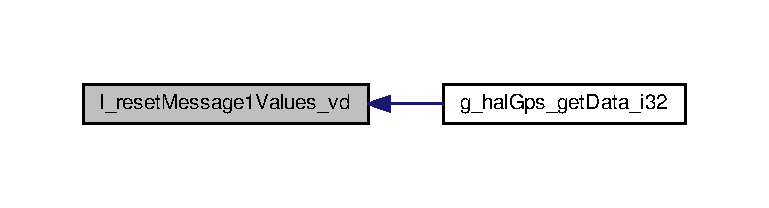
\includegraphics[width=350pt]{GPS_8c_a0bf6b6abfd6136e50bd5d35a76ee8d0b_a0bf6b6abfd6136e50bd5d35a76ee8d0b_icgraph}
\end{center}
\end{figure}


\hypertarget{GPS_8c_aa9c4ab6055264c0121813e5233cd3de0_aa9c4ab6055264c0121813e5233cd3de0}{\index{G\+P\+S.\+c@{G\+P\+S.\+c}!l\+\_\+reset\+Message2\+Values\+\_\+vd@{l\+\_\+reset\+Message2\+Values\+\_\+vd}}
\index{l\+\_\+reset\+Message2\+Values\+\_\+vd@{l\+\_\+reset\+Message2\+Values\+\_\+vd}!G\+P\+S.\+c@{G\+P\+S.\+c}}
\subsubsection[{l\+\_\+reset\+Message2\+Values\+\_\+vd}]{\setlength{\rightskip}{0pt plus 5cm}void l\+\_\+reset\+Message2\+Values\+\_\+vd (
\begin{DoxyParamCaption}
\item[{void}]{}
\end{DoxyParamCaption}
)}}\label{GPS_8c_aa9c4ab6055264c0121813e5233cd3de0_aa9c4ab6055264c0121813e5233cd3de0}


Reset Values of Message 2. 



 \begin{DoxyAuthor}{Author}
Oliver Breuning ( olbrgs00 ) 
\end{DoxyAuthor}
\begin{DoxyDate}{Date}
2015/04/21
\end{DoxyDate}
Resetting the values of Message 2 -\/ \$\+G\+P\+R\+M\+C .... when a new message arrives


\begin{DoxyParams}[1]{Parameters}
\mbox{\tt in}  & {\em no} & parameter \\
\hline
\mbox{\tt out}  & {\em no} & parameter\\
\hline
\end{DoxyParams}


Definition at line 268 of file G\+P\+S.\+c.


\begin{DoxyCode}
269 \{
270     \hyperlink{GPS_8c_a365efcbf31282dcb274edd608e0824ed_a365efcbf31282dcb274edd608e0824ed}{l\_time\_ui32}=0;
271     \hyperlink{GPS_8c_a5a14aebdd5ac0d06913bdeaf9cec1a9b_a5a14aebdd5ac0d06913bdeaf9cec1a9b}{l\_fix\_ch}=\textcolor{charliteral}{' '};
272     \hyperlink{GPS_8c_a5661901a87ce3f7dcd2eba20d8b505b4_a5661901a87ce3f7dcd2eba20d8b505b4}{l\_gps\_longitude\_st}.\hyperlink{structstrPosition_ac060af7d7963812c116c24cdb861f184_ac060af7d7963812c116c24cdb861f184}{l\_degree\_ui32}=0;
273     \hyperlink{GPS_8c_a5661901a87ce3f7dcd2eba20d8b505b4_a5661901a87ce3f7dcd2eba20d8b505b4}{l\_gps\_longitude\_st}.\hyperlink{structstrPosition_a5489ef5e7f8e6ee45990b262c80a7819_a5489ef5e7f8e6ee45990b262c80a7819}{l\_minutes\_ui32}=0;
274     \hyperlink{GPS_8c_a5661901a87ce3f7dcd2eba20d8b505b4_a5661901a87ce3f7dcd2eba20d8b505b4}{l\_gps\_longitude\_st}.\hyperlink{structstrPosition_ae62d246c481c611e168ea86b70d5313b_ae62d246c481c611e168ea86b70d5313b}{l\_seconds\_f64}=0;
275     \hyperlink{GPS_8c_a5661901a87ce3f7dcd2eba20d8b505b4_a5661901a87ce3f7dcd2eba20d8b505b4}{l\_gps\_longitude\_st}.\hyperlink{structstrPosition_aa39fed1d421cb2260d0ef7157c3c00d0_aa39fed1d421cb2260d0ef7157c3c00d0}{l\_cardinalDirection\_ch}=\textcolor{charliteral}{' '};
276     \hyperlink{GPS_8c_ae764c82d3318068e28af258ae1e2449c_ae764c82d3318068e28af258ae1e2449c}{l\_gps\_latitude\_st}.\hyperlink{structstrPosition_ac060af7d7963812c116c24cdb861f184_ac060af7d7963812c116c24cdb861f184}{l\_degree\_ui32}=0;
277     \hyperlink{GPS_8c_ae764c82d3318068e28af258ae1e2449c_ae764c82d3318068e28af258ae1e2449c}{l\_gps\_latitude\_st}.\hyperlink{structstrPosition_a5489ef5e7f8e6ee45990b262c80a7819_a5489ef5e7f8e6ee45990b262c80a7819}{l\_minutes\_ui32}=0;
278     \hyperlink{GPS_8c_ae764c82d3318068e28af258ae1e2449c_ae764c82d3318068e28af258ae1e2449c}{l\_gps\_latitude\_st}.\hyperlink{structstrPosition_ae62d246c481c611e168ea86b70d5313b_ae62d246c481c611e168ea86b70d5313b}{l\_seconds\_f64}=0;
279     \hyperlink{GPS_8c_ae764c82d3318068e28af258ae1e2449c_ae764c82d3318068e28af258ae1e2449c}{l\_gps\_latitude\_st}.\hyperlink{structstrPosition_aa39fed1d421cb2260d0ef7157c3c00d0_aa39fed1d421cb2260d0ef7157c3c00d0}{l\_cardinalDirection\_ch}=\textcolor{charliteral}{' '};
280     \hyperlink{GPS_8c_af14216f61e92eb4cb399d157299c8d12_af14216f61e92eb4cb399d157299c8d12}{l\_velocity\_f64}=0;
281     \hyperlink{GPS_8c_a1e038699dda8c22ded8f25762733bfaf_a1e038699dda8c22ded8f25762733bfaf}{l\_direction\_f64}=0;
282     \hyperlink{GPS_8c_a1b5b44afa58c22d0b8bb4ddedeefb31c_a1b5b44afa58c22d0b8bb4ddedeefb31c}{l\_date\_ui32}=0;
283 \}
\end{DoxyCode}


Here is the caller graph for this function\+:
\nopagebreak
\begin{figure}[H]
\begin{center}
\leavevmode
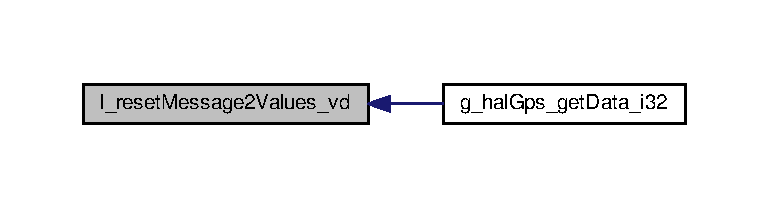
\includegraphics[width=350pt]{GPS_8c_aa9c4ab6055264c0121813e5233cd3de0_aa9c4ab6055264c0121813e5233cd3de0_icgraph}
\end{center}
\end{figure}




\subsection{Variable Documentation}
\hypertarget{GPS_8c_a574dd5cd13fbeac386e435e932e20bae_a574dd5cd13fbeac386e435e932e20bae}{\index{G\+P\+S.\+c@{G\+P\+S.\+c}!l\+\_\+data\+\_\+position\+\_\+ch@{l\+\_\+data\+\_\+position\+\_\+ch}}
\index{l\+\_\+data\+\_\+position\+\_\+ch@{l\+\_\+data\+\_\+position\+\_\+ch}!G\+P\+S.\+c@{G\+P\+S.\+c}}
\subsubsection[{l\+\_\+data\+\_\+position\+\_\+ch}]{\setlength{\rightskip}{0pt plus 5cm}char l\+\_\+data\+\_\+position\+\_\+ch =0\hspace{0.3cm}{\ttfamily [static]}}}\label{GPS_8c_a574dd5cd13fbeac386e435e932e20bae_a574dd5cd13fbeac386e435e932e20bae}


Definition at line 29 of file G\+P\+S.\+c.

\hypertarget{GPS_8c_a1b5b44afa58c22d0b8bb4ddedeefb31c_a1b5b44afa58c22d0b8bb4ddedeefb31c}{\index{G\+P\+S.\+c@{G\+P\+S.\+c}!l\+\_\+date\+\_\+ui32@{l\+\_\+date\+\_\+ui32}}
\index{l\+\_\+date\+\_\+ui32@{l\+\_\+date\+\_\+ui32}!G\+P\+S.\+c@{G\+P\+S.\+c}}
\subsubsection[{l\+\_\+date\+\_\+ui32}]{\setlength{\rightskip}{0pt plus 5cm}unsigned int l\+\_\+date\+\_\+ui32\hspace{0.3cm}{\ttfamily [static]}}}\label{GPS_8c_a1b5b44afa58c22d0b8bb4ddedeefb31c_a1b5b44afa58c22d0b8bb4ddedeefb31c}


Definition at line 21 of file G\+P\+S.\+c.

\hypertarget{GPS_8c_ad5b924e752a1a8222bd65c4291d3e82e_ad5b924e752a1a8222bd65c4291d3e82e}{\index{G\+P\+S.\+c@{G\+P\+S.\+c}!l\+\_\+decimal\+\_\+place\+\_\+factor\+\_\+i32@{l\+\_\+decimal\+\_\+place\+\_\+factor\+\_\+i32}}
\index{l\+\_\+decimal\+\_\+place\+\_\+factor\+\_\+i32@{l\+\_\+decimal\+\_\+place\+\_\+factor\+\_\+i32}!G\+P\+S.\+c@{G\+P\+S.\+c}}
\subsubsection[{l\+\_\+decimal\+\_\+place\+\_\+factor\+\_\+i32}]{\setlength{\rightskip}{0pt plus 5cm}int l\+\_\+decimal\+\_\+place\+\_\+factor\+\_\+i32 =10\hspace{0.3cm}{\ttfamily [static]}}}\label{GPS_8c_ad5b924e752a1a8222bd65c4291d3e82e_ad5b924e752a1a8222bd65c4291d3e82e}


Definition at line 32 of file G\+P\+S.\+c.

\hypertarget{GPS_8c_a1e038699dda8c22ded8f25762733bfaf_a1e038699dda8c22ded8f25762733bfaf}{\index{G\+P\+S.\+c@{G\+P\+S.\+c}!l\+\_\+direction\+\_\+f64@{l\+\_\+direction\+\_\+f64}}
\index{l\+\_\+direction\+\_\+f64@{l\+\_\+direction\+\_\+f64}!G\+P\+S.\+c@{G\+P\+S.\+c}}
\subsubsection[{l\+\_\+direction\+\_\+f64}]{\setlength{\rightskip}{0pt plus 5cm}double l\+\_\+direction\+\_\+f64\hspace{0.3cm}{\ttfamily [static]}}}\label{GPS_8c_a1e038699dda8c22ded8f25762733bfaf_a1e038699dda8c22ded8f25762733bfaf}


Definition at line 20 of file G\+P\+S.\+c.

\hypertarget{GPS_8c_a93cee4751b6fb1410e727f045329f326_a93cee4751b6fb1410e727f045329f326}{\index{G\+P\+S.\+c@{G\+P\+S.\+c}!l\+\_\+fieldpointer\+\_\+i32@{l\+\_\+fieldpointer\+\_\+i32}}
\index{l\+\_\+fieldpointer\+\_\+i32@{l\+\_\+fieldpointer\+\_\+i32}!G\+P\+S.\+c@{G\+P\+S.\+c}}
\subsubsection[{l\+\_\+fieldpointer\+\_\+i32}]{\setlength{\rightskip}{0pt plus 5cm}int l\+\_\+fieldpointer\+\_\+i32 =0\hspace{0.3cm}{\ttfamily [static]}}}\label{GPS_8c_a93cee4751b6fb1410e727f045329f326_a93cee4751b6fb1410e727f045329f326}


Definition at line 31 of file G\+P\+S.\+c.

\hypertarget{GPS_8c_a5a14aebdd5ac0d06913bdeaf9cec1a9b_a5a14aebdd5ac0d06913bdeaf9cec1a9b}{\index{G\+P\+S.\+c@{G\+P\+S.\+c}!l\+\_\+fix\+\_\+ch@{l\+\_\+fix\+\_\+ch}}
\index{l\+\_\+fix\+\_\+ch@{l\+\_\+fix\+\_\+ch}!G\+P\+S.\+c@{G\+P\+S.\+c}}
\subsubsection[{l\+\_\+fix\+\_\+ch}]{\setlength{\rightskip}{0pt plus 5cm}char l\+\_\+fix\+\_\+ch\hspace{0.3cm}{\ttfamily [static]}}}\label{GPS_8c_a5a14aebdd5ac0d06913bdeaf9cec1a9b_a5a14aebdd5ac0d06913bdeaf9cec1a9b}


Definition at line 18 of file G\+P\+S.\+c.

\hypertarget{GPS_8c_a2cc033719fe30335f2423a4afbe53984_a2cc033719fe30335f2423a4afbe53984}{\index{G\+P\+S.\+c@{G\+P\+S.\+c}!l\+\_\+geoid\+\_\+f64@{l\+\_\+geoid\+\_\+f64}}
\index{l\+\_\+geoid\+\_\+f64@{l\+\_\+geoid\+\_\+f64}!G\+P\+S.\+c@{G\+P\+S.\+c}}
\subsubsection[{l\+\_\+geoid\+\_\+f64}]{\setlength{\rightskip}{0pt plus 5cm}double l\+\_\+geoid\+\_\+f64\hspace{0.3cm}{\ttfamily [static]}}}\label{GPS_8c_a2cc033719fe30335f2423a4afbe53984_a2cc033719fe30335f2423a4afbe53984}


Definition at line 23 of file G\+P\+S.\+c.

\hypertarget{GPS_8c_ae764c82d3318068e28af258ae1e2449c_ae764c82d3318068e28af258ae1e2449c}{\index{G\+P\+S.\+c@{G\+P\+S.\+c}!l\+\_\+gps\+\_\+latitude\+\_\+st@{l\+\_\+gps\+\_\+latitude\+\_\+st}}
\index{l\+\_\+gps\+\_\+latitude\+\_\+st@{l\+\_\+gps\+\_\+latitude\+\_\+st}!G\+P\+S.\+c@{G\+P\+S.\+c}}
\subsubsection[{l\+\_\+gps\+\_\+latitude\+\_\+st}]{\setlength{\rightskip}{0pt plus 5cm}struct {\bf str\+Position} l\+\_\+gps\+\_\+latitude\+\_\+st\hspace{0.3cm}{\ttfamily [static]}}}\label{GPS_8c_ae764c82d3318068e28af258ae1e2449c_ae764c82d3318068e28af258ae1e2449c}


Definition at line 16 of file G\+P\+S.\+c.

\hypertarget{GPS_8c_a5661901a87ce3f7dcd2eba20d8b505b4_a5661901a87ce3f7dcd2eba20d8b505b4}{\index{G\+P\+S.\+c@{G\+P\+S.\+c}!l\+\_\+gps\+\_\+longitude\+\_\+st@{l\+\_\+gps\+\_\+longitude\+\_\+st}}
\index{l\+\_\+gps\+\_\+longitude\+\_\+st@{l\+\_\+gps\+\_\+longitude\+\_\+st}!G\+P\+S.\+c@{G\+P\+S.\+c}}
\subsubsection[{l\+\_\+gps\+\_\+longitude\+\_\+st}]{\setlength{\rightskip}{0pt plus 5cm}struct {\bf str\+Position} l\+\_\+gps\+\_\+longitude\+\_\+st\hspace{0.3cm}{\ttfamily [static]}}}\label{GPS_8c_a5661901a87ce3f7dcd2eba20d8b505b4_a5661901a87ce3f7dcd2eba20d8b505b4}


Definition at line 15 of file G\+P\+S.\+c.

\hypertarget{GPS_8c_ac9b483bef981b820a4f6ffaf11ee37a2_ac9b483bef981b820a4f6ffaf11ee37a2}{\index{G\+P\+S.\+c@{G\+P\+S.\+c}!l\+\_\+header\+\_\+position\+\_\+ch@{l\+\_\+header\+\_\+position\+\_\+ch}}
\index{l\+\_\+header\+\_\+position\+\_\+ch@{l\+\_\+header\+\_\+position\+\_\+ch}!G\+P\+S.\+c@{G\+P\+S.\+c}}
\subsubsection[{l\+\_\+header\+\_\+position\+\_\+ch}]{\setlength{\rightskip}{0pt plus 5cm}char l\+\_\+header\+\_\+position\+\_\+ch =0\hspace{0.3cm}{\ttfamily [static]}}}\label{GPS_8c_ac9b483bef981b820a4f6ffaf11ee37a2_ac9b483bef981b820a4f6ffaf11ee37a2}


Definition at line 27 of file G\+P\+S.\+c.

\hypertarget{GPS_8c_a36e46365d7b41cc255fee53e0aa4b70a_a36e46365d7b41cc255fee53e0aa4b70a}{\index{G\+P\+S.\+c@{G\+P\+S.\+c}!l\+\_\+height\+\_\+f64@{l\+\_\+height\+\_\+f64}}
\index{l\+\_\+height\+\_\+f64@{l\+\_\+height\+\_\+f64}!G\+P\+S.\+c@{G\+P\+S.\+c}}
\subsubsection[{l\+\_\+height\+\_\+f64}]{\setlength{\rightskip}{0pt plus 5cm}double l\+\_\+height\+\_\+f64\hspace{0.3cm}{\ttfamily [static]}}}\label{GPS_8c_a36e46365d7b41cc255fee53e0aa4b70a_a36e46365d7b41cc255fee53e0aa4b70a}


Definition at line 22 of file G\+P\+S.\+c.

\hypertarget{GPS_8c_a4b514c1fd22818c03e87233b61d6eda3_a4b514c1fd22818c03e87233b61d6eda3}{\index{G\+P\+S.\+c@{G\+P\+S.\+c}!l\+\_\+message\+\_\+ch@{l\+\_\+message\+\_\+ch}}
\index{l\+\_\+message\+\_\+ch@{l\+\_\+message\+\_\+ch}!G\+P\+S.\+c@{G\+P\+S.\+c}}
\subsubsection[{l\+\_\+message\+\_\+ch}]{\setlength{\rightskip}{0pt plus 5cm}char l\+\_\+message\+\_\+ch =0\hspace{0.3cm}{\ttfamily [static]}}}\label{GPS_8c_a4b514c1fd22818c03e87233b61d6eda3_a4b514c1fd22818c03e87233b61d6eda3}


Definition at line 28 of file G\+P\+S.\+c.

\hypertarget{GPS_8c_a33348219a5889847ad41d40b9198164a_a33348219a5889847ad41d40b9198164a}{\index{G\+P\+S.\+c@{G\+P\+S.\+c}!l\+\_\+message\+\_\+position\+\_\+ch@{l\+\_\+message\+\_\+position\+\_\+ch}}
\index{l\+\_\+message\+\_\+position\+\_\+ch@{l\+\_\+message\+\_\+position\+\_\+ch}!G\+P\+S.\+c@{G\+P\+S.\+c}}
\subsubsection[{l\+\_\+message\+\_\+position\+\_\+ch}]{\setlength{\rightskip}{0pt plus 5cm}char l\+\_\+message\+\_\+position\+\_\+ch =0\hspace{0.3cm}{\ttfamily [static]}}}\label{GPS_8c_a33348219a5889847ad41d40b9198164a_a33348219a5889847ad41d40b9198164a}


Definition at line 30 of file G\+P\+S.\+c.

\hypertarget{GPS_8c_a48ba1860315a5b43a78ba5afb66855c4_a48ba1860315a5b43a78ba5afb66855c4}{\index{G\+P\+S.\+c@{G\+P\+S.\+c}!l\+\_\+rec\+\_\+\+Data\+\_\+ch@{l\+\_\+rec\+\_\+\+Data\+\_\+ch}}
\index{l\+\_\+rec\+\_\+\+Data\+\_\+ch@{l\+\_\+rec\+\_\+\+Data\+\_\+ch}!G\+P\+S.\+c@{G\+P\+S.\+c}}
\subsubsection[{l\+\_\+rec\+\_\+\+Data\+\_\+ch}]{\setlength{\rightskip}{0pt plus 5cm}char l\+\_\+rec\+\_\+\+Data\+\_\+ch ='0'\hspace{0.3cm}{\ttfamily [static]}}}\label{GPS_8c_a48ba1860315a5b43a78ba5afb66855c4_a48ba1860315a5b43a78ba5afb66855c4}


Definition at line 26 of file G\+P\+S.\+c.

\hypertarget{GPS_8c_ae83ebc8d1ab82c8acbb739dfd2e9d6f8_ae83ebc8d1ab82c8acbb739dfd2e9d6f8}{\index{G\+P\+S.\+c@{G\+P\+S.\+c}!l\+\_\+succeded\+\_\+i32@{l\+\_\+succeded\+\_\+i32}}
\index{l\+\_\+succeded\+\_\+i32@{l\+\_\+succeded\+\_\+i32}!G\+P\+S.\+c@{G\+P\+S.\+c}}
\subsubsection[{l\+\_\+succeded\+\_\+i32}]{\setlength{\rightskip}{0pt plus 5cm}int l\+\_\+succeded\+\_\+i32\hspace{0.3cm}{\ttfamily [static]}}}\label{GPS_8c_ae83ebc8d1ab82c8acbb739dfd2e9d6f8_ae83ebc8d1ab82c8acbb739dfd2e9d6f8}


Definition at line 33 of file G\+P\+S.\+c.

\hypertarget{GPS_8c_a365efcbf31282dcb274edd608e0824ed_a365efcbf31282dcb274edd608e0824ed}{\index{G\+P\+S.\+c@{G\+P\+S.\+c}!l\+\_\+time\+\_\+ui32@{l\+\_\+time\+\_\+ui32}}
\index{l\+\_\+time\+\_\+ui32@{l\+\_\+time\+\_\+ui32}!G\+P\+S.\+c@{G\+P\+S.\+c}}
\subsubsection[{l\+\_\+time\+\_\+ui32}]{\setlength{\rightskip}{0pt plus 5cm}unsigned int l\+\_\+time\+\_\+ui32\hspace{0.3cm}{\ttfamily [static]}}}\label{GPS_8c_a365efcbf31282dcb274edd608e0824ed_a365efcbf31282dcb274edd608e0824ed}


Definition at line 17 of file G\+P\+S.\+c.

\hypertarget{GPS_8c_af14216f61e92eb4cb399d157299c8d12_af14216f61e92eb4cb399d157299c8d12}{\index{G\+P\+S.\+c@{G\+P\+S.\+c}!l\+\_\+velocity\+\_\+f64@{l\+\_\+velocity\+\_\+f64}}
\index{l\+\_\+velocity\+\_\+f64@{l\+\_\+velocity\+\_\+f64}!G\+P\+S.\+c@{G\+P\+S.\+c}}
\subsubsection[{l\+\_\+velocity\+\_\+f64}]{\setlength{\rightskip}{0pt plus 5cm}double l\+\_\+velocity\+\_\+f64\hspace{0.3cm}{\ttfamily [static]}}}\label{GPS_8c_af14216f61e92eb4cb399d157299c8d12_af14216f61e92eb4cb399d157299c8d12}


Definition at line 19 of file G\+P\+S.\+c.


\hypertarget{GPS_8h}{\section{hal/gps/\+G\+P\+S.h File Reference}
\label{GPS_8h}\index{hal/gps/\+G\+P\+S.\+h@{hal/gps/\+G\+P\+S.\+h}}
}
This graph shows which files directly or indirectly include this file\+:
\nopagebreak
\begin{figure}[H]
\begin{center}
\leavevmode
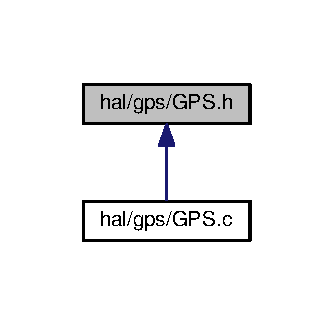
\includegraphics[width=160pt]{GPS_8h__dep__incl}
\end{center}
\end{figure}
\subsection*{Data Structures}
\begin{DoxyCompactItemize}
\item 
struct \hyperlink{structstrPosition}{str\+Position}
\begin{DoxyCompactList}\small\item\em struct with Langitude or Latitude position \end{DoxyCompactList}\end{DoxyCompactItemize}
\subsection*{Functions}
\begin{DoxyCompactItemize}
\item 
int \hyperlink{GPS_8h_a35a6a55e7bbec401863a903a3607c0b6_a35a6a55e7bbec401863a903a3607c0b6}{g\+\_\+hal\+Gps\+\_\+get\+Data\+\_\+i32} (void)
\begin{DoxyCompactList}\small\item\em Parse Data from Uart into variables. \end{DoxyCompactList}\item 
unsigned int \hyperlink{GPS_8h_aea126d235b1db89dc964f8763565e9dc_aea126d235b1db89dc964f8763565e9dc}{g\+\_\+hal\+Gps\+\_\+get\+Date\+\_\+ui32} (void)
\begin{DoxyCompactList}\small\item\em Get Date from G\+P\+S module. \end{DoxyCompactList}\item 
double \hyperlink{GPS_8h_adac1759b450b418dc6030def1d73b8a7_adac1759b450b418dc6030def1d73b8a7}{g\+\_\+hal\+Gps\+\_\+get\+Direction\+\_\+f64} (void)
\begin{DoxyCompactList}\small\item\em Get Direction from G\+P\+S module. \end{DoxyCompactList}\item 
char \hyperlink{GPS_8h_a4f6b3f1d68b421a3a60b281326b4141b_a4f6b3f1d68b421a3a60b281326b4141b}{g\+\_\+hal\+Gps\+\_\+get\+Fix\+\_\+ch} (void)
\begin{DoxyCompactList}\small\item\em Get Fix from G\+P\+S module. \end{DoxyCompactList}\item 
double \hyperlink{GPS_8h_a0190aaa631556af032a2d286ebf6525a_a0190aaa631556af032a2d286ebf6525a}{g\+\_\+hal\+Gps\+\_\+get\+Geoid\+\_\+f64} (void)
\begin{DoxyCompactList}\small\item\em Get Geoid from G\+P\+S module. \end{DoxyCompactList}\item 
double \hyperlink{GPS_8h_ad797f33853c6d3e6f2e863c11c2822b8_ad797f33853c6d3e6f2e863c11c2822b8}{g\+\_\+hal\+Gps\+\_\+get\+Height\+\_\+f64} (void)
\begin{DoxyCompactList}\small\item\em Get Height from G\+P\+S module. \end{DoxyCompactList}\item 
struct \hyperlink{structstrPosition}{str\+Position} \hyperlink{GPS_8h_a0fa256f0b23aa1d53a0bf5892589dc9f_a0fa256f0b23aa1d53a0bf5892589dc9f}{g\+\_\+hal\+Gps\+\_\+get\+Latitude\+\_\+st} (void)
\begin{DoxyCompactList}\small\item\em Get Latitude from G\+P\+S module. \end{DoxyCompactList}\item 
struct \hyperlink{structstrPosition}{str\+Position} \hyperlink{GPS_8h_a7ee6cdd9714c51a2b74e5f3cdc2a5dca_a7ee6cdd9714c51a2b74e5f3cdc2a5dca}{g\+\_\+hal\+Gps\+\_\+get\+Longitude\+\_\+st} (void)
\begin{DoxyCompactList}\small\item\em Get Longitude from G\+P\+S module. \end{DoxyCompactList}\item 
unsigned int \hyperlink{GPS_8h_a64a3ef5cadfa081ca967b201352e2f8d_a64a3ef5cadfa081ca967b201352e2f8d}{g\+\_\+hal\+Gps\+\_\+get\+Time\+\_\+ui32} (void)
\begin{DoxyCompactList}\small\item\em Get Time from G\+P\+S module. \end{DoxyCompactList}\item 
double \hyperlink{GPS_8h_aae3374862ddb32be3a7f40b01661ede0_aae3374862ddb32be3a7f40b01661ede0}{g\+\_\+hal\+Gps\+\_\+get\+Velocity\+\_\+f64} (void)
\begin{DoxyCompactList}\small\item\em Get Velocity from G\+P\+S module. \end{DoxyCompactList}\item 
void \hyperlink{GPS_8h_a0bf6b6abfd6136e50bd5d35a76ee8d0b_a0bf6b6abfd6136e50bd5d35a76ee8d0b}{l\+\_\+reset\+Message1\+Values\+\_\+vd} (void)
\begin{DoxyCompactList}\small\item\em Reset Values of Message 1. \end{DoxyCompactList}\item 
void \hyperlink{GPS_8h_aa9c4ab6055264c0121813e5233cd3de0_aa9c4ab6055264c0121813e5233cd3de0}{l\+\_\+reset\+Message2\+Values\+\_\+vd} (void)
\begin{DoxyCompactList}\small\item\em Reset Values of Message 2. \end{DoxyCompactList}\end{DoxyCompactItemize}


\subsection{Function Documentation}
\hypertarget{GPS_8h_a35a6a55e7bbec401863a903a3607c0b6_a35a6a55e7bbec401863a903a3607c0b6}{\index{G\+P\+S.\+h@{G\+P\+S.\+h}!g\+\_\+hal\+Gps\+\_\+get\+Data\+\_\+i32@{g\+\_\+hal\+Gps\+\_\+get\+Data\+\_\+i32}}
\index{g\+\_\+hal\+Gps\+\_\+get\+Data\+\_\+i32@{g\+\_\+hal\+Gps\+\_\+get\+Data\+\_\+i32}!G\+P\+S.\+h@{G\+P\+S.\+h}}
\subsubsection[{g\+\_\+hal\+Gps\+\_\+get\+Data\+\_\+i32}]{\setlength{\rightskip}{0pt plus 5cm}int g\+\_\+hal\+Gps\+\_\+get\+Data\+\_\+i32 (
\begin{DoxyParamCaption}
\item[{void}]{}
\end{DoxyParamCaption}
)}}\label{GPS_8h_a35a6a55e7bbec401863a903a3607c0b6_a35a6a55e7bbec401863a903a3607c0b6}


Parse Data from Uart into variables. 



 \begin{DoxyAuthor}{Author}
Oliver Breuning ( olbrgs00 ) 
\end{DoxyAuthor}
\begin{DoxyDate}{Date}
2015/04/21
\end{DoxyDate}
Reads data from the Hardware Driver and parses it in the specific important variables. Checks just the G\+P\+G\+G\+A and G\+P\+R\+M\+C Messages which are received from the G\+P\+S module. The return value gives back how many important Bytes are received.

Description of counting successfully received values total min\+: 35 max 38 \$\+G\+P\+G\+G\+A ,205003.\+000 ,4841.\+9261 ,N ,00918.\+7276 ,E ,1 ,06 ,1.\+12 ,283.\+5 ,M ,48.\+0 ,M , ,$\ast$6\+D $\vert$$\vert$$\vert$$\vert$$\vert$$\vert$ $\vert$$\vert$$\vert$$\vert$$\vert$$\vert$ $\vert$$\vert$$\vert$$\vert$ $\vert$$\vert$$\vert$$\vert$ $\vert$ $\vert$$\vert$$\vert$$\vert$$\vert$ $\vert$$\vert$$\vert$$\vert$ $\vert$ $\vert$$\vert$$\vert$ $\vert$ $\vert$$\vert$ $\vert$

total min\+: 44 max 47 \$\+G\+P\+R\+M\+C ,205003.\+000 ,A ,4841.\+9261 ,N ,00918.\+7276 ,E ,0.\+33 ,184.\+26 ,100415 , , , A$\ast$63 $\vert$$\vert$$\vert$$\vert$$\vert$$\vert$ $\vert$$\vert$$\vert$$\vert$$\vert$$\vert$ $\vert$ $\vert$$\vert$$\vert$$\vert$ $\vert$$\vert$$\vert$$\vert$ $\vert$ $\vert$$\vert$$\vert$$\vert$$\vert$ $\vert$$\vert$$\vert$$\vert$ $\vert$ $\vert$ $\vert$$\vert$ $\vert$$\vert$$\vert$ $\vert$$\vert$ $\vert$$\vert$$\vert$$\vert$$\vert$$\vert$

Remark message can be shorter if for example value is less than 283.\+5, so e.\+g. 83.\+5


\begin{DoxyParams}[1]{Parameters}
\mbox{\tt in}  & {\em no} & parameter \\
\hline
\mbox{\tt out}  & {\em return} & of successfully important received characters\\
\hline
\end{DoxyParams}


Definition at line 315 of file G\+P\+S.\+c.


\begin{DoxyCode}
316 \{
317 
318     \hyperlink{GPS_8c_a48ba1860315a5b43a78ba5afb66855c4_a48ba1860315a5b43a78ba5afb66855c4}{l\_rec\_Data\_ch}=\hyperlink{LLD__UART_8c_a8154946dd2ae6c37a2bd86dd7896ee73_a8154946dd2ae6c37a2bd86dd7896ee73}{g\_lldUart\_readByte\_ch}();
319 
320     \textcolor{keywordflow}{if}(!\hyperlink{GPS_8c_a33348219a5889847ad41d40b9198164a_a33348219a5889847ad41d40b9198164a}{l\_message\_position\_ch})\textcolor{comment}{//check which message is received}
321     \{
322         \textcolor{keywordflow}{if}(\hyperlink{GPS_8c_a48ba1860315a5b43a78ba5afb66855c4_a48ba1860315a5b43a78ba5afb66855c4}{l\_rec\_Data\_ch}==\textcolor{charliteral}{'$'})
323         \{\hyperlink{GPS_8c_ac9b483bef981b820a4f6ffaf11ee37a2_ac9b483bef981b820a4f6ffaf11ee37a2}{l\_header\_position\_ch}=1;\hyperlink{GPS_8c_ae83ebc8d1ab82c8acbb739dfd2e9d6f8_ae83ebc8d1ab82c8acbb739dfd2e9d6f8}{l\_succeded\_i32}=0;
      \hyperlink{GPS_8c_ae83ebc8d1ab82c8acbb739dfd2e9d6f8_ae83ebc8d1ab82c8acbb739dfd2e9d6f8}{l\_succeded\_i32}++;\}
324         \textcolor{keywordflow}{else} \textcolor{keywordflow}{if} (\hyperlink{GPS_8c_ac9b483bef981b820a4f6ffaf11ee37a2_ac9b483bef981b820a4f6ffaf11ee37a2}{l\_header\_position\_ch}==1 && \hyperlink{GPS_8c_a48ba1860315a5b43a78ba5afb66855c4_a48ba1860315a5b43a78ba5afb66855c4}{l\_rec\_Data\_ch}==\textcolor{charliteral}{'G'})
325         \{\hyperlink{GPS_8c_ac9b483bef981b820a4f6ffaf11ee37a2_ac9b483bef981b820a4f6ffaf11ee37a2}{l\_header\_position\_ch}=2;\hyperlink{GPS_8c_ae83ebc8d1ab82c8acbb739dfd2e9d6f8_ae83ebc8d1ab82c8acbb739dfd2e9d6f8}{l\_succeded\_i32}++;\}
326         \textcolor{keywordflow}{else} \textcolor{keywordflow}{if} (\hyperlink{GPS_8c_ac9b483bef981b820a4f6ffaf11ee37a2_ac9b483bef981b820a4f6ffaf11ee37a2}{l\_header\_position\_ch}==2 && \hyperlink{GPS_8c_a48ba1860315a5b43a78ba5afb66855c4_a48ba1860315a5b43a78ba5afb66855c4}{l\_rec\_Data\_ch}==\textcolor{charliteral}{'P'})
327         \{\hyperlink{GPS_8c_ac9b483bef981b820a4f6ffaf11ee37a2_ac9b483bef981b820a4f6ffaf11ee37a2}{l\_header\_position\_ch}=3;\hyperlink{GPS_8c_ae83ebc8d1ab82c8acbb739dfd2e9d6f8_ae83ebc8d1ab82c8acbb739dfd2e9d6f8}{l\_succeded\_i32}++;\}
328         \textcolor{keywordflow}{else} \textcolor{keywordflow}{if} (\hyperlink{GPS_8c_ac9b483bef981b820a4f6ffaf11ee37a2_ac9b483bef981b820a4f6ffaf11ee37a2}{l\_header\_position\_ch}==3 && \hyperlink{GPS_8c_a48ba1860315a5b43a78ba5afb66855c4_a48ba1860315a5b43a78ba5afb66855c4}{l\_rec\_Data\_ch}==\textcolor{charliteral}{'G'})
329         \{\hyperlink{GPS_8c_ac9b483bef981b820a4f6ffaf11ee37a2_ac9b483bef981b820a4f6ffaf11ee37a2}{l\_header\_position\_ch}=14;\hyperlink{GPS_8c_ae83ebc8d1ab82c8acbb739dfd2e9d6f8_ae83ebc8d1ab82c8acbb739dfd2e9d6f8}{l\_succeded\_i32}++;\}
330         \textcolor{keywordflow}{else} \textcolor{keywordflow}{if} (\hyperlink{GPS_8c_ac9b483bef981b820a4f6ffaf11ee37a2_ac9b483bef981b820a4f6ffaf11ee37a2}{l\_header\_position\_ch}==3 && \hyperlink{GPS_8c_a48ba1860315a5b43a78ba5afb66855c4_a48ba1860315a5b43a78ba5afb66855c4}{l\_rec\_Data\_ch}==\textcolor{charliteral}{'R'})
331         \{\hyperlink{GPS_8c_ac9b483bef981b820a4f6ffaf11ee37a2_ac9b483bef981b820a4f6ffaf11ee37a2}{l\_header\_position\_ch}=24;\hyperlink{GPS_8c_ae83ebc8d1ab82c8acbb739dfd2e9d6f8_ae83ebc8d1ab82c8acbb739dfd2e9d6f8}{l\_succeded\_i32}++;\}
332         \textcolor{keywordflow}{else} \textcolor{keywordflow}{if} (\hyperlink{GPS_8c_ac9b483bef981b820a4f6ffaf11ee37a2_ac9b483bef981b820a4f6ffaf11ee37a2}{l\_header\_position\_ch}==14 && \hyperlink{GPS_8c_a48ba1860315a5b43a78ba5afb66855c4_a48ba1860315a5b43a78ba5afb66855c4}{l\_rec\_Data\_ch}==\textcolor{charliteral}{'G'})
333         \{\hyperlink{GPS_8c_ac9b483bef981b820a4f6ffaf11ee37a2_ac9b483bef981b820a4f6ffaf11ee37a2}{l\_header\_position\_ch}=15;\hyperlink{GPS_8c_ae83ebc8d1ab82c8acbb739dfd2e9d6f8_ae83ebc8d1ab82c8acbb739dfd2e9d6f8}{l\_succeded\_i32}++;\}
334         \textcolor{keywordflow}{else} \textcolor{keywordflow}{if} (\hyperlink{GPS_8c_ac9b483bef981b820a4f6ffaf11ee37a2_ac9b483bef981b820a4f6ffaf11ee37a2}{l\_header\_position\_ch}==24 && \hyperlink{GPS_8c_a48ba1860315a5b43a78ba5afb66855c4_a48ba1860315a5b43a78ba5afb66855c4}{l\_rec\_Data\_ch}==\textcolor{charliteral}{'M'})
335         \{\hyperlink{GPS_8c_ac9b483bef981b820a4f6ffaf11ee37a2_ac9b483bef981b820a4f6ffaf11ee37a2}{l\_header\_position\_ch}=25;\hyperlink{GPS_8c_ae83ebc8d1ab82c8acbb739dfd2e9d6f8_ae83ebc8d1ab82c8acbb739dfd2e9d6f8}{l\_succeded\_i32}++;\}
336         \textcolor{keywordflow}{else} \textcolor{keywordflow}{if} (\hyperlink{GPS_8c_ac9b483bef981b820a4f6ffaf11ee37a2_ac9b483bef981b820a4f6ffaf11ee37a2}{l\_header\_position\_ch}==15 && \hyperlink{GPS_8c_a48ba1860315a5b43a78ba5afb66855c4_a48ba1860315a5b43a78ba5afb66855c4}{l\_rec\_Data\_ch}==\textcolor{charliteral}{'A'})
337         \{   \hyperlink{GPS_8c_a4b514c1fd22818c03e87233b61d6eda3_a4b514c1fd22818c03e87233b61d6eda3}{l\_message\_ch}=1;\hyperlink{GPS_8c_a0bf6b6abfd6136e50bd5d35a76ee8d0b_a0bf6b6abfd6136e50bd5d35a76ee8d0b}{l\_resetMessage1Values\_vd}();
      \hyperlink{GPS_8c_a574dd5cd13fbeac386e435e932e20bae_a574dd5cd13fbeac386e435e932e20bae}{l\_data\_position\_ch}=0;\hyperlink{GPS_8c_a33348219a5889847ad41d40b9198164a_a33348219a5889847ad41d40b9198164a}{l\_message\_position\_ch}=1; 
      \hyperlink{GPS_8c_ae83ebc8d1ab82c8acbb739dfd2e9d6f8_ae83ebc8d1ab82c8acbb739dfd2e9d6f8}{l\_succeded\_i32}++;\}
338         \textcolor{keywordflow}{else} \textcolor{keywordflow}{if} (\hyperlink{GPS_8c_ac9b483bef981b820a4f6ffaf11ee37a2_ac9b483bef981b820a4f6ffaf11ee37a2}{l\_header\_position\_ch}==25 && \hyperlink{GPS_8c_a48ba1860315a5b43a78ba5afb66855c4_a48ba1860315a5b43a78ba5afb66855c4}{l\_rec\_Data\_ch}==\textcolor{charliteral}{'C'})
339         \{   \hyperlink{GPS_8c_a4b514c1fd22818c03e87233b61d6eda3_a4b514c1fd22818c03e87233b61d6eda3}{l\_message\_ch}=2;\hyperlink{GPS_8c_aa9c4ab6055264c0121813e5233cd3de0_aa9c4ab6055264c0121813e5233cd3de0}{l\_resetMessage2Values\_vd}();
      \hyperlink{GPS_8c_a574dd5cd13fbeac386e435e932e20bae_a574dd5cd13fbeac386e435e932e20bae}{l\_data\_position\_ch}=0; \hyperlink{GPS_8c_a33348219a5889847ad41d40b9198164a_a33348219a5889847ad41d40b9198164a}{l\_message\_position\_ch}=1; 
      \hyperlink{GPS_8c_ae83ebc8d1ab82c8acbb739dfd2e9d6f8_ae83ebc8d1ab82c8acbb739dfd2e9d6f8}{l\_succeded\_i32}++;\}
340     \}
341     \textcolor{keywordflow}{else}
342     \{
343         \textcolor{keywordflow}{switch} (\hyperlink{GPS_8c_a4b514c1fd22818c03e87233b61d6eda3_a4b514c1fd22818c03e87233b61d6eda3}{l\_message\_ch})\textcolor{comment}{//check data within the two important messages}
344         \{
345         \textcolor{keywordflow}{case} 1:\textcolor{comment}{//$GPGGA ,205003.000 ,4841.9261 ,N ,00918.7276 ,E ,1 ,06 ,1.12 ,283.5 ,M ,48.0 ,M , ,*6D    
          38}
346             \textcolor{keywordflow}{switch} (\hyperlink{GPS_8c_a48ba1860315a5b43a78ba5afb66855c4_a48ba1860315a5b43a78ba5afb66855c4}{l\_rec\_Data\_ch})
347             \{
348             \textcolor{keywordflow}{case} \textcolor{charliteral}{','}:
349                 \hyperlink{GPS_8c_a574dd5cd13fbeac386e435e932e20bae_a574dd5cd13fbeac386e435e932e20bae}{l\_data\_position\_ch}++;
350                 \hyperlink{GPS_8c_a93cee4751b6fb1410e727f045329f326_a93cee4751b6fb1410e727f045329f326}{l\_fieldpointer\_i32}=0;
351                 \hyperlink{GPS_8c_ad5b924e752a1a8222bd65c4291d3e82e_ad5b924e752a1a8222bd65c4291d3e82e}{l\_decimal\_place\_factor\_i32}=10;
352                 \textcolor{keywordflow}{break};
353             \textcolor{keywordflow}{case} 10:\textcolor{comment}{//LF found}
354                 \hyperlink{GPS_8c_ae83ebc8d1ab82c8acbb739dfd2e9d6f8_ae83ebc8d1ab82c8acbb739dfd2e9d6f8}{l\_succeded\_i32}=\hyperlink{GPS_8c_ae83ebc8d1ab82c8acbb739dfd2e9d6f8_ae83ebc8d1ab82c8acbb739dfd2e9d6f8}{l\_succeded\_i32}+100;  \textcolor{comment}{//short comment}
355                 \hyperlink{GPS_8c_a33348219a5889847ad41d40b9198164a_a33348219a5889847ad41d40b9198164a}{l\_message\_position\_ch}=0;
356                 \hyperlink{GPS_8c_ac9b483bef981b820a4f6ffaf11ee37a2_ac9b483bef981b820a4f6ffaf11ee37a2}{l\_header\_position\_ch}=0;
357                 \textcolor{keywordflow}{break};
358             \textcolor{keywordflow}{default}:
359                 \textcolor{keywordflow}{switch} (\hyperlink{GPS_8c_a574dd5cd13fbeac386e435e932e20bae_a574dd5cd13fbeac386e435e932e20bae}{l\_data\_position\_ch})
360                 \{
361                 \textcolor{keywordflow}{case} 1:\textcolor{comment}{//Time}
362                     \textcolor{keywordflow}{if}(\hyperlink{GPS_8c_a93cee4751b6fb1410e727f045329f326_a93cee4751b6fb1410e727f045329f326}{l\_fieldpointer\_i32}<6)
363                     \{
364                         \hyperlink{GPS_8c_a365efcbf31282dcb274edd608e0824ed_a365efcbf31282dcb274edd608e0824ed}{l\_time\_ui32}=\hyperlink{GPS_8c_a365efcbf31282dcb274edd608e0824ed_a365efcbf31282dcb274edd608e0824ed}{l\_time\_ui32}*10+(
      \hyperlink{GPS_8c_a48ba1860315a5b43a78ba5afb66855c4_a48ba1860315a5b43a78ba5afb66855c4}{l\_rec\_Data\_ch}-48);
365                         \hyperlink{GPS_8c_ae83ebc8d1ab82c8acbb739dfd2e9d6f8_ae83ebc8d1ab82c8acbb739dfd2e9d6f8}{l\_succeded\_i32}++;
366                     \}
367                     \hyperlink{GPS_8c_a93cee4751b6fb1410e727f045329f326_a93cee4751b6fb1410e727f045329f326}{l\_fieldpointer\_i32}++;
368                     \textcolor{keywordflow}{break};
369                 \textcolor{keywordflow}{case} 2:\textcolor{comment}{//Latitude}
370                     \textcolor{keywordflow}{if}(\hyperlink{GPS_8c_a93cee4751b6fb1410e727f045329f326_a93cee4751b6fb1410e727f045329f326}{l\_fieldpointer\_i32}<2)
371                     \{
372                         \hyperlink{GPS_8c_ae764c82d3318068e28af258ae1e2449c_ae764c82d3318068e28af258ae1e2449c}{l\_gps\_latitude\_st}.\hyperlink{structstrPosition_ac060af7d7963812c116c24cdb861f184_ac060af7d7963812c116c24cdb861f184}{l\_degree\_ui32}=
      \hyperlink{GPS_8c_ae764c82d3318068e28af258ae1e2449c_ae764c82d3318068e28af258ae1e2449c}{l\_gps\_latitude\_st}.\hyperlink{structstrPosition_ac060af7d7963812c116c24cdb861f184_ac060af7d7963812c116c24cdb861f184}{l\_degree\_ui32}*10+(\hyperlink{GPS_8c_a48ba1860315a5b43a78ba5afb66855c4_a48ba1860315a5b43a78ba5afb66855c4}{l\_rec\_Data\_ch}-48);
373                         \hyperlink{GPS_8c_ae83ebc8d1ab82c8acbb739dfd2e9d6f8_ae83ebc8d1ab82c8acbb739dfd2e9d6f8}{l\_succeded\_i32}++;
374                     \}
375                     \textcolor{keywordflow}{else} \textcolor{keywordflow}{if}(\hyperlink{GPS_8c_a93cee4751b6fb1410e727f045329f326_a93cee4751b6fb1410e727f045329f326}{l\_fieldpointer\_i32}<4)
376                     \{
377                         \hyperlink{GPS_8c_ae764c82d3318068e28af258ae1e2449c_ae764c82d3318068e28af258ae1e2449c}{l\_gps\_latitude\_st}.\hyperlink{structstrPosition_a5489ef5e7f8e6ee45990b262c80a7819_a5489ef5e7f8e6ee45990b262c80a7819}{l\_minutes\_ui32}=
      \hyperlink{GPS_8c_ae764c82d3318068e28af258ae1e2449c_ae764c82d3318068e28af258ae1e2449c}{l\_gps\_latitude\_st}.\hyperlink{structstrPosition_a5489ef5e7f8e6ee45990b262c80a7819_a5489ef5e7f8e6ee45990b262c80a7819}{l\_minutes\_ui32}*10+(
      \hyperlink{GPS_8c_a48ba1860315a5b43a78ba5afb66855c4_a48ba1860315a5b43a78ba5afb66855c4}{l\_rec\_Data\_ch}-48);
378                         \hyperlink{GPS_8c_ae83ebc8d1ab82c8acbb739dfd2e9d6f8_ae83ebc8d1ab82c8acbb739dfd2e9d6f8}{l\_succeded\_i32}++;
379                     \}
380                     \textcolor{keywordflow}{else} \textcolor{keywordflow}{if}(\hyperlink{GPS_8c_a93cee4751b6fb1410e727f045329f326_a93cee4751b6fb1410e727f045329f326}{l\_fieldpointer\_i32}>=5 && 
      \hyperlink{GPS_8c_a93cee4751b6fb1410e727f045329f326_a93cee4751b6fb1410e727f045329f326}{l\_fieldpointer\_i32}<9)
381                     \{
382                         \hyperlink{GPS_8c_ae764c82d3318068e28af258ae1e2449c_ae764c82d3318068e28af258ae1e2449c}{l\_gps\_latitude\_st}.\hyperlink{structstrPosition_ae62d246c481c611e168ea86b70d5313b_ae62d246c481c611e168ea86b70d5313b}{l\_seconds\_f64}=
      \hyperlink{GPS_8c_ae764c82d3318068e28af258ae1e2449c_ae764c82d3318068e28af258ae1e2449c}{l\_gps\_latitude\_st}.\hyperlink{structstrPosition_ae62d246c481c611e168ea86b70d5313b_ae62d246c481c611e168ea86b70d5313b}{l\_seconds\_f64}*10+(\hyperlink{GPS_8c_a48ba1860315a5b43a78ba5afb66855c4_a48ba1860315a5b43a78ba5afb66855c4}{l\_rec\_Data\_ch}-48)*0.006;
383                         \hyperlink{GPS_8c_ae83ebc8d1ab82c8acbb739dfd2e9d6f8_ae83ebc8d1ab82c8acbb739dfd2e9d6f8}{l\_succeded\_i32}++;
384                     \}
385                     \hyperlink{GPS_8c_a93cee4751b6fb1410e727f045329f326_a93cee4751b6fb1410e727f045329f326}{l\_fieldpointer\_i32}++;
386                     \textcolor{keywordflow}{break};
387                 \textcolor{keywordflow}{case} 3:\textcolor{comment}{//cardinal direction}
388                     \textcolor{keywordflow}{if}(\hyperlink{GPS_8c_a93cee4751b6fb1410e727f045329f326_a93cee4751b6fb1410e727f045329f326}{l\_fieldpointer\_i32}<1)
389                     \{
390                         \hyperlink{GPS_8c_ae764c82d3318068e28af258ae1e2449c_ae764c82d3318068e28af258ae1e2449c}{l\_gps\_latitude\_st}.
      \hyperlink{structstrPosition_aa39fed1d421cb2260d0ef7157c3c00d0_aa39fed1d421cb2260d0ef7157c3c00d0}{l\_cardinalDirection\_ch}=\hyperlink{GPS_8c_a48ba1860315a5b43a78ba5afb66855c4_a48ba1860315a5b43a78ba5afb66855c4}{l\_rec\_Data\_ch};
391                         \hyperlink{GPS_8c_ae83ebc8d1ab82c8acbb739dfd2e9d6f8_ae83ebc8d1ab82c8acbb739dfd2e9d6f8}{l\_succeded\_i32}++;
392                     \}
393                     \hyperlink{GPS_8c_a93cee4751b6fb1410e727f045329f326_a93cee4751b6fb1410e727f045329f326}{l\_fieldpointer\_i32}++;
394                     \textcolor{keywordflow}{break};
395                 \textcolor{keywordflow}{case} 4:\textcolor{comment}{//Longitude}
396                     \textcolor{keywordflow}{if}(\hyperlink{GPS_8c_a93cee4751b6fb1410e727f045329f326_a93cee4751b6fb1410e727f045329f326}{l\_fieldpointer\_i32}<3)
397                     \{
398                         \hyperlink{GPS_8c_a5661901a87ce3f7dcd2eba20d8b505b4_a5661901a87ce3f7dcd2eba20d8b505b4}{l\_gps\_longitude\_st}.\hyperlink{structstrPosition_ac060af7d7963812c116c24cdb861f184_ac060af7d7963812c116c24cdb861f184}{l\_degree\_ui32}=
      \hyperlink{GPS_8c_a5661901a87ce3f7dcd2eba20d8b505b4_a5661901a87ce3f7dcd2eba20d8b505b4}{l\_gps\_longitude\_st}.\hyperlink{structstrPosition_ac060af7d7963812c116c24cdb861f184_ac060af7d7963812c116c24cdb861f184}{l\_degree\_ui32}*10+(
      \hyperlink{GPS_8c_a48ba1860315a5b43a78ba5afb66855c4_a48ba1860315a5b43a78ba5afb66855c4}{l\_rec\_Data\_ch}-48);
399                         \hyperlink{GPS_8c_ae83ebc8d1ab82c8acbb739dfd2e9d6f8_ae83ebc8d1ab82c8acbb739dfd2e9d6f8}{l\_succeded\_i32}++;
400                     \}
401                     \textcolor{keywordflow}{else} \textcolor{keywordflow}{if}(\hyperlink{GPS_8c_a93cee4751b6fb1410e727f045329f326_a93cee4751b6fb1410e727f045329f326}{l\_fieldpointer\_i32}<5)
402                     \{
403                         \hyperlink{GPS_8c_a5661901a87ce3f7dcd2eba20d8b505b4_a5661901a87ce3f7dcd2eba20d8b505b4}{l\_gps\_longitude\_st}.\hyperlink{structstrPosition_a5489ef5e7f8e6ee45990b262c80a7819_a5489ef5e7f8e6ee45990b262c80a7819}{l\_minutes\_ui32}=
      \hyperlink{GPS_8c_a5661901a87ce3f7dcd2eba20d8b505b4_a5661901a87ce3f7dcd2eba20d8b505b4}{l\_gps\_longitude\_st}.\hyperlink{structstrPosition_a5489ef5e7f8e6ee45990b262c80a7819_a5489ef5e7f8e6ee45990b262c80a7819}{l\_minutes\_ui32}*10+(
      \hyperlink{GPS_8c_a48ba1860315a5b43a78ba5afb66855c4_a48ba1860315a5b43a78ba5afb66855c4}{l\_rec\_Data\_ch}-48);
404                         \hyperlink{GPS_8c_ae83ebc8d1ab82c8acbb739dfd2e9d6f8_ae83ebc8d1ab82c8acbb739dfd2e9d6f8}{l\_succeded\_i32}++;
405                     \}
406                     \textcolor{keywordflow}{else} \textcolor{keywordflow}{if}(\hyperlink{GPS_8c_a93cee4751b6fb1410e727f045329f326_a93cee4751b6fb1410e727f045329f326}{l\_fieldpointer\_i32}>=6 && 
      \hyperlink{GPS_8c_a93cee4751b6fb1410e727f045329f326_a93cee4751b6fb1410e727f045329f326}{l\_fieldpointer\_i32}<10)
407                     \{
408                         \hyperlink{GPS_8c_a5661901a87ce3f7dcd2eba20d8b505b4_a5661901a87ce3f7dcd2eba20d8b505b4}{l\_gps\_longitude\_st}.\hyperlink{structstrPosition_ae62d246c481c611e168ea86b70d5313b_ae62d246c481c611e168ea86b70d5313b}{l\_seconds\_f64}=
      \hyperlink{GPS_8c_a5661901a87ce3f7dcd2eba20d8b505b4_a5661901a87ce3f7dcd2eba20d8b505b4}{l\_gps\_longitude\_st}.\hyperlink{structstrPosition_ae62d246c481c611e168ea86b70d5313b_ae62d246c481c611e168ea86b70d5313b}{l\_seconds\_f64}*10+(
      \hyperlink{GPS_8c_a48ba1860315a5b43a78ba5afb66855c4_a48ba1860315a5b43a78ba5afb66855c4}{l\_rec\_Data\_ch}-48)*0.006;
409                         \hyperlink{GPS_8c_ae83ebc8d1ab82c8acbb739dfd2e9d6f8_ae83ebc8d1ab82c8acbb739dfd2e9d6f8}{l\_succeded\_i32}++;
410                     \}
411                     \hyperlink{GPS_8c_a93cee4751b6fb1410e727f045329f326_a93cee4751b6fb1410e727f045329f326}{l\_fieldpointer\_i32}++;
412                     \textcolor{keywordflow}{break};
413                 \textcolor{keywordflow}{case} 5:\textcolor{comment}{//cardinal direction}
414                     \textcolor{keywordflow}{if}(\hyperlink{GPS_8c_a93cee4751b6fb1410e727f045329f326_a93cee4751b6fb1410e727f045329f326}{l\_fieldpointer\_i32}<1)
415                     \{
416                         \hyperlink{GPS_8c_a5661901a87ce3f7dcd2eba20d8b505b4_a5661901a87ce3f7dcd2eba20d8b505b4}{l\_gps\_longitude\_st}.
      \hyperlink{structstrPosition_aa39fed1d421cb2260d0ef7157c3c00d0_aa39fed1d421cb2260d0ef7157c3c00d0}{l\_cardinalDirection\_ch}=\hyperlink{GPS_8c_a48ba1860315a5b43a78ba5afb66855c4_a48ba1860315a5b43a78ba5afb66855c4}{l\_rec\_Data\_ch};
417                         \hyperlink{GPS_8c_ae83ebc8d1ab82c8acbb739dfd2e9d6f8_ae83ebc8d1ab82c8acbb739dfd2e9d6f8}{l\_succeded\_i32}++;
418                     \}
419                     \hyperlink{GPS_8c_a93cee4751b6fb1410e727f045329f326_a93cee4751b6fb1410e727f045329f326}{l\_fieldpointer\_i32}++;
420                     \textcolor{keywordflow}{break};
421                 \textcolor{keywordflow}{case} 9:\textcolor{comment}{//Height}
422                     \textcolor{keywordflow}{if}(\hyperlink{GPS_8c_a48ba1860315a5b43a78ba5afb66855c4_a48ba1860315a5b43a78ba5afb66855c4}{l\_rec\_Data\_ch}!=\textcolor{charliteral}{'.'} && \hyperlink{GPS_8c_a93cee4751b6fb1410e727f045329f326_a93cee4751b6fb1410e727f045329f326}{l\_fieldpointer\_i32}==0)
423                     \{
424                         \hyperlink{GPS_8c_a36e46365d7b41cc255fee53e0aa4b70a_a36e46365d7b41cc255fee53e0aa4b70a}{l\_height\_f64}=\hyperlink{GPS_8c_a36e46365d7b41cc255fee53e0aa4b70a_a36e46365d7b41cc255fee53e0aa4b70a}{l\_height\_f64}*10+(double)(
      \hyperlink{GPS_8c_a48ba1860315a5b43a78ba5afb66855c4_a48ba1860315a5b43a78ba5afb66855c4}{l\_rec\_Data\_ch}-48);
425                         \hyperlink{GPS_8c_ae83ebc8d1ab82c8acbb739dfd2e9d6f8_ae83ebc8d1ab82c8acbb739dfd2e9d6f8}{l\_succeded\_i32}++;
426 
427                     \}
428                     \textcolor{keywordflow}{else} \textcolor{keywordflow}{if} (\hyperlink{GPS_8c_a48ba1860315a5b43a78ba5afb66855c4_a48ba1860315a5b43a78ba5afb66855c4}{l\_rec\_Data\_ch}==\textcolor{charliteral}{'.'})
429                     \{
430                         \hyperlink{GPS_8c_a93cee4751b6fb1410e727f045329f326_a93cee4751b6fb1410e727f045329f326}{l\_fieldpointer\_i32}++;
431                     \}
432                     \textcolor{keywordflow}{else}
433                     \{
434                         \hyperlink{GPS_8c_a36e46365d7b41cc255fee53e0aa4b70a_a36e46365d7b41cc255fee53e0aa4b70a}{l\_height\_f64}=\hyperlink{GPS_8c_a36e46365d7b41cc255fee53e0aa4b70a_a36e46365d7b41cc255fee53e0aa4b70a}{l\_height\_f64}+(double)(
      \hyperlink{GPS_8c_a48ba1860315a5b43a78ba5afb66855c4_a48ba1860315a5b43a78ba5afb66855c4}{l\_rec\_Data\_ch}-48)/\hyperlink{GPS_8c_ad5b924e752a1a8222bd65c4291d3e82e_ad5b924e752a1a8222bd65c4291d3e82e}{l\_decimal\_place\_factor\_i32};
435                         \hyperlink{GPS_8c_ad5b924e752a1a8222bd65c4291d3e82e_ad5b924e752a1a8222bd65c4291d3e82e}{l\_decimal\_place\_factor\_i32}=
      \hyperlink{GPS_8c_ad5b924e752a1a8222bd65c4291d3e82e_ad5b924e752a1a8222bd65c4291d3e82e}{l\_decimal\_place\_factor\_i32}*10;
436                         \hyperlink{GPS_8c_ae83ebc8d1ab82c8acbb739dfd2e9d6f8_ae83ebc8d1ab82c8acbb739dfd2e9d6f8}{l\_succeded\_i32}++;
437                     \}
438                     \textcolor{keywordflow}{break};
439                 \textcolor{keywordflow}{case} 11:\textcolor{comment}{//Geoid}
440                     \textcolor{keywordflow}{if}(\hyperlink{GPS_8c_a48ba1860315a5b43a78ba5afb66855c4_a48ba1860315a5b43a78ba5afb66855c4}{l\_rec\_Data\_ch}!=\textcolor{charliteral}{'.'} && \hyperlink{GPS_8c_a93cee4751b6fb1410e727f045329f326_a93cee4751b6fb1410e727f045329f326}{l\_fieldpointer\_i32}==0)
441                     \{
442                         \hyperlink{GPS_8c_a2cc033719fe30335f2423a4afbe53984_a2cc033719fe30335f2423a4afbe53984}{l\_geoid\_f64}=\hyperlink{GPS_8c_a2cc033719fe30335f2423a4afbe53984_a2cc033719fe30335f2423a4afbe53984}{l\_geoid\_f64}*10+(double)(
      \hyperlink{GPS_8c_a48ba1860315a5b43a78ba5afb66855c4_a48ba1860315a5b43a78ba5afb66855c4}{l\_rec\_Data\_ch}-48);
443                         \hyperlink{GPS_8c_ae83ebc8d1ab82c8acbb739dfd2e9d6f8_ae83ebc8d1ab82c8acbb739dfd2e9d6f8}{l\_succeded\_i32}++;
444 
445                     \}
446                     \textcolor{keywordflow}{else} \textcolor{keywordflow}{if} (\hyperlink{GPS_8c_a48ba1860315a5b43a78ba5afb66855c4_a48ba1860315a5b43a78ba5afb66855c4}{l\_rec\_Data\_ch}==\textcolor{charliteral}{'.'})
447                     \{
448                         \hyperlink{GPS_8c_a93cee4751b6fb1410e727f045329f326_a93cee4751b6fb1410e727f045329f326}{l\_fieldpointer\_i32}++;
449                     \}
450                     \textcolor{keywordflow}{else}
451                     \{
452                         \hyperlink{GPS_8c_a2cc033719fe30335f2423a4afbe53984_a2cc033719fe30335f2423a4afbe53984}{l\_geoid\_f64}=\hyperlink{GPS_8c_a2cc033719fe30335f2423a4afbe53984_a2cc033719fe30335f2423a4afbe53984}{l\_geoid\_f64}+(double)(
      \hyperlink{GPS_8c_a48ba1860315a5b43a78ba5afb66855c4_a48ba1860315a5b43a78ba5afb66855c4}{l\_rec\_Data\_ch}-48)/\hyperlink{GPS_8c_ad5b924e752a1a8222bd65c4291d3e82e_ad5b924e752a1a8222bd65c4291d3e82e}{l\_decimal\_place\_factor\_i32};
453                         \hyperlink{GPS_8c_ad5b924e752a1a8222bd65c4291d3e82e_ad5b924e752a1a8222bd65c4291d3e82e}{l\_decimal\_place\_factor\_i32}=
      \hyperlink{GPS_8c_ad5b924e752a1a8222bd65c4291d3e82e_ad5b924e752a1a8222bd65c4291d3e82e}{l\_decimal\_place\_factor\_i32}*10;
454                         \hyperlink{GPS_8c_ae83ebc8d1ab82c8acbb739dfd2e9d6f8_ae83ebc8d1ab82c8acbb739dfd2e9d6f8}{l\_succeded\_i32}++;
455                     \}
456                     \textcolor{keywordflow}{break};
457                 \}
458                 \textcolor{keywordflow}{break};
459             \}
460             \textcolor{keywordflow}{break};
461 
462 
463         \textcolor{keywordflow}{case} 2:\textcolor{comment}{//$GPRMC ,205003.000 ,A ,4841.9261 ,N ,00918.7276 ,E ,0.33 ,184.26 ,100415 , , , A*63     
       44- 46}
464             \textcolor{keywordflow}{switch} (\hyperlink{GPS_8c_a48ba1860315a5b43a78ba5afb66855c4_a48ba1860315a5b43a78ba5afb66855c4}{l\_rec\_Data\_ch})
465             \{
466             \textcolor{keywordflow}{case} \textcolor{charliteral}{','}:
467                 \hyperlink{GPS_8c_a574dd5cd13fbeac386e435e932e20bae_a574dd5cd13fbeac386e435e932e20bae}{l\_data\_position\_ch}++;
468                 \hyperlink{GPS_8c_a93cee4751b6fb1410e727f045329f326_a93cee4751b6fb1410e727f045329f326}{l\_fieldpointer\_i32}=0;
469                 \hyperlink{GPS_8c_ad5b924e752a1a8222bd65c4291d3e82e_ad5b924e752a1a8222bd65c4291d3e82e}{l\_decimal\_place\_factor\_i32}=10;
470                 \textcolor{keywordflow}{break};
471             \textcolor{keywordflow}{case} 10:\textcolor{comment}{//LF found}
472                 \hyperlink{GPS_8c_ae83ebc8d1ab82c8acbb739dfd2e9d6f8_ae83ebc8d1ab82c8acbb739dfd2e9d6f8}{l\_succeded\_i32}=\hyperlink{GPS_8c_ae83ebc8d1ab82c8acbb739dfd2e9d6f8_ae83ebc8d1ab82c8acbb739dfd2e9d6f8}{l\_succeded\_i32}+200;
473                 \hyperlink{GPS_8c_a33348219a5889847ad41d40b9198164a_a33348219a5889847ad41d40b9198164a}{l\_message\_position\_ch}=0;
474                 \hyperlink{GPS_8c_ac9b483bef981b820a4f6ffaf11ee37a2_ac9b483bef981b820a4f6ffaf11ee37a2}{l\_header\_position\_ch}=0;
475                 \textcolor{keywordflow}{break};
476             \textcolor{keywordflow}{default}:
477                 \textcolor{keywordflow}{switch} (\hyperlink{GPS_8c_a574dd5cd13fbeac386e435e932e20bae_a574dd5cd13fbeac386e435e932e20bae}{l\_data\_position\_ch})
478                 \{
479                 \textcolor{keywordflow}{case} 1:\textcolor{comment}{//Time}
480                     \textcolor{keywordflow}{if}(\hyperlink{GPS_8c_a93cee4751b6fb1410e727f045329f326_a93cee4751b6fb1410e727f045329f326}{l\_fieldpointer\_i32}<6)
481                     \{
482                         \hyperlink{GPS_8c_a365efcbf31282dcb274edd608e0824ed_a365efcbf31282dcb274edd608e0824ed}{l\_time\_ui32}=\hyperlink{GPS_8c_a365efcbf31282dcb274edd608e0824ed_a365efcbf31282dcb274edd608e0824ed}{l\_time\_ui32}*10+(
      \hyperlink{GPS_8c_a48ba1860315a5b43a78ba5afb66855c4_a48ba1860315a5b43a78ba5afb66855c4}{l\_rec\_Data\_ch}-48);
483                         \hyperlink{GPS_8c_ae83ebc8d1ab82c8acbb739dfd2e9d6f8_ae83ebc8d1ab82c8acbb739dfd2e9d6f8}{l\_succeded\_i32}++;
484                     \}
485                     \hyperlink{GPS_8c_a93cee4751b6fb1410e727f045329f326_a93cee4751b6fb1410e727f045329f326}{l\_fieldpointer\_i32}++;
486                     \textcolor{keywordflow}{break};
487                 \textcolor{keywordflow}{case} 2:\textcolor{comment}{//Fix}
488                     \textcolor{keywordflow}{if}(\hyperlink{GPS_8c_a93cee4751b6fb1410e727f045329f326_a93cee4751b6fb1410e727f045329f326}{l\_fieldpointer\_i32}<2)
489                     \{
490                         \hyperlink{GPS_8c_a5a14aebdd5ac0d06913bdeaf9cec1a9b_a5a14aebdd5ac0d06913bdeaf9cec1a9b}{l\_fix\_ch}=\hyperlink{GPS_8c_a48ba1860315a5b43a78ba5afb66855c4_a48ba1860315a5b43a78ba5afb66855c4}{l\_rec\_Data\_ch};
491                         \hyperlink{GPS_8c_ae83ebc8d1ab82c8acbb739dfd2e9d6f8_ae83ebc8d1ab82c8acbb739dfd2e9d6f8}{l\_succeded\_i32}++;
492                     \}
493                     \hyperlink{GPS_8c_a93cee4751b6fb1410e727f045329f326_a93cee4751b6fb1410e727f045329f326}{l\_fieldpointer\_i32}++;
494                     \textcolor{keywordflow}{break};
495                 \textcolor{keywordflow}{case} 3:\textcolor{comment}{//Latitude}
496                     \textcolor{keywordflow}{if}(\hyperlink{GPS_8c_a93cee4751b6fb1410e727f045329f326_a93cee4751b6fb1410e727f045329f326}{l\_fieldpointer\_i32}<2)
497                     \{
498                         \hyperlink{GPS_8c_ae764c82d3318068e28af258ae1e2449c_ae764c82d3318068e28af258ae1e2449c}{l\_gps\_latitude\_st}.\hyperlink{structstrPosition_ac060af7d7963812c116c24cdb861f184_ac060af7d7963812c116c24cdb861f184}{l\_degree\_ui32}=
      \hyperlink{GPS_8c_ae764c82d3318068e28af258ae1e2449c_ae764c82d3318068e28af258ae1e2449c}{l\_gps\_latitude\_st}.\hyperlink{structstrPosition_ac060af7d7963812c116c24cdb861f184_ac060af7d7963812c116c24cdb861f184}{l\_degree\_ui32}*10+(\hyperlink{GPS_8c_a48ba1860315a5b43a78ba5afb66855c4_a48ba1860315a5b43a78ba5afb66855c4}{l\_rec\_Data\_ch}-48);
499                         \hyperlink{GPS_8c_ae83ebc8d1ab82c8acbb739dfd2e9d6f8_ae83ebc8d1ab82c8acbb739dfd2e9d6f8}{l\_succeded\_i32}++;
500                     \}
501                     \textcolor{keywordflow}{else} \textcolor{keywordflow}{if}(\hyperlink{GPS_8c_a93cee4751b6fb1410e727f045329f326_a93cee4751b6fb1410e727f045329f326}{l\_fieldpointer\_i32}<4)
502                     \{
503                         \hyperlink{GPS_8c_ae764c82d3318068e28af258ae1e2449c_ae764c82d3318068e28af258ae1e2449c}{l\_gps\_latitude\_st}.\hyperlink{structstrPosition_a5489ef5e7f8e6ee45990b262c80a7819_a5489ef5e7f8e6ee45990b262c80a7819}{l\_minutes\_ui32}=
      \hyperlink{GPS_8c_ae764c82d3318068e28af258ae1e2449c_ae764c82d3318068e28af258ae1e2449c}{l\_gps\_latitude\_st}.\hyperlink{structstrPosition_a5489ef5e7f8e6ee45990b262c80a7819_a5489ef5e7f8e6ee45990b262c80a7819}{l\_minutes\_ui32}*10+(
      \hyperlink{GPS_8c_a48ba1860315a5b43a78ba5afb66855c4_a48ba1860315a5b43a78ba5afb66855c4}{l\_rec\_Data\_ch}-48);
504                         \hyperlink{GPS_8c_ae83ebc8d1ab82c8acbb739dfd2e9d6f8_ae83ebc8d1ab82c8acbb739dfd2e9d6f8}{l\_succeded\_i32}++;
505                     \}
506                     \textcolor{keywordflow}{else} \textcolor{keywordflow}{if}(\hyperlink{GPS_8c_a93cee4751b6fb1410e727f045329f326_a93cee4751b6fb1410e727f045329f326}{l\_fieldpointer\_i32}>=5 && 
      \hyperlink{GPS_8c_a93cee4751b6fb1410e727f045329f326_a93cee4751b6fb1410e727f045329f326}{l\_fieldpointer\_i32}<9)
507                     \{
508                         \hyperlink{GPS_8c_ae764c82d3318068e28af258ae1e2449c_ae764c82d3318068e28af258ae1e2449c}{l\_gps\_latitude\_st}.\hyperlink{structstrPosition_ae62d246c481c611e168ea86b70d5313b_ae62d246c481c611e168ea86b70d5313b}{l\_seconds\_f64}=
      \hyperlink{GPS_8c_ae764c82d3318068e28af258ae1e2449c_ae764c82d3318068e28af258ae1e2449c}{l\_gps\_latitude\_st}.\hyperlink{structstrPosition_ae62d246c481c611e168ea86b70d5313b_ae62d246c481c611e168ea86b70d5313b}{l\_seconds\_f64}*10+(double)(
      \hyperlink{GPS_8c_a48ba1860315a5b43a78ba5afb66855c4_a48ba1860315a5b43a78ba5afb66855c4}{l\_rec\_Data\_ch}-48)*0.006;
509                         \hyperlink{GPS_8c_ae83ebc8d1ab82c8acbb739dfd2e9d6f8_ae83ebc8d1ab82c8acbb739dfd2e9d6f8}{l\_succeded\_i32}++;
510                     \}
511                     \hyperlink{GPS_8c_a93cee4751b6fb1410e727f045329f326_a93cee4751b6fb1410e727f045329f326}{l\_fieldpointer\_i32}++;
512                     \textcolor{keywordflow}{break};
513                 \textcolor{keywordflow}{case} 4:\textcolor{comment}{//cardinal direction}
514                     \textcolor{keywordflow}{if}(\hyperlink{GPS_8c_a93cee4751b6fb1410e727f045329f326_a93cee4751b6fb1410e727f045329f326}{l\_fieldpointer\_i32}<1)
515                     \{
516                         \hyperlink{GPS_8c_ae764c82d3318068e28af258ae1e2449c_ae764c82d3318068e28af258ae1e2449c}{l\_gps\_latitude\_st}.
      \hyperlink{structstrPosition_aa39fed1d421cb2260d0ef7157c3c00d0_aa39fed1d421cb2260d0ef7157c3c00d0}{l\_cardinalDirection\_ch}=\hyperlink{GPS_8c_a48ba1860315a5b43a78ba5afb66855c4_a48ba1860315a5b43a78ba5afb66855c4}{l\_rec\_Data\_ch};
517                         \hyperlink{GPS_8c_ae83ebc8d1ab82c8acbb739dfd2e9d6f8_ae83ebc8d1ab82c8acbb739dfd2e9d6f8}{l\_succeded\_i32}++;
518                     \}
519                     \hyperlink{GPS_8c_a93cee4751b6fb1410e727f045329f326_a93cee4751b6fb1410e727f045329f326}{l\_fieldpointer\_i32}++;
520                     \textcolor{keywordflow}{break};
521                 \textcolor{keywordflow}{case} 5:\textcolor{comment}{//Longitude}
522                     \textcolor{keywordflow}{if}(\hyperlink{GPS_8c_a93cee4751b6fb1410e727f045329f326_a93cee4751b6fb1410e727f045329f326}{l\_fieldpointer\_i32}<3)
523                     \{
524                         \hyperlink{GPS_8c_a5661901a87ce3f7dcd2eba20d8b505b4_a5661901a87ce3f7dcd2eba20d8b505b4}{l\_gps\_longitude\_st}.\hyperlink{structstrPosition_ac060af7d7963812c116c24cdb861f184_ac060af7d7963812c116c24cdb861f184}{l\_degree\_ui32}=
      \hyperlink{GPS_8c_a5661901a87ce3f7dcd2eba20d8b505b4_a5661901a87ce3f7dcd2eba20d8b505b4}{l\_gps\_longitude\_st}.\hyperlink{structstrPosition_ac060af7d7963812c116c24cdb861f184_ac060af7d7963812c116c24cdb861f184}{l\_degree\_ui32}*10+(
      \hyperlink{GPS_8c_a48ba1860315a5b43a78ba5afb66855c4_a48ba1860315a5b43a78ba5afb66855c4}{l\_rec\_Data\_ch}-48);
525                         \hyperlink{GPS_8c_ae83ebc8d1ab82c8acbb739dfd2e9d6f8_ae83ebc8d1ab82c8acbb739dfd2e9d6f8}{l\_succeded\_i32}++;
526                     \}
527                     \textcolor{keywordflow}{else} \textcolor{keywordflow}{if}(\hyperlink{GPS_8c_a93cee4751b6fb1410e727f045329f326_a93cee4751b6fb1410e727f045329f326}{l\_fieldpointer\_i32}<5)
528                     \{
529                         \hyperlink{GPS_8c_a5661901a87ce3f7dcd2eba20d8b505b4_a5661901a87ce3f7dcd2eba20d8b505b4}{l\_gps\_longitude\_st}.\hyperlink{structstrPosition_a5489ef5e7f8e6ee45990b262c80a7819_a5489ef5e7f8e6ee45990b262c80a7819}{l\_minutes\_ui32}=
      \hyperlink{GPS_8c_a5661901a87ce3f7dcd2eba20d8b505b4_a5661901a87ce3f7dcd2eba20d8b505b4}{l\_gps\_longitude\_st}.\hyperlink{structstrPosition_a5489ef5e7f8e6ee45990b262c80a7819_a5489ef5e7f8e6ee45990b262c80a7819}{l\_minutes\_ui32}*10+(
      \hyperlink{GPS_8c_a48ba1860315a5b43a78ba5afb66855c4_a48ba1860315a5b43a78ba5afb66855c4}{l\_rec\_Data\_ch}-48);
530                         \hyperlink{GPS_8c_ae83ebc8d1ab82c8acbb739dfd2e9d6f8_ae83ebc8d1ab82c8acbb739dfd2e9d6f8}{l\_succeded\_i32}++;
531                     \}
532                     \textcolor{keywordflow}{else} \textcolor{keywordflow}{if}(\hyperlink{GPS_8c_a93cee4751b6fb1410e727f045329f326_a93cee4751b6fb1410e727f045329f326}{l\_fieldpointer\_i32}>=6 && 
      \hyperlink{GPS_8c_a93cee4751b6fb1410e727f045329f326_a93cee4751b6fb1410e727f045329f326}{l\_fieldpointer\_i32}<10)
533                     \{
534                         \hyperlink{GPS_8c_a5661901a87ce3f7dcd2eba20d8b505b4_a5661901a87ce3f7dcd2eba20d8b505b4}{l\_gps\_longitude\_st}.\hyperlink{structstrPosition_ae62d246c481c611e168ea86b70d5313b_ae62d246c481c611e168ea86b70d5313b}{l\_seconds\_f64}=
      \hyperlink{GPS_8c_a5661901a87ce3f7dcd2eba20d8b505b4_a5661901a87ce3f7dcd2eba20d8b505b4}{l\_gps\_longitude\_st}.\hyperlink{structstrPosition_ae62d246c481c611e168ea86b70d5313b_ae62d246c481c611e168ea86b70d5313b}{l\_seconds\_f64}*10+(double)(
      \hyperlink{GPS_8c_a48ba1860315a5b43a78ba5afb66855c4_a48ba1860315a5b43a78ba5afb66855c4}{l\_rec\_Data\_ch}-48)*0.006;
535                         \hyperlink{GPS_8c_ae83ebc8d1ab82c8acbb739dfd2e9d6f8_ae83ebc8d1ab82c8acbb739dfd2e9d6f8}{l\_succeded\_i32}++;
536                     \}
537                     \hyperlink{GPS_8c_a93cee4751b6fb1410e727f045329f326_a93cee4751b6fb1410e727f045329f326}{l\_fieldpointer\_i32}++;
538                     \textcolor{keywordflow}{break};
539                 \textcolor{keywordflow}{case} 6:\textcolor{comment}{//cardinal direction}
540                     \textcolor{keywordflow}{if}(\hyperlink{GPS_8c_a93cee4751b6fb1410e727f045329f326_a93cee4751b6fb1410e727f045329f326}{l\_fieldpointer\_i32}<1)
541                     \{
542                         \hyperlink{GPS_8c_a5661901a87ce3f7dcd2eba20d8b505b4_a5661901a87ce3f7dcd2eba20d8b505b4}{l\_gps\_longitude\_st}.
      \hyperlink{structstrPosition_aa39fed1d421cb2260d0ef7157c3c00d0_aa39fed1d421cb2260d0ef7157c3c00d0}{l\_cardinalDirection\_ch}=\hyperlink{GPS_8c_a48ba1860315a5b43a78ba5afb66855c4_a48ba1860315a5b43a78ba5afb66855c4}{l\_rec\_Data\_ch};
543                         \hyperlink{GPS_8c_ae83ebc8d1ab82c8acbb739dfd2e9d6f8_ae83ebc8d1ab82c8acbb739dfd2e9d6f8}{l\_succeded\_i32}++;
544                     \}
545                     \hyperlink{GPS_8c_a93cee4751b6fb1410e727f045329f326_a93cee4751b6fb1410e727f045329f326}{l\_fieldpointer\_i32}++;
546                     \textcolor{keywordflow}{break};
547                 \textcolor{keywordflow}{case} 7:\textcolor{comment}{//Velocity}
548                     \textcolor{keywordflow}{if}(\hyperlink{GPS_8c_a93cee4751b6fb1410e727f045329f326_a93cee4751b6fb1410e727f045329f326}{l\_fieldpointer\_i32}<1)
549                     \{
550                         \hyperlink{GPS_8c_af14216f61e92eb4cb399d157299c8d12_af14216f61e92eb4cb399d157299c8d12}{l\_velocity\_f64}=\hyperlink{GPS_8c_af14216f61e92eb4cb399d157299c8d12_af14216f61e92eb4cb399d157299c8d12}{l\_velocity\_f64}*10+(double)(
      \hyperlink{GPS_8c_a48ba1860315a5b43a78ba5afb66855c4_a48ba1860315a5b43a78ba5afb66855c4}{l\_rec\_Data\_ch}-48)*0.01;
551                         \hyperlink{GPS_8c_ae83ebc8d1ab82c8acbb739dfd2e9d6f8_ae83ebc8d1ab82c8acbb739dfd2e9d6f8}{l\_succeded\_i32}++;
552                     \}
553                     \textcolor{keywordflow}{else} \textcolor{keywordflow}{if}(\hyperlink{GPS_8c_a93cee4751b6fb1410e727f045329f326_a93cee4751b6fb1410e727f045329f326}{l\_fieldpointer\_i32}>=2 && 
      \hyperlink{GPS_8c_a93cee4751b6fb1410e727f045329f326_a93cee4751b6fb1410e727f045329f326}{l\_fieldpointer\_i32}<4)
554                     \{
555                         \hyperlink{GPS_8c_af14216f61e92eb4cb399d157299c8d12_af14216f61e92eb4cb399d157299c8d12}{l\_velocity\_f64}=\hyperlink{GPS_8c_af14216f61e92eb4cb399d157299c8d12_af14216f61e92eb4cb399d157299c8d12}{l\_velocity\_f64}*10+(double)(
      \hyperlink{GPS_8c_a48ba1860315a5b43a78ba5afb66855c4_a48ba1860315a5b43a78ba5afb66855c4}{l\_rec\_Data\_ch}-48)*0.01;
556                         \hyperlink{GPS_8c_ae83ebc8d1ab82c8acbb739dfd2e9d6f8_ae83ebc8d1ab82c8acbb739dfd2e9d6f8}{l\_succeded\_i32}++;
557                     \}
558                     \hyperlink{GPS_8c_a93cee4751b6fb1410e727f045329f326_a93cee4751b6fb1410e727f045329f326}{l\_fieldpointer\_i32}++;
559                     \textcolor{keywordflow}{break};
560                 \textcolor{keywordflow}{case} 8:\textcolor{comment}{//Direction}
561                     \textcolor{keywordflow}{if}(\hyperlink{GPS_8c_a48ba1860315a5b43a78ba5afb66855c4_a48ba1860315a5b43a78ba5afb66855c4}{l\_rec\_Data\_ch}!=\textcolor{charliteral}{'.'} && \hyperlink{GPS_8c_a93cee4751b6fb1410e727f045329f326_a93cee4751b6fb1410e727f045329f326}{l\_fieldpointer\_i32}==0)
562                     \{
563                         \hyperlink{GPS_8c_a1e038699dda8c22ded8f25762733bfaf_a1e038699dda8c22ded8f25762733bfaf}{l\_direction\_f64}=\hyperlink{GPS_8c_a1e038699dda8c22ded8f25762733bfaf_a1e038699dda8c22ded8f25762733bfaf}{l\_direction\_f64}*10+(double)(
      \hyperlink{GPS_8c_a48ba1860315a5b43a78ba5afb66855c4_a48ba1860315a5b43a78ba5afb66855c4}{l\_rec\_Data\_ch}-48);
564                         \hyperlink{GPS_8c_ae83ebc8d1ab82c8acbb739dfd2e9d6f8_ae83ebc8d1ab82c8acbb739dfd2e9d6f8}{l\_succeded\_i32}++;
565 
566                     \}
567                     \textcolor{keywordflow}{else} \textcolor{keywordflow}{if} (\hyperlink{GPS_8c_a48ba1860315a5b43a78ba5afb66855c4_a48ba1860315a5b43a78ba5afb66855c4}{l\_rec\_Data\_ch}==\textcolor{charliteral}{'.'})
568                     \{
569                         \hyperlink{GPS_8c_a93cee4751b6fb1410e727f045329f326_a93cee4751b6fb1410e727f045329f326}{l\_fieldpointer\_i32}++;
570                     \}
571                     \textcolor{keywordflow}{else}
572                     \{
573                         \hyperlink{GPS_8c_a1e038699dda8c22ded8f25762733bfaf_a1e038699dda8c22ded8f25762733bfaf}{l\_direction\_f64}=\hyperlink{GPS_8c_a1e038699dda8c22ded8f25762733bfaf_a1e038699dda8c22ded8f25762733bfaf}{l\_direction\_f64}+(double)(
      \hyperlink{GPS_8c_a48ba1860315a5b43a78ba5afb66855c4_a48ba1860315a5b43a78ba5afb66855c4}{l\_rec\_Data\_ch}-48)/\hyperlink{GPS_8c_ad5b924e752a1a8222bd65c4291d3e82e_ad5b924e752a1a8222bd65c4291d3e82e}{l\_decimal\_place\_factor\_i32};
574                         \hyperlink{GPS_8c_ad5b924e752a1a8222bd65c4291d3e82e_ad5b924e752a1a8222bd65c4291d3e82e}{l\_decimal\_place\_factor\_i32}=
      \hyperlink{GPS_8c_ad5b924e752a1a8222bd65c4291d3e82e_ad5b924e752a1a8222bd65c4291d3e82e}{l\_decimal\_place\_factor\_i32}*10;
575                         \hyperlink{GPS_8c_ae83ebc8d1ab82c8acbb739dfd2e9d6f8_ae83ebc8d1ab82c8acbb739dfd2e9d6f8}{l\_succeded\_i32}++;
576                     \}
577                     \textcolor{keywordflow}{break};
578                 \textcolor{keywordflow}{case} 9:\textcolor{comment}{//Date}
579                     \textcolor{keywordflow}{if}(\hyperlink{GPS_8c_a93cee4751b6fb1410e727f045329f326_a93cee4751b6fb1410e727f045329f326}{l\_fieldpointer\_i32}<6)
580                     \{
581                         \hyperlink{GPS_8c_a1b5b44afa58c22d0b8bb4ddedeefb31c_a1b5b44afa58c22d0b8bb4ddedeefb31c}{l\_date\_ui32}=\hyperlink{GPS_8c_a1b5b44afa58c22d0b8bb4ddedeefb31c_a1b5b44afa58c22d0b8bb4ddedeefb31c}{l\_date\_ui32}*10+(
      \hyperlink{GPS_8c_a48ba1860315a5b43a78ba5afb66855c4_a48ba1860315a5b43a78ba5afb66855c4}{l\_rec\_Data\_ch}-48);
582                         \hyperlink{GPS_8c_ae83ebc8d1ab82c8acbb739dfd2e9d6f8_ae83ebc8d1ab82c8acbb739dfd2e9d6f8}{l\_succeded\_i32}++;
583                     \}
584                     \hyperlink{GPS_8c_a93cee4751b6fb1410e727f045329f326_a93cee4751b6fb1410e727f045329f326}{l\_fieldpointer\_i32}++;
585                     \textcolor{keywordflow}{break};
586                 \}
587                 \textcolor{keywordflow}{break};
588             \}
589             \textcolor{keywordflow}{break};
590         \}
591     \}
592     \textcolor{keywordflow}{return}(\hyperlink{GPS_8c_ae83ebc8d1ab82c8acbb739dfd2e9d6f8_ae83ebc8d1ab82c8acbb739dfd2e9d6f8}{l\_succeded\_i32});
593 \}
\end{DoxyCode}


Here is the call graph for this function\+:
\nopagebreak
\begin{figure}[H]
\begin{center}
\leavevmode
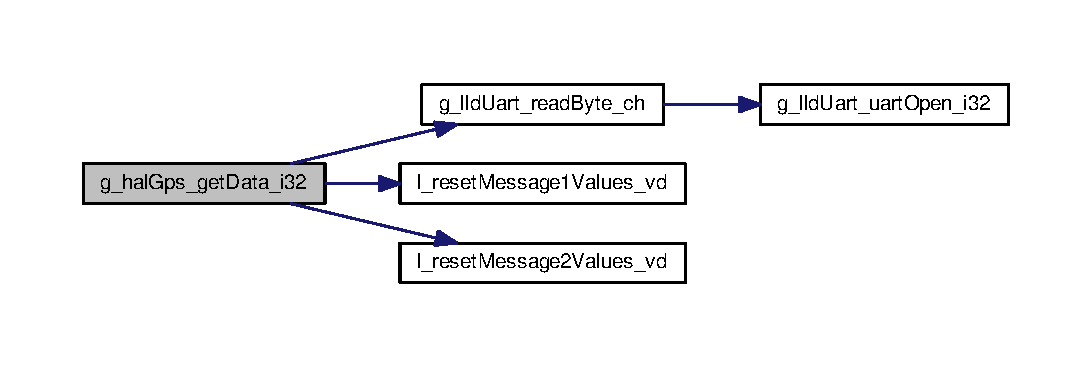
\includegraphics[width=350pt]{GPS_8h_a35a6a55e7bbec401863a903a3607c0b6_a35a6a55e7bbec401863a903a3607c0b6_cgraph}
\end{center}
\end{figure}


\hypertarget{GPS_8h_aea126d235b1db89dc964f8763565e9dc_aea126d235b1db89dc964f8763565e9dc}{\index{G\+P\+S.\+h@{G\+P\+S.\+h}!g\+\_\+hal\+Gps\+\_\+get\+Date\+\_\+ui32@{g\+\_\+hal\+Gps\+\_\+get\+Date\+\_\+ui32}}
\index{g\+\_\+hal\+Gps\+\_\+get\+Date\+\_\+ui32@{g\+\_\+hal\+Gps\+\_\+get\+Date\+\_\+ui32}!G\+P\+S.\+h@{G\+P\+S.\+h}}
\subsubsection[{g\+\_\+hal\+Gps\+\_\+get\+Date\+\_\+ui32}]{\setlength{\rightskip}{0pt plus 5cm}unsigned int g\+\_\+hal\+Gps\+\_\+get\+Date\+\_\+ui32 (
\begin{DoxyParamCaption}
\item[{void}]{}
\end{DoxyParamCaption}
)}}\label{GPS_8h_aea126d235b1db89dc964f8763565e9dc_aea126d235b1db89dc964f8763565e9dc}


Get Date from G\+P\+S module. 



 \begin{DoxyAuthor}{Author}
Oliver Breuning ( olbrgs00 ) 
\end{DoxyAuthor}
\begin{DoxyDate}{Date}
2015/04/18
\end{DoxyDate}
Interface of reading the Date which is received by the G\+P\+S module. This value is based on G\+M\+T.


\begin{DoxyParams}[1]{Parameters}
\mbox{\tt in}  & {\em no} & parameter \\
\hline
\mbox{\tt out}  & {\em Date} & of G\+P\+S receiver\\
\hline
\end{DoxyParams}


Definition at line 178 of file G\+P\+S.\+c.


\begin{DoxyCode}
179 \{
180     \textcolor{keywordflow}{return} \hyperlink{GPS_8c_a1b5b44afa58c22d0b8bb4ddedeefb31c_a1b5b44afa58c22d0b8bb4ddedeefb31c}{l\_date\_ui32};
181 \}
\end{DoxyCode}
\hypertarget{GPS_8h_adac1759b450b418dc6030def1d73b8a7_adac1759b450b418dc6030def1d73b8a7}{\index{G\+P\+S.\+h@{G\+P\+S.\+h}!g\+\_\+hal\+Gps\+\_\+get\+Direction\+\_\+f64@{g\+\_\+hal\+Gps\+\_\+get\+Direction\+\_\+f64}}
\index{g\+\_\+hal\+Gps\+\_\+get\+Direction\+\_\+f64@{g\+\_\+hal\+Gps\+\_\+get\+Direction\+\_\+f64}!G\+P\+S.\+h@{G\+P\+S.\+h}}
\subsubsection[{g\+\_\+hal\+Gps\+\_\+get\+Direction\+\_\+f64}]{\setlength{\rightskip}{0pt plus 5cm}double g\+\_\+hal\+Gps\+\_\+get\+Direction\+\_\+f64 (
\begin{DoxyParamCaption}
\item[{void}]{}
\end{DoxyParamCaption}
)}}\label{GPS_8h_adac1759b450b418dc6030def1d73b8a7_adac1759b450b418dc6030def1d73b8a7}


Get Direction from G\+P\+S module. 



 \begin{DoxyAuthor}{Author}
Oliver Breuning ( olbrgs00 ) 
\end{DoxyAuthor}
\begin{DoxyDate}{Date}
2015/04/18
\end{DoxyDate}
Interface of reading the direction of move which is calculated by the G\+P\+S module. So the Receiver moves with a velocity in the direction which is accessible here.


\begin{DoxyParams}[1]{Parameters}
\mbox{\tt in}  & {\em no} & parameter \\
\hline
\mbox{\tt out}  & {\em Direction} & of G\+P\+S receiver\\
\hline
\end{DoxyParams}


Definition at line 157 of file G\+P\+S.\+c.


\begin{DoxyCode}
158 \{
159     \textcolor{keywordflow}{return} \hyperlink{GPS_8c_a1e038699dda8c22ded8f25762733bfaf_a1e038699dda8c22ded8f25762733bfaf}{l\_direction\_f64};
160 \}
\end{DoxyCode}
\hypertarget{GPS_8h_a4f6b3f1d68b421a3a60b281326b4141b_a4f6b3f1d68b421a3a60b281326b4141b}{\index{G\+P\+S.\+h@{G\+P\+S.\+h}!g\+\_\+hal\+Gps\+\_\+get\+Fix\+\_\+ch@{g\+\_\+hal\+Gps\+\_\+get\+Fix\+\_\+ch}}
\index{g\+\_\+hal\+Gps\+\_\+get\+Fix\+\_\+ch@{g\+\_\+hal\+Gps\+\_\+get\+Fix\+\_\+ch}!G\+P\+S.\+h@{G\+P\+S.\+h}}
\subsubsection[{g\+\_\+hal\+Gps\+\_\+get\+Fix\+\_\+ch}]{\setlength{\rightskip}{0pt plus 5cm}char g\+\_\+hal\+Gps\+\_\+get\+Fix\+\_\+ch (
\begin{DoxyParamCaption}
\item[{void}]{}
\end{DoxyParamCaption}
)}}\label{GPS_8h_a4f6b3f1d68b421a3a60b281326b4141b_a4f6b3f1d68b421a3a60b281326b4141b}


Get Fix from G\+P\+S module. 



 \begin{DoxyAuthor}{Author}
Oliver Breuning ( olbrgs00 ) 
\end{DoxyAuthor}
\begin{DoxyDate}{Date}
2015/04/18
\end{DoxyDate}
Interface of reading if the G\+P\+S module has a Fix. This means it has good signal


\begin{DoxyParams}[1]{Parameters}
\mbox{\tt in}  & {\em no} & parameter \\
\hline
\mbox{\tt out}  & {\em Fix} & of G\+P\+S receiver\\
\hline
\end{DoxyParams}


Definition at line 115 of file G\+P\+S.\+c.


\begin{DoxyCode}
116 \{
117     \textcolor{keywordflow}{return} \hyperlink{GPS_8c_a5a14aebdd5ac0d06913bdeaf9cec1a9b_a5a14aebdd5ac0d06913bdeaf9cec1a9b}{l\_fix\_ch};
118 \}
\end{DoxyCode}
\hypertarget{GPS_8h_a0190aaa631556af032a2d286ebf6525a_a0190aaa631556af032a2d286ebf6525a}{\index{G\+P\+S.\+h@{G\+P\+S.\+h}!g\+\_\+hal\+Gps\+\_\+get\+Geoid\+\_\+f64@{g\+\_\+hal\+Gps\+\_\+get\+Geoid\+\_\+f64}}
\index{g\+\_\+hal\+Gps\+\_\+get\+Geoid\+\_\+f64@{g\+\_\+hal\+Gps\+\_\+get\+Geoid\+\_\+f64}!G\+P\+S.\+h@{G\+P\+S.\+h}}
\subsubsection[{g\+\_\+hal\+Gps\+\_\+get\+Geoid\+\_\+f64}]{\setlength{\rightskip}{0pt plus 5cm}double g\+\_\+hal\+Gps\+\_\+get\+Geoid\+\_\+f64 (
\begin{DoxyParamCaption}
\item[{void}]{}
\end{DoxyParamCaption}
)}}\label{GPS_8h_a0190aaa631556af032a2d286ebf6525a_a0190aaa631556af032a2d286ebf6525a}


Get Geoid from G\+P\+S module. 



 \begin{DoxyAuthor}{Author}
Oliver Breuning ( olbrgs00 ) 
\end{DoxyAuthor}
\begin{DoxyDate}{Date}
2015/04/18
\end{DoxyDate}
Interface of reading the Geoid which is received by the G\+P\+S module.


\begin{DoxyParams}[1]{Parameters}
\mbox{\tt in}  & {\em no} & parameter \\
\hline
\mbox{\tt out}  & {\em Geoid} & of G\+P\+S receiver\\
\hline
\end{DoxyParams}


Definition at line 218 of file G\+P\+S.\+c.


\begin{DoxyCode}
219 \{
220     \textcolor{keywordflow}{return} \hyperlink{GPS_8c_a2cc033719fe30335f2423a4afbe53984_a2cc033719fe30335f2423a4afbe53984}{l\_geoid\_f64};
221 \}
\end{DoxyCode}
\hypertarget{GPS_8h_ad797f33853c6d3e6f2e863c11c2822b8_ad797f33853c6d3e6f2e863c11c2822b8}{\index{G\+P\+S.\+h@{G\+P\+S.\+h}!g\+\_\+hal\+Gps\+\_\+get\+Height\+\_\+f64@{g\+\_\+hal\+Gps\+\_\+get\+Height\+\_\+f64}}
\index{g\+\_\+hal\+Gps\+\_\+get\+Height\+\_\+f64@{g\+\_\+hal\+Gps\+\_\+get\+Height\+\_\+f64}!G\+P\+S.\+h@{G\+P\+S.\+h}}
\subsubsection[{g\+\_\+hal\+Gps\+\_\+get\+Height\+\_\+f64}]{\setlength{\rightskip}{0pt plus 5cm}double g\+\_\+hal\+Gps\+\_\+get\+Height\+\_\+f64 (
\begin{DoxyParamCaption}
\item[{void}]{}
\end{DoxyParamCaption}
)}}\label{GPS_8h_ad797f33853c6d3e6f2e863c11c2822b8_ad797f33853c6d3e6f2e863c11c2822b8}


Get Height from G\+P\+S module. 



 \begin{DoxyAuthor}{Author}
Oliver Breuning ( olbrgs00 ) 
\end{DoxyAuthor}
\begin{DoxyDate}{Date}
2015/04/18
\end{DoxyDate}
Interface of reading the Height which is calculated by the G\+P\+S module.


\begin{DoxyParams}[1]{Parameters}
\mbox{\tt in}  & {\em no} & parameter \\
\hline
\mbox{\tt out}  & {\em Height} & of G\+P\+S receiver\\
\hline
\end{DoxyParams}


Definition at line 198 of file G\+P\+S.\+c.


\begin{DoxyCode}
199 \{
200     \textcolor{keywordflow}{return} \hyperlink{GPS_8c_a36e46365d7b41cc255fee53e0aa4b70a_a36e46365d7b41cc255fee53e0aa4b70a}{l\_height\_f64};
201 \}
\end{DoxyCode}
\hypertarget{GPS_8h_a0fa256f0b23aa1d53a0bf5892589dc9f_a0fa256f0b23aa1d53a0bf5892589dc9f}{\index{G\+P\+S.\+h@{G\+P\+S.\+h}!g\+\_\+hal\+Gps\+\_\+get\+Latitude\+\_\+st@{g\+\_\+hal\+Gps\+\_\+get\+Latitude\+\_\+st}}
\index{g\+\_\+hal\+Gps\+\_\+get\+Latitude\+\_\+st@{g\+\_\+hal\+Gps\+\_\+get\+Latitude\+\_\+st}!G\+P\+S.\+h@{G\+P\+S.\+h}}
\subsubsection[{g\+\_\+hal\+Gps\+\_\+get\+Latitude\+\_\+st}]{\setlength{\rightskip}{0pt plus 5cm}struct {\bf str\+Position} g\+\_\+hal\+Gps\+\_\+get\+Latitude\+\_\+st (
\begin{DoxyParamCaption}
\item[{void}]{}
\end{DoxyParamCaption}
)}}\label{GPS_8h_a0fa256f0b23aa1d53a0bf5892589dc9f_a0fa256f0b23aa1d53a0bf5892589dc9f}


Get Latitude from G\+P\+S module. 



 \begin{DoxyAuthor}{Author}
Oliver Breuning ( olbrgs00 ) 
\end{DoxyAuthor}
\begin{DoxyDate}{Date}
2015/04/18
\end{DoxyDate}
Interface of reading struct Latitude which is received by the G\+P\+S module


\begin{DoxyParams}[1]{Parameters}
\mbox{\tt in}  & {\em no} & parameter \\
\hline
\mbox{\tt out}  & {\em Latitude} & of G\+P\+S receiver\\
\hline
\end{DoxyParams}


Definition at line 94 of file G\+P\+S.\+c.


\begin{DoxyCode}
95 \{
96     \textcolor{keywordflow}{return} \hyperlink{GPS_8c_ae764c82d3318068e28af258ae1e2449c_ae764c82d3318068e28af258ae1e2449c}{l\_gps\_latitude\_st};
97 \}
\end{DoxyCode}
\hypertarget{GPS_8h_a7ee6cdd9714c51a2b74e5f3cdc2a5dca_a7ee6cdd9714c51a2b74e5f3cdc2a5dca}{\index{G\+P\+S.\+h@{G\+P\+S.\+h}!g\+\_\+hal\+Gps\+\_\+get\+Longitude\+\_\+st@{g\+\_\+hal\+Gps\+\_\+get\+Longitude\+\_\+st}}
\index{g\+\_\+hal\+Gps\+\_\+get\+Longitude\+\_\+st@{g\+\_\+hal\+Gps\+\_\+get\+Longitude\+\_\+st}!G\+P\+S.\+h@{G\+P\+S.\+h}}
\subsubsection[{g\+\_\+hal\+Gps\+\_\+get\+Longitude\+\_\+st}]{\setlength{\rightskip}{0pt plus 5cm}struct {\bf str\+Position} g\+\_\+hal\+Gps\+\_\+get\+Longitude\+\_\+st (
\begin{DoxyParamCaption}
\item[{void}]{}
\end{DoxyParamCaption}
)}}\label{GPS_8h_a7ee6cdd9714c51a2b74e5f3cdc2a5dca_a7ee6cdd9714c51a2b74e5f3cdc2a5dca}


Get Longitude from G\+P\+S module. 



 \begin{DoxyAuthor}{Author}
Oliver Breuning ( olbrgs00 ) 
\end{DoxyAuthor}
\begin{DoxyDate}{Date}
2015/04/18
\end{DoxyDate}
Interface of reading struct Longitude which is received by the G\+P\+S module


\begin{DoxyParams}[1]{Parameters}
\mbox{\tt in}  & {\em no} & parameter \\
\hline
\mbox{\tt out}  & {\em Longitude} & of G\+P\+S receiver\\
\hline
\end{DoxyParams}


Definition at line 73 of file G\+P\+S.\+c.


\begin{DoxyCode}
74 \{
75     \textcolor{keywordflow}{return} \hyperlink{GPS_8c_a5661901a87ce3f7dcd2eba20d8b505b4_a5661901a87ce3f7dcd2eba20d8b505b4}{l\_gps\_longitude\_st};
76 \}
\end{DoxyCode}
\hypertarget{GPS_8h_a64a3ef5cadfa081ca967b201352e2f8d_a64a3ef5cadfa081ca967b201352e2f8d}{\index{G\+P\+S.\+h@{G\+P\+S.\+h}!g\+\_\+hal\+Gps\+\_\+get\+Time\+\_\+ui32@{g\+\_\+hal\+Gps\+\_\+get\+Time\+\_\+ui32}}
\index{g\+\_\+hal\+Gps\+\_\+get\+Time\+\_\+ui32@{g\+\_\+hal\+Gps\+\_\+get\+Time\+\_\+ui32}!G\+P\+S.\+h@{G\+P\+S.\+h}}
\subsubsection[{g\+\_\+hal\+Gps\+\_\+get\+Time\+\_\+ui32}]{\setlength{\rightskip}{0pt plus 5cm}unsigned int g\+\_\+hal\+Gps\+\_\+get\+Time\+\_\+ui32 (
\begin{DoxyParamCaption}
\item[{void}]{}
\end{DoxyParamCaption}
)}}\label{GPS_8h_a64a3ef5cadfa081ca967b201352e2f8d_a64a3ef5cadfa081ca967b201352e2f8d}


Get Time from G\+P\+S module. 



 \begin{DoxyAuthor}{Author}
Oliver Breuning ( olbrgs00 ) 
\end{DoxyAuthor}
\begin{DoxyDate}{Date}
2015/04/18
\end{DoxyDate}
Interface of reading Time which is received by the G\+P\+S module. This value is G\+M\+T.


\begin{DoxyParams}[1]{Parameters}
\mbox{\tt in}  & {\em no} & parameter \\
\hline
\mbox{\tt out}  & {\em Time} & of G\+P\+S receiver\\
\hline
\end{DoxyParams}


Definition at line 52 of file G\+P\+S.\+c.


\begin{DoxyCode}
53 \{
54     \textcolor{keywordflow}{return} \hyperlink{GPS_8c_a365efcbf31282dcb274edd608e0824ed_a365efcbf31282dcb274edd608e0824ed}{l\_time\_ui32};
55 \}
\end{DoxyCode}
\hypertarget{GPS_8h_aae3374862ddb32be3a7f40b01661ede0_aae3374862ddb32be3a7f40b01661ede0}{\index{G\+P\+S.\+h@{G\+P\+S.\+h}!g\+\_\+hal\+Gps\+\_\+get\+Velocity\+\_\+f64@{g\+\_\+hal\+Gps\+\_\+get\+Velocity\+\_\+f64}}
\index{g\+\_\+hal\+Gps\+\_\+get\+Velocity\+\_\+f64@{g\+\_\+hal\+Gps\+\_\+get\+Velocity\+\_\+f64}!G\+P\+S.\+h@{G\+P\+S.\+h}}
\subsubsection[{g\+\_\+hal\+Gps\+\_\+get\+Velocity\+\_\+f64}]{\setlength{\rightskip}{0pt plus 5cm}double g\+\_\+hal\+Gps\+\_\+get\+Velocity\+\_\+f64 (
\begin{DoxyParamCaption}
\item[{void}]{}
\end{DoxyParamCaption}
)}}\label{GPS_8h_aae3374862ddb32be3a7f40b01661ede0_aae3374862ddb32be3a7f40b01661ede0}


Get Velocity from G\+P\+S module. 



 \begin{DoxyAuthor}{Author}
Oliver Breuning ( olbrgs00 ) 
\end{DoxyAuthor}
\begin{DoxyDate}{Date}
2015/04/18
\end{DoxyDate}
Interface of reading the velocity which is calculated by the G\+P\+S module. So the Receiver moves with a velocity which is accessible here in a certain direction.


\begin{DoxyParams}[1]{Parameters}
\mbox{\tt in}  & {\em no} & parameter \\
\hline
\mbox{\tt out}  & {\em Velocity} & of G\+P\+S receiver\\
\hline
\end{DoxyParams}


Definition at line 136 of file G\+P\+S.\+c.


\begin{DoxyCode}
137 \{
138     \textcolor{keywordflow}{return} \hyperlink{GPS_8c_af14216f61e92eb4cb399d157299c8d12_af14216f61e92eb4cb399d157299c8d12}{l\_velocity\_f64};
139 \}
\end{DoxyCode}
\hypertarget{GPS_8h_a0bf6b6abfd6136e50bd5d35a76ee8d0b_a0bf6b6abfd6136e50bd5d35a76ee8d0b}{\index{G\+P\+S.\+h@{G\+P\+S.\+h}!l\+\_\+reset\+Message1\+Values\+\_\+vd@{l\+\_\+reset\+Message1\+Values\+\_\+vd}}
\index{l\+\_\+reset\+Message1\+Values\+\_\+vd@{l\+\_\+reset\+Message1\+Values\+\_\+vd}!G\+P\+S.\+h@{G\+P\+S.\+h}}
\subsubsection[{l\+\_\+reset\+Message1\+Values\+\_\+vd}]{\setlength{\rightskip}{0pt plus 5cm}void l\+\_\+reset\+Message1\+Values\+\_\+vd (
\begin{DoxyParamCaption}
\item[{void}]{}
\end{DoxyParamCaption}
)}}\label{GPS_8h_a0bf6b6abfd6136e50bd5d35a76ee8d0b_a0bf6b6abfd6136e50bd5d35a76ee8d0b}


Reset Values of Message 1. 



 \begin{DoxyAuthor}{Author}
Oliver Breuning ( olbrgs00 ) 
\end{DoxyAuthor}
\begin{DoxyDate}{Date}
2015/04/21
\end{DoxyDate}
Resetting the values of Message 1 -\/ \$\+G\+P\+G\+G\+A .... when a new message arrives


\begin{DoxyParams}[1]{Parameters}
\mbox{\tt in}  & {\em no} & parameter \\
\hline
\mbox{\tt out}  & {\em no} & parameter\\
\hline
\end{DoxyParams}


Definition at line 238 of file G\+P\+S.\+c.


\begin{DoxyCode}
239 \{
240     \hyperlink{GPS_8c_a365efcbf31282dcb274edd608e0824ed_a365efcbf31282dcb274edd608e0824ed}{l\_time\_ui32}=0;
241     \hyperlink{GPS_8c_a5661901a87ce3f7dcd2eba20d8b505b4_a5661901a87ce3f7dcd2eba20d8b505b4}{l\_gps\_longitude\_st}.\hyperlink{structstrPosition_ac060af7d7963812c116c24cdb861f184_ac060af7d7963812c116c24cdb861f184}{l\_degree\_ui32}=0;
242     \hyperlink{GPS_8c_a5661901a87ce3f7dcd2eba20d8b505b4_a5661901a87ce3f7dcd2eba20d8b505b4}{l\_gps\_longitude\_st}.\hyperlink{structstrPosition_a5489ef5e7f8e6ee45990b262c80a7819_a5489ef5e7f8e6ee45990b262c80a7819}{l\_minutes\_ui32}=0;
243     \hyperlink{GPS_8c_a5661901a87ce3f7dcd2eba20d8b505b4_a5661901a87ce3f7dcd2eba20d8b505b4}{l\_gps\_longitude\_st}.\hyperlink{structstrPosition_ae62d246c481c611e168ea86b70d5313b_ae62d246c481c611e168ea86b70d5313b}{l\_seconds\_f64}=0;
244     \hyperlink{GPS_8c_a5661901a87ce3f7dcd2eba20d8b505b4_a5661901a87ce3f7dcd2eba20d8b505b4}{l\_gps\_longitude\_st}.\hyperlink{structstrPosition_aa39fed1d421cb2260d0ef7157c3c00d0_aa39fed1d421cb2260d0ef7157c3c00d0}{l\_cardinalDirection\_ch}=\textcolor{charliteral}{' '};
245     \hyperlink{GPS_8c_ae764c82d3318068e28af258ae1e2449c_ae764c82d3318068e28af258ae1e2449c}{l\_gps\_latitude\_st}.\hyperlink{structstrPosition_ac060af7d7963812c116c24cdb861f184_ac060af7d7963812c116c24cdb861f184}{l\_degree\_ui32}=0;
246     \hyperlink{GPS_8c_ae764c82d3318068e28af258ae1e2449c_ae764c82d3318068e28af258ae1e2449c}{l\_gps\_latitude\_st}.\hyperlink{structstrPosition_a5489ef5e7f8e6ee45990b262c80a7819_a5489ef5e7f8e6ee45990b262c80a7819}{l\_minutes\_ui32}=0;
247     \hyperlink{GPS_8c_ae764c82d3318068e28af258ae1e2449c_ae764c82d3318068e28af258ae1e2449c}{l\_gps\_latitude\_st}.\hyperlink{structstrPosition_ae62d246c481c611e168ea86b70d5313b_ae62d246c481c611e168ea86b70d5313b}{l\_seconds\_f64}=0;
248     \hyperlink{GPS_8c_ae764c82d3318068e28af258ae1e2449c_ae764c82d3318068e28af258ae1e2449c}{l\_gps\_latitude\_st}.\hyperlink{structstrPosition_aa39fed1d421cb2260d0ef7157c3c00d0_aa39fed1d421cb2260d0ef7157c3c00d0}{l\_cardinalDirection\_ch}=\textcolor{charliteral}{' '};
249     \hyperlink{GPS_8c_a36e46365d7b41cc255fee53e0aa4b70a_a36e46365d7b41cc255fee53e0aa4b70a}{l\_height\_f64}=0;
250     \hyperlink{GPS_8c_a2cc033719fe30335f2423a4afbe53984_a2cc033719fe30335f2423a4afbe53984}{l\_geoid\_f64}=0;
251 \}
\end{DoxyCode}


Here is the caller graph for this function\+:
\nopagebreak
\begin{figure}[H]
\begin{center}
\leavevmode
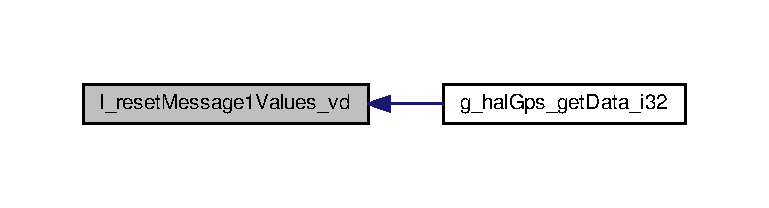
\includegraphics[width=350pt]{GPS_8h_a0bf6b6abfd6136e50bd5d35a76ee8d0b_a0bf6b6abfd6136e50bd5d35a76ee8d0b_icgraph}
\end{center}
\end{figure}


\hypertarget{GPS_8h_aa9c4ab6055264c0121813e5233cd3de0_aa9c4ab6055264c0121813e5233cd3de0}{\index{G\+P\+S.\+h@{G\+P\+S.\+h}!l\+\_\+reset\+Message2\+Values\+\_\+vd@{l\+\_\+reset\+Message2\+Values\+\_\+vd}}
\index{l\+\_\+reset\+Message2\+Values\+\_\+vd@{l\+\_\+reset\+Message2\+Values\+\_\+vd}!G\+P\+S.\+h@{G\+P\+S.\+h}}
\subsubsection[{l\+\_\+reset\+Message2\+Values\+\_\+vd}]{\setlength{\rightskip}{0pt plus 5cm}void l\+\_\+reset\+Message2\+Values\+\_\+vd (
\begin{DoxyParamCaption}
\item[{void}]{}
\end{DoxyParamCaption}
)}}\label{GPS_8h_aa9c4ab6055264c0121813e5233cd3de0_aa9c4ab6055264c0121813e5233cd3de0}


Reset Values of Message 2. 



 \begin{DoxyAuthor}{Author}
Oliver Breuning ( olbrgs00 ) 
\end{DoxyAuthor}
\begin{DoxyDate}{Date}
2015/04/21
\end{DoxyDate}
Resetting the values of Message 2 -\/ \$\+G\+P\+R\+M\+C .... when a new message arrives


\begin{DoxyParams}[1]{Parameters}
\mbox{\tt in}  & {\em no} & parameter \\
\hline
\mbox{\tt out}  & {\em no} & parameter\\
\hline
\end{DoxyParams}


Definition at line 268 of file G\+P\+S.\+c.


\begin{DoxyCode}
269 \{
270     \hyperlink{GPS_8c_a365efcbf31282dcb274edd608e0824ed_a365efcbf31282dcb274edd608e0824ed}{l\_time\_ui32}=0;
271     \hyperlink{GPS_8c_a5a14aebdd5ac0d06913bdeaf9cec1a9b_a5a14aebdd5ac0d06913bdeaf9cec1a9b}{l\_fix\_ch}=\textcolor{charliteral}{' '};
272     \hyperlink{GPS_8c_a5661901a87ce3f7dcd2eba20d8b505b4_a5661901a87ce3f7dcd2eba20d8b505b4}{l\_gps\_longitude\_st}.\hyperlink{structstrPosition_ac060af7d7963812c116c24cdb861f184_ac060af7d7963812c116c24cdb861f184}{l\_degree\_ui32}=0;
273     \hyperlink{GPS_8c_a5661901a87ce3f7dcd2eba20d8b505b4_a5661901a87ce3f7dcd2eba20d8b505b4}{l\_gps\_longitude\_st}.\hyperlink{structstrPosition_a5489ef5e7f8e6ee45990b262c80a7819_a5489ef5e7f8e6ee45990b262c80a7819}{l\_minutes\_ui32}=0;
274     \hyperlink{GPS_8c_a5661901a87ce3f7dcd2eba20d8b505b4_a5661901a87ce3f7dcd2eba20d8b505b4}{l\_gps\_longitude\_st}.\hyperlink{structstrPosition_ae62d246c481c611e168ea86b70d5313b_ae62d246c481c611e168ea86b70d5313b}{l\_seconds\_f64}=0;
275     \hyperlink{GPS_8c_a5661901a87ce3f7dcd2eba20d8b505b4_a5661901a87ce3f7dcd2eba20d8b505b4}{l\_gps\_longitude\_st}.\hyperlink{structstrPosition_aa39fed1d421cb2260d0ef7157c3c00d0_aa39fed1d421cb2260d0ef7157c3c00d0}{l\_cardinalDirection\_ch}=\textcolor{charliteral}{' '};
276     \hyperlink{GPS_8c_ae764c82d3318068e28af258ae1e2449c_ae764c82d3318068e28af258ae1e2449c}{l\_gps\_latitude\_st}.\hyperlink{structstrPosition_ac060af7d7963812c116c24cdb861f184_ac060af7d7963812c116c24cdb861f184}{l\_degree\_ui32}=0;
277     \hyperlink{GPS_8c_ae764c82d3318068e28af258ae1e2449c_ae764c82d3318068e28af258ae1e2449c}{l\_gps\_latitude\_st}.\hyperlink{structstrPosition_a5489ef5e7f8e6ee45990b262c80a7819_a5489ef5e7f8e6ee45990b262c80a7819}{l\_minutes\_ui32}=0;
278     \hyperlink{GPS_8c_ae764c82d3318068e28af258ae1e2449c_ae764c82d3318068e28af258ae1e2449c}{l\_gps\_latitude\_st}.\hyperlink{structstrPosition_ae62d246c481c611e168ea86b70d5313b_ae62d246c481c611e168ea86b70d5313b}{l\_seconds\_f64}=0;
279     \hyperlink{GPS_8c_ae764c82d3318068e28af258ae1e2449c_ae764c82d3318068e28af258ae1e2449c}{l\_gps\_latitude\_st}.\hyperlink{structstrPosition_aa39fed1d421cb2260d0ef7157c3c00d0_aa39fed1d421cb2260d0ef7157c3c00d0}{l\_cardinalDirection\_ch}=\textcolor{charliteral}{' '};
280     \hyperlink{GPS_8c_af14216f61e92eb4cb399d157299c8d12_af14216f61e92eb4cb399d157299c8d12}{l\_velocity\_f64}=0;
281     \hyperlink{GPS_8c_a1e038699dda8c22ded8f25762733bfaf_a1e038699dda8c22ded8f25762733bfaf}{l\_direction\_f64}=0;
282     \hyperlink{GPS_8c_a1b5b44afa58c22d0b8bb4ddedeefb31c_a1b5b44afa58c22d0b8bb4ddedeefb31c}{l\_date\_ui32}=0;
283 \}
\end{DoxyCode}


Here is the caller graph for this function\+:
\nopagebreak
\begin{figure}[H]
\begin{center}
\leavevmode
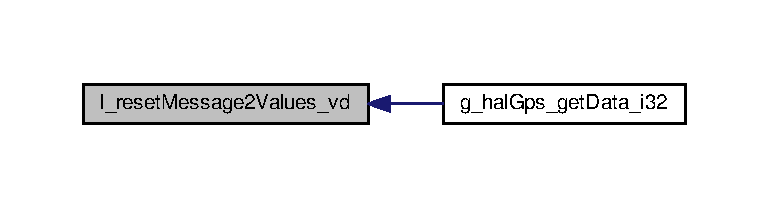
\includegraphics[width=350pt]{GPS_8h_aa9c4ab6055264c0121813e5233cd3de0_aa9c4ab6055264c0121813e5233cd3de0_icgraph}
\end{center}
\end{figure}



\hypertarget{accMag_8c}{\section{hal/\+I\+M\+U/acc\+Mag/acc\+Mag.c File Reference}
\label{accMag_8c}\index{hal/\+I\+M\+U/acc\+Mag/acc\+Mag.\+c@{hal/\+I\+M\+U/acc\+Mag/acc\+Mag.\+c}}
}
{\ttfamily \#include \char`\"{}../../\+L\+L\+D\+\_\+\+I\+F/\+L\+L\+D\+\_\+\+I2\+C.\+h\char`\"{}}\\*
{\ttfamily \#include \char`\"{}acc\+Mag.\+h\char`\"{}}\\*
{\ttfamily \#include $<$limits.\+h$>$}\\*
Include dependency graph for acc\+Mag.\+c\+:
\nopagebreak
\begin{figure}[H]
\begin{center}
\leavevmode
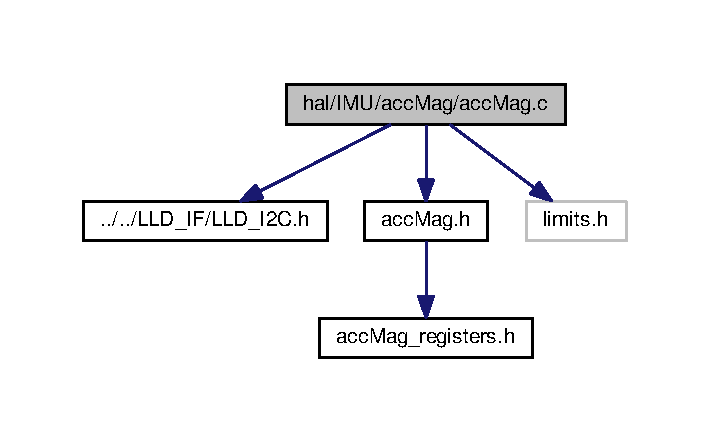
\includegraphics[width=341pt]{accMag_8c__incl}
\end{center}
\end{figure}
\subsection*{Functions}
\begin{DoxyCompactItemize}
\item 
\hyperlink{structhalAccmag__dataContainer}{hal\+Accmag\+\_\+data\+Container} \hyperlink{accMag_8c_a3914b0d0b4d88f06880b47766f844fc8_a3914b0d0b4d88f06880b47766f844fc8}{g\+\_\+hal\+Accmag\+\_\+get\+Acc\+Mag\+Container\+\_\+st} (void)
\begin{DoxyCompactList}\small\item\em Get complete data container (acceleration \& compass) \end{DoxyCompactList}\item 
\hyperlink{structhalAccmag__3dDoubleVector}{hal\+Accmag\+\_\+3d\+Double\+Vector} \hyperlink{accMag_8c_aebfdb7e3d86187e1fecee863424aa3fc_aebfdb7e3d86187e1fecee863424aa3fc}{g\+\_\+hal\+Accmag\+\_\+get\+Acc\+Vector\+\_\+st} (void)
\begin{DoxyCompactList}\small\item\em Get current state of acceleration. \end{DoxyCompactList}\item 
\hyperlink{structhalAccmag__3dDoubleVector}{hal\+Accmag\+\_\+3d\+Double\+Vector} \hyperlink{accMag_8c_ad4f25c6a1f31b6eb494243aa0706986a_ad4f25c6a1f31b6eb494243aa0706986a}{g\+\_\+hal\+Accmag\+\_\+get\+Mag\+Vector\+\_\+st} (void)
\begin{DoxyCompactList}\small\item\em Get current state of compass. \end{DoxyCompactList}\item 
unsigned int \hyperlink{accMag_8c_ab936c0ac53ff9ba47a138e841a6ba474_ab936c0ac53ff9ba47a138e841a6ba474}{g\+\_\+hal\+Accmag\+\_\+init\+Sensor\+\_\+bl} (void)
\begin{DoxyCompactList}\small\item\em Initialize sensor. \end{DoxyCompactList}\item 
unsigned int \hyperlink{accMag_8c_ad5f9d3a28348a9889f9afecde79606f6_ad5f9d3a28348a9889f9afecde79606f6}{g\+\_\+hal\+Accmag\+\_\+trigger\+Acc\+Update\+\_\+bl} (void)
\begin{DoxyCompactList}\small\item\em Trigger a new measurement of the accelerometer. \end{DoxyCompactList}\item 
unsigned int \hyperlink{accMag_8c_a98cf3442152a9ae213517936f7b37fe0_a98cf3442152a9ae213517936f7b37fe0}{g\+\_\+hal\+Accmag\+\_\+trigger\+Full\+Update\+\_\+bl} (void)
\begin{DoxyCompactList}\small\item\em Trigger a new measurement of both sensors. \end{DoxyCompactList}\item 
unsigned int \hyperlink{accMag_8c_afdbd4ece113ff4859718b678150d069a_afdbd4ece113ff4859718b678150d069a}{g\+\_\+hal\+Accmag\+\_\+trigger\+Mag\+Update\+\_\+bl} (void)
\begin{DoxyCompactList}\small\item\em Trigger a new measurement of the magnetometer. \end{DoxyCompactList}\item 
static double \hyperlink{accMag_8c_a3f6ef9cd19c5f23888aaca4b1ba34ecc_a3f6ef9cd19c5f23888aaca4b1ba34ecc}{l\+\_\+convert\+Acc\+Raw\+To\+S\+I\+Unit\+\_\+f64} (signed short f\+\_\+raw\+Acc\+Val\+\_\+i16, unsigned char f\+\_\+scaling\+Value\+G\+\_\+ui8)
\begin{DoxyCompactList}\small\item\em Converts raw sensor values of the accelerometer into S\+I unit. \end{DoxyCompactList}\item 
static double \hyperlink{accMag_8c_a1f0866c5afdce148afc09ed1c5a8018f_a1f0866c5afdce148afc09ed1c5a8018f}{l\+\_\+convert\+Mag\+Raw\+To\+S\+I\+Unit\+\_\+f64} (signed short f\+\_\+raw\+Mag\+Val\+\_\+i16, unsigned char f\+\_\+scaling\+Value\+Gauss\+\_\+ui8)
\begin{DoxyCompactList}\small\item\em Converts raw sensor values of the magnetometer into S\+I unit. \end{DoxyCompactList}\item 
static unsigned char \hyperlink{accMag_8c_abaacf0917ab7bbc9b9d13b9aeb31afd1_abaacf0917ab7bbc9b9d13b9aeb31afd1}{l\+\_\+read\+I2c\+Byte\+\_\+ui8} (unsigned char f\+\_\+register\+Addr\+\_\+ui8)
\begin{DoxyCompactList}\small\item\em Wrapper function to read a single byte register of L\+S\+M303\+D. \end{DoxyCompactList}\item 
static unsigned int \hyperlink{accMag_8c_a84dc4f1647051d5c34296705fa1f236b_a84dc4f1647051d5c34296705fa1f236b}{l\+\_\+read\+I2c\+Byte\+Stream\+\_\+bl} (unsigned char f\+\_\+start\+Register\+Addr\+\_\+ui8, const unsigned char $\ast$f\+\_\+read\+Destination\+Buffer\+\_\+pui8, unsigned int f\+\_\+num\+Of\+Bytes\+To\+Read\+\_\+ui32)
\begin{DoxyCompactList}\small\item\em Wrapper function to read byte stream to registers of L\+S\+M303\+D. \end{DoxyCompactList}\item 
static signed short \hyperlink{accMag_8c_aad5863a0667702ddb0040ab517463069_aad5863a0667702ddb0040ab517463069}{l\+\_\+two\+Comp\+Of16\+Bit\+\_\+ui16} (unsigned char f\+\_\+lsb\+\_\+ui8, unsigned char f\+\_\+msb\+\_\+ui8)
\begin{DoxyCompactList}\small\item\em Complement of twos of a 16 bit integer. \end{DoxyCompactList}\item 
static unsigned int \hyperlink{accMag_8c_a5cef87c49dd46218e083a0c95abb9a9b_a5cef87c49dd46218e083a0c95abb9a9b}{l\+\_\+update\+Sensor\+State\+\_\+vd} (\hyperlink{accMag_8h_a648cc7f506bdd006d657bf0c2fc393b8_a648cc7f506bdd006d657bf0c2fc393b8}{hal\+Accmag\+\_\+sensor\+Select} f\+\_\+sensor\+\_\+en)
\begin{DoxyCompactList}\small\item\em Trigger a update of the current sensor state data. \end{DoxyCompactList}\item 
static unsigned int \hyperlink{accMag_8c_af4a867d90abb126d82ba14ea2619f305_af4a867d90abb126d82ba14ea2619f305}{l\+\_\+write\+I2c\+Byte\+Stream\+\_\+bl} (unsigned char f\+\_\+start\+Register\+Addr\+\_\+ui8, const unsigned char $\ast$const f\+\_\+byte\+Stream\+To\+Write\+\_\+pui8, unsigned int f\+\_\+num\+Of\+Bytes\+\_\+ui32)
\begin{DoxyCompactList}\small\item\em Wrapper function to write a single byte register of L\+S\+M303\+D. \end{DoxyCompactList}\end{DoxyCompactItemize}
\subsection*{Variables}
\begin{DoxyCompactItemize}
\item 
static \hyperlink{structhalAccmag__dataContainer}{hal\+Accmag\+\_\+data\+Container} \hyperlink{accMag_8c_a421eb1956f3c2b98d7a4505bc13b049e_a421eb1956f3c2b98d7a4505bc13b049e}{m\+\_\+hal\+Accmag\+\_\+sensor\+State\+\_\+st}
\end{DoxyCompactItemize}


\subsection{Function Documentation}
\hypertarget{accMag_8c_a3914b0d0b4d88f06880b47766f844fc8_a3914b0d0b4d88f06880b47766f844fc8}{\index{acc\+Mag.\+c@{acc\+Mag.\+c}!g\+\_\+hal\+Accmag\+\_\+get\+Acc\+Mag\+Container\+\_\+st@{g\+\_\+hal\+Accmag\+\_\+get\+Acc\+Mag\+Container\+\_\+st}}
\index{g\+\_\+hal\+Accmag\+\_\+get\+Acc\+Mag\+Container\+\_\+st@{g\+\_\+hal\+Accmag\+\_\+get\+Acc\+Mag\+Container\+\_\+st}!acc\+Mag.\+c@{acc\+Mag.\+c}}
\subsubsection[{g\+\_\+hal\+Accmag\+\_\+get\+Acc\+Mag\+Container\+\_\+st}]{\setlength{\rightskip}{0pt plus 5cm}{\bf hal\+Accmag\+\_\+data\+Container} g\+\_\+hal\+Accmag\+\_\+get\+Acc\+Mag\+Container\+\_\+st (
\begin{DoxyParamCaption}
\item[{void}]{}
\end{DoxyParamCaption}
)}}\label{accMag_8c_a3914b0d0b4d88f06880b47766f844fc8_a3914b0d0b4d88f06880b47766f844fc8}


Get complete data container (acceleration \& compass) 



 \begin{DoxyAuthor}{Author}
Juergen Schmidt (juscgs00) 
\end{DoxyAuthor}
\begin{DoxyDate}{Date}
2014/05/05
\end{DoxyDate}
This function returns the complete accelerometer and magnetometer state. Attention\+: To retrieve a new measurement a measurement trigger is to be called first!


\begin{DoxyParams}[1]{Parameters}
\mbox{\tt out}  & {\em Container} & with compass and acceleration data\\
\hline
\end{DoxyParams}


Definition at line 653 of file acc\+Mag.\+c.


\begin{DoxyCode}
654 \{
655     \textcolor{keywordflow}{return} \hyperlink{accMag_8c_a421eb1956f3c2b98d7a4505bc13b049e_a421eb1956f3c2b98d7a4505bc13b049e}{m\_halAccmag\_sensorState\_st};
656 \}
\end{DoxyCode}
\hypertarget{accMag_8c_aebfdb7e3d86187e1fecee863424aa3fc_aebfdb7e3d86187e1fecee863424aa3fc}{\index{acc\+Mag.\+c@{acc\+Mag.\+c}!g\+\_\+hal\+Accmag\+\_\+get\+Acc\+Vector\+\_\+st@{g\+\_\+hal\+Accmag\+\_\+get\+Acc\+Vector\+\_\+st}}
\index{g\+\_\+hal\+Accmag\+\_\+get\+Acc\+Vector\+\_\+st@{g\+\_\+hal\+Accmag\+\_\+get\+Acc\+Vector\+\_\+st}!acc\+Mag.\+c@{acc\+Mag.\+c}}
\subsubsection[{g\+\_\+hal\+Accmag\+\_\+get\+Acc\+Vector\+\_\+st}]{\setlength{\rightskip}{0pt plus 5cm}{\bf hal\+Accmag\+\_\+3d\+Double\+Vector} g\+\_\+hal\+Accmag\+\_\+get\+Acc\+Vector\+\_\+st (
\begin{DoxyParamCaption}
\item[{void}]{}
\end{DoxyParamCaption}
)}}\label{accMag_8c_aebfdb7e3d86187e1fecee863424aa3fc_aebfdb7e3d86187e1fecee863424aa3fc}


Get current state of acceleration. 



 \begin{DoxyAuthor}{Author}
Juergen Schmidt (juscgs00) 
\end{DoxyAuthor}
\begin{DoxyDate}{Date}
2014/05/05
\end{DoxyDate}
This function returns the current state of the accelerometer.~\newline
 Attention\+: To retrieve a new measurement the measurement trigger is to be called first!


\begin{DoxyParams}[1]{Parameters}
\mbox{\tt out}  & {\em 3\+D} & vector of acceleration components (x,y,z)\\
\hline
\end{DoxyParams}


Definition at line 611 of file acc\+Mag.\+c.


\begin{DoxyCode}
612 \{
613     \textcolor{keywordflow}{return} \hyperlink{accMag_8c_a421eb1956f3c2b98d7a4505bc13b049e_a421eb1956f3c2b98d7a4505bc13b049e}{m\_halAccmag\_sensorState\_st}.\hyperlink{structhalAccmag__dataContainer_afc3847993eed1c8f1e67028ad6d2a6cf_afc3847993eed1c8f1e67028ad6d2a6cf}{acc};
614 \}
\end{DoxyCode}


Here is the caller graph for this function\+:
\nopagebreak
\begin{figure}[H]
\begin{center}
\leavevmode
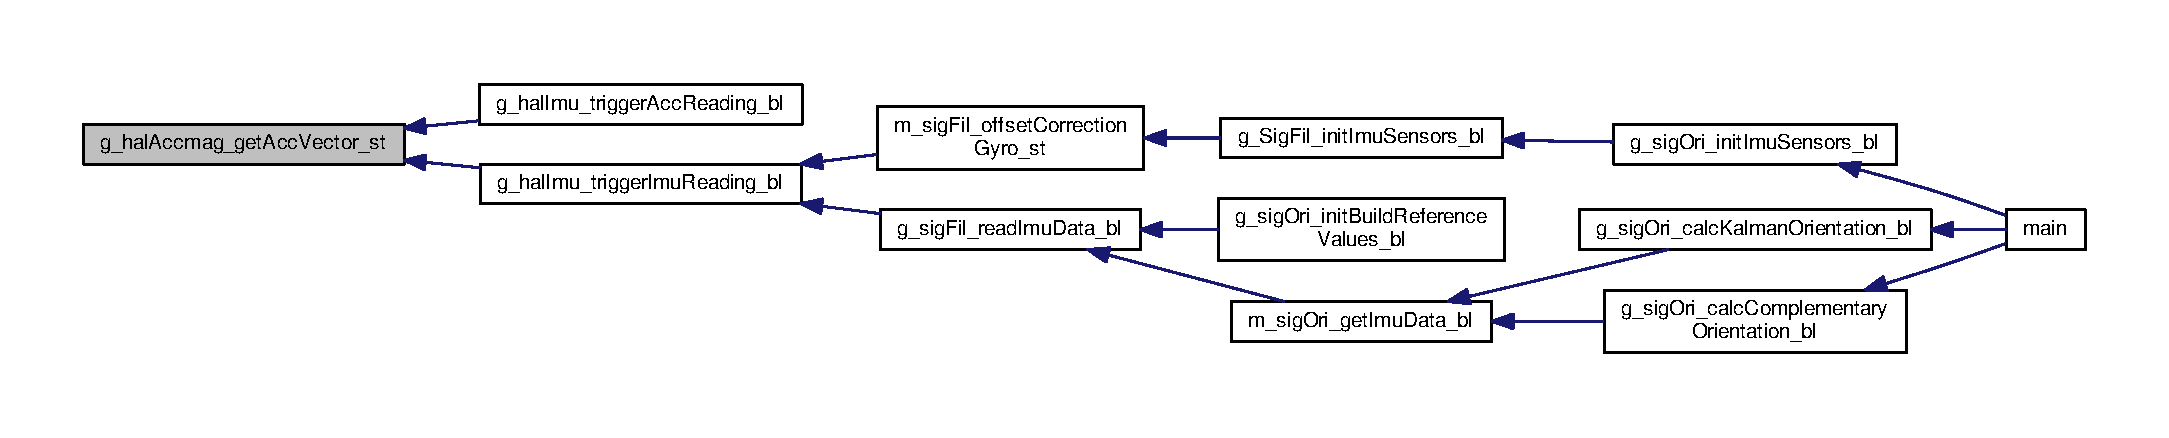
\includegraphics[width=350pt]{accMag_8c_aebfdb7e3d86187e1fecee863424aa3fc_aebfdb7e3d86187e1fecee863424aa3fc_icgraph}
\end{center}
\end{figure}


\hypertarget{accMag_8c_ad4f25c6a1f31b6eb494243aa0706986a_ad4f25c6a1f31b6eb494243aa0706986a}{\index{acc\+Mag.\+c@{acc\+Mag.\+c}!g\+\_\+hal\+Accmag\+\_\+get\+Mag\+Vector\+\_\+st@{g\+\_\+hal\+Accmag\+\_\+get\+Mag\+Vector\+\_\+st}}
\index{g\+\_\+hal\+Accmag\+\_\+get\+Mag\+Vector\+\_\+st@{g\+\_\+hal\+Accmag\+\_\+get\+Mag\+Vector\+\_\+st}!acc\+Mag.\+c@{acc\+Mag.\+c}}
\subsubsection[{g\+\_\+hal\+Accmag\+\_\+get\+Mag\+Vector\+\_\+st}]{\setlength{\rightskip}{0pt plus 5cm}{\bf hal\+Accmag\+\_\+3d\+Double\+Vector} g\+\_\+hal\+Accmag\+\_\+get\+Mag\+Vector\+\_\+st (
\begin{DoxyParamCaption}
\item[{void}]{}
\end{DoxyParamCaption}
)}}\label{accMag_8c_ad4f25c6a1f31b6eb494243aa0706986a_ad4f25c6a1f31b6eb494243aa0706986a}


Get current state of compass. 



 \begin{DoxyAuthor}{Author}
Juergen Schmidt (juscgs00) 
\end{DoxyAuthor}
\begin{DoxyDate}{Date}
2014/05/05
\end{DoxyDate}
This function returns the current state of the magnetometer.~\newline
 Attention\+: To retrieve a new measurement the measurement trigger is to be called first!


\begin{DoxyParams}[1]{Parameters}
\mbox{\tt out}  & {\em 3\+D} & vector of compass components (x,y,z)\\
\hline
\end{DoxyParams}


Definition at line 632 of file acc\+Mag.\+c.


\begin{DoxyCode}
633 \{
634     \textcolor{keywordflow}{return} \hyperlink{accMag_8c_a421eb1956f3c2b98d7a4505bc13b049e_a421eb1956f3c2b98d7a4505bc13b049e}{m\_halAccmag\_sensorState\_st}.\hyperlink{structhalAccmag__dataContainer_a903681a66ce49c39267aa66d471812f7_a903681a66ce49c39267aa66d471812f7}{mag};
635 \}
\end{DoxyCode}


Here is the caller graph for this function\+:
\nopagebreak
\begin{figure}[H]
\begin{center}
\leavevmode
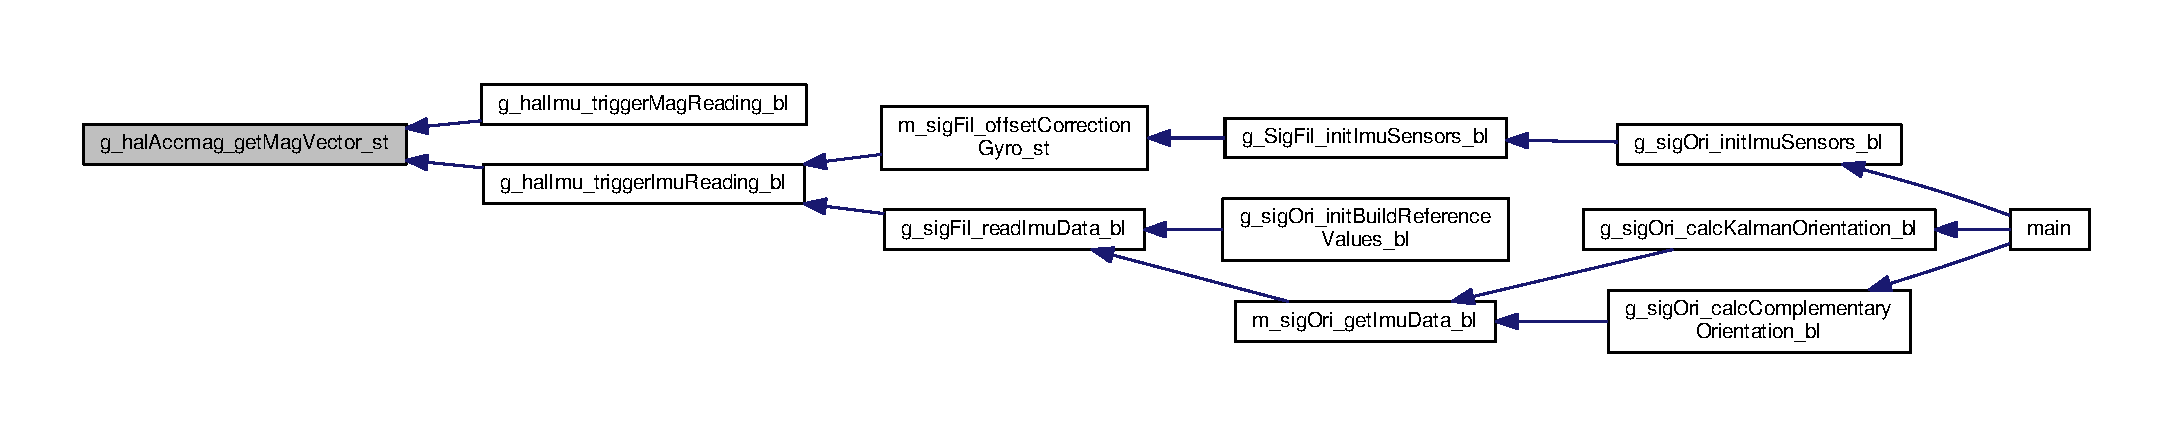
\includegraphics[width=350pt]{accMag_8c_ad4f25c6a1f31b6eb494243aa0706986a_ad4f25c6a1f31b6eb494243aa0706986a_icgraph}
\end{center}
\end{figure}


\hypertarget{accMag_8c_ab936c0ac53ff9ba47a138e841a6ba474_ab936c0ac53ff9ba47a138e841a6ba474}{\index{acc\+Mag.\+c@{acc\+Mag.\+c}!g\+\_\+hal\+Accmag\+\_\+init\+Sensor\+\_\+bl@{g\+\_\+hal\+Accmag\+\_\+init\+Sensor\+\_\+bl}}
\index{g\+\_\+hal\+Accmag\+\_\+init\+Sensor\+\_\+bl@{g\+\_\+hal\+Accmag\+\_\+init\+Sensor\+\_\+bl}!acc\+Mag.\+c@{acc\+Mag.\+c}}
\subsubsection[{g\+\_\+hal\+Accmag\+\_\+init\+Sensor\+\_\+bl}]{\setlength{\rightskip}{0pt plus 5cm}unsigned int g\+\_\+hal\+Accmag\+\_\+init\+Sensor\+\_\+bl (
\begin{DoxyParamCaption}
\item[{void}]{}
\end{DoxyParamCaption}
)}}\label{accMag_8c_ab936c0ac53ff9ba47a138e841a6ba474_ab936c0ac53ff9ba47a138e841a6ba474}


Initialize sensor. 



 \begin{DoxyAuthor}{Author}
Juergen Schmidt (juscgs00) 
\end{DoxyAuthor}
\begin{DoxyDate}{Date}
2014/05/05
\end{DoxyDate}
Sends all commands on I2\+C to initialize the acc.-\/ and magnetometer. It uses on big 8 byte config buffer to set all necessary bits. This way, a burst write to the control registers of L\+S\+M303\+D is performed to reduce the I2\+C bus load.


\begin{DoxyParams}[1]{Parameters}
\mbox{\tt out}  & {\em returns} & a boolean value, indicating the occurrence of failures~\newline
 0 .... indicates success (no errors)~\newline
 1 .... indicates failed (some errors)\\
\hline
\end{DoxyParams}


Definition at line 472 of file acc\+Mag.\+c.


\begin{DoxyCode}
473 \{
474     \textcolor{keywordtype}{unsigned} \textcolor{keywordtype}{char} l\_configRegisters\_rg8ui8[8];  \textcolor{comment}{//buffer for 8 control register bytes}
475 
476     \textcolor{comment}{//Identify sensor}
477     \textcolor{keywordflow}{if} ( \hyperlink{accMag_8c_abaacf0917ab7bbc9b9d13b9aeb31afd1_abaacf0917ab7bbc9b9d13b9aeb31afd1}{l\_readI2cByte\_ui8}( \hyperlink{accMag__registers_8h_ab6a6aee06d3166d947d3a70063f416b3_ab6a6aee06d3166d947d3a70063f416b3}{M\_HAL\_ACCMAG\_WHO\_AM\_I\_UI8} ) != 
      \hyperlink{accMag__registers_8h_a950216893447ed37b695528e45c57618_a950216893447ed37b695528e45c57618}{M\_HAL\_ACCMAG\_WHO\_AM\_I\_PATTERN\_UI8} )
478     \{
479         \textcolor{comment}{// sensor could not be identified --> abort initialization}
480         \textcolor{keywordflow}{return} \hyperlink{accMag_8h_a29da5c251bf0c3b1c7ed7da3c3269d9f_a29da5c251bf0c3b1c7ed7da3c3269d9f}{M\_HAL\_ACCMAG\_FAILED\_BL};
481     \}
482 
483     \textcolor{comment}{/*}
484 \textcolor{comment}{     * ACCELEROMETER}
485 \textcolor{comment}{     */}
486     \textcolor{comment}{// CTRL0: no FIFO (default values)}
487     l\_configRegisters\_rg8ui8[0] = 0b00000000;
488 
489     \textcolor{comment}{// CTRL1: Enable accelerometer, 800Hz sampling}
490     l\_configRegisters\_rg8ui8[1] = (     \hyperlink{accMag__registers_8h_a2488215dc8f9f76a8a9ffb5b6ea4a4fe_a2488215dc8f9f76a8a9ffb5b6ea4a4fe}{M\_HAL\_ACCMAG\_CTRL1\_MASK\_AXEN\_UI8}
491             |   \hyperlink{accMag__registers_8h_a0e5dcc95c72afb32f40fa3bfb61a7835_a0e5dcc95c72afb32f40fa3bfb61a7835}{M\_HAL\_ACCMAG\_CTRL1\_MASK\_AYEN\_UI8}
492             |   \hyperlink{accMag__registers_8h_ac7edba8d670faf8dda4e20eb9de06174_ac7edba8d670faf8dda4e20eb9de06174}{M\_HAL\_ACCMAG\_CTRL1\_MASK\_AZEN\_UI8}
493             |   \hyperlink{accMag__registers_8h_a216ee780b8f610021559d34ad381f83a_a216ee780b8f610021559d34ad381f83a}{M\_HAL\_ACCMAG\_CTRL1\_MASK\_ACC\_RATE\_800HZ\_UI8});
494 
495     \textcolor{comment}{// CTRL2 register (default values): Set scale +/-8G (accelerometer) & Anti-Alias-Filter ~200Hz}
496     l\_configRegisters\_rg8ui8[2] = (     \hyperlink{accMag__registers_8h_ab1b5657c771f26f4f07259d7dda17306_ab1b5657c771f26f4f07259d7dda17306}{M\_HAL\_ACCMAG\_CTRL2\_MASK\_ACC\_SCALE\_8G\_UI8}
497                                     |   
      \hyperlink{accMag__registers_8h_a61b4779cb4dda10ffcca4b985a44148c_a61b4779cb4dda10ffcca4b985a44148c}{M\_HAL\_ACCMAG\_CTRL2\_MASK\_ACC\_BANDWIDTH\_194HZ\_UI8} );
498 
499     \textcolor{comment}{// CTRL3 register (default values): Disable all interrupts}
500     l\_configRegisters\_rg8ui8[3] = 0b00000000;
501 
502     \textcolor{comment}{//CTRL4 register (default values)}
503     l\_configRegisters\_rg8ui8[4] = 0b00000000;
504 
505     \textcolor{comment}{/*}
506 \textcolor{comment}{     * MAGNETOMETER}
507 \textcolor{comment}{     */}
508     \textcolor{comment}{// CTRL5 register: Disable Temp.-sensor, set high-resolution, set 100Hz data rate}
509     l\_configRegisters\_rg8ui8[5] = (     \hyperlink{accMag__registers_8h_afdeb0f958129a4d30ad46ed6d5f8fc44_afdeb0f958129a4d30ad46ed6d5f8fc44}{M\_HAL\_ACCMAG\_CTRL5\_MASK\_MAG\_RES\_HIGH\_UI8}
510             |   \hyperlink{accMag__registers_8h_a58bc09732ac5aeaea2982992cb7f871d_a58bc09732ac5aeaea2982992cb7f871d}{M\_HAL\_ACCMAG\_CTRL5\_MASK\_MAG\_RATE\_100HZ\_UI8} );
511 
512     \textcolor{comment}{// CTRL6 register: set scale +/-0.4mT}
513     l\_configRegisters\_rg8ui8[6] = \hyperlink{accMag__registers_8h_a0c8e435e8dcc3102cf14639d0b530ffd_a0c8e435e8dcc3102cf14639d0b530ffd}{M\_HAL\_ACCMAG\_CTRL6\_MASK\_MAG\_SCALE\_4GAUSS\_UI8}
      ;
514 
515     \textcolor{comment}{// CTRL7 register (default values): set continuous-conversion mode (magnetometer)}
516     l\_configRegisters\_rg8ui8[7] = 
      \hyperlink{accMag__registers_8h_ad0329f6db53325bb06a32d943cfcc89d_ad0329f6db53325bb06a32d943cfcc89d}{M\_HAL\_ACCMAG\_CTRL7\_MASK\_MAG\_SENSMODE\_CONTINOUS\_UI8};
517 
518 
519     \textcolor{comment}{// send config}
520     \textcolor{keywordflow}{if} ( \hyperlink{accMag_8c_af4a867d90abb126d82ba14ea2619f305_af4a867d90abb126d82ba14ea2619f305}{l\_writeI2cByteStream\_bl}(\hyperlink{accMag__registers_8h_a06bad79fdc9974e058241fd84e2f7b7b_a06bad79fdc9974e058241fd84e2f7b7b}{M\_HAL\_ACCMAG\_CTRL0\_UI8}, 
      l\_configRegisters\_rg8ui8, \textcolor{keyword}{sizeof}(l\_configRegisters\_rg8ui8) ) == \hyperlink{accMag_8h_a29da5c251bf0c3b1c7ed7da3c3269d9f_a29da5c251bf0c3b1c7ed7da3c3269d9f}{M\_HAL\_ACCMAG\_FAILED\_BL} )
521     \{
522         \textcolor{comment}{// setting register CTRL1 failed}
523         \textcolor{keywordflow}{return} \hyperlink{accMag_8h_a29da5c251bf0c3b1c7ed7da3c3269d9f_a29da5c251bf0c3b1c7ed7da3c3269d9f}{M\_HAL\_ACCMAG\_FAILED\_BL};
524     \}
525 
526     \textcolor{keywordflow}{return} \hyperlink{accMag_8h_a244c94ee3b75087140235cf4f913623f_a244c94ee3b75087140235cf4f913623f}{M\_HAL\_ACCMAG\_SUCCESS\_BL};
527 \}
\end{DoxyCode}


Here is the call graph for this function\+:
\nopagebreak
\begin{figure}[H]
\begin{center}
\leavevmode
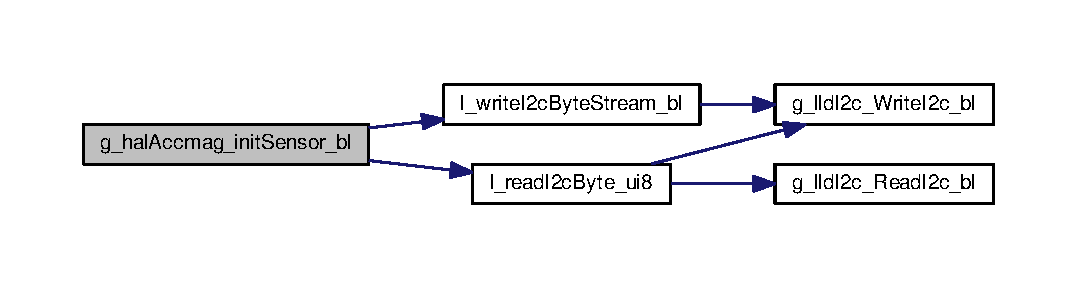
\includegraphics[width=350pt]{accMag_8c_ab936c0ac53ff9ba47a138e841a6ba474_ab936c0ac53ff9ba47a138e841a6ba474_cgraph}
\end{center}
\end{figure}




Here is the caller graph for this function\+:
\nopagebreak
\begin{figure}[H]
\begin{center}
\leavevmode
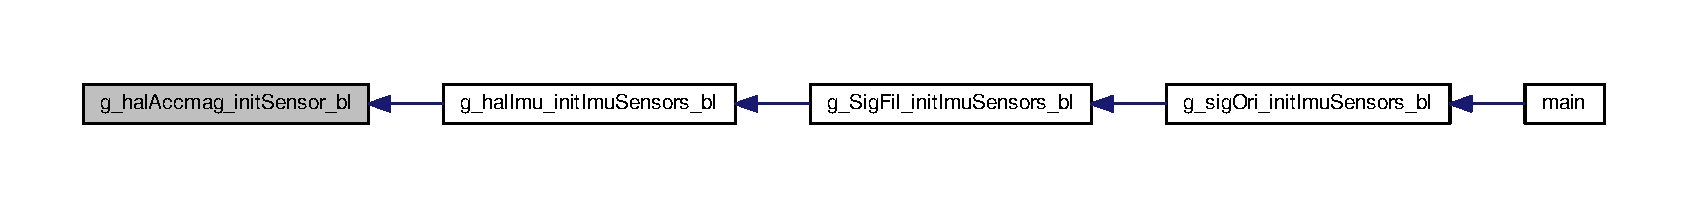
\includegraphics[width=350pt]{accMag_8c_ab936c0ac53ff9ba47a138e841a6ba474_ab936c0ac53ff9ba47a138e841a6ba474_icgraph}
\end{center}
\end{figure}


\hypertarget{accMag_8c_ad5f9d3a28348a9889f9afecde79606f6_ad5f9d3a28348a9889f9afecde79606f6}{\index{acc\+Mag.\+c@{acc\+Mag.\+c}!g\+\_\+hal\+Accmag\+\_\+trigger\+Acc\+Update\+\_\+bl@{g\+\_\+hal\+Accmag\+\_\+trigger\+Acc\+Update\+\_\+bl}}
\index{g\+\_\+hal\+Accmag\+\_\+trigger\+Acc\+Update\+\_\+bl@{g\+\_\+hal\+Accmag\+\_\+trigger\+Acc\+Update\+\_\+bl}!acc\+Mag.\+c@{acc\+Mag.\+c}}
\subsubsection[{g\+\_\+hal\+Accmag\+\_\+trigger\+Acc\+Update\+\_\+bl}]{\setlength{\rightskip}{0pt plus 5cm}unsigned int g\+\_\+hal\+Accmag\+\_\+trigger\+Acc\+Update\+\_\+bl (
\begin{DoxyParamCaption}
\item[{void}]{}
\end{DoxyParamCaption}
)}}\label{accMag_8c_ad5f9d3a28348a9889f9afecde79606f6_ad5f9d3a28348a9889f9afecde79606f6}


Trigger a new measurement of the accelerometer. 



 \begin{DoxyAuthor}{Author}
Juergen Schmidt (juscgs00) 
\end{DoxyAuthor}
\begin{DoxyDate}{Date}
2014/05/13
\end{DoxyDate}

\begin{DoxyParams}[1]{Parameters}
\mbox{\tt out}  & {\em returns} & a boolean value, indicating the occurrence of failures~\newline
 0 .... indicates success (no errors)~\newline
 1 .... indicates failed (some errors)\\
\hline
\end{DoxyParams}


Definition at line 546 of file acc\+Mag.\+c.


\begin{DoxyCode}
547 \{
548     \textcolor{keywordflow}{return} \hyperlink{accMag_8c_a5cef87c49dd46218e083a0c95abb9a9b_a5cef87c49dd46218e083a0c95abb9a9b}{l\_updateSensorState\_vd}(\hyperlink{accMag_8h_a648cc7f506bdd006d657bf0c2fc393b8_a648cc7f506bdd006d657bf0c2fc393b8a785fd0a49fbb18e5a2e65b8af35d6abc}{SENSOR\_ACC\_EN});
549 \}
\end{DoxyCode}


Here is the call graph for this function\+:
\nopagebreak
\begin{figure}[H]
\begin{center}
\leavevmode
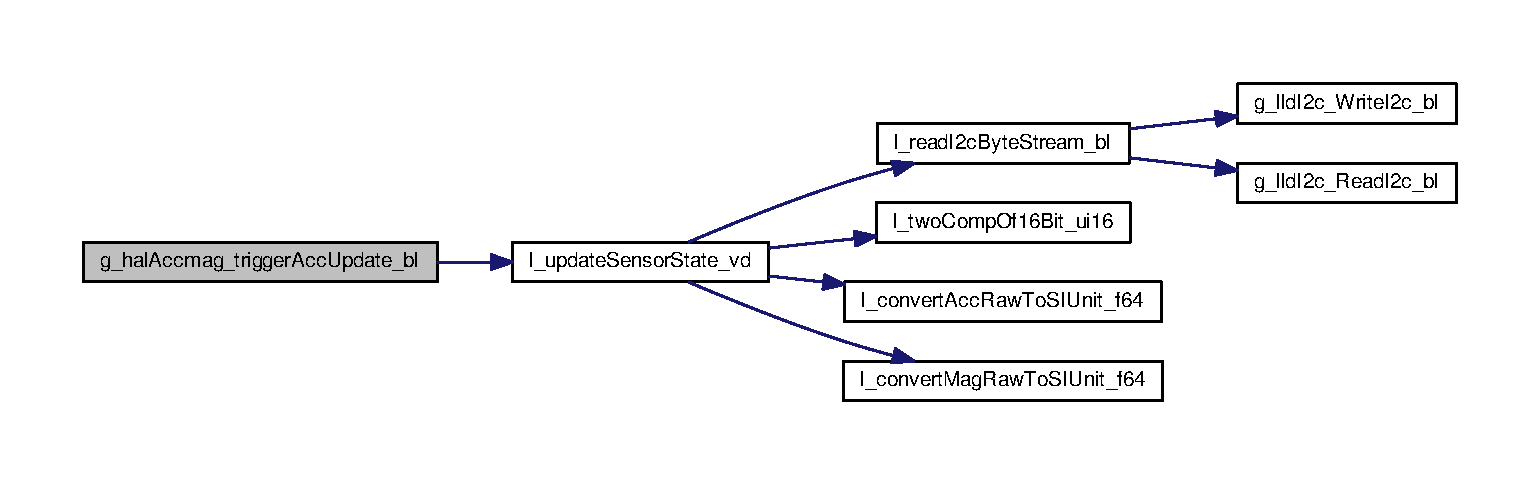
\includegraphics[width=350pt]{accMag_8c_ad5f9d3a28348a9889f9afecde79606f6_ad5f9d3a28348a9889f9afecde79606f6_cgraph}
\end{center}
\end{figure}




Here is the caller graph for this function\+:
\nopagebreak
\begin{figure}[H]
\begin{center}
\leavevmode
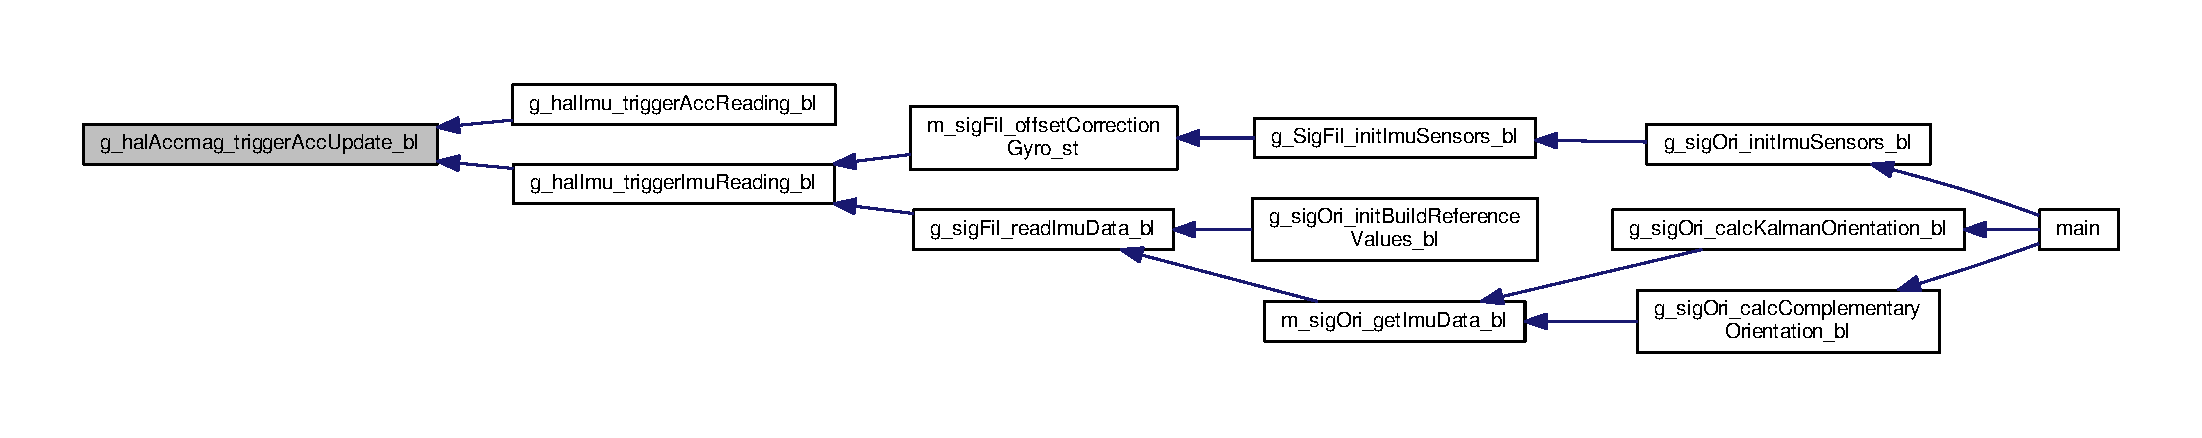
\includegraphics[width=350pt]{accMag_8c_ad5f9d3a28348a9889f9afecde79606f6_ad5f9d3a28348a9889f9afecde79606f6_icgraph}
\end{center}
\end{figure}


\hypertarget{accMag_8c_a98cf3442152a9ae213517936f7b37fe0_a98cf3442152a9ae213517936f7b37fe0}{\index{acc\+Mag.\+c@{acc\+Mag.\+c}!g\+\_\+hal\+Accmag\+\_\+trigger\+Full\+Update\+\_\+bl@{g\+\_\+hal\+Accmag\+\_\+trigger\+Full\+Update\+\_\+bl}}
\index{g\+\_\+hal\+Accmag\+\_\+trigger\+Full\+Update\+\_\+bl@{g\+\_\+hal\+Accmag\+\_\+trigger\+Full\+Update\+\_\+bl}!acc\+Mag.\+c@{acc\+Mag.\+c}}
\subsubsection[{g\+\_\+hal\+Accmag\+\_\+trigger\+Full\+Update\+\_\+bl}]{\setlength{\rightskip}{0pt plus 5cm}unsigned int g\+\_\+hal\+Accmag\+\_\+trigger\+Full\+Update\+\_\+bl (
\begin{DoxyParamCaption}
\item[{void}]{}
\end{DoxyParamCaption}
)}}\label{accMag_8c_a98cf3442152a9ae213517936f7b37fe0_a98cf3442152a9ae213517936f7b37fe0}


Trigger a new measurement of both sensors. 



 \begin{DoxyAuthor}{Author}
Juergen Schmidt (juscgs00) 
\end{DoxyAuthor}
\begin{DoxyDate}{Date}
2014/05/13
\end{DoxyDate}

\begin{DoxyParams}[1]{Parameters}
\mbox{\tt out}  & {\em returns} & a boolean value, indicating the occurrence of failures~\newline
 0 .... indicates success (no errors)~\newline
 1 .... indicates failed (some errors)\\
\hline
\end{DoxyParams}


Definition at line 590 of file acc\+Mag.\+c.


\begin{DoxyCode}
591 \{
592     \textcolor{keywordflow}{return} \hyperlink{accMag_8c_a5cef87c49dd46218e083a0c95abb9a9b_a5cef87c49dd46218e083a0c95abb9a9b}{l\_updateSensorState\_vd}(\hyperlink{accMag_8h_a648cc7f506bdd006d657bf0c2fc393b8_a648cc7f506bdd006d657bf0c2fc393b8a2801a1fb951d195fa4c2d621bd352a79}{SENSOR\_BOTH\_EN});
593 \}
\end{DoxyCode}


Here is the call graph for this function\+:
\nopagebreak
\begin{figure}[H]
\begin{center}
\leavevmode
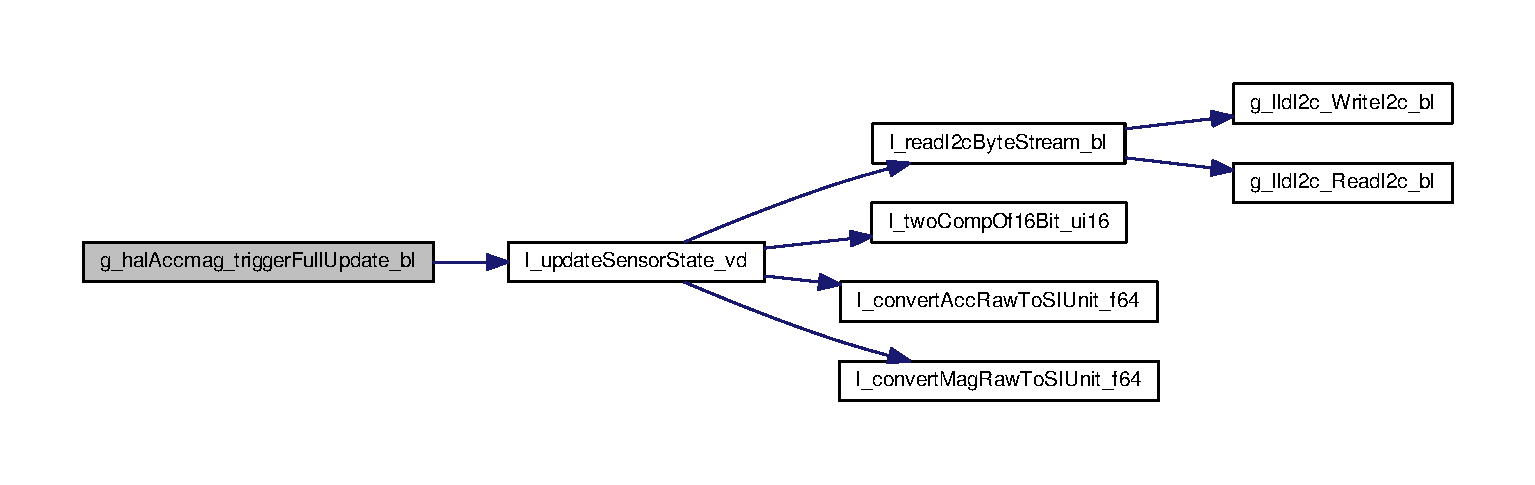
\includegraphics[width=350pt]{accMag_8c_a98cf3442152a9ae213517936f7b37fe0_a98cf3442152a9ae213517936f7b37fe0_cgraph}
\end{center}
\end{figure}


\hypertarget{accMag_8c_afdbd4ece113ff4859718b678150d069a_afdbd4ece113ff4859718b678150d069a}{\index{acc\+Mag.\+c@{acc\+Mag.\+c}!g\+\_\+hal\+Accmag\+\_\+trigger\+Mag\+Update\+\_\+bl@{g\+\_\+hal\+Accmag\+\_\+trigger\+Mag\+Update\+\_\+bl}}
\index{g\+\_\+hal\+Accmag\+\_\+trigger\+Mag\+Update\+\_\+bl@{g\+\_\+hal\+Accmag\+\_\+trigger\+Mag\+Update\+\_\+bl}!acc\+Mag.\+c@{acc\+Mag.\+c}}
\subsubsection[{g\+\_\+hal\+Accmag\+\_\+trigger\+Mag\+Update\+\_\+bl}]{\setlength{\rightskip}{0pt plus 5cm}unsigned int g\+\_\+hal\+Accmag\+\_\+trigger\+Mag\+Update\+\_\+bl (
\begin{DoxyParamCaption}
\item[{void}]{}
\end{DoxyParamCaption}
)}}\label{accMag_8c_afdbd4ece113ff4859718b678150d069a_afdbd4ece113ff4859718b678150d069a}


Trigger a new measurement of the magnetometer. 



 \begin{DoxyAuthor}{Author}
Juergen Schmidt (juscgs00) 
\end{DoxyAuthor}
\begin{DoxyDate}{Date}
2014/05/13
\end{DoxyDate}

\begin{DoxyParams}[1]{Parameters}
\mbox{\tt out}  & {\em returns} & a boolean value, indicating the occurrence of failures~\newline
 0 .... indicates success (no errors)~\newline
 1 .... indicates failed (some errors)\\
\hline
\end{DoxyParams}


Definition at line 568 of file acc\+Mag.\+c.


\begin{DoxyCode}
569 \{
570     \textcolor{keywordflow}{return} \hyperlink{accMag_8c_a5cef87c49dd46218e083a0c95abb9a9b_a5cef87c49dd46218e083a0c95abb9a9b}{l\_updateSensorState\_vd}(\hyperlink{accMag_8h_a648cc7f506bdd006d657bf0c2fc393b8_a648cc7f506bdd006d657bf0c2fc393b8a2a54a90cabb4985b0bd3bcb7d5b54d28}{SENSOR\_MAG\_EN});
571 \}
\end{DoxyCode}


Here is the call graph for this function\+:
\nopagebreak
\begin{figure}[H]
\begin{center}
\leavevmode
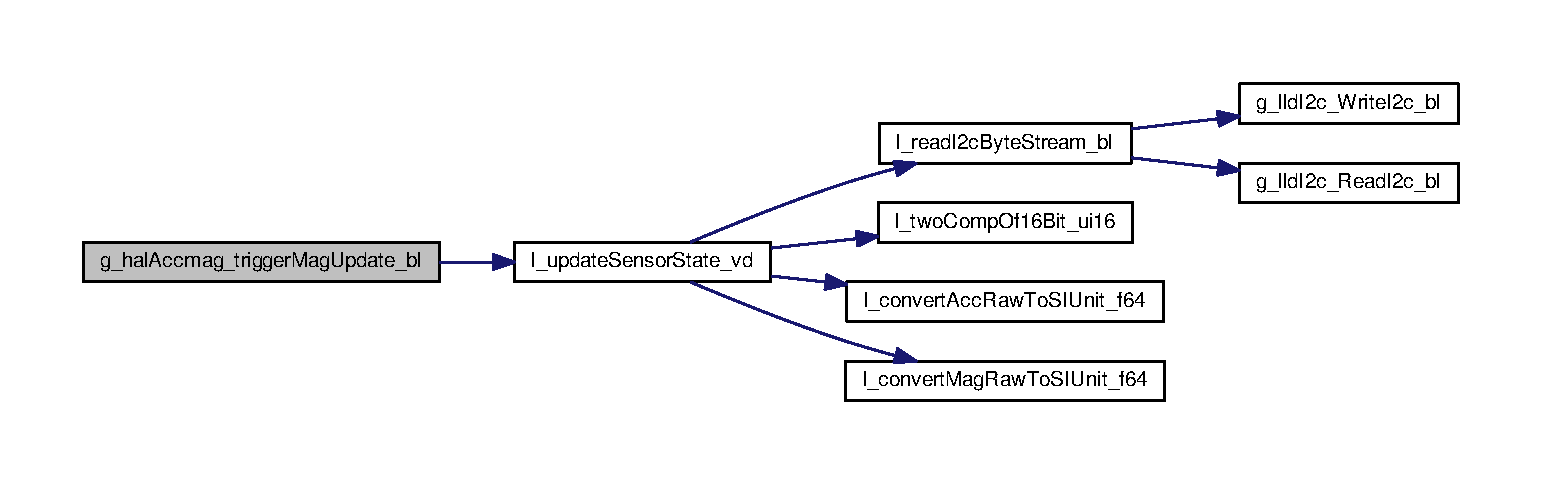
\includegraphics[width=350pt]{accMag_8c_afdbd4ece113ff4859718b678150d069a_afdbd4ece113ff4859718b678150d069a_cgraph}
\end{center}
\end{figure}




Here is the caller graph for this function\+:
\nopagebreak
\begin{figure}[H]
\begin{center}
\leavevmode
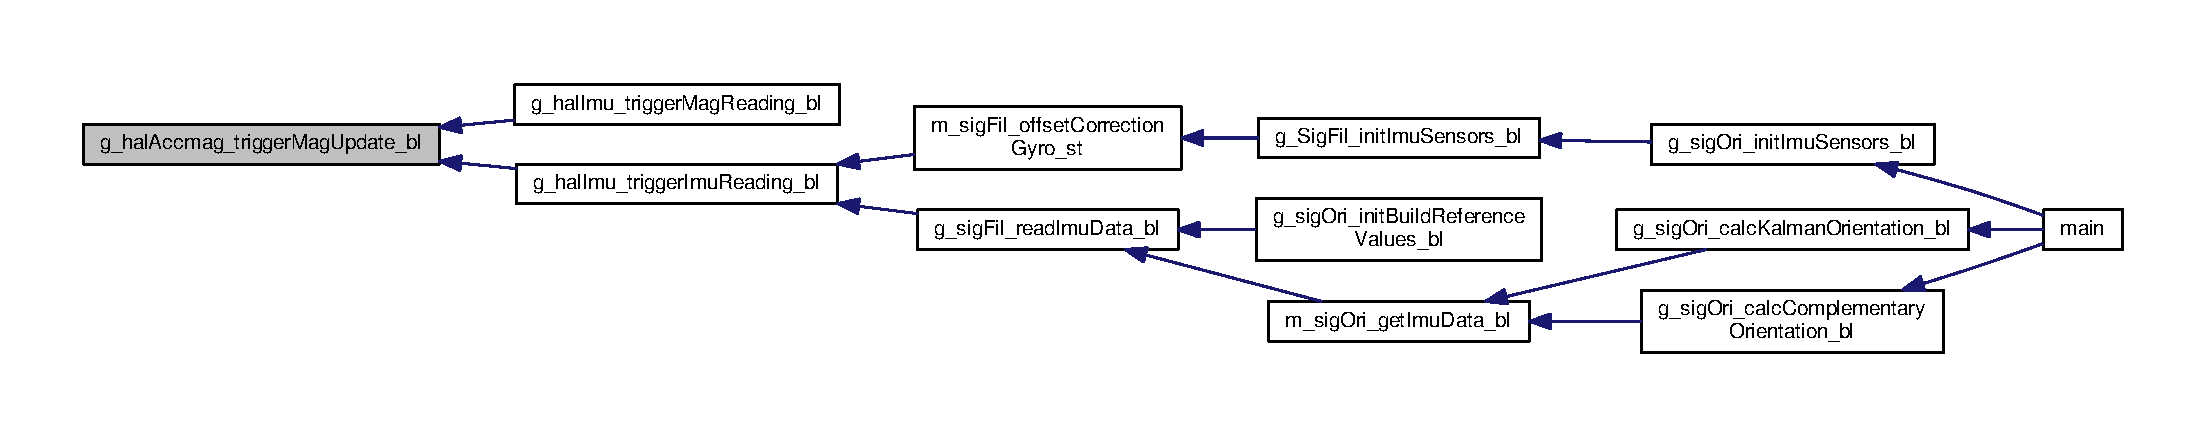
\includegraphics[width=350pt]{accMag_8c_afdbd4ece113ff4859718b678150d069a_afdbd4ece113ff4859718b678150d069a_icgraph}
\end{center}
\end{figure}


\hypertarget{accMag_8c_a3f6ef9cd19c5f23888aaca4b1ba34ecc_a3f6ef9cd19c5f23888aaca4b1ba34ecc}{\index{acc\+Mag.\+c@{acc\+Mag.\+c}!l\+\_\+convert\+Acc\+Raw\+To\+S\+I\+Unit\+\_\+f64@{l\+\_\+convert\+Acc\+Raw\+To\+S\+I\+Unit\+\_\+f64}}
\index{l\+\_\+convert\+Acc\+Raw\+To\+S\+I\+Unit\+\_\+f64@{l\+\_\+convert\+Acc\+Raw\+To\+S\+I\+Unit\+\_\+f64}!acc\+Mag.\+c@{acc\+Mag.\+c}}
\subsubsection[{l\+\_\+convert\+Acc\+Raw\+To\+S\+I\+Unit\+\_\+f64}]{\setlength{\rightskip}{0pt plus 5cm}static double l\+\_\+convert\+Acc\+Raw\+To\+S\+I\+Unit\+\_\+f64 (
\begin{DoxyParamCaption}
\item[{signed short}]{f\+\_\+raw\+Acc\+Val\+\_\+i16, }
\item[{unsigned char}]{f\+\_\+scaling\+Value\+G\+\_\+ui8}
\end{DoxyParamCaption}
)\hspace{0.3cm}{\ttfamily [inline]}, {\ttfamily [static]}}}\label{accMag_8c_a3f6ef9cd19c5f23888aaca4b1ba34ecc_a3f6ef9cd19c5f23888aaca4b1ba34ecc}


Converts raw sensor values of the accelerometer into S\+I unit. 



 \begin{DoxyAuthor}{Author}
Juergen Schmidt (juscgs00) 
\end{DoxyAuthor}
\begin{DoxyDate}{Date}
2014/05/11
\end{DoxyDate}
This function converts the raw sensor values (signed 16bit integers)of the accelerometer into S\+I unit (64bit float). The unit for the accelerometer is \[ \frac{m}{s^2} \]


\begin{DoxyParams}[1]{Parameters}
\mbox{\tt in}  & {\em f\+\_\+raw\+Mag\+Val\+\_\+i16} & is raw signed 16bit sensor value \\
\hline
\mbox{\tt in}  & {\em f\+\_\+scaling\+Value\+\_\+ui8} & is the absolute value of the max. scale defined in the sensor's control registers.~\newline
 Example\+: maximal sensor range \char`\"{}+/-\/ 8\+G\char`\"{} will result in \char`\"{}8\char`\"{} \\
\hline
\mbox{\tt out}  & {\em returns} & a 64bit float value in S\+I units ( \[ \frac{m}{s^2} \])\\
\hline
\end{DoxyParams}


Definition at line 337 of file acc\+Mag.\+c.


\begin{DoxyCode}
338 \{
339     \textcolor{keywordtype}{double}          l\_outputValue\_f64   = 0;
340     \textcolor{keyword}{const} \textcolor{keywordtype}{double}    l\_gravityConst\_f64  = 9.81; \textcolor{comment}{// m*(s^-2) per G}
341 
342     \textcolor{comment}{// unitless [-1,1]}
343     l\_outputValue\_f64 = (double)f\_scalingValueG\_ui8 * (\textcolor{keywordtype}{double})f\_rawAccVal\_i16 / (double)SHRT\_MAX;
344 
345     \textcolor{comment}{// Units: 1 * m*s^(-2)*G^(-1) * G = m*s^(-2)}
346     l\_outputValue\_f64 = l\_outputValue\_f64 * l\_gravityConst\_f64;
347 
348     \textcolor{keywordflow}{return} l\_outputValue\_f64;  \textcolor{comment}{// m*(s^-2)}
349 \}
\end{DoxyCode}


Here is the caller graph for this function\+:
\nopagebreak
\begin{figure}[H]
\begin{center}
\leavevmode
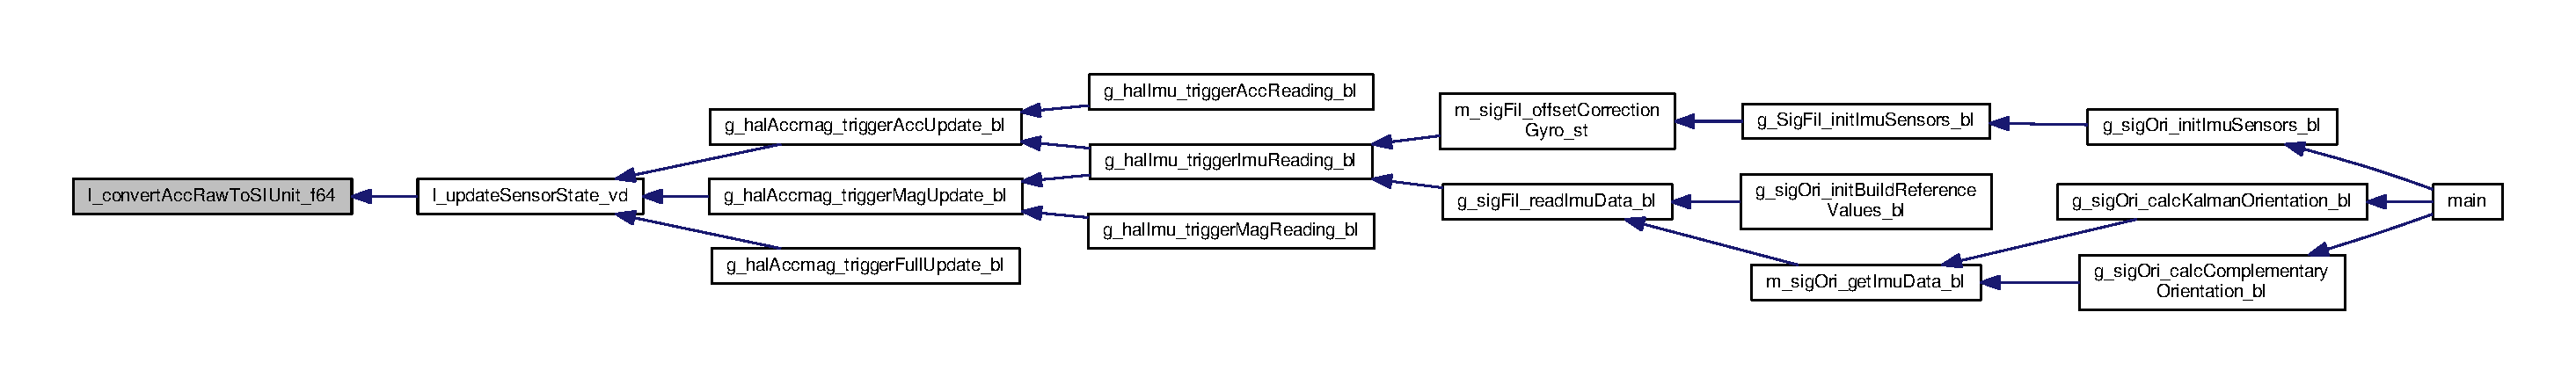
\includegraphics[width=350pt]{accMag_8c_a3f6ef9cd19c5f23888aaca4b1ba34ecc_a3f6ef9cd19c5f23888aaca4b1ba34ecc_icgraph}
\end{center}
\end{figure}


\hypertarget{accMag_8c_a1f0866c5afdce148afc09ed1c5a8018f_a1f0866c5afdce148afc09ed1c5a8018f}{\index{acc\+Mag.\+c@{acc\+Mag.\+c}!l\+\_\+convert\+Mag\+Raw\+To\+S\+I\+Unit\+\_\+f64@{l\+\_\+convert\+Mag\+Raw\+To\+S\+I\+Unit\+\_\+f64}}
\index{l\+\_\+convert\+Mag\+Raw\+To\+S\+I\+Unit\+\_\+f64@{l\+\_\+convert\+Mag\+Raw\+To\+S\+I\+Unit\+\_\+f64}!acc\+Mag.\+c@{acc\+Mag.\+c}}
\subsubsection[{l\+\_\+convert\+Mag\+Raw\+To\+S\+I\+Unit\+\_\+f64}]{\setlength{\rightskip}{0pt plus 5cm}static double l\+\_\+convert\+Mag\+Raw\+To\+S\+I\+Unit\+\_\+f64 (
\begin{DoxyParamCaption}
\item[{signed short}]{f\+\_\+raw\+Mag\+Val\+\_\+i16, }
\item[{unsigned char}]{f\+\_\+scaling\+Value\+Gauss\+\_\+ui8}
\end{DoxyParamCaption}
)\hspace{0.3cm}{\ttfamily [inline]}, {\ttfamily [static]}}}\label{accMag_8c_a1f0866c5afdce148afc09ed1c5a8018f_a1f0866c5afdce148afc09ed1c5a8018f}


Converts raw sensor values of the magnetometer into S\+I unit. 



 \begin{DoxyAuthor}{Author}
Juergen Schmidt (juscgs00) 
\end{DoxyAuthor}
\begin{DoxyDate}{Date}
2014/05/11
\end{DoxyDate}
This function converts the raw sensor values (signed 16bit integers)of the magnetometer into S\+I unit (64bit float). The unit for the magnetometer is Tesla~\newline
 (S\+I representation\+: Tesla = \[ \frac{kg}{s^2\dotA} \])


\begin{DoxyParams}[1]{Parameters}
\mbox{\tt in}  & {\em f\+\_\+raw\+Mag\+Val\+\_\+i16} & is raw signed 16bit sensor value \\
\hline
\mbox{\tt in}  & {\em f\+\_\+scaling\+Value\+\_\+ui8} & is the absolute value of the scale defined maximal sensor value range (e.\+g. \char`\"{}+/-\/4 Gauss\char`\"{} will result in \char`\"{}4\char`\"{}) \\
\hline
\mbox{\tt out}  & {\em returns} & a 64bit float value in S\+I units~\newline
 (Tesla = \[ \frac{kg}{s^2\dotA} \])\\
\hline
\end{DoxyParams}


Definition at line 303 of file acc\+Mag.\+c.


\begin{DoxyCode}
304 \{
305     \textcolor{keywordtype}{double}          l\_outputValue\_f64 = 0;
306     \textcolor{keyword}{const} \textcolor{keywordtype}{double}    l\_gaussToSI\_f64 = 0.1E-3;   \textcolor{comment}{//1Gauss = 0.1mT = 0.1*10^(-3)T}
307 
308     \textcolor{comment}{// unitless [-1,1]}
309     l\_outputValue\_f64 = (double)f\_rawMagVal\_i16 / (\textcolor{keywordtype}{double})SHRT\_MAX;
310 
311     \textcolor{comment}{// Units: 1 * T*Gauss^(-1) * Gauss = m*s^(-2)}
312     l\_outputValue\_f64 = l\_outputValue\_f64 * l\_gaussToSI\_f64 * (double)f\_scalingValueGauss\_ui8;
313 
314     \textcolor{keywordflow}{return} l\_outputValue\_f64;   \textcolor{comment}{//Tesla}
315 \}
\end{DoxyCode}


Here is the caller graph for this function\+:
\nopagebreak
\begin{figure}[H]
\begin{center}
\leavevmode
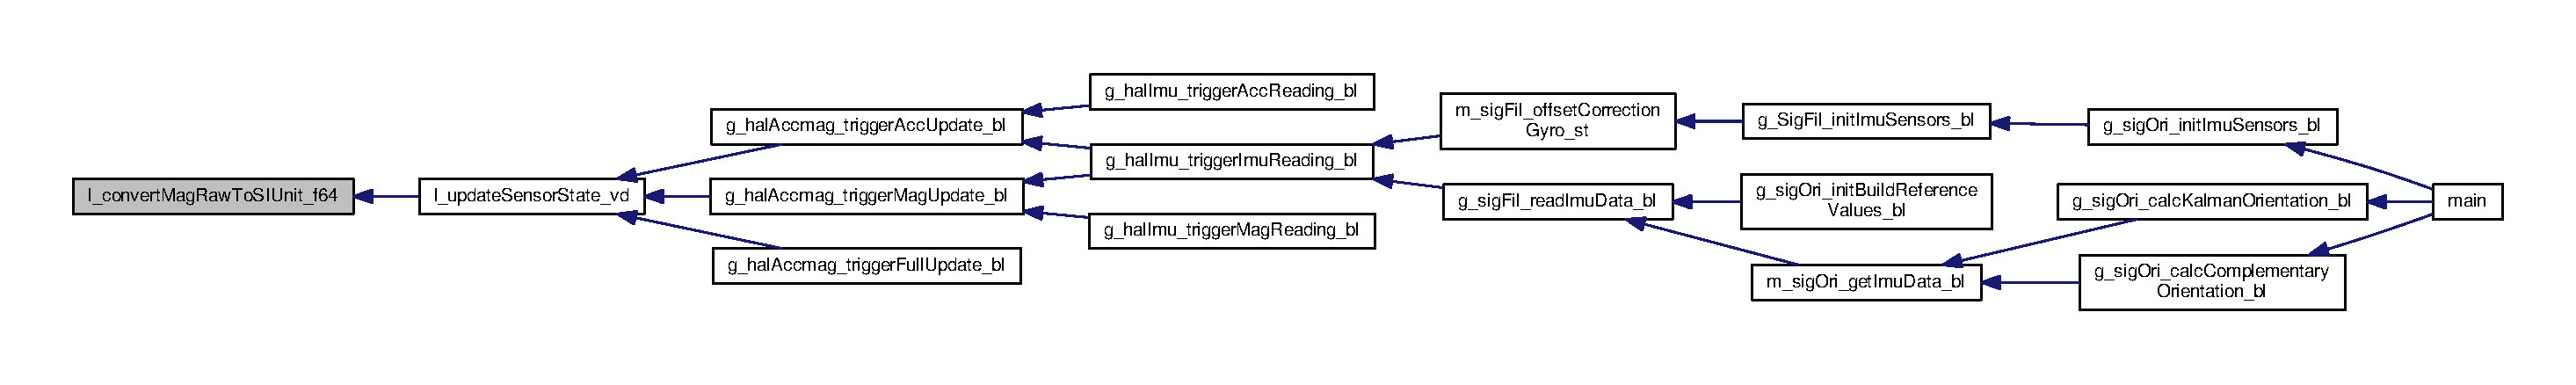
\includegraphics[width=350pt]{accMag_8c_a1f0866c5afdce148afc09ed1c5a8018f_a1f0866c5afdce148afc09ed1c5a8018f_icgraph}
\end{center}
\end{figure}


\hypertarget{accMag_8c_abaacf0917ab7bbc9b9d13b9aeb31afd1_abaacf0917ab7bbc9b9d13b9aeb31afd1}{\index{acc\+Mag.\+c@{acc\+Mag.\+c}!l\+\_\+read\+I2c\+Byte\+\_\+ui8@{l\+\_\+read\+I2c\+Byte\+\_\+ui8}}
\index{l\+\_\+read\+I2c\+Byte\+\_\+ui8@{l\+\_\+read\+I2c\+Byte\+\_\+ui8}!acc\+Mag.\+c@{acc\+Mag.\+c}}
\subsubsection[{l\+\_\+read\+I2c\+Byte\+\_\+ui8}]{\setlength{\rightskip}{0pt plus 5cm}static unsigned char l\+\_\+read\+I2c\+Byte\+\_\+ui8 (
\begin{DoxyParamCaption}
\item[{unsigned char}]{f\+\_\+register\+Addr\+\_\+ui8}
\end{DoxyParamCaption}
)\hspace{0.3cm}{\ttfamily [inline]}, {\ttfamily [static]}}}\label{accMag_8c_abaacf0917ab7bbc9b9d13b9aeb31afd1_abaacf0917ab7bbc9b9d13b9aeb31afd1}


Wrapper function to read a single byte register of L\+S\+M303\+D. 



 \begin{DoxyAuthor}{Author}
Juergen Schmidt (juscgs00) 
\end{DoxyAuthor}
\begin{DoxyDate}{Date}
2014/05/05
\end{DoxyDate}
This function is a wrapper to the I2\+C Interface to read one single byte of the Accelerometer/\+Magnetometer (L\+S\+M303\+D). It eases the write and read procedure for reading one register byte of the sensor.


\begin{DoxyParams}[1]{Parameters}
\mbox{\tt in}  & {\em f\+\_\+register\+Addr\+\_\+ui8} & specifies the register address to return \\
\hline
\mbox{\tt out}  & {\em returns} & the requested byte of I2\+C data\\
\hline
\end{DoxyParams}


Definition at line 33 of file acc\+Mag.\+c.


\begin{DoxyCode}
34 \{
35     \textcolor{keywordtype}{unsigned} \textcolor{keywordtype}{char}   l\_registerAddr\_ui8 = 0;
36     \textcolor{keywordtype}{unsigned} \textcolor{keywordtype}{char}   l\_recvDataByte\_ui8 = 0;
37 
38     \textcolor{comment}{/*}
39 \textcolor{comment}{     * ensure single byte read (MSB of register address shall be 0)}
40 \textcolor{comment}{     * -> Mask MSB to zero!}
41 \textcolor{comment}{     */}
42     l\_registerAddr\_ui8 = f\_registerAddr\_ui8 & 0b01111111;
43 
44     \textcolor{comment}{//write register request to I2C}
45     \textcolor{keywordflow}{if} ( \hyperlink{LLD__I2C_8c_aa6892bf4aea7f232d9b0ff2dbf8a9321_aa6892bf4aea7f232d9b0ff2dbf8a9321}{g\_lldI2c\_WriteI2c\_bl}(\hyperlink{accMag_8h_a6c9acfcf0f8dff7a5789ddb4960b3599_a6c9acfcf0f8dff7a5789ddb4960b3599}{M\_HAL\_ACCMAG\_I2CADDR\_UI8}, &
      l\_registerAddr\_ui8, 1) != \hyperlink{accMag_8h_a244c94ee3b75087140235cf4f913623f_a244c94ee3b75087140235cf4f913623f}{M\_HAL\_ACCMAG\_SUCCESS\_BL} )
46     \{
47         \textcolor{comment}{// error in I2C access}
48         \textcolor{keywordflow}{return} \hyperlink{accMag_8h_a29da5c251bf0c3b1c7ed7da3c3269d9f_a29da5c251bf0c3b1c7ed7da3c3269d9f}{M\_HAL\_ACCMAG\_FAILED\_BL};
49     \}
50 
51     \textcolor{comment}{//read requested register data}
52     \textcolor{keywordflow}{if} ( \hyperlink{LLD__I2C_8c_a107ee9f1e4646733ac3ef6addf0def7e_a107ee9f1e4646733ac3ef6addf0def7e}{g\_lldI2c\_ReadI2c\_bl}(\hyperlink{accMag_8h_a6c9acfcf0f8dff7a5789ddb4960b3599_a6c9acfcf0f8dff7a5789ddb4960b3599}{M\_HAL\_ACCMAG\_I2CADDR\_UI8}, &
      l\_recvDataByte\_ui8, 1) != \hyperlink{accMag_8h_a244c94ee3b75087140235cf4f913623f_a244c94ee3b75087140235cf4f913623f}{M\_HAL\_ACCMAG\_SUCCESS\_BL} )
53     \{
54         \textcolor{comment}{// error in I2C access}
55         \textcolor{keywordflow}{return} \hyperlink{accMag_8h_a29da5c251bf0c3b1c7ed7da3c3269d9f_a29da5c251bf0c3b1c7ed7da3c3269d9f}{M\_HAL\_ACCMAG\_FAILED\_BL};
56     \}
57 
58     \textcolor{keywordflow}{return} l\_recvDataByte\_ui8;
59 \}
\end{DoxyCode}


Here is the call graph for this function\+:
\nopagebreak
\begin{figure}[H]
\begin{center}
\leavevmode
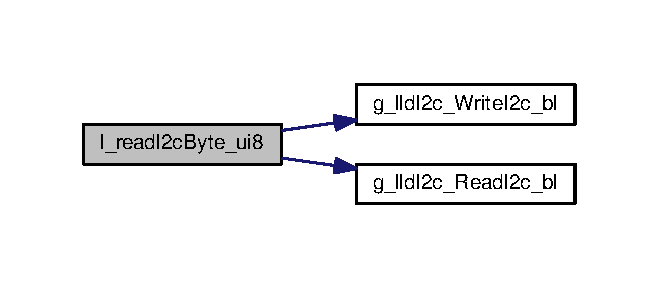
\includegraphics[width=316pt]{accMag_8c_abaacf0917ab7bbc9b9d13b9aeb31afd1_abaacf0917ab7bbc9b9d13b9aeb31afd1_cgraph}
\end{center}
\end{figure}




Here is the caller graph for this function\+:
\nopagebreak
\begin{figure}[H]
\begin{center}
\leavevmode
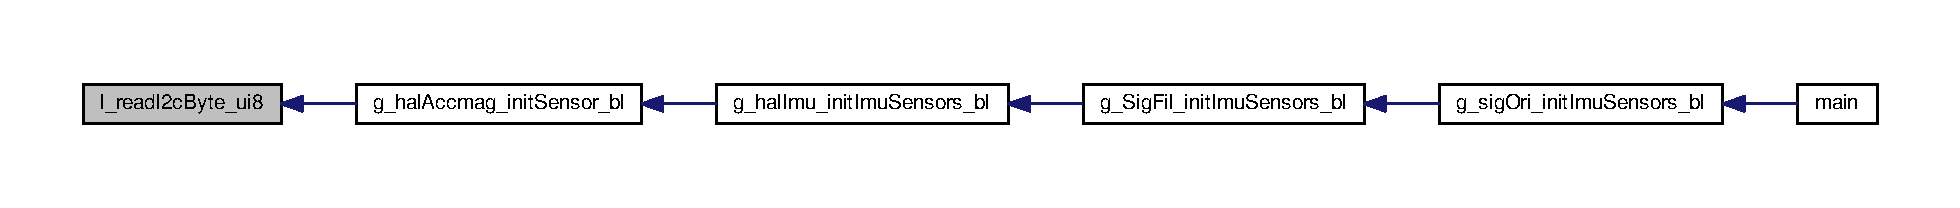
\includegraphics[width=350pt]{accMag_8c_abaacf0917ab7bbc9b9d13b9aeb31afd1_abaacf0917ab7bbc9b9d13b9aeb31afd1_icgraph}
\end{center}
\end{figure}


\hypertarget{accMag_8c_a84dc4f1647051d5c34296705fa1f236b_a84dc4f1647051d5c34296705fa1f236b}{\index{acc\+Mag.\+c@{acc\+Mag.\+c}!l\+\_\+read\+I2c\+Byte\+Stream\+\_\+bl@{l\+\_\+read\+I2c\+Byte\+Stream\+\_\+bl}}
\index{l\+\_\+read\+I2c\+Byte\+Stream\+\_\+bl@{l\+\_\+read\+I2c\+Byte\+Stream\+\_\+bl}!acc\+Mag.\+c@{acc\+Mag.\+c}}
\subsubsection[{l\+\_\+read\+I2c\+Byte\+Stream\+\_\+bl}]{\setlength{\rightskip}{0pt plus 5cm}static unsigned int l\+\_\+read\+I2c\+Byte\+Stream\+\_\+bl (
\begin{DoxyParamCaption}
\item[{unsigned char}]{f\+\_\+start\+Register\+Addr\+\_\+ui8, }
\item[{const unsigned char $\ast$}]{f\+\_\+read\+Destination\+Buffer\+\_\+pui8, }
\item[{unsigned int}]{f\+\_\+num\+Of\+Bytes\+To\+Read\+\_\+ui32}
\end{DoxyParamCaption}
)\hspace{0.3cm}{\ttfamily [inline]}, {\ttfamily [static]}}}\label{accMag_8c_a84dc4f1647051d5c34296705fa1f236b_a84dc4f1647051d5c34296705fa1f236b}


Wrapper function to read byte stream to registers of L\+S\+M303\+D. 



 \begin{DoxyAuthor}{Author}
Juergen Schmidt (juscgs00) 
\end{DoxyAuthor}
\begin{DoxyDate}{Date}
2014/05/08
\end{DoxyDate}
This function is a wrapper to the I2\+C Interface to read a byte stream to a series of registers of the Accelerometer/ Magnetometer (L\+S\+M303\+D). The first register address can be defined in the parameter list of the function. After reading the first byte of the start address, the register address will be incremented.


\begin{DoxyParams}[1]{Parameters}
\mbox{\tt in}  & {\em f\+\_\+start\+Register\+Addr\+\_\+ui8} & specifies the first register address to return \\
\hline
\mbox{\tt in}  & {\em f\+\_\+read\+Destination\+Buffer\+\_\+pui8} & points to an array of unsigned 8bit integer elements. This array receives all read data bytes (output byte stream buffer). \\
\hline
\mbox{\tt out}  & {\em returns} & a boolean value, indicating the occurrence of failures~\newline
 0 .... indicates success (no errors)~\newline
 1 .... indicates failed (some errors)\\
\hline
\end{DoxyParams}


Definition at line 88 of file acc\+Mag.\+c.


\begin{DoxyCode}
89 \{
90     \textcolor{keywordtype}{unsigned} \textcolor{keywordtype}{char}   l\_registerAddr\_ui8  = 0;
91 
92     \textcolor{comment}{// ensure at least one data byte to read}
93     \textcolor{keywordflow}{if} (f\_numOfBytesToRead\_ui32 < 1)
94     \{
95         \textcolor{keywordflow}{return} \hyperlink{accMag_8h_a29da5c251bf0c3b1c7ed7da3c3269d9f_a29da5c251bf0c3b1c7ed7da3c3269d9f}{M\_HAL\_ACCMAG\_FAILED\_BL};
96     \}
97 
98     \textcolor{comment}{/*}
99 \textcolor{comment}{     * ensure byte stream reading (MSB of register address shall be 1)}
100 \textcolor{comment}{     *   -> Mask MSB to one!}
101 \textcolor{comment}{     *   -> LSM303D will auto-increment the register address for each byte}
102 \textcolor{comment}{     *      of data}
103 \textcolor{comment}{     */}
104     l\_registerAddr\_ui8 = f\_startRegisterAddr\_ui8 | 0b10000000;
105 
106     \textcolor{comment}{//write register request to I2C}
107     \textcolor{keywordflow}{if} ( \hyperlink{LLD__I2C_8c_aa6892bf4aea7f232d9b0ff2dbf8a9321_aa6892bf4aea7f232d9b0ff2dbf8a9321}{g\_lldI2c\_WriteI2c\_bl}(\hyperlink{accMag_8h_a6c9acfcf0f8dff7a5789ddb4960b3599_a6c9acfcf0f8dff7a5789ddb4960b3599}{M\_HAL\_ACCMAG\_I2CADDR\_UI8}, &
      l\_registerAddr\_ui8, 1) != \hyperlink{accMag_8h_a244c94ee3b75087140235cf4f913623f_a244c94ee3b75087140235cf4f913623f}{M\_HAL\_ACCMAG\_SUCCESS\_BL} )
108     \{
109         \textcolor{comment}{// error in I2C access}
110         \textcolor{keywordflow}{return} \hyperlink{accMag_8h_a29da5c251bf0c3b1c7ed7da3c3269d9f_a29da5c251bf0c3b1c7ed7da3c3269d9f}{M\_HAL\_ACCMAG\_FAILED\_BL};
111     \}
112 
113     \textcolor{comment}{//read requested registers to I2C}
114     \textcolor{keywordflow}{if} ( \hyperlink{LLD__I2C_8c_a107ee9f1e4646733ac3ef6addf0def7e_a107ee9f1e4646733ac3ef6addf0def7e}{g\_lldI2c\_ReadI2c\_bl}(\hyperlink{accMag_8h_a6c9acfcf0f8dff7a5789ddb4960b3599_a6c9acfcf0f8dff7a5789ddb4960b3599}{M\_HAL\_ACCMAG\_I2CADDR\_UI8}, 
      f\_readDestinationBuffer\_pui8, f\_numOfBytesToRead\_ui32) != \hyperlink{accMag_8h_a244c94ee3b75087140235cf4f913623f_a244c94ee3b75087140235cf4f913623f}{M\_HAL\_ACCMAG\_SUCCESS\_BL} )
115     \{
116         \textcolor{comment}{// error in I2C access}
117         \textcolor{keywordflow}{return} \hyperlink{accMag_8h_a29da5c251bf0c3b1c7ed7da3c3269d9f_a29da5c251bf0c3b1c7ed7da3c3269d9f}{M\_HAL\_ACCMAG\_FAILED\_BL};
118     \}
119 
120     \textcolor{keywordflow}{return} \hyperlink{accMag_8h_a244c94ee3b75087140235cf4f913623f_a244c94ee3b75087140235cf4f913623f}{M\_HAL\_ACCMAG\_SUCCESS\_BL};
121 \}
\end{DoxyCode}


Here is the call graph for this function\+:
\nopagebreak
\begin{figure}[H]
\begin{center}
\leavevmode
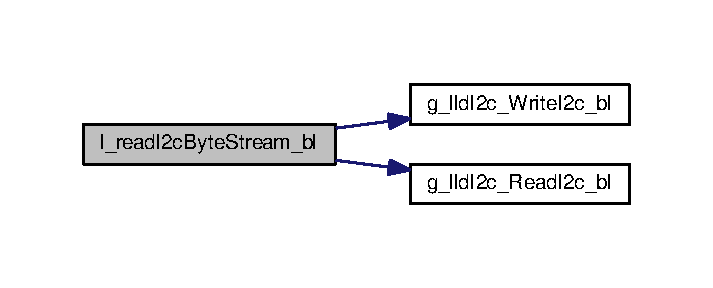
\includegraphics[width=342pt]{accMag_8c_a84dc4f1647051d5c34296705fa1f236b_a84dc4f1647051d5c34296705fa1f236b_cgraph}
\end{center}
\end{figure}




Here is the caller graph for this function\+:
\nopagebreak
\begin{figure}[H]
\begin{center}
\leavevmode
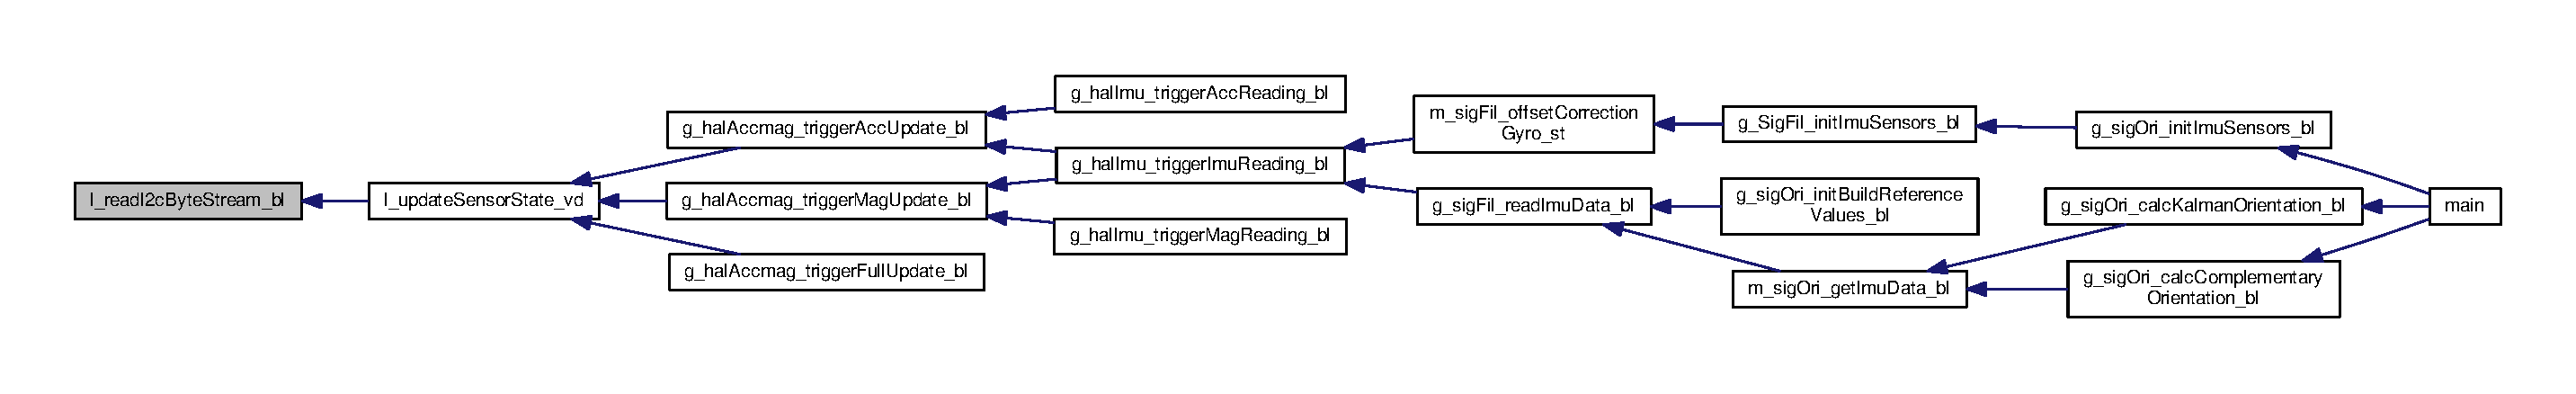
\includegraphics[width=350pt]{accMag_8c_a84dc4f1647051d5c34296705fa1f236b_a84dc4f1647051d5c34296705fa1f236b_icgraph}
\end{center}
\end{figure}


\hypertarget{accMag_8c_aad5863a0667702ddb0040ab517463069_aad5863a0667702ddb0040ab517463069}{\index{acc\+Mag.\+c@{acc\+Mag.\+c}!l\+\_\+two\+Comp\+Of16\+Bit\+\_\+ui16@{l\+\_\+two\+Comp\+Of16\+Bit\+\_\+ui16}}
\index{l\+\_\+two\+Comp\+Of16\+Bit\+\_\+ui16@{l\+\_\+two\+Comp\+Of16\+Bit\+\_\+ui16}!acc\+Mag.\+c@{acc\+Mag.\+c}}
\subsubsection[{l\+\_\+two\+Comp\+Of16\+Bit\+\_\+ui16}]{\setlength{\rightskip}{0pt plus 5cm}static signed short l\+\_\+two\+Comp\+Of16\+Bit\+\_\+ui16 (
\begin{DoxyParamCaption}
\item[{unsigned char}]{f\+\_\+lsb\+\_\+ui8, }
\item[{unsigned char}]{f\+\_\+msb\+\_\+ui8}
\end{DoxyParamCaption}
)\hspace{0.3cm}{\ttfamily [inline]}, {\ttfamily [static]}}}\label{accMag_8c_aad5863a0667702ddb0040ab517463069_aad5863a0667702ddb0040ab517463069}


Complement of twos of a 16 bit integer. 



 \begin{DoxyAuthor}{Author}
Juergen Schmidt (juscgs00) 
\end{DoxyAuthor}
\begin{DoxyDate}{Date}
2014/05/10
\end{DoxyDate}
This function computes the two's complement of two 8bit integers (most significant and least significant bytes)


\begin{DoxyParams}[1]{Parameters}
\mbox{\tt in}  & {\em f\+\_\+lsb\+\_\+ui8} & is the least significant byte \\
\hline
\mbox{\tt in}  & {\em f\+\_\+msb\+\_\+ui8} & is the most significant byte \\
\hline
\mbox{\tt out}  & {\em returns} & a unsigned 16bit integer of the two's complement\\
\hline
\end{DoxyParams}


Definition at line 265 of file acc\+Mag.\+c.


\begin{DoxyCode}
266 \{
267     \textcolor{keywordtype}{signed} \textcolor{keywordtype}{short}    l\_compOfTwo\_ui16 = 0; \textcolor{comment}{//init variable with zeros}
268 
269     \textcolor{comment}{/*}
270 \textcolor{comment}{     * 1. assemble 16bit value of two 8bit chunks}
271 \textcolor{comment}{     * 2. invert 16bit}
272 \textcolor{comment}{     * 3. add 1 to 16bit value}
273 \textcolor{comment}{     * 4. mask only 16bit range (to avoid overflows)}
274 \textcolor{comment}{     * --> conversion of two's complement}
275 \textcolor{comment}{     */}
276     l\_compOfTwo\_ui16 = (\textcolor{keywordtype}{signed} short)( ( ~((\textcolor{keywordtype}{int})(f\_msb\_ui8 << 8) + (\textcolor{keywordtype}{int})(f\_lsb\_ui8)) + (\textcolor{keywordtype}{int})1 ) & (int)0
      xFFFF );
277 
278     \textcolor{keywordflow}{return} l\_compOfTwo\_ui16;
279 \}
\end{DoxyCode}


Here is the caller graph for this function\+:
\nopagebreak
\begin{figure}[H]
\begin{center}
\leavevmode
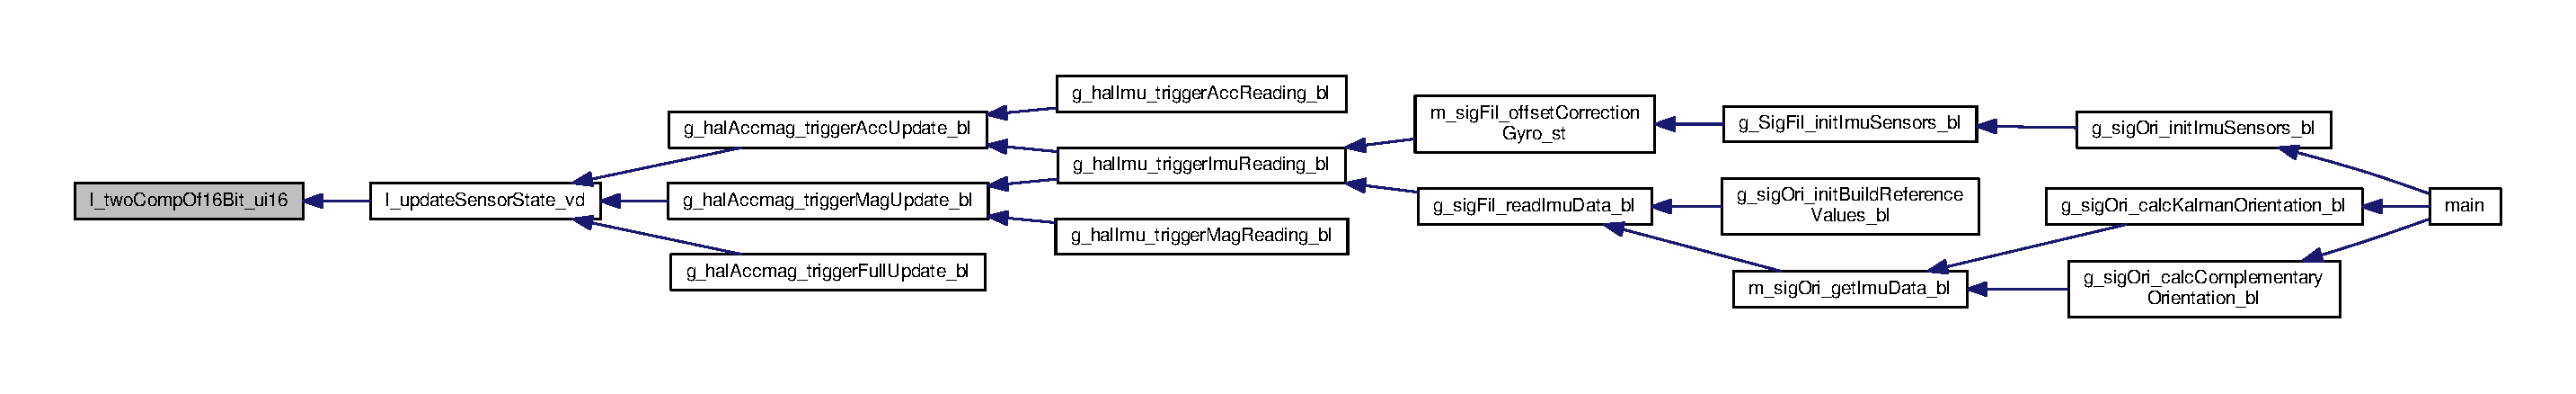
\includegraphics[width=350pt]{accMag_8c_aad5863a0667702ddb0040ab517463069_aad5863a0667702ddb0040ab517463069_icgraph}
\end{center}
\end{figure}


\hypertarget{accMag_8c_a5cef87c49dd46218e083a0c95abb9a9b_a5cef87c49dd46218e083a0c95abb9a9b}{\index{acc\+Mag.\+c@{acc\+Mag.\+c}!l\+\_\+update\+Sensor\+State\+\_\+vd@{l\+\_\+update\+Sensor\+State\+\_\+vd}}
\index{l\+\_\+update\+Sensor\+State\+\_\+vd@{l\+\_\+update\+Sensor\+State\+\_\+vd}!acc\+Mag.\+c@{acc\+Mag.\+c}}
\subsubsection[{l\+\_\+update\+Sensor\+State\+\_\+vd}]{\setlength{\rightskip}{0pt plus 5cm}static unsigned int l\+\_\+update\+Sensor\+State\+\_\+vd (
\begin{DoxyParamCaption}
\item[{{\bf hal\+Accmag\+\_\+sensor\+Select}}]{f\+\_\+sensor\+\_\+en}
\end{DoxyParamCaption}
)\hspace{0.3cm}{\ttfamily [inline]}, {\ttfamily [static]}}}\label{accMag_8c_a5cef87c49dd46218e083a0c95abb9a9b_a5cef87c49dd46218e083a0c95abb9a9b}


Trigger a update of the current sensor state data. 



 \begin{DoxyAuthor}{Author}
Juergen Schmidt (juscgs00) 
\end{DoxyAuthor}
\begin{DoxyDate}{Date}
2014/05/05
\end{DoxyDate}
This function accesses the accelereation and compass sensor via I2\+C to load a new measurement to the sensor state storage


\begin{DoxyParams}[1]{Parameters}
\mbox{\tt in}  & {\em f\+\_\+sensor\+\_\+en} & is a enum type that indicates, which sensor(s) shall be updated \\
\hline
\mbox{\tt out}  & {\em returns} & a boolean value, indicating the occurrence of failures~\newline
 0 .... indicates success (no errors)~\newline
 1 .... indicates failed (some errors)\\
\hline
\end{DoxyParams}


Definition at line 371 of file acc\+Mag.\+c.


\begin{DoxyCode}
372 \{
373     \hyperlink{structhalAccmag__3dDoubleVector}{halAccmag\_3dDoubleVector}    l\_accBuffer\_st;
374     \hyperlink{structhalAccmag__3dDoubleVector}{halAccmag\_3dDoubleVector}    l\_magBuffer\_st;
375     \textcolor{keywordtype}{unsigned} \textcolor{keywordtype}{char}               l\_readBuffer\_rg6ui8[6];
376     \textcolor{keywordtype}{signed} \textcolor{keywordtype}{short}                l\_tempComponent\_i16 = 0;
377     \textcolor{keywordtype}{unsigned} \textcolor{keywordtype}{int}                l\_successState\_bl = \hyperlink{accMag_8h_a244c94ee3b75087140235cf4f913623f_a244c94ee3b75087140235cf4f913623f}{M\_HAL\_ACCMAG\_SUCCESS\_BL};
378 
379     \textcolor{comment}{//init local data buffers with current values}
380     l\_accBuffer\_st = \hyperlink{accMag_8c_a421eb1956f3c2b98d7a4505bc13b049e_a421eb1956f3c2b98d7a4505bc13b049e}{m\_halAccmag\_sensorState\_st}.\hyperlink{structhalAccmag__dataContainer_afc3847993eed1c8f1e67028ad6d2a6cf_afc3847993eed1c8f1e67028ad6d2a6cf}{acc};
381     l\_magBuffer\_st = \hyperlink{accMag_8c_a421eb1956f3c2b98d7a4505bc13b049e_a421eb1956f3c2b98d7a4505bc13b049e}{m\_halAccmag\_sensorState\_st}.\hyperlink{structhalAccmag__dataContainer_a903681a66ce49c39267aa66d471812f7_a903681a66ce49c39267aa66d471812f7}{mag};
382 
383     \textcolor{comment}{/*}
384 \textcolor{comment}{     * READ ACCELEROMETER}
385 \textcolor{comment}{     * - uses sequential read (auto-increment)}
386 \textcolor{comment}{     * - sequence as follows:}
387 \textcolor{comment}{     *   (Byte 1) X-Component, LSB}
388 \textcolor{comment}{     *   (Byte 2) X-Component, MSB}
389 \textcolor{comment}{     *   (Byte 3) Y-Component, LSB}
390 \textcolor{comment}{     *   (Byte 4) Y-Component, MSB}
391 \textcolor{comment}{     *   (Byte 5) Z-Component, LSB}
392 \textcolor{comment}{     *   (Byte 6) Z-Component, MSB}
393 \textcolor{comment}{     */}
394     \textcolor{keywordflow}{if} ( (f\_sensor\_en == \hyperlink{accMag_8h_a648cc7f506bdd006d657bf0c2fc393b8_a648cc7f506bdd006d657bf0c2fc393b8a785fd0a49fbb18e5a2e65b8af35d6abc}{SENSOR\_ACC\_EN}) || (f\_sensor\_en == 
      \hyperlink{accMag_8h_a648cc7f506bdd006d657bf0c2fc393b8_a648cc7f506bdd006d657bf0c2fc393b8a2801a1fb951d195fa4c2d621bd352a79}{SENSOR\_BOTH\_EN}) )
395     \{
396         \textcolor{keywordflow}{if} ( \hyperlink{accMag_8c_a84dc4f1647051d5c34296705fa1f236b_a84dc4f1647051d5c34296705fa1f236b}{l\_readI2cByteStream\_bl}(
      \hyperlink{accMag__registers_8h_a93160006c4218905810ab70c3bddfe05_a93160006c4218905810ab70c3bddfe05}{M\_HAL\_ACCMAG\_OUT\_X\_L\_A\_UI8},l\_readBuffer\_rg6ui8, 6) == 
      \hyperlink{accMag_8h_a244c94ee3b75087140235cf4f913623f_a244c94ee3b75087140235cf4f913623f}{M\_HAL\_ACCMAG\_SUCCESS\_BL} )
397         \{
398             \textcolor{comment}{// x-component}
399             l\_tempComponent\_i16 = \hyperlink{accMag_8c_aad5863a0667702ddb0040ab517463069_aad5863a0667702ddb0040ab517463069}{l\_twoCompOf16Bit\_ui16}(l\_readBuffer\_rg6ui8[0], 
      l\_readBuffer\_rg6ui8[1]);
400             l\_accBuffer\_st.\hyperlink{structhalAccmag__3dDoubleVector_a011646ea6f4b78400dfd2ffa8eb45eea_a011646ea6f4b78400dfd2ffa8eb45eea}{x\_f64} = \hyperlink{accMag_8c_a3f6ef9cd19c5f23888aaca4b1ba34ecc_a3f6ef9cd19c5f23888aaca4b1ba34ecc}{l\_convertAccRawToSIUnit\_f64}( 
      l\_tempComponent\_i16, \hyperlink{accMag_8h_a44405d1fc6d79b1588b5ce1549f5af52_a44405d1fc6d79b1588b5ce1549f5af52}{M\_HAL\_ACCMAG\_ACCSCALE\_UI8} );
401 
402             \textcolor{comment}{// y-component}
403             l\_tempComponent\_i16 = \hyperlink{accMag_8c_aad5863a0667702ddb0040ab517463069_aad5863a0667702ddb0040ab517463069}{l\_twoCompOf16Bit\_ui16}(l\_readBuffer\_rg6ui8[2], 
      l\_readBuffer\_rg6ui8[3]);
404             l\_accBuffer\_st.\hyperlink{structhalAccmag__3dDoubleVector_a88f4ed3363ccaa08c00d2fc28f7b2ab4_a88f4ed3363ccaa08c00d2fc28f7b2ab4}{y\_f64} = \hyperlink{accMag_8c_a3f6ef9cd19c5f23888aaca4b1ba34ecc_a3f6ef9cd19c5f23888aaca4b1ba34ecc}{l\_convertAccRawToSIUnit\_f64}( 
      l\_tempComponent\_i16, \hyperlink{accMag_8h_a44405d1fc6d79b1588b5ce1549f5af52_a44405d1fc6d79b1588b5ce1549f5af52}{M\_HAL\_ACCMAG\_ACCSCALE\_UI8} );
405 
406             \textcolor{comment}{// z-component}
407             l\_tempComponent\_i16 = \hyperlink{accMag_8c_aad5863a0667702ddb0040ab517463069_aad5863a0667702ddb0040ab517463069}{l\_twoCompOf16Bit\_ui16}(l\_readBuffer\_rg6ui8[4], 
      l\_readBuffer\_rg6ui8[5]);
408             l\_accBuffer\_st.\hyperlink{structhalAccmag__3dDoubleVector_a5041b0551694f5f4057a5f3454782e44_a5041b0551694f5f4057a5f3454782e44}{z\_f64} = \hyperlink{accMag_8c_a3f6ef9cd19c5f23888aaca4b1ba34ecc_a3f6ef9cd19c5f23888aaca4b1ba34ecc}{l\_convertAccRawToSIUnit\_f64}( 
      l\_tempComponent\_i16, \hyperlink{accMag_8h_a44405d1fc6d79b1588b5ce1549f5af52_a44405d1fc6d79b1588b5ce1549f5af52}{M\_HAL\_ACCMAG\_ACCSCALE\_UI8} );
409         \}\textcolor{keywordflow}{else}\{
410             l\_successState\_bl = \hyperlink{accMag_8h_a29da5c251bf0c3b1c7ed7da3c3269d9f_a29da5c251bf0c3b1c7ed7da3c3269d9f}{M\_HAL\_ACCMAG\_FAILED\_BL};
411         \}
412 
413     \}
414     \textcolor{comment}{/*}
415 \textcolor{comment}{     * READ MAGNETOMETER}
416 \textcolor{comment}{     * - uses sequential read (auto-increment)}
417 \textcolor{comment}{     * - sequence as follows:}
418 \textcolor{comment}{     *   (Byte 1) X-Component, LSB}
419 \textcolor{comment}{     *   (Byte 2) X-Component, MSB}
420 \textcolor{comment}{     *   (Byte 3) Y-Component, LSB}
421 \textcolor{comment}{     *   (Byte 4) Y-Component, MSB}
422 \textcolor{comment}{     *   (Byte 5) Z-Component, LSB}
423 \textcolor{comment}{     *   (Byte 6) Z-Component, MSB}
424 \textcolor{comment}{     */}
425     \textcolor{keywordflow}{if} ( (f\_sensor\_en == \hyperlink{accMag_8h_a648cc7f506bdd006d657bf0c2fc393b8_a648cc7f506bdd006d657bf0c2fc393b8a2a54a90cabb4985b0bd3bcb7d5b54d28}{SENSOR\_MAG\_EN}) || (f\_sensor\_en == 
      \hyperlink{accMag_8h_a648cc7f506bdd006d657bf0c2fc393b8_a648cc7f506bdd006d657bf0c2fc393b8a2801a1fb951d195fa4c2d621bd352a79}{SENSOR\_BOTH\_EN}) )
426     \{
427         \textcolor{keywordflow}{if} ( \hyperlink{accMag_8c_a84dc4f1647051d5c34296705fa1f236b_a84dc4f1647051d5c34296705fa1f236b}{l\_readI2cByteStream\_bl}(
      \hyperlink{accMag__registers_8h_af114cbdb9d5b677730d29543f28b2955_af114cbdb9d5b677730d29543f28b2955}{M\_HAL\_ACCMAG\_OUT\_X\_L\_M\_UI8},l\_readBuffer\_rg6ui8, 6) == 
      \hyperlink{accMag_8h_a244c94ee3b75087140235cf4f913623f_a244c94ee3b75087140235cf4f913623f}{M\_HAL\_ACCMAG\_SUCCESS\_BL} )
428         \{
429             \textcolor{comment}{// x-component}
430             l\_tempComponent\_i16 = \hyperlink{accMag_8c_aad5863a0667702ddb0040ab517463069_aad5863a0667702ddb0040ab517463069}{l\_twoCompOf16Bit\_ui16}(l\_readBuffer\_rg6ui8[0], 
      l\_readBuffer\_rg6ui8[1]);
431             l\_magBuffer\_st.\hyperlink{structhalAccmag__3dDoubleVector_a011646ea6f4b78400dfd2ffa8eb45eea_a011646ea6f4b78400dfd2ffa8eb45eea}{x\_f64} = \hyperlink{accMag_8c_a1f0866c5afdce148afc09ed1c5a8018f_a1f0866c5afdce148afc09ed1c5a8018f}{l\_convertMagRawToSIUnit\_f64}( 
      l\_tempComponent\_i16, \hyperlink{accMag_8h_a470c76781432ff3b1dad24810d44311d_a470c76781432ff3b1dad24810d44311d}{M\_HAL\_ACCMAG\_MAGSCALE\_UI8} );
432 
433             \textcolor{comment}{// y-component}
434             l\_tempComponent\_i16 = \hyperlink{accMag_8c_aad5863a0667702ddb0040ab517463069_aad5863a0667702ddb0040ab517463069}{l\_twoCompOf16Bit\_ui16}(l\_readBuffer\_rg6ui8[2], 
      l\_readBuffer\_rg6ui8[3]);
435             l\_magBuffer\_st.\hyperlink{structhalAccmag__3dDoubleVector_a88f4ed3363ccaa08c00d2fc28f7b2ab4_a88f4ed3363ccaa08c00d2fc28f7b2ab4}{y\_f64} = \hyperlink{accMag_8c_a1f0866c5afdce148afc09ed1c5a8018f_a1f0866c5afdce148afc09ed1c5a8018f}{l\_convertMagRawToSIUnit\_f64}( 
      l\_tempComponent\_i16, \hyperlink{accMag_8h_a470c76781432ff3b1dad24810d44311d_a470c76781432ff3b1dad24810d44311d}{M\_HAL\_ACCMAG\_MAGSCALE\_UI8} );
436 
437             \textcolor{comment}{// z-component}
438             l\_tempComponent\_i16 = \hyperlink{accMag_8c_aad5863a0667702ddb0040ab517463069_aad5863a0667702ddb0040ab517463069}{l\_twoCompOf16Bit\_ui16}(l\_readBuffer\_rg6ui8[4], 
      l\_readBuffer\_rg6ui8[5]);
439             l\_magBuffer\_st.\hyperlink{structhalAccmag__3dDoubleVector_a5041b0551694f5f4057a5f3454782e44_a5041b0551694f5f4057a5f3454782e44}{z\_f64} = \hyperlink{accMag_8c_a1f0866c5afdce148afc09ed1c5a8018f_a1f0866c5afdce148afc09ed1c5a8018f}{l\_convertMagRawToSIUnit\_f64}( 
      l\_tempComponent\_i16, \hyperlink{accMag_8h_a470c76781432ff3b1dad24810d44311d_a470c76781432ff3b1dad24810d44311d}{M\_HAL\_ACCMAG\_MAGSCALE\_UI8} );
440         \}\textcolor{keywordflow}{else}\{
441             l\_successState\_bl = \hyperlink{accMag_8h_a29da5c251bf0c3b1c7ed7da3c3269d9f_a29da5c251bf0c3b1c7ed7da3c3269d9f}{M\_HAL\_ACCMAG\_FAILED\_BL};
442         \}
443     \}
444 
445     \textcolor{comment}{// update sensor state storage values}
446     \hyperlink{accMag_8c_a421eb1956f3c2b98d7a4505bc13b049e_a421eb1956f3c2b98d7a4505bc13b049e}{m\_halAccmag\_sensorState\_st}.\hyperlink{structhalAccmag__dataContainer_afc3847993eed1c8f1e67028ad6d2a6cf_afc3847993eed1c8f1e67028ad6d2a6cf}{acc} = l\_accBuffer\_st;
447     \hyperlink{accMag_8c_a421eb1956f3c2b98d7a4505bc13b049e_a421eb1956f3c2b98d7a4505bc13b049e}{m\_halAccmag\_sensorState\_st}.\hyperlink{structhalAccmag__dataContainer_a903681a66ce49c39267aa66d471812f7_a903681a66ce49c39267aa66d471812f7}{mag} = l\_magBuffer\_st;
448 
449     \textcolor{keywordflow}{return} l\_successState\_bl;
450 \}
\end{DoxyCode}


Here is the call graph for this function\+:
\nopagebreak
\begin{figure}[H]
\begin{center}
\leavevmode
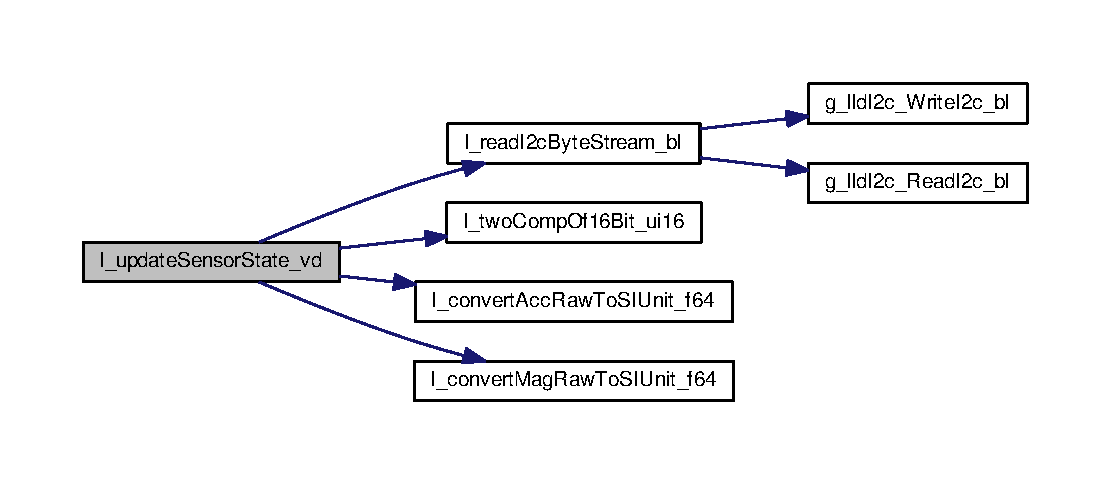
\includegraphics[width=350pt]{accMag_8c_a5cef87c49dd46218e083a0c95abb9a9b_a5cef87c49dd46218e083a0c95abb9a9b_cgraph}
\end{center}
\end{figure}




Here is the caller graph for this function\+:
\nopagebreak
\begin{figure}[H]
\begin{center}
\leavevmode
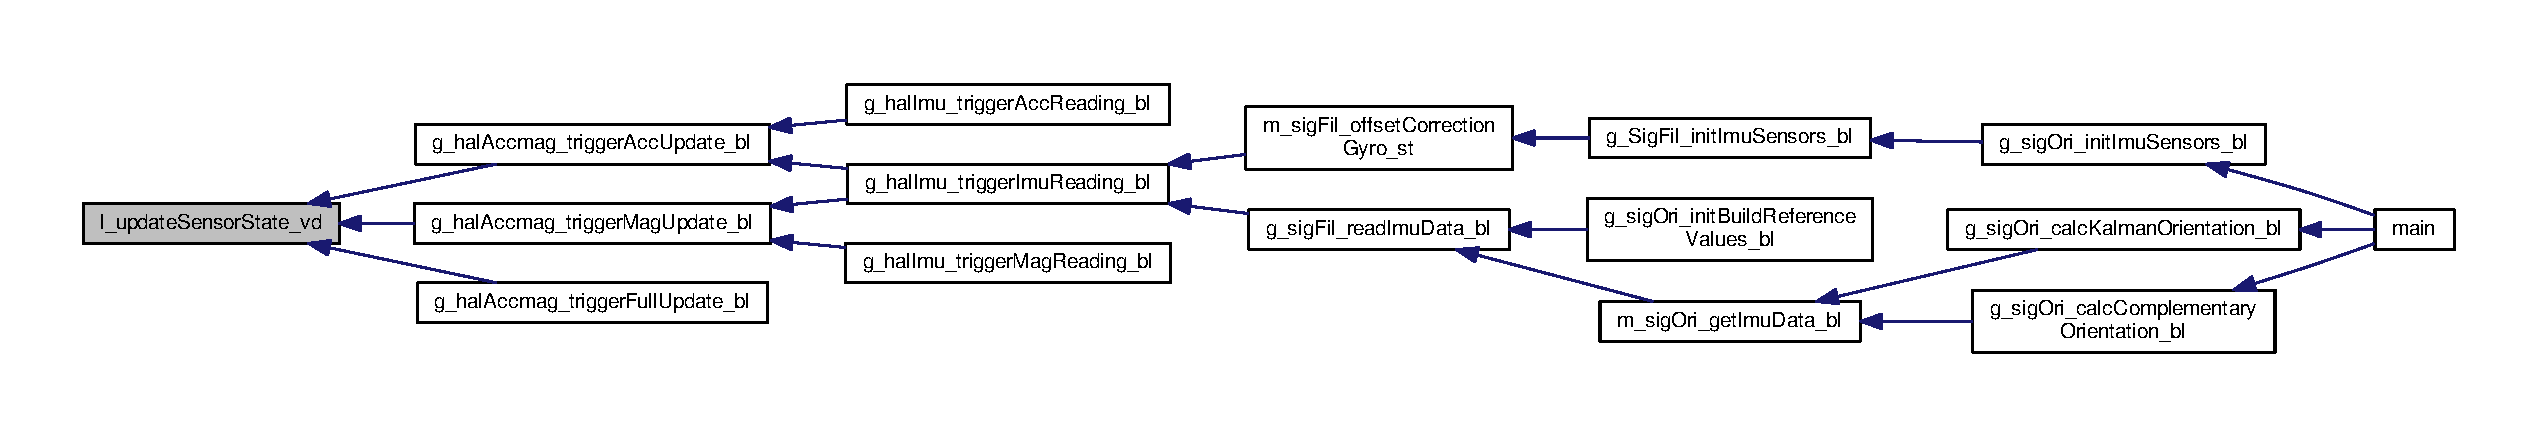
\includegraphics[width=350pt]{accMag_8c_a5cef87c49dd46218e083a0c95abb9a9b_a5cef87c49dd46218e083a0c95abb9a9b_icgraph}
\end{center}
\end{figure}


\hypertarget{accMag_8c_af4a867d90abb126d82ba14ea2619f305_af4a867d90abb126d82ba14ea2619f305}{\index{acc\+Mag.\+c@{acc\+Mag.\+c}!l\+\_\+write\+I2c\+Byte\+Stream\+\_\+bl@{l\+\_\+write\+I2c\+Byte\+Stream\+\_\+bl}}
\index{l\+\_\+write\+I2c\+Byte\+Stream\+\_\+bl@{l\+\_\+write\+I2c\+Byte\+Stream\+\_\+bl}!acc\+Mag.\+c@{acc\+Mag.\+c}}
\subsubsection[{l\+\_\+write\+I2c\+Byte\+Stream\+\_\+bl}]{\setlength{\rightskip}{0pt plus 5cm}static unsigned int l\+\_\+write\+I2c\+Byte\+Stream\+\_\+bl (
\begin{DoxyParamCaption}
\item[{unsigned char}]{f\+\_\+start\+Register\+Addr\+\_\+ui8, }
\item[{const unsigned char $\ast$const}]{f\+\_\+byte\+Stream\+To\+Write\+\_\+pui8, }
\item[{unsigned int}]{f\+\_\+num\+Of\+Bytes\+\_\+ui32}
\end{DoxyParamCaption}
)\hspace{0.3cm}{\ttfamily [inline]}, {\ttfamily [static]}}}\label{accMag_8c_af4a867d90abb126d82ba14ea2619f305_af4a867d90abb126d82ba14ea2619f305}


Wrapper function to write a single byte register of L\+S\+M303\+D. 



 \begin{DoxyAuthor}{Author}
Juergen Schmidt (juscgs00) 
\end{DoxyAuthor}
\begin{DoxyDate}{Date}
2014/05/05
\end{DoxyDate}
This function is a wrapper to the I2\+C Interface to write one single byte to a register of the Accelerometer/\+Magnetometer (L\+S\+M303\+D). It eases the concatenation of register address and data byte to transmit.


\begin{DoxyParams}[1]{Parameters}
\mbox{\tt in}  & {\em f\+\_\+register\+Addr\+\_\+ui8} & specifies the register address to return \\
\hline
\mbox{\tt in}  & {\em f\+\_\+byte\+To\+Write\+\_\+ui8} & specifies the single byte to write \\
\hline
\mbox{\tt out}  & {\em returns} & a boolean value, indicating the occurrence of failures~\newline
 0 .... indicates success (no errors)~\newline
 1 .... indicates failed (some errors)\\
\hline
\end{DoxyParams}




 \begin{DoxyAuthor}{Author}
Juergen Schmidt (juscgs00) 
\end{DoxyAuthor}
\begin{DoxyDate}{Date}
2014/05/08
\end{DoxyDate}
Wrapper function to write byte stream to registers of L\+S\+M303\+D

This function is a wrapper to the I2\+C Interface to write a byte stream to a series of registers of the Accelerometer/ Magnetometer (L\+S\+M303\+D). The first register address can be defined in the parameter list of the function. After writing the first byte to the start address, the register address will be incremented.


\begin{DoxyParams}[1]{Parameters}
\mbox{\tt in}  & {\em f\+\_\+start\+Register\+Addr\+\_\+ui8} & specifies the first register address to return \\
\hline
\mbox{\tt in}  & {\em f\+\_\+byte\+Stream\+To\+Write\+\_\+pui8} & points to an array of unsigned 8bit data elements (input byte stream buffer) \\
\hline
\mbox{\tt out}  & {\em returns} & a boolean value, indicating the occurrence of failures~\newline
 0 .... indicates success (no errors)~\newline
 1 .... indicates failed (some errors)\\
\hline
\end{DoxyParams}


Definition at line 207 of file acc\+Mag.\+c.


\begin{DoxyCode}
208 \{
209     \textcolor{keywordtype}{unsigned} \textcolor{keywordtype}{int}    l\_writeSucceeded\_bl     = \hyperlink{accMag_8h_a244c94ee3b75087140235cf4f913623f_a244c94ee3b75087140235cf4f913623f}{M\_HAL\_ACCMAG\_SUCCESS\_BL};   \textcolor{comment}{// success
       state as default}
210     \textcolor{keywordtype}{unsigned} \textcolor{keywordtype}{char}   l\_bufCtr\_ui8            = 0;                        \textcolor{comment}{// loop counter to assemble payload
       and register address}
211     \textcolor{keywordtype}{unsigned} \textcolor{keywordtype}{char}   l\_byteStreamBuffer\_rgXui8[
      \hyperlink{accMag_8h_aaa771727c176ae833aea7231c6bd80f0_aaa771727c176ae833aea7231c6bd80f0}{M\_HAL\_ACCMAG\_WRITE\_BYTESTREAM\_BUFFER\_SIZE\_UI8}];
212     \textcolor{comment}{/*}
213 \textcolor{comment}{     * - ensure at least one data byte to write}
214 \textcolor{comment}{     * - prevent a buffer overflow of l\_byteStreamBuffer\_rgXui8}
215 \textcolor{comment}{     *   --> payload data bytes + register address (subaddress)}
216 \textcolor{comment}{     */}
217     \textcolor{keywordflow}{if} (        (f\_numOfBytes\_ui32 < 1)
218             ||  (f\_numOfBytes\_ui32 > 
      \hyperlink{accMag_8h_aaa771727c176ae833aea7231c6bd80f0_aaa771727c176ae833aea7231c6bd80f0}{M\_HAL\_ACCMAG\_WRITE\_BYTESTREAM\_BUFFER\_SIZE\_UI8}-1) )
219     \{
220         \textcolor{keywordflow}{return} \hyperlink{accMag_8h_a29da5c251bf0c3b1c7ed7da3c3269d9f_a29da5c251bf0c3b1c7ed7da3c3269d9f}{M\_HAL\_ACCMAG\_FAILED\_BL};
221     \}
222 
223     \textcolor{comment}{/*}
224 \textcolor{comment}{     * prepare data to write (register + data)}
225 \textcolor{comment}{     * (1) ensure byte stream writing (MSB of register address shall be 1)}
226 \textcolor{comment}{     *     -> Mask MSB to one!}
227 \textcolor{comment}{     *     -> LSM303D will auto-increment the register address for each byte}
228 \textcolor{comment}{     *        of data}
229 \textcolor{comment}{     * (2) copy data to write to local buffer, start at second byte position}
230 \textcolor{comment}{     *     (first byte position is the register address)}
231 \textcolor{comment}{     */}
232     l\_byteStreamBuffer\_rgXui8[0] = f\_startRegisterAddr\_ui8 | 0b10000000;
233     \textcolor{keywordflow}{for}(l\_bufCtr\_ui8=0; l\_bufCtr\_ui8 < f\_numOfBytes\_ui32; l\_bufCtr\_ui8++)
234     \{
235         l\_byteStreamBuffer\_rgXui8[l\_bufCtr\_ui8+1] = f\_byteStreamToWrite\_pui8[l\_bufCtr\_ui8];
236     \}
237 
238     \textcolor{comment}{//write register to I2C}
239     \textcolor{keywordflow}{if} ( \hyperlink{LLD__I2C_8c_aa6892bf4aea7f232d9b0ff2dbf8a9321_aa6892bf4aea7f232d9b0ff2dbf8a9321}{g\_lldI2c\_WriteI2c\_bl}(\hyperlink{accMag_8h_a6c9acfcf0f8dff7a5789ddb4960b3599_a6c9acfcf0f8dff7a5789ddb4960b3599}{M\_HAL\_ACCMAG\_I2CADDR\_UI8}, 
      l\_byteStreamBuffer\_rgXui8, f\_numOfBytes\_ui32 + 1) != \hyperlink{accMag_8h_a244c94ee3b75087140235cf4f913623f_a244c94ee3b75087140235cf4f913623f}{M\_HAL\_ACCMAG\_SUCCESS\_BL} )
240     \{
241         \textcolor{comment}{// error in I2C access}
242         l\_writeSucceeded\_bl = \hyperlink{accMag_8h_a29da5c251bf0c3b1c7ed7da3c3269d9f_a29da5c251bf0c3b1c7ed7da3c3269d9f}{M\_HAL\_ACCMAG\_FAILED\_BL};
243     \}
244 
245     \textcolor{keywordflow}{return} l\_writeSucceeded\_bl;
246 \}
\end{DoxyCode}


Here is the call graph for this function\+:
\nopagebreak
\begin{figure}[H]
\begin{center}
\leavevmode
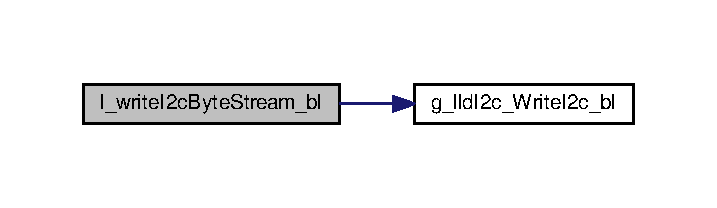
\includegraphics[width=344pt]{accMag_8c_af4a867d90abb126d82ba14ea2619f305_af4a867d90abb126d82ba14ea2619f305_cgraph}
\end{center}
\end{figure}




Here is the caller graph for this function\+:
\nopagebreak
\begin{figure}[H]
\begin{center}
\leavevmode
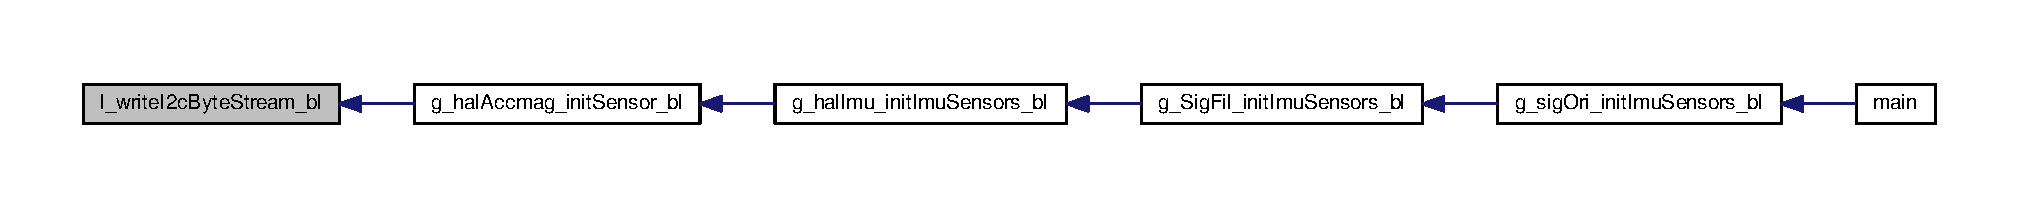
\includegraphics[width=350pt]{accMag_8c_af4a867d90abb126d82ba14ea2619f305_af4a867d90abb126d82ba14ea2619f305_icgraph}
\end{center}
\end{figure}




\subsection{Variable Documentation}
\hypertarget{accMag_8c_a421eb1956f3c2b98d7a4505bc13b049e_a421eb1956f3c2b98d7a4505bc13b049e}{\index{acc\+Mag.\+c@{acc\+Mag.\+c}!m\+\_\+hal\+Accmag\+\_\+sensor\+State\+\_\+st@{m\+\_\+hal\+Accmag\+\_\+sensor\+State\+\_\+st}}
\index{m\+\_\+hal\+Accmag\+\_\+sensor\+State\+\_\+st@{m\+\_\+hal\+Accmag\+\_\+sensor\+State\+\_\+st}!acc\+Mag.\+c@{acc\+Mag.\+c}}
\subsubsection[{m\+\_\+hal\+Accmag\+\_\+sensor\+State\+\_\+st}]{\setlength{\rightskip}{0pt plus 5cm}{\bf hal\+Accmag\+\_\+data\+Container} m\+\_\+hal\+Accmag\+\_\+sensor\+State\+\_\+st\hspace{0.3cm}{\ttfamily [static]}}}\label{accMag_8c_a421eb1956f3c2b98d7a4505bc13b049e_a421eb1956f3c2b98d7a4505bc13b049e}
acceleration state and compass state in one container 

Definition at line 12 of file acc\+Mag.\+c.


\hypertarget{accMag_8h}{\section{hal/\+I\+M\+U/acc\+Mag/acc\+Mag.h File Reference}
\label{accMag_8h}\index{hal/\+I\+M\+U/acc\+Mag/acc\+Mag.\+h@{hal/\+I\+M\+U/acc\+Mag/acc\+Mag.\+h}}
}
{\ttfamily \#include \char`\"{}acc\+Mag\+\_\+registers.\+h\char`\"{}}\\*
Include dependency graph for acc\+Mag.\+h\+:
\nopagebreak
\begin{figure}[H]
\begin{center}
\leavevmode
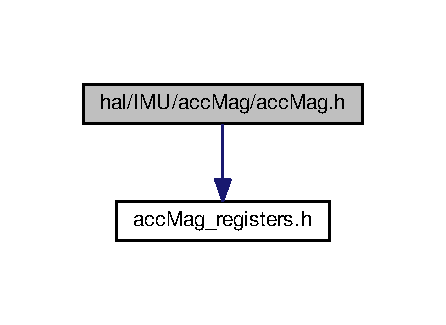
\includegraphics[width=214pt]{accMag_8h__incl}
\end{center}
\end{figure}
This graph shows which files directly or indirectly include this file\+:
\nopagebreak
\begin{figure}[H]
\begin{center}
\leavevmode
\includegraphics[width=350pt]{accMag_8h__dep__incl}
\end{center}
\end{figure}
\subsection*{Data Structures}
\begin{DoxyCompactItemize}
\item 
struct \hyperlink{structhalAccmag__3dDoubleVector}{hal\+Accmag\+\_\+3d\+Double\+Vector}
\begin{DoxyCompactList}\small\item\em 3\+D vector of floats for x,y,z axes of sensors \end{DoxyCompactList}\item 
struct \hyperlink{structhalAccmag__dataContainer}{hal\+Accmag\+\_\+data\+Container}
\begin{DoxyCompactList}\small\item\em Container for Acc. and Compass data. \end{DoxyCompactList}\end{DoxyCompactItemize}
\subsection*{Macros}
\begin{DoxyCompactItemize}
\item 
\#define \hyperlink{accMag_8h_a44405d1fc6d79b1588b5ce1549f5af52_a44405d1fc6d79b1588b5ce1549f5af52}{M\+\_\+\+H\+A\+L\+\_\+\+A\+C\+C\+M\+A\+G\+\_\+\+A\+C\+C\+S\+C\+A\+L\+E\+\_\+\+U\+I8}~8
\begin{DoxyCompactList}\small\item\em defines the defined scale of the accelerometer \mbox{[}m$\ast$s$^\wedge$(-\/2)\mbox{]} \end{DoxyCompactList}\item 
\#define \hyperlink{accMag_8h_a29da5c251bf0c3b1c7ed7da3c3269d9f_a29da5c251bf0c3b1c7ed7da3c3269d9f}{M\+\_\+\+H\+A\+L\+\_\+\+A\+C\+C\+M\+A\+G\+\_\+\+F\+A\+I\+L\+E\+D\+\_\+\+B\+L}~1
\item 
\#define \hyperlink{accMag_8h_aa196c646e6de5cdae834c1ea392f4666_aa196c646e6de5cdae834c1ea392f4666}{M\+\_\+\+H\+A\+L\+\_\+\+A\+C\+C\+M\+A\+G\+\_\+\+F\+A\+L\+S\+E\+\_\+\+B\+L}~0
\item 
\#define \hyperlink{accMag_8h_a6c9acfcf0f8dff7a5789ddb4960b3599_a6c9acfcf0f8dff7a5789ddb4960b3599}{M\+\_\+\+H\+A\+L\+\_\+\+A\+C\+C\+M\+A\+G\+\_\+\+I2\+C\+A\+D\+D\+R\+\_\+\+U\+I8}~0x1\+E
\begin{DoxyCompactList}\small\item\em I2\+C chip address of L\+S\+M303\+D (Acceleration \& Compass sensor) \end{DoxyCompactList}\item 
\#define \hyperlink{accMag_8h_a470c76781432ff3b1dad24810d44311d_a470c76781432ff3b1dad24810d44311d}{M\+\_\+\+H\+A\+L\+\_\+\+A\+C\+C\+M\+A\+G\+\_\+\+M\+A\+G\+S\+C\+A\+L\+E\+\_\+\+U\+I8}~4
\begin{DoxyCompactList}\small\item\em defines the defined scale of the magnetometer \mbox{[}0.\+1$\ast$m\+T\mbox{]} \end{DoxyCompactList}\item 
\#define \hyperlink{accMag_8h_a244c94ee3b75087140235cf4f913623f_a244c94ee3b75087140235cf4f913623f}{M\+\_\+\+H\+A\+L\+\_\+\+A\+C\+C\+M\+A\+G\+\_\+\+S\+U\+C\+C\+E\+S\+S\+\_\+\+B\+L}~0
\item 
\#define \hyperlink{accMag_8h_a90589032b2dc48b1885cd5d76f302121_a90589032b2dc48b1885cd5d76f302121}{M\+\_\+\+H\+A\+L\+\_\+\+A\+C\+C\+M\+A\+G\+\_\+\+T\+R\+U\+E\+\_\+\+B\+L}~1
\item 
\#define \hyperlink{accMag_8h_aaa771727c176ae833aea7231c6bd80f0_aaa771727c176ae833aea7231c6bd80f0}{M\+\_\+\+H\+A\+L\+\_\+\+A\+C\+C\+M\+A\+G\+\_\+\+W\+R\+I\+T\+E\+\_\+\+B\+Y\+T\+E\+S\+T\+R\+E\+A\+M\+\_\+\+B\+U\+F\+F\+E\+R\+\_\+\+S\+I\+Z\+E\+\_\+\+U\+I8}~12
\begin{DoxyCompactList}\small\item\em defines the local write buffer of function l\+\_\+write\+I2c\+Byte\+Stream\+\_\+bl \end{DoxyCompactList}\end{DoxyCompactItemize}
\subsection*{Enumerations}
\begin{DoxyCompactItemize}
\item 
enum \hyperlink{accMag_8h_a648cc7f506bdd006d657bf0c2fc393b8_a648cc7f506bdd006d657bf0c2fc393b8}{hal\+Accmag\+\_\+sensor\+Select} \{ \hyperlink{accMag_8h_a648cc7f506bdd006d657bf0c2fc393b8_a648cc7f506bdd006d657bf0c2fc393b8a785fd0a49fbb18e5a2e65b8af35d6abc}{S\+E\+N\+S\+O\+R\+\_\+\+A\+C\+C\+\_\+\+E\+N}, 
\hyperlink{accMag_8h_a648cc7f506bdd006d657bf0c2fc393b8_a648cc7f506bdd006d657bf0c2fc393b8a2a54a90cabb4985b0bd3bcb7d5b54d28}{S\+E\+N\+S\+O\+R\+\_\+\+M\+A\+G\+\_\+\+E\+N}, 
\hyperlink{accMag_8h_a648cc7f506bdd006d657bf0c2fc393b8_a648cc7f506bdd006d657bf0c2fc393b8a2801a1fb951d195fa4c2d621bd352a79}{S\+E\+N\+S\+O\+R\+\_\+\+B\+O\+T\+H\+\_\+\+E\+N}
 \}
\begin{DoxyCompactList}\small\item\em Enumeration to choose accelerometer or magnetometer or both. \end{DoxyCompactList}\end{DoxyCompactItemize}
\subsection*{Functions}
\begin{DoxyCompactItemize}
\item 
\hyperlink{structhalAccmag__dataContainer}{hal\+Accmag\+\_\+data\+Container} \hyperlink{accMag_8h_a3914b0d0b4d88f06880b47766f844fc8_a3914b0d0b4d88f06880b47766f844fc8}{g\+\_\+hal\+Accmag\+\_\+get\+Acc\+Mag\+Container\+\_\+st} (void)
\begin{DoxyCompactList}\small\item\em Get complete data container (acceleration \& compass) \end{DoxyCompactList}\item 
\hyperlink{structhalAccmag__3dDoubleVector}{hal\+Accmag\+\_\+3d\+Double\+Vector} \hyperlink{accMag_8h_aebfdb7e3d86187e1fecee863424aa3fc_aebfdb7e3d86187e1fecee863424aa3fc}{g\+\_\+hal\+Accmag\+\_\+get\+Acc\+Vector\+\_\+st} (void)
\begin{DoxyCompactList}\small\item\em Get current state of acceleration. \end{DoxyCompactList}\item 
\hyperlink{structhalAccmag__3dDoubleVector}{hal\+Accmag\+\_\+3d\+Double\+Vector} \hyperlink{accMag_8h_ad4f25c6a1f31b6eb494243aa0706986a_ad4f25c6a1f31b6eb494243aa0706986a}{g\+\_\+hal\+Accmag\+\_\+get\+Mag\+Vector\+\_\+st} (void)
\begin{DoxyCompactList}\small\item\em Get current state of compass. \end{DoxyCompactList}\item 
unsigned int \hyperlink{accMag_8h_ab936c0ac53ff9ba47a138e841a6ba474_ab936c0ac53ff9ba47a138e841a6ba474}{g\+\_\+hal\+Accmag\+\_\+init\+Sensor\+\_\+bl} (void)
\begin{DoxyCompactList}\small\item\em Initialize sensor. \end{DoxyCompactList}\item 
unsigned int \hyperlink{accMag_8h_ad5f9d3a28348a9889f9afecde79606f6_ad5f9d3a28348a9889f9afecde79606f6}{g\+\_\+hal\+Accmag\+\_\+trigger\+Acc\+Update\+\_\+bl} (void)
\begin{DoxyCompactList}\small\item\em Trigger a new measurement of the accelerometer. \end{DoxyCompactList}\item 
unsigned int \hyperlink{accMag_8h_a98cf3442152a9ae213517936f7b37fe0_a98cf3442152a9ae213517936f7b37fe0}{g\+\_\+hal\+Accmag\+\_\+trigger\+Full\+Update\+\_\+bl} (void)
\begin{DoxyCompactList}\small\item\em Trigger a new measurement of both sensors. \end{DoxyCompactList}\item 
unsigned int \hyperlink{accMag_8h_afdbd4ece113ff4859718b678150d069a_afdbd4ece113ff4859718b678150d069a}{g\+\_\+hal\+Accmag\+\_\+trigger\+Mag\+Update\+\_\+bl} (void)
\begin{DoxyCompactList}\small\item\em Trigger a new measurement of the magnetometer. \end{DoxyCompactList}\end{DoxyCompactItemize}


\subsection{Macro Definition Documentation}
\hypertarget{accMag_8h_a44405d1fc6d79b1588b5ce1549f5af52_a44405d1fc6d79b1588b5ce1549f5af52}{\index{acc\+Mag.\+h@{acc\+Mag.\+h}!M\+\_\+\+H\+A\+L\+\_\+\+A\+C\+C\+M\+A\+G\+\_\+\+A\+C\+C\+S\+C\+A\+L\+E\+\_\+\+U\+I8@{M\+\_\+\+H\+A\+L\+\_\+\+A\+C\+C\+M\+A\+G\+\_\+\+A\+C\+C\+S\+C\+A\+L\+E\+\_\+\+U\+I8}}
\index{M\+\_\+\+H\+A\+L\+\_\+\+A\+C\+C\+M\+A\+G\+\_\+\+A\+C\+C\+S\+C\+A\+L\+E\+\_\+\+U\+I8@{M\+\_\+\+H\+A\+L\+\_\+\+A\+C\+C\+M\+A\+G\+\_\+\+A\+C\+C\+S\+C\+A\+L\+E\+\_\+\+U\+I8}!acc\+Mag.\+h@{acc\+Mag.\+h}}
\subsubsection[{M\+\_\+\+H\+A\+L\+\_\+\+A\+C\+C\+M\+A\+G\+\_\+\+A\+C\+C\+S\+C\+A\+L\+E\+\_\+\+U\+I8}]{\setlength{\rightskip}{0pt plus 5cm}\#define M\+\_\+\+H\+A\+L\+\_\+\+A\+C\+C\+M\+A\+G\+\_\+\+A\+C\+C\+S\+C\+A\+L\+E\+\_\+\+U\+I8~8}}\label{accMag_8h_a44405d1fc6d79b1588b5ce1549f5af52_a44405d1fc6d79b1588b5ce1549f5af52}


defines the defined scale of the accelerometer \mbox{[}m$\ast$s$^\wedge$(-\/2)\mbox{]} 



Definition at line 18 of file acc\+Mag.\+h.

\hypertarget{accMag_8h_a29da5c251bf0c3b1c7ed7da3c3269d9f_a29da5c251bf0c3b1c7ed7da3c3269d9f}{\index{acc\+Mag.\+h@{acc\+Mag.\+h}!M\+\_\+\+H\+A\+L\+\_\+\+A\+C\+C\+M\+A\+G\+\_\+\+F\+A\+I\+L\+E\+D\+\_\+\+B\+L@{M\+\_\+\+H\+A\+L\+\_\+\+A\+C\+C\+M\+A\+G\+\_\+\+F\+A\+I\+L\+E\+D\+\_\+\+B\+L}}
\index{M\+\_\+\+H\+A\+L\+\_\+\+A\+C\+C\+M\+A\+G\+\_\+\+F\+A\+I\+L\+E\+D\+\_\+\+B\+L@{M\+\_\+\+H\+A\+L\+\_\+\+A\+C\+C\+M\+A\+G\+\_\+\+F\+A\+I\+L\+E\+D\+\_\+\+B\+L}!acc\+Mag.\+h@{acc\+Mag.\+h}}
\subsubsection[{M\+\_\+\+H\+A\+L\+\_\+\+A\+C\+C\+M\+A\+G\+\_\+\+F\+A\+I\+L\+E\+D\+\_\+\+B\+L}]{\setlength{\rightskip}{0pt plus 5cm}\#define M\+\_\+\+H\+A\+L\+\_\+\+A\+C\+C\+M\+A\+G\+\_\+\+F\+A\+I\+L\+E\+D\+\_\+\+B\+L~1}}\label{accMag_8h_a29da5c251bf0c3b1c7ed7da3c3269d9f_a29da5c251bf0c3b1c7ed7da3c3269d9f}


Definition at line 14 of file acc\+Mag.\+h.

\hypertarget{accMag_8h_aa196c646e6de5cdae834c1ea392f4666_aa196c646e6de5cdae834c1ea392f4666}{\index{acc\+Mag.\+h@{acc\+Mag.\+h}!M\+\_\+\+H\+A\+L\+\_\+\+A\+C\+C\+M\+A\+G\+\_\+\+F\+A\+L\+S\+E\+\_\+\+B\+L@{M\+\_\+\+H\+A\+L\+\_\+\+A\+C\+C\+M\+A\+G\+\_\+\+F\+A\+L\+S\+E\+\_\+\+B\+L}}
\index{M\+\_\+\+H\+A\+L\+\_\+\+A\+C\+C\+M\+A\+G\+\_\+\+F\+A\+L\+S\+E\+\_\+\+B\+L@{M\+\_\+\+H\+A\+L\+\_\+\+A\+C\+C\+M\+A\+G\+\_\+\+F\+A\+L\+S\+E\+\_\+\+B\+L}!acc\+Mag.\+h@{acc\+Mag.\+h}}
\subsubsection[{M\+\_\+\+H\+A\+L\+\_\+\+A\+C\+C\+M\+A\+G\+\_\+\+F\+A\+L\+S\+E\+\_\+\+B\+L}]{\setlength{\rightskip}{0pt plus 5cm}\#define M\+\_\+\+H\+A\+L\+\_\+\+A\+C\+C\+M\+A\+G\+\_\+\+F\+A\+L\+S\+E\+\_\+\+B\+L~0}}\label{accMag_8h_aa196c646e6de5cdae834c1ea392f4666_aa196c646e6de5cdae834c1ea392f4666}


Definition at line 11 of file acc\+Mag.\+h.

\hypertarget{accMag_8h_a6c9acfcf0f8dff7a5789ddb4960b3599_a6c9acfcf0f8dff7a5789ddb4960b3599}{\index{acc\+Mag.\+h@{acc\+Mag.\+h}!M\+\_\+\+H\+A\+L\+\_\+\+A\+C\+C\+M\+A\+G\+\_\+\+I2\+C\+A\+D\+D\+R\+\_\+\+U\+I8@{M\+\_\+\+H\+A\+L\+\_\+\+A\+C\+C\+M\+A\+G\+\_\+\+I2\+C\+A\+D\+D\+R\+\_\+\+U\+I8}}
\index{M\+\_\+\+H\+A\+L\+\_\+\+A\+C\+C\+M\+A\+G\+\_\+\+I2\+C\+A\+D\+D\+R\+\_\+\+U\+I8@{M\+\_\+\+H\+A\+L\+\_\+\+A\+C\+C\+M\+A\+G\+\_\+\+I2\+C\+A\+D\+D\+R\+\_\+\+U\+I8}!acc\+Mag.\+h@{acc\+Mag.\+h}}
\subsubsection[{M\+\_\+\+H\+A\+L\+\_\+\+A\+C\+C\+M\+A\+G\+\_\+\+I2\+C\+A\+D\+D\+R\+\_\+\+U\+I8}]{\setlength{\rightskip}{0pt plus 5cm}\#define M\+\_\+\+H\+A\+L\+\_\+\+A\+C\+C\+M\+A\+G\+\_\+\+I2\+C\+A\+D\+D\+R\+\_\+\+U\+I8~0x1\+E}}\label{accMag_8h_a6c9acfcf0f8dff7a5789ddb4960b3599_a6c9acfcf0f8dff7a5789ddb4960b3599}


I2\+C chip address of L\+S\+M303\+D (Acceleration \& Compass sensor) 



Definition at line 20 of file acc\+Mag.\+h.

\hypertarget{accMag_8h_a470c76781432ff3b1dad24810d44311d_a470c76781432ff3b1dad24810d44311d}{\index{acc\+Mag.\+h@{acc\+Mag.\+h}!M\+\_\+\+H\+A\+L\+\_\+\+A\+C\+C\+M\+A\+G\+\_\+\+M\+A\+G\+S\+C\+A\+L\+E\+\_\+\+U\+I8@{M\+\_\+\+H\+A\+L\+\_\+\+A\+C\+C\+M\+A\+G\+\_\+\+M\+A\+G\+S\+C\+A\+L\+E\+\_\+\+U\+I8}}
\index{M\+\_\+\+H\+A\+L\+\_\+\+A\+C\+C\+M\+A\+G\+\_\+\+M\+A\+G\+S\+C\+A\+L\+E\+\_\+\+U\+I8@{M\+\_\+\+H\+A\+L\+\_\+\+A\+C\+C\+M\+A\+G\+\_\+\+M\+A\+G\+S\+C\+A\+L\+E\+\_\+\+U\+I8}!acc\+Mag.\+h@{acc\+Mag.\+h}}
\subsubsection[{M\+\_\+\+H\+A\+L\+\_\+\+A\+C\+C\+M\+A\+G\+\_\+\+M\+A\+G\+S\+C\+A\+L\+E\+\_\+\+U\+I8}]{\setlength{\rightskip}{0pt plus 5cm}\#define M\+\_\+\+H\+A\+L\+\_\+\+A\+C\+C\+M\+A\+G\+\_\+\+M\+A\+G\+S\+C\+A\+L\+E\+\_\+\+U\+I8~4}}\label{accMag_8h_a470c76781432ff3b1dad24810d44311d_a470c76781432ff3b1dad24810d44311d}


defines the defined scale of the magnetometer \mbox{[}0.\+1$\ast$m\+T\mbox{]} 



Definition at line 19 of file acc\+Mag.\+h.

\hypertarget{accMag_8h_a244c94ee3b75087140235cf4f913623f_a244c94ee3b75087140235cf4f913623f}{\index{acc\+Mag.\+h@{acc\+Mag.\+h}!M\+\_\+\+H\+A\+L\+\_\+\+A\+C\+C\+M\+A\+G\+\_\+\+S\+U\+C\+C\+E\+S\+S\+\_\+\+B\+L@{M\+\_\+\+H\+A\+L\+\_\+\+A\+C\+C\+M\+A\+G\+\_\+\+S\+U\+C\+C\+E\+S\+S\+\_\+\+B\+L}}
\index{M\+\_\+\+H\+A\+L\+\_\+\+A\+C\+C\+M\+A\+G\+\_\+\+S\+U\+C\+C\+E\+S\+S\+\_\+\+B\+L@{M\+\_\+\+H\+A\+L\+\_\+\+A\+C\+C\+M\+A\+G\+\_\+\+S\+U\+C\+C\+E\+S\+S\+\_\+\+B\+L}!acc\+Mag.\+h@{acc\+Mag.\+h}}
\subsubsection[{M\+\_\+\+H\+A\+L\+\_\+\+A\+C\+C\+M\+A\+G\+\_\+\+S\+U\+C\+C\+E\+S\+S\+\_\+\+B\+L}]{\setlength{\rightskip}{0pt plus 5cm}\#define M\+\_\+\+H\+A\+L\+\_\+\+A\+C\+C\+M\+A\+G\+\_\+\+S\+U\+C\+C\+E\+S\+S\+\_\+\+B\+L~0}}\label{accMag_8h_a244c94ee3b75087140235cf4f913623f_a244c94ee3b75087140235cf4f913623f}


Definition at line 13 of file acc\+Mag.\+h.

\hypertarget{accMag_8h_a90589032b2dc48b1885cd5d76f302121_a90589032b2dc48b1885cd5d76f302121}{\index{acc\+Mag.\+h@{acc\+Mag.\+h}!M\+\_\+\+H\+A\+L\+\_\+\+A\+C\+C\+M\+A\+G\+\_\+\+T\+R\+U\+E\+\_\+\+B\+L@{M\+\_\+\+H\+A\+L\+\_\+\+A\+C\+C\+M\+A\+G\+\_\+\+T\+R\+U\+E\+\_\+\+B\+L}}
\index{M\+\_\+\+H\+A\+L\+\_\+\+A\+C\+C\+M\+A\+G\+\_\+\+T\+R\+U\+E\+\_\+\+B\+L@{M\+\_\+\+H\+A\+L\+\_\+\+A\+C\+C\+M\+A\+G\+\_\+\+T\+R\+U\+E\+\_\+\+B\+L}!acc\+Mag.\+h@{acc\+Mag.\+h}}
\subsubsection[{M\+\_\+\+H\+A\+L\+\_\+\+A\+C\+C\+M\+A\+G\+\_\+\+T\+R\+U\+E\+\_\+\+B\+L}]{\setlength{\rightskip}{0pt plus 5cm}\#define M\+\_\+\+H\+A\+L\+\_\+\+A\+C\+C\+M\+A\+G\+\_\+\+T\+R\+U\+E\+\_\+\+B\+L~1}}\label{accMag_8h_a90589032b2dc48b1885cd5d76f302121_a90589032b2dc48b1885cd5d76f302121}


Definition at line 10 of file acc\+Mag.\+h.

\hypertarget{accMag_8h_aaa771727c176ae833aea7231c6bd80f0_aaa771727c176ae833aea7231c6bd80f0}{\index{acc\+Mag.\+h@{acc\+Mag.\+h}!M\+\_\+\+H\+A\+L\+\_\+\+A\+C\+C\+M\+A\+G\+\_\+\+W\+R\+I\+T\+E\+\_\+\+B\+Y\+T\+E\+S\+T\+R\+E\+A\+M\+\_\+\+B\+U\+F\+F\+E\+R\+\_\+\+S\+I\+Z\+E\+\_\+\+U\+I8@{M\+\_\+\+H\+A\+L\+\_\+\+A\+C\+C\+M\+A\+G\+\_\+\+W\+R\+I\+T\+E\+\_\+\+B\+Y\+T\+E\+S\+T\+R\+E\+A\+M\+\_\+\+B\+U\+F\+F\+E\+R\+\_\+\+S\+I\+Z\+E\+\_\+\+U\+I8}}
\index{M\+\_\+\+H\+A\+L\+\_\+\+A\+C\+C\+M\+A\+G\+\_\+\+W\+R\+I\+T\+E\+\_\+\+B\+Y\+T\+E\+S\+T\+R\+E\+A\+M\+\_\+\+B\+U\+F\+F\+E\+R\+\_\+\+S\+I\+Z\+E\+\_\+\+U\+I8@{M\+\_\+\+H\+A\+L\+\_\+\+A\+C\+C\+M\+A\+G\+\_\+\+W\+R\+I\+T\+E\+\_\+\+B\+Y\+T\+E\+S\+T\+R\+E\+A\+M\+\_\+\+B\+U\+F\+F\+E\+R\+\_\+\+S\+I\+Z\+E\+\_\+\+U\+I8}!acc\+Mag.\+h@{acc\+Mag.\+h}}
\subsubsection[{M\+\_\+\+H\+A\+L\+\_\+\+A\+C\+C\+M\+A\+G\+\_\+\+W\+R\+I\+T\+E\+\_\+\+B\+Y\+T\+E\+S\+T\+R\+E\+A\+M\+\_\+\+B\+U\+F\+F\+E\+R\+\_\+\+S\+I\+Z\+E\+\_\+\+U\+I8}]{\setlength{\rightskip}{0pt plus 5cm}\#define M\+\_\+\+H\+A\+L\+\_\+\+A\+C\+C\+M\+A\+G\+\_\+\+W\+R\+I\+T\+E\+\_\+\+B\+Y\+T\+E\+S\+T\+R\+E\+A\+M\+\_\+\+B\+U\+F\+F\+E\+R\+\_\+\+S\+I\+Z\+E\+\_\+\+U\+I8~12}}\label{accMag_8h_aaa771727c176ae833aea7231c6bd80f0_aaa771727c176ae833aea7231c6bd80f0}


defines the local write buffer of function l\+\_\+write\+I2c\+Byte\+Stream\+\_\+bl 



Definition at line 16 of file acc\+Mag.\+h.



\subsection{Enumeration Type Documentation}
\hypertarget{accMag_8h_a648cc7f506bdd006d657bf0c2fc393b8_a648cc7f506bdd006d657bf0c2fc393b8}{\index{acc\+Mag.\+h@{acc\+Mag.\+h}!hal\+Accmag\+\_\+sensor\+Select@{hal\+Accmag\+\_\+sensor\+Select}}
\index{hal\+Accmag\+\_\+sensor\+Select@{hal\+Accmag\+\_\+sensor\+Select}!acc\+Mag.\+h@{acc\+Mag.\+h}}
\subsubsection[{hal\+Accmag\+\_\+sensor\+Select}]{\setlength{\rightskip}{0pt plus 5cm}enum {\bf hal\+Accmag\+\_\+sensor\+Select}}}\label{accMag_8h_a648cc7f506bdd006d657bf0c2fc393b8_a648cc7f506bdd006d657bf0c2fc393b8}


Enumeration to choose accelerometer or magnetometer or both. 



 \begin{DoxyAuthor}{Author}
Juergen Schmidt (juscgs00) 
\end{DoxyAuthor}
\begin{DoxyDate}{Date}
2014/05/13
\end{DoxyDate}
\begin{Desc}
\item[Enumerator]\par
\begin{description}
\index{S\+E\+N\+S\+O\+R\+\_\+\+A\+C\+C\+\_\+\+E\+N@{S\+E\+N\+S\+O\+R\+\_\+\+A\+C\+C\+\_\+\+E\+N}!acc\+Mag.\+h@{acc\+Mag.\+h}}\index{acc\+Mag.\+h@{acc\+Mag.\+h}!S\+E\+N\+S\+O\+R\+\_\+\+A\+C\+C\+\_\+\+E\+N@{S\+E\+N\+S\+O\+R\+\_\+\+A\+C\+C\+\_\+\+E\+N}}\item[{\em 
\hypertarget{accMag_8h_a648cc7f506bdd006d657bf0c2fc393b8_a648cc7f506bdd006d657bf0c2fc393b8a785fd0a49fbb18e5a2e65b8af35d6abc}{S\+E\+N\+S\+O\+R\+\_\+\+A\+C\+C\+\_\+\+E\+N}\label{accMag_8h_a648cc7f506bdd006d657bf0c2fc393b8_a648cc7f506bdd006d657bf0c2fc393b8a785fd0a49fbb18e5a2e65b8af35d6abc}
}]element to indicate a update of only accelerometer \index{S\+E\+N\+S\+O\+R\+\_\+\+M\+A\+G\+\_\+\+E\+N@{S\+E\+N\+S\+O\+R\+\_\+\+M\+A\+G\+\_\+\+E\+N}!acc\+Mag.\+h@{acc\+Mag.\+h}}\index{acc\+Mag.\+h@{acc\+Mag.\+h}!S\+E\+N\+S\+O\+R\+\_\+\+M\+A\+G\+\_\+\+E\+N@{S\+E\+N\+S\+O\+R\+\_\+\+M\+A\+G\+\_\+\+E\+N}}\item[{\em 
\hypertarget{accMag_8h_a648cc7f506bdd006d657bf0c2fc393b8_a648cc7f506bdd006d657bf0c2fc393b8a2a54a90cabb4985b0bd3bcb7d5b54d28}{S\+E\+N\+S\+O\+R\+\_\+\+M\+A\+G\+\_\+\+E\+N}\label{accMag_8h_a648cc7f506bdd006d657bf0c2fc393b8_a648cc7f506bdd006d657bf0c2fc393b8a2a54a90cabb4985b0bd3bcb7d5b54d28}
}]element to indicate a update of only magnetometer \index{S\+E\+N\+S\+O\+R\+\_\+\+B\+O\+T\+H\+\_\+\+E\+N@{S\+E\+N\+S\+O\+R\+\_\+\+B\+O\+T\+H\+\_\+\+E\+N}!acc\+Mag.\+h@{acc\+Mag.\+h}}\index{acc\+Mag.\+h@{acc\+Mag.\+h}!S\+E\+N\+S\+O\+R\+\_\+\+B\+O\+T\+H\+\_\+\+E\+N@{S\+E\+N\+S\+O\+R\+\_\+\+B\+O\+T\+H\+\_\+\+E\+N}}\item[{\em 
\hypertarget{accMag_8h_a648cc7f506bdd006d657bf0c2fc393b8_a648cc7f506bdd006d657bf0c2fc393b8a2801a1fb951d195fa4c2d621bd352a79}{S\+E\+N\+S\+O\+R\+\_\+\+B\+O\+T\+H\+\_\+\+E\+N}\label{accMag_8h_a648cc7f506bdd006d657bf0c2fc393b8_a648cc7f506bdd006d657bf0c2fc393b8a2801a1fb951d195fa4c2d621bd352a79}
}]element to indicate a update of both sensors \end{description}
\end{Desc}


Definition at line 73 of file acc\+Mag.\+h.


\begin{DoxyCode}
73             \{
74     \hyperlink{accMag_8h_a648cc7f506bdd006d657bf0c2fc393b8_a648cc7f506bdd006d657bf0c2fc393b8a785fd0a49fbb18e5a2e65b8af35d6abc}{SENSOR\_ACC\_EN},     
75     \hyperlink{accMag_8h_a648cc7f506bdd006d657bf0c2fc393b8_a648cc7f506bdd006d657bf0c2fc393b8a2a54a90cabb4985b0bd3bcb7d5b54d28}{SENSOR\_MAG\_EN},     
76     \hyperlink{accMag_8h_a648cc7f506bdd006d657bf0c2fc393b8_a648cc7f506bdd006d657bf0c2fc393b8a2801a1fb951d195fa4c2d621bd352a79}{SENSOR\_BOTH\_EN}        
77 \} \hyperlink{accMag_8h_a648cc7f506bdd006d657bf0c2fc393b8_a648cc7f506bdd006d657bf0c2fc393b8}{halAccmag\_sensorSelect};
\end{DoxyCode}


\subsection{Function Documentation}
\hypertarget{accMag_8h_a3914b0d0b4d88f06880b47766f844fc8_a3914b0d0b4d88f06880b47766f844fc8}{\index{acc\+Mag.\+h@{acc\+Mag.\+h}!g\+\_\+hal\+Accmag\+\_\+get\+Acc\+Mag\+Container\+\_\+st@{g\+\_\+hal\+Accmag\+\_\+get\+Acc\+Mag\+Container\+\_\+st}}
\index{g\+\_\+hal\+Accmag\+\_\+get\+Acc\+Mag\+Container\+\_\+st@{g\+\_\+hal\+Accmag\+\_\+get\+Acc\+Mag\+Container\+\_\+st}!acc\+Mag.\+h@{acc\+Mag.\+h}}
\subsubsection[{g\+\_\+hal\+Accmag\+\_\+get\+Acc\+Mag\+Container\+\_\+st}]{\setlength{\rightskip}{0pt plus 5cm}{\bf hal\+Accmag\+\_\+data\+Container} g\+\_\+hal\+Accmag\+\_\+get\+Acc\+Mag\+Container\+\_\+st (
\begin{DoxyParamCaption}
\item[{void}]{}
\end{DoxyParamCaption}
)}}\label{accMag_8h_a3914b0d0b4d88f06880b47766f844fc8_a3914b0d0b4d88f06880b47766f844fc8}


Get complete data container (acceleration \& compass) 



 \begin{DoxyAuthor}{Author}
Juergen Schmidt (juscgs00) 
\end{DoxyAuthor}
\begin{DoxyDate}{Date}
2014/05/05
\end{DoxyDate}
This function returns the complete accelerometer and magnetometer state. Attention\+: To retrieve a new measurement a measurement trigger is to be called first!


\begin{DoxyParams}[1]{Parameters}
\mbox{\tt out}  & {\em Container} & with compass and acceleration data\\
\hline
\end{DoxyParams}


Definition at line 653 of file acc\+Mag.\+c.


\begin{DoxyCode}
654 \{
655     \textcolor{keywordflow}{return} \hyperlink{accMag_8c_a421eb1956f3c2b98d7a4505bc13b049e_a421eb1956f3c2b98d7a4505bc13b049e}{m\_halAccmag\_sensorState\_st};
656 \}
\end{DoxyCode}
\hypertarget{accMag_8h_aebfdb7e3d86187e1fecee863424aa3fc_aebfdb7e3d86187e1fecee863424aa3fc}{\index{acc\+Mag.\+h@{acc\+Mag.\+h}!g\+\_\+hal\+Accmag\+\_\+get\+Acc\+Vector\+\_\+st@{g\+\_\+hal\+Accmag\+\_\+get\+Acc\+Vector\+\_\+st}}
\index{g\+\_\+hal\+Accmag\+\_\+get\+Acc\+Vector\+\_\+st@{g\+\_\+hal\+Accmag\+\_\+get\+Acc\+Vector\+\_\+st}!acc\+Mag.\+h@{acc\+Mag.\+h}}
\subsubsection[{g\+\_\+hal\+Accmag\+\_\+get\+Acc\+Vector\+\_\+st}]{\setlength{\rightskip}{0pt plus 5cm}{\bf hal\+Accmag\+\_\+3d\+Double\+Vector} g\+\_\+hal\+Accmag\+\_\+get\+Acc\+Vector\+\_\+st (
\begin{DoxyParamCaption}
\item[{void}]{}
\end{DoxyParamCaption}
)}}\label{accMag_8h_aebfdb7e3d86187e1fecee863424aa3fc_aebfdb7e3d86187e1fecee863424aa3fc}


Get current state of acceleration. 



 \begin{DoxyAuthor}{Author}
Juergen Schmidt (juscgs00) 
\end{DoxyAuthor}
\begin{DoxyDate}{Date}
2014/05/05
\end{DoxyDate}
This function returns the current state of the accelerometer.~\newline
 Attention\+: To retrieve a new measurement the measurement trigger is to be called first!


\begin{DoxyParams}[1]{Parameters}
\mbox{\tt out}  & {\em 3\+D} & vector of acceleration components (x,y,z)\\
\hline
\end{DoxyParams}


Definition at line 611 of file acc\+Mag.\+c.


\begin{DoxyCode}
612 \{
613     \textcolor{keywordflow}{return} \hyperlink{accMag_8c_a421eb1956f3c2b98d7a4505bc13b049e_a421eb1956f3c2b98d7a4505bc13b049e}{m\_halAccmag\_sensorState\_st}.\hyperlink{structhalAccmag__dataContainer_afc3847993eed1c8f1e67028ad6d2a6cf_afc3847993eed1c8f1e67028ad6d2a6cf}{acc};
614 \}
\end{DoxyCode}


Here is the caller graph for this function\+:
\nopagebreak
\begin{figure}[H]
\begin{center}
\leavevmode
\includegraphics[width=350pt]{accMag_8h_aebfdb7e3d86187e1fecee863424aa3fc_aebfdb7e3d86187e1fecee863424aa3fc_icgraph}
\end{center}
\end{figure}


\hypertarget{accMag_8h_ad4f25c6a1f31b6eb494243aa0706986a_ad4f25c6a1f31b6eb494243aa0706986a}{\index{acc\+Mag.\+h@{acc\+Mag.\+h}!g\+\_\+hal\+Accmag\+\_\+get\+Mag\+Vector\+\_\+st@{g\+\_\+hal\+Accmag\+\_\+get\+Mag\+Vector\+\_\+st}}
\index{g\+\_\+hal\+Accmag\+\_\+get\+Mag\+Vector\+\_\+st@{g\+\_\+hal\+Accmag\+\_\+get\+Mag\+Vector\+\_\+st}!acc\+Mag.\+h@{acc\+Mag.\+h}}
\subsubsection[{g\+\_\+hal\+Accmag\+\_\+get\+Mag\+Vector\+\_\+st}]{\setlength{\rightskip}{0pt plus 5cm}{\bf hal\+Accmag\+\_\+3d\+Double\+Vector} g\+\_\+hal\+Accmag\+\_\+get\+Mag\+Vector\+\_\+st (
\begin{DoxyParamCaption}
\item[{void}]{}
\end{DoxyParamCaption}
)}}\label{accMag_8h_ad4f25c6a1f31b6eb494243aa0706986a_ad4f25c6a1f31b6eb494243aa0706986a}


Get current state of compass. 



 \begin{DoxyAuthor}{Author}
Juergen Schmidt (juscgs00) 
\end{DoxyAuthor}
\begin{DoxyDate}{Date}
2014/05/05
\end{DoxyDate}
This function returns the current state of the magnetometer.~\newline
 Attention\+: To retrieve a new measurement the measurement trigger is to be called first!


\begin{DoxyParams}[1]{Parameters}
\mbox{\tt out}  & {\em 3\+D} & vector of compass components (x,y,z)\\
\hline
\end{DoxyParams}


Definition at line 632 of file acc\+Mag.\+c.


\begin{DoxyCode}
633 \{
634     \textcolor{keywordflow}{return} \hyperlink{accMag_8c_a421eb1956f3c2b98d7a4505bc13b049e_a421eb1956f3c2b98d7a4505bc13b049e}{m\_halAccmag\_sensorState\_st}.\hyperlink{structhalAccmag__dataContainer_a903681a66ce49c39267aa66d471812f7_a903681a66ce49c39267aa66d471812f7}{mag};
635 \}
\end{DoxyCode}


Here is the caller graph for this function\+:
\nopagebreak
\begin{figure}[H]
\begin{center}
\leavevmode
\includegraphics[width=350pt]{accMag_8h_ad4f25c6a1f31b6eb494243aa0706986a_ad4f25c6a1f31b6eb494243aa0706986a_icgraph}
\end{center}
\end{figure}


\hypertarget{accMag_8h_ab936c0ac53ff9ba47a138e841a6ba474_ab936c0ac53ff9ba47a138e841a6ba474}{\index{acc\+Mag.\+h@{acc\+Mag.\+h}!g\+\_\+hal\+Accmag\+\_\+init\+Sensor\+\_\+bl@{g\+\_\+hal\+Accmag\+\_\+init\+Sensor\+\_\+bl}}
\index{g\+\_\+hal\+Accmag\+\_\+init\+Sensor\+\_\+bl@{g\+\_\+hal\+Accmag\+\_\+init\+Sensor\+\_\+bl}!acc\+Mag.\+h@{acc\+Mag.\+h}}
\subsubsection[{g\+\_\+hal\+Accmag\+\_\+init\+Sensor\+\_\+bl}]{\setlength{\rightskip}{0pt plus 5cm}unsigned int g\+\_\+hal\+Accmag\+\_\+init\+Sensor\+\_\+bl (
\begin{DoxyParamCaption}
\item[{void}]{}
\end{DoxyParamCaption}
)}}\label{accMag_8h_ab936c0ac53ff9ba47a138e841a6ba474_ab936c0ac53ff9ba47a138e841a6ba474}


Initialize sensor. 



 \begin{DoxyAuthor}{Author}
Juergen Schmidt (juscgs00) 
\end{DoxyAuthor}
\begin{DoxyDate}{Date}
2014/05/05
\end{DoxyDate}
Sends all commands on I2\+C to initialize the acc.-\/ and magnetometer. It uses on big 8 byte config buffer to set all necessary bits. This way, a burst write to the control registers of L\+S\+M303\+D is performed to reduce the I2\+C bus load.


\begin{DoxyParams}[1]{Parameters}
\mbox{\tt out}  & {\em returns} & a boolean value, indicating the occurrence of failures~\newline
 0 .... indicates success (no errors)~\newline
 1 .... indicates failed (some errors)\\
\hline
\end{DoxyParams}


Definition at line 472 of file acc\+Mag.\+c.


\begin{DoxyCode}
473 \{
474     \textcolor{keywordtype}{unsigned} \textcolor{keywordtype}{char} l\_configRegisters\_rg8ui8[8];  \textcolor{comment}{//buffer for 8 control register bytes}
475 
476     \textcolor{comment}{//Identify sensor}
477     \textcolor{keywordflow}{if} ( \hyperlink{accMag_8c_abaacf0917ab7bbc9b9d13b9aeb31afd1_abaacf0917ab7bbc9b9d13b9aeb31afd1}{l\_readI2cByte\_ui8}( \hyperlink{accMag__registers_8h_ab6a6aee06d3166d947d3a70063f416b3_ab6a6aee06d3166d947d3a70063f416b3}{M\_HAL\_ACCMAG\_WHO\_AM\_I\_UI8} ) != 
      \hyperlink{accMag__registers_8h_a950216893447ed37b695528e45c57618_a950216893447ed37b695528e45c57618}{M\_HAL\_ACCMAG\_WHO\_AM\_I\_PATTERN\_UI8} )
478     \{
479         \textcolor{comment}{// sensor could not be identified --> abort initialization}
480         \textcolor{keywordflow}{return} \hyperlink{accMag_8h_a29da5c251bf0c3b1c7ed7da3c3269d9f_a29da5c251bf0c3b1c7ed7da3c3269d9f}{M\_HAL\_ACCMAG\_FAILED\_BL};
481     \}
482 
483     \textcolor{comment}{/*}
484 \textcolor{comment}{     * ACCELEROMETER}
485 \textcolor{comment}{     */}
486     \textcolor{comment}{// CTRL0: no FIFO (default values)}
487     l\_configRegisters\_rg8ui8[0] = 0b00000000;
488 
489     \textcolor{comment}{// CTRL1: Enable accelerometer, 800Hz sampling}
490     l\_configRegisters\_rg8ui8[1] = (     \hyperlink{accMag__registers_8h_a2488215dc8f9f76a8a9ffb5b6ea4a4fe_a2488215dc8f9f76a8a9ffb5b6ea4a4fe}{M\_HAL\_ACCMAG\_CTRL1\_MASK\_AXEN\_UI8}
491             |   \hyperlink{accMag__registers_8h_a0e5dcc95c72afb32f40fa3bfb61a7835_a0e5dcc95c72afb32f40fa3bfb61a7835}{M\_HAL\_ACCMAG\_CTRL1\_MASK\_AYEN\_UI8}
492             |   \hyperlink{accMag__registers_8h_ac7edba8d670faf8dda4e20eb9de06174_ac7edba8d670faf8dda4e20eb9de06174}{M\_HAL\_ACCMAG\_CTRL1\_MASK\_AZEN\_UI8}
493             |   \hyperlink{accMag__registers_8h_a216ee780b8f610021559d34ad381f83a_a216ee780b8f610021559d34ad381f83a}{M\_HAL\_ACCMAG\_CTRL1\_MASK\_ACC\_RATE\_800HZ\_UI8});
494 
495     \textcolor{comment}{// CTRL2 register (default values): Set scale +/-8G (accelerometer) & Anti-Alias-Filter ~200Hz}
496     l\_configRegisters\_rg8ui8[2] = (     \hyperlink{accMag__registers_8h_ab1b5657c771f26f4f07259d7dda17306_ab1b5657c771f26f4f07259d7dda17306}{M\_HAL\_ACCMAG\_CTRL2\_MASK\_ACC\_SCALE\_8G\_UI8}
497                                     |   
      \hyperlink{accMag__registers_8h_a61b4779cb4dda10ffcca4b985a44148c_a61b4779cb4dda10ffcca4b985a44148c}{M\_HAL\_ACCMAG\_CTRL2\_MASK\_ACC\_BANDWIDTH\_194HZ\_UI8} );
498 
499     \textcolor{comment}{// CTRL3 register (default values): Disable all interrupts}
500     l\_configRegisters\_rg8ui8[3] = 0b00000000;
501 
502     \textcolor{comment}{//CTRL4 register (default values)}
503     l\_configRegisters\_rg8ui8[4] = 0b00000000;
504 
505     \textcolor{comment}{/*}
506 \textcolor{comment}{     * MAGNETOMETER}
507 \textcolor{comment}{     */}
508     \textcolor{comment}{// CTRL5 register: Disable Temp.-sensor, set high-resolution, set 100Hz data rate}
509     l\_configRegisters\_rg8ui8[5] = (     \hyperlink{accMag__registers_8h_afdeb0f958129a4d30ad46ed6d5f8fc44_afdeb0f958129a4d30ad46ed6d5f8fc44}{M\_HAL\_ACCMAG\_CTRL5\_MASK\_MAG\_RES\_HIGH\_UI8}
510             |   \hyperlink{accMag__registers_8h_a58bc09732ac5aeaea2982992cb7f871d_a58bc09732ac5aeaea2982992cb7f871d}{M\_HAL\_ACCMAG\_CTRL5\_MASK\_MAG\_RATE\_100HZ\_UI8} );
511 
512     \textcolor{comment}{// CTRL6 register: set scale +/-0.4mT}
513     l\_configRegisters\_rg8ui8[6] = \hyperlink{accMag__registers_8h_a0c8e435e8dcc3102cf14639d0b530ffd_a0c8e435e8dcc3102cf14639d0b530ffd}{M\_HAL\_ACCMAG\_CTRL6\_MASK\_MAG\_SCALE\_4GAUSS\_UI8}
      ;
514 
515     \textcolor{comment}{// CTRL7 register (default values): set continuous-conversion mode (magnetometer)}
516     l\_configRegisters\_rg8ui8[7] = 
      \hyperlink{accMag__registers_8h_ad0329f6db53325bb06a32d943cfcc89d_ad0329f6db53325bb06a32d943cfcc89d}{M\_HAL\_ACCMAG\_CTRL7\_MASK\_MAG\_SENSMODE\_CONTINOUS\_UI8};
517 
518 
519     \textcolor{comment}{// send config}
520     \textcolor{keywordflow}{if} ( \hyperlink{accMag_8c_af4a867d90abb126d82ba14ea2619f305_af4a867d90abb126d82ba14ea2619f305}{l\_writeI2cByteStream\_bl}(\hyperlink{accMag__registers_8h_a06bad79fdc9974e058241fd84e2f7b7b_a06bad79fdc9974e058241fd84e2f7b7b}{M\_HAL\_ACCMAG\_CTRL0\_UI8}, 
      l\_configRegisters\_rg8ui8, \textcolor{keyword}{sizeof}(l\_configRegisters\_rg8ui8) ) == \hyperlink{accMag_8h_a29da5c251bf0c3b1c7ed7da3c3269d9f_a29da5c251bf0c3b1c7ed7da3c3269d9f}{M\_HAL\_ACCMAG\_FAILED\_BL} )
521     \{
522         \textcolor{comment}{// setting register CTRL1 failed}
523         \textcolor{keywordflow}{return} \hyperlink{accMag_8h_a29da5c251bf0c3b1c7ed7da3c3269d9f_a29da5c251bf0c3b1c7ed7da3c3269d9f}{M\_HAL\_ACCMAG\_FAILED\_BL};
524     \}
525 
526     \textcolor{keywordflow}{return} \hyperlink{accMag_8h_a244c94ee3b75087140235cf4f913623f_a244c94ee3b75087140235cf4f913623f}{M\_HAL\_ACCMAG\_SUCCESS\_BL};
527 \}
\end{DoxyCode}


Here is the call graph for this function\+:
\nopagebreak
\begin{figure}[H]
\begin{center}
\leavevmode
\includegraphics[width=350pt]{accMag_8h_ab936c0ac53ff9ba47a138e841a6ba474_ab936c0ac53ff9ba47a138e841a6ba474_cgraph}
\end{center}
\end{figure}




Here is the caller graph for this function\+:
\nopagebreak
\begin{figure}[H]
\begin{center}
\leavevmode
\includegraphics[width=350pt]{accMag_8h_ab936c0ac53ff9ba47a138e841a6ba474_ab936c0ac53ff9ba47a138e841a6ba474_icgraph}
\end{center}
\end{figure}


\hypertarget{accMag_8h_ad5f9d3a28348a9889f9afecde79606f6_ad5f9d3a28348a9889f9afecde79606f6}{\index{acc\+Mag.\+h@{acc\+Mag.\+h}!g\+\_\+hal\+Accmag\+\_\+trigger\+Acc\+Update\+\_\+bl@{g\+\_\+hal\+Accmag\+\_\+trigger\+Acc\+Update\+\_\+bl}}
\index{g\+\_\+hal\+Accmag\+\_\+trigger\+Acc\+Update\+\_\+bl@{g\+\_\+hal\+Accmag\+\_\+trigger\+Acc\+Update\+\_\+bl}!acc\+Mag.\+h@{acc\+Mag.\+h}}
\subsubsection[{g\+\_\+hal\+Accmag\+\_\+trigger\+Acc\+Update\+\_\+bl}]{\setlength{\rightskip}{0pt plus 5cm}unsigned int g\+\_\+hal\+Accmag\+\_\+trigger\+Acc\+Update\+\_\+bl (
\begin{DoxyParamCaption}
\item[{void}]{}
\end{DoxyParamCaption}
)}}\label{accMag_8h_ad5f9d3a28348a9889f9afecde79606f6_ad5f9d3a28348a9889f9afecde79606f6}


Trigger a new measurement of the accelerometer. 



 \begin{DoxyAuthor}{Author}
Juergen Schmidt (juscgs00) 
\end{DoxyAuthor}
\begin{DoxyDate}{Date}
2014/05/13
\end{DoxyDate}

\begin{DoxyParams}[1]{Parameters}
\mbox{\tt out}  & {\em returns} & a boolean value, indicating the occurrence of failures~\newline
 0 .... indicates success (no errors)~\newline
 1 .... indicates failed (some errors)\\
\hline
\end{DoxyParams}


Definition at line 546 of file acc\+Mag.\+c.


\begin{DoxyCode}
547 \{
548     \textcolor{keywordflow}{return} \hyperlink{accMag_8c_a5cef87c49dd46218e083a0c95abb9a9b_a5cef87c49dd46218e083a0c95abb9a9b}{l\_updateSensorState\_vd}(\hyperlink{accMag_8h_a648cc7f506bdd006d657bf0c2fc393b8_a648cc7f506bdd006d657bf0c2fc393b8a785fd0a49fbb18e5a2e65b8af35d6abc}{SENSOR\_ACC\_EN});
549 \}
\end{DoxyCode}


Here is the call graph for this function\+:
\nopagebreak
\begin{figure}[H]
\begin{center}
\leavevmode
\includegraphics[width=350pt]{accMag_8h_ad5f9d3a28348a9889f9afecde79606f6_ad5f9d3a28348a9889f9afecde79606f6_cgraph}
\end{center}
\end{figure}




Here is the caller graph for this function\+:
\nopagebreak
\begin{figure}[H]
\begin{center}
\leavevmode
\includegraphics[width=350pt]{accMag_8h_ad5f9d3a28348a9889f9afecde79606f6_ad5f9d3a28348a9889f9afecde79606f6_icgraph}
\end{center}
\end{figure}


\hypertarget{accMag_8h_a98cf3442152a9ae213517936f7b37fe0_a98cf3442152a9ae213517936f7b37fe0}{\index{acc\+Mag.\+h@{acc\+Mag.\+h}!g\+\_\+hal\+Accmag\+\_\+trigger\+Full\+Update\+\_\+bl@{g\+\_\+hal\+Accmag\+\_\+trigger\+Full\+Update\+\_\+bl}}
\index{g\+\_\+hal\+Accmag\+\_\+trigger\+Full\+Update\+\_\+bl@{g\+\_\+hal\+Accmag\+\_\+trigger\+Full\+Update\+\_\+bl}!acc\+Mag.\+h@{acc\+Mag.\+h}}
\subsubsection[{g\+\_\+hal\+Accmag\+\_\+trigger\+Full\+Update\+\_\+bl}]{\setlength{\rightskip}{0pt plus 5cm}unsigned int g\+\_\+hal\+Accmag\+\_\+trigger\+Full\+Update\+\_\+bl (
\begin{DoxyParamCaption}
\item[{void}]{}
\end{DoxyParamCaption}
)}}\label{accMag_8h_a98cf3442152a9ae213517936f7b37fe0_a98cf3442152a9ae213517936f7b37fe0}


Trigger a new measurement of both sensors. 



 \begin{DoxyAuthor}{Author}
Juergen Schmidt (juscgs00) 
\end{DoxyAuthor}
\begin{DoxyDate}{Date}
2014/05/13
\end{DoxyDate}

\begin{DoxyParams}[1]{Parameters}
\mbox{\tt out}  & {\em returns} & a boolean value, indicating the occurrence of failures~\newline
 0 .... indicates success (no errors)~\newline
 1 .... indicates failed (some errors)\\
\hline
\end{DoxyParams}


Definition at line 590 of file acc\+Mag.\+c.


\begin{DoxyCode}
591 \{
592     \textcolor{keywordflow}{return} \hyperlink{accMag_8c_a5cef87c49dd46218e083a0c95abb9a9b_a5cef87c49dd46218e083a0c95abb9a9b}{l\_updateSensorState\_vd}(\hyperlink{accMag_8h_a648cc7f506bdd006d657bf0c2fc393b8_a648cc7f506bdd006d657bf0c2fc393b8a2801a1fb951d195fa4c2d621bd352a79}{SENSOR\_BOTH\_EN});
593 \}
\end{DoxyCode}


Here is the call graph for this function\+:
\nopagebreak
\begin{figure}[H]
\begin{center}
\leavevmode
\includegraphics[width=350pt]{accMag_8h_a98cf3442152a9ae213517936f7b37fe0_a98cf3442152a9ae213517936f7b37fe0_cgraph}
\end{center}
\end{figure}


\hypertarget{accMag_8h_afdbd4ece113ff4859718b678150d069a_afdbd4ece113ff4859718b678150d069a}{\index{acc\+Mag.\+h@{acc\+Mag.\+h}!g\+\_\+hal\+Accmag\+\_\+trigger\+Mag\+Update\+\_\+bl@{g\+\_\+hal\+Accmag\+\_\+trigger\+Mag\+Update\+\_\+bl}}
\index{g\+\_\+hal\+Accmag\+\_\+trigger\+Mag\+Update\+\_\+bl@{g\+\_\+hal\+Accmag\+\_\+trigger\+Mag\+Update\+\_\+bl}!acc\+Mag.\+h@{acc\+Mag.\+h}}
\subsubsection[{g\+\_\+hal\+Accmag\+\_\+trigger\+Mag\+Update\+\_\+bl}]{\setlength{\rightskip}{0pt plus 5cm}unsigned int g\+\_\+hal\+Accmag\+\_\+trigger\+Mag\+Update\+\_\+bl (
\begin{DoxyParamCaption}
\item[{void}]{}
\end{DoxyParamCaption}
)}}\label{accMag_8h_afdbd4ece113ff4859718b678150d069a_afdbd4ece113ff4859718b678150d069a}


Trigger a new measurement of the magnetometer. 



 \begin{DoxyAuthor}{Author}
Juergen Schmidt (juscgs00) 
\end{DoxyAuthor}
\begin{DoxyDate}{Date}
2014/05/13
\end{DoxyDate}

\begin{DoxyParams}[1]{Parameters}
\mbox{\tt out}  & {\em returns} & a boolean value, indicating the occurrence of failures~\newline
 0 .... indicates success (no errors)~\newline
 1 .... indicates failed (some errors)\\
\hline
\end{DoxyParams}


Definition at line 568 of file acc\+Mag.\+c.


\begin{DoxyCode}
569 \{
570     \textcolor{keywordflow}{return} \hyperlink{accMag_8c_a5cef87c49dd46218e083a0c95abb9a9b_a5cef87c49dd46218e083a0c95abb9a9b}{l\_updateSensorState\_vd}(\hyperlink{accMag_8h_a648cc7f506bdd006d657bf0c2fc393b8_a648cc7f506bdd006d657bf0c2fc393b8a2a54a90cabb4985b0bd3bcb7d5b54d28}{SENSOR\_MAG\_EN});
571 \}
\end{DoxyCode}


Here is the call graph for this function\+:
\nopagebreak
\begin{figure}[H]
\begin{center}
\leavevmode
\includegraphics[width=350pt]{accMag_8h_afdbd4ece113ff4859718b678150d069a_afdbd4ece113ff4859718b678150d069a_cgraph}
\end{center}
\end{figure}




Here is the caller graph for this function\+:
\nopagebreak
\begin{figure}[H]
\begin{center}
\leavevmode
\includegraphics[width=350pt]{accMag_8h_afdbd4ece113ff4859718b678150d069a_afdbd4ece113ff4859718b678150d069a_icgraph}
\end{center}
\end{figure}



\hypertarget{accMag__registers_8h}{\section{hal/\+I\+M\+U/acc\+Mag/acc\+Mag\+\_\+registers.h File Reference}
\label{accMag__registers_8h}\index{hal/\+I\+M\+U/acc\+Mag/acc\+Mag\+\_\+registers.\+h@{hal/\+I\+M\+U/acc\+Mag/acc\+Mag\+\_\+registers.\+h}}
}
This graph shows which files directly or indirectly include this file\+:
\nopagebreak
\begin{figure}[H]
\begin{center}
\leavevmode
\includegraphics[width=350pt]{accMag__registers_8h__dep__incl}
\end{center}
\end{figure}
\subsection*{Macros}
\begin{DoxyCompactItemize}
\item 
\#define \hyperlink{accMag__registers_8h_a0db5950988f16ad5aa4f5e3a1e76fd60_a0db5950988f16ad5aa4f5e3a1e76fd60}{M\+\_\+\+H\+A\+L\+\_\+\+A\+C\+C\+M\+A\+G\+\_\+\+A\+C\+T\+\_\+\+D\+U\+R\+\_\+\+U\+I8}~0x3\+F
\begin{DoxyCompactList}\small\item\em Wakeup/\+Rtn\+To\+Sleep duration of acc. \end{DoxyCompactList}\item 
\#define \hyperlink{accMag__registers_8h_a6f37773843249befc134ce68372b4547_a6f37773843249befc134ce68372b4547}{M\+\_\+\+H\+A\+L\+\_\+\+A\+C\+C\+M\+A\+G\+\_\+\+A\+C\+T\+\_\+\+T\+H\+S\+\_\+\+U\+I7}~0x3\+E
\begin{DoxyCompactList}\small\item\em Wakeup/\+Rtn\+To\+Sleep threshold of acc. (1\+L\+S\+B = 16mg) \end{DoxyCompactList}\item 
\#define \hyperlink{accMag__registers_8h_a22a93077b0595470b90179597b7e00b3_a22a93077b0595470b90179597b7e00b3}{M\+\_\+\+H\+A\+L\+\_\+\+A\+C\+C\+M\+A\+G\+\_\+\+C\+L\+I\+C\+K\+\_\+\+C\+F\+G\+\_\+\+M\+A\+S\+K\+\_\+\+X\+D\+\_\+\+U\+I8}~0b00000010
\item 
\#define \hyperlink{accMag__registers_8h_a9a09ec84f38035905170fa42436bfc27_a9a09ec84f38035905170fa42436bfc27}{M\+\_\+\+H\+A\+L\+\_\+\+A\+C\+C\+M\+A\+G\+\_\+\+C\+L\+I\+C\+K\+\_\+\+C\+F\+G\+\_\+\+M\+A\+S\+K\+\_\+\+X\+S\+\_\+\+U\+I8}~0b00000001
\item 
\#define \hyperlink{accMag__registers_8h_a6c5c98c997e81b144104616f8021711d_a6c5c98c997e81b144104616f8021711d}{M\+\_\+\+H\+A\+L\+\_\+\+A\+C\+C\+M\+A\+G\+\_\+\+C\+L\+I\+C\+K\+\_\+\+C\+F\+G\+\_\+\+M\+A\+S\+K\+\_\+\+Y\+D\+\_\+\+U\+I8}~0b00001000
\item 
\#define \hyperlink{accMag__registers_8h_a5c1140650b53d2317a66755e52512015_a5c1140650b53d2317a66755e52512015}{M\+\_\+\+H\+A\+L\+\_\+\+A\+C\+C\+M\+A\+G\+\_\+\+C\+L\+I\+C\+K\+\_\+\+C\+F\+G\+\_\+\+M\+A\+S\+K\+\_\+\+Y\+S\+\_\+\+U\+I8}~0b00000100
\item 
\#define \hyperlink{accMag__registers_8h_a422dcef03b96504027785e501b1f3fdf_a422dcef03b96504027785e501b1f3fdf}{M\+\_\+\+H\+A\+L\+\_\+\+A\+C\+C\+M\+A\+G\+\_\+\+C\+L\+I\+C\+K\+\_\+\+C\+F\+G\+\_\+\+M\+A\+S\+K\+\_\+\+Z\+D\+\_\+\+U\+I8}~0b00100000
\item 
\#define \hyperlink{accMag__registers_8h_a7ed72ef939fbaaf26d708a140993a3c4_a7ed72ef939fbaaf26d708a140993a3c4}{M\+\_\+\+H\+A\+L\+\_\+\+A\+C\+C\+M\+A\+G\+\_\+\+C\+L\+I\+C\+K\+\_\+\+C\+F\+G\+\_\+\+M\+A\+S\+K\+\_\+\+Z\+S\+\_\+\+U\+I8}~0b00010000
\item 
\#define \hyperlink{accMag__registers_8h_abd48d252e9e08d188e2794166f11ece4_abd48d252e9e08d188e2794166f11ece4}{M\+\_\+\+H\+A\+L\+\_\+\+A\+C\+C\+M\+A\+G\+\_\+\+C\+L\+I\+C\+K\+\_\+\+C\+F\+G\+\_\+\+U\+I8}~0x38
\begin{DoxyCompactList}\small\item\em Double click gesture config. \end{DoxyCompactList}\item 
\#define \hyperlink{accMag__registers_8h_a6058c25dc4b8d85343067464de0b0e90_a6058c25dc4b8d85343067464de0b0e90}{M\+\_\+\+H\+A\+L\+\_\+\+A\+C\+C\+M\+A\+G\+\_\+\+C\+L\+I\+C\+K\+\_\+\+S\+R\+C\+\_\+\+M\+A\+S\+K\+\_\+\+D\+C\+L\+I\+C\+K\+\_\+\+U\+I8}~0b00100000
\item 
\#define \hyperlink{accMag__registers_8h_adde5c1f10ba917691e6bf006dbfdcba2_adde5c1f10ba917691e6bf006dbfdcba2}{M\+\_\+\+H\+A\+L\+\_\+\+A\+C\+C\+M\+A\+G\+\_\+\+C\+L\+I\+C\+K\+\_\+\+S\+R\+C\+\_\+\+M\+A\+S\+K\+\_\+\+I\+A\+\_\+\+U\+I8}~0b01000000
\item 
\#define \hyperlink{accMag__registers_8h_a9bd639e5d6f4b0c4b07a989e16442f33_a9bd639e5d6f4b0c4b07a989e16442f33}{M\+\_\+\+H\+A\+L\+\_\+\+A\+C\+C\+M\+A\+G\+\_\+\+C\+L\+I\+C\+K\+\_\+\+S\+R\+C\+\_\+\+M\+A\+S\+K\+\_\+\+S\+C\+L\+I\+C\+K\+\_\+\+U\+I8}~0b00010000
\item 
\#define \hyperlink{accMag__registers_8h_a2239b559dbcd2fc1798d91cd293c9275_a2239b559dbcd2fc1798d91cd293c9275}{M\+\_\+\+H\+A\+L\+\_\+\+A\+C\+C\+M\+A\+G\+\_\+\+C\+L\+I\+C\+K\+\_\+\+S\+R\+C\+\_\+\+M\+A\+S\+K\+\_\+\+S\+I\+G\+N\+\_\+\+U\+I8}~0b00001000
\item 
\#define \hyperlink{accMag__registers_8h_ab0676390d7c1d9469bf8174090116e72_ab0676390d7c1d9469bf8174090116e72}{M\+\_\+\+H\+A\+L\+\_\+\+A\+C\+C\+M\+A\+G\+\_\+\+C\+L\+I\+C\+K\+\_\+\+S\+R\+C\+\_\+\+M\+A\+S\+K\+\_\+\+X\+\_\+\+U\+I8}~0b00000001
\item 
\#define \hyperlink{accMag__registers_8h_a19c7261d59ad336c9035f034e5a3a2dd_a19c7261d59ad336c9035f034e5a3a2dd}{M\+\_\+\+H\+A\+L\+\_\+\+A\+C\+C\+M\+A\+G\+\_\+\+C\+L\+I\+C\+K\+\_\+\+S\+R\+C\+\_\+\+M\+A\+S\+K\+\_\+\+Y\+\_\+\+U\+I8}~0b00000010
\item 
\#define \hyperlink{accMag__registers_8h_a050e00417b4390e084beb5f39dd09298_a050e00417b4390e084beb5f39dd09298}{M\+\_\+\+H\+A\+L\+\_\+\+A\+C\+C\+M\+A\+G\+\_\+\+C\+L\+I\+C\+K\+\_\+\+S\+R\+C\+\_\+\+M\+A\+S\+K\+\_\+\+Z\+\_\+\+U\+I8}~0b00000100
\item 
\#define \hyperlink{accMag__registers_8h_ab9c74184707b6f6e120e16dcc74a516b_ab9c74184707b6f6e120e16dcc74a516b}{M\+\_\+\+H\+A\+L\+\_\+\+A\+C\+C\+M\+A\+G\+\_\+\+C\+L\+I\+C\+K\+\_\+\+S\+R\+C\+\_\+\+U\+I8}~0x39
\begin{DoxyCompactList}\small\item\em Double click gesture status. \end{DoxyCompactList}\item 
\#define \hyperlink{accMag__registers_8h_a9b04ee443aa04a236705841bf8396943_a9b04ee443aa04a236705841bf8396943}{M\+\_\+\+H\+A\+L\+\_\+\+A\+C\+C\+M\+A\+G\+\_\+\+C\+L\+I\+C\+K\+\_\+\+T\+H\+S\+\_\+\+U\+I8}~0x3\+A
\begin{DoxyCompactList}\small\item\em Double click gesture threshold. \end{DoxyCompactList}\item 
\#define \hyperlink{accMag__registers_8h_a1a19fb4f58382350e08d7df88c7ed4da_a1a19fb4f58382350e08d7df88c7ed4da}{M\+\_\+\+H\+A\+L\+\_\+\+A\+C\+C\+M\+A\+G\+\_\+\+C\+T\+R\+L0\+\_\+\+M\+A\+S\+K\+\_\+\+B\+O\+O\+T\+\_\+\+U\+I8}~0b10000000
\item 
\#define \hyperlink{accMag__registers_8h_a479cd67b638a62714b5a49b81a393f70_a479cd67b638a62714b5a49b81a393f70}{M\+\_\+\+H\+A\+L\+\_\+\+A\+C\+C\+M\+A\+G\+\_\+\+C\+T\+R\+L0\+\_\+\+M\+A\+S\+K\+\_\+\+F\+I\+F\+O\+\_\+\+E\+N\+\_\+\+U\+I8}~0b01000000
\item 
\#define \hyperlink{accMag__registers_8h_a409a6fb0c7d5e0e1d1165441fedd1d3e_a409a6fb0c7d5e0e1d1165441fedd1d3e}{M\+\_\+\+H\+A\+L\+\_\+\+A\+C\+C\+M\+A\+G\+\_\+\+C\+T\+R\+L0\+\_\+\+M\+A\+S\+K\+\_\+\+F\+T\+H\+\_\+\+E\+N\+\_\+\+U\+I8}~0b00100000
\item 
\#define \hyperlink{accMag__registers_8h_a797506f98130dd8df9860dbc57cf11ae_a797506f98130dd8df9860dbc57cf11ae}{M\+\_\+\+H\+A\+L\+\_\+\+A\+C\+C\+M\+A\+G\+\_\+\+C\+T\+R\+L0\+\_\+\+M\+A\+S\+K\+\_\+\+H\+P\+\_\+\+C\+L\+I\+C\+K\+\_\+\+U\+I8}~0b00000100
\item 
\#define \hyperlink{accMag__registers_8h_a23f519b3fafe6761d7ea4eb943c0180a_a23f519b3fafe6761d7ea4eb943c0180a}{M\+\_\+\+H\+A\+L\+\_\+\+A\+C\+C\+M\+A\+G\+\_\+\+C\+T\+R\+L0\+\_\+\+M\+A\+S\+K\+\_\+\+H\+P\+I\+S1\+\_\+\+U\+I8}~0b00000010
\item 
\#define \hyperlink{accMag__registers_8h_ad721e3607425f063850c7c97842d2043_ad721e3607425f063850c7c97842d2043}{M\+\_\+\+H\+A\+L\+\_\+\+A\+C\+C\+M\+A\+G\+\_\+\+C\+T\+R\+L0\+\_\+\+M\+A\+S\+K\+\_\+\+H\+P\+I\+S2\+\_\+\+U\+I8}~0b00000001
\item 
\#define \hyperlink{accMag__registers_8h_a06bad79fdc9974e058241fd84e2f7b7b_a06bad79fdc9974e058241fd84e2f7b7b}{M\+\_\+\+H\+A\+L\+\_\+\+A\+C\+C\+M\+A\+G\+\_\+\+C\+T\+R\+L0\+\_\+\+U\+I8}~0x1\+F
\begin{DoxyCompactList}\small\item\em Control register 0 address. \end{DoxyCompactList}\item 
\#define \hyperlink{accMag__registers_8h_a081591b77950460b2ea8fa87ddcd33bb_a081591b77950460b2ea8fa87ddcd33bb}{M\+\_\+\+H\+A\+L\+\_\+\+A\+C\+C\+M\+A\+G\+\_\+\+C\+T\+R\+L1\+\_\+\+M\+A\+S\+K\+\_\+\+A\+C\+C\+\_\+\+R\+A\+T\+E\+\_\+0\+H\+Z\+\_\+\+U\+I8}~0b00000000
\item 
\#define \hyperlink{accMag__registers_8h_a2bef0ff8239324ff1f71bbfe2e8eeb64_a2bef0ff8239324ff1f71bbfe2e8eeb64}{M\+\_\+\+H\+A\+L\+\_\+\+A\+C\+C\+M\+A\+G\+\_\+\+C\+T\+R\+L1\+\_\+\+M\+A\+S\+K\+\_\+\+A\+C\+C\+\_\+\+R\+A\+T\+E\+\_\+100\+H\+Z\+\_\+\+U\+I8}~0b01100000
\item 
\#define \hyperlink{accMag__registers_8h_a1fb04772aeb1aac539f7e682f8206577_a1fb04772aeb1aac539f7e682f8206577}{M\+\_\+\+H\+A\+L\+\_\+\+A\+C\+C\+M\+A\+G\+\_\+\+C\+T\+R\+L1\+\_\+\+M\+A\+S\+K\+\_\+\+A\+C\+C\+\_\+\+R\+A\+T\+E\+\_\+12\+H\+Z5\+\_\+\+U\+I8}~0b00110000
\item 
\#define \hyperlink{accMag__registers_8h_acdca684ce6f12ad2610c559afd80ddf6_acdca684ce6f12ad2610c559afd80ddf6}{M\+\_\+\+H\+A\+L\+\_\+\+A\+C\+C\+M\+A\+G\+\_\+\+C\+T\+R\+L1\+\_\+\+M\+A\+S\+K\+\_\+\+A\+C\+C\+\_\+\+R\+A\+T\+E\+\_\+1600\+H\+Z\+\_\+\+U\+I8}~0b10100000
\item 
\#define \hyperlink{accMag__registers_8h_a44885cc09e80b30051f11837f6d3c534_a44885cc09e80b30051f11837f6d3c534}{M\+\_\+\+H\+A\+L\+\_\+\+A\+C\+C\+M\+A\+G\+\_\+\+C\+T\+R\+L1\+\_\+\+M\+A\+S\+K\+\_\+\+A\+C\+C\+\_\+\+R\+A\+T\+E\+\_\+200\+H\+Z\+\_\+\+U\+I8}~0b01110000
\item 
\#define \hyperlink{accMag__registers_8h_a3b4be71fba36928f1080fdcf38ee142b_a3b4be71fba36928f1080fdcf38ee142b}{M\+\_\+\+H\+A\+L\+\_\+\+A\+C\+C\+M\+A\+G\+\_\+\+C\+T\+R\+L1\+\_\+\+M\+A\+S\+K\+\_\+\+A\+C\+C\+\_\+\+R\+A\+T\+E\+\_\+25\+H\+Z\+\_\+\+U\+I8}~0b01000000
\item 
\#define \hyperlink{accMag__registers_8h_a91cae5108047ccffde9d02caf7650bf3_a91cae5108047ccffde9d02caf7650bf3}{M\+\_\+\+H\+A\+L\+\_\+\+A\+C\+C\+M\+A\+G\+\_\+\+C\+T\+R\+L1\+\_\+\+M\+A\+S\+K\+\_\+\+A\+C\+C\+\_\+\+R\+A\+T\+E\+\_\+3\+H\+Z125\+\_\+\+U\+I8}~0b00010000
\item 
\#define \hyperlink{accMag__registers_8h_a9545440e245bc7057405ece64e3de443_a9545440e245bc7057405ece64e3de443}{M\+\_\+\+H\+A\+L\+\_\+\+A\+C\+C\+M\+A\+G\+\_\+\+C\+T\+R\+L1\+\_\+\+M\+A\+S\+K\+\_\+\+A\+C\+C\+\_\+\+R\+A\+T\+E\+\_\+400\+H\+Z\+\_\+\+U\+I8}~0b10000000
\item 
\#define \hyperlink{accMag__registers_8h_aec275238e07d03234040b644a06f97f8_aec275238e07d03234040b644a06f97f8}{M\+\_\+\+H\+A\+L\+\_\+\+A\+C\+C\+M\+A\+G\+\_\+\+C\+T\+R\+L1\+\_\+\+M\+A\+S\+K\+\_\+\+A\+C\+C\+\_\+\+R\+A\+T\+E\+\_\+50\+H\+Z\+\_\+\+U\+I8}~0b01010000
\item 
\#define \hyperlink{accMag__registers_8h_a318bb582b43814f589a39428825ae1af_a318bb582b43814f589a39428825ae1af}{M\+\_\+\+H\+A\+L\+\_\+\+A\+C\+C\+M\+A\+G\+\_\+\+C\+T\+R\+L1\+\_\+\+M\+A\+S\+K\+\_\+\+A\+C\+C\+\_\+\+R\+A\+T\+E\+\_\+6\+H\+Z25\+\_\+\+U\+I8}~0b00100000
\item 
\#define \hyperlink{accMag__registers_8h_a216ee780b8f610021559d34ad381f83a_a216ee780b8f610021559d34ad381f83a}{M\+\_\+\+H\+A\+L\+\_\+\+A\+C\+C\+M\+A\+G\+\_\+\+C\+T\+R\+L1\+\_\+\+M\+A\+S\+K\+\_\+\+A\+C\+C\+\_\+\+R\+A\+T\+E\+\_\+800\+H\+Z\+\_\+\+U\+I8}~0b10010000
\item 
\#define \hyperlink{accMag__registers_8h_a2488215dc8f9f76a8a9ffb5b6ea4a4fe_a2488215dc8f9f76a8a9ffb5b6ea4a4fe}{M\+\_\+\+H\+A\+L\+\_\+\+A\+C\+C\+M\+A\+G\+\_\+\+C\+T\+R\+L1\+\_\+\+M\+A\+S\+K\+\_\+\+A\+X\+E\+N\+\_\+\+U\+I8}~0b00000001
\item 
\#define \hyperlink{accMag__registers_8h_a0e5dcc95c72afb32f40fa3bfb61a7835_a0e5dcc95c72afb32f40fa3bfb61a7835}{M\+\_\+\+H\+A\+L\+\_\+\+A\+C\+C\+M\+A\+G\+\_\+\+C\+T\+R\+L1\+\_\+\+M\+A\+S\+K\+\_\+\+A\+Y\+E\+N\+\_\+\+U\+I8}~0b00000010
\item 
\#define \hyperlink{accMag__registers_8h_ac7edba8d670faf8dda4e20eb9de06174_ac7edba8d670faf8dda4e20eb9de06174}{M\+\_\+\+H\+A\+L\+\_\+\+A\+C\+C\+M\+A\+G\+\_\+\+C\+T\+R\+L1\+\_\+\+M\+A\+S\+K\+\_\+\+A\+Z\+E\+N\+\_\+\+U\+I8}~0b00000100
\item 
\#define \hyperlink{accMag__registers_8h_abec24516093ae03da2158bd78fd56b25_abec24516093ae03da2158bd78fd56b25}{M\+\_\+\+H\+A\+L\+\_\+\+A\+C\+C\+M\+A\+G\+\_\+\+C\+T\+R\+L1\+\_\+\+M\+A\+S\+K\+\_\+\+B\+D\+U\+\_\+\+U\+I8}~0b00001000
\item 
\#define \hyperlink{accMag__registers_8h_af2ae2299a165eb12afcfaa051ffc5b14_af2ae2299a165eb12afcfaa051ffc5b14}{M\+\_\+\+H\+A\+L\+\_\+\+A\+C\+C\+M\+A\+G\+\_\+\+C\+T\+R\+L1\+\_\+\+U\+I8}~0x20
\begin{DoxyCompactList}\small\item\em Control register, 2nd. \end{DoxyCompactList}\item 
\#define \hyperlink{accMag__registers_8h_a61b4779cb4dda10ffcca4b985a44148c_a61b4779cb4dda10ffcca4b985a44148c}{M\+\_\+\+H\+A\+L\+\_\+\+A\+C\+C\+M\+A\+G\+\_\+\+C\+T\+R\+L2\+\_\+\+M\+A\+S\+K\+\_\+\+A\+C\+C\+\_\+\+B\+A\+N\+D\+W\+I\+D\+T\+H\+\_\+194\+H\+Z\+\_\+\+U\+I8}~0b01000000
\item 
\#define \hyperlink{accMag__registers_8h_ad70a2ba62b8e8117049b392360c1bec3_ad70a2ba62b8e8117049b392360c1bec3}{M\+\_\+\+H\+A\+L\+\_\+\+A\+C\+C\+M\+A\+G\+\_\+\+C\+T\+R\+L2\+\_\+\+M\+A\+S\+K\+\_\+\+A\+C\+C\+\_\+\+B\+A\+N\+D\+W\+I\+D\+T\+H\+\_\+362\+H\+Z\+\_\+\+U\+I8}~0b10000000
\item 
\#define \hyperlink{accMag__registers_8h_a84f7c5d67c2e2b261a9e22d59007ba0d_a84f7c5d67c2e2b261a9e22d59007ba0d}{M\+\_\+\+H\+A\+L\+\_\+\+A\+C\+C\+M\+A\+G\+\_\+\+C\+T\+R\+L2\+\_\+\+M\+A\+S\+K\+\_\+\+A\+C\+C\+\_\+\+B\+A\+N\+D\+W\+I\+D\+T\+H\+\_\+50\+H\+Z\+\_\+\+U\+I8}~0b11000000
\item 
\#define \hyperlink{accMag__registers_8h_abd816e4ef7eb564ea0709246b35611ae_abd816e4ef7eb564ea0709246b35611ae}{M\+\_\+\+H\+A\+L\+\_\+\+A\+C\+C\+M\+A\+G\+\_\+\+C\+T\+R\+L2\+\_\+\+M\+A\+S\+K\+\_\+\+A\+C\+C\+\_\+\+B\+A\+N\+D\+W\+I\+D\+T\+H\+\_\+773\+H\+Z\+\_\+\+U\+I8}~0b00000000
\item 
\#define \hyperlink{accMag__registers_8h_a50af7bdf999a7def0acbfa6ba8bf050e_a50af7bdf999a7def0acbfa6ba8bf050e}{M\+\_\+\+H\+A\+L\+\_\+\+A\+C\+C\+M\+A\+G\+\_\+\+C\+T\+R\+L2\+\_\+\+M\+A\+S\+K\+\_\+\+A\+C\+C\+\_\+\+S\+C\+A\+L\+E\+\_\+16\+G\+\_\+\+U\+I8}~0b00100000
\item 
\#define \hyperlink{accMag__registers_8h_a8193981d1cafd71b70e3ae07fde04001_a8193981d1cafd71b70e3ae07fde04001}{M\+\_\+\+H\+A\+L\+\_\+\+A\+C\+C\+M\+A\+G\+\_\+\+C\+T\+R\+L2\+\_\+\+M\+A\+S\+K\+\_\+\+A\+C\+C\+\_\+\+S\+C\+A\+L\+E\+\_\+2\+G\+\_\+\+U\+I8}~0b00000000
\item 
\#define \hyperlink{accMag__registers_8h_ad09fc4795d2c88f15da7e3fe3cd69fbb_ad09fc4795d2c88f15da7e3fe3cd69fbb}{M\+\_\+\+H\+A\+L\+\_\+\+A\+C\+C\+M\+A\+G\+\_\+\+C\+T\+R\+L2\+\_\+\+M\+A\+S\+K\+\_\+\+A\+C\+C\+\_\+\+S\+C\+A\+L\+E\+\_\+4\+G\+\_\+\+U\+I8}~0b00001000
\item 
\#define \hyperlink{accMag__registers_8h_ae3baac06b7c323fb42e668e96d6f9c2e_ae3baac06b7c323fb42e668e96d6f9c2e}{M\+\_\+\+H\+A\+L\+\_\+\+A\+C\+C\+M\+A\+G\+\_\+\+C\+T\+R\+L2\+\_\+\+M\+A\+S\+K\+\_\+\+A\+C\+C\+\_\+\+S\+C\+A\+L\+E\+\_\+6\+G\+\_\+\+U\+I8}~0b00010000
\item 
\#define \hyperlink{accMag__registers_8h_ab1b5657c771f26f4f07259d7dda17306_ab1b5657c771f26f4f07259d7dda17306}{M\+\_\+\+H\+A\+L\+\_\+\+A\+C\+C\+M\+A\+G\+\_\+\+C\+T\+R\+L2\+\_\+\+M\+A\+S\+K\+\_\+\+A\+C\+C\+\_\+\+S\+C\+A\+L\+E\+\_\+8\+G\+\_\+\+U\+I8}~0b00011000
\item 
\#define \hyperlink{accMag__registers_8h_aea0480b1ed991d934018d305f902c875_aea0480b1ed991d934018d305f902c875}{M\+\_\+\+H\+A\+L\+\_\+\+A\+C\+C\+M\+A\+G\+\_\+\+C\+T\+R\+L2\+\_\+\+M\+A\+S\+K\+\_\+\+A\+S\+T\+\_\+\+U\+I8}~0b00000010
\item 
\#define \hyperlink{accMag__registers_8h_af3adce81194309bcb0fe3104cc0cd781_af3adce81194309bcb0fe3104cc0cd781}{M\+\_\+\+H\+A\+L\+\_\+\+A\+C\+C\+M\+A\+G\+\_\+\+C\+T\+R\+L2\+\_\+\+M\+A\+S\+K\+\_\+\+S\+I\+M\+\_\+\+U\+I8}~0b00000001
\item 
\#define \hyperlink{accMag__registers_8h_ac2b0ce7585e5ca8c9bd7eec95afd4bd4_ac2b0ce7585e5ca8c9bd7eec95afd4bd4}{M\+\_\+\+H\+A\+L\+\_\+\+A\+C\+C\+M\+A\+G\+\_\+\+C\+T\+R\+L2\+\_\+\+U\+I8}~0x21
\begin{DoxyCompactList}\small\item\em Control register, 3rd. \end{DoxyCompactList}\item 
\#define \hyperlink{accMag__registers_8h_a1f8a6ef75c663afcf152a227ae275ae2_a1f8a6ef75c663afcf152a227ae275ae2}{M\+\_\+\+H\+A\+L\+\_\+\+A\+C\+C\+M\+A\+G\+\_\+\+C\+T\+R\+L3\+\_\+\+M\+A\+S\+K\+\_\+\+I\+N\+T1\+\_\+\+B\+O\+O\+T\+\_\+\+U\+I8}~0b10000000
\item 
\#define \hyperlink{accMag__registers_8h_af923413809a8c9e423a90040db43d752_af923413809a8c9e423a90040db43d752}{M\+\_\+\+H\+A\+L\+\_\+\+A\+C\+C\+M\+A\+G\+\_\+\+C\+T\+R\+L3\+\_\+\+M\+A\+S\+K\+\_\+\+I\+N\+T1\+\_\+\+C\+L\+I\+C\+K\+\_\+\+U\+I8}~0b01000000
\item 
\#define \hyperlink{accMag__registers_8h_a373abc444106cbd2df5bc20ab6921958_a373abc444106cbd2df5bc20ab6921958}{M\+\_\+\+H\+A\+L\+\_\+\+A\+C\+C\+M\+A\+G\+\_\+\+C\+T\+R\+L3\+\_\+\+M\+A\+S\+K\+\_\+\+I\+N\+T1\+\_\+\+D\+R\+D\+Y\+\_\+\+A\+\_\+\+U\+I8}~0b00000100
\item 
\#define \hyperlink{accMag__registers_8h_aa505ece7929e20ec9c2cf86b91bea9f1_aa505ece7929e20ec9c2cf86b91bea9f1}{M\+\_\+\+H\+A\+L\+\_\+\+A\+C\+C\+M\+A\+G\+\_\+\+C\+T\+R\+L3\+\_\+\+M\+A\+S\+K\+\_\+\+I\+N\+T1\+\_\+\+D\+R\+D\+Y\+\_\+\+M\+\_\+\+U\+I8}~0b00000010
\item 
\#define \hyperlink{accMag__registers_8h_ad97942bfaa0e71cb051d6fb9a78c2f54_ad97942bfaa0e71cb051d6fb9a78c2f54}{M\+\_\+\+H\+A\+L\+\_\+\+A\+C\+C\+M\+A\+G\+\_\+\+C\+T\+R\+L3\+\_\+\+M\+A\+S\+K\+\_\+\+I\+N\+T1\+\_\+\+E\+M\+P\+T\+Y\+\_\+\+U\+I8}~0b00000001
\item 
\#define \hyperlink{accMag__registers_8h_ab13938e0e95ee31da109b01751207136_ab13938e0e95ee31da109b01751207136}{M\+\_\+\+H\+A\+L\+\_\+\+A\+C\+C\+M\+A\+G\+\_\+\+C\+T\+R\+L3\+\_\+\+M\+A\+S\+K\+\_\+\+I\+N\+T1\+\_\+\+I\+G1\+\_\+\+U\+I8}~0b00100000
\item 
\#define \hyperlink{accMag__registers_8h_a7cd147570e04baf940e33df917d58168_a7cd147570e04baf940e33df917d58168}{M\+\_\+\+H\+A\+L\+\_\+\+A\+C\+C\+M\+A\+G\+\_\+\+C\+T\+R\+L3\+\_\+\+M\+A\+S\+K\+\_\+\+I\+N\+T1\+\_\+\+I\+G2\+\_\+\+U\+I8}~0b00010000
\item 
\#define \hyperlink{accMag__registers_8h_a3535dc7e56ab0be7d0f0f943844c3f17_a3535dc7e56ab0be7d0f0f943844c3f17}{M\+\_\+\+H\+A\+L\+\_\+\+A\+C\+C\+M\+A\+G\+\_\+\+C\+T\+R\+L3\+\_\+\+M\+A\+S\+K\+\_\+\+I\+N\+T1\+\_\+\+I\+G\+M\+\_\+\+U\+I8}~0b00001000
\item 
\#define \hyperlink{accMag__registers_8h_a20cf7a935ac71e9e4604e57772742ea1_a20cf7a935ac71e9e4604e57772742ea1}{M\+\_\+\+H\+A\+L\+\_\+\+A\+C\+C\+M\+A\+G\+\_\+\+C\+T\+R\+L3\+\_\+\+U\+I8}~0x22
\begin{DoxyCompactList}\small\item\em Control register, 4th. \end{DoxyCompactList}\item 
\#define \hyperlink{accMag__registers_8h_a73c7a98c353adaeb3b4a23e23223032b_a73c7a98c353adaeb3b4a23e23223032b}{M\+\_\+\+H\+A\+L\+\_\+\+A\+C\+C\+M\+A\+G\+\_\+\+C\+T\+R\+L4\+\_\+\+M\+A\+S\+K\+\_\+\+I\+N\+T2\+\_\+\+C\+L\+I\+C\+K\+\_\+\+U\+I8}~0b10000000
\item 
\#define \hyperlink{accMag__registers_8h_a0b9e6e2af65e7c630f38079e77928685_a0b9e6e2af65e7c630f38079e77928685}{M\+\_\+\+H\+A\+L\+\_\+\+A\+C\+C\+M\+A\+G\+\_\+\+C\+T\+R\+L4\+\_\+\+M\+A\+S\+K\+\_\+\+I\+N\+T2\+\_\+\+D\+R\+D\+Y\+\_\+\+A\+\_\+\+U\+I8}~0b00001000
\item 
\#define \hyperlink{accMag__registers_8h_a30ef3180f6a3f0e4e5fba8c64837abf3_a30ef3180f6a3f0e4e5fba8c64837abf3}{M\+\_\+\+H\+A\+L\+\_\+\+A\+C\+C\+M\+A\+G\+\_\+\+C\+T\+R\+L4\+\_\+\+M\+A\+S\+K\+\_\+\+I\+N\+T2\+\_\+\+D\+R\+D\+Y\+\_\+\+M\+\_\+\+U\+I8}~0b00000100
\item 
\#define \hyperlink{accMag__registers_8h_a06e31ca89ee27e00e54f78cba0192cbf_a06e31ca89ee27e00e54f78cba0192cbf}{M\+\_\+\+H\+A\+L\+\_\+\+A\+C\+C\+M\+A\+G\+\_\+\+C\+T\+R\+L4\+\_\+\+M\+A\+S\+K\+\_\+\+I\+N\+T2\+\_\+\+F\+T\+H\+\_\+\+U\+I8}~0b00000001
\item 
\#define \hyperlink{accMag__registers_8h_a1766c408f9eccd2b5571f5205e54217c_a1766c408f9eccd2b5571f5205e54217c}{M\+\_\+\+H\+A\+L\+\_\+\+A\+C\+C\+M\+A\+G\+\_\+\+C\+T\+R\+L4\+\_\+\+M\+A\+S\+K\+\_\+\+I\+N\+T2\+\_\+\+I\+N\+T1\+\_\+\+U\+I8}~0b01000000
\item 
\#define \hyperlink{accMag__registers_8h_a4f26ab6b19841438443258e1d8d9db93_a4f26ab6b19841438443258e1d8d9db93}{M\+\_\+\+H\+A\+L\+\_\+\+A\+C\+C\+M\+A\+G\+\_\+\+C\+T\+R\+L4\+\_\+\+M\+A\+S\+K\+\_\+\+I\+N\+T2\+\_\+\+I\+N\+T2\+\_\+\+U\+I8}~0b00100000
\item 
\#define \hyperlink{accMag__registers_8h_abee47d5143e3c192d27f72ff442b48cb_abee47d5143e3c192d27f72ff442b48cb}{M\+\_\+\+H\+A\+L\+\_\+\+A\+C\+C\+M\+A\+G\+\_\+\+C\+T\+R\+L4\+\_\+\+M\+A\+S\+K\+\_\+\+I\+N\+T2\+\_\+\+I\+N\+T\+M\+\_\+\+U\+I8}~0b00010000
\item 
\#define \hyperlink{accMag__registers_8h_ac1da0da31211a7aeb620d4514c949d59_ac1da0da31211a7aeb620d4514c949d59}{M\+\_\+\+H\+A\+L\+\_\+\+A\+C\+C\+M\+A\+G\+\_\+\+C\+T\+R\+L4\+\_\+\+M\+A\+S\+K\+\_\+\+I\+N\+T2\+\_\+\+O\+V\+E\+R\+R\+N\+\_\+\+U\+I8}~0b00000010
\item 
\#define \hyperlink{accMag__registers_8h_ae2f380084b84e593a96aa989f914a43d_ae2f380084b84e593a96aa989f914a43d}{M\+\_\+\+H\+A\+L\+\_\+\+A\+C\+C\+M\+A\+G\+\_\+\+C\+T\+R\+L4\+\_\+\+U\+I8}~0x23
\begin{DoxyCompactList}\small\item\em Control register, 5th. \end{DoxyCompactList}\item 
\#define \hyperlink{accMag__registers_8h_a9a9a13e6753331efd0fe33dfd80cda03_a9a9a13e6753331efd0fe33dfd80cda03}{M\+\_\+\+H\+A\+L\+\_\+\+A\+C\+C\+M\+A\+G\+\_\+\+C\+T\+R\+L5\+\_\+\+M\+A\+S\+K\+\_\+\+L\+I\+R1\+\_\+\+U\+I8}~0b00000001
\item 
\#define \hyperlink{accMag__registers_8h_a079e69ac14ce4631bdc683a954d51aa4_a079e69ac14ce4631bdc683a954d51aa4}{M\+\_\+\+H\+A\+L\+\_\+\+A\+C\+C\+M\+A\+G\+\_\+\+C\+T\+R\+L5\+\_\+\+M\+A\+S\+K\+\_\+\+L\+I\+R2\+\_\+\+U\+I8}~0b00000010
\item 
\#define \hyperlink{accMag__registers_8h_a58bc09732ac5aeaea2982992cb7f871d_a58bc09732ac5aeaea2982992cb7f871d}{M\+\_\+\+H\+A\+L\+\_\+\+A\+C\+C\+M\+A\+G\+\_\+\+C\+T\+R\+L5\+\_\+\+M\+A\+S\+K\+\_\+\+M\+A\+G\+\_\+\+R\+A\+T\+E\+\_\+100\+H\+Z\+\_\+\+U\+I8}~0b00010100
\item 
\#define \hyperlink{accMag__registers_8h_a22b470fe74a0b4f891c0e74093e75f54_a22b470fe74a0b4f891c0e74093e75f54}{M\+\_\+\+H\+A\+L\+\_\+\+A\+C\+C\+M\+A\+G\+\_\+\+C\+T\+R\+L5\+\_\+\+M\+A\+S\+K\+\_\+\+M\+A\+G\+\_\+\+R\+A\+T\+E\+\_\+12\+H\+Z5\+\_\+\+U\+I8}~0b00001000
\item 
\#define \hyperlink{accMag__registers_8h_a1eea096a6e061cefab7e43b14d9ddeaa_a1eea096a6e061cefab7e43b14d9ddeaa}{M\+\_\+\+H\+A\+L\+\_\+\+A\+C\+C\+M\+A\+G\+\_\+\+C\+T\+R\+L5\+\_\+\+M\+A\+S\+K\+\_\+\+M\+A\+G\+\_\+\+R\+A\+T\+E\+\_\+25\+H\+Z\+\_\+\+U\+I8}~0b00001100
\item 
\#define \hyperlink{accMag__registers_8h_ab950fda1f7d12788befde53f729ae5d9_ab950fda1f7d12788befde53f729ae5d9}{M\+\_\+\+H\+A\+L\+\_\+\+A\+C\+C\+M\+A\+G\+\_\+\+C\+T\+R\+L5\+\_\+\+M\+A\+S\+K\+\_\+\+M\+A\+G\+\_\+\+R\+A\+T\+E\+\_\+3\+H\+Z125\+\_\+\+U\+I8}~0b00000000
\item 
\#define \hyperlink{accMag__registers_8h_a9aa226aa786a78cbb843737f788b1336_a9aa226aa786a78cbb843737f788b1336}{M\+\_\+\+H\+A\+L\+\_\+\+A\+C\+C\+M\+A\+G\+\_\+\+C\+T\+R\+L5\+\_\+\+M\+A\+S\+K\+\_\+\+M\+A\+G\+\_\+\+R\+A\+T\+E\+\_\+50\+H\+Z\+\_\+\+U\+I8}~0b00010000
\item 
\#define \hyperlink{accMag__registers_8h_a2127f68ed3a2da661ee08d908f8eba00_a2127f68ed3a2da661ee08d908f8eba00}{M\+\_\+\+H\+A\+L\+\_\+\+A\+C\+C\+M\+A\+G\+\_\+\+C\+T\+R\+L5\+\_\+\+M\+A\+S\+K\+\_\+\+M\+A\+G\+\_\+\+R\+A\+T\+E\+\_\+6\+H\+Z25\+\_\+\+U\+I8}~0b00000100
\item 
\#define \hyperlink{accMag__registers_8h_afdeb0f958129a4d30ad46ed6d5f8fc44_afdeb0f958129a4d30ad46ed6d5f8fc44}{M\+\_\+\+H\+A\+L\+\_\+\+A\+C\+C\+M\+A\+G\+\_\+\+C\+T\+R\+L5\+\_\+\+M\+A\+S\+K\+\_\+\+M\+A\+G\+\_\+\+R\+E\+S\+\_\+\+H\+I\+G\+H\+\_\+\+U\+I8}~0b01100000
\item 
\#define \hyperlink{accMag__registers_8h_a51196a298ef39e92a45db480f6678710_a51196a298ef39e92a45db480f6678710}{M\+\_\+\+H\+A\+L\+\_\+\+A\+C\+C\+M\+A\+G\+\_\+\+C\+T\+R\+L5\+\_\+\+M\+A\+S\+K\+\_\+\+M\+A\+G\+\_\+\+R\+E\+S\+\_\+\+L\+O\+W\+\_\+\+U\+I8}~0b00000000
\item 
\#define \hyperlink{accMag__registers_8h_a909dcb8152dd5627da346d2f2116eb6b_a909dcb8152dd5627da346d2f2116eb6b}{M\+\_\+\+H\+A\+L\+\_\+\+A\+C\+C\+M\+A\+G\+\_\+\+C\+T\+R\+L5\+\_\+\+M\+A\+S\+K\+\_\+\+T\+E\+M\+P\+\_\+\+E\+N\+\_\+\+U\+I8}~0b10000000
\item 
\#define \hyperlink{accMag__registers_8h_a6d796723af6d7e2256221cecc336bbd8_a6d796723af6d7e2256221cecc336bbd8}{M\+\_\+\+H\+A\+L\+\_\+\+A\+C\+C\+M\+A\+G\+\_\+\+C\+T\+R\+L5\+\_\+\+U\+I8}~0x24
\begin{DoxyCompactList}\small\item\em Control register, 6th. \end{DoxyCompactList}\item 
\#define \hyperlink{accMag__registers_8h_a70db34cb7ef0afb95b5c69d529ea4253_a70db34cb7ef0afb95b5c69d529ea4253}{M\+\_\+\+H\+A\+L\+\_\+\+A\+C\+C\+M\+A\+G\+\_\+\+C\+T\+R\+L6\+\_\+\+M\+A\+S\+K\+\_\+\+M\+A\+G\+\_\+\+S\+C\+A\+L\+E\+\_\+12\+G\+A\+U\+S\+S\+\_\+\+U\+I8}~0b011000000
\item 
\#define \hyperlink{accMag__registers_8h_a30c4b12f9b19a3986071dad4a782b98f_a30c4b12f9b19a3986071dad4a782b98f}{M\+\_\+\+H\+A\+L\+\_\+\+A\+C\+C\+M\+A\+G\+\_\+\+C\+T\+R\+L6\+\_\+\+M\+A\+S\+K\+\_\+\+M\+A\+G\+\_\+\+S\+C\+A\+L\+E\+\_\+2\+G\+A\+U\+S\+S\+\_\+\+U\+I8}~0b000000000
\item 
\#define \hyperlink{accMag__registers_8h_a0c8e435e8dcc3102cf14639d0b530ffd_a0c8e435e8dcc3102cf14639d0b530ffd}{M\+\_\+\+H\+A\+L\+\_\+\+A\+C\+C\+M\+A\+G\+\_\+\+C\+T\+R\+L6\+\_\+\+M\+A\+S\+K\+\_\+\+M\+A\+G\+\_\+\+S\+C\+A\+L\+E\+\_\+4\+G\+A\+U\+S\+S\+\_\+\+U\+I8}~0b001000000
\item 
\#define \hyperlink{accMag__registers_8h_a4a79bbbad77c2d7ea19f626517dede03_a4a79bbbad77c2d7ea19f626517dede03}{M\+\_\+\+H\+A\+L\+\_\+\+A\+C\+C\+M\+A\+G\+\_\+\+C\+T\+R\+L6\+\_\+\+M\+A\+S\+K\+\_\+\+M\+A\+G\+\_\+\+S\+C\+A\+L\+E\+\_\+8\+G\+A\+U\+S\+S\+\_\+\+U\+I8}~0b010000000
\item 
\#define \hyperlink{accMag__registers_8h_a31672cdeffcfd180303fb8c09e3ff65a_a31672cdeffcfd180303fb8c09e3ff65a}{M\+\_\+\+H\+A\+L\+\_\+\+A\+C\+C\+M\+A\+G\+\_\+\+C\+T\+R\+L6\+\_\+\+U\+I8}~0x25
\begin{DoxyCompactList}\small\item\em Control register, 7th. \end{DoxyCompactList}\item 
\#define \hyperlink{accMag__registers_8h_a1cf2a1d4e6549433ff25b723a77c9da4_a1cf2a1d4e6549433ff25b723a77c9da4}{M\+\_\+\+H\+A\+L\+\_\+\+A\+C\+C\+M\+A\+G\+\_\+\+C\+T\+R\+L7\+\_\+\+M\+A\+S\+K\+\_\+\+A\+C\+C\+\_\+\+H\+P\+F\+I\+L\+T\+\_\+\+A\+U\+T\+O\+R\+E\+S\+E\+T\+\_\+\+U\+I8}~0b01000000
\item 
\#define \hyperlink{accMag__registers_8h_ae2e1220c91b656f51cce96323aaa250f_ae2e1220c91b656f51cce96323aaa250f}{M\+\_\+\+H\+A\+L\+\_\+\+A\+C\+C\+M\+A\+G\+\_\+\+C\+T\+R\+L7\+\_\+\+M\+A\+S\+K\+\_\+\+A\+C\+C\+\_\+\+H\+P\+F\+I\+L\+T\+\_\+\+N\+O\+R\+M\+\_\+\+U\+I8}~0b01000000
\item 
\#define \hyperlink{accMag__registers_8h_ae36899cbed054f8310a028a10a104b1e_ae36899cbed054f8310a028a10a104b1e}{M\+\_\+\+H\+A\+L\+\_\+\+A\+C\+C\+M\+A\+G\+\_\+\+C\+T\+R\+L7\+\_\+\+M\+A\+S\+K\+\_\+\+A\+C\+C\+\_\+\+H\+P\+F\+I\+L\+T\+\_\+\+N\+O\+R\+M\+R\+E\+F\+\_\+\+U\+I8}~0b00000000
\item 
\#define \hyperlink{accMag__registers_8h_a0ea8d633e53bcde3b6eb5d253f5b043f_a0ea8d633e53bcde3b6eb5d253f5b043f}{M\+\_\+\+H\+A\+L\+\_\+\+A\+C\+C\+M\+A\+G\+\_\+\+C\+T\+R\+L7\+\_\+\+M\+A\+S\+K\+\_\+\+A\+C\+C\+\_\+\+H\+P\+F\+I\+L\+T\+\_\+\+S\+I\+G\+R\+E\+F\+\_\+\+U\+I8}~0b01000000
\item 
\#define \hyperlink{accMag__registers_8h_aa35d73a28024658d9a525e4d9a509b4a_aa35d73a28024658d9a525e4d9a509b4a}{M\+\_\+\+H\+A\+L\+\_\+\+A\+C\+C\+M\+A\+G\+\_\+\+C\+T\+R\+L7\+\_\+\+M\+A\+S\+K\+\_\+\+A\+F\+D\+S\+\_\+\+U\+I8}~0b00100000
\item 
\#define \hyperlink{accMag__registers_8h_ad0329f6db53325bb06a32d943cfcc89d_ad0329f6db53325bb06a32d943cfcc89d}{M\+\_\+\+H\+A\+L\+\_\+\+A\+C\+C\+M\+A\+G\+\_\+\+C\+T\+R\+L7\+\_\+\+M\+A\+S\+K\+\_\+\+M\+A\+G\+\_\+\+S\+E\+N\+S\+M\+O\+D\+E\+\_\+\+C\+O\+N\+T\+I\+N\+O\+U\+S\+\_\+\+U\+I8}~0b00000000
\item 
\#define \hyperlink{accMag__registers_8h_afc7e0173ba172eeea08402c134d23b38_afc7e0173ba172eeea08402c134d23b38}{M\+\_\+\+H\+A\+L\+\_\+\+A\+C\+C\+M\+A\+G\+\_\+\+C\+T\+R\+L7\+\_\+\+M\+A\+S\+K\+\_\+\+M\+A\+G\+\_\+\+S\+E\+N\+S\+M\+O\+D\+E\+\_\+\+P\+W\+R\+D\+O\+W\+N\+\_\+\+U\+I8}~0b00000011
\item 
\#define \hyperlink{accMag__registers_8h_afb9665e1aa677db131dc9e3956c5a22e_afb9665e1aa677db131dc9e3956c5a22e}{M\+\_\+\+H\+A\+L\+\_\+\+A\+C\+C\+M\+A\+G\+\_\+\+C\+T\+R\+L7\+\_\+\+M\+A\+S\+K\+\_\+\+M\+A\+G\+\_\+\+S\+E\+N\+S\+M\+O\+D\+E\+\_\+\+S\+I\+N\+G\+L\+E\+\_\+\+U\+I8}~0b00000010
\item 
\#define \hyperlink{accMag__registers_8h_a2d171d9d4fd1dae03c3c92bd9140c54d_a2d171d9d4fd1dae03c3c92bd9140c54d}{M\+\_\+\+H\+A\+L\+\_\+\+A\+C\+C\+M\+A\+G\+\_\+\+C\+T\+R\+L7\+\_\+\+M\+A\+S\+K\+\_\+\+M\+L\+P\+\_\+\+U\+I8}~0b00000100
\item 
\#define \hyperlink{accMag__registers_8h_ac0d086d89f2b25bd8f08e5416f6cf69e_ac0d086d89f2b25bd8f08e5416f6cf69e}{M\+\_\+\+H\+A\+L\+\_\+\+A\+C\+C\+M\+A\+G\+\_\+\+C\+T\+R\+L7\+\_\+\+M\+A\+S\+K\+\_\+\+T\+\_\+\+O\+N\+L\+Y\+\_\+\+U\+I8}~0b00010000
\item 
\#define \hyperlink{accMag__registers_8h_a4e919fb0b934f4e177292ec561bcbedf_a4e919fb0b934f4e177292ec561bcbedf}{M\+\_\+\+H\+A\+L\+\_\+\+A\+C\+C\+M\+A\+G\+\_\+\+C\+T\+R\+L7\+\_\+\+U\+I8}~0x26
\begin{DoxyCompactList}\small\item\em Control register, 8th. \end{DoxyCompactList}\item 
\#define \hyperlink{accMag__registers_8h_add0cb9ea4d1e73421c41b1ce0170f0ac_add0cb9ea4d1e73421c41b1ce0170f0ac}{M\+\_\+\+H\+A\+L\+\_\+\+A\+C\+C\+M\+A\+G\+\_\+\+F\+I\+F\+O\+\_\+\+C\+T\+R\+L\+\_\+\+M\+A\+S\+K\+\_\+\+B\+Y\+P\+A\+S\+S2\+S\+T\+R\+E\+A\+M\+\_\+\+M\+O\+D\+E\+\_\+\+U\+I8}~0b10000000
\item 
\#define \hyperlink{accMag__registers_8h_a1ad8caed91e171a14288eb68b86871e1_a1ad8caed91e171a14288eb68b86871e1}{M\+\_\+\+H\+A\+L\+\_\+\+A\+C\+C\+M\+A\+G\+\_\+\+F\+I\+F\+O\+\_\+\+C\+T\+R\+L\+\_\+\+M\+A\+S\+K\+\_\+\+B\+Y\+P\+A\+S\+S\+\_\+\+M\+O\+D\+E\+\_\+\+U\+I8}~0b00000000
\item 
\#define \hyperlink{accMag__registers_8h_a37833de22f9e11872c22db043eaf7645_a37833de22f9e11872c22db043eaf7645}{M\+\_\+\+H\+A\+L\+\_\+\+A\+C\+C\+M\+A\+G\+\_\+\+F\+I\+F\+O\+\_\+\+C\+T\+R\+L\+\_\+\+M\+A\+S\+K\+\_\+\+F\+I\+F\+O\+\_\+\+M\+O\+D\+E\+\_\+\+U\+I8}~0b00100000
\item 
\#define \hyperlink{accMag__registers_8h_a6868267434c44b8daef7dece44c4e9a6_a6868267434c44b8daef7dece44c4e9a6}{M\+\_\+\+H\+A\+L\+\_\+\+A\+C\+C\+M\+A\+G\+\_\+\+F\+I\+F\+O\+\_\+\+C\+T\+R\+L\+\_\+\+M\+A\+S\+K\+\_\+\+F\+T\+H0\+\_\+\+U\+I8}~0b00000001
\item 
\#define \hyperlink{accMag__registers_8h_a546dede3e7189bbc5151ee1a3975f227_a546dede3e7189bbc5151ee1a3975f227}{M\+\_\+\+H\+A\+L\+\_\+\+A\+C\+C\+M\+A\+G\+\_\+\+F\+I\+F\+O\+\_\+\+C\+T\+R\+L\+\_\+\+M\+A\+S\+K\+\_\+\+F\+T\+H1\+\_\+\+U\+I8}~0b00000010
\item 
\#define \hyperlink{accMag__registers_8h_af28b5a032d5f1225ab536e9bbe3a8cf9_af28b5a032d5f1225ab536e9bbe3a8cf9}{M\+\_\+\+H\+A\+L\+\_\+\+A\+C\+C\+M\+A\+G\+\_\+\+F\+I\+F\+O\+\_\+\+C\+T\+R\+L\+\_\+\+M\+A\+S\+K\+\_\+\+F\+T\+H2\+\_\+\+U\+I8}~0b00000100
\item 
\#define \hyperlink{accMag__registers_8h_a515731044c9a91b2b1326bd8fde3274a_a515731044c9a91b2b1326bd8fde3274a}{M\+\_\+\+H\+A\+L\+\_\+\+A\+C\+C\+M\+A\+G\+\_\+\+F\+I\+F\+O\+\_\+\+C\+T\+R\+L\+\_\+\+M\+A\+S\+K\+\_\+\+F\+T\+H3\+\_\+\+U\+I8}~0b00001000
\item 
\#define \hyperlink{accMag__registers_8h_a37bdbb96441f0940f0dc193c3d289463_a37bdbb96441f0940f0dc193c3d289463}{M\+\_\+\+H\+A\+L\+\_\+\+A\+C\+C\+M\+A\+G\+\_\+\+F\+I\+F\+O\+\_\+\+C\+T\+R\+L\+\_\+\+M\+A\+S\+K\+\_\+\+F\+T\+H4\+\_\+\+U\+I8}~0b00010000
\item 
\#define \hyperlink{accMag__registers_8h_a8b60bb4e87c14a495dae05e244c51830_a8b60bb4e87c14a495dae05e244c51830}{M\+\_\+\+H\+A\+L\+\_\+\+A\+C\+C\+M\+A\+G\+\_\+\+F\+I\+F\+O\+\_\+\+C\+T\+R\+L\+\_\+\+M\+A\+S\+K\+\_\+\+S\+T\+R\+E\+A\+M2\+F\+I\+F\+O\+\_\+\+M\+O\+D\+E\+\_\+\+U\+I8}~0b01100000
\item 
\#define \hyperlink{accMag__registers_8h_aa07e84ad80a04db62683725447b63059_aa07e84ad80a04db62683725447b63059}{M\+\_\+\+H\+A\+L\+\_\+\+A\+C\+C\+M\+A\+G\+\_\+\+F\+I\+F\+O\+\_\+\+C\+T\+R\+L\+\_\+\+M\+A\+S\+K\+\_\+\+S\+T\+R\+E\+A\+M\+\_\+\+M\+O\+D\+E\+\_\+\+U\+I8}~0b01000000
\item 
\#define \hyperlink{accMag__registers_8h_ac891977cb9de0e134c19cc57743cfefd_ac891977cb9de0e134c19cc57743cfefd}{M\+\_\+\+H\+A\+L\+\_\+\+A\+C\+C\+M\+A\+G\+\_\+\+F\+I\+F\+O\+\_\+\+C\+T\+R\+L\+\_\+\+U\+I8}~0x2\+E
\begin{DoxyCompactList}\small\item\em Controls F\+I\+F\+O mode to store measurements. \end{DoxyCompactList}\item 
\#define \hyperlink{accMag__registers_8h_a634d84e6a02fb1bdff85a4947671caf2_a634d84e6a02fb1bdff85a4947671caf2}{M\+\_\+\+H\+A\+L\+\_\+\+A\+C\+C\+M\+A\+G\+\_\+\+F\+I\+F\+O\+\_\+\+S\+R\+C\+\_\+\+M\+A\+S\+K\+\_\+\+E\+M\+P\+T\+Y\+\_\+\+U\+I8}~0b00100000
\item 
\#define \hyperlink{accMag__registers_8h_a27e68b0a818ab682747d30d89299393b_a27e68b0a818ab682747d30d89299393b}{M\+\_\+\+H\+A\+L\+\_\+\+A\+C\+C\+M\+A\+G\+\_\+\+F\+I\+F\+O\+\_\+\+S\+R\+C\+\_\+\+M\+A\+S\+K\+\_\+\+F\+S\+S0\+\_\+\+U\+I8}~0b00000001
\item 
\#define \hyperlink{accMag__registers_8h_af423e7c230e2d974358ac0cc7d277c56_af423e7c230e2d974358ac0cc7d277c56}{M\+\_\+\+H\+A\+L\+\_\+\+A\+C\+C\+M\+A\+G\+\_\+\+F\+I\+F\+O\+\_\+\+S\+R\+C\+\_\+\+M\+A\+S\+K\+\_\+\+F\+S\+S1\+\_\+\+U\+I8}~0b00000010
\item 
\#define \hyperlink{accMag__registers_8h_ab46716044eb2d321e511a775df17c082_ab46716044eb2d321e511a775df17c082}{M\+\_\+\+H\+A\+L\+\_\+\+A\+C\+C\+M\+A\+G\+\_\+\+F\+I\+F\+O\+\_\+\+S\+R\+C\+\_\+\+M\+A\+S\+K\+\_\+\+F\+S\+S2\+\_\+\+U\+I8}~0b00000100
\item 
\#define \hyperlink{accMag__registers_8h_a6ceb438205df59b08f8bddbe5b363e5f_a6ceb438205df59b08f8bddbe5b363e5f}{M\+\_\+\+H\+A\+L\+\_\+\+A\+C\+C\+M\+A\+G\+\_\+\+F\+I\+F\+O\+\_\+\+S\+R\+C\+\_\+\+M\+A\+S\+K\+\_\+\+F\+S\+S3\+\_\+\+U\+I8}~0b00001000
\item 
\#define \hyperlink{accMag__registers_8h_a8eb86b68524ee55d88895621958240fb_a8eb86b68524ee55d88895621958240fb}{M\+\_\+\+H\+A\+L\+\_\+\+A\+C\+C\+M\+A\+G\+\_\+\+F\+I\+F\+O\+\_\+\+S\+R\+C\+\_\+\+M\+A\+S\+K\+\_\+\+F\+S\+S4\+\_\+\+U\+I8}~0b00010000
\item 
\#define \hyperlink{accMag__registers_8h_a1d4a117e50c9e4101428189f7f3fcc3b_a1d4a117e50c9e4101428189f7f3fcc3b}{M\+\_\+\+H\+A\+L\+\_\+\+A\+C\+C\+M\+A\+G\+\_\+\+F\+I\+F\+O\+\_\+\+S\+R\+C\+\_\+\+M\+A\+S\+K\+\_\+\+F\+T\+H\+\_\+\+U\+I8}~0b10000000
\item 
\#define \hyperlink{accMag__registers_8h_a5e5eb5ff87f085f3518f2a22375719c9_a5e5eb5ff87f085f3518f2a22375719c9}{M\+\_\+\+H\+A\+L\+\_\+\+A\+C\+C\+M\+A\+G\+\_\+\+F\+I\+F\+O\+\_\+\+S\+R\+C\+\_\+\+M\+A\+S\+K\+\_\+\+O\+V\+R\+N\+\_\+\+U\+I8}~0b01000000
\item 
\#define \hyperlink{accMag__registers_8h_aee1f873fd6041b1feb49e78d3ccbcd39_aee1f873fd6041b1feb49e78d3ccbcd39}{M\+\_\+\+H\+A\+L\+\_\+\+A\+C\+C\+M\+A\+G\+\_\+\+F\+I\+F\+O\+\_\+\+S\+R\+C\+\_\+\+U\+I8}~0x2\+F
\begin{DoxyCompactList}\small\item\em Status of F\+I\+F\+O. \end{DoxyCompactList}\item 
\#define \hyperlink{accMag__registers_8h_ac042298b98978e798f8fd9d4e3c13158_ac042298b98978e798f8fd9d4e3c13158}{M\+\_\+\+H\+A\+L\+\_\+\+A\+C\+C\+M\+A\+G\+\_\+\+I\+G\+\_\+\+C\+F\+G1\+\_\+\+M\+A\+S\+K\+\_\+6\+D\+\_\+\+U\+I8}~0b01000000
\item 
\#define \hyperlink{accMag__registers_8h_ab4f48f42ab58bf16b01ae13034aa763d_ab4f48f42ab58bf16b01ae13034aa763d}{M\+\_\+\+H\+A\+L\+\_\+\+A\+C\+C\+M\+A\+G\+\_\+\+I\+G\+\_\+\+C\+F\+G1\+\_\+\+M\+A\+S\+K\+\_\+\+A\+O\+I\+\_\+\+U\+I8}~0b10000000
\item 
\#define \hyperlink{accMag__registers_8h_a707985eb0aafd857e2e88de523312710_a707985eb0aafd857e2e88de523312710}{M\+\_\+\+H\+A\+L\+\_\+\+A\+C\+C\+M\+A\+G\+\_\+\+I\+G\+\_\+\+C\+F\+G1\+\_\+\+M\+A\+S\+K\+\_\+\+X\+H\+I\+E\+\_\+\+U\+I8}~0b00000010
\item 
\#define \hyperlink{accMag__registers_8h_ae945425b943d0c4e09ed6e23c2815e2c_ae945425b943d0c4e09ed6e23c2815e2c}{M\+\_\+\+H\+A\+L\+\_\+\+A\+C\+C\+M\+A\+G\+\_\+\+I\+G\+\_\+\+C\+F\+G1\+\_\+\+M\+A\+S\+K\+\_\+\+X\+L\+I\+E\+\_\+\+U\+I8}~0b00000001
\item 
\#define \hyperlink{accMag__registers_8h_ad7312031438c421227fbd92fb7e482eb_ad7312031438c421227fbd92fb7e482eb}{M\+\_\+\+H\+A\+L\+\_\+\+A\+C\+C\+M\+A\+G\+\_\+\+I\+G\+\_\+\+C\+F\+G1\+\_\+\+M\+A\+S\+K\+\_\+\+Y\+H\+I\+E\+\_\+\+U\+I8}~0b00001000
\item 
\#define \hyperlink{accMag__registers_8h_ae1eb555478e4519b59d7f0cf7caec4f4_ae1eb555478e4519b59d7f0cf7caec4f4}{M\+\_\+\+H\+A\+L\+\_\+\+A\+C\+C\+M\+A\+G\+\_\+\+I\+G\+\_\+\+C\+F\+G1\+\_\+\+M\+A\+S\+K\+\_\+\+Y\+L\+I\+E\+\_\+\+U\+I8}~0b00000100
\item 
\#define \hyperlink{accMag__registers_8h_a972df926f778e768d23cd86ee402687c_a972df926f778e768d23cd86ee402687c}{M\+\_\+\+H\+A\+L\+\_\+\+A\+C\+C\+M\+A\+G\+\_\+\+I\+G\+\_\+\+C\+F\+G1\+\_\+\+M\+A\+S\+K\+\_\+\+Z\+H\+I\+E\+\_\+\+U\+I8}~0b00100000
\item 
\#define \hyperlink{accMag__registers_8h_a407aca27c56cdec7e9501de3bb138f5d_a407aca27c56cdec7e9501de3bb138f5d}{M\+\_\+\+H\+A\+L\+\_\+\+A\+C\+C\+M\+A\+G\+\_\+\+I\+G\+\_\+\+C\+F\+G1\+\_\+\+M\+A\+S\+K\+\_\+\+Z\+L\+I\+E\+\_\+\+U\+I8}~0b00010000
\item 
\#define \hyperlink{accMag__registers_8h_a36cb0fc1a425b2f91601e13e139b17f2_a36cb0fc1a425b2f91601e13e139b17f2}{M\+\_\+\+H\+A\+L\+\_\+\+A\+C\+C\+M\+A\+G\+\_\+\+I\+G\+\_\+\+C\+F\+G1\+\_\+\+U\+I8}~0x30
\begin{DoxyCompactList}\small\item\em Inertial interrupt generator 1 config. \end{DoxyCompactList}\item 
\#define \hyperlink{accMag__registers_8h_a0574f941092cb33e8ab2302d05c2fd23_a0574f941092cb33e8ab2302d05c2fd23}{M\+\_\+\+H\+A\+L\+\_\+\+A\+C\+C\+M\+A\+G\+\_\+\+I\+G\+\_\+\+C\+F\+G2\+\_\+\+M\+A\+S\+K\+\_\+6\+D\+\_\+\+U\+I8}~0b01000000
\item 
\#define \hyperlink{accMag__registers_8h_a7e56ff52a3882ecbc9121ebd60812d86_a7e56ff52a3882ecbc9121ebd60812d86}{M\+\_\+\+H\+A\+L\+\_\+\+A\+C\+C\+M\+A\+G\+\_\+\+I\+G\+\_\+\+C\+F\+G2\+\_\+\+M\+A\+S\+K\+\_\+\+A\+O\+I\+\_\+\+U\+I8}~0b10000000
\item 
\#define \hyperlink{accMag__registers_8h_a47e5255f5599343f52b8e2d356dc370e_a47e5255f5599343f52b8e2d356dc370e}{M\+\_\+\+H\+A\+L\+\_\+\+A\+C\+C\+M\+A\+G\+\_\+\+I\+G\+\_\+\+C\+F\+G2\+\_\+\+M\+A\+S\+K\+\_\+\+X\+H\+I\+E\+\_\+\+U\+I8}~0b00000010
\item 
\#define \hyperlink{accMag__registers_8h_aee8e5f6e716f4912bfb469eacc38686b_aee8e5f6e716f4912bfb469eacc38686b}{M\+\_\+\+H\+A\+L\+\_\+\+A\+C\+C\+M\+A\+G\+\_\+\+I\+G\+\_\+\+C\+F\+G2\+\_\+\+M\+A\+S\+K\+\_\+\+X\+L\+I\+E\+\_\+\+U\+I8}~0b00000001
\item 
\#define \hyperlink{accMag__registers_8h_aa54071a4e41a8267d96be52662476daa_aa54071a4e41a8267d96be52662476daa}{M\+\_\+\+H\+A\+L\+\_\+\+A\+C\+C\+M\+A\+G\+\_\+\+I\+G\+\_\+\+C\+F\+G2\+\_\+\+M\+A\+S\+K\+\_\+\+Y\+H\+I\+E\+\_\+\+U\+I8}~0b00001000
\item 
\#define \hyperlink{accMag__registers_8h_a755d7ed341ead2fc6692f3cc7442eec4_a755d7ed341ead2fc6692f3cc7442eec4}{M\+\_\+\+H\+A\+L\+\_\+\+A\+C\+C\+M\+A\+G\+\_\+\+I\+G\+\_\+\+C\+F\+G2\+\_\+\+M\+A\+S\+K\+\_\+\+Y\+L\+I\+E\+\_\+\+U\+I8}~0b00000100
\item 
\#define \hyperlink{accMag__registers_8h_a7a7ec27211a1893323cb52f4be4e8f76_a7a7ec27211a1893323cb52f4be4e8f76}{M\+\_\+\+H\+A\+L\+\_\+\+A\+C\+C\+M\+A\+G\+\_\+\+I\+G\+\_\+\+C\+F\+G2\+\_\+\+M\+A\+S\+K\+\_\+\+Z\+H\+I\+E\+\_\+\+U\+I8}~0b00100000
\item 
\#define \hyperlink{accMag__registers_8h_a10e4ba3b56cd378429d8b53c201bce99_a10e4ba3b56cd378429d8b53c201bce99}{M\+\_\+\+H\+A\+L\+\_\+\+A\+C\+C\+M\+A\+G\+\_\+\+I\+G\+\_\+\+C\+F\+G2\+\_\+\+M\+A\+S\+K\+\_\+\+Z\+L\+I\+E\+\_\+\+U\+I8}~0b00010000
\item 
\#define \hyperlink{accMag__registers_8h_a0c30884e938d24f31b2025a7e8d69c6e_a0c30884e938d24f31b2025a7e8d69c6e}{M\+\_\+\+H\+A\+L\+\_\+\+A\+C\+C\+M\+A\+G\+\_\+\+I\+G\+\_\+\+C\+F\+G2\+\_\+\+U\+I8}~0x34
\begin{DoxyCompactList}\small\item\em Inertial interrupt generator 2 config. \end{DoxyCompactList}\item 
\#define \hyperlink{accMag__registers_8h_a2788109d2fff70653ccc93f8e63c439e_a2788109d2fff70653ccc93f8e63c439e}{M\+\_\+\+H\+A\+L\+\_\+\+A\+C\+C\+M\+A\+G\+\_\+\+I\+G\+\_\+\+D\+U\+R1\+\_\+\+U\+I8}~0x33
\begin{DoxyCompactList}\small\item\em Inertial interrupt generator 1 duration. \end{DoxyCompactList}\item 
\#define \hyperlink{accMag__registers_8h_a2495f932b5ea4cea5188dfedfbeffa04_a2495f932b5ea4cea5188dfedfbeffa04}{M\+\_\+\+H\+A\+L\+\_\+\+A\+C\+C\+M\+A\+G\+\_\+\+I\+G\+\_\+\+D\+U\+R2\+\_\+\+U\+I8}~0x37
\begin{DoxyCompactList}\small\item\em Inertial interrupt generator 2 duration. \end{DoxyCompactList}\item 
\#define \hyperlink{accMag__registers_8h_a7bcb741434e5f1b2716c8973a7a37ca2_a7bcb741434e5f1b2716c8973a7a37ca2}{M\+\_\+\+H\+A\+L\+\_\+\+A\+C\+C\+M\+A\+G\+\_\+\+I\+G\+\_\+\+S\+R\+C1\+\_\+\+M\+A\+S\+K\+\_\+\+I\+A\+\_\+\+U\+I8}~0b01000000
\item 
\#define \hyperlink{accMag__registers_8h_a9ea429fefa3400b207d70d7b5254940e_a9ea429fefa3400b207d70d7b5254940e}{M\+\_\+\+H\+A\+L\+\_\+\+A\+C\+C\+M\+A\+G\+\_\+\+I\+G\+\_\+\+S\+R\+C1\+\_\+\+M\+A\+S\+K\+\_\+\+X\+H\+\_\+\+U\+I8}~0b00000010
\item 
\#define \hyperlink{accMag__registers_8h_a79f3d2c97449f63f2ea6f67b934c972e_a79f3d2c97449f63f2ea6f67b934c972e}{M\+\_\+\+H\+A\+L\+\_\+\+A\+C\+C\+M\+A\+G\+\_\+\+I\+G\+\_\+\+S\+R\+C1\+\_\+\+M\+A\+S\+K\+\_\+\+X\+L\+\_\+\+U\+I8}~0b00000001
\item 
\#define \hyperlink{accMag__registers_8h_ae4118bb170cc5770c5d0bb7886da3ce9_ae4118bb170cc5770c5d0bb7886da3ce9}{M\+\_\+\+H\+A\+L\+\_\+\+A\+C\+C\+M\+A\+G\+\_\+\+I\+G\+\_\+\+S\+R\+C1\+\_\+\+M\+A\+S\+K\+\_\+\+Y\+H\+\_\+\+U\+I8}~0b00001000
\item 
\#define \hyperlink{accMag__registers_8h_a9efc4592ce3ef93ca7ee813ee8f816c3_a9efc4592ce3ef93ca7ee813ee8f816c3}{M\+\_\+\+H\+A\+L\+\_\+\+A\+C\+C\+M\+A\+G\+\_\+\+I\+G\+\_\+\+S\+R\+C1\+\_\+\+M\+A\+S\+K\+\_\+\+Y\+L\+\_\+\+U\+I8}~0b00000100
\item 
\#define \hyperlink{accMag__registers_8h_a4b4e651324fa300beb826cdaf742b599_a4b4e651324fa300beb826cdaf742b599}{M\+\_\+\+H\+A\+L\+\_\+\+A\+C\+C\+M\+A\+G\+\_\+\+I\+G\+\_\+\+S\+R\+C1\+\_\+\+M\+A\+S\+K\+\_\+\+Z\+H\+\_\+\+U\+I8}~0b00100000
\item 
\#define \hyperlink{accMag__registers_8h_a05db5310495aba7a142d4a8d56dcf4a0_a05db5310495aba7a142d4a8d56dcf4a0}{M\+\_\+\+H\+A\+L\+\_\+\+A\+C\+C\+M\+A\+G\+\_\+\+I\+G\+\_\+\+S\+R\+C1\+\_\+\+M\+A\+S\+K\+\_\+\+Z\+L\+\_\+\+U\+I8}~0b00010000
\item 
\#define \hyperlink{accMag__registers_8h_ab2ef2e17198a91348afb87bec3758ced_ab2ef2e17198a91348afb87bec3758ced}{M\+\_\+\+H\+A\+L\+\_\+\+A\+C\+C\+M\+A\+G\+\_\+\+I\+G\+\_\+\+S\+R\+C1\+\_\+\+U\+I8}~0x31
\begin{DoxyCompactList}\small\item\em Inertial interrupt generator 1 status. \end{DoxyCompactList}\item 
\#define \hyperlink{accMag__registers_8h_afd0fb74f725011920671b622408b10a8_afd0fb74f725011920671b622408b10a8}{M\+\_\+\+H\+A\+L\+\_\+\+A\+C\+C\+M\+A\+G\+\_\+\+I\+G\+\_\+\+S\+R\+C2\+\_\+\+M\+A\+S\+K\+\_\+\+I\+A\+\_\+\+U\+I8}~0b01000000
\item 
\#define \hyperlink{accMag__registers_8h_a2334d53a0395256e9a2adda673c389d5_a2334d53a0395256e9a2adda673c389d5}{M\+\_\+\+H\+A\+L\+\_\+\+A\+C\+C\+M\+A\+G\+\_\+\+I\+G\+\_\+\+S\+R\+C2\+\_\+\+M\+A\+S\+K\+\_\+\+X\+H\+\_\+\+U\+I8}~0b00000010
\item 
\#define \hyperlink{accMag__registers_8h_a5f71d71ee9c2ee04a9acf4cbc8c09b10_a5f71d71ee9c2ee04a9acf4cbc8c09b10}{M\+\_\+\+H\+A\+L\+\_\+\+A\+C\+C\+M\+A\+G\+\_\+\+I\+G\+\_\+\+S\+R\+C2\+\_\+\+M\+A\+S\+K\+\_\+\+X\+L\+\_\+\+U\+I8}~0b00000001
\item 
\#define \hyperlink{accMag__registers_8h_af6edbf60d984d2bb7ab110cff39bad4e_af6edbf60d984d2bb7ab110cff39bad4e}{M\+\_\+\+H\+A\+L\+\_\+\+A\+C\+C\+M\+A\+G\+\_\+\+I\+G\+\_\+\+S\+R\+C2\+\_\+\+M\+A\+S\+K\+\_\+\+Y\+H\+\_\+\+U\+I8}~0b00001000
\item 
\#define \hyperlink{accMag__registers_8h_a6ccb919b6860628f582310caa44f197e_a6ccb919b6860628f582310caa44f197e}{M\+\_\+\+H\+A\+L\+\_\+\+A\+C\+C\+M\+A\+G\+\_\+\+I\+G\+\_\+\+S\+R\+C2\+\_\+\+M\+A\+S\+K\+\_\+\+Y\+L\+\_\+\+U\+I8}~0b00000100
\item 
\#define \hyperlink{accMag__registers_8h_afcc018bb6e337b1b3b7986ed69f74578_afcc018bb6e337b1b3b7986ed69f74578}{M\+\_\+\+H\+A\+L\+\_\+\+A\+C\+C\+M\+A\+G\+\_\+\+I\+G\+\_\+\+S\+R\+C2\+\_\+\+M\+A\+S\+K\+\_\+\+Z\+H\+\_\+\+U\+I8}~0b00100000
\item 
\#define \hyperlink{accMag__registers_8h_af9ecd0a350b700a44330c6ecb3b8e7ba_af9ecd0a350b700a44330c6ecb3b8e7ba}{M\+\_\+\+H\+A\+L\+\_\+\+A\+C\+C\+M\+A\+G\+\_\+\+I\+G\+\_\+\+S\+R\+C2\+\_\+\+M\+A\+S\+K\+\_\+\+Z\+L\+\_\+\+U\+I8}~0b00010000
\item 
\#define \hyperlink{accMag__registers_8h_ab9e227143c8648e0c2b799e5fcfa2d73_ab9e227143c8648e0c2b799e5fcfa2d73}{M\+\_\+\+H\+A\+L\+\_\+\+A\+C\+C\+M\+A\+G\+\_\+\+I\+G\+\_\+\+S\+R\+C2\+\_\+\+U\+I8}~0x35
\begin{DoxyCompactList}\small\item\em Inertial interrupt generator 2 status. \end{DoxyCompactList}\item 
\#define \hyperlink{accMag__registers_8h_adea2c99fe3091f1baf128d69af274ba3_adea2c99fe3091f1baf128d69af274ba3}{M\+\_\+\+H\+A\+L\+\_\+\+A\+C\+C\+M\+A\+G\+\_\+\+I\+G\+\_\+\+T\+H\+S1\+\_\+\+U\+I8}~0x32
\begin{DoxyCompactList}\small\item\em Inertial interrupt generator 1 threshold. \end{DoxyCompactList}\item 
\#define \hyperlink{accMag__registers_8h_a67b7601cfe492c85bb4a7c307db9c372_a67b7601cfe492c85bb4a7c307db9c372}{M\+\_\+\+H\+A\+L\+\_\+\+A\+C\+C\+M\+A\+G\+\_\+\+I\+G\+\_\+\+T\+H\+S2\+\_\+\+U\+I8}~0x36
\begin{DoxyCompactList}\small\item\em Inertial interrupt generator 2 threshold. \end{DoxyCompactList}\item 
\#define \hyperlink{accMag__registers_8h_ac68795017a5fa3df7b9498a9fa016dc3_ac68795017a5fa3df7b9498a9fa016dc3}{M\+\_\+\+H\+A\+L\+\_\+\+A\+C\+C\+M\+A\+G\+\_\+\+I\+N\+T\+\_\+\+C\+T\+R\+L\+\_\+\+M\+\_\+\+M\+A\+S\+K\+\_\+4\+D\+\_\+\+U\+I8}~0b00000010
\item 
\#define \hyperlink{accMag__registers_8h_a1b3d0b48a40204f254217c3a5e31ed23_a1b3d0b48a40204f254217c3a5e31ed23}{M\+\_\+\+H\+A\+L\+\_\+\+A\+C\+C\+M\+A\+G\+\_\+\+I\+N\+T\+\_\+\+C\+T\+R\+L\+\_\+\+M\+\_\+\+M\+A\+S\+K\+\_\+\+M\+I\+E\+A\+\_\+\+U\+I8}~0b00001000
\item 
\#define \hyperlink{accMag__registers_8h_a6548e6fdda16b69d35de2ee030eeef0e_a6548e6fdda16b69d35de2ee030eeef0e}{M\+\_\+\+H\+A\+L\+\_\+\+A\+C\+C\+M\+A\+G\+\_\+\+I\+N\+T\+\_\+\+C\+T\+R\+L\+\_\+\+M\+\_\+\+M\+A\+S\+K\+\_\+\+M\+I\+E\+L\+\_\+\+U\+I8}~0b00000100
\item 
\#define \hyperlink{accMag__registers_8h_a9fd09bb0266d11d9ce89d94bcc3c477f_a9fd09bb0266d11d9ce89d94bcc3c477f}{M\+\_\+\+H\+A\+L\+\_\+\+A\+C\+C\+M\+A\+G\+\_\+\+I\+N\+T\+\_\+\+C\+T\+R\+L\+\_\+\+M\+\_\+\+M\+A\+S\+K\+\_\+\+M\+I\+E\+N\+\_\+\+U\+I8}~0b00000001
\item 
\#define \hyperlink{accMag__registers_8h_a4dfcd58c1cb16664c2e4dda79dc4d081_a4dfcd58c1cb16664c2e4dda79dc4d081}{M\+\_\+\+H\+A\+L\+\_\+\+A\+C\+C\+M\+A\+G\+\_\+\+I\+N\+T\+\_\+\+C\+T\+R\+L\+\_\+\+M\+\_\+\+M\+A\+S\+K\+\_\+\+P\+P\+\_\+\+O\+D\+\_\+\+U\+I8}~0b00010000
\item 
\#define \hyperlink{accMag__registers_8h_a4e07ca058448a131a63383205065107b_a4e07ca058448a131a63383205065107b}{M\+\_\+\+H\+A\+L\+\_\+\+A\+C\+C\+M\+A\+G\+\_\+\+I\+N\+T\+\_\+\+C\+T\+R\+L\+\_\+\+M\+\_\+\+M\+A\+S\+K\+\_\+\+X\+M\+I\+E\+N\+\_\+\+U\+I8}~0b10000000
\item 
\#define \hyperlink{accMag__registers_8h_ae034c2b0ae2ebdd0de794d3315c9a8b4_ae034c2b0ae2ebdd0de794d3315c9a8b4}{M\+\_\+\+H\+A\+L\+\_\+\+A\+C\+C\+M\+A\+G\+\_\+\+I\+N\+T\+\_\+\+C\+T\+R\+L\+\_\+\+M\+\_\+\+M\+A\+S\+K\+\_\+\+Y\+M\+I\+E\+N\+\_\+\+U\+I8}~0b01000000
\item 
\#define \hyperlink{accMag__registers_8h_a12e6c3e684763fae4ab3af1d26ca7ce6_a12e6c3e684763fae4ab3af1d26ca7ce6}{M\+\_\+\+H\+A\+L\+\_\+\+A\+C\+C\+M\+A\+G\+\_\+\+I\+N\+T\+\_\+\+C\+T\+R\+L\+\_\+\+M\+\_\+\+M\+A\+S\+K\+\_\+\+Z\+M\+I\+E\+N\+\_\+\+U\+I8}~0b00100000
\item 
\#define \hyperlink{accMag__registers_8h_a6b5b18dd5b813fa1d5ea46f770045702_a6b5b18dd5b813fa1d5ea46f770045702}{M\+\_\+\+H\+A\+L\+\_\+\+A\+C\+C\+M\+A\+G\+\_\+\+I\+N\+T\+\_\+\+C\+T\+R\+L\+\_\+\+M\+\_\+\+U\+I8}~0x12
\begin{DoxyCompactList}\small\item\em Interrupt control for magnetometer. \end{DoxyCompactList}\item 
\#define \hyperlink{accMag__registers_8h_a2d340491ed0e414a6a85bef466a45b3e_a2d340491ed0e414a6a85bef466a45b3e}{M\+\_\+\+H\+A\+L\+\_\+\+A\+C\+C\+M\+A\+G\+\_\+\+I\+N\+T\+\_\+\+S\+R\+C\+\_\+\+M\+\_\+\+M\+A\+S\+K\+\_\+\+M\+I\+N\+T\+\_\+\+U\+I8}~0b00000001
\item 
\#define \hyperlink{accMag__registers_8h_a8d2fbb5557816b060e6c3fb234f30f0d_a8d2fbb5557816b060e6c3fb234f30f0d}{M\+\_\+\+H\+A\+L\+\_\+\+A\+C\+C\+M\+A\+G\+\_\+\+I\+N\+T\+\_\+\+S\+R\+C\+\_\+\+M\+\_\+\+M\+A\+S\+K\+\_\+\+M\+R\+O\+I\+\_\+\+U\+I}~0b00000010
\item 
\#define \hyperlink{accMag__registers_8h_a13480adfbe57c3183f9de27e192101c9_a13480adfbe57c3183f9de27e192101c9}{M\+\_\+\+H\+A\+L\+\_\+\+A\+C\+C\+M\+A\+G\+\_\+\+I\+N\+T\+\_\+\+S\+R\+C\+\_\+\+M\+\_\+\+M\+A\+S\+K\+\_\+\+N\+T\+H\+\_\+\+X\+\_\+\+U\+I8}~0b00010000
\item 
\#define \hyperlink{accMag__registers_8h_a3585436ba2c8c9f867c05f359549bb3e_a3585436ba2c8c9f867c05f359549bb3e}{M\+\_\+\+H\+A\+L\+\_\+\+A\+C\+C\+M\+A\+G\+\_\+\+I\+N\+T\+\_\+\+S\+R\+C\+\_\+\+M\+\_\+\+M\+A\+S\+K\+\_\+\+N\+T\+H\+\_\+\+Y\+\_\+\+U\+I8}~0b00001000
\item 
\#define \hyperlink{accMag__registers_8h_ac14624cdf9aec7d2a75b60e190937e9c_ac14624cdf9aec7d2a75b60e190937e9c}{M\+\_\+\+H\+A\+L\+\_\+\+A\+C\+C\+M\+A\+G\+\_\+\+I\+N\+T\+\_\+\+S\+R\+C\+\_\+\+M\+\_\+\+M\+A\+S\+K\+\_\+\+N\+T\+H\+\_\+\+Z\+\_\+\+U\+I8}~0b00000100
\item 
\#define \hyperlink{accMag__registers_8h_a7ec27ed927fcb8bd3e4c5b55065a6313_a7ec27ed927fcb8bd3e4c5b55065a6313}{M\+\_\+\+H\+A\+L\+\_\+\+A\+C\+C\+M\+A\+G\+\_\+\+I\+N\+T\+\_\+\+S\+R\+C\+\_\+\+M\+\_\+\+M\+A\+S\+K\+\_\+\+P\+T\+H\+\_\+\+X\+\_\+\+U\+I8}~0b10000000
\item 
\#define \hyperlink{accMag__registers_8h_abad8d72be1c32176104773effd57e070_abad8d72be1c32176104773effd57e070}{M\+\_\+\+H\+A\+L\+\_\+\+A\+C\+C\+M\+A\+G\+\_\+\+I\+N\+T\+\_\+\+S\+R\+C\+\_\+\+M\+\_\+\+M\+A\+S\+K\+\_\+\+P\+T\+H\+\_\+\+Y\+\_\+\+U\+I8}~0b01000000
\item 
\#define \hyperlink{accMag__registers_8h_a3c36c2b4ee11246dfdb4d11f24e8ff00_a3c36c2b4ee11246dfdb4d11f24e8ff00}{M\+\_\+\+H\+A\+L\+\_\+\+A\+C\+C\+M\+A\+G\+\_\+\+I\+N\+T\+\_\+\+S\+R\+C\+\_\+\+M\+\_\+\+M\+A\+S\+K\+\_\+\+P\+T\+H\+\_\+\+Z\+\_\+\+U\+I8}~0b00100000
\item 
\#define \hyperlink{accMag__registers_8h_aed4b158f9c2a319f06c26796617060ff_aed4b158f9c2a319f06c26796617060ff}{M\+\_\+\+H\+A\+L\+\_\+\+A\+C\+C\+M\+A\+G\+\_\+\+I\+N\+T\+\_\+\+S\+R\+C\+\_\+\+M\+\_\+\+U\+I8}~0x13
\begin{DoxyCompactList}\small\item\em Interrupt event flags for magnetometer. \end{DoxyCompactList}\item 
\#define \hyperlink{accMag__registers_8h_a6928b3082d59e769a7c9c429114f8cb8_a6928b3082d59e769a7c9c429114f8cb8}{M\+\_\+\+H\+A\+L\+\_\+\+A\+C\+C\+M\+A\+G\+\_\+\+I\+N\+T\+\_\+\+T\+H\+S\+\_\+\+H\+\_\+\+M\+\_\+\+U\+I8}~0x15
\begin{DoxyCompactList}\small\item\em Interrupt threshold value, M\+S\+B, ui16. \end{DoxyCompactList}\item 
\#define \hyperlink{accMag__registers_8h_a64a36333a160dba95b33dede3a62370a_a64a36333a160dba95b33dede3a62370a}{M\+\_\+\+H\+A\+L\+\_\+\+A\+C\+C\+M\+A\+G\+\_\+\+I\+N\+T\+\_\+\+T\+H\+S\+\_\+\+L\+\_\+\+M\+\_\+\+U\+I8}~0x14
\begin{DoxyCompactList}\small\item\em Interrupt threshold value, L\+S\+B, ui16. \end{DoxyCompactList}\item 
\#define \hyperlink{accMag__registers_8h_af7f8b64e483cc79462876ef92ecf1cad_af7f8b64e483cc79462876ef92ecf1cad}{M\+\_\+\+H\+A\+L\+\_\+\+A\+C\+C\+M\+A\+G\+\_\+\+O\+F\+F\+S\+E\+T\+\_\+\+X\+\_\+\+H\+\_\+\+M\+\_\+\+U\+I8}~0x17
\begin{DoxyCompactList}\small\item\em offset register compass, X-\/axis, M\+S\+B, 2-\/complement \end{DoxyCompactList}\item 
\#define \hyperlink{accMag__registers_8h_af466799aa851f8dcbc6b42e42de8c5f4_af466799aa851f8dcbc6b42e42de8c5f4}{M\+\_\+\+H\+A\+L\+\_\+\+A\+C\+C\+M\+A\+G\+\_\+\+O\+F\+F\+S\+E\+T\+\_\+\+X\+\_\+\+L\+\_\+\+M\+\_\+\+U\+I8}~0x16
\begin{DoxyCompactList}\small\item\em offset register compass, X-\/axis, L\+S\+B, 2-\/complement \end{DoxyCompactList}\item 
\#define \hyperlink{accMag__registers_8h_ae9533fbaac7c2ebeb9ff892cd7388ffe_ae9533fbaac7c2ebeb9ff892cd7388ffe}{M\+\_\+\+H\+A\+L\+\_\+\+A\+C\+C\+M\+A\+G\+\_\+\+O\+F\+F\+S\+E\+T\+\_\+\+Y\+\_\+\+H\+\_\+\+M\+\_\+\+U\+I8}~0x19
\begin{DoxyCompactList}\small\item\em offset register compass, Y-\/axis, M\+S\+B, 2-\/complement \end{DoxyCompactList}\item 
\#define \hyperlink{accMag__registers_8h_a1327d1e63c2ee6b6f9b04c057743a045_a1327d1e63c2ee6b6f9b04c057743a045}{M\+\_\+\+H\+A\+L\+\_\+\+A\+C\+C\+M\+A\+G\+\_\+\+O\+F\+F\+S\+E\+T\+\_\+\+Y\+\_\+\+L\+\_\+\+M\+\_\+\+U\+I8}~0x18
\begin{DoxyCompactList}\small\item\em offset register compass, Y-\/axis, L\+S\+B, 2-\/complement \end{DoxyCompactList}\item 
\#define \hyperlink{accMag__registers_8h_ad5b9c2388e659a46b5e8eda951ca80cd_ad5b9c2388e659a46b5e8eda951ca80cd}{M\+\_\+\+H\+A\+L\+\_\+\+A\+C\+C\+M\+A\+G\+\_\+\+O\+F\+F\+S\+E\+T\+\_\+\+Z\+\_\+\+H\+\_\+\+M\+\_\+\+U\+I8}~0x1\+B
\begin{DoxyCompactList}\small\item\em offset register compass, Z-\/axis, M\+S\+B, 2-\/complement \end{DoxyCompactList}\item 
\#define \hyperlink{accMag__registers_8h_a0013a191f388156e5aa0c1bdd146e6b5_a0013a191f388156e5aa0c1bdd146e6b5}{M\+\_\+\+H\+A\+L\+\_\+\+A\+C\+C\+M\+A\+G\+\_\+\+O\+F\+F\+S\+E\+T\+\_\+\+Z\+\_\+\+L\+\_\+\+M\+\_\+\+U\+I8}~0x1\+A
\begin{DoxyCompactList}\small\item\em offset register compass, Z-\/axis, L\+S\+B, 2-\/complement \end{DoxyCompactList}\item 
\#define \hyperlink{accMag__registers_8h_ac926862b9d8b097c99219de3f867c9ec_ac926862b9d8b097c99219de3f867c9ec}{M\+\_\+\+H\+A\+L\+\_\+\+A\+C\+C\+M\+A\+G\+\_\+\+O\+U\+T\+\_\+\+X\+\_\+\+H\+\_\+\+A\+\_\+\+U\+I8}~0x29
\begin{DoxyCompactList}\small\item\em data register acc., X-\/axis, M\+S\+B, 2-\/complement \end{DoxyCompactList}\item 
\#define \hyperlink{accMag__registers_8h_aaddd1cb99893a4bf637b9b985e3ccdf2_aaddd1cb99893a4bf637b9b985e3ccdf2}{M\+\_\+\+H\+A\+L\+\_\+\+A\+C\+C\+M\+A\+G\+\_\+\+O\+U\+T\+\_\+\+X\+\_\+\+H\+\_\+\+M\+\_\+\+U\+I8}~0x09
\begin{DoxyCompactList}\small\item\em data register compass, X-\/axis, M\+S\+B, 2-\/complement \end{DoxyCompactList}\item 
\#define \hyperlink{accMag__registers_8h_a93160006c4218905810ab70c3bddfe05_a93160006c4218905810ab70c3bddfe05}{M\+\_\+\+H\+A\+L\+\_\+\+A\+C\+C\+M\+A\+G\+\_\+\+O\+U\+T\+\_\+\+X\+\_\+\+L\+\_\+\+A\+\_\+\+U\+I8}~0x28
\begin{DoxyCompactList}\small\item\em data register acc., X-\/axis, L\+S\+B, 2-\/complement \end{DoxyCompactList}\item 
\#define \hyperlink{accMag__registers_8h_af114cbdb9d5b677730d29543f28b2955_af114cbdb9d5b677730d29543f28b2955}{M\+\_\+\+H\+A\+L\+\_\+\+A\+C\+C\+M\+A\+G\+\_\+\+O\+U\+T\+\_\+\+X\+\_\+\+L\+\_\+\+M\+\_\+\+U\+I8}~0x08
\begin{DoxyCompactList}\small\item\em data register compass, X-\/axis, L\+S\+B, 2-\/complement \end{DoxyCompactList}\item 
\#define \hyperlink{accMag__registers_8h_a3606612828c458981ff769df78e5a4fa_a3606612828c458981ff769df78e5a4fa}{M\+\_\+\+H\+A\+L\+\_\+\+A\+C\+C\+M\+A\+G\+\_\+\+O\+U\+T\+\_\+\+Y\+\_\+\+H\+\_\+\+A\+\_\+\+U\+I8}~0x2\+B
\begin{DoxyCompactList}\small\item\em data register acc., Y-\/axis, M\+S\+B, 2-\/complement \end{DoxyCompactList}\item 
\#define \hyperlink{accMag__registers_8h_a97b4a70d9989027776437e536d97f8d6_a97b4a70d9989027776437e536d97f8d6}{M\+\_\+\+H\+A\+L\+\_\+\+A\+C\+C\+M\+A\+G\+\_\+\+O\+U\+T\+\_\+\+Y\+\_\+\+H\+\_\+\+M\+\_\+\+U\+I8}~0x0\+B
\begin{DoxyCompactList}\small\item\em data register compass, Y-\/axis, M\+S\+B, 2-\/complement \end{DoxyCompactList}\item 
\#define \hyperlink{accMag__registers_8h_ac82c241772f5e1887ede19bd71241f64_ac82c241772f5e1887ede19bd71241f64}{M\+\_\+\+H\+A\+L\+\_\+\+A\+C\+C\+M\+A\+G\+\_\+\+O\+U\+T\+\_\+\+Y\+\_\+\+L\+\_\+\+A\+\_\+\+U\+I8}~0x2\+A
\begin{DoxyCompactList}\small\item\em data register acc., Y-\/axis, L\+S\+B, 2-\/complement \end{DoxyCompactList}\item 
\#define \hyperlink{accMag__registers_8h_aed087d18356c2e9a2742a89cc45a3df1_aed087d18356c2e9a2742a89cc45a3df1}{M\+\_\+\+H\+A\+L\+\_\+\+A\+C\+C\+M\+A\+G\+\_\+\+O\+U\+T\+\_\+\+Y\+\_\+\+L\+\_\+\+M\+\_\+\+U\+I8}~0x0\+A
\begin{DoxyCompactList}\small\item\em data register compass, Y-\/axis, L\+S\+B, 2-\/complement \end{DoxyCompactList}\item 
\#define \hyperlink{accMag__registers_8h_a71d7892fc05e107902b78a5d0d716af8_a71d7892fc05e107902b78a5d0d716af8}{M\+\_\+\+H\+A\+L\+\_\+\+A\+C\+C\+M\+A\+G\+\_\+\+O\+U\+T\+\_\+\+Z\+\_\+\+H\+\_\+\+A\+\_\+\+U\+I8}~0x2\+D
\begin{DoxyCompactList}\small\item\em data register acc., Z-\/axis, M\+S\+B, 2-\/complement \end{DoxyCompactList}\item 
\#define \hyperlink{accMag__registers_8h_a1bf4a08b67d48c0ca8750cf8074508dc_a1bf4a08b67d48c0ca8750cf8074508dc}{M\+\_\+\+H\+A\+L\+\_\+\+A\+C\+C\+M\+A\+G\+\_\+\+O\+U\+T\+\_\+\+Z\+\_\+\+H\+\_\+\+M\+\_\+\+U\+I8}~0x0\+D
\begin{DoxyCompactList}\small\item\em data register compass, Z-\/axis, M\+S\+B, 2-\/complement \end{DoxyCompactList}\item 
\#define \hyperlink{accMag__registers_8h_a1bf1fdc845178d02acc623b60995777f_a1bf1fdc845178d02acc623b60995777f}{M\+\_\+\+H\+A\+L\+\_\+\+A\+C\+C\+M\+A\+G\+\_\+\+O\+U\+T\+\_\+\+Z\+\_\+\+L\+\_\+\+A\+\_\+\+U\+I8}~0x2\+C
\begin{DoxyCompactList}\small\item\em data register acc., Z-\/axis, L\+S\+B, 2-\/complement \end{DoxyCompactList}\item 
\#define \hyperlink{accMag__registers_8h_a2eba0905bfccfcdbe5fe5956c684dc90_a2eba0905bfccfcdbe5fe5956c684dc90}{M\+\_\+\+H\+A\+L\+\_\+\+A\+C\+C\+M\+A\+G\+\_\+\+O\+U\+T\+\_\+\+Z\+\_\+\+L\+\_\+\+M\+\_\+\+U\+I8}~0x0\+C
\begin{DoxyCompactList}\small\item\em data register compass, Z-\/axis, L\+S\+B, 2-\/complement \end{DoxyCompactList}\item 
\#define \hyperlink{accMag__registers_8h_a90a45be706fe506f99c1b1229b3edcd5_a90a45be706fe506f99c1b1229b3edcd5}{M\+\_\+\+H\+A\+L\+\_\+\+A\+C\+C\+M\+A\+G\+\_\+\+R\+E\+F\+E\+R\+E\+N\+C\+E\+\_\+\+X\+\_\+\+U\+I8}~0x1\+C
\begin{DoxyCompactList}\small\item\em Acc. H\+P-\/\+Filter reference value, X-\/axis. \end{DoxyCompactList}\item 
\#define \hyperlink{accMag__registers_8h_a232f227d193821135bcaf5a2caf6f9d0_a232f227d193821135bcaf5a2caf6f9d0}{M\+\_\+\+H\+A\+L\+\_\+\+A\+C\+C\+M\+A\+G\+\_\+\+R\+E\+F\+E\+R\+E\+N\+C\+E\+\_\+\+Y\+\_\+\+U\+I8}~0x1\+D
\begin{DoxyCompactList}\small\item\em Acc. H\+P-\/\+Filter reference value, Y-\/axis. \end{DoxyCompactList}\item 
\#define \hyperlink{accMag__registers_8h_ac486aefa57c1756b21991042769592b1_ac486aefa57c1756b21991042769592b1}{M\+\_\+\+H\+A\+L\+\_\+\+A\+C\+C\+M\+A\+G\+\_\+\+R\+E\+F\+E\+R\+E\+N\+C\+E\+\_\+\+Z\+\_\+\+U\+I8}~0x1\+E
\begin{DoxyCompactList}\small\item\em Acc. H\+P-\/\+Filter reference value, Z-\/axis. \end{DoxyCompactList}\item 
\#define \hyperlink{accMag__registers_8h_ac45e7ac656834e4d9323743a666b7b7f_ac45e7ac656834e4d9323743a666b7b7f}{M\+\_\+\+H\+A\+L\+\_\+\+A\+C\+C\+M\+A\+G\+\_\+\+S\+T\+A\+T\+U\+S\+\_\+\+A\+\_\+\+M\+A\+S\+K\+\_\+\+X\+A\+D\+A\+\_\+\+U\+I8}~0b00000001
\item 
\#define \hyperlink{accMag__registers_8h_aa15b5992d2b1ee872479f1631ccd83b3_aa15b5992d2b1ee872479f1631ccd83b3}{M\+\_\+\+H\+A\+L\+\_\+\+A\+C\+C\+M\+A\+G\+\_\+\+S\+T\+A\+T\+U\+S\+\_\+\+A\+\_\+\+M\+A\+S\+K\+\_\+\+X\+A\+O\+R\+\_\+\+U\+I8}~0b00010000
\item 
\#define \hyperlink{accMag__registers_8h_acb7948def92dc551a7bd0a94020ad6f4_acb7948def92dc551a7bd0a94020ad6f4}{M\+\_\+\+H\+A\+L\+\_\+\+A\+C\+C\+M\+A\+G\+\_\+\+S\+T\+A\+T\+U\+S\+\_\+\+A\+\_\+\+M\+A\+S\+K\+\_\+\+Y\+A\+D\+A\+\_\+\+U\+I8}~0b00000010
\item 
\#define \hyperlink{accMag__registers_8h_a0e2980aeb5004a0a7ac7d2299e2a976b_a0e2980aeb5004a0a7ac7d2299e2a976b}{M\+\_\+\+H\+A\+L\+\_\+\+A\+C\+C\+M\+A\+G\+\_\+\+S\+T\+A\+T\+U\+S\+\_\+\+A\+\_\+\+M\+A\+S\+K\+\_\+\+Y\+A\+O\+R\+\_\+\+U\+I8}~0b00100000
\item 
\#define \hyperlink{accMag__registers_8h_aa3e6741d46ef5f0d42f8f654be44ae8c_aa3e6741d46ef5f0d42f8f654be44ae8c}{M\+\_\+\+H\+A\+L\+\_\+\+A\+C\+C\+M\+A\+G\+\_\+\+S\+T\+A\+T\+U\+S\+\_\+\+A\+\_\+\+M\+A\+S\+K\+\_\+\+Z\+A\+D\+A\+\_\+\+U\+I8}~0b00000100
\item 
\#define \hyperlink{accMag__registers_8h_af1017335e829cd113e7a11570c1a8214_af1017335e829cd113e7a11570c1a8214}{M\+\_\+\+H\+A\+L\+\_\+\+A\+C\+C\+M\+A\+G\+\_\+\+S\+T\+A\+T\+U\+S\+\_\+\+A\+\_\+\+M\+A\+S\+K\+\_\+\+Z\+A\+O\+R\+\_\+\+U\+I8}~0b01000000
\item 
\#define \hyperlink{accMag__registers_8h_a64f08374e40746880da772fedbe04f78_a64f08374e40746880da772fedbe04f78}{M\+\_\+\+H\+A\+L\+\_\+\+A\+C\+C\+M\+A\+G\+\_\+\+S\+T\+A\+T\+U\+S\+\_\+\+A\+\_\+\+M\+A\+S\+K\+\_\+\+Z\+Y\+X\+A\+D\+A\+\_\+\+U\+I8}~0b00001000
\item 
\#define \hyperlink{accMag__registers_8h_a82ebd179085e095f9b819f0d61bbffda_a82ebd179085e095f9b819f0d61bbffda}{M\+\_\+\+H\+A\+L\+\_\+\+A\+C\+C\+M\+A\+G\+\_\+\+S\+T\+A\+T\+U\+S\+\_\+\+A\+\_\+\+M\+A\+S\+K\+\_\+\+Z\+Y\+X\+A\+O\+R\+\_\+\+U\+I8}~0b10000000
\item 
\#define \hyperlink{accMag__registers_8h_a1f0ffac91384967812fb560d0ccfbb88_a1f0ffac91384967812fb560d0ccfbb88}{M\+\_\+\+H\+A\+L\+\_\+\+A\+C\+C\+M\+A\+G\+\_\+\+S\+T\+A\+T\+U\+S\+\_\+\+A\+\_\+\+U\+I8}~0x27
\begin{DoxyCompactList}\small\item\em Status register of acceleration. \end{DoxyCompactList}\item 
\#define \hyperlink{accMag__registers_8h_a6edf2964b0b8a33d20def6a9c28d978c_a6edf2964b0b8a33d20def6a9c28d978c}{M\+\_\+\+H\+A\+L\+\_\+\+A\+C\+C\+M\+A\+G\+\_\+\+S\+T\+A\+T\+U\+S\+\_\+\+M\+\_\+\+M\+A\+S\+K\+\_\+\+X\+M\+D\+A\+\_\+\+U\+I8}~0b00000001
\item 
\#define \hyperlink{accMag__registers_8h_abda26a53b65040fc026b7b2be45d8d5c_abda26a53b65040fc026b7b2be45d8d5c}{M\+\_\+\+H\+A\+L\+\_\+\+A\+C\+C\+M\+A\+G\+\_\+\+S\+T\+A\+T\+U\+S\+\_\+\+M\+\_\+\+M\+A\+S\+K\+\_\+\+X\+M\+O\+R\+\_\+\+U\+I8}~0b00010000
\item 
\#define \hyperlink{accMag__registers_8h_a9a6b29e13df9259a6e72f15fbd1384b2_a9a6b29e13df9259a6e72f15fbd1384b2}{M\+\_\+\+H\+A\+L\+\_\+\+A\+C\+C\+M\+A\+G\+\_\+\+S\+T\+A\+T\+U\+S\+\_\+\+M\+\_\+\+M\+A\+S\+K\+\_\+\+Y\+M\+D\+A\+\_\+\+U\+I8}~0b00000010
\item 
\#define \hyperlink{accMag__registers_8h_af4af731f97bd46b0a0ca34a693d13fb7_af4af731f97bd46b0a0ca34a693d13fb7}{M\+\_\+\+H\+A\+L\+\_\+\+A\+C\+C\+M\+A\+G\+\_\+\+S\+T\+A\+T\+U\+S\+\_\+\+M\+\_\+\+M\+A\+S\+K\+\_\+\+Y\+M\+O\+R\+\_\+\+U\+I8}~0b00100000
\item 
\#define \hyperlink{accMag__registers_8h_a32530527f4790df049299d58f59a713c_a32530527f4790df049299d58f59a713c}{M\+\_\+\+H\+A\+L\+\_\+\+A\+C\+C\+M\+A\+G\+\_\+\+S\+T\+A\+T\+U\+S\+\_\+\+M\+\_\+\+M\+A\+S\+K\+\_\+\+Z\+M\+D\+A\+\_\+\+U\+I8}~0b00000100
\item 
\#define \hyperlink{accMag__registers_8h_accf58f49b6f54e64c8156a0f4d7bdf12_accf58f49b6f54e64c8156a0f4d7bdf12}{M\+\_\+\+H\+A\+L\+\_\+\+A\+C\+C\+M\+A\+G\+\_\+\+S\+T\+A\+T\+U\+S\+\_\+\+M\+\_\+\+M\+A\+S\+K\+\_\+\+Z\+M\+O\+R\+\_\+\+U\+I8}~0b01000000
\item 
\#define \hyperlink{accMag__registers_8h_a2852dedc30ae22c973af14d2cd5a05e6_a2852dedc30ae22c973af14d2cd5a05e6}{M\+\_\+\+H\+A\+L\+\_\+\+A\+C\+C\+M\+A\+G\+\_\+\+S\+T\+A\+T\+U\+S\+\_\+\+M\+\_\+\+M\+A\+S\+K\+\_\+\+Z\+Y\+X\+M\+D\+A\+\_\+\+U\+I8}~0b00001000
\item 
\#define \hyperlink{accMag__registers_8h_ad5dc2113f529769f49117f1598f8259d_ad5dc2113f529769f49117f1598f8259d}{M\+\_\+\+H\+A\+L\+\_\+\+A\+C\+C\+M\+A\+G\+\_\+\+S\+T\+A\+T\+U\+S\+\_\+\+M\+\_\+\+M\+A\+S\+K\+\_\+\+Z\+Y\+X\+M\+O\+R\+\_\+\+U\+I8}~0b10000000
\item 
\#define \hyperlink{accMag__registers_8h_acc66d1bfadae9d45991cfbab0e136d1f_acc66d1bfadae9d45991cfbab0e136d1f}{M\+\_\+\+H\+A\+L\+\_\+\+A\+C\+C\+M\+A\+G\+\_\+\+S\+T\+A\+T\+U\+S\+\_\+\+M\+\_\+\+U\+I8}~0x07
\begin{DoxyCompactList}\small\item\em Status register of magnetometer. \end{DoxyCompactList}\item 
\#define \hyperlink{accMag__registers_8h_ae8902e91214f1795ce802de73bf4be0e_ae8902e91214f1795ce802de73bf4be0e}{M\+\_\+\+H\+A\+L\+\_\+\+A\+C\+C\+M\+A\+G\+\_\+\+T\+E\+M\+P\+\_\+\+O\+U\+T\+\_\+\+H\+\_\+\+U\+I8}~0x06
\begin{DoxyCompactList}\small\item\em Temp. sensor data, M\+S\+B byte. \end{DoxyCompactList}\item 
\#define \hyperlink{accMag__registers_8h_a85b84bdabae41658984ab91a24c6fee9_a85b84bdabae41658984ab91a24c6fee9}{M\+\_\+\+H\+A\+L\+\_\+\+A\+C\+C\+M\+A\+G\+\_\+\+T\+E\+M\+P\+\_\+\+O\+U\+T\+\_\+\+L\+\_\+\+U\+I8}~0x06
\begin{DoxyCompactList}\small\item\em Temp. sensor data, L\+S\+B byte. \end{DoxyCompactList}\item 
\#define \hyperlink{accMag__registers_8h_a7bba53c62891dd54cef0a63d44d3d2d6_a7bba53c62891dd54cef0a63d44d3d2d6}{M\+\_\+\+H\+A\+L\+\_\+\+A\+C\+C\+M\+A\+G\+\_\+\+T\+I\+M\+E\+\_\+\+L\+A\+T\+E\+N\+C\+Y\+\_\+\+U\+I8}~0x3\+C
\begin{DoxyCompactList}\small\item\em Double click gesture time latency. \end{DoxyCompactList}\item 
\#define \hyperlink{accMag__registers_8h_afba867538eec89a0a9e8c12022d8361e_afba867538eec89a0a9e8c12022d8361e}{M\+\_\+\+H\+A\+L\+\_\+\+A\+C\+C\+M\+A\+G\+\_\+\+T\+I\+M\+E\+\_\+\+L\+I\+M\+I\+T\+\_\+\+U\+I7}~0x3\+B
\begin{DoxyCompactList}\small\item\em Double click gesture time limit. \end{DoxyCompactList}\item 
\#define \hyperlink{accMag__registers_8h_a107af13d937ecf7da974d5fa8b625829_a107af13d937ecf7da974d5fa8b625829}{M\+\_\+\+H\+A\+L\+\_\+\+A\+C\+C\+M\+A\+G\+\_\+\+T\+I\+M\+E\+\_\+\+W\+I\+N\+D\+O\+W\+\_\+\+U\+I8}~0x3\+D
\begin{DoxyCompactList}\small\item\em Double click gesture time window. \end{DoxyCompactList}\item 
\#define \hyperlink{accMag__registers_8h_a950216893447ed37b695528e45c57618_a950216893447ed37b695528e45c57618}{M\+\_\+\+H\+A\+L\+\_\+\+A\+C\+C\+M\+A\+G\+\_\+\+W\+H\+O\+\_\+\+A\+M\+\_\+\+I\+\_\+\+P\+A\+T\+T\+E\+R\+N\+\_\+\+U\+I8}~0b01001001
\begin{DoxyCompactList}\small\item\em expected value of who am i register of L\+S\+M303\+D \end{DoxyCompactList}\item 
\#define \hyperlink{accMag__registers_8h_ab6a6aee06d3166d947d3a70063f416b3_ab6a6aee06d3166d947d3a70063f416b3}{M\+\_\+\+H\+A\+L\+\_\+\+A\+C\+C\+M\+A\+G\+\_\+\+W\+H\+O\+\_\+\+A\+M\+\_\+\+I\+\_\+\+U\+I8}~0x0\+F
\begin{DoxyCompactList}\small\item\em who am i register of L\+S\+M303\+D \end{DoxyCompactList}\end{DoxyCompactItemize}


\subsection{Macro Definition Documentation}
\hypertarget{accMag__registers_8h_a0db5950988f16ad5aa4f5e3a1e76fd60_a0db5950988f16ad5aa4f5e3a1e76fd60}{\index{acc\+Mag\+\_\+registers.\+h@{acc\+Mag\+\_\+registers.\+h}!M\+\_\+\+H\+A\+L\+\_\+\+A\+C\+C\+M\+A\+G\+\_\+\+A\+C\+T\+\_\+\+D\+U\+R\+\_\+\+U\+I8@{M\+\_\+\+H\+A\+L\+\_\+\+A\+C\+C\+M\+A\+G\+\_\+\+A\+C\+T\+\_\+\+D\+U\+R\+\_\+\+U\+I8}}
\index{M\+\_\+\+H\+A\+L\+\_\+\+A\+C\+C\+M\+A\+G\+\_\+\+A\+C\+T\+\_\+\+D\+U\+R\+\_\+\+U\+I8@{M\+\_\+\+H\+A\+L\+\_\+\+A\+C\+C\+M\+A\+G\+\_\+\+A\+C\+T\+\_\+\+D\+U\+R\+\_\+\+U\+I8}!acc\+Mag\+\_\+registers.\+h@{acc\+Mag\+\_\+registers.\+h}}
\subsubsection[{M\+\_\+\+H\+A\+L\+\_\+\+A\+C\+C\+M\+A\+G\+\_\+\+A\+C\+T\+\_\+\+D\+U\+R\+\_\+\+U\+I8}]{\setlength{\rightskip}{0pt plus 5cm}\#define M\+\_\+\+H\+A\+L\+\_\+\+A\+C\+C\+M\+A\+G\+\_\+\+A\+C\+T\+\_\+\+D\+U\+R\+\_\+\+U\+I8~0x3\+F}}\label{accMag__registers_8h_a0db5950988f16ad5aa4f5e3a1e76fd60_a0db5950988f16ad5aa4f5e3a1e76fd60}


Wakeup/\+Rtn\+To\+Sleep duration of acc. 



Definition at line 195 of file acc\+Mag\+\_\+registers.\+h.

\hypertarget{accMag__registers_8h_a6f37773843249befc134ce68372b4547_a6f37773843249befc134ce68372b4547}{\index{acc\+Mag\+\_\+registers.\+h@{acc\+Mag\+\_\+registers.\+h}!M\+\_\+\+H\+A\+L\+\_\+\+A\+C\+C\+M\+A\+G\+\_\+\+A\+C\+T\+\_\+\+T\+H\+S\+\_\+\+U\+I7@{M\+\_\+\+H\+A\+L\+\_\+\+A\+C\+C\+M\+A\+G\+\_\+\+A\+C\+T\+\_\+\+T\+H\+S\+\_\+\+U\+I7}}
\index{M\+\_\+\+H\+A\+L\+\_\+\+A\+C\+C\+M\+A\+G\+\_\+\+A\+C\+T\+\_\+\+T\+H\+S\+\_\+\+U\+I7@{M\+\_\+\+H\+A\+L\+\_\+\+A\+C\+C\+M\+A\+G\+\_\+\+A\+C\+T\+\_\+\+T\+H\+S\+\_\+\+U\+I7}!acc\+Mag\+\_\+registers.\+h@{acc\+Mag\+\_\+registers.\+h}}
\subsubsection[{M\+\_\+\+H\+A\+L\+\_\+\+A\+C\+C\+M\+A\+G\+\_\+\+A\+C\+T\+\_\+\+T\+H\+S\+\_\+\+U\+I7}]{\setlength{\rightskip}{0pt plus 5cm}\#define M\+\_\+\+H\+A\+L\+\_\+\+A\+C\+C\+M\+A\+G\+\_\+\+A\+C\+T\+\_\+\+T\+H\+S\+\_\+\+U\+I7~0x3\+E}}\label{accMag__registers_8h_a6f37773843249befc134ce68372b4547_a6f37773843249befc134ce68372b4547}


Wakeup/\+Rtn\+To\+Sleep threshold of acc. (1\+L\+S\+B = 16mg) 



Definition at line 194 of file acc\+Mag\+\_\+registers.\+h.

\hypertarget{accMag__registers_8h_a22a93077b0595470b90179597b7e00b3_a22a93077b0595470b90179597b7e00b3}{\index{acc\+Mag\+\_\+registers.\+h@{acc\+Mag\+\_\+registers.\+h}!M\+\_\+\+H\+A\+L\+\_\+\+A\+C\+C\+M\+A\+G\+\_\+\+C\+L\+I\+C\+K\+\_\+\+C\+F\+G\+\_\+\+M\+A\+S\+K\+\_\+\+X\+D\+\_\+\+U\+I8@{M\+\_\+\+H\+A\+L\+\_\+\+A\+C\+C\+M\+A\+G\+\_\+\+C\+L\+I\+C\+K\+\_\+\+C\+F\+G\+\_\+\+M\+A\+S\+K\+\_\+\+X\+D\+\_\+\+U\+I8}}
\index{M\+\_\+\+H\+A\+L\+\_\+\+A\+C\+C\+M\+A\+G\+\_\+\+C\+L\+I\+C\+K\+\_\+\+C\+F\+G\+\_\+\+M\+A\+S\+K\+\_\+\+X\+D\+\_\+\+U\+I8@{M\+\_\+\+H\+A\+L\+\_\+\+A\+C\+C\+M\+A\+G\+\_\+\+C\+L\+I\+C\+K\+\_\+\+C\+F\+G\+\_\+\+M\+A\+S\+K\+\_\+\+X\+D\+\_\+\+U\+I8}!acc\+Mag\+\_\+registers.\+h@{acc\+Mag\+\_\+registers.\+h}}
\subsubsection[{M\+\_\+\+H\+A\+L\+\_\+\+A\+C\+C\+M\+A\+G\+\_\+\+C\+L\+I\+C\+K\+\_\+\+C\+F\+G\+\_\+\+M\+A\+S\+K\+\_\+\+X\+D\+\_\+\+U\+I8}]{\setlength{\rightskip}{0pt plus 5cm}\#define M\+\_\+\+H\+A\+L\+\_\+\+A\+C\+C\+M\+A\+G\+\_\+\+C\+L\+I\+C\+K\+\_\+\+C\+F\+G\+\_\+\+M\+A\+S\+K\+\_\+\+X\+D\+\_\+\+U\+I8~0b00000010}}\label{accMag__registers_8h_a22a93077b0595470b90179597b7e00b3_a22a93077b0595470b90179597b7e00b3}


Definition at line 421 of file acc\+Mag\+\_\+registers.\+h.

\hypertarget{accMag__registers_8h_a9a09ec84f38035905170fa42436bfc27_a9a09ec84f38035905170fa42436bfc27}{\index{acc\+Mag\+\_\+registers.\+h@{acc\+Mag\+\_\+registers.\+h}!M\+\_\+\+H\+A\+L\+\_\+\+A\+C\+C\+M\+A\+G\+\_\+\+C\+L\+I\+C\+K\+\_\+\+C\+F\+G\+\_\+\+M\+A\+S\+K\+\_\+\+X\+S\+\_\+\+U\+I8@{M\+\_\+\+H\+A\+L\+\_\+\+A\+C\+C\+M\+A\+G\+\_\+\+C\+L\+I\+C\+K\+\_\+\+C\+F\+G\+\_\+\+M\+A\+S\+K\+\_\+\+X\+S\+\_\+\+U\+I8}}
\index{M\+\_\+\+H\+A\+L\+\_\+\+A\+C\+C\+M\+A\+G\+\_\+\+C\+L\+I\+C\+K\+\_\+\+C\+F\+G\+\_\+\+M\+A\+S\+K\+\_\+\+X\+S\+\_\+\+U\+I8@{M\+\_\+\+H\+A\+L\+\_\+\+A\+C\+C\+M\+A\+G\+\_\+\+C\+L\+I\+C\+K\+\_\+\+C\+F\+G\+\_\+\+M\+A\+S\+K\+\_\+\+X\+S\+\_\+\+U\+I8}!acc\+Mag\+\_\+registers.\+h@{acc\+Mag\+\_\+registers.\+h}}
\subsubsection[{M\+\_\+\+H\+A\+L\+\_\+\+A\+C\+C\+M\+A\+G\+\_\+\+C\+L\+I\+C\+K\+\_\+\+C\+F\+G\+\_\+\+M\+A\+S\+K\+\_\+\+X\+S\+\_\+\+U\+I8}]{\setlength{\rightskip}{0pt plus 5cm}\#define M\+\_\+\+H\+A\+L\+\_\+\+A\+C\+C\+M\+A\+G\+\_\+\+C\+L\+I\+C\+K\+\_\+\+C\+F\+G\+\_\+\+M\+A\+S\+K\+\_\+\+X\+S\+\_\+\+U\+I8~0b00000001}}\label{accMag__registers_8h_a9a09ec84f38035905170fa42436bfc27_a9a09ec84f38035905170fa42436bfc27}


Definition at line 422 of file acc\+Mag\+\_\+registers.\+h.

\hypertarget{accMag__registers_8h_a6c5c98c997e81b144104616f8021711d_a6c5c98c997e81b144104616f8021711d}{\index{acc\+Mag\+\_\+registers.\+h@{acc\+Mag\+\_\+registers.\+h}!M\+\_\+\+H\+A\+L\+\_\+\+A\+C\+C\+M\+A\+G\+\_\+\+C\+L\+I\+C\+K\+\_\+\+C\+F\+G\+\_\+\+M\+A\+S\+K\+\_\+\+Y\+D\+\_\+\+U\+I8@{M\+\_\+\+H\+A\+L\+\_\+\+A\+C\+C\+M\+A\+G\+\_\+\+C\+L\+I\+C\+K\+\_\+\+C\+F\+G\+\_\+\+M\+A\+S\+K\+\_\+\+Y\+D\+\_\+\+U\+I8}}
\index{M\+\_\+\+H\+A\+L\+\_\+\+A\+C\+C\+M\+A\+G\+\_\+\+C\+L\+I\+C\+K\+\_\+\+C\+F\+G\+\_\+\+M\+A\+S\+K\+\_\+\+Y\+D\+\_\+\+U\+I8@{M\+\_\+\+H\+A\+L\+\_\+\+A\+C\+C\+M\+A\+G\+\_\+\+C\+L\+I\+C\+K\+\_\+\+C\+F\+G\+\_\+\+M\+A\+S\+K\+\_\+\+Y\+D\+\_\+\+U\+I8}!acc\+Mag\+\_\+registers.\+h@{acc\+Mag\+\_\+registers.\+h}}
\subsubsection[{M\+\_\+\+H\+A\+L\+\_\+\+A\+C\+C\+M\+A\+G\+\_\+\+C\+L\+I\+C\+K\+\_\+\+C\+F\+G\+\_\+\+M\+A\+S\+K\+\_\+\+Y\+D\+\_\+\+U\+I8}]{\setlength{\rightskip}{0pt plus 5cm}\#define M\+\_\+\+H\+A\+L\+\_\+\+A\+C\+C\+M\+A\+G\+\_\+\+C\+L\+I\+C\+K\+\_\+\+C\+F\+G\+\_\+\+M\+A\+S\+K\+\_\+\+Y\+D\+\_\+\+U\+I8~0b00001000}}\label{accMag__registers_8h_a6c5c98c997e81b144104616f8021711d_a6c5c98c997e81b144104616f8021711d}


Definition at line 419 of file acc\+Mag\+\_\+registers.\+h.

\hypertarget{accMag__registers_8h_a5c1140650b53d2317a66755e52512015_a5c1140650b53d2317a66755e52512015}{\index{acc\+Mag\+\_\+registers.\+h@{acc\+Mag\+\_\+registers.\+h}!M\+\_\+\+H\+A\+L\+\_\+\+A\+C\+C\+M\+A\+G\+\_\+\+C\+L\+I\+C\+K\+\_\+\+C\+F\+G\+\_\+\+M\+A\+S\+K\+\_\+\+Y\+S\+\_\+\+U\+I8@{M\+\_\+\+H\+A\+L\+\_\+\+A\+C\+C\+M\+A\+G\+\_\+\+C\+L\+I\+C\+K\+\_\+\+C\+F\+G\+\_\+\+M\+A\+S\+K\+\_\+\+Y\+S\+\_\+\+U\+I8}}
\index{M\+\_\+\+H\+A\+L\+\_\+\+A\+C\+C\+M\+A\+G\+\_\+\+C\+L\+I\+C\+K\+\_\+\+C\+F\+G\+\_\+\+M\+A\+S\+K\+\_\+\+Y\+S\+\_\+\+U\+I8@{M\+\_\+\+H\+A\+L\+\_\+\+A\+C\+C\+M\+A\+G\+\_\+\+C\+L\+I\+C\+K\+\_\+\+C\+F\+G\+\_\+\+M\+A\+S\+K\+\_\+\+Y\+S\+\_\+\+U\+I8}!acc\+Mag\+\_\+registers.\+h@{acc\+Mag\+\_\+registers.\+h}}
\subsubsection[{M\+\_\+\+H\+A\+L\+\_\+\+A\+C\+C\+M\+A\+G\+\_\+\+C\+L\+I\+C\+K\+\_\+\+C\+F\+G\+\_\+\+M\+A\+S\+K\+\_\+\+Y\+S\+\_\+\+U\+I8}]{\setlength{\rightskip}{0pt plus 5cm}\#define M\+\_\+\+H\+A\+L\+\_\+\+A\+C\+C\+M\+A\+G\+\_\+\+C\+L\+I\+C\+K\+\_\+\+C\+F\+G\+\_\+\+M\+A\+S\+K\+\_\+\+Y\+S\+\_\+\+U\+I8~0b00000100}}\label{accMag__registers_8h_a5c1140650b53d2317a66755e52512015_a5c1140650b53d2317a66755e52512015}


Definition at line 420 of file acc\+Mag\+\_\+registers.\+h.

\hypertarget{accMag__registers_8h_a422dcef03b96504027785e501b1f3fdf_a422dcef03b96504027785e501b1f3fdf}{\index{acc\+Mag\+\_\+registers.\+h@{acc\+Mag\+\_\+registers.\+h}!M\+\_\+\+H\+A\+L\+\_\+\+A\+C\+C\+M\+A\+G\+\_\+\+C\+L\+I\+C\+K\+\_\+\+C\+F\+G\+\_\+\+M\+A\+S\+K\+\_\+\+Z\+D\+\_\+\+U\+I8@{M\+\_\+\+H\+A\+L\+\_\+\+A\+C\+C\+M\+A\+G\+\_\+\+C\+L\+I\+C\+K\+\_\+\+C\+F\+G\+\_\+\+M\+A\+S\+K\+\_\+\+Z\+D\+\_\+\+U\+I8}}
\index{M\+\_\+\+H\+A\+L\+\_\+\+A\+C\+C\+M\+A\+G\+\_\+\+C\+L\+I\+C\+K\+\_\+\+C\+F\+G\+\_\+\+M\+A\+S\+K\+\_\+\+Z\+D\+\_\+\+U\+I8@{M\+\_\+\+H\+A\+L\+\_\+\+A\+C\+C\+M\+A\+G\+\_\+\+C\+L\+I\+C\+K\+\_\+\+C\+F\+G\+\_\+\+M\+A\+S\+K\+\_\+\+Z\+D\+\_\+\+U\+I8}!acc\+Mag\+\_\+registers.\+h@{acc\+Mag\+\_\+registers.\+h}}
\subsubsection[{M\+\_\+\+H\+A\+L\+\_\+\+A\+C\+C\+M\+A\+G\+\_\+\+C\+L\+I\+C\+K\+\_\+\+C\+F\+G\+\_\+\+M\+A\+S\+K\+\_\+\+Z\+D\+\_\+\+U\+I8}]{\setlength{\rightskip}{0pt plus 5cm}\#define M\+\_\+\+H\+A\+L\+\_\+\+A\+C\+C\+M\+A\+G\+\_\+\+C\+L\+I\+C\+K\+\_\+\+C\+F\+G\+\_\+\+M\+A\+S\+K\+\_\+\+Z\+D\+\_\+\+U\+I8~0b00100000}}\label{accMag__registers_8h_a422dcef03b96504027785e501b1f3fdf_a422dcef03b96504027785e501b1f3fdf}


Definition at line 417 of file acc\+Mag\+\_\+registers.\+h.

\hypertarget{accMag__registers_8h_a7ed72ef939fbaaf26d708a140993a3c4_a7ed72ef939fbaaf26d708a140993a3c4}{\index{acc\+Mag\+\_\+registers.\+h@{acc\+Mag\+\_\+registers.\+h}!M\+\_\+\+H\+A\+L\+\_\+\+A\+C\+C\+M\+A\+G\+\_\+\+C\+L\+I\+C\+K\+\_\+\+C\+F\+G\+\_\+\+M\+A\+S\+K\+\_\+\+Z\+S\+\_\+\+U\+I8@{M\+\_\+\+H\+A\+L\+\_\+\+A\+C\+C\+M\+A\+G\+\_\+\+C\+L\+I\+C\+K\+\_\+\+C\+F\+G\+\_\+\+M\+A\+S\+K\+\_\+\+Z\+S\+\_\+\+U\+I8}}
\index{M\+\_\+\+H\+A\+L\+\_\+\+A\+C\+C\+M\+A\+G\+\_\+\+C\+L\+I\+C\+K\+\_\+\+C\+F\+G\+\_\+\+M\+A\+S\+K\+\_\+\+Z\+S\+\_\+\+U\+I8@{M\+\_\+\+H\+A\+L\+\_\+\+A\+C\+C\+M\+A\+G\+\_\+\+C\+L\+I\+C\+K\+\_\+\+C\+F\+G\+\_\+\+M\+A\+S\+K\+\_\+\+Z\+S\+\_\+\+U\+I8}!acc\+Mag\+\_\+registers.\+h@{acc\+Mag\+\_\+registers.\+h}}
\subsubsection[{M\+\_\+\+H\+A\+L\+\_\+\+A\+C\+C\+M\+A\+G\+\_\+\+C\+L\+I\+C\+K\+\_\+\+C\+F\+G\+\_\+\+M\+A\+S\+K\+\_\+\+Z\+S\+\_\+\+U\+I8}]{\setlength{\rightskip}{0pt plus 5cm}\#define M\+\_\+\+H\+A\+L\+\_\+\+A\+C\+C\+M\+A\+G\+\_\+\+C\+L\+I\+C\+K\+\_\+\+C\+F\+G\+\_\+\+M\+A\+S\+K\+\_\+\+Z\+S\+\_\+\+U\+I8~0b00010000}}\label{accMag__registers_8h_a7ed72ef939fbaaf26d708a140993a3c4_a7ed72ef939fbaaf26d708a140993a3c4}


Definition at line 418 of file acc\+Mag\+\_\+registers.\+h.

\hypertarget{accMag__registers_8h_abd48d252e9e08d188e2794166f11ece4_abd48d252e9e08d188e2794166f11ece4}{\index{acc\+Mag\+\_\+registers.\+h@{acc\+Mag\+\_\+registers.\+h}!M\+\_\+\+H\+A\+L\+\_\+\+A\+C\+C\+M\+A\+G\+\_\+\+C\+L\+I\+C\+K\+\_\+\+C\+F\+G\+\_\+\+U\+I8@{M\+\_\+\+H\+A\+L\+\_\+\+A\+C\+C\+M\+A\+G\+\_\+\+C\+L\+I\+C\+K\+\_\+\+C\+F\+G\+\_\+\+U\+I8}}
\index{M\+\_\+\+H\+A\+L\+\_\+\+A\+C\+C\+M\+A\+G\+\_\+\+C\+L\+I\+C\+K\+\_\+\+C\+F\+G\+\_\+\+U\+I8@{M\+\_\+\+H\+A\+L\+\_\+\+A\+C\+C\+M\+A\+G\+\_\+\+C\+L\+I\+C\+K\+\_\+\+C\+F\+G\+\_\+\+U\+I8}!acc\+Mag\+\_\+registers.\+h@{acc\+Mag\+\_\+registers.\+h}}
\subsubsection[{M\+\_\+\+H\+A\+L\+\_\+\+A\+C\+C\+M\+A\+G\+\_\+\+C\+L\+I\+C\+K\+\_\+\+C\+F\+G\+\_\+\+U\+I8}]{\setlength{\rightskip}{0pt plus 5cm}\#define M\+\_\+\+H\+A\+L\+\_\+\+A\+C\+C\+M\+A\+G\+\_\+\+C\+L\+I\+C\+K\+\_\+\+C\+F\+G\+\_\+\+U\+I8~0x38}}\label{accMag__registers_8h_abd48d252e9e08d188e2794166f11ece4_abd48d252e9e08d188e2794166f11ece4}


Double click gesture config. 



Definition at line 412 of file acc\+Mag\+\_\+registers.\+h.

\hypertarget{accMag__registers_8h_a6058c25dc4b8d85343067464de0b0e90_a6058c25dc4b8d85343067464de0b0e90}{\index{acc\+Mag\+\_\+registers.\+h@{acc\+Mag\+\_\+registers.\+h}!M\+\_\+\+H\+A\+L\+\_\+\+A\+C\+C\+M\+A\+G\+\_\+\+C\+L\+I\+C\+K\+\_\+\+S\+R\+C\+\_\+\+M\+A\+S\+K\+\_\+\+D\+C\+L\+I\+C\+K\+\_\+\+U\+I8@{M\+\_\+\+H\+A\+L\+\_\+\+A\+C\+C\+M\+A\+G\+\_\+\+C\+L\+I\+C\+K\+\_\+\+S\+R\+C\+\_\+\+M\+A\+S\+K\+\_\+\+D\+C\+L\+I\+C\+K\+\_\+\+U\+I8}}
\index{M\+\_\+\+H\+A\+L\+\_\+\+A\+C\+C\+M\+A\+G\+\_\+\+C\+L\+I\+C\+K\+\_\+\+S\+R\+C\+\_\+\+M\+A\+S\+K\+\_\+\+D\+C\+L\+I\+C\+K\+\_\+\+U\+I8@{M\+\_\+\+H\+A\+L\+\_\+\+A\+C\+C\+M\+A\+G\+\_\+\+C\+L\+I\+C\+K\+\_\+\+S\+R\+C\+\_\+\+M\+A\+S\+K\+\_\+\+D\+C\+L\+I\+C\+K\+\_\+\+U\+I8}!acc\+Mag\+\_\+registers.\+h@{acc\+Mag\+\_\+registers.\+h}}
\subsubsection[{M\+\_\+\+H\+A\+L\+\_\+\+A\+C\+C\+M\+A\+G\+\_\+\+C\+L\+I\+C\+K\+\_\+\+S\+R\+C\+\_\+\+M\+A\+S\+K\+\_\+\+D\+C\+L\+I\+C\+K\+\_\+\+U\+I8}]{\setlength{\rightskip}{0pt plus 5cm}\#define M\+\_\+\+H\+A\+L\+\_\+\+A\+C\+C\+M\+A\+G\+\_\+\+C\+L\+I\+C\+K\+\_\+\+S\+R\+C\+\_\+\+M\+A\+S\+K\+\_\+\+D\+C\+L\+I\+C\+K\+\_\+\+U\+I8~0b00100000}}\label{accMag__registers_8h_a6058c25dc4b8d85343067464de0b0e90_a6058c25dc4b8d85343067464de0b0e90}


Definition at line 432 of file acc\+Mag\+\_\+registers.\+h.

\hypertarget{accMag__registers_8h_adde5c1f10ba917691e6bf006dbfdcba2_adde5c1f10ba917691e6bf006dbfdcba2}{\index{acc\+Mag\+\_\+registers.\+h@{acc\+Mag\+\_\+registers.\+h}!M\+\_\+\+H\+A\+L\+\_\+\+A\+C\+C\+M\+A\+G\+\_\+\+C\+L\+I\+C\+K\+\_\+\+S\+R\+C\+\_\+\+M\+A\+S\+K\+\_\+\+I\+A\+\_\+\+U\+I8@{M\+\_\+\+H\+A\+L\+\_\+\+A\+C\+C\+M\+A\+G\+\_\+\+C\+L\+I\+C\+K\+\_\+\+S\+R\+C\+\_\+\+M\+A\+S\+K\+\_\+\+I\+A\+\_\+\+U\+I8}}
\index{M\+\_\+\+H\+A\+L\+\_\+\+A\+C\+C\+M\+A\+G\+\_\+\+C\+L\+I\+C\+K\+\_\+\+S\+R\+C\+\_\+\+M\+A\+S\+K\+\_\+\+I\+A\+\_\+\+U\+I8@{M\+\_\+\+H\+A\+L\+\_\+\+A\+C\+C\+M\+A\+G\+\_\+\+C\+L\+I\+C\+K\+\_\+\+S\+R\+C\+\_\+\+M\+A\+S\+K\+\_\+\+I\+A\+\_\+\+U\+I8}!acc\+Mag\+\_\+registers.\+h@{acc\+Mag\+\_\+registers.\+h}}
\subsubsection[{M\+\_\+\+H\+A\+L\+\_\+\+A\+C\+C\+M\+A\+G\+\_\+\+C\+L\+I\+C\+K\+\_\+\+S\+R\+C\+\_\+\+M\+A\+S\+K\+\_\+\+I\+A\+\_\+\+U\+I8}]{\setlength{\rightskip}{0pt plus 5cm}\#define M\+\_\+\+H\+A\+L\+\_\+\+A\+C\+C\+M\+A\+G\+\_\+\+C\+L\+I\+C\+K\+\_\+\+S\+R\+C\+\_\+\+M\+A\+S\+K\+\_\+\+I\+A\+\_\+\+U\+I8~0b01000000}}\label{accMag__registers_8h_adde5c1f10ba917691e6bf006dbfdcba2_adde5c1f10ba917691e6bf006dbfdcba2}


Definition at line 431 of file acc\+Mag\+\_\+registers.\+h.

\hypertarget{accMag__registers_8h_a9bd639e5d6f4b0c4b07a989e16442f33_a9bd639e5d6f4b0c4b07a989e16442f33}{\index{acc\+Mag\+\_\+registers.\+h@{acc\+Mag\+\_\+registers.\+h}!M\+\_\+\+H\+A\+L\+\_\+\+A\+C\+C\+M\+A\+G\+\_\+\+C\+L\+I\+C\+K\+\_\+\+S\+R\+C\+\_\+\+M\+A\+S\+K\+\_\+\+S\+C\+L\+I\+C\+K\+\_\+\+U\+I8@{M\+\_\+\+H\+A\+L\+\_\+\+A\+C\+C\+M\+A\+G\+\_\+\+C\+L\+I\+C\+K\+\_\+\+S\+R\+C\+\_\+\+M\+A\+S\+K\+\_\+\+S\+C\+L\+I\+C\+K\+\_\+\+U\+I8}}
\index{M\+\_\+\+H\+A\+L\+\_\+\+A\+C\+C\+M\+A\+G\+\_\+\+C\+L\+I\+C\+K\+\_\+\+S\+R\+C\+\_\+\+M\+A\+S\+K\+\_\+\+S\+C\+L\+I\+C\+K\+\_\+\+U\+I8@{M\+\_\+\+H\+A\+L\+\_\+\+A\+C\+C\+M\+A\+G\+\_\+\+C\+L\+I\+C\+K\+\_\+\+S\+R\+C\+\_\+\+M\+A\+S\+K\+\_\+\+S\+C\+L\+I\+C\+K\+\_\+\+U\+I8}!acc\+Mag\+\_\+registers.\+h@{acc\+Mag\+\_\+registers.\+h}}
\subsubsection[{M\+\_\+\+H\+A\+L\+\_\+\+A\+C\+C\+M\+A\+G\+\_\+\+C\+L\+I\+C\+K\+\_\+\+S\+R\+C\+\_\+\+M\+A\+S\+K\+\_\+\+S\+C\+L\+I\+C\+K\+\_\+\+U\+I8}]{\setlength{\rightskip}{0pt plus 5cm}\#define M\+\_\+\+H\+A\+L\+\_\+\+A\+C\+C\+M\+A\+G\+\_\+\+C\+L\+I\+C\+K\+\_\+\+S\+R\+C\+\_\+\+M\+A\+S\+K\+\_\+\+S\+C\+L\+I\+C\+K\+\_\+\+U\+I8~0b00010000}}\label{accMag__registers_8h_a9bd639e5d6f4b0c4b07a989e16442f33_a9bd639e5d6f4b0c4b07a989e16442f33}


Definition at line 433 of file acc\+Mag\+\_\+registers.\+h.

\hypertarget{accMag__registers_8h_a2239b559dbcd2fc1798d91cd293c9275_a2239b559dbcd2fc1798d91cd293c9275}{\index{acc\+Mag\+\_\+registers.\+h@{acc\+Mag\+\_\+registers.\+h}!M\+\_\+\+H\+A\+L\+\_\+\+A\+C\+C\+M\+A\+G\+\_\+\+C\+L\+I\+C\+K\+\_\+\+S\+R\+C\+\_\+\+M\+A\+S\+K\+\_\+\+S\+I\+G\+N\+\_\+\+U\+I8@{M\+\_\+\+H\+A\+L\+\_\+\+A\+C\+C\+M\+A\+G\+\_\+\+C\+L\+I\+C\+K\+\_\+\+S\+R\+C\+\_\+\+M\+A\+S\+K\+\_\+\+S\+I\+G\+N\+\_\+\+U\+I8}}
\index{M\+\_\+\+H\+A\+L\+\_\+\+A\+C\+C\+M\+A\+G\+\_\+\+C\+L\+I\+C\+K\+\_\+\+S\+R\+C\+\_\+\+M\+A\+S\+K\+\_\+\+S\+I\+G\+N\+\_\+\+U\+I8@{M\+\_\+\+H\+A\+L\+\_\+\+A\+C\+C\+M\+A\+G\+\_\+\+C\+L\+I\+C\+K\+\_\+\+S\+R\+C\+\_\+\+M\+A\+S\+K\+\_\+\+S\+I\+G\+N\+\_\+\+U\+I8}!acc\+Mag\+\_\+registers.\+h@{acc\+Mag\+\_\+registers.\+h}}
\subsubsection[{M\+\_\+\+H\+A\+L\+\_\+\+A\+C\+C\+M\+A\+G\+\_\+\+C\+L\+I\+C\+K\+\_\+\+S\+R\+C\+\_\+\+M\+A\+S\+K\+\_\+\+S\+I\+G\+N\+\_\+\+U\+I8}]{\setlength{\rightskip}{0pt plus 5cm}\#define M\+\_\+\+H\+A\+L\+\_\+\+A\+C\+C\+M\+A\+G\+\_\+\+C\+L\+I\+C\+K\+\_\+\+S\+R\+C\+\_\+\+M\+A\+S\+K\+\_\+\+S\+I\+G\+N\+\_\+\+U\+I8~0b00001000}}\label{accMag__registers_8h_a2239b559dbcd2fc1798d91cd293c9275_a2239b559dbcd2fc1798d91cd293c9275}


Definition at line 434 of file acc\+Mag\+\_\+registers.\+h.

\hypertarget{accMag__registers_8h_ab0676390d7c1d9469bf8174090116e72_ab0676390d7c1d9469bf8174090116e72}{\index{acc\+Mag\+\_\+registers.\+h@{acc\+Mag\+\_\+registers.\+h}!M\+\_\+\+H\+A\+L\+\_\+\+A\+C\+C\+M\+A\+G\+\_\+\+C\+L\+I\+C\+K\+\_\+\+S\+R\+C\+\_\+\+M\+A\+S\+K\+\_\+\+X\+\_\+\+U\+I8@{M\+\_\+\+H\+A\+L\+\_\+\+A\+C\+C\+M\+A\+G\+\_\+\+C\+L\+I\+C\+K\+\_\+\+S\+R\+C\+\_\+\+M\+A\+S\+K\+\_\+\+X\+\_\+\+U\+I8}}
\index{M\+\_\+\+H\+A\+L\+\_\+\+A\+C\+C\+M\+A\+G\+\_\+\+C\+L\+I\+C\+K\+\_\+\+S\+R\+C\+\_\+\+M\+A\+S\+K\+\_\+\+X\+\_\+\+U\+I8@{M\+\_\+\+H\+A\+L\+\_\+\+A\+C\+C\+M\+A\+G\+\_\+\+C\+L\+I\+C\+K\+\_\+\+S\+R\+C\+\_\+\+M\+A\+S\+K\+\_\+\+X\+\_\+\+U\+I8}!acc\+Mag\+\_\+registers.\+h@{acc\+Mag\+\_\+registers.\+h}}
\subsubsection[{M\+\_\+\+H\+A\+L\+\_\+\+A\+C\+C\+M\+A\+G\+\_\+\+C\+L\+I\+C\+K\+\_\+\+S\+R\+C\+\_\+\+M\+A\+S\+K\+\_\+\+X\+\_\+\+U\+I8}]{\setlength{\rightskip}{0pt plus 5cm}\#define M\+\_\+\+H\+A\+L\+\_\+\+A\+C\+C\+M\+A\+G\+\_\+\+C\+L\+I\+C\+K\+\_\+\+S\+R\+C\+\_\+\+M\+A\+S\+K\+\_\+\+X\+\_\+\+U\+I8~0b00000001}}\label{accMag__registers_8h_ab0676390d7c1d9469bf8174090116e72_ab0676390d7c1d9469bf8174090116e72}


Definition at line 437 of file acc\+Mag\+\_\+registers.\+h.

\hypertarget{accMag__registers_8h_a19c7261d59ad336c9035f034e5a3a2dd_a19c7261d59ad336c9035f034e5a3a2dd}{\index{acc\+Mag\+\_\+registers.\+h@{acc\+Mag\+\_\+registers.\+h}!M\+\_\+\+H\+A\+L\+\_\+\+A\+C\+C\+M\+A\+G\+\_\+\+C\+L\+I\+C\+K\+\_\+\+S\+R\+C\+\_\+\+M\+A\+S\+K\+\_\+\+Y\+\_\+\+U\+I8@{M\+\_\+\+H\+A\+L\+\_\+\+A\+C\+C\+M\+A\+G\+\_\+\+C\+L\+I\+C\+K\+\_\+\+S\+R\+C\+\_\+\+M\+A\+S\+K\+\_\+\+Y\+\_\+\+U\+I8}}
\index{M\+\_\+\+H\+A\+L\+\_\+\+A\+C\+C\+M\+A\+G\+\_\+\+C\+L\+I\+C\+K\+\_\+\+S\+R\+C\+\_\+\+M\+A\+S\+K\+\_\+\+Y\+\_\+\+U\+I8@{M\+\_\+\+H\+A\+L\+\_\+\+A\+C\+C\+M\+A\+G\+\_\+\+C\+L\+I\+C\+K\+\_\+\+S\+R\+C\+\_\+\+M\+A\+S\+K\+\_\+\+Y\+\_\+\+U\+I8}!acc\+Mag\+\_\+registers.\+h@{acc\+Mag\+\_\+registers.\+h}}
\subsubsection[{M\+\_\+\+H\+A\+L\+\_\+\+A\+C\+C\+M\+A\+G\+\_\+\+C\+L\+I\+C\+K\+\_\+\+S\+R\+C\+\_\+\+M\+A\+S\+K\+\_\+\+Y\+\_\+\+U\+I8}]{\setlength{\rightskip}{0pt plus 5cm}\#define M\+\_\+\+H\+A\+L\+\_\+\+A\+C\+C\+M\+A\+G\+\_\+\+C\+L\+I\+C\+K\+\_\+\+S\+R\+C\+\_\+\+M\+A\+S\+K\+\_\+\+Y\+\_\+\+U\+I8~0b00000010}}\label{accMag__registers_8h_a19c7261d59ad336c9035f034e5a3a2dd_a19c7261d59ad336c9035f034e5a3a2dd}


Definition at line 436 of file acc\+Mag\+\_\+registers.\+h.

\hypertarget{accMag__registers_8h_a050e00417b4390e084beb5f39dd09298_a050e00417b4390e084beb5f39dd09298}{\index{acc\+Mag\+\_\+registers.\+h@{acc\+Mag\+\_\+registers.\+h}!M\+\_\+\+H\+A\+L\+\_\+\+A\+C\+C\+M\+A\+G\+\_\+\+C\+L\+I\+C\+K\+\_\+\+S\+R\+C\+\_\+\+M\+A\+S\+K\+\_\+\+Z\+\_\+\+U\+I8@{M\+\_\+\+H\+A\+L\+\_\+\+A\+C\+C\+M\+A\+G\+\_\+\+C\+L\+I\+C\+K\+\_\+\+S\+R\+C\+\_\+\+M\+A\+S\+K\+\_\+\+Z\+\_\+\+U\+I8}}
\index{M\+\_\+\+H\+A\+L\+\_\+\+A\+C\+C\+M\+A\+G\+\_\+\+C\+L\+I\+C\+K\+\_\+\+S\+R\+C\+\_\+\+M\+A\+S\+K\+\_\+\+Z\+\_\+\+U\+I8@{M\+\_\+\+H\+A\+L\+\_\+\+A\+C\+C\+M\+A\+G\+\_\+\+C\+L\+I\+C\+K\+\_\+\+S\+R\+C\+\_\+\+M\+A\+S\+K\+\_\+\+Z\+\_\+\+U\+I8}!acc\+Mag\+\_\+registers.\+h@{acc\+Mag\+\_\+registers.\+h}}
\subsubsection[{M\+\_\+\+H\+A\+L\+\_\+\+A\+C\+C\+M\+A\+G\+\_\+\+C\+L\+I\+C\+K\+\_\+\+S\+R\+C\+\_\+\+M\+A\+S\+K\+\_\+\+Z\+\_\+\+U\+I8}]{\setlength{\rightskip}{0pt plus 5cm}\#define M\+\_\+\+H\+A\+L\+\_\+\+A\+C\+C\+M\+A\+G\+\_\+\+C\+L\+I\+C\+K\+\_\+\+S\+R\+C\+\_\+\+M\+A\+S\+K\+\_\+\+Z\+\_\+\+U\+I8~0b00000100}}\label{accMag__registers_8h_a050e00417b4390e084beb5f39dd09298_a050e00417b4390e084beb5f39dd09298}


Definition at line 435 of file acc\+Mag\+\_\+registers.\+h.

\hypertarget{accMag__registers_8h_ab9c74184707b6f6e120e16dcc74a516b_ab9c74184707b6f6e120e16dcc74a516b}{\index{acc\+Mag\+\_\+registers.\+h@{acc\+Mag\+\_\+registers.\+h}!M\+\_\+\+H\+A\+L\+\_\+\+A\+C\+C\+M\+A\+G\+\_\+\+C\+L\+I\+C\+K\+\_\+\+S\+R\+C\+\_\+\+U\+I8@{M\+\_\+\+H\+A\+L\+\_\+\+A\+C\+C\+M\+A\+G\+\_\+\+C\+L\+I\+C\+K\+\_\+\+S\+R\+C\+\_\+\+U\+I8}}
\index{M\+\_\+\+H\+A\+L\+\_\+\+A\+C\+C\+M\+A\+G\+\_\+\+C\+L\+I\+C\+K\+\_\+\+S\+R\+C\+\_\+\+U\+I8@{M\+\_\+\+H\+A\+L\+\_\+\+A\+C\+C\+M\+A\+G\+\_\+\+C\+L\+I\+C\+K\+\_\+\+S\+R\+C\+\_\+\+U\+I8}!acc\+Mag\+\_\+registers.\+h@{acc\+Mag\+\_\+registers.\+h}}
\subsubsection[{M\+\_\+\+H\+A\+L\+\_\+\+A\+C\+C\+M\+A\+G\+\_\+\+C\+L\+I\+C\+K\+\_\+\+S\+R\+C\+\_\+\+U\+I8}]{\setlength{\rightskip}{0pt plus 5cm}\#define M\+\_\+\+H\+A\+L\+\_\+\+A\+C\+C\+M\+A\+G\+\_\+\+C\+L\+I\+C\+K\+\_\+\+S\+R\+C\+\_\+\+U\+I8~0x39}}\label{accMag__registers_8h_ab9c74184707b6f6e120e16dcc74a516b_ab9c74184707b6f6e120e16dcc74a516b}


Double click gesture status. 



Definition at line 427 of file acc\+Mag\+\_\+registers.\+h.

\hypertarget{accMag__registers_8h_a9b04ee443aa04a236705841bf8396943_a9b04ee443aa04a236705841bf8396943}{\index{acc\+Mag\+\_\+registers.\+h@{acc\+Mag\+\_\+registers.\+h}!M\+\_\+\+H\+A\+L\+\_\+\+A\+C\+C\+M\+A\+G\+\_\+\+C\+L\+I\+C\+K\+\_\+\+T\+H\+S\+\_\+\+U\+I8@{M\+\_\+\+H\+A\+L\+\_\+\+A\+C\+C\+M\+A\+G\+\_\+\+C\+L\+I\+C\+K\+\_\+\+T\+H\+S\+\_\+\+U\+I8}}
\index{M\+\_\+\+H\+A\+L\+\_\+\+A\+C\+C\+M\+A\+G\+\_\+\+C\+L\+I\+C\+K\+\_\+\+T\+H\+S\+\_\+\+U\+I8@{M\+\_\+\+H\+A\+L\+\_\+\+A\+C\+C\+M\+A\+G\+\_\+\+C\+L\+I\+C\+K\+\_\+\+T\+H\+S\+\_\+\+U\+I8}!acc\+Mag\+\_\+registers.\+h@{acc\+Mag\+\_\+registers.\+h}}
\subsubsection[{M\+\_\+\+H\+A\+L\+\_\+\+A\+C\+C\+M\+A\+G\+\_\+\+C\+L\+I\+C\+K\+\_\+\+T\+H\+S\+\_\+\+U\+I8}]{\setlength{\rightskip}{0pt plus 5cm}\#define M\+\_\+\+H\+A\+L\+\_\+\+A\+C\+C\+M\+A\+G\+\_\+\+C\+L\+I\+C\+K\+\_\+\+T\+H\+S\+\_\+\+U\+I8~0x3\+A}}\label{accMag__registers_8h_a9b04ee443aa04a236705841bf8396943_a9b04ee443aa04a236705841bf8396943}


Double click gesture threshold. 



Definition at line 442 of file acc\+Mag\+\_\+registers.\+h.

\hypertarget{accMag__registers_8h_a1a19fb4f58382350e08d7df88c7ed4da_a1a19fb4f58382350e08d7df88c7ed4da}{\index{acc\+Mag\+\_\+registers.\+h@{acc\+Mag\+\_\+registers.\+h}!M\+\_\+\+H\+A\+L\+\_\+\+A\+C\+C\+M\+A\+G\+\_\+\+C\+T\+R\+L0\+\_\+\+M\+A\+S\+K\+\_\+\+B\+O\+O\+T\+\_\+\+U\+I8@{M\+\_\+\+H\+A\+L\+\_\+\+A\+C\+C\+M\+A\+G\+\_\+\+C\+T\+R\+L0\+\_\+\+M\+A\+S\+K\+\_\+\+B\+O\+O\+T\+\_\+\+U\+I8}}
\index{M\+\_\+\+H\+A\+L\+\_\+\+A\+C\+C\+M\+A\+G\+\_\+\+C\+T\+R\+L0\+\_\+\+M\+A\+S\+K\+\_\+\+B\+O\+O\+T\+\_\+\+U\+I8@{M\+\_\+\+H\+A\+L\+\_\+\+A\+C\+C\+M\+A\+G\+\_\+\+C\+T\+R\+L0\+\_\+\+M\+A\+S\+K\+\_\+\+B\+O\+O\+T\+\_\+\+U\+I8}!acc\+Mag\+\_\+registers.\+h@{acc\+Mag\+\_\+registers.\+h}}
\subsubsection[{M\+\_\+\+H\+A\+L\+\_\+\+A\+C\+C\+M\+A\+G\+\_\+\+C\+T\+R\+L0\+\_\+\+M\+A\+S\+K\+\_\+\+B\+O\+O\+T\+\_\+\+U\+I8}]{\setlength{\rightskip}{0pt plus 5cm}\#define M\+\_\+\+H\+A\+L\+\_\+\+A\+C\+C\+M\+A\+G\+\_\+\+C\+T\+R\+L0\+\_\+\+M\+A\+S\+K\+\_\+\+B\+O\+O\+T\+\_\+\+U\+I8~0b10000000}}\label{accMag__registers_8h_a1a19fb4f58382350e08d7df88c7ed4da_a1a19fb4f58382350e08d7df88c7ed4da}


Definition at line 28 of file acc\+Mag\+\_\+registers.\+h.

\hypertarget{accMag__registers_8h_a479cd67b638a62714b5a49b81a393f70_a479cd67b638a62714b5a49b81a393f70}{\index{acc\+Mag\+\_\+registers.\+h@{acc\+Mag\+\_\+registers.\+h}!M\+\_\+\+H\+A\+L\+\_\+\+A\+C\+C\+M\+A\+G\+\_\+\+C\+T\+R\+L0\+\_\+\+M\+A\+S\+K\+\_\+\+F\+I\+F\+O\+\_\+\+E\+N\+\_\+\+U\+I8@{M\+\_\+\+H\+A\+L\+\_\+\+A\+C\+C\+M\+A\+G\+\_\+\+C\+T\+R\+L0\+\_\+\+M\+A\+S\+K\+\_\+\+F\+I\+F\+O\+\_\+\+E\+N\+\_\+\+U\+I8}}
\index{M\+\_\+\+H\+A\+L\+\_\+\+A\+C\+C\+M\+A\+G\+\_\+\+C\+T\+R\+L0\+\_\+\+M\+A\+S\+K\+\_\+\+F\+I\+F\+O\+\_\+\+E\+N\+\_\+\+U\+I8@{M\+\_\+\+H\+A\+L\+\_\+\+A\+C\+C\+M\+A\+G\+\_\+\+C\+T\+R\+L0\+\_\+\+M\+A\+S\+K\+\_\+\+F\+I\+F\+O\+\_\+\+E\+N\+\_\+\+U\+I8}!acc\+Mag\+\_\+registers.\+h@{acc\+Mag\+\_\+registers.\+h}}
\subsubsection[{M\+\_\+\+H\+A\+L\+\_\+\+A\+C\+C\+M\+A\+G\+\_\+\+C\+T\+R\+L0\+\_\+\+M\+A\+S\+K\+\_\+\+F\+I\+F\+O\+\_\+\+E\+N\+\_\+\+U\+I8}]{\setlength{\rightskip}{0pt plus 5cm}\#define M\+\_\+\+H\+A\+L\+\_\+\+A\+C\+C\+M\+A\+G\+\_\+\+C\+T\+R\+L0\+\_\+\+M\+A\+S\+K\+\_\+\+F\+I\+F\+O\+\_\+\+E\+N\+\_\+\+U\+I8~0b01000000}}\label{accMag__registers_8h_a479cd67b638a62714b5a49b81a393f70_a479cd67b638a62714b5a49b81a393f70}


Definition at line 29 of file acc\+Mag\+\_\+registers.\+h.

\hypertarget{accMag__registers_8h_a409a6fb0c7d5e0e1d1165441fedd1d3e_a409a6fb0c7d5e0e1d1165441fedd1d3e}{\index{acc\+Mag\+\_\+registers.\+h@{acc\+Mag\+\_\+registers.\+h}!M\+\_\+\+H\+A\+L\+\_\+\+A\+C\+C\+M\+A\+G\+\_\+\+C\+T\+R\+L0\+\_\+\+M\+A\+S\+K\+\_\+\+F\+T\+H\+\_\+\+E\+N\+\_\+\+U\+I8@{M\+\_\+\+H\+A\+L\+\_\+\+A\+C\+C\+M\+A\+G\+\_\+\+C\+T\+R\+L0\+\_\+\+M\+A\+S\+K\+\_\+\+F\+T\+H\+\_\+\+E\+N\+\_\+\+U\+I8}}
\index{M\+\_\+\+H\+A\+L\+\_\+\+A\+C\+C\+M\+A\+G\+\_\+\+C\+T\+R\+L0\+\_\+\+M\+A\+S\+K\+\_\+\+F\+T\+H\+\_\+\+E\+N\+\_\+\+U\+I8@{M\+\_\+\+H\+A\+L\+\_\+\+A\+C\+C\+M\+A\+G\+\_\+\+C\+T\+R\+L0\+\_\+\+M\+A\+S\+K\+\_\+\+F\+T\+H\+\_\+\+E\+N\+\_\+\+U\+I8}!acc\+Mag\+\_\+registers.\+h@{acc\+Mag\+\_\+registers.\+h}}
\subsubsection[{M\+\_\+\+H\+A\+L\+\_\+\+A\+C\+C\+M\+A\+G\+\_\+\+C\+T\+R\+L0\+\_\+\+M\+A\+S\+K\+\_\+\+F\+T\+H\+\_\+\+E\+N\+\_\+\+U\+I8}]{\setlength{\rightskip}{0pt plus 5cm}\#define M\+\_\+\+H\+A\+L\+\_\+\+A\+C\+C\+M\+A\+G\+\_\+\+C\+T\+R\+L0\+\_\+\+M\+A\+S\+K\+\_\+\+F\+T\+H\+\_\+\+E\+N\+\_\+\+U\+I8~0b00100000}}\label{accMag__registers_8h_a409a6fb0c7d5e0e1d1165441fedd1d3e_a409a6fb0c7d5e0e1d1165441fedd1d3e}


Definition at line 30 of file acc\+Mag\+\_\+registers.\+h.

\hypertarget{accMag__registers_8h_a797506f98130dd8df9860dbc57cf11ae_a797506f98130dd8df9860dbc57cf11ae}{\index{acc\+Mag\+\_\+registers.\+h@{acc\+Mag\+\_\+registers.\+h}!M\+\_\+\+H\+A\+L\+\_\+\+A\+C\+C\+M\+A\+G\+\_\+\+C\+T\+R\+L0\+\_\+\+M\+A\+S\+K\+\_\+\+H\+P\+\_\+\+C\+L\+I\+C\+K\+\_\+\+U\+I8@{M\+\_\+\+H\+A\+L\+\_\+\+A\+C\+C\+M\+A\+G\+\_\+\+C\+T\+R\+L0\+\_\+\+M\+A\+S\+K\+\_\+\+H\+P\+\_\+\+C\+L\+I\+C\+K\+\_\+\+U\+I8}}
\index{M\+\_\+\+H\+A\+L\+\_\+\+A\+C\+C\+M\+A\+G\+\_\+\+C\+T\+R\+L0\+\_\+\+M\+A\+S\+K\+\_\+\+H\+P\+\_\+\+C\+L\+I\+C\+K\+\_\+\+U\+I8@{M\+\_\+\+H\+A\+L\+\_\+\+A\+C\+C\+M\+A\+G\+\_\+\+C\+T\+R\+L0\+\_\+\+M\+A\+S\+K\+\_\+\+H\+P\+\_\+\+C\+L\+I\+C\+K\+\_\+\+U\+I8}!acc\+Mag\+\_\+registers.\+h@{acc\+Mag\+\_\+registers.\+h}}
\subsubsection[{M\+\_\+\+H\+A\+L\+\_\+\+A\+C\+C\+M\+A\+G\+\_\+\+C\+T\+R\+L0\+\_\+\+M\+A\+S\+K\+\_\+\+H\+P\+\_\+\+C\+L\+I\+C\+K\+\_\+\+U\+I8}]{\setlength{\rightskip}{0pt plus 5cm}\#define M\+\_\+\+H\+A\+L\+\_\+\+A\+C\+C\+M\+A\+G\+\_\+\+C\+T\+R\+L0\+\_\+\+M\+A\+S\+K\+\_\+\+H\+P\+\_\+\+C\+L\+I\+C\+K\+\_\+\+U\+I8~0b00000100}}\label{accMag__registers_8h_a797506f98130dd8df9860dbc57cf11ae_a797506f98130dd8df9860dbc57cf11ae}


Definition at line 33 of file acc\+Mag\+\_\+registers.\+h.

\hypertarget{accMag__registers_8h_a23f519b3fafe6761d7ea4eb943c0180a_a23f519b3fafe6761d7ea4eb943c0180a}{\index{acc\+Mag\+\_\+registers.\+h@{acc\+Mag\+\_\+registers.\+h}!M\+\_\+\+H\+A\+L\+\_\+\+A\+C\+C\+M\+A\+G\+\_\+\+C\+T\+R\+L0\+\_\+\+M\+A\+S\+K\+\_\+\+H\+P\+I\+S1\+\_\+\+U\+I8@{M\+\_\+\+H\+A\+L\+\_\+\+A\+C\+C\+M\+A\+G\+\_\+\+C\+T\+R\+L0\+\_\+\+M\+A\+S\+K\+\_\+\+H\+P\+I\+S1\+\_\+\+U\+I8}}
\index{M\+\_\+\+H\+A\+L\+\_\+\+A\+C\+C\+M\+A\+G\+\_\+\+C\+T\+R\+L0\+\_\+\+M\+A\+S\+K\+\_\+\+H\+P\+I\+S1\+\_\+\+U\+I8@{M\+\_\+\+H\+A\+L\+\_\+\+A\+C\+C\+M\+A\+G\+\_\+\+C\+T\+R\+L0\+\_\+\+M\+A\+S\+K\+\_\+\+H\+P\+I\+S1\+\_\+\+U\+I8}!acc\+Mag\+\_\+registers.\+h@{acc\+Mag\+\_\+registers.\+h}}
\subsubsection[{M\+\_\+\+H\+A\+L\+\_\+\+A\+C\+C\+M\+A\+G\+\_\+\+C\+T\+R\+L0\+\_\+\+M\+A\+S\+K\+\_\+\+H\+P\+I\+S1\+\_\+\+U\+I8}]{\setlength{\rightskip}{0pt plus 5cm}\#define M\+\_\+\+H\+A\+L\+\_\+\+A\+C\+C\+M\+A\+G\+\_\+\+C\+T\+R\+L0\+\_\+\+M\+A\+S\+K\+\_\+\+H\+P\+I\+S1\+\_\+\+U\+I8~0b00000010}}\label{accMag__registers_8h_a23f519b3fafe6761d7ea4eb943c0180a_a23f519b3fafe6761d7ea4eb943c0180a}


Definition at line 34 of file acc\+Mag\+\_\+registers.\+h.

\hypertarget{accMag__registers_8h_ad721e3607425f063850c7c97842d2043_ad721e3607425f063850c7c97842d2043}{\index{acc\+Mag\+\_\+registers.\+h@{acc\+Mag\+\_\+registers.\+h}!M\+\_\+\+H\+A\+L\+\_\+\+A\+C\+C\+M\+A\+G\+\_\+\+C\+T\+R\+L0\+\_\+\+M\+A\+S\+K\+\_\+\+H\+P\+I\+S2\+\_\+\+U\+I8@{M\+\_\+\+H\+A\+L\+\_\+\+A\+C\+C\+M\+A\+G\+\_\+\+C\+T\+R\+L0\+\_\+\+M\+A\+S\+K\+\_\+\+H\+P\+I\+S2\+\_\+\+U\+I8}}
\index{M\+\_\+\+H\+A\+L\+\_\+\+A\+C\+C\+M\+A\+G\+\_\+\+C\+T\+R\+L0\+\_\+\+M\+A\+S\+K\+\_\+\+H\+P\+I\+S2\+\_\+\+U\+I8@{M\+\_\+\+H\+A\+L\+\_\+\+A\+C\+C\+M\+A\+G\+\_\+\+C\+T\+R\+L0\+\_\+\+M\+A\+S\+K\+\_\+\+H\+P\+I\+S2\+\_\+\+U\+I8}!acc\+Mag\+\_\+registers.\+h@{acc\+Mag\+\_\+registers.\+h}}
\subsubsection[{M\+\_\+\+H\+A\+L\+\_\+\+A\+C\+C\+M\+A\+G\+\_\+\+C\+T\+R\+L0\+\_\+\+M\+A\+S\+K\+\_\+\+H\+P\+I\+S2\+\_\+\+U\+I8}]{\setlength{\rightskip}{0pt plus 5cm}\#define M\+\_\+\+H\+A\+L\+\_\+\+A\+C\+C\+M\+A\+G\+\_\+\+C\+T\+R\+L0\+\_\+\+M\+A\+S\+K\+\_\+\+H\+P\+I\+S2\+\_\+\+U\+I8~0b00000001}}\label{accMag__registers_8h_ad721e3607425f063850c7c97842d2043_ad721e3607425f063850c7c97842d2043}


Definition at line 35 of file acc\+Mag\+\_\+registers.\+h.

\hypertarget{accMag__registers_8h_a06bad79fdc9974e058241fd84e2f7b7b_a06bad79fdc9974e058241fd84e2f7b7b}{\index{acc\+Mag\+\_\+registers.\+h@{acc\+Mag\+\_\+registers.\+h}!M\+\_\+\+H\+A\+L\+\_\+\+A\+C\+C\+M\+A\+G\+\_\+\+C\+T\+R\+L0\+\_\+\+U\+I8@{M\+\_\+\+H\+A\+L\+\_\+\+A\+C\+C\+M\+A\+G\+\_\+\+C\+T\+R\+L0\+\_\+\+U\+I8}}
\index{M\+\_\+\+H\+A\+L\+\_\+\+A\+C\+C\+M\+A\+G\+\_\+\+C\+T\+R\+L0\+\_\+\+U\+I8@{M\+\_\+\+H\+A\+L\+\_\+\+A\+C\+C\+M\+A\+G\+\_\+\+C\+T\+R\+L0\+\_\+\+U\+I8}!acc\+Mag\+\_\+registers.\+h@{acc\+Mag\+\_\+registers.\+h}}
\subsubsection[{M\+\_\+\+H\+A\+L\+\_\+\+A\+C\+C\+M\+A\+G\+\_\+\+C\+T\+R\+L0\+\_\+\+U\+I8}]{\setlength{\rightskip}{0pt plus 5cm}\#define M\+\_\+\+H\+A\+L\+\_\+\+A\+C\+C\+M\+A\+G\+\_\+\+C\+T\+R\+L0\+\_\+\+U\+I8~0x1\+F}}\label{accMag__registers_8h_a06bad79fdc9974e058241fd84e2f7b7b_a06bad79fdc9974e058241fd84e2f7b7b}


Control register 0 address. 



Definition at line 25 of file acc\+Mag\+\_\+registers.\+h.

\hypertarget{accMag__registers_8h_a081591b77950460b2ea8fa87ddcd33bb_a081591b77950460b2ea8fa87ddcd33bb}{\index{acc\+Mag\+\_\+registers.\+h@{acc\+Mag\+\_\+registers.\+h}!M\+\_\+\+H\+A\+L\+\_\+\+A\+C\+C\+M\+A\+G\+\_\+\+C\+T\+R\+L1\+\_\+\+M\+A\+S\+K\+\_\+\+A\+C\+C\+\_\+\+R\+A\+T\+E\+\_\+0\+H\+Z\+\_\+\+U\+I8@{M\+\_\+\+H\+A\+L\+\_\+\+A\+C\+C\+M\+A\+G\+\_\+\+C\+T\+R\+L1\+\_\+\+M\+A\+S\+K\+\_\+\+A\+C\+C\+\_\+\+R\+A\+T\+E\+\_\+0\+H\+Z\+\_\+\+U\+I8}}
\index{M\+\_\+\+H\+A\+L\+\_\+\+A\+C\+C\+M\+A\+G\+\_\+\+C\+T\+R\+L1\+\_\+\+M\+A\+S\+K\+\_\+\+A\+C\+C\+\_\+\+R\+A\+T\+E\+\_\+0\+H\+Z\+\_\+\+U\+I8@{M\+\_\+\+H\+A\+L\+\_\+\+A\+C\+C\+M\+A\+G\+\_\+\+C\+T\+R\+L1\+\_\+\+M\+A\+S\+K\+\_\+\+A\+C\+C\+\_\+\+R\+A\+T\+E\+\_\+0\+H\+Z\+\_\+\+U\+I8}!acc\+Mag\+\_\+registers.\+h@{acc\+Mag\+\_\+registers.\+h}}
\subsubsection[{M\+\_\+\+H\+A\+L\+\_\+\+A\+C\+C\+M\+A\+G\+\_\+\+C\+T\+R\+L1\+\_\+\+M\+A\+S\+K\+\_\+\+A\+C\+C\+\_\+\+R\+A\+T\+E\+\_\+0\+H\+Z\+\_\+\+U\+I8}]{\setlength{\rightskip}{0pt plus 5cm}\#define M\+\_\+\+H\+A\+L\+\_\+\+A\+C\+C\+M\+A\+G\+\_\+\+C\+T\+R\+L1\+\_\+\+M\+A\+S\+K\+\_\+\+A\+C\+C\+\_\+\+R\+A\+T\+E\+\_\+0\+H\+Z\+\_\+\+U\+I8~0b00000000}}\label{accMag__registers_8h_a081591b77950460b2ea8fa87ddcd33bb_a081591b77950460b2ea8fa87ddcd33bb}


Definition at line 43 of file acc\+Mag\+\_\+registers.\+h.

\hypertarget{accMag__registers_8h_a2bef0ff8239324ff1f71bbfe2e8eeb64_a2bef0ff8239324ff1f71bbfe2e8eeb64}{\index{acc\+Mag\+\_\+registers.\+h@{acc\+Mag\+\_\+registers.\+h}!M\+\_\+\+H\+A\+L\+\_\+\+A\+C\+C\+M\+A\+G\+\_\+\+C\+T\+R\+L1\+\_\+\+M\+A\+S\+K\+\_\+\+A\+C\+C\+\_\+\+R\+A\+T\+E\+\_\+100\+H\+Z\+\_\+\+U\+I8@{M\+\_\+\+H\+A\+L\+\_\+\+A\+C\+C\+M\+A\+G\+\_\+\+C\+T\+R\+L1\+\_\+\+M\+A\+S\+K\+\_\+\+A\+C\+C\+\_\+\+R\+A\+T\+E\+\_\+100\+H\+Z\+\_\+\+U\+I8}}
\index{M\+\_\+\+H\+A\+L\+\_\+\+A\+C\+C\+M\+A\+G\+\_\+\+C\+T\+R\+L1\+\_\+\+M\+A\+S\+K\+\_\+\+A\+C\+C\+\_\+\+R\+A\+T\+E\+\_\+100\+H\+Z\+\_\+\+U\+I8@{M\+\_\+\+H\+A\+L\+\_\+\+A\+C\+C\+M\+A\+G\+\_\+\+C\+T\+R\+L1\+\_\+\+M\+A\+S\+K\+\_\+\+A\+C\+C\+\_\+\+R\+A\+T\+E\+\_\+100\+H\+Z\+\_\+\+U\+I8}!acc\+Mag\+\_\+registers.\+h@{acc\+Mag\+\_\+registers.\+h}}
\subsubsection[{M\+\_\+\+H\+A\+L\+\_\+\+A\+C\+C\+M\+A\+G\+\_\+\+C\+T\+R\+L1\+\_\+\+M\+A\+S\+K\+\_\+\+A\+C\+C\+\_\+\+R\+A\+T\+E\+\_\+100\+H\+Z\+\_\+\+U\+I8}]{\setlength{\rightskip}{0pt plus 5cm}\#define M\+\_\+\+H\+A\+L\+\_\+\+A\+C\+C\+M\+A\+G\+\_\+\+C\+T\+R\+L1\+\_\+\+M\+A\+S\+K\+\_\+\+A\+C\+C\+\_\+\+R\+A\+T\+E\+\_\+100\+H\+Z\+\_\+\+U\+I8~0b01100000}}\label{accMag__registers_8h_a2bef0ff8239324ff1f71bbfe2e8eeb64_a2bef0ff8239324ff1f71bbfe2e8eeb64}


Definition at line 49 of file acc\+Mag\+\_\+registers.\+h.

\hypertarget{accMag__registers_8h_a1fb04772aeb1aac539f7e682f8206577_a1fb04772aeb1aac539f7e682f8206577}{\index{acc\+Mag\+\_\+registers.\+h@{acc\+Mag\+\_\+registers.\+h}!M\+\_\+\+H\+A\+L\+\_\+\+A\+C\+C\+M\+A\+G\+\_\+\+C\+T\+R\+L1\+\_\+\+M\+A\+S\+K\+\_\+\+A\+C\+C\+\_\+\+R\+A\+T\+E\+\_\+12\+H\+Z5\+\_\+\+U\+I8@{M\+\_\+\+H\+A\+L\+\_\+\+A\+C\+C\+M\+A\+G\+\_\+\+C\+T\+R\+L1\+\_\+\+M\+A\+S\+K\+\_\+\+A\+C\+C\+\_\+\+R\+A\+T\+E\+\_\+12\+H\+Z5\+\_\+\+U\+I8}}
\index{M\+\_\+\+H\+A\+L\+\_\+\+A\+C\+C\+M\+A\+G\+\_\+\+C\+T\+R\+L1\+\_\+\+M\+A\+S\+K\+\_\+\+A\+C\+C\+\_\+\+R\+A\+T\+E\+\_\+12\+H\+Z5\+\_\+\+U\+I8@{M\+\_\+\+H\+A\+L\+\_\+\+A\+C\+C\+M\+A\+G\+\_\+\+C\+T\+R\+L1\+\_\+\+M\+A\+S\+K\+\_\+\+A\+C\+C\+\_\+\+R\+A\+T\+E\+\_\+12\+H\+Z5\+\_\+\+U\+I8}!acc\+Mag\+\_\+registers.\+h@{acc\+Mag\+\_\+registers.\+h}}
\subsubsection[{M\+\_\+\+H\+A\+L\+\_\+\+A\+C\+C\+M\+A\+G\+\_\+\+C\+T\+R\+L1\+\_\+\+M\+A\+S\+K\+\_\+\+A\+C\+C\+\_\+\+R\+A\+T\+E\+\_\+12\+H\+Z5\+\_\+\+U\+I8}]{\setlength{\rightskip}{0pt plus 5cm}\#define M\+\_\+\+H\+A\+L\+\_\+\+A\+C\+C\+M\+A\+G\+\_\+\+C\+T\+R\+L1\+\_\+\+M\+A\+S\+K\+\_\+\+A\+C\+C\+\_\+\+R\+A\+T\+E\+\_\+12\+H\+Z5\+\_\+\+U\+I8~0b00110000}}\label{accMag__registers_8h_a1fb04772aeb1aac539f7e682f8206577_a1fb04772aeb1aac539f7e682f8206577}


Definition at line 46 of file acc\+Mag\+\_\+registers.\+h.

\hypertarget{accMag__registers_8h_acdca684ce6f12ad2610c559afd80ddf6_acdca684ce6f12ad2610c559afd80ddf6}{\index{acc\+Mag\+\_\+registers.\+h@{acc\+Mag\+\_\+registers.\+h}!M\+\_\+\+H\+A\+L\+\_\+\+A\+C\+C\+M\+A\+G\+\_\+\+C\+T\+R\+L1\+\_\+\+M\+A\+S\+K\+\_\+\+A\+C\+C\+\_\+\+R\+A\+T\+E\+\_\+1600\+H\+Z\+\_\+\+U\+I8@{M\+\_\+\+H\+A\+L\+\_\+\+A\+C\+C\+M\+A\+G\+\_\+\+C\+T\+R\+L1\+\_\+\+M\+A\+S\+K\+\_\+\+A\+C\+C\+\_\+\+R\+A\+T\+E\+\_\+1600\+H\+Z\+\_\+\+U\+I8}}
\index{M\+\_\+\+H\+A\+L\+\_\+\+A\+C\+C\+M\+A\+G\+\_\+\+C\+T\+R\+L1\+\_\+\+M\+A\+S\+K\+\_\+\+A\+C\+C\+\_\+\+R\+A\+T\+E\+\_\+1600\+H\+Z\+\_\+\+U\+I8@{M\+\_\+\+H\+A\+L\+\_\+\+A\+C\+C\+M\+A\+G\+\_\+\+C\+T\+R\+L1\+\_\+\+M\+A\+S\+K\+\_\+\+A\+C\+C\+\_\+\+R\+A\+T\+E\+\_\+1600\+H\+Z\+\_\+\+U\+I8}!acc\+Mag\+\_\+registers.\+h@{acc\+Mag\+\_\+registers.\+h}}
\subsubsection[{M\+\_\+\+H\+A\+L\+\_\+\+A\+C\+C\+M\+A\+G\+\_\+\+C\+T\+R\+L1\+\_\+\+M\+A\+S\+K\+\_\+\+A\+C\+C\+\_\+\+R\+A\+T\+E\+\_\+1600\+H\+Z\+\_\+\+U\+I8}]{\setlength{\rightskip}{0pt plus 5cm}\#define M\+\_\+\+H\+A\+L\+\_\+\+A\+C\+C\+M\+A\+G\+\_\+\+C\+T\+R\+L1\+\_\+\+M\+A\+S\+K\+\_\+\+A\+C\+C\+\_\+\+R\+A\+T\+E\+\_\+1600\+H\+Z\+\_\+\+U\+I8~0b10100000}}\label{accMag__registers_8h_acdca684ce6f12ad2610c559afd80ddf6_acdca684ce6f12ad2610c559afd80ddf6}


Definition at line 53 of file acc\+Mag\+\_\+registers.\+h.

\hypertarget{accMag__registers_8h_a44885cc09e80b30051f11837f6d3c534_a44885cc09e80b30051f11837f6d3c534}{\index{acc\+Mag\+\_\+registers.\+h@{acc\+Mag\+\_\+registers.\+h}!M\+\_\+\+H\+A\+L\+\_\+\+A\+C\+C\+M\+A\+G\+\_\+\+C\+T\+R\+L1\+\_\+\+M\+A\+S\+K\+\_\+\+A\+C\+C\+\_\+\+R\+A\+T\+E\+\_\+200\+H\+Z\+\_\+\+U\+I8@{M\+\_\+\+H\+A\+L\+\_\+\+A\+C\+C\+M\+A\+G\+\_\+\+C\+T\+R\+L1\+\_\+\+M\+A\+S\+K\+\_\+\+A\+C\+C\+\_\+\+R\+A\+T\+E\+\_\+200\+H\+Z\+\_\+\+U\+I8}}
\index{M\+\_\+\+H\+A\+L\+\_\+\+A\+C\+C\+M\+A\+G\+\_\+\+C\+T\+R\+L1\+\_\+\+M\+A\+S\+K\+\_\+\+A\+C\+C\+\_\+\+R\+A\+T\+E\+\_\+200\+H\+Z\+\_\+\+U\+I8@{M\+\_\+\+H\+A\+L\+\_\+\+A\+C\+C\+M\+A\+G\+\_\+\+C\+T\+R\+L1\+\_\+\+M\+A\+S\+K\+\_\+\+A\+C\+C\+\_\+\+R\+A\+T\+E\+\_\+200\+H\+Z\+\_\+\+U\+I8}!acc\+Mag\+\_\+registers.\+h@{acc\+Mag\+\_\+registers.\+h}}
\subsubsection[{M\+\_\+\+H\+A\+L\+\_\+\+A\+C\+C\+M\+A\+G\+\_\+\+C\+T\+R\+L1\+\_\+\+M\+A\+S\+K\+\_\+\+A\+C\+C\+\_\+\+R\+A\+T\+E\+\_\+200\+H\+Z\+\_\+\+U\+I8}]{\setlength{\rightskip}{0pt plus 5cm}\#define M\+\_\+\+H\+A\+L\+\_\+\+A\+C\+C\+M\+A\+G\+\_\+\+C\+T\+R\+L1\+\_\+\+M\+A\+S\+K\+\_\+\+A\+C\+C\+\_\+\+R\+A\+T\+E\+\_\+200\+H\+Z\+\_\+\+U\+I8~0b01110000}}\label{accMag__registers_8h_a44885cc09e80b30051f11837f6d3c534_a44885cc09e80b30051f11837f6d3c534}


Definition at line 50 of file acc\+Mag\+\_\+registers.\+h.

\hypertarget{accMag__registers_8h_a3b4be71fba36928f1080fdcf38ee142b_a3b4be71fba36928f1080fdcf38ee142b}{\index{acc\+Mag\+\_\+registers.\+h@{acc\+Mag\+\_\+registers.\+h}!M\+\_\+\+H\+A\+L\+\_\+\+A\+C\+C\+M\+A\+G\+\_\+\+C\+T\+R\+L1\+\_\+\+M\+A\+S\+K\+\_\+\+A\+C\+C\+\_\+\+R\+A\+T\+E\+\_\+25\+H\+Z\+\_\+\+U\+I8@{M\+\_\+\+H\+A\+L\+\_\+\+A\+C\+C\+M\+A\+G\+\_\+\+C\+T\+R\+L1\+\_\+\+M\+A\+S\+K\+\_\+\+A\+C\+C\+\_\+\+R\+A\+T\+E\+\_\+25\+H\+Z\+\_\+\+U\+I8}}
\index{M\+\_\+\+H\+A\+L\+\_\+\+A\+C\+C\+M\+A\+G\+\_\+\+C\+T\+R\+L1\+\_\+\+M\+A\+S\+K\+\_\+\+A\+C\+C\+\_\+\+R\+A\+T\+E\+\_\+25\+H\+Z\+\_\+\+U\+I8@{M\+\_\+\+H\+A\+L\+\_\+\+A\+C\+C\+M\+A\+G\+\_\+\+C\+T\+R\+L1\+\_\+\+M\+A\+S\+K\+\_\+\+A\+C\+C\+\_\+\+R\+A\+T\+E\+\_\+25\+H\+Z\+\_\+\+U\+I8}!acc\+Mag\+\_\+registers.\+h@{acc\+Mag\+\_\+registers.\+h}}
\subsubsection[{M\+\_\+\+H\+A\+L\+\_\+\+A\+C\+C\+M\+A\+G\+\_\+\+C\+T\+R\+L1\+\_\+\+M\+A\+S\+K\+\_\+\+A\+C\+C\+\_\+\+R\+A\+T\+E\+\_\+25\+H\+Z\+\_\+\+U\+I8}]{\setlength{\rightskip}{0pt plus 5cm}\#define M\+\_\+\+H\+A\+L\+\_\+\+A\+C\+C\+M\+A\+G\+\_\+\+C\+T\+R\+L1\+\_\+\+M\+A\+S\+K\+\_\+\+A\+C\+C\+\_\+\+R\+A\+T\+E\+\_\+25\+H\+Z\+\_\+\+U\+I8~0b01000000}}\label{accMag__registers_8h_a3b4be71fba36928f1080fdcf38ee142b_a3b4be71fba36928f1080fdcf38ee142b}


Definition at line 47 of file acc\+Mag\+\_\+registers.\+h.

\hypertarget{accMag__registers_8h_a91cae5108047ccffde9d02caf7650bf3_a91cae5108047ccffde9d02caf7650bf3}{\index{acc\+Mag\+\_\+registers.\+h@{acc\+Mag\+\_\+registers.\+h}!M\+\_\+\+H\+A\+L\+\_\+\+A\+C\+C\+M\+A\+G\+\_\+\+C\+T\+R\+L1\+\_\+\+M\+A\+S\+K\+\_\+\+A\+C\+C\+\_\+\+R\+A\+T\+E\+\_\+3\+H\+Z125\+\_\+\+U\+I8@{M\+\_\+\+H\+A\+L\+\_\+\+A\+C\+C\+M\+A\+G\+\_\+\+C\+T\+R\+L1\+\_\+\+M\+A\+S\+K\+\_\+\+A\+C\+C\+\_\+\+R\+A\+T\+E\+\_\+3\+H\+Z125\+\_\+\+U\+I8}}
\index{M\+\_\+\+H\+A\+L\+\_\+\+A\+C\+C\+M\+A\+G\+\_\+\+C\+T\+R\+L1\+\_\+\+M\+A\+S\+K\+\_\+\+A\+C\+C\+\_\+\+R\+A\+T\+E\+\_\+3\+H\+Z125\+\_\+\+U\+I8@{M\+\_\+\+H\+A\+L\+\_\+\+A\+C\+C\+M\+A\+G\+\_\+\+C\+T\+R\+L1\+\_\+\+M\+A\+S\+K\+\_\+\+A\+C\+C\+\_\+\+R\+A\+T\+E\+\_\+3\+H\+Z125\+\_\+\+U\+I8}!acc\+Mag\+\_\+registers.\+h@{acc\+Mag\+\_\+registers.\+h}}
\subsubsection[{M\+\_\+\+H\+A\+L\+\_\+\+A\+C\+C\+M\+A\+G\+\_\+\+C\+T\+R\+L1\+\_\+\+M\+A\+S\+K\+\_\+\+A\+C\+C\+\_\+\+R\+A\+T\+E\+\_\+3\+H\+Z125\+\_\+\+U\+I8}]{\setlength{\rightskip}{0pt plus 5cm}\#define M\+\_\+\+H\+A\+L\+\_\+\+A\+C\+C\+M\+A\+G\+\_\+\+C\+T\+R\+L1\+\_\+\+M\+A\+S\+K\+\_\+\+A\+C\+C\+\_\+\+R\+A\+T\+E\+\_\+3\+H\+Z125\+\_\+\+U\+I8~0b00010000}}\label{accMag__registers_8h_a91cae5108047ccffde9d02caf7650bf3_a91cae5108047ccffde9d02caf7650bf3}


Definition at line 44 of file acc\+Mag\+\_\+registers.\+h.

\hypertarget{accMag__registers_8h_a9545440e245bc7057405ece64e3de443_a9545440e245bc7057405ece64e3de443}{\index{acc\+Mag\+\_\+registers.\+h@{acc\+Mag\+\_\+registers.\+h}!M\+\_\+\+H\+A\+L\+\_\+\+A\+C\+C\+M\+A\+G\+\_\+\+C\+T\+R\+L1\+\_\+\+M\+A\+S\+K\+\_\+\+A\+C\+C\+\_\+\+R\+A\+T\+E\+\_\+400\+H\+Z\+\_\+\+U\+I8@{M\+\_\+\+H\+A\+L\+\_\+\+A\+C\+C\+M\+A\+G\+\_\+\+C\+T\+R\+L1\+\_\+\+M\+A\+S\+K\+\_\+\+A\+C\+C\+\_\+\+R\+A\+T\+E\+\_\+400\+H\+Z\+\_\+\+U\+I8}}
\index{M\+\_\+\+H\+A\+L\+\_\+\+A\+C\+C\+M\+A\+G\+\_\+\+C\+T\+R\+L1\+\_\+\+M\+A\+S\+K\+\_\+\+A\+C\+C\+\_\+\+R\+A\+T\+E\+\_\+400\+H\+Z\+\_\+\+U\+I8@{M\+\_\+\+H\+A\+L\+\_\+\+A\+C\+C\+M\+A\+G\+\_\+\+C\+T\+R\+L1\+\_\+\+M\+A\+S\+K\+\_\+\+A\+C\+C\+\_\+\+R\+A\+T\+E\+\_\+400\+H\+Z\+\_\+\+U\+I8}!acc\+Mag\+\_\+registers.\+h@{acc\+Mag\+\_\+registers.\+h}}
\subsubsection[{M\+\_\+\+H\+A\+L\+\_\+\+A\+C\+C\+M\+A\+G\+\_\+\+C\+T\+R\+L1\+\_\+\+M\+A\+S\+K\+\_\+\+A\+C\+C\+\_\+\+R\+A\+T\+E\+\_\+400\+H\+Z\+\_\+\+U\+I8}]{\setlength{\rightskip}{0pt plus 5cm}\#define M\+\_\+\+H\+A\+L\+\_\+\+A\+C\+C\+M\+A\+G\+\_\+\+C\+T\+R\+L1\+\_\+\+M\+A\+S\+K\+\_\+\+A\+C\+C\+\_\+\+R\+A\+T\+E\+\_\+400\+H\+Z\+\_\+\+U\+I8~0b10000000}}\label{accMag__registers_8h_a9545440e245bc7057405ece64e3de443_a9545440e245bc7057405ece64e3de443}


Definition at line 51 of file acc\+Mag\+\_\+registers.\+h.

\hypertarget{accMag__registers_8h_aec275238e07d03234040b644a06f97f8_aec275238e07d03234040b644a06f97f8}{\index{acc\+Mag\+\_\+registers.\+h@{acc\+Mag\+\_\+registers.\+h}!M\+\_\+\+H\+A\+L\+\_\+\+A\+C\+C\+M\+A\+G\+\_\+\+C\+T\+R\+L1\+\_\+\+M\+A\+S\+K\+\_\+\+A\+C\+C\+\_\+\+R\+A\+T\+E\+\_\+50\+H\+Z\+\_\+\+U\+I8@{M\+\_\+\+H\+A\+L\+\_\+\+A\+C\+C\+M\+A\+G\+\_\+\+C\+T\+R\+L1\+\_\+\+M\+A\+S\+K\+\_\+\+A\+C\+C\+\_\+\+R\+A\+T\+E\+\_\+50\+H\+Z\+\_\+\+U\+I8}}
\index{M\+\_\+\+H\+A\+L\+\_\+\+A\+C\+C\+M\+A\+G\+\_\+\+C\+T\+R\+L1\+\_\+\+M\+A\+S\+K\+\_\+\+A\+C\+C\+\_\+\+R\+A\+T\+E\+\_\+50\+H\+Z\+\_\+\+U\+I8@{M\+\_\+\+H\+A\+L\+\_\+\+A\+C\+C\+M\+A\+G\+\_\+\+C\+T\+R\+L1\+\_\+\+M\+A\+S\+K\+\_\+\+A\+C\+C\+\_\+\+R\+A\+T\+E\+\_\+50\+H\+Z\+\_\+\+U\+I8}!acc\+Mag\+\_\+registers.\+h@{acc\+Mag\+\_\+registers.\+h}}
\subsubsection[{M\+\_\+\+H\+A\+L\+\_\+\+A\+C\+C\+M\+A\+G\+\_\+\+C\+T\+R\+L1\+\_\+\+M\+A\+S\+K\+\_\+\+A\+C\+C\+\_\+\+R\+A\+T\+E\+\_\+50\+H\+Z\+\_\+\+U\+I8}]{\setlength{\rightskip}{0pt plus 5cm}\#define M\+\_\+\+H\+A\+L\+\_\+\+A\+C\+C\+M\+A\+G\+\_\+\+C\+T\+R\+L1\+\_\+\+M\+A\+S\+K\+\_\+\+A\+C\+C\+\_\+\+R\+A\+T\+E\+\_\+50\+H\+Z\+\_\+\+U\+I8~0b01010000}}\label{accMag__registers_8h_aec275238e07d03234040b644a06f97f8_aec275238e07d03234040b644a06f97f8}


Definition at line 48 of file acc\+Mag\+\_\+registers.\+h.

\hypertarget{accMag__registers_8h_a318bb582b43814f589a39428825ae1af_a318bb582b43814f589a39428825ae1af}{\index{acc\+Mag\+\_\+registers.\+h@{acc\+Mag\+\_\+registers.\+h}!M\+\_\+\+H\+A\+L\+\_\+\+A\+C\+C\+M\+A\+G\+\_\+\+C\+T\+R\+L1\+\_\+\+M\+A\+S\+K\+\_\+\+A\+C\+C\+\_\+\+R\+A\+T\+E\+\_\+6\+H\+Z25\+\_\+\+U\+I8@{M\+\_\+\+H\+A\+L\+\_\+\+A\+C\+C\+M\+A\+G\+\_\+\+C\+T\+R\+L1\+\_\+\+M\+A\+S\+K\+\_\+\+A\+C\+C\+\_\+\+R\+A\+T\+E\+\_\+6\+H\+Z25\+\_\+\+U\+I8}}
\index{M\+\_\+\+H\+A\+L\+\_\+\+A\+C\+C\+M\+A\+G\+\_\+\+C\+T\+R\+L1\+\_\+\+M\+A\+S\+K\+\_\+\+A\+C\+C\+\_\+\+R\+A\+T\+E\+\_\+6\+H\+Z25\+\_\+\+U\+I8@{M\+\_\+\+H\+A\+L\+\_\+\+A\+C\+C\+M\+A\+G\+\_\+\+C\+T\+R\+L1\+\_\+\+M\+A\+S\+K\+\_\+\+A\+C\+C\+\_\+\+R\+A\+T\+E\+\_\+6\+H\+Z25\+\_\+\+U\+I8}!acc\+Mag\+\_\+registers.\+h@{acc\+Mag\+\_\+registers.\+h}}
\subsubsection[{M\+\_\+\+H\+A\+L\+\_\+\+A\+C\+C\+M\+A\+G\+\_\+\+C\+T\+R\+L1\+\_\+\+M\+A\+S\+K\+\_\+\+A\+C\+C\+\_\+\+R\+A\+T\+E\+\_\+6\+H\+Z25\+\_\+\+U\+I8}]{\setlength{\rightskip}{0pt plus 5cm}\#define M\+\_\+\+H\+A\+L\+\_\+\+A\+C\+C\+M\+A\+G\+\_\+\+C\+T\+R\+L1\+\_\+\+M\+A\+S\+K\+\_\+\+A\+C\+C\+\_\+\+R\+A\+T\+E\+\_\+6\+H\+Z25\+\_\+\+U\+I8~0b00100000}}\label{accMag__registers_8h_a318bb582b43814f589a39428825ae1af_a318bb582b43814f589a39428825ae1af}


Definition at line 45 of file acc\+Mag\+\_\+registers.\+h.

\hypertarget{accMag__registers_8h_a216ee780b8f610021559d34ad381f83a_a216ee780b8f610021559d34ad381f83a}{\index{acc\+Mag\+\_\+registers.\+h@{acc\+Mag\+\_\+registers.\+h}!M\+\_\+\+H\+A\+L\+\_\+\+A\+C\+C\+M\+A\+G\+\_\+\+C\+T\+R\+L1\+\_\+\+M\+A\+S\+K\+\_\+\+A\+C\+C\+\_\+\+R\+A\+T\+E\+\_\+800\+H\+Z\+\_\+\+U\+I8@{M\+\_\+\+H\+A\+L\+\_\+\+A\+C\+C\+M\+A\+G\+\_\+\+C\+T\+R\+L1\+\_\+\+M\+A\+S\+K\+\_\+\+A\+C\+C\+\_\+\+R\+A\+T\+E\+\_\+800\+H\+Z\+\_\+\+U\+I8}}
\index{M\+\_\+\+H\+A\+L\+\_\+\+A\+C\+C\+M\+A\+G\+\_\+\+C\+T\+R\+L1\+\_\+\+M\+A\+S\+K\+\_\+\+A\+C\+C\+\_\+\+R\+A\+T\+E\+\_\+800\+H\+Z\+\_\+\+U\+I8@{M\+\_\+\+H\+A\+L\+\_\+\+A\+C\+C\+M\+A\+G\+\_\+\+C\+T\+R\+L1\+\_\+\+M\+A\+S\+K\+\_\+\+A\+C\+C\+\_\+\+R\+A\+T\+E\+\_\+800\+H\+Z\+\_\+\+U\+I8}!acc\+Mag\+\_\+registers.\+h@{acc\+Mag\+\_\+registers.\+h}}
\subsubsection[{M\+\_\+\+H\+A\+L\+\_\+\+A\+C\+C\+M\+A\+G\+\_\+\+C\+T\+R\+L1\+\_\+\+M\+A\+S\+K\+\_\+\+A\+C\+C\+\_\+\+R\+A\+T\+E\+\_\+800\+H\+Z\+\_\+\+U\+I8}]{\setlength{\rightskip}{0pt plus 5cm}\#define M\+\_\+\+H\+A\+L\+\_\+\+A\+C\+C\+M\+A\+G\+\_\+\+C\+T\+R\+L1\+\_\+\+M\+A\+S\+K\+\_\+\+A\+C\+C\+\_\+\+R\+A\+T\+E\+\_\+800\+H\+Z\+\_\+\+U\+I8~0b10010000}}\label{accMag__registers_8h_a216ee780b8f610021559d34ad381f83a_a216ee780b8f610021559d34ad381f83a}


Definition at line 52 of file acc\+Mag\+\_\+registers.\+h.

\hypertarget{accMag__registers_8h_a2488215dc8f9f76a8a9ffb5b6ea4a4fe_a2488215dc8f9f76a8a9ffb5b6ea4a4fe}{\index{acc\+Mag\+\_\+registers.\+h@{acc\+Mag\+\_\+registers.\+h}!M\+\_\+\+H\+A\+L\+\_\+\+A\+C\+C\+M\+A\+G\+\_\+\+C\+T\+R\+L1\+\_\+\+M\+A\+S\+K\+\_\+\+A\+X\+E\+N\+\_\+\+U\+I8@{M\+\_\+\+H\+A\+L\+\_\+\+A\+C\+C\+M\+A\+G\+\_\+\+C\+T\+R\+L1\+\_\+\+M\+A\+S\+K\+\_\+\+A\+X\+E\+N\+\_\+\+U\+I8}}
\index{M\+\_\+\+H\+A\+L\+\_\+\+A\+C\+C\+M\+A\+G\+\_\+\+C\+T\+R\+L1\+\_\+\+M\+A\+S\+K\+\_\+\+A\+X\+E\+N\+\_\+\+U\+I8@{M\+\_\+\+H\+A\+L\+\_\+\+A\+C\+C\+M\+A\+G\+\_\+\+C\+T\+R\+L1\+\_\+\+M\+A\+S\+K\+\_\+\+A\+X\+E\+N\+\_\+\+U\+I8}!acc\+Mag\+\_\+registers.\+h@{acc\+Mag\+\_\+registers.\+h}}
\subsubsection[{M\+\_\+\+H\+A\+L\+\_\+\+A\+C\+C\+M\+A\+G\+\_\+\+C\+T\+R\+L1\+\_\+\+M\+A\+S\+K\+\_\+\+A\+X\+E\+N\+\_\+\+U\+I8}]{\setlength{\rightskip}{0pt plus 5cm}\#define M\+\_\+\+H\+A\+L\+\_\+\+A\+C\+C\+M\+A\+G\+\_\+\+C\+T\+R\+L1\+\_\+\+M\+A\+S\+K\+\_\+\+A\+X\+E\+N\+\_\+\+U\+I8~0b00000001}}\label{accMag__registers_8h_a2488215dc8f9f76a8a9ffb5b6ea4a4fe_a2488215dc8f9f76a8a9ffb5b6ea4a4fe}


Definition at line 57 of file acc\+Mag\+\_\+registers.\+h.

\hypertarget{accMag__registers_8h_a0e5dcc95c72afb32f40fa3bfb61a7835_a0e5dcc95c72afb32f40fa3bfb61a7835}{\index{acc\+Mag\+\_\+registers.\+h@{acc\+Mag\+\_\+registers.\+h}!M\+\_\+\+H\+A\+L\+\_\+\+A\+C\+C\+M\+A\+G\+\_\+\+C\+T\+R\+L1\+\_\+\+M\+A\+S\+K\+\_\+\+A\+Y\+E\+N\+\_\+\+U\+I8@{M\+\_\+\+H\+A\+L\+\_\+\+A\+C\+C\+M\+A\+G\+\_\+\+C\+T\+R\+L1\+\_\+\+M\+A\+S\+K\+\_\+\+A\+Y\+E\+N\+\_\+\+U\+I8}}
\index{M\+\_\+\+H\+A\+L\+\_\+\+A\+C\+C\+M\+A\+G\+\_\+\+C\+T\+R\+L1\+\_\+\+M\+A\+S\+K\+\_\+\+A\+Y\+E\+N\+\_\+\+U\+I8@{M\+\_\+\+H\+A\+L\+\_\+\+A\+C\+C\+M\+A\+G\+\_\+\+C\+T\+R\+L1\+\_\+\+M\+A\+S\+K\+\_\+\+A\+Y\+E\+N\+\_\+\+U\+I8}!acc\+Mag\+\_\+registers.\+h@{acc\+Mag\+\_\+registers.\+h}}
\subsubsection[{M\+\_\+\+H\+A\+L\+\_\+\+A\+C\+C\+M\+A\+G\+\_\+\+C\+T\+R\+L1\+\_\+\+M\+A\+S\+K\+\_\+\+A\+Y\+E\+N\+\_\+\+U\+I8}]{\setlength{\rightskip}{0pt plus 5cm}\#define M\+\_\+\+H\+A\+L\+\_\+\+A\+C\+C\+M\+A\+G\+\_\+\+C\+T\+R\+L1\+\_\+\+M\+A\+S\+K\+\_\+\+A\+Y\+E\+N\+\_\+\+U\+I8~0b00000010}}\label{accMag__registers_8h_a0e5dcc95c72afb32f40fa3bfb61a7835_a0e5dcc95c72afb32f40fa3bfb61a7835}


Definition at line 56 of file acc\+Mag\+\_\+registers.\+h.

\hypertarget{accMag__registers_8h_ac7edba8d670faf8dda4e20eb9de06174_ac7edba8d670faf8dda4e20eb9de06174}{\index{acc\+Mag\+\_\+registers.\+h@{acc\+Mag\+\_\+registers.\+h}!M\+\_\+\+H\+A\+L\+\_\+\+A\+C\+C\+M\+A\+G\+\_\+\+C\+T\+R\+L1\+\_\+\+M\+A\+S\+K\+\_\+\+A\+Z\+E\+N\+\_\+\+U\+I8@{M\+\_\+\+H\+A\+L\+\_\+\+A\+C\+C\+M\+A\+G\+\_\+\+C\+T\+R\+L1\+\_\+\+M\+A\+S\+K\+\_\+\+A\+Z\+E\+N\+\_\+\+U\+I8}}
\index{M\+\_\+\+H\+A\+L\+\_\+\+A\+C\+C\+M\+A\+G\+\_\+\+C\+T\+R\+L1\+\_\+\+M\+A\+S\+K\+\_\+\+A\+Z\+E\+N\+\_\+\+U\+I8@{M\+\_\+\+H\+A\+L\+\_\+\+A\+C\+C\+M\+A\+G\+\_\+\+C\+T\+R\+L1\+\_\+\+M\+A\+S\+K\+\_\+\+A\+Z\+E\+N\+\_\+\+U\+I8}!acc\+Mag\+\_\+registers.\+h@{acc\+Mag\+\_\+registers.\+h}}
\subsubsection[{M\+\_\+\+H\+A\+L\+\_\+\+A\+C\+C\+M\+A\+G\+\_\+\+C\+T\+R\+L1\+\_\+\+M\+A\+S\+K\+\_\+\+A\+Z\+E\+N\+\_\+\+U\+I8}]{\setlength{\rightskip}{0pt plus 5cm}\#define M\+\_\+\+H\+A\+L\+\_\+\+A\+C\+C\+M\+A\+G\+\_\+\+C\+T\+R\+L1\+\_\+\+M\+A\+S\+K\+\_\+\+A\+Z\+E\+N\+\_\+\+U\+I8~0b00000100}}\label{accMag__registers_8h_ac7edba8d670faf8dda4e20eb9de06174_ac7edba8d670faf8dda4e20eb9de06174}


Definition at line 55 of file acc\+Mag\+\_\+registers.\+h.

\hypertarget{accMag__registers_8h_abec24516093ae03da2158bd78fd56b25_abec24516093ae03da2158bd78fd56b25}{\index{acc\+Mag\+\_\+registers.\+h@{acc\+Mag\+\_\+registers.\+h}!M\+\_\+\+H\+A\+L\+\_\+\+A\+C\+C\+M\+A\+G\+\_\+\+C\+T\+R\+L1\+\_\+\+M\+A\+S\+K\+\_\+\+B\+D\+U\+\_\+\+U\+I8@{M\+\_\+\+H\+A\+L\+\_\+\+A\+C\+C\+M\+A\+G\+\_\+\+C\+T\+R\+L1\+\_\+\+M\+A\+S\+K\+\_\+\+B\+D\+U\+\_\+\+U\+I8}}
\index{M\+\_\+\+H\+A\+L\+\_\+\+A\+C\+C\+M\+A\+G\+\_\+\+C\+T\+R\+L1\+\_\+\+M\+A\+S\+K\+\_\+\+B\+D\+U\+\_\+\+U\+I8@{M\+\_\+\+H\+A\+L\+\_\+\+A\+C\+C\+M\+A\+G\+\_\+\+C\+T\+R\+L1\+\_\+\+M\+A\+S\+K\+\_\+\+B\+D\+U\+\_\+\+U\+I8}!acc\+Mag\+\_\+registers.\+h@{acc\+Mag\+\_\+registers.\+h}}
\subsubsection[{M\+\_\+\+H\+A\+L\+\_\+\+A\+C\+C\+M\+A\+G\+\_\+\+C\+T\+R\+L1\+\_\+\+M\+A\+S\+K\+\_\+\+B\+D\+U\+\_\+\+U\+I8}]{\setlength{\rightskip}{0pt plus 5cm}\#define M\+\_\+\+H\+A\+L\+\_\+\+A\+C\+C\+M\+A\+G\+\_\+\+C\+T\+R\+L1\+\_\+\+M\+A\+S\+K\+\_\+\+B\+D\+U\+\_\+\+U\+I8~0b00001000}}\label{accMag__registers_8h_abec24516093ae03da2158bd78fd56b25_abec24516093ae03da2158bd78fd56b25}


Definition at line 54 of file acc\+Mag\+\_\+registers.\+h.

\hypertarget{accMag__registers_8h_af2ae2299a165eb12afcfaa051ffc5b14_af2ae2299a165eb12afcfaa051ffc5b14}{\index{acc\+Mag\+\_\+registers.\+h@{acc\+Mag\+\_\+registers.\+h}!M\+\_\+\+H\+A\+L\+\_\+\+A\+C\+C\+M\+A\+G\+\_\+\+C\+T\+R\+L1\+\_\+\+U\+I8@{M\+\_\+\+H\+A\+L\+\_\+\+A\+C\+C\+M\+A\+G\+\_\+\+C\+T\+R\+L1\+\_\+\+U\+I8}}
\index{M\+\_\+\+H\+A\+L\+\_\+\+A\+C\+C\+M\+A\+G\+\_\+\+C\+T\+R\+L1\+\_\+\+U\+I8@{M\+\_\+\+H\+A\+L\+\_\+\+A\+C\+C\+M\+A\+G\+\_\+\+C\+T\+R\+L1\+\_\+\+U\+I8}!acc\+Mag\+\_\+registers.\+h@{acc\+Mag\+\_\+registers.\+h}}
\subsubsection[{M\+\_\+\+H\+A\+L\+\_\+\+A\+C\+C\+M\+A\+G\+\_\+\+C\+T\+R\+L1\+\_\+\+U\+I8}]{\setlength{\rightskip}{0pt plus 5cm}\#define M\+\_\+\+H\+A\+L\+\_\+\+A\+C\+C\+M\+A\+G\+\_\+\+C\+T\+R\+L1\+\_\+\+U\+I8~0x20}}\label{accMag__registers_8h_af2ae2299a165eb12afcfaa051ffc5b14_af2ae2299a165eb12afcfaa051ffc5b14}


Control register, 2nd. 



Definition at line 40 of file acc\+Mag\+\_\+registers.\+h.

\hypertarget{accMag__registers_8h_a61b4779cb4dda10ffcca4b985a44148c_a61b4779cb4dda10ffcca4b985a44148c}{\index{acc\+Mag\+\_\+registers.\+h@{acc\+Mag\+\_\+registers.\+h}!M\+\_\+\+H\+A\+L\+\_\+\+A\+C\+C\+M\+A\+G\+\_\+\+C\+T\+R\+L2\+\_\+\+M\+A\+S\+K\+\_\+\+A\+C\+C\+\_\+\+B\+A\+N\+D\+W\+I\+D\+T\+H\+\_\+194\+H\+Z\+\_\+\+U\+I8@{M\+\_\+\+H\+A\+L\+\_\+\+A\+C\+C\+M\+A\+G\+\_\+\+C\+T\+R\+L2\+\_\+\+M\+A\+S\+K\+\_\+\+A\+C\+C\+\_\+\+B\+A\+N\+D\+W\+I\+D\+T\+H\+\_\+194\+H\+Z\+\_\+\+U\+I8}}
\index{M\+\_\+\+H\+A\+L\+\_\+\+A\+C\+C\+M\+A\+G\+\_\+\+C\+T\+R\+L2\+\_\+\+M\+A\+S\+K\+\_\+\+A\+C\+C\+\_\+\+B\+A\+N\+D\+W\+I\+D\+T\+H\+\_\+194\+H\+Z\+\_\+\+U\+I8@{M\+\_\+\+H\+A\+L\+\_\+\+A\+C\+C\+M\+A\+G\+\_\+\+C\+T\+R\+L2\+\_\+\+M\+A\+S\+K\+\_\+\+A\+C\+C\+\_\+\+B\+A\+N\+D\+W\+I\+D\+T\+H\+\_\+194\+H\+Z\+\_\+\+U\+I8}!acc\+Mag\+\_\+registers.\+h@{acc\+Mag\+\_\+registers.\+h}}
\subsubsection[{M\+\_\+\+H\+A\+L\+\_\+\+A\+C\+C\+M\+A\+G\+\_\+\+C\+T\+R\+L2\+\_\+\+M\+A\+S\+K\+\_\+\+A\+C\+C\+\_\+\+B\+A\+N\+D\+W\+I\+D\+T\+H\+\_\+194\+H\+Z\+\_\+\+U\+I8}]{\setlength{\rightskip}{0pt plus 5cm}\#define M\+\_\+\+H\+A\+L\+\_\+\+A\+C\+C\+M\+A\+G\+\_\+\+C\+T\+R\+L2\+\_\+\+M\+A\+S\+K\+\_\+\+A\+C\+C\+\_\+\+B\+A\+N\+D\+W\+I\+D\+T\+H\+\_\+194\+H\+Z\+\_\+\+U\+I8~0b01000000}}\label{accMag__registers_8h_a61b4779cb4dda10ffcca4b985a44148c_a61b4779cb4dda10ffcca4b985a44148c}


Definition at line 66 of file acc\+Mag\+\_\+registers.\+h.

\hypertarget{accMag__registers_8h_ad70a2ba62b8e8117049b392360c1bec3_ad70a2ba62b8e8117049b392360c1bec3}{\index{acc\+Mag\+\_\+registers.\+h@{acc\+Mag\+\_\+registers.\+h}!M\+\_\+\+H\+A\+L\+\_\+\+A\+C\+C\+M\+A\+G\+\_\+\+C\+T\+R\+L2\+\_\+\+M\+A\+S\+K\+\_\+\+A\+C\+C\+\_\+\+B\+A\+N\+D\+W\+I\+D\+T\+H\+\_\+362\+H\+Z\+\_\+\+U\+I8@{M\+\_\+\+H\+A\+L\+\_\+\+A\+C\+C\+M\+A\+G\+\_\+\+C\+T\+R\+L2\+\_\+\+M\+A\+S\+K\+\_\+\+A\+C\+C\+\_\+\+B\+A\+N\+D\+W\+I\+D\+T\+H\+\_\+362\+H\+Z\+\_\+\+U\+I8}}
\index{M\+\_\+\+H\+A\+L\+\_\+\+A\+C\+C\+M\+A\+G\+\_\+\+C\+T\+R\+L2\+\_\+\+M\+A\+S\+K\+\_\+\+A\+C\+C\+\_\+\+B\+A\+N\+D\+W\+I\+D\+T\+H\+\_\+362\+H\+Z\+\_\+\+U\+I8@{M\+\_\+\+H\+A\+L\+\_\+\+A\+C\+C\+M\+A\+G\+\_\+\+C\+T\+R\+L2\+\_\+\+M\+A\+S\+K\+\_\+\+A\+C\+C\+\_\+\+B\+A\+N\+D\+W\+I\+D\+T\+H\+\_\+362\+H\+Z\+\_\+\+U\+I8}!acc\+Mag\+\_\+registers.\+h@{acc\+Mag\+\_\+registers.\+h}}
\subsubsection[{M\+\_\+\+H\+A\+L\+\_\+\+A\+C\+C\+M\+A\+G\+\_\+\+C\+T\+R\+L2\+\_\+\+M\+A\+S\+K\+\_\+\+A\+C\+C\+\_\+\+B\+A\+N\+D\+W\+I\+D\+T\+H\+\_\+362\+H\+Z\+\_\+\+U\+I8}]{\setlength{\rightskip}{0pt plus 5cm}\#define M\+\_\+\+H\+A\+L\+\_\+\+A\+C\+C\+M\+A\+G\+\_\+\+C\+T\+R\+L2\+\_\+\+M\+A\+S\+K\+\_\+\+A\+C\+C\+\_\+\+B\+A\+N\+D\+W\+I\+D\+T\+H\+\_\+362\+H\+Z\+\_\+\+U\+I8~0b10000000}}\label{accMag__registers_8h_ad70a2ba62b8e8117049b392360c1bec3_ad70a2ba62b8e8117049b392360c1bec3}


Definition at line 67 of file acc\+Mag\+\_\+registers.\+h.

\hypertarget{accMag__registers_8h_a84f7c5d67c2e2b261a9e22d59007ba0d_a84f7c5d67c2e2b261a9e22d59007ba0d}{\index{acc\+Mag\+\_\+registers.\+h@{acc\+Mag\+\_\+registers.\+h}!M\+\_\+\+H\+A\+L\+\_\+\+A\+C\+C\+M\+A\+G\+\_\+\+C\+T\+R\+L2\+\_\+\+M\+A\+S\+K\+\_\+\+A\+C\+C\+\_\+\+B\+A\+N\+D\+W\+I\+D\+T\+H\+\_\+50\+H\+Z\+\_\+\+U\+I8@{M\+\_\+\+H\+A\+L\+\_\+\+A\+C\+C\+M\+A\+G\+\_\+\+C\+T\+R\+L2\+\_\+\+M\+A\+S\+K\+\_\+\+A\+C\+C\+\_\+\+B\+A\+N\+D\+W\+I\+D\+T\+H\+\_\+50\+H\+Z\+\_\+\+U\+I8}}
\index{M\+\_\+\+H\+A\+L\+\_\+\+A\+C\+C\+M\+A\+G\+\_\+\+C\+T\+R\+L2\+\_\+\+M\+A\+S\+K\+\_\+\+A\+C\+C\+\_\+\+B\+A\+N\+D\+W\+I\+D\+T\+H\+\_\+50\+H\+Z\+\_\+\+U\+I8@{M\+\_\+\+H\+A\+L\+\_\+\+A\+C\+C\+M\+A\+G\+\_\+\+C\+T\+R\+L2\+\_\+\+M\+A\+S\+K\+\_\+\+A\+C\+C\+\_\+\+B\+A\+N\+D\+W\+I\+D\+T\+H\+\_\+50\+H\+Z\+\_\+\+U\+I8}!acc\+Mag\+\_\+registers.\+h@{acc\+Mag\+\_\+registers.\+h}}
\subsubsection[{M\+\_\+\+H\+A\+L\+\_\+\+A\+C\+C\+M\+A\+G\+\_\+\+C\+T\+R\+L2\+\_\+\+M\+A\+S\+K\+\_\+\+A\+C\+C\+\_\+\+B\+A\+N\+D\+W\+I\+D\+T\+H\+\_\+50\+H\+Z\+\_\+\+U\+I8}]{\setlength{\rightskip}{0pt plus 5cm}\#define M\+\_\+\+H\+A\+L\+\_\+\+A\+C\+C\+M\+A\+G\+\_\+\+C\+T\+R\+L2\+\_\+\+M\+A\+S\+K\+\_\+\+A\+C\+C\+\_\+\+B\+A\+N\+D\+W\+I\+D\+T\+H\+\_\+50\+H\+Z\+\_\+\+U\+I8~0b11000000}}\label{accMag__registers_8h_a84f7c5d67c2e2b261a9e22d59007ba0d_a84f7c5d67c2e2b261a9e22d59007ba0d}


Definition at line 68 of file acc\+Mag\+\_\+registers.\+h.

\hypertarget{accMag__registers_8h_abd816e4ef7eb564ea0709246b35611ae_abd816e4ef7eb564ea0709246b35611ae}{\index{acc\+Mag\+\_\+registers.\+h@{acc\+Mag\+\_\+registers.\+h}!M\+\_\+\+H\+A\+L\+\_\+\+A\+C\+C\+M\+A\+G\+\_\+\+C\+T\+R\+L2\+\_\+\+M\+A\+S\+K\+\_\+\+A\+C\+C\+\_\+\+B\+A\+N\+D\+W\+I\+D\+T\+H\+\_\+773\+H\+Z\+\_\+\+U\+I8@{M\+\_\+\+H\+A\+L\+\_\+\+A\+C\+C\+M\+A\+G\+\_\+\+C\+T\+R\+L2\+\_\+\+M\+A\+S\+K\+\_\+\+A\+C\+C\+\_\+\+B\+A\+N\+D\+W\+I\+D\+T\+H\+\_\+773\+H\+Z\+\_\+\+U\+I8}}
\index{M\+\_\+\+H\+A\+L\+\_\+\+A\+C\+C\+M\+A\+G\+\_\+\+C\+T\+R\+L2\+\_\+\+M\+A\+S\+K\+\_\+\+A\+C\+C\+\_\+\+B\+A\+N\+D\+W\+I\+D\+T\+H\+\_\+773\+H\+Z\+\_\+\+U\+I8@{M\+\_\+\+H\+A\+L\+\_\+\+A\+C\+C\+M\+A\+G\+\_\+\+C\+T\+R\+L2\+\_\+\+M\+A\+S\+K\+\_\+\+A\+C\+C\+\_\+\+B\+A\+N\+D\+W\+I\+D\+T\+H\+\_\+773\+H\+Z\+\_\+\+U\+I8}!acc\+Mag\+\_\+registers.\+h@{acc\+Mag\+\_\+registers.\+h}}
\subsubsection[{M\+\_\+\+H\+A\+L\+\_\+\+A\+C\+C\+M\+A\+G\+\_\+\+C\+T\+R\+L2\+\_\+\+M\+A\+S\+K\+\_\+\+A\+C\+C\+\_\+\+B\+A\+N\+D\+W\+I\+D\+T\+H\+\_\+773\+H\+Z\+\_\+\+U\+I8}]{\setlength{\rightskip}{0pt plus 5cm}\#define M\+\_\+\+H\+A\+L\+\_\+\+A\+C\+C\+M\+A\+G\+\_\+\+C\+T\+R\+L2\+\_\+\+M\+A\+S\+K\+\_\+\+A\+C\+C\+\_\+\+B\+A\+N\+D\+W\+I\+D\+T\+H\+\_\+773\+H\+Z\+\_\+\+U\+I8~0b00000000}}\label{accMag__registers_8h_abd816e4ef7eb564ea0709246b35611ae_abd816e4ef7eb564ea0709246b35611ae}


Definition at line 65 of file acc\+Mag\+\_\+registers.\+h.

\hypertarget{accMag__registers_8h_a50af7bdf999a7def0acbfa6ba8bf050e_a50af7bdf999a7def0acbfa6ba8bf050e}{\index{acc\+Mag\+\_\+registers.\+h@{acc\+Mag\+\_\+registers.\+h}!M\+\_\+\+H\+A\+L\+\_\+\+A\+C\+C\+M\+A\+G\+\_\+\+C\+T\+R\+L2\+\_\+\+M\+A\+S\+K\+\_\+\+A\+C\+C\+\_\+\+S\+C\+A\+L\+E\+\_\+16\+G\+\_\+\+U\+I8@{M\+\_\+\+H\+A\+L\+\_\+\+A\+C\+C\+M\+A\+G\+\_\+\+C\+T\+R\+L2\+\_\+\+M\+A\+S\+K\+\_\+\+A\+C\+C\+\_\+\+S\+C\+A\+L\+E\+\_\+16\+G\+\_\+\+U\+I8}}
\index{M\+\_\+\+H\+A\+L\+\_\+\+A\+C\+C\+M\+A\+G\+\_\+\+C\+T\+R\+L2\+\_\+\+M\+A\+S\+K\+\_\+\+A\+C\+C\+\_\+\+S\+C\+A\+L\+E\+\_\+16\+G\+\_\+\+U\+I8@{M\+\_\+\+H\+A\+L\+\_\+\+A\+C\+C\+M\+A\+G\+\_\+\+C\+T\+R\+L2\+\_\+\+M\+A\+S\+K\+\_\+\+A\+C\+C\+\_\+\+S\+C\+A\+L\+E\+\_\+16\+G\+\_\+\+U\+I8}!acc\+Mag\+\_\+registers.\+h@{acc\+Mag\+\_\+registers.\+h}}
\subsubsection[{M\+\_\+\+H\+A\+L\+\_\+\+A\+C\+C\+M\+A\+G\+\_\+\+C\+T\+R\+L2\+\_\+\+M\+A\+S\+K\+\_\+\+A\+C\+C\+\_\+\+S\+C\+A\+L\+E\+\_\+16\+G\+\_\+\+U\+I8}]{\setlength{\rightskip}{0pt plus 5cm}\#define M\+\_\+\+H\+A\+L\+\_\+\+A\+C\+C\+M\+A\+G\+\_\+\+C\+T\+R\+L2\+\_\+\+M\+A\+S\+K\+\_\+\+A\+C\+C\+\_\+\+S\+C\+A\+L\+E\+\_\+16\+G\+\_\+\+U\+I8~0b00100000}}\label{accMag__registers_8h_a50af7bdf999a7def0acbfa6ba8bf050e_a50af7bdf999a7def0acbfa6ba8bf050e}


Definition at line 73 of file acc\+Mag\+\_\+registers.\+h.

\hypertarget{accMag__registers_8h_a8193981d1cafd71b70e3ae07fde04001_a8193981d1cafd71b70e3ae07fde04001}{\index{acc\+Mag\+\_\+registers.\+h@{acc\+Mag\+\_\+registers.\+h}!M\+\_\+\+H\+A\+L\+\_\+\+A\+C\+C\+M\+A\+G\+\_\+\+C\+T\+R\+L2\+\_\+\+M\+A\+S\+K\+\_\+\+A\+C\+C\+\_\+\+S\+C\+A\+L\+E\+\_\+2\+G\+\_\+\+U\+I8@{M\+\_\+\+H\+A\+L\+\_\+\+A\+C\+C\+M\+A\+G\+\_\+\+C\+T\+R\+L2\+\_\+\+M\+A\+S\+K\+\_\+\+A\+C\+C\+\_\+\+S\+C\+A\+L\+E\+\_\+2\+G\+\_\+\+U\+I8}}
\index{M\+\_\+\+H\+A\+L\+\_\+\+A\+C\+C\+M\+A\+G\+\_\+\+C\+T\+R\+L2\+\_\+\+M\+A\+S\+K\+\_\+\+A\+C\+C\+\_\+\+S\+C\+A\+L\+E\+\_\+2\+G\+\_\+\+U\+I8@{M\+\_\+\+H\+A\+L\+\_\+\+A\+C\+C\+M\+A\+G\+\_\+\+C\+T\+R\+L2\+\_\+\+M\+A\+S\+K\+\_\+\+A\+C\+C\+\_\+\+S\+C\+A\+L\+E\+\_\+2\+G\+\_\+\+U\+I8}!acc\+Mag\+\_\+registers.\+h@{acc\+Mag\+\_\+registers.\+h}}
\subsubsection[{M\+\_\+\+H\+A\+L\+\_\+\+A\+C\+C\+M\+A\+G\+\_\+\+C\+T\+R\+L2\+\_\+\+M\+A\+S\+K\+\_\+\+A\+C\+C\+\_\+\+S\+C\+A\+L\+E\+\_\+2\+G\+\_\+\+U\+I8}]{\setlength{\rightskip}{0pt plus 5cm}\#define M\+\_\+\+H\+A\+L\+\_\+\+A\+C\+C\+M\+A\+G\+\_\+\+C\+T\+R\+L2\+\_\+\+M\+A\+S\+K\+\_\+\+A\+C\+C\+\_\+\+S\+C\+A\+L\+E\+\_\+2\+G\+\_\+\+U\+I8~0b00000000}}\label{accMag__registers_8h_a8193981d1cafd71b70e3ae07fde04001_a8193981d1cafd71b70e3ae07fde04001}


Definition at line 69 of file acc\+Mag\+\_\+registers.\+h.

\hypertarget{accMag__registers_8h_ad09fc4795d2c88f15da7e3fe3cd69fbb_ad09fc4795d2c88f15da7e3fe3cd69fbb}{\index{acc\+Mag\+\_\+registers.\+h@{acc\+Mag\+\_\+registers.\+h}!M\+\_\+\+H\+A\+L\+\_\+\+A\+C\+C\+M\+A\+G\+\_\+\+C\+T\+R\+L2\+\_\+\+M\+A\+S\+K\+\_\+\+A\+C\+C\+\_\+\+S\+C\+A\+L\+E\+\_\+4\+G\+\_\+\+U\+I8@{M\+\_\+\+H\+A\+L\+\_\+\+A\+C\+C\+M\+A\+G\+\_\+\+C\+T\+R\+L2\+\_\+\+M\+A\+S\+K\+\_\+\+A\+C\+C\+\_\+\+S\+C\+A\+L\+E\+\_\+4\+G\+\_\+\+U\+I8}}
\index{M\+\_\+\+H\+A\+L\+\_\+\+A\+C\+C\+M\+A\+G\+\_\+\+C\+T\+R\+L2\+\_\+\+M\+A\+S\+K\+\_\+\+A\+C\+C\+\_\+\+S\+C\+A\+L\+E\+\_\+4\+G\+\_\+\+U\+I8@{M\+\_\+\+H\+A\+L\+\_\+\+A\+C\+C\+M\+A\+G\+\_\+\+C\+T\+R\+L2\+\_\+\+M\+A\+S\+K\+\_\+\+A\+C\+C\+\_\+\+S\+C\+A\+L\+E\+\_\+4\+G\+\_\+\+U\+I8}!acc\+Mag\+\_\+registers.\+h@{acc\+Mag\+\_\+registers.\+h}}
\subsubsection[{M\+\_\+\+H\+A\+L\+\_\+\+A\+C\+C\+M\+A\+G\+\_\+\+C\+T\+R\+L2\+\_\+\+M\+A\+S\+K\+\_\+\+A\+C\+C\+\_\+\+S\+C\+A\+L\+E\+\_\+4\+G\+\_\+\+U\+I8}]{\setlength{\rightskip}{0pt plus 5cm}\#define M\+\_\+\+H\+A\+L\+\_\+\+A\+C\+C\+M\+A\+G\+\_\+\+C\+T\+R\+L2\+\_\+\+M\+A\+S\+K\+\_\+\+A\+C\+C\+\_\+\+S\+C\+A\+L\+E\+\_\+4\+G\+\_\+\+U\+I8~0b00001000}}\label{accMag__registers_8h_ad09fc4795d2c88f15da7e3fe3cd69fbb_ad09fc4795d2c88f15da7e3fe3cd69fbb}


Definition at line 70 of file acc\+Mag\+\_\+registers.\+h.

\hypertarget{accMag__registers_8h_ae3baac06b7c323fb42e668e96d6f9c2e_ae3baac06b7c323fb42e668e96d6f9c2e}{\index{acc\+Mag\+\_\+registers.\+h@{acc\+Mag\+\_\+registers.\+h}!M\+\_\+\+H\+A\+L\+\_\+\+A\+C\+C\+M\+A\+G\+\_\+\+C\+T\+R\+L2\+\_\+\+M\+A\+S\+K\+\_\+\+A\+C\+C\+\_\+\+S\+C\+A\+L\+E\+\_\+6\+G\+\_\+\+U\+I8@{M\+\_\+\+H\+A\+L\+\_\+\+A\+C\+C\+M\+A\+G\+\_\+\+C\+T\+R\+L2\+\_\+\+M\+A\+S\+K\+\_\+\+A\+C\+C\+\_\+\+S\+C\+A\+L\+E\+\_\+6\+G\+\_\+\+U\+I8}}
\index{M\+\_\+\+H\+A\+L\+\_\+\+A\+C\+C\+M\+A\+G\+\_\+\+C\+T\+R\+L2\+\_\+\+M\+A\+S\+K\+\_\+\+A\+C\+C\+\_\+\+S\+C\+A\+L\+E\+\_\+6\+G\+\_\+\+U\+I8@{M\+\_\+\+H\+A\+L\+\_\+\+A\+C\+C\+M\+A\+G\+\_\+\+C\+T\+R\+L2\+\_\+\+M\+A\+S\+K\+\_\+\+A\+C\+C\+\_\+\+S\+C\+A\+L\+E\+\_\+6\+G\+\_\+\+U\+I8}!acc\+Mag\+\_\+registers.\+h@{acc\+Mag\+\_\+registers.\+h}}
\subsubsection[{M\+\_\+\+H\+A\+L\+\_\+\+A\+C\+C\+M\+A\+G\+\_\+\+C\+T\+R\+L2\+\_\+\+M\+A\+S\+K\+\_\+\+A\+C\+C\+\_\+\+S\+C\+A\+L\+E\+\_\+6\+G\+\_\+\+U\+I8}]{\setlength{\rightskip}{0pt plus 5cm}\#define M\+\_\+\+H\+A\+L\+\_\+\+A\+C\+C\+M\+A\+G\+\_\+\+C\+T\+R\+L2\+\_\+\+M\+A\+S\+K\+\_\+\+A\+C\+C\+\_\+\+S\+C\+A\+L\+E\+\_\+6\+G\+\_\+\+U\+I8~0b00010000}}\label{accMag__registers_8h_ae3baac06b7c323fb42e668e96d6f9c2e_ae3baac06b7c323fb42e668e96d6f9c2e}


Definition at line 71 of file acc\+Mag\+\_\+registers.\+h.

\hypertarget{accMag__registers_8h_ab1b5657c771f26f4f07259d7dda17306_ab1b5657c771f26f4f07259d7dda17306}{\index{acc\+Mag\+\_\+registers.\+h@{acc\+Mag\+\_\+registers.\+h}!M\+\_\+\+H\+A\+L\+\_\+\+A\+C\+C\+M\+A\+G\+\_\+\+C\+T\+R\+L2\+\_\+\+M\+A\+S\+K\+\_\+\+A\+C\+C\+\_\+\+S\+C\+A\+L\+E\+\_\+8\+G\+\_\+\+U\+I8@{M\+\_\+\+H\+A\+L\+\_\+\+A\+C\+C\+M\+A\+G\+\_\+\+C\+T\+R\+L2\+\_\+\+M\+A\+S\+K\+\_\+\+A\+C\+C\+\_\+\+S\+C\+A\+L\+E\+\_\+8\+G\+\_\+\+U\+I8}}
\index{M\+\_\+\+H\+A\+L\+\_\+\+A\+C\+C\+M\+A\+G\+\_\+\+C\+T\+R\+L2\+\_\+\+M\+A\+S\+K\+\_\+\+A\+C\+C\+\_\+\+S\+C\+A\+L\+E\+\_\+8\+G\+\_\+\+U\+I8@{M\+\_\+\+H\+A\+L\+\_\+\+A\+C\+C\+M\+A\+G\+\_\+\+C\+T\+R\+L2\+\_\+\+M\+A\+S\+K\+\_\+\+A\+C\+C\+\_\+\+S\+C\+A\+L\+E\+\_\+8\+G\+\_\+\+U\+I8}!acc\+Mag\+\_\+registers.\+h@{acc\+Mag\+\_\+registers.\+h}}
\subsubsection[{M\+\_\+\+H\+A\+L\+\_\+\+A\+C\+C\+M\+A\+G\+\_\+\+C\+T\+R\+L2\+\_\+\+M\+A\+S\+K\+\_\+\+A\+C\+C\+\_\+\+S\+C\+A\+L\+E\+\_\+8\+G\+\_\+\+U\+I8}]{\setlength{\rightskip}{0pt plus 5cm}\#define M\+\_\+\+H\+A\+L\+\_\+\+A\+C\+C\+M\+A\+G\+\_\+\+C\+T\+R\+L2\+\_\+\+M\+A\+S\+K\+\_\+\+A\+C\+C\+\_\+\+S\+C\+A\+L\+E\+\_\+8\+G\+\_\+\+U\+I8~0b00011000}}\label{accMag__registers_8h_ab1b5657c771f26f4f07259d7dda17306_ab1b5657c771f26f4f07259d7dda17306}


Definition at line 72 of file acc\+Mag\+\_\+registers.\+h.

\hypertarget{accMag__registers_8h_aea0480b1ed991d934018d305f902c875_aea0480b1ed991d934018d305f902c875}{\index{acc\+Mag\+\_\+registers.\+h@{acc\+Mag\+\_\+registers.\+h}!M\+\_\+\+H\+A\+L\+\_\+\+A\+C\+C\+M\+A\+G\+\_\+\+C\+T\+R\+L2\+\_\+\+M\+A\+S\+K\+\_\+\+A\+S\+T\+\_\+\+U\+I8@{M\+\_\+\+H\+A\+L\+\_\+\+A\+C\+C\+M\+A\+G\+\_\+\+C\+T\+R\+L2\+\_\+\+M\+A\+S\+K\+\_\+\+A\+S\+T\+\_\+\+U\+I8}}
\index{M\+\_\+\+H\+A\+L\+\_\+\+A\+C\+C\+M\+A\+G\+\_\+\+C\+T\+R\+L2\+\_\+\+M\+A\+S\+K\+\_\+\+A\+S\+T\+\_\+\+U\+I8@{M\+\_\+\+H\+A\+L\+\_\+\+A\+C\+C\+M\+A\+G\+\_\+\+C\+T\+R\+L2\+\_\+\+M\+A\+S\+K\+\_\+\+A\+S\+T\+\_\+\+U\+I8}!acc\+Mag\+\_\+registers.\+h@{acc\+Mag\+\_\+registers.\+h}}
\subsubsection[{M\+\_\+\+H\+A\+L\+\_\+\+A\+C\+C\+M\+A\+G\+\_\+\+C\+T\+R\+L2\+\_\+\+M\+A\+S\+K\+\_\+\+A\+S\+T\+\_\+\+U\+I8}]{\setlength{\rightskip}{0pt plus 5cm}\#define M\+\_\+\+H\+A\+L\+\_\+\+A\+C\+C\+M\+A\+G\+\_\+\+C\+T\+R\+L2\+\_\+\+M\+A\+S\+K\+\_\+\+A\+S\+T\+\_\+\+U\+I8~0b00000010}}\label{accMag__registers_8h_aea0480b1ed991d934018d305f902c875_aea0480b1ed991d934018d305f902c875}


Definition at line 75 of file acc\+Mag\+\_\+registers.\+h.

\hypertarget{accMag__registers_8h_af3adce81194309bcb0fe3104cc0cd781_af3adce81194309bcb0fe3104cc0cd781}{\index{acc\+Mag\+\_\+registers.\+h@{acc\+Mag\+\_\+registers.\+h}!M\+\_\+\+H\+A\+L\+\_\+\+A\+C\+C\+M\+A\+G\+\_\+\+C\+T\+R\+L2\+\_\+\+M\+A\+S\+K\+\_\+\+S\+I\+M\+\_\+\+U\+I8@{M\+\_\+\+H\+A\+L\+\_\+\+A\+C\+C\+M\+A\+G\+\_\+\+C\+T\+R\+L2\+\_\+\+M\+A\+S\+K\+\_\+\+S\+I\+M\+\_\+\+U\+I8}}
\index{M\+\_\+\+H\+A\+L\+\_\+\+A\+C\+C\+M\+A\+G\+\_\+\+C\+T\+R\+L2\+\_\+\+M\+A\+S\+K\+\_\+\+S\+I\+M\+\_\+\+U\+I8@{M\+\_\+\+H\+A\+L\+\_\+\+A\+C\+C\+M\+A\+G\+\_\+\+C\+T\+R\+L2\+\_\+\+M\+A\+S\+K\+\_\+\+S\+I\+M\+\_\+\+U\+I8}!acc\+Mag\+\_\+registers.\+h@{acc\+Mag\+\_\+registers.\+h}}
\subsubsection[{M\+\_\+\+H\+A\+L\+\_\+\+A\+C\+C\+M\+A\+G\+\_\+\+C\+T\+R\+L2\+\_\+\+M\+A\+S\+K\+\_\+\+S\+I\+M\+\_\+\+U\+I8}]{\setlength{\rightskip}{0pt plus 5cm}\#define M\+\_\+\+H\+A\+L\+\_\+\+A\+C\+C\+M\+A\+G\+\_\+\+C\+T\+R\+L2\+\_\+\+M\+A\+S\+K\+\_\+\+S\+I\+M\+\_\+\+U\+I8~0b00000001}}\label{accMag__registers_8h_af3adce81194309bcb0fe3104cc0cd781_af3adce81194309bcb0fe3104cc0cd781}


Definition at line 76 of file acc\+Mag\+\_\+registers.\+h.

\hypertarget{accMag__registers_8h_ac2b0ce7585e5ca8c9bd7eec95afd4bd4_ac2b0ce7585e5ca8c9bd7eec95afd4bd4}{\index{acc\+Mag\+\_\+registers.\+h@{acc\+Mag\+\_\+registers.\+h}!M\+\_\+\+H\+A\+L\+\_\+\+A\+C\+C\+M\+A\+G\+\_\+\+C\+T\+R\+L2\+\_\+\+U\+I8@{M\+\_\+\+H\+A\+L\+\_\+\+A\+C\+C\+M\+A\+G\+\_\+\+C\+T\+R\+L2\+\_\+\+U\+I8}}
\index{M\+\_\+\+H\+A\+L\+\_\+\+A\+C\+C\+M\+A\+G\+\_\+\+C\+T\+R\+L2\+\_\+\+U\+I8@{M\+\_\+\+H\+A\+L\+\_\+\+A\+C\+C\+M\+A\+G\+\_\+\+C\+T\+R\+L2\+\_\+\+U\+I8}!acc\+Mag\+\_\+registers.\+h@{acc\+Mag\+\_\+registers.\+h}}
\subsubsection[{M\+\_\+\+H\+A\+L\+\_\+\+A\+C\+C\+M\+A\+G\+\_\+\+C\+T\+R\+L2\+\_\+\+U\+I8}]{\setlength{\rightskip}{0pt plus 5cm}\#define M\+\_\+\+H\+A\+L\+\_\+\+A\+C\+C\+M\+A\+G\+\_\+\+C\+T\+R\+L2\+\_\+\+U\+I8~0x21}}\label{accMag__registers_8h_ac2b0ce7585e5ca8c9bd7eec95afd4bd4_ac2b0ce7585e5ca8c9bd7eec95afd4bd4}


Control register, 3rd. 



Definition at line 62 of file acc\+Mag\+\_\+registers.\+h.

\hypertarget{accMag__registers_8h_a1f8a6ef75c663afcf152a227ae275ae2_a1f8a6ef75c663afcf152a227ae275ae2}{\index{acc\+Mag\+\_\+registers.\+h@{acc\+Mag\+\_\+registers.\+h}!M\+\_\+\+H\+A\+L\+\_\+\+A\+C\+C\+M\+A\+G\+\_\+\+C\+T\+R\+L3\+\_\+\+M\+A\+S\+K\+\_\+\+I\+N\+T1\+\_\+\+B\+O\+O\+T\+\_\+\+U\+I8@{M\+\_\+\+H\+A\+L\+\_\+\+A\+C\+C\+M\+A\+G\+\_\+\+C\+T\+R\+L3\+\_\+\+M\+A\+S\+K\+\_\+\+I\+N\+T1\+\_\+\+B\+O\+O\+T\+\_\+\+U\+I8}}
\index{M\+\_\+\+H\+A\+L\+\_\+\+A\+C\+C\+M\+A\+G\+\_\+\+C\+T\+R\+L3\+\_\+\+M\+A\+S\+K\+\_\+\+I\+N\+T1\+\_\+\+B\+O\+O\+T\+\_\+\+U\+I8@{M\+\_\+\+H\+A\+L\+\_\+\+A\+C\+C\+M\+A\+G\+\_\+\+C\+T\+R\+L3\+\_\+\+M\+A\+S\+K\+\_\+\+I\+N\+T1\+\_\+\+B\+O\+O\+T\+\_\+\+U\+I8}!acc\+Mag\+\_\+registers.\+h@{acc\+Mag\+\_\+registers.\+h}}
\subsubsection[{M\+\_\+\+H\+A\+L\+\_\+\+A\+C\+C\+M\+A\+G\+\_\+\+C\+T\+R\+L3\+\_\+\+M\+A\+S\+K\+\_\+\+I\+N\+T1\+\_\+\+B\+O\+O\+T\+\_\+\+U\+I8}]{\setlength{\rightskip}{0pt plus 5cm}\#define M\+\_\+\+H\+A\+L\+\_\+\+A\+C\+C\+M\+A\+G\+\_\+\+C\+T\+R\+L3\+\_\+\+M\+A\+S\+K\+\_\+\+I\+N\+T1\+\_\+\+B\+O\+O\+T\+\_\+\+U\+I8~0b10000000}}\label{accMag__registers_8h_a1f8a6ef75c663afcf152a227ae275ae2_a1f8a6ef75c663afcf152a227ae275ae2}


Definition at line 84 of file acc\+Mag\+\_\+registers.\+h.

\hypertarget{accMag__registers_8h_af923413809a8c9e423a90040db43d752_af923413809a8c9e423a90040db43d752}{\index{acc\+Mag\+\_\+registers.\+h@{acc\+Mag\+\_\+registers.\+h}!M\+\_\+\+H\+A\+L\+\_\+\+A\+C\+C\+M\+A\+G\+\_\+\+C\+T\+R\+L3\+\_\+\+M\+A\+S\+K\+\_\+\+I\+N\+T1\+\_\+\+C\+L\+I\+C\+K\+\_\+\+U\+I8@{M\+\_\+\+H\+A\+L\+\_\+\+A\+C\+C\+M\+A\+G\+\_\+\+C\+T\+R\+L3\+\_\+\+M\+A\+S\+K\+\_\+\+I\+N\+T1\+\_\+\+C\+L\+I\+C\+K\+\_\+\+U\+I8}}
\index{M\+\_\+\+H\+A\+L\+\_\+\+A\+C\+C\+M\+A\+G\+\_\+\+C\+T\+R\+L3\+\_\+\+M\+A\+S\+K\+\_\+\+I\+N\+T1\+\_\+\+C\+L\+I\+C\+K\+\_\+\+U\+I8@{M\+\_\+\+H\+A\+L\+\_\+\+A\+C\+C\+M\+A\+G\+\_\+\+C\+T\+R\+L3\+\_\+\+M\+A\+S\+K\+\_\+\+I\+N\+T1\+\_\+\+C\+L\+I\+C\+K\+\_\+\+U\+I8}!acc\+Mag\+\_\+registers.\+h@{acc\+Mag\+\_\+registers.\+h}}
\subsubsection[{M\+\_\+\+H\+A\+L\+\_\+\+A\+C\+C\+M\+A\+G\+\_\+\+C\+T\+R\+L3\+\_\+\+M\+A\+S\+K\+\_\+\+I\+N\+T1\+\_\+\+C\+L\+I\+C\+K\+\_\+\+U\+I8}]{\setlength{\rightskip}{0pt plus 5cm}\#define M\+\_\+\+H\+A\+L\+\_\+\+A\+C\+C\+M\+A\+G\+\_\+\+C\+T\+R\+L3\+\_\+\+M\+A\+S\+K\+\_\+\+I\+N\+T1\+\_\+\+C\+L\+I\+C\+K\+\_\+\+U\+I8~0b01000000}}\label{accMag__registers_8h_af923413809a8c9e423a90040db43d752_af923413809a8c9e423a90040db43d752}


Definition at line 85 of file acc\+Mag\+\_\+registers.\+h.

\hypertarget{accMag__registers_8h_a373abc444106cbd2df5bc20ab6921958_a373abc444106cbd2df5bc20ab6921958}{\index{acc\+Mag\+\_\+registers.\+h@{acc\+Mag\+\_\+registers.\+h}!M\+\_\+\+H\+A\+L\+\_\+\+A\+C\+C\+M\+A\+G\+\_\+\+C\+T\+R\+L3\+\_\+\+M\+A\+S\+K\+\_\+\+I\+N\+T1\+\_\+\+D\+R\+D\+Y\+\_\+\+A\+\_\+\+U\+I8@{M\+\_\+\+H\+A\+L\+\_\+\+A\+C\+C\+M\+A\+G\+\_\+\+C\+T\+R\+L3\+\_\+\+M\+A\+S\+K\+\_\+\+I\+N\+T1\+\_\+\+D\+R\+D\+Y\+\_\+\+A\+\_\+\+U\+I8}}
\index{M\+\_\+\+H\+A\+L\+\_\+\+A\+C\+C\+M\+A\+G\+\_\+\+C\+T\+R\+L3\+\_\+\+M\+A\+S\+K\+\_\+\+I\+N\+T1\+\_\+\+D\+R\+D\+Y\+\_\+\+A\+\_\+\+U\+I8@{M\+\_\+\+H\+A\+L\+\_\+\+A\+C\+C\+M\+A\+G\+\_\+\+C\+T\+R\+L3\+\_\+\+M\+A\+S\+K\+\_\+\+I\+N\+T1\+\_\+\+D\+R\+D\+Y\+\_\+\+A\+\_\+\+U\+I8}!acc\+Mag\+\_\+registers.\+h@{acc\+Mag\+\_\+registers.\+h}}
\subsubsection[{M\+\_\+\+H\+A\+L\+\_\+\+A\+C\+C\+M\+A\+G\+\_\+\+C\+T\+R\+L3\+\_\+\+M\+A\+S\+K\+\_\+\+I\+N\+T1\+\_\+\+D\+R\+D\+Y\+\_\+\+A\+\_\+\+U\+I8}]{\setlength{\rightskip}{0pt plus 5cm}\#define M\+\_\+\+H\+A\+L\+\_\+\+A\+C\+C\+M\+A\+G\+\_\+\+C\+T\+R\+L3\+\_\+\+M\+A\+S\+K\+\_\+\+I\+N\+T1\+\_\+\+D\+R\+D\+Y\+\_\+\+A\+\_\+\+U\+I8~0b00000100}}\label{accMag__registers_8h_a373abc444106cbd2df5bc20ab6921958_a373abc444106cbd2df5bc20ab6921958}


Definition at line 89 of file acc\+Mag\+\_\+registers.\+h.

\hypertarget{accMag__registers_8h_aa505ece7929e20ec9c2cf86b91bea9f1_aa505ece7929e20ec9c2cf86b91bea9f1}{\index{acc\+Mag\+\_\+registers.\+h@{acc\+Mag\+\_\+registers.\+h}!M\+\_\+\+H\+A\+L\+\_\+\+A\+C\+C\+M\+A\+G\+\_\+\+C\+T\+R\+L3\+\_\+\+M\+A\+S\+K\+\_\+\+I\+N\+T1\+\_\+\+D\+R\+D\+Y\+\_\+\+M\+\_\+\+U\+I8@{M\+\_\+\+H\+A\+L\+\_\+\+A\+C\+C\+M\+A\+G\+\_\+\+C\+T\+R\+L3\+\_\+\+M\+A\+S\+K\+\_\+\+I\+N\+T1\+\_\+\+D\+R\+D\+Y\+\_\+\+M\+\_\+\+U\+I8}}
\index{M\+\_\+\+H\+A\+L\+\_\+\+A\+C\+C\+M\+A\+G\+\_\+\+C\+T\+R\+L3\+\_\+\+M\+A\+S\+K\+\_\+\+I\+N\+T1\+\_\+\+D\+R\+D\+Y\+\_\+\+M\+\_\+\+U\+I8@{M\+\_\+\+H\+A\+L\+\_\+\+A\+C\+C\+M\+A\+G\+\_\+\+C\+T\+R\+L3\+\_\+\+M\+A\+S\+K\+\_\+\+I\+N\+T1\+\_\+\+D\+R\+D\+Y\+\_\+\+M\+\_\+\+U\+I8}!acc\+Mag\+\_\+registers.\+h@{acc\+Mag\+\_\+registers.\+h}}
\subsubsection[{M\+\_\+\+H\+A\+L\+\_\+\+A\+C\+C\+M\+A\+G\+\_\+\+C\+T\+R\+L3\+\_\+\+M\+A\+S\+K\+\_\+\+I\+N\+T1\+\_\+\+D\+R\+D\+Y\+\_\+\+M\+\_\+\+U\+I8}]{\setlength{\rightskip}{0pt plus 5cm}\#define M\+\_\+\+H\+A\+L\+\_\+\+A\+C\+C\+M\+A\+G\+\_\+\+C\+T\+R\+L3\+\_\+\+M\+A\+S\+K\+\_\+\+I\+N\+T1\+\_\+\+D\+R\+D\+Y\+\_\+\+M\+\_\+\+U\+I8~0b00000010}}\label{accMag__registers_8h_aa505ece7929e20ec9c2cf86b91bea9f1_aa505ece7929e20ec9c2cf86b91bea9f1}


Definition at line 90 of file acc\+Mag\+\_\+registers.\+h.

\hypertarget{accMag__registers_8h_ad97942bfaa0e71cb051d6fb9a78c2f54_ad97942bfaa0e71cb051d6fb9a78c2f54}{\index{acc\+Mag\+\_\+registers.\+h@{acc\+Mag\+\_\+registers.\+h}!M\+\_\+\+H\+A\+L\+\_\+\+A\+C\+C\+M\+A\+G\+\_\+\+C\+T\+R\+L3\+\_\+\+M\+A\+S\+K\+\_\+\+I\+N\+T1\+\_\+\+E\+M\+P\+T\+Y\+\_\+\+U\+I8@{M\+\_\+\+H\+A\+L\+\_\+\+A\+C\+C\+M\+A\+G\+\_\+\+C\+T\+R\+L3\+\_\+\+M\+A\+S\+K\+\_\+\+I\+N\+T1\+\_\+\+E\+M\+P\+T\+Y\+\_\+\+U\+I8}}
\index{M\+\_\+\+H\+A\+L\+\_\+\+A\+C\+C\+M\+A\+G\+\_\+\+C\+T\+R\+L3\+\_\+\+M\+A\+S\+K\+\_\+\+I\+N\+T1\+\_\+\+E\+M\+P\+T\+Y\+\_\+\+U\+I8@{M\+\_\+\+H\+A\+L\+\_\+\+A\+C\+C\+M\+A\+G\+\_\+\+C\+T\+R\+L3\+\_\+\+M\+A\+S\+K\+\_\+\+I\+N\+T1\+\_\+\+E\+M\+P\+T\+Y\+\_\+\+U\+I8}!acc\+Mag\+\_\+registers.\+h@{acc\+Mag\+\_\+registers.\+h}}
\subsubsection[{M\+\_\+\+H\+A\+L\+\_\+\+A\+C\+C\+M\+A\+G\+\_\+\+C\+T\+R\+L3\+\_\+\+M\+A\+S\+K\+\_\+\+I\+N\+T1\+\_\+\+E\+M\+P\+T\+Y\+\_\+\+U\+I8}]{\setlength{\rightskip}{0pt plus 5cm}\#define M\+\_\+\+H\+A\+L\+\_\+\+A\+C\+C\+M\+A\+G\+\_\+\+C\+T\+R\+L3\+\_\+\+M\+A\+S\+K\+\_\+\+I\+N\+T1\+\_\+\+E\+M\+P\+T\+Y\+\_\+\+U\+I8~0b00000001}}\label{accMag__registers_8h_ad97942bfaa0e71cb051d6fb9a78c2f54_ad97942bfaa0e71cb051d6fb9a78c2f54}


Definition at line 91 of file acc\+Mag\+\_\+registers.\+h.

\hypertarget{accMag__registers_8h_ab13938e0e95ee31da109b01751207136_ab13938e0e95ee31da109b01751207136}{\index{acc\+Mag\+\_\+registers.\+h@{acc\+Mag\+\_\+registers.\+h}!M\+\_\+\+H\+A\+L\+\_\+\+A\+C\+C\+M\+A\+G\+\_\+\+C\+T\+R\+L3\+\_\+\+M\+A\+S\+K\+\_\+\+I\+N\+T1\+\_\+\+I\+G1\+\_\+\+U\+I8@{M\+\_\+\+H\+A\+L\+\_\+\+A\+C\+C\+M\+A\+G\+\_\+\+C\+T\+R\+L3\+\_\+\+M\+A\+S\+K\+\_\+\+I\+N\+T1\+\_\+\+I\+G1\+\_\+\+U\+I8}}
\index{M\+\_\+\+H\+A\+L\+\_\+\+A\+C\+C\+M\+A\+G\+\_\+\+C\+T\+R\+L3\+\_\+\+M\+A\+S\+K\+\_\+\+I\+N\+T1\+\_\+\+I\+G1\+\_\+\+U\+I8@{M\+\_\+\+H\+A\+L\+\_\+\+A\+C\+C\+M\+A\+G\+\_\+\+C\+T\+R\+L3\+\_\+\+M\+A\+S\+K\+\_\+\+I\+N\+T1\+\_\+\+I\+G1\+\_\+\+U\+I8}!acc\+Mag\+\_\+registers.\+h@{acc\+Mag\+\_\+registers.\+h}}
\subsubsection[{M\+\_\+\+H\+A\+L\+\_\+\+A\+C\+C\+M\+A\+G\+\_\+\+C\+T\+R\+L3\+\_\+\+M\+A\+S\+K\+\_\+\+I\+N\+T1\+\_\+\+I\+G1\+\_\+\+U\+I8}]{\setlength{\rightskip}{0pt plus 5cm}\#define M\+\_\+\+H\+A\+L\+\_\+\+A\+C\+C\+M\+A\+G\+\_\+\+C\+T\+R\+L3\+\_\+\+M\+A\+S\+K\+\_\+\+I\+N\+T1\+\_\+\+I\+G1\+\_\+\+U\+I8~0b00100000}}\label{accMag__registers_8h_ab13938e0e95ee31da109b01751207136_ab13938e0e95ee31da109b01751207136}


Definition at line 86 of file acc\+Mag\+\_\+registers.\+h.

\hypertarget{accMag__registers_8h_a7cd147570e04baf940e33df917d58168_a7cd147570e04baf940e33df917d58168}{\index{acc\+Mag\+\_\+registers.\+h@{acc\+Mag\+\_\+registers.\+h}!M\+\_\+\+H\+A\+L\+\_\+\+A\+C\+C\+M\+A\+G\+\_\+\+C\+T\+R\+L3\+\_\+\+M\+A\+S\+K\+\_\+\+I\+N\+T1\+\_\+\+I\+G2\+\_\+\+U\+I8@{M\+\_\+\+H\+A\+L\+\_\+\+A\+C\+C\+M\+A\+G\+\_\+\+C\+T\+R\+L3\+\_\+\+M\+A\+S\+K\+\_\+\+I\+N\+T1\+\_\+\+I\+G2\+\_\+\+U\+I8}}
\index{M\+\_\+\+H\+A\+L\+\_\+\+A\+C\+C\+M\+A\+G\+\_\+\+C\+T\+R\+L3\+\_\+\+M\+A\+S\+K\+\_\+\+I\+N\+T1\+\_\+\+I\+G2\+\_\+\+U\+I8@{M\+\_\+\+H\+A\+L\+\_\+\+A\+C\+C\+M\+A\+G\+\_\+\+C\+T\+R\+L3\+\_\+\+M\+A\+S\+K\+\_\+\+I\+N\+T1\+\_\+\+I\+G2\+\_\+\+U\+I8}!acc\+Mag\+\_\+registers.\+h@{acc\+Mag\+\_\+registers.\+h}}
\subsubsection[{M\+\_\+\+H\+A\+L\+\_\+\+A\+C\+C\+M\+A\+G\+\_\+\+C\+T\+R\+L3\+\_\+\+M\+A\+S\+K\+\_\+\+I\+N\+T1\+\_\+\+I\+G2\+\_\+\+U\+I8}]{\setlength{\rightskip}{0pt plus 5cm}\#define M\+\_\+\+H\+A\+L\+\_\+\+A\+C\+C\+M\+A\+G\+\_\+\+C\+T\+R\+L3\+\_\+\+M\+A\+S\+K\+\_\+\+I\+N\+T1\+\_\+\+I\+G2\+\_\+\+U\+I8~0b00010000}}\label{accMag__registers_8h_a7cd147570e04baf940e33df917d58168_a7cd147570e04baf940e33df917d58168}


Definition at line 87 of file acc\+Mag\+\_\+registers.\+h.

\hypertarget{accMag__registers_8h_a3535dc7e56ab0be7d0f0f943844c3f17_a3535dc7e56ab0be7d0f0f943844c3f17}{\index{acc\+Mag\+\_\+registers.\+h@{acc\+Mag\+\_\+registers.\+h}!M\+\_\+\+H\+A\+L\+\_\+\+A\+C\+C\+M\+A\+G\+\_\+\+C\+T\+R\+L3\+\_\+\+M\+A\+S\+K\+\_\+\+I\+N\+T1\+\_\+\+I\+G\+M\+\_\+\+U\+I8@{M\+\_\+\+H\+A\+L\+\_\+\+A\+C\+C\+M\+A\+G\+\_\+\+C\+T\+R\+L3\+\_\+\+M\+A\+S\+K\+\_\+\+I\+N\+T1\+\_\+\+I\+G\+M\+\_\+\+U\+I8}}
\index{M\+\_\+\+H\+A\+L\+\_\+\+A\+C\+C\+M\+A\+G\+\_\+\+C\+T\+R\+L3\+\_\+\+M\+A\+S\+K\+\_\+\+I\+N\+T1\+\_\+\+I\+G\+M\+\_\+\+U\+I8@{M\+\_\+\+H\+A\+L\+\_\+\+A\+C\+C\+M\+A\+G\+\_\+\+C\+T\+R\+L3\+\_\+\+M\+A\+S\+K\+\_\+\+I\+N\+T1\+\_\+\+I\+G\+M\+\_\+\+U\+I8}!acc\+Mag\+\_\+registers.\+h@{acc\+Mag\+\_\+registers.\+h}}
\subsubsection[{M\+\_\+\+H\+A\+L\+\_\+\+A\+C\+C\+M\+A\+G\+\_\+\+C\+T\+R\+L3\+\_\+\+M\+A\+S\+K\+\_\+\+I\+N\+T1\+\_\+\+I\+G\+M\+\_\+\+U\+I8}]{\setlength{\rightskip}{0pt plus 5cm}\#define M\+\_\+\+H\+A\+L\+\_\+\+A\+C\+C\+M\+A\+G\+\_\+\+C\+T\+R\+L3\+\_\+\+M\+A\+S\+K\+\_\+\+I\+N\+T1\+\_\+\+I\+G\+M\+\_\+\+U\+I8~0b00001000}}\label{accMag__registers_8h_a3535dc7e56ab0be7d0f0f943844c3f17_a3535dc7e56ab0be7d0f0f943844c3f17}


Definition at line 88 of file acc\+Mag\+\_\+registers.\+h.

\hypertarget{accMag__registers_8h_a20cf7a935ac71e9e4604e57772742ea1_a20cf7a935ac71e9e4604e57772742ea1}{\index{acc\+Mag\+\_\+registers.\+h@{acc\+Mag\+\_\+registers.\+h}!M\+\_\+\+H\+A\+L\+\_\+\+A\+C\+C\+M\+A\+G\+\_\+\+C\+T\+R\+L3\+\_\+\+U\+I8@{M\+\_\+\+H\+A\+L\+\_\+\+A\+C\+C\+M\+A\+G\+\_\+\+C\+T\+R\+L3\+\_\+\+U\+I8}}
\index{M\+\_\+\+H\+A\+L\+\_\+\+A\+C\+C\+M\+A\+G\+\_\+\+C\+T\+R\+L3\+\_\+\+U\+I8@{M\+\_\+\+H\+A\+L\+\_\+\+A\+C\+C\+M\+A\+G\+\_\+\+C\+T\+R\+L3\+\_\+\+U\+I8}!acc\+Mag\+\_\+registers.\+h@{acc\+Mag\+\_\+registers.\+h}}
\subsubsection[{M\+\_\+\+H\+A\+L\+\_\+\+A\+C\+C\+M\+A\+G\+\_\+\+C\+T\+R\+L3\+\_\+\+U\+I8}]{\setlength{\rightskip}{0pt plus 5cm}\#define M\+\_\+\+H\+A\+L\+\_\+\+A\+C\+C\+M\+A\+G\+\_\+\+C\+T\+R\+L3\+\_\+\+U\+I8~0x22}}\label{accMag__registers_8h_a20cf7a935ac71e9e4604e57772742ea1_a20cf7a935ac71e9e4604e57772742ea1}


Control register, 4th. 



Definition at line 81 of file acc\+Mag\+\_\+registers.\+h.

\hypertarget{accMag__registers_8h_a73c7a98c353adaeb3b4a23e23223032b_a73c7a98c353adaeb3b4a23e23223032b}{\index{acc\+Mag\+\_\+registers.\+h@{acc\+Mag\+\_\+registers.\+h}!M\+\_\+\+H\+A\+L\+\_\+\+A\+C\+C\+M\+A\+G\+\_\+\+C\+T\+R\+L4\+\_\+\+M\+A\+S\+K\+\_\+\+I\+N\+T2\+\_\+\+C\+L\+I\+C\+K\+\_\+\+U\+I8@{M\+\_\+\+H\+A\+L\+\_\+\+A\+C\+C\+M\+A\+G\+\_\+\+C\+T\+R\+L4\+\_\+\+M\+A\+S\+K\+\_\+\+I\+N\+T2\+\_\+\+C\+L\+I\+C\+K\+\_\+\+U\+I8}}
\index{M\+\_\+\+H\+A\+L\+\_\+\+A\+C\+C\+M\+A\+G\+\_\+\+C\+T\+R\+L4\+\_\+\+M\+A\+S\+K\+\_\+\+I\+N\+T2\+\_\+\+C\+L\+I\+C\+K\+\_\+\+U\+I8@{M\+\_\+\+H\+A\+L\+\_\+\+A\+C\+C\+M\+A\+G\+\_\+\+C\+T\+R\+L4\+\_\+\+M\+A\+S\+K\+\_\+\+I\+N\+T2\+\_\+\+C\+L\+I\+C\+K\+\_\+\+U\+I8}!acc\+Mag\+\_\+registers.\+h@{acc\+Mag\+\_\+registers.\+h}}
\subsubsection[{M\+\_\+\+H\+A\+L\+\_\+\+A\+C\+C\+M\+A\+G\+\_\+\+C\+T\+R\+L4\+\_\+\+M\+A\+S\+K\+\_\+\+I\+N\+T2\+\_\+\+C\+L\+I\+C\+K\+\_\+\+U\+I8}]{\setlength{\rightskip}{0pt plus 5cm}\#define M\+\_\+\+H\+A\+L\+\_\+\+A\+C\+C\+M\+A\+G\+\_\+\+C\+T\+R\+L4\+\_\+\+M\+A\+S\+K\+\_\+\+I\+N\+T2\+\_\+\+C\+L\+I\+C\+K\+\_\+\+U\+I8~0b10000000}}\label{accMag__registers_8h_a73c7a98c353adaeb3b4a23e23223032b_a73c7a98c353adaeb3b4a23e23223032b}


Definition at line 99 of file acc\+Mag\+\_\+registers.\+h.

\hypertarget{accMag__registers_8h_a0b9e6e2af65e7c630f38079e77928685_a0b9e6e2af65e7c630f38079e77928685}{\index{acc\+Mag\+\_\+registers.\+h@{acc\+Mag\+\_\+registers.\+h}!M\+\_\+\+H\+A\+L\+\_\+\+A\+C\+C\+M\+A\+G\+\_\+\+C\+T\+R\+L4\+\_\+\+M\+A\+S\+K\+\_\+\+I\+N\+T2\+\_\+\+D\+R\+D\+Y\+\_\+\+A\+\_\+\+U\+I8@{M\+\_\+\+H\+A\+L\+\_\+\+A\+C\+C\+M\+A\+G\+\_\+\+C\+T\+R\+L4\+\_\+\+M\+A\+S\+K\+\_\+\+I\+N\+T2\+\_\+\+D\+R\+D\+Y\+\_\+\+A\+\_\+\+U\+I8}}
\index{M\+\_\+\+H\+A\+L\+\_\+\+A\+C\+C\+M\+A\+G\+\_\+\+C\+T\+R\+L4\+\_\+\+M\+A\+S\+K\+\_\+\+I\+N\+T2\+\_\+\+D\+R\+D\+Y\+\_\+\+A\+\_\+\+U\+I8@{M\+\_\+\+H\+A\+L\+\_\+\+A\+C\+C\+M\+A\+G\+\_\+\+C\+T\+R\+L4\+\_\+\+M\+A\+S\+K\+\_\+\+I\+N\+T2\+\_\+\+D\+R\+D\+Y\+\_\+\+A\+\_\+\+U\+I8}!acc\+Mag\+\_\+registers.\+h@{acc\+Mag\+\_\+registers.\+h}}
\subsubsection[{M\+\_\+\+H\+A\+L\+\_\+\+A\+C\+C\+M\+A\+G\+\_\+\+C\+T\+R\+L4\+\_\+\+M\+A\+S\+K\+\_\+\+I\+N\+T2\+\_\+\+D\+R\+D\+Y\+\_\+\+A\+\_\+\+U\+I8}]{\setlength{\rightskip}{0pt plus 5cm}\#define M\+\_\+\+H\+A\+L\+\_\+\+A\+C\+C\+M\+A\+G\+\_\+\+C\+T\+R\+L4\+\_\+\+M\+A\+S\+K\+\_\+\+I\+N\+T2\+\_\+\+D\+R\+D\+Y\+\_\+\+A\+\_\+\+U\+I8~0b00001000}}\label{accMag__registers_8h_a0b9e6e2af65e7c630f38079e77928685_a0b9e6e2af65e7c630f38079e77928685}


Definition at line 103 of file acc\+Mag\+\_\+registers.\+h.

\hypertarget{accMag__registers_8h_a30ef3180f6a3f0e4e5fba8c64837abf3_a30ef3180f6a3f0e4e5fba8c64837abf3}{\index{acc\+Mag\+\_\+registers.\+h@{acc\+Mag\+\_\+registers.\+h}!M\+\_\+\+H\+A\+L\+\_\+\+A\+C\+C\+M\+A\+G\+\_\+\+C\+T\+R\+L4\+\_\+\+M\+A\+S\+K\+\_\+\+I\+N\+T2\+\_\+\+D\+R\+D\+Y\+\_\+\+M\+\_\+\+U\+I8@{M\+\_\+\+H\+A\+L\+\_\+\+A\+C\+C\+M\+A\+G\+\_\+\+C\+T\+R\+L4\+\_\+\+M\+A\+S\+K\+\_\+\+I\+N\+T2\+\_\+\+D\+R\+D\+Y\+\_\+\+M\+\_\+\+U\+I8}}
\index{M\+\_\+\+H\+A\+L\+\_\+\+A\+C\+C\+M\+A\+G\+\_\+\+C\+T\+R\+L4\+\_\+\+M\+A\+S\+K\+\_\+\+I\+N\+T2\+\_\+\+D\+R\+D\+Y\+\_\+\+M\+\_\+\+U\+I8@{M\+\_\+\+H\+A\+L\+\_\+\+A\+C\+C\+M\+A\+G\+\_\+\+C\+T\+R\+L4\+\_\+\+M\+A\+S\+K\+\_\+\+I\+N\+T2\+\_\+\+D\+R\+D\+Y\+\_\+\+M\+\_\+\+U\+I8}!acc\+Mag\+\_\+registers.\+h@{acc\+Mag\+\_\+registers.\+h}}
\subsubsection[{M\+\_\+\+H\+A\+L\+\_\+\+A\+C\+C\+M\+A\+G\+\_\+\+C\+T\+R\+L4\+\_\+\+M\+A\+S\+K\+\_\+\+I\+N\+T2\+\_\+\+D\+R\+D\+Y\+\_\+\+M\+\_\+\+U\+I8}]{\setlength{\rightskip}{0pt plus 5cm}\#define M\+\_\+\+H\+A\+L\+\_\+\+A\+C\+C\+M\+A\+G\+\_\+\+C\+T\+R\+L4\+\_\+\+M\+A\+S\+K\+\_\+\+I\+N\+T2\+\_\+\+D\+R\+D\+Y\+\_\+\+M\+\_\+\+U\+I8~0b00000100}}\label{accMag__registers_8h_a30ef3180f6a3f0e4e5fba8c64837abf3_a30ef3180f6a3f0e4e5fba8c64837abf3}


Definition at line 104 of file acc\+Mag\+\_\+registers.\+h.

\hypertarget{accMag__registers_8h_a06e31ca89ee27e00e54f78cba0192cbf_a06e31ca89ee27e00e54f78cba0192cbf}{\index{acc\+Mag\+\_\+registers.\+h@{acc\+Mag\+\_\+registers.\+h}!M\+\_\+\+H\+A\+L\+\_\+\+A\+C\+C\+M\+A\+G\+\_\+\+C\+T\+R\+L4\+\_\+\+M\+A\+S\+K\+\_\+\+I\+N\+T2\+\_\+\+F\+T\+H\+\_\+\+U\+I8@{M\+\_\+\+H\+A\+L\+\_\+\+A\+C\+C\+M\+A\+G\+\_\+\+C\+T\+R\+L4\+\_\+\+M\+A\+S\+K\+\_\+\+I\+N\+T2\+\_\+\+F\+T\+H\+\_\+\+U\+I8}}
\index{M\+\_\+\+H\+A\+L\+\_\+\+A\+C\+C\+M\+A\+G\+\_\+\+C\+T\+R\+L4\+\_\+\+M\+A\+S\+K\+\_\+\+I\+N\+T2\+\_\+\+F\+T\+H\+\_\+\+U\+I8@{M\+\_\+\+H\+A\+L\+\_\+\+A\+C\+C\+M\+A\+G\+\_\+\+C\+T\+R\+L4\+\_\+\+M\+A\+S\+K\+\_\+\+I\+N\+T2\+\_\+\+F\+T\+H\+\_\+\+U\+I8}!acc\+Mag\+\_\+registers.\+h@{acc\+Mag\+\_\+registers.\+h}}
\subsubsection[{M\+\_\+\+H\+A\+L\+\_\+\+A\+C\+C\+M\+A\+G\+\_\+\+C\+T\+R\+L4\+\_\+\+M\+A\+S\+K\+\_\+\+I\+N\+T2\+\_\+\+F\+T\+H\+\_\+\+U\+I8}]{\setlength{\rightskip}{0pt plus 5cm}\#define M\+\_\+\+H\+A\+L\+\_\+\+A\+C\+C\+M\+A\+G\+\_\+\+C\+T\+R\+L4\+\_\+\+M\+A\+S\+K\+\_\+\+I\+N\+T2\+\_\+\+F\+T\+H\+\_\+\+U\+I8~0b00000001}}\label{accMag__registers_8h_a06e31ca89ee27e00e54f78cba0192cbf_a06e31ca89ee27e00e54f78cba0192cbf}


Definition at line 106 of file acc\+Mag\+\_\+registers.\+h.

\hypertarget{accMag__registers_8h_a1766c408f9eccd2b5571f5205e54217c_a1766c408f9eccd2b5571f5205e54217c}{\index{acc\+Mag\+\_\+registers.\+h@{acc\+Mag\+\_\+registers.\+h}!M\+\_\+\+H\+A\+L\+\_\+\+A\+C\+C\+M\+A\+G\+\_\+\+C\+T\+R\+L4\+\_\+\+M\+A\+S\+K\+\_\+\+I\+N\+T2\+\_\+\+I\+N\+T1\+\_\+\+U\+I8@{M\+\_\+\+H\+A\+L\+\_\+\+A\+C\+C\+M\+A\+G\+\_\+\+C\+T\+R\+L4\+\_\+\+M\+A\+S\+K\+\_\+\+I\+N\+T2\+\_\+\+I\+N\+T1\+\_\+\+U\+I8}}
\index{M\+\_\+\+H\+A\+L\+\_\+\+A\+C\+C\+M\+A\+G\+\_\+\+C\+T\+R\+L4\+\_\+\+M\+A\+S\+K\+\_\+\+I\+N\+T2\+\_\+\+I\+N\+T1\+\_\+\+U\+I8@{M\+\_\+\+H\+A\+L\+\_\+\+A\+C\+C\+M\+A\+G\+\_\+\+C\+T\+R\+L4\+\_\+\+M\+A\+S\+K\+\_\+\+I\+N\+T2\+\_\+\+I\+N\+T1\+\_\+\+U\+I8}!acc\+Mag\+\_\+registers.\+h@{acc\+Mag\+\_\+registers.\+h}}
\subsubsection[{M\+\_\+\+H\+A\+L\+\_\+\+A\+C\+C\+M\+A\+G\+\_\+\+C\+T\+R\+L4\+\_\+\+M\+A\+S\+K\+\_\+\+I\+N\+T2\+\_\+\+I\+N\+T1\+\_\+\+U\+I8}]{\setlength{\rightskip}{0pt plus 5cm}\#define M\+\_\+\+H\+A\+L\+\_\+\+A\+C\+C\+M\+A\+G\+\_\+\+C\+T\+R\+L4\+\_\+\+M\+A\+S\+K\+\_\+\+I\+N\+T2\+\_\+\+I\+N\+T1\+\_\+\+U\+I8~0b01000000}}\label{accMag__registers_8h_a1766c408f9eccd2b5571f5205e54217c_a1766c408f9eccd2b5571f5205e54217c}


Definition at line 100 of file acc\+Mag\+\_\+registers.\+h.

\hypertarget{accMag__registers_8h_a4f26ab6b19841438443258e1d8d9db93_a4f26ab6b19841438443258e1d8d9db93}{\index{acc\+Mag\+\_\+registers.\+h@{acc\+Mag\+\_\+registers.\+h}!M\+\_\+\+H\+A\+L\+\_\+\+A\+C\+C\+M\+A\+G\+\_\+\+C\+T\+R\+L4\+\_\+\+M\+A\+S\+K\+\_\+\+I\+N\+T2\+\_\+\+I\+N\+T2\+\_\+\+U\+I8@{M\+\_\+\+H\+A\+L\+\_\+\+A\+C\+C\+M\+A\+G\+\_\+\+C\+T\+R\+L4\+\_\+\+M\+A\+S\+K\+\_\+\+I\+N\+T2\+\_\+\+I\+N\+T2\+\_\+\+U\+I8}}
\index{M\+\_\+\+H\+A\+L\+\_\+\+A\+C\+C\+M\+A\+G\+\_\+\+C\+T\+R\+L4\+\_\+\+M\+A\+S\+K\+\_\+\+I\+N\+T2\+\_\+\+I\+N\+T2\+\_\+\+U\+I8@{M\+\_\+\+H\+A\+L\+\_\+\+A\+C\+C\+M\+A\+G\+\_\+\+C\+T\+R\+L4\+\_\+\+M\+A\+S\+K\+\_\+\+I\+N\+T2\+\_\+\+I\+N\+T2\+\_\+\+U\+I8}!acc\+Mag\+\_\+registers.\+h@{acc\+Mag\+\_\+registers.\+h}}
\subsubsection[{M\+\_\+\+H\+A\+L\+\_\+\+A\+C\+C\+M\+A\+G\+\_\+\+C\+T\+R\+L4\+\_\+\+M\+A\+S\+K\+\_\+\+I\+N\+T2\+\_\+\+I\+N\+T2\+\_\+\+U\+I8}]{\setlength{\rightskip}{0pt plus 5cm}\#define M\+\_\+\+H\+A\+L\+\_\+\+A\+C\+C\+M\+A\+G\+\_\+\+C\+T\+R\+L4\+\_\+\+M\+A\+S\+K\+\_\+\+I\+N\+T2\+\_\+\+I\+N\+T2\+\_\+\+U\+I8~0b00100000}}\label{accMag__registers_8h_a4f26ab6b19841438443258e1d8d9db93_a4f26ab6b19841438443258e1d8d9db93}


Definition at line 101 of file acc\+Mag\+\_\+registers.\+h.

\hypertarget{accMag__registers_8h_abee47d5143e3c192d27f72ff442b48cb_abee47d5143e3c192d27f72ff442b48cb}{\index{acc\+Mag\+\_\+registers.\+h@{acc\+Mag\+\_\+registers.\+h}!M\+\_\+\+H\+A\+L\+\_\+\+A\+C\+C\+M\+A\+G\+\_\+\+C\+T\+R\+L4\+\_\+\+M\+A\+S\+K\+\_\+\+I\+N\+T2\+\_\+\+I\+N\+T\+M\+\_\+\+U\+I8@{M\+\_\+\+H\+A\+L\+\_\+\+A\+C\+C\+M\+A\+G\+\_\+\+C\+T\+R\+L4\+\_\+\+M\+A\+S\+K\+\_\+\+I\+N\+T2\+\_\+\+I\+N\+T\+M\+\_\+\+U\+I8}}
\index{M\+\_\+\+H\+A\+L\+\_\+\+A\+C\+C\+M\+A\+G\+\_\+\+C\+T\+R\+L4\+\_\+\+M\+A\+S\+K\+\_\+\+I\+N\+T2\+\_\+\+I\+N\+T\+M\+\_\+\+U\+I8@{M\+\_\+\+H\+A\+L\+\_\+\+A\+C\+C\+M\+A\+G\+\_\+\+C\+T\+R\+L4\+\_\+\+M\+A\+S\+K\+\_\+\+I\+N\+T2\+\_\+\+I\+N\+T\+M\+\_\+\+U\+I8}!acc\+Mag\+\_\+registers.\+h@{acc\+Mag\+\_\+registers.\+h}}
\subsubsection[{M\+\_\+\+H\+A\+L\+\_\+\+A\+C\+C\+M\+A\+G\+\_\+\+C\+T\+R\+L4\+\_\+\+M\+A\+S\+K\+\_\+\+I\+N\+T2\+\_\+\+I\+N\+T\+M\+\_\+\+U\+I8}]{\setlength{\rightskip}{0pt plus 5cm}\#define M\+\_\+\+H\+A\+L\+\_\+\+A\+C\+C\+M\+A\+G\+\_\+\+C\+T\+R\+L4\+\_\+\+M\+A\+S\+K\+\_\+\+I\+N\+T2\+\_\+\+I\+N\+T\+M\+\_\+\+U\+I8~0b00010000}}\label{accMag__registers_8h_abee47d5143e3c192d27f72ff442b48cb_abee47d5143e3c192d27f72ff442b48cb}


Definition at line 102 of file acc\+Mag\+\_\+registers.\+h.

\hypertarget{accMag__registers_8h_ac1da0da31211a7aeb620d4514c949d59_ac1da0da31211a7aeb620d4514c949d59}{\index{acc\+Mag\+\_\+registers.\+h@{acc\+Mag\+\_\+registers.\+h}!M\+\_\+\+H\+A\+L\+\_\+\+A\+C\+C\+M\+A\+G\+\_\+\+C\+T\+R\+L4\+\_\+\+M\+A\+S\+K\+\_\+\+I\+N\+T2\+\_\+\+O\+V\+E\+R\+R\+N\+\_\+\+U\+I8@{M\+\_\+\+H\+A\+L\+\_\+\+A\+C\+C\+M\+A\+G\+\_\+\+C\+T\+R\+L4\+\_\+\+M\+A\+S\+K\+\_\+\+I\+N\+T2\+\_\+\+O\+V\+E\+R\+R\+N\+\_\+\+U\+I8}}
\index{M\+\_\+\+H\+A\+L\+\_\+\+A\+C\+C\+M\+A\+G\+\_\+\+C\+T\+R\+L4\+\_\+\+M\+A\+S\+K\+\_\+\+I\+N\+T2\+\_\+\+O\+V\+E\+R\+R\+N\+\_\+\+U\+I8@{M\+\_\+\+H\+A\+L\+\_\+\+A\+C\+C\+M\+A\+G\+\_\+\+C\+T\+R\+L4\+\_\+\+M\+A\+S\+K\+\_\+\+I\+N\+T2\+\_\+\+O\+V\+E\+R\+R\+N\+\_\+\+U\+I8}!acc\+Mag\+\_\+registers.\+h@{acc\+Mag\+\_\+registers.\+h}}
\subsubsection[{M\+\_\+\+H\+A\+L\+\_\+\+A\+C\+C\+M\+A\+G\+\_\+\+C\+T\+R\+L4\+\_\+\+M\+A\+S\+K\+\_\+\+I\+N\+T2\+\_\+\+O\+V\+E\+R\+R\+N\+\_\+\+U\+I8}]{\setlength{\rightskip}{0pt plus 5cm}\#define M\+\_\+\+H\+A\+L\+\_\+\+A\+C\+C\+M\+A\+G\+\_\+\+C\+T\+R\+L4\+\_\+\+M\+A\+S\+K\+\_\+\+I\+N\+T2\+\_\+\+O\+V\+E\+R\+R\+N\+\_\+\+U\+I8~0b00000010}}\label{accMag__registers_8h_ac1da0da31211a7aeb620d4514c949d59_ac1da0da31211a7aeb620d4514c949d59}


Definition at line 105 of file acc\+Mag\+\_\+registers.\+h.

\hypertarget{accMag__registers_8h_ae2f380084b84e593a96aa989f914a43d_ae2f380084b84e593a96aa989f914a43d}{\index{acc\+Mag\+\_\+registers.\+h@{acc\+Mag\+\_\+registers.\+h}!M\+\_\+\+H\+A\+L\+\_\+\+A\+C\+C\+M\+A\+G\+\_\+\+C\+T\+R\+L4\+\_\+\+U\+I8@{M\+\_\+\+H\+A\+L\+\_\+\+A\+C\+C\+M\+A\+G\+\_\+\+C\+T\+R\+L4\+\_\+\+U\+I8}}
\index{M\+\_\+\+H\+A\+L\+\_\+\+A\+C\+C\+M\+A\+G\+\_\+\+C\+T\+R\+L4\+\_\+\+U\+I8@{M\+\_\+\+H\+A\+L\+\_\+\+A\+C\+C\+M\+A\+G\+\_\+\+C\+T\+R\+L4\+\_\+\+U\+I8}!acc\+Mag\+\_\+registers.\+h@{acc\+Mag\+\_\+registers.\+h}}
\subsubsection[{M\+\_\+\+H\+A\+L\+\_\+\+A\+C\+C\+M\+A\+G\+\_\+\+C\+T\+R\+L4\+\_\+\+U\+I8}]{\setlength{\rightskip}{0pt plus 5cm}\#define M\+\_\+\+H\+A\+L\+\_\+\+A\+C\+C\+M\+A\+G\+\_\+\+C\+T\+R\+L4\+\_\+\+U\+I8~0x23}}\label{accMag__registers_8h_ae2f380084b84e593a96aa989f914a43d_ae2f380084b84e593a96aa989f914a43d}


Control register, 5th. 



Definition at line 96 of file acc\+Mag\+\_\+registers.\+h.

\hypertarget{accMag__registers_8h_a9a9a13e6753331efd0fe33dfd80cda03_a9a9a13e6753331efd0fe33dfd80cda03}{\index{acc\+Mag\+\_\+registers.\+h@{acc\+Mag\+\_\+registers.\+h}!M\+\_\+\+H\+A\+L\+\_\+\+A\+C\+C\+M\+A\+G\+\_\+\+C\+T\+R\+L5\+\_\+\+M\+A\+S\+K\+\_\+\+L\+I\+R1\+\_\+\+U\+I8@{M\+\_\+\+H\+A\+L\+\_\+\+A\+C\+C\+M\+A\+G\+\_\+\+C\+T\+R\+L5\+\_\+\+M\+A\+S\+K\+\_\+\+L\+I\+R1\+\_\+\+U\+I8}}
\index{M\+\_\+\+H\+A\+L\+\_\+\+A\+C\+C\+M\+A\+G\+\_\+\+C\+T\+R\+L5\+\_\+\+M\+A\+S\+K\+\_\+\+L\+I\+R1\+\_\+\+U\+I8@{M\+\_\+\+H\+A\+L\+\_\+\+A\+C\+C\+M\+A\+G\+\_\+\+C\+T\+R\+L5\+\_\+\+M\+A\+S\+K\+\_\+\+L\+I\+R1\+\_\+\+U\+I8}!acc\+Mag\+\_\+registers.\+h@{acc\+Mag\+\_\+registers.\+h}}
\subsubsection[{M\+\_\+\+H\+A\+L\+\_\+\+A\+C\+C\+M\+A\+G\+\_\+\+C\+T\+R\+L5\+\_\+\+M\+A\+S\+K\+\_\+\+L\+I\+R1\+\_\+\+U\+I8}]{\setlength{\rightskip}{0pt plus 5cm}\#define M\+\_\+\+H\+A\+L\+\_\+\+A\+C\+C\+M\+A\+G\+\_\+\+C\+T\+R\+L5\+\_\+\+M\+A\+S\+K\+\_\+\+L\+I\+R1\+\_\+\+U\+I8~0b00000001}}\label{accMag__registers_8h_a9a9a13e6753331efd0fe33dfd80cda03_a9a9a13e6753331efd0fe33dfd80cda03}


Definition at line 124 of file acc\+Mag\+\_\+registers.\+h.

\hypertarget{accMag__registers_8h_a079e69ac14ce4631bdc683a954d51aa4_a079e69ac14ce4631bdc683a954d51aa4}{\index{acc\+Mag\+\_\+registers.\+h@{acc\+Mag\+\_\+registers.\+h}!M\+\_\+\+H\+A\+L\+\_\+\+A\+C\+C\+M\+A\+G\+\_\+\+C\+T\+R\+L5\+\_\+\+M\+A\+S\+K\+\_\+\+L\+I\+R2\+\_\+\+U\+I8@{M\+\_\+\+H\+A\+L\+\_\+\+A\+C\+C\+M\+A\+G\+\_\+\+C\+T\+R\+L5\+\_\+\+M\+A\+S\+K\+\_\+\+L\+I\+R2\+\_\+\+U\+I8}}
\index{M\+\_\+\+H\+A\+L\+\_\+\+A\+C\+C\+M\+A\+G\+\_\+\+C\+T\+R\+L5\+\_\+\+M\+A\+S\+K\+\_\+\+L\+I\+R2\+\_\+\+U\+I8@{M\+\_\+\+H\+A\+L\+\_\+\+A\+C\+C\+M\+A\+G\+\_\+\+C\+T\+R\+L5\+\_\+\+M\+A\+S\+K\+\_\+\+L\+I\+R2\+\_\+\+U\+I8}!acc\+Mag\+\_\+registers.\+h@{acc\+Mag\+\_\+registers.\+h}}
\subsubsection[{M\+\_\+\+H\+A\+L\+\_\+\+A\+C\+C\+M\+A\+G\+\_\+\+C\+T\+R\+L5\+\_\+\+M\+A\+S\+K\+\_\+\+L\+I\+R2\+\_\+\+U\+I8}]{\setlength{\rightskip}{0pt plus 5cm}\#define M\+\_\+\+H\+A\+L\+\_\+\+A\+C\+C\+M\+A\+G\+\_\+\+C\+T\+R\+L5\+\_\+\+M\+A\+S\+K\+\_\+\+L\+I\+R2\+\_\+\+U\+I8~0b00000010}}\label{accMag__registers_8h_a079e69ac14ce4631bdc683a954d51aa4_a079e69ac14ce4631bdc683a954d51aa4}


Definition at line 123 of file acc\+Mag\+\_\+registers.\+h.

\hypertarget{accMag__registers_8h_a58bc09732ac5aeaea2982992cb7f871d_a58bc09732ac5aeaea2982992cb7f871d}{\index{acc\+Mag\+\_\+registers.\+h@{acc\+Mag\+\_\+registers.\+h}!M\+\_\+\+H\+A\+L\+\_\+\+A\+C\+C\+M\+A\+G\+\_\+\+C\+T\+R\+L5\+\_\+\+M\+A\+S\+K\+\_\+\+M\+A\+G\+\_\+\+R\+A\+T\+E\+\_\+100\+H\+Z\+\_\+\+U\+I8@{M\+\_\+\+H\+A\+L\+\_\+\+A\+C\+C\+M\+A\+G\+\_\+\+C\+T\+R\+L5\+\_\+\+M\+A\+S\+K\+\_\+\+M\+A\+G\+\_\+\+R\+A\+T\+E\+\_\+100\+H\+Z\+\_\+\+U\+I8}}
\index{M\+\_\+\+H\+A\+L\+\_\+\+A\+C\+C\+M\+A\+G\+\_\+\+C\+T\+R\+L5\+\_\+\+M\+A\+S\+K\+\_\+\+M\+A\+G\+\_\+\+R\+A\+T\+E\+\_\+100\+H\+Z\+\_\+\+U\+I8@{M\+\_\+\+H\+A\+L\+\_\+\+A\+C\+C\+M\+A\+G\+\_\+\+C\+T\+R\+L5\+\_\+\+M\+A\+S\+K\+\_\+\+M\+A\+G\+\_\+\+R\+A\+T\+E\+\_\+100\+H\+Z\+\_\+\+U\+I8}!acc\+Mag\+\_\+registers.\+h@{acc\+Mag\+\_\+registers.\+h}}
\subsubsection[{M\+\_\+\+H\+A\+L\+\_\+\+A\+C\+C\+M\+A\+G\+\_\+\+C\+T\+R\+L5\+\_\+\+M\+A\+S\+K\+\_\+\+M\+A\+G\+\_\+\+R\+A\+T\+E\+\_\+100\+H\+Z\+\_\+\+U\+I8}]{\setlength{\rightskip}{0pt plus 5cm}\#define M\+\_\+\+H\+A\+L\+\_\+\+A\+C\+C\+M\+A\+G\+\_\+\+C\+T\+R\+L5\+\_\+\+M\+A\+S\+K\+\_\+\+M\+A\+G\+\_\+\+R\+A\+T\+E\+\_\+100\+H\+Z\+\_\+\+U\+I8~0b00010100}}\label{accMag__registers_8h_a58bc09732ac5aeaea2982992cb7f871d_a58bc09732ac5aeaea2982992cb7f871d}


Definition at line 122 of file acc\+Mag\+\_\+registers.\+h.

\hypertarget{accMag__registers_8h_a22b470fe74a0b4f891c0e74093e75f54_a22b470fe74a0b4f891c0e74093e75f54}{\index{acc\+Mag\+\_\+registers.\+h@{acc\+Mag\+\_\+registers.\+h}!M\+\_\+\+H\+A\+L\+\_\+\+A\+C\+C\+M\+A\+G\+\_\+\+C\+T\+R\+L5\+\_\+\+M\+A\+S\+K\+\_\+\+M\+A\+G\+\_\+\+R\+A\+T\+E\+\_\+12\+H\+Z5\+\_\+\+U\+I8@{M\+\_\+\+H\+A\+L\+\_\+\+A\+C\+C\+M\+A\+G\+\_\+\+C\+T\+R\+L5\+\_\+\+M\+A\+S\+K\+\_\+\+M\+A\+G\+\_\+\+R\+A\+T\+E\+\_\+12\+H\+Z5\+\_\+\+U\+I8}}
\index{M\+\_\+\+H\+A\+L\+\_\+\+A\+C\+C\+M\+A\+G\+\_\+\+C\+T\+R\+L5\+\_\+\+M\+A\+S\+K\+\_\+\+M\+A\+G\+\_\+\+R\+A\+T\+E\+\_\+12\+H\+Z5\+\_\+\+U\+I8@{M\+\_\+\+H\+A\+L\+\_\+\+A\+C\+C\+M\+A\+G\+\_\+\+C\+T\+R\+L5\+\_\+\+M\+A\+S\+K\+\_\+\+M\+A\+G\+\_\+\+R\+A\+T\+E\+\_\+12\+H\+Z5\+\_\+\+U\+I8}!acc\+Mag\+\_\+registers.\+h@{acc\+Mag\+\_\+registers.\+h}}
\subsubsection[{M\+\_\+\+H\+A\+L\+\_\+\+A\+C\+C\+M\+A\+G\+\_\+\+C\+T\+R\+L5\+\_\+\+M\+A\+S\+K\+\_\+\+M\+A\+G\+\_\+\+R\+A\+T\+E\+\_\+12\+H\+Z5\+\_\+\+U\+I8}]{\setlength{\rightskip}{0pt plus 5cm}\#define M\+\_\+\+H\+A\+L\+\_\+\+A\+C\+C\+M\+A\+G\+\_\+\+C\+T\+R\+L5\+\_\+\+M\+A\+S\+K\+\_\+\+M\+A\+G\+\_\+\+R\+A\+T\+E\+\_\+12\+H\+Z5\+\_\+\+U\+I8~0b00001000}}\label{accMag__registers_8h_a22b470fe74a0b4f891c0e74093e75f54_a22b470fe74a0b4f891c0e74093e75f54}


Definition at line 119 of file acc\+Mag\+\_\+registers.\+h.

\hypertarget{accMag__registers_8h_a1eea096a6e061cefab7e43b14d9ddeaa_a1eea096a6e061cefab7e43b14d9ddeaa}{\index{acc\+Mag\+\_\+registers.\+h@{acc\+Mag\+\_\+registers.\+h}!M\+\_\+\+H\+A\+L\+\_\+\+A\+C\+C\+M\+A\+G\+\_\+\+C\+T\+R\+L5\+\_\+\+M\+A\+S\+K\+\_\+\+M\+A\+G\+\_\+\+R\+A\+T\+E\+\_\+25\+H\+Z\+\_\+\+U\+I8@{M\+\_\+\+H\+A\+L\+\_\+\+A\+C\+C\+M\+A\+G\+\_\+\+C\+T\+R\+L5\+\_\+\+M\+A\+S\+K\+\_\+\+M\+A\+G\+\_\+\+R\+A\+T\+E\+\_\+25\+H\+Z\+\_\+\+U\+I8}}
\index{M\+\_\+\+H\+A\+L\+\_\+\+A\+C\+C\+M\+A\+G\+\_\+\+C\+T\+R\+L5\+\_\+\+M\+A\+S\+K\+\_\+\+M\+A\+G\+\_\+\+R\+A\+T\+E\+\_\+25\+H\+Z\+\_\+\+U\+I8@{M\+\_\+\+H\+A\+L\+\_\+\+A\+C\+C\+M\+A\+G\+\_\+\+C\+T\+R\+L5\+\_\+\+M\+A\+S\+K\+\_\+\+M\+A\+G\+\_\+\+R\+A\+T\+E\+\_\+25\+H\+Z\+\_\+\+U\+I8}!acc\+Mag\+\_\+registers.\+h@{acc\+Mag\+\_\+registers.\+h}}
\subsubsection[{M\+\_\+\+H\+A\+L\+\_\+\+A\+C\+C\+M\+A\+G\+\_\+\+C\+T\+R\+L5\+\_\+\+M\+A\+S\+K\+\_\+\+M\+A\+G\+\_\+\+R\+A\+T\+E\+\_\+25\+H\+Z\+\_\+\+U\+I8}]{\setlength{\rightskip}{0pt plus 5cm}\#define M\+\_\+\+H\+A\+L\+\_\+\+A\+C\+C\+M\+A\+G\+\_\+\+C\+T\+R\+L5\+\_\+\+M\+A\+S\+K\+\_\+\+M\+A\+G\+\_\+\+R\+A\+T\+E\+\_\+25\+H\+Z\+\_\+\+U\+I8~0b00001100}}\label{accMag__registers_8h_a1eea096a6e061cefab7e43b14d9ddeaa_a1eea096a6e061cefab7e43b14d9ddeaa}


Definition at line 120 of file acc\+Mag\+\_\+registers.\+h.

\hypertarget{accMag__registers_8h_ab950fda1f7d12788befde53f729ae5d9_ab950fda1f7d12788befde53f729ae5d9}{\index{acc\+Mag\+\_\+registers.\+h@{acc\+Mag\+\_\+registers.\+h}!M\+\_\+\+H\+A\+L\+\_\+\+A\+C\+C\+M\+A\+G\+\_\+\+C\+T\+R\+L5\+\_\+\+M\+A\+S\+K\+\_\+\+M\+A\+G\+\_\+\+R\+A\+T\+E\+\_\+3\+H\+Z125\+\_\+\+U\+I8@{M\+\_\+\+H\+A\+L\+\_\+\+A\+C\+C\+M\+A\+G\+\_\+\+C\+T\+R\+L5\+\_\+\+M\+A\+S\+K\+\_\+\+M\+A\+G\+\_\+\+R\+A\+T\+E\+\_\+3\+H\+Z125\+\_\+\+U\+I8}}
\index{M\+\_\+\+H\+A\+L\+\_\+\+A\+C\+C\+M\+A\+G\+\_\+\+C\+T\+R\+L5\+\_\+\+M\+A\+S\+K\+\_\+\+M\+A\+G\+\_\+\+R\+A\+T\+E\+\_\+3\+H\+Z125\+\_\+\+U\+I8@{M\+\_\+\+H\+A\+L\+\_\+\+A\+C\+C\+M\+A\+G\+\_\+\+C\+T\+R\+L5\+\_\+\+M\+A\+S\+K\+\_\+\+M\+A\+G\+\_\+\+R\+A\+T\+E\+\_\+3\+H\+Z125\+\_\+\+U\+I8}!acc\+Mag\+\_\+registers.\+h@{acc\+Mag\+\_\+registers.\+h}}
\subsubsection[{M\+\_\+\+H\+A\+L\+\_\+\+A\+C\+C\+M\+A\+G\+\_\+\+C\+T\+R\+L5\+\_\+\+M\+A\+S\+K\+\_\+\+M\+A\+G\+\_\+\+R\+A\+T\+E\+\_\+3\+H\+Z125\+\_\+\+U\+I8}]{\setlength{\rightskip}{0pt plus 5cm}\#define M\+\_\+\+H\+A\+L\+\_\+\+A\+C\+C\+M\+A\+G\+\_\+\+C\+T\+R\+L5\+\_\+\+M\+A\+S\+K\+\_\+\+M\+A\+G\+\_\+\+R\+A\+T\+E\+\_\+3\+H\+Z125\+\_\+\+U\+I8~0b00000000}}\label{accMag__registers_8h_ab950fda1f7d12788befde53f729ae5d9_ab950fda1f7d12788befde53f729ae5d9}


Definition at line 117 of file acc\+Mag\+\_\+registers.\+h.

\hypertarget{accMag__registers_8h_a9aa226aa786a78cbb843737f788b1336_a9aa226aa786a78cbb843737f788b1336}{\index{acc\+Mag\+\_\+registers.\+h@{acc\+Mag\+\_\+registers.\+h}!M\+\_\+\+H\+A\+L\+\_\+\+A\+C\+C\+M\+A\+G\+\_\+\+C\+T\+R\+L5\+\_\+\+M\+A\+S\+K\+\_\+\+M\+A\+G\+\_\+\+R\+A\+T\+E\+\_\+50\+H\+Z\+\_\+\+U\+I8@{M\+\_\+\+H\+A\+L\+\_\+\+A\+C\+C\+M\+A\+G\+\_\+\+C\+T\+R\+L5\+\_\+\+M\+A\+S\+K\+\_\+\+M\+A\+G\+\_\+\+R\+A\+T\+E\+\_\+50\+H\+Z\+\_\+\+U\+I8}}
\index{M\+\_\+\+H\+A\+L\+\_\+\+A\+C\+C\+M\+A\+G\+\_\+\+C\+T\+R\+L5\+\_\+\+M\+A\+S\+K\+\_\+\+M\+A\+G\+\_\+\+R\+A\+T\+E\+\_\+50\+H\+Z\+\_\+\+U\+I8@{M\+\_\+\+H\+A\+L\+\_\+\+A\+C\+C\+M\+A\+G\+\_\+\+C\+T\+R\+L5\+\_\+\+M\+A\+S\+K\+\_\+\+M\+A\+G\+\_\+\+R\+A\+T\+E\+\_\+50\+H\+Z\+\_\+\+U\+I8}!acc\+Mag\+\_\+registers.\+h@{acc\+Mag\+\_\+registers.\+h}}
\subsubsection[{M\+\_\+\+H\+A\+L\+\_\+\+A\+C\+C\+M\+A\+G\+\_\+\+C\+T\+R\+L5\+\_\+\+M\+A\+S\+K\+\_\+\+M\+A\+G\+\_\+\+R\+A\+T\+E\+\_\+50\+H\+Z\+\_\+\+U\+I8}]{\setlength{\rightskip}{0pt plus 5cm}\#define M\+\_\+\+H\+A\+L\+\_\+\+A\+C\+C\+M\+A\+G\+\_\+\+C\+T\+R\+L5\+\_\+\+M\+A\+S\+K\+\_\+\+M\+A\+G\+\_\+\+R\+A\+T\+E\+\_\+50\+H\+Z\+\_\+\+U\+I8~0b00010000}}\label{accMag__registers_8h_a9aa226aa786a78cbb843737f788b1336_a9aa226aa786a78cbb843737f788b1336}


Definition at line 121 of file acc\+Mag\+\_\+registers.\+h.

\hypertarget{accMag__registers_8h_a2127f68ed3a2da661ee08d908f8eba00_a2127f68ed3a2da661ee08d908f8eba00}{\index{acc\+Mag\+\_\+registers.\+h@{acc\+Mag\+\_\+registers.\+h}!M\+\_\+\+H\+A\+L\+\_\+\+A\+C\+C\+M\+A\+G\+\_\+\+C\+T\+R\+L5\+\_\+\+M\+A\+S\+K\+\_\+\+M\+A\+G\+\_\+\+R\+A\+T\+E\+\_\+6\+H\+Z25\+\_\+\+U\+I8@{M\+\_\+\+H\+A\+L\+\_\+\+A\+C\+C\+M\+A\+G\+\_\+\+C\+T\+R\+L5\+\_\+\+M\+A\+S\+K\+\_\+\+M\+A\+G\+\_\+\+R\+A\+T\+E\+\_\+6\+H\+Z25\+\_\+\+U\+I8}}
\index{M\+\_\+\+H\+A\+L\+\_\+\+A\+C\+C\+M\+A\+G\+\_\+\+C\+T\+R\+L5\+\_\+\+M\+A\+S\+K\+\_\+\+M\+A\+G\+\_\+\+R\+A\+T\+E\+\_\+6\+H\+Z25\+\_\+\+U\+I8@{M\+\_\+\+H\+A\+L\+\_\+\+A\+C\+C\+M\+A\+G\+\_\+\+C\+T\+R\+L5\+\_\+\+M\+A\+S\+K\+\_\+\+M\+A\+G\+\_\+\+R\+A\+T\+E\+\_\+6\+H\+Z25\+\_\+\+U\+I8}!acc\+Mag\+\_\+registers.\+h@{acc\+Mag\+\_\+registers.\+h}}
\subsubsection[{M\+\_\+\+H\+A\+L\+\_\+\+A\+C\+C\+M\+A\+G\+\_\+\+C\+T\+R\+L5\+\_\+\+M\+A\+S\+K\+\_\+\+M\+A\+G\+\_\+\+R\+A\+T\+E\+\_\+6\+H\+Z25\+\_\+\+U\+I8}]{\setlength{\rightskip}{0pt plus 5cm}\#define M\+\_\+\+H\+A\+L\+\_\+\+A\+C\+C\+M\+A\+G\+\_\+\+C\+T\+R\+L5\+\_\+\+M\+A\+S\+K\+\_\+\+M\+A\+G\+\_\+\+R\+A\+T\+E\+\_\+6\+H\+Z25\+\_\+\+U\+I8~0b00000100}}\label{accMag__registers_8h_a2127f68ed3a2da661ee08d908f8eba00_a2127f68ed3a2da661ee08d908f8eba00}


Definition at line 118 of file acc\+Mag\+\_\+registers.\+h.

\hypertarget{accMag__registers_8h_afdeb0f958129a4d30ad46ed6d5f8fc44_afdeb0f958129a4d30ad46ed6d5f8fc44}{\index{acc\+Mag\+\_\+registers.\+h@{acc\+Mag\+\_\+registers.\+h}!M\+\_\+\+H\+A\+L\+\_\+\+A\+C\+C\+M\+A\+G\+\_\+\+C\+T\+R\+L5\+\_\+\+M\+A\+S\+K\+\_\+\+M\+A\+G\+\_\+\+R\+E\+S\+\_\+\+H\+I\+G\+H\+\_\+\+U\+I8@{M\+\_\+\+H\+A\+L\+\_\+\+A\+C\+C\+M\+A\+G\+\_\+\+C\+T\+R\+L5\+\_\+\+M\+A\+S\+K\+\_\+\+M\+A\+G\+\_\+\+R\+E\+S\+\_\+\+H\+I\+G\+H\+\_\+\+U\+I8}}
\index{M\+\_\+\+H\+A\+L\+\_\+\+A\+C\+C\+M\+A\+G\+\_\+\+C\+T\+R\+L5\+\_\+\+M\+A\+S\+K\+\_\+\+M\+A\+G\+\_\+\+R\+E\+S\+\_\+\+H\+I\+G\+H\+\_\+\+U\+I8@{M\+\_\+\+H\+A\+L\+\_\+\+A\+C\+C\+M\+A\+G\+\_\+\+C\+T\+R\+L5\+\_\+\+M\+A\+S\+K\+\_\+\+M\+A\+G\+\_\+\+R\+E\+S\+\_\+\+H\+I\+G\+H\+\_\+\+U\+I8}!acc\+Mag\+\_\+registers.\+h@{acc\+Mag\+\_\+registers.\+h}}
\subsubsection[{M\+\_\+\+H\+A\+L\+\_\+\+A\+C\+C\+M\+A\+G\+\_\+\+C\+T\+R\+L5\+\_\+\+M\+A\+S\+K\+\_\+\+M\+A\+G\+\_\+\+R\+E\+S\+\_\+\+H\+I\+G\+H\+\_\+\+U\+I8}]{\setlength{\rightskip}{0pt plus 5cm}\#define M\+\_\+\+H\+A\+L\+\_\+\+A\+C\+C\+M\+A\+G\+\_\+\+C\+T\+R\+L5\+\_\+\+M\+A\+S\+K\+\_\+\+M\+A\+G\+\_\+\+R\+E\+S\+\_\+\+H\+I\+G\+H\+\_\+\+U\+I8~0b01100000}}\label{accMag__registers_8h_afdeb0f958129a4d30ad46ed6d5f8fc44_afdeb0f958129a4d30ad46ed6d5f8fc44}


Definition at line 116 of file acc\+Mag\+\_\+registers.\+h.

\hypertarget{accMag__registers_8h_a51196a298ef39e92a45db480f6678710_a51196a298ef39e92a45db480f6678710}{\index{acc\+Mag\+\_\+registers.\+h@{acc\+Mag\+\_\+registers.\+h}!M\+\_\+\+H\+A\+L\+\_\+\+A\+C\+C\+M\+A\+G\+\_\+\+C\+T\+R\+L5\+\_\+\+M\+A\+S\+K\+\_\+\+M\+A\+G\+\_\+\+R\+E\+S\+\_\+\+L\+O\+W\+\_\+\+U\+I8@{M\+\_\+\+H\+A\+L\+\_\+\+A\+C\+C\+M\+A\+G\+\_\+\+C\+T\+R\+L5\+\_\+\+M\+A\+S\+K\+\_\+\+M\+A\+G\+\_\+\+R\+E\+S\+\_\+\+L\+O\+W\+\_\+\+U\+I8}}
\index{M\+\_\+\+H\+A\+L\+\_\+\+A\+C\+C\+M\+A\+G\+\_\+\+C\+T\+R\+L5\+\_\+\+M\+A\+S\+K\+\_\+\+M\+A\+G\+\_\+\+R\+E\+S\+\_\+\+L\+O\+W\+\_\+\+U\+I8@{M\+\_\+\+H\+A\+L\+\_\+\+A\+C\+C\+M\+A\+G\+\_\+\+C\+T\+R\+L5\+\_\+\+M\+A\+S\+K\+\_\+\+M\+A\+G\+\_\+\+R\+E\+S\+\_\+\+L\+O\+W\+\_\+\+U\+I8}!acc\+Mag\+\_\+registers.\+h@{acc\+Mag\+\_\+registers.\+h}}
\subsubsection[{M\+\_\+\+H\+A\+L\+\_\+\+A\+C\+C\+M\+A\+G\+\_\+\+C\+T\+R\+L5\+\_\+\+M\+A\+S\+K\+\_\+\+M\+A\+G\+\_\+\+R\+E\+S\+\_\+\+L\+O\+W\+\_\+\+U\+I8}]{\setlength{\rightskip}{0pt plus 5cm}\#define M\+\_\+\+H\+A\+L\+\_\+\+A\+C\+C\+M\+A\+G\+\_\+\+C\+T\+R\+L5\+\_\+\+M\+A\+S\+K\+\_\+\+M\+A\+G\+\_\+\+R\+E\+S\+\_\+\+L\+O\+W\+\_\+\+U\+I8~0b00000000}}\label{accMag__registers_8h_a51196a298ef39e92a45db480f6678710_a51196a298ef39e92a45db480f6678710}


Definition at line 115 of file acc\+Mag\+\_\+registers.\+h.

\hypertarget{accMag__registers_8h_a909dcb8152dd5627da346d2f2116eb6b_a909dcb8152dd5627da346d2f2116eb6b}{\index{acc\+Mag\+\_\+registers.\+h@{acc\+Mag\+\_\+registers.\+h}!M\+\_\+\+H\+A\+L\+\_\+\+A\+C\+C\+M\+A\+G\+\_\+\+C\+T\+R\+L5\+\_\+\+M\+A\+S\+K\+\_\+\+T\+E\+M\+P\+\_\+\+E\+N\+\_\+\+U\+I8@{M\+\_\+\+H\+A\+L\+\_\+\+A\+C\+C\+M\+A\+G\+\_\+\+C\+T\+R\+L5\+\_\+\+M\+A\+S\+K\+\_\+\+T\+E\+M\+P\+\_\+\+E\+N\+\_\+\+U\+I8}}
\index{M\+\_\+\+H\+A\+L\+\_\+\+A\+C\+C\+M\+A\+G\+\_\+\+C\+T\+R\+L5\+\_\+\+M\+A\+S\+K\+\_\+\+T\+E\+M\+P\+\_\+\+E\+N\+\_\+\+U\+I8@{M\+\_\+\+H\+A\+L\+\_\+\+A\+C\+C\+M\+A\+G\+\_\+\+C\+T\+R\+L5\+\_\+\+M\+A\+S\+K\+\_\+\+T\+E\+M\+P\+\_\+\+E\+N\+\_\+\+U\+I8}!acc\+Mag\+\_\+registers.\+h@{acc\+Mag\+\_\+registers.\+h}}
\subsubsection[{M\+\_\+\+H\+A\+L\+\_\+\+A\+C\+C\+M\+A\+G\+\_\+\+C\+T\+R\+L5\+\_\+\+M\+A\+S\+K\+\_\+\+T\+E\+M\+P\+\_\+\+E\+N\+\_\+\+U\+I8}]{\setlength{\rightskip}{0pt plus 5cm}\#define M\+\_\+\+H\+A\+L\+\_\+\+A\+C\+C\+M\+A\+G\+\_\+\+C\+T\+R\+L5\+\_\+\+M\+A\+S\+K\+\_\+\+T\+E\+M\+P\+\_\+\+E\+N\+\_\+\+U\+I8~0b10000000}}\label{accMag__registers_8h_a909dcb8152dd5627da346d2f2116eb6b_a909dcb8152dd5627da346d2f2116eb6b}


Definition at line 114 of file acc\+Mag\+\_\+registers.\+h.

\hypertarget{accMag__registers_8h_a6d796723af6d7e2256221cecc336bbd8_a6d796723af6d7e2256221cecc336bbd8}{\index{acc\+Mag\+\_\+registers.\+h@{acc\+Mag\+\_\+registers.\+h}!M\+\_\+\+H\+A\+L\+\_\+\+A\+C\+C\+M\+A\+G\+\_\+\+C\+T\+R\+L5\+\_\+\+U\+I8@{M\+\_\+\+H\+A\+L\+\_\+\+A\+C\+C\+M\+A\+G\+\_\+\+C\+T\+R\+L5\+\_\+\+U\+I8}}
\index{M\+\_\+\+H\+A\+L\+\_\+\+A\+C\+C\+M\+A\+G\+\_\+\+C\+T\+R\+L5\+\_\+\+U\+I8@{M\+\_\+\+H\+A\+L\+\_\+\+A\+C\+C\+M\+A\+G\+\_\+\+C\+T\+R\+L5\+\_\+\+U\+I8}!acc\+Mag\+\_\+registers.\+h@{acc\+Mag\+\_\+registers.\+h}}
\subsubsection[{M\+\_\+\+H\+A\+L\+\_\+\+A\+C\+C\+M\+A\+G\+\_\+\+C\+T\+R\+L5\+\_\+\+U\+I8}]{\setlength{\rightskip}{0pt plus 5cm}\#define M\+\_\+\+H\+A\+L\+\_\+\+A\+C\+C\+M\+A\+G\+\_\+\+C\+T\+R\+L5\+\_\+\+U\+I8~0x24}}\label{accMag__registers_8h_a6d796723af6d7e2256221cecc336bbd8_a6d796723af6d7e2256221cecc336bbd8}


Control register, 6th. 



Definition at line 111 of file acc\+Mag\+\_\+registers.\+h.

\hypertarget{accMag__registers_8h_a70db34cb7ef0afb95b5c69d529ea4253_a70db34cb7ef0afb95b5c69d529ea4253}{\index{acc\+Mag\+\_\+registers.\+h@{acc\+Mag\+\_\+registers.\+h}!M\+\_\+\+H\+A\+L\+\_\+\+A\+C\+C\+M\+A\+G\+\_\+\+C\+T\+R\+L6\+\_\+\+M\+A\+S\+K\+\_\+\+M\+A\+G\+\_\+\+S\+C\+A\+L\+E\+\_\+12\+G\+A\+U\+S\+S\+\_\+\+U\+I8@{M\+\_\+\+H\+A\+L\+\_\+\+A\+C\+C\+M\+A\+G\+\_\+\+C\+T\+R\+L6\+\_\+\+M\+A\+S\+K\+\_\+\+M\+A\+G\+\_\+\+S\+C\+A\+L\+E\+\_\+12\+G\+A\+U\+S\+S\+\_\+\+U\+I8}}
\index{M\+\_\+\+H\+A\+L\+\_\+\+A\+C\+C\+M\+A\+G\+\_\+\+C\+T\+R\+L6\+\_\+\+M\+A\+S\+K\+\_\+\+M\+A\+G\+\_\+\+S\+C\+A\+L\+E\+\_\+12\+G\+A\+U\+S\+S\+\_\+\+U\+I8@{M\+\_\+\+H\+A\+L\+\_\+\+A\+C\+C\+M\+A\+G\+\_\+\+C\+T\+R\+L6\+\_\+\+M\+A\+S\+K\+\_\+\+M\+A\+G\+\_\+\+S\+C\+A\+L\+E\+\_\+12\+G\+A\+U\+S\+S\+\_\+\+U\+I8}!acc\+Mag\+\_\+registers.\+h@{acc\+Mag\+\_\+registers.\+h}}
\subsubsection[{M\+\_\+\+H\+A\+L\+\_\+\+A\+C\+C\+M\+A\+G\+\_\+\+C\+T\+R\+L6\+\_\+\+M\+A\+S\+K\+\_\+\+M\+A\+G\+\_\+\+S\+C\+A\+L\+E\+\_\+12\+G\+A\+U\+S\+S\+\_\+\+U\+I8}]{\setlength{\rightskip}{0pt plus 5cm}\#define M\+\_\+\+H\+A\+L\+\_\+\+A\+C\+C\+M\+A\+G\+\_\+\+C\+T\+R\+L6\+\_\+\+M\+A\+S\+K\+\_\+\+M\+A\+G\+\_\+\+S\+C\+A\+L\+E\+\_\+12\+G\+A\+U\+S\+S\+\_\+\+U\+I8~0b011000000}}\label{accMag__registers_8h_a70db34cb7ef0afb95b5c69d529ea4253_a70db34cb7ef0afb95b5c69d529ea4253}


Definition at line 135 of file acc\+Mag\+\_\+registers.\+h.

\hypertarget{accMag__registers_8h_a30c4b12f9b19a3986071dad4a782b98f_a30c4b12f9b19a3986071dad4a782b98f}{\index{acc\+Mag\+\_\+registers.\+h@{acc\+Mag\+\_\+registers.\+h}!M\+\_\+\+H\+A\+L\+\_\+\+A\+C\+C\+M\+A\+G\+\_\+\+C\+T\+R\+L6\+\_\+\+M\+A\+S\+K\+\_\+\+M\+A\+G\+\_\+\+S\+C\+A\+L\+E\+\_\+2\+G\+A\+U\+S\+S\+\_\+\+U\+I8@{M\+\_\+\+H\+A\+L\+\_\+\+A\+C\+C\+M\+A\+G\+\_\+\+C\+T\+R\+L6\+\_\+\+M\+A\+S\+K\+\_\+\+M\+A\+G\+\_\+\+S\+C\+A\+L\+E\+\_\+2\+G\+A\+U\+S\+S\+\_\+\+U\+I8}}
\index{M\+\_\+\+H\+A\+L\+\_\+\+A\+C\+C\+M\+A\+G\+\_\+\+C\+T\+R\+L6\+\_\+\+M\+A\+S\+K\+\_\+\+M\+A\+G\+\_\+\+S\+C\+A\+L\+E\+\_\+2\+G\+A\+U\+S\+S\+\_\+\+U\+I8@{M\+\_\+\+H\+A\+L\+\_\+\+A\+C\+C\+M\+A\+G\+\_\+\+C\+T\+R\+L6\+\_\+\+M\+A\+S\+K\+\_\+\+M\+A\+G\+\_\+\+S\+C\+A\+L\+E\+\_\+2\+G\+A\+U\+S\+S\+\_\+\+U\+I8}!acc\+Mag\+\_\+registers.\+h@{acc\+Mag\+\_\+registers.\+h}}
\subsubsection[{M\+\_\+\+H\+A\+L\+\_\+\+A\+C\+C\+M\+A\+G\+\_\+\+C\+T\+R\+L6\+\_\+\+M\+A\+S\+K\+\_\+\+M\+A\+G\+\_\+\+S\+C\+A\+L\+E\+\_\+2\+G\+A\+U\+S\+S\+\_\+\+U\+I8}]{\setlength{\rightskip}{0pt plus 5cm}\#define M\+\_\+\+H\+A\+L\+\_\+\+A\+C\+C\+M\+A\+G\+\_\+\+C\+T\+R\+L6\+\_\+\+M\+A\+S\+K\+\_\+\+M\+A\+G\+\_\+\+S\+C\+A\+L\+E\+\_\+2\+G\+A\+U\+S\+S\+\_\+\+U\+I8~0b000000000}}\label{accMag__registers_8h_a30c4b12f9b19a3986071dad4a782b98f_a30c4b12f9b19a3986071dad4a782b98f}


Definition at line 132 of file acc\+Mag\+\_\+registers.\+h.

\hypertarget{accMag__registers_8h_a0c8e435e8dcc3102cf14639d0b530ffd_a0c8e435e8dcc3102cf14639d0b530ffd}{\index{acc\+Mag\+\_\+registers.\+h@{acc\+Mag\+\_\+registers.\+h}!M\+\_\+\+H\+A\+L\+\_\+\+A\+C\+C\+M\+A\+G\+\_\+\+C\+T\+R\+L6\+\_\+\+M\+A\+S\+K\+\_\+\+M\+A\+G\+\_\+\+S\+C\+A\+L\+E\+\_\+4\+G\+A\+U\+S\+S\+\_\+\+U\+I8@{M\+\_\+\+H\+A\+L\+\_\+\+A\+C\+C\+M\+A\+G\+\_\+\+C\+T\+R\+L6\+\_\+\+M\+A\+S\+K\+\_\+\+M\+A\+G\+\_\+\+S\+C\+A\+L\+E\+\_\+4\+G\+A\+U\+S\+S\+\_\+\+U\+I8}}
\index{M\+\_\+\+H\+A\+L\+\_\+\+A\+C\+C\+M\+A\+G\+\_\+\+C\+T\+R\+L6\+\_\+\+M\+A\+S\+K\+\_\+\+M\+A\+G\+\_\+\+S\+C\+A\+L\+E\+\_\+4\+G\+A\+U\+S\+S\+\_\+\+U\+I8@{M\+\_\+\+H\+A\+L\+\_\+\+A\+C\+C\+M\+A\+G\+\_\+\+C\+T\+R\+L6\+\_\+\+M\+A\+S\+K\+\_\+\+M\+A\+G\+\_\+\+S\+C\+A\+L\+E\+\_\+4\+G\+A\+U\+S\+S\+\_\+\+U\+I8}!acc\+Mag\+\_\+registers.\+h@{acc\+Mag\+\_\+registers.\+h}}
\subsubsection[{M\+\_\+\+H\+A\+L\+\_\+\+A\+C\+C\+M\+A\+G\+\_\+\+C\+T\+R\+L6\+\_\+\+M\+A\+S\+K\+\_\+\+M\+A\+G\+\_\+\+S\+C\+A\+L\+E\+\_\+4\+G\+A\+U\+S\+S\+\_\+\+U\+I8}]{\setlength{\rightskip}{0pt plus 5cm}\#define M\+\_\+\+H\+A\+L\+\_\+\+A\+C\+C\+M\+A\+G\+\_\+\+C\+T\+R\+L6\+\_\+\+M\+A\+S\+K\+\_\+\+M\+A\+G\+\_\+\+S\+C\+A\+L\+E\+\_\+4\+G\+A\+U\+S\+S\+\_\+\+U\+I8~0b001000000}}\label{accMag__registers_8h_a0c8e435e8dcc3102cf14639d0b530ffd_a0c8e435e8dcc3102cf14639d0b530ffd}


Definition at line 133 of file acc\+Mag\+\_\+registers.\+h.

\hypertarget{accMag__registers_8h_a4a79bbbad77c2d7ea19f626517dede03_a4a79bbbad77c2d7ea19f626517dede03}{\index{acc\+Mag\+\_\+registers.\+h@{acc\+Mag\+\_\+registers.\+h}!M\+\_\+\+H\+A\+L\+\_\+\+A\+C\+C\+M\+A\+G\+\_\+\+C\+T\+R\+L6\+\_\+\+M\+A\+S\+K\+\_\+\+M\+A\+G\+\_\+\+S\+C\+A\+L\+E\+\_\+8\+G\+A\+U\+S\+S\+\_\+\+U\+I8@{M\+\_\+\+H\+A\+L\+\_\+\+A\+C\+C\+M\+A\+G\+\_\+\+C\+T\+R\+L6\+\_\+\+M\+A\+S\+K\+\_\+\+M\+A\+G\+\_\+\+S\+C\+A\+L\+E\+\_\+8\+G\+A\+U\+S\+S\+\_\+\+U\+I8}}
\index{M\+\_\+\+H\+A\+L\+\_\+\+A\+C\+C\+M\+A\+G\+\_\+\+C\+T\+R\+L6\+\_\+\+M\+A\+S\+K\+\_\+\+M\+A\+G\+\_\+\+S\+C\+A\+L\+E\+\_\+8\+G\+A\+U\+S\+S\+\_\+\+U\+I8@{M\+\_\+\+H\+A\+L\+\_\+\+A\+C\+C\+M\+A\+G\+\_\+\+C\+T\+R\+L6\+\_\+\+M\+A\+S\+K\+\_\+\+M\+A\+G\+\_\+\+S\+C\+A\+L\+E\+\_\+8\+G\+A\+U\+S\+S\+\_\+\+U\+I8}!acc\+Mag\+\_\+registers.\+h@{acc\+Mag\+\_\+registers.\+h}}
\subsubsection[{M\+\_\+\+H\+A\+L\+\_\+\+A\+C\+C\+M\+A\+G\+\_\+\+C\+T\+R\+L6\+\_\+\+M\+A\+S\+K\+\_\+\+M\+A\+G\+\_\+\+S\+C\+A\+L\+E\+\_\+8\+G\+A\+U\+S\+S\+\_\+\+U\+I8}]{\setlength{\rightskip}{0pt plus 5cm}\#define M\+\_\+\+H\+A\+L\+\_\+\+A\+C\+C\+M\+A\+G\+\_\+\+C\+T\+R\+L6\+\_\+\+M\+A\+S\+K\+\_\+\+M\+A\+G\+\_\+\+S\+C\+A\+L\+E\+\_\+8\+G\+A\+U\+S\+S\+\_\+\+U\+I8~0b010000000}}\label{accMag__registers_8h_a4a79bbbad77c2d7ea19f626517dede03_a4a79bbbad77c2d7ea19f626517dede03}


Definition at line 134 of file acc\+Mag\+\_\+registers.\+h.

\hypertarget{accMag__registers_8h_a31672cdeffcfd180303fb8c09e3ff65a_a31672cdeffcfd180303fb8c09e3ff65a}{\index{acc\+Mag\+\_\+registers.\+h@{acc\+Mag\+\_\+registers.\+h}!M\+\_\+\+H\+A\+L\+\_\+\+A\+C\+C\+M\+A\+G\+\_\+\+C\+T\+R\+L6\+\_\+\+U\+I8@{M\+\_\+\+H\+A\+L\+\_\+\+A\+C\+C\+M\+A\+G\+\_\+\+C\+T\+R\+L6\+\_\+\+U\+I8}}
\index{M\+\_\+\+H\+A\+L\+\_\+\+A\+C\+C\+M\+A\+G\+\_\+\+C\+T\+R\+L6\+\_\+\+U\+I8@{M\+\_\+\+H\+A\+L\+\_\+\+A\+C\+C\+M\+A\+G\+\_\+\+C\+T\+R\+L6\+\_\+\+U\+I8}!acc\+Mag\+\_\+registers.\+h@{acc\+Mag\+\_\+registers.\+h}}
\subsubsection[{M\+\_\+\+H\+A\+L\+\_\+\+A\+C\+C\+M\+A\+G\+\_\+\+C\+T\+R\+L6\+\_\+\+U\+I8}]{\setlength{\rightskip}{0pt plus 5cm}\#define M\+\_\+\+H\+A\+L\+\_\+\+A\+C\+C\+M\+A\+G\+\_\+\+C\+T\+R\+L6\+\_\+\+U\+I8~0x25}}\label{accMag__registers_8h_a31672cdeffcfd180303fb8c09e3ff65a_a31672cdeffcfd180303fb8c09e3ff65a}


Control register, 7th. 



Definition at line 129 of file acc\+Mag\+\_\+registers.\+h.

\hypertarget{accMag__registers_8h_a1cf2a1d4e6549433ff25b723a77c9da4_a1cf2a1d4e6549433ff25b723a77c9da4}{\index{acc\+Mag\+\_\+registers.\+h@{acc\+Mag\+\_\+registers.\+h}!M\+\_\+\+H\+A\+L\+\_\+\+A\+C\+C\+M\+A\+G\+\_\+\+C\+T\+R\+L7\+\_\+\+M\+A\+S\+K\+\_\+\+A\+C\+C\+\_\+\+H\+P\+F\+I\+L\+T\+\_\+\+A\+U\+T\+O\+R\+E\+S\+E\+T\+\_\+\+U\+I8@{M\+\_\+\+H\+A\+L\+\_\+\+A\+C\+C\+M\+A\+G\+\_\+\+C\+T\+R\+L7\+\_\+\+M\+A\+S\+K\+\_\+\+A\+C\+C\+\_\+\+H\+P\+F\+I\+L\+T\+\_\+\+A\+U\+T\+O\+R\+E\+S\+E\+T\+\_\+\+U\+I8}}
\index{M\+\_\+\+H\+A\+L\+\_\+\+A\+C\+C\+M\+A\+G\+\_\+\+C\+T\+R\+L7\+\_\+\+M\+A\+S\+K\+\_\+\+A\+C\+C\+\_\+\+H\+P\+F\+I\+L\+T\+\_\+\+A\+U\+T\+O\+R\+E\+S\+E\+T\+\_\+\+U\+I8@{M\+\_\+\+H\+A\+L\+\_\+\+A\+C\+C\+M\+A\+G\+\_\+\+C\+T\+R\+L7\+\_\+\+M\+A\+S\+K\+\_\+\+A\+C\+C\+\_\+\+H\+P\+F\+I\+L\+T\+\_\+\+A\+U\+T\+O\+R\+E\+S\+E\+T\+\_\+\+U\+I8}!acc\+Mag\+\_\+registers.\+h@{acc\+Mag\+\_\+registers.\+h}}
\subsubsection[{M\+\_\+\+H\+A\+L\+\_\+\+A\+C\+C\+M\+A\+G\+\_\+\+C\+T\+R\+L7\+\_\+\+M\+A\+S\+K\+\_\+\+A\+C\+C\+\_\+\+H\+P\+F\+I\+L\+T\+\_\+\+A\+U\+T\+O\+R\+E\+S\+E\+T\+\_\+\+U\+I8}]{\setlength{\rightskip}{0pt plus 5cm}\#define M\+\_\+\+H\+A\+L\+\_\+\+A\+C\+C\+M\+A\+G\+\_\+\+C\+T\+R\+L7\+\_\+\+M\+A\+S\+K\+\_\+\+A\+C\+C\+\_\+\+H\+P\+F\+I\+L\+T\+\_\+\+A\+U\+T\+O\+R\+E\+S\+E\+T\+\_\+\+U\+I8~0b01000000}}\label{accMag__registers_8h_a1cf2a1d4e6549433ff25b723a77c9da4_a1cf2a1d4e6549433ff25b723a77c9da4}


Definition at line 146 of file acc\+Mag\+\_\+registers.\+h.

\hypertarget{accMag__registers_8h_ae2e1220c91b656f51cce96323aaa250f_ae2e1220c91b656f51cce96323aaa250f}{\index{acc\+Mag\+\_\+registers.\+h@{acc\+Mag\+\_\+registers.\+h}!M\+\_\+\+H\+A\+L\+\_\+\+A\+C\+C\+M\+A\+G\+\_\+\+C\+T\+R\+L7\+\_\+\+M\+A\+S\+K\+\_\+\+A\+C\+C\+\_\+\+H\+P\+F\+I\+L\+T\+\_\+\+N\+O\+R\+M\+\_\+\+U\+I8@{M\+\_\+\+H\+A\+L\+\_\+\+A\+C\+C\+M\+A\+G\+\_\+\+C\+T\+R\+L7\+\_\+\+M\+A\+S\+K\+\_\+\+A\+C\+C\+\_\+\+H\+P\+F\+I\+L\+T\+\_\+\+N\+O\+R\+M\+\_\+\+U\+I8}}
\index{M\+\_\+\+H\+A\+L\+\_\+\+A\+C\+C\+M\+A\+G\+\_\+\+C\+T\+R\+L7\+\_\+\+M\+A\+S\+K\+\_\+\+A\+C\+C\+\_\+\+H\+P\+F\+I\+L\+T\+\_\+\+N\+O\+R\+M\+\_\+\+U\+I8@{M\+\_\+\+H\+A\+L\+\_\+\+A\+C\+C\+M\+A\+G\+\_\+\+C\+T\+R\+L7\+\_\+\+M\+A\+S\+K\+\_\+\+A\+C\+C\+\_\+\+H\+P\+F\+I\+L\+T\+\_\+\+N\+O\+R\+M\+\_\+\+U\+I8}!acc\+Mag\+\_\+registers.\+h@{acc\+Mag\+\_\+registers.\+h}}
\subsubsection[{M\+\_\+\+H\+A\+L\+\_\+\+A\+C\+C\+M\+A\+G\+\_\+\+C\+T\+R\+L7\+\_\+\+M\+A\+S\+K\+\_\+\+A\+C\+C\+\_\+\+H\+P\+F\+I\+L\+T\+\_\+\+N\+O\+R\+M\+\_\+\+U\+I8}]{\setlength{\rightskip}{0pt plus 5cm}\#define M\+\_\+\+H\+A\+L\+\_\+\+A\+C\+C\+M\+A\+G\+\_\+\+C\+T\+R\+L7\+\_\+\+M\+A\+S\+K\+\_\+\+A\+C\+C\+\_\+\+H\+P\+F\+I\+L\+T\+\_\+\+N\+O\+R\+M\+\_\+\+U\+I8~0b01000000}}\label{accMag__registers_8h_ae2e1220c91b656f51cce96323aaa250f_ae2e1220c91b656f51cce96323aaa250f}


Definition at line 145 of file acc\+Mag\+\_\+registers.\+h.

\hypertarget{accMag__registers_8h_ae36899cbed054f8310a028a10a104b1e_ae36899cbed054f8310a028a10a104b1e}{\index{acc\+Mag\+\_\+registers.\+h@{acc\+Mag\+\_\+registers.\+h}!M\+\_\+\+H\+A\+L\+\_\+\+A\+C\+C\+M\+A\+G\+\_\+\+C\+T\+R\+L7\+\_\+\+M\+A\+S\+K\+\_\+\+A\+C\+C\+\_\+\+H\+P\+F\+I\+L\+T\+\_\+\+N\+O\+R\+M\+R\+E\+F\+\_\+\+U\+I8@{M\+\_\+\+H\+A\+L\+\_\+\+A\+C\+C\+M\+A\+G\+\_\+\+C\+T\+R\+L7\+\_\+\+M\+A\+S\+K\+\_\+\+A\+C\+C\+\_\+\+H\+P\+F\+I\+L\+T\+\_\+\+N\+O\+R\+M\+R\+E\+F\+\_\+\+U\+I8}}
\index{M\+\_\+\+H\+A\+L\+\_\+\+A\+C\+C\+M\+A\+G\+\_\+\+C\+T\+R\+L7\+\_\+\+M\+A\+S\+K\+\_\+\+A\+C\+C\+\_\+\+H\+P\+F\+I\+L\+T\+\_\+\+N\+O\+R\+M\+R\+E\+F\+\_\+\+U\+I8@{M\+\_\+\+H\+A\+L\+\_\+\+A\+C\+C\+M\+A\+G\+\_\+\+C\+T\+R\+L7\+\_\+\+M\+A\+S\+K\+\_\+\+A\+C\+C\+\_\+\+H\+P\+F\+I\+L\+T\+\_\+\+N\+O\+R\+M\+R\+E\+F\+\_\+\+U\+I8}!acc\+Mag\+\_\+registers.\+h@{acc\+Mag\+\_\+registers.\+h}}
\subsubsection[{M\+\_\+\+H\+A\+L\+\_\+\+A\+C\+C\+M\+A\+G\+\_\+\+C\+T\+R\+L7\+\_\+\+M\+A\+S\+K\+\_\+\+A\+C\+C\+\_\+\+H\+P\+F\+I\+L\+T\+\_\+\+N\+O\+R\+M\+R\+E\+F\+\_\+\+U\+I8}]{\setlength{\rightskip}{0pt plus 5cm}\#define M\+\_\+\+H\+A\+L\+\_\+\+A\+C\+C\+M\+A\+G\+\_\+\+C\+T\+R\+L7\+\_\+\+M\+A\+S\+K\+\_\+\+A\+C\+C\+\_\+\+H\+P\+F\+I\+L\+T\+\_\+\+N\+O\+R\+M\+R\+E\+F\+\_\+\+U\+I8~0b00000000}}\label{accMag__registers_8h_ae36899cbed054f8310a028a10a104b1e_ae36899cbed054f8310a028a10a104b1e}


Definition at line 143 of file acc\+Mag\+\_\+registers.\+h.

\hypertarget{accMag__registers_8h_a0ea8d633e53bcde3b6eb5d253f5b043f_a0ea8d633e53bcde3b6eb5d253f5b043f}{\index{acc\+Mag\+\_\+registers.\+h@{acc\+Mag\+\_\+registers.\+h}!M\+\_\+\+H\+A\+L\+\_\+\+A\+C\+C\+M\+A\+G\+\_\+\+C\+T\+R\+L7\+\_\+\+M\+A\+S\+K\+\_\+\+A\+C\+C\+\_\+\+H\+P\+F\+I\+L\+T\+\_\+\+S\+I\+G\+R\+E\+F\+\_\+\+U\+I8@{M\+\_\+\+H\+A\+L\+\_\+\+A\+C\+C\+M\+A\+G\+\_\+\+C\+T\+R\+L7\+\_\+\+M\+A\+S\+K\+\_\+\+A\+C\+C\+\_\+\+H\+P\+F\+I\+L\+T\+\_\+\+S\+I\+G\+R\+E\+F\+\_\+\+U\+I8}}
\index{M\+\_\+\+H\+A\+L\+\_\+\+A\+C\+C\+M\+A\+G\+\_\+\+C\+T\+R\+L7\+\_\+\+M\+A\+S\+K\+\_\+\+A\+C\+C\+\_\+\+H\+P\+F\+I\+L\+T\+\_\+\+S\+I\+G\+R\+E\+F\+\_\+\+U\+I8@{M\+\_\+\+H\+A\+L\+\_\+\+A\+C\+C\+M\+A\+G\+\_\+\+C\+T\+R\+L7\+\_\+\+M\+A\+S\+K\+\_\+\+A\+C\+C\+\_\+\+H\+P\+F\+I\+L\+T\+\_\+\+S\+I\+G\+R\+E\+F\+\_\+\+U\+I8}!acc\+Mag\+\_\+registers.\+h@{acc\+Mag\+\_\+registers.\+h}}
\subsubsection[{M\+\_\+\+H\+A\+L\+\_\+\+A\+C\+C\+M\+A\+G\+\_\+\+C\+T\+R\+L7\+\_\+\+M\+A\+S\+K\+\_\+\+A\+C\+C\+\_\+\+H\+P\+F\+I\+L\+T\+\_\+\+S\+I\+G\+R\+E\+F\+\_\+\+U\+I8}]{\setlength{\rightskip}{0pt plus 5cm}\#define M\+\_\+\+H\+A\+L\+\_\+\+A\+C\+C\+M\+A\+G\+\_\+\+C\+T\+R\+L7\+\_\+\+M\+A\+S\+K\+\_\+\+A\+C\+C\+\_\+\+H\+P\+F\+I\+L\+T\+\_\+\+S\+I\+G\+R\+E\+F\+\_\+\+U\+I8~0b01000000}}\label{accMag__registers_8h_a0ea8d633e53bcde3b6eb5d253f5b043f_a0ea8d633e53bcde3b6eb5d253f5b043f}


Definition at line 144 of file acc\+Mag\+\_\+registers.\+h.

\hypertarget{accMag__registers_8h_aa35d73a28024658d9a525e4d9a509b4a_aa35d73a28024658d9a525e4d9a509b4a}{\index{acc\+Mag\+\_\+registers.\+h@{acc\+Mag\+\_\+registers.\+h}!M\+\_\+\+H\+A\+L\+\_\+\+A\+C\+C\+M\+A\+G\+\_\+\+C\+T\+R\+L7\+\_\+\+M\+A\+S\+K\+\_\+\+A\+F\+D\+S\+\_\+\+U\+I8@{M\+\_\+\+H\+A\+L\+\_\+\+A\+C\+C\+M\+A\+G\+\_\+\+C\+T\+R\+L7\+\_\+\+M\+A\+S\+K\+\_\+\+A\+F\+D\+S\+\_\+\+U\+I8}}
\index{M\+\_\+\+H\+A\+L\+\_\+\+A\+C\+C\+M\+A\+G\+\_\+\+C\+T\+R\+L7\+\_\+\+M\+A\+S\+K\+\_\+\+A\+F\+D\+S\+\_\+\+U\+I8@{M\+\_\+\+H\+A\+L\+\_\+\+A\+C\+C\+M\+A\+G\+\_\+\+C\+T\+R\+L7\+\_\+\+M\+A\+S\+K\+\_\+\+A\+F\+D\+S\+\_\+\+U\+I8}!acc\+Mag\+\_\+registers.\+h@{acc\+Mag\+\_\+registers.\+h}}
\subsubsection[{M\+\_\+\+H\+A\+L\+\_\+\+A\+C\+C\+M\+A\+G\+\_\+\+C\+T\+R\+L7\+\_\+\+M\+A\+S\+K\+\_\+\+A\+F\+D\+S\+\_\+\+U\+I8}]{\setlength{\rightskip}{0pt plus 5cm}\#define M\+\_\+\+H\+A\+L\+\_\+\+A\+C\+C\+M\+A\+G\+\_\+\+C\+T\+R\+L7\+\_\+\+M\+A\+S\+K\+\_\+\+A\+F\+D\+S\+\_\+\+U\+I8~0b00100000}}\label{accMag__registers_8h_aa35d73a28024658d9a525e4d9a509b4a_aa35d73a28024658d9a525e4d9a509b4a}


Definition at line 147 of file acc\+Mag\+\_\+registers.\+h.

\hypertarget{accMag__registers_8h_ad0329f6db53325bb06a32d943cfcc89d_ad0329f6db53325bb06a32d943cfcc89d}{\index{acc\+Mag\+\_\+registers.\+h@{acc\+Mag\+\_\+registers.\+h}!M\+\_\+\+H\+A\+L\+\_\+\+A\+C\+C\+M\+A\+G\+\_\+\+C\+T\+R\+L7\+\_\+\+M\+A\+S\+K\+\_\+\+M\+A\+G\+\_\+\+S\+E\+N\+S\+M\+O\+D\+E\+\_\+\+C\+O\+N\+T\+I\+N\+O\+U\+S\+\_\+\+U\+I8@{M\+\_\+\+H\+A\+L\+\_\+\+A\+C\+C\+M\+A\+G\+\_\+\+C\+T\+R\+L7\+\_\+\+M\+A\+S\+K\+\_\+\+M\+A\+G\+\_\+\+S\+E\+N\+S\+M\+O\+D\+E\+\_\+\+C\+O\+N\+T\+I\+N\+O\+U\+S\+\_\+\+U\+I8}}
\index{M\+\_\+\+H\+A\+L\+\_\+\+A\+C\+C\+M\+A\+G\+\_\+\+C\+T\+R\+L7\+\_\+\+M\+A\+S\+K\+\_\+\+M\+A\+G\+\_\+\+S\+E\+N\+S\+M\+O\+D\+E\+\_\+\+C\+O\+N\+T\+I\+N\+O\+U\+S\+\_\+\+U\+I8@{M\+\_\+\+H\+A\+L\+\_\+\+A\+C\+C\+M\+A\+G\+\_\+\+C\+T\+R\+L7\+\_\+\+M\+A\+S\+K\+\_\+\+M\+A\+G\+\_\+\+S\+E\+N\+S\+M\+O\+D\+E\+\_\+\+C\+O\+N\+T\+I\+N\+O\+U\+S\+\_\+\+U\+I8}!acc\+Mag\+\_\+registers.\+h@{acc\+Mag\+\_\+registers.\+h}}
\subsubsection[{M\+\_\+\+H\+A\+L\+\_\+\+A\+C\+C\+M\+A\+G\+\_\+\+C\+T\+R\+L7\+\_\+\+M\+A\+S\+K\+\_\+\+M\+A\+G\+\_\+\+S\+E\+N\+S\+M\+O\+D\+E\+\_\+\+C\+O\+N\+T\+I\+N\+O\+U\+S\+\_\+\+U\+I8}]{\setlength{\rightskip}{0pt plus 5cm}\#define M\+\_\+\+H\+A\+L\+\_\+\+A\+C\+C\+M\+A\+G\+\_\+\+C\+T\+R\+L7\+\_\+\+M\+A\+S\+K\+\_\+\+M\+A\+G\+\_\+\+S\+E\+N\+S\+M\+O\+D\+E\+\_\+\+C\+O\+N\+T\+I\+N\+O\+U\+S\+\_\+\+U\+I8~0b00000000}}\label{accMag__registers_8h_ad0329f6db53325bb06a32d943cfcc89d_ad0329f6db53325bb06a32d943cfcc89d}


Definition at line 151 of file acc\+Mag\+\_\+registers.\+h.

\hypertarget{accMag__registers_8h_afc7e0173ba172eeea08402c134d23b38_afc7e0173ba172eeea08402c134d23b38}{\index{acc\+Mag\+\_\+registers.\+h@{acc\+Mag\+\_\+registers.\+h}!M\+\_\+\+H\+A\+L\+\_\+\+A\+C\+C\+M\+A\+G\+\_\+\+C\+T\+R\+L7\+\_\+\+M\+A\+S\+K\+\_\+\+M\+A\+G\+\_\+\+S\+E\+N\+S\+M\+O\+D\+E\+\_\+\+P\+W\+R\+D\+O\+W\+N\+\_\+\+U\+I8@{M\+\_\+\+H\+A\+L\+\_\+\+A\+C\+C\+M\+A\+G\+\_\+\+C\+T\+R\+L7\+\_\+\+M\+A\+S\+K\+\_\+\+M\+A\+G\+\_\+\+S\+E\+N\+S\+M\+O\+D\+E\+\_\+\+P\+W\+R\+D\+O\+W\+N\+\_\+\+U\+I8}}
\index{M\+\_\+\+H\+A\+L\+\_\+\+A\+C\+C\+M\+A\+G\+\_\+\+C\+T\+R\+L7\+\_\+\+M\+A\+S\+K\+\_\+\+M\+A\+G\+\_\+\+S\+E\+N\+S\+M\+O\+D\+E\+\_\+\+P\+W\+R\+D\+O\+W\+N\+\_\+\+U\+I8@{M\+\_\+\+H\+A\+L\+\_\+\+A\+C\+C\+M\+A\+G\+\_\+\+C\+T\+R\+L7\+\_\+\+M\+A\+S\+K\+\_\+\+M\+A\+G\+\_\+\+S\+E\+N\+S\+M\+O\+D\+E\+\_\+\+P\+W\+R\+D\+O\+W\+N\+\_\+\+U\+I8}!acc\+Mag\+\_\+registers.\+h@{acc\+Mag\+\_\+registers.\+h}}
\subsubsection[{M\+\_\+\+H\+A\+L\+\_\+\+A\+C\+C\+M\+A\+G\+\_\+\+C\+T\+R\+L7\+\_\+\+M\+A\+S\+K\+\_\+\+M\+A\+G\+\_\+\+S\+E\+N\+S\+M\+O\+D\+E\+\_\+\+P\+W\+R\+D\+O\+W\+N\+\_\+\+U\+I8}]{\setlength{\rightskip}{0pt plus 5cm}\#define M\+\_\+\+H\+A\+L\+\_\+\+A\+C\+C\+M\+A\+G\+\_\+\+C\+T\+R\+L7\+\_\+\+M\+A\+S\+K\+\_\+\+M\+A\+G\+\_\+\+S\+E\+N\+S\+M\+O\+D\+E\+\_\+\+P\+W\+R\+D\+O\+W\+N\+\_\+\+U\+I8~0b00000011}}\label{accMag__registers_8h_afc7e0173ba172eeea08402c134d23b38_afc7e0173ba172eeea08402c134d23b38}


Definition at line 153 of file acc\+Mag\+\_\+registers.\+h.

\hypertarget{accMag__registers_8h_afb9665e1aa677db131dc9e3956c5a22e_afb9665e1aa677db131dc9e3956c5a22e}{\index{acc\+Mag\+\_\+registers.\+h@{acc\+Mag\+\_\+registers.\+h}!M\+\_\+\+H\+A\+L\+\_\+\+A\+C\+C\+M\+A\+G\+\_\+\+C\+T\+R\+L7\+\_\+\+M\+A\+S\+K\+\_\+\+M\+A\+G\+\_\+\+S\+E\+N\+S\+M\+O\+D\+E\+\_\+\+S\+I\+N\+G\+L\+E\+\_\+\+U\+I8@{M\+\_\+\+H\+A\+L\+\_\+\+A\+C\+C\+M\+A\+G\+\_\+\+C\+T\+R\+L7\+\_\+\+M\+A\+S\+K\+\_\+\+M\+A\+G\+\_\+\+S\+E\+N\+S\+M\+O\+D\+E\+\_\+\+S\+I\+N\+G\+L\+E\+\_\+\+U\+I8}}
\index{M\+\_\+\+H\+A\+L\+\_\+\+A\+C\+C\+M\+A\+G\+\_\+\+C\+T\+R\+L7\+\_\+\+M\+A\+S\+K\+\_\+\+M\+A\+G\+\_\+\+S\+E\+N\+S\+M\+O\+D\+E\+\_\+\+S\+I\+N\+G\+L\+E\+\_\+\+U\+I8@{M\+\_\+\+H\+A\+L\+\_\+\+A\+C\+C\+M\+A\+G\+\_\+\+C\+T\+R\+L7\+\_\+\+M\+A\+S\+K\+\_\+\+M\+A\+G\+\_\+\+S\+E\+N\+S\+M\+O\+D\+E\+\_\+\+S\+I\+N\+G\+L\+E\+\_\+\+U\+I8}!acc\+Mag\+\_\+registers.\+h@{acc\+Mag\+\_\+registers.\+h}}
\subsubsection[{M\+\_\+\+H\+A\+L\+\_\+\+A\+C\+C\+M\+A\+G\+\_\+\+C\+T\+R\+L7\+\_\+\+M\+A\+S\+K\+\_\+\+M\+A\+G\+\_\+\+S\+E\+N\+S\+M\+O\+D\+E\+\_\+\+S\+I\+N\+G\+L\+E\+\_\+\+U\+I8}]{\setlength{\rightskip}{0pt plus 5cm}\#define M\+\_\+\+H\+A\+L\+\_\+\+A\+C\+C\+M\+A\+G\+\_\+\+C\+T\+R\+L7\+\_\+\+M\+A\+S\+K\+\_\+\+M\+A\+G\+\_\+\+S\+E\+N\+S\+M\+O\+D\+E\+\_\+\+S\+I\+N\+G\+L\+E\+\_\+\+U\+I8~0b00000010}}\label{accMag__registers_8h_afb9665e1aa677db131dc9e3956c5a22e_afb9665e1aa677db131dc9e3956c5a22e}


Definition at line 152 of file acc\+Mag\+\_\+registers.\+h.

\hypertarget{accMag__registers_8h_a2d171d9d4fd1dae03c3c92bd9140c54d_a2d171d9d4fd1dae03c3c92bd9140c54d}{\index{acc\+Mag\+\_\+registers.\+h@{acc\+Mag\+\_\+registers.\+h}!M\+\_\+\+H\+A\+L\+\_\+\+A\+C\+C\+M\+A\+G\+\_\+\+C\+T\+R\+L7\+\_\+\+M\+A\+S\+K\+\_\+\+M\+L\+P\+\_\+\+U\+I8@{M\+\_\+\+H\+A\+L\+\_\+\+A\+C\+C\+M\+A\+G\+\_\+\+C\+T\+R\+L7\+\_\+\+M\+A\+S\+K\+\_\+\+M\+L\+P\+\_\+\+U\+I8}}
\index{M\+\_\+\+H\+A\+L\+\_\+\+A\+C\+C\+M\+A\+G\+\_\+\+C\+T\+R\+L7\+\_\+\+M\+A\+S\+K\+\_\+\+M\+L\+P\+\_\+\+U\+I8@{M\+\_\+\+H\+A\+L\+\_\+\+A\+C\+C\+M\+A\+G\+\_\+\+C\+T\+R\+L7\+\_\+\+M\+A\+S\+K\+\_\+\+M\+L\+P\+\_\+\+U\+I8}!acc\+Mag\+\_\+registers.\+h@{acc\+Mag\+\_\+registers.\+h}}
\subsubsection[{M\+\_\+\+H\+A\+L\+\_\+\+A\+C\+C\+M\+A\+G\+\_\+\+C\+T\+R\+L7\+\_\+\+M\+A\+S\+K\+\_\+\+M\+L\+P\+\_\+\+U\+I8}]{\setlength{\rightskip}{0pt plus 5cm}\#define M\+\_\+\+H\+A\+L\+\_\+\+A\+C\+C\+M\+A\+G\+\_\+\+C\+T\+R\+L7\+\_\+\+M\+A\+S\+K\+\_\+\+M\+L\+P\+\_\+\+U\+I8~0b00000100}}\label{accMag__registers_8h_a2d171d9d4fd1dae03c3c92bd9140c54d_a2d171d9d4fd1dae03c3c92bd9140c54d}


Definition at line 150 of file acc\+Mag\+\_\+registers.\+h.

\hypertarget{accMag__registers_8h_ac0d086d89f2b25bd8f08e5416f6cf69e_ac0d086d89f2b25bd8f08e5416f6cf69e}{\index{acc\+Mag\+\_\+registers.\+h@{acc\+Mag\+\_\+registers.\+h}!M\+\_\+\+H\+A\+L\+\_\+\+A\+C\+C\+M\+A\+G\+\_\+\+C\+T\+R\+L7\+\_\+\+M\+A\+S\+K\+\_\+\+T\+\_\+\+O\+N\+L\+Y\+\_\+\+U\+I8@{M\+\_\+\+H\+A\+L\+\_\+\+A\+C\+C\+M\+A\+G\+\_\+\+C\+T\+R\+L7\+\_\+\+M\+A\+S\+K\+\_\+\+T\+\_\+\+O\+N\+L\+Y\+\_\+\+U\+I8}}
\index{M\+\_\+\+H\+A\+L\+\_\+\+A\+C\+C\+M\+A\+G\+\_\+\+C\+T\+R\+L7\+\_\+\+M\+A\+S\+K\+\_\+\+T\+\_\+\+O\+N\+L\+Y\+\_\+\+U\+I8@{M\+\_\+\+H\+A\+L\+\_\+\+A\+C\+C\+M\+A\+G\+\_\+\+C\+T\+R\+L7\+\_\+\+M\+A\+S\+K\+\_\+\+T\+\_\+\+O\+N\+L\+Y\+\_\+\+U\+I8}!acc\+Mag\+\_\+registers.\+h@{acc\+Mag\+\_\+registers.\+h}}
\subsubsection[{M\+\_\+\+H\+A\+L\+\_\+\+A\+C\+C\+M\+A\+G\+\_\+\+C\+T\+R\+L7\+\_\+\+M\+A\+S\+K\+\_\+\+T\+\_\+\+O\+N\+L\+Y\+\_\+\+U\+I8}]{\setlength{\rightskip}{0pt plus 5cm}\#define M\+\_\+\+H\+A\+L\+\_\+\+A\+C\+C\+M\+A\+G\+\_\+\+C\+T\+R\+L7\+\_\+\+M\+A\+S\+K\+\_\+\+T\+\_\+\+O\+N\+L\+Y\+\_\+\+U\+I8~0b00010000}}\label{accMag__registers_8h_ac0d086d89f2b25bd8f08e5416f6cf69e_ac0d086d89f2b25bd8f08e5416f6cf69e}


Definition at line 148 of file acc\+Mag\+\_\+registers.\+h.

\hypertarget{accMag__registers_8h_a4e919fb0b934f4e177292ec561bcbedf_a4e919fb0b934f4e177292ec561bcbedf}{\index{acc\+Mag\+\_\+registers.\+h@{acc\+Mag\+\_\+registers.\+h}!M\+\_\+\+H\+A\+L\+\_\+\+A\+C\+C\+M\+A\+G\+\_\+\+C\+T\+R\+L7\+\_\+\+U\+I8@{M\+\_\+\+H\+A\+L\+\_\+\+A\+C\+C\+M\+A\+G\+\_\+\+C\+T\+R\+L7\+\_\+\+U\+I8}}
\index{M\+\_\+\+H\+A\+L\+\_\+\+A\+C\+C\+M\+A\+G\+\_\+\+C\+T\+R\+L7\+\_\+\+U\+I8@{M\+\_\+\+H\+A\+L\+\_\+\+A\+C\+C\+M\+A\+G\+\_\+\+C\+T\+R\+L7\+\_\+\+U\+I8}!acc\+Mag\+\_\+registers.\+h@{acc\+Mag\+\_\+registers.\+h}}
\subsubsection[{M\+\_\+\+H\+A\+L\+\_\+\+A\+C\+C\+M\+A\+G\+\_\+\+C\+T\+R\+L7\+\_\+\+U\+I8}]{\setlength{\rightskip}{0pt plus 5cm}\#define M\+\_\+\+H\+A\+L\+\_\+\+A\+C\+C\+M\+A\+G\+\_\+\+C\+T\+R\+L7\+\_\+\+U\+I8~0x26}}\label{accMag__registers_8h_a4e919fb0b934f4e177292ec561bcbedf_a4e919fb0b934f4e177292ec561bcbedf}


Control register, 8th. 



Definition at line 140 of file acc\+Mag\+\_\+registers.\+h.

\hypertarget{accMag__registers_8h_add0cb9ea4d1e73421c41b1ce0170f0ac_add0cb9ea4d1e73421c41b1ce0170f0ac}{\index{acc\+Mag\+\_\+registers.\+h@{acc\+Mag\+\_\+registers.\+h}!M\+\_\+\+H\+A\+L\+\_\+\+A\+C\+C\+M\+A\+G\+\_\+\+F\+I\+F\+O\+\_\+\+C\+T\+R\+L\+\_\+\+M\+A\+S\+K\+\_\+\+B\+Y\+P\+A\+S\+S2\+S\+T\+R\+E\+A\+M\+\_\+\+M\+O\+D\+E\+\_\+\+U\+I8@{M\+\_\+\+H\+A\+L\+\_\+\+A\+C\+C\+M\+A\+G\+\_\+\+F\+I\+F\+O\+\_\+\+C\+T\+R\+L\+\_\+\+M\+A\+S\+K\+\_\+\+B\+Y\+P\+A\+S\+S2\+S\+T\+R\+E\+A\+M\+\_\+\+M\+O\+D\+E\+\_\+\+U\+I8}}
\index{M\+\_\+\+H\+A\+L\+\_\+\+A\+C\+C\+M\+A\+G\+\_\+\+F\+I\+F\+O\+\_\+\+C\+T\+R\+L\+\_\+\+M\+A\+S\+K\+\_\+\+B\+Y\+P\+A\+S\+S2\+S\+T\+R\+E\+A\+M\+\_\+\+M\+O\+D\+E\+\_\+\+U\+I8@{M\+\_\+\+H\+A\+L\+\_\+\+A\+C\+C\+M\+A\+G\+\_\+\+F\+I\+F\+O\+\_\+\+C\+T\+R\+L\+\_\+\+M\+A\+S\+K\+\_\+\+B\+Y\+P\+A\+S\+S2\+S\+T\+R\+E\+A\+M\+\_\+\+M\+O\+D\+E\+\_\+\+U\+I8}!acc\+Mag\+\_\+registers.\+h@{acc\+Mag\+\_\+registers.\+h}}
\subsubsection[{M\+\_\+\+H\+A\+L\+\_\+\+A\+C\+C\+M\+A\+G\+\_\+\+F\+I\+F\+O\+\_\+\+C\+T\+R\+L\+\_\+\+M\+A\+S\+K\+\_\+\+B\+Y\+P\+A\+S\+S2\+S\+T\+R\+E\+A\+M\+\_\+\+M\+O\+D\+E\+\_\+\+U\+I8}]{\setlength{\rightskip}{0pt plus 5cm}\#define M\+\_\+\+H\+A\+L\+\_\+\+A\+C\+C\+M\+A\+G\+\_\+\+F\+I\+F\+O\+\_\+\+C\+T\+R\+L\+\_\+\+M\+A\+S\+K\+\_\+\+B\+Y\+P\+A\+S\+S2\+S\+T\+R\+E\+A\+M\+\_\+\+M\+O\+D\+E\+\_\+\+U\+I8~0b10000000}}\label{accMag__registers_8h_add0cb9ea4d1e73421c41b1ce0170f0ac_add0cb9ea4d1e73421c41b1ce0170f0ac}


Definition at line 169 of file acc\+Mag\+\_\+registers.\+h.

\hypertarget{accMag__registers_8h_a1ad8caed91e171a14288eb68b86871e1_a1ad8caed91e171a14288eb68b86871e1}{\index{acc\+Mag\+\_\+registers.\+h@{acc\+Mag\+\_\+registers.\+h}!M\+\_\+\+H\+A\+L\+\_\+\+A\+C\+C\+M\+A\+G\+\_\+\+F\+I\+F\+O\+\_\+\+C\+T\+R\+L\+\_\+\+M\+A\+S\+K\+\_\+\+B\+Y\+P\+A\+S\+S\+\_\+\+M\+O\+D\+E\+\_\+\+U\+I8@{M\+\_\+\+H\+A\+L\+\_\+\+A\+C\+C\+M\+A\+G\+\_\+\+F\+I\+F\+O\+\_\+\+C\+T\+R\+L\+\_\+\+M\+A\+S\+K\+\_\+\+B\+Y\+P\+A\+S\+S\+\_\+\+M\+O\+D\+E\+\_\+\+U\+I8}}
\index{M\+\_\+\+H\+A\+L\+\_\+\+A\+C\+C\+M\+A\+G\+\_\+\+F\+I\+F\+O\+\_\+\+C\+T\+R\+L\+\_\+\+M\+A\+S\+K\+\_\+\+B\+Y\+P\+A\+S\+S\+\_\+\+M\+O\+D\+E\+\_\+\+U\+I8@{M\+\_\+\+H\+A\+L\+\_\+\+A\+C\+C\+M\+A\+G\+\_\+\+F\+I\+F\+O\+\_\+\+C\+T\+R\+L\+\_\+\+M\+A\+S\+K\+\_\+\+B\+Y\+P\+A\+S\+S\+\_\+\+M\+O\+D\+E\+\_\+\+U\+I8}!acc\+Mag\+\_\+registers.\+h@{acc\+Mag\+\_\+registers.\+h}}
\subsubsection[{M\+\_\+\+H\+A\+L\+\_\+\+A\+C\+C\+M\+A\+G\+\_\+\+F\+I\+F\+O\+\_\+\+C\+T\+R\+L\+\_\+\+M\+A\+S\+K\+\_\+\+B\+Y\+P\+A\+S\+S\+\_\+\+M\+O\+D\+E\+\_\+\+U\+I8}]{\setlength{\rightskip}{0pt plus 5cm}\#define M\+\_\+\+H\+A\+L\+\_\+\+A\+C\+C\+M\+A\+G\+\_\+\+F\+I\+F\+O\+\_\+\+C\+T\+R\+L\+\_\+\+M\+A\+S\+K\+\_\+\+B\+Y\+P\+A\+S\+S\+\_\+\+M\+O\+D\+E\+\_\+\+U\+I8~0b00000000}}\label{accMag__registers_8h_a1ad8caed91e171a14288eb68b86871e1_a1ad8caed91e171a14288eb68b86871e1}


Definition at line 165 of file acc\+Mag\+\_\+registers.\+h.

\hypertarget{accMag__registers_8h_a37833de22f9e11872c22db043eaf7645_a37833de22f9e11872c22db043eaf7645}{\index{acc\+Mag\+\_\+registers.\+h@{acc\+Mag\+\_\+registers.\+h}!M\+\_\+\+H\+A\+L\+\_\+\+A\+C\+C\+M\+A\+G\+\_\+\+F\+I\+F\+O\+\_\+\+C\+T\+R\+L\+\_\+\+M\+A\+S\+K\+\_\+\+F\+I\+F\+O\+\_\+\+M\+O\+D\+E\+\_\+\+U\+I8@{M\+\_\+\+H\+A\+L\+\_\+\+A\+C\+C\+M\+A\+G\+\_\+\+F\+I\+F\+O\+\_\+\+C\+T\+R\+L\+\_\+\+M\+A\+S\+K\+\_\+\+F\+I\+F\+O\+\_\+\+M\+O\+D\+E\+\_\+\+U\+I8}}
\index{M\+\_\+\+H\+A\+L\+\_\+\+A\+C\+C\+M\+A\+G\+\_\+\+F\+I\+F\+O\+\_\+\+C\+T\+R\+L\+\_\+\+M\+A\+S\+K\+\_\+\+F\+I\+F\+O\+\_\+\+M\+O\+D\+E\+\_\+\+U\+I8@{M\+\_\+\+H\+A\+L\+\_\+\+A\+C\+C\+M\+A\+G\+\_\+\+F\+I\+F\+O\+\_\+\+C\+T\+R\+L\+\_\+\+M\+A\+S\+K\+\_\+\+F\+I\+F\+O\+\_\+\+M\+O\+D\+E\+\_\+\+U\+I8}!acc\+Mag\+\_\+registers.\+h@{acc\+Mag\+\_\+registers.\+h}}
\subsubsection[{M\+\_\+\+H\+A\+L\+\_\+\+A\+C\+C\+M\+A\+G\+\_\+\+F\+I\+F\+O\+\_\+\+C\+T\+R\+L\+\_\+\+M\+A\+S\+K\+\_\+\+F\+I\+F\+O\+\_\+\+M\+O\+D\+E\+\_\+\+U\+I8}]{\setlength{\rightskip}{0pt plus 5cm}\#define M\+\_\+\+H\+A\+L\+\_\+\+A\+C\+C\+M\+A\+G\+\_\+\+F\+I\+F\+O\+\_\+\+C\+T\+R\+L\+\_\+\+M\+A\+S\+K\+\_\+\+F\+I\+F\+O\+\_\+\+M\+O\+D\+E\+\_\+\+U\+I8~0b00100000}}\label{accMag__registers_8h_a37833de22f9e11872c22db043eaf7645_a37833de22f9e11872c22db043eaf7645}


Definition at line 166 of file acc\+Mag\+\_\+registers.\+h.

\hypertarget{accMag__registers_8h_a6868267434c44b8daef7dece44c4e9a6_a6868267434c44b8daef7dece44c4e9a6}{\index{acc\+Mag\+\_\+registers.\+h@{acc\+Mag\+\_\+registers.\+h}!M\+\_\+\+H\+A\+L\+\_\+\+A\+C\+C\+M\+A\+G\+\_\+\+F\+I\+F\+O\+\_\+\+C\+T\+R\+L\+\_\+\+M\+A\+S\+K\+\_\+\+F\+T\+H0\+\_\+\+U\+I8@{M\+\_\+\+H\+A\+L\+\_\+\+A\+C\+C\+M\+A\+G\+\_\+\+F\+I\+F\+O\+\_\+\+C\+T\+R\+L\+\_\+\+M\+A\+S\+K\+\_\+\+F\+T\+H0\+\_\+\+U\+I8}}
\index{M\+\_\+\+H\+A\+L\+\_\+\+A\+C\+C\+M\+A\+G\+\_\+\+F\+I\+F\+O\+\_\+\+C\+T\+R\+L\+\_\+\+M\+A\+S\+K\+\_\+\+F\+T\+H0\+\_\+\+U\+I8@{M\+\_\+\+H\+A\+L\+\_\+\+A\+C\+C\+M\+A\+G\+\_\+\+F\+I\+F\+O\+\_\+\+C\+T\+R\+L\+\_\+\+M\+A\+S\+K\+\_\+\+F\+T\+H0\+\_\+\+U\+I8}!acc\+Mag\+\_\+registers.\+h@{acc\+Mag\+\_\+registers.\+h}}
\subsubsection[{M\+\_\+\+H\+A\+L\+\_\+\+A\+C\+C\+M\+A\+G\+\_\+\+F\+I\+F\+O\+\_\+\+C\+T\+R\+L\+\_\+\+M\+A\+S\+K\+\_\+\+F\+T\+H0\+\_\+\+U\+I8}]{\setlength{\rightskip}{0pt plus 5cm}\#define M\+\_\+\+H\+A\+L\+\_\+\+A\+C\+C\+M\+A\+G\+\_\+\+F\+I\+F\+O\+\_\+\+C\+T\+R\+L\+\_\+\+M\+A\+S\+K\+\_\+\+F\+T\+H0\+\_\+\+U\+I8~0b00000001}}\label{accMag__registers_8h_a6868267434c44b8daef7dece44c4e9a6_a6868267434c44b8daef7dece44c4e9a6}


Definition at line 174 of file acc\+Mag\+\_\+registers.\+h.

\hypertarget{accMag__registers_8h_a546dede3e7189bbc5151ee1a3975f227_a546dede3e7189bbc5151ee1a3975f227}{\index{acc\+Mag\+\_\+registers.\+h@{acc\+Mag\+\_\+registers.\+h}!M\+\_\+\+H\+A\+L\+\_\+\+A\+C\+C\+M\+A\+G\+\_\+\+F\+I\+F\+O\+\_\+\+C\+T\+R\+L\+\_\+\+M\+A\+S\+K\+\_\+\+F\+T\+H1\+\_\+\+U\+I8@{M\+\_\+\+H\+A\+L\+\_\+\+A\+C\+C\+M\+A\+G\+\_\+\+F\+I\+F\+O\+\_\+\+C\+T\+R\+L\+\_\+\+M\+A\+S\+K\+\_\+\+F\+T\+H1\+\_\+\+U\+I8}}
\index{M\+\_\+\+H\+A\+L\+\_\+\+A\+C\+C\+M\+A\+G\+\_\+\+F\+I\+F\+O\+\_\+\+C\+T\+R\+L\+\_\+\+M\+A\+S\+K\+\_\+\+F\+T\+H1\+\_\+\+U\+I8@{M\+\_\+\+H\+A\+L\+\_\+\+A\+C\+C\+M\+A\+G\+\_\+\+F\+I\+F\+O\+\_\+\+C\+T\+R\+L\+\_\+\+M\+A\+S\+K\+\_\+\+F\+T\+H1\+\_\+\+U\+I8}!acc\+Mag\+\_\+registers.\+h@{acc\+Mag\+\_\+registers.\+h}}
\subsubsection[{M\+\_\+\+H\+A\+L\+\_\+\+A\+C\+C\+M\+A\+G\+\_\+\+F\+I\+F\+O\+\_\+\+C\+T\+R\+L\+\_\+\+M\+A\+S\+K\+\_\+\+F\+T\+H1\+\_\+\+U\+I8}]{\setlength{\rightskip}{0pt plus 5cm}\#define M\+\_\+\+H\+A\+L\+\_\+\+A\+C\+C\+M\+A\+G\+\_\+\+F\+I\+F\+O\+\_\+\+C\+T\+R\+L\+\_\+\+M\+A\+S\+K\+\_\+\+F\+T\+H1\+\_\+\+U\+I8~0b00000010}}\label{accMag__registers_8h_a546dede3e7189bbc5151ee1a3975f227_a546dede3e7189bbc5151ee1a3975f227}


Definition at line 173 of file acc\+Mag\+\_\+registers.\+h.

\hypertarget{accMag__registers_8h_af28b5a032d5f1225ab536e9bbe3a8cf9_af28b5a032d5f1225ab536e9bbe3a8cf9}{\index{acc\+Mag\+\_\+registers.\+h@{acc\+Mag\+\_\+registers.\+h}!M\+\_\+\+H\+A\+L\+\_\+\+A\+C\+C\+M\+A\+G\+\_\+\+F\+I\+F\+O\+\_\+\+C\+T\+R\+L\+\_\+\+M\+A\+S\+K\+\_\+\+F\+T\+H2\+\_\+\+U\+I8@{M\+\_\+\+H\+A\+L\+\_\+\+A\+C\+C\+M\+A\+G\+\_\+\+F\+I\+F\+O\+\_\+\+C\+T\+R\+L\+\_\+\+M\+A\+S\+K\+\_\+\+F\+T\+H2\+\_\+\+U\+I8}}
\index{M\+\_\+\+H\+A\+L\+\_\+\+A\+C\+C\+M\+A\+G\+\_\+\+F\+I\+F\+O\+\_\+\+C\+T\+R\+L\+\_\+\+M\+A\+S\+K\+\_\+\+F\+T\+H2\+\_\+\+U\+I8@{M\+\_\+\+H\+A\+L\+\_\+\+A\+C\+C\+M\+A\+G\+\_\+\+F\+I\+F\+O\+\_\+\+C\+T\+R\+L\+\_\+\+M\+A\+S\+K\+\_\+\+F\+T\+H2\+\_\+\+U\+I8}!acc\+Mag\+\_\+registers.\+h@{acc\+Mag\+\_\+registers.\+h}}
\subsubsection[{M\+\_\+\+H\+A\+L\+\_\+\+A\+C\+C\+M\+A\+G\+\_\+\+F\+I\+F\+O\+\_\+\+C\+T\+R\+L\+\_\+\+M\+A\+S\+K\+\_\+\+F\+T\+H2\+\_\+\+U\+I8}]{\setlength{\rightskip}{0pt plus 5cm}\#define M\+\_\+\+H\+A\+L\+\_\+\+A\+C\+C\+M\+A\+G\+\_\+\+F\+I\+F\+O\+\_\+\+C\+T\+R\+L\+\_\+\+M\+A\+S\+K\+\_\+\+F\+T\+H2\+\_\+\+U\+I8~0b00000100}}\label{accMag__registers_8h_af28b5a032d5f1225ab536e9bbe3a8cf9_af28b5a032d5f1225ab536e9bbe3a8cf9}


Definition at line 172 of file acc\+Mag\+\_\+registers.\+h.

\hypertarget{accMag__registers_8h_a515731044c9a91b2b1326bd8fde3274a_a515731044c9a91b2b1326bd8fde3274a}{\index{acc\+Mag\+\_\+registers.\+h@{acc\+Mag\+\_\+registers.\+h}!M\+\_\+\+H\+A\+L\+\_\+\+A\+C\+C\+M\+A\+G\+\_\+\+F\+I\+F\+O\+\_\+\+C\+T\+R\+L\+\_\+\+M\+A\+S\+K\+\_\+\+F\+T\+H3\+\_\+\+U\+I8@{M\+\_\+\+H\+A\+L\+\_\+\+A\+C\+C\+M\+A\+G\+\_\+\+F\+I\+F\+O\+\_\+\+C\+T\+R\+L\+\_\+\+M\+A\+S\+K\+\_\+\+F\+T\+H3\+\_\+\+U\+I8}}
\index{M\+\_\+\+H\+A\+L\+\_\+\+A\+C\+C\+M\+A\+G\+\_\+\+F\+I\+F\+O\+\_\+\+C\+T\+R\+L\+\_\+\+M\+A\+S\+K\+\_\+\+F\+T\+H3\+\_\+\+U\+I8@{M\+\_\+\+H\+A\+L\+\_\+\+A\+C\+C\+M\+A\+G\+\_\+\+F\+I\+F\+O\+\_\+\+C\+T\+R\+L\+\_\+\+M\+A\+S\+K\+\_\+\+F\+T\+H3\+\_\+\+U\+I8}!acc\+Mag\+\_\+registers.\+h@{acc\+Mag\+\_\+registers.\+h}}
\subsubsection[{M\+\_\+\+H\+A\+L\+\_\+\+A\+C\+C\+M\+A\+G\+\_\+\+F\+I\+F\+O\+\_\+\+C\+T\+R\+L\+\_\+\+M\+A\+S\+K\+\_\+\+F\+T\+H3\+\_\+\+U\+I8}]{\setlength{\rightskip}{0pt plus 5cm}\#define M\+\_\+\+H\+A\+L\+\_\+\+A\+C\+C\+M\+A\+G\+\_\+\+F\+I\+F\+O\+\_\+\+C\+T\+R\+L\+\_\+\+M\+A\+S\+K\+\_\+\+F\+T\+H3\+\_\+\+U\+I8~0b00001000}}\label{accMag__registers_8h_a515731044c9a91b2b1326bd8fde3274a_a515731044c9a91b2b1326bd8fde3274a}


Definition at line 171 of file acc\+Mag\+\_\+registers.\+h.

\hypertarget{accMag__registers_8h_a37bdbb96441f0940f0dc193c3d289463_a37bdbb96441f0940f0dc193c3d289463}{\index{acc\+Mag\+\_\+registers.\+h@{acc\+Mag\+\_\+registers.\+h}!M\+\_\+\+H\+A\+L\+\_\+\+A\+C\+C\+M\+A\+G\+\_\+\+F\+I\+F\+O\+\_\+\+C\+T\+R\+L\+\_\+\+M\+A\+S\+K\+\_\+\+F\+T\+H4\+\_\+\+U\+I8@{M\+\_\+\+H\+A\+L\+\_\+\+A\+C\+C\+M\+A\+G\+\_\+\+F\+I\+F\+O\+\_\+\+C\+T\+R\+L\+\_\+\+M\+A\+S\+K\+\_\+\+F\+T\+H4\+\_\+\+U\+I8}}
\index{M\+\_\+\+H\+A\+L\+\_\+\+A\+C\+C\+M\+A\+G\+\_\+\+F\+I\+F\+O\+\_\+\+C\+T\+R\+L\+\_\+\+M\+A\+S\+K\+\_\+\+F\+T\+H4\+\_\+\+U\+I8@{M\+\_\+\+H\+A\+L\+\_\+\+A\+C\+C\+M\+A\+G\+\_\+\+F\+I\+F\+O\+\_\+\+C\+T\+R\+L\+\_\+\+M\+A\+S\+K\+\_\+\+F\+T\+H4\+\_\+\+U\+I8}!acc\+Mag\+\_\+registers.\+h@{acc\+Mag\+\_\+registers.\+h}}
\subsubsection[{M\+\_\+\+H\+A\+L\+\_\+\+A\+C\+C\+M\+A\+G\+\_\+\+F\+I\+F\+O\+\_\+\+C\+T\+R\+L\+\_\+\+M\+A\+S\+K\+\_\+\+F\+T\+H4\+\_\+\+U\+I8}]{\setlength{\rightskip}{0pt plus 5cm}\#define M\+\_\+\+H\+A\+L\+\_\+\+A\+C\+C\+M\+A\+G\+\_\+\+F\+I\+F\+O\+\_\+\+C\+T\+R\+L\+\_\+\+M\+A\+S\+K\+\_\+\+F\+T\+H4\+\_\+\+U\+I8~0b00010000}}\label{accMag__registers_8h_a37bdbb96441f0940f0dc193c3d289463_a37bdbb96441f0940f0dc193c3d289463}


Definition at line 170 of file acc\+Mag\+\_\+registers.\+h.

\hypertarget{accMag__registers_8h_a8b60bb4e87c14a495dae05e244c51830_a8b60bb4e87c14a495dae05e244c51830}{\index{acc\+Mag\+\_\+registers.\+h@{acc\+Mag\+\_\+registers.\+h}!M\+\_\+\+H\+A\+L\+\_\+\+A\+C\+C\+M\+A\+G\+\_\+\+F\+I\+F\+O\+\_\+\+C\+T\+R\+L\+\_\+\+M\+A\+S\+K\+\_\+\+S\+T\+R\+E\+A\+M2\+F\+I\+F\+O\+\_\+\+M\+O\+D\+E\+\_\+\+U\+I8@{M\+\_\+\+H\+A\+L\+\_\+\+A\+C\+C\+M\+A\+G\+\_\+\+F\+I\+F\+O\+\_\+\+C\+T\+R\+L\+\_\+\+M\+A\+S\+K\+\_\+\+S\+T\+R\+E\+A\+M2\+F\+I\+F\+O\+\_\+\+M\+O\+D\+E\+\_\+\+U\+I8}}
\index{M\+\_\+\+H\+A\+L\+\_\+\+A\+C\+C\+M\+A\+G\+\_\+\+F\+I\+F\+O\+\_\+\+C\+T\+R\+L\+\_\+\+M\+A\+S\+K\+\_\+\+S\+T\+R\+E\+A\+M2\+F\+I\+F\+O\+\_\+\+M\+O\+D\+E\+\_\+\+U\+I8@{M\+\_\+\+H\+A\+L\+\_\+\+A\+C\+C\+M\+A\+G\+\_\+\+F\+I\+F\+O\+\_\+\+C\+T\+R\+L\+\_\+\+M\+A\+S\+K\+\_\+\+S\+T\+R\+E\+A\+M2\+F\+I\+F\+O\+\_\+\+M\+O\+D\+E\+\_\+\+U\+I8}!acc\+Mag\+\_\+registers.\+h@{acc\+Mag\+\_\+registers.\+h}}
\subsubsection[{M\+\_\+\+H\+A\+L\+\_\+\+A\+C\+C\+M\+A\+G\+\_\+\+F\+I\+F\+O\+\_\+\+C\+T\+R\+L\+\_\+\+M\+A\+S\+K\+\_\+\+S\+T\+R\+E\+A\+M2\+F\+I\+F\+O\+\_\+\+M\+O\+D\+E\+\_\+\+U\+I8}]{\setlength{\rightskip}{0pt plus 5cm}\#define M\+\_\+\+H\+A\+L\+\_\+\+A\+C\+C\+M\+A\+G\+\_\+\+F\+I\+F\+O\+\_\+\+C\+T\+R\+L\+\_\+\+M\+A\+S\+K\+\_\+\+S\+T\+R\+E\+A\+M2\+F\+I\+F\+O\+\_\+\+M\+O\+D\+E\+\_\+\+U\+I8~0b01100000}}\label{accMag__registers_8h_a8b60bb4e87c14a495dae05e244c51830_a8b60bb4e87c14a495dae05e244c51830}


Definition at line 168 of file acc\+Mag\+\_\+registers.\+h.

\hypertarget{accMag__registers_8h_aa07e84ad80a04db62683725447b63059_aa07e84ad80a04db62683725447b63059}{\index{acc\+Mag\+\_\+registers.\+h@{acc\+Mag\+\_\+registers.\+h}!M\+\_\+\+H\+A\+L\+\_\+\+A\+C\+C\+M\+A\+G\+\_\+\+F\+I\+F\+O\+\_\+\+C\+T\+R\+L\+\_\+\+M\+A\+S\+K\+\_\+\+S\+T\+R\+E\+A\+M\+\_\+\+M\+O\+D\+E\+\_\+\+U\+I8@{M\+\_\+\+H\+A\+L\+\_\+\+A\+C\+C\+M\+A\+G\+\_\+\+F\+I\+F\+O\+\_\+\+C\+T\+R\+L\+\_\+\+M\+A\+S\+K\+\_\+\+S\+T\+R\+E\+A\+M\+\_\+\+M\+O\+D\+E\+\_\+\+U\+I8}}
\index{M\+\_\+\+H\+A\+L\+\_\+\+A\+C\+C\+M\+A\+G\+\_\+\+F\+I\+F\+O\+\_\+\+C\+T\+R\+L\+\_\+\+M\+A\+S\+K\+\_\+\+S\+T\+R\+E\+A\+M\+\_\+\+M\+O\+D\+E\+\_\+\+U\+I8@{M\+\_\+\+H\+A\+L\+\_\+\+A\+C\+C\+M\+A\+G\+\_\+\+F\+I\+F\+O\+\_\+\+C\+T\+R\+L\+\_\+\+M\+A\+S\+K\+\_\+\+S\+T\+R\+E\+A\+M\+\_\+\+M\+O\+D\+E\+\_\+\+U\+I8}!acc\+Mag\+\_\+registers.\+h@{acc\+Mag\+\_\+registers.\+h}}
\subsubsection[{M\+\_\+\+H\+A\+L\+\_\+\+A\+C\+C\+M\+A\+G\+\_\+\+F\+I\+F\+O\+\_\+\+C\+T\+R\+L\+\_\+\+M\+A\+S\+K\+\_\+\+S\+T\+R\+E\+A\+M\+\_\+\+M\+O\+D\+E\+\_\+\+U\+I8}]{\setlength{\rightskip}{0pt plus 5cm}\#define M\+\_\+\+H\+A\+L\+\_\+\+A\+C\+C\+M\+A\+G\+\_\+\+F\+I\+F\+O\+\_\+\+C\+T\+R\+L\+\_\+\+M\+A\+S\+K\+\_\+\+S\+T\+R\+E\+A\+M\+\_\+\+M\+O\+D\+E\+\_\+\+U\+I8~0b01000000}}\label{accMag__registers_8h_aa07e84ad80a04db62683725447b63059_aa07e84ad80a04db62683725447b63059}


Definition at line 167 of file acc\+Mag\+\_\+registers.\+h.

\hypertarget{accMag__registers_8h_ac891977cb9de0e134c19cc57743cfefd_ac891977cb9de0e134c19cc57743cfefd}{\index{acc\+Mag\+\_\+registers.\+h@{acc\+Mag\+\_\+registers.\+h}!M\+\_\+\+H\+A\+L\+\_\+\+A\+C\+C\+M\+A\+G\+\_\+\+F\+I\+F\+O\+\_\+\+C\+T\+R\+L\+\_\+\+U\+I8@{M\+\_\+\+H\+A\+L\+\_\+\+A\+C\+C\+M\+A\+G\+\_\+\+F\+I\+F\+O\+\_\+\+C\+T\+R\+L\+\_\+\+U\+I8}}
\index{M\+\_\+\+H\+A\+L\+\_\+\+A\+C\+C\+M\+A\+G\+\_\+\+F\+I\+F\+O\+\_\+\+C\+T\+R\+L\+\_\+\+U\+I8@{M\+\_\+\+H\+A\+L\+\_\+\+A\+C\+C\+M\+A\+G\+\_\+\+F\+I\+F\+O\+\_\+\+C\+T\+R\+L\+\_\+\+U\+I8}!acc\+Mag\+\_\+registers.\+h@{acc\+Mag\+\_\+registers.\+h}}
\subsubsection[{M\+\_\+\+H\+A\+L\+\_\+\+A\+C\+C\+M\+A\+G\+\_\+\+F\+I\+F\+O\+\_\+\+C\+T\+R\+L\+\_\+\+U\+I8}]{\setlength{\rightskip}{0pt plus 5cm}\#define M\+\_\+\+H\+A\+L\+\_\+\+A\+C\+C\+M\+A\+G\+\_\+\+F\+I\+F\+O\+\_\+\+C\+T\+R\+L\+\_\+\+U\+I8~0x2\+E}}\label{accMag__registers_8h_ac891977cb9de0e134c19cc57743cfefd_ac891977cb9de0e134c19cc57743cfefd}


Controls F\+I\+F\+O mode to store measurements. 



Definition at line 162 of file acc\+Mag\+\_\+registers.\+h.

\hypertarget{accMag__registers_8h_a634d84e6a02fb1bdff85a4947671caf2_a634d84e6a02fb1bdff85a4947671caf2}{\index{acc\+Mag\+\_\+registers.\+h@{acc\+Mag\+\_\+registers.\+h}!M\+\_\+\+H\+A\+L\+\_\+\+A\+C\+C\+M\+A\+G\+\_\+\+F\+I\+F\+O\+\_\+\+S\+R\+C\+\_\+\+M\+A\+S\+K\+\_\+\+E\+M\+P\+T\+Y\+\_\+\+U\+I8@{M\+\_\+\+H\+A\+L\+\_\+\+A\+C\+C\+M\+A\+G\+\_\+\+F\+I\+F\+O\+\_\+\+S\+R\+C\+\_\+\+M\+A\+S\+K\+\_\+\+E\+M\+P\+T\+Y\+\_\+\+U\+I8}}
\index{M\+\_\+\+H\+A\+L\+\_\+\+A\+C\+C\+M\+A\+G\+\_\+\+F\+I\+F\+O\+\_\+\+S\+R\+C\+\_\+\+M\+A\+S\+K\+\_\+\+E\+M\+P\+T\+Y\+\_\+\+U\+I8@{M\+\_\+\+H\+A\+L\+\_\+\+A\+C\+C\+M\+A\+G\+\_\+\+F\+I\+F\+O\+\_\+\+S\+R\+C\+\_\+\+M\+A\+S\+K\+\_\+\+E\+M\+P\+T\+Y\+\_\+\+U\+I8}!acc\+Mag\+\_\+registers.\+h@{acc\+Mag\+\_\+registers.\+h}}
\subsubsection[{M\+\_\+\+H\+A\+L\+\_\+\+A\+C\+C\+M\+A\+G\+\_\+\+F\+I\+F\+O\+\_\+\+S\+R\+C\+\_\+\+M\+A\+S\+K\+\_\+\+E\+M\+P\+T\+Y\+\_\+\+U\+I8}]{\setlength{\rightskip}{0pt plus 5cm}\#define M\+\_\+\+H\+A\+L\+\_\+\+A\+C\+C\+M\+A\+G\+\_\+\+F\+I\+F\+O\+\_\+\+S\+R\+C\+\_\+\+M\+A\+S\+K\+\_\+\+E\+M\+P\+T\+Y\+\_\+\+U\+I8~0b00100000}}\label{accMag__registers_8h_a634d84e6a02fb1bdff85a4947671caf2_a634d84e6a02fb1bdff85a4947671caf2}


Definition at line 184 of file acc\+Mag\+\_\+registers.\+h.

\hypertarget{accMag__registers_8h_a27e68b0a818ab682747d30d89299393b_a27e68b0a818ab682747d30d89299393b}{\index{acc\+Mag\+\_\+registers.\+h@{acc\+Mag\+\_\+registers.\+h}!M\+\_\+\+H\+A\+L\+\_\+\+A\+C\+C\+M\+A\+G\+\_\+\+F\+I\+F\+O\+\_\+\+S\+R\+C\+\_\+\+M\+A\+S\+K\+\_\+\+F\+S\+S0\+\_\+\+U\+I8@{M\+\_\+\+H\+A\+L\+\_\+\+A\+C\+C\+M\+A\+G\+\_\+\+F\+I\+F\+O\+\_\+\+S\+R\+C\+\_\+\+M\+A\+S\+K\+\_\+\+F\+S\+S0\+\_\+\+U\+I8}}
\index{M\+\_\+\+H\+A\+L\+\_\+\+A\+C\+C\+M\+A\+G\+\_\+\+F\+I\+F\+O\+\_\+\+S\+R\+C\+\_\+\+M\+A\+S\+K\+\_\+\+F\+S\+S0\+\_\+\+U\+I8@{M\+\_\+\+H\+A\+L\+\_\+\+A\+C\+C\+M\+A\+G\+\_\+\+F\+I\+F\+O\+\_\+\+S\+R\+C\+\_\+\+M\+A\+S\+K\+\_\+\+F\+S\+S0\+\_\+\+U\+I8}!acc\+Mag\+\_\+registers.\+h@{acc\+Mag\+\_\+registers.\+h}}
\subsubsection[{M\+\_\+\+H\+A\+L\+\_\+\+A\+C\+C\+M\+A\+G\+\_\+\+F\+I\+F\+O\+\_\+\+S\+R\+C\+\_\+\+M\+A\+S\+K\+\_\+\+F\+S\+S0\+\_\+\+U\+I8}]{\setlength{\rightskip}{0pt plus 5cm}\#define M\+\_\+\+H\+A\+L\+\_\+\+A\+C\+C\+M\+A\+G\+\_\+\+F\+I\+F\+O\+\_\+\+S\+R\+C\+\_\+\+M\+A\+S\+K\+\_\+\+F\+S\+S0\+\_\+\+U\+I8~0b00000001}}\label{accMag__registers_8h_a27e68b0a818ab682747d30d89299393b_a27e68b0a818ab682747d30d89299393b}


Definition at line 189 of file acc\+Mag\+\_\+registers.\+h.

\hypertarget{accMag__registers_8h_af423e7c230e2d974358ac0cc7d277c56_af423e7c230e2d974358ac0cc7d277c56}{\index{acc\+Mag\+\_\+registers.\+h@{acc\+Mag\+\_\+registers.\+h}!M\+\_\+\+H\+A\+L\+\_\+\+A\+C\+C\+M\+A\+G\+\_\+\+F\+I\+F\+O\+\_\+\+S\+R\+C\+\_\+\+M\+A\+S\+K\+\_\+\+F\+S\+S1\+\_\+\+U\+I8@{M\+\_\+\+H\+A\+L\+\_\+\+A\+C\+C\+M\+A\+G\+\_\+\+F\+I\+F\+O\+\_\+\+S\+R\+C\+\_\+\+M\+A\+S\+K\+\_\+\+F\+S\+S1\+\_\+\+U\+I8}}
\index{M\+\_\+\+H\+A\+L\+\_\+\+A\+C\+C\+M\+A\+G\+\_\+\+F\+I\+F\+O\+\_\+\+S\+R\+C\+\_\+\+M\+A\+S\+K\+\_\+\+F\+S\+S1\+\_\+\+U\+I8@{M\+\_\+\+H\+A\+L\+\_\+\+A\+C\+C\+M\+A\+G\+\_\+\+F\+I\+F\+O\+\_\+\+S\+R\+C\+\_\+\+M\+A\+S\+K\+\_\+\+F\+S\+S1\+\_\+\+U\+I8}!acc\+Mag\+\_\+registers.\+h@{acc\+Mag\+\_\+registers.\+h}}
\subsubsection[{M\+\_\+\+H\+A\+L\+\_\+\+A\+C\+C\+M\+A\+G\+\_\+\+F\+I\+F\+O\+\_\+\+S\+R\+C\+\_\+\+M\+A\+S\+K\+\_\+\+F\+S\+S1\+\_\+\+U\+I8}]{\setlength{\rightskip}{0pt plus 5cm}\#define M\+\_\+\+H\+A\+L\+\_\+\+A\+C\+C\+M\+A\+G\+\_\+\+F\+I\+F\+O\+\_\+\+S\+R\+C\+\_\+\+M\+A\+S\+K\+\_\+\+F\+S\+S1\+\_\+\+U\+I8~0b00000010}}\label{accMag__registers_8h_af423e7c230e2d974358ac0cc7d277c56_af423e7c230e2d974358ac0cc7d277c56}


Definition at line 188 of file acc\+Mag\+\_\+registers.\+h.

\hypertarget{accMag__registers_8h_ab46716044eb2d321e511a775df17c082_ab46716044eb2d321e511a775df17c082}{\index{acc\+Mag\+\_\+registers.\+h@{acc\+Mag\+\_\+registers.\+h}!M\+\_\+\+H\+A\+L\+\_\+\+A\+C\+C\+M\+A\+G\+\_\+\+F\+I\+F\+O\+\_\+\+S\+R\+C\+\_\+\+M\+A\+S\+K\+\_\+\+F\+S\+S2\+\_\+\+U\+I8@{M\+\_\+\+H\+A\+L\+\_\+\+A\+C\+C\+M\+A\+G\+\_\+\+F\+I\+F\+O\+\_\+\+S\+R\+C\+\_\+\+M\+A\+S\+K\+\_\+\+F\+S\+S2\+\_\+\+U\+I8}}
\index{M\+\_\+\+H\+A\+L\+\_\+\+A\+C\+C\+M\+A\+G\+\_\+\+F\+I\+F\+O\+\_\+\+S\+R\+C\+\_\+\+M\+A\+S\+K\+\_\+\+F\+S\+S2\+\_\+\+U\+I8@{M\+\_\+\+H\+A\+L\+\_\+\+A\+C\+C\+M\+A\+G\+\_\+\+F\+I\+F\+O\+\_\+\+S\+R\+C\+\_\+\+M\+A\+S\+K\+\_\+\+F\+S\+S2\+\_\+\+U\+I8}!acc\+Mag\+\_\+registers.\+h@{acc\+Mag\+\_\+registers.\+h}}
\subsubsection[{M\+\_\+\+H\+A\+L\+\_\+\+A\+C\+C\+M\+A\+G\+\_\+\+F\+I\+F\+O\+\_\+\+S\+R\+C\+\_\+\+M\+A\+S\+K\+\_\+\+F\+S\+S2\+\_\+\+U\+I8}]{\setlength{\rightskip}{0pt plus 5cm}\#define M\+\_\+\+H\+A\+L\+\_\+\+A\+C\+C\+M\+A\+G\+\_\+\+F\+I\+F\+O\+\_\+\+S\+R\+C\+\_\+\+M\+A\+S\+K\+\_\+\+F\+S\+S2\+\_\+\+U\+I8~0b00000100}}\label{accMag__registers_8h_ab46716044eb2d321e511a775df17c082_ab46716044eb2d321e511a775df17c082}


Definition at line 187 of file acc\+Mag\+\_\+registers.\+h.

\hypertarget{accMag__registers_8h_a6ceb438205df59b08f8bddbe5b363e5f_a6ceb438205df59b08f8bddbe5b363e5f}{\index{acc\+Mag\+\_\+registers.\+h@{acc\+Mag\+\_\+registers.\+h}!M\+\_\+\+H\+A\+L\+\_\+\+A\+C\+C\+M\+A\+G\+\_\+\+F\+I\+F\+O\+\_\+\+S\+R\+C\+\_\+\+M\+A\+S\+K\+\_\+\+F\+S\+S3\+\_\+\+U\+I8@{M\+\_\+\+H\+A\+L\+\_\+\+A\+C\+C\+M\+A\+G\+\_\+\+F\+I\+F\+O\+\_\+\+S\+R\+C\+\_\+\+M\+A\+S\+K\+\_\+\+F\+S\+S3\+\_\+\+U\+I8}}
\index{M\+\_\+\+H\+A\+L\+\_\+\+A\+C\+C\+M\+A\+G\+\_\+\+F\+I\+F\+O\+\_\+\+S\+R\+C\+\_\+\+M\+A\+S\+K\+\_\+\+F\+S\+S3\+\_\+\+U\+I8@{M\+\_\+\+H\+A\+L\+\_\+\+A\+C\+C\+M\+A\+G\+\_\+\+F\+I\+F\+O\+\_\+\+S\+R\+C\+\_\+\+M\+A\+S\+K\+\_\+\+F\+S\+S3\+\_\+\+U\+I8}!acc\+Mag\+\_\+registers.\+h@{acc\+Mag\+\_\+registers.\+h}}
\subsubsection[{M\+\_\+\+H\+A\+L\+\_\+\+A\+C\+C\+M\+A\+G\+\_\+\+F\+I\+F\+O\+\_\+\+S\+R\+C\+\_\+\+M\+A\+S\+K\+\_\+\+F\+S\+S3\+\_\+\+U\+I8}]{\setlength{\rightskip}{0pt plus 5cm}\#define M\+\_\+\+H\+A\+L\+\_\+\+A\+C\+C\+M\+A\+G\+\_\+\+F\+I\+F\+O\+\_\+\+S\+R\+C\+\_\+\+M\+A\+S\+K\+\_\+\+F\+S\+S3\+\_\+\+U\+I8~0b00001000}}\label{accMag__registers_8h_a6ceb438205df59b08f8bddbe5b363e5f_a6ceb438205df59b08f8bddbe5b363e5f}


Definition at line 186 of file acc\+Mag\+\_\+registers.\+h.

\hypertarget{accMag__registers_8h_a8eb86b68524ee55d88895621958240fb_a8eb86b68524ee55d88895621958240fb}{\index{acc\+Mag\+\_\+registers.\+h@{acc\+Mag\+\_\+registers.\+h}!M\+\_\+\+H\+A\+L\+\_\+\+A\+C\+C\+M\+A\+G\+\_\+\+F\+I\+F\+O\+\_\+\+S\+R\+C\+\_\+\+M\+A\+S\+K\+\_\+\+F\+S\+S4\+\_\+\+U\+I8@{M\+\_\+\+H\+A\+L\+\_\+\+A\+C\+C\+M\+A\+G\+\_\+\+F\+I\+F\+O\+\_\+\+S\+R\+C\+\_\+\+M\+A\+S\+K\+\_\+\+F\+S\+S4\+\_\+\+U\+I8}}
\index{M\+\_\+\+H\+A\+L\+\_\+\+A\+C\+C\+M\+A\+G\+\_\+\+F\+I\+F\+O\+\_\+\+S\+R\+C\+\_\+\+M\+A\+S\+K\+\_\+\+F\+S\+S4\+\_\+\+U\+I8@{M\+\_\+\+H\+A\+L\+\_\+\+A\+C\+C\+M\+A\+G\+\_\+\+F\+I\+F\+O\+\_\+\+S\+R\+C\+\_\+\+M\+A\+S\+K\+\_\+\+F\+S\+S4\+\_\+\+U\+I8}!acc\+Mag\+\_\+registers.\+h@{acc\+Mag\+\_\+registers.\+h}}
\subsubsection[{M\+\_\+\+H\+A\+L\+\_\+\+A\+C\+C\+M\+A\+G\+\_\+\+F\+I\+F\+O\+\_\+\+S\+R\+C\+\_\+\+M\+A\+S\+K\+\_\+\+F\+S\+S4\+\_\+\+U\+I8}]{\setlength{\rightskip}{0pt plus 5cm}\#define M\+\_\+\+H\+A\+L\+\_\+\+A\+C\+C\+M\+A\+G\+\_\+\+F\+I\+F\+O\+\_\+\+S\+R\+C\+\_\+\+M\+A\+S\+K\+\_\+\+F\+S\+S4\+\_\+\+U\+I8~0b00010000}}\label{accMag__registers_8h_a8eb86b68524ee55d88895621958240fb_a8eb86b68524ee55d88895621958240fb}


Definition at line 185 of file acc\+Mag\+\_\+registers.\+h.

\hypertarget{accMag__registers_8h_a1d4a117e50c9e4101428189f7f3fcc3b_a1d4a117e50c9e4101428189f7f3fcc3b}{\index{acc\+Mag\+\_\+registers.\+h@{acc\+Mag\+\_\+registers.\+h}!M\+\_\+\+H\+A\+L\+\_\+\+A\+C\+C\+M\+A\+G\+\_\+\+F\+I\+F\+O\+\_\+\+S\+R\+C\+\_\+\+M\+A\+S\+K\+\_\+\+F\+T\+H\+\_\+\+U\+I8@{M\+\_\+\+H\+A\+L\+\_\+\+A\+C\+C\+M\+A\+G\+\_\+\+F\+I\+F\+O\+\_\+\+S\+R\+C\+\_\+\+M\+A\+S\+K\+\_\+\+F\+T\+H\+\_\+\+U\+I8}}
\index{M\+\_\+\+H\+A\+L\+\_\+\+A\+C\+C\+M\+A\+G\+\_\+\+F\+I\+F\+O\+\_\+\+S\+R\+C\+\_\+\+M\+A\+S\+K\+\_\+\+F\+T\+H\+\_\+\+U\+I8@{M\+\_\+\+H\+A\+L\+\_\+\+A\+C\+C\+M\+A\+G\+\_\+\+F\+I\+F\+O\+\_\+\+S\+R\+C\+\_\+\+M\+A\+S\+K\+\_\+\+F\+T\+H\+\_\+\+U\+I8}!acc\+Mag\+\_\+registers.\+h@{acc\+Mag\+\_\+registers.\+h}}
\subsubsection[{M\+\_\+\+H\+A\+L\+\_\+\+A\+C\+C\+M\+A\+G\+\_\+\+F\+I\+F\+O\+\_\+\+S\+R\+C\+\_\+\+M\+A\+S\+K\+\_\+\+F\+T\+H\+\_\+\+U\+I8}]{\setlength{\rightskip}{0pt plus 5cm}\#define M\+\_\+\+H\+A\+L\+\_\+\+A\+C\+C\+M\+A\+G\+\_\+\+F\+I\+F\+O\+\_\+\+S\+R\+C\+\_\+\+M\+A\+S\+K\+\_\+\+F\+T\+H\+\_\+\+U\+I8~0b10000000}}\label{accMag__registers_8h_a1d4a117e50c9e4101428189f7f3fcc3b_a1d4a117e50c9e4101428189f7f3fcc3b}


Definition at line 182 of file acc\+Mag\+\_\+registers.\+h.

\hypertarget{accMag__registers_8h_a5e5eb5ff87f085f3518f2a22375719c9_a5e5eb5ff87f085f3518f2a22375719c9}{\index{acc\+Mag\+\_\+registers.\+h@{acc\+Mag\+\_\+registers.\+h}!M\+\_\+\+H\+A\+L\+\_\+\+A\+C\+C\+M\+A\+G\+\_\+\+F\+I\+F\+O\+\_\+\+S\+R\+C\+\_\+\+M\+A\+S\+K\+\_\+\+O\+V\+R\+N\+\_\+\+U\+I8@{M\+\_\+\+H\+A\+L\+\_\+\+A\+C\+C\+M\+A\+G\+\_\+\+F\+I\+F\+O\+\_\+\+S\+R\+C\+\_\+\+M\+A\+S\+K\+\_\+\+O\+V\+R\+N\+\_\+\+U\+I8}}
\index{M\+\_\+\+H\+A\+L\+\_\+\+A\+C\+C\+M\+A\+G\+\_\+\+F\+I\+F\+O\+\_\+\+S\+R\+C\+\_\+\+M\+A\+S\+K\+\_\+\+O\+V\+R\+N\+\_\+\+U\+I8@{M\+\_\+\+H\+A\+L\+\_\+\+A\+C\+C\+M\+A\+G\+\_\+\+F\+I\+F\+O\+\_\+\+S\+R\+C\+\_\+\+M\+A\+S\+K\+\_\+\+O\+V\+R\+N\+\_\+\+U\+I8}!acc\+Mag\+\_\+registers.\+h@{acc\+Mag\+\_\+registers.\+h}}
\subsubsection[{M\+\_\+\+H\+A\+L\+\_\+\+A\+C\+C\+M\+A\+G\+\_\+\+F\+I\+F\+O\+\_\+\+S\+R\+C\+\_\+\+M\+A\+S\+K\+\_\+\+O\+V\+R\+N\+\_\+\+U\+I8}]{\setlength{\rightskip}{0pt plus 5cm}\#define M\+\_\+\+H\+A\+L\+\_\+\+A\+C\+C\+M\+A\+G\+\_\+\+F\+I\+F\+O\+\_\+\+S\+R\+C\+\_\+\+M\+A\+S\+K\+\_\+\+O\+V\+R\+N\+\_\+\+U\+I8~0b01000000}}\label{accMag__registers_8h_a5e5eb5ff87f085f3518f2a22375719c9_a5e5eb5ff87f085f3518f2a22375719c9}


Definition at line 183 of file acc\+Mag\+\_\+registers.\+h.

\hypertarget{accMag__registers_8h_aee1f873fd6041b1feb49e78d3ccbcd39_aee1f873fd6041b1feb49e78d3ccbcd39}{\index{acc\+Mag\+\_\+registers.\+h@{acc\+Mag\+\_\+registers.\+h}!M\+\_\+\+H\+A\+L\+\_\+\+A\+C\+C\+M\+A\+G\+\_\+\+F\+I\+F\+O\+\_\+\+S\+R\+C\+\_\+\+U\+I8@{M\+\_\+\+H\+A\+L\+\_\+\+A\+C\+C\+M\+A\+G\+\_\+\+F\+I\+F\+O\+\_\+\+S\+R\+C\+\_\+\+U\+I8}}
\index{M\+\_\+\+H\+A\+L\+\_\+\+A\+C\+C\+M\+A\+G\+\_\+\+F\+I\+F\+O\+\_\+\+S\+R\+C\+\_\+\+U\+I8@{M\+\_\+\+H\+A\+L\+\_\+\+A\+C\+C\+M\+A\+G\+\_\+\+F\+I\+F\+O\+\_\+\+S\+R\+C\+\_\+\+U\+I8}!acc\+Mag\+\_\+registers.\+h@{acc\+Mag\+\_\+registers.\+h}}
\subsubsection[{M\+\_\+\+H\+A\+L\+\_\+\+A\+C\+C\+M\+A\+G\+\_\+\+F\+I\+F\+O\+\_\+\+S\+R\+C\+\_\+\+U\+I8}]{\setlength{\rightskip}{0pt plus 5cm}\#define M\+\_\+\+H\+A\+L\+\_\+\+A\+C\+C\+M\+A\+G\+\_\+\+F\+I\+F\+O\+\_\+\+S\+R\+C\+\_\+\+U\+I8~0x2\+F}}\label{accMag__registers_8h_aee1f873fd6041b1feb49e78d3ccbcd39_aee1f873fd6041b1feb49e78d3ccbcd39}


Status of F\+I\+F\+O. 



Definition at line 179 of file acc\+Mag\+\_\+registers.\+h.

\hypertarget{accMag__registers_8h_ac042298b98978e798f8fd9d4e3c13158_ac042298b98978e798f8fd9d4e3c13158}{\index{acc\+Mag\+\_\+registers.\+h@{acc\+Mag\+\_\+registers.\+h}!M\+\_\+\+H\+A\+L\+\_\+\+A\+C\+C\+M\+A\+G\+\_\+\+I\+G\+\_\+\+C\+F\+G1\+\_\+\+M\+A\+S\+K\+\_\+6\+D\+\_\+\+U\+I8@{M\+\_\+\+H\+A\+L\+\_\+\+A\+C\+C\+M\+A\+G\+\_\+\+I\+G\+\_\+\+C\+F\+G1\+\_\+\+M\+A\+S\+K\+\_\+6\+D\+\_\+\+U\+I8}}
\index{M\+\_\+\+H\+A\+L\+\_\+\+A\+C\+C\+M\+A\+G\+\_\+\+I\+G\+\_\+\+C\+F\+G1\+\_\+\+M\+A\+S\+K\+\_\+6\+D\+\_\+\+U\+I8@{M\+\_\+\+H\+A\+L\+\_\+\+A\+C\+C\+M\+A\+G\+\_\+\+I\+G\+\_\+\+C\+F\+G1\+\_\+\+M\+A\+S\+K\+\_\+6\+D\+\_\+\+U\+I8}!acc\+Mag\+\_\+registers.\+h@{acc\+Mag\+\_\+registers.\+h}}
\subsubsection[{M\+\_\+\+H\+A\+L\+\_\+\+A\+C\+C\+M\+A\+G\+\_\+\+I\+G\+\_\+\+C\+F\+G1\+\_\+\+M\+A\+S\+K\+\_\+6\+D\+\_\+\+U\+I8}]{\setlength{\rightskip}{0pt plus 5cm}\#define M\+\_\+\+H\+A\+L\+\_\+\+A\+C\+C\+M\+A\+G\+\_\+\+I\+G\+\_\+\+C\+F\+G1\+\_\+\+M\+A\+S\+K\+\_\+6\+D\+\_\+\+U\+I8~0b01000000}}\label{accMag__registers_8h_ac042298b98978e798f8fd9d4e3c13158_ac042298b98978e798f8fd9d4e3c13158}


Definition at line 336 of file acc\+Mag\+\_\+registers.\+h.

\hypertarget{accMag__registers_8h_ab4f48f42ab58bf16b01ae13034aa763d_ab4f48f42ab58bf16b01ae13034aa763d}{\index{acc\+Mag\+\_\+registers.\+h@{acc\+Mag\+\_\+registers.\+h}!M\+\_\+\+H\+A\+L\+\_\+\+A\+C\+C\+M\+A\+G\+\_\+\+I\+G\+\_\+\+C\+F\+G1\+\_\+\+M\+A\+S\+K\+\_\+\+A\+O\+I\+\_\+\+U\+I8@{M\+\_\+\+H\+A\+L\+\_\+\+A\+C\+C\+M\+A\+G\+\_\+\+I\+G\+\_\+\+C\+F\+G1\+\_\+\+M\+A\+S\+K\+\_\+\+A\+O\+I\+\_\+\+U\+I8}}
\index{M\+\_\+\+H\+A\+L\+\_\+\+A\+C\+C\+M\+A\+G\+\_\+\+I\+G\+\_\+\+C\+F\+G1\+\_\+\+M\+A\+S\+K\+\_\+\+A\+O\+I\+\_\+\+U\+I8@{M\+\_\+\+H\+A\+L\+\_\+\+A\+C\+C\+M\+A\+G\+\_\+\+I\+G\+\_\+\+C\+F\+G1\+\_\+\+M\+A\+S\+K\+\_\+\+A\+O\+I\+\_\+\+U\+I8}!acc\+Mag\+\_\+registers.\+h@{acc\+Mag\+\_\+registers.\+h}}
\subsubsection[{M\+\_\+\+H\+A\+L\+\_\+\+A\+C\+C\+M\+A\+G\+\_\+\+I\+G\+\_\+\+C\+F\+G1\+\_\+\+M\+A\+S\+K\+\_\+\+A\+O\+I\+\_\+\+U\+I8}]{\setlength{\rightskip}{0pt plus 5cm}\#define M\+\_\+\+H\+A\+L\+\_\+\+A\+C\+C\+M\+A\+G\+\_\+\+I\+G\+\_\+\+C\+F\+G1\+\_\+\+M\+A\+S\+K\+\_\+\+A\+O\+I\+\_\+\+U\+I8~0b10000000}}\label{accMag__registers_8h_ab4f48f42ab58bf16b01ae13034aa763d_ab4f48f42ab58bf16b01ae13034aa763d}


Definition at line 335 of file acc\+Mag\+\_\+registers.\+h.

\hypertarget{accMag__registers_8h_a707985eb0aafd857e2e88de523312710_a707985eb0aafd857e2e88de523312710}{\index{acc\+Mag\+\_\+registers.\+h@{acc\+Mag\+\_\+registers.\+h}!M\+\_\+\+H\+A\+L\+\_\+\+A\+C\+C\+M\+A\+G\+\_\+\+I\+G\+\_\+\+C\+F\+G1\+\_\+\+M\+A\+S\+K\+\_\+\+X\+H\+I\+E\+\_\+\+U\+I8@{M\+\_\+\+H\+A\+L\+\_\+\+A\+C\+C\+M\+A\+G\+\_\+\+I\+G\+\_\+\+C\+F\+G1\+\_\+\+M\+A\+S\+K\+\_\+\+X\+H\+I\+E\+\_\+\+U\+I8}}
\index{M\+\_\+\+H\+A\+L\+\_\+\+A\+C\+C\+M\+A\+G\+\_\+\+I\+G\+\_\+\+C\+F\+G1\+\_\+\+M\+A\+S\+K\+\_\+\+X\+H\+I\+E\+\_\+\+U\+I8@{M\+\_\+\+H\+A\+L\+\_\+\+A\+C\+C\+M\+A\+G\+\_\+\+I\+G\+\_\+\+C\+F\+G1\+\_\+\+M\+A\+S\+K\+\_\+\+X\+H\+I\+E\+\_\+\+U\+I8}!acc\+Mag\+\_\+registers.\+h@{acc\+Mag\+\_\+registers.\+h}}
\subsubsection[{M\+\_\+\+H\+A\+L\+\_\+\+A\+C\+C\+M\+A\+G\+\_\+\+I\+G\+\_\+\+C\+F\+G1\+\_\+\+M\+A\+S\+K\+\_\+\+X\+H\+I\+E\+\_\+\+U\+I8}]{\setlength{\rightskip}{0pt plus 5cm}\#define M\+\_\+\+H\+A\+L\+\_\+\+A\+C\+C\+M\+A\+G\+\_\+\+I\+G\+\_\+\+C\+F\+G1\+\_\+\+M\+A\+S\+K\+\_\+\+X\+H\+I\+E\+\_\+\+U\+I8~0b00000010}}\label{accMag__registers_8h_a707985eb0aafd857e2e88de523312710_a707985eb0aafd857e2e88de523312710}


Definition at line 341 of file acc\+Mag\+\_\+registers.\+h.

\hypertarget{accMag__registers_8h_ae945425b943d0c4e09ed6e23c2815e2c_ae945425b943d0c4e09ed6e23c2815e2c}{\index{acc\+Mag\+\_\+registers.\+h@{acc\+Mag\+\_\+registers.\+h}!M\+\_\+\+H\+A\+L\+\_\+\+A\+C\+C\+M\+A\+G\+\_\+\+I\+G\+\_\+\+C\+F\+G1\+\_\+\+M\+A\+S\+K\+\_\+\+X\+L\+I\+E\+\_\+\+U\+I8@{M\+\_\+\+H\+A\+L\+\_\+\+A\+C\+C\+M\+A\+G\+\_\+\+I\+G\+\_\+\+C\+F\+G1\+\_\+\+M\+A\+S\+K\+\_\+\+X\+L\+I\+E\+\_\+\+U\+I8}}
\index{M\+\_\+\+H\+A\+L\+\_\+\+A\+C\+C\+M\+A\+G\+\_\+\+I\+G\+\_\+\+C\+F\+G1\+\_\+\+M\+A\+S\+K\+\_\+\+X\+L\+I\+E\+\_\+\+U\+I8@{M\+\_\+\+H\+A\+L\+\_\+\+A\+C\+C\+M\+A\+G\+\_\+\+I\+G\+\_\+\+C\+F\+G1\+\_\+\+M\+A\+S\+K\+\_\+\+X\+L\+I\+E\+\_\+\+U\+I8}!acc\+Mag\+\_\+registers.\+h@{acc\+Mag\+\_\+registers.\+h}}
\subsubsection[{M\+\_\+\+H\+A\+L\+\_\+\+A\+C\+C\+M\+A\+G\+\_\+\+I\+G\+\_\+\+C\+F\+G1\+\_\+\+M\+A\+S\+K\+\_\+\+X\+L\+I\+E\+\_\+\+U\+I8}]{\setlength{\rightskip}{0pt plus 5cm}\#define M\+\_\+\+H\+A\+L\+\_\+\+A\+C\+C\+M\+A\+G\+\_\+\+I\+G\+\_\+\+C\+F\+G1\+\_\+\+M\+A\+S\+K\+\_\+\+X\+L\+I\+E\+\_\+\+U\+I8~0b00000001}}\label{accMag__registers_8h_ae945425b943d0c4e09ed6e23c2815e2c_ae945425b943d0c4e09ed6e23c2815e2c}


Definition at line 342 of file acc\+Mag\+\_\+registers.\+h.

\hypertarget{accMag__registers_8h_ad7312031438c421227fbd92fb7e482eb_ad7312031438c421227fbd92fb7e482eb}{\index{acc\+Mag\+\_\+registers.\+h@{acc\+Mag\+\_\+registers.\+h}!M\+\_\+\+H\+A\+L\+\_\+\+A\+C\+C\+M\+A\+G\+\_\+\+I\+G\+\_\+\+C\+F\+G1\+\_\+\+M\+A\+S\+K\+\_\+\+Y\+H\+I\+E\+\_\+\+U\+I8@{M\+\_\+\+H\+A\+L\+\_\+\+A\+C\+C\+M\+A\+G\+\_\+\+I\+G\+\_\+\+C\+F\+G1\+\_\+\+M\+A\+S\+K\+\_\+\+Y\+H\+I\+E\+\_\+\+U\+I8}}
\index{M\+\_\+\+H\+A\+L\+\_\+\+A\+C\+C\+M\+A\+G\+\_\+\+I\+G\+\_\+\+C\+F\+G1\+\_\+\+M\+A\+S\+K\+\_\+\+Y\+H\+I\+E\+\_\+\+U\+I8@{M\+\_\+\+H\+A\+L\+\_\+\+A\+C\+C\+M\+A\+G\+\_\+\+I\+G\+\_\+\+C\+F\+G1\+\_\+\+M\+A\+S\+K\+\_\+\+Y\+H\+I\+E\+\_\+\+U\+I8}!acc\+Mag\+\_\+registers.\+h@{acc\+Mag\+\_\+registers.\+h}}
\subsubsection[{M\+\_\+\+H\+A\+L\+\_\+\+A\+C\+C\+M\+A\+G\+\_\+\+I\+G\+\_\+\+C\+F\+G1\+\_\+\+M\+A\+S\+K\+\_\+\+Y\+H\+I\+E\+\_\+\+U\+I8}]{\setlength{\rightskip}{0pt plus 5cm}\#define M\+\_\+\+H\+A\+L\+\_\+\+A\+C\+C\+M\+A\+G\+\_\+\+I\+G\+\_\+\+C\+F\+G1\+\_\+\+M\+A\+S\+K\+\_\+\+Y\+H\+I\+E\+\_\+\+U\+I8~0b00001000}}\label{accMag__registers_8h_ad7312031438c421227fbd92fb7e482eb_ad7312031438c421227fbd92fb7e482eb}


Definition at line 339 of file acc\+Mag\+\_\+registers.\+h.

\hypertarget{accMag__registers_8h_ae1eb555478e4519b59d7f0cf7caec4f4_ae1eb555478e4519b59d7f0cf7caec4f4}{\index{acc\+Mag\+\_\+registers.\+h@{acc\+Mag\+\_\+registers.\+h}!M\+\_\+\+H\+A\+L\+\_\+\+A\+C\+C\+M\+A\+G\+\_\+\+I\+G\+\_\+\+C\+F\+G1\+\_\+\+M\+A\+S\+K\+\_\+\+Y\+L\+I\+E\+\_\+\+U\+I8@{M\+\_\+\+H\+A\+L\+\_\+\+A\+C\+C\+M\+A\+G\+\_\+\+I\+G\+\_\+\+C\+F\+G1\+\_\+\+M\+A\+S\+K\+\_\+\+Y\+L\+I\+E\+\_\+\+U\+I8}}
\index{M\+\_\+\+H\+A\+L\+\_\+\+A\+C\+C\+M\+A\+G\+\_\+\+I\+G\+\_\+\+C\+F\+G1\+\_\+\+M\+A\+S\+K\+\_\+\+Y\+L\+I\+E\+\_\+\+U\+I8@{M\+\_\+\+H\+A\+L\+\_\+\+A\+C\+C\+M\+A\+G\+\_\+\+I\+G\+\_\+\+C\+F\+G1\+\_\+\+M\+A\+S\+K\+\_\+\+Y\+L\+I\+E\+\_\+\+U\+I8}!acc\+Mag\+\_\+registers.\+h@{acc\+Mag\+\_\+registers.\+h}}
\subsubsection[{M\+\_\+\+H\+A\+L\+\_\+\+A\+C\+C\+M\+A\+G\+\_\+\+I\+G\+\_\+\+C\+F\+G1\+\_\+\+M\+A\+S\+K\+\_\+\+Y\+L\+I\+E\+\_\+\+U\+I8}]{\setlength{\rightskip}{0pt plus 5cm}\#define M\+\_\+\+H\+A\+L\+\_\+\+A\+C\+C\+M\+A\+G\+\_\+\+I\+G\+\_\+\+C\+F\+G1\+\_\+\+M\+A\+S\+K\+\_\+\+Y\+L\+I\+E\+\_\+\+U\+I8~0b00000100}}\label{accMag__registers_8h_ae1eb555478e4519b59d7f0cf7caec4f4_ae1eb555478e4519b59d7f0cf7caec4f4}


Definition at line 340 of file acc\+Mag\+\_\+registers.\+h.

\hypertarget{accMag__registers_8h_a972df926f778e768d23cd86ee402687c_a972df926f778e768d23cd86ee402687c}{\index{acc\+Mag\+\_\+registers.\+h@{acc\+Mag\+\_\+registers.\+h}!M\+\_\+\+H\+A\+L\+\_\+\+A\+C\+C\+M\+A\+G\+\_\+\+I\+G\+\_\+\+C\+F\+G1\+\_\+\+M\+A\+S\+K\+\_\+\+Z\+H\+I\+E\+\_\+\+U\+I8@{M\+\_\+\+H\+A\+L\+\_\+\+A\+C\+C\+M\+A\+G\+\_\+\+I\+G\+\_\+\+C\+F\+G1\+\_\+\+M\+A\+S\+K\+\_\+\+Z\+H\+I\+E\+\_\+\+U\+I8}}
\index{M\+\_\+\+H\+A\+L\+\_\+\+A\+C\+C\+M\+A\+G\+\_\+\+I\+G\+\_\+\+C\+F\+G1\+\_\+\+M\+A\+S\+K\+\_\+\+Z\+H\+I\+E\+\_\+\+U\+I8@{M\+\_\+\+H\+A\+L\+\_\+\+A\+C\+C\+M\+A\+G\+\_\+\+I\+G\+\_\+\+C\+F\+G1\+\_\+\+M\+A\+S\+K\+\_\+\+Z\+H\+I\+E\+\_\+\+U\+I8}!acc\+Mag\+\_\+registers.\+h@{acc\+Mag\+\_\+registers.\+h}}
\subsubsection[{M\+\_\+\+H\+A\+L\+\_\+\+A\+C\+C\+M\+A\+G\+\_\+\+I\+G\+\_\+\+C\+F\+G1\+\_\+\+M\+A\+S\+K\+\_\+\+Z\+H\+I\+E\+\_\+\+U\+I8}]{\setlength{\rightskip}{0pt plus 5cm}\#define M\+\_\+\+H\+A\+L\+\_\+\+A\+C\+C\+M\+A\+G\+\_\+\+I\+G\+\_\+\+C\+F\+G1\+\_\+\+M\+A\+S\+K\+\_\+\+Z\+H\+I\+E\+\_\+\+U\+I8~0b00100000}}\label{accMag__registers_8h_a972df926f778e768d23cd86ee402687c_a972df926f778e768d23cd86ee402687c}


Definition at line 337 of file acc\+Mag\+\_\+registers.\+h.

\hypertarget{accMag__registers_8h_a407aca27c56cdec7e9501de3bb138f5d_a407aca27c56cdec7e9501de3bb138f5d}{\index{acc\+Mag\+\_\+registers.\+h@{acc\+Mag\+\_\+registers.\+h}!M\+\_\+\+H\+A\+L\+\_\+\+A\+C\+C\+M\+A\+G\+\_\+\+I\+G\+\_\+\+C\+F\+G1\+\_\+\+M\+A\+S\+K\+\_\+\+Z\+L\+I\+E\+\_\+\+U\+I8@{M\+\_\+\+H\+A\+L\+\_\+\+A\+C\+C\+M\+A\+G\+\_\+\+I\+G\+\_\+\+C\+F\+G1\+\_\+\+M\+A\+S\+K\+\_\+\+Z\+L\+I\+E\+\_\+\+U\+I8}}
\index{M\+\_\+\+H\+A\+L\+\_\+\+A\+C\+C\+M\+A\+G\+\_\+\+I\+G\+\_\+\+C\+F\+G1\+\_\+\+M\+A\+S\+K\+\_\+\+Z\+L\+I\+E\+\_\+\+U\+I8@{M\+\_\+\+H\+A\+L\+\_\+\+A\+C\+C\+M\+A\+G\+\_\+\+I\+G\+\_\+\+C\+F\+G1\+\_\+\+M\+A\+S\+K\+\_\+\+Z\+L\+I\+E\+\_\+\+U\+I8}!acc\+Mag\+\_\+registers.\+h@{acc\+Mag\+\_\+registers.\+h}}
\subsubsection[{M\+\_\+\+H\+A\+L\+\_\+\+A\+C\+C\+M\+A\+G\+\_\+\+I\+G\+\_\+\+C\+F\+G1\+\_\+\+M\+A\+S\+K\+\_\+\+Z\+L\+I\+E\+\_\+\+U\+I8}]{\setlength{\rightskip}{0pt plus 5cm}\#define M\+\_\+\+H\+A\+L\+\_\+\+A\+C\+C\+M\+A\+G\+\_\+\+I\+G\+\_\+\+C\+F\+G1\+\_\+\+M\+A\+S\+K\+\_\+\+Z\+L\+I\+E\+\_\+\+U\+I8~0b00010000}}\label{accMag__registers_8h_a407aca27c56cdec7e9501de3bb138f5d_a407aca27c56cdec7e9501de3bb138f5d}


Definition at line 338 of file acc\+Mag\+\_\+registers.\+h.

\hypertarget{accMag__registers_8h_a36cb0fc1a425b2f91601e13e139b17f2_a36cb0fc1a425b2f91601e13e139b17f2}{\index{acc\+Mag\+\_\+registers.\+h@{acc\+Mag\+\_\+registers.\+h}!M\+\_\+\+H\+A\+L\+\_\+\+A\+C\+C\+M\+A\+G\+\_\+\+I\+G\+\_\+\+C\+F\+G1\+\_\+\+U\+I8@{M\+\_\+\+H\+A\+L\+\_\+\+A\+C\+C\+M\+A\+G\+\_\+\+I\+G\+\_\+\+C\+F\+G1\+\_\+\+U\+I8}}
\index{M\+\_\+\+H\+A\+L\+\_\+\+A\+C\+C\+M\+A\+G\+\_\+\+I\+G\+\_\+\+C\+F\+G1\+\_\+\+U\+I8@{M\+\_\+\+H\+A\+L\+\_\+\+A\+C\+C\+M\+A\+G\+\_\+\+I\+G\+\_\+\+C\+F\+G1\+\_\+\+U\+I8}!acc\+Mag\+\_\+registers.\+h@{acc\+Mag\+\_\+registers.\+h}}
\subsubsection[{M\+\_\+\+H\+A\+L\+\_\+\+A\+C\+C\+M\+A\+G\+\_\+\+I\+G\+\_\+\+C\+F\+G1\+\_\+\+U\+I8}]{\setlength{\rightskip}{0pt plus 5cm}\#define M\+\_\+\+H\+A\+L\+\_\+\+A\+C\+C\+M\+A\+G\+\_\+\+I\+G\+\_\+\+C\+F\+G1\+\_\+\+U\+I8~0x30}}\label{accMag__registers_8h_a36cb0fc1a425b2f91601e13e139b17f2_a36cb0fc1a425b2f91601e13e139b17f2}


Inertial interrupt generator 1 config. 



Definition at line 332 of file acc\+Mag\+\_\+registers.\+h.

\hypertarget{accMag__registers_8h_a0574f941092cb33e8ab2302d05c2fd23_a0574f941092cb33e8ab2302d05c2fd23}{\index{acc\+Mag\+\_\+registers.\+h@{acc\+Mag\+\_\+registers.\+h}!M\+\_\+\+H\+A\+L\+\_\+\+A\+C\+C\+M\+A\+G\+\_\+\+I\+G\+\_\+\+C\+F\+G2\+\_\+\+M\+A\+S\+K\+\_\+6\+D\+\_\+\+U\+I8@{M\+\_\+\+H\+A\+L\+\_\+\+A\+C\+C\+M\+A\+G\+\_\+\+I\+G\+\_\+\+C\+F\+G2\+\_\+\+M\+A\+S\+K\+\_\+6\+D\+\_\+\+U\+I8}}
\index{M\+\_\+\+H\+A\+L\+\_\+\+A\+C\+C\+M\+A\+G\+\_\+\+I\+G\+\_\+\+C\+F\+G2\+\_\+\+M\+A\+S\+K\+\_\+6\+D\+\_\+\+U\+I8@{M\+\_\+\+H\+A\+L\+\_\+\+A\+C\+C\+M\+A\+G\+\_\+\+I\+G\+\_\+\+C\+F\+G2\+\_\+\+M\+A\+S\+K\+\_\+6\+D\+\_\+\+U\+I8}!acc\+Mag\+\_\+registers.\+h@{acc\+Mag\+\_\+registers.\+h}}
\subsubsection[{M\+\_\+\+H\+A\+L\+\_\+\+A\+C\+C\+M\+A\+G\+\_\+\+I\+G\+\_\+\+C\+F\+G2\+\_\+\+M\+A\+S\+K\+\_\+6\+D\+\_\+\+U\+I8}]{\setlength{\rightskip}{0pt plus 5cm}\#define M\+\_\+\+H\+A\+L\+\_\+\+A\+C\+C\+M\+A\+G\+\_\+\+I\+G\+\_\+\+C\+F\+G2\+\_\+\+M\+A\+S\+K\+\_\+6\+D\+\_\+\+U\+I8~0b01000000}}\label{accMag__registers_8h_a0574f941092cb33e8ab2302d05c2fd23_a0574f941092cb33e8ab2302d05c2fd23}


Definition at line 376 of file acc\+Mag\+\_\+registers.\+h.

\hypertarget{accMag__registers_8h_a7e56ff52a3882ecbc9121ebd60812d86_a7e56ff52a3882ecbc9121ebd60812d86}{\index{acc\+Mag\+\_\+registers.\+h@{acc\+Mag\+\_\+registers.\+h}!M\+\_\+\+H\+A\+L\+\_\+\+A\+C\+C\+M\+A\+G\+\_\+\+I\+G\+\_\+\+C\+F\+G2\+\_\+\+M\+A\+S\+K\+\_\+\+A\+O\+I\+\_\+\+U\+I8@{M\+\_\+\+H\+A\+L\+\_\+\+A\+C\+C\+M\+A\+G\+\_\+\+I\+G\+\_\+\+C\+F\+G2\+\_\+\+M\+A\+S\+K\+\_\+\+A\+O\+I\+\_\+\+U\+I8}}
\index{M\+\_\+\+H\+A\+L\+\_\+\+A\+C\+C\+M\+A\+G\+\_\+\+I\+G\+\_\+\+C\+F\+G2\+\_\+\+M\+A\+S\+K\+\_\+\+A\+O\+I\+\_\+\+U\+I8@{M\+\_\+\+H\+A\+L\+\_\+\+A\+C\+C\+M\+A\+G\+\_\+\+I\+G\+\_\+\+C\+F\+G2\+\_\+\+M\+A\+S\+K\+\_\+\+A\+O\+I\+\_\+\+U\+I8}!acc\+Mag\+\_\+registers.\+h@{acc\+Mag\+\_\+registers.\+h}}
\subsubsection[{M\+\_\+\+H\+A\+L\+\_\+\+A\+C\+C\+M\+A\+G\+\_\+\+I\+G\+\_\+\+C\+F\+G2\+\_\+\+M\+A\+S\+K\+\_\+\+A\+O\+I\+\_\+\+U\+I8}]{\setlength{\rightskip}{0pt plus 5cm}\#define M\+\_\+\+H\+A\+L\+\_\+\+A\+C\+C\+M\+A\+G\+\_\+\+I\+G\+\_\+\+C\+F\+G2\+\_\+\+M\+A\+S\+K\+\_\+\+A\+O\+I\+\_\+\+U\+I8~0b10000000}}\label{accMag__registers_8h_a7e56ff52a3882ecbc9121ebd60812d86_a7e56ff52a3882ecbc9121ebd60812d86}


Definition at line 375 of file acc\+Mag\+\_\+registers.\+h.

\hypertarget{accMag__registers_8h_a47e5255f5599343f52b8e2d356dc370e_a47e5255f5599343f52b8e2d356dc370e}{\index{acc\+Mag\+\_\+registers.\+h@{acc\+Mag\+\_\+registers.\+h}!M\+\_\+\+H\+A\+L\+\_\+\+A\+C\+C\+M\+A\+G\+\_\+\+I\+G\+\_\+\+C\+F\+G2\+\_\+\+M\+A\+S\+K\+\_\+\+X\+H\+I\+E\+\_\+\+U\+I8@{M\+\_\+\+H\+A\+L\+\_\+\+A\+C\+C\+M\+A\+G\+\_\+\+I\+G\+\_\+\+C\+F\+G2\+\_\+\+M\+A\+S\+K\+\_\+\+X\+H\+I\+E\+\_\+\+U\+I8}}
\index{M\+\_\+\+H\+A\+L\+\_\+\+A\+C\+C\+M\+A\+G\+\_\+\+I\+G\+\_\+\+C\+F\+G2\+\_\+\+M\+A\+S\+K\+\_\+\+X\+H\+I\+E\+\_\+\+U\+I8@{M\+\_\+\+H\+A\+L\+\_\+\+A\+C\+C\+M\+A\+G\+\_\+\+I\+G\+\_\+\+C\+F\+G2\+\_\+\+M\+A\+S\+K\+\_\+\+X\+H\+I\+E\+\_\+\+U\+I8}!acc\+Mag\+\_\+registers.\+h@{acc\+Mag\+\_\+registers.\+h}}
\subsubsection[{M\+\_\+\+H\+A\+L\+\_\+\+A\+C\+C\+M\+A\+G\+\_\+\+I\+G\+\_\+\+C\+F\+G2\+\_\+\+M\+A\+S\+K\+\_\+\+X\+H\+I\+E\+\_\+\+U\+I8}]{\setlength{\rightskip}{0pt plus 5cm}\#define M\+\_\+\+H\+A\+L\+\_\+\+A\+C\+C\+M\+A\+G\+\_\+\+I\+G\+\_\+\+C\+F\+G2\+\_\+\+M\+A\+S\+K\+\_\+\+X\+H\+I\+E\+\_\+\+U\+I8~0b00000010}}\label{accMag__registers_8h_a47e5255f5599343f52b8e2d356dc370e_a47e5255f5599343f52b8e2d356dc370e}


Definition at line 381 of file acc\+Mag\+\_\+registers.\+h.

\hypertarget{accMag__registers_8h_aee8e5f6e716f4912bfb469eacc38686b_aee8e5f6e716f4912bfb469eacc38686b}{\index{acc\+Mag\+\_\+registers.\+h@{acc\+Mag\+\_\+registers.\+h}!M\+\_\+\+H\+A\+L\+\_\+\+A\+C\+C\+M\+A\+G\+\_\+\+I\+G\+\_\+\+C\+F\+G2\+\_\+\+M\+A\+S\+K\+\_\+\+X\+L\+I\+E\+\_\+\+U\+I8@{M\+\_\+\+H\+A\+L\+\_\+\+A\+C\+C\+M\+A\+G\+\_\+\+I\+G\+\_\+\+C\+F\+G2\+\_\+\+M\+A\+S\+K\+\_\+\+X\+L\+I\+E\+\_\+\+U\+I8}}
\index{M\+\_\+\+H\+A\+L\+\_\+\+A\+C\+C\+M\+A\+G\+\_\+\+I\+G\+\_\+\+C\+F\+G2\+\_\+\+M\+A\+S\+K\+\_\+\+X\+L\+I\+E\+\_\+\+U\+I8@{M\+\_\+\+H\+A\+L\+\_\+\+A\+C\+C\+M\+A\+G\+\_\+\+I\+G\+\_\+\+C\+F\+G2\+\_\+\+M\+A\+S\+K\+\_\+\+X\+L\+I\+E\+\_\+\+U\+I8}!acc\+Mag\+\_\+registers.\+h@{acc\+Mag\+\_\+registers.\+h}}
\subsubsection[{M\+\_\+\+H\+A\+L\+\_\+\+A\+C\+C\+M\+A\+G\+\_\+\+I\+G\+\_\+\+C\+F\+G2\+\_\+\+M\+A\+S\+K\+\_\+\+X\+L\+I\+E\+\_\+\+U\+I8}]{\setlength{\rightskip}{0pt plus 5cm}\#define M\+\_\+\+H\+A\+L\+\_\+\+A\+C\+C\+M\+A\+G\+\_\+\+I\+G\+\_\+\+C\+F\+G2\+\_\+\+M\+A\+S\+K\+\_\+\+X\+L\+I\+E\+\_\+\+U\+I8~0b00000001}}\label{accMag__registers_8h_aee8e5f6e716f4912bfb469eacc38686b_aee8e5f6e716f4912bfb469eacc38686b}


Definition at line 382 of file acc\+Mag\+\_\+registers.\+h.

\hypertarget{accMag__registers_8h_aa54071a4e41a8267d96be52662476daa_aa54071a4e41a8267d96be52662476daa}{\index{acc\+Mag\+\_\+registers.\+h@{acc\+Mag\+\_\+registers.\+h}!M\+\_\+\+H\+A\+L\+\_\+\+A\+C\+C\+M\+A\+G\+\_\+\+I\+G\+\_\+\+C\+F\+G2\+\_\+\+M\+A\+S\+K\+\_\+\+Y\+H\+I\+E\+\_\+\+U\+I8@{M\+\_\+\+H\+A\+L\+\_\+\+A\+C\+C\+M\+A\+G\+\_\+\+I\+G\+\_\+\+C\+F\+G2\+\_\+\+M\+A\+S\+K\+\_\+\+Y\+H\+I\+E\+\_\+\+U\+I8}}
\index{M\+\_\+\+H\+A\+L\+\_\+\+A\+C\+C\+M\+A\+G\+\_\+\+I\+G\+\_\+\+C\+F\+G2\+\_\+\+M\+A\+S\+K\+\_\+\+Y\+H\+I\+E\+\_\+\+U\+I8@{M\+\_\+\+H\+A\+L\+\_\+\+A\+C\+C\+M\+A\+G\+\_\+\+I\+G\+\_\+\+C\+F\+G2\+\_\+\+M\+A\+S\+K\+\_\+\+Y\+H\+I\+E\+\_\+\+U\+I8}!acc\+Mag\+\_\+registers.\+h@{acc\+Mag\+\_\+registers.\+h}}
\subsubsection[{M\+\_\+\+H\+A\+L\+\_\+\+A\+C\+C\+M\+A\+G\+\_\+\+I\+G\+\_\+\+C\+F\+G2\+\_\+\+M\+A\+S\+K\+\_\+\+Y\+H\+I\+E\+\_\+\+U\+I8}]{\setlength{\rightskip}{0pt plus 5cm}\#define M\+\_\+\+H\+A\+L\+\_\+\+A\+C\+C\+M\+A\+G\+\_\+\+I\+G\+\_\+\+C\+F\+G2\+\_\+\+M\+A\+S\+K\+\_\+\+Y\+H\+I\+E\+\_\+\+U\+I8~0b00001000}}\label{accMag__registers_8h_aa54071a4e41a8267d96be52662476daa_aa54071a4e41a8267d96be52662476daa}


Definition at line 379 of file acc\+Mag\+\_\+registers.\+h.

\hypertarget{accMag__registers_8h_a755d7ed341ead2fc6692f3cc7442eec4_a755d7ed341ead2fc6692f3cc7442eec4}{\index{acc\+Mag\+\_\+registers.\+h@{acc\+Mag\+\_\+registers.\+h}!M\+\_\+\+H\+A\+L\+\_\+\+A\+C\+C\+M\+A\+G\+\_\+\+I\+G\+\_\+\+C\+F\+G2\+\_\+\+M\+A\+S\+K\+\_\+\+Y\+L\+I\+E\+\_\+\+U\+I8@{M\+\_\+\+H\+A\+L\+\_\+\+A\+C\+C\+M\+A\+G\+\_\+\+I\+G\+\_\+\+C\+F\+G2\+\_\+\+M\+A\+S\+K\+\_\+\+Y\+L\+I\+E\+\_\+\+U\+I8}}
\index{M\+\_\+\+H\+A\+L\+\_\+\+A\+C\+C\+M\+A\+G\+\_\+\+I\+G\+\_\+\+C\+F\+G2\+\_\+\+M\+A\+S\+K\+\_\+\+Y\+L\+I\+E\+\_\+\+U\+I8@{M\+\_\+\+H\+A\+L\+\_\+\+A\+C\+C\+M\+A\+G\+\_\+\+I\+G\+\_\+\+C\+F\+G2\+\_\+\+M\+A\+S\+K\+\_\+\+Y\+L\+I\+E\+\_\+\+U\+I8}!acc\+Mag\+\_\+registers.\+h@{acc\+Mag\+\_\+registers.\+h}}
\subsubsection[{M\+\_\+\+H\+A\+L\+\_\+\+A\+C\+C\+M\+A\+G\+\_\+\+I\+G\+\_\+\+C\+F\+G2\+\_\+\+M\+A\+S\+K\+\_\+\+Y\+L\+I\+E\+\_\+\+U\+I8}]{\setlength{\rightskip}{0pt plus 5cm}\#define M\+\_\+\+H\+A\+L\+\_\+\+A\+C\+C\+M\+A\+G\+\_\+\+I\+G\+\_\+\+C\+F\+G2\+\_\+\+M\+A\+S\+K\+\_\+\+Y\+L\+I\+E\+\_\+\+U\+I8~0b00000100}}\label{accMag__registers_8h_a755d7ed341ead2fc6692f3cc7442eec4_a755d7ed341ead2fc6692f3cc7442eec4}


Definition at line 380 of file acc\+Mag\+\_\+registers.\+h.

\hypertarget{accMag__registers_8h_a7a7ec27211a1893323cb52f4be4e8f76_a7a7ec27211a1893323cb52f4be4e8f76}{\index{acc\+Mag\+\_\+registers.\+h@{acc\+Mag\+\_\+registers.\+h}!M\+\_\+\+H\+A\+L\+\_\+\+A\+C\+C\+M\+A\+G\+\_\+\+I\+G\+\_\+\+C\+F\+G2\+\_\+\+M\+A\+S\+K\+\_\+\+Z\+H\+I\+E\+\_\+\+U\+I8@{M\+\_\+\+H\+A\+L\+\_\+\+A\+C\+C\+M\+A\+G\+\_\+\+I\+G\+\_\+\+C\+F\+G2\+\_\+\+M\+A\+S\+K\+\_\+\+Z\+H\+I\+E\+\_\+\+U\+I8}}
\index{M\+\_\+\+H\+A\+L\+\_\+\+A\+C\+C\+M\+A\+G\+\_\+\+I\+G\+\_\+\+C\+F\+G2\+\_\+\+M\+A\+S\+K\+\_\+\+Z\+H\+I\+E\+\_\+\+U\+I8@{M\+\_\+\+H\+A\+L\+\_\+\+A\+C\+C\+M\+A\+G\+\_\+\+I\+G\+\_\+\+C\+F\+G2\+\_\+\+M\+A\+S\+K\+\_\+\+Z\+H\+I\+E\+\_\+\+U\+I8}!acc\+Mag\+\_\+registers.\+h@{acc\+Mag\+\_\+registers.\+h}}
\subsubsection[{M\+\_\+\+H\+A\+L\+\_\+\+A\+C\+C\+M\+A\+G\+\_\+\+I\+G\+\_\+\+C\+F\+G2\+\_\+\+M\+A\+S\+K\+\_\+\+Z\+H\+I\+E\+\_\+\+U\+I8}]{\setlength{\rightskip}{0pt plus 5cm}\#define M\+\_\+\+H\+A\+L\+\_\+\+A\+C\+C\+M\+A\+G\+\_\+\+I\+G\+\_\+\+C\+F\+G2\+\_\+\+M\+A\+S\+K\+\_\+\+Z\+H\+I\+E\+\_\+\+U\+I8~0b00100000}}\label{accMag__registers_8h_a7a7ec27211a1893323cb52f4be4e8f76_a7a7ec27211a1893323cb52f4be4e8f76}


Definition at line 377 of file acc\+Mag\+\_\+registers.\+h.

\hypertarget{accMag__registers_8h_a10e4ba3b56cd378429d8b53c201bce99_a10e4ba3b56cd378429d8b53c201bce99}{\index{acc\+Mag\+\_\+registers.\+h@{acc\+Mag\+\_\+registers.\+h}!M\+\_\+\+H\+A\+L\+\_\+\+A\+C\+C\+M\+A\+G\+\_\+\+I\+G\+\_\+\+C\+F\+G2\+\_\+\+M\+A\+S\+K\+\_\+\+Z\+L\+I\+E\+\_\+\+U\+I8@{M\+\_\+\+H\+A\+L\+\_\+\+A\+C\+C\+M\+A\+G\+\_\+\+I\+G\+\_\+\+C\+F\+G2\+\_\+\+M\+A\+S\+K\+\_\+\+Z\+L\+I\+E\+\_\+\+U\+I8}}
\index{M\+\_\+\+H\+A\+L\+\_\+\+A\+C\+C\+M\+A\+G\+\_\+\+I\+G\+\_\+\+C\+F\+G2\+\_\+\+M\+A\+S\+K\+\_\+\+Z\+L\+I\+E\+\_\+\+U\+I8@{M\+\_\+\+H\+A\+L\+\_\+\+A\+C\+C\+M\+A\+G\+\_\+\+I\+G\+\_\+\+C\+F\+G2\+\_\+\+M\+A\+S\+K\+\_\+\+Z\+L\+I\+E\+\_\+\+U\+I8}!acc\+Mag\+\_\+registers.\+h@{acc\+Mag\+\_\+registers.\+h}}
\subsubsection[{M\+\_\+\+H\+A\+L\+\_\+\+A\+C\+C\+M\+A\+G\+\_\+\+I\+G\+\_\+\+C\+F\+G2\+\_\+\+M\+A\+S\+K\+\_\+\+Z\+L\+I\+E\+\_\+\+U\+I8}]{\setlength{\rightskip}{0pt plus 5cm}\#define M\+\_\+\+H\+A\+L\+\_\+\+A\+C\+C\+M\+A\+G\+\_\+\+I\+G\+\_\+\+C\+F\+G2\+\_\+\+M\+A\+S\+K\+\_\+\+Z\+L\+I\+E\+\_\+\+U\+I8~0b00010000}}\label{accMag__registers_8h_a10e4ba3b56cd378429d8b53c201bce99_a10e4ba3b56cd378429d8b53c201bce99}


Definition at line 378 of file acc\+Mag\+\_\+registers.\+h.

\hypertarget{accMag__registers_8h_a0c30884e938d24f31b2025a7e8d69c6e_a0c30884e938d24f31b2025a7e8d69c6e}{\index{acc\+Mag\+\_\+registers.\+h@{acc\+Mag\+\_\+registers.\+h}!M\+\_\+\+H\+A\+L\+\_\+\+A\+C\+C\+M\+A\+G\+\_\+\+I\+G\+\_\+\+C\+F\+G2\+\_\+\+U\+I8@{M\+\_\+\+H\+A\+L\+\_\+\+A\+C\+C\+M\+A\+G\+\_\+\+I\+G\+\_\+\+C\+F\+G2\+\_\+\+U\+I8}}
\index{M\+\_\+\+H\+A\+L\+\_\+\+A\+C\+C\+M\+A\+G\+\_\+\+I\+G\+\_\+\+C\+F\+G2\+\_\+\+U\+I8@{M\+\_\+\+H\+A\+L\+\_\+\+A\+C\+C\+M\+A\+G\+\_\+\+I\+G\+\_\+\+C\+F\+G2\+\_\+\+U\+I8}!acc\+Mag\+\_\+registers.\+h@{acc\+Mag\+\_\+registers.\+h}}
\subsubsection[{M\+\_\+\+H\+A\+L\+\_\+\+A\+C\+C\+M\+A\+G\+\_\+\+I\+G\+\_\+\+C\+F\+G2\+\_\+\+U\+I8}]{\setlength{\rightskip}{0pt plus 5cm}\#define M\+\_\+\+H\+A\+L\+\_\+\+A\+C\+C\+M\+A\+G\+\_\+\+I\+G\+\_\+\+C\+F\+G2\+\_\+\+U\+I8~0x34}}\label{accMag__registers_8h_a0c30884e938d24f31b2025a7e8d69c6e_a0c30884e938d24f31b2025a7e8d69c6e}


Inertial interrupt generator 2 config. 



Definition at line 372 of file acc\+Mag\+\_\+registers.\+h.

\hypertarget{accMag__registers_8h_a2788109d2fff70653ccc93f8e63c439e_a2788109d2fff70653ccc93f8e63c439e}{\index{acc\+Mag\+\_\+registers.\+h@{acc\+Mag\+\_\+registers.\+h}!M\+\_\+\+H\+A\+L\+\_\+\+A\+C\+C\+M\+A\+G\+\_\+\+I\+G\+\_\+\+D\+U\+R1\+\_\+\+U\+I8@{M\+\_\+\+H\+A\+L\+\_\+\+A\+C\+C\+M\+A\+G\+\_\+\+I\+G\+\_\+\+D\+U\+R1\+\_\+\+U\+I8}}
\index{M\+\_\+\+H\+A\+L\+\_\+\+A\+C\+C\+M\+A\+G\+\_\+\+I\+G\+\_\+\+D\+U\+R1\+\_\+\+U\+I8@{M\+\_\+\+H\+A\+L\+\_\+\+A\+C\+C\+M\+A\+G\+\_\+\+I\+G\+\_\+\+D\+U\+R1\+\_\+\+U\+I8}!acc\+Mag\+\_\+registers.\+h@{acc\+Mag\+\_\+registers.\+h}}
\subsubsection[{M\+\_\+\+H\+A\+L\+\_\+\+A\+C\+C\+M\+A\+G\+\_\+\+I\+G\+\_\+\+D\+U\+R1\+\_\+\+U\+I8}]{\setlength{\rightskip}{0pt plus 5cm}\#define M\+\_\+\+H\+A\+L\+\_\+\+A\+C\+C\+M\+A\+G\+\_\+\+I\+G\+\_\+\+D\+U\+R1\+\_\+\+U\+I8~0x33}}\label{accMag__registers_8h_a2788109d2fff70653ccc93f8e63c439e_a2788109d2fff70653ccc93f8e63c439e}


Inertial interrupt generator 1 duration. 



Definition at line 363 of file acc\+Mag\+\_\+registers.\+h.

\hypertarget{accMag__registers_8h_a2495f932b5ea4cea5188dfedfbeffa04_a2495f932b5ea4cea5188dfedfbeffa04}{\index{acc\+Mag\+\_\+registers.\+h@{acc\+Mag\+\_\+registers.\+h}!M\+\_\+\+H\+A\+L\+\_\+\+A\+C\+C\+M\+A\+G\+\_\+\+I\+G\+\_\+\+D\+U\+R2\+\_\+\+U\+I8@{M\+\_\+\+H\+A\+L\+\_\+\+A\+C\+C\+M\+A\+G\+\_\+\+I\+G\+\_\+\+D\+U\+R2\+\_\+\+U\+I8}}
\index{M\+\_\+\+H\+A\+L\+\_\+\+A\+C\+C\+M\+A\+G\+\_\+\+I\+G\+\_\+\+D\+U\+R2\+\_\+\+U\+I8@{M\+\_\+\+H\+A\+L\+\_\+\+A\+C\+C\+M\+A\+G\+\_\+\+I\+G\+\_\+\+D\+U\+R2\+\_\+\+U\+I8}!acc\+Mag\+\_\+registers.\+h@{acc\+Mag\+\_\+registers.\+h}}
\subsubsection[{M\+\_\+\+H\+A\+L\+\_\+\+A\+C\+C\+M\+A\+G\+\_\+\+I\+G\+\_\+\+D\+U\+R2\+\_\+\+U\+I8}]{\setlength{\rightskip}{0pt plus 5cm}\#define M\+\_\+\+H\+A\+L\+\_\+\+A\+C\+C\+M\+A\+G\+\_\+\+I\+G\+\_\+\+D\+U\+R2\+\_\+\+U\+I8~0x37}}\label{accMag__registers_8h_a2495f932b5ea4cea5188dfedfbeffa04_a2495f932b5ea4cea5188dfedfbeffa04}


Inertial interrupt generator 2 duration. 



Definition at line 403 of file acc\+Mag\+\_\+registers.\+h.

\hypertarget{accMag__registers_8h_a7bcb741434e5f1b2716c8973a7a37ca2_a7bcb741434e5f1b2716c8973a7a37ca2}{\index{acc\+Mag\+\_\+registers.\+h@{acc\+Mag\+\_\+registers.\+h}!M\+\_\+\+H\+A\+L\+\_\+\+A\+C\+C\+M\+A\+G\+\_\+\+I\+G\+\_\+\+S\+R\+C1\+\_\+\+M\+A\+S\+K\+\_\+\+I\+A\+\_\+\+U\+I8@{M\+\_\+\+H\+A\+L\+\_\+\+A\+C\+C\+M\+A\+G\+\_\+\+I\+G\+\_\+\+S\+R\+C1\+\_\+\+M\+A\+S\+K\+\_\+\+I\+A\+\_\+\+U\+I8}}
\index{M\+\_\+\+H\+A\+L\+\_\+\+A\+C\+C\+M\+A\+G\+\_\+\+I\+G\+\_\+\+S\+R\+C1\+\_\+\+M\+A\+S\+K\+\_\+\+I\+A\+\_\+\+U\+I8@{M\+\_\+\+H\+A\+L\+\_\+\+A\+C\+C\+M\+A\+G\+\_\+\+I\+G\+\_\+\+S\+R\+C1\+\_\+\+M\+A\+S\+K\+\_\+\+I\+A\+\_\+\+U\+I8}!acc\+Mag\+\_\+registers.\+h@{acc\+Mag\+\_\+registers.\+h}}
\subsubsection[{M\+\_\+\+H\+A\+L\+\_\+\+A\+C\+C\+M\+A\+G\+\_\+\+I\+G\+\_\+\+S\+R\+C1\+\_\+\+M\+A\+S\+K\+\_\+\+I\+A\+\_\+\+U\+I8}]{\setlength{\rightskip}{0pt plus 5cm}\#define M\+\_\+\+H\+A\+L\+\_\+\+A\+C\+C\+M\+A\+G\+\_\+\+I\+G\+\_\+\+S\+R\+C1\+\_\+\+M\+A\+S\+K\+\_\+\+I\+A\+\_\+\+U\+I8~0b01000000}}\label{accMag__registers_8h_a7bcb741434e5f1b2716c8973a7a37ca2_a7bcb741434e5f1b2716c8973a7a37ca2}


Definition at line 351 of file acc\+Mag\+\_\+registers.\+h.

\hypertarget{accMag__registers_8h_a9ea429fefa3400b207d70d7b5254940e_a9ea429fefa3400b207d70d7b5254940e}{\index{acc\+Mag\+\_\+registers.\+h@{acc\+Mag\+\_\+registers.\+h}!M\+\_\+\+H\+A\+L\+\_\+\+A\+C\+C\+M\+A\+G\+\_\+\+I\+G\+\_\+\+S\+R\+C1\+\_\+\+M\+A\+S\+K\+\_\+\+X\+H\+\_\+\+U\+I8@{M\+\_\+\+H\+A\+L\+\_\+\+A\+C\+C\+M\+A\+G\+\_\+\+I\+G\+\_\+\+S\+R\+C1\+\_\+\+M\+A\+S\+K\+\_\+\+X\+H\+\_\+\+U\+I8}}
\index{M\+\_\+\+H\+A\+L\+\_\+\+A\+C\+C\+M\+A\+G\+\_\+\+I\+G\+\_\+\+S\+R\+C1\+\_\+\+M\+A\+S\+K\+\_\+\+X\+H\+\_\+\+U\+I8@{M\+\_\+\+H\+A\+L\+\_\+\+A\+C\+C\+M\+A\+G\+\_\+\+I\+G\+\_\+\+S\+R\+C1\+\_\+\+M\+A\+S\+K\+\_\+\+X\+H\+\_\+\+U\+I8}!acc\+Mag\+\_\+registers.\+h@{acc\+Mag\+\_\+registers.\+h}}
\subsubsection[{M\+\_\+\+H\+A\+L\+\_\+\+A\+C\+C\+M\+A\+G\+\_\+\+I\+G\+\_\+\+S\+R\+C1\+\_\+\+M\+A\+S\+K\+\_\+\+X\+H\+\_\+\+U\+I8}]{\setlength{\rightskip}{0pt plus 5cm}\#define M\+\_\+\+H\+A\+L\+\_\+\+A\+C\+C\+M\+A\+G\+\_\+\+I\+G\+\_\+\+S\+R\+C1\+\_\+\+M\+A\+S\+K\+\_\+\+X\+H\+\_\+\+U\+I8~0b00000010}}\label{accMag__registers_8h_a9ea429fefa3400b207d70d7b5254940e_a9ea429fefa3400b207d70d7b5254940e}


Definition at line 356 of file acc\+Mag\+\_\+registers.\+h.

\hypertarget{accMag__registers_8h_a79f3d2c97449f63f2ea6f67b934c972e_a79f3d2c97449f63f2ea6f67b934c972e}{\index{acc\+Mag\+\_\+registers.\+h@{acc\+Mag\+\_\+registers.\+h}!M\+\_\+\+H\+A\+L\+\_\+\+A\+C\+C\+M\+A\+G\+\_\+\+I\+G\+\_\+\+S\+R\+C1\+\_\+\+M\+A\+S\+K\+\_\+\+X\+L\+\_\+\+U\+I8@{M\+\_\+\+H\+A\+L\+\_\+\+A\+C\+C\+M\+A\+G\+\_\+\+I\+G\+\_\+\+S\+R\+C1\+\_\+\+M\+A\+S\+K\+\_\+\+X\+L\+\_\+\+U\+I8}}
\index{M\+\_\+\+H\+A\+L\+\_\+\+A\+C\+C\+M\+A\+G\+\_\+\+I\+G\+\_\+\+S\+R\+C1\+\_\+\+M\+A\+S\+K\+\_\+\+X\+L\+\_\+\+U\+I8@{M\+\_\+\+H\+A\+L\+\_\+\+A\+C\+C\+M\+A\+G\+\_\+\+I\+G\+\_\+\+S\+R\+C1\+\_\+\+M\+A\+S\+K\+\_\+\+X\+L\+\_\+\+U\+I8}!acc\+Mag\+\_\+registers.\+h@{acc\+Mag\+\_\+registers.\+h}}
\subsubsection[{M\+\_\+\+H\+A\+L\+\_\+\+A\+C\+C\+M\+A\+G\+\_\+\+I\+G\+\_\+\+S\+R\+C1\+\_\+\+M\+A\+S\+K\+\_\+\+X\+L\+\_\+\+U\+I8}]{\setlength{\rightskip}{0pt plus 5cm}\#define M\+\_\+\+H\+A\+L\+\_\+\+A\+C\+C\+M\+A\+G\+\_\+\+I\+G\+\_\+\+S\+R\+C1\+\_\+\+M\+A\+S\+K\+\_\+\+X\+L\+\_\+\+U\+I8~0b00000001}}\label{accMag__registers_8h_a79f3d2c97449f63f2ea6f67b934c972e_a79f3d2c97449f63f2ea6f67b934c972e}


Definition at line 357 of file acc\+Mag\+\_\+registers.\+h.

\hypertarget{accMag__registers_8h_ae4118bb170cc5770c5d0bb7886da3ce9_ae4118bb170cc5770c5d0bb7886da3ce9}{\index{acc\+Mag\+\_\+registers.\+h@{acc\+Mag\+\_\+registers.\+h}!M\+\_\+\+H\+A\+L\+\_\+\+A\+C\+C\+M\+A\+G\+\_\+\+I\+G\+\_\+\+S\+R\+C1\+\_\+\+M\+A\+S\+K\+\_\+\+Y\+H\+\_\+\+U\+I8@{M\+\_\+\+H\+A\+L\+\_\+\+A\+C\+C\+M\+A\+G\+\_\+\+I\+G\+\_\+\+S\+R\+C1\+\_\+\+M\+A\+S\+K\+\_\+\+Y\+H\+\_\+\+U\+I8}}
\index{M\+\_\+\+H\+A\+L\+\_\+\+A\+C\+C\+M\+A\+G\+\_\+\+I\+G\+\_\+\+S\+R\+C1\+\_\+\+M\+A\+S\+K\+\_\+\+Y\+H\+\_\+\+U\+I8@{M\+\_\+\+H\+A\+L\+\_\+\+A\+C\+C\+M\+A\+G\+\_\+\+I\+G\+\_\+\+S\+R\+C1\+\_\+\+M\+A\+S\+K\+\_\+\+Y\+H\+\_\+\+U\+I8}!acc\+Mag\+\_\+registers.\+h@{acc\+Mag\+\_\+registers.\+h}}
\subsubsection[{M\+\_\+\+H\+A\+L\+\_\+\+A\+C\+C\+M\+A\+G\+\_\+\+I\+G\+\_\+\+S\+R\+C1\+\_\+\+M\+A\+S\+K\+\_\+\+Y\+H\+\_\+\+U\+I8}]{\setlength{\rightskip}{0pt plus 5cm}\#define M\+\_\+\+H\+A\+L\+\_\+\+A\+C\+C\+M\+A\+G\+\_\+\+I\+G\+\_\+\+S\+R\+C1\+\_\+\+M\+A\+S\+K\+\_\+\+Y\+H\+\_\+\+U\+I8~0b00001000}}\label{accMag__registers_8h_ae4118bb170cc5770c5d0bb7886da3ce9_ae4118bb170cc5770c5d0bb7886da3ce9}


Definition at line 354 of file acc\+Mag\+\_\+registers.\+h.

\hypertarget{accMag__registers_8h_a9efc4592ce3ef93ca7ee813ee8f816c3_a9efc4592ce3ef93ca7ee813ee8f816c3}{\index{acc\+Mag\+\_\+registers.\+h@{acc\+Mag\+\_\+registers.\+h}!M\+\_\+\+H\+A\+L\+\_\+\+A\+C\+C\+M\+A\+G\+\_\+\+I\+G\+\_\+\+S\+R\+C1\+\_\+\+M\+A\+S\+K\+\_\+\+Y\+L\+\_\+\+U\+I8@{M\+\_\+\+H\+A\+L\+\_\+\+A\+C\+C\+M\+A\+G\+\_\+\+I\+G\+\_\+\+S\+R\+C1\+\_\+\+M\+A\+S\+K\+\_\+\+Y\+L\+\_\+\+U\+I8}}
\index{M\+\_\+\+H\+A\+L\+\_\+\+A\+C\+C\+M\+A\+G\+\_\+\+I\+G\+\_\+\+S\+R\+C1\+\_\+\+M\+A\+S\+K\+\_\+\+Y\+L\+\_\+\+U\+I8@{M\+\_\+\+H\+A\+L\+\_\+\+A\+C\+C\+M\+A\+G\+\_\+\+I\+G\+\_\+\+S\+R\+C1\+\_\+\+M\+A\+S\+K\+\_\+\+Y\+L\+\_\+\+U\+I8}!acc\+Mag\+\_\+registers.\+h@{acc\+Mag\+\_\+registers.\+h}}
\subsubsection[{M\+\_\+\+H\+A\+L\+\_\+\+A\+C\+C\+M\+A\+G\+\_\+\+I\+G\+\_\+\+S\+R\+C1\+\_\+\+M\+A\+S\+K\+\_\+\+Y\+L\+\_\+\+U\+I8}]{\setlength{\rightskip}{0pt plus 5cm}\#define M\+\_\+\+H\+A\+L\+\_\+\+A\+C\+C\+M\+A\+G\+\_\+\+I\+G\+\_\+\+S\+R\+C1\+\_\+\+M\+A\+S\+K\+\_\+\+Y\+L\+\_\+\+U\+I8~0b00000100}}\label{accMag__registers_8h_a9efc4592ce3ef93ca7ee813ee8f816c3_a9efc4592ce3ef93ca7ee813ee8f816c3}


Definition at line 355 of file acc\+Mag\+\_\+registers.\+h.

\hypertarget{accMag__registers_8h_a4b4e651324fa300beb826cdaf742b599_a4b4e651324fa300beb826cdaf742b599}{\index{acc\+Mag\+\_\+registers.\+h@{acc\+Mag\+\_\+registers.\+h}!M\+\_\+\+H\+A\+L\+\_\+\+A\+C\+C\+M\+A\+G\+\_\+\+I\+G\+\_\+\+S\+R\+C1\+\_\+\+M\+A\+S\+K\+\_\+\+Z\+H\+\_\+\+U\+I8@{M\+\_\+\+H\+A\+L\+\_\+\+A\+C\+C\+M\+A\+G\+\_\+\+I\+G\+\_\+\+S\+R\+C1\+\_\+\+M\+A\+S\+K\+\_\+\+Z\+H\+\_\+\+U\+I8}}
\index{M\+\_\+\+H\+A\+L\+\_\+\+A\+C\+C\+M\+A\+G\+\_\+\+I\+G\+\_\+\+S\+R\+C1\+\_\+\+M\+A\+S\+K\+\_\+\+Z\+H\+\_\+\+U\+I8@{M\+\_\+\+H\+A\+L\+\_\+\+A\+C\+C\+M\+A\+G\+\_\+\+I\+G\+\_\+\+S\+R\+C1\+\_\+\+M\+A\+S\+K\+\_\+\+Z\+H\+\_\+\+U\+I8}!acc\+Mag\+\_\+registers.\+h@{acc\+Mag\+\_\+registers.\+h}}
\subsubsection[{M\+\_\+\+H\+A\+L\+\_\+\+A\+C\+C\+M\+A\+G\+\_\+\+I\+G\+\_\+\+S\+R\+C1\+\_\+\+M\+A\+S\+K\+\_\+\+Z\+H\+\_\+\+U\+I8}]{\setlength{\rightskip}{0pt plus 5cm}\#define M\+\_\+\+H\+A\+L\+\_\+\+A\+C\+C\+M\+A\+G\+\_\+\+I\+G\+\_\+\+S\+R\+C1\+\_\+\+M\+A\+S\+K\+\_\+\+Z\+H\+\_\+\+U\+I8~0b00100000}}\label{accMag__registers_8h_a4b4e651324fa300beb826cdaf742b599_a4b4e651324fa300beb826cdaf742b599}


Definition at line 352 of file acc\+Mag\+\_\+registers.\+h.

\hypertarget{accMag__registers_8h_a05db5310495aba7a142d4a8d56dcf4a0_a05db5310495aba7a142d4a8d56dcf4a0}{\index{acc\+Mag\+\_\+registers.\+h@{acc\+Mag\+\_\+registers.\+h}!M\+\_\+\+H\+A\+L\+\_\+\+A\+C\+C\+M\+A\+G\+\_\+\+I\+G\+\_\+\+S\+R\+C1\+\_\+\+M\+A\+S\+K\+\_\+\+Z\+L\+\_\+\+U\+I8@{M\+\_\+\+H\+A\+L\+\_\+\+A\+C\+C\+M\+A\+G\+\_\+\+I\+G\+\_\+\+S\+R\+C1\+\_\+\+M\+A\+S\+K\+\_\+\+Z\+L\+\_\+\+U\+I8}}
\index{M\+\_\+\+H\+A\+L\+\_\+\+A\+C\+C\+M\+A\+G\+\_\+\+I\+G\+\_\+\+S\+R\+C1\+\_\+\+M\+A\+S\+K\+\_\+\+Z\+L\+\_\+\+U\+I8@{M\+\_\+\+H\+A\+L\+\_\+\+A\+C\+C\+M\+A\+G\+\_\+\+I\+G\+\_\+\+S\+R\+C1\+\_\+\+M\+A\+S\+K\+\_\+\+Z\+L\+\_\+\+U\+I8}!acc\+Mag\+\_\+registers.\+h@{acc\+Mag\+\_\+registers.\+h}}
\subsubsection[{M\+\_\+\+H\+A\+L\+\_\+\+A\+C\+C\+M\+A\+G\+\_\+\+I\+G\+\_\+\+S\+R\+C1\+\_\+\+M\+A\+S\+K\+\_\+\+Z\+L\+\_\+\+U\+I8}]{\setlength{\rightskip}{0pt plus 5cm}\#define M\+\_\+\+H\+A\+L\+\_\+\+A\+C\+C\+M\+A\+G\+\_\+\+I\+G\+\_\+\+S\+R\+C1\+\_\+\+M\+A\+S\+K\+\_\+\+Z\+L\+\_\+\+U\+I8~0b00010000}}\label{accMag__registers_8h_a05db5310495aba7a142d4a8d56dcf4a0_a05db5310495aba7a142d4a8d56dcf4a0}


Definition at line 353 of file acc\+Mag\+\_\+registers.\+h.

\hypertarget{accMag__registers_8h_ab2ef2e17198a91348afb87bec3758ced_ab2ef2e17198a91348afb87bec3758ced}{\index{acc\+Mag\+\_\+registers.\+h@{acc\+Mag\+\_\+registers.\+h}!M\+\_\+\+H\+A\+L\+\_\+\+A\+C\+C\+M\+A\+G\+\_\+\+I\+G\+\_\+\+S\+R\+C1\+\_\+\+U\+I8@{M\+\_\+\+H\+A\+L\+\_\+\+A\+C\+C\+M\+A\+G\+\_\+\+I\+G\+\_\+\+S\+R\+C1\+\_\+\+U\+I8}}
\index{M\+\_\+\+H\+A\+L\+\_\+\+A\+C\+C\+M\+A\+G\+\_\+\+I\+G\+\_\+\+S\+R\+C1\+\_\+\+U\+I8@{M\+\_\+\+H\+A\+L\+\_\+\+A\+C\+C\+M\+A\+G\+\_\+\+I\+G\+\_\+\+S\+R\+C1\+\_\+\+U\+I8}!acc\+Mag\+\_\+registers.\+h@{acc\+Mag\+\_\+registers.\+h}}
\subsubsection[{M\+\_\+\+H\+A\+L\+\_\+\+A\+C\+C\+M\+A\+G\+\_\+\+I\+G\+\_\+\+S\+R\+C1\+\_\+\+U\+I8}]{\setlength{\rightskip}{0pt plus 5cm}\#define M\+\_\+\+H\+A\+L\+\_\+\+A\+C\+C\+M\+A\+G\+\_\+\+I\+G\+\_\+\+S\+R\+C1\+\_\+\+U\+I8~0x31}}\label{accMag__registers_8h_ab2ef2e17198a91348afb87bec3758ced_ab2ef2e17198a91348afb87bec3758ced}


Inertial interrupt generator 1 status. 



Definition at line 347 of file acc\+Mag\+\_\+registers.\+h.

\hypertarget{accMag__registers_8h_afd0fb74f725011920671b622408b10a8_afd0fb74f725011920671b622408b10a8}{\index{acc\+Mag\+\_\+registers.\+h@{acc\+Mag\+\_\+registers.\+h}!M\+\_\+\+H\+A\+L\+\_\+\+A\+C\+C\+M\+A\+G\+\_\+\+I\+G\+\_\+\+S\+R\+C2\+\_\+\+M\+A\+S\+K\+\_\+\+I\+A\+\_\+\+U\+I8@{M\+\_\+\+H\+A\+L\+\_\+\+A\+C\+C\+M\+A\+G\+\_\+\+I\+G\+\_\+\+S\+R\+C2\+\_\+\+M\+A\+S\+K\+\_\+\+I\+A\+\_\+\+U\+I8}}
\index{M\+\_\+\+H\+A\+L\+\_\+\+A\+C\+C\+M\+A\+G\+\_\+\+I\+G\+\_\+\+S\+R\+C2\+\_\+\+M\+A\+S\+K\+\_\+\+I\+A\+\_\+\+U\+I8@{M\+\_\+\+H\+A\+L\+\_\+\+A\+C\+C\+M\+A\+G\+\_\+\+I\+G\+\_\+\+S\+R\+C2\+\_\+\+M\+A\+S\+K\+\_\+\+I\+A\+\_\+\+U\+I8}!acc\+Mag\+\_\+registers.\+h@{acc\+Mag\+\_\+registers.\+h}}
\subsubsection[{M\+\_\+\+H\+A\+L\+\_\+\+A\+C\+C\+M\+A\+G\+\_\+\+I\+G\+\_\+\+S\+R\+C2\+\_\+\+M\+A\+S\+K\+\_\+\+I\+A\+\_\+\+U\+I8}]{\setlength{\rightskip}{0pt plus 5cm}\#define M\+\_\+\+H\+A\+L\+\_\+\+A\+C\+C\+M\+A\+G\+\_\+\+I\+G\+\_\+\+S\+R\+C2\+\_\+\+M\+A\+S\+K\+\_\+\+I\+A\+\_\+\+U\+I8~0b01000000}}\label{accMag__registers_8h_afd0fb74f725011920671b622408b10a8_afd0fb74f725011920671b622408b10a8}


Definition at line 391 of file acc\+Mag\+\_\+registers.\+h.

\hypertarget{accMag__registers_8h_a2334d53a0395256e9a2adda673c389d5_a2334d53a0395256e9a2adda673c389d5}{\index{acc\+Mag\+\_\+registers.\+h@{acc\+Mag\+\_\+registers.\+h}!M\+\_\+\+H\+A\+L\+\_\+\+A\+C\+C\+M\+A\+G\+\_\+\+I\+G\+\_\+\+S\+R\+C2\+\_\+\+M\+A\+S\+K\+\_\+\+X\+H\+\_\+\+U\+I8@{M\+\_\+\+H\+A\+L\+\_\+\+A\+C\+C\+M\+A\+G\+\_\+\+I\+G\+\_\+\+S\+R\+C2\+\_\+\+M\+A\+S\+K\+\_\+\+X\+H\+\_\+\+U\+I8}}
\index{M\+\_\+\+H\+A\+L\+\_\+\+A\+C\+C\+M\+A\+G\+\_\+\+I\+G\+\_\+\+S\+R\+C2\+\_\+\+M\+A\+S\+K\+\_\+\+X\+H\+\_\+\+U\+I8@{M\+\_\+\+H\+A\+L\+\_\+\+A\+C\+C\+M\+A\+G\+\_\+\+I\+G\+\_\+\+S\+R\+C2\+\_\+\+M\+A\+S\+K\+\_\+\+X\+H\+\_\+\+U\+I8}!acc\+Mag\+\_\+registers.\+h@{acc\+Mag\+\_\+registers.\+h}}
\subsubsection[{M\+\_\+\+H\+A\+L\+\_\+\+A\+C\+C\+M\+A\+G\+\_\+\+I\+G\+\_\+\+S\+R\+C2\+\_\+\+M\+A\+S\+K\+\_\+\+X\+H\+\_\+\+U\+I8}]{\setlength{\rightskip}{0pt plus 5cm}\#define M\+\_\+\+H\+A\+L\+\_\+\+A\+C\+C\+M\+A\+G\+\_\+\+I\+G\+\_\+\+S\+R\+C2\+\_\+\+M\+A\+S\+K\+\_\+\+X\+H\+\_\+\+U\+I8~0b00000010}}\label{accMag__registers_8h_a2334d53a0395256e9a2adda673c389d5_a2334d53a0395256e9a2adda673c389d5}


Definition at line 396 of file acc\+Mag\+\_\+registers.\+h.

\hypertarget{accMag__registers_8h_a5f71d71ee9c2ee04a9acf4cbc8c09b10_a5f71d71ee9c2ee04a9acf4cbc8c09b10}{\index{acc\+Mag\+\_\+registers.\+h@{acc\+Mag\+\_\+registers.\+h}!M\+\_\+\+H\+A\+L\+\_\+\+A\+C\+C\+M\+A\+G\+\_\+\+I\+G\+\_\+\+S\+R\+C2\+\_\+\+M\+A\+S\+K\+\_\+\+X\+L\+\_\+\+U\+I8@{M\+\_\+\+H\+A\+L\+\_\+\+A\+C\+C\+M\+A\+G\+\_\+\+I\+G\+\_\+\+S\+R\+C2\+\_\+\+M\+A\+S\+K\+\_\+\+X\+L\+\_\+\+U\+I8}}
\index{M\+\_\+\+H\+A\+L\+\_\+\+A\+C\+C\+M\+A\+G\+\_\+\+I\+G\+\_\+\+S\+R\+C2\+\_\+\+M\+A\+S\+K\+\_\+\+X\+L\+\_\+\+U\+I8@{M\+\_\+\+H\+A\+L\+\_\+\+A\+C\+C\+M\+A\+G\+\_\+\+I\+G\+\_\+\+S\+R\+C2\+\_\+\+M\+A\+S\+K\+\_\+\+X\+L\+\_\+\+U\+I8}!acc\+Mag\+\_\+registers.\+h@{acc\+Mag\+\_\+registers.\+h}}
\subsubsection[{M\+\_\+\+H\+A\+L\+\_\+\+A\+C\+C\+M\+A\+G\+\_\+\+I\+G\+\_\+\+S\+R\+C2\+\_\+\+M\+A\+S\+K\+\_\+\+X\+L\+\_\+\+U\+I8}]{\setlength{\rightskip}{0pt plus 5cm}\#define M\+\_\+\+H\+A\+L\+\_\+\+A\+C\+C\+M\+A\+G\+\_\+\+I\+G\+\_\+\+S\+R\+C2\+\_\+\+M\+A\+S\+K\+\_\+\+X\+L\+\_\+\+U\+I8~0b00000001}}\label{accMag__registers_8h_a5f71d71ee9c2ee04a9acf4cbc8c09b10_a5f71d71ee9c2ee04a9acf4cbc8c09b10}


Definition at line 397 of file acc\+Mag\+\_\+registers.\+h.

\hypertarget{accMag__registers_8h_af6edbf60d984d2bb7ab110cff39bad4e_af6edbf60d984d2bb7ab110cff39bad4e}{\index{acc\+Mag\+\_\+registers.\+h@{acc\+Mag\+\_\+registers.\+h}!M\+\_\+\+H\+A\+L\+\_\+\+A\+C\+C\+M\+A\+G\+\_\+\+I\+G\+\_\+\+S\+R\+C2\+\_\+\+M\+A\+S\+K\+\_\+\+Y\+H\+\_\+\+U\+I8@{M\+\_\+\+H\+A\+L\+\_\+\+A\+C\+C\+M\+A\+G\+\_\+\+I\+G\+\_\+\+S\+R\+C2\+\_\+\+M\+A\+S\+K\+\_\+\+Y\+H\+\_\+\+U\+I8}}
\index{M\+\_\+\+H\+A\+L\+\_\+\+A\+C\+C\+M\+A\+G\+\_\+\+I\+G\+\_\+\+S\+R\+C2\+\_\+\+M\+A\+S\+K\+\_\+\+Y\+H\+\_\+\+U\+I8@{M\+\_\+\+H\+A\+L\+\_\+\+A\+C\+C\+M\+A\+G\+\_\+\+I\+G\+\_\+\+S\+R\+C2\+\_\+\+M\+A\+S\+K\+\_\+\+Y\+H\+\_\+\+U\+I8}!acc\+Mag\+\_\+registers.\+h@{acc\+Mag\+\_\+registers.\+h}}
\subsubsection[{M\+\_\+\+H\+A\+L\+\_\+\+A\+C\+C\+M\+A\+G\+\_\+\+I\+G\+\_\+\+S\+R\+C2\+\_\+\+M\+A\+S\+K\+\_\+\+Y\+H\+\_\+\+U\+I8}]{\setlength{\rightskip}{0pt plus 5cm}\#define M\+\_\+\+H\+A\+L\+\_\+\+A\+C\+C\+M\+A\+G\+\_\+\+I\+G\+\_\+\+S\+R\+C2\+\_\+\+M\+A\+S\+K\+\_\+\+Y\+H\+\_\+\+U\+I8~0b00001000}}\label{accMag__registers_8h_af6edbf60d984d2bb7ab110cff39bad4e_af6edbf60d984d2bb7ab110cff39bad4e}


Definition at line 394 of file acc\+Mag\+\_\+registers.\+h.

\hypertarget{accMag__registers_8h_a6ccb919b6860628f582310caa44f197e_a6ccb919b6860628f582310caa44f197e}{\index{acc\+Mag\+\_\+registers.\+h@{acc\+Mag\+\_\+registers.\+h}!M\+\_\+\+H\+A\+L\+\_\+\+A\+C\+C\+M\+A\+G\+\_\+\+I\+G\+\_\+\+S\+R\+C2\+\_\+\+M\+A\+S\+K\+\_\+\+Y\+L\+\_\+\+U\+I8@{M\+\_\+\+H\+A\+L\+\_\+\+A\+C\+C\+M\+A\+G\+\_\+\+I\+G\+\_\+\+S\+R\+C2\+\_\+\+M\+A\+S\+K\+\_\+\+Y\+L\+\_\+\+U\+I8}}
\index{M\+\_\+\+H\+A\+L\+\_\+\+A\+C\+C\+M\+A\+G\+\_\+\+I\+G\+\_\+\+S\+R\+C2\+\_\+\+M\+A\+S\+K\+\_\+\+Y\+L\+\_\+\+U\+I8@{M\+\_\+\+H\+A\+L\+\_\+\+A\+C\+C\+M\+A\+G\+\_\+\+I\+G\+\_\+\+S\+R\+C2\+\_\+\+M\+A\+S\+K\+\_\+\+Y\+L\+\_\+\+U\+I8}!acc\+Mag\+\_\+registers.\+h@{acc\+Mag\+\_\+registers.\+h}}
\subsubsection[{M\+\_\+\+H\+A\+L\+\_\+\+A\+C\+C\+M\+A\+G\+\_\+\+I\+G\+\_\+\+S\+R\+C2\+\_\+\+M\+A\+S\+K\+\_\+\+Y\+L\+\_\+\+U\+I8}]{\setlength{\rightskip}{0pt plus 5cm}\#define M\+\_\+\+H\+A\+L\+\_\+\+A\+C\+C\+M\+A\+G\+\_\+\+I\+G\+\_\+\+S\+R\+C2\+\_\+\+M\+A\+S\+K\+\_\+\+Y\+L\+\_\+\+U\+I8~0b00000100}}\label{accMag__registers_8h_a6ccb919b6860628f582310caa44f197e_a6ccb919b6860628f582310caa44f197e}


Definition at line 395 of file acc\+Mag\+\_\+registers.\+h.

\hypertarget{accMag__registers_8h_afcc018bb6e337b1b3b7986ed69f74578_afcc018bb6e337b1b3b7986ed69f74578}{\index{acc\+Mag\+\_\+registers.\+h@{acc\+Mag\+\_\+registers.\+h}!M\+\_\+\+H\+A\+L\+\_\+\+A\+C\+C\+M\+A\+G\+\_\+\+I\+G\+\_\+\+S\+R\+C2\+\_\+\+M\+A\+S\+K\+\_\+\+Z\+H\+\_\+\+U\+I8@{M\+\_\+\+H\+A\+L\+\_\+\+A\+C\+C\+M\+A\+G\+\_\+\+I\+G\+\_\+\+S\+R\+C2\+\_\+\+M\+A\+S\+K\+\_\+\+Z\+H\+\_\+\+U\+I8}}
\index{M\+\_\+\+H\+A\+L\+\_\+\+A\+C\+C\+M\+A\+G\+\_\+\+I\+G\+\_\+\+S\+R\+C2\+\_\+\+M\+A\+S\+K\+\_\+\+Z\+H\+\_\+\+U\+I8@{M\+\_\+\+H\+A\+L\+\_\+\+A\+C\+C\+M\+A\+G\+\_\+\+I\+G\+\_\+\+S\+R\+C2\+\_\+\+M\+A\+S\+K\+\_\+\+Z\+H\+\_\+\+U\+I8}!acc\+Mag\+\_\+registers.\+h@{acc\+Mag\+\_\+registers.\+h}}
\subsubsection[{M\+\_\+\+H\+A\+L\+\_\+\+A\+C\+C\+M\+A\+G\+\_\+\+I\+G\+\_\+\+S\+R\+C2\+\_\+\+M\+A\+S\+K\+\_\+\+Z\+H\+\_\+\+U\+I8}]{\setlength{\rightskip}{0pt plus 5cm}\#define M\+\_\+\+H\+A\+L\+\_\+\+A\+C\+C\+M\+A\+G\+\_\+\+I\+G\+\_\+\+S\+R\+C2\+\_\+\+M\+A\+S\+K\+\_\+\+Z\+H\+\_\+\+U\+I8~0b00100000}}\label{accMag__registers_8h_afcc018bb6e337b1b3b7986ed69f74578_afcc018bb6e337b1b3b7986ed69f74578}


Definition at line 392 of file acc\+Mag\+\_\+registers.\+h.

\hypertarget{accMag__registers_8h_af9ecd0a350b700a44330c6ecb3b8e7ba_af9ecd0a350b700a44330c6ecb3b8e7ba}{\index{acc\+Mag\+\_\+registers.\+h@{acc\+Mag\+\_\+registers.\+h}!M\+\_\+\+H\+A\+L\+\_\+\+A\+C\+C\+M\+A\+G\+\_\+\+I\+G\+\_\+\+S\+R\+C2\+\_\+\+M\+A\+S\+K\+\_\+\+Z\+L\+\_\+\+U\+I8@{M\+\_\+\+H\+A\+L\+\_\+\+A\+C\+C\+M\+A\+G\+\_\+\+I\+G\+\_\+\+S\+R\+C2\+\_\+\+M\+A\+S\+K\+\_\+\+Z\+L\+\_\+\+U\+I8}}
\index{M\+\_\+\+H\+A\+L\+\_\+\+A\+C\+C\+M\+A\+G\+\_\+\+I\+G\+\_\+\+S\+R\+C2\+\_\+\+M\+A\+S\+K\+\_\+\+Z\+L\+\_\+\+U\+I8@{M\+\_\+\+H\+A\+L\+\_\+\+A\+C\+C\+M\+A\+G\+\_\+\+I\+G\+\_\+\+S\+R\+C2\+\_\+\+M\+A\+S\+K\+\_\+\+Z\+L\+\_\+\+U\+I8}!acc\+Mag\+\_\+registers.\+h@{acc\+Mag\+\_\+registers.\+h}}
\subsubsection[{M\+\_\+\+H\+A\+L\+\_\+\+A\+C\+C\+M\+A\+G\+\_\+\+I\+G\+\_\+\+S\+R\+C2\+\_\+\+M\+A\+S\+K\+\_\+\+Z\+L\+\_\+\+U\+I8}]{\setlength{\rightskip}{0pt plus 5cm}\#define M\+\_\+\+H\+A\+L\+\_\+\+A\+C\+C\+M\+A\+G\+\_\+\+I\+G\+\_\+\+S\+R\+C2\+\_\+\+M\+A\+S\+K\+\_\+\+Z\+L\+\_\+\+U\+I8~0b00010000}}\label{accMag__registers_8h_af9ecd0a350b700a44330c6ecb3b8e7ba_af9ecd0a350b700a44330c6ecb3b8e7ba}


Definition at line 393 of file acc\+Mag\+\_\+registers.\+h.

\hypertarget{accMag__registers_8h_ab9e227143c8648e0c2b799e5fcfa2d73_ab9e227143c8648e0c2b799e5fcfa2d73}{\index{acc\+Mag\+\_\+registers.\+h@{acc\+Mag\+\_\+registers.\+h}!M\+\_\+\+H\+A\+L\+\_\+\+A\+C\+C\+M\+A\+G\+\_\+\+I\+G\+\_\+\+S\+R\+C2\+\_\+\+U\+I8@{M\+\_\+\+H\+A\+L\+\_\+\+A\+C\+C\+M\+A\+G\+\_\+\+I\+G\+\_\+\+S\+R\+C2\+\_\+\+U\+I8}}
\index{M\+\_\+\+H\+A\+L\+\_\+\+A\+C\+C\+M\+A\+G\+\_\+\+I\+G\+\_\+\+S\+R\+C2\+\_\+\+U\+I8@{M\+\_\+\+H\+A\+L\+\_\+\+A\+C\+C\+M\+A\+G\+\_\+\+I\+G\+\_\+\+S\+R\+C2\+\_\+\+U\+I8}!acc\+Mag\+\_\+registers.\+h@{acc\+Mag\+\_\+registers.\+h}}
\subsubsection[{M\+\_\+\+H\+A\+L\+\_\+\+A\+C\+C\+M\+A\+G\+\_\+\+I\+G\+\_\+\+S\+R\+C2\+\_\+\+U\+I8}]{\setlength{\rightskip}{0pt plus 5cm}\#define M\+\_\+\+H\+A\+L\+\_\+\+A\+C\+C\+M\+A\+G\+\_\+\+I\+G\+\_\+\+S\+R\+C2\+\_\+\+U\+I8~0x35}}\label{accMag__registers_8h_ab9e227143c8648e0c2b799e5fcfa2d73_ab9e227143c8648e0c2b799e5fcfa2d73}


Inertial interrupt generator 2 status. 



Definition at line 387 of file acc\+Mag\+\_\+registers.\+h.

\hypertarget{accMag__registers_8h_adea2c99fe3091f1baf128d69af274ba3_adea2c99fe3091f1baf128d69af274ba3}{\index{acc\+Mag\+\_\+registers.\+h@{acc\+Mag\+\_\+registers.\+h}!M\+\_\+\+H\+A\+L\+\_\+\+A\+C\+C\+M\+A\+G\+\_\+\+I\+G\+\_\+\+T\+H\+S1\+\_\+\+U\+I8@{M\+\_\+\+H\+A\+L\+\_\+\+A\+C\+C\+M\+A\+G\+\_\+\+I\+G\+\_\+\+T\+H\+S1\+\_\+\+U\+I8}}
\index{M\+\_\+\+H\+A\+L\+\_\+\+A\+C\+C\+M\+A\+G\+\_\+\+I\+G\+\_\+\+T\+H\+S1\+\_\+\+U\+I8@{M\+\_\+\+H\+A\+L\+\_\+\+A\+C\+C\+M\+A\+G\+\_\+\+I\+G\+\_\+\+T\+H\+S1\+\_\+\+U\+I8}!acc\+Mag\+\_\+registers.\+h@{acc\+Mag\+\_\+registers.\+h}}
\subsubsection[{M\+\_\+\+H\+A\+L\+\_\+\+A\+C\+C\+M\+A\+G\+\_\+\+I\+G\+\_\+\+T\+H\+S1\+\_\+\+U\+I8}]{\setlength{\rightskip}{0pt plus 5cm}\#define M\+\_\+\+H\+A\+L\+\_\+\+A\+C\+C\+M\+A\+G\+\_\+\+I\+G\+\_\+\+T\+H\+S1\+\_\+\+U\+I8~0x32}}\label{accMag__registers_8h_adea2c99fe3091f1baf128d69af274ba3_adea2c99fe3091f1baf128d69af274ba3}


Inertial interrupt generator 1 threshold. 



Definition at line 362 of file acc\+Mag\+\_\+registers.\+h.

\hypertarget{accMag__registers_8h_a67b7601cfe492c85bb4a7c307db9c372_a67b7601cfe492c85bb4a7c307db9c372}{\index{acc\+Mag\+\_\+registers.\+h@{acc\+Mag\+\_\+registers.\+h}!M\+\_\+\+H\+A\+L\+\_\+\+A\+C\+C\+M\+A\+G\+\_\+\+I\+G\+\_\+\+T\+H\+S2\+\_\+\+U\+I8@{M\+\_\+\+H\+A\+L\+\_\+\+A\+C\+C\+M\+A\+G\+\_\+\+I\+G\+\_\+\+T\+H\+S2\+\_\+\+U\+I8}}
\index{M\+\_\+\+H\+A\+L\+\_\+\+A\+C\+C\+M\+A\+G\+\_\+\+I\+G\+\_\+\+T\+H\+S2\+\_\+\+U\+I8@{M\+\_\+\+H\+A\+L\+\_\+\+A\+C\+C\+M\+A\+G\+\_\+\+I\+G\+\_\+\+T\+H\+S2\+\_\+\+U\+I8}!acc\+Mag\+\_\+registers.\+h@{acc\+Mag\+\_\+registers.\+h}}
\subsubsection[{M\+\_\+\+H\+A\+L\+\_\+\+A\+C\+C\+M\+A\+G\+\_\+\+I\+G\+\_\+\+T\+H\+S2\+\_\+\+U\+I8}]{\setlength{\rightskip}{0pt plus 5cm}\#define M\+\_\+\+H\+A\+L\+\_\+\+A\+C\+C\+M\+A\+G\+\_\+\+I\+G\+\_\+\+T\+H\+S2\+\_\+\+U\+I8~0x36}}\label{accMag__registers_8h_a67b7601cfe492c85bb4a7c307db9c372_a67b7601cfe492c85bb4a7c307db9c372}


Inertial interrupt generator 2 threshold. 



Definition at line 402 of file acc\+Mag\+\_\+registers.\+h.

\hypertarget{accMag__registers_8h_ac68795017a5fa3df7b9498a9fa016dc3_ac68795017a5fa3df7b9498a9fa016dc3}{\index{acc\+Mag\+\_\+registers.\+h@{acc\+Mag\+\_\+registers.\+h}!M\+\_\+\+H\+A\+L\+\_\+\+A\+C\+C\+M\+A\+G\+\_\+\+I\+N\+T\+\_\+\+C\+T\+R\+L\+\_\+\+M\+\_\+\+M\+A\+S\+K\+\_\+4\+D\+\_\+\+U\+I8@{M\+\_\+\+H\+A\+L\+\_\+\+A\+C\+C\+M\+A\+G\+\_\+\+I\+N\+T\+\_\+\+C\+T\+R\+L\+\_\+\+M\+\_\+\+M\+A\+S\+K\+\_\+4\+D\+\_\+\+U\+I8}}
\index{M\+\_\+\+H\+A\+L\+\_\+\+A\+C\+C\+M\+A\+G\+\_\+\+I\+N\+T\+\_\+\+C\+T\+R\+L\+\_\+\+M\+\_\+\+M\+A\+S\+K\+\_\+4\+D\+\_\+\+U\+I8@{M\+\_\+\+H\+A\+L\+\_\+\+A\+C\+C\+M\+A\+G\+\_\+\+I\+N\+T\+\_\+\+C\+T\+R\+L\+\_\+\+M\+\_\+\+M\+A\+S\+K\+\_\+4\+D\+\_\+\+U\+I8}!acc\+Mag\+\_\+registers.\+h@{acc\+Mag\+\_\+registers.\+h}}
\subsubsection[{M\+\_\+\+H\+A\+L\+\_\+\+A\+C\+C\+M\+A\+G\+\_\+\+I\+N\+T\+\_\+\+C\+T\+R\+L\+\_\+\+M\+\_\+\+M\+A\+S\+K\+\_\+4\+D\+\_\+\+U\+I8}]{\setlength{\rightskip}{0pt plus 5cm}\#define M\+\_\+\+H\+A\+L\+\_\+\+A\+C\+C\+M\+A\+G\+\_\+\+I\+N\+T\+\_\+\+C\+T\+R\+L\+\_\+\+M\+\_\+\+M\+A\+S\+K\+\_\+4\+D\+\_\+\+U\+I8~0b00000010}}\label{accMag__registers_8h_ac68795017a5fa3df7b9498a9fa016dc3_ac68795017a5fa3df7b9498a9fa016dc3}


Definition at line 244 of file acc\+Mag\+\_\+registers.\+h.

\hypertarget{accMag__registers_8h_a1b3d0b48a40204f254217c3a5e31ed23_a1b3d0b48a40204f254217c3a5e31ed23}{\index{acc\+Mag\+\_\+registers.\+h@{acc\+Mag\+\_\+registers.\+h}!M\+\_\+\+H\+A\+L\+\_\+\+A\+C\+C\+M\+A\+G\+\_\+\+I\+N\+T\+\_\+\+C\+T\+R\+L\+\_\+\+M\+\_\+\+M\+A\+S\+K\+\_\+\+M\+I\+E\+A\+\_\+\+U\+I8@{M\+\_\+\+H\+A\+L\+\_\+\+A\+C\+C\+M\+A\+G\+\_\+\+I\+N\+T\+\_\+\+C\+T\+R\+L\+\_\+\+M\+\_\+\+M\+A\+S\+K\+\_\+\+M\+I\+E\+A\+\_\+\+U\+I8}}
\index{M\+\_\+\+H\+A\+L\+\_\+\+A\+C\+C\+M\+A\+G\+\_\+\+I\+N\+T\+\_\+\+C\+T\+R\+L\+\_\+\+M\+\_\+\+M\+A\+S\+K\+\_\+\+M\+I\+E\+A\+\_\+\+U\+I8@{M\+\_\+\+H\+A\+L\+\_\+\+A\+C\+C\+M\+A\+G\+\_\+\+I\+N\+T\+\_\+\+C\+T\+R\+L\+\_\+\+M\+\_\+\+M\+A\+S\+K\+\_\+\+M\+I\+E\+A\+\_\+\+U\+I8}!acc\+Mag\+\_\+registers.\+h@{acc\+Mag\+\_\+registers.\+h}}
\subsubsection[{M\+\_\+\+H\+A\+L\+\_\+\+A\+C\+C\+M\+A\+G\+\_\+\+I\+N\+T\+\_\+\+C\+T\+R\+L\+\_\+\+M\+\_\+\+M\+A\+S\+K\+\_\+\+M\+I\+E\+A\+\_\+\+U\+I8}]{\setlength{\rightskip}{0pt plus 5cm}\#define M\+\_\+\+H\+A\+L\+\_\+\+A\+C\+C\+M\+A\+G\+\_\+\+I\+N\+T\+\_\+\+C\+T\+R\+L\+\_\+\+M\+\_\+\+M\+A\+S\+K\+\_\+\+M\+I\+E\+A\+\_\+\+U\+I8~0b00001000}}\label{accMag__registers_8h_a1b3d0b48a40204f254217c3a5e31ed23_a1b3d0b48a40204f254217c3a5e31ed23}


Definition at line 242 of file acc\+Mag\+\_\+registers.\+h.

\hypertarget{accMag__registers_8h_a6548e6fdda16b69d35de2ee030eeef0e_a6548e6fdda16b69d35de2ee030eeef0e}{\index{acc\+Mag\+\_\+registers.\+h@{acc\+Mag\+\_\+registers.\+h}!M\+\_\+\+H\+A\+L\+\_\+\+A\+C\+C\+M\+A\+G\+\_\+\+I\+N\+T\+\_\+\+C\+T\+R\+L\+\_\+\+M\+\_\+\+M\+A\+S\+K\+\_\+\+M\+I\+E\+L\+\_\+\+U\+I8@{M\+\_\+\+H\+A\+L\+\_\+\+A\+C\+C\+M\+A\+G\+\_\+\+I\+N\+T\+\_\+\+C\+T\+R\+L\+\_\+\+M\+\_\+\+M\+A\+S\+K\+\_\+\+M\+I\+E\+L\+\_\+\+U\+I8}}
\index{M\+\_\+\+H\+A\+L\+\_\+\+A\+C\+C\+M\+A\+G\+\_\+\+I\+N\+T\+\_\+\+C\+T\+R\+L\+\_\+\+M\+\_\+\+M\+A\+S\+K\+\_\+\+M\+I\+E\+L\+\_\+\+U\+I8@{M\+\_\+\+H\+A\+L\+\_\+\+A\+C\+C\+M\+A\+G\+\_\+\+I\+N\+T\+\_\+\+C\+T\+R\+L\+\_\+\+M\+\_\+\+M\+A\+S\+K\+\_\+\+M\+I\+E\+L\+\_\+\+U\+I8}!acc\+Mag\+\_\+registers.\+h@{acc\+Mag\+\_\+registers.\+h}}
\subsubsection[{M\+\_\+\+H\+A\+L\+\_\+\+A\+C\+C\+M\+A\+G\+\_\+\+I\+N\+T\+\_\+\+C\+T\+R\+L\+\_\+\+M\+\_\+\+M\+A\+S\+K\+\_\+\+M\+I\+E\+L\+\_\+\+U\+I8}]{\setlength{\rightskip}{0pt plus 5cm}\#define M\+\_\+\+H\+A\+L\+\_\+\+A\+C\+C\+M\+A\+G\+\_\+\+I\+N\+T\+\_\+\+C\+T\+R\+L\+\_\+\+M\+\_\+\+M\+A\+S\+K\+\_\+\+M\+I\+E\+L\+\_\+\+U\+I8~0b00000100}}\label{accMag__registers_8h_a6548e6fdda16b69d35de2ee030eeef0e_a6548e6fdda16b69d35de2ee030eeef0e}


Definition at line 243 of file acc\+Mag\+\_\+registers.\+h.

\hypertarget{accMag__registers_8h_a9fd09bb0266d11d9ce89d94bcc3c477f_a9fd09bb0266d11d9ce89d94bcc3c477f}{\index{acc\+Mag\+\_\+registers.\+h@{acc\+Mag\+\_\+registers.\+h}!M\+\_\+\+H\+A\+L\+\_\+\+A\+C\+C\+M\+A\+G\+\_\+\+I\+N\+T\+\_\+\+C\+T\+R\+L\+\_\+\+M\+\_\+\+M\+A\+S\+K\+\_\+\+M\+I\+E\+N\+\_\+\+U\+I8@{M\+\_\+\+H\+A\+L\+\_\+\+A\+C\+C\+M\+A\+G\+\_\+\+I\+N\+T\+\_\+\+C\+T\+R\+L\+\_\+\+M\+\_\+\+M\+A\+S\+K\+\_\+\+M\+I\+E\+N\+\_\+\+U\+I8}}
\index{M\+\_\+\+H\+A\+L\+\_\+\+A\+C\+C\+M\+A\+G\+\_\+\+I\+N\+T\+\_\+\+C\+T\+R\+L\+\_\+\+M\+\_\+\+M\+A\+S\+K\+\_\+\+M\+I\+E\+N\+\_\+\+U\+I8@{M\+\_\+\+H\+A\+L\+\_\+\+A\+C\+C\+M\+A\+G\+\_\+\+I\+N\+T\+\_\+\+C\+T\+R\+L\+\_\+\+M\+\_\+\+M\+A\+S\+K\+\_\+\+M\+I\+E\+N\+\_\+\+U\+I8}!acc\+Mag\+\_\+registers.\+h@{acc\+Mag\+\_\+registers.\+h}}
\subsubsection[{M\+\_\+\+H\+A\+L\+\_\+\+A\+C\+C\+M\+A\+G\+\_\+\+I\+N\+T\+\_\+\+C\+T\+R\+L\+\_\+\+M\+\_\+\+M\+A\+S\+K\+\_\+\+M\+I\+E\+N\+\_\+\+U\+I8}]{\setlength{\rightskip}{0pt plus 5cm}\#define M\+\_\+\+H\+A\+L\+\_\+\+A\+C\+C\+M\+A\+G\+\_\+\+I\+N\+T\+\_\+\+C\+T\+R\+L\+\_\+\+M\+\_\+\+M\+A\+S\+K\+\_\+\+M\+I\+E\+N\+\_\+\+U\+I8~0b00000001}}\label{accMag__registers_8h_a9fd09bb0266d11d9ce89d94bcc3c477f_a9fd09bb0266d11d9ce89d94bcc3c477f}


Definition at line 245 of file acc\+Mag\+\_\+registers.\+h.

\hypertarget{accMag__registers_8h_a4dfcd58c1cb16664c2e4dda79dc4d081_a4dfcd58c1cb16664c2e4dda79dc4d081}{\index{acc\+Mag\+\_\+registers.\+h@{acc\+Mag\+\_\+registers.\+h}!M\+\_\+\+H\+A\+L\+\_\+\+A\+C\+C\+M\+A\+G\+\_\+\+I\+N\+T\+\_\+\+C\+T\+R\+L\+\_\+\+M\+\_\+\+M\+A\+S\+K\+\_\+\+P\+P\+\_\+\+O\+D\+\_\+\+U\+I8@{M\+\_\+\+H\+A\+L\+\_\+\+A\+C\+C\+M\+A\+G\+\_\+\+I\+N\+T\+\_\+\+C\+T\+R\+L\+\_\+\+M\+\_\+\+M\+A\+S\+K\+\_\+\+P\+P\+\_\+\+O\+D\+\_\+\+U\+I8}}
\index{M\+\_\+\+H\+A\+L\+\_\+\+A\+C\+C\+M\+A\+G\+\_\+\+I\+N\+T\+\_\+\+C\+T\+R\+L\+\_\+\+M\+\_\+\+M\+A\+S\+K\+\_\+\+P\+P\+\_\+\+O\+D\+\_\+\+U\+I8@{M\+\_\+\+H\+A\+L\+\_\+\+A\+C\+C\+M\+A\+G\+\_\+\+I\+N\+T\+\_\+\+C\+T\+R\+L\+\_\+\+M\+\_\+\+M\+A\+S\+K\+\_\+\+P\+P\+\_\+\+O\+D\+\_\+\+U\+I8}!acc\+Mag\+\_\+registers.\+h@{acc\+Mag\+\_\+registers.\+h}}
\subsubsection[{M\+\_\+\+H\+A\+L\+\_\+\+A\+C\+C\+M\+A\+G\+\_\+\+I\+N\+T\+\_\+\+C\+T\+R\+L\+\_\+\+M\+\_\+\+M\+A\+S\+K\+\_\+\+P\+P\+\_\+\+O\+D\+\_\+\+U\+I8}]{\setlength{\rightskip}{0pt plus 5cm}\#define M\+\_\+\+H\+A\+L\+\_\+\+A\+C\+C\+M\+A\+G\+\_\+\+I\+N\+T\+\_\+\+C\+T\+R\+L\+\_\+\+M\+\_\+\+M\+A\+S\+K\+\_\+\+P\+P\+\_\+\+O\+D\+\_\+\+U\+I8~0b00010000}}\label{accMag__registers_8h_a4dfcd58c1cb16664c2e4dda79dc4d081_a4dfcd58c1cb16664c2e4dda79dc4d081}


Definition at line 241 of file acc\+Mag\+\_\+registers.\+h.

\hypertarget{accMag__registers_8h_a4e07ca058448a131a63383205065107b_a4e07ca058448a131a63383205065107b}{\index{acc\+Mag\+\_\+registers.\+h@{acc\+Mag\+\_\+registers.\+h}!M\+\_\+\+H\+A\+L\+\_\+\+A\+C\+C\+M\+A\+G\+\_\+\+I\+N\+T\+\_\+\+C\+T\+R\+L\+\_\+\+M\+\_\+\+M\+A\+S\+K\+\_\+\+X\+M\+I\+E\+N\+\_\+\+U\+I8@{M\+\_\+\+H\+A\+L\+\_\+\+A\+C\+C\+M\+A\+G\+\_\+\+I\+N\+T\+\_\+\+C\+T\+R\+L\+\_\+\+M\+\_\+\+M\+A\+S\+K\+\_\+\+X\+M\+I\+E\+N\+\_\+\+U\+I8}}
\index{M\+\_\+\+H\+A\+L\+\_\+\+A\+C\+C\+M\+A\+G\+\_\+\+I\+N\+T\+\_\+\+C\+T\+R\+L\+\_\+\+M\+\_\+\+M\+A\+S\+K\+\_\+\+X\+M\+I\+E\+N\+\_\+\+U\+I8@{M\+\_\+\+H\+A\+L\+\_\+\+A\+C\+C\+M\+A\+G\+\_\+\+I\+N\+T\+\_\+\+C\+T\+R\+L\+\_\+\+M\+\_\+\+M\+A\+S\+K\+\_\+\+X\+M\+I\+E\+N\+\_\+\+U\+I8}!acc\+Mag\+\_\+registers.\+h@{acc\+Mag\+\_\+registers.\+h}}
\subsubsection[{M\+\_\+\+H\+A\+L\+\_\+\+A\+C\+C\+M\+A\+G\+\_\+\+I\+N\+T\+\_\+\+C\+T\+R\+L\+\_\+\+M\+\_\+\+M\+A\+S\+K\+\_\+\+X\+M\+I\+E\+N\+\_\+\+U\+I8}]{\setlength{\rightskip}{0pt plus 5cm}\#define M\+\_\+\+H\+A\+L\+\_\+\+A\+C\+C\+M\+A\+G\+\_\+\+I\+N\+T\+\_\+\+C\+T\+R\+L\+\_\+\+M\+\_\+\+M\+A\+S\+K\+\_\+\+X\+M\+I\+E\+N\+\_\+\+U\+I8~0b10000000}}\label{accMag__registers_8h_a4e07ca058448a131a63383205065107b_a4e07ca058448a131a63383205065107b}


Definition at line 238 of file acc\+Mag\+\_\+registers.\+h.

\hypertarget{accMag__registers_8h_ae034c2b0ae2ebdd0de794d3315c9a8b4_ae034c2b0ae2ebdd0de794d3315c9a8b4}{\index{acc\+Mag\+\_\+registers.\+h@{acc\+Mag\+\_\+registers.\+h}!M\+\_\+\+H\+A\+L\+\_\+\+A\+C\+C\+M\+A\+G\+\_\+\+I\+N\+T\+\_\+\+C\+T\+R\+L\+\_\+\+M\+\_\+\+M\+A\+S\+K\+\_\+\+Y\+M\+I\+E\+N\+\_\+\+U\+I8@{M\+\_\+\+H\+A\+L\+\_\+\+A\+C\+C\+M\+A\+G\+\_\+\+I\+N\+T\+\_\+\+C\+T\+R\+L\+\_\+\+M\+\_\+\+M\+A\+S\+K\+\_\+\+Y\+M\+I\+E\+N\+\_\+\+U\+I8}}
\index{M\+\_\+\+H\+A\+L\+\_\+\+A\+C\+C\+M\+A\+G\+\_\+\+I\+N\+T\+\_\+\+C\+T\+R\+L\+\_\+\+M\+\_\+\+M\+A\+S\+K\+\_\+\+Y\+M\+I\+E\+N\+\_\+\+U\+I8@{M\+\_\+\+H\+A\+L\+\_\+\+A\+C\+C\+M\+A\+G\+\_\+\+I\+N\+T\+\_\+\+C\+T\+R\+L\+\_\+\+M\+\_\+\+M\+A\+S\+K\+\_\+\+Y\+M\+I\+E\+N\+\_\+\+U\+I8}!acc\+Mag\+\_\+registers.\+h@{acc\+Mag\+\_\+registers.\+h}}
\subsubsection[{M\+\_\+\+H\+A\+L\+\_\+\+A\+C\+C\+M\+A\+G\+\_\+\+I\+N\+T\+\_\+\+C\+T\+R\+L\+\_\+\+M\+\_\+\+M\+A\+S\+K\+\_\+\+Y\+M\+I\+E\+N\+\_\+\+U\+I8}]{\setlength{\rightskip}{0pt plus 5cm}\#define M\+\_\+\+H\+A\+L\+\_\+\+A\+C\+C\+M\+A\+G\+\_\+\+I\+N\+T\+\_\+\+C\+T\+R\+L\+\_\+\+M\+\_\+\+M\+A\+S\+K\+\_\+\+Y\+M\+I\+E\+N\+\_\+\+U\+I8~0b01000000}}\label{accMag__registers_8h_ae034c2b0ae2ebdd0de794d3315c9a8b4_ae034c2b0ae2ebdd0de794d3315c9a8b4}


Definition at line 239 of file acc\+Mag\+\_\+registers.\+h.

\hypertarget{accMag__registers_8h_a12e6c3e684763fae4ab3af1d26ca7ce6_a12e6c3e684763fae4ab3af1d26ca7ce6}{\index{acc\+Mag\+\_\+registers.\+h@{acc\+Mag\+\_\+registers.\+h}!M\+\_\+\+H\+A\+L\+\_\+\+A\+C\+C\+M\+A\+G\+\_\+\+I\+N\+T\+\_\+\+C\+T\+R\+L\+\_\+\+M\+\_\+\+M\+A\+S\+K\+\_\+\+Z\+M\+I\+E\+N\+\_\+\+U\+I8@{M\+\_\+\+H\+A\+L\+\_\+\+A\+C\+C\+M\+A\+G\+\_\+\+I\+N\+T\+\_\+\+C\+T\+R\+L\+\_\+\+M\+\_\+\+M\+A\+S\+K\+\_\+\+Z\+M\+I\+E\+N\+\_\+\+U\+I8}}
\index{M\+\_\+\+H\+A\+L\+\_\+\+A\+C\+C\+M\+A\+G\+\_\+\+I\+N\+T\+\_\+\+C\+T\+R\+L\+\_\+\+M\+\_\+\+M\+A\+S\+K\+\_\+\+Z\+M\+I\+E\+N\+\_\+\+U\+I8@{M\+\_\+\+H\+A\+L\+\_\+\+A\+C\+C\+M\+A\+G\+\_\+\+I\+N\+T\+\_\+\+C\+T\+R\+L\+\_\+\+M\+\_\+\+M\+A\+S\+K\+\_\+\+Z\+M\+I\+E\+N\+\_\+\+U\+I8}!acc\+Mag\+\_\+registers.\+h@{acc\+Mag\+\_\+registers.\+h}}
\subsubsection[{M\+\_\+\+H\+A\+L\+\_\+\+A\+C\+C\+M\+A\+G\+\_\+\+I\+N\+T\+\_\+\+C\+T\+R\+L\+\_\+\+M\+\_\+\+M\+A\+S\+K\+\_\+\+Z\+M\+I\+E\+N\+\_\+\+U\+I8}]{\setlength{\rightskip}{0pt plus 5cm}\#define M\+\_\+\+H\+A\+L\+\_\+\+A\+C\+C\+M\+A\+G\+\_\+\+I\+N\+T\+\_\+\+C\+T\+R\+L\+\_\+\+M\+\_\+\+M\+A\+S\+K\+\_\+\+Z\+M\+I\+E\+N\+\_\+\+U\+I8~0b00100000}}\label{accMag__registers_8h_a12e6c3e684763fae4ab3af1d26ca7ce6_a12e6c3e684763fae4ab3af1d26ca7ce6}


Definition at line 240 of file acc\+Mag\+\_\+registers.\+h.

\hypertarget{accMag__registers_8h_a6b5b18dd5b813fa1d5ea46f770045702_a6b5b18dd5b813fa1d5ea46f770045702}{\index{acc\+Mag\+\_\+registers.\+h@{acc\+Mag\+\_\+registers.\+h}!M\+\_\+\+H\+A\+L\+\_\+\+A\+C\+C\+M\+A\+G\+\_\+\+I\+N\+T\+\_\+\+C\+T\+R\+L\+\_\+\+M\+\_\+\+U\+I8@{M\+\_\+\+H\+A\+L\+\_\+\+A\+C\+C\+M\+A\+G\+\_\+\+I\+N\+T\+\_\+\+C\+T\+R\+L\+\_\+\+M\+\_\+\+U\+I8}}
\index{M\+\_\+\+H\+A\+L\+\_\+\+A\+C\+C\+M\+A\+G\+\_\+\+I\+N\+T\+\_\+\+C\+T\+R\+L\+\_\+\+M\+\_\+\+U\+I8@{M\+\_\+\+H\+A\+L\+\_\+\+A\+C\+C\+M\+A\+G\+\_\+\+I\+N\+T\+\_\+\+C\+T\+R\+L\+\_\+\+M\+\_\+\+U\+I8}!acc\+Mag\+\_\+registers.\+h@{acc\+Mag\+\_\+registers.\+h}}
\subsubsection[{M\+\_\+\+H\+A\+L\+\_\+\+A\+C\+C\+M\+A\+G\+\_\+\+I\+N\+T\+\_\+\+C\+T\+R\+L\+\_\+\+M\+\_\+\+U\+I8}]{\setlength{\rightskip}{0pt plus 5cm}\#define M\+\_\+\+H\+A\+L\+\_\+\+A\+C\+C\+M\+A\+G\+\_\+\+I\+N\+T\+\_\+\+C\+T\+R\+L\+\_\+\+M\+\_\+\+U\+I8~0x12}}\label{accMag__registers_8h_a6b5b18dd5b813fa1d5ea46f770045702_a6b5b18dd5b813fa1d5ea46f770045702}


Interrupt control for magnetometer. 



Definition at line 235 of file acc\+Mag\+\_\+registers.\+h.

\hypertarget{accMag__registers_8h_a2d340491ed0e414a6a85bef466a45b3e_a2d340491ed0e414a6a85bef466a45b3e}{\index{acc\+Mag\+\_\+registers.\+h@{acc\+Mag\+\_\+registers.\+h}!M\+\_\+\+H\+A\+L\+\_\+\+A\+C\+C\+M\+A\+G\+\_\+\+I\+N\+T\+\_\+\+S\+R\+C\+\_\+\+M\+\_\+\+M\+A\+S\+K\+\_\+\+M\+I\+N\+T\+\_\+\+U\+I8@{M\+\_\+\+H\+A\+L\+\_\+\+A\+C\+C\+M\+A\+G\+\_\+\+I\+N\+T\+\_\+\+S\+R\+C\+\_\+\+M\+\_\+\+M\+A\+S\+K\+\_\+\+M\+I\+N\+T\+\_\+\+U\+I8}}
\index{M\+\_\+\+H\+A\+L\+\_\+\+A\+C\+C\+M\+A\+G\+\_\+\+I\+N\+T\+\_\+\+S\+R\+C\+\_\+\+M\+\_\+\+M\+A\+S\+K\+\_\+\+M\+I\+N\+T\+\_\+\+U\+I8@{M\+\_\+\+H\+A\+L\+\_\+\+A\+C\+C\+M\+A\+G\+\_\+\+I\+N\+T\+\_\+\+S\+R\+C\+\_\+\+M\+\_\+\+M\+A\+S\+K\+\_\+\+M\+I\+N\+T\+\_\+\+U\+I8}!acc\+Mag\+\_\+registers.\+h@{acc\+Mag\+\_\+registers.\+h}}
\subsubsection[{M\+\_\+\+H\+A\+L\+\_\+\+A\+C\+C\+M\+A\+G\+\_\+\+I\+N\+T\+\_\+\+S\+R\+C\+\_\+\+M\+\_\+\+M\+A\+S\+K\+\_\+\+M\+I\+N\+T\+\_\+\+U\+I8}]{\setlength{\rightskip}{0pt plus 5cm}\#define M\+\_\+\+H\+A\+L\+\_\+\+A\+C\+C\+M\+A\+G\+\_\+\+I\+N\+T\+\_\+\+S\+R\+C\+\_\+\+M\+\_\+\+M\+A\+S\+K\+\_\+\+M\+I\+N\+T\+\_\+\+U\+I8~0b00000001}}\label{accMag__registers_8h_a2d340491ed0e414a6a85bef466a45b3e_a2d340491ed0e414a6a85bef466a45b3e}


Definition at line 260 of file acc\+Mag\+\_\+registers.\+h.

\hypertarget{accMag__registers_8h_a8d2fbb5557816b060e6c3fb234f30f0d_a8d2fbb5557816b060e6c3fb234f30f0d}{\index{acc\+Mag\+\_\+registers.\+h@{acc\+Mag\+\_\+registers.\+h}!M\+\_\+\+H\+A\+L\+\_\+\+A\+C\+C\+M\+A\+G\+\_\+\+I\+N\+T\+\_\+\+S\+R\+C\+\_\+\+M\+\_\+\+M\+A\+S\+K\+\_\+\+M\+R\+O\+I\+\_\+\+U\+I@{M\+\_\+\+H\+A\+L\+\_\+\+A\+C\+C\+M\+A\+G\+\_\+\+I\+N\+T\+\_\+\+S\+R\+C\+\_\+\+M\+\_\+\+M\+A\+S\+K\+\_\+\+M\+R\+O\+I\+\_\+\+U\+I}}
\index{M\+\_\+\+H\+A\+L\+\_\+\+A\+C\+C\+M\+A\+G\+\_\+\+I\+N\+T\+\_\+\+S\+R\+C\+\_\+\+M\+\_\+\+M\+A\+S\+K\+\_\+\+M\+R\+O\+I\+\_\+\+U\+I@{M\+\_\+\+H\+A\+L\+\_\+\+A\+C\+C\+M\+A\+G\+\_\+\+I\+N\+T\+\_\+\+S\+R\+C\+\_\+\+M\+\_\+\+M\+A\+S\+K\+\_\+\+M\+R\+O\+I\+\_\+\+U\+I}!acc\+Mag\+\_\+registers.\+h@{acc\+Mag\+\_\+registers.\+h}}
\subsubsection[{M\+\_\+\+H\+A\+L\+\_\+\+A\+C\+C\+M\+A\+G\+\_\+\+I\+N\+T\+\_\+\+S\+R\+C\+\_\+\+M\+\_\+\+M\+A\+S\+K\+\_\+\+M\+R\+O\+I\+\_\+\+U\+I}]{\setlength{\rightskip}{0pt plus 5cm}\#define M\+\_\+\+H\+A\+L\+\_\+\+A\+C\+C\+M\+A\+G\+\_\+\+I\+N\+T\+\_\+\+S\+R\+C\+\_\+\+M\+\_\+\+M\+A\+S\+K\+\_\+\+M\+R\+O\+I\+\_\+\+U\+I~0b00000010}}\label{accMag__registers_8h_a8d2fbb5557816b060e6c3fb234f30f0d_a8d2fbb5557816b060e6c3fb234f30f0d}


Definition at line 259 of file acc\+Mag\+\_\+registers.\+h.

\hypertarget{accMag__registers_8h_a13480adfbe57c3183f9de27e192101c9_a13480adfbe57c3183f9de27e192101c9}{\index{acc\+Mag\+\_\+registers.\+h@{acc\+Mag\+\_\+registers.\+h}!M\+\_\+\+H\+A\+L\+\_\+\+A\+C\+C\+M\+A\+G\+\_\+\+I\+N\+T\+\_\+\+S\+R\+C\+\_\+\+M\+\_\+\+M\+A\+S\+K\+\_\+\+N\+T\+H\+\_\+\+X\+\_\+\+U\+I8@{M\+\_\+\+H\+A\+L\+\_\+\+A\+C\+C\+M\+A\+G\+\_\+\+I\+N\+T\+\_\+\+S\+R\+C\+\_\+\+M\+\_\+\+M\+A\+S\+K\+\_\+\+N\+T\+H\+\_\+\+X\+\_\+\+U\+I8}}
\index{M\+\_\+\+H\+A\+L\+\_\+\+A\+C\+C\+M\+A\+G\+\_\+\+I\+N\+T\+\_\+\+S\+R\+C\+\_\+\+M\+\_\+\+M\+A\+S\+K\+\_\+\+N\+T\+H\+\_\+\+X\+\_\+\+U\+I8@{M\+\_\+\+H\+A\+L\+\_\+\+A\+C\+C\+M\+A\+G\+\_\+\+I\+N\+T\+\_\+\+S\+R\+C\+\_\+\+M\+\_\+\+M\+A\+S\+K\+\_\+\+N\+T\+H\+\_\+\+X\+\_\+\+U\+I8}!acc\+Mag\+\_\+registers.\+h@{acc\+Mag\+\_\+registers.\+h}}
\subsubsection[{M\+\_\+\+H\+A\+L\+\_\+\+A\+C\+C\+M\+A\+G\+\_\+\+I\+N\+T\+\_\+\+S\+R\+C\+\_\+\+M\+\_\+\+M\+A\+S\+K\+\_\+\+N\+T\+H\+\_\+\+X\+\_\+\+U\+I8}]{\setlength{\rightskip}{0pt plus 5cm}\#define M\+\_\+\+H\+A\+L\+\_\+\+A\+C\+C\+M\+A\+G\+\_\+\+I\+N\+T\+\_\+\+S\+R\+C\+\_\+\+M\+\_\+\+M\+A\+S\+K\+\_\+\+N\+T\+H\+\_\+\+X\+\_\+\+U\+I8~0b00010000}}\label{accMag__registers_8h_a13480adfbe57c3183f9de27e192101c9_a13480adfbe57c3183f9de27e192101c9}


Definition at line 256 of file acc\+Mag\+\_\+registers.\+h.

\hypertarget{accMag__registers_8h_a3585436ba2c8c9f867c05f359549bb3e_a3585436ba2c8c9f867c05f359549bb3e}{\index{acc\+Mag\+\_\+registers.\+h@{acc\+Mag\+\_\+registers.\+h}!M\+\_\+\+H\+A\+L\+\_\+\+A\+C\+C\+M\+A\+G\+\_\+\+I\+N\+T\+\_\+\+S\+R\+C\+\_\+\+M\+\_\+\+M\+A\+S\+K\+\_\+\+N\+T\+H\+\_\+\+Y\+\_\+\+U\+I8@{M\+\_\+\+H\+A\+L\+\_\+\+A\+C\+C\+M\+A\+G\+\_\+\+I\+N\+T\+\_\+\+S\+R\+C\+\_\+\+M\+\_\+\+M\+A\+S\+K\+\_\+\+N\+T\+H\+\_\+\+Y\+\_\+\+U\+I8}}
\index{M\+\_\+\+H\+A\+L\+\_\+\+A\+C\+C\+M\+A\+G\+\_\+\+I\+N\+T\+\_\+\+S\+R\+C\+\_\+\+M\+\_\+\+M\+A\+S\+K\+\_\+\+N\+T\+H\+\_\+\+Y\+\_\+\+U\+I8@{M\+\_\+\+H\+A\+L\+\_\+\+A\+C\+C\+M\+A\+G\+\_\+\+I\+N\+T\+\_\+\+S\+R\+C\+\_\+\+M\+\_\+\+M\+A\+S\+K\+\_\+\+N\+T\+H\+\_\+\+Y\+\_\+\+U\+I8}!acc\+Mag\+\_\+registers.\+h@{acc\+Mag\+\_\+registers.\+h}}
\subsubsection[{M\+\_\+\+H\+A\+L\+\_\+\+A\+C\+C\+M\+A\+G\+\_\+\+I\+N\+T\+\_\+\+S\+R\+C\+\_\+\+M\+\_\+\+M\+A\+S\+K\+\_\+\+N\+T\+H\+\_\+\+Y\+\_\+\+U\+I8}]{\setlength{\rightskip}{0pt plus 5cm}\#define M\+\_\+\+H\+A\+L\+\_\+\+A\+C\+C\+M\+A\+G\+\_\+\+I\+N\+T\+\_\+\+S\+R\+C\+\_\+\+M\+\_\+\+M\+A\+S\+K\+\_\+\+N\+T\+H\+\_\+\+Y\+\_\+\+U\+I8~0b00001000}}\label{accMag__registers_8h_a3585436ba2c8c9f867c05f359549bb3e_a3585436ba2c8c9f867c05f359549bb3e}


Definition at line 257 of file acc\+Mag\+\_\+registers.\+h.

\hypertarget{accMag__registers_8h_ac14624cdf9aec7d2a75b60e190937e9c_ac14624cdf9aec7d2a75b60e190937e9c}{\index{acc\+Mag\+\_\+registers.\+h@{acc\+Mag\+\_\+registers.\+h}!M\+\_\+\+H\+A\+L\+\_\+\+A\+C\+C\+M\+A\+G\+\_\+\+I\+N\+T\+\_\+\+S\+R\+C\+\_\+\+M\+\_\+\+M\+A\+S\+K\+\_\+\+N\+T\+H\+\_\+\+Z\+\_\+\+U\+I8@{M\+\_\+\+H\+A\+L\+\_\+\+A\+C\+C\+M\+A\+G\+\_\+\+I\+N\+T\+\_\+\+S\+R\+C\+\_\+\+M\+\_\+\+M\+A\+S\+K\+\_\+\+N\+T\+H\+\_\+\+Z\+\_\+\+U\+I8}}
\index{M\+\_\+\+H\+A\+L\+\_\+\+A\+C\+C\+M\+A\+G\+\_\+\+I\+N\+T\+\_\+\+S\+R\+C\+\_\+\+M\+\_\+\+M\+A\+S\+K\+\_\+\+N\+T\+H\+\_\+\+Z\+\_\+\+U\+I8@{M\+\_\+\+H\+A\+L\+\_\+\+A\+C\+C\+M\+A\+G\+\_\+\+I\+N\+T\+\_\+\+S\+R\+C\+\_\+\+M\+\_\+\+M\+A\+S\+K\+\_\+\+N\+T\+H\+\_\+\+Z\+\_\+\+U\+I8}!acc\+Mag\+\_\+registers.\+h@{acc\+Mag\+\_\+registers.\+h}}
\subsubsection[{M\+\_\+\+H\+A\+L\+\_\+\+A\+C\+C\+M\+A\+G\+\_\+\+I\+N\+T\+\_\+\+S\+R\+C\+\_\+\+M\+\_\+\+M\+A\+S\+K\+\_\+\+N\+T\+H\+\_\+\+Z\+\_\+\+U\+I8}]{\setlength{\rightskip}{0pt plus 5cm}\#define M\+\_\+\+H\+A\+L\+\_\+\+A\+C\+C\+M\+A\+G\+\_\+\+I\+N\+T\+\_\+\+S\+R\+C\+\_\+\+M\+\_\+\+M\+A\+S\+K\+\_\+\+N\+T\+H\+\_\+\+Z\+\_\+\+U\+I8~0b00000100}}\label{accMag__registers_8h_ac14624cdf9aec7d2a75b60e190937e9c_ac14624cdf9aec7d2a75b60e190937e9c}


Definition at line 258 of file acc\+Mag\+\_\+registers.\+h.

\hypertarget{accMag__registers_8h_a7ec27ed927fcb8bd3e4c5b55065a6313_a7ec27ed927fcb8bd3e4c5b55065a6313}{\index{acc\+Mag\+\_\+registers.\+h@{acc\+Mag\+\_\+registers.\+h}!M\+\_\+\+H\+A\+L\+\_\+\+A\+C\+C\+M\+A\+G\+\_\+\+I\+N\+T\+\_\+\+S\+R\+C\+\_\+\+M\+\_\+\+M\+A\+S\+K\+\_\+\+P\+T\+H\+\_\+\+X\+\_\+\+U\+I8@{M\+\_\+\+H\+A\+L\+\_\+\+A\+C\+C\+M\+A\+G\+\_\+\+I\+N\+T\+\_\+\+S\+R\+C\+\_\+\+M\+\_\+\+M\+A\+S\+K\+\_\+\+P\+T\+H\+\_\+\+X\+\_\+\+U\+I8}}
\index{M\+\_\+\+H\+A\+L\+\_\+\+A\+C\+C\+M\+A\+G\+\_\+\+I\+N\+T\+\_\+\+S\+R\+C\+\_\+\+M\+\_\+\+M\+A\+S\+K\+\_\+\+P\+T\+H\+\_\+\+X\+\_\+\+U\+I8@{M\+\_\+\+H\+A\+L\+\_\+\+A\+C\+C\+M\+A\+G\+\_\+\+I\+N\+T\+\_\+\+S\+R\+C\+\_\+\+M\+\_\+\+M\+A\+S\+K\+\_\+\+P\+T\+H\+\_\+\+X\+\_\+\+U\+I8}!acc\+Mag\+\_\+registers.\+h@{acc\+Mag\+\_\+registers.\+h}}
\subsubsection[{M\+\_\+\+H\+A\+L\+\_\+\+A\+C\+C\+M\+A\+G\+\_\+\+I\+N\+T\+\_\+\+S\+R\+C\+\_\+\+M\+\_\+\+M\+A\+S\+K\+\_\+\+P\+T\+H\+\_\+\+X\+\_\+\+U\+I8}]{\setlength{\rightskip}{0pt plus 5cm}\#define M\+\_\+\+H\+A\+L\+\_\+\+A\+C\+C\+M\+A\+G\+\_\+\+I\+N\+T\+\_\+\+S\+R\+C\+\_\+\+M\+\_\+\+M\+A\+S\+K\+\_\+\+P\+T\+H\+\_\+\+X\+\_\+\+U\+I8~0b10000000}}\label{accMag__registers_8h_a7ec27ed927fcb8bd3e4c5b55065a6313_a7ec27ed927fcb8bd3e4c5b55065a6313}


Definition at line 253 of file acc\+Mag\+\_\+registers.\+h.

\hypertarget{accMag__registers_8h_abad8d72be1c32176104773effd57e070_abad8d72be1c32176104773effd57e070}{\index{acc\+Mag\+\_\+registers.\+h@{acc\+Mag\+\_\+registers.\+h}!M\+\_\+\+H\+A\+L\+\_\+\+A\+C\+C\+M\+A\+G\+\_\+\+I\+N\+T\+\_\+\+S\+R\+C\+\_\+\+M\+\_\+\+M\+A\+S\+K\+\_\+\+P\+T\+H\+\_\+\+Y\+\_\+\+U\+I8@{M\+\_\+\+H\+A\+L\+\_\+\+A\+C\+C\+M\+A\+G\+\_\+\+I\+N\+T\+\_\+\+S\+R\+C\+\_\+\+M\+\_\+\+M\+A\+S\+K\+\_\+\+P\+T\+H\+\_\+\+Y\+\_\+\+U\+I8}}
\index{M\+\_\+\+H\+A\+L\+\_\+\+A\+C\+C\+M\+A\+G\+\_\+\+I\+N\+T\+\_\+\+S\+R\+C\+\_\+\+M\+\_\+\+M\+A\+S\+K\+\_\+\+P\+T\+H\+\_\+\+Y\+\_\+\+U\+I8@{M\+\_\+\+H\+A\+L\+\_\+\+A\+C\+C\+M\+A\+G\+\_\+\+I\+N\+T\+\_\+\+S\+R\+C\+\_\+\+M\+\_\+\+M\+A\+S\+K\+\_\+\+P\+T\+H\+\_\+\+Y\+\_\+\+U\+I8}!acc\+Mag\+\_\+registers.\+h@{acc\+Mag\+\_\+registers.\+h}}
\subsubsection[{M\+\_\+\+H\+A\+L\+\_\+\+A\+C\+C\+M\+A\+G\+\_\+\+I\+N\+T\+\_\+\+S\+R\+C\+\_\+\+M\+\_\+\+M\+A\+S\+K\+\_\+\+P\+T\+H\+\_\+\+Y\+\_\+\+U\+I8}]{\setlength{\rightskip}{0pt plus 5cm}\#define M\+\_\+\+H\+A\+L\+\_\+\+A\+C\+C\+M\+A\+G\+\_\+\+I\+N\+T\+\_\+\+S\+R\+C\+\_\+\+M\+\_\+\+M\+A\+S\+K\+\_\+\+P\+T\+H\+\_\+\+Y\+\_\+\+U\+I8~0b01000000}}\label{accMag__registers_8h_abad8d72be1c32176104773effd57e070_abad8d72be1c32176104773effd57e070}


Definition at line 254 of file acc\+Mag\+\_\+registers.\+h.

\hypertarget{accMag__registers_8h_a3c36c2b4ee11246dfdb4d11f24e8ff00_a3c36c2b4ee11246dfdb4d11f24e8ff00}{\index{acc\+Mag\+\_\+registers.\+h@{acc\+Mag\+\_\+registers.\+h}!M\+\_\+\+H\+A\+L\+\_\+\+A\+C\+C\+M\+A\+G\+\_\+\+I\+N\+T\+\_\+\+S\+R\+C\+\_\+\+M\+\_\+\+M\+A\+S\+K\+\_\+\+P\+T\+H\+\_\+\+Z\+\_\+\+U\+I8@{M\+\_\+\+H\+A\+L\+\_\+\+A\+C\+C\+M\+A\+G\+\_\+\+I\+N\+T\+\_\+\+S\+R\+C\+\_\+\+M\+\_\+\+M\+A\+S\+K\+\_\+\+P\+T\+H\+\_\+\+Z\+\_\+\+U\+I8}}
\index{M\+\_\+\+H\+A\+L\+\_\+\+A\+C\+C\+M\+A\+G\+\_\+\+I\+N\+T\+\_\+\+S\+R\+C\+\_\+\+M\+\_\+\+M\+A\+S\+K\+\_\+\+P\+T\+H\+\_\+\+Z\+\_\+\+U\+I8@{M\+\_\+\+H\+A\+L\+\_\+\+A\+C\+C\+M\+A\+G\+\_\+\+I\+N\+T\+\_\+\+S\+R\+C\+\_\+\+M\+\_\+\+M\+A\+S\+K\+\_\+\+P\+T\+H\+\_\+\+Z\+\_\+\+U\+I8}!acc\+Mag\+\_\+registers.\+h@{acc\+Mag\+\_\+registers.\+h}}
\subsubsection[{M\+\_\+\+H\+A\+L\+\_\+\+A\+C\+C\+M\+A\+G\+\_\+\+I\+N\+T\+\_\+\+S\+R\+C\+\_\+\+M\+\_\+\+M\+A\+S\+K\+\_\+\+P\+T\+H\+\_\+\+Z\+\_\+\+U\+I8}]{\setlength{\rightskip}{0pt plus 5cm}\#define M\+\_\+\+H\+A\+L\+\_\+\+A\+C\+C\+M\+A\+G\+\_\+\+I\+N\+T\+\_\+\+S\+R\+C\+\_\+\+M\+\_\+\+M\+A\+S\+K\+\_\+\+P\+T\+H\+\_\+\+Z\+\_\+\+U\+I8~0b00100000}}\label{accMag__registers_8h_a3c36c2b4ee11246dfdb4d11f24e8ff00_a3c36c2b4ee11246dfdb4d11f24e8ff00}


Definition at line 255 of file acc\+Mag\+\_\+registers.\+h.

\hypertarget{accMag__registers_8h_aed4b158f9c2a319f06c26796617060ff_aed4b158f9c2a319f06c26796617060ff}{\index{acc\+Mag\+\_\+registers.\+h@{acc\+Mag\+\_\+registers.\+h}!M\+\_\+\+H\+A\+L\+\_\+\+A\+C\+C\+M\+A\+G\+\_\+\+I\+N\+T\+\_\+\+S\+R\+C\+\_\+\+M\+\_\+\+U\+I8@{M\+\_\+\+H\+A\+L\+\_\+\+A\+C\+C\+M\+A\+G\+\_\+\+I\+N\+T\+\_\+\+S\+R\+C\+\_\+\+M\+\_\+\+U\+I8}}
\index{M\+\_\+\+H\+A\+L\+\_\+\+A\+C\+C\+M\+A\+G\+\_\+\+I\+N\+T\+\_\+\+S\+R\+C\+\_\+\+M\+\_\+\+U\+I8@{M\+\_\+\+H\+A\+L\+\_\+\+A\+C\+C\+M\+A\+G\+\_\+\+I\+N\+T\+\_\+\+S\+R\+C\+\_\+\+M\+\_\+\+U\+I8}!acc\+Mag\+\_\+registers.\+h@{acc\+Mag\+\_\+registers.\+h}}
\subsubsection[{M\+\_\+\+H\+A\+L\+\_\+\+A\+C\+C\+M\+A\+G\+\_\+\+I\+N\+T\+\_\+\+S\+R\+C\+\_\+\+M\+\_\+\+U\+I8}]{\setlength{\rightskip}{0pt plus 5cm}\#define M\+\_\+\+H\+A\+L\+\_\+\+A\+C\+C\+M\+A\+G\+\_\+\+I\+N\+T\+\_\+\+S\+R\+C\+\_\+\+M\+\_\+\+U\+I8~0x13}}\label{accMag__registers_8h_aed4b158f9c2a319f06c26796617060ff_aed4b158f9c2a319f06c26796617060ff}


Interrupt event flags for magnetometer. 



Definition at line 250 of file acc\+Mag\+\_\+registers.\+h.

\hypertarget{accMag__registers_8h_a6928b3082d59e769a7c9c429114f8cb8_a6928b3082d59e769a7c9c429114f8cb8}{\index{acc\+Mag\+\_\+registers.\+h@{acc\+Mag\+\_\+registers.\+h}!M\+\_\+\+H\+A\+L\+\_\+\+A\+C\+C\+M\+A\+G\+\_\+\+I\+N\+T\+\_\+\+T\+H\+S\+\_\+\+H\+\_\+\+M\+\_\+\+U\+I8@{M\+\_\+\+H\+A\+L\+\_\+\+A\+C\+C\+M\+A\+G\+\_\+\+I\+N\+T\+\_\+\+T\+H\+S\+\_\+\+H\+\_\+\+M\+\_\+\+U\+I8}}
\index{M\+\_\+\+H\+A\+L\+\_\+\+A\+C\+C\+M\+A\+G\+\_\+\+I\+N\+T\+\_\+\+T\+H\+S\+\_\+\+H\+\_\+\+M\+\_\+\+U\+I8@{M\+\_\+\+H\+A\+L\+\_\+\+A\+C\+C\+M\+A\+G\+\_\+\+I\+N\+T\+\_\+\+T\+H\+S\+\_\+\+H\+\_\+\+M\+\_\+\+U\+I8}!acc\+Mag\+\_\+registers.\+h@{acc\+Mag\+\_\+registers.\+h}}
\subsubsection[{M\+\_\+\+H\+A\+L\+\_\+\+A\+C\+C\+M\+A\+G\+\_\+\+I\+N\+T\+\_\+\+T\+H\+S\+\_\+\+H\+\_\+\+M\+\_\+\+U\+I8}]{\setlength{\rightskip}{0pt plus 5cm}\#define M\+\_\+\+H\+A\+L\+\_\+\+A\+C\+C\+M\+A\+G\+\_\+\+I\+N\+T\+\_\+\+T\+H\+S\+\_\+\+H\+\_\+\+M\+\_\+\+U\+I8~0x15}}\label{accMag__registers_8h_a6928b3082d59e769a7c9c429114f8cb8_a6928b3082d59e769a7c9c429114f8cb8}


Interrupt threshold value, M\+S\+B, ui16. 



Definition at line 266 of file acc\+Mag\+\_\+registers.\+h.

\hypertarget{accMag__registers_8h_a64a36333a160dba95b33dede3a62370a_a64a36333a160dba95b33dede3a62370a}{\index{acc\+Mag\+\_\+registers.\+h@{acc\+Mag\+\_\+registers.\+h}!M\+\_\+\+H\+A\+L\+\_\+\+A\+C\+C\+M\+A\+G\+\_\+\+I\+N\+T\+\_\+\+T\+H\+S\+\_\+\+L\+\_\+\+M\+\_\+\+U\+I8@{M\+\_\+\+H\+A\+L\+\_\+\+A\+C\+C\+M\+A\+G\+\_\+\+I\+N\+T\+\_\+\+T\+H\+S\+\_\+\+L\+\_\+\+M\+\_\+\+U\+I8}}
\index{M\+\_\+\+H\+A\+L\+\_\+\+A\+C\+C\+M\+A\+G\+\_\+\+I\+N\+T\+\_\+\+T\+H\+S\+\_\+\+L\+\_\+\+M\+\_\+\+U\+I8@{M\+\_\+\+H\+A\+L\+\_\+\+A\+C\+C\+M\+A\+G\+\_\+\+I\+N\+T\+\_\+\+T\+H\+S\+\_\+\+L\+\_\+\+M\+\_\+\+U\+I8}!acc\+Mag\+\_\+registers.\+h@{acc\+Mag\+\_\+registers.\+h}}
\subsubsection[{M\+\_\+\+H\+A\+L\+\_\+\+A\+C\+C\+M\+A\+G\+\_\+\+I\+N\+T\+\_\+\+T\+H\+S\+\_\+\+L\+\_\+\+M\+\_\+\+U\+I8}]{\setlength{\rightskip}{0pt plus 5cm}\#define M\+\_\+\+H\+A\+L\+\_\+\+A\+C\+C\+M\+A\+G\+\_\+\+I\+N\+T\+\_\+\+T\+H\+S\+\_\+\+L\+\_\+\+M\+\_\+\+U\+I8~0x14}}\label{accMag__registers_8h_a64a36333a160dba95b33dede3a62370a_a64a36333a160dba95b33dede3a62370a}


Interrupt threshold value, L\+S\+B, ui16. 



Definition at line 265 of file acc\+Mag\+\_\+registers.\+h.

\hypertarget{accMag__registers_8h_af7f8b64e483cc79462876ef92ecf1cad_af7f8b64e483cc79462876ef92ecf1cad}{\index{acc\+Mag\+\_\+registers.\+h@{acc\+Mag\+\_\+registers.\+h}!M\+\_\+\+H\+A\+L\+\_\+\+A\+C\+C\+M\+A\+G\+\_\+\+O\+F\+F\+S\+E\+T\+\_\+\+X\+\_\+\+H\+\_\+\+M\+\_\+\+U\+I8@{M\+\_\+\+H\+A\+L\+\_\+\+A\+C\+C\+M\+A\+G\+\_\+\+O\+F\+F\+S\+E\+T\+\_\+\+X\+\_\+\+H\+\_\+\+M\+\_\+\+U\+I8}}
\index{M\+\_\+\+H\+A\+L\+\_\+\+A\+C\+C\+M\+A\+G\+\_\+\+O\+F\+F\+S\+E\+T\+\_\+\+X\+\_\+\+H\+\_\+\+M\+\_\+\+U\+I8@{M\+\_\+\+H\+A\+L\+\_\+\+A\+C\+C\+M\+A\+G\+\_\+\+O\+F\+F\+S\+E\+T\+\_\+\+X\+\_\+\+H\+\_\+\+M\+\_\+\+U\+I8}!acc\+Mag\+\_\+registers.\+h@{acc\+Mag\+\_\+registers.\+h}}
\subsubsection[{M\+\_\+\+H\+A\+L\+\_\+\+A\+C\+C\+M\+A\+G\+\_\+\+O\+F\+F\+S\+E\+T\+\_\+\+X\+\_\+\+H\+\_\+\+M\+\_\+\+U\+I8}]{\setlength{\rightskip}{0pt plus 5cm}\#define M\+\_\+\+H\+A\+L\+\_\+\+A\+C\+C\+M\+A\+G\+\_\+\+O\+F\+F\+S\+E\+T\+\_\+\+X\+\_\+\+H\+\_\+\+M\+\_\+\+U\+I8~0x17}}\label{accMag__registers_8h_af7f8b64e483cc79462876ef92ecf1cad_af7f8b64e483cc79462876ef92ecf1cad}


offset register compass, X-\/axis, M\+S\+B, 2-\/complement 



Definition at line 282 of file acc\+Mag\+\_\+registers.\+h.

\hypertarget{accMag__registers_8h_af466799aa851f8dcbc6b42e42de8c5f4_af466799aa851f8dcbc6b42e42de8c5f4}{\index{acc\+Mag\+\_\+registers.\+h@{acc\+Mag\+\_\+registers.\+h}!M\+\_\+\+H\+A\+L\+\_\+\+A\+C\+C\+M\+A\+G\+\_\+\+O\+F\+F\+S\+E\+T\+\_\+\+X\+\_\+\+L\+\_\+\+M\+\_\+\+U\+I8@{M\+\_\+\+H\+A\+L\+\_\+\+A\+C\+C\+M\+A\+G\+\_\+\+O\+F\+F\+S\+E\+T\+\_\+\+X\+\_\+\+L\+\_\+\+M\+\_\+\+U\+I8}}
\index{M\+\_\+\+H\+A\+L\+\_\+\+A\+C\+C\+M\+A\+G\+\_\+\+O\+F\+F\+S\+E\+T\+\_\+\+X\+\_\+\+L\+\_\+\+M\+\_\+\+U\+I8@{M\+\_\+\+H\+A\+L\+\_\+\+A\+C\+C\+M\+A\+G\+\_\+\+O\+F\+F\+S\+E\+T\+\_\+\+X\+\_\+\+L\+\_\+\+M\+\_\+\+U\+I8}!acc\+Mag\+\_\+registers.\+h@{acc\+Mag\+\_\+registers.\+h}}
\subsubsection[{M\+\_\+\+H\+A\+L\+\_\+\+A\+C\+C\+M\+A\+G\+\_\+\+O\+F\+F\+S\+E\+T\+\_\+\+X\+\_\+\+L\+\_\+\+M\+\_\+\+U\+I8}]{\setlength{\rightskip}{0pt plus 5cm}\#define M\+\_\+\+H\+A\+L\+\_\+\+A\+C\+C\+M\+A\+G\+\_\+\+O\+F\+F\+S\+E\+T\+\_\+\+X\+\_\+\+L\+\_\+\+M\+\_\+\+U\+I8~0x16}}\label{accMag__registers_8h_af466799aa851f8dcbc6b42e42de8c5f4_af466799aa851f8dcbc6b42e42de8c5f4}


offset register compass, X-\/axis, L\+S\+B, 2-\/complement 



Definition at line 281 of file acc\+Mag\+\_\+registers.\+h.

\hypertarget{accMag__registers_8h_ae9533fbaac7c2ebeb9ff892cd7388ffe_ae9533fbaac7c2ebeb9ff892cd7388ffe}{\index{acc\+Mag\+\_\+registers.\+h@{acc\+Mag\+\_\+registers.\+h}!M\+\_\+\+H\+A\+L\+\_\+\+A\+C\+C\+M\+A\+G\+\_\+\+O\+F\+F\+S\+E\+T\+\_\+\+Y\+\_\+\+H\+\_\+\+M\+\_\+\+U\+I8@{M\+\_\+\+H\+A\+L\+\_\+\+A\+C\+C\+M\+A\+G\+\_\+\+O\+F\+F\+S\+E\+T\+\_\+\+Y\+\_\+\+H\+\_\+\+M\+\_\+\+U\+I8}}
\index{M\+\_\+\+H\+A\+L\+\_\+\+A\+C\+C\+M\+A\+G\+\_\+\+O\+F\+F\+S\+E\+T\+\_\+\+Y\+\_\+\+H\+\_\+\+M\+\_\+\+U\+I8@{M\+\_\+\+H\+A\+L\+\_\+\+A\+C\+C\+M\+A\+G\+\_\+\+O\+F\+F\+S\+E\+T\+\_\+\+Y\+\_\+\+H\+\_\+\+M\+\_\+\+U\+I8}!acc\+Mag\+\_\+registers.\+h@{acc\+Mag\+\_\+registers.\+h}}
\subsubsection[{M\+\_\+\+H\+A\+L\+\_\+\+A\+C\+C\+M\+A\+G\+\_\+\+O\+F\+F\+S\+E\+T\+\_\+\+Y\+\_\+\+H\+\_\+\+M\+\_\+\+U\+I8}]{\setlength{\rightskip}{0pt plus 5cm}\#define M\+\_\+\+H\+A\+L\+\_\+\+A\+C\+C\+M\+A\+G\+\_\+\+O\+F\+F\+S\+E\+T\+\_\+\+Y\+\_\+\+H\+\_\+\+M\+\_\+\+U\+I8~0x19}}\label{accMag__registers_8h_ae9533fbaac7c2ebeb9ff892cd7388ffe_ae9533fbaac7c2ebeb9ff892cd7388ffe}


offset register compass, Y-\/axis, M\+S\+B, 2-\/complement 



Definition at line 284 of file acc\+Mag\+\_\+registers.\+h.

\hypertarget{accMag__registers_8h_a1327d1e63c2ee6b6f9b04c057743a045_a1327d1e63c2ee6b6f9b04c057743a045}{\index{acc\+Mag\+\_\+registers.\+h@{acc\+Mag\+\_\+registers.\+h}!M\+\_\+\+H\+A\+L\+\_\+\+A\+C\+C\+M\+A\+G\+\_\+\+O\+F\+F\+S\+E\+T\+\_\+\+Y\+\_\+\+L\+\_\+\+M\+\_\+\+U\+I8@{M\+\_\+\+H\+A\+L\+\_\+\+A\+C\+C\+M\+A\+G\+\_\+\+O\+F\+F\+S\+E\+T\+\_\+\+Y\+\_\+\+L\+\_\+\+M\+\_\+\+U\+I8}}
\index{M\+\_\+\+H\+A\+L\+\_\+\+A\+C\+C\+M\+A\+G\+\_\+\+O\+F\+F\+S\+E\+T\+\_\+\+Y\+\_\+\+L\+\_\+\+M\+\_\+\+U\+I8@{M\+\_\+\+H\+A\+L\+\_\+\+A\+C\+C\+M\+A\+G\+\_\+\+O\+F\+F\+S\+E\+T\+\_\+\+Y\+\_\+\+L\+\_\+\+M\+\_\+\+U\+I8}!acc\+Mag\+\_\+registers.\+h@{acc\+Mag\+\_\+registers.\+h}}
\subsubsection[{M\+\_\+\+H\+A\+L\+\_\+\+A\+C\+C\+M\+A\+G\+\_\+\+O\+F\+F\+S\+E\+T\+\_\+\+Y\+\_\+\+L\+\_\+\+M\+\_\+\+U\+I8}]{\setlength{\rightskip}{0pt plus 5cm}\#define M\+\_\+\+H\+A\+L\+\_\+\+A\+C\+C\+M\+A\+G\+\_\+\+O\+F\+F\+S\+E\+T\+\_\+\+Y\+\_\+\+L\+\_\+\+M\+\_\+\+U\+I8~0x18}}\label{accMag__registers_8h_a1327d1e63c2ee6b6f9b04c057743a045_a1327d1e63c2ee6b6f9b04c057743a045}


offset register compass, Y-\/axis, L\+S\+B, 2-\/complement 



Definition at line 283 of file acc\+Mag\+\_\+registers.\+h.

\hypertarget{accMag__registers_8h_ad5b9c2388e659a46b5e8eda951ca80cd_ad5b9c2388e659a46b5e8eda951ca80cd}{\index{acc\+Mag\+\_\+registers.\+h@{acc\+Mag\+\_\+registers.\+h}!M\+\_\+\+H\+A\+L\+\_\+\+A\+C\+C\+M\+A\+G\+\_\+\+O\+F\+F\+S\+E\+T\+\_\+\+Z\+\_\+\+H\+\_\+\+M\+\_\+\+U\+I8@{M\+\_\+\+H\+A\+L\+\_\+\+A\+C\+C\+M\+A\+G\+\_\+\+O\+F\+F\+S\+E\+T\+\_\+\+Z\+\_\+\+H\+\_\+\+M\+\_\+\+U\+I8}}
\index{M\+\_\+\+H\+A\+L\+\_\+\+A\+C\+C\+M\+A\+G\+\_\+\+O\+F\+F\+S\+E\+T\+\_\+\+Z\+\_\+\+H\+\_\+\+M\+\_\+\+U\+I8@{M\+\_\+\+H\+A\+L\+\_\+\+A\+C\+C\+M\+A\+G\+\_\+\+O\+F\+F\+S\+E\+T\+\_\+\+Z\+\_\+\+H\+\_\+\+M\+\_\+\+U\+I8}!acc\+Mag\+\_\+registers.\+h@{acc\+Mag\+\_\+registers.\+h}}
\subsubsection[{M\+\_\+\+H\+A\+L\+\_\+\+A\+C\+C\+M\+A\+G\+\_\+\+O\+F\+F\+S\+E\+T\+\_\+\+Z\+\_\+\+H\+\_\+\+M\+\_\+\+U\+I8}]{\setlength{\rightskip}{0pt plus 5cm}\#define M\+\_\+\+H\+A\+L\+\_\+\+A\+C\+C\+M\+A\+G\+\_\+\+O\+F\+F\+S\+E\+T\+\_\+\+Z\+\_\+\+H\+\_\+\+M\+\_\+\+U\+I8~0x1\+B}}\label{accMag__registers_8h_ad5b9c2388e659a46b5e8eda951ca80cd_ad5b9c2388e659a46b5e8eda951ca80cd}


offset register compass, Z-\/axis, M\+S\+B, 2-\/complement 



Definition at line 286 of file acc\+Mag\+\_\+registers.\+h.

\hypertarget{accMag__registers_8h_a0013a191f388156e5aa0c1bdd146e6b5_a0013a191f388156e5aa0c1bdd146e6b5}{\index{acc\+Mag\+\_\+registers.\+h@{acc\+Mag\+\_\+registers.\+h}!M\+\_\+\+H\+A\+L\+\_\+\+A\+C\+C\+M\+A\+G\+\_\+\+O\+F\+F\+S\+E\+T\+\_\+\+Z\+\_\+\+L\+\_\+\+M\+\_\+\+U\+I8@{M\+\_\+\+H\+A\+L\+\_\+\+A\+C\+C\+M\+A\+G\+\_\+\+O\+F\+F\+S\+E\+T\+\_\+\+Z\+\_\+\+L\+\_\+\+M\+\_\+\+U\+I8}}
\index{M\+\_\+\+H\+A\+L\+\_\+\+A\+C\+C\+M\+A\+G\+\_\+\+O\+F\+F\+S\+E\+T\+\_\+\+Z\+\_\+\+L\+\_\+\+M\+\_\+\+U\+I8@{M\+\_\+\+H\+A\+L\+\_\+\+A\+C\+C\+M\+A\+G\+\_\+\+O\+F\+F\+S\+E\+T\+\_\+\+Z\+\_\+\+L\+\_\+\+M\+\_\+\+U\+I8}!acc\+Mag\+\_\+registers.\+h@{acc\+Mag\+\_\+registers.\+h}}
\subsubsection[{M\+\_\+\+H\+A\+L\+\_\+\+A\+C\+C\+M\+A\+G\+\_\+\+O\+F\+F\+S\+E\+T\+\_\+\+Z\+\_\+\+L\+\_\+\+M\+\_\+\+U\+I8}]{\setlength{\rightskip}{0pt plus 5cm}\#define M\+\_\+\+H\+A\+L\+\_\+\+A\+C\+C\+M\+A\+G\+\_\+\+O\+F\+F\+S\+E\+T\+\_\+\+Z\+\_\+\+L\+\_\+\+M\+\_\+\+U\+I8~0x1\+A}}\label{accMag__registers_8h_a0013a191f388156e5aa0c1bdd146e6b5_a0013a191f388156e5aa0c1bdd146e6b5}


offset register compass, Z-\/axis, L\+S\+B, 2-\/complement 



Definition at line 285 of file acc\+Mag\+\_\+registers.\+h.

\hypertarget{accMag__registers_8h_ac926862b9d8b097c99219de3f867c9ec_ac926862b9d8b097c99219de3f867c9ec}{\index{acc\+Mag\+\_\+registers.\+h@{acc\+Mag\+\_\+registers.\+h}!M\+\_\+\+H\+A\+L\+\_\+\+A\+C\+C\+M\+A\+G\+\_\+\+O\+U\+T\+\_\+\+X\+\_\+\+H\+\_\+\+A\+\_\+\+U\+I8@{M\+\_\+\+H\+A\+L\+\_\+\+A\+C\+C\+M\+A\+G\+\_\+\+O\+U\+T\+\_\+\+X\+\_\+\+H\+\_\+\+A\+\_\+\+U\+I8}}
\index{M\+\_\+\+H\+A\+L\+\_\+\+A\+C\+C\+M\+A\+G\+\_\+\+O\+U\+T\+\_\+\+X\+\_\+\+H\+\_\+\+A\+\_\+\+U\+I8@{M\+\_\+\+H\+A\+L\+\_\+\+A\+C\+C\+M\+A\+G\+\_\+\+O\+U\+T\+\_\+\+X\+\_\+\+H\+\_\+\+A\+\_\+\+U\+I8}!acc\+Mag\+\_\+registers.\+h@{acc\+Mag\+\_\+registers.\+h}}
\subsubsection[{M\+\_\+\+H\+A\+L\+\_\+\+A\+C\+C\+M\+A\+G\+\_\+\+O\+U\+T\+\_\+\+X\+\_\+\+H\+\_\+\+A\+\_\+\+U\+I8}]{\setlength{\rightskip}{0pt plus 5cm}\#define M\+\_\+\+H\+A\+L\+\_\+\+A\+C\+C\+M\+A\+G\+\_\+\+O\+U\+T\+\_\+\+X\+\_\+\+H\+\_\+\+A\+\_\+\+U\+I8~0x29}}\label{accMag__registers_8h_ac926862b9d8b097c99219de3f867c9ec_ac926862b9d8b097c99219de3f867c9ec}


data register acc., X-\/axis, M\+S\+B, 2-\/complement 



Definition at line 312 of file acc\+Mag\+\_\+registers.\+h.

\hypertarget{accMag__registers_8h_aaddd1cb99893a4bf637b9b985e3ccdf2_aaddd1cb99893a4bf637b9b985e3ccdf2}{\index{acc\+Mag\+\_\+registers.\+h@{acc\+Mag\+\_\+registers.\+h}!M\+\_\+\+H\+A\+L\+\_\+\+A\+C\+C\+M\+A\+G\+\_\+\+O\+U\+T\+\_\+\+X\+\_\+\+H\+\_\+\+M\+\_\+\+U\+I8@{M\+\_\+\+H\+A\+L\+\_\+\+A\+C\+C\+M\+A\+G\+\_\+\+O\+U\+T\+\_\+\+X\+\_\+\+H\+\_\+\+M\+\_\+\+U\+I8}}
\index{M\+\_\+\+H\+A\+L\+\_\+\+A\+C\+C\+M\+A\+G\+\_\+\+O\+U\+T\+\_\+\+X\+\_\+\+H\+\_\+\+M\+\_\+\+U\+I8@{M\+\_\+\+H\+A\+L\+\_\+\+A\+C\+C\+M\+A\+G\+\_\+\+O\+U\+T\+\_\+\+X\+\_\+\+H\+\_\+\+M\+\_\+\+U\+I8}!acc\+Mag\+\_\+registers.\+h@{acc\+Mag\+\_\+registers.\+h}}
\subsubsection[{M\+\_\+\+H\+A\+L\+\_\+\+A\+C\+C\+M\+A\+G\+\_\+\+O\+U\+T\+\_\+\+X\+\_\+\+H\+\_\+\+M\+\_\+\+U\+I8}]{\setlength{\rightskip}{0pt plus 5cm}\#define M\+\_\+\+H\+A\+L\+\_\+\+A\+C\+C\+M\+A\+G\+\_\+\+O\+U\+T\+\_\+\+X\+\_\+\+H\+\_\+\+M\+\_\+\+U\+I8~0x09}}\label{accMag__registers_8h_aaddd1cb99893a4bf637b9b985e3ccdf2_aaddd1cb99893a4bf637b9b985e3ccdf2}


data register compass, X-\/axis, M\+S\+B, 2-\/complement 



Definition at line 272 of file acc\+Mag\+\_\+registers.\+h.

\hypertarget{accMag__registers_8h_a93160006c4218905810ab70c3bddfe05_a93160006c4218905810ab70c3bddfe05}{\index{acc\+Mag\+\_\+registers.\+h@{acc\+Mag\+\_\+registers.\+h}!M\+\_\+\+H\+A\+L\+\_\+\+A\+C\+C\+M\+A\+G\+\_\+\+O\+U\+T\+\_\+\+X\+\_\+\+L\+\_\+\+A\+\_\+\+U\+I8@{M\+\_\+\+H\+A\+L\+\_\+\+A\+C\+C\+M\+A\+G\+\_\+\+O\+U\+T\+\_\+\+X\+\_\+\+L\+\_\+\+A\+\_\+\+U\+I8}}
\index{M\+\_\+\+H\+A\+L\+\_\+\+A\+C\+C\+M\+A\+G\+\_\+\+O\+U\+T\+\_\+\+X\+\_\+\+L\+\_\+\+A\+\_\+\+U\+I8@{M\+\_\+\+H\+A\+L\+\_\+\+A\+C\+C\+M\+A\+G\+\_\+\+O\+U\+T\+\_\+\+X\+\_\+\+L\+\_\+\+A\+\_\+\+U\+I8}!acc\+Mag\+\_\+registers.\+h@{acc\+Mag\+\_\+registers.\+h}}
\subsubsection[{M\+\_\+\+H\+A\+L\+\_\+\+A\+C\+C\+M\+A\+G\+\_\+\+O\+U\+T\+\_\+\+X\+\_\+\+L\+\_\+\+A\+\_\+\+U\+I8}]{\setlength{\rightskip}{0pt plus 5cm}\#define M\+\_\+\+H\+A\+L\+\_\+\+A\+C\+C\+M\+A\+G\+\_\+\+O\+U\+T\+\_\+\+X\+\_\+\+L\+\_\+\+A\+\_\+\+U\+I8~0x28}}\label{accMag__registers_8h_a93160006c4218905810ab70c3bddfe05_a93160006c4218905810ab70c3bddfe05}


data register acc., X-\/axis, L\+S\+B, 2-\/complement 



Definition at line 311 of file acc\+Mag\+\_\+registers.\+h.

\hypertarget{accMag__registers_8h_af114cbdb9d5b677730d29543f28b2955_af114cbdb9d5b677730d29543f28b2955}{\index{acc\+Mag\+\_\+registers.\+h@{acc\+Mag\+\_\+registers.\+h}!M\+\_\+\+H\+A\+L\+\_\+\+A\+C\+C\+M\+A\+G\+\_\+\+O\+U\+T\+\_\+\+X\+\_\+\+L\+\_\+\+M\+\_\+\+U\+I8@{M\+\_\+\+H\+A\+L\+\_\+\+A\+C\+C\+M\+A\+G\+\_\+\+O\+U\+T\+\_\+\+X\+\_\+\+L\+\_\+\+M\+\_\+\+U\+I8}}
\index{M\+\_\+\+H\+A\+L\+\_\+\+A\+C\+C\+M\+A\+G\+\_\+\+O\+U\+T\+\_\+\+X\+\_\+\+L\+\_\+\+M\+\_\+\+U\+I8@{M\+\_\+\+H\+A\+L\+\_\+\+A\+C\+C\+M\+A\+G\+\_\+\+O\+U\+T\+\_\+\+X\+\_\+\+L\+\_\+\+M\+\_\+\+U\+I8}!acc\+Mag\+\_\+registers.\+h@{acc\+Mag\+\_\+registers.\+h}}
\subsubsection[{M\+\_\+\+H\+A\+L\+\_\+\+A\+C\+C\+M\+A\+G\+\_\+\+O\+U\+T\+\_\+\+X\+\_\+\+L\+\_\+\+M\+\_\+\+U\+I8}]{\setlength{\rightskip}{0pt plus 5cm}\#define M\+\_\+\+H\+A\+L\+\_\+\+A\+C\+C\+M\+A\+G\+\_\+\+O\+U\+T\+\_\+\+X\+\_\+\+L\+\_\+\+M\+\_\+\+U\+I8~0x08}}\label{accMag__registers_8h_af114cbdb9d5b677730d29543f28b2955_af114cbdb9d5b677730d29543f28b2955}


data register compass, X-\/axis, L\+S\+B, 2-\/complement 



Definition at line 271 of file acc\+Mag\+\_\+registers.\+h.

\hypertarget{accMag__registers_8h_a3606612828c458981ff769df78e5a4fa_a3606612828c458981ff769df78e5a4fa}{\index{acc\+Mag\+\_\+registers.\+h@{acc\+Mag\+\_\+registers.\+h}!M\+\_\+\+H\+A\+L\+\_\+\+A\+C\+C\+M\+A\+G\+\_\+\+O\+U\+T\+\_\+\+Y\+\_\+\+H\+\_\+\+A\+\_\+\+U\+I8@{M\+\_\+\+H\+A\+L\+\_\+\+A\+C\+C\+M\+A\+G\+\_\+\+O\+U\+T\+\_\+\+Y\+\_\+\+H\+\_\+\+A\+\_\+\+U\+I8}}
\index{M\+\_\+\+H\+A\+L\+\_\+\+A\+C\+C\+M\+A\+G\+\_\+\+O\+U\+T\+\_\+\+Y\+\_\+\+H\+\_\+\+A\+\_\+\+U\+I8@{M\+\_\+\+H\+A\+L\+\_\+\+A\+C\+C\+M\+A\+G\+\_\+\+O\+U\+T\+\_\+\+Y\+\_\+\+H\+\_\+\+A\+\_\+\+U\+I8}!acc\+Mag\+\_\+registers.\+h@{acc\+Mag\+\_\+registers.\+h}}
\subsubsection[{M\+\_\+\+H\+A\+L\+\_\+\+A\+C\+C\+M\+A\+G\+\_\+\+O\+U\+T\+\_\+\+Y\+\_\+\+H\+\_\+\+A\+\_\+\+U\+I8}]{\setlength{\rightskip}{0pt plus 5cm}\#define M\+\_\+\+H\+A\+L\+\_\+\+A\+C\+C\+M\+A\+G\+\_\+\+O\+U\+T\+\_\+\+Y\+\_\+\+H\+\_\+\+A\+\_\+\+U\+I8~0x2\+B}}\label{accMag__registers_8h_a3606612828c458981ff769df78e5a4fa_a3606612828c458981ff769df78e5a4fa}


data register acc., Y-\/axis, M\+S\+B, 2-\/complement 



Definition at line 314 of file acc\+Mag\+\_\+registers.\+h.

\hypertarget{accMag__registers_8h_a97b4a70d9989027776437e536d97f8d6_a97b4a70d9989027776437e536d97f8d6}{\index{acc\+Mag\+\_\+registers.\+h@{acc\+Mag\+\_\+registers.\+h}!M\+\_\+\+H\+A\+L\+\_\+\+A\+C\+C\+M\+A\+G\+\_\+\+O\+U\+T\+\_\+\+Y\+\_\+\+H\+\_\+\+M\+\_\+\+U\+I8@{M\+\_\+\+H\+A\+L\+\_\+\+A\+C\+C\+M\+A\+G\+\_\+\+O\+U\+T\+\_\+\+Y\+\_\+\+H\+\_\+\+M\+\_\+\+U\+I8}}
\index{M\+\_\+\+H\+A\+L\+\_\+\+A\+C\+C\+M\+A\+G\+\_\+\+O\+U\+T\+\_\+\+Y\+\_\+\+H\+\_\+\+M\+\_\+\+U\+I8@{M\+\_\+\+H\+A\+L\+\_\+\+A\+C\+C\+M\+A\+G\+\_\+\+O\+U\+T\+\_\+\+Y\+\_\+\+H\+\_\+\+M\+\_\+\+U\+I8}!acc\+Mag\+\_\+registers.\+h@{acc\+Mag\+\_\+registers.\+h}}
\subsubsection[{M\+\_\+\+H\+A\+L\+\_\+\+A\+C\+C\+M\+A\+G\+\_\+\+O\+U\+T\+\_\+\+Y\+\_\+\+H\+\_\+\+M\+\_\+\+U\+I8}]{\setlength{\rightskip}{0pt plus 5cm}\#define M\+\_\+\+H\+A\+L\+\_\+\+A\+C\+C\+M\+A\+G\+\_\+\+O\+U\+T\+\_\+\+Y\+\_\+\+H\+\_\+\+M\+\_\+\+U\+I8~0x0\+B}}\label{accMag__registers_8h_a97b4a70d9989027776437e536d97f8d6_a97b4a70d9989027776437e536d97f8d6}


data register compass, Y-\/axis, M\+S\+B, 2-\/complement 



Definition at line 274 of file acc\+Mag\+\_\+registers.\+h.

\hypertarget{accMag__registers_8h_ac82c241772f5e1887ede19bd71241f64_ac82c241772f5e1887ede19bd71241f64}{\index{acc\+Mag\+\_\+registers.\+h@{acc\+Mag\+\_\+registers.\+h}!M\+\_\+\+H\+A\+L\+\_\+\+A\+C\+C\+M\+A\+G\+\_\+\+O\+U\+T\+\_\+\+Y\+\_\+\+L\+\_\+\+A\+\_\+\+U\+I8@{M\+\_\+\+H\+A\+L\+\_\+\+A\+C\+C\+M\+A\+G\+\_\+\+O\+U\+T\+\_\+\+Y\+\_\+\+L\+\_\+\+A\+\_\+\+U\+I8}}
\index{M\+\_\+\+H\+A\+L\+\_\+\+A\+C\+C\+M\+A\+G\+\_\+\+O\+U\+T\+\_\+\+Y\+\_\+\+L\+\_\+\+A\+\_\+\+U\+I8@{M\+\_\+\+H\+A\+L\+\_\+\+A\+C\+C\+M\+A\+G\+\_\+\+O\+U\+T\+\_\+\+Y\+\_\+\+L\+\_\+\+A\+\_\+\+U\+I8}!acc\+Mag\+\_\+registers.\+h@{acc\+Mag\+\_\+registers.\+h}}
\subsubsection[{M\+\_\+\+H\+A\+L\+\_\+\+A\+C\+C\+M\+A\+G\+\_\+\+O\+U\+T\+\_\+\+Y\+\_\+\+L\+\_\+\+A\+\_\+\+U\+I8}]{\setlength{\rightskip}{0pt plus 5cm}\#define M\+\_\+\+H\+A\+L\+\_\+\+A\+C\+C\+M\+A\+G\+\_\+\+O\+U\+T\+\_\+\+Y\+\_\+\+L\+\_\+\+A\+\_\+\+U\+I8~0x2\+A}}\label{accMag__registers_8h_ac82c241772f5e1887ede19bd71241f64_ac82c241772f5e1887ede19bd71241f64}


data register acc., Y-\/axis, L\+S\+B, 2-\/complement 



Definition at line 313 of file acc\+Mag\+\_\+registers.\+h.

\hypertarget{accMag__registers_8h_aed087d18356c2e9a2742a89cc45a3df1_aed087d18356c2e9a2742a89cc45a3df1}{\index{acc\+Mag\+\_\+registers.\+h@{acc\+Mag\+\_\+registers.\+h}!M\+\_\+\+H\+A\+L\+\_\+\+A\+C\+C\+M\+A\+G\+\_\+\+O\+U\+T\+\_\+\+Y\+\_\+\+L\+\_\+\+M\+\_\+\+U\+I8@{M\+\_\+\+H\+A\+L\+\_\+\+A\+C\+C\+M\+A\+G\+\_\+\+O\+U\+T\+\_\+\+Y\+\_\+\+L\+\_\+\+M\+\_\+\+U\+I8}}
\index{M\+\_\+\+H\+A\+L\+\_\+\+A\+C\+C\+M\+A\+G\+\_\+\+O\+U\+T\+\_\+\+Y\+\_\+\+L\+\_\+\+M\+\_\+\+U\+I8@{M\+\_\+\+H\+A\+L\+\_\+\+A\+C\+C\+M\+A\+G\+\_\+\+O\+U\+T\+\_\+\+Y\+\_\+\+L\+\_\+\+M\+\_\+\+U\+I8}!acc\+Mag\+\_\+registers.\+h@{acc\+Mag\+\_\+registers.\+h}}
\subsubsection[{M\+\_\+\+H\+A\+L\+\_\+\+A\+C\+C\+M\+A\+G\+\_\+\+O\+U\+T\+\_\+\+Y\+\_\+\+L\+\_\+\+M\+\_\+\+U\+I8}]{\setlength{\rightskip}{0pt plus 5cm}\#define M\+\_\+\+H\+A\+L\+\_\+\+A\+C\+C\+M\+A\+G\+\_\+\+O\+U\+T\+\_\+\+Y\+\_\+\+L\+\_\+\+M\+\_\+\+U\+I8~0x0\+A}}\label{accMag__registers_8h_aed087d18356c2e9a2742a89cc45a3df1_aed087d18356c2e9a2742a89cc45a3df1}


data register compass, Y-\/axis, L\+S\+B, 2-\/complement 



Definition at line 273 of file acc\+Mag\+\_\+registers.\+h.

\hypertarget{accMag__registers_8h_a71d7892fc05e107902b78a5d0d716af8_a71d7892fc05e107902b78a5d0d716af8}{\index{acc\+Mag\+\_\+registers.\+h@{acc\+Mag\+\_\+registers.\+h}!M\+\_\+\+H\+A\+L\+\_\+\+A\+C\+C\+M\+A\+G\+\_\+\+O\+U\+T\+\_\+\+Z\+\_\+\+H\+\_\+\+A\+\_\+\+U\+I8@{M\+\_\+\+H\+A\+L\+\_\+\+A\+C\+C\+M\+A\+G\+\_\+\+O\+U\+T\+\_\+\+Z\+\_\+\+H\+\_\+\+A\+\_\+\+U\+I8}}
\index{M\+\_\+\+H\+A\+L\+\_\+\+A\+C\+C\+M\+A\+G\+\_\+\+O\+U\+T\+\_\+\+Z\+\_\+\+H\+\_\+\+A\+\_\+\+U\+I8@{M\+\_\+\+H\+A\+L\+\_\+\+A\+C\+C\+M\+A\+G\+\_\+\+O\+U\+T\+\_\+\+Z\+\_\+\+H\+\_\+\+A\+\_\+\+U\+I8}!acc\+Mag\+\_\+registers.\+h@{acc\+Mag\+\_\+registers.\+h}}
\subsubsection[{M\+\_\+\+H\+A\+L\+\_\+\+A\+C\+C\+M\+A\+G\+\_\+\+O\+U\+T\+\_\+\+Z\+\_\+\+H\+\_\+\+A\+\_\+\+U\+I8}]{\setlength{\rightskip}{0pt plus 5cm}\#define M\+\_\+\+H\+A\+L\+\_\+\+A\+C\+C\+M\+A\+G\+\_\+\+O\+U\+T\+\_\+\+Z\+\_\+\+H\+\_\+\+A\+\_\+\+U\+I8~0x2\+D}}\label{accMag__registers_8h_a71d7892fc05e107902b78a5d0d716af8_a71d7892fc05e107902b78a5d0d716af8}


data register acc., Z-\/axis, M\+S\+B, 2-\/complement 



Definition at line 316 of file acc\+Mag\+\_\+registers.\+h.

\hypertarget{accMag__registers_8h_a1bf4a08b67d48c0ca8750cf8074508dc_a1bf4a08b67d48c0ca8750cf8074508dc}{\index{acc\+Mag\+\_\+registers.\+h@{acc\+Mag\+\_\+registers.\+h}!M\+\_\+\+H\+A\+L\+\_\+\+A\+C\+C\+M\+A\+G\+\_\+\+O\+U\+T\+\_\+\+Z\+\_\+\+H\+\_\+\+M\+\_\+\+U\+I8@{M\+\_\+\+H\+A\+L\+\_\+\+A\+C\+C\+M\+A\+G\+\_\+\+O\+U\+T\+\_\+\+Z\+\_\+\+H\+\_\+\+M\+\_\+\+U\+I8}}
\index{M\+\_\+\+H\+A\+L\+\_\+\+A\+C\+C\+M\+A\+G\+\_\+\+O\+U\+T\+\_\+\+Z\+\_\+\+H\+\_\+\+M\+\_\+\+U\+I8@{M\+\_\+\+H\+A\+L\+\_\+\+A\+C\+C\+M\+A\+G\+\_\+\+O\+U\+T\+\_\+\+Z\+\_\+\+H\+\_\+\+M\+\_\+\+U\+I8}!acc\+Mag\+\_\+registers.\+h@{acc\+Mag\+\_\+registers.\+h}}
\subsubsection[{M\+\_\+\+H\+A\+L\+\_\+\+A\+C\+C\+M\+A\+G\+\_\+\+O\+U\+T\+\_\+\+Z\+\_\+\+H\+\_\+\+M\+\_\+\+U\+I8}]{\setlength{\rightskip}{0pt plus 5cm}\#define M\+\_\+\+H\+A\+L\+\_\+\+A\+C\+C\+M\+A\+G\+\_\+\+O\+U\+T\+\_\+\+Z\+\_\+\+H\+\_\+\+M\+\_\+\+U\+I8~0x0\+D}}\label{accMag__registers_8h_a1bf4a08b67d48c0ca8750cf8074508dc_a1bf4a08b67d48c0ca8750cf8074508dc}


data register compass, Z-\/axis, M\+S\+B, 2-\/complement 



Definition at line 276 of file acc\+Mag\+\_\+registers.\+h.

\hypertarget{accMag__registers_8h_a1bf1fdc845178d02acc623b60995777f_a1bf1fdc845178d02acc623b60995777f}{\index{acc\+Mag\+\_\+registers.\+h@{acc\+Mag\+\_\+registers.\+h}!M\+\_\+\+H\+A\+L\+\_\+\+A\+C\+C\+M\+A\+G\+\_\+\+O\+U\+T\+\_\+\+Z\+\_\+\+L\+\_\+\+A\+\_\+\+U\+I8@{M\+\_\+\+H\+A\+L\+\_\+\+A\+C\+C\+M\+A\+G\+\_\+\+O\+U\+T\+\_\+\+Z\+\_\+\+L\+\_\+\+A\+\_\+\+U\+I8}}
\index{M\+\_\+\+H\+A\+L\+\_\+\+A\+C\+C\+M\+A\+G\+\_\+\+O\+U\+T\+\_\+\+Z\+\_\+\+L\+\_\+\+A\+\_\+\+U\+I8@{M\+\_\+\+H\+A\+L\+\_\+\+A\+C\+C\+M\+A\+G\+\_\+\+O\+U\+T\+\_\+\+Z\+\_\+\+L\+\_\+\+A\+\_\+\+U\+I8}!acc\+Mag\+\_\+registers.\+h@{acc\+Mag\+\_\+registers.\+h}}
\subsubsection[{M\+\_\+\+H\+A\+L\+\_\+\+A\+C\+C\+M\+A\+G\+\_\+\+O\+U\+T\+\_\+\+Z\+\_\+\+L\+\_\+\+A\+\_\+\+U\+I8}]{\setlength{\rightskip}{0pt plus 5cm}\#define M\+\_\+\+H\+A\+L\+\_\+\+A\+C\+C\+M\+A\+G\+\_\+\+O\+U\+T\+\_\+\+Z\+\_\+\+L\+\_\+\+A\+\_\+\+U\+I8~0x2\+C}}\label{accMag__registers_8h_a1bf1fdc845178d02acc623b60995777f_a1bf1fdc845178d02acc623b60995777f}


data register acc., Z-\/axis, L\+S\+B, 2-\/complement 



Definition at line 315 of file acc\+Mag\+\_\+registers.\+h.

\hypertarget{accMag__registers_8h_a2eba0905bfccfcdbe5fe5956c684dc90_a2eba0905bfccfcdbe5fe5956c684dc90}{\index{acc\+Mag\+\_\+registers.\+h@{acc\+Mag\+\_\+registers.\+h}!M\+\_\+\+H\+A\+L\+\_\+\+A\+C\+C\+M\+A\+G\+\_\+\+O\+U\+T\+\_\+\+Z\+\_\+\+L\+\_\+\+M\+\_\+\+U\+I8@{M\+\_\+\+H\+A\+L\+\_\+\+A\+C\+C\+M\+A\+G\+\_\+\+O\+U\+T\+\_\+\+Z\+\_\+\+L\+\_\+\+M\+\_\+\+U\+I8}}
\index{M\+\_\+\+H\+A\+L\+\_\+\+A\+C\+C\+M\+A\+G\+\_\+\+O\+U\+T\+\_\+\+Z\+\_\+\+L\+\_\+\+M\+\_\+\+U\+I8@{M\+\_\+\+H\+A\+L\+\_\+\+A\+C\+C\+M\+A\+G\+\_\+\+O\+U\+T\+\_\+\+Z\+\_\+\+L\+\_\+\+M\+\_\+\+U\+I8}!acc\+Mag\+\_\+registers.\+h@{acc\+Mag\+\_\+registers.\+h}}
\subsubsection[{M\+\_\+\+H\+A\+L\+\_\+\+A\+C\+C\+M\+A\+G\+\_\+\+O\+U\+T\+\_\+\+Z\+\_\+\+L\+\_\+\+M\+\_\+\+U\+I8}]{\setlength{\rightskip}{0pt plus 5cm}\#define M\+\_\+\+H\+A\+L\+\_\+\+A\+C\+C\+M\+A\+G\+\_\+\+O\+U\+T\+\_\+\+Z\+\_\+\+L\+\_\+\+M\+\_\+\+U\+I8~0x0\+C}}\label{accMag__registers_8h_a2eba0905bfccfcdbe5fe5956c684dc90_a2eba0905bfccfcdbe5fe5956c684dc90}


data register compass, Z-\/axis, L\+S\+B, 2-\/complement 



Definition at line 275 of file acc\+Mag\+\_\+registers.\+h.

\hypertarget{accMag__registers_8h_a90a45be706fe506f99c1b1229b3edcd5_a90a45be706fe506f99c1b1229b3edcd5}{\index{acc\+Mag\+\_\+registers.\+h@{acc\+Mag\+\_\+registers.\+h}!M\+\_\+\+H\+A\+L\+\_\+\+A\+C\+C\+M\+A\+G\+\_\+\+R\+E\+F\+E\+R\+E\+N\+C\+E\+\_\+\+X\+\_\+\+U\+I8@{M\+\_\+\+H\+A\+L\+\_\+\+A\+C\+C\+M\+A\+G\+\_\+\+R\+E\+F\+E\+R\+E\+N\+C\+E\+\_\+\+X\+\_\+\+U\+I8}}
\index{M\+\_\+\+H\+A\+L\+\_\+\+A\+C\+C\+M\+A\+G\+\_\+\+R\+E\+F\+E\+R\+E\+N\+C\+E\+\_\+\+X\+\_\+\+U\+I8@{M\+\_\+\+H\+A\+L\+\_\+\+A\+C\+C\+M\+A\+G\+\_\+\+R\+E\+F\+E\+R\+E\+N\+C\+E\+\_\+\+X\+\_\+\+U\+I8}!acc\+Mag\+\_\+registers.\+h@{acc\+Mag\+\_\+registers.\+h}}
\subsubsection[{M\+\_\+\+H\+A\+L\+\_\+\+A\+C\+C\+M\+A\+G\+\_\+\+R\+E\+F\+E\+R\+E\+N\+C\+E\+\_\+\+X\+\_\+\+U\+I8}]{\setlength{\rightskip}{0pt plus 5cm}\#define M\+\_\+\+H\+A\+L\+\_\+\+A\+C\+C\+M\+A\+G\+\_\+\+R\+E\+F\+E\+R\+E\+N\+C\+E\+\_\+\+X\+\_\+\+U\+I8~0x1\+C}}\label{accMag__registers_8h_a90a45be706fe506f99c1b1229b3edcd5_a90a45be706fe506f99c1b1229b3edcd5}


Acc. H\+P-\/\+Filter reference value, X-\/axis. 



Definition at line 321 of file acc\+Mag\+\_\+registers.\+h.

\hypertarget{accMag__registers_8h_a232f227d193821135bcaf5a2caf6f9d0_a232f227d193821135bcaf5a2caf6f9d0}{\index{acc\+Mag\+\_\+registers.\+h@{acc\+Mag\+\_\+registers.\+h}!M\+\_\+\+H\+A\+L\+\_\+\+A\+C\+C\+M\+A\+G\+\_\+\+R\+E\+F\+E\+R\+E\+N\+C\+E\+\_\+\+Y\+\_\+\+U\+I8@{M\+\_\+\+H\+A\+L\+\_\+\+A\+C\+C\+M\+A\+G\+\_\+\+R\+E\+F\+E\+R\+E\+N\+C\+E\+\_\+\+Y\+\_\+\+U\+I8}}
\index{M\+\_\+\+H\+A\+L\+\_\+\+A\+C\+C\+M\+A\+G\+\_\+\+R\+E\+F\+E\+R\+E\+N\+C\+E\+\_\+\+Y\+\_\+\+U\+I8@{M\+\_\+\+H\+A\+L\+\_\+\+A\+C\+C\+M\+A\+G\+\_\+\+R\+E\+F\+E\+R\+E\+N\+C\+E\+\_\+\+Y\+\_\+\+U\+I8}!acc\+Mag\+\_\+registers.\+h@{acc\+Mag\+\_\+registers.\+h}}
\subsubsection[{M\+\_\+\+H\+A\+L\+\_\+\+A\+C\+C\+M\+A\+G\+\_\+\+R\+E\+F\+E\+R\+E\+N\+C\+E\+\_\+\+Y\+\_\+\+U\+I8}]{\setlength{\rightskip}{0pt plus 5cm}\#define M\+\_\+\+H\+A\+L\+\_\+\+A\+C\+C\+M\+A\+G\+\_\+\+R\+E\+F\+E\+R\+E\+N\+C\+E\+\_\+\+Y\+\_\+\+U\+I8~0x1\+D}}\label{accMag__registers_8h_a232f227d193821135bcaf5a2caf6f9d0_a232f227d193821135bcaf5a2caf6f9d0}


Acc. H\+P-\/\+Filter reference value, Y-\/axis. 



Definition at line 322 of file acc\+Mag\+\_\+registers.\+h.

\hypertarget{accMag__registers_8h_ac486aefa57c1756b21991042769592b1_ac486aefa57c1756b21991042769592b1}{\index{acc\+Mag\+\_\+registers.\+h@{acc\+Mag\+\_\+registers.\+h}!M\+\_\+\+H\+A\+L\+\_\+\+A\+C\+C\+M\+A\+G\+\_\+\+R\+E\+F\+E\+R\+E\+N\+C\+E\+\_\+\+Z\+\_\+\+U\+I8@{M\+\_\+\+H\+A\+L\+\_\+\+A\+C\+C\+M\+A\+G\+\_\+\+R\+E\+F\+E\+R\+E\+N\+C\+E\+\_\+\+Z\+\_\+\+U\+I8}}
\index{M\+\_\+\+H\+A\+L\+\_\+\+A\+C\+C\+M\+A\+G\+\_\+\+R\+E\+F\+E\+R\+E\+N\+C\+E\+\_\+\+Z\+\_\+\+U\+I8@{M\+\_\+\+H\+A\+L\+\_\+\+A\+C\+C\+M\+A\+G\+\_\+\+R\+E\+F\+E\+R\+E\+N\+C\+E\+\_\+\+Z\+\_\+\+U\+I8}!acc\+Mag\+\_\+registers.\+h@{acc\+Mag\+\_\+registers.\+h}}
\subsubsection[{M\+\_\+\+H\+A\+L\+\_\+\+A\+C\+C\+M\+A\+G\+\_\+\+R\+E\+F\+E\+R\+E\+N\+C\+E\+\_\+\+Z\+\_\+\+U\+I8}]{\setlength{\rightskip}{0pt plus 5cm}\#define M\+\_\+\+H\+A\+L\+\_\+\+A\+C\+C\+M\+A\+G\+\_\+\+R\+E\+F\+E\+R\+E\+N\+C\+E\+\_\+\+Z\+\_\+\+U\+I8~0x1\+E}}\label{accMag__registers_8h_ac486aefa57c1756b21991042769592b1_ac486aefa57c1756b21991042769592b1}


Acc. H\+P-\/\+Filter reference value, Z-\/axis. 



Definition at line 323 of file acc\+Mag\+\_\+registers.\+h.

\hypertarget{accMag__registers_8h_ac45e7ac656834e4d9323743a666b7b7f_ac45e7ac656834e4d9323743a666b7b7f}{\index{acc\+Mag\+\_\+registers.\+h@{acc\+Mag\+\_\+registers.\+h}!M\+\_\+\+H\+A\+L\+\_\+\+A\+C\+C\+M\+A\+G\+\_\+\+S\+T\+A\+T\+U\+S\+\_\+\+A\+\_\+\+M\+A\+S\+K\+\_\+\+X\+A\+D\+A\+\_\+\+U\+I8@{M\+\_\+\+H\+A\+L\+\_\+\+A\+C\+C\+M\+A\+G\+\_\+\+S\+T\+A\+T\+U\+S\+\_\+\+A\+\_\+\+M\+A\+S\+K\+\_\+\+X\+A\+D\+A\+\_\+\+U\+I8}}
\index{M\+\_\+\+H\+A\+L\+\_\+\+A\+C\+C\+M\+A\+G\+\_\+\+S\+T\+A\+T\+U\+S\+\_\+\+A\+\_\+\+M\+A\+S\+K\+\_\+\+X\+A\+D\+A\+\_\+\+U\+I8@{M\+\_\+\+H\+A\+L\+\_\+\+A\+C\+C\+M\+A\+G\+\_\+\+S\+T\+A\+T\+U\+S\+\_\+\+A\+\_\+\+M\+A\+S\+K\+\_\+\+X\+A\+D\+A\+\_\+\+U\+I8}!acc\+Mag\+\_\+registers.\+h@{acc\+Mag\+\_\+registers.\+h}}
\subsubsection[{M\+\_\+\+H\+A\+L\+\_\+\+A\+C\+C\+M\+A\+G\+\_\+\+S\+T\+A\+T\+U\+S\+\_\+\+A\+\_\+\+M\+A\+S\+K\+\_\+\+X\+A\+D\+A\+\_\+\+U\+I8}]{\setlength{\rightskip}{0pt plus 5cm}\#define M\+\_\+\+H\+A\+L\+\_\+\+A\+C\+C\+M\+A\+G\+\_\+\+S\+T\+A\+T\+U\+S\+\_\+\+A\+\_\+\+M\+A\+S\+K\+\_\+\+X\+A\+D\+A\+\_\+\+U\+I8~0b00000001}}\label{accMag__registers_8h_ac45e7ac656834e4d9323743a666b7b7f_ac45e7ac656834e4d9323743a666b7b7f}


Definition at line 305 of file acc\+Mag\+\_\+registers.\+h.

\hypertarget{accMag__registers_8h_aa15b5992d2b1ee872479f1631ccd83b3_aa15b5992d2b1ee872479f1631ccd83b3}{\index{acc\+Mag\+\_\+registers.\+h@{acc\+Mag\+\_\+registers.\+h}!M\+\_\+\+H\+A\+L\+\_\+\+A\+C\+C\+M\+A\+G\+\_\+\+S\+T\+A\+T\+U\+S\+\_\+\+A\+\_\+\+M\+A\+S\+K\+\_\+\+X\+A\+O\+R\+\_\+\+U\+I8@{M\+\_\+\+H\+A\+L\+\_\+\+A\+C\+C\+M\+A\+G\+\_\+\+S\+T\+A\+T\+U\+S\+\_\+\+A\+\_\+\+M\+A\+S\+K\+\_\+\+X\+A\+O\+R\+\_\+\+U\+I8}}
\index{M\+\_\+\+H\+A\+L\+\_\+\+A\+C\+C\+M\+A\+G\+\_\+\+S\+T\+A\+T\+U\+S\+\_\+\+A\+\_\+\+M\+A\+S\+K\+\_\+\+X\+A\+O\+R\+\_\+\+U\+I8@{M\+\_\+\+H\+A\+L\+\_\+\+A\+C\+C\+M\+A\+G\+\_\+\+S\+T\+A\+T\+U\+S\+\_\+\+A\+\_\+\+M\+A\+S\+K\+\_\+\+X\+A\+O\+R\+\_\+\+U\+I8}!acc\+Mag\+\_\+registers.\+h@{acc\+Mag\+\_\+registers.\+h}}
\subsubsection[{M\+\_\+\+H\+A\+L\+\_\+\+A\+C\+C\+M\+A\+G\+\_\+\+S\+T\+A\+T\+U\+S\+\_\+\+A\+\_\+\+M\+A\+S\+K\+\_\+\+X\+A\+O\+R\+\_\+\+U\+I8}]{\setlength{\rightskip}{0pt plus 5cm}\#define M\+\_\+\+H\+A\+L\+\_\+\+A\+C\+C\+M\+A\+G\+\_\+\+S\+T\+A\+T\+U\+S\+\_\+\+A\+\_\+\+M\+A\+S\+K\+\_\+\+X\+A\+O\+R\+\_\+\+U\+I8~0b00010000}}\label{accMag__registers_8h_aa15b5992d2b1ee872479f1631ccd83b3_aa15b5992d2b1ee872479f1631ccd83b3}


Definition at line 301 of file acc\+Mag\+\_\+registers.\+h.

\hypertarget{accMag__registers_8h_acb7948def92dc551a7bd0a94020ad6f4_acb7948def92dc551a7bd0a94020ad6f4}{\index{acc\+Mag\+\_\+registers.\+h@{acc\+Mag\+\_\+registers.\+h}!M\+\_\+\+H\+A\+L\+\_\+\+A\+C\+C\+M\+A\+G\+\_\+\+S\+T\+A\+T\+U\+S\+\_\+\+A\+\_\+\+M\+A\+S\+K\+\_\+\+Y\+A\+D\+A\+\_\+\+U\+I8@{M\+\_\+\+H\+A\+L\+\_\+\+A\+C\+C\+M\+A\+G\+\_\+\+S\+T\+A\+T\+U\+S\+\_\+\+A\+\_\+\+M\+A\+S\+K\+\_\+\+Y\+A\+D\+A\+\_\+\+U\+I8}}
\index{M\+\_\+\+H\+A\+L\+\_\+\+A\+C\+C\+M\+A\+G\+\_\+\+S\+T\+A\+T\+U\+S\+\_\+\+A\+\_\+\+M\+A\+S\+K\+\_\+\+Y\+A\+D\+A\+\_\+\+U\+I8@{M\+\_\+\+H\+A\+L\+\_\+\+A\+C\+C\+M\+A\+G\+\_\+\+S\+T\+A\+T\+U\+S\+\_\+\+A\+\_\+\+M\+A\+S\+K\+\_\+\+Y\+A\+D\+A\+\_\+\+U\+I8}!acc\+Mag\+\_\+registers.\+h@{acc\+Mag\+\_\+registers.\+h}}
\subsubsection[{M\+\_\+\+H\+A\+L\+\_\+\+A\+C\+C\+M\+A\+G\+\_\+\+S\+T\+A\+T\+U\+S\+\_\+\+A\+\_\+\+M\+A\+S\+K\+\_\+\+Y\+A\+D\+A\+\_\+\+U\+I8}]{\setlength{\rightskip}{0pt plus 5cm}\#define M\+\_\+\+H\+A\+L\+\_\+\+A\+C\+C\+M\+A\+G\+\_\+\+S\+T\+A\+T\+U\+S\+\_\+\+A\+\_\+\+M\+A\+S\+K\+\_\+\+Y\+A\+D\+A\+\_\+\+U\+I8~0b00000010}}\label{accMag__registers_8h_acb7948def92dc551a7bd0a94020ad6f4_acb7948def92dc551a7bd0a94020ad6f4}


Definition at line 304 of file acc\+Mag\+\_\+registers.\+h.

\hypertarget{accMag__registers_8h_a0e2980aeb5004a0a7ac7d2299e2a976b_a0e2980aeb5004a0a7ac7d2299e2a976b}{\index{acc\+Mag\+\_\+registers.\+h@{acc\+Mag\+\_\+registers.\+h}!M\+\_\+\+H\+A\+L\+\_\+\+A\+C\+C\+M\+A\+G\+\_\+\+S\+T\+A\+T\+U\+S\+\_\+\+A\+\_\+\+M\+A\+S\+K\+\_\+\+Y\+A\+O\+R\+\_\+\+U\+I8@{M\+\_\+\+H\+A\+L\+\_\+\+A\+C\+C\+M\+A\+G\+\_\+\+S\+T\+A\+T\+U\+S\+\_\+\+A\+\_\+\+M\+A\+S\+K\+\_\+\+Y\+A\+O\+R\+\_\+\+U\+I8}}
\index{M\+\_\+\+H\+A\+L\+\_\+\+A\+C\+C\+M\+A\+G\+\_\+\+S\+T\+A\+T\+U\+S\+\_\+\+A\+\_\+\+M\+A\+S\+K\+\_\+\+Y\+A\+O\+R\+\_\+\+U\+I8@{M\+\_\+\+H\+A\+L\+\_\+\+A\+C\+C\+M\+A\+G\+\_\+\+S\+T\+A\+T\+U\+S\+\_\+\+A\+\_\+\+M\+A\+S\+K\+\_\+\+Y\+A\+O\+R\+\_\+\+U\+I8}!acc\+Mag\+\_\+registers.\+h@{acc\+Mag\+\_\+registers.\+h}}
\subsubsection[{M\+\_\+\+H\+A\+L\+\_\+\+A\+C\+C\+M\+A\+G\+\_\+\+S\+T\+A\+T\+U\+S\+\_\+\+A\+\_\+\+M\+A\+S\+K\+\_\+\+Y\+A\+O\+R\+\_\+\+U\+I8}]{\setlength{\rightskip}{0pt plus 5cm}\#define M\+\_\+\+H\+A\+L\+\_\+\+A\+C\+C\+M\+A\+G\+\_\+\+S\+T\+A\+T\+U\+S\+\_\+\+A\+\_\+\+M\+A\+S\+K\+\_\+\+Y\+A\+O\+R\+\_\+\+U\+I8~0b00100000}}\label{accMag__registers_8h_a0e2980aeb5004a0a7ac7d2299e2a976b_a0e2980aeb5004a0a7ac7d2299e2a976b}


Definition at line 300 of file acc\+Mag\+\_\+registers.\+h.

\hypertarget{accMag__registers_8h_aa3e6741d46ef5f0d42f8f654be44ae8c_aa3e6741d46ef5f0d42f8f654be44ae8c}{\index{acc\+Mag\+\_\+registers.\+h@{acc\+Mag\+\_\+registers.\+h}!M\+\_\+\+H\+A\+L\+\_\+\+A\+C\+C\+M\+A\+G\+\_\+\+S\+T\+A\+T\+U\+S\+\_\+\+A\+\_\+\+M\+A\+S\+K\+\_\+\+Z\+A\+D\+A\+\_\+\+U\+I8@{M\+\_\+\+H\+A\+L\+\_\+\+A\+C\+C\+M\+A\+G\+\_\+\+S\+T\+A\+T\+U\+S\+\_\+\+A\+\_\+\+M\+A\+S\+K\+\_\+\+Z\+A\+D\+A\+\_\+\+U\+I8}}
\index{M\+\_\+\+H\+A\+L\+\_\+\+A\+C\+C\+M\+A\+G\+\_\+\+S\+T\+A\+T\+U\+S\+\_\+\+A\+\_\+\+M\+A\+S\+K\+\_\+\+Z\+A\+D\+A\+\_\+\+U\+I8@{M\+\_\+\+H\+A\+L\+\_\+\+A\+C\+C\+M\+A\+G\+\_\+\+S\+T\+A\+T\+U\+S\+\_\+\+A\+\_\+\+M\+A\+S\+K\+\_\+\+Z\+A\+D\+A\+\_\+\+U\+I8}!acc\+Mag\+\_\+registers.\+h@{acc\+Mag\+\_\+registers.\+h}}
\subsubsection[{M\+\_\+\+H\+A\+L\+\_\+\+A\+C\+C\+M\+A\+G\+\_\+\+S\+T\+A\+T\+U\+S\+\_\+\+A\+\_\+\+M\+A\+S\+K\+\_\+\+Z\+A\+D\+A\+\_\+\+U\+I8}]{\setlength{\rightskip}{0pt plus 5cm}\#define M\+\_\+\+H\+A\+L\+\_\+\+A\+C\+C\+M\+A\+G\+\_\+\+S\+T\+A\+T\+U\+S\+\_\+\+A\+\_\+\+M\+A\+S\+K\+\_\+\+Z\+A\+D\+A\+\_\+\+U\+I8~0b00000100}}\label{accMag__registers_8h_aa3e6741d46ef5f0d42f8f654be44ae8c_aa3e6741d46ef5f0d42f8f654be44ae8c}


Definition at line 303 of file acc\+Mag\+\_\+registers.\+h.

\hypertarget{accMag__registers_8h_af1017335e829cd113e7a11570c1a8214_af1017335e829cd113e7a11570c1a8214}{\index{acc\+Mag\+\_\+registers.\+h@{acc\+Mag\+\_\+registers.\+h}!M\+\_\+\+H\+A\+L\+\_\+\+A\+C\+C\+M\+A\+G\+\_\+\+S\+T\+A\+T\+U\+S\+\_\+\+A\+\_\+\+M\+A\+S\+K\+\_\+\+Z\+A\+O\+R\+\_\+\+U\+I8@{M\+\_\+\+H\+A\+L\+\_\+\+A\+C\+C\+M\+A\+G\+\_\+\+S\+T\+A\+T\+U\+S\+\_\+\+A\+\_\+\+M\+A\+S\+K\+\_\+\+Z\+A\+O\+R\+\_\+\+U\+I8}}
\index{M\+\_\+\+H\+A\+L\+\_\+\+A\+C\+C\+M\+A\+G\+\_\+\+S\+T\+A\+T\+U\+S\+\_\+\+A\+\_\+\+M\+A\+S\+K\+\_\+\+Z\+A\+O\+R\+\_\+\+U\+I8@{M\+\_\+\+H\+A\+L\+\_\+\+A\+C\+C\+M\+A\+G\+\_\+\+S\+T\+A\+T\+U\+S\+\_\+\+A\+\_\+\+M\+A\+S\+K\+\_\+\+Z\+A\+O\+R\+\_\+\+U\+I8}!acc\+Mag\+\_\+registers.\+h@{acc\+Mag\+\_\+registers.\+h}}
\subsubsection[{M\+\_\+\+H\+A\+L\+\_\+\+A\+C\+C\+M\+A\+G\+\_\+\+S\+T\+A\+T\+U\+S\+\_\+\+A\+\_\+\+M\+A\+S\+K\+\_\+\+Z\+A\+O\+R\+\_\+\+U\+I8}]{\setlength{\rightskip}{0pt plus 5cm}\#define M\+\_\+\+H\+A\+L\+\_\+\+A\+C\+C\+M\+A\+G\+\_\+\+S\+T\+A\+T\+U\+S\+\_\+\+A\+\_\+\+M\+A\+S\+K\+\_\+\+Z\+A\+O\+R\+\_\+\+U\+I8~0b01000000}}\label{accMag__registers_8h_af1017335e829cd113e7a11570c1a8214_af1017335e829cd113e7a11570c1a8214}


Definition at line 299 of file acc\+Mag\+\_\+registers.\+h.

\hypertarget{accMag__registers_8h_a64f08374e40746880da772fedbe04f78_a64f08374e40746880da772fedbe04f78}{\index{acc\+Mag\+\_\+registers.\+h@{acc\+Mag\+\_\+registers.\+h}!M\+\_\+\+H\+A\+L\+\_\+\+A\+C\+C\+M\+A\+G\+\_\+\+S\+T\+A\+T\+U\+S\+\_\+\+A\+\_\+\+M\+A\+S\+K\+\_\+\+Z\+Y\+X\+A\+D\+A\+\_\+\+U\+I8@{M\+\_\+\+H\+A\+L\+\_\+\+A\+C\+C\+M\+A\+G\+\_\+\+S\+T\+A\+T\+U\+S\+\_\+\+A\+\_\+\+M\+A\+S\+K\+\_\+\+Z\+Y\+X\+A\+D\+A\+\_\+\+U\+I8}}
\index{M\+\_\+\+H\+A\+L\+\_\+\+A\+C\+C\+M\+A\+G\+\_\+\+S\+T\+A\+T\+U\+S\+\_\+\+A\+\_\+\+M\+A\+S\+K\+\_\+\+Z\+Y\+X\+A\+D\+A\+\_\+\+U\+I8@{M\+\_\+\+H\+A\+L\+\_\+\+A\+C\+C\+M\+A\+G\+\_\+\+S\+T\+A\+T\+U\+S\+\_\+\+A\+\_\+\+M\+A\+S\+K\+\_\+\+Z\+Y\+X\+A\+D\+A\+\_\+\+U\+I8}!acc\+Mag\+\_\+registers.\+h@{acc\+Mag\+\_\+registers.\+h}}
\subsubsection[{M\+\_\+\+H\+A\+L\+\_\+\+A\+C\+C\+M\+A\+G\+\_\+\+S\+T\+A\+T\+U\+S\+\_\+\+A\+\_\+\+M\+A\+S\+K\+\_\+\+Z\+Y\+X\+A\+D\+A\+\_\+\+U\+I8}]{\setlength{\rightskip}{0pt plus 5cm}\#define M\+\_\+\+H\+A\+L\+\_\+\+A\+C\+C\+M\+A\+G\+\_\+\+S\+T\+A\+T\+U\+S\+\_\+\+A\+\_\+\+M\+A\+S\+K\+\_\+\+Z\+Y\+X\+A\+D\+A\+\_\+\+U\+I8~0b00001000}}\label{accMag__registers_8h_a64f08374e40746880da772fedbe04f78_a64f08374e40746880da772fedbe04f78}


Definition at line 302 of file acc\+Mag\+\_\+registers.\+h.

\hypertarget{accMag__registers_8h_a82ebd179085e095f9b819f0d61bbffda_a82ebd179085e095f9b819f0d61bbffda}{\index{acc\+Mag\+\_\+registers.\+h@{acc\+Mag\+\_\+registers.\+h}!M\+\_\+\+H\+A\+L\+\_\+\+A\+C\+C\+M\+A\+G\+\_\+\+S\+T\+A\+T\+U\+S\+\_\+\+A\+\_\+\+M\+A\+S\+K\+\_\+\+Z\+Y\+X\+A\+O\+R\+\_\+\+U\+I8@{M\+\_\+\+H\+A\+L\+\_\+\+A\+C\+C\+M\+A\+G\+\_\+\+S\+T\+A\+T\+U\+S\+\_\+\+A\+\_\+\+M\+A\+S\+K\+\_\+\+Z\+Y\+X\+A\+O\+R\+\_\+\+U\+I8}}
\index{M\+\_\+\+H\+A\+L\+\_\+\+A\+C\+C\+M\+A\+G\+\_\+\+S\+T\+A\+T\+U\+S\+\_\+\+A\+\_\+\+M\+A\+S\+K\+\_\+\+Z\+Y\+X\+A\+O\+R\+\_\+\+U\+I8@{M\+\_\+\+H\+A\+L\+\_\+\+A\+C\+C\+M\+A\+G\+\_\+\+S\+T\+A\+T\+U\+S\+\_\+\+A\+\_\+\+M\+A\+S\+K\+\_\+\+Z\+Y\+X\+A\+O\+R\+\_\+\+U\+I8}!acc\+Mag\+\_\+registers.\+h@{acc\+Mag\+\_\+registers.\+h}}
\subsubsection[{M\+\_\+\+H\+A\+L\+\_\+\+A\+C\+C\+M\+A\+G\+\_\+\+S\+T\+A\+T\+U\+S\+\_\+\+A\+\_\+\+M\+A\+S\+K\+\_\+\+Z\+Y\+X\+A\+O\+R\+\_\+\+U\+I8}]{\setlength{\rightskip}{0pt plus 5cm}\#define M\+\_\+\+H\+A\+L\+\_\+\+A\+C\+C\+M\+A\+G\+\_\+\+S\+T\+A\+T\+U\+S\+\_\+\+A\+\_\+\+M\+A\+S\+K\+\_\+\+Z\+Y\+X\+A\+O\+R\+\_\+\+U\+I8~0b10000000}}\label{accMag__registers_8h_a82ebd179085e095f9b819f0d61bbffda_a82ebd179085e095f9b819f0d61bbffda}


Definition at line 298 of file acc\+Mag\+\_\+registers.\+h.

\hypertarget{accMag__registers_8h_a1f0ffac91384967812fb560d0ccfbb88_a1f0ffac91384967812fb560d0ccfbb88}{\index{acc\+Mag\+\_\+registers.\+h@{acc\+Mag\+\_\+registers.\+h}!M\+\_\+\+H\+A\+L\+\_\+\+A\+C\+C\+M\+A\+G\+\_\+\+S\+T\+A\+T\+U\+S\+\_\+\+A\+\_\+\+U\+I8@{M\+\_\+\+H\+A\+L\+\_\+\+A\+C\+C\+M\+A\+G\+\_\+\+S\+T\+A\+T\+U\+S\+\_\+\+A\+\_\+\+U\+I8}}
\index{M\+\_\+\+H\+A\+L\+\_\+\+A\+C\+C\+M\+A\+G\+\_\+\+S\+T\+A\+T\+U\+S\+\_\+\+A\+\_\+\+U\+I8@{M\+\_\+\+H\+A\+L\+\_\+\+A\+C\+C\+M\+A\+G\+\_\+\+S\+T\+A\+T\+U\+S\+\_\+\+A\+\_\+\+U\+I8}!acc\+Mag\+\_\+registers.\+h@{acc\+Mag\+\_\+registers.\+h}}
\subsubsection[{M\+\_\+\+H\+A\+L\+\_\+\+A\+C\+C\+M\+A\+G\+\_\+\+S\+T\+A\+T\+U\+S\+\_\+\+A\+\_\+\+U\+I8}]{\setlength{\rightskip}{0pt plus 5cm}\#define M\+\_\+\+H\+A\+L\+\_\+\+A\+C\+C\+M\+A\+G\+\_\+\+S\+T\+A\+T\+U\+S\+\_\+\+A\+\_\+\+U\+I8~0x27}}\label{accMag__registers_8h_a1f0ffac91384967812fb560d0ccfbb88_a1f0ffac91384967812fb560d0ccfbb88}


Status register of acceleration. 



Definition at line 295 of file acc\+Mag\+\_\+registers.\+h.

\hypertarget{accMag__registers_8h_a6edf2964b0b8a33d20def6a9c28d978c_a6edf2964b0b8a33d20def6a9c28d978c}{\index{acc\+Mag\+\_\+registers.\+h@{acc\+Mag\+\_\+registers.\+h}!M\+\_\+\+H\+A\+L\+\_\+\+A\+C\+C\+M\+A\+G\+\_\+\+S\+T\+A\+T\+U\+S\+\_\+\+M\+\_\+\+M\+A\+S\+K\+\_\+\+X\+M\+D\+A\+\_\+\+U\+I8@{M\+\_\+\+H\+A\+L\+\_\+\+A\+C\+C\+M\+A\+G\+\_\+\+S\+T\+A\+T\+U\+S\+\_\+\+M\+\_\+\+M\+A\+S\+K\+\_\+\+X\+M\+D\+A\+\_\+\+U\+I8}}
\index{M\+\_\+\+H\+A\+L\+\_\+\+A\+C\+C\+M\+A\+G\+\_\+\+S\+T\+A\+T\+U\+S\+\_\+\+M\+\_\+\+M\+A\+S\+K\+\_\+\+X\+M\+D\+A\+\_\+\+U\+I8@{M\+\_\+\+H\+A\+L\+\_\+\+A\+C\+C\+M\+A\+G\+\_\+\+S\+T\+A\+T\+U\+S\+\_\+\+M\+\_\+\+M\+A\+S\+K\+\_\+\+X\+M\+D\+A\+\_\+\+U\+I8}!acc\+Mag\+\_\+registers.\+h@{acc\+Mag\+\_\+registers.\+h}}
\subsubsection[{M\+\_\+\+H\+A\+L\+\_\+\+A\+C\+C\+M\+A\+G\+\_\+\+S\+T\+A\+T\+U\+S\+\_\+\+M\+\_\+\+M\+A\+S\+K\+\_\+\+X\+M\+D\+A\+\_\+\+U\+I8}]{\setlength{\rightskip}{0pt plus 5cm}\#define M\+\_\+\+H\+A\+L\+\_\+\+A\+C\+C\+M\+A\+G\+\_\+\+S\+T\+A\+T\+U\+S\+\_\+\+M\+\_\+\+M\+A\+S\+K\+\_\+\+X\+M\+D\+A\+\_\+\+U\+I8~0b00000001}}\label{accMag__registers_8h_a6edf2964b0b8a33d20def6a9c28d978c_a6edf2964b0b8a33d20def6a9c28d978c}


Definition at line 226 of file acc\+Mag\+\_\+registers.\+h.

\hypertarget{accMag__registers_8h_abda26a53b65040fc026b7b2be45d8d5c_abda26a53b65040fc026b7b2be45d8d5c}{\index{acc\+Mag\+\_\+registers.\+h@{acc\+Mag\+\_\+registers.\+h}!M\+\_\+\+H\+A\+L\+\_\+\+A\+C\+C\+M\+A\+G\+\_\+\+S\+T\+A\+T\+U\+S\+\_\+\+M\+\_\+\+M\+A\+S\+K\+\_\+\+X\+M\+O\+R\+\_\+\+U\+I8@{M\+\_\+\+H\+A\+L\+\_\+\+A\+C\+C\+M\+A\+G\+\_\+\+S\+T\+A\+T\+U\+S\+\_\+\+M\+\_\+\+M\+A\+S\+K\+\_\+\+X\+M\+O\+R\+\_\+\+U\+I8}}
\index{M\+\_\+\+H\+A\+L\+\_\+\+A\+C\+C\+M\+A\+G\+\_\+\+S\+T\+A\+T\+U\+S\+\_\+\+M\+\_\+\+M\+A\+S\+K\+\_\+\+X\+M\+O\+R\+\_\+\+U\+I8@{M\+\_\+\+H\+A\+L\+\_\+\+A\+C\+C\+M\+A\+G\+\_\+\+S\+T\+A\+T\+U\+S\+\_\+\+M\+\_\+\+M\+A\+S\+K\+\_\+\+X\+M\+O\+R\+\_\+\+U\+I8}!acc\+Mag\+\_\+registers.\+h@{acc\+Mag\+\_\+registers.\+h}}
\subsubsection[{M\+\_\+\+H\+A\+L\+\_\+\+A\+C\+C\+M\+A\+G\+\_\+\+S\+T\+A\+T\+U\+S\+\_\+\+M\+\_\+\+M\+A\+S\+K\+\_\+\+X\+M\+O\+R\+\_\+\+U\+I8}]{\setlength{\rightskip}{0pt plus 5cm}\#define M\+\_\+\+H\+A\+L\+\_\+\+A\+C\+C\+M\+A\+G\+\_\+\+S\+T\+A\+T\+U\+S\+\_\+\+M\+\_\+\+M\+A\+S\+K\+\_\+\+X\+M\+O\+R\+\_\+\+U\+I8~0b00010000}}\label{accMag__registers_8h_abda26a53b65040fc026b7b2be45d8d5c_abda26a53b65040fc026b7b2be45d8d5c}


Definition at line 222 of file acc\+Mag\+\_\+registers.\+h.

\hypertarget{accMag__registers_8h_a9a6b29e13df9259a6e72f15fbd1384b2_a9a6b29e13df9259a6e72f15fbd1384b2}{\index{acc\+Mag\+\_\+registers.\+h@{acc\+Mag\+\_\+registers.\+h}!M\+\_\+\+H\+A\+L\+\_\+\+A\+C\+C\+M\+A\+G\+\_\+\+S\+T\+A\+T\+U\+S\+\_\+\+M\+\_\+\+M\+A\+S\+K\+\_\+\+Y\+M\+D\+A\+\_\+\+U\+I8@{M\+\_\+\+H\+A\+L\+\_\+\+A\+C\+C\+M\+A\+G\+\_\+\+S\+T\+A\+T\+U\+S\+\_\+\+M\+\_\+\+M\+A\+S\+K\+\_\+\+Y\+M\+D\+A\+\_\+\+U\+I8}}
\index{M\+\_\+\+H\+A\+L\+\_\+\+A\+C\+C\+M\+A\+G\+\_\+\+S\+T\+A\+T\+U\+S\+\_\+\+M\+\_\+\+M\+A\+S\+K\+\_\+\+Y\+M\+D\+A\+\_\+\+U\+I8@{M\+\_\+\+H\+A\+L\+\_\+\+A\+C\+C\+M\+A\+G\+\_\+\+S\+T\+A\+T\+U\+S\+\_\+\+M\+\_\+\+M\+A\+S\+K\+\_\+\+Y\+M\+D\+A\+\_\+\+U\+I8}!acc\+Mag\+\_\+registers.\+h@{acc\+Mag\+\_\+registers.\+h}}
\subsubsection[{M\+\_\+\+H\+A\+L\+\_\+\+A\+C\+C\+M\+A\+G\+\_\+\+S\+T\+A\+T\+U\+S\+\_\+\+M\+\_\+\+M\+A\+S\+K\+\_\+\+Y\+M\+D\+A\+\_\+\+U\+I8}]{\setlength{\rightskip}{0pt plus 5cm}\#define M\+\_\+\+H\+A\+L\+\_\+\+A\+C\+C\+M\+A\+G\+\_\+\+S\+T\+A\+T\+U\+S\+\_\+\+M\+\_\+\+M\+A\+S\+K\+\_\+\+Y\+M\+D\+A\+\_\+\+U\+I8~0b00000010}}\label{accMag__registers_8h_a9a6b29e13df9259a6e72f15fbd1384b2_a9a6b29e13df9259a6e72f15fbd1384b2}


Definition at line 225 of file acc\+Mag\+\_\+registers.\+h.

\hypertarget{accMag__registers_8h_af4af731f97bd46b0a0ca34a693d13fb7_af4af731f97bd46b0a0ca34a693d13fb7}{\index{acc\+Mag\+\_\+registers.\+h@{acc\+Mag\+\_\+registers.\+h}!M\+\_\+\+H\+A\+L\+\_\+\+A\+C\+C\+M\+A\+G\+\_\+\+S\+T\+A\+T\+U\+S\+\_\+\+M\+\_\+\+M\+A\+S\+K\+\_\+\+Y\+M\+O\+R\+\_\+\+U\+I8@{M\+\_\+\+H\+A\+L\+\_\+\+A\+C\+C\+M\+A\+G\+\_\+\+S\+T\+A\+T\+U\+S\+\_\+\+M\+\_\+\+M\+A\+S\+K\+\_\+\+Y\+M\+O\+R\+\_\+\+U\+I8}}
\index{M\+\_\+\+H\+A\+L\+\_\+\+A\+C\+C\+M\+A\+G\+\_\+\+S\+T\+A\+T\+U\+S\+\_\+\+M\+\_\+\+M\+A\+S\+K\+\_\+\+Y\+M\+O\+R\+\_\+\+U\+I8@{M\+\_\+\+H\+A\+L\+\_\+\+A\+C\+C\+M\+A\+G\+\_\+\+S\+T\+A\+T\+U\+S\+\_\+\+M\+\_\+\+M\+A\+S\+K\+\_\+\+Y\+M\+O\+R\+\_\+\+U\+I8}!acc\+Mag\+\_\+registers.\+h@{acc\+Mag\+\_\+registers.\+h}}
\subsubsection[{M\+\_\+\+H\+A\+L\+\_\+\+A\+C\+C\+M\+A\+G\+\_\+\+S\+T\+A\+T\+U\+S\+\_\+\+M\+\_\+\+M\+A\+S\+K\+\_\+\+Y\+M\+O\+R\+\_\+\+U\+I8}]{\setlength{\rightskip}{0pt plus 5cm}\#define M\+\_\+\+H\+A\+L\+\_\+\+A\+C\+C\+M\+A\+G\+\_\+\+S\+T\+A\+T\+U\+S\+\_\+\+M\+\_\+\+M\+A\+S\+K\+\_\+\+Y\+M\+O\+R\+\_\+\+U\+I8~0b00100000}}\label{accMag__registers_8h_af4af731f97bd46b0a0ca34a693d13fb7_af4af731f97bd46b0a0ca34a693d13fb7}


Definition at line 221 of file acc\+Mag\+\_\+registers.\+h.

\hypertarget{accMag__registers_8h_a32530527f4790df049299d58f59a713c_a32530527f4790df049299d58f59a713c}{\index{acc\+Mag\+\_\+registers.\+h@{acc\+Mag\+\_\+registers.\+h}!M\+\_\+\+H\+A\+L\+\_\+\+A\+C\+C\+M\+A\+G\+\_\+\+S\+T\+A\+T\+U\+S\+\_\+\+M\+\_\+\+M\+A\+S\+K\+\_\+\+Z\+M\+D\+A\+\_\+\+U\+I8@{M\+\_\+\+H\+A\+L\+\_\+\+A\+C\+C\+M\+A\+G\+\_\+\+S\+T\+A\+T\+U\+S\+\_\+\+M\+\_\+\+M\+A\+S\+K\+\_\+\+Z\+M\+D\+A\+\_\+\+U\+I8}}
\index{M\+\_\+\+H\+A\+L\+\_\+\+A\+C\+C\+M\+A\+G\+\_\+\+S\+T\+A\+T\+U\+S\+\_\+\+M\+\_\+\+M\+A\+S\+K\+\_\+\+Z\+M\+D\+A\+\_\+\+U\+I8@{M\+\_\+\+H\+A\+L\+\_\+\+A\+C\+C\+M\+A\+G\+\_\+\+S\+T\+A\+T\+U\+S\+\_\+\+M\+\_\+\+M\+A\+S\+K\+\_\+\+Z\+M\+D\+A\+\_\+\+U\+I8}!acc\+Mag\+\_\+registers.\+h@{acc\+Mag\+\_\+registers.\+h}}
\subsubsection[{M\+\_\+\+H\+A\+L\+\_\+\+A\+C\+C\+M\+A\+G\+\_\+\+S\+T\+A\+T\+U\+S\+\_\+\+M\+\_\+\+M\+A\+S\+K\+\_\+\+Z\+M\+D\+A\+\_\+\+U\+I8}]{\setlength{\rightskip}{0pt plus 5cm}\#define M\+\_\+\+H\+A\+L\+\_\+\+A\+C\+C\+M\+A\+G\+\_\+\+S\+T\+A\+T\+U\+S\+\_\+\+M\+\_\+\+M\+A\+S\+K\+\_\+\+Z\+M\+D\+A\+\_\+\+U\+I8~0b00000100}}\label{accMag__registers_8h_a32530527f4790df049299d58f59a713c_a32530527f4790df049299d58f59a713c}


Definition at line 224 of file acc\+Mag\+\_\+registers.\+h.

\hypertarget{accMag__registers_8h_accf58f49b6f54e64c8156a0f4d7bdf12_accf58f49b6f54e64c8156a0f4d7bdf12}{\index{acc\+Mag\+\_\+registers.\+h@{acc\+Mag\+\_\+registers.\+h}!M\+\_\+\+H\+A\+L\+\_\+\+A\+C\+C\+M\+A\+G\+\_\+\+S\+T\+A\+T\+U\+S\+\_\+\+M\+\_\+\+M\+A\+S\+K\+\_\+\+Z\+M\+O\+R\+\_\+\+U\+I8@{M\+\_\+\+H\+A\+L\+\_\+\+A\+C\+C\+M\+A\+G\+\_\+\+S\+T\+A\+T\+U\+S\+\_\+\+M\+\_\+\+M\+A\+S\+K\+\_\+\+Z\+M\+O\+R\+\_\+\+U\+I8}}
\index{M\+\_\+\+H\+A\+L\+\_\+\+A\+C\+C\+M\+A\+G\+\_\+\+S\+T\+A\+T\+U\+S\+\_\+\+M\+\_\+\+M\+A\+S\+K\+\_\+\+Z\+M\+O\+R\+\_\+\+U\+I8@{M\+\_\+\+H\+A\+L\+\_\+\+A\+C\+C\+M\+A\+G\+\_\+\+S\+T\+A\+T\+U\+S\+\_\+\+M\+\_\+\+M\+A\+S\+K\+\_\+\+Z\+M\+O\+R\+\_\+\+U\+I8}!acc\+Mag\+\_\+registers.\+h@{acc\+Mag\+\_\+registers.\+h}}
\subsubsection[{M\+\_\+\+H\+A\+L\+\_\+\+A\+C\+C\+M\+A\+G\+\_\+\+S\+T\+A\+T\+U\+S\+\_\+\+M\+\_\+\+M\+A\+S\+K\+\_\+\+Z\+M\+O\+R\+\_\+\+U\+I8}]{\setlength{\rightskip}{0pt plus 5cm}\#define M\+\_\+\+H\+A\+L\+\_\+\+A\+C\+C\+M\+A\+G\+\_\+\+S\+T\+A\+T\+U\+S\+\_\+\+M\+\_\+\+M\+A\+S\+K\+\_\+\+Z\+M\+O\+R\+\_\+\+U\+I8~0b01000000}}\label{accMag__registers_8h_accf58f49b6f54e64c8156a0f4d7bdf12_accf58f49b6f54e64c8156a0f4d7bdf12}


Definition at line 220 of file acc\+Mag\+\_\+registers.\+h.

\hypertarget{accMag__registers_8h_a2852dedc30ae22c973af14d2cd5a05e6_a2852dedc30ae22c973af14d2cd5a05e6}{\index{acc\+Mag\+\_\+registers.\+h@{acc\+Mag\+\_\+registers.\+h}!M\+\_\+\+H\+A\+L\+\_\+\+A\+C\+C\+M\+A\+G\+\_\+\+S\+T\+A\+T\+U\+S\+\_\+\+M\+\_\+\+M\+A\+S\+K\+\_\+\+Z\+Y\+X\+M\+D\+A\+\_\+\+U\+I8@{M\+\_\+\+H\+A\+L\+\_\+\+A\+C\+C\+M\+A\+G\+\_\+\+S\+T\+A\+T\+U\+S\+\_\+\+M\+\_\+\+M\+A\+S\+K\+\_\+\+Z\+Y\+X\+M\+D\+A\+\_\+\+U\+I8}}
\index{M\+\_\+\+H\+A\+L\+\_\+\+A\+C\+C\+M\+A\+G\+\_\+\+S\+T\+A\+T\+U\+S\+\_\+\+M\+\_\+\+M\+A\+S\+K\+\_\+\+Z\+Y\+X\+M\+D\+A\+\_\+\+U\+I8@{M\+\_\+\+H\+A\+L\+\_\+\+A\+C\+C\+M\+A\+G\+\_\+\+S\+T\+A\+T\+U\+S\+\_\+\+M\+\_\+\+M\+A\+S\+K\+\_\+\+Z\+Y\+X\+M\+D\+A\+\_\+\+U\+I8}!acc\+Mag\+\_\+registers.\+h@{acc\+Mag\+\_\+registers.\+h}}
\subsubsection[{M\+\_\+\+H\+A\+L\+\_\+\+A\+C\+C\+M\+A\+G\+\_\+\+S\+T\+A\+T\+U\+S\+\_\+\+M\+\_\+\+M\+A\+S\+K\+\_\+\+Z\+Y\+X\+M\+D\+A\+\_\+\+U\+I8}]{\setlength{\rightskip}{0pt plus 5cm}\#define M\+\_\+\+H\+A\+L\+\_\+\+A\+C\+C\+M\+A\+G\+\_\+\+S\+T\+A\+T\+U\+S\+\_\+\+M\+\_\+\+M\+A\+S\+K\+\_\+\+Z\+Y\+X\+M\+D\+A\+\_\+\+U\+I8~0b00001000}}\label{accMag__registers_8h_a2852dedc30ae22c973af14d2cd5a05e6_a2852dedc30ae22c973af14d2cd5a05e6}


Definition at line 223 of file acc\+Mag\+\_\+registers.\+h.

\hypertarget{accMag__registers_8h_ad5dc2113f529769f49117f1598f8259d_ad5dc2113f529769f49117f1598f8259d}{\index{acc\+Mag\+\_\+registers.\+h@{acc\+Mag\+\_\+registers.\+h}!M\+\_\+\+H\+A\+L\+\_\+\+A\+C\+C\+M\+A\+G\+\_\+\+S\+T\+A\+T\+U\+S\+\_\+\+M\+\_\+\+M\+A\+S\+K\+\_\+\+Z\+Y\+X\+M\+O\+R\+\_\+\+U\+I8@{M\+\_\+\+H\+A\+L\+\_\+\+A\+C\+C\+M\+A\+G\+\_\+\+S\+T\+A\+T\+U\+S\+\_\+\+M\+\_\+\+M\+A\+S\+K\+\_\+\+Z\+Y\+X\+M\+O\+R\+\_\+\+U\+I8}}
\index{M\+\_\+\+H\+A\+L\+\_\+\+A\+C\+C\+M\+A\+G\+\_\+\+S\+T\+A\+T\+U\+S\+\_\+\+M\+\_\+\+M\+A\+S\+K\+\_\+\+Z\+Y\+X\+M\+O\+R\+\_\+\+U\+I8@{M\+\_\+\+H\+A\+L\+\_\+\+A\+C\+C\+M\+A\+G\+\_\+\+S\+T\+A\+T\+U\+S\+\_\+\+M\+\_\+\+M\+A\+S\+K\+\_\+\+Z\+Y\+X\+M\+O\+R\+\_\+\+U\+I8}!acc\+Mag\+\_\+registers.\+h@{acc\+Mag\+\_\+registers.\+h}}
\subsubsection[{M\+\_\+\+H\+A\+L\+\_\+\+A\+C\+C\+M\+A\+G\+\_\+\+S\+T\+A\+T\+U\+S\+\_\+\+M\+\_\+\+M\+A\+S\+K\+\_\+\+Z\+Y\+X\+M\+O\+R\+\_\+\+U\+I8}]{\setlength{\rightskip}{0pt plus 5cm}\#define M\+\_\+\+H\+A\+L\+\_\+\+A\+C\+C\+M\+A\+G\+\_\+\+S\+T\+A\+T\+U\+S\+\_\+\+M\+\_\+\+M\+A\+S\+K\+\_\+\+Z\+Y\+X\+M\+O\+R\+\_\+\+U\+I8~0b10000000}}\label{accMag__registers_8h_ad5dc2113f529769f49117f1598f8259d_ad5dc2113f529769f49117f1598f8259d}


Definition at line 219 of file acc\+Mag\+\_\+registers.\+h.

\hypertarget{accMag__registers_8h_acc66d1bfadae9d45991cfbab0e136d1f_acc66d1bfadae9d45991cfbab0e136d1f}{\index{acc\+Mag\+\_\+registers.\+h@{acc\+Mag\+\_\+registers.\+h}!M\+\_\+\+H\+A\+L\+\_\+\+A\+C\+C\+M\+A\+G\+\_\+\+S\+T\+A\+T\+U\+S\+\_\+\+M\+\_\+\+U\+I8@{M\+\_\+\+H\+A\+L\+\_\+\+A\+C\+C\+M\+A\+G\+\_\+\+S\+T\+A\+T\+U\+S\+\_\+\+M\+\_\+\+U\+I8}}
\index{M\+\_\+\+H\+A\+L\+\_\+\+A\+C\+C\+M\+A\+G\+\_\+\+S\+T\+A\+T\+U\+S\+\_\+\+M\+\_\+\+U\+I8@{M\+\_\+\+H\+A\+L\+\_\+\+A\+C\+C\+M\+A\+G\+\_\+\+S\+T\+A\+T\+U\+S\+\_\+\+M\+\_\+\+U\+I8}!acc\+Mag\+\_\+registers.\+h@{acc\+Mag\+\_\+registers.\+h}}
\subsubsection[{M\+\_\+\+H\+A\+L\+\_\+\+A\+C\+C\+M\+A\+G\+\_\+\+S\+T\+A\+T\+U\+S\+\_\+\+M\+\_\+\+U\+I8}]{\setlength{\rightskip}{0pt plus 5cm}\#define M\+\_\+\+H\+A\+L\+\_\+\+A\+C\+C\+M\+A\+G\+\_\+\+S\+T\+A\+T\+U\+S\+\_\+\+M\+\_\+\+U\+I8~0x07}}\label{accMag__registers_8h_acc66d1bfadae9d45991cfbab0e136d1f_acc66d1bfadae9d45991cfbab0e136d1f}


Status register of magnetometer. 



Definition at line 216 of file acc\+Mag\+\_\+registers.\+h.

\hypertarget{accMag__registers_8h_ae8902e91214f1795ce802de73bf4be0e_ae8902e91214f1795ce802de73bf4be0e}{\index{acc\+Mag\+\_\+registers.\+h@{acc\+Mag\+\_\+registers.\+h}!M\+\_\+\+H\+A\+L\+\_\+\+A\+C\+C\+M\+A\+G\+\_\+\+T\+E\+M\+P\+\_\+\+O\+U\+T\+\_\+\+H\+\_\+\+U\+I8@{M\+\_\+\+H\+A\+L\+\_\+\+A\+C\+C\+M\+A\+G\+\_\+\+T\+E\+M\+P\+\_\+\+O\+U\+T\+\_\+\+H\+\_\+\+U\+I8}}
\index{M\+\_\+\+H\+A\+L\+\_\+\+A\+C\+C\+M\+A\+G\+\_\+\+T\+E\+M\+P\+\_\+\+O\+U\+T\+\_\+\+H\+\_\+\+U\+I8@{M\+\_\+\+H\+A\+L\+\_\+\+A\+C\+C\+M\+A\+G\+\_\+\+T\+E\+M\+P\+\_\+\+O\+U\+T\+\_\+\+H\+\_\+\+U\+I8}!acc\+Mag\+\_\+registers.\+h@{acc\+Mag\+\_\+registers.\+h}}
\subsubsection[{M\+\_\+\+H\+A\+L\+\_\+\+A\+C\+C\+M\+A\+G\+\_\+\+T\+E\+M\+P\+\_\+\+O\+U\+T\+\_\+\+H\+\_\+\+U\+I8}]{\setlength{\rightskip}{0pt plus 5cm}\#define M\+\_\+\+H\+A\+L\+\_\+\+A\+C\+C\+M\+A\+G\+\_\+\+T\+E\+M\+P\+\_\+\+O\+U\+T\+\_\+\+H\+\_\+\+U\+I8~0x06}}\label{accMag__registers_8h_ae8902e91214f1795ce802de73bf4be0e_ae8902e91214f1795ce802de73bf4be0e}


Temp. sensor data, M\+S\+B byte. 



Definition at line 201 of file acc\+Mag\+\_\+registers.\+h.

\hypertarget{accMag__registers_8h_a85b84bdabae41658984ab91a24c6fee9_a85b84bdabae41658984ab91a24c6fee9}{\index{acc\+Mag\+\_\+registers.\+h@{acc\+Mag\+\_\+registers.\+h}!M\+\_\+\+H\+A\+L\+\_\+\+A\+C\+C\+M\+A\+G\+\_\+\+T\+E\+M\+P\+\_\+\+O\+U\+T\+\_\+\+L\+\_\+\+U\+I8@{M\+\_\+\+H\+A\+L\+\_\+\+A\+C\+C\+M\+A\+G\+\_\+\+T\+E\+M\+P\+\_\+\+O\+U\+T\+\_\+\+L\+\_\+\+U\+I8}}
\index{M\+\_\+\+H\+A\+L\+\_\+\+A\+C\+C\+M\+A\+G\+\_\+\+T\+E\+M\+P\+\_\+\+O\+U\+T\+\_\+\+L\+\_\+\+U\+I8@{M\+\_\+\+H\+A\+L\+\_\+\+A\+C\+C\+M\+A\+G\+\_\+\+T\+E\+M\+P\+\_\+\+O\+U\+T\+\_\+\+L\+\_\+\+U\+I8}!acc\+Mag\+\_\+registers.\+h@{acc\+Mag\+\_\+registers.\+h}}
\subsubsection[{M\+\_\+\+H\+A\+L\+\_\+\+A\+C\+C\+M\+A\+G\+\_\+\+T\+E\+M\+P\+\_\+\+O\+U\+T\+\_\+\+L\+\_\+\+U\+I8}]{\setlength{\rightskip}{0pt plus 5cm}\#define M\+\_\+\+H\+A\+L\+\_\+\+A\+C\+C\+M\+A\+G\+\_\+\+T\+E\+M\+P\+\_\+\+O\+U\+T\+\_\+\+L\+\_\+\+U\+I8~0x06}}\label{accMag__registers_8h_a85b84bdabae41658984ab91a24c6fee9_a85b84bdabae41658984ab91a24c6fee9}


Temp. sensor data, L\+S\+B byte. 



Definition at line 200 of file acc\+Mag\+\_\+registers.\+h.

\hypertarget{accMag__registers_8h_a7bba53c62891dd54cef0a63d44d3d2d6_a7bba53c62891dd54cef0a63d44d3d2d6}{\index{acc\+Mag\+\_\+registers.\+h@{acc\+Mag\+\_\+registers.\+h}!M\+\_\+\+H\+A\+L\+\_\+\+A\+C\+C\+M\+A\+G\+\_\+\+T\+I\+M\+E\+\_\+\+L\+A\+T\+E\+N\+C\+Y\+\_\+\+U\+I8@{M\+\_\+\+H\+A\+L\+\_\+\+A\+C\+C\+M\+A\+G\+\_\+\+T\+I\+M\+E\+\_\+\+L\+A\+T\+E\+N\+C\+Y\+\_\+\+U\+I8}}
\index{M\+\_\+\+H\+A\+L\+\_\+\+A\+C\+C\+M\+A\+G\+\_\+\+T\+I\+M\+E\+\_\+\+L\+A\+T\+E\+N\+C\+Y\+\_\+\+U\+I8@{M\+\_\+\+H\+A\+L\+\_\+\+A\+C\+C\+M\+A\+G\+\_\+\+T\+I\+M\+E\+\_\+\+L\+A\+T\+E\+N\+C\+Y\+\_\+\+U\+I8}!acc\+Mag\+\_\+registers.\+h@{acc\+Mag\+\_\+registers.\+h}}
\subsubsection[{M\+\_\+\+H\+A\+L\+\_\+\+A\+C\+C\+M\+A\+G\+\_\+\+T\+I\+M\+E\+\_\+\+L\+A\+T\+E\+N\+C\+Y\+\_\+\+U\+I8}]{\setlength{\rightskip}{0pt plus 5cm}\#define M\+\_\+\+H\+A\+L\+\_\+\+A\+C\+C\+M\+A\+G\+\_\+\+T\+I\+M\+E\+\_\+\+L\+A\+T\+E\+N\+C\+Y\+\_\+\+U\+I8~0x3\+C}}\label{accMag__registers_8h_a7bba53c62891dd54cef0a63d44d3d2d6_a7bba53c62891dd54cef0a63d44d3d2d6}


Double click gesture time latency. 



Definition at line 444 of file acc\+Mag\+\_\+registers.\+h.

\hypertarget{accMag__registers_8h_afba867538eec89a0a9e8c12022d8361e_afba867538eec89a0a9e8c12022d8361e}{\index{acc\+Mag\+\_\+registers.\+h@{acc\+Mag\+\_\+registers.\+h}!M\+\_\+\+H\+A\+L\+\_\+\+A\+C\+C\+M\+A\+G\+\_\+\+T\+I\+M\+E\+\_\+\+L\+I\+M\+I\+T\+\_\+\+U\+I7@{M\+\_\+\+H\+A\+L\+\_\+\+A\+C\+C\+M\+A\+G\+\_\+\+T\+I\+M\+E\+\_\+\+L\+I\+M\+I\+T\+\_\+\+U\+I7}}
\index{M\+\_\+\+H\+A\+L\+\_\+\+A\+C\+C\+M\+A\+G\+\_\+\+T\+I\+M\+E\+\_\+\+L\+I\+M\+I\+T\+\_\+\+U\+I7@{M\+\_\+\+H\+A\+L\+\_\+\+A\+C\+C\+M\+A\+G\+\_\+\+T\+I\+M\+E\+\_\+\+L\+I\+M\+I\+T\+\_\+\+U\+I7}!acc\+Mag\+\_\+registers.\+h@{acc\+Mag\+\_\+registers.\+h}}
\subsubsection[{M\+\_\+\+H\+A\+L\+\_\+\+A\+C\+C\+M\+A\+G\+\_\+\+T\+I\+M\+E\+\_\+\+L\+I\+M\+I\+T\+\_\+\+U\+I7}]{\setlength{\rightskip}{0pt plus 5cm}\#define M\+\_\+\+H\+A\+L\+\_\+\+A\+C\+C\+M\+A\+G\+\_\+\+T\+I\+M\+E\+\_\+\+L\+I\+M\+I\+T\+\_\+\+U\+I7~0x3\+B}}\label{accMag__registers_8h_afba867538eec89a0a9e8c12022d8361e_afba867538eec89a0a9e8c12022d8361e}


Double click gesture time limit. 



Definition at line 443 of file acc\+Mag\+\_\+registers.\+h.

\hypertarget{accMag__registers_8h_a107af13d937ecf7da974d5fa8b625829_a107af13d937ecf7da974d5fa8b625829}{\index{acc\+Mag\+\_\+registers.\+h@{acc\+Mag\+\_\+registers.\+h}!M\+\_\+\+H\+A\+L\+\_\+\+A\+C\+C\+M\+A\+G\+\_\+\+T\+I\+M\+E\+\_\+\+W\+I\+N\+D\+O\+W\+\_\+\+U\+I8@{M\+\_\+\+H\+A\+L\+\_\+\+A\+C\+C\+M\+A\+G\+\_\+\+T\+I\+M\+E\+\_\+\+W\+I\+N\+D\+O\+W\+\_\+\+U\+I8}}
\index{M\+\_\+\+H\+A\+L\+\_\+\+A\+C\+C\+M\+A\+G\+\_\+\+T\+I\+M\+E\+\_\+\+W\+I\+N\+D\+O\+W\+\_\+\+U\+I8@{M\+\_\+\+H\+A\+L\+\_\+\+A\+C\+C\+M\+A\+G\+\_\+\+T\+I\+M\+E\+\_\+\+W\+I\+N\+D\+O\+W\+\_\+\+U\+I8}!acc\+Mag\+\_\+registers.\+h@{acc\+Mag\+\_\+registers.\+h}}
\subsubsection[{M\+\_\+\+H\+A\+L\+\_\+\+A\+C\+C\+M\+A\+G\+\_\+\+T\+I\+M\+E\+\_\+\+W\+I\+N\+D\+O\+W\+\_\+\+U\+I8}]{\setlength{\rightskip}{0pt plus 5cm}\#define M\+\_\+\+H\+A\+L\+\_\+\+A\+C\+C\+M\+A\+G\+\_\+\+T\+I\+M\+E\+\_\+\+W\+I\+N\+D\+O\+W\+\_\+\+U\+I8~0x3\+D}}\label{accMag__registers_8h_a107af13d937ecf7da974d5fa8b625829_a107af13d937ecf7da974d5fa8b625829}


Double click gesture time window. 



Definition at line 445 of file acc\+Mag\+\_\+registers.\+h.

\hypertarget{accMag__registers_8h_a950216893447ed37b695528e45c57618_a950216893447ed37b695528e45c57618}{\index{acc\+Mag\+\_\+registers.\+h@{acc\+Mag\+\_\+registers.\+h}!M\+\_\+\+H\+A\+L\+\_\+\+A\+C\+C\+M\+A\+G\+\_\+\+W\+H\+O\+\_\+\+A\+M\+\_\+\+I\+\_\+\+P\+A\+T\+T\+E\+R\+N\+\_\+\+U\+I8@{M\+\_\+\+H\+A\+L\+\_\+\+A\+C\+C\+M\+A\+G\+\_\+\+W\+H\+O\+\_\+\+A\+M\+\_\+\+I\+\_\+\+P\+A\+T\+T\+E\+R\+N\+\_\+\+U\+I8}}
\index{M\+\_\+\+H\+A\+L\+\_\+\+A\+C\+C\+M\+A\+G\+\_\+\+W\+H\+O\+\_\+\+A\+M\+\_\+\+I\+\_\+\+P\+A\+T\+T\+E\+R\+N\+\_\+\+U\+I8@{M\+\_\+\+H\+A\+L\+\_\+\+A\+C\+C\+M\+A\+G\+\_\+\+W\+H\+O\+\_\+\+A\+M\+\_\+\+I\+\_\+\+P\+A\+T\+T\+E\+R\+N\+\_\+\+U\+I8}!acc\+Mag\+\_\+registers.\+h@{acc\+Mag\+\_\+registers.\+h}}
\subsubsection[{M\+\_\+\+H\+A\+L\+\_\+\+A\+C\+C\+M\+A\+G\+\_\+\+W\+H\+O\+\_\+\+A\+M\+\_\+\+I\+\_\+\+P\+A\+T\+T\+E\+R\+N\+\_\+\+U\+I8}]{\setlength{\rightskip}{0pt plus 5cm}\#define M\+\_\+\+H\+A\+L\+\_\+\+A\+C\+C\+M\+A\+G\+\_\+\+W\+H\+O\+\_\+\+A\+M\+\_\+\+I\+\_\+\+P\+A\+T\+T\+E\+R\+N\+\_\+\+U\+I8~0b01001001}}\label{accMag__registers_8h_a950216893447ed37b695528e45c57618_a950216893447ed37b695528e45c57618}


expected value of who am i register of L\+S\+M303\+D 



Definition at line 207 of file acc\+Mag\+\_\+registers.\+h.

\hypertarget{accMag__registers_8h_ab6a6aee06d3166d947d3a70063f416b3_ab6a6aee06d3166d947d3a70063f416b3}{\index{acc\+Mag\+\_\+registers.\+h@{acc\+Mag\+\_\+registers.\+h}!M\+\_\+\+H\+A\+L\+\_\+\+A\+C\+C\+M\+A\+G\+\_\+\+W\+H\+O\+\_\+\+A\+M\+\_\+\+I\+\_\+\+U\+I8@{M\+\_\+\+H\+A\+L\+\_\+\+A\+C\+C\+M\+A\+G\+\_\+\+W\+H\+O\+\_\+\+A\+M\+\_\+\+I\+\_\+\+U\+I8}}
\index{M\+\_\+\+H\+A\+L\+\_\+\+A\+C\+C\+M\+A\+G\+\_\+\+W\+H\+O\+\_\+\+A\+M\+\_\+\+I\+\_\+\+U\+I8@{M\+\_\+\+H\+A\+L\+\_\+\+A\+C\+C\+M\+A\+G\+\_\+\+W\+H\+O\+\_\+\+A\+M\+\_\+\+I\+\_\+\+U\+I8}!acc\+Mag\+\_\+registers.\+h@{acc\+Mag\+\_\+registers.\+h}}
\subsubsection[{M\+\_\+\+H\+A\+L\+\_\+\+A\+C\+C\+M\+A\+G\+\_\+\+W\+H\+O\+\_\+\+A\+M\+\_\+\+I\+\_\+\+U\+I8}]{\setlength{\rightskip}{0pt plus 5cm}\#define M\+\_\+\+H\+A\+L\+\_\+\+A\+C\+C\+M\+A\+G\+\_\+\+W\+H\+O\+\_\+\+A\+M\+\_\+\+I\+\_\+\+U\+I8~0x0\+F}}\label{accMag__registers_8h_ab6a6aee06d3166d947d3a70063f416b3_ab6a6aee06d3166d947d3a70063f416b3}


who am i register of L\+S\+M303\+D 



Definition at line 206 of file acc\+Mag\+\_\+registers.\+h.


\hypertarget{barometer_8c}{\section{hal/\+I\+M\+U/barometer/barometer.c File Reference}
\label{barometer_8c}\index{hal/\+I\+M\+U/barometer/barometer.\+c@{hal/\+I\+M\+U/barometer/barometer.\+c}}
}
{\ttfamily \#include $<$unistd.\+h$>$}\\*
{\ttfamily \#include \char`\"{}../../\+L\+L\+D\+\_\+\+I\+F/\+L\+L\+D\+\_\+\+I2\+C.\+h\char`\"{}}\\*
{\ttfamily \#include \char`\"{}barometer.\+h\char`\"{}}\\*
{\ttfamily \#include \char`\"{}../\+Lib/\+Hal\+\_\+\+Lib.\+h\char`\"{}}\\*
Include dependency graph for barometer.\+c\+:
\nopagebreak
\begin{figure}[H]
\begin{center}
\leavevmode
\includegraphics[width=350pt]{barometer_8c__incl}
\end{center}
\end{figure}
\subsection*{Functions}
\begin{DoxyCompactItemize}
\item 
double \hyperlink{barometer_8c_a716b8893f8a37a48fa5903d531a0c4f5_a716b8893f8a37a48fa5903d531a0c4f5}{g\+\_\+hal\+Baro\+\_\+get\+Pressure\+\_\+f64} (void)
\begin{DoxyCompactList}\small\item\em Get Pressure from barometer. \end{DoxyCompactList}\item 
double \hyperlink{barometer_8c_a40c5b15fd88f05b25fcc896ddef1a51f_a40c5b15fd88f05b25fcc896ddef1a51f}{g\+\_\+hal\+Baro\+\_\+get\+Temperature\+\_\+f64} (void)
\begin{DoxyCompactList}\small\item\em Get Temperature from G\+P\+S module. \end{DoxyCompactList}\item 
int \hyperlink{barometer_8c_ad88d1c24fdc55593e80896c8d4637f05_ad88d1c24fdc55593e80896c8d4637f05}{g\+\_\+hal\+Baro\+\_\+init\+Baro\+\_\+i32} (void)
\begin{DoxyCompactList}\small\item\em Initialize Barometer chip. \end{DoxyCompactList}\item 
int \hyperlink{barometer_8c_a3bf4a3afdec1c425432634d5ddc93646_a3bf4a3afdec1c425432634d5ddc93646}{g\+\_\+hal\+Baro\+\_\+read\+Pressure\+From\+I2\+C\+\_\+i32} (void)
\begin{DoxyCompactList}\small\item\em Trigger I2\+C transfer. \end{DoxyCompactList}\item 
int \hyperlink{barometer_8c_a181cb7c38f6f196b7a0723fcd3f5926e_a181cb7c38f6f196b7a0723fcd3f5926e}{g\+\_\+hal\+Baro\+\_\+read\+Temperature\+From\+I2\+C\+\_\+i32} (void)
\begin{DoxyCompactList}\small\item\em Trigger I2\+C transfer. \end{DoxyCompactList}\end{DoxyCompactItemize}
\subsection*{Variables}
\begin{DoxyCompactItemize}
\item 
static double \hyperlink{barometer_8c_a3d2581c8b763724ef028f9759dc0a138_a3d2581c8b763724ef028f9759dc0a138}{m\+\_\+pressure\+\_\+f64}
\item 
static double \hyperlink{barometer_8c_af0f8c772053e93d7dafeff291f0121cc_af0f8c772053e93d7dafeff291f0121cc}{m\+\_\+temperature\+\_\+f64}
\end{DoxyCompactItemize}


\subsection{Function Documentation}
\hypertarget{barometer_8c_a716b8893f8a37a48fa5903d531a0c4f5_a716b8893f8a37a48fa5903d531a0c4f5}{\index{barometer.\+c@{barometer.\+c}!g\+\_\+hal\+Baro\+\_\+get\+Pressure\+\_\+f64@{g\+\_\+hal\+Baro\+\_\+get\+Pressure\+\_\+f64}}
\index{g\+\_\+hal\+Baro\+\_\+get\+Pressure\+\_\+f64@{g\+\_\+hal\+Baro\+\_\+get\+Pressure\+\_\+f64}!barometer.\+c@{barometer.\+c}}
\subsubsection[{g\+\_\+hal\+Baro\+\_\+get\+Pressure\+\_\+f64}]{\setlength{\rightskip}{0pt plus 5cm}double g\+\_\+hal\+Baro\+\_\+get\+Pressure\+\_\+f64 (
\begin{DoxyParamCaption}
\item[{void}]{}
\end{DoxyParamCaption}
)}}\label{barometer_8c_a716b8893f8a37a48fa5903d531a0c4f5_a716b8893f8a37a48fa5903d531a0c4f5}


Get Pressure from barometer. 



 \begin{DoxyAuthor}{Author}
Oliver Breuning ( olbrgs00 ) 
\end{DoxyAuthor}
\begin{DoxyDate}{Date}
2015/05/05
\end{DoxyDate}
Interface of reading Pressure which is measured by the barometer.


\begin{DoxyParams}[1]{Parameters}
\mbox{\tt in}  & {\em no} & parameter \\
\hline
\mbox{\tt out}  & {\em Pressure} & of the barometer\\
\hline
\end{DoxyParams}


Definition at line 75 of file barometer.\+c.


\begin{DoxyCode}
76 \{
77     \textcolor{keywordflow}{return} \hyperlink{barometer_8c_a3d2581c8b763724ef028f9759dc0a138_a3d2581c8b763724ef028f9759dc0a138}{m\_pressure\_f64};
78 \}
\end{DoxyCode}


Here is the caller graph for this function\+:
\nopagebreak
\begin{figure}[H]
\begin{center}
\leavevmode
\includegraphics[width=350pt]{barometer_8c_a716b8893f8a37a48fa5903d531a0c4f5_a716b8893f8a37a48fa5903d531a0c4f5_icgraph}
\end{center}
\end{figure}


\hypertarget{barometer_8c_a40c5b15fd88f05b25fcc896ddef1a51f_a40c5b15fd88f05b25fcc896ddef1a51f}{\index{barometer.\+c@{barometer.\+c}!g\+\_\+hal\+Baro\+\_\+get\+Temperature\+\_\+f64@{g\+\_\+hal\+Baro\+\_\+get\+Temperature\+\_\+f64}}
\index{g\+\_\+hal\+Baro\+\_\+get\+Temperature\+\_\+f64@{g\+\_\+hal\+Baro\+\_\+get\+Temperature\+\_\+f64}!barometer.\+c@{barometer.\+c}}
\subsubsection[{g\+\_\+hal\+Baro\+\_\+get\+Temperature\+\_\+f64}]{\setlength{\rightskip}{0pt plus 5cm}double g\+\_\+hal\+Baro\+\_\+get\+Temperature\+\_\+f64 (
\begin{DoxyParamCaption}
\item[{void}]{}
\end{DoxyParamCaption}
)}}\label{barometer_8c_a40c5b15fd88f05b25fcc896ddef1a51f_a40c5b15fd88f05b25fcc896ddef1a51f}


Get Temperature from G\+P\+S module. 



 \begin{DoxyAuthor}{Author}
Oliver Breuning ( olbrgs00 ) 
\end{DoxyAuthor}
\begin{DoxyDate}{Date}
2015/05/05
\end{DoxyDate}
Interface of reading Temperature which is measured by the barometer.


\begin{DoxyParams}[1]{Parameters}
\mbox{\tt in}  & {\em no} & parameter \\
\hline
\mbox{\tt out}  & {\em Temperature} & of G\+P\+S receiver\\
\hline
\end{DoxyParams}


Definition at line 95 of file barometer.\+c.


\begin{DoxyCode}
96 \{
97     \textcolor{keywordflow}{return} \hyperlink{barometer_8c_af0f8c772053e93d7dafeff291f0121cc_af0f8c772053e93d7dafeff291f0121cc}{m\_temperature\_f64};
98 \}
\end{DoxyCode}


Here is the caller graph for this function\+:
\nopagebreak
\begin{figure}[H]
\begin{center}
\leavevmode
\includegraphics[width=350pt]{barometer_8c_a40c5b15fd88f05b25fcc896ddef1a51f_a40c5b15fd88f05b25fcc896ddef1a51f_icgraph}
\end{center}
\end{figure}


\hypertarget{barometer_8c_ad88d1c24fdc55593e80896c8d4637f05_ad88d1c24fdc55593e80896c8d4637f05}{\index{barometer.\+c@{barometer.\+c}!g\+\_\+hal\+Baro\+\_\+init\+Baro\+\_\+i32@{g\+\_\+hal\+Baro\+\_\+init\+Baro\+\_\+i32}}
\index{g\+\_\+hal\+Baro\+\_\+init\+Baro\+\_\+i32@{g\+\_\+hal\+Baro\+\_\+init\+Baro\+\_\+i32}!barometer.\+c@{barometer.\+c}}
\subsubsection[{g\+\_\+hal\+Baro\+\_\+init\+Baro\+\_\+i32}]{\setlength{\rightskip}{0pt plus 5cm}int g\+\_\+hal\+Baro\+\_\+init\+Baro\+\_\+i32 (
\begin{DoxyParamCaption}
\item[{void}]{}
\end{DoxyParamCaption}
)}}\label{barometer_8c_ad88d1c24fdc55593e80896c8d4637f05_ad88d1c24fdc55593e80896c8d4637f05}


Initialize Barometer chip. 



 \begin{DoxyAuthor}{Author}
Oliver Breuning ( olbrgs00 ) 
\end{DoxyAuthor}
\begin{DoxyDate}{Date}
2015/05/05
\end{DoxyDate}
Initialize all necessary register of the barometer chip


\begin{DoxyParams}[1]{Parameters}
\mbox{\tt in}  & {\em no} & parameter \\
\hline
\mbox{\tt out}  & {\em succeded} & \\
\hline
\end{DoxyParams}


Definition at line 36 of file barometer.\+c.


\begin{DoxyCode}
37 \{
38     \textcolor{keyword}{static} \textcolor{keywordtype}{unsigned} \textcolor{keywordtype}{char} l\_WriteBuffer\_ui8[3];
39 
40     \textcolor{comment}{//RES\_CONF(0x10)}
41     l\_WriteBuffer\_ui8[0]=\hyperlink{barometer_8h_a4c655460a9788cfc0bdfcfa11c65c886_a4c655460a9788cfc0bdfcfa11c65c886}{M\_HAL\_BARO\_SINGLE\_FLAG\_UI8} | 
      \hyperlink{barometer_8h_a0252d1ae98bd554e29adf00f4dda562f_a0252d1ae98bd554e29adf00f4dda562f}{M\_HAL\_BARO\_RES\_CONF\_UI8};
42     l\_WriteBuffer\_ui8[1]= \hyperlink{barometer_8h_a68d064111c56d940b1a064070a484754_a68d064111c56d940b1a064070a484754}{M\_HAL\_BARO\_TEMP\_RES\_CONF\_128\_UI8} | 
      \hyperlink{barometer_8h_a681e97326e7405c68116bc34d917ddb3_a681e97326e7405c68116bc34d917ddb3}{M\_HAL\_BARO\_PRES\_RES\_CONF\_512\_UI8};
43     \textcolor{keywordflow}{if}(\hyperlink{LLD__I2C_8c_aa6892bf4aea7f232d9b0ff2dbf8a9321_aa6892bf4aea7f232d9b0ff2dbf8a9321}{g\_lldI2c\_WriteI2c\_bl}(\hyperlink{barometer_8h_a48f574f532eea05cae3e526a5342a8e6_a48f574f532eea05cae3e526a5342a8e6}{M\_I2C\_SLAVE\_ADDRESS\_BARO\_UI8}, 
      l\_WriteBuffer\_ui8, \hyperlink{barometer_8h_ae97c0ea2c1ed02f14d24762bc6195062_ae97c0ea2c1ed02f14d24762bc6195062}{M\_HAL\_BARO\_NR\_OF\_BYTES\_TWO\_UI8})!=0)
44     \{\textcolor{keywordflow}{return} -1;\}
45 
46     usleep(100000);
47 
48     \textcolor{comment}{//CTRL\_REG1(0x20) = 0b11000100      setting Speed of Pressure to 25Hz and Temperature to 1Hz}
49                                         \textcolor{comment}{//REMARK: setting both Sensors to the same value did not work!!!}
50     \textcolor{comment}{//CTRL\_REG2(0x21) = 0b10000000}
51     l\_WriteBuffer\_ui8[0]=\hyperlink{barometer_8h_a4ba3d2437057c458dcefac6b1f5cfba8_a4ba3d2437057c458dcefac6b1f5cfba8}{M\_HAL\_BARO\_MULTIPLE\_FLAG\_UI8} | 
      \hyperlink{barometer_8h_aa4c0c888f3b3c11f568ee10be5f911b2_aa4c0c888f3b3c11f568ee10be5f911b2}{M\_HAL\_BARO\_CTRL\_REG1\_UI8};
52     l\_WriteBuffer\_ui8[1]=\hyperlink{barometer_8h_a0dab7f8c22e33f4d6dbe191378ef9630_a0dab7f8c22e33f4d6dbe191378ef9630}{M\_HAL\_BARO\_CTRL\_REG1\_PD\_UI8}|
      \hyperlink{barometer_8h_aa240a0a530d4da5d9b6c9e6e32214b4f_aa240a0a530d4da5d9b6c9e6e32214b4f}{M\_HAL\_BARO\_CTRL\_REG1\_DATARATE\_P25HZ\_T1HZ\_UI8};
53     l\_WriteBuffer\_ui8[2]=\hyperlink{barometer_8h_ab827aa363f0edb6f3d20865c48ac2992_ab827aa363f0edb6f3d20865c48ac2992}{M\_HAL\_BARO\_CTRL\_REG2\_BOOT\_UI8};
54     \textcolor{keywordflow}{if}(\hyperlink{LLD__I2C_8c_aa6892bf4aea7f232d9b0ff2dbf8a9321_aa6892bf4aea7f232d9b0ff2dbf8a9321}{g\_lldI2c\_WriteI2c\_bl}(\hyperlink{barometer_8h_a48f574f532eea05cae3e526a5342a8e6_a48f574f532eea05cae3e526a5342a8e6}{M\_I2C\_SLAVE\_ADDRESS\_BARO\_UI8}, 
      l\_WriteBuffer\_ui8, \hyperlink{barometer_8h_a75be7514ea86063298d354c6b8b17026_a75be7514ea86063298d354c6b8b17026}{M\_HAL\_BARO\_NR\_OF\_BYTES\_THREE\_UI8})!=0)
55     \{\textcolor{keywordflow}{return} -1;\}
56 
57     \textcolor{keywordflow}{return} 0;
58 \}
\end{DoxyCode}


Here is the call graph for this function\+:
\nopagebreak
\begin{figure}[H]
\begin{center}
\leavevmode
\includegraphics[width=337pt]{barometer_8c_ad88d1c24fdc55593e80896c8d4637f05_ad88d1c24fdc55593e80896c8d4637f05_cgraph}
\end{center}
\end{figure}




Here is the caller graph for this function\+:
\nopagebreak
\begin{figure}[H]
\begin{center}
\leavevmode
\includegraphics[width=350pt]{barometer_8c_ad88d1c24fdc55593e80896c8d4637f05_ad88d1c24fdc55593e80896c8d4637f05_icgraph}
\end{center}
\end{figure}


\hypertarget{barometer_8c_a3bf4a3afdec1c425432634d5ddc93646_a3bf4a3afdec1c425432634d5ddc93646}{\index{barometer.\+c@{barometer.\+c}!g\+\_\+hal\+Baro\+\_\+read\+Pressure\+From\+I2\+C\+\_\+i32@{g\+\_\+hal\+Baro\+\_\+read\+Pressure\+From\+I2\+C\+\_\+i32}}
\index{g\+\_\+hal\+Baro\+\_\+read\+Pressure\+From\+I2\+C\+\_\+i32@{g\+\_\+hal\+Baro\+\_\+read\+Pressure\+From\+I2\+C\+\_\+i32}!barometer.\+c@{barometer.\+c}}
\subsubsection[{g\+\_\+hal\+Baro\+\_\+read\+Pressure\+From\+I2\+C\+\_\+i32}]{\setlength{\rightskip}{0pt plus 5cm}int g\+\_\+hal\+Baro\+\_\+read\+Pressure\+From\+I2\+C\+\_\+i32 (
\begin{DoxyParamCaption}
\item[{void}]{}
\end{DoxyParamCaption}
)}}\label{barometer_8c_a3bf4a3afdec1c425432634d5ddc93646_a3bf4a3afdec1c425432634d5ddc93646}


Trigger I2\+C transfer. 



 \begin{DoxyAuthor}{Author}
Oliver Breuning ( olbrgs00 ) 
\end{DoxyAuthor}
\begin{DoxyDate}{Date}
2015/05/05
\end{DoxyDate}
Trigger Pressure transfer from barometer to H\+A\+L


\begin{DoxyParams}[1]{Parameters}
\mbox{\tt in}  & {\em no} & parameter \\
\hline
\mbox{\tt out}  & {\em succeeded} & \\
\hline
\end{DoxyParams}


Definition at line 115 of file barometer.\+c.


\begin{DoxyCode}
116 \{
117     \textcolor{keywordtype}{unsigned} \textcolor{keywordtype}{char} l\_ReadBuffer\_ui8[3]=\{0,0,0\};
118     \textcolor{keywordtype}{unsigned} \textcolor{keywordtype}{char} l\_rotatedReadBuffer\_ui8[3]=\{0,0,0\};
119     \textcolor{keywordtype}{unsigned} \textcolor{keywordtype}{char} l\_WriteBuffer\_ui8[3];
120     \textcolor{keywordtype}{int} l\_countVariable\_i32=0;
121 
122     \textcolor{comment}{//maybe check STATUS\_REG if new value is available}
123 
124     \textcolor{comment}{//set SUB Address to Pressure register PRESS\_OUT\_XL and activate multiple read}
125     l\_WriteBuffer\_ui8[0]=\hyperlink{barometer_8h_a4ba3d2437057c458dcefac6b1f5cfba8_a4ba3d2437057c458dcefac6b1f5cfba8}{M\_HAL\_BARO\_MULTIPLE\_FLAG\_UI8} | 
      \hyperlink{barometer_8h_a97853b8458b9f6f3de978c28b27c3593_a97853b8458b9f6f3de978c28b27c3593}{M\_HAL\_BARO\_PRESS\_OUT\_XL\_UI8};
126     \textcolor{keywordflow}{if}(\hyperlink{LLD__I2C_8c_aa6892bf4aea7f232d9b0ff2dbf8a9321_aa6892bf4aea7f232d9b0ff2dbf8a9321}{g\_lldI2c\_WriteI2c\_bl}(\hyperlink{barometer_8h_a48f574f532eea05cae3e526a5342a8e6_a48f574f532eea05cae3e526a5342a8e6}{M\_I2C\_SLAVE\_ADDRESS\_BARO\_UI8}, 
      l\_WriteBuffer\_ui8, \hyperlink{barometer_8h_a42f2bdf1ec4c360185efd9a48ac9fea7_a42f2bdf1ec4c360185efd9a48ac9fea7}{M\_HAL\_BARO\_NR\_OF\_BYTES\_ONE\_UI8})!=0)
127     \{\textcolor{keywordflow}{return} -1;\}
128 
129 
130     \textcolor{comment}{//Read from PRESS\_OUT\_XL(0x28),PRESS\_OUT\_L(0x29),PRESS\_OUT\_H(0x2A)}
131     \textcolor{keywordflow}{if}(\hyperlink{LLD__I2C_8c_a107ee9f1e4646733ac3ef6addf0def7e_a107ee9f1e4646733ac3ef6addf0def7e}{g\_lldI2c\_ReadI2c\_bl}(\hyperlink{barometer_8h_a48f574f532eea05cae3e526a5342a8e6_a48f574f532eea05cae3e526a5342a8e6}{M\_I2C\_SLAVE\_ADDRESS\_BARO\_UI8}, 
      l\_ReadBuffer\_ui8, \hyperlink{barometer_8h_a75be7514ea86063298d354c6b8b17026_a75be7514ea86063298d354c6b8b17026}{M\_HAL\_BARO\_NR\_OF\_BYTES\_THREE\_UI8})!=0)
132     \{\textcolor{keywordflow}{return} -1;\}
133     \textcolor{keywordflow}{else}
134     \{
135         \textcolor{comment}{//move MSB to position 0}
136         \textcolor{keywordflow}{for}(l\_countVariable\_i32=0;l\_countVariable\_i32<3;l\_countVariable\_i32++)
137         \{
138             l\_rotatedReadBuffer\_ui8[l\_countVariable\_i32]=l\_ReadBuffer\_ui8[2-l\_countVariable\_i32];
139         \}
140 
141         \hyperlink{barometer_8c_a3d2581c8b763724ef028f9759dc0a138_a3d2581c8b763724ef028f9759dc0a138}{m\_pressure\_f64}=(double)\hyperlink{Hal__Lib_8c_a21d048c60ec00e3c991f01880877026c_a21d048c60ec00e3c991f01880877026c}{g\_halLib\_twoComplement2Int}(
      l\_rotatedReadBuffer\_ui8,3);
142         \hyperlink{barometer_8c_a3d2581c8b763724ef028f9759dc0a138_a3d2581c8b763724ef028f9759dc0a138}{m\_pressure\_f64}=\hyperlink{barometer_8c_a3d2581c8b763724ef028f9759dc0a138_a3d2581c8b763724ef028f9759dc0a138}{m\_pressure\_f64}/4096;
143     \}
144 
145     \textcolor{keywordflow}{return} 0;
146 \}
\end{DoxyCode}


Here is the call graph for this function\+:
\nopagebreak
\begin{figure}[H]
\begin{center}
\leavevmode
\includegraphics[width=350pt]{barometer_8c_a3bf4a3afdec1c425432634d5ddc93646_a3bf4a3afdec1c425432634d5ddc93646_cgraph}
\end{center}
\end{figure}




Here is the caller graph for this function\+:
\nopagebreak
\begin{figure}[H]
\begin{center}
\leavevmode
\includegraphics[width=350pt]{barometer_8c_a3bf4a3afdec1c425432634d5ddc93646_a3bf4a3afdec1c425432634d5ddc93646_icgraph}
\end{center}
\end{figure}


\hypertarget{barometer_8c_a181cb7c38f6f196b7a0723fcd3f5926e_a181cb7c38f6f196b7a0723fcd3f5926e}{\index{barometer.\+c@{barometer.\+c}!g\+\_\+hal\+Baro\+\_\+read\+Temperature\+From\+I2\+C\+\_\+i32@{g\+\_\+hal\+Baro\+\_\+read\+Temperature\+From\+I2\+C\+\_\+i32}}
\index{g\+\_\+hal\+Baro\+\_\+read\+Temperature\+From\+I2\+C\+\_\+i32@{g\+\_\+hal\+Baro\+\_\+read\+Temperature\+From\+I2\+C\+\_\+i32}!barometer.\+c@{barometer.\+c}}
\subsubsection[{g\+\_\+hal\+Baro\+\_\+read\+Temperature\+From\+I2\+C\+\_\+i32}]{\setlength{\rightskip}{0pt plus 5cm}int g\+\_\+hal\+Baro\+\_\+read\+Temperature\+From\+I2\+C\+\_\+i32 (
\begin{DoxyParamCaption}
\item[{void}]{}
\end{DoxyParamCaption}
)}}\label{barometer_8c_a181cb7c38f6f196b7a0723fcd3f5926e_a181cb7c38f6f196b7a0723fcd3f5926e}


Trigger I2\+C transfer. 



 \begin{DoxyAuthor}{Author}
Oliver Breuning ( olbrgs00 ) 
\end{DoxyAuthor}
\begin{DoxyDate}{Date}
2015/05/05
\end{DoxyDate}
Trigger Temperature transfer from barometer to H\+A\+L


\begin{DoxyParams}[1]{Parameters}
\mbox{\tt in}  & {\em no} & parameter \\
\hline
\mbox{\tt out}  & {\em succeeded} & \\
\hline
\end{DoxyParams}


Definition at line 163 of file barometer.\+c.


\begin{DoxyCode}
164 \{
165     \textcolor{keywordtype}{unsigned} \textcolor{keywordtype}{char} l\_ReadBuffer\_ui8[2]=\{0,0\};
166     \textcolor{keywordtype}{unsigned} \textcolor{keywordtype}{char} l\_rotatedReadBuffer\_ui8[2]=\{0,0\};
167     \textcolor{keywordtype}{unsigned} \textcolor{keywordtype}{char} l\_WriteBuffer\_ui8[3];
168     \textcolor{keywordtype}{int} l\_countVariable\_i32=0;
169 
170     \textcolor{comment}{//maybe check STATUS\_REG if new value is available}
171 
172     \textcolor{comment}{//set SUB Address to Temperature register PRESS\_OUT\_XL and activate multiple read}
173     l\_WriteBuffer\_ui8[0]=\hyperlink{barometer_8h_a4ba3d2437057c458dcefac6b1f5cfba8_a4ba3d2437057c458dcefac6b1f5cfba8}{M\_HAL\_BARO\_MULTIPLE\_FLAG\_UI8} | 
      \hyperlink{barometer_8h_aabbc5650976538fbdbc5e3d14ea91f82_aabbc5650976538fbdbc5e3d14ea91f82}{M\_HAL\_BARO\_TEMP\_OUT\_L\_UI8};
174     \textcolor{keywordflow}{if}(\hyperlink{LLD__I2C_8c_aa6892bf4aea7f232d9b0ff2dbf8a9321_aa6892bf4aea7f232d9b0ff2dbf8a9321}{g\_lldI2c\_WriteI2c\_bl}(\hyperlink{barometer_8h_a48f574f532eea05cae3e526a5342a8e6_a48f574f532eea05cae3e526a5342a8e6}{M\_I2C\_SLAVE\_ADDRESS\_BARO\_UI8}, 
      l\_WriteBuffer\_ui8, \hyperlink{barometer_8h_a42f2bdf1ec4c360185efd9a48ac9fea7_a42f2bdf1ec4c360185efd9a48ac9fea7}{M\_HAL\_BARO\_NR\_OF\_BYTES\_ONE\_UI8})!=0)
175     \{\textcolor{keywordflow}{return} -1;\}
176 
177 
178     \textcolor{comment}{//Read from TEMP\_OUT\_L (2Bh), TEMP\_OUT\_H (2Ch)}
179     \textcolor{keywordflow}{if}(\hyperlink{LLD__I2C_8c_a107ee9f1e4646733ac3ef6addf0def7e_a107ee9f1e4646733ac3ef6addf0def7e}{g\_lldI2c\_ReadI2c\_bl}(\hyperlink{barometer_8h_a48f574f532eea05cae3e526a5342a8e6_a48f574f532eea05cae3e526a5342a8e6}{M\_I2C\_SLAVE\_ADDRESS\_BARO\_UI8}, 
      l\_ReadBuffer\_ui8, \hyperlink{barometer_8h_ae97c0ea2c1ed02f14d24762bc6195062_ae97c0ea2c1ed02f14d24762bc6195062}{M\_HAL\_BARO\_NR\_OF\_BYTES\_TWO\_UI8})!=0)
180     \{\textcolor{keywordflow}{return} -1;\}
181     \textcolor{keywordflow}{else}
182     \{
183         \textcolor{comment}{//move MSB to position 0}
184         \textcolor{keywordflow}{for}(l\_countVariable\_i32=0;l\_countVariable\_i32<2;l\_countVariable\_i32++)
185         \{
186             l\_rotatedReadBuffer\_ui8[l\_countVariable\_i32]=l\_ReadBuffer\_ui8[1-l\_countVariable\_i32];
187         \}
188 
189         \hyperlink{barometer_8c_af0f8c772053e93d7dafeff291f0121cc_af0f8c772053e93d7dafeff291f0121cc}{m\_temperature\_f64}=(double)\hyperlink{Hal__Lib_8c_a21d048c60ec00e3c991f01880877026c_a21d048c60ec00e3c991f01880877026c}{g\_halLib\_twoComplement2Int}(
      l\_rotatedReadBuffer\_ui8,2);
190         \hyperlink{barometer_8c_af0f8c772053e93d7dafeff291f0121cc_af0f8c772053e93d7dafeff291f0121cc}{m\_temperature\_f64}=42.5+\hyperlink{barometer_8c_af0f8c772053e93d7dafeff291f0121cc_af0f8c772053e93d7dafeff291f0121cc}{m\_temperature\_f64}/480;
191     \}
192 
193     \textcolor{keywordflow}{return} 0;
194 \}
\end{DoxyCode}


Here is the call graph for this function\+:
\nopagebreak
\begin{figure}[H]
\begin{center}
\leavevmode
\includegraphics[width=350pt]{barometer_8c_a181cb7c38f6f196b7a0723fcd3f5926e_a181cb7c38f6f196b7a0723fcd3f5926e_cgraph}
\end{center}
\end{figure}




Here is the caller graph for this function\+:
\nopagebreak
\begin{figure}[H]
\begin{center}
\leavevmode
\includegraphics[width=350pt]{barometer_8c_a181cb7c38f6f196b7a0723fcd3f5926e_a181cb7c38f6f196b7a0723fcd3f5926e_icgraph}
\end{center}
\end{figure}




\subsection{Variable Documentation}
\hypertarget{barometer_8c_a3d2581c8b763724ef028f9759dc0a138_a3d2581c8b763724ef028f9759dc0a138}{\index{barometer.\+c@{barometer.\+c}!m\+\_\+pressure\+\_\+f64@{m\+\_\+pressure\+\_\+f64}}
\index{m\+\_\+pressure\+\_\+f64@{m\+\_\+pressure\+\_\+f64}!barometer.\+c@{barometer.\+c}}
\subsubsection[{m\+\_\+pressure\+\_\+f64}]{\setlength{\rightskip}{0pt plus 5cm}double m\+\_\+pressure\+\_\+f64\hspace{0.3cm}{\ttfamily [static]}}}\label{barometer_8c_a3d2581c8b763724ef028f9759dc0a138_a3d2581c8b763724ef028f9759dc0a138}


Definition at line 18 of file barometer.\+c.

\hypertarget{barometer_8c_af0f8c772053e93d7dafeff291f0121cc_af0f8c772053e93d7dafeff291f0121cc}{\index{barometer.\+c@{barometer.\+c}!m\+\_\+temperature\+\_\+f64@{m\+\_\+temperature\+\_\+f64}}
\index{m\+\_\+temperature\+\_\+f64@{m\+\_\+temperature\+\_\+f64}!barometer.\+c@{barometer.\+c}}
\subsubsection[{m\+\_\+temperature\+\_\+f64}]{\setlength{\rightskip}{0pt plus 5cm}double m\+\_\+temperature\+\_\+f64\hspace{0.3cm}{\ttfamily [static]}}}\label{barometer_8c_af0f8c772053e93d7dafeff291f0121cc_af0f8c772053e93d7dafeff291f0121cc}


Definition at line 17 of file barometer.\+c.


\hypertarget{barometer_8h}{\section{hal/\+I\+M\+U/barometer/barometer.h File Reference}
\label{barometer_8h}\index{hal/\+I\+M\+U/barometer/barometer.\+h@{hal/\+I\+M\+U/barometer/barometer.\+h}}
}
This graph shows which files directly or indirectly include this file\+:
\nopagebreak
\begin{figure}[H]
\begin{center}
\leavevmode
\includegraphics[width=328pt]{barometer_8h__dep__incl}
\end{center}
\end{figure}
\subsection*{Macros}
\begin{DoxyCompactItemize}
\item 
\#define \hyperlink{barometer_8h_ab42d2e8e6e61bdeeebe4e063dbf093ee_ab42d2e8e6e61bdeeebe4e063dbf093ee}{M\+\_\+\+H\+A\+L\+\_\+\+B\+A\+R\+O\+\_\+\+A\+M\+P\+\_\+\+C\+T\+R\+L\+\_\+\+U\+I8}~0x30
\item 
\#define \hyperlink{barometer_8h_a00628e74a9703daed92b7f08a51ddcaa_a00628e74a9703daed92b7f08a51ddcaa}{M\+\_\+\+H\+A\+L\+\_\+\+B\+A\+R\+O\+\_\+\+C\+T\+R\+L\+\_\+\+R\+E\+G1\+\_\+\+B\+D\+U\+\_\+\+U\+I8}~0b00000100
\item 
\#define \hyperlink{barometer_8h_aa844b673bcf68ddfa6278c4de4a833fc_aa844b673bcf68ddfa6278c4de4a833fc}{M\+\_\+\+H\+A\+L\+\_\+\+B\+A\+R\+O\+\_\+\+C\+T\+R\+L\+\_\+\+R\+E\+G1\+\_\+\+D\+A\+T\+A\+R\+A\+T\+E\+\_\+\+O\+N\+E\+S\+H\+O\+T\+\_\+1\+\_\+\+U\+I8}~0b00000000
\item 
\#define \hyperlink{barometer_8h_afd170defef1bd6cda823d700f851aea1_afd170defef1bd6cda823d700f851aea1}{M\+\_\+\+H\+A\+L\+\_\+\+B\+A\+R\+O\+\_\+\+C\+T\+R\+L\+\_\+\+R\+E\+G1\+\_\+\+D\+A\+T\+A\+R\+A\+T\+E\+\_\+\+P12\+H\+Z\+\_\+\+T12\+H\+Z\+\_\+\+U\+I8}~0b01100000
\item 
\#define \hyperlink{barometer_8h_a2892d755f6ec854dd40a07a81faa4e54_a2892d755f6ec854dd40a07a81faa4e54}{M\+\_\+\+H\+A\+L\+\_\+\+B\+A\+R\+O\+\_\+\+C\+T\+R\+L\+\_\+\+R\+E\+G1\+\_\+\+D\+A\+T\+A\+R\+A\+T\+E\+\_\+\+P12\+H\+Z\+\_\+\+T1\+H\+Z\+\_\+\+U\+I8}~0b00110000
\item 
\#define \hyperlink{barometer_8h_ac725e6f241af35ec80fd8ff0f15b9311_ac725e6f241af35ec80fd8ff0f15b9311}{M\+\_\+\+H\+A\+L\+\_\+\+B\+A\+R\+O\+\_\+\+C\+T\+R\+L\+\_\+\+R\+E\+G1\+\_\+\+D\+A\+T\+A\+R\+A\+T\+E\+\_\+\+P1\+H\+Z\+\_\+\+T1\+H\+Z\+\_\+\+U\+I8}~0b00010000
\item 
\#define \hyperlink{barometer_8h_aa240a0a530d4da5d9b6c9e6e32214b4f_aa240a0a530d4da5d9b6c9e6e32214b4f}{M\+\_\+\+H\+A\+L\+\_\+\+B\+A\+R\+O\+\_\+\+C\+T\+R\+L\+\_\+\+R\+E\+G1\+\_\+\+D\+A\+T\+A\+R\+A\+T\+E\+\_\+\+P25\+H\+Z\+\_\+\+T1\+H\+Z\+\_\+\+U\+I8}~0b01000000
\item 
\#define \hyperlink{barometer_8h_ac43e5503ddf45147ead3e674c14fbc8f_ac43e5503ddf45147ead3e674c14fbc8f}{M\+\_\+\+H\+A\+L\+\_\+\+B\+A\+R\+O\+\_\+\+C\+T\+R\+L\+\_\+\+R\+E\+G1\+\_\+\+D\+A\+T\+A\+R\+A\+T\+E\+\_\+\+P25\+H\+Z\+\_\+\+T25\+H\+Z\+\_\+\+U\+I}~0b01110000
\item 
\#define \hyperlink{barometer_8h_aacaac8c9c9d9cd2abae8e2decf0266ff_aacaac8c9c9d9cd2abae8e2decf0266ff}{M\+\_\+\+H\+A\+L\+\_\+\+B\+A\+R\+O\+\_\+\+C\+T\+R\+L\+\_\+\+R\+E\+G1\+\_\+\+D\+A\+T\+A\+R\+A\+T\+E\+\_\+\+P7\+H\+Z\+\_\+\+T1\+H\+Z\+\_\+\+U\+I8}~0b00100000
\item 
\#define \hyperlink{barometer_8h_a7bbff3551d466c98d2f124c031c5927d_a7bbff3551d466c98d2f124c031c5927d}{M\+\_\+\+H\+A\+L\+\_\+\+B\+A\+R\+O\+\_\+\+C\+T\+R\+L\+\_\+\+R\+E\+G1\+\_\+\+D\+A\+T\+A\+R\+A\+T\+E\+\_\+\+P7\+H\+Z\+\_\+\+T7\+H\+Z\+\_\+\+U\+I8}~0b01010000
\item 
\#define \hyperlink{barometer_8h_aea4df11b9ff8a502765c00c7bb29457c_aea4df11b9ff8a502765c00c7bb29457c}{M\+\_\+\+H\+A\+L\+\_\+\+B\+A\+R\+O\+\_\+\+C\+T\+R\+L\+\_\+\+R\+E\+G1\+\_\+\+D\+E\+L\+T\+A\+\_\+\+E\+N\+\_\+\+U\+I8}~0b00000010
\item 
\#define \hyperlink{barometer_8h_acaed6fc4c6484d1a0a7b26c1d8dcddfb_acaed6fc4c6484d1a0a7b26c1d8dcddfb}{M\+\_\+\+H\+A\+L\+\_\+\+B\+A\+R\+O\+\_\+\+C\+T\+R\+L\+\_\+\+R\+E\+G1\+\_\+\+D\+I\+F\+F\+\_\+\+E\+N\+\_\+\+U\+I8}~0b00001000
\item 
\#define \hyperlink{barometer_8h_a0dab7f8c22e33f4d6dbe191378ef9630_a0dab7f8c22e33f4d6dbe191378ef9630}{M\+\_\+\+H\+A\+L\+\_\+\+B\+A\+R\+O\+\_\+\+C\+T\+R\+L\+\_\+\+R\+E\+G1\+\_\+\+P\+D\+\_\+\+U\+I8}~0b10000000
\item 
\#define \hyperlink{barometer_8h_a42a48de765b99bef69e7cfc2377fa0d7_a42a48de765b99bef69e7cfc2377fa0d7}{M\+\_\+\+H\+A\+L\+\_\+\+B\+A\+R\+O\+\_\+\+C\+T\+R\+L\+\_\+\+R\+E\+G1\+\_\+\+S\+I\+M\+\_\+\+U\+I8}~0b00000001
\item 
\#define \hyperlink{barometer_8h_aa4c0c888f3b3c11f568ee10be5f911b2_aa4c0c888f3b3c11f568ee10be5f911b2}{M\+\_\+\+H\+A\+L\+\_\+\+B\+A\+R\+O\+\_\+\+C\+T\+R\+L\+\_\+\+R\+E\+G1\+\_\+\+U\+I8}~0x20
\item 
\#define \hyperlink{barometer_8h_aea69106a4299926a9fb34cec75ec69de_aea69106a4299926a9fb34cec75ec69de}{M\+\_\+\+H\+A\+L\+\_\+\+B\+A\+R\+O\+\_\+\+C\+T\+R\+L\+\_\+\+R\+E\+G1\+\_\+\+Z\+E\+R\+O\+\_\+\+U\+I8}~0b00000000
\item 
\#define \hyperlink{barometer_8h_a9c03d9ac0dbd6afe7e53e21d905a35b8_a9c03d9ac0dbd6afe7e53e21d905a35b8}{M\+\_\+\+H\+A\+L\+\_\+\+B\+A\+R\+O\+\_\+\+C\+T\+R\+L\+\_\+\+R\+E\+G2\+\_\+\+A\+U\+T\+O\+Z\+E\+R\+O\+\_\+\+U\+I8}~0b00000010
\item 
\#define \hyperlink{barometer_8h_ab827aa363f0edb6f3d20865c48ac2992_ab827aa363f0edb6f3d20865c48ac2992}{M\+\_\+\+H\+A\+L\+\_\+\+B\+A\+R\+O\+\_\+\+C\+T\+R\+L\+\_\+\+R\+E\+G2\+\_\+\+B\+O\+O\+T\+\_\+\+U\+I8}~0b10000000
\item 
\#define \hyperlink{barometer_8h_abe82b61fc9ecf5a1d4bdcc8d7ed50f4b_abe82b61fc9ecf5a1d4bdcc8d7ed50f4b}{M\+\_\+\+H\+A\+L\+\_\+\+B\+A\+R\+O\+\_\+\+C\+T\+R\+L\+\_\+\+R\+E\+G2\+\_\+\+O\+N\+E\+\_\+\+S\+H\+O\+T\+\_\+\+U\+I8}~0b00000001
\item 
\#define \hyperlink{barometer_8h_a3997759c461697e748150e4b50b3f65a_a3997759c461697e748150e4b50b3f65a}{M\+\_\+\+H\+A\+L\+\_\+\+B\+A\+R\+O\+\_\+\+C\+T\+R\+L\+\_\+\+R\+E\+G2\+\_\+\+S\+W\+R\+E\+S\+E\+T\+\_\+\+U\+I8}~0b00000100
\item 
\#define \hyperlink{barometer_8h_ab2355dd732e87b4f1c2edc24f0511197_ab2355dd732e87b4f1c2edc24f0511197}{M\+\_\+\+H\+A\+L\+\_\+\+B\+A\+R\+O\+\_\+\+C\+T\+R\+L\+\_\+\+R\+E\+G2\+\_\+\+U\+I8}~0x21
\item 
\#define \hyperlink{barometer_8h_a0b05c5cfff0ed3af9bf2444298725bd0_a0b05c5cfff0ed3af9bf2444298725bd0}{M\+\_\+\+H\+A\+L\+\_\+\+B\+A\+R\+O\+\_\+\+C\+T\+R\+L\+\_\+\+R\+E\+G3\+\_\+\+I\+N\+T1\+\_\+\+D\+A\+T\+A\+\_\+\+R\+E\+A\+D\+Y\+\_\+\+U\+I8}~0b00000100
\item 
\#define \hyperlink{barometer_8h_a87eacbd29939478914f9ca80ea20ae96_a87eacbd29939478914f9ca80ea20ae96}{M\+\_\+\+H\+A\+L\+\_\+\+B\+A\+R\+O\+\_\+\+C\+T\+R\+L\+\_\+\+R\+E\+G3\+\_\+\+I\+N\+T1\+\_\+\+G\+N\+D\+\_\+\+U\+I8}~0b00000000
\item 
\#define \hyperlink{barometer_8h_aa733a906ba5d26788183df8dbd3de6dc_aa733a906ba5d26788183df8dbd3de6dc}{M\+\_\+\+H\+A\+L\+\_\+\+B\+A\+R\+O\+\_\+\+C\+T\+R\+L\+\_\+\+R\+E\+G3\+\_\+\+I\+N\+T1\+\_\+\+P\+\_\+\+H\+I\+G\+H\+\_\+\+U\+I8}~0b00000001
\item 
\#define \hyperlink{barometer_8h_af990eea343756a8e664236879381a856_af990eea343756a8e664236879381a856}{M\+\_\+\+H\+A\+L\+\_\+\+B\+A\+R\+O\+\_\+\+C\+T\+R\+L\+\_\+\+R\+E\+G3\+\_\+\+I\+N\+T1\+\_\+\+P\+\_\+\+L\+O\+W\+\_\+\+H\+I\+G\+H\+\_\+\+U\+I8}~0b00000011
\item 
\#define \hyperlink{barometer_8h_a24c902a18501fd76cf3349835c60eeb2_a24c902a18501fd76cf3349835c60eeb2}{M\+\_\+\+H\+A\+L\+\_\+\+B\+A\+R\+O\+\_\+\+C\+T\+R\+L\+\_\+\+R\+E\+G3\+\_\+\+I\+N\+T1\+\_\+\+P\+\_\+\+L\+O\+W\+\_\+\+U\+I8}~0b00000010
\item 
\#define \hyperlink{barometer_8h_a182260cfad421a1df1230203d22ef6a0_a182260cfad421a1df1230203d22ef6a0}{M\+\_\+\+H\+A\+L\+\_\+\+B\+A\+R\+O\+\_\+\+C\+T\+R\+L\+\_\+\+R\+E\+G3\+\_\+\+I\+N\+T1\+\_\+\+T\+R\+I\+S\+T\+A\+T\+E\+\_\+\+U\+I8}~0b00000111
\item 
\#define \hyperlink{barometer_8h_afdfac32fc5c169ca4d62cb6013028824_afdfac32fc5c169ca4d62cb6013028824}{M\+\_\+\+H\+A\+L\+\_\+\+B\+A\+R\+O\+\_\+\+C\+T\+R\+L\+\_\+\+R\+E\+G3\+\_\+\+I\+N\+T2\+\_\+\+D\+A\+T\+A\+\_\+\+R\+E\+A\+D\+Y\+\_\+\+U\+I8}~0b00100000
\item 
\#define \hyperlink{barometer_8h_a067fc88b15ebf8970274ed2ec9d1f0c7_a067fc88b15ebf8970274ed2ec9d1f0c7}{M\+\_\+\+H\+A\+L\+\_\+\+B\+A\+R\+O\+\_\+\+C\+T\+R\+L\+\_\+\+R\+E\+G3\+\_\+\+I\+N\+T2\+\_\+\+G\+N\+D\+\_\+\+U\+I8}~0b00000000
\item 
\#define \hyperlink{barometer_8h_ac484e99bdf488c82fffb70ed470c7700_ac484e99bdf488c82fffb70ed470c7700}{M\+\_\+\+H\+A\+L\+\_\+\+B\+A\+R\+O\+\_\+\+C\+T\+R\+L\+\_\+\+R\+E\+G3\+\_\+\+I\+N\+T2\+\_\+\+P\+\_\+\+H\+I\+G\+H\+\_\+\+U\+I8}~0b00001000
\item 
\#define \hyperlink{barometer_8h_a25604eb07ff849e9082f23ae8e9e83b3_a25604eb07ff849e9082f23ae8e9e83b3}{M\+\_\+\+H\+A\+L\+\_\+\+B\+A\+R\+O\+\_\+\+C\+T\+R\+L\+\_\+\+R\+E\+G3\+\_\+\+I\+N\+T2\+\_\+\+P\+\_\+\+L\+O\+W\+\_\+\+H\+I\+G\+H\+\_\+\+U\+I8}~0b00011000
\item 
\#define \hyperlink{barometer_8h_a7a86876cd94786009082939097274a05_a7a86876cd94786009082939097274a05}{M\+\_\+\+H\+A\+L\+\_\+\+B\+A\+R\+O\+\_\+\+C\+T\+R\+L\+\_\+\+R\+E\+G3\+\_\+\+I\+N\+T2\+\_\+\+P\+\_\+\+L\+O\+W\+\_\+\+U\+I8}~0b00010000
\item 
\#define \hyperlink{barometer_8h_a68c80842237049e3090769b8aaaddf8a_a68c80842237049e3090769b8aaaddf8a}{M\+\_\+\+H\+A\+L\+\_\+\+B\+A\+R\+O\+\_\+\+C\+T\+R\+L\+\_\+\+R\+E\+G3\+\_\+\+I\+N\+T2\+\_\+\+T\+R\+I\+S\+T\+A\+T\+E\+\_\+\+U\+I8}~0b00111000
\item 
\#define \hyperlink{barometer_8h_a006780fcdd7e182e20f08abdc76dafe9_a006780fcdd7e182e20f08abdc76dafe9}{M\+\_\+\+H\+A\+L\+\_\+\+B\+A\+R\+O\+\_\+\+C\+T\+R\+L\+\_\+\+R\+E\+G3\+\_\+\+I\+N\+T\+\_\+\+H\+\_\+\+L\+\_\+\+U\+I8}~0b10000000
\item 
\#define \hyperlink{barometer_8h_af6ace767df4478bf9b61a645b149b85f_af6ace767df4478bf9b61a645b149b85f}{M\+\_\+\+H\+A\+L\+\_\+\+B\+A\+R\+O\+\_\+\+C\+T\+R\+L\+\_\+\+R\+E\+G3\+\_\+\+P\+P\+\_\+\+O\+D\+\_\+\+U\+I8}~0b01000000
\item 
\#define \hyperlink{barometer_8h_a5fe73763aba2b39f33bda7d0771dd460_a5fe73763aba2b39f33bda7d0771dd460}{M\+\_\+\+H\+A\+L\+\_\+\+B\+A\+R\+O\+\_\+\+C\+T\+R\+L\+\_\+\+R\+E\+G3\+\_\+\+U\+I8}~0x22
\item 
\#define \hyperlink{barometer_8h_a7bfe8b9e7ddf134c83ade3e9aa0128c5_a7bfe8b9e7ddf134c83ade3e9aa0128c5}{M\+\_\+\+H\+A\+L\+\_\+\+B\+A\+R\+O\+\_\+\+D\+E\+L\+T\+A\+\_\+\+P\+R\+E\+S\+S\+\_\+\+H\+\_\+\+U\+I8}~0x3\+E
\item 
\#define \hyperlink{barometer_8h_a54520dde205ed7686ed2cbe34f8afe4e_a54520dde205ed7686ed2cbe34f8afe4e}{M\+\_\+\+H\+A\+L\+\_\+\+B\+A\+R\+O\+\_\+\+D\+E\+L\+T\+A\+\_\+\+P\+R\+E\+S\+S\+\_\+\+L\+\_\+\+U\+I8}~0x3\+D
\item 
\#define \hyperlink{barometer_8h_ab73adeed00e980fa47af091ab53f8363_ab73adeed00e980fa47af091ab53f8363}{M\+\_\+\+H\+A\+L\+\_\+\+B\+A\+R\+O\+\_\+\+D\+E\+L\+T\+A\+\_\+\+P\+R\+E\+S\+S\+\_\+\+X\+L\+\_\+\+R\+E\+H\+\_\+\+U\+I8}~0x3\+C
\item 
\#define \hyperlink{barometer_8h_ab469aa5d83227f2ba1ec9cfcbfd7de37_ab469aa5d83227f2ba1ec9cfcbfd7de37}{M\+\_\+\+H\+A\+L\+\_\+\+B\+A\+R\+O\+\_\+\+I\+N\+T\+\_\+\+C\+F\+G\+\_\+\+R\+E\+G\+\_\+\+L\+I\+R\+\_\+\+U\+I8}~0b00000100
\item 
\#define \hyperlink{barometer_8h_a64bb556faf216dc884dec5fce1ecfa13_a64bb556faf216dc884dec5fce1ecfa13}{M\+\_\+\+H\+A\+L\+\_\+\+B\+A\+R\+O\+\_\+\+I\+N\+T\+\_\+\+C\+F\+G\+\_\+\+R\+E\+G\+\_\+\+P\+H\+\_\+\+E\+\_\+\+U\+I8}~0b00000001
\item 
\#define \hyperlink{barometer_8h_a906efffde222dba38b805610fb3f377c_a906efffde222dba38b805610fb3f377c}{M\+\_\+\+H\+A\+L\+\_\+\+B\+A\+R\+O\+\_\+\+I\+N\+T\+\_\+\+C\+F\+G\+\_\+\+R\+E\+G\+\_\+\+P\+L\+\_\+\+E\+\_\+\+U\+I8}~0b00000010
\item 
\#define \hyperlink{barometer_8h_a0887424db53060d8fcb2d4ca08b73e44_a0887424db53060d8fcb2d4ca08b73e44}{M\+\_\+\+H\+A\+L\+\_\+\+B\+A\+R\+O\+\_\+\+I\+N\+T\+\_\+\+C\+F\+G\+\_\+\+R\+E\+G\+\_\+\+U\+I8}~0x23
\item 
\#define \hyperlink{barometer_8h_a1c6c1c081cec08d14ab1f78c72ab4238_a1c6c1c081cec08d14ab1f78c72ab4238}{M\+\_\+\+H\+A\+L\+\_\+\+B\+A\+R\+O\+\_\+\+I\+N\+T\+\_\+\+S\+O\+U\+R\+C\+E\+\_\+\+R\+E\+G\+\_\+\+U\+I8}~0x24
\item 
\#define \hyperlink{barometer_8h_a4ba3d2437057c458dcefac6b1f5cfba8_a4ba3d2437057c458dcefac6b1f5cfba8}{M\+\_\+\+H\+A\+L\+\_\+\+B\+A\+R\+O\+\_\+\+M\+U\+L\+T\+I\+P\+L\+E\+\_\+\+F\+L\+A\+G\+\_\+\+U\+I8}~0b10000000
\item 
\#define \hyperlink{barometer_8h_a42f2bdf1ec4c360185efd9a48ac9fea7_a42f2bdf1ec4c360185efd9a48ac9fea7}{M\+\_\+\+H\+A\+L\+\_\+\+B\+A\+R\+O\+\_\+\+N\+R\+\_\+\+O\+F\+\_\+\+B\+Y\+T\+E\+S\+\_\+\+O\+N\+E\+\_\+\+U\+I8}~1
\item 
\#define \hyperlink{barometer_8h_a75be7514ea86063298d354c6b8b17026_a75be7514ea86063298d354c6b8b17026}{M\+\_\+\+H\+A\+L\+\_\+\+B\+A\+R\+O\+\_\+\+N\+R\+\_\+\+O\+F\+\_\+\+B\+Y\+T\+E\+S\+\_\+\+T\+H\+R\+E\+E\+\_\+\+U\+I8}~3
\item 
\#define \hyperlink{barometer_8h_ae97c0ea2c1ed02f14d24762bc6195062_ae97c0ea2c1ed02f14d24762bc6195062}{M\+\_\+\+H\+A\+L\+\_\+\+B\+A\+R\+O\+\_\+\+N\+R\+\_\+\+O\+F\+\_\+\+B\+Y\+T\+E\+S\+\_\+\+T\+W\+O\+\_\+\+U\+I8}~2
\item 
\#define \hyperlink{barometer_8h_ab6f03617bc2212b7bcc7d6828506441d_ab6f03617bc2212b7bcc7d6828506441d}{M\+\_\+\+H\+A\+L\+\_\+\+B\+A\+R\+O\+\_\+\+P\+R\+E\+S\+\_\+\+R\+E\+S\+\_\+\+C\+O\+N\+F\+\_\+128\+\_\+\+U\+I8}~0b00000111
\item 
\#define \hyperlink{barometer_8h_a6bbd7b7dee74acd3371a6a1f275af712_a6bbd7b7dee74acd3371a6a1f275af712}{M\+\_\+\+H\+A\+L\+\_\+\+B\+A\+R\+O\+\_\+\+P\+R\+E\+S\+\_\+\+R\+E\+S\+\_\+\+C\+O\+N\+F\+\_\+16\+\_\+\+U\+I8}~0b00000100
\item 
\#define \hyperlink{barometer_8h_a2d51fab527dc5a73cf95fd0ef91faee8_a2d51fab527dc5a73cf95fd0ef91faee8}{M\+\_\+\+H\+A\+L\+\_\+\+B\+A\+R\+O\+\_\+\+P\+R\+E\+S\+\_\+\+R\+E\+S\+\_\+\+C\+O\+N\+F\+\_\+1\+\_\+\+U\+I8}~0b00000000
\item 
\#define \hyperlink{barometer_8h_a522627c90a41917abb12bb4db0c02194_a522627c90a41917abb12bb4db0c02194}{M\+\_\+\+H\+A\+L\+\_\+\+B\+A\+R\+O\+\_\+\+P\+R\+E\+S\+\_\+\+R\+E\+S\+\_\+\+C\+O\+N\+F\+\_\+256\+\_\+\+U\+I8}~0b00001000
\item 
\#define \hyperlink{barometer_8h_aedca1330f967635ac083c65cde13b25e_aedca1330f967635ac083c65cde13b25e}{M\+\_\+\+H\+A\+L\+\_\+\+B\+A\+R\+O\+\_\+\+P\+R\+E\+S\+\_\+\+R\+E\+S\+\_\+\+C\+O\+N\+F\+\_\+2\+\_\+\+U\+I8}~0b00000001
\item 
\#define \hyperlink{barometer_8h_a0d003ad67b1b71498a610c43ee96bf62_a0d003ad67b1b71498a610c43ee96bf62}{M\+\_\+\+H\+A\+L\+\_\+\+B\+A\+R\+O\+\_\+\+P\+R\+E\+S\+\_\+\+R\+E\+S\+\_\+\+C\+O\+N\+F\+\_\+32\+\_\+\+U\+I8}~0b00000101
\item 
\#define \hyperlink{barometer_8h_af5444ceeea34e3b42f8c3f0742341a84_af5444ceeea34e3b42f8c3f0742341a84}{M\+\_\+\+H\+A\+L\+\_\+\+B\+A\+R\+O\+\_\+\+P\+R\+E\+S\+\_\+\+R\+E\+S\+\_\+\+C\+O\+N\+F\+\_\+384\+\_\+\+U\+I8}~0b00001001
\item 
\#define \hyperlink{barometer_8h_a48a3abbb8e807b3d36db94c450c5cf67_a48a3abbb8e807b3d36db94c450c5cf67}{M\+\_\+\+H\+A\+L\+\_\+\+B\+A\+R\+O\+\_\+\+P\+R\+E\+S\+\_\+\+R\+E\+S\+\_\+\+C\+O\+N\+F\+\_\+4\+\_\+\+U\+I8}~0b00000010
\item 
\#define \hyperlink{barometer_8h_a681e97326e7405c68116bc34d917ddb3_a681e97326e7405c68116bc34d917ddb3}{M\+\_\+\+H\+A\+L\+\_\+\+B\+A\+R\+O\+\_\+\+P\+R\+E\+S\+\_\+\+R\+E\+S\+\_\+\+C\+O\+N\+F\+\_\+512\+\_\+\+U\+I8}~0b00001010
\item 
\#define \hyperlink{barometer_8h_ae83fcba63530912c040da6a4504eb4b6_ae83fcba63530912c040da6a4504eb4b6}{M\+\_\+\+H\+A\+L\+\_\+\+B\+A\+R\+O\+\_\+\+P\+R\+E\+S\+\_\+\+R\+E\+S\+\_\+\+C\+O\+N\+F\+\_\+64\+\_\+\+U\+I8}~0b00000110
\item 
\#define \hyperlink{barometer_8h_a22ba65278e3c8bcfb3208b424314b5cb_a22ba65278e3c8bcfb3208b424314b5cb}{M\+\_\+\+H\+A\+L\+\_\+\+B\+A\+R\+O\+\_\+\+P\+R\+E\+S\+\_\+\+R\+E\+S\+\_\+\+C\+O\+N\+F\+\_\+8\+\_\+\+U\+I8}~0b00000011
\item 
\#define \hyperlink{barometer_8h_acdd75329b89f66dcef47dfdbb11d1928_acdd75329b89f66dcef47dfdbb11d1928}{M\+\_\+\+H\+A\+L\+\_\+\+B\+A\+R\+O\+\_\+\+P\+R\+E\+S\+S\+\_\+\+O\+U\+T\+\_\+\+H\+\_\+\+U\+I8}~0x2\+A
\item 
\#define \hyperlink{barometer_8h_a651a6f1720a1ee3a51c77ae7d7511171_a651a6f1720a1ee3a51c77ae7d7511171}{M\+\_\+\+H\+A\+L\+\_\+\+B\+A\+R\+O\+\_\+\+P\+R\+E\+S\+S\+\_\+\+O\+U\+T\+\_\+\+L\+\_\+\+U\+I8}~0x29
\item 
\#define \hyperlink{barometer_8h_a97853b8458b9f6f3de978c28b27c3593_a97853b8458b9f6f3de978c28b27c3593}{M\+\_\+\+H\+A\+L\+\_\+\+B\+A\+R\+O\+\_\+\+P\+R\+E\+S\+S\+\_\+\+O\+U\+T\+\_\+\+X\+L\+\_\+\+U\+I8}~0x28
\item 
\#define \hyperlink{barometer_8h_ad88975c739e13171842a28186829a01c_ad88975c739e13171842a28186829a01c}{M\+\_\+\+H\+A\+L\+\_\+\+B\+A\+R\+O\+\_\+\+R\+E\+F\+\_\+\+P\+\_\+\+H\+\_\+\+U\+I8}~0x0\+A
\item 
\#define \hyperlink{barometer_8h_a52d39bbc82a255fbd4b6aa0e48c7f364_a52d39bbc82a255fbd4b6aa0e48c7f364}{M\+\_\+\+H\+A\+L\+\_\+\+B\+A\+R\+O\+\_\+\+R\+E\+F\+\_\+\+P\+\_\+\+L\+\_\+\+U\+I8}~0x09
\item 
\#define \hyperlink{barometer_8h_a54521e56a0ff356d050bed224b21fb1b_a54521e56a0ff356d050bed224b21fb1b}{M\+\_\+\+H\+A\+L\+\_\+\+B\+A\+R\+O\+\_\+\+R\+E\+F\+\_\+\+P\+\_\+\+X\+L\+\_\+\+U\+I8}~0x08
\item 
\#define \hyperlink{barometer_8h_a0252d1ae98bd554e29adf00f4dda562f_a0252d1ae98bd554e29adf00f4dda562f}{M\+\_\+\+H\+A\+L\+\_\+\+B\+A\+R\+O\+\_\+\+R\+E\+S\+\_\+\+C\+O\+N\+F\+\_\+\+U\+I8}~0x10
\item 
\#define \hyperlink{barometer_8h_a4c655460a9788cfc0bdfcfa11c65c886_a4c655460a9788cfc0bdfcfa11c65c886}{M\+\_\+\+H\+A\+L\+\_\+\+B\+A\+R\+O\+\_\+\+S\+I\+N\+G\+L\+E\+\_\+\+F\+L\+A\+G\+\_\+\+U\+I8}~0b00000000
\item 
\#define \hyperlink{barometer_8h_aebd20b6d28fa804a466a4b3075c803f5_aebd20b6d28fa804a466a4b3075c803f5}{M\+\_\+\+H\+A\+L\+\_\+\+B\+A\+R\+O\+\_\+\+S\+T\+A\+T\+U\+S\+\_\+\+R\+E\+G\+\_\+\+U\+I8}~0x27
\item 
\#define \hyperlink{barometer_8h_aff7da617ca9cc0492e1885ff90b23a67_aff7da617ca9cc0492e1885ff90b23a67}{M\+\_\+\+H\+A\+L\+\_\+\+B\+A\+R\+O\+\_\+\+T\+E\+M\+P\+\_\+\+O\+U\+T\+\_\+\+H\+\_\+\+U\+I8}~0x2\+C
\item 
\#define \hyperlink{barometer_8h_aabbc5650976538fbdbc5e3d14ea91f82_aabbc5650976538fbdbc5e3d14ea91f82}{M\+\_\+\+H\+A\+L\+\_\+\+B\+A\+R\+O\+\_\+\+T\+E\+M\+P\+\_\+\+O\+U\+T\+\_\+\+L\+\_\+\+U\+I8}~0x2\+B
\item 
\#define \hyperlink{barometer_8h_a68d064111c56d940b1a064070a484754_a68d064111c56d940b1a064070a484754}{M\+\_\+\+H\+A\+L\+\_\+\+B\+A\+R\+O\+\_\+\+T\+E\+M\+P\+\_\+\+R\+E\+S\+\_\+\+C\+O\+N\+F\+\_\+128\+\_\+\+U\+I8}~0b01110000
\item 
\#define \hyperlink{barometer_8h_aae9915f59d737a22db0ba9a05724a6ce_aae9915f59d737a22db0ba9a05724a6ce}{M\+\_\+\+H\+A\+L\+\_\+\+B\+A\+R\+O\+\_\+\+T\+E\+M\+P\+\_\+\+R\+E\+S\+\_\+\+C\+O\+N\+F\+\_\+16\+\_\+\+U\+I8}~0b01000000
\item 
\#define \hyperlink{barometer_8h_abb1418651108878a73e3a179ab1c77f9_abb1418651108878a73e3a179ab1c77f9}{M\+\_\+\+H\+A\+L\+\_\+\+B\+A\+R\+O\+\_\+\+T\+E\+M\+P\+\_\+\+R\+E\+S\+\_\+\+C\+O\+N\+F\+\_\+1\+\_\+\+U\+I8}~0b00000000
\item 
\#define \hyperlink{barometer_8h_ac80c19be36fb48fdf49d2d2cbbe5b615_ac80c19be36fb48fdf49d2d2cbbe5b615}{M\+\_\+\+H\+A\+L\+\_\+\+B\+A\+R\+O\+\_\+\+T\+E\+M\+P\+\_\+\+R\+E\+S\+\_\+\+C\+O\+N\+F\+\_\+2\+\_\+\+U\+I8}~0b00010000
\item 
\#define \hyperlink{barometer_8h_acc07b8465a16897ae5126e20f2e3c0e1_acc07b8465a16897ae5126e20f2e3c0e1}{M\+\_\+\+H\+A\+L\+\_\+\+B\+A\+R\+O\+\_\+\+T\+E\+M\+P\+\_\+\+R\+E\+S\+\_\+\+C\+O\+N\+F\+\_\+32\+\_\+\+U\+I8}~0b01010000
\item 
\#define \hyperlink{barometer_8h_a699e539c405ff79a2f878da1c2eb5379_a699e539c405ff79a2f878da1c2eb5379}{M\+\_\+\+H\+A\+L\+\_\+\+B\+A\+R\+O\+\_\+\+T\+E\+M\+P\+\_\+\+R\+E\+S\+\_\+\+C\+O\+N\+F\+\_\+4\+\_\+\+U\+I8}~0b00100000
\item 
\#define \hyperlink{barometer_8h_a4593d67824f98e20c3bb964334937ad7_a4593d67824f98e20c3bb964334937ad7}{M\+\_\+\+H\+A\+L\+\_\+\+B\+A\+R\+O\+\_\+\+T\+E\+M\+P\+\_\+\+R\+E\+S\+\_\+\+C\+O\+N\+F\+\_\+64\+\_\+\+U\+I8}~0b01100000
\item 
\#define \hyperlink{barometer_8h_a075e1202cc4a12aa361ecb86e639c143_a075e1202cc4a12aa361ecb86e639c143}{M\+\_\+\+H\+A\+L\+\_\+\+B\+A\+R\+O\+\_\+\+T\+E\+M\+P\+\_\+\+R\+E\+S\+\_\+\+C\+O\+N\+F\+\_\+8\+\_\+\+U\+I8}~0b00110000
\item 
\#define \hyperlink{barometer_8h_aee1d175a3328f9e65086c93178153244_aee1d175a3328f9e65086c93178153244}{M\+\_\+\+H\+A\+L\+\_\+\+B\+A\+R\+O\+\_\+\+T\+H\+S\+\_\+\+P\+\_\+\+H\+I\+G\+H\+\_\+\+R\+E\+G\+\_\+\+U\+I8}~0x26
\item 
\#define \hyperlink{barometer_8h_a61890e758667b125f960cb3a0810162c_a61890e758667b125f960cb3a0810162c}{M\+\_\+\+H\+A\+L\+\_\+\+B\+A\+R\+O\+\_\+\+T\+H\+S\+\_\+\+P\+\_\+\+L\+O\+W\+\_\+\+R\+E\+G\+\_\+\+U\+I8}~0x25
\item 
\#define \hyperlink{barometer_8h_afdf547d491a86e40a59a402e596c40fc_afdf547d491a86e40a59a402e596c40fc}{M\+\_\+\+H\+A\+L\+\_\+\+B\+A\+R\+O\+\_\+\+W\+H\+O\+\_\+\+A\+M\+\_\+\+I\+\_\+\+U\+I8}~0x0\+F
\item 
\#define \hyperlink{barometer_8h_a48f574f532eea05cae3e526a5342a8e6_a48f574f532eea05cae3e526a5342a8e6}{M\+\_\+\+I2\+C\+\_\+\+S\+L\+A\+V\+E\+\_\+\+A\+D\+D\+R\+E\+S\+S\+\_\+\+B\+A\+R\+O\+\_\+\+U\+I8}~0b1011100
\end{DoxyCompactItemize}
\subsection*{Functions}
\begin{DoxyCompactItemize}
\item 
double \hyperlink{barometer_8h_a716b8893f8a37a48fa5903d531a0c4f5_a716b8893f8a37a48fa5903d531a0c4f5}{g\+\_\+hal\+Baro\+\_\+get\+Pressure\+\_\+f64} (void)
\begin{DoxyCompactList}\small\item\em Get Pressure from barometer. \end{DoxyCompactList}\item 
double \hyperlink{barometer_8h_a40c5b15fd88f05b25fcc896ddef1a51f_a40c5b15fd88f05b25fcc896ddef1a51f}{g\+\_\+hal\+Baro\+\_\+get\+Temperature\+\_\+f64} (void)
\begin{DoxyCompactList}\small\item\em Get Temperature from G\+P\+S module. \end{DoxyCompactList}\item 
int \hyperlink{barometer_8h_ad88d1c24fdc55593e80896c8d4637f05_ad88d1c24fdc55593e80896c8d4637f05}{g\+\_\+hal\+Baro\+\_\+init\+Baro\+\_\+i32} (void)
\begin{DoxyCompactList}\small\item\em Initialize Barometer chip. \end{DoxyCompactList}\item 
int \hyperlink{barometer_8h_a3bf4a3afdec1c425432634d5ddc93646_a3bf4a3afdec1c425432634d5ddc93646}{g\+\_\+hal\+Baro\+\_\+read\+Pressure\+From\+I2\+C\+\_\+i32} (void)
\begin{DoxyCompactList}\small\item\em Trigger I2\+C transfer. \end{DoxyCompactList}\item 
int \hyperlink{barometer_8h_a181cb7c38f6f196b7a0723fcd3f5926e_a181cb7c38f6f196b7a0723fcd3f5926e}{g\+\_\+hal\+Baro\+\_\+read\+Temperature\+From\+I2\+C\+\_\+i32} (void)
\begin{DoxyCompactList}\small\item\em Trigger I2\+C transfer. \end{DoxyCompactList}\end{DoxyCompactItemize}


\subsection{Macro Definition Documentation}
\hypertarget{barometer_8h_ab42d2e8e6e61bdeeebe4e063dbf093ee_ab42d2e8e6e61bdeeebe4e063dbf093ee}{\index{barometer.\+h@{barometer.\+h}!M\+\_\+\+H\+A\+L\+\_\+\+B\+A\+R\+O\+\_\+\+A\+M\+P\+\_\+\+C\+T\+R\+L\+\_\+\+U\+I8@{M\+\_\+\+H\+A\+L\+\_\+\+B\+A\+R\+O\+\_\+\+A\+M\+P\+\_\+\+C\+T\+R\+L\+\_\+\+U\+I8}}
\index{M\+\_\+\+H\+A\+L\+\_\+\+B\+A\+R\+O\+\_\+\+A\+M\+P\+\_\+\+C\+T\+R\+L\+\_\+\+U\+I8@{M\+\_\+\+H\+A\+L\+\_\+\+B\+A\+R\+O\+\_\+\+A\+M\+P\+\_\+\+C\+T\+R\+L\+\_\+\+U\+I8}!barometer.\+h@{barometer.\+h}}
\subsubsection[{M\+\_\+\+H\+A\+L\+\_\+\+B\+A\+R\+O\+\_\+\+A\+M\+P\+\_\+\+C\+T\+R\+L\+\_\+\+U\+I8}]{\setlength{\rightskip}{0pt plus 5cm}\#define M\+\_\+\+H\+A\+L\+\_\+\+B\+A\+R\+O\+\_\+\+A\+M\+P\+\_\+\+C\+T\+R\+L\+\_\+\+U\+I8~0x30}}\label{barometer_8h_ab42d2e8e6e61bdeeebe4e063dbf093ee_ab42d2e8e6e61bdeeebe4e063dbf093ee}


Definition at line 160 of file barometer.\+h.

\hypertarget{barometer_8h_a00628e74a9703daed92b7f08a51ddcaa_a00628e74a9703daed92b7f08a51ddcaa}{\index{barometer.\+h@{barometer.\+h}!M\+\_\+\+H\+A\+L\+\_\+\+B\+A\+R\+O\+\_\+\+C\+T\+R\+L\+\_\+\+R\+E\+G1\+\_\+\+B\+D\+U\+\_\+\+U\+I8@{M\+\_\+\+H\+A\+L\+\_\+\+B\+A\+R\+O\+\_\+\+C\+T\+R\+L\+\_\+\+R\+E\+G1\+\_\+\+B\+D\+U\+\_\+\+U\+I8}}
\index{M\+\_\+\+H\+A\+L\+\_\+\+B\+A\+R\+O\+\_\+\+C\+T\+R\+L\+\_\+\+R\+E\+G1\+\_\+\+B\+D\+U\+\_\+\+U\+I8@{M\+\_\+\+H\+A\+L\+\_\+\+B\+A\+R\+O\+\_\+\+C\+T\+R\+L\+\_\+\+R\+E\+G1\+\_\+\+B\+D\+U\+\_\+\+U\+I8}!barometer.\+h@{barometer.\+h}}
\subsubsection[{M\+\_\+\+H\+A\+L\+\_\+\+B\+A\+R\+O\+\_\+\+C\+T\+R\+L\+\_\+\+R\+E\+G1\+\_\+\+B\+D\+U\+\_\+\+U\+I8}]{\setlength{\rightskip}{0pt plus 5cm}\#define M\+\_\+\+H\+A\+L\+\_\+\+B\+A\+R\+O\+\_\+\+C\+T\+R\+L\+\_\+\+R\+E\+G1\+\_\+\+B\+D\+U\+\_\+\+U\+I8~0b00000100}}\label{barometer_8h_a00628e74a9703daed92b7f08a51ddcaa_a00628e74a9703daed92b7f08a51ddcaa}


Definition at line 78 of file barometer.\+h.

\hypertarget{barometer_8h_aa844b673bcf68ddfa6278c4de4a833fc_aa844b673bcf68ddfa6278c4de4a833fc}{\index{barometer.\+h@{barometer.\+h}!M\+\_\+\+H\+A\+L\+\_\+\+B\+A\+R\+O\+\_\+\+C\+T\+R\+L\+\_\+\+R\+E\+G1\+\_\+\+D\+A\+T\+A\+R\+A\+T\+E\+\_\+\+O\+N\+E\+S\+H\+O\+T\+\_\+1\+\_\+\+U\+I8@{M\+\_\+\+H\+A\+L\+\_\+\+B\+A\+R\+O\+\_\+\+C\+T\+R\+L\+\_\+\+R\+E\+G1\+\_\+\+D\+A\+T\+A\+R\+A\+T\+E\+\_\+\+O\+N\+E\+S\+H\+O\+T\+\_\+1\+\_\+\+U\+I8}}
\index{M\+\_\+\+H\+A\+L\+\_\+\+B\+A\+R\+O\+\_\+\+C\+T\+R\+L\+\_\+\+R\+E\+G1\+\_\+\+D\+A\+T\+A\+R\+A\+T\+E\+\_\+\+O\+N\+E\+S\+H\+O\+T\+\_\+1\+\_\+\+U\+I8@{M\+\_\+\+H\+A\+L\+\_\+\+B\+A\+R\+O\+\_\+\+C\+T\+R\+L\+\_\+\+R\+E\+G1\+\_\+\+D\+A\+T\+A\+R\+A\+T\+E\+\_\+\+O\+N\+E\+S\+H\+O\+T\+\_\+1\+\_\+\+U\+I8}!barometer.\+h@{barometer.\+h}}
\subsubsection[{M\+\_\+\+H\+A\+L\+\_\+\+B\+A\+R\+O\+\_\+\+C\+T\+R\+L\+\_\+\+R\+E\+G1\+\_\+\+D\+A\+T\+A\+R\+A\+T\+E\+\_\+\+O\+N\+E\+S\+H\+O\+T\+\_\+1\+\_\+\+U\+I8}]{\setlength{\rightskip}{0pt plus 5cm}\#define M\+\_\+\+H\+A\+L\+\_\+\+B\+A\+R\+O\+\_\+\+C\+T\+R\+L\+\_\+\+R\+E\+G1\+\_\+\+D\+A\+T\+A\+R\+A\+T\+E\+\_\+\+O\+N\+E\+S\+H\+O\+T\+\_\+1\+\_\+\+U\+I8~0b00000000}}\label{barometer_8h_aa844b673bcf68ddfa6278c4de4a833fc_aa844b673bcf68ddfa6278c4de4a833fc}


Definition at line 67 of file barometer.\+h.

\hypertarget{barometer_8h_afd170defef1bd6cda823d700f851aea1_afd170defef1bd6cda823d700f851aea1}{\index{barometer.\+h@{barometer.\+h}!M\+\_\+\+H\+A\+L\+\_\+\+B\+A\+R\+O\+\_\+\+C\+T\+R\+L\+\_\+\+R\+E\+G1\+\_\+\+D\+A\+T\+A\+R\+A\+T\+E\+\_\+\+P12\+H\+Z\+\_\+\+T12\+H\+Z\+\_\+\+U\+I8@{M\+\_\+\+H\+A\+L\+\_\+\+B\+A\+R\+O\+\_\+\+C\+T\+R\+L\+\_\+\+R\+E\+G1\+\_\+\+D\+A\+T\+A\+R\+A\+T\+E\+\_\+\+P12\+H\+Z\+\_\+\+T12\+H\+Z\+\_\+\+U\+I8}}
\index{M\+\_\+\+H\+A\+L\+\_\+\+B\+A\+R\+O\+\_\+\+C\+T\+R\+L\+\_\+\+R\+E\+G1\+\_\+\+D\+A\+T\+A\+R\+A\+T\+E\+\_\+\+P12\+H\+Z\+\_\+\+T12\+H\+Z\+\_\+\+U\+I8@{M\+\_\+\+H\+A\+L\+\_\+\+B\+A\+R\+O\+\_\+\+C\+T\+R\+L\+\_\+\+R\+E\+G1\+\_\+\+D\+A\+T\+A\+R\+A\+T\+E\+\_\+\+P12\+H\+Z\+\_\+\+T12\+H\+Z\+\_\+\+U\+I8}!barometer.\+h@{barometer.\+h}}
\subsubsection[{M\+\_\+\+H\+A\+L\+\_\+\+B\+A\+R\+O\+\_\+\+C\+T\+R\+L\+\_\+\+R\+E\+G1\+\_\+\+D\+A\+T\+A\+R\+A\+T\+E\+\_\+\+P12\+H\+Z\+\_\+\+T12\+H\+Z\+\_\+\+U\+I8}]{\setlength{\rightskip}{0pt plus 5cm}\#define M\+\_\+\+H\+A\+L\+\_\+\+B\+A\+R\+O\+\_\+\+C\+T\+R\+L\+\_\+\+R\+E\+G1\+\_\+\+D\+A\+T\+A\+R\+A\+T\+E\+\_\+\+P12\+H\+Z\+\_\+\+T12\+H\+Z\+\_\+\+U\+I8~0b01100000}}\label{barometer_8h_afd170defef1bd6cda823d700f851aea1_afd170defef1bd6cda823d700f851aea1}


Definition at line 73 of file barometer.\+h.

\hypertarget{barometer_8h_a2892d755f6ec854dd40a07a81faa4e54_a2892d755f6ec854dd40a07a81faa4e54}{\index{barometer.\+h@{barometer.\+h}!M\+\_\+\+H\+A\+L\+\_\+\+B\+A\+R\+O\+\_\+\+C\+T\+R\+L\+\_\+\+R\+E\+G1\+\_\+\+D\+A\+T\+A\+R\+A\+T\+E\+\_\+\+P12\+H\+Z\+\_\+\+T1\+H\+Z\+\_\+\+U\+I8@{M\+\_\+\+H\+A\+L\+\_\+\+B\+A\+R\+O\+\_\+\+C\+T\+R\+L\+\_\+\+R\+E\+G1\+\_\+\+D\+A\+T\+A\+R\+A\+T\+E\+\_\+\+P12\+H\+Z\+\_\+\+T1\+H\+Z\+\_\+\+U\+I8}}
\index{M\+\_\+\+H\+A\+L\+\_\+\+B\+A\+R\+O\+\_\+\+C\+T\+R\+L\+\_\+\+R\+E\+G1\+\_\+\+D\+A\+T\+A\+R\+A\+T\+E\+\_\+\+P12\+H\+Z\+\_\+\+T1\+H\+Z\+\_\+\+U\+I8@{M\+\_\+\+H\+A\+L\+\_\+\+B\+A\+R\+O\+\_\+\+C\+T\+R\+L\+\_\+\+R\+E\+G1\+\_\+\+D\+A\+T\+A\+R\+A\+T\+E\+\_\+\+P12\+H\+Z\+\_\+\+T1\+H\+Z\+\_\+\+U\+I8}!barometer.\+h@{barometer.\+h}}
\subsubsection[{M\+\_\+\+H\+A\+L\+\_\+\+B\+A\+R\+O\+\_\+\+C\+T\+R\+L\+\_\+\+R\+E\+G1\+\_\+\+D\+A\+T\+A\+R\+A\+T\+E\+\_\+\+P12\+H\+Z\+\_\+\+T1\+H\+Z\+\_\+\+U\+I8}]{\setlength{\rightskip}{0pt plus 5cm}\#define M\+\_\+\+H\+A\+L\+\_\+\+B\+A\+R\+O\+\_\+\+C\+T\+R\+L\+\_\+\+R\+E\+G1\+\_\+\+D\+A\+T\+A\+R\+A\+T\+E\+\_\+\+P12\+H\+Z\+\_\+\+T1\+H\+Z\+\_\+\+U\+I8~0b00110000}}\label{barometer_8h_a2892d755f6ec854dd40a07a81faa4e54_a2892d755f6ec854dd40a07a81faa4e54}


Definition at line 70 of file barometer.\+h.

\hypertarget{barometer_8h_ac725e6f241af35ec80fd8ff0f15b9311_ac725e6f241af35ec80fd8ff0f15b9311}{\index{barometer.\+h@{barometer.\+h}!M\+\_\+\+H\+A\+L\+\_\+\+B\+A\+R\+O\+\_\+\+C\+T\+R\+L\+\_\+\+R\+E\+G1\+\_\+\+D\+A\+T\+A\+R\+A\+T\+E\+\_\+\+P1\+H\+Z\+\_\+\+T1\+H\+Z\+\_\+\+U\+I8@{M\+\_\+\+H\+A\+L\+\_\+\+B\+A\+R\+O\+\_\+\+C\+T\+R\+L\+\_\+\+R\+E\+G1\+\_\+\+D\+A\+T\+A\+R\+A\+T\+E\+\_\+\+P1\+H\+Z\+\_\+\+T1\+H\+Z\+\_\+\+U\+I8}}
\index{M\+\_\+\+H\+A\+L\+\_\+\+B\+A\+R\+O\+\_\+\+C\+T\+R\+L\+\_\+\+R\+E\+G1\+\_\+\+D\+A\+T\+A\+R\+A\+T\+E\+\_\+\+P1\+H\+Z\+\_\+\+T1\+H\+Z\+\_\+\+U\+I8@{M\+\_\+\+H\+A\+L\+\_\+\+B\+A\+R\+O\+\_\+\+C\+T\+R\+L\+\_\+\+R\+E\+G1\+\_\+\+D\+A\+T\+A\+R\+A\+T\+E\+\_\+\+P1\+H\+Z\+\_\+\+T1\+H\+Z\+\_\+\+U\+I8}!barometer.\+h@{barometer.\+h}}
\subsubsection[{M\+\_\+\+H\+A\+L\+\_\+\+B\+A\+R\+O\+\_\+\+C\+T\+R\+L\+\_\+\+R\+E\+G1\+\_\+\+D\+A\+T\+A\+R\+A\+T\+E\+\_\+\+P1\+H\+Z\+\_\+\+T1\+H\+Z\+\_\+\+U\+I8}]{\setlength{\rightskip}{0pt plus 5cm}\#define M\+\_\+\+H\+A\+L\+\_\+\+B\+A\+R\+O\+\_\+\+C\+T\+R\+L\+\_\+\+R\+E\+G1\+\_\+\+D\+A\+T\+A\+R\+A\+T\+E\+\_\+\+P1\+H\+Z\+\_\+\+T1\+H\+Z\+\_\+\+U\+I8~0b00010000}}\label{barometer_8h_ac725e6f241af35ec80fd8ff0f15b9311_ac725e6f241af35ec80fd8ff0f15b9311}


Definition at line 68 of file barometer.\+h.

\hypertarget{barometer_8h_aa240a0a530d4da5d9b6c9e6e32214b4f_aa240a0a530d4da5d9b6c9e6e32214b4f}{\index{barometer.\+h@{barometer.\+h}!M\+\_\+\+H\+A\+L\+\_\+\+B\+A\+R\+O\+\_\+\+C\+T\+R\+L\+\_\+\+R\+E\+G1\+\_\+\+D\+A\+T\+A\+R\+A\+T\+E\+\_\+\+P25\+H\+Z\+\_\+\+T1\+H\+Z\+\_\+\+U\+I8@{M\+\_\+\+H\+A\+L\+\_\+\+B\+A\+R\+O\+\_\+\+C\+T\+R\+L\+\_\+\+R\+E\+G1\+\_\+\+D\+A\+T\+A\+R\+A\+T\+E\+\_\+\+P25\+H\+Z\+\_\+\+T1\+H\+Z\+\_\+\+U\+I8}}
\index{M\+\_\+\+H\+A\+L\+\_\+\+B\+A\+R\+O\+\_\+\+C\+T\+R\+L\+\_\+\+R\+E\+G1\+\_\+\+D\+A\+T\+A\+R\+A\+T\+E\+\_\+\+P25\+H\+Z\+\_\+\+T1\+H\+Z\+\_\+\+U\+I8@{M\+\_\+\+H\+A\+L\+\_\+\+B\+A\+R\+O\+\_\+\+C\+T\+R\+L\+\_\+\+R\+E\+G1\+\_\+\+D\+A\+T\+A\+R\+A\+T\+E\+\_\+\+P25\+H\+Z\+\_\+\+T1\+H\+Z\+\_\+\+U\+I8}!barometer.\+h@{barometer.\+h}}
\subsubsection[{M\+\_\+\+H\+A\+L\+\_\+\+B\+A\+R\+O\+\_\+\+C\+T\+R\+L\+\_\+\+R\+E\+G1\+\_\+\+D\+A\+T\+A\+R\+A\+T\+E\+\_\+\+P25\+H\+Z\+\_\+\+T1\+H\+Z\+\_\+\+U\+I8}]{\setlength{\rightskip}{0pt plus 5cm}\#define M\+\_\+\+H\+A\+L\+\_\+\+B\+A\+R\+O\+\_\+\+C\+T\+R\+L\+\_\+\+R\+E\+G1\+\_\+\+D\+A\+T\+A\+R\+A\+T\+E\+\_\+\+P25\+H\+Z\+\_\+\+T1\+H\+Z\+\_\+\+U\+I8~0b01000000}}\label{barometer_8h_aa240a0a530d4da5d9b6c9e6e32214b4f_aa240a0a530d4da5d9b6c9e6e32214b4f}


Definition at line 71 of file barometer.\+h.

\hypertarget{barometer_8h_ac43e5503ddf45147ead3e674c14fbc8f_ac43e5503ddf45147ead3e674c14fbc8f}{\index{barometer.\+h@{barometer.\+h}!M\+\_\+\+H\+A\+L\+\_\+\+B\+A\+R\+O\+\_\+\+C\+T\+R\+L\+\_\+\+R\+E\+G1\+\_\+\+D\+A\+T\+A\+R\+A\+T\+E\+\_\+\+P25\+H\+Z\+\_\+\+T25\+H\+Z\+\_\+\+U\+I@{M\+\_\+\+H\+A\+L\+\_\+\+B\+A\+R\+O\+\_\+\+C\+T\+R\+L\+\_\+\+R\+E\+G1\+\_\+\+D\+A\+T\+A\+R\+A\+T\+E\+\_\+\+P25\+H\+Z\+\_\+\+T25\+H\+Z\+\_\+\+U\+I}}
\index{M\+\_\+\+H\+A\+L\+\_\+\+B\+A\+R\+O\+\_\+\+C\+T\+R\+L\+\_\+\+R\+E\+G1\+\_\+\+D\+A\+T\+A\+R\+A\+T\+E\+\_\+\+P25\+H\+Z\+\_\+\+T25\+H\+Z\+\_\+\+U\+I@{M\+\_\+\+H\+A\+L\+\_\+\+B\+A\+R\+O\+\_\+\+C\+T\+R\+L\+\_\+\+R\+E\+G1\+\_\+\+D\+A\+T\+A\+R\+A\+T\+E\+\_\+\+P25\+H\+Z\+\_\+\+T25\+H\+Z\+\_\+\+U\+I}!barometer.\+h@{barometer.\+h}}
\subsubsection[{M\+\_\+\+H\+A\+L\+\_\+\+B\+A\+R\+O\+\_\+\+C\+T\+R\+L\+\_\+\+R\+E\+G1\+\_\+\+D\+A\+T\+A\+R\+A\+T\+E\+\_\+\+P25\+H\+Z\+\_\+\+T25\+H\+Z\+\_\+\+U\+I}]{\setlength{\rightskip}{0pt plus 5cm}\#define M\+\_\+\+H\+A\+L\+\_\+\+B\+A\+R\+O\+\_\+\+C\+T\+R\+L\+\_\+\+R\+E\+G1\+\_\+\+D\+A\+T\+A\+R\+A\+T\+E\+\_\+\+P25\+H\+Z\+\_\+\+T25\+H\+Z\+\_\+\+U\+I~0b01110000}}\label{barometer_8h_ac43e5503ddf45147ead3e674c14fbc8f_ac43e5503ddf45147ead3e674c14fbc8f}


Definition at line 74 of file barometer.\+h.

\hypertarget{barometer_8h_aacaac8c9c9d9cd2abae8e2decf0266ff_aacaac8c9c9d9cd2abae8e2decf0266ff}{\index{barometer.\+h@{barometer.\+h}!M\+\_\+\+H\+A\+L\+\_\+\+B\+A\+R\+O\+\_\+\+C\+T\+R\+L\+\_\+\+R\+E\+G1\+\_\+\+D\+A\+T\+A\+R\+A\+T\+E\+\_\+\+P7\+H\+Z\+\_\+\+T1\+H\+Z\+\_\+\+U\+I8@{M\+\_\+\+H\+A\+L\+\_\+\+B\+A\+R\+O\+\_\+\+C\+T\+R\+L\+\_\+\+R\+E\+G1\+\_\+\+D\+A\+T\+A\+R\+A\+T\+E\+\_\+\+P7\+H\+Z\+\_\+\+T1\+H\+Z\+\_\+\+U\+I8}}
\index{M\+\_\+\+H\+A\+L\+\_\+\+B\+A\+R\+O\+\_\+\+C\+T\+R\+L\+\_\+\+R\+E\+G1\+\_\+\+D\+A\+T\+A\+R\+A\+T\+E\+\_\+\+P7\+H\+Z\+\_\+\+T1\+H\+Z\+\_\+\+U\+I8@{M\+\_\+\+H\+A\+L\+\_\+\+B\+A\+R\+O\+\_\+\+C\+T\+R\+L\+\_\+\+R\+E\+G1\+\_\+\+D\+A\+T\+A\+R\+A\+T\+E\+\_\+\+P7\+H\+Z\+\_\+\+T1\+H\+Z\+\_\+\+U\+I8}!barometer.\+h@{barometer.\+h}}
\subsubsection[{M\+\_\+\+H\+A\+L\+\_\+\+B\+A\+R\+O\+\_\+\+C\+T\+R\+L\+\_\+\+R\+E\+G1\+\_\+\+D\+A\+T\+A\+R\+A\+T\+E\+\_\+\+P7\+H\+Z\+\_\+\+T1\+H\+Z\+\_\+\+U\+I8}]{\setlength{\rightskip}{0pt plus 5cm}\#define M\+\_\+\+H\+A\+L\+\_\+\+B\+A\+R\+O\+\_\+\+C\+T\+R\+L\+\_\+\+R\+E\+G1\+\_\+\+D\+A\+T\+A\+R\+A\+T\+E\+\_\+\+P7\+H\+Z\+\_\+\+T1\+H\+Z\+\_\+\+U\+I8~0b00100000}}\label{barometer_8h_aacaac8c9c9d9cd2abae8e2decf0266ff_aacaac8c9c9d9cd2abae8e2decf0266ff}


Definition at line 69 of file barometer.\+h.

\hypertarget{barometer_8h_a7bbff3551d466c98d2f124c031c5927d_a7bbff3551d466c98d2f124c031c5927d}{\index{barometer.\+h@{barometer.\+h}!M\+\_\+\+H\+A\+L\+\_\+\+B\+A\+R\+O\+\_\+\+C\+T\+R\+L\+\_\+\+R\+E\+G1\+\_\+\+D\+A\+T\+A\+R\+A\+T\+E\+\_\+\+P7\+H\+Z\+\_\+\+T7\+H\+Z\+\_\+\+U\+I8@{M\+\_\+\+H\+A\+L\+\_\+\+B\+A\+R\+O\+\_\+\+C\+T\+R\+L\+\_\+\+R\+E\+G1\+\_\+\+D\+A\+T\+A\+R\+A\+T\+E\+\_\+\+P7\+H\+Z\+\_\+\+T7\+H\+Z\+\_\+\+U\+I8}}
\index{M\+\_\+\+H\+A\+L\+\_\+\+B\+A\+R\+O\+\_\+\+C\+T\+R\+L\+\_\+\+R\+E\+G1\+\_\+\+D\+A\+T\+A\+R\+A\+T\+E\+\_\+\+P7\+H\+Z\+\_\+\+T7\+H\+Z\+\_\+\+U\+I8@{M\+\_\+\+H\+A\+L\+\_\+\+B\+A\+R\+O\+\_\+\+C\+T\+R\+L\+\_\+\+R\+E\+G1\+\_\+\+D\+A\+T\+A\+R\+A\+T\+E\+\_\+\+P7\+H\+Z\+\_\+\+T7\+H\+Z\+\_\+\+U\+I8}!barometer.\+h@{barometer.\+h}}
\subsubsection[{M\+\_\+\+H\+A\+L\+\_\+\+B\+A\+R\+O\+\_\+\+C\+T\+R\+L\+\_\+\+R\+E\+G1\+\_\+\+D\+A\+T\+A\+R\+A\+T\+E\+\_\+\+P7\+H\+Z\+\_\+\+T7\+H\+Z\+\_\+\+U\+I8}]{\setlength{\rightskip}{0pt plus 5cm}\#define M\+\_\+\+H\+A\+L\+\_\+\+B\+A\+R\+O\+\_\+\+C\+T\+R\+L\+\_\+\+R\+E\+G1\+\_\+\+D\+A\+T\+A\+R\+A\+T\+E\+\_\+\+P7\+H\+Z\+\_\+\+T7\+H\+Z\+\_\+\+U\+I8~0b01010000}}\label{barometer_8h_a7bbff3551d466c98d2f124c031c5927d_a7bbff3551d466c98d2f124c031c5927d}


Definition at line 72 of file barometer.\+h.

\hypertarget{barometer_8h_aea4df11b9ff8a502765c00c7bb29457c_aea4df11b9ff8a502765c00c7bb29457c}{\index{barometer.\+h@{barometer.\+h}!M\+\_\+\+H\+A\+L\+\_\+\+B\+A\+R\+O\+\_\+\+C\+T\+R\+L\+\_\+\+R\+E\+G1\+\_\+\+D\+E\+L\+T\+A\+\_\+\+E\+N\+\_\+\+U\+I8@{M\+\_\+\+H\+A\+L\+\_\+\+B\+A\+R\+O\+\_\+\+C\+T\+R\+L\+\_\+\+R\+E\+G1\+\_\+\+D\+E\+L\+T\+A\+\_\+\+E\+N\+\_\+\+U\+I8}}
\index{M\+\_\+\+H\+A\+L\+\_\+\+B\+A\+R\+O\+\_\+\+C\+T\+R\+L\+\_\+\+R\+E\+G1\+\_\+\+D\+E\+L\+T\+A\+\_\+\+E\+N\+\_\+\+U\+I8@{M\+\_\+\+H\+A\+L\+\_\+\+B\+A\+R\+O\+\_\+\+C\+T\+R\+L\+\_\+\+R\+E\+G1\+\_\+\+D\+E\+L\+T\+A\+\_\+\+E\+N\+\_\+\+U\+I8}!barometer.\+h@{barometer.\+h}}
\subsubsection[{M\+\_\+\+H\+A\+L\+\_\+\+B\+A\+R\+O\+\_\+\+C\+T\+R\+L\+\_\+\+R\+E\+G1\+\_\+\+D\+E\+L\+T\+A\+\_\+\+E\+N\+\_\+\+U\+I8}]{\setlength{\rightskip}{0pt plus 5cm}\#define M\+\_\+\+H\+A\+L\+\_\+\+B\+A\+R\+O\+\_\+\+C\+T\+R\+L\+\_\+\+R\+E\+G1\+\_\+\+D\+E\+L\+T\+A\+\_\+\+E\+N\+\_\+\+U\+I8~0b00000010}}\label{barometer_8h_aea4df11b9ff8a502765c00c7bb29457c_aea4df11b9ff8a502765c00c7bb29457c}


Definition at line 80 of file barometer.\+h.

\hypertarget{barometer_8h_acaed6fc4c6484d1a0a7b26c1d8dcddfb_acaed6fc4c6484d1a0a7b26c1d8dcddfb}{\index{barometer.\+h@{barometer.\+h}!M\+\_\+\+H\+A\+L\+\_\+\+B\+A\+R\+O\+\_\+\+C\+T\+R\+L\+\_\+\+R\+E\+G1\+\_\+\+D\+I\+F\+F\+\_\+\+E\+N\+\_\+\+U\+I8@{M\+\_\+\+H\+A\+L\+\_\+\+B\+A\+R\+O\+\_\+\+C\+T\+R\+L\+\_\+\+R\+E\+G1\+\_\+\+D\+I\+F\+F\+\_\+\+E\+N\+\_\+\+U\+I8}}
\index{M\+\_\+\+H\+A\+L\+\_\+\+B\+A\+R\+O\+\_\+\+C\+T\+R\+L\+\_\+\+R\+E\+G1\+\_\+\+D\+I\+F\+F\+\_\+\+E\+N\+\_\+\+U\+I8@{M\+\_\+\+H\+A\+L\+\_\+\+B\+A\+R\+O\+\_\+\+C\+T\+R\+L\+\_\+\+R\+E\+G1\+\_\+\+D\+I\+F\+F\+\_\+\+E\+N\+\_\+\+U\+I8}!barometer.\+h@{barometer.\+h}}
\subsubsection[{M\+\_\+\+H\+A\+L\+\_\+\+B\+A\+R\+O\+\_\+\+C\+T\+R\+L\+\_\+\+R\+E\+G1\+\_\+\+D\+I\+F\+F\+\_\+\+E\+N\+\_\+\+U\+I8}]{\setlength{\rightskip}{0pt plus 5cm}\#define M\+\_\+\+H\+A\+L\+\_\+\+B\+A\+R\+O\+\_\+\+C\+T\+R\+L\+\_\+\+R\+E\+G1\+\_\+\+D\+I\+F\+F\+\_\+\+E\+N\+\_\+\+U\+I8~0b00001000}}\label{barometer_8h_acaed6fc4c6484d1a0a7b26c1d8dcddfb_acaed6fc4c6484d1a0a7b26c1d8dcddfb}


Definition at line 76 of file barometer.\+h.

\hypertarget{barometer_8h_a0dab7f8c22e33f4d6dbe191378ef9630_a0dab7f8c22e33f4d6dbe191378ef9630}{\index{barometer.\+h@{barometer.\+h}!M\+\_\+\+H\+A\+L\+\_\+\+B\+A\+R\+O\+\_\+\+C\+T\+R\+L\+\_\+\+R\+E\+G1\+\_\+\+P\+D\+\_\+\+U\+I8@{M\+\_\+\+H\+A\+L\+\_\+\+B\+A\+R\+O\+\_\+\+C\+T\+R\+L\+\_\+\+R\+E\+G1\+\_\+\+P\+D\+\_\+\+U\+I8}}
\index{M\+\_\+\+H\+A\+L\+\_\+\+B\+A\+R\+O\+\_\+\+C\+T\+R\+L\+\_\+\+R\+E\+G1\+\_\+\+P\+D\+\_\+\+U\+I8@{M\+\_\+\+H\+A\+L\+\_\+\+B\+A\+R\+O\+\_\+\+C\+T\+R\+L\+\_\+\+R\+E\+G1\+\_\+\+P\+D\+\_\+\+U\+I8}!barometer.\+h@{barometer.\+h}}
\subsubsection[{M\+\_\+\+H\+A\+L\+\_\+\+B\+A\+R\+O\+\_\+\+C\+T\+R\+L\+\_\+\+R\+E\+G1\+\_\+\+P\+D\+\_\+\+U\+I8}]{\setlength{\rightskip}{0pt plus 5cm}\#define M\+\_\+\+H\+A\+L\+\_\+\+B\+A\+R\+O\+\_\+\+C\+T\+R\+L\+\_\+\+R\+E\+G1\+\_\+\+P\+D\+\_\+\+U\+I8~0b10000000}}\label{barometer_8h_a0dab7f8c22e33f4d6dbe191378ef9630_a0dab7f8c22e33f4d6dbe191378ef9630}


Definition at line 64 of file barometer.\+h.

\hypertarget{barometer_8h_a42a48de765b99bef69e7cfc2377fa0d7_a42a48de765b99bef69e7cfc2377fa0d7}{\index{barometer.\+h@{barometer.\+h}!M\+\_\+\+H\+A\+L\+\_\+\+B\+A\+R\+O\+\_\+\+C\+T\+R\+L\+\_\+\+R\+E\+G1\+\_\+\+S\+I\+M\+\_\+\+U\+I8@{M\+\_\+\+H\+A\+L\+\_\+\+B\+A\+R\+O\+\_\+\+C\+T\+R\+L\+\_\+\+R\+E\+G1\+\_\+\+S\+I\+M\+\_\+\+U\+I8}}
\index{M\+\_\+\+H\+A\+L\+\_\+\+B\+A\+R\+O\+\_\+\+C\+T\+R\+L\+\_\+\+R\+E\+G1\+\_\+\+S\+I\+M\+\_\+\+U\+I8@{M\+\_\+\+H\+A\+L\+\_\+\+B\+A\+R\+O\+\_\+\+C\+T\+R\+L\+\_\+\+R\+E\+G1\+\_\+\+S\+I\+M\+\_\+\+U\+I8}!barometer.\+h@{barometer.\+h}}
\subsubsection[{M\+\_\+\+H\+A\+L\+\_\+\+B\+A\+R\+O\+\_\+\+C\+T\+R\+L\+\_\+\+R\+E\+G1\+\_\+\+S\+I\+M\+\_\+\+U\+I8}]{\setlength{\rightskip}{0pt plus 5cm}\#define M\+\_\+\+H\+A\+L\+\_\+\+B\+A\+R\+O\+\_\+\+C\+T\+R\+L\+\_\+\+R\+E\+G1\+\_\+\+S\+I\+M\+\_\+\+U\+I8~0b00000001}}\label{barometer_8h_a42a48de765b99bef69e7cfc2377fa0d7_a42a48de765b99bef69e7cfc2377fa0d7}


Definition at line 82 of file barometer.\+h.

\hypertarget{barometer_8h_aa4c0c888f3b3c11f568ee10be5f911b2_aa4c0c888f3b3c11f568ee10be5f911b2}{\index{barometer.\+h@{barometer.\+h}!M\+\_\+\+H\+A\+L\+\_\+\+B\+A\+R\+O\+\_\+\+C\+T\+R\+L\+\_\+\+R\+E\+G1\+\_\+\+U\+I8@{M\+\_\+\+H\+A\+L\+\_\+\+B\+A\+R\+O\+\_\+\+C\+T\+R\+L\+\_\+\+R\+E\+G1\+\_\+\+U\+I8}}
\index{M\+\_\+\+H\+A\+L\+\_\+\+B\+A\+R\+O\+\_\+\+C\+T\+R\+L\+\_\+\+R\+E\+G1\+\_\+\+U\+I8@{M\+\_\+\+H\+A\+L\+\_\+\+B\+A\+R\+O\+\_\+\+C\+T\+R\+L\+\_\+\+R\+E\+G1\+\_\+\+U\+I8}!barometer.\+h@{barometer.\+h}}
\subsubsection[{M\+\_\+\+H\+A\+L\+\_\+\+B\+A\+R\+O\+\_\+\+C\+T\+R\+L\+\_\+\+R\+E\+G1\+\_\+\+U\+I8}]{\setlength{\rightskip}{0pt plus 5cm}\#define M\+\_\+\+H\+A\+L\+\_\+\+B\+A\+R\+O\+\_\+\+C\+T\+R\+L\+\_\+\+R\+E\+G1\+\_\+\+U\+I8~0x20}}\label{barometer_8h_aa4c0c888f3b3c11f568ee10be5f911b2_aa4c0c888f3b3c11f568ee10be5f911b2}


Definition at line 62 of file barometer.\+h.

\hypertarget{barometer_8h_aea69106a4299926a9fb34cec75ec69de_aea69106a4299926a9fb34cec75ec69de}{\index{barometer.\+h@{barometer.\+h}!M\+\_\+\+H\+A\+L\+\_\+\+B\+A\+R\+O\+\_\+\+C\+T\+R\+L\+\_\+\+R\+E\+G1\+\_\+\+Z\+E\+R\+O\+\_\+\+U\+I8@{M\+\_\+\+H\+A\+L\+\_\+\+B\+A\+R\+O\+\_\+\+C\+T\+R\+L\+\_\+\+R\+E\+G1\+\_\+\+Z\+E\+R\+O\+\_\+\+U\+I8}}
\index{M\+\_\+\+H\+A\+L\+\_\+\+B\+A\+R\+O\+\_\+\+C\+T\+R\+L\+\_\+\+R\+E\+G1\+\_\+\+Z\+E\+R\+O\+\_\+\+U\+I8@{M\+\_\+\+H\+A\+L\+\_\+\+B\+A\+R\+O\+\_\+\+C\+T\+R\+L\+\_\+\+R\+E\+G1\+\_\+\+Z\+E\+R\+O\+\_\+\+U\+I8}!barometer.\+h@{barometer.\+h}}
\subsubsection[{M\+\_\+\+H\+A\+L\+\_\+\+B\+A\+R\+O\+\_\+\+C\+T\+R\+L\+\_\+\+R\+E\+G1\+\_\+\+Z\+E\+R\+O\+\_\+\+U\+I8}]{\setlength{\rightskip}{0pt plus 5cm}\#define M\+\_\+\+H\+A\+L\+\_\+\+B\+A\+R\+O\+\_\+\+C\+T\+R\+L\+\_\+\+R\+E\+G1\+\_\+\+Z\+E\+R\+O\+\_\+\+U\+I8~0b00000000}}\label{barometer_8h_aea69106a4299926a9fb34cec75ec69de_aea69106a4299926a9fb34cec75ec69de}


Definition at line 65 of file barometer.\+h.

\hypertarget{barometer_8h_a9c03d9ac0dbd6afe7e53e21d905a35b8_a9c03d9ac0dbd6afe7e53e21d905a35b8}{\index{barometer.\+h@{barometer.\+h}!M\+\_\+\+H\+A\+L\+\_\+\+B\+A\+R\+O\+\_\+\+C\+T\+R\+L\+\_\+\+R\+E\+G2\+\_\+\+A\+U\+T\+O\+Z\+E\+R\+O\+\_\+\+U\+I8@{M\+\_\+\+H\+A\+L\+\_\+\+B\+A\+R\+O\+\_\+\+C\+T\+R\+L\+\_\+\+R\+E\+G2\+\_\+\+A\+U\+T\+O\+Z\+E\+R\+O\+\_\+\+U\+I8}}
\index{M\+\_\+\+H\+A\+L\+\_\+\+B\+A\+R\+O\+\_\+\+C\+T\+R\+L\+\_\+\+R\+E\+G2\+\_\+\+A\+U\+T\+O\+Z\+E\+R\+O\+\_\+\+U\+I8@{M\+\_\+\+H\+A\+L\+\_\+\+B\+A\+R\+O\+\_\+\+C\+T\+R\+L\+\_\+\+R\+E\+G2\+\_\+\+A\+U\+T\+O\+Z\+E\+R\+O\+\_\+\+U\+I8}!barometer.\+h@{barometer.\+h}}
\subsubsection[{M\+\_\+\+H\+A\+L\+\_\+\+B\+A\+R\+O\+\_\+\+C\+T\+R\+L\+\_\+\+R\+E\+G2\+\_\+\+A\+U\+T\+O\+Z\+E\+R\+O\+\_\+\+U\+I8}]{\setlength{\rightskip}{0pt plus 5cm}\#define M\+\_\+\+H\+A\+L\+\_\+\+B\+A\+R\+O\+\_\+\+C\+T\+R\+L\+\_\+\+R\+E\+G2\+\_\+\+A\+U\+T\+O\+Z\+E\+R\+O\+\_\+\+U\+I8~0b00000010}}\label{barometer_8h_a9c03d9ac0dbd6afe7e53e21d905a35b8_a9c03d9ac0dbd6afe7e53e21d905a35b8}


Definition at line 92 of file barometer.\+h.

\hypertarget{barometer_8h_ab827aa363f0edb6f3d20865c48ac2992_ab827aa363f0edb6f3d20865c48ac2992}{\index{barometer.\+h@{barometer.\+h}!M\+\_\+\+H\+A\+L\+\_\+\+B\+A\+R\+O\+\_\+\+C\+T\+R\+L\+\_\+\+R\+E\+G2\+\_\+\+B\+O\+O\+T\+\_\+\+U\+I8@{M\+\_\+\+H\+A\+L\+\_\+\+B\+A\+R\+O\+\_\+\+C\+T\+R\+L\+\_\+\+R\+E\+G2\+\_\+\+B\+O\+O\+T\+\_\+\+U\+I8}}
\index{M\+\_\+\+H\+A\+L\+\_\+\+B\+A\+R\+O\+\_\+\+C\+T\+R\+L\+\_\+\+R\+E\+G2\+\_\+\+B\+O\+O\+T\+\_\+\+U\+I8@{M\+\_\+\+H\+A\+L\+\_\+\+B\+A\+R\+O\+\_\+\+C\+T\+R\+L\+\_\+\+R\+E\+G2\+\_\+\+B\+O\+O\+T\+\_\+\+U\+I8}!barometer.\+h@{barometer.\+h}}
\subsubsection[{M\+\_\+\+H\+A\+L\+\_\+\+B\+A\+R\+O\+\_\+\+C\+T\+R\+L\+\_\+\+R\+E\+G2\+\_\+\+B\+O\+O\+T\+\_\+\+U\+I8}]{\setlength{\rightskip}{0pt plus 5cm}\#define M\+\_\+\+H\+A\+L\+\_\+\+B\+A\+R\+O\+\_\+\+C\+T\+R\+L\+\_\+\+R\+E\+G2\+\_\+\+B\+O\+O\+T\+\_\+\+U\+I8~0b10000000}}\label{barometer_8h_ab827aa363f0edb6f3d20865c48ac2992_ab827aa363f0edb6f3d20865c48ac2992}


Definition at line 88 of file barometer.\+h.

\hypertarget{barometer_8h_abe82b61fc9ecf5a1d4bdcc8d7ed50f4b_abe82b61fc9ecf5a1d4bdcc8d7ed50f4b}{\index{barometer.\+h@{barometer.\+h}!M\+\_\+\+H\+A\+L\+\_\+\+B\+A\+R\+O\+\_\+\+C\+T\+R\+L\+\_\+\+R\+E\+G2\+\_\+\+O\+N\+E\+\_\+\+S\+H\+O\+T\+\_\+\+U\+I8@{M\+\_\+\+H\+A\+L\+\_\+\+B\+A\+R\+O\+\_\+\+C\+T\+R\+L\+\_\+\+R\+E\+G2\+\_\+\+O\+N\+E\+\_\+\+S\+H\+O\+T\+\_\+\+U\+I8}}
\index{M\+\_\+\+H\+A\+L\+\_\+\+B\+A\+R\+O\+\_\+\+C\+T\+R\+L\+\_\+\+R\+E\+G2\+\_\+\+O\+N\+E\+\_\+\+S\+H\+O\+T\+\_\+\+U\+I8@{M\+\_\+\+H\+A\+L\+\_\+\+B\+A\+R\+O\+\_\+\+C\+T\+R\+L\+\_\+\+R\+E\+G2\+\_\+\+O\+N\+E\+\_\+\+S\+H\+O\+T\+\_\+\+U\+I8}!barometer.\+h@{barometer.\+h}}
\subsubsection[{M\+\_\+\+H\+A\+L\+\_\+\+B\+A\+R\+O\+\_\+\+C\+T\+R\+L\+\_\+\+R\+E\+G2\+\_\+\+O\+N\+E\+\_\+\+S\+H\+O\+T\+\_\+\+U\+I8}]{\setlength{\rightskip}{0pt plus 5cm}\#define M\+\_\+\+H\+A\+L\+\_\+\+B\+A\+R\+O\+\_\+\+C\+T\+R\+L\+\_\+\+R\+E\+G2\+\_\+\+O\+N\+E\+\_\+\+S\+H\+O\+T\+\_\+\+U\+I8~0b00000001}}\label{barometer_8h_abe82b61fc9ecf5a1d4bdcc8d7ed50f4b_abe82b61fc9ecf5a1d4bdcc8d7ed50f4b}


Definition at line 94 of file barometer.\+h.

\hypertarget{barometer_8h_a3997759c461697e748150e4b50b3f65a_a3997759c461697e748150e4b50b3f65a}{\index{barometer.\+h@{barometer.\+h}!M\+\_\+\+H\+A\+L\+\_\+\+B\+A\+R\+O\+\_\+\+C\+T\+R\+L\+\_\+\+R\+E\+G2\+\_\+\+S\+W\+R\+E\+S\+E\+T\+\_\+\+U\+I8@{M\+\_\+\+H\+A\+L\+\_\+\+B\+A\+R\+O\+\_\+\+C\+T\+R\+L\+\_\+\+R\+E\+G2\+\_\+\+S\+W\+R\+E\+S\+E\+T\+\_\+\+U\+I8}}
\index{M\+\_\+\+H\+A\+L\+\_\+\+B\+A\+R\+O\+\_\+\+C\+T\+R\+L\+\_\+\+R\+E\+G2\+\_\+\+S\+W\+R\+E\+S\+E\+T\+\_\+\+U\+I8@{M\+\_\+\+H\+A\+L\+\_\+\+B\+A\+R\+O\+\_\+\+C\+T\+R\+L\+\_\+\+R\+E\+G2\+\_\+\+S\+W\+R\+E\+S\+E\+T\+\_\+\+U\+I8}!barometer.\+h@{barometer.\+h}}
\subsubsection[{M\+\_\+\+H\+A\+L\+\_\+\+B\+A\+R\+O\+\_\+\+C\+T\+R\+L\+\_\+\+R\+E\+G2\+\_\+\+S\+W\+R\+E\+S\+E\+T\+\_\+\+U\+I8}]{\setlength{\rightskip}{0pt plus 5cm}\#define M\+\_\+\+H\+A\+L\+\_\+\+B\+A\+R\+O\+\_\+\+C\+T\+R\+L\+\_\+\+R\+E\+G2\+\_\+\+S\+W\+R\+E\+S\+E\+T\+\_\+\+U\+I8~0b00000100}}\label{barometer_8h_a3997759c461697e748150e4b50b3f65a_a3997759c461697e748150e4b50b3f65a}


Definition at line 90 of file barometer.\+h.

\hypertarget{barometer_8h_ab2355dd732e87b4f1c2edc24f0511197_ab2355dd732e87b4f1c2edc24f0511197}{\index{barometer.\+h@{barometer.\+h}!M\+\_\+\+H\+A\+L\+\_\+\+B\+A\+R\+O\+\_\+\+C\+T\+R\+L\+\_\+\+R\+E\+G2\+\_\+\+U\+I8@{M\+\_\+\+H\+A\+L\+\_\+\+B\+A\+R\+O\+\_\+\+C\+T\+R\+L\+\_\+\+R\+E\+G2\+\_\+\+U\+I8}}
\index{M\+\_\+\+H\+A\+L\+\_\+\+B\+A\+R\+O\+\_\+\+C\+T\+R\+L\+\_\+\+R\+E\+G2\+\_\+\+U\+I8@{M\+\_\+\+H\+A\+L\+\_\+\+B\+A\+R\+O\+\_\+\+C\+T\+R\+L\+\_\+\+R\+E\+G2\+\_\+\+U\+I8}!barometer.\+h@{barometer.\+h}}
\subsubsection[{M\+\_\+\+H\+A\+L\+\_\+\+B\+A\+R\+O\+\_\+\+C\+T\+R\+L\+\_\+\+R\+E\+G2\+\_\+\+U\+I8}]{\setlength{\rightskip}{0pt plus 5cm}\#define M\+\_\+\+H\+A\+L\+\_\+\+B\+A\+R\+O\+\_\+\+C\+T\+R\+L\+\_\+\+R\+E\+G2\+\_\+\+U\+I8~0x21}}\label{barometer_8h_ab2355dd732e87b4f1c2edc24f0511197_ab2355dd732e87b4f1c2edc24f0511197}


Definition at line 86 of file barometer.\+h.

\hypertarget{barometer_8h_a0b05c5cfff0ed3af9bf2444298725bd0_a0b05c5cfff0ed3af9bf2444298725bd0}{\index{barometer.\+h@{barometer.\+h}!M\+\_\+\+H\+A\+L\+\_\+\+B\+A\+R\+O\+\_\+\+C\+T\+R\+L\+\_\+\+R\+E\+G3\+\_\+\+I\+N\+T1\+\_\+\+D\+A\+T\+A\+\_\+\+R\+E\+A\+D\+Y\+\_\+\+U\+I8@{M\+\_\+\+H\+A\+L\+\_\+\+B\+A\+R\+O\+\_\+\+C\+T\+R\+L\+\_\+\+R\+E\+G3\+\_\+\+I\+N\+T1\+\_\+\+D\+A\+T\+A\+\_\+\+R\+E\+A\+D\+Y\+\_\+\+U\+I8}}
\index{M\+\_\+\+H\+A\+L\+\_\+\+B\+A\+R\+O\+\_\+\+C\+T\+R\+L\+\_\+\+R\+E\+G3\+\_\+\+I\+N\+T1\+\_\+\+D\+A\+T\+A\+\_\+\+R\+E\+A\+D\+Y\+\_\+\+U\+I8@{M\+\_\+\+H\+A\+L\+\_\+\+B\+A\+R\+O\+\_\+\+C\+T\+R\+L\+\_\+\+R\+E\+G3\+\_\+\+I\+N\+T1\+\_\+\+D\+A\+T\+A\+\_\+\+R\+E\+A\+D\+Y\+\_\+\+U\+I8}!barometer.\+h@{barometer.\+h}}
\subsubsection[{M\+\_\+\+H\+A\+L\+\_\+\+B\+A\+R\+O\+\_\+\+C\+T\+R\+L\+\_\+\+R\+E\+G3\+\_\+\+I\+N\+T1\+\_\+\+D\+A\+T\+A\+\_\+\+R\+E\+A\+D\+Y\+\_\+\+U\+I8}]{\setlength{\rightskip}{0pt plus 5cm}\#define M\+\_\+\+H\+A\+L\+\_\+\+B\+A\+R\+O\+\_\+\+C\+T\+R\+L\+\_\+\+R\+E\+G3\+\_\+\+I\+N\+T1\+\_\+\+D\+A\+T\+A\+\_\+\+R\+E\+A\+D\+Y\+\_\+\+U\+I8~0b00000100}}\label{barometer_8h_a0b05c5cfff0ed3af9bf2444298725bd0_a0b05c5cfff0ed3af9bf2444298725bd0}


Definition at line 115 of file barometer.\+h.

\hypertarget{barometer_8h_a87eacbd29939478914f9ca80ea20ae96_a87eacbd29939478914f9ca80ea20ae96}{\index{barometer.\+h@{barometer.\+h}!M\+\_\+\+H\+A\+L\+\_\+\+B\+A\+R\+O\+\_\+\+C\+T\+R\+L\+\_\+\+R\+E\+G3\+\_\+\+I\+N\+T1\+\_\+\+G\+N\+D\+\_\+\+U\+I8@{M\+\_\+\+H\+A\+L\+\_\+\+B\+A\+R\+O\+\_\+\+C\+T\+R\+L\+\_\+\+R\+E\+G3\+\_\+\+I\+N\+T1\+\_\+\+G\+N\+D\+\_\+\+U\+I8}}
\index{M\+\_\+\+H\+A\+L\+\_\+\+B\+A\+R\+O\+\_\+\+C\+T\+R\+L\+\_\+\+R\+E\+G3\+\_\+\+I\+N\+T1\+\_\+\+G\+N\+D\+\_\+\+U\+I8@{M\+\_\+\+H\+A\+L\+\_\+\+B\+A\+R\+O\+\_\+\+C\+T\+R\+L\+\_\+\+R\+E\+G3\+\_\+\+I\+N\+T1\+\_\+\+G\+N\+D\+\_\+\+U\+I8}!barometer.\+h@{barometer.\+h}}
\subsubsection[{M\+\_\+\+H\+A\+L\+\_\+\+B\+A\+R\+O\+\_\+\+C\+T\+R\+L\+\_\+\+R\+E\+G3\+\_\+\+I\+N\+T1\+\_\+\+G\+N\+D\+\_\+\+U\+I8}]{\setlength{\rightskip}{0pt plus 5cm}\#define M\+\_\+\+H\+A\+L\+\_\+\+B\+A\+R\+O\+\_\+\+C\+T\+R\+L\+\_\+\+R\+E\+G3\+\_\+\+I\+N\+T1\+\_\+\+G\+N\+D\+\_\+\+U\+I8~0b00000000}}\label{barometer_8h_a87eacbd29939478914f9ca80ea20ae96_a87eacbd29939478914f9ca80ea20ae96}


Definition at line 111 of file barometer.\+h.

\hypertarget{barometer_8h_aa733a906ba5d26788183df8dbd3de6dc_aa733a906ba5d26788183df8dbd3de6dc}{\index{barometer.\+h@{barometer.\+h}!M\+\_\+\+H\+A\+L\+\_\+\+B\+A\+R\+O\+\_\+\+C\+T\+R\+L\+\_\+\+R\+E\+G3\+\_\+\+I\+N\+T1\+\_\+\+P\+\_\+\+H\+I\+G\+H\+\_\+\+U\+I8@{M\+\_\+\+H\+A\+L\+\_\+\+B\+A\+R\+O\+\_\+\+C\+T\+R\+L\+\_\+\+R\+E\+G3\+\_\+\+I\+N\+T1\+\_\+\+P\+\_\+\+H\+I\+G\+H\+\_\+\+U\+I8}}
\index{M\+\_\+\+H\+A\+L\+\_\+\+B\+A\+R\+O\+\_\+\+C\+T\+R\+L\+\_\+\+R\+E\+G3\+\_\+\+I\+N\+T1\+\_\+\+P\+\_\+\+H\+I\+G\+H\+\_\+\+U\+I8@{M\+\_\+\+H\+A\+L\+\_\+\+B\+A\+R\+O\+\_\+\+C\+T\+R\+L\+\_\+\+R\+E\+G3\+\_\+\+I\+N\+T1\+\_\+\+P\+\_\+\+H\+I\+G\+H\+\_\+\+U\+I8}!barometer.\+h@{barometer.\+h}}
\subsubsection[{M\+\_\+\+H\+A\+L\+\_\+\+B\+A\+R\+O\+\_\+\+C\+T\+R\+L\+\_\+\+R\+E\+G3\+\_\+\+I\+N\+T1\+\_\+\+P\+\_\+\+H\+I\+G\+H\+\_\+\+U\+I8}]{\setlength{\rightskip}{0pt plus 5cm}\#define M\+\_\+\+H\+A\+L\+\_\+\+B\+A\+R\+O\+\_\+\+C\+T\+R\+L\+\_\+\+R\+E\+G3\+\_\+\+I\+N\+T1\+\_\+\+P\+\_\+\+H\+I\+G\+H\+\_\+\+U\+I8~0b00000001}}\label{barometer_8h_aa733a906ba5d26788183df8dbd3de6dc_aa733a906ba5d26788183df8dbd3de6dc}


Definition at line 112 of file barometer.\+h.

\hypertarget{barometer_8h_af990eea343756a8e664236879381a856_af990eea343756a8e664236879381a856}{\index{barometer.\+h@{barometer.\+h}!M\+\_\+\+H\+A\+L\+\_\+\+B\+A\+R\+O\+\_\+\+C\+T\+R\+L\+\_\+\+R\+E\+G3\+\_\+\+I\+N\+T1\+\_\+\+P\+\_\+\+L\+O\+W\+\_\+\+H\+I\+G\+H\+\_\+\+U\+I8@{M\+\_\+\+H\+A\+L\+\_\+\+B\+A\+R\+O\+\_\+\+C\+T\+R\+L\+\_\+\+R\+E\+G3\+\_\+\+I\+N\+T1\+\_\+\+P\+\_\+\+L\+O\+W\+\_\+\+H\+I\+G\+H\+\_\+\+U\+I8}}
\index{M\+\_\+\+H\+A\+L\+\_\+\+B\+A\+R\+O\+\_\+\+C\+T\+R\+L\+\_\+\+R\+E\+G3\+\_\+\+I\+N\+T1\+\_\+\+P\+\_\+\+L\+O\+W\+\_\+\+H\+I\+G\+H\+\_\+\+U\+I8@{M\+\_\+\+H\+A\+L\+\_\+\+B\+A\+R\+O\+\_\+\+C\+T\+R\+L\+\_\+\+R\+E\+G3\+\_\+\+I\+N\+T1\+\_\+\+P\+\_\+\+L\+O\+W\+\_\+\+H\+I\+G\+H\+\_\+\+U\+I8}!barometer.\+h@{barometer.\+h}}
\subsubsection[{M\+\_\+\+H\+A\+L\+\_\+\+B\+A\+R\+O\+\_\+\+C\+T\+R\+L\+\_\+\+R\+E\+G3\+\_\+\+I\+N\+T1\+\_\+\+P\+\_\+\+L\+O\+W\+\_\+\+H\+I\+G\+H\+\_\+\+U\+I8}]{\setlength{\rightskip}{0pt plus 5cm}\#define M\+\_\+\+H\+A\+L\+\_\+\+B\+A\+R\+O\+\_\+\+C\+T\+R\+L\+\_\+\+R\+E\+G3\+\_\+\+I\+N\+T1\+\_\+\+P\+\_\+\+L\+O\+W\+\_\+\+H\+I\+G\+H\+\_\+\+U\+I8~0b00000011}}\label{barometer_8h_af990eea343756a8e664236879381a856_af990eea343756a8e664236879381a856}


Definition at line 114 of file barometer.\+h.

\hypertarget{barometer_8h_a24c902a18501fd76cf3349835c60eeb2_a24c902a18501fd76cf3349835c60eeb2}{\index{barometer.\+h@{barometer.\+h}!M\+\_\+\+H\+A\+L\+\_\+\+B\+A\+R\+O\+\_\+\+C\+T\+R\+L\+\_\+\+R\+E\+G3\+\_\+\+I\+N\+T1\+\_\+\+P\+\_\+\+L\+O\+W\+\_\+\+U\+I8@{M\+\_\+\+H\+A\+L\+\_\+\+B\+A\+R\+O\+\_\+\+C\+T\+R\+L\+\_\+\+R\+E\+G3\+\_\+\+I\+N\+T1\+\_\+\+P\+\_\+\+L\+O\+W\+\_\+\+U\+I8}}
\index{M\+\_\+\+H\+A\+L\+\_\+\+B\+A\+R\+O\+\_\+\+C\+T\+R\+L\+\_\+\+R\+E\+G3\+\_\+\+I\+N\+T1\+\_\+\+P\+\_\+\+L\+O\+W\+\_\+\+U\+I8@{M\+\_\+\+H\+A\+L\+\_\+\+B\+A\+R\+O\+\_\+\+C\+T\+R\+L\+\_\+\+R\+E\+G3\+\_\+\+I\+N\+T1\+\_\+\+P\+\_\+\+L\+O\+W\+\_\+\+U\+I8}!barometer.\+h@{barometer.\+h}}
\subsubsection[{M\+\_\+\+H\+A\+L\+\_\+\+B\+A\+R\+O\+\_\+\+C\+T\+R\+L\+\_\+\+R\+E\+G3\+\_\+\+I\+N\+T1\+\_\+\+P\+\_\+\+L\+O\+W\+\_\+\+U\+I8}]{\setlength{\rightskip}{0pt plus 5cm}\#define M\+\_\+\+H\+A\+L\+\_\+\+B\+A\+R\+O\+\_\+\+C\+T\+R\+L\+\_\+\+R\+E\+G3\+\_\+\+I\+N\+T1\+\_\+\+P\+\_\+\+L\+O\+W\+\_\+\+U\+I8~0b00000010}}\label{barometer_8h_a24c902a18501fd76cf3349835c60eeb2_a24c902a18501fd76cf3349835c60eeb2}


Definition at line 113 of file barometer.\+h.

\hypertarget{barometer_8h_a182260cfad421a1df1230203d22ef6a0_a182260cfad421a1df1230203d22ef6a0}{\index{barometer.\+h@{barometer.\+h}!M\+\_\+\+H\+A\+L\+\_\+\+B\+A\+R\+O\+\_\+\+C\+T\+R\+L\+\_\+\+R\+E\+G3\+\_\+\+I\+N\+T1\+\_\+\+T\+R\+I\+S\+T\+A\+T\+E\+\_\+\+U\+I8@{M\+\_\+\+H\+A\+L\+\_\+\+B\+A\+R\+O\+\_\+\+C\+T\+R\+L\+\_\+\+R\+E\+G3\+\_\+\+I\+N\+T1\+\_\+\+T\+R\+I\+S\+T\+A\+T\+E\+\_\+\+U\+I8}}
\index{M\+\_\+\+H\+A\+L\+\_\+\+B\+A\+R\+O\+\_\+\+C\+T\+R\+L\+\_\+\+R\+E\+G3\+\_\+\+I\+N\+T1\+\_\+\+T\+R\+I\+S\+T\+A\+T\+E\+\_\+\+U\+I8@{M\+\_\+\+H\+A\+L\+\_\+\+B\+A\+R\+O\+\_\+\+C\+T\+R\+L\+\_\+\+R\+E\+G3\+\_\+\+I\+N\+T1\+\_\+\+T\+R\+I\+S\+T\+A\+T\+E\+\_\+\+U\+I8}!barometer.\+h@{barometer.\+h}}
\subsubsection[{M\+\_\+\+H\+A\+L\+\_\+\+B\+A\+R\+O\+\_\+\+C\+T\+R\+L\+\_\+\+R\+E\+G3\+\_\+\+I\+N\+T1\+\_\+\+T\+R\+I\+S\+T\+A\+T\+E\+\_\+\+U\+I8}]{\setlength{\rightskip}{0pt plus 5cm}\#define M\+\_\+\+H\+A\+L\+\_\+\+B\+A\+R\+O\+\_\+\+C\+T\+R\+L\+\_\+\+R\+E\+G3\+\_\+\+I\+N\+T1\+\_\+\+T\+R\+I\+S\+T\+A\+T\+E\+\_\+\+U\+I8~0b00000111}}\label{barometer_8h_a182260cfad421a1df1230203d22ef6a0_a182260cfad421a1df1230203d22ef6a0}


Definition at line 116 of file barometer.\+h.

\hypertarget{barometer_8h_afdfac32fc5c169ca4d62cb6013028824_afdfac32fc5c169ca4d62cb6013028824}{\index{barometer.\+h@{barometer.\+h}!M\+\_\+\+H\+A\+L\+\_\+\+B\+A\+R\+O\+\_\+\+C\+T\+R\+L\+\_\+\+R\+E\+G3\+\_\+\+I\+N\+T2\+\_\+\+D\+A\+T\+A\+\_\+\+R\+E\+A\+D\+Y\+\_\+\+U\+I8@{M\+\_\+\+H\+A\+L\+\_\+\+B\+A\+R\+O\+\_\+\+C\+T\+R\+L\+\_\+\+R\+E\+G3\+\_\+\+I\+N\+T2\+\_\+\+D\+A\+T\+A\+\_\+\+R\+E\+A\+D\+Y\+\_\+\+U\+I8}}
\index{M\+\_\+\+H\+A\+L\+\_\+\+B\+A\+R\+O\+\_\+\+C\+T\+R\+L\+\_\+\+R\+E\+G3\+\_\+\+I\+N\+T2\+\_\+\+D\+A\+T\+A\+\_\+\+R\+E\+A\+D\+Y\+\_\+\+U\+I8@{M\+\_\+\+H\+A\+L\+\_\+\+B\+A\+R\+O\+\_\+\+C\+T\+R\+L\+\_\+\+R\+E\+G3\+\_\+\+I\+N\+T2\+\_\+\+D\+A\+T\+A\+\_\+\+R\+E\+A\+D\+Y\+\_\+\+U\+I8}!barometer.\+h@{barometer.\+h}}
\subsubsection[{M\+\_\+\+H\+A\+L\+\_\+\+B\+A\+R\+O\+\_\+\+C\+T\+R\+L\+\_\+\+R\+E\+G3\+\_\+\+I\+N\+T2\+\_\+\+D\+A\+T\+A\+\_\+\+R\+E\+A\+D\+Y\+\_\+\+U\+I8}]{\setlength{\rightskip}{0pt plus 5cm}\#define M\+\_\+\+H\+A\+L\+\_\+\+B\+A\+R\+O\+\_\+\+C\+T\+R\+L\+\_\+\+R\+E\+G3\+\_\+\+I\+N\+T2\+\_\+\+D\+A\+T\+A\+\_\+\+R\+E\+A\+D\+Y\+\_\+\+U\+I8~0b00100000}}\label{barometer_8h_afdfac32fc5c169ca4d62cb6013028824_afdfac32fc5c169ca4d62cb6013028824}


Definition at line 108 of file barometer.\+h.

\hypertarget{barometer_8h_a067fc88b15ebf8970274ed2ec9d1f0c7_a067fc88b15ebf8970274ed2ec9d1f0c7}{\index{barometer.\+h@{barometer.\+h}!M\+\_\+\+H\+A\+L\+\_\+\+B\+A\+R\+O\+\_\+\+C\+T\+R\+L\+\_\+\+R\+E\+G3\+\_\+\+I\+N\+T2\+\_\+\+G\+N\+D\+\_\+\+U\+I8@{M\+\_\+\+H\+A\+L\+\_\+\+B\+A\+R\+O\+\_\+\+C\+T\+R\+L\+\_\+\+R\+E\+G3\+\_\+\+I\+N\+T2\+\_\+\+G\+N\+D\+\_\+\+U\+I8}}
\index{M\+\_\+\+H\+A\+L\+\_\+\+B\+A\+R\+O\+\_\+\+C\+T\+R\+L\+\_\+\+R\+E\+G3\+\_\+\+I\+N\+T2\+\_\+\+G\+N\+D\+\_\+\+U\+I8@{M\+\_\+\+H\+A\+L\+\_\+\+B\+A\+R\+O\+\_\+\+C\+T\+R\+L\+\_\+\+R\+E\+G3\+\_\+\+I\+N\+T2\+\_\+\+G\+N\+D\+\_\+\+U\+I8}!barometer.\+h@{barometer.\+h}}
\subsubsection[{M\+\_\+\+H\+A\+L\+\_\+\+B\+A\+R\+O\+\_\+\+C\+T\+R\+L\+\_\+\+R\+E\+G3\+\_\+\+I\+N\+T2\+\_\+\+G\+N\+D\+\_\+\+U\+I8}]{\setlength{\rightskip}{0pt plus 5cm}\#define M\+\_\+\+H\+A\+L\+\_\+\+B\+A\+R\+O\+\_\+\+C\+T\+R\+L\+\_\+\+R\+E\+G3\+\_\+\+I\+N\+T2\+\_\+\+G\+N\+D\+\_\+\+U\+I8~0b00000000}}\label{barometer_8h_a067fc88b15ebf8970274ed2ec9d1f0c7_a067fc88b15ebf8970274ed2ec9d1f0c7}


Definition at line 104 of file barometer.\+h.

\hypertarget{barometer_8h_ac484e99bdf488c82fffb70ed470c7700_ac484e99bdf488c82fffb70ed470c7700}{\index{barometer.\+h@{barometer.\+h}!M\+\_\+\+H\+A\+L\+\_\+\+B\+A\+R\+O\+\_\+\+C\+T\+R\+L\+\_\+\+R\+E\+G3\+\_\+\+I\+N\+T2\+\_\+\+P\+\_\+\+H\+I\+G\+H\+\_\+\+U\+I8@{M\+\_\+\+H\+A\+L\+\_\+\+B\+A\+R\+O\+\_\+\+C\+T\+R\+L\+\_\+\+R\+E\+G3\+\_\+\+I\+N\+T2\+\_\+\+P\+\_\+\+H\+I\+G\+H\+\_\+\+U\+I8}}
\index{M\+\_\+\+H\+A\+L\+\_\+\+B\+A\+R\+O\+\_\+\+C\+T\+R\+L\+\_\+\+R\+E\+G3\+\_\+\+I\+N\+T2\+\_\+\+P\+\_\+\+H\+I\+G\+H\+\_\+\+U\+I8@{M\+\_\+\+H\+A\+L\+\_\+\+B\+A\+R\+O\+\_\+\+C\+T\+R\+L\+\_\+\+R\+E\+G3\+\_\+\+I\+N\+T2\+\_\+\+P\+\_\+\+H\+I\+G\+H\+\_\+\+U\+I8}!barometer.\+h@{barometer.\+h}}
\subsubsection[{M\+\_\+\+H\+A\+L\+\_\+\+B\+A\+R\+O\+\_\+\+C\+T\+R\+L\+\_\+\+R\+E\+G3\+\_\+\+I\+N\+T2\+\_\+\+P\+\_\+\+H\+I\+G\+H\+\_\+\+U\+I8}]{\setlength{\rightskip}{0pt plus 5cm}\#define M\+\_\+\+H\+A\+L\+\_\+\+B\+A\+R\+O\+\_\+\+C\+T\+R\+L\+\_\+\+R\+E\+G3\+\_\+\+I\+N\+T2\+\_\+\+P\+\_\+\+H\+I\+G\+H\+\_\+\+U\+I8~0b00001000}}\label{barometer_8h_ac484e99bdf488c82fffb70ed470c7700_ac484e99bdf488c82fffb70ed470c7700}


Definition at line 105 of file barometer.\+h.

\hypertarget{barometer_8h_a25604eb07ff849e9082f23ae8e9e83b3_a25604eb07ff849e9082f23ae8e9e83b3}{\index{barometer.\+h@{barometer.\+h}!M\+\_\+\+H\+A\+L\+\_\+\+B\+A\+R\+O\+\_\+\+C\+T\+R\+L\+\_\+\+R\+E\+G3\+\_\+\+I\+N\+T2\+\_\+\+P\+\_\+\+L\+O\+W\+\_\+\+H\+I\+G\+H\+\_\+\+U\+I8@{M\+\_\+\+H\+A\+L\+\_\+\+B\+A\+R\+O\+\_\+\+C\+T\+R\+L\+\_\+\+R\+E\+G3\+\_\+\+I\+N\+T2\+\_\+\+P\+\_\+\+L\+O\+W\+\_\+\+H\+I\+G\+H\+\_\+\+U\+I8}}
\index{M\+\_\+\+H\+A\+L\+\_\+\+B\+A\+R\+O\+\_\+\+C\+T\+R\+L\+\_\+\+R\+E\+G3\+\_\+\+I\+N\+T2\+\_\+\+P\+\_\+\+L\+O\+W\+\_\+\+H\+I\+G\+H\+\_\+\+U\+I8@{M\+\_\+\+H\+A\+L\+\_\+\+B\+A\+R\+O\+\_\+\+C\+T\+R\+L\+\_\+\+R\+E\+G3\+\_\+\+I\+N\+T2\+\_\+\+P\+\_\+\+L\+O\+W\+\_\+\+H\+I\+G\+H\+\_\+\+U\+I8}!barometer.\+h@{barometer.\+h}}
\subsubsection[{M\+\_\+\+H\+A\+L\+\_\+\+B\+A\+R\+O\+\_\+\+C\+T\+R\+L\+\_\+\+R\+E\+G3\+\_\+\+I\+N\+T2\+\_\+\+P\+\_\+\+L\+O\+W\+\_\+\+H\+I\+G\+H\+\_\+\+U\+I8}]{\setlength{\rightskip}{0pt plus 5cm}\#define M\+\_\+\+H\+A\+L\+\_\+\+B\+A\+R\+O\+\_\+\+C\+T\+R\+L\+\_\+\+R\+E\+G3\+\_\+\+I\+N\+T2\+\_\+\+P\+\_\+\+L\+O\+W\+\_\+\+H\+I\+G\+H\+\_\+\+U\+I8~0b00011000}}\label{barometer_8h_a25604eb07ff849e9082f23ae8e9e83b3_a25604eb07ff849e9082f23ae8e9e83b3}


Definition at line 107 of file barometer.\+h.

\hypertarget{barometer_8h_a7a86876cd94786009082939097274a05_a7a86876cd94786009082939097274a05}{\index{barometer.\+h@{barometer.\+h}!M\+\_\+\+H\+A\+L\+\_\+\+B\+A\+R\+O\+\_\+\+C\+T\+R\+L\+\_\+\+R\+E\+G3\+\_\+\+I\+N\+T2\+\_\+\+P\+\_\+\+L\+O\+W\+\_\+\+U\+I8@{M\+\_\+\+H\+A\+L\+\_\+\+B\+A\+R\+O\+\_\+\+C\+T\+R\+L\+\_\+\+R\+E\+G3\+\_\+\+I\+N\+T2\+\_\+\+P\+\_\+\+L\+O\+W\+\_\+\+U\+I8}}
\index{M\+\_\+\+H\+A\+L\+\_\+\+B\+A\+R\+O\+\_\+\+C\+T\+R\+L\+\_\+\+R\+E\+G3\+\_\+\+I\+N\+T2\+\_\+\+P\+\_\+\+L\+O\+W\+\_\+\+U\+I8@{M\+\_\+\+H\+A\+L\+\_\+\+B\+A\+R\+O\+\_\+\+C\+T\+R\+L\+\_\+\+R\+E\+G3\+\_\+\+I\+N\+T2\+\_\+\+P\+\_\+\+L\+O\+W\+\_\+\+U\+I8}!barometer.\+h@{barometer.\+h}}
\subsubsection[{M\+\_\+\+H\+A\+L\+\_\+\+B\+A\+R\+O\+\_\+\+C\+T\+R\+L\+\_\+\+R\+E\+G3\+\_\+\+I\+N\+T2\+\_\+\+P\+\_\+\+L\+O\+W\+\_\+\+U\+I8}]{\setlength{\rightskip}{0pt plus 5cm}\#define M\+\_\+\+H\+A\+L\+\_\+\+B\+A\+R\+O\+\_\+\+C\+T\+R\+L\+\_\+\+R\+E\+G3\+\_\+\+I\+N\+T2\+\_\+\+P\+\_\+\+L\+O\+W\+\_\+\+U\+I8~0b00010000}}\label{barometer_8h_a7a86876cd94786009082939097274a05_a7a86876cd94786009082939097274a05}


Definition at line 106 of file barometer.\+h.

\hypertarget{barometer_8h_a68c80842237049e3090769b8aaaddf8a_a68c80842237049e3090769b8aaaddf8a}{\index{barometer.\+h@{barometer.\+h}!M\+\_\+\+H\+A\+L\+\_\+\+B\+A\+R\+O\+\_\+\+C\+T\+R\+L\+\_\+\+R\+E\+G3\+\_\+\+I\+N\+T2\+\_\+\+T\+R\+I\+S\+T\+A\+T\+E\+\_\+\+U\+I8@{M\+\_\+\+H\+A\+L\+\_\+\+B\+A\+R\+O\+\_\+\+C\+T\+R\+L\+\_\+\+R\+E\+G3\+\_\+\+I\+N\+T2\+\_\+\+T\+R\+I\+S\+T\+A\+T\+E\+\_\+\+U\+I8}}
\index{M\+\_\+\+H\+A\+L\+\_\+\+B\+A\+R\+O\+\_\+\+C\+T\+R\+L\+\_\+\+R\+E\+G3\+\_\+\+I\+N\+T2\+\_\+\+T\+R\+I\+S\+T\+A\+T\+E\+\_\+\+U\+I8@{M\+\_\+\+H\+A\+L\+\_\+\+B\+A\+R\+O\+\_\+\+C\+T\+R\+L\+\_\+\+R\+E\+G3\+\_\+\+I\+N\+T2\+\_\+\+T\+R\+I\+S\+T\+A\+T\+E\+\_\+\+U\+I8}!barometer.\+h@{barometer.\+h}}
\subsubsection[{M\+\_\+\+H\+A\+L\+\_\+\+B\+A\+R\+O\+\_\+\+C\+T\+R\+L\+\_\+\+R\+E\+G3\+\_\+\+I\+N\+T2\+\_\+\+T\+R\+I\+S\+T\+A\+T\+E\+\_\+\+U\+I8}]{\setlength{\rightskip}{0pt plus 5cm}\#define M\+\_\+\+H\+A\+L\+\_\+\+B\+A\+R\+O\+\_\+\+C\+T\+R\+L\+\_\+\+R\+E\+G3\+\_\+\+I\+N\+T2\+\_\+\+T\+R\+I\+S\+T\+A\+T\+E\+\_\+\+U\+I8~0b00111000}}\label{barometer_8h_a68c80842237049e3090769b8aaaddf8a_a68c80842237049e3090769b8aaaddf8a}


Definition at line 109 of file barometer.\+h.

\hypertarget{barometer_8h_a006780fcdd7e182e20f08abdc76dafe9_a006780fcdd7e182e20f08abdc76dafe9}{\index{barometer.\+h@{barometer.\+h}!M\+\_\+\+H\+A\+L\+\_\+\+B\+A\+R\+O\+\_\+\+C\+T\+R\+L\+\_\+\+R\+E\+G3\+\_\+\+I\+N\+T\+\_\+\+H\+\_\+\+L\+\_\+\+U\+I8@{M\+\_\+\+H\+A\+L\+\_\+\+B\+A\+R\+O\+\_\+\+C\+T\+R\+L\+\_\+\+R\+E\+G3\+\_\+\+I\+N\+T\+\_\+\+H\+\_\+\+L\+\_\+\+U\+I8}}
\index{M\+\_\+\+H\+A\+L\+\_\+\+B\+A\+R\+O\+\_\+\+C\+T\+R\+L\+\_\+\+R\+E\+G3\+\_\+\+I\+N\+T\+\_\+\+H\+\_\+\+L\+\_\+\+U\+I8@{M\+\_\+\+H\+A\+L\+\_\+\+B\+A\+R\+O\+\_\+\+C\+T\+R\+L\+\_\+\+R\+E\+G3\+\_\+\+I\+N\+T\+\_\+\+H\+\_\+\+L\+\_\+\+U\+I8}!barometer.\+h@{barometer.\+h}}
\subsubsection[{M\+\_\+\+H\+A\+L\+\_\+\+B\+A\+R\+O\+\_\+\+C\+T\+R\+L\+\_\+\+R\+E\+G3\+\_\+\+I\+N\+T\+\_\+\+H\+\_\+\+L\+\_\+\+U\+I8}]{\setlength{\rightskip}{0pt plus 5cm}\#define M\+\_\+\+H\+A\+L\+\_\+\+B\+A\+R\+O\+\_\+\+C\+T\+R\+L\+\_\+\+R\+E\+G3\+\_\+\+I\+N\+T\+\_\+\+H\+\_\+\+L\+\_\+\+U\+I8~0b10000000}}\label{barometer_8h_a006780fcdd7e182e20f08abdc76dafe9_a006780fcdd7e182e20f08abdc76dafe9}


Definition at line 100 of file barometer.\+h.

\hypertarget{barometer_8h_af6ace767df4478bf9b61a645b149b85f_af6ace767df4478bf9b61a645b149b85f}{\index{barometer.\+h@{barometer.\+h}!M\+\_\+\+H\+A\+L\+\_\+\+B\+A\+R\+O\+\_\+\+C\+T\+R\+L\+\_\+\+R\+E\+G3\+\_\+\+P\+P\+\_\+\+O\+D\+\_\+\+U\+I8@{M\+\_\+\+H\+A\+L\+\_\+\+B\+A\+R\+O\+\_\+\+C\+T\+R\+L\+\_\+\+R\+E\+G3\+\_\+\+P\+P\+\_\+\+O\+D\+\_\+\+U\+I8}}
\index{M\+\_\+\+H\+A\+L\+\_\+\+B\+A\+R\+O\+\_\+\+C\+T\+R\+L\+\_\+\+R\+E\+G3\+\_\+\+P\+P\+\_\+\+O\+D\+\_\+\+U\+I8@{M\+\_\+\+H\+A\+L\+\_\+\+B\+A\+R\+O\+\_\+\+C\+T\+R\+L\+\_\+\+R\+E\+G3\+\_\+\+P\+P\+\_\+\+O\+D\+\_\+\+U\+I8}!barometer.\+h@{barometer.\+h}}
\subsubsection[{M\+\_\+\+H\+A\+L\+\_\+\+B\+A\+R\+O\+\_\+\+C\+T\+R\+L\+\_\+\+R\+E\+G3\+\_\+\+P\+P\+\_\+\+O\+D\+\_\+\+U\+I8}]{\setlength{\rightskip}{0pt plus 5cm}\#define M\+\_\+\+H\+A\+L\+\_\+\+B\+A\+R\+O\+\_\+\+C\+T\+R\+L\+\_\+\+R\+E\+G3\+\_\+\+P\+P\+\_\+\+O\+D\+\_\+\+U\+I8~0b01000000}}\label{barometer_8h_af6ace767df4478bf9b61a645b149b85f_af6ace767df4478bf9b61a645b149b85f}


Definition at line 102 of file barometer.\+h.

\hypertarget{barometer_8h_a5fe73763aba2b39f33bda7d0771dd460_a5fe73763aba2b39f33bda7d0771dd460}{\index{barometer.\+h@{barometer.\+h}!M\+\_\+\+H\+A\+L\+\_\+\+B\+A\+R\+O\+\_\+\+C\+T\+R\+L\+\_\+\+R\+E\+G3\+\_\+\+U\+I8@{M\+\_\+\+H\+A\+L\+\_\+\+B\+A\+R\+O\+\_\+\+C\+T\+R\+L\+\_\+\+R\+E\+G3\+\_\+\+U\+I8}}
\index{M\+\_\+\+H\+A\+L\+\_\+\+B\+A\+R\+O\+\_\+\+C\+T\+R\+L\+\_\+\+R\+E\+G3\+\_\+\+U\+I8@{M\+\_\+\+H\+A\+L\+\_\+\+B\+A\+R\+O\+\_\+\+C\+T\+R\+L\+\_\+\+R\+E\+G3\+\_\+\+U\+I8}!barometer.\+h@{barometer.\+h}}
\subsubsection[{M\+\_\+\+H\+A\+L\+\_\+\+B\+A\+R\+O\+\_\+\+C\+T\+R\+L\+\_\+\+R\+E\+G3\+\_\+\+U\+I8}]{\setlength{\rightskip}{0pt plus 5cm}\#define M\+\_\+\+H\+A\+L\+\_\+\+B\+A\+R\+O\+\_\+\+C\+T\+R\+L\+\_\+\+R\+E\+G3\+\_\+\+U\+I8~0x22}}\label{barometer_8h_a5fe73763aba2b39f33bda7d0771dd460_a5fe73763aba2b39f33bda7d0771dd460}


Definition at line 98 of file barometer.\+h.

\hypertarget{barometer_8h_a7bfe8b9e7ddf134c83ade3e9aa0128c5_a7bfe8b9e7ddf134c83ade3e9aa0128c5}{\index{barometer.\+h@{barometer.\+h}!M\+\_\+\+H\+A\+L\+\_\+\+B\+A\+R\+O\+\_\+\+D\+E\+L\+T\+A\+\_\+\+P\+R\+E\+S\+S\+\_\+\+H\+\_\+\+U\+I8@{M\+\_\+\+H\+A\+L\+\_\+\+B\+A\+R\+O\+\_\+\+D\+E\+L\+T\+A\+\_\+\+P\+R\+E\+S\+S\+\_\+\+H\+\_\+\+U\+I8}}
\index{M\+\_\+\+H\+A\+L\+\_\+\+B\+A\+R\+O\+\_\+\+D\+E\+L\+T\+A\+\_\+\+P\+R\+E\+S\+S\+\_\+\+H\+\_\+\+U\+I8@{M\+\_\+\+H\+A\+L\+\_\+\+B\+A\+R\+O\+\_\+\+D\+E\+L\+T\+A\+\_\+\+P\+R\+E\+S\+S\+\_\+\+H\+\_\+\+U\+I8}!barometer.\+h@{barometer.\+h}}
\subsubsection[{M\+\_\+\+H\+A\+L\+\_\+\+B\+A\+R\+O\+\_\+\+D\+E\+L\+T\+A\+\_\+\+P\+R\+E\+S\+S\+\_\+\+H\+\_\+\+U\+I8}]{\setlength{\rightskip}{0pt plus 5cm}\#define M\+\_\+\+H\+A\+L\+\_\+\+B\+A\+R\+O\+\_\+\+D\+E\+L\+T\+A\+\_\+\+P\+R\+E\+S\+S\+\_\+\+H\+\_\+\+U\+I8~0x3\+E}}\label{barometer_8h_a7bfe8b9e7ddf134c83ade3e9aa0128c5_a7bfe8b9e7ddf134c83ade3e9aa0128c5}


Definition at line 166 of file barometer.\+h.

\hypertarget{barometer_8h_a54520dde205ed7686ed2cbe34f8afe4e_a54520dde205ed7686ed2cbe34f8afe4e}{\index{barometer.\+h@{barometer.\+h}!M\+\_\+\+H\+A\+L\+\_\+\+B\+A\+R\+O\+\_\+\+D\+E\+L\+T\+A\+\_\+\+P\+R\+E\+S\+S\+\_\+\+L\+\_\+\+U\+I8@{M\+\_\+\+H\+A\+L\+\_\+\+B\+A\+R\+O\+\_\+\+D\+E\+L\+T\+A\+\_\+\+P\+R\+E\+S\+S\+\_\+\+L\+\_\+\+U\+I8}}
\index{M\+\_\+\+H\+A\+L\+\_\+\+B\+A\+R\+O\+\_\+\+D\+E\+L\+T\+A\+\_\+\+P\+R\+E\+S\+S\+\_\+\+L\+\_\+\+U\+I8@{M\+\_\+\+H\+A\+L\+\_\+\+B\+A\+R\+O\+\_\+\+D\+E\+L\+T\+A\+\_\+\+P\+R\+E\+S\+S\+\_\+\+L\+\_\+\+U\+I8}!barometer.\+h@{barometer.\+h}}
\subsubsection[{M\+\_\+\+H\+A\+L\+\_\+\+B\+A\+R\+O\+\_\+\+D\+E\+L\+T\+A\+\_\+\+P\+R\+E\+S\+S\+\_\+\+L\+\_\+\+U\+I8}]{\setlength{\rightskip}{0pt plus 5cm}\#define M\+\_\+\+H\+A\+L\+\_\+\+B\+A\+R\+O\+\_\+\+D\+E\+L\+T\+A\+\_\+\+P\+R\+E\+S\+S\+\_\+\+L\+\_\+\+U\+I8~0x3\+D}}\label{barometer_8h_a54520dde205ed7686ed2cbe34f8afe4e_a54520dde205ed7686ed2cbe34f8afe4e}


Definition at line 165 of file barometer.\+h.

\hypertarget{barometer_8h_ab73adeed00e980fa47af091ab53f8363_ab73adeed00e980fa47af091ab53f8363}{\index{barometer.\+h@{barometer.\+h}!M\+\_\+\+H\+A\+L\+\_\+\+B\+A\+R\+O\+\_\+\+D\+E\+L\+T\+A\+\_\+\+P\+R\+E\+S\+S\+\_\+\+X\+L\+\_\+\+R\+E\+H\+\_\+\+U\+I8@{M\+\_\+\+H\+A\+L\+\_\+\+B\+A\+R\+O\+\_\+\+D\+E\+L\+T\+A\+\_\+\+P\+R\+E\+S\+S\+\_\+\+X\+L\+\_\+\+R\+E\+H\+\_\+\+U\+I8}}
\index{M\+\_\+\+H\+A\+L\+\_\+\+B\+A\+R\+O\+\_\+\+D\+E\+L\+T\+A\+\_\+\+P\+R\+E\+S\+S\+\_\+\+X\+L\+\_\+\+R\+E\+H\+\_\+\+U\+I8@{M\+\_\+\+H\+A\+L\+\_\+\+B\+A\+R\+O\+\_\+\+D\+E\+L\+T\+A\+\_\+\+P\+R\+E\+S\+S\+\_\+\+X\+L\+\_\+\+R\+E\+H\+\_\+\+U\+I8}!barometer.\+h@{barometer.\+h}}
\subsubsection[{M\+\_\+\+H\+A\+L\+\_\+\+B\+A\+R\+O\+\_\+\+D\+E\+L\+T\+A\+\_\+\+P\+R\+E\+S\+S\+\_\+\+X\+L\+\_\+\+R\+E\+H\+\_\+\+U\+I8}]{\setlength{\rightskip}{0pt plus 5cm}\#define M\+\_\+\+H\+A\+L\+\_\+\+B\+A\+R\+O\+\_\+\+D\+E\+L\+T\+A\+\_\+\+P\+R\+E\+S\+S\+\_\+\+X\+L\+\_\+\+R\+E\+H\+\_\+\+U\+I8~0x3\+C}}\label{barometer_8h_ab73adeed00e980fa47af091ab53f8363_ab73adeed00e980fa47af091ab53f8363}


Definition at line 164 of file barometer.\+h.

\hypertarget{barometer_8h_ab469aa5d83227f2ba1ec9cfcbfd7de37_ab469aa5d83227f2ba1ec9cfcbfd7de37}{\index{barometer.\+h@{barometer.\+h}!M\+\_\+\+H\+A\+L\+\_\+\+B\+A\+R\+O\+\_\+\+I\+N\+T\+\_\+\+C\+F\+G\+\_\+\+R\+E\+G\+\_\+\+L\+I\+R\+\_\+\+U\+I8@{M\+\_\+\+H\+A\+L\+\_\+\+B\+A\+R\+O\+\_\+\+I\+N\+T\+\_\+\+C\+F\+G\+\_\+\+R\+E\+G\+\_\+\+L\+I\+R\+\_\+\+U\+I8}}
\index{M\+\_\+\+H\+A\+L\+\_\+\+B\+A\+R\+O\+\_\+\+I\+N\+T\+\_\+\+C\+F\+G\+\_\+\+R\+E\+G\+\_\+\+L\+I\+R\+\_\+\+U\+I8@{M\+\_\+\+H\+A\+L\+\_\+\+B\+A\+R\+O\+\_\+\+I\+N\+T\+\_\+\+C\+F\+G\+\_\+\+R\+E\+G\+\_\+\+L\+I\+R\+\_\+\+U\+I8}!barometer.\+h@{barometer.\+h}}
\subsubsection[{M\+\_\+\+H\+A\+L\+\_\+\+B\+A\+R\+O\+\_\+\+I\+N\+T\+\_\+\+C\+F\+G\+\_\+\+R\+E\+G\+\_\+\+L\+I\+R\+\_\+\+U\+I8}]{\setlength{\rightskip}{0pt plus 5cm}\#define M\+\_\+\+H\+A\+L\+\_\+\+B\+A\+R\+O\+\_\+\+I\+N\+T\+\_\+\+C\+F\+G\+\_\+\+R\+E\+G\+\_\+\+L\+I\+R\+\_\+\+U\+I8~0b00000100}}\label{barometer_8h_ab469aa5d83227f2ba1ec9cfcbfd7de37_ab469aa5d83227f2ba1ec9cfcbfd7de37}


Definition at line 122 of file barometer.\+h.

\hypertarget{barometer_8h_a64bb556faf216dc884dec5fce1ecfa13_a64bb556faf216dc884dec5fce1ecfa13}{\index{barometer.\+h@{barometer.\+h}!M\+\_\+\+H\+A\+L\+\_\+\+B\+A\+R\+O\+\_\+\+I\+N\+T\+\_\+\+C\+F\+G\+\_\+\+R\+E\+G\+\_\+\+P\+H\+\_\+\+E\+\_\+\+U\+I8@{M\+\_\+\+H\+A\+L\+\_\+\+B\+A\+R\+O\+\_\+\+I\+N\+T\+\_\+\+C\+F\+G\+\_\+\+R\+E\+G\+\_\+\+P\+H\+\_\+\+E\+\_\+\+U\+I8}}
\index{M\+\_\+\+H\+A\+L\+\_\+\+B\+A\+R\+O\+\_\+\+I\+N\+T\+\_\+\+C\+F\+G\+\_\+\+R\+E\+G\+\_\+\+P\+H\+\_\+\+E\+\_\+\+U\+I8@{M\+\_\+\+H\+A\+L\+\_\+\+B\+A\+R\+O\+\_\+\+I\+N\+T\+\_\+\+C\+F\+G\+\_\+\+R\+E\+G\+\_\+\+P\+H\+\_\+\+E\+\_\+\+U\+I8}!barometer.\+h@{barometer.\+h}}
\subsubsection[{M\+\_\+\+H\+A\+L\+\_\+\+B\+A\+R\+O\+\_\+\+I\+N\+T\+\_\+\+C\+F\+G\+\_\+\+R\+E\+G\+\_\+\+P\+H\+\_\+\+E\+\_\+\+U\+I8}]{\setlength{\rightskip}{0pt plus 5cm}\#define M\+\_\+\+H\+A\+L\+\_\+\+B\+A\+R\+O\+\_\+\+I\+N\+T\+\_\+\+C\+F\+G\+\_\+\+R\+E\+G\+\_\+\+P\+H\+\_\+\+E\+\_\+\+U\+I8~0b00000001}}\label{barometer_8h_a64bb556faf216dc884dec5fce1ecfa13_a64bb556faf216dc884dec5fce1ecfa13}


Definition at line 126 of file barometer.\+h.

\hypertarget{barometer_8h_a906efffde222dba38b805610fb3f377c_a906efffde222dba38b805610fb3f377c}{\index{barometer.\+h@{barometer.\+h}!M\+\_\+\+H\+A\+L\+\_\+\+B\+A\+R\+O\+\_\+\+I\+N\+T\+\_\+\+C\+F\+G\+\_\+\+R\+E\+G\+\_\+\+P\+L\+\_\+\+E\+\_\+\+U\+I8@{M\+\_\+\+H\+A\+L\+\_\+\+B\+A\+R\+O\+\_\+\+I\+N\+T\+\_\+\+C\+F\+G\+\_\+\+R\+E\+G\+\_\+\+P\+L\+\_\+\+E\+\_\+\+U\+I8}}
\index{M\+\_\+\+H\+A\+L\+\_\+\+B\+A\+R\+O\+\_\+\+I\+N\+T\+\_\+\+C\+F\+G\+\_\+\+R\+E\+G\+\_\+\+P\+L\+\_\+\+E\+\_\+\+U\+I8@{M\+\_\+\+H\+A\+L\+\_\+\+B\+A\+R\+O\+\_\+\+I\+N\+T\+\_\+\+C\+F\+G\+\_\+\+R\+E\+G\+\_\+\+P\+L\+\_\+\+E\+\_\+\+U\+I8}!barometer.\+h@{barometer.\+h}}
\subsubsection[{M\+\_\+\+H\+A\+L\+\_\+\+B\+A\+R\+O\+\_\+\+I\+N\+T\+\_\+\+C\+F\+G\+\_\+\+R\+E\+G\+\_\+\+P\+L\+\_\+\+E\+\_\+\+U\+I8}]{\setlength{\rightskip}{0pt plus 5cm}\#define M\+\_\+\+H\+A\+L\+\_\+\+B\+A\+R\+O\+\_\+\+I\+N\+T\+\_\+\+C\+F\+G\+\_\+\+R\+E\+G\+\_\+\+P\+L\+\_\+\+E\+\_\+\+U\+I8~0b00000010}}\label{barometer_8h_a906efffde222dba38b805610fb3f377c_a906efffde222dba38b805610fb3f377c}


Definition at line 124 of file barometer.\+h.

\hypertarget{barometer_8h_a0887424db53060d8fcb2d4ca08b73e44_a0887424db53060d8fcb2d4ca08b73e44}{\index{barometer.\+h@{barometer.\+h}!M\+\_\+\+H\+A\+L\+\_\+\+B\+A\+R\+O\+\_\+\+I\+N\+T\+\_\+\+C\+F\+G\+\_\+\+R\+E\+G\+\_\+\+U\+I8@{M\+\_\+\+H\+A\+L\+\_\+\+B\+A\+R\+O\+\_\+\+I\+N\+T\+\_\+\+C\+F\+G\+\_\+\+R\+E\+G\+\_\+\+U\+I8}}
\index{M\+\_\+\+H\+A\+L\+\_\+\+B\+A\+R\+O\+\_\+\+I\+N\+T\+\_\+\+C\+F\+G\+\_\+\+R\+E\+G\+\_\+\+U\+I8@{M\+\_\+\+H\+A\+L\+\_\+\+B\+A\+R\+O\+\_\+\+I\+N\+T\+\_\+\+C\+F\+G\+\_\+\+R\+E\+G\+\_\+\+U\+I8}!barometer.\+h@{barometer.\+h}}
\subsubsection[{M\+\_\+\+H\+A\+L\+\_\+\+B\+A\+R\+O\+\_\+\+I\+N\+T\+\_\+\+C\+F\+G\+\_\+\+R\+E\+G\+\_\+\+U\+I8}]{\setlength{\rightskip}{0pt plus 5cm}\#define M\+\_\+\+H\+A\+L\+\_\+\+B\+A\+R\+O\+\_\+\+I\+N\+T\+\_\+\+C\+F\+G\+\_\+\+R\+E\+G\+\_\+\+U\+I8~0x23}}\label{barometer_8h_a0887424db53060d8fcb2d4ca08b73e44_a0887424db53060d8fcb2d4ca08b73e44}


Definition at line 120 of file barometer.\+h.

\hypertarget{barometer_8h_a1c6c1c081cec08d14ab1f78c72ab4238_a1c6c1c081cec08d14ab1f78c72ab4238}{\index{barometer.\+h@{barometer.\+h}!M\+\_\+\+H\+A\+L\+\_\+\+B\+A\+R\+O\+\_\+\+I\+N\+T\+\_\+\+S\+O\+U\+R\+C\+E\+\_\+\+R\+E\+G\+\_\+\+U\+I8@{M\+\_\+\+H\+A\+L\+\_\+\+B\+A\+R\+O\+\_\+\+I\+N\+T\+\_\+\+S\+O\+U\+R\+C\+E\+\_\+\+R\+E\+G\+\_\+\+U\+I8}}
\index{M\+\_\+\+H\+A\+L\+\_\+\+B\+A\+R\+O\+\_\+\+I\+N\+T\+\_\+\+S\+O\+U\+R\+C\+E\+\_\+\+R\+E\+G\+\_\+\+U\+I8@{M\+\_\+\+H\+A\+L\+\_\+\+B\+A\+R\+O\+\_\+\+I\+N\+T\+\_\+\+S\+O\+U\+R\+C\+E\+\_\+\+R\+E\+G\+\_\+\+U\+I8}!barometer.\+h@{barometer.\+h}}
\subsubsection[{M\+\_\+\+H\+A\+L\+\_\+\+B\+A\+R\+O\+\_\+\+I\+N\+T\+\_\+\+S\+O\+U\+R\+C\+E\+\_\+\+R\+E\+G\+\_\+\+U\+I8}]{\setlength{\rightskip}{0pt plus 5cm}\#define M\+\_\+\+H\+A\+L\+\_\+\+B\+A\+R\+O\+\_\+\+I\+N\+T\+\_\+\+S\+O\+U\+R\+C\+E\+\_\+\+R\+E\+G\+\_\+\+U\+I8~0x24}}\label{barometer_8h_a1c6c1c081cec08d14ab1f78c72ab4238_a1c6c1c081cec08d14ab1f78c72ab4238}


Definition at line 130 of file barometer.\+h.

\hypertarget{barometer_8h_a4ba3d2437057c458dcefac6b1f5cfba8_a4ba3d2437057c458dcefac6b1f5cfba8}{\index{barometer.\+h@{barometer.\+h}!M\+\_\+\+H\+A\+L\+\_\+\+B\+A\+R\+O\+\_\+\+M\+U\+L\+T\+I\+P\+L\+E\+\_\+\+F\+L\+A\+G\+\_\+\+U\+I8@{M\+\_\+\+H\+A\+L\+\_\+\+B\+A\+R\+O\+\_\+\+M\+U\+L\+T\+I\+P\+L\+E\+\_\+\+F\+L\+A\+G\+\_\+\+U\+I8}}
\index{M\+\_\+\+H\+A\+L\+\_\+\+B\+A\+R\+O\+\_\+\+M\+U\+L\+T\+I\+P\+L\+E\+\_\+\+F\+L\+A\+G\+\_\+\+U\+I8@{M\+\_\+\+H\+A\+L\+\_\+\+B\+A\+R\+O\+\_\+\+M\+U\+L\+T\+I\+P\+L\+E\+\_\+\+F\+L\+A\+G\+\_\+\+U\+I8}!barometer.\+h@{barometer.\+h}}
\subsubsection[{M\+\_\+\+H\+A\+L\+\_\+\+B\+A\+R\+O\+\_\+\+M\+U\+L\+T\+I\+P\+L\+E\+\_\+\+F\+L\+A\+G\+\_\+\+U\+I8}]{\setlength{\rightskip}{0pt plus 5cm}\#define M\+\_\+\+H\+A\+L\+\_\+\+B\+A\+R\+O\+\_\+\+M\+U\+L\+T\+I\+P\+L\+E\+\_\+\+F\+L\+A\+G\+\_\+\+U\+I8~0b10000000}}\label{barometer_8h_a4ba3d2437057c458dcefac6b1f5cfba8_a4ba3d2437057c458dcefac6b1f5cfba8}


Definition at line 18 of file barometer.\+h.

\hypertarget{barometer_8h_a42f2bdf1ec4c360185efd9a48ac9fea7_a42f2bdf1ec4c360185efd9a48ac9fea7}{\index{barometer.\+h@{barometer.\+h}!M\+\_\+\+H\+A\+L\+\_\+\+B\+A\+R\+O\+\_\+\+N\+R\+\_\+\+O\+F\+\_\+\+B\+Y\+T\+E\+S\+\_\+\+O\+N\+E\+\_\+\+U\+I8@{M\+\_\+\+H\+A\+L\+\_\+\+B\+A\+R\+O\+\_\+\+N\+R\+\_\+\+O\+F\+\_\+\+B\+Y\+T\+E\+S\+\_\+\+O\+N\+E\+\_\+\+U\+I8}}
\index{M\+\_\+\+H\+A\+L\+\_\+\+B\+A\+R\+O\+\_\+\+N\+R\+\_\+\+O\+F\+\_\+\+B\+Y\+T\+E\+S\+\_\+\+O\+N\+E\+\_\+\+U\+I8@{M\+\_\+\+H\+A\+L\+\_\+\+B\+A\+R\+O\+\_\+\+N\+R\+\_\+\+O\+F\+\_\+\+B\+Y\+T\+E\+S\+\_\+\+O\+N\+E\+\_\+\+U\+I8}!barometer.\+h@{barometer.\+h}}
\subsubsection[{M\+\_\+\+H\+A\+L\+\_\+\+B\+A\+R\+O\+\_\+\+N\+R\+\_\+\+O\+F\+\_\+\+B\+Y\+T\+E\+S\+\_\+\+O\+N\+E\+\_\+\+U\+I8}]{\setlength{\rightskip}{0pt plus 5cm}\#define M\+\_\+\+H\+A\+L\+\_\+\+B\+A\+R\+O\+\_\+\+N\+R\+\_\+\+O\+F\+\_\+\+B\+Y\+T\+E\+S\+\_\+\+O\+N\+E\+\_\+\+U\+I8~1}}\label{barometer_8h_a42f2bdf1ec4c360185efd9a48ac9fea7_a42f2bdf1ec4c360185efd9a48ac9fea7}


Definition at line 21 of file barometer.\+h.

\hypertarget{barometer_8h_a75be7514ea86063298d354c6b8b17026_a75be7514ea86063298d354c6b8b17026}{\index{barometer.\+h@{barometer.\+h}!M\+\_\+\+H\+A\+L\+\_\+\+B\+A\+R\+O\+\_\+\+N\+R\+\_\+\+O\+F\+\_\+\+B\+Y\+T\+E\+S\+\_\+\+T\+H\+R\+E\+E\+\_\+\+U\+I8@{M\+\_\+\+H\+A\+L\+\_\+\+B\+A\+R\+O\+\_\+\+N\+R\+\_\+\+O\+F\+\_\+\+B\+Y\+T\+E\+S\+\_\+\+T\+H\+R\+E\+E\+\_\+\+U\+I8}}
\index{M\+\_\+\+H\+A\+L\+\_\+\+B\+A\+R\+O\+\_\+\+N\+R\+\_\+\+O\+F\+\_\+\+B\+Y\+T\+E\+S\+\_\+\+T\+H\+R\+E\+E\+\_\+\+U\+I8@{M\+\_\+\+H\+A\+L\+\_\+\+B\+A\+R\+O\+\_\+\+N\+R\+\_\+\+O\+F\+\_\+\+B\+Y\+T\+E\+S\+\_\+\+T\+H\+R\+E\+E\+\_\+\+U\+I8}!barometer.\+h@{barometer.\+h}}
\subsubsection[{M\+\_\+\+H\+A\+L\+\_\+\+B\+A\+R\+O\+\_\+\+N\+R\+\_\+\+O\+F\+\_\+\+B\+Y\+T\+E\+S\+\_\+\+T\+H\+R\+E\+E\+\_\+\+U\+I8}]{\setlength{\rightskip}{0pt plus 5cm}\#define M\+\_\+\+H\+A\+L\+\_\+\+B\+A\+R\+O\+\_\+\+N\+R\+\_\+\+O\+F\+\_\+\+B\+Y\+T\+E\+S\+\_\+\+T\+H\+R\+E\+E\+\_\+\+U\+I8~3}}\label{barometer_8h_a75be7514ea86063298d354c6b8b17026_a75be7514ea86063298d354c6b8b17026}


Definition at line 23 of file barometer.\+h.

\hypertarget{barometer_8h_ae97c0ea2c1ed02f14d24762bc6195062_ae97c0ea2c1ed02f14d24762bc6195062}{\index{barometer.\+h@{barometer.\+h}!M\+\_\+\+H\+A\+L\+\_\+\+B\+A\+R\+O\+\_\+\+N\+R\+\_\+\+O\+F\+\_\+\+B\+Y\+T\+E\+S\+\_\+\+T\+W\+O\+\_\+\+U\+I8@{M\+\_\+\+H\+A\+L\+\_\+\+B\+A\+R\+O\+\_\+\+N\+R\+\_\+\+O\+F\+\_\+\+B\+Y\+T\+E\+S\+\_\+\+T\+W\+O\+\_\+\+U\+I8}}
\index{M\+\_\+\+H\+A\+L\+\_\+\+B\+A\+R\+O\+\_\+\+N\+R\+\_\+\+O\+F\+\_\+\+B\+Y\+T\+E\+S\+\_\+\+T\+W\+O\+\_\+\+U\+I8@{M\+\_\+\+H\+A\+L\+\_\+\+B\+A\+R\+O\+\_\+\+N\+R\+\_\+\+O\+F\+\_\+\+B\+Y\+T\+E\+S\+\_\+\+T\+W\+O\+\_\+\+U\+I8}!barometer.\+h@{barometer.\+h}}
\subsubsection[{M\+\_\+\+H\+A\+L\+\_\+\+B\+A\+R\+O\+\_\+\+N\+R\+\_\+\+O\+F\+\_\+\+B\+Y\+T\+E\+S\+\_\+\+T\+W\+O\+\_\+\+U\+I8}]{\setlength{\rightskip}{0pt plus 5cm}\#define M\+\_\+\+H\+A\+L\+\_\+\+B\+A\+R\+O\+\_\+\+N\+R\+\_\+\+O\+F\+\_\+\+B\+Y\+T\+E\+S\+\_\+\+T\+W\+O\+\_\+\+U\+I8~2}}\label{barometer_8h_ae97c0ea2c1ed02f14d24762bc6195062_ae97c0ea2c1ed02f14d24762bc6195062}


Definition at line 22 of file barometer.\+h.

\hypertarget{barometer_8h_ab6f03617bc2212b7bcc7d6828506441d_ab6f03617bc2212b7bcc7d6828506441d}{\index{barometer.\+h@{barometer.\+h}!M\+\_\+\+H\+A\+L\+\_\+\+B\+A\+R\+O\+\_\+\+P\+R\+E\+S\+\_\+\+R\+E\+S\+\_\+\+C\+O\+N\+F\+\_\+128\+\_\+\+U\+I8@{M\+\_\+\+H\+A\+L\+\_\+\+B\+A\+R\+O\+\_\+\+P\+R\+E\+S\+\_\+\+R\+E\+S\+\_\+\+C\+O\+N\+F\+\_\+128\+\_\+\+U\+I8}}
\index{M\+\_\+\+H\+A\+L\+\_\+\+B\+A\+R\+O\+\_\+\+P\+R\+E\+S\+\_\+\+R\+E\+S\+\_\+\+C\+O\+N\+F\+\_\+128\+\_\+\+U\+I8@{M\+\_\+\+H\+A\+L\+\_\+\+B\+A\+R\+O\+\_\+\+P\+R\+E\+S\+\_\+\+R\+E\+S\+\_\+\+C\+O\+N\+F\+\_\+128\+\_\+\+U\+I8}!barometer.\+h@{barometer.\+h}}
\subsubsection[{M\+\_\+\+H\+A\+L\+\_\+\+B\+A\+R\+O\+\_\+\+P\+R\+E\+S\+\_\+\+R\+E\+S\+\_\+\+C\+O\+N\+F\+\_\+128\+\_\+\+U\+I8}]{\setlength{\rightskip}{0pt plus 5cm}\#define M\+\_\+\+H\+A\+L\+\_\+\+B\+A\+R\+O\+\_\+\+P\+R\+E\+S\+\_\+\+R\+E\+S\+\_\+\+C\+O\+N\+F\+\_\+128\+\_\+\+U\+I8~0b00000111}}\label{barometer_8h_ab6f03617bc2212b7bcc7d6828506441d_ab6f03617bc2212b7bcc7d6828506441d}


Definition at line 45 of file barometer.\+h.

\hypertarget{barometer_8h_a6bbd7b7dee74acd3371a6a1f275af712_a6bbd7b7dee74acd3371a6a1f275af712}{\index{barometer.\+h@{barometer.\+h}!M\+\_\+\+H\+A\+L\+\_\+\+B\+A\+R\+O\+\_\+\+P\+R\+E\+S\+\_\+\+R\+E\+S\+\_\+\+C\+O\+N\+F\+\_\+16\+\_\+\+U\+I8@{M\+\_\+\+H\+A\+L\+\_\+\+B\+A\+R\+O\+\_\+\+P\+R\+E\+S\+\_\+\+R\+E\+S\+\_\+\+C\+O\+N\+F\+\_\+16\+\_\+\+U\+I8}}
\index{M\+\_\+\+H\+A\+L\+\_\+\+B\+A\+R\+O\+\_\+\+P\+R\+E\+S\+\_\+\+R\+E\+S\+\_\+\+C\+O\+N\+F\+\_\+16\+\_\+\+U\+I8@{M\+\_\+\+H\+A\+L\+\_\+\+B\+A\+R\+O\+\_\+\+P\+R\+E\+S\+\_\+\+R\+E\+S\+\_\+\+C\+O\+N\+F\+\_\+16\+\_\+\+U\+I8}!barometer.\+h@{barometer.\+h}}
\subsubsection[{M\+\_\+\+H\+A\+L\+\_\+\+B\+A\+R\+O\+\_\+\+P\+R\+E\+S\+\_\+\+R\+E\+S\+\_\+\+C\+O\+N\+F\+\_\+16\+\_\+\+U\+I8}]{\setlength{\rightskip}{0pt plus 5cm}\#define M\+\_\+\+H\+A\+L\+\_\+\+B\+A\+R\+O\+\_\+\+P\+R\+E\+S\+\_\+\+R\+E\+S\+\_\+\+C\+O\+N\+F\+\_\+16\+\_\+\+U\+I8~0b00000100}}\label{barometer_8h_a6bbd7b7dee74acd3371a6a1f275af712_a6bbd7b7dee74acd3371a6a1f275af712}


Definition at line 42 of file barometer.\+h.

\hypertarget{barometer_8h_a2d51fab527dc5a73cf95fd0ef91faee8_a2d51fab527dc5a73cf95fd0ef91faee8}{\index{barometer.\+h@{barometer.\+h}!M\+\_\+\+H\+A\+L\+\_\+\+B\+A\+R\+O\+\_\+\+P\+R\+E\+S\+\_\+\+R\+E\+S\+\_\+\+C\+O\+N\+F\+\_\+1\+\_\+\+U\+I8@{M\+\_\+\+H\+A\+L\+\_\+\+B\+A\+R\+O\+\_\+\+P\+R\+E\+S\+\_\+\+R\+E\+S\+\_\+\+C\+O\+N\+F\+\_\+1\+\_\+\+U\+I8}}
\index{M\+\_\+\+H\+A\+L\+\_\+\+B\+A\+R\+O\+\_\+\+P\+R\+E\+S\+\_\+\+R\+E\+S\+\_\+\+C\+O\+N\+F\+\_\+1\+\_\+\+U\+I8@{M\+\_\+\+H\+A\+L\+\_\+\+B\+A\+R\+O\+\_\+\+P\+R\+E\+S\+\_\+\+R\+E\+S\+\_\+\+C\+O\+N\+F\+\_\+1\+\_\+\+U\+I8}!barometer.\+h@{barometer.\+h}}
\subsubsection[{M\+\_\+\+H\+A\+L\+\_\+\+B\+A\+R\+O\+\_\+\+P\+R\+E\+S\+\_\+\+R\+E\+S\+\_\+\+C\+O\+N\+F\+\_\+1\+\_\+\+U\+I8}]{\setlength{\rightskip}{0pt plus 5cm}\#define M\+\_\+\+H\+A\+L\+\_\+\+B\+A\+R\+O\+\_\+\+P\+R\+E\+S\+\_\+\+R\+E\+S\+\_\+\+C\+O\+N\+F\+\_\+1\+\_\+\+U\+I8~0b00000000}}\label{barometer_8h_a2d51fab527dc5a73cf95fd0ef91faee8_a2d51fab527dc5a73cf95fd0ef91faee8}


Definition at line 38 of file barometer.\+h.

\hypertarget{barometer_8h_a522627c90a41917abb12bb4db0c02194_a522627c90a41917abb12bb4db0c02194}{\index{barometer.\+h@{barometer.\+h}!M\+\_\+\+H\+A\+L\+\_\+\+B\+A\+R\+O\+\_\+\+P\+R\+E\+S\+\_\+\+R\+E\+S\+\_\+\+C\+O\+N\+F\+\_\+256\+\_\+\+U\+I8@{M\+\_\+\+H\+A\+L\+\_\+\+B\+A\+R\+O\+\_\+\+P\+R\+E\+S\+\_\+\+R\+E\+S\+\_\+\+C\+O\+N\+F\+\_\+256\+\_\+\+U\+I8}}
\index{M\+\_\+\+H\+A\+L\+\_\+\+B\+A\+R\+O\+\_\+\+P\+R\+E\+S\+\_\+\+R\+E\+S\+\_\+\+C\+O\+N\+F\+\_\+256\+\_\+\+U\+I8@{M\+\_\+\+H\+A\+L\+\_\+\+B\+A\+R\+O\+\_\+\+P\+R\+E\+S\+\_\+\+R\+E\+S\+\_\+\+C\+O\+N\+F\+\_\+256\+\_\+\+U\+I8}!barometer.\+h@{barometer.\+h}}
\subsubsection[{M\+\_\+\+H\+A\+L\+\_\+\+B\+A\+R\+O\+\_\+\+P\+R\+E\+S\+\_\+\+R\+E\+S\+\_\+\+C\+O\+N\+F\+\_\+256\+\_\+\+U\+I8}]{\setlength{\rightskip}{0pt plus 5cm}\#define M\+\_\+\+H\+A\+L\+\_\+\+B\+A\+R\+O\+\_\+\+P\+R\+E\+S\+\_\+\+R\+E\+S\+\_\+\+C\+O\+N\+F\+\_\+256\+\_\+\+U\+I8~0b00001000}}\label{barometer_8h_a522627c90a41917abb12bb4db0c02194_a522627c90a41917abb12bb4db0c02194}


Definition at line 46 of file barometer.\+h.

\hypertarget{barometer_8h_aedca1330f967635ac083c65cde13b25e_aedca1330f967635ac083c65cde13b25e}{\index{barometer.\+h@{barometer.\+h}!M\+\_\+\+H\+A\+L\+\_\+\+B\+A\+R\+O\+\_\+\+P\+R\+E\+S\+\_\+\+R\+E\+S\+\_\+\+C\+O\+N\+F\+\_\+2\+\_\+\+U\+I8@{M\+\_\+\+H\+A\+L\+\_\+\+B\+A\+R\+O\+\_\+\+P\+R\+E\+S\+\_\+\+R\+E\+S\+\_\+\+C\+O\+N\+F\+\_\+2\+\_\+\+U\+I8}}
\index{M\+\_\+\+H\+A\+L\+\_\+\+B\+A\+R\+O\+\_\+\+P\+R\+E\+S\+\_\+\+R\+E\+S\+\_\+\+C\+O\+N\+F\+\_\+2\+\_\+\+U\+I8@{M\+\_\+\+H\+A\+L\+\_\+\+B\+A\+R\+O\+\_\+\+P\+R\+E\+S\+\_\+\+R\+E\+S\+\_\+\+C\+O\+N\+F\+\_\+2\+\_\+\+U\+I8}!barometer.\+h@{barometer.\+h}}
\subsubsection[{M\+\_\+\+H\+A\+L\+\_\+\+B\+A\+R\+O\+\_\+\+P\+R\+E\+S\+\_\+\+R\+E\+S\+\_\+\+C\+O\+N\+F\+\_\+2\+\_\+\+U\+I8}]{\setlength{\rightskip}{0pt plus 5cm}\#define M\+\_\+\+H\+A\+L\+\_\+\+B\+A\+R\+O\+\_\+\+P\+R\+E\+S\+\_\+\+R\+E\+S\+\_\+\+C\+O\+N\+F\+\_\+2\+\_\+\+U\+I8~0b00000001}}\label{barometer_8h_aedca1330f967635ac083c65cde13b25e_aedca1330f967635ac083c65cde13b25e}


Definition at line 39 of file barometer.\+h.

\hypertarget{barometer_8h_a0d003ad67b1b71498a610c43ee96bf62_a0d003ad67b1b71498a610c43ee96bf62}{\index{barometer.\+h@{barometer.\+h}!M\+\_\+\+H\+A\+L\+\_\+\+B\+A\+R\+O\+\_\+\+P\+R\+E\+S\+\_\+\+R\+E\+S\+\_\+\+C\+O\+N\+F\+\_\+32\+\_\+\+U\+I8@{M\+\_\+\+H\+A\+L\+\_\+\+B\+A\+R\+O\+\_\+\+P\+R\+E\+S\+\_\+\+R\+E\+S\+\_\+\+C\+O\+N\+F\+\_\+32\+\_\+\+U\+I8}}
\index{M\+\_\+\+H\+A\+L\+\_\+\+B\+A\+R\+O\+\_\+\+P\+R\+E\+S\+\_\+\+R\+E\+S\+\_\+\+C\+O\+N\+F\+\_\+32\+\_\+\+U\+I8@{M\+\_\+\+H\+A\+L\+\_\+\+B\+A\+R\+O\+\_\+\+P\+R\+E\+S\+\_\+\+R\+E\+S\+\_\+\+C\+O\+N\+F\+\_\+32\+\_\+\+U\+I8}!barometer.\+h@{barometer.\+h}}
\subsubsection[{M\+\_\+\+H\+A\+L\+\_\+\+B\+A\+R\+O\+\_\+\+P\+R\+E\+S\+\_\+\+R\+E\+S\+\_\+\+C\+O\+N\+F\+\_\+32\+\_\+\+U\+I8}]{\setlength{\rightskip}{0pt plus 5cm}\#define M\+\_\+\+H\+A\+L\+\_\+\+B\+A\+R\+O\+\_\+\+P\+R\+E\+S\+\_\+\+R\+E\+S\+\_\+\+C\+O\+N\+F\+\_\+32\+\_\+\+U\+I8~0b00000101}}\label{barometer_8h_a0d003ad67b1b71498a610c43ee96bf62_a0d003ad67b1b71498a610c43ee96bf62}


Definition at line 43 of file barometer.\+h.

\hypertarget{barometer_8h_af5444ceeea34e3b42f8c3f0742341a84_af5444ceeea34e3b42f8c3f0742341a84}{\index{barometer.\+h@{barometer.\+h}!M\+\_\+\+H\+A\+L\+\_\+\+B\+A\+R\+O\+\_\+\+P\+R\+E\+S\+\_\+\+R\+E\+S\+\_\+\+C\+O\+N\+F\+\_\+384\+\_\+\+U\+I8@{M\+\_\+\+H\+A\+L\+\_\+\+B\+A\+R\+O\+\_\+\+P\+R\+E\+S\+\_\+\+R\+E\+S\+\_\+\+C\+O\+N\+F\+\_\+384\+\_\+\+U\+I8}}
\index{M\+\_\+\+H\+A\+L\+\_\+\+B\+A\+R\+O\+\_\+\+P\+R\+E\+S\+\_\+\+R\+E\+S\+\_\+\+C\+O\+N\+F\+\_\+384\+\_\+\+U\+I8@{M\+\_\+\+H\+A\+L\+\_\+\+B\+A\+R\+O\+\_\+\+P\+R\+E\+S\+\_\+\+R\+E\+S\+\_\+\+C\+O\+N\+F\+\_\+384\+\_\+\+U\+I8}!barometer.\+h@{barometer.\+h}}
\subsubsection[{M\+\_\+\+H\+A\+L\+\_\+\+B\+A\+R\+O\+\_\+\+P\+R\+E\+S\+\_\+\+R\+E\+S\+\_\+\+C\+O\+N\+F\+\_\+384\+\_\+\+U\+I8}]{\setlength{\rightskip}{0pt plus 5cm}\#define M\+\_\+\+H\+A\+L\+\_\+\+B\+A\+R\+O\+\_\+\+P\+R\+E\+S\+\_\+\+R\+E\+S\+\_\+\+C\+O\+N\+F\+\_\+384\+\_\+\+U\+I8~0b00001001}}\label{barometer_8h_af5444ceeea34e3b42f8c3f0742341a84_af5444ceeea34e3b42f8c3f0742341a84}


Definition at line 47 of file barometer.\+h.

\hypertarget{barometer_8h_a48a3abbb8e807b3d36db94c450c5cf67_a48a3abbb8e807b3d36db94c450c5cf67}{\index{barometer.\+h@{barometer.\+h}!M\+\_\+\+H\+A\+L\+\_\+\+B\+A\+R\+O\+\_\+\+P\+R\+E\+S\+\_\+\+R\+E\+S\+\_\+\+C\+O\+N\+F\+\_\+4\+\_\+\+U\+I8@{M\+\_\+\+H\+A\+L\+\_\+\+B\+A\+R\+O\+\_\+\+P\+R\+E\+S\+\_\+\+R\+E\+S\+\_\+\+C\+O\+N\+F\+\_\+4\+\_\+\+U\+I8}}
\index{M\+\_\+\+H\+A\+L\+\_\+\+B\+A\+R\+O\+\_\+\+P\+R\+E\+S\+\_\+\+R\+E\+S\+\_\+\+C\+O\+N\+F\+\_\+4\+\_\+\+U\+I8@{M\+\_\+\+H\+A\+L\+\_\+\+B\+A\+R\+O\+\_\+\+P\+R\+E\+S\+\_\+\+R\+E\+S\+\_\+\+C\+O\+N\+F\+\_\+4\+\_\+\+U\+I8}!barometer.\+h@{barometer.\+h}}
\subsubsection[{M\+\_\+\+H\+A\+L\+\_\+\+B\+A\+R\+O\+\_\+\+P\+R\+E\+S\+\_\+\+R\+E\+S\+\_\+\+C\+O\+N\+F\+\_\+4\+\_\+\+U\+I8}]{\setlength{\rightskip}{0pt plus 5cm}\#define M\+\_\+\+H\+A\+L\+\_\+\+B\+A\+R\+O\+\_\+\+P\+R\+E\+S\+\_\+\+R\+E\+S\+\_\+\+C\+O\+N\+F\+\_\+4\+\_\+\+U\+I8~0b00000010}}\label{barometer_8h_a48a3abbb8e807b3d36db94c450c5cf67_a48a3abbb8e807b3d36db94c450c5cf67}


Definition at line 40 of file barometer.\+h.

\hypertarget{barometer_8h_a681e97326e7405c68116bc34d917ddb3_a681e97326e7405c68116bc34d917ddb3}{\index{barometer.\+h@{barometer.\+h}!M\+\_\+\+H\+A\+L\+\_\+\+B\+A\+R\+O\+\_\+\+P\+R\+E\+S\+\_\+\+R\+E\+S\+\_\+\+C\+O\+N\+F\+\_\+512\+\_\+\+U\+I8@{M\+\_\+\+H\+A\+L\+\_\+\+B\+A\+R\+O\+\_\+\+P\+R\+E\+S\+\_\+\+R\+E\+S\+\_\+\+C\+O\+N\+F\+\_\+512\+\_\+\+U\+I8}}
\index{M\+\_\+\+H\+A\+L\+\_\+\+B\+A\+R\+O\+\_\+\+P\+R\+E\+S\+\_\+\+R\+E\+S\+\_\+\+C\+O\+N\+F\+\_\+512\+\_\+\+U\+I8@{M\+\_\+\+H\+A\+L\+\_\+\+B\+A\+R\+O\+\_\+\+P\+R\+E\+S\+\_\+\+R\+E\+S\+\_\+\+C\+O\+N\+F\+\_\+512\+\_\+\+U\+I8}!barometer.\+h@{barometer.\+h}}
\subsubsection[{M\+\_\+\+H\+A\+L\+\_\+\+B\+A\+R\+O\+\_\+\+P\+R\+E\+S\+\_\+\+R\+E\+S\+\_\+\+C\+O\+N\+F\+\_\+512\+\_\+\+U\+I8}]{\setlength{\rightskip}{0pt plus 5cm}\#define M\+\_\+\+H\+A\+L\+\_\+\+B\+A\+R\+O\+\_\+\+P\+R\+E\+S\+\_\+\+R\+E\+S\+\_\+\+C\+O\+N\+F\+\_\+512\+\_\+\+U\+I8~0b00001010}}\label{barometer_8h_a681e97326e7405c68116bc34d917ddb3_a681e97326e7405c68116bc34d917ddb3}


Definition at line 48 of file barometer.\+h.

\hypertarget{barometer_8h_ae83fcba63530912c040da6a4504eb4b6_ae83fcba63530912c040da6a4504eb4b6}{\index{barometer.\+h@{barometer.\+h}!M\+\_\+\+H\+A\+L\+\_\+\+B\+A\+R\+O\+\_\+\+P\+R\+E\+S\+\_\+\+R\+E\+S\+\_\+\+C\+O\+N\+F\+\_\+64\+\_\+\+U\+I8@{M\+\_\+\+H\+A\+L\+\_\+\+B\+A\+R\+O\+\_\+\+P\+R\+E\+S\+\_\+\+R\+E\+S\+\_\+\+C\+O\+N\+F\+\_\+64\+\_\+\+U\+I8}}
\index{M\+\_\+\+H\+A\+L\+\_\+\+B\+A\+R\+O\+\_\+\+P\+R\+E\+S\+\_\+\+R\+E\+S\+\_\+\+C\+O\+N\+F\+\_\+64\+\_\+\+U\+I8@{M\+\_\+\+H\+A\+L\+\_\+\+B\+A\+R\+O\+\_\+\+P\+R\+E\+S\+\_\+\+R\+E\+S\+\_\+\+C\+O\+N\+F\+\_\+64\+\_\+\+U\+I8}!barometer.\+h@{barometer.\+h}}
\subsubsection[{M\+\_\+\+H\+A\+L\+\_\+\+B\+A\+R\+O\+\_\+\+P\+R\+E\+S\+\_\+\+R\+E\+S\+\_\+\+C\+O\+N\+F\+\_\+64\+\_\+\+U\+I8}]{\setlength{\rightskip}{0pt plus 5cm}\#define M\+\_\+\+H\+A\+L\+\_\+\+B\+A\+R\+O\+\_\+\+P\+R\+E\+S\+\_\+\+R\+E\+S\+\_\+\+C\+O\+N\+F\+\_\+64\+\_\+\+U\+I8~0b00000110}}\label{barometer_8h_ae83fcba63530912c040da6a4504eb4b6_ae83fcba63530912c040da6a4504eb4b6}


Definition at line 44 of file barometer.\+h.

\hypertarget{barometer_8h_a22ba65278e3c8bcfb3208b424314b5cb_a22ba65278e3c8bcfb3208b424314b5cb}{\index{barometer.\+h@{barometer.\+h}!M\+\_\+\+H\+A\+L\+\_\+\+B\+A\+R\+O\+\_\+\+P\+R\+E\+S\+\_\+\+R\+E\+S\+\_\+\+C\+O\+N\+F\+\_\+8\+\_\+\+U\+I8@{M\+\_\+\+H\+A\+L\+\_\+\+B\+A\+R\+O\+\_\+\+P\+R\+E\+S\+\_\+\+R\+E\+S\+\_\+\+C\+O\+N\+F\+\_\+8\+\_\+\+U\+I8}}
\index{M\+\_\+\+H\+A\+L\+\_\+\+B\+A\+R\+O\+\_\+\+P\+R\+E\+S\+\_\+\+R\+E\+S\+\_\+\+C\+O\+N\+F\+\_\+8\+\_\+\+U\+I8@{M\+\_\+\+H\+A\+L\+\_\+\+B\+A\+R\+O\+\_\+\+P\+R\+E\+S\+\_\+\+R\+E\+S\+\_\+\+C\+O\+N\+F\+\_\+8\+\_\+\+U\+I8}!barometer.\+h@{barometer.\+h}}
\subsubsection[{M\+\_\+\+H\+A\+L\+\_\+\+B\+A\+R\+O\+\_\+\+P\+R\+E\+S\+\_\+\+R\+E\+S\+\_\+\+C\+O\+N\+F\+\_\+8\+\_\+\+U\+I8}]{\setlength{\rightskip}{0pt plus 5cm}\#define M\+\_\+\+H\+A\+L\+\_\+\+B\+A\+R\+O\+\_\+\+P\+R\+E\+S\+\_\+\+R\+E\+S\+\_\+\+C\+O\+N\+F\+\_\+8\+\_\+\+U\+I8~0b00000011}}\label{barometer_8h_a22ba65278e3c8bcfb3208b424314b5cb_a22ba65278e3c8bcfb3208b424314b5cb}


Definition at line 41 of file barometer.\+h.

\hypertarget{barometer_8h_acdd75329b89f66dcef47dfdbb11d1928_acdd75329b89f66dcef47dfdbb11d1928}{\index{barometer.\+h@{barometer.\+h}!M\+\_\+\+H\+A\+L\+\_\+\+B\+A\+R\+O\+\_\+\+P\+R\+E\+S\+S\+\_\+\+O\+U\+T\+\_\+\+H\+\_\+\+U\+I8@{M\+\_\+\+H\+A\+L\+\_\+\+B\+A\+R\+O\+\_\+\+P\+R\+E\+S\+S\+\_\+\+O\+U\+T\+\_\+\+H\+\_\+\+U\+I8}}
\index{M\+\_\+\+H\+A\+L\+\_\+\+B\+A\+R\+O\+\_\+\+P\+R\+E\+S\+S\+\_\+\+O\+U\+T\+\_\+\+H\+\_\+\+U\+I8@{M\+\_\+\+H\+A\+L\+\_\+\+B\+A\+R\+O\+\_\+\+P\+R\+E\+S\+S\+\_\+\+O\+U\+T\+\_\+\+H\+\_\+\+U\+I8}!barometer.\+h@{barometer.\+h}}
\subsubsection[{M\+\_\+\+H\+A\+L\+\_\+\+B\+A\+R\+O\+\_\+\+P\+R\+E\+S\+S\+\_\+\+O\+U\+T\+\_\+\+H\+\_\+\+U\+I8}]{\setlength{\rightskip}{0pt plus 5cm}\#define M\+\_\+\+H\+A\+L\+\_\+\+B\+A\+R\+O\+\_\+\+P\+R\+E\+S\+S\+\_\+\+O\+U\+T\+\_\+\+H\+\_\+\+U\+I8~0x2\+A}}\label{barometer_8h_acdd75329b89f66dcef47dfdbb11d1928_acdd75329b89f66dcef47dfdbb11d1928}


Definition at line 151 of file barometer.\+h.

\hypertarget{barometer_8h_a651a6f1720a1ee3a51c77ae7d7511171_a651a6f1720a1ee3a51c77ae7d7511171}{\index{barometer.\+h@{barometer.\+h}!M\+\_\+\+H\+A\+L\+\_\+\+B\+A\+R\+O\+\_\+\+P\+R\+E\+S\+S\+\_\+\+O\+U\+T\+\_\+\+L\+\_\+\+U\+I8@{M\+\_\+\+H\+A\+L\+\_\+\+B\+A\+R\+O\+\_\+\+P\+R\+E\+S\+S\+\_\+\+O\+U\+T\+\_\+\+L\+\_\+\+U\+I8}}
\index{M\+\_\+\+H\+A\+L\+\_\+\+B\+A\+R\+O\+\_\+\+P\+R\+E\+S\+S\+\_\+\+O\+U\+T\+\_\+\+L\+\_\+\+U\+I8@{M\+\_\+\+H\+A\+L\+\_\+\+B\+A\+R\+O\+\_\+\+P\+R\+E\+S\+S\+\_\+\+O\+U\+T\+\_\+\+L\+\_\+\+U\+I8}!barometer.\+h@{barometer.\+h}}
\subsubsection[{M\+\_\+\+H\+A\+L\+\_\+\+B\+A\+R\+O\+\_\+\+P\+R\+E\+S\+S\+\_\+\+O\+U\+T\+\_\+\+L\+\_\+\+U\+I8}]{\setlength{\rightskip}{0pt plus 5cm}\#define M\+\_\+\+H\+A\+L\+\_\+\+B\+A\+R\+O\+\_\+\+P\+R\+E\+S\+S\+\_\+\+O\+U\+T\+\_\+\+L\+\_\+\+U\+I8~0x29}}\label{barometer_8h_a651a6f1720a1ee3a51c77ae7d7511171_a651a6f1720a1ee3a51c77ae7d7511171}


Definition at line 150 of file barometer.\+h.

\hypertarget{barometer_8h_a97853b8458b9f6f3de978c28b27c3593_a97853b8458b9f6f3de978c28b27c3593}{\index{barometer.\+h@{barometer.\+h}!M\+\_\+\+H\+A\+L\+\_\+\+B\+A\+R\+O\+\_\+\+P\+R\+E\+S\+S\+\_\+\+O\+U\+T\+\_\+\+X\+L\+\_\+\+U\+I8@{M\+\_\+\+H\+A\+L\+\_\+\+B\+A\+R\+O\+\_\+\+P\+R\+E\+S\+S\+\_\+\+O\+U\+T\+\_\+\+X\+L\+\_\+\+U\+I8}}
\index{M\+\_\+\+H\+A\+L\+\_\+\+B\+A\+R\+O\+\_\+\+P\+R\+E\+S\+S\+\_\+\+O\+U\+T\+\_\+\+X\+L\+\_\+\+U\+I8@{M\+\_\+\+H\+A\+L\+\_\+\+B\+A\+R\+O\+\_\+\+P\+R\+E\+S\+S\+\_\+\+O\+U\+T\+\_\+\+X\+L\+\_\+\+U\+I8}!barometer.\+h@{barometer.\+h}}
\subsubsection[{M\+\_\+\+H\+A\+L\+\_\+\+B\+A\+R\+O\+\_\+\+P\+R\+E\+S\+S\+\_\+\+O\+U\+T\+\_\+\+X\+L\+\_\+\+U\+I8}]{\setlength{\rightskip}{0pt plus 5cm}\#define M\+\_\+\+H\+A\+L\+\_\+\+B\+A\+R\+O\+\_\+\+P\+R\+E\+S\+S\+\_\+\+O\+U\+T\+\_\+\+X\+L\+\_\+\+U\+I8~0x28}}\label{barometer_8h_a97853b8458b9f6f3de978c28b27c3593_a97853b8458b9f6f3de978c28b27c3593}


Definition at line 149 of file barometer.\+h.

\hypertarget{barometer_8h_ad88975c739e13171842a28186829a01c_ad88975c739e13171842a28186829a01c}{\index{barometer.\+h@{barometer.\+h}!M\+\_\+\+H\+A\+L\+\_\+\+B\+A\+R\+O\+\_\+\+R\+E\+F\+\_\+\+P\+\_\+\+H\+\_\+\+U\+I8@{M\+\_\+\+H\+A\+L\+\_\+\+B\+A\+R\+O\+\_\+\+R\+E\+F\+\_\+\+P\+\_\+\+H\+\_\+\+U\+I8}}
\index{M\+\_\+\+H\+A\+L\+\_\+\+B\+A\+R\+O\+\_\+\+R\+E\+F\+\_\+\+P\+\_\+\+H\+\_\+\+U\+I8@{M\+\_\+\+H\+A\+L\+\_\+\+B\+A\+R\+O\+\_\+\+R\+E\+F\+\_\+\+P\+\_\+\+H\+\_\+\+U\+I8}!barometer.\+h@{barometer.\+h}}
\subsubsection[{M\+\_\+\+H\+A\+L\+\_\+\+B\+A\+R\+O\+\_\+\+R\+E\+F\+\_\+\+P\+\_\+\+H\+\_\+\+U\+I8}]{\setlength{\rightskip}{0pt plus 5cm}\#define M\+\_\+\+H\+A\+L\+\_\+\+B\+A\+R\+O\+\_\+\+R\+E\+F\+\_\+\+P\+\_\+\+H\+\_\+\+U\+I8~0x0\+A}}\label{barometer_8h_ad88975c739e13171842a28186829a01c_ad88975c739e13171842a28186829a01c}


Definition at line 30 of file barometer.\+h.

\hypertarget{barometer_8h_a52d39bbc82a255fbd4b6aa0e48c7f364_a52d39bbc82a255fbd4b6aa0e48c7f364}{\index{barometer.\+h@{barometer.\+h}!M\+\_\+\+H\+A\+L\+\_\+\+B\+A\+R\+O\+\_\+\+R\+E\+F\+\_\+\+P\+\_\+\+L\+\_\+\+U\+I8@{M\+\_\+\+H\+A\+L\+\_\+\+B\+A\+R\+O\+\_\+\+R\+E\+F\+\_\+\+P\+\_\+\+L\+\_\+\+U\+I8}}
\index{M\+\_\+\+H\+A\+L\+\_\+\+B\+A\+R\+O\+\_\+\+R\+E\+F\+\_\+\+P\+\_\+\+L\+\_\+\+U\+I8@{M\+\_\+\+H\+A\+L\+\_\+\+B\+A\+R\+O\+\_\+\+R\+E\+F\+\_\+\+P\+\_\+\+L\+\_\+\+U\+I8}!barometer.\+h@{barometer.\+h}}
\subsubsection[{M\+\_\+\+H\+A\+L\+\_\+\+B\+A\+R\+O\+\_\+\+R\+E\+F\+\_\+\+P\+\_\+\+L\+\_\+\+U\+I8}]{\setlength{\rightskip}{0pt plus 5cm}\#define M\+\_\+\+H\+A\+L\+\_\+\+B\+A\+R\+O\+\_\+\+R\+E\+F\+\_\+\+P\+\_\+\+L\+\_\+\+U\+I8~0x09}}\label{barometer_8h_a52d39bbc82a255fbd4b6aa0e48c7f364_a52d39bbc82a255fbd4b6aa0e48c7f364}


Definition at line 29 of file barometer.\+h.

\hypertarget{barometer_8h_a54521e56a0ff356d050bed224b21fb1b_a54521e56a0ff356d050bed224b21fb1b}{\index{barometer.\+h@{barometer.\+h}!M\+\_\+\+H\+A\+L\+\_\+\+B\+A\+R\+O\+\_\+\+R\+E\+F\+\_\+\+P\+\_\+\+X\+L\+\_\+\+U\+I8@{M\+\_\+\+H\+A\+L\+\_\+\+B\+A\+R\+O\+\_\+\+R\+E\+F\+\_\+\+P\+\_\+\+X\+L\+\_\+\+U\+I8}}
\index{M\+\_\+\+H\+A\+L\+\_\+\+B\+A\+R\+O\+\_\+\+R\+E\+F\+\_\+\+P\+\_\+\+X\+L\+\_\+\+U\+I8@{M\+\_\+\+H\+A\+L\+\_\+\+B\+A\+R\+O\+\_\+\+R\+E\+F\+\_\+\+P\+\_\+\+X\+L\+\_\+\+U\+I8}!barometer.\+h@{barometer.\+h}}
\subsubsection[{M\+\_\+\+H\+A\+L\+\_\+\+B\+A\+R\+O\+\_\+\+R\+E\+F\+\_\+\+P\+\_\+\+X\+L\+\_\+\+U\+I8}]{\setlength{\rightskip}{0pt plus 5cm}\#define M\+\_\+\+H\+A\+L\+\_\+\+B\+A\+R\+O\+\_\+\+R\+E\+F\+\_\+\+P\+\_\+\+X\+L\+\_\+\+U\+I8~0x08}}\label{barometer_8h_a54521e56a0ff356d050bed224b21fb1b_a54521e56a0ff356d050bed224b21fb1b}


Definition at line 28 of file barometer.\+h.

\hypertarget{barometer_8h_a0252d1ae98bd554e29adf00f4dda562f_a0252d1ae98bd554e29adf00f4dda562f}{\index{barometer.\+h@{barometer.\+h}!M\+\_\+\+H\+A\+L\+\_\+\+B\+A\+R\+O\+\_\+\+R\+E\+S\+\_\+\+C\+O\+N\+F\+\_\+\+U\+I8@{M\+\_\+\+H\+A\+L\+\_\+\+B\+A\+R\+O\+\_\+\+R\+E\+S\+\_\+\+C\+O\+N\+F\+\_\+\+U\+I8}}
\index{M\+\_\+\+H\+A\+L\+\_\+\+B\+A\+R\+O\+\_\+\+R\+E\+S\+\_\+\+C\+O\+N\+F\+\_\+\+U\+I8@{M\+\_\+\+H\+A\+L\+\_\+\+B\+A\+R\+O\+\_\+\+R\+E\+S\+\_\+\+C\+O\+N\+F\+\_\+\+U\+I8}!barometer.\+h@{barometer.\+h}}
\subsubsection[{M\+\_\+\+H\+A\+L\+\_\+\+B\+A\+R\+O\+\_\+\+R\+E\+S\+\_\+\+C\+O\+N\+F\+\_\+\+U\+I8}]{\setlength{\rightskip}{0pt plus 5cm}\#define M\+\_\+\+H\+A\+L\+\_\+\+B\+A\+R\+O\+\_\+\+R\+E\+S\+\_\+\+C\+O\+N\+F\+\_\+\+U\+I8~0x10}}\label{barometer_8h_a0252d1ae98bd554e29adf00f4dda562f_a0252d1ae98bd554e29adf00f4dda562f}


Definition at line 36 of file barometer.\+h.

\hypertarget{barometer_8h_a4c655460a9788cfc0bdfcfa11c65c886_a4c655460a9788cfc0bdfcfa11c65c886}{\index{barometer.\+h@{barometer.\+h}!M\+\_\+\+H\+A\+L\+\_\+\+B\+A\+R\+O\+\_\+\+S\+I\+N\+G\+L\+E\+\_\+\+F\+L\+A\+G\+\_\+\+U\+I8@{M\+\_\+\+H\+A\+L\+\_\+\+B\+A\+R\+O\+\_\+\+S\+I\+N\+G\+L\+E\+\_\+\+F\+L\+A\+G\+\_\+\+U\+I8}}
\index{M\+\_\+\+H\+A\+L\+\_\+\+B\+A\+R\+O\+\_\+\+S\+I\+N\+G\+L\+E\+\_\+\+F\+L\+A\+G\+\_\+\+U\+I8@{M\+\_\+\+H\+A\+L\+\_\+\+B\+A\+R\+O\+\_\+\+S\+I\+N\+G\+L\+E\+\_\+\+F\+L\+A\+G\+\_\+\+U\+I8}!barometer.\+h@{barometer.\+h}}
\subsubsection[{M\+\_\+\+H\+A\+L\+\_\+\+B\+A\+R\+O\+\_\+\+S\+I\+N\+G\+L\+E\+\_\+\+F\+L\+A\+G\+\_\+\+U\+I8}]{\setlength{\rightskip}{0pt plus 5cm}\#define M\+\_\+\+H\+A\+L\+\_\+\+B\+A\+R\+O\+\_\+\+S\+I\+N\+G\+L\+E\+\_\+\+F\+L\+A\+G\+\_\+\+U\+I8~0b00000000}}\label{barometer_8h_a4c655460a9788cfc0bdfcfa11c65c886_a4c655460a9788cfc0bdfcfa11c65c886}


Definition at line 19 of file barometer.\+h.

\hypertarget{barometer_8h_aebd20b6d28fa804a466a4b3075c803f5_aebd20b6d28fa804a466a4b3075c803f5}{\index{barometer.\+h@{barometer.\+h}!M\+\_\+\+H\+A\+L\+\_\+\+B\+A\+R\+O\+\_\+\+S\+T\+A\+T\+U\+S\+\_\+\+R\+E\+G\+\_\+\+U\+I8@{M\+\_\+\+H\+A\+L\+\_\+\+B\+A\+R\+O\+\_\+\+S\+T\+A\+T\+U\+S\+\_\+\+R\+E\+G\+\_\+\+U\+I8}}
\index{M\+\_\+\+H\+A\+L\+\_\+\+B\+A\+R\+O\+\_\+\+S\+T\+A\+T\+U\+S\+\_\+\+R\+E\+G\+\_\+\+U\+I8@{M\+\_\+\+H\+A\+L\+\_\+\+B\+A\+R\+O\+\_\+\+S\+T\+A\+T\+U\+S\+\_\+\+R\+E\+G\+\_\+\+U\+I8}!barometer.\+h@{barometer.\+h}}
\subsubsection[{M\+\_\+\+H\+A\+L\+\_\+\+B\+A\+R\+O\+\_\+\+S\+T\+A\+T\+U\+S\+\_\+\+R\+E\+G\+\_\+\+U\+I8}]{\setlength{\rightskip}{0pt plus 5cm}\#define M\+\_\+\+H\+A\+L\+\_\+\+B\+A\+R\+O\+\_\+\+S\+T\+A\+T\+U\+S\+\_\+\+R\+E\+G\+\_\+\+U\+I8~0x27}}\label{barometer_8h_aebd20b6d28fa804a466a4b3075c803f5_aebd20b6d28fa804a466a4b3075c803f5}


Definition at line 145 of file barometer.\+h.

\hypertarget{barometer_8h_aff7da617ca9cc0492e1885ff90b23a67_aff7da617ca9cc0492e1885ff90b23a67}{\index{barometer.\+h@{barometer.\+h}!M\+\_\+\+H\+A\+L\+\_\+\+B\+A\+R\+O\+\_\+\+T\+E\+M\+P\+\_\+\+O\+U\+T\+\_\+\+H\+\_\+\+U\+I8@{M\+\_\+\+H\+A\+L\+\_\+\+B\+A\+R\+O\+\_\+\+T\+E\+M\+P\+\_\+\+O\+U\+T\+\_\+\+H\+\_\+\+U\+I8}}
\index{M\+\_\+\+H\+A\+L\+\_\+\+B\+A\+R\+O\+\_\+\+T\+E\+M\+P\+\_\+\+O\+U\+T\+\_\+\+H\+\_\+\+U\+I8@{M\+\_\+\+H\+A\+L\+\_\+\+B\+A\+R\+O\+\_\+\+T\+E\+M\+P\+\_\+\+O\+U\+T\+\_\+\+H\+\_\+\+U\+I8}!barometer.\+h@{barometer.\+h}}
\subsubsection[{M\+\_\+\+H\+A\+L\+\_\+\+B\+A\+R\+O\+\_\+\+T\+E\+M\+P\+\_\+\+O\+U\+T\+\_\+\+H\+\_\+\+U\+I8}]{\setlength{\rightskip}{0pt plus 5cm}\#define M\+\_\+\+H\+A\+L\+\_\+\+B\+A\+R\+O\+\_\+\+T\+E\+M\+P\+\_\+\+O\+U\+T\+\_\+\+H\+\_\+\+U\+I8~0x2\+C}}\label{barometer_8h_aff7da617ca9cc0492e1885ff90b23a67_aff7da617ca9cc0492e1885ff90b23a67}


Definition at line 156 of file barometer.\+h.

\hypertarget{barometer_8h_aabbc5650976538fbdbc5e3d14ea91f82_aabbc5650976538fbdbc5e3d14ea91f82}{\index{barometer.\+h@{barometer.\+h}!M\+\_\+\+H\+A\+L\+\_\+\+B\+A\+R\+O\+\_\+\+T\+E\+M\+P\+\_\+\+O\+U\+T\+\_\+\+L\+\_\+\+U\+I8@{M\+\_\+\+H\+A\+L\+\_\+\+B\+A\+R\+O\+\_\+\+T\+E\+M\+P\+\_\+\+O\+U\+T\+\_\+\+L\+\_\+\+U\+I8}}
\index{M\+\_\+\+H\+A\+L\+\_\+\+B\+A\+R\+O\+\_\+\+T\+E\+M\+P\+\_\+\+O\+U\+T\+\_\+\+L\+\_\+\+U\+I8@{M\+\_\+\+H\+A\+L\+\_\+\+B\+A\+R\+O\+\_\+\+T\+E\+M\+P\+\_\+\+O\+U\+T\+\_\+\+L\+\_\+\+U\+I8}!barometer.\+h@{barometer.\+h}}
\subsubsection[{M\+\_\+\+H\+A\+L\+\_\+\+B\+A\+R\+O\+\_\+\+T\+E\+M\+P\+\_\+\+O\+U\+T\+\_\+\+L\+\_\+\+U\+I8}]{\setlength{\rightskip}{0pt plus 5cm}\#define M\+\_\+\+H\+A\+L\+\_\+\+B\+A\+R\+O\+\_\+\+T\+E\+M\+P\+\_\+\+O\+U\+T\+\_\+\+L\+\_\+\+U\+I8~0x2\+B}}\label{barometer_8h_aabbc5650976538fbdbc5e3d14ea91f82_aabbc5650976538fbdbc5e3d14ea91f82}


Definition at line 155 of file barometer.\+h.

\hypertarget{barometer_8h_a68d064111c56d940b1a064070a484754_a68d064111c56d940b1a064070a484754}{\index{barometer.\+h@{barometer.\+h}!M\+\_\+\+H\+A\+L\+\_\+\+B\+A\+R\+O\+\_\+\+T\+E\+M\+P\+\_\+\+R\+E\+S\+\_\+\+C\+O\+N\+F\+\_\+128\+\_\+\+U\+I8@{M\+\_\+\+H\+A\+L\+\_\+\+B\+A\+R\+O\+\_\+\+T\+E\+M\+P\+\_\+\+R\+E\+S\+\_\+\+C\+O\+N\+F\+\_\+128\+\_\+\+U\+I8}}
\index{M\+\_\+\+H\+A\+L\+\_\+\+B\+A\+R\+O\+\_\+\+T\+E\+M\+P\+\_\+\+R\+E\+S\+\_\+\+C\+O\+N\+F\+\_\+128\+\_\+\+U\+I8@{M\+\_\+\+H\+A\+L\+\_\+\+B\+A\+R\+O\+\_\+\+T\+E\+M\+P\+\_\+\+R\+E\+S\+\_\+\+C\+O\+N\+F\+\_\+128\+\_\+\+U\+I8}!barometer.\+h@{barometer.\+h}}
\subsubsection[{M\+\_\+\+H\+A\+L\+\_\+\+B\+A\+R\+O\+\_\+\+T\+E\+M\+P\+\_\+\+R\+E\+S\+\_\+\+C\+O\+N\+F\+\_\+128\+\_\+\+U\+I8}]{\setlength{\rightskip}{0pt plus 5cm}\#define M\+\_\+\+H\+A\+L\+\_\+\+B\+A\+R\+O\+\_\+\+T\+E\+M\+P\+\_\+\+R\+E\+S\+\_\+\+C\+O\+N\+F\+\_\+128\+\_\+\+U\+I8~0b01110000}}\label{barometer_8h_a68d064111c56d940b1a064070a484754_a68d064111c56d940b1a064070a484754}


Definition at line 58 of file barometer.\+h.

\hypertarget{barometer_8h_aae9915f59d737a22db0ba9a05724a6ce_aae9915f59d737a22db0ba9a05724a6ce}{\index{barometer.\+h@{barometer.\+h}!M\+\_\+\+H\+A\+L\+\_\+\+B\+A\+R\+O\+\_\+\+T\+E\+M\+P\+\_\+\+R\+E\+S\+\_\+\+C\+O\+N\+F\+\_\+16\+\_\+\+U\+I8@{M\+\_\+\+H\+A\+L\+\_\+\+B\+A\+R\+O\+\_\+\+T\+E\+M\+P\+\_\+\+R\+E\+S\+\_\+\+C\+O\+N\+F\+\_\+16\+\_\+\+U\+I8}}
\index{M\+\_\+\+H\+A\+L\+\_\+\+B\+A\+R\+O\+\_\+\+T\+E\+M\+P\+\_\+\+R\+E\+S\+\_\+\+C\+O\+N\+F\+\_\+16\+\_\+\+U\+I8@{M\+\_\+\+H\+A\+L\+\_\+\+B\+A\+R\+O\+\_\+\+T\+E\+M\+P\+\_\+\+R\+E\+S\+\_\+\+C\+O\+N\+F\+\_\+16\+\_\+\+U\+I8}!barometer.\+h@{barometer.\+h}}
\subsubsection[{M\+\_\+\+H\+A\+L\+\_\+\+B\+A\+R\+O\+\_\+\+T\+E\+M\+P\+\_\+\+R\+E\+S\+\_\+\+C\+O\+N\+F\+\_\+16\+\_\+\+U\+I8}]{\setlength{\rightskip}{0pt plus 5cm}\#define M\+\_\+\+H\+A\+L\+\_\+\+B\+A\+R\+O\+\_\+\+T\+E\+M\+P\+\_\+\+R\+E\+S\+\_\+\+C\+O\+N\+F\+\_\+16\+\_\+\+U\+I8~0b01000000}}\label{barometer_8h_aae9915f59d737a22db0ba9a05724a6ce_aae9915f59d737a22db0ba9a05724a6ce}


Definition at line 55 of file barometer.\+h.

\hypertarget{barometer_8h_abb1418651108878a73e3a179ab1c77f9_abb1418651108878a73e3a179ab1c77f9}{\index{barometer.\+h@{barometer.\+h}!M\+\_\+\+H\+A\+L\+\_\+\+B\+A\+R\+O\+\_\+\+T\+E\+M\+P\+\_\+\+R\+E\+S\+\_\+\+C\+O\+N\+F\+\_\+1\+\_\+\+U\+I8@{M\+\_\+\+H\+A\+L\+\_\+\+B\+A\+R\+O\+\_\+\+T\+E\+M\+P\+\_\+\+R\+E\+S\+\_\+\+C\+O\+N\+F\+\_\+1\+\_\+\+U\+I8}}
\index{M\+\_\+\+H\+A\+L\+\_\+\+B\+A\+R\+O\+\_\+\+T\+E\+M\+P\+\_\+\+R\+E\+S\+\_\+\+C\+O\+N\+F\+\_\+1\+\_\+\+U\+I8@{M\+\_\+\+H\+A\+L\+\_\+\+B\+A\+R\+O\+\_\+\+T\+E\+M\+P\+\_\+\+R\+E\+S\+\_\+\+C\+O\+N\+F\+\_\+1\+\_\+\+U\+I8}!barometer.\+h@{barometer.\+h}}
\subsubsection[{M\+\_\+\+H\+A\+L\+\_\+\+B\+A\+R\+O\+\_\+\+T\+E\+M\+P\+\_\+\+R\+E\+S\+\_\+\+C\+O\+N\+F\+\_\+1\+\_\+\+U\+I8}]{\setlength{\rightskip}{0pt plus 5cm}\#define M\+\_\+\+H\+A\+L\+\_\+\+B\+A\+R\+O\+\_\+\+T\+E\+M\+P\+\_\+\+R\+E\+S\+\_\+\+C\+O\+N\+F\+\_\+1\+\_\+\+U\+I8~0b00000000}}\label{barometer_8h_abb1418651108878a73e3a179ab1c77f9_abb1418651108878a73e3a179ab1c77f9}


Definition at line 51 of file barometer.\+h.

\hypertarget{barometer_8h_ac80c19be36fb48fdf49d2d2cbbe5b615_ac80c19be36fb48fdf49d2d2cbbe5b615}{\index{barometer.\+h@{barometer.\+h}!M\+\_\+\+H\+A\+L\+\_\+\+B\+A\+R\+O\+\_\+\+T\+E\+M\+P\+\_\+\+R\+E\+S\+\_\+\+C\+O\+N\+F\+\_\+2\+\_\+\+U\+I8@{M\+\_\+\+H\+A\+L\+\_\+\+B\+A\+R\+O\+\_\+\+T\+E\+M\+P\+\_\+\+R\+E\+S\+\_\+\+C\+O\+N\+F\+\_\+2\+\_\+\+U\+I8}}
\index{M\+\_\+\+H\+A\+L\+\_\+\+B\+A\+R\+O\+\_\+\+T\+E\+M\+P\+\_\+\+R\+E\+S\+\_\+\+C\+O\+N\+F\+\_\+2\+\_\+\+U\+I8@{M\+\_\+\+H\+A\+L\+\_\+\+B\+A\+R\+O\+\_\+\+T\+E\+M\+P\+\_\+\+R\+E\+S\+\_\+\+C\+O\+N\+F\+\_\+2\+\_\+\+U\+I8}!barometer.\+h@{barometer.\+h}}
\subsubsection[{M\+\_\+\+H\+A\+L\+\_\+\+B\+A\+R\+O\+\_\+\+T\+E\+M\+P\+\_\+\+R\+E\+S\+\_\+\+C\+O\+N\+F\+\_\+2\+\_\+\+U\+I8}]{\setlength{\rightskip}{0pt plus 5cm}\#define M\+\_\+\+H\+A\+L\+\_\+\+B\+A\+R\+O\+\_\+\+T\+E\+M\+P\+\_\+\+R\+E\+S\+\_\+\+C\+O\+N\+F\+\_\+2\+\_\+\+U\+I8~0b00010000}}\label{barometer_8h_ac80c19be36fb48fdf49d2d2cbbe5b615_ac80c19be36fb48fdf49d2d2cbbe5b615}


Definition at line 52 of file barometer.\+h.

\hypertarget{barometer_8h_acc07b8465a16897ae5126e20f2e3c0e1_acc07b8465a16897ae5126e20f2e3c0e1}{\index{barometer.\+h@{barometer.\+h}!M\+\_\+\+H\+A\+L\+\_\+\+B\+A\+R\+O\+\_\+\+T\+E\+M\+P\+\_\+\+R\+E\+S\+\_\+\+C\+O\+N\+F\+\_\+32\+\_\+\+U\+I8@{M\+\_\+\+H\+A\+L\+\_\+\+B\+A\+R\+O\+\_\+\+T\+E\+M\+P\+\_\+\+R\+E\+S\+\_\+\+C\+O\+N\+F\+\_\+32\+\_\+\+U\+I8}}
\index{M\+\_\+\+H\+A\+L\+\_\+\+B\+A\+R\+O\+\_\+\+T\+E\+M\+P\+\_\+\+R\+E\+S\+\_\+\+C\+O\+N\+F\+\_\+32\+\_\+\+U\+I8@{M\+\_\+\+H\+A\+L\+\_\+\+B\+A\+R\+O\+\_\+\+T\+E\+M\+P\+\_\+\+R\+E\+S\+\_\+\+C\+O\+N\+F\+\_\+32\+\_\+\+U\+I8}!barometer.\+h@{barometer.\+h}}
\subsubsection[{M\+\_\+\+H\+A\+L\+\_\+\+B\+A\+R\+O\+\_\+\+T\+E\+M\+P\+\_\+\+R\+E\+S\+\_\+\+C\+O\+N\+F\+\_\+32\+\_\+\+U\+I8}]{\setlength{\rightskip}{0pt plus 5cm}\#define M\+\_\+\+H\+A\+L\+\_\+\+B\+A\+R\+O\+\_\+\+T\+E\+M\+P\+\_\+\+R\+E\+S\+\_\+\+C\+O\+N\+F\+\_\+32\+\_\+\+U\+I8~0b01010000}}\label{barometer_8h_acc07b8465a16897ae5126e20f2e3c0e1_acc07b8465a16897ae5126e20f2e3c0e1}


Definition at line 56 of file barometer.\+h.

\hypertarget{barometer_8h_a699e539c405ff79a2f878da1c2eb5379_a699e539c405ff79a2f878da1c2eb5379}{\index{barometer.\+h@{barometer.\+h}!M\+\_\+\+H\+A\+L\+\_\+\+B\+A\+R\+O\+\_\+\+T\+E\+M\+P\+\_\+\+R\+E\+S\+\_\+\+C\+O\+N\+F\+\_\+4\+\_\+\+U\+I8@{M\+\_\+\+H\+A\+L\+\_\+\+B\+A\+R\+O\+\_\+\+T\+E\+M\+P\+\_\+\+R\+E\+S\+\_\+\+C\+O\+N\+F\+\_\+4\+\_\+\+U\+I8}}
\index{M\+\_\+\+H\+A\+L\+\_\+\+B\+A\+R\+O\+\_\+\+T\+E\+M\+P\+\_\+\+R\+E\+S\+\_\+\+C\+O\+N\+F\+\_\+4\+\_\+\+U\+I8@{M\+\_\+\+H\+A\+L\+\_\+\+B\+A\+R\+O\+\_\+\+T\+E\+M\+P\+\_\+\+R\+E\+S\+\_\+\+C\+O\+N\+F\+\_\+4\+\_\+\+U\+I8}!barometer.\+h@{barometer.\+h}}
\subsubsection[{M\+\_\+\+H\+A\+L\+\_\+\+B\+A\+R\+O\+\_\+\+T\+E\+M\+P\+\_\+\+R\+E\+S\+\_\+\+C\+O\+N\+F\+\_\+4\+\_\+\+U\+I8}]{\setlength{\rightskip}{0pt plus 5cm}\#define M\+\_\+\+H\+A\+L\+\_\+\+B\+A\+R\+O\+\_\+\+T\+E\+M\+P\+\_\+\+R\+E\+S\+\_\+\+C\+O\+N\+F\+\_\+4\+\_\+\+U\+I8~0b00100000}}\label{barometer_8h_a699e539c405ff79a2f878da1c2eb5379_a699e539c405ff79a2f878da1c2eb5379}


Definition at line 53 of file barometer.\+h.

\hypertarget{barometer_8h_a4593d67824f98e20c3bb964334937ad7_a4593d67824f98e20c3bb964334937ad7}{\index{barometer.\+h@{barometer.\+h}!M\+\_\+\+H\+A\+L\+\_\+\+B\+A\+R\+O\+\_\+\+T\+E\+M\+P\+\_\+\+R\+E\+S\+\_\+\+C\+O\+N\+F\+\_\+64\+\_\+\+U\+I8@{M\+\_\+\+H\+A\+L\+\_\+\+B\+A\+R\+O\+\_\+\+T\+E\+M\+P\+\_\+\+R\+E\+S\+\_\+\+C\+O\+N\+F\+\_\+64\+\_\+\+U\+I8}}
\index{M\+\_\+\+H\+A\+L\+\_\+\+B\+A\+R\+O\+\_\+\+T\+E\+M\+P\+\_\+\+R\+E\+S\+\_\+\+C\+O\+N\+F\+\_\+64\+\_\+\+U\+I8@{M\+\_\+\+H\+A\+L\+\_\+\+B\+A\+R\+O\+\_\+\+T\+E\+M\+P\+\_\+\+R\+E\+S\+\_\+\+C\+O\+N\+F\+\_\+64\+\_\+\+U\+I8}!barometer.\+h@{barometer.\+h}}
\subsubsection[{M\+\_\+\+H\+A\+L\+\_\+\+B\+A\+R\+O\+\_\+\+T\+E\+M\+P\+\_\+\+R\+E\+S\+\_\+\+C\+O\+N\+F\+\_\+64\+\_\+\+U\+I8}]{\setlength{\rightskip}{0pt plus 5cm}\#define M\+\_\+\+H\+A\+L\+\_\+\+B\+A\+R\+O\+\_\+\+T\+E\+M\+P\+\_\+\+R\+E\+S\+\_\+\+C\+O\+N\+F\+\_\+64\+\_\+\+U\+I8~0b01100000}}\label{barometer_8h_a4593d67824f98e20c3bb964334937ad7_a4593d67824f98e20c3bb964334937ad7}


Definition at line 57 of file barometer.\+h.

\hypertarget{barometer_8h_a075e1202cc4a12aa361ecb86e639c143_a075e1202cc4a12aa361ecb86e639c143}{\index{barometer.\+h@{barometer.\+h}!M\+\_\+\+H\+A\+L\+\_\+\+B\+A\+R\+O\+\_\+\+T\+E\+M\+P\+\_\+\+R\+E\+S\+\_\+\+C\+O\+N\+F\+\_\+8\+\_\+\+U\+I8@{M\+\_\+\+H\+A\+L\+\_\+\+B\+A\+R\+O\+\_\+\+T\+E\+M\+P\+\_\+\+R\+E\+S\+\_\+\+C\+O\+N\+F\+\_\+8\+\_\+\+U\+I8}}
\index{M\+\_\+\+H\+A\+L\+\_\+\+B\+A\+R\+O\+\_\+\+T\+E\+M\+P\+\_\+\+R\+E\+S\+\_\+\+C\+O\+N\+F\+\_\+8\+\_\+\+U\+I8@{M\+\_\+\+H\+A\+L\+\_\+\+B\+A\+R\+O\+\_\+\+T\+E\+M\+P\+\_\+\+R\+E\+S\+\_\+\+C\+O\+N\+F\+\_\+8\+\_\+\+U\+I8}!barometer.\+h@{barometer.\+h}}
\subsubsection[{M\+\_\+\+H\+A\+L\+\_\+\+B\+A\+R\+O\+\_\+\+T\+E\+M\+P\+\_\+\+R\+E\+S\+\_\+\+C\+O\+N\+F\+\_\+8\+\_\+\+U\+I8}]{\setlength{\rightskip}{0pt plus 5cm}\#define M\+\_\+\+H\+A\+L\+\_\+\+B\+A\+R\+O\+\_\+\+T\+E\+M\+P\+\_\+\+R\+E\+S\+\_\+\+C\+O\+N\+F\+\_\+8\+\_\+\+U\+I8~0b00110000}}\label{barometer_8h_a075e1202cc4a12aa361ecb86e639c143_a075e1202cc4a12aa361ecb86e639c143}


Definition at line 54 of file barometer.\+h.

\hypertarget{barometer_8h_aee1d175a3328f9e65086c93178153244_aee1d175a3328f9e65086c93178153244}{\index{barometer.\+h@{barometer.\+h}!M\+\_\+\+H\+A\+L\+\_\+\+B\+A\+R\+O\+\_\+\+T\+H\+S\+\_\+\+P\+\_\+\+H\+I\+G\+H\+\_\+\+R\+E\+G\+\_\+\+U\+I8@{M\+\_\+\+H\+A\+L\+\_\+\+B\+A\+R\+O\+\_\+\+T\+H\+S\+\_\+\+P\+\_\+\+H\+I\+G\+H\+\_\+\+R\+E\+G\+\_\+\+U\+I8}}
\index{M\+\_\+\+H\+A\+L\+\_\+\+B\+A\+R\+O\+\_\+\+T\+H\+S\+\_\+\+P\+\_\+\+H\+I\+G\+H\+\_\+\+R\+E\+G\+\_\+\+U\+I8@{M\+\_\+\+H\+A\+L\+\_\+\+B\+A\+R\+O\+\_\+\+T\+H\+S\+\_\+\+P\+\_\+\+H\+I\+G\+H\+\_\+\+R\+E\+G\+\_\+\+U\+I8}!barometer.\+h@{barometer.\+h}}
\subsubsection[{M\+\_\+\+H\+A\+L\+\_\+\+B\+A\+R\+O\+\_\+\+T\+H\+S\+\_\+\+P\+\_\+\+H\+I\+G\+H\+\_\+\+R\+E\+G\+\_\+\+U\+I8}]{\setlength{\rightskip}{0pt plus 5cm}\#define M\+\_\+\+H\+A\+L\+\_\+\+B\+A\+R\+O\+\_\+\+T\+H\+S\+\_\+\+P\+\_\+\+H\+I\+G\+H\+\_\+\+R\+E\+G\+\_\+\+U\+I8~0x26}}\label{barometer_8h_aee1d175a3328f9e65086c93178153244_aee1d175a3328f9e65086c93178153244}


Definition at line 141 of file barometer.\+h.

\hypertarget{barometer_8h_a61890e758667b125f960cb3a0810162c_a61890e758667b125f960cb3a0810162c}{\index{barometer.\+h@{barometer.\+h}!M\+\_\+\+H\+A\+L\+\_\+\+B\+A\+R\+O\+\_\+\+T\+H\+S\+\_\+\+P\+\_\+\+L\+O\+W\+\_\+\+R\+E\+G\+\_\+\+U\+I8@{M\+\_\+\+H\+A\+L\+\_\+\+B\+A\+R\+O\+\_\+\+T\+H\+S\+\_\+\+P\+\_\+\+L\+O\+W\+\_\+\+R\+E\+G\+\_\+\+U\+I8}}
\index{M\+\_\+\+H\+A\+L\+\_\+\+B\+A\+R\+O\+\_\+\+T\+H\+S\+\_\+\+P\+\_\+\+L\+O\+W\+\_\+\+R\+E\+G\+\_\+\+U\+I8@{M\+\_\+\+H\+A\+L\+\_\+\+B\+A\+R\+O\+\_\+\+T\+H\+S\+\_\+\+P\+\_\+\+L\+O\+W\+\_\+\+R\+E\+G\+\_\+\+U\+I8}!barometer.\+h@{barometer.\+h}}
\subsubsection[{M\+\_\+\+H\+A\+L\+\_\+\+B\+A\+R\+O\+\_\+\+T\+H\+S\+\_\+\+P\+\_\+\+L\+O\+W\+\_\+\+R\+E\+G\+\_\+\+U\+I8}]{\setlength{\rightskip}{0pt plus 5cm}\#define M\+\_\+\+H\+A\+L\+\_\+\+B\+A\+R\+O\+\_\+\+T\+H\+S\+\_\+\+P\+\_\+\+L\+O\+W\+\_\+\+R\+E\+G\+\_\+\+U\+I8~0x25}}\label{barometer_8h_a61890e758667b125f960cb3a0810162c_a61890e758667b125f960cb3a0810162c}


Definition at line 140 of file barometer.\+h.

\hypertarget{barometer_8h_afdf547d491a86e40a59a402e596c40fc_afdf547d491a86e40a59a402e596c40fc}{\index{barometer.\+h@{barometer.\+h}!M\+\_\+\+H\+A\+L\+\_\+\+B\+A\+R\+O\+\_\+\+W\+H\+O\+\_\+\+A\+M\+\_\+\+I\+\_\+\+U\+I8@{M\+\_\+\+H\+A\+L\+\_\+\+B\+A\+R\+O\+\_\+\+W\+H\+O\+\_\+\+A\+M\+\_\+\+I\+\_\+\+U\+I8}}
\index{M\+\_\+\+H\+A\+L\+\_\+\+B\+A\+R\+O\+\_\+\+W\+H\+O\+\_\+\+A\+M\+\_\+\+I\+\_\+\+U\+I8@{M\+\_\+\+H\+A\+L\+\_\+\+B\+A\+R\+O\+\_\+\+W\+H\+O\+\_\+\+A\+M\+\_\+\+I\+\_\+\+U\+I8}!barometer.\+h@{barometer.\+h}}
\subsubsection[{M\+\_\+\+H\+A\+L\+\_\+\+B\+A\+R\+O\+\_\+\+W\+H\+O\+\_\+\+A\+M\+\_\+\+I\+\_\+\+U\+I8}]{\setlength{\rightskip}{0pt plus 5cm}\#define M\+\_\+\+H\+A\+L\+\_\+\+B\+A\+R\+O\+\_\+\+W\+H\+O\+\_\+\+A\+M\+\_\+\+I\+\_\+\+U\+I8~0x0\+F}}\label{barometer_8h_afdf547d491a86e40a59a402e596c40fc_afdf547d491a86e40a59a402e596c40fc}


Definition at line 33 of file barometer.\+h.

\hypertarget{barometer_8h_a48f574f532eea05cae3e526a5342a8e6_a48f574f532eea05cae3e526a5342a8e6}{\index{barometer.\+h@{barometer.\+h}!M\+\_\+\+I2\+C\+\_\+\+S\+L\+A\+V\+E\+\_\+\+A\+D\+D\+R\+E\+S\+S\+\_\+\+B\+A\+R\+O\+\_\+\+U\+I8@{M\+\_\+\+I2\+C\+\_\+\+S\+L\+A\+V\+E\+\_\+\+A\+D\+D\+R\+E\+S\+S\+\_\+\+B\+A\+R\+O\+\_\+\+U\+I8}}
\index{M\+\_\+\+I2\+C\+\_\+\+S\+L\+A\+V\+E\+\_\+\+A\+D\+D\+R\+E\+S\+S\+\_\+\+B\+A\+R\+O\+\_\+\+U\+I8@{M\+\_\+\+I2\+C\+\_\+\+S\+L\+A\+V\+E\+\_\+\+A\+D\+D\+R\+E\+S\+S\+\_\+\+B\+A\+R\+O\+\_\+\+U\+I8}!barometer.\+h@{barometer.\+h}}
\subsubsection[{M\+\_\+\+I2\+C\+\_\+\+S\+L\+A\+V\+E\+\_\+\+A\+D\+D\+R\+E\+S\+S\+\_\+\+B\+A\+R\+O\+\_\+\+U\+I8}]{\setlength{\rightskip}{0pt plus 5cm}\#define M\+\_\+\+I2\+C\+\_\+\+S\+L\+A\+V\+E\+\_\+\+A\+D\+D\+R\+E\+S\+S\+\_\+\+B\+A\+R\+O\+\_\+\+U\+I8~0b1011100}}\label{barometer_8h_a48f574f532eea05cae3e526a5342a8e6_a48f574f532eea05cae3e526a5342a8e6}


Definition at line 15 of file barometer.\+h.



\subsection{Function Documentation}
\hypertarget{barometer_8h_a716b8893f8a37a48fa5903d531a0c4f5_a716b8893f8a37a48fa5903d531a0c4f5}{\index{barometer.\+h@{barometer.\+h}!g\+\_\+hal\+Baro\+\_\+get\+Pressure\+\_\+f64@{g\+\_\+hal\+Baro\+\_\+get\+Pressure\+\_\+f64}}
\index{g\+\_\+hal\+Baro\+\_\+get\+Pressure\+\_\+f64@{g\+\_\+hal\+Baro\+\_\+get\+Pressure\+\_\+f64}!barometer.\+h@{barometer.\+h}}
\subsubsection[{g\+\_\+hal\+Baro\+\_\+get\+Pressure\+\_\+f64}]{\setlength{\rightskip}{0pt plus 5cm}double g\+\_\+hal\+Baro\+\_\+get\+Pressure\+\_\+f64 (
\begin{DoxyParamCaption}
\item[{void}]{}
\end{DoxyParamCaption}
)}}\label{barometer_8h_a716b8893f8a37a48fa5903d531a0c4f5_a716b8893f8a37a48fa5903d531a0c4f5}


Get Pressure from barometer. 



 \begin{DoxyAuthor}{Author}
Oliver Breuning ( olbrgs00 ) 
\end{DoxyAuthor}
\begin{DoxyDate}{Date}
2015/05/05
\end{DoxyDate}
Interface of reading Pressure which is measured by the barometer.


\begin{DoxyParams}[1]{Parameters}
\mbox{\tt in}  & {\em no} & parameter \\
\hline
\mbox{\tt out}  & {\em Pressure} & of the barometer\\
\hline
\end{DoxyParams}


Definition at line 75 of file barometer.\+c.


\begin{DoxyCode}
76 \{
77     \textcolor{keywordflow}{return} \hyperlink{barometer_8c_a3d2581c8b763724ef028f9759dc0a138_a3d2581c8b763724ef028f9759dc0a138}{m\_pressure\_f64};
78 \}
\end{DoxyCode}


Here is the caller graph for this function\+:
\nopagebreak
\begin{figure}[H]
\begin{center}
\leavevmode
\includegraphics[width=350pt]{barometer_8h_a716b8893f8a37a48fa5903d531a0c4f5_a716b8893f8a37a48fa5903d531a0c4f5_icgraph}
\end{center}
\end{figure}


\hypertarget{barometer_8h_a40c5b15fd88f05b25fcc896ddef1a51f_a40c5b15fd88f05b25fcc896ddef1a51f}{\index{barometer.\+h@{barometer.\+h}!g\+\_\+hal\+Baro\+\_\+get\+Temperature\+\_\+f64@{g\+\_\+hal\+Baro\+\_\+get\+Temperature\+\_\+f64}}
\index{g\+\_\+hal\+Baro\+\_\+get\+Temperature\+\_\+f64@{g\+\_\+hal\+Baro\+\_\+get\+Temperature\+\_\+f64}!barometer.\+h@{barometer.\+h}}
\subsubsection[{g\+\_\+hal\+Baro\+\_\+get\+Temperature\+\_\+f64}]{\setlength{\rightskip}{0pt plus 5cm}double g\+\_\+hal\+Baro\+\_\+get\+Temperature\+\_\+f64 (
\begin{DoxyParamCaption}
\item[{void}]{}
\end{DoxyParamCaption}
)}}\label{barometer_8h_a40c5b15fd88f05b25fcc896ddef1a51f_a40c5b15fd88f05b25fcc896ddef1a51f}


Get Temperature from G\+P\+S module. 



 \begin{DoxyAuthor}{Author}
Oliver Breuning ( olbrgs00 ) 
\end{DoxyAuthor}
\begin{DoxyDate}{Date}
2015/05/05
\end{DoxyDate}
Interface of reading Temperature which is measured by the barometer.


\begin{DoxyParams}[1]{Parameters}
\mbox{\tt in}  & {\em no} & parameter \\
\hline
\mbox{\tt out}  & {\em Temperature} & of G\+P\+S receiver\\
\hline
\end{DoxyParams}


Definition at line 95 of file barometer.\+c.


\begin{DoxyCode}
96 \{
97     \textcolor{keywordflow}{return} \hyperlink{barometer_8c_af0f8c772053e93d7dafeff291f0121cc_af0f8c772053e93d7dafeff291f0121cc}{m\_temperature\_f64};
98 \}
\end{DoxyCode}


Here is the caller graph for this function\+:
\nopagebreak
\begin{figure}[H]
\begin{center}
\leavevmode
\includegraphics[width=350pt]{barometer_8h_a40c5b15fd88f05b25fcc896ddef1a51f_a40c5b15fd88f05b25fcc896ddef1a51f_icgraph}
\end{center}
\end{figure}


\hypertarget{barometer_8h_ad88d1c24fdc55593e80896c8d4637f05_ad88d1c24fdc55593e80896c8d4637f05}{\index{barometer.\+h@{barometer.\+h}!g\+\_\+hal\+Baro\+\_\+init\+Baro\+\_\+i32@{g\+\_\+hal\+Baro\+\_\+init\+Baro\+\_\+i32}}
\index{g\+\_\+hal\+Baro\+\_\+init\+Baro\+\_\+i32@{g\+\_\+hal\+Baro\+\_\+init\+Baro\+\_\+i32}!barometer.\+h@{barometer.\+h}}
\subsubsection[{g\+\_\+hal\+Baro\+\_\+init\+Baro\+\_\+i32}]{\setlength{\rightskip}{0pt plus 5cm}int g\+\_\+hal\+Baro\+\_\+init\+Baro\+\_\+i32 (
\begin{DoxyParamCaption}
\item[{void}]{}
\end{DoxyParamCaption}
)}}\label{barometer_8h_ad88d1c24fdc55593e80896c8d4637f05_ad88d1c24fdc55593e80896c8d4637f05}


Initialize Barometer chip. 



 \begin{DoxyAuthor}{Author}
Oliver Breuning ( olbrgs00 ) 
\end{DoxyAuthor}
\begin{DoxyDate}{Date}
2015/05/05
\end{DoxyDate}
Initialize all necessary register of the barometer chip


\begin{DoxyParams}[1]{Parameters}
\mbox{\tt in}  & {\em no} & parameter \\
\hline
\mbox{\tt out}  & {\em succeded} & \\
\hline
\end{DoxyParams}


Definition at line 36 of file barometer.\+c.


\begin{DoxyCode}
37 \{
38     \textcolor{keyword}{static} \textcolor{keywordtype}{unsigned} \textcolor{keywordtype}{char} l\_WriteBuffer\_ui8[3];
39 
40     \textcolor{comment}{//RES\_CONF(0x10)}
41     l\_WriteBuffer\_ui8[0]=\hyperlink{barometer_8h_a4c655460a9788cfc0bdfcfa11c65c886_a4c655460a9788cfc0bdfcfa11c65c886}{M\_HAL\_BARO\_SINGLE\_FLAG\_UI8} | 
      \hyperlink{barometer_8h_a0252d1ae98bd554e29adf00f4dda562f_a0252d1ae98bd554e29adf00f4dda562f}{M\_HAL\_BARO\_RES\_CONF\_UI8};
42     l\_WriteBuffer\_ui8[1]= \hyperlink{barometer_8h_a68d064111c56d940b1a064070a484754_a68d064111c56d940b1a064070a484754}{M\_HAL\_BARO\_TEMP\_RES\_CONF\_128\_UI8} | 
      \hyperlink{barometer_8h_a681e97326e7405c68116bc34d917ddb3_a681e97326e7405c68116bc34d917ddb3}{M\_HAL\_BARO\_PRES\_RES\_CONF\_512\_UI8};
43     \textcolor{keywordflow}{if}(\hyperlink{LLD__I2C_8c_aa6892bf4aea7f232d9b0ff2dbf8a9321_aa6892bf4aea7f232d9b0ff2dbf8a9321}{g\_lldI2c\_WriteI2c\_bl}(\hyperlink{barometer_8h_a48f574f532eea05cae3e526a5342a8e6_a48f574f532eea05cae3e526a5342a8e6}{M\_I2C\_SLAVE\_ADDRESS\_BARO\_UI8}, 
      l\_WriteBuffer\_ui8, \hyperlink{barometer_8h_ae97c0ea2c1ed02f14d24762bc6195062_ae97c0ea2c1ed02f14d24762bc6195062}{M\_HAL\_BARO\_NR\_OF\_BYTES\_TWO\_UI8})!=0)
44     \{\textcolor{keywordflow}{return} -1;\}
45 
46     usleep(100000);
47 
48     \textcolor{comment}{//CTRL\_REG1(0x20) = 0b11000100      setting Speed of Pressure to 25Hz and Temperature to 1Hz}
49                                         \textcolor{comment}{//REMARK: setting both Sensors to the same value did not work!!!}
50     \textcolor{comment}{//CTRL\_REG2(0x21) = 0b10000000}
51     l\_WriteBuffer\_ui8[0]=\hyperlink{barometer_8h_a4ba3d2437057c458dcefac6b1f5cfba8_a4ba3d2437057c458dcefac6b1f5cfba8}{M\_HAL\_BARO\_MULTIPLE\_FLAG\_UI8} | 
      \hyperlink{barometer_8h_aa4c0c888f3b3c11f568ee10be5f911b2_aa4c0c888f3b3c11f568ee10be5f911b2}{M\_HAL\_BARO\_CTRL\_REG1\_UI8};
52     l\_WriteBuffer\_ui8[1]=\hyperlink{barometer_8h_a0dab7f8c22e33f4d6dbe191378ef9630_a0dab7f8c22e33f4d6dbe191378ef9630}{M\_HAL\_BARO\_CTRL\_REG1\_PD\_UI8}|
      \hyperlink{barometer_8h_aa240a0a530d4da5d9b6c9e6e32214b4f_aa240a0a530d4da5d9b6c9e6e32214b4f}{M\_HAL\_BARO\_CTRL\_REG1\_DATARATE\_P25HZ\_T1HZ\_UI8};
53     l\_WriteBuffer\_ui8[2]=\hyperlink{barometer_8h_ab827aa363f0edb6f3d20865c48ac2992_ab827aa363f0edb6f3d20865c48ac2992}{M\_HAL\_BARO\_CTRL\_REG2\_BOOT\_UI8};
54     \textcolor{keywordflow}{if}(\hyperlink{LLD__I2C_8c_aa6892bf4aea7f232d9b0ff2dbf8a9321_aa6892bf4aea7f232d9b0ff2dbf8a9321}{g\_lldI2c\_WriteI2c\_bl}(\hyperlink{barometer_8h_a48f574f532eea05cae3e526a5342a8e6_a48f574f532eea05cae3e526a5342a8e6}{M\_I2C\_SLAVE\_ADDRESS\_BARO\_UI8}, 
      l\_WriteBuffer\_ui8, \hyperlink{barometer_8h_a75be7514ea86063298d354c6b8b17026_a75be7514ea86063298d354c6b8b17026}{M\_HAL\_BARO\_NR\_OF\_BYTES\_THREE\_UI8})!=0)
55     \{\textcolor{keywordflow}{return} -1;\}
56 
57     \textcolor{keywordflow}{return} 0;
58 \}
\end{DoxyCode}


Here is the call graph for this function\+:
\nopagebreak
\begin{figure}[H]
\begin{center}
\leavevmode
\includegraphics[width=337pt]{barometer_8h_ad88d1c24fdc55593e80896c8d4637f05_ad88d1c24fdc55593e80896c8d4637f05_cgraph}
\end{center}
\end{figure}




Here is the caller graph for this function\+:
\nopagebreak
\begin{figure}[H]
\begin{center}
\leavevmode
\includegraphics[width=350pt]{barometer_8h_ad88d1c24fdc55593e80896c8d4637f05_ad88d1c24fdc55593e80896c8d4637f05_icgraph}
\end{center}
\end{figure}


\hypertarget{barometer_8h_a3bf4a3afdec1c425432634d5ddc93646_a3bf4a3afdec1c425432634d5ddc93646}{\index{barometer.\+h@{barometer.\+h}!g\+\_\+hal\+Baro\+\_\+read\+Pressure\+From\+I2\+C\+\_\+i32@{g\+\_\+hal\+Baro\+\_\+read\+Pressure\+From\+I2\+C\+\_\+i32}}
\index{g\+\_\+hal\+Baro\+\_\+read\+Pressure\+From\+I2\+C\+\_\+i32@{g\+\_\+hal\+Baro\+\_\+read\+Pressure\+From\+I2\+C\+\_\+i32}!barometer.\+h@{barometer.\+h}}
\subsubsection[{g\+\_\+hal\+Baro\+\_\+read\+Pressure\+From\+I2\+C\+\_\+i32}]{\setlength{\rightskip}{0pt plus 5cm}int g\+\_\+hal\+Baro\+\_\+read\+Pressure\+From\+I2\+C\+\_\+i32 (
\begin{DoxyParamCaption}
\item[{void}]{}
\end{DoxyParamCaption}
)}}\label{barometer_8h_a3bf4a3afdec1c425432634d5ddc93646_a3bf4a3afdec1c425432634d5ddc93646}


Trigger I2\+C transfer. 



 \begin{DoxyAuthor}{Author}
Oliver Breuning ( olbrgs00 ) 
\end{DoxyAuthor}
\begin{DoxyDate}{Date}
2015/05/05
\end{DoxyDate}
Trigger Pressure transfer from barometer to H\+A\+L


\begin{DoxyParams}[1]{Parameters}
\mbox{\tt in}  & {\em no} & parameter \\
\hline
\mbox{\tt out}  & {\em succeeded} & \\
\hline
\end{DoxyParams}


Definition at line 115 of file barometer.\+c.


\begin{DoxyCode}
116 \{
117     \textcolor{keywordtype}{unsigned} \textcolor{keywordtype}{char} l\_ReadBuffer\_ui8[3]=\{0,0,0\};
118     \textcolor{keywordtype}{unsigned} \textcolor{keywordtype}{char} l\_rotatedReadBuffer\_ui8[3]=\{0,0,0\};
119     \textcolor{keywordtype}{unsigned} \textcolor{keywordtype}{char} l\_WriteBuffer\_ui8[3];
120     \textcolor{keywordtype}{int} l\_countVariable\_i32=0;
121 
122     \textcolor{comment}{//maybe check STATUS\_REG if new value is available}
123 
124     \textcolor{comment}{//set SUB Address to Pressure register PRESS\_OUT\_XL and activate multiple read}
125     l\_WriteBuffer\_ui8[0]=\hyperlink{barometer_8h_a4ba3d2437057c458dcefac6b1f5cfba8_a4ba3d2437057c458dcefac6b1f5cfba8}{M\_HAL\_BARO\_MULTIPLE\_FLAG\_UI8} | 
      \hyperlink{barometer_8h_a97853b8458b9f6f3de978c28b27c3593_a97853b8458b9f6f3de978c28b27c3593}{M\_HAL\_BARO\_PRESS\_OUT\_XL\_UI8};
126     \textcolor{keywordflow}{if}(\hyperlink{LLD__I2C_8c_aa6892bf4aea7f232d9b0ff2dbf8a9321_aa6892bf4aea7f232d9b0ff2dbf8a9321}{g\_lldI2c\_WriteI2c\_bl}(\hyperlink{barometer_8h_a48f574f532eea05cae3e526a5342a8e6_a48f574f532eea05cae3e526a5342a8e6}{M\_I2C\_SLAVE\_ADDRESS\_BARO\_UI8}, 
      l\_WriteBuffer\_ui8, \hyperlink{barometer_8h_a42f2bdf1ec4c360185efd9a48ac9fea7_a42f2bdf1ec4c360185efd9a48ac9fea7}{M\_HAL\_BARO\_NR\_OF\_BYTES\_ONE\_UI8})!=0)
127     \{\textcolor{keywordflow}{return} -1;\}
128 
129 
130     \textcolor{comment}{//Read from PRESS\_OUT\_XL(0x28),PRESS\_OUT\_L(0x29),PRESS\_OUT\_H(0x2A)}
131     \textcolor{keywordflow}{if}(\hyperlink{LLD__I2C_8c_a107ee9f1e4646733ac3ef6addf0def7e_a107ee9f1e4646733ac3ef6addf0def7e}{g\_lldI2c\_ReadI2c\_bl}(\hyperlink{barometer_8h_a48f574f532eea05cae3e526a5342a8e6_a48f574f532eea05cae3e526a5342a8e6}{M\_I2C\_SLAVE\_ADDRESS\_BARO\_UI8}, 
      l\_ReadBuffer\_ui8, \hyperlink{barometer_8h_a75be7514ea86063298d354c6b8b17026_a75be7514ea86063298d354c6b8b17026}{M\_HAL\_BARO\_NR\_OF\_BYTES\_THREE\_UI8})!=0)
132     \{\textcolor{keywordflow}{return} -1;\}
133     \textcolor{keywordflow}{else}
134     \{
135         \textcolor{comment}{//move MSB to position 0}
136         \textcolor{keywordflow}{for}(l\_countVariable\_i32=0;l\_countVariable\_i32<3;l\_countVariable\_i32++)
137         \{
138             l\_rotatedReadBuffer\_ui8[l\_countVariable\_i32]=l\_ReadBuffer\_ui8[2-l\_countVariable\_i32];
139         \}
140 
141         \hyperlink{barometer_8c_a3d2581c8b763724ef028f9759dc0a138_a3d2581c8b763724ef028f9759dc0a138}{m\_pressure\_f64}=(double)\hyperlink{Hal__Lib_8c_a21d048c60ec00e3c991f01880877026c_a21d048c60ec00e3c991f01880877026c}{g\_halLib\_twoComplement2Int}(
      l\_rotatedReadBuffer\_ui8,3);
142         \hyperlink{barometer_8c_a3d2581c8b763724ef028f9759dc0a138_a3d2581c8b763724ef028f9759dc0a138}{m\_pressure\_f64}=\hyperlink{barometer_8c_a3d2581c8b763724ef028f9759dc0a138_a3d2581c8b763724ef028f9759dc0a138}{m\_pressure\_f64}/4096;
143     \}
144 
145     \textcolor{keywordflow}{return} 0;
146 \}
\end{DoxyCode}


Here is the call graph for this function\+:
\nopagebreak
\begin{figure}[H]
\begin{center}
\leavevmode
\includegraphics[width=350pt]{barometer_8h_a3bf4a3afdec1c425432634d5ddc93646_a3bf4a3afdec1c425432634d5ddc93646_cgraph}
\end{center}
\end{figure}




Here is the caller graph for this function\+:
\nopagebreak
\begin{figure}[H]
\begin{center}
\leavevmode
\includegraphics[width=350pt]{barometer_8h_a3bf4a3afdec1c425432634d5ddc93646_a3bf4a3afdec1c425432634d5ddc93646_icgraph}
\end{center}
\end{figure}


\hypertarget{barometer_8h_a181cb7c38f6f196b7a0723fcd3f5926e_a181cb7c38f6f196b7a0723fcd3f5926e}{\index{barometer.\+h@{barometer.\+h}!g\+\_\+hal\+Baro\+\_\+read\+Temperature\+From\+I2\+C\+\_\+i32@{g\+\_\+hal\+Baro\+\_\+read\+Temperature\+From\+I2\+C\+\_\+i32}}
\index{g\+\_\+hal\+Baro\+\_\+read\+Temperature\+From\+I2\+C\+\_\+i32@{g\+\_\+hal\+Baro\+\_\+read\+Temperature\+From\+I2\+C\+\_\+i32}!barometer.\+h@{barometer.\+h}}
\subsubsection[{g\+\_\+hal\+Baro\+\_\+read\+Temperature\+From\+I2\+C\+\_\+i32}]{\setlength{\rightskip}{0pt plus 5cm}int g\+\_\+hal\+Baro\+\_\+read\+Temperature\+From\+I2\+C\+\_\+i32 (
\begin{DoxyParamCaption}
\item[{void}]{}
\end{DoxyParamCaption}
)}}\label{barometer_8h_a181cb7c38f6f196b7a0723fcd3f5926e_a181cb7c38f6f196b7a0723fcd3f5926e}


Trigger I2\+C transfer. 



 \begin{DoxyAuthor}{Author}
Oliver Breuning ( olbrgs00 ) 
\end{DoxyAuthor}
\begin{DoxyDate}{Date}
2015/05/05
\end{DoxyDate}
Trigger Temperature transfer from barometer to H\+A\+L


\begin{DoxyParams}[1]{Parameters}
\mbox{\tt in}  & {\em no} & parameter \\
\hline
\mbox{\tt out}  & {\em succeeded} & \\
\hline
\end{DoxyParams}


Definition at line 163 of file barometer.\+c.


\begin{DoxyCode}
164 \{
165     \textcolor{keywordtype}{unsigned} \textcolor{keywordtype}{char} l\_ReadBuffer\_ui8[2]=\{0,0\};
166     \textcolor{keywordtype}{unsigned} \textcolor{keywordtype}{char} l\_rotatedReadBuffer\_ui8[2]=\{0,0\};
167     \textcolor{keywordtype}{unsigned} \textcolor{keywordtype}{char} l\_WriteBuffer\_ui8[3];
168     \textcolor{keywordtype}{int} l\_countVariable\_i32=0;
169 
170     \textcolor{comment}{//maybe check STATUS\_REG if new value is available}
171 
172     \textcolor{comment}{//set SUB Address to Temperature register PRESS\_OUT\_XL and activate multiple read}
173     l\_WriteBuffer\_ui8[0]=\hyperlink{barometer_8h_a4ba3d2437057c458dcefac6b1f5cfba8_a4ba3d2437057c458dcefac6b1f5cfba8}{M\_HAL\_BARO\_MULTIPLE\_FLAG\_UI8} | 
      \hyperlink{barometer_8h_aabbc5650976538fbdbc5e3d14ea91f82_aabbc5650976538fbdbc5e3d14ea91f82}{M\_HAL\_BARO\_TEMP\_OUT\_L\_UI8};
174     \textcolor{keywordflow}{if}(\hyperlink{LLD__I2C_8c_aa6892bf4aea7f232d9b0ff2dbf8a9321_aa6892bf4aea7f232d9b0ff2dbf8a9321}{g\_lldI2c\_WriteI2c\_bl}(\hyperlink{barometer_8h_a48f574f532eea05cae3e526a5342a8e6_a48f574f532eea05cae3e526a5342a8e6}{M\_I2C\_SLAVE\_ADDRESS\_BARO\_UI8}, 
      l\_WriteBuffer\_ui8, \hyperlink{barometer_8h_a42f2bdf1ec4c360185efd9a48ac9fea7_a42f2bdf1ec4c360185efd9a48ac9fea7}{M\_HAL\_BARO\_NR\_OF\_BYTES\_ONE\_UI8})!=0)
175     \{\textcolor{keywordflow}{return} -1;\}
176 
177 
178     \textcolor{comment}{//Read from TEMP\_OUT\_L (2Bh), TEMP\_OUT\_H (2Ch)}
179     \textcolor{keywordflow}{if}(\hyperlink{LLD__I2C_8c_a107ee9f1e4646733ac3ef6addf0def7e_a107ee9f1e4646733ac3ef6addf0def7e}{g\_lldI2c\_ReadI2c\_bl}(\hyperlink{barometer_8h_a48f574f532eea05cae3e526a5342a8e6_a48f574f532eea05cae3e526a5342a8e6}{M\_I2C\_SLAVE\_ADDRESS\_BARO\_UI8}, 
      l\_ReadBuffer\_ui8, \hyperlink{barometer_8h_ae97c0ea2c1ed02f14d24762bc6195062_ae97c0ea2c1ed02f14d24762bc6195062}{M\_HAL\_BARO\_NR\_OF\_BYTES\_TWO\_UI8})!=0)
180     \{\textcolor{keywordflow}{return} -1;\}
181     \textcolor{keywordflow}{else}
182     \{
183         \textcolor{comment}{//move MSB to position 0}
184         \textcolor{keywordflow}{for}(l\_countVariable\_i32=0;l\_countVariable\_i32<2;l\_countVariable\_i32++)
185         \{
186             l\_rotatedReadBuffer\_ui8[l\_countVariable\_i32]=l\_ReadBuffer\_ui8[1-l\_countVariable\_i32];
187         \}
188 
189         \hyperlink{barometer_8c_af0f8c772053e93d7dafeff291f0121cc_af0f8c772053e93d7dafeff291f0121cc}{m\_temperature\_f64}=(double)\hyperlink{Hal__Lib_8c_a21d048c60ec00e3c991f01880877026c_a21d048c60ec00e3c991f01880877026c}{g\_halLib\_twoComplement2Int}(
      l\_rotatedReadBuffer\_ui8,2);
190         \hyperlink{barometer_8c_af0f8c772053e93d7dafeff291f0121cc_af0f8c772053e93d7dafeff291f0121cc}{m\_temperature\_f64}=42.5+\hyperlink{barometer_8c_af0f8c772053e93d7dafeff291f0121cc_af0f8c772053e93d7dafeff291f0121cc}{m\_temperature\_f64}/480;
191     \}
192 
193     \textcolor{keywordflow}{return} 0;
194 \}
\end{DoxyCode}


Here is the call graph for this function\+:
\nopagebreak
\begin{figure}[H]
\begin{center}
\leavevmode
\includegraphics[width=350pt]{barometer_8h_a181cb7c38f6f196b7a0723fcd3f5926e_a181cb7c38f6f196b7a0723fcd3f5926e_cgraph}
\end{center}
\end{figure}




Here is the caller graph for this function\+:
\nopagebreak
\begin{figure}[H]
\begin{center}
\leavevmode
\includegraphics[width=350pt]{barometer_8h_a181cb7c38f6f196b7a0723fcd3f5926e_a181cb7c38f6f196b7a0723fcd3f5926e_icgraph}
\end{center}
\end{figure}



\hypertarget{Gyro_8c}{\section{hal/\+I\+M\+U/gyro/\+Gyro.c File Reference}
\label{Gyro_8c}\index{hal/\+I\+M\+U/gyro/\+Gyro.\+c@{hal/\+I\+M\+U/gyro/\+Gyro.\+c}}
}
{\ttfamily \#include \char`\"{}../../\+L\+L\+D\+\_\+\+I\+F/\+L\+L\+D\+\_\+\+I2\+C.\+h\char`\"{}}\\*
{\ttfamily \#include \char`\"{}../\+Lib/\+Hal\+\_\+\+Lib.\+h\char`\"{}}\\*
{\ttfamily \#include \char`\"{}Gyro.\+h\char`\"{}}\\*
Include dependency graph for Gyro.\+c\+:
\nopagebreak
\begin{figure}[H]
\begin{center}
\leavevmode
\includegraphics[width=350pt]{Gyro_8c__incl}
\end{center}
\end{figure}
\subsection*{Macros}
\begin{DoxyCompactItemize}
\item 
\#define \hyperlink{Gyro_8c_ae6b7e0daa72a5100fb94cbba1611aed1_ae6b7e0daa72a5100fb94cbba1611aed1}{M\+\_\+\+H\+A\+L\+\_\+\+G\+Y\+R\+O\+\_\+\+T\+E\+M\+P\+\_\+\+O\+F\+F\+S\+E\+T\+\_\+\+U\+I8}~27
\end{DoxyCompactItemize}
\subsection*{Functions}
\begin{DoxyCompactItemize}
\item 
\hyperlink{structstrGyro}{str\+Gyro} \hyperlink{Gyro_8c_a41690c80e0f291ddbdea391f0a669316_a41690c80e0f291ddbdea391f0a669316}{g\+\_\+hal\+Gyro\+\_\+get\+Gyroscope\+\_\+st} (void)
\begin{DoxyCompactList}\small\item\em Get rotation from gyroscope. \end{DoxyCompactList}\item 
double \hyperlink{Gyro_8c_ad96fab6a250c2958ede033839c51fde1_ad96fab6a250c2958ede033839c51fde1}{g\+\_\+hal\+Gyro\+\_\+get\+Temperature\+\_\+f64} (void)
\begin{DoxyCompactList}\small\item\em Get Temperature from gyroscope. \end{DoxyCompactList}\item 
int \hyperlink{Gyro_8c_a3dd13505bea06ab0684a22d8929d4831_a3dd13505bea06ab0684a22d8929d4831}{g\+\_\+hal\+Gyro\+\_\+init\+Gyro\+\_\+i32} (void)
\begin{DoxyCompactList}\small\item\em Initialize Gyroscope chip. \end{DoxyCompactList}\item 
int \hyperlink{Gyro_8c_a658cebd4a49cc41d09c64b5645f65239_a658cebd4a49cc41d09c64b5645f65239}{g\+\_\+hal\+Gyro\+\_\+read\+Gyroscope\+From\+I2\+C\+\_\+i32} (void)
\begin{DoxyCompactList}\small\item\em Trigger I2\+C transfer. \end{DoxyCompactList}\item 
int \hyperlink{Gyro_8c_ae9dedf4bbb445cf0ed4c482077a11849_ae9dedf4bbb445cf0ed4c482077a11849}{g\+\_\+hal\+Gyro\+\_\+read\+Temperature\+From\+I2\+C\+\_\+i32} (void)
\begin{DoxyCompactList}\small\item\em Trigger I2\+C transfer. \end{DoxyCompactList}\end{DoxyCompactItemize}
\subsection*{Variables}
\begin{DoxyCompactItemize}
\item 
static double \hyperlink{Gyro_8c_a038dec571bb88948278ddeda786c246d_a038dec571bb88948278ddeda786c246d}{m\+\_\+hal\+Gyro\+\_\+temperature\+\_\+f64}
\item 
static \hyperlink{structstrGyro}{str\+Gyro} \hyperlink{Gyro_8c_aa96392284bb554e10441bdba96265243_aa96392284bb554e10441bdba96265243}{m\+\_\+rotation\+\_\+str}
\end{DoxyCompactItemize}


\subsection{Macro Definition Documentation}
\hypertarget{Gyro_8c_ae6b7e0daa72a5100fb94cbba1611aed1_ae6b7e0daa72a5100fb94cbba1611aed1}{\index{Gyro.\+c@{Gyro.\+c}!M\+\_\+\+H\+A\+L\+\_\+\+G\+Y\+R\+O\+\_\+\+T\+E\+M\+P\+\_\+\+O\+F\+F\+S\+E\+T\+\_\+\+U\+I8@{M\+\_\+\+H\+A\+L\+\_\+\+G\+Y\+R\+O\+\_\+\+T\+E\+M\+P\+\_\+\+O\+F\+F\+S\+E\+T\+\_\+\+U\+I8}}
\index{M\+\_\+\+H\+A\+L\+\_\+\+G\+Y\+R\+O\+\_\+\+T\+E\+M\+P\+\_\+\+O\+F\+F\+S\+E\+T\+\_\+\+U\+I8@{M\+\_\+\+H\+A\+L\+\_\+\+G\+Y\+R\+O\+\_\+\+T\+E\+M\+P\+\_\+\+O\+F\+F\+S\+E\+T\+\_\+\+U\+I8}!Gyro.\+c@{Gyro.\+c}}
\subsubsection[{M\+\_\+\+H\+A\+L\+\_\+\+G\+Y\+R\+O\+\_\+\+T\+E\+M\+P\+\_\+\+O\+F\+F\+S\+E\+T\+\_\+\+U\+I8}]{\setlength{\rightskip}{0pt plus 5cm}\#define M\+\_\+\+H\+A\+L\+\_\+\+G\+Y\+R\+O\+\_\+\+T\+E\+M\+P\+\_\+\+O\+F\+F\+S\+E\+T\+\_\+\+U\+I8~27}}\label{Gyro_8c_ae6b7e0daa72a5100fb94cbba1611aed1_ae6b7e0daa72a5100fb94cbba1611aed1}


Definition at line 16 of file Gyro.\+c.



\subsection{Function Documentation}
\hypertarget{Gyro_8c_a41690c80e0f291ddbdea391f0a669316_a41690c80e0f291ddbdea391f0a669316}{\index{Gyro.\+c@{Gyro.\+c}!g\+\_\+hal\+Gyro\+\_\+get\+Gyroscope\+\_\+st@{g\+\_\+hal\+Gyro\+\_\+get\+Gyroscope\+\_\+st}}
\index{g\+\_\+hal\+Gyro\+\_\+get\+Gyroscope\+\_\+st@{g\+\_\+hal\+Gyro\+\_\+get\+Gyroscope\+\_\+st}!Gyro.\+c@{Gyro.\+c}}
\subsubsection[{g\+\_\+hal\+Gyro\+\_\+get\+Gyroscope\+\_\+st}]{\setlength{\rightskip}{0pt plus 5cm}{\bf str\+Gyro} g\+\_\+hal\+Gyro\+\_\+get\+Gyroscope\+\_\+st (
\begin{DoxyParamCaption}
\item[{void}]{}
\end{DoxyParamCaption}
)}}\label{Gyro_8c_a41690c80e0f291ddbdea391f0a669316_a41690c80e0f291ddbdea391f0a669316}


Get rotation from gyroscope. 



 \begin{DoxyAuthor}{Author}
Oliver Breuning ( olbrgs00 ) 
\end{DoxyAuthor}
\begin{DoxyDate}{Date}
2015/05/05
\end{DoxyDate}
Interface of reading rotational speed which is measured by the gyroscope.


\begin{DoxyParams}[1]{Parameters}
\mbox{\tt in}  & {\em no} & parameter \\
\hline
\mbox{\tt out}  & {\em struct} & \hyperlink{structstrGyro}{str\+Gyro} with yaw, pitch, roll\\
\hline
\end{DoxyParams}


Definition at line 77 of file Gyro.\+c.


\begin{DoxyCode}
78 \{
79     \textcolor{keywordflow}{return} \hyperlink{Gyro_8c_aa96392284bb554e10441bdba96265243_aa96392284bb554e10441bdba96265243}{m\_rotation\_str};
80 \}
\end{DoxyCode}


Here is the caller graph for this function\+:
\nopagebreak
\begin{figure}[H]
\begin{center}
\leavevmode
\includegraphics[width=350pt]{Gyro_8c_a41690c80e0f291ddbdea391f0a669316_a41690c80e0f291ddbdea391f0a669316_icgraph}
\end{center}
\end{figure}


\hypertarget{Gyro_8c_ad96fab6a250c2958ede033839c51fde1_ad96fab6a250c2958ede033839c51fde1}{\index{Gyro.\+c@{Gyro.\+c}!g\+\_\+hal\+Gyro\+\_\+get\+Temperature\+\_\+f64@{g\+\_\+hal\+Gyro\+\_\+get\+Temperature\+\_\+f64}}
\index{g\+\_\+hal\+Gyro\+\_\+get\+Temperature\+\_\+f64@{g\+\_\+hal\+Gyro\+\_\+get\+Temperature\+\_\+f64}!Gyro.\+c@{Gyro.\+c}}
\subsubsection[{g\+\_\+hal\+Gyro\+\_\+get\+Temperature\+\_\+f64}]{\setlength{\rightskip}{0pt plus 5cm}double g\+\_\+hal\+Gyro\+\_\+get\+Temperature\+\_\+f64 (
\begin{DoxyParamCaption}
\item[{void}]{}
\end{DoxyParamCaption}
)}}\label{Gyro_8c_ad96fab6a250c2958ede033839c51fde1_ad96fab6a250c2958ede033839c51fde1}


Get Temperature from gyroscope. 



 \begin{DoxyAuthor}{Author}
Oliver Breuning ( olbrgs00 ) 
\end{DoxyAuthor}
\begin{DoxyDate}{Date}
2015/05/05
\end{DoxyDate}
Interface of reading Temperature which is measured by the gyroscope.


\begin{DoxyParams}[1]{Parameters}
\mbox{\tt in}  & {\em no} & parameter \\
\hline
\mbox{\tt out}  & {\em Temperature} & \\
\hline
\end{DoxyParams}


Definition at line 97 of file Gyro.\+c.


\begin{DoxyCode}
98 \{
99     \textcolor{keywordflow}{return} \hyperlink{Gyro_8c_a038dec571bb88948278ddeda786c246d_a038dec571bb88948278ddeda786c246d}{m\_halGyro\_temperature\_f64};
100 \}
\end{DoxyCode}
\hypertarget{Gyro_8c_a3dd13505bea06ab0684a22d8929d4831_a3dd13505bea06ab0684a22d8929d4831}{\index{Gyro.\+c@{Gyro.\+c}!g\+\_\+hal\+Gyro\+\_\+init\+Gyro\+\_\+i32@{g\+\_\+hal\+Gyro\+\_\+init\+Gyro\+\_\+i32}}
\index{g\+\_\+hal\+Gyro\+\_\+init\+Gyro\+\_\+i32@{g\+\_\+hal\+Gyro\+\_\+init\+Gyro\+\_\+i32}!Gyro.\+c@{Gyro.\+c}}
\subsubsection[{g\+\_\+hal\+Gyro\+\_\+init\+Gyro\+\_\+i32}]{\setlength{\rightskip}{0pt plus 5cm}int g\+\_\+hal\+Gyro\+\_\+init\+Gyro\+\_\+i32 (
\begin{DoxyParamCaption}
\item[{void}]{}
\end{DoxyParamCaption}
)}}\label{Gyro_8c_a3dd13505bea06ab0684a22d8929d4831_a3dd13505bea06ab0684a22d8929d4831}


Initialize Gyroscope chip. 



 \begin{DoxyAuthor}{Author}
Oliver Breuning ( olbrgs00 ) 
\end{DoxyAuthor}
\begin{DoxyDate}{Date}
2015/05/05
\end{DoxyDate}
Initialize all necessary register of the gyroscope chip.


\begin{DoxyParams}[1]{Parameters}
\mbox{\tt in}  & {\em no} & parameter \\
\hline
\mbox{\tt out}  & {\em succeded} & \\
\hline
\end{DoxyParams}


Definition at line 37 of file Gyro.\+c.


\begin{DoxyCode}
38 \{
39     \textcolor{keyword}{static} \textcolor{keywordtype}{unsigned} \textcolor{keywordtype}{char} l\_WriteBuffer\_ui8[3];
40 
41     \textcolor{comment}{//Bypass mode -> maybe Dynamic Stream if enough bandwidth on I2C is left}
42 
43     \textcolor{comment}{//CTRL1 (20h)= 0b11101111 ODR=800Hz Cut-Off frequency=not used}
44     \textcolor{comment}{//CTRL2 (21h)= 0b00100000 HPF=normal mode; Cut-Off frequency=56Hz}
45     l\_WriteBuffer\_ui8[0]=\hyperlink{Gyro_8h_aa54d4da84affeb023c7da9c5a258294d_aa54d4da84affeb023c7da9c5a258294d}{M\_HAL\_GYRO\_MULTIPLE\_READ\_FLAG\_UI8} | 
      \hyperlink{Gyro_8h_a2391b18a239ba104b7af979d02572574_a2391b18a239ba104b7af979d02572574}{M\_HAL\_GYRO\_CTRL1\_UI8};
46     l\_WriteBuffer\_ui8[1]=\hyperlink{Gyro_8h_a5b66d5913979ba212a11098ed0d378ee_a5b66d5913979ba212a11098ed0d378ee}{M\_HAL\_GYRO\_CTRL1\_DR0\_DR1\_UI8} | 
      \hyperlink{Gyro_8h_a66775ea325f73c5a07f99f233ce40709_a66775ea325f73c5a07f99f233ce40709}{M\_HAL\_GYRO\_CTRL1\_BW1\_UI8} | \hyperlink{Gyro_8h_ae55e0b3ff1c742e0f5eb815b7647a203_ae55e0b3ff1c742e0f5eb815b7647a203}{M\_HAL\_GYRO\_CTRL1\_NORMAL\_UI8};
47     l\_WriteBuffer\_ui8[2]=\hyperlink{Gyro_8h_ac5371af5a8f2e16cfe834d59da7bdda6_ac5371af5a8f2e16cfe834d59da7bdda6}{M\_HAL\_GYRO\_CTRL2\_HPF\_NORMAL\_MODE\_UI8};
48     \textcolor{keywordflow}{if}(\hyperlink{LLD__I2C_8c_aa6892bf4aea7f232d9b0ff2dbf8a9321_aa6892bf4aea7f232d9b0ff2dbf8a9321}{g\_lldI2c\_WriteI2c\_bl}(\hyperlink{Gyro_8h_a229cc30b98d58b11ceb9dd9d4f918149_a229cc30b98d58b11ceb9dd9d4f918149}{M\_I2C\_SLAVE\_ADDRESS\_GYRO\_UI8}, 
      l\_WriteBuffer\_ui8, \hyperlink{barometer_8h_a75be7514ea86063298d354c6b8b17026_a75be7514ea86063298d354c6b8b17026}{M\_HAL\_BARO\_NR\_OF\_BYTES\_THREE\_UI8})!=0)
49     \{\textcolor{keywordflow}{return} -1;\}
50 
51     usleep(100000);
52 
53     \textcolor{comment}{//CTRL4 (23h)= 0b00010000}
54     l\_WriteBuffer\_ui8[0]=\hyperlink{Gyro_8h_aa4995ced86cc9feaaa7ed11a00db07b9_aa4995ced86cc9feaaa7ed11a00db07b9}{M\_HAL\_GYRO\_SINGLE\_READ\_FLAG\_UI8} | 
      \hyperlink{Gyro_8h_aa7ebd78a96c471ecb68a01c932dd27da_aa7ebd78a96c471ecb68a01c932dd27da}{M\_HAL\_GYRO\_CTRL4\_UI8};
55     l\_WriteBuffer\_ui8[1]=\hyperlink{Gyro_8h_a80acde5cf31194f51bc0ec79bc176724_a80acde5cf31194f51bc0ec79bc176724}{M\_HAL\_GYRO\_CTRL4\_SCALE\_500DPS\_UI8};
56     \textcolor{keywordflow}{if}(\hyperlink{LLD__I2C_8c_aa6892bf4aea7f232d9b0ff2dbf8a9321_aa6892bf4aea7f232d9b0ff2dbf8a9321}{g\_lldI2c\_WriteI2c\_bl}(\hyperlink{Gyro_8h_a229cc30b98d58b11ceb9dd9d4f918149_a229cc30b98d58b11ceb9dd9d4f918149}{M\_I2C\_SLAVE\_ADDRESS\_GYRO\_UI8}, 
      l\_WriteBuffer\_ui8, \hyperlink{barometer_8h_ae97c0ea2c1ed02f14d24762bc6195062_ae97c0ea2c1ed02f14d24762bc6195062}{M\_HAL\_BARO\_NR\_OF\_BYTES\_TWO\_UI8})!=0)
57     \{\textcolor{keywordflow}{return} -1;\}
58 
59     \textcolor{keywordflow}{return} 0;
60 \}
\end{DoxyCode}


Here is the call graph for this function\+:
\nopagebreak
\begin{figure}[H]
\begin{center}
\leavevmode
\includegraphics[width=339pt]{Gyro_8c_a3dd13505bea06ab0684a22d8929d4831_a3dd13505bea06ab0684a22d8929d4831_cgraph}
\end{center}
\end{figure}




Here is the caller graph for this function\+:
\nopagebreak
\begin{figure}[H]
\begin{center}
\leavevmode
\includegraphics[width=350pt]{Gyro_8c_a3dd13505bea06ab0684a22d8929d4831_a3dd13505bea06ab0684a22d8929d4831_icgraph}
\end{center}
\end{figure}


\hypertarget{Gyro_8c_a658cebd4a49cc41d09c64b5645f65239_a658cebd4a49cc41d09c64b5645f65239}{\index{Gyro.\+c@{Gyro.\+c}!g\+\_\+hal\+Gyro\+\_\+read\+Gyroscope\+From\+I2\+C\+\_\+i32@{g\+\_\+hal\+Gyro\+\_\+read\+Gyroscope\+From\+I2\+C\+\_\+i32}}
\index{g\+\_\+hal\+Gyro\+\_\+read\+Gyroscope\+From\+I2\+C\+\_\+i32@{g\+\_\+hal\+Gyro\+\_\+read\+Gyroscope\+From\+I2\+C\+\_\+i32}!Gyro.\+c@{Gyro.\+c}}
\subsubsection[{g\+\_\+hal\+Gyro\+\_\+read\+Gyroscope\+From\+I2\+C\+\_\+i32}]{\setlength{\rightskip}{0pt plus 5cm}int g\+\_\+hal\+Gyro\+\_\+read\+Gyroscope\+From\+I2\+C\+\_\+i32 (
\begin{DoxyParamCaption}
\item[{void}]{}
\end{DoxyParamCaption}
)}}\label{Gyro_8c_a658cebd4a49cc41d09c64b5645f65239_a658cebd4a49cc41d09c64b5645f65239}


Trigger I2\+C transfer. 



 \begin{DoxyAuthor}{Author}
Oliver Breuning ( olbrgs00 ) 
\end{DoxyAuthor}
\begin{DoxyDate}{Date}
2015/05/05
\end{DoxyDate}
Trigger rotational speed transfer from gyroscope to H\+A\+L


\begin{DoxyParams}[1]{Parameters}
\mbox{\tt in}  & {\em no} & parameter \\
\hline
\mbox{\tt out}  & {\em succeeded} & \\
\hline
\end{DoxyParams}


Definition at line 118 of file Gyro.\+c.


\begin{DoxyCode}
119 \{
120     \textcolor{keywordtype}{unsigned} \textcolor{keywordtype}{char} l\_ReadBuffer\_ui8[6]=\{0,0,0,0,0,0\};
121     \textcolor{keywordtype}{unsigned} \textcolor{keywordtype}{char} l\_xRegister\_ui8[2]=\{0,0\};
122     \textcolor{keywordtype}{unsigned} \textcolor{keywordtype}{char} l\_yRegister\_ui8[2]=\{0,0\};
123     \textcolor{keywordtype}{unsigned} \textcolor{keywordtype}{char} l\_zRegister\_ui8[2]=\{0,0\};
124     \textcolor{keywordtype}{double} l\_xValue\_ui8=0;
125     \textcolor{keywordtype}{double} l\_yValue\_ui8=0;
126     \textcolor{keywordtype}{double} l\_zValue\_ui8=0;
127     \textcolor{keywordtype}{unsigned} \textcolor{keywordtype}{char} l\_WriteBuffer\_ui8[3];
128     \textcolor{keywordtype}{int} l\_countVariable\_i32=0;
129     \textcolor{comment}{//500dps in init set}
130     \textcolor{keywordtype}{double} l\_factorRaw2Out\_f64=(double)500.0/32767.0;
131 
132 
133     \textcolor{comment}{//maybe check if new value is available; STATUS (27h) -->ZYXDA}
134 
135     \textcolor{comment}{//set SUB Address to X register OUT\_X\_L and activate multiple read}
136     l\_WriteBuffer\_ui8[0]=\hyperlink{Gyro_8h_aa54d4da84affeb023c7da9c5a258294d_aa54d4da84affeb023c7da9c5a258294d}{M\_HAL\_GYRO\_MULTIPLE\_READ\_FLAG\_UI8} | 
      \hyperlink{Gyro_8h_abafd01de241a86a103ca53e603efb772_abafd01de241a86a103ca53e603efb772}{M\_HAL\_GYRO\_OUT\_X\_L\_UI8};
137     \textcolor{keywordflow}{if}(\hyperlink{LLD__I2C_8c_aa6892bf4aea7f232d9b0ff2dbf8a9321_aa6892bf4aea7f232d9b0ff2dbf8a9321}{g\_lldI2c\_WriteI2c\_bl}(\hyperlink{Gyro_8h_a229cc30b98d58b11ceb9dd9d4f918149_a229cc30b98d58b11ceb9dd9d4f918149}{M\_I2C\_SLAVE\_ADDRESS\_GYRO\_UI8}, 
      l\_WriteBuffer\_ui8, \hyperlink{barometer_8h_a42f2bdf1ec4c360185efd9a48ac9fea7_a42f2bdf1ec4c360185efd9a48ac9fea7}{M\_HAL\_BARO\_NR\_OF\_BYTES\_ONE\_UI8})!=0)
138     \{\textcolor{keywordflow}{return} -1;\}
139 
140     \textcolor{comment}{//Read from OUT\_X\_L (28h), OUT\_X\_H (29h), OUT\_Y\_L (2Ah), OUT\_Y\_H (2Bh), OUT\_Z\_L (2Ch), OUT\_Z\_H (2Dh)}
141     \textcolor{keywordflow}{if}(\hyperlink{LLD__I2C_8c_a107ee9f1e4646733ac3ef6addf0def7e_a107ee9f1e4646733ac3ef6addf0def7e}{g\_lldI2c\_ReadI2c\_bl}(\hyperlink{Gyro_8h_a229cc30b98d58b11ceb9dd9d4f918149_a229cc30b98d58b11ceb9dd9d4f918149}{M\_I2C\_SLAVE\_ADDRESS\_GYRO\_UI8}, 
      l\_ReadBuffer\_ui8, \hyperlink{Gyro_8h_a55e47dda8080d81cc93c9e8c8a741c8c_a55e47dda8080d81cc93c9e8c8a741c8c}{M\_HAL\_BARO\_NR\_OF\_BYTES\_SIX\_UI8})!=0)
142     \{\textcolor{keywordflow}{return} -1;\}
143     \textcolor{keywordflow}{else}
144     \{
145         \textcolor{comment}{//move MSB to position 0}
146         \textcolor{keywordflow}{for}(l\_countVariable\_i32=0;l\_countVariable\_i32<2;l\_countVariable\_i32++)
147         \{
148             l\_xRegister\_ui8[l\_countVariable\_i32]=l\_ReadBuffer\_ui8[1-l\_countVariable\_i32];
149             l\_yRegister\_ui8[l\_countVariable\_i32]=l\_ReadBuffer\_ui8[3-l\_countVariable\_i32];
150             l\_zRegister\_ui8[l\_countVariable\_i32]=l\_ReadBuffer\_ui8[5-l\_countVariable\_i32];
151         \}
152 
153         l\_xValue\_ui8=(double)\hyperlink{Hal__Lib_8c_a21d048c60ec00e3c991f01880877026c_a21d048c60ec00e3c991f01880877026c}{g\_halLib\_twoComplement2Int}(l\_xRegister\_ui8,2);
154         l\_yValue\_ui8=(double)\hyperlink{Hal__Lib_8c_a21d048c60ec00e3c991f01880877026c_a21d048c60ec00e3c991f01880877026c}{g\_halLib\_twoComplement2Int}(l\_yRegister\_ui8,2);
155         l\_zValue\_ui8=(double)\hyperlink{Hal__Lib_8c_a21d048c60ec00e3c991f01880877026c_a21d048c60ec00e3c991f01880877026c}{g\_halLib\_twoComplement2Int}(l\_zRegister\_ui8,2);
156 
157         l\_xValue\_ui8=l\_xValue\_ui8*l\_factorRaw2Out\_f64;
158         l\_yValue\_ui8=l\_yValue\_ui8*l\_factorRaw2Out\_f64;
159         l\_zValue\_ui8=l\_zValue\_ui8*l\_factorRaw2Out\_f64;
160 
161         \hyperlink{Gyro_8c_aa96392284bb554e10441bdba96265243_aa96392284bb554e10441bdba96265243}{m\_rotation\_str}.\hyperlink{structstrGyro_a0b8d0c0ec6e3324a403d983d67fae643_a0b8d0c0ec6e3324a403d983d67fae643}{l\_roll\_f64}=l\_xValue\_ui8;
162         \hyperlink{Gyro_8c_aa96392284bb554e10441bdba96265243_aa96392284bb554e10441bdba96265243}{m\_rotation\_str}.\hyperlink{structstrGyro_a9d82fa8970135f2097dd209a74138848_a9d82fa8970135f2097dd209a74138848}{l\_pitch\_f64}=l\_yValue\_ui8;
163         \hyperlink{Gyro_8c_aa96392284bb554e10441bdba96265243_aa96392284bb554e10441bdba96265243}{m\_rotation\_str}.\hyperlink{structstrGyro_a1c8ca43d350ad8ef20d2968aa29e6ce6_a1c8ca43d350ad8ef20d2968aa29e6ce6}{l\_yaw\_f64}=l\_zValue\_ui8;
164     \}
165 
166     \textcolor{keywordflow}{return} 0;
167 \}
\end{DoxyCode}


Here is the call graph for this function\+:
\nopagebreak
\begin{figure}[H]
\begin{center}
\leavevmode
\includegraphics[width=350pt]{Gyro_8c_a658cebd4a49cc41d09c64b5645f65239_a658cebd4a49cc41d09c64b5645f65239_cgraph}
\end{center}
\end{figure}




Here is the caller graph for this function\+:
\nopagebreak
\begin{figure}[H]
\begin{center}
\leavevmode
\includegraphics[width=350pt]{Gyro_8c_a658cebd4a49cc41d09c64b5645f65239_a658cebd4a49cc41d09c64b5645f65239_icgraph}
\end{center}
\end{figure}


\hypertarget{Gyro_8c_ae9dedf4bbb445cf0ed4c482077a11849_ae9dedf4bbb445cf0ed4c482077a11849}{\index{Gyro.\+c@{Gyro.\+c}!g\+\_\+hal\+Gyro\+\_\+read\+Temperature\+From\+I2\+C\+\_\+i32@{g\+\_\+hal\+Gyro\+\_\+read\+Temperature\+From\+I2\+C\+\_\+i32}}
\index{g\+\_\+hal\+Gyro\+\_\+read\+Temperature\+From\+I2\+C\+\_\+i32@{g\+\_\+hal\+Gyro\+\_\+read\+Temperature\+From\+I2\+C\+\_\+i32}!Gyro.\+c@{Gyro.\+c}}
\subsubsection[{g\+\_\+hal\+Gyro\+\_\+read\+Temperature\+From\+I2\+C\+\_\+i32}]{\setlength{\rightskip}{0pt plus 5cm}int g\+\_\+hal\+Gyro\+\_\+read\+Temperature\+From\+I2\+C\+\_\+i32 (
\begin{DoxyParamCaption}
\item[{void}]{}
\end{DoxyParamCaption}
)}}\label{Gyro_8c_ae9dedf4bbb445cf0ed4c482077a11849_ae9dedf4bbb445cf0ed4c482077a11849}


Trigger I2\+C transfer. 



 \begin{DoxyAuthor}{Author}
Oliver Breuning ( olbrgs00 ) 
\end{DoxyAuthor}
\begin{DoxyDate}{Date}
2015/05/05
\end{DoxyDate}
Trigger Temperature transfer from gyroscope to H\+A\+L


\begin{DoxyParams}[1]{Parameters}
\mbox{\tt in}  & {\em no} & parameter \\
\hline
\mbox{\tt out}  & {\em succeeded} & \\
\hline
\end{DoxyParams}


Definition at line 184 of file Gyro.\+c.


\begin{DoxyCode}
185 \{
186     \textcolor{keywordtype}{unsigned} \textcolor{keywordtype}{char} l\_ReadBuffer\_ui8[2]=\{0,0\};
187     \textcolor{keywordtype}{unsigned} \textcolor{keywordtype}{char} l\_WriteBuffer\_ui8[3];
188 
189     \textcolor{comment}{//set SUB Address to OUT\_TEMP register and activate single read}
190     l\_WriteBuffer\_ui8[0]=\hyperlink{Gyro_8h_aa4995ced86cc9feaaa7ed11a00db07b9_aa4995ced86cc9feaaa7ed11a00db07b9}{M\_HAL\_GYRO\_SINGLE\_READ\_FLAG\_UI8} | 
      \hyperlink{Gyro_8h_a9311793ee73b72cdefbca637955d9fd6_a9311793ee73b72cdefbca637955d9fd6}{M\_HAL\_GYRO\_OUT\_TEMP\_UI8};
191     \textcolor{keywordflow}{if}(\hyperlink{LLD__I2C_8c_aa6892bf4aea7f232d9b0ff2dbf8a9321_aa6892bf4aea7f232d9b0ff2dbf8a9321}{g\_lldI2c\_WriteI2c\_bl}(\hyperlink{Gyro_8h_a229cc30b98d58b11ceb9dd9d4f918149_a229cc30b98d58b11ceb9dd9d4f918149}{M\_I2C\_SLAVE\_ADDRESS\_GYRO\_UI8}, 
      l\_WriteBuffer\_ui8, \hyperlink{barometer_8h_a42f2bdf1ec4c360185efd9a48ac9fea7_a42f2bdf1ec4c360185efd9a48ac9fea7}{M\_HAL\_BARO\_NR\_OF\_BYTES\_ONE\_UI8})!=0)
192     \{\textcolor{keywordflow}{return} -1;\}
193 
194     \textcolor{comment}{//Read from OUT\_TEMP (26h)}
195     \textcolor{keywordflow}{if}(\hyperlink{LLD__I2C_8c_a107ee9f1e4646733ac3ef6addf0def7e_a107ee9f1e4646733ac3ef6addf0def7e}{g\_lldI2c\_ReadI2c\_bl}(\hyperlink{Gyro_8h_a229cc30b98d58b11ceb9dd9d4f918149_a229cc30b98d58b11ceb9dd9d4f918149}{M\_I2C\_SLAVE\_ADDRESS\_GYRO\_UI8}, 
      l\_ReadBuffer\_ui8, \hyperlink{barometer_8h_a42f2bdf1ec4c360185efd9a48ac9fea7_a42f2bdf1ec4c360185efd9a48ac9fea7}{M\_HAL\_BARO\_NR\_OF\_BYTES\_ONE\_UI8})!=0)
196     \{\textcolor{keywordflow}{return} -1;\}
197     \textcolor{keywordflow}{else}
198     \{
199         \hyperlink{Gyro_8c_a038dec571bb88948278ddeda786c246d_a038dec571bb88948278ddeda786c246d}{m\_halGyro\_temperature\_f64}=(double)(
      \hyperlink{Gyro_8c_ae6b7e0daa72a5100fb94cbba1611aed1_ae6b7e0daa72a5100fb94cbba1611aed1}{M\_HAL\_GYRO\_TEMP\_OFFSET\_UI8})-(double)(
      \hyperlink{Hal__Lib_8c_a21d048c60ec00e3c991f01880877026c_a21d048c60ec00e3c991f01880877026c}{g\_halLib\_twoComplement2Int}(l\_ReadBuffer\_ui8,1));
200     \}
201 
202     \textcolor{keywordflow}{return} 0;
203 \}
\end{DoxyCode}


Here is the call graph for this function\+:
\nopagebreak
\begin{figure}[H]
\begin{center}
\leavevmode
\includegraphics[width=350pt]{Gyro_8c_ae9dedf4bbb445cf0ed4c482077a11849_ae9dedf4bbb445cf0ed4c482077a11849_cgraph}
\end{center}
\end{figure}




\subsection{Variable Documentation}
\hypertarget{Gyro_8c_a038dec571bb88948278ddeda786c246d_a038dec571bb88948278ddeda786c246d}{\index{Gyro.\+c@{Gyro.\+c}!m\+\_\+hal\+Gyro\+\_\+temperature\+\_\+f64@{m\+\_\+hal\+Gyro\+\_\+temperature\+\_\+f64}}
\index{m\+\_\+hal\+Gyro\+\_\+temperature\+\_\+f64@{m\+\_\+hal\+Gyro\+\_\+temperature\+\_\+f64}!Gyro.\+c@{Gyro.\+c}}
\subsubsection[{m\+\_\+hal\+Gyro\+\_\+temperature\+\_\+f64}]{\setlength{\rightskip}{0pt plus 5cm}double m\+\_\+hal\+Gyro\+\_\+temperature\+\_\+f64\hspace{0.3cm}{\ttfamily [static]}}}\label{Gyro_8c_a038dec571bb88948278ddeda786c246d_a038dec571bb88948278ddeda786c246d}


Definition at line 20 of file Gyro.\+c.

\hypertarget{Gyro_8c_aa96392284bb554e10441bdba96265243_aa96392284bb554e10441bdba96265243}{\index{Gyro.\+c@{Gyro.\+c}!m\+\_\+rotation\+\_\+str@{m\+\_\+rotation\+\_\+str}}
\index{m\+\_\+rotation\+\_\+str@{m\+\_\+rotation\+\_\+str}!Gyro.\+c@{Gyro.\+c}}
\subsubsection[{m\+\_\+rotation\+\_\+str}]{\setlength{\rightskip}{0pt plus 5cm}{\bf str\+Gyro} m\+\_\+rotation\+\_\+str\hspace{0.3cm}{\ttfamily [static]}}}\label{Gyro_8c_aa96392284bb554e10441bdba96265243_aa96392284bb554e10441bdba96265243}


Definition at line 19 of file Gyro.\+c.


\hypertarget{Gyro_8h}{\section{hal/\+I\+M\+U/gyro/\+Gyro.h File Reference}
\label{Gyro_8h}\index{hal/\+I\+M\+U/gyro/\+Gyro.\+h@{hal/\+I\+M\+U/gyro/\+Gyro.\+h}}
}
This graph shows which files directly or indirectly include this file\+:
\nopagebreak
\begin{figure}[H]
\begin{center}
\leavevmode
\includegraphics[width=350pt]{Gyro_8h__dep__incl}
\end{center}
\end{figure}
\subsection*{Data Structures}
\begin{DoxyCompactItemize}
\item 
struct \hyperlink{structstrGyro}{str\+Gyro}
\begin{DoxyCompactList}\small\item\em struct with Gyroscope values \end{DoxyCompactList}\end{DoxyCompactItemize}
\subsection*{Macros}
\begin{DoxyCompactItemize}
\item 
\#define \hyperlink{Gyro_8h_a42f2bdf1ec4c360185efd9a48ac9fea7_a42f2bdf1ec4c360185efd9a48ac9fea7}{M\+\_\+\+H\+A\+L\+\_\+\+B\+A\+R\+O\+\_\+\+N\+R\+\_\+\+O\+F\+\_\+\+B\+Y\+T\+E\+S\+\_\+\+O\+N\+E\+\_\+\+U\+I8}~1
\item 
\#define \hyperlink{Gyro_8h_a55e47dda8080d81cc93c9e8c8a741c8c_a55e47dda8080d81cc93c9e8c8a741c8c}{M\+\_\+\+H\+A\+L\+\_\+\+B\+A\+R\+O\+\_\+\+N\+R\+\_\+\+O\+F\+\_\+\+B\+Y\+T\+E\+S\+\_\+\+S\+I\+X\+\_\+\+U\+I8}~6
\item 
\#define \hyperlink{Gyro_8h_a75be7514ea86063298d354c6b8b17026_a75be7514ea86063298d354c6b8b17026}{M\+\_\+\+H\+A\+L\+\_\+\+B\+A\+R\+O\+\_\+\+N\+R\+\_\+\+O\+F\+\_\+\+B\+Y\+T\+E\+S\+\_\+\+T\+H\+R\+E\+E\+\_\+\+U\+I8}~3
\item 
\#define \hyperlink{Gyro_8h_ae97c0ea2c1ed02f14d24762bc6195062_ae97c0ea2c1ed02f14d24762bc6195062}{M\+\_\+\+H\+A\+L\+\_\+\+B\+A\+R\+O\+\_\+\+N\+R\+\_\+\+O\+F\+\_\+\+B\+Y\+T\+E\+S\+\_\+\+T\+W\+O\+\_\+\+U\+I8}~2
\item 
\#define \hyperlink{Gyro_8h_a330ffa745edadce7762a281eb3af4c5e_a330ffa745edadce7762a281eb3af4c5e}{M\+\_\+\+H\+A\+L\+\_\+\+G\+Y\+R\+O\+\_\+\+C\+T\+R\+L1\+\_\+\+B\+W0\+\_\+\+B\+W1\+\_\+\+U\+I8}~0b00110000
\item 
\#define \hyperlink{Gyro_8h_a138e1b02f08077afb659bb1061cd0489_a138e1b02f08077afb659bb1061cd0489}{M\+\_\+\+H\+A\+L\+\_\+\+G\+Y\+R\+O\+\_\+\+C\+T\+R\+L1\+\_\+\+B\+W0\+\_\+\+U\+I8}~0b00010000
\item 
\#define \hyperlink{Gyro_8h_a66775ea325f73c5a07f99f233ce40709_a66775ea325f73c5a07f99f233ce40709}{M\+\_\+\+H\+A\+L\+\_\+\+G\+Y\+R\+O\+\_\+\+C\+T\+R\+L1\+\_\+\+B\+W1\+\_\+\+U\+I8}~0b00100000
\item 
\#define \hyperlink{Gyro_8h_a5b66d5913979ba212a11098ed0d378ee_a5b66d5913979ba212a11098ed0d378ee}{M\+\_\+\+H\+A\+L\+\_\+\+G\+Y\+R\+O\+\_\+\+C\+T\+R\+L1\+\_\+\+D\+R0\+\_\+\+D\+R1\+\_\+\+U\+I8}~0b11000000
\item 
\#define \hyperlink{Gyro_8h_ac406c44fbe0f57d6675de77d511a44e8_ac406c44fbe0f57d6675de77d511a44e8}{M\+\_\+\+H\+A\+L\+\_\+\+G\+Y\+R\+O\+\_\+\+C\+T\+R\+L1\+\_\+\+D\+R0\+\_\+\+U\+I8}~0b01000000
\item 
\#define \hyperlink{Gyro_8h_a45163a4c4eeba27db1f10a432c698cc1_a45163a4c4eeba27db1f10a432c698cc1}{M\+\_\+\+H\+A\+L\+\_\+\+G\+Y\+R\+O\+\_\+\+C\+T\+R\+L1\+\_\+\+D\+R1\+\_\+\+U\+I8}~0b10000000
\item 
\#define \hyperlink{Gyro_8h_ae55e0b3ff1c742e0f5eb815b7647a203_ae55e0b3ff1c742e0f5eb815b7647a203}{M\+\_\+\+H\+A\+L\+\_\+\+G\+Y\+R\+O\+\_\+\+C\+T\+R\+L1\+\_\+\+N\+O\+R\+M\+A\+L\+\_\+\+U\+I8}~0b00001111
\item 
\#define \hyperlink{Gyro_8h_a7313ff0b37ee64901c722b957e407bbf_a7313ff0b37ee64901c722b957e407bbf}{M\+\_\+\+H\+A\+L\+\_\+\+G\+Y\+R\+O\+\_\+\+C\+T\+R\+L1\+\_\+\+P\+O\+W\+E\+R\+\_\+\+D\+O\+W\+N\+\_\+\+U\+I8}~0b11110111
\item 
\#define \hyperlink{Gyro_8h_a676bf5f7047685f838bc05d5bc9e8945_a676bf5f7047685f838bc05d5bc9e8945}{M\+\_\+\+H\+A\+L\+\_\+\+G\+Y\+R\+O\+\_\+\+C\+T\+R\+L1\+\_\+\+S\+L\+E\+E\+P\+\_\+\+U\+I8}~0b00001000
\item 
\#define \hyperlink{Gyro_8h_a2391b18a239ba104b7af979d02572574_a2391b18a239ba104b7af979d02572574}{M\+\_\+\+H\+A\+L\+\_\+\+G\+Y\+R\+O\+\_\+\+C\+T\+R\+L1\+\_\+\+U\+I8}~0x20
\item 
\#define \hyperlink{Gyro_8h_aceb91b0adc98224c24117729f66db3a6_aceb91b0adc98224c24117729f66db3a6}{M\+\_\+\+H\+A\+L\+\_\+\+G\+Y\+R\+O\+\_\+\+C\+T\+R\+L2\+\_\+\+E\+X\+T\+R\+E\+N\+\_\+\+U\+I8}~0b10000000
\item 
\#define \hyperlink{Gyro_8h_a0cc6733b1c779d1f4462a5c3fe0e0a2b_a0cc6733b1c779d1f4462a5c3fe0e0a2b}{M\+\_\+\+H\+A\+L\+\_\+\+G\+Y\+R\+O\+\_\+\+C\+T\+R\+L2\+\_\+\+H\+P\+C\+F0\+\_\+\+U\+I8}~0b00000000
\item 
\#define \hyperlink{Gyro_8h_a6299b5640b05468cb57383a968227092_a6299b5640b05468cb57383a968227092}{M\+\_\+\+H\+A\+L\+\_\+\+G\+Y\+R\+O\+\_\+\+C\+T\+R\+L2\+\_\+\+H\+P\+C\+F1\+\_\+\+U\+I8}~0b00000001
\item 
\#define \hyperlink{Gyro_8h_a5847027476be608d941f4133d19a8ffd_a5847027476be608d941f4133d19a8ffd}{M\+\_\+\+H\+A\+L\+\_\+\+G\+Y\+R\+O\+\_\+\+C\+T\+R\+L2\+\_\+\+H\+P\+C\+F2\+\_\+\+U\+I8}~0b00000010
\item 
\#define \hyperlink{Gyro_8h_ac4535928aaf93c3c26314d87b3506842_ac4535928aaf93c3c26314d87b3506842}{M\+\_\+\+H\+A\+L\+\_\+\+G\+Y\+R\+O\+\_\+\+C\+T\+R\+L2\+\_\+\+H\+P\+C\+F3\+\_\+\+U\+I8}~0b00000011
\item 
\#define \hyperlink{Gyro_8h_a502be2933fe9137cd0c66f5a8d9049c0_a502be2933fe9137cd0c66f5a8d9049c0}{M\+\_\+\+H\+A\+L\+\_\+\+G\+Y\+R\+O\+\_\+\+C\+T\+R\+L2\+\_\+\+H\+P\+C\+F4\+\_\+\+U\+I8}~0b00000100
\item 
\#define \hyperlink{Gyro_8h_a8fd51e2c6d8f53f99cef1f6637580461_a8fd51e2c6d8f53f99cef1f6637580461}{M\+\_\+\+H\+A\+L\+\_\+\+G\+Y\+R\+O\+\_\+\+C\+T\+R\+L2\+\_\+\+H\+P\+C\+F5\+\_\+\+U\+I8}~0b00000101
\item 
\#define \hyperlink{Gyro_8h_a1f22421a75e9b11d165060883e3eccc1_a1f22421a75e9b11d165060883e3eccc1}{M\+\_\+\+H\+A\+L\+\_\+\+G\+Y\+R\+O\+\_\+\+C\+T\+R\+L2\+\_\+\+H\+P\+C\+F6\+\_\+\+U\+I8}~0b00000110
\item 
\#define \hyperlink{Gyro_8h_ab5dbfc5f8998ef8ec2824f5f25c7a826_ab5dbfc5f8998ef8ec2824f5f25c7a826}{M\+\_\+\+H\+A\+L\+\_\+\+G\+Y\+R\+O\+\_\+\+C\+T\+R\+L2\+\_\+\+H\+P\+C\+F7\+\_\+\+U\+I8}~0b00000111
\item 
\#define \hyperlink{Gyro_8h_a3696fe651743a69da3bf3a4384eed87f_a3696fe651743a69da3bf3a4384eed87f}{M\+\_\+\+H\+A\+L\+\_\+\+G\+Y\+R\+O\+\_\+\+C\+T\+R\+L2\+\_\+\+H\+P\+C\+F8\+\_\+\+U\+I8}~0b00001000
\item 
\#define \hyperlink{Gyro_8h_a4293d8554ba44f4e71d880d0f7b0a5b3_a4293d8554ba44f4e71d880d0f7b0a5b3}{M\+\_\+\+H\+A\+L\+\_\+\+G\+Y\+R\+O\+\_\+\+C\+T\+R\+L2\+\_\+\+H\+P\+C\+F9\+\_\+\+U\+I8}~0b00001001
\item 
\#define \hyperlink{Gyro_8h_a93aaf1c5d154747eea4bb988f8aa370b_a93aaf1c5d154747eea4bb988f8aa370b}{M\+\_\+\+H\+A\+L\+\_\+\+G\+Y\+R\+O\+\_\+\+C\+T\+R\+L2\+\_\+\+H\+P\+F\+\_\+\+N\+O\+R\+M\+A\+L\+\_\+\+M\+O\+D\+E\+\_\+\+R\+E\+S\+E\+T\+\_\+\+U\+I8}~0b00000000
\item 
\#define \hyperlink{Gyro_8h_ac5371af5a8f2e16cfe834d59da7bdda6_ac5371af5a8f2e16cfe834d59da7bdda6}{M\+\_\+\+H\+A\+L\+\_\+\+G\+Y\+R\+O\+\_\+\+C\+T\+R\+L2\+\_\+\+H\+P\+F\+\_\+\+N\+O\+R\+M\+A\+L\+\_\+\+M\+O\+D\+E\+\_\+\+U\+I8}~0b00100000
\item 
\#define \hyperlink{Gyro_8h_a02503cd55301900561abcf74fedfbabd_a02503cd55301900561abcf74fedfbabd}{M\+\_\+\+H\+A\+L\+\_\+\+G\+Y\+R\+O\+\_\+\+C\+T\+R\+L2\+\_\+\+H\+P\+F\+\_\+\+R\+E\+F\+\_\+\+S\+I\+G\+\_\+\+U\+I8}~0b00010000
\item 
\#define \hyperlink{Gyro_8h_aefd7d7f28074ea242d50efb2d3cb28be_aefd7d7f28074ea242d50efb2d3cb28be}{M\+\_\+\+H\+A\+L\+\_\+\+G\+Y\+R\+O\+\_\+\+C\+T\+R\+L2\+\_\+\+H\+P\+F\+\_\+\+R\+E\+S\+E\+T\+\_\+\+O\+N\+\_\+\+I\+N\+T\+E\+R\+\_\+\+U\+I8}~0b00110000
\item 
\#define \hyperlink{Gyro_8h_a5bdd3b5baa7d589a97a0b87ec74f99d3_a5bdd3b5baa7d589a97a0b87ec74f99d3}{M\+\_\+\+H\+A\+L\+\_\+\+G\+Y\+R\+O\+\_\+\+C\+T\+R\+L2\+\_\+\+L\+V\+L\+E\+N\+\_\+\+U\+I8}~0b01000000
\item 
\#define \hyperlink{Gyro_8h_a2ba1c7b75b760042d421b78d77ec38ed_a2ba1c7b75b760042d421b78d77ec38ed}{M\+\_\+\+H\+A\+L\+\_\+\+G\+Y\+R\+O\+\_\+\+C\+T\+R\+L2\+\_\+\+U\+I8}~0x21
\item 
\#define \hyperlink{Gyro_8h_ac7d18754df5ec4a5d7ffb73b3230ca6d_ac7d18754df5ec4a5d7ffb73b3230ca6d}{M\+\_\+\+H\+A\+L\+\_\+\+G\+Y\+R\+O\+\_\+\+C\+T\+R\+L3\+\_\+\+H\+\_\+\+Lactive\+\_\+\+U\+I8}~0b00100000
\item 
\#define \hyperlink{Gyro_8h_a8df5d4ad520b980845dbfb20d9d1b9c7_a8df5d4ad520b980845dbfb20d9d1b9c7}{M\+\_\+\+H\+A\+L\+\_\+\+G\+Y\+R\+O\+\_\+\+C\+T\+R\+L3\+\_\+\+I\+N\+T1\+\_\+\+Boot\+\_\+\+U\+I8}~0b01000000
\item 
\#define \hyperlink{Gyro_8h_a0e39a2c94575e2847a16d29480513794_a0e39a2c94575e2847a16d29480513794}{M\+\_\+\+H\+A\+L\+\_\+\+G\+Y\+R\+O\+\_\+\+C\+T\+R\+L3\+\_\+\+I\+N\+T1\+\_\+\+I\+G\+\_\+\+U\+I8}~0b10000000
\item 
\#define \hyperlink{Gyro_8h_abbd30637682cade8772b5b37fe8de471_abbd30637682cade8772b5b37fe8de471}{M\+\_\+\+H\+A\+L\+\_\+\+G\+Y\+R\+O\+\_\+\+C\+T\+R\+L3\+\_\+\+I\+N\+T2\+\_\+\+D\+R\+D\+Y\+\_\+\+U\+I8}~0b00001000
\item 
\#define \hyperlink{Gyro_8h_a5a0c88f927f02a66104d9cfe51f4c57b_a5a0c88f927f02a66104d9cfe51f4c57b}{M\+\_\+\+H\+A\+L\+\_\+\+G\+Y\+R\+O\+\_\+\+C\+T\+R\+L3\+\_\+\+I\+N\+T2\+\_\+\+Empty\+\_\+\+U\+I8}~0b00000001
\item 
\#define \hyperlink{Gyro_8h_a1f8c8e9e33109565db0e65f7a12f1dd2_a1f8c8e9e33109565db0e65f7a12f1dd2}{M\+\_\+\+H\+A\+L\+\_\+\+G\+Y\+R\+O\+\_\+\+C\+T\+R\+L3\+\_\+\+I\+N\+T2\+\_\+\+F\+T\+H\+\_\+\+U\+I8}~0b00000100
\item 
\#define \hyperlink{Gyro_8h_a9ad890a914f4066d03c56b3b6a354ded_a9ad890a914f4066d03c56b3b6a354ded}{M\+\_\+\+H\+A\+L\+\_\+\+G\+Y\+R\+O\+\_\+\+C\+T\+R\+L3\+\_\+\+I\+N\+T2\+\_\+\+O\+Run\+\_\+\+U\+I8}~0b00000010
\item 
\#define \hyperlink{Gyro_8h_af2ca9062454a380a5377119221d3960b_af2ca9062454a380a5377119221d3960b}{M\+\_\+\+H\+A\+L\+\_\+\+G\+Y\+R\+O\+\_\+\+C\+T\+R\+L3\+\_\+\+P\+P\+\_\+\+O\+D\+\_\+\+U\+I8}~0b00010000
\item 
\#define \hyperlink{Gyro_8h_a7e8ebe0dcb9010b20494c57151778da3_a7e8ebe0dcb9010b20494c57151778da3}{M\+\_\+\+H\+A\+L\+\_\+\+G\+Y\+R\+O\+\_\+\+C\+T\+R\+L3\+\_\+\+U\+I8}~0x22
\item 
\#define \hyperlink{Gyro_8h_a15efd9ffda867291e31e3b1e77b43eb0_a15efd9ffda867291e31e3b1e77b43eb0}{M\+\_\+\+H\+A\+L\+\_\+\+G\+Y\+R\+O\+\_\+\+C\+T\+R\+L4\+\_\+\+B\+D\+U\+\_\+\+U\+I8}~0b10000000
\item 
\#define \hyperlink{Gyro_8h_a898a1b2c2e3e46b2e8a9adf13a4d8834_a898a1b2c2e3e46b2e8a9adf13a4d8834}{M\+\_\+\+H\+A\+L\+\_\+\+G\+Y\+R\+O\+\_\+\+C\+T\+R\+L4\+\_\+\+B\+L\+E\+\_\+\+U\+I8}~0b01000000
\item 
\#define \hyperlink{Gyro_8h_a31c494ebe4ed87a7785f08781e92c454_a31c494ebe4ed87a7785f08781e92c454}{M\+\_\+\+H\+A\+L\+\_\+\+G\+Y\+R\+O\+\_\+\+C\+T\+R\+L4\+\_\+\+I\+M\+Pen\+\_\+\+U\+I8}~0b00001000
\item 
\#define \hyperlink{Gyro_8h_ae1df25172487ed45410467932d42986e_ae1df25172487ed45410467932d42986e}{M\+\_\+\+H\+A\+L\+\_\+\+G\+Y\+R\+O\+\_\+\+C\+T\+R\+L4\+\_\+\+S\+C\+A\+L\+E\+\_\+2000\+D\+P\+S\+\_\+\+U\+I8}~0b00100000
\item 
\#define \hyperlink{Gyro_8h_aad13e58e2945bd6e313939a879c8c1d5_aad13e58e2945bd6e313939a879c8c1d5}{M\+\_\+\+H\+A\+L\+\_\+\+G\+Y\+R\+O\+\_\+\+C\+T\+R\+L4\+\_\+\+S\+C\+A\+L\+E\+\_\+245\+D\+P\+S\+\_\+\+U\+I8}~0b00000000
\item 
\#define \hyperlink{Gyro_8h_a80acde5cf31194f51bc0ec79bc176724_a80acde5cf31194f51bc0ec79bc176724}{M\+\_\+\+H\+A\+L\+\_\+\+G\+Y\+R\+O\+\_\+\+C\+T\+R\+L4\+\_\+\+S\+C\+A\+L\+E\+\_\+500\+D\+P\+S\+\_\+\+U\+I8}~0b00010000
\item 
\#define \hyperlink{Gyro_8h_a717f6bb0fcf7e5472f83c30c7ef7859c_a717f6bb0fcf7e5472f83c30c7ef7859c}{M\+\_\+\+H\+A\+L\+\_\+\+G\+Y\+R\+O\+\_\+\+C\+T\+R\+L4\+\_\+\+S\+I\+M\+\_\+\+U\+I8}~0b00000001
\item 
\#define \hyperlink{Gyro_8h_ae719356811cace708f0644394a9e3f4c_ae719356811cace708f0644394a9e3f4c}{M\+\_\+\+H\+A\+L\+\_\+\+G\+Y\+R\+O\+\_\+\+C\+T\+R\+L4\+\_\+\+T\+E\+S\+T\+\_\+\+N\+O\+R\+M\+A\+L\+\_\+\+M\+O\+D\+E\+\_\+\+U\+I8}~0b00000000
\item 
\#define \hyperlink{Gyro_8h_a5caa2ae1354d05df1139f48dfadb35e2_a5caa2ae1354d05df1139f48dfadb35e2}{M\+\_\+\+H\+A\+L\+\_\+\+G\+Y\+R\+O\+\_\+\+C\+T\+R\+L4\+\_\+\+T\+E\+S\+T\+\_\+\+S\+E\+L\+F\+\_\+\+T\+E\+S\+T0\+\_\+\+U\+I8}~0b00000010
\item 
\#define \hyperlink{Gyro_8h_a9d8d5b02c59410b63b58a9a331e788d2_a9d8d5b02c59410b63b58a9a331e788d2}{M\+\_\+\+H\+A\+L\+\_\+\+G\+Y\+R\+O\+\_\+\+C\+T\+R\+L4\+\_\+\+T\+E\+S\+T\+\_\+\+S\+E\+L\+F\+\_\+\+T\+E\+S\+T1\+\_\+\+U\+I8}~0b00000110
\item 
\#define \hyperlink{Gyro_8h_aa7ebd78a96c471ecb68a01c932dd27da_aa7ebd78a96c471ecb68a01c932dd27da}{M\+\_\+\+H\+A\+L\+\_\+\+G\+Y\+R\+O\+\_\+\+C\+T\+R\+L4\+\_\+\+U\+I8}~0x23
\item 
\#define \hyperlink{Gyro_8h_a803cdfbbbb72a93624157cd409602cab_a803cdfbbbb72a93624157cd409602cab}{M\+\_\+\+H\+A\+L\+\_\+\+G\+Y\+R\+O\+\_\+\+C\+T\+R\+L5\+\_\+\+B\+O\+O\+T\+\_\+\+U\+I8}~0b10000000
\item 
\#define \hyperlink{Gyro_8h_a7ec30fe06634849699463f1f6dae7728_a7ec30fe06634849699463f1f6dae7728}{M\+\_\+\+H\+A\+L\+\_\+\+G\+Y\+R\+O\+\_\+\+C\+T\+R\+L5\+\_\+\+F\+I\+F\+O\+\_\+\+E\+N\+\_\+\+U\+I8}~0b01000000
\item 
\#define \hyperlink{Gyro_8h_a23dbacb6a7359ac63bbac619f0af3221_a23dbacb6a7359ac63bbac619f0af3221}{M\+\_\+\+H\+A\+L\+\_\+\+G\+Y\+R\+O\+\_\+\+C\+T\+R\+L5\+\_\+\+H\+Pen\+\_\+\+U\+I8}~0b00010000
\item 
\#define \hyperlink{Gyro_8h_adb7fe66a9748f7b9944881bc07444244_adb7fe66a9748f7b9944881bc07444244}{M\+\_\+\+H\+A\+L\+\_\+\+G\+Y\+R\+O\+\_\+\+C\+T\+R\+L5\+\_\+\+I\+G\+\_\+\+Sel0\+\_\+\+I\+G\+\_\+\+Sel1\+\_\+\+U\+I8}~0b00001100
\item 
\#define \hyperlink{Gyro_8h_ac4568c11164950b1a7c8904f9e283069_ac4568c11164950b1a7c8904f9e283069}{M\+\_\+\+H\+A\+L\+\_\+\+G\+Y\+R\+O\+\_\+\+C\+T\+R\+L5\+\_\+\+I\+G\+\_\+\+Sel0\+\_\+\+U\+I8}~0b00000100
\item 
\#define \hyperlink{Gyro_8h_a6554ecf7c660099f79d8f42e3f955518_a6554ecf7c660099f79d8f42e3f955518}{M\+\_\+\+H\+A\+L\+\_\+\+G\+Y\+R\+O\+\_\+\+C\+T\+R\+L5\+\_\+\+I\+G\+\_\+\+Sel1\+\_\+\+U\+I8}~0b00001000
\item 
\#define \hyperlink{Gyro_8h_a3864f766b3f766932fe1c38156106da5_a3864f766b3f766932fe1c38156106da5}{M\+\_\+\+H\+A\+L\+\_\+\+G\+Y\+R\+O\+\_\+\+C\+T\+R\+L5\+\_\+\+I\+G\+\_\+\+Sel\+\_\+\+U\+I8}~0b00000000
\item 
\#define \hyperlink{Gyro_8h_a978ff270c5d1b47f737426b70f5b9dff_a978ff270c5d1b47f737426b70f5b9dff}{M\+\_\+\+H\+A\+L\+\_\+\+G\+Y\+R\+O\+\_\+\+C\+T\+R\+L5\+\_\+\+Out\+\_\+\+Sel0\+\_\+\+Out\+\_\+\+Sel1\+\_\+\+U\+I8}~0b00000011
\item 
\#define \hyperlink{Gyro_8h_ae6a636aa89bc39ebb5e66f422bad1e29_ae6a636aa89bc39ebb5e66f422bad1e29}{M\+\_\+\+H\+A\+L\+\_\+\+G\+Y\+R\+O\+\_\+\+C\+T\+R\+L5\+\_\+\+Out\+\_\+\+Sel0\+\_\+\+U\+I8}~0b00000001
\item 
\#define \hyperlink{Gyro_8h_a4543aa8da88373c3ac255bd297436227_a4543aa8da88373c3ac255bd297436227}{M\+\_\+\+H\+A\+L\+\_\+\+G\+Y\+R\+O\+\_\+\+C\+T\+R\+L5\+\_\+\+Out\+\_\+\+Sel1\+\_\+\+U\+I8}~0b00000010
\item 
\#define \hyperlink{Gyro_8h_a0cc2d2d468d1f152ba02ae9b00fb8d6d_a0cc2d2d468d1f152ba02ae9b00fb8d6d}{M\+\_\+\+H\+A\+L\+\_\+\+G\+Y\+R\+O\+\_\+\+C\+T\+R\+L5\+\_\+\+Out\+\_\+\+Sel\+\_\+\+U\+I8}~0b00000000
\item 
\#define \hyperlink{Gyro_8h_afa3437e1bb5649783211423e9d6e1a2e_afa3437e1bb5649783211423e9d6e1a2e}{M\+\_\+\+H\+A\+L\+\_\+\+G\+Y\+R\+O\+\_\+\+C\+T\+R\+L5\+\_\+\+Stop\+On\+F\+T\+H\+\_\+\+U\+I8}~0b00100000
\item 
\#define \hyperlink{Gyro_8h_a45638de153e0e3fa737bdaefe47bed3b_a45638de153e0e3fa737bdaefe47bed3b}{M\+\_\+\+H\+A\+L\+\_\+\+G\+Y\+R\+O\+\_\+\+C\+T\+R\+L5\+\_\+\+U\+I8}~0x24
\item 
\#define \hyperlink{Gyro_8h_a5daa7594bdb1bdb3e684d8d8224055b5_a5daa7594bdb1bdb3e684d8d8224055b5}{M\+\_\+\+H\+A\+L\+\_\+\+G\+Y\+R\+O\+\_\+\+F\+I\+F\+O\+\_\+\+C\+T\+R\+L\+\_\+\+B\+Y\+P\+A\+S\+S\+\_\+\+M\+O\+D\+E\+\_\+\+U\+I8}~0b00000000
\item 
\#define \hyperlink{Gyro_8h_a3a5fbb493073144261f7050676113d1f_a3a5fbb493073144261f7050676113d1f}{M\+\_\+\+H\+A\+L\+\_\+\+G\+Y\+R\+O\+\_\+\+F\+I\+F\+O\+\_\+\+C\+T\+R\+L\+\_\+\+B\+Y\+P\+A\+S\+S\+\_\+\+T\+O\+\_\+\+F\+I\+F\+O\+\_\+\+M\+O\+D\+E\+\_\+\+U\+I8}~0b11100000
\item 
\#define \hyperlink{Gyro_8h_ac49a9a174e95b594da8e894ffa3e28c4_ac49a9a174e95b594da8e894ffa3e28c4}{M\+\_\+\+H\+A\+L\+\_\+\+G\+Y\+R\+O\+\_\+\+F\+I\+F\+O\+\_\+\+C\+T\+R\+L\+\_\+\+B\+Y\+P\+A\+S\+S\+\_\+\+T\+O\+\_\+\+S\+T\+R\+E\+A\+M\+\_\+\+M\+O\+D\+E\+\_\+\+U\+I8}~0b10000000
\item 
\#define \hyperlink{Gyro_8h_a063adeaa9efb653daddd99b6f606f6ba_a063adeaa9efb653daddd99b6f606f6ba}{M\+\_\+\+H\+A\+L\+\_\+\+G\+Y\+R\+O\+\_\+\+F\+I\+F\+O\+\_\+\+C\+T\+R\+L\+\_\+\+D\+Y\+N\+A\+M\+I\+C\+\_\+\+S\+T\+R\+E\+A\+M\+\_\+\+M\+O\+D\+E\+\_\+\+U\+I8}~0b11000000
\item 
\#define \hyperlink{Gyro_8h_a27a106057d22ee5b1703fa6e5ccf1a6d_a27a106057d22ee5b1703fa6e5ccf1a6d}{M\+\_\+\+H\+A\+L\+\_\+\+G\+Y\+R\+O\+\_\+\+F\+I\+F\+O\+\_\+\+C\+T\+R\+L\+\_\+\+F\+I\+F\+O\+\_\+\+M\+O\+D\+E\+\_\+\+U\+I8}~0b00100000
\item 
\#define \hyperlink{Gyro_8h_a92f5de5de84696f95d76e3c3fd1a73dc_a92f5de5de84696f95d76e3c3fd1a73dc}{M\+\_\+\+H\+A\+L\+\_\+\+G\+Y\+R\+O\+\_\+\+F\+I\+F\+O\+\_\+\+C\+T\+R\+L\+\_\+\+S\+T\+R\+E\+A\+M\+\_\+\+M\+O\+D\+E\+\_\+\+U\+I8}~0b01000000
\item 
\#define \hyperlink{Gyro_8h_ae1afe5acec3dfb965438229846912834_ae1afe5acec3dfb965438229846912834}{M\+\_\+\+H\+A\+L\+\_\+\+G\+Y\+R\+O\+\_\+\+F\+I\+F\+O\+\_\+\+C\+T\+R\+L\+\_\+\+S\+T\+R\+E\+A\+M\+\_\+\+T\+O\+\_\+\+F\+I\+F\+O\+\_\+\+M\+O\+D\+E\+\_\+\+U\+I8}~0b01100000
\item 
\#define \hyperlink{Gyro_8h_a6076834bd5083a090b494294be46b20a_a6076834bd5083a090b494294be46b20a}{M\+\_\+\+H\+A\+L\+\_\+\+G\+Y\+R\+O\+\_\+\+F\+I\+F\+O\+\_\+\+C\+T\+R\+L\+\_\+\+U\+I8}~0x2\+E
\item 
\#define \hyperlink{Gyro_8h_a5b05c45d0952373ad29bfa2c7978c3bb_a5b05c45d0952373ad29bfa2c7978c3bb}{M\+\_\+\+H\+A\+L\+\_\+\+G\+Y\+R\+O\+\_\+\+F\+I\+F\+O\+\_\+\+S\+R\+C\+\_\+\+U\+I8}~0x2\+F
\item 
\#define \hyperlink{Gyro_8h_a91f739097afbf0d0b7dcafd494f35e2d_a91f739097afbf0d0b7dcafd494f35e2d}{M\+\_\+\+H\+A\+L\+\_\+\+G\+Y\+R\+O\+\_\+\+I\+G\+\_\+\+C\+F\+G\+\_\+\+A\+N\+D\+\_\+\+O\+R\+\_\+\+U\+I8}~0b10000000
\item 
\#define \hyperlink{Gyro_8h_a35ba1abc1b4c3d4ceb9aa74d56d0439d_a35ba1abc1b4c3d4ceb9aa74d56d0439d}{M\+\_\+\+H\+A\+L\+\_\+\+G\+Y\+R\+O\+\_\+\+I\+G\+\_\+\+C\+F\+G\+\_\+\+L\+I\+R\+\_\+\+U\+I8}~0b01000000
\item 
\#define \hyperlink{Gyro_8h_a69cd7060e2623daf20af8437bf4a697f_a69cd7060e2623daf20af8437bf4a697f}{M\+\_\+\+H\+A\+L\+\_\+\+G\+Y\+R\+O\+\_\+\+I\+G\+\_\+\+C\+F\+G\+\_\+\+U\+I8}~0x30
\item 
\#define \hyperlink{Gyro_8h_a7f526e70e099c698d58e1d03f7debab2_a7f526e70e099c698d58e1d03f7debab2}{M\+\_\+\+H\+A\+L\+\_\+\+G\+Y\+R\+O\+\_\+\+I\+G\+\_\+\+C\+F\+G\+\_\+\+X\+H\+I\+E\+\_\+\+U\+I8}~0b00000010
\item 
\#define \hyperlink{Gyro_8h_ac029076d96dff9e8ac90040bdcd3a192_ac029076d96dff9e8ac90040bdcd3a192}{M\+\_\+\+H\+A\+L\+\_\+\+G\+Y\+R\+O\+\_\+\+I\+G\+\_\+\+C\+F\+G\+\_\+\+X\+L\+I\+E\+\_\+\+U\+I8}~0b00000001
\item 
\#define \hyperlink{Gyro_8h_ad71f4bd0cd2cb234c1d66b0ee90d714d_ad71f4bd0cd2cb234c1d66b0ee90d714d}{M\+\_\+\+H\+A\+L\+\_\+\+G\+Y\+R\+O\+\_\+\+I\+G\+\_\+\+C\+F\+G\+\_\+\+Y\+H\+I\+E\+\_\+\+U\+I8}~0b00001000
\item 
\#define \hyperlink{Gyro_8h_a624ef8aa119ffc6954e2cea8c268c2ed_a624ef8aa119ffc6954e2cea8c268c2ed}{M\+\_\+\+H\+A\+L\+\_\+\+G\+Y\+R\+O\+\_\+\+I\+G\+\_\+\+C\+F\+G\+\_\+\+Y\+L\+I\+E\+\_\+\+U\+I8}~0b00000100
\item 
\#define \hyperlink{Gyro_8h_a6622358dcbf7d2cb878e47c24abf2dc6_a6622358dcbf7d2cb878e47c24abf2dc6}{M\+\_\+\+H\+A\+L\+\_\+\+G\+Y\+R\+O\+\_\+\+I\+G\+\_\+\+C\+F\+G\+\_\+\+Z\+H\+I\+E\+\_\+\+U\+I8}~0b00100000
\item 
\#define \hyperlink{Gyro_8h_add5246c204787f78c72a813ee1ed9bca_add5246c204787f78c72a813ee1ed9bca}{M\+\_\+\+H\+A\+L\+\_\+\+G\+Y\+R\+O\+\_\+\+I\+G\+\_\+\+C\+F\+G\+\_\+\+Z\+L\+I\+E\+\_\+\+U\+I8}~0b00010000
\item 
\#define \hyperlink{Gyro_8h_ab3f25099ffd414b89480cabec6f1d12d_ab3f25099ffd414b89480cabec6f1d12d}{M\+\_\+\+H\+A\+L\+\_\+\+G\+Y\+R\+O\+\_\+\+I\+G\+\_\+\+D\+U\+R\+A\+T\+I\+O\+N\+\_\+\+U\+I8}~0x38
\item 
\#define \hyperlink{Gyro_8h_a9430f87bb30d38f8fe3b0f81cb349636_a9430f87bb30d38f8fe3b0f81cb349636}{M\+\_\+\+H\+A\+L\+\_\+\+G\+Y\+R\+O\+\_\+\+I\+G\+\_\+\+D\+U\+R\+A\+T\+I\+O\+N\+\_\+\+W\+A\+I\+T\+\_\+\+U\+I8}~0b10000000
\item 
\#define \hyperlink{Gyro_8h_a49fba64e2ede6ef31cffd36de2e83f9a_a49fba64e2ede6ef31cffd36de2e83f9a}{M\+\_\+\+H\+A\+L\+\_\+\+G\+Y\+R\+O\+\_\+\+I\+G\+\_\+\+S\+R\+C\+\_\+\+U\+I8}~0x31
\item 
\#define \hyperlink{Gyro_8h_addc4a984880f5675162d3c7e6a9d63f4_addc4a984880f5675162d3c7e6a9d63f4}{M\+\_\+\+H\+A\+L\+\_\+\+G\+Y\+R\+O\+\_\+\+I\+G\+\_\+\+T\+H\+S\+\_\+\+X\+H\+\_\+\+D\+C\+R\+M\+\_\+\+U\+I8}~0b10000000
\item 
\#define \hyperlink{Gyro_8h_a37dd062f182bbdae2654baddaef8d7eb_a37dd062f182bbdae2654baddaef8d7eb}{M\+\_\+\+H\+A\+L\+\_\+\+G\+Y\+R\+O\+\_\+\+I\+G\+\_\+\+T\+H\+S\+\_\+\+X\+H\+\_\+\+U\+I8}~0x32
\item 
\#define \hyperlink{Gyro_8h_a9193b889e43cd68a0af4841271c31c1b_a9193b889e43cd68a0af4841271c31c1b}{M\+\_\+\+H\+A\+L\+\_\+\+G\+Y\+R\+O\+\_\+\+I\+G\+\_\+\+T\+H\+S\+\_\+\+X\+L\+\_\+\+U\+I8}~0x33
\item 
\#define \hyperlink{Gyro_8h_a48f5c847f1949f0da5b4f8aabfb89cae_a48f5c847f1949f0da5b4f8aabfb89cae}{M\+\_\+\+H\+A\+L\+\_\+\+G\+Y\+R\+O\+\_\+\+I\+G\+\_\+\+T\+H\+S\+\_\+\+Y\+H\+\_\+\+U\+I8}~0x34
\item 
\#define \hyperlink{Gyro_8h_a8203cccf77019aef3c3e162922449d53_a8203cccf77019aef3c3e162922449d53}{M\+\_\+\+H\+A\+L\+\_\+\+G\+Y\+R\+O\+\_\+\+I\+G\+\_\+\+T\+H\+S\+\_\+\+Y\+L\+\_\+\+U\+I8}~0x35
\item 
\#define \hyperlink{Gyro_8h_abe075da87bed3395a5419809e051b94b_abe075da87bed3395a5419809e051b94b}{M\+\_\+\+H\+A\+L\+\_\+\+G\+Y\+R\+O\+\_\+\+I\+G\+\_\+\+T\+H\+S\+\_\+\+Z\+H\+\_\+\+U\+I8}~0x36
\item 
\#define \hyperlink{Gyro_8h_a9318dce4d5397af5328a4b16e1adb559_a9318dce4d5397af5328a4b16e1adb559}{M\+\_\+\+H\+A\+L\+\_\+\+G\+Y\+R\+O\+\_\+\+I\+G\+\_\+\+T\+H\+S\+\_\+\+Z\+L\+\_\+\+U\+I8}~0x37
\item 
\#define \hyperlink{Gyro_8h_a64446fe8899c11cec83e64462fd837f0_a64446fe8899c11cec83e64462fd837f0}{M\+\_\+\+H\+A\+L\+\_\+\+G\+Y\+R\+O\+\_\+\+L\+O\+W\+\_\+\+O\+D\+R\+\_\+\+D\+R\+D\+Y\+\_\+\+H\+L\+\_\+\+U\+I8}~0b00100000
\item 
\#define \hyperlink{Gyro_8h_ae8babfb0be74b41f3855d79df1b884df_ae8babfb0be74b41f3855d79df1b884df}{M\+\_\+\+H\+A\+L\+\_\+\+G\+Y\+R\+O\+\_\+\+L\+O\+W\+\_\+\+O\+D\+R\+\_\+\+I2\+C\+\_\+dis\+\_\+\+U\+I8}~0b00001000
\item 
\#define \hyperlink{Gyro_8h_a5ba10ad040c5685446e3c7f82cdb88da_a5ba10ad040c5685446e3c7f82cdb88da}{M\+\_\+\+H\+A\+L\+\_\+\+G\+Y\+R\+O\+\_\+\+L\+O\+W\+\_\+\+O\+D\+R\+\_\+\+Low\+\_\+\+O\+D\+R\+\_\+\+U\+I8}~0b00000001
\item 
\#define \hyperlink{Gyro_8h_a4016985faaf0b8377ba2a76ab1ecd1e8_a4016985faaf0b8377ba2a76ab1ecd1e8}{M\+\_\+\+H\+A\+L\+\_\+\+G\+Y\+R\+O\+\_\+\+L\+O\+W\+\_\+\+O\+D\+R\+\_\+\+S\+W\+\_\+\+R\+E\+S\+\_\+\+U\+I8}~0b00000100
\item 
\#define \hyperlink{Gyro_8h_aa4718dcfdae9bd53045aa79e4e128592_aa4718dcfdae9bd53045aa79e4e128592}{M\+\_\+\+H\+A\+L\+\_\+\+G\+Y\+R\+O\+\_\+\+L\+O\+W\+\_\+\+O\+D\+R\+\_\+\+U\+I8}~0x39
\item 
\#define \hyperlink{Gyro_8h_aa54d4da84affeb023c7da9c5a258294d_aa54d4da84affeb023c7da9c5a258294d}{M\+\_\+\+H\+A\+L\+\_\+\+G\+Y\+R\+O\+\_\+\+M\+U\+L\+T\+I\+P\+L\+E\+\_\+\+R\+E\+A\+D\+\_\+\+F\+L\+A\+G\+\_\+\+U\+I8}~0b10000000
\item 
\#define \hyperlink{Gyro_8h_a9311793ee73b72cdefbca637955d9fd6_a9311793ee73b72cdefbca637955d9fd6}{M\+\_\+\+H\+A\+L\+\_\+\+G\+Y\+R\+O\+\_\+\+O\+U\+T\+\_\+\+T\+E\+M\+P\+\_\+\+U\+I8}~0x26
\item 
\#define \hyperlink{Gyro_8h_a8c46ce36395af0f4a3df085fc84b519f_a8c46ce36395af0f4a3df085fc84b519f}{M\+\_\+\+H\+A\+L\+\_\+\+G\+Y\+R\+O\+\_\+\+O\+U\+T\+\_\+\+X\+\_\+\+H\+\_\+\+U\+I8}~0x29
\item 
\#define \hyperlink{Gyro_8h_abafd01de241a86a103ca53e603efb772_abafd01de241a86a103ca53e603efb772}{M\+\_\+\+H\+A\+L\+\_\+\+G\+Y\+R\+O\+\_\+\+O\+U\+T\+\_\+\+X\+\_\+\+L\+\_\+\+U\+I8}~0x28
\item 
\#define \hyperlink{Gyro_8h_ac3aabcb7936d1a1e5f9c8a50a63772e7_ac3aabcb7936d1a1e5f9c8a50a63772e7}{M\+\_\+\+H\+A\+L\+\_\+\+G\+Y\+R\+O\+\_\+\+O\+U\+T\+\_\+\+Y\+\_\+\+H\+\_\+\+U\+I8}~0x2\+B
\item 
\#define \hyperlink{Gyro_8h_af4f959acd3474ed48977d1459eb6eaeb_af4f959acd3474ed48977d1459eb6eaeb}{M\+\_\+\+H\+A\+L\+\_\+\+G\+Y\+R\+O\+\_\+\+O\+U\+T\+\_\+\+Y\+\_\+\+L\+\_\+\+U\+I8}~0x2\+A
\item 
\#define \hyperlink{Gyro_8h_a0b5fae5da9fe62b188a8e14a8aa6167b_a0b5fae5da9fe62b188a8e14a8aa6167b}{M\+\_\+\+H\+A\+L\+\_\+\+G\+Y\+R\+O\+\_\+\+O\+U\+T\+\_\+\+Z\+\_\+\+H\+\_\+\+U\+I8}~0x2\+D
\item 
\#define \hyperlink{Gyro_8h_ae161e50afb7499981c482103b3db2ff3_ae161e50afb7499981c482103b3db2ff3}{M\+\_\+\+H\+A\+L\+\_\+\+G\+Y\+R\+O\+\_\+\+O\+U\+T\+\_\+\+Z\+\_\+\+L\+\_\+\+U\+I8}~0x2\+C
\item 
\#define \hyperlink{Gyro_8h_a89131abcb286328926f276595980294b_a89131abcb286328926f276595980294b}{M\+\_\+\+H\+A\+L\+\_\+\+G\+Y\+R\+O\+\_\+\+R\+E\+F\+E\+R\+E\+N\+C\+E\+\_\+\+U\+I8}~0x25
\item 
\#define \hyperlink{Gyro_8h_aa4995ced86cc9feaaa7ed11a00db07b9_aa4995ced86cc9feaaa7ed11a00db07b9}{M\+\_\+\+H\+A\+L\+\_\+\+G\+Y\+R\+O\+\_\+\+S\+I\+N\+G\+L\+E\+\_\+\+R\+E\+A\+D\+\_\+\+F\+L\+A\+G\+\_\+\+U\+I8}~0b00000000
\item 
\#define \hyperlink{Gyro_8h_a78f54eed76b44dce31dcbd000b632524_a78f54eed76b44dce31dcbd000b632524}{M\+\_\+\+H\+A\+L\+\_\+\+G\+Y\+R\+O\+\_\+\+S\+T\+A\+T\+U\+S\+\_\+\+R\+E\+G\+\_\+\+U\+I8}~0x27
\item 
\#define \hyperlink{Gyro_8h_a04e2a4e5a9164f8620b1123cd8d0f8db_a04e2a4e5a9164f8620b1123cd8d0f8db}{M\+\_\+\+H\+A\+L\+\_\+\+G\+Y\+R\+O\+\_\+\+W\+H\+O\+\_\+\+A\+M\+\_\+\+I\+\_\+\+U\+I8}~0x0\+F
\item 
\#define \hyperlink{Gyro_8h_a229cc30b98d58b11ceb9dd9d4f918149_a229cc30b98d58b11ceb9dd9d4f918149}{M\+\_\+\+I2\+C\+\_\+\+S\+L\+A\+V\+E\+\_\+\+A\+D\+D\+R\+E\+S\+S\+\_\+\+G\+Y\+R\+O\+\_\+\+U\+I8}~0b1101010
\end{DoxyCompactItemize}
\subsection*{Functions}
\begin{DoxyCompactItemize}
\item 
\hyperlink{structstrGyro}{str\+Gyro} \hyperlink{Gyro_8h_a41690c80e0f291ddbdea391f0a669316_a41690c80e0f291ddbdea391f0a669316}{g\+\_\+hal\+Gyro\+\_\+get\+Gyroscope\+\_\+st} (void)
\begin{DoxyCompactList}\small\item\em Get rotation from gyroscope. \end{DoxyCompactList}\item 
double \hyperlink{Gyro_8h_ad96fab6a250c2958ede033839c51fde1_ad96fab6a250c2958ede033839c51fde1}{g\+\_\+hal\+Gyro\+\_\+get\+Temperature\+\_\+f64} (void)
\begin{DoxyCompactList}\small\item\em Get Temperature from gyroscope. \end{DoxyCompactList}\item 
int \hyperlink{Gyro_8h_a3dd13505bea06ab0684a22d8929d4831_a3dd13505bea06ab0684a22d8929d4831}{g\+\_\+hal\+Gyro\+\_\+init\+Gyro\+\_\+i32} (void)
\begin{DoxyCompactList}\small\item\em Initialize Gyroscope chip. \end{DoxyCompactList}\item 
int \hyperlink{Gyro_8h_a658cebd4a49cc41d09c64b5645f65239_a658cebd4a49cc41d09c64b5645f65239}{g\+\_\+hal\+Gyro\+\_\+read\+Gyroscope\+From\+I2\+C\+\_\+i32} (void)
\begin{DoxyCompactList}\small\item\em Trigger I2\+C transfer. \end{DoxyCompactList}\item 
int \hyperlink{Gyro_8h_ae9dedf4bbb445cf0ed4c482077a11849_ae9dedf4bbb445cf0ed4c482077a11849}{g\+\_\+hal\+Gyro\+\_\+read\+Temperature\+From\+I2\+C\+\_\+i32} (void)
\begin{DoxyCompactList}\small\item\em Trigger I2\+C transfer. \end{DoxyCompactList}\end{DoxyCompactItemize}


\subsection{Macro Definition Documentation}
\hypertarget{Gyro_8h_a42f2bdf1ec4c360185efd9a48ac9fea7_a42f2bdf1ec4c360185efd9a48ac9fea7}{\index{Gyro.\+h@{Gyro.\+h}!M\+\_\+\+H\+A\+L\+\_\+\+B\+A\+R\+O\+\_\+\+N\+R\+\_\+\+O\+F\+\_\+\+B\+Y\+T\+E\+S\+\_\+\+O\+N\+E\+\_\+\+U\+I8@{M\+\_\+\+H\+A\+L\+\_\+\+B\+A\+R\+O\+\_\+\+N\+R\+\_\+\+O\+F\+\_\+\+B\+Y\+T\+E\+S\+\_\+\+O\+N\+E\+\_\+\+U\+I8}}
\index{M\+\_\+\+H\+A\+L\+\_\+\+B\+A\+R\+O\+\_\+\+N\+R\+\_\+\+O\+F\+\_\+\+B\+Y\+T\+E\+S\+\_\+\+O\+N\+E\+\_\+\+U\+I8@{M\+\_\+\+H\+A\+L\+\_\+\+B\+A\+R\+O\+\_\+\+N\+R\+\_\+\+O\+F\+\_\+\+B\+Y\+T\+E\+S\+\_\+\+O\+N\+E\+\_\+\+U\+I8}!Gyro.\+h@{Gyro.\+h}}
\subsubsection[{M\+\_\+\+H\+A\+L\+\_\+\+B\+A\+R\+O\+\_\+\+N\+R\+\_\+\+O\+F\+\_\+\+B\+Y\+T\+E\+S\+\_\+\+O\+N\+E\+\_\+\+U\+I8}]{\setlength{\rightskip}{0pt plus 5cm}\#define M\+\_\+\+H\+A\+L\+\_\+\+B\+A\+R\+O\+\_\+\+N\+R\+\_\+\+O\+F\+\_\+\+B\+Y\+T\+E\+S\+\_\+\+O\+N\+E\+\_\+\+U\+I8~1}}\label{Gyro_8h_a42f2bdf1ec4c360185efd9a48ac9fea7_a42f2bdf1ec4c360185efd9a48ac9fea7}


Definition at line 22 of file Gyro.\+h.

\hypertarget{Gyro_8h_a55e47dda8080d81cc93c9e8c8a741c8c_a55e47dda8080d81cc93c9e8c8a741c8c}{\index{Gyro.\+h@{Gyro.\+h}!M\+\_\+\+H\+A\+L\+\_\+\+B\+A\+R\+O\+\_\+\+N\+R\+\_\+\+O\+F\+\_\+\+B\+Y\+T\+E\+S\+\_\+\+S\+I\+X\+\_\+\+U\+I8@{M\+\_\+\+H\+A\+L\+\_\+\+B\+A\+R\+O\+\_\+\+N\+R\+\_\+\+O\+F\+\_\+\+B\+Y\+T\+E\+S\+\_\+\+S\+I\+X\+\_\+\+U\+I8}}
\index{M\+\_\+\+H\+A\+L\+\_\+\+B\+A\+R\+O\+\_\+\+N\+R\+\_\+\+O\+F\+\_\+\+B\+Y\+T\+E\+S\+\_\+\+S\+I\+X\+\_\+\+U\+I8@{M\+\_\+\+H\+A\+L\+\_\+\+B\+A\+R\+O\+\_\+\+N\+R\+\_\+\+O\+F\+\_\+\+B\+Y\+T\+E\+S\+\_\+\+S\+I\+X\+\_\+\+U\+I8}!Gyro.\+h@{Gyro.\+h}}
\subsubsection[{M\+\_\+\+H\+A\+L\+\_\+\+B\+A\+R\+O\+\_\+\+N\+R\+\_\+\+O\+F\+\_\+\+B\+Y\+T\+E\+S\+\_\+\+S\+I\+X\+\_\+\+U\+I8}]{\setlength{\rightskip}{0pt plus 5cm}\#define M\+\_\+\+H\+A\+L\+\_\+\+B\+A\+R\+O\+\_\+\+N\+R\+\_\+\+O\+F\+\_\+\+B\+Y\+T\+E\+S\+\_\+\+S\+I\+X\+\_\+\+U\+I8~6}}\label{Gyro_8h_a55e47dda8080d81cc93c9e8c8a741c8c_a55e47dda8080d81cc93c9e8c8a741c8c}


Definition at line 25 of file Gyro.\+h.

\hypertarget{Gyro_8h_a75be7514ea86063298d354c6b8b17026_a75be7514ea86063298d354c6b8b17026}{\index{Gyro.\+h@{Gyro.\+h}!M\+\_\+\+H\+A\+L\+\_\+\+B\+A\+R\+O\+\_\+\+N\+R\+\_\+\+O\+F\+\_\+\+B\+Y\+T\+E\+S\+\_\+\+T\+H\+R\+E\+E\+\_\+\+U\+I8@{M\+\_\+\+H\+A\+L\+\_\+\+B\+A\+R\+O\+\_\+\+N\+R\+\_\+\+O\+F\+\_\+\+B\+Y\+T\+E\+S\+\_\+\+T\+H\+R\+E\+E\+\_\+\+U\+I8}}
\index{M\+\_\+\+H\+A\+L\+\_\+\+B\+A\+R\+O\+\_\+\+N\+R\+\_\+\+O\+F\+\_\+\+B\+Y\+T\+E\+S\+\_\+\+T\+H\+R\+E\+E\+\_\+\+U\+I8@{M\+\_\+\+H\+A\+L\+\_\+\+B\+A\+R\+O\+\_\+\+N\+R\+\_\+\+O\+F\+\_\+\+B\+Y\+T\+E\+S\+\_\+\+T\+H\+R\+E\+E\+\_\+\+U\+I8}!Gyro.\+h@{Gyro.\+h}}
\subsubsection[{M\+\_\+\+H\+A\+L\+\_\+\+B\+A\+R\+O\+\_\+\+N\+R\+\_\+\+O\+F\+\_\+\+B\+Y\+T\+E\+S\+\_\+\+T\+H\+R\+E\+E\+\_\+\+U\+I8}]{\setlength{\rightskip}{0pt plus 5cm}\#define M\+\_\+\+H\+A\+L\+\_\+\+B\+A\+R\+O\+\_\+\+N\+R\+\_\+\+O\+F\+\_\+\+B\+Y\+T\+E\+S\+\_\+\+T\+H\+R\+E\+E\+\_\+\+U\+I8~3}}\label{Gyro_8h_a75be7514ea86063298d354c6b8b17026_a75be7514ea86063298d354c6b8b17026}


Definition at line 24 of file Gyro.\+h.

\hypertarget{Gyro_8h_ae97c0ea2c1ed02f14d24762bc6195062_ae97c0ea2c1ed02f14d24762bc6195062}{\index{Gyro.\+h@{Gyro.\+h}!M\+\_\+\+H\+A\+L\+\_\+\+B\+A\+R\+O\+\_\+\+N\+R\+\_\+\+O\+F\+\_\+\+B\+Y\+T\+E\+S\+\_\+\+T\+W\+O\+\_\+\+U\+I8@{M\+\_\+\+H\+A\+L\+\_\+\+B\+A\+R\+O\+\_\+\+N\+R\+\_\+\+O\+F\+\_\+\+B\+Y\+T\+E\+S\+\_\+\+T\+W\+O\+\_\+\+U\+I8}}
\index{M\+\_\+\+H\+A\+L\+\_\+\+B\+A\+R\+O\+\_\+\+N\+R\+\_\+\+O\+F\+\_\+\+B\+Y\+T\+E\+S\+\_\+\+T\+W\+O\+\_\+\+U\+I8@{M\+\_\+\+H\+A\+L\+\_\+\+B\+A\+R\+O\+\_\+\+N\+R\+\_\+\+O\+F\+\_\+\+B\+Y\+T\+E\+S\+\_\+\+T\+W\+O\+\_\+\+U\+I8}!Gyro.\+h@{Gyro.\+h}}
\subsubsection[{M\+\_\+\+H\+A\+L\+\_\+\+B\+A\+R\+O\+\_\+\+N\+R\+\_\+\+O\+F\+\_\+\+B\+Y\+T\+E\+S\+\_\+\+T\+W\+O\+\_\+\+U\+I8}]{\setlength{\rightskip}{0pt plus 5cm}\#define M\+\_\+\+H\+A\+L\+\_\+\+B\+A\+R\+O\+\_\+\+N\+R\+\_\+\+O\+F\+\_\+\+B\+Y\+T\+E\+S\+\_\+\+T\+W\+O\+\_\+\+U\+I8~2}}\label{Gyro_8h_ae97c0ea2c1ed02f14d24762bc6195062_ae97c0ea2c1ed02f14d24762bc6195062}


Definition at line 23 of file Gyro.\+h.

\hypertarget{Gyro_8h_a330ffa745edadce7762a281eb3af4c5e_a330ffa745edadce7762a281eb3af4c5e}{\index{Gyro.\+h@{Gyro.\+h}!M\+\_\+\+H\+A\+L\+\_\+\+G\+Y\+R\+O\+\_\+\+C\+T\+R\+L1\+\_\+\+B\+W0\+\_\+\+B\+W1\+\_\+\+U\+I8@{M\+\_\+\+H\+A\+L\+\_\+\+G\+Y\+R\+O\+\_\+\+C\+T\+R\+L1\+\_\+\+B\+W0\+\_\+\+B\+W1\+\_\+\+U\+I8}}
\index{M\+\_\+\+H\+A\+L\+\_\+\+G\+Y\+R\+O\+\_\+\+C\+T\+R\+L1\+\_\+\+B\+W0\+\_\+\+B\+W1\+\_\+\+U\+I8@{M\+\_\+\+H\+A\+L\+\_\+\+G\+Y\+R\+O\+\_\+\+C\+T\+R\+L1\+\_\+\+B\+W0\+\_\+\+B\+W1\+\_\+\+U\+I8}!Gyro.\+h@{Gyro.\+h}}
\subsubsection[{M\+\_\+\+H\+A\+L\+\_\+\+G\+Y\+R\+O\+\_\+\+C\+T\+R\+L1\+\_\+\+B\+W0\+\_\+\+B\+W1\+\_\+\+U\+I8}]{\setlength{\rightskip}{0pt plus 5cm}\#define M\+\_\+\+H\+A\+L\+\_\+\+G\+Y\+R\+O\+\_\+\+C\+T\+R\+L1\+\_\+\+B\+W0\+\_\+\+B\+W1\+\_\+\+U\+I8~0b00110000}}\label{Gyro_8h_a330ffa745edadce7762a281eb3af4c5e_a330ffa745edadce7762a281eb3af4c5e}


Definition at line 41 of file Gyro.\+h.

\hypertarget{Gyro_8h_a138e1b02f08077afb659bb1061cd0489_a138e1b02f08077afb659bb1061cd0489}{\index{Gyro.\+h@{Gyro.\+h}!M\+\_\+\+H\+A\+L\+\_\+\+G\+Y\+R\+O\+\_\+\+C\+T\+R\+L1\+\_\+\+B\+W0\+\_\+\+U\+I8@{M\+\_\+\+H\+A\+L\+\_\+\+G\+Y\+R\+O\+\_\+\+C\+T\+R\+L1\+\_\+\+B\+W0\+\_\+\+U\+I8}}
\index{M\+\_\+\+H\+A\+L\+\_\+\+G\+Y\+R\+O\+\_\+\+C\+T\+R\+L1\+\_\+\+B\+W0\+\_\+\+U\+I8@{M\+\_\+\+H\+A\+L\+\_\+\+G\+Y\+R\+O\+\_\+\+C\+T\+R\+L1\+\_\+\+B\+W0\+\_\+\+U\+I8}!Gyro.\+h@{Gyro.\+h}}
\subsubsection[{M\+\_\+\+H\+A\+L\+\_\+\+G\+Y\+R\+O\+\_\+\+C\+T\+R\+L1\+\_\+\+B\+W0\+\_\+\+U\+I8}]{\setlength{\rightskip}{0pt plus 5cm}\#define M\+\_\+\+H\+A\+L\+\_\+\+G\+Y\+R\+O\+\_\+\+C\+T\+R\+L1\+\_\+\+B\+W0\+\_\+\+U\+I8~0b00010000}}\label{Gyro_8h_a138e1b02f08077afb659bb1061cd0489_a138e1b02f08077afb659bb1061cd0489}


Definition at line 39 of file Gyro.\+h.

\hypertarget{Gyro_8h_a66775ea325f73c5a07f99f233ce40709_a66775ea325f73c5a07f99f233ce40709}{\index{Gyro.\+h@{Gyro.\+h}!M\+\_\+\+H\+A\+L\+\_\+\+G\+Y\+R\+O\+\_\+\+C\+T\+R\+L1\+\_\+\+B\+W1\+\_\+\+U\+I8@{M\+\_\+\+H\+A\+L\+\_\+\+G\+Y\+R\+O\+\_\+\+C\+T\+R\+L1\+\_\+\+B\+W1\+\_\+\+U\+I8}}
\index{M\+\_\+\+H\+A\+L\+\_\+\+G\+Y\+R\+O\+\_\+\+C\+T\+R\+L1\+\_\+\+B\+W1\+\_\+\+U\+I8@{M\+\_\+\+H\+A\+L\+\_\+\+G\+Y\+R\+O\+\_\+\+C\+T\+R\+L1\+\_\+\+B\+W1\+\_\+\+U\+I8}!Gyro.\+h@{Gyro.\+h}}
\subsubsection[{M\+\_\+\+H\+A\+L\+\_\+\+G\+Y\+R\+O\+\_\+\+C\+T\+R\+L1\+\_\+\+B\+W1\+\_\+\+U\+I8}]{\setlength{\rightskip}{0pt plus 5cm}\#define M\+\_\+\+H\+A\+L\+\_\+\+G\+Y\+R\+O\+\_\+\+C\+T\+R\+L1\+\_\+\+B\+W1\+\_\+\+U\+I8~0b00100000}}\label{Gyro_8h_a66775ea325f73c5a07f99f233ce40709_a66775ea325f73c5a07f99f233ce40709}


Definition at line 40 of file Gyro.\+h.

\hypertarget{Gyro_8h_a5b66d5913979ba212a11098ed0d378ee_a5b66d5913979ba212a11098ed0d378ee}{\index{Gyro.\+h@{Gyro.\+h}!M\+\_\+\+H\+A\+L\+\_\+\+G\+Y\+R\+O\+\_\+\+C\+T\+R\+L1\+\_\+\+D\+R0\+\_\+\+D\+R1\+\_\+\+U\+I8@{M\+\_\+\+H\+A\+L\+\_\+\+G\+Y\+R\+O\+\_\+\+C\+T\+R\+L1\+\_\+\+D\+R0\+\_\+\+D\+R1\+\_\+\+U\+I8}}
\index{M\+\_\+\+H\+A\+L\+\_\+\+G\+Y\+R\+O\+\_\+\+C\+T\+R\+L1\+\_\+\+D\+R0\+\_\+\+D\+R1\+\_\+\+U\+I8@{M\+\_\+\+H\+A\+L\+\_\+\+G\+Y\+R\+O\+\_\+\+C\+T\+R\+L1\+\_\+\+D\+R0\+\_\+\+D\+R1\+\_\+\+U\+I8}!Gyro.\+h@{Gyro.\+h}}
\subsubsection[{M\+\_\+\+H\+A\+L\+\_\+\+G\+Y\+R\+O\+\_\+\+C\+T\+R\+L1\+\_\+\+D\+R0\+\_\+\+D\+R1\+\_\+\+U\+I8}]{\setlength{\rightskip}{0pt plus 5cm}\#define M\+\_\+\+H\+A\+L\+\_\+\+G\+Y\+R\+O\+\_\+\+C\+T\+R\+L1\+\_\+\+D\+R0\+\_\+\+D\+R1\+\_\+\+U\+I8~0b11000000}}\label{Gyro_8h_a5b66d5913979ba212a11098ed0d378ee_a5b66d5913979ba212a11098ed0d378ee}


Definition at line 37 of file Gyro.\+h.

\hypertarget{Gyro_8h_ac406c44fbe0f57d6675de77d511a44e8_ac406c44fbe0f57d6675de77d511a44e8}{\index{Gyro.\+h@{Gyro.\+h}!M\+\_\+\+H\+A\+L\+\_\+\+G\+Y\+R\+O\+\_\+\+C\+T\+R\+L1\+\_\+\+D\+R0\+\_\+\+U\+I8@{M\+\_\+\+H\+A\+L\+\_\+\+G\+Y\+R\+O\+\_\+\+C\+T\+R\+L1\+\_\+\+D\+R0\+\_\+\+U\+I8}}
\index{M\+\_\+\+H\+A\+L\+\_\+\+G\+Y\+R\+O\+\_\+\+C\+T\+R\+L1\+\_\+\+D\+R0\+\_\+\+U\+I8@{M\+\_\+\+H\+A\+L\+\_\+\+G\+Y\+R\+O\+\_\+\+C\+T\+R\+L1\+\_\+\+D\+R0\+\_\+\+U\+I8}!Gyro.\+h@{Gyro.\+h}}
\subsubsection[{M\+\_\+\+H\+A\+L\+\_\+\+G\+Y\+R\+O\+\_\+\+C\+T\+R\+L1\+\_\+\+D\+R0\+\_\+\+U\+I8}]{\setlength{\rightskip}{0pt plus 5cm}\#define M\+\_\+\+H\+A\+L\+\_\+\+G\+Y\+R\+O\+\_\+\+C\+T\+R\+L1\+\_\+\+D\+R0\+\_\+\+U\+I8~0b01000000}}\label{Gyro_8h_ac406c44fbe0f57d6675de77d511a44e8_ac406c44fbe0f57d6675de77d511a44e8}


Definition at line 35 of file Gyro.\+h.

\hypertarget{Gyro_8h_a45163a4c4eeba27db1f10a432c698cc1_a45163a4c4eeba27db1f10a432c698cc1}{\index{Gyro.\+h@{Gyro.\+h}!M\+\_\+\+H\+A\+L\+\_\+\+G\+Y\+R\+O\+\_\+\+C\+T\+R\+L1\+\_\+\+D\+R1\+\_\+\+U\+I8@{M\+\_\+\+H\+A\+L\+\_\+\+G\+Y\+R\+O\+\_\+\+C\+T\+R\+L1\+\_\+\+D\+R1\+\_\+\+U\+I8}}
\index{M\+\_\+\+H\+A\+L\+\_\+\+G\+Y\+R\+O\+\_\+\+C\+T\+R\+L1\+\_\+\+D\+R1\+\_\+\+U\+I8@{M\+\_\+\+H\+A\+L\+\_\+\+G\+Y\+R\+O\+\_\+\+C\+T\+R\+L1\+\_\+\+D\+R1\+\_\+\+U\+I8}!Gyro.\+h@{Gyro.\+h}}
\subsubsection[{M\+\_\+\+H\+A\+L\+\_\+\+G\+Y\+R\+O\+\_\+\+C\+T\+R\+L1\+\_\+\+D\+R1\+\_\+\+U\+I8}]{\setlength{\rightskip}{0pt plus 5cm}\#define M\+\_\+\+H\+A\+L\+\_\+\+G\+Y\+R\+O\+\_\+\+C\+T\+R\+L1\+\_\+\+D\+R1\+\_\+\+U\+I8~0b10000000}}\label{Gyro_8h_a45163a4c4eeba27db1f10a432c698cc1_a45163a4c4eeba27db1f10a432c698cc1}


Definition at line 36 of file Gyro.\+h.

\hypertarget{Gyro_8h_ae55e0b3ff1c742e0f5eb815b7647a203_ae55e0b3ff1c742e0f5eb815b7647a203}{\index{Gyro.\+h@{Gyro.\+h}!M\+\_\+\+H\+A\+L\+\_\+\+G\+Y\+R\+O\+\_\+\+C\+T\+R\+L1\+\_\+\+N\+O\+R\+M\+A\+L\+\_\+\+U\+I8@{M\+\_\+\+H\+A\+L\+\_\+\+G\+Y\+R\+O\+\_\+\+C\+T\+R\+L1\+\_\+\+N\+O\+R\+M\+A\+L\+\_\+\+U\+I8}}
\index{M\+\_\+\+H\+A\+L\+\_\+\+G\+Y\+R\+O\+\_\+\+C\+T\+R\+L1\+\_\+\+N\+O\+R\+M\+A\+L\+\_\+\+U\+I8@{M\+\_\+\+H\+A\+L\+\_\+\+G\+Y\+R\+O\+\_\+\+C\+T\+R\+L1\+\_\+\+N\+O\+R\+M\+A\+L\+\_\+\+U\+I8}!Gyro.\+h@{Gyro.\+h}}
\subsubsection[{M\+\_\+\+H\+A\+L\+\_\+\+G\+Y\+R\+O\+\_\+\+C\+T\+R\+L1\+\_\+\+N\+O\+R\+M\+A\+L\+\_\+\+U\+I8}]{\setlength{\rightskip}{0pt plus 5cm}\#define M\+\_\+\+H\+A\+L\+\_\+\+G\+Y\+R\+O\+\_\+\+C\+T\+R\+L1\+\_\+\+N\+O\+R\+M\+A\+L\+\_\+\+U\+I8~0b00001111}}\label{Gyro_8h_ae55e0b3ff1c742e0f5eb815b7647a203_ae55e0b3ff1c742e0f5eb815b7647a203}


Definition at line 44 of file Gyro.\+h.

\hypertarget{Gyro_8h_a7313ff0b37ee64901c722b957e407bbf_a7313ff0b37ee64901c722b957e407bbf}{\index{Gyro.\+h@{Gyro.\+h}!M\+\_\+\+H\+A\+L\+\_\+\+G\+Y\+R\+O\+\_\+\+C\+T\+R\+L1\+\_\+\+P\+O\+W\+E\+R\+\_\+\+D\+O\+W\+N\+\_\+\+U\+I8@{M\+\_\+\+H\+A\+L\+\_\+\+G\+Y\+R\+O\+\_\+\+C\+T\+R\+L1\+\_\+\+P\+O\+W\+E\+R\+\_\+\+D\+O\+W\+N\+\_\+\+U\+I8}}
\index{M\+\_\+\+H\+A\+L\+\_\+\+G\+Y\+R\+O\+\_\+\+C\+T\+R\+L1\+\_\+\+P\+O\+W\+E\+R\+\_\+\+D\+O\+W\+N\+\_\+\+U\+I8@{M\+\_\+\+H\+A\+L\+\_\+\+G\+Y\+R\+O\+\_\+\+C\+T\+R\+L1\+\_\+\+P\+O\+W\+E\+R\+\_\+\+D\+O\+W\+N\+\_\+\+U\+I8}!Gyro.\+h@{Gyro.\+h}}
\subsubsection[{M\+\_\+\+H\+A\+L\+\_\+\+G\+Y\+R\+O\+\_\+\+C\+T\+R\+L1\+\_\+\+P\+O\+W\+E\+R\+\_\+\+D\+O\+W\+N\+\_\+\+U\+I8}]{\setlength{\rightskip}{0pt plus 5cm}\#define M\+\_\+\+H\+A\+L\+\_\+\+G\+Y\+R\+O\+\_\+\+C\+T\+R\+L1\+\_\+\+P\+O\+W\+E\+R\+\_\+\+D\+O\+W\+N\+\_\+\+U\+I8~0b11110111}}\label{Gyro_8h_a7313ff0b37ee64901c722b957e407bbf_a7313ff0b37ee64901c722b957e407bbf}


Definition at line 43 of file Gyro.\+h.

\hypertarget{Gyro_8h_a676bf5f7047685f838bc05d5bc9e8945_a676bf5f7047685f838bc05d5bc9e8945}{\index{Gyro.\+h@{Gyro.\+h}!M\+\_\+\+H\+A\+L\+\_\+\+G\+Y\+R\+O\+\_\+\+C\+T\+R\+L1\+\_\+\+S\+L\+E\+E\+P\+\_\+\+U\+I8@{M\+\_\+\+H\+A\+L\+\_\+\+G\+Y\+R\+O\+\_\+\+C\+T\+R\+L1\+\_\+\+S\+L\+E\+E\+P\+\_\+\+U\+I8}}
\index{M\+\_\+\+H\+A\+L\+\_\+\+G\+Y\+R\+O\+\_\+\+C\+T\+R\+L1\+\_\+\+S\+L\+E\+E\+P\+\_\+\+U\+I8@{M\+\_\+\+H\+A\+L\+\_\+\+G\+Y\+R\+O\+\_\+\+C\+T\+R\+L1\+\_\+\+S\+L\+E\+E\+P\+\_\+\+U\+I8}!Gyro.\+h@{Gyro.\+h}}
\subsubsection[{M\+\_\+\+H\+A\+L\+\_\+\+G\+Y\+R\+O\+\_\+\+C\+T\+R\+L1\+\_\+\+S\+L\+E\+E\+P\+\_\+\+U\+I8}]{\setlength{\rightskip}{0pt plus 5cm}\#define M\+\_\+\+H\+A\+L\+\_\+\+G\+Y\+R\+O\+\_\+\+C\+T\+R\+L1\+\_\+\+S\+L\+E\+E\+P\+\_\+\+U\+I8~0b00001000}}\label{Gyro_8h_a676bf5f7047685f838bc05d5bc9e8945_a676bf5f7047685f838bc05d5bc9e8945}


Definition at line 45 of file Gyro.\+h.

\hypertarget{Gyro_8h_a2391b18a239ba104b7af979d02572574_a2391b18a239ba104b7af979d02572574}{\index{Gyro.\+h@{Gyro.\+h}!M\+\_\+\+H\+A\+L\+\_\+\+G\+Y\+R\+O\+\_\+\+C\+T\+R\+L1\+\_\+\+U\+I8@{M\+\_\+\+H\+A\+L\+\_\+\+G\+Y\+R\+O\+\_\+\+C\+T\+R\+L1\+\_\+\+U\+I8}}
\index{M\+\_\+\+H\+A\+L\+\_\+\+G\+Y\+R\+O\+\_\+\+C\+T\+R\+L1\+\_\+\+U\+I8@{M\+\_\+\+H\+A\+L\+\_\+\+G\+Y\+R\+O\+\_\+\+C\+T\+R\+L1\+\_\+\+U\+I8}!Gyro.\+h@{Gyro.\+h}}
\subsubsection[{M\+\_\+\+H\+A\+L\+\_\+\+G\+Y\+R\+O\+\_\+\+C\+T\+R\+L1\+\_\+\+U\+I8}]{\setlength{\rightskip}{0pt plus 5cm}\#define M\+\_\+\+H\+A\+L\+\_\+\+G\+Y\+R\+O\+\_\+\+C\+T\+R\+L1\+\_\+\+U\+I8~0x20}}\label{Gyro_8h_a2391b18a239ba104b7af979d02572574_a2391b18a239ba104b7af979d02572574}


Definition at line 33 of file Gyro.\+h.

\hypertarget{Gyro_8h_aceb91b0adc98224c24117729f66db3a6_aceb91b0adc98224c24117729f66db3a6}{\index{Gyro.\+h@{Gyro.\+h}!M\+\_\+\+H\+A\+L\+\_\+\+G\+Y\+R\+O\+\_\+\+C\+T\+R\+L2\+\_\+\+E\+X\+T\+R\+E\+N\+\_\+\+U\+I8@{M\+\_\+\+H\+A\+L\+\_\+\+G\+Y\+R\+O\+\_\+\+C\+T\+R\+L2\+\_\+\+E\+X\+T\+R\+E\+N\+\_\+\+U\+I8}}
\index{M\+\_\+\+H\+A\+L\+\_\+\+G\+Y\+R\+O\+\_\+\+C\+T\+R\+L2\+\_\+\+E\+X\+T\+R\+E\+N\+\_\+\+U\+I8@{M\+\_\+\+H\+A\+L\+\_\+\+G\+Y\+R\+O\+\_\+\+C\+T\+R\+L2\+\_\+\+E\+X\+T\+R\+E\+N\+\_\+\+U\+I8}!Gyro.\+h@{Gyro.\+h}}
\subsubsection[{M\+\_\+\+H\+A\+L\+\_\+\+G\+Y\+R\+O\+\_\+\+C\+T\+R\+L2\+\_\+\+E\+X\+T\+R\+E\+N\+\_\+\+U\+I8}]{\setlength{\rightskip}{0pt plus 5cm}\#define M\+\_\+\+H\+A\+L\+\_\+\+G\+Y\+R\+O\+\_\+\+C\+T\+R\+L2\+\_\+\+E\+X\+T\+R\+E\+N\+\_\+\+U\+I8~0b10000000}}\label{Gyro_8h_aceb91b0adc98224c24117729f66db3a6_aceb91b0adc98224c24117729f66db3a6}


Definition at line 51 of file Gyro.\+h.

\hypertarget{Gyro_8h_a0cc6733b1c779d1f4462a5c3fe0e0a2b_a0cc6733b1c779d1f4462a5c3fe0e0a2b}{\index{Gyro.\+h@{Gyro.\+h}!M\+\_\+\+H\+A\+L\+\_\+\+G\+Y\+R\+O\+\_\+\+C\+T\+R\+L2\+\_\+\+H\+P\+C\+F0\+\_\+\+U\+I8@{M\+\_\+\+H\+A\+L\+\_\+\+G\+Y\+R\+O\+\_\+\+C\+T\+R\+L2\+\_\+\+H\+P\+C\+F0\+\_\+\+U\+I8}}
\index{M\+\_\+\+H\+A\+L\+\_\+\+G\+Y\+R\+O\+\_\+\+C\+T\+R\+L2\+\_\+\+H\+P\+C\+F0\+\_\+\+U\+I8@{M\+\_\+\+H\+A\+L\+\_\+\+G\+Y\+R\+O\+\_\+\+C\+T\+R\+L2\+\_\+\+H\+P\+C\+F0\+\_\+\+U\+I8}!Gyro.\+h@{Gyro.\+h}}
\subsubsection[{M\+\_\+\+H\+A\+L\+\_\+\+G\+Y\+R\+O\+\_\+\+C\+T\+R\+L2\+\_\+\+H\+P\+C\+F0\+\_\+\+U\+I8}]{\setlength{\rightskip}{0pt plus 5cm}\#define M\+\_\+\+H\+A\+L\+\_\+\+G\+Y\+R\+O\+\_\+\+C\+T\+R\+L2\+\_\+\+H\+P\+C\+F0\+\_\+\+U\+I8~0b00000000}}\label{Gyro_8h_a0cc6733b1c779d1f4462a5c3fe0e0a2b_a0cc6733b1c779d1f4462a5c3fe0e0a2b}


Definition at line 60 of file Gyro.\+h.

\hypertarget{Gyro_8h_a6299b5640b05468cb57383a968227092_a6299b5640b05468cb57383a968227092}{\index{Gyro.\+h@{Gyro.\+h}!M\+\_\+\+H\+A\+L\+\_\+\+G\+Y\+R\+O\+\_\+\+C\+T\+R\+L2\+\_\+\+H\+P\+C\+F1\+\_\+\+U\+I8@{M\+\_\+\+H\+A\+L\+\_\+\+G\+Y\+R\+O\+\_\+\+C\+T\+R\+L2\+\_\+\+H\+P\+C\+F1\+\_\+\+U\+I8}}
\index{M\+\_\+\+H\+A\+L\+\_\+\+G\+Y\+R\+O\+\_\+\+C\+T\+R\+L2\+\_\+\+H\+P\+C\+F1\+\_\+\+U\+I8@{M\+\_\+\+H\+A\+L\+\_\+\+G\+Y\+R\+O\+\_\+\+C\+T\+R\+L2\+\_\+\+H\+P\+C\+F1\+\_\+\+U\+I8}!Gyro.\+h@{Gyro.\+h}}
\subsubsection[{M\+\_\+\+H\+A\+L\+\_\+\+G\+Y\+R\+O\+\_\+\+C\+T\+R\+L2\+\_\+\+H\+P\+C\+F1\+\_\+\+U\+I8}]{\setlength{\rightskip}{0pt plus 5cm}\#define M\+\_\+\+H\+A\+L\+\_\+\+G\+Y\+R\+O\+\_\+\+C\+T\+R\+L2\+\_\+\+H\+P\+C\+F1\+\_\+\+U\+I8~0b00000001}}\label{Gyro_8h_a6299b5640b05468cb57383a968227092_a6299b5640b05468cb57383a968227092}


Definition at line 61 of file Gyro.\+h.

\hypertarget{Gyro_8h_a5847027476be608d941f4133d19a8ffd_a5847027476be608d941f4133d19a8ffd}{\index{Gyro.\+h@{Gyro.\+h}!M\+\_\+\+H\+A\+L\+\_\+\+G\+Y\+R\+O\+\_\+\+C\+T\+R\+L2\+\_\+\+H\+P\+C\+F2\+\_\+\+U\+I8@{M\+\_\+\+H\+A\+L\+\_\+\+G\+Y\+R\+O\+\_\+\+C\+T\+R\+L2\+\_\+\+H\+P\+C\+F2\+\_\+\+U\+I8}}
\index{M\+\_\+\+H\+A\+L\+\_\+\+G\+Y\+R\+O\+\_\+\+C\+T\+R\+L2\+\_\+\+H\+P\+C\+F2\+\_\+\+U\+I8@{M\+\_\+\+H\+A\+L\+\_\+\+G\+Y\+R\+O\+\_\+\+C\+T\+R\+L2\+\_\+\+H\+P\+C\+F2\+\_\+\+U\+I8}!Gyro.\+h@{Gyro.\+h}}
\subsubsection[{M\+\_\+\+H\+A\+L\+\_\+\+G\+Y\+R\+O\+\_\+\+C\+T\+R\+L2\+\_\+\+H\+P\+C\+F2\+\_\+\+U\+I8}]{\setlength{\rightskip}{0pt plus 5cm}\#define M\+\_\+\+H\+A\+L\+\_\+\+G\+Y\+R\+O\+\_\+\+C\+T\+R\+L2\+\_\+\+H\+P\+C\+F2\+\_\+\+U\+I8~0b00000010}}\label{Gyro_8h_a5847027476be608d941f4133d19a8ffd_a5847027476be608d941f4133d19a8ffd}


Definition at line 62 of file Gyro.\+h.

\hypertarget{Gyro_8h_ac4535928aaf93c3c26314d87b3506842_ac4535928aaf93c3c26314d87b3506842}{\index{Gyro.\+h@{Gyro.\+h}!M\+\_\+\+H\+A\+L\+\_\+\+G\+Y\+R\+O\+\_\+\+C\+T\+R\+L2\+\_\+\+H\+P\+C\+F3\+\_\+\+U\+I8@{M\+\_\+\+H\+A\+L\+\_\+\+G\+Y\+R\+O\+\_\+\+C\+T\+R\+L2\+\_\+\+H\+P\+C\+F3\+\_\+\+U\+I8}}
\index{M\+\_\+\+H\+A\+L\+\_\+\+G\+Y\+R\+O\+\_\+\+C\+T\+R\+L2\+\_\+\+H\+P\+C\+F3\+\_\+\+U\+I8@{M\+\_\+\+H\+A\+L\+\_\+\+G\+Y\+R\+O\+\_\+\+C\+T\+R\+L2\+\_\+\+H\+P\+C\+F3\+\_\+\+U\+I8}!Gyro.\+h@{Gyro.\+h}}
\subsubsection[{M\+\_\+\+H\+A\+L\+\_\+\+G\+Y\+R\+O\+\_\+\+C\+T\+R\+L2\+\_\+\+H\+P\+C\+F3\+\_\+\+U\+I8}]{\setlength{\rightskip}{0pt plus 5cm}\#define M\+\_\+\+H\+A\+L\+\_\+\+G\+Y\+R\+O\+\_\+\+C\+T\+R\+L2\+\_\+\+H\+P\+C\+F3\+\_\+\+U\+I8~0b00000011}}\label{Gyro_8h_ac4535928aaf93c3c26314d87b3506842_ac4535928aaf93c3c26314d87b3506842}


Definition at line 63 of file Gyro.\+h.

\hypertarget{Gyro_8h_a502be2933fe9137cd0c66f5a8d9049c0_a502be2933fe9137cd0c66f5a8d9049c0}{\index{Gyro.\+h@{Gyro.\+h}!M\+\_\+\+H\+A\+L\+\_\+\+G\+Y\+R\+O\+\_\+\+C\+T\+R\+L2\+\_\+\+H\+P\+C\+F4\+\_\+\+U\+I8@{M\+\_\+\+H\+A\+L\+\_\+\+G\+Y\+R\+O\+\_\+\+C\+T\+R\+L2\+\_\+\+H\+P\+C\+F4\+\_\+\+U\+I8}}
\index{M\+\_\+\+H\+A\+L\+\_\+\+G\+Y\+R\+O\+\_\+\+C\+T\+R\+L2\+\_\+\+H\+P\+C\+F4\+\_\+\+U\+I8@{M\+\_\+\+H\+A\+L\+\_\+\+G\+Y\+R\+O\+\_\+\+C\+T\+R\+L2\+\_\+\+H\+P\+C\+F4\+\_\+\+U\+I8}!Gyro.\+h@{Gyro.\+h}}
\subsubsection[{M\+\_\+\+H\+A\+L\+\_\+\+G\+Y\+R\+O\+\_\+\+C\+T\+R\+L2\+\_\+\+H\+P\+C\+F4\+\_\+\+U\+I8}]{\setlength{\rightskip}{0pt plus 5cm}\#define M\+\_\+\+H\+A\+L\+\_\+\+G\+Y\+R\+O\+\_\+\+C\+T\+R\+L2\+\_\+\+H\+P\+C\+F4\+\_\+\+U\+I8~0b00000100}}\label{Gyro_8h_a502be2933fe9137cd0c66f5a8d9049c0_a502be2933fe9137cd0c66f5a8d9049c0}


Definition at line 64 of file Gyro.\+h.

\hypertarget{Gyro_8h_a8fd51e2c6d8f53f99cef1f6637580461_a8fd51e2c6d8f53f99cef1f6637580461}{\index{Gyro.\+h@{Gyro.\+h}!M\+\_\+\+H\+A\+L\+\_\+\+G\+Y\+R\+O\+\_\+\+C\+T\+R\+L2\+\_\+\+H\+P\+C\+F5\+\_\+\+U\+I8@{M\+\_\+\+H\+A\+L\+\_\+\+G\+Y\+R\+O\+\_\+\+C\+T\+R\+L2\+\_\+\+H\+P\+C\+F5\+\_\+\+U\+I8}}
\index{M\+\_\+\+H\+A\+L\+\_\+\+G\+Y\+R\+O\+\_\+\+C\+T\+R\+L2\+\_\+\+H\+P\+C\+F5\+\_\+\+U\+I8@{M\+\_\+\+H\+A\+L\+\_\+\+G\+Y\+R\+O\+\_\+\+C\+T\+R\+L2\+\_\+\+H\+P\+C\+F5\+\_\+\+U\+I8}!Gyro.\+h@{Gyro.\+h}}
\subsubsection[{M\+\_\+\+H\+A\+L\+\_\+\+G\+Y\+R\+O\+\_\+\+C\+T\+R\+L2\+\_\+\+H\+P\+C\+F5\+\_\+\+U\+I8}]{\setlength{\rightskip}{0pt plus 5cm}\#define M\+\_\+\+H\+A\+L\+\_\+\+G\+Y\+R\+O\+\_\+\+C\+T\+R\+L2\+\_\+\+H\+P\+C\+F5\+\_\+\+U\+I8~0b00000101}}\label{Gyro_8h_a8fd51e2c6d8f53f99cef1f6637580461_a8fd51e2c6d8f53f99cef1f6637580461}


Definition at line 65 of file Gyro.\+h.

\hypertarget{Gyro_8h_a1f22421a75e9b11d165060883e3eccc1_a1f22421a75e9b11d165060883e3eccc1}{\index{Gyro.\+h@{Gyro.\+h}!M\+\_\+\+H\+A\+L\+\_\+\+G\+Y\+R\+O\+\_\+\+C\+T\+R\+L2\+\_\+\+H\+P\+C\+F6\+\_\+\+U\+I8@{M\+\_\+\+H\+A\+L\+\_\+\+G\+Y\+R\+O\+\_\+\+C\+T\+R\+L2\+\_\+\+H\+P\+C\+F6\+\_\+\+U\+I8}}
\index{M\+\_\+\+H\+A\+L\+\_\+\+G\+Y\+R\+O\+\_\+\+C\+T\+R\+L2\+\_\+\+H\+P\+C\+F6\+\_\+\+U\+I8@{M\+\_\+\+H\+A\+L\+\_\+\+G\+Y\+R\+O\+\_\+\+C\+T\+R\+L2\+\_\+\+H\+P\+C\+F6\+\_\+\+U\+I8}!Gyro.\+h@{Gyro.\+h}}
\subsubsection[{M\+\_\+\+H\+A\+L\+\_\+\+G\+Y\+R\+O\+\_\+\+C\+T\+R\+L2\+\_\+\+H\+P\+C\+F6\+\_\+\+U\+I8}]{\setlength{\rightskip}{0pt plus 5cm}\#define M\+\_\+\+H\+A\+L\+\_\+\+G\+Y\+R\+O\+\_\+\+C\+T\+R\+L2\+\_\+\+H\+P\+C\+F6\+\_\+\+U\+I8~0b00000110}}\label{Gyro_8h_a1f22421a75e9b11d165060883e3eccc1_a1f22421a75e9b11d165060883e3eccc1}


Definition at line 66 of file Gyro.\+h.

\hypertarget{Gyro_8h_ab5dbfc5f8998ef8ec2824f5f25c7a826_ab5dbfc5f8998ef8ec2824f5f25c7a826}{\index{Gyro.\+h@{Gyro.\+h}!M\+\_\+\+H\+A\+L\+\_\+\+G\+Y\+R\+O\+\_\+\+C\+T\+R\+L2\+\_\+\+H\+P\+C\+F7\+\_\+\+U\+I8@{M\+\_\+\+H\+A\+L\+\_\+\+G\+Y\+R\+O\+\_\+\+C\+T\+R\+L2\+\_\+\+H\+P\+C\+F7\+\_\+\+U\+I8}}
\index{M\+\_\+\+H\+A\+L\+\_\+\+G\+Y\+R\+O\+\_\+\+C\+T\+R\+L2\+\_\+\+H\+P\+C\+F7\+\_\+\+U\+I8@{M\+\_\+\+H\+A\+L\+\_\+\+G\+Y\+R\+O\+\_\+\+C\+T\+R\+L2\+\_\+\+H\+P\+C\+F7\+\_\+\+U\+I8}!Gyro.\+h@{Gyro.\+h}}
\subsubsection[{M\+\_\+\+H\+A\+L\+\_\+\+G\+Y\+R\+O\+\_\+\+C\+T\+R\+L2\+\_\+\+H\+P\+C\+F7\+\_\+\+U\+I8}]{\setlength{\rightskip}{0pt plus 5cm}\#define M\+\_\+\+H\+A\+L\+\_\+\+G\+Y\+R\+O\+\_\+\+C\+T\+R\+L2\+\_\+\+H\+P\+C\+F7\+\_\+\+U\+I8~0b00000111}}\label{Gyro_8h_ab5dbfc5f8998ef8ec2824f5f25c7a826_ab5dbfc5f8998ef8ec2824f5f25c7a826}


Definition at line 67 of file Gyro.\+h.

\hypertarget{Gyro_8h_a3696fe651743a69da3bf3a4384eed87f_a3696fe651743a69da3bf3a4384eed87f}{\index{Gyro.\+h@{Gyro.\+h}!M\+\_\+\+H\+A\+L\+\_\+\+G\+Y\+R\+O\+\_\+\+C\+T\+R\+L2\+\_\+\+H\+P\+C\+F8\+\_\+\+U\+I8@{M\+\_\+\+H\+A\+L\+\_\+\+G\+Y\+R\+O\+\_\+\+C\+T\+R\+L2\+\_\+\+H\+P\+C\+F8\+\_\+\+U\+I8}}
\index{M\+\_\+\+H\+A\+L\+\_\+\+G\+Y\+R\+O\+\_\+\+C\+T\+R\+L2\+\_\+\+H\+P\+C\+F8\+\_\+\+U\+I8@{M\+\_\+\+H\+A\+L\+\_\+\+G\+Y\+R\+O\+\_\+\+C\+T\+R\+L2\+\_\+\+H\+P\+C\+F8\+\_\+\+U\+I8}!Gyro.\+h@{Gyro.\+h}}
\subsubsection[{M\+\_\+\+H\+A\+L\+\_\+\+G\+Y\+R\+O\+\_\+\+C\+T\+R\+L2\+\_\+\+H\+P\+C\+F8\+\_\+\+U\+I8}]{\setlength{\rightskip}{0pt plus 5cm}\#define M\+\_\+\+H\+A\+L\+\_\+\+G\+Y\+R\+O\+\_\+\+C\+T\+R\+L2\+\_\+\+H\+P\+C\+F8\+\_\+\+U\+I8~0b00001000}}\label{Gyro_8h_a3696fe651743a69da3bf3a4384eed87f_a3696fe651743a69da3bf3a4384eed87f}


Definition at line 68 of file Gyro.\+h.

\hypertarget{Gyro_8h_a4293d8554ba44f4e71d880d0f7b0a5b3_a4293d8554ba44f4e71d880d0f7b0a5b3}{\index{Gyro.\+h@{Gyro.\+h}!M\+\_\+\+H\+A\+L\+\_\+\+G\+Y\+R\+O\+\_\+\+C\+T\+R\+L2\+\_\+\+H\+P\+C\+F9\+\_\+\+U\+I8@{M\+\_\+\+H\+A\+L\+\_\+\+G\+Y\+R\+O\+\_\+\+C\+T\+R\+L2\+\_\+\+H\+P\+C\+F9\+\_\+\+U\+I8}}
\index{M\+\_\+\+H\+A\+L\+\_\+\+G\+Y\+R\+O\+\_\+\+C\+T\+R\+L2\+\_\+\+H\+P\+C\+F9\+\_\+\+U\+I8@{M\+\_\+\+H\+A\+L\+\_\+\+G\+Y\+R\+O\+\_\+\+C\+T\+R\+L2\+\_\+\+H\+P\+C\+F9\+\_\+\+U\+I8}!Gyro.\+h@{Gyro.\+h}}
\subsubsection[{M\+\_\+\+H\+A\+L\+\_\+\+G\+Y\+R\+O\+\_\+\+C\+T\+R\+L2\+\_\+\+H\+P\+C\+F9\+\_\+\+U\+I8}]{\setlength{\rightskip}{0pt plus 5cm}\#define M\+\_\+\+H\+A\+L\+\_\+\+G\+Y\+R\+O\+\_\+\+C\+T\+R\+L2\+\_\+\+H\+P\+C\+F9\+\_\+\+U\+I8~0b00001001}}\label{Gyro_8h_a4293d8554ba44f4e71d880d0f7b0a5b3_a4293d8554ba44f4e71d880d0f7b0a5b3}


Definition at line 69 of file Gyro.\+h.

\hypertarget{Gyro_8h_a93aaf1c5d154747eea4bb988f8aa370b_a93aaf1c5d154747eea4bb988f8aa370b}{\index{Gyro.\+h@{Gyro.\+h}!M\+\_\+\+H\+A\+L\+\_\+\+G\+Y\+R\+O\+\_\+\+C\+T\+R\+L2\+\_\+\+H\+P\+F\+\_\+\+N\+O\+R\+M\+A\+L\+\_\+\+M\+O\+D\+E\+\_\+\+R\+E\+S\+E\+T\+\_\+\+U\+I8@{M\+\_\+\+H\+A\+L\+\_\+\+G\+Y\+R\+O\+\_\+\+C\+T\+R\+L2\+\_\+\+H\+P\+F\+\_\+\+N\+O\+R\+M\+A\+L\+\_\+\+M\+O\+D\+E\+\_\+\+R\+E\+S\+E\+T\+\_\+\+U\+I8}}
\index{M\+\_\+\+H\+A\+L\+\_\+\+G\+Y\+R\+O\+\_\+\+C\+T\+R\+L2\+\_\+\+H\+P\+F\+\_\+\+N\+O\+R\+M\+A\+L\+\_\+\+M\+O\+D\+E\+\_\+\+R\+E\+S\+E\+T\+\_\+\+U\+I8@{M\+\_\+\+H\+A\+L\+\_\+\+G\+Y\+R\+O\+\_\+\+C\+T\+R\+L2\+\_\+\+H\+P\+F\+\_\+\+N\+O\+R\+M\+A\+L\+\_\+\+M\+O\+D\+E\+\_\+\+R\+E\+S\+E\+T\+\_\+\+U\+I8}!Gyro.\+h@{Gyro.\+h}}
\subsubsection[{M\+\_\+\+H\+A\+L\+\_\+\+G\+Y\+R\+O\+\_\+\+C\+T\+R\+L2\+\_\+\+H\+P\+F\+\_\+\+N\+O\+R\+M\+A\+L\+\_\+\+M\+O\+D\+E\+\_\+\+R\+E\+S\+E\+T\+\_\+\+U\+I8}]{\setlength{\rightskip}{0pt plus 5cm}\#define M\+\_\+\+H\+A\+L\+\_\+\+G\+Y\+R\+O\+\_\+\+C\+T\+R\+L2\+\_\+\+H\+P\+F\+\_\+\+N\+O\+R\+M\+A\+L\+\_\+\+M\+O\+D\+E\+\_\+\+R\+E\+S\+E\+T\+\_\+\+U\+I8~0b00000000}}\label{Gyro_8h_a93aaf1c5d154747eea4bb988f8aa370b_a93aaf1c5d154747eea4bb988f8aa370b}


Definition at line 55 of file Gyro.\+h.

\hypertarget{Gyro_8h_ac5371af5a8f2e16cfe834d59da7bdda6_ac5371af5a8f2e16cfe834d59da7bdda6}{\index{Gyro.\+h@{Gyro.\+h}!M\+\_\+\+H\+A\+L\+\_\+\+G\+Y\+R\+O\+\_\+\+C\+T\+R\+L2\+\_\+\+H\+P\+F\+\_\+\+N\+O\+R\+M\+A\+L\+\_\+\+M\+O\+D\+E\+\_\+\+U\+I8@{M\+\_\+\+H\+A\+L\+\_\+\+G\+Y\+R\+O\+\_\+\+C\+T\+R\+L2\+\_\+\+H\+P\+F\+\_\+\+N\+O\+R\+M\+A\+L\+\_\+\+M\+O\+D\+E\+\_\+\+U\+I8}}
\index{M\+\_\+\+H\+A\+L\+\_\+\+G\+Y\+R\+O\+\_\+\+C\+T\+R\+L2\+\_\+\+H\+P\+F\+\_\+\+N\+O\+R\+M\+A\+L\+\_\+\+M\+O\+D\+E\+\_\+\+U\+I8@{M\+\_\+\+H\+A\+L\+\_\+\+G\+Y\+R\+O\+\_\+\+C\+T\+R\+L2\+\_\+\+H\+P\+F\+\_\+\+N\+O\+R\+M\+A\+L\+\_\+\+M\+O\+D\+E\+\_\+\+U\+I8}!Gyro.\+h@{Gyro.\+h}}
\subsubsection[{M\+\_\+\+H\+A\+L\+\_\+\+G\+Y\+R\+O\+\_\+\+C\+T\+R\+L2\+\_\+\+H\+P\+F\+\_\+\+N\+O\+R\+M\+A\+L\+\_\+\+M\+O\+D\+E\+\_\+\+U\+I8}]{\setlength{\rightskip}{0pt plus 5cm}\#define M\+\_\+\+H\+A\+L\+\_\+\+G\+Y\+R\+O\+\_\+\+C\+T\+R\+L2\+\_\+\+H\+P\+F\+\_\+\+N\+O\+R\+M\+A\+L\+\_\+\+M\+O\+D\+E\+\_\+\+U\+I8~0b00100000}}\label{Gyro_8h_ac5371af5a8f2e16cfe834d59da7bdda6_ac5371af5a8f2e16cfe834d59da7bdda6}


Definition at line 57 of file Gyro.\+h.

\hypertarget{Gyro_8h_a02503cd55301900561abcf74fedfbabd_a02503cd55301900561abcf74fedfbabd}{\index{Gyro.\+h@{Gyro.\+h}!M\+\_\+\+H\+A\+L\+\_\+\+G\+Y\+R\+O\+\_\+\+C\+T\+R\+L2\+\_\+\+H\+P\+F\+\_\+\+R\+E\+F\+\_\+\+S\+I\+G\+\_\+\+U\+I8@{M\+\_\+\+H\+A\+L\+\_\+\+G\+Y\+R\+O\+\_\+\+C\+T\+R\+L2\+\_\+\+H\+P\+F\+\_\+\+R\+E\+F\+\_\+\+S\+I\+G\+\_\+\+U\+I8}}
\index{M\+\_\+\+H\+A\+L\+\_\+\+G\+Y\+R\+O\+\_\+\+C\+T\+R\+L2\+\_\+\+H\+P\+F\+\_\+\+R\+E\+F\+\_\+\+S\+I\+G\+\_\+\+U\+I8@{M\+\_\+\+H\+A\+L\+\_\+\+G\+Y\+R\+O\+\_\+\+C\+T\+R\+L2\+\_\+\+H\+P\+F\+\_\+\+R\+E\+F\+\_\+\+S\+I\+G\+\_\+\+U\+I8}!Gyro.\+h@{Gyro.\+h}}
\subsubsection[{M\+\_\+\+H\+A\+L\+\_\+\+G\+Y\+R\+O\+\_\+\+C\+T\+R\+L2\+\_\+\+H\+P\+F\+\_\+\+R\+E\+F\+\_\+\+S\+I\+G\+\_\+\+U\+I8}]{\setlength{\rightskip}{0pt plus 5cm}\#define M\+\_\+\+H\+A\+L\+\_\+\+G\+Y\+R\+O\+\_\+\+C\+T\+R\+L2\+\_\+\+H\+P\+F\+\_\+\+R\+E\+F\+\_\+\+S\+I\+G\+\_\+\+U\+I8~0b00010000}}\label{Gyro_8h_a02503cd55301900561abcf74fedfbabd_a02503cd55301900561abcf74fedfbabd}


Definition at line 56 of file Gyro.\+h.

\hypertarget{Gyro_8h_aefd7d7f28074ea242d50efb2d3cb28be_aefd7d7f28074ea242d50efb2d3cb28be}{\index{Gyro.\+h@{Gyro.\+h}!M\+\_\+\+H\+A\+L\+\_\+\+G\+Y\+R\+O\+\_\+\+C\+T\+R\+L2\+\_\+\+H\+P\+F\+\_\+\+R\+E\+S\+E\+T\+\_\+\+O\+N\+\_\+\+I\+N\+T\+E\+R\+\_\+\+U\+I8@{M\+\_\+\+H\+A\+L\+\_\+\+G\+Y\+R\+O\+\_\+\+C\+T\+R\+L2\+\_\+\+H\+P\+F\+\_\+\+R\+E\+S\+E\+T\+\_\+\+O\+N\+\_\+\+I\+N\+T\+E\+R\+\_\+\+U\+I8}}
\index{M\+\_\+\+H\+A\+L\+\_\+\+G\+Y\+R\+O\+\_\+\+C\+T\+R\+L2\+\_\+\+H\+P\+F\+\_\+\+R\+E\+S\+E\+T\+\_\+\+O\+N\+\_\+\+I\+N\+T\+E\+R\+\_\+\+U\+I8@{M\+\_\+\+H\+A\+L\+\_\+\+G\+Y\+R\+O\+\_\+\+C\+T\+R\+L2\+\_\+\+H\+P\+F\+\_\+\+R\+E\+S\+E\+T\+\_\+\+O\+N\+\_\+\+I\+N\+T\+E\+R\+\_\+\+U\+I8}!Gyro.\+h@{Gyro.\+h}}
\subsubsection[{M\+\_\+\+H\+A\+L\+\_\+\+G\+Y\+R\+O\+\_\+\+C\+T\+R\+L2\+\_\+\+H\+P\+F\+\_\+\+R\+E\+S\+E\+T\+\_\+\+O\+N\+\_\+\+I\+N\+T\+E\+R\+\_\+\+U\+I8}]{\setlength{\rightskip}{0pt plus 5cm}\#define M\+\_\+\+H\+A\+L\+\_\+\+G\+Y\+R\+O\+\_\+\+C\+T\+R\+L2\+\_\+\+H\+P\+F\+\_\+\+R\+E\+S\+E\+T\+\_\+\+O\+N\+\_\+\+I\+N\+T\+E\+R\+\_\+\+U\+I8~0b00110000}}\label{Gyro_8h_aefd7d7f28074ea242d50efb2d3cb28be_aefd7d7f28074ea242d50efb2d3cb28be}


Definition at line 58 of file Gyro.\+h.

\hypertarget{Gyro_8h_a5bdd3b5baa7d589a97a0b87ec74f99d3_a5bdd3b5baa7d589a97a0b87ec74f99d3}{\index{Gyro.\+h@{Gyro.\+h}!M\+\_\+\+H\+A\+L\+\_\+\+G\+Y\+R\+O\+\_\+\+C\+T\+R\+L2\+\_\+\+L\+V\+L\+E\+N\+\_\+\+U\+I8@{M\+\_\+\+H\+A\+L\+\_\+\+G\+Y\+R\+O\+\_\+\+C\+T\+R\+L2\+\_\+\+L\+V\+L\+E\+N\+\_\+\+U\+I8}}
\index{M\+\_\+\+H\+A\+L\+\_\+\+G\+Y\+R\+O\+\_\+\+C\+T\+R\+L2\+\_\+\+L\+V\+L\+E\+N\+\_\+\+U\+I8@{M\+\_\+\+H\+A\+L\+\_\+\+G\+Y\+R\+O\+\_\+\+C\+T\+R\+L2\+\_\+\+L\+V\+L\+E\+N\+\_\+\+U\+I8}!Gyro.\+h@{Gyro.\+h}}
\subsubsection[{M\+\_\+\+H\+A\+L\+\_\+\+G\+Y\+R\+O\+\_\+\+C\+T\+R\+L2\+\_\+\+L\+V\+L\+E\+N\+\_\+\+U\+I8}]{\setlength{\rightskip}{0pt plus 5cm}\#define M\+\_\+\+H\+A\+L\+\_\+\+G\+Y\+R\+O\+\_\+\+C\+T\+R\+L2\+\_\+\+L\+V\+L\+E\+N\+\_\+\+U\+I8~0b01000000}}\label{Gyro_8h_a5bdd3b5baa7d589a97a0b87ec74f99d3_a5bdd3b5baa7d589a97a0b87ec74f99d3}


Definition at line 53 of file Gyro.\+h.

\hypertarget{Gyro_8h_a2ba1c7b75b760042d421b78d77ec38ed_a2ba1c7b75b760042d421b78d77ec38ed}{\index{Gyro.\+h@{Gyro.\+h}!M\+\_\+\+H\+A\+L\+\_\+\+G\+Y\+R\+O\+\_\+\+C\+T\+R\+L2\+\_\+\+U\+I8@{M\+\_\+\+H\+A\+L\+\_\+\+G\+Y\+R\+O\+\_\+\+C\+T\+R\+L2\+\_\+\+U\+I8}}
\index{M\+\_\+\+H\+A\+L\+\_\+\+G\+Y\+R\+O\+\_\+\+C\+T\+R\+L2\+\_\+\+U\+I8@{M\+\_\+\+H\+A\+L\+\_\+\+G\+Y\+R\+O\+\_\+\+C\+T\+R\+L2\+\_\+\+U\+I8}!Gyro.\+h@{Gyro.\+h}}
\subsubsection[{M\+\_\+\+H\+A\+L\+\_\+\+G\+Y\+R\+O\+\_\+\+C\+T\+R\+L2\+\_\+\+U\+I8}]{\setlength{\rightskip}{0pt plus 5cm}\#define M\+\_\+\+H\+A\+L\+\_\+\+G\+Y\+R\+O\+\_\+\+C\+T\+R\+L2\+\_\+\+U\+I8~0x21}}\label{Gyro_8h_a2ba1c7b75b760042d421b78d77ec38ed_a2ba1c7b75b760042d421b78d77ec38ed}


Definition at line 49 of file Gyro.\+h.

\hypertarget{Gyro_8h_ac7d18754df5ec4a5d7ffb73b3230ca6d_ac7d18754df5ec4a5d7ffb73b3230ca6d}{\index{Gyro.\+h@{Gyro.\+h}!M\+\_\+\+H\+A\+L\+\_\+\+G\+Y\+R\+O\+\_\+\+C\+T\+R\+L3\+\_\+\+H\+\_\+\+Lactive\+\_\+\+U\+I8@{M\+\_\+\+H\+A\+L\+\_\+\+G\+Y\+R\+O\+\_\+\+C\+T\+R\+L3\+\_\+\+H\+\_\+\+Lactive\+\_\+\+U\+I8}}
\index{M\+\_\+\+H\+A\+L\+\_\+\+G\+Y\+R\+O\+\_\+\+C\+T\+R\+L3\+\_\+\+H\+\_\+\+Lactive\+\_\+\+U\+I8@{M\+\_\+\+H\+A\+L\+\_\+\+G\+Y\+R\+O\+\_\+\+C\+T\+R\+L3\+\_\+\+H\+\_\+\+Lactive\+\_\+\+U\+I8}!Gyro.\+h@{Gyro.\+h}}
\subsubsection[{M\+\_\+\+H\+A\+L\+\_\+\+G\+Y\+R\+O\+\_\+\+C\+T\+R\+L3\+\_\+\+H\+\_\+\+Lactive\+\_\+\+U\+I8}]{\setlength{\rightskip}{0pt plus 5cm}\#define M\+\_\+\+H\+A\+L\+\_\+\+G\+Y\+R\+O\+\_\+\+C\+T\+R\+L3\+\_\+\+H\+\_\+\+Lactive\+\_\+\+U\+I8~0b00100000}}\label{Gyro_8h_ac7d18754df5ec4a5d7ffb73b3230ca6d_ac7d18754df5ec4a5d7ffb73b3230ca6d}


Definition at line 79 of file Gyro.\+h.

\hypertarget{Gyro_8h_a8df5d4ad520b980845dbfb20d9d1b9c7_a8df5d4ad520b980845dbfb20d9d1b9c7}{\index{Gyro.\+h@{Gyro.\+h}!M\+\_\+\+H\+A\+L\+\_\+\+G\+Y\+R\+O\+\_\+\+C\+T\+R\+L3\+\_\+\+I\+N\+T1\+\_\+\+Boot\+\_\+\+U\+I8@{M\+\_\+\+H\+A\+L\+\_\+\+G\+Y\+R\+O\+\_\+\+C\+T\+R\+L3\+\_\+\+I\+N\+T1\+\_\+\+Boot\+\_\+\+U\+I8}}
\index{M\+\_\+\+H\+A\+L\+\_\+\+G\+Y\+R\+O\+\_\+\+C\+T\+R\+L3\+\_\+\+I\+N\+T1\+\_\+\+Boot\+\_\+\+U\+I8@{M\+\_\+\+H\+A\+L\+\_\+\+G\+Y\+R\+O\+\_\+\+C\+T\+R\+L3\+\_\+\+I\+N\+T1\+\_\+\+Boot\+\_\+\+U\+I8}!Gyro.\+h@{Gyro.\+h}}
\subsubsection[{M\+\_\+\+H\+A\+L\+\_\+\+G\+Y\+R\+O\+\_\+\+C\+T\+R\+L3\+\_\+\+I\+N\+T1\+\_\+\+Boot\+\_\+\+U\+I8}]{\setlength{\rightskip}{0pt plus 5cm}\#define M\+\_\+\+H\+A\+L\+\_\+\+G\+Y\+R\+O\+\_\+\+C\+T\+R\+L3\+\_\+\+I\+N\+T1\+\_\+\+Boot\+\_\+\+U\+I8~0b01000000}}\label{Gyro_8h_a8df5d4ad520b980845dbfb20d9d1b9c7_a8df5d4ad520b980845dbfb20d9d1b9c7}


Definition at line 77 of file Gyro.\+h.

\hypertarget{Gyro_8h_a0e39a2c94575e2847a16d29480513794_a0e39a2c94575e2847a16d29480513794}{\index{Gyro.\+h@{Gyro.\+h}!M\+\_\+\+H\+A\+L\+\_\+\+G\+Y\+R\+O\+\_\+\+C\+T\+R\+L3\+\_\+\+I\+N\+T1\+\_\+\+I\+G\+\_\+\+U\+I8@{M\+\_\+\+H\+A\+L\+\_\+\+G\+Y\+R\+O\+\_\+\+C\+T\+R\+L3\+\_\+\+I\+N\+T1\+\_\+\+I\+G\+\_\+\+U\+I8}}
\index{M\+\_\+\+H\+A\+L\+\_\+\+G\+Y\+R\+O\+\_\+\+C\+T\+R\+L3\+\_\+\+I\+N\+T1\+\_\+\+I\+G\+\_\+\+U\+I8@{M\+\_\+\+H\+A\+L\+\_\+\+G\+Y\+R\+O\+\_\+\+C\+T\+R\+L3\+\_\+\+I\+N\+T1\+\_\+\+I\+G\+\_\+\+U\+I8}!Gyro.\+h@{Gyro.\+h}}
\subsubsection[{M\+\_\+\+H\+A\+L\+\_\+\+G\+Y\+R\+O\+\_\+\+C\+T\+R\+L3\+\_\+\+I\+N\+T1\+\_\+\+I\+G\+\_\+\+U\+I8}]{\setlength{\rightskip}{0pt plus 5cm}\#define M\+\_\+\+H\+A\+L\+\_\+\+G\+Y\+R\+O\+\_\+\+C\+T\+R\+L3\+\_\+\+I\+N\+T1\+\_\+\+I\+G\+\_\+\+U\+I8~0b10000000}}\label{Gyro_8h_a0e39a2c94575e2847a16d29480513794_a0e39a2c94575e2847a16d29480513794}


Definition at line 75 of file Gyro.\+h.

\hypertarget{Gyro_8h_abbd30637682cade8772b5b37fe8de471_abbd30637682cade8772b5b37fe8de471}{\index{Gyro.\+h@{Gyro.\+h}!M\+\_\+\+H\+A\+L\+\_\+\+G\+Y\+R\+O\+\_\+\+C\+T\+R\+L3\+\_\+\+I\+N\+T2\+\_\+\+D\+R\+D\+Y\+\_\+\+U\+I8@{M\+\_\+\+H\+A\+L\+\_\+\+G\+Y\+R\+O\+\_\+\+C\+T\+R\+L3\+\_\+\+I\+N\+T2\+\_\+\+D\+R\+D\+Y\+\_\+\+U\+I8}}
\index{M\+\_\+\+H\+A\+L\+\_\+\+G\+Y\+R\+O\+\_\+\+C\+T\+R\+L3\+\_\+\+I\+N\+T2\+\_\+\+D\+R\+D\+Y\+\_\+\+U\+I8@{M\+\_\+\+H\+A\+L\+\_\+\+G\+Y\+R\+O\+\_\+\+C\+T\+R\+L3\+\_\+\+I\+N\+T2\+\_\+\+D\+R\+D\+Y\+\_\+\+U\+I8}!Gyro.\+h@{Gyro.\+h}}
\subsubsection[{M\+\_\+\+H\+A\+L\+\_\+\+G\+Y\+R\+O\+\_\+\+C\+T\+R\+L3\+\_\+\+I\+N\+T2\+\_\+\+D\+R\+D\+Y\+\_\+\+U\+I8}]{\setlength{\rightskip}{0pt plus 5cm}\#define M\+\_\+\+H\+A\+L\+\_\+\+G\+Y\+R\+O\+\_\+\+C\+T\+R\+L3\+\_\+\+I\+N\+T2\+\_\+\+D\+R\+D\+Y\+\_\+\+U\+I8~0b00001000}}\label{Gyro_8h_abbd30637682cade8772b5b37fe8de471_abbd30637682cade8772b5b37fe8de471}


Definition at line 83 of file Gyro.\+h.

\hypertarget{Gyro_8h_a5a0c88f927f02a66104d9cfe51f4c57b_a5a0c88f927f02a66104d9cfe51f4c57b}{\index{Gyro.\+h@{Gyro.\+h}!M\+\_\+\+H\+A\+L\+\_\+\+G\+Y\+R\+O\+\_\+\+C\+T\+R\+L3\+\_\+\+I\+N\+T2\+\_\+\+Empty\+\_\+\+U\+I8@{M\+\_\+\+H\+A\+L\+\_\+\+G\+Y\+R\+O\+\_\+\+C\+T\+R\+L3\+\_\+\+I\+N\+T2\+\_\+\+Empty\+\_\+\+U\+I8}}
\index{M\+\_\+\+H\+A\+L\+\_\+\+G\+Y\+R\+O\+\_\+\+C\+T\+R\+L3\+\_\+\+I\+N\+T2\+\_\+\+Empty\+\_\+\+U\+I8@{M\+\_\+\+H\+A\+L\+\_\+\+G\+Y\+R\+O\+\_\+\+C\+T\+R\+L3\+\_\+\+I\+N\+T2\+\_\+\+Empty\+\_\+\+U\+I8}!Gyro.\+h@{Gyro.\+h}}
\subsubsection[{M\+\_\+\+H\+A\+L\+\_\+\+G\+Y\+R\+O\+\_\+\+C\+T\+R\+L3\+\_\+\+I\+N\+T2\+\_\+\+Empty\+\_\+\+U\+I8}]{\setlength{\rightskip}{0pt plus 5cm}\#define M\+\_\+\+H\+A\+L\+\_\+\+G\+Y\+R\+O\+\_\+\+C\+T\+R\+L3\+\_\+\+I\+N\+T2\+\_\+\+Empty\+\_\+\+U\+I8~0b00000001}}\label{Gyro_8h_a5a0c88f927f02a66104d9cfe51f4c57b_a5a0c88f927f02a66104d9cfe51f4c57b}


Definition at line 89 of file Gyro.\+h.

\hypertarget{Gyro_8h_a1f8c8e9e33109565db0e65f7a12f1dd2_a1f8c8e9e33109565db0e65f7a12f1dd2}{\index{Gyro.\+h@{Gyro.\+h}!M\+\_\+\+H\+A\+L\+\_\+\+G\+Y\+R\+O\+\_\+\+C\+T\+R\+L3\+\_\+\+I\+N\+T2\+\_\+\+F\+T\+H\+\_\+\+U\+I8@{M\+\_\+\+H\+A\+L\+\_\+\+G\+Y\+R\+O\+\_\+\+C\+T\+R\+L3\+\_\+\+I\+N\+T2\+\_\+\+F\+T\+H\+\_\+\+U\+I8}}
\index{M\+\_\+\+H\+A\+L\+\_\+\+G\+Y\+R\+O\+\_\+\+C\+T\+R\+L3\+\_\+\+I\+N\+T2\+\_\+\+F\+T\+H\+\_\+\+U\+I8@{M\+\_\+\+H\+A\+L\+\_\+\+G\+Y\+R\+O\+\_\+\+C\+T\+R\+L3\+\_\+\+I\+N\+T2\+\_\+\+F\+T\+H\+\_\+\+U\+I8}!Gyro.\+h@{Gyro.\+h}}
\subsubsection[{M\+\_\+\+H\+A\+L\+\_\+\+G\+Y\+R\+O\+\_\+\+C\+T\+R\+L3\+\_\+\+I\+N\+T2\+\_\+\+F\+T\+H\+\_\+\+U\+I8}]{\setlength{\rightskip}{0pt plus 5cm}\#define M\+\_\+\+H\+A\+L\+\_\+\+G\+Y\+R\+O\+\_\+\+C\+T\+R\+L3\+\_\+\+I\+N\+T2\+\_\+\+F\+T\+H\+\_\+\+U\+I8~0b00000100}}\label{Gyro_8h_a1f8c8e9e33109565db0e65f7a12f1dd2_a1f8c8e9e33109565db0e65f7a12f1dd2}


Definition at line 85 of file Gyro.\+h.

\hypertarget{Gyro_8h_a9ad890a914f4066d03c56b3b6a354ded_a9ad890a914f4066d03c56b3b6a354ded}{\index{Gyro.\+h@{Gyro.\+h}!M\+\_\+\+H\+A\+L\+\_\+\+G\+Y\+R\+O\+\_\+\+C\+T\+R\+L3\+\_\+\+I\+N\+T2\+\_\+\+O\+Run\+\_\+\+U\+I8@{M\+\_\+\+H\+A\+L\+\_\+\+G\+Y\+R\+O\+\_\+\+C\+T\+R\+L3\+\_\+\+I\+N\+T2\+\_\+\+O\+Run\+\_\+\+U\+I8}}
\index{M\+\_\+\+H\+A\+L\+\_\+\+G\+Y\+R\+O\+\_\+\+C\+T\+R\+L3\+\_\+\+I\+N\+T2\+\_\+\+O\+Run\+\_\+\+U\+I8@{M\+\_\+\+H\+A\+L\+\_\+\+G\+Y\+R\+O\+\_\+\+C\+T\+R\+L3\+\_\+\+I\+N\+T2\+\_\+\+O\+Run\+\_\+\+U\+I8}!Gyro.\+h@{Gyro.\+h}}
\subsubsection[{M\+\_\+\+H\+A\+L\+\_\+\+G\+Y\+R\+O\+\_\+\+C\+T\+R\+L3\+\_\+\+I\+N\+T2\+\_\+\+O\+Run\+\_\+\+U\+I8}]{\setlength{\rightskip}{0pt plus 5cm}\#define M\+\_\+\+H\+A\+L\+\_\+\+G\+Y\+R\+O\+\_\+\+C\+T\+R\+L3\+\_\+\+I\+N\+T2\+\_\+\+O\+Run\+\_\+\+U\+I8~0b00000010}}\label{Gyro_8h_a9ad890a914f4066d03c56b3b6a354ded_a9ad890a914f4066d03c56b3b6a354ded}


Definition at line 87 of file Gyro.\+h.

\hypertarget{Gyro_8h_af2ca9062454a380a5377119221d3960b_af2ca9062454a380a5377119221d3960b}{\index{Gyro.\+h@{Gyro.\+h}!M\+\_\+\+H\+A\+L\+\_\+\+G\+Y\+R\+O\+\_\+\+C\+T\+R\+L3\+\_\+\+P\+P\+\_\+\+O\+D\+\_\+\+U\+I8@{M\+\_\+\+H\+A\+L\+\_\+\+G\+Y\+R\+O\+\_\+\+C\+T\+R\+L3\+\_\+\+P\+P\+\_\+\+O\+D\+\_\+\+U\+I8}}
\index{M\+\_\+\+H\+A\+L\+\_\+\+G\+Y\+R\+O\+\_\+\+C\+T\+R\+L3\+\_\+\+P\+P\+\_\+\+O\+D\+\_\+\+U\+I8@{M\+\_\+\+H\+A\+L\+\_\+\+G\+Y\+R\+O\+\_\+\+C\+T\+R\+L3\+\_\+\+P\+P\+\_\+\+O\+D\+\_\+\+U\+I8}!Gyro.\+h@{Gyro.\+h}}
\subsubsection[{M\+\_\+\+H\+A\+L\+\_\+\+G\+Y\+R\+O\+\_\+\+C\+T\+R\+L3\+\_\+\+P\+P\+\_\+\+O\+D\+\_\+\+U\+I8}]{\setlength{\rightskip}{0pt plus 5cm}\#define M\+\_\+\+H\+A\+L\+\_\+\+G\+Y\+R\+O\+\_\+\+C\+T\+R\+L3\+\_\+\+P\+P\+\_\+\+O\+D\+\_\+\+U\+I8~0b00010000}}\label{Gyro_8h_af2ca9062454a380a5377119221d3960b_af2ca9062454a380a5377119221d3960b}


Definition at line 81 of file Gyro.\+h.

\hypertarget{Gyro_8h_a7e8ebe0dcb9010b20494c57151778da3_a7e8ebe0dcb9010b20494c57151778da3}{\index{Gyro.\+h@{Gyro.\+h}!M\+\_\+\+H\+A\+L\+\_\+\+G\+Y\+R\+O\+\_\+\+C\+T\+R\+L3\+\_\+\+U\+I8@{M\+\_\+\+H\+A\+L\+\_\+\+G\+Y\+R\+O\+\_\+\+C\+T\+R\+L3\+\_\+\+U\+I8}}
\index{M\+\_\+\+H\+A\+L\+\_\+\+G\+Y\+R\+O\+\_\+\+C\+T\+R\+L3\+\_\+\+U\+I8@{M\+\_\+\+H\+A\+L\+\_\+\+G\+Y\+R\+O\+\_\+\+C\+T\+R\+L3\+\_\+\+U\+I8}!Gyro.\+h@{Gyro.\+h}}
\subsubsection[{M\+\_\+\+H\+A\+L\+\_\+\+G\+Y\+R\+O\+\_\+\+C\+T\+R\+L3\+\_\+\+U\+I8}]{\setlength{\rightskip}{0pt plus 5cm}\#define M\+\_\+\+H\+A\+L\+\_\+\+G\+Y\+R\+O\+\_\+\+C\+T\+R\+L3\+\_\+\+U\+I8~0x22}}\label{Gyro_8h_a7e8ebe0dcb9010b20494c57151778da3_a7e8ebe0dcb9010b20494c57151778da3}


Definition at line 73 of file Gyro.\+h.

\hypertarget{Gyro_8h_a15efd9ffda867291e31e3b1e77b43eb0_a15efd9ffda867291e31e3b1e77b43eb0}{\index{Gyro.\+h@{Gyro.\+h}!M\+\_\+\+H\+A\+L\+\_\+\+G\+Y\+R\+O\+\_\+\+C\+T\+R\+L4\+\_\+\+B\+D\+U\+\_\+\+U\+I8@{M\+\_\+\+H\+A\+L\+\_\+\+G\+Y\+R\+O\+\_\+\+C\+T\+R\+L4\+\_\+\+B\+D\+U\+\_\+\+U\+I8}}
\index{M\+\_\+\+H\+A\+L\+\_\+\+G\+Y\+R\+O\+\_\+\+C\+T\+R\+L4\+\_\+\+B\+D\+U\+\_\+\+U\+I8@{M\+\_\+\+H\+A\+L\+\_\+\+G\+Y\+R\+O\+\_\+\+C\+T\+R\+L4\+\_\+\+B\+D\+U\+\_\+\+U\+I8}!Gyro.\+h@{Gyro.\+h}}
\subsubsection[{M\+\_\+\+H\+A\+L\+\_\+\+G\+Y\+R\+O\+\_\+\+C\+T\+R\+L4\+\_\+\+B\+D\+U\+\_\+\+U\+I8}]{\setlength{\rightskip}{0pt plus 5cm}\#define M\+\_\+\+H\+A\+L\+\_\+\+G\+Y\+R\+O\+\_\+\+C\+T\+R\+L4\+\_\+\+B\+D\+U\+\_\+\+U\+I8~0b10000000}}\label{Gyro_8h_a15efd9ffda867291e31e3b1e77b43eb0_a15efd9ffda867291e31e3b1e77b43eb0}


Definition at line 95 of file Gyro.\+h.

\hypertarget{Gyro_8h_a898a1b2c2e3e46b2e8a9adf13a4d8834_a898a1b2c2e3e46b2e8a9adf13a4d8834}{\index{Gyro.\+h@{Gyro.\+h}!M\+\_\+\+H\+A\+L\+\_\+\+G\+Y\+R\+O\+\_\+\+C\+T\+R\+L4\+\_\+\+B\+L\+E\+\_\+\+U\+I8@{M\+\_\+\+H\+A\+L\+\_\+\+G\+Y\+R\+O\+\_\+\+C\+T\+R\+L4\+\_\+\+B\+L\+E\+\_\+\+U\+I8}}
\index{M\+\_\+\+H\+A\+L\+\_\+\+G\+Y\+R\+O\+\_\+\+C\+T\+R\+L4\+\_\+\+B\+L\+E\+\_\+\+U\+I8@{M\+\_\+\+H\+A\+L\+\_\+\+G\+Y\+R\+O\+\_\+\+C\+T\+R\+L4\+\_\+\+B\+L\+E\+\_\+\+U\+I8}!Gyro.\+h@{Gyro.\+h}}
\subsubsection[{M\+\_\+\+H\+A\+L\+\_\+\+G\+Y\+R\+O\+\_\+\+C\+T\+R\+L4\+\_\+\+B\+L\+E\+\_\+\+U\+I8}]{\setlength{\rightskip}{0pt plus 5cm}\#define M\+\_\+\+H\+A\+L\+\_\+\+G\+Y\+R\+O\+\_\+\+C\+T\+R\+L4\+\_\+\+B\+L\+E\+\_\+\+U\+I8~0b01000000}}\label{Gyro_8h_a898a1b2c2e3e46b2e8a9adf13a4d8834_a898a1b2c2e3e46b2e8a9adf13a4d8834}


Definition at line 97 of file Gyro.\+h.

\hypertarget{Gyro_8h_a31c494ebe4ed87a7785f08781e92c454_a31c494ebe4ed87a7785f08781e92c454}{\index{Gyro.\+h@{Gyro.\+h}!M\+\_\+\+H\+A\+L\+\_\+\+G\+Y\+R\+O\+\_\+\+C\+T\+R\+L4\+\_\+\+I\+M\+Pen\+\_\+\+U\+I8@{M\+\_\+\+H\+A\+L\+\_\+\+G\+Y\+R\+O\+\_\+\+C\+T\+R\+L4\+\_\+\+I\+M\+Pen\+\_\+\+U\+I8}}
\index{M\+\_\+\+H\+A\+L\+\_\+\+G\+Y\+R\+O\+\_\+\+C\+T\+R\+L4\+\_\+\+I\+M\+Pen\+\_\+\+U\+I8@{M\+\_\+\+H\+A\+L\+\_\+\+G\+Y\+R\+O\+\_\+\+C\+T\+R\+L4\+\_\+\+I\+M\+Pen\+\_\+\+U\+I8}!Gyro.\+h@{Gyro.\+h}}
\subsubsection[{M\+\_\+\+H\+A\+L\+\_\+\+G\+Y\+R\+O\+\_\+\+C\+T\+R\+L4\+\_\+\+I\+M\+Pen\+\_\+\+U\+I8}]{\setlength{\rightskip}{0pt plus 5cm}\#define M\+\_\+\+H\+A\+L\+\_\+\+G\+Y\+R\+O\+\_\+\+C\+T\+R\+L4\+\_\+\+I\+M\+Pen\+\_\+\+U\+I8~0b00001000}}\label{Gyro_8h_a31c494ebe4ed87a7785f08781e92c454_a31c494ebe4ed87a7785f08781e92c454}


Definition at line 103 of file Gyro.\+h.

\hypertarget{Gyro_8h_ae1df25172487ed45410467932d42986e_ae1df25172487ed45410467932d42986e}{\index{Gyro.\+h@{Gyro.\+h}!M\+\_\+\+H\+A\+L\+\_\+\+G\+Y\+R\+O\+\_\+\+C\+T\+R\+L4\+\_\+\+S\+C\+A\+L\+E\+\_\+2000\+D\+P\+S\+\_\+\+U\+I8@{M\+\_\+\+H\+A\+L\+\_\+\+G\+Y\+R\+O\+\_\+\+C\+T\+R\+L4\+\_\+\+S\+C\+A\+L\+E\+\_\+2000\+D\+P\+S\+\_\+\+U\+I8}}
\index{M\+\_\+\+H\+A\+L\+\_\+\+G\+Y\+R\+O\+\_\+\+C\+T\+R\+L4\+\_\+\+S\+C\+A\+L\+E\+\_\+2000\+D\+P\+S\+\_\+\+U\+I8@{M\+\_\+\+H\+A\+L\+\_\+\+G\+Y\+R\+O\+\_\+\+C\+T\+R\+L4\+\_\+\+S\+C\+A\+L\+E\+\_\+2000\+D\+P\+S\+\_\+\+U\+I8}!Gyro.\+h@{Gyro.\+h}}
\subsubsection[{M\+\_\+\+H\+A\+L\+\_\+\+G\+Y\+R\+O\+\_\+\+C\+T\+R\+L4\+\_\+\+S\+C\+A\+L\+E\+\_\+2000\+D\+P\+S\+\_\+\+U\+I8}]{\setlength{\rightskip}{0pt plus 5cm}\#define M\+\_\+\+H\+A\+L\+\_\+\+G\+Y\+R\+O\+\_\+\+C\+T\+R\+L4\+\_\+\+S\+C\+A\+L\+E\+\_\+2000\+D\+P\+S\+\_\+\+U\+I8~0b00100000}}\label{Gyro_8h_ae1df25172487ed45410467932d42986e_ae1df25172487ed45410467932d42986e}


Definition at line 101 of file Gyro.\+h.

\hypertarget{Gyro_8h_aad13e58e2945bd6e313939a879c8c1d5_aad13e58e2945bd6e313939a879c8c1d5}{\index{Gyro.\+h@{Gyro.\+h}!M\+\_\+\+H\+A\+L\+\_\+\+G\+Y\+R\+O\+\_\+\+C\+T\+R\+L4\+\_\+\+S\+C\+A\+L\+E\+\_\+245\+D\+P\+S\+\_\+\+U\+I8@{M\+\_\+\+H\+A\+L\+\_\+\+G\+Y\+R\+O\+\_\+\+C\+T\+R\+L4\+\_\+\+S\+C\+A\+L\+E\+\_\+245\+D\+P\+S\+\_\+\+U\+I8}}
\index{M\+\_\+\+H\+A\+L\+\_\+\+G\+Y\+R\+O\+\_\+\+C\+T\+R\+L4\+\_\+\+S\+C\+A\+L\+E\+\_\+245\+D\+P\+S\+\_\+\+U\+I8@{M\+\_\+\+H\+A\+L\+\_\+\+G\+Y\+R\+O\+\_\+\+C\+T\+R\+L4\+\_\+\+S\+C\+A\+L\+E\+\_\+245\+D\+P\+S\+\_\+\+U\+I8}!Gyro.\+h@{Gyro.\+h}}
\subsubsection[{M\+\_\+\+H\+A\+L\+\_\+\+G\+Y\+R\+O\+\_\+\+C\+T\+R\+L4\+\_\+\+S\+C\+A\+L\+E\+\_\+245\+D\+P\+S\+\_\+\+U\+I8}]{\setlength{\rightskip}{0pt plus 5cm}\#define M\+\_\+\+H\+A\+L\+\_\+\+G\+Y\+R\+O\+\_\+\+C\+T\+R\+L4\+\_\+\+S\+C\+A\+L\+E\+\_\+245\+D\+P\+S\+\_\+\+U\+I8~0b00000000}}\label{Gyro_8h_aad13e58e2945bd6e313939a879c8c1d5_aad13e58e2945bd6e313939a879c8c1d5}


Definition at line 99 of file Gyro.\+h.

\hypertarget{Gyro_8h_a80acde5cf31194f51bc0ec79bc176724_a80acde5cf31194f51bc0ec79bc176724}{\index{Gyro.\+h@{Gyro.\+h}!M\+\_\+\+H\+A\+L\+\_\+\+G\+Y\+R\+O\+\_\+\+C\+T\+R\+L4\+\_\+\+S\+C\+A\+L\+E\+\_\+500\+D\+P\+S\+\_\+\+U\+I8@{M\+\_\+\+H\+A\+L\+\_\+\+G\+Y\+R\+O\+\_\+\+C\+T\+R\+L4\+\_\+\+S\+C\+A\+L\+E\+\_\+500\+D\+P\+S\+\_\+\+U\+I8}}
\index{M\+\_\+\+H\+A\+L\+\_\+\+G\+Y\+R\+O\+\_\+\+C\+T\+R\+L4\+\_\+\+S\+C\+A\+L\+E\+\_\+500\+D\+P\+S\+\_\+\+U\+I8@{M\+\_\+\+H\+A\+L\+\_\+\+G\+Y\+R\+O\+\_\+\+C\+T\+R\+L4\+\_\+\+S\+C\+A\+L\+E\+\_\+500\+D\+P\+S\+\_\+\+U\+I8}!Gyro.\+h@{Gyro.\+h}}
\subsubsection[{M\+\_\+\+H\+A\+L\+\_\+\+G\+Y\+R\+O\+\_\+\+C\+T\+R\+L4\+\_\+\+S\+C\+A\+L\+E\+\_\+500\+D\+P\+S\+\_\+\+U\+I8}]{\setlength{\rightskip}{0pt plus 5cm}\#define M\+\_\+\+H\+A\+L\+\_\+\+G\+Y\+R\+O\+\_\+\+C\+T\+R\+L4\+\_\+\+S\+C\+A\+L\+E\+\_\+500\+D\+P\+S\+\_\+\+U\+I8~0b00010000}}\label{Gyro_8h_a80acde5cf31194f51bc0ec79bc176724_a80acde5cf31194f51bc0ec79bc176724}


Definition at line 100 of file Gyro.\+h.

\hypertarget{Gyro_8h_a717f6bb0fcf7e5472f83c30c7ef7859c_a717f6bb0fcf7e5472f83c30c7ef7859c}{\index{Gyro.\+h@{Gyro.\+h}!M\+\_\+\+H\+A\+L\+\_\+\+G\+Y\+R\+O\+\_\+\+C\+T\+R\+L4\+\_\+\+S\+I\+M\+\_\+\+U\+I8@{M\+\_\+\+H\+A\+L\+\_\+\+G\+Y\+R\+O\+\_\+\+C\+T\+R\+L4\+\_\+\+S\+I\+M\+\_\+\+U\+I8}}
\index{M\+\_\+\+H\+A\+L\+\_\+\+G\+Y\+R\+O\+\_\+\+C\+T\+R\+L4\+\_\+\+S\+I\+M\+\_\+\+U\+I8@{M\+\_\+\+H\+A\+L\+\_\+\+G\+Y\+R\+O\+\_\+\+C\+T\+R\+L4\+\_\+\+S\+I\+M\+\_\+\+U\+I8}!Gyro.\+h@{Gyro.\+h}}
\subsubsection[{M\+\_\+\+H\+A\+L\+\_\+\+G\+Y\+R\+O\+\_\+\+C\+T\+R\+L4\+\_\+\+S\+I\+M\+\_\+\+U\+I8}]{\setlength{\rightskip}{0pt plus 5cm}\#define M\+\_\+\+H\+A\+L\+\_\+\+G\+Y\+R\+O\+\_\+\+C\+T\+R\+L4\+\_\+\+S\+I\+M\+\_\+\+U\+I8~0b00000001}}\label{Gyro_8h_a717f6bb0fcf7e5472f83c30c7ef7859c_a717f6bb0fcf7e5472f83c30c7ef7859c}


Definition at line 109 of file Gyro.\+h.

\hypertarget{Gyro_8h_ae719356811cace708f0644394a9e3f4c_ae719356811cace708f0644394a9e3f4c}{\index{Gyro.\+h@{Gyro.\+h}!M\+\_\+\+H\+A\+L\+\_\+\+G\+Y\+R\+O\+\_\+\+C\+T\+R\+L4\+\_\+\+T\+E\+S\+T\+\_\+\+N\+O\+R\+M\+A\+L\+\_\+\+M\+O\+D\+E\+\_\+\+U\+I8@{M\+\_\+\+H\+A\+L\+\_\+\+G\+Y\+R\+O\+\_\+\+C\+T\+R\+L4\+\_\+\+T\+E\+S\+T\+\_\+\+N\+O\+R\+M\+A\+L\+\_\+\+M\+O\+D\+E\+\_\+\+U\+I8}}
\index{M\+\_\+\+H\+A\+L\+\_\+\+G\+Y\+R\+O\+\_\+\+C\+T\+R\+L4\+\_\+\+T\+E\+S\+T\+\_\+\+N\+O\+R\+M\+A\+L\+\_\+\+M\+O\+D\+E\+\_\+\+U\+I8@{M\+\_\+\+H\+A\+L\+\_\+\+G\+Y\+R\+O\+\_\+\+C\+T\+R\+L4\+\_\+\+T\+E\+S\+T\+\_\+\+N\+O\+R\+M\+A\+L\+\_\+\+M\+O\+D\+E\+\_\+\+U\+I8}!Gyro.\+h@{Gyro.\+h}}
\subsubsection[{M\+\_\+\+H\+A\+L\+\_\+\+G\+Y\+R\+O\+\_\+\+C\+T\+R\+L4\+\_\+\+T\+E\+S\+T\+\_\+\+N\+O\+R\+M\+A\+L\+\_\+\+M\+O\+D\+E\+\_\+\+U\+I8}]{\setlength{\rightskip}{0pt plus 5cm}\#define M\+\_\+\+H\+A\+L\+\_\+\+G\+Y\+R\+O\+\_\+\+C\+T\+R\+L4\+\_\+\+T\+E\+S\+T\+\_\+\+N\+O\+R\+M\+A\+L\+\_\+\+M\+O\+D\+E\+\_\+\+U\+I8~0b00000000}}\label{Gyro_8h_ae719356811cace708f0644394a9e3f4c_ae719356811cace708f0644394a9e3f4c}


Definition at line 105 of file Gyro.\+h.

\hypertarget{Gyro_8h_a5caa2ae1354d05df1139f48dfadb35e2_a5caa2ae1354d05df1139f48dfadb35e2}{\index{Gyro.\+h@{Gyro.\+h}!M\+\_\+\+H\+A\+L\+\_\+\+G\+Y\+R\+O\+\_\+\+C\+T\+R\+L4\+\_\+\+T\+E\+S\+T\+\_\+\+S\+E\+L\+F\+\_\+\+T\+E\+S\+T0\+\_\+\+U\+I8@{M\+\_\+\+H\+A\+L\+\_\+\+G\+Y\+R\+O\+\_\+\+C\+T\+R\+L4\+\_\+\+T\+E\+S\+T\+\_\+\+S\+E\+L\+F\+\_\+\+T\+E\+S\+T0\+\_\+\+U\+I8}}
\index{M\+\_\+\+H\+A\+L\+\_\+\+G\+Y\+R\+O\+\_\+\+C\+T\+R\+L4\+\_\+\+T\+E\+S\+T\+\_\+\+S\+E\+L\+F\+\_\+\+T\+E\+S\+T0\+\_\+\+U\+I8@{M\+\_\+\+H\+A\+L\+\_\+\+G\+Y\+R\+O\+\_\+\+C\+T\+R\+L4\+\_\+\+T\+E\+S\+T\+\_\+\+S\+E\+L\+F\+\_\+\+T\+E\+S\+T0\+\_\+\+U\+I8}!Gyro.\+h@{Gyro.\+h}}
\subsubsection[{M\+\_\+\+H\+A\+L\+\_\+\+G\+Y\+R\+O\+\_\+\+C\+T\+R\+L4\+\_\+\+T\+E\+S\+T\+\_\+\+S\+E\+L\+F\+\_\+\+T\+E\+S\+T0\+\_\+\+U\+I8}]{\setlength{\rightskip}{0pt plus 5cm}\#define M\+\_\+\+H\+A\+L\+\_\+\+G\+Y\+R\+O\+\_\+\+C\+T\+R\+L4\+\_\+\+T\+E\+S\+T\+\_\+\+S\+E\+L\+F\+\_\+\+T\+E\+S\+T0\+\_\+\+U\+I8~0b00000010}}\label{Gyro_8h_a5caa2ae1354d05df1139f48dfadb35e2_a5caa2ae1354d05df1139f48dfadb35e2}


Definition at line 106 of file Gyro.\+h.

\hypertarget{Gyro_8h_a9d8d5b02c59410b63b58a9a331e788d2_a9d8d5b02c59410b63b58a9a331e788d2}{\index{Gyro.\+h@{Gyro.\+h}!M\+\_\+\+H\+A\+L\+\_\+\+G\+Y\+R\+O\+\_\+\+C\+T\+R\+L4\+\_\+\+T\+E\+S\+T\+\_\+\+S\+E\+L\+F\+\_\+\+T\+E\+S\+T1\+\_\+\+U\+I8@{M\+\_\+\+H\+A\+L\+\_\+\+G\+Y\+R\+O\+\_\+\+C\+T\+R\+L4\+\_\+\+T\+E\+S\+T\+\_\+\+S\+E\+L\+F\+\_\+\+T\+E\+S\+T1\+\_\+\+U\+I8}}
\index{M\+\_\+\+H\+A\+L\+\_\+\+G\+Y\+R\+O\+\_\+\+C\+T\+R\+L4\+\_\+\+T\+E\+S\+T\+\_\+\+S\+E\+L\+F\+\_\+\+T\+E\+S\+T1\+\_\+\+U\+I8@{M\+\_\+\+H\+A\+L\+\_\+\+G\+Y\+R\+O\+\_\+\+C\+T\+R\+L4\+\_\+\+T\+E\+S\+T\+\_\+\+S\+E\+L\+F\+\_\+\+T\+E\+S\+T1\+\_\+\+U\+I8}!Gyro.\+h@{Gyro.\+h}}
\subsubsection[{M\+\_\+\+H\+A\+L\+\_\+\+G\+Y\+R\+O\+\_\+\+C\+T\+R\+L4\+\_\+\+T\+E\+S\+T\+\_\+\+S\+E\+L\+F\+\_\+\+T\+E\+S\+T1\+\_\+\+U\+I8}]{\setlength{\rightskip}{0pt plus 5cm}\#define M\+\_\+\+H\+A\+L\+\_\+\+G\+Y\+R\+O\+\_\+\+C\+T\+R\+L4\+\_\+\+T\+E\+S\+T\+\_\+\+S\+E\+L\+F\+\_\+\+T\+E\+S\+T1\+\_\+\+U\+I8~0b00000110}}\label{Gyro_8h_a9d8d5b02c59410b63b58a9a331e788d2_a9d8d5b02c59410b63b58a9a331e788d2}


Definition at line 107 of file Gyro.\+h.

\hypertarget{Gyro_8h_aa7ebd78a96c471ecb68a01c932dd27da_aa7ebd78a96c471ecb68a01c932dd27da}{\index{Gyro.\+h@{Gyro.\+h}!M\+\_\+\+H\+A\+L\+\_\+\+G\+Y\+R\+O\+\_\+\+C\+T\+R\+L4\+\_\+\+U\+I8@{M\+\_\+\+H\+A\+L\+\_\+\+G\+Y\+R\+O\+\_\+\+C\+T\+R\+L4\+\_\+\+U\+I8}}
\index{M\+\_\+\+H\+A\+L\+\_\+\+G\+Y\+R\+O\+\_\+\+C\+T\+R\+L4\+\_\+\+U\+I8@{M\+\_\+\+H\+A\+L\+\_\+\+G\+Y\+R\+O\+\_\+\+C\+T\+R\+L4\+\_\+\+U\+I8}!Gyro.\+h@{Gyro.\+h}}
\subsubsection[{M\+\_\+\+H\+A\+L\+\_\+\+G\+Y\+R\+O\+\_\+\+C\+T\+R\+L4\+\_\+\+U\+I8}]{\setlength{\rightskip}{0pt plus 5cm}\#define M\+\_\+\+H\+A\+L\+\_\+\+G\+Y\+R\+O\+\_\+\+C\+T\+R\+L4\+\_\+\+U\+I8~0x23}}\label{Gyro_8h_aa7ebd78a96c471ecb68a01c932dd27da_aa7ebd78a96c471ecb68a01c932dd27da}


Definition at line 93 of file Gyro.\+h.

\hypertarget{Gyro_8h_a803cdfbbbb72a93624157cd409602cab_a803cdfbbbb72a93624157cd409602cab}{\index{Gyro.\+h@{Gyro.\+h}!M\+\_\+\+H\+A\+L\+\_\+\+G\+Y\+R\+O\+\_\+\+C\+T\+R\+L5\+\_\+\+B\+O\+O\+T\+\_\+\+U\+I8@{M\+\_\+\+H\+A\+L\+\_\+\+G\+Y\+R\+O\+\_\+\+C\+T\+R\+L5\+\_\+\+B\+O\+O\+T\+\_\+\+U\+I8}}
\index{M\+\_\+\+H\+A\+L\+\_\+\+G\+Y\+R\+O\+\_\+\+C\+T\+R\+L5\+\_\+\+B\+O\+O\+T\+\_\+\+U\+I8@{M\+\_\+\+H\+A\+L\+\_\+\+G\+Y\+R\+O\+\_\+\+C\+T\+R\+L5\+\_\+\+B\+O\+O\+T\+\_\+\+U\+I8}!Gyro.\+h@{Gyro.\+h}}
\subsubsection[{M\+\_\+\+H\+A\+L\+\_\+\+G\+Y\+R\+O\+\_\+\+C\+T\+R\+L5\+\_\+\+B\+O\+O\+T\+\_\+\+U\+I8}]{\setlength{\rightskip}{0pt plus 5cm}\#define M\+\_\+\+H\+A\+L\+\_\+\+G\+Y\+R\+O\+\_\+\+C\+T\+R\+L5\+\_\+\+B\+O\+O\+T\+\_\+\+U\+I8~0b10000000}}\label{Gyro_8h_a803cdfbbbb72a93624157cd409602cab_a803cdfbbbb72a93624157cd409602cab}


Definition at line 115 of file Gyro.\+h.

\hypertarget{Gyro_8h_a7ec30fe06634849699463f1f6dae7728_a7ec30fe06634849699463f1f6dae7728}{\index{Gyro.\+h@{Gyro.\+h}!M\+\_\+\+H\+A\+L\+\_\+\+G\+Y\+R\+O\+\_\+\+C\+T\+R\+L5\+\_\+\+F\+I\+F\+O\+\_\+\+E\+N\+\_\+\+U\+I8@{M\+\_\+\+H\+A\+L\+\_\+\+G\+Y\+R\+O\+\_\+\+C\+T\+R\+L5\+\_\+\+F\+I\+F\+O\+\_\+\+E\+N\+\_\+\+U\+I8}}
\index{M\+\_\+\+H\+A\+L\+\_\+\+G\+Y\+R\+O\+\_\+\+C\+T\+R\+L5\+\_\+\+F\+I\+F\+O\+\_\+\+E\+N\+\_\+\+U\+I8@{M\+\_\+\+H\+A\+L\+\_\+\+G\+Y\+R\+O\+\_\+\+C\+T\+R\+L5\+\_\+\+F\+I\+F\+O\+\_\+\+E\+N\+\_\+\+U\+I8}!Gyro.\+h@{Gyro.\+h}}
\subsubsection[{M\+\_\+\+H\+A\+L\+\_\+\+G\+Y\+R\+O\+\_\+\+C\+T\+R\+L5\+\_\+\+F\+I\+F\+O\+\_\+\+E\+N\+\_\+\+U\+I8}]{\setlength{\rightskip}{0pt plus 5cm}\#define M\+\_\+\+H\+A\+L\+\_\+\+G\+Y\+R\+O\+\_\+\+C\+T\+R\+L5\+\_\+\+F\+I\+F\+O\+\_\+\+E\+N\+\_\+\+U\+I8~0b01000000}}\label{Gyro_8h_a7ec30fe06634849699463f1f6dae7728_a7ec30fe06634849699463f1f6dae7728}


Definition at line 117 of file Gyro.\+h.

\hypertarget{Gyro_8h_a23dbacb6a7359ac63bbac619f0af3221_a23dbacb6a7359ac63bbac619f0af3221}{\index{Gyro.\+h@{Gyro.\+h}!M\+\_\+\+H\+A\+L\+\_\+\+G\+Y\+R\+O\+\_\+\+C\+T\+R\+L5\+\_\+\+H\+Pen\+\_\+\+U\+I8@{M\+\_\+\+H\+A\+L\+\_\+\+G\+Y\+R\+O\+\_\+\+C\+T\+R\+L5\+\_\+\+H\+Pen\+\_\+\+U\+I8}}
\index{M\+\_\+\+H\+A\+L\+\_\+\+G\+Y\+R\+O\+\_\+\+C\+T\+R\+L5\+\_\+\+H\+Pen\+\_\+\+U\+I8@{M\+\_\+\+H\+A\+L\+\_\+\+G\+Y\+R\+O\+\_\+\+C\+T\+R\+L5\+\_\+\+H\+Pen\+\_\+\+U\+I8}!Gyro.\+h@{Gyro.\+h}}
\subsubsection[{M\+\_\+\+H\+A\+L\+\_\+\+G\+Y\+R\+O\+\_\+\+C\+T\+R\+L5\+\_\+\+H\+Pen\+\_\+\+U\+I8}]{\setlength{\rightskip}{0pt plus 5cm}\#define M\+\_\+\+H\+A\+L\+\_\+\+G\+Y\+R\+O\+\_\+\+C\+T\+R\+L5\+\_\+\+H\+Pen\+\_\+\+U\+I8~0b00010000}}\label{Gyro_8h_a23dbacb6a7359ac63bbac619f0af3221_a23dbacb6a7359ac63bbac619f0af3221}


Definition at line 121 of file Gyro.\+h.

\hypertarget{Gyro_8h_adb7fe66a9748f7b9944881bc07444244_adb7fe66a9748f7b9944881bc07444244}{\index{Gyro.\+h@{Gyro.\+h}!M\+\_\+\+H\+A\+L\+\_\+\+G\+Y\+R\+O\+\_\+\+C\+T\+R\+L5\+\_\+\+I\+G\+\_\+\+Sel0\+\_\+\+I\+G\+\_\+\+Sel1\+\_\+\+U\+I8@{M\+\_\+\+H\+A\+L\+\_\+\+G\+Y\+R\+O\+\_\+\+C\+T\+R\+L5\+\_\+\+I\+G\+\_\+\+Sel0\+\_\+\+I\+G\+\_\+\+Sel1\+\_\+\+U\+I8}}
\index{M\+\_\+\+H\+A\+L\+\_\+\+G\+Y\+R\+O\+\_\+\+C\+T\+R\+L5\+\_\+\+I\+G\+\_\+\+Sel0\+\_\+\+I\+G\+\_\+\+Sel1\+\_\+\+U\+I8@{M\+\_\+\+H\+A\+L\+\_\+\+G\+Y\+R\+O\+\_\+\+C\+T\+R\+L5\+\_\+\+I\+G\+\_\+\+Sel0\+\_\+\+I\+G\+\_\+\+Sel1\+\_\+\+U\+I8}!Gyro.\+h@{Gyro.\+h}}
\subsubsection[{M\+\_\+\+H\+A\+L\+\_\+\+G\+Y\+R\+O\+\_\+\+C\+T\+R\+L5\+\_\+\+I\+G\+\_\+\+Sel0\+\_\+\+I\+G\+\_\+\+Sel1\+\_\+\+U\+I8}]{\setlength{\rightskip}{0pt plus 5cm}\#define M\+\_\+\+H\+A\+L\+\_\+\+G\+Y\+R\+O\+\_\+\+C\+T\+R\+L5\+\_\+\+I\+G\+\_\+\+Sel0\+\_\+\+I\+G\+\_\+\+Sel1\+\_\+\+U\+I8~0b00001100}}\label{Gyro_8h_adb7fe66a9748f7b9944881bc07444244_adb7fe66a9748f7b9944881bc07444244}


Definition at line 126 of file Gyro.\+h.

\hypertarget{Gyro_8h_ac4568c11164950b1a7c8904f9e283069_ac4568c11164950b1a7c8904f9e283069}{\index{Gyro.\+h@{Gyro.\+h}!M\+\_\+\+H\+A\+L\+\_\+\+G\+Y\+R\+O\+\_\+\+C\+T\+R\+L5\+\_\+\+I\+G\+\_\+\+Sel0\+\_\+\+U\+I8@{M\+\_\+\+H\+A\+L\+\_\+\+G\+Y\+R\+O\+\_\+\+C\+T\+R\+L5\+\_\+\+I\+G\+\_\+\+Sel0\+\_\+\+U\+I8}}
\index{M\+\_\+\+H\+A\+L\+\_\+\+G\+Y\+R\+O\+\_\+\+C\+T\+R\+L5\+\_\+\+I\+G\+\_\+\+Sel0\+\_\+\+U\+I8@{M\+\_\+\+H\+A\+L\+\_\+\+G\+Y\+R\+O\+\_\+\+C\+T\+R\+L5\+\_\+\+I\+G\+\_\+\+Sel0\+\_\+\+U\+I8}!Gyro.\+h@{Gyro.\+h}}
\subsubsection[{M\+\_\+\+H\+A\+L\+\_\+\+G\+Y\+R\+O\+\_\+\+C\+T\+R\+L5\+\_\+\+I\+G\+\_\+\+Sel0\+\_\+\+U\+I8}]{\setlength{\rightskip}{0pt plus 5cm}\#define M\+\_\+\+H\+A\+L\+\_\+\+G\+Y\+R\+O\+\_\+\+C\+T\+R\+L5\+\_\+\+I\+G\+\_\+\+Sel0\+\_\+\+U\+I8~0b00000100}}\label{Gyro_8h_ac4568c11164950b1a7c8904f9e283069_ac4568c11164950b1a7c8904f9e283069}


Definition at line 124 of file Gyro.\+h.

\hypertarget{Gyro_8h_a6554ecf7c660099f79d8f42e3f955518_a6554ecf7c660099f79d8f42e3f955518}{\index{Gyro.\+h@{Gyro.\+h}!M\+\_\+\+H\+A\+L\+\_\+\+G\+Y\+R\+O\+\_\+\+C\+T\+R\+L5\+\_\+\+I\+G\+\_\+\+Sel1\+\_\+\+U\+I8@{M\+\_\+\+H\+A\+L\+\_\+\+G\+Y\+R\+O\+\_\+\+C\+T\+R\+L5\+\_\+\+I\+G\+\_\+\+Sel1\+\_\+\+U\+I8}}
\index{M\+\_\+\+H\+A\+L\+\_\+\+G\+Y\+R\+O\+\_\+\+C\+T\+R\+L5\+\_\+\+I\+G\+\_\+\+Sel1\+\_\+\+U\+I8@{M\+\_\+\+H\+A\+L\+\_\+\+G\+Y\+R\+O\+\_\+\+C\+T\+R\+L5\+\_\+\+I\+G\+\_\+\+Sel1\+\_\+\+U\+I8}!Gyro.\+h@{Gyro.\+h}}
\subsubsection[{M\+\_\+\+H\+A\+L\+\_\+\+G\+Y\+R\+O\+\_\+\+C\+T\+R\+L5\+\_\+\+I\+G\+\_\+\+Sel1\+\_\+\+U\+I8}]{\setlength{\rightskip}{0pt plus 5cm}\#define M\+\_\+\+H\+A\+L\+\_\+\+G\+Y\+R\+O\+\_\+\+C\+T\+R\+L5\+\_\+\+I\+G\+\_\+\+Sel1\+\_\+\+U\+I8~0b00001000}}\label{Gyro_8h_a6554ecf7c660099f79d8f42e3f955518_a6554ecf7c660099f79d8f42e3f955518}


Definition at line 125 of file Gyro.\+h.

\hypertarget{Gyro_8h_a3864f766b3f766932fe1c38156106da5_a3864f766b3f766932fe1c38156106da5}{\index{Gyro.\+h@{Gyro.\+h}!M\+\_\+\+H\+A\+L\+\_\+\+G\+Y\+R\+O\+\_\+\+C\+T\+R\+L5\+\_\+\+I\+G\+\_\+\+Sel\+\_\+\+U\+I8@{M\+\_\+\+H\+A\+L\+\_\+\+G\+Y\+R\+O\+\_\+\+C\+T\+R\+L5\+\_\+\+I\+G\+\_\+\+Sel\+\_\+\+U\+I8}}
\index{M\+\_\+\+H\+A\+L\+\_\+\+G\+Y\+R\+O\+\_\+\+C\+T\+R\+L5\+\_\+\+I\+G\+\_\+\+Sel\+\_\+\+U\+I8@{M\+\_\+\+H\+A\+L\+\_\+\+G\+Y\+R\+O\+\_\+\+C\+T\+R\+L5\+\_\+\+I\+G\+\_\+\+Sel\+\_\+\+U\+I8}!Gyro.\+h@{Gyro.\+h}}
\subsubsection[{M\+\_\+\+H\+A\+L\+\_\+\+G\+Y\+R\+O\+\_\+\+C\+T\+R\+L5\+\_\+\+I\+G\+\_\+\+Sel\+\_\+\+U\+I8}]{\setlength{\rightskip}{0pt plus 5cm}\#define M\+\_\+\+H\+A\+L\+\_\+\+G\+Y\+R\+O\+\_\+\+C\+T\+R\+L5\+\_\+\+I\+G\+\_\+\+Sel\+\_\+\+U\+I8~0b00000000}}\label{Gyro_8h_a3864f766b3f766932fe1c38156106da5_a3864f766b3f766932fe1c38156106da5}


Definition at line 123 of file Gyro.\+h.

\hypertarget{Gyro_8h_a978ff270c5d1b47f737426b70f5b9dff_a978ff270c5d1b47f737426b70f5b9dff}{\index{Gyro.\+h@{Gyro.\+h}!M\+\_\+\+H\+A\+L\+\_\+\+G\+Y\+R\+O\+\_\+\+C\+T\+R\+L5\+\_\+\+Out\+\_\+\+Sel0\+\_\+\+Out\+\_\+\+Sel1\+\_\+\+U\+I8@{M\+\_\+\+H\+A\+L\+\_\+\+G\+Y\+R\+O\+\_\+\+C\+T\+R\+L5\+\_\+\+Out\+\_\+\+Sel0\+\_\+\+Out\+\_\+\+Sel1\+\_\+\+U\+I8}}
\index{M\+\_\+\+H\+A\+L\+\_\+\+G\+Y\+R\+O\+\_\+\+C\+T\+R\+L5\+\_\+\+Out\+\_\+\+Sel0\+\_\+\+Out\+\_\+\+Sel1\+\_\+\+U\+I8@{M\+\_\+\+H\+A\+L\+\_\+\+G\+Y\+R\+O\+\_\+\+C\+T\+R\+L5\+\_\+\+Out\+\_\+\+Sel0\+\_\+\+Out\+\_\+\+Sel1\+\_\+\+U\+I8}!Gyro.\+h@{Gyro.\+h}}
\subsubsection[{M\+\_\+\+H\+A\+L\+\_\+\+G\+Y\+R\+O\+\_\+\+C\+T\+R\+L5\+\_\+\+Out\+\_\+\+Sel0\+\_\+\+Out\+\_\+\+Sel1\+\_\+\+U\+I8}]{\setlength{\rightskip}{0pt plus 5cm}\#define M\+\_\+\+H\+A\+L\+\_\+\+G\+Y\+R\+O\+\_\+\+C\+T\+R\+L5\+\_\+\+Out\+\_\+\+Sel0\+\_\+\+Out\+\_\+\+Sel1\+\_\+\+U\+I8~0b00000011}}\label{Gyro_8h_a978ff270c5d1b47f737426b70f5b9dff_a978ff270c5d1b47f737426b70f5b9dff}


Definition at line 131 of file Gyro.\+h.

\hypertarget{Gyro_8h_ae6a636aa89bc39ebb5e66f422bad1e29_ae6a636aa89bc39ebb5e66f422bad1e29}{\index{Gyro.\+h@{Gyro.\+h}!M\+\_\+\+H\+A\+L\+\_\+\+G\+Y\+R\+O\+\_\+\+C\+T\+R\+L5\+\_\+\+Out\+\_\+\+Sel0\+\_\+\+U\+I8@{M\+\_\+\+H\+A\+L\+\_\+\+G\+Y\+R\+O\+\_\+\+C\+T\+R\+L5\+\_\+\+Out\+\_\+\+Sel0\+\_\+\+U\+I8}}
\index{M\+\_\+\+H\+A\+L\+\_\+\+G\+Y\+R\+O\+\_\+\+C\+T\+R\+L5\+\_\+\+Out\+\_\+\+Sel0\+\_\+\+U\+I8@{M\+\_\+\+H\+A\+L\+\_\+\+G\+Y\+R\+O\+\_\+\+C\+T\+R\+L5\+\_\+\+Out\+\_\+\+Sel0\+\_\+\+U\+I8}!Gyro.\+h@{Gyro.\+h}}
\subsubsection[{M\+\_\+\+H\+A\+L\+\_\+\+G\+Y\+R\+O\+\_\+\+C\+T\+R\+L5\+\_\+\+Out\+\_\+\+Sel0\+\_\+\+U\+I8}]{\setlength{\rightskip}{0pt plus 5cm}\#define M\+\_\+\+H\+A\+L\+\_\+\+G\+Y\+R\+O\+\_\+\+C\+T\+R\+L5\+\_\+\+Out\+\_\+\+Sel0\+\_\+\+U\+I8~0b00000001}}\label{Gyro_8h_ae6a636aa89bc39ebb5e66f422bad1e29_ae6a636aa89bc39ebb5e66f422bad1e29}


Definition at line 129 of file Gyro.\+h.

\hypertarget{Gyro_8h_a4543aa8da88373c3ac255bd297436227_a4543aa8da88373c3ac255bd297436227}{\index{Gyro.\+h@{Gyro.\+h}!M\+\_\+\+H\+A\+L\+\_\+\+G\+Y\+R\+O\+\_\+\+C\+T\+R\+L5\+\_\+\+Out\+\_\+\+Sel1\+\_\+\+U\+I8@{M\+\_\+\+H\+A\+L\+\_\+\+G\+Y\+R\+O\+\_\+\+C\+T\+R\+L5\+\_\+\+Out\+\_\+\+Sel1\+\_\+\+U\+I8}}
\index{M\+\_\+\+H\+A\+L\+\_\+\+G\+Y\+R\+O\+\_\+\+C\+T\+R\+L5\+\_\+\+Out\+\_\+\+Sel1\+\_\+\+U\+I8@{M\+\_\+\+H\+A\+L\+\_\+\+G\+Y\+R\+O\+\_\+\+C\+T\+R\+L5\+\_\+\+Out\+\_\+\+Sel1\+\_\+\+U\+I8}!Gyro.\+h@{Gyro.\+h}}
\subsubsection[{M\+\_\+\+H\+A\+L\+\_\+\+G\+Y\+R\+O\+\_\+\+C\+T\+R\+L5\+\_\+\+Out\+\_\+\+Sel1\+\_\+\+U\+I8}]{\setlength{\rightskip}{0pt plus 5cm}\#define M\+\_\+\+H\+A\+L\+\_\+\+G\+Y\+R\+O\+\_\+\+C\+T\+R\+L5\+\_\+\+Out\+\_\+\+Sel1\+\_\+\+U\+I8~0b00000010}}\label{Gyro_8h_a4543aa8da88373c3ac255bd297436227_a4543aa8da88373c3ac255bd297436227}


Definition at line 130 of file Gyro.\+h.

\hypertarget{Gyro_8h_a0cc2d2d468d1f152ba02ae9b00fb8d6d_a0cc2d2d468d1f152ba02ae9b00fb8d6d}{\index{Gyro.\+h@{Gyro.\+h}!M\+\_\+\+H\+A\+L\+\_\+\+G\+Y\+R\+O\+\_\+\+C\+T\+R\+L5\+\_\+\+Out\+\_\+\+Sel\+\_\+\+U\+I8@{M\+\_\+\+H\+A\+L\+\_\+\+G\+Y\+R\+O\+\_\+\+C\+T\+R\+L5\+\_\+\+Out\+\_\+\+Sel\+\_\+\+U\+I8}}
\index{M\+\_\+\+H\+A\+L\+\_\+\+G\+Y\+R\+O\+\_\+\+C\+T\+R\+L5\+\_\+\+Out\+\_\+\+Sel\+\_\+\+U\+I8@{M\+\_\+\+H\+A\+L\+\_\+\+G\+Y\+R\+O\+\_\+\+C\+T\+R\+L5\+\_\+\+Out\+\_\+\+Sel\+\_\+\+U\+I8}!Gyro.\+h@{Gyro.\+h}}
\subsubsection[{M\+\_\+\+H\+A\+L\+\_\+\+G\+Y\+R\+O\+\_\+\+C\+T\+R\+L5\+\_\+\+Out\+\_\+\+Sel\+\_\+\+U\+I8}]{\setlength{\rightskip}{0pt plus 5cm}\#define M\+\_\+\+H\+A\+L\+\_\+\+G\+Y\+R\+O\+\_\+\+C\+T\+R\+L5\+\_\+\+Out\+\_\+\+Sel\+\_\+\+U\+I8~0b00000000}}\label{Gyro_8h_a0cc2d2d468d1f152ba02ae9b00fb8d6d_a0cc2d2d468d1f152ba02ae9b00fb8d6d}


Definition at line 128 of file Gyro.\+h.

\hypertarget{Gyro_8h_afa3437e1bb5649783211423e9d6e1a2e_afa3437e1bb5649783211423e9d6e1a2e}{\index{Gyro.\+h@{Gyro.\+h}!M\+\_\+\+H\+A\+L\+\_\+\+G\+Y\+R\+O\+\_\+\+C\+T\+R\+L5\+\_\+\+Stop\+On\+F\+T\+H\+\_\+\+U\+I8@{M\+\_\+\+H\+A\+L\+\_\+\+G\+Y\+R\+O\+\_\+\+C\+T\+R\+L5\+\_\+\+Stop\+On\+F\+T\+H\+\_\+\+U\+I8}}
\index{M\+\_\+\+H\+A\+L\+\_\+\+G\+Y\+R\+O\+\_\+\+C\+T\+R\+L5\+\_\+\+Stop\+On\+F\+T\+H\+\_\+\+U\+I8@{M\+\_\+\+H\+A\+L\+\_\+\+G\+Y\+R\+O\+\_\+\+C\+T\+R\+L5\+\_\+\+Stop\+On\+F\+T\+H\+\_\+\+U\+I8}!Gyro.\+h@{Gyro.\+h}}
\subsubsection[{M\+\_\+\+H\+A\+L\+\_\+\+G\+Y\+R\+O\+\_\+\+C\+T\+R\+L5\+\_\+\+Stop\+On\+F\+T\+H\+\_\+\+U\+I8}]{\setlength{\rightskip}{0pt plus 5cm}\#define M\+\_\+\+H\+A\+L\+\_\+\+G\+Y\+R\+O\+\_\+\+C\+T\+R\+L5\+\_\+\+Stop\+On\+F\+T\+H\+\_\+\+U\+I8~0b00100000}}\label{Gyro_8h_afa3437e1bb5649783211423e9d6e1a2e_afa3437e1bb5649783211423e9d6e1a2e}


Definition at line 119 of file Gyro.\+h.

\hypertarget{Gyro_8h_a45638de153e0e3fa737bdaefe47bed3b_a45638de153e0e3fa737bdaefe47bed3b}{\index{Gyro.\+h@{Gyro.\+h}!M\+\_\+\+H\+A\+L\+\_\+\+G\+Y\+R\+O\+\_\+\+C\+T\+R\+L5\+\_\+\+U\+I8@{M\+\_\+\+H\+A\+L\+\_\+\+G\+Y\+R\+O\+\_\+\+C\+T\+R\+L5\+\_\+\+U\+I8}}
\index{M\+\_\+\+H\+A\+L\+\_\+\+G\+Y\+R\+O\+\_\+\+C\+T\+R\+L5\+\_\+\+U\+I8@{M\+\_\+\+H\+A\+L\+\_\+\+G\+Y\+R\+O\+\_\+\+C\+T\+R\+L5\+\_\+\+U\+I8}!Gyro.\+h@{Gyro.\+h}}
\subsubsection[{M\+\_\+\+H\+A\+L\+\_\+\+G\+Y\+R\+O\+\_\+\+C\+T\+R\+L5\+\_\+\+U\+I8}]{\setlength{\rightskip}{0pt plus 5cm}\#define M\+\_\+\+H\+A\+L\+\_\+\+G\+Y\+R\+O\+\_\+\+C\+T\+R\+L5\+\_\+\+U\+I8~0x24}}\label{Gyro_8h_a45638de153e0e3fa737bdaefe47bed3b_a45638de153e0e3fa737bdaefe47bed3b}


Definition at line 113 of file Gyro.\+h.

\hypertarget{Gyro_8h_a5daa7594bdb1bdb3e684d8d8224055b5_a5daa7594bdb1bdb3e684d8d8224055b5}{\index{Gyro.\+h@{Gyro.\+h}!M\+\_\+\+H\+A\+L\+\_\+\+G\+Y\+R\+O\+\_\+\+F\+I\+F\+O\+\_\+\+C\+T\+R\+L\+\_\+\+B\+Y\+P\+A\+S\+S\+\_\+\+M\+O\+D\+E\+\_\+\+U\+I8@{M\+\_\+\+H\+A\+L\+\_\+\+G\+Y\+R\+O\+\_\+\+F\+I\+F\+O\+\_\+\+C\+T\+R\+L\+\_\+\+B\+Y\+P\+A\+S\+S\+\_\+\+M\+O\+D\+E\+\_\+\+U\+I8}}
\index{M\+\_\+\+H\+A\+L\+\_\+\+G\+Y\+R\+O\+\_\+\+F\+I\+F\+O\+\_\+\+C\+T\+R\+L\+\_\+\+B\+Y\+P\+A\+S\+S\+\_\+\+M\+O\+D\+E\+\_\+\+U\+I8@{M\+\_\+\+H\+A\+L\+\_\+\+G\+Y\+R\+O\+\_\+\+F\+I\+F\+O\+\_\+\+C\+T\+R\+L\+\_\+\+B\+Y\+P\+A\+S\+S\+\_\+\+M\+O\+D\+E\+\_\+\+U\+I8}!Gyro.\+h@{Gyro.\+h}}
\subsubsection[{M\+\_\+\+H\+A\+L\+\_\+\+G\+Y\+R\+O\+\_\+\+F\+I\+F\+O\+\_\+\+C\+T\+R\+L\+\_\+\+B\+Y\+P\+A\+S\+S\+\_\+\+M\+O\+D\+E\+\_\+\+U\+I8}]{\setlength{\rightskip}{0pt plus 5cm}\#define M\+\_\+\+H\+A\+L\+\_\+\+G\+Y\+R\+O\+\_\+\+F\+I\+F\+O\+\_\+\+C\+T\+R\+L\+\_\+\+B\+Y\+P\+A\+S\+S\+\_\+\+M\+O\+D\+E\+\_\+\+U\+I8~0b00000000}}\label{Gyro_8h_a5daa7594bdb1bdb3e684d8d8224055b5_a5daa7594bdb1bdb3e684d8d8224055b5}


Definition at line 164 of file Gyro.\+h.

\hypertarget{Gyro_8h_a3a5fbb493073144261f7050676113d1f_a3a5fbb493073144261f7050676113d1f}{\index{Gyro.\+h@{Gyro.\+h}!M\+\_\+\+H\+A\+L\+\_\+\+G\+Y\+R\+O\+\_\+\+F\+I\+F\+O\+\_\+\+C\+T\+R\+L\+\_\+\+B\+Y\+P\+A\+S\+S\+\_\+\+T\+O\+\_\+\+F\+I\+F\+O\+\_\+\+M\+O\+D\+E\+\_\+\+U\+I8@{M\+\_\+\+H\+A\+L\+\_\+\+G\+Y\+R\+O\+\_\+\+F\+I\+F\+O\+\_\+\+C\+T\+R\+L\+\_\+\+B\+Y\+P\+A\+S\+S\+\_\+\+T\+O\+\_\+\+F\+I\+F\+O\+\_\+\+M\+O\+D\+E\+\_\+\+U\+I8}}
\index{M\+\_\+\+H\+A\+L\+\_\+\+G\+Y\+R\+O\+\_\+\+F\+I\+F\+O\+\_\+\+C\+T\+R\+L\+\_\+\+B\+Y\+P\+A\+S\+S\+\_\+\+T\+O\+\_\+\+F\+I\+F\+O\+\_\+\+M\+O\+D\+E\+\_\+\+U\+I8@{M\+\_\+\+H\+A\+L\+\_\+\+G\+Y\+R\+O\+\_\+\+F\+I\+F\+O\+\_\+\+C\+T\+R\+L\+\_\+\+B\+Y\+P\+A\+S\+S\+\_\+\+T\+O\+\_\+\+F\+I\+F\+O\+\_\+\+M\+O\+D\+E\+\_\+\+U\+I8}!Gyro.\+h@{Gyro.\+h}}
\subsubsection[{M\+\_\+\+H\+A\+L\+\_\+\+G\+Y\+R\+O\+\_\+\+F\+I\+F\+O\+\_\+\+C\+T\+R\+L\+\_\+\+B\+Y\+P\+A\+S\+S\+\_\+\+T\+O\+\_\+\+F\+I\+F\+O\+\_\+\+M\+O\+D\+E\+\_\+\+U\+I8}]{\setlength{\rightskip}{0pt plus 5cm}\#define M\+\_\+\+H\+A\+L\+\_\+\+G\+Y\+R\+O\+\_\+\+F\+I\+F\+O\+\_\+\+C\+T\+R\+L\+\_\+\+B\+Y\+P\+A\+S\+S\+\_\+\+T\+O\+\_\+\+F\+I\+F\+O\+\_\+\+M\+O\+D\+E\+\_\+\+U\+I8~0b11100000}}\label{Gyro_8h_a3a5fbb493073144261f7050676113d1f_a3a5fbb493073144261f7050676113d1f}


Definition at line 170 of file Gyro.\+h.

\hypertarget{Gyro_8h_ac49a9a174e95b594da8e894ffa3e28c4_ac49a9a174e95b594da8e894ffa3e28c4}{\index{Gyro.\+h@{Gyro.\+h}!M\+\_\+\+H\+A\+L\+\_\+\+G\+Y\+R\+O\+\_\+\+F\+I\+F\+O\+\_\+\+C\+T\+R\+L\+\_\+\+B\+Y\+P\+A\+S\+S\+\_\+\+T\+O\+\_\+\+S\+T\+R\+E\+A\+M\+\_\+\+M\+O\+D\+E\+\_\+\+U\+I8@{M\+\_\+\+H\+A\+L\+\_\+\+G\+Y\+R\+O\+\_\+\+F\+I\+F\+O\+\_\+\+C\+T\+R\+L\+\_\+\+B\+Y\+P\+A\+S\+S\+\_\+\+T\+O\+\_\+\+S\+T\+R\+E\+A\+M\+\_\+\+M\+O\+D\+E\+\_\+\+U\+I8}}
\index{M\+\_\+\+H\+A\+L\+\_\+\+G\+Y\+R\+O\+\_\+\+F\+I\+F\+O\+\_\+\+C\+T\+R\+L\+\_\+\+B\+Y\+P\+A\+S\+S\+\_\+\+T\+O\+\_\+\+S\+T\+R\+E\+A\+M\+\_\+\+M\+O\+D\+E\+\_\+\+U\+I8@{M\+\_\+\+H\+A\+L\+\_\+\+G\+Y\+R\+O\+\_\+\+F\+I\+F\+O\+\_\+\+C\+T\+R\+L\+\_\+\+B\+Y\+P\+A\+S\+S\+\_\+\+T\+O\+\_\+\+S\+T\+R\+E\+A\+M\+\_\+\+M\+O\+D\+E\+\_\+\+U\+I8}!Gyro.\+h@{Gyro.\+h}}
\subsubsection[{M\+\_\+\+H\+A\+L\+\_\+\+G\+Y\+R\+O\+\_\+\+F\+I\+F\+O\+\_\+\+C\+T\+R\+L\+\_\+\+B\+Y\+P\+A\+S\+S\+\_\+\+T\+O\+\_\+\+S\+T\+R\+E\+A\+M\+\_\+\+M\+O\+D\+E\+\_\+\+U\+I8}]{\setlength{\rightskip}{0pt plus 5cm}\#define M\+\_\+\+H\+A\+L\+\_\+\+G\+Y\+R\+O\+\_\+\+F\+I\+F\+O\+\_\+\+C\+T\+R\+L\+\_\+\+B\+Y\+P\+A\+S\+S\+\_\+\+T\+O\+\_\+\+S\+T\+R\+E\+A\+M\+\_\+\+M\+O\+D\+E\+\_\+\+U\+I8~0b10000000}}\label{Gyro_8h_ac49a9a174e95b594da8e894ffa3e28c4_ac49a9a174e95b594da8e894ffa3e28c4}


Definition at line 168 of file Gyro.\+h.

\hypertarget{Gyro_8h_a063adeaa9efb653daddd99b6f606f6ba_a063adeaa9efb653daddd99b6f606f6ba}{\index{Gyro.\+h@{Gyro.\+h}!M\+\_\+\+H\+A\+L\+\_\+\+G\+Y\+R\+O\+\_\+\+F\+I\+F\+O\+\_\+\+C\+T\+R\+L\+\_\+\+D\+Y\+N\+A\+M\+I\+C\+\_\+\+S\+T\+R\+E\+A\+M\+\_\+\+M\+O\+D\+E\+\_\+\+U\+I8@{M\+\_\+\+H\+A\+L\+\_\+\+G\+Y\+R\+O\+\_\+\+F\+I\+F\+O\+\_\+\+C\+T\+R\+L\+\_\+\+D\+Y\+N\+A\+M\+I\+C\+\_\+\+S\+T\+R\+E\+A\+M\+\_\+\+M\+O\+D\+E\+\_\+\+U\+I8}}
\index{M\+\_\+\+H\+A\+L\+\_\+\+G\+Y\+R\+O\+\_\+\+F\+I\+F\+O\+\_\+\+C\+T\+R\+L\+\_\+\+D\+Y\+N\+A\+M\+I\+C\+\_\+\+S\+T\+R\+E\+A\+M\+\_\+\+M\+O\+D\+E\+\_\+\+U\+I8@{M\+\_\+\+H\+A\+L\+\_\+\+G\+Y\+R\+O\+\_\+\+F\+I\+F\+O\+\_\+\+C\+T\+R\+L\+\_\+\+D\+Y\+N\+A\+M\+I\+C\+\_\+\+S\+T\+R\+E\+A\+M\+\_\+\+M\+O\+D\+E\+\_\+\+U\+I8}!Gyro.\+h@{Gyro.\+h}}
\subsubsection[{M\+\_\+\+H\+A\+L\+\_\+\+G\+Y\+R\+O\+\_\+\+F\+I\+F\+O\+\_\+\+C\+T\+R\+L\+\_\+\+D\+Y\+N\+A\+M\+I\+C\+\_\+\+S\+T\+R\+E\+A\+M\+\_\+\+M\+O\+D\+E\+\_\+\+U\+I8}]{\setlength{\rightskip}{0pt plus 5cm}\#define M\+\_\+\+H\+A\+L\+\_\+\+G\+Y\+R\+O\+\_\+\+F\+I\+F\+O\+\_\+\+C\+T\+R\+L\+\_\+\+D\+Y\+N\+A\+M\+I\+C\+\_\+\+S\+T\+R\+E\+A\+M\+\_\+\+M\+O\+D\+E\+\_\+\+U\+I8~0b11000000}}\label{Gyro_8h_a063adeaa9efb653daddd99b6f606f6ba_a063adeaa9efb653daddd99b6f606f6ba}


Definition at line 169 of file Gyro.\+h.

\hypertarget{Gyro_8h_a27a106057d22ee5b1703fa6e5ccf1a6d_a27a106057d22ee5b1703fa6e5ccf1a6d}{\index{Gyro.\+h@{Gyro.\+h}!M\+\_\+\+H\+A\+L\+\_\+\+G\+Y\+R\+O\+\_\+\+F\+I\+F\+O\+\_\+\+C\+T\+R\+L\+\_\+\+F\+I\+F\+O\+\_\+\+M\+O\+D\+E\+\_\+\+U\+I8@{M\+\_\+\+H\+A\+L\+\_\+\+G\+Y\+R\+O\+\_\+\+F\+I\+F\+O\+\_\+\+C\+T\+R\+L\+\_\+\+F\+I\+F\+O\+\_\+\+M\+O\+D\+E\+\_\+\+U\+I8}}
\index{M\+\_\+\+H\+A\+L\+\_\+\+G\+Y\+R\+O\+\_\+\+F\+I\+F\+O\+\_\+\+C\+T\+R\+L\+\_\+\+F\+I\+F\+O\+\_\+\+M\+O\+D\+E\+\_\+\+U\+I8@{M\+\_\+\+H\+A\+L\+\_\+\+G\+Y\+R\+O\+\_\+\+F\+I\+F\+O\+\_\+\+C\+T\+R\+L\+\_\+\+F\+I\+F\+O\+\_\+\+M\+O\+D\+E\+\_\+\+U\+I8}!Gyro.\+h@{Gyro.\+h}}
\subsubsection[{M\+\_\+\+H\+A\+L\+\_\+\+G\+Y\+R\+O\+\_\+\+F\+I\+F\+O\+\_\+\+C\+T\+R\+L\+\_\+\+F\+I\+F\+O\+\_\+\+M\+O\+D\+E\+\_\+\+U\+I8}]{\setlength{\rightskip}{0pt plus 5cm}\#define M\+\_\+\+H\+A\+L\+\_\+\+G\+Y\+R\+O\+\_\+\+F\+I\+F\+O\+\_\+\+C\+T\+R\+L\+\_\+\+F\+I\+F\+O\+\_\+\+M\+O\+D\+E\+\_\+\+U\+I8~0b00100000}}\label{Gyro_8h_a27a106057d22ee5b1703fa6e5ccf1a6d_a27a106057d22ee5b1703fa6e5ccf1a6d}


Definition at line 165 of file Gyro.\+h.

\hypertarget{Gyro_8h_a92f5de5de84696f95d76e3c3fd1a73dc_a92f5de5de84696f95d76e3c3fd1a73dc}{\index{Gyro.\+h@{Gyro.\+h}!M\+\_\+\+H\+A\+L\+\_\+\+G\+Y\+R\+O\+\_\+\+F\+I\+F\+O\+\_\+\+C\+T\+R\+L\+\_\+\+S\+T\+R\+E\+A\+M\+\_\+\+M\+O\+D\+E\+\_\+\+U\+I8@{M\+\_\+\+H\+A\+L\+\_\+\+G\+Y\+R\+O\+\_\+\+F\+I\+F\+O\+\_\+\+C\+T\+R\+L\+\_\+\+S\+T\+R\+E\+A\+M\+\_\+\+M\+O\+D\+E\+\_\+\+U\+I8}}
\index{M\+\_\+\+H\+A\+L\+\_\+\+G\+Y\+R\+O\+\_\+\+F\+I\+F\+O\+\_\+\+C\+T\+R\+L\+\_\+\+S\+T\+R\+E\+A\+M\+\_\+\+M\+O\+D\+E\+\_\+\+U\+I8@{M\+\_\+\+H\+A\+L\+\_\+\+G\+Y\+R\+O\+\_\+\+F\+I\+F\+O\+\_\+\+C\+T\+R\+L\+\_\+\+S\+T\+R\+E\+A\+M\+\_\+\+M\+O\+D\+E\+\_\+\+U\+I8}!Gyro.\+h@{Gyro.\+h}}
\subsubsection[{M\+\_\+\+H\+A\+L\+\_\+\+G\+Y\+R\+O\+\_\+\+F\+I\+F\+O\+\_\+\+C\+T\+R\+L\+\_\+\+S\+T\+R\+E\+A\+M\+\_\+\+M\+O\+D\+E\+\_\+\+U\+I8}]{\setlength{\rightskip}{0pt plus 5cm}\#define M\+\_\+\+H\+A\+L\+\_\+\+G\+Y\+R\+O\+\_\+\+F\+I\+F\+O\+\_\+\+C\+T\+R\+L\+\_\+\+S\+T\+R\+E\+A\+M\+\_\+\+M\+O\+D\+E\+\_\+\+U\+I8~0b01000000}}\label{Gyro_8h_a92f5de5de84696f95d76e3c3fd1a73dc_a92f5de5de84696f95d76e3c3fd1a73dc}


Definition at line 166 of file Gyro.\+h.

\hypertarget{Gyro_8h_ae1afe5acec3dfb965438229846912834_ae1afe5acec3dfb965438229846912834}{\index{Gyro.\+h@{Gyro.\+h}!M\+\_\+\+H\+A\+L\+\_\+\+G\+Y\+R\+O\+\_\+\+F\+I\+F\+O\+\_\+\+C\+T\+R\+L\+\_\+\+S\+T\+R\+E\+A\+M\+\_\+\+T\+O\+\_\+\+F\+I\+F\+O\+\_\+\+M\+O\+D\+E\+\_\+\+U\+I8@{M\+\_\+\+H\+A\+L\+\_\+\+G\+Y\+R\+O\+\_\+\+F\+I\+F\+O\+\_\+\+C\+T\+R\+L\+\_\+\+S\+T\+R\+E\+A\+M\+\_\+\+T\+O\+\_\+\+F\+I\+F\+O\+\_\+\+M\+O\+D\+E\+\_\+\+U\+I8}}
\index{M\+\_\+\+H\+A\+L\+\_\+\+G\+Y\+R\+O\+\_\+\+F\+I\+F\+O\+\_\+\+C\+T\+R\+L\+\_\+\+S\+T\+R\+E\+A\+M\+\_\+\+T\+O\+\_\+\+F\+I\+F\+O\+\_\+\+M\+O\+D\+E\+\_\+\+U\+I8@{M\+\_\+\+H\+A\+L\+\_\+\+G\+Y\+R\+O\+\_\+\+F\+I\+F\+O\+\_\+\+C\+T\+R\+L\+\_\+\+S\+T\+R\+E\+A\+M\+\_\+\+T\+O\+\_\+\+F\+I\+F\+O\+\_\+\+M\+O\+D\+E\+\_\+\+U\+I8}!Gyro.\+h@{Gyro.\+h}}
\subsubsection[{M\+\_\+\+H\+A\+L\+\_\+\+G\+Y\+R\+O\+\_\+\+F\+I\+F\+O\+\_\+\+C\+T\+R\+L\+\_\+\+S\+T\+R\+E\+A\+M\+\_\+\+T\+O\+\_\+\+F\+I\+F\+O\+\_\+\+M\+O\+D\+E\+\_\+\+U\+I8}]{\setlength{\rightskip}{0pt plus 5cm}\#define M\+\_\+\+H\+A\+L\+\_\+\+G\+Y\+R\+O\+\_\+\+F\+I\+F\+O\+\_\+\+C\+T\+R\+L\+\_\+\+S\+T\+R\+E\+A\+M\+\_\+\+T\+O\+\_\+\+F\+I\+F\+O\+\_\+\+M\+O\+D\+E\+\_\+\+U\+I8~0b01100000}}\label{Gyro_8h_ae1afe5acec3dfb965438229846912834_ae1afe5acec3dfb965438229846912834}


Definition at line 167 of file Gyro.\+h.

\hypertarget{Gyro_8h_a6076834bd5083a090b494294be46b20a_a6076834bd5083a090b494294be46b20a}{\index{Gyro.\+h@{Gyro.\+h}!M\+\_\+\+H\+A\+L\+\_\+\+G\+Y\+R\+O\+\_\+\+F\+I\+F\+O\+\_\+\+C\+T\+R\+L\+\_\+\+U\+I8@{M\+\_\+\+H\+A\+L\+\_\+\+G\+Y\+R\+O\+\_\+\+F\+I\+F\+O\+\_\+\+C\+T\+R\+L\+\_\+\+U\+I8}}
\index{M\+\_\+\+H\+A\+L\+\_\+\+G\+Y\+R\+O\+\_\+\+F\+I\+F\+O\+\_\+\+C\+T\+R\+L\+\_\+\+U\+I8@{M\+\_\+\+H\+A\+L\+\_\+\+G\+Y\+R\+O\+\_\+\+F\+I\+F\+O\+\_\+\+C\+T\+R\+L\+\_\+\+U\+I8}!Gyro.\+h@{Gyro.\+h}}
\subsubsection[{M\+\_\+\+H\+A\+L\+\_\+\+G\+Y\+R\+O\+\_\+\+F\+I\+F\+O\+\_\+\+C\+T\+R\+L\+\_\+\+U\+I8}]{\setlength{\rightskip}{0pt plus 5cm}\#define M\+\_\+\+H\+A\+L\+\_\+\+G\+Y\+R\+O\+\_\+\+F\+I\+F\+O\+\_\+\+C\+T\+R\+L\+\_\+\+U\+I8~0x2\+E}}\label{Gyro_8h_a6076834bd5083a090b494294be46b20a_a6076834bd5083a090b494294be46b20a}


Definition at line 162 of file Gyro.\+h.

\hypertarget{Gyro_8h_a5b05c45d0952373ad29bfa2c7978c3bb_a5b05c45d0952373ad29bfa2c7978c3bb}{\index{Gyro.\+h@{Gyro.\+h}!M\+\_\+\+H\+A\+L\+\_\+\+G\+Y\+R\+O\+\_\+\+F\+I\+F\+O\+\_\+\+S\+R\+C\+\_\+\+U\+I8@{M\+\_\+\+H\+A\+L\+\_\+\+G\+Y\+R\+O\+\_\+\+F\+I\+F\+O\+\_\+\+S\+R\+C\+\_\+\+U\+I8}}
\index{M\+\_\+\+H\+A\+L\+\_\+\+G\+Y\+R\+O\+\_\+\+F\+I\+F\+O\+\_\+\+S\+R\+C\+\_\+\+U\+I8@{M\+\_\+\+H\+A\+L\+\_\+\+G\+Y\+R\+O\+\_\+\+F\+I\+F\+O\+\_\+\+S\+R\+C\+\_\+\+U\+I8}!Gyro.\+h@{Gyro.\+h}}
\subsubsection[{M\+\_\+\+H\+A\+L\+\_\+\+G\+Y\+R\+O\+\_\+\+F\+I\+F\+O\+\_\+\+S\+R\+C\+\_\+\+U\+I8}]{\setlength{\rightskip}{0pt plus 5cm}\#define M\+\_\+\+H\+A\+L\+\_\+\+G\+Y\+R\+O\+\_\+\+F\+I\+F\+O\+\_\+\+S\+R\+C\+\_\+\+U\+I8~0x2\+F}}\label{Gyro_8h_a5b05c45d0952373ad29bfa2c7978c3bb_a5b05c45d0952373ad29bfa2c7978c3bb}


Definition at line 174 of file Gyro.\+h.

\hypertarget{Gyro_8h_a91f739097afbf0d0b7dcafd494f35e2d_a91f739097afbf0d0b7dcafd494f35e2d}{\index{Gyro.\+h@{Gyro.\+h}!M\+\_\+\+H\+A\+L\+\_\+\+G\+Y\+R\+O\+\_\+\+I\+G\+\_\+\+C\+F\+G\+\_\+\+A\+N\+D\+\_\+\+O\+R\+\_\+\+U\+I8@{M\+\_\+\+H\+A\+L\+\_\+\+G\+Y\+R\+O\+\_\+\+I\+G\+\_\+\+C\+F\+G\+\_\+\+A\+N\+D\+\_\+\+O\+R\+\_\+\+U\+I8}}
\index{M\+\_\+\+H\+A\+L\+\_\+\+G\+Y\+R\+O\+\_\+\+I\+G\+\_\+\+C\+F\+G\+\_\+\+A\+N\+D\+\_\+\+O\+R\+\_\+\+U\+I8@{M\+\_\+\+H\+A\+L\+\_\+\+G\+Y\+R\+O\+\_\+\+I\+G\+\_\+\+C\+F\+G\+\_\+\+A\+N\+D\+\_\+\+O\+R\+\_\+\+U\+I8}!Gyro.\+h@{Gyro.\+h}}
\subsubsection[{M\+\_\+\+H\+A\+L\+\_\+\+G\+Y\+R\+O\+\_\+\+I\+G\+\_\+\+C\+F\+G\+\_\+\+A\+N\+D\+\_\+\+O\+R\+\_\+\+U\+I8}]{\setlength{\rightskip}{0pt plus 5cm}\#define M\+\_\+\+H\+A\+L\+\_\+\+G\+Y\+R\+O\+\_\+\+I\+G\+\_\+\+C\+F\+G\+\_\+\+A\+N\+D\+\_\+\+O\+R\+\_\+\+U\+I8~0b10000000}}\label{Gyro_8h_a91f739097afbf0d0b7dcafd494f35e2d_a91f739097afbf0d0b7dcafd494f35e2d}


Definition at line 180 of file Gyro.\+h.

\hypertarget{Gyro_8h_a35ba1abc1b4c3d4ceb9aa74d56d0439d_a35ba1abc1b4c3d4ceb9aa74d56d0439d}{\index{Gyro.\+h@{Gyro.\+h}!M\+\_\+\+H\+A\+L\+\_\+\+G\+Y\+R\+O\+\_\+\+I\+G\+\_\+\+C\+F\+G\+\_\+\+L\+I\+R\+\_\+\+U\+I8@{M\+\_\+\+H\+A\+L\+\_\+\+G\+Y\+R\+O\+\_\+\+I\+G\+\_\+\+C\+F\+G\+\_\+\+L\+I\+R\+\_\+\+U\+I8}}
\index{M\+\_\+\+H\+A\+L\+\_\+\+G\+Y\+R\+O\+\_\+\+I\+G\+\_\+\+C\+F\+G\+\_\+\+L\+I\+R\+\_\+\+U\+I8@{M\+\_\+\+H\+A\+L\+\_\+\+G\+Y\+R\+O\+\_\+\+I\+G\+\_\+\+C\+F\+G\+\_\+\+L\+I\+R\+\_\+\+U\+I8}!Gyro.\+h@{Gyro.\+h}}
\subsubsection[{M\+\_\+\+H\+A\+L\+\_\+\+G\+Y\+R\+O\+\_\+\+I\+G\+\_\+\+C\+F\+G\+\_\+\+L\+I\+R\+\_\+\+U\+I8}]{\setlength{\rightskip}{0pt plus 5cm}\#define M\+\_\+\+H\+A\+L\+\_\+\+G\+Y\+R\+O\+\_\+\+I\+G\+\_\+\+C\+F\+G\+\_\+\+L\+I\+R\+\_\+\+U\+I8~0b01000000}}\label{Gyro_8h_a35ba1abc1b4c3d4ceb9aa74d56d0439d_a35ba1abc1b4c3d4ceb9aa74d56d0439d}


Definition at line 182 of file Gyro.\+h.

\hypertarget{Gyro_8h_a69cd7060e2623daf20af8437bf4a697f_a69cd7060e2623daf20af8437bf4a697f}{\index{Gyro.\+h@{Gyro.\+h}!M\+\_\+\+H\+A\+L\+\_\+\+G\+Y\+R\+O\+\_\+\+I\+G\+\_\+\+C\+F\+G\+\_\+\+U\+I8@{M\+\_\+\+H\+A\+L\+\_\+\+G\+Y\+R\+O\+\_\+\+I\+G\+\_\+\+C\+F\+G\+\_\+\+U\+I8}}
\index{M\+\_\+\+H\+A\+L\+\_\+\+G\+Y\+R\+O\+\_\+\+I\+G\+\_\+\+C\+F\+G\+\_\+\+U\+I8@{M\+\_\+\+H\+A\+L\+\_\+\+G\+Y\+R\+O\+\_\+\+I\+G\+\_\+\+C\+F\+G\+\_\+\+U\+I8}!Gyro.\+h@{Gyro.\+h}}
\subsubsection[{M\+\_\+\+H\+A\+L\+\_\+\+G\+Y\+R\+O\+\_\+\+I\+G\+\_\+\+C\+F\+G\+\_\+\+U\+I8}]{\setlength{\rightskip}{0pt plus 5cm}\#define M\+\_\+\+H\+A\+L\+\_\+\+G\+Y\+R\+O\+\_\+\+I\+G\+\_\+\+C\+F\+G\+\_\+\+U\+I8~0x30}}\label{Gyro_8h_a69cd7060e2623daf20af8437bf4a697f_a69cd7060e2623daf20af8437bf4a697f}


Definition at line 178 of file Gyro.\+h.

\hypertarget{Gyro_8h_a7f526e70e099c698d58e1d03f7debab2_a7f526e70e099c698d58e1d03f7debab2}{\index{Gyro.\+h@{Gyro.\+h}!M\+\_\+\+H\+A\+L\+\_\+\+G\+Y\+R\+O\+\_\+\+I\+G\+\_\+\+C\+F\+G\+\_\+\+X\+H\+I\+E\+\_\+\+U\+I8@{M\+\_\+\+H\+A\+L\+\_\+\+G\+Y\+R\+O\+\_\+\+I\+G\+\_\+\+C\+F\+G\+\_\+\+X\+H\+I\+E\+\_\+\+U\+I8}}
\index{M\+\_\+\+H\+A\+L\+\_\+\+G\+Y\+R\+O\+\_\+\+I\+G\+\_\+\+C\+F\+G\+\_\+\+X\+H\+I\+E\+\_\+\+U\+I8@{M\+\_\+\+H\+A\+L\+\_\+\+G\+Y\+R\+O\+\_\+\+I\+G\+\_\+\+C\+F\+G\+\_\+\+X\+H\+I\+E\+\_\+\+U\+I8}!Gyro.\+h@{Gyro.\+h}}
\subsubsection[{M\+\_\+\+H\+A\+L\+\_\+\+G\+Y\+R\+O\+\_\+\+I\+G\+\_\+\+C\+F\+G\+\_\+\+X\+H\+I\+E\+\_\+\+U\+I8}]{\setlength{\rightskip}{0pt plus 5cm}\#define M\+\_\+\+H\+A\+L\+\_\+\+G\+Y\+R\+O\+\_\+\+I\+G\+\_\+\+C\+F\+G\+\_\+\+X\+H\+I\+E\+\_\+\+U\+I8~0b00000010}}\label{Gyro_8h_a7f526e70e099c698d58e1d03f7debab2_a7f526e70e099c698d58e1d03f7debab2}


Definition at line 192 of file Gyro.\+h.

\hypertarget{Gyro_8h_ac029076d96dff9e8ac90040bdcd3a192_ac029076d96dff9e8ac90040bdcd3a192}{\index{Gyro.\+h@{Gyro.\+h}!M\+\_\+\+H\+A\+L\+\_\+\+G\+Y\+R\+O\+\_\+\+I\+G\+\_\+\+C\+F\+G\+\_\+\+X\+L\+I\+E\+\_\+\+U\+I8@{M\+\_\+\+H\+A\+L\+\_\+\+G\+Y\+R\+O\+\_\+\+I\+G\+\_\+\+C\+F\+G\+\_\+\+X\+L\+I\+E\+\_\+\+U\+I8}}
\index{M\+\_\+\+H\+A\+L\+\_\+\+G\+Y\+R\+O\+\_\+\+I\+G\+\_\+\+C\+F\+G\+\_\+\+X\+L\+I\+E\+\_\+\+U\+I8@{M\+\_\+\+H\+A\+L\+\_\+\+G\+Y\+R\+O\+\_\+\+I\+G\+\_\+\+C\+F\+G\+\_\+\+X\+L\+I\+E\+\_\+\+U\+I8}!Gyro.\+h@{Gyro.\+h}}
\subsubsection[{M\+\_\+\+H\+A\+L\+\_\+\+G\+Y\+R\+O\+\_\+\+I\+G\+\_\+\+C\+F\+G\+\_\+\+X\+L\+I\+E\+\_\+\+U\+I8}]{\setlength{\rightskip}{0pt plus 5cm}\#define M\+\_\+\+H\+A\+L\+\_\+\+G\+Y\+R\+O\+\_\+\+I\+G\+\_\+\+C\+F\+G\+\_\+\+X\+L\+I\+E\+\_\+\+U\+I8~0b00000001}}\label{Gyro_8h_ac029076d96dff9e8ac90040bdcd3a192_ac029076d96dff9e8ac90040bdcd3a192}


Definition at line 194 of file Gyro.\+h.

\hypertarget{Gyro_8h_ad71f4bd0cd2cb234c1d66b0ee90d714d_ad71f4bd0cd2cb234c1d66b0ee90d714d}{\index{Gyro.\+h@{Gyro.\+h}!M\+\_\+\+H\+A\+L\+\_\+\+G\+Y\+R\+O\+\_\+\+I\+G\+\_\+\+C\+F\+G\+\_\+\+Y\+H\+I\+E\+\_\+\+U\+I8@{M\+\_\+\+H\+A\+L\+\_\+\+G\+Y\+R\+O\+\_\+\+I\+G\+\_\+\+C\+F\+G\+\_\+\+Y\+H\+I\+E\+\_\+\+U\+I8}}
\index{M\+\_\+\+H\+A\+L\+\_\+\+G\+Y\+R\+O\+\_\+\+I\+G\+\_\+\+C\+F\+G\+\_\+\+Y\+H\+I\+E\+\_\+\+U\+I8@{M\+\_\+\+H\+A\+L\+\_\+\+G\+Y\+R\+O\+\_\+\+I\+G\+\_\+\+C\+F\+G\+\_\+\+Y\+H\+I\+E\+\_\+\+U\+I8}!Gyro.\+h@{Gyro.\+h}}
\subsubsection[{M\+\_\+\+H\+A\+L\+\_\+\+G\+Y\+R\+O\+\_\+\+I\+G\+\_\+\+C\+F\+G\+\_\+\+Y\+H\+I\+E\+\_\+\+U\+I8}]{\setlength{\rightskip}{0pt plus 5cm}\#define M\+\_\+\+H\+A\+L\+\_\+\+G\+Y\+R\+O\+\_\+\+I\+G\+\_\+\+C\+F\+G\+\_\+\+Y\+H\+I\+E\+\_\+\+U\+I8~0b00001000}}\label{Gyro_8h_ad71f4bd0cd2cb234c1d66b0ee90d714d_ad71f4bd0cd2cb234c1d66b0ee90d714d}


Definition at line 188 of file Gyro.\+h.

\hypertarget{Gyro_8h_a624ef8aa119ffc6954e2cea8c268c2ed_a624ef8aa119ffc6954e2cea8c268c2ed}{\index{Gyro.\+h@{Gyro.\+h}!M\+\_\+\+H\+A\+L\+\_\+\+G\+Y\+R\+O\+\_\+\+I\+G\+\_\+\+C\+F\+G\+\_\+\+Y\+L\+I\+E\+\_\+\+U\+I8@{M\+\_\+\+H\+A\+L\+\_\+\+G\+Y\+R\+O\+\_\+\+I\+G\+\_\+\+C\+F\+G\+\_\+\+Y\+L\+I\+E\+\_\+\+U\+I8}}
\index{M\+\_\+\+H\+A\+L\+\_\+\+G\+Y\+R\+O\+\_\+\+I\+G\+\_\+\+C\+F\+G\+\_\+\+Y\+L\+I\+E\+\_\+\+U\+I8@{M\+\_\+\+H\+A\+L\+\_\+\+G\+Y\+R\+O\+\_\+\+I\+G\+\_\+\+C\+F\+G\+\_\+\+Y\+L\+I\+E\+\_\+\+U\+I8}!Gyro.\+h@{Gyro.\+h}}
\subsubsection[{M\+\_\+\+H\+A\+L\+\_\+\+G\+Y\+R\+O\+\_\+\+I\+G\+\_\+\+C\+F\+G\+\_\+\+Y\+L\+I\+E\+\_\+\+U\+I8}]{\setlength{\rightskip}{0pt plus 5cm}\#define M\+\_\+\+H\+A\+L\+\_\+\+G\+Y\+R\+O\+\_\+\+I\+G\+\_\+\+C\+F\+G\+\_\+\+Y\+L\+I\+E\+\_\+\+U\+I8~0b00000100}}\label{Gyro_8h_a624ef8aa119ffc6954e2cea8c268c2ed_a624ef8aa119ffc6954e2cea8c268c2ed}


Definition at line 190 of file Gyro.\+h.

\hypertarget{Gyro_8h_a6622358dcbf7d2cb878e47c24abf2dc6_a6622358dcbf7d2cb878e47c24abf2dc6}{\index{Gyro.\+h@{Gyro.\+h}!M\+\_\+\+H\+A\+L\+\_\+\+G\+Y\+R\+O\+\_\+\+I\+G\+\_\+\+C\+F\+G\+\_\+\+Z\+H\+I\+E\+\_\+\+U\+I8@{M\+\_\+\+H\+A\+L\+\_\+\+G\+Y\+R\+O\+\_\+\+I\+G\+\_\+\+C\+F\+G\+\_\+\+Z\+H\+I\+E\+\_\+\+U\+I8}}
\index{M\+\_\+\+H\+A\+L\+\_\+\+G\+Y\+R\+O\+\_\+\+I\+G\+\_\+\+C\+F\+G\+\_\+\+Z\+H\+I\+E\+\_\+\+U\+I8@{M\+\_\+\+H\+A\+L\+\_\+\+G\+Y\+R\+O\+\_\+\+I\+G\+\_\+\+C\+F\+G\+\_\+\+Z\+H\+I\+E\+\_\+\+U\+I8}!Gyro.\+h@{Gyro.\+h}}
\subsubsection[{M\+\_\+\+H\+A\+L\+\_\+\+G\+Y\+R\+O\+\_\+\+I\+G\+\_\+\+C\+F\+G\+\_\+\+Z\+H\+I\+E\+\_\+\+U\+I8}]{\setlength{\rightskip}{0pt plus 5cm}\#define M\+\_\+\+H\+A\+L\+\_\+\+G\+Y\+R\+O\+\_\+\+I\+G\+\_\+\+C\+F\+G\+\_\+\+Z\+H\+I\+E\+\_\+\+U\+I8~0b00100000}}\label{Gyro_8h_a6622358dcbf7d2cb878e47c24abf2dc6_a6622358dcbf7d2cb878e47c24abf2dc6}


Definition at line 184 of file Gyro.\+h.

\hypertarget{Gyro_8h_add5246c204787f78c72a813ee1ed9bca_add5246c204787f78c72a813ee1ed9bca}{\index{Gyro.\+h@{Gyro.\+h}!M\+\_\+\+H\+A\+L\+\_\+\+G\+Y\+R\+O\+\_\+\+I\+G\+\_\+\+C\+F\+G\+\_\+\+Z\+L\+I\+E\+\_\+\+U\+I8@{M\+\_\+\+H\+A\+L\+\_\+\+G\+Y\+R\+O\+\_\+\+I\+G\+\_\+\+C\+F\+G\+\_\+\+Z\+L\+I\+E\+\_\+\+U\+I8}}
\index{M\+\_\+\+H\+A\+L\+\_\+\+G\+Y\+R\+O\+\_\+\+I\+G\+\_\+\+C\+F\+G\+\_\+\+Z\+L\+I\+E\+\_\+\+U\+I8@{M\+\_\+\+H\+A\+L\+\_\+\+G\+Y\+R\+O\+\_\+\+I\+G\+\_\+\+C\+F\+G\+\_\+\+Z\+L\+I\+E\+\_\+\+U\+I8}!Gyro.\+h@{Gyro.\+h}}
\subsubsection[{M\+\_\+\+H\+A\+L\+\_\+\+G\+Y\+R\+O\+\_\+\+I\+G\+\_\+\+C\+F\+G\+\_\+\+Z\+L\+I\+E\+\_\+\+U\+I8}]{\setlength{\rightskip}{0pt plus 5cm}\#define M\+\_\+\+H\+A\+L\+\_\+\+G\+Y\+R\+O\+\_\+\+I\+G\+\_\+\+C\+F\+G\+\_\+\+Z\+L\+I\+E\+\_\+\+U\+I8~0b00010000}}\label{Gyro_8h_add5246c204787f78c72a813ee1ed9bca_add5246c204787f78c72a813ee1ed9bca}


Definition at line 186 of file Gyro.\+h.

\hypertarget{Gyro_8h_ab3f25099ffd414b89480cabec6f1d12d_ab3f25099ffd414b89480cabec6f1d12d}{\index{Gyro.\+h@{Gyro.\+h}!M\+\_\+\+H\+A\+L\+\_\+\+G\+Y\+R\+O\+\_\+\+I\+G\+\_\+\+D\+U\+R\+A\+T\+I\+O\+N\+\_\+\+U\+I8@{M\+\_\+\+H\+A\+L\+\_\+\+G\+Y\+R\+O\+\_\+\+I\+G\+\_\+\+D\+U\+R\+A\+T\+I\+O\+N\+\_\+\+U\+I8}}
\index{M\+\_\+\+H\+A\+L\+\_\+\+G\+Y\+R\+O\+\_\+\+I\+G\+\_\+\+D\+U\+R\+A\+T\+I\+O\+N\+\_\+\+U\+I8@{M\+\_\+\+H\+A\+L\+\_\+\+G\+Y\+R\+O\+\_\+\+I\+G\+\_\+\+D\+U\+R\+A\+T\+I\+O\+N\+\_\+\+U\+I8}!Gyro.\+h@{Gyro.\+h}}
\subsubsection[{M\+\_\+\+H\+A\+L\+\_\+\+G\+Y\+R\+O\+\_\+\+I\+G\+\_\+\+D\+U\+R\+A\+T\+I\+O\+N\+\_\+\+U\+I8}]{\setlength{\rightskip}{0pt plus 5cm}\#define M\+\_\+\+H\+A\+L\+\_\+\+G\+Y\+R\+O\+\_\+\+I\+G\+\_\+\+D\+U\+R\+A\+T\+I\+O\+N\+\_\+\+U\+I8~0x38}}\label{Gyro_8h_ab3f25099ffd414b89480cabec6f1d12d_ab3f25099ffd414b89480cabec6f1d12d}


Definition at line 228 of file Gyro.\+h.

\hypertarget{Gyro_8h_a9430f87bb30d38f8fe3b0f81cb349636_a9430f87bb30d38f8fe3b0f81cb349636}{\index{Gyro.\+h@{Gyro.\+h}!M\+\_\+\+H\+A\+L\+\_\+\+G\+Y\+R\+O\+\_\+\+I\+G\+\_\+\+D\+U\+R\+A\+T\+I\+O\+N\+\_\+\+W\+A\+I\+T\+\_\+\+U\+I8@{M\+\_\+\+H\+A\+L\+\_\+\+G\+Y\+R\+O\+\_\+\+I\+G\+\_\+\+D\+U\+R\+A\+T\+I\+O\+N\+\_\+\+W\+A\+I\+T\+\_\+\+U\+I8}}
\index{M\+\_\+\+H\+A\+L\+\_\+\+G\+Y\+R\+O\+\_\+\+I\+G\+\_\+\+D\+U\+R\+A\+T\+I\+O\+N\+\_\+\+W\+A\+I\+T\+\_\+\+U\+I8@{M\+\_\+\+H\+A\+L\+\_\+\+G\+Y\+R\+O\+\_\+\+I\+G\+\_\+\+D\+U\+R\+A\+T\+I\+O\+N\+\_\+\+W\+A\+I\+T\+\_\+\+U\+I8}!Gyro.\+h@{Gyro.\+h}}
\subsubsection[{M\+\_\+\+H\+A\+L\+\_\+\+G\+Y\+R\+O\+\_\+\+I\+G\+\_\+\+D\+U\+R\+A\+T\+I\+O\+N\+\_\+\+W\+A\+I\+T\+\_\+\+U\+I8}]{\setlength{\rightskip}{0pt plus 5cm}\#define M\+\_\+\+H\+A\+L\+\_\+\+G\+Y\+R\+O\+\_\+\+I\+G\+\_\+\+D\+U\+R\+A\+T\+I\+O\+N\+\_\+\+W\+A\+I\+T\+\_\+\+U\+I8~0b10000000}}\label{Gyro_8h_a9430f87bb30d38f8fe3b0f81cb349636_a9430f87bb30d38f8fe3b0f81cb349636}


Definition at line 230 of file Gyro.\+h.

\hypertarget{Gyro_8h_a49fba64e2ede6ef31cffd36de2e83f9a_a49fba64e2ede6ef31cffd36de2e83f9a}{\index{Gyro.\+h@{Gyro.\+h}!M\+\_\+\+H\+A\+L\+\_\+\+G\+Y\+R\+O\+\_\+\+I\+G\+\_\+\+S\+R\+C\+\_\+\+U\+I8@{M\+\_\+\+H\+A\+L\+\_\+\+G\+Y\+R\+O\+\_\+\+I\+G\+\_\+\+S\+R\+C\+\_\+\+U\+I8}}
\index{M\+\_\+\+H\+A\+L\+\_\+\+G\+Y\+R\+O\+\_\+\+I\+G\+\_\+\+S\+R\+C\+\_\+\+U\+I8@{M\+\_\+\+H\+A\+L\+\_\+\+G\+Y\+R\+O\+\_\+\+I\+G\+\_\+\+S\+R\+C\+\_\+\+U\+I8}!Gyro.\+h@{Gyro.\+h}}
\subsubsection[{M\+\_\+\+H\+A\+L\+\_\+\+G\+Y\+R\+O\+\_\+\+I\+G\+\_\+\+S\+R\+C\+\_\+\+U\+I8}]{\setlength{\rightskip}{0pt plus 5cm}\#define M\+\_\+\+H\+A\+L\+\_\+\+G\+Y\+R\+O\+\_\+\+I\+G\+\_\+\+S\+R\+C\+\_\+\+U\+I8~0x31}}\label{Gyro_8h_a49fba64e2ede6ef31cffd36de2e83f9a_a49fba64e2ede6ef31cffd36de2e83f9a}


Definition at line 198 of file Gyro.\+h.

\hypertarget{Gyro_8h_addc4a984880f5675162d3c7e6a9d63f4_addc4a984880f5675162d3c7e6a9d63f4}{\index{Gyro.\+h@{Gyro.\+h}!M\+\_\+\+H\+A\+L\+\_\+\+G\+Y\+R\+O\+\_\+\+I\+G\+\_\+\+T\+H\+S\+\_\+\+X\+H\+\_\+\+D\+C\+R\+M\+\_\+\+U\+I8@{M\+\_\+\+H\+A\+L\+\_\+\+G\+Y\+R\+O\+\_\+\+I\+G\+\_\+\+T\+H\+S\+\_\+\+X\+H\+\_\+\+D\+C\+R\+M\+\_\+\+U\+I8}}
\index{M\+\_\+\+H\+A\+L\+\_\+\+G\+Y\+R\+O\+\_\+\+I\+G\+\_\+\+T\+H\+S\+\_\+\+X\+H\+\_\+\+D\+C\+R\+M\+\_\+\+U\+I8@{M\+\_\+\+H\+A\+L\+\_\+\+G\+Y\+R\+O\+\_\+\+I\+G\+\_\+\+T\+H\+S\+\_\+\+X\+H\+\_\+\+D\+C\+R\+M\+\_\+\+U\+I8}!Gyro.\+h@{Gyro.\+h}}
\subsubsection[{M\+\_\+\+H\+A\+L\+\_\+\+G\+Y\+R\+O\+\_\+\+I\+G\+\_\+\+T\+H\+S\+\_\+\+X\+H\+\_\+\+D\+C\+R\+M\+\_\+\+U\+I8}]{\setlength{\rightskip}{0pt plus 5cm}\#define M\+\_\+\+H\+A\+L\+\_\+\+G\+Y\+R\+O\+\_\+\+I\+G\+\_\+\+T\+H\+S\+\_\+\+X\+H\+\_\+\+D\+C\+R\+M\+\_\+\+U\+I8~0b10000000}}\label{Gyro_8h_addc4a984880f5675162d3c7e6a9d63f4_addc4a984880f5675162d3c7e6a9d63f4}


Definition at line 204 of file Gyro.\+h.

\hypertarget{Gyro_8h_a37dd062f182bbdae2654baddaef8d7eb_a37dd062f182bbdae2654baddaef8d7eb}{\index{Gyro.\+h@{Gyro.\+h}!M\+\_\+\+H\+A\+L\+\_\+\+G\+Y\+R\+O\+\_\+\+I\+G\+\_\+\+T\+H\+S\+\_\+\+X\+H\+\_\+\+U\+I8@{M\+\_\+\+H\+A\+L\+\_\+\+G\+Y\+R\+O\+\_\+\+I\+G\+\_\+\+T\+H\+S\+\_\+\+X\+H\+\_\+\+U\+I8}}
\index{M\+\_\+\+H\+A\+L\+\_\+\+G\+Y\+R\+O\+\_\+\+I\+G\+\_\+\+T\+H\+S\+\_\+\+X\+H\+\_\+\+U\+I8@{M\+\_\+\+H\+A\+L\+\_\+\+G\+Y\+R\+O\+\_\+\+I\+G\+\_\+\+T\+H\+S\+\_\+\+X\+H\+\_\+\+U\+I8}!Gyro.\+h@{Gyro.\+h}}
\subsubsection[{M\+\_\+\+H\+A\+L\+\_\+\+G\+Y\+R\+O\+\_\+\+I\+G\+\_\+\+T\+H\+S\+\_\+\+X\+H\+\_\+\+U\+I8}]{\setlength{\rightskip}{0pt plus 5cm}\#define M\+\_\+\+H\+A\+L\+\_\+\+G\+Y\+R\+O\+\_\+\+I\+G\+\_\+\+T\+H\+S\+\_\+\+X\+H\+\_\+\+U\+I8~0x32}}\label{Gyro_8h_a37dd062f182bbdae2654baddaef8d7eb_a37dd062f182bbdae2654baddaef8d7eb}


Definition at line 202 of file Gyro.\+h.

\hypertarget{Gyro_8h_a9193b889e43cd68a0af4841271c31c1b_a9193b889e43cd68a0af4841271c31c1b}{\index{Gyro.\+h@{Gyro.\+h}!M\+\_\+\+H\+A\+L\+\_\+\+G\+Y\+R\+O\+\_\+\+I\+G\+\_\+\+T\+H\+S\+\_\+\+X\+L\+\_\+\+U\+I8@{M\+\_\+\+H\+A\+L\+\_\+\+G\+Y\+R\+O\+\_\+\+I\+G\+\_\+\+T\+H\+S\+\_\+\+X\+L\+\_\+\+U\+I8}}
\index{M\+\_\+\+H\+A\+L\+\_\+\+G\+Y\+R\+O\+\_\+\+I\+G\+\_\+\+T\+H\+S\+\_\+\+X\+L\+\_\+\+U\+I8@{M\+\_\+\+H\+A\+L\+\_\+\+G\+Y\+R\+O\+\_\+\+I\+G\+\_\+\+T\+H\+S\+\_\+\+X\+L\+\_\+\+U\+I8}!Gyro.\+h@{Gyro.\+h}}
\subsubsection[{M\+\_\+\+H\+A\+L\+\_\+\+G\+Y\+R\+O\+\_\+\+I\+G\+\_\+\+T\+H\+S\+\_\+\+X\+L\+\_\+\+U\+I8}]{\setlength{\rightskip}{0pt plus 5cm}\#define M\+\_\+\+H\+A\+L\+\_\+\+G\+Y\+R\+O\+\_\+\+I\+G\+\_\+\+T\+H\+S\+\_\+\+X\+L\+\_\+\+U\+I8~0x33}}\label{Gyro_8h_a9193b889e43cd68a0af4841271c31c1b_a9193b889e43cd68a0af4841271c31c1b}


Definition at line 208 of file Gyro.\+h.

\hypertarget{Gyro_8h_a48f5c847f1949f0da5b4f8aabfb89cae_a48f5c847f1949f0da5b4f8aabfb89cae}{\index{Gyro.\+h@{Gyro.\+h}!M\+\_\+\+H\+A\+L\+\_\+\+G\+Y\+R\+O\+\_\+\+I\+G\+\_\+\+T\+H\+S\+\_\+\+Y\+H\+\_\+\+U\+I8@{M\+\_\+\+H\+A\+L\+\_\+\+G\+Y\+R\+O\+\_\+\+I\+G\+\_\+\+T\+H\+S\+\_\+\+Y\+H\+\_\+\+U\+I8}}
\index{M\+\_\+\+H\+A\+L\+\_\+\+G\+Y\+R\+O\+\_\+\+I\+G\+\_\+\+T\+H\+S\+\_\+\+Y\+H\+\_\+\+U\+I8@{M\+\_\+\+H\+A\+L\+\_\+\+G\+Y\+R\+O\+\_\+\+I\+G\+\_\+\+T\+H\+S\+\_\+\+Y\+H\+\_\+\+U\+I8}!Gyro.\+h@{Gyro.\+h}}
\subsubsection[{M\+\_\+\+H\+A\+L\+\_\+\+G\+Y\+R\+O\+\_\+\+I\+G\+\_\+\+T\+H\+S\+\_\+\+Y\+H\+\_\+\+U\+I8}]{\setlength{\rightskip}{0pt plus 5cm}\#define M\+\_\+\+H\+A\+L\+\_\+\+G\+Y\+R\+O\+\_\+\+I\+G\+\_\+\+T\+H\+S\+\_\+\+Y\+H\+\_\+\+U\+I8~0x34}}\label{Gyro_8h_a48f5c847f1949f0da5b4f8aabfb89cae_a48f5c847f1949f0da5b4f8aabfb89cae}


Definition at line 212 of file Gyro.\+h.

\hypertarget{Gyro_8h_a8203cccf77019aef3c3e162922449d53_a8203cccf77019aef3c3e162922449d53}{\index{Gyro.\+h@{Gyro.\+h}!M\+\_\+\+H\+A\+L\+\_\+\+G\+Y\+R\+O\+\_\+\+I\+G\+\_\+\+T\+H\+S\+\_\+\+Y\+L\+\_\+\+U\+I8@{M\+\_\+\+H\+A\+L\+\_\+\+G\+Y\+R\+O\+\_\+\+I\+G\+\_\+\+T\+H\+S\+\_\+\+Y\+L\+\_\+\+U\+I8}}
\index{M\+\_\+\+H\+A\+L\+\_\+\+G\+Y\+R\+O\+\_\+\+I\+G\+\_\+\+T\+H\+S\+\_\+\+Y\+L\+\_\+\+U\+I8@{M\+\_\+\+H\+A\+L\+\_\+\+G\+Y\+R\+O\+\_\+\+I\+G\+\_\+\+T\+H\+S\+\_\+\+Y\+L\+\_\+\+U\+I8}!Gyro.\+h@{Gyro.\+h}}
\subsubsection[{M\+\_\+\+H\+A\+L\+\_\+\+G\+Y\+R\+O\+\_\+\+I\+G\+\_\+\+T\+H\+S\+\_\+\+Y\+L\+\_\+\+U\+I8}]{\setlength{\rightskip}{0pt plus 5cm}\#define M\+\_\+\+H\+A\+L\+\_\+\+G\+Y\+R\+O\+\_\+\+I\+G\+\_\+\+T\+H\+S\+\_\+\+Y\+L\+\_\+\+U\+I8~0x35}}\label{Gyro_8h_a8203cccf77019aef3c3e162922449d53_a8203cccf77019aef3c3e162922449d53}


Definition at line 216 of file Gyro.\+h.

\hypertarget{Gyro_8h_abe075da87bed3395a5419809e051b94b_abe075da87bed3395a5419809e051b94b}{\index{Gyro.\+h@{Gyro.\+h}!M\+\_\+\+H\+A\+L\+\_\+\+G\+Y\+R\+O\+\_\+\+I\+G\+\_\+\+T\+H\+S\+\_\+\+Z\+H\+\_\+\+U\+I8@{M\+\_\+\+H\+A\+L\+\_\+\+G\+Y\+R\+O\+\_\+\+I\+G\+\_\+\+T\+H\+S\+\_\+\+Z\+H\+\_\+\+U\+I8}}
\index{M\+\_\+\+H\+A\+L\+\_\+\+G\+Y\+R\+O\+\_\+\+I\+G\+\_\+\+T\+H\+S\+\_\+\+Z\+H\+\_\+\+U\+I8@{M\+\_\+\+H\+A\+L\+\_\+\+G\+Y\+R\+O\+\_\+\+I\+G\+\_\+\+T\+H\+S\+\_\+\+Z\+H\+\_\+\+U\+I8}!Gyro.\+h@{Gyro.\+h}}
\subsubsection[{M\+\_\+\+H\+A\+L\+\_\+\+G\+Y\+R\+O\+\_\+\+I\+G\+\_\+\+T\+H\+S\+\_\+\+Z\+H\+\_\+\+U\+I8}]{\setlength{\rightskip}{0pt plus 5cm}\#define M\+\_\+\+H\+A\+L\+\_\+\+G\+Y\+R\+O\+\_\+\+I\+G\+\_\+\+T\+H\+S\+\_\+\+Z\+H\+\_\+\+U\+I8~0x36}}\label{Gyro_8h_abe075da87bed3395a5419809e051b94b_abe075da87bed3395a5419809e051b94b}


Definition at line 220 of file Gyro.\+h.

\hypertarget{Gyro_8h_a9318dce4d5397af5328a4b16e1adb559_a9318dce4d5397af5328a4b16e1adb559}{\index{Gyro.\+h@{Gyro.\+h}!M\+\_\+\+H\+A\+L\+\_\+\+G\+Y\+R\+O\+\_\+\+I\+G\+\_\+\+T\+H\+S\+\_\+\+Z\+L\+\_\+\+U\+I8@{M\+\_\+\+H\+A\+L\+\_\+\+G\+Y\+R\+O\+\_\+\+I\+G\+\_\+\+T\+H\+S\+\_\+\+Z\+L\+\_\+\+U\+I8}}
\index{M\+\_\+\+H\+A\+L\+\_\+\+G\+Y\+R\+O\+\_\+\+I\+G\+\_\+\+T\+H\+S\+\_\+\+Z\+L\+\_\+\+U\+I8@{M\+\_\+\+H\+A\+L\+\_\+\+G\+Y\+R\+O\+\_\+\+I\+G\+\_\+\+T\+H\+S\+\_\+\+Z\+L\+\_\+\+U\+I8}!Gyro.\+h@{Gyro.\+h}}
\subsubsection[{M\+\_\+\+H\+A\+L\+\_\+\+G\+Y\+R\+O\+\_\+\+I\+G\+\_\+\+T\+H\+S\+\_\+\+Z\+L\+\_\+\+U\+I8}]{\setlength{\rightskip}{0pt plus 5cm}\#define M\+\_\+\+H\+A\+L\+\_\+\+G\+Y\+R\+O\+\_\+\+I\+G\+\_\+\+T\+H\+S\+\_\+\+Z\+L\+\_\+\+U\+I8~0x37}}\label{Gyro_8h_a9318dce4d5397af5328a4b16e1adb559_a9318dce4d5397af5328a4b16e1adb559}


Definition at line 224 of file Gyro.\+h.

\hypertarget{Gyro_8h_a64446fe8899c11cec83e64462fd837f0_a64446fe8899c11cec83e64462fd837f0}{\index{Gyro.\+h@{Gyro.\+h}!M\+\_\+\+H\+A\+L\+\_\+\+G\+Y\+R\+O\+\_\+\+L\+O\+W\+\_\+\+O\+D\+R\+\_\+\+D\+R\+D\+Y\+\_\+\+H\+L\+\_\+\+U\+I8@{M\+\_\+\+H\+A\+L\+\_\+\+G\+Y\+R\+O\+\_\+\+L\+O\+W\+\_\+\+O\+D\+R\+\_\+\+D\+R\+D\+Y\+\_\+\+H\+L\+\_\+\+U\+I8}}
\index{M\+\_\+\+H\+A\+L\+\_\+\+G\+Y\+R\+O\+\_\+\+L\+O\+W\+\_\+\+O\+D\+R\+\_\+\+D\+R\+D\+Y\+\_\+\+H\+L\+\_\+\+U\+I8@{M\+\_\+\+H\+A\+L\+\_\+\+G\+Y\+R\+O\+\_\+\+L\+O\+W\+\_\+\+O\+D\+R\+\_\+\+D\+R\+D\+Y\+\_\+\+H\+L\+\_\+\+U\+I8}!Gyro.\+h@{Gyro.\+h}}
\subsubsection[{M\+\_\+\+H\+A\+L\+\_\+\+G\+Y\+R\+O\+\_\+\+L\+O\+W\+\_\+\+O\+D\+R\+\_\+\+D\+R\+D\+Y\+\_\+\+H\+L\+\_\+\+U\+I8}]{\setlength{\rightskip}{0pt plus 5cm}\#define M\+\_\+\+H\+A\+L\+\_\+\+G\+Y\+R\+O\+\_\+\+L\+O\+W\+\_\+\+O\+D\+R\+\_\+\+D\+R\+D\+Y\+\_\+\+H\+L\+\_\+\+U\+I8~0b00100000}}\label{Gyro_8h_a64446fe8899c11cec83e64462fd837f0_a64446fe8899c11cec83e64462fd837f0}


Definition at line 236 of file Gyro.\+h.

\hypertarget{Gyro_8h_ae8babfb0be74b41f3855d79df1b884df_ae8babfb0be74b41f3855d79df1b884df}{\index{Gyro.\+h@{Gyro.\+h}!M\+\_\+\+H\+A\+L\+\_\+\+G\+Y\+R\+O\+\_\+\+L\+O\+W\+\_\+\+O\+D\+R\+\_\+\+I2\+C\+\_\+dis\+\_\+\+U\+I8@{M\+\_\+\+H\+A\+L\+\_\+\+G\+Y\+R\+O\+\_\+\+L\+O\+W\+\_\+\+O\+D\+R\+\_\+\+I2\+C\+\_\+dis\+\_\+\+U\+I8}}
\index{M\+\_\+\+H\+A\+L\+\_\+\+G\+Y\+R\+O\+\_\+\+L\+O\+W\+\_\+\+O\+D\+R\+\_\+\+I2\+C\+\_\+dis\+\_\+\+U\+I8@{M\+\_\+\+H\+A\+L\+\_\+\+G\+Y\+R\+O\+\_\+\+L\+O\+W\+\_\+\+O\+D\+R\+\_\+\+I2\+C\+\_\+dis\+\_\+\+U\+I8}!Gyro.\+h@{Gyro.\+h}}
\subsubsection[{M\+\_\+\+H\+A\+L\+\_\+\+G\+Y\+R\+O\+\_\+\+L\+O\+W\+\_\+\+O\+D\+R\+\_\+\+I2\+C\+\_\+dis\+\_\+\+U\+I8}]{\setlength{\rightskip}{0pt plus 5cm}\#define M\+\_\+\+H\+A\+L\+\_\+\+G\+Y\+R\+O\+\_\+\+L\+O\+W\+\_\+\+O\+D\+R\+\_\+\+I2\+C\+\_\+dis\+\_\+\+U\+I8~0b00001000}}\label{Gyro_8h_ae8babfb0be74b41f3855d79df1b884df_ae8babfb0be74b41f3855d79df1b884df}


Definition at line 238 of file Gyro.\+h.

\hypertarget{Gyro_8h_a5ba10ad040c5685446e3c7f82cdb88da_a5ba10ad040c5685446e3c7f82cdb88da}{\index{Gyro.\+h@{Gyro.\+h}!M\+\_\+\+H\+A\+L\+\_\+\+G\+Y\+R\+O\+\_\+\+L\+O\+W\+\_\+\+O\+D\+R\+\_\+\+Low\+\_\+\+O\+D\+R\+\_\+\+U\+I8@{M\+\_\+\+H\+A\+L\+\_\+\+G\+Y\+R\+O\+\_\+\+L\+O\+W\+\_\+\+O\+D\+R\+\_\+\+Low\+\_\+\+O\+D\+R\+\_\+\+U\+I8}}
\index{M\+\_\+\+H\+A\+L\+\_\+\+G\+Y\+R\+O\+\_\+\+L\+O\+W\+\_\+\+O\+D\+R\+\_\+\+Low\+\_\+\+O\+D\+R\+\_\+\+U\+I8@{M\+\_\+\+H\+A\+L\+\_\+\+G\+Y\+R\+O\+\_\+\+L\+O\+W\+\_\+\+O\+D\+R\+\_\+\+Low\+\_\+\+O\+D\+R\+\_\+\+U\+I8}!Gyro.\+h@{Gyro.\+h}}
\subsubsection[{M\+\_\+\+H\+A\+L\+\_\+\+G\+Y\+R\+O\+\_\+\+L\+O\+W\+\_\+\+O\+D\+R\+\_\+\+Low\+\_\+\+O\+D\+R\+\_\+\+U\+I8}]{\setlength{\rightskip}{0pt plus 5cm}\#define M\+\_\+\+H\+A\+L\+\_\+\+G\+Y\+R\+O\+\_\+\+L\+O\+W\+\_\+\+O\+D\+R\+\_\+\+Low\+\_\+\+O\+D\+R\+\_\+\+U\+I8~0b00000001}}\label{Gyro_8h_a5ba10ad040c5685446e3c7f82cdb88da_a5ba10ad040c5685446e3c7f82cdb88da}


Definition at line 242 of file Gyro.\+h.

\hypertarget{Gyro_8h_a4016985faaf0b8377ba2a76ab1ecd1e8_a4016985faaf0b8377ba2a76ab1ecd1e8}{\index{Gyro.\+h@{Gyro.\+h}!M\+\_\+\+H\+A\+L\+\_\+\+G\+Y\+R\+O\+\_\+\+L\+O\+W\+\_\+\+O\+D\+R\+\_\+\+S\+W\+\_\+\+R\+E\+S\+\_\+\+U\+I8@{M\+\_\+\+H\+A\+L\+\_\+\+G\+Y\+R\+O\+\_\+\+L\+O\+W\+\_\+\+O\+D\+R\+\_\+\+S\+W\+\_\+\+R\+E\+S\+\_\+\+U\+I8}}
\index{M\+\_\+\+H\+A\+L\+\_\+\+G\+Y\+R\+O\+\_\+\+L\+O\+W\+\_\+\+O\+D\+R\+\_\+\+S\+W\+\_\+\+R\+E\+S\+\_\+\+U\+I8@{M\+\_\+\+H\+A\+L\+\_\+\+G\+Y\+R\+O\+\_\+\+L\+O\+W\+\_\+\+O\+D\+R\+\_\+\+S\+W\+\_\+\+R\+E\+S\+\_\+\+U\+I8}!Gyro.\+h@{Gyro.\+h}}
\subsubsection[{M\+\_\+\+H\+A\+L\+\_\+\+G\+Y\+R\+O\+\_\+\+L\+O\+W\+\_\+\+O\+D\+R\+\_\+\+S\+W\+\_\+\+R\+E\+S\+\_\+\+U\+I8}]{\setlength{\rightskip}{0pt plus 5cm}\#define M\+\_\+\+H\+A\+L\+\_\+\+G\+Y\+R\+O\+\_\+\+L\+O\+W\+\_\+\+O\+D\+R\+\_\+\+S\+W\+\_\+\+R\+E\+S\+\_\+\+U\+I8~0b00000100}}\label{Gyro_8h_a4016985faaf0b8377ba2a76ab1ecd1e8_a4016985faaf0b8377ba2a76ab1ecd1e8}


Definition at line 240 of file Gyro.\+h.

\hypertarget{Gyro_8h_aa4718dcfdae9bd53045aa79e4e128592_aa4718dcfdae9bd53045aa79e4e128592}{\index{Gyro.\+h@{Gyro.\+h}!M\+\_\+\+H\+A\+L\+\_\+\+G\+Y\+R\+O\+\_\+\+L\+O\+W\+\_\+\+O\+D\+R\+\_\+\+U\+I8@{M\+\_\+\+H\+A\+L\+\_\+\+G\+Y\+R\+O\+\_\+\+L\+O\+W\+\_\+\+O\+D\+R\+\_\+\+U\+I8}}
\index{M\+\_\+\+H\+A\+L\+\_\+\+G\+Y\+R\+O\+\_\+\+L\+O\+W\+\_\+\+O\+D\+R\+\_\+\+U\+I8@{M\+\_\+\+H\+A\+L\+\_\+\+G\+Y\+R\+O\+\_\+\+L\+O\+W\+\_\+\+O\+D\+R\+\_\+\+U\+I8}!Gyro.\+h@{Gyro.\+h}}
\subsubsection[{M\+\_\+\+H\+A\+L\+\_\+\+G\+Y\+R\+O\+\_\+\+L\+O\+W\+\_\+\+O\+D\+R\+\_\+\+U\+I8}]{\setlength{\rightskip}{0pt plus 5cm}\#define M\+\_\+\+H\+A\+L\+\_\+\+G\+Y\+R\+O\+\_\+\+L\+O\+W\+\_\+\+O\+D\+R\+\_\+\+U\+I8~0x39}}\label{Gyro_8h_aa4718dcfdae9bd53045aa79e4e128592_aa4718dcfdae9bd53045aa79e4e128592}


Definition at line 234 of file Gyro.\+h.

\hypertarget{Gyro_8h_aa54d4da84affeb023c7da9c5a258294d_aa54d4da84affeb023c7da9c5a258294d}{\index{Gyro.\+h@{Gyro.\+h}!M\+\_\+\+H\+A\+L\+\_\+\+G\+Y\+R\+O\+\_\+\+M\+U\+L\+T\+I\+P\+L\+E\+\_\+\+R\+E\+A\+D\+\_\+\+F\+L\+A\+G\+\_\+\+U\+I8@{M\+\_\+\+H\+A\+L\+\_\+\+G\+Y\+R\+O\+\_\+\+M\+U\+L\+T\+I\+P\+L\+E\+\_\+\+R\+E\+A\+D\+\_\+\+F\+L\+A\+G\+\_\+\+U\+I8}}
\index{M\+\_\+\+H\+A\+L\+\_\+\+G\+Y\+R\+O\+\_\+\+M\+U\+L\+T\+I\+P\+L\+E\+\_\+\+R\+E\+A\+D\+\_\+\+F\+L\+A\+G\+\_\+\+U\+I8@{M\+\_\+\+H\+A\+L\+\_\+\+G\+Y\+R\+O\+\_\+\+M\+U\+L\+T\+I\+P\+L\+E\+\_\+\+R\+E\+A\+D\+\_\+\+F\+L\+A\+G\+\_\+\+U\+I8}!Gyro.\+h@{Gyro.\+h}}
\subsubsection[{M\+\_\+\+H\+A\+L\+\_\+\+G\+Y\+R\+O\+\_\+\+M\+U\+L\+T\+I\+P\+L\+E\+\_\+\+R\+E\+A\+D\+\_\+\+F\+L\+A\+G\+\_\+\+U\+I8}]{\setlength{\rightskip}{0pt plus 5cm}\#define M\+\_\+\+H\+A\+L\+\_\+\+G\+Y\+R\+O\+\_\+\+M\+U\+L\+T\+I\+P\+L\+E\+\_\+\+R\+E\+A\+D\+\_\+\+F\+L\+A\+G\+\_\+\+U\+I8~0b10000000}}\label{Gyro_8h_aa54d4da84affeb023c7da9c5a258294d_aa54d4da84affeb023c7da9c5a258294d}


Definition at line 19 of file Gyro.\+h.

\hypertarget{Gyro_8h_a9311793ee73b72cdefbca637955d9fd6_a9311793ee73b72cdefbca637955d9fd6}{\index{Gyro.\+h@{Gyro.\+h}!M\+\_\+\+H\+A\+L\+\_\+\+G\+Y\+R\+O\+\_\+\+O\+U\+T\+\_\+\+T\+E\+M\+P\+\_\+\+U\+I8@{M\+\_\+\+H\+A\+L\+\_\+\+G\+Y\+R\+O\+\_\+\+O\+U\+T\+\_\+\+T\+E\+M\+P\+\_\+\+U\+I8}}
\index{M\+\_\+\+H\+A\+L\+\_\+\+G\+Y\+R\+O\+\_\+\+O\+U\+T\+\_\+\+T\+E\+M\+P\+\_\+\+U\+I8@{M\+\_\+\+H\+A\+L\+\_\+\+G\+Y\+R\+O\+\_\+\+O\+U\+T\+\_\+\+T\+E\+M\+P\+\_\+\+U\+I8}!Gyro.\+h@{Gyro.\+h}}
\subsubsection[{M\+\_\+\+H\+A\+L\+\_\+\+G\+Y\+R\+O\+\_\+\+O\+U\+T\+\_\+\+T\+E\+M\+P\+\_\+\+U\+I8}]{\setlength{\rightskip}{0pt plus 5cm}\#define M\+\_\+\+H\+A\+L\+\_\+\+G\+Y\+R\+O\+\_\+\+O\+U\+T\+\_\+\+T\+E\+M\+P\+\_\+\+U\+I8~0x26}}\label{Gyro_8h_a9311793ee73b72cdefbca637955d9fd6_a9311793ee73b72cdefbca637955d9fd6}


Definition at line 139 of file Gyro.\+h.

\hypertarget{Gyro_8h_a8c46ce36395af0f4a3df085fc84b519f_a8c46ce36395af0f4a3df085fc84b519f}{\index{Gyro.\+h@{Gyro.\+h}!M\+\_\+\+H\+A\+L\+\_\+\+G\+Y\+R\+O\+\_\+\+O\+U\+T\+\_\+\+X\+\_\+\+H\+\_\+\+U\+I8@{M\+\_\+\+H\+A\+L\+\_\+\+G\+Y\+R\+O\+\_\+\+O\+U\+T\+\_\+\+X\+\_\+\+H\+\_\+\+U\+I8}}
\index{M\+\_\+\+H\+A\+L\+\_\+\+G\+Y\+R\+O\+\_\+\+O\+U\+T\+\_\+\+X\+\_\+\+H\+\_\+\+U\+I8@{M\+\_\+\+H\+A\+L\+\_\+\+G\+Y\+R\+O\+\_\+\+O\+U\+T\+\_\+\+X\+\_\+\+H\+\_\+\+U\+I8}!Gyro.\+h@{Gyro.\+h}}
\subsubsection[{M\+\_\+\+H\+A\+L\+\_\+\+G\+Y\+R\+O\+\_\+\+O\+U\+T\+\_\+\+X\+\_\+\+H\+\_\+\+U\+I8}]{\setlength{\rightskip}{0pt plus 5cm}\#define M\+\_\+\+H\+A\+L\+\_\+\+G\+Y\+R\+O\+\_\+\+O\+U\+T\+\_\+\+X\+\_\+\+H\+\_\+\+U\+I8~0x29}}\label{Gyro_8h_a8c46ce36395af0f4a3df085fc84b519f_a8c46ce36395af0f4a3df085fc84b519f}


Definition at line 148 of file Gyro.\+h.

\hypertarget{Gyro_8h_abafd01de241a86a103ca53e603efb772_abafd01de241a86a103ca53e603efb772}{\index{Gyro.\+h@{Gyro.\+h}!M\+\_\+\+H\+A\+L\+\_\+\+G\+Y\+R\+O\+\_\+\+O\+U\+T\+\_\+\+X\+\_\+\+L\+\_\+\+U\+I8@{M\+\_\+\+H\+A\+L\+\_\+\+G\+Y\+R\+O\+\_\+\+O\+U\+T\+\_\+\+X\+\_\+\+L\+\_\+\+U\+I8}}
\index{M\+\_\+\+H\+A\+L\+\_\+\+G\+Y\+R\+O\+\_\+\+O\+U\+T\+\_\+\+X\+\_\+\+L\+\_\+\+U\+I8@{M\+\_\+\+H\+A\+L\+\_\+\+G\+Y\+R\+O\+\_\+\+O\+U\+T\+\_\+\+X\+\_\+\+L\+\_\+\+U\+I8}!Gyro.\+h@{Gyro.\+h}}
\subsubsection[{M\+\_\+\+H\+A\+L\+\_\+\+G\+Y\+R\+O\+\_\+\+O\+U\+T\+\_\+\+X\+\_\+\+L\+\_\+\+U\+I8}]{\setlength{\rightskip}{0pt plus 5cm}\#define M\+\_\+\+H\+A\+L\+\_\+\+G\+Y\+R\+O\+\_\+\+O\+U\+T\+\_\+\+X\+\_\+\+L\+\_\+\+U\+I8~0x28}}\label{Gyro_8h_abafd01de241a86a103ca53e603efb772_abafd01de241a86a103ca53e603efb772}


Definition at line 147 of file Gyro.\+h.

\hypertarget{Gyro_8h_ac3aabcb7936d1a1e5f9c8a50a63772e7_ac3aabcb7936d1a1e5f9c8a50a63772e7}{\index{Gyro.\+h@{Gyro.\+h}!M\+\_\+\+H\+A\+L\+\_\+\+G\+Y\+R\+O\+\_\+\+O\+U\+T\+\_\+\+Y\+\_\+\+H\+\_\+\+U\+I8@{M\+\_\+\+H\+A\+L\+\_\+\+G\+Y\+R\+O\+\_\+\+O\+U\+T\+\_\+\+Y\+\_\+\+H\+\_\+\+U\+I8}}
\index{M\+\_\+\+H\+A\+L\+\_\+\+G\+Y\+R\+O\+\_\+\+O\+U\+T\+\_\+\+Y\+\_\+\+H\+\_\+\+U\+I8@{M\+\_\+\+H\+A\+L\+\_\+\+G\+Y\+R\+O\+\_\+\+O\+U\+T\+\_\+\+Y\+\_\+\+H\+\_\+\+U\+I8}!Gyro.\+h@{Gyro.\+h}}
\subsubsection[{M\+\_\+\+H\+A\+L\+\_\+\+G\+Y\+R\+O\+\_\+\+O\+U\+T\+\_\+\+Y\+\_\+\+H\+\_\+\+U\+I8}]{\setlength{\rightskip}{0pt plus 5cm}\#define M\+\_\+\+H\+A\+L\+\_\+\+G\+Y\+R\+O\+\_\+\+O\+U\+T\+\_\+\+Y\+\_\+\+H\+\_\+\+U\+I8~0x2\+B}}\label{Gyro_8h_ac3aabcb7936d1a1e5f9c8a50a63772e7_ac3aabcb7936d1a1e5f9c8a50a63772e7}


Definition at line 153 of file Gyro.\+h.

\hypertarget{Gyro_8h_af4f959acd3474ed48977d1459eb6eaeb_af4f959acd3474ed48977d1459eb6eaeb}{\index{Gyro.\+h@{Gyro.\+h}!M\+\_\+\+H\+A\+L\+\_\+\+G\+Y\+R\+O\+\_\+\+O\+U\+T\+\_\+\+Y\+\_\+\+L\+\_\+\+U\+I8@{M\+\_\+\+H\+A\+L\+\_\+\+G\+Y\+R\+O\+\_\+\+O\+U\+T\+\_\+\+Y\+\_\+\+L\+\_\+\+U\+I8}}
\index{M\+\_\+\+H\+A\+L\+\_\+\+G\+Y\+R\+O\+\_\+\+O\+U\+T\+\_\+\+Y\+\_\+\+L\+\_\+\+U\+I8@{M\+\_\+\+H\+A\+L\+\_\+\+G\+Y\+R\+O\+\_\+\+O\+U\+T\+\_\+\+Y\+\_\+\+L\+\_\+\+U\+I8}!Gyro.\+h@{Gyro.\+h}}
\subsubsection[{M\+\_\+\+H\+A\+L\+\_\+\+G\+Y\+R\+O\+\_\+\+O\+U\+T\+\_\+\+Y\+\_\+\+L\+\_\+\+U\+I8}]{\setlength{\rightskip}{0pt plus 5cm}\#define M\+\_\+\+H\+A\+L\+\_\+\+G\+Y\+R\+O\+\_\+\+O\+U\+T\+\_\+\+Y\+\_\+\+L\+\_\+\+U\+I8~0x2\+A}}\label{Gyro_8h_af4f959acd3474ed48977d1459eb6eaeb_af4f959acd3474ed48977d1459eb6eaeb}


Definition at line 152 of file Gyro.\+h.

\hypertarget{Gyro_8h_a0b5fae5da9fe62b188a8e14a8aa6167b_a0b5fae5da9fe62b188a8e14a8aa6167b}{\index{Gyro.\+h@{Gyro.\+h}!M\+\_\+\+H\+A\+L\+\_\+\+G\+Y\+R\+O\+\_\+\+O\+U\+T\+\_\+\+Z\+\_\+\+H\+\_\+\+U\+I8@{M\+\_\+\+H\+A\+L\+\_\+\+G\+Y\+R\+O\+\_\+\+O\+U\+T\+\_\+\+Z\+\_\+\+H\+\_\+\+U\+I8}}
\index{M\+\_\+\+H\+A\+L\+\_\+\+G\+Y\+R\+O\+\_\+\+O\+U\+T\+\_\+\+Z\+\_\+\+H\+\_\+\+U\+I8@{M\+\_\+\+H\+A\+L\+\_\+\+G\+Y\+R\+O\+\_\+\+O\+U\+T\+\_\+\+Z\+\_\+\+H\+\_\+\+U\+I8}!Gyro.\+h@{Gyro.\+h}}
\subsubsection[{M\+\_\+\+H\+A\+L\+\_\+\+G\+Y\+R\+O\+\_\+\+O\+U\+T\+\_\+\+Z\+\_\+\+H\+\_\+\+U\+I8}]{\setlength{\rightskip}{0pt plus 5cm}\#define M\+\_\+\+H\+A\+L\+\_\+\+G\+Y\+R\+O\+\_\+\+O\+U\+T\+\_\+\+Z\+\_\+\+H\+\_\+\+U\+I8~0x2\+D}}\label{Gyro_8h_a0b5fae5da9fe62b188a8e14a8aa6167b_a0b5fae5da9fe62b188a8e14a8aa6167b}


Definition at line 158 of file Gyro.\+h.

\hypertarget{Gyro_8h_ae161e50afb7499981c482103b3db2ff3_ae161e50afb7499981c482103b3db2ff3}{\index{Gyro.\+h@{Gyro.\+h}!M\+\_\+\+H\+A\+L\+\_\+\+G\+Y\+R\+O\+\_\+\+O\+U\+T\+\_\+\+Z\+\_\+\+L\+\_\+\+U\+I8@{M\+\_\+\+H\+A\+L\+\_\+\+G\+Y\+R\+O\+\_\+\+O\+U\+T\+\_\+\+Z\+\_\+\+L\+\_\+\+U\+I8}}
\index{M\+\_\+\+H\+A\+L\+\_\+\+G\+Y\+R\+O\+\_\+\+O\+U\+T\+\_\+\+Z\+\_\+\+L\+\_\+\+U\+I8@{M\+\_\+\+H\+A\+L\+\_\+\+G\+Y\+R\+O\+\_\+\+O\+U\+T\+\_\+\+Z\+\_\+\+L\+\_\+\+U\+I8}!Gyro.\+h@{Gyro.\+h}}
\subsubsection[{M\+\_\+\+H\+A\+L\+\_\+\+G\+Y\+R\+O\+\_\+\+O\+U\+T\+\_\+\+Z\+\_\+\+L\+\_\+\+U\+I8}]{\setlength{\rightskip}{0pt plus 5cm}\#define M\+\_\+\+H\+A\+L\+\_\+\+G\+Y\+R\+O\+\_\+\+O\+U\+T\+\_\+\+Z\+\_\+\+L\+\_\+\+U\+I8~0x2\+C}}\label{Gyro_8h_ae161e50afb7499981c482103b3db2ff3_ae161e50afb7499981c482103b3db2ff3}


Definition at line 157 of file Gyro.\+h.

\hypertarget{Gyro_8h_a89131abcb286328926f276595980294b_a89131abcb286328926f276595980294b}{\index{Gyro.\+h@{Gyro.\+h}!M\+\_\+\+H\+A\+L\+\_\+\+G\+Y\+R\+O\+\_\+\+R\+E\+F\+E\+R\+E\+N\+C\+E\+\_\+\+U\+I8@{M\+\_\+\+H\+A\+L\+\_\+\+G\+Y\+R\+O\+\_\+\+R\+E\+F\+E\+R\+E\+N\+C\+E\+\_\+\+U\+I8}}
\index{M\+\_\+\+H\+A\+L\+\_\+\+G\+Y\+R\+O\+\_\+\+R\+E\+F\+E\+R\+E\+N\+C\+E\+\_\+\+U\+I8@{M\+\_\+\+H\+A\+L\+\_\+\+G\+Y\+R\+O\+\_\+\+R\+E\+F\+E\+R\+E\+N\+C\+E\+\_\+\+U\+I8}!Gyro.\+h@{Gyro.\+h}}
\subsubsection[{M\+\_\+\+H\+A\+L\+\_\+\+G\+Y\+R\+O\+\_\+\+R\+E\+F\+E\+R\+E\+N\+C\+E\+\_\+\+U\+I8}]{\setlength{\rightskip}{0pt plus 5cm}\#define M\+\_\+\+H\+A\+L\+\_\+\+G\+Y\+R\+O\+\_\+\+R\+E\+F\+E\+R\+E\+N\+C\+E\+\_\+\+U\+I8~0x25}}\label{Gyro_8h_a89131abcb286328926f276595980294b_a89131abcb286328926f276595980294b}


Definition at line 135 of file Gyro.\+h.

\hypertarget{Gyro_8h_aa4995ced86cc9feaaa7ed11a00db07b9_aa4995ced86cc9feaaa7ed11a00db07b9}{\index{Gyro.\+h@{Gyro.\+h}!M\+\_\+\+H\+A\+L\+\_\+\+G\+Y\+R\+O\+\_\+\+S\+I\+N\+G\+L\+E\+\_\+\+R\+E\+A\+D\+\_\+\+F\+L\+A\+G\+\_\+\+U\+I8@{M\+\_\+\+H\+A\+L\+\_\+\+G\+Y\+R\+O\+\_\+\+S\+I\+N\+G\+L\+E\+\_\+\+R\+E\+A\+D\+\_\+\+F\+L\+A\+G\+\_\+\+U\+I8}}
\index{M\+\_\+\+H\+A\+L\+\_\+\+G\+Y\+R\+O\+\_\+\+S\+I\+N\+G\+L\+E\+\_\+\+R\+E\+A\+D\+\_\+\+F\+L\+A\+G\+\_\+\+U\+I8@{M\+\_\+\+H\+A\+L\+\_\+\+G\+Y\+R\+O\+\_\+\+S\+I\+N\+G\+L\+E\+\_\+\+R\+E\+A\+D\+\_\+\+F\+L\+A\+G\+\_\+\+U\+I8}!Gyro.\+h@{Gyro.\+h}}
\subsubsection[{M\+\_\+\+H\+A\+L\+\_\+\+G\+Y\+R\+O\+\_\+\+S\+I\+N\+G\+L\+E\+\_\+\+R\+E\+A\+D\+\_\+\+F\+L\+A\+G\+\_\+\+U\+I8}]{\setlength{\rightskip}{0pt plus 5cm}\#define M\+\_\+\+H\+A\+L\+\_\+\+G\+Y\+R\+O\+\_\+\+S\+I\+N\+G\+L\+E\+\_\+\+R\+E\+A\+D\+\_\+\+F\+L\+A\+G\+\_\+\+U\+I8~0b00000000}}\label{Gyro_8h_aa4995ced86cc9feaaa7ed11a00db07b9_aa4995ced86cc9feaaa7ed11a00db07b9}


Definition at line 20 of file Gyro.\+h.

\hypertarget{Gyro_8h_a78f54eed76b44dce31dcbd000b632524_a78f54eed76b44dce31dcbd000b632524}{\index{Gyro.\+h@{Gyro.\+h}!M\+\_\+\+H\+A\+L\+\_\+\+G\+Y\+R\+O\+\_\+\+S\+T\+A\+T\+U\+S\+\_\+\+R\+E\+G\+\_\+\+U\+I8@{M\+\_\+\+H\+A\+L\+\_\+\+G\+Y\+R\+O\+\_\+\+S\+T\+A\+T\+U\+S\+\_\+\+R\+E\+G\+\_\+\+U\+I8}}
\index{M\+\_\+\+H\+A\+L\+\_\+\+G\+Y\+R\+O\+\_\+\+S\+T\+A\+T\+U\+S\+\_\+\+R\+E\+G\+\_\+\+U\+I8@{M\+\_\+\+H\+A\+L\+\_\+\+G\+Y\+R\+O\+\_\+\+S\+T\+A\+T\+U\+S\+\_\+\+R\+E\+G\+\_\+\+U\+I8}!Gyro.\+h@{Gyro.\+h}}
\subsubsection[{M\+\_\+\+H\+A\+L\+\_\+\+G\+Y\+R\+O\+\_\+\+S\+T\+A\+T\+U\+S\+\_\+\+R\+E\+G\+\_\+\+U\+I8}]{\setlength{\rightskip}{0pt plus 5cm}\#define M\+\_\+\+H\+A\+L\+\_\+\+G\+Y\+R\+O\+\_\+\+S\+T\+A\+T\+U\+S\+\_\+\+R\+E\+G\+\_\+\+U\+I8~0x27}}\label{Gyro_8h_a78f54eed76b44dce31dcbd000b632524_a78f54eed76b44dce31dcbd000b632524}


Definition at line 143 of file Gyro.\+h.

\hypertarget{Gyro_8h_a04e2a4e5a9164f8620b1123cd8d0f8db_a04e2a4e5a9164f8620b1123cd8d0f8db}{\index{Gyro.\+h@{Gyro.\+h}!M\+\_\+\+H\+A\+L\+\_\+\+G\+Y\+R\+O\+\_\+\+W\+H\+O\+\_\+\+A\+M\+\_\+\+I\+\_\+\+U\+I8@{M\+\_\+\+H\+A\+L\+\_\+\+G\+Y\+R\+O\+\_\+\+W\+H\+O\+\_\+\+A\+M\+\_\+\+I\+\_\+\+U\+I8}}
\index{M\+\_\+\+H\+A\+L\+\_\+\+G\+Y\+R\+O\+\_\+\+W\+H\+O\+\_\+\+A\+M\+\_\+\+I\+\_\+\+U\+I8@{M\+\_\+\+H\+A\+L\+\_\+\+G\+Y\+R\+O\+\_\+\+W\+H\+O\+\_\+\+A\+M\+\_\+\+I\+\_\+\+U\+I8}!Gyro.\+h@{Gyro.\+h}}
\subsubsection[{M\+\_\+\+H\+A\+L\+\_\+\+G\+Y\+R\+O\+\_\+\+W\+H\+O\+\_\+\+A\+M\+\_\+\+I\+\_\+\+U\+I8}]{\setlength{\rightskip}{0pt plus 5cm}\#define M\+\_\+\+H\+A\+L\+\_\+\+G\+Y\+R\+O\+\_\+\+W\+H\+O\+\_\+\+A\+M\+\_\+\+I\+\_\+\+U\+I8~0x0\+F}}\label{Gyro_8h_a04e2a4e5a9164f8620b1123cd8d0f8db_a04e2a4e5a9164f8620b1123cd8d0f8db}


Definition at line 29 of file Gyro.\+h.

\hypertarget{Gyro_8h_a229cc30b98d58b11ceb9dd9d4f918149_a229cc30b98d58b11ceb9dd9d4f918149}{\index{Gyro.\+h@{Gyro.\+h}!M\+\_\+\+I2\+C\+\_\+\+S\+L\+A\+V\+E\+\_\+\+A\+D\+D\+R\+E\+S\+S\+\_\+\+G\+Y\+R\+O\+\_\+\+U\+I8@{M\+\_\+\+I2\+C\+\_\+\+S\+L\+A\+V\+E\+\_\+\+A\+D\+D\+R\+E\+S\+S\+\_\+\+G\+Y\+R\+O\+\_\+\+U\+I8}}
\index{M\+\_\+\+I2\+C\+\_\+\+S\+L\+A\+V\+E\+\_\+\+A\+D\+D\+R\+E\+S\+S\+\_\+\+G\+Y\+R\+O\+\_\+\+U\+I8@{M\+\_\+\+I2\+C\+\_\+\+S\+L\+A\+V\+E\+\_\+\+A\+D\+D\+R\+E\+S\+S\+\_\+\+G\+Y\+R\+O\+\_\+\+U\+I8}!Gyro.\+h@{Gyro.\+h}}
\subsubsection[{M\+\_\+\+I2\+C\+\_\+\+S\+L\+A\+V\+E\+\_\+\+A\+D\+D\+R\+E\+S\+S\+\_\+\+G\+Y\+R\+O\+\_\+\+U\+I8}]{\setlength{\rightskip}{0pt plus 5cm}\#define M\+\_\+\+I2\+C\+\_\+\+S\+L\+A\+V\+E\+\_\+\+A\+D\+D\+R\+E\+S\+S\+\_\+\+G\+Y\+R\+O\+\_\+\+U\+I8~0b1101010}}\label{Gyro_8h_a229cc30b98d58b11ceb9dd9d4f918149_a229cc30b98d58b11ceb9dd9d4f918149}


Definition at line 16 of file Gyro.\+h.



\subsection{Function Documentation}
\hypertarget{Gyro_8h_a41690c80e0f291ddbdea391f0a669316_a41690c80e0f291ddbdea391f0a669316}{\index{Gyro.\+h@{Gyro.\+h}!g\+\_\+hal\+Gyro\+\_\+get\+Gyroscope\+\_\+st@{g\+\_\+hal\+Gyro\+\_\+get\+Gyroscope\+\_\+st}}
\index{g\+\_\+hal\+Gyro\+\_\+get\+Gyroscope\+\_\+st@{g\+\_\+hal\+Gyro\+\_\+get\+Gyroscope\+\_\+st}!Gyro.\+h@{Gyro.\+h}}
\subsubsection[{g\+\_\+hal\+Gyro\+\_\+get\+Gyroscope\+\_\+st}]{\setlength{\rightskip}{0pt plus 5cm}{\bf str\+Gyro} g\+\_\+hal\+Gyro\+\_\+get\+Gyroscope\+\_\+st (
\begin{DoxyParamCaption}
\item[{void}]{}
\end{DoxyParamCaption}
)}}\label{Gyro_8h_a41690c80e0f291ddbdea391f0a669316_a41690c80e0f291ddbdea391f0a669316}


Get rotation from gyroscope. 



 \begin{DoxyAuthor}{Author}
Oliver Breuning ( olbrgs00 ) 
\end{DoxyAuthor}
\begin{DoxyDate}{Date}
2015/05/05
\end{DoxyDate}
Interface of reading rotational speed which is measured by the gyroscope.


\begin{DoxyParams}[1]{Parameters}
\mbox{\tt in}  & {\em no} & parameter \\
\hline
\mbox{\tt out}  & {\em struct} & \hyperlink{structstrGyro}{str\+Gyro} with yaw, pitch, roll\\
\hline
\end{DoxyParams}


Definition at line 77 of file Gyro.\+c.


\begin{DoxyCode}
78 \{
79     \textcolor{keywordflow}{return} \hyperlink{Gyro_8c_aa96392284bb554e10441bdba96265243_aa96392284bb554e10441bdba96265243}{m\_rotation\_str};
80 \}
\end{DoxyCode}


Here is the caller graph for this function\+:
\nopagebreak
\begin{figure}[H]
\begin{center}
\leavevmode
\includegraphics[width=350pt]{Gyro_8h_a41690c80e0f291ddbdea391f0a669316_a41690c80e0f291ddbdea391f0a669316_icgraph}
\end{center}
\end{figure}


\hypertarget{Gyro_8h_ad96fab6a250c2958ede033839c51fde1_ad96fab6a250c2958ede033839c51fde1}{\index{Gyro.\+h@{Gyro.\+h}!g\+\_\+hal\+Gyro\+\_\+get\+Temperature\+\_\+f64@{g\+\_\+hal\+Gyro\+\_\+get\+Temperature\+\_\+f64}}
\index{g\+\_\+hal\+Gyro\+\_\+get\+Temperature\+\_\+f64@{g\+\_\+hal\+Gyro\+\_\+get\+Temperature\+\_\+f64}!Gyro.\+h@{Gyro.\+h}}
\subsubsection[{g\+\_\+hal\+Gyro\+\_\+get\+Temperature\+\_\+f64}]{\setlength{\rightskip}{0pt plus 5cm}double g\+\_\+hal\+Gyro\+\_\+get\+Temperature\+\_\+f64 (
\begin{DoxyParamCaption}
\item[{void}]{}
\end{DoxyParamCaption}
)}}\label{Gyro_8h_ad96fab6a250c2958ede033839c51fde1_ad96fab6a250c2958ede033839c51fde1}


Get Temperature from gyroscope. 



 \begin{DoxyAuthor}{Author}
Oliver Breuning ( olbrgs00 ) 
\end{DoxyAuthor}
\begin{DoxyDate}{Date}
2015/05/05
\end{DoxyDate}
Interface of reading Temperature which is measured by the gyroscope.


\begin{DoxyParams}[1]{Parameters}
\mbox{\tt in}  & {\em no} & parameter \\
\hline
\mbox{\tt out}  & {\em Temperature} & \\
\hline
\end{DoxyParams}


Definition at line 97 of file Gyro.\+c.


\begin{DoxyCode}
98 \{
99     \textcolor{keywordflow}{return} \hyperlink{Gyro_8c_a038dec571bb88948278ddeda786c246d_a038dec571bb88948278ddeda786c246d}{m\_halGyro\_temperature\_f64};
100 \}
\end{DoxyCode}
\hypertarget{Gyro_8h_a3dd13505bea06ab0684a22d8929d4831_a3dd13505bea06ab0684a22d8929d4831}{\index{Gyro.\+h@{Gyro.\+h}!g\+\_\+hal\+Gyro\+\_\+init\+Gyro\+\_\+i32@{g\+\_\+hal\+Gyro\+\_\+init\+Gyro\+\_\+i32}}
\index{g\+\_\+hal\+Gyro\+\_\+init\+Gyro\+\_\+i32@{g\+\_\+hal\+Gyro\+\_\+init\+Gyro\+\_\+i32}!Gyro.\+h@{Gyro.\+h}}
\subsubsection[{g\+\_\+hal\+Gyro\+\_\+init\+Gyro\+\_\+i32}]{\setlength{\rightskip}{0pt plus 5cm}int g\+\_\+hal\+Gyro\+\_\+init\+Gyro\+\_\+i32 (
\begin{DoxyParamCaption}
\item[{void}]{}
\end{DoxyParamCaption}
)}}\label{Gyro_8h_a3dd13505bea06ab0684a22d8929d4831_a3dd13505bea06ab0684a22d8929d4831}


Initialize Gyroscope chip. 



 \begin{DoxyAuthor}{Author}
Oliver Breuning ( olbrgs00 ) 
\end{DoxyAuthor}
\begin{DoxyDate}{Date}
2015/05/05
\end{DoxyDate}
Initialize all necessary register of the gyroscope chip.


\begin{DoxyParams}[1]{Parameters}
\mbox{\tt in}  & {\em no} & parameter \\
\hline
\mbox{\tt out}  & {\em succeded} & \\
\hline
\end{DoxyParams}


Definition at line 37 of file Gyro.\+c.


\begin{DoxyCode}
38 \{
39     \textcolor{keyword}{static} \textcolor{keywordtype}{unsigned} \textcolor{keywordtype}{char} l\_WriteBuffer\_ui8[3];
40 
41     \textcolor{comment}{//Bypass mode -> maybe Dynamic Stream if enough bandwidth on I2C is left}
42 
43     \textcolor{comment}{//CTRL1 (20h)= 0b11101111 ODR=800Hz Cut-Off frequency=not used}
44     \textcolor{comment}{//CTRL2 (21h)= 0b00100000 HPF=normal mode; Cut-Off frequency=56Hz}
45     l\_WriteBuffer\_ui8[0]=\hyperlink{Gyro_8h_aa54d4da84affeb023c7da9c5a258294d_aa54d4da84affeb023c7da9c5a258294d}{M\_HAL\_GYRO\_MULTIPLE\_READ\_FLAG\_UI8} | 
      \hyperlink{Gyro_8h_a2391b18a239ba104b7af979d02572574_a2391b18a239ba104b7af979d02572574}{M\_HAL\_GYRO\_CTRL1\_UI8};
46     l\_WriteBuffer\_ui8[1]=\hyperlink{Gyro_8h_a5b66d5913979ba212a11098ed0d378ee_a5b66d5913979ba212a11098ed0d378ee}{M\_HAL\_GYRO\_CTRL1\_DR0\_DR1\_UI8} | 
      \hyperlink{Gyro_8h_a66775ea325f73c5a07f99f233ce40709_a66775ea325f73c5a07f99f233ce40709}{M\_HAL\_GYRO\_CTRL1\_BW1\_UI8} | \hyperlink{Gyro_8h_ae55e0b3ff1c742e0f5eb815b7647a203_ae55e0b3ff1c742e0f5eb815b7647a203}{M\_HAL\_GYRO\_CTRL1\_NORMAL\_UI8};
47     l\_WriteBuffer\_ui8[2]=\hyperlink{Gyro_8h_ac5371af5a8f2e16cfe834d59da7bdda6_ac5371af5a8f2e16cfe834d59da7bdda6}{M\_HAL\_GYRO\_CTRL2\_HPF\_NORMAL\_MODE\_UI8};
48     \textcolor{keywordflow}{if}(\hyperlink{LLD__I2C_8c_aa6892bf4aea7f232d9b0ff2dbf8a9321_aa6892bf4aea7f232d9b0ff2dbf8a9321}{g\_lldI2c\_WriteI2c\_bl}(\hyperlink{Gyro_8h_a229cc30b98d58b11ceb9dd9d4f918149_a229cc30b98d58b11ceb9dd9d4f918149}{M\_I2C\_SLAVE\_ADDRESS\_GYRO\_UI8}, 
      l\_WriteBuffer\_ui8, \hyperlink{barometer_8h_a75be7514ea86063298d354c6b8b17026_a75be7514ea86063298d354c6b8b17026}{M\_HAL\_BARO\_NR\_OF\_BYTES\_THREE\_UI8})!=0)
49     \{\textcolor{keywordflow}{return} -1;\}
50 
51     usleep(100000);
52 
53     \textcolor{comment}{//CTRL4 (23h)= 0b00010000}
54     l\_WriteBuffer\_ui8[0]=\hyperlink{Gyro_8h_aa4995ced86cc9feaaa7ed11a00db07b9_aa4995ced86cc9feaaa7ed11a00db07b9}{M\_HAL\_GYRO\_SINGLE\_READ\_FLAG\_UI8} | 
      \hyperlink{Gyro_8h_aa7ebd78a96c471ecb68a01c932dd27da_aa7ebd78a96c471ecb68a01c932dd27da}{M\_HAL\_GYRO\_CTRL4\_UI8};
55     l\_WriteBuffer\_ui8[1]=\hyperlink{Gyro_8h_a80acde5cf31194f51bc0ec79bc176724_a80acde5cf31194f51bc0ec79bc176724}{M\_HAL\_GYRO\_CTRL4\_SCALE\_500DPS\_UI8};
56     \textcolor{keywordflow}{if}(\hyperlink{LLD__I2C_8c_aa6892bf4aea7f232d9b0ff2dbf8a9321_aa6892bf4aea7f232d9b0ff2dbf8a9321}{g\_lldI2c\_WriteI2c\_bl}(\hyperlink{Gyro_8h_a229cc30b98d58b11ceb9dd9d4f918149_a229cc30b98d58b11ceb9dd9d4f918149}{M\_I2C\_SLAVE\_ADDRESS\_GYRO\_UI8}, 
      l\_WriteBuffer\_ui8, \hyperlink{barometer_8h_ae97c0ea2c1ed02f14d24762bc6195062_ae97c0ea2c1ed02f14d24762bc6195062}{M\_HAL\_BARO\_NR\_OF\_BYTES\_TWO\_UI8})!=0)
57     \{\textcolor{keywordflow}{return} -1;\}
58 
59     \textcolor{keywordflow}{return} 0;
60 \}
\end{DoxyCode}


Here is the call graph for this function\+:
\nopagebreak
\begin{figure}[H]
\begin{center}
\leavevmode
\includegraphics[width=339pt]{Gyro_8h_a3dd13505bea06ab0684a22d8929d4831_a3dd13505bea06ab0684a22d8929d4831_cgraph}
\end{center}
\end{figure}




Here is the caller graph for this function\+:
\nopagebreak
\begin{figure}[H]
\begin{center}
\leavevmode
\includegraphics[width=350pt]{Gyro_8h_a3dd13505bea06ab0684a22d8929d4831_a3dd13505bea06ab0684a22d8929d4831_icgraph}
\end{center}
\end{figure}


\hypertarget{Gyro_8h_a658cebd4a49cc41d09c64b5645f65239_a658cebd4a49cc41d09c64b5645f65239}{\index{Gyro.\+h@{Gyro.\+h}!g\+\_\+hal\+Gyro\+\_\+read\+Gyroscope\+From\+I2\+C\+\_\+i32@{g\+\_\+hal\+Gyro\+\_\+read\+Gyroscope\+From\+I2\+C\+\_\+i32}}
\index{g\+\_\+hal\+Gyro\+\_\+read\+Gyroscope\+From\+I2\+C\+\_\+i32@{g\+\_\+hal\+Gyro\+\_\+read\+Gyroscope\+From\+I2\+C\+\_\+i32}!Gyro.\+h@{Gyro.\+h}}
\subsubsection[{g\+\_\+hal\+Gyro\+\_\+read\+Gyroscope\+From\+I2\+C\+\_\+i32}]{\setlength{\rightskip}{0pt plus 5cm}int g\+\_\+hal\+Gyro\+\_\+read\+Gyroscope\+From\+I2\+C\+\_\+i32 (
\begin{DoxyParamCaption}
\item[{void}]{}
\end{DoxyParamCaption}
)}}\label{Gyro_8h_a658cebd4a49cc41d09c64b5645f65239_a658cebd4a49cc41d09c64b5645f65239}


Trigger I2\+C transfer. 



 \begin{DoxyAuthor}{Author}
Oliver Breuning ( olbrgs00 ) 
\end{DoxyAuthor}
\begin{DoxyDate}{Date}
2015/05/05
\end{DoxyDate}
Trigger rotational speed transfer from gyroscope to H\+A\+L


\begin{DoxyParams}[1]{Parameters}
\mbox{\tt in}  & {\em no} & parameter \\
\hline
\mbox{\tt out}  & {\em succeeded} & \\
\hline
\end{DoxyParams}


Definition at line 118 of file Gyro.\+c.


\begin{DoxyCode}
119 \{
120     \textcolor{keywordtype}{unsigned} \textcolor{keywordtype}{char} l\_ReadBuffer\_ui8[6]=\{0,0,0,0,0,0\};
121     \textcolor{keywordtype}{unsigned} \textcolor{keywordtype}{char} l\_xRegister\_ui8[2]=\{0,0\};
122     \textcolor{keywordtype}{unsigned} \textcolor{keywordtype}{char} l\_yRegister\_ui8[2]=\{0,0\};
123     \textcolor{keywordtype}{unsigned} \textcolor{keywordtype}{char} l\_zRegister\_ui8[2]=\{0,0\};
124     \textcolor{keywordtype}{double} l\_xValue\_ui8=0;
125     \textcolor{keywordtype}{double} l\_yValue\_ui8=0;
126     \textcolor{keywordtype}{double} l\_zValue\_ui8=0;
127     \textcolor{keywordtype}{unsigned} \textcolor{keywordtype}{char} l\_WriteBuffer\_ui8[3];
128     \textcolor{keywordtype}{int} l\_countVariable\_i32=0;
129     \textcolor{comment}{//500dps in init set}
130     \textcolor{keywordtype}{double} l\_factorRaw2Out\_f64=(double)500.0/32767.0;
131 
132 
133     \textcolor{comment}{//maybe check if new value is available; STATUS (27h) -->ZYXDA}
134 
135     \textcolor{comment}{//set SUB Address to X register OUT\_X\_L and activate multiple read}
136     l\_WriteBuffer\_ui8[0]=\hyperlink{Gyro_8h_aa54d4da84affeb023c7da9c5a258294d_aa54d4da84affeb023c7da9c5a258294d}{M\_HAL\_GYRO\_MULTIPLE\_READ\_FLAG\_UI8} | 
      \hyperlink{Gyro_8h_abafd01de241a86a103ca53e603efb772_abafd01de241a86a103ca53e603efb772}{M\_HAL\_GYRO\_OUT\_X\_L\_UI8};
137     \textcolor{keywordflow}{if}(\hyperlink{LLD__I2C_8c_aa6892bf4aea7f232d9b0ff2dbf8a9321_aa6892bf4aea7f232d9b0ff2dbf8a9321}{g\_lldI2c\_WriteI2c\_bl}(\hyperlink{Gyro_8h_a229cc30b98d58b11ceb9dd9d4f918149_a229cc30b98d58b11ceb9dd9d4f918149}{M\_I2C\_SLAVE\_ADDRESS\_GYRO\_UI8}, 
      l\_WriteBuffer\_ui8, \hyperlink{barometer_8h_a42f2bdf1ec4c360185efd9a48ac9fea7_a42f2bdf1ec4c360185efd9a48ac9fea7}{M\_HAL\_BARO\_NR\_OF\_BYTES\_ONE\_UI8})!=0)
138     \{\textcolor{keywordflow}{return} -1;\}
139 
140     \textcolor{comment}{//Read from OUT\_X\_L (28h), OUT\_X\_H (29h), OUT\_Y\_L (2Ah), OUT\_Y\_H (2Bh), OUT\_Z\_L (2Ch), OUT\_Z\_H (2Dh)}
141     \textcolor{keywordflow}{if}(\hyperlink{LLD__I2C_8c_a107ee9f1e4646733ac3ef6addf0def7e_a107ee9f1e4646733ac3ef6addf0def7e}{g\_lldI2c\_ReadI2c\_bl}(\hyperlink{Gyro_8h_a229cc30b98d58b11ceb9dd9d4f918149_a229cc30b98d58b11ceb9dd9d4f918149}{M\_I2C\_SLAVE\_ADDRESS\_GYRO\_UI8}, 
      l\_ReadBuffer\_ui8, \hyperlink{Gyro_8h_a55e47dda8080d81cc93c9e8c8a741c8c_a55e47dda8080d81cc93c9e8c8a741c8c}{M\_HAL\_BARO\_NR\_OF\_BYTES\_SIX\_UI8})!=0)
142     \{\textcolor{keywordflow}{return} -1;\}
143     \textcolor{keywordflow}{else}
144     \{
145         \textcolor{comment}{//move MSB to position 0}
146         \textcolor{keywordflow}{for}(l\_countVariable\_i32=0;l\_countVariable\_i32<2;l\_countVariable\_i32++)
147         \{
148             l\_xRegister\_ui8[l\_countVariable\_i32]=l\_ReadBuffer\_ui8[1-l\_countVariable\_i32];
149             l\_yRegister\_ui8[l\_countVariable\_i32]=l\_ReadBuffer\_ui8[3-l\_countVariable\_i32];
150             l\_zRegister\_ui8[l\_countVariable\_i32]=l\_ReadBuffer\_ui8[5-l\_countVariable\_i32];
151         \}
152 
153         l\_xValue\_ui8=(double)\hyperlink{Hal__Lib_8c_a21d048c60ec00e3c991f01880877026c_a21d048c60ec00e3c991f01880877026c}{g\_halLib\_twoComplement2Int}(l\_xRegister\_ui8,2);
154         l\_yValue\_ui8=(double)\hyperlink{Hal__Lib_8c_a21d048c60ec00e3c991f01880877026c_a21d048c60ec00e3c991f01880877026c}{g\_halLib\_twoComplement2Int}(l\_yRegister\_ui8,2);
155         l\_zValue\_ui8=(double)\hyperlink{Hal__Lib_8c_a21d048c60ec00e3c991f01880877026c_a21d048c60ec00e3c991f01880877026c}{g\_halLib\_twoComplement2Int}(l\_zRegister\_ui8,2);
156 
157         l\_xValue\_ui8=l\_xValue\_ui8*l\_factorRaw2Out\_f64;
158         l\_yValue\_ui8=l\_yValue\_ui8*l\_factorRaw2Out\_f64;
159         l\_zValue\_ui8=l\_zValue\_ui8*l\_factorRaw2Out\_f64;
160 
161         \hyperlink{Gyro_8c_aa96392284bb554e10441bdba96265243_aa96392284bb554e10441bdba96265243}{m\_rotation\_str}.\hyperlink{structstrGyro_a0b8d0c0ec6e3324a403d983d67fae643_a0b8d0c0ec6e3324a403d983d67fae643}{l\_roll\_f64}=l\_xValue\_ui8;
162         \hyperlink{Gyro_8c_aa96392284bb554e10441bdba96265243_aa96392284bb554e10441bdba96265243}{m\_rotation\_str}.\hyperlink{structstrGyro_a9d82fa8970135f2097dd209a74138848_a9d82fa8970135f2097dd209a74138848}{l\_pitch\_f64}=l\_yValue\_ui8;
163         \hyperlink{Gyro_8c_aa96392284bb554e10441bdba96265243_aa96392284bb554e10441bdba96265243}{m\_rotation\_str}.\hyperlink{structstrGyro_a1c8ca43d350ad8ef20d2968aa29e6ce6_a1c8ca43d350ad8ef20d2968aa29e6ce6}{l\_yaw\_f64}=l\_zValue\_ui8;
164     \}
165 
166     \textcolor{keywordflow}{return} 0;
167 \}
\end{DoxyCode}


Here is the call graph for this function\+:
\nopagebreak
\begin{figure}[H]
\begin{center}
\leavevmode
\includegraphics[width=350pt]{Gyro_8h_a658cebd4a49cc41d09c64b5645f65239_a658cebd4a49cc41d09c64b5645f65239_cgraph}
\end{center}
\end{figure}




Here is the caller graph for this function\+:
\nopagebreak
\begin{figure}[H]
\begin{center}
\leavevmode
\includegraphics[width=350pt]{Gyro_8h_a658cebd4a49cc41d09c64b5645f65239_a658cebd4a49cc41d09c64b5645f65239_icgraph}
\end{center}
\end{figure}


\hypertarget{Gyro_8h_ae9dedf4bbb445cf0ed4c482077a11849_ae9dedf4bbb445cf0ed4c482077a11849}{\index{Gyro.\+h@{Gyro.\+h}!g\+\_\+hal\+Gyro\+\_\+read\+Temperature\+From\+I2\+C\+\_\+i32@{g\+\_\+hal\+Gyro\+\_\+read\+Temperature\+From\+I2\+C\+\_\+i32}}
\index{g\+\_\+hal\+Gyro\+\_\+read\+Temperature\+From\+I2\+C\+\_\+i32@{g\+\_\+hal\+Gyro\+\_\+read\+Temperature\+From\+I2\+C\+\_\+i32}!Gyro.\+h@{Gyro.\+h}}
\subsubsection[{g\+\_\+hal\+Gyro\+\_\+read\+Temperature\+From\+I2\+C\+\_\+i32}]{\setlength{\rightskip}{0pt plus 5cm}int g\+\_\+hal\+Gyro\+\_\+read\+Temperature\+From\+I2\+C\+\_\+i32 (
\begin{DoxyParamCaption}
\item[{void}]{}
\end{DoxyParamCaption}
)}}\label{Gyro_8h_ae9dedf4bbb445cf0ed4c482077a11849_ae9dedf4bbb445cf0ed4c482077a11849}


Trigger I2\+C transfer. 



 \begin{DoxyAuthor}{Author}
Oliver Breuning ( olbrgs00 ) 
\end{DoxyAuthor}
\begin{DoxyDate}{Date}
2015/05/05
\end{DoxyDate}
Trigger Temperature transfer from gyroscope to H\+A\+L


\begin{DoxyParams}[1]{Parameters}
\mbox{\tt in}  & {\em no} & parameter \\
\hline
\mbox{\tt out}  & {\em succeeded} & \\
\hline
\end{DoxyParams}


Definition at line 184 of file Gyro.\+c.


\begin{DoxyCode}
185 \{
186     \textcolor{keywordtype}{unsigned} \textcolor{keywordtype}{char} l\_ReadBuffer\_ui8[2]=\{0,0\};
187     \textcolor{keywordtype}{unsigned} \textcolor{keywordtype}{char} l\_WriteBuffer\_ui8[3];
188 
189     \textcolor{comment}{//set SUB Address to OUT\_TEMP register and activate single read}
190     l\_WriteBuffer\_ui8[0]=\hyperlink{Gyro_8h_aa4995ced86cc9feaaa7ed11a00db07b9_aa4995ced86cc9feaaa7ed11a00db07b9}{M\_HAL\_GYRO\_SINGLE\_READ\_FLAG\_UI8} | 
      \hyperlink{Gyro_8h_a9311793ee73b72cdefbca637955d9fd6_a9311793ee73b72cdefbca637955d9fd6}{M\_HAL\_GYRO\_OUT\_TEMP\_UI8};
191     \textcolor{keywordflow}{if}(\hyperlink{LLD__I2C_8c_aa6892bf4aea7f232d9b0ff2dbf8a9321_aa6892bf4aea7f232d9b0ff2dbf8a9321}{g\_lldI2c\_WriteI2c\_bl}(\hyperlink{Gyro_8h_a229cc30b98d58b11ceb9dd9d4f918149_a229cc30b98d58b11ceb9dd9d4f918149}{M\_I2C\_SLAVE\_ADDRESS\_GYRO\_UI8}, 
      l\_WriteBuffer\_ui8, \hyperlink{barometer_8h_a42f2bdf1ec4c360185efd9a48ac9fea7_a42f2bdf1ec4c360185efd9a48ac9fea7}{M\_HAL\_BARO\_NR\_OF\_BYTES\_ONE\_UI8})!=0)
192     \{\textcolor{keywordflow}{return} -1;\}
193 
194     \textcolor{comment}{//Read from OUT\_TEMP (26h)}
195     \textcolor{keywordflow}{if}(\hyperlink{LLD__I2C_8c_a107ee9f1e4646733ac3ef6addf0def7e_a107ee9f1e4646733ac3ef6addf0def7e}{g\_lldI2c\_ReadI2c\_bl}(\hyperlink{Gyro_8h_a229cc30b98d58b11ceb9dd9d4f918149_a229cc30b98d58b11ceb9dd9d4f918149}{M\_I2C\_SLAVE\_ADDRESS\_GYRO\_UI8}, 
      l\_ReadBuffer\_ui8, \hyperlink{barometer_8h_a42f2bdf1ec4c360185efd9a48ac9fea7_a42f2bdf1ec4c360185efd9a48ac9fea7}{M\_HAL\_BARO\_NR\_OF\_BYTES\_ONE\_UI8})!=0)
196     \{\textcolor{keywordflow}{return} -1;\}
197     \textcolor{keywordflow}{else}
198     \{
199         \hyperlink{Gyro_8c_a038dec571bb88948278ddeda786c246d_a038dec571bb88948278ddeda786c246d}{m\_halGyro\_temperature\_f64}=(double)(
      \hyperlink{Gyro_8c_ae6b7e0daa72a5100fb94cbba1611aed1_ae6b7e0daa72a5100fb94cbba1611aed1}{M\_HAL\_GYRO\_TEMP\_OFFSET\_UI8})-(double)(
      \hyperlink{Hal__Lib_8c_a21d048c60ec00e3c991f01880877026c_a21d048c60ec00e3c991f01880877026c}{g\_halLib\_twoComplement2Int}(l\_ReadBuffer\_ui8,1));
200     \}
201 
202     \textcolor{keywordflow}{return} 0;
203 \}
\end{DoxyCode}


Here is the call graph for this function\+:
\nopagebreak
\begin{figure}[H]
\begin{center}
\leavevmode
\includegraphics[width=350pt]{Gyro_8h_ae9dedf4bbb445cf0ed4c482077a11849_ae9dedf4bbb445cf0ed4c482077a11849_cgraph}
\end{center}
\end{figure}



\hypertarget{imu_8c}{\section{hal/\+I\+M\+U/imu.c File Reference}
\label{imu_8c}\index{hal/\+I\+M\+U/imu.\+c@{hal/\+I\+M\+U/imu.\+c}}
}
{\ttfamily \#include \char`\"{}./acc\+Mag/acc\+Mag.\+h\char`\"{}}\\*
{\ttfamily \#include \char`\"{}./barometer/barometer.\+h\char`\"{}}\\*
{\ttfamily \#include \char`\"{}./gyro/\+Gyro.\+h\char`\"{}}\\*
{\ttfamily \#include \char`\"{}imu.\+h\char`\"{}}\\*
Include dependency graph for imu.\+c\+:
\nopagebreak
\begin{figure}[H]
\begin{center}
\leavevmode
\includegraphics[width=341pt]{imu_8c__incl}
\end{center}
\end{figure}
\subsection*{Functions}
\begin{DoxyCompactItemize}
\item 
\hyperlink{structhalImu__orientationValues}{hal\+Imu\+\_\+orientation\+Values} \hyperlink{imu_8c_acdbd7d64a76100064cb9791a9b9d2586_acdbd7d64a76100064cb9791a9b9d2586}{g\+\_\+hal\+Imu\+\_\+get\+Imu\+Values\+\_\+str} (void)
\begin{DoxyCompactList}\small\item\em Get state of the I\+M\+U. \end{DoxyCompactList}\item 
unsigned int \hyperlink{imu_8c_af6233b68a4e1e91a12422028d7657328_af6233b68a4e1e91a12422028d7657328}{g\+\_\+hal\+Imu\+\_\+init\+Imu\+Sensors\+\_\+bl} (void)
\begin{DoxyCompactList}\small\item\em Initialize all sensors. \end{DoxyCompactList}\item 
unsigned int \hyperlink{imu_8c_a7f84a86079215679220122a3c401e927_a7f84a86079215679220122a3c401e927}{g\+\_\+hal\+Imu\+\_\+trigger\+Acc\+Reading\+\_\+bl} (void)
\begin{DoxyCompactList}\small\item\em Trigger Acceleration reading. \end{DoxyCompactList}\item 
unsigned int \hyperlink{imu_8c_a5e42cba8d797335aa8aa4725fd179feb_a5e42cba8d797335aa8aa4725fd179feb}{g\+\_\+hal\+Imu\+\_\+trigger\+Baro\+Reading\+\_\+bl} (void)
\begin{DoxyCompactList}\small\item\em Trigger Barometer reading. \end{DoxyCompactList}\item 
unsigned int \hyperlink{imu_8c_a69c26a9af3dd16f6f26e0ee0014901c6_a69c26a9af3dd16f6f26e0ee0014901c6}{g\+\_\+hal\+Imu\+\_\+trigger\+Gyro\+Reading\+\_\+bl} (void)
\begin{DoxyCompactList}\small\item\em Trigger Gyroscope reading. \end{DoxyCompactList}\item 
unsigned int \hyperlink{imu_8c_a561a32c02cc4322ecd90c6b1ba31c560_a561a32c02cc4322ecd90c6b1ba31c560}{g\+\_\+hal\+Imu\+\_\+trigger\+Imu\+Reading\+\_\+bl} (void)
\begin{DoxyCompactList}\small\item\em Trigger I\+M\+U reading. \end{DoxyCompactList}\item 
unsigned int \hyperlink{imu_8c_a50e5767c3976aef087ea1e9d4ed784f2_a50e5767c3976aef087ea1e9d4ed784f2}{g\+\_\+hal\+Imu\+\_\+trigger\+Mag\+Reading\+\_\+bl} (void)
\begin{DoxyCompactList}\small\item\em Trigger magnitude reading. \end{DoxyCompactList}\end{DoxyCompactItemize}
\subsection*{Variables}
\begin{DoxyCompactItemize}
\item 
static \hyperlink{structhalImu__orientationValues}{hal\+Imu\+\_\+orientation\+Values} \hyperlink{imu_8c_a8adb7031b603415616aaeec7aab667da_a8adb7031b603415616aaeec7aab667da}{m\+\_\+hal\+Imu\+\_\+imu\+Values\+\_\+st}
\end{DoxyCompactItemize}


\subsection{Function Documentation}
\hypertarget{imu_8c_acdbd7d64a76100064cb9791a9b9d2586_acdbd7d64a76100064cb9791a9b9d2586}{\index{imu.\+c@{imu.\+c}!g\+\_\+hal\+Imu\+\_\+get\+Imu\+Values\+\_\+str@{g\+\_\+hal\+Imu\+\_\+get\+Imu\+Values\+\_\+str}}
\index{g\+\_\+hal\+Imu\+\_\+get\+Imu\+Values\+\_\+str@{g\+\_\+hal\+Imu\+\_\+get\+Imu\+Values\+\_\+str}!imu.\+c@{imu.\+c}}
\subsubsection[{g\+\_\+hal\+Imu\+\_\+get\+Imu\+Values\+\_\+str}]{\setlength{\rightskip}{0pt plus 5cm}{\bf hal\+Imu\+\_\+orientation\+Values} g\+\_\+hal\+Imu\+\_\+get\+Imu\+Values\+\_\+str (
\begin{DoxyParamCaption}
\item[{void}]{}
\end{DoxyParamCaption}
)}}\label{imu_8c_acdbd7d64a76100064cb9791a9b9d2586_acdbd7d64a76100064cb9791a9b9d2586}


Get state of the I\+M\+U. 



 \begin{DoxyAuthor}{Author}
Oliver Breuning (olbrgs00) 
\end{DoxyAuthor}
\begin{DoxyDate}{Date}
2015/05/14
\end{DoxyDate}
This function returns a struct with all measured I\+M\+U values (Barometer, Acc\+Mag, Gyro) Attention\+: Triggering of a new measurement of all chips according to their update rate has to be done before reading 1.) \hyperlink{imu_8c_a5e42cba8d797335aa8aa4725fd179feb_a5e42cba8d797335aa8aa4725fd179feb}{g\+\_\+hal\+Imu\+\_\+trigger\+Baro\+Reading\+\_\+bl()} 2.) \hyperlink{imu_8c_a69c26a9af3dd16f6f26e0ee0014901c6_a69c26a9af3dd16f6f26e0ee0014901c6}{g\+\_\+hal\+Imu\+\_\+trigger\+Gyro\+Reading\+\_\+bl()} 3.) \hyperlink{imu_8c_a7f84a86079215679220122a3c401e927_a7f84a86079215679220122a3c401e927}{g\+\_\+hal\+Imu\+\_\+trigger\+Acc\+Reading\+\_\+bl()} 4.) \hyperlink{imu_8c_a50e5767c3976aef087ea1e9d4ed784f2_a50e5767c3976aef087ea1e9d4ed784f2}{g\+\_\+hal\+Imu\+\_\+trigger\+Mag\+Reading\+\_\+bl()} or 1.) \hyperlink{imu_8c_a561a32c02cc4322ecd90c6b1ba31c560_a561a32c02cc4322ecd90c6b1ba31c560}{g\+\_\+hal\+Imu\+\_\+trigger\+Imu\+Reading\+\_\+bl()}


\begin{DoxyParams}[1]{Parameters}
\mbox{\tt out}  & {\em returns} & the requested I\+M\+U data\\
\hline
\end{DoxyParams}


Definition at line 44 of file imu.\+c.


\begin{DoxyCode}
45 \{
46     \textcolor{keywordflow}{return} \hyperlink{imu_8c_a8adb7031b603415616aaeec7aab667da_a8adb7031b603415616aaeec7aab667da}{m\_halImu\_imuValues\_st};
47 \}
\end{DoxyCode}


Here is the caller graph for this function\+:
\nopagebreak
\begin{figure}[H]
\begin{center}
\leavevmode
\includegraphics[width=350pt]{imu_8c_acdbd7d64a76100064cb9791a9b9d2586_acdbd7d64a76100064cb9791a9b9d2586_icgraph}
\end{center}
\end{figure}


\hypertarget{imu_8c_af6233b68a4e1e91a12422028d7657328_af6233b68a4e1e91a12422028d7657328}{\index{imu.\+c@{imu.\+c}!g\+\_\+hal\+Imu\+\_\+init\+Imu\+Sensors\+\_\+bl@{g\+\_\+hal\+Imu\+\_\+init\+Imu\+Sensors\+\_\+bl}}
\index{g\+\_\+hal\+Imu\+\_\+init\+Imu\+Sensors\+\_\+bl@{g\+\_\+hal\+Imu\+\_\+init\+Imu\+Sensors\+\_\+bl}!imu.\+c@{imu.\+c}}
\subsubsection[{g\+\_\+hal\+Imu\+\_\+init\+Imu\+Sensors\+\_\+bl}]{\setlength{\rightskip}{0pt plus 5cm}unsigned int g\+\_\+hal\+Imu\+\_\+init\+Imu\+Sensors\+\_\+bl (
\begin{DoxyParamCaption}
\item[{void}]{}
\end{DoxyParamCaption}
)}}\label{imu_8c_af6233b68a4e1e91a12422028d7657328_af6233b68a4e1e91a12422028d7657328}


Initialize all sensors. 



 \begin{DoxyAuthor}{Author}
Oliver Breuning (olbrgs00) 
\end{DoxyAuthor}
\begin{DoxyDate}{Date}
2015/05/13
\end{DoxyDate}
Calls the initialization functions of all mounted sensors. Over the I2\+C interface the acceleration, electrical compass, gyroscope and barometer sensors are initialized


\begin{DoxyParams}[1]{Parameters}
\mbox{\tt out}  & {\em boolean} & value indicating the success of initialization~\newline
 1\+: error occured 0\+: initialization succeeded\\
\hline
\end{DoxyParams}


Definition at line 67 of file imu.\+c.


\begin{DoxyCode}
68 \{
69     \textcolor{comment}{// initialize Acceleration and electrical Compass chip}
70     \textcolor{keywordflow}{if}(\hyperlink{accMag_8c_ab936c0ac53ff9ba47a138e841a6ba474_ab936c0ac53ff9ba47a138e841a6ba474}{g\_halAccmag\_initSensor\_bl}()!=0)
71     \{\textcolor{keywordflow}{return} \hyperlink{imu_8h_a18e9da7ab992e56df99ed0cb77146b12_a18e9da7ab992e56df99ed0cb77146b12}{M\_HAL\_IMU\_FAILED\_BL};\}
72 
73     \textcolor{comment}{// initialize Barometer chip}
74     \textcolor{keywordflow}{if}(\hyperlink{barometer_8c_ad88d1c24fdc55593e80896c8d4637f05_ad88d1c24fdc55593e80896c8d4637f05}{g\_halBaro\_initBaro\_i32}()!=0)
75     \{\textcolor{keywordflow}{return} \hyperlink{imu_8h_a18e9da7ab992e56df99ed0cb77146b12_a18e9da7ab992e56df99ed0cb77146b12}{M\_HAL\_IMU\_FAILED\_BL};\}
76 
77     \textcolor{comment}{// initialize Gyroscope chip}
78     \textcolor{keywordflow}{if}(\hyperlink{Gyro_8c_a3dd13505bea06ab0684a22d8929d4831_a3dd13505bea06ab0684a22d8929d4831}{g\_halGyro\_initGyro\_i32}()!=0)
79     \{\textcolor{keywordflow}{return} \hyperlink{imu_8h_a18e9da7ab992e56df99ed0cb77146b12_a18e9da7ab992e56df99ed0cb77146b12}{M\_HAL\_IMU\_FAILED\_BL};\}
80 
81     \textcolor{keywordflow}{return} \hyperlink{imu_8h_ae8aa90a76f9f2d38fc4849bc00e28c17_ae8aa90a76f9f2d38fc4849bc00e28c17}{M\_HAL\_IMU\_SUCCESS\_BL};
82 \}
\end{DoxyCode}


Here is the call graph for this function\+:
\nopagebreak
\begin{figure}[H]
\begin{center}
\leavevmode
\includegraphics[width=350pt]{imu_8c_af6233b68a4e1e91a12422028d7657328_af6233b68a4e1e91a12422028d7657328_cgraph}
\end{center}
\end{figure}




Here is the caller graph for this function\+:
\nopagebreak
\begin{figure}[H]
\begin{center}
\leavevmode
\includegraphics[width=350pt]{imu_8c_af6233b68a4e1e91a12422028d7657328_af6233b68a4e1e91a12422028d7657328_icgraph}
\end{center}
\end{figure}


\hypertarget{imu_8c_a7f84a86079215679220122a3c401e927_a7f84a86079215679220122a3c401e927}{\index{imu.\+c@{imu.\+c}!g\+\_\+hal\+Imu\+\_\+trigger\+Acc\+Reading\+\_\+bl@{g\+\_\+hal\+Imu\+\_\+trigger\+Acc\+Reading\+\_\+bl}}
\index{g\+\_\+hal\+Imu\+\_\+trigger\+Acc\+Reading\+\_\+bl@{g\+\_\+hal\+Imu\+\_\+trigger\+Acc\+Reading\+\_\+bl}!imu.\+c@{imu.\+c}}
\subsubsection[{g\+\_\+hal\+Imu\+\_\+trigger\+Acc\+Reading\+\_\+bl}]{\setlength{\rightskip}{0pt plus 5cm}unsigned int g\+\_\+hal\+Imu\+\_\+trigger\+Acc\+Reading\+\_\+bl (
\begin{DoxyParamCaption}
\item[{void}]{}
\end{DoxyParamCaption}
)}}\label{imu_8c_a7f84a86079215679220122a3c401e927_a7f84a86079215679220122a3c401e927}


Trigger Acceleration reading. 



 \begin{DoxyAuthor}{Author}
Oliver Breuning (olbrgs00) 
\end{DoxyAuthor}
\begin{DoxyDate}{Date}
2015/05/14
\end{DoxyDate}
Triggers the Acceleration sensor to measure new acceleration and then it is saved locally


\begin{DoxyParams}[1]{Parameters}
\mbox{\tt out}  & {\em boolean} & value indicating the success of initialization~\newline
 1\+: error occured 0\+: initialization succeeded\\
\hline
\end{DoxyParams}


Definition at line 159 of file imu.\+c.


\begin{DoxyCode}
160 \{
161     \textcolor{keywordflow}{if}(\hyperlink{accMag_8c_ad5f9d3a28348a9889f9afecde79606f6_ad5f9d3a28348a9889f9afecde79606f6}{g\_halAccmag\_triggerAccUpdate\_bl}()!=0)
162     \{\textcolor{keywordflow}{return} \hyperlink{imu_8h_a18e9da7ab992e56df99ed0cb77146b12_a18e9da7ab992e56df99ed0cb77146b12}{M\_HAL\_IMU\_FAILED\_BL};\}
163 
164     \hyperlink{imu_8c_a8adb7031b603415616aaeec7aab667da_a8adb7031b603415616aaeec7aab667da}{m\_halImu\_imuValues\_st}.\hyperlink{structhalImu__orientationValues_a8080616bd2a3d4f01f5334d4bf05427e_a8080616bd2a3d4f01f5334d4bf05427e}{acc}=
      \hyperlink{accMag_8c_aebfdb7e3d86187e1fecee863424aa3fc_aebfdb7e3d86187e1fecee863424aa3fc}{g\_halAccmag\_getAccVector\_st}();
165 
166     \textcolor{keywordflow}{return} \hyperlink{imu_8h_ae8aa90a76f9f2d38fc4849bc00e28c17_ae8aa90a76f9f2d38fc4849bc00e28c17}{M\_HAL\_IMU\_SUCCESS\_BL};
167 \}
\end{DoxyCode}


Here is the call graph for this function\+:
\nopagebreak
\begin{figure}[H]
\begin{center}
\leavevmode
\includegraphics[width=350pt]{imu_8c_a7f84a86079215679220122a3c401e927_a7f84a86079215679220122a3c401e927_cgraph}
\end{center}
\end{figure}


\hypertarget{imu_8c_a5e42cba8d797335aa8aa4725fd179feb_a5e42cba8d797335aa8aa4725fd179feb}{\index{imu.\+c@{imu.\+c}!g\+\_\+hal\+Imu\+\_\+trigger\+Baro\+Reading\+\_\+bl@{g\+\_\+hal\+Imu\+\_\+trigger\+Baro\+Reading\+\_\+bl}}
\index{g\+\_\+hal\+Imu\+\_\+trigger\+Baro\+Reading\+\_\+bl@{g\+\_\+hal\+Imu\+\_\+trigger\+Baro\+Reading\+\_\+bl}!imu.\+c@{imu.\+c}}
\subsubsection[{g\+\_\+hal\+Imu\+\_\+trigger\+Baro\+Reading\+\_\+bl}]{\setlength{\rightskip}{0pt plus 5cm}unsigned int g\+\_\+hal\+Imu\+\_\+trigger\+Baro\+Reading\+\_\+bl (
\begin{DoxyParamCaption}
\item[{void}]{}
\end{DoxyParamCaption}
)}}\label{imu_8c_a5e42cba8d797335aa8aa4725fd179feb_a5e42cba8d797335aa8aa4725fd179feb}


Trigger Barometer reading. 



 \begin{DoxyAuthor}{Author}
Oliver Breuning (olbrgs00) 
\end{DoxyAuthor}
\begin{DoxyDate}{Date}
2015/05/14
\end{DoxyDate}
Triggers the Barometer to measure a new pressure and temperature value and then it is saved locally


\begin{DoxyParams}[1]{Parameters}
\mbox{\tt out}  & {\em boolean} & value indicating the success of initialization~\newline
 1\+: error occured 0\+: initialization succeeded\\
\hline
\end{DoxyParams}


Definition at line 101 of file imu.\+c.


\begin{DoxyCode}
102 \{
103     \textcolor{keywordflow}{if}(\hyperlink{barometer_8c_a3bf4a3afdec1c425432634d5ddc93646_a3bf4a3afdec1c425432634d5ddc93646}{g\_halBaro\_readPressureFromI2C\_i32}()!=0)
104     \{\textcolor{keywordflow}{return} \hyperlink{imu_8h_a18e9da7ab992e56df99ed0cb77146b12_a18e9da7ab992e56df99ed0cb77146b12}{M\_HAL\_IMU\_FAILED\_BL};\}
105 
106     \textcolor{keywordflow}{if}(\hyperlink{barometer_8c_a181cb7c38f6f196b7a0723fcd3f5926e_a181cb7c38f6f196b7a0723fcd3f5926e}{g\_halBaro\_readTemperatureFromI2C\_i32}()!=0)
107     \{\textcolor{keywordflow}{return} \hyperlink{imu_8h_a18e9da7ab992e56df99ed0cb77146b12_a18e9da7ab992e56df99ed0cb77146b12}{M\_HAL\_IMU\_FAILED\_BL};\}
108 
109     \hyperlink{imu_8c_a8adb7031b603415616aaeec7aab667da_a8adb7031b603415616aaeec7aab667da}{m\_halImu\_imuValues\_st}.\hyperlink{structhalImu__orientationValues_a512925b63aa63c02874ce4dbb920c7f0_a512925b63aa63c02874ce4dbb920c7f0}{pressure\_f64}=
      \hyperlink{barometer_8c_a716b8893f8a37a48fa5903d531a0c4f5_a716b8893f8a37a48fa5903d531a0c4f5}{g\_halBaro\_getPressure\_f64}();
110     \hyperlink{imu_8c_a8adb7031b603415616aaeec7aab667da_a8adb7031b603415616aaeec7aab667da}{m\_halImu\_imuValues\_st}.\hyperlink{structhalImu__orientationValues_aeda72e72e4979977023cba31ee89cffa_aeda72e72e4979977023cba31ee89cffa}{temperature\_f64}=
      \hyperlink{barometer_8c_a40c5b15fd88f05b25fcc896ddef1a51f_a40c5b15fd88f05b25fcc896ddef1a51f}{g\_halBaro\_getTemperature\_f64}();
111 
112     \textcolor{keywordflow}{return} \hyperlink{imu_8h_ae8aa90a76f9f2d38fc4849bc00e28c17_ae8aa90a76f9f2d38fc4849bc00e28c17}{M\_HAL\_IMU\_SUCCESS\_BL};
113 \}
\end{DoxyCode}


Here is the call graph for this function\+:
\nopagebreak
\begin{figure}[H]
\begin{center}
\leavevmode
\includegraphics[width=350pt]{imu_8c_a5e42cba8d797335aa8aa4725fd179feb_a5e42cba8d797335aa8aa4725fd179feb_cgraph}
\end{center}
\end{figure}


\hypertarget{imu_8c_a69c26a9af3dd16f6f26e0ee0014901c6_a69c26a9af3dd16f6f26e0ee0014901c6}{\index{imu.\+c@{imu.\+c}!g\+\_\+hal\+Imu\+\_\+trigger\+Gyro\+Reading\+\_\+bl@{g\+\_\+hal\+Imu\+\_\+trigger\+Gyro\+Reading\+\_\+bl}}
\index{g\+\_\+hal\+Imu\+\_\+trigger\+Gyro\+Reading\+\_\+bl@{g\+\_\+hal\+Imu\+\_\+trigger\+Gyro\+Reading\+\_\+bl}!imu.\+c@{imu.\+c}}
\subsubsection[{g\+\_\+hal\+Imu\+\_\+trigger\+Gyro\+Reading\+\_\+bl}]{\setlength{\rightskip}{0pt plus 5cm}unsigned int g\+\_\+hal\+Imu\+\_\+trigger\+Gyro\+Reading\+\_\+bl (
\begin{DoxyParamCaption}
\item[{void}]{}
\end{DoxyParamCaption}
)}}\label{imu_8c_a69c26a9af3dd16f6f26e0ee0014901c6_a69c26a9af3dd16f6f26e0ee0014901c6}


Trigger Gyroscope reading. 



 \begin{DoxyAuthor}{Author}
Oliver Breuning (olbrgs00) 
\end{DoxyAuthor}
\begin{DoxyDate}{Date}
2015/05/14
\end{DoxyDate}
Triggers the Gyroscope to measure new rotation rates and then it is saved locally


\begin{DoxyParams}[1]{Parameters}
\mbox{\tt out}  & {\em boolean} & value indicating the success of initialization~\newline
 1\+: error occured 0\+: initialization succeeded\\
\hline
\end{DoxyParams}


Definition at line 132 of file imu.\+c.


\begin{DoxyCode}
133 \{
134     \textcolor{keywordflow}{if}(\hyperlink{Gyro_8c_a658cebd4a49cc41d09c64b5645f65239_a658cebd4a49cc41d09c64b5645f65239}{g\_halGyro\_readGyroscopeFromI2C\_i32}()!=0)
135     \{\textcolor{keywordflow}{return} \hyperlink{imu_8h_a18e9da7ab992e56df99ed0cb77146b12_a18e9da7ab992e56df99ed0cb77146b12}{M\_HAL\_IMU\_FAILED\_BL};\}
136 
137     \hyperlink{imu_8c_a8adb7031b603415616aaeec7aab667da_a8adb7031b603415616aaeec7aab667da}{m\_halImu\_imuValues\_st}.\hyperlink{structhalImu__orientationValues_a386a3509066dbfd830da6b7a993b31da_a386a3509066dbfd830da6b7a993b31da}{gyro}=
      \hyperlink{Gyro_8c_a41690c80e0f291ddbdea391f0a669316_a41690c80e0f291ddbdea391f0a669316}{g\_halGyro\_getGyroscope\_st}();
138 
139     \textcolor{keywordflow}{return} \hyperlink{imu_8h_ae8aa90a76f9f2d38fc4849bc00e28c17_ae8aa90a76f9f2d38fc4849bc00e28c17}{M\_HAL\_IMU\_SUCCESS\_BL};
140 \}
\end{DoxyCode}


Here is the call graph for this function\+:
\nopagebreak
\begin{figure}[H]
\begin{center}
\leavevmode
\includegraphics[width=350pt]{imu_8c_a69c26a9af3dd16f6f26e0ee0014901c6_a69c26a9af3dd16f6f26e0ee0014901c6_cgraph}
\end{center}
\end{figure}


\hypertarget{imu_8c_a561a32c02cc4322ecd90c6b1ba31c560_a561a32c02cc4322ecd90c6b1ba31c560}{\index{imu.\+c@{imu.\+c}!g\+\_\+hal\+Imu\+\_\+trigger\+Imu\+Reading\+\_\+bl@{g\+\_\+hal\+Imu\+\_\+trigger\+Imu\+Reading\+\_\+bl}}
\index{g\+\_\+hal\+Imu\+\_\+trigger\+Imu\+Reading\+\_\+bl@{g\+\_\+hal\+Imu\+\_\+trigger\+Imu\+Reading\+\_\+bl}!imu.\+c@{imu.\+c}}
\subsubsection[{g\+\_\+hal\+Imu\+\_\+trigger\+Imu\+Reading\+\_\+bl}]{\setlength{\rightskip}{0pt plus 5cm}unsigned int g\+\_\+hal\+Imu\+\_\+trigger\+Imu\+Reading\+\_\+bl (
\begin{DoxyParamCaption}
\item[{void}]{}
\end{DoxyParamCaption}
)}}\label{imu_8c_a561a32c02cc4322ecd90c6b1ba31c560_a561a32c02cc4322ecd90c6b1ba31c560}


Trigger I\+M\+U reading. 



 \begin{DoxyAuthor}{Author}
Oliver Breuning (olbrgs00) 
\end{DoxyAuthor}
\begin{DoxyDate}{Date}
2015/05/14
\end{DoxyDate}
Triggers all sensors to measure new values and then it is saved locally


\begin{DoxyParams}[1]{Parameters}
\mbox{\tt out}  & {\em boolean} & value indicating the success of initialization~\newline
 1\+: error occured 0\+: initialization succeeded\\
\hline
\end{DoxyParams}


Definition at line 213 of file imu.\+c.


\begin{DoxyCode}
214 \{
215     \textcolor{keywordflow}{if}(\hyperlink{barometer_8c_a3bf4a3afdec1c425432634d5ddc93646_a3bf4a3afdec1c425432634d5ddc93646}{g\_halBaro\_readPressureFromI2C\_i32}()!=0)
216     \{\textcolor{keywordflow}{return} \hyperlink{imu_8h_a18e9da7ab992e56df99ed0cb77146b12_a18e9da7ab992e56df99ed0cb77146b12}{M\_HAL\_IMU\_FAILED\_BL};\}
217 
218     \textcolor{keywordflow}{if}(\hyperlink{barometer_8c_a181cb7c38f6f196b7a0723fcd3f5926e_a181cb7c38f6f196b7a0723fcd3f5926e}{g\_halBaro\_readTemperatureFromI2C\_i32}()!=0)
219     \{\textcolor{keywordflow}{return} \hyperlink{imu_8h_a18e9da7ab992e56df99ed0cb77146b12_a18e9da7ab992e56df99ed0cb77146b12}{M\_HAL\_IMU\_FAILED\_BL};\}
220 
221     \textcolor{keywordflow}{if}(\hyperlink{Gyro_8c_a658cebd4a49cc41d09c64b5645f65239_a658cebd4a49cc41d09c64b5645f65239}{g\_halGyro\_readGyroscopeFromI2C\_i32}()!=0)
222     \{\textcolor{keywordflow}{return} \hyperlink{imu_8h_a18e9da7ab992e56df99ed0cb77146b12_a18e9da7ab992e56df99ed0cb77146b12}{M\_HAL\_IMU\_FAILED\_BL};\}
223 
224     \textcolor{keywordflow}{if}(\hyperlink{accMag_8c_ad5f9d3a28348a9889f9afecde79606f6_ad5f9d3a28348a9889f9afecde79606f6}{g\_halAccmag\_triggerAccUpdate\_bl}()!=0)
225     \{\textcolor{keywordflow}{return} \hyperlink{imu_8h_a18e9da7ab992e56df99ed0cb77146b12_a18e9da7ab992e56df99ed0cb77146b12}{M\_HAL\_IMU\_FAILED\_BL};\}
226 
227     \textcolor{keywordflow}{if}(\hyperlink{accMag_8c_afdbd4ece113ff4859718b678150d069a_afdbd4ece113ff4859718b678150d069a}{g\_halAccmag\_triggerMagUpdate\_bl}()!=0)
228     \{\textcolor{keywordflow}{return} \hyperlink{imu_8h_a18e9da7ab992e56df99ed0cb77146b12_a18e9da7ab992e56df99ed0cb77146b12}{M\_HAL\_IMU\_FAILED\_BL};\}
229 
230     \hyperlink{imu_8c_a8adb7031b603415616aaeec7aab667da_a8adb7031b603415616aaeec7aab667da}{m\_halImu\_imuValues\_st}.\hyperlink{structhalImu__orientationValues_ac0763bc025ee3aa20f167e74ecccfc3c_ac0763bc025ee3aa20f167e74ecccfc3c}{mag}=
      \hyperlink{accMag_8c_ad4f25c6a1f31b6eb494243aa0706986a_ad4f25c6a1f31b6eb494243aa0706986a}{g\_halAccmag\_getMagVector\_st}();
231     \hyperlink{imu_8c_a8adb7031b603415616aaeec7aab667da_a8adb7031b603415616aaeec7aab667da}{m\_halImu\_imuValues\_st}.\hyperlink{structhalImu__orientationValues_a8080616bd2a3d4f01f5334d4bf05427e_a8080616bd2a3d4f01f5334d4bf05427e}{acc}=
      \hyperlink{accMag_8c_aebfdb7e3d86187e1fecee863424aa3fc_aebfdb7e3d86187e1fecee863424aa3fc}{g\_halAccmag\_getAccVector\_st}();
232     \hyperlink{imu_8c_a8adb7031b603415616aaeec7aab667da_a8adb7031b603415616aaeec7aab667da}{m\_halImu\_imuValues\_st}.\hyperlink{structhalImu__orientationValues_a386a3509066dbfd830da6b7a993b31da_a386a3509066dbfd830da6b7a993b31da}{gyro}=
      \hyperlink{Gyro_8c_a41690c80e0f291ddbdea391f0a669316_a41690c80e0f291ddbdea391f0a669316}{g\_halGyro\_getGyroscope\_st}();
233     \hyperlink{imu_8c_a8adb7031b603415616aaeec7aab667da_a8adb7031b603415616aaeec7aab667da}{m\_halImu\_imuValues\_st}.\hyperlink{structhalImu__orientationValues_a512925b63aa63c02874ce4dbb920c7f0_a512925b63aa63c02874ce4dbb920c7f0}{pressure\_f64}=
      \hyperlink{barometer_8c_a716b8893f8a37a48fa5903d531a0c4f5_a716b8893f8a37a48fa5903d531a0c4f5}{g\_halBaro\_getPressure\_f64}();
234     \hyperlink{imu_8c_a8adb7031b603415616aaeec7aab667da_a8adb7031b603415616aaeec7aab667da}{m\_halImu\_imuValues\_st}.\hyperlink{structhalImu__orientationValues_aeda72e72e4979977023cba31ee89cffa_aeda72e72e4979977023cba31ee89cffa}{temperature\_f64}=
      \hyperlink{barometer_8c_a40c5b15fd88f05b25fcc896ddef1a51f_a40c5b15fd88f05b25fcc896ddef1a51f}{g\_halBaro\_getTemperature\_f64}();
235 
236     \textcolor{keywordflow}{return} \hyperlink{imu_8h_ae8aa90a76f9f2d38fc4849bc00e28c17_ae8aa90a76f9f2d38fc4849bc00e28c17}{M\_HAL\_IMU\_SUCCESS\_BL};
237 \}
\end{DoxyCode}


Here is the call graph for this function\+:
\nopagebreak
\begin{figure}[H]
\begin{center}
\leavevmode
\includegraphics[width=350pt]{imu_8c_a561a32c02cc4322ecd90c6b1ba31c560_a561a32c02cc4322ecd90c6b1ba31c560_cgraph}
\end{center}
\end{figure}




Here is the caller graph for this function\+:
\nopagebreak
\begin{figure}[H]
\begin{center}
\leavevmode
\includegraphics[width=350pt]{imu_8c_a561a32c02cc4322ecd90c6b1ba31c560_a561a32c02cc4322ecd90c6b1ba31c560_icgraph}
\end{center}
\end{figure}


\hypertarget{imu_8c_a50e5767c3976aef087ea1e9d4ed784f2_a50e5767c3976aef087ea1e9d4ed784f2}{\index{imu.\+c@{imu.\+c}!g\+\_\+hal\+Imu\+\_\+trigger\+Mag\+Reading\+\_\+bl@{g\+\_\+hal\+Imu\+\_\+trigger\+Mag\+Reading\+\_\+bl}}
\index{g\+\_\+hal\+Imu\+\_\+trigger\+Mag\+Reading\+\_\+bl@{g\+\_\+hal\+Imu\+\_\+trigger\+Mag\+Reading\+\_\+bl}!imu.\+c@{imu.\+c}}
\subsubsection[{g\+\_\+hal\+Imu\+\_\+trigger\+Mag\+Reading\+\_\+bl}]{\setlength{\rightskip}{0pt plus 5cm}unsigned int g\+\_\+hal\+Imu\+\_\+trigger\+Mag\+Reading\+\_\+bl (
\begin{DoxyParamCaption}
\item[{void}]{}
\end{DoxyParamCaption}
)}}\label{imu_8c_a50e5767c3976aef087ea1e9d4ed784f2_a50e5767c3976aef087ea1e9d4ed784f2}


Trigger magnitude reading. 



 \begin{DoxyAuthor}{Author}
Oliver Breuning (olbrgs00) 
\end{DoxyAuthor}
\begin{DoxyDate}{Date}
2015/05/14
\end{DoxyDate}
Triggers the electrical compass sensor to measure new magnetic field strengths and then it is saved locally


\begin{DoxyParams}[1]{Parameters}
\mbox{\tt out}  & {\em boolean} & value indicating the success of initialization~\newline
 1\+: error occured 0\+: initialization succeeded\\
\hline
\end{DoxyParams}


Definition at line 186 of file imu.\+c.


\begin{DoxyCode}
187 \{
188     \textcolor{keywordflow}{if}(\hyperlink{accMag_8c_afdbd4ece113ff4859718b678150d069a_afdbd4ece113ff4859718b678150d069a}{g\_halAccmag\_triggerMagUpdate\_bl}()!=0)
189     \{\textcolor{keywordflow}{return} \hyperlink{imu_8h_a18e9da7ab992e56df99ed0cb77146b12_a18e9da7ab992e56df99ed0cb77146b12}{M\_HAL\_IMU\_FAILED\_BL};\}
190 
191     \hyperlink{imu_8c_a8adb7031b603415616aaeec7aab667da_a8adb7031b603415616aaeec7aab667da}{m\_halImu\_imuValues\_st}.\hyperlink{structhalImu__orientationValues_ac0763bc025ee3aa20f167e74ecccfc3c_ac0763bc025ee3aa20f167e74ecccfc3c}{mag}=
      \hyperlink{accMag_8c_ad4f25c6a1f31b6eb494243aa0706986a_ad4f25c6a1f31b6eb494243aa0706986a}{g\_halAccmag\_getMagVector\_st}();
192 
193     \textcolor{keywordflow}{return} \hyperlink{imu_8h_ae8aa90a76f9f2d38fc4849bc00e28c17_ae8aa90a76f9f2d38fc4849bc00e28c17}{M\_HAL\_IMU\_SUCCESS\_BL};
194 \}
\end{DoxyCode}


Here is the call graph for this function\+:
\nopagebreak
\begin{figure}[H]
\begin{center}
\leavevmode
\includegraphics[width=350pt]{imu_8c_a50e5767c3976aef087ea1e9d4ed784f2_a50e5767c3976aef087ea1e9d4ed784f2_cgraph}
\end{center}
\end{figure}




\subsection{Variable Documentation}
\hypertarget{imu_8c_a8adb7031b603415616aaeec7aab667da_a8adb7031b603415616aaeec7aab667da}{\index{imu.\+c@{imu.\+c}!m\+\_\+hal\+Imu\+\_\+imu\+Values\+\_\+st@{m\+\_\+hal\+Imu\+\_\+imu\+Values\+\_\+st}}
\index{m\+\_\+hal\+Imu\+\_\+imu\+Values\+\_\+st@{m\+\_\+hal\+Imu\+\_\+imu\+Values\+\_\+st}!imu.\+c@{imu.\+c}}
\subsubsection[{m\+\_\+hal\+Imu\+\_\+imu\+Values\+\_\+st}]{\setlength{\rightskip}{0pt plus 5cm}{\bf hal\+Imu\+\_\+orientation\+Values} m\+\_\+hal\+Imu\+\_\+imu\+Values\+\_\+st\hspace{0.3cm}{\ttfamily [static]}}}\label{imu_8c_a8adb7031b603415616aaeec7aab667da_a8adb7031b603415616aaeec7aab667da}


Definition at line 17 of file imu.\+c.


\hypertarget{imu_8h}{\section{hal/\+I\+M\+U/imu.h File Reference}
\label{imu_8h}\index{hal/\+I\+M\+U/imu.\+h@{hal/\+I\+M\+U/imu.\+h}}
}
{\ttfamily \#include \char`\"{}./acc\+Mag/acc\+Mag.\+h\char`\"{}}\\*
{\ttfamily \#include \char`\"{}./gyro/\+Gyro.\+h\char`\"{}}\\*
Include dependency graph for imu.\+h\+:
\nopagebreak
\begin{figure}[H]
\begin{center}
\leavevmode
\includegraphics[width=276pt]{imu_8h__incl}
\end{center}
\end{figure}
This graph shows which files directly or indirectly include this file\+:
\nopagebreak
\begin{figure}[H]
\begin{center}
\leavevmode
\includegraphics[width=350pt]{imu_8h__dep__incl}
\end{center}
\end{figure}
\subsection*{Data Structures}
\begin{DoxyCompactItemize}
\item 
struct \hyperlink{structhalImu__orientationValues}{hal\+Imu\+\_\+orientation\+Values}
\begin{DoxyCompactList}\small\item\em Inertial measurement unit values. \end{DoxyCompactList}\end{DoxyCompactItemize}
\subsection*{Macros}
\begin{DoxyCompactItemize}
\item 
\#define \hyperlink{imu_8h_a18e9da7ab992e56df99ed0cb77146b12_a18e9da7ab992e56df99ed0cb77146b12}{M\+\_\+\+H\+A\+L\+\_\+\+I\+M\+U\+\_\+\+F\+A\+I\+L\+E\+D\+\_\+\+B\+L}~1
\item 
\#define \hyperlink{imu_8h_ae8aa90a76f9f2d38fc4849bc00e28c17_ae8aa90a76f9f2d38fc4849bc00e28c17}{M\+\_\+\+H\+A\+L\+\_\+\+I\+M\+U\+\_\+\+S\+U\+C\+C\+E\+S\+S\+\_\+\+B\+L}~0
\end{DoxyCompactItemize}
\subsection*{Functions}
\begin{DoxyCompactItemize}
\item 
\hyperlink{structhalImu__orientationValues}{hal\+Imu\+\_\+orientation\+Values} \hyperlink{imu_8h_acdbd7d64a76100064cb9791a9b9d2586_acdbd7d64a76100064cb9791a9b9d2586}{g\+\_\+hal\+Imu\+\_\+get\+Imu\+Values\+\_\+str} (void)
\begin{DoxyCompactList}\small\item\em Get state of the I\+M\+U. \end{DoxyCompactList}\item 
unsigned int \hyperlink{imu_8h_af6233b68a4e1e91a12422028d7657328_af6233b68a4e1e91a12422028d7657328}{g\+\_\+hal\+Imu\+\_\+init\+Imu\+Sensors\+\_\+bl} (void)
\begin{DoxyCompactList}\small\item\em Initialize all sensors. \end{DoxyCompactList}\item 
unsigned int \hyperlink{imu_8h_a7f84a86079215679220122a3c401e927_a7f84a86079215679220122a3c401e927}{g\+\_\+hal\+Imu\+\_\+trigger\+Acc\+Reading\+\_\+bl} (void)
\begin{DoxyCompactList}\small\item\em Trigger Acceleration reading. \end{DoxyCompactList}\item 
unsigned int \hyperlink{imu_8h_a5e42cba8d797335aa8aa4725fd179feb_a5e42cba8d797335aa8aa4725fd179feb}{g\+\_\+hal\+Imu\+\_\+trigger\+Baro\+Reading\+\_\+bl} (void)
\begin{DoxyCompactList}\small\item\em Trigger Barometer reading. \end{DoxyCompactList}\item 
unsigned int \hyperlink{imu_8h_a69c26a9af3dd16f6f26e0ee0014901c6_a69c26a9af3dd16f6f26e0ee0014901c6}{g\+\_\+hal\+Imu\+\_\+trigger\+Gyro\+Reading\+\_\+bl} (void)
\begin{DoxyCompactList}\small\item\em Trigger Gyroscope reading. \end{DoxyCompactList}\item 
unsigned int \hyperlink{imu_8h_a561a32c02cc4322ecd90c6b1ba31c560_a561a32c02cc4322ecd90c6b1ba31c560}{g\+\_\+hal\+Imu\+\_\+trigger\+Imu\+Reading\+\_\+bl} (void)
\begin{DoxyCompactList}\small\item\em Trigger I\+M\+U reading. \end{DoxyCompactList}\item 
unsigned int \hyperlink{imu_8h_a50e5767c3976aef087ea1e9d4ed784f2_a50e5767c3976aef087ea1e9d4ed784f2}{g\+\_\+hal\+Imu\+\_\+trigger\+Mag\+Reading\+\_\+bl} (void)
\begin{DoxyCompactList}\small\item\em Trigger magnitude reading. \end{DoxyCompactList}\end{DoxyCompactItemize}


\subsection{Macro Definition Documentation}
\hypertarget{imu_8h_a18e9da7ab992e56df99ed0cb77146b12_a18e9da7ab992e56df99ed0cb77146b12}{\index{imu.\+h@{imu.\+h}!M\+\_\+\+H\+A\+L\+\_\+\+I\+M\+U\+\_\+\+F\+A\+I\+L\+E\+D\+\_\+\+B\+L@{M\+\_\+\+H\+A\+L\+\_\+\+I\+M\+U\+\_\+\+F\+A\+I\+L\+E\+D\+\_\+\+B\+L}}
\index{M\+\_\+\+H\+A\+L\+\_\+\+I\+M\+U\+\_\+\+F\+A\+I\+L\+E\+D\+\_\+\+B\+L@{M\+\_\+\+H\+A\+L\+\_\+\+I\+M\+U\+\_\+\+F\+A\+I\+L\+E\+D\+\_\+\+B\+L}!imu.\+h@{imu.\+h}}
\subsubsection[{M\+\_\+\+H\+A\+L\+\_\+\+I\+M\+U\+\_\+\+F\+A\+I\+L\+E\+D\+\_\+\+B\+L}]{\setlength{\rightskip}{0pt plus 5cm}\#define M\+\_\+\+H\+A\+L\+\_\+\+I\+M\+U\+\_\+\+F\+A\+I\+L\+E\+D\+\_\+\+B\+L~1}}\label{imu_8h_a18e9da7ab992e56df99ed0cb77146b12_a18e9da7ab992e56df99ed0cb77146b12}


Definition at line 18 of file imu.\+h.

\hypertarget{imu_8h_ae8aa90a76f9f2d38fc4849bc00e28c17_ae8aa90a76f9f2d38fc4849bc00e28c17}{\index{imu.\+h@{imu.\+h}!M\+\_\+\+H\+A\+L\+\_\+\+I\+M\+U\+\_\+\+S\+U\+C\+C\+E\+S\+S\+\_\+\+B\+L@{M\+\_\+\+H\+A\+L\+\_\+\+I\+M\+U\+\_\+\+S\+U\+C\+C\+E\+S\+S\+\_\+\+B\+L}}
\index{M\+\_\+\+H\+A\+L\+\_\+\+I\+M\+U\+\_\+\+S\+U\+C\+C\+E\+S\+S\+\_\+\+B\+L@{M\+\_\+\+H\+A\+L\+\_\+\+I\+M\+U\+\_\+\+S\+U\+C\+C\+E\+S\+S\+\_\+\+B\+L}!imu.\+h@{imu.\+h}}
\subsubsection[{M\+\_\+\+H\+A\+L\+\_\+\+I\+M\+U\+\_\+\+S\+U\+C\+C\+E\+S\+S\+\_\+\+B\+L}]{\setlength{\rightskip}{0pt plus 5cm}\#define M\+\_\+\+H\+A\+L\+\_\+\+I\+M\+U\+\_\+\+S\+U\+C\+C\+E\+S\+S\+\_\+\+B\+L~0}}\label{imu_8h_ae8aa90a76f9f2d38fc4849bc00e28c17_ae8aa90a76f9f2d38fc4849bc00e28c17}


Definition at line 17 of file imu.\+h.



\subsection{Function Documentation}
\hypertarget{imu_8h_acdbd7d64a76100064cb9791a9b9d2586_acdbd7d64a76100064cb9791a9b9d2586}{\index{imu.\+h@{imu.\+h}!g\+\_\+hal\+Imu\+\_\+get\+Imu\+Values\+\_\+str@{g\+\_\+hal\+Imu\+\_\+get\+Imu\+Values\+\_\+str}}
\index{g\+\_\+hal\+Imu\+\_\+get\+Imu\+Values\+\_\+str@{g\+\_\+hal\+Imu\+\_\+get\+Imu\+Values\+\_\+str}!imu.\+h@{imu.\+h}}
\subsubsection[{g\+\_\+hal\+Imu\+\_\+get\+Imu\+Values\+\_\+str}]{\setlength{\rightskip}{0pt plus 5cm}{\bf hal\+Imu\+\_\+orientation\+Values} g\+\_\+hal\+Imu\+\_\+get\+Imu\+Values\+\_\+str (
\begin{DoxyParamCaption}
\item[{void}]{}
\end{DoxyParamCaption}
)}}\label{imu_8h_acdbd7d64a76100064cb9791a9b9d2586_acdbd7d64a76100064cb9791a9b9d2586}


Get state of the I\+M\+U. 



 \begin{DoxyAuthor}{Author}
Oliver Breuning (olbrgs00) 
\end{DoxyAuthor}
\begin{DoxyDate}{Date}
2015/05/14
\end{DoxyDate}
This function returns a struct with all measured I\+M\+U values (Barometer, Acc\+Mag, Gyro) Attention\+: Triggering of a new measurement of all chips according to their update rate has to be done before reading 1.) \hyperlink{imu_8c_a5e42cba8d797335aa8aa4725fd179feb_a5e42cba8d797335aa8aa4725fd179feb}{g\+\_\+hal\+Imu\+\_\+trigger\+Baro\+Reading\+\_\+bl()} 2.) \hyperlink{imu_8c_a69c26a9af3dd16f6f26e0ee0014901c6_a69c26a9af3dd16f6f26e0ee0014901c6}{g\+\_\+hal\+Imu\+\_\+trigger\+Gyro\+Reading\+\_\+bl()} 3.) \hyperlink{imu_8c_a7f84a86079215679220122a3c401e927_a7f84a86079215679220122a3c401e927}{g\+\_\+hal\+Imu\+\_\+trigger\+Acc\+Reading\+\_\+bl()} 4.) \hyperlink{imu_8c_a50e5767c3976aef087ea1e9d4ed784f2_a50e5767c3976aef087ea1e9d4ed784f2}{g\+\_\+hal\+Imu\+\_\+trigger\+Mag\+Reading\+\_\+bl()} or 1.) \hyperlink{imu_8c_a561a32c02cc4322ecd90c6b1ba31c560_a561a32c02cc4322ecd90c6b1ba31c560}{g\+\_\+hal\+Imu\+\_\+trigger\+Imu\+Reading\+\_\+bl()}


\begin{DoxyParams}[1]{Parameters}
\mbox{\tt out}  & {\em returns} & the requested I\+M\+U data\\
\hline
\end{DoxyParams}


Definition at line 44 of file imu.\+c.


\begin{DoxyCode}
45 \{
46     \textcolor{keywordflow}{return} \hyperlink{imu_8c_a8adb7031b603415616aaeec7aab667da_a8adb7031b603415616aaeec7aab667da}{m\_halImu\_imuValues\_st};
47 \}
\end{DoxyCode}


Here is the caller graph for this function\+:
\nopagebreak
\begin{figure}[H]
\begin{center}
\leavevmode
\includegraphics[width=350pt]{imu_8h_acdbd7d64a76100064cb9791a9b9d2586_acdbd7d64a76100064cb9791a9b9d2586_icgraph}
\end{center}
\end{figure}


\hypertarget{imu_8h_af6233b68a4e1e91a12422028d7657328_af6233b68a4e1e91a12422028d7657328}{\index{imu.\+h@{imu.\+h}!g\+\_\+hal\+Imu\+\_\+init\+Imu\+Sensors\+\_\+bl@{g\+\_\+hal\+Imu\+\_\+init\+Imu\+Sensors\+\_\+bl}}
\index{g\+\_\+hal\+Imu\+\_\+init\+Imu\+Sensors\+\_\+bl@{g\+\_\+hal\+Imu\+\_\+init\+Imu\+Sensors\+\_\+bl}!imu.\+h@{imu.\+h}}
\subsubsection[{g\+\_\+hal\+Imu\+\_\+init\+Imu\+Sensors\+\_\+bl}]{\setlength{\rightskip}{0pt plus 5cm}unsigned int g\+\_\+hal\+Imu\+\_\+init\+Imu\+Sensors\+\_\+bl (
\begin{DoxyParamCaption}
\item[{void}]{}
\end{DoxyParamCaption}
)}}\label{imu_8h_af6233b68a4e1e91a12422028d7657328_af6233b68a4e1e91a12422028d7657328}


Initialize all sensors. 



 \begin{DoxyAuthor}{Author}
Oliver Breuning (olbrgs00) 
\end{DoxyAuthor}
\begin{DoxyDate}{Date}
2015/05/13
\end{DoxyDate}
Calls the initialization functions of all mounted sensors. Over the I2\+C interface the acceleration, electrical compass, gyroscope and barometer sensors are initialized


\begin{DoxyParams}[1]{Parameters}
\mbox{\tt out}  & {\em boolean} & value indicating the success of initialization~\newline
 1\+: error occured 0\+: initialization succeeded\\
\hline
\end{DoxyParams}


Definition at line 67 of file imu.\+c.


\begin{DoxyCode}
68 \{
69     \textcolor{comment}{// initialize Acceleration and electrical Compass chip}
70     \textcolor{keywordflow}{if}(\hyperlink{accMag_8c_ab936c0ac53ff9ba47a138e841a6ba474_ab936c0ac53ff9ba47a138e841a6ba474}{g\_halAccmag\_initSensor\_bl}()!=0)
71     \{\textcolor{keywordflow}{return} \hyperlink{imu_8h_a18e9da7ab992e56df99ed0cb77146b12_a18e9da7ab992e56df99ed0cb77146b12}{M\_HAL\_IMU\_FAILED\_BL};\}
72 
73     \textcolor{comment}{// initialize Barometer chip}
74     \textcolor{keywordflow}{if}(\hyperlink{barometer_8c_ad88d1c24fdc55593e80896c8d4637f05_ad88d1c24fdc55593e80896c8d4637f05}{g\_halBaro\_initBaro\_i32}()!=0)
75     \{\textcolor{keywordflow}{return} \hyperlink{imu_8h_a18e9da7ab992e56df99ed0cb77146b12_a18e9da7ab992e56df99ed0cb77146b12}{M\_HAL\_IMU\_FAILED\_BL};\}
76 
77     \textcolor{comment}{// initialize Gyroscope chip}
78     \textcolor{keywordflow}{if}(\hyperlink{Gyro_8c_a3dd13505bea06ab0684a22d8929d4831_a3dd13505bea06ab0684a22d8929d4831}{g\_halGyro\_initGyro\_i32}()!=0)
79     \{\textcolor{keywordflow}{return} \hyperlink{imu_8h_a18e9da7ab992e56df99ed0cb77146b12_a18e9da7ab992e56df99ed0cb77146b12}{M\_HAL\_IMU\_FAILED\_BL};\}
80 
81     \textcolor{keywordflow}{return} \hyperlink{imu_8h_ae8aa90a76f9f2d38fc4849bc00e28c17_ae8aa90a76f9f2d38fc4849bc00e28c17}{M\_HAL\_IMU\_SUCCESS\_BL};
82 \}
\end{DoxyCode}


Here is the call graph for this function\+:
\nopagebreak
\begin{figure}[H]
\begin{center}
\leavevmode
\includegraphics[width=350pt]{imu_8h_af6233b68a4e1e91a12422028d7657328_af6233b68a4e1e91a12422028d7657328_cgraph}
\end{center}
\end{figure}




Here is the caller graph for this function\+:
\nopagebreak
\begin{figure}[H]
\begin{center}
\leavevmode
\includegraphics[width=350pt]{imu_8h_af6233b68a4e1e91a12422028d7657328_af6233b68a4e1e91a12422028d7657328_icgraph}
\end{center}
\end{figure}


\hypertarget{imu_8h_a7f84a86079215679220122a3c401e927_a7f84a86079215679220122a3c401e927}{\index{imu.\+h@{imu.\+h}!g\+\_\+hal\+Imu\+\_\+trigger\+Acc\+Reading\+\_\+bl@{g\+\_\+hal\+Imu\+\_\+trigger\+Acc\+Reading\+\_\+bl}}
\index{g\+\_\+hal\+Imu\+\_\+trigger\+Acc\+Reading\+\_\+bl@{g\+\_\+hal\+Imu\+\_\+trigger\+Acc\+Reading\+\_\+bl}!imu.\+h@{imu.\+h}}
\subsubsection[{g\+\_\+hal\+Imu\+\_\+trigger\+Acc\+Reading\+\_\+bl}]{\setlength{\rightskip}{0pt plus 5cm}unsigned int g\+\_\+hal\+Imu\+\_\+trigger\+Acc\+Reading\+\_\+bl (
\begin{DoxyParamCaption}
\item[{void}]{}
\end{DoxyParamCaption}
)}}\label{imu_8h_a7f84a86079215679220122a3c401e927_a7f84a86079215679220122a3c401e927}


Trigger Acceleration reading. 



 \begin{DoxyAuthor}{Author}
Oliver Breuning (olbrgs00) 
\end{DoxyAuthor}
\begin{DoxyDate}{Date}
2015/05/14
\end{DoxyDate}
Triggers the Acceleration sensor to measure new acceleration and then it is saved locally


\begin{DoxyParams}[1]{Parameters}
\mbox{\tt out}  & {\em boolean} & value indicating the success of initialization~\newline
 1\+: error occured 0\+: initialization succeeded\\
\hline
\end{DoxyParams}


Definition at line 159 of file imu.\+c.


\begin{DoxyCode}
160 \{
161     \textcolor{keywordflow}{if}(\hyperlink{accMag_8c_ad5f9d3a28348a9889f9afecde79606f6_ad5f9d3a28348a9889f9afecde79606f6}{g\_halAccmag\_triggerAccUpdate\_bl}()!=0)
162     \{\textcolor{keywordflow}{return} \hyperlink{imu_8h_a18e9da7ab992e56df99ed0cb77146b12_a18e9da7ab992e56df99ed0cb77146b12}{M\_HAL\_IMU\_FAILED\_BL};\}
163 
164     \hyperlink{imu_8c_a8adb7031b603415616aaeec7aab667da_a8adb7031b603415616aaeec7aab667da}{m\_halImu\_imuValues\_st}.\hyperlink{structhalImu__orientationValues_a8080616bd2a3d4f01f5334d4bf05427e_a8080616bd2a3d4f01f5334d4bf05427e}{acc}=
      \hyperlink{accMag_8c_aebfdb7e3d86187e1fecee863424aa3fc_aebfdb7e3d86187e1fecee863424aa3fc}{g\_halAccmag\_getAccVector\_st}();
165 
166     \textcolor{keywordflow}{return} \hyperlink{imu_8h_ae8aa90a76f9f2d38fc4849bc00e28c17_ae8aa90a76f9f2d38fc4849bc00e28c17}{M\_HAL\_IMU\_SUCCESS\_BL};
167 \}
\end{DoxyCode}


Here is the call graph for this function\+:
\nopagebreak
\begin{figure}[H]
\begin{center}
\leavevmode
\includegraphics[width=350pt]{imu_8h_a7f84a86079215679220122a3c401e927_a7f84a86079215679220122a3c401e927_cgraph}
\end{center}
\end{figure}


\hypertarget{imu_8h_a5e42cba8d797335aa8aa4725fd179feb_a5e42cba8d797335aa8aa4725fd179feb}{\index{imu.\+h@{imu.\+h}!g\+\_\+hal\+Imu\+\_\+trigger\+Baro\+Reading\+\_\+bl@{g\+\_\+hal\+Imu\+\_\+trigger\+Baro\+Reading\+\_\+bl}}
\index{g\+\_\+hal\+Imu\+\_\+trigger\+Baro\+Reading\+\_\+bl@{g\+\_\+hal\+Imu\+\_\+trigger\+Baro\+Reading\+\_\+bl}!imu.\+h@{imu.\+h}}
\subsubsection[{g\+\_\+hal\+Imu\+\_\+trigger\+Baro\+Reading\+\_\+bl}]{\setlength{\rightskip}{0pt plus 5cm}unsigned int g\+\_\+hal\+Imu\+\_\+trigger\+Baro\+Reading\+\_\+bl (
\begin{DoxyParamCaption}
\item[{void}]{}
\end{DoxyParamCaption}
)}}\label{imu_8h_a5e42cba8d797335aa8aa4725fd179feb_a5e42cba8d797335aa8aa4725fd179feb}


Trigger Barometer reading. 



 \begin{DoxyAuthor}{Author}
Oliver Breuning (olbrgs00) 
\end{DoxyAuthor}
\begin{DoxyDate}{Date}
2015/05/14
\end{DoxyDate}
Triggers the Barometer to measure a new pressure and temperature value and then it is saved locally


\begin{DoxyParams}[1]{Parameters}
\mbox{\tt out}  & {\em boolean} & value indicating the success of initialization~\newline
 1\+: error occured 0\+: initialization succeeded\\
\hline
\end{DoxyParams}


Definition at line 101 of file imu.\+c.


\begin{DoxyCode}
102 \{
103     \textcolor{keywordflow}{if}(\hyperlink{barometer_8c_a3bf4a3afdec1c425432634d5ddc93646_a3bf4a3afdec1c425432634d5ddc93646}{g\_halBaro\_readPressureFromI2C\_i32}()!=0)
104     \{\textcolor{keywordflow}{return} \hyperlink{imu_8h_a18e9da7ab992e56df99ed0cb77146b12_a18e9da7ab992e56df99ed0cb77146b12}{M\_HAL\_IMU\_FAILED\_BL};\}
105 
106     \textcolor{keywordflow}{if}(\hyperlink{barometer_8c_a181cb7c38f6f196b7a0723fcd3f5926e_a181cb7c38f6f196b7a0723fcd3f5926e}{g\_halBaro\_readTemperatureFromI2C\_i32}()!=0)
107     \{\textcolor{keywordflow}{return} \hyperlink{imu_8h_a18e9da7ab992e56df99ed0cb77146b12_a18e9da7ab992e56df99ed0cb77146b12}{M\_HAL\_IMU\_FAILED\_BL};\}
108 
109     \hyperlink{imu_8c_a8adb7031b603415616aaeec7aab667da_a8adb7031b603415616aaeec7aab667da}{m\_halImu\_imuValues\_st}.\hyperlink{structhalImu__orientationValues_a512925b63aa63c02874ce4dbb920c7f0_a512925b63aa63c02874ce4dbb920c7f0}{pressure\_f64}=
      \hyperlink{barometer_8c_a716b8893f8a37a48fa5903d531a0c4f5_a716b8893f8a37a48fa5903d531a0c4f5}{g\_halBaro\_getPressure\_f64}();
110     \hyperlink{imu_8c_a8adb7031b603415616aaeec7aab667da_a8adb7031b603415616aaeec7aab667da}{m\_halImu\_imuValues\_st}.\hyperlink{structhalImu__orientationValues_aeda72e72e4979977023cba31ee89cffa_aeda72e72e4979977023cba31ee89cffa}{temperature\_f64}=
      \hyperlink{barometer_8c_a40c5b15fd88f05b25fcc896ddef1a51f_a40c5b15fd88f05b25fcc896ddef1a51f}{g\_halBaro\_getTemperature\_f64}();
111 
112     \textcolor{keywordflow}{return} \hyperlink{imu_8h_ae8aa90a76f9f2d38fc4849bc00e28c17_ae8aa90a76f9f2d38fc4849bc00e28c17}{M\_HAL\_IMU\_SUCCESS\_BL};
113 \}
\end{DoxyCode}


Here is the call graph for this function\+:
\nopagebreak
\begin{figure}[H]
\begin{center}
\leavevmode
\includegraphics[width=350pt]{imu_8h_a5e42cba8d797335aa8aa4725fd179feb_a5e42cba8d797335aa8aa4725fd179feb_cgraph}
\end{center}
\end{figure}


\hypertarget{imu_8h_a69c26a9af3dd16f6f26e0ee0014901c6_a69c26a9af3dd16f6f26e0ee0014901c6}{\index{imu.\+h@{imu.\+h}!g\+\_\+hal\+Imu\+\_\+trigger\+Gyro\+Reading\+\_\+bl@{g\+\_\+hal\+Imu\+\_\+trigger\+Gyro\+Reading\+\_\+bl}}
\index{g\+\_\+hal\+Imu\+\_\+trigger\+Gyro\+Reading\+\_\+bl@{g\+\_\+hal\+Imu\+\_\+trigger\+Gyro\+Reading\+\_\+bl}!imu.\+h@{imu.\+h}}
\subsubsection[{g\+\_\+hal\+Imu\+\_\+trigger\+Gyro\+Reading\+\_\+bl}]{\setlength{\rightskip}{0pt plus 5cm}unsigned int g\+\_\+hal\+Imu\+\_\+trigger\+Gyro\+Reading\+\_\+bl (
\begin{DoxyParamCaption}
\item[{void}]{}
\end{DoxyParamCaption}
)}}\label{imu_8h_a69c26a9af3dd16f6f26e0ee0014901c6_a69c26a9af3dd16f6f26e0ee0014901c6}


Trigger Gyroscope reading. 



 \begin{DoxyAuthor}{Author}
Oliver Breuning (olbrgs00) 
\end{DoxyAuthor}
\begin{DoxyDate}{Date}
2015/05/14
\end{DoxyDate}
Triggers the Gyroscope to measure new rotation rates and then it is saved locally


\begin{DoxyParams}[1]{Parameters}
\mbox{\tt out}  & {\em boolean} & value indicating the success of initialization~\newline
 1\+: error occured 0\+: initialization succeeded\\
\hline
\end{DoxyParams}


Definition at line 132 of file imu.\+c.


\begin{DoxyCode}
133 \{
134     \textcolor{keywordflow}{if}(\hyperlink{Gyro_8c_a658cebd4a49cc41d09c64b5645f65239_a658cebd4a49cc41d09c64b5645f65239}{g\_halGyro\_readGyroscopeFromI2C\_i32}()!=0)
135     \{\textcolor{keywordflow}{return} \hyperlink{imu_8h_a18e9da7ab992e56df99ed0cb77146b12_a18e9da7ab992e56df99ed0cb77146b12}{M\_HAL\_IMU\_FAILED\_BL};\}
136 
137     \hyperlink{imu_8c_a8adb7031b603415616aaeec7aab667da_a8adb7031b603415616aaeec7aab667da}{m\_halImu\_imuValues\_st}.\hyperlink{structhalImu__orientationValues_a386a3509066dbfd830da6b7a993b31da_a386a3509066dbfd830da6b7a993b31da}{gyro}=
      \hyperlink{Gyro_8c_a41690c80e0f291ddbdea391f0a669316_a41690c80e0f291ddbdea391f0a669316}{g\_halGyro\_getGyroscope\_st}();
138 
139     \textcolor{keywordflow}{return} \hyperlink{imu_8h_ae8aa90a76f9f2d38fc4849bc00e28c17_ae8aa90a76f9f2d38fc4849bc00e28c17}{M\_HAL\_IMU\_SUCCESS\_BL};
140 \}
\end{DoxyCode}


Here is the call graph for this function\+:
\nopagebreak
\begin{figure}[H]
\begin{center}
\leavevmode
\includegraphics[width=350pt]{imu_8h_a69c26a9af3dd16f6f26e0ee0014901c6_a69c26a9af3dd16f6f26e0ee0014901c6_cgraph}
\end{center}
\end{figure}


\hypertarget{imu_8h_a561a32c02cc4322ecd90c6b1ba31c560_a561a32c02cc4322ecd90c6b1ba31c560}{\index{imu.\+h@{imu.\+h}!g\+\_\+hal\+Imu\+\_\+trigger\+Imu\+Reading\+\_\+bl@{g\+\_\+hal\+Imu\+\_\+trigger\+Imu\+Reading\+\_\+bl}}
\index{g\+\_\+hal\+Imu\+\_\+trigger\+Imu\+Reading\+\_\+bl@{g\+\_\+hal\+Imu\+\_\+trigger\+Imu\+Reading\+\_\+bl}!imu.\+h@{imu.\+h}}
\subsubsection[{g\+\_\+hal\+Imu\+\_\+trigger\+Imu\+Reading\+\_\+bl}]{\setlength{\rightskip}{0pt plus 5cm}unsigned int g\+\_\+hal\+Imu\+\_\+trigger\+Imu\+Reading\+\_\+bl (
\begin{DoxyParamCaption}
\item[{void}]{}
\end{DoxyParamCaption}
)}}\label{imu_8h_a561a32c02cc4322ecd90c6b1ba31c560_a561a32c02cc4322ecd90c6b1ba31c560}


Trigger I\+M\+U reading. 



 \begin{DoxyAuthor}{Author}
Oliver Breuning (olbrgs00) 
\end{DoxyAuthor}
\begin{DoxyDate}{Date}
2015/05/14
\end{DoxyDate}
Triggers all sensors to measure new values and then it is saved locally


\begin{DoxyParams}[1]{Parameters}
\mbox{\tt out}  & {\em boolean} & value indicating the success of initialization~\newline
 1\+: error occured 0\+: initialization succeeded\\
\hline
\end{DoxyParams}


Definition at line 213 of file imu.\+c.


\begin{DoxyCode}
214 \{
215     \textcolor{keywordflow}{if}(\hyperlink{barometer_8c_a3bf4a3afdec1c425432634d5ddc93646_a3bf4a3afdec1c425432634d5ddc93646}{g\_halBaro\_readPressureFromI2C\_i32}()!=0)
216     \{\textcolor{keywordflow}{return} \hyperlink{imu_8h_a18e9da7ab992e56df99ed0cb77146b12_a18e9da7ab992e56df99ed0cb77146b12}{M\_HAL\_IMU\_FAILED\_BL};\}
217 
218     \textcolor{keywordflow}{if}(\hyperlink{barometer_8c_a181cb7c38f6f196b7a0723fcd3f5926e_a181cb7c38f6f196b7a0723fcd3f5926e}{g\_halBaro\_readTemperatureFromI2C\_i32}()!=0)
219     \{\textcolor{keywordflow}{return} \hyperlink{imu_8h_a18e9da7ab992e56df99ed0cb77146b12_a18e9da7ab992e56df99ed0cb77146b12}{M\_HAL\_IMU\_FAILED\_BL};\}
220 
221     \textcolor{keywordflow}{if}(\hyperlink{Gyro_8c_a658cebd4a49cc41d09c64b5645f65239_a658cebd4a49cc41d09c64b5645f65239}{g\_halGyro\_readGyroscopeFromI2C\_i32}()!=0)
222     \{\textcolor{keywordflow}{return} \hyperlink{imu_8h_a18e9da7ab992e56df99ed0cb77146b12_a18e9da7ab992e56df99ed0cb77146b12}{M\_HAL\_IMU\_FAILED\_BL};\}
223 
224     \textcolor{keywordflow}{if}(\hyperlink{accMag_8c_ad5f9d3a28348a9889f9afecde79606f6_ad5f9d3a28348a9889f9afecde79606f6}{g\_halAccmag\_triggerAccUpdate\_bl}()!=0)
225     \{\textcolor{keywordflow}{return} \hyperlink{imu_8h_a18e9da7ab992e56df99ed0cb77146b12_a18e9da7ab992e56df99ed0cb77146b12}{M\_HAL\_IMU\_FAILED\_BL};\}
226 
227     \textcolor{keywordflow}{if}(\hyperlink{accMag_8c_afdbd4ece113ff4859718b678150d069a_afdbd4ece113ff4859718b678150d069a}{g\_halAccmag\_triggerMagUpdate\_bl}()!=0)
228     \{\textcolor{keywordflow}{return} \hyperlink{imu_8h_a18e9da7ab992e56df99ed0cb77146b12_a18e9da7ab992e56df99ed0cb77146b12}{M\_HAL\_IMU\_FAILED\_BL};\}
229 
230     \hyperlink{imu_8c_a8adb7031b603415616aaeec7aab667da_a8adb7031b603415616aaeec7aab667da}{m\_halImu\_imuValues\_st}.\hyperlink{structhalImu__orientationValues_ac0763bc025ee3aa20f167e74ecccfc3c_ac0763bc025ee3aa20f167e74ecccfc3c}{mag}=
      \hyperlink{accMag_8c_ad4f25c6a1f31b6eb494243aa0706986a_ad4f25c6a1f31b6eb494243aa0706986a}{g\_halAccmag\_getMagVector\_st}();
231     \hyperlink{imu_8c_a8adb7031b603415616aaeec7aab667da_a8adb7031b603415616aaeec7aab667da}{m\_halImu\_imuValues\_st}.\hyperlink{structhalImu__orientationValues_a8080616bd2a3d4f01f5334d4bf05427e_a8080616bd2a3d4f01f5334d4bf05427e}{acc}=
      \hyperlink{accMag_8c_aebfdb7e3d86187e1fecee863424aa3fc_aebfdb7e3d86187e1fecee863424aa3fc}{g\_halAccmag\_getAccVector\_st}();
232     \hyperlink{imu_8c_a8adb7031b603415616aaeec7aab667da_a8adb7031b603415616aaeec7aab667da}{m\_halImu\_imuValues\_st}.\hyperlink{structhalImu__orientationValues_a386a3509066dbfd830da6b7a993b31da_a386a3509066dbfd830da6b7a993b31da}{gyro}=
      \hyperlink{Gyro_8c_a41690c80e0f291ddbdea391f0a669316_a41690c80e0f291ddbdea391f0a669316}{g\_halGyro\_getGyroscope\_st}();
233     \hyperlink{imu_8c_a8adb7031b603415616aaeec7aab667da_a8adb7031b603415616aaeec7aab667da}{m\_halImu\_imuValues\_st}.\hyperlink{structhalImu__orientationValues_a512925b63aa63c02874ce4dbb920c7f0_a512925b63aa63c02874ce4dbb920c7f0}{pressure\_f64}=
      \hyperlink{barometer_8c_a716b8893f8a37a48fa5903d531a0c4f5_a716b8893f8a37a48fa5903d531a0c4f5}{g\_halBaro\_getPressure\_f64}();
234     \hyperlink{imu_8c_a8adb7031b603415616aaeec7aab667da_a8adb7031b603415616aaeec7aab667da}{m\_halImu\_imuValues\_st}.\hyperlink{structhalImu__orientationValues_aeda72e72e4979977023cba31ee89cffa_aeda72e72e4979977023cba31ee89cffa}{temperature\_f64}=
      \hyperlink{barometer_8c_a40c5b15fd88f05b25fcc896ddef1a51f_a40c5b15fd88f05b25fcc896ddef1a51f}{g\_halBaro\_getTemperature\_f64}();
235 
236     \textcolor{keywordflow}{return} \hyperlink{imu_8h_ae8aa90a76f9f2d38fc4849bc00e28c17_ae8aa90a76f9f2d38fc4849bc00e28c17}{M\_HAL\_IMU\_SUCCESS\_BL};
237 \}
\end{DoxyCode}


Here is the call graph for this function\+:
\nopagebreak
\begin{figure}[H]
\begin{center}
\leavevmode
\includegraphics[width=350pt]{imu_8h_a561a32c02cc4322ecd90c6b1ba31c560_a561a32c02cc4322ecd90c6b1ba31c560_cgraph}
\end{center}
\end{figure}




Here is the caller graph for this function\+:
\nopagebreak
\begin{figure}[H]
\begin{center}
\leavevmode
\includegraphics[width=350pt]{imu_8h_a561a32c02cc4322ecd90c6b1ba31c560_a561a32c02cc4322ecd90c6b1ba31c560_icgraph}
\end{center}
\end{figure}


\hypertarget{imu_8h_a50e5767c3976aef087ea1e9d4ed784f2_a50e5767c3976aef087ea1e9d4ed784f2}{\index{imu.\+h@{imu.\+h}!g\+\_\+hal\+Imu\+\_\+trigger\+Mag\+Reading\+\_\+bl@{g\+\_\+hal\+Imu\+\_\+trigger\+Mag\+Reading\+\_\+bl}}
\index{g\+\_\+hal\+Imu\+\_\+trigger\+Mag\+Reading\+\_\+bl@{g\+\_\+hal\+Imu\+\_\+trigger\+Mag\+Reading\+\_\+bl}!imu.\+h@{imu.\+h}}
\subsubsection[{g\+\_\+hal\+Imu\+\_\+trigger\+Mag\+Reading\+\_\+bl}]{\setlength{\rightskip}{0pt plus 5cm}unsigned int g\+\_\+hal\+Imu\+\_\+trigger\+Mag\+Reading\+\_\+bl (
\begin{DoxyParamCaption}
\item[{void}]{}
\end{DoxyParamCaption}
)}}\label{imu_8h_a50e5767c3976aef087ea1e9d4ed784f2_a50e5767c3976aef087ea1e9d4ed784f2}


Trigger magnitude reading. 



 \begin{DoxyAuthor}{Author}
Oliver Breuning (olbrgs00) 
\end{DoxyAuthor}
\begin{DoxyDate}{Date}
2015/05/14
\end{DoxyDate}
Triggers the electrical compass sensor to measure new magnetic field strengths and then it is saved locally


\begin{DoxyParams}[1]{Parameters}
\mbox{\tt out}  & {\em boolean} & value indicating the success of initialization~\newline
 1\+: error occured 0\+: initialization succeeded\\
\hline
\end{DoxyParams}


Definition at line 186 of file imu.\+c.


\begin{DoxyCode}
187 \{
188     \textcolor{keywordflow}{if}(\hyperlink{accMag_8c_afdbd4ece113ff4859718b678150d069a_afdbd4ece113ff4859718b678150d069a}{g\_halAccmag\_triggerMagUpdate\_bl}()!=0)
189     \{\textcolor{keywordflow}{return} \hyperlink{imu_8h_a18e9da7ab992e56df99ed0cb77146b12_a18e9da7ab992e56df99ed0cb77146b12}{M\_HAL\_IMU\_FAILED\_BL};\}
190 
191     \hyperlink{imu_8c_a8adb7031b603415616aaeec7aab667da_a8adb7031b603415616aaeec7aab667da}{m\_halImu\_imuValues\_st}.\hyperlink{structhalImu__orientationValues_ac0763bc025ee3aa20f167e74ecccfc3c_ac0763bc025ee3aa20f167e74ecccfc3c}{mag}=
      \hyperlink{accMag_8c_ad4f25c6a1f31b6eb494243aa0706986a_ad4f25c6a1f31b6eb494243aa0706986a}{g\_halAccmag\_getMagVector\_st}();
192 
193     \textcolor{keywordflow}{return} \hyperlink{imu_8h_ae8aa90a76f9f2d38fc4849bc00e28c17_ae8aa90a76f9f2d38fc4849bc00e28c17}{M\_HAL\_IMU\_SUCCESS\_BL};
194 \}
\end{DoxyCode}


Here is the call graph for this function\+:
\nopagebreak
\begin{figure}[H]
\begin{center}
\leavevmode
\includegraphics[width=350pt]{imu_8h_a50e5767c3976aef087ea1e9d4ed784f2_a50e5767c3976aef087ea1e9d4ed784f2_cgraph}
\end{center}
\end{figure}



\hypertarget{Hal__Lib_8c}{\section{hal/\+I\+M\+U/\+Lib/\+Hal\+\_\+\+Lib.c File Reference}
\label{Hal__Lib_8c}\index{hal/\+I\+M\+U/\+Lib/\+Hal\+\_\+\+Lib.\+c@{hal/\+I\+M\+U/\+Lib/\+Hal\+\_\+\+Lib.\+c}}
}
{\ttfamily \#include \char`\"{}Hal\+\_\+\+Lib.\+h\char`\"{}}\\*
Include dependency graph for Hal\+\_\+\+Lib.\+c\+:
\nopagebreak
\begin{figure}[H]
\begin{center}
\leavevmode
\includegraphics[width=191pt]{Hal__Lib_8c__incl}
\end{center}
\end{figure}
\subsection*{Functions}
\begin{DoxyCompactItemize}
\item 
int \hyperlink{Hal__Lib_8c_a21d048c60ec00e3c991f01880877026c_a21d048c60ec00e3c991f01880877026c}{g\+\_\+hal\+Lib\+\_\+two\+Complement2\+Int} (unsigned char $\ast$f\+\_\+buffer\+\_\+ui8, unsigned int f\+\_\+nr\+Of\+Bytes\+\_\+ui32)
\end{DoxyCompactItemize}


\subsection{Function Documentation}
\hypertarget{Hal__Lib_8c_a21d048c60ec00e3c991f01880877026c_a21d048c60ec00e3c991f01880877026c}{\index{Hal\+\_\+\+Lib.\+c@{Hal\+\_\+\+Lib.\+c}!g\+\_\+hal\+Lib\+\_\+two\+Complement2\+Int@{g\+\_\+hal\+Lib\+\_\+two\+Complement2\+Int}}
\index{g\+\_\+hal\+Lib\+\_\+two\+Complement2\+Int@{g\+\_\+hal\+Lib\+\_\+two\+Complement2\+Int}!Hal\+\_\+\+Lib.\+c@{Hal\+\_\+\+Lib.\+c}}
\subsubsection[{g\+\_\+hal\+Lib\+\_\+two\+Complement2\+Int}]{\setlength{\rightskip}{0pt plus 5cm}int g\+\_\+hal\+Lib\+\_\+two\+Complement2\+Int (
\begin{DoxyParamCaption}
\item[{unsigned char $\ast$}]{f\+\_\+buffer\+\_\+ui8, }
\item[{unsigned int}]{f\+\_\+nr\+Of\+Bytes\+\_\+ui32}
\end{DoxyParamCaption}
)}}\label{Hal__Lib_8c_a21d048c60ec00e3c991f01880877026c_a21d048c60ec00e3c991f01880877026c}


Definition at line 13 of file Hal\+\_\+\+Lib.\+c.


\begin{DoxyCode}
14 \{
15     \textcolor{keywordtype}{int} l\_countVariable\_i32=0;
16     \textcolor{keywordtype}{int} l\_result\_i32=0;
17     \textcolor{keywordtype}{unsigned} \textcolor{keywordtype}{char} l\_shift\_ui8=0;
18     \textcolor{keywordtype}{unsigned} \textcolor{keywordtype}{int} l\_buffer\_ui8[f\_nrOfBytes\_ui32];
19 
20     \textcolor{comment}{//copy Parameter buffer to local buffer}
21     \textcolor{keywordflow}{for}(l\_countVariable\_i32=0;l\_countVariable\_i32<=f\_nrOfBytes\_ui32-1;l\_countVariable\_i32++)
22     \{
23         l\_buffer\_ui8[l\_countVariable\_i32]=*(f\_buffer\_ui8+l\_countVariable\_i32);
24     \}
25 \textcolor{comment}{//}
26     \textcolor{comment}{//if number is negative}
27     \textcolor{keywordflow}{if} ((l\_buffer\_ui8[0]& \hyperlink{Hal__Lib_8h_a03be66faf4b9a1cdb671748ecb5defe1_a03be66faf4b9a1cdb671748ecb5defe1}{M\_MASK\_NEGATIVE\_UI8})!=0)
28     \{
29         \textcolor{keywordflow}{for}(l\_countVariable\_i32=0;l\_countVariable\_i32<=f\_nrOfBytes\_ui32-1;l\_countVariable\_i32++)
30         \{
31             l\_shift\_ui8=f\_nrOfBytes\_ui32-1-l\_countVariable\_i32;
32             l\_result\_i32=l\_result\_i32+((l\_buffer\_ui8[l\_countVariable\_i32])^255)<<l\_shift\_ui8*8;
33         \}
34         l\_result\_i32=l\_result\_i32+1;
35         l\_result\_i32=l\_result\_i32*-1;
36     \}
37     \textcolor{keywordflow}{else}
38     \{
39         \textcolor{keywordflow}{for}(l\_countVariable\_i32=0;l\_countVariable\_i32<=f\_nrOfBytes\_ui32-1;l\_countVariable\_i32++)
40         \{
41             l\_shift\_ui8=f\_nrOfBytes\_ui32-1-l\_countVariable\_i32;
42             l\_result\_i32=l\_result\_i32+(l\_buffer\_ui8[l\_countVariable\_i32]<<l\_shift\_ui8*8);
43         \}
44     \}
45     \textcolor{keywordflow}{return} l\_result\_i32;
46 \}
\end{DoxyCode}


Here is the caller graph for this function\+:
\nopagebreak
\begin{figure}[H]
\begin{center}
\leavevmode
\includegraphics[width=350pt]{Hal__Lib_8c_a21d048c60ec00e3c991f01880877026c_a21d048c60ec00e3c991f01880877026c_icgraph}
\end{center}
\end{figure}



\hypertarget{Hal__Lib_8h}{\section{hal/\+I\+M\+U/\+Lib/\+Hal\+\_\+\+Lib.h File Reference}
\label{Hal__Lib_8h}\index{hal/\+I\+M\+U/\+Lib/\+Hal\+\_\+\+Lib.\+h@{hal/\+I\+M\+U/\+Lib/\+Hal\+\_\+\+Lib.\+h}}
}
This graph shows which files directly or indirectly include this file\+:
\nopagebreak
\begin{figure}[H]
\begin{center}
\leavevmode
\includegraphics[width=350pt]{Hal__Lib_8h__dep__incl}
\end{center}
\end{figure}
\subsection*{Macros}
\begin{DoxyCompactItemize}
\item 
\#define \hyperlink{Hal__Lib_8h_a03be66faf4b9a1cdb671748ecb5defe1_a03be66faf4b9a1cdb671748ecb5defe1}{M\+\_\+\+M\+A\+S\+K\+\_\+\+N\+E\+G\+A\+T\+I\+V\+E\+\_\+\+U\+I8}~0b10000000
\end{DoxyCompactItemize}
\subsection*{Functions}
\begin{DoxyCompactItemize}
\item 
int \hyperlink{Hal__Lib_8h_ad7604610a0e714a7ac81a5c6691162ff_ad7604610a0e714a7ac81a5c6691162ff}{g\+\_\+hal\+Lib\+\_\+two\+Complement2\+Int} (unsigned char $\ast$, unsigned int)
\end{DoxyCompactItemize}


\subsection{Macro Definition Documentation}
\hypertarget{Hal__Lib_8h_a03be66faf4b9a1cdb671748ecb5defe1_a03be66faf4b9a1cdb671748ecb5defe1}{\index{Hal\+\_\+\+Lib.\+h@{Hal\+\_\+\+Lib.\+h}!M\+\_\+\+M\+A\+S\+K\+\_\+\+N\+E\+G\+A\+T\+I\+V\+E\+\_\+\+U\+I8@{M\+\_\+\+M\+A\+S\+K\+\_\+\+N\+E\+G\+A\+T\+I\+V\+E\+\_\+\+U\+I8}}
\index{M\+\_\+\+M\+A\+S\+K\+\_\+\+N\+E\+G\+A\+T\+I\+V\+E\+\_\+\+U\+I8@{M\+\_\+\+M\+A\+S\+K\+\_\+\+N\+E\+G\+A\+T\+I\+V\+E\+\_\+\+U\+I8}!Hal\+\_\+\+Lib.\+h@{Hal\+\_\+\+Lib.\+h}}
\subsubsection[{M\+\_\+\+M\+A\+S\+K\+\_\+\+N\+E\+G\+A\+T\+I\+V\+E\+\_\+\+U\+I8}]{\setlength{\rightskip}{0pt plus 5cm}\#define M\+\_\+\+M\+A\+S\+K\+\_\+\+N\+E\+G\+A\+T\+I\+V\+E\+\_\+\+U\+I8~0b10000000}}\label{Hal__Lib_8h_a03be66faf4b9a1cdb671748ecb5defe1_a03be66faf4b9a1cdb671748ecb5defe1}


Definition at line 15 of file Hal\+\_\+\+Lib.\+h.



\subsection{Function Documentation}
\hypertarget{Hal__Lib_8h_ad7604610a0e714a7ac81a5c6691162ff_ad7604610a0e714a7ac81a5c6691162ff}{\index{Hal\+\_\+\+Lib.\+h@{Hal\+\_\+\+Lib.\+h}!g\+\_\+hal\+Lib\+\_\+two\+Complement2\+Int@{g\+\_\+hal\+Lib\+\_\+two\+Complement2\+Int}}
\index{g\+\_\+hal\+Lib\+\_\+two\+Complement2\+Int@{g\+\_\+hal\+Lib\+\_\+two\+Complement2\+Int}!Hal\+\_\+\+Lib.\+h@{Hal\+\_\+\+Lib.\+h}}
\subsubsection[{g\+\_\+hal\+Lib\+\_\+two\+Complement2\+Int}]{\setlength{\rightskip}{0pt plus 5cm}int g\+\_\+hal\+Lib\+\_\+two\+Complement2\+Int (
\begin{DoxyParamCaption}
\item[{unsigned char $\ast$}]{, }
\item[{unsigned}]{int}
\end{DoxyParamCaption}
)}}\label{Hal__Lib_8h_ad7604610a0e714a7ac81a5c6691162ff_ad7604610a0e714a7ac81a5c6691162ff}


Definition at line 13 of file Hal\+\_\+\+Lib.\+c.


\begin{DoxyCode}
14 \{
15     \textcolor{keywordtype}{int} l\_countVariable\_i32=0;
16     \textcolor{keywordtype}{int} l\_result\_i32=0;
17     \textcolor{keywordtype}{unsigned} \textcolor{keywordtype}{char} l\_shift\_ui8=0;
18     \textcolor{keywordtype}{unsigned} \textcolor{keywordtype}{int} l\_buffer\_ui8[f\_nrOfBytes\_ui32];
19 
20     \textcolor{comment}{//copy Parameter buffer to local buffer}
21     \textcolor{keywordflow}{for}(l\_countVariable\_i32=0;l\_countVariable\_i32<=f\_nrOfBytes\_ui32-1;l\_countVariable\_i32++)
22     \{
23         l\_buffer\_ui8[l\_countVariable\_i32]=*(f\_buffer\_ui8+l\_countVariable\_i32);
24     \}
25 \textcolor{comment}{//}
26     \textcolor{comment}{//if number is negative}
27     \textcolor{keywordflow}{if} ((l\_buffer\_ui8[0]& \hyperlink{Hal__Lib_8h_a03be66faf4b9a1cdb671748ecb5defe1_a03be66faf4b9a1cdb671748ecb5defe1}{M\_MASK\_NEGATIVE\_UI8})!=0)
28     \{
29         \textcolor{keywordflow}{for}(l\_countVariable\_i32=0;l\_countVariable\_i32<=f\_nrOfBytes\_ui32-1;l\_countVariable\_i32++)
30         \{
31             l\_shift\_ui8=f\_nrOfBytes\_ui32-1-l\_countVariable\_i32;
32             l\_result\_i32=l\_result\_i32+((l\_buffer\_ui8[l\_countVariable\_i32])^255)<<l\_shift\_ui8*8;
33         \}
34         l\_result\_i32=l\_result\_i32+1;
35         l\_result\_i32=l\_result\_i32*-1;
36     \}
37     \textcolor{keywordflow}{else}
38     \{
39         \textcolor{keywordflow}{for}(l\_countVariable\_i32=0;l\_countVariable\_i32<=f\_nrOfBytes\_ui32-1;l\_countVariable\_i32++)
40         \{
41             l\_shift\_ui8=f\_nrOfBytes\_ui32-1-l\_countVariable\_i32;
42             l\_result\_i32=l\_result\_i32+(l\_buffer\_ui8[l\_countVariable\_i32]<<l\_shift\_ui8*8);
43         \}
44     \}
45     \textcolor{keywordflow}{return} l\_result\_i32;
46 \}
\end{DoxyCode}


Here is the caller graph for this function\+:
\nopagebreak
\begin{figure}[H]
\begin{center}
\leavevmode
\includegraphics[width=350pt]{Hal__Lib_8h_ad7604610a0e714a7ac81a5c6691162ff_ad7604610a0e714a7ac81a5c6691162ff_icgraph}
\end{center}
\end{figure}



\hypertarget{LIDAR_8c}{\section{hal/\+Laser/\+L\+I\+D\+A\+R.c File Reference}
\label{LIDAR_8c}\index{hal/\+Laser/\+L\+I\+D\+A\+R.\+c@{hal/\+Laser/\+L\+I\+D\+A\+R.\+c}}
}
{\ttfamily \#include \char`\"{}../\+L\+L\+D\+\_\+\+I\+F/\+L\+L\+D\+\_\+\+I2\+C.\+h\char`\"{}}\\*
{\ttfamily \#include \char`\"{}L\+I\+D\+A\+R.\+h\char`\"{}}\\*
{\ttfamily \#include $<$stdio.\+h$>$}\\*
{\ttfamily \#include $<$stdint.\+h$>$}\\*
Include dependency graph for L\+I\+D\+A\+R.\+c\+:
\nopagebreak
\begin{figure}[H]
\begin{center}
\leavevmode
\includegraphics[width=350pt]{LIDAR_8c__incl}
\end{center}
\end{figure}
\subsection*{Functions}
\begin{DoxyCompactItemize}
\item 
double \hyperlink{LIDAR_8c_a98c326e9a6bbbcee4f89564bb675a5e2_a98c326e9a6bbbcee4f89564bb675a5e2}{g\+\_\+\+L\+I\+D\+A\+R\+\_\+get\+Distance\+\_\+f64} (void)
\begin{DoxyCompactList}\small\item\em get Distance from L\+I\+D\+A\+R Laser Sensor \end{DoxyCompactList}\item 
int \hyperlink{LIDAR_8c_a12850697b23f092283dac8ec64062940_a12850697b23f092283dac8ec64062940}{g\+\_\+\+L\+I\+D\+A\+R\+\_\+read\+Distance\+From\+I2\+C\+\_\+i32} (void)
\begin{DoxyCompactList}\small\item\em Trigger I2\+C transfer. \end{DoxyCompactList}\end{DoxyCompactItemize}
\subsection*{Variables}
\begin{DoxyCompactItemize}
\item 
static double \hyperlink{LIDAR_8c_ad74153a4d882a950a66d852ff1e6a509_ad74153a4d882a950a66d852ff1e6a509}{m\+\_\+distance\+\_\+f64}
\end{DoxyCompactItemize}


\subsection{Function Documentation}
\hypertarget{LIDAR_8c_a98c326e9a6bbbcee4f89564bb675a5e2_a98c326e9a6bbbcee4f89564bb675a5e2}{\index{L\+I\+D\+A\+R.\+c@{L\+I\+D\+A\+R.\+c}!g\+\_\+\+L\+I\+D\+A\+R\+\_\+get\+Distance\+\_\+f64@{g\+\_\+\+L\+I\+D\+A\+R\+\_\+get\+Distance\+\_\+f64}}
\index{g\+\_\+\+L\+I\+D\+A\+R\+\_\+get\+Distance\+\_\+f64@{g\+\_\+\+L\+I\+D\+A\+R\+\_\+get\+Distance\+\_\+f64}!L\+I\+D\+A\+R.\+c@{L\+I\+D\+A\+R.\+c}}
\subsubsection[{g\+\_\+\+L\+I\+D\+A\+R\+\_\+get\+Distance\+\_\+f64}]{\setlength{\rightskip}{0pt plus 5cm}double g\+\_\+\+L\+I\+D\+A\+R\+\_\+get\+Distance\+\_\+f64 (
\begin{DoxyParamCaption}
\item[{void}]{}
\end{DoxyParamCaption}
)}}\label{LIDAR_8c_a98c326e9a6bbbcee4f89564bb675a5e2_a98c326e9a6bbbcee4f89564bb675a5e2}


get Distance from L\+I\+D\+A\+R Laser Sensor 



 \begin{DoxyAuthor}{Author}
Philipp Woditsch ( phwogs00 ) 
\end{DoxyAuthor}
\begin{DoxyDate}{Date}
2015/06/21
\end{DoxyDate}
Interface to read Distance measured by L\+I\+D\+A\+R Lite Laser Sensor


\begin{DoxyParams}[1]{Parameters}
\mbox{\tt in}  & {\em no} & parameter \\
\hline
\mbox{\tt out}  & {\em distance} & of Laser Sensor\\
\hline
\end{DoxyParams}


Definition at line 31 of file L\+I\+D\+A\+R.\+c.


\begin{DoxyCode}
32 \{
33     \textcolor{keywordflow}{return} \hyperlink{LIDAR_8c_ad74153a4d882a950a66d852ff1e6a509_ad74153a4d882a950a66d852ff1e6a509}{m\_distance\_f64};
34 \}
\end{DoxyCode}
\hypertarget{LIDAR_8c_a12850697b23f092283dac8ec64062940_a12850697b23f092283dac8ec64062940}{\index{L\+I\+D\+A\+R.\+c@{L\+I\+D\+A\+R.\+c}!g\+\_\+\+L\+I\+D\+A\+R\+\_\+read\+Distance\+From\+I2\+C\+\_\+i32@{g\+\_\+\+L\+I\+D\+A\+R\+\_\+read\+Distance\+From\+I2\+C\+\_\+i32}}
\index{g\+\_\+\+L\+I\+D\+A\+R\+\_\+read\+Distance\+From\+I2\+C\+\_\+i32@{g\+\_\+\+L\+I\+D\+A\+R\+\_\+read\+Distance\+From\+I2\+C\+\_\+i32}!L\+I\+D\+A\+R.\+c@{L\+I\+D\+A\+R.\+c}}
\subsubsection[{g\+\_\+\+L\+I\+D\+A\+R\+\_\+read\+Distance\+From\+I2\+C\+\_\+i32}]{\setlength{\rightskip}{0pt plus 5cm}int g\+\_\+\+L\+I\+D\+A\+R\+\_\+read\+Distance\+From\+I2\+C\+\_\+i32 (
\begin{DoxyParamCaption}
\item[{void}]{}
\end{DoxyParamCaption}
)}}\label{LIDAR_8c_a12850697b23f092283dac8ec64062940_a12850697b23f092283dac8ec64062940}


Trigger I2\+C transfer. 



 \begin{DoxyAuthor}{Author}
Philipp Woditsch ( phwogs00 ) 
\end{DoxyAuthor}
\begin{DoxyDate}{Date}
2015/06/21
\end{DoxyDate}
Trigger Distance transfer from L\+I\+D\+A\+R to H\+A\+L


\begin{DoxyParams}[1]{Parameters}
\mbox{\tt in}  & {\em no} & parameter \\
\hline
\mbox{\tt out}  & {\em succeeded} & \\
\hline
\end{DoxyParams}


Definition at line 53 of file L\+I\+D\+A\+R.\+c.


\begin{DoxyCode}
54 \{
55 \textcolor{keywordtype}{unsigned} \textcolor{keywordtype}{char} l\_ReadBuffer\_ui8[2]=\{0,0\};
56 \textcolor{keywordtype}{unsigned} \textcolor{keywordtype}{char} l\_WriteBuffer\_ui8[2]=\{0,0\};
57 \textcolor{keywordtype}{int} l\_DistInCm\_i32 =  0;
58 
59 \textcolor{comment}{//Trigger Measurement of Distance (DC stabnilization cycle, Signal Acquisition, DataProcessing)}
60 l\_WriteBuffer\_ui8[0]=0x00;                              \textcolor{comment}{//write Reg 0x00}
61 l\_WriteBuffer\_ui8[1]=0x04;                              \textcolor{comment}{//with value 0x04}
62 \textcolor{keywordflow}{if}(\hyperlink{LLD__I2C_8c_a8b130e9580447cad3fde20b915bfefec_a8b130e9580447cad3fde20b915bfefec}{g\_lldI2c\_WriteI2c0\_bl}(\hyperlink{LIDAR_8h_ac413f279a777369bd1871dc431510256_ac413f279a777369bd1871dc431510256}{M\_I2C\_SLAVE\_ADDRESS\_LIDAR\_UI8}, 
      l\_WriteBuffer\_ui8, 2)!=0)
63 \{
64 \textcolor{keywordflow}{return} -1;
65 \}
66 
67 \textcolor{comment}{//Waiting Time for Acquisition}
68 usleep(20*1000);
69 
70 
71 \textcolor{comment}{//Set Acquisition count cycle to 255}
72 l\_WriteBuffer\_ui8[0]=0x02;
73 l\_WriteBuffer\_ui8[1]=0xFF;
74 \textcolor{keywordflow}{if}(\hyperlink{LLD__I2C_8c_a8b130e9580447cad3fde20b915bfefec_a8b130e9580447cad3fde20b915bfefec}{g\_lldI2c\_WriteI2c0\_bl}(\hyperlink{LIDAR_8h_ac413f279a777369bd1871dc431510256_ac413f279a777369bd1871dc431510256}{M\_I2C\_SLAVE\_ADDRESS\_LIDAR\_UI8}, 
      l\_WriteBuffer\_ui8, 2)!=0)
75 \{
76 \textcolor{keywordflow}{return} -1;
77 \}
78 
79 \textcolor{comment}{//Set Reg 0x8f as Output-Register}
80 l\_WriteBuffer\_ui8[0]=0x8f;
81 \textcolor{keywordflow}{if}(\hyperlink{LLD__I2C_8c_a8b130e9580447cad3fde20b915bfefec_a8b130e9580447cad3fde20b915bfefec}{g\_lldI2c\_WriteI2c0\_bl}(\hyperlink{LIDAR_8h_ac413f279a777369bd1871dc431510256_ac413f279a777369bd1871dc431510256}{M\_I2C\_SLAVE\_ADDRESS\_LIDAR\_UI8}, 
      l\_WriteBuffer\_ui8, 1)!=0)
82 \{
83 \textcolor{keywordflow}{return} -1;
84 \}
85 
86 \textcolor{comment}{//Read 2-Byte Distance in cm from Register 0x8f}
87 \textcolor{keywordflow}{if}(\hyperlink{LLD__I2C_8c_aeaca94687ce58a90a4d0fb44f1ea829e_aeaca94687ce58a90a4d0fb44f1ea829e}{g\_lldI2c\_ReadI2c0\_bl}(\hyperlink{LIDAR_8h_ac413f279a777369bd1871dc431510256_ac413f279a777369bd1871dc431510256}{M\_I2C\_SLAVE\_ADDRESS\_LIDAR\_UI8}, (
      l\_ReadBuffer\_ui8), 2)!=0)
88 \{
89 \textcolor{keywordflow}{return} -1;
90 \}
91 
92 \textcolor{comment}{//Conversion from int(cm) to double(m)}
93 l\_DistInCm\_i32 = *l\_ReadBuffer\_ui8 << 8;
94 l\_DistInCm\_i32 |= *(l\_ReadBuffer\_ui8+1);
95 \hyperlink{LIDAR_8c_ad74153a4d882a950a66d852ff1e6a509_ad74153a4d882a950a66d852ff1e6a509}{m\_distance\_f64} = (double)l\_DistInCm\_i32;
96 \hyperlink{LIDAR_8c_ad74153a4d882a950a66d852ff1e6a509_ad74153a4d882a950a66d852ff1e6a509}{m\_distance\_f64} = (\hyperlink{LIDAR_8c_ad74153a4d882a950a66d852ff1e6a509_ad74153a4d882a950a66d852ff1e6a509}{m\_distance\_f64}/100);
97 \textcolor{comment}{//printf("Distance: %d / %.2f\(\backslash\)n",l\_DistInCm\_i32,m\_distance\_f64);}
98 \textcolor{comment}{//usleep(500*1000);}
99 
100 
101 \textcolor{keywordflow}{return} 0;
102 \}
\end{DoxyCode}


Here is the call graph for this function\+:
\nopagebreak
\begin{figure}[H]
\begin{center}
\leavevmode
\includegraphics[width=350pt]{LIDAR_8c_a12850697b23f092283dac8ec64062940_a12850697b23f092283dac8ec64062940_cgraph}
\end{center}
\end{figure}




\subsection{Variable Documentation}
\hypertarget{LIDAR_8c_ad74153a4d882a950a66d852ff1e6a509_ad74153a4d882a950a66d852ff1e6a509}{\index{L\+I\+D\+A\+R.\+c@{L\+I\+D\+A\+R.\+c}!m\+\_\+distance\+\_\+f64@{m\+\_\+distance\+\_\+f64}}
\index{m\+\_\+distance\+\_\+f64@{m\+\_\+distance\+\_\+f64}!L\+I\+D\+A\+R.\+c@{L\+I\+D\+A\+R.\+c}}
\subsubsection[{m\+\_\+distance\+\_\+f64}]{\setlength{\rightskip}{0pt plus 5cm}double m\+\_\+distance\+\_\+f64\hspace{0.3cm}{\ttfamily [static]}}}\label{LIDAR_8c_ad74153a4d882a950a66d852ff1e6a509_ad74153a4d882a950a66d852ff1e6a509}


Definition at line 11 of file L\+I\+D\+A\+R.\+c.


\hypertarget{LIDAR_8h}{\section{hal/\+Laser/\+L\+I\+D\+A\+R.h File Reference}
\label{LIDAR_8h}\index{hal/\+Laser/\+L\+I\+D\+A\+R.\+h@{hal/\+Laser/\+L\+I\+D\+A\+R.\+h}}
}
This graph shows which files directly or indirectly include this file\+:
\nopagebreak
\begin{figure}[H]
\begin{center}
\leavevmode
\includegraphics[width=178pt]{LIDAR_8h__dep__incl}
\end{center}
\end{figure}
\subsection*{Macros}
\begin{DoxyCompactItemize}
\item 
\#define \hyperlink{LIDAR_8h_ac413f279a777369bd1871dc431510256_ac413f279a777369bd1871dc431510256}{M\+\_\+\+I2\+C\+\_\+\+S\+L\+A\+V\+E\+\_\+\+A\+D\+D\+R\+E\+S\+S\+\_\+\+L\+I\+D\+A\+R\+\_\+\+U\+I8}~0x62
\end{DoxyCompactItemize}
\subsection*{Functions}
\begin{DoxyCompactItemize}
\item 
double \hyperlink{LIDAR_8h_a98c326e9a6bbbcee4f89564bb675a5e2_a98c326e9a6bbbcee4f89564bb675a5e2}{g\+\_\+\+L\+I\+D\+A\+R\+\_\+get\+Distance\+\_\+f64} (void)
\begin{DoxyCompactList}\small\item\em get Distance from L\+I\+D\+A\+R Laser Sensor \end{DoxyCompactList}\item 
int \hyperlink{LIDAR_8h_a12850697b23f092283dac8ec64062940_a12850697b23f092283dac8ec64062940}{g\+\_\+\+L\+I\+D\+A\+R\+\_\+read\+Distance\+From\+I2\+C\+\_\+i32} (void)
\begin{DoxyCompactList}\small\item\em Trigger I2\+C transfer. \end{DoxyCompactList}\end{DoxyCompactItemize}


\subsection{Macro Definition Documentation}
\hypertarget{LIDAR_8h_ac413f279a777369bd1871dc431510256_ac413f279a777369bd1871dc431510256}{\index{L\+I\+D\+A\+R.\+h@{L\+I\+D\+A\+R.\+h}!M\+\_\+\+I2\+C\+\_\+\+S\+L\+A\+V\+E\+\_\+\+A\+D\+D\+R\+E\+S\+S\+\_\+\+L\+I\+D\+A\+R\+\_\+\+U\+I8@{M\+\_\+\+I2\+C\+\_\+\+S\+L\+A\+V\+E\+\_\+\+A\+D\+D\+R\+E\+S\+S\+\_\+\+L\+I\+D\+A\+R\+\_\+\+U\+I8}}
\index{M\+\_\+\+I2\+C\+\_\+\+S\+L\+A\+V\+E\+\_\+\+A\+D\+D\+R\+E\+S\+S\+\_\+\+L\+I\+D\+A\+R\+\_\+\+U\+I8@{M\+\_\+\+I2\+C\+\_\+\+S\+L\+A\+V\+E\+\_\+\+A\+D\+D\+R\+E\+S\+S\+\_\+\+L\+I\+D\+A\+R\+\_\+\+U\+I8}!L\+I\+D\+A\+R.\+h@{L\+I\+D\+A\+R.\+h}}
\subsubsection[{M\+\_\+\+I2\+C\+\_\+\+S\+L\+A\+V\+E\+\_\+\+A\+D\+D\+R\+E\+S\+S\+\_\+\+L\+I\+D\+A\+R\+\_\+\+U\+I8}]{\setlength{\rightskip}{0pt plus 5cm}\#define M\+\_\+\+I2\+C\+\_\+\+S\+L\+A\+V\+E\+\_\+\+A\+D\+D\+R\+E\+S\+S\+\_\+\+L\+I\+D\+A\+R\+\_\+\+U\+I8~0x62}}\label{LIDAR_8h_ac413f279a777369bd1871dc431510256_ac413f279a777369bd1871dc431510256}


Definition at line 15 of file L\+I\+D\+A\+R.\+h.



\subsection{Function Documentation}
\hypertarget{LIDAR_8h_a98c326e9a6bbbcee4f89564bb675a5e2_a98c326e9a6bbbcee4f89564bb675a5e2}{\index{L\+I\+D\+A\+R.\+h@{L\+I\+D\+A\+R.\+h}!g\+\_\+\+L\+I\+D\+A\+R\+\_\+get\+Distance\+\_\+f64@{g\+\_\+\+L\+I\+D\+A\+R\+\_\+get\+Distance\+\_\+f64}}
\index{g\+\_\+\+L\+I\+D\+A\+R\+\_\+get\+Distance\+\_\+f64@{g\+\_\+\+L\+I\+D\+A\+R\+\_\+get\+Distance\+\_\+f64}!L\+I\+D\+A\+R.\+h@{L\+I\+D\+A\+R.\+h}}
\subsubsection[{g\+\_\+\+L\+I\+D\+A\+R\+\_\+get\+Distance\+\_\+f64}]{\setlength{\rightskip}{0pt plus 5cm}double g\+\_\+\+L\+I\+D\+A\+R\+\_\+get\+Distance\+\_\+f64 (
\begin{DoxyParamCaption}
\item[{void}]{}
\end{DoxyParamCaption}
)}}\label{LIDAR_8h_a98c326e9a6bbbcee4f89564bb675a5e2_a98c326e9a6bbbcee4f89564bb675a5e2}


get Distance from L\+I\+D\+A\+R Laser Sensor 



 \begin{DoxyAuthor}{Author}
Philipp Woditsch ( phwogs00 ) 
\end{DoxyAuthor}
\begin{DoxyDate}{Date}
2015/06/21
\end{DoxyDate}
Interface to read Distance measured by L\+I\+D\+A\+R Lite Laser Sensor


\begin{DoxyParams}[1]{Parameters}
\mbox{\tt in}  & {\em no} & parameter \\
\hline
\mbox{\tt out}  & {\em distance} & of Laser Sensor\\
\hline
\end{DoxyParams}


Definition at line 31 of file L\+I\+D\+A\+R.\+c.


\begin{DoxyCode}
32 \{
33     \textcolor{keywordflow}{return} \hyperlink{LIDAR_8c_ad74153a4d882a950a66d852ff1e6a509_ad74153a4d882a950a66d852ff1e6a509}{m\_distance\_f64};
34 \}
\end{DoxyCode}
\hypertarget{LIDAR_8h_a12850697b23f092283dac8ec64062940_a12850697b23f092283dac8ec64062940}{\index{L\+I\+D\+A\+R.\+h@{L\+I\+D\+A\+R.\+h}!g\+\_\+\+L\+I\+D\+A\+R\+\_\+read\+Distance\+From\+I2\+C\+\_\+i32@{g\+\_\+\+L\+I\+D\+A\+R\+\_\+read\+Distance\+From\+I2\+C\+\_\+i32}}
\index{g\+\_\+\+L\+I\+D\+A\+R\+\_\+read\+Distance\+From\+I2\+C\+\_\+i32@{g\+\_\+\+L\+I\+D\+A\+R\+\_\+read\+Distance\+From\+I2\+C\+\_\+i32}!L\+I\+D\+A\+R.\+h@{L\+I\+D\+A\+R.\+h}}
\subsubsection[{g\+\_\+\+L\+I\+D\+A\+R\+\_\+read\+Distance\+From\+I2\+C\+\_\+i32}]{\setlength{\rightskip}{0pt plus 5cm}int g\+\_\+\+L\+I\+D\+A\+R\+\_\+read\+Distance\+From\+I2\+C\+\_\+i32 (
\begin{DoxyParamCaption}
\item[{void}]{}
\end{DoxyParamCaption}
)}}\label{LIDAR_8h_a12850697b23f092283dac8ec64062940_a12850697b23f092283dac8ec64062940}


Trigger I2\+C transfer. 



 \begin{DoxyAuthor}{Author}
Philipp Woditsch ( phwogs00 ) 
\end{DoxyAuthor}
\begin{DoxyDate}{Date}
2015/06/21
\end{DoxyDate}
Trigger Distance transfer from L\+I\+D\+A\+R to H\+A\+L


\begin{DoxyParams}[1]{Parameters}
\mbox{\tt in}  & {\em no} & parameter \\
\hline
\mbox{\tt out}  & {\em succeeded} & \\
\hline
\end{DoxyParams}


Definition at line 53 of file L\+I\+D\+A\+R.\+c.


\begin{DoxyCode}
54 \{
55 \textcolor{keywordtype}{unsigned} \textcolor{keywordtype}{char} l\_ReadBuffer\_ui8[2]=\{0,0\};
56 \textcolor{keywordtype}{unsigned} \textcolor{keywordtype}{char} l\_WriteBuffer\_ui8[2]=\{0,0\};
57 \textcolor{keywordtype}{int} l\_DistInCm\_i32 =  0;
58 
59 \textcolor{comment}{//Trigger Measurement of Distance (DC stabnilization cycle, Signal Acquisition, DataProcessing)}
60 l\_WriteBuffer\_ui8[0]=0x00;                              \textcolor{comment}{//write Reg 0x00}
61 l\_WriteBuffer\_ui8[1]=0x04;                              \textcolor{comment}{//with value 0x04}
62 \textcolor{keywordflow}{if}(\hyperlink{LLD__I2C_8c_a8b130e9580447cad3fde20b915bfefec_a8b130e9580447cad3fde20b915bfefec}{g\_lldI2c\_WriteI2c0\_bl}(\hyperlink{LIDAR_8h_ac413f279a777369bd1871dc431510256_ac413f279a777369bd1871dc431510256}{M\_I2C\_SLAVE\_ADDRESS\_LIDAR\_UI8}, 
      l\_WriteBuffer\_ui8, 2)!=0)
63 \{
64 \textcolor{keywordflow}{return} -1;
65 \}
66 
67 \textcolor{comment}{//Waiting Time for Acquisition}
68 usleep(20*1000);
69 
70 
71 \textcolor{comment}{//Set Acquisition count cycle to 255}
72 l\_WriteBuffer\_ui8[0]=0x02;
73 l\_WriteBuffer\_ui8[1]=0xFF;
74 \textcolor{keywordflow}{if}(\hyperlink{LLD__I2C_8c_a8b130e9580447cad3fde20b915bfefec_a8b130e9580447cad3fde20b915bfefec}{g\_lldI2c\_WriteI2c0\_bl}(\hyperlink{LIDAR_8h_ac413f279a777369bd1871dc431510256_ac413f279a777369bd1871dc431510256}{M\_I2C\_SLAVE\_ADDRESS\_LIDAR\_UI8}, 
      l\_WriteBuffer\_ui8, 2)!=0)
75 \{
76 \textcolor{keywordflow}{return} -1;
77 \}
78 
79 \textcolor{comment}{//Set Reg 0x8f as Output-Register}
80 l\_WriteBuffer\_ui8[0]=0x8f;
81 \textcolor{keywordflow}{if}(\hyperlink{LLD__I2C_8c_a8b130e9580447cad3fde20b915bfefec_a8b130e9580447cad3fde20b915bfefec}{g\_lldI2c\_WriteI2c0\_bl}(\hyperlink{LIDAR_8h_ac413f279a777369bd1871dc431510256_ac413f279a777369bd1871dc431510256}{M\_I2C\_SLAVE\_ADDRESS\_LIDAR\_UI8}, 
      l\_WriteBuffer\_ui8, 1)!=0)
82 \{
83 \textcolor{keywordflow}{return} -1;
84 \}
85 
86 \textcolor{comment}{//Read 2-Byte Distance in cm from Register 0x8f}
87 \textcolor{keywordflow}{if}(\hyperlink{LLD__I2C_8c_aeaca94687ce58a90a4d0fb44f1ea829e_aeaca94687ce58a90a4d0fb44f1ea829e}{g\_lldI2c\_ReadI2c0\_bl}(\hyperlink{LIDAR_8h_ac413f279a777369bd1871dc431510256_ac413f279a777369bd1871dc431510256}{M\_I2C\_SLAVE\_ADDRESS\_LIDAR\_UI8}, (
      l\_ReadBuffer\_ui8), 2)!=0)
88 \{
89 \textcolor{keywordflow}{return} -1;
90 \}
91 
92 \textcolor{comment}{//Conversion from int(cm) to double(m)}
93 l\_DistInCm\_i32 = *l\_ReadBuffer\_ui8 << 8;
94 l\_DistInCm\_i32 |= *(l\_ReadBuffer\_ui8+1);
95 \hyperlink{LIDAR_8c_ad74153a4d882a950a66d852ff1e6a509_ad74153a4d882a950a66d852ff1e6a509}{m\_distance\_f64} = (double)l\_DistInCm\_i32;
96 \hyperlink{LIDAR_8c_ad74153a4d882a950a66d852ff1e6a509_ad74153a4d882a950a66d852ff1e6a509}{m\_distance\_f64} = (\hyperlink{LIDAR_8c_ad74153a4d882a950a66d852ff1e6a509_ad74153a4d882a950a66d852ff1e6a509}{m\_distance\_f64}/100);
97 \textcolor{comment}{//printf("Distance: %d / %.2f\(\backslash\)n",l\_DistInCm\_i32,m\_distance\_f64);}
98 \textcolor{comment}{//usleep(500*1000);}
99 
100 
101 \textcolor{keywordflow}{return} 0;
102 \}
\end{DoxyCode}


Here is the call graph for this function\+:
\nopagebreak
\begin{figure}[H]
\begin{center}
\leavevmode
\includegraphics[width=350pt]{LIDAR_8h_a12850697b23f092283dac8ec64062940_a12850697b23f092283dac8ec64062940_cgraph}
\end{center}
\end{figure}



\hypertarget{LLD__I2C_8c}{\section{hal/\+L\+L\+D\+\_\+\+I\+F/\+L\+L\+D\+\_\+\+I2\+C.c File Reference}
\label{LLD__I2C_8c}\index{hal/\+L\+L\+D\+\_\+\+I\+F/\+L\+L\+D\+\_\+\+I2\+C.\+c@{hal/\+L\+L\+D\+\_\+\+I\+F/\+L\+L\+D\+\_\+\+I2\+C.\+c}}
}
{\ttfamily \#include \char`\"{}L\+L\+D\+\_\+\+I2\+C.\+h\char`\"{}}\\*
{\ttfamily \#include $<$fcntl.\+h$>$}\\*
{\ttfamily \#include $<$linux/i2c-\/dev.\+h$>$}\\*
Include dependency graph for L\+L\+D\+\_\+\+I2\+C.\+c\+:
\nopagebreak
\begin{figure}[H]
\begin{center}
\leavevmode
\includegraphics[width=304pt]{LLD__I2C_8c__incl}
\end{center}
\end{figure}
\subsection*{Functions}
\begin{DoxyCompactItemize}
\item 
unsigned int \hyperlink{LLD__I2C_8c_aeaca94687ce58a90a4d0fb44f1ea829e_aeaca94687ce58a90a4d0fb44f1ea829e}{g\+\_\+lld\+I2c\+\_\+\+Read\+I2c0\+\_\+bl} (unsigned char f\+\_\+lld\+I2c\+\_\+i2c\+Slave\+Address\+\_\+ui8, const unsigned char $\ast$f\+\_\+lld\+I2c\+\_\+i2c\+Read\+Buffer\+\_\+pui8, unsigned int f\+\_\+i2c\+Num\+Of\+Data\+Bytes\+\_\+ui32)
\begin{DoxyCompactList}\small\item\em Read-\/function for I2\+C0-\/\+Bus. \end{DoxyCompactList}\item 
unsigned int \hyperlink{LLD__I2C_8c_a107ee9f1e4646733ac3ef6addf0def7e_a107ee9f1e4646733ac3ef6addf0def7e}{g\+\_\+lld\+I2c\+\_\+\+Read\+I2c\+\_\+bl} (unsigned char f\+\_\+lld\+I2c\+\_\+i2c\+Slave\+Address\+\_\+ui8, const unsigned char $\ast$f\+\_\+lld\+I2c\+\_\+i2c\+Read\+Buffer\+\_\+pui8, unsigned int f\+\_\+i2c\+Num\+Of\+Data\+Bytes\+\_\+ui32)
\begin{DoxyCompactList}\small\item\em Read-\/function for I2\+C-\/\+Bus. \end{DoxyCompactList}\item 
unsigned int \hyperlink{LLD__I2C_8c_a8b130e9580447cad3fde20b915bfefec_a8b130e9580447cad3fde20b915bfefec}{g\+\_\+lld\+I2c\+\_\+\+Write\+I2c0\+\_\+bl} (unsigned char f\+\_\+lld\+I2c\+\_\+i2c\+Slave\+Address\+\_\+ui8, const unsigned char $\ast$f\+\_\+i2c\+Write\+Buffer\+\_\+pui8, unsigned int f\+\_\+i2c\+Num\+Of\+Data\+Bytes\+\_\+ui32)
\begin{DoxyCompactList}\small\item\em Write-\/function for I2\+C0 Bus. \end{DoxyCompactList}\item 
unsigned int \hyperlink{LLD__I2C_8c_aa6892bf4aea7f232d9b0ff2dbf8a9321_aa6892bf4aea7f232d9b0ff2dbf8a9321}{g\+\_\+lld\+I2c\+\_\+\+Write\+I2c\+\_\+bl} (unsigned char f\+\_\+lld\+I2c\+\_\+i2c\+Slave\+Address\+\_\+ui8, const unsigned char $\ast$f\+\_\+i2c\+Write\+Buffer\+\_\+pui8, unsigned int f\+\_\+i2c\+Num\+Of\+Data\+Bytes\+\_\+ui32)
\begin{DoxyCompactList}\small\item\em Write-\/function for I2\+C Bus. \end{DoxyCompactList}\end{DoxyCompactItemize}


\subsection{Function Documentation}
\hypertarget{LLD__I2C_8c_aeaca94687ce58a90a4d0fb44f1ea829e_aeaca94687ce58a90a4d0fb44f1ea829e}{\index{L\+L\+D\+\_\+\+I2\+C.\+c@{L\+L\+D\+\_\+\+I2\+C.\+c}!g\+\_\+lld\+I2c\+\_\+\+Read\+I2c0\+\_\+bl@{g\+\_\+lld\+I2c\+\_\+\+Read\+I2c0\+\_\+bl}}
\index{g\+\_\+lld\+I2c\+\_\+\+Read\+I2c0\+\_\+bl@{g\+\_\+lld\+I2c\+\_\+\+Read\+I2c0\+\_\+bl}!L\+L\+D\+\_\+\+I2\+C.\+c@{L\+L\+D\+\_\+\+I2\+C.\+c}}
\subsubsection[{g\+\_\+lld\+I2c\+\_\+\+Read\+I2c0\+\_\+bl}]{\setlength{\rightskip}{0pt plus 5cm}unsigned int g\+\_\+lld\+I2c\+\_\+\+Read\+I2c0\+\_\+bl (
\begin{DoxyParamCaption}
\item[{unsigned char}]{f\+\_\+lld\+I2c\+\_\+i2c\+Slave\+Address\+\_\+ui8, }
\item[{const unsigned char $\ast$}]{f\+\_\+lld\+I2c\+\_\+i2c\+Read\+Buffer\+\_\+pui8, }
\item[{unsigned int}]{f\+\_\+i2c\+Num\+Of\+Data\+Bytes\+\_\+ui32}
\end{DoxyParamCaption}
)}}\label{LLD__I2C_8c_aeaca94687ce58a90a4d0fb44f1ea829e_aeaca94687ce58a90a4d0fb44f1ea829e}


Read-\/function for I2\+C0-\/\+Bus. 



 \begin{DoxyAuthor}{Author}
Philipp Woditsch (phwogs00) 
\end{DoxyAuthor}
\begin{DoxyDate}{Date}
2015/06/21
\end{DoxyDate}
Function for reading data from the I2\+C-\/\+Bus into a byte-\/array. A pointer to the byte-\/array and the number of payload bytes to read are required. The function ensures to write the desired bytes on the bus, including a retransmission procedure.


\begin{DoxyParams}[1]{Parameters}
\mbox{\tt in}  & {\em f\+\_\+lld\+I2c\+\_\+i2c\+Slave\+Address\+\_\+ui8} & is the Address of the I2\+C Slave device in Hex \\
\hline
\mbox{\tt in}  & {\em f\+\_\+lld\+I2c\+\_\+i2c\+Read\+Buffer\+\_\+pui8} & is a pointer to an array where the readed data should be stored \\
\hline
\mbox{\tt in}  & {\em f\+\_\+i2c\+Number\+Of\+Reading\+Bytes\+\_\+ui32is} & gives the amount of bytes to be readed \\
\hline
\mbox{\tt out}  & {\em returns} & the error state~\newline
 0 ... success (no errors)~\newline
 $>$=1 ... failed (some errors occured)\\
\hline
\end{DoxyParams}


Definition at line 263 of file L\+L\+D\+\_\+\+I2\+C.\+c.


\begin{DoxyCode}
264 \{
265     \textcolor{keywordtype}{unsigned} \textcolor{keywordtype}{char}   l\_ReturnOfReadBytes\_ui8 = 0;
266     \textcolor{keywordtype}{unsigned} \textcolor{keywordtype}{char}   l\_ReadRetryCounter\_ui8  = 0;
267     \textcolor{keywordtype}{unsigned} \textcolor{keywordtype}{int}    l\_i2cFile\_ui32          = 0;
268 
269     \textcolor{comment}{//Open I2C device}
270     l\_i2cFile\_ui32 = open(\hyperlink{LLD__I2C_8h_a3ab9b86ea911150048b1304b801f328d_a3ab9b86ea911150048b1304b801f328d}{M\_HAL\_LLDI2C\_I2C0\_DEV\_UI8}, O\_RDWR);   \textcolor{comment}{//Open I2C device}
271     \textcolor{keywordflow}{if}(l\_i2cFile\_ui32 < 0)
272     \{
273         \textcolor{comment}{/*ERROR HANDLER*/}
274         \textcolor{keywordflow}{return} 1;
275     \}
276 
277     \textcolor{comment}{//Specify the address of the I2C Slave to communicate with}
278     ioctl(l\_i2cFile\_ui32, I2C\_SLAVE, f\_lldI2c\_i2cSlaveAddress\_ui8);
279 
280     \textcolor{keywordflow}{while}(      (l\_ReturnOfReadBytes\_ui8 != f\_i2cNumOfDataBytes\_ui32)
281             &&  (l\_ReadRetryCounter\_ui8 < \hyperlink{LLD__I2C_8h_af811e7b12752a4128bc0502389ce77b7_af811e7b12752a4128bc0502389ce77b7}{M\_HAL\_LLDI2C\_TRANSMISSION\_RETRYNUM\_UI8}
      ) )
282     \{
283         l\_ReturnOfReadBytes\_ui8 = read(l\_i2cFile\_ui32, f\_lldI2c\_i2cReadBuffer\_pui8, 
      f\_i2cNumOfDataBytes\_ui32);
284         l\_ReadRetryCounter\_ui8++;
285     \}
286 
287     \textcolor{keywordflow}{if}(l\_ReadRetryCounter\_ui8 >= \hyperlink{LLD__I2C_8h_af811e7b12752a4128bc0502389ce77b7_af811e7b12752a4128bc0502389ce77b7}{M\_HAL\_LLDI2C\_TRANSMISSION\_RETRYNUM\_UI8}
      )
288     \{
289         \textcolor{keywordflow}{return} 1;
290     \}
291 
292     \textcolor{comment}{//Close I2C device}
293     close(l\_i2cFile\_ui32);
294     \textcolor{keywordflow}{if}(l\_i2cFile\_ui32 < 0)
295     \{
296         \textcolor{comment}{/*ERROR HANDLER*/}
297         \textcolor{keywordflow}{return} 1;
298     \}
299     \textcolor{keywordflow}{return}(0);
300 
301 \}
\end{DoxyCode}


Here is the caller graph for this function\+:
\nopagebreak
\begin{figure}[H]
\begin{center}
\leavevmode
\includegraphics[width=350pt]{LLD__I2C_8c_aeaca94687ce58a90a4d0fb44f1ea829e_aeaca94687ce58a90a4d0fb44f1ea829e_icgraph}
\end{center}
\end{figure}


\hypertarget{LLD__I2C_8c_a107ee9f1e4646733ac3ef6addf0def7e_a107ee9f1e4646733ac3ef6addf0def7e}{\index{L\+L\+D\+\_\+\+I2\+C.\+c@{L\+L\+D\+\_\+\+I2\+C.\+c}!g\+\_\+lld\+I2c\+\_\+\+Read\+I2c\+\_\+bl@{g\+\_\+lld\+I2c\+\_\+\+Read\+I2c\+\_\+bl}}
\index{g\+\_\+lld\+I2c\+\_\+\+Read\+I2c\+\_\+bl@{g\+\_\+lld\+I2c\+\_\+\+Read\+I2c\+\_\+bl}!L\+L\+D\+\_\+\+I2\+C.\+c@{L\+L\+D\+\_\+\+I2\+C.\+c}}
\subsubsection[{g\+\_\+lld\+I2c\+\_\+\+Read\+I2c\+\_\+bl}]{\setlength{\rightskip}{0pt plus 5cm}unsigned int g\+\_\+lld\+I2c\+\_\+\+Read\+I2c\+\_\+bl (
\begin{DoxyParamCaption}
\item[{unsigned char}]{f\+\_\+lld\+I2c\+\_\+i2c\+Slave\+Address\+\_\+ui8, }
\item[{const unsigned char $\ast$}]{f\+\_\+lld\+I2c\+\_\+i2c\+Read\+Buffer\+\_\+pui8, }
\item[{unsigned int}]{f\+\_\+i2c\+Num\+Of\+Data\+Bytes\+\_\+ui32}
\end{DoxyParamCaption}
)}}\label{LLD__I2C_8c_a107ee9f1e4646733ac3ef6addf0def7e_a107ee9f1e4646733ac3ef6addf0def7e}


Read-\/function for I2\+C-\/\+Bus. 



 \begin{DoxyAuthor}{Author}
Philipp Woditsch (phwogs00) 
\end{DoxyAuthor}
\begin{DoxyDate}{Date}
2015/05/04
\end{DoxyDate}
Function for reading data from the I2\+C-\/\+Bus into a byte-\/array. A pointer to the byte-\/array and the number of payload bytes to read are required. The function ensures to write the desired bytes on the bus, including a retransmission procedure.


\begin{DoxyParams}[1]{Parameters}
\mbox{\tt in}  & {\em f\+\_\+lld\+I2c\+\_\+i2c\+Slave\+Address\+\_\+ui8} & is the Address of the I2\+C Slave device in Hex \\
\hline
\mbox{\tt in}  & {\em f\+\_\+lld\+I2c\+\_\+i2c\+Read\+Buffer\+\_\+pui8} & is a pointer to an array where the readed data should be stored \\
\hline
\mbox{\tt in}  & {\em f\+\_\+i2c\+Number\+Of\+Reading\+Bytes\+\_\+ui32is} & gives the amount of bytes to be readed \\
\hline
\mbox{\tt out}  & {\em returns} & the error state~\newline
 0 ... success (no errors)~\newline
 $>$=1 ... failed (some errors occured)\\
\hline
\end{DoxyParams}


Definition at line 122 of file L\+L\+D\+\_\+\+I2\+C.\+c.


\begin{DoxyCode}
123 \{
124     \textcolor{keywordtype}{unsigned} \textcolor{keywordtype}{char}   l\_ReturnOfReadBytes\_ui8 = 0;
125     \textcolor{keywordtype}{unsigned} \textcolor{keywordtype}{char}   l\_ReadRetryCounter\_ui8  = 0;
126     \textcolor{keywordtype}{unsigned} \textcolor{keywordtype}{int}    l\_i2cFile\_ui32          = 0;
127 
128     \textcolor{comment}{//Open I2C device}
129     l\_i2cFile\_ui32 = open(\hyperlink{LLD__I2C_8h_acda3e0518e5238c550b64581b4a83cd3_acda3e0518e5238c550b64581b4a83cd3}{M\_HAL\_LLDI2C\_I2C\_DEV\_UI8}, O\_RDWR);   \textcolor{comment}{//Open I2C device}
130     \textcolor{keywordflow}{if}(l\_i2cFile\_ui32 < 0)
131     \{
132         \textcolor{comment}{/*ERROR HANDLER*/}
133         \textcolor{keywordflow}{return} 1;
134     \}
135 
136     \textcolor{comment}{//Specify the address of the I2C Slave to communicate with}
137     ioctl(l\_i2cFile\_ui32, I2C\_SLAVE, f\_lldI2c\_i2cSlaveAddress\_ui8);
138 
139     \textcolor{keywordflow}{while}(      (l\_ReturnOfReadBytes\_ui8 != f\_i2cNumOfDataBytes\_ui32)
140             &&  (l\_ReadRetryCounter\_ui8 < \hyperlink{LLD__I2C_8h_af811e7b12752a4128bc0502389ce77b7_af811e7b12752a4128bc0502389ce77b7}{M\_HAL\_LLDI2C\_TRANSMISSION\_RETRYNUM\_UI8}
      ) )
141     \{
142         l\_ReturnOfReadBytes\_ui8 = read(l\_i2cFile\_ui32, f\_lldI2c\_i2cReadBuffer\_pui8, 
      f\_i2cNumOfDataBytes\_ui32);
143         l\_ReadRetryCounter\_ui8++;
144     \}
145 
146     \textcolor{keywordflow}{if}(l\_ReadRetryCounter\_ui8 >= \hyperlink{LLD__I2C_8h_af811e7b12752a4128bc0502389ce77b7_af811e7b12752a4128bc0502389ce77b7}{M\_HAL\_LLDI2C\_TRANSMISSION\_RETRYNUM\_UI8}
      )
147     \{
148         \textcolor{keywordflow}{return} 1;
149     \}
150 
151     \textcolor{comment}{//Close I2C device}
152     close(l\_i2cFile\_ui32);
153     \textcolor{keywordflow}{if}(l\_i2cFile\_ui32 < 0)
154     \{
155         \textcolor{comment}{/*ERROR HANDLER*/}
156         \textcolor{keywordflow}{return} 1;
157     \}
158     \textcolor{keywordflow}{return}(0);
159 
160 \}
\end{DoxyCode}


Here is the caller graph for this function\+:
\nopagebreak
\begin{figure}[H]
\begin{center}
\leavevmode
\includegraphics[width=350pt]{LLD__I2C_8c_a107ee9f1e4646733ac3ef6addf0def7e_a107ee9f1e4646733ac3ef6addf0def7e_icgraph}
\end{center}
\end{figure}


\hypertarget{LLD__I2C_8c_a8b130e9580447cad3fde20b915bfefec_a8b130e9580447cad3fde20b915bfefec}{\index{L\+L\+D\+\_\+\+I2\+C.\+c@{L\+L\+D\+\_\+\+I2\+C.\+c}!g\+\_\+lld\+I2c\+\_\+\+Write\+I2c0\+\_\+bl@{g\+\_\+lld\+I2c\+\_\+\+Write\+I2c0\+\_\+bl}}
\index{g\+\_\+lld\+I2c\+\_\+\+Write\+I2c0\+\_\+bl@{g\+\_\+lld\+I2c\+\_\+\+Write\+I2c0\+\_\+bl}!L\+L\+D\+\_\+\+I2\+C.\+c@{L\+L\+D\+\_\+\+I2\+C.\+c}}
\subsubsection[{g\+\_\+lld\+I2c\+\_\+\+Write\+I2c0\+\_\+bl}]{\setlength{\rightskip}{0pt plus 5cm}unsigned int g\+\_\+lld\+I2c\+\_\+\+Write\+I2c0\+\_\+bl (
\begin{DoxyParamCaption}
\item[{unsigned char}]{f\+\_\+lld\+I2c\+\_\+i2c\+Slave\+Address\+\_\+ui8, }
\item[{const unsigned char $\ast$}]{f\+\_\+i2c\+Write\+Buffer\+\_\+pui8, }
\item[{unsigned int}]{f\+\_\+i2c\+Num\+Of\+Data\+Bytes\+\_\+ui32}
\end{DoxyParamCaption}
)}}\label{LLD__I2C_8c_a8b130e9580447cad3fde20b915bfefec_a8b130e9580447cad3fde20b915bfefec}


Write-\/function for I2\+C0 Bus. 



 \begin{DoxyAuthor}{Author}
Philipp Woditsch (phwogs00) 
\end{DoxyAuthor}
\begin{DoxyDate}{Date}
2015/06/21
\end{DoxyDate}
Function for writing a byte-\/array on the I2\+C-\/\+Bus. A pointer to the byte-\/array and the number of payload bytes to read are required. The function ensures to write the desired bytes on the bus, including a retransmission procedure.


\begin{DoxyParams}[1]{Parameters}
\mbox{\tt in}  & {\em f\+\_\+lld\+I2c\+\_\+i2c\+Slave\+Address\+\_\+ui8} & is the address of the I2\+C Slave device \\
\hline
\mbox{\tt in}  & {\em f\+\_\+i2c\+Write\+Buffer\+\_\+pui8} & is pointer to the byte-\/array to which the read bus data is written \\
\hline
\mbox{\tt in}  & {\em l\+\_\+i2c\+Num\+Of\+Data\+Bytes\+\_\+ui32} & is the amount of bytes to be written \\
\hline
\mbox{\tt out}  & {\em returns} & the error state~\newline
 0 ... success (no errors)~\newline
 $>$=1 ... failed (some errors occured)\\
\hline
\end{DoxyParams}


Definition at line 193 of file L\+L\+D\+\_\+\+I2\+C.\+c.


\begin{DoxyCode}
194 \{
195     \textcolor{keywordtype}{unsigned} \textcolor{keywordtype}{char}   l\_returnOfWrittenBytes\_ui8  = 0;
196     \textcolor{keywordtype}{unsigned} \textcolor{keywordtype}{char}   l\_WriteRetryCounter\_ui8     = 0;
197     \textcolor{keywordtype}{unsigned} \textcolor{keywordtype}{int}    l\_i2cFile\_ui32              = 0;
198 
199     \textcolor{comment}{//Open I2C device}
200     l\_i2cFile\_ui32 = open(\hyperlink{LLD__I2C_8h_a3ab9b86ea911150048b1304b801f328d_a3ab9b86ea911150048b1304b801f328d}{M\_HAL\_LLDI2C\_I2C0\_DEV\_UI8}, O\_RDWR);
201     \textcolor{keywordflow}{if}(l\_i2cFile\_ui32 < 0)
202     \{
203         \textcolor{comment}{/*ERROR HANDLER*/}
204         \textcolor{keywordflow}{return} 1;
205     \}
206 
207     \textcolor{comment}{//Specify the address of the I2C Slave to communicate with}
208     ioctl(l\_i2cFile\_ui32, I2C\_SLAVE, f\_lldI2c\_i2cSlaveAddress\_ui8);
209 
210     \textcolor{comment}{//Write Buffer to I2C Slave Device}
211     \textcolor{keywordflow}{while}(      (l\_returnOfWrittenBytes\_ui8 != f\_i2cNumOfDataBytes\_ui32)
212             &&  (l\_WriteRetryCounter\_ui8 < 
      \hyperlink{LLD__I2C_8h_af811e7b12752a4128bc0502389ce77b7_af811e7b12752a4128bc0502389ce77b7}{M\_HAL\_LLDI2C\_TRANSMISSION\_RETRYNUM\_UI8}) )
213     \{
214         l\_returnOfWrittenBytes\_ui8 = write(l\_i2cFile\_ui32, f\_i2cWriteBuffer\_pui8, f\_i2cNumOfDataBytes\_ui32)
      ;
215         l\_WriteRetryCounter\_ui8++;
216     \}
217 
218     \textcolor{keywordflow}{if}(l\_WriteRetryCounter\_ui8 >= \hyperlink{LLD__I2C_8h_af811e7b12752a4128bc0502389ce77b7_af811e7b12752a4128bc0502389ce77b7}{M\_HAL\_LLDI2C\_TRANSMISSION\_RETRYNUM\_UI8}
      )
219     \{
220         \textcolor{keywordflow}{return} 1;
221     \}
222 
223     \textcolor{comment}{//Close I2C device}
224     close(l\_i2cFile\_ui32);
225     \textcolor{keywordflow}{if}(l\_i2cFile\_ui32 < 0)
226     \{
227         \textcolor{comment}{/*ERROR HANDLER*/}
228         \textcolor{keywordflow}{return} 1;
229     \}
230 
231     \textcolor{keywordflow}{return} 0;
232 \}
\end{DoxyCode}


Here is the caller graph for this function\+:
\nopagebreak
\begin{figure}[H]
\begin{center}
\leavevmode
\includegraphics[width=350pt]{LLD__I2C_8c_a8b130e9580447cad3fde20b915bfefec_a8b130e9580447cad3fde20b915bfefec_icgraph}
\end{center}
\end{figure}


\hypertarget{LLD__I2C_8c_aa6892bf4aea7f232d9b0ff2dbf8a9321_aa6892bf4aea7f232d9b0ff2dbf8a9321}{\index{L\+L\+D\+\_\+\+I2\+C.\+c@{L\+L\+D\+\_\+\+I2\+C.\+c}!g\+\_\+lld\+I2c\+\_\+\+Write\+I2c\+\_\+bl@{g\+\_\+lld\+I2c\+\_\+\+Write\+I2c\+\_\+bl}}
\index{g\+\_\+lld\+I2c\+\_\+\+Write\+I2c\+\_\+bl@{g\+\_\+lld\+I2c\+\_\+\+Write\+I2c\+\_\+bl}!L\+L\+D\+\_\+\+I2\+C.\+c@{L\+L\+D\+\_\+\+I2\+C.\+c}}
\subsubsection[{g\+\_\+lld\+I2c\+\_\+\+Write\+I2c\+\_\+bl}]{\setlength{\rightskip}{0pt plus 5cm}unsigned int g\+\_\+lld\+I2c\+\_\+\+Write\+I2c\+\_\+bl (
\begin{DoxyParamCaption}
\item[{unsigned char}]{f\+\_\+lld\+I2c\+\_\+i2c\+Slave\+Address\+\_\+ui8, }
\item[{const unsigned char $\ast$}]{f\+\_\+i2c\+Write\+Buffer\+\_\+pui8, }
\item[{unsigned int}]{f\+\_\+i2c\+Num\+Of\+Data\+Bytes\+\_\+ui32}
\end{DoxyParamCaption}
)}}\label{LLD__I2C_8c_aa6892bf4aea7f232d9b0ff2dbf8a9321_aa6892bf4aea7f232d9b0ff2dbf8a9321}


Write-\/function for I2\+C Bus. 



 \begin{DoxyAuthor}{Author}
Philipp Woditsch (phwogs00) 
\end{DoxyAuthor}
\begin{DoxyDate}{Date}
2015/05/04
\end{DoxyDate}
Function for writing a byte-\/array on the I2\+C-\/\+Bus. A pointer to the byte-\/array and the number of payload bytes to read are required. The function ensures to write the desired bytes on the bus, including a retransmission procedure.


\begin{DoxyParams}[1]{Parameters}
\mbox{\tt in}  & {\em f\+\_\+lld\+I2c\+\_\+i2c\+Slave\+Address\+\_\+ui8} & is the address of the I2\+C Slave device \\
\hline
\mbox{\tt in}  & {\em f\+\_\+i2c\+Write\+Buffer\+\_\+pui8} & is pointer to the byte-\/array to which the read bus data is written \\
\hline
\mbox{\tt in}  & {\em l\+\_\+i2c\+Num\+Of\+Data\+Bytes\+\_\+ui32} & is the amount of bytes to be written \\
\hline
\mbox{\tt out}  & {\em returns} & the error state~\newline
 0 ... success (no errors)~\newline
 $>$=1 ... failed (some errors occured)\\
\hline
\end{DoxyParams}


Definition at line 43 of file L\+L\+D\+\_\+\+I2\+C.\+c.


\begin{DoxyCode}
44 \{
45     \textcolor{keywordtype}{unsigned} \textcolor{keywordtype}{char}   l\_returnOfWrittenBytes\_ui8  = 0;
46     \textcolor{keywordtype}{unsigned} \textcolor{keywordtype}{char}   l\_WriteRetryCounter\_ui8     = 0;
47     \textcolor{keywordtype}{unsigned} \textcolor{keywordtype}{int}    l\_i2cFile\_ui32              = 0;
48 
49     \textcolor{comment}{//Open I2C device}
50     l\_i2cFile\_ui32 = open(\hyperlink{LLD__I2C_8h_acda3e0518e5238c550b64581b4a83cd3_acda3e0518e5238c550b64581b4a83cd3}{M\_HAL\_LLDI2C\_I2C\_DEV\_UI8}, O\_RDWR);
51     \textcolor{keywordflow}{if}(l\_i2cFile\_ui32 < 0)
52     \{
53         \textcolor{comment}{/*ERROR HANDLER*/}
54         \textcolor{keywordflow}{return} 1;
55     \}
56 
57     \textcolor{comment}{//Specify the address of the I2C Slave to communicate with}
58     ioctl(l\_i2cFile\_ui32, I2C\_SLAVE, f\_lldI2c\_i2cSlaveAddress\_ui8);
59 
60     \textcolor{comment}{//Write Buffer to I2C Slave Device}
61     \textcolor{keywordflow}{while}(      (l\_returnOfWrittenBytes\_ui8 != f\_i2cNumOfDataBytes\_ui32)
62             &&  (l\_WriteRetryCounter\_ui8 < 
      \hyperlink{LLD__I2C_8h_af811e7b12752a4128bc0502389ce77b7_af811e7b12752a4128bc0502389ce77b7}{M\_HAL\_LLDI2C\_TRANSMISSION\_RETRYNUM\_UI8}) )
63     \{
64         l\_returnOfWrittenBytes\_ui8 = write(l\_i2cFile\_ui32, f\_i2cWriteBuffer\_pui8, f\_i2cNumOfDataBytes\_ui32)
      ;
65         l\_WriteRetryCounter\_ui8++;
66     \}
67 
68     \textcolor{keywordflow}{if}(l\_WriteRetryCounter\_ui8 >= \hyperlink{LLD__I2C_8h_af811e7b12752a4128bc0502389ce77b7_af811e7b12752a4128bc0502389ce77b7}{M\_HAL\_LLDI2C\_TRANSMISSION\_RETRYNUM\_UI8}
      )
69     \{
70         \textcolor{keywordflow}{return} 1;
71     \}
72 
73     \textcolor{comment}{//Close I2C device}
74     close(l\_i2cFile\_ui32);
75     \textcolor{keywordflow}{if}(l\_i2cFile\_ui32 < 0)
76     \{
77         \textcolor{comment}{/*ERROR HANDLER*/}
78         \textcolor{keywordflow}{return} 1;
79     \}
80 
81     \textcolor{keywordflow}{return} 0;
82 \}
\end{DoxyCode}


Here is the caller graph for this function\+:
\nopagebreak
\begin{figure}[H]
\begin{center}
\leavevmode
\includegraphics[width=350pt]{LLD__I2C_8c_aa6892bf4aea7f232d9b0ff2dbf8a9321_aa6892bf4aea7f232d9b0ff2dbf8a9321_icgraph}
\end{center}
\end{figure}



\hypertarget{LLD__I2C_8h}{\section{hal/\+L\+L\+D\+\_\+\+I\+F/\+L\+L\+D\+\_\+\+I2\+C.h File Reference}
\label{LLD__I2C_8h}\index{hal/\+L\+L\+D\+\_\+\+I\+F/\+L\+L\+D\+\_\+\+I2\+C.\+h@{hal/\+L\+L\+D\+\_\+\+I\+F/\+L\+L\+D\+\_\+\+I2\+C.\+h}}
}
This graph shows which files directly or indirectly include this file\+:
\nopagebreak
\begin{figure}[H]
\begin{center}
\leavevmode
\includegraphics[width=350pt]{LLD__I2C_8h__dep__incl}
\end{center}
\end{figure}
\subsection*{Macros}
\begin{DoxyCompactItemize}
\item 
\#define \hyperlink{LLD__I2C_8h_a3ab9b86ea911150048b1304b801f328d_a3ab9b86ea911150048b1304b801f328d}{M\+\_\+\+H\+A\+L\+\_\+\+L\+L\+D\+I2\+C\+\_\+\+I2\+C0\+\_\+\+D\+E\+V\+\_\+\+U\+I8}~\char`\"{}/dev/i2c-\/0\char`\"{}
\begin{DoxyCompactList}\small\item\em defines the dev handler for the I2\+C0 bus \end{DoxyCompactList}\item 
\#define \hyperlink{LLD__I2C_8h_acda3e0518e5238c550b64581b4a83cd3_acda3e0518e5238c550b64581b4a83cd3}{M\+\_\+\+H\+A\+L\+\_\+\+L\+L\+D\+I2\+C\+\_\+\+I2\+C\+\_\+\+D\+E\+V\+\_\+\+U\+I8}~\char`\"{}/dev/i2c-\/1\char`\"{}
\begin{DoxyCompactList}\small\item\em defines the dev handler for the I2\+C1 bus \end{DoxyCompactList}\item 
\#define \hyperlink{LLD__I2C_8h_af811e7b12752a4128bc0502389ce77b7_af811e7b12752a4128bc0502389ce77b7}{M\+\_\+\+H\+A\+L\+\_\+\+L\+L\+D\+I2\+C\+\_\+\+T\+R\+A\+N\+S\+M\+I\+S\+S\+I\+O\+N\+\_\+\+R\+E\+T\+R\+Y\+N\+U\+M\+\_\+\+U\+I8}~3
\begin{DoxyCompactList}\small\item\em defines the number of transmission retries on the I2\+C bus \end{DoxyCompactList}\end{DoxyCompactItemize}
\subsection*{Functions}
\begin{DoxyCompactItemize}
\item 
unsigned int \hyperlink{LLD__I2C_8h_a948536ef29a52d32e65a4669e6aa3057_a948536ef29a52d32e65a4669e6aa3057}{g\+\_\+lld\+I2c\+\_\+\+Read\+I2c0\+\_\+bl} (unsigned char, const unsigned char $\ast$, unsigned int)
\begin{DoxyCompactList}\small\item\em Read-\/function for I2\+C0-\/\+Bus. \end{DoxyCompactList}\item 
unsigned int \hyperlink{LLD__I2C_8h_aef739239a15e71d8f041681f0ecf3ca5_aef739239a15e71d8f041681f0ecf3ca5}{g\+\_\+lld\+I2c\+\_\+\+Read\+I2c\+\_\+bl} (unsigned char, const unsigned char $\ast$, unsigned int)
\begin{DoxyCompactList}\small\item\em Read-\/function for I2\+C-\/\+Bus. \end{DoxyCompactList}\item 
unsigned int \hyperlink{LLD__I2C_8h_af012b85950c0c31635014b54b02af839_af012b85950c0c31635014b54b02af839}{g\+\_\+lld\+I2c\+\_\+\+Write\+I2c0\+\_\+bl} (unsigned char, const unsigned char $\ast$, unsigned int)
\begin{DoxyCompactList}\small\item\em Write-\/function for I2\+C0 Bus. \end{DoxyCompactList}\item 
unsigned int \hyperlink{LLD__I2C_8h_a911f5c77e040f0570ffba0fbdd6662e5_a911f5c77e040f0570ffba0fbdd6662e5}{g\+\_\+lld\+I2c\+\_\+\+Write\+I2c\+\_\+bl} (unsigned char, const unsigned char $\ast$, unsigned int)
\begin{DoxyCompactList}\small\item\em Write-\/function for I2\+C Bus. \end{DoxyCompactList}\end{DoxyCompactItemize}


\subsection{Macro Definition Documentation}
\hypertarget{LLD__I2C_8h_a3ab9b86ea911150048b1304b801f328d_a3ab9b86ea911150048b1304b801f328d}{\index{L\+L\+D\+\_\+\+I2\+C.\+h@{L\+L\+D\+\_\+\+I2\+C.\+h}!M\+\_\+\+H\+A\+L\+\_\+\+L\+L\+D\+I2\+C\+\_\+\+I2\+C0\+\_\+\+D\+E\+V\+\_\+\+U\+I8@{M\+\_\+\+H\+A\+L\+\_\+\+L\+L\+D\+I2\+C\+\_\+\+I2\+C0\+\_\+\+D\+E\+V\+\_\+\+U\+I8}}
\index{M\+\_\+\+H\+A\+L\+\_\+\+L\+L\+D\+I2\+C\+\_\+\+I2\+C0\+\_\+\+D\+E\+V\+\_\+\+U\+I8@{M\+\_\+\+H\+A\+L\+\_\+\+L\+L\+D\+I2\+C\+\_\+\+I2\+C0\+\_\+\+D\+E\+V\+\_\+\+U\+I8}!L\+L\+D\+\_\+\+I2\+C.\+h@{L\+L\+D\+\_\+\+I2\+C.\+h}}
\subsubsection[{M\+\_\+\+H\+A\+L\+\_\+\+L\+L\+D\+I2\+C\+\_\+\+I2\+C0\+\_\+\+D\+E\+V\+\_\+\+U\+I8}]{\setlength{\rightskip}{0pt plus 5cm}\#define M\+\_\+\+H\+A\+L\+\_\+\+L\+L\+D\+I2\+C\+\_\+\+I2\+C0\+\_\+\+D\+E\+V\+\_\+\+U\+I8~\char`\"{}/dev/i2c-\/0\char`\"{}}}\label{LLD__I2C_8h_a3ab9b86ea911150048b1304b801f328d_a3ab9b86ea911150048b1304b801f328d}


defines the dev handler for the I2\+C0 bus 



Definition at line 20 of file L\+L\+D\+\_\+\+I2\+C.\+h.

\hypertarget{LLD__I2C_8h_acda3e0518e5238c550b64581b4a83cd3_acda3e0518e5238c550b64581b4a83cd3}{\index{L\+L\+D\+\_\+\+I2\+C.\+h@{L\+L\+D\+\_\+\+I2\+C.\+h}!M\+\_\+\+H\+A\+L\+\_\+\+L\+L\+D\+I2\+C\+\_\+\+I2\+C\+\_\+\+D\+E\+V\+\_\+\+U\+I8@{M\+\_\+\+H\+A\+L\+\_\+\+L\+L\+D\+I2\+C\+\_\+\+I2\+C\+\_\+\+D\+E\+V\+\_\+\+U\+I8}}
\index{M\+\_\+\+H\+A\+L\+\_\+\+L\+L\+D\+I2\+C\+\_\+\+I2\+C\+\_\+\+D\+E\+V\+\_\+\+U\+I8@{M\+\_\+\+H\+A\+L\+\_\+\+L\+L\+D\+I2\+C\+\_\+\+I2\+C\+\_\+\+D\+E\+V\+\_\+\+U\+I8}!L\+L\+D\+\_\+\+I2\+C.\+h@{L\+L\+D\+\_\+\+I2\+C.\+h}}
\subsubsection[{M\+\_\+\+H\+A\+L\+\_\+\+L\+L\+D\+I2\+C\+\_\+\+I2\+C\+\_\+\+D\+E\+V\+\_\+\+U\+I8}]{\setlength{\rightskip}{0pt plus 5cm}\#define M\+\_\+\+H\+A\+L\+\_\+\+L\+L\+D\+I2\+C\+\_\+\+I2\+C\+\_\+\+D\+E\+V\+\_\+\+U\+I8~\char`\"{}/dev/i2c-\/1\char`\"{}}}\label{LLD__I2C_8h_acda3e0518e5238c550b64581b4a83cd3_acda3e0518e5238c550b64581b4a83cd3}


defines the dev handler for the I2\+C1 bus 



Definition at line 19 of file L\+L\+D\+\_\+\+I2\+C.\+h.

\hypertarget{LLD__I2C_8h_af811e7b12752a4128bc0502389ce77b7_af811e7b12752a4128bc0502389ce77b7}{\index{L\+L\+D\+\_\+\+I2\+C.\+h@{L\+L\+D\+\_\+\+I2\+C.\+h}!M\+\_\+\+H\+A\+L\+\_\+\+L\+L\+D\+I2\+C\+\_\+\+T\+R\+A\+N\+S\+M\+I\+S\+S\+I\+O\+N\+\_\+\+R\+E\+T\+R\+Y\+N\+U\+M\+\_\+\+U\+I8@{M\+\_\+\+H\+A\+L\+\_\+\+L\+L\+D\+I2\+C\+\_\+\+T\+R\+A\+N\+S\+M\+I\+S\+S\+I\+O\+N\+\_\+\+R\+E\+T\+R\+Y\+N\+U\+M\+\_\+\+U\+I8}}
\index{M\+\_\+\+H\+A\+L\+\_\+\+L\+L\+D\+I2\+C\+\_\+\+T\+R\+A\+N\+S\+M\+I\+S\+S\+I\+O\+N\+\_\+\+R\+E\+T\+R\+Y\+N\+U\+M\+\_\+\+U\+I8@{M\+\_\+\+H\+A\+L\+\_\+\+L\+L\+D\+I2\+C\+\_\+\+T\+R\+A\+N\+S\+M\+I\+S\+S\+I\+O\+N\+\_\+\+R\+E\+T\+R\+Y\+N\+U\+M\+\_\+\+U\+I8}!L\+L\+D\+\_\+\+I2\+C.\+h@{L\+L\+D\+\_\+\+I2\+C.\+h}}
\subsubsection[{M\+\_\+\+H\+A\+L\+\_\+\+L\+L\+D\+I2\+C\+\_\+\+T\+R\+A\+N\+S\+M\+I\+S\+S\+I\+O\+N\+\_\+\+R\+E\+T\+R\+Y\+N\+U\+M\+\_\+\+U\+I8}]{\setlength{\rightskip}{0pt plus 5cm}\#define M\+\_\+\+H\+A\+L\+\_\+\+L\+L\+D\+I2\+C\+\_\+\+T\+R\+A\+N\+S\+M\+I\+S\+S\+I\+O\+N\+\_\+\+R\+E\+T\+R\+Y\+N\+U\+M\+\_\+\+U\+I8~3}}\label{LLD__I2C_8h_af811e7b12752a4128bc0502389ce77b7_af811e7b12752a4128bc0502389ce77b7}


defines the number of transmission retries on the I2\+C bus 



Definition at line 18 of file L\+L\+D\+\_\+\+I2\+C.\+h.



\subsection{Function Documentation}
\hypertarget{LLD__I2C_8h_a948536ef29a52d32e65a4669e6aa3057_a948536ef29a52d32e65a4669e6aa3057}{\index{L\+L\+D\+\_\+\+I2\+C.\+h@{L\+L\+D\+\_\+\+I2\+C.\+h}!g\+\_\+lld\+I2c\+\_\+\+Read\+I2c0\+\_\+bl@{g\+\_\+lld\+I2c\+\_\+\+Read\+I2c0\+\_\+bl}}
\index{g\+\_\+lld\+I2c\+\_\+\+Read\+I2c0\+\_\+bl@{g\+\_\+lld\+I2c\+\_\+\+Read\+I2c0\+\_\+bl}!L\+L\+D\+\_\+\+I2\+C.\+h@{L\+L\+D\+\_\+\+I2\+C.\+h}}
\subsubsection[{g\+\_\+lld\+I2c\+\_\+\+Read\+I2c0\+\_\+bl}]{\setlength{\rightskip}{0pt plus 5cm}unsigned int g\+\_\+lld\+I2c\+\_\+\+Read\+I2c0\+\_\+bl (
\begin{DoxyParamCaption}
\item[{unsigned char}]{f\+\_\+lld\+I2c\+\_\+i2c\+Slave\+Address\+\_\+ui8, }
\item[{const unsigned char $\ast$}]{f\+\_\+lld\+I2c\+\_\+i2c\+Read\+Buffer\+\_\+pui8, }
\item[{unsigned int}]{f\+\_\+i2c\+Num\+Of\+Data\+Bytes\+\_\+ui32}
\end{DoxyParamCaption}
)}}\label{LLD__I2C_8h_a948536ef29a52d32e65a4669e6aa3057_a948536ef29a52d32e65a4669e6aa3057}


Read-\/function for I2\+C0-\/\+Bus. 



 \begin{DoxyAuthor}{Author}
Philipp Woditsch (phwogs00) 
\end{DoxyAuthor}
\begin{DoxyDate}{Date}
2015/06/21
\end{DoxyDate}
Function for reading data from the I2\+C-\/\+Bus into a byte-\/array. A pointer to the byte-\/array and the number of payload bytes to read are required. The function ensures to write the desired bytes on the bus, including a retransmission procedure.


\begin{DoxyParams}[1]{Parameters}
\mbox{\tt in}  & {\em f\+\_\+lld\+I2c\+\_\+i2c\+Slave\+Address\+\_\+ui8} & is the Address of the I2\+C Slave device in Hex \\
\hline
\mbox{\tt in}  & {\em f\+\_\+lld\+I2c\+\_\+i2c\+Read\+Buffer\+\_\+pui8} & is a pointer to an array where the readed data should be stored \\
\hline
\mbox{\tt in}  & {\em f\+\_\+i2c\+Number\+Of\+Reading\+Bytes\+\_\+ui32is} & gives the amount of bytes to be readed \\
\hline
\mbox{\tt out}  & {\em returns} & the error state~\newline
 0 ... success (no errors)~\newline
 $>$=1 ... failed (some errors occured)\\
\hline
\end{DoxyParams}


Definition at line 263 of file L\+L\+D\+\_\+\+I2\+C.\+c.


\begin{DoxyCode}
264 \{
265     \textcolor{keywordtype}{unsigned} \textcolor{keywordtype}{char}   l\_ReturnOfReadBytes\_ui8 = 0;
266     \textcolor{keywordtype}{unsigned} \textcolor{keywordtype}{char}   l\_ReadRetryCounter\_ui8  = 0;
267     \textcolor{keywordtype}{unsigned} \textcolor{keywordtype}{int}    l\_i2cFile\_ui32          = 0;
268 
269     \textcolor{comment}{//Open I2C device}
270     l\_i2cFile\_ui32 = open(\hyperlink{LLD__I2C_8h_a3ab9b86ea911150048b1304b801f328d_a3ab9b86ea911150048b1304b801f328d}{M\_HAL\_LLDI2C\_I2C0\_DEV\_UI8}, O\_RDWR);   \textcolor{comment}{//Open I2C device}
271     \textcolor{keywordflow}{if}(l\_i2cFile\_ui32 < 0)
272     \{
273         \textcolor{comment}{/*ERROR HANDLER*/}
274         \textcolor{keywordflow}{return} 1;
275     \}
276 
277     \textcolor{comment}{//Specify the address of the I2C Slave to communicate with}
278     ioctl(l\_i2cFile\_ui32, I2C\_SLAVE, f\_lldI2c\_i2cSlaveAddress\_ui8);
279 
280     \textcolor{keywordflow}{while}(      (l\_ReturnOfReadBytes\_ui8 != f\_i2cNumOfDataBytes\_ui32)
281             &&  (l\_ReadRetryCounter\_ui8 < \hyperlink{LLD__I2C_8h_af811e7b12752a4128bc0502389ce77b7_af811e7b12752a4128bc0502389ce77b7}{M\_HAL\_LLDI2C\_TRANSMISSION\_RETRYNUM\_UI8}
      ) )
282     \{
283         l\_ReturnOfReadBytes\_ui8 = read(l\_i2cFile\_ui32, f\_lldI2c\_i2cReadBuffer\_pui8, 
      f\_i2cNumOfDataBytes\_ui32);
284         l\_ReadRetryCounter\_ui8++;
285     \}
286 
287     \textcolor{keywordflow}{if}(l\_ReadRetryCounter\_ui8 >= \hyperlink{LLD__I2C_8h_af811e7b12752a4128bc0502389ce77b7_af811e7b12752a4128bc0502389ce77b7}{M\_HAL\_LLDI2C\_TRANSMISSION\_RETRYNUM\_UI8}
      )
288     \{
289         \textcolor{keywordflow}{return} 1;
290     \}
291 
292     \textcolor{comment}{//Close I2C device}
293     close(l\_i2cFile\_ui32);
294     \textcolor{keywordflow}{if}(l\_i2cFile\_ui32 < 0)
295     \{
296         \textcolor{comment}{/*ERROR HANDLER*/}
297         \textcolor{keywordflow}{return} 1;
298     \}
299     \textcolor{keywordflow}{return}(0);
300 
301 \}
\end{DoxyCode}


Here is the caller graph for this function\+:
\nopagebreak
\begin{figure}[H]
\begin{center}
\leavevmode
\includegraphics[width=350pt]{LLD__I2C_8h_a948536ef29a52d32e65a4669e6aa3057_a948536ef29a52d32e65a4669e6aa3057_icgraph}
\end{center}
\end{figure}


\hypertarget{LLD__I2C_8h_aef739239a15e71d8f041681f0ecf3ca5_aef739239a15e71d8f041681f0ecf3ca5}{\index{L\+L\+D\+\_\+\+I2\+C.\+h@{L\+L\+D\+\_\+\+I2\+C.\+h}!g\+\_\+lld\+I2c\+\_\+\+Read\+I2c\+\_\+bl@{g\+\_\+lld\+I2c\+\_\+\+Read\+I2c\+\_\+bl}}
\index{g\+\_\+lld\+I2c\+\_\+\+Read\+I2c\+\_\+bl@{g\+\_\+lld\+I2c\+\_\+\+Read\+I2c\+\_\+bl}!L\+L\+D\+\_\+\+I2\+C.\+h@{L\+L\+D\+\_\+\+I2\+C.\+h}}
\subsubsection[{g\+\_\+lld\+I2c\+\_\+\+Read\+I2c\+\_\+bl}]{\setlength{\rightskip}{0pt plus 5cm}unsigned int g\+\_\+lld\+I2c\+\_\+\+Read\+I2c\+\_\+bl (
\begin{DoxyParamCaption}
\item[{unsigned char}]{f\+\_\+lld\+I2c\+\_\+i2c\+Slave\+Address\+\_\+ui8, }
\item[{const unsigned char $\ast$}]{f\+\_\+lld\+I2c\+\_\+i2c\+Read\+Buffer\+\_\+pui8, }
\item[{unsigned int}]{f\+\_\+i2c\+Num\+Of\+Data\+Bytes\+\_\+ui32}
\end{DoxyParamCaption}
)}}\label{LLD__I2C_8h_aef739239a15e71d8f041681f0ecf3ca5_aef739239a15e71d8f041681f0ecf3ca5}


Read-\/function for I2\+C-\/\+Bus. 



 \begin{DoxyAuthor}{Author}
Philipp Woditsch (phwogs00) 
\end{DoxyAuthor}
\begin{DoxyDate}{Date}
2015/05/04
\end{DoxyDate}
Function for reading data from the I2\+C-\/\+Bus into a byte-\/array. A pointer to the byte-\/array and the number of payload bytes to read are required. The function ensures to write the desired bytes on the bus, including a retransmission procedure.


\begin{DoxyParams}[1]{Parameters}
\mbox{\tt in}  & {\em f\+\_\+lld\+I2c\+\_\+i2c\+Slave\+Address\+\_\+ui8} & is the Address of the I2\+C Slave device in Hex \\
\hline
\mbox{\tt in}  & {\em f\+\_\+lld\+I2c\+\_\+i2c\+Read\+Buffer\+\_\+pui8} & is a pointer to an array where the readed data should be stored \\
\hline
\mbox{\tt in}  & {\em f\+\_\+i2c\+Number\+Of\+Reading\+Bytes\+\_\+ui32is} & gives the amount of bytes to be readed \\
\hline
\mbox{\tt out}  & {\em returns} & the error state~\newline
 0 ... success (no errors)~\newline
 $>$=1 ... failed (some errors occured)\\
\hline
\end{DoxyParams}


Definition at line 122 of file L\+L\+D\+\_\+\+I2\+C.\+c.


\begin{DoxyCode}
123 \{
124     \textcolor{keywordtype}{unsigned} \textcolor{keywordtype}{char}   l\_ReturnOfReadBytes\_ui8 = 0;
125     \textcolor{keywordtype}{unsigned} \textcolor{keywordtype}{char}   l\_ReadRetryCounter\_ui8  = 0;
126     \textcolor{keywordtype}{unsigned} \textcolor{keywordtype}{int}    l\_i2cFile\_ui32          = 0;
127 
128     \textcolor{comment}{//Open I2C device}
129     l\_i2cFile\_ui32 = open(\hyperlink{LLD__I2C_8h_acda3e0518e5238c550b64581b4a83cd3_acda3e0518e5238c550b64581b4a83cd3}{M\_HAL\_LLDI2C\_I2C\_DEV\_UI8}, O\_RDWR);   \textcolor{comment}{//Open I2C device}
130     \textcolor{keywordflow}{if}(l\_i2cFile\_ui32 < 0)
131     \{
132         \textcolor{comment}{/*ERROR HANDLER*/}
133         \textcolor{keywordflow}{return} 1;
134     \}
135 
136     \textcolor{comment}{//Specify the address of the I2C Slave to communicate with}
137     ioctl(l\_i2cFile\_ui32, I2C\_SLAVE, f\_lldI2c\_i2cSlaveAddress\_ui8);
138 
139     \textcolor{keywordflow}{while}(      (l\_ReturnOfReadBytes\_ui8 != f\_i2cNumOfDataBytes\_ui32)
140             &&  (l\_ReadRetryCounter\_ui8 < \hyperlink{LLD__I2C_8h_af811e7b12752a4128bc0502389ce77b7_af811e7b12752a4128bc0502389ce77b7}{M\_HAL\_LLDI2C\_TRANSMISSION\_RETRYNUM\_UI8}
      ) )
141     \{
142         l\_ReturnOfReadBytes\_ui8 = read(l\_i2cFile\_ui32, f\_lldI2c\_i2cReadBuffer\_pui8, 
      f\_i2cNumOfDataBytes\_ui32);
143         l\_ReadRetryCounter\_ui8++;
144     \}
145 
146     \textcolor{keywordflow}{if}(l\_ReadRetryCounter\_ui8 >= \hyperlink{LLD__I2C_8h_af811e7b12752a4128bc0502389ce77b7_af811e7b12752a4128bc0502389ce77b7}{M\_HAL\_LLDI2C\_TRANSMISSION\_RETRYNUM\_UI8}
      )
147     \{
148         \textcolor{keywordflow}{return} 1;
149     \}
150 
151     \textcolor{comment}{//Close I2C device}
152     close(l\_i2cFile\_ui32);
153     \textcolor{keywordflow}{if}(l\_i2cFile\_ui32 < 0)
154     \{
155         \textcolor{comment}{/*ERROR HANDLER*/}
156         \textcolor{keywordflow}{return} 1;
157     \}
158     \textcolor{keywordflow}{return}(0);
159 
160 \}
\end{DoxyCode}


Here is the caller graph for this function\+:
\nopagebreak
\begin{figure}[H]
\begin{center}
\leavevmode
\includegraphics[width=350pt]{LLD__I2C_8h_aef739239a15e71d8f041681f0ecf3ca5_aef739239a15e71d8f041681f0ecf3ca5_icgraph}
\end{center}
\end{figure}


\hypertarget{LLD__I2C_8h_af012b85950c0c31635014b54b02af839_af012b85950c0c31635014b54b02af839}{\index{L\+L\+D\+\_\+\+I2\+C.\+h@{L\+L\+D\+\_\+\+I2\+C.\+h}!g\+\_\+lld\+I2c\+\_\+\+Write\+I2c0\+\_\+bl@{g\+\_\+lld\+I2c\+\_\+\+Write\+I2c0\+\_\+bl}}
\index{g\+\_\+lld\+I2c\+\_\+\+Write\+I2c0\+\_\+bl@{g\+\_\+lld\+I2c\+\_\+\+Write\+I2c0\+\_\+bl}!L\+L\+D\+\_\+\+I2\+C.\+h@{L\+L\+D\+\_\+\+I2\+C.\+h}}
\subsubsection[{g\+\_\+lld\+I2c\+\_\+\+Write\+I2c0\+\_\+bl}]{\setlength{\rightskip}{0pt plus 5cm}unsigned int g\+\_\+lld\+I2c\+\_\+\+Write\+I2c0\+\_\+bl (
\begin{DoxyParamCaption}
\item[{unsigned char}]{f\+\_\+lld\+I2c\+\_\+i2c\+Slave\+Address\+\_\+ui8, }
\item[{const unsigned char $\ast$}]{f\+\_\+i2c\+Write\+Buffer\+\_\+pui8, }
\item[{unsigned int}]{f\+\_\+i2c\+Num\+Of\+Data\+Bytes\+\_\+ui32}
\end{DoxyParamCaption}
)}}\label{LLD__I2C_8h_af012b85950c0c31635014b54b02af839_af012b85950c0c31635014b54b02af839}


Write-\/function for I2\+C0 Bus. 



 \begin{DoxyAuthor}{Author}
Philipp Woditsch (phwogs00) 
\end{DoxyAuthor}
\begin{DoxyDate}{Date}
2015/06/21
\end{DoxyDate}
Function for writing a byte-\/array on the I2\+C-\/\+Bus. A pointer to the byte-\/array and the number of payload bytes to read are required. The function ensures to write the desired bytes on the bus, including a retransmission procedure.


\begin{DoxyParams}[1]{Parameters}
\mbox{\tt in}  & {\em f\+\_\+lld\+I2c\+\_\+i2c\+Slave\+Address\+\_\+ui8} & is the address of the I2\+C Slave device \\
\hline
\mbox{\tt in}  & {\em f\+\_\+i2c\+Write\+Buffer\+\_\+pui8} & is pointer to the byte-\/array to which the read bus data is written \\
\hline
\mbox{\tt in}  & {\em l\+\_\+i2c\+Num\+Of\+Data\+Bytes\+\_\+ui32} & is the amount of bytes to be written \\
\hline
\mbox{\tt out}  & {\em returns} & the error state~\newline
 0 ... success (no errors)~\newline
 $>$=1 ... failed (some errors occured)\\
\hline
\end{DoxyParams}


Definition at line 193 of file L\+L\+D\+\_\+\+I2\+C.\+c.


\begin{DoxyCode}
194 \{
195     \textcolor{keywordtype}{unsigned} \textcolor{keywordtype}{char}   l\_returnOfWrittenBytes\_ui8  = 0;
196     \textcolor{keywordtype}{unsigned} \textcolor{keywordtype}{char}   l\_WriteRetryCounter\_ui8     = 0;
197     \textcolor{keywordtype}{unsigned} \textcolor{keywordtype}{int}    l\_i2cFile\_ui32              = 0;
198 
199     \textcolor{comment}{//Open I2C device}
200     l\_i2cFile\_ui32 = open(\hyperlink{LLD__I2C_8h_a3ab9b86ea911150048b1304b801f328d_a3ab9b86ea911150048b1304b801f328d}{M\_HAL\_LLDI2C\_I2C0\_DEV\_UI8}, O\_RDWR);
201     \textcolor{keywordflow}{if}(l\_i2cFile\_ui32 < 0)
202     \{
203         \textcolor{comment}{/*ERROR HANDLER*/}
204         \textcolor{keywordflow}{return} 1;
205     \}
206 
207     \textcolor{comment}{//Specify the address of the I2C Slave to communicate with}
208     ioctl(l\_i2cFile\_ui32, I2C\_SLAVE, f\_lldI2c\_i2cSlaveAddress\_ui8);
209 
210     \textcolor{comment}{//Write Buffer to I2C Slave Device}
211     \textcolor{keywordflow}{while}(      (l\_returnOfWrittenBytes\_ui8 != f\_i2cNumOfDataBytes\_ui32)
212             &&  (l\_WriteRetryCounter\_ui8 < 
      \hyperlink{LLD__I2C_8h_af811e7b12752a4128bc0502389ce77b7_af811e7b12752a4128bc0502389ce77b7}{M\_HAL\_LLDI2C\_TRANSMISSION\_RETRYNUM\_UI8}) )
213     \{
214         l\_returnOfWrittenBytes\_ui8 = write(l\_i2cFile\_ui32, f\_i2cWriteBuffer\_pui8, f\_i2cNumOfDataBytes\_ui32)
      ;
215         l\_WriteRetryCounter\_ui8++;
216     \}
217 
218     \textcolor{keywordflow}{if}(l\_WriteRetryCounter\_ui8 >= \hyperlink{LLD__I2C_8h_af811e7b12752a4128bc0502389ce77b7_af811e7b12752a4128bc0502389ce77b7}{M\_HAL\_LLDI2C\_TRANSMISSION\_RETRYNUM\_UI8}
      )
219     \{
220         \textcolor{keywordflow}{return} 1;
221     \}
222 
223     \textcolor{comment}{//Close I2C device}
224     close(l\_i2cFile\_ui32);
225     \textcolor{keywordflow}{if}(l\_i2cFile\_ui32 < 0)
226     \{
227         \textcolor{comment}{/*ERROR HANDLER*/}
228         \textcolor{keywordflow}{return} 1;
229     \}
230 
231     \textcolor{keywordflow}{return} 0;
232 \}
\end{DoxyCode}


Here is the caller graph for this function\+:
\nopagebreak
\begin{figure}[H]
\begin{center}
\leavevmode
\includegraphics[width=350pt]{LLD__I2C_8h_af012b85950c0c31635014b54b02af839_af012b85950c0c31635014b54b02af839_icgraph}
\end{center}
\end{figure}


\hypertarget{LLD__I2C_8h_a911f5c77e040f0570ffba0fbdd6662e5_a911f5c77e040f0570ffba0fbdd6662e5}{\index{L\+L\+D\+\_\+\+I2\+C.\+h@{L\+L\+D\+\_\+\+I2\+C.\+h}!g\+\_\+lld\+I2c\+\_\+\+Write\+I2c\+\_\+bl@{g\+\_\+lld\+I2c\+\_\+\+Write\+I2c\+\_\+bl}}
\index{g\+\_\+lld\+I2c\+\_\+\+Write\+I2c\+\_\+bl@{g\+\_\+lld\+I2c\+\_\+\+Write\+I2c\+\_\+bl}!L\+L\+D\+\_\+\+I2\+C.\+h@{L\+L\+D\+\_\+\+I2\+C.\+h}}
\subsubsection[{g\+\_\+lld\+I2c\+\_\+\+Write\+I2c\+\_\+bl}]{\setlength{\rightskip}{0pt plus 5cm}unsigned int g\+\_\+lld\+I2c\+\_\+\+Write\+I2c\+\_\+bl (
\begin{DoxyParamCaption}
\item[{unsigned char}]{f\+\_\+lld\+I2c\+\_\+i2c\+Slave\+Address\+\_\+ui8, }
\item[{const unsigned char $\ast$}]{f\+\_\+i2c\+Write\+Buffer\+\_\+pui8, }
\item[{unsigned int}]{f\+\_\+i2c\+Num\+Of\+Data\+Bytes\+\_\+ui32}
\end{DoxyParamCaption}
)}}\label{LLD__I2C_8h_a911f5c77e040f0570ffba0fbdd6662e5_a911f5c77e040f0570ffba0fbdd6662e5}


Write-\/function for I2\+C Bus. 



 \begin{DoxyAuthor}{Author}
Philipp Woditsch (phwogs00) 
\end{DoxyAuthor}
\begin{DoxyDate}{Date}
2015/05/04
\end{DoxyDate}
Function for writing a byte-\/array on the I2\+C-\/\+Bus. A pointer to the byte-\/array and the number of payload bytes to read are required. The function ensures to write the desired bytes on the bus, including a retransmission procedure.


\begin{DoxyParams}[1]{Parameters}
\mbox{\tt in}  & {\em f\+\_\+lld\+I2c\+\_\+i2c\+Slave\+Address\+\_\+ui8} & is the address of the I2\+C Slave device \\
\hline
\mbox{\tt in}  & {\em f\+\_\+i2c\+Write\+Buffer\+\_\+pui8} & is pointer to the byte-\/array to which the read bus data is written \\
\hline
\mbox{\tt in}  & {\em l\+\_\+i2c\+Num\+Of\+Data\+Bytes\+\_\+ui32} & is the amount of bytes to be written \\
\hline
\mbox{\tt out}  & {\em returns} & the error state~\newline
 0 ... success (no errors)~\newline
 $>$=1 ... failed (some errors occured)\\
\hline
\end{DoxyParams}


Definition at line 43 of file L\+L\+D\+\_\+\+I2\+C.\+c.


\begin{DoxyCode}
44 \{
45     \textcolor{keywordtype}{unsigned} \textcolor{keywordtype}{char}   l\_returnOfWrittenBytes\_ui8  = 0;
46     \textcolor{keywordtype}{unsigned} \textcolor{keywordtype}{char}   l\_WriteRetryCounter\_ui8     = 0;
47     \textcolor{keywordtype}{unsigned} \textcolor{keywordtype}{int}    l\_i2cFile\_ui32              = 0;
48 
49     \textcolor{comment}{//Open I2C device}
50     l\_i2cFile\_ui32 = open(\hyperlink{LLD__I2C_8h_acda3e0518e5238c550b64581b4a83cd3_acda3e0518e5238c550b64581b4a83cd3}{M\_HAL\_LLDI2C\_I2C\_DEV\_UI8}, O\_RDWR);
51     \textcolor{keywordflow}{if}(l\_i2cFile\_ui32 < 0)
52     \{
53         \textcolor{comment}{/*ERROR HANDLER*/}
54         \textcolor{keywordflow}{return} 1;
55     \}
56 
57     \textcolor{comment}{//Specify the address of the I2C Slave to communicate with}
58     ioctl(l\_i2cFile\_ui32, I2C\_SLAVE, f\_lldI2c\_i2cSlaveAddress\_ui8);
59 
60     \textcolor{comment}{//Write Buffer to I2C Slave Device}
61     \textcolor{keywordflow}{while}(      (l\_returnOfWrittenBytes\_ui8 != f\_i2cNumOfDataBytes\_ui32)
62             &&  (l\_WriteRetryCounter\_ui8 < 
      \hyperlink{LLD__I2C_8h_af811e7b12752a4128bc0502389ce77b7_af811e7b12752a4128bc0502389ce77b7}{M\_HAL\_LLDI2C\_TRANSMISSION\_RETRYNUM\_UI8}) )
63     \{
64         l\_returnOfWrittenBytes\_ui8 = write(l\_i2cFile\_ui32, f\_i2cWriteBuffer\_pui8, f\_i2cNumOfDataBytes\_ui32)
      ;
65         l\_WriteRetryCounter\_ui8++;
66     \}
67 
68     \textcolor{keywordflow}{if}(l\_WriteRetryCounter\_ui8 >= \hyperlink{LLD__I2C_8h_af811e7b12752a4128bc0502389ce77b7_af811e7b12752a4128bc0502389ce77b7}{M\_HAL\_LLDI2C\_TRANSMISSION\_RETRYNUM\_UI8}
      )
69     \{
70         \textcolor{keywordflow}{return} 1;
71     \}
72 
73     \textcolor{comment}{//Close I2C device}
74     close(l\_i2cFile\_ui32);
75     \textcolor{keywordflow}{if}(l\_i2cFile\_ui32 < 0)
76     \{
77         \textcolor{comment}{/*ERROR HANDLER*/}
78         \textcolor{keywordflow}{return} 1;
79     \}
80 
81     \textcolor{keywordflow}{return} 0;
82 \}
\end{DoxyCode}


Here is the caller graph for this function\+:
\nopagebreak
\begin{figure}[H]
\begin{center}
\leavevmode
\includegraphics[width=350pt]{LLD__I2C_8h_a911f5c77e040f0570ffba0fbdd6662e5_a911f5c77e040f0570ffba0fbdd6662e5_icgraph}
\end{center}
\end{figure}



\hypertarget{LLD__UART_8c}{\section{hal/\+L\+L\+D\+\_\+\+I\+F/\+L\+L\+D\+\_\+\+U\+A\+R\+T.c File Reference}
\label{LLD__UART_8c}\index{hal/\+L\+L\+D\+\_\+\+I\+F/\+L\+L\+D\+\_\+\+U\+A\+R\+T.\+c@{hal/\+L\+L\+D\+\_\+\+I\+F/\+L\+L\+D\+\_\+\+U\+A\+R\+T.\+c}}
}
{\ttfamily \#include $<$unistd.\+h$>$}\\*
{\ttfamily \#include $<$fcntl.\+h$>$}\\*
{\ttfamily \#include $<$termios.\+h$>$}\\*
{\ttfamily \#include \char`\"{}L\+L\+D\+\_\+\+U\+A\+R\+T.\+h\char`\"{}}\\*
Include dependency graph for L\+L\+D\+\_\+\+U\+A\+R\+T.\+c\+:
\nopagebreak
\begin{figure}[H]
\begin{center}
\leavevmode
\includegraphics[width=350pt]{LLD__UART_8c__incl}
\end{center}
\end{figure}
\subsection*{Functions}
\begin{DoxyCompactItemize}
\item 
char \hyperlink{LLD__UART_8c_a8154946dd2ae6c37a2bd86dd7896ee73_a8154946dd2ae6c37a2bd86dd7896ee73}{g\+\_\+lld\+Uart\+\_\+read\+Byte\+\_\+ch} (void)
\begin{DoxyCompactList}\small\item\em Function reads one Byte from the Filepointer. \end{DoxyCompactList}\item 
int \hyperlink{LLD__UART_8c_a772af2c1462822e0739f8baaf49953de_a772af2c1462822e0739f8baaf49953de}{g\+\_\+lld\+Uart\+\_\+uart\+Close\+\_\+i32} (void)
\begin{DoxyCompactList}\small\item\em Function closes a Hardware interface. \end{DoxyCompactList}\item 
int \hyperlink{LLD__UART_8c_a62a31e2d88aae4db26d8d9dc33e22efe_a62a31e2d88aae4db26d8d9dc33e22efe}{g\+\_\+lld\+Uart\+\_\+uart\+Open\+\_\+i32} (void)
\begin{DoxyCompactList}\small\item\em Function opens a Hardware interface as Filepointer. \end{DoxyCompactList}\end{DoxyCompactItemize}
\subsection*{Variables}
\begin{DoxyCompactItemize}
\item 
static int \hyperlink{LLD__UART_8c_aff462f3efd94bcf70dda7f07b57e0fcf_aff462f3efd94bcf70dda7f07b57e0fcf}{l\+\_\+filestream\+\_\+i32} = -\/1
\end{DoxyCompactItemize}


\subsection{Function Documentation}
\hypertarget{LLD__UART_8c_a8154946dd2ae6c37a2bd86dd7896ee73_a8154946dd2ae6c37a2bd86dd7896ee73}{\index{L\+L\+D\+\_\+\+U\+A\+R\+T.\+c@{L\+L\+D\+\_\+\+U\+A\+R\+T.\+c}!g\+\_\+lld\+Uart\+\_\+read\+Byte\+\_\+ch@{g\+\_\+lld\+Uart\+\_\+read\+Byte\+\_\+ch}}
\index{g\+\_\+lld\+Uart\+\_\+read\+Byte\+\_\+ch@{g\+\_\+lld\+Uart\+\_\+read\+Byte\+\_\+ch}!L\+L\+D\+\_\+\+U\+A\+R\+T.\+c@{L\+L\+D\+\_\+\+U\+A\+R\+T.\+c}}
\subsubsection[{g\+\_\+lld\+Uart\+\_\+read\+Byte\+\_\+ch}]{\setlength{\rightskip}{0pt plus 5cm}char g\+\_\+lld\+Uart\+\_\+read\+Byte\+\_\+ch (
\begin{DoxyParamCaption}
\item[{void}]{}
\end{DoxyParamCaption}
)}}\label{LLD__UART_8c_a8154946dd2ae6c37a2bd86dd7896ee73_a8154946dd2ae6c37a2bd86dd7896ee73}


Function reads one Byte from the Filepointer. 



 \begin{DoxyAuthor}{Author}
Oliver Breuning ( olbrgs00 ) 
\end{DoxyAuthor}
\begin{DoxyDate}{Date}
2015/04/20
\end{DoxyDate}
Function reads one Byte from the Filepointer, initializes if necessary the Filepointer


\begin{DoxyParams}[1]{Parameters}
\mbox{\tt in}  & {\em no} & parameter \\
\hline
\mbox{\tt out}  & {\em -\/1} & if no read from filestream is possible character from G\+P\+S if read is possible\\
\hline
\end{DoxyParams}


Definition at line 72 of file L\+L\+D\+\_\+\+U\+A\+R\+T.\+c.


\begin{DoxyCode}
73 \{
74     \textcolor{keywordtype}{char} l\_recChar\_ch=\textcolor{charliteral}{'0'};
75     ssize\_t l\_nrReadBytes\_ssize=0;
76 
77     \textcolor{keywordflow}{if} (\hyperlink{LLD__UART_8c_aff462f3efd94bcf70dda7f07b57e0fcf_aff462f3efd94bcf70dda7f07b57e0fcf}{l\_filestream\_i32} == -1)
78     \{
79         \hyperlink{LLD__UART_8c_a62a31e2d88aae4db26d8d9dc33e22efe_a62a31e2d88aae4db26d8d9dc33e22efe}{g\_lldUart\_uartOpen\_i32}();
80     \}
81 
82     \textcolor{comment}{//read new values if l\_filestream\_i32 is opened}
83     \textcolor{keywordflow}{if} (\hyperlink{LLD__UART_8c_aff462f3efd94bcf70dda7f07b57e0fcf_aff462f3efd94bcf70dda7f07b57e0fcf}{l\_filestream\_i32} != -1)
84     \{
85         \textcolor{keywordflow}{while} (l\_nrReadBytes\_ssize!=1)
86         \{ l\_nrReadBytes\_ssize=read(\hyperlink{LLD__UART_8c_aff462f3efd94bcf70dda7f07b57e0fcf_aff462f3efd94bcf70dda7f07b57e0fcf}{l\_filestream\_i32}, &l\_recChar\_ch, 1);\}
87         \textcolor{keywordflow}{return} l\_recChar\_ch;
88     \}
89     \textcolor{keywordflow}{return}(-1);
90 \}
\end{DoxyCode}


Here is the call graph for this function\+:
\nopagebreak
\begin{figure}[H]
\begin{center}
\leavevmode
\includegraphics[width=350pt]{LLD__UART_8c_a8154946dd2ae6c37a2bd86dd7896ee73_a8154946dd2ae6c37a2bd86dd7896ee73_cgraph}
\end{center}
\end{figure}




Here is the caller graph for this function\+:
\nopagebreak
\begin{figure}[H]
\begin{center}
\leavevmode
\includegraphics[width=348pt]{LLD__UART_8c_a8154946dd2ae6c37a2bd86dd7896ee73_a8154946dd2ae6c37a2bd86dd7896ee73_icgraph}
\end{center}
\end{figure}


\hypertarget{LLD__UART_8c_a772af2c1462822e0739f8baaf49953de_a772af2c1462822e0739f8baaf49953de}{\index{L\+L\+D\+\_\+\+U\+A\+R\+T.\+c@{L\+L\+D\+\_\+\+U\+A\+R\+T.\+c}!g\+\_\+lld\+Uart\+\_\+uart\+Close\+\_\+i32@{g\+\_\+lld\+Uart\+\_\+uart\+Close\+\_\+i32}}
\index{g\+\_\+lld\+Uart\+\_\+uart\+Close\+\_\+i32@{g\+\_\+lld\+Uart\+\_\+uart\+Close\+\_\+i32}!L\+L\+D\+\_\+\+U\+A\+R\+T.\+c@{L\+L\+D\+\_\+\+U\+A\+R\+T.\+c}}
\subsubsection[{g\+\_\+lld\+Uart\+\_\+uart\+Close\+\_\+i32}]{\setlength{\rightskip}{0pt plus 5cm}int g\+\_\+lld\+Uart\+\_\+uart\+Close\+\_\+i32 (
\begin{DoxyParamCaption}
\item[{void}]{}
\end{DoxyParamCaption}
)}}\label{LLD__UART_8c_a772af2c1462822e0739f8baaf49953de_a772af2c1462822e0739f8baaf49953de}


Function closes a Hardware interface. 



 \begin{DoxyAuthor}{Author}
Oliver Breuning ( olbrgs00 ) 
\end{DoxyAuthor}
\begin{DoxyDate}{Date}
2015/04/20
\end{DoxyDate}
Function closes a Hardware interface


\begin{DoxyParams}[1]{Parameters}
\mbox{\tt in}  & {\em no} & parameter \\
\hline
\mbox{\tt out}  & {\em 0} & if Function finishes\\
\hline
\end{DoxyParams}


Definition at line 108 of file L\+L\+D\+\_\+\+U\+A\+R\+T.\+c.


\begin{DoxyCode}
109 \{
110     close(\hyperlink{LLD__UART_8c_aff462f3efd94bcf70dda7f07b57e0fcf_aff462f3efd94bcf70dda7f07b57e0fcf}{l\_filestream\_i32});
111     \textcolor{keywordflow}{return}(0);
112 \}
\end{DoxyCode}
\hypertarget{LLD__UART_8c_a62a31e2d88aae4db26d8d9dc33e22efe_a62a31e2d88aae4db26d8d9dc33e22efe}{\index{L\+L\+D\+\_\+\+U\+A\+R\+T.\+c@{L\+L\+D\+\_\+\+U\+A\+R\+T.\+c}!g\+\_\+lld\+Uart\+\_\+uart\+Open\+\_\+i32@{g\+\_\+lld\+Uart\+\_\+uart\+Open\+\_\+i32}}
\index{g\+\_\+lld\+Uart\+\_\+uart\+Open\+\_\+i32@{g\+\_\+lld\+Uart\+\_\+uart\+Open\+\_\+i32}!L\+L\+D\+\_\+\+U\+A\+R\+T.\+c@{L\+L\+D\+\_\+\+U\+A\+R\+T.\+c}}
\subsubsection[{g\+\_\+lld\+Uart\+\_\+uart\+Open\+\_\+i32}]{\setlength{\rightskip}{0pt plus 5cm}int g\+\_\+lld\+Uart\+\_\+uart\+Open\+\_\+i32 (
\begin{DoxyParamCaption}
\item[{void}]{}
\end{DoxyParamCaption}
)}}\label{LLD__UART_8c_a62a31e2d88aae4db26d8d9dc33e22efe_a62a31e2d88aae4db26d8d9dc33e22efe}


Function opens a Hardware interface as Filepointer. 



 \begin{DoxyAuthor}{Author}
Oliver Breuning ( olbrgs00 ) 
\end{DoxyAuthor}
\begin{DoxyDate}{Date}
2015/04/20
\end{DoxyDate}
Function opens a Hardware interface as Filepointer


\begin{DoxyParams}[1]{Parameters}
\mbox{\tt in}  & {\em no} & parameter \\
\hline
\mbox{\tt out}  & {\em 0} & if Hardware interface can be opened; -\/1 if Hardware interface can not be opened\\
\hline
\end{DoxyParams}


Definition at line 35 of file L\+L\+D\+\_\+\+U\+A\+R\+T.\+c.


\begin{DoxyCode}
36 \{
37     \hyperlink{LLD__UART_8c_aff462f3efd94bcf70dda7f07b57e0fcf_aff462f3efd94bcf70dda7f07b57e0fcf}{l\_filestream\_i32} = open(\textcolor{stringliteral}{"/dev/ttyAMA0"}, O\_RDWR | O\_NOCTTY | O\_NDELAY);
38     \textcolor{keywordflow}{if} (\hyperlink{LLD__UART_8c_aff462f3efd94bcf70dda7f07b57e0fcf_aff462f3efd94bcf70dda7f07b57e0fcf}{l\_filestream\_i32} == -1)
39     \{
40         \textcolor{comment}{//Error UART can not be opened}
41         \textcolor{keywordflow}{return}(-1);
42     \}
43     \textcolor{keyword}{struct }termios l\_options\_st;
44     tcgetattr(\hyperlink{LLD__UART_8c_aff462f3efd94bcf70dda7f07b57e0fcf_aff462f3efd94bcf70dda7f07b57e0fcf}{l\_filestream\_i32}, &l\_options\_st);
45     l\_options\_st.c\_cflag = B9600 | CS8 | CLOCAL | CREAD;
46     l\_options\_st.c\_iflag = IGNPAR;
47     l\_options\_st.c\_oflag = 0;
48     l\_options\_st.c\_lflag = 0;
49     tcflush(\hyperlink{LLD__UART_8c_aff462f3efd94bcf70dda7f07b57e0fcf_aff462f3efd94bcf70dda7f07b57e0fcf}{l\_filestream\_i32}, TCIFLUSH);
50     tcsetattr(\hyperlink{LLD__UART_8c_aff462f3efd94bcf70dda7f07b57e0fcf_aff462f3efd94bcf70dda7f07b57e0fcf}{l\_filestream\_i32}, TCSANOW, &l\_options\_st);
51     sleep(3);
52     \textcolor{keywordflow}{return}(0);
53 \}
\end{DoxyCode}


Here is the caller graph for this function\+:
\nopagebreak
\begin{figure}[H]
\begin{center}
\leavevmode
\includegraphics[width=350pt]{LLD__UART_8c_a62a31e2d88aae4db26d8d9dc33e22efe_a62a31e2d88aae4db26d8d9dc33e22efe_icgraph}
\end{center}
\end{figure}




\subsection{Variable Documentation}
\hypertarget{LLD__UART_8c_aff462f3efd94bcf70dda7f07b57e0fcf_aff462f3efd94bcf70dda7f07b57e0fcf}{\index{L\+L\+D\+\_\+\+U\+A\+R\+T.\+c@{L\+L\+D\+\_\+\+U\+A\+R\+T.\+c}!l\+\_\+filestream\+\_\+i32@{l\+\_\+filestream\+\_\+i32}}
\index{l\+\_\+filestream\+\_\+i32@{l\+\_\+filestream\+\_\+i32}!L\+L\+D\+\_\+\+U\+A\+R\+T.\+c@{L\+L\+D\+\_\+\+U\+A\+R\+T.\+c}}
\subsubsection[{l\+\_\+filestream\+\_\+i32}]{\setlength{\rightskip}{0pt plus 5cm}int l\+\_\+filestream\+\_\+i32 = -\/1\hspace{0.3cm}{\ttfamily [static]}}}\label{LLD__UART_8c_aff462f3efd94bcf70dda7f07b57e0fcf_aff462f3efd94bcf70dda7f07b57e0fcf}


Definition at line 17 of file L\+L\+D\+\_\+\+U\+A\+R\+T.\+c.


\hypertarget{LLD__UART_8h}{\section{hal/\+L\+L\+D\+\_\+\+I\+F/\+L\+L\+D\+\_\+\+U\+A\+R\+T.h File Reference}
\label{LLD__UART_8h}\index{hal/\+L\+L\+D\+\_\+\+I\+F/\+L\+L\+D\+\_\+\+U\+A\+R\+T.\+h@{hal/\+L\+L\+D\+\_\+\+I\+F/\+L\+L\+D\+\_\+\+U\+A\+R\+T.\+h}}
}
This graph shows which files directly or indirectly include this file\+:
\nopagebreak
\begin{figure}[H]
\begin{center}
\leavevmode
\includegraphics[width=306pt]{LLD__UART_8h__dep__incl}
\end{center}
\end{figure}
\subsection*{Functions}
\begin{DoxyCompactItemize}
\item 
char \hyperlink{LLD__UART_8h_a8154946dd2ae6c37a2bd86dd7896ee73_a8154946dd2ae6c37a2bd86dd7896ee73}{g\+\_\+lld\+Uart\+\_\+read\+Byte\+\_\+ch} (void)
\begin{DoxyCompactList}\small\item\em Function reads one Byte from the Filepointer. \end{DoxyCompactList}\item 
int \hyperlink{LLD__UART_8h_a772af2c1462822e0739f8baaf49953de_a772af2c1462822e0739f8baaf49953de}{g\+\_\+lld\+Uart\+\_\+uart\+Close\+\_\+i32} (void)
\begin{DoxyCompactList}\small\item\em Function closes a Hardware interface. \end{DoxyCompactList}\item 
int \hyperlink{LLD__UART_8h_a62a31e2d88aae4db26d8d9dc33e22efe_a62a31e2d88aae4db26d8d9dc33e22efe}{g\+\_\+lld\+Uart\+\_\+uart\+Open\+\_\+i32} (void)
\begin{DoxyCompactList}\small\item\em Function opens a Hardware interface as Filepointer. \end{DoxyCompactList}\end{DoxyCompactItemize}


\subsection{Function Documentation}
\hypertarget{LLD__UART_8h_a8154946dd2ae6c37a2bd86dd7896ee73_a8154946dd2ae6c37a2bd86dd7896ee73}{\index{L\+L\+D\+\_\+\+U\+A\+R\+T.\+h@{L\+L\+D\+\_\+\+U\+A\+R\+T.\+h}!g\+\_\+lld\+Uart\+\_\+read\+Byte\+\_\+ch@{g\+\_\+lld\+Uart\+\_\+read\+Byte\+\_\+ch}}
\index{g\+\_\+lld\+Uart\+\_\+read\+Byte\+\_\+ch@{g\+\_\+lld\+Uart\+\_\+read\+Byte\+\_\+ch}!L\+L\+D\+\_\+\+U\+A\+R\+T.\+h@{L\+L\+D\+\_\+\+U\+A\+R\+T.\+h}}
\subsubsection[{g\+\_\+lld\+Uart\+\_\+read\+Byte\+\_\+ch}]{\setlength{\rightskip}{0pt plus 5cm}char g\+\_\+lld\+Uart\+\_\+read\+Byte\+\_\+ch (
\begin{DoxyParamCaption}
\item[{void}]{}
\end{DoxyParamCaption}
)}}\label{LLD__UART_8h_a8154946dd2ae6c37a2bd86dd7896ee73_a8154946dd2ae6c37a2bd86dd7896ee73}


Function reads one Byte from the Filepointer. 



 \begin{DoxyAuthor}{Author}
Oliver Breuning ( olbrgs00 ) 
\end{DoxyAuthor}
\begin{DoxyDate}{Date}
2015/04/20
\end{DoxyDate}
Function reads one Byte from the Filepointer, initializes if necessary the Filepointer


\begin{DoxyParams}[1]{Parameters}
\mbox{\tt in}  & {\em no} & parameter \\
\hline
\mbox{\tt out}  & {\em -\/1} & if no read from filestream is possible character from G\+P\+S if read is possible\\
\hline
\end{DoxyParams}


Definition at line 72 of file L\+L\+D\+\_\+\+U\+A\+R\+T.\+c.


\begin{DoxyCode}
73 \{
74     \textcolor{keywordtype}{char} l\_recChar\_ch=\textcolor{charliteral}{'0'};
75     ssize\_t l\_nrReadBytes\_ssize=0;
76 
77     \textcolor{keywordflow}{if} (\hyperlink{LLD__UART_8c_aff462f3efd94bcf70dda7f07b57e0fcf_aff462f3efd94bcf70dda7f07b57e0fcf}{l\_filestream\_i32} == -1)
78     \{
79         \hyperlink{LLD__UART_8c_a62a31e2d88aae4db26d8d9dc33e22efe_a62a31e2d88aae4db26d8d9dc33e22efe}{g\_lldUart\_uartOpen\_i32}();
80     \}
81 
82     \textcolor{comment}{//read new values if l\_filestream\_i32 is opened}
83     \textcolor{keywordflow}{if} (\hyperlink{LLD__UART_8c_aff462f3efd94bcf70dda7f07b57e0fcf_aff462f3efd94bcf70dda7f07b57e0fcf}{l\_filestream\_i32} != -1)
84     \{
85         \textcolor{keywordflow}{while} (l\_nrReadBytes\_ssize!=1)
86         \{ l\_nrReadBytes\_ssize=read(\hyperlink{LLD__UART_8c_aff462f3efd94bcf70dda7f07b57e0fcf_aff462f3efd94bcf70dda7f07b57e0fcf}{l\_filestream\_i32}, &l\_recChar\_ch, 1);\}
87         \textcolor{keywordflow}{return} l\_recChar\_ch;
88     \}
89     \textcolor{keywordflow}{return}(-1);
90 \}
\end{DoxyCode}


Here is the call graph for this function\+:
\nopagebreak
\begin{figure}[H]
\begin{center}
\leavevmode
\includegraphics[width=350pt]{LLD__UART_8h_a8154946dd2ae6c37a2bd86dd7896ee73_a8154946dd2ae6c37a2bd86dd7896ee73_cgraph}
\end{center}
\end{figure}




Here is the caller graph for this function\+:
\nopagebreak
\begin{figure}[H]
\begin{center}
\leavevmode
\includegraphics[width=348pt]{LLD__UART_8h_a8154946dd2ae6c37a2bd86dd7896ee73_a8154946dd2ae6c37a2bd86dd7896ee73_icgraph}
\end{center}
\end{figure}


\hypertarget{LLD__UART_8h_a772af2c1462822e0739f8baaf49953de_a772af2c1462822e0739f8baaf49953de}{\index{L\+L\+D\+\_\+\+U\+A\+R\+T.\+h@{L\+L\+D\+\_\+\+U\+A\+R\+T.\+h}!g\+\_\+lld\+Uart\+\_\+uart\+Close\+\_\+i32@{g\+\_\+lld\+Uart\+\_\+uart\+Close\+\_\+i32}}
\index{g\+\_\+lld\+Uart\+\_\+uart\+Close\+\_\+i32@{g\+\_\+lld\+Uart\+\_\+uart\+Close\+\_\+i32}!L\+L\+D\+\_\+\+U\+A\+R\+T.\+h@{L\+L\+D\+\_\+\+U\+A\+R\+T.\+h}}
\subsubsection[{g\+\_\+lld\+Uart\+\_\+uart\+Close\+\_\+i32}]{\setlength{\rightskip}{0pt plus 5cm}int g\+\_\+lld\+Uart\+\_\+uart\+Close\+\_\+i32 (
\begin{DoxyParamCaption}
\item[{void}]{}
\end{DoxyParamCaption}
)}}\label{LLD__UART_8h_a772af2c1462822e0739f8baaf49953de_a772af2c1462822e0739f8baaf49953de}


Function closes a Hardware interface. 



 \begin{DoxyAuthor}{Author}
Oliver Breuning ( olbrgs00 ) 
\end{DoxyAuthor}
\begin{DoxyDate}{Date}
2015/04/20
\end{DoxyDate}
Function closes a Hardware interface


\begin{DoxyParams}[1]{Parameters}
\mbox{\tt in}  & {\em no} & parameter \\
\hline
\mbox{\tt out}  & {\em 0} & if Function finishes\\
\hline
\end{DoxyParams}


Definition at line 108 of file L\+L\+D\+\_\+\+U\+A\+R\+T.\+c.


\begin{DoxyCode}
109 \{
110     close(\hyperlink{LLD__UART_8c_aff462f3efd94bcf70dda7f07b57e0fcf_aff462f3efd94bcf70dda7f07b57e0fcf}{l\_filestream\_i32});
111     \textcolor{keywordflow}{return}(0);
112 \}
\end{DoxyCode}
\hypertarget{LLD__UART_8h_a62a31e2d88aae4db26d8d9dc33e22efe_a62a31e2d88aae4db26d8d9dc33e22efe}{\index{L\+L\+D\+\_\+\+U\+A\+R\+T.\+h@{L\+L\+D\+\_\+\+U\+A\+R\+T.\+h}!g\+\_\+lld\+Uart\+\_\+uart\+Open\+\_\+i32@{g\+\_\+lld\+Uart\+\_\+uart\+Open\+\_\+i32}}
\index{g\+\_\+lld\+Uart\+\_\+uart\+Open\+\_\+i32@{g\+\_\+lld\+Uart\+\_\+uart\+Open\+\_\+i32}!L\+L\+D\+\_\+\+U\+A\+R\+T.\+h@{L\+L\+D\+\_\+\+U\+A\+R\+T.\+h}}
\subsubsection[{g\+\_\+lld\+Uart\+\_\+uart\+Open\+\_\+i32}]{\setlength{\rightskip}{0pt plus 5cm}int g\+\_\+lld\+Uart\+\_\+uart\+Open\+\_\+i32 (
\begin{DoxyParamCaption}
\item[{void}]{}
\end{DoxyParamCaption}
)}}\label{LLD__UART_8h_a62a31e2d88aae4db26d8d9dc33e22efe_a62a31e2d88aae4db26d8d9dc33e22efe}


Function opens a Hardware interface as Filepointer. 



 \begin{DoxyAuthor}{Author}
Oliver Breuning ( olbrgs00 ) 
\end{DoxyAuthor}
\begin{DoxyDate}{Date}
2015/04/20
\end{DoxyDate}
Function opens a Hardware interface as Filepointer


\begin{DoxyParams}[1]{Parameters}
\mbox{\tt in}  & {\em no} & parameter \\
\hline
\mbox{\tt out}  & {\em 0} & if Hardware interface can be opened; -\/1 if Hardware interface can not be opened\\
\hline
\end{DoxyParams}


Definition at line 35 of file L\+L\+D\+\_\+\+U\+A\+R\+T.\+c.


\begin{DoxyCode}
36 \{
37     \hyperlink{LLD__UART_8c_aff462f3efd94bcf70dda7f07b57e0fcf_aff462f3efd94bcf70dda7f07b57e0fcf}{l\_filestream\_i32} = open(\textcolor{stringliteral}{"/dev/ttyAMA0"}, O\_RDWR | O\_NOCTTY | O\_NDELAY);
38     \textcolor{keywordflow}{if} (\hyperlink{LLD__UART_8c_aff462f3efd94bcf70dda7f07b57e0fcf_aff462f3efd94bcf70dda7f07b57e0fcf}{l\_filestream\_i32} == -1)
39     \{
40         \textcolor{comment}{//Error UART can not be opened}
41         \textcolor{keywordflow}{return}(-1);
42     \}
43     \textcolor{keyword}{struct }termios l\_options\_st;
44     tcgetattr(\hyperlink{LLD__UART_8c_aff462f3efd94bcf70dda7f07b57e0fcf_aff462f3efd94bcf70dda7f07b57e0fcf}{l\_filestream\_i32}, &l\_options\_st);
45     l\_options\_st.c\_cflag = B9600 | CS8 | CLOCAL | CREAD;
46     l\_options\_st.c\_iflag = IGNPAR;
47     l\_options\_st.c\_oflag = 0;
48     l\_options\_st.c\_lflag = 0;
49     tcflush(\hyperlink{LLD__UART_8c_aff462f3efd94bcf70dda7f07b57e0fcf_aff462f3efd94bcf70dda7f07b57e0fcf}{l\_filestream\_i32}, TCIFLUSH);
50     tcsetattr(\hyperlink{LLD__UART_8c_aff462f3efd94bcf70dda7f07b57e0fcf_aff462f3efd94bcf70dda7f07b57e0fcf}{l\_filestream\_i32}, TCSANOW, &l\_options\_st);
51     sleep(3);
52     \textcolor{keywordflow}{return}(0);
53 \}
\end{DoxyCode}


Here is the caller graph for this function\+:
\nopagebreak
\begin{figure}[H]
\begin{center}
\leavevmode
\includegraphics[width=350pt]{LLD__UART_8h_a62a31e2d88aae4db26d8d9dc33e22efe_a62a31e2d88aae4db26d8d9dc33e22efe_icgraph}
\end{center}
\end{figure}



\hypertarget{ppmDemux_8c}{\section{linux\+Kernel\+Drivers/ppm\+Demux.c File Reference}
\label{ppmDemux_8c}\index{linux\+Kernel\+Drivers/ppm\+Demux.\+c@{linux\+Kernel\+Drivers/ppm\+Demux.\+c}}
}
{\ttfamily \#include $<$linux/module.\+h$>$}\\*
{\ttfamily \#include $<$linux/fs.\+h$>$}\\*
{\ttfamily \#include $<$linux/cdev.\+h$>$}\\*
{\ttfamily \#include $<$linux/device.\+h$>$}\\*
{\ttfamily \#include $<$linux/gpio.\+h$>$}\\*
{\ttfamily \#include $<$asm/uaccess.\+h$>$}\\*
{\ttfamily \#include $<$linux/interrupt.\+h$>$}\\*
{\ttfamily \#include $<$linux/sched.\+h$>$}\\*
{\ttfamily \#include $<$linux/init.\+h$>$}\\*
{\ttfamily \#include $<$linux/kernel.\+h$>$}\\*
{\ttfamily \#include $<$linux/errno.\+h$>$}\\*
{\ttfamily \#include $<$linux/uaccess.\+h$>$}\\*
{\ttfamily \#include $<$linux/io.\+h$>$}\\*
{\ttfamily \#include $<$asm-\/generic/errno-\/base.\+h$>$}\\*
{\ttfamily \#include $<$linux/wait.\+h$>$}\\*
Include dependency graph for ppm\+Demux.\+c\+:
\nopagebreak
\begin{figure}[H]
\begin{center}
\leavevmode
\includegraphics[width=350pt]{ppmDemux_8c__incl}
\end{center}
\end{figure}
\subsection*{Data Structures}
\begin{DoxyCompactItemize}
\item 
struct \hyperlink{structtimedInterrupt}{timed\+Interrupt}
\end{DoxyCompactItemize}
\subsection*{Macros}
\begin{DoxyCompactItemize}
\item 
\#define \hyperlink{ppmDemux_8c_af6e6697fa2eaa7fbf8cddbed1752b0cc_af6e6697fa2eaa7fbf8cddbed1752b0cc}{M\+\_\+\+G\+P\+I\+O\+\_\+\+N\+U\+M\+B\+E\+R}~24
\item 
\#define \hyperlink{ppmDemux_8c_a25ff717723cc5260b8a6988cb127a4da_a25ff717723cc5260b8a6988cb127a4da}{T\+I\+M\+E\+R\+\_\+\+O\+F\+F\+S\+E\+T}~4
\item 
\#define \hyperlink{ppmDemux_8c_ad1fe7b9a637b7c7fbe8fc5bed2be9541_ad1fe7b9a637b7c7fbe8fc5bed2be9541}{T\+I\+M\+E\+R\+\_\+\+P\+A\+G\+E\+\_\+\+B\+A\+S\+E}~0x20003000
\end{DoxyCompactItemize}
\subsection*{Functions}
\begin{DoxyCompactItemize}
\item 
static int \hyperlink{ppmDemux_8c_a9cf3030cfb5ab004f5162c41b374ebdf_a9cf3030cfb5ab004f5162c41b374ebdf}{config\+\_\+gpio} (int gpionr)
\item 
static ssize\+\_\+t \hyperlink{ppmDemux_8c_a765ca6f646d99d63179a9f8989ae3dd2_a765ca6f646d99d63179a9f8989ae3dd2}{driver\+\_\+read} (struct file $\ast$instanz, char \+\_\+\+\_\+user $\ast$user, size\+\_\+t count, loff\+\_\+t $\ast$offset)
\item 
static irqreturn\+\_\+t \hyperlink{ppmDemux_8c_acc1ad62b6a9e6b56029b90b0bca07e5e_acc1ad62b6a9e6b56029b90b0bca07e5e}{hard\+\_\+isr} (int irq, void $\ast$dev\+\_\+id)
\item 
static void \+\_\+\+\_\+exit \hyperlink{ppmDemux_8c_a39f7f81eb9dcc1767834f259f32979ba_a39f7f81eb9dcc1767834f259f32979ba}{mod\+\_\+exit} (void)
\item 
static int \+\_\+\+\_\+init \hyperlink{ppmDemux_8c_a2b796de854877d3b6e8e9c73a8c60c00_a2b796de854877d3b6e8e9c73a8c60c00}{mod\+\_\+init} (void)
\item 
\hyperlink{ppmDemux_8c_a92f7251a3e21772c1063cb378ab99b3d_a92f7251a3e21772c1063cb378ab99b3d}{module\+\_\+exit} (\hyperlink{timeTrigger_8c_a39f7f81eb9dcc1767834f259f32979ba_a39f7f81eb9dcc1767834f259f32979ba}{mod\+\_\+exit})
\item 
\hyperlink{ppmDemux_8c_a63936a07c493d98700dad3cf37aa30de_a63936a07c493d98700dad3cf37aa30de}{module\+\_\+init} (\hyperlink{timeTrigger_8c_a2b796de854877d3b6e8e9c73a8c60c00_a2b796de854877d3b6e8e9c73a8c60c00}{mod\+\_\+init})
\item 
\hyperlink{ppmDemux_8c_ad94b36675e7eb067ea3ce6ff9e244a44_ad94b36675e7eb067ea3ce6ff9e244a44}{M\+O\+D\+U\+L\+E\+\_\+\+L\+I\+C\+E\+N\+S\+E} (\char`\"{}G\+P\+L\char`\"{})
\item 
static irqreturn\+\_\+t \hyperlink{ppmDemux_8c_a6442515997f7eacf82e5664408f4c1db_a6442515997f7eacf82e5664408f4c1db}{rpi\+\_\+gpio\+\_\+isr} (int irq, void $\ast$data)
\end{DoxyCompactItemize}
\subsection*{Variables}
\begin{DoxyCompactItemize}
\item 
static char $\ast$ \hyperlink{ppmDemux_8c_ade683d95f389af8b4997fd5b68272ad8_ade683d95f389af8b4997fd5b68272ad8}{devname} = \char`\"{}ppm\+Demux\char`\"{}
\item 
static struct cdev $\ast$ \hyperlink{ppmDemux_8c_a628c122c638ae60b0c6d8a30c4e55b46_a628c122c638ae60b0c6d8a30c4e55b46}{driver\+\_\+object}
\item 
static struct file\+\_\+operations \hyperlink{ppmDemux_8c_a28ee7ed9613033920e733c9da671f79c_a28ee7ed9613033920e733c9da671f79c}{fops}
\item 
static struct class $\ast$ \hyperlink{ppmDemux_8c_a7375f00a04aa95c388c31f0c42746a53_a7375f00a04aa95c388c31f0c42746a53}{gpio\+\_\+class}
\item 
static struct device $\ast$ \hyperlink{ppmDemux_8c_a13622751250693459ef1fd1ab584c86e_a13622751250693459ef1fd1ab584c86e}{gpio\+\_\+dev}
\item 
static dev\+\_\+t \hyperlink{ppmDemux_8c_a45b99bd59696993d6968c3787b012f06_a45b99bd59696993d6968c3787b012f06}{gpio\+\_\+dev\+\_\+number}
\item 
static struct \hyperlink{structtimedInterrupt}{timed\+Interrupt} \hyperlink{ppmDemux_8c_a803a6471d326cf5116bba2e8a54342b9_a803a6471d326cf5116bba2e8a54342b9}{mod\+Irq\+Obj}
\item 
static int \hyperlink{ppmDemux_8c_ab1908fb1e5ceabd2c3344e367465e3f7_ab1908fb1e5ceabd2c3344e367465e3f7}{rpi\+\_\+irq\+\_\+17}
\item 
static wait\+\_\+queue\+\_\+head\+\_\+t \hyperlink{ppmDemux_8c_a56d010c3af89f77f1debec08294a7cff_a56d010c3af89f77f1debec08294a7cff}{sleeping\+\_\+for\+\_\+ir}
\item 
static unsigned long $\ast$ \hyperlink{ppmDemux_8c_aec4e63c418856cd86f3622c9b78aa983_aec4e63c418856cd86f3622c9b78aa983}{timer\+\_\+high}
\item 
static unsigned long $\ast$ \hyperlink{ppmDemux_8c_aad6619a80246ec8ea2c9d1bbb1a4a732_aad6619a80246ec8ea2c9d1bbb1a4a732}{timer\+\_\+low}
\item 
static void $\ast$ \hyperlink{ppmDemux_8c_ace4b9126cf1e86c7d0bd6653c532a7dd_ace4b9126cf1e86c7d0bd6653c532a7dd}{timer\+\_\+pf}
\end{DoxyCompactItemize}


\subsection{Macro Definition Documentation}
\hypertarget{ppmDemux_8c_af6e6697fa2eaa7fbf8cddbed1752b0cc_af6e6697fa2eaa7fbf8cddbed1752b0cc}{\index{ppm\+Demux.\+c@{ppm\+Demux.\+c}!M\+\_\+\+G\+P\+I\+O\+\_\+\+N\+U\+M\+B\+E\+R@{M\+\_\+\+G\+P\+I\+O\+\_\+\+N\+U\+M\+B\+E\+R}}
\index{M\+\_\+\+G\+P\+I\+O\+\_\+\+N\+U\+M\+B\+E\+R@{M\+\_\+\+G\+P\+I\+O\+\_\+\+N\+U\+M\+B\+E\+R}!ppm\+Demux.\+c@{ppm\+Demux.\+c}}
\subsubsection[{M\+\_\+\+G\+P\+I\+O\+\_\+\+N\+U\+M\+B\+E\+R}]{\setlength{\rightskip}{0pt plus 5cm}\#define M\+\_\+\+G\+P\+I\+O\+\_\+\+N\+U\+M\+B\+E\+R~24}}\label{ppmDemux_8c_af6e6697fa2eaa7fbf8cddbed1752b0cc_af6e6697fa2eaa7fbf8cddbed1752b0cc}


Definition at line 30 of file ppm\+Demux.\+c.

\hypertarget{ppmDemux_8c_a25ff717723cc5260b8a6988cb127a4da_a25ff717723cc5260b8a6988cb127a4da}{\index{ppm\+Demux.\+c@{ppm\+Demux.\+c}!T\+I\+M\+E\+R\+\_\+\+O\+F\+F\+S\+E\+T@{T\+I\+M\+E\+R\+\_\+\+O\+F\+F\+S\+E\+T}}
\index{T\+I\+M\+E\+R\+\_\+\+O\+F\+F\+S\+E\+T@{T\+I\+M\+E\+R\+\_\+\+O\+F\+F\+S\+E\+T}!ppm\+Demux.\+c@{ppm\+Demux.\+c}}
\subsubsection[{T\+I\+M\+E\+R\+\_\+\+O\+F\+F\+S\+E\+T}]{\setlength{\rightskip}{0pt plus 5cm}\#define T\+I\+M\+E\+R\+\_\+\+O\+F\+F\+S\+E\+T~4}}\label{ppmDemux_8c_a25ff717723cc5260b8a6988cb127a4da_a25ff717723cc5260b8a6988cb127a4da}


Definition at line 28 of file ppm\+Demux.\+c.

\hypertarget{ppmDemux_8c_ad1fe7b9a637b7c7fbe8fc5bed2be9541_ad1fe7b9a637b7c7fbe8fc5bed2be9541}{\index{ppm\+Demux.\+c@{ppm\+Demux.\+c}!T\+I\+M\+E\+R\+\_\+\+P\+A\+G\+E\+\_\+\+B\+A\+S\+E@{T\+I\+M\+E\+R\+\_\+\+P\+A\+G\+E\+\_\+\+B\+A\+S\+E}}
\index{T\+I\+M\+E\+R\+\_\+\+P\+A\+G\+E\+\_\+\+B\+A\+S\+E@{T\+I\+M\+E\+R\+\_\+\+P\+A\+G\+E\+\_\+\+B\+A\+S\+E}!ppm\+Demux.\+c@{ppm\+Demux.\+c}}
\subsubsection[{T\+I\+M\+E\+R\+\_\+\+P\+A\+G\+E\+\_\+\+B\+A\+S\+E}]{\setlength{\rightskip}{0pt plus 5cm}\#define T\+I\+M\+E\+R\+\_\+\+P\+A\+G\+E\+\_\+\+B\+A\+S\+E~0x20003000}}\label{ppmDemux_8c_ad1fe7b9a637b7c7fbe8fc5bed2be9541_ad1fe7b9a637b7c7fbe8fc5bed2be9541}


Definition at line 27 of file ppm\+Demux.\+c.



\subsection{Function Documentation}
\hypertarget{ppmDemux_8c_a9cf3030cfb5ab004f5162c41b374ebdf_a9cf3030cfb5ab004f5162c41b374ebdf}{\index{ppm\+Demux.\+c@{ppm\+Demux.\+c}!config\+\_\+gpio@{config\+\_\+gpio}}
\index{config\+\_\+gpio@{config\+\_\+gpio}!ppm\+Demux.\+c@{ppm\+Demux.\+c}}
\subsubsection[{config\+\_\+gpio}]{\setlength{\rightskip}{0pt plus 5cm}static int config\+\_\+gpio (
\begin{DoxyParamCaption}
\item[{int}]{gpionr}
\end{DoxyParamCaption}
)\hspace{0.3cm}{\ttfamily [static]}}}\label{ppmDemux_8c_a9cf3030cfb5ab004f5162c41b374ebdf_a9cf3030cfb5ab004f5162c41b374ebdf}


Definition at line 74 of file ppm\+Demux.\+c.


\begin{DoxyCode}
75 \{
76     \textcolor{keywordtype}{int} err, rpi\_irq;
77     \textcolor{keywordtype}{char} name[20];
78 
79     snprintf( name, \textcolor{keyword}{sizeof}(name), \textcolor{stringliteral}{"rpi-gpio‑%d"}, gpionr );
80     err = gpio\_request( gpionr, name );
81     \textcolor{keywordflow}{if} (err) \{
82         printk(\textcolor{stringliteral}{"gpio\_request failed %d\(\backslash\)n"}, err);
83         \textcolor{keywordflow}{return} -1;
84     \}
85     err = gpio\_direction\_input( gpionr );
86     \textcolor{keywordflow}{if} (err) \{
87         printk(\textcolor{stringliteral}{"gpio\_direction\_input failed %d\(\backslash\)n"}, err);
88         gpio\_free( gpionr );
89         \textcolor{keywordflow}{return} -1;
90     \}
91     rpi\_irq = gpio\_to\_irq( gpionr );
92     printk(\textcolor{stringliteral}{"gpio\_to\_irq returned %d\(\backslash\)n"}, rpi\_irq);
93     \textcolor{keywordflow}{if} (rpi\_irq < 0) \{
94         printk(\textcolor{stringliteral}{"gpio\_to\_irq failed %d\(\backslash\)n"}, rpi\_irq);
95         gpio\_free( gpionr );
96         \textcolor{keywordflow}{return} -1;
97     \}
98     err = request\_threaded\_irq( rpi\_irq, \hyperlink{ppmDemux_8c_acc1ad62b6a9e6b56029b90b0bca07e5e_acc1ad62b6a9e6b56029b90b0bca07e5e}{hard\_isr}, \hyperlink{ppmDemux_8c_a6442515997f7eacf82e5664408f4c1db_a6442515997f7eacf82e5664408f4c1db}{rpi\_gpio\_isr}, IRQF\_TRIGGER\_RISING, 
      \hyperlink{ppmDemux_8c_ade683d95f389af8b4997fd5b68272ad8_ade683d95f389af8b4997fd5b68272ad8}{devname}, \hyperlink{ppmDemux_8c_a628c122c638ae60b0c6d8a30c4e55b46_a628c122c638ae60b0c6d8a30c4e55b46}{driver\_object});
99     printk(\textcolor{stringliteral}{"driver\_object: %p\(\backslash\)n"}, \hyperlink{ppmDemux_8c_a628c122c638ae60b0c6d8a30c4e55b46_a628c122c638ae60b0c6d8a30c4e55b46}{driver\_object});
100     \textcolor{keywordflow}{if} (err) \{
101         printk(\textcolor{stringliteral}{"request\_irq failed with %d\(\backslash\)n"}, err);
102         gpio\_free( gpionr );
103         \textcolor{keywordflow}{return} -1;
104     \}
105     printk(\textcolor{stringliteral}{"gpio %d successfull configured\(\backslash\)n"}, gpionr);
106     \textcolor{keywordflow}{return} rpi\_irq;
107 \}
\end{DoxyCode}


Here is the call graph for this function\+:
\nopagebreak
\begin{figure}[H]
\begin{center}
\leavevmode
\includegraphics[width=248pt]{ppmDemux_8c_a9cf3030cfb5ab004f5162c41b374ebdf_a9cf3030cfb5ab004f5162c41b374ebdf_cgraph}
\end{center}
\end{figure}




Here is the caller graph for this function\+:
\nopagebreak
\begin{figure}[H]
\begin{center}
\leavevmode
\includegraphics[width=235pt]{ppmDemux_8c_a9cf3030cfb5ab004f5162c41b374ebdf_a9cf3030cfb5ab004f5162c41b374ebdf_icgraph}
\end{center}
\end{figure}


\hypertarget{ppmDemux_8c_a765ca6f646d99d63179a9f8989ae3dd2_a765ca6f646d99d63179a9f8989ae3dd2}{\index{ppm\+Demux.\+c@{ppm\+Demux.\+c}!driver\+\_\+read@{driver\+\_\+read}}
\index{driver\+\_\+read@{driver\+\_\+read}!ppm\+Demux.\+c@{ppm\+Demux.\+c}}
\subsubsection[{driver\+\_\+read}]{\setlength{\rightskip}{0pt plus 5cm}static ssize\+\_\+t driver\+\_\+read (
\begin{DoxyParamCaption}
\item[{struct file $\ast$}]{instanz, }
\item[{char \+\_\+\+\_\+user $\ast$}]{user, }
\item[{size\+\_\+t}]{count, }
\item[{loff\+\_\+t $\ast$}]{offset}
\end{DoxyParamCaption}
)\hspace{0.3cm}{\ttfamily [static]}}}\label{ppmDemux_8c_a765ca6f646d99d63179a9f8989ae3dd2_a765ca6f646d99d63179a9f8989ae3dd2}


Definition at line 109 of file ppm\+Demux.\+c.


\begin{DoxyCode}
111 \{
112     \textcolor{keywordtype}{unsigned} \textcolor{keywordtype}{long} not\_copied, to\_copy;
113 
114     \textcolor{comment}{/* re-init data structure */}
115     \hyperlink{ppmDemux_8c_a803a6471d326cf5116bba2e8a54342b9_a803a6471d326cf5116bba2e8a54342b9}{modIrqObj}.\hyperlink{structtimedInterrupt_a7e3743a35e009262953f43a25e65b321_a7e3743a35e009262953f43a25e65b321}{irqNum}     = 0;
116     \hyperlink{ppmDemux_8c_a803a6471d326cf5116bba2e8a54342b9_a803a6471d326cf5116bba2e8a54342b9}{modIrqObj}.\hyperlink{structtimedInterrupt_ac3d76cbc80f17f677b307910b5c0da97_ac3d76cbc80f17f677b307910b5c0da97}{timer\_l}   = 0;
117     \hyperlink{ppmDemux_8c_a803a6471d326cf5116bba2e8a54342b9_a803a6471d326cf5116bba2e8a54342b9}{modIrqObj}.\hyperlink{structtimedInterrupt_ae0c686eadc5df51274fae964275a1814_ae0c686eadc5df51274fae964275a1814}{timer\_h}   = 0;
118 
119     \textcolor{comment}{/* wait for an rising edge event (caught by ISR) */}
120     wait\_event\_interruptible( \hyperlink{ppmDemux_8c_a56d010c3af89f77f1debec08294a7cff_a56d010c3af89f77f1debec08294a7cff}{sleeping\_for\_ir}, \hyperlink{ppmDemux_8c_a803a6471d326cf5116bba2e8a54342b9_a803a6471d326cf5116bba2e8a54342b9}{modIrqObj}.
      \hyperlink{structtimedInterrupt_a7e3743a35e009262953f43a25e65b321_a7e3743a35e009262953f43a25e65b321}{irqNum});
121 
122     \textcolor{comment}{/* copy data to user-sapce */}
123     to\_copy = min( count, \textcolor{keyword}{sizeof}(\hyperlink{ppmDemux_8c_a803a6471d326cf5116bba2e8a54342b9_a803a6471d326cf5116bba2e8a54342b9}{modIrqObj}) );
124     not\_copied = copy\_to\_user(user, &(\hyperlink{ppmDemux_8c_a803a6471d326cf5116bba2e8a54342b9_a803a6471d326cf5116bba2e8a54342b9}{modIrqObj}), to\_copy);
125 
126     \textcolor{keywordflow}{return} to\_copy-not\_copied;
127 \}
\end{DoxyCode}
\hypertarget{ppmDemux_8c_acc1ad62b6a9e6b56029b90b0bca07e5e_acc1ad62b6a9e6b56029b90b0bca07e5e}{\index{ppm\+Demux.\+c@{ppm\+Demux.\+c}!hard\+\_\+isr@{hard\+\_\+isr}}
\index{hard\+\_\+isr@{hard\+\_\+isr}!ppm\+Demux.\+c@{ppm\+Demux.\+c}}
\subsubsection[{hard\+\_\+isr}]{\setlength{\rightskip}{0pt plus 5cm}static irqreturn\+\_\+t hard\+\_\+isr (
\begin{DoxyParamCaption}
\item[{int}]{irq, }
\item[{void $\ast$}]{dev\+\_\+id}
\end{DoxyParamCaption}
)\hspace{0.3cm}{\ttfamily [static]}}}\label{ppmDemux_8c_acc1ad62b6a9e6b56029b90b0bca07e5e_acc1ad62b6a9e6b56029b90b0bca07e5e}


Definition at line 60 of file ppm\+Demux.\+c.


\begin{DoxyCode}
61 \{
62     \textcolor{comment}{/* read free running timer (64bit) @ 1MHz */}
63     \hyperlink{ppmDemux_8c_a803a6471d326cf5116bba2e8a54342b9_a803a6471d326cf5116bba2e8a54342b9}{modIrqObj}.\hyperlink{structtimedInterrupt_ac3d76cbc80f17f677b307910b5c0da97_ac3d76cbc80f17f677b307910b5c0da97}{timer\_l} = readl(\hyperlink{ppmDemux_8c_aad6619a80246ec8ea2c9d1bbb1a4a732_aad6619a80246ec8ea2c9d1bbb1a4a732}{timer\_low});
64     \textcolor{comment}{//modIrqObj.timer\_h = readl(timer\_high);}
65 
66     \textcolor{comment}{/* counts rising edges since last read */}
67     \hyperlink{ppmDemux_8c_a803a6471d326cf5116bba2e8a54342b9_a803a6471d326cf5116bba2e8a54342b9}{modIrqObj}.\hyperlink{structtimedInterrupt_a7e3743a35e009262953f43a25e65b321_a7e3743a35e009262953f43a25e65b321}{irqNum} += 1;
68 
69 \textcolor{comment}{//  printk("hard\_irq on irq %d at dev %p\(\backslash\)n",irq, dev\_id);}
70 
71     \textcolor{keywordflow}{return} IRQ\_WAKE\_THREAD;
72 \}
\end{DoxyCode}


Here is the caller graph for this function\+:
\nopagebreak
\begin{figure}[H]
\begin{center}
\leavevmode
\includegraphics[width=322pt]{ppmDemux_8c_acc1ad62b6a9e6b56029b90b0bca07e5e_acc1ad62b6a9e6b56029b90b0bca07e5e_icgraph}
\end{center}
\end{figure}


\hypertarget{ppmDemux_8c_a39f7f81eb9dcc1767834f259f32979ba_a39f7f81eb9dcc1767834f259f32979ba}{\index{ppm\+Demux.\+c@{ppm\+Demux.\+c}!mod\+\_\+exit@{mod\+\_\+exit}}
\index{mod\+\_\+exit@{mod\+\_\+exit}!ppm\+Demux.\+c@{ppm\+Demux.\+c}}
\subsubsection[{mod\+\_\+exit}]{\setlength{\rightskip}{0pt plus 5cm}static void \+\_\+\+\_\+exit mod\+\_\+exit (
\begin{DoxyParamCaption}
\item[{void}]{}
\end{DoxyParamCaption}
)\hspace{0.3cm}{\ttfamily [static]}}}\label{ppmDemux_8c_a39f7f81eb9dcc1767834f259f32979ba_a39f7f81eb9dcc1767834f259f32979ba}


Definition at line 194 of file ppm\+Demux.\+c.


\begin{DoxyCode}
195 \{
196     \textcolor{comment}{/* if the timer was mapped (final step of successful module init) */}
197     \textcolor{keywordflow}{if} (\hyperlink{ppmDemux_8c_ace4b9126cf1e86c7d0bd6653c532a7dd_ace4b9126cf1e86c7d0bd6653c532a7dd}{timer\_pf})
198         \textcolor{comment}{/* release the mapping */}
199         iounmap(\hyperlink{ppmDemux_8c_ace4b9126cf1e86c7d0bd6653c532a7dd_ace4b9126cf1e86c7d0bd6653c532a7dd}{timer\_pf});
200 
201     dev\_info(\hyperlink{ppmDemux_8c_a13622751250693459ef1fd1ab584c86e_a13622751250693459ef1fd1ab584c86e}{gpio\_dev}, \textcolor{stringliteral}{"mod\_exit"});
202     device\_destroy( \hyperlink{ppmDemux_8c_a7375f00a04aa95c388c31f0c42746a53_a7375f00a04aa95c388c31f0c42746a53}{gpio\_class}, \hyperlink{ppmDemux_8c_a45b99bd59696993d6968c3787b012f06_a45b99bd59696993d6968c3787b012f06}{gpio\_dev\_number} );
203     class\_destroy( \hyperlink{ppmDemux_8c_a7375f00a04aa95c388c31f0c42746a53_a7375f00a04aa95c388c31f0c42746a53}{gpio\_class} );
204     cdev\_del( \hyperlink{ppmDemux_8c_a628c122c638ae60b0c6d8a30c4e55b46_a628c122c638ae60b0c6d8a30c4e55b46}{driver\_object} );
205     unregister\_chrdev\_region( \hyperlink{ppmDemux_8c_a45b99bd59696993d6968c3787b012f06_a45b99bd59696993d6968c3787b012f06}{gpio\_dev\_number}, 1 );
206     free\_irq(\hyperlink{ppmDemux_8c_ab1908fb1e5ceabd2c3344e367465e3f7_ab1908fb1e5ceabd2c3344e367465e3f7}{rpi\_irq\_17}, \hyperlink{ppmDemux_8c_a628c122c638ae60b0c6d8a30c4e55b46_a628c122c638ae60b0c6d8a30c4e55b46}{driver\_object});
207     gpio\_free( \hyperlink{ppmDemux_8c_af6e6697fa2eaa7fbf8cddbed1752b0cc_af6e6697fa2eaa7fbf8cddbed1752b0cc}{M\_GPIO\_NUMBER} );
208     \textcolor{keywordflow}{return};
209 \}
\end{DoxyCode}
\hypertarget{ppmDemux_8c_a2b796de854877d3b6e8e9c73a8c60c00_a2b796de854877d3b6e8e9c73a8c60c00}{\index{ppm\+Demux.\+c@{ppm\+Demux.\+c}!mod\+\_\+init@{mod\+\_\+init}}
\index{mod\+\_\+init@{mod\+\_\+init}!ppm\+Demux.\+c@{ppm\+Demux.\+c}}
\subsubsection[{mod\+\_\+init}]{\setlength{\rightskip}{0pt plus 5cm}static int \+\_\+\+\_\+init mod\+\_\+init (
\begin{DoxyParamCaption}
\item[{void}]{}
\end{DoxyParamCaption}
)\hspace{0.3cm}{\ttfamily [static]}}}\label{ppmDemux_8c_a2b796de854877d3b6e8e9c73a8c60c00_a2b796de854877d3b6e8e9c73a8c60c00}


Definition at line 134 of file ppm\+Demux.\+c.


\begin{DoxyCode}
135 \{
136     dev\_info(\hyperlink{ppmDemux_8c_a13622751250693459ef1fd1ab584c86e_a13622751250693459ef1fd1ab584c86e}{gpio\_dev}, \textcolor{stringliteral}{"mod\_init"});
137     init\_waitqueue\_head( &\hyperlink{ppmDemux_8c_a56d010c3af89f77f1debec08294a7cff_a56d010c3af89f77f1debec08294a7cff}{sleeping\_for\_ir} );
138 
139     \textcolor{keywordflow}{if}( alloc\_chrdev\_region(&\hyperlink{ppmDemux_8c_a45b99bd59696993d6968c3787b012f06_a45b99bd59696993d6968c3787b012f06}{gpio\_dev\_number},0,1,\textcolor{stringliteral}{"gpioirq24"})<0 )
140         \textcolor{keywordflow}{return} -EIO;
141 
142     \hyperlink{ppmDemux_8c_a628c122c638ae60b0c6d8a30c4e55b46_a628c122c638ae60b0c6d8a30c4e55b46}{driver\_object} = cdev\_alloc(); \textcolor{comment}{/* Anmeldeobjekt reservieren */}
143 
144     \textcolor{keywordflow}{if}( \hyperlink{ppmDemux_8c_a628c122c638ae60b0c6d8a30c4e55b46_a628c122c638ae60b0c6d8a30c4e55b46}{driver\_object}==NULL )
145         \textcolor{keywordflow}{goto} free\_device\_number;
146 
147     \hyperlink{ppmDemux_8c_a628c122c638ae60b0c6d8a30c4e55b46_a628c122c638ae60b0c6d8a30c4e55b46}{driver\_object}->owner = THIS\_MODULE;
148     \hyperlink{ppmDemux_8c_a628c122c638ae60b0c6d8a30c4e55b46_a628c122c638ae60b0c6d8a30c4e55b46}{driver\_object}->ops = &\hyperlink{ppmDemux_8c_a28ee7ed9613033920e733c9da671f79c_a28ee7ed9613033920e733c9da671f79c}{fops};
149 
150     \textcolor{keywordflow}{if}( cdev\_add(\hyperlink{ppmDemux_8c_a628c122c638ae60b0c6d8a30c4e55b46_a628c122c638ae60b0c6d8a30c4e55b46}{driver\_object},\hyperlink{ppmDemux_8c_a45b99bd59696993d6968c3787b012f06_a45b99bd59696993d6968c3787b012f06}{gpio\_dev\_number},1) )
151         \textcolor{keywordflow}{goto} free\_cdev;
152 
153     \hyperlink{ppmDemux_8c_a7375f00a04aa95c388c31f0c42746a53_a7375f00a04aa95c388c31f0c42746a53}{gpio\_class} = class\_create( THIS\_MODULE, \textcolor{stringliteral}{"gpioirq24"} );
154 
155     \textcolor{keywordflow}{if}( IS\_ERR( \hyperlink{ppmDemux_8c_a7375f00a04aa95c388c31f0c42746a53_a7375f00a04aa95c388c31f0c42746a53}{gpio\_class} ) ) \{
156         pr\_err( \textcolor{stringliteral}{"gpioirq17: no udev support\(\backslash\)n"});
157         \textcolor{keywordflow}{goto} free\_cdev;
158     \}
159     \hyperlink{ppmDemux_8c_a13622751250693459ef1fd1ab584c86e_a13622751250693459ef1fd1ab584c86e}{gpio\_dev} = device\_create( \hyperlink{ppmDemux_8c_a7375f00a04aa95c388c31f0c42746a53_a7375f00a04aa95c388c31f0c42746a53}{gpio\_class}, NULL, 
      \hyperlink{ppmDemux_8c_a45b99bd59696993d6968c3787b012f06_a45b99bd59696993d6968c3787b012f06}{gpio\_dev\_number}, NULL, \textcolor{stringliteral}{"%s"}, \textcolor{stringliteral}{"gpioirq24"} );
160 
161     \textcolor{keywordflow}{if} ( IS\_ERR(\hyperlink{ppmDemux_8c_a13622751250693459ef1fd1ab584c86e_a13622751250693459ef1fd1ab584c86e}{gpio\_dev}) )
162         \textcolor{keywordflow}{goto} free\_class;
163 
164     \hyperlink{ppmDemux_8c_ab1908fb1e5ceabd2c3344e367465e3f7_ab1908fb1e5ceabd2c3344e367465e3f7}{rpi\_irq\_17} = \hyperlink{ppmDemux_8c_a9cf3030cfb5ab004f5162c41b374ebdf_a9cf3030cfb5ab004f5162c41b374ebdf}{config\_gpio}( \hyperlink{ppmDemux_8c_af6e6697fa2eaa7fbf8cddbed1752b0cc_af6e6697fa2eaa7fbf8cddbed1752b0cc}{M\_GPIO\_NUMBER} );
165     \textcolor{keywordflow}{if} (\hyperlink{ppmDemux_8c_ab1908fb1e5ceabd2c3344e367465e3f7_ab1908fb1e5ceabd2c3344e367465e3f7}{rpi\_irq\_17} < 0) \{
166         \textcolor{keywordflow}{goto} free\_device;
167     \}
168 
169     \textcolor{comment}{/* get the mapping for the page frame containing the timer */}
170     \hyperlink{ppmDemux_8c_ace4b9126cf1e86c7d0bd6653c532a7dd_ace4b9126cf1e86c7d0bd6653c532a7dd}{timer\_pf} = ioremap(\hyperlink{ppmDemux_8c_ad1fe7b9a637b7c7fbe8fc5bed2be9541_ad1fe7b9a637b7c7fbe8fc5bed2be9541}{TIMER\_PAGE\_BASE}, SZ\_4K);
171     \textcolor{comment}{/* and set the pointer to the timer itself */}
172     \hyperlink{ppmDemux_8c_aad6619a80246ec8ea2c9d1bbb1a4a732_aad6619a80246ec8ea2c9d1bbb1a4a732}{timer\_low} = (\textcolor{keywordtype}{unsigned} \textcolor{keywordtype}{long}*)(\hyperlink{ppmDemux_8c_ace4b9126cf1e86c7d0bd6653c532a7dd_ace4b9126cf1e86c7d0bd6653c532a7dd}{timer\_pf} + \hyperlink{ppmDemux_8c_a25ff717723cc5260b8a6988cb127a4da_a25ff717723cc5260b8a6988cb127a4da}{TIMER\_OFFSET});
173     \hyperlink{ppmDemux_8c_aec4e63c418856cd86f3622c9b78aa983_aec4e63c418856cd86f3622c9b78aa983}{timer\_high} = (\textcolor{keywordtype}{unsigned} \textcolor{keywordtype}{long}*)(\hyperlink{ppmDemux_8c_ace4b9126cf1e86c7d0bd6653c532a7dd_ace4b9126cf1e86c7d0bd6653c532a7dd}{timer\_pf} + \hyperlink{ppmDemux_8c_a25ff717723cc5260b8a6988cb127a4da_a25ff717723cc5260b8a6988cb127a4da}{TIMER\_OFFSET} + 
      \hyperlink{ppmDemux_8c_a25ff717723cc5260b8a6988cb127a4da_a25ff717723cc5260b8a6988cb127a4da}{TIMER\_OFFSET});
174     pr\_info(\textcolor{stringliteral}{"bcm2708\_usec initialized; timer @ %pK\(\backslash\)n"}, \hyperlink{ppmDemux_8c_aad6619a80246ec8ea2c9d1bbb1a4a732_aad6619a80246ec8ea2c9d1bbb1a4a732}{timer\_low});
175 
176     \textcolor{keywordflow}{return} 0;
177 
178     \textcolor{comment}{/* ERROR HANDLING (below) */}
179     free\_device:
180     device\_destroy( \hyperlink{ppmDemux_8c_a7375f00a04aa95c388c31f0c42746a53_a7375f00a04aa95c388c31f0c42746a53}{gpio\_class}, \hyperlink{ppmDemux_8c_a45b99bd59696993d6968c3787b012f06_a45b99bd59696993d6968c3787b012f06}{gpio\_dev\_number} );
181     free\_class:
182     class\_destroy( \hyperlink{ppmDemux_8c_a7375f00a04aa95c388c31f0c42746a53_a7375f00a04aa95c388c31f0c42746a53}{gpio\_class} );
183     free\_cdev:
184     kobject\_put( &\hyperlink{ppmDemux_8c_a628c122c638ae60b0c6d8a30c4e55b46_a628c122c638ae60b0c6d8a30c4e55b46}{driver\_object}->kobj );
185     free\_device\_number:
186     unregister\_chrdev\_region( \hyperlink{ppmDemux_8c_a45b99bd59696993d6968c3787b012f06_a45b99bd59696993d6968c3787b012f06}{gpio\_dev\_number}, 1 );
187     \textcolor{comment}{/* if the timer was mapped (final step of successful module init) */}
188     \textcolor{keywordflow}{if} (\hyperlink{ppmDemux_8c_ace4b9126cf1e86c7d0bd6653c532a7dd_ace4b9126cf1e86c7d0bd6653c532a7dd}{timer\_pf})
189         \textcolor{comment}{/* release the mapping */}
190         iounmap(\hyperlink{ppmDemux_8c_ace4b9126cf1e86c7d0bd6653c532a7dd_ace4b9126cf1e86c7d0bd6653c532a7dd}{timer\_pf});
191     \textcolor{keywordflow}{return} -EIO;
192 \}
\end{DoxyCode}


Here is the call graph for this function\+:
\nopagebreak
\begin{figure}[H]
\begin{center}
\leavevmode
\includegraphics[width=337pt]{ppmDemux_8c_a2b796de854877d3b6e8e9c73a8c60c00_a2b796de854877d3b6e8e9c73a8c60c00_cgraph}
\end{center}
\end{figure}


\hypertarget{ppmDemux_8c_a92f7251a3e21772c1063cb378ab99b3d_a92f7251a3e21772c1063cb378ab99b3d}{\index{ppm\+Demux.\+c@{ppm\+Demux.\+c}!module\+\_\+exit@{module\+\_\+exit}}
\index{module\+\_\+exit@{module\+\_\+exit}!ppm\+Demux.\+c@{ppm\+Demux.\+c}}
\subsubsection[{module\+\_\+exit}]{\setlength{\rightskip}{0pt plus 5cm}module\+\_\+exit (
\begin{DoxyParamCaption}
\item[{{\bf mod\+\_\+exit}}]{}
\end{DoxyParamCaption}
)}}\label{ppmDemux_8c_a92f7251a3e21772c1063cb378ab99b3d_a92f7251a3e21772c1063cb378ab99b3d}
\hypertarget{ppmDemux_8c_a63936a07c493d98700dad3cf37aa30de_a63936a07c493d98700dad3cf37aa30de}{\index{ppm\+Demux.\+c@{ppm\+Demux.\+c}!module\+\_\+init@{module\+\_\+init}}
\index{module\+\_\+init@{module\+\_\+init}!ppm\+Demux.\+c@{ppm\+Demux.\+c}}
\subsubsection[{module\+\_\+init}]{\setlength{\rightskip}{0pt plus 5cm}module\+\_\+init (
\begin{DoxyParamCaption}
\item[{{\bf mod\+\_\+init}}]{}
\end{DoxyParamCaption}
)}}\label{ppmDemux_8c_a63936a07c493d98700dad3cf37aa30de_a63936a07c493d98700dad3cf37aa30de}
\hypertarget{ppmDemux_8c_ad94b36675e7eb067ea3ce6ff9e244a44_ad94b36675e7eb067ea3ce6ff9e244a44}{\index{ppm\+Demux.\+c@{ppm\+Demux.\+c}!M\+O\+D\+U\+L\+E\+\_\+\+L\+I\+C\+E\+N\+S\+E@{M\+O\+D\+U\+L\+E\+\_\+\+L\+I\+C\+E\+N\+S\+E}}
\index{M\+O\+D\+U\+L\+E\+\_\+\+L\+I\+C\+E\+N\+S\+E@{M\+O\+D\+U\+L\+E\+\_\+\+L\+I\+C\+E\+N\+S\+E}!ppm\+Demux.\+c@{ppm\+Demux.\+c}}
\subsubsection[{M\+O\+D\+U\+L\+E\+\_\+\+L\+I\+C\+E\+N\+S\+E}]{\setlength{\rightskip}{0pt plus 5cm}M\+O\+D\+U\+L\+E\+\_\+\+L\+I\+C\+E\+N\+S\+E (
\begin{DoxyParamCaption}
\item[{\char`\"{}G\+P\+L\char`\"{}}]{}
\end{DoxyParamCaption}
)}}\label{ppmDemux_8c_ad94b36675e7eb067ea3ce6ff9e244a44_ad94b36675e7eb067ea3ce6ff9e244a44}
\hypertarget{ppmDemux_8c_a6442515997f7eacf82e5664408f4c1db_a6442515997f7eacf82e5664408f4c1db}{\index{ppm\+Demux.\+c@{ppm\+Demux.\+c}!rpi\+\_\+gpio\+\_\+isr@{rpi\+\_\+gpio\+\_\+isr}}
\index{rpi\+\_\+gpio\+\_\+isr@{rpi\+\_\+gpio\+\_\+isr}!ppm\+Demux.\+c@{ppm\+Demux.\+c}}
\subsubsection[{rpi\+\_\+gpio\+\_\+isr}]{\setlength{\rightskip}{0pt plus 5cm}static irqreturn\+\_\+t rpi\+\_\+gpio\+\_\+isr (
\begin{DoxyParamCaption}
\item[{int}]{irq, }
\item[{void $\ast$}]{data}
\end{DoxyParamCaption}
)\hspace{0.3cm}{\ttfamily [static]}}}\label{ppmDemux_8c_a6442515997f7eacf82e5664408f4c1db_a6442515997f7eacf82e5664408f4c1db}


Definition at line 52 of file ppm\+Demux.\+c.


\begin{DoxyCode}
53 \{
54     \textcolor{comment}{/* wake up read function to retrieve new data */}
55     wake\_up( &\hyperlink{ppmDemux_8c_a56d010c3af89f77f1debec08294a7cff_a56d010c3af89f77f1debec08294a7cff}{sleeping\_for\_ir} );
56 
57     \textcolor{keywordflow}{return} IRQ\_HANDLED;
58 \}
\end{DoxyCode}


Here is the caller graph for this function\+:
\nopagebreak
\begin{figure}[H]
\begin{center}
\leavevmode
\includegraphics[width=337pt]{ppmDemux_8c_a6442515997f7eacf82e5664408f4c1db_a6442515997f7eacf82e5664408f4c1db_icgraph}
\end{center}
\end{figure}




\subsection{Variable Documentation}
\hypertarget{ppmDemux_8c_ade683d95f389af8b4997fd5b68272ad8_ade683d95f389af8b4997fd5b68272ad8}{\index{ppm\+Demux.\+c@{ppm\+Demux.\+c}!devname@{devname}}
\index{devname@{devname}!ppm\+Demux.\+c@{ppm\+Demux.\+c}}
\subsubsection[{devname}]{\setlength{\rightskip}{0pt plus 5cm}char$\ast$ devname = \char`\"{}ppm\+Demux\char`\"{}\hspace{0.3cm}{\ttfamily [static]}}}\label{ppmDemux_8c_ade683d95f389af8b4997fd5b68272ad8_ade683d95f389af8b4997fd5b68272ad8}


Definition at line 37 of file ppm\+Demux.\+c.

\hypertarget{ppmDemux_8c_a628c122c638ae60b0c6d8a30c4e55b46_a628c122c638ae60b0c6d8a30c4e55b46}{\index{ppm\+Demux.\+c@{ppm\+Demux.\+c}!driver\+\_\+object@{driver\+\_\+object}}
\index{driver\+\_\+object@{driver\+\_\+object}!ppm\+Demux.\+c@{ppm\+Demux.\+c}}
\subsubsection[{driver\+\_\+object}]{\setlength{\rightskip}{0pt plus 5cm}struct cdev$\ast$ driver\+\_\+object\hspace{0.3cm}{\ttfamily [static]}}}\label{ppmDemux_8c_a628c122c638ae60b0c6d8a30c4e55b46_a628c122c638ae60b0c6d8a30c4e55b46}


Definition at line 33 of file ppm\+Demux.\+c.

\hypertarget{ppmDemux_8c_a28ee7ed9613033920e733c9da671f79c_a28ee7ed9613033920e733c9da671f79c}{\index{ppm\+Demux.\+c@{ppm\+Demux.\+c}!fops@{fops}}
\index{fops@{fops}!ppm\+Demux.\+c@{ppm\+Demux.\+c}}
\subsubsection[{fops}]{\setlength{\rightskip}{0pt plus 5cm}struct file\+\_\+operations fops\hspace{0.3cm}{\ttfamily [static]}}}\label{ppmDemux_8c_a28ee7ed9613033920e733c9da671f79c_a28ee7ed9613033920e733c9da671f79c}
{\bfseries Initial value\+:}
\begin{DoxyCode}
= \{
        .owner= THIS\_MODULE,
        .read= \hyperlink{ppmDemux_8c_a765ca6f646d99d63179a9f8989ae3dd2_a765ca6f646d99d63179a9f8989ae3dd2}{driver\_read},
\}
\end{DoxyCode}


Definition at line 129 of file ppm\+Demux.\+c.

\hypertarget{ppmDemux_8c_a7375f00a04aa95c388c31f0c42746a53_a7375f00a04aa95c388c31f0c42746a53}{\index{ppm\+Demux.\+c@{ppm\+Demux.\+c}!gpio\+\_\+class@{gpio\+\_\+class}}
\index{gpio\+\_\+class@{gpio\+\_\+class}!ppm\+Demux.\+c@{ppm\+Demux.\+c}}
\subsubsection[{gpio\+\_\+class}]{\setlength{\rightskip}{0pt plus 5cm}struct class$\ast$ gpio\+\_\+class\hspace{0.3cm}{\ttfamily [static]}}}\label{ppmDemux_8c_a7375f00a04aa95c388c31f0c42746a53_a7375f00a04aa95c388c31f0c42746a53}


Definition at line 34 of file ppm\+Demux.\+c.

\hypertarget{ppmDemux_8c_a13622751250693459ef1fd1ab584c86e_a13622751250693459ef1fd1ab584c86e}{\index{ppm\+Demux.\+c@{ppm\+Demux.\+c}!gpio\+\_\+dev@{gpio\+\_\+dev}}
\index{gpio\+\_\+dev@{gpio\+\_\+dev}!ppm\+Demux.\+c@{ppm\+Demux.\+c}}
\subsubsection[{gpio\+\_\+dev}]{\setlength{\rightskip}{0pt plus 5cm}struct device$\ast$ gpio\+\_\+dev\hspace{0.3cm}{\ttfamily [static]}}}\label{ppmDemux_8c_a13622751250693459ef1fd1ab584c86e_a13622751250693459ef1fd1ab584c86e}


Definition at line 35 of file ppm\+Demux.\+c.

\hypertarget{ppmDemux_8c_a45b99bd59696993d6968c3787b012f06_a45b99bd59696993d6968c3787b012f06}{\index{ppm\+Demux.\+c@{ppm\+Demux.\+c}!gpio\+\_\+dev\+\_\+number@{gpio\+\_\+dev\+\_\+number}}
\index{gpio\+\_\+dev\+\_\+number@{gpio\+\_\+dev\+\_\+number}!ppm\+Demux.\+c@{ppm\+Demux.\+c}}
\subsubsection[{gpio\+\_\+dev\+\_\+number}]{\setlength{\rightskip}{0pt plus 5cm}dev\+\_\+t gpio\+\_\+dev\+\_\+number\hspace{0.3cm}{\ttfamily [static]}}}\label{ppmDemux_8c_a45b99bd59696993d6968c3787b012f06_a45b99bd59696993d6968c3787b012f06}


Definition at line 32 of file ppm\+Demux.\+c.

\hypertarget{ppmDemux_8c_a803a6471d326cf5116bba2e8a54342b9_a803a6471d326cf5116bba2e8a54342b9}{\index{ppm\+Demux.\+c@{ppm\+Demux.\+c}!mod\+Irq\+Obj@{mod\+Irq\+Obj}}
\index{mod\+Irq\+Obj@{mod\+Irq\+Obj}!ppm\+Demux.\+c@{ppm\+Demux.\+c}}
\subsubsection[{mod\+Irq\+Obj}]{\setlength{\rightskip}{0pt plus 5cm}struct {\bf timed\+Interrupt} mod\+Irq\+Obj\hspace{0.3cm}{\ttfamily [static]}}}\label{ppmDemux_8c_a803a6471d326cf5116bba2e8a54342b9_a803a6471d326cf5116bba2e8a54342b9}


Definition at line 50 of file ppm\+Demux.\+c.

\hypertarget{ppmDemux_8c_ab1908fb1e5ceabd2c3344e367465e3f7_ab1908fb1e5ceabd2c3344e367465e3f7}{\index{ppm\+Demux.\+c@{ppm\+Demux.\+c}!rpi\+\_\+irq\+\_\+17@{rpi\+\_\+irq\+\_\+17}}
\index{rpi\+\_\+irq\+\_\+17@{rpi\+\_\+irq\+\_\+17}!ppm\+Demux.\+c@{ppm\+Demux.\+c}}
\subsubsection[{rpi\+\_\+irq\+\_\+17}]{\setlength{\rightskip}{0pt plus 5cm}int rpi\+\_\+irq\+\_\+17\hspace{0.3cm}{\ttfamily [static]}}}\label{ppmDemux_8c_ab1908fb1e5ceabd2c3344e367465e3f7_ab1908fb1e5ceabd2c3344e367465e3f7}


Definition at line 36 of file ppm\+Demux.\+c.

\hypertarget{ppmDemux_8c_a56d010c3af89f77f1debec08294a7cff_a56d010c3af89f77f1debec08294a7cff}{\index{ppm\+Demux.\+c@{ppm\+Demux.\+c}!sleeping\+\_\+for\+\_\+ir@{sleeping\+\_\+for\+\_\+ir}}
\index{sleeping\+\_\+for\+\_\+ir@{sleeping\+\_\+for\+\_\+ir}!ppm\+Demux.\+c@{ppm\+Demux.\+c}}
\subsubsection[{sleeping\+\_\+for\+\_\+ir}]{\setlength{\rightskip}{0pt plus 5cm}wait\+\_\+queue\+\_\+head\+\_\+t sleeping\+\_\+for\+\_\+ir\hspace{0.3cm}{\ttfamily [static]}}}\label{ppmDemux_8c_a56d010c3af89f77f1debec08294a7cff_a56d010c3af89f77f1debec08294a7cff}


Definition at line 38 of file ppm\+Demux.\+c.

\hypertarget{ppmDemux_8c_aec4e63c418856cd86f3622c9b78aa983_aec4e63c418856cd86f3622c9b78aa983}{\index{ppm\+Demux.\+c@{ppm\+Demux.\+c}!timer\+\_\+high@{timer\+\_\+high}}
\index{timer\+\_\+high@{timer\+\_\+high}!ppm\+Demux.\+c@{ppm\+Demux.\+c}}
\subsubsection[{timer\+\_\+high}]{\setlength{\rightskip}{0pt plus 5cm}unsigned long$\ast$ timer\+\_\+high\hspace{0.3cm}{\ttfamily [static]}}}\label{ppmDemux_8c_aec4e63c418856cd86f3622c9b78aa983_aec4e63c418856cd86f3622c9b78aa983}


Definition at line 42 of file ppm\+Demux.\+c.

\hypertarget{ppmDemux_8c_aad6619a80246ec8ea2c9d1bbb1a4a732_aad6619a80246ec8ea2c9d1bbb1a4a732}{\index{ppm\+Demux.\+c@{ppm\+Demux.\+c}!timer\+\_\+low@{timer\+\_\+low}}
\index{timer\+\_\+low@{timer\+\_\+low}!ppm\+Demux.\+c@{ppm\+Demux.\+c}}
\subsubsection[{timer\+\_\+low}]{\setlength{\rightskip}{0pt plus 5cm}unsigned long$\ast$ timer\+\_\+low\hspace{0.3cm}{\ttfamily [static]}}}\label{ppmDemux_8c_aad6619a80246ec8ea2c9d1bbb1a4a732_aad6619a80246ec8ea2c9d1bbb1a4a732}


Definition at line 41 of file ppm\+Demux.\+c.

\hypertarget{ppmDemux_8c_ace4b9126cf1e86c7d0bd6653c532a7dd_ace4b9126cf1e86c7d0bd6653c532a7dd}{\index{ppm\+Demux.\+c@{ppm\+Demux.\+c}!timer\+\_\+pf@{timer\+\_\+pf}}
\index{timer\+\_\+pf@{timer\+\_\+pf}!ppm\+Demux.\+c@{ppm\+Demux.\+c}}
\subsubsection[{timer\+\_\+pf}]{\setlength{\rightskip}{0pt plus 5cm}void$\ast$ timer\+\_\+pf\hspace{0.3cm}{\ttfamily [static]}}}\label{ppmDemux_8c_ace4b9126cf1e86c7d0bd6653c532a7dd_ace4b9126cf1e86c7d0bd6653c532a7dd}


Definition at line 40 of file ppm\+Demux.\+c.


\hypertarget{timeTrigger_8c}{\section{linux\+Kernel\+Drivers/time\+Trigger.c File Reference}
\label{timeTrigger_8c}\index{linux\+Kernel\+Drivers/time\+Trigger.\+c@{linux\+Kernel\+Drivers/time\+Trigger.\+c}}
}
{\ttfamily \#include $<$linux/module.\+h$>$}\\*
{\ttfamily \#include $<$linux/fs.\+h$>$}\\*
{\ttfamily \#include $<$linux/cdev.\+h$>$}\\*
{\ttfamily \#include $<$linux/device.\+h$>$}\\*
{\ttfamily \#include $<$linux/gpio.\+h$>$}\\*
{\ttfamily \#include $<$asm/uaccess.\+h$>$}\\*
{\ttfamily \#include $<$asm/barrier.\+h$>$}\\*
{\ttfamily \#include $<$linux/interrupt.\+h$>$}\\*
{\ttfamily \#include $<$linux/sched.\+h$>$}\\*
{\ttfamily \#include $<$linux/init.\+h$>$}\\*
{\ttfamily \#include $<$linux/kernel.\+h$>$}\\*
{\ttfamily \#include $<$linux/errno.\+h$>$}\\*
{\ttfamily \#include $<$linux/uaccess.\+h$>$}\\*
{\ttfamily \#include $<$linux/io.\+h$>$}\\*
{\ttfamily \#include $<$asm-\/generic/errno-\/base.\+h$>$}\\*
{\ttfamily \#include $<$linux/wait.\+h$>$}\\*
Include dependency graph for time\+Trigger.\+c\+:
\nopagebreak
\begin{figure}[H]
\begin{center}
\leavevmode
\includegraphics[width=350pt]{timeTrigger_8c__incl}
\end{center}
\end{figure}
\subsection*{Data Structures}
\begin{DoxyCompactItemize}
\item 
struct \hyperlink{structtimedInterrupt}{timed\+Interrupt}
\end{DoxyCompactItemize}
\subsection*{Macros}
\begin{DoxyCompactItemize}
\item 
\#define \hyperlink{timeTrigger_8c_a5b683e73ce52f59e9212d5f65c41d07b_a5b683e73ce52f59e9212d5f65c41d07b}{M\+\_\+\+D\+E\+V\+I\+C\+E\+\_\+\+N\+A\+M\+E}~\char`\"{}time\+Trigger10ms\char`\"{}
\item 
\#define \hyperlink{timeTrigger_8c_af6e6697fa2eaa7fbf8cddbed1752b0cc_af6e6697fa2eaa7fbf8cddbed1752b0cc}{M\+\_\+\+G\+P\+I\+O\+\_\+\+N\+U\+M\+B\+E\+R}~24
\item 
\#define \hyperlink{timeTrigger_8c_a25ff717723cc5260b8a6988cb127a4da_a25ff717723cc5260b8a6988cb127a4da}{T\+I\+M\+E\+R\+\_\+\+O\+F\+F\+S\+E\+T}~4
\item 
\#define \hyperlink{timeTrigger_8c_ad1fe7b9a637b7c7fbe8fc5bed2be9541_ad1fe7b9a637b7c7fbe8fc5bed2be9541}{T\+I\+M\+E\+R\+\_\+\+P\+A\+G\+E\+\_\+\+B\+A\+S\+E}~0x20003000
\end{DoxyCompactItemize}
\subsection*{Functions}
\begin{DoxyCompactItemize}
\item 
static int \hyperlink{timeTrigger_8c_a12a3c9f919f04694bf7cc0503104ab9c_a12a3c9f919f04694bf7cc0503104ab9c}{config\+\_\+timer\+Cmp} (int timer\+Cmp\+Num)
\item 
static ssize\+\_\+t \hyperlink{timeTrigger_8c_a765ca6f646d99d63179a9f8989ae3dd2_a765ca6f646d99d63179a9f8989ae3dd2}{driver\+\_\+read} (struct file $\ast$instanz, char \+\_\+\+\_\+user $\ast$user, size\+\_\+t count, loff\+\_\+t $\ast$offset)
\item 
static irqreturn\+\_\+t \hyperlink{timeTrigger_8c_acc1ad62b6a9e6b56029b90b0bca07e5e_acc1ad62b6a9e6b56029b90b0bca07e5e}{hard\+\_\+isr} (int irq, void $\ast$dev\+\_\+id)
\item 
static void \+\_\+\+\_\+exit \hyperlink{timeTrigger_8c_a39f7f81eb9dcc1767834f259f32979ba_a39f7f81eb9dcc1767834f259f32979ba}{mod\+\_\+exit} (void)
\item 
static int \+\_\+\+\_\+init \hyperlink{timeTrigger_8c_a2b796de854877d3b6e8e9c73a8c60c00_a2b796de854877d3b6e8e9c73a8c60c00}{mod\+\_\+init} (void)
\item 
\hyperlink{timeTrigger_8c_a92f7251a3e21772c1063cb378ab99b3d_a92f7251a3e21772c1063cb378ab99b3d}{module\+\_\+exit} (\hyperlink{timeTrigger_8c_a39f7f81eb9dcc1767834f259f32979ba_a39f7f81eb9dcc1767834f259f32979ba}{mod\+\_\+exit})
\item 
\hyperlink{timeTrigger_8c_a63936a07c493d98700dad3cf37aa30de_a63936a07c493d98700dad3cf37aa30de}{module\+\_\+init} (\hyperlink{timeTrigger_8c_a2b796de854877d3b6e8e9c73a8c60c00_a2b796de854877d3b6e8e9c73a8c60c00}{mod\+\_\+init})
\item 
\hyperlink{timeTrigger_8c_ad94b36675e7eb067ea3ce6ff9e244a44_ad94b36675e7eb067ea3ce6ff9e244a44}{M\+O\+D\+U\+L\+E\+\_\+\+L\+I\+C\+E\+N\+S\+E} (\char`\"{}G\+P\+L\char`\"{})
\item 
static irqreturn\+\_\+t \hyperlink{timeTrigger_8c_ae72701c9f70fcdc0c416e1dd61ca1330_ae72701c9f70fcdc0c416e1dd61ca1330}{rpi\+\_\+timer\+\_\+isr} (int irq, void $\ast$data)
\end{DoxyCompactItemize}
\subsection*{Variables}
\begin{DoxyCompactItemize}
\item 
static char $\ast$ \hyperlink{timeTrigger_8c_ade683d95f389af8b4997fd5b68272ad8_ade683d95f389af8b4997fd5b68272ad8}{devname} = \char`\"{}time\+Trigger\char`\"{}
\item 
static struct cdev $\ast$ \hyperlink{timeTrigger_8c_a628c122c638ae60b0c6d8a30c4e55b46_a628c122c638ae60b0c6d8a30c4e55b46}{driver\+\_\+object}
\item 
static struct file\+\_\+operations \hyperlink{timeTrigger_8c_a28ee7ed9613033920e733c9da671f79c_a28ee7ed9613033920e733c9da671f79c}{fops}
\item 
static unsigned int \hyperlink{timeTrigger_8c_a5f008d39ffabdaa8a299cbcebe8ef542_a5f008d39ffabdaa8a299cbcebe8ef542}{irq\+Num}
\item 
static wait\+\_\+queue\+\_\+head\+\_\+t \hyperlink{timeTrigger_8c_a56d010c3af89f77f1debec08294a7cff_a56d010c3af89f77f1debec08294a7cff}{sleeping\+\_\+for\+\_\+ir}
\item 
static struct class $\ast$ \hyperlink{timeTrigger_8c_af315d23c8a78a20f3853c12774c96113_af315d23c8a78a20f3853c12774c96113}{timer\+\_\+class}
\item 
static unsigned long $\ast$ \hyperlink{timeTrigger_8c_a1ed91c39766bf904f2f97cad89bc8f6f_a1ed91c39766bf904f2f97cad89bc8f6f}{timer\+\_\+clo}
\item 
static unsigned long $\ast$ \hyperlink{timeTrigger_8c_a0e2bb9b7ebaeb19a84020c5e4e5cf266_a0e2bb9b7ebaeb19a84020c5e4e5cf266}{timer\+\_\+cmp1}
\item 
static struct device $\ast$ \hyperlink{timeTrigger_8c_ad8b50bd6d237e1b5756a3f54e352793d_ad8b50bd6d237e1b5756a3f54e352793d}{timer\+\_\+dev}
\item 
static dev\+\_\+t \hyperlink{timeTrigger_8c_a1a43611022d3d0f4173d96b495f4db34_a1a43611022d3d0f4173d96b495f4db34}{timer\+\_\+dev\+\_\+number}
\item 
static int \hyperlink{timeTrigger_8c_a032c32095b5ea40694e9739fa6ea1941_a032c32095b5ea40694e9739fa6ea1941}{timer\+\_\+irq}
\item 
static void $\ast$ \hyperlink{timeTrigger_8c_ace4b9126cf1e86c7d0bd6653c532a7dd_ace4b9126cf1e86c7d0bd6653c532a7dd}{timer\+\_\+pf}
\item 
static unsigned long \hyperlink{timeTrigger_8c_a283f77d8939c3b3bfd8b7469c6124ade_a283f77d8939c3b3bfd8b7469c6124ade}{timer\+Value}
\end{DoxyCompactItemize}


\subsection{Macro Definition Documentation}
\hypertarget{timeTrigger_8c_a5b683e73ce52f59e9212d5f65c41d07b_a5b683e73ce52f59e9212d5f65c41d07b}{\index{time\+Trigger.\+c@{time\+Trigger.\+c}!M\+\_\+\+D\+E\+V\+I\+C\+E\+\_\+\+N\+A\+M\+E@{M\+\_\+\+D\+E\+V\+I\+C\+E\+\_\+\+N\+A\+M\+E}}
\index{M\+\_\+\+D\+E\+V\+I\+C\+E\+\_\+\+N\+A\+M\+E@{M\+\_\+\+D\+E\+V\+I\+C\+E\+\_\+\+N\+A\+M\+E}!time\+Trigger.\+c@{time\+Trigger.\+c}}
\subsubsection[{M\+\_\+\+D\+E\+V\+I\+C\+E\+\_\+\+N\+A\+M\+E}]{\setlength{\rightskip}{0pt plus 5cm}\#define M\+\_\+\+D\+E\+V\+I\+C\+E\+\_\+\+N\+A\+M\+E~\char`\"{}time\+Trigger10ms\char`\"{}}}\label{timeTrigger_8c_a5b683e73ce52f59e9212d5f65c41d07b_a5b683e73ce52f59e9212d5f65c41d07b}


Definition at line 32 of file time\+Trigger.\+c.

\hypertarget{timeTrigger_8c_af6e6697fa2eaa7fbf8cddbed1752b0cc_af6e6697fa2eaa7fbf8cddbed1752b0cc}{\index{time\+Trigger.\+c@{time\+Trigger.\+c}!M\+\_\+\+G\+P\+I\+O\+\_\+\+N\+U\+M\+B\+E\+R@{M\+\_\+\+G\+P\+I\+O\+\_\+\+N\+U\+M\+B\+E\+R}}
\index{M\+\_\+\+G\+P\+I\+O\+\_\+\+N\+U\+M\+B\+E\+R@{M\+\_\+\+G\+P\+I\+O\+\_\+\+N\+U\+M\+B\+E\+R}!time\+Trigger.\+c@{time\+Trigger.\+c}}
\subsubsection[{M\+\_\+\+G\+P\+I\+O\+\_\+\+N\+U\+M\+B\+E\+R}]{\setlength{\rightskip}{0pt plus 5cm}\#define M\+\_\+\+G\+P\+I\+O\+\_\+\+N\+U\+M\+B\+E\+R~24}}\label{timeTrigger_8c_af6e6697fa2eaa7fbf8cddbed1752b0cc_af6e6697fa2eaa7fbf8cddbed1752b0cc}


Definition at line 31 of file time\+Trigger.\+c.

\hypertarget{timeTrigger_8c_a25ff717723cc5260b8a6988cb127a4da_a25ff717723cc5260b8a6988cb127a4da}{\index{time\+Trigger.\+c@{time\+Trigger.\+c}!T\+I\+M\+E\+R\+\_\+\+O\+F\+F\+S\+E\+T@{T\+I\+M\+E\+R\+\_\+\+O\+F\+F\+S\+E\+T}}
\index{T\+I\+M\+E\+R\+\_\+\+O\+F\+F\+S\+E\+T@{T\+I\+M\+E\+R\+\_\+\+O\+F\+F\+S\+E\+T}!time\+Trigger.\+c@{time\+Trigger.\+c}}
\subsubsection[{T\+I\+M\+E\+R\+\_\+\+O\+F\+F\+S\+E\+T}]{\setlength{\rightskip}{0pt plus 5cm}\#define T\+I\+M\+E\+R\+\_\+\+O\+F\+F\+S\+E\+T~4}}\label{timeTrigger_8c_a25ff717723cc5260b8a6988cb127a4da_a25ff717723cc5260b8a6988cb127a4da}


Definition at line 29 of file time\+Trigger.\+c.

\hypertarget{timeTrigger_8c_ad1fe7b9a637b7c7fbe8fc5bed2be9541_ad1fe7b9a637b7c7fbe8fc5bed2be9541}{\index{time\+Trigger.\+c@{time\+Trigger.\+c}!T\+I\+M\+E\+R\+\_\+\+P\+A\+G\+E\+\_\+\+B\+A\+S\+E@{T\+I\+M\+E\+R\+\_\+\+P\+A\+G\+E\+\_\+\+B\+A\+S\+E}}
\index{T\+I\+M\+E\+R\+\_\+\+P\+A\+G\+E\+\_\+\+B\+A\+S\+E@{T\+I\+M\+E\+R\+\_\+\+P\+A\+G\+E\+\_\+\+B\+A\+S\+E}!time\+Trigger.\+c@{time\+Trigger.\+c}}
\subsubsection[{T\+I\+M\+E\+R\+\_\+\+P\+A\+G\+E\+\_\+\+B\+A\+S\+E}]{\setlength{\rightskip}{0pt plus 5cm}\#define T\+I\+M\+E\+R\+\_\+\+P\+A\+G\+E\+\_\+\+B\+A\+S\+E~0x20003000}}\label{timeTrigger_8c_ad1fe7b9a637b7c7fbe8fc5bed2be9541_ad1fe7b9a637b7c7fbe8fc5bed2be9541}


Definition at line 28 of file time\+Trigger.\+c.



\subsection{Function Documentation}
\hypertarget{timeTrigger_8c_a12a3c9f919f04694bf7cc0503104ab9c_a12a3c9f919f04694bf7cc0503104ab9c}{\index{time\+Trigger.\+c@{time\+Trigger.\+c}!config\+\_\+timer\+Cmp@{config\+\_\+timer\+Cmp}}
\index{config\+\_\+timer\+Cmp@{config\+\_\+timer\+Cmp}!time\+Trigger.\+c@{time\+Trigger.\+c}}
\subsubsection[{config\+\_\+timer\+Cmp}]{\setlength{\rightskip}{0pt plus 5cm}static int config\+\_\+timer\+Cmp (
\begin{DoxyParamCaption}
\item[{int}]{timer\+Cmp\+Num}
\end{DoxyParamCaption}
)\hspace{0.3cm}{\ttfamily [static]}}}\label{timeTrigger_8c_a12a3c9f919f04694bf7cc0503104ab9c_a12a3c9f919f04694bf7cc0503104ab9c}


Definition at line 92 of file time\+Trigger.\+c.


\begin{DoxyCode}
93 \{
94     \textcolor{keywordtype}{int} err, rpi\_irq;
95 
96     rpi\_irq = 1;
97     printk(\textcolor{stringliteral}{"gpio\_to\_irq returned %d\(\backslash\)n"}, rpi\_irq);
98     \textcolor{keywordflow}{if} (rpi\_irq < 0) \{
99         printk(\textcolor{stringliteral}{"gpio\_to\_irq failed %d\(\backslash\)n"}, rpi\_irq);
100         \textcolor{keywordflow}{return} -1;
101     \}
102     err = request\_threaded\_irq( rpi\_irq, \hyperlink{timeTrigger_8c_acc1ad62b6a9e6b56029b90b0bca07e5e_acc1ad62b6a9e6b56029b90b0bca07e5e}{hard\_isr}, \hyperlink{timeTrigger_8c_ae72701c9f70fcdc0c416e1dd61ca1330_ae72701c9f70fcdc0c416e1dd61ca1330}{rpi\_timer\_isr}, IRQF\_TIMER, 
      \hyperlink{timeTrigger_8c_ade683d95f389af8b4997fd5b68272ad8_ade683d95f389af8b4997fd5b68272ad8}{devname}, \hyperlink{timeTrigger_8c_a628c122c638ae60b0c6d8a30c4e55b46_a628c122c638ae60b0c6d8a30c4e55b46}{driver\_object});
103     printk(\textcolor{stringliteral}{"driver\_object: %p\(\backslash\)n"}, \hyperlink{timeTrigger_8c_a628c122c638ae60b0c6d8a30c4e55b46_a628c122c638ae60b0c6d8a30c4e55b46}{driver\_object});
104     \textcolor{keywordflow}{if} (err) \{
105         printk(\textcolor{stringliteral}{"request\_irq failed with %d\(\backslash\)n"}, err);
106         \textcolor{keywordflow}{return} -1;
107     \}
108     printk(\textcolor{stringliteral}{"Module 'timeTrigger' successfully configured\(\backslash\)n"});
109     \textcolor{keywordflow}{return} rpi\_irq;
110 \}
\end{DoxyCode}


Here is the call graph for this function\+:
\nopagebreak
\begin{figure}[H]
\begin{center}
\leavevmode
\includegraphics[width=277pt]{timeTrigger_8c_a12a3c9f919f04694bf7cc0503104ab9c_a12a3c9f919f04694bf7cc0503104ab9c_cgraph}
\end{center}
\end{figure}




Here is the caller graph for this function\+:
\nopagebreak
\begin{figure}[H]
\begin{center}
\leavevmode
\includegraphics[width=260pt]{timeTrigger_8c_a12a3c9f919f04694bf7cc0503104ab9c_a12a3c9f919f04694bf7cc0503104ab9c_icgraph}
\end{center}
\end{figure}


\hypertarget{timeTrigger_8c_a765ca6f646d99d63179a9f8989ae3dd2_a765ca6f646d99d63179a9f8989ae3dd2}{\index{time\+Trigger.\+c@{time\+Trigger.\+c}!driver\+\_\+read@{driver\+\_\+read}}
\index{driver\+\_\+read@{driver\+\_\+read}!time\+Trigger.\+c@{time\+Trigger.\+c}}
\subsubsection[{driver\+\_\+read}]{\setlength{\rightskip}{0pt plus 5cm}static ssize\+\_\+t driver\+\_\+read (
\begin{DoxyParamCaption}
\item[{struct file $\ast$}]{instanz, }
\item[{char \+\_\+\+\_\+user $\ast$}]{user, }
\item[{size\+\_\+t}]{count, }
\item[{loff\+\_\+t $\ast$}]{offset}
\end{DoxyParamCaption}
)\hspace{0.3cm}{\ttfamily [static]}}}\label{timeTrigger_8c_a765ca6f646d99d63179a9f8989ae3dd2_a765ca6f646d99d63179a9f8989ae3dd2}


Definition at line 112 of file time\+Trigger.\+c.


\begin{DoxyCode}
114 \{
115     \textcolor{keywordtype}{unsigned} \textcolor{keywordtype}{long} not\_copied, to\_copy;
116     \textcolor{keyword}{struct }\hyperlink{structtimedInterrupt}{timedInterrupt} timerStruct;
117 
118     \hyperlink{timeTrigger_8c_a5f008d39ffabdaa8a299cbcebe8ef542_a5f008d39ffabdaa8a299cbcebe8ef542}{irqNum} = 0;   \textcolor{comment}{/* reset indicator variable */}
119 
120     \textcolor{comment}{/* wait for timer event and wake up caller process */}
121     wait\_event\_interruptible( \hyperlink{timeTrigger_8c_a56d010c3af89f77f1debec08294a7cff_a56d010c3af89f77f1debec08294a7cff}{sleeping\_for\_ir}, irqNum);
122 
123     timerStruct.irqNum = \hyperlink{timeTrigger_8c_a5f008d39ffabdaa8a299cbcebe8ef542_a5f008d39ffabdaa8a299cbcebe8ef542}{irqNum};
124     timerStruct.timer = \hyperlink{timeTrigger_8c_a283f77d8939c3b3bfd8b7469c6124ade_a283f77d8939c3b3bfd8b7469c6124ade}{timerValue};
125 
126     \textcolor{comment}{/* copy data to user-space */}
127     to\_copy = min( count, \textcolor{keyword}{sizeof}(\textcolor{keyword}{struct} \hyperlink{structtimedInterrupt}{timedInterrupt}) );
128     not\_copied = copy\_to\_user(user, &(timerStruct), to\_copy);
129 
130     \textcolor{keywordflow}{return} to\_copy-not\_copied;
131 \}
\end{DoxyCode}
\hypertarget{timeTrigger_8c_acc1ad62b6a9e6b56029b90b0bca07e5e_acc1ad62b6a9e6b56029b90b0bca07e5e}{\index{time\+Trigger.\+c@{time\+Trigger.\+c}!hard\+\_\+isr@{hard\+\_\+isr}}
\index{hard\+\_\+isr@{hard\+\_\+isr}!time\+Trigger.\+c@{time\+Trigger.\+c}}
\subsubsection[{hard\+\_\+isr}]{\setlength{\rightskip}{0pt plus 5cm}static irqreturn\+\_\+t hard\+\_\+isr (
\begin{DoxyParamCaption}
\item[{int}]{irq, }
\item[{void $\ast$}]{dev\+\_\+id}
\end{DoxyParamCaption}
)\hspace{0.3cm}{\ttfamily [static]}}}\label{timeTrigger_8c_acc1ad62b6a9e6b56029b90b0bca07e5e_acc1ad62b6a9e6b56029b90b0bca07e5e}


Definition at line 62 of file time\+Trigger.\+c.


\begin{DoxyCode}
63 \{
64 \textcolor{comment}{//  unsigned long cmpTemp;}
65 
66     \hyperlink{timeTrigger_8c_a283f77d8939c3b3bfd8b7469c6124ade_a283f77d8939c3b3bfd8b7469c6124ade}{timerValue} = *( (\textcolor{keywordtype}{unsigned} \textcolor{keywordtype}{long}*)(\hyperlink{timeTrigger_8c_ace4b9126cf1e86c7d0bd6653c532a7dd_ace4b9126cf1e86c7d0bd6653c532a7dd}{timer\_pf}+0x4) );
67 \textcolor{comment}{//  rmb();}
68 
69 \textcolor{comment}{//  cmpTemp = readl(timer\_cmp1);}
71 \textcolor{comment}{}\textcolor{comment}{//}
72 \textcolor{comment}{//  cmpTemp += 10000;   /* 10000us = 10ms */}
73 \textcolor{comment}{//}
75 \textcolor{comment}{}\textcolor{comment}{//}
77 \textcolor{comment}{}\textcolor{comment}{//  writel(cmpTemp,timer\_cmp1);}
78 
79     *\hyperlink{timeTrigger_8c_a0e2bb9b7ebaeb19a84020c5e4e5cf266_a0e2bb9b7ebaeb19a84020c5e4e5cf266}{timer\_cmp1} += 10000;
80 
81     \textcolor{comment}{/* counts rising edges since last read */}
82     \hyperlink{timeTrigger_8c_a5f008d39ffabdaa8a299cbcebe8ef542_a5f008d39ffabdaa8a299cbcebe8ef542}{irqNum}++;
83 
84     printk(\textcolor{stringliteral}{"hard\_irq on irq %d at dev %p\(\backslash\)n"},irq, dev\_id);
85 
86     \textcolor{comment}{/* release timer interrupt flag */}
87     test\_and\_set\_bit(1,\hyperlink{timeTrigger_8c_ace4b9126cf1e86c7d0bd6653c532a7dd_ace4b9126cf1e86c7d0bd6653c532a7dd}{timer\_pf});
88 
89     \textcolor{keywordflow}{return} IRQ\_WAKE\_THREAD;
90 \}
\end{DoxyCode}


Here is the caller graph for this function\+:
\nopagebreak
\begin{figure}[H]
\begin{center}
\leavevmode
\includegraphics[width=347pt]{timeTrigger_8c_acc1ad62b6a9e6b56029b90b0bca07e5e_acc1ad62b6a9e6b56029b90b0bca07e5e_icgraph}
\end{center}
\end{figure}


\hypertarget{timeTrigger_8c_a39f7f81eb9dcc1767834f259f32979ba_a39f7f81eb9dcc1767834f259f32979ba}{\index{time\+Trigger.\+c@{time\+Trigger.\+c}!mod\+\_\+exit@{mod\+\_\+exit}}
\index{mod\+\_\+exit@{mod\+\_\+exit}!time\+Trigger.\+c@{time\+Trigger.\+c}}
\subsubsection[{mod\+\_\+exit}]{\setlength{\rightskip}{0pt plus 5cm}static void \+\_\+\+\_\+exit mod\+\_\+exit (
\begin{DoxyParamCaption}
\item[{void}]{}
\end{DoxyParamCaption}
)\hspace{0.3cm}{\ttfamily [static]}}}\label{timeTrigger_8c_a39f7f81eb9dcc1767834f259f32979ba_a39f7f81eb9dcc1767834f259f32979ba}


Definition at line 199 of file time\+Trigger.\+c.


\begin{DoxyCode}
200 \{
201     dev\_info(\hyperlink{timeTrigger_8c_ad8b50bd6d237e1b5756a3f54e352793d_ad8b50bd6d237e1b5756a3f54e352793d}{timer\_dev}, \textcolor{stringliteral}{"mod\_exit"});
202 
203     \textcolor{comment}{/* if the timer was mapped (final step of successful module init) */}
204     \textcolor{keywordflow}{if} (\hyperlink{timeTrigger_8c_ace4b9126cf1e86c7d0bd6653c532a7dd_ace4b9126cf1e86c7d0bd6653c532a7dd}{timer\_pf})
205         \textcolor{comment}{/* release the mapping */}
206         iounmap(\hyperlink{timeTrigger_8c_ace4b9126cf1e86c7d0bd6653c532a7dd_ace4b9126cf1e86c7d0bd6653c532a7dd}{timer\_pf});
207 
208     device\_destroy( \hyperlink{timeTrigger_8c_af315d23c8a78a20f3853c12774c96113_af315d23c8a78a20f3853c12774c96113}{timer\_class}, \hyperlink{timeTrigger_8c_a1a43611022d3d0f4173d96b495f4db34_a1a43611022d3d0f4173d96b495f4db34}{timer\_dev\_number} );
209     class\_destroy( \hyperlink{timeTrigger_8c_af315d23c8a78a20f3853c12774c96113_af315d23c8a78a20f3853c12774c96113}{timer\_class} );
210     cdev\_del( \hyperlink{timeTrigger_8c_a628c122c638ae60b0c6d8a30c4e55b46_a628c122c638ae60b0c6d8a30c4e55b46}{driver\_object} );
211     unregister\_chrdev\_region( \hyperlink{timeTrigger_8c_a1a43611022d3d0f4173d96b495f4db34_a1a43611022d3d0f4173d96b495f4db34}{timer\_dev\_number}, 1 );
212     free\_irq(\hyperlink{timeTrigger_8c_a032c32095b5ea40694e9739fa6ea1941_a032c32095b5ea40694e9739fa6ea1941}{timer\_irq}, \hyperlink{timeTrigger_8c_a628c122c638ae60b0c6d8a30c4e55b46_a628c122c638ae60b0c6d8a30c4e55b46}{driver\_object});
213     \textcolor{keywordflow}{return};
214 \}
\end{DoxyCode}
\hypertarget{timeTrigger_8c_a2b796de854877d3b6e8e9c73a8c60c00_a2b796de854877d3b6e8e9c73a8c60c00}{\index{time\+Trigger.\+c@{time\+Trigger.\+c}!mod\+\_\+init@{mod\+\_\+init}}
\index{mod\+\_\+init@{mod\+\_\+init}!time\+Trigger.\+c@{time\+Trigger.\+c}}
\subsubsection[{mod\+\_\+init}]{\setlength{\rightskip}{0pt plus 5cm}static int \+\_\+\+\_\+init mod\+\_\+init (
\begin{DoxyParamCaption}
\item[{void}]{}
\end{DoxyParamCaption}
)\hspace{0.3cm}{\ttfamily [static]}}}\label{timeTrigger_8c_a2b796de854877d3b6e8e9c73a8c60c00_a2b796de854877d3b6e8e9c73a8c60c00}


Definition at line 138 of file time\+Trigger.\+c.


\begin{DoxyCode}
139 \{
140     dev\_info(\hyperlink{timeTrigger_8c_ad8b50bd6d237e1b5756a3f54e352793d_ad8b50bd6d237e1b5756a3f54e352793d}{timer\_dev}, \textcolor{stringliteral}{"mod\_init"});
141     init\_waitqueue\_head( &\hyperlink{timeTrigger_8c_a56d010c3af89f77f1debec08294a7cff_a56d010c3af89f77f1debec08294a7cff}{sleeping\_for\_ir} );
142 
143     \textcolor{keywordflow}{if}( alloc\_chrdev\_region(&\hyperlink{timeTrigger_8c_a1a43611022d3d0f4173d96b495f4db34_a1a43611022d3d0f4173d96b495f4db34}{timer\_dev\_number},0,1,\hyperlink{timeTrigger_8c_a5b683e73ce52f59e9212d5f65c41d07b_a5b683e73ce52f59e9212d5f65c41d07b}{M\_DEVICE\_NAME})<0 )
144         \textcolor{keywordflow}{return} -EIO;
145 
146     \hyperlink{timeTrigger_8c_a628c122c638ae60b0c6d8a30c4e55b46_a628c122c638ae60b0c6d8a30c4e55b46}{driver\_object} = cdev\_alloc(); \textcolor{comment}{/* Anmeldeobjekt reservieren */}
147 
148     \textcolor{keywordflow}{if}( \hyperlink{timeTrigger_8c_a628c122c638ae60b0c6d8a30c4e55b46_a628c122c638ae60b0c6d8a30c4e55b46}{driver\_object}==NULL )
149         \textcolor{keywordflow}{goto} free\_device\_number;
150 
151     \hyperlink{timeTrigger_8c_a628c122c638ae60b0c6d8a30c4e55b46_a628c122c638ae60b0c6d8a30c4e55b46}{driver\_object}->owner = THIS\_MODULE;
152     \hyperlink{timeTrigger_8c_a628c122c638ae60b0c6d8a30c4e55b46_a628c122c638ae60b0c6d8a30c4e55b46}{driver\_object}->ops = &\hyperlink{timeTrigger_8c_a28ee7ed9613033920e733c9da671f79c_a28ee7ed9613033920e733c9da671f79c}{fops};
153 
154     \textcolor{keywordflow}{if}( cdev\_add(\hyperlink{timeTrigger_8c_a628c122c638ae60b0c6d8a30c4e55b46_a628c122c638ae60b0c6d8a30c4e55b46}{driver\_object},\hyperlink{timeTrigger_8c_a1a43611022d3d0f4173d96b495f4db34_a1a43611022d3d0f4173d96b495f4db34}{timer\_dev\_number},1) )
155         \textcolor{keywordflow}{goto} free\_cdev;
156 
157     \hyperlink{timeTrigger_8c_af315d23c8a78a20f3853c12774c96113_af315d23c8a78a20f3853c12774c96113}{timer\_class} = class\_create( THIS\_MODULE, \hyperlink{timeTrigger_8c_a5b683e73ce52f59e9212d5f65c41d07b_a5b683e73ce52f59e9212d5f65c41d07b}{M\_DEVICE\_NAME} );
158 
159     \textcolor{keywordflow}{if}( IS\_ERR( \hyperlink{timeTrigger_8c_af315d23c8a78a20f3853c12774c96113_af315d23c8a78a20f3853c12774c96113}{timer\_class} ) ) \{
160         pr\_err( \textcolor{stringliteral}{"timerTrigger: no udev support\(\backslash\)n"});
161         \textcolor{keywordflow}{goto} free\_cdev;
162     \}
163     \hyperlink{timeTrigger_8c_ad8b50bd6d237e1b5756a3f54e352793d_ad8b50bd6d237e1b5756a3f54e352793d}{timer\_dev} = device\_create( \hyperlink{timeTrigger_8c_af315d23c8a78a20f3853c12774c96113_af315d23c8a78a20f3853c12774c96113}{timer\_class}, NULL, 
      \hyperlink{timeTrigger_8c_a1a43611022d3d0f4173d96b495f4db34_a1a43611022d3d0f4173d96b495f4db34}{timer\_dev\_number}, NULL, \textcolor{stringliteral}{"%s"}, \hyperlink{timeTrigger_8c_a5b683e73ce52f59e9212d5f65c41d07b_a5b683e73ce52f59e9212d5f65c41d07b}{M\_DEVICE\_NAME} );
164 
165     \textcolor{keywordflow}{if} ( IS\_ERR(\hyperlink{timeTrigger_8c_ad8b50bd6d237e1b5756a3f54e352793d_ad8b50bd6d237e1b5756a3f54e352793d}{timer\_dev}) )
166         \textcolor{keywordflow}{goto} free\_class;
167 
168     \hyperlink{timeTrigger_8c_a032c32095b5ea40694e9739fa6ea1941_a032c32095b5ea40694e9739fa6ea1941}{timer\_irq} = \hyperlink{timeTrigger_8c_a12a3c9f919f04694bf7cc0503104ab9c_a12a3c9f919f04694bf7cc0503104ab9c}{config\_timerCmp}( \hyperlink{timeTrigger_8c_af6e6697fa2eaa7fbf8cddbed1752b0cc_af6e6697fa2eaa7fbf8cddbed1752b0cc}{M\_GPIO\_NUMBER} );
169     \textcolor{keywordflow}{if} (\hyperlink{timeTrigger_8c_a032c32095b5ea40694e9739fa6ea1941_a032c32095b5ea40694e9739fa6ea1941}{timer\_irq} < 0) \{
170         \textcolor{keywordflow}{goto} free\_device;
171     \}
172 
173     \textcolor{comment}{/* get the mapping for the page frame containing the timer */}
174     \hyperlink{timeTrigger_8c_ace4b9126cf1e86c7d0bd6653c532a7dd_ace4b9126cf1e86c7d0bd6653c532a7dd}{timer\_pf} = ioremap(\hyperlink{timeTrigger_8c_ad1fe7b9a637b7c7fbe8fc5bed2be9541_ad1fe7b9a637b7c7fbe8fc5bed2be9541}{TIMER\_PAGE\_BASE}, SZ\_4K);
175     \textcolor{comment}{/* and set the pointer to the timer compare register 0 */}
176     \hyperlink{timeTrigger_8c_a1ed91c39766bf904f2f97cad89bc8f6f_a1ed91c39766bf904f2f97cad89bc8f6f}{timer\_clo}  = \hyperlink{timeTrigger_8c_ace4b9126cf1e86c7d0bd6653c532a7dd_ace4b9126cf1e86c7d0bd6653c532a7dd}{timer\_pf} + 0x4;
177     \hyperlink{timeTrigger_8c_a0e2bb9b7ebaeb19a84020c5e4e5cf266_a0e2bb9b7ebaeb19a84020c5e4e5cf266}{timer\_cmp1} = \hyperlink{timeTrigger_8c_ace4b9126cf1e86c7d0bd6653c532a7dd_ace4b9126cf1e86c7d0bd6653c532a7dd}{timer\_pf} + 0x10;
178     *\hyperlink{timeTrigger_8c_a0e2bb9b7ebaeb19a84020c5e4e5cf266_a0e2bb9b7ebaeb19a84020c5e4e5cf266}{timer\_cmp1} = *\hyperlink{timeTrigger_8c_a1ed91c39766bf904f2f97cad89bc8f6f_a1ed91c39766bf904f2f97cad89bc8f6f}{timer\_clo} + 10000;
179     pr\_info(\textcolor{stringliteral}{"bcm2708\_usec initialized; timer @ %pK to value %lu\(\backslash\)n"}, \hyperlink{timeTrigger_8c_a0e2bb9b7ebaeb19a84020c5e4e5cf266_a0e2bb9b7ebaeb19a84020c5e4e5cf266}{timer\_cmp1}, *
      \hyperlink{timeTrigger_8c_a0e2bb9b7ebaeb19a84020c5e4e5cf266_a0e2bb9b7ebaeb19a84020c5e4e5cf266}{timer\_cmp1});
180 
181     \textcolor{keywordflow}{return} 0;
182 
183     \textcolor{comment}{/* ERROR HANDLING (below) */}
184     free\_device:
185     device\_destroy( \hyperlink{timeTrigger_8c_af315d23c8a78a20f3853c12774c96113_af315d23c8a78a20f3853c12774c96113}{timer\_class}, \hyperlink{timeTrigger_8c_a1a43611022d3d0f4173d96b495f4db34_a1a43611022d3d0f4173d96b495f4db34}{timer\_dev\_number} );
186     free\_class:
187     class\_destroy( \hyperlink{timeTrigger_8c_af315d23c8a78a20f3853c12774c96113_af315d23c8a78a20f3853c12774c96113}{timer\_class} );
188     free\_cdev:
189     kobject\_put( &\hyperlink{timeTrigger_8c_a628c122c638ae60b0c6d8a30c4e55b46_a628c122c638ae60b0c6d8a30c4e55b46}{driver\_object}->kobj );
190     free\_device\_number:
191     unregister\_chrdev\_region( \hyperlink{timeTrigger_8c_a1a43611022d3d0f4173d96b495f4db34_a1a43611022d3d0f4173d96b495f4db34}{timer\_dev\_number}, 1 );
192     \textcolor{comment}{/* if the timer was mapped (final step of successful module init) */}
193     \textcolor{keywordflow}{if} (\hyperlink{timeTrigger_8c_ace4b9126cf1e86c7d0bd6653c532a7dd_ace4b9126cf1e86c7d0bd6653c532a7dd}{timer\_pf})
194         \textcolor{comment}{/* release the mapping */}
195         iounmap(\hyperlink{timeTrigger_8c_ace4b9126cf1e86c7d0bd6653c532a7dd_ace4b9126cf1e86c7d0bd6653c532a7dd}{timer\_pf});
196     \textcolor{keywordflow}{return} -EIO;
197 \}
\end{DoxyCode}


Here is the call graph for this function\+:
\nopagebreak
\begin{figure}[H]
\begin{center}
\leavevmode
\includegraphics[width=350pt]{timeTrigger_8c_a2b796de854877d3b6e8e9c73a8c60c00_a2b796de854877d3b6e8e9c73a8c60c00_cgraph}
\end{center}
\end{figure}


\hypertarget{timeTrigger_8c_a92f7251a3e21772c1063cb378ab99b3d_a92f7251a3e21772c1063cb378ab99b3d}{\index{time\+Trigger.\+c@{time\+Trigger.\+c}!module\+\_\+exit@{module\+\_\+exit}}
\index{module\+\_\+exit@{module\+\_\+exit}!time\+Trigger.\+c@{time\+Trigger.\+c}}
\subsubsection[{module\+\_\+exit}]{\setlength{\rightskip}{0pt plus 5cm}module\+\_\+exit (
\begin{DoxyParamCaption}
\item[{{\bf mod\+\_\+exit}}]{}
\end{DoxyParamCaption}
)}}\label{timeTrigger_8c_a92f7251a3e21772c1063cb378ab99b3d_a92f7251a3e21772c1063cb378ab99b3d}
\hypertarget{timeTrigger_8c_a63936a07c493d98700dad3cf37aa30de_a63936a07c493d98700dad3cf37aa30de}{\index{time\+Trigger.\+c@{time\+Trigger.\+c}!module\+\_\+init@{module\+\_\+init}}
\index{module\+\_\+init@{module\+\_\+init}!time\+Trigger.\+c@{time\+Trigger.\+c}}
\subsubsection[{module\+\_\+init}]{\setlength{\rightskip}{0pt plus 5cm}module\+\_\+init (
\begin{DoxyParamCaption}
\item[{{\bf mod\+\_\+init}}]{}
\end{DoxyParamCaption}
)}}\label{timeTrigger_8c_a63936a07c493d98700dad3cf37aa30de_a63936a07c493d98700dad3cf37aa30de}
\hypertarget{timeTrigger_8c_ad94b36675e7eb067ea3ce6ff9e244a44_ad94b36675e7eb067ea3ce6ff9e244a44}{\index{time\+Trigger.\+c@{time\+Trigger.\+c}!M\+O\+D\+U\+L\+E\+\_\+\+L\+I\+C\+E\+N\+S\+E@{M\+O\+D\+U\+L\+E\+\_\+\+L\+I\+C\+E\+N\+S\+E}}
\index{M\+O\+D\+U\+L\+E\+\_\+\+L\+I\+C\+E\+N\+S\+E@{M\+O\+D\+U\+L\+E\+\_\+\+L\+I\+C\+E\+N\+S\+E}!time\+Trigger.\+c@{time\+Trigger.\+c}}
\subsubsection[{M\+O\+D\+U\+L\+E\+\_\+\+L\+I\+C\+E\+N\+S\+E}]{\setlength{\rightskip}{0pt plus 5cm}M\+O\+D\+U\+L\+E\+\_\+\+L\+I\+C\+E\+N\+S\+E (
\begin{DoxyParamCaption}
\item[{\char`\"{}G\+P\+L\char`\"{}}]{}
\end{DoxyParamCaption}
)}}\label{timeTrigger_8c_ad94b36675e7eb067ea3ce6ff9e244a44_ad94b36675e7eb067ea3ce6ff9e244a44}
\hypertarget{timeTrigger_8c_ae72701c9f70fcdc0c416e1dd61ca1330_ae72701c9f70fcdc0c416e1dd61ca1330}{\index{time\+Trigger.\+c@{time\+Trigger.\+c}!rpi\+\_\+timer\+\_\+isr@{rpi\+\_\+timer\+\_\+isr}}
\index{rpi\+\_\+timer\+\_\+isr@{rpi\+\_\+timer\+\_\+isr}!time\+Trigger.\+c@{time\+Trigger.\+c}}
\subsubsection[{rpi\+\_\+timer\+\_\+isr}]{\setlength{\rightskip}{0pt plus 5cm}static irqreturn\+\_\+t rpi\+\_\+timer\+\_\+isr (
\begin{DoxyParamCaption}
\item[{int}]{irq, }
\item[{void $\ast$}]{data}
\end{DoxyParamCaption}
)\hspace{0.3cm}{\ttfamily [static]}}}\label{timeTrigger_8c_ae72701c9f70fcdc0c416e1dd61ca1330_ae72701c9f70fcdc0c416e1dd61ca1330}


Definition at line 54 of file time\+Trigger.\+c.


\begin{DoxyCode}
55 \{
56     \textcolor{comment}{/* wake up read function to retrieve new data */}
57     wake\_up( &\hyperlink{timeTrigger_8c_a56d010c3af89f77f1debec08294a7cff_a56d010c3af89f77f1debec08294a7cff}{sleeping\_for\_ir} );
58 
59     \textcolor{keywordflow}{return} IRQ\_HANDLED;
60 \}
\end{DoxyCode}


Here is the caller graph for this function\+:
\nopagebreak
\begin{figure}[H]
\begin{center}
\leavevmode
\includegraphics[width=350pt]{timeTrigger_8c_ae72701c9f70fcdc0c416e1dd61ca1330_ae72701c9f70fcdc0c416e1dd61ca1330_icgraph}
\end{center}
\end{figure}




\subsection{Variable Documentation}
\hypertarget{timeTrigger_8c_ade683d95f389af8b4997fd5b68272ad8_ade683d95f389af8b4997fd5b68272ad8}{\index{time\+Trigger.\+c@{time\+Trigger.\+c}!devname@{devname}}
\index{devname@{devname}!time\+Trigger.\+c@{time\+Trigger.\+c}}
\subsubsection[{devname}]{\setlength{\rightskip}{0pt plus 5cm}char$\ast$ devname = \char`\"{}time\+Trigger\char`\"{}\hspace{0.3cm}{\ttfamily [static]}}}\label{timeTrigger_8c_ade683d95f389af8b4997fd5b68272ad8_ade683d95f389af8b4997fd5b68272ad8}


Definition at line 39 of file time\+Trigger.\+c.

\hypertarget{timeTrigger_8c_a628c122c638ae60b0c6d8a30c4e55b46_a628c122c638ae60b0c6d8a30c4e55b46}{\index{time\+Trigger.\+c@{time\+Trigger.\+c}!driver\+\_\+object@{driver\+\_\+object}}
\index{driver\+\_\+object@{driver\+\_\+object}!time\+Trigger.\+c@{time\+Trigger.\+c}}
\subsubsection[{driver\+\_\+object}]{\setlength{\rightskip}{0pt plus 5cm}struct cdev$\ast$ driver\+\_\+object\hspace{0.3cm}{\ttfamily [static]}}}\label{timeTrigger_8c_a628c122c638ae60b0c6d8a30c4e55b46_a628c122c638ae60b0c6d8a30c4e55b46}


Definition at line 35 of file time\+Trigger.\+c.

\hypertarget{timeTrigger_8c_a28ee7ed9613033920e733c9da671f79c_a28ee7ed9613033920e733c9da671f79c}{\index{time\+Trigger.\+c@{time\+Trigger.\+c}!fops@{fops}}
\index{fops@{fops}!time\+Trigger.\+c@{time\+Trigger.\+c}}
\subsubsection[{fops}]{\setlength{\rightskip}{0pt plus 5cm}struct file\+\_\+operations fops\hspace{0.3cm}{\ttfamily [static]}}}\label{timeTrigger_8c_a28ee7ed9613033920e733c9da671f79c_a28ee7ed9613033920e733c9da671f79c}
{\bfseries Initial value\+:}
\begin{DoxyCode}
= \{
        .owner= THIS\_MODULE,
        .read= \hyperlink{timeTrigger_8c_a765ca6f646d99d63179a9f8989ae3dd2_a765ca6f646d99d63179a9f8989ae3dd2}{driver\_read},
\}
\end{DoxyCode}


Definition at line 133 of file time\+Trigger.\+c.

\hypertarget{timeTrigger_8c_a5f008d39ffabdaa8a299cbcebe8ef542_a5f008d39ffabdaa8a299cbcebe8ef542}{\index{time\+Trigger.\+c@{time\+Trigger.\+c}!irq\+Num@{irq\+Num}}
\index{irq\+Num@{irq\+Num}!time\+Trigger.\+c@{time\+Trigger.\+c}}
\subsubsection[{irq\+Num}]{\setlength{\rightskip}{0pt plus 5cm}unsigned int irq\+Num\hspace{0.3cm}{\ttfamily [static]}}}\label{timeTrigger_8c_a5f008d39ffabdaa8a299cbcebe8ef542_a5f008d39ffabdaa8a299cbcebe8ef542}


Definition at line 46 of file time\+Trigger.\+c.

\hypertarget{timeTrigger_8c_a56d010c3af89f77f1debec08294a7cff_a56d010c3af89f77f1debec08294a7cff}{\index{time\+Trigger.\+c@{time\+Trigger.\+c}!sleeping\+\_\+for\+\_\+ir@{sleeping\+\_\+for\+\_\+ir}}
\index{sleeping\+\_\+for\+\_\+ir@{sleeping\+\_\+for\+\_\+ir}!time\+Trigger.\+c@{time\+Trigger.\+c}}
\subsubsection[{sleeping\+\_\+for\+\_\+ir}]{\setlength{\rightskip}{0pt plus 5cm}wait\+\_\+queue\+\_\+head\+\_\+t sleeping\+\_\+for\+\_\+ir\hspace{0.3cm}{\ttfamily [static]}}}\label{timeTrigger_8c_a56d010c3af89f77f1debec08294a7cff_a56d010c3af89f77f1debec08294a7cff}


Definition at line 40 of file time\+Trigger.\+c.

\hypertarget{timeTrigger_8c_af315d23c8a78a20f3853c12774c96113_af315d23c8a78a20f3853c12774c96113}{\index{time\+Trigger.\+c@{time\+Trigger.\+c}!timer\+\_\+class@{timer\+\_\+class}}
\index{timer\+\_\+class@{timer\+\_\+class}!time\+Trigger.\+c@{time\+Trigger.\+c}}
\subsubsection[{timer\+\_\+class}]{\setlength{\rightskip}{0pt plus 5cm}struct class$\ast$ timer\+\_\+class\hspace{0.3cm}{\ttfamily [static]}}}\label{timeTrigger_8c_af315d23c8a78a20f3853c12774c96113_af315d23c8a78a20f3853c12774c96113}


Definition at line 36 of file time\+Trigger.\+c.

\hypertarget{timeTrigger_8c_a1ed91c39766bf904f2f97cad89bc8f6f_a1ed91c39766bf904f2f97cad89bc8f6f}{\index{time\+Trigger.\+c@{time\+Trigger.\+c}!timer\+\_\+clo@{timer\+\_\+clo}}
\index{timer\+\_\+clo@{timer\+\_\+clo}!time\+Trigger.\+c@{time\+Trigger.\+c}}
\subsubsection[{timer\+\_\+clo}]{\setlength{\rightskip}{0pt plus 5cm}unsigned long$\ast$ timer\+\_\+clo\hspace{0.3cm}{\ttfamily [static]}}}\label{timeTrigger_8c_a1ed91c39766bf904f2f97cad89bc8f6f_a1ed91c39766bf904f2f97cad89bc8f6f}


Definition at line 43 of file time\+Trigger.\+c.

\hypertarget{timeTrigger_8c_a0e2bb9b7ebaeb19a84020c5e4e5cf266_a0e2bb9b7ebaeb19a84020c5e4e5cf266}{\index{time\+Trigger.\+c@{time\+Trigger.\+c}!timer\+\_\+cmp1@{timer\+\_\+cmp1}}
\index{timer\+\_\+cmp1@{timer\+\_\+cmp1}!time\+Trigger.\+c@{time\+Trigger.\+c}}
\subsubsection[{timer\+\_\+cmp1}]{\setlength{\rightskip}{0pt plus 5cm}unsigned long$\ast$ timer\+\_\+cmp1\hspace{0.3cm}{\ttfamily [static]}}}\label{timeTrigger_8c_a0e2bb9b7ebaeb19a84020c5e4e5cf266_a0e2bb9b7ebaeb19a84020c5e4e5cf266}


Definition at line 44 of file time\+Trigger.\+c.

\hypertarget{timeTrigger_8c_ad8b50bd6d237e1b5756a3f54e352793d_ad8b50bd6d237e1b5756a3f54e352793d}{\index{time\+Trigger.\+c@{time\+Trigger.\+c}!timer\+\_\+dev@{timer\+\_\+dev}}
\index{timer\+\_\+dev@{timer\+\_\+dev}!time\+Trigger.\+c@{time\+Trigger.\+c}}
\subsubsection[{timer\+\_\+dev}]{\setlength{\rightskip}{0pt plus 5cm}struct device$\ast$ timer\+\_\+dev\hspace{0.3cm}{\ttfamily [static]}}}\label{timeTrigger_8c_ad8b50bd6d237e1b5756a3f54e352793d_ad8b50bd6d237e1b5756a3f54e352793d}


Definition at line 37 of file time\+Trigger.\+c.

\hypertarget{timeTrigger_8c_a1a43611022d3d0f4173d96b495f4db34_a1a43611022d3d0f4173d96b495f4db34}{\index{time\+Trigger.\+c@{time\+Trigger.\+c}!timer\+\_\+dev\+\_\+number@{timer\+\_\+dev\+\_\+number}}
\index{timer\+\_\+dev\+\_\+number@{timer\+\_\+dev\+\_\+number}!time\+Trigger.\+c@{time\+Trigger.\+c}}
\subsubsection[{timer\+\_\+dev\+\_\+number}]{\setlength{\rightskip}{0pt plus 5cm}dev\+\_\+t timer\+\_\+dev\+\_\+number\hspace{0.3cm}{\ttfamily [static]}}}\label{timeTrigger_8c_a1a43611022d3d0f4173d96b495f4db34_a1a43611022d3d0f4173d96b495f4db34}


Definition at line 34 of file time\+Trigger.\+c.

\hypertarget{timeTrigger_8c_a032c32095b5ea40694e9739fa6ea1941_a032c32095b5ea40694e9739fa6ea1941}{\index{time\+Trigger.\+c@{time\+Trigger.\+c}!timer\+\_\+irq@{timer\+\_\+irq}}
\index{timer\+\_\+irq@{timer\+\_\+irq}!time\+Trigger.\+c@{time\+Trigger.\+c}}
\subsubsection[{timer\+\_\+irq}]{\setlength{\rightskip}{0pt plus 5cm}int timer\+\_\+irq\hspace{0.3cm}{\ttfamily [static]}}}\label{timeTrigger_8c_a032c32095b5ea40694e9739fa6ea1941_a032c32095b5ea40694e9739fa6ea1941}


Definition at line 38 of file time\+Trigger.\+c.

\hypertarget{timeTrigger_8c_ace4b9126cf1e86c7d0bd6653c532a7dd_ace4b9126cf1e86c7d0bd6653c532a7dd}{\index{time\+Trigger.\+c@{time\+Trigger.\+c}!timer\+\_\+pf@{timer\+\_\+pf}}
\index{timer\+\_\+pf@{timer\+\_\+pf}!time\+Trigger.\+c@{time\+Trigger.\+c}}
\subsubsection[{timer\+\_\+pf}]{\setlength{\rightskip}{0pt plus 5cm}void$\ast$ timer\+\_\+pf\hspace{0.3cm}{\ttfamily [static]}}}\label{timeTrigger_8c_ace4b9126cf1e86c7d0bd6653c532a7dd_ace4b9126cf1e86c7d0bd6653c532a7dd}


Definition at line 42 of file time\+Trigger.\+c.

\hypertarget{timeTrigger_8c_a283f77d8939c3b3bfd8b7469c6124ade_a283f77d8939c3b3bfd8b7469c6124ade}{\index{time\+Trigger.\+c@{time\+Trigger.\+c}!timer\+Value@{timer\+Value}}
\index{timer\+Value@{timer\+Value}!time\+Trigger.\+c@{time\+Trigger.\+c}}
\subsubsection[{timer\+Value}]{\setlength{\rightskip}{0pt plus 5cm}unsigned long timer\+Value\hspace{0.3cm}{\ttfamily [static]}}}\label{timeTrigger_8c_a283f77d8939c3b3bfd8b7469c6124ade_a283f77d8939c3b3bfd8b7469c6124ade}


Definition at line 47 of file time\+Trigger.\+c.


\hypertarget{main_8c}{\section{main.\+c File Reference}
\label{main_8c}\index{main.\+c@{main.\+c}}
}
{\ttfamily \#include $<$unistd.\+h$>$}\\*
{\ttfamily \#include $<$stdio.\+h$>$}\\*
{\ttfamily \#include $<$fcntl.\+h$>$}\\*
{\ttfamily \#include \char`\"{}sig/\+Orientation/\+Orientation.\+h\char`\"{}}\\*
{\ttfamily \#include \char`\"{}matlab/udp\+Sig\+Lib.\+h\char`\"{}}\\*
Include dependency graph for main.\+c\+:
\nopagebreak
\begin{figure}[H]
\begin{center}
\leavevmode
\includegraphics[width=350pt]{main_8c__incl}
\end{center}
\end{figure}
\subsection*{Data Structures}
\begin{DoxyCompactItemize}
\item 
struct \hyperlink{structtimedInterrupt}{timed\+Interrupt}
\end{DoxyCompactItemize}
\subsection*{Functions}
\begin{DoxyCompactItemize}
\item 
int \hyperlink{main_8c_abb5658601e925e40259d2975ab4626c3_abb5658601e925e40259d2975ab4626c3}{l\+\_\+get10ms\+Tick\+\_\+i32} (void)
\item 
int \hyperlink{main_8c_a840291bc02cba5474a4cb46a9b9566fe_a840291bc02cba5474a4cb46a9b9566fe}{main} (void)
\end{DoxyCompactItemize}
\subsection*{Variables}
\begin{DoxyCompactItemize}
\item 
static int \hyperlink{main_8c_a2b0f2f28132358430c956cd0cb33d3aa_a2b0f2f28132358430c956cd0cb33d3aa}{l\+\_\+fd\+\_\+i32} = 0
\item 
static unsigned long \hyperlink{main_8c_a1f3af42df70e2487eee82f00d33f6e4f_a1f3af42df70e2487eee82f00d33f6e4f}{l\+\_\+sys\+Time\+\_\+ui32} = 0
\end{DoxyCompactItemize}


\subsection{Function Documentation}
\hypertarget{main_8c_abb5658601e925e40259d2975ab4626c3_abb5658601e925e40259d2975ab4626c3}{\index{main.\+c@{main.\+c}!l\+\_\+get10ms\+Tick\+\_\+i32@{l\+\_\+get10ms\+Tick\+\_\+i32}}
\index{l\+\_\+get10ms\+Tick\+\_\+i32@{l\+\_\+get10ms\+Tick\+\_\+i32}!main.\+c@{main.\+c}}
\subsubsection[{l\+\_\+get10ms\+Tick\+\_\+i32}]{\setlength{\rightskip}{0pt plus 5cm}int l\+\_\+get10ms\+Tick\+\_\+i32 (
\begin{DoxyParamCaption}
\item[{void}]{}
\end{DoxyParamCaption}
)}}\label{main_8c_abb5658601e925e40259d2975ab4626c3_abb5658601e925e40259d2975ab4626c3}


Definition at line 18 of file main.\+c.


\begin{DoxyCode}
19 \{
20     \textcolor{keyword}{struct }\hyperlink{structtimedInterrupt}{timedInterrupt} timerStruct;
21     \textcolor{keywordtype}{int} recvBytes = -1;
22 
23     recvBytes = read( \hyperlink{main_8c_a2b0f2f28132358430c956cd0cb33d3aa_a2b0f2f28132358430c956cd0cb33d3aa}{l\_fd\_i32}, &(timerStruct), \textcolor{keyword}{sizeof}(timerStruct) );
24 
25     \hyperlink{main_8c_a1f3af42df70e2487eee82f00d33f6e4f_a1f3af42df70e2487eee82f00d33f6e4f}{l\_sysTime\_ui32} = timerStruct.timer;
26     \textcolor{keywordflow}{return} recvBytes;
27 \}
\end{DoxyCode}


Here is the caller graph for this function\+:
\nopagebreak
\begin{figure}[H]
\begin{center}
\leavevmode
\includegraphics[width=252pt]{main_8c_abb5658601e925e40259d2975ab4626c3_abb5658601e925e40259d2975ab4626c3_icgraph}
\end{center}
\end{figure}


\hypertarget{main_8c_a840291bc02cba5474a4cb46a9b9566fe_a840291bc02cba5474a4cb46a9b9566fe}{\index{main.\+c@{main.\+c}!main@{main}}
\index{main@{main}!main.\+c@{main.\+c}}
\subsubsection[{main}]{\setlength{\rightskip}{0pt plus 5cm}int main (
\begin{DoxyParamCaption}
\item[{void}]{}
\end{DoxyParamCaption}
)}}\label{main_8c_a840291bc02cba5474a4cb46a9b9566fe_a840291bc02cba5474a4cb46a9b9566fe}


Definition at line 29 of file main.\+c.


\begin{DoxyCode}
30 \{
31     \textcolor{keywordtype}{unsigned} \textcolor{keywordtype}{char}   l\_remoteHostAddr\_rg4ui8[4]  = \{192,168,22,159\};
32     \textcolor{keywordtype}{unsigned} \textcolor{keywordtype}{short}  l\_remoteHostPort\_ui16       = 5000;
33     \textcolor{keywordtype}{int}             l\_udpSocket\_i32;
34     \textcolor{keywordtype}{unsigned} \textcolor{keywordtype}{int}    l\_sendState\_bl;
35 
36     \hyperlink{structsigOri__orientationAngles}{sigOri\_orientationAngles}    l\_kalmanAngles\_st;
37     \hyperlink{structsigOri__orientationAngles}{sigOri\_orientationAngles}    l\_compAngles\_st;
38     \hyperlink{structhalImu__orientationValues}{halImu\_orientationValues}    l\_imuStates\_st;
39 
40     \hyperlink{main_8c_a2b0f2f28132358430c956cd0cb33d3aa_a2b0f2f28132358430c956cd0cb33d3aa}{l\_fd\_i32} = open( \textcolor{stringliteral}{"/dev/timeTrigger10ms"}, O\_RDONLY );
41     \textcolor{keywordflow}{if} (\hyperlink{main_8c_a2b0f2f28132358430c956cd0cb33d3aa_a2b0f2f28132358430c956cd0cb33d3aa}{l\_fd\_i32}<0) \{
42         perror(\textcolor{stringliteral}{"/dev/timeTrigger10ms"});
43         \textcolor{keywordflow}{return} -1;
44     \}
45 
46     l\_udpSocket\_i32 = \hyperlink{udpLib_8c_af56c173f4b3218ace62bff967eacac4d_af56c173f4b3218ace62bff967eacac4d}{g\_halMatlab\_initConnection\_i32}( l\_remoteHostAddr\_rg4ui8
      , l\_remoteHostPort\_ui16 );
47 
48     \hyperlink{Orientation_8c_aabbbde5e48a0c9d66e8aea9072ede56a_aabbbde5e48a0c9d66e8aea9072ede56a}{g\_sigOri\_initMatrices\_bl}();
49     \hyperlink{Orientation_8c_af279a9886973272eed577346cb68b8ac_af279a9886973272eed577346cb68b8ac}{g\_sigOri\_initImuSensors\_bl}();
50 
51     \textcolor{keywordflow}{while}( \hyperlink{main_8c_abb5658601e925e40259d2975ab4626c3_abb5658601e925e40259d2975ab4626c3}{l\_get10msTick\_i32}() > 0 )
52     \{
53         \hyperlink{Orientation_8c_a8237972b156767e835294a3b74e9f1e9_a8237972b156767e835294a3b74e9f1e9}{g\_sigOri\_calcKalmanOrientation\_bl}();
54         \hyperlink{Orientation_8c_aef5a554f90c534b65cafd341daac7558_aef5a554f90c534b65cafd341daac7558}{g\_sigOri\_calcComplementaryOrientation\_bl}();
55 
56         l\_kalmanAngles\_st   = \hyperlink{Orientation_8c_ab8c049fef08e21b00cb6baa405e8f4af_ab8c049fef08e21b00cb6baa405e8f4af}{g\_sigOri\_getAnglesKalman\_bl}();
57         l\_compAngles\_st     = \hyperlink{Orientation_8c_aa17fc7eb033a87a9797d451e4857c1d2_aa17fc7eb033a87a9797d451e4857c1d2}{g\_sigOri\_getAnglesComplementary\_bl}();
58         l\_imuStates\_st      = \hyperlink{imu_8c_acdbd7d64a76100064cb9791a9b9d2586_acdbd7d64a76100064cb9791a9b9d2586}{g\_halImu\_getImuValues\_str}();
59 
60         l\_sendState\_bl = \hyperlink{udpSigLib_8c_af61d04b0beb193be3fdc57b6aad27ee4_af61d04b0beb193be3fdc57b6aad27ee4}{g\_halMatlab\_sendSigAllStates\_bl}(    l\_udpSocket\_i32
      ,
61                                                             l\_imuStates\_st,
62                                                             l\_kalmanAngles\_st,
63                                                             l\_compAngles\_st);
64         \textcolor{keywordflow}{if} ( l\_sendState\_bl != \hyperlink{udpLib_8h_ad333b364a4a2985b07139f12f7fc585c_ad333b364a4a2985b07139f12f7fc585c}{M\_HAL\_MATLAB\_SUCCESS\_UI8} )
65         \{
66             printf(\textcolor{stringliteral}{"UDP-Packet error @ %lu\(\backslash\)n"}, \hyperlink{main_8c_a1f3af42df70e2487eee82f00d33f6e4f_a1f3af42df70e2487eee82f00d33f6e4f}{l\_sysTime\_ui32});
67         \}\textcolor{keywordflow}{else}\{
68             printf(\textcolor{stringliteral}{"Sent packet @ %lu\(\backslash\)n"}, \hyperlink{main_8c_a1f3af42df70e2487eee82f00d33f6e4f_a1f3af42df70e2487eee82f00d33f6e4f}{l\_sysTime\_ui32});
69         \}
70 
71         usleep( 40000 ); \textcolor{comment}{//20ms = 50Hz}
72     \}
73 
74 
75     \textcolor{keywordflow}{return} 0;
76 \}
\end{DoxyCode}


Here is the call graph for this function\+:
\nopagebreak
\begin{figure}[H]
\begin{center}
\leavevmode
\includegraphics[width=350pt]{main_8c_a840291bc02cba5474a4cb46a9b9566fe_a840291bc02cba5474a4cb46a9b9566fe_cgraph}
\end{center}
\end{figure}




\subsection{Variable Documentation}
\hypertarget{main_8c_a2b0f2f28132358430c956cd0cb33d3aa_a2b0f2f28132358430c956cd0cb33d3aa}{\index{main.\+c@{main.\+c}!l\+\_\+fd\+\_\+i32@{l\+\_\+fd\+\_\+i32}}
\index{l\+\_\+fd\+\_\+i32@{l\+\_\+fd\+\_\+i32}!main.\+c@{main.\+c}}
\subsubsection[{l\+\_\+fd\+\_\+i32}]{\setlength{\rightskip}{0pt plus 5cm}int l\+\_\+fd\+\_\+i32 = 0\hspace{0.3cm}{\ttfamily [static]}}}\label{main_8c_a2b0f2f28132358430c956cd0cb33d3aa_a2b0f2f28132358430c956cd0cb33d3aa}


Definition at line 10 of file main.\+c.

\hypertarget{main_8c_a1f3af42df70e2487eee82f00d33f6e4f_a1f3af42df70e2487eee82f00d33f6e4f}{\index{main.\+c@{main.\+c}!l\+\_\+sys\+Time\+\_\+ui32@{l\+\_\+sys\+Time\+\_\+ui32}}
\index{l\+\_\+sys\+Time\+\_\+ui32@{l\+\_\+sys\+Time\+\_\+ui32}!main.\+c@{main.\+c}}
\subsubsection[{l\+\_\+sys\+Time\+\_\+ui32}]{\setlength{\rightskip}{0pt plus 5cm}unsigned long l\+\_\+sys\+Time\+\_\+ui32 = 0\hspace{0.3cm}{\ttfamily [static]}}}\label{main_8c_a1f3af42df70e2487eee82f00d33f6e4f_a1f3af42df70e2487eee82f00d33f6e4f}


Definition at line 11 of file main.\+c.


\hypertarget{analyseIMUData_8m}{\section{matlab/model/analyse\+I\+M\+U\+Data.m File Reference}
\label{analyseIMUData_8m}\index{matlab/model/analyse\+I\+M\+U\+Data.\+m@{matlab/model/analyse\+I\+M\+U\+Data.\+m}}
}
\subsection*{Functions}
\begin{DoxyCompactItemize}
\item 
\hyperlink{analyseIMUData_8m_a698ea3a4d11997db2456cb5340d44a90_a698ea3a4d11997db2456cb5340d44a90}{disp} ('Calibration Data\+:')
\item 
\hyperlink{analyseIMUData_8m_ade097ea1aad8722bb547c26e01503180_ade097ea1aad8722bb547c26e01503180}{disp} ('=================')
\item 
\hyperlink{analyseIMUData_8m_a84bce1e5da9c56811356bb401f81c5d6_a84bce1e5da9c56811356bb401f81c5d6}{disp} ('Generating Calibration-\/Header-\/File')
\item 
\hyperlink{analyseIMUData_8m_a01cca4aef46ad789d4ed4815decaadb7_a01cca4aef46ad789d4ed4815decaadb7}{disp} (\mbox{[}'Writing header ', \hyperlink{analyseIMUData_8m_a428eb036606ff69801d5ba8a883c44de_a428eb036606ff69801d5ba8a883c44de}{header\+File\+Name}, '...'\mbox{]})
\item 
Acceleration sensor \hyperlink{analyseIMUData_8m_a0d1aed27cbaede136965faa781711afa_a0d1aed27cbaede136965faa781711afa}{figure} (1)\%\hyperlink{analyseIMUData_8m_a6e7c4f42f0f4273db75b805ba12ac0eb_a6e7c4f42f0f4273db75b805ba12ac0eb}{plot} histogram of ax and calculate meanvalue and variance subplot(3
\item 
\hyperlink{analyseIMUData_8m_aa2746ddf3ca9b8454b1ba2969534de4d_aa2746ddf3ca9b8454b1ba2969534de4d}{fprintf} ('\textbackslash{}n')
\item 
\hyperlink{analyseIMUData_8m_aeb55db8de3e8ff1f57a98fad26728b5f_aeb55db8de3e8ff1f57a98fad26728b5f}{fprintf} (\hyperlink{analyseIMUData_8m_ad0a9596430175bf14f6a53178dc5e809_ad0a9596430175bf14f6a53178dc5e809}{file\+I\+D},'\textbackslash{}n')
\item 
\hyperlink{analyseIMUData_8m_afd9f463a5f2fb3748d515cc69e9be778_afd9f463a5f2fb3748d515cc69e9be778}{fprintf} (\hyperlink{analyseIMUData_8m_ad0a9596430175bf14f6a53178dc5e809_ad0a9596430175bf14f6a53178dc5e809}{file\+I\+D},'\#ifndef S\+I\+G\+\_\+\+O\+R\+I\+E\+N\+T\+A\+T\+I\+O\+N\+\_\+\+O\+R\+I\+E\+N\+T\+A\+T\+I\+O\+N\+D\+E\+F\+I\+N\+E\+S\+\_\+\+H\+\_\+\textbackslash{}n')
\item 
\hyperlink{analyseIMUData_8m_a10a5772b6bfdb25abba1fffdb5f6c269_a10a5772b6bfdb25abba1fffdb5f6c269}{fprintf} (\hyperlink{analyseIMUData_8m_ad0a9596430175bf14f6a53178dc5e809_ad0a9596430175bf14f6a53178dc5e809}{file\+I\+D},'\#define S\+I\+G\+\_\+\+O\+R\+I\+E\+N\+T\+A\+T\+I\+O\+N\+\_\+\+O\+R\+I\+E\+N\+T\+A\+T\+I\+O\+N\+D\+E\+F\+I\+N\+E\+S\+\_\+\+H\+\_\+\textbackslash{}n')
\item 
Acceleration sensor \hyperlink{analyseIMUData_8m_aecf17ce342fc0695ec6a4daec89f6779_aecf17ce342fc0695ec6a4daec89f6779}{hist} (ax.\+signals.\+values(\+:), 50)
\item 
\hyperlink{analyseIMUData_8m_a5d0df78d6f5fd4646dce874ef5759846_a5d0df78d6f5fd4646dce874ef5759846}{hist} (az.\+signals.\+values(\+:), 50)
\item 
\hyperlink{analyseIMUData_8m_a8215ed9bb44f07f9e25c7b1b3ac5fa4a_a8215ed9bb44f07f9e25c7b1b3ac5fa4a}{hist} (mx.\+signals.\+values(\+:), 50)
\item 
\hyperlink{analyseIMUData_8m_a2c56e45e2fa53c1e76d4bcc3efbb3c16_a2c56e45e2fa53c1e76d4bcc3efbb3c16}{hist} (mz.\+signals.\+values(\+:), 50)
\item 
\hyperlink{analyseIMUData_8m_a2925406469876cdf4e6d39b81c768702_a2925406469876cdf4e6d39b81c768702}{hist} (pitch.\+signals.\+values(\+:), 50)
\item 
\hyperlink{analyseIMUData_8m_ae8be96cfc1279e0d236df8458707ae8e_ae8be96cfc1279e0d236df8458707ae8e}{hist} (yaw.\+signals.\+values(\+:), 50)
\item 
\hyperlink{analyseIMUData_8m_a92c879a279872592cf5f00b6a99aa759_a92c879a279872592cf5f00b6a99aa759}{plot} (Comp\+\_\+pitch.\+time, Comp\+\_\+pitch.\+signals.\+values(\+:))
\item 
\hyperlink{analyseIMUData_8m_a2ccee88687bbb1010c6d75191ac05839_a2ccee88687bbb1010c6d75191ac05839}{plot} (Comp\+\_\+roll.\+time, Comp\+\_\+roll.\+signals.\+values(\+:))
\item 
\hyperlink{analyseIMUData_8m_afb32ec01a703a20ec00d6ca1c5e393ca_afb32ec01a703a20ec00d6ca1c5e393ca}{plot} (Comp\+\_\+yaw.\+time, Comp\+\_\+yaw.\+signals.\+values(\+:))
\item 
\hyperlink{analyseIMUData_8m_a3189db90a10211c31a47449d1ad584e9_a3189db90a10211c31a47449d1ad584e9}{plot} (Kalman\+\_\+pitch.\+time, Kalman\+\_\+pitch.\+signals.\+values(\+:))
\item 
\hyperlink{analyseIMUData_8m_a7fb346bf6562dd887887fde22ef42fe6_a7fb346bf6562dd887887fde22ef42fe6}{plot} (Kalman\+\_\+roll.\+time, Kalman\+\_\+roll.\+signals.\+values(\+:))
\item 
\hyperlink{analyseIMUData_8m_a2c227b5028a4e3c9ab98301dc857c162_a2c227b5028a4e3c9ab98301dc857c162}{plot} (Kalman\+\_\+yaw.\+time, Kalman\+\_\+yaw.\+signals.\+values(\+:))
\item 
\hyperlink{analyseIMUData_8m_afc9ccbbbcd353474855fc8c39fd7a25b_afc9ccbbbcd353474855fc8c39fd7a25b}{plot} (mx.\+time, mx.\+signals.\+values(\+:))
\item 
\hyperlink{analyseIMUData_8m_aea77f36d0059549b1cbbf25a440c0562_aea77f36d0059549b1cbbf25a440c0562}{plot} (my.\+time, my.\+signals.\+values(\+:))
\item 
\hyperlink{analyseIMUData_8m_a6e7c4f42f0f4273db75b805ba12ac0eb_a6e7c4f42f0f4273db75b805ba12ac0eb}{plot} (mz.\+time, mz.\+signals.\+values(\+:))
\item 
\hyperlink{analyseIMUData_8m_a2237ab44dbcc72d1a9ee8bfd89faed71_a2237ab44dbcc72d1a9ee8bfd89faed71}{title} ('Complementary filter') \hyperlink{analyseIMUData_8m_a20c1f07410fb9a27689b008d1707c375_a20c1f07410fb9a27689b008d1707c375}{xlabel}('time\mbox{[}s\mbox{]}')\%x-\/axis label ylabel('pitch\mbox{[}degree\mbox{]}')\%y-\/axis label subplot(3
\item 
\hyperlink{analyseIMUData_8m_a74156cc2c2a3ef8c0944951d63cf0fc7_a74156cc2c2a3ef8c0944951d63cf0fc7}{title} ('Kalman filter') \hyperlink{analyseIMUData_8m_a20c1f07410fb9a27689b008d1707c375_a20c1f07410fb9a27689b008d1707c375}{xlabel}('time\mbox{[}s\mbox{]}')\%x-\/axis label ylabel('pitch\mbox{[}degree\mbox{]}')\%y-\/axis label subplot(3
\item 
\hyperlink{analyseIMUData_8m_a6f62131082c3a710ad599e90858731e1_a6f62131082c3a710ad599e90858731e1}{title} ('Magnetic sensor') \hyperlink{analyseIMUData_8m_a20c1f07410fb9a27689b008d1707c375_a20c1f07410fb9a27689b008d1707c375}{xlabel}('time\mbox{[}s\mbox{]}')\%x-\/axis label ylabel('mag.\+field\mbox{[}Tesla\mbox{]}')\%y-\/axis label subplot(3
\item 
\hyperlink{analyseIMUData_8m_ae60e99ae0c064d78c731e63a6df3afb8_ae60e99ae0c064d78c731e63a6df3afb8}{xlabel} (\{'Raw data of sensor ay'\mbox{[}'Mean\+: 'num2str(\hyperlink{analyseIMUData_8m_aad05f78187c942f9dd521605fa81f1ba_aad05f78187c942f9dd521605fa81f1ba}{M})\mbox{]}\mbox{[}'Varianz\+: 'num2str(\hyperlink{analyseIMUData_8m_ac0055fa4cdc19a2690bfee3643413a7d_ac0055fa4cdc19a2690bfee3643413a7d}{V})\mbox{]}\})\%x-\/axis label ylabel('Count of appearance')\%y-\/axis label\%\hyperlink{analyseIMUData_8m_a6e7c4f42f0f4273db75b805ba12ac0eb_a6e7c4f42f0f4273db75b805ba12ac0eb}{plot} histogram of az and calculate meanvalue and variance subplot(3
\item 
\hyperlink{analyseIMUData_8m_a2baf1d16ac9a7d8221dc0b14e20f3ef7_a2baf1d16ac9a7d8221dc0b14e20f3ef7}{xlabel} (\{'Raw data of sensor az'\mbox{[}'Mean\+: 'num2str(\hyperlink{analyseIMUData_8m_aad05f78187c942f9dd521605fa81f1ba_aad05f78187c942f9dd521605fa81f1ba}{M})\mbox{]}\mbox{[}'Varianz\+: 'num2str(\hyperlink{analyseIMUData_8m_ac0055fa4cdc19a2690bfee3643413a7d_ac0055fa4cdc19a2690bfee3643413a7d}{V})\mbox{]}\})\%x-\/axis label\%Magnetic sensor \hyperlink{analyseIMUData_8m_a0d1aed27cbaede136965faa781711afa_a0d1aed27cbaede136965faa781711afa}{figure}(2)\%\hyperlink{analyseIMUData_8m_a6e7c4f42f0f4273db75b805ba12ac0eb_a6e7c4f42f0f4273db75b805ba12ac0eb}{plot} histogram of mx and calculate meanvalue and variance subplot(3
\item 
\hyperlink{analyseIMUData_8m_affa8a9d1f33dea3fe413a63764a64cfc_affa8a9d1f33dea3fe413a63764a64cfc}{xlabel} (\{'Raw data of sensor my'\mbox{[}'Meanvalue\+: 'num2str(\hyperlink{analyseIMUData_8m_aad05f78187c942f9dd521605fa81f1ba_aad05f78187c942f9dd521605fa81f1ba}{M})\mbox{]}\mbox{[}'Varianz\+: 'num2str(\hyperlink{analyseIMUData_8m_ac0055fa4cdc19a2690bfee3643413a7d_ac0055fa4cdc19a2690bfee3643413a7d}{V})\mbox{]}\})\%x-\/axis label ylabel('Count of appearance')\%y-\/axis label\%\hyperlink{analyseIMUData_8m_a6e7c4f42f0f4273db75b805ba12ac0eb_a6e7c4f42f0f4273db75b805ba12ac0eb}{plot} histogram of mz and calculate meanvalue and variance subplot(3
\item 
\hyperlink{analyseIMUData_8m_adf8b963680aad1be39b12c872d3c19d6_adf8b963680aad1be39b12c872d3c19d6}{xlabel} (\{'Raw data of sensor mz'\mbox{[}'Meanvalue\+: 'num2str(\hyperlink{analyseIMUData_8m_aad05f78187c942f9dd521605fa81f1ba_aad05f78187c942f9dd521605fa81f1ba}{M})\mbox{]}\mbox{[}'Variance\+: 'num2str(\hyperlink{analyseIMUData_8m_ac0055fa4cdc19a2690bfee3643413a7d_ac0055fa4cdc19a2690bfee3643413a7d}{V})\mbox{]}\})\%x-\/axis label\%Gyroscope sensor \hyperlink{analyseIMUData_8m_a0d1aed27cbaede136965faa781711afa_a0d1aed27cbaede136965faa781711afa}{figure}(3)\%\hyperlink{analyseIMUData_8m_a6e7c4f42f0f4273db75b805ba12ac0eb_a6e7c4f42f0f4273db75b805ba12ac0eb}{plot} histogram of pitch and calculate meanvalue and variance subplot(3
\item 
\hyperlink{analyseIMUData_8m_a8e2f093d71fdced404db3383e85de35a_a8e2f093d71fdced404db3383e85de35a}{xlabel} (\{'Raw data of sensor roll rate'\mbox{[}'Meanvalue\+: 'num2str(\hyperlink{analyseIMUData_8m_aad05f78187c942f9dd521605fa81f1ba_aad05f78187c942f9dd521605fa81f1ba}{M})\mbox{]}\mbox{[}'Varianz\+: 'num2str(\hyperlink{analyseIMUData_8m_ac0055fa4cdc19a2690bfee3643413a7d_ac0055fa4cdc19a2690bfee3643413a7d}{V})\mbox{]}\})\%x-\/axis label ylabel('Count of appearance')\%y-\/axis label\%\hyperlink{analyseIMUData_8m_a6e7c4f42f0f4273db75b805ba12ac0eb_a6e7c4f42f0f4273db75b805ba12ac0eb}{plot} histogram of yaw and calculate meanvalue and variance subplot(3
\item 
\hyperlink{analyseIMUData_8m_aad2ddc223d0e8dc07a3bee20cd8d37e2_aad2ddc223d0e8dc07a3bee20cd8d37e2}{xlabel} (\{'Raw data of sensor yaw rate'\mbox{[}'Meanvalue\+: 'num2str(\hyperlink{analyseIMUData_8m_aad05f78187c942f9dd521605fa81f1ba_aad05f78187c942f9dd521605fa81f1ba}{M})\mbox{]}\mbox{[}'Variance\+: 'num2str(\hyperlink{analyseIMUData_8m_ac0055fa4cdc19a2690bfee3643413a7d_ac0055fa4cdc19a2690bfee3643413a7d}{V})\mbox{]}\})\%x-\/axis label\%Complementary filter \hyperlink{analyseIMUData_8m_a0d1aed27cbaede136965faa781711afa_a0d1aed27cbaede136965faa781711afa}{figure}(4) subplot(3
\item 
\hyperlink{analyseIMUData_8m_a20c1f07410fb9a27689b008d1707c375_a20c1f07410fb9a27689b008d1707c375}{xlabel} ('time\mbox{[}s\mbox{]}')\%x-\/axis label ylabel('roll\mbox{[}degree\mbox{]}')\%y-\/axis label subplot(3 =max(mz.\+signals.\+values)$\ast$1000000
\end{DoxyCompactItemize}
\subsection*{Variables}
\begin{DoxyCompactItemize}
\item 
\hyperlink{analyseIMUData_8m_ad0a9596430175bf14f6a53178dc5e809_ad0a9596430175bf14f6a53178dc5e809}{file\+I\+D} = fopen(\hyperlink{analyseIMUData_8m_a428eb036606ff69801d5ba8a883c44de_a428eb036606ff69801d5ba8a883c44de}{header\+File\+Name},'w')
\item 
\hyperlink{analyseIMUData_8m_a428eb036606ff69801d5ba8a883c44de_a428eb036606ff69801d5ba8a883c44de}{header\+File\+Name} = 'Orientation\+Defines.\+h'
\item 
\hyperlink{analyseIMUData_8m_aad05f78187c942f9dd521605fa81f1ba_aad05f78187c942f9dd521605fa81f1ba}{M} =mean(ax.\+signals.\+values(\+:))
\item 
\hyperlink{analyseIMUData_8m_a9ed3e2d6743288bd0d2bd665bd313f3d_a9ed3e2d6743288bd0d2bd665bd313f3d}{maxx} =max(mx.\+signals.\+values)$\ast$1000000
\item 
\hyperlink{analyseIMUData_8m_a249b7c800ca83d50b15a3519e3c2cf0e_a249b7c800ca83d50b15a3519e3c2cf0e}{maxy} =max(my.\+signals.\+values)$\ast$1000000
\item 
\hyperlink{analyseIMUData_8m_ae953e00e4ed190e46daf07f9f3da2d52_ae953e00e4ed190e46daf07f9f3da2d52}{minx} =min(mx.\+signals.\+values)$\ast$1000000
\item 
\hyperlink{analyseIMUData_8m_a78a3361d0d025481aa6c00d9700e6028_a78a3361d0d025481aa6c00d9700e6028}{miny} =min(my.\+signals.\+values)$\ast$1000000
\item 
\hyperlink{analyseIMUData_8m_a3bf8a6f9ddbcddbe0ce3a065504ad7f3_a3bf8a6f9ddbcddbe0ce3a065504ad7f3}{minz} =min(mz.\+signals.\+values)$\ast$1000000
\item 
\hyperlink{analyseIMUData_8m_ac0055fa4cdc19a2690bfee3643413a7d_ac0055fa4cdc19a2690bfee3643413a7d}{V} =var(ax.\+signals.\+values(\+:))
\end{DoxyCompactItemize}


\subsection{Function Documentation}
\hypertarget{analyseIMUData_8m_a698ea3a4d11997db2456cb5340d44a90_a698ea3a4d11997db2456cb5340d44a90}{\index{analyse\+I\+M\+U\+Data.\+m@{analyse\+I\+M\+U\+Data.\+m}!disp@{disp}}
\index{disp@{disp}!analyse\+I\+M\+U\+Data.\+m@{analyse\+I\+M\+U\+Data.\+m}}
\subsubsection[{disp}]{\setlength{\rightskip}{0pt plus 5cm}disp (
\begin{DoxyParamCaption}
\item[{'Calibration Data\+:'}]{}
\end{DoxyParamCaption}
)}}\label{analyseIMUData_8m_a698ea3a4d11997db2456cb5340d44a90_a698ea3a4d11997db2456cb5340d44a90}
\hypertarget{analyseIMUData_8m_ade097ea1aad8722bb547c26e01503180_ade097ea1aad8722bb547c26e01503180}{\index{analyse\+I\+M\+U\+Data.\+m@{analyse\+I\+M\+U\+Data.\+m}!disp@{disp}}
\index{disp@{disp}!analyse\+I\+M\+U\+Data.\+m@{analyse\+I\+M\+U\+Data.\+m}}
\subsubsection[{disp}]{\setlength{\rightskip}{0pt plus 5cm}disp (
\begin{DoxyParamCaption}
\item[{'}]{ = {\ttfamily ================'}}
\end{DoxyParamCaption}
)}}\label{analyseIMUData_8m_ade097ea1aad8722bb547c26e01503180_ade097ea1aad8722bb547c26e01503180}
\hypertarget{analyseIMUData_8m_a84bce1e5da9c56811356bb401f81c5d6_a84bce1e5da9c56811356bb401f81c5d6}{\index{analyse\+I\+M\+U\+Data.\+m@{analyse\+I\+M\+U\+Data.\+m}!disp@{disp}}
\index{disp@{disp}!analyse\+I\+M\+U\+Data.\+m@{analyse\+I\+M\+U\+Data.\+m}}
\subsubsection[{disp}]{\setlength{\rightskip}{0pt plus 5cm}disp (
\begin{DoxyParamCaption}
\item[{'Generating Calibration-\/Header-\/File'}]{}
\end{DoxyParamCaption}
)}}\label{analyseIMUData_8m_a84bce1e5da9c56811356bb401f81c5d6_a84bce1e5da9c56811356bb401f81c5d6}
\hypertarget{analyseIMUData_8m_a01cca4aef46ad789d4ed4815decaadb7_a01cca4aef46ad789d4ed4815decaadb7}{\index{analyse\+I\+M\+U\+Data.\+m@{analyse\+I\+M\+U\+Data.\+m}!disp@{disp}}
\index{disp@{disp}!analyse\+I\+M\+U\+Data.\+m@{analyse\+I\+M\+U\+Data.\+m}}
\subsubsection[{disp}]{\setlength{\rightskip}{0pt plus 5cm}disp (
\begin{DoxyParamCaption}
{}
\end{DoxyParamCaption}
)}}\label{analyseIMUData_8m_a01cca4aef46ad789d4ed4815decaadb7_a01cca4aef46ad789d4ed4815decaadb7}
\hypertarget{analyseIMUData_8m_a0d1aed27cbaede136965faa781711afa_a0d1aed27cbaede136965faa781711afa}{\index{analyse\+I\+M\+U\+Data.\+m@{analyse\+I\+M\+U\+Data.\+m}!figure@{figure}}
\index{figure@{figure}!analyse\+I\+M\+U\+Data.\+m@{analyse\+I\+M\+U\+Data.\+m}}
\subsubsection[{figure}]{\setlength{\rightskip}{0pt plus 5cm}Acceleration sensor figure (
\begin{DoxyParamCaption}
\item[{1}]{}
\end{DoxyParamCaption}
)}}\label{analyseIMUData_8m_a0d1aed27cbaede136965faa781711afa_a0d1aed27cbaede136965faa781711afa}
\hypertarget{analyseIMUData_8m_aa2746ddf3ca9b8454b1ba2969534de4d_aa2746ddf3ca9b8454b1ba2969534de4d}{\index{analyse\+I\+M\+U\+Data.\+m@{analyse\+I\+M\+U\+Data.\+m}!fprintf@{fprintf}}
\index{fprintf@{fprintf}!analyse\+I\+M\+U\+Data.\+m@{analyse\+I\+M\+U\+Data.\+m}}
\subsubsection[{fprintf}]{\setlength{\rightskip}{0pt plus 5cm}fprintf (
\begin{DoxyParamCaption}
\item[{'\textbackslash{}n'}]{}
\end{DoxyParamCaption}
)}}\label{analyseIMUData_8m_aa2746ddf3ca9b8454b1ba2969534de4d_aa2746ddf3ca9b8454b1ba2969534de4d}
\hypertarget{analyseIMUData_8m_aeb55db8de3e8ff1f57a98fad26728b5f_aeb55db8de3e8ff1f57a98fad26728b5f}{\index{analyse\+I\+M\+U\+Data.\+m@{analyse\+I\+M\+U\+Data.\+m}!fprintf@{fprintf}}
\index{fprintf@{fprintf}!analyse\+I\+M\+U\+Data.\+m@{analyse\+I\+M\+U\+Data.\+m}}
\subsubsection[{fprintf}]{\setlength{\rightskip}{0pt plus 5cm}fprintf (
\begin{DoxyParamCaption}
\item[{{\bf file\+I\+D}}]{, }
\item[{'\textbackslash{}n'}]{}
\end{DoxyParamCaption}
)}}\label{analyseIMUData_8m_aeb55db8de3e8ff1f57a98fad26728b5f_aeb55db8de3e8ff1f57a98fad26728b5f}
\hypertarget{analyseIMUData_8m_afd9f463a5f2fb3748d515cc69e9be778_afd9f463a5f2fb3748d515cc69e9be778}{\index{analyse\+I\+M\+U\+Data.\+m@{analyse\+I\+M\+U\+Data.\+m}!fprintf@{fprintf}}
\index{fprintf@{fprintf}!analyse\+I\+M\+U\+Data.\+m@{analyse\+I\+M\+U\+Data.\+m}}
\subsubsection[{fprintf}]{\setlength{\rightskip}{0pt plus 5cm}fprintf (
\begin{DoxyParamCaption}
\item[{{\bf file\+I\+D}}]{, }
\item[{'\#ifndef S\+I\+G\+\_\+\+O\+R\+I\+E\+N\+T\+A\+T\+I\+O\+N\+\_\+\+O\+R\+I\+E\+N\+T\+A\+T\+I\+O\+N\+D\+E\+F\+I\+N\+E\+S\+\_\+\+H\+\_\+\textbackslash{}n'}]{}
\end{DoxyParamCaption}
)}}\label{analyseIMUData_8m_afd9f463a5f2fb3748d515cc69e9be778_afd9f463a5f2fb3748d515cc69e9be778}
\hypertarget{analyseIMUData_8m_a10a5772b6bfdb25abba1fffdb5f6c269_a10a5772b6bfdb25abba1fffdb5f6c269}{\index{analyse\+I\+M\+U\+Data.\+m@{analyse\+I\+M\+U\+Data.\+m}!fprintf@{fprintf}}
\index{fprintf@{fprintf}!analyse\+I\+M\+U\+Data.\+m@{analyse\+I\+M\+U\+Data.\+m}}
\subsubsection[{fprintf}]{\setlength{\rightskip}{0pt plus 5cm}fprintf (
\begin{DoxyParamCaption}
\item[{{\bf file\+I\+D}}]{, }
\item[{'\#define S\+I\+G\+\_\+\+O\+R\+I\+E\+N\+T\+A\+T\+I\+O\+N\+\_\+\+O\+R\+I\+E\+N\+T\+A\+T\+I\+O\+N\+D\+E\+F\+I\+N\+E\+S\+\_\+\+H\+\_\+\textbackslash{}n'}]{}
\end{DoxyParamCaption}
)}}\label{analyseIMUData_8m_a10a5772b6bfdb25abba1fffdb5f6c269_a10a5772b6bfdb25abba1fffdb5f6c269}
\hypertarget{analyseIMUData_8m_aecf17ce342fc0695ec6a4daec89f6779_aecf17ce342fc0695ec6a4daec89f6779}{\index{analyse\+I\+M\+U\+Data.\+m@{analyse\+I\+M\+U\+Data.\+m}!hist@{hist}}
\index{hist@{hist}!analyse\+I\+M\+U\+Data.\+m@{analyse\+I\+M\+U\+Data.\+m}}
\subsubsection[{hist}]{\setlength{\rightskip}{0pt plus 5cm}Acceleration sensor hist (
\begin{DoxyParamCaption}
\item[{ax.\+signals.}]{values\+:, }
\item[{50}]{}
\end{DoxyParamCaption}
)}}\label{analyseIMUData_8m_aecf17ce342fc0695ec6a4daec89f6779_aecf17ce342fc0695ec6a4daec89f6779}
\hypertarget{analyseIMUData_8m_a5d0df78d6f5fd4646dce874ef5759846_a5d0df78d6f5fd4646dce874ef5759846}{\index{analyse\+I\+M\+U\+Data.\+m@{analyse\+I\+M\+U\+Data.\+m}!hist@{hist}}
\index{hist@{hist}!analyse\+I\+M\+U\+Data.\+m@{analyse\+I\+M\+U\+Data.\+m}}
\subsubsection[{hist}]{\setlength{\rightskip}{0pt plus 5cm}hist (
\begin{DoxyParamCaption}
\item[{az.\+signals.}]{values\+:, }
\item[{50}]{}
\end{DoxyParamCaption}
)}}\label{analyseIMUData_8m_a5d0df78d6f5fd4646dce874ef5759846_a5d0df78d6f5fd4646dce874ef5759846}
\hypertarget{analyseIMUData_8m_a8215ed9bb44f07f9e25c7b1b3ac5fa4a_a8215ed9bb44f07f9e25c7b1b3ac5fa4a}{\index{analyse\+I\+M\+U\+Data.\+m@{analyse\+I\+M\+U\+Data.\+m}!hist@{hist}}
\index{hist@{hist}!analyse\+I\+M\+U\+Data.\+m@{analyse\+I\+M\+U\+Data.\+m}}
\subsubsection[{hist}]{\setlength{\rightskip}{0pt plus 5cm}hist (
\begin{DoxyParamCaption}
\item[{mx.\+signals.}]{values\+:, }
\item[{50}]{}
\end{DoxyParamCaption}
)}}\label{analyseIMUData_8m_a8215ed9bb44f07f9e25c7b1b3ac5fa4a_a8215ed9bb44f07f9e25c7b1b3ac5fa4a}
\hypertarget{analyseIMUData_8m_a2c56e45e2fa53c1e76d4bcc3efbb3c16_a2c56e45e2fa53c1e76d4bcc3efbb3c16}{\index{analyse\+I\+M\+U\+Data.\+m@{analyse\+I\+M\+U\+Data.\+m}!hist@{hist}}
\index{hist@{hist}!analyse\+I\+M\+U\+Data.\+m@{analyse\+I\+M\+U\+Data.\+m}}
\subsubsection[{hist}]{\setlength{\rightskip}{0pt plus 5cm}hist (
\begin{DoxyParamCaption}
\item[{mz.\+signals.}]{values\+:, }
\item[{50}]{}
\end{DoxyParamCaption}
)}}\label{analyseIMUData_8m_a2c56e45e2fa53c1e76d4bcc3efbb3c16_a2c56e45e2fa53c1e76d4bcc3efbb3c16}
\hypertarget{analyseIMUData_8m_a2925406469876cdf4e6d39b81c768702_a2925406469876cdf4e6d39b81c768702}{\index{analyse\+I\+M\+U\+Data.\+m@{analyse\+I\+M\+U\+Data.\+m}!hist@{hist}}
\index{hist@{hist}!analyse\+I\+M\+U\+Data.\+m@{analyse\+I\+M\+U\+Data.\+m}}
\subsubsection[{hist}]{\setlength{\rightskip}{0pt plus 5cm}hist (
\begin{DoxyParamCaption}
\item[{pitch.\+signals.}]{values\+:, }
\item[{50}]{}
\end{DoxyParamCaption}
)}}\label{analyseIMUData_8m_a2925406469876cdf4e6d39b81c768702_a2925406469876cdf4e6d39b81c768702}
\hypertarget{analyseIMUData_8m_ae8be96cfc1279e0d236df8458707ae8e_ae8be96cfc1279e0d236df8458707ae8e}{\index{analyse\+I\+M\+U\+Data.\+m@{analyse\+I\+M\+U\+Data.\+m}!hist@{hist}}
\index{hist@{hist}!analyse\+I\+M\+U\+Data.\+m@{analyse\+I\+M\+U\+Data.\+m}}
\subsubsection[{hist}]{\setlength{\rightskip}{0pt plus 5cm}hist (
\begin{DoxyParamCaption}
\item[{yaw.\+signals.}]{values\+:, }
\item[{50}]{}
\end{DoxyParamCaption}
)}}\label{analyseIMUData_8m_ae8be96cfc1279e0d236df8458707ae8e_ae8be96cfc1279e0d236df8458707ae8e}
\hypertarget{analyseIMUData_8m_a92c879a279872592cf5f00b6a99aa759_a92c879a279872592cf5f00b6a99aa759}{\index{analyse\+I\+M\+U\+Data.\+m@{analyse\+I\+M\+U\+Data.\+m}!plot@{plot}}
\index{plot@{plot}!analyse\+I\+M\+U\+Data.\+m@{analyse\+I\+M\+U\+Data.\+m}}
\subsubsection[{plot}]{\setlength{\rightskip}{0pt plus 5cm}plot (
\begin{DoxyParamCaption}
\item[{Comp\+\_\+pitch.}]{time, }
\item[{Comp\+\_\+pitch.\+signals.}]{values\+:}
\end{DoxyParamCaption}
)}}\label{analyseIMUData_8m_a92c879a279872592cf5f00b6a99aa759_a92c879a279872592cf5f00b6a99aa759}
\hypertarget{analyseIMUData_8m_a2ccee88687bbb1010c6d75191ac05839_a2ccee88687bbb1010c6d75191ac05839}{\index{analyse\+I\+M\+U\+Data.\+m@{analyse\+I\+M\+U\+Data.\+m}!plot@{plot}}
\index{plot@{plot}!analyse\+I\+M\+U\+Data.\+m@{analyse\+I\+M\+U\+Data.\+m}}
\subsubsection[{plot}]{\setlength{\rightskip}{0pt plus 5cm}plot (
\begin{DoxyParamCaption}
\item[{Comp\+\_\+roll.}]{time, }
\item[{Comp\+\_\+roll.\+signals.}]{values\+:}
\end{DoxyParamCaption}
)}}\label{analyseIMUData_8m_a2ccee88687bbb1010c6d75191ac05839_a2ccee88687bbb1010c6d75191ac05839}
\hypertarget{analyseIMUData_8m_afb32ec01a703a20ec00d6ca1c5e393ca_afb32ec01a703a20ec00d6ca1c5e393ca}{\index{analyse\+I\+M\+U\+Data.\+m@{analyse\+I\+M\+U\+Data.\+m}!plot@{plot}}
\index{plot@{plot}!analyse\+I\+M\+U\+Data.\+m@{analyse\+I\+M\+U\+Data.\+m}}
\subsubsection[{plot}]{\setlength{\rightskip}{0pt plus 5cm}plot (
\begin{DoxyParamCaption}
\item[{Comp\+\_\+yaw.}]{time, }
\item[{Comp\+\_\+yaw.\+signals.}]{values\+:}
\end{DoxyParamCaption}
)}}\label{analyseIMUData_8m_afb32ec01a703a20ec00d6ca1c5e393ca_afb32ec01a703a20ec00d6ca1c5e393ca}
\hypertarget{analyseIMUData_8m_a3189db90a10211c31a47449d1ad584e9_a3189db90a10211c31a47449d1ad584e9}{\index{analyse\+I\+M\+U\+Data.\+m@{analyse\+I\+M\+U\+Data.\+m}!plot@{plot}}
\index{plot@{plot}!analyse\+I\+M\+U\+Data.\+m@{analyse\+I\+M\+U\+Data.\+m}}
\subsubsection[{plot}]{\setlength{\rightskip}{0pt plus 5cm}plot (
\begin{DoxyParamCaption}
\item[{Kalman\+\_\+pitch.}]{time, }
\item[{Kalman\+\_\+pitch.\+signals.}]{values\+:}
\end{DoxyParamCaption}
)}}\label{analyseIMUData_8m_a3189db90a10211c31a47449d1ad584e9_a3189db90a10211c31a47449d1ad584e9}
\hypertarget{analyseIMUData_8m_a7fb346bf6562dd887887fde22ef42fe6_a7fb346bf6562dd887887fde22ef42fe6}{\index{analyse\+I\+M\+U\+Data.\+m@{analyse\+I\+M\+U\+Data.\+m}!plot@{plot}}
\index{plot@{plot}!analyse\+I\+M\+U\+Data.\+m@{analyse\+I\+M\+U\+Data.\+m}}
\subsubsection[{plot}]{\setlength{\rightskip}{0pt plus 5cm}plot (
\begin{DoxyParamCaption}
\item[{Kalman\+\_\+roll.}]{time, }
\item[{Kalman\+\_\+roll.\+signals.}]{values\+:}
\end{DoxyParamCaption}
)}}\label{analyseIMUData_8m_a7fb346bf6562dd887887fde22ef42fe6_a7fb346bf6562dd887887fde22ef42fe6}
\hypertarget{analyseIMUData_8m_a2c227b5028a4e3c9ab98301dc857c162_a2c227b5028a4e3c9ab98301dc857c162}{\index{analyse\+I\+M\+U\+Data.\+m@{analyse\+I\+M\+U\+Data.\+m}!plot@{plot}}
\index{plot@{plot}!analyse\+I\+M\+U\+Data.\+m@{analyse\+I\+M\+U\+Data.\+m}}
\subsubsection[{plot}]{\setlength{\rightskip}{0pt plus 5cm}plot (
\begin{DoxyParamCaption}
\item[{Kalman\+\_\+yaw.}]{time, }
\item[{Kalman\+\_\+yaw.\+signals.}]{values\+:}
\end{DoxyParamCaption}
)}}\label{analyseIMUData_8m_a2c227b5028a4e3c9ab98301dc857c162_a2c227b5028a4e3c9ab98301dc857c162}
\hypertarget{analyseIMUData_8m_afc9ccbbbcd353474855fc8c39fd7a25b_afc9ccbbbcd353474855fc8c39fd7a25b}{\index{analyse\+I\+M\+U\+Data.\+m@{analyse\+I\+M\+U\+Data.\+m}!plot@{plot}}
\index{plot@{plot}!analyse\+I\+M\+U\+Data.\+m@{analyse\+I\+M\+U\+Data.\+m}}
\subsubsection[{plot}]{\setlength{\rightskip}{0pt plus 5cm}plot (
\begin{DoxyParamCaption}
\item[{mx.}]{time, }
\item[{mx.\+signals.}]{values\+:}
\end{DoxyParamCaption}
)}}\label{analyseIMUData_8m_afc9ccbbbcd353474855fc8c39fd7a25b_afc9ccbbbcd353474855fc8c39fd7a25b}
\hypertarget{analyseIMUData_8m_aea77f36d0059549b1cbbf25a440c0562_aea77f36d0059549b1cbbf25a440c0562}{\index{analyse\+I\+M\+U\+Data.\+m@{analyse\+I\+M\+U\+Data.\+m}!plot@{plot}}
\index{plot@{plot}!analyse\+I\+M\+U\+Data.\+m@{analyse\+I\+M\+U\+Data.\+m}}
\subsubsection[{plot}]{\setlength{\rightskip}{0pt plus 5cm}plot (
\begin{DoxyParamCaption}
\item[{my.}]{time, }
\item[{my.\+signals.}]{values\+:}
\end{DoxyParamCaption}
)}}\label{analyseIMUData_8m_aea77f36d0059549b1cbbf25a440c0562_aea77f36d0059549b1cbbf25a440c0562}
\hypertarget{analyseIMUData_8m_a6e7c4f42f0f4273db75b805ba12ac0eb_a6e7c4f42f0f4273db75b805ba12ac0eb}{\index{analyse\+I\+M\+U\+Data.\+m@{analyse\+I\+M\+U\+Data.\+m}!plot@{plot}}
\index{plot@{plot}!analyse\+I\+M\+U\+Data.\+m@{analyse\+I\+M\+U\+Data.\+m}}
\subsubsection[{plot}]{\setlength{\rightskip}{0pt plus 5cm}plot (
\begin{DoxyParamCaption}
\item[{mz.}]{time, }
\item[{mz.\+signals.}]{values\+:}
\end{DoxyParamCaption}
)}}\label{analyseIMUData_8m_a6e7c4f42f0f4273db75b805ba12ac0eb_a6e7c4f42f0f4273db75b805ba12ac0eb}
\hypertarget{analyseIMUData_8m_a2237ab44dbcc72d1a9ee8bfd89faed71_a2237ab44dbcc72d1a9ee8bfd89faed71}{\index{analyse\+I\+M\+U\+Data.\+m@{analyse\+I\+M\+U\+Data.\+m}!title@{title}}
\index{title@{title}!analyse\+I\+M\+U\+Data.\+m@{analyse\+I\+M\+U\+Data.\+m}}
\subsubsection[{title}]{\setlength{\rightskip}{0pt plus 5cm}title (
\begin{DoxyParamCaption}
\item[{'Complementary filter'}]{}
\end{DoxyParamCaption}
)}}\label{analyseIMUData_8m_a2237ab44dbcc72d1a9ee8bfd89faed71_a2237ab44dbcc72d1a9ee8bfd89faed71}
\hypertarget{analyseIMUData_8m_a74156cc2c2a3ef8c0944951d63cf0fc7_a74156cc2c2a3ef8c0944951d63cf0fc7}{\index{analyse\+I\+M\+U\+Data.\+m@{analyse\+I\+M\+U\+Data.\+m}!title@{title}}
\index{title@{title}!analyse\+I\+M\+U\+Data.\+m@{analyse\+I\+M\+U\+Data.\+m}}
\subsubsection[{title}]{\setlength{\rightskip}{0pt plus 5cm}title (
\begin{DoxyParamCaption}
\item[{'Kalman filter'}]{}
\end{DoxyParamCaption}
)}}\label{analyseIMUData_8m_a74156cc2c2a3ef8c0944951d63cf0fc7_a74156cc2c2a3ef8c0944951d63cf0fc7}
\hypertarget{analyseIMUData_8m_a6f62131082c3a710ad599e90858731e1_a6f62131082c3a710ad599e90858731e1}{\index{analyse\+I\+M\+U\+Data.\+m@{analyse\+I\+M\+U\+Data.\+m}!title@{title}}
\index{title@{title}!analyse\+I\+M\+U\+Data.\+m@{analyse\+I\+M\+U\+Data.\+m}}
\subsubsection[{title}]{\setlength{\rightskip}{0pt plus 5cm}title (
\begin{DoxyParamCaption}
\item[{'Magnetic sensor'}]{}
\end{DoxyParamCaption}
)}}\label{analyseIMUData_8m_a6f62131082c3a710ad599e90858731e1_a6f62131082c3a710ad599e90858731e1}
\hypertarget{analyseIMUData_8m_ae60e99ae0c064d78c731e63a6df3afb8_ae60e99ae0c064d78c731e63a6df3afb8}{\index{analyse\+I\+M\+U\+Data.\+m@{analyse\+I\+M\+U\+Data.\+m}!xlabel@{xlabel}}
\index{xlabel@{xlabel}!analyse\+I\+M\+U\+Data.\+m@{analyse\+I\+M\+U\+Data.\+m}}
\subsubsection[{xlabel}]{\setlength{\rightskip}{0pt plus 5cm}xlabel (
\begin{DoxyParamCaption}
\item[{\{'Raw data of sensor ay'\mbox{[}'Mean\+: 'num2str({\bf M})\mbox{]}\mbox{[}'Varianz\+: 'num2str({\bf V})\mbox{]}\}}]{}
\end{DoxyParamCaption}
)}}\label{analyseIMUData_8m_ae60e99ae0c064d78c731e63a6df3afb8_ae60e99ae0c064d78c731e63a6df3afb8}
\hypertarget{analyseIMUData_8m_a2baf1d16ac9a7d8221dc0b14e20f3ef7_a2baf1d16ac9a7d8221dc0b14e20f3ef7}{\index{analyse\+I\+M\+U\+Data.\+m@{analyse\+I\+M\+U\+Data.\+m}!xlabel@{xlabel}}
\index{xlabel@{xlabel}!analyse\+I\+M\+U\+Data.\+m@{analyse\+I\+M\+U\+Data.\+m}}
\subsubsection[{xlabel}]{\setlength{\rightskip}{0pt plus 5cm}xlabel (
\begin{DoxyParamCaption}
\item[{\{'Raw data of sensor az'\mbox{[}'Mean\+: 'num2str({\bf M})\mbox{]}\mbox{[}'Varianz\+: 'num2str({\bf V})\mbox{]}\}}]{}
\end{DoxyParamCaption}
)}}\label{analyseIMUData_8m_a2baf1d16ac9a7d8221dc0b14e20f3ef7_a2baf1d16ac9a7d8221dc0b14e20f3ef7}
\hypertarget{analyseIMUData_8m_affa8a9d1f33dea3fe413a63764a64cfc_affa8a9d1f33dea3fe413a63764a64cfc}{\index{analyse\+I\+M\+U\+Data.\+m@{analyse\+I\+M\+U\+Data.\+m}!xlabel@{xlabel}}
\index{xlabel@{xlabel}!analyse\+I\+M\+U\+Data.\+m@{analyse\+I\+M\+U\+Data.\+m}}
\subsubsection[{xlabel}]{\setlength{\rightskip}{0pt plus 5cm}xlabel (
\begin{DoxyParamCaption}
\item[{\{'Raw data of sensor my'\mbox{[}'Meanvalue\+: 'num2str({\bf M})\mbox{]}\mbox{[}'Varianz\+: 'num2str({\bf V})\mbox{]}\}}]{}
\end{DoxyParamCaption}
)}}\label{analyseIMUData_8m_affa8a9d1f33dea3fe413a63764a64cfc_affa8a9d1f33dea3fe413a63764a64cfc}
\hypertarget{analyseIMUData_8m_adf8b963680aad1be39b12c872d3c19d6_adf8b963680aad1be39b12c872d3c19d6}{\index{analyse\+I\+M\+U\+Data.\+m@{analyse\+I\+M\+U\+Data.\+m}!xlabel@{xlabel}}
\index{xlabel@{xlabel}!analyse\+I\+M\+U\+Data.\+m@{analyse\+I\+M\+U\+Data.\+m}}
\subsubsection[{xlabel}]{\setlength{\rightskip}{0pt plus 5cm}xlabel (
\begin{DoxyParamCaption}
\item[{\{'Raw data of sensor mz'\mbox{[}'Meanvalue\+: 'num2str({\bf M})\mbox{]}\mbox{[}'Variance\+: 'num2str({\bf V})\mbox{]}\}}]{}
\end{DoxyParamCaption}
)}}\label{analyseIMUData_8m_adf8b963680aad1be39b12c872d3c19d6_adf8b963680aad1be39b12c872d3c19d6}
\hypertarget{analyseIMUData_8m_a8e2f093d71fdced404db3383e85de35a_a8e2f093d71fdced404db3383e85de35a}{\index{analyse\+I\+M\+U\+Data.\+m@{analyse\+I\+M\+U\+Data.\+m}!xlabel@{xlabel}}
\index{xlabel@{xlabel}!analyse\+I\+M\+U\+Data.\+m@{analyse\+I\+M\+U\+Data.\+m}}
\subsubsection[{xlabel}]{\setlength{\rightskip}{0pt plus 5cm}xlabel (
\begin{DoxyParamCaption}
\item[{\{'Raw data of sensor roll rate'\mbox{[}'Meanvalue\+: 'num2str({\bf M})\mbox{]}\mbox{[}'Varianz\+: 'num2str({\bf V})\mbox{]}\}}]{}
\end{DoxyParamCaption}
)}}\label{analyseIMUData_8m_a8e2f093d71fdced404db3383e85de35a_a8e2f093d71fdced404db3383e85de35a}
\hypertarget{analyseIMUData_8m_aad2ddc223d0e8dc07a3bee20cd8d37e2_aad2ddc223d0e8dc07a3bee20cd8d37e2}{\index{analyse\+I\+M\+U\+Data.\+m@{analyse\+I\+M\+U\+Data.\+m}!xlabel@{xlabel}}
\index{xlabel@{xlabel}!analyse\+I\+M\+U\+Data.\+m@{analyse\+I\+M\+U\+Data.\+m}}
\subsubsection[{xlabel}]{\setlength{\rightskip}{0pt plus 5cm}xlabel (
\begin{DoxyParamCaption}
\item[{\{'Raw data of sensor yaw rate'\mbox{[}'Meanvalue\+: 'num2str({\bf M})\mbox{]}\mbox{[}'Variance\+: 'num2str({\bf V})\mbox{]}\}}]{}
\end{DoxyParamCaption}
)}}\label{analyseIMUData_8m_aad2ddc223d0e8dc07a3bee20cd8d37e2_aad2ddc223d0e8dc07a3bee20cd8d37e2}
\hypertarget{analyseIMUData_8m_a20c1f07410fb9a27689b008d1707c375_a20c1f07410fb9a27689b008d1707c375}{\index{analyse\+I\+M\+U\+Data.\+m@{analyse\+I\+M\+U\+Data.\+m}!xlabel@{xlabel}}
\index{xlabel@{xlabel}!analyse\+I\+M\+U\+Data.\+m@{analyse\+I\+M\+U\+Data.\+m}}
\subsubsection[{xlabel}]{\setlength{\rightskip}{0pt plus 5cm}xlabel (
\begin{DoxyParamCaption}
\item[{'time'}]{\mbox{[}s\mbox{]}}
\end{DoxyParamCaption}
) =max(mz.\+signals.\+values)$\ast$1000000}}\label{analyseIMUData_8m_a20c1f07410fb9a27689b008d1707c375_a20c1f07410fb9a27689b008d1707c375}


\subsection{Variable Documentation}
\hypertarget{analyseIMUData_8m_ad0a9596430175bf14f6a53178dc5e809_ad0a9596430175bf14f6a53178dc5e809}{\index{analyse\+I\+M\+U\+Data.\+m@{analyse\+I\+M\+U\+Data.\+m}!file\+I\+D@{file\+I\+D}}
\index{file\+I\+D@{file\+I\+D}!analyse\+I\+M\+U\+Data.\+m@{analyse\+I\+M\+U\+Data.\+m}}
\subsubsection[{file\+I\+D}]{\setlength{\rightskip}{0pt plus 5cm}file\+I\+D = fopen({\bf header\+File\+Name},'w')}}\label{analyseIMUData_8m_ad0a9596430175bf14f6a53178dc5e809_ad0a9596430175bf14f6a53178dc5e809}


Definition at line 178 of file analyse\+I\+M\+U\+Data.\+m.

\hypertarget{analyseIMUData_8m_a428eb036606ff69801d5ba8a883c44de_a428eb036606ff69801d5ba8a883c44de}{\index{analyse\+I\+M\+U\+Data.\+m@{analyse\+I\+M\+U\+Data.\+m}!header\+File\+Name@{header\+File\+Name}}
\index{header\+File\+Name@{header\+File\+Name}!analyse\+I\+M\+U\+Data.\+m@{analyse\+I\+M\+U\+Data.\+m}}
\subsubsection[{header\+File\+Name}]{\setlength{\rightskip}{0pt plus 5cm}header\+File\+Name = 'Orientation\+Defines.\+h'}}\label{analyseIMUData_8m_a428eb036606ff69801d5ba8a883c44de_a428eb036606ff69801d5ba8a883c44de}


Definition at line 1 of file analyse\+I\+M\+U\+Data.\+m.

\hypertarget{analyseIMUData_8m_aad05f78187c942f9dd521605fa81f1ba_aad05f78187c942f9dd521605fa81f1ba}{\index{analyse\+I\+M\+U\+Data.\+m@{analyse\+I\+M\+U\+Data.\+m}!M@{M}}
\index{M@{M}!analyse\+I\+M\+U\+Data.\+m@{analyse\+I\+M\+U\+Data.\+m}}
\subsubsection[{M}]{\setlength{\rightskip}{0pt plus 5cm}M =mean(ax.\+signals.\+values(\+:))}}\label{analyseIMUData_8m_aad05f78187c942f9dd521605fa81f1ba_aad05f78187c942f9dd521605fa81f1ba}


Definition at line 8 of file analyse\+I\+M\+U\+Data.\+m.

\hypertarget{analyseIMUData_8m_a9ed3e2d6743288bd0d2bd665bd313f3d_a9ed3e2d6743288bd0d2bd665bd313f3d}{\index{analyse\+I\+M\+U\+Data.\+m@{analyse\+I\+M\+U\+Data.\+m}!maxx@{maxx}}
\index{maxx@{maxx}!analyse\+I\+M\+U\+Data.\+m@{analyse\+I\+M\+U\+Data.\+m}}
\subsubsection[{maxx}]{\setlength{\rightskip}{0pt plus 5cm}maxx =max(mx.\+signals.\+values)$\ast$1000000}}\label{analyseIMUData_8m_a9ed3e2d6743288bd0d2bd665bd313f3d_a9ed3e2d6743288bd0d2bd665bd313f3d}


Definition at line 159 of file analyse\+I\+M\+U\+Data.\+m.

\hypertarget{analyseIMUData_8m_a249b7c800ca83d50b15a3519e3c2cf0e_a249b7c800ca83d50b15a3519e3c2cf0e}{\index{analyse\+I\+M\+U\+Data.\+m@{analyse\+I\+M\+U\+Data.\+m}!maxy@{maxy}}
\index{maxy@{maxy}!analyse\+I\+M\+U\+Data.\+m@{analyse\+I\+M\+U\+Data.\+m}}
\subsubsection[{maxy}]{\setlength{\rightskip}{0pt plus 5cm}maxy =max(my.\+signals.\+values)$\ast$1000000}}\label{analyseIMUData_8m_a249b7c800ca83d50b15a3519e3c2cf0e_a249b7c800ca83d50b15a3519e3c2cf0e}


Definition at line 157 of file analyse\+I\+M\+U\+Data.\+m.

\hypertarget{analyseIMUData_8m_ae953e00e4ed190e46daf07f9f3da2d52_ae953e00e4ed190e46daf07f9f3da2d52}{\index{analyse\+I\+M\+U\+Data.\+m@{analyse\+I\+M\+U\+Data.\+m}!minx@{minx}}
\index{minx@{minx}!analyse\+I\+M\+U\+Data.\+m@{analyse\+I\+M\+U\+Data.\+m}}
\subsubsection[{minx}]{\setlength{\rightskip}{0pt plus 5cm}minx =min(mx.\+signals.\+values)$\ast$1000000}}\label{analyseIMUData_8m_ae953e00e4ed190e46daf07f9f3da2d52_ae953e00e4ed190e46daf07f9f3da2d52}


Definition at line 160 of file analyse\+I\+M\+U\+Data.\+m.

\hypertarget{analyseIMUData_8m_a78a3361d0d025481aa6c00d9700e6028_a78a3361d0d025481aa6c00d9700e6028}{\index{analyse\+I\+M\+U\+Data.\+m@{analyse\+I\+M\+U\+Data.\+m}!miny@{miny}}
\index{miny@{miny}!analyse\+I\+M\+U\+Data.\+m@{analyse\+I\+M\+U\+Data.\+m}}
\subsubsection[{miny}]{\setlength{\rightskip}{0pt plus 5cm}miny =min(my.\+signals.\+values)$\ast$1000000}}\label{analyseIMUData_8m_a78a3361d0d025481aa6c00d9700e6028_a78a3361d0d025481aa6c00d9700e6028}


Definition at line 158 of file analyse\+I\+M\+U\+Data.\+m.

\hypertarget{analyseIMUData_8m_a3bf8a6f9ddbcddbe0ce3a065504ad7f3_a3bf8a6f9ddbcddbe0ce3a065504ad7f3}{\index{analyse\+I\+M\+U\+Data.\+m@{analyse\+I\+M\+U\+Data.\+m}!minz@{minz}}
\index{minz@{minz}!analyse\+I\+M\+U\+Data.\+m@{analyse\+I\+M\+U\+Data.\+m}}
\subsubsection[{minz}]{\setlength{\rightskip}{0pt plus 5cm}minz =min(mz.\+signals.\+values)$\ast$1000000}}\label{analyseIMUData_8m_a3bf8a6f9ddbcddbe0ce3a065504ad7f3_a3bf8a6f9ddbcddbe0ce3a065504ad7f3}


Definition at line 156 of file analyse\+I\+M\+U\+Data.\+m.

\hypertarget{analyseIMUData_8m_ac0055fa4cdc19a2690bfee3643413a7d_ac0055fa4cdc19a2690bfee3643413a7d}{\index{analyse\+I\+M\+U\+Data.\+m@{analyse\+I\+M\+U\+Data.\+m}!V@{V}}
\index{V@{V}!analyse\+I\+M\+U\+Data.\+m@{analyse\+I\+M\+U\+Data.\+m}}
\subsubsection[{V}]{\setlength{\rightskip}{0pt plus 5cm}V =var(ax.\+signals.\+values(\+:))}}\label{analyseIMUData_8m_ac0055fa4cdc19a2690bfee3643413a7d_ac0055fa4cdc19a2690bfee3643413a7d}


Definition at line 9 of file analyse\+I\+M\+U\+Data.\+m.


\hypertarget{udpImuSocket_8c}{\section{matlab/model/udp\+Imu\+Socket.c File Reference}
\label{udpImuSocket_8c}\index{matlab/model/udp\+Imu\+Socket.\+c@{matlab/model/udp\+Imu\+Socket.\+c}}
}
{\ttfamily \#include \char`\"{}simstruc.\+h\char`\"{}}\\*
{\ttfamily \#include \char`\"{}../udp\+Imu\+Lib.\+h\char`\"{}}\\*
{\ttfamily \#include \char`\"{}cg\+\_\+sfun.\+h\char`\"{}}\\*
Include dependency graph for udp\+Imu\+Socket.\+c\+:
\nopagebreak
\begin{figure}[H]
\begin{center}
\leavevmode
\includegraphics[width=334pt]{udpImuSocket_8c__incl}
\end{center}
\end{figure}
\subsection*{Macros}
\begin{DoxyCompactItemize}
\item 
\#define \hyperlink{udpImuSocket_8c_a69fae65ca7ac6c15ada7eaee48b4ebfc_a69fae65ca7ac6c15ada7eaee48b4ebfc}{C\+O\+N\+T\+\_\+\+S\+T\+A\+T\+E\+S\+\_\+\+I\+C}~\mbox{[}0\mbox{]}
\item 
\#define \hyperlink{udpImuSocket_8c_a009fe3904fbf34e23348727367e4d041_a009fe3904fbf34e23348727367e4d041}{C\+R\+E\+A\+T\+E\+\_\+\+D\+E\+B\+U\+G\+\_\+\+M\+E\+X\+F\+I\+L\+E}~0
\item 
\#define \hyperlink{udpImuSocket_8c_a947b1d1dce4803ad2ed4bfe29f551994_a947b1d1dce4803ad2ed4bfe29f551994}{D\+I\+S\+C\+\_\+\+S\+T\+A\+T\+E\+S\+\_\+\+I\+C}~\mbox{[}0\mbox{]}
\item 
\#define \hyperlink{udpImuSocket_8c_ab5b2126a17777f4a15d3cc818e2e5c29_ab5b2126a17777f4a15d3cc818e2e5c29}{I\+S\+\_\+\+P\+A\+R\+A\+M\+\_\+\+D\+O\+U\+B\+L\+E}(p\+Val)
\item 
\#define \hyperlink{udpImuSocket_8c_a4936bd489281a5a9b9a2e081de0f003e_a4936bd489281a5a9b9a2e081de0f003e}{M\+D\+L\+\_\+\+C\+H\+E\+C\+K\+\_\+\+P\+A\+R\+A\+M\+E\+T\+E\+R\+S}
\item 
\#define \hyperlink{udpImuSocket_8c_a0bf730f2917893b3e38e68f6da793c2f_a0bf730f2917893b3e38e68f6da793c2f}{M\+D\+L\+\_\+\+S\+E\+T\+\_\+\+D\+E\+F\+A\+U\+L\+T\+\_\+\+P\+O\+R\+T\+\_\+\+D\+A\+T\+A\+\_\+\+T\+Y\+P\+E\+S}
\item 
\#define \hyperlink{udpImuSocket_8c_a8dec1e0cbe5fb3eab09b6ae79c64ee88_a8dec1e0cbe5fb3eab09b6ae79c64ee88}{M\+D\+L\+\_\+\+S\+E\+T\+\_\+\+O\+U\+T\+P\+U\+T\+\_\+\+P\+O\+R\+T\+\_\+\+D\+A\+T\+A\+\_\+\+T\+Y\+P\+E}
\item 
\#define \hyperlink{udpImuSocket_8c_ac032abbf580c891fb0c11e63e9bc668a_ac032abbf580c891fb0c11e63e9bc668a}{M\+D\+L\+\_\+\+S\+T\+A\+R\+T}~/$\ast$ Change to \#undef to remove function $\ast$/
\item 
\#define \hyperlink{udpImuSocket_8c_ae468832efa6adf5e9a96cabd8f878b47_ae468832efa6adf5e9a96cabd8f878b47}{N\+P\+A\+R\+A\+M\+S}~2
\item 
\#define \hyperlink{udpImuSocket_8c_a04e55a99fdb3750375d01dd076012560_a04e55a99fdb3750375d01dd076012560}{N\+U\+M\+\_\+\+C\+O\+N\+T\+\_\+\+S\+T\+A\+T\+E\+S}~0
\item 
\#define \hyperlink{udpImuSocket_8c_ad097b7d857d72f7854d134cd3d58c8dd_ad097b7d857d72f7854d134cd3d58c8dd}{N\+U\+M\+\_\+\+D\+I\+S\+C\+\_\+\+S\+T\+A\+T\+E\+S}~0
\item 
\#define \hyperlink{udpImuSocket_8c_ad706a4e66dccbe66985b4c8785f28f3c_ad706a4e66dccbe66985b4c8785f28f3c}{N\+U\+M\+\_\+\+I\+N\+P\+U\+T\+S}~0
\item 
\#define \hyperlink{udpImuSocket_8c_a2b952de4620c16ca060fe9e2d3aad454_a2b952de4620c16ca060fe9e2d3aad454}{N\+U\+M\+\_\+\+O\+U\+T\+P\+U\+T\+S}~5
\item 
\#define \hyperlink{udpImuSocket_8c_a0f9ec0ea9596b68cfff92b44e968c4dd_a0f9ec0ea9596b68cfff92b44e968c4dd}{O\+U\+T\+\_\+0\+\_\+\+B\+I\+A\+S}~0
\item 
\#define \hyperlink{udpImuSocket_8c_afa1a5d925e86bb6510da8ce1653246ed_afa1a5d925e86bb6510da8ce1653246ed}{O\+U\+T\+\_\+0\+\_\+\+B\+U\+S\+\_\+\+B\+A\+S\+E\+D}~0
\item 
\#define \hyperlink{udpImuSocket_8c_ab8223c55c2886130a89fd8552b17ebfd_ab8223c55c2886130a89fd8552b17ebfd}{O\+U\+T\+\_\+0\+\_\+\+B\+U\+S\+\_\+\+N\+A\+M\+E}
\item 
\#define \hyperlink{udpImuSocket_8c_aca0eb6373c88a306ef4865fdb11e0999_aca0eb6373c88a306ef4865fdb11e0999}{O\+U\+T\+\_\+0\+\_\+\+D\+I\+M\+S}~1-\/D
\item 
\#define \hyperlink{udpImuSocket_8c_a4a359fb8b6695028a74ee139f85a5d28_a4a359fb8b6695028a74ee139f85a5d28}{O\+U\+T\+\_\+0\+\_\+\+F\+I\+X\+P\+O\+I\+N\+T\+S\+C\+A\+L\+I\+N\+G}~1
\item 
\#define \hyperlink{udpImuSocket_8c_aecb2cd56b8d307f68427e89cc011d1c6_aecb2cd56b8d307f68427e89cc011d1c6}{O\+U\+T\+\_\+0\+\_\+\+F\+R\+A\+C\+T\+I\+O\+N\+L\+E\+N\+G\+T\+H}~3
\item 
\#define \hyperlink{udpImuSocket_8c_ace5afa5b384ae1376b3b70c223874ce1_ace5afa5b384ae1376b3b70c223874ce1}{O\+U\+T\+\_\+0\+\_\+\+F\+R\+A\+M\+E\+\_\+\+B\+A\+S\+E\+D}~F\+R\+A\+M\+E\+\_\+\+N\+O
\item 
\#define \hyperlink{udpImuSocket_8c_af9b20b9d1985db7eb9c14b8782932618_af9b20b9d1985db7eb9c14b8782932618}{O\+U\+T\+\_\+0\+\_\+\+I\+S\+S\+I\+G\+N\+E\+D}~1
\item 
\#define \hyperlink{udpImuSocket_8c_a8b2e033cc05dfd7ba72ebf05ccfb59da_a8b2e033cc05dfd7ba72ebf05ccfb59da}{O\+U\+T\+\_\+0\+\_\+\+S\+L\+O\+P\+E}~0.\+125
\item 
\#define \hyperlink{udpImuSocket_8c_a9e482e661743d7f3099b12ff39bd1ee5_a9e482e661743d7f3099b12ff39bd1ee5}{O\+U\+T\+\_\+0\+\_\+\+W\+O\+R\+D\+L\+E\+N\+G\+T\+H}~8
\item 
\#define \hyperlink{udpImuSocket_8c_a50a4eac08f45d1543f320e7a188e0085_a50a4eac08f45d1543f320e7a188e0085}{O\+U\+T\+\_\+1\+\_\+\+B\+I\+A\+S}~0
\item 
\#define \hyperlink{udpImuSocket_8c_a3fe304751eeaa069cc2d5d3376e03b04_a3fe304751eeaa069cc2d5d3376e03b04}{O\+U\+T\+\_\+1\+\_\+\+B\+U\+S\+\_\+\+B\+A\+S\+E\+D}~0
\item 
\#define \hyperlink{udpImuSocket_8c_a9bc56a3052b99f6b90430c4afffabce6_a9bc56a3052b99f6b90430c4afffabce6}{O\+U\+T\+\_\+1\+\_\+\+B\+U\+S\+\_\+\+N\+A\+M\+E}
\item 
\#define \hyperlink{udpImuSocket_8c_af5455f17c8aa71c784507c5b8cd97d39_af5455f17c8aa71c784507c5b8cd97d39}{O\+U\+T\+\_\+1\+\_\+\+D\+I\+M\+S}~1-\/D
\item 
\#define \hyperlink{udpImuSocket_8c_a036e870edf73d98bb52a588d46fc6f0b_a036e870edf73d98bb52a588d46fc6f0b}{O\+U\+T\+\_\+1\+\_\+\+F\+I\+X\+P\+O\+I\+N\+T\+S\+C\+A\+L\+I\+N\+G}~1
\item 
\#define \hyperlink{udpImuSocket_8c_a4c05e5189b99b7d6e6f9310bb16012e6_a4c05e5189b99b7d6e6f9310bb16012e6}{O\+U\+T\+\_\+1\+\_\+\+F\+R\+A\+C\+T\+I\+O\+N\+L\+E\+N\+G\+T\+H}~3
\item 
\#define \hyperlink{udpImuSocket_8c_aff5d836e46f2a6b0ec0cb70436839868_aff5d836e46f2a6b0ec0cb70436839868}{O\+U\+T\+\_\+1\+\_\+\+F\+R\+A\+M\+E\+\_\+\+B\+A\+S\+E\+D}~F\+R\+A\+M\+E\+\_\+\+N\+O
\item 
\#define \hyperlink{udpImuSocket_8c_ac7808af05dc1b08656f06ed9f9716ae7_ac7808af05dc1b08656f06ed9f9716ae7}{O\+U\+T\+\_\+1\+\_\+\+I\+S\+S\+I\+G\+N\+E\+D}~1
\item 
\#define \hyperlink{udpImuSocket_8c_a5704842e0639aa855afc50bbf5df01c9_a5704842e0639aa855afc50bbf5df01c9}{O\+U\+T\+\_\+1\+\_\+\+S\+L\+O\+P\+E}~0.\+125
\item 
\#define \hyperlink{udpImuSocket_8c_acae203ecd7814bc5405a5bedbeea5e3d_acae203ecd7814bc5405a5bedbeea5e3d}{O\+U\+T\+\_\+1\+\_\+\+W\+O\+R\+D\+L\+E\+N\+G\+T\+H}~8
\item 
\#define \hyperlink{udpImuSocket_8c_a93b63719267ddcb8c3f0dbed78bfc281_a93b63719267ddcb8c3f0dbed78bfc281}{O\+U\+T\+\_\+2\+\_\+\+B\+I\+A\+S}~0
\item 
\#define \hyperlink{udpImuSocket_8c_a1a5927131e77d5db9564768e2e6c0930_a1a5927131e77d5db9564768e2e6c0930}{O\+U\+T\+\_\+2\+\_\+\+B\+U\+S\+\_\+\+B\+A\+S\+E\+D}~0
\item 
\#define \hyperlink{udpImuSocket_8c_a8f5ff3a741572fa73a6a8782f084d7b5_a8f5ff3a741572fa73a6a8782f084d7b5}{O\+U\+T\+\_\+2\+\_\+\+B\+U\+S\+\_\+\+N\+A\+M\+E}
\item 
\#define \hyperlink{udpImuSocket_8c_a220892aba4d36ff1ea8f43adc77a7e9b_a220892aba4d36ff1ea8f43adc77a7e9b}{O\+U\+T\+\_\+2\+\_\+\+D\+I\+M\+S}~1-\/D
\item 
\#define \hyperlink{udpImuSocket_8c_ad6fef8f385120da84beab6a305160ab0_ad6fef8f385120da84beab6a305160ab0}{O\+U\+T\+\_\+2\+\_\+\+F\+I\+X\+P\+O\+I\+N\+T\+S\+C\+A\+L\+I\+N\+G}~1
\item 
\#define \hyperlink{udpImuSocket_8c_a861d91a5482147e9808a49915086c25a_a861d91a5482147e9808a49915086c25a}{O\+U\+T\+\_\+2\+\_\+\+F\+R\+A\+C\+T\+I\+O\+N\+L\+E\+N\+G\+T\+H}~3
\item 
\#define \hyperlink{udpImuSocket_8c_ada990636dfe6ae90d96a15f085ae277b_ada990636dfe6ae90d96a15f085ae277b}{O\+U\+T\+\_\+2\+\_\+\+F\+R\+A\+M\+E\+\_\+\+B\+A\+S\+E\+D}~F\+R\+A\+M\+E\+\_\+\+N\+O
\item 
\#define \hyperlink{udpImuSocket_8c_a215a4593db53b6160a21535b3a06eb48_a215a4593db53b6160a21535b3a06eb48}{O\+U\+T\+\_\+2\+\_\+\+I\+S\+S\+I\+G\+N\+E\+D}~1
\item 
\#define \hyperlink{udpImuSocket_8c_ad4ab487cbcb9c2bdac66793ad5cbdff4_ad4ab487cbcb9c2bdac66793ad5cbdff4}{O\+U\+T\+\_\+2\+\_\+\+S\+L\+O\+P\+E}~0.\+125
\item 
\#define \hyperlink{udpImuSocket_8c_aab12787717cbc3786a9eb204cc07aa97_aab12787717cbc3786a9eb204cc07aa97}{O\+U\+T\+\_\+2\+\_\+\+W\+O\+R\+D\+L\+E\+N\+G\+T\+H}~8
\item 
\#define \hyperlink{udpImuSocket_8c_aad75531bee8d07a64d69cf4ee515a058_aad75531bee8d07a64d69cf4ee515a058}{O\+U\+T\+\_\+3\+\_\+\+B\+I\+A\+S}~0
\item 
\#define \hyperlink{udpImuSocket_8c_ac02e443f27c9c259124ec18a5f747c93_ac02e443f27c9c259124ec18a5f747c93}{O\+U\+T\+\_\+3\+\_\+\+B\+U\+S\+\_\+\+B\+A\+S\+E\+D}~0
\item 
\#define \hyperlink{udpImuSocket_8c_a99c626f6d15899b00a1ca6d37fd2f13a_a99c626f6d15899b00a1ca6d37fd2f13a}{O\+U\+T\+\_\+3\+\_\+\+B\+U\+S\+\_\+\+N\+A\+M\+E}
\item 
\#define \hyperlink{udpImuSocket_8c_affb6d6bbce228e2fe4cf08147993a57c_affb6d6bbce228e2fe4cf08147993a57c}{O\+U\+T\+\_\+3\+\_\+\+D\+I\+M\+S}~1-\/D
\item 
\#define \hyperlink{udpImuSocket_8c_a1fbc951bcd8a636f197181c65403995b_a1fbc951bcd8a636f197181c65403995b}{O\+U\+T\+\_\+3\+\_\+\+F\+I\+X\+P\+O\+I\+N\+T\+S\+C\+A\+L\+I\+N\+G}~1
\item 
\#define \hyperlink{udpImuSocket_8c_a988fc3268d9154217173b3eb6824eb25_a988fc3268d9154217173b3eb6824eb25}{O\+U\+T\+\_\+3\+\_\+\+F\+R\+A\+C\+T\+I\+O\+N\+L\+E\+N\+G\+T\+H}~3
\item 
\#define \hyperlink{udpImuSocket_8c_a0d10e7fbb3d303e79928fe77688aaad6_a0d10e7fbb3d303e79928fe77688aaad6}{O\+U\+T\+\_\+3\+\_\+\+F\+R\+A\+M\+E\+\_\+\+B\+A\+S\+E\+D}~F\+R\+A\+M\+E\+\_\+\+N\+O
\item 
\#define \hyperlink{udpImuSocket_8c_ae4ce750aea05502d9ede4aa8a4278958_ae4ce750aea05502d9ede4aa8a4278958}{O\+U\+T\+\_\+3\+\_\+\+I\+S\+S\+I\+G\+N\+E\+D}~1
\item 
\#define \hyperlink{udpImuSocket_8c_ad05547060cca6bba02ece506c0a22053_ad05547060cca6bba02ece506c0a22053}{O\+U\+T\+\_\+3\+\_\+\+S\+L\+O\+P\+E}~0.\+125
\item 
\#define \hyperlink{udpImuSocket_8c_abe96b579269aaeffba7ab585d0b8ad40_abe96b579269aaeffba7ab585d0b8ad40}{O\+U\+T\+\_\+3\+\_\+\+W\+O\+R\+D\+L\+E\+N\+G\+T\+H}~8
\item 
\#define \hyperlink{udpImuSocket_8c_a4cc6b46f58bf1cc4f477c6e49caa4eb6_a4cc6b46f58bf1cc4f477c6e49caa4eb6}{O\+U\+T\+\_\+4\+\_\+\+B\+I\+A\+S}~0
\item 
\#define \hyperlink{udpImuSocket_8c_ae61fb4b5f0367cc50355136ffa6d4eb3_ae61fb4b5f0367cc50355136ffa6d4eb3}{O\+U\+T\+\_\+4\+\_\+\+B\+U\+S\+\_\+\+B\+A\+S\+E\+D}~0
\item 
\#define \hyperlink{udpImuSocket_8c_a471d56b991cddf5a5bb3f53e4f0ceae8_a471d56b991cddf5a5bb3f53e4f0ceae8}{O\+U\+T\+\_\+4\+\_\+\+B\+U\+S\+\_\+\+N\+A\+M\+E}
\item 
\#define \hyperlink{udpImuSocket_8c_a6f13f1f4d01bf05c41ab0a5dea4615b9_a6f13f1f4d01bf05c41ab0a5dea4615b9}{O\+U\+T\+\_\+4\+\_\+\+D\+I\+M\+S}~1-\/D
\item 
\#define \hyperlink{udpImuSocket_8c_aa414ba0546c72d1398ea5c637fc63757_aa414ba0546c72d1398ea5c637fc63757}{O\+U\+T\+\_\+4\+\_\+\+F\+I\+X\+P\+O\+I\+N\+T\+S\+C\+A\+L\+I\+N\+G}~1
\item 
\#define \hyperlink{udpImuSocket_8c_a88d975596bffa16ebcfa3f684cfe5661_a88d975596bffa16ebcfa3f684cfe5661}{O\+U\+T\+\_\+4\+\_\+\+F\+R\+A\+C\+T\+I\+O\+N\+L\+E\+N\+G\+T\+H}~3
\item 
\#define \hyperlink{udpImuSocket_8c_ad2a89e94951900b926e428d71712cf0a_ad2a89e94951900b926e428d71712cf0a}{O\+U\+T\+\_\+4\+\_\+\+F\+R\+A\+M\+E\+\_\+\+B\+A\+S\+E\+D}~F\+R\+A\+M\+E\+\_\+\+N\+O
\item 
\#define \hyperlink{udpImuSocket_8c_a062fcea754fd5b5ae2e09eed5f7ef646_a062fcea754fd5b5ae2e09eed5f7ef646}{O\+U\+T\+\_\+4\+\_\+\+I\+S\+S\+I\+G\+N\+E\+D}~1
\item 
\#define \hyperlink{udpImuSocket_8c_a2a82437181314c9eb84118dc34ec7d18_a2a82437181314c9eb84118dc34ec7d18}{O\+U\+T\+\_\+4\+\_\+\+S\+L\+O\+P\+E}~0.\+125
\item 
\#define \hyperlink{udpImuSocket_8c_ab35b493556d5a3cfbeca23c676da6495_ab35b493556d5a3cfbeca23c676da6495}{O\+U\+T\+\_\+4\+\_\+\+W\+O\+R\+D\+L\+E\+N\+G\+T\+H}~8
\item 
\#define \hyperlink{udpImuSocket_8c_a3506ad7503072993a35681707928b3fc_a3506ad7503072993a35681707928b3fc}{O\+U\+T\+\_\+\+P\+O\+R\+T\+\_\+0\+\_\+\+N\+A\+M\+E}~Accelerometer
\item 
\#define \hyperlink{udpImuSocket_8c_a0b7ab122c5032bc136ceafba6bd36c12_a0b7ab122c5032bc136ceafba6bd36c12}{O\+U\+T\+\_\+\+P\+O\+R\+T\+\_\+1\+\_\+\+N\+A\+M\+E}~Gyrometer
\item 
\#define \hyperlink{udpImuSocket_8c_a94c86560a61242a26fe7577de08f4ffa_a94c86560a61242a26fe7577de08f4ffa}{O\+U\+T\+\_\+\+P\+O\+R\+T\+\_\+2\+\_\+\+N\+A\+M\+E}~Compass
\item 
\#define \hyperlink{udpImuSocket_8c_a455726b4e265eb22d1601c9a07dc1a9d_a455726b4e265eb22d1601c9a07dc1a9d}{O\+U\+T\+\_\+\+P\+O\+R\+T\+\_\+3\+\_\+\+N\+A\+M\+E}~Barometer
\item 
\#define \hyperlink{udpImuSocket_8c_a64bc927231f4e4a3d906b665cf82f53f_a64bc927231f4e4a3d906b665cf82f53f}{O\+U\+T\+\_\+\+P\+O\+R\+T\+\_\+4\+\_\+\+N\+A\+M\+E}~Temperature
\item 
\#define \hyperlink{udpImuSocket_8c_adc4a2d7e2b4989db352794a766c23b9d_adc4a2d7e2b4989db352794a766c23b9d}{O\+U\+T\+P\+U\+T\+\_\+0\+\_\+\+C\+O\+M\+P\+L\+E\+X}~C\+O\+M\+P\+L\+E\+X\+\_\+\+N\+O
\item 
\#define \hyperlink{udpImuSocket_8c_a4a2eaf3c09c6dde51bc23bbda01123be_a4a2eaf3c09c6dde51bc23bbda01123be}{O\+U\+T\+P\+U\+T\+\_\+0\+\_\+\+D\+T\+Y\+P\+E}~real\+\_\+\+T
\item 
\#define \hyperlink{udpImuSocket_8c_a4968c5bc67c361eedd7c804eb3a50fe3_a4968c5bc67c361eedd7c804eb3a50fe3}{O\+U\+T\+P\+U\+T\+\_\+0\+\_\+\+W\+I\+D\+T\+H}~3
\item 
\#define \hyperlink{udpImuSocket_8c_a31ea212e0b2e38b110b69c70d92198dc_a31ea212e0b2e38b110b69c70d92198dc}{O\+U\+T\+P\+U\+T\+\_\+1\+\_\+\+C\+O\+M\+P\+L\+E\+X}~C\+O\+M\+P\+L\+E\+X\+\_\+\+N\+O
\item 
\#define \hyperlink{udpImuSocket_8c_ae1c49e7ea16e9f7a1ed209ad8bb0d0ee_ae1c49e7ea16e9f7a1ed209ad8bb0d0ee}{O\+U\+T\+P\+U\+T\+\_\+1\+\_\+\+D\+T\+Y\+P\+E}~real\+\_\+\+T
\item 
\#define \hyperlink{udpImuSocket_8c_af9d21007736c74a7487a42732c7883cc_af9d21007736c74a7487a42732c7883cc}{O\+U\+T\+P\+U\+T\+\_\+1\+\_\+\+W\+I\+D\+T\+H}~3
\item 
\#define \hyperlink{udpImuSocket_8c_a21fae994debd10a3adffe06204110d9b_a21fae994debd10a3adffe06204110d9b}{O\+U\+T\+P\+U\+T\+\_\+2\+\_\+\+C\+O\+M\+P\+L\+E\+X}~C\+O\+M\+P\+L\+E\+X\+\_\+\+N\+O
\item 
\#define \hyperlink{udpImuSocket_8c_a314047a571e48731b08c5c2a01aae4be_a314047a571e48731b08c5c2a01aae4be}{O\+U\+T\+P\+U\+T\+\_\+2\+\_\+\+D\+T\+Y\+P\+E}~real\+\_\+\+T
\item 
\#define \hyperlink{udpImuSocket_8c_adea996bf7cbbfaad67fc488dcb8346b9_adea996bf7cbbfaad67fc488dcb8346b9}{O\+U\+T\+P\+U\+T\+\_\+2\+\_\+\+W\+I\+D\+T\+H}~3
\item 
\#define \hyperlink{udpImuSocket_8c_a9081adbbfb60b30c3c50b874e6576e98_a9081adbbfb60b30c3c50b874e6576e98}{O\+U\+T\+P\+U\+T\+\_\+3\+\_\+\+C\+O\+M\+P\+L\+E\+X}~C\+O\+M\+P\+L\+E\+X\+\_\+\+N\+O
\item 
\#define \hyperlink{udpImuSocket_8c_a9acb00c9c87eef898932578f8907c94c_a9acb00c9c87eef898932578f8907c94c}{O\+U\+T\+P\+U\+T\+\_\+3\+\_\+\+D\+T\+Y\+P\+E}~real\+\_\+\+T
\item 
\#define \hyperlink{udpImuSocket_8c_ae1456cac3d11f611baaaf2b285673f2d_ae1456cac3d11f611baaaf2b285673f2d}{O\+U\+T\+P\+U\+T\+\_\+3\+\_\+\+W\+I\+D\+T\+H}~1
\item 
\#define \hyperlink{udpImuSocket_8c_a5e3a6ffe72aba5e75964a7f26e00ba39_a5e3a6ffe72aba5e75964a7f26e00ba39}{O\+U\+T\+P\+U\+T\+\_\+4\+\_\+\+C\+O\+M\+P\+L\+E\+X}~C\+O\+M\+P\+L\+E\+X\+\_\+\+N\+O
\item 
\#define \hyperlink{udpImuSocket_8c_a1a559e7b8703c2ec58c475853c54c886_a1a559e7b8703c2ec58c475853c54c886}{O\+U\+T\+P\+U\+T\+\_\+4\+\_\+\+D\+T\+Y\+P\+E}~real\+\_\+\+T
\item 
\#define \hyperlink{udpImuSocket_8c_a5300534599a8ca24d9f1ef81f7fc9b2a_a5300534599a8ca24d9f1ef81f7fc9b2a}{O\+U\+T\+P\+U\+T\+\_\+4\+\_\+\+W\+I\+D\+T\+H}~1
\item 
\#define \hyperlink{udpImuSocket_8c_af5811b760e554b401b6af7ed66a5050e_af5811b760e554b401b6af7ed66a5050e}{O\+U\+T\+P\+U\+T\+\_\+\+D\+I\+M\+S\+\_\+0\+\_\+\+C\+O\+L}~1
\item 
\#define \hyperlink{udpImuSocket_8c_a53c6599b4a1e5d644bda7e6ecd6896db_a53c6599b4a1e5d644bda7e6ecd6896db}{O\+U\+T\+P\+U\+T\+\_\+\+D\+I\+M\+S\+\_\+1\+\_\+\+C\+O\+L}~1
\item 
\#define \hyperlink{udpImuSocket_8c_a60d7b26be92497955aea4599b452e006_a60d7b26be92497955aea4599b452e006}{O\+U\+T\+P\+U\+T\+\_\+\+D\+I\+M\+S\+\_\+2\+\_\+\+C\+O\+L}~1
\item 
\#define \hyperlink{udpImuSocket_8c_afdb3aae273d20d36a0cb1568491d40c8_afdb3aae273d20d36a0cb1568491d40c8}{O\+U\+T\+P\+U\+T\+\_\+\+D\+I\+M\+S\+\_\+3\+\_\+\+C\+O\+L}~1
\item 
\#define \hyperlink{udpImuSocket_8c_a82e390b8a1c981d3bbe2031eadb3b0d2_a82e390b8a1c981d3bbe2031eadb3b0d2}{O\+U\+T\+P\+U\+T\+\_\+\+D\+I\+M\+S\+\_\+4\+\_\+\+C\+O\+L}~1
\item 
\#define \hyperlink{udpImuSocket_8c_a72a0f9cc8bf32fbac209b30e95289dc7_a72a0f9cc8bf32fbac209b30e95289dc7}{P\+A\+N\+E\+L\+I\+N\+D\+E\+X}~6
\item 
\#define \hyperlink{udpImuSocket_8c_a600f6ba4b243a1f70565a58ca0c2f108_a600f6ba4b243a1f70565a58ca0c2f108}{P\+A\+R\+A\+M\+\_\+\+D\+E\+F0}(S)~ss\+Get\+S\+Fcn\+Param(S, 0)
\item 
\#define \hyperlink{udpImuSocket_8c_aee59d29e6cb0058f62f7d9b9e8cef251_aee59d29e6cb0058f62f7d9b9e8cef251}{P\+A\+R\+A\+M\+\_\+\+D\+E\+F1}(S)~ss\+Get\+S\+Fcn\+Param(S, 1)
\item 
\#define \hyperlink{udpImuSocket_8c_ae43cf901e6ff375c3788fd905e398b2c_ae43cf901e6ff375c3788fd905e398b2c}{P\+A\+R\+A\+M\+E\+T\+E\+R\+\_\+0\+\_\+\+C\+O\+M\+P\+L\+E\+X}~C\+O\+M\+P\+L\+E\+X\+\_\+\+N\+O
\item 
\#define \hyperlink{udpImuSocket_8c_a023b8a5810bf20ecc28e982ecff0d2b3_a023b8a5810bf20ecc28e982ecff0d2b3}{P\+A\+R\+A\+M\+E\+T\+E\+R\+\_\+0\+\_\+\+D\+T\+Y\+P\+E}~real\+\_\+\+T
\item 
\#define \hyperlink{udpImuSocket_8c_aefe3fd2d906dc9e7dc4edee601b8a4b7_aefe3fd2d906dc9e7dc4edee601b8a4b7}{P\+A\+R\+A\+M\+E\+T\+E\+R\+\_\+0\+\_\+\+N\+A\+M\+E}~sample\+Time
\item 
\#define \hyperlink{udpImuSocket_8c_a9378ba3d01a48b1ca6b24be0b2d495b4_a9378ba3d01a48b1ca6b24be0b2d495b4}{P\+A\+R\+A\+M\+E\+T\+E\+R\+\_\+1\+\_\+\+C\+O\+M\+P\+L\+E\+X}~C\+O\+M\+P\+L\+E\+X\+\_\+\+N\+O
\item 
\#define \hyperlink{udpImuSocket_8c_aaac0a872d19d05aa11faffbeef9ca879_aaac0a872d19d05aa11faffbeef9ca879}{P\+A\+R\+A\+M\+E\+T\+E\+R\+\_\+1\+\_\+\+D\+T\+Y\+P\+E}~real\+\_\+\+T
\item 
\#define \hyperlink{udpImuSocket_8c_a457c80fcbf64fe1670b7ea5fdbd0f8ad_a457c80fcbf64fe1670b7ea5fdbd0f8ad}{P\+A\+R\+A\+M\+E\+T\+E\+R\+\_\+1\+\_\+\+N\+A\+M\+E}~Listen\+Port
\item 
\#define \hyperlink{udpImuSocket_8c_a2cfb2dedd7e29770b6ca7946a0f212f5_a2cfb2dedd7e29770b6ca7946a0f212f5}{R\+E\+M\+O\+T\+E\+\_\+\+H\+O\+S\+T\+\_\+\+I\+P\+A\+D\+D\+R\+\_\+\+R\+G4\+U\+I8}~\{192,168,22,161\}
\item 
\#define \hyperlink{udpImuSocket_8c_a0a9ad38f9473776914b5e6583906f11a_a0a9ad38f9473776914b5e6583906f11a}{R\+E\+M\+O\+T\+E\+\_\+\+H\+O\+S\+T\+\_\+\+P\+O\+R\+T\+\_\+\+U\+I16}~5000
\item 
\#define \hyperlink{udpImuSocket_8c_a9a4ab27953070e39249f3fad28e93749_a9a4ab27953070e39249f3fad28e93749}{S\+\_\+\+F\+U\+N\+C\+T\+I\+O\+N\+\_\+\+L\+E\+V\+E\+L}~2
\item 
\#define \hyperlink{udpImuSocket_8c_a0f61df833e166c743295eebf43f0b142_a0f61df833e166c743295eebf43f0b142}{S\+\_\+\+F\+U\+N\+C\+T\+I\+O\+N\+\_\+\+N\+A\+M\+E}~udp\+Imu\+Socket
\item 
\#define \hyperlink{udpImuSocket_8c_a719c01b15a125dc69aac15da6478dcea_a719c01b15a125dc69aac15da6478dcea}{S\+A\+M\+P\+L\+E\+\_\+\+T\+I\+M\+E\+\_\+0}~0.\+1
\item 
\#define \hyperlink{udpImuSocket_8c_ae06ff592d2a39b7429c55145004d8ecd_ae06ff592d2a39b7429c55145004d8ecd}{S\+A\+V\+E\+\_\+\+C\+O\+D\+E\+\_\+\+O\+N\+L\+Y}~0
\item 
\#define \hyperlink{udpImuSocket_8c_a6f9a0bfd2b653d2060fc8f9c8c769109_a6f9a0bfd2b653d2060fc8f9c8c769109}{S\+F\+U\+N\+W\+I\+Z\+\_\+\+G\+E\+N\+E\+R\+A\+T\+E\+\_\+\+T\+L\+C}~0
\item 
\#define \hyperlink{udpImuSocket_8c_ad4fedb330a37ab043b9fd79c6112ea1f_ad4fedb330a37ab043b9fd79c6112ea1f}{S\+F\+U\+N\+W\+I\+Z\+\_\+\+R\+E\+V\+I\+S\+I\+O\+N}~3.\+0
\item 
\#define \hyperlink{udpImuSocket_8c_a8a8b1176132c5ca2fb76b0178b705b3c_a8a8b1176132c5ca2fb76b0178b705b3c}{S\+H\+O\+W\+\_\+\+C\+O\+M\+P\+I\+L\+E\+\_\+\+S\+T\+E\+P\+S}~0
\item 
\#define \hyperlink{udpImuSocket_8c_a6ac157a75221b1b9c5b66829993843d6_a6ac157a75221b1b9c5b66829993843d6}{S\+O\+U\+R\+C\+E\+F\+I\+L\+E\+S}~\char`\"{}\+\_\+\+\_\+\+S\+F\+B\+\_\+\+\_\+\char`\"{}
\item 
\#define \hyperlink{udpImuSocket_8c_abb9e20fcc412127a928d112d2aed4fcc_abb9e20fcc412127a928d112d2aed4fcc}{U\+S\+E\+\_\+\+S\+I\+M\+S\+T\+R\+U\+C\+T}~1
\end{DoxyCompactItemize}
\subsection*{Functions}
\begin{DoxyCompactItemize}
\item 
static void \hyperlink{udpImuSocket_8c_a4308a5a20d9c7060391059b1dfce872e_a4308a5a20d9c7060391059b1dfce872e}{mdl\+Initialize\+Sample\+Times} (Sim\+Struct $\ast$S)
\item 
static void \hyperlink{udpImuSocket_8c_ab500fc17ae5e95797926ac770d903b84_ab500fc17ae5e95797926ac770d903b84}{mdl\+Initialize\+Sizes} (Sim\+Struct $\ast$S)
\item 
static void \hyperlink{udpImuSocket_8c_ab6c8c16502dd4374f9f36cfd58cbbd15_ab6c8c16502dd4374f9f36cfd58cbbd15}{mdl\+Outputs} (Sim\+Struct $\ast$S, int\+\_\+\+T tid)
\item 
static void \hyperlink{udpImuSocket_8c_a8d2ed0d73ef7b3df33c6ccca0bd4d4ae_a8d2ed0d73ef7b3df33c6ccca0bd4d4ae}{mdl\+Set\+Default\+Port\+Data\+Types} (Sim\+Struct $\ast$S)
\item 
static void \hyperlink{udpImuSocket_8c_a3af9a6d96c32b7ef4c6ca9bfc6dab341_a3af9a6d96c32b7ef4c6ca9bfc6dab341}{mdl\+Set\+Output\+Port\+Data\+Type} (Sim\+Struct $\ast$S, int port, D\+Type\+Id d\+Type)
\item 
static void \hyperlink{udpImuSocket_8c_a0dd07daf338cf84d1aee4bb8b6771720_a0dd07daf338cf84d1aee4bb8b6771720}{mdl\+Start} (Sim\+Struct $\ast$S)
\item 
static void \hyperlink{udpImuSocket_8c_a343acfd8b3b5308d6c94bbf40efbbac5_a343acfd8b3b5308d6c94bbf40efbbac5}{mdl\+Terminate} (Sim\+Struct $\ast$S)
\end{DoxyCompactItemize}
\subsection*{Variables}
\begin{DoxyCompactItemize}
\item 
static int \hyperlink{udpImuSocket_8c_ad76cddc255c0a055b7f8998f9f8ee1a6_ad76cddc255c0a055b7f8998f9f8ee1a6}{m\+\_\+sim\+Socket\+\_\+i32} = 0
\end{DoxyCompactItemize}


\subsection{Macro Definition Documentation}
\hypertarget{udpImuSocket_8c_a69fae65ca7ac6c15ada7eaee48b4ebfc_a69fae65ca7ac6c15ada7eaee48b4ebfc}{\index{udp\+Imu\+Socket.\+c@{udp\+Imu\+Socket.\+c}!C\+O\+N\+T\+\_\+\+S\+T\+A\+T\+E\+S\+\_\+\+I\+C@{C\+O\+N\+T\+\_\+\+S\+T\+A\+T\+E\+S\+\_\+\+I\+C}}
\index{C\+O\+N\+T\+\_\+\+S\+T\+A\+T\+E\+S\+\_\+\+I\+C@{C\+O\+N\+T\+\_\+\+S\+T\+A\+T\+E\+S\+\_\+\+I\+C}!udp\+Imu\+Socket.\+c@{udp\+Imu\+Socket.\+c}}
\subsubsection[{C\+O\+N\+T\+\_\+\+S\+T\+A\+T\+E\+S\+\_\+\+I\+C}]{\setlength{\rightskip}{0pt plus 5cm}\#define C\+O\+N\+T\+\_\+\+S\+T\+A\+T\+E\+S\+\_\+\+I\+C~\mbox{[}0\mbox{]}}}\label{udpImuSocket_8c_a69fae65ca7ac6c15ada7eaee48b4ebfc_a69fae65ca7ac6c15ada7eaee48b4ebfc}


Definition at line 146 of file udp\+Imu\+Socket.\+c.

\hypertarget{udpImuSocket_8c_a009fe3904fbf34e23348727367e4d041_a009fe3904fbf34e23348727367e4d041}{\index{udp\+Imu\+Socket.\+c@{udp\+Imu\+Socket.\+c}!C\+R\+E\+A\+T\+E\+\_\+\+D\+E\+B\+U\+G\+\_\+\+M\+E\+X\+F\+I\+L\+E@{C\+R\+E\+A\+T\+E\+\_\+\+D\+E\+B\+U\+G\+\_\+\+M\+E\+X\+F\+I\+L\+E}}
\index{C\+R\+E\+A\+T\+E\+\_\+\+D\+E\+B\+U\+G\+\_\+\+M\+E\+X\+F\+I\+L\+E@{C\+R\+E\+A\+T\+E\+\_\+\+D\+E\+B\+U\+G\+\_\+\+M\+E\+X\+F\+I\+L\+E}!udp\+Imu\+Socket.\+c@{udp\+Imu\+Socket.\+c}}
\subsubsection[{C\+R\+E\+A\+T\+E\+\_\+\+D\+E\+B\+U\+G\+\_\+\+M\+E\+X\+F\+I\+L\+E}]{\setlength{\rightskip}{0pt plus 5cm}\#define C\+R\+E\+A\+T\+E\+\_\+\+D\+E\+B\+U\+G\+\_\+\+M\+E\+X\+F\+I\+L\+E~0}}\label{udpImuSocket_8c_a009fe3904fbf34e23348727367e4d041_a009fe3904fbf34e23348727367e4d041}


Definition at line 153 of file udp\+Imu\+Socket.\+c.

\hypertarget{udpImuSocket_8c_a947b1d1dce4803ad2ed4bfe29f551994_a947b1d1dce4803ad2ed4bfe29f551994}{\index{udp\+Imu\+Socket.\+c@{udp\+Imu\+Socket.\+c}!D\+I\+S\+C\+\_\+\+S\+T\+A\+T\+E\+S\+\_\+\+I\+C@{D\+I\+S\+C\+\_\+\+S\+T\+A\+T\+E\+S\+\_\+\+I\+C}}
\index{D\+I\+S\+C\+\_\+\+S\+T\+A\+T\+E\+S\+\_\+\+I\+C@{D\+I\+S\+C\+\_\+\+S\+T\+A\+T\+E\+S\+\_\+\+I\+C}!udp\+Imu\+Socket.\+c@{udp\+Imu\+Socket.\+c}}
\subsubsection[{D\+I\+S\+C\+\_\+\+S\+T\+A\+T\+E\+S\+\_\+\+I\+C}]{\setlength{\rightskip}{0pt plus 5cm}\#define D\+I\+S\+C\+\_\+\+S\+T\+A\+T\+E\+S\+\_\+\+I\+C~\mbox{[}0\mbox{]}}}\label{udpImuSocket_8c_a947b1d1dce4803ad2ed4bfe29f551994_a947b1d1dce4803ad2ed4bfe29f551994}


Definition at line 144 of file udp\+Imu\+Socket.\+c.

\hypertarget{udpImuSocket_8c_ab5b2126a17777f4a15d3cc818e2e5c29_ab5b2126a17777f4a15d3cc818e2e5c29}{\index{udp\+Imu\+Socket.\+c@{udp\+Imu\+Socket.\+c}!I\+S\+\_\+\+P\+A\+R\+A\+M\+\_\+\+D\+O\+U\+B\+L\+E@{I\+S\+\_\+\+P\+A\+R\+A\+M\+\_\+\+D\+O\+U\+B\+L\+E}}
\index{I\+S\+\_\+\+P\+A\+R\+A\+M\+\_\+\+D\+O\+U\+B\+L\+E@{I\+S\+\_\+\+P\+A\+R\+A\+M\+\_\+\+D\+O\+U\+B\+L\+E}!udp\+Imu\+Socket.\+c@{udp\+Imu\+Socket.\+c}}
\subsubsection[{I\+S\+\_\+\+P\+A\+R\+A\+M\+\_\+\+D\+O\+U\+B\+L\+E}]{\setlength{\rightskip}{0pt plus 5cm}\#define I\+S\+\_\+\+P\+A\+R\+A\+M\+\_\+\+D\+O\+U\+B\+L\+E(
\begin{DoxyParamCaption}
\item[{}]{p\+Val}
\end{DoxyParamCaption}
)}}\label{udpImuSocket_8c_ab5b2126a17777f4a15d3cc818e2e5c29_ab5b2126a17777f4a15d3cc818e2e5c29}
{\bfseries Value\+:}
\begin{DoxyCode}
(mxIsNumeric(pVal) && !mxIsLogical(pVal) &&\(\backslash\)
!mxIsEmpty(pVal) && !mxIsSparse(pVal) && !mxIsComplex(pVal) && mxIsDouble(pVal))
\end{DoxyCode}


Definition at line 165 of file udp\+Imu\+Socket.\+c.

\hypertarget{udpImuSocket_8c_a4936bd489281a5a9b9a2e081de0f003e_a4936bd489281a5a9b9a2e081de0f003e}{\index{udp\+Imu\+Socket.\+c@{udp\+Imu\+Socket.\+c}!M\+D\+L\+\_\+\+C\+H\+E\+C\+K\+\_\+\+P\+A\+R\+A\+M\+E\+T\+E\+R\+S@{M\+D\+L\+\_\+\+C\+H\+E\+C\+K\+\_\+\+P\+A\+R\+A\+M\+E\+T\+E\+R\+S}}
\index{M\+D\+L\+\_\+\+C\+H\+E\+C\+K\+\_\+\+P\+A\+R\+A\+M\+E\+T\+E\+R\+S@{M\+D\+L\+\_\+\+C\+H\+E\+C\+K\+\_\+\+P\+A\+R\+A\+M\+E\+T\+E\+R\+S}!udp\+Imu\+Socket.\+c@{udp\+Imu\+Socket.\+c}}
\subsubsection[{M\+D\+L\+\_\+\+C\+H\+E\+C\+K\+\_\+\+P\+A\+R\+A\+M\+E\+T\+E\+R\+S}]{\setlength{\rightskip}{0pt plus 5cm}\#define M\+D\+L\+\_\+\+C\+H\+E\+C\+K\+\_\+\+P\+A\+R\+A\+M\+E\+T\+E\+R\+S}}\label{udpImuSocket_8c_a4936bd489281a5a9b9a2e081de0f003e_a4936bd489281a5a9b9a2e081de0f003e}


Definition at line 176 of file udp\+Imu\+Socket.\+c.

\hypertarget{udpImuSocket_8c_a0bf730f2917893b3e38e68f6da793c2f_a0bf730f2917893b3e38e68f6da793c2f}{\index{udp\+Imu\+Socket.\+c@{udp\+Imu\+Socket.\+c}!M\+D\+L\+\_\+\+S\+E\+T\+\_\+\+D\+E\+F\+A\+U\+L\+T\+\_\+\+P\+O\+R\+T\+\_\+\+D\+A\+T\+A\+\_\+\+T\+Y\+P\+E\+S@{M\+D\+L\+\_\+\+S\+E\+T\+\_\+\+D\+E\+F\+A\+U\+L\+T\+\_\+\+P\+O\+R\+T\+\_\+\+D\+A\+T\+A\+\_\+\+T\+Y\+P\+E\+S}}
\index{M\+D\+L\+\_\+\+S\+E\+T\+\_\+\+D\+E\+F\+A\+U\+L\+T\+\_\+\+P\+O\+R\+T\+\_\+\+D\+A\+T\+A\+\_\+\+T\+Y\+P\+E\+S@{M\+D\+L\+\_\+\+S\+E\+T\+\_\+\+D\+E\+F\+A\+U\+L\+T\+\_\+\+P\+O\+R\+T\+\_\+\+D\+A\+T\+A\+\_\+\+T\+Y\+P\+E\+S}!udp\+Imu\+Socket.\+c@{udp\+Imu\+Socket.\+c}}
\subsubsection[{M\+D\+L\+\_\+\+S\+E\+T\+\_\+\+D\+E\+F\+A\+U\+L\+T\+\_\+\+P\+O\+R\+T\+\_\+\+D\+A\+T\+A\+\_\+\+T\+Y\+P\+E\+S}]{\setlength{\rightskip}{0pt plus 5cm}\#define M\+D\+L\+\_\+\+S\+E\+T\+\_\+\+D\+E\+F\+A\+U\+L\+T\+\_\+\+P\+O\+R\+T\+\_\+\+D\+A\+T\+A\+\_\+\+T\+Y\+P\+E\+S}}\label{udpImuSocket_8c_a0bf730f2917893b3e38e68f6da793c2f_a0bf730f2917893b3e38e68f6da793c2f}


Definition at line 322 of file udp\+Imu\+Socket.\+c.

\hypertarget{udpImuSocket_8c_a8dec1e0cbe5fb3eab09b6ae79c64ee88_a8dec1e0cbe5fb3eab09b6ae79c64ee88}{\index{udp\+Imu\+Socket.\+c@{udp\+Imu\+Socket.\+c}!M\+D\+L\+\_\+\+S\+E\+T\+\_\+\+O\+U\+T\+P\+U\+T\+\_\+\+P\+O\+R\+T\+\_\+\+D\+A\+T\+A\+\_\+\+T\+Y\+P\+E@{M\+D\+L\+\_\+\+S\+E\+T\+\_\+\+O\+U\+T\+P\+U\+T\+\_\+\+P\+O\+R\+T\+\_\+\+D\+A\+T\+A\+\_\+\+T\+Y\+P\+E}}
\index{M\+D\+L\+\_\+\+S\+E\+T\+\_\+\+O\+U\+T\+P\+U\+T\+\_\+\+P\+O\+R\+T\+\_\+\+D\+A\+T\+A\+\_\+\+T\+Y\+P\+E@{M\+D\+L\+\_\+\+S\+E\+T\+\_\+\+O\+U\+T\+P\+U\+T\+\_\+\+P\+O\+R\+T\+\_\+\+D\+A\+T\+A\+\_\+\+T\+Y\+P\+E}!udp\+Imu\+Socket.\+c@{udp\+Imu\+Socket.\+c}}
\subsubsection[{M\+D\+L\+\_\+\+S\+E\+T\+\_\+\+O\+U\+T\+P\+U\+T\+\_\+\+P\+O\+R\+T\+\_\+\+D\+A\+T\+A\+\_\+\+T\+Y\+P\+E}]{\setlength{\rightskip}{0pt plus 5cm}\#define M\+D\+L\+\_\+\+S\+E\+T\+\_\+\+O\+U\+T\+P\+U\+T\+\_\+\+P\+O\+R\+T\+\_\+\+D\+A\+T\+A\+\_\+\+T\+Y\+P\+E}}\label{udpImuSocket_8c_a8dec1e0cbe5fb3eab09b6ae79c64ee88_a8dec1e0cbe5fb3eab09b6ae79c64ee88}


Definition at line 316 of file udp\+Imu\+Socket.\+c.

\hypertarget{udpImuSocket_8c_ac032abbf580c891fb0c11e63e9bc668a_ac032abbf580c891fb0c11e63e9bc668a}{\index{udp\+Imu\+Socket.\+c@{udp\+Imu\+Socket.\+c}!M\+D\+L\+\_\+\+S\+T\+A\+R\+T@{M\+D\+L\+\_\+\+S\+T\+A\+R\+T}}
\index{M\+D\+L\+\_\+\+S\+T\+A\+R\+T@{M\+D\+L\+\_\+\+S\+T\+A\+R\+T}!udp\+Imu\+Socket.\+c@{udp\+Imu\+Socket.\+c}}
\subsubsection[{M\+D\+L\+\_\+\+S\+T\+A\+R\+T}]{\setlength{\rightskip}{0pt plus 5cm}\#define M\+D\+L\+\_\+\+S\+T\+A\+R\+T~/$\ast$ Change to \#undef to remove function $\ast$/}}\label{udpImuSocket_8c_ac032abbf580c891fb0c11e63e9bc668a_ac032abbf580c891fb0c11e63e9bc668a}


Definition at line 295 of file udp\+Imu\+Socket.\+c.

\hypertarget{udpImuSocket_8c_ae468832efa6adf5e9a96cabd8f878b47_ae468832efa6adf5e9a96cabd8f878b47}{\index{udp\+Imu\+Socket.\+c@{udp\+Imu\+Socket.\+c}!N\+P\+A\+R\+A\+M\+S@{N\+P\+A\+R\+A\+M\+S}}
\index{N\+P\+A\+R\+A\+M\+S@{N\+P\+A\+R\+A\+M\+S}!udp\+Imu\+Socket.\+c@{udp\+Imu\+Socket.\+c}}
\subsubsection[{N\+P\+A\+R\+A\+M\+S}]{\setlength{\rightskip}{0pt plus 5cm}\#define N\+P\+A\+R\+A\+M\+S~2}}\label{udpImuSocket_8c_ae468832efa6adf5e9a96cabd8f878b47_ae468832efa6adf5e9a96cabd8f878b47}


Definition at line 132 of file udp\+Imu\+Socket.\+c.

\hypertarget{udpImuSocket_8c_a04e55a99fdb3750375d01dd076012560_a04e55a99fdb3750375d01dd076012560}{\index{udp\+Imu\+Socket.\+c@{udp\+Imu\+Socket.\+c}!N\+U\+M\+\_\+\+C\+O\+N\+T\+\_\+\+S\+T\+A\+T\+E\+S@{N\+U\+M\+\_\+\+C\+O\+N\+T\+\_\+\+S\+T\+A\+T\+E\+S}}
\index{N\+U\+M\+\_\+\+C\+O\+N\+T\+\_\+\+S\+T\+A\+T\+E\+S@{N\+U\+M\+\_\+\+C\+O\+N\+T\+\_\+\+S\+T\+A\+T\+E\+S}!udp\+Imu\+Socket.\+c@{udp\+Imu\+Socket.\+c}}
\subsubsection[{N\+U\+M\+\_\+\+C\+O\+N\+T\+\_\+\+S\+T\+A\+T\+E\+S}]{\setlength{\rightskip}{0pt plus 5cm}\#define N\+U\+M\+\_\+\+C\+O\+N\+T\+\_\+\+S\+T\+A\+T\+E\+S~0}}\label{udpImuSocket_8c_a04e55a99fdb3750375d01dd076012560_a04e55a99fdb3750375d01dd076012560}


Definition at line 145 of file udp\+Imu\+Socket.\+c.

\hypertarget{udpImuSocket_8c_ad097b7d857d72f7854d134cd3d58c8dd_ad097b7d857d72f7854d134cd3d58c8dd}{\index{udp\+Imu\+Socket.\+c@{udp\+Imu\+Socket.\+c}!N\+U\+M\+\_\+\+D\+I\+S\+C\+\_\+\+S\+T\+A\+T\+E\+S@{N\+U\+M\+\_\+\+D\+I\+S\+C\+\_\+\+S\+T\+A\+T\+E\+S}}
\index{N\+U\+M\+\_\+\+D\+I\+S\+C\+\_\+\+S\+T\+A\+T\+E\+S@{N\+U\+M\+\_\+\+D\+I\+S\+C\+\_\+\+S\+T\+A\+T\+E\+S}!udp\+Imu\+Socket.\+c@{udp\+Imu\+Socket.\+c}}
\subsubsection[{N\+U\+M\+\_\+\+D\+I\+S\+C\+\_\+\+S\+T\+A\+T\+E\+S}]{\setlength{\rightskip}{0pt plus 5cm}\#define N\+U\+M\+\_\+\+D\+I\+S\+C\+\_\+\+S\+T\+A\+T\+E\+S~0}}\label{udpImuSocket_8c_ad097b7d857d72f7854d134cd3d58c8dd_ad097b7d857d72f7854d134cd3d58c8dd}


Definition at line 143 of file udp\+Imu\+Socket.\+c.

\hypertarget{udpImuSocket_8c_ad706a4e66dccbe66985b4c8785f28f3c_ad706a4e66dccbe66985b4c8785f28f3c}{\index{udp\+Imu\+Socket.\+c@{udp\+Imu\+Socket.\+c}!N\+U\+M\+\_\+\+I\+N\+P\+U\+T\+S@{N\+U\+M\+\_\+\+I\+N\+P\+U\+T\+S}}
\index{N\+U\+M\+\_\+\+I\+N\+P\+U\+T\+S@{N\+U\+M\+\_\+\+I\+N\+P\+U\+T\+S}!udp\+Imu\+Socket.\+c@{udp\+Imu\+Socket.\+c}}
\subsubsection[{N\+U\+M\+\_\+\+I\+N\+P\+U\+T\+S}]{\setlength{\rightskip}{0pt plus 5cm}\#define N\+U\+M\+\_\+\+I\+N\+P\+U\+T\+S~0}}\label{udpImuSocket_8c_ad706a4e66dccbe66985b4c8785f28f3c_ad706a4e66dccbe66985b4c8785f28f3c}


Definition at line 48 of file udp\+Imu\+Socket.\+c.

\hypertarget{udpImuSocket_8c_a2b952de4620c16ca060fe9e2d3aad454_a2b952de4620c16ca060fe9e2d3aad454}{\index{udp\+Imu\+Socket.\+c@{udp\+Imu\+Socket.\+c}!N\+U\+M\+\_\+\+O\+U\+T\+P\+U\+T\+S@{N\+U\+M\+\_\+\+O\+U\+T\+P\+U\+T\+S}}
\index{N\+U\+M\+\_\+\+O\+U\+T\+P\+U\+T\+S@{N\+U\+M\+\_\+\+O\+U\+T\+P\+U\+T\+S}!udp\+Imu\+Socket.\+c@{udp\+Imu\+Socket.\+c}}
\subsubsection[{N\+U\+M\+\_\+\+O\+U\+T\+P\+U\+T\+S}]{\setlength{\rightskip}{0pt plus 5cm}\#define N\+U\+M\+\_\+\+O\+U\+T\+P\+U\+T\+S~5}}\label{udpImuSocket_8c_a2b952de4620c16ca060fe9e2d3aad454_a2b952de4620c16ca060fe9e2d3aad454}


Definition at line 50 of file udp\+Imu\+Socket.\+c.

\hypertarget{udpImuSocket_8c_a0f9ec0ea9596b68cfff92b44e968c4dd_a0f9ec0ea9596b68cfff92b44e968c4dd}{\index{udp\+Imu\+Socket.\+c@{udp\+Imu\+Socket.\+c}!O\+U\+T\+\_\+0\+\_\+\+B\+I\+A\+S@{O\+U\+T\+\_\+0\+\_\+\+B\+I\+A\+S}}
\index{O\+U\+T\+\_\+0\+\_\+\+B\+I\+A\+S@{O\+U\+T\+\_\+0\+\_\+\+B\+I\+A\+S}!udp\+Imu\+Socket.\+c@{udp\+Imu\+Socket.\+c}}
\subsubsection[{O\+U\+T\+\_\+0\+\_\+\+B\+I\+A\+S}]{\setlength{\rightskip}{0pt plus 5cm}\#define O\+U\+T\+\_\+0\+\_\+\+B\+I\+A\+S~0}}\label{udpImuSocket_8c_a0f9ec0ea9596b68cfff92b44e968c4dd_a0f9ec0ea9596b68cfff92b44e968c4dd}


Definition at line 65 of file udp\+Imu\+Socket.\+c.

\hypertarget{udpImuSocket_8c_afa1a5d925e86bb6510da8ce1653246ed_afa1a5d925e86bb6510da8ce1653246ed}{\index{udp\+Imu\+Socket.\+c@{udp\+Imu\+Socket.\+c}!O\+U\+T\+\_\+0\+\_\+\+B\+U\+S\+\_\+\+B\+A\+S\+E\+D@{O\+U\+T\+\_\+0\+\_\+\+B\+U\+S\+\_\+\+B\+A\+S\+E\+D}}
\index{O\+U\+T\+\_\+0\+\_\+\+B\+U\+S\+\_\+\+B\+A\+S\+E\+D@{O\+U\+T\+\_\+0\+\_\+\+B\+U\+S\+\_\+\+B\+A\+S\+E\+D}!udp\+Imu\+Socket.\+c@{udp\+Imu\+Socket.\+c}}
\subsubsection[{O\+U\+T\+\_\+0\+\_\+\+B\+U\+S\+\_\+\+B\+A\+S\+E\+D}]{\setlength{\rightskip}{0pt plus 5cm}\#define O\+U\+T\+\_\+0\+\_\+\+B\+U\+S\+\_\+\+B\+A\+S\+E\+D~0}}\label{udpImuSocket_8c_afa1a5d925e86bb6510da8ce1653246ed_afa1a5d925e86bb6510da8ce1653246ed}


Definition at line 58 of file udp\+Imu\+Socket.\+c.

\hypertarget{udpImuSocket_8c_ab8223c55c2886130a89fd8552b17ebfd_ab8223c55c2886130a89fd8552b17ebfd}{\index{udp\+Imu\+Socket.\+c@{udp\+Imu\+Socket.\+c}!O\+U\+T\+\_\+0\+\_\+\+B\+U\+S\+\_\+\+N\+A\+M\+E@{O\+U\+T\+\_\+0\+\_\+\+B\+U\+S\+\_\+\+N\+A\+M\+E}}
\index{O\+U\+T\+\_\+0\+\_\+\+B\+U\+S\+\_\+\+N\+A\+M\+E@{O\+U\+T\+\_\+0\+\_\+\+B\+U\+S\+\_\+\+N\+A\+M\+E}!udp\+Imu\+Socket.\+c@{udp\+Imu\+Socket.\+c}}
\subsubsection[{O\+U\+T\+\_\+0\+\_\+\+B\+U\+S\+\_\+\+N\+A\+M\+E}]{\setlength{\rightskip}{0pt plus 5cm}\#define O\+U\+T\+\_\+0\+\_\+\+B\+U\+S\+\_\+\+N\+A\+M\+E}}\label{udpImuSocket_8c_ab8223c55c2886130a89fd8552b17ebfd_ab8223c55c2886130a89fd8552b17ebfd}


Definition at line 59 of file udp\+Imu\+Socket.\+c.

\hypertarget{udpImuSocket_8c_aca0eb6373c88a306ef4865fdb11e0999_aca0eb6373c88a306ef4865fdb11e0999}{\index{udp\+Imu\+Socket.\+c@{udp\+Imu\+Socket.\+c}!O\+U\+T\+\_\+0\+\_\+\+D\+I\+M\+S@{O\+U\+T\+\_\+0\+\_\+\+D\+I\+M\+S}}
\index{O\+U\+T\+\_\+0\+\_\+\+D\+I\+M\+S@{O\+U\+T\+\_\+0\+\_\+\+D\+I\+M\+S}!udp\+Imu\+Socket.\+c@{udp\+Imu\+Socket.\+c}}
\subsubsection[{O\+U\+T\+\_\+0\+\_\+\+D\+I\+M\+S}]{\setlength{\rightskip}{0pt plus 5cm}\#define O\+U\+T\+\_\+0\+\_\+\+D\+I\+M\+S~1-\/D}}\label{udpImuSocket_8c_aca0eb6373c88a306ef4865fdb11e0999_aca0eb6373c88a306ef4865fdb11e0999}


Definition at line 60 of file udp\+Imu\+Socket.\+c.

\hypertarget{udpImuSocket_8c_a4a359fb8b6695028a74ee139f85a5d28_a4a359fb8b6695028a74ee139f85a5d28}{\index{udp\+Imu\+Socket.\+c@{udp\+Imu\+Socket.\+c}!O\+U\+T\+\_\+0\+\_\+\+F\+I\+X\+P\+O\+I\+N\+T\+S\+C\+A\+L\+I\+N\+G@{O\+U\+T\+\_\+0\+\_\+\+F\+I\+X\+P\+O\+I\+N\+T\+S\+C\+A\+L\+I\+N\+G}}
\index{O\+U\+T\+\_\+0\+\_\+\+F\+I\+X\+P\+O\+I\+N\+T\+S\+C\+A\+L\+I\+N\+G@{O\+U\+T\+\_\+0\+\_\+\+F\+I\+X\+P\+O\+I\+N\+T\+S\+C\+A\+L\+I\+N\+G}!udp\+Imu\+Socket.\+c@{udp\+Imu\+Socket.\+c}}
\subsubsection[{O\+U\+T\+\_\+0\+\_\+\+F\+I\+X\+P\+O\+I\+N\+T\+S\+C\+A\+L\+I\+N\+G}]{\setlength{\rightskip}{0pt plus 5cm}\#define O\+U\+T\+\_\+0\+\_\+\+F\+I\+X\+P\+O\+I\+N\+T\+S\+C\+A\+L\+I\+N\+G~1}}\label{udpImuSocket_8c_a4a359fb8b6695028a74ee139f85a5d28_a4a359fb8b6695028a74ee139f85a5d28}


Definition at line 63 of file udp\+Imu\+Socket.\+c.

\hypertarget{udpImuSocket_8c_aecb2cd56b8d307f68427e89cc011d1c6_aecb2cd56b8d307f68427e89cc011d1c6}{\index{udp\+Imu\+Socket.\+c@{udp\+Imu\+Socket.\+c}!O\+U\+T\+\_\+0\+\_\+\+F\+R\+A\+C\+T\+I\+O\+N\+L\+E\+N\+G\+T\+H@{O\+U\+T\+\_\+0\+\_\+\+F\+R\+A\+C\+T\+I\+O\+N\+L\+E\+N\+G\+T\+H}}
\index{O\+U\+T\+\_\+0\+\_\+\+F\+R\+A\+C\+T\+I\+O\+N\+L\+E\+N\+G\+T\+H@{O\+U\+T\+\_\+0\+\_\+\+F\+R\+A\+C\+T\+I\+O\+N\+L\+E\+N\+G\+T\+H}!udp\+Imu\+Socket.\+c@{udp\+Imu\+Socket.\+c}}
\subsubsection[{O\+U\+T\+\_\+0\+\_\+\+F\+R\+A\+C\+T\+I\+O\+N\+L\+E\+N\+G\+T\+H}]{\setlength{\rightskip}{0pt plus 5cm}\#define O\+U\+T\+\_\+0\+\_\+\+F\+R\+A\+C\+T\+I\+O\+N\+L\+E\+N\+G\+T\+H~3}}\label{udpImuSocket_8c_aecb2cd56b8d307f68427e89cc011d1c6_aecb2cd56b8d307f68427e89cc011d1c6}


Definition at line 64 of file udp\+Imu\+Socket.\+c.

\hypertarget{udpImuSocket_8c_ace5afa5b384ae1376b3b70c223874ce1_ace5afa5b384ae1376b3b70c223874ce1}{\index{udp\+Imu\+Socket.\+c@{udp\+Imu\+Socket.\+c}!O\+U\+T\+\_\+0\+\_\+\+F\+R\+A\+M\+E\+\_\+\+B\+A\+S\+E\+D@{O\+U\+T\+\_\+0\+\_\+\+F\+R\+A\+M\+E\+\_\+\+B\+A\+S\+E\+D}}
\index{O\+U\+T\+\_\+0\+\_\+\+F\+R\+A\+M\+E\+\_\+\+B\+A\+S\+E\+D@{O\+U\+T\+\_\+0\+\_\+\+F\+R\+A\+M\+E\+\_\+\+B\+A\+S\+E\+D}!udp\+Imu\+Socket.\+c@{udp\+Imu\+Socket.\+c}}
\subsubsection[{O\+U\+T\+\_\+0\+\_\+\+F\+R\+A\+M\+E\+\_\+\+B\+A\+S\+E\+D}]{\setlength{\rightskip}{0pt plus 5cm}\#define O\+U\+T\+\_\+0\+\_\+\+F\+R\+A\+M\+E\+\_\+\+B\+A\+S\+E\+D~F\+R\+A\+M\+E\+\_\+\+N\+O}}\label{udpImuSocket_8c_ace5afa5b384ae1376b3b70c223874ce1_ace5afa5b384ae1376b3b70c223874ce1}


Definition at line 57 of file udp\+Imu\+Socket.\+c.

\hypertarget{udpImuSocket_8c_af9b20b9d1985db7eb9c14b8782932618_af9b20b9d1985db7eb9c14b8782932618}{\index{udp\+Imu\+Socket.\+c@{udp\+Imu\+Socket.\+c}!O\+U\+T\+\_\+0\+\_\+\+I\+S\+S\+I\+G\+N\+E\+D@{O\+U\+T\+\_\+0\+\_\+\+I\+S\+S\+I\+G\+N\+E\+D}}
\index{O\+U\+T\+\_\+0\+\_\+\+I\+S\+S\+I\+G\+N\+E\+D@{O\+U\+T\+\_\+0\+\_\+\+I\+S\+S\+I\+G\+N\+E\+D}!udp\+Imu\+Socket.\+c@{udp\+Imu\+Socket.\+c}}
\subsubsection[{O\+U\+T\+\_\+0\+\_\+\+I\+S\+S\+I\+G\+N\+E\+D}]{\setlength{\rightskip}{0pt plus 5cm}\#define O\+U\+T\+\_\+0\+\_\+\+I\+S\+S\+I\+G\+N\+E\+D~1}}\label{udpImuSocket_8c_af9b20b9d1985db7eb9c14b8782932618_af9b20b9d1985db7eb9c14b8782932618}


Definition at line 61 of file udp\+Imu\+Socket.\+c.

\hypertarget{udpImuSocket_8c_a8b2e033cc05dfd7ba72ebf05ccfb59da_a8b2e033cc05dfd7ba72ebf05ccfb59da}{\index{udp\+Imu\+Socket.\+c@{udp\+Imu\+Socket.\+c}!O\+U\+T\+\_\+0\+\_\+\+S\+L\+O\+P\+E@{O\+U\+T\+\_\+0\+\_\+\+S\+L\+O\+P\+E}}
\index{O\+U\+T\+\_\+0\+\_\+\+S\+L\+O\+P\+E@{O\+U\+T\+\_\+0\+\_\+\+S\+L\+O\+P\+E}!udp\+Imu\+Socket.\+c@{udp\+Imu\+Socket.\+c}}
\subsubsection[{O\+U\+T\+\_\+0\+\_\+\+S\+L\+O\+P\+E}]{\setlength{\rightskip}{0pt plus 5cm}\#define O\+U\+T\+\_\+0\+\_\+\+S\+L\+O\+P\+E~0.\+125}}\label{udpImuSocket_8c_a8b2e033cc05dfd7ba72ebf05ccfb59da_a8b2e033cc05dfd7ba72ebf05ccfb59da}


Definition at line 66 of file udp\+Imu\+Socket.\+c.

\hypertarget{udpImuSocket_8c_a9e482e661743d7f3099b12ff39bd1ee5_a9e482e661743d7f3099b12ff39bd1ee5}{\index{udp\+Imu\+Socket.\+c@{udp\+Imu\+Socket.\+c}!O\+U\+T\+\_\+0\+\_\+\+W\+O\+R\+D\+L\+E\+N\+G\+T\+H@{O\+U\+T\+\_\+0\+\_\+\+W\+O\+R\+D\+L\+E\+N\+G\+T\+H}}
\index{O\+U\+T\+\_\+0\+\_\+\+W\+O\+R\+D\+L\+E\+N\+G\+T\+H@{O\+U\+T\+\_\+0\+\_\+\+W\+O\+R\+D\+L\+E\+N\+G\+T\+H}!udp\+Imu\+Socket.\+c@{udp\+Imu\+Socket.\+c}}
\subsubsection[{O\+U\+T\+\_\+0\+\_\+\+W\+O\+R\+D\+L\+E\+N\+G\+T\+H}]{\setlength{\rightskip}{0pt plus 5cm}\#define O\+U\+T\+\_\+0\+\_\+\+W\+O\+R\+D\+L\+E\+N\+G\+T\+H~8}}\label{udpImuSocket_8c_a9e482e661743d7f3099b12ff39bd1ee5_a9e482e661743d7f3099b12ff39bd1ee5}


Definition at line 62 of file udp\+Imu\+Socket.\+c.

\hypertarget{udpImuSocket_8c_a50a4eac08f45d1543f320e7a188e0085_a50a4eac08f45d1543f320e7a188e0085}{\index{udp\+Imu\+Socket.\+c@{udp\+Imu\+Socket.\+c}!O\+U\+T\+\_\+1\+\_\+\+B\+I\+A\+S@{O\+U\+T\+\_\+1\+\_\+\+B\+I\+A\+S}}
\index{O\+U\+T\+\_\+1\+\_\+\+B\+I\+A\+S@{O\+U\+T\+\_\+1\+\_\+\+B\+I\+A\+S}!udp\+Imu\+Socket.\+c@{udp\+Imu\+Socket.\+c}}
\subsubsection[{O\+U\+T\+\_\+1\+\_\+\+B\+I\+A\+S}]{\setlength{\rightskip}{0pt plus 5cm}\#define O\+U\+T\+\_\+1\+\_\+\+B\+I\+A\+S~0}}\label{udpImuSocket_8c_a50a4eac08f45d1543f320e7a188e0085_a50a4eac08f45d1543f320e7a188e0085}


Definition at line 81 of file udp\+Imu\+Socket.\+c.

\hypertarget{udpImuSocket_8c_a3fe304751eeaa069cc2d5d3376e03b04_a3fe304751eeaa069cc2d5d3376e03b04}{\index{udp\+Imu\+Socket.\+c@{udp\+Imu\+Socket.\+c}!O\+U\+T\+\_\+1\+\_\+\+B\+U\+S\+\_\+\+B\+A\+S\+E\+D@{O\+U\+T\+\_\+1\+\_\+\+B\+U\+S\+\_\+\+B\+A\+S\+E\+D}}
\index{O\+U\+T\+\_\+1\+\_\+\+B\+U\+S\+\_\+\+B\+A\+S\+E\+D@{O\+U\+T\+\_\+1\+\_\+\+B\+U\+S\+\_\+\+B\+A\+S\+E\+D}!udp\+Imu\+Socket.\+c@{udp\+Imu\+Socket.\+c}}
\subsubsection[{O\+U\+T\+\_\+1\+\_\+\+B\+U\+S\+\_\+\+B\+A\+S\+E\+D}]{\setlength{\rightskip}{0pt plus 5cm}\#define O\+U\+T\+\_\+1\+\_\+\+B\+U\+S\+\_\+\+B\+A\+S\+E\+D~0}}\label{udpImuSocket_8c_a3fe304751eeaa069cc2d5d3376e03b04_a3fe304751eeaa069cc2d5d3376e03b04}


Definition at line 74 of file udp\+Imu\+Socket.\+c.

\hypertarget{udpImuSocket_8c_a9bc56a3052b99f6b90430c4afffabce6_a9bc56a3052b99f6b90430c4afffabce6}{\index{udp\+Imu\+Socket.\+c@{udp\+Imu\+Socket.\+c}!O\+U\+T\+\_\+1\+\_\+\+B\+U\+S\+\_\+\+N\+A\+M\+E@{O\+U\+T\+\_\+1\+\_\+\+B\+U\+S\+\_\+\+N\+A\+M\+E}}
\index{O\+U\+T\+\_\+1\+\_\+\+B\+U\+S\+\_\+\+N\+A\+M\+E@{O\+U\+T\+\_\+1\+\_\+\+B\+U\+S\+\_\+\+N\+A\+M\+E}!udp\+Imu\+Socket.\+c@{udp\+Imu\+Socket.\+c}}
\subsubsection[{O\+U\+T\+\_\+1\+\_\+\+B\+U\+S\+\_\+\+N\+A\+M\+E}]{\setlength{\rightskip}{0pt plus 5cm}\#define O\+U\+T\+\_\+1\+\_\+\+B\+U\+S\+\_\+\+N\+A\+M\+E}}\label{udpImuSocket_8c_a9bc56a3052b99f6b90430c4afffabce6_a9bc56a3052b99f6b90430c4afffabce6}


Definition at line 75 of file udp\+Imu\+Socket.\+c.

\hypertarget{udpImuSocket_8c_af5455f17c8aa71c784507c5b8cd97d39_af5455f17c8aa71c784507c5b8cd97d39}{\index{udp\+Imu\+Socket.\+c@{udp\+Imu\+Socket.\+c}!O\+U\+T\+\_\+1\+\_\+\+D\+I\+M\+S@{O\+U\+T\+\_\+1\+\_\+\+D\+I\+M\+S}}
\index{O\+U\+T\+\_\+1\+\_\+\+D\+I\+M\+S@{O\+U\+T\+\_\+1\+\_\+\+D\+I\+M\+S}!udp\+Imu\+Socket.\+c@{udp\+Imu\+Socket.\+c}}
\subsubsection[{O\+U\+T\+\_\+1\+\_\+\+D\+I\+M\+S}]{\setlength{\rightskip}{0pt plus 5cm}\#define O\+U\+T\+\_\+1\+\_\+\+D\+I\+M\+S~1-\/D}}\label{udpImuSocket_8c_af5455f17c8aa71c784507c5b8cd97d39_af5455f17c8aa71c784507c5b8cd97d39}


Definition at line 76 of file udp\+Imu\+Socket.\+c.

\hypertarget{udpImuSocket_8c_a036e870edf73d98bb52a588d46fc6f0b_a036e870edf73d98bb52a588d46fc6f0b}{\index{udp\+Imu\+Socket.\+c@{udp\+Imu\+Socket.\+c}!O\+U\+T\+\_\+1\+\_\+\+F\+I\+X\+P\+O\+I\+N\+T\+S\+C\+A\+L\+I\+N\+G@{O\+U\+T\+\_\+1\+\_\+\+F\+I\+X\+P\+O\+I\+N\+T\+S\+C\+A\+L\+I\+N\+G}}
\index{O\+U\+T\+\_\+1\+\_\+\+F\+I\+X\+P\+O\+I\+N\+T\+S\+C\+A\+L\+I\+N\+G@{O\+U\+T\+\_\+1\+\_\+\+F\+I\+X\+P\+O\+I\+N\+T\+S\+C\+A\+L\+I\+N\+G}!udp\+Imu\+Socket.\+c@{udp\+Imu\+Socket.\+c}}
\subsubsection[{O\+U\+T\+\_\+1\+\_\+\+F\+I\+X\+P\+O\+I\+N\+T\+S\+C\+A\+L\+I\+N\+G}]{\setlength{\rightskip}{0pt plus 5cm}\#define O\+U\+T\+\_\+1\+\_\+\+F\+I\+X\+P\+O\+I\+N\+T\+S\+C\+A\+L\+I\+N\+G~1}}\label{udpImuSocket_8c_a036e870edf73d98bb52a588d46fc6f0b_a036e870edf73d98bb52a588d46fc6f0b}


Definition at line 79 of file udp\+Imu\+Socket.\+c.

\hypertarget{udpImuSocket_8c_a4c05e5189b99b7d6e6f9310bb16012e6_a4c05e5189b99b7d6e6f9310bb16012e6}{\index{udp\+Imu\+Socket.\+c@{udp\+Imu\+Socket.\+c}!O\+U\+T\+\_\+1\+\_\+\+F\+R\+A\+C\+T\+I\+O\+N\+L\+E\+N\+G\+T\+H@{O\+U\+T\+\_\+1\+\_\+\+F\+R\+A\+C\+T\+I\+O\+N\+L\+E\+N\+G\+T\+H}}
\index{O\+U\+T\+\_\+1\+\_\+\+F\+R\+A\+C\+T\+I\+O\+N\+L\+E\+N\+G\+T\+H@{O\+U\+T\+\_\+1\+\_\+\+F\+R\+A\+C\+T\+I\+O\+N\+L\+E\+N\+G\+T\+H}!udp\+Imu\+Socket.\+c@{udp\+Imu\+Socket.\+c}}
\subsubsection[{O\+U\+T\+\_\+1\+\_\+\+F\+R\+A\+C\+T\+I\+O\+N\+L\+E\+N\+G\+T\+H}]{\setlength{\rightskip}{0pt plus 5cm}\#define O\+U\+T\+\_\+1\+\_\+\+F\+R\+A\+C\+T\+I\+O\+N\+L\+E\+N\+G\+T\+H~3}}\label{udpImuSocket_8c_a4c05e5189b99b7d6e6f9310bb16012e6_a4c05e5189b99b7d6e6f9310bb16012e6}


Definition at line 80 of file udp\+Imu\+Socket.\+c.

\hypertarget{udpImuSocket_8c_aff5d836e46f2a6b0ec0cb70436839868_aff5d836e46f2a6b0ec0cb70436839868}{\index{udp\+Imu\+Socket.\+c@{udp\+Imu\+Socket.\+c}!O\+U\+T\+\_\+1\+\_\+\+F\+R\+A\+M\+E\+\_\+\+B\+A\+S\+E\+D@{O\+U\+T\+\_\+1\+\_\+\+F\+R\+A\+M\+E\+\_\+\+B\+A\+S\+E\+D}}
\index{O\+U\+T\+\_\+1\+\_\+\+F\+R\+A\+M\+E\+\_\+\+B\+A\+S\+E\+D@{O\+U\+T\+\_\+1\+\_\+\+F\+R\+A\+M\+E\+\_\+\+B\+A\+S\+E\+D}!udp\+Imu\+Socket.\+c@{udp\+Imu\+Socket.\+c}}
\subsubsection[{O\+U\+T\+\_\+1\+\_\+\+F\+R\+A\+M\+E\+\_\+\+B\+A\+S\+E\+D}]{\setlength{\rightskip}{0pt plus 5cm}\#define O\+U\+T\+\_\+1\+\_\+\+F\+R\+A\+M\+E\+\_\+\+B\+A\+S\+E\+D~F\+R\+A\+M\+E\+\_\+\+N\+O}}\label{udpImuSocket_8c_aff5d836e46f2a6b0ec0cb70436839868_aff5d836e46f2a6b0ec0cb70436839868}


Definition at line 73 of file udp\+Imu\+Socket.\+c.

\hypertarget{udpImuSocket_8c_ac7808af05dc1b08656f06ed9f9716ae7_ac7808af05dc1b08656f06ed9f9716ae7}{\index{udp\+Imu\+Socket.\+c@{udp\+Imu\+Socket.\+c}!O\+U\+T\+\_\+1\+\_\+\+I\+S\+S\+I\+G\+N\+E\+D@{O\+U\+T\+\_\+1\+\_\+\+I\+S\+S\+I\+G\+N\+E\+D}}
\index{O\+U\+T\+\_\+1\+\_\+\+I\+S\+S\+I\+G\+N\+E\+D@{O\+U\+T\+\_\+1\+\_\+\+I\+S\+S\+I\+G\+N\+E\+D}!udp\+Imu\+Socket.\+c@{udp\+Imu\+Socket.\+c}}
\subsubsection[{O\+U\+T\+\_\+1\+\_\+\+I\+S\+S\+I\+G\+N\+E\+D}]{\setlength{\rightskip}{0pt plus 5cm}\#define O\+U\+T\+\_\+1\+\_\+\+I\+S\+S\+I\+G\+N\+E\+D~1}}\label{udpImuSocket_8c_ac7808af05dc1b08656f06ed9f9716ae7_ac7808af05dc1b08656f06ed9f9716ae7}


Definition at line 77 of file udp\+Imu\+Socket.\+c.

\hypertarget{udpImuSocket_8c_a5704842e0639aa855afc50bbf5df01c9_a5704842e0639aa855afc50bbf5df01c9}{\index{udp\+Imu\+Socket.\+c@{udp\+Imu\+Socket.\+c}!O\+U\+T\+\_\+1\+\_\+\+S\+L\+O\+P\+E@{O\+U\+T\+\_\+1\+\_\+\+S\+L\+O\+P\+E}}
\index{O\+U\+T\+\_\+1\+\_\+\+S\+L\+O\+P\+E@{O\+U\+T\+\_\+1\+\_\+\+S\+L\+O\+P\+E}!udp\+Imu\+Socket.\+c@{udp\+Imu\+Socket.\+c}}
\subsubsection[{O\+U\+T\+\_\+1\+\_\+\+S\+L\+O\+P\+E}]{\setlength{\rightskip}{0pt plus 5cm}\#define O\+U\+T\+\_\+1\+\_\+\+S\+L\+O\+P\+E~0.\+125}}\label{udpImuSocket_8c_a5704842e0639aa855afc50bbf5df01c9_a5704842e0639aa855afc50bbf5df01c9}


Definition at line 82 of file udp\+Imu\+Socket.\+c.

\hypertarget{udpImuSocket_8c_acae203ecd7814bc5405a5bedbeea5e3d_acae203ecd7814bc5405a5bedbeea5e3d}{\index{udp\+Imu\+Socket.\+c@{udp\+Imu\+Socket.\+c}!O\+U\+T\+\_\+1\+\_\+\+W\+O\+R\+D\+L\+E\+N\+G\+T\+H@{O\+U\+T\+\_\+1\+\_\+\+W\+O\+R\+D\+L\+E\+N\+G\+T\+H}}
\index{O\+U\+T\+\_\+1\+\_\+\+W\+O\+R\+D\+L\+E\+N\+G\+T\+H@{O\+U\+T\+\_\+1\+\_\+\+W\+O\+R\+D\+L\+E\+N\+G\+T\+H}!udp\+Imu\+Socket.\+c@{udp\+Imu\+Socket.\+c}}
\subsubsection[{O\+U\+T\+\_\+1\+\_\+\+W\+O\+R\+D\+L\+E\+N\+G\+T\+H}]{\setlength{\rightskip}{0pt plus 5cm}\#define O\+U\+T\+\_\+1\+\_\+\+W\+O\+R\+D\+L\+E\+N\+G\+T\+H~8}}\label{udpImuSocket_8c_acae203ecd7814bc5405a5bedbeea5e3d_acae203ecd7814bc5405a5bedbeea5e3d}


Definition at line 78 of file udp\+Imu\+Socket.\+c.

\hypertarget{udpImuSocket_8c_a93b63719267ddcb8c3f0dbed78bfc281_a93b63719267ddcb8c3f0dbed78bfc281}{\index{udp\+Imu\+Socket.\+c@{udp\+Imu\+Socket.\+c}!O\+U\+T\+\_\+2\+\_\+\+B\+I\+A\+S@{O\+U\+T\+\_\+2\+\_\+\+B\+I\+A\+S}}
\index{O\+U\+T\+\_\+2\+\_\+\+B\+I\+A\+S@{O\+U\+T\+\_\+2\+\_\+\+B\+I\+A\+S}!udp\+Imu\+Socket.\+c@{udp\+Imu\+Socket.\+c}}
\subsubsection[{O\+U\+T\+\_\+2\+\_\+\+B\+I\+A\+S}]{\setlength{\rightskip}{0pt plus 5cm}\#define O\+U\+T\+\_\+2\+\_\+\+B\+I\+A\+S~0}}\label{udpImuSocket_8c_a93b63719267ddcb8c3f0dbed78bfc281_a93b63719267ddcb8c3f0dbed78bfc281}


Definition at line 97 of file udp\+Imu\+Socket.\+c.

\hypertarget{udpImuSocket_8c_a1a5927131e77d5db9564768e2e6c0930_a1a5927131e77d5db9564768e2e6c0930}{\index{udp\+Imu\+Socket.\+c@{udp\+Imu\+Socket.\+c}!O\+U\+T\+\_\+2\+\_\+\+B\+U\+S\+\_\+\+B\+A\+S\+E\+D@{O\+U\+T\+\_\+2\+\_\+\+B\+U\+S\+\_\+\+B\+A\+S\+E\+D}}
\index{O\+U\+T\+\_\+2\+\_\+\+B\+U\+S\+\_\+\+B\+A\+S\+E\+D@{O\+U\+T\+\_\+2\+\_\+\+B\+U\+S\+\_\+\+B\+A\+S\+E\+D}!udp\+Imu\+Socket.\+c@{udp\+Imu\+Socket.\+c}}
\subsubsection[{O\+U\+T\+\_\+2\+\_\+\+B\+U\+S\+\_\+\+B\+A\+S\+E\+D}]{\setlength{\rightskip}{0pt plus 5cm}\#define O\+U\+T\+\_\+2\+\_\+\+B\+U\+S\+\_\+\+B\+A\+S\+E\+D~0}}\label{udpImuSocket_8c_a1a5927131e77d5db9564768e2e6c0930_a1a5927131e77d5db9564768e2e6c0930}


Definition at line 90 of file udp\+Imu\+Socket.\+c.

\hypertarget{udpImuSocket_8c_a8f5ff3a741572fa73a6a8782f084d7b5_a8f5ff3a741572fa73a6a8782f084d7b5}{\index{udp\+Imu\+Socket.\+c@{udp\+Imu\+Socket.\+c}!O\+U\+T\+\_\+2\+\_\+\+B\+U\+S\+\_\+\+N\+A\+M\+E@{O\+U\+T\+\_\+2\+\_\+\+B\+U\+S\+\_\+\+N\+A\+M\+E}}
\index{O\+U\+T\+\_\+2\+\_\+\+B\+U\+S\+\_\+\+N\+A\+M\+E@{O\+U\+T\+\_\+2\+\_\+\+B\+U\+S\+\_\+\+N\+A\+M\+E}!udp\+Imu\+Socket.\+c@{udp\+Imu\+Socket.\+c}}
\subsubsection[{O\+U\+T\+\_\+2\+\_\+\+B\+U\+S\+\_\+\+N\+A\+M\+E}]{\setlength{\rightskip}{0pt plus 5cm}\#define O\+U\+T\+\_\+2\+\_\+\+B\+U\+S\+\_\+\+N\+A\+M\+E}}\label{udpImuSocket_8c_a8f5ff3a741572fa73a6a8782f084d7b5_a8f5ff3a741572fa73a6a8782f084d7b5}


Definition at line 91 of file udp\+Imu\+Socket.\+c.

\hypertarget{udpImuSocket_8c_a220892aba4d36ff1ea8f43adc77a7e9b_a220892aba4d36ff1ea8f43adc77a7e9b}{\index{udp\+Imu\+Socket.\+c@{udp\+Imu\+Socket.\+c}!O\+U\+T\+\_\+2\+\_\+\+D\+I\+M\+S@{O\+U\+T\+\_\+2\+\_\+\+D\+I\+M\+S}}
\index{O\+U\+T\+\_\+2\+\_\+\+D\+I\+M\+S@{O\+U\+T\+\_\+2\+\_\+\+D\+I\+M\+S}!udp\+Imu\+Socket.\+c@{udp\+Imu\+Socket.\+c}}
\subsubsection[{O\+U\+T\+\_\+2\+\_\+\+D\+I\+M\+S}]{\setlength{\rightskip}{0pt plus 5cm}\#define O\+U\+T\+\_\+2\+\_\+\+D\+I\+M\+S~1-\/D}}\label{udpImuSocket_8c_a220892aba4d36ff1ea8f43adc77a7e9b_a220892aba4d36ff1ea8f43adc77a7e9b}


Definition at line 92 of file udp\+Imu\+Socket.\+c.

\hypertarget{udpImuSocket_8c_ad6fef8f385120da84beab6a305160ab0_ad6fef8f385120da84beab6a305160ab0}{\index{udp\+Imu\+Socket.\+c@{udp\+Imu\+Socket.\+c}!O\+U\+T\+\_\+2\+\_\+\+F\+I\+X\+P\+O\+I\+N\+T\+S\+C\+A\+L\+I\+N\+G@{O\+U\+T\+\_\+2\+\_\+\+F\+I\+X\+P\+O\+I\+N\+T\+S\+C\+A\+L\+I\+N\+G}}
\index{O\+U\+T\+\_\+2\+\_\+\+F\+I\+X\+P\+O\+I\+N\+T\+S\+C\+A\+L\+I\+N\+G@{O\+U\+T\+\_\+2\+\_\+\+F\+I\+X\+P\+O\+I\+N\+T\+S\+C\+A\+L\+I\+N\+G}!udp\+Imu\+Socket.\+c@{udp\+Imu\+Socket.\+c}}
\subsubsection[{O\+U\+T\+\_\+2\+\_\+\+F\+I\+X\+P\+O\+I\+N\+T\+S\+C\+A\+L\+I\+N\+G}]{\setlength{\rightskip}{0pt plus 5cm}\#define O\+U\+T\+\_\+2\+\_\+\+F\+I\+X\+P\+O\+I\+N\+T\+S\+C\+A\+L\+I\+N\+G~1}}\label{udpImuSocket_8c_ad6fef8f385120da84beab6a305160ab0_ad6fef8f385120da84beab6a305160ab0}


Definition at line 95 of file udp\+Imu\+Socket.\+c.

\hypertarget{udpImuSocket_8c_a861d91a5482147e9808a49915086c25a_a861d91a5482147e9808a49915086c25a}{\index{udp\+Imu\+Socket.\+c@{udp\+Imu\+Socket.\+c}!O\+U\+T\+\_\+2\+\_\+\+F\+R\+A\+C\+T\+I\+O\+N\+L\+E\+N\+G\+T\+H@{O\+U\+T\+\_\+2\+\_\+\+F\+R\+A\+C\+T\+I\+O\+N\+L\+E\+N\+G\+T\+H}}
\index{O\+U\+T\+\_\+2\+\_\+\+F\+R\+A\+C\+T\+I\+O\+N\+L\+E\+N\+G\+T\+H@{O\+U\+T\+\_\+2\+\_\+\+F\+R\+A\+C\+T\+I\+O\+N\+L\+E\+N\+G\+T\+H}!udp\+Imu\+Socket.\+c@{udp\+Imu\+Socket.\+c}}
\subsubsection[{O\+U\+T\+\_\+2\+\_\+\+F\+R\+A\+C\+T\+I\+O\+N\+L\+E\+N\+G\+T\+H}]{\setlength{\rightskip}{0pt plus 5cm}\#define O\+U\+T\+\_\+2\+\_\+\+F\+R\+A\+C\+T\+I\+O\+N\+L\+E\+N\+G\+T\+H~3}}\label{udpImuSocket_8c_a861d91a5482147e9808a49915086c25a_a861d91a5482147e9808a49915086c25a}


Definition at line 96 of file udp\+Imu\+Socket.\+c.

\hypertarget{udpImuSocket_8c_ada990636dfe6ae90d96a15f085ae277b_ada990636dfe6ae90d96a15f085ae277b}{\index{udp\+Imu\+Socket.\+c@{udp\+Imu\+Socket.\+c}!O\+U\+T\+\_\+2\+\_\+\+F\+R\+A\+M\+E\+\_\+\+B\+A\+S\+E\+D@{O\+U\+T\+\_\+2\+\_\+\+F\+R\+A\+M\+E\+\_\+\+B\+A\+S\+E\+D}}
\index{O\+U\+T\+\_\+2\+\_\+\+F\+R\+A\+M\+E\+\_\+\+B\+A\+S\+E\+D@{O\+U\+T\+\_\+2\+\_\+\+F\+R\+A\+M\+E\+\_\+\+B\+A\+S\+E\+D}!udp\+Imu\+Socket.\+c@{udp\+Imu\+Socket.\+c}}
\subsubsection[{O\+U\+T\+\_\+2\+\_\+\+F\+R\+A\+M\+E\+\_\+\+B\+A\+S\+E\+D}]{\setlength{\rightskip}{0pt plus 5cm}\#define O\+U\+T\+\_\+2\+\_\+\+F\+R\+A\+M\+E\+\_\+\+B\+A\+S\+E\+D~F\+R\+A\+M\+E\+\_\+\+N\+O}}\label{udpImuSocket_8c_ada990636dfe6ae90d96a15f085ae277b_ada990636dfe6ae90d96a15f085ae277b}


Definition at line 89 of file udp\+Imu\+Socket.\+c.

\hypertarget{udpImuSocket_8c_a215a4593db53b6160a21535b3a06eb48_a215a4593db53b6160a21535b3a06eb48}{\index{udp\+Imu\+Socket.\+c@{udp\+Imu\+Socket.\+c}!O\+U\+T\+\_\+2\+\_\+\+I\+S\+S\+I\+G\+N\+E\+D@{O\+U\+T\+\_\+2\+\_\+\+I\+S\+S\+I\+G\+N\+E\+D}}
\index{O\+U\+T\+\_\+2\+\_\+\+I\+S\+S\+I\+G\+N\+E\+D@{O\+U\+T\+\_\+2\+\_\+\+I\+S\+S\+I\+G\+N\+E\+D}!udp\+Imu\+Socket.\+c@{udp\+Imu\+Socket.\+c}}
\subsubsection[{O\+U\+T\+\_\+2\+\_\+\+I\+S\+S\+I\+G\+N\+E\+D}]{\setlength{\rightskip}{0pt plus 5cm}\#define O\+U\+T\+\_\+2\+\_\+\+I\+S\+S\+I\+G\+N\+E\+D~1}}\label{udpImuSocket_8c_a215a4593db53b6160a21535b3a06eb48_a215a4593db53b6160a21535b3a06eb48}


Definition at line 93 of file udp\+Imu\+Socket.\+c.

\hypertarget{udpImuSocket_8c_ad4ab487cbcb9c2bdac66793ad5cbdff4_ad4ab487cbcb9c2bdac66793ad5cbdff4}{\index{udp\+Imu\+Socket.\+c@{udp\+Imu\+Socket.\+c}!O\+U\+T\+\_\+2\+\_\+\+S\+L\+O\+P\+E@{O\+U\+T\+\_\+2\+\_\+\+S\+L\+O\+P\+E}}
\index{O\+U\+T\+\_\+2\+\_\+\+S\+L\+O\+P\+E@{O\+U\+T\+\_\+2\+\_\+\+S\+L\+O\+P\+E}!udp\+Imu\+Socket.\+c@{udp\+Imu\+Socket.\+c}}
\subsubsection[{O\+U\+T\+\_\+2\+\_\+\+S\+L\+O\+P\+E}]{\setlength{\rightskip}{0pt plus 5cm}\#define O\+U\+T\+\_\+2\+\_\+\+S\+L\+O\+P\+E~0.\+125}}\label{udpImuSocket_8c_ad4ab487cbcb9c2bdac66793ad5cbdff4_ad4ab487cbcb9c2bdac66793ad5cbdff4}


Definition at line 98 of file udp\+Imu\+Socket.\+c.

\hypertarget{udpImuSocket_8c_aab12787717cbc3786a9eb204cc07aa97_aab12787717cbc3786a9eb204cc07aa97}{\index{udp\+Imu\+Socket.\+c@{udp\+Imu\+Socket.\+c}!O\+U\+T\+\_\+2\+\_\+\+W\+O\+R\+D\+L\+E\+N\+G\+T\+H@{O\+U\+T\+\_\+2\+\_\+\+W\+O\+R\+D\+L\+E\+N\+G\+T\+H}}
\index{O\+U\+T\+\_\+2\+\_\+\+W\+O\+R\+D\+L\+E\+N\+G\+T\+H@{O\+U\+T\+\_\+2\+\_\+\+W\+O\+R\+D\+L\+E\+N\+G\+T\+H}!udp\+Imu\+Socket.\+c@{udp\+Imu\+Socket.\+c}}
\subsubsection[{O\+U\+T\+\_\+2\+\_\+\+W\+O\+R\+D\+L\+E\+N\+G\+T\+H}]{\setlength{\rightskip}{0pt plus 5cm}\#define O\+U\+T\+\_\+2\+\_\+\+W\+O\+R\+D\+L\+E\+N\+G\+T\+H~8}}\label{udpImuSocket_8c_aab12787717cbc3786a9eb204cc07aa97_aab12787717cbc3786a9eb204cc07aa97}


Definition at line 94 of file udp\+Imu\+Socket.\+c.

\hypertarget{udpImuSocket_8c_aad75531bee8d07a64d69cf4ee515a058_aad75531bee8d07a64d69cf4ee515a058}{\index{udp\+Imu\+Socket.\+c@{udp\+Imu\+Socket.\+c}!O\+U\+T\+\_\+3\+\_\+\+B\+I\+A\+S@{O\+U\+T\+\_\+3\+\_\+\+B\+I\+A\+S}}
\index{O\+U\+T\+\_\+3\+\_\+\+B\+I\+A\+S@{O\+U\+T\+\_\+3\+\_\+\+B\+I\+A\+S}!udp\+Imu\+Socket.\+c@{udp\+Imu\+Socket.\+c}}
\subsubsection[{O\+U\+T\+\_\+3\+\_\+\+B\+I\+A\+S}]{\setlength{\rightskip}{0pt plus 5cm}\#define O\+U\+T\+\_\+3\+\_\+\+B\+I\+A\+S~0}}\label{udpImuSocket_8c_aad75531bee8d07a64d69cf4ee515a058_aad75531bee8d07a64d69cf4ee515a058}


Definition at line 113 of file udp\+Imu\+Socket.\+c.

\hypertarget{udpImuSocket_8c_ac02e443f27c9c259124ec18a5f747c93_ac02e443f27c9c259124ec18a5f747c93}{\index{udp\+Imu\+Socket.\+c@{udp\+Imu\+Socket.\+c}!O\+U\+T\+\_\+3\+\_\+\+B\+U\+S\+\_\+\+B\+A\+S\+E\+D@{O\+U\+T\+\_\+3\+\_\+\+B\+U\+S\+\_\+\+B\+A\+S\+E\+D}}
\index{O\+U\+T\+\_\+3\+\_\+\+B\+U\+S\+\_\+\+B\+A\+S\+E\+D@{O\+U\+T\+\_\+3\+\_\+\+B\+U\+S\+\_\+\+B\+A\+S\+E\+D}!udp\+Imu\+Socket.\+c@{udp\+Imu\+Socket.\+c}}
\subsubsection[{O\+U\+T\+\_\+3\+\_\+\+B\+U\+S\+\_\+\+B\+A\+S\+E\+D}]{\setlength{\rightskip}{0pt plus 5cm}\#define O\+U\+T\+\_\+3\+\_\+\+B\+U\+S\+\_\+\+B\+A\+S\+E\+D~0}}\label{udpImuSocket_8c_ac02e443f27c9c259124ec18a5f747c93_ac02e443f27c9c259124ec18a5f747c93}


Definition at line 106 of file udp\+Imu\+Socket.\+c.

\hypertarget{udpImuSocket_8c_a99c626f6d15899b00a1ca6d37fd2f13a_a99c626f6d15899b00a1ca6d37fd2f13a}{\index{udp\+Imu\+Socket.\+c@{udp\+Imu\+Socket.\+c}!O\+U\+T\+\_\+3\+\_\+\+B\+U\+S\+\_\+\+N\+A\+M\+E@{O\+U\+T\+\_\+3\+\_\+\+B\+U\+S\+\_\+\+N\+A\+M\+E}}
\index{O\+U\+T\+\_\+3\+\_\+\+B\+U\+S\+\_\+\+N\+A\+M\+E@{O\+U\+T\+\_\+3\+\_\+\+B\+U\+S\+\_\+\+N\+A\+M\+E}!udp\+Imu\+Socket.\+c@{udp\+Imu\+Socket.\+c}}
\subsubsection[{O\+U\+T\+\_\+3\+\_\+\+B\+U\+S\+\_\+\+N\+A\+M\+E}]{\setlength{\rightskip}{0pt plus 5cm}\#define O\+U\+T\+\_\+3\+\_\+\+B\+U\+S\+\_\+\+N\+A\+M\+E}}\label{udpImuSocket_8c_a99c626f6d15899b00a1ca6d37fd2f13a_a99c626f6d15899b00a1ca6d37fd2f13a}


Definition at line 107 of file udp\+Imu\+Socket.\+c.

\hypertarget{udpImuSocket_8c_affb6d6bbce228e2fe4cf08147993a57c_affb6d6bbce228e2fe4cf08147993a57c}{\index{udp\+Imu\+Socket.\+c@{udp\+Imu\+Socket.\+c}!O\+U\+T\+\_\+3\+\_\+\+D\+I\+M\+S@{O\+U\+T\+\_\+3\+\_\+\+D\+I\+M\+S}}
\index{O\+U\+T\+\_\+3\+\_\+\+D\+I\+M\+S@{O\+U\+T\+\_\+3\+\_\+\+D\+I\+M\+S}!udp\+Imu\+Socket.\+c@{udp\+Imu\+Socket.\+c}}
\subsubsection[{O\+U\+T\+\_\+3\+\_\+\+D\+I\+M\+S}]{\setlength{\rightskip}{0pt plus 5cm}\#define O\+U\+T\+\_\+3\+\_\+\+D\+I\+M\+S~1-\/D}}\label{udpImuSocket_8c_affb6d6bbce228e2fe4cf08147993a57c_affb6d6bbce228e2fe4cf08147993a57c}


Definition at line 108 of file udp\+Imu\+Socket.\+c.

\hypertarget{udpImuSocket_8c_a1fbc951bcd8a636f197181c65403995b_a1fbc951bcd8a636f197181c65403995b}{\index{udp\+Imu\+Socket.\+c@{udp\+Imu\+Socket.\+c}!O\+U\+T\+\_\+3\+\_\+\+F\+I\+X\+P\+O\+I\+N\+T\+S\+C\+A\+L\+I\+N\+G@{O\+U\+T\+\_\+3\+\_\+\+F\+I\+X\+P\+O\+I\+N\+T\+S\+C\+A\+L\+I\+N\+G}}
\index{O\+U\+T\+\_\+3\+\_\+\+F\+I\+X\+P\+O\+I\+N\+T\+S\+C\+A\+L\+I\+N\+G@{O\+U\+T\+\_\+3\+\_\+\+F\+I\+X\+P\+O\+I\+N\+T\+S\+C\+A\+L\+I\+N\+G}!udp\+Imu\+Socket.\+c@{udp\+Imu\+Socket.\+c}}
\subsubsection[{O\+U\+T\+\_\+3\+\_\+\+F\+I\+X\+P\+O\+I\+N\+T\+S\+C\+A\+L\+I\+N\+G}]{\setlength{\rightskip}{0pt plus 5cm}\#define O\+U\+T\+\_\+3\+\_\+\+F\+I\+X\+P\+O\+I\+N\+T\+S\+C\+A\+L\+I\+N\+G~1}}\label{udpImuSocket_8c_a1fbc951bcd8a636f197181c65403995b_a1fbc951bcd8a636f197181c65403995b}


Definition at line 111 of file udp\+Imu\+Socket.\+c.

\hypertarget{udpImuSocket_8c_a988fc3268d9154217173b3eb6824eb25_a988fc3268d9154217173b3eb6824eb25}{\index{udp\+Imu\+Socket.\+c@{udp\+Imu\+Socket.\+c}!O\+U\+T\+\_\+3\+\_\+\+F\+R\+A\+C\+T\+I\+O\+N\+L\+E\+N\+G\+T\+H@{O\+U\+T\+\_\+3\+\_\+\+F\+R\+A\+C\+T\+I\+O\+N\+L\+E\+N\+G\+T\+H}}
\index{O\+U\+T\+\_\+3\+\_\+\+F\+R\+A\+C\+T\+I\+O\+N\+L\+E\+N\+G\+T\+H@{O\+U\+T\+\_\+3\+\_\+\+F\+R\+A\+C\+T\+I\+O\+N\+L\+E\+N\+G\+T\+H}!udp\+Imu\+Socket.\+c@{udp\+Imu\+Socket.\+c}}
\subsubsection[{O\+U\+T\+\_\+3\+\_\+\+F\+R\+A\+C\+T\+I\+O\+N\+L\+E\+N\+G\+T\+H}]{\setlength{\rightskip}{0pt plus 5cm}\#define O\+U\+T\+\_\+3\+\_\+\+F\+R\+A\+C\+T\+I\+O\+N\+L\+E\+N\+G\+T\+H~3}}\label{udpImuSocket_8c_a988fc3268d9154217173b3eb6824eb25_a988fc3268d9154217173b3eb6824eb25}


Definition at line 112 of file udp\+Imu\+Socket.\+c.

\hypertarget{udpImuSocket_8c_a0d10e7fbb3d303e79928fe77688aaad6_a0d10e7fbb3d303e79928fe77688aaad6}{\index{udp\+Imu\+Socket.\+c@{udp\+Imu\+Socket.\+c}!O\+U\+T\+\_\+3\+\_\+\+F\+R\+A\+M\+E\+\_\+\+B\+A\+S\+E\+D@{O\+U\+T\+\_\+3\+\_\+\+F\+R\+A\+M\+E\+\_\+\+B\+A\+S\+E\+D}}
\index{O\+U\+T\+\_\+3\+\_\+\+F\+R\+A\+M\+E\+\_\+\+B\+A\+S\+E\+D@{O\+U\+T\+\_\+3\+\_\+\+F\+R\+A\+M\+E\+\_\+\+B\+A\+S\+E\+D}!udp\+Imu\+Socket.\+c@{udp\+Imu\+Socket.\+c}}
\subsubsection[{O\+U\+T\+\_\+3\+\_\+\+F\+R\+A\+M\+E\+\_\+\+B\+A\+S\+E\+D}]{\setlength{\rightskip}{0pt plus 5cm}\#define O\+U\+T\+\_\+3\+\_\+\+F\+R\+A\+M\+E\+\_\+\+B\+A\+S\+E\+D~F\+R\+A\+M\+E\+\_\+\+N\+O}}\label{udpImuSocket_8c_a0d10e7fbb3d303e79928fe77688aaad6_a0d10e7fbb3d303e79928fe77688aaad6}


Definition at line 105 of file udp\+Imu\+Socket.\+c.

\hypertarget{udpImuSocket_8c_ae4ce750aea05502d9ede4aa8a4278958_ae4ce750aea05502d9ede4aa8a4278958}{\index{udp\+Imu\+Socket.\+c@{udp\+Imu\+Socket.\+c}!O\+U\+T\+\_\+3\+\_\+\+I\+S\+S\+I\+G\+N\+E\+D@{O\+U\+T\+\_\+3\+\_\+\+I\+S\+S\+I\+G\+N\+E\+D}}
\index{O\+U\+T\+\_\+3\+\_\+\+I\+S\+S\+I\+G\+N\+E\+D@{O\+U\+T\+\_\+3\+\_\+\+I\+S\+S\+I\+G\+N\+E\+D}!udp\+Imu\+Socket.\+c@{udp\+Imu\+Socket.\+c}}
\subsubsection[{O\+U\+T\+\_\+3\+\_\+\+I\+S\+S\+I\+G\+N\+E\+D}]{\setlength{\rightskip}{0pt plus 5cm}\#define O\+U\+T\+\_\+3\+\_\+\+I\+S\+S\+I\+G\+N\+E\+D~1}}\label{udpImuSocket_8c_ae4ce750aea05502d9ede4aa8a4278958_ae4ce750aea05502d9ede4aa8a4278958}


Definition at line 109 of file udp\+Imu\+Socket.\+c.

\hypertarget{udpImuSocket_8c_ad05547060cca6bba02ece506c0a22053_ad05547060cca6bba02ece506c0a22053}{\index{udp\+Imu\+Socket.\+c@{udp\+Imu\+Socket.\+c}!O\+U\+T\+\_\+3\+\_\+\+S\+L\+O\+P\+E@{O\+U\+T\+\_\+3\+\_\+\+S\+L\+O\+P\+E}}
\index{O\+U\+T\+\_\+3\+\_\+\+S\+L\+O\+P\+E@{O\+U\+T\+\_\+3\+\_\+\+S\+L\+O\+P\+E}!udp\+Imu\+Socket.\+c@{udp\+Imu\+Socket.\+c}}
\subsubsection[{O\+U\+T\+\_\+3\+\_\+\+S\+L\+O\+P\+E}]{\setlength{\rightskip}{0pt plus 5cm}\#define O\+U\+T\+\_\+3\+\_\+\+S\+L\+O\+P\+E~0.\+125}}\label{udpImuSocket_8c_ad05547060cca6bba02ece506c0a22053_ad05547060cca6bba02ece506c0a22053}


Definition at line 114 of file udp\+Imu\+Socket.\+c.

\hypertarget{udpImuSocket_8c_abe96b579269aaeffba7ab585d0b8ad40_abe96b579269aaeffba7ab585d0b8ad40}{\index{udp\+Imu\+Socket.\+c@{udp\+Imu\+Socket.\+c}!O\+U\+T\+\_\+3\+\_\+\+W\+O\+R\+D\+L\+E\+N\+G\+T\+H@{O\+U\+T\+\_\+3\+\_\+\+W\+O\+R\+D\+L\+E\+N\+G\+T\+H}}
\index{O\+U\+T\+\_\+3\+\_\+\+W\+O\+R\+D\+L\+E\+N\+G\+T\+H@{O\+U\+T\+\_\+3\+\_\+\+W\+O\+R\+D\+L\+E\+N\+G\+T\+H}!udp\+Imu\+Socket.\+c@{udp\+Imu\+Socket.\+c}}
\subsubsection[{O\+U\+T\+\_\+3\+\_\+\+W\+O\+R\+D\+L\+E\+N\+G\+T\+H}]{\setlength{\rightskip}{0pt plus 5cm}\#define O\+U\+T\+\_\+3\+\_\+\+W\+O\+R\+D\+L\+E\+N\+G\+T\+H~8}}\label{udpImuSocket_8c_abe96b579269aaeffba7ab585d0b8ad40_abe96b579269aaeffba7ab585d0b8ad40}


Definition at line 110 of file udp\+Imu\+Socket.\+c.

\hypertarget{udpImuSocket_8c_a4cc6b46f58bf1cc4f477c6e49caa4eb6_a4cc6b46f58bf1cc4f477c6e49caa4eb6}{\index{udp\+Imu\+Socket.\+c@{udp\+Imu\+Socket.\+c}!O\+U\+T\+\_\+4\+\_\+\+B\+I\+A\+S@{O\+U\+T\+\_\+4\+\_\+\+B\+I\+A\+S}}
\index{O\+U\+T\+\_\+4\+\_\+\+B\+I\+A\+S@{O\+U\+T\+\_\+4\+\_\+\+B\+I\+A\+S}!udp\+Imu\+Socket.\+c@{udp\+Imu\+Socket.\+c}}
\subsubsection[{O\+U\+T\+\_\+4\+\_\+\+B\+I\+A\+S}]{\setlength{\rightskip}{0pt plus 5cm}\#define O\+U\+T\+\_\+4\+\_\+\+B\+I\+A\+S~0}}\label{udpImuSocket_8c_a4cc6b46f58bf1cc4f477c6e49caa4eb6_a4cc6b46f58bf1cc4f477c6e49caa4eb6}


Definition at line 129 of file udp\+Imu\+Socket.\+c.

\hypertarget{udpImuSocket_8c_ae61fb4b5f0367cc50355136ffa6d4eb3_ae61fb4b5f0367cc50355136ffa6d4eb3}{\index{udp\+Imu\+Socket.\+c@{udp\+Imu\+Socket.\+c}!O\+U\+T\+\_\+4\+\_\+\+B\+U\+S\+\_\+\+B\+A\+S\+E\+D@{O\+U\+T\+\_\+4\+\_\+\+B\+U\+S\+\_\+\+B\+A\+S\+E\+D}}
\index{O\+U\+T\+\_\+4\+\_\+\+B\+U\+S\+\_\+\+B\+A\+S\+E\+D@{O\+U\+T\+\_\+4\+\_\+\+B\+U\+S\+\_\+\+B\+A\+S\+E\+D}!udp\+Imu\+Socket.\+c@{udp\+Imu\+Socket.\+c}}
\subsubsection[{O\+U\+T\+\_\+4\+\_\+\+B\+U\+S\+\_\+\+B\+A\+S\+E\+D}]{\setlength{\rightskip}{0pt plus 5cm}\#define O\+U\+T\+\_\+4\+\_\+\+B\+U\+S\+\_\+\+B\+A\+S\+E\+D~0}}\label{udpImuSocket_8c_ae61fb4b5f0367cc50355136ffa6d4eb3_ae61fb4b5f0367cc50355136ffa6d4eb3}


Definition at line 122 of file udp\+Imu\+Socket.\+c.

\hypertarget{udpImuSocket_8c_a471d56b991cddf5a5bb3f53e4f0ceae8_a471d56b991cddf5a5bb3f53e4f0ceae8}{\index{udp\+Imu\+Socket.\+c@{udp\+Imu\+Socket.\+c}!O\+U\+T\+\_\+4\+\_\+\+B\+U\+S\+\_\+\+N\+A\+M\+E@{O\+U\+T\+\_\+4\+\_\+\+B\+U\+S\+\_\+\+N\+A\+M\+E}}
\index{O\+U\+T\+\_\+4\+\_\+\+B\+U\+S\+\_\+\+N\+A\+M\+E@{O\+U\+T\+\_\+4\+\_\+\+B\+U\+S\+\_\+\+N\+A\+M\+E}!udp\+Imu\+Socket.\+c@{udp\+Imu\+Socket.\+c}}
\subsubsection[{O\+U\+T\+\_\+4\+\_\+\+B\+U\+S\+\_\+\+N\+A\+M\+E}]{\setlength{\rightskip}{0pt plus 5cm}\#define O\+U\+T\+\_\+4\+\_\+\+B\+U\+S\+\_\+\+N\+A\+M\+E}}\label{udpImuSocket_8c_a471d56b991cddf5a5bb3f53e4f0ceae8_a471d56b991cddf5a5bb3f53e4f0ceae8}


Definition at line 123 of file udp\+Imu\+Socket.\+c.

\hypertarget{udpImuSocket_8c_a6f13f1f4d01bf05c41ab0a5dea4615b9_a6f13f1f4d01bf05c41ab0a5dea4615b9}{\index{udp\+Imu\+Socket.\+c@{udp\+Imu\+Socket.\+c}!O\+U\+T\+\_\+4\+\_\+\+D\+I\+M\+S@{O\+U\+T\+\_\+4\+\_\+\+D\+I\+M\+S}}
\index{O\+U\+T\+\_\+4\+\_\+\+D\+I\+M\+S@{O\+U\+T\+\_\+4\+\_\+\+D\+I\+M\+S}!udp\+Imu\+Socket.\+c@{udp\+Imu\+Socket.\+c}}
\subsubsection[{O\+U\+T\+\_\+4\+\_\+\+D\+I\+M\+S}]{\setlength{\rightskip}{0pt plus 5cm}\#define O\+U\+T\+\_\+4\+\_\+\+D\+I\+M\+S~1-\/D}}\label{udpImuSocket_8c_a6f13f1f4d01bf05c41ab0a5dea4615b9_a6f13f1f4d01bf05c41ab0a5dea4615b9}


Definition at line 124 of file udp\+Imu\+Socket.\+c.

\hypertarget{udpImuSocket_8c_aa414ba0546c72d1398ea5c637fc63757_aa414ba0546c72d1398ea5c637fc63757}{\index{udp\+Imu\+Socket.\+c@{udp\+Imu\+Socket.\+c}!O\+U\+T\+\_\+4\+\_\+\+F\+I\+X\+P\+O\+I\+N\+T\+S\+C\+A\+L\+I\+N\+G@{O\+U\+T\+\_\+4\+\_\+\+F\+I\+X\+P\+O\+I\+N\+T\+S\+C\+A\+L\+I\+N\+G}}
\index{O\+U\+T\+\_\+4\+\_\+\+F\+I\+X\+P\+O\+I\+N\+T\+S\+C\+A\+L\+I\+N\+G@{O\+U\+T\+\_\+4\+\_\+\+F\+I\+X\+P\+O\+I\+N\+T\+S\+C\+A\+L\+I\+N\+G}!udp\+Imu\+Socket.\+c@{udp\+Imu\+Socket.\+c}}
\subsubsection[{O\+U\+T\+\_\+4\+\_\+\+F\+I\+X\+P\+O\+I\+N\+T\+S\+C\+A\+L\+I\+N\+G}]{\setlength{\rightskip}{0pt plus 5cm}\#define O\+U\+T\+\_\+4\+\_\+\+F\+I\+X\+P\+O\+I\+N\+T\+S\+C\+A\+L\+I\+N\+G~1}}\label{udpImuSocket_8c_aa414ba0546c72d1398ea5c637fc63757_aa414ba0546c72d1398ea5c637fc63757}


Definition at line 127 of file udp\+Imu\+Socket.\+c.

\hypertarget{udpImuSocket_8c_a88d975596bffa16ebcfa3f684cfe5661_a88d975596bffa16ebcfa3f684cfe5661}{\index{udp\+Imu\+Socket.\+c@{udp\+Imu\+Socket.\+c}!O\+U\+T\+\_\+4\+\_\+\+F\+R\+A\+C\+T\+I\+O\+N\+L\+E\+N\+G\+T\+H@{O\+U\+T\+\_\+4\+\_\+\+F\+R\+A\+C\+T\+I\+O\+N\+L\+E\+N\+G\+T\+H}}
\index{O\+U\+T\+\_\+4\+\_\+\+F\+R\+A\+C\+T\+I\+O\+N\+L\+E\+N\+G\+T\+H@{O\+U\+T\+\_\+4\+\_\+\+F\+R\+A\+C\+T\+I\+O\+N\+L\+E\+N\+G\+T\+H}!udp\+Imu\+Socket.\+c@{udp\+Imu\+Socket.\+c}}
\subsubsection[{O\+U\+T\+\_\+4\+\_\+\+F\+R\+A\+C\+T\+I\+O\+N\+L\+E\+N\+G\+T\+H}]{\setlength{\rightskip}{0pt plus 5cm}\#define O\+U\+T\+\_\+4\+\_\+\+F\+R\+A\+C\+T\+I\+O\+N\+L\+E\+N\+G\+T\+H~3}}\label{udpImuSocket_8c_a88d975596bffa16ebcfa3f684cfe5661_a88d975596bffa16ebcfa3f684cfe5661}


Definition at line 128 of file udp\+Imu\+Socket.\+c.

\hypertarget{udpImuSocket_8c_ad2a89e94951900b926e428d71712cf0a_ad2a89e94951900b926e428d71712cf0a}{\index{udp\+Imu\+Socket.\+c@{udp\+Imu\+Socket.\+c}!O\+U\+T\+\_\+4\+\_\+\+F\+R\+A\+M\+E\+\_\+\+B\+A\+S\+E\+D@{O\+U\+T\+\_\+4\+\_\+\+F\+R\+A\+M\+E\+\_\+\+B\+A\+S\+E\+D}}
\index{O\+U\+T\+\_\+4\+\_\+\+F\+R\+A\+M\+E\+\_\+\+B\+A\+S\+E\+D@{O\+U\+T\+\_\+4\+\_\+\+F\+R\+A\+M\+E\+\_\+\+B\+A\+S\+E\+D}!udp\+Imu\+Socket.\+c@{udp\+Imu\+Socket.\+c}}
\subsubsection[{O\+U\+T\+\_\+4\+\_\+\+F\+R\+A\+M\+E\+\_\+\+B\+A\+S\+E\+D}]{\setlength{\rightskip}{0pt plus 5cm}\#define O\+U\+T\+\_\+4\+\_\+\+F\+R\+A\+M\+E\+\_\+\+B\+A\+S\+E\+D~F\+R\+A\+M\+E\+\_\+\+N\+O}}\label{udpImuSocket_8c_ad2a89e94951900b926e428d71712cf0a_ad2a89e94951900b926e428d71712cf0a}


Definition at line 121 of file udp\+Imu\+Socket.\+c.

\hypertarget{udpImuSocket_8c_a062fcea754fd5b5ae2e09eed5f7ef646_a062fcea754fd5b5ae2e09eed5f7ef646}{\index{udp\+Imu\+Socket.\+c@{udp\+Imu\+Socket.\+c}!O\+U\+T\+\_\+4\+\_\+\+I\+S\+S\+I\+G\+N\+E\+D@{O\+U\+T\+\_\+4\+\_\+\+I\+S\+S\+I\+G\+N\+E\+D}}
\index{O\+U\+T\+\_\+4\+\_\+\+I\+S\+S\+I\+G\+N\+E\+D@{O\+U\+T\+\_\+4\+\_\+\+I\+S\+S\+I\+G\+N\+E\+D}!udp\+Imu\+Socket.\+c@{udp\+Imu\+Socket.\+c}}
\subsubsection[{O\+U\+T\+\_\+4\+\_\+\+I\+S\+S\+I\+G\+N\+E\+D}]{\setlength{\rightskip}{0pt plus 5cm}\#define O\+U\+T\+\_\+4\+\_\+\+I\+S\+S\+I\+G\+N\+E\+D~1}}\label{udpImuSocket_8c_a062fcea754fd5b5ae2e09eed5f7ef646_a062fcea754fd5b5ae2e09eed5f7ef646}


Definition at line 125 of file udp\+Imu\+Socket.\+c.

\hypertarget{udpImuSocket_8c_a2a82437181314c9eb84118dc34ec7d18_a2a82437181314c9eb84118dc34ec7d18}{\index{udp\+Imu\+Socket.\+c@{udp\+Imu\+Socket.\+c}!O\+U\+T\+\_\+4\+\_\+\+S\+L\+O\+P\+E@{O\+U\+T\+\_\+4\+\_\+\+S\+L\+O\+P\+E}}
\index{O\+U\+T\+\_\+4\+\_\+\+S\+L\+O\+P\+E@{O\+U\+T\+\_\+4\+\_\+\+S\+L\+O\+P\+E}!udp\+Imu\+Socket.\+c@{udp\+Imu\+Socket.\+c}}
\subsubsection[{O\+U\+T\+\_\+4\+\_\+\+S\+L\+O\+P\+E}]{\setlength{\rightskip}{0pt plus 5cm}\#define O\+U\+T\+\_\+4\+\_\+\+S\+L\+O\+P\+E~0.\+125}}\label{udpImuSocket_8c_a2a82437181314c9eb84118dc34ec7d18_a2a82437181314c9eb84118dc34ec7d18}


Definition at line 130 of file udp\+Imu\+Socket.\+c.

\hypertarget{udpImuSocket_8c_ab35b493556d5a3cfbeca23c676da6495_ab35b493556d5a3cfbeca23c676da6495}{\index{udp\+Imu\+Socket.\+c@{udp\+Imu\+Socket.\+c}!O\+U\+T\+\_\+4\+\_\+\+W\+O\+R\+D\+L\+E\+N\+G\+T\+H@{O\+U\+T\+\_\+4\+\_\+\+W\+O\+R\+D\+L\+E\+N\+G\+T\+H}}
\index{O\+U\+T\+\_\+4\+\_\+\+W\+O\+R\+D\+L\+E\+N\+G\+T\+H@{O\+U\+T\+\_\+4\+\_\+\+W\+O\+R\+D\+L\+E\+N\+G\+T\+H}!udp\+Imu\+Socket.\+c@{udp\+Imu\+Socket.\+c}}
\subsubsection[{O\+U\+T\+\_\+4\+\_\+\+W\+O\+R\+D\+L\+E\+N\+G\+T\+H}]{\setlength{\rightskip}{0pt plus 5cm}\#define O\+U\+T\+\_\+4\+\_\+\+W\+O\+R\+D\+L\+E\+N\+G\+T\+H~8}}\label{udpImuSocket_8c_ab35b493556d5a3cfbeca23c676da6495_ab35b493556d5a3cfbeca23c676da6495}


Definition at line 126 of file udp\+Imu\+Socket.\+c.

\hypertarget{udpImuSocket_8c_a3506ad7503072993a35681707928b3fc_a3506ad7503072993a35681707928b3fc}{\index{udp\+Imu\+Socket.\+c@{udp\+Imu\+Socket.\+c}!O\+U\+T\+\_\+\+P\+O\+R\+T\+\_\+0\+\_\+\+N\+A\+M\+E@{O\+U\+T\+\_\+\+P\+O\+R\+T\+\_\+0\+\_\+\+N\+A\+M\+E}}
\index{O\+U\+T\+\_\+\+P\+O\+R\+T\+\_\+0\+\_\+\+N\+A\+M\+E@{O\+U\+T\+\_\+\+P\+O\+R\+T\+\_\+0\+\_\+\+N\+A\+M\+E}!udp\+Imu\+Socket.\+c@{udp\+Imu\+Socket.\+c}}
\subsubsection[{O\+U\+T\+\_\+\+P\+O\+R\+T\+\_\+0\+\_\+\+N\+A\+M\+E}]{\setlength{\rightskip}{0pt plus 5cm}\#define O\+U\+T\+\_\+\+P\+O\+R\+T\+\_\+0\+\_\+\+N\+A\+M\+E~Accelerometer}}\label{udpImuSocket_8c_a3506ad7503072993a35681707928b3fc_a3506ad7503072993a35681707928b3fc}


Definition at line 52 of file udp\+Imu\+Socket.\+c.

\hypertarget{udpImuSocket_8c_a0b7ab122c5032bc136ceafba6bd36c12_a0b7ab122c5032bc136ceafba6bd36c12}{\index{udp\+Imu\+Socket.\+c@{udp\+Imu\+Socket.\+c}!O\+U\+T\+\_\+\+P\+O\+R\+T\+\_\+1\+\_\+\+N\+A\+M\+E@{O\+U\+T\+\_\+\+P\+O\+R\+T\+\_\+1\+\_\+\+N\+A\+M\+E}}
\index{O\+U\+T\+\_\+\+P\+O\+R\+T\+\_\+1\+\_\+\+N\+A\+M\+E@{O\+U\+T\+\_\+\+P\+O\+R\+T\+\_\+1\+\_\+\+N\+A\+M\+E}!udp\+Imu\+Socket.\+c@{udp\+Imu\+Socket.\+c}}
\subsubsection[{O\+U\+T\+\_\+\+P\+O\+R\+T\+\_\+1\+\_\+\+N\+A\+M\+E}]{\setlength{\rightskip}{0pt plus 5cm}\#define O\+U\+T\+\_\+\+P\+O\+R\+T\+\_\+1\+\_\+\+N\+A\+M\+E~Gyrometer}}\label{udpImuSocket_8c_a0b7ab122c5032bc136ceafba6bd36c12_a0b7ab122c5032bc136ceafba6bd36c12}


Definition at line 68 of file udp\+Imu\+Socket.\+c.

\hypertarget{udpImuSocket_8c_a94c86560a61242a26fe7577de08f4ffa_a94c86560a61242a26fe7577de08f4ffa}{\index{udp\+Imu\+Socket.\+c@{udp\+Imu\+Socket.\+c}!O\+U\+T\+\_\+\+P\+O\+R\+T\+\_\+2\+\_\+\+N\+A\+M\+E@{O\+U\+T\+\_\+\+P\+O\+R\+T\+\_\+2\+\_\+\+N\+A\+M\+E}}
\index{O\+U\+T\+\_\+\+P\+O\+R\+T\+\_\+2\+\_\+\+N\+A\+M\+E@{O\+U\+T\+\_\+\+P\+O\+R\+T\+\_\+2\+\_\+\+N\+A\+M\+E}!udp\+Imu\+Socket.\+c@{udp\+Imu\+Socket.\+c}}
\subsubsection[{O\+U\+T\+\_\+\+P\+O\+R\+T\+\_\+2\+\_\+\+N\+A\+M\+E}]{\setlength{\rightskip}{0pt plus 5cm}\#define O\+U\+T\+\_\+\+P\+O\+R\+T\+\_\+2\+\_\+\+N\+A\+M\+E~Compass}}\label{udpImuSocket_8c_a94c86560a61242a26fe7577de08f4ffa_a94c86560a61242a26fe7577de08f4ffa}


Definition at line 84 of file udp\+Imu\+Socket.\+c.

\hypertarget{udpImuSocket_8c_a455726b4e265eb22d1601c9a07dc1a9d_a455726b4e265eb22d1601c9a07dc1a9d}{\index{udp\+Imu\+Socket.\+c@{udp\+Imu\+Socket.\+c}!O\+U\+T\+\_\+\+P\+O\+R\+T\+\_\+3\+\_\+\+N\+A\+M\+E@{O\+U\+T\+\_\+\+P\+O\+R\+T\+\_\+3\+\_\+\+N\+A\+M\+E}}
\index{O\+U\+T\+\_\+\+P\+O\+R\+T\+\_\+3\+\_\+\+N\+A\+M\+E@{O\+U\+T\+\_\+\+P\+O\+R\+T\+\_\+3\+\_\+\+N\+A\+M\+E}!udp\+Imu\+Socket.\+c@{udp\+Imu\+Socket.\+c}}
\subsubsection[{O\+U\+T\+\_\+\+P\+O\+R\+T\+\_\+3\+\_\+\+N\+A\+M\+E}]{\setlength{\rightskip}{0pt plus 5cm}\#define O\+U\+T\+\_\+\+P\+O\+R\+T\+\_\+3\+\_\+\+N\+A\+M\+E~Barometer}}\label{udpImuSocket_8c_a455726b4e265eb22d1601c9a07dc1a9d_a455726b4e265eb22d1601c9a07dc1a9d}


Definition at line 100 of file udp\+Imu\+Socket.\+c.

\hypertarget{udpImuSocket_8c_a64bc927231f4e4a3d906b665cf82f53f_a64bc927231f4e4a3d906b665cf82f53f}{\index{udp\+Imu\+Socket.\+c@{udp\+Imu\+Socket.\+c}!O\+U\+T\+\_\+\+P\+O\+R\+T\+\_\+4\+\_\+\+N\+A\+M\+E@{O\+U\+T\+\_\+\+P\+O\+R\+T\+\_\+4\+\_\+\+N\+A\+M\+E}}
\index{O\+U\+T\+\_\+\+P\+O\+R\+T\+\_\+4\+\_\+\+N\+A\+M\+E@{O\+U\+T\+\_\+\+P\+O\+R\+T\+\_\+4\+\_\+\+N\+A\+M\+E}!udp\+Imu\+Socket.\+c@{udp\+Imu\+Socket.\+c}}
\subsubsection[{O\+U\+T\+\_\+\+P\+O\+R\+T\+\_\+4\+\_\+\+N\+A\+M\+E}]{\setlength{\rightskip}{0pt plus 5cm}\#define O\+U\+T\+\_\+\+P\+O\+R\+T\+\_\+4\+\_\+\+N\+A\+M\+E~Temperature}}\label{udpImuSocket_8c_a64bc927231f4e4a3d906b665cf82f53f_a64bc927231f4e4a3d906b665cf82f53f}


Definition at line 116 of file udp\+Imu\+Socket.\+c.

\hypertarget{udpImuSocket_8c_adc4a2d7e2b4989db352794a766c23b9d_adc4a2d7e2b4989db352794a766c23b9d}{\index{udp\+Imu\+Socket.\+c@{udp\+Imu\+Socket.\+c}!O\+U\+T\+P\+U\+T\+\_\+0\+\_\+\+C\+O\+M\+P\+L\+E\+X@{O\+U\+T\+P\+U\+T\+\_\+0\+\_\+\+C\+O\+M\+P\+L\+E\+X}}
\index{O\+U\+T\+P\+U\+T\+\_\+0\+\_\+\+C\+O\+M\+P\+L\+E\+X@{O\+U\+T\+P\+U\+T\+\_\+0\+\_\+\+C\+O\+M\+P\+L\+E\+X}!udp\+Imu\+Socket.\+c@{udp\+Imu\+Socket.\+c}}
\subsubsection[{O\+U\+T\+P\+U\+T\+\_\+0\+\_\+\+C\+O\+M\+P\+L\+E\+X}]{\setlength{\rightskip}{0pt plus 5cm}\#define O\+U\+T\+P\+U\+T\+\_\+0\+\_\+\+C\+O\+M\+P\+L\+E\+X~C\+O\+M\+P\+L\+E\+X\+\_\+\+N\+O}}\label{udpImuSocket_8c_adc4a2d7e2b4989db352794a766c23b9d_adc4a2d7e2b4989db352794a766c23b9d}


Definition at line 56 of file udp\+Imu\+Socket.\+c.

\hypertarget{udpImuSocket_8c_a4a2eaf3c09c6dde51bc23bbda01123be_a4a2eaf3c09c6dde51bc23bbda01123be}{\index{udp\+Imu\+Socket.\+c@{udp\+Imu\+Socket.\+c}!O\+U\+T\+P\+U\+T\+\_\+0\+\_\+\+D\+T\+Y\+P\+E@{O\+U\+T\+P\+U\+T\+\_\+0\+\_\+\+D\+T\+Y\+P\+E}}
\index{O\+U\+T\+P\+U\+T\+\_\+0\+\_\+\+D\+T\+Y\+P\+E@{O\+U\+T\+P\+U\+T\+\_\+0\+\_\+\+D\+T\+Y\+P\+E}!udp\+Imu\+Socket.\+c@{udp\+Imu\+Socket.\+c}}
\subsubsection[{O\+U\+T\+P\+U\+T\+\_\+0\+\_\+\+D\+T\+Y\+P\+E}]{\setlength{\rightskip}{0pt plus 5cm}\#define O\+U\+T\+P\+U\+T\+\_\+0\+\_\+\+D\+T\+Y\+P\+E~real\+\_\+\+T}}\label{udpImuSocket_8c_a4a2eaf3c09c6dde51bc23bbda01123be_a4a2eaf3c09c6dde51bc23bbda01123be}


Definition at line 55 of file udp\+Imu\+Socket.\+c.

\hypertarget{udpImuSocket_8c_a4968c5bc67c361eedd7c804eb3a50fe3_a4968c5bc67c361eedd7c804eb3a50fe3}{\index{udp\+Imu\+Socket.\+c@{udp\+Imu\+Socket.\+c}!O\+U\+T\+P\+U\+T\+\_\+0\+\_\+\+W\+I\+D\+T\+H@{O\+U\+T\+P\+U\+T\+\_\+0\+\_\+\+W\+I\+D\+T\+H}}
\index{O\+U\+T\+P\+U\+T\+\_\+0\+\_\+\+W\+I\+D\+T\+H@{O\+U\+T\+P\+U\+T\+\_\+0\+\_\+\+W\+I\+D\+T\+H}!udp\+Imu\+Socket.\+c@{udp\+Imu\+Socket.\+c}}
\subsubsection[{O\+U\+T\+P\+U\+T\+\_\+0\+\_\+\+W\+I\+D\+T\+H}]{\setlength{\rightskip}{0pt plus 5cm}\#define O\+U\+T\+P\+U\+T\+\_\+0\+\_\+\+W\+I\+D\+T\+H~3}}\label{udpImuSocket_8c_a4968c5bc67c361eedd7c804eb3a50fe3_a4968c5bc67c361eedd7c804eb3a50fe3}


Definition at line 53 of file udp\+Imu\+Socket.\+c.

\hypertarget{udpImuSocket_8c_a31ea212e0b2e38b110b69c70d92198dc_a31ea212e0b2e38b110b69c70d92198dc}{\index{udp\+Imu\+Socket.\+c@{udp\+Imu\+Socket.\+c}!O\+U\+T\+P\+U\+T\+\_\+1\+\_\+\+C\+O\+M\+P\+L\+E\+X@{O\+U\+T\+P\+U\+T\+\_\+1\+\_\+\+C\+O\+M\+P\+L\+E\+X}}
\index{O\+U\+T\+P\+U\+T\+\_\+1\+\_\+\+C\+O\+M\+P\+L\+E\+X@{O\+U\+T\+P\+U\+T\+\_\+1\+\_\+\+C\+O\+M\+P\+L\+E\+X}!udp\+Imu\+Socket.\+c@{udp\+Imu\+Socket.\+c}}
\subsubsection[{O\+U\+T\+P\+U\+T\+\_\+1\+\_\+\+C\+O\+M\+P\+L\+E\+X}]{\setlength{\rightskip}{0pt plus 5cm}\#define O\+U\+T\+P\+U\+T\+\_\+1\+\_\+\+C\+O\+M\+P\+L\+E\+X~C\+O\+M\+P\+L\+E\+X\+\_\+\+N\+O}}\label{udpImuSocket_8c_a31ea212e0b2e38b110b69c70d92198dc_a31ea212e0b2e38b110b69c70d92198dc}


Definition at line 72 of file udp\+Imu\+Socket.\+c.

\hypertarget{udpImuSocket_8c_ae1c49e7ea16e9f7a1ed209ad8bb0d0ee_ae1c49e7ea16e9f7a1ed209ad8bb0d0ee}{\index{udp\+Imu\+Socket.\+c@{udp\+Imu\+Socket.\+c}!O\+U\+T\+P\+U\+T\+\_\+1\+\_\+\+D\+T\+Y\+P\+E@{O\+U\+T\+P\+U\+T\+\_\+1\+\_\+\+D\+T\+Y\+P\+E}}
\index{O\+U\+T\+P\+U\+T\+\_\+1\+\_\+\+D\+T\+Y\+P\+E@{O\+U\+T\+P\+U\+T\+\_\+1\+\_\+\+D\+T\+Y\+P\+E}!udp\+Imu\+Socket.\+c@{udp\+Imu\+Socket.\+c}}
\subsubsection[{O\+U\+T\+P\+U\+T\+\_\+1\+\_\+\+D\+T\+Y\+P\+E}]{\setlength{\rightskip}{0pt plus 5cm}\#define O\+U\+T\+P\+U\+T\+\_\+1\+\_\+\+D\+T\+Y\+P\+E~real\+\_\+\+T}}\label{udpImuSocket_8c_ae1c49e7ea16e9f7a1ed209ad8bb0d0ee_ae1c49e7ea16e9f7a1ed209ad8bb0d0ee}


Definition at line 71 of file udp\+Imu\+Socket.\+c.

\hypertarget{udpImuSocket_8c_af9d21007736c74a7487a42732c7883cc_af9d21007736c74a7487a42732c7883cc}{\index{udp\+Imu\+Socket.\+c@{udp\+Imu\+Socket.\+c}!O\+U\+T\+P\+U\+T\+\_\+1\+\_\+\+W\+I\+D\+T\+H@{O\+U\+T\+P\+U\+T\+\_\+1\+\_\+\+W\+I\+D\+T\+H}}
\index{O\+U\+T\+P\+U\+T\+\_\+1\+\_\+\+W\+I\+D\+T\+H@{O\+U\+T\+P\+U\+T\+\_\+1\+\_\+\+W\+I\+D\+T\+H}!udp\+Imu\+Socket.\+c@{udp\+Imu\+Socket.\+c}}
\subsubsection[{O\+U\+T\+P\+U\+T\+\_\+1\+\_\+\+W\+I\+D\+T\+H}]{\setlength{\rightskip}{0pt plus 5cm}\#define O\+U\+T\+P\+U\+T\+\_\+1\+\_\+\+W\+I\+D\+T\+H~3}}\label{udpImuSocket_8c_af9d21007736c74a7487a42732c7883cc_af9d21007736c74a7487a42732c7883cc}


Definition at line 69 of file udp\+Imu\+Socket.\+c.

\hypertarget{udpImuSocket_8c_a21fae994debd10a3adffe06204110d9b_a21fae994debd10a3adffe06204110d9b}{\index{udp\+Imu\+Socket.\+c@{udp\+Imu\+Socket.\+c}!O\+U\+T\+P\+U\+T\+\_\+2\+\_\+\+C\+O\+M\+P\+L\+E\+X@{O\+U\+T\+P\+U\+T\+\_\+2\+\_\+\+C\+O\+M\+P\+L\+E\+X}}
\index{O\+U\+T\+P\+U\+T\+\_\+2\+\_\+\+C\+O\+M\+P\+L\+E\+X@{O\+U\+T\+P\+U\+T\+\_\+2\+\_\+\+C\+O\+M\+P\+L\+E\+X}!udp\+Imu\+Socket.\+c@{udp\+Imu\+Socket.\+c}}
\subsubsection[{O\+U\+T\+P\+U\+T\+\_\+2\+\_\+\+C\+O\+M\+P\+L\+E\+X}]{\setlength{\rightskip}{0pt plus 5cm}\#define O\+U\+T\+P\+U\+T\+\_\+2\+\_\+\+C\+O\+M\+P\+L\+E\+X~C\+O\+M\+P\+L\+E\+X\+\_\+\+N\+O}}\label{udpImuSocket_8c_a21fae994debd10a3adffe06204110d9b_a21fae994debd10a3adffe06204110d9b}


Definition at line 88 of file udp\+Imu\+Socket.\+c.

\hypertarget{udpImuSocket_8c_a314047a571e48731b08c5c2a01aae4be_a314047a571e48731b08c5c2a01aae4be}{\index{udp\+Imu\+Socket.\+c@{udp\+Imu\+Socket.\+c}!O\+U\+T\+P\+U\+T\+\_\+2\+\_\+\+D\+T\+Y\+P\+E@{O\+U\+T\+P\+U\+T\+\_\+2\+\_\+\+D\+T\+Y\+P\+E}}
\index{O\+U\+T\+P\+U\+T\+\_\+2\+\_\+\+D\+T\+Y\+P\+E@{O\+U\+T\+P\+U\+T\+\_\+2\+\_\+\+D\+T\+Y\+P\+E}!udp\+Imu\+Socket.\+c@{udp\+Imu\+Socket.\+c}}
\subsubsection[{O\+U\+T\+P\+U\+T\+\_\+2\+\_\+\+D\+T\+Y\+P\+E}]{\setlength{\rightskip}{0pt plus 5cm}\#define O\+U\+T\+P\+U\+T\+\_\+2\+\_\+\+D\+T\+Y\+P\+E~real\+\_\+\+T}}\label{udpImuSocket_8c_a314047a571e48731b08c5c2a01aae4be_a314047a571e48731b08c5c2a01aae4be}


Definition at line 87 of file udp\+Imu\+Socket.\+c.

\hypertarget{udpImuSocket_8c_adea996bf7cbbfaad67fc488dcb8346b9_adea996bf7cbbfaad67fc488dcb8346b9}{\index{udp\+Imu\+Socket.\+c@{udp\+Imu\+Socket.\+c}!O\+U\+T\+P\+U\+T\+\_\+2\+\_\+\+W\+I\+D\+T\+H@{O\+U\+T\+P\+U\+T\+\_\+2\+\_\+\+W\+I\+D\+T\+H}}
\index{O\+U\+T\+P\+U\+T\+\_\+2\+\_\+\+W\+I\+D\+T\+H@{O\+U\+T\+P\+U\+T\+\_\+2\+\_\+\+W\+I\+D\+T\+H}!udp\+Imu\+Socket.\+c@{udp\+Imu\+Socket.\+c}}
\subsubsection[{O\+U\+T\+P\+U\+T\+\_\+2\+\_\+\+W\+I\+D\+T\+H}]{\setlength{\rightskip}{0pt plus 5cm}\#define O\+U\+T\+P\+U\+T\+\_\+2\+\_\+\+W\+I\+D\+T\+H~3}}\label{udpImuSocket_8c_adea996bf7cbbfaad67fc488dcb8346b9_adea996bf7cbbfaad67fc488dcb8346b9}


Definition at line 85 of file udp\+Imu\+Socket.\+c.

\hypertarget{udpImuSocket_8c_a9081adbbfb60b30c3c50b874e6576e98_a9081adbbfb60b30c3c50b874e6576e98}{\index{udp\+Imu\+Socket.\+c@{udp\+Imu\+Socket.\+c}!O\+U\+T\+P\+U\+T\+\_\+3\+\_\+\+C\+O\+M\+P\+L\+E\+X@{O\+U\+T\+P\+U\+T\+\_\+3\+\_\+\+C\+O\+M\+P\+L\+E\+X}}
\index{O\+U\+T\+P\+U\+T\+\_\+3\+\_\+\+C\+O\+M\+P\+L\+E\+X@{O\+U\+T\+P\+U\+T\+\_\+3\+\_\+\+C\+O\+M\+P\+L\+E\+X}!udp\+Imu\+Socket.\+c@{udp\+Imu\+Socket.\+c}}
\subsubsection[{O\+U\+T\+P\+U\+T\+\_\+3\+\_\+\+C\+O\+M\+P\+L\+E\+X}]{\setlength{\rightskip}{0pt plus 5cm}\#define O\+U\+T\+P\+U\+T\+\_\+3\+\_\+\+C\+O\+M\+P\+L\+E\+X~C\+O\+M\+P\+L\+E\+X\+\_\+\+N\+O}}\label{udpImuSocket_8c_a9081adbbfb60b30c3c50b874e6576e98_a9081adbbfb60b30c3c50b874e6576e98}


Definition at line 104 of file udp\+Imu\+Socket.\+c.

\hypertarget{udpImuSocket_8c_a9acb00c9c87eef898932578f8907c94c_a9acb00c9c87eef898932578f8907c94c}{\index{udp\+Imu\+Socket.\+c@{udp\+Imu\+Socket.\+c}!O\+U\+T\+P\+U\+T\+\_\+3\+\_\+\+D\+T\+Y\+P\+E@{O\+U\+T\+P\+U\+T\+\_\+3\+\_\+\+D\+T\+Y\+P\+E}}
\index{O\+U\+T\+P\+U\+T\+\_\+3\+\_\+\+D\+T\+Y\+P\+E@{O\+U\+T\+P\+U\+T\+\_\+3\+\_\+\+D\+T\+Y\+P\+E}!udp\+Imu\+Socket.\+c@{udp\+Imu\+Socket.\+c}}
\subsubsection[{O\+U\+T\+P\+U\+T\+\_\+3\+\_\+\+D\+T\+Y\+P\+E}]{\setlength{\rightskip}{0pt plus 5cm}\#define O\+U\+T\+P\+U\+T\+\_\+3\+\_\+\+D\+T\+Y\+P\+E~real\+\_\+\+T}}\label{udpImuSocket_8c_a9acb00c9c87eef898932578f8907c94c_a9acb00c9c87eef898932578f8907c94c}


Definition at line 103 of file udp\+Imu\+Socket.\+c.

\hypertarget{udpImuSocket_8c_ae1456cac3d11f611baaaf2b285673f2d_ae1456cac3d11f611baaaf2b285673f2d}{\index{udp\+Imu\+Socket.\+c@{udp\+Imu\+Socket.\+c}!O\+U\+T\+P\+U\+T\+\_\+3\+\_\+\+W\+I\+D\+T\+H@{O\+U\+T\+P\+U\+T\+\_\+3\+\_\+\+W\+I\+D\+T\+H}}
\index{O\+U\+T\+P\+U\+T\+\_\+3\+\_\+\+W\+I\+D\+T\+H@{O\+U\+T\+P\+U\+T\+\_\+3\+\_\+\+W\+I\+D\+T\+H}!udp\+Imu\+Socket.\+c@{udp\+Imu\+Socket.\+c}}
\subsubsection[{O\+U\+T\+P\+U\+T\+\_\+3\+\_\+\+W\+I\+D\+T\+H}]{\setlength{\rightskip}{0pt plus 5cm}\#define O\+U\+T\+P\+U\+T\+\_\+3\+\_\+\+W\+I\+D\+T\+H~1}}\label{udpImuSocket_8c_ae1456cac3d11f611baaaf2b285673f2d_ae1456cac3d11f611baaaf2b285673f2d}


Definition at line 101 of file udp\+Imu\+Socket.\+c.

\hypertarget{udpImuSocket_8c_a5e3a6ffe72aba5e75964a7f26e00ba39_a5e3a6ffe72aba5e75964a7f26e00ba39}{\index{udp\+Imu\+Socket.\+c@{udp\+Imu\+Socket.\+c}!O\+U\+T\+P\+U\+T\+\_\+4\+\_\+\+C\+O\+M\+P\+L\+E\+X@{O\+U\+T\+P\+U\+T\+\_\+4\+\_\+\+C\+O\+M\+P\+L\+E\+X}}
\index{O\+U\+T\+P\+U\+T\+\_\+4\+\_\+\+C\+O\+M\+P\+L\+E\+X@{O\+U\+T\+P\+U\+T\+\_\+4\+\_\+\+C\+O\+M\+P\+L\+E\+X}!udp\+Imu\+Socket.\+c@{udp\+Imu\+Socket.\+c}}
\subsubsection[{O\+U\+T\+P\+U\+T\+\_\+4\+\_\+\+C\+O\+M\+P\+L\+E\+X}]{\setlength{\rightskip}{0pt plus 5cm}\#define O\+U\+T\+P\+U\+T\+\_\+4\+\_\+\+C\+O\+M\+P\+L\+E\+X~C\+O\+M\+P\+L\+E\+X\+\_\+\+N\+O}}\label{udpImuSocket_8c_a5e3a6ffe72aba5e75964a7f26e00ba39_a5e3a6ffe72aba5e75964a7f26e00ba39}


Definition at line 120 of file udp\+Imu\+Socket.\+c.

\hypertarget{udpImuSocket_8c_a1a559e7b8703c2ec58c475853c54c886_a1a559e7b8703c2ec58c475853c54c886}{\index{udp\+Imu\+Socket.\+c@{udp\+Imu\+Socket.\+c}!O\+U\+T\+P\+U\+T\+\_\+4\+\_\+\+D\+T\+Y\+P\+E@{O\+U\+T\+P\+U\+T\+\_\+4\+\_\+\+D\+T\+Y\+P\+E}}
\index{O\+U\+T\+P\+U\+T\+\_\+4\+\_\+\+D\+T\+Y\+P\+E@{O\+U\+T\+P\+U\+T\+\_\+4\+\_\+\+D\+T\+Y\+P\+E}!udp\+Imu\+Socket.\+c@{udp\+Imu\+Socket.\+c}}
\subsubsection[{O\+U\+T\+P\+U\+T\+\_\+4\+\_\+\+D\+T\+Y\+P\+E}]{\setlength{\rightskip}{0pt plus 5cm}\#define O\+U\+T\+P\+U\+T\+\_\+4\+\_\+\+D\+T\+Y\+P\+E~real\+\_\+\+T}}\label{udpImuSocket_8c_a1a559e7b8703c2ec58c475853c54c886_a1a559e7b8703c2ec58c475853c54c886}


Definition at line 119 of file udp\+Imu\+Socket.\+c.

\hypertarget{udpImuSocket_8c_a5300534599a8ca24d9f1ef81f7fc9b2a_a5300534599a8ca24d9f1ef81f7fc9b2a}{\index{udp\+Imu\+Socket.\+c@{udp\+Imu\+Socket.\+c}!O\+U\+T\+P\+U\+T\+\_\+4\+\_\+\+W\+I\+D\+T\+H@{O\+U\+T\+P\+U\+T\+\_\+4\+\_\+\+W\+I\+D\+T\+H}}
\index{O\+U\+T\+P\+U\+T\+\_\+4\+\_\+\+W\+I\+D\+T\+H@{O\+U\+T\+P\+U\+T\+\_\+4\+\_\+\+W\+I\+D\+T\+H}!udp\+Imu\+Socket.\+c@{udp\+Imu\+Socket.\+c}}
\subsubsection[{O\+U\+T\+P\+U\+T\+\_\+4\+\_\+\+W\+I\+D\+T\+H}]{\setlength{\rightskip}{0pt plus 5cm}\#define O\+U\+T\+P\+U\+T\+\_\+4\+\_\+\+W\+I\+D\+T\+H~1}}\label{udpImuSocket_8c_a5300534599a8ca24d9f1ef81f7fc9b2a_a5300534599a8ca24d9f1ef81f7fc9b2a}


Definition at line 117 of file udp\+Imu\+Socket.\+c.

\hypertarget{udpImuSocket_8c_af5811b760e554b401b6af7ed66a5050e_af5811b760e554b401b6af7ed66a5050e}{\index{udp\+Imu\+Socket.\+c@{udp\+Imu\+Socket.\+c}!O\+U\+T\+P\+U\+T\+\_\+\+D\+I\+M\+S\+\_\+0\+\_\+\+C\+O\+L@{O\+U\+T\+P\+U\+T\+\_\+\+D\+I\+M\+S\+\_\+0\+\_\+\+C\+O\+L}}
\index{O\+U\+T\+P\+U\+T\+\_\+\+D\+I\+M\+S\+\_\+0\+\_\+\+C\+O\+L@{O\+U\+T\+P\+U\+T\+\_\+\+D\+I\+M\+S\+\_\+0\+\_\+\+C\+O\+L}!udp\+Imu\+Socket.\+c@{udp\+Imu\+Socket.\+c}}
\subsubsection[{O\+U\+T\+P\+U\+T\+\_\+\+D\+I\+M\+S\+\_\+0\+\_\+\+C\+O\+L}]{\setlength{\rightskip}{0pt plus 5cm}\#define O\+U\+T\+P\+U\+T\+\_\+\+D\+I\+M\+S\+\_\+0\+\_\+\+C\+O\+L~1}}\label{udpImuSocket_8c_af5811b760e554b401b6af7ed66a5050e_af5811b760e554b401b6af7ed66a5050e}


Definition at line 54 of file udp\+Imu\+Socket.\+c.

\hypertarget{udpImuSocket_8c_a53c6599b4a1e5d644bda7e6ecd6896db_a53c6599b4a1e5d644bda7e6ecd6896db}{\index{udp\+Imu\+Socket.\+c@{udp\+Imu\+Socket.\+c}!O\+U\+T\+P\+U\+T\+\_\+\+D\+I\+M\+S\+\_\+1\+\_\+\+C\+O\+L@{O\+U\+T\+P\+U\+T\+\_\+\+D\+I\+M\+S\+\_\+1\+\_\+\+C\+O\+L}}
\index{O\+U\+T\+P\+U\+T\+\_\+\+D\+I\+M\+S\+\_\+1\+\_\+\+C\+O\+L@{O\+U\+T\+P\+U\+T\+\_\+\+D\+I\+M\+S\+\_\+1\+\_\+\+C\+O\+L}!udp\+Imu\+Socket.\+c@{udp\+Imu\+Socket.\+c}}
\subsubsection[{O\+U\+T\+P\+U\+T\+\_\+\+D\+I\+M\+S\+\_\+1\+\_\+\+C\+O\+L}]{\setlength{\rightskip}{0pt plus 5cm}\#define O\+U\+T\+P\+U\+T\+\_\+\+D\+I\+M\+S\+\_\+1\+\_\+\+C\+O\+L~1}}\label{udpImuSocket_8c_a53c6599b4a1e5d644bda7e6ecd6896db_a53c6599b4a1e5d644bda7e6ecd6896db}


Definition at line 70 of file udp\+Imu\+Socket.\+c.

\hypertarget{udpImuSocket_8c_a60d7b26be92497955aea4599b452e006_a60d7b26be92497955aea4599b452e006}{\index{udp\+Imu\+Socket.\+c@{udp\+Imu\+Socket.\+c}!O\+U\+T\+P\+U\+T\+\_\+\+D\+I\+M\+S\+\_\+2\+\_\+\+C\+O\+L@{O\+U\+T\+P\+U\+T\+\_\+\+D\+I\+M\+S\+\_\+2\+\_\+\+C\+O\+L}}
\index{O\+U\+T\+P\+U\+T\+\_\+\+D\+I\+M\+S\+\_\+2\+\_\+\+C\+O\+L@{O\+U\+T\+P\+U\+T\+\_\+\+D\+I\+M\+S\+\_\+2\+\_\+\+C\+O\+L}!udp\+Imu\+Socket.\+c@{udp\+Imu\+Socket.\+c}}
\subsubsection[{O\+U\+T\+P\+U\+T\+\_\+\+D\+I\+M\+S\+\_\+2\+\_\+\+C\+O\+L}]{\setlength{\rightskip}{0pt plus 5cm}\#define O\+U\+T\+P\+U\+T\+\_\+\+D\+I\+M\+S\+\_\+2\+\_\+\+C\+O\+L~1}}\label{udpImuSocket_8c_a60d7b26be92497955aea4599b452e006_a60d7b26be92497955aea4599b452e006}


Definition at line 86 of file udp\+Imu\+Socket.\+c.

\hypertarget{udpImuSocket_8c_afdb3aae273d20d36a0cb1568491d40c8_afdb3aae273d20d36a0cb1568491d40c8}{\index{udp\+Imu\+Socket.\+c@{udp\+Imu\+Socket.\+c}!O\+U\+T\+P\+U\+T\+\_\+\+D\+I\+M\+S\+\_\+3\+\_\+\+C\+O\+L@{O\+U\+T\+P\+U\+T\+\_\+\+D\+I\+M\+S\+\_\+3\+\_\+\+C\+O\+L}}
\index{O\+U\+T\+P\+U\+T\+\_\+\+D\+I\+M\+S\+\_\+3\+\_\+\+C\+O\+L@{O\+U\+T\+P\+U\+T\+\_\+\+D\+I\+M\+S\+\_\+3\+\_\+\+C\+O\+L}!udp\+Imu\+Socket.\+c@{udp\+Imu\+Socket.\+c}}
\subsubsection[{O\+U\+T\+P\+U\+T\+\_\+\+D\+I\+M\+S\+\_\+3\+\_\+\+C\+O\+L}]{\setlength{\rightskip}{0pt plus 5cm}\#define O\+U\+T\+P\+U\+T\+\_\+\+D\+I\+M\+S\+\_\+3\+\_\+\+C\+O\+L~1}}\label{udpImuSocket_8c_afdb3aae273d20d36a0cb1568491d40c8_afdb3aae273d20d36a0cb1568491d40c8}


Definition at line 102 of file udp\+Imu\+Socket.\+c.

\hypertarget{udpImuSocket_8c_a82e390b8a1c981d3bbe2031eadb3b0d2_a82e390b8a1c981d3bbe2031eadb3b0d2}{\index{udp\+Imu\+Socket.\+c@{udp\+Imu\+Socket.\+c}!O\+U\+T\+P\+U\+T\+\_\+\+D\+I\+M\+S\+\_\+4\+\_\+\+C\+O\+L@{O\+U\+T\+P\+U\+T\+\_\+\+D\+I\+M\+S\+\_\+4\+\_\+\+C\+O\+L}}
\index{O\+U\+T\+P\+U\+T\+\_\+\+D\+I\+M\+S\+\_\+4\+\_\+\+C\+O\+L@{O\+U\+T\+P\+U\+T\+\_\+\+D\+I\+M\+S\+\_\+4\+\_\+\+C\+O\+L}!udp\+Imu\+Socket.\+c@{udp\+Imu\+Socket.\+c}}
\subsubsection[{O\+U\+T\+P\+U\+T\+\_\+\+D\+I\+M\+S\+\_\+4\+\_\+\+C\+O\+L}]{\setlength{\rightskip}{0pt plus 5cm}\#define O\+U\+T\+P\+U\+T\+\_\+\+D\+I\+M\+S\+\_\+4\+\_\+\+C\+O\+L~1}}\label{udpImuSocket_8c_a82e390b8a1c981d3bbe2031eadb3b0d2_a82e390b8a1c981d3bbe2031eadb3b0d2}


Definition at line 118 of file udp\+Imu\+Socket.\+c.

\hypertarget{udpImuSocket_8c_a72a0f9cc8bf32fbac209b30e95289dc7_a72a0f9cc8bf32fbac209b30e95289dc7}{\index{udp\+Imu\+Socket.\+c@{udp\+Imu\+Socket.\+c}!P\+A\+N\+E\+L\+I\+N\+D\+E\+X@{P\+A\+N\+E\+L\+I\+N\+D\+E\+X}}
\index{P\+A\+N\+E\+L\+I\+N\+D\+E\+X@{P\+A\+N\+E\+L\+I\+N\+D\+E\+X}!udp\+Imu\+Socket.\+c@{udp\+Imu\+Socket.\+c}}
\subsubsection[{P\+A\+N\+E\+L\+I\+N\+D\+E\+X}]{\setlength{\rightskip}{0pt plus 5cm}\#define P\+A\+N\+E\+L\+I\+N\+D\+E\+X~6}}\label{udpImuSocket_8c_a72a0f9cc8bf32fbac209b30e95289dc7_a72a0f9cc8bf32fbac209b30e95289dc7}


Definition at line 150 of file udp\+Imu\+Socket.\+c.

\hypertarget{udpImuSocket_8c_a600f6ba4b243a1f70565a58ca0c2f108_a600f6ba4b243a1f70565a58ca0c2f108}{\index{udp\+Imu\+Socket.\+c@{udp\+Imu\+Socket.\+c}!P\+A\+R\+A\+M\+\_\+\+D\+E\+F0@{P\+A\+R\+A\+M\+\_\+\+D\+E\+F0}}
\index{P\+A\+R\+A\+M\+\_\+\+D\+E\+F0@{P\+A\+R\+A\+M\+\_\+\+D\+E\+F0}!udp\+Imu\+Socket.\+c@{udp\+Imu\+Socket.\+c}}
\subsubsection[{P\+A\+R\+A\+M\+\_\+\+D\+E\+F0}]{\setlength{\rightskip}{0pt plus 5cm}\#define P\+A\+R\+A\+M\+\_\+\+D\+E\+F0(
\begin{DoxyParamCaption}
\item[{}]{S}
\end{DoxyParamCaption}
)~ss\+Get\+S\+Fcn\+Param(S, 0)}}\label{udpImuSocket_8c_a600f6ba4b243a1f70565a58ca0c2f108_a600f6ba4b243a1f70565a58ca0c2f108}


Definition at line 162 of file udp\+Imu\+Socket.\+c.

\hypertarget{udpImuSocket_8c_aee59d29e6cb0058f62f7d9b9e8cef251_aee59d29e6cb0058f62f7d9b9e8cef251}{\index{udp\+Imu\+Socket.\+c@{udp\+Imu\+Socket.\+c}!P\+A\+R\+A\+M\+\_\+\+D\+E\+F1@{P\+A\+R\+A\+M\+\_\+\+D\+E\+F1}}
\index{P\+A\+R\+A\+M\+\_\+\+D\+E\+F1@{P\+A\+R\+A\+M\+\_\+\+D\+E\+F1}!udp\+Imu\+Socket.\+c@{udp\+Imu\+Socket.\+c}}
\subsubsection[{P\+A\+R\+A\+M\+\_\+\+D\+E\+F1}]{\setlength{\rightskip}{0pt plus 5cm}\#define P\+A\+R\+A\+M\+\_\+\+D\+E\+F1(
\begin{DoxyParamCaption}
\item[{}]{S}
\end{DoxyParamCaption}
)~ss\+Get\+S\+Fcn\+Param(S, 1)}}\label{udpImuSocket_8c_aee59d29e6cb0058f62f7d9b9e8cef251_aee59d29e6cb0058f62f7d9b9e8cef251}


Definition at line 163 of file udp\+Imu\+Socket.\+c.

\hypertarget{udpImuSocket_8c_ae43cf901e6ff375c3788fd905e398b2c_ae43cf901e6ff375c3788fd905e398b2c}{\index{udp\+Imu\+Socket.\+c@{udp\+Imu\+Socket.\+c}!P\+A\+R\+A\+M\+E\+T\+E\+R\+\_\+0\+\_\+\+C\+O\+M\+P\+L\+E\+X@{P\+A\+R\+A\+M\+E\+T\+E\+R\+\_\+0\+\_\+\+C\+O\+M\+P\+L\+E\+X}}
\index{P\+A\+R\+A\+M\+E\+T\+E\+R\+\_\+0\+\_\+\+C\+O\+M\+P\+L\+E\+X@{P\+A\+R\+A\+M\+E\+T\+E\+R\+\_\+0\+\_\+\+C\+O\+M\+P\+L\+E\+X}!udp\+Imu\+Socket.\+c@{udp\+Imu\+Socket.\+c}}
\subsubsection[{P\+A\+R\+A\+M\+E\+T\+E\+R\+\_\+0\+\_\+\+C\+O\+M\+P\+L\+E\+X}]{\setlength{\rightskip}{0pt plus 5cm}\#define P\+A\+R\+A\+M\+E\+T\+E\+R\+\_\+0\+\_\+\+C\+O\+M\+P\+L\+E\+X~C\+O\+M\+P\+L\+E\+X\+\_\+\+N\+O}}\label{udpImuSocket_8c_ae43cf901e6ff375c3788fd905e398b2c_ae43cf901e6ff375c3788fd905e398b2c}


Definition at line 136 of file udp\+Imu\+Socket.\+c.

\hypertarget{udpImuSocket_8c_a023b8a5810bf20ecc28e982ecff0d2b3_a023b8a5810bf20ecc28e982ecff0d2b3}{\index{udp\+Imu\+Socket.\+c@{udp\+Imu\+Socket.\+c}!P\+A\+R\+A\+M\+E\+T\+E\+R\+\_\+0\+\_\+\+D\+T\+Y\+P\+E@{P\+A\+R\+A\+M\+E\+T\+E\+R\+\_\+0\+\_\+\+D\+T\+Y\+P\+E}}
\index{P\+A\+R\+A\+M\+E\+T\+E\+R\+\_\+0\+\_\+\+D\+T\+Y\+P\+E@{P\+A\+R\+A\+M\+E\+T\+E\+R\+\_\+0\+\_\+\+D\+T\+Y\+P\+E}!udp\+Imu\+Socket.\+c@{udp\+Imu\+Socket.\+c}}
\subsubsection[{P\+A\+R\+A\+M\+E\+T\+E\+R\+\_\+0\+\_\+\+D\+T\+Y\+P\+E}]{\setlength{\rightskip}{0pt plus 5cm}\#define P\+A\+R\+A\+M\+E\+T\+E\+R\+\_\+0\+\_\+\+D\+T\+Y\+P\+E~real\+\_\+\+T}}\label{udpImuSocket_8c_a023b8a5810bf20ecc28e982ecff0d2b3_a023b8a5810bf20ecc28e982ecff0d2b3}


Definition at line 135 of file udp\+Imu\+Socket.\+c.

\hypertarget{udpImuSocket_8c_aefe3fd2d906dc9e7dc4edee601b8a4b7_aefe3fd2d906dc9e7dc4edee601b8a4b7}{\index{udp\+Imu\+Socket.\+c@{udp\+Imu\+Socket.\+c}!P\+A\+R\+A\+M\+E\+T\+E\+R\+\_\+0\+\_\+\+N\+A\+M\+E@{P\+A\+R\+A\+M\+E\+T\+E\+R\+\_\+0\+\_\+\+N\+A\+M\+E}}
\index{P\+A\+R\+A\+M\+E\+T\+E\+R\+\_\+0\+\_\+\+N\+A\+M\+E@{P\+A\+R\+A\+M\+E\+T\+E\+R\+\_\+0\+\_\+\+N\+A\+M\+E}!udp\+Imu\+Socket.\+c@{udp\+Imu\+Socket.\+c}}
\subsubsection[{P\+A\+R\+A\+M\+E\+T\+E\+R\+\_\+0\+\_\+\+N\+A\+M\+E}]{\setlength{\rightskip}{0pt plus 5cm}\#define P\+A\+R\+A\+M\+E\+T\+E\+R\+\_\+0\+\_\+\+N\+A\+M\+E~sample\+Time}}\label{udpImuSocket_8c_aefe3fd2d906dc9e7dc4edee601b8a4b7_aefe3fd2d906dc9e7dc4edee601b8a4b7}


Definition at line 134 of file udp\+Imu\+Socket.\+c.

\hypertarget{udpImuSocket_8c_a9378ba3d01a48b1ca6b24be0b2d495b4_a9378ba3d01a48b1ca6b24be0b2d495b4}{\index{udp\+Imu\+Socket.\+c@{udp\+Imu\+Socket.\+c}!P\+A\+R\+A\+M\+E\+T\+E\+R\+\_\+1\+\_\+\+C\+O\+M\+P\+L\+E\+X@{P\+A\+R\+A\+M\+E\+T\+E\+R\+\_\+1\+\_\+\+C\+O\+M\+P\+L\+E\+X}}
\index{P\+A\+R\+A\+M\+E\+T\+E\+R\+\_\+1\+\_\+\+C\+O\+M\+P\+L\+E\+X@{P\+A\+R\+A\+M\+E\+T\+E\+R\+\_\+1\+\_\+\+C\+O\+M\+P\+L\+E\+X}!udp\+Imu\+Socket.\+c@{udp\+Imu\+Socket.\+c}}
\subsubsection[{P\+A\+R\+A\+M\+E\+T\+E\+R\+\_\+1\+\_\+\+C\+O\+M\+P\+L\+E\+X}]{\setlength{\rightskip}{0pt plus 5cm}\#define P\+A\+R\+A\+M\+E\+T\+E\+R\+\_\+1\+\_\+\+C\+O\+M\+P\+L\+E\+X~C\+O\+M\+P\+L\+E\+X\+\_\+\+N\+O}}\label{udpImuSocket_8c_a9378ba3d01a48b1ca6b24be0b2d495b4_a9378ba3d01a48b1ca6b24be0b2d495b4}


Definition at line 140 of file udp\+Imu\+Socket.\+c.

\hypertarget{udpImuSocket_8c_aaac0a872d19d05aa11faffbeef9ca879_aaac0a872d19d05aa11faffbeef9ca879}{\index{udp\+Imu\+Socket.\+c@{udp\+Imu\+Socket.\+c}!P\+A\+R\+A\+M\+E\+T\+E\+R\+\_\+1\+\_\+\+D\+T\+Y\+P\+E@{P\+A\+R\+A\+M\+E\+T\+E\+R\+\_\+1\+\_\+\+D\+T\+Y\+P\+E}}
\index{P\+A\+R\+A\+M\+E\+T\+E\+R\+\_\+1\+\_\+\+D\+T\+Y\+P\+E@{P\+A\+R\+A\+M\+E\+T\+E\+R\+\_\+1\+\_\+\+D\+T\+Y\+P\+E}!udp\+Imu\+Socket.\+c@{udp\+Imu\+Socket.\+c}}
\subsubsection[{P\+A\+R\+A\+M\+E\+T\+E\+R\+\_\+1\+\_\+\+D\+T\+Y\+P\+E}]{\setlength{\rightskip}{0pt plus 5cm}\#define P\+A\+R\+A\+M\+E\+T\+E\+R\+\_\+1\+\_\+\+D\+T\+Y\+P\+E~real\+\_\+\+T}}\label{udpImuSocket_8c_aaac0a872d19d05aa11faffbeef9ca879_aaac0a872d19d05aa11faffbeef9ca879}


Definition at line 139 of file udp\+Imu\+Socket.\+c.

\hypertarget{udpImuSocket_8c_a457c80fcbf64fe1670b7ea5fdbd0f8ad_a457c80fcbf64fe1670b7ea5fdbd0f8ad}{\index{udp\+Imu\+Socket.\+c@{udp\+Imu\+Socket.\+c}!P\+A\+R\+A\+M\+E\+T\+E\+R\+\_\+1\+\_\+\+N\+A\+M\+E@{P\+A\+R\+A\+M\+E\+T\+E\+R\+\_\+1\+\_\+\+N\+A\+M\+E}}
\index{P\+A\+R\+A\+M\+E\+T\+E\+R\+\_\+1\+\_\+\+N\+A\+M\+E@{P\+A\+R\+A\+M\+E\+T\+E\+R\+\_\+1\+\_\+\+N\+A\+M\+E}!udp\+Imu\+Socket.\+c@{udp\+Imu\+Socket.\+c}}
\subsubsection[{P\+A\+R\+A\+M\+E\+T\+E\+R\+\_\+1\+\_\+\+N\+A\+M\+E}]{\setlength{\rightskip}{0pt plus 5cm}\#define P\+A\+R\+A\+M\+E\+T\+E\+R\+\_\+1\+\_\+\+N\+A\+M\+E~Listen\+Port}}\label{udpImuSocket_8c_a457c80fcbf64fe1670b7ea5fdbd0f8ad_a457c80fcbf64fe1670b7ea5fdbd0f8ad}


Definition at line 138 of file udp\+Imu\+Socket.\+c.

\hypertarget{udpImuSocket_8c_a2cfb2dedd7e29770b6ca7946a0f212f5_a2cfb2dedd7e29770b6ca7946a0f212f5}{\index{udp\+Imu\+Socket.\+c@{udp\+Imu\+Socket.\+c}!R\+E\+M\+O\+T\+E\+\_\+\+H\+O\+S\+T\+\_\+\+I\+P\+A\+D\+D\+R\+\_\+\+R\+G4\+U\+I8@{R\+E\+M\+O\+T\+E\+\_\+\+H\+O\+S\+T\+\_\+\+I\+P\+A\+D\+D\+R\+\_\+\+R\+G4\+U\+I8}}
\index{R\+E\+M\+O\+T\+E\+\_\+\+H\+O\+S\+T\+\_\+\+I\+P\+A\+D\+D\+R\+\_\+\+R\+G4\+U\+I8@{R\+E\+M\+O\+T\+E\+\_\+\+H\+O\+S\+T\+\_\+\+I\+P\+A\+D\+D\+R\+\_\+\+R\+G4\+U\+I8}!udp\+Imu\+Socket.\+c@{udp\+Imu\+Socket.\+c}}
\subsubsection[{R\+E\+M\+O\+T\+E\+\_\+\+H\+O\+S\+T\+\_\+\+I\+P\+A\+D\+D\+R\+\_\+\+R\+G4\+U\+I8}]{\setlength{\rightskip}{0pt plus 5cm}\#define R\+E\+M\+O\+T\+E\+\_\+\+H\+O\+S\+T\+\_\+\+I\+P\+A\+D\+D\+R\+\_\+\+R\+G4\+U\+I8~\{192,168,22,161\}}}\label{udpImuSocket_8c_a2cfb2dedd7e29770b6ca7946a0f212f5_a2cfb2dedd7e29770b6ca7946a0f212f5}


Definition at line 168 of file udp\+Imu\+Socket.\+c.

\hypertarget{udpImuSocket_8c_a0a9ad38f9473776914b5e6583906f11a_a0a9ad38f9473776914b5e6583906f11a}{\index{udp\+Imu\+Socket.\+c@{udp\+Imu\+Socket.\+c}!R\+E\+M\+O\+T\+E\+\_\+\+H\+O\+S\+T\+\_\+\+P\+O\+R\+T\+\_\+\+U\+I16@{R\+E\+M\+O\+T\+E\+\_\+\+H\+O\+S\+T\+\_\+\+P\+O\+R\+T\+\_\+\+U\+I16}}
\index{R\+E\+M\+O\+T\+E\+\_\+\+H\+O\+S\+T\+\_\+\+P\+O\+R\+T\+\_\+\+U\+I16@{R\+E\+M\+O\+T\+E\+\_\+\+H\+O\+S\+T\+\_\+\+P\+O\+R\+T\+\_\+\+U\+I16}!udp\+Imu\+Socket.\+c@{udp\+Imu\+Socket.\+c}}
\subsubsection[{R\+E\+M\+O\+T\+E\+\_\+\+H\+O\+S\+T\+\_\+\+P\+O\+R\+T\+\_\+\+U\+I16}]{\setlength{\rightskip}{0pt plus 5cm}\#define R\+E\+M\+O\+T\+E\+\_\+\+H\+O\+S\+T\+\_\+\+P\+O\+R\+T\+\_\+\+U\+I16~5000}}\label{udpImuSocket_8c_a0a9ad38f9473776914b5e6583906f11a_a0a9ad38f9473776914b5e6583906f11a}


Definition at line 169 of file udp\+Imu\+Socket.\+c.

\hypertarget{udpImuSocket_8c_a9a4ab27953070e39249f3fad28e93749_a9a4ab27953070e39249f3fad28e93749}{\index{udp\+Imu\+Socket.\+c@{udp\+Imu\+Socket.\+c}!S\+\_\+\+F\+U\+N\+C\+T\+I\+O\+N\+\_\+\+L\+E\+V\+E\+L@{S\+\_\+\+F\+U\+N\+C\+T\+I\+O\+N\+\_\+\+L\+E\+V\+E\+L}}
\index{S\+\_\+\+F\+U\+N\+C\+T\+I\+O\+N\+\_\+\+L\+E\+V\+E\+L@{S\+\_\+\+F\+U\+N\+C\+T\+I\+O\+N\+\_\+\+L\+E\+V\+E\+L}!udp\+Imu\+Socket.\+c@{udp\+Imu\+Socket.\+c}}
\subsubsection[{S\+\_\+\+F\+U\+N\+C\+T\+I\+O\+N\+\_\+\+L\+E\+V\+E\+L}]{\setlength{\rightskip}{0pt plus 5cm}\#define S\+\_\+\+F\+U\+N\+C\+T\+I\+O\+N\+\_\+\+L\+E\+V\+E\+L~2}}\label{udpImuSocket_8c_a9a4ab27953070e39249f3fad28e93749_a9a4ab27953070e39249f3fad28e93749}


Definition at line 44 of file udp\+Imu\+Socket.\+c.

\hypertarget{udpImuSocket_8c_a0f61df833e166c743295eebf43f0b142_a0f61df833e166c743295eebf43f0b142}{\index{udp\+Imu\+Socket.\+c@{udp\+Imu\+Socket.\+c}!S\+\_\+\+F\+U\+N\+C\+T\+I\+O\+N\+\_\+\+N\+A\+M\+E@{S\+\_\+\+F\+U\+N\+C\+T\+I\+O\+N\+\_\+\+N\+A\+M\+E}}
\index{S\+\_\+\+F\+U\+N\+C\+T\+I\+O\+N\+\_\+\+N\+A\+M\+E@{S\+\_\+\+F\+U\+N\+C\+T\+I\+O\+N\+\_\+\+N\+A\+M\+E}!udp\+Imu\+Socket.\+c@{udp\+Imu\+Socket.\+c}}
\subsubsection[{S\+\_\+\+F\+U\+N\+C\+T\+I\+O\+N\+\_\+\+N\+A\+M\+E}]{\setlength{\rightskip}{0pt plus 5cm}\#define S\+\_\+\+F\+U\+N\+C\+T\+I\+O\+N\+\_\+\+N\+A\+M\+E~udp\+Imu\+Socket}}\label{udpImuSocket_8c_a0f61df833e166c743295eebf43f0b142_a0f61df833e166c743295eebf43f0b142}


Definition at line 45 of file udp\+Imu\+Socket.\+c.

\hypertarget{udpImuSocket_8c_a719c01b15a125dc69aac15da6478dcea_a719c01b15a125dc69aac15da6478dcea}{\index{udp\+Imu\+Socket.\+c@{udp\+Imu\+Socket.\+c}!S\+A\+M\+P\+L\+E\+\_\+\+T\+I\+M\+E\+\_\+0@{S\+A\+M\+P\+L\+E\+\_\+\+T\+I\+M\+E\+\_\+0}}
\index{S\+A\+M\+P\+L\+E\+\_\+\+T\+I\+M\+E\+\_\+0@{S\+A\+M\+P\+L\+E\+\_\+\+T\+I\+M\+E\+\_\+0}!udp\+Imu\+Socket.\+c@{udp\+Imu\+Socket.\+c}}
\subsubsection[{S\+A\+M\+P\+L\+E\+\_\+\+T\+I\+M\+E\+\_\+0}]{\setlength{\rightskip}{0pt plus 5cm}\#define S\+A\+M\+P\+L\+E\+\_\+\+T\+I\+M\+E\+\_\+0~0.\+1}}\label{udpImuSocket_8c_a719c01b15a125dc69aac15da6478dcea_a719c01b15a125dc69aac15da6478dcea}


Definition at line 142 of file udp\+Imu\+Socket.\+c.

\hypertarget{udpImuSocket_8c_ae06ff592d2a39b7429c55145004d8ecd_ae06ff592d2a39b7429c55145004d8ecd}{\index{udp\+Imu\+Socket.\+c@{udp\+Imu\+Socket.\+c}!S\+A\+V\+E\+\_\+\+C\+O\+D\+E\+\_\+\+O\+N\+L\+Y@{S\+A\+V\+E\+\_\+\+C\+O\+D\+E\+\_\+\+O\+N\+L\+Y}}
\index{S\+A\+V\+E\+\_\+\+C\+O\+D\+E\+\_\+\+O\+N\+L\+Y@{S\+A\+V\+E\+\_\+\+C\+O\+D\+E\+\_\+\+O\+N\+L\+Y}!udp\+Imu\+Socket.\+c@{udp\+Imu\+Socket.\+c}}
\subsubsection[{S\+A\+V\+E\+\_\+\+C\+O\+D\+E\+\_\+\+O\+N\+L\+Y}]{\setlength{\rightskip}{0pt plus 5cm}\#define S\+A\+V\+E\+\_\+\+C\+O\+D\+E\+\_\+\+O\+N\+L\+Y~0}}\label{udpImuSocket_8c_ae06ff592d2a39b7429c55145004d8ecd_ae06ff592d2a39b7429c55145004d8ecd}


Definition at line 154 of file udp\+Imu\+Socket.\+c.

\hypertarget{udpImuSocket_8c_a6f9a0bfd2b653d2060fc8f9c8c769109_a6f9a0bfd2b653d2060fc8f9c8c769109}{\index{udp\+Imu\+Socket.\+c@{udp\+Imu\+Socket.\+c}!S\+F\+U\+N\+W\+I\+Z\+\_\+\+G\+E\+N\+E\+R\+A\+T\+E\+\_\+\+T\+L\+C@{S\+F\+U\+N\+W\+I\+Z\+\_\+\+G\+E\+N\+E\+R\+A\+T\+E\+\_\+\+T\+L\+C}}
\index{S\+F\+U\+N\+W\+I\+Z\+\_\+\+G\+E\+N\+E\+R\+A\+T\+E\+\_\+\+T\+L\+C@{S\+F\+U\+N\+W\+I\+Z\+\_\+\+G\+E\+N\+E\+R\+A\+T\+E\+\_\+\+T\+L\+C}!udp\+Imu\+Socket.\+c@{udp\+Imu\+Socket.\+c}}
\subsubsection[{S\+F\+U\+N\+W\+I\+Z\+\_\+\+G\+E\+N\+E\+R\+A\+T\+E\+\_\+\+T\+L\+C}]{\setlength{\rightskip}{0pt plus 5cm}\#define S\+F\+U\+N\+W\+I\+Z\+\_\+\+G\+E\+N\+E\+R\+A\+T\+E\+\_\+\+T\+L\+C~0}}\label{udpImuSocket_8c_a6f9a0bfd2b653d2060fc8f9c8c769109_a6f9a0bfd2b653d2060fc8f9c8c769109}


Definition at line 148 of file udp\+Imu\+Socket.\+c.

\hypertarget{udpImuSocket_8c_ad4fedb330a37ab043b9fd79c6112ea1f_ad4fedb330a37ab043b9fd79c6112ea1f}{\index{udp\+Imu\+Socket.\+c@{udp\+Imu\+Socket.\+c}!S\+F\+U\+N\+W\+I\+Z\+\_\+\+R\+E\+V\+I\+S\+I\+O\+N@{S\+F\+U\+N\+W\+I\+Z\+\_\+\+R\+E\+V\+I\+S\+I\+O\+N}}
\index{S\+F\+U\+N\+W\+I\+Z\+\_\+\+R\+E\+V\+I\+S\+I\+O\+N@{S\+F\+U\+N\+W\+I\+Z\+\_\+\+R\+E\+V\+I\+S\+I\+O\+N}!udp\+Imu\+Socket.\+c@{udp\+Imu\+Socket.\+c}}
\subsubsection[{S\+F\+U\+N\+W\+I\+Z\+\_\+\+R\+E\+V\+I\+S\+I\+O\+N}]{\setlength{\rightskip}{0pt plus 5cm}\#define S\+F\+U\+N\+W\+I\+Z\+\_\+\+R\+E\+V\+I\+S\+I\+O\+N~3.\+0}}\label{udpImuSocket_8c_ad4fedb330a37ab043b9fd79c6112ea1f_ad4fedb330a37ab043b9fd79c6112ea1f}


Definition at line 155 of file udp\+Imu\+Socket.\+c.

\hypertarget{udpImuSocket_8c_a8a8b1176132c5ca2fb76b0178b705b3c_a8a8b1176132c5ca2fb76b0178b705b3c}{\index{udp\+Imu\+Socket.\+c@{udp\+Imu\+Socket.\+c}!S\+H\+O\+W\+\_\+\+C\+O\+M\+P\+I\+L\+E\+\_\+\+S\+T\+E\+P\+S@{S\+H\+O\+W\+\_\+\+C\+O\+M\+P\+I\+L\+E\+\_\+\+S\+T\+E\+P\+S}}
\index{S\+H\+O\+W\+\_\+\+C\+O\+M\+P\+I\+L\+E\+\_\+\+S\+T\+E\+P\+S@{S\+H\+O\+W\+\_\+\+C\+O\+M\+P\+I\+L\+E\+\_\+\+S\+T\+E\+P\+S}!udp\+Imu\+Socket.\+c@{udp\+Imu\+Socket.\+c}}
\subsubsection[{S\+H\+O\+W\+\_\+\+C\+O\+M\+P\+I\+L\+E\+\_\+\+S\+T\+E\+P\+S}]{\setlength{\rightskip}{0pt plus 5cm}\#define S\+H\+O\+W\+\_\+\+C\+O\+M\+P\+I\+L\+E\+\_\+\+S\+T\+E\+P\+S~0}}\label{udpImuSocket_8c_a8a8b1176132c5ca2fb76b0178b705b3c_a8a8b1176132c5ca2fb76b0178b705b3c}


Definition at line 152 of file udp\+Imu\+Socket.\+c.

\hypertarget{udpImuSocket_8c_a6ac157a75221b1b9c5b66829993843d6_a6ac157a75221b1b9c5b66829993843d6}{\index{udp\+Imu\+Socket.\+c@{udp\+Imu\+Socket.\+c}!S\+O\+U\+R\+C\+E\+F\+I\+L\+E\+S@{S\+O\+U\+R\+C\+E\+F\+I\+L\+E\+S}}
\index{S\+O\+U\+R\+C\+E\+F\+I\+L\+E\+S@{S\+O\+U\+R\+C\+E\+F\+I\+L\+E\+S}!udp\+Imu\+Socket.\+c@{udp\+Imu\+Socket.\+c}}
\subsubsection[{S\+O\+U\+R\+C\+E\+F\+I\+L\+E\+S}]{\setlength{\rightskip}{0pt plus 5cm}\#define S\+O\+U\+R\+C\+E\+F\+I\+L\+E\+S~\char`\"{}\+\_\+\+\_\+\+S\+F\+B\+\_\+\+\_\+\char`\"{}}}\label{udpImuSocket_8c_a6ac157a75221b1b9c5b66829993843d6_a6ac157a75221b1b9c5b66829993843d6}


Definition at line 149 of file udp\+Imu\+Socket.\+c.

\hypertarget{udpImuSocket_8c_abb9e20fcc412127a928d112d2aed4fcc_abb9e20fcc412127a928d112d2aed4fcc}{\index{udp\+Imu\+Socket.\+c@{udp\+Imu\+Socket.\+c}!U\+S\+E\+\_\+\+S\+I\+M\+S\+T\+R\+U\+C\+T@{U\+S\+E\+\_\+\+S\+I\+M\+S\+T\+R\+U\+C\+T}}
\index{U\+S\+E\+\_\+\+S\+I\+M\+S\+T\+R\+U\+C\+T@{U\+S\+E\+\_\+\+S\+I\+M\+S\+T\+R\+U\+C\+T}!udp\+Imu\+Socket.\+c@{udp\+Imu\+Socket.\+c}}
\subsubsection[{U\+S\+E\+\_\+\+S\+I\+M\+S\+T\+R\+U\+C\+T}]{\setlength{\rightskip}{0pt plus 5cm}\#define U\+S\+E\+\_\+\+S\+I\+M\+S\+T\+R\+U\+C\+T~1}}\label{udpImuSocket_8c_abb9e20fcc412127a928d112d2aed4fcc_abb9e20fcc412127a928d112d2aed4fcc}


Definition at line 151 of file udp\+Imu\+Socket.\+c.



\subsection{Function Documentation}
\hypertarget{udpImuSocket_8c_a4308a5a20d9c7060391059b1dfce872e_a4308a5a20d9c7060391059b1dfce872e}{\index{udp\+Imu\+Socket.\+c@{udp\+Imu\+Socket.\+c}!mdl\+Initialize\+Sample\+Times@{mdl\+Initialize\+Sample\+Times}}
\index{mdl\+Initialize\+Sample\+Times@{mdl\+Initialize\+Sample\+Times}!udp\+Imu\+Socket.\+c@{udp\+Imu\+Socket.\+c}}
\subsubsection[{mdl\+Initialize\+Sample\+Times}]{\setlength{\rightskip}{0pt plus 5cm}static void mdl\+Initialize\+Sample\+Times (
\begin{DoxyParamCaption}
\item[{Sim\+Struct $\ast$}]{S}
\end{DoxyParamCaption}
)\hspace{0.3cm}{\ttfamily [static]}}}\label{udpImuSocket_8c_a4308a5a20d9c7060391059b1dfce872e_a4308a5a20d9c7060391059b1dfce872e}


Definition at line 282 of file udp\+Imu\+Socket.\+c.


\begin{DoxyCode}
283 \{
284     \textcolor{keywordtype}{double}* l\_sampleTime\_pf64;
285     
286     \textcolor{comment}{//get sample time, configured in block parameters}
287     l\_sampleTime\_pf64 = mxGetPr( ssGetSFcnParam(S, 0) );
288     printf(\textcolor{stringliteral}{"Set sampling time to %lf\(\backslash\)n"},*l\_sampleTime\_pf64);
289     
290     ssSetSampleTime(S, 0, (time\_T)*l\_sampleTime\_pf64 );
291     ssSetOffsetTime(S, 0, 0.0);
292 \}
\end{DoxyCode}
\hypertarget{udpImuSocket_8c_ab500fc17ae5e95797926ac770d903b84_ab500fc17ae5e95797926ac770d903b84}{\index{udp\+Imu\+Socket.\+c@{udp\+Imu\+Socket.\+c}!mdl\+Initialize\+Sizes@{mdl\+Initialize\+Sizes}}
\index{mdl\+Initialize\+Sizes@{mdl\+Initialize\+Sizes}!udp\+Imu\+Socket.\+c@{udp\+Imu\+Socket.\+c}}
\subsubsection[{mdl\+Initialize\+Sizes}]{\setlength{\rightskip}{0pt plus 5cm}static void mdl\+Initialize\+Sizes (
\begin{DoxyParamCaption}
\item[{Sim\+Struct $\ast$}]{S}
\end{DoxyParamCaption}
)\hspace{0.3cm}{\ttfamily [static]}}}\label{udpImuSocket_8c_ab500fc17ae5e95797926ac770d903b84_ab500fc17ae5e95797926ac770d903b84}


Definition at line 223 of file udp\+Imu\+Socket.\+c.


\begin{DoxyCode}
224 \{
225 
226     DECL\_AND\_INIT\_DIMSINFO(outputDimsInfo);
227     ssSetNumSFcnParams(S, \hyperlink{udpImuSocket_8c_ae468832efa6adf5e9a96cabd8f878b47_ae468832efa6adf5e9a96cabd8f878b47}{NPARAMS});  \textcolor{comment}{/* Number of expected parameters */}
228 \textcolor{preprocessor}{      #if defined(MATLAB\_MEX\_FILE)
}
229     \textcolor{keywordflow}{if} (ssGetNumSFcnParams(S) == ssGetSFcnParamsCount(S)) \{
230       mdlCheckParameters(S);
231       \textcolor{keywordflow}{if} (ssGetErrorStatus(S) != NULL) \{
232         \textcolor{keywordflow}{return};
233       \}
234      \} \textcolor{keywordflow}{else} \{
235        \textcolor{keywordflow}{return}; \textcolor{comment}{/* Parameter mismatch will be reported by Simulink */}
236      \}
237 \textcolor{preprocessor}{      #endif
}
238 
239     ssSetNumContStates(S, \hyperlink{udpImuSocket_8c_a04e55a99fdb3750375d01dd076012560_a04e55a99fdb3750375d01dd076012560}{NUM\_CONT\_STATES});
240     ssSetNumDiscStates(S, \hyperlink{udpImuSocket_8c_ad097b7d857d72f7854d134cd3d58c8dd_ad097b7d857d72f7854d134cd3d58c8dd}{NUM\_DISC\_STATES});
241 
242     \textcolor{keywordflow}{if} (!ssSetNumInputPorts(S, \hyperlink{udpImuSocket_8c_ad706a4e66dccbe66985b4c8785f28f3c_ad706a4e66dccbe66985b4c8785f28f3c}{NUM\_INPUTS})) \textcolor{keywordflow}{return};
243 
244     \textcolor{keywordflow}{if} (!ssSetNumOutputPorts(S, \hyperlink{udpImuSocket_8c_a2b952de4620c16ca060fe9e2d3aad454_a2b952de4620c16ca060fe9e2d3aad454}{NUM\_OUTPUTS})) \textcolor{keywordflow}{return};
245     \textcolor{comment}{/* Output Port 0 */}
246     ssSetOutputPortWidth(S, 0, \hyperlink{udpImuSocket_8c_a4968c5bc67c361eedd7c804eb3a50fe3_a4968c5bc67c361eedd7c804eb3a50fe3}{OUTPUT\_0\_WIDTH});
247     ssSetOutputPortDataType(S, 0, SS\_DOUBLE);
248     ssSetOutputPortComplexSignal(S, 0, \hyperlink{udpImuSocket_8c_adc4a2d7e2b4989db352794a766c23b9d_adc4a2d7e2b4989db352794a766c23b9d}{OUTPUT\_0\_COMPLEX});
249     \textcolor{comment}{/* Output Port 1 */}
250     ssSetOutputPortWidth(S, 1, \hyperlink{udpImuSocket_8c_af9d21007736c74a7487a42732c7883cc_af9d21007736c74a7487a42732c7883cc}{OUTPUT\_1\_WIDTH});
251     ssSetOutputPortDataType(S, 1, SS\_DOUBLE);
252     ssSetOutputPortComplexSignal(S, 1, \hyperlink{udpImuSocket_8c_a31ea212e0b2e38b110b69c70d92198dc_a31ea212e0b2e38b110b69c70d92198dc}{OUTPUT\_1\_COMPLEX});
253     \textcolor{comment}{/* Output Port 2 */}
254     ssSetOutputPortWidth(S, 2, \hyperlink{udpImuSocket_8c_adea996bf7cbbfaad67fc488dcb8346b9_adea996bf7cbbfaad67fc488dcb8346b9}{OUTPUT\_2\_WIDTH});
255     ssSetOutputPortDataType(S, 2, SS\_DOUBLE);
256     ssSetOutputPortComplexSignal(S, 2, \hyperlink{udpImuSocket_8c_a21fae994debd10a3adffe06204110d9b_a21fae994debd10a3adffe06204110d9b}{OUTPUT\_2\_COMPLEX});
257     \textcolor{comment}{/* Output Port 3 */}
258     ssSetOutputPortWidth(S, 3, \hyperlink{udpImuSocket_8c_ae1456cac3d11f611baaaf2b285673f2d_ae1456cac3d11f611baaaf2b285673f2d}{OUTPUT\_3\_WIDTH});
259     ssSetOutputPortDataType(S, 3, SS\_DOUBLE);
260     ssSetOutputPortComplexSignal(S, 3, \hyperlink{udpImuSocket_8c_a9081adbbfb60b30c3c50b874e6576e98_a9081adbbfb60b30c3c50b874e6576e98}{OUTPUT\_3\_COMPLEX});
261     \textcolor{comment}{/* Output Port 4 */}
262     ssSetOutputPortWidth(S, 4, \hyperlink{udpImuSocket_8c_a5300534599a8ca24d9f1ef81f7fc9b2a_a5300534599a8ca24d9f1ef81f7fc9b2a}{OUTPUT\_4\_WIDTH});
263     ssSetOutputPortDataType(S, 4, SS\_DOUBLE);
264     ssSetOutputPortComplexSignal(S, 4, \hyperlink{udpImuSocket_8c_a5e3a6ffe72aba5e75964a7f26e00ba39_a5e3a6ffe72aba5e75964a7f26e00ba39}{OUTPUT\_4\_COMPLEX});
265 
266     ssSetNumSampleTimes(S, 1);
267     ssSetNumRWork(S, 0);
268     ssSetNumIWork(S, 0);
269     ssSetNumPWork(S, 0);
270     ssSetNumModes(S, 0);
271     ssSetNumNonsampledZCs(S, 0);
272 
273     \textcolor{comment}{/* Take care when specifying exception free code - see sfuntmpl\_doc.c */}
274     ssSetOptions(S, (SS\_OPTION\_EXCEPTION\_FREE\_CODE |
275              SS\_OPTION\_WORKS\_WITH\_CODE\_REUSE));
276 \}
\end{DoxyCode}
\hypertarget{udpImuSocket_8c_ab6c8c16502dd4374f9f36cfd58cbbd15_ab6c8c16502dd4374f9f36cfd58cbbd15}{\index{udp\+Imu\+Socket.\+c@{udp\+Imu\+Socket.\+c}!mdl\+Outputs@{mdl\+Outputs}}
\index{mdl\+Outputs@{mdl\+Outputs}!udp\+Imu\+Socket.\+c@{udp\+Imu\+Socket.\+c}}
\subsubsection[{mdl\+Outputs}]{\setlength{\rightskip}{0pt plus 5cm}static void mdl\+Outputs (
\begin{DoxyParamCaption}
\item[{Sim\+Struct $\ast$}]{S, }
\item[{int\+\_\+\+T}]{tid}
\end{DoxyParamCaption}
)\hspace{0.3cm}{\ttfamily [static]}}}\label{udpImuSocket_8c_ab6c8c16502dd4374f9f36cfd58cbbd15_ab6c8c16502dd4374f9f36cfd58cbbd15}


Definition at line 330 of file udp\+Imu\+Socket.\+c.


\begin{DoxyCode}
331 \{
332     real\_T        *Accelerometer  = (real\_T *)ssGetOutputPortRealSignal(S,0);
333     real\_T        *Gyrometer  = (real\_T *)ssGetOutputPortRealSignal(S,1);
334     real\_T        *Compass  = (real\_T *)ssGetOutputPortRealSignal(S,2);
335     real\_T        *Barometer  = (real\_T *)ssGetOutputPortRealSignal(S,3);
336     real\_T        *Temperature  = (real\_T *)ssGetOutputPortRealSignal(S,4);
337     \textcolor{keyword}{const} int\_T   p\_width0  = mxGetNumberOfElements(\hyperlink{udpImuSocket_8c_a600f6ba4b243a1f70565a58ca0c2f108_a600f6ba4b243a1f70565a58ca0c2f108}{PARAM\_DEF0}(S));
338     \textcolor{keyword}{const} int\_T   p\_width1  = mxGetNumberOfElements(\hyperlink{udpImuSocket_8c_aee59d29e6cb0058f62f7d9b9e8cef251_aee59d29e6cb0058f62f7d9b9e8cef251}{PARAM\_DEF1}(S));
339     \textcolor{keyword}{const} real\_T  *sampleTime  = (\textcolor{keyword}{const} real\_T *)mxGetData(\hyperlink{udpImuSocket_8c_a600f6ba4b243a1f70565a58ca0c2f108_a600f6ba4b243a1f70565a58ca0c2f108}{PARAM\_DEF0}(S));
340     \textcolor{keyword}{const} real\_T  *ListenPort  = (\textcolor{keyword}{const} real\_T *)mxGetData(\hyperlink{udpImuSocket_8c_aee59d29e6cb0058f62f7d9b9e8cef251_aee59d29e6cb0058f62f7d9b9e8cef251}{PARAM\_DEF1}(S));
341 
342     \hyperlink{structhalMatlab__rtImuPayload}{halMatlab\_rtImuPayload}        l\_udpPayload\_st;
343 
344     l\_udpPayload\_st = \hyperlink{udpImuLib_8c_a950c3c02f670a48965dc6d6c5130ac8b_a950c3c02f670a48965dc6d6c5130ac8b}{g\_halMatlab\_recvImuState\_bl}( 
      \hyperlink{udpImuSocket_8c_ad76cddc255c0a055b7f8998f9f8ee1a6_ad76cddc255c0a055b7f8998f9f8ee1a6}{m\_simSocket\_i32} );
345 
346     printf(\textcolor{stringliteral}{"Remote time: %ld.%ld\(\backslash\)n"}, l\_udpPayload\_st.\hyperlink{structhalMatlab__rtImuPayload_a884897c9695ab0e4d2d0fbe9677a60cd_a884897c9695ab0e4d2d0fbe9677a60cd}{timestamp\_st}.tv\_sec,l\_udpPayload\_st.
      \hyperlink{structhalMatlab__rtImuPayload_a884897c9695ab0e4d2d0fbe9677a60cd_a884897c9695ab0e4d2d0fbe9677a60cd}{timestamp\_st}.tv\_nsec);
347     
348     Accelerometer[0] = l\_udpPayload\_st.\hyperlink{structhalMatlab__rtImuPayload_a9c79ff85291d3492b09536e902c96c92_a9c79ff85291d3492b09536e902c96c92}{imuState\_st}.\hyperlink{structhalImu__orientationValues_a8080616bd2a3d4f01f5334d4bf05427e_a8080616bd2a3d4f01f5334d4bf05427e}{acc}.\hyperlink{structhalAccmag__3dDoubleVector_a011646ea6f4b78400dfd2ffa8eb45eea_a011646ea6f4b78400dfd2ffa8eb45eea}{x\_f64};
349     Accelerometer[1] = l\_udpPayload\_st.\hyperlink{structhalMatlab__rtImuPayload_a9c79ff85291d3492b09536e902c96c92_a9c79ff85291d3492b09536e902c96c92}{imuState\_st}.\hyperlink{structhalImu__orientationValues_a8080616bd2a3d4f01f5334d4bf05427e_a8080616bd2a3d4f01f5334d4bf05427e}{acc}.\hyperlink{structhalAccmag__3dDoubleVector_a88f4ed3363ccaa08c00d2fc28f7b2ab4_a88f4ed3363ccaa08c00d2fc28f7b2ab4}{y\_f64};
350     Accelerometer[2] = l\_udpPayload\_st.\hyperlink{structhalMatlab__rtImuPayload_a9c79ff85291d3492b09536e902c96c92_a9c79ff85291d3492b09536e902c96c92}{imuState\_st}.\hyperlink{structhalImu__orientationValues_a8080616bd2a3d4f01f5334d4bf05427e_a8080616bd2a3d4f01f5334d4bf05427e}{acc}.\hyperlink{structhalAccmag__3dDoubleVector_a5041b0551694f5f4057a5f3454782e44_a5041b0551694f5f4057a5f3454782e44}{z\_f64};
351 
352     Gyrometer[0] = l\_udpPayload\_st.\hyperlink{structhalMatlab__rtImuPayload_a9c79ff85291d3492b09536e902c96c92_a9c79ff85291d3492b09536e902c96c92}{imuState\_st}.\hyperlink{structhalImu__orientationValues_a386a3509066dbfd830da6b7a993b31da_a386a3509066dbfd830da6b7a993b31da}{gyro}.\hyperlink{structstrGyro_a0b8d0c0ec6e3324a403d983d67fae643_a0b8d0c0ec6e3324a403d983d67fae643}{l\_roll\_f64};
353     Gyrometer[1] = l\_udpPayload\_st.\hyperlink{structhalMatlab__rtImuPayload_a9c79ff85291d3492b09536e902c96c92_a9c79ff85291d3492b09536e902c96c92}{imuState\_st}.\hyperlink{structhalImu__orientationValues_a386a3509066dbfd830da6b7a993b31da_a386a3509066dbfd830da6b7a993b31da}{gyro}.\hyperlink{structstrGyro_a9d82fa8970135f2097dd209a74138848_a9d82fa8970135f2097dd209a74138848}{l\_pitch\_f64};
354     Gyrometer[2] = l\_udpPayload\_st.\hyperlink{structhalMatlab__rtImuPayload_a9c79ff85291d3492b09536e902c96c92_a9c79ff85291d3492b09536e902c96c92}{imuState\_st}.\hyperlink{structhalImu__orientationValues_a386a3509066dbfd830da6b7a993b31da_a386a3509066dbfd830da6b7a993b31da}{gyro}.\hyperlink{structstrGyro_a1c8ca43d350ad8ef20d2968aa29e6ce6_a1c8ca43d350ad8ef20d2968aa29e6ce6}{l\_yaw\_f64};
355 
356     Compass[0] = l\_udpPayload\_st.\hyperlink{structhalMatlab__rtImuPayload_a9c79ff85291d3492b09536e902c96c92_a9c79ff85291d3492b09536e902c96c92}{imuState\_st}.\hyperlink{structhalImu__orientationValues_ac0763bc025ee3aa20f167e74ecccfc3c_ac0763bc025ee3aa20f167e74ecccfc3c}{mag}.\hyperlink{structhalAccmag__3dDoubleVector_a011646ea6f4b78400dfd2ffa8eb45eea_a011646ea6f4b78400dfd2ffa8eb45eea}{x\_f64};
357     Compass[1] = l\_udpPayload\_st.\hyperlink{structhalMatlab__rtImuPayload_a9c79ff85291d3492b09536e902c96c92_a9c79ff85291d3492b09536e902c96c92}{imuState\_st}.\hyperlink{structhalImu__orientationValues_ac0763bc025ee3aa20f167e74ecccfc3c_ac0763bc025ee3aa20f167e74ecccfc3c}{mag}.\hyperlink{structhalAccmag__3dDoubleVector_a88f4ed3363ccaa08c00d2fc28f7b2ab4_a88f4ed3363ccaa08c00d2fc28f7b2ab4}{y\_f64};
358     Compass[2] = l\_udpPayload\_st.\hyperlink{structhalMatlab__rtImuPayload_a9c79ff85291d3492b09536e902c96c92_a9c79ff85291d3492b09536e902c96c92}{imuState\_st}.\hyperlink{structhalImu__orientationValues_ac0763bc025ee3aa20f167e74ecccfc3c_ac0763bc025ee3aa20f167e74ecccfc3c}{mag}.\hyperlink{structhalAccmag__3dDoubleVector_a5041b0551694f5f4057a5f3454782e44_a5041b0551694f5f4057a5f3454782e44}{z\_f64};
359 
360     Barometer[0] = l\_udpPayload\_st.\hyperlink{structhalMatlab__rtImuPayload_a9c79ff85291d3492b09536e902c96c92_a9c79ff85291d3492b09536e902c96c92}{imuState\_st}.\hyperlink{structhalImu__orientationValues_a512925b63aa63c02874ce4dbb920c7f0_a512925b63aa63c02874ce4dbb920c7f0}{pressure\_f64};
361 
362     Temperature[0] = l\_udpPayload\_st.\hyperlink{structhalMatlab__rtImuPayload_a9c79ff85291d3492b09536e902c96c92_a9c79ff85291d3492b09536e902c96c92}{imuState\_st}.\hyperlink{structhalImu__orientationValues_aeda72e72e4979977023cba31ee89cffa_aeda72e72e4979977023cba31ee89cffa}{temperature\_f64};
363 \}
\end{DoxyCode}


Here is the call graph for this function\+:
\nopagebreak
\begin{figure}[H]
\begin{center}
\leavevmode
\includegraphics[width=350pt]{udpImuSocket_8c_ab6c8c16502dd4374f9f36cfd58cbbd15_ab6c8c16502dd4374f9f36cfd58cbbd15_cgraph}
\end{center}
\end{figure}


\hypertarget{udpImuSocket_8c_a8d2ed0d73ef7b3df33c6ccca0bd4d4ae_a8d2ed0d73ef7b3df33c6ccca0bd4d4ae}{\index{udp\+Imu\+Socket.\+c@{udp\+Imu\+Socket.\+c}!mdl\+Set\+Default\+Port\+Data\+Types@{mdl\+Set\+Default\+Port\+Data\+Types}}
\index{mdl\+Set\+Default\+Port\+Data\+Types@{mdl\+Set\+Default\+Port\+Data\+Types}!udp\+Imu\+Socket.\+c@{udp\+Imu\+Socket.\+c}}
\subsubsection[{mdl\+Set\+Default\+Port\+Data\+Types}]{\setlength{\rightskip}{0pt plus 5cm}static void mdl\+Set\+Default\+Port\+Data\+Types (
\begin{DoxyParamCaption}
\item[{Sim\+Struct $\ast$}]{S}
\end{DoxyParamCaption}
)\hspace{0.3cm}{\ttfamily [static]}}}\label{udpImuSocket_8c_a8d2ed0d73ef7b3df33c6ccca0bd4d4ae_a8d2ed0d73ef7b3df33c6ccca0bd4d4ae}


Definition at line 323 of file udp\+Imu\+Socket.\+c.


\begin{DoxyCode}
324 \{
325    ssSetOutputPortDataType(S, 0, SS\_DOUBLE);
326 \}
\end{DoxyCode}
\hypertarget{udpImuSocket_8c_a3af9a6d96c32b7ef4c6ca9bfc6dab341_a3af9a6d96c32b7ef4c6ca9bfc6dab341}{\index{udp\+Imu\+Socket.\+c@{udp\+Imu\+Socket.\+c}!mdl\+Set\+Output\+Port\+Data\+Type@{mdl\+Set\+Output\+Port\+Data\+Type}}
\index{mdl\+Set\+Output\+Port\+Data\+Type@{mdl\+Set\+Output\+Port\+Data\+Type}!udp\+Imu\+Socket.\+c@{udp\+Imu\+Socket.\+c}}
\subsubsection[{mdl\+Set\+Output\+Port\+Data\+Type}]{\setlength{\rightskip}{0pt plus 5cm}static void mdl\+Set\+Output\+Port\+Data\+Type (
\begin{DoxyParamCaption}
\item[{Sim\+Struct $\ast$}]{S, }
\item[{int}]{port, }
\item[{D\+Type\+Id}]{d\+Type}
\end{DoxyParamCaption}
)\hspace{0.3cm}{\ttfamily [static]}}}\label{udpImuSocket_8c_a3af9a6d96c32b7ef4c6ca9bfc6dab341_a3af9a6d96c32b7ef4c6ca9bfc6dab341}


Definition at line 317 of file udp\+Imu\+Socket.\+c.


\begin{DoxyCode}
318 \{
319     ssSetOutputPortDataType(S, 0, dType);
320 \}
\end{DoxyCode}
\hypertarget{udpImuSocket_8c_a0dd07daf338cf84d1aee4bb8b6771720_a0dd07daf338cf84d1aee4bb8b6771720}{\index{udp\+Imu\+Socket.\+c@{udp\+Imu\+Socket.\+c}!mdl\+Start@{mdl\+Start}}
\index{mdl\+Start@{mdl\+Start}!udp\+Imu\+Socket.\+c@{udp\+Imu\+Socket.\+c}}
\subsubsection[{mdl\+Start}]{\setlength{\rightskip}{0pt plus 5cm}static void mdl\+Start (
\begin{DoxyParamCaption}
\item[{Sim\+Struct $\ast$}]{S}
\end{DoxyParamCaption}
)\hspace{0.3cm}{\ttfamily [static]}}}\label{udpImuSocket_8c_a0dd07daf338cf84d1aee4bb8b6771720_a0dd07daf338cf84d1aee4bb8b6771720}


Definition at line 303 of file udp\+Imu\+Socket.\+c.


\begin{DoxyCode}
304   \{
305       \textcolor{keywordtype}{unsigned} \textcolor{keywordtype}{char} l\_remoteIpAddr\_rg4ui8[4] = \hyperlink{udpImuSocket_8c_a2cfb2dedd7e29770b6ca7946a0f212f5_a2cfb2dedd7e29770b6ca7946a0f212f5}{REMOTE\_HOST\_IPADDR\_RG4UI8};
306       \textcolor{keywordtype}{double}* l\_listenPort\_pf64;
307     
308       \textcolor{comment}{//get smaple time, configured in block parameters}
309       l\_listenPort\_pf64 = mxGetPr( ssGetSFcnParam(S, 1) );
310       printf(\textcolor{stringliteral}{"Listening to port %lf\(\backslash\)n"},*l\_listenPort\_pf64);
311       
312       \hyperlink{udpImuSocket_8c_ad76cddc255c0a055b7f8998f9f8ee1a6_ad76cddc255c0a055b7f8998f9f8ee1a6}{m\_simSocket\_i32} = \hyperlink{udpLib_8c_af56c173f4b3218ace62bff967eacac4d_af56c173f4b3218ace62bff967eacac4d}{g\_halMatlab\_initConnection\_i32}( 
      l\_remoteIpAddr\_rg4ui8 , (\textcolor{keywordtype}{unsigned} \textcolor{keywordtype}{short})*l\_listenPort\_pf64);
313   \}
\end{DoxyCode}


Here is the call graph for this function\+:
\nopagebreak
\begin{figure}[H]
\begin{center}
\leavevmode
\includegraphics[width=350pt]{udpImuSocket_8c_a0dd07daf338cf84d1aee4bb8b6771720_a0dd07daf338cf84d1aee4bb8b6771720_cgraph}
\end{center}
\end{figure}


\hypertarget{udpImuSocket_8c_a343acfd8b3b5308d6c94bbf40efbbac5_a343acfd8b3b5308d6c94bbf40efbbac5}{\index{udp\+Imu\+Socket.\+c@{udp\+Imu\+Socket.\+c}!mdl\+Terminate@{mdl\+Terminate}}
\index{mdl\+Terminate@{mdl\+Terminate}!udp\+Imu\+Socket.\+c@{udp\+Imu\+Socket.\+c}}
\subsubsection[{mdl\+Terminate}]{\setlength{\rightskip}{0pt plus 5cm}static void mdl\+Terminate (
\begin{DoxyParamCaption}
\item[{Sim\+Struct $\ast$}]{S}
\end{DoxyParamCaption}
)\hspace{0.3cm}{\ttfamily [static]}}}\label{udpImuSocket_8c_a343acfd8b3b5308d6c94bbf40efbbac5_a343acfd8b3b5308d6c94bbf40efbbac5}


Definition at line 373 of file udp\+Imu\+Socket.\+c.


\begin{DoxyCode}
374 \{
375     \textcolor{keywordtype}{unsigned} \textcolor{keywordtype}{int} l\_closeState\_ui32;
376     
377     printf(\textcolor{stringliteral}{"Closing socket\(\backslash\)n"});
378     
379     l\_closeState\_ui32 = \hyperlink{udpLib_8c_a7637578f6230876a656d097956087ae0_a7637578f6230876a656d097956087ae0}{g\_halMatlab\_closeSocket\_bl}(
      \hyperlink{udpImuSocket_8c_ad76cddc255c0a055b7f8998f9f8ee1a6_ad76cddc255c0a055b7f8998f9f8ee1a6}{m\_simSocket\_i32});
380 \}
\end{DoxyCode}


Here is the call graph for this function\+:
\nopagebreak
\begin{figure}[H]
\begin{center}
\leavevmode
\includegraphics[width=350pt]{udpImuSocket_8c_a343acfd8b3b5308d6c94bbf40efbbac5_a343acfd8b3b5308d6c94bbf40efbbac5_cgraph}
\end{center}
\end{figure}




\subsection{Variable Documentation}
\hypertarget{udpImuSocket_8c_ad76cddc255c0a055b7f8998f9f8ee1a6_ad76cddc255c0a055b7f8998f9f8ee1a6}{\index{udp\+Imu\+Socket.\+c@{udp\+Imu\+Socket.\+c}!m\+\_\+sim\+Socket\+\_\+i32@{m\+\_\+sim\+Socket\+\_\+i32}}
\index{m\+\_\+sim\+Socket\+\_\+i32@{m\+\_\+sim\+Socket\+\_\+i32}!udp\+Imu\+Socket.\+c@{udp\+Imu\+Socket.\+c}}
\subsubsection[{m\+\_\+sim\+Socket\+\_\+i32}]{\setlength{\rightskip}{0pt plus 5cm}int m\+\_\+sim\+Socket\+\_\+i32 = 0\hspace{0.3cm}{\ttfamily [static]}}}\label{udpImuSocket_8c_ad76cddc255c0a055b7f8998f9f8ee1a6_ad76cddc255c0a055b7f8998f9f8ee1a6}


Definition at line 171 of file udp\+Imu\+Socket.\+c.


\hypertarget{udpSigSocket_8c}{\section{matlab/model/udp\+Sig\+Socket.c File Reference}
\label{udpSigSocket_8c}\index{matlab/model/udp\+Sig\+Socket.\+c@{matlab/model/udp\+Sig\+Socket.\+c}}
}
{\ttfamily \#include \char`\"{}simstruc.\+h\char`\"{}}\\*
{\ttfamily \#include \char`\"{}../udp\+Sig\+Lib.\+h\char`\"{}}\\*
{\ttfamily \#include \char`\"{}cg\+\_\+sfun.\+h\char`\"{}}\\*
Include dependency graph for udp\+Sig\+Socket.\+c\+:
\nopagebreak
\begin{figure}[H]
\begin{center}
\leavevmode
\includegraphics[width=350pt]{udpSigSocket_8c__incl}
\end{center}
\end{figure}
\subsection*{Macros}
\begin{DoxyCompactItemize}
\item 
\#define \hyperlink{udpSigSocket_8c_a69fae65ca7ac6c15ada7eaee48b4ebfc_a69fae65ca7ac6c15ada7eaee48b4ebfc}{C\+O\+N\+T\+\_\+\+S\+T\+A\+T\+E\+S\+\_\+\+I\+C}~\mbox{[}0\mbox{]}
\item 
\#define \hyperlink{udpSigSocket_8c_a009fe3904fbf34e23348727367e4d041_a009fe3904fbf34e23348727367e4d041}{C\+R\+E\+A\+T\+E\+\_\+\+D\+E\+B\+U\+G\+\_\+\+M\+E\+X\+F\+I\+L\+E}~0
\item 
\#define \hyperlink{udpSigSocket_8c_a947b1d1dce4803ad2ed4bfe29f551994_a947b1d1dce4803ad2ed4bfe29f551994}{D\+I\+S\+C\+\_\+\+S\+T\+A\+T\+E\+S\+\_\+\+I\+C}~\mbox{[}0\mbox{]}
\item 
\#define \hyperlink{udpSigSocket_8c_ab5b2126a17777f4a15d3cc818e2e5c29_ab5b2126a17777f4a15d3cc818e2e5c29}{I\+S\+\_\+\+P\+A\+R\+A\+M\+\_\+\+D\+O\+U\+B\+L\+E}(p\+Val)
\item 
\#define \hyperlink{udpSigSocket_8c_a4936bd489281a5a9b9a2e081de0f003e_a4936bd489281a5a9b9a2e081de0f003e}{M\+D\+L\+\_\+\+C\+H\+E\+C\+K\+\_\+\+P\+A\+R\+A\+M\+E\+T\+E\+R\+S}
\item 
\#define \hyperlink{udpSigSocket_8c_a0bf730f2917893b3e38e68f6da793c2f_a0bf730f2917893b3e38e68f6da793c2f}{M\+D\+L\+\_\+\+S\+E\+T\+\_\+\+D\+E\+F\+A\+U\+L\+T\+\_\+\+P\+O\+R\+T\+\_\+\+D\+A\+T\+A\+\_\+\+T\+Y\+P\+E\+S}
\item 
\#define \hyperlink{udpSigSocket_8c_a8dec1e0cbe5fb3eab09b6ae79c64ee88_a8dec1e0cbe5fb3eab09b6ae79c64ee88}{M\+D\+L\+\_\+\+S\+E\+T\+\_\+\+O\+U\+T\+P\+U\+T\+\_\+\+P\+O\+R\+T\+\_\+\+D\+A\+T\+A\+\_\+\+T\+Y\+P\+E}
\item 
\#define \hyperlink{udpSigSocket_8c_ac032abbf580c891fb0c11e63e9bc668a_ac032abbf580c891fb0c11e63e9bc668a}{M\+D\+L\+\_\+\+S\+T\+A\+R\+T}~/$\ast$ Change to \#undef to remove function $\ast$/
\item 
\#define \hyperlink{udpSigSocket_8c_ae468832efa6adf5e9a96cabd8f878b47_ae468832efa6adf5e9a96cabd8f878b47}{N\+P\+A\+R\+A\+M\+S}~2
\item 
\#define \hyperlink{udpSigSocket_8c_a04e55a99fdb3750375d01dd076012560_a04e55a99fdb3750375d01dd076012560}{N\+U\+M\+\_\+\+C\+O\+N\+T\+\_\+\+S\+T\+A\+T\+E\+S}~0
\item 
\#define \hyperlink{udpSigSocket_8c_ad097b7d857d72f7854d134cd3d58c8dd_ad097b7d857d72f7854d134cd3d58c8dd}{N\+U\+M\+\_\+\+D\+I\+S\+C\+\_\+\+S\+T\+A\+T\+E\+S}~0
\item 
\#define \hyperlink{udpSigSocket_8c_ad706a4e66dccbe66985b4c8785f28f3c_ad706a4e66dccbe66985b4c8785f28f3c}{N\+U\+M\+\_\+\+I\+N\+P\+U\+T\+S}~0
\item 
\#define \hyperlink{udpSigSocket_8c_a2b952de4620c16ca060fe9e2d3aad454_a2b952de4620c16ca060fe9e2d3aad454}{N\+U\+M\+\_\+\+O\+U\+T\+P\+U\+T\+S}~7
\item 
\#define \hyperlink{udpSigSocket_8c_a0f9ec0ea9596b68cfff92b44e968c4dd_a0f9ec0ea9596b68cfff92b44e968c4dd}{O\+U\+T\+\_\+0\+\_\+\+B\+I\+A\+S}~0
\item 
\#define \hyperlink{udpSigSocket_8c_afa1a5d925e86bb6510da8ce1653246ed_afa1a5d925e86bb6510da8ce1653246ed}{O\+U\+T\+\_\+0\+\_\+\+B\+U\+S\+\_\+\+B\+A\+S\+E\+D}~0
\item 
\#define \hyperlink{udpSigSocket_8c_ab8223c55c2886130a89fd8552b17ebfd_ab8223c55c2886130a89fd8552b17ebfd}{O\+U\+T\+\_\+0\+\_\+\+B\+U\+S\+\_\+\+N\+A\+M\+E}
\item 
\#define \hyperlink{udpSigSocket_8c_aca0eb6373c88a306ef4865fdb11e0999_aca0eb6373c88a306ef4865fdb11e0999}{O\+U\+T\+\_\+0\+\_\+\+D\+I\+M\+S}~1-\/D
\item 
\#define \hyperlink{udpSigSocket_8c_a4a359fb8b6695028a74ee139f85a5d28_a4a359fb8b6695028a74ee139f85a5d28}{O\+U\+T\+\_\+0\+\_\+\+F\+I\+X\+P\+O\+I\+N\+T\+S\+C\+A\+L\+I\+N\+G}~1
\item 
\#define \hyperlink{udpSigSocket_8c_aecb2cd56b8d307f68427e89cc011d1c6_aecb2cd56b8d307f68427e89cc011d1c6}{O\+U\+T\+\_\+0\+\_\+\+F\+R\+A\+C\+T\+I\+O\+N\+L\+E\+N\+G\+T\+H}~3
\item 
\#define \hyperlink{udpSigSocket_8c_ace5afa5b384ae1376b3b70c223874ce1_ace5afa5b384ae1376b3b70c223874ce1}{O\+U\+T\+\_\+0\+\_\+\+F\+R\+A\+M\+E\+\_\+\+B\+A\+S\+E\+D}~F\+R\+A\+M\+E\+\_\+\+N\+O
\item 
\#define \hyperlink{udpSigSocket_8c_af9b20b9d1985db7eb9c14b8782932618_af9b20b9d1985db7eb9c14b8782932618}{O\+U\+T\+\_\+0\+\_\+\+I\+S\+S\+I\+G\+N\+E\+D}~1
\item 
\#define \hyperlink{udpSigSocket_8c_a8b2e033cc05dfd7ba72ebf05ccfb59da_a8b2e033cc05dfd7ba72ebf05ccfb59da}{O\+U\+T\+\_\+0\+\_\+\+S\+L\+O\+P\+E}~0.\+125
\item 
\#define \hyperlink{udpSigSocket_8c_a9e482e661743d7f3099b12ff39bd1ee5_a9e482e661743d7f3099b12ff39bd1ee5}{O\+U\+T\+\_\+0\+\_\+\+W\+O\+R\+D\+L\+E\+N\+G\+T\+H}~8
\item 
\#define \hyperlink{udpSigSocket_8c_a50a4eac08f45d1543f320e7a188e0085_a50a4eac08f45d1543f320e7a188e0085}{O\+U\+T\+\_\+1\+\_\+\+B\+I\+A\+S}~0
\item 
\#define \hyperlink{udpSigSocket_8c_a3fe304751eeaa069cc2d5d3376e03b04_a3fe304751eeaa069cc2d5d3376e03b04}{O\+U\+T\+\_\+1\+\_\+\+B\+U\+S\+\_\+\+B\+A\+S\+E\+D}~0
\item 
\#define \hyperlink{udpSigSocket_8c_a9bc56a3052b99f6b90430c4afffabce6_a9bc56a3052b99f6b90430c4afffabce6}{O\+U\+T\+\_\+1\+\_\+\+B\+U\+S\+\_\+\+N\+A\+M\+E}
\item 
\#define \hyperlink{udpSigSocket_8c_af5455f17c8aa71c784507c5b8cd97d39_af5455f17c8aa71c784507c5b8cd97d39}{O\+U\+T\+\_\+1\+\_\+\+D\+I\+M\+S}~1-\/D
\item 
\#define \hyperlink{udpSigSocket_8c_a036e870edf73d98bb52a588d46fc6f0b_a036e870edf73d98bb52a588d46fc6f0b}{O\+U\+T\+\_\+1\+\_\+\+F\+I\+X\+P\+O\+I\+N\+T\+S\+C\+A\+L\+I\+N\+G}~1
\item 
\#define \hyperlink{udpSigSocket_8c_a4c05e5189b99b7d6e6f9310bb16012e6_a4c05e5189b99b7d6e6f9310bb16012e6}{O\+U\+T\+\_\+1\+\_\+\+F\+R\+A\+C\+T\+I\+O\+N\+L\+E\+N\+G\+T\+H}~3
\item 
\#define \hyperlink{udpSigSocket_8c_aff5d836e46f2a6b0ec0cb70436839868_aff5d836e46f2a6b0ec0cb70436839868}{O\+U\+T\+\_\+1\+\_\+\+F\+R\+A\+M\+E\+\_\+\+B\+A\+S\+E\+D}~F\+R\+A\+M\+E\+\_\+\+N\+O
\item 
\#define \hyperlink{udpSigSocket_8c_ac7808af05dc1b08656f06ed9f9716ae7_ac7808af05dc1b08656f06ed9f9716ae7}{O\+U\+T\+\_\+1\+\_\+\+I\+S\+S\+I\+G\+N\+E\+D}~1
\item 
\#define \hyperlink{udpSigSocket_8c_a5704842e0639aa855afc50bbf5df01c9_a5704842e0639aa855afc50bbf5df01c9}{O\+U\+T\+\_\+1\+\_\+\+S\+L\+O\+P\+E}~0.\+125
\item 
\#define \hyperlink{udpSigSocket_8c_acae203ecd7814bc5405a5bedbeea5e3d_acae203ecd7814bc5405a5bedbeea5e3d}{O\+U\+T\+\_\+1\+\_\+\+W\+O\+R\+D\+L\+E\+N\+G\+T\+H}~8
\item 
\#define \hyperlink{udpSigSocket_8c_a93b63719267ddcb8c3f0dbed78bfc281_a93b63719267ddcb8c3f0dbed78bfc281}{O\+U\+T\+\_\+2\+\_\+\+B\+I\+A\+S}~0
\item 
\#define \hyperlink{udpSigSocket_8c_a1a5927131e77d5db9564768e2e6c0930_a1a5927131e77d5db9564768e2e6c0930}{O\+U\+T\+\_\+2\+\_\+\+B\+U\+S\+\_\+\+B\+A\+S\+E\+D}~0
\item 
\#define \hyperlink{udpSigSocket_8c_a8f5ff3a741572fa73a6a8782f084d7b5_a8f5ff3a741572fa73a6a8782f084d7b5}{O\+U\+T\+\_\+2\+\_\+\+B\+U\+S\+\_\+\+N\+A\+M\+E}
\item 
\#define \hyperlink{udpSigSocket_8c_a220892aba4d36ff1ea8f43adc77a7e9b_a220892aba4d36ff1ea8f43adc77a7e9b}{O\+U\+T\+\_\+2\+\_\+\+D\+I\+M\+S}~1-\/D
\item 
\#define \hyperlink{udpSigSocket_8c_ad6fef8f385120da84beab6a305160ab0_ad6fef8f385120da84beab6a305160ab0}{O\+U\+T\+\_\+2\+\_\+\+F\+I\+X\+P\+O\+I\+N\+T\+S\+C\+A\+L\+I\+N\+G}~1
\item 
\#define \hyperlink{udpSigSocket_8c_a861d91a5482147e9808a49915086c25a_a861d91a5482147e9808a49915086c25a}{O\+U\+T\+\_\+2\+\_\+\+F\+R\+A\+C\+T\+I\+O\+N\+L\+E\+N\+G\+T\+H}~3
\item 
\#define \hyperlink{udpSigSocket_8c_ada990636dfe6ae90d96a15f085ae277b_ada990636dfe6ae90d96a15f085ae277b}{O\+U\+T\+\_\+2\+\_\+\+F\+R\+A\+M\+E\+\_\+\+B\+A\+S\+E\+D}~F\+R\+A\+M\+E\+\_\+\+N\+O
\item 
\#define \hyperlink{udpSigSocket_8c_a215a4593db53b6160a21535b3a06eb48_a215a4593db53b6160a21535b3a06eb48}{O\+U\+T\+\_\+2\+\_\+\+I\+S\+S\+I\+G\+N\+E\+D}~1
\item 
\#define \hyperlink{udpSigSocket_8c_ad4ab487cbcb9c2bdac66793ad5cbdff4_ad4ab487cbcb9c2bdac66793ad5cbdff4}{O\+U\+T\+\_\+2\+\_\+\+S\+L\+O\+P\+E}~0.\+125
\item 
\#define \hyperlink{udpSigSocket_8c_aab12787717cbc3786a9eb204cc07aa97_aab12787717cbc3786a9eb204cc07aa97}{O\+U\+T\+\_\+2\+\_\+\+W\+O\+R\+D\+L\+E\+N\+G\+T\+H}~8
\item 
\#define \hyperlink{udpSigSocket_8c_aad75531bee8d07a64d69cf4ee515a058_aad75531bee8d07a64d69cf4ee515a058}{O\+U\+T\+\_\+3\+\_\+\+B\+I\+A\+S}~0
\item 
\#define \hyperlink{udpSigSocket_8c_ac02e443f27c9c259124ec18a5f747c93_ac02e443f27c9c259124ec18a5f747c93}{O\+U\+T\+\_\+3\+\_\+\+B\+U\+S\+\_\+\+B\+A\+S\+E\+D}~0
\item 
\#define \hyperlink{udpSigSocket_8c_a99c626f6d15899b00a1ca6d37fd2f13a_a99c626f6d15899b00a1ca6d37fd2f13a}{O\+U\+T\+\_\+3\+\_\+\+B\+U\+S\+\_\+\+N\+A\+M\+E}
\item 
\#define \hyperlink{udpSigSocket_8c_affb6d6bbce228e2fe4cf08147993a57c_affb6d6bbce228e2fe4cf08147993a57c}{O\+U\+T\+\_\+3\+\_\+\+D\+I\+M\+S}~1-\/D
\item 
\#define \hyperlink{udpSigSocket_8c_a1fbc951bcd8a636f197181c65403995b_a1fbc951bcd8a636f197181c65403995b}{O\+U\+T\+\_\+3\+\_\+\+F\+I\+X\+P\+O\+I\+N\+T\+S\+C\+A\+L\+I\+N\+G}~1
\item 
\#define \hyperlink{udpSigSocket_8c_a988fc3268d9154217173b3eb6824eb25_a988fc3268d9154217173b3eb6824eb25}{O\+U\+T\+\_\+3\+\_\+\+F\+R\+A\+C\+T\+I\+O\+N\+L\+E\+N\+G\+T\+H}~3
\item 
\#define \hyperlink{udpSigSocket_8c_a0d10e7fbb3d303e79928fe77688aaad6_a0d10e7fbb3d303e79928fe77688aaad6}{O\+U\+T\+\_\+3\+\_\+\+F\+R\+A\+M\+E\+\_\+\+B\+A\+S\+E\+D}~F\+R\+A\+M\+E\+\_\+\+N\+O
\item 
\#define \hyperlink{udpSigSocket_8c_ae4ce750aea05502d9ede4aa8a4278958_ae4ce750aea05502d9ede4aa8a4278958}{O\+U\+T\+\_\+3\+\_\+\+I\+S\+S\+I\+G\+N\+E\+D}~1
\item 
\#define \hyperlink{udpSigSocket_8c_ad05547060cca6bba02ece506c0a22053_ad05547060cca6bba02ece506c0a22053}{O\+U\+T\+\_\+3\+\_\+\+S\+L\+O\+P\+E}~0.\+125
\item 
\#define \hyperlink{udpSigSocket_8c_abe96b579269aaeffba7ab585d0b8ad40_abe96b579269aaeffba7ab585d0b8ad40}{O\+U\+T\+\_\+3\+\_\+\+W\+O\+R\+D\+L\+E\+N\+G\+T\+H}~8
\item 
\#define \hyperlink{udpSigSocket_8c_a4cc6b46f58bf1cc4f477c6e49caa4eb6_a4cc6b46f58bf1cc4f477c6e49caa4eb6}{O\+U\+T\+\_\+4\+\_\+\+B\+I\+A\+S}~0
\item 
\#define \hyperlink{udpSigSocket_8c_ae61fb4b5f0367cc50355136ffa6d4eb3_ae61fb4b5f0367cc50355136ffa6d4eb3}{O\+U\+T\+\_\+4\+\_\+\+B\+U\+S\+\_\+\+B\+A\+S\+E\+D}~0
\item 
\#define \hyperlink{udpSigSocket_8c_a471d56b991cddf5a5bb3f53e4f0ceae8_a471d56b991cddf5a5bb3f53e4f0ceae8}{O\+U\+T\+\_\+4\+\_\+\+B\+U\+S\+\_\+\+N\+A\+M\+E}
\item 
\#define \hyperlink{udpSigSocket_8c_a6f13f1f4d01bf05c41ab0a5dea4615b9_a6f13f1f4d01bf05c41ab0a5dea4615b9}{O\+U\+T\+\_\+4\+\_\+\+D\+I\+M\+S}~1-\/D
\item 
\#define \hyperlink{udpSigSocket_8c_aa414ba0546c72d1398ea5c637fc63757_aa414ba0546c72d1398ea5c637fc63757}{O\+U\+T\+\_\+4\+\_\+\+F\+I\+X\+P\+O\+I\+N\+T\+S\+C\+A\+L\+I\+N\+G}~1
\item 
\#define \hyperlink{udpSigSocket_8c_a88d975596bffa16ebcfa3f684cfe5661_a88d975596bffa16ebcfa3f684cfe5661}{O\+U\+T\+\_\+4\+\_\+\+F\+R\+A\+C\+T\+I\+O\+N\+L\+E\+N\+G\+T\+H}~3
\item 
\#define \hyperlink{udpSigSocket_8c_ad2a89e94951900b926e428d71712cf0a_ad2a89e94951900b926e428d71712cf0a}{O\+U\+T\+\_\+4\+\_\+\+F\+R\+A\+M\+E\+\_\+\+B\+A\+S\+E\+D}~F\+R\+A\+M\+E\+\_\+\+N\+O
\item 
\#define \hyperlink{udpSigSocket_8c_a062fcea754fd5b5ae2e09eed5f7ef646_a062fcea754fd5b5ae2e09eed5f7ef646}{O\+U\+T\+\_\+4\+\_\+\+I\+S\+S\+I\+G\+N\+E\+D}~1
\item 
\#define \hyperlink{udpSigSocket_8c_a2a82437181314c9eb84118dc34ec7d18_a2a82437181314c9eb84118dc34ec7d18}{O\+U\+T\+\_\+4\+\_\+\+S\+L\+O\+P\+E}~0.\+125
\item 
\#define \hyperlink{udpSigSocket_8c_ab35b493556d5a3cfbeca23c676da6495_ab35b493556d5a3cfbeca23c676da6495}{O\+U\+T\+\_\+4\+\_\+\+W\+O\+R\+D\+L\+E\+N\+G\+T\+H}~8
\item 
\#define \hyperlink{udpSigSocket_8c_a5ad3123a28c463f01a62a359917d10a1_a5ad3123a28c463f01a62a359917d10a1}{O\+U\+T\+\_\+5\+\_\+\+B\+I\+A\+S}~0
\item 
\#define \hyperlink{udpSigSocket_8c_adbe8945014c08e49a0342eee80cd8670_adbe8945014c08e49a0342eee80cd8670}{O\+U\+T\+\_\+5\+\_\+\+B\+U\+S\+\_\+\+B\+A\+S\+E\+D}~0
\item 
\#define \hyperlink{udpSigSocket_8c_a86dc8ae7916a02b4a0d4cdcde1438a14_a86dc8ae7916a02b4a0d4cdcde1438a14}{O\+U\+T\+\_\+5\+\_\+\+B\+U\+S\+\_\+\+N\+A\+M\+E}
\item 
\#define \hyperlink{udpSigSocket_8c_aa10a473f7191f66f59ead38f3f653051_aa10a473f7191f66f59ead38f3f653051}{O\+U\+T\+\_\+5\+\_\+\+D\+I\+M\+S}~1-\/D
\item 
\#define \hyperlink{udpSigSocket_8c_a49c5340671fbda43509cd7ee03a498ba_a49c5340671fbda43509cd7ee03a498ba}{O\+U\+T\+\_\+5\+\_\+\+F\+I\+X\+P\+O\+I\+N\+T\+S\+C\+A\+L\+I\+N\+G}~1
\item 
\#define \hyperlink{udpSigSocket_8c_adaadd261ec0a27611f395579a7bdaf2c_adaadd261ec0a27611f395579a7bdaf2c}{O\+U\+T\+\_\+5\+\_\+\+F\+R\+A\+C\+T\+I\+O\+N\+L\+E\+N\+G\+T\+H}~3
\item 
\#define \hyperlink{udpSigSocket_8c_aedb3c8c3e1cc030434693c3e06527bc6_aedb3c8c3e1cc030434693c3e06527bc6}{O\+U\+T\+\_\+5\+\_\+\+F\+R\+A\+M\+E\+\_\+\+B\+A\+S\+E\+D}~F\+R\+A\+M\+E\+\_\+\+N\+O
\item 
\#define \hyperlink{udpSigSocket_8c_a4c226de36a6ff102d70362a046072c03_a4c226de36a6ff102d70362a046072c03}{O\+U\+T\+\_\+5\+\_\+\+I\+S\+S\+I\+G\+N\+E\+D}~1
\item 
\#define \hyperlink{udpSigSocket_8c_a96eb89b59bb6f4aaf10b85ad38395534_a96eb89b59bb6f4aaf10b85ad38395534}{O\+U\+T\+\_\+5\+\_\+\+S\+L\+O\+P\+E}~0.\+125
\item 
\#define \hyperlink{udpSigSocket_8c_a415ddc0233883911a4009929a759c29f_a415ddc0233883911a4009929a759c29f}{O\+U\+T\+\_\+5\+\_\+\+W\+O\+R\+D\+L\+E\+N\+G\+T\+H}~8
\item 
\#define \hyperlink{udpSigSocket_8c_a11cff82c87ecad012925816b62f2ae8d_a11cff82c87ecad012925816b62f2ae8d}{O\+U\+T\+\_\+6\+\_\+\+B\+I\+A\+S}~0
\item 
\#define \hyperlink{udpSigSocket_8c_a7ae4043b68b641a4a22f1123c6632540_a7ae4043b68b641a4a22f1123c6632540}{O\+U\+T\+\_\+6\+\_\+\+B\+U\+S\+\_\+\+B\+A\+S\+E\+D}~0
\item 
\#define \hyperlink{udpSigSocket_8c_a2b024117ffe17e7a0ecea4cbfd1840d0_a2b024117ffe17e7a0ecea4cbfd1840d0}{O\+U\+T\+\_\+6\+\_\+\+B\+U\+S\+\_\+\+N\+A\+M\+E}
\item 
\#define \hyperlink{udpSigSocket_8c_a4cee84d8afcb5e83625521719e210d0b_a4cee84d8afcb5e83625521719e210d0b}{O\+U\+T\+\_\+6\+\_\+\+D\+I\+M\+S}~1-\/D
\item 
\#define \hyperlink{udpSigSocket_8c_a504d96b7d9ad0483653ee0b106491ccd_a504d96b7d9ad0483653ee0b106491ccd}{O\+U\+T\+\_\+6\+\_\+\+F\+I\+X\+P\+O\+I\+N\+T\+S\+C\+A\+L\+I\+N\+G}~1
\item 
\#define \hyperlink{udpSigSocket_8c_a36d018d3a40e123c48f295467fd4012c_a36d018d3a40e123c48f295467fd4012c}{O\+U\+T\+\_\+6\+\_\+\+F\+R\+A\+C\+T\+I\+O\+N\+L\+E\+N\+G\+T\+H}~3
\item 
\#define \hyperlink{udpSigSocket_8c_acd3ed88706515a3ec4c7232da7402471_acd3ed88706515a3ec4c7232da7402471}{O\+U\+T\+\_\+6\+\_\+\+F\+R\+A\+M\+E\+\_\+\+B\+A\+S\+E\+D}~F\+R\+A\+M\+E\+\_\+\+N\+O
\item 
\#define \hyperlink{udpSigSocket_8c_aeb319be45e9c7b6bee18298ed78f7dfe_aeb319be45e9c7b6bee18298ed78f7dfe}{O\+U\+T\+\_\+6\+\_\+\+I\+S\+S\+I\+G\+N\+E\+D}~1
\item 
\#define \hyperlink{udpSigSocket_8c_ab527958403edf02cffea21c78b3df0e8_ab527958403edf02cffea21c78b3df0e8}{O\+U\+T\+\_\+6\+\_\+\+S\+L\+O\+P\+E}~0.\+125
\item 
\#define \hyperlink{udpSigSocket_8c_ab39e9d405fd28f0c60c1571506878ad6_ab39e9d405fd28f0c60c1571506878ad6}{O\+U\+T\+\_\+6\+\_\+\+W\+O\+R\+D\+L\+E\+N\+G\+T\+H}~8
\item 
\#define \hyperlink{udpSigSocket_8c_a3506ad7503072993a35681707928b3fc_a3506ad7503072993a35681707928b3fc}{O\+U\+T\+\_\+\+P\+O\+R\+T\+\_\+0\+\_\+\+N\+A\+M\+E}~Raw\+\_\+\+Accelerometer\+\_\+xyz
\item 
\#define \hyperlink{udpSigSocket_8c_a0b7ab122c5032bc136ceafba6bd36c12_a0b7ab122c5032bc136ceafba6bd36c12}{O\+U\+T\+\_\+\+P\+O\+R\+T\+\_\+1\+\_\+\+N\+A\+M\+E}~Raw\+\_\+\+Gyrometer\+\_\+rpy
\item 
\#define \hyperlink{udpSigSocket_8c_a94c86560a61242a26fe7577de08f4ffa_a94c86560a61242a26fe7577de08f4ffa}{O\+U\+T\+\_\+\+P\+O\+R\+T\+\_\+2\+\_\+\+N\+A\+M\+E}~Raw\+\_\+\+Compass\+\_\+xyz
\item 
\#define \hyperlink{udpSigSocket_8c_a455726b4e265eb22d1601c9a07dc1a9d_a455726b4e265eb22d1601c9a07dc1a9d}{O\+U\+T\+\_\+\+P\+O\+R\+T\+\_\+3\+\_\+\+N\+A\+M\+E}~Raw\+\_\+\+Barometer\+\_\+z
\item 
\#define \hyperlink{udpSigSocket_8c_a64bc927231f4e4a3d906b665cf82f53f_a64bc927231f4e4a3d906b665cf82f53f}{O\+U\+T\+\_\+\+P\+O\+R\+T\+\_\+4\+\_\+\+N\+A\+M\+E}~Raw\+\_\+\+Temperature
\item 
\#define \hyperlink{udpSigSocket_8c_a772ca447e238aa4a5638629e55c5cac8_a772ca447e238aa4a5638629e55c5cac8}{O\+U\+T\+\_\+\+P\+O\+R\+T\+\_\+5\+\_\+\+N\+A\+M\+E}~Kalman\+\_\+\+Angles\+\_\+rpy
\item 
\#define \hyperlink{udpSigSocket_8c_abb8a26153e275558dc7c30882e0e145d_abb8a26153e275558dc7c30882e0e145d}{O\+U\+T\+\_\+\+P\+O\+R\+T\+\_\+6\+\_\+\+N\+A\+M\+E}~Complementary\+\_\+\+Angles\+\_\+rpy
\item 
\#define \hyperlink{udpSigSocket_8c_adc4a2d7e2b4989db352794a766c23b9d_adc4a2d7e2b4989db352794a766c23b9d}{O\+U\+T\+P\+U\+T\+\_\+0\+\_\+\+C\+O\+M\+P\+L\+E\+X}~C\+O\+M\+P\+L\+E\+X\+\_\+\+N\+O
\item 
\#define \hyperlink{udpSigSocket_8c_a4a2eaf3c09c6dde51bc23bbda01123be_a4a2eaf3c09c6dde51bc23bbda01123be}{O\+U\+T\+P\+U\+T\+\_\+0\+\_\+\+D\+T\+Y\+P\+E}~real\+\_\+\+T
\item 
\#define \hyperlink{udpSigSocket_8c_a4968c5bc67c361eedd7c804eb3a50fe3_a4968c5bc67c361eedd7c804eb3a50fe3}{O\+U\+T\+P\+U\+T\+\_\+0\+\_\+\+W\+I\+D\+T\+H}~3
\item 
\#define \hyperlink{udpSigSocket_8c_a31ea212e0b2e38b110b69c70d92198dc_a31ea212e0b2e38b110b69c70d92198dc}{O\+U\+T\+P\+U\+T\+\_\+1\+\_\+\+C\+O\+M\+P\+L\+E\+X}~C\+O\+M\+P\+L\+E\+X\+\_\+\+N\+O
\item 
\#define \hyperlink{udpSigSocket_8c_ae1c49e7ea16e9f7a1ed209ad8bb0d0ee_ae1c49e7ea16e9f7a1ed209ad8bb0d0ee}{O\+U\+T\+P\+U\+T\+\_\+1\+\_\+\+D\+T\+Y\+P\+E}~real\+\_\+\+T
\item 
\#define \hyperlink{udpSigSocket_8c_af9d21007736c74a7487a42732c7883cc_af9d21007736c74a7487a42732c7883cc}{O\+U\+T\+P\+U\+T\+\_\+1\+\_\+\+W\+I\+D\+T\+H}~3
\item 
\#define \hyperlink{udpSigSocket_8c_a21fae994debd10a3adffe06204110d9b_a21fae994debd10a3adffe06204110d9b}{O\+U\+T\+P\+U\+T\+\_\+2\+\_\+\+C\+O\+M\+P\+L\+E\+X}~C\+O\+M\+P\+L\+E\+X\+\_\+\+N\+O
\item 
\#define \hyperlink{udpSigSocket_8c_a314047a571e48731b08c5c2a01aae4be_a314047a571e48731b08c5c2a01aae4be}{O\+U\+T\+P\+U\+T\+\_\+2\+\_\+\+D\+T\+Y\+P\+E}~real\+\_\+\+T
\item 
\#define \hyperlink{udpSigSocket_8c_adea996bf7cbbfaad67fc488dcb8346b9_adea996bf7cbbfaad67fc488dcb8346b9}{O\+U\+T\+P\+U\+T\+\_\+2\+\_\+\+W\+I\+D\+T\+H}~3
\item 
\#define \hyperlink{udpSigSocket_8c_a9081adbbfb60b30c3c50b874e6576e98_a9081adbbfb60b30c3c50b874e6576e98}{O\+U\+T\+P\+U\+T\+\_\+3\+\_\+\+C\+O\+M\+P\+L\+E\+X}~C\+O\+M\+P\+L\+E\+X\+\_\+\+N\+O
\item 
\#define \hyperlink{udpSigSocket_8c_a9acb00c9c87eef898932578f8907c94c_a9acb00c9c87eef898932578f8907c94c}{O\+U\+T\+P\+U\+T\+\_\+3\+\_\+\+D\+T\+Y\+P\+E}~real\+\_\+\+T
\item 
\#define \hyperlink{udpSigSocket_8c_ae1456cac3d11f611baaaf2b285673f2d_ae1456cac3d11f611baaaf2b285673f2d}{O\+U\+T\+P\+U\+T\+\_\+3\+\_\+\+W\+I\+D\+T\+H}~1
\item 
\#define \hyperlink{udpSigSocket_8c_a5e3a6ffe72aba5e75964a7f26e00ba39_a5e3a6ffe72aba5e75964a7f26e00ba39}{O\+U\+T\+P\+U\+T\+\_\+4\+\_\+\+C\+O\+M\+P\+L\+E\+X}~C\+O\+M\+P\+L\+E\+X\+\_\+\+N\+O
\item 
\#define \hyperlink{udpSigSocket_8c_a1a559e7b8703c2ec58c475853c54c886_a1a559e7b8703c2ec58c475853c54c886}{O\+U\+T\+P\+U\+T\+\_\+4\+\_\+\+D\+T\+Y\+P\+E}~real\+\_\+\+T
\item 
\#define \hyperlink{udpSigSocket_8c_a5300534599a8ca24d9f1ef81f7fc9b2a_a5300534599a8ca24d9f1ef81f7fc9b2a}{O\+U\+T\+P\+U\+T\+\_\+4\+\_\+\+W\+I\+D\+T\+H}~1
\item 
\#define \hyperlink{udpSigSocket_8c_a3f6a7f4932943c19c5c1dd6d45e19067_a3f6a7f4932943c19c5c1dd6d45e19067}{O\+U\+T\+P\+U\+T\+\_\+5\+\_\+\+C\+O\+M\+P\+L\+E\+X}~C\+O\+M\+P\+L\+E\+X\+\_\+\+N\+O
\item 
\#define \hyperlink{udpSigSocket_8c_ac0bdc268333f0173afee9721a4f839fa_ac0bdc268333f0173afee9721a4f839fa}{O\+U\+T\+P\+U\+T\+\_\+5\+\_\+\+D\+T\+Y\+P\+E}~real\+\_\+\+T
\item 
\#define \hyperlink{udpSigSocket_8c_aeb7a860767dabf3bbd9240d7778b4aab_aeb7a860767dabf3bbd9240d7778b4aab}{O\+U\+T\+P\+U\+T\+\_\+5\+\_\+\+W\+I\+D\+T\+H}~3
\item 
\#define \hyperlink{udpSigSocket_8c_ae0a1d7d42471ab3a7d83473cc17dc872_ae0a1d7d42471ab3a7d83473cc17dc872}{O\+U\+T\+P\+U\+T\+\_\+6\+\_\+\+C\+O\+M\+P\+L\+E\+X}~C\+O\+M\+P\+L\+E\+X\+\_\+\+N\+O
\item 
\#define \hyperlink{udpSigSocket_8c_aa29fc5947b01f819f9a1d578ebd5e9e6_aa29fc5947b01f819f9a1d578ebd5e9e6}{O\+U\+T\+P\+U\+T\+\_\+6\+\_\+\+D\+T\+Y\+P\+E}~real\+\_\+\+T
\item 
\#define \hyperlink{udpSigSocket_8c_ac52f48800b0643dd174e411093cbc797_ac52f48800b0643dd174e411093cbc797}{O\+U\+T\+P\+U\+T\+\_\+6\+\_\+\+W\+I\+D\+T\+H}~3
\item 
\#define \hyperlink{udpSigSocket_8c_af5811b760e554b401b6af7ed66a5050e_af5811b760e554b401b6af7ed66a5050e}{O\+U\+T\+P\+U\+T\+\_\+\+D\+I\+M\+S\+\_\+0\+\_\+\+C\+O\+L}~1
\item 
\#define \hyperlink{udpSigSocket_8c_a53c6599b4a1e5d644bda7e6ecd6896db_a53c6599b4a1e5d644bda7e6ecd6896db}{O\+U\+T\+P\+U\+T\+\_\+\+D\+I\+M\+S\+\_\+1\+\_\+\+C\+O\+L}~1
\item 
\#define \hyperlink{udpSigSocket_8c_a60d7b26be92497955aea4599b452e006_a60d7b26be92497955aea4599b452e006}{O\+U\+T\+P\+U\+T\+\_\+\+D\+I\+M\+S\+\_\+2\+\_\+\+C\+O\+L}~1
\item 
\#define \hyperlink{udpSigSocket_8c_afdb3aae273d20d36a0cb1568491d40c8_afdb3aae273d20d36a0cb1568491d40c8}{O\+U\+T\+P\+U\+T\+\_\+\+D\+I\+M\+S\+\_\+3\+\_\+\+C\+O\+L}~1
\item 
\#define \hyperlink{udpSigSocket_8c_a82e390b8a1c981d3bbe2031eadb3b0d2_a82e390b8a1c981d3bbe2031eadb3b0d2}{O\+U\+T\+P\+U\+T\+\_\+\+D\+I\+M\+S\+\_\+4\+\_\+\+C\+O\+L}~1
\item 
\#define \hyperlink{udpSigSocket_8c_a15c04d62b12192bdb4dbe413edbcad63_a15c04d62b12192bdb4dbe413edbcad63}{O\+U\+T\+P\+U\+T\+\_\+\+D\+I\+M\+S\+\_\+5\+\_\+\+C\+O\+L}~1
\item 
\#define \hyperlink{udpSigSocket_8c_af4c93f83d4d72f4edfb2470a5a7077fc_af4c93f83d4d72f4edfb2470a5a7077fc}{O\+U\+T\+P\+U\+T\+\_\+\+D\+I\+M\+S\+\_\+6\+\_\+\+C\+O\+L}~1
\item 
\#define \hyperlink{udpSigSocket_8c_a72a0f9cc8bf32fbac209b30e95289dc7_a72a0f9cc8bf32fbac209b30e95289dc7}{P\+A\+N\+E\+L\+I\+N\+D\+E\+X}~6
\item 
\#define \hyperlink{udpSigSocket_8c_a600f6ba4b243a1f70565a58ca0c2f108_a600f6ba4b243a1f70565a58ca0c2f108}{P\+A\+R\+A\+M\+\_\+\+D\+E\+F0}(S)~ss\+Get\+S\+Fcn\+Param(S, 0)
\item 
\#define \hyperlink{udpSigSocket_8c_aee59d29e6cb0058f62f7d9b9e8cef251_aee59d29e6cb0058f62f7d9b9e8cef251}{P\+A\+R\+A\+M\+\_\+\+D\+E\+F1}(S)~ss\+Get\+S\+Fcn\+Param(S, 1)
\item 
\#define \hyperlink{udpSigSocket_8c_ae43cf901e6ff375c3788fd905e398b2c_ae43cf901e6ff375c3788fd905e398b2c}{P\+A\+R\+A\+M\+E\+T\+E\+R\+\_\+0\+\_\+\+C\+O\+M\+P\+L\+E\+X}~C\+O\+M\+P\+L\+E\+X\+\_\+\+N\+O
\item 
\#define \hyperlink{udpSigSocket_8c_a023b8a5810bf20ecc28e982ecff0d2b3_a023b8a5810bf20ecc28e982ecff0d2b3}{P\+A\+R\+A\+M\+E\+T\+E\+R\+\_\+0\+\_\+\+D\+T\+Y\+P\+E}~real\+\_\+\+T
\item 
\#define \hyperlink{udpSigSocket_8c_aefe3fd2d906dc9e7dc4edee601b8a4b7_aefe3fd2d906dc9e7dc4edee601b8a4b7}{P\+A\+R\+A\+M\+E\+T\+E\+R\+\_\+0\+\_\+\+N\+A\+M\+E}~sample\+Time
\item 
\#define \hyperlink{udpSigSocket_8c_a9378ba3d01a48b1ca6b24be0b2d495b4_a9378ba3d01a48b1ca6b24be0b2d495b4}{P\+A\+R\+A\+M\+E\+T\+E\+R\+\_\+1\+\_\+\+C\+O\+M\+P\+L\+E\+X}~C\+O\+M\+P\+L\+E\+X\+\_\+\+N\+O
\item 
\#define \hyperlink{udpSigSocket_8c_aaac0a872d19d05aa11faffbeef9ca879_aaac0a872d19d05aa11faffbeef9ca879}{P\+A\+R\+A\+M\+E\+T\+E\+R\+\_\+1\+\_\+\+D\+T\+Y\+P\+E}~real\+\_\+\+T
\item 
\#define \hyperlink{udpSigSocket_8c_a457c80fcbf64fe1670b7ea5fdbd0f8ad_a457c80fcbf64fe1670b7ea5fdbd0f8ad}{P\+A\+R\+A\+M\+E\+T\+E\+R\+\_\+1\+\_\+\+N\+A\+M\+E}~Listen\+Port
\item 
\#define \hyperlink{udpSigSocket_8c_a2cfb2dedd7e29770b6ca7946a0f212f5_a2cfb2dedd7e29770b6ca7946a0f212f5}{R\+E\+M\+O\+T\+E\+\_\+\+H\+O\+S\+T\+\_\+\+I\+P\+A\+D\+D\+R\+\_\+\+R\+G4\+U\+I8}~\{192,168,22,161\}
\item 
\#define \hyperlink{udpSigSocket_8c_a0a9ad38f9473776914b5e6583906f11a_a0a9ad38f9473776914b5e6583906f11a}{R\+E\+M\+O\+T\+E\+\_\+\+H\+O\+S\+T\+\_\+\+P\+O\+R\+T\+\_\+\+U\+I16}~5000
\item 
\#define \hyperlink{udpSigSocket_8c_a9a4ab27953070e39249f3fad28e93749_a9a4ab27953070e39249f3fad28e93749}{S\+\_\+\+F\+U\+N\+C\+T\+I\+O\+N\+\_\+\+L\+E\+V\+E\+L}~2
\item 
\#define \hyperlink{udpSigSocket_8c_a0f61df833e166c743295eebf43f0b142_a0f61df833e166c743295eebf43f0b142}{S\+\_\+\+F\+U\+N\+C\+T\+I\+O\+N\+\_\+\+N\+A\+M\+E}~udp\+Sig\+Socket
\item 
\#define \hyperlink{udpSigSocket_8c_a719c01b15a125dc69aac15da6478dcea_a719c01b15a125dc69aac15da6478dcea}{S\+A\+M\+P\+L\+E\+\_\+\+T\+I\+M\+E\+\_\+0}~0.\+1
\item 
\#define \hyperlink{udpSigSocket_8c_ae06ff592d2a39b7429c55145004d8ecd_ae06ff592d2a39b7429c55145004d8ecd}{S\+A\+V\+E\+\_\+\+C\+O\+D\+E\+\_\+\+O\+N\+L\+Y}~0
\item 
\#define \hyperlink{udpSigSocket_8c_a6f9a0bfd2b653d2060fc8f9c8c769109_a6f9a0bfd2b653d2060fc8f9c8c769109}{S\+F\+U\+N\+W\+I\+Z\+\_\+\+G\+E\+N\+E\+R\+A\+T\+E\+\_\+\+T\+L\+C}~0
\item 
\#define \hyperlink{udpSigSocket_8c_ad4fedb330a37ab043b9fd79c6112ea1f_ad4fedb330a37ab043b9fd79c6112ea1f}{S\+F\+U\+N\+W\+I\+Z\+\_\+\+R\+E\+V\+I\+S\+I\+O\+N}~3.\+0
\item 
\#define \hyperlink{udpSigSocket_8c_a8a8b1176132c5ca2fb76b0178b705b3c_a8a8b1176132c5ca2fb76b0178b705b3c}{S\+H\+O\+W\+\_\+\+C\+O\+M\+P\+I\+L\+E\+\_\+\+S\+T\+E\+P\+S}~0
\item 
\#define \hyperlink{udpSigSocket_8c_a6ac157a75221b1b9c5b66829993843d6_a6ac157a75221b1b9c5b66829993843d6}{S\+O\+U\+R\+C\+E\+F\+I\+L\+E\+S}~\char`\"{}\+\_\+\+\_\+\+S\+F\+B\+\_\+\+\_\+\char`\"{}
\item 
\#define \hyperlink{udpSigSocket_8c_abb9e20fcc412127a928d112d2aed4fcc_abb9e20fcc412127a928d112d2aed4fcc}{U\+S\+E\+\_\+\+S\+I\+M\+S\+T\+R\+U\+C\+T}~1
\end{DoxyCompactItemize}
\subsection*{Functions}
\begin{DoxyCompactItemize}
\item 
static void \hyperlink{udpSigSocket_8c_a4308a5a20d9c7060391059b1dfce872e_a4308a5a20d9c7060391059b1dfce872e}{mdl\+Initialize\+Sample\+Times} (Sim\+Struct $\ast$S)
\item 
static void \hyperlink{udpSigSocket_8c_ab500fc17ae5e95797926ac770d903b84_ab500fc17ae5e95797926ac770d903b84}{mdl\+Initialize\+Sizes} (Sim\+Struct $\ast$S)
\item 
static void \hyperlink{udpSigSocket_8c_ab6c8c16502dd4374f9f36cfd58cbbd15_ab6c8c16502dd4374f9f36cfd58cbbd15}{mdl\+Outputs} (Sim\+Struct $\ast$S, int\+\_\+\+T tid)
\item 
static void \hyperlink{udpSigSocket_8c_a8d2ed0d73ef7b3df33c6ccca0bd4d4ae_a8d2ed0d73ef7b3df33c6ccca0bd4d4ae}{mdl\+Set\+Default\+Port\+Data\+Types} (Sim\+Struct $\ast$S)
\item 
static void \hyperlink{udpSigSocket_8c_a3af9a6d96c32b7ef4c6ca9bfc6dab341_a3af9a6d96c32b7ef4c6ca9bfc6dab341}{mdl\+Set\+Output\+Port\+Data\+Type} (Sim\+Struct $\ast$S, int port, D\+Type\+Id d\+Type)
\item 
static void \hyperlink{udpSigSocket_8c_a0dd07daf338cf84d1aee4bb8b6771720_a0dd07daf338cf84d1aee4bb8b6771720}{mdl\+Start} (Sim\+Struct $\ast$S)
\item 
static void \hyperlink{udpSigSocket_8c_a343acfd8b3b5308d6c94bbf40efbbac5_a343acfd8b3b5308d6c94bbf40efbbac5}{mdl\+Terminate} (Sim\+Struct $\ast$S)
\end{DoxyCompactItemize}
\subsection*{Variables}
\begin{DoxyCompactItemize}
\item 
static int \hyperlink{udpSigSocket_8c_ad76cddc255c0a055b7f8998f9f8ee1a6_ad76cddc255c0a055b7f8998f9f8ee1a6}{m\+\_\+sim\+Socket\+\_\+i32} = 0
\end{DoxyCompactItemize}


\subsection{Macro Definition Documentation}
\hypertarget{udpSigSocket_8c_a69fae65ca7ac6c15ada7eaee48b4ebfc_a69fae65ca7ac6c15ada7eaee48b4ebfc}{\index{udp\+Sig\+Socket.\+c@{udp\+Sig\+Socket.\+c}!C\+O\+N\+T\+\_\+\+S\+T\+A\+T\+E\+S\+\_\+\+I\+C@{C\+O\+N\+T\+\_\+\+S\+T\+A\+T\+E\+S\+\_\+\+I\+C}}
\index{C\+O\+N\+T\+\_\+\+S\+T\+A\+T\+E\+S\+\_\+\+I\+C@{C\+O\+N\+T\+\_\+\+S\+T\+A\+T\+E\+S\+\_\+\+I\+C}!udp\+Sig\+Socket.\+c@{udp\+Sig\+Socket.\+c}}
\subsubsection[{C\+O\+N\+T\+\_\+\+S\+T\+A\+T\+E\+S\+\_\+\+I\+C}]{\setlength{\rightskip}{0pt plus 5cm}\#define C\+O\+N\+T\+\_\+\+S\+T\+A\+T\+E\+S\+\_\+\+I\+C~\mbox{[}0\mbox{]}}}\label{udpSigSocket_8c_a69fae65ca7ac6c15ada7eaee48b4ebfc_a69fae65ca7ac6c15ada7eaee48b4ebfc}


Definition at line 178 of file udp\+Sig\+Socket.\+c.

\hypertarget{udpSigSocket_8c_a009fe3904fbf34e23348727367e4d041_a009fe3904fbf34e23348727367e4d041}{\index{udp\+Sig\+Socket.\+c@{udp\+Sig\+Socket.\+c}!C\+R\+E\+A\+T\+E\+\_\+\+D\+E\+B\+U\+G\+\_\+\+M\+E\+X\+F\+I\+L\+E@{C\+R\+E\+A\+T\+E\+\_\+\+D\+E\+B\+U\+G\+\_\+\+M\+E\+X\+F\+I\+L\+E}}
\index{C\+R\+E\+A\+T\+E\+\_\+\+D\+E\+B\+U\+G\+\_\+\+M\+E\+X\+F\+I\+L\+E@{C\+R\+E\+A\+T\+E\+\_\+\+D\+E\+B\+U\+G\+\_\+\+M\+E\+X\+F\+I\+L\+E}!udp\+Sig\+Socket.\+c@{udp\+Sig\+Socket.\+c}}
\subsubsection[{C\+R\+E\+A\+T\+E\+\_\+\+D\+E\+B\+U\+G\+\_\+\+M\+E\+X\+F\+I\+L\+E}]{\setlength{\rightskip}{0pt plus 5cm}\#define C\+R\+E\+A\+T\+E\+\_\+\+D\+E\+B\+U\+G\+\_\+\+M\+E\+X\+F\+I\+L\+E~0}}\label{udpSigSocket_8c_a009fe3904fbf34e23348727367e4d041_a009fe3904fbf34e23348727367e4d041}


Definition at line 185 of file udp\+Sig\+Socket.\+c.

\hypertarget{udpSigSocket_8c_a947b1d1dce4803ad2ed4bfe29f551994_a947b1d1dce4803ad2ed4bfe29f551994}{\index{udp\+Sig\+Socket.\+c@{udp\+Sig\+Socket.\+c}!D\+I\+S\+C\+\_\+\+S\+T\+A\+T\+E\+S\+\_\+\+I\+C@{D\+I\+S\+C\+\_\+\+S\+T\+A\+T\+E\+S\+\_\+\+I\+C}}
\index{D\+I\+S\+C\+\_\+\+S\+T\+A\+T\+E\+S\+\_\+\+I\+C@{D\+I\+S\+C\+\_\+\+S\+T\+A\+T\+E\+S\+\_\+\+I\+C}!udp\+Sig\+Socket.\+c@{udp\+Sig\+Socket.\+c}}
\subsubsection[{D\+I\+S\+C\+\_\+\+S\+T\+A\+T\+E\+S\+\_\+\+I\+C}]{\setlength{\rightskip}{0pt plus 5cm}\#define D\+I\+S\+C\+\_\+\+S\+T\+A\+T\+E\+S\+\_\+\+I\+C~\mbox{[}0\mbox{]}}}\label{udpSigSocket_8c_a947b1d1dce4803ad2ed4bfe29f551994_a947b1d1dce4803ad2ed4bfe29f551994}


Definition at line 176 of file udp\+Sig\+Socket.\+c.

\hypertarget{udpSigSocket_8c_ab5b2126a17777f4a15d3cc818e2e5c29_ab5b2126a17777f4a15d3cc818e2e5c29}{\index{udp\+Sig\+Socket.\+c@{udp\+Sig\+Socket.\+c}!I\+S\+\_\+\+P\+A\+R\+A\+M\+\_\+\+D\+O\+U\+B\+L\+E@{I\+S\+\_\+\+P\+A\+R\+A\+M\+\_\+\+D\+O\+U\+B\+L\+E}}
\index{I\+S\+\_\+\+P\+A\+R\+A\+M\+\_\+\+D\+O\+U\+B\+L\+E@{I\+S\+\_\+\+P\+A\+R\+A\+M\+\_\+\+D\+O\+U\+B\+L\+E}!udp\+Sig\+Socket.\+c@{udp\+Sig\+Socket.\+c}}
\subsubsection[{I\+S\+\_\+\+P\+A\+R\+A\+M\+\_\+\+D\+O\+U\+B\+L\+E}]{\setlength{\rightskip}{0pt plus 5cm}\#define I\+S\+\_\+\+P\+A\+R\+A\+M\+\_\+\+D\+O\+U\+B\+L\+E(
\begin{DoxyParamCaption}
\item[{}]{p\+Val}
\end{DoxyParamCaption}
)}}\label{udpSigSocket_8c_ab5b2126a17777f4a15d3cc818e2e5c29_ab5b2126a17777f4a15d3cc818e2e5c29}
{\bfseries Value\+:}
\begin{DoxyCode}
(mxIsNumeric(pVal) && !mxIsLogical(pVal) &&\(\backslash\)
!mxIsEmpty(pVal) && !mxIsSparse(pVal) && !mxIsComplex(pVal) && mxIsDouble(pVal))
\end{DoxyCode}


Definition at line 197 of file udp\+Sig\+Socket.\+c.

\hypertarget{udpSigSocket_8c_a4936bd489281a5a9b9a2e081de0f003e_a4936bd489281a5a9b9a2e081de0f003e}{\index{udp\+Sig\+Socket.\+c@{udp\+Sig\+Socket.\+c}!M\+D\+L\+\_\+\+C\+H\+E\+C\+K\+\_\+\+P\+A\+R\+A\+M\+E\+T\+E\+R\+S@{M\+D\+L\+\_\+\+C\+H\+E\+C\+K\+\_\+\+P\+A\+R\+A\+M\+E\+T\+E\+R\+S}}
\index{M\+D\+L\+\_\+\+C\+H\+E\+C\+K\+\_\+\+P\+A\+R\+A\+M\+E\+T\+E\+R\+S@{M\+D\+L\+\_\+\+C\+H\+E\+C\+K\+\_\+\+P\+A\+R\+A\+M\+E\+T\+E\+R\+S}!udp\+Sig\+Socket.\+c@{udp\+Sig\+Socket.\+c}}
\subsubsection[{M\+D\+L\+\_\+\+C\+H\+E\+C\+K\+\_\+\+P\+A\+R\+A\+M\+E\+T\+E\+R\+S}]{\setlength{\rightskip}{0pt plus 5cm}\#define M\+D\+L\+\_\+\+C\+H\+E\+C\+K\+\_\+\+P\+A\+R\+A\+M\+E\+T\+E\+R\+S}}\label{udpSigSocket_8c_a4936bd489281a5a9b9a2e081de0f003e_a4936bd489281a5a9b9a2e081de0f003e}


Definition at line 208 of file udp\+Sig\+Socket.\+c.

\hypertarget{udpSigSocket_8c_a0bf730f2917893b3e38e68f6da793c2f_a0bf730f2917893b3e38e68f6da793c2f}{\index{udp\+Sig\+Socket.\+c@{udp\+Sig\+Socket.\+c}!M\+D\+L\+\_\+\+S\+E\+T\+\_\+\+D\+E\+F\+A\+U\+L\+T\+\_\+\+P\+O\+R\+T\+\_\+\+D\+A\+T\+A\+\_\+\+T\+Y\+P\+E\+S@{M\+D\+L\+\_\+\+S\+E\+T\+\_\+\+D\+E\+F\+A\+U\+L\+T\+\_\+\+P\+O\+R\+T\+\_\+\+D\+A\+T\+A\+\_\+\+T\+Y\+P\+E\+S}}
\index{M\+D\+L\+\_\+\+S\+E\+T\+\_\+\+D\+E\+F\+A\+U\+L\+T\+\_\+\+P\+O\+R\+T\+\_\+\+D\+A\+T\+A\+\_\+\+T\+Y\+P\+E\+S@{M\+D\+L\+\_\+\+S\+E\+T\+\_\+\+D\+E\+F\+A\+U\+L\+T\+\_\+\+P\+O\+R\+T\+\_\+\+D\+A\+T\+A\+\_\+\+T\+Y\+P\+E\+S}!udp\+Sig\+Socket.\+c@{udp\+Sig\+Socket.\+c}}
\subsubsection[{M\+D\+L\+\_\+\+S\+E\+T\+\_\+\+D\+E\+F\+A\+U\+L\+T\+\_\+\+P\+O\+R\+T\+\_\+\+D\+A\+T\+A\+\_\+\+T\+Y\+P\+E\+S}]{\setlength{\rightskip}{0pt plus 5cm}\#define M\+D\+L\+\_\+\+S\+E\+T\+\_\+\+D\+E\+F\+A\+U\+L\+T\+\_\+\+P\+O\+R\+T\+\_\+\+D\+A\+T\+A\+\_\+\+T\+Y\+P\+E\+S}}\label{udpSigSocket_8c_a0bf730f2917893b3e38e68f6da793c2f_a0bf730f2917893b3e38e68f6da793c2f}


Definition at line 362 of file udp\+Sig\+Socket.\+c.

\hypertarget{udpSigSocket_8c_a8dec1e0cbe5fb3eab09b6ae79c64ee88_a8dec1e0cbe5fb3eab09b6ae79c64ee88}{\index{udp\+Sig\+Socket.\+c@{udp\+Sig\+Socket.\+c}!M\+D\+L\+\_\+\+S\+E\+T\+\_\+\+O\+U\+T\+P\+U\+T\+\_\+\+P\+O\+R\+T\+\_\+\+D\+A\+T\+A\+\_\+\+T\+Y\+P\+E@{M\+D\+L\+\_\+\+S\+E\+T\+\_\+\+O\+U\+T\+P\+U\+T\+\_\+\+P\+O\+R\+T\+\_\+\+D\+A\+T\+A\+\_\+\+T\+Y\+P\+E}}
\index{M\+D\+L\+\_\+\+S\+E\+T\+\_\+\+O\+U\+T\+P\+U\+T\+\_\+\+P\+O\+R\+T\+\_\+\+D\+A\+T\+A\+\_\+\+T\+Y\+P\+E@{M\+D\+L\+\_\+\+S\+E\+T\+\_\+\+O\+U\+T\+P\+U\+T\+\_\+\+P\+O\+R\+T\+\_\+\+D\+A\+T\+A\+\_\+\+T\+Y\+P\+E}!udp\+Sig\+Socket.\+c@{udp\+Sig\+Socket.\+c}}
\subsubsection[{M\+D\+L\+\_\+\+S\+E\+T\+\_\+\+O\+U\+T\+P\+U\+T\+\_\+\+P\+O\+R\+T\+\_\+\+D\+A\+T\+A\+\_\+\+T\+Y\+P\+E}]{\setlength{\rightskip}{0pt plus 5cm}\#define M\+D\+L\+\_\+\+S\+E\+T\+\_\+\+O\+U\+T\+P\+U\+T\+\_\+\+P\+O\+R\+T\+\_\+\+D\+A\+T\+A\+\_\+\+T\+Y\+P\+E}}\label{udpSigSocket_8c_a8dec1e0cbe5fb3eab09b6ae79c64ee88_a8dec1e0cbe5fb3eab09b6ae79c64ee88}


Definition at line 356 of file udp\+Sig\+Socket.\+c.

\hypertarget{udpSigSocket_8c_ac032abbf580c891fb0c11e63e9bc668a_ac032abbf580c891fb0c11e63e9bc668a}{\index{udp\+Sig\+Socket.\+c@{udp\+Sig\+Socket.\+c}!M\+D\+L\+\_\+\+S\+T\+A\+R\+T@{M\+D\+L\+\_\+\+S\+T\+A\+R\+T}}
\index{M\+D\+L\+\_\+\+S\+T\+A\+R\+T@{M\+D\+L\+\_\+\+S\+T\+A\+R\+T}!udp\+Sig\+Socket.\+c@{udp\+Sig\+Socket.\+c}}
\subsubsection[{M\+D\+L\+\_\+\+S\+T\+A\+R\+T}]{\setlength{\rightskip}{0pt plus 5cm}\#define M\+D\+L\+\_\+\+S\+T\+A\+R\+T~/$\ast$ Change to \#undef to remove function $\ast$/}}\label{udpSigSocket_8c_ac032abbf580c891fb0c11e63e9bc668a_ac032abbf580c891fb0c11e63e9bc668a}


Definition at line 335 of file udp\+Sig\+Socket.\+c.

\hypertarget{udpSigSocket_8c_ae468832efa6adf5e9a96cabd8f878b47_ae468832efa6adf5e9a96cabd8f878b47}{\index{udp\+Sig\+Socket.\+c@{udp\+Sig\+Socket.\+c}!N\+P\+A\+R\+A\+M\+S@{N\+P\+A\+R\+A\+M\+S}}
\index{N\+P\+A\+R\+A\+M\+S@{N\+P\+A\+R\+A\+M\+S}!udp\+Sig\+Socket.\+c@{udp\+Sig\+Socket.\+c}}
\subsubsection[{N\+P\+A\+R\+A\+M\+S}]{\setlength{\rightskip}{0pt plus 5cm}\#define N\+P\+A\+R\+A\+M\+S~2}}\label{udpSigSocket_8c_ae468832efa6adf5e9a96cabd8f878b47_ae468832efa6adf5e9a96cabd8f878b47}


Definition at line 164 of file udp\+Sig\+Socket.\+c.

\hypertarget{udpSigSocket_8c_a04e55a99fdb3750375d01dd076012560_a04e55a99fdb3750375d01dd076012560}{\index{udp\+Sig\+Socket.\+c@{udp\+Sig\+Socket.\+c}!N\+U\+M\+\_\+\+C\+O\+N\+T\+\_\+\+S\+T\+A\+T\+E\+S@{N\+U\+M\+\_\+\+C\+O\+N\+T\+\_\+\+S\+T\+A\+T\+E\+S}}
\index{N\+U\+M\+\_\+\+C\+O\+N\+T\+\_\+\+S\+T\+A\+T\+E\+S@{N\+U\+M\+\_\+\+C\+O\+N\+T\+\_\+\+S\+T\+A\+T\+E\+S}!udp\+Sig\+Socket.\+c@{udp\+Sig\+Socket.\+c}}
\subsubsection[{N\+U\+M\+\_\+\+C\+O\+N\+T\+\_\+\+S\+T\+A\+T\+E\+S}]{\setlength{\rightskip}{0pt plus 5cm}\#define N\+U\+M\+\_\+\+C\+O\+N\+T\+\_\+\+S\+T\+A\+T\+E\+S~0}}\label{udpSigSocket_8c_a04e55a99fdb3750375d01dd076012560_a04e55a99fdb3750375d01dd076012560}


Definition at line 177 of file udp\+Sig\+Socket.\+c.

\hypertarget{udpSigSocket_8c_ad097b7d857d72f7854d134cd3d58c8dd_ad097b7d857d72f7854d134cd3d58c8dd}{\index{udp\+Sig\+Socket.\+c@{udp\+Sig\+Socket.\+c}!N\+U\+M\+\_\+\+D\+I\+S\+C\+\_\+\+S\+T\+A\+T\+E\+S@{N\+U\+M\+\_\+\+D\+I\+S\+C\+\_\+\+S\+T\+A\+T\+E\+S}}
\index{N\+U\+M\+\_\+\+D\+I\+S\+C\+\_\+\+S\+T\+A\+T\+E\+S@{N\+U\+M\+\_\+\+D\+I\+S\+C\+\_\+\+S\+T\+A\+T\+E\+S}!udp\+Sig\+Socket.\+c@{udp\+Sig\+Socket.\+c}}
\subsubsection[{N\+U\+M\+\_\+\+D\+I\+S\+C\+\_\+\+S\+T\+A\+T\+E\+S}]{\setlength{\rightskip}{0pt plus 5cm}\#define N\+U\+M\+\_\+\+D\+I\+S\+C\+\_\+\+S\+T\+A\+T\+E\+S~0}}\label{udpSigSocket_8c_ad097b7d857d72f7854d134cd3d58c8dd_ad097b7d857d72f7854d134cd3d58c8dd}


Definition at line 175 of file udp\+Sig\+Socket.\+c.

\hypertarget{udpSigSocket_8c_ad706a4e66dccbe66985b4c8785f28f3c_ad706a4e66dccbe66985b4c8785f28f3c}{\index{udp\+Sig\+Socket.\+c@{udp\+Sig\+Socket.\+c}!N\+U\+M\+\_\+\+I\+N\+P\+U\+T\+S@{N\+U\+M\+\_\+\+I\+N\+P\+U\+T\+S}}
\index{N\+U\+M\+\_\+\+I\+N\+P\+U\+T\+S@{N\+U\+M\+\_\+\+I\+N\+P\+U\+T\+S}!udp\+Sig\+Socket.\+c@{udp\+Sig\+Socket.\+c}}
\subsubsection[{N\+U\+M\+\_\+\+I\+N\+P\+U\+T\+S}]{\setlength{\rightskip}{0pt plus 5cm}\#define N\+U\+M\+\_\+\+I\+N\+P\+U\+T\+S~0}}\label{udpSigSocket_8c_ad706a4e66dccbe66985b4c8785f28f3c_ad706a4e66dccbe66985b4c8785f28f3c}


Definition at line 48 of file udp\+Sig\+Socket.\+c.

\hypertarget{udpSigSocket_8c_a2b952de4620c16ca060fe9e2d3aad454_a2b952de4620c16ca060fe9e2d3aad454}{\index{udp\+Sig\+Socket.\+c@{udp\+Sig\+Socket.\+c}!N\+U\+M\+\_\+\+O\+U\+T\+P\+U\+T\+S@{N\+U\+M\+\_\+\+O\+U\+T\+P\+U\+T\+S}}
\index{N\+U\+M\+\_\+\+O\+U\+T\+P\+U\+T\+S@{N\+U\+M\+\_\+\+O\+U\+T\+P\+U\+T\+S}!udp\+Sig\+Socket.\+c@{udp\+Sig\+Socket.\+c}}
\subsubsection[{N\+U\+M\+\_\+\+O\+U\+T\+P\+U\+T\+S}]{\setlength{\rightskip}{0pt plus 5cm}\#define N\+U\+M\+\_\+\+O\+U\+T\+P\+U\+T\+S~7}}\label{udpSigSocket_8c_a2b952de4620c16ca060fe9e2d3aad454_a2b952de4620c16ca060fe9e2d3aad454}


Definition at line 50 of file udp\+Sig\+Socket.\+c.

\hypertarget{udpSigSocket_8c_a0f9ec0ea9596b68cfff92b44e968c4dd_a0f9ec0ea9596b68cfff92b44e968c4dd}{\index{udp\+Sig\+Socket.\+c@{udp\+Sig\+Socket.\+c}!O\+U\+T\+\_\+0\+\_\+\+B\+I\+A\+S@{O\+U\+T\+\_\+0\+\_\+\+B\+I\+A\+S}}
\index{O\+U\+T\+\_\+0\+\_\+\+B\+I\+A\+S@{O\+U\+T\+\_\+0\+\_\+\+B\+I\+A\+S}!udp\+Sig\+Socket.\+c@{udp\+Sig\+Socket.\+c}}
\subsubsection[{O\+U\+T\+\_\+0\+\_\+\+B\+I\+A\+S}]{\setlength{\rightskip}{0pt plus 5cm}\#define O\+U\+T\+\_\+0\+\_\+\+B\+I\+A\+S~0}}\label{udpSigSocket_8c_a0f9ec0ea9596b68cfff92b44e968c4dd_a0f9ec0ea9596b68cfff92b44e968c4dd}


Definition at line 65 of file udp\+Sig\+Socket.\+c.

\hypertarget{udpSigSocket_8c_afa1a5d925e86bb6510da8ce1653246ed_afa1a5d925e86bb6510da8ce1653246ed}{\index{udp\+Sig\+Socket.\+c@{udp\+Sig\+Socket.\+c}!O\+U\+T\+\_\+0\+\_\+\+B\+U\+S\+\_\+\+B\+A\+S\+E\+D@{O\+U\+T\+\_\+0\+\_\+\+B\+U\+S\+\_\+\+B\+A\+S\+E\+D}}
\index{O\+U\+T\+\_\+0\+\_\+\+B\+U\+S\+\_\+\+B\+A\+S\+E\+D@{O\+U\+T\+\_\+0\+\_\+\+B\+U\+S\+\_\+\+B\+A\+S\+E\+D}!udp\+Sig\+Socket.\+c@{udp\+Sig\+Socket.\+c}}
\subsubsection[{O\+U\+T\+\_\+0\+\_\+\+B\+U\+S\+\_\+\+B\+A\+S\+E\+D}]{\setlength{\rightskip}{0pt plus 5cm}\#define O\+U\+T\+\_\+0\+\_\+\+B\+U\+S\+\_\+\+B\+A\+S\+E\+D~0}}\label{udpSigSocket_8c_afa1a5d925e86bb6510da8ce1653246ed_afa1a5d925e86bb6510da8ce1653246ed}


Definition at line 58 of file udp\+Sig\+Socket.\+c.

\hypertarget{udpSigSocket_8c_ab8223c55c2886130a89fd8552b17ebfd_ab8223c55c2886130a89fd8552b17ebfd}{\index{udp\+Sig\+Socket.\+c@{udp\+Sig\+Socket.\+c}!O\+U\+T\+\_\+0\+\_\+\+B\+U\+S\+\_\+\+N\+A\+M\+E@{O\+U\+T\+\_\+0\+\_\+\+B\+U\+S\+\_\+\+N\+A\+M\+E}}
\index{O\+U\+T\+\_\+0\+\_\+\+B\+U\+S\+\_\+\+N\+A\+M\+E@{O\+U\+T\+\_\+0\+\_\+\+B\+U\+S\+\_\+\+N\+A\+M\+E}!udp\+Sig\+Socket.\+c@{udp\+Sig\+Socket.\+c}}
\subsubsection[{O\+U\+T\+\_\+0\+\_\+\+B\+U\+S\+\_\+\+N\+A\+M\+E}]{\setlength{\rightskip}{0pt plus 5cm}\#define O\+U\+T\+\_\+0\+\_\+\+B\+U\+S\+\_\+\+N\+A\+M\+E}}\label{udpSigSocket_8c_ab8223c55c2886130a89fd8552b17ebfd_ab8223c55c2886130a89fd8552b17ebfd}


Definition at line 59 of file udp\+Sig\+Socket.\+c.

\hypertarget{udpSigSocket_8c_aca0eb6373c88a306ef4865fdb11e0999_aca0eb6373c88a306ef4865fdb11e0999}{\index{udp\+Sig\+Socket.\+c@{udp\+Sig\+Socket.\+c}!O\+U\+T\+\_\+0\+\_\+\+D\+I\+M\+S@{O\+U\+T\+\_\+0\+\_\+\+D\+I\+M\+S}}
\index{O\+U\+T\+\_\+0\+\_\+\+D\+I\+M\+S@{O\+U\+T\+\_\+0\+\_\+\+D\+I\+M\+S}!udp\+Sig\+Socket.\+c@{udp\+Sig\+Socket.\+c}}
\subsubsection[{O\+U\+T\+\_\+0\+\_\+\+D\+I\+M\+S}]{\setlength{\rightskip}{0pt plus 5cm}\#define O\+U\+T\+\_\+0\+\_\+\+D\+I\+M\+S~1-\/D}}\label{udpSigSocket_8c_aca0eb6373c88a306ef4865fdb11e0999_aca0eb6373c88a306ef4865fdb11e0999}


Definition at line 60 of file udp\+Sig\+Socket.\+c.

\hypertarget{udpSigSocket_8c_a4a359fb8b6695028a74ee139f85a5d28_a4a359fb8b6695028a74ee139f85a5d28}{\index{udp\+Sig\+Socket.\+c@{udp\+Sig\+Socket.\+c}!O\+U\+T\+\_\+0\+\_\+\+F\+I\+X\+P\+O\+I\+N\+T\+S\+C\+A\+L\+I\+N\+G@{O\+U\+T\+\_\+0\+\_\+\+F\+I\+X\+P\+O\+I\+N\+T\+S\+C\+A\+L\+I\+N\+G}}
\index{O\+U\+T\+\_\+0\+\_\+\+F\+I\+X\+P\+O\+I\+N\+T\+S\+C\+A\+L\+I\+N\+G@{O\+U\+T\+\_\+0\+\_\+\+F\+I\+X\+P\+O\+I\+N\+T\+S\+C\+A\+L\+I\+N\+G}!udp\+Sig\+Socket.\+c@{udp\+Sig\+Socket.\+c}}
\subsubsection[{O\+U\+T\+\_\+0\+\_\+\+F\+I\+X\+P\+O\+I\+N\+T\+S\+C\+A\+L\+I\+N\+G}]{\setlength{\rightskip}{0pt plus 5cm}\#define O\+U\+T\+\_\+0\+\_\+\+F\+I\+X\+P\+O\+I\+N\+T\+S\+C\+A\+L\+I\+N\+G~1}}\label{udpSigSocket_8c_a4a359fb8b6695028a74ee139f85a5d28_a4a359fb8b6695028a74ee139f85a5d28}


Definition at line 63 of file udp\+Sig\+Socket.\+c.

\hypertarget{udpSigSocket_8c_aecb2cd56b8d307f68427e89cc011d1c6_aecb2cd56b8d307f68427e89cc011d1c6}{\index{udp\+Sig\+Socket.\+c@{udp\+Sig\+Socket.\+c}!O\+U\+T\+\_\+0\+\_\+\+F\+R\+A\+C\+T\+I\+O\+N\+L\+E\+N\+G\+T\+H@{O\+U\+T\+\_\+0\+\_\+\+F\+R\+A\+C\+T\+I\+O\+N\+L\+E\+N\+G\+T\+H}}
\index{O\+U\+T\+\_\+0\+\_\+\+F\+R\+A\+C\+T\+I\+O\+N\+L\+E\+N\+G\+T\+H@{O\+U\+T\+\_\+0\+\_\+\+F\+R\+A\+C\+T\+I\+O\+N\+L\+E\+N\+G\+T\+H}!udp\+Sig\+Socket.\+c@{udp\+Sig\+Socket.\+c}}
\subsubsection[{O\+U\+T\+\_\+0\+\_\+\+F\+R\+A\+C\+T\+I\+O\+N\+L\+E\+N\+G\+T\+H}]{\setlength{\rightskip}{0pt plus 5cm}\#define O\+U\+T\+\_\+0\+\_\+\+F\+R\+A\+C\+T\+I\+O\+N\+L\+E\+N\+G\+T\+H~3}}\label{udpSigSocket_8c_aecb2cd56b8d307f68427e89cc011d1c6_aecb2cd56b8d307f68427e89cc011d1c6}


Definition at line 64 of file udp\+Sig\+Socket.\+c.

\hypertarget{udpSigSocket_8c_ace5afa5b384ae1376b3b70c223874ce1_ace5afa5b384ae1376b3b70c223874ce1}{\index{udp\+Sig\+Socket.\+c@{udp\+Sig\+Socket.\+c}!O\+U\+T\+\_\+0\+\_\+\+F\+R\+A\+M\+E\+\_\+\+B\+A\+S\+E\+D@{O\+U\+T\+\_\+0\+\_\+\+F\+R\+A\+M\+E\+\_\+\+B\+A\+S\+E\+D}}
\index{O\+U\+T\+\_\+0\+\_\+\+F\+R\+A\+M\+E\+\_\+\+B\+A\+S\+E\+D@{O\+U\+T\+\_\+0\+\_\+\+F\+R\+A\+M\+E\+\_\+\+B\+A\+S\+E\+D}!udp\+Sig\+Socket.\+c@{udp\+Sig\+Socket.\+c}}
\subsubsection[{O\+U\+T\+\_\+0\+\_\+\+F\+R\+A\+M\+E\+\_\+\+B\+A\+S\+E\+D}]{\setlength{\rightskip}{0pt plus 5cm}\#define O\+U\+T\+\_\+0\+\_\+\+F\+R\+A\+M\+E\+\_\+\+B\+A\+S\+E\+D~F\+R\+A\+M\+E\+\_\+\+N\+O}}\label{udpSigSocket_8c_ace5afa5b384ae1376b3b70c223874ce1_ace5afa5b384ae1376b3b70c223874ce1}


Definition at line 57 of file udp\+Sig\+Socket.\+c.

\hypertarget{udpSigSocket_8c_af9b20b9d1985db7eb9c14b8782932618_af9b20b9d1985db7eb9c14b8782932618}{\index{udp\+Sig\+Socket.\+c@{udp\+Sig\+Socket.\+c}!O\+U\+T\+\_\+0\+\_\+\+I\+S\+S\+I\+G\+N\+E\+D@{O\+U\+T\+\_\+0\+\_\+\+I\+S\+S\+I\+G\+N\+E\+D}}
\index{O\+U\+T\+\_\+0\+\_\+\+I\+S\+S\+I\+G\+N\+E\+D@{O\+U\+T\+\_\+0\+\_\+\+I\+S\+S\+I\+G\+N\+E\+D}!udp\+Sig\+Socket.\+c@{udp\+Sig\+Socket.\+c}}
\subsubsection[{O\+U\+T\+\_\+0\+\_\+\+I\+S\+S\+I\+G\+N\+E\+D}]{\setlength{\rightskip}{0pt plus 5cm}\#define O\+U\+T\+\_\+0\+\_\+\+I\+S\+S\+I\+G\+N\+E\+D~1}}\label{udpSigSocket_8c_af9b20b9d1985db7eb9c14b8782932618_af9b20b9d1985db7eb9c14b8782932618}


Definition at line 61 of file udp\+Sig\+Socket.\+c.

\hypertarget{udpSigSocket_8c_a8b2e033cc05dfd7ba72ebf05ccfb59da_a8b2e033cc05dfd7ba72ebf05ccfb59da}{\index{udp\+Sig\+Socket.\+c@{udp\+Sig\+Socket.\+c}!O\+U\+T\+\_\+0\+\_\+\+S\+L\+O\+P\+E@{O\+U\+T\+\_\+0\+\_\+\+S\+L\+O\+P\+E}}
\index{O\+U\+T\+\_\+0\+\_\+\+S\+L\+O\+P\+E@{O\+U\+T\+\_\+0\+\_\+\+S\+L\+O\+P\+E}!udp\+Sig\+Socket.\+c@{udp\+Sig\+Socket.\+c}}
\subsubsection[{O\+U\+T\+\_\+0\+\_\+\+S\+L\+O\+P\+E}]{\setlength{\rightskip}{0pt plus 5cm}\#define O\+U\+T\+\_\+0\+\_\+\+S\+L\+O\+P\+E~0.\+125}}\label{udpSigSocket_8c_a8b2e033cc05dfd7ba72ebf05ccfb59da_a8b2e033cc05dfd7ba72ebf05ccfb59da}


Definition at line 66 of file udp\+Sig\+Socket.\+c.

\hypertarget{udpSigSocket_8c_a9e482e661743d7f3099b12ff39bd1ee5_a9e482e661743d7f3099b12ff39bd1ee5}{\index{udp\+Sig\+Socket.\+c@{udp\+Sig\+Socket.\+c}!O\+U\+T\+\_\+0\+\_\+\+W\+O\+R\+D\+L\+E\+N\+G\+T\+H@{O\+U\+T\+\_\+0\+\_\+\+W\+O\+R\+D\+L\+E\+N\+G\+T\+H}}
\index{O\+U\+T\+\_\+0\+\_\+\+W\+O\+R\+D\+L\+E\+N\+G\+T\+H@{O\+U\+T\+\_\+0\+\_\+\+W\+O\+R\+D\+L\+E\+N\+G\+T\+H}!udp\+Sig\+Socket.\+c@{udp\+Sig\+Socket.\+c}}
\subsubsection[{O\+U\+T\+\_\+0\+\_\+\+W\+O\+R\+D\+L\+E\+N\+G\+T\+H}]{\setlength{\rightskip}{0pt plus 5cm}\#define O\+U\+T\+\_\+0\+\_\+\+W\+O\+R\+D\+L\+E\+N\+G\+T\+H~8}}\label{udpSigSocket_8c_a9e482e661743d7f3099b12ff39bd1ee5_a9e482e661743d7f3099b12ff39bd1ee5}


Definition at line 62 of file udp\+Sig\+Socket.\+c.

\hypertarget{udpSigSocket_8c_a50a4eac08f45d1543f320e7a188e0085_a50a4eac08f45d1543f320e7a188e0085}{\index{udp\+Sig\+Socket.\+c@{udp\+Sig\+Socket.\+c}!O\+U\+T\+\_\+1\+\_\+\+B\+I\+A\+S@{O\+U\+T\+\_\+1\+\_\+\+B\+I\+A\+S}}
\index{O\+U\+T\+\_\+1\+\_\+\+B\+I\+A\+S@{O\+U\+T\+\_\+1\+\_\+\+B\+I\+A\+S}!udp\+Sig\+Socket.\+c@{udp\+Sig\+Socket.\+c}}
\subsubsection[{O\+U\+T\+\_\+1\+\_\+\+B\+I\+A\+S}]{\setlength{\rightskip}{0pt plus 5cm}\#define O\+U\+T\+\_\+1\+\_\+\+B\+I\+A\+S~0}}\label{udpSigSocket_8c_a50a4eac08f45d1543f320e7a188e0085_a50a4eac08f45d1543f320e7a188e0085}


Definition at line 81 of file udp\+Sig\+Socket.\+c.

\hypertarget{udpSigSocket_8c_a3fe304751eeaa069cc2d5d3376e03b04_a3fe304751eeaa069cc2d5d3376e03b04}{\index{udp\+Sig\+Socket.\+c@{udp\+Sig\+Socket.\+c}!O\+U\+T\+\_\+1\+\_\+\+B\+U\+S\+\_\+\+B\+A\+S\+E\+D@{O\+U\+T\+\_\+1\+\_\+\+B\+U\+S\+\_\+\+B\+A\+S\+E\+D}}
\index{O\+U\+T\+\_\+1\+\_\+\+B\+U\+S\+\_\+\+B\+A\+S\+E\+D@{O\+U\+T\+\_\+1\+\_\+\+B\+U\+S\+\_\+\+B\+A\+S\+E\+D}!udp\+Sig\+Socket.\+c@{udp\+Sig\+Socket.\+c}}
\subsubsection[{O\+U\+T\+\_\+1\+\_\+\+B\+U\+S\+\_\+\+B\+A\+S\+E\+D}]{\setlength{\rightskip}{0pt plus 5cm}\#define O\+U\+T\+\_\+1\+\_\+\+B\+U\+S\+\_\+\+B\+A\+S\+E\+D~0}}\label{udpSigSocket_8c_a3fe304751eeaa069cc2d5d3376e03b04_a3fe304751eeaa069cc2d5d3376e03b04}


Definition at line 74 of file udp\+Sig\+Socket.\+c.

\hypertarget{udpSigSocket_8c_a9bc56a3052b99f6b90430c4afffabce6_a9bc56a3052b99f6b90430c4afffabce6}{\index{udp\+Sig\+Socket.\+c@{udp\+Sig\+Socket.\+c}!O\+U\+T\+\_\+1\+\_\+\+B\+U\+S\+\_\+\+N\+A\+M\+E@{O\+U\+T\+\_\+1\+\_\+\+B\+U\+S\+\_\+\+N\+A\+M\+E}}
\index{O\+U\+T\+\_\+1\+\_\+\+B\+U\+S\+\_\+\+N\+A\+M\+E@{O\+U\+T\+\_\+1\+\_\+\+B\+U\+S\+\_\+\+N\+A\+M\+E}!udp\+Sig\+Socket.\+c@{udp\+Sig\+Socket.\+c}}
\subsubsection[{O\+U\+T\+\_\+1\+\_\+\+B\+U\+S\+\_\+\+N\+A\+M\+E}]{\setlength{\rightskip}{0pt plus 5cm}\#define O\+U\+T\+\_\+1\+\_\+\+B\+U\+S\+\_\+\+N\+A\+M\+E}}\label{udpSigSocket_8c_a9bc56a3052b99f6b90430c4afffabce6_a9bc56a3052b99f6b90430c4afffabce6}


Definition at line 75 of file udp\+Sig\+Socket.\+c.

\hypertarget{udpSigSocket_8c_af5455f17c8aa71c784507c5b8cd97d39_af5455f17c8aa71c784507c5b8cd97d39}{\index{udp\+Sig\+Socket.\+c@{udp\+Sig\+Socket.\+c}!O\+U\+T\+\_\+1\+\_\+\+D\+I\+M\+S@{O\+U\+T\+\_\+1\+\_\+\+D\+I\+M\+S}}
\index{O\+U\+T\+\_\+1\+\_\+\+D\+I\+M\+S@{O\+U\+T\+\_\+1\+\_\+\+D\+I\+M\+S}!udp\+Sig\+Socket.\+c@{udp\+Sig\+Socket.\+c}}
\subsubsection[{O\+U\+T\+\_\+1\+\_\+\+D\+I\+M\+S}]{\setlength{\rightskip}{0pt plus 5cm}\#define O\+U\+T\+\_\+1\+\_\+\+D\+I\+M\+S~1-\/D}}\label{udpSigSocket_8c_af5455f17c8aa71c784507c5b8cd97d39_af5455f17c8aa71c784507c5b8cd97d39}


Definition at line 76 of file udp\+Sig\+Socket.\+c.

\hypertarget{udpSigSocket_8c_a036e870edf73d98bb52a588d46fc6f0b_a036e870edf73d98bb52a588d46fc6f0b}{\index{udp\+Sig\+Socket.\+c@{udp\+Sig\+Socket.\+c}!O\+U\+T\+\_\+1\+\_\+\+F\+I\+X\+P\+O\+I\+N\+T\+S\+C\+A\+L\+I\+N\+G@{O\+U\+T\+\_\+1\+\_\+\+F\+I\+X\+P\+O\+I\+N\+T\+S\+C\+A\+L\+I\+N\+G}}
\index{O\+U\+T\+\_\+1\+\_\+\+F\+I\+X\+P\+O\+I\+N\+T\+S\+C\+A\+L\+I\+N\+G@{O\+U\+T\+\_\+1\+\_\+\+F\+I\+X\+P\+O\+I\+N\+T\+S\+C\+A\+L\+I\+N\+G}!udp\+Sig\+Socket.\+c@{udp\+Sig\+Socket.\+c}}
\subsubsection[{O\+U\+T\+\_\+1\+\_\+\+F\+I\+X\+P\+O\+I\+N\+T\+S\+C\+A\+L\+I\+N\+G}]{\setlength{\rightskip}{0pt plus 5cm}\#define O\+U\+T\+\_\+1\+\_\+\+F\+I\+X\+P\+O\+I\+N\+T\+S\+C\+A\+L\+I\+N\+G~1}}\label{udpSigSocket_8c_a036e870edf73d98bb52a588d46fc6f0b_a036e870edf73d98bb52a588d46fc6f0b}


Definition at line 79 of file udp\+Sig\+Socket.\+c.

\hypertarget{udpSigSocket_8c_a4c05e5189b99b7d6e6f9310bb16012e6_a4c05e5189b99b7d6e6f9310bb16012e6}{\index{udp\+Sig\+Socket.\+c@{udp\+Sig\+Socket.\+c}!O\+U\+T\+\_\+1\+\_\+\+F\+R\+A\+C\+T\+I\+O\+N\+L\+E\+N\+G\+T\+H@{O\+U\+T\+\_\+1\+\_\+\+F\+R\+A\+C\+T\+I\+O\+N\+L\+E\+N\+G\+T\+H}}
\index{O\+U\+T\+\_\+1\+\_\+\+F\+R\+A\+C\+T\+I\+O\+N\+L\+E\+N\+G\+T\+H@{O\+U\+T\+\_\+1\+\_\+\+F\+R\+A\+C\+T\+I\+O\+N\+L\+E\+N\+G\+T\+H}!udp\+Sig\+Socket.\+c@{udp\+Sig\+Socket.\+c}}
\subsubsection[{O\+U\+T\+\_\+1\+\_\+\+F\+R\+A\+C\+T\+I\+O\+N\+L\+E\+N\+G\+T\+H}]{\setlength{\rightskip}{0pt plus 5cm}\#define O\+U\+T\+\_\+1\+\_\+\+F\+R\+A\+C\+T\+I\+O\+N\+L\+E\+N\+G\+T\+H~3}}\label{udpSigSocket_8c_a4c05e5189b99b7d6e6f9310bb16012e6_a4c05e5189b99b7d6e6f9310bb16012e6}


Definition at line 80 of file udp\+Sig\+Socket.\+c.

\hypertarget{udpSigSocket_8c_aff5d836e46f2a6b0ec0cb70436839868_aff5d836e46f2a6b0ec0cb70436839868}{\index{udp\+Sig\+Socket.\+c@{udp\+Sig\+Socket.\+c}!O\+U\+T\+\_\+1\+\_\+\+F\+R\+A\+M\+E\+\_\+\+B\+A\+S\+E\+D@{O\+U\+T\+\_\+1\+\_\+\+F\+R\+A\+M\+E\+\_\+\+B\+A\+S\+E\+D}}
\index{O\+U\+T\+\_\+1\+\_\+\+F\+R\+A\+M\+E\+\_\+\+B\+A\+S\+E\+D@{O\+U\+T\+\_\+1\+\_\+\+F\+R\+A\+M\+E\+\_\+\+B\+A\+S\+E\+D}!udp\+Sig\+Socket.\+c@{udp\+Sig\+Socket.\+c}}
\subsubsection[{O\+U\+T\+\_\+1\+\_\+\+F\+R\+A\+M\+E\+\_\+\+B\+A\+S\+E\+D}]{\setlength{\rightskip}{0pt plus 5cm}\#define O\+U\+T\+\_\+1\+\_\+\+F\+R\+A\+M\+E\+\_\+\+B\+A\+S\+E\+D~F\+R\+A\+M\+E\+\_\+\+N\+O}}\label{udpSigSocket_8c_aff5d836e46f2a6b0ec0cb70436839868_aff5d836e46f2a6b0ec0cb70436839868}


Definition at line 73 of file udp\+Sig\+Socket.\+c.

\hypertarget{udpSigSocket_8c_ac7808af05dc1b08656f06ed9f9716ae7_ac7808af05dc1b08656f06ed9f9716ae7}{\index{udp\+Sig\+Socket.\+c@{udp\+Sig\+Socket.\+c}!O\+U\+T\+\_\+1\+\_\+\+I\+S\+S\+I\+G\+N\+E\+D@{O\+U\+T\+\_\+1\+\_\+\+I\+S\+S\+I\+G\+N\+E\+D}}
\index{O\+U\+T\+\_\+1\+\_\+\+I\+S\+S\+I\+G\+N\+E\+D@{O\+U\+T\+\_\+1\+\_\+\+I\+S\+S\+I\+G\+N\+E\+D}!udp\+Sig\+Socket.\+c@{udp\+Sig\+Socket.\+c}}
\subsubsection[{O\+U\+T\+\_\+1\+\_\+\+I\+S\+S\+I\+G\+N\+E\+D}]{\setlength{\rightskip}{0pt plus 5cm}\#define O\+U\+T\+\_\+1\+\_\+\+I\+S\+S\+I\+G\+N\+E\+D~1}}\label{udpSigSocket_8c_ac7808af05dc1b08656f06ed9f9716ae7_ac7808af05dc1b08656f06ed9f9716ae7}


Definition at line 77 of file udp\+Sig\+Socket.\+c.

\hypertarget{udpSigSocket_8c_a5704842e0639aa855afc50bbf5df01c9_a5704842e0639aa855afc50bbf5df01c9}{\index{udp\+Sig\+Socket.\+c@{udp\+Sig\+Socket.\+c}!O\+U\+T\+\_\+1\+\_\+\+S\+L\+O\+P\+E@{O\+U\+T\+\_\+1\+\_\+\+S\+L\+O\+P\+E}}
\index{O\+U\+T\+\_\+1\+\_\+\+S\+L\+O\+P\+E@{O\+U\+T\+\_\+1\+\_\+\+S\+L\+O\+P\+E}!udp\+Sig\+Socket.\+c@{udp\+Sig\+Socket.\+c}}
\subsubsection[{O\+U\+T\+\_\+1\+\_\+\+S\+L\+O\+P\+E}]{\setlength{\rightskip}{0pt plus 5cm}\#define O\+U\+T\+\_\+1\+\_\+\+S\+L\+O\+P\+E~0.\+125}}\label{udpSigSocket_8c_a5704842e0639aa855afc50bbf5df01c9_a5704842e0639aa855afc50bbf5df01c9}


Definition at line 82 of file udp\+Sig\+Socket.\+c.

\hypertarget{udpSigSocket_8c_acae203ecd7814bc5405a5bedbeea5e3d_acae203ecd7814bc5405a5bedbeea5e3d}{\index{udp\+Sig\+Socket.\+c@{udp\+Sig\+Socket.\+c}!O\+U\+T\+\_\+1\+\_\+\+W\+O\+R\+D\+L\+E\+N\+G\+T\+H@{O\+U\+T\+\_\+1\+\_\+\+W\+O\+R\+D\+L\+E\+N\+G\+T\+H}}
\index{O\+U\+T\+\_\+1\+\_\+\+W\+O\+R\+D\+L\+E\+N\+G\+T\+H@{O\+U\+T\+\_\+1\+\_\+\+W\+O\+R\+D\+L\+E\+N\+G\+T\+H}!udp\+Sig\+Socket.\+c@{udp\+Sig\+Socket.\+c}}
\subsubsection[{O\+U\+T\+\_\+1\+\_\+\+W\+O\+R\+D\+L\+E\+N\+G\+T\+H}]{\setlength{\rightskip}{0pt plus 5cm}\#define O\+U\+T\+\_\+1\+\_\+\+W\+O\+R\+D\+L\+E\+N\+G\+T\+H~8}}\label{udpSigSocket_8c_acae203ecd7814bc5405a5bedbeea5e3d_acae203ecd7814bc5405a5bedbeea5e3d}


Definition at line 78 of file udp\+Sig\+Socket.\+c.

\hypertarget{udpSigSocket_8c_a93b63719267ddcb8c3f0dbed78bfc281_a93b63719267ddcb8c3f0dbed78bfc281}{\index{udp\+Sig\+Socket.\+c@{udp\+Sig\+Socket.\+c}!O\+U\+T\+\_\+2\+\_\+\+B\+I\+A\+S@{O\+U\+T\+\_\+2\+\_\+\+B\+I\+A\+S}}
\index{O\+U\+T\+\_\+2\+\_\+\+B\+I\+A\+S@{O\+U\+T\+\_\+2\+\_\+\+B\+I\+A\+S}!udp\+Sig\+Socket.\+c@{udp\+Sig\+Socket.\+c}}
\subsubsection[{O\+U\+T\+\_\+2\+\_\+\+B\+I\+A\+S}]{\setlength{\rightskip}{0pt plus 5cm}\#define O\+U\+T\+\_\+2\+\_\+\+B\+I\+A\+S~0}}\label{udpSigSocket_8c_a93b63719267ddcb8c3f0dbed78bfc281_a93b63719267ddcb8c3f0dbed78bfc281}


Definition at line 97 of file udp\+Sig\+Socket.\+c.

\hypertarget{udpSigSocket_8c_a1a5927131e77d5db9564768e2e6c0930_a1a5927131e77d5db9564768e2e6c0930}{\index{udp\+Sig\+Socket.\+c@{udp\+Sig\+Socket.\+c}!O\+U\+T\+\_\+2\+\_\+\+B\+U\+S\+\_\+\+B\+A\+S\+E\+D@{O\+U\+T\+\_\+2\+\_\+\+B\+U\+S\+\_\+\+B\+A\+S\+E\+D}}
\index{O\+U\+T\+\_\+2\+\_\+\+B\+U\+S\+\_\+\+B\+A\+S\+E\+D@{O\+U\+T\+\_\+2\+\_\+\+B\+U\+S\+\_\+\+B\+A\+S\+E\+D}!udp\+Sig\+Socket.\+c@{udp\+Sig\+Socket.\+c}}
\subsubsection[{O\+U\+T\+\_\+2\+\_\+\+B\+U\+S\+\_\+\+B\+A\+S\+E\+D}]{\setlength{\rightskip}{0pt plus 5cm}\#define O\+U\+T\+\_\+2\+\_\+\+B\+U\+S\+\_\+\+B\+A\+S\+E\+D~0}}\label{udpSigSocket_8c_a1a5927131e77d5db9564768e2e6c0930_a1a5927131e77d5db9564768e2e6c0930}


Definition at line 90 of file udp\+Sig\+Socket.\+c.

\hypertarget{udpSigSocket_8c_a8f5ff3a741572fa73a6a8782f084d7b5_a8f5ff3a741572fa73a6a8782f084d7b5}{\index{udp\+Sig\+Socket.\+c@{udp\+Sig\+Socket.\+c}!O\+U\+T\+\_\+2\+\_\+\+B\+U\+S\+\_\+\+N\+A\+M\+E@{O\+U\+T\+\_\+2\+\_\+\+B\+U\+S\+\_\+\+N\+A\+M\+E}}
\index{O\+U\+T\+\_\+2\+\_\+\+B\+U\+S\+\_\+\+N\+A\+M\+E@{O\+U\+T\+\_\+2\+\_\+\+B\+U\+S\+\_\+\+N\+A\+M\+E}!udp\+Sig\+Socket.\+c@{udp\+Sig\+Socket.\+c}}
\subsubsection[{O\+U\+T\+\_\+2\+\_\+\+B\+U\+S\+\_\+\+N\+A\+M\+E}]{\setlength{\rightskip}{0pt plus 5cm}\#define O\+U\+T\+\_\+2\+\_\+\+B\+U\+S\+\_\+\+N\+A\+M\+E}}\label{udpSigSocket_8c_a8f5ff3a741572fa73a6a8782f084d7b5_a8f5ff3a741572fa73a6a8782f084d7b5}


Definition at line 91 of file udp\+Sig\+Socket.\+c.

\hypertarget{udpSigSocket_8c_a220892aba4d36ff1ea8f43adc77a7e9b_a220892aba4d36ff1ea8f43adc77a7e9b}{\index{udp\+Sig\+Socket.\+c@{udp\+Sig\+Socket.\+c}!O\+U\+T\+\_\+2\+\_\+\+D\+I\+M\+S@{O\+U\+T\+\_\+2\+\_\+\+D\+I\+M\+S}}
\index{O\+U\+T\+\_\+2\+\_\+\+D\+I\+M\+S@{O\+U\+T\+\_\+2\+\_\+\+D\+I\+M\+S}!udp\+Sig\+Socket.\+c@{udp\+Sig\+Socket.\+c}}
\subsubsection[{O\+U\+T\+\_\+2\+\_\+\+D\+I\+M\+S}]{\setlength{\rightskip}{0pt plus 5cm}\#define O\+U\+T\+\_\+2\+\_\+\+D\+I\+M\+S~1-\/D}}\label{udpSigSocket_8c_a220892aba4d36ff1ea8f43adc77a7e9b_a220892aba4d36ff1ea8f43adc77a7e9b}


Definition at line 92 of file udp\+Sig\+Socket.\+c.

\hypertarget{udpSigSocket_8c_ad6fef8f385120da84beab6a305160ab0_ad6fef8f385120da84beab6a305160ab0}{\index{udp\+Sig\+Socket.\+c@{udp\+Sig\+Socket.\+c}!O\+U\+T\+\_\+2\+\_\+\+F\+I\+X\+P\+O\+I\+N\+T\+S\+C\+A\+L\+I\+N\+G@{O\+U\+T\+\_\+2\+\_\+\+F\+I\+X\+P\+O\+I\+N\+T\+S\+C\+A\+L\+I\+N\+G}}
\index{O\+U\+T\+\_\+2\+\_\+\+F\+I\+X\+P\+O\+I\+N\+T\+S\+C\+A\+L\+I\+N\+G@{O\+U\+T\+\_\+2\+\_\+\+F\+I\+X\+P\+O\+I\+N\+T\+S\+C\+A\+L\+I\+N\+G}!udp\+Sig\+Socket.\+c@{udp\+Sig\+Socket.\+c}}
\subsubsection[{O\+U\+T\+\_\+2\+\_\+\+F\+I\+X\+P\+O\+I\+N\+T\+S\+C\+A\+L\+I\+N\+G}]{\setlength{\rightskip}{0pt plus 5cm}\#define O\+U\+T\+\_\+2\+\_\+\+F\+I\+X\+P\+O\+I\+N\+T\+S\+C\+A\+L\+I\+N\+G~1}}\label{udpSigSocket_8c_ad6fef8f385120da84beab6a305160ab0_ad6fef8f385120da84beab6a305160ab0}


Definition at line 95 of file udp\+Sig\+Socket.\+c.

\hypertarget{udpSigSocket_8c_a861d91a5482147e9808a49915086c25a_a861d91a5482147e9808a49915086c25a}{\index{udp\+Sig\+Socket.\+c@{udp\+Sig\+Socket.\+c}!O\+U\+T\+\_\+2\+\_\+\+F\+R\+A\+C\+T\+I\+O\+N\+L\+E\+N\+G\+T\+H@{O\+U\+T\+\_\+2\+\_\+\+F\+R\+A\+C\+T\+I\+O\+N\+L\+E\+N\+G\+T\+H}}
\index{O\+U\+T\+\_\+2\+\_\+\+F\+R\+A\+C\+T\+I\+O\+N\+L\+E\+N\+G\+T\+H@{O\+U\+T\+\_\+2\+\_\+\+F\+R\+A\+C\+T\+I\+O\+N\+L\+E\+N\+G\+T\+H}!udp\+Sig\+Socket.\+c@{udp\+Sig\+Socket.\+c}}
\subsubsection[{O\+U\+T\+\_\+2\+\_\+\+F\+R\+A\+C\+T\+I\+O\+N\+L\+E\+N\+G\+T\+H}]{\setlength{\rightskip}{0pt plus 5cm}\#define O\+U\+T\+\_\+2\+\_\+\+F\+R\+A\+C\+T\+I\+O\+N\+L\+E\+N\+G\+T\+H~3}}\label{udpSigSocket_8c_a861d91a5482147e9808a49915086c25a_a861d91a5482147e9808a49915086c25a}


Definition at line 96 of file udp\+Sig\+Socket.\+c.

\hypertarget{udpSigSocket_8c_ada990636dfe6ae90d96a15f085ae277b_ada990636dfe6ae90d96a15f085ae277b}{\index{udp\+Sig\+Socket.\+c@{udp\+Sig\+Socket.\+c}!O\+U\+T\+\_\+2\+\_\+\+F\+R\+A\+M\+E\+\_\+\+B\+A\+S\+E\+D@{O\+U\+T\+\_\+2\+\_\+\+F\+R\+A\+M\+E\+\_\+\+B\+A\+S\+E\+D}}
\index{O\+U\+T\+\_\+2\+\_\+\+F\+R\+A\+M\+E\+\_\+\+B\+A\+S\+E\+D@{O\+U\+T\+\_\+2\+\_\+\+F\+R\+A\+M\+E\+\_\+\+B\+A\+S\+E\+D}!udp\+Sig\+Socket.\+c@{udp\+Sig\+Socket.\+c}}
\subsubsection[{O\+U\+T\+\_\+2\+\_\+\+F\+R\+A\+M\+E\+\_\+\+B\+A\+S\+E\+D}]{\setlength{\rightskip}{0pt plus 5cm}\#define O\+U\+T\+\_\+2\+\_\+\+F\+R\+A\+M\+E\+\_\+\+B\+A\+S\+E\+D~F\+R\+A\+M\+E\+\_\+\+N\+O}}\label{udpSigSocket_8c_ada990636dfe6ae90d96a15f085ae277b_ada990636dfe6ae90d96a15f085ae277b}


Definition at line 89 of file udp\+Sig\+Socket.\+c.

\hypertarget{udpSigSocket_8c_a215a4593db53b6160a21535b3a06eb48_a215a4593db53b6160a21535b3a06eb48}{\index{udp\+Sig\+Socket.\+c@{udp\+Sig\+Socket.\+c}!O\+U\+T\+\_\+2\+\_\+\+I\+S\+S\+I\+G\+N\+E\+D@{O\+U\+T\+\_\+2\+\_\+\+I\+S\+S\+I\+G\+N\+E\+D}}
\index{O\+U\+T\+\_\+2\+\_\+\+I\+S\+S\+I\+G\+N\+E\+D@{O\+U\+T\+\_\+2\+\_\+\+I\+S\+S\+I\+G\+N\+E\+D}!udp\+Sig\+Socket.\+c@{udp\+Sig\+Socket.\+c}}
\subsubsection[{O\+U\+T\+\_\+2\+\_\+\+I\+S\+S\+I\+G\+N\+E\+D}]{\setlength{\rightskip}{0pt plus 5cm}\#define O\+U\+T\+\_\+2\+\_\+\+I\+S\+S\+I\+G\+N\+E\+D~1}}\label{udpSigSocket_8c_a215a4593db53b6160a21535b3a06eb48_a215a4593db53b6160a21535b3a06eb48}


Definition at line 93 of file udp\+Sig\+Socket.\+c.

\hypertarget{udpSigSocket_8c_ad4ab487cbcb9c2bdac66793ad5cbdff4_ad4ab487cbcb9c2bdac66793ad5cbdff4}{\index{udp\+Sig\+Socket.\+c@{udp\+Sig\+Socket.\+c}!O\+U\+T\+\_\+2\+\_\+\+S\+L\+O\+P\+E@{O\+U\+T\+\_\+2\+\_\+\+S\+L\+O\+P\+E}}
\index{O\+U\+T\+\_\+2\+\_\+\+S\+L\+O\+P\+E@{O\+U\+T\+\_\+2\+\_\+\+S\+L\+O\+P\+E}!udp\+Sig\+Socket.\+c@{udp\+Sig\+Socket.\+c}}
\subsubsection[{O\+U\+T\+\_\+2\+\_\+\+S\+L\+O\+P\+E}]{\setlength{\rightskip}{0pt plus 5cm}\#define O\+U\+T\+\_\+2\+\_\+\+S\+L\+O\+P\+E~0.\+125}}\label{udpSigSocket_8c_ad4ab487cbcb9c2bdac66793ad5cbdff4_ad4ab487cbcb9c2bdac66793ad5cbdff4}


Definition at line 98 of file udp\+Sig\+Socket.\+c.

\hypertarget{udpSigSocket_8c_aab12787717cbc3786a9eb204cc07aa97_aab12787717cbc3786a9eb204cc07aa97}{\index{udp\+Sig\+Socket.\+c@{udp\+Sig\+Socket.\+c}!O\+U\+T\+\_\+2\+\_\+\+W\+O\+R\+D\+L\+E\+N\+G\+T\+H@{O\+U\+T\+\_\+2\+\_\+\+W\+O\+R\+D\+L\+E\+N\+G\+T\+H}}
\index{O\+U\+T\+\_\+2\+\_\+\+W\+O\+R\+D\+L\+E\+N\+G\+T\+H@{O\+U\+T\+\_\+2\+\_\+\+W\+O\+R\+D\+L\+E\+N\+G\+T\+H}!udp\+Sig\+Socket.\+c@{udp\+Sig\+Socket.\+c}}
\subsubsection[{O\+U\+T\+\_\+2\+\_\+\+W\+O\+R\+D\+L\+E\+N\+G\+T\+H}]{\setlength{\rightskip}{0pt plus 5cm}\#define O\+U\+T\+\_\+2\+\_\+\+W\+O\+R\+D\+L\+E\+N\+G\+T\+H~8}}\label{udpSigSocket_8c_aab12787717cbc3786a9eb204cc07aa97_aab12787717cbc3786a9eb204cc07aa97}


Definition at line 94 of file udp\+Sig\+Socket.\+c.

\hypertarget{udpSigSocket_8c_aad75531bee8d07a64d69cf4ee515a058_aad75531bee8d07a64d69cf4ee515a058}{\index{udp\+Sig\+Socket.\+c@{udp\+Sig\+Socket.\+c}!O\+U\+T\+\_\+3\+\_\+\+B\+I\+A\+S@{O\+U\+T\+\_\+3\+\_\+\+B\+I\+A\+S}}
\index{O\+U\+T\+\_\+3\+\_\+\+B\+I\+A\+S@{O\+U\+T\+\_\+3\+\_\+\+B\+I\+A\+S}!udp\+Sig\+Socket.\+c@{udp\+Sig\+Socket.\+c}}
\subsubsection[{O\+U\+T\+\_\+3\+\_\+\+B\+I\+A\+S}]{\setlength{\rightskip}{0pt plus 5cm}\#define O\+U\+T\+\_\+3\+\_\+\+B\+I\+A\+S~0}}\label{udpSigSocket_8c_aad75531bee8d07a64d69cf4ee515a058_aad75531bee8d07a64d69cf4ee515a058}


Definition at line 113 of file udp\+Sig\+Socket.\+c.

\hypertarget{udpSigSocket_8c_ac02e443f27c9c259124ec18a5f747c93_ac02e443f27c9c259124ec18a5f747c93}{\index{udp\+Sig\+Socket.\+c@{udp\+Sig\+Socket.\+c}!O\+U\+T\+\_\+3\+\_\+\+B\+U\+S\+\_\+\+B\+A\+S\+E\+D@{O\+U\+T\+\_\+3\+\_\+\+B\+U\+S\+\_\+\+B\+A\+S\+E\+D}}
\index{O\+U\+T\+\_\+3\+\_\+\+B\+U\+S\+\_\+\+B\+A\+S\+E\+D@{O\+U\+T\+\_\+3\+\_\+\+B\+U\+S\+\_\+\+B\+A\+S\+E\+D}!udp\+Sig\+Socket.\+c@{udp\+Sig\+Socket.\+c}}
\subsubsection[{O\+U\+T\+\_\+3\+\_\+\+B\+U\+S\+\_\+\+B\+A\+S\+E\+D}]{\setlength{\rightskip}{0pt plus 5cm}\#define O\+U\+T\+\_\+3\+\_\+\+B\+U\+S\+\_\+\+B\+A\+S\+E\+D~0}}\label{udpSigSocket_8c_ac02e443f27c9c259124ec18a5f747c93_ac02e443f27c9c259124ec18a5f747c93}


Definition at line 106 of file udp\+Sig\+Socket.\+c.

\hypertarget{udpSigSocket_8c_a99c626f6d15899b00a1ca6d37fd2f13a_a99c626f6d15899b00a1ca6d37fd2f13a}{\index{udp\+Sig\+Socket.\+c@{udp\+Sig\+Socket.\+c}!O\+U\+T\+\_\+3\+\_\+\+B\+U\+S\+\_\+\+N\+A\+M\+E@{O\+U\+T\+\_\+3\+\_\+\+B\+U\+S\+\_\+\+N\+A\+M\+E}}
\index{O\+U\+T\+\_\+3\+\_\+\+B\+U\+S\+\_\+\+N\+A\+M\+E@{O\+U\+T\+\_\+3\+\_\+\+B\+U\+S\+\_\+\+N\+A\+M\+E}!udp\+Sig\+Socket.\+c@{udp\+Sig\+Socket.\+c}}
\subsubsection[{O\+U\+T\+\_\+3\+\_\+\+B\+U\+S\+\_\+\+N\+A\+M\+E}]{\setlength{\rightskip}{0pt plus 5cm}\#define O\+U\+T\+\_\+3\+\_\+\+B\+U\+S\+\_\+\+N\+A\+M\+E}}\label{udpSigSocket_8c_a99c626f6d15899b00a1ca6d37fd2f13a_a99c626f6d15899b00a1ca6d37fd2f13a}


Definition at line 107 of file udp\+Sig\+Socket.\+c.

\hypertarget{udpSigSocket_8c_affb6d6bbce228e2fe4cf08147993a57c_affb6d6bbce228e2fe4cf08147993a57c}{\index{udp\+Sig\+Socket.\+c@{udp\+Sig\+Socket.\+c}!O\+U\+T\+\_\+3\+\_\+\+D\+I\+M\+S@{O\+U\+T\+\_\+3\+\_\+\+D\+I\+M\+S}}
\index{O\+U\+T\+\_\+3\+\_\+\+D\+I\+M\+S@{O\+U\+T\+\_\+3\+\_\+\+D\+I\+M\+S}!udp\+Sig\+Socket.\+c@{udp\+Sig\+Socket.\+c}}
\subsubsection[{O\+U\+T\+\_\+3\+\_\+\+D\+I\+M\+S}]{\setlength{\rightskip}{0pt plus 5cm}\#define O\+U\+T\+\_\+3\+\_\+\+D\+I\+M\+S~1-\/D}}\label{udpSigSocket_8c_affb6d6bbce228e2fe4cf08147993a57c_affb6d6bbce228e2fe4cf08147993a57c}


Definition at line 108 of file udp\+Sig\+Socket.\+c.

\hypertarget{udpSigSocket_8c_a1fbc951bcd8a636f197181c65403995b_a1fbc951bcd8a636f197181c65403995b}{\index{udp\+Sig\+Socket.\+c@{udp\+Sig\+Socket.\+c}!O\+U\+T\+\_\+3\+\_\+\+F\+I\+X\+P\+O\+I\+N\+T\+S\+C\+A\+L\+I\+N\+G@{O\+U\+T\+\_\+3\+\_\+\+F\+I\+X\+P\+O\+I\+N\+T\+S\+C\+A\+L\+I\+N\+G}}
\index{O\+U\+T\+\_\+3\+\_\+\+F\+I\+X\+P\+O\+I\+N\+T\+S\+C\+A\+L\+I\+N\+G@{O\+U\+T\+\_\+3\+\_\+\+F\+I\+X\+P\+O\+I\+N\+T\+S\+C\+A\+L\+I\+N\+G}!udp\+Sig\+Socket.\+c@{udp\+Sig\+Socket.\+c}}
\subsubsection[{O\+U\+T\+\_\+3\+\_\+\+F\+I\+X\+P\+O\+I\+N\+T\+S\+C\+A\+L\+I\+N\+G}]{\setlength{\rightskip}{0pt plus 5cm}\#define O\+U\+T\+\_\+3\+\_\+\+F\+I\+X\+P\+O\+I\+N\+T\+S\+C\+A\+L\+I\+N\+G~1}}\label{udpSigSocket_8c_a1fbc951bcd8a636f197181c65403995b_a1fbc951bcd8a636f197181c65403995b}


Definition at line 111 of file udp\+Sig\+Socket.\+c.

\hypertarget{udpSigSocket_8c_a988fc3268d9154217173b3eb6824eb25_a988fc3268d9154217173b3eb6824eb25}{\index{udp\+Sig\+Socket.\+c@{udp\+Sig\+Socket.\+c}!O\+U\+T\+\_\+3\+\_\+\+F\+R\+A\+C\+T\+I\+O\+N\+L\+E\+N\+G\+T\+H@{O\+U\+T\+\_\+3\+\_\+\+F\+R\+A\+C\+T\+I\+O\+N\+L\+E\+N\+G\+T\+H}}
\index{O\+U\+T\+\_\+3\+\_\+\+F\+R\+A\+C\+T\+I\+O\+N\+L\+E\+N\+G\+T\+H@{O\+U\+T\+\_\+3\+\_\+\+F\+R\+A\+C\+T\+I\+O\+N\+L\+E\+N\+G\+T\+H}!udp\+Sig\+Socket.\+c@{udp\+Sig\+Socket.\+c}}
\subsubsection[{O\+U\+T\+\_\+3\+\_\+\+F\+R\+A\+C\+T\+I\+O\+N\+L\+E\+N\+G\+T\+H}]{\setlength{\rightskip}{0pt plus 5cm}\#define O\+U\+T\+\_\+3\+\_\+\+F\+R\+A\+C\+T\+I\+O\+N\+L\+E\+N\+G\+T\+H~3}}\label{udpSigSocket_8c_a988fc3268d9154217173b3eb6824eb25_a988fc3268d9154217173b3eb6824eb25}


Definition at line 112 of file udp\+Sig\+Socket.\+c.

\hypertarget{udpSigSocket_8c_a0d10e7fbb3d303e79928fe77688aaad6_a0d10e7fbb3d303e79928fe77688aaad6}{\index{udp\+Sig\+Socket.\+c@{udp\+Sig\+Socket.\+c}!O\+U\+T\+\_\+3\+\_\+\+F\+R\+A\+M\+E\+\_\+\+B\+A\+S\+E\+D@{O\+U\+T\+\_\+3\+\_\+\+F\+R\+A\+M\+E\+\_\+\+B\+A\+S\+E\+D}}
\index{O\+U\+T\+\_\+3\+\_\+\+F\+R\+A\+M\+E\+\_\+\+B\+A\+S\+E\+D@{O\+U\+T\+\_\+3\+\_\+\+F\+R\+A\+M\+E\+\_\+\+B\+A\+S\+E\+D}!udp\+Sig\+Socket.\+c@{udp\+Sig\+Socket.\+c}}
\subsubsection[{O\+U\+T\+\_\+3\+\_\+\+F\+R\+A\+M\+E\+\_\+\+B\+A\+S\+E\+D}]{\setlength{\rightskip}{0pt plus 5cm}\#define O\+U\+T\+\_\+3\+\_\+\+F\+R\+A\+M\+E\+\_\+\+B\+A\+S\+E\+D~F\+R\+A\+M\+E\+\_\+\+N\+O}}\label{udpSigSocket_8c_a0d10e7fbb3d303e79928fe77688aaad6_a0d10e7fbb3d303e79928fe77688aaad6}


Definition at line 105 of file udp\+Sig\+Socket.\+c.

\hypertarget{udpSigSocket_8c_ae4ce750aea05502d9ede4aa8a4278958_ae4ce750aea05502d9ede4aa8a4278958}{\index{udp\+Sig\+Socket.\+c@{udp\+Sig\+Socket.\+c}!O\+U\+T\+\_\+3\+\_\+\+I\+S\+S\+I\+G\+N\+E\+D@{O\+U\+T\+\_\+3\+\_\+\+I\+S\+S\+I\+G\+N\+E\+D}}
\index{O\+U\+T\+\_\+3\+\_\+\+I\+S\+S\+I\+G\+N\+E\+D@{O\+U\+T\+\_\+3\+\_\+\+I\+S\+S\+I\+G\+N\+E\+D}!udp\+Sig\+Socket.\+c@{udp\+Sig\+Socket.\+c}}
\subsubsection[{O\+U\+T\+\_\+3\+\_\+\+I\+S\+S\+I\+G\+N\+E\+D}]{\setlength{\rightskip}{0pt plus 5cm}\#define O\+U\+T\+\_\+3\+\_\+\+I\+S\+S\+I\+G\+N\+E\+D~1}}\label{udpSigSocket_8c_ae4ce750aea05502d9ede4aa8a4278958_ae4ce750aea05502d9ede4aa8a4278958}


Definition at line 109 of file udp\+Sig\+Socket.\+c.

\hypertarget{udpSigSocket_8c_ad05547060cca6bba02ece506c0a22053_ad05547060cca6bba02ece506c0a22053}{\index{udp\+Sig\+Socket.\+c@{udp\+Sig\+Socket.\+c}!O\+U\+T\+\_\+3\+\_\+\+S\+L\+O\+P\+E@{O\+U\+T\+\_\+3\+\_\+\+S\+L\+O\+P\+E}}
\index{O\+U\+T\+\_\+3\+\_\+\+S\+L\+O\+P\+E@{O\+U\+T\+\_\+3\+\_\+\+S\+L\+O\+P\+E}!udp\+Sig\+Socket.\+c@{udp\+Sig\+Socket.\+c}}
\subsubsection[{O\+U\+T\+\_\+3\+\_\+\+S\+L\+O\+P\+E}]{\setlength{\rightskip}{0pt plus 5cm}\#define O\+U\+T\+\_\+3\+\_\+\+S\+L\+O\+P\+E~0.\+125}}\label{udpSigSocket_8c_ad05547060cca6bba02ece506c0a22053_ad05547060cca6bba02ece506c0a22053}


Definition at line 114 of file udp\+Sig\+Socket.\+c.

\hypertarget{udpSigSocket_8c_abe96b579269aaeffba7ab585d0b8ad40_abe96b579269aaeffba7ab585d0b8ad40}{\index{udp\+Sig\+Socket.\+c@{udp\+Sig\+Socket.\+c}!O\+U\+T\+\_\+3\+\_\+\+W\+O\+R\+D\+L\+E\+N\+G\+T\+H@{O\+U\+T\+\_\+3\+\_\+\+W\+O\+R\+D\+L\+E\+N\+G\+T\+H}}
\index{O\+U\+T\+\_\+3\+\_\+\+W\+O\+R\+D\+L\+E\+N\+G\+T\+H@{O\+U\+T\+\_\+3\+\_\+\+W\+O\+R\+D\+L\+E\+N\+G\+T\+H}!udp\+Sig\+Socket.\+c@{udp\+Sig\+Socket.\+c}}
\subsubsection[{O\+U\+T\+\_\+3\+\_\+\+W\+O\+R\+D\+L\+E\+N\+G\+T\+H}]{\setlength{\rightskip}{0pt plus 5cm}\#define O\+U\+T\+\_\+3\+\_\+\+W\+O\+R\+D\+L\+E\+N\+G\+T\+H~8}}\label{udpSigSocket_8c_abe96b579269aaeffba7ab585d0b8ad40_abe96b579269aaeffba7ab585d0b8ad40}


Definition at line 110 of file udp\+Sig\+Socket.\+c.

\hypertarget{udpSigSocket_8c_a4cc6b46f58bf1cc4f477c6e49caa4eb6_a4cc6b46f58bf1cc4f477c6e49caa4eb6}{\index{udp\+Sig\+Socket.\+c@{udp\+Sig\+Socket.\+c}!O\+U\+T\+\_\+4\+\_\+\+B\+I\+A\+S@{O\+U\+T\+\_\+4\+\_\+\+B\+I\+A\+S}}
\index{O\+U\+T\+\_\+4\+\_\+\+B\+I\+A\+S@{O\+U\+T\+\_\+4\+\_\+\+B\+I\+A\+S}!udp\+Sig\+Socket.\+c@{udp\+Sig\+Socket.\+c}}
\subsubsection[{O\+U\+T\+\_\+4\+\_\+\+B\+I\+A\+S}]{\setlength{\rightskip}{0pt plus 5cm}\#define O\+U\+T\+\_\+4\+\_\+\+B\+I\+A\+S~0}}\label{udpSigSocket_8c_a4cc6b46f58bf1cc4f477c6e49caa4eb6_a4cc6b46f58bf1cc4f477c6e49caa4eb6}


Definition at line 129 of file udp\+Sig\+Socket.\+c.

\hypertarget{udpSigSocket_8c_ae61fb4b5f0367cc50355136ffa6d4eb3_ae61fb4b5f0367cc50355136ffa6d4eb3}{\index{udp\+Sig\+Socket.\+c@{udp\+Sig\+Socket.\+c}!O\+U\+T\+\_\+4\+\_\+\+B\+U\+S\+\_\+\+B\+A\+S\+E\+D@{O\+U\+T\+\_\+4\+\_\+\+B\+U\+S\+\_\+\+B\+A\+S\+E\+D}}
\index{O\+U\+T\+\_\+4\+\_\+\+B\+U\+S\+\_\+\+B\+A\+S\+E\+D@{O\+U\+T\+\_\+4\+\_\+\+B\+U\+S\+\_\+\+B\+A\+S\+E\+D}!udp\+Sig\+Socket.\+c@{udp\+Sig\+Socket.\+c}}
\subsubsection[{O\+U\+T\+\_\+4\+\_\+\+B\+U\+S\+\_\+\+B\+A\+S\+E\+D}]{\setlength{\rightskip}{0pt plus 5cm}\#define O\+U\+T\+\_\+4\+\_\+\+B\+U\+S\+\_\+\+B\+A\+S\+E\+D~0}}\label{udpSigSocket_8c_ae61fb4b5f0367cc50355136ffa6d4eb3_ae61fb4b5f0367cc50355136ffa6d4eb3}


Definition at line 122 of file udp\+Sig\+Socket.\+c.

\hypertarget{udpSigSocket_8c_a471d56b991cddf5a5bb3f53e4f0ceae8_a471d56b991cddf5a5bb3f53e4f0ceae8}{\index{udp\+Sig\+Socket.\+c@{udp\+Sig\+Socket.\+c}!O\+U\+T\+\_\+4\+\_\+\+B\+U\+S\+\_\+\+N\+A\+M\+E@{O\+U\+T\+\_\+4\+\_\+\+B\+U\+S\+\_\+\+N\+A\+M\+E}}
\index{O\+U\+T\+\_\+4\+\_\+\+B\+U\+S\+\_\+\+N\+A\+M\+E@{O\+U\+T\+\_\+4\+\_\+\+B\+U\+S\+\_\+\+N\+A\+M\+E}!udp\+Sig\+Socket.\+c@{udp\+Sig\+Socket.\+c}}
\subsubsection[{O\+U\+T\+\_\+4\+\_\+\+B\+U\+S\+\_\+\+N\+A\+M\+E}]{\setlength{\rightskip}{0pt plus 5cm}\#define O\+U\+T\+\_\+4\+\_\+\+B\+U\+S\+\_\+\+N\+A\+M\+E}}\label{udpSigSocket_8c_a471d56b991cddf5a5bb3f53e4f0ceae8_a471d56b991cddf5a5bb3f53e4f0ceae8}


Definition at line 123 of file udp\+Sig\+Socket.\+c.

\hypertarget{udpSigSocket_8c_a6f13f1f4d01bf05c41ab0a5dea4615b9_a6f13f1f4d01bf05c41ab0a5dea4615b9}{\index{udp\+Sig\+Socket.\+c@{udp\+Sig\+Socket.\+c}!O\+U\+T\+\_\+4\+\_\+\+D\+I\+M\+S@{O\+U\+T\+\_\+4\+\_\+\+D\+I\+M\+S}}
\index{O\+U\+T\+\_\+4\+\_\+\+D\+I\+M\+S@{O\+U\+T\+\_\+4\+\_\+\+D\+I\+M\+S}!udp\+Sig\+Socket.\+c@{udp\+Sig\+Socket.\+c}}
\subsubsection[{O\+U\+T\+\_\+4\+\_\+\+D\+I\+M\+S}]{\setlength{\rightskip}{0pt plus 5cm}\#define O\+U\+T\+\_\+4\+\_\+\+D\+I\+M\+S~1-\/D}}\label{udpSigSocket_8c_a6f13f1f4d01bf05c41ab0a5dea4615b9_a6f13f1f4d01bf05c41ab0a5dea4615b9}


Definition at line 124 of file udp\+Sig\+Socket.\+c.

\hypertarget{udpSigSocket_8c_aa414ba0546c72d1398ea5c637fc63757_aa414ba0546c72d1398ea5c637fc63757}{\index{udp\+Sig\+Socket.\+c@{udp\+Sig\+Socket.\+c}!O\+U\+T\+\_\+4\+\_\+\+F\+I\+X\+P\+O\+I\+N\+T\+S\+C\+A\+L\+I\+N\+G@{O\+U\+T\+\_\+4\+\_\+\+F\+I\+X\+P\+O\+I\+N\+T\+S\+C\+A\+L\+I\+N\+G}}
\index{O\+U\+T\+\_\+4\+\_\+\+F\+I\+X\+P\+O\+I\+N\+T\+S\+C\+A\+L\+I\+N\+G@{O\+U\+T\+\_\+4\+\_\+\+F\+I\+X\+P\+O\+I\+N\+T\+S\+C\+A\+L\+I\+N\+G}!udp\+Sig\+Socket.\+c@{udp\+Sig\+Socket.\+c}}
\subsubsection[{O\+U\+T\+\_\+4\+\_\+\+F\+I\+X\+P\+O\+I\+N\+T\+S\+C\+A\+L\+I\+N\+G}]{\setlength{\rightskip}{0pt plus 5cm}\#define O\+U\+T\+\_\+4\+\_\+\+F\+I\+X\+P\+O\+I\+N\+T\+S\+C\+A\+L\+I\+N\+G~1}}\label{udpSigSocket_8c_aa414ba0546c72d1398ea5c637fc63757_aa414ba0546c72d1398ea5c637fc63757}


Definition at line 127 of file udp\+Sig\+Socket.\+c.

\hypertarget{udpSigSocket_8c_a88d975596bffa16ebcfa3f684cfe5661_a88d975596bffa16ebcfa3f684cfe5661}{\index{udp\+Sig\+Socket.\+c@{udp\+Sig\+Socket.\+c}!O\+U\+T\+\_\+4\+\_\+\+F\+R\+A\+C\+T\+I\+O\+N\+L\+E\+N\+G\+T\+H@{O\+U\+T\+\_\+4\+\_\+\+F\+R\+A\+C\+T\+I\+O\+N\+L\+E\+N\+G\+T\+H}}
\index{O\+U\+T\+\_\+4\+\_\+\+F\+R\+A\+C\+T\+I\+O\+N\+L\+E\+N\+G\+T\+H@{O\+U\+T\+\_\+4\+\_\+\+F\+R\+A\+C\+T\+I\+O\+N\+L\+E\+N\+G\+T\+H}!udp\+Sig\+Socket.\+c@{udp\+Sig\+Socket.\+c}}
\subsubsection[{O\+U\+T\+\_\+4\+\_\+\+F\+R\+A\+C\+T\+I\+O\+N\+L\+E\+N\+G\+T\+H}]{\setlength{\rightskip}{0pt plus 5cm}\#define O\+U\+T\+\_\+4\+\_\+\+F\+R\+A\+C\+T\+I\+O\+N\+L\+E\+N\+G\+T\+H~3}}\label{udpSigSocket_8c_a88d975596bffa16ebcfa3f684cfe5661_a88d975596bffa16ebcfa3f684cfe5661}


Definition at line 128 of file udp\+Sig\+Socket.\+c.

\hypertarget{udpSigSocket_8c_ad2a89e94951900b926e428d71712cf0a_ad2a89e94951900b926e428d71712cf0a}{\index{udp\+Sig\+Socket.\+c@{udp\+Sig\+Socket.\+c}!O\+U\+T\+\_\+4\+\_\+\+F\+R\+A\+M\+E\+\_\+\+B\+A\+S\+E\+D@{O\+U\+T\+\_\+4\+\_\+\+F\+R\+A\+M\+E\+\_\+\+B\+A\+S\+E\+D}}
\index{O\+U\+T\+\_\+4\+\_\+\+F\+R\+A\+M\+E\+\_\+\+B\+A\+S\+E\+D@{O\+U\+T\+\_\+4\+\_\+\+F\+R\+A\+M\+E\+\_\+\+B\+A\+S\+E\+D}!udp\+Sig\+Socket.\+c@{udp\+Sig\+Socket.\+c}}
\subsubsection[{O\+U\+T\+\_\+4\+\_\+\+F\+R\+A\+M\+E\+\_\+\+B\+A\+S\+E\+D}]{\setlength{\rightskip}{0pt plus 5cm}\#define O\+U\+T\+\_\+4\+\_\+\+F\+R\+A\+M\+E\+\_\+\+B\+A\+S\+E\+D~F\+R\+A\+M\+E\+\_\+\+N\+O}}\label{udpSigSocket_8c_ad2a89e94951900b926e428d71712cf0a_ad2a89e94951900b926e428d71712cf0a}


Definition at line 121 of file udp\+Sig\+Socket.\+c.

\hypertarget{udpSigSocket_8c_a062fcea754fd5b5ae2e09eed5f7ef646_a062fcea754fd5b5ae2e09eed5f7ef646}{\index{udp\+Sig\+Socket.\+c@{udp\+Sig\+Socket.\+c}!O\+U\+T\+\_\+4\+\_\+\+I\+S\+S\+I\+G\+N\+E\+D@{O\+U\+T\+\_\+4\+\_\+\+I\+S\+S\+I\+G\+N\+E\+D}}
\index{O\+U\+T\+\_\+4\+\_\+\+I\+S\+S\+I\+G\+N\+E\+D@{O\+U\+T\+\_\+4\+\_\+\+I\+S\+S\+I\+G\+N\+E\+D}!udp\+Sig\+Socket.\+c@{udp\+Sig\+Socket.\+c}}
\subsubsection[{O\+U\+T\+\_\+4\+\_\+\+I\+S\+S\+I\+G\+N\+E\+D}]{\setlength{\rightskip}{0pt plus 5cm}\#define O\+U\+T\+\_\+4\+\_\+\+I\+S\+S\+I\+G\+N\+E\+D~1}}\label{udpSigSocket_8c_a062fcea754fd5b5ae2e09eed5f7ef646_a062fcea754fd5b5ae2e09eed5f7ef646}


Definition at line 125 of file udp\+Sig\+Socket.\+c.

\hypertarget{udpSigSocket_8c_a2a82437181314c9eb84118dc34ec7d18_a2a82437181314c9eb84118dc34ec7d18}{\index{udp\+Sig\+Socket.\+c@{udp\+Sig\+Socket.\+c}!O\+U\+T\+\_\+4\+\_\+\+S\+L\+O\+P\+E@{O\+U\+T\+\_\+4\+\_\+\+S\+L\+O\+P\+E}}
\index{O\+U\+T\+\_\+4\+\_\+\+S\+L\+O\+P\+E@{O\+U\+T\+\_\+4\+\_\+\+S\+L\+O\+P\+E}!udp\+Sig\+Socket.\+c@{udp\+Sig\+Socket.\+c}}
\subsubsection[{O\+U\+T\+\_\+4\+\_\+\+S\+L\+O\+P\+E}]{\setlength{\rightskip}{0pt plus 5cm}\#define O\+U\+T\+\_\+4\+\_\+\+S\+L\+O\+P\+E~0.\+125}}\label{udpSigSocket_8c_a2a82437181314c9eb84118dc34ec7d18_a2a82437181314c9eb84118dc34ec7d18}


Definition at line 130 of file udp\+Sig\+Socket.\+c.

\hypertarget{udpSigSocket_8c_ab35b493556d5a3cfbeca23c676da6495_ab35b493556d5a3cfbeca23c676da6495}{\index{udp\+Sig\+Socket.\+c@{udp\+Sig\+Socket.\+c}!O\+U\+T\+\_\+4\+\_\+\+W\+O\+R\+D\+L\+E\+N\+G\+T\+H@{O\+U\+T\+\_\+4\+\_\+\+W\+O\+R\+D\+L\+E\+N\+G\+T\+H}}
\index{O\+U\+T\+\_\+4\+\_\+\+W\+O\+R\+D\+L\+E\+N\+G\+T\+H@{O\+U\+T\+\_\+4\+\_\+\+W\+O\+R\+D\+L\+E\+N\+G\+T\+H}!udp\+Sig\+Socket.\+c@{udp\+Sig\+Socket.\+c}}
\subsubsection[{O\+U\+T\+\_\+4\+\_\+\+W\+O\+R\+D\+L\+E\+N\+G\+T\+H}]{\setlength{\rightskip}{0pt plus 5cm}\#define O\+U\+T\+\_\+4\+\_\+\+W\+O\+R\+D\+L\+E\+N\+G\+T\+H~8}}\label{udpSigSocket_8c_ab35b493556d5a3cfbeca23c676da6495_ab35b493556d5a3cfbeca23c676da6495}


Definition at line 126 of file udp\+Sig\+Socket.\+c.

\hypertarget{udpSigSocket_8c_a5ad3123a28c463f01a62a359917d10a1_a5ad3123a28c463f01a62a359917d10a1}{\index{udp\+Sig\+Socket.\+c@{udp\+Sig\+Socket.\+c}!O\+U\+T\+\_\+5\+\_\+\+B\+I\+A\+S@{O\+U\+T\+\_\+5\+\_\+\+B\+I\+A\+S}}
\index{O\+U\+T\+\_\+5\+\_\+\+B\+I\+A\+S@{O\+U\+T\+\_\+5\+\_\+\+B\+I\+A\+S}!udp\+Sig\+Socket.\+c@{udp\+Sig\+Socket.\+c}}
\subsubsection[{O\+U\+T\+\_\+5\+\_\+\+B\+I\+A\+S}]{\setlength{\rightskip}{0pt plus 5cm}\#define O\+U\+T\+\_\+5\+\_\+\+B\+I\+A\+S~0}}\label{udpSigSocket_8c_a5ad3123a28c463f01a62a359917d10a1_a5ad3123a28c463f01a62a359917d10a1}


Definition at line 145 of file udp\+Sig\+Socket.\+c.

\hypertarget{udpSigSocket_8c_adbe8945014c08e49a0342eee80cd8670_adbe8945014c08e49a0342eee80cd8670}{\index{udp\+Sig\+Socket.\+c@{udp\+Sig\+Socket.\+c}!O\+U\+T\+\_\+5\+\_\+\+B\+U\+S\+\_\+\+B\+A\+S\+E\+D@{O\+U\+T\+\_\+5\+\_\+\+B\+U\+S\+\_\+\+B\+A\+S\+E\+D}}
\index{O\+U\+T\+\_\+5\+\_\+\+B\+U\+S\+\_\+\+B\+A\+S\+E\+D@{O\+U\+T\+\_\+5\+\_\+\+B\+U\+S\+\_\+\+B\+A\+S\+E\+D}!udp\+Sig\+Socket.\+c@{udp\+Sig\+Socket.\+c}}
\subsubsection[{O\+U\+T\+\_\+5\+\_\+\+B\+U\+S\+\_\+\+B\+A\+S\+E\+D}]{\setlength{\rightskip}{0pt plus 5cm}\#define O\+U\+T\+\_\+5\+\_\+\+B\+U\+S\+\_\+\+B\+A\+S\+E\+D~0}}\label{udpSigSocket_8c_adbe8945014c08e49a0342eee80cd8670_adbe8945014c08e49a0342eee80cd8670}


Definition at line 138 of file udp\+Sig\+Socket.\+c.

\hypertarget{udpSigSocket_8c_a86dc8ae7916a02b4a0d4cdcde1438a14_a86dc8ae7916a02b4a0d4cdcde1438a14}{\index{udp\+Sig\+Socket.\+c@{udp\+Sig\+Socket.\+c}!O\+U\+T\+\_\+5\+\_\+\+B\+U\+S\+\_\+\+N\+A\+M\+E@{O\+U\+T\+\_\+5\+\_\+\+B\+U\+S\+\_\+\+N\+A\+M\+E}}
\index{O\+U\+T\+\_\+5\+\_\+\+B\+U\+S\+\_\+\+N\+A\+M\+E@{O\+U\+T\+\_\+5\+\_\+\+B\+U\+S\+\_\+\+N\+A\+M\+E}!udp\+Sig\+Socket.\+c@{udp\+Sig\+Socket.\+c}}
\subsubsection[{O\+U\+T\+\_\+5\+\_\+\+B\+U\+S\+\_\+\+N\+A\+M\+E}]{\setlength{\rightskip}{0pt plus 5cm}\#define O\+U\+T\+\_\+5\+\_\+\+B\+U\+S\+\_\+\+N\+A\+M\+E}}\label{udpSigSocket_8c_a86dc8ae7916a02b4a0d4cdcde1438a14_a86dc8ae7916a02b4a0d4cdcde1438a14}


Definition at line 139 of file udp\+Sig\+Socket.\+c.

\hypertarget{udpSigSocket_8c_aa10a473f7191f66f59ead38f3f653051_aa10a473f7191f66f59ead38f3f653051}{\index{udp\+Sig\+Socket.\+c@{udp\+Sig\+Socket.\+c}!O\+U\+T\+\_\+5\+\_\+\+D\+I\+M\+S@{O\+U\+T\+\_\+5\+\_\+\+D\+I\+M\+S}}
\index{O\+U\+T\+\_\+5\+\_\+\+D\+I\+M\+S@{O\+U\+T\+\_\+5\+\_\+\+D\+I\+M\+S}!udp\+Sig\+Socket.\+c@{udp\+Sig\+Socket.\+c}}
\subsubsection[{O\+U\+T\+\_\+5\+\_\+\+D\+I\+M\+S}]{\setlength{\rightskip}{0pt plus 5cm}\#define O\+U\+T\+\_\+5\+\_\+\+D\+I\+M\+S~1-\/D}}\label{udpSigSocket_8c_aa10a473f7191f66f59ead38f3f653051_aa10a473f7191f66f59ead38f3f653051}


Definition at line 140 of file udp\+Sig\+Socket.\+c.

\hypertarget{udpSigSocket_8c_a49c5340671fbda43509cd7ee03a498ba_a49c5340671fbda43509cd7ee03a498ba}{\index{udp\+Sig\+Socket.\+c@{udp\+Sig\+Socket.\+c}!O\+U\+T\+\_\+5\+\_\+\+F\+I\+X\+P\+O\+I\+N\+T\+S\+C\+A\+L\+I\+N\+G@{O\+U\+T\+\_\+5\+\_\+\+F\+I\+X\+P\+O\+I\+N\+T\+S\+C\+A\+L\+I\+N\+G}}
\index{O\+U\+T\+\_\+5\+\_\+\+F\+I\+X\+P\+O\+I\+N\+T\+S\+C\+A\+L\+I\+N\+G@{O\+U\+T\+\_\+5\+\_\+\+F\+I\+X\+P\+O\+I\+N\+T\+S\+C\+A\+L\+I\+N\+G}!udp\+Sig\+Socket.\+c@{udp\+Sig\+Socket.\+c}}
\subsubsection[{O\+U\+T\+\_\+5\+\_\+\+F\+I\+X\+P\+O\+I\+N\+T\+S\+C\+A\+L\+I\+N\+G}]{\setlength{\rightskip}{0pt plus 5cm}\#define O\+U\+T\+\_\+5\+\_\+\+F\+I\+X\+P\+O\+I\+N\+T\+S\+C\+A\+L\+I\+N\+G~1}}\label{udpSigSocket_8c_a49c5340671fbda43509cd7ee03a498ba_a49c5340671fbda43509cd7ee03a498ba}


Definition at line 143 of file udp\+Sig\+Socket.\+c.

\hypertarget{udpSigSocket_8c_adaadd261ec0a27611f395579a7bdaf2c_adaadd261ec0a27611f395579a7bdaf2c}{\index{udp\+Sig\+Socket.\+c@{udp\+Sig\+Socket.\+c}!O\+U\+T\+\_\+5\+\_\+\+F\+R\+A\+C\+T\+I\+O\+N\+L\+E\+N\+G\+T\+H@{O\+U\+T\+\_\+5\+\_\+\+F\+R\+A\+C\+T\+I\+O\+N\+L\+E\+N\+G\+T\+H}}
\index{O\+U\+T\+\_\+5\+\_\+\+F\+R\+A\+C\+T\+I\+O\+N\+L\+E\+N\+G\+T\+H@{O\+U\+T\+\_\+5\+\_\+\+F\+R\+A\+C\+T\+I\+O\+N\+L\+E\+N\+G\+T\+H}!udp\+Sig\+Socket.\+c@{udp\+Sig\+Socket.\+c}}
\subsubsection[{O\+U\+T\+\_\+5\+\_\+\+F\+R\+A\+C\+T\+I\+O\+N\+L\+E\+N\+G\+T\+H}]{\setlength{\rightskip}{0pt plus 5cm}\#define O\+U\+T\+\_\+5\+\_\+\+F\+R\+A\+C\+T\+I\+O\+N\+L\+E\+N\+G\+T\+H~3}}\label{udpSigSocket_8c_adaadd261ec0a27611f395579a7bdaf2c_adaadd261ec0a27611f395579a7bdaf2c}


Definition at line 144 of file udp\+Sig\+Socket.\+c.

\hypertarget{udpSigSocket_8c_aedb3c8c3e1cc030434693c3e06527bc6_aedb3c8c3e1cc030434693c3e06527bc6}{\index{udp\+Sig\+Socket.\+c@{udp\+Sig\+Socket.\+c}!O\+U\+T\+\_\+5\+\_\+\+F\+R\+A\+M\+E\+\_\+\+B\+A\+S\+E\+D@{O\+U\+T\+\_\+5\+\_\+\+F\+R\+A\+M\+E\+\_\+\+B\+A\+S\+E\+D}}
\index{O\+U\+T\+\_\+5\+\_\+\+F\+R\+A\+M\+E\+\_\+\+B\+A\+S\+E\+D@{O\+U\+T\+\_\+5\+\_\+\+F\+R\+A\+M\+E\+\_\+\+B\+A\+S\+E\+D}!udp\+Sig\+Socket.\+c@{udp\+Sig\+Socket.\+c}}
\subsubsection[{O\+U\+T\+\_\+5\+\_\+\+F\+R\+A\+M\+E\+\_\+\+B\+A\+S\+E\+D}]{\setlength{\rightskip}{0pt plus 5cm}\#define O\+U\+T\+\_\+5\+\_\+\+F\+R\+A\+M\+E\+\_\+\+B\+A\+S\+E\+D~F\+R\+A\+M\+E\+\_\+\+N\+O}}\label{udpSigSocket_8c_aedb3c8c3e1cc030434693c3e06527bc6_aedb3c8c3e1cc030434693c3e06527bc6}


Definition at line 137 of file udp\+Sig\+Socket.\+c.

\hypertarget{udpSigSocket_8c_a4c226de36a6ff102d70362a046072c03_a4c226de36a6ff102d70362a046072c03}{\index{udp\+Sig\+Socket.\+c@{udp\+Sig\+Socket.\+c}!O\+U\+T\+\_\+5\+\_\+\+I\+S\+S\+I\+G\+N\+E\+D@{O\+U\+T\+\_\+5\+\_\+\+I\+S\+S\+I\+G\+N\+E\+D}}
\index{O\+U\+T\+\_\+5\+\_\+\+I\+S\+S\+I\+G\+N\+E\+D@{O\+U\+T\+\_\+5\+\_\+\+I\+S\+S\+I\+G\+N\+E\+D}!udp\+Sig\+Socket.\+c@{udp\+Sig\+Socket.\+c}}
\subsubsection[{O\+U\+T\+\_\+5\+\_\+\+I\+S\+S\+I\+G\+N\+E\+D}]{\setlength{\rightskip}{0pt plus 5cm}\#define O\+U\+T\+\_\+5\+\_\+\+I\+S\+S\+I\+G\+N\+E\+D~1}}\label{udpSigSocket_8c_a4c226de36a6ff102d70362a046072c03_a4c226de36a6ff102d70362a046072c03}


Definition at line 141 of file udp\+Sig\+Socket.\+c.

\hypertarget{udpSigSocket_8c_a96eb89b59bb6f4aaf10b85ad38395534_a96eb89b59bb6f4aaf10b85ad38395534}{\index{udp\+Sig\+Socket.\+c@{udp\+Sig\+Socket.\+c}!O\+U\+T\+\_\+5\+\_\+\+S\+L\+O\+P\+E@{O\+U\+T\+\_\+5\+\_\+\+S\+L\+O\+P\+E}}
\index{O\+U\+T\+\_\+5\+\_\+\+S\+L\+O\+P\+E@{O\+U\+T\+\_\+5\+\_\+\+S\+L\+O\+P\+E}!udp\+Sig\+Socket.\+c@{udp\+Sig\+Socket.\+c}}
\subsubsection[{O\+U\+T\+\_\+5\+\_\+\+S\+L\+O\+P\+E}]{\setlength{\rightskip}{0pt plus 5cm}\#define O\+U\+T\+\_\+5\+\_\+\+S\+L\+O\+P\+E~0.\+125}}\label{udpSigSocket_8c_a96eb89b59bb6f4aaf10b85ad38395534_a96eb89b59bb6f4aaf10b85ad38395534}


Definition at line 146 of file udp\+Sig\+Socket.\+c.

\hypertarget{udpSigSocket_8c_a415ddc0233883911a4009929a759c29f_a415ddc0233883911a4009929a759c29f}{\index{udp\+Sig\+Socket.\+c@{udp\+Sig\+Socket.\+c}!O\+U\+T\+\_\+5\+\_\+\+W\+O\+R\+D\+L\+E\+N\+G\+T\+H@{O\+U\+T\+\_\+5\+\_\+\+W\+O\+R\+D\+L\+E\+N\+G\+T\+H}}
\index{O\+U\+T\+\_\+5\+\_\+\+W\+O\+R\+D\+L\+E\+N\+G\+T\+H@{O\+U\+T\+\_\+5\+\_\+\+W\+O\+R\+D\+L\+E\+N\+G\+T\+H}!udp\+Sig\+Socket.\+c@{udp\+Sig\+Socket.\+c}}
\subsubsection[{O\+U\+T\+\_\+5\+\_\+\+W\+O\+R\+D\+L\+E\+N\+G\+T\+H}]{\setlength{\rightskip}{0pt plus 5cm}\#define O\+U\+T\+\_\+5\+\_\+\+W\+O\+R\+D\+L\+E\+N\+G\+T\+H~8}}\label{udpSigSocket_8c_a415ddc0233883911a4009929a759c29f_a415ddc0233883911a4009929a759c29f}


Definition at line 142 of file udp\+Sig\+Socket.\+c.

\hypertarget{udpSigSocket_8c_a11cff82c87ecad012925816b62f2ae8d_a11cff82c87ecad012925816b62f2ae8d}{\index{udp\+Sig\+Socket.\+c@{udp\+Sig\+Socket.\+c}!O\+U\+T\+\_\+6\+\_\+\+B\+I\+A\+S@{O\+U\+T\+\_\+6\+\_\+\+B\+I\+A\+S}}
\index{O\+U\+T\+\_\+6\+\_\+\+B\+I\+A\+S@{O\+U\+T\+\_\+6\+\_\+\+B\+I\+A\+S}!udp\+Sig\+Socket.\+c@{udp\+Sig\+Socket.\+c}}
\subsubsection[{O\+U\+T\+\_\+6\+\_\+\+B\+I\+A\+S}]{\setlength{\rightskip}{0pt plus 5cm}\#define O\+U\+T\+\_\+6\+\_\+\+B\+I\+A\+S~0}}\label{udpSigSocket_8c_a11cff82c87ecad012925816b62f2ae8d_a11cff82c87ecad012925816b62f2ae8d}


Definition at line 161 of file udp\+Sig\+Socket.\+c.

\hypertarget{udpSigSocket_8c_a7ae4043b68b641a4a22f1123c6632540_a7ae4043b68b641a4a22f1123c6632540}{\index{udp\+Sig\+Socket.\+c@{udp\+Sig\+Socket.\+c}!O\+U\+T\+\_\+6\+\_\+\+B\+U\+S\+\_\+\+B\+A\+S\+E\+D@{O\+U\+T\+\_\+6\+\_\+\+B\+U\+S\+\_\+\+B\+A\+S\+E\+D}}
\index{O\+U\+T\+\_\+6\+\_\+\+B\+U\+S\+\_\+\+B\+A\+S\+E\+D@{O\+U\+T\+\_\+6\+\_\+\+B\+U\+S\+\_\+\+B\+A\+S\+E\+D}!udp\+Sig\+Socket.\+c@{udp\+Sig\+Socket.\+c}}
\subsubsection[{O\+U\+T\+\_\+6\+\_\+\+B\+U\+S\+\_\+\+B\+A\+S\+E\+D}]{\setlength{\rightskip}{0pt plus 5cm}\#define O\+U\+T\+\_\+6\+\_\+\+B\+U\+S\+\_\+\+B\+A\+S\+E\+D~0}}\label{udpSigSocket_8c_a7ae4043b68b641a4a22f1123c6632540_a7ae4043b68b641a4a22f1123c6632540}


Definition at line 154 of file udp\+Sig\+Socket.\+c.

\hypertarget{udpSigSocket_8c_a2b024117ffe17e7a0ecea4cbfd1840d0_a2b024117ffe17e7a0ecea4cbfd1840d0}{\index{udp\+Sig\+Socket.\+c@{udp\+Sig\+Socket.\+c}!O\+U\+T\+\_\+6\+\_\+\+B\+U\+S\+\_\+\+N\+A\+M\+E@{O\+U\+T\+\_\+6\+\_\+\+B\+U\+S\+\_\+\+N\+A\+M\+E}}
\index{O\+U\+T\+\_\+6\+\_\+\+B\+U\+S\+\_\+\+N\+A\+M\+E@{O\+U\+T\+\_\+6\+\_\+\+B\+U\+S\+\_\+\+N\+A\+M\+E}!udp\+Sig\+Socket.\+c@{udp\+Sig\+Socket.\+c}}
\subsubsection[{O\+U\+T\+\_\+6\+\_\+\+B\+U\+S\+\_\+\+N\+A\+M\+E}]{\setlength{\rightskip}{0pt plus 5cm}\#define O\+U\+T\+\_\+6\+\_\+\+B\+U\+S\+\_\+\+N\+A\+M\+E}}\label{udpSigSocket_8c_a2b024117ffe17e7a0ecea4cbfd1840d0_a2b024117ffe17e7a0ecea4cbfd1840d0}


Definition at line 155 of file udp\+Sig\+Socket.\+c.

\hypertarget{udpSigSocket_8c_a4cee84d8afcb5e83625521719e210d0b_a4cee84d8afcb5e83625521719e210d0b}{\index{udp\+Sig\+Socket.\+c@{udp\+Sig\+Socket.\+c}!O\+U\+T\+\_\+6\+\_\+\+D\+I\+M\+S@{O\+U\+T\+\_\+6\+\_\+\+D\+I\+M\+S}}
\index{O\+U\+T\+\_\+6\+\_\+\+D\+I\+M\+S@{O\+U\+T\+\_\+6\+\_\+\+D\+I\+M\+S}!udp\+Sig\+Socket.\+c@{udp\+Sig\+Socket.\+c}}
\subsubsection[{O\+U\+T\+\_\+6\+\_\+\+D\+I\+M\+S}]{\setlength{\rightskip}{0pt plus 5cm}\#define O\+U\+T\+\_\+6\+\_\+\+D\+I\+M\+S~1-\/D}}\label{udpSigSocket_8c_a4cee84d8afcb5e83625521719e210d0b_a4cee84d8afcb5e83625521719e210d0b}


Definition at line 156 of file udp\+Sig\+Socket.\+c.

\hypertarget{udpSigSocket_8c_a504d96b7d9ad0483653ee0b106491ccd_a504d96b7d9ad0483653ee0b106491ccd}{\index{udp\+Sig\+Socket.\+c@{udp\+Sig\+Socket.\+c}!O\+U\+T\+\_\+6\+\_\+\+F\+I\+X\+P\+O\+I\+N\+T\+S\+C\+A\+L\+I\+N\+G@{O\+U\+T\+\_\+6\+\_\+\+F\+I\+X\+P\+O\+I\+N\+T\+S\+C\+A\+L\+I\+N\+G}}
\index{O\+U\+T\+\_\+6\+\_\+\+F\+I\+X\+P\+O\+I\+N\+T\+S\+C\+A\+L\+I\+N\+G@{O\+U\+T\+\_\+6\+\_\+\+F\+I\+X\+P\+O\+I\+N\+T\+S\+C\+A\+L\+I\+N\+G}!udp\+Sig\+Socket.\+c@{udp\+Sig\+Socket.\+c}}
\subsubsection[{O\+U\+T\+\_\+6\+\_\+\+F\+I\+X\+P\+O\+I\+N\+T\+S\+C\+A\+L\+I\+N\+G}]{\setlength{\rightskip}{0pt plus 5cm}\#define O\+U\+T\+\_\+6\+\_\+\+F\+I\+X\+P\+O\+I\+N\+T\+S\+C\+A\+L\+I\+N\+G~1}}\label{udpSigSocket_8c_a504d96b7d9ad0483653ee0b106491ccd_a504d96b7d9ad0483653ee0b106491ccd}


Definition at line 159 of file udp\+Sig\+Socket.\+c.

\hypertarget{udpSigSocket_8c_a36d018d3a40e123c48f295467fd4012c_a36d018d3a40e123c48f295467fd4012c}{\index{udp\+Sig\+Socket.\+c@{udp\+Sig\+Socket.\+c}!O\+U\+T\+\_\+6\+\_\+\+F\+R\+A\+C\+T\+I\+O\+N\+L\+E\+N\+G\+T\+H@{O\+U\+T\+\_\+6\+\_\+\+F\+R\+A\+C\+T\+I\+O\+N\+L\+E\+N\+G\+T\+H}}
\index{O\+U\+T\+\_\+6\+\_\+\+F\+R\+A\+C\+T\+I\+O\+N\+L\+E\+N\+G\+T\+H@{O\+U\+T\+\_\+6\+\_\+\+F\+R\+A\+C\+T\+I\+O\+N\+L\+E\+N\+G\+T\+H}!udp\+Sig\+Socket.\+c@{udp\+Sig\+Socket.\+c}}
\subsubsection[{O\+U\+T\+\_\+6\+\_\+\+F\+R\+A\+C\+T\+I\+O\+N\+L\+E\+N\+G\+T\+H}]{\setlength{\rightskip}{0pt plus 5cm}\#define O\+U\+T\+\_\+6\+\_\+\+F\+R\+A\+C\+T\+I\+O\+N\+L\+E\+N\+G\+T\+H~3}}\label{udpSigSocket_8c_a36d018d3a40e123c48f295467fd4012c_a36d018d3a40e123c48f295467fd4012c}


Definition at line 160 of file udp\+Sig\+Socket.\+c.

\hypertarget{udpSigSocket_8c_acd3ed88706515a3ec4c7232da7402471_acd3ed88706515a3ec4c7232da7402471}{\index{udp\+Sig\+Socket.\+c@{udp\+Sig\+Socket.\+c}!O\+U\+T\+\_\+6\+\_\+\+F\+R\+A\+M\+E\+\_\+\+B\+A\+S\+E\+D@{O\+U\+T\+\_\+6\+\_\+\+F\+R\+A\+M\+E\+\_\+\+B\+A\+S\+E\+D}}
\index{O\+U\+T\+\_\+6\+\_\+\+F\+R\+A\+M\+E\+\_\+\+B\+A\+S\+E\+D@{O\+U\+T\+\_\+6\+\_\+\+F\+R\+A\+M\+E\+\_\+\+B\+A\+S\+E\+D}!udp\+Sig\+Socket.\+c@{udp\+Sig\+Socket.\+c}}
\subsubsection[{O\+U\+T\+\_\+6\+\_\+\+F\+R\+A\+M\+E\+\_\+\+B\+A\+S\+E\+D}]{\setlength{\rightskip}{0pt plus 5cm}\#define O\+U\+T\+\_\+6\+\_\+\+F\+R\+A\+M\+E\+\_\+\+B\+A\+S\+E\+D~F\+R\+A\+M\+E\+\_\+\+N\+O}}\label{udpSigSocket_8c_acd3ed88706515a3ec4c7232da7402471_acd3ed88706515a3ec4c7232da7402471}


Definition at line 153 of file udp\+Sig\+Socket.\+c.

\hypertarget{udpSigSocket_8c_aeb319be45e9c7b6bee18298ed78f7dfe_aeb319be45e9c7b6bee18298ed78f7dfe}{\index{udp\+Sig\+Socket.\+c@{udp\+Sig\+Socket.\+c}!O\+U\+T\+\_\+6\+\_\+\+I\+S\+S\+I\+G\+N\+E\+D@{O\+U\+T\+\_\+6\+\_\+\+I\+S\+S\+I\+G\+N\+E\+D}}
\index{O\+U\+T\+\_\+6\+\_\+\+I\+S\+S\+I\+G\+N\+E\+D@{O\+U\+T\+\_\+6\+\_\+\+I\+S\+S\+I\+G\+N\+E\+D}!udp\+Sig\+Socket.\+c@{udp\+Sig\+Socket.\+c}}
\subsubsection[{O\+U\+T\+\_\+6\+\_\+\+I\+S\+S\+I\+G\+N\+E\+D}]{\setlength{\rightskip}{0pt plus 5cm}\#define O\+U\+T\+\_\+6\+\_\+\+I\+S\+S\+I\+G\+N\+E\+D~1}}\label{udpSigSocket_8c_aeb319be45e9c7b6bee18298ed78f7dfe_aeb319be45e9c7b6bee18298ed78f7dfe}


Definition at line 157 of file udp\+Sig\+Socket.\+c.

\hypertarget{udpSigSocket_8c_ab527958403edf02cffea21c78b3df0e8_ab527958403edf02cffea21c78b3df0e8}{\index{udp\+Sig\+Socket.\+c@{udp\+Sig\+Socket.\+c}!O\+U\+T\+\_\+6\+\_\+\+S\+L\+O\+P\+E@{O\+U\+T\+\_\+6\+\_\+\+S\+L\+O\+P\+E}}
\index{O\+U\+T\+\_\+6\+\_\+\+S\+L\+O\+P\+E@{O\+U\+T\+\_\+6\+\_\+\+S\+L\+O\+P\+E}!udp\+Sig\+Socket.\+c@{udp\+Sig\+Socket.\+c}}
\subsubsection[{O\+U\+T\+\_\+6\+\_\+\+S\+L\+O\+P\+E}]{\setlength{\rightskip}{0pt plus 5cm}\#define O\+U\+T\+\_\+6\+\_\+\+S\+L\+O\+P\+E~0.\+125}}\label{udpSigSocket_8c_ab527958403edf02cffea21c78b3df0e8_ab527958403edf02cffea21c78b3df0e8}


Definition at line 162 of file udp\+Sig\+Socket.\+c.

\hypertarget{udpSigSocket_8c_ab39e9d405fd28f0c60c1571506878ad6_ab39e9d405fd28f0c60c1571506878ad6}{\index{udp\+Sig\+Socket.\+c@{udp\+Sig\+Socket.\+c}!O\+U\+T\+\_\+6\+\_\+\+W\+O\+R\+D\+L\+E\+N\+G\+T\+H@{O\+U\+T\+\_\+6\+\_\+\+W\+O\+R\+D\+L\+E\+N\+G\+T\+H}}
\index{O\+U\+T\+\_\+6\+\_\+\+W\+O\+R\+D\+L\+E\+N\+G\+T\+H@{O\+U\+T\+\_\+6\+\_\+\+W\+O\+R\+D\+L\+E\+N\+G\+T\+H}!udp\+Sig\+Socket.\+c@{udp\+Sig\+Socket.\+c}}
\subsubsection[{O\+U\+T\+\_\+6\+\_\+\+W\+O\+R\+D\+L\+E\+N\+G\+T\+H}]{\setlength{\rightskip}{0pt plus 5cm}\#define O\+U\+T\+\_\+6\+\_\+\+W\+O\+R\+D\+L\+E\+N\+G\+T\+H~8}}\label{udpSigSocket_8c_ab39e9d405fd28f0c60c1571506878ad6_ab39e9d405fd28f0c60c1571506878ad6}


Definition at line 158 of file udp\+Sig\+Socket.\+c.

\hypertarget{udpSigSocket_8c_a3506ad7503072993a35681707928b3fc_a3506ad7503072993a35681707928b3fc}{\index{udp\+Sig\+Socket.\+c@{udp\+Sig\+Socket.\+c}!O\+U\+T\+\_\+\+P\+O\+R\+T\+\_\+0\+\_\+\+N\+A\+M\+E@{O\+U\+T\+\_\+\+P\+O\+R\+T\+\_\+0\+\_\+\+N\+A\+M\+E}}
\index{O\+U\+T\+\_\+\+P\+O\+R\+T\+\_\+0\+\_\+\+N\+A\+M\+E@{O\+U\+T\+\_\+\+P\+O\+R\+T\+\_\+0\+\_\+\+N\+A\+M\+E}!udp\+Sig\+Socket.\+c@{udp\+Sig\+Socket.\+c}}
\subsubsection[{O\+U\+T\+\_\+\+P\+O\+R\+T\+\_\+0\+\_\+\+N\+A\+M\+E}]{\setlength{\rightskip}{0pt plus 5cm}\#define O\+U\+T\+\_\+\+P\+O\+R\+T\+\_\+0\+\_\+\+N\+A\+M\+E~Raw\+\_\+\+Accelerometer\+\_\+xyz}}\label{udpSigSocket_8c_a3506ad7503072993a35681707928b3fc_a3506ad7503072993a35681707928b3fc}


Definition at line 52 of file udp\+Sig\+Socket.\+c.

\hypertarget{udpSigSocket_8c_a0b7ab122c5032bc136ceafba6bd36c12_a0b7ab122c5032bc136ceafba6bd36c12}{\index{udp\+Sig\+Socket.\+c@{udp\+Sig\+Socket.\+c}!O\+U\+T\+\_\+\+P\+O\+R\+T\+\_\+1\+\_\+\+N\+A\+M\+E@{O\+U\+T\+\_\+\+P\+O\+R\+T\+\_\+1\+\_\+\+N\+A\+M\+E}}
\index{O\+U\+T\+\_\+\+P\+O\+R\+T\+\_\+1\+\_\+\+N\+A\+M\+E@{O\+U\+T\+\_\+\+P\+O\+R\+T\+\_\+1\+\_\+\+N\+A\+M\+E}!udp\+Sig\+Socket.\+c@{udp\+Sig\+Socket.\+c}}
\subsubsection[{O\+U\+T\+\_\+\+P\+O\+R\+T\+\_\+1\+\_\+\+N\+A\+M\+E}]{\setlength{\rightskip}{0pt plus 5cm}\#define O\+U\+T\+\_\+\+P\+O\+R\+T\+\_\+1\+\_\+\+N\+A\+M\+E~Raw\+\_\+\+Gyrometer\+\_\+rpy}}\label{udpSigSocket_8c_a0b7ab122c5032bc136ceafba6bd36c12_a0b7ab122c5032bc136ceafba6bd36c12}


Definition at line 68 of file udp\+Sig\+Socket.\+c.

\hypertarget{udpSigSocket_8c_a94c86560a61242a26fe7577de08f4ffa_a94c86560a61242a26fe7577de08f4ffa}{\index{udp\+Sig\+Socket.\+c@{udp\+Sig\+Socket.\+c}!O\+U\+T\+\_\+\+P\+O\+R\+T\+\_\+2\+\_\+\+N\+A\+M\+E@{O\+U\+T\+\_\+\+P\+O\+R\+T\+\_\+2\+\_\+\+N\+A\+M\+E}}
\index{O\+U\+T\+\_\+\+P\+O\+R\+T\+\_\+2\+\_\+\+N\+A\+M\+E@{O\+U\+T\+\_\+\+P\+O\+R\+T\+\_\+2\+\_\+\+N\+A\+M\+E}!udp\+Sig\+Socket.\+c@{udp\+Sig\+Socket.\+c}}
\subsubsection[{O\+U\+T\+\_\+\+P\+O\+R\+T\+\_\+2\+\_\+\+N\+A\+M\+E}]{\setlength{\rightskip}{0pt plus 5cm}\#define O\+U\+T\+\_\+\+P\+O\+R\+T\+\_\+2\+\_\+\+N\+A\+M\+E~Raw\+\_\+\+Compass\+\_\+xyz}}\label{udpSigSocket_8c_a94c86560a61242a26fe7577de08f4ffa_a94c86560a61242a26fe7577de08f4ffa}


Definition at line 84 of file udp\+Sig\+Socket.\+c.

\hypertarget{udpSigSocket_8c_a455726b4e265eb22d1601c9a07dc1a9d_a455726b4e265eb22d1601c9a07dc1a9d}{\index{udp\+Sig\+Socket.\+c@{udp\+Sig\+Socket.\+c}!O\+U\+T\+\_\+\+P\+O\+R\+T\+\_\+3\+\_\+\+N\+A\+M\+E@{O\+U\+T\+\_\+\+P\+O\+R\+T\+\_\+3\+\_\+\+N\+A\+M\+E}}
\index{O\+U\+T\+\_\+\+P\+O\+R\+T\+\_\+3\+\_\+\+N\+A\+M\+E@{O\+U\+T\+\_\+\+P\+O\+R\+T\+\_\+3\+\_\+\+N\+A\+M\+E}!udp\+Sig\+Socket.\+c@{udp\+Sig\+Socket.\+c}}
\subsubsection[{O\+U\+T\+\_\+\+P\+O\+R\+T\+\_\+3\+\_\+\+N\+A\+M\+E}]{\setlength{\rightskip}{0pt plus 5cm}\#define O\+U\+T\+\_\+\+P\+O\+R\+T\+\_\+3\+\_\+\+N\+A\+M\+E~Raw\+\_\+\+Barometer\+\_\+z}}\label{udpSigSocket_8c_a455726b4e265eb22d1601c9a07dc1a9d_a455726b4e265eb22d1601c9a07dc1a9d}


Definition at line 100 of file udp\+Sig\+Socket.\+c.

\hypertarget{udpSigSocket_8c_a64bc927231f4e4a3d906b665cf82f53f_a64bc927231f4e4a3d906b665cf82f53f}{\index{udp\+Sig\+Socket.\+c@{udp\+Sig\+Socket.\+c}!O\+U\+T\+\_\+\+P\+O\+R\+T\+\_\+4\+\_\+\+N\+A\+M\+E@{O\+U\+T\+\_\+\+P\+O\+R\+T\+\_\+4\+\_\+\+N\+A\+M\+E}}
\index{O\+U\+T\+\_\+\+P\+O\+R\+T\+\_\+4\+\_\+\+N\+A\+M\+E@{O\+U\+T\+\_\+\+P\+O\+R\+T\+\_\+4\+\_\+\+N\+A\+M\+E}!udp\+Sig\+Socket.\+c@{udp\+Sig\+Socket.\+c}}
\subsubsection[{O\+U\+T\+\_\+\+P\+O\+R\+T\+\_\+4\+\_\+\+N\+A\+M\+E}]{\setlength{\rightskip}{0pt plus 5cm}\#define O\+U\+T\+\_\+\+P\+O\+R\+T\+\_\+4\+\_\+\+N\+A\+M\+E~Raw\+\_\+\+Temperature}}\label{udpSigSocket_8c_a64bc927231f4e4a3d906b665cf82f53f_a64bc927231f4e4a3d906b665cf82f53f}


Definition at line 116 of file udp\+Sig\+Socket.\+c.

\hypertarget{udpSigSocket_8c_a772ca447e238aa4a5638629e55c5cac8_a772ca447e238aa4a5638629e55c5cac8}{\index{udp\+Sig\+Socket.\+c@{udp\+Sig\+Socket.\+c}!O\+U\+T\+\_\+\+P\+O\+R\+T\+\_\+5\+\_\+\+N\+A\+M\+E@{O\+U\+T\+\_\+\+P\+O\+R\+T\+\_\+5\+\_\+\+N\+A\+M\+E}}
\index{O\+U\+T\+\_\+\+P\+O\+R\+T\+\_\+5\+\_\+\+N\+A\+M\+E@{O\+U\+T\+\_\+\+P\+O\+R\+T\+\_\+5\+\_\+\+N\+A\+M\+E}!udp\+Sig\+Socket.\+c@{udp\+Sig\+Socket.\+c}}
\subsubsection[{O\+U\+T\+\_\+\+P\+O\+R\+T\+\_\+5\+\_\+\+N\+A\+M\+E}]{\setlength{\rightskip}{0pt plus 5cm}\#define O\+U\+T\+\_\+\+P\+O\+R\+T\+\_\+5\+\_\+\+N\+A\+M\+E~Kalman\+\_\+\+Angles\+\_\+rpy}}\label{udpSigSocket_8c_a772ca447e238aa4a5638629e55c5cac8_a772ca447e238aa4a5638629e55c5cac8}


Definition at line 132 of file udp\+Sig\+Socket.\+c.

\hypertarget{udpSigSocket_8c_abb8a26153e275558dc7c30882e0e145d_abb8a26153e275558dc7c30882e0e145d}{\index{udp\+Sig\+Socket.\+c@{udp\+Sig\+Socket.\+c}!O\+U\+T\+\_\+\+P\+O\+R\+T\+\_\+6\+\_\+\+N\+A\+M\+E@{O\+U\+T\+\_\+\+P\+O\+R\+T\+\_\+6\+\_\+\+N\+A\+M\+E}}
\index{O\+U\+T\+\_\+\+P\+O\+R\+T\+\_\+6\+\_\+\+N\+A\+M\+E@{O\+U\+T\+\_\+\+P\+O\+R\+T\+\_\+6\+\_\+\+N\+A\+M\+E}!udp\+Sig\+Socket.\+c@{udp\+Sig\+Socket.\+c}}
\subsubsection[{O\+U\+T\+\_\+\+P\+O\+R\+T\+\_\+6\+\_\+\+N\+A\+M\+E}]{\setlength{\rightskip}{0pt plus 5cm}\#define O\+U\+T\+\_\+\+P\+O\+R\+T\+\_\+6\+\_\+\+N\+A\+M\+E~Complementary\+\_\+\+Angles\+\_\+rpy}}\label{udpSigSocket_8c_abb8a26153e275558dc7c30882e0e145d_abb8a26153e275558dc7c30882e0e145d}


Definition at line 148 of file udp\+Sig\+Socket.\+c.

\hypertarget{udpSigSocket_8c_adc4a2d7e2b4989db352794a766c23b9d_adc4a2d7e2b4989db352794a766c23b9d}{\index{udp\+Sig\+Socket.\+c@{udp\+Sig\+Socket.\+c}!O\+U\+T\+P\+U\+T\+\_\+0\+\_\+\+C\+O\+M\+P\+L\+E\+X@{O\+U\+T\+P\+U\+T\+\_\+0\+\_\+\+C\+O\+M\+P\+L\+E\+X}}
\index{O\+U\+T\+P\+U\+T\+\_\+0\+\_\+\+C\+O\+M\+P\+L\+E\+X@{O\+U\+T\+P\+U\+T\+\_\+0\+\_\+\+C\+O\+M\+P\+L\+E\+X}!udp\+Sig\+Socket.\+c@{udp\+Sig\+Socket.\+c}}
\subsubsection[{O\+U\+T\+P\+U\+T\+\_\+0\+\_\+\+C\+O\+M\+P\+L\+E\+X}]{\setlength{\rightskip}{0pt plus 5cm}\#define O\+U\+T\+P\+U\+T\+\_\+0\+\_\+\+C\+O\+M\+P\+L\+E\+X~C\+O\+M\+P\+L\+E\+X\+\_\+\+N\+O}}\label{udpSigSocket_8c_adc4a2d7e2b4989db352794a766c23b9d_adc4a2d7e2b4989db352794a766c23b9d}


Definition at line 56 of file udp\+Sig\+Socket.\+c.

\hypertarget{udpSigSocket_8c_a4a2eaf3c09c6dde51bc23bbda01123be_a4a2eaf3c09c6dde51bc23bbda01123be}{\index{udp\+Sig\+Socket.\+c@{udp\+Sig\+Socket.\+c}!O\+U\+T\+P\+U\+T\+\_\+0\+\_\+\+D\+T\+Y\+P\+E@{O\+U\+T\+P\+U\+T\+\_\+0\+\_\+\+D\+T\+Y\+P\+E}}
\index{O\+U\+T\+P\+U\+T\+\_\+0\+\_\+\+D\+T\+Y\+P\+E@{O\+U\+T\+P\+U\+T\+\_\+0\+\_\+\+D\+T\+Y\+P\+E}!udp\+Sig\+Socket.\+c@{udp\+Sig\+Socket.\+c}}
\subsubsection[{O\+U\+T\+P\+U\+T\+\_\+0\+\_\+\+D\+T\+Y\+P\+E}]{\setlength{\rightskip}{0pt plus 5cm}\#define O\+U\+T\+P\+U\+T\+\_\+0\+\_\+\+D\+T\+Y\+P\+E~real\+\_\+\+T}}\label{udpSigSocket_8c_a4a2eaf3c09c6dde51bc23bbda01123be_a4a2eaf3c09c6dde51bc23bbda01123be}


Definition at line 55 of file udp\+Sig\+Socket.\+c.

\hypertarget{udpSigSocket_8c_a4968c5bc67c361eedd7c804eb3a50fe3_a4968c5bc67c361eedd7c804eb3a50fe3}{\index{udp\+Sig\+Socket.\+c@{udp\+Sig\+Socket.\+c}!O\+U\+T\+P\+U\+T\+\_\+0\+\_\+\+W\+I\+D\+T\+H@{O\+U\+T\+P\+U\+T\+\_\+0\+\_\+\+W\+I\+D\+T\+H}}
\index{O\+U\+T\+P\+U\+T\+\_\+0\+\_\+\+W\+I\+D\+T\+H@{O\+U\+T\+P\+U\+T\+\_\+0\+\_\+\+W\+I\+D\+T\+H}!udp\+Sig\+Socket.\+c@{udp\+Sig\+Socket.\+c}}
\subsubsection[{O\+U\+T\+P\+U\+T\+\_\+0\+\_\+\+W\+I\+D\+T\+H}]{\setlength{\rightskip}{0pt plus 5cm}\#define O\+U\+T\+P\+U\+T\+\_\+0\+\_\+\+W\+I\+D\+T\+H~3}}\label{udpSigSocket_8c_a4968c5bc67c361eedd7c804eb3a50fe3_a4968c5bc67c361eedd7c804eb3a50fe3}


Definition at line 53 of file udp\+Sig\+Socket.\+c.

\hypertarget{udpSigSocket_8c_a31ea212e0b2e38b110b69c70d92198dc_a31ea212e0b2e38b110b69c70d92198dc}{\index{udp\+Sig\+Socket.\+c@{udp\+Sig\+Socket.\+c}!O\+U\+T\+P\+U\+T\+\_\+1\+\_\+\+C\+O\+M\+P\+L\+E\+X@{O\+U\+T\+P\+U\+T\+\_\+1\+\_\+\+C\+O\+M\+P\+L\+E\+X}}
\index{O\+U\+T\+P\+U\+T\+\_\+1\+\_\+\+C\+O\+M\+P\+L\+E\+X@{O\+U\+T\+P\+U\+T\+\_\+1\+\_\+\+C\+O\+M\+P\+L\+E\+X}!udp\+Sig\+Socket.\+c@{udp\+Sig\+Socket.\+c}}
\subsubsection[{O\+U\+T\+P\+U\+T\+\_\+1\+\_\+\+C\+O\+M\+P\+L\+E\+X}]{\setlength{\rightskip}{0pt plus 5cm}\#define O\+U\+T\+P\+U\+T\+\_\+1\+\_\+\+C\+O\+M\+P\+L\+E\+X~C\+O\+M\+P\+L\+E\+X\+\_\+\+N\+O}}\label{udpSigSocket_8c_a31ea212e0b2e38b110b69c70d92198dc_a31ea212e0b2e38b110b69c70d92198dc}


Definition at line 72 of file udp\+Sig\+Socket.\+c.

\hypertarget{udpSigSocket_8c_ae1c49e7ea16e9f7a1ed209ad8bb0d0ee_ae1c49e7ea16e9f7a1ed209ad8bb0d0ee}{\index{udp\+Sig\+Socket.\+c@{udp\+Sig\+Socket.\+c}!O\+U\+T\+P\+U\+T\+\_\+1\+\_\+\+D\+T\+Y\+P\+E@{O\+U\+T\+P\+U\+T\+\_\+1\+\_\+\+D\+T\+Y\+P\+E}}
\index{O\+U\+T\+P\+U\+T\+\_\+1\+\_\+\+D\+T\+Y\+P\+E@{O\+U\+T\+P\+U\+T\+\_\+1\+\_\+\+D\+T\+Y\+P\+E}!udp\+Sig\+Socket.\+c@{udp\+Sig\+Socket.\+c}}
\subsubsection[{O\+U\+T\+P\+U\+T\+\_\+1\+\_\+\+D\+T\+Y\+P\+E}]{\setlength{\rightskip}{0pt plus 5cm}\#define O\+U\+T\+P\+U\+T\+\_\+1\+\_\+\+D\+T\+Y\+P\+E~real\+\_\+\+T}}\label{udpSigSocket_8c_ae1c49e7ea16e9f7a1ed209ad8bb0d0ee_ae1c49e7ea16e9f7a1ed209ad8bb0d0ee}


Definition at line 71 of file udp\+Sig\+Socket.\+c.

\hypertarget{udpSigSocket_8c_af9d21007736c74a7487a42732c7883cc_af9d21007736c74a7487a42732c7883cc}{\index{udp\+Sig\+Socket.\+c@{udp\+Sig\+Socket.\+c}!O\+U\+T\+P\+U\+T\+\_\+1\+\_\+\+W\+I\+D\+T\+H@{O\+U\+T\+P\+U\+T\+\_\+1\+\_\+\+W\+I\+D\+T\+H}}
\index{O\+U\+T\+P\+U\+T\+\_\+1\+\_\+\+W\+I\+D\+T\+H@{O\+U\+T\+P\+U\+T\+\_\+1\+\_\+\+W\+I\+D\+T\+H}!udp\+Sig\+Socket.\+c@{udp\+Sig\+Socket.\+c}}
\subsubsection[{O\+U\+T\+P\+U\+T\+\_\+1\+\_\+\+W\+I\+D\+T\+H}]{\setlength{\rightskip}{0pt plus 5cm}\#define O\+U\+T\+P\+U\+T\+\_\+1\+\_\+\+W\+I\+D\+T\+H~3}}\label{udpSigSocket_8c_af9d21007736c74a7487a42732c7883cc_af9d21007736c74a7487a42732c7883cc}


Definition at line 69 of file udp\+Sig\+Socket.\+c.

\hypertarget{udpSigSocket_8c_a21fae994debd10a3adffe06204110d9b_a21fae994debd10a3adffe06204110d9b}{\index{udp\+Sig\+Socket.\+c@{udp\+Sig\+Socket.\+c}!O\+U\+T\+P\+U\+T\+\_\+2\+\_\+\+C\+O\+M\+P\+L\+E\+X@{O\+U\+T\+P\+U\+T\+\_\+2\+\_\+\+C\+O\+M\+P\+L\+E\+X}}
\index{O\+U\+T\+P\+U\+T\+\_\+2\+\_\+\+C\+O\+M\+P\+L\+E\+X@{O\+U\+T\+P\+U\+T\+\_\+2\+\_\+\+C\+O\+M\+P\+L\+E\+X}!udp\+Sig\+Socket.\+c@{udp\+Sig\+Socket.\+c}}
\subsubsection[{O\+U\+T\+P\+U\+T\+\_\+2\+\_\+\+C\+O\+M\+P\+L\+E\+X}]{\setlength{\rightskip}{0pt plus 5cm}\#define O\+U\+T\+P\+U\+T\+\_\+2\+\_\+\+C\+O\+M\+P\+L\+E\+X~C\+O\+M\+P\+L\+E\+X\+\_\+\+N\+O}}\label{udpSigSocket_8c_a21fae994debd10a3adffe06204110d9b_a21fae994debd10a3adffe06204110d9b}


Definition at line 88 of file udp\+Sig\+Socket.\+c.

\hypertarget{udpSigSocket_8c_a314047a571e48731b08c5c2a01aae4be_a314047a571e48731b08c5c2a01aae4be}{\index{udp\+Sig\+Socket.\+c@{udp\+Sig\+Socket.\+c}!O\+U\+T\+P\+U\+T\+\_\+2\+\_\+\+D\+T\+Y\+P\+E@{O\+U\+T\+P\+U\+T\+\_\+2\+\_\+\+D\+T\+Y\+P\+E}}
\index{O\+U\+T\+P\+U\+T\+\_\+2\+\_\+\+D\+T\+Y\+P\+E@{O\+U\+T\+P\+U\+T\+\_\+2\+\_\+\+D\+T\+Y\+P\+E}!udp\+Sig\+Socket.\+c@{udp\+Sig\+Socket.\+c}}
\subsubsection[{O\+U\+T\+P\+U\+T\+\_\+2\+\_\+\+D\+T\+Y\+P\+E}]{\setlength{\rightskip}{0pt plus 5cm}\#define O\+U\+T\+P\+U\+T\+\_\+2\+\_\+\+D\+T\+Y\+P\+E~real\+\_\+\+T}}\label{udpSigSocket_8c_a314047a571e48731b08c5c2a01aae4be_a314047a571e48731b08c5c2a01aae4be}


Definition at line 87 of file udp\+Sig\+Socket.\+c.

\hypertarget{udpSigSocket_8c_adea996bf7cbbfaad67fc488dcb8346b9_adea996bf7cbbfaad67fc488dcb8346b9}{\index{udp\+Sig\+Socket.\+c@{udp\+Sig\+Socket.\+c}!O\+U\+T\+P\+U\+T\+\_\+2\+\_\+\+W\+I\+D\+T\+H@{O\+U\+T\+P\+U\+T\+\_\+2\+\_\+\+W\+I\+D\+T\+H}}
\index{O\+U\+T\+P\+U\+T\+\_\+2\+\_\+\+W\+I\+D\+T\+H@{O\+U\+T\+P\+U\+T\+\_\+2\+\_\+\+W\+I\+D\+T\+H}!udp\+Sig\+Socket.\+c@{udp\+Sig\+Socket.\+c}}
\subsubsection[{O\+U\+T\+P\+U\+T\+\_\+2\+\_\+\+W\+I\+D\+T\+H}]{\setlength{\rightskip}{0pt plus 5cm}\#define O\+U\+T\+P\+U\+T\+\_\+2\+\_\+\+W\+I\+D\+T\+H~3}}\label{udpSigSocket_8c_adea996bf7cbbfaad67fc488dcb8346b9_adea996bf7cbbfaad67fc488dcb8346b9}


Definition at line 85 of file udp\+Sig\+Socket.\+c.

\hypertarget{udpSigSocket_8c_a9081adbbfb60b30c3c50b874e6576e98_a9081adbbfb60b30c3c50b874e6576e98}{\index{udp\+Sig\+Socket.\+c@{udp\+Sig\+Socket.\+c}!O\+U\+T\+P\+U\+T\+\_\+3\+\_\+\+C\+O\+M\+P\+L\+E\+X@{O\+U\+T\+P\+U\+T\+\_\+3\+\_\+\+C\+O\+M\+P\+L\+E\+X}}
\index{O\+U\+T\+P\+U\+T\+\_\+3\+\_\+\+C\+O\+M\+P\+L\+E\+X@{O\+U\+T\+P\+U\+T\+\_\+3\+\_\+\+C\+O\+M\+P\+L\+E\+X}!udp\+Sig\+Socket.\+c@{udp\+Sig\+Socket.\+c}}
\subsubsection[{O\+U\+T\+P\+U\+T\+\_\+3\+\_\+\+C\+O\+M\+P\+L\+E\+X}]{\setlength{\rightskip}{0pt plus 5cm}\#define O\+U\+T\+P\+U\+T\+\_\+3\+\_\+\+C\+O\+M\+P\+L\+E\+X~C\+O\+M\+P\+L\+E\+X\+\_\+\+N\+O}}\label{udpSigSocket_8c_a9081adbbfb60b30c3c50b874e6576e98_a9081adbbfb60b30c3c50b874e6576e98}


Definition at line 104 of file udp\+Sig\+Socket.\+c.

\hypertarget{udpSigSocket_8c_a9acb00c9c87eef898932578f8907c94c_a9acb00c9c87eef898932578f8907c94c}{\index{udp\+Sig\+Socket.\+c@{udp\+Sig\+Socket.\+c}!O\+U\+T\+P\+U\+T\+\_\+3\+\_\+\+D\+T\+Y\+P\+E@{O\+U\+T\+P\+U\+T\+\_\+3\+\_\+\+D\+T\+Y\+P\+E}}
\index{O\+U\+T\+P\+U\+T\+\_\+3\+\_\+\+D\+T\+Y\+P\+E@{O\+U\+T\+P\+U\+T\+\_\+3\+\_\+\+D\+T\+Y\+P\+E}!udp\+Sig\+Socket.\+c@{udp\+Sig\+Socket.\+c}}
\subsubsection[{O\+U\+T\+P\+U\+T\+\_\+3\+\_\+\+D\+T\+Y\+P\+E}]{\setlength{\rightskip}{0pt plus 5cm}\#define O\+U\+T\+P\+U\+T\+\_\+3\+\_\+\+D\+T\+Y\+P\+E~real\+\_\+\+T}}\label{udpSigSocket_8c_a9acb00c9c87eef898932578f8907c94c_a9acb00c9c87eef898932578f8907c94c}


Definition at line 103 of file udp\+Sig\+Socket.\+c.

\hypertarget{udpSigSocket_8c_ae1456cac3d11f611baaaf2b285673f2d_ae1456cac3d11f611baaaf2b285673f2d}{\index{udp\+Sig\+Socket.\+c@{udp\+Sig\+Socket.\+c}!O\+U\+T\+P\+U\+T\+\_\+3\+\_\+\+W\+I\+D\+T\+H@{O\+U\+T\+P\+U\+T\+\_\+3\+\_\+\+W\+I\+D\+T\+H}}
\index{O\+U\+T\+P\+U\+T\+\_\+3\+\_\+\+W\+I\+D\+T\+H@{O\+U\+T\+P\+U\+T\+\_\+3\+\_\+\+W\+I\+D\+T\+H}!udp\+Sig\+Socket.\+c@{udp\+Sig\+Socket.\+c}}
\subsubsection[{O\+U\+T\+P\+U\+T\+\_\+3\+\_\+\+W\+I\+D\+T\+H}]{\setlength{\rightskip}{0pt plus 5cm}\#define O\+U\+T\+P\+U\+T\+\_\+3\+\_\+\+W\+I\+D\+T\+H~1}}\label{udpSigSocket_8c_ae1456cac3d11f611baaaf2b285673f2d_ae1456cac3d11f611baaaf2b285673f2d}


Definition at line 101 of file udp\+Sig\+Socket.\+c.

\hypertarget{udpSigSocket_8c_a5e3a6ffe72aba5e75964a7f26e00ba39_a5e3a6ffe72aba5e75964a7f26e00ba39}{\index{udp\+Sig\+Socket.\+c@{udp\+Sig\+Socket.\+c}!O\+U\+T\+P\+U\+T\+\_\+4\+\_\+\+C\+O\+M\+P\+L\+E\+X@{O\+U\+T\+P\+U\+T\+\_\+4\+\_\+\+C\+O\+M\+P\+L\+E\+X}}
\index{O\+U\+T\+P\+U\+T\+\_\+4\+\_\+\+C\+O\+M\+P\+L\+E\+X@{O\+U\+T\+P\+U\+T\+\_\+4\+\_\+\+C\+O\+M\+P\+L\+E\+X}!udp\+Sig\+Socket.\+c@{udp\+Sig\+Socket.\+c}}
\subsubsection[{O\+U\+T\+P\+U\+T\+\_\+4\+\_\+\+C\+O\+M\+P\+L\+E\+X}]{\setlength{\rightskip}{0pt plus 5cm}\#define O\+U\+T\+P\+U\+T\+\_\+4\+\_\+\+C\+O\+M\+P\+L\+E\+X~C\+O\+M\+P\+L\+E\+X\+\_\+\+N\+O}}\label{udpSigSocket_8c_a5e3a6ffe72aba5e75964a7f26e00ba39_a5e3a6ffe72aba5e75964a7f26e00ba39}


Definition at line 120 of file udp\+Sig\+Socket.\+c.

\hypertarget{udpSigSocket_8c_a1a559e7b8703c2ec58c475853c54c886_a1a559e7b8703c2ec58c475853c54c886}{\index{udp\+Sig\+Socket.\+c@{udp\+Sig\+Socket.\+c}!O\+U\+T\+P\+U\+T\+\_\+4\+\_\+\+D\+T\+Y\+P\+E@{O\+U\+T\+P\+U\+T\+\_\+4\+\_\+\+D\+T\+Y\+P\+E}}
\index{O\+U\+T\+P\+U\+T\+\_\+4\+\_\+\+D\+T\+Y\+P\+E@{O\+U\+T\+P\+U\+T\+\_\+4\+\_\+\+D\+T\+Y\+P\+E}!udp\+Sig\+Socket.\+c@{udp\+Sig\+Socket.\+c}}
\subsubsection[{O\+U\+T\+P\+U\+T\+\_\+4\+\_\+\+D\+T\+Y\+P\+E}]{\setlength{\rightskip}{0pt plus 5cm}\#define O\+U\+T\+P\+U\+T\+\_\+4\+\_\+\+D\+T\+Y\+P\+E~real\+\_\+\+T}}\label{udpSigSocket_8c_a1a559e7b8703c2ec58c475853c54c886_a1a559e7b8703c2ec58c475853c54c886}


Definition at line 119 of file udp\+Sig\+Socket.\+c.

\hypertarget{udpSigSocket_8c_a5300534599a8ca24d9f1ef81f7fc9b2a_a5300534599a8ca24d9f1ef81f7fc9b2a}{\index{udp\+Sig\+Socket.\+c@{udp\+Sig\+Socket.\+c}!O\+U\+T\+P\+U\+T\+\_\+4\+\_\+\+W\+I\+D\+T\+H@{O\+U\+T\+P\+U\+T\+\_\+4\+\_\+\+W\+I\+D\+T\+H}}
\index{O\+U\+T\+P\+U\+T\+\_\+4\+\_\+\+W\+I\+D\+T\+H@{O\+U\+T\+P\+U\+T\+\_\+4\+\_\+\+W\+I\+D\+T\+H}!udp\+Sig\+Socket.\+c@{udp\+Sig\+Socket.\+c}}
\subsubsection[{O\+U\+T\+P\+U\+T\+\_\+4\+\_\+\+W\+I\+D\+T\+H}]{\setlength{\rightskip}{0pt plus 5cm}\#define O\+U\+T\+P\+U\+T\+\_\+4\+\_\+\+W\+I\+D\+T\+H~1}}\label{udpSigSocket_8c_a5300534599a8ca24d9f1ef81f7fc9b2a_a5300534599a8ca24d9f1ef81f7fc9b2a}


Definition at line 117 of file udp\+Sig\+Socket.\+c.

\hypertarget{udpSigSocket_8c_a3f6a7f4932943c19c5c1dd6d45e19067_a3f6a7f4932943c19c5c1dd6d45e19067}{\index{udp\+Sig\+Socket.\+c@{udp\+Sig\+Socket.\+c}!O\+U\+T\+P\+U\+T\+\_\+5\+\_\+\+C\+O\+M\+P\+L\+E\+X@{O\+U\+T\+P\+U\+T\+\_\+5\+\_\+\+C\+O\+M\+P\+L\+E\+X}}
\index{O\+U\+T\+P\+U\+T\+\_\+5\+\_\+\+C\+O\+M\+P\+L\+E\+X@{O\+U\+T\+P\+U\+T\+\_\+5\+\_\+\+C\+O\+M\+P\+L\+E\+X}!udp\+Sig\+Socket.\+c@{udp\+Sig\+Socket.\+c}}
\subsubsection[{O\+U\+T\+P\+U\+T\+\_\+5\+\_\+\+C\+O\+M\+P\+L\+E\+X}]{\setlength{\rightskip}{0pt plus 5cm}\#define O\+U\+T\+P\+U\+T\+\_\+5\+\_\+\+C\+O\+M\+P\+L\+E\+X~C\+O\+M\+P\+L\+E\+X\+\_\+\+N\+O}}\label{udpSigSocket_8c_a3f6a7f4932943c19c5c1dd6d45e19067_a3f6a7f4932943c19c5c1dd6d45e19067}


Definition at line 136 of file udp\+Sig\+Socket.\+c.

\hypertarget{udpSigSocket_8c_ac0bdc268333f0173afee9721a4f839fa_ac0bdc268333f0173afee9721a4f839fa}{\index{udp\+Sig\+Socket.\+c@{udp\+Sig\+Socket.\+c}!O\+U\+T\+P\+U\+T\+\_\+5\+\_\+\+D\+T\+Y\+P\+E@{O\+U\+T\+P\+U\+T\+\_\+5\+\_\+\+D\+T\+Y\+P\+E}}
\index{O\+U\+T\+P\+U\+T\+\_\+5\+\_\+\+D\+T\+Y\+P\+E@{O\+U\+T\+P\+U\+T\+\_\+5\+\_\+\+D\+T\+Y\+P\+E}!udp\+Sig\+Socket.\+c@{udp\+Sig\+Socket.\+c}}
\subsubsection[{O\+U\+T\+P\+U\+T\+\_\+5\+\_\+\+D\+T\+Y\+P\+E}]{\setlength{\rightskip}{0pt plus 5cm}\#define O\+U\+T\+P\+U\+T\+\_\+5\+\_\+\+D\+T\+Y\+P\+E~real\+\_\+\+T}}\label{udpSigSocket_8c_ac0bdc268333f0173afee9721a4f839fa_ac0bdc268333f0173afee9721a4f839fa}


Definition at line 135 of file udp\+Sig\+Socket.\+c.

\hypertarget{udpSigSocket_8c_aeb7a860767dabf3bbd9240d7778b4aab_aeb7a860767dabf3bbd9240d7778b4aab}{\index{udp\+Sig\+Socket.\+c@{udp\+Sig\+Socket.\+c}!O\+U\+T\+P\+U\+T\+\_\+5\+\_\+\+W\+I\+D\+T\+H@{O\+U\+T\+P\+U\+T\+\_\+5\+\_\+\+W\+I\+D\+T\+H}}
\index{O\+U\+T\+P\+U\+T\+\_\+5\+\_\+\+W\+I\+D\+T\+H@{O\+U\+T\+P\+U\+T\+\_\+5\+\_\+\+W\+I\+D\+T\+H}!udp\+Sig\+Socket.\+c@{udp\+Sig\+Socket.\+c}}
\subsubsection[{O\+U\+T\+P\+U\+T\+\_\+5\+\_\+\+W\+I\+D\+T\+H}]{\setlength{\rightskip}{0pt plus 5cm}\#define O\+U\+T\+P\+U\+T\+\_\+5\+\_\+\+W\+I\+D\+T\+H~3}}\label{udpSigSocket_8c_aeb7a860767dabf3bbd9240d7778b4aab_aeb7a860767dabf3bbd9240d7778b4aab}


Definition at line 133 of file udp\+Sig\+Socket.\+c.

\hypertarget{udpSigSocket_8c_ae0a1d7d42471ab3a7d83473cc17dc872_ae0a1d7d42471ab3a7d83473cc17dc872}{\index{udp\+Sig\+Socket.\+c@{udp\+Sig\+Socket.\+c}!O\+U\+T\+P\+U\+T\+\_\+6\+\_\+\+C\+O\+M\+P\+L\+E\+X@{O\+U\+T\+P\+U\+T\+\_\+6\+\_\+\+C\+O\+M\+P\+L\+E\+X}}
\index{O\+U\+T\+P\+U\+T\+\_\+6\+\_\+\+C\+O\+M\+P\+L\+E\+X@{O\+U\+T\+P\+U\+T\+\_\+6\+\_\+\+C\+O\+M\+P\+L\+E\+X}!udp\+Sig\+Socket.\+c@{udp\+Sig\+Socket.\+c}}
\subsubsection[{O\+U\+T\+P\+U\+T\+\_\+6\+\_\+\+C\+O\+M\+P\+L\+E\+X}]{\setlength{\rightskip}{0pt plus 5cm}\#define O\+U\+T\+P\+U\+T\+\_\+6\+\_\+\+C\+O\+M\+P\+L\+E\+X~C\+O\+M\+P\+L\+E\+X\+\_\+\+N\+O}}\label{udpSigSocket_8c_ae0a1d7d42471ab3a7d83473cc17dc872_ae0a1d7d42471ab3a7d83473cc17dc872}


Definition at line 152 of file udp\+Sig\+Socket.\+c.

\hypertarget{udpSigSocket_8c_aa29fc5947b01f819f9a1d578ebd5e9e6_aa29fc5947b01f819f9a1d578ebd5e9e6}{\index{udp\+Sig\+Socket.\+c@{udp\+Sig\+Socket.\+c}!O\+U\+T\+P\+U\+T\+\_\+6\+\_\+\+D\+T\+Y\+P\+E@{O\+U\+T\+P\+U\+T\+\_\+6\+\_\+\+D\+T\+Y\+P\+E}}
\index{O\+U\+T\+P\+U\+T\+\_\+6\+\_\+\+D\+T\+Y\+P\+E@{O\+U\+T\+P\+U\+T\+\_\+6\+\_\+\+D\+T\+Y\+P\+E}!udp\+Sig\+Socket.\+c@{udp\+Sig\+Socket.\+c}}
\subsubsection[{O\+U\+T\+P\+U\+T\+\_\+6\+\_\+\+D\+T\+Y\+P\+E}]{\setlength{\rightskip}{0pt plus 5cm}\#define O\+U\+T\+P\+U\+T\+\_\+6\+\_\+\+D\+T\+Y\+P\+E~real\+\_\+\+T}}\label{udpSigSocket_8c_aa29fc5947b01f819f9a1d578ebd5e9e6_aa29fc5947b01f819f9a1d578ebd5e9e6}


Definition at line 151 of file udp\+Sig\+Socket.\+c.

\hypertarget{udpSigSocket_8c_ac52f48800b0643dd174e411093cbc797_ac52f48800b0643dd174e411093cbc797}{\index{udp\+Sig\+Socket.\+c@{udp\+Sig\+Socket.\+c}!O\+U\+T\+P\+U\+T\+\_\+6\+\_\+\+W\+I\+D\+T\+H@{O\+U\+T\+P\+U\+T\+\_\+6\+\_\+\+W\+I\+D\+T\+H}}
\index{O\+U\+T\+P\+U\+T\+\_\+6\+\_\+\+W\+I\+D\+T\+H@{O\+U\+T\+P\+U\+T\+\_\+6\+\_\+\+W\+I\+D\+T\+H}!udp\+Sig\+Socket.\+c@{udp\+Sig\+Socket.\+c}}
\subsubsection[{O\+U\+T\+P\+U\+T\+\_\+6\+\_\+\+W\+I\+D\+T\+H}]{\setlength{\rightskip}{0pt plus 5cm}\#define O\+U\+T\+P\+U\+T\+\_\+6\+\_\+\+W\+I\+D\+T\+H~3}}\label{udpSigSocket_8c_ac52f48800b0643dd174e411093cbc797_ac52f48800b0643dd174e411093cbc797}


Definition at line 149 of file udp\+Sig\+Socket.\+c.

\hypertarget{udpSigSocket_8c_af5811b760e554b401b6af7ed66a5050e_af5811b760e554b401b6af7ed66a5050e}{\index{udp\+Sig\+Socket.\+c@{udp\+Sig\+Socket.\+c}!O\+U\+T\+P\+U\+T\+\_\+\+D\+I\+M\+S\+\_\+0\+\_\+\+C\+O\+L@{O\+U\+T\+P\+U\+T\+\_\+\+D\+I\+M\+S\+\_\+0\+\_\+\+C\+O\+L}}
\index{O\+U\+T\+P\+U\+T\+\_\+\+D\+I\+M\+S\+\_\+0\+\_\+\+C\+O\+L@{O\+U\+T\+P\+U\+T\+\_\+\+D\+I\+M\+S\+\_\+0\+\_\+\+C\+O\+L}!udp\+Sig\+Socket.\+c@{udp\+Sig\+Socket.\+c}}
\subsubsection[{O\+U\+T\+P\+U\+T\+\_\+\+D\+I\+M\+S\+\_\+0\+\_\+\+C\+O\+L}]{\setlength{\rightskip}{0pt plus 5cm}\#define O\+U\+T\+P\+U\+T\+\_\+\+D\+I\+M\+S\+\_\+0\+\_\+\+C\+O\+L~1}}\label{udpSigSocket_8c_af5811b760e554b401b6af7ed66a5050e_af5811b760e554b401b6af7ed66a5050e}


Definition at line 54 of file udp\+Sig\+Socket.\+c.

\hypertarget{udpSigSocket_8c_a53c6599b4a1e5d644bda7e6ecd6896db_a53c6599b4a1e5d644bda7e6ecd6896db}{\index{udp\+Sig\+Socket.\+c@{udp\+Sig\+Socket.\+c}!O\+U\+T\+P\+U\+T\+\_\+\+D\+I\+M\+S\+\_\+1\+\_\+\+C\+O\+L@{O\+U\+T\+P\+U\+T\+\_\+\+D\+I\+M\+S\+\_\+1\+\_\+\+C\+O\+L}}
\index{O\+U\+T\+P\+U\+T\+\_\+\+D\+I\+M\+S\+\_\+1\+\_\+\+C\+O\+L@{O\+U\+T\+P\+U\+T\+\_\+\+D\+I\+M\+S\+\_\+1\+\_\+\+C\+O\+L}!udp\+Sig\+Socket.\+c@{udp\+Sig\+Socket.\+c}}
\subsubsection[{O\+U\+T\+P\+U\+T\+\_\+\+D\+I\+M\+S\+\_\+1\+\_\+\+C\+O\+L}]{\setlength{\rightskip}{0pt plus 5cm}\#define O\+U\+T\+P\+U\+T\+\_\+\+D\+I\+M\+S\+\_\+1\+\_\+\+C\+O\+L~1}}\label{udpSigSocket_8c_a53c6599b4a1e5d644bda7e6ecd6896db_a53c6599b4a1e5d644bda7e6ecd6896db}


Definition at line 70 of file udp\+Sig\+Socket.\+c.

\hypertarget{udpSigSocket_8c_a60d7b26be92497955aea4599b452e006_a60d7b26be92497955aea4599b452e006}{\index{udp\+Sig\+Socket.\+c@{udp\+Sig\+Socket.\+c}!O\+U\+T\+P\+U\+T\+\_\+\+D\+I\+M\+S\+\_\+2\+\_\+\+C\+O\+L@{O\+U\+T\+P\+U\+T\+\_\+\+D\+I\+M\+S\+\_\+2\+\_\+\+C\+O\+L}}
\index{O\+U\+T\+P\+U\+T\+\_\+\+D\+I\+M\+S\+\_\+2\+\_\+\+C\+O\+L@{O\+U\+T\+P\+U\+T\+\_\+\+D\+I\+M\+S\+\_\+2\+\_\+\+C\+O\+L}!udp\+Sig\+Socket.\+c@{udp\+Sig\+Socket.\+c}}
\subsubsection[{O\+U\+T\+P\+U\+T\+\_\+\+D\+I\+M\+S\+\_\+2\+\_\+\+C\+O\+L}]{\setlength{\rightskip}{0pt plus 5cm}\#define O\+U\+T\+P\+U\+T\+\_\+\+D\+I\+M\+S\+\_\+2\+\_\+\+C\+O\+L~1}}\label{udpSigSocket_8c_a60d7b26be92497955aea4599b452e006_a60d7b26be92497955aea4599b452e006}


Definition at line 86 of file udp\+Sig\+Socket.\+c.

\hypertarget{udpSigSocket_8c_afdb3aae273d20d36a0cb1568491d40c8_afdb3aae273d20d36a0cb1568491d40c8}{\index{udp\+Sig\+Socket.\+c@{udp\+Sig\+Socket.\+c}!O\+U\+T\+P\+U\+T\+\_\+\+D\+I\+M\+S\+\_\+3\+\_\+\+C\+O\+L@{O\+U\+T\+P\+U\+T\+\_\+\+D\+I\+M\+S\+\_\+3\+\_\+\+C\+O\+L}}
\index{O\+U\+T\+P\+U\+T\+\_\+\+D\+I\+M\+S\+\_\+3\+\_\+\+C\+O\+L@{O\+U\+T\+P\+U\+T\+\_\+\+D\+I\+M\+S\+\_\+3\+\_\+\+C\+O\+L}!udp\+Sig\+Socket.\+c@{udp\+Sig\+Socket.\+c}}
\subsubsection[{O\+U\+T\+P\+U\+T\+\_\+\+D\+I\+M\+S\+\_\+3\+\_\+\+C\+O\+L}]{\setlength{\rightskip}{0pt plus 5cm}\#define O\+U\+T\+P\+U\+T\+\_\+\+D\+I\+M\+S\+\_\+3\+\_\+\+C\+O\+L~1}}\label{udpSigSocket_8c_afdb3aae273d20d36a0cb1568491d40c8_afdb3aae273d20d36a0cb1568491d40c8}


Definition at line 102 of file udp\+Sig\+Socket.\+c.

\hypertarget{udpSigSocket_8c_a82e390b8a1c981d3bbe2031eadb3b0d2_a82e390b8a1c981d3bbe2031eadb3b0d2}{\index{udp\+Sig\+Socket.\+c@{udp\+Sig\+Socket.\+c}!O\+U\+T\+P\+U\+T\+\_\+\+D\+I\+M\+S\+\_\+4\+\_\+\+C\+O\+L@{O\+U\+T\+P\+U\+T\+\_\+\+D\+I\+M\+S\+\_\+4\+\_\+\+C\+O\+L}}
\index{O\+U\+T\+P\+U\+T\+\_\+\+D\+I\+M\+S\+\_\+4\+\_\+\+C\+O\+L@{O\+U\+T\+P\+U\+T\+\_\+\+D\+I\+M\+S\+\_\+4\+\_\+\+C\+O\+L}!udp\+Sig\+Socket.\+c@{udp\+Sig\+Socket.\+c}}
\subsubsection[{O\+U\+T\+P\+U\+T\+\_\+\+D\+I\+M\+S\+\_\+4\+\_\+\+C\+O\+L}]{\setlength{\rightskip}{0pt plus 5cm}\#define O\+U\+T\+P\+U\+T\+\_\+\+D\+I\+M\+S\+\_\+4\+\_\+\+C\+O\+L~1}}\label{udpSigSocket_8c_a82e390b8a1c981d3bbe2031eadb3b0d2_a82e390b8a1c981d3bbe2031eadb3b0d2}


Definition at line 118 of file udp\+Sig\+Socket.\+c.

\hypertarget{udpSigSocket_8c_a15c04d62b12192bdb4dbe413edbcad63_a15c04d62b12192bdb4dbe413edbcad63}{\index{udp\+Sig\+Socket.\+c@{udp\+Sig\+Socket.\+c}!O\+U\+T\+P\+U\+T\+\_\+\+D\+I\+M\+S\+\_\+5\+\_\+\+C\+O\+L@{O\+U\+T\+P\+U\+T\+\_\+\+D\+I\+M\+S\+\_\+5\+\_\+\+C\+O\+L}}
\index{O\+U\+T\+P\+U\+T\+\_\+\+D\+I\+M\+S\+\_\+5\+\_\+\+C\+O\+L@{O\+U\+T\+P\+U\+T\+\_\+\+D\+I\+M\+S\+\_\+5\+\_\+\+C\+O\+L}!udp\+Sig\+Socket.\+c@{udp\+Sig\+Socket.\+c}}
\subsubsection[{O\+U\+T\+P\+U\+T\+\_\+\+D\+I\+M\+S\+\_\+5\+\_\+\+C\+O\+L}]{\setlength{\rightskip}{0pt plus 5cm}\#define O\+U\+T\+P\+U\+T\+\_\+\+D\+I\+M\+S\+\_\+5\+\_\+\+C\+O\+L~1}}\label{udpSigSocket_8c_a15c04d62b12192bdb4dbe413edbcad63_a15c04d62b12192bdb4dbe413edbcad63}


Definition at line 134 of file udp\+Sig\+Socket.\+c.

\hypertarget{udpSigSocket_8c_af4c93f83d4d72f4edfb2470a5a7077fc_af4c93f83d4d72f4edfb2470a5a7077fc}{\index{udp\+Sig\+Socket.\+c@{udp\+Sig\+Socket.\+c}!O\+U\+T\+P\+U\+T\+\_\+\+D\+I\+M\+S\+\_\+6\+\_\+\+C\+O\+L@{O\+U\+T\+P\+U\+T\+\_\+\+D\+I\+M\+S\+\_\+6\+\_\+\+C\+O\+L}}
\index{O\+U\+T\+P\+U\+T\+\_\+\+D\+I\+M\+S\+\_\+6\+\_\+\+C\+O\+L@{O\+U\+T\+P\+U\+T\+\_\+\+D\+I\+M\+S\+\_\+6\+\_\+\+C\+O\+L}!udp\+Sig\+Socket.\+c@{udp\+Sig\+Socket.\+c}}
\subsubsection[{O\+U\+T\+P\+U\+T\+\_\+\+D\+I\+M\+S\+\_\+6\+\_\+\+C\+O\+L}]{\setlength{\rightskip}{0pt plus 5cm}\#define O\+U\+T\+P\+U\+T\+\_\+\+D\+I\+M\+S\+\_\+6\+\_\+\+C\+O\+L~1}}\label{udpSigSocket_8c_af4c93f83d4d72f4edfb2470a5a7077fc_af4c93f83d4d72f4edfb2470a5a7077fc}


Definition at line 150 of file udp\+Sig\+Socket.\+c.

\hypertarget{udpSigSocket_8c_a72a0f9cc8bf32fbac209b30e95289dc7_a72a0f9cc8bf32fbac209b30e95289dc7}{\index{udp\+Sig\+Socket.\+c@{udp\+Sig\+Socket.\+c}!P\+A\+N\+E\+L\+I\+N\+D\+E\+X@{P\+A\+N\+E\+L\+I\+N\+D\+E\+X}}
\index{P\+A\+N\+E\+L\+I\+N\+D\+E\+X@{P\+A\+N\+E\+L\+I\+N\+D\+E\+X}!udp\+Sig\+Socket.\+c@{udp\+Sig\+Socket.\+c}}
\subsubsection[{P\+A\+N\+E\+L\+I\+N\+D\+E\+X}]{\setlength{\rightskip}{0pt plus 5cm}\#define P\+A\+N\+E\+L\+I\+N\+D\+E\+X~6}}\label{udpSigSocket_8c_a72a0f9cc8bf32fbac209b30e95289dc7_a72a0f9cc8bf32fbac209b30e95289dc7}


Definition at line 182 of file udp\+Sig\+Socket.\+c.

\hypertarget{udpSigSocket_8c_a600f6ba4b243a1f70565a58ca0c2f108_a600f6ba4b243a1f70565a58ca0c2f108}{\index{udp\+Sig\+Socket.\+c@{udp\+Sig\+Socket.\+c}!P\+A\+R\+A\+M\+\_\+\+D\+E\+F0@{P\+A\+R\+A\+M\+\_\+\+D\+E\+F0}}
\index{P\+A\+R\+A\+M\+\_\+\+D\+E\+F0@{P\+A\+R\+A\+M\+\_\+\+D\+E\+F0}!udp\+Sig\+Socket.\+c@{udp\+Sig\+Socket.\+c}}
\subsubsection[{P\+A\+R\+A\+M\+\_\+\+D\+E\+F0}]{\setlength{\rightskip}{0pt plus 5cm}\#define P\+A\+R\+A\+M\+\_\+\+D\+E\+F0(
\begin{DoxyParamCaption}
\item[{}]{S}
\end{DoxyParamCaption}
)~ss\+Get\+S\+Fcn\+Param(S, 0)}}\label{udpSigSocket_8c_a600f6ba4b243a1f70565a58ca0c2f108_a600f6ba4b243a1f70565a58ca0c2f108}


Definition at line 194 of file udp\+Sig\+Socket.\+c.

\hypertarget{udpSigSocket_8c_aee59d29e6cb0058f62f7d9b9e8cef251_aee59d29e6cb0058f62f7d9b9e8cef251}{\index{udp\+Sig\+Socket.\+c@{udp\+Sig\+Socket.\+c}!P\+A\+R\+A\+M\+\_\+\+D\+E\+F1@{P\+A\+R\+A\+M\+\_\+\+D\+E\+F1}}
\index{P\+A\+R\+A\+M\+\_\+\+D\+E\+F1@{P\+A\+R\+A\+M\+\_\+\+D\+E\+F1}!udp\+Sig\+Socket.\+c@{udp\+Sig\+Socket.\+c}}
\subsubsection[{P\+A\+R\+A\+M\+\_\+\+D\+E\+F1}]{\setlength{\rightskip}{0pt plus 5cm}\#define P\+A\+R\+A\+M\+\_\+\+D\+E\+F1(
\begin{DoxyParamCaption}
\item[{}]{S}
\end{DoxyParamCaption}
)~ss\+Get\+S\+Fcn\+Param(S, 1)}}\label{udpSigSocket_8c_aee59d29e6cb0058f62f7d9b9e8cef251_aee59d29e6cb0058f62f7d9b9e8cef251}


Definition at line 195 of file udp\+Sig\+Socket.\+c.

\hypertarget{udpSigSocket_8c_ae43cf901e6ff375c3788fd905e398b2c_ae43cf901e6ff375c3788fd905e398b2c}{\index{udp\+Sig\+Socket.\+c@{udp\+Sig\+Socket.\+c}!P\+A\+R\+A\+M\+E\+T\+E\+R\+\_\+0\+\_\+\+C\+O\+M\+P\+L\+E\+X@{P\+A\+R\+A\+M\+E\+T\+E\+R\+\_\+0\+\_\+\+C\+O\+M\+P\+L\+E\+X}}
\index{P\+A\+R\+A\+M\+E\+T\+E\+R\+\_\+0\+\_\+\+C\+O\+M\+P\+L\+E\+X@{P\+A\+R\+A\+M\+E\+T\+E\+R\+\_\+0\+\_\+\+C\+O\+M\+P\+L\+E\+X}!udp\+Sig\+Socket.\+c@{udp\+Sig\+Socket.\+c}}
\subsubsection[{P\+A\+R\+A\+M\+E\+T\+E\+R\+\_\+0\+\_\+\+C\+O\+M\+P\+L\+E\+X}]{\setlength{\rightskip}{0pt plus 5cm}\#define P\+A\+R\+A\+M\+E\+T\+E\+R\+\_\+0\+\_\+\+C\+O\+M\+P\+L\+E\+X~C\+O\+M\+P\+L\+E\+X\+\_\+\+N\+O}}\label{udpSigSocket_8c_ae43cf901e6ff375c3788fd905e398b2c_ae43cf901e6ff375c3788fd905e398b2c}


Definition at line 168 of file udp\+Sig\+Socket.\+c.

\hypertarget{udpSigSocket_8c_a023b8a5810bf20ecc28e982ecff0d2b3_a023b8a5810bf20ecc28e982ecff0d2b3}{\index{udp\+Sig\+Socket.\+c@{udp\+Sig\+Socket.\+c}!P\+A\+R\+A\+M\+E\+T\+E\+R\+\_\+0\+\_\+\+D\+T\+Y\+P\+E@{P\+A\+R\+A\+M\+E\+T\+E\+R\+\_\+0\+\_\+\+D\+T\+Y\+P\+E}}
\index{P\+A\+R\+A\+M\+E\+T\+E\+R\+\_\+0\+\_\+\+D\+T\+Y\+P\+E@{P\+A\+R\+A\+M\+E\+T\+E\+R\+\_\+0\+\_\+\+D\+T\+Y\+P\+E}!udp\+Sig\+Socket.\+c@{udp\+Sig\+Socket.\+c}}
\subsubsection[{P\+A\+R\+A\+M\+E\+T\+E\+R\+\_\+0\+\_\+\+D\+T\+Y\+P\+E}]{\setlength{\rightskip}{0pt plus 5cm}\#define P\+A\+R\+A\+M\+E\+T\+E\+R\+\_\+0\+\_\+\+D\+T\+Y\+P\+E~real\+\_\+\+T}}\label{udpSigSocket_8c_a023b8a5810bf20ecc28e982ecff0d2b3_a023b8a5810bf20ecc28e982ecff0d2b3}


Definition at line 167 of file udp\+Sig\+Socket.\+c.

\hypertarget{udpSigSocket_8c_aefe3fd2d906dc9e7dc4edee601b8a4b7_aefe3fd2d906dc9e7dc4edee601b8a4b7}{\index{udp\+Sig\+Socket.\+c@{udp\+Sig\+Socket.\+c}!P\+A\+R\+A\+M\+E\+T\+E\+R\+\_\+0\+\_\+\+N\+A\+M\+E@{P\+A\+R\+A\+M\+E\+T\+E\+R\+\_\+0\+\_\+\+N\+A\+M\+E}}
\index{P\+A\+R\+A\+M\+E\+T\+E\+R\+\_\+0\+\_\+\+N\+A\+M\+E@{P\+A\+R\+A\+M\+E\+T\+E\+R\+\_\+0\+\_\+\+N\+A\+M\+E}!udp\+Sig\+Socket.\+c@{udp\+Sig\+Socket.\+c}}
\subsubsection[{P\+A\+R\+A\+M\+E\+T\+E\+R\+\_\+0\+\_\+\+N\+A\+M\+E}]{\setlength{\rightskip}{0pt plus 5cm}\#define P\+A\+R\+A\+M\+E\+T\+E\+R\+\_\+0\+\_\+\+N\+A\+M\+E~sample\+Time}}\label{udpSigSocket_8c_aefe3fd2d906dc9e7dc4edee601b8a4b7_aefe3fd2d906dc9e7dc4edee601b8a4b7}


Definition at line 166 of file udp\+Sig\+Socket.\+c.

\hypertarget{udpSigSocket_8c_a9378ba3d01a48b1ca6b24be0b2d495b4_a9378ba3d01a48b1ca6b24be0b2d495b4}{\index{udp\+Sig\+Socket.\+c@{udp\+Sig\+Socket.\+c}!P\+A\+R\+A\+M\+E\+T\+E\+R\+\_\+1\+\_\+\+C\+O\+M\+P\+L\+E\+X@{P\+A\+R\+A\+M\+E\+T\+E\+R\+\_\+1\+\_\+\+C\+O\+M\+P\+L\+E\+X}}
\index{P\+A\+R\+A\+M\+E\+T\+E\+R\+\_\+1\+\_\+\+C\+O\+M\+P\+L\+E\+X@{P\+A\+R\+A\+M\+E\+T\+E\+R\+\_\+1\+\_\+\+C\+O\+M\+P\+L\+E\+X}!udp\+Sig\+Socket.\+c@{udp\+Sig\+Socket.\+c}}
\subsubsection[{P\+A\+R\+A\+M\+E\+T\+E\+R\+\_\+1\+\_\+\+C\+O\+M\+P\+L\+E\+X}]{\setlength{\rightskip}{0pt plus 5cm}\#define P\+A\+R\+A\+M\+E\+T\+E\+R\+\_\+1\+\_\+\+C\+O\+M\+P\+L\+E\+X~C\+O\+M\+P\+L\+E\+X\+\_\+\+N\+O}}\label{udpSigSocket_8c_a9378ba3d01a48b1ca6b24be0b2d495b4_a9378ba3d01a48b1ca6b24be0b2d495b4}


Definition at line 172 of file udp\+Sig\+Socket.\+c.

\hypertarget{udpSigSocket_8c_aaac0a872d19d05aa11faffbeef9ca879_aaac0a872d19d05aa11faffbeef9ca879}{\index{udp\+Sig\+Socket.\+c@{udp\+Sig\+Socket.\+c}!P\+A\+R\+A\+M\+E\+T\+E\+R\+\_\+1\+\_\+\+D\+T\+Y\+P\+E@{P\+A\+R\+A\+M\+E\+T\+E\+R\+\_\+1\+\_\+\+D\+T\+Y\+P\+E}}
\index{P\+A\+R\+A\+M\+E\+T\+E\+R\+\_\+1\+\_\+\+D\+T\+Y\+P\+E@{P\+A\+R\+A\+M\+E\+T\+E\+R\+\_\+1\+\_\+\+D\+T\+Y\+P\+E}!udp\+Sig\+Socket.\+c@{udp\+Sig\+Socket.\+c}}
\subsubsection[{P\+A\+R\+A\+M\+E\+T\+E\+R\+\_\+1\+\_\+\+D\+T\+Y\+P\+E}]{\setlength{\rightskip}{0pt plus 5cm}\#define P\+A\+R\+A\+M\+E\+T\+E\+R\+\_\+1\+\_\+\+D\+T\+Y\+P\+E~real\+\_\+\+T}}\label{udpSigSocket_8c_aaac0a872d19d05aa11faffbeef9ca879_aaac0a872d19d05aa11faffbeef9ca879}


Definition at line 171 of file udp\+Sig\+Socket.\+c.

\hypertarget{udpSigSocket_8c_a457c80fcbf64fe1670b7ea5fdbd0f8ad_a457c80fcbf64fe1670b7ea5fdbd0f8ad}{\index{udp\+Sig\+Socket.\+c@{udp\+Sig\+Socket.\+c}!P\+A\+R\+A\+M\+E\+T\+E\+R\+\_\+1\+\_\+\+N\+A\+M\+E@{P\+A\+R\+A\+M\+E\+T\+E\+R\+\_\+1\+\_\+\+N\+A\+M\+E}}
\index{P\+A\+R\+A\+M\+E\+T\+E\+R\+\_\+1\+\_\+\+N\+A\+M\+E@{P\+A\+R\+A\+M\+E\+T\+E\+R\+\_\+1\+\_\+\+N\+A\+M\+E}!udp\+Sig\+Socket.\+c@{udp\+Sig\+Socket.\+c}}
\subsubsection[{P\+A\+R\+A\+M\+E\+T\+E\+R\+\_\+1\+\_\+\+N\+A\+M\+E}]{\setlength{\rightskip}{0pt plus 5cm}\#define P\+A\+R\+A\+M\+E\+T\+E\+R\+\_\+1\+\_\+\+N\+A\+M\+E~Listen\+Port}}\label{udpSigSocket_8c_a457c80fcbf64fe1670b7ea5fdbd0f8ad_a457c80fcbf64fe1670b7ea5fdbd0f8ad}


Definition at line 170 of file udp\+Sig\+Socket.\+c.

\hypertarget{udpSigSocket_8c_a2cfb2dedd7e29770b6ca7946a0f212f5_a2cfb2dedd7e29770b6ca7946a0f212f5}{\index{udp\+Sig\+Socket.\+c@{udp\+Sig\+Socket.\+c}!R\+E\+M\+O\+T\+E\+\_\+\+H\+O\+S\+T\+\_\+\+I\+P\+A\+D\+D\+R\+\_\+\+R\+G4\+U\+I8@{R\+E\+M\+O\+T\+E\+\_\+\+H\+O\+S\+T\+\_\+\+I\+P\+A\+D\+D\+R\+\_\+\+R\+G4\+U\+I8}}
\index{R\+E\+M\+O\+T\+E\+\_\+\+H\+O\+S\+T\+\_\+\+I\+P\+A\+D\+D\+R\+\_\+\+R\+G4\+U\+I8@{R\+E\+M\+O\+T\+E\+\_\+\+H\+O\+S\+T\+\_\+\+I\+P\+A\+D\+D\+R\+\_\+\+R\+G4\+U\+I8}!udp\+Sig\+Socket.\+c@{udp\+Sig\+Socket.\+c}}
\subsubsection[{R\+E\+M\+O\+T\+E\+\_\+\+H\+O\+S\+T\+\_\+\+I\+P\+A\+D\+D\+R\+\_\+\+R\+G4\+U\+I8}]{\setlength{\rightskip}{0pt plus 5cm}\#define R\+E\+M\+O\+T\+E\+\_\+\+H\+O\+S\+T\+\_\+\+I\+P\+A\+D\+D\+R\+\_\+\+R\+G4\+U\+I8~\{192,168,22,161\}}}\label{udpSigSocket_8c_a2cfb2dedd7e29770b6ca7946a0f212f5_a2cfb2dedd7e29770b6ca7946a0f212f5}


Definition at line 200 of file udp\+Sig\+Socket.\+c.

\hypertarget{udpSigSocket_8c_a0a9ad38f9473776914b5e6583906f11a_a0a9ad38f9473776914b5e6583906f11a}{\index{udp\+Sig\+Socket.\+c@{udp\+Sig\+Socket.\+c}!R\+E\+M\+O\+T\+E\+\_\+\+H\+O\+S\+T\+\_\+\+P\+O\+R\+T\+\_\+\+U\+I16@{R\+E\+M\+O\+T\+E\+\_\+\+H\+O\+S\+T\+\_\+\+P\+O\+R\+T\+\_\+\+U\+I16}}
\index{R\+E\+M\+O\+T\+E\+\_\+\+H\+O\+S\+T\+\_\+\+P\+O\+R\+T\+\_\+\+U\+I16@{R\+E\+M\+O\+T\+E\+\_\+\+H\+O\+S\+T\+\_\+\+P\+O\+R\+T\+\_\+\+U\+I16}!udp\+Sig\+Socket.\+c@{udp\+Sig\+Socket.\+c}}
\subsubsection[{R\+E\+M\+O\+T\+E\+\_\+\+H\+O\+S\+T\+\_\+\+P\+O\+R\+T\+\_\+\+U\+I16}]{\setlength{\rightskip}{0pt plus 5cm}\#define R\+E\+M\+O\+T\+E\+\_\+\+H\+O\+S\+T\+\_\+\+P\+O\+R\+T\+\_\+\+U\+I16~5000}}\label{udpSigSocket_8c_a0a9ad38f9473776914b5e6583906f11a_a0a9ad38f9473776914b5e6583906f11a}


Definition at line 201 of file udp\+Sig\+Socket.\+c.

\hypertarget{udpSigSocket_8c_a9a4ab27953070e39249f3fad28e93749_a9a4ab27953070e39249f3fad28e93749}{\index{udp\+Sig\+Socket.\+c@{udp\+Sig\+Socket.\+c}!S\+\_\+\+F\+U\+N\+C\+T\+I\+O\+N\+\_\+\+L\+E\+V\+E\+L@{S\+\_\+\+F\+U\+N\+C\+T\+I\+O\+N\+\_\+\+L\+E\+V\+E\+L}}
\index{S\+\_\+\+F\+U\+N\+C\+T\+I\+O\+N\+\_\+\+L\+E\+V\+E\+L@{S\+\_\+\+F\+U\+N\+C\+T\+I\+O\+N\+\_\+\+L\+E\+V\+E\+L}!udp\+Sig\+Socket.\+c@{udp\+Sig\+Socket.\+c}}
\subsubsection[{S\+\_\+\+F\+U\+N\+C\+T\+I\+O\+N\+\_\+\+L\+E\+V\+E\+L}]{\setlength{\rightskip}{0pt plus 5cm}\#define S\+\_\+\+F\+U\+N\+C\+T\+I\+O\+N\+\_\+\+L\+E\+V\+E\+L~2}}\label{udpSigSocket_8c_a9a4ab27953070e39249f3fad28e93749_a9a4ab27953070e39249f3fad28e93749}


Definition at line 44 of file udp\+Sig\+Socket.\+c.

\hypertarget{udpSigSocket_8c_a0f61df833e166c743295eebf43f0b142_a0f61df833e166c743295eebf43f0b142}{\index{udp\+Sig\+Socket.\+c@{udp\+Sig\+Socket.\+c}!S\+\_\+\+F\+U\+N\+C\+T\+I\+O\+N\+\_\+\+N\+A\+M\+E@{S\+\_\+\+F\+U\+N\+C\+T\+I\+O\+N\+\_\+\+N\+A\+M\+E}}
\index{S\+\_\+\+F\+U\+N\+C\+T\+I\+O\+N\+\_\+\+N\+A\+M\+E@{S\+\_\+\+F\+U\+N\+C\+T\+I\+O\+N\+\_\+\+N\+A\+M\+E}!udp\+Sig\+Socket.\+c@{udp\+Sig\+Socket.\+c}}
\subsubsection[{S\+\_\+\+F\+U\+N\+C\+T\+I\+O\+N\+\_\+\+N\+A\+M\+E}]{\setlength{\rightskip}{0pt plus 5cm}\#define S\+\_\+\+F\+U\+N\+C\+T\+I\+O\+N\+\_\+\+N\+A\+M\+E~udp\+Sig\+Socket}}\label{udpSigSocket_8c_a0f61df833e166c743295eebf43f0b142_a0f61df833e166c743295eebf43f0b142}


Definition at line 45 of file udp\+Sig\+Socket.\+c.

\hypertarget{udpSigSocket_8c_a719c01b15a125dc69aac15da6478dcea_a719c01b15a125dc69aac15da6478dcea}{\index{udp\+Sig\+Socket.\+c@{udp\+Sig\+Socket.\+c}!S\+A\+M\+P\+L\+E\+\_\+\+T\+I\+M\+E\+\_\+0@{S\+A\+M\+P\+L\+E\+\_\+\+T\+I\+M\+E\+\_\+0}}
\index{S\+A\+M\+P\+L\+E\+\_\+\+T\+I\+M\+E\+\_\+0@{S\+A\+M\+P\+L\+E\+\_\+\+T\+I\+M\+E\+\_\+0}!udp\+Sig\+Socket.\+c@{udp\+Sig\+Socket.\+c}}
\subsubsection[{S\+A\+M\+P\+L\+E\+\_\+\+T\+I\+M\+E\+\_\+0}]{\setlength{\rightskip}{0pt plus 5cm}\#define S\+A\+M\+P\+L\+E\+\_\+\+T\+I\+M\+E\+\_\+0~0.\+1}}\label{udpSigSocket_8c_a719c01b15a125dc69aac15da6478dcea_a719c01b15a125dc69aac15da6478dcea}


Definition at line 174 of file udp\+Sig\+Socket.\+c.

\hypertarget{udpSigSocket_8c_ae06ff592d2a39b7429c55145004d8ecd_ae06ff592d2a39b7429c55145004d8ecd}{\index{udp\+Sig\+Socket.\+c@{udp\+Sig\+Socket.\+c}!S\+A\+V\+E\+\_\+\+C\+O\+D\+E\+\_\+\+O\+N\+L\+Y@{S\+A\+V\+E\+\_\+\+C\+O\+D\+E\+\_\+\+O\+N\+L\+Y}}
\index{S\+A\+V\+E\+\_\+\+C\+O\+D\+E\+\_\+\+O\+N\+L\+Y@{S\+A\+V\+E\+\_\+\+C\+O\+D\+E\+\_\+\+O\+N\+L\+Y}!udp\+Sig\+Socket.\+c@{udp\+Sig\+Socket.\+c}}
\subsubsection[{S\+A\+V\+E\+\_\+\+C\+O\+D\+E\+\_\+\+O\+N\+L\+Y}]{\setlength{\rightskip}{0pt plus 5cm}\#define S\+A\+V\+E\+\_\+\+C\+O\+D\+E\+\_\+\+O\+N\+L\+Y~0}}\label{udpSigSocket_8c_ae06ff592d2a39b7429c55145004d8ecd_ae06ff592d2a39b7429c55145004d8ecd}


Definition at line 186 of file udp\+Sig\+Socket.\+c.

\hypertarget{udpSigSocket_8c_a6f9a0bfd2b653d2060fc8f9c8c769109_a6f9a0bfd2b653d2060fc8f9c8c769109}{\index{udp\+Sig\+Socket.\+c@{udp\+Sig\+Socket.\+c}!S\+F\+U\+N\+W\+I\+Z\+\_\+\+G\+E\+N\+E\+R\+A\+T\+E\+\_\+\+T\+L\+C@{S\+F\+U\+N\+W\+I\+Z\+\_\+\+G\+E\+N\+E\+R\+A\+T\+E\+\_\+\+T\+L\+C}}
\index{S\+F\+U\+N\+W\+I\+Z\+\_\+\+G\+E\+N\+E\+R\+A\+T\+E\+\_\+\+T\+L\+C@{S\+F\+U\+N\+W\+I\+Z\+\_\+\+G\+E\+N\+E\+R\+A\+T\+E\+\_\+\+T\+L\+C}!udp\+Sig\+Socket.\+c@{udp\+Sig\+Socket.\+c}}
\subsubsection[{S\+F\+U\+N\+W\+I\+Z\+\_\+\+G\+E\+N\+E\+R\+A\+T\+E\+\_\+\+T\+L\+C}]{\setlength{\rightskip}{0pt plus 5cm}\#define S\+F\+U\+N\+W\+I\+Z\+\_\+\+G\+E\+N\+E\+R\+A\+T\+E\+\_\+\+T\+L\+C~0}}\label{udpSigSocket_8c_a6f9a0bfd2b653d2060fc8f9c8c769109_a6f9a0bfd2b653d2060fc8f9c8c769109}


Definition at line 180 of file udp\+Sig\+Socket.\+c.

\hypertarget{udpSigSocket_8c_ad4fedb330a37ab043b9fd79c6112ea1f_ad4fedb330a37ab043b9fd79c6112ea1f}{\index{udp\+Sig\+Socket.\+c@{udp\+Sig\+Socket.\+c}!S\+F\+U\+N\+W\+I\+Z\+\_\+\+R\+E\+V\+I\+S\+I\+O\+N@{S\+F\+U\+N\+W\+I\+Z\+\_\+\+R\+E\+V\+I\+S\+I\+O\+N}}
\index{S\+F\+U\+N\+W\+I\+Z\+\_\+\+R\+E\+V\+I\+S\+I\+O\+N@{S\+F\+U\+N\+W\+I\+Z\+\_\+\+R\+E\+V\+I\+S\+I\+O\+N}!udp\+Sig\+Socket.\+c@{udp\+Sig\+Socket.\+c}}
\subsubsection[{S\+F\+U\+N\+W\+I\+Z\+\_\+\+R\+E\+V\+I\+S\+I\+O\+N}]{\setlength{\rightskip}{0pt plus 5cm}\#define S\+F\+U\+N\+W\+I\+Z\+\_\+\+R\+E\+V\+I\+S\+I\+O\+N~3.\+0}}\label{udpSigSocket_8c_ad4fedb330a37ab043b9fd79c6112ea1f_ad4fedb330a37ab043b9fd79c6112ea1f}


Definition at line 187 of file udp\+Sig\+Socket.\+c.

\hypertarget{udpSigSocket_8c_a8a8b1176132c5ca2fb76b0178b705b3c_a8a8b1176132c5ca2fb76b0178b705b3c}{\index{udp\+Sig\+Socket.\+c@{udp\+Sig\+Socket.\+c}!S\+H\+O\+W\+\_\+\+C\+O\+M\+P\+I\+L\+E\+\_\+\+S\+T\+E\+P\+S@{S\+H\+O\+W\+\_\+\+C\+O\+M\+P\+I\+L\+E\+\_\+\+S\+T\+E\+P\+S}}
\index{S\+H\+O\+W\+\_\+\+C\+O\+M\+P\+I\+L\+E\+\_\+\+S\+T\+E\+P\+S@{S\+H\+O\+W\+\_\+\+C\+O\+M\+P\+I\+L\+E\+\_\+\+S\+T\+E\+P\+S}!udp\+Sig\+Socket.\+c@{udp\+Sig\+Socket.\+c}}
\subsubsection[{S\+H\+O\+W\+\_\+\+C\+O\+M\+P\+I\+L\+E\+\_\+\+S\+T\+E\+P\+S}]{\setlength{\rightskip}{0pt plus 5cm}\#define S\+H\+O\+W\+\_\+\+C\+O\+M\+P\+I\+L\+E\+\_\+\+S\+T\+E\+P\+S~0}}\label{udpSigSocket_8c_a8a8b1176132c5ca2fb76b0178b705b3c_a8a8b1176132c5ca2fb76b0178b705b3c}


Definition at line 184 of file udp\+Sig\+Socket.\+c.

\hypertarget{udpSigSocket_8c_a6ac157a75221b1b9c5b66829993843d6_a6ac157a75221b1b9c5b66829993843d6}{\index{udp\+Sig\+Socket.\+c@{udp\+Sig\+Socket.\+c}!S\+O\+U\+R\+C\+E\+F\+I\+L\+E\+S@{S\+O\+U\+R\+C\+E\+F\+I\+L\+E\+S}}
\index{S\+O\+U\+R\+C\+E\+F\+I\+L\+E\+S@{S\+O\+U\+R\+C\+E\+F\+I\+L\+E\+S}!udp\+Sig\+Socket.\+c@{udp\+Sig\+Socket.\+c}}
\subsubsection[{S\+O\+U\+R\+C\+E\+F\+I\+L\+E\+S}]{\setlength{\rightskip}{0pt plus 5cm}\#define S\+O\+U\+R\+C\+E\+F\+I\+L\+E\+S~\char`\"{}\+\_\+\+\_\+\+S\+F\+B\+\_\+\+\_\+\char`\"{}}}\label{udpSigSocket_8c_a6ac157a75221b1b9c5b66829993843d6_a6ac157a75221b1b9c5b66829993843d6}


Definition at line 181 of file udp\+Sig\+Socket.\+c.

\hypertarget{udpSigSocket_8c_abb9e20fcc412127a928d112d2aed4fcc_abb9e20fcc412127a928d112d2aed4fcc}{\index{udp\+Sig\+Socket.\+c@{udp\+Sig\+Socket.\+c}!U\+S\+E\+\_\+\+S\+I\+M\+S\+T\+R\+U\+C\+T@{U\+S\+E\+\_\+\+S\+I\+M\+S\+T\+R\+U\+C\+T}}
\index{U\+S\+E\+\_\+\+S\+I\+M\+S\+T\+R\+U\+C\+T@{U\+S\+E\+\_\+\+S\+I\+M\+S\+T\+R\+U\+C\+T}!udp\+Sig\+Socket.\+c@{udp\+Sig\+Socket.\+c}}
\subsubsection[{U\+S\+E\+\_\+\+S\+I\+M\+S\+T\+R\+U\+C\+T}]{\setlength{\rightskip}{0pt plus 5cm}\#define U\+S\+E\+\_\+\+S\+I\+M\+S\+T\+R\+U\+C\+T~1}}\label{udpSigSocket_8c_abb9e20fcc412127a928d112d2aed4fcc_abb9e20fcc412127a928d112d2aed4fcc}


Definition at line 183 of file udp\+Sig\+Socket.\+c.



\subsection{Function Documentation}
\hypertarget{udpSigSocket_8c_a4308a5a20d9c7060391059b1dfce872e_a4308a5a20d9c7060391059b1dfce872e}{\index{udp\+Sig\+Socket.\+c@{udp\+Sig\+Socket.\+c}!mdl\+Initialize\+Sample\+Times@{mdl\+Initialize\+Sample\+Times}}
\index{mdl\+Initialize\+Sample\+Times@{mdl\+Initialize\+Sample\+Times}!udp\+Sig\+Socket.\+c@{udp\+Sig\+Socket.\+c}}
\subsubsection[{mdl\+Initialize\+Sample\+Times}]{\setlength{\rightskip}{0pt plus 5cm}static void mdl\+Initialize\+Sample\+Times (
\begin{DoxyParamCaption}
\item[{Sim\+Struct $\ast$}]{S}
\end{DoxyParamCaption}
)\hspace{0.3cm}{\ttfamily [static]}}}\label{udpSigSocket_8c_a4308a5a20d9c7060391059b1dfce872e_a4308a5a20d9c7060391059b1dfce872e}


Definition at line 322 of file udp\+Sig\+Socket.\+c.


\begin{DoxyCode}
323 \{
324     \textcolor{keywordtype}{double}* l\_sampleTime\_pf64;
325     
326     \textcolor{comment}{//get smaple time, configured in block parameters}
327     l\_sampleTime\_pf64 = mxGetPr( ssGetSFcnParam(S, 0) );
328     printf(\textcolor{stringliteral}{"Set sampling time to %lf\(\backslash\)n"},*l\_sampleTime\_pf64);
329     
330     ssSetSampleTime(S, 0, (time\_T)*l\_sampleTime\_pf64 );
331     ssSetOffsetTime(S, 0, 0.0);
332 \}
\end{DoxyCode}
\hypertarget{udpSigSocket_8c_ab500fc17ae5e95797926ac770d903b84_ab500fc17ae5e95797926ac770d903b84}{\index{udp\+Sig\+Socket.\+c@{udp\+Sig\+Socket.\+c}!mdl\+Initialize\+Sizes@{mdl\+Initialize\+Sizes}}
\index{mdl\+Initialize\+Sizes@{mdl\+Initialize\+Sizes}!udp\+Sig\+Socket.\+c@{udp\+Sig\+Socket.\+c}}
\subsubsection[{mdl\+Initialize\+Sizes}]{\setlength{\rightskip}{0pt plus 5cm}static void mdl\+Initialize\+Sizes (
\begin{DoxyParamCaption}
\item[{Sim\+Struct $\ast$}]{S}
\end{DoxyParamCaption}
)\hspace{0.3cm}{\ttfamily [static]}}}\label{udpSigSocket_8c_ab500fc17ae5e95797926ac770d903b84_ab500fc17ae5e95797926ac770d903b84}


Definition at line 255 of file udp\+Sig\+Socket.\+c.


\begin{DoxyCode}
256 \{
257 
258     DECL\_AND\_INIT\_DIMSINFO(outputDimsInfo);
259     ssSetNumSFcnParams(S, \hyperlink{udpSigSocket_8c_ae468832efa6adf5e9a96cabd8f878b47_ae468832efa6adf5e9a96cabd8f878b47}{NPARAMS});  \textcolor{comment}{/* Number of expected parameters */}
260 \textcolor{preprocessor}{      #if defined(MATLAB\_MEX\_FILE)
}
261     \textcolor{keywordflow}{if} (ssGetNumSFcnParams(S) == ssGetSFcnParamsCount(S)) \{
262       mdlCheckParameters(S);
263       \textcolor{keywordflow}{if} (ssGetErrorStatus(S) != NULL) \{
264         \textcolor{keywordflow}{return};
265       \}
266      \} \textcolor{keywordflow}{else} \{
267        \textcolor{keywordflow}{return}; \textcolor{comment}{/* Parameter mismatch will be reported by Simulink */}
268      \}
269 \textcolor{preprocessor}{      #endif
}
270 
271     ssSetNumContStates(S, \hyperlink{udpSigSocket_8c_a04e55a99fdb3750375d01dd076012560_a04e55a99fdb3750375d01dd076012560}{NUM\_CONT\_STATES});
272     ssSetNumDiscStates(S, \hyperlink{udpSigSocket_8c_ad097b7d857d72f7854d134cd3d58c8dd_ad097b7d857d72f7854d134cd3d58c8dd}{NUM\_DISC\_STATES});
273 
274     \textcolor{keywordflow}{if} (!ssSetNumInputPorts(S, \hyperlink{udpSigSocket_8c_ad706a4e66dccbe66985b4c8785f28f3c_ad706a4e66dccbe66985b4c8785f28f3c}{NUM\_INPUTS})) \textcolor{keywordflow}{return};
275 
276     \textcolor{keywordflow}{if} (!ssSetNumOutputPorts(S, \hyperlink{udpSigSocket_8c_a2b952de4620c16ca060fe9e2d3aad454_a2b952de4620c16ca060fe9e2d3aad454}{NUM\_OUTPUTS})) \textcolor{keywordflow}{return};
277     \textcolor{comment}{/* Output Port 0 */}
278     ssSetOutputPortWidth(S, 0, \hyperlink{udpSigSocket_8c_a4968c5bc67c361eedd7c804eb3a50fe3_a4968c5bc67c361eedd7c804eb3a50fe3}{OUTPUT\_0\_WIDTH});
279     ssSetOutputPortDataType(S, 0, SS\_DOUBLE);
280     ssSetOutputPortComplexSignal(S, 0, \hyperlink{udpSigSocket_8c_adc4a2d7e2b4989db352794a766c23b9d_adc4a2d7e2b4989db352794a766c23b9d}{OUTPUT\_0\_COMPLEX});
281     \textcolor{comment}{/* Output Port 1 */}
282     ssSetOutputPortWidth(S, 1, \hyperlink{udpSigSocket_8c_af9d21007736c74a7487a42732c7883cc_af9d21007736c74a7487a42732c7883cc}{OUTPUT\_1\_WIDTH});
283     ssSetOutputPortDataType(S, 1, SS\_DOUBLE);
284     ssSetOutputPortComplexSignal(S, 1, \hyperlink{udpSigSocket_8c_a31ea212e0b2e38b110b69c70d92198dc_a31ea212e0b2e38b110b69c70d92198dc}{OUTPUT\_1\_COMPLEX});
285     \textcolor{comment}{/* Output Port 2 */}
286     ssSetOutputPortWidth(S, 2, \hyperlink{udpSigSocket_8c_adea996bf7cbbfaad67fc488dcb8346b9_adea996bf7cbbfaad67fc488dcb8346b9}{OUTPUT\_2\_WIDTH});
287     ssSetOutputPortDataType(S, 2, SS\_DOUBLE);
288     ssSetOutputPortComplexSignal(S, 2, \hyperlink{udpSigSocket_8c_a21fae994debd10a3adffe06204110d9b_a21fae994debd10a3adffe06204110d9b}{OUTPUT\_2\_COMPLEX});
289     \textcolor{comment}{/* Output Port 3 */}
290     ssSetOutputPortWidth(S, 3, \hyperlink{udpSigSocket_8c_ae1456cac3d11f611baaaf2b285673f2d_ae1456cac3d11f611baaaf2b285673f2d}{OUTPUT\_3\_WIDTH});
291     ssSetOutputPortDataType(S, 3, SS\_DOUBLE);
292     ssSetOutputPortComplexSignal(S, 3, \hyperlink{udpSigSocket_8c_a9081adbbfb60b30c3c50b874e6576e98_a9081adbbfb60b30c3c50b874e6576e98}{OUTPUT\_3\_COMPLEX});
293     \textcolor{comment}{/* Output Port 4 */}
294     ssSetOutputPortWidth(S, 4, \hyperlink{udpSigSocket_8c_a5300534599a8ca24d9f1ef81f7fc9b2a_a5300534599a8ca24d9f1ef81f7fc9b2a}{OUTPUT\_4\_WIDTH});
295     ssSetOutputPortDataType(S, 4, SS\_DOUBLE);
296     ssSetOutputPortComplexSignal(S, 4, \hyperlink{udpSigSocket_8c_a5e3a6ffe72aba5e75964a7f26e00ba39_a5e3a6ffe72aba5e75964a7f26e00ba39}{OUTPUT\_4\_COMPLEX});
297     \textcolor{comment}{/* Output Port 5 */}
298     ssSetOutputPortWidth(S, 5, \hyperlink{udpSigSocket_8c_aeb7a860767dabf3bbd9240d7778b4aab_aeb7a860767dabf3bbd9240d7778b4aab}{OUTPUT\_5\_WIDTH});
299     ssSetOutputPortDataType(S, 5, SS\_DOUBLE);
300     ssSetOutputPortComplexSignal(S, 5, \hyperlink{udpSigSocket_8c_a3f6a7f4932943c19c5c1dd6d45e19067_a3f6a7f4932943c19c5c1dd6d45e19067}{OUTPUT\_5\_COMPLEX});
301     \textcolor{comment}{/* Output Port 6 */}
302     ssSetOutputPortWidth(S, 6, \hyperlink{udpSigSocket_8c_ac52f48800b0643dd174e411093cbc797_ac52f48800b0643dd174e411093cbc797}{OUTPUT\_6\_WIDTH});
303     ssSetOutputPortDataType(S, 6, SS\_DOUBLE);
304     ssSetOutputPortComplexSignal(S, 6, \hyperlink{udpSigSocket_8c_ae0a1d7d42471ab3a7d83473cc17dc872_ae0a1d7d42471ab3a7d83473cc17dc872}{OUTPUT\_6\_COMPLEX});
305 
306     ssSetNumSampleTimes(S, 1);
307     ssSetNumRWork(S, 0);
308     ssSetNumIWork(S, 0);
309     ssSetNumPWork(S, 0);
310     ssSetNumModes(S, 0);
311     ssSetNumNonsampledZCs(S, 0);
312 
313     \textcolor{comment}{/* Take care when specifying exception free code - see sfuntmpl\_doc.c */}
314     ssSetOptions(S, (SS\_OPTION\_EXCEPTION\_FREE\_CODE |
315              SS\_OPTION\_WORKS\_WITH\_CODE\_REUSE));
316 \}
\end{DoxyCode}
\hypertarget{udpSigSocket_8c_ab6c8c16502dd4374f9f36cfd58cbbd15_ab6c8c16502dd4374f9f36cfd58cbbd15}{\index{udp\+Sig\+Socket.\+c@{udp\+Sig\+Socket.\+c}!mdl\+Outputs@{mdl\+Outputs}}
\index{mdl\+Outputs@{mdl\+Outputs}!udp\+Sig\+Socket.\+c@{udp\+Sig\+Socket.\+c}}
\subsubsection[{mdl\+Outputs}]{\setlength{\rightskip}{0pt plus 5cm}static void mdl\+Outputs (
\begin{DoxyParamCaption}
\item[{Sim\+Struct $\ast$}]{S, }
\item[{int\+\_\+\+T}]{tid}
\end{DoxyParamCaption}
)\hspace{0.3cm}{\ttfamily [static]}}}\label{udpSigSocket_8c_ab6c8c16502dd4374f9f36cfd58cbbd15_ab6c8c16502dd4374f9f36cfd58cbbd15}


Definition at line 370 of file udp\+Sig\+Socket.\+c.


\begin{DoxyCode}
371 \{
372     real\_T        *Raw\_Accelerometer\_xyz  = (real\_T *)ssGetOutputPortRealSignal(S,0);
373     real\_T        *Raw\_Gyrometer\_rpy  = (real\_T *)ssGetOutputPortRealSignal(S,1);
374     real\_T        *Raw\_Compass\_xyz  = (real\_T *)ssGetOutputPortRealSignal(S,2);
375     real\_T        *Raw\_Barometer\_z  = (real\_T *)ssGetOutputPortRealSignal(S,3);
376     real\_T        *Raw\_Temperature  = (real\_T *)ssGetOutputPortRealSignal(S,4);
377     real\_T        *Kalman\_Angles\_rpy  = (real\_T *)ssGetOutputPortRealSignal(S,5);
378     real\_T        *Complementary\_Angles\_rpy  = (real\_T *)ssGetOutputPortRealSignal(S,6);
379     \textcolor{keyword}{const} int\_T   p\_width0  = mxGetNumberOfElements(\hyperlink{udpSigSocket_8c_a600f6ba4b243a1f70565a58ca0c2f108_a600f6ba4b243a1f70565a58ca0c2f108}{PARAM\_DEF0}(S));
380     \textcolor{keyword}{const} int\_T   p\_width1  = mxGetNumberOfElements(\hyperlink{udpSigSocket_8c_aee59d29e6cb0058f62f7d9b9e8cef251_aee59d29e6cb0058f62f7d9b9e8cef251}{PARAM\_DEF1}(S));
381     \textcolor{keyword}{const} real\_T  *sampleTime  = (\textcolor{keyword}{const} real\_T *)mxGetData(\hyperlink{udpSigSocket_8c_a600f6ba4b243a1f70565a58ca0c2f108_a600f6ba4b243a1f70565a58ca0c2f108}{PARAM\_DEF0}(S));
382     \textcolor{keyword}{const} real\_T  *ListenPort  = (\textcolor{keyword}{const} real\_T *)mxGetData(\hyperlink{udpSigSocket_8c_aee59d29e6cb0058f62f7d9b9e8cef251_aee59d29e6cb0058f62f7d9b9e8cef251}{PARAM\_DEF1}(S));
383 
384     \hyperlink{structhalMatlab__rtSigAllStatePayload}{halMatlab\_rtSigAllStatePayload}        l\_udpPayload\_st;
385 
386     l\_udpPayload\_st = \hyperlink{udpSigLib_8c_abf4dac6b7984656845b4c3d0d2168a7c_abf4dac6b7984656845b4c3d0d2168a7c}{g\_halMatlab\_recvSigAllStates\_bl}( 
      \hyperlink{udpSigSocket_8c_ad76cddc255c0a055b7f8998f9f8ee1a6_ad76cddc255c0a055b7f8998f9f8ee1a6}{m\_simSocket\_i32} );
387 
388     printf(\textcolor{stringliteral}{"Remote time: %ld.%ld\(\backslash\)n"}, l\_udpPayload\_st.\hyperlink{structhalMatlab__rtSigAllStatePayload_a2526e3f137ca373500385c769c69b897_a2526e3f137ca373500385c769c69b897}{timestamp\_st}.tv\_sec,l\_udpPayload\_st.
      \hyperlink{structhalMatlab__rtSigAllStatePayload_a2526e3f137ca373500385c769c69b897_a2526e3f137ca373500385c769c69b897}{timestamp\_st}.tv\_nsec);
389     
390     Raw\_Accelerometer\_xyz[0] = l\_udpPayload\_st.\hyperlink{structhalMatlab__rtSigAllStatePayload_a077a67bc0c0d249d0e4bfb7287676646_a077a67bc0c0d249d0e4bfb7287676646}{imuState\_st}.\hyperlink{structhalImu__orientationValues_a8080616bd2a3d4f01f5334d4bf05427e_a8080616bd2a3d4f01f5334d4bf05427e}{acc}.
      \hyperlink{structhalAccmag__3dDoubleVector_a011646ea6f4b78400dfd2ffa8eb45eea_a011646ea6f4b78400dfd2ffa8eb45eea}{x\_f64};
391     Raw\_Accelerometer\_xyz[1] = l\_udpPayload\_st.\hyperlink{structhalMatlab__rtSigAllStatePayload_a077a67bc0c0d249d0e4bfb7287676646_a077a67bc0c0d249d0e4bfb7287676646}{imuState\_st}.\hyperlink{structhalImu__orientationValues_a8080616bd2a3d4f01f5334d4bf05427e_a8080616bd2a3d4f01f5334d4bf05427e}{acc}.
      \hyperlink{structhalAccmag__3dDoubleVector_a88f4ed3363ccaa08c00d2fc28f7b2ab4_a88f4ed3363ccaa08c00d2fc28f7b2ab4}{y\_f64};
392     Raw\_Accelerometer\_xyz[2] = l\_udpPayload\_st.\hyperlink{structhalMatlab__rtSigAllStatePayload_a077a67bc0c0d249d0e4bfb7287676646_a077a67bc0c0d249d0e4bfb7287676646}{imuState\_st}.\hyperlink{structhalImu__orientationValues_a8080616bd2a3d4f01f5334d4bf05427e_a8080616bd2a3d4f01f5334d4bf05427e}{acc}.
      \hyperlink{structhalAccmag__3dDoubleVector_a5041b0551694f5f4057a5f3454782e44_a5041b0551694f5f4057a5f3454782e44}{z\_f64};
393 
394     Raw\_Gyrometer\_rpy[0] = l\_udpPayload\_st.\hyperlink{structhalMatlab__rtSigAllStatePayload_a077a67bc0c0d249d0e4bfb7287676646_a077a67bc0c0d249d0e4bfb7287676646}{imuState\_st}.\hyperlink{structhalImu__orientationValues_a386a3509066dbfd830da6b7a993b31da_a386a3509066dbfd830da6b7a993b31da}{gyro}.
      \hyperlink{structstrGyro_a0b8d0c0ec6e3324a403d983d67fae643_a0b8d0c0ec6e3324a403d983d67fae643}{l\_roll\_f64};
395     Raw\_Gyrometer\_rpy[1] = l\_udpPayload\_st.\hyperlink{structhalMatlab__rtSigAllStatePayload_a077a67bc0c0d249d0e4bfb7287676646_a077a67bc0c0d249d0e4bfb7287676646}{imuState\_st}.\hyperlink{structhalImu__orientationValues_a386a3509066dbfd830da6b7a993b31da_a386a3509066dbfd830da6b7a993b31da}{gyro}.
      \hyperlink{structstrGyro_a9d82fa8970135f2097dd209a74138848_a9d82fa8970135f2097dd209a74138848}{l\_pitch\_f64};
396     Raw\_Gyrometer\_rpy[2] = l\_udpPayload\_st.\hyperlink{structhalMatlab__rtSigAllStatePayload_a077a67bc0c0d249d0e4bfb7287676646_a077a67bc0c0d249d0e4bfb7287676646}{imuState\_st}.\hyperlink{structhalImu__orientationValues_a386a3509066dbfd830da6b7a993b31da_a386a3509066dbfd830da6b7a993b31da}{gyro}.
      \hyperlink{structstrGyro_a1c8ca43d350ad8ef20d2968aa29e6ce6_a1c8ca43d350ad8ef20d2968aa29e6ce6}{l\_yaw\_f64};
397 
398     Raw\_Compass\_xyz[0] = l\_udpPayload\_st.\hyperlink{structhalMatlab__rtSigAllStatePayload_a077a67bc0c0d249d0e4bfb7287676646_a077a67bc0c0d249d0e4bfb7287676646}{imuState\_st}.\hyperlink{structhalImu__orientationValues_ac0763bc025ee3aa20f167e74ecccfc3c_ac0763bc025ee3aa20f167e74ecccfc3c}{mag}.\hyperlink{structhalAccmag__3dDoubleVector_a011646ea6f4b78400dfd2ffa8eb45eea_a011646ea6f4b78400dfd2ffa8eb45eea}{x\_f64};
399     Raw\_Compass\_xyz[1] = l\_udpPayload\_st.\hyperlink{structhalMatlab__rtSigAllStatePayload_a077a67bc0c0d249d0e4bfb7287676646_a077a67bc0c0d249d0e4bfb7287676646}{imuState\_st}.\hyperlink{structhalImu__orientationValues_ac0763bc025ee3aa20f167e74ecccfc3c_ac0763bc025ee3aa20f167e74ecccfc3c}{mag}.\hyperlink{structhalAccmag__3dDoubleVector_a88f4ed3363ccaa08c00d2fc28f7b2ab4_a88f4ed3363ccaa08c00d2fc28f7b2ab4}{y\_f64};
400     Raw\_Compass\_xyz[2] = l\_udpPayload\_st.\hyperlink{structhalMatlab__rtSigAllStatePayload_a077a67bc0c0d249d0e4bfb7287676646_a077a67bc0c0d249d0e4bfb7287676646}{imuState\_st}.\hyperlink{structhalImu__orientationValues_ac0763bc025ee3aa20f167e74ecccfc3c_ac0763bc025ee3aa20f167e74ecccfc3c}{mag}.\hyperlink{structhalAccmag__3dDoubleVector_a5041b0551694f5f4057a5f3454782e44_a5041b0551694f5f4057a5f3454782e44}{z\_f64};
401 
402     Raw\_Barometer\_z[0] = l\_udpPayload\_st.\hyperlink{structhalMatlab__rtSigAllStatePayload_a077a67bc0c0d249d0e4bfb7287676646_a077a67bc0c0d249d0e4bfb7287676646}{imuState\_st}.\hyperlink{structhalImu__orientationValues_a512925b63aa63c02874ce4dbb920c7f0_a512925b63aa63c02874ce4dbb920c7f0}{pressure\_f64};
403 
404     Raw\_Temperature[0] = l\_udpPayload\_st.\hyperlink{structhalMatlab__rtSigAllStatePayload_a077a67bc0c0d249d0e4bfb7287676646_a077a67bc0c0d249d0e4bfb7287676646}{imuState\_st}.\hyperlink{structhalImu__orientationValues_aeda72e72e4979977023cba31ee89cffa_aeda72e72e4979977023cba31ee89cffa}{temperature\_f64};
405     
406     Kalman\_Angles\_rpy[0] = l\_udpPayload\_st.\hyperlink{structhalMatlab__rtSigAllStatePayload_a125a952adeb10a6d7391f2b0acfcaae2_a125a952adeb10a6d7391f2b0acfcaae2}{kalmanSigState\_st}.
      \hyperlink{structsigOri__orientationAngles_a0bdf621a53623bc73765e918e368c76e_a0bdf621a53623bc73765e918e368c76e}{roll\_f64};
407     Kalman\_Angles\_rpy[1] = l\_udpPayload\_st.\hyperlink{structhalMatlab__rtSigAllStatePayload_a125a952adeb10a6d7391f2b0acfcaae2_a125a952adeb10a6d7391f2b0acfcaae2}{kalmanSigState\_st}.
      \hyperlink{structsigOri__orientationAngles_a36aa8568f26ce93d16385822cf2e76de_a36aa8568f26ce93d16385822cf2e76de}{pitch\_f64};
408     Kalman\_Angles\_rpy[2] = l\_udpPayload\_st.\hyperlink{structhalMatlab__rtSigAllStatePayload_a125a952adeb10a6d7391f2b0acfcaae2_a125a952adeb10a6d7391f2b0acfcaae2}{kalmanSigState\_st}.
      \hyperlink{structsigOri__orientationAngles_a4d2dd55644a4f5484f1809f64f14e792_a4d2dd55644a4f5484f1809f64f14e792}{yaw\_f64};
409     
410     Complementary\_Angles\_rpy[0] = l\_udpPayload\_st.\hyperlink{structhalMatlab__rtSigAllStatePayload_ae2a362e5944039d976077bb43797fd30_ae2a362e5944039d976077bb43797fd30}{complementarySigState\_st}.
      \hyperlink{structsigOri__orientationAngles_a0bdf621a53623bc73765e918e368c76e_a0bdf621a53623bc73765e918e368c76e}{roll\_f64};
411     Complementary\_Angles\_rpy[1] = l\_udpPayload\_st.\hyperlink{structhalMatlab__rtSigAllStatePayload_ae2a362e5944039d976077bb43797fd30_ae2a362e5944039d976077bb43797fd30}{complementarySigState\_st}.
      \hyperlink{structsigOri__orientationAngles_a36aa8568f26ce93d16385822cf2e76de_a36aa8568f26ce93d16385822cf2e76de}{pitch\_f64};
412     Complementary\_Angles\_rpy[2] = l\_udpPayload\_st.\hyperlink{structhalMatlab__rtSigAllStatePayload_ae2a362e5944039d976077bb43797fd30_ae2a362e5944039d976077bb43797fd30}{complementarySigState\_st}.
      \hyperlink{structsigOri__orientationAngles_a4d2dd55644a4f5484f1809f64f14e792_a4d2dd55644a4f5484f1809f64f14e792}{yaw\_f64};
413 \}
\end{DoxyCode}


Here is the call graph for this function\+:
\nopagebreak
\begin{figure}[H]
\begin{center}
\leavevmode
\includegraphics[width=350pt]{udpSigSocket_8c_ab6c8c16502dd4374f9f36cfd58cbbd15_ab6c8c16502dd4374f9f36cfd58cbbd15_cgraph}
\end{center}
\end{figure}


\hypertarget{udpSigSocket_8c_a8d2ed0d73ef7b3df33c6ccca0bd4d4ae_a8d2ed0d73ef7b3df33c6ccca0bd4d4ae}{\index{udp\+Sig\+Socket.\+c@{udp\+Sig\+Socket.\+c}!mdl\+Set\+Default\+Port\+Data\+Types@{mdl\+Set\+Default\+Port\+Data\+Types}}
\index{mdl\+Set\+Default\+Port\+Data\+Types@{mdl\+Set\+Default\+Port\+Data\+Types}!udp\+Sig\+Socket.\+c@{udp\+Sig\+Socket.\+c}}
\subsubsection[{mdl\+Set\+Default\+Port\+Data\+Types}]{\setlength{\rightskip}{0pt plus 5cm}static void mdl\+Set\+Default\+Port\+Data\+Types (
\begin{DoxyParamCaption}
\item[{Sim\+Struct $\ast$}]{S}
\end{DoxyParamCaption}
)\hspace{0.3cm}{\ttfamily [static]}}}\label{udpSigSocket_8c_a8d2ed0d73ef7b3df33c6ccca0bd4d4ae_a8d2ed0d73ef7b3df33c6ccca0bd4d4ae}


Definition at line 363 of file udp\+Sig\+Socket.\+c.


\begin{DoxyCode}
364 \{
365    ssSetOutputPortDataType(S, 0, SS\_DOUBLE);
366 \}
\end{DoxyCode}
\hypertarget{udpSigSocket_8c_a3af9a6d96c32b7ef4c6ca9bfc6dab341_a3af9a6d96c32b7ef4c6ca9bfc6dab341}{\index{udp\+Sig\+Socket.\+c@{udp\+Sig\+Socket.\+c}!mdl\+Set\+Output\+Port\+Data\+Type@{mdl\+Set\+Output\+Port\+Data\+Type}}
\index{mdl\+Set\+Output\+Port\+Data\+Type@{mdl\+Set\+Output\+Port\+Data\+Type}!udp\+Sig\+Socket.\+c@{udp\+Sig\+Socket.\+c}}
\subsubsection[{mdl\+Set\+Output\+Port\+Data\+Type}]{\setlength{\rightskip}{0pt plus 5cm}static void mdl\+Set\+Output\+Port\+Data\+Type (
\begin{DoxyParamCaption}
\item[{Sim\+Struct $\ast$}]{S, }
\item[{int}]{port, }
\item[{D\+Type\+Id}]{d\+Type}
\end{DoxyParamCaption}
)\hspace{0.3cm}{\ttfamily [static]}}}\label{udpSigSocket_8c_a3af9a6d96c32b7ef4c6ca9bfc6dab341_a3af9a6d96c32b7ef4c6ca9bfc6dab341}


Definition at line 357 of file udp\+Sig\+Socket.\+c.


\begin{DoxyCode}
358 \{
359     ssSetOutputPortDataType(S, 0, dType);
360 \}
\end{DoxyCode}
\hypertarget{udpSigSocket_8c_a0dd07daf338cf84d1aee4bb8b6771720_a0dd07daf338cf84d1aee4bb8b6771720}{\index{udp\+Sig\+Socket.\+c@{udp\+Sig\+Socket.\+c}!mdl\+Start@{mdl\+Start}}
\index{mdl\+Start@{mdl\+Start}!udp\+Sig\+Socket.\+c@{udp\+Sig\+Socket.\+c}}
\subsubsection[{mdl\+Start}]{\setlength{\rightskip}{0pt plus 5cm}static void mdl\+Start (
\begin{DoxyParamCaption}
\item[{Sim\+Struct $\ast$}]{S}
\end{DoxyParamCaption}
)\hspace{0.3cm}{\ttfamily [static]}}}\label{udpSigSocket_8c_a0dd07daf338cf84d1aee4bb8b6771720_a0dd07daf338cf84d1aee4bb8b6771720}


Definition at line 343 of file udp\+Sig\+Socket.\+c.


\begin{DoxyCode}
344   \{
345       \textcolor{keywordtype}{unsigned} \textcolor{keywordtype}{char} l\_remoteIpAddr\_rg4ui8[4] = \hyperlink{udpSigSocket_8c_a2cfb2dedd7e29770b6ca7946a0f212f5_a2cfb2dedd7e29770b6ca7946a0f212f5}{REMOTE\_HOST\_IPADDR\_RG4UI8};
346       \textcolor{keywordtype}{double}* l\_listenPort\_pf64;
347     
348       \textcolor{comment}{//get smaple time, configured in block parameters}
349       l\_listenPort\_pf64 = mxGetPr( ssGetSFcnParam(S, 1) );
350       printf(\textcolor{stringliteral}{"Listening to port %lf\(\backslash\)n"},*l\_listenPort\_pf64);
351       
352       \hyperlink{udpSigSocket_8c_ad76cddc255c0a055b7f8998f9f8ee1a6_ad76cddc255c0a055b7f8998f9f8ee1a6}{m\_simSocket\_i32} = \hyperlink{udpLib_8c_af56c173f4b3218ace62bff967eacac4d_af56c173f4b3218ace62bff967eacac4d}{g\_halMatlab\_initConnection\_i32}( 
      l\_remoteIpAddr\_rg4ui8 , (\textcolor{keywordtype}{unsigned} \textcolor{keywordtype}{short})*l\_listenPort\_pf64);
353   \}
\end{DoxyCode}


Here is the call graph for this function\+:
\nopagebreak
\begin{figure}[H]
\begin{center}
\leavevmode
\includegraphics[width=350pt]{udpSigSocket_8c_a0dd07daf338cf84d1aee4bb8b6771720_a0dd07daf338cf84d1aee4bb8b6771720_cgraph}
\end{center}
\end{figure}


\hypertarget{udpSigSocket_8c_a343acfd8b3b5308d6c94bbf40efbbac5_a343acfd8b3b5308d6c94bbf40efbbac5}{\index{udp\+Sig\+Socket.\+c@{udp\+Sig\+Socket.\+c}!mdl\+Terminate@{mdl\+Terminate}}
\index{mdl\+Terminate@{mdl\+Terminate}!udp\+Sig\+Socket.\+c@{udp\+Sig\+Socket.\+c}}
\subsubsection[{mdl\+Terminate}]{\setlength{\rightskip}{0pt plus 5cm}static void mdl\+Terminate (
\begin{DoxyParamCaption}
\item[{Sim\+Struct $\ast$}]{S}
\end{DoxyParamCaption}
)\hspace{0.3cm}{\ttfamily [static]}}}\label{udpSigSocket_8c_a343acfd8b3b5308d6c94bbf40efbbac5_a343acfd8b3b5308d6c94bbf40efbbac5}


Definition at line 423 of file udp\+Sig\+Socket.\+c.


\begin{DoxyCode}
424 \{
425     \textcolor{keywordtype}{unsigned} \textcolor{keywordtype}{int} l\_closeState\_ui32;
426     
427     printf(\textcolor{stringliteral}{"Closing socket\(\backslash\)n"});
428     
429     l\_closeState\_ui32 = \hyperlink{udpLib_8c_a7637578f6230876a656d097956087ae0_a7637578f6230876a656d097956087ae0}{g\_halMatlab\_closeSocket\_bl}(
      \hyperlink{udpSigSocket_8c_ad76cddc255c0a055b7f8998f9f8ee1a6_ad76cddc255c0a055b7f8998f9f8ee1a6}{m\_simSocket\_i32});
430 \}
\end{DoxyCode}


Here is the call graph for this function\+:
\nopagebreak
\begin{figure}[H]
\begin{center}
\leavevmode
\includegraphics[width=350pt]{udpSigSocket_8c_a343acfd8b3b5308d6c94bbf40efbbac5_a343acfd8b3b5308d6c94bbf40efbbac5_cgraph}
\end{center}
\end{figure}




\subsection{Variable Documentation}
\hypertarget{udpSigSocket_8c_ad76cddc255c0a055b7f8998f9f8ee1a6_ad76cddc255c0a055b7f8998f9f8ee1a6}{\index{udp\+Sig\+Socket.\+c@{udp\+Sig\+Socket.\+c}!m\+\_\+sim\+Socket\+\_\+i32@{m\+\_\+sim\+Socket\+\_\+i32}}
\index{m\+\_\+sim\+Socket\+\_\+i32@{m\+\_\+sim\+Socket\+\_\+i32}!udp\+Sig\+Socket.\+c@{udp\+Sig\+Socket.\+c}}
\subsubsection[{m\+\_\+sim\+Socket\+\_\+i32}]{\setlength{\rightskip}{0pt plus 5cm}int m\+\_\+sim\+Socket\+\_\+i32 = 0\hspace{0.3cm}{\ttfamily [static]}}}\label{udpSigSocket_8c_ad76cddc255c0a055b7f8998f9f8ee1a6_ad76cddc255c0a055b7f8998f9f8ee1a6}


Definition at line 203 of file udp\+Sig\+Socket.\+c.


\hypertarget{udpImuLib_8c}{\section{matlab/udp\+Imu\+Lib.c File Reference}
\label{udpImuLib_8c}\index{matlab/udp\+Imu\+Lib.\+c@{matlab/udp\+Imu\+Lib.\+c}}
}
{\ttfamily \#include $<$string.\+h$>$}\\*
{\ttfamily \#include \char`\"{}udp\+Imu\+Lib.\+h\char`\"{}}\\*
Include dependency graph for udp\+Imu\+Lib.\+c\+:
\nopagebreak
\begin{figure}[H]
\begin{center}
\leavevmode
\includegraphics[width=318pt]{udpImuLib_8c__incl}
\end{center}
\end{figure}
\subsection*{Functions}
\begin{DoxyCompactItemize}
\item 
\hyperlink{structhalMatlab__rtImuPayload}{hal\+Matlab\+\_\+rt\+Imu\+Payload} \hyperlink{udpImuLib_8c_a950c3c02f670a48965dc6d6c5130ac8b_a950c3c02f670a48965dc6d6c5130ac8b}{g\+\_\+hal\+Matlab\+\_\+recv\+Imu\+State\+\_\+bl} (int f\+\_\+socket\+Handler\+\_\+i32)
\begin{DoxyCompactList}\small\item\em Receives a packet of I\+M\+U data with the current via a given U\+D\+P-\/\+Socket. \end{DoxyCompactList}\item 
unsigned int \hyperlink{udpImuLib_8c_a5aed7fe7dfcd9ee05454d2ca222dd4f3_a5aed7fe7dfcd9ee05454d2ca222dd4f3}{g\+\_\+hal\+Matlab\+\_\+send\+Imu\+State\+\_\+bl} (int f\+\_\+socket\+Handler\+\_\+i32, \hyperlink{structhalImu__orientationValues}{hal\+Imu\+\_\+orientation\+Values} f\+\_\+imu\+State\+\_\+st)
\begin{DoxyCompactList}\small\item\em Sends a packet of I\+M\+U data with the current unuix-\/timestamp via a given U\+D\+P-\/\+Socket. \end{DoxyCompactList}\end{DoxyCompactItemize}


\subsection{Function Documentation}
\hypertarget{udpImuLib_8c_a950c3c02f670a48965dc6d6c5130ac8b_a950c3c02f670a48965dc6d6c5130ac8b}{\index{udp\+Imu\+Lib.\+c@{udp\+Imu\+Lib.\+c}!g\+\_\+hal\+Matlab\+\_\+recv\+Imu\+State\+\_\+bl@{g\+\_\+hal\+Matlab\+\_\+recv\+Imu\+State\+\_\+bl}}
\index{g\+\_\+hal\+Matlab\+\_\+recv\+Imu\+State\+\_\+bl@{g\+\_\+hal\+Matlab\+\_\+recv\+Imu\+State\+\_\+bl}!udp\+Imu\+Lib.\+c@{udp\+Imu\+Lib.\+c}}
\subsubsection[{g\+\_\+hal\+Matlab\+\_\+recv\+Imu\+State\+\_\+bl}]{\setlength{\rightskip}{0pt plus 5cm}{\bf hal\+Matlab\+\_\+rt\+Imu\+Payload} g\+\_\+hal\+Matlab\+\_\+recv\+Imu\+State\+\_\+bl (
\begin{DoxyParamCaption}
\item[{int}]{f\+\_\+socket\+Handler\+\_\+i32}
\end{DoxyParamCaption}
)}}\label{udpImuLib_8c_a950c3c02f670a48965dc6d6c5130ac8b_a950c3c02f670a48965dc6d6c5130ac8b}


Receives a packet of I\+M\+U data with the current via a given U\+D\+P-\/\+Socket. 



 \begin{DoxyAuthor}{Author}
Juergen Schmidt (juscgs00) 
\end{DoxyAuthor}
\begin{DoxyDate}{Date}
2014/05/17
\end{DoxyDate}
This function receives a data packet with a synthetic I\+M\+U state via a given U\+D\+P-\/\+Socket. This can be used to perform a Software-\/in -\/the-\/\+Loop setup or test specific filter algorithms in M\+A\+T\+L\+A\+B.~\newline
 It is recommended to open the neccessary U\+D\+P-\/socket with \hyperlink{udpLib_8c_ae4db0dc04a7a7f7b01cf95c393701204_ae4db0dc04a7a7f7b01cf95c393701204}{g\+\_\+hal\+Matlab\+\_\+init\+Socket\+\_\+i32()} or \hyperlink{udpLib_8c_af56c173f4b3218ace62bff967eacac4d_af56c173f4b3218ace62bff967eacac4d}{g\+\_\+hal\+Matlab\+\_\+init\+Connection\+\_\+i32()}.


\begin{DoxyParams}[1]{Parameters}
\mbox{\tt in}  & {\em f\+\_\+socket\+Handler\+\_\+i32} & specifies socket handler number used for the data transmission \\
\hline
\mbox{\tt out}  & {\em returns} & the received synthetic I\+M\+U state packed into a custom struct type (type\+: \hyperlink{structhalImu__orientationValues}{hal\+Imu\+\_\+orientation\+Values})\\
\hline
\end{DoxyParams}


Definition at line 96 of file udp\+Imu\+Lib.\+c.


\begin{DoxyCode}
96                                                                             \{
97     \hyperlink{structhalMatlab__rtImuPayload}{halMatlab\_rtImuPayload}        l\_recvImuState\_st;
98     \textcolor{keywordtype}{unsigned} \textcolor{keywordtype}{char}               l\_recvBuffer\_rgXui8[ \textcolor{keyword}{sizeof}(
      \hyperlink{structhalMatlab__rtImuPayload}{halMatlab\_rtImuPayload}) ];
99     \textcolor{keywordtype}{unsigned} \textcolor{keywordtype}{int}                l\_recvBytesNumber\_ui32;
100 
101     \textcolor{comment}{// zero all values}
102     l\_recvImuState\_st.\hyperlink{structhalMatlab__rtImuPayload_a884897c9695ab0e4d2d0fbe9677a60cd_a884897c9695ab0e4d2d0fbe9677a60cd}{timestamp\_st}.tv\_sec   = 0;
103     l\_recvImuState\_st.\hyperlink{structhalMatlab__rtImuPayload_a884897c9695ab0e4d2d0fbe9677a60cd_a884897c9695ab0e4d2d0fbe9677a60cd}{timestamp\_st}.tv\_nsec  = 0;
104 
105     l\_recvImuState\_st.\hyperlink{structhalMatlab__rtImuPayload_a9c79ff85291d3492b09536e902c96c92_a9c79ff85291d3492b09536e902c96c92}{imuState\_st}.\hyperlink{structhalImu__orientationValues_a8080616bd2a3d4f01f5334d4bf05427e_a8080616bd2a3d4f01f5334d4bf05427e}{acc}.\hyperlink{structhalAccmag__3dDoubleVector_a011646ea6f4b78400dfd2ffa8eb45eea_a011646ea6f4b78400dfd2ffa8eb45eea}{x\_f64} = 0;
106     l\_recvImuState\_st.\hyperlink{structhalMatlab__rtImuPayload_a9c79ff85291d3492b09536e902c96c92_a9c79ff85291d3492b09536e902c96c92}{imuState\_st}.\hyperlink{structhalImu__orientationValues_a8080616bd2a3d4f01f5334d4bf05427e_a8080616bd2a3d4f01f5334d4bf05427e}{acc}.\hyperlink{structhalAccmag__3dDoubleVector_a88f4ed3363ccaa08c00d2fc28f7b2ab4_a88f4ed3363ccaa08c00d2fc28f7b2ab4}{y\_f64} = 0;
107     l\_recvImuState\_st.\hyperlink{structhalMatlab__rtImuPayload_a9c79ff85291d3492b09536e902c96c92_a9c79ff85291d3492b09536e902c96c92}{imuState\_st}.\hyperlink{structhalImu__orientationValues_a8080616bd2a3d4f01f5334d4bf05427e_a8080616bd2a3d4f01f5334d4bf05427e}{acc}.\hyperlink{structhalAccmag__3dDoubleVector_a5041b0551694f5f4057a5f3454782e44_a5041b0551694f5f4057a5f3454782e44}{z\_f64} = 0;
108 
109     l\_recvImuState\_st.\hyperlink{structhalMatlab__rtImuPayload_a9c79ff85291d3492b09536e902c96c92_a9c79ff85291d3492b09536e902c96c92}{imuState\_st}.\hyperlink{structhalImu__orientationValues_a386a3509066dbfd830da6b7a993b31da_a386a3509066dbfd830da6b7a993b31da}{gyro}.\hyperlink{structstrGyro_a9d82fa8970135f2097dd209a74138848_a9d82fa8970135f2097dd209a74138848}{l\_pitch\_f64} = 0;
110     l\_recvImuState\_st.\hyperlink{structhalMatlab__rtImuPayload_a9c79ff85291d3492b09536e902c96c92_a9c79ff85291d3492b09536e902c96c92}{imuState\_st}.\hyperlink{structhalImu__orientationValues_a386a3509066dbfd830da6b7a993b31da_a386a3509066dbfd830da6b7a993b31da}{gyro}.\hyperlink{structstrGyro_a0b8d0c0ec6e3324a403d983d67fae643_a0b8d0c0ec6e3324a403d983d67fae643}{l\_roll\_f64} = 0;
111     l\_recvImuState\_st.\hyperlink{structhalMatlab__rtImuPayload_a9c79ff85291d3492b09536e902c96c92_a9c79ff85291d3492b09536e902c96c92}{imuState\_st}.\hyperlink{structhalImu__orientationValues_a386a3509066dbfd830da6b7a993b31da_a386a3509066dbfd830da6b7a993b31da}{gyro}.\hyperlink{structstrGyro_a1c8ca43d350ad8ef20d2968aa29e6ce6_a1c8ca43d350ad8ef20d2968aa29e6ce6}{l\_yaw\_f64} = 0;
112 
113     l\_recvImuState\_st.\hyperlink{structhalMatlab__rtImuPayload_a9c79ff85291d3492b09536e902c96c92_a9c79ff85291d3492b09536e902c96c92}{imuState\_st}.\hyperlink{structhalImu__orientationValues_ac0763bc025ee3aa20f167e74ecccfc3c_ac0763bc025ee3aa20f167e74ecccfc3c}{mag}.\hyperlink{structhalAccmag__3dDoubleVector_a011646ea6f4b78400dfd2ffa8eb45eea_a011646ea6f4b78400dfd2ffa8eb45eea}{x\_f64} = 0;
114     l\_recvImuState\_st.\hyperlink{structhalMatlab__rtImuPayload_a9c79ff85291d3492b09536e902c96c92_a9c79ff85291d3492b09536e902c96c92}{imuState\_st}.\hyperlink{structhalImu__orientationValues_ac0763bc025ee3aa20f167e74ecccfc3c_ac0763bc025ee3aa20f167e74ecccfc3c}{mag}.\hyperlink{structhalAccmag__3dDoubleVector_a88f4ed3363ccaa08c00d2fc28f7b2ab4_a88f4ed3363ccaa08c00d2fc28f7b2ab4}{y\_f64} = 0;
115     l\_recvImuState\_st.\hyperlink{structhalMatlab__rtImuPayload_a9c79ff85291d3492b09536e902c96c92_a9c79ff85291d3492b09536e902c96c92}{imuState\_st}.\hyperlink{structhalImu__orientationValues_ac0763bc025ee3aa20f167e74ecccfc3c_ac0763bc025ee3aa20f167e74ecccfc3c}{mag}.\hyperlink{structhalAccmag__3dDoubleVector_a5041b0551694f5f4057a5f3454782e44_a5041b0551694f5f4057a5f3454782e44}{z\_f64} = 0;
116 
117     l\_recvImuState\_st.\hyperlink{structhalMatlab__rtImuPayload_a9c79ff85291d3492b09536e902c96c92_a9c79ff85291d3492b09536e902c96c92}{imuState\_st}.\hyperlink{structhalImu__orientationValues_a512925b63aa63c02874ce4dbb920c7f0_a512925b63aa63c02874ce4dbb920c7f0}{pressure\_f64} = 0;
118     l\_recvImuState\_st.\hyperlink{structhalMatlab__rtImuPayload_a9c79ff85291d3492b09536e902c96c92_a9c79ff85291d3492b09536e902c96c92}{imuState\_st}.\hyperlink{structhalImu__orientationValues_aeda72e72e4979977023cba31ee89cffa_aeda72e72e4979977023cba31ee89cffa}{temperature\_f64} = 0;
119 
120     \textcolor{comment}{// receive packet}
121     l\_recvBytesNumber\_ui32 = \hyperlink{udpLib_8c_ae2c1f15f17730f3794e20be65106a963_ae2c1f15f17730f3794e20be65106a963}{g\_halMatlab\_recvPacket\_ui32}(    f\_socketHandler\_i32
      ,
122                                                             l\_recvBuffer\_rgXui8,
123                                                             \textcolor{keyword}{sizeof}(
      \hyperlink{structhalMatlab__rtImuPayload}{halMatlab\_rtImuPayload}) );
124 
125     \textcolor{keywordflow}{if} ( l\_recvBytesNumber\_ui32 == \textcolor{keyword}{sizeof}(\hyperlink{structhalMatlab__rtImuPayload}{halMatlab\_rtImuPayload}) )
126     \{
127         memcpy( &l\_recvImuState\_st, &l\_recvBuffer\_rgXui8, \textcolor{keyword}{sizeof}(
      \hyperlink{structhalMatlab__rtImuPayload}{halMatlab\_rtImuPayload}));
128     \}
129 
130     \textcolor{keywordflow}{return} l\_recvImuState\_st;
131 \}
\end{DoxyCode}


Here is the call graph for this function\+:
\nopagebreak
\begin{figure}[H]
\begin{center}
\leavevmode
\includegraphics[width=350pt]{udpImuLib_8c_a950c3c02f670a48965dc6d6c5130ac8b_a950c3c02f670a48965dc6d6c5130ac8b_cgraph}
\end{center}
\end{figure}




Here is the caller graph for this function\+:
\nopagebreak
\begin{figure}[H]
\begin{center}
\leavevmode
\includegraphics[width=329pt]{udpImuLib_8c_a950c3c02f670a48965dc6d6c5130ac8b_a950c3c02f670a48965dc6d6c5130ac8b_icgraph}
\end{center}
\end{figure}


\hypertarget{udpImuLib_8c_a5aed7fe7dfcd9ee05454d2ca222dd4f3_a5aed7fe7dfcd9ee05454d2ca222dd4f3}{\index{udp\+Imu\+Lib.\+c@{udp\+Imu\+Lib.\+c}!g\+\_\+hal\+Matlab\+\_\+send\+Imu\+State\+\_\+bl@{g\+\_\+hal\+Matlab\+\_\+send\+Imu\+State\+\_\+bl}}
\index{g\+\_\+hal\+Matlab\+\_\+send\+Imu\+State\+\_\+bl@{g\+\_\+hal\+Matlab\+\_\+send\+Imu\+State\+\_\+bl}!udp\+Imu\+Lib.\+c@{udp\+Imu\+Lib.\+c}}
\subsubsection[{g\+\_\+hal\+Matlab\+\_\+send\+Imu\+State\+\_\+bl}]{\setlength{\rightskip}{0pt plus 5cm}unsigned int g\+\_\+hal\+Matlab\+\_\+send\+Imu\+State\+\_\+bl (
\begin{DoxyParamCaption}
\item[{int}]{f\+\_\+socket\+Handler\+\_\+i32, }
\item[{{\bf hal\+Imu\+\_\+orientation\+Values}}]{f\+\_\+imu\+State\+\_\+st}
\end{DoxyParamCaption}
)}}\label{udpImuLib_8c_a5aed7fe7dfcd9ee05454d2ca222dd4f3_a5aed7fe7dfcd9ee05454d2ca222dd4f3}


Sends a packet of I\+M\+U data with the current unuix-\/timestamp via a given U\+D\+P-\/\+Socket. 



 \begin{DoxyAuthor}{Author}
Juergen Schmidt (juscgs00) 
\end{DoxyAuthor}
\begin{DoxyDate}{Date}
2014/05/17
\end{DoxyDate}
This function sends a data packet with the given I\+M\+U state via a given U\+D\+P-\/\+Socket. The current timestamp is added to the payload to get some sort of realtime behavior.~\newline
 This can be used to perform a Software-\/in -\/the-\/\+Loop setup or test specific filter algorithms in M\+A\+T\+L\+A\+B.~\newline
 It is recommended to open the neccessary U\+D\+P-\/socket with \hyperlink{udpLib_8c_ae4db0dc04a7a7f7b01cf95c393701204_ae4db0dc04a7a7f7b01cf95c393701204}{g\+\_\+hal\+Matlab\+\_\+init\+Socket\+\_\+i32()} or \hyperlink{udpLib_8c_af56c173f4b3218ace62bff967eacac4d_af56c173f4b3218ace62bff967eacac4d}{g\+\_\+hal\+Matlab\+\_\+init\+Connection\+\_\+i32()}.


\begin{DoxyParams}[1]{Parameters}
\mbox{\tt in}  & {\em f\+\_\+socket\+Handler\+\_\+i32} & specifies socket handler number used for the data transmission \\
\hline
\mbox{\tt in}  & {\em f\+\_\+imu\+State\+\_\+st} & is a the I\+M\+U state packed into a custom struct type (type\+: \hyperlink{structhalImu__orientationValues}{hal\+Imu\+\_\+orientation\+Values}) \\
\hline
\mbox{\tt out}  & {\em returns} & a boolean value, indicating the occurrence of failures~\newline
 0 .... indicates success (no errors)~\newline
 1 .... indicates failed (some errors)\\
\hline
\end{DoxyParams}


Definition at line 41 of file udp\+Imu\+Lib.\+c.


\begin{DoxyCode}
42                                                                                     \{
43 
44     \hyperlink{structhalMatlab__rtImuPayload}{halMatlab\_rtImuPayload}    l\_rtImuPayload\_st;
45     \textcolor{keyword}{struct }timespec         l\_timestamp\_st;
46 
47     \textcolor{comment}{/*}
48 \textcolor{comment}{     * first of all: get an accurate timestamp for this data telegram}
49 \textcolor{comment}{     * Hint: ensure that 'librt' is also linked in the project!}
50 \textcolor{comment}{     *       Eclipse: Goto Project->Properties.}
51 \textcolor{comment}{     *                Select C/C++-Build->Settings}
52 \textcolor{comment}{     *                Select tab view 'Tool Settings'.}
53 \textcolor{comment}{     *                Select 'Cross G++ Linker'->Libraries}
54 \textcolor{comment}{     *                and add the entry 'rt' to 'Libraries (-l)'}
55 \textcolor{comment}{     *}
56 \textcolor{comment}{     *       GCC on the commandline: simply add '-lrt' to your gcc options}
57 \textcolor{comment}{     */}
58     \textcolor{keywordflow}{if} ( clock\_gettime(CLOCK\_REALTIME, &l\_timestamp\_st) != 
      \hyperlink{udpLib_8h_ad333b364a4a2985b07139f12f7fc585c_ad333b364a4a2985b07139f12f7fc585c}{M\_HAL\_MATLAB\_SUCCESS\_UI8})
59     \{
60         \textcolor{keywordflow}{return} \hyperlink{udpLib_8h_a993d0366460aefd26c70cd1b73864878_a993d0366460aefd26c70cd1b73864878}{M\_HAL\_MATLAB\_FAILED\_UI8};
61     \}
62 
63     \textcolor{comment}{//assmeble timestamp and}
64     l\_rtImuPayload\_st.\hyperlink{structhalMatlab__rtImuPayload_a884897c9695ab0e4d2d0fbe9677a60cd_a884897c9695ab0e4d2d0fbe9677a60cd}{timestamp\_st}  = l\_timestamp\_st;
65     l\_rtImuPayload\_st.\hyperlink{structhalMatlab__rtImuPayload_a9c79ff85291d3492b09536e902c96c92_a9c79ff85291d3492b09536e902c96c92}{imuState\_st}    = f\_imuState\_st;
66 
67     \textcolor{keywordflow}{return} \hyperlink{udpLib_8c_a3bcf5bf8c07f257cd13d2c94a9ce6d4f_a3bcf5bf8c07f257cd13d2c94a9ce6d4f}{g\_halMatlab\_sendPacket\_bl}(  f\_socketHandler\_i32,
68                                         (\textcolor{keywordtype}{unsigned} \textcolor{keywordtype}{char}*)&l\_rtImuPayload\_st,
69                                         \textcolor{keyword}{sizeof}( l\_rtImuPayload\_st ) );
70 \}
\end{DoxyCode}


Here is the call graph for this function\+:
\nopagebreak
\begin{figure}[H]
\begin{center}
\leavevmode
\includegraphics[width=350pt]{udpImuLib_8c_a5aed7fe7dfcd9ee05454d2ca222dd4f3_a5aed7fe7dfcd9ee05454d2ca222dd4f3_cgraph}
\end{center}
\end{figure}



\hypertarget{udpImuLib_8h}{\section{matlab/udp\+Imu\+Lib.h File Reference}
\label{udpImuLib_8h}\index{matlab/udp\+Imu\+Lib.\+h@{matlab/udp\+Imu\+Lib.\+h}}
}
{\ttfamily \#include \char`\"{}udp\+Lib.\+h\char`\"{}}\\*
{\ttfamily \#include \char`\"{}../hal/\+I\+M\+U/imu.\+h\char`\"{}}\\*
Include dependency graph for udp\+Imu\+Lib.\+h\+:
\nopagebreak
\begin{figure}[H]
\begin{center}
\leavevmode
\includegraphics[width=286pt]{udpImuLib_8h__incl}
\end{center}
\end{figure}
This graph shows which files directly or indirectly include this file\+:
\nopagebreak
\begin{figure}[H]
\begin{center}
\leavevmode
\includegraphics[width=349pt]{udpImuLib_8h__dep__incl}
\end{center}
\end{figure}
\subsection*{Data Structures}
\begin{DoxyCompactItemize}
\item 
struct \hyperlink{structhalMatlab__rtImuPayload}{hal\+Matlab\+\_\+rt\+Imu\+Payload}
\begin{DoxyCompactList}\small\item\em Container for time-\/stamped I\+M\+U state data. \end{DoxyCompactList}\end{DoxyCompactItemize}
\subsection*{Functions}
\begin{DoxyCompactItemize}
\item 
\hyperlink{structhalMatlab__rtImuPayload}{hal\+Matlab\+\_\+rt\+Imu\+Payload} \hyperlink{udpImuLib_8h_a950c3c02f670a48965dc6d6c5130ac8b_a950c3c02f670a48965dc6d6c5130ac8b}{g\+\_\+hal\+Matlab\+\_\+recv\+Imu\+State\+\_\+bl} (int f\+\_\+socket\+Handler\+\_\+i32)
\begin{DoxyCompactList}\small\item\em Receives a packet of I\+M\+U data with the current via a given U\+D\+P-\/\+Socket. \end{DoxyCompactList}\item 
unsigned int \hyperlink{udpImuLib_8h_a5aed7fe7dfcd9ee05454d2ca222dd4f3_a5aed7fe7dfcd9ee05454d2ca222dd4f3}{g\+\_\+hal\+Matlab\+\_\+send\+Imu\+State\+\_\+bl} (int f\+\_\+socket\+Handler\+\_\+i32, \hyperlink{structhalImu__orientationValues}{hal\+Imu\+\_\+orientation\+Values} f\+\_\+imu\+State\+\_\+st)
\begin{DoxyCompactList}\small\item\em Sends a packet of I\+M\+U data with the current unuix-\/timestamp via a given U\+D\+P-\/\+Socket. \end{DoxyCompactList}\end{DoxyCompactItemize}


\subsection{Function Documentation}
\hypertarget{udpImuLib_8h_a950c3c02f670a48965dc6d6c5130ac8b_a950c3c02f670a48965dc6d6c5130ac8b}{\index{udp\+Imu\+Lib.\+h@{udp\+Imu\+Lib.\+h}!g\+\_\+hal\+Matlab\+\_\+recv\+Imu\+State\+\_\+bl@{g\+\_\+hal\+Matlab\+\_\+recv\+Imu\+State\+\_\+bl}}
\index{g\+\_\+hal\+Matlab\+\_\+recv\+Imu\+State\+\_\+bl@{g\+\_\+hal\+Matlab\+\_\+recv\+Imu\+State\+\_\+bl}!udp\+Imu\+Lib.\+h@{udp\+Imu\+Lib.\+h}}
\subsubsection[{g\+\_\+hal\+Matlab\+\_\+recv\+Imu\+State\+\_\+bl}]{\setlength{\rightskip}{0pt plus 5cm}{\bf hal\+Matlab\+\_\+rt\+Imu\+Payload} g\+\_\+hal\+Matlab\+\_\+recv\+Imu\+State\+\_\+bl (
\begin{DoxyParamCaption}
\item[{int}]{f\+\_\+socket\+Handler\+\_\+i32}
\end{DoxyParamCaption}
)}}\label{udpImuLib_8h_a950c3c02f670a48965dc6d6c5130ac8b_a950c3c02f670a48965dc6d6c5130ac8b}


Receives a packet of I\+M\+U data with the current via a given U\+D\+P-\/\+Socket. 



 \begin{DoxyAuthor}{Author}
Juergen Schmidt (juscgs00) 
\end{DoxyAuthor}
\begin{DoxyDate}{Date}
2014/05/17
\end{DoxyDate}
This function receives a data packet with a synthetic I\+M\+U state via a given U\+D\+P-\/\+Socket. This can be used to perform a Software-\/in -\/the-\/\+Loop setup or test specific filter algorithms in M\+A\+T\+L\+A\+B.~\newline
 It is recommended to open the neccessary U\+D\+P-\/socket with \hyperlink{udpLib_8c_ae4db0dc04a7a7f7b01cf95c393701204_ae4db0dc04a7a7f7b01cf95c393701204}{g\+\_\+hal\+Matlab\+\_\+init\+Socket\+\_\+i32()} or \hyperlink{udpLib_8c_af56c173f4b3218ace62bff967eacac4d_af56c173f4b3218ace62bff967eacac4d}{g\+\_\+hal\+Matlab\+\_\+init\+Connection\+\_\+i32()}.


\begin{DoxyParams}[1]{Parameters}
\mbox{\tt in}  & {\em f\+\_\+socket\+Handler\+\_\+i32} & specifies socket handler number used for the data transmission \\
\hline
\mbox{\tt out}  & {\em returns} & the received synthetic I\+M\+U state packed into a custom struct type (type\+: \hyperlink{structhalImu__orientationValues}{hal\+Imu\+\_\+orientation\+Values})\\
\hline
\end{DoxyParams}


Definition at line 96 of file udp\+Imu\+Lib.\+c.


\begin{DoxyCode}
96                                                                             \{
97     \hyperlink{structhalMatlab__rtImuPayload}{halMatlab\_rtImuPayload}        l\_recvImuState\_st;
98     \textcolor{keywordtype}{unsigned} \textcolor{keywordtype}{char}               l\_recvBuffer\_rgXui8[ \textcolor{keyword}{sizeof}(
      \hyperlink{structhalMatlab__rtImuPayload}{halMatlab\_rtImuPayload}) ];
99     \textcolor{keywordtype}{unsigned} \textcolor{keywordtype}{int}                l\_recvBytesNumber\_ui32;
100 
101     \textcolor{comment}{// zero all values}
102     l\_recvImuState\_st.\hyperlink{structhalMatlab__rtImuPayload_a884897c9695ab0e4d2d0fbe9677a60cd_a884897c9695ab0e4d2d0fbe9677a60cd}{timestamp\_st}.tv\_sec   = 0;
103     l\_recvImuState\_st.\hyperlink{structhalMatlab__rtImuPayload_a884897c9695ab0e4d2d0fbe9677a60cd_a884897c9695ab0e4d2d0fbe9677a60cd}{timestamp\_st}.tv\_nsec  = 0;
104 
105     l\_recvImuState\_st.\hyperlink{structhalMatlab__rtImuPayload_a9c79ff85291d3492b09536e902c96c92_a9c79ff85291d3492b09536e902c96c92}{imuState\_st}.\hyperlink{structhalImu__orientationValues_a8080616bd2a3d4f01f5334d4bf05427e_a8080616bd2a3d4f01f5334d4bf05427e}{acc}.\hyperlink{structhalAccmag__3dDoubleVector_a011646ea6f4b78400dfd2ffa8eb45eea_a011646ea6f4b78400dfd2ffa8eb45eea}{x\_f64} = 0;
106     l\_recvImuState\_st.\hyperlink{structhalMatlab__rtImuPayload_a9c79ff85291d3492b09536e902c96c92_a9c79ff85291d3492b09536e902c96c92}{imuState\_st}.\hyperlink{structhalImu__orientationValues_a8080616bd2a3d4f01f5334d4bf05427e_a8080616bd2a3d4f01f5334d4bf05427e}{acc}.\hyperlink{structhalAccmag__3dDoubleVector_a88f4ed3363ccaa08c00d2fc28f7b2ab4_a88f4ed3363ccaa08c00d2fc28f7b2ab4}{y\_f64} = 0;
107     l\_recvImuState\_st.\hyperlink{structhalMatlab__rtImuPayload_a9c79ff85291d3492b09536e902c96c92_a9c79ff85291d3492b09536e902c96c92}{imuState\_st}.\hyperlink{structhalImu__orientationValues_a8080616bd2a3d4f01f5334d4bf05427e_a8080616bd2a3d4f01f5334d4bf05427e}{acc}.\hyperlink{structhalAccmag__3dDoubleVector_a5041b0551694f5f4057a5f3454782e44_a5041b0551694f5f4057a5f3454782e44}{z\_f64} = 0;
108 
109     l\_recvImuState\_st.\hyperlink{structhalMatlab__rtImuPayload_a9c79ff85291d3492b09536e902c96c92_a9c79ff85291d3492b09536e902c96c92}{imuState\_st}.\hyperlink{structhalImu__orientationValues_a386a3509066dbfd830da6b7a993b31da_a386a3509066dbfd830da6b7a993b31da}{gyro}.\hyperlink{structstrGyro_a9d82fa8970135f2097dd209a74138848_a9d82fa8970135f2097dd209a74138848}{l\_pitch\_f64} = 0;
110     l\_recvImuState\_st.\hyperlink{structhalMatlab__rtImuPayload_a9c79ff85291d3492b09536e902c96c92_a9c79ff85291d3492b09536e902c96c92}{imuState\_st}.\hyperlink{structhalImu__orientationValues_a386a3509066dbfd830da6b7a993b31da_a386a3509066dbfd830da6b7a993b31da}{gyro}.\hyperlink{structstrGyro_a0b8d0c0ec6e3324a403d983d67fae643_a0b8d0c0ec6e3324a403d983d67fae643}{l\_roll\_f64} = 0;
111     l\_recvImuState\_st.\hyperlink{structhalMatlab__rtImuPayload_a9c79ff85291d3492b09536e902c96c92_a9c79ff85291d3492b09536e902c96c92}{imuState\_st}.\hyperlink{structhalImu__orientationValues_a386a3509066dbfd830da6b7a993b31da_a386a3509066dbfd830da6b7a993b31da}{gyro}.\hyperlink{structstrGyro_a1c8ca43d350ad8ef20d2968aa29e6ce6_a1c8ca43d350ad8ef20d2968aa29e6ce6}{l\_yaw\_f64} = 0;
112 
113     l\_recvImuState\_st.\hyperlink{structhalMatlab__rtImuPayload_a9c79ff85291d3492b09536e902c96c92_a9c79ff85291d3492b09536e902c96c92}{imuState\_st}.\hyperlink{structhalImu__orientationValues_ac0763bc025ee3aa20f167e74ecccfc3c_ac0763bc025ee3aa20f167e74ecccfc3c}{mag}.\hyperlink{structhalAccmag__3dDoubleVector_a011646ea6f4b78400dfd2ffa8eb45eea_a011646ea6f4b78400dfd2ffa8eb45eea}{x\_f64} = 0;
114     l\_recvImuState\_st.\hyperlink{structhalMatlab__rtImuPayload_a9c79ff85291d3492b09536e902c96c92_a9c79ff85291d3492b09536e902c96c92}{imuState\_st}.\hyperlink{structhalImu__orientationValues_ac0763bc025ee3aa20f167e74ecccfc3c_ac0763bc025ee3aa20f167e74ecccfc3c}{mag}.\hyperlink{structhalAccmag__3dDoubleVector_a88f4ed3363ccaa08c00d2fc28f7b2ab4_a88f4ed3363ccaa08c00d2fc28f7b2ab4}{y\_f64} = 0;
115     l\_recvImuState\_st.\hyperlink{structhalMatlab__rtImuPayload_a9c79ff85291d3492b09536e902c96c92_a9c79ff85291d3492b09536e902c96c92}{imuState\_st}.\hyperlink{structhalImu__orientationValues_ac0763bc025ee3aa20f167e74ecccfc3c_ac0763bc025ee3aa20f167e74ecccfc3c}{mag}.\hyperlink{structhalAccmag__3dDoubleVector_a5041b0551694f5f4057a5f3454782e44_a5041b0551694f5f4057a5f3454782e44}{z\_f64} = 0;
116 
117     l\_recvImuState\_st.\hyperlink{structhalMatlab__rtImuPayload_a9c79ff85291d3492b09536e902c96c92_a9c79ff85291d3492b09536e902c96c92}{imuState\_st}.\hyperlink{structhalImu__orientationValues_a512925b63aa63c02874ce4dbb920c7f0_a512925b63aa63c02874ce4dbb920c7f0}{pressure\_f64} = 0;
118     l\_recvImuState\_st.\hyperlink{structhalMatlab__rtImuPayload_a9c79ff85291d3492b09536e902c96c92_a9c79ff85291d3492b09536e902c96c92}{imuState\_st}.\hyperlink{structhalImu__orientationValues_aeda72e72e4979977023cba31ee89cffa_aeda72e72e4979977023cba31ee89cffa}{temperature\_f64} = 0;
119 
120     \textcolor{comment}{// receive packet}
121     l\_recvBytesNumber\_ui32 = \hyperlink{udpLib_8c_ae2c1f15f17730f3794e20be65106a963_ae2c1f15f17730f3794e20be65106a963}{g\_halMatlab\_recvPacket\_ui32}(    f\_socketHandler\_i32
      ,
122                                                             l\_recvBuffer\_rgXui8,
123                                                             \textcolor{keyword}{sizeof}(
      \hyperlink{structhalMatlab__rtImuPayload}{halMatlab\_rtImuPayload}) );
124 
125     \textcolor{keywordflow}{if} ( l\_recvBytesNumber\_ui32 == \textcolor{keyword}{sizeof}(\hyperlink{structhalMatlab__rtImuPayload}{halMatlab\_rtImuPayload}) )
126     \{
127         memcpy( &l\_recvImuState\_st, &l\_recvBuffer\_rgXui8, \textcolor{keyword}{sizeof}(
      \hyperlink{structhalMatlab__rtImuPayload}{halMatlab\_rtImuPayload}));
128     \}
129 
130     \textcolor{keywordflow}{return} l\_recvImuState\_st;
131 \}
\end{DoxyCode}


Here is the call graph for this function\+:
\nopagebreak
\begin{figure}[H]
\begin{center}
\leavevmode
\includegraphics[width=350pt]{udpImuLib_8h_a950c3c02f670a48965dc6d6c5130ac8b_a950c3c02f670a48965dc6d6c5130ac8b_cgraph}
\end{center}
\end{figure}




Here is the caller graph for this function\+:
\nopagebreak
\begin{figure}[H]
\begin{center}
\leavevmode
\includegraphics[width=329pt]{udpImuLib_8h_a950c3c02f670a48965dc6d6c5130ac8b_a950c3c02f670a48965dc6d6c5130ac8b_icgraph}
\end{center}
\end{figure}


\hypertarget{udpImuLib_8h_a5aed7fe7dfcd9ee05454d2ca222dd4f3_a5aed7fe7dfcd9ee05454d2ca222dd4f3}{\index{udp\+Imu\+Lib.\+h@{udp\+Imu\+Lib.\+h}!g\+\_\+hal\+Matlab\+\_\+send\+Imu\+State\+\_\+bl@{g\+\_\+hal\+Matlab\+\_\+send\+Imu\+State\+\_\+bl}}
\index{g\+\_\+hal\+Matlab\+\_\+send\+Imu\+State\+\_\+bl@{g\+\_\+hal\+Matlab\+\_\+send\+Imu\+State\+\_\+bl}!udp\+Imu\+Lib.\+h@{udp\+Imu\+Lib.\+h}}
\subsubsection[{g\+\_\+hal\+Matlab\+\_\+send\+Imu\+State\+\_\+bl}]{\setlength{\rightskip}{0pt plus 5cm}unsigned int g\+\_\+hal\+Matlab\+\_\+send\+Imu\+State\+\_\+bl (
\begin{DoxyParamCaption}
\item[{int}]{f\+\_\+socket\+Handler\+\_\+i32, }
\item[{{\bf hal\+Imu\+\_\+orientation\+Values}}]{f\+\_\+imu\+State\+\_\+st}
\end{DoxyParamCaption}
)}}\label{udpImuLib_8h_a5aed7fe7dfcd9ee05454d2ca222dd4f3_a5aed7fe7dfcd9ee05454d2ca222dd4f3}


Sends a packet of I\+M\+U data with the current unuix-\/timestamp via a given U\+D\+P-\/\+Socket. 



 \begin{DoxyAuthor}{Author}
Juergen Schmidt (juscgs00) 
\end{DoxyAuthor}
\begin{DoxyDate}{Date}
2014/05/17
\end{DoxyDate}
This function sends a data packet with the given I\+M\+U state via a given U\+D\+P-\/\+Socket. The current timestamp is added to the payload to get some sort of realtime behavior.~\newline
 This can be used to perform a Software-\/in -\/the-\/\+Loop setup or test specific filter algorithms in M\+A\+T\+L\+A\+B.~\newline
 It is recommended to open the neccessary U\+D\+P-\/socket with \hyperlink{udpLib_8c_ae4db0dc04a7a7f7b01cf95c393701204_ae4db0dc04a7a7f7b01cf95c393701204}{g\+\_\+hal\+Matlab\+\_\+init\+Socket\+\_\+i32()} or \hyperlink{udpLib_8c_af56c173f4b3218ace62bff967eacac4d_af56c173f4b3218ace62bff967eacac4d}{g\+\_\+hal\+Matlab\+\_\+init\+Connection\+\_\+i32()}.


\begin{DoxyParams}[1]{Parameters}
\mbox{\tt in}  & {\em f\+\_\+socket\+Handler\+\_\+i32} & specifies socket handler number used for the data transmission \\
\hline
\mbox{\tt in}  & {\em f\+\_\+imu\+State\+\_\+st} & is a the I\+M\+U state packed into a custom struct type (type\+: \hyperlink{structhalImu__orientationValues}{hal\+Imu\+\_\+orientation\+Values}) \\
\hline
\mbox{\tt out}  & {\em returns} & a boolean value, indicating the occurrence of failures~\newline
 0 .... indicates success (no errors)~\newline
 1 .... indicates failed (some errors)\\
\hline
\end{DoxyParams}


Definition at line 41 of file udp\+Imu\+Lib.\+c.


\begin{DoxyCode}
42                                                                                     \{
43 
44     \hyperlink{structhalMatlab__rtImuPayload}{halMatlab\_rtImuPayload}    l\_rtImuPayload\_st;
45     \textcolor{keyword}{struct }timespec         l\_timestamp\_st;
46 
47     \textcolor{comment}{/*}
48 \textcolor{comment}{     * first of all: get an accurate timestamp for this data telegram}
49 \textcolor{comment}{     * Hint: ensure that 'librt' is also linked in the project!}
50 \textcolor{comment}{     *       Eclipse: Goto Project->Properties.}
51 \textcolor{comment}{     *                Select C/C++-Build->Settings}
52 \textcolor{comment}{     *                Select tab view 'Tool Settings'.}
53 \textcolor{comment}{     *                Select 'Cross G++ Linker'->Libraries}
54 \textcolor{comment}{     *                and add the entry 'rt' to 'Libraries (-l)'}
55 \textcolor{comment}{     *}
56 \textcolor{comment}{     *       GCC on the commandline: simply add '-lrt' to your gcc options}
57 \textcolor{comment}{     */}
58     \textcolor{keywordflow}{if} ( clock\_gettime(CLOCK\_REALTIME, &l\_timestamp\_st) != 
      \hyperlink{udpLib_8h_ad333b364a4a2985b07139f12f7fc585c_ad333b364a4a2985b07139f12f7fc585c}{M\_HAL\_MATLAB\_SUCCESS\_UI8})
59     \{
60         \textcolor{keywordflow}{return} \hyperlink{udpLib_8h_a993d0366460aefd26c70cd1b73864878_a993d0366460aefd26c70cd1b73864878}{M\_HAL\_MATLAB\_FAILED\_UI8};
61     \}
62 
63     \textcolor{comment}{//assmeble timestamp and}
64     l\_rtImuPayload\_st.\hyperlink{structhalMatlab__rtImuPayload_a884897c9695ab0e4d2d0fbe9677a60cd_a884897c9695ab0e4d2d0fbe9677a60cd}{timestamp\_st}  = l\_timestamp\_st;
65     l\_rtImuPayload\_st.\hyperlink{structhalMatlab__rtImuPayload_a9c79ff85291d3492b09536e902c96c92_a9c79ff85291d3492b09536e902c96c92}{imuState\_st}    = f\_imuState\_st;
66 
67     \textcolor{keywordflow}{return} \hyperlink{udpLib_8c_a3bcf5bf8c07f257cd13d2c94a9ce6d4f_a3bcf5bf8c07f257cd13d2c94a9ce6d4f}{g\_halMatlab\_sendPacket\_bl}(  f\_socketHandler\_i32,
68                                         (\textcolor{keywordtype}{unsigned} \textcolor{keywordtype}{char}*)&l\_rtImuPayload\_st,
69                                         \textcolor{keyword}{sizeof}( l\_rtImuPayload\_st ) );
70 \}
\end{DoxyCode}


Here is the call graph for this function\+:
\nopagebreak
\begin{figure}[H]
\begin{center}
\leavevmode
\includegraphics[width=350pt]{udpImuLib_8h_a5aed7fe7dfcd9ee05454d2ca222dd4f3_a5aed7fe7dfcd9ee05454d2ca222dd4f3_cgraph}
\end{center}
\end{figure}



\hypertarget{udpLib_8c}{\section{matlab/udp\+Lib.c File Reference}
\label{udpLib_8c}\index{matlab/udp\+Lib.\+c@{matlab/udp\+Lib.\+c}}
}
{\ttfamily \#include $<$string.\+h$>$}\\*
{\ttfamily \#include $<$stdlib.\+h$>$}\\*
{\ttfamily \#include \char`\"{}udp\+Lib.\+h\char`\"{}}\\*
Include dependency graph for udp\+Lib.\+c\+:
\nopagebreak
\begin{figure}[H]
\begin{center}
\leavevmode
\includegraphics[width=267pt]{udpLib_8c__incl}
\end{center}
\end{figure}
\subsection*{Functions}
\begin{DoxyCompactItemize}
\item 
unsigned int \hyperlink{udpLib_8c_a7637578f6230876a656d097956087ae0_a7637578f6230876a656d097956087ae0}{g\+\_\+hal\+Matlab\+\_\+close\+Socket\+\_\+bl} (int f\+\_\+socket\+Handler\+\_\+i32)
\begin{DoxyCompactList}\small\item\em Closes the given socket and cleans up. \end{DoxyCompactList}\item 
unsigned int \hyperlink{udpLib_8c_a9a1478b5b50fab3e48f1918b065bcc9e_a9a1478b5b50fab3e48f1918b065bcc9e}{g\+\_\+hal\+Matlab\+\_\+config\+Socket\+\_\+bl} (int f\+\_\+socket\+Handler\+\_\+i32, const unsigned char $\ast$const f\+\_\+dest\+Ipv4\+\_\+rg4ui8, unsigned short f\+\_\+dest\+Port\+\_\+ui16)
\begin{DoxyCompactList}\small\item\em Configures a given U\+D\+P-\/\+Socket to communicate with a specific remote host. \end{DoxyCompactList}\item 
int \hyperlink{udpLib_8c_af56c173f4b3218ace62bff967eacac4d_af56c173f4b3218ace62bff967eacac4d}{g\+\_\+hal\+Matlab\+\_\+init\+Connection\+\_\+i32} (const unsigned char $\ast$const f\+\_\+dest\+Ipv4\+\_\+rg4ui8, unsigned short f\+\_\+udp\+Connection\+Port\+\_\+ui16)
\begin{DoxyCompactList}\small\item\em Creates, inits and configures an U\+D\+P-\/\+Socket for a symmetric connection setup. \end{DoxyCompactList}\item 
int \hyperlink{udpLib_8c_ae4db0dc04a7a7f7b01cf95c393701204_ae4db0dc04a7a7f7b01cf95c393701204}{g\+\_\+hal\+Matlab\+\_\+init\+Socket\+\_\+i32} (unsigned short f\+\_\+udp\+Listen\+Port\+\_\+ui16)
\begin{DoxyCompactList}\small\item\em Create and init an U\+D\+P-\/\+Socket for given incoming port. \end{DoxyCompactList}\item 
unsigned int \hyperlink{udpLib_8c_ae2c1f15f17730f3794e20be65106a963_ae2c1f15f17730f3794e20be65106a963}{g\+\_\+hal\+Matlab\+\_\+recv\+Packet\+\_\+ui32} (int f\+\_\+socket\+Handler\+\_\+i32, unsigned char $\ast$const f\+\_\+recv\+Buffer\+\_\+pui8, unsigned int f\+\_\+recv\+Buffer\+Size\+\_\+ui32)
\begin{DoxyCompactList}\small\item\em Reads a packet of data via a given U\+D\+P-\/\+Socket. \end{DoxyCompactList}\item 
unsigned int \hyperlink{udpLib_8c_a3bcf5bf8c07f257cd13d2c94a9ce6d4f_a3bcf5bf8c07f257cd13d2c94a9ce6d4f}{g\+\_\+hal\+Matlab\+\_\+send\+Packet\+\_\+bl} (int f\+\_\+socket\+Handler\+\_\+i32, const unsigned char $\ast$const f\+\_\+send\+Buffer\+\_\+pui8, unsigned int f\+\_\+send\+Buffer\+Size\+\_\+ui32)
\begin{DoxyCompactList}\small\item\em Sends a packet of data via a given U\+D\+P-\/\+Socket. \end{DoxyCompactList}\item 
unsigned int \hyperlink{udpLib_8c_aa92d30d310ed7c447f8323d3abe10f35_aa92d30d310ed7c447f8323d3abe10f35}{g\+\_\+hal\+Matlab\+\_\+send\+Rt\+Data\+Packet\+\_\+bl} (int f\+\_\+socket\+Handler\+\_\+i32, const unsigned char $\ast$const f\+\_\+send\+Buffer\+\_\+pui8, unsigned int f\+\_\+send\+Buffer\+Size\+\_\+ui32)
\begin{DoxyCompactList}\small\item\em Sends a packet of data with timestamp via a given U\+D\+P-\/\+Socket. \end{DoxyCompactList}\item 
static signed short \hyperlink{udpLib_8c_a93bb1cc728a2a251c56b849c52a64f9a_a93bb1cc728a2a251c56b849c52a64f9a}{l\+\_\+find\+Free\+Socket\+Slot\+\_\+i16} (void)
\begin{DoxyCompactList}\small\item\em Finds a free slot in the socket management buffer. \end{DoxyCompactList}\item 
static signed short \hyperlink{udpLib_8c_adc385b1d5891b3efc2f9c7f91018d893_adc385b1d5891b3efc2f9c7f91018d893}{l\+\_\+find\+Socket\+\_\+i16} (signed int f\+\_\+socket\+Handler\+\_\+i32)
\begin{DoxyCompactList}\small\item\em Finds the slot number of a given socket handler. \end{DoxyCompactList}\end{DoxyCompactItemize}
\subsection*{Variables}
\begin{DoxyCompactItemize}
\item 
static \hyperlink{structhalMatlab__socketData}{hal\+Matlab\+\_\+socket\+Data} \hyperlink{udpLib_8c_abb82dbc5b02faadb76c5eee87d1e8284_abb82dbc5b02faadb76c5eee87d1e8284}{m\+\_\+socket\+Management\+Buffer\+\_\+rg8st} \mbox{[}8\mbox{]}
\end{DoxyCompactItemize}


\subsection{Function Documentation}
\hypertarget{udpLib_8c_a7637578f6230876a656d097956087ae0_a7637578f6230876a656d097956087ae0}{\index{udp\+Lib.\+c@{udp\+Lib.\+c}!g\+\_\+hal\+Matlab\+\_\+close\+Socket\+\_\+bl@{g\+\_\+hal\+Matlab\+\_\+close\+Socket\+\_\+bl}}
\index{g\+\_\+hal\+Matlab\+\_\+close\+Socket\+\_\+bl@{g\+\_\+hal\+Matlab\+\_\+close\+Socket\+\_\+bl}!udp\+Lib.\+c@{udp\+Lib.\+c}}
\subsubsection[{g\+\_\+hal\+Matlab\+\_\+close\+Socket\+\_\+bl}]{\setlength{\rightskip}{0pt plus 5cm}unsigned int g\+\_\+hal\+Matlab\+\_\+close\+Socket\+\_\+bl (
\begin{DoxyParamCaption}
\item[{int}]{f\+\_\+socket\+Handler\+\_\+i32}
\end{DoxyParamCaption}
)}}\label{udpLib_8c_a7637578f6230876a656d097956087ae0_a7637578f6230876a656d097956087ae0}


Closes the given socket and cleans up. 



 \begin{DoxyAuthor}{Author}
Juergen Schmidt (juscgs00) 
\end{DoxyAuthor}
\begin{DoxyDate}{Date}
2014/05/17
\end{DoxyDate}
This function closes a given U\+D\+P-\/\+Socket properly and does cleanup, if necessary.


\begin{DoxyParams}[1]{Parameters}
\mbox{\tt in}  & {\em f\+\_\+socket\+Handler\+\_\+i32} & specifies socket handler number to be closed \\
\hline
\mbox{\tt out}  & {\em returns} & a boolean value, indicating the occurrence of failures~\newline
 0 .... indicates success (no errors)~\newline
 1 .... indicates failed (some errors)\\
\hline
\end{DoxyParams}


Definition at line 298 of file udp\+Lib.\+c.


\begin{DoxyCode}
299 \{
300     \textcolor{keywordtype}{signed} \textcolor{keywordtype}{short} l\_socketSlotNumber\_i16 = 0;
301 
302     \textcolor{comment}{// get slot number of requested socket handler}
303     \textcolor{keywordflow}{if} ( ( l\_socketSlotNumber\_i16 = \hyperlink{udpLib_8c_adc385b1d5891b3efc2f9c7f91018d893_adc385b1d5891b3efc2f9c7f91018d893}{l\_findSocket\_i16}(f\_socketHandler\_i32) ) < 0 )
304     \{
305         \textcolor{keywordflow}{return} \hyperlink{udpLib_8h_a993d0366460aefd26c70cd1b73864878_a993d0366460aefd26c70cd1b73864878}{M\_HAL\_MATLAB\_FAILED\_UI8};
306     \}
307 
308 \textcolor{preprocessor}{#ifdef \_\_linux\_\_}
309     \textcolor{comment}{/* close socket */}
310     close( \hyperlink{udpLib_8c_abb82dbc5b02faadb76c5eee87d1e8284_abb82dbc5b02faadb76c5eee87d1e8284}{m\_socketManagementBuffer\_rg8st}[l\_socketSlotNumber\_i16].
      socketHandler\_i32 );
311 \textcolor{preprocessor}{#elif \_WIN32}
312     closesocket(\hyperlink{udpLib_8c_abb82dbc5b02faadb76c5eee87d1e8284_abb82dbc5b02faadb76c5eee87d1e8284}{m\_socketManagementBuffer\_rg8st}[l\_socketSlotNumber\_i16].
      socketHandler\_i32);
313     WSACleanup();
314 \textcolor{preprocessor}{#endif}
315     \textcolor{comment}{/* free slot */}
316     \hyperlink{udpLib_8c_abb82dbc5b02faadb76c5eee87d1e8284_abb82dbc5b02faadb76c5eee87d1e8284}{m\_socketManagementBuffer\_rg8st}[l\_socketSlotNumber\_i16].
      \hyperlink{structhalMatlab__socketData_a60bb1e30d40ee435f1f9501933aba991_a60bb1e30d40ee435f1f9501933aba991}{socketHandler\_i32} = 0;
317 
318     \textcolor{keywordflow}{return} \hyperlink{udpLib_8h_ad333b364a4a2985b07139f12f7fc585c_ad333b364a4a2985b07139f12f7fc585c}{M\_HAL\_MATLAB\_SUCCESS\_UI8};
319 \}
\end{DoxyCode}


Here is the call graph for this function\+:
\nopagebreak
\begin{figure}[H]
\begin{center}
\leavevmode
\includegraphics[width=346pt]{udpLib_8c_a7637578f6230876a656d097956087ae0_a7637578f6230876a656d097956087ae0_cgraph}
\end{center}
\end{figure}




Here is the caller graph for this function\+:
\nopagebreak
\begin{figure}[H]
\begin{center}
\leavevmode
\includegraphics[width=333pt]{udpLib_8c_a7637578f6230876a656d097956087ae0_a7637578f6230876a656d097956087ae0_icgraph}
\end{center}
\end{figure}


\hypertarget{udpLib_8c_a9a1478b5b50fab3e48f1918b065bcc9e_a9a1478b5b50fab3e48f1918b065bcc9e}{\index{udp\+Lib.\+c@{udp\+Lib.\+c}!g\+\_\+hal\+Matlab\+\_\+config\+Socket\+\_\+bl@{g\+\_\+hal\+Matlab\+\_\+config\+Socket\+\_\+bl}}
\index{g\+\_\+hal\+Matlab\+\_\+config\+Socket\+\_\+bl@{g\+\_\+hal\+Matlab\+\_\+config\+Socket\+\_\+bl}!udp\+Lib.\+c@{udp\+Lib.\+c}}
\subsubsection[{g\+\_\+hal\+Matlab\+\_\+config\+Socket\+\_\+bl}]{\setlength{\rightskip}{0pt plus 5cm}unsigned int g\+\_\+hal\+Matlab\+\_\+config\+Socket\+\_\+bl (
\begin{DoxyParamCaption}
\item[{int}]{f\+\_\+socket\+Handler\+\_\+i32, }
\item[{const unsigned char $\ast$const}]{f\+\_\+dest\+Ipv4\+\_\+rg4ui8, }
\item[{unsigned short}]{f\+\_\+dest\+Port\+\_\+ui16}
\end{DoxyParamCaption}
)}}\label{udpLib_8c_a9a1478b5b50fab3e48f1918b065bcc9e_a9a1478b5b50fab3e48f1918b065bcc9e}


Configures a given U\+D\+P-\/\+Socket to communicate with a specific remote host. 



 \begin{DoxyAuthor}{Author}
Juergen Schmidt (juscgs00) 
\end{DoxyAuthor}
\begin{DoxyDate}{Date}
2014/05/17
\end{DoxyDate}
This function sets the properties and binding of the given socket such that a proper communication with the destination address and destination port can be established.


\begin{DoxyParams}[1]{Parameters}
\mbox{\tt in}  & {\em f\+\_\+socket\+Handler\+\_\+i32} & specifies socket handler number used for the data transmission \\
\hline
\mbox{\tt in}  & {\em f\+\_\+dest\+Ipv4\+\_\+rg4ui8} & is a preallocated array of 4 bytes, each byte is one quadlet of a I\+Pv4 address \\
\hline
\mbox{\tt in}  & {\em f\+\_\+dest\+Port\+\_\+ui16} & determines the port number of the remote host that shall be used for the data transmission \\
\hline
\mbox{\tt out}  & {\em returns} & a boolean value, indicating the occurrence of failures~\newline
 0 .... indicates success (no errors)~\newline
 1 .... indicates failed (some errors)\\
\hline
\end{DoxyParams}


Definition at line 535 of file udp\+Lib.\+c.


\begin{DoxyCode}
538 \{
539     \textcolor{keywordtype}{signed} \textcolor{keywordtype}{short}            l\_socketSlotNumber\_i16  = 0;
540     \hyperlink{structhalMatlab__socketData}{halMatlab\_socketData}*   l\_socketConfig\_pst      = 0;
541     \textcolor{keywordtype}{unsigned} \textcolor{keywordtype}{int}            l\_ipv4Addr\_ui32         = 0;
542 
543     \textcolor{comment}{// get slot number of requested socket handler}
544     \textcolor{keywordflow}{if} ( ( l\_socketSlotNumber\_i16 = \hyperlink{udpLib_8c_adc385b1d5891b3efc2f9c7f91018d893_adc385b1d5891b3efc2f9c7f91018d893}{l\_findSocket\_i16}(f\_socketHandler\_i32) ) < 0 )
545     \{
546         \textcolor{keywordflow}{return} \hyperlink{udpLib_8h_a993d0366460aefd26c70cd1b73864878_a993d0366460aefd26c70cd1b73864878}{M\_HAL\_MATLAB\_FAILED\_UI8};
547     \}
548 
549     \textcolor{comment}{// get a pointer to the specific socket config data (for code-readability)}
550     l\_socketConfig\_pst = &(\hyperlink{udpLib_8c_abb82dbc5b02faadb76c5eee87d1e8284_abb82dbc5b02faadb76c5eee87d1e8284}{m\_socketManagementBuffer\_rg8st}[
      l\_socketSlotNumber\_i16]);
551 
552     \textcolor{comment}{// set values in l\_socketConfig\_pst->sockAddrRemote\_st}
553     memset((\textcolor{keywordtype}{char}*) &l\_socketConfig\_pst->\hyperlink{structhalMatlab__socketData_aa9b77c362396cf1fbb78dd9688da4a0d_aa9b77c362396cf1fbb78dd9688da4a0d}{sockAddrRemote\_st}, 0, \textcolor{keyword}{sizeof}(l\_socketConfig\_pst->
      \hyperlink{structhalMatlab__socketData_aa9b77c362396cf1fbb78dd9688da4a0d_aa9b77c362396cf1fbb78dd9688da4a0d}{sockAddrRemote\_st}));
554     l\_socketConfig\_pst->\hyperlink{structhalMatlab__socketData_aa9b77c362396cf1fbb78dd9688da4a0d_aa9b77c362396cf1fbb78dd9688da4a0d}{sockAddrRemote\_st}.sin\_family = AF\_INET;
555     l\_socketConfig\_pst->\hyperlink{structhalMatlab__socketData_aa9b77c362396cf1fbb78dd9688da4a0d_aa9b77c362396cf1fbb78dd9688da4a0d}{sockAddrRemote\_st}.sin\_port = htons(f\_destPort\_ui16);
556 
557     \textcolor{comment}{// assemble 4 bytes of IPv4 address into one 32bit value}
558     l\_ipv4Addr\_ui32 =       ( f\_destIpv4\_rg4ui8[0] << 24 )
559                         +   ( f\_destIpv4\_rg4ui8[1] << 16 )
560                         +   ( f\_destIpv4\_rg4ui8[2] << 8 )
561                         +   ( f\_destIpv4\_rg4ui8[3] );
562 
563     l\_socketConfig\_pst->\hyperlink{structhalMatlab__socketData_aa9b77c362396cf1fbb78dd9688da4a0d_aa9b77c362396cf1fbb78dd9688da4a0d}{sockAddrRemote\_st}.sin\_addr.s\_addr = htonl( l\_ipv4Addr\_ui32 );
564 
565     \textcolor{keywordflow}{return} \hyperlink{udpLib_8h_ad333b364a4a2985b07139f12f7fc585c_ad333b364a4a2985b07139f12f7fc585c}{M\_HAL\_MATLAB\_SUCCESS\_UI8};
566 \}
\end{DoxyCode}


Here is the call graph for this function\+:
\nopagebreak
\begin{figure}[H]
\begin{center}
\leavevmode
\includegraphics[width=349pt]{udpLib_8c_a9a1478b5b50fab3e48f1918b065bcc9e_a9a1478b5b50fab3e48f1918b065bcc9e_cgraph}
\end{center}
\end{figure}




Here is the caller graph for this function\+:
\nopagebreak
\begin{figure}[H]
\begin{center}
\leavevmode
\includegraphics[width=350pt]{udpLib_8c_a9a1478b5b50fab3e48f1918b065bcc9e_a9a1478b5b50fab3e48f1918b065bcc9e_icgraph}
\end{center}
\end{figure}


\hypertarget{udpLib_8c_af56c173f4b3218ace62bff967eacac4d_af56c173f4b3218ace62bff967eacac4d}{\index{udp\+Lib.\+c@{udp\+Lib.\+c}!g\+\_\+hal\+Matlab\+\_\+init\+Connection\+\_\+i32@{g\+\_\+hal\+Matlab\+\_\+init\+Connection\+\_\+i32}}
\index{g\+\_\+hal\+Matlab\+\_\+init\+Connection\+\_\+i32@{g\+\_\+hal\+Matlab\+\_\+init\+Connection\+\_\+i32}!udp\+Lib.\+c@{udp\+Lib.\+c}}
\subsubsection[{g\+\_\+hal\+Matlab\+\_\+init\+Connection\+\_\+i32}]{\setlength{\rightskip}{0pt plus 5cm}int g\+\_\+hal\+Matlab\+\_\+init\+Connection\+\_\+i32 (
\begin{DoxyParamCaption}
\item[{const unsigned char $\ast$const}]{f\+\_\+dest\+Ipv4\+\_\+rg4ui8, }
\item[{unsigned short}]{f\+\_\+udp\+Connection\+Port\+\_\+ui16}
\end{DoxyParamCaption}
)}}\label{udpLib_8c_af56c173f4b3218ace62bff967eacac4d_af56c173f4b3218ace62bff967eacac4d}


Creates, inits and configures an U\+D\+P-\/\+Socket for a symmetric connection setup. 



 \begin{DoxyAuthor}{Author}
Juergen Schmidt (juscgs00) 
\end{DoxyAuthor}
\begin{DoxyDate}{Date}
2014/05/19
\end{DoxyDate}
This function creates a U\+D\+P-\/\+Socket with for a given remote machine (destination ip) and a given standard listen port (given port is supposed to be used as listen port on both machines\+: this machine and remote machine!)~\newline
\begin{DoxyVerb}*          Example:
*          ----------------------+ <Remote machine<  +-----------------------
*                                | <sends to 5000 <  |
*              Listen-Port: 5000 o<---<----<----<----o Outgoing port: 23413
*                                |                   |
*           Outgoing-Port: 23413 o---->---->---->--->o Listen-Port: 5000
*                                |  >Local machine>  |
*          ----------------------+  >sends to 5000>  +-----------------------
*              Local machine                               Remote machine
*          \end{DoxyVerb}



\begin{DoxyParams}[1]{Parameters}
\mbox{\tt in}  & {\em f\+\_\+dest\+Ipv4\+\_\+rg4ui8} & specifies the I\+Pv4 number of the remote machine \\
\hline
\mbox{\tt in}  & {\em f\+\_\+udp\+Listen\+Port\+\_\+ui16} & specifies the port number of the U\+D\+P connection that is used to listen for incoming messages and as destination port for the remote machine \\
\hline
\mbox{\tt out}  & {\em returns} & the requested socket handler number. -\/1 if no socket slot is free (max number of sockets opened)\\
\hline
\end{DoxyParams}


Definition at line 243 of file udp\+Lib.\+c.


\begin{DoxyCode}
244 \{
245     \textcolor{keywordtype}{int} l\_socketHandler\_i32;
246 
247     \textcolor{comment}{// create socket}
248     \textcolor{keywordflow}{if} ( ( l\_socketHandler\_i32 = \hyperlink{udpLib_8c_ae4db0dc04a7a7f7b01cf95c393701204_ae4db0dc04a7a7f7b01cf95c393701204}{g\_halMatlab\_initSocket\_i32}(
      f\_udpConnectionPort\_ui16) ) <= 0 )
249     \{
250         \textcolor{comment}{// error occurred}
251         \textcolor{keywordflow}{return} \hyperlink{udpLib_8h_a369e8129852ac758ee8acf20d3daf63d_a369e8129852ac758ee8acf20d3daf63d}{M\_HAL\_MATLAB\_ERROR\_I8};
252     \}
253 
254     \textcolor{comment}{/*}
255 \textcolor{comment}{     * configure socket for a symmetric connection}
256 \textcolor{comment}{     * -> listen-port = send-port for both sides}
257 \textcolor{comment}{     *}
258 \textcolor{comment}{     *  Example:}
259 \textcolor{comment}{     *  ----------------------+ <Remote machine<  +-----------------------}
260 \textcolor{comment}{     *                        | <sends to 5000 <  |}
261 \textcolor{comment}{     *      Listen-Port: 5000 o<---<----<----<----o Outgoing port: 23413}
262 \textcolor{comment}{     *                        |                   |}
263 \textcolor{comment}{     *   Outgoing-Port: 23413 o---->---->---->--->o Listen-Port: 5000}
264 \textcolor{comment}{     *                        |  >Local machine>  |}
265 \textcolor{comment}{     *  ----------------------+  >sends to 5000>  +-----------------------}
266 \textcolor{comment}{     *     Local machine                               Remote machine}
267 \textcolor{comment}{     *}
268 \textcolor{comment}{     */}
269     \textcolor{keywordflow}{if} ( \hyperlink{udpLib_8c_a9a1478b5b50fab3e48f1918b065bcc9e_a9a1478b5b50fab3e48f1918b065bcc9e}{g\_halMatlab\_configSocket\_bl}(l\_socketHandler\_i32, f\_destIpv4\_rg4ui8, 
      f\_udpConnectionPort\_ui16) != \hyperlink{udpLib_8h_ad333b364a4a2985b07139f12f7fc585c_ad333b364a4a2985b07139f12f7fc585c}{M\_HAL\_MATLAB\_SUCCESS\_UI8} )
270     \{
271         \textcolor{comment}{// error occurred}
272         \textcolor{keywordflow}{return} \hyperlink{udpLib_8h_a369e8129852ac758ee8acf20d3daf63d_a369e8129852ac758ee8acf20d3daf63d}{M\_HAL\_MATLAB\_ERROR\_I8};
273     \}
274 
275     \textcolor{keywordflow}{return} l\_socketHandler\_i32;
276 \}
\end{DoxyCode}


Here is the call graph for this function\+:
\nopagebreak
\begin{figure}[H]
\begin{center}
\leavevmode
\includegraphics[width=350pt]{udpLib_8c_af56c173f4b3218ace62bff967eacac4d_af56c173f4b3218ace62bff967eacac4d_cgraph}
\end{center}
\end{figure}




Here is the caller graph for this function\+:
\nopagebreak
\begin{figure}[H]
\begin{center}
\leavevmode
\includegraphics[width=324pt]{udpLib_8c_af56c173f4b3218ace62bff967eacac4d_af56c173f4b3218ace62bff967eacac4d_icgraph}
\end{center}
\end{figure}


\hypertarget{udpLib_8c_ae4db0dc04a7a7f7b01cf95c393701204_ae4db0dc04a7a7f7b01cf95c393701204}{\index{udp\+Lib.\+c@{udp\+Lib.\+c}!g\+\_\+hal\+Matlab\+\_\+init\+Socket\+\_\+i32@{g\+\_\+hal\+Matlab\+\_\+init\+Socket\+\_\+i32}}
\index{g\+\_\+hal\+Matlab\+\_\+init\+Socket\+\_\+i32@{g\+\_\+hal\+Matlab\+\_\+init\+Socket\+\_\+i32}!udp\+Lib.\+c@{udp\+Lib.\+c}}
\subsubsection[{g\+\_\+hal\+Matlab\+\_\+init\+Socket\+\_\+i32}]{\setlength{\rightskip}{0pt plus 5cm}int g\+\_\+hal\+Matlab\+\_\+init\+Socket\+\_\+i32 (
\begin{DoxyParamCaption}
\item[{unsigned short}]{f\+\_\+udp\+Listen\+Port\+\_\+ui16}
\end{DoxyParamCaption}
)}}\label{udpLib_8c_ae4db0dc04a7a7f7b01cf95c393701204_ae4db0dc04a7a7f7b01cf95c393701204}


Create and init an U\+D\+P-\/\+Socket for given incoming port. 



 \begin{DoxyAuthor}{Author}
Juergen Schmidt (juscgs00) 
\end{DoxyAuthor}
\begin{DoxyDate}{Date}
2014/05/17
\end{DoxyDate}
This function creates a U\+D\+P-\/\+Socket with a given incoming port. \begin{DoxyVerb}\param[in]  f_udpListenPort_ui16 specifies the port number of the UDP
            socket to listen to
\param[out] returns the requested socket handler number. -1 if no
            socket slot is free (max number of sockets opened)
\end{DoxyVerb}


Definition at line 156 of file udp\+Lib.\+c.


\begin{DoxyCode}
157 \{
158     \textcolor{keywordtype}{signed} \textcolor{keywordtype}{short}            l\_socketSlotCtr\_i16 = 0;
159     \hyperlink{structhalMatlab__socketData}{halMatlab\_socketData}*   l\_freeSocketSlot\_pst;
160 \textcolor{preprocessor}{#ifdef \_WIN32}
161     WSADATA wsa;
162 \textcolor{preprocessor}{#endif}
163     
164     \textcolor{keywordflow}{if} ( (l\_socketSlotCtr\_i16 = \hyperlink{udpLib_8c_a93bb1cc728a2a251c56b849c52a64f9a_a93bb1cc728a2a251c56b849c52a64f9a}{l\_findFreeSocketSlot\_i16}()) < 0)
165     \{
166         \textcolor{keywordflow}{return} \hyperlink{udpLib_8h_a369e8129852ac758ee8acf20d3daf63d_a369e8129852ac758ee8acf20d3daf63d}{M\_HAL\_MATLAB\_ERROR\_I8};
167     \}
168 
169 
170     l\_freeSocketSlot\_pst = &\hyperlink{udpLib_8c_abb82dbc5b02faadb76c5eee87d1e8284_abb82dbc5b02faadb76c5eee87d1e8284}{m\_socketManagementBuffer\_rg8st}[
      l\_socketSlotCtr\_i16];
171 
172     \textcolor{comment}{//windows specific startup requirements}
173 \textcolor{preprocessor}{#ifdef \_WIN32}
174     \textcolor{keywordflow}{if} (WSAStartup(MAKEWORD(2,2),&wsa) != 0)
175     \{
176         \textcolor{keywordflow}{return} \hyperlink{udpLib_8h_a369e8129852ac758ee8acf20d3daf63d_a369e8129852ac758ee8acf20d3daf63d}{M\_HAL\_MATLAB\_ERROR\_I8};
177     \}
178 \textcolor{preprocessor}{#endif}
179     \textcolor{comment}{// open socket}
180     \textcolor{keywordflow}{if} ( (l\_freeSocketSlot\_pst->\hyperlink{structhalMatlab__socketData_a60bb1e30d40ee435f1f9501933aba991_a60bb1e30d40ee435f1f9501933aba991}{socketHandler\_i32} = socket(AF\_INET, SOCK\_DGRAM, 
      IPPROTO\_UDP)) == -1 )
181     \{
182         l\_freeSocketSlot\_pst->\hyperlink{structhalMatlab__socketData_a60bb1e30d40ee435f1f9501933aba991_a60bb1e30d40ee435f1f9501933aba991}{socketHandler\_i32} = 0;
183         \textcolor{keywordflow}{return} \hyperlink{udpLib_8h_a369e8129852ac758ee8acf20d3daf63d_a369e8129852ac758ee8acf20d3daf63d}{M\_HAL\_MATLAB\_ERROR\_I8};
184     \}
185 
186     \textcolor{comment}{// bind ip}
187     \textcolor{comment}{// -->zero out the structure}
188     memset( (\textcolor{keywordtype}{char}*)&(l\_freeSocketSlot\_pst->\hyperlink{structhalMatlab__socketData_a879fc935cde2c09c6c02cf6e6ecafb86_a879fc935cde2c09c6c02cf6e6ecafb86}{sockAddrListen\_st}), 0, \textcolor{keyword}{sizeof}(
      l\_freeSocketSlot\_pst->\hyperlink{structhalMatlab__socketData_a879fc935cde2c09c6c02cf6e6ecafb86_a879fc935cde2c09c6c02cf6e6ecafb86}{sockAddrListen\_st}) );
189 
190     l\_freeSocketSlot\_pst->\hyperlink{structhalMatlab__socketData_a879fc935cde2c09c6c02cf6e6ecafb86_a879fc935cde2c09c6c02cf6e6ecafb86}{sockAddrListen\_st}.sin\_family         = AF\_INET;
191     l\_freeSocketSlot\_pst->\hyperlink{structhalMatlab__socketData_a879fc935cde2c09c6c02cf6e6ecafb86_a879fc935cde2c09c6c02cf6e6ecafb86}{sockAddrListen\_st}.sin\_port       = htons((uint16\_t)
      f\_udpListenPort\_ui16);
192     l\_freeSocketSlot\_pst->\hyperlink{structhalMatlab__socketData_a879fc935cde2c09c6c02cf6e6ecafb86_a879fc935cde2c09c6c02cf6e6ecafb86}{sockAddrListen\_st}.sin\_addr.s\_addr = htonl(INADDR\_ANY);
193 
194     \textcolor{comment}{//bind socket to port}
195     \textcolor{keywordflow}{if}( bind(   l\_freeSocketSlot\_pst->\hyperlink{structhalMatlab__socketData_a60bb1e30d40ee435f1f9501933aba991_a60bb1e30d40ee435f1f9501933aba991}{socketHandler\_i32} ,
196                 (\textcolor{keyword}{struct} sockaddr*)&(l\_freeSocketSlot\_pst->\hyperlink{structhalMatlab__socketData_a879fc935cde2c09c6c02cf6e6ecafb86_a879fc935cde2c09c6c02cf6e6ecafb86}{sockAddrListen\_st}),
197                 \textcolor{keyword}{sizeof}(l\_freeSocketSlot\_pst->\hyperlink{structhalMatlab__socketData_a879fc935cde2c09c6c02cf6e6ecafb86_a879fc935cde2c09c6c02cf6e6ecafb86}{sockAddrListen\_st})
198                 )
199         == -1 )
200     \{
201         l\_freeSocketSlot\_pst->\hyperlink{structhalMatlab__socketData_a60bb1e30d40ee435f1f9501933aba991_a60bb1e30d40ee435f1f9501933aba991}{socketHandler\_i32} = 0;
202         \textcolor{keywordflow}{return} \hyperlink{udpLib_8h_a369e8129852ac758ee8acf20d3daf63d_a369e8129852ac758ee8acf20d3daf63d}{M\_HAL\_MATLAB\_ERROR\_I8};
203     \}
204 
205     \textcolor{keywordflow}{return} l\_freeSocketSlot\_pst->\hyperlink{structhalMatlab__socketData_a60bb1e30d40ee435f1f9501933aba991_a60bb1e30d40ee435f1f9501933aba991}{socketHandler\_i32};
206 \}
\end{DoxyCode}


Here is the call graph for this function\+:
\nopagebreak
\begin{figure}[H]
\begin{center}
\leavevmode
\includegraphics[width=350pt]{udpLib_8c_ae4db0dc04a7a7f7b01cf95c393701204_ae4db0dc04a7a7f7b01cf95c393701204_cgraph}
\end{center}
\end{figure}




Here is the caller graph for this function\+:
\nopagebreak
\begin{figure}[H]
\begin{center}
\leavevmode
\includegraphics[width=350pt]{udpLib_8c_ae4db0dc04a7a7f7b01cf95c393701204_ae4db0dc04a7a7f7b01cf95c393701204_icgraph}
\end{center}
\end{figure}


\hypertarget{udpLib_8c_ae2c1f15f17730f3794e20be65106a963_ae2c1f15f17730f3794e20be65106a963}{\index{udp\+Lib.\+c@{udp\+Lib.\+c}!g\+\_\+hal\+Matlab\+\_\+recv\+Packet\+\_\+ui32@{g\+\_\+hal\+Matlab\+\_\+recv\+Packet\+\_\+ui32}}
\index{g\+\_\+hal\+Matlab\+\_\+recv\+Packet\+\_\+ui32@{g\+\_\+hal\+Matlab\+\_\+recv\+Packet\+\_\+ui32}!udp\+Lib.\+c@{udp\+Lib.\+c}}
\subsubsection[{g\+\_\+hal\+Matlab\+\_\+recv\+Packet\+\_\+ui32}]{\setlength{\rightskip}{0pt plus 5cm}unsigned int g\+\_\+hal\+Matlab\+\_\+recv\+Packet\+\_\+ui32 (
\begin{DoxyParamCaption}
\item[{int}]{f\+\_\+socket\+Handler\+\_\+i32, }
\item[{unsigned char $\ast$const}]{f\+\_\+recv\+Buffer\+\_\+pui8, }
\item[{unsigned int}]{f\+\_\+recv\+Buffer\+Size\+\_\+ui32}
\end{DoxyParamCaption}
)}}\label{udpLib_8c_ae2c1f15f17730f3794e20be65106a963_ae2c1f15f17730f3794e20be65106a963}


Reads a packet of data via a given U\+D\+P-\/\+Socket. 



 \begin{DoxyAuthor}{Author}
Juergen Schmidt (juscgs00) 
\end{DoxyAuthor}
\begin{DoxyDate}{Date}
2014/05/17
\end{DoxyDate}
This function reads a data packet via a given U\+D\+P-\/\+Socket. \begin{DoxyVerb}\param[in]  f_socketHandler_i32 specifies socket handler number used
            for the data transmission
\param[in]  f_sendBuffer_pui8 is a pointer to the receiving buffer
\param[in]  f_sendBufferSize_ui32 size (in bytes) of the receiving
            buffer
\end{DoxyVerb}
 
\begin{DoxyParams}[1]{Parameters}
\mbox{\tt in}  & {\em f\+\_\+blocking\+\_\+bl} & defines the blocking behavior of the U\+D\+P packet reading.~\newline
 == 0 ... function blocks until packet received (default) != 0 ... function is non-\/blocking \\
\hline
\mbox{\tt out}  & {\em returns} & the number of payload bytes written to the receiving buffer. returns -\/1 in case of an error.\\
\hline
\end{DoxyParams}


Definition at line 471 of file udp\+Lib.\+c.


\begin{DoxyCode}
474 \{
475     \textcolor{keywordtype}{signed} \textcolor{keywordtype}{short}            l\_socketSlotNumber\_i16  = 0;
476     \hyperlink{structhalMatlab__socketData}{halMatlab\_socketData}*   l\_socketConfig\_pst      = 0;
477     \textcolor{keywordtype}{int}                     l\_recvFromFlag\_i32      = 0;    \textcolor{comment}{// blocking behavior (standard)}
478     \textcolor{keywordtype}{unsigned} \textcolor{keywordtype}{int}            l\_socketStructSize\_ui32 = 0;
479 
480     \textcolor{comment}{// get slot number of requested socket handler}
481     \textcolor{keywordflow}{if} ( ( l\_socketSlotNumber\_i16 = \hyperlink{udpLib_8c_adc385b1d5891b3efc2f9c7f91018d893_adc385b1d5891b3efc2f9c7f91018d893}{l\_findSocket\_i16}(f\_socketHandler\_i32) ) < 0 )
482     \{
483         \textcolor{keywordflow}{return} \hyperlink{udpLib_8h_a993d0366460aefd26c70cd1b73864878_a993d0366460aefd26c70cd1b73864878}{M\_HAL\_MATLAB\_FAILED\_UI8};
484     \}
485 
486     \textcolor{comment}{// get a pointer to the specific socket config data (for code-readability)}
487     l\_socketConfig\_pst = &(\hyperlink{udpLib_8c_abb82dbc5b02faadb76c5eee87d1e8284_abb82dbc5b02faadb76c5eee87d1e8284}{m\_socketManagementBuffer\_rg8st}[
      l\_socketSlotNumber\_i16]);
488 
489 \textcolor{comment}{//  // define blocking behavior of receive-function}
490 \textcolor{comment}{//  if ( f\_blocking\_bl != 0 )}
491 \textcolor{comment}{//  \{}
492 \textcolor{comment}{//      // non-blocking behavior}
493 \textcolor{comment}{//      l\_recvFromFlag\_i32 = MSG\_DONTWAIT;}
494 \textcolor{comment}{//  \}else\{}
495 \textcolor{comment}{//      // blocking behavior (standard)}
496 \textcolor{comment}{//      l\_recvFromFlag\_i32 = 0;}
497 \textcolor{comment}{//  \}}
498 
499     \textcolor{comment}{// recv telegram (blocking!)}
500     l\_socketStructSize\_ui32 = \textcolor{keyword}{sizeof}(l\_socketConfig\_pst->\hyperlink{structhalMatlab__socketData_aa9b77c362396cf1fbb78dd9688da4a0d_aa9b77c362396cf1fbb78dd9688da4a0d}{sockAddrRemote\_st});
501     \textcolor{keywordflow}{return} recvfrom(    f\_socketHandler\_i32,
502                         f\_recvBuffer\_pui8,
503                         f\_recvBufferSize\_ui32,
504                         l\_recvFromFlag\_i32,
505                         (\textcolor{keyword}{struct} sockaddr *)&l\_socketConfig\_pst->
      \hyperlink{structhalMatlab__socketData_aa9b77c362396cf1fbb78dd9688da4a0d_aa9b77c362396cf1fbb78dd9688da4a0d}{sockAddrRemote\_st},
506                         &l\_socketStructSize\_ui32);
507 \}
\end{DoxyCode}


Here is the call graph for this function\+:
\nopagebreak
\begin{figure}[H]
\begin{center}
\leavevmode
\includegraphics[width=350pt]{udpLib_8c_ae2c1f15f17730f3794e20be65106a963_ae2c1f15f17730f3794e20be65106a963_cgraph}
\end{center}
\end{figure}




Here is the caller graph for this function\+:
\nopagebreak
\begin{figure}[H]
\begin{center}
\leavevmode
\includegraphics[width=350pt]{udpLib_8c_ae2c1f15f17730f3794e20be65106a963_ae2c1f15f17730f3794e20be65106a963_icgraph}
\end{center}
\end{figure}


\hypertarget{udpLib_8c_a3bcf5bf8c07f257cd13d2c94a9ce6d4f_a3bcf5bf8c07f257cd13d2c94a9ce6d4f}{\index{udp\+Lib.\+c@{udp\+Lib.\+c}!g\+\_\+hal\+Matlab\+\_\+send\+Packet\+\_\+bl@{g\+\_\+hal\+Matlab\+\_\+send\+Packet\+\_\+bl}}
\index{g\+\_\+hal\+Matlab\+\_\+send\+Packet\+\_\+bl@{g\+\_\+hal\+Matlab\+\_\+send\+Packet\+\_\+bl}!udp\+Lib.\+c@{udp\+Lib.\+c}}
\subsubsection[{g\+\_\+hal\+Matlab\+\_\+send\+Packet\+\_\+bl}]{\setlength{\rightskip}{0pt plus 5cm}unsigned int g\+\_\+hal\+Matlab\+\_\+send\+Packet\+\_\+bl (
\begin{DoxyParamCaption}
\item[{int}]{f\+\_\+socket\+Handler\+\_\+i32, }
\item[{const unsigned char $\ast$const}]{f\+\_\+send\+Buffer\+\_\+pui8, }
\item[{unsigned int}]{f\+\_\+send\+Buffer\+Size\+\_\+ui32}
\end{DoxyParamCaption}
)}}\label{udpLib_8c_a3bcf5bf8c07f257cd13d2c94a9ce6d4f_a3bcf5bf8c07f257cd13d2c94a9ce6d4f}


Sends a packet of data via a given U\+D\+P-\/\+Socket. 



 \begin{DoxyAuthor}{Author}
Juergen Schmidt (juscgs00) 
\end{DoxyAuthor}
\begin{DoxyDate}{Date}
2014/05/17
\end{DoxyDate}
This function sends a data packet via a given U\+D\+P-\/\+Socket. The payload is the given send buffer.


\begin{DoxyParams}[1]{Parameters}
\mbox{\tt in}  & {\em f\+\_\+socket\+Handler\+\_\+i32} & specifies socket handler number used for the data transmission \\
\hline
\mbox{\tt in}  & {\em f\+\_\+send\+Buffer\+\_\+pui8} & is a pointer to the sending buffer containing the relevant payload data \\
\hline
\mbox{\tt in}  & {\em f\+\_\+send\+Buffer\+Size\+\_\+ui32} & specifies the number of payload bytes in the sending buffer \\
\hline
\mbox{\tt out}  & {\em returns} & a boolean value, indicating the occurrence of failures~\newline
 0 .... indicates success (no errors)~\newline
 1 .... indicates failed (some errors)\\
\hline
\end{DoxyParams}


Definition at line 345 of file udp\+Lib.\+c.


\begin{DoxyCode}
349 \{
350     \textcolor{keywordtype}{int}                     l\_sendSuccess\_i32       = -1;
351     \textcolor{keywordtype}{signed} \textcolor{keywordtype}{short}            l\_socketSlotNumber\_i16  = 0;
352     \hyperlink{structhalMatlab__socketData}{halMatlab\_socketData}*   l\_socketConfig\_pst      = 0;
353     \textcolor{keywordtype}{unsigned} \textcolor{keywordtype}{int}            l\_socketStructSize\_ui32 = 0;
354 
355     \textcolor{comment}{// get slot number of requested socket handler}
356     \textcolor{keywordflow}{if} ( ( l\_socketSlotNumber\_i16 = \hyperlink{udpLib_8c_adc385b1d5891b3efc2f9c7f91018d893_adc385b1d5891b3efc2f9c7f91018d893}{l\_findSocket\_i16}(f\_socketHandler\_i32) ) < 0 )
357     \{
358         \textcolor{keywordflow}{return} \hyperlink{udpLib_8h_a993d0366460aefd26c70cd1b73864878_a993d0366460aefd26c70cd1b73864878}{M\_HAL\_MATLAB\_FAILED\_UI8};
359     \}
360 
361     \textcolor{comment}{// get a pointer to the specific socket config data (for code-readability)}
362     l\_socketConfig\_pst = &(\hyperlink{udpLib_8c_abb82dbc5b02faadb76c5eee87d1e8284_abb82dbc5b02faadb76c5eee87d1e8284}{m\_socketManagementBuffer\_rg8st}[
      l\_socketSlotNumber\_i16]);
363 
364     \textcolor{comment}{// send telegram}
365     l\_socketStructSize\_ui32 = \textcolor{keyword}{sizeof}(l\_socketConfig\_pst->\hyperlink{structhalMatlab__socketData_aa9b77c362396cf1fbb78dd9688da4a0d_aa9b77c362396cf1fbb78dd9688da4a0d}{sockAddrRemote\_st});
366     l\_sendSuccess\_i32 = sendto( f\_socketHandler\_i32,
367                                 f\_sendBuffer\_pui8,
368                                 f\_sendBufferSize\_ui32,
369                                 0 ,
370                                 (\textcolor{keyword}{struct} sockaddr *)&l\_socketConfig\_pst->
      \hyperlink{structhalMatlab__socketData_aa9b77c362396cf1fbb78dd9688da4a0d_aa9b77c362396cf1fbb78dd9688da4a0d}{sockAddrRemote\_st},
371                                 l\_socketStructSize\_ui32 );
372 
373     \textcolor{keywordflow}{if} ( l\_sendSuccess\_i32 == \hyperlink{udpLib_8h_a369e8129852ac758ee8acf20d3daf63d_a369e8129852ac758ee8acf20d3daf63d}{M\_HAL\_MATLAB\_ERROR\_I8} )
374     \{
375         \textcolor{keywordflow}{return} \hyperlink{udpLib_8h_a993d0366460aefd26c70cd1b73864878_a993d0366460aefd26c70cd1b73864878}{M\_HAL\_MATLAB\_FAILED\_UI8};
376     \}\textcolor{keywordflow}{else}\{
377         \textcolor{keywordflow}{return} \hyperlink{udpLib_8h_ad333b364a4a2985b07139f12f7fc585c_ad333b364a4a2985b07139f12f7fc585c}{M\_HAL\_MATLAB\_SUCCESS\_UI8};
378     \}
379 \}
\end{DoxyCode}


Here is the call graph for this function\+:
\nopagebreak
\begin{figure}[H]
\begin{center}
\leavevmode
\includegraphics[width=344pt]{udpLib_8c_a3bcf5bf8c07f257cd13d2c94a9ce6d4f_a3bcf5bf8c07f257cd13d2c94a9ce6d4f_cgraph}
\end{center}
\end{figure}




Here is the caller graph for this function\+:
\nopagebreak
\begin{figure}[H]
\begin{center}
\leavevmode
\includegraphics[width=350pt]{udpLib_8c_a3bcf5bf8c07f257cd13d2c94a9ce6d4f_a3bcf5bf8c07f257cd13d2c94a9ce6d4f_icgraph}
\end{center}
\end{figure}


\hypertarget{udpLib_8c_aa92d30d310ed7c447f8323d3abe10f35_aa92d30d310ed7c447f8323d3abe10f35}{\index{udp\+Lib.\+c@{udp\+Lib.\+c}!g\+\_\+hal\+Matlab\+\_\+send\+Rt\+Data\+Packet\+\_\+bl@{g\+\_\+hal\+Matlab\+\_\+send\+Rt\+Data\+Packet\+\_\+bl}}
\index{g\+\_\+hal\+Matlab\+\_\+send\+Rt\+Data\+Packet\+\_\+bl@{g\+\_\+hal\+Matlab\+\_\+send\+Rt\+Data\+Packet\+\_\+bl}!udp\+Lib.\+c@{udp\+Lib.\+c}}
\subsubsection[{g\+\_\+hal\+Matlab\+\_\+send\+Rt\+Data\+Packet\+\_\+bl}]{\setlength{\rightskip}{0pt plus 5cm}unsigned int g\+\_\+hal\+Matlab\+\_\+send\+Rt\+Data\+Packet\+\_\+bl (
\begin{DoxyParamCaption}
\item[{int}]{f\+\_\+socket\+Handler\+\_\+i32, }
\item[{const unsigned char $\ast$const}]{f\+\_\+send\+Buffer\+\_\+pui8, }
\item[{unsigned int}]{f\+\_\+send\+Buffer\+Size\+\_\+ui32}
\end{DoxyParamCaption}
)}}\label{udpLib_8c_aa92d30d310ed7c447f8323d3abe10f35_aa92d30d310ed7c447f8323d3abe10f35}


Sends a packet of data with timestamp via a given U\+D\+P-\/\+Socket. 



 \begin{DoxyAuthor}{Author}
Juergen Schmidt (juscgs00) 
\end{DoxyAuthor}
\begin{DoxyDate}{Date}
2014/05/17
\end{DoxyDate}
This function sends a data packet via a given U\+D\+P-\/\+Socket. The current timestamp is added to the payload to get some sort of realtime behavior.~\newline
 Remark\+: This function is intended to be use in combination with an corresponding M\+A\+T\+L\+A\+B Simulink Block for a soft realtime data transmission (time-\/stamped data).


\begin{DoxyParams}[1]{Parameters}
\mbox{\tt in}  & {\em f\+\_\+socket\+Handler\+\_\+i32} & specifies socket handler number used for the data transmission \\
\hline
\mbox{\tt in}  & {\em f\+\_\+send\+Buffer\+\_\+pui8} & is a pointer to the sending buffer containing the relevant payload data \\
\hline
\mbox{\tt in}  & {\em f\+\_\+send\+Buffer\+Size\+\_\+ui32} & specifies the number of payload bytes in the sending buffer \\
\hline
\mbox{\tt out}  & {\em returns} & a boolean value, indicating the occurrence of failures~\newline
 0 .... indicates success (no errors)~\newline
 1 .... indicates failed (some errors)\\
\hline
\end{DoxyParams}


Definition at line 409 of file udp\+Lib.\+c.


\begin{DoxyCode}
412 \{
413     \textcolor{keyword}{struct }timespec         l\_timestamp\_st;
414     \textcolor{keywordtype}{unsigned} \textcolor{keywordtype}{char}           l\_sendBuffer\_rgXi8[
      \hyperlink{udpLib_8h_ad46b8db56c7a242ce87f3a6f4999828d_ad46b8db56c7a242ce87f3a6f4999828d}{M\_HAL\_MATLAB\_SEND\_BUFFER\_SIZE\_UI16}];
415     \textcolor{keywordtype}{unsigned} \textcolor{keywordtype}{int}            l\_sizePayload\_ui32      = 0;
416 
417     \textcolor{comment}{/*}
418 \textcolor{comment}{     * first of all: get an accurate timestamp for this data telegram}
419 \textcolor{comment}{     * Hint: ensure that 'librt' is also linked in the project!}
420 \textcolor{comment}{     *       Eclipse: Goto Project->Properties.}
421 \textcolor{comment}{     *                Select C/C++-Build->Settings}
422 \textcolor{comment}{     *                Select tab view 'Tool Settings'.}
423 \textcolor{comment}{     *                Select 'Cross G++ Linker'->Libraries}
424 \textcolor{comment}{     *                and add the entry 'rt' to 'Libraries (-l)'}
425 \textcolor{comment}{     *}
426 \textcolor{comment}{     *       GCC on the commandline: simply add '-lrt' to your gcc options}
427 \textcolor{comment}{     */}
428     \textcolor{keywordflow}{if} ( clock\_gettime(CLOCK\_REALTIME, &l\_timestamp\_st) != 
      \hyperlink{udpLib_8h_ad333b364a4a2985b07139f12f7fc585c_ad333b364a4a2985b07139f12f7fc585c}{M\_HAL\_MATLAB\_SUCCESS\_UI8})
429     \{
430         \textcolor{keywordflow}{return} \hyperlink{udpLib_8h_a993d0366460aefd26c70cd1b73864878_a993d0366460aefd26c70cd1b73864878}{M\_HAL\_MATLAB\_FAILED\_UI8};
431     \}
432 
433     \textcolor{comment}{// add timestamp to payload data}
434     memcpy( l\_sendBuffer\_rgXi8,
435             &l\_timestamp\_st,
436             \textcolor{keyword}{sizeof}(l\_timestamp\_st) );
437     memcpy( (l\_sendBuffer\_rgXi8+\textcolor{keyword}{sizeof}(l\_timestamp\_st)),
438             f\_sendBuffer\_pui8,
439             f\_sendBufferSize\_ui32 );
440 
441     \textcolor{comment}{// adjust size of telegram's payload (due to added timestamp)}
442     l\_sizePayload\_ui32 = f\_sendBufferSize\_ui32 + \textcolor{keyword}{sizeof}(l\_timestamp\_st);
443 
444     \textcolor{keywordflow}{return} \hyperlink{udpLib_8c_a3bcf5bf8c07f257cd13d2c94a9ce6d4f_a3bcf5bf8c07f257cd13d2c94a9ce6d4f}{g\_halMatlab\_sendPacket\_bl}(f\_socketHandler\_i32, l\_sendBuffer\_rgXi8, 
      l\_sizePayload\_ui32);
445 \}
\end{DoxyCode}


Here is the call graph for this function\+:
\nopagebreak
\begin{figure}[H]
\begin{center}
\leavevmode
\includegraphics[width=350pt]{udpLib_8c_aa92d30d310ed7c447f8323d3abe10f35_aa92d30d310ed7c447f8323d3abe10f35_cgraph}
\end{center}
\end{figure}


\hypertarget{udpLib_8c_a93bb1cc728a2a251c56b849c52a64f9a_a93bb1cc728a2a251c56b849c52a64f9a}{\index{udp\+Lib.\+c@{udp\+Lib.\+c}!l\+\_\+find\+Free\+Socket\+Slot\+\_\+i16@{l\+\_\+find\+Free\+Socket\+Slot\+\_\+i16}}
\index{l\+\_\+find\+Free\+Socket\+Slot\+\_\+i16@{l\+\_\+find\+Free\+Socket\+Slot\+\_\+i16}!udp\+Lib.\+c@{udp\+Lib.\+c}}
\subsubsection[{l\+\_\+find\+Free\+Socket\+Slot\+\_\+i16}]{\setlength{\rightskip}{0pt plus 5cm}static signed short l\+\_\+find\+Free\+Socket\+Slot\+\_\+i16 (
\begin{DoxyParamCaption}
\item[{void}]{}
\end{DoxyParamCaption}
)\hspace{0.3cm}{\ttfamily [static]}}}\label{udpLib_8c_a93bb1cc728a2a251c56b849c52a64f9a_a93bb1cc728a2a251c56b849c52a64f9a}


Finds a free slot in the socket management buffer. 



 \begin{DoxyAuthor}{Author}
Juergen Schmidt (juscgs00) 
\end{DoxyAuthor}
\begin{DoxyDate}{Date}
2014/05/17
\end{DoxyDate}
Since this module encapsulates the configuration data for each initialized socket, a free slot number (=internal index number of the management buffer) can be required, in order to create a new socket. This function helps to find a free slot in the socket management buffer.


\begin{DoxyParams}[1]{Parameters}
\mbox{\tt out}  & {\em returns} & a free internal slot number of the socket management buffer. If all slots are filled, the value -\/1 will be returned\\
\hline
\end{DoxyParams}


Definition at line 65 of file udp\+Lib.\+c.


\begin{DoxyCode}
66 \{
67     \textcolor{keywordtype}{signed} \textcolor{keywordtype}{short} l\_socketIndex\_i16 = 0;
68 
69     \textcolor{comment}{// find empty slot in socket library}
70     \textcolor{keywordflow}{while}(      (\hyperlink{udpLib_8c_abb82dbc5b02faadb76c5eee87d1e8284_abb82dbc5b02faadb76c5eee87d1e8284}{m\_socketManagementBuffer\_rg8st}[l\_socketIndex\_i16].
      socketHandler\_i32 > 0)
71             &&  (l\_socketIndex\_i16 < \hyperlink{udpLib_8h_ad5bf698c81c5fe64983232fc16e5de0e_ad5bf698c81c5fe64983232fc16e5de0e}{M\_HAL\_MATLAB\_MAX\_NUM\_OF\_SOCKETS\_UI8}
      ) )
72     \{
73         l\_socketIndex\_i16++;
74     \}
75 
76     \textcolor{comment}{// if all slots are occupied, do not open a new one}
77     \textcolor{keywordflow}{if} (l\_socketIndex\_i16 >= \hyperlink{udpLib_8h_ad5bf698c81c5fe64983232fc16e5de0e_ad5bf698c81c5fe64983232fc16e5de0e}{M\_HAL\_MATLAB\_MAX\_NUM\_OF\_SOCKETS\_UI8})
78     \{
79         \textcolor{keywordflow}{return} \hyperlink{udpLib_8h_a369e8129852ac758ee8acf20d3daf63d_a369e8129852ac758ee8acf20d3daf63d}{M\_HAL\_MATLAB\_ERROR\_I8};
80     \}
81 
82     \textcolor{keywordflow}{return} l\_socketIndex\_i16;
83 \}
\end{DoxyCode}


Here is the caller graph for this function\+:
\nopagebreak
\begin{figure}[H]
\begin{center}
\leavevmode
\includegraphics[width=350pt]{udpLib_8c_a93bb1cc728a2a251c56b849c52a64f9a_a93bb1cc728a2a251c56b849c52a64f9a_icgraph}
\end{center}
\end{figure}


\hypertarget{udpLib_8c_adc385b1d5891b3efc2f9c7f91018d893_adc385b1d5891b3efc2f9c7f91018d893}{\index{udp\+Lib.\+c@{udp\+Lib.\+c}!l\+\_\+find\+Socket\+\_\+i16@{l\+\_\+find\+Socket\+\_\+i16}}
\index{l\+\_\+find\+Socket\+\_\+i16@{l\+\_\+find\+Socket\+\_\+i16}!udp\+Lib.\+c@{udp\+Lib.\+c}}
\subsubsection[{l\+\_\+find\+Socket\+\_\+i16}]{\setlength{\rightskip}{0pt plus 5cm}static signed short l\+\_\+find\+Socket\+\_\+i16 (
\begin{DoxyParamCaption}
\item[{signed int}]{f\+\_\+socket\+Handler\+\_\+i32}
\end{DoxyParamCaption}
)\hspace{0.3cm}{\ttfamily [static]}}}\label{udpLib_8c_adc385b1d5891b3efc2f9c7f91018d893_adc385b1d5891b3efc2f9c7f91018d893}


Finds the slot number of a given socket handler. 



 \begin{DoxyAuthor}{Author}
Juergen Schmidt (juscgs00) 
\end{DoxyAuthor}
\begin{DoxyDate}{Date}
2014/05/17
\end{DoxyDate}
Since this module encapsulates the configuration data for each initialized socket, the slot number (=internal index number of the management buffer) is required. This function performs a lookup are returns the corresponding slot number.


\begin{DoxyParams}[1]{Parameters}
\mbox{\tt in}  & {\em f\+\_\+socket\+Handler\+\_\+i32} & specifies the socket handler number that shall be found \\
\hline
\mbox{\tt out}  & {\em returns} & the the internal slot number of the socket management buffer. If requested socket is not present, the value -\/1 will be returned\\
\hline
\end{DoxyParams}


Definition at line 106 of file udp\+Lib.\+c.


\begin{DoxyCode}
107 \{
108     \textcolor{keywordtype}{signed} \textcolor{keywordtype}{short} l\_socketIndex\_i16 = 0;
109 
110     \textcolor{keywordflow}{if} (f\_socketHandler\_i32 <= 0 )
111     \{
112         \textcolor{keywordflow}{return} \hyperlink{udpLib_8h_a369e8129852ac758ee8acf20d3daf63d_a369e8129852ac758ee8acf20d3daf63d}{M\_HAL\_MATLAB\_ERROR\_I8};
113     \}
114 
115     \textcolor{comment}{// find socket handler}
116     \textcolor{keywordflow}{for}( l\_socketIndex\_i16=0; l\_socketIndex\_i16 < 
      \hyperlink{udpLib_8h_ad5bf698c81c5fe64983232fc16e5de0e_ad5bf698c81c5fe64983232fc16e5de0e}{M\_HAL\_MATLAB\_MAX\_NUM\_OF\_SOCKETS\_UI8}; l\_socketIndex\_i16++ )
117     \{
118         \textcolor{keywordflow}{if} ( \hyperlink{udpLib_8c_abb82dbc5b02faadb76c5eee87d1e8284_abb82dbc5b02faadb76c5eee87d1e8284}{m\_socketManagementBuffer\_rg8st}[l\_socketIndex\_i16].
      socketHandler\_i32 == f\_socketHandler\_i32 )
119         \{
120             \textcolor{keywordflow}{break};
121         \}
122     \}
123 
124     \textcolor{comment}{// if all slots are occupied, do not open a new one}
125     \textcolor{keywordflow}{if} (l\_socketIndex\_i16 >= M\_HAL\_MATLAB\_MAX\_NUM\_OF\_SOCKETS\_UI8)
126     \{
127         \textcolor{keywordflow}{return} \hyperlink{udpLib_8h_a369e8129852ac758ee8acf20d3daf63d_a369e8129852ac758ee8acf20d3daf63d}{M\_HAL\_MATLAB\_ERROR\_I8};
128     \}
129 
130     \textcolor{keywordflow}{return} l\_socketIndex\_i16;
131 \}
\end{DoxyCode}


Here is the caller graph for this function\+:
\nopagebreak
\begin{figure}[H]
\begin{center}
\leavevmode
\includegraphics[width=350pt]{udpLib_8c_adc385b1d5891b3efc2f9c7f91018d893_adc385b1d5891b3efc2f9c7f91018d893_icgraph}
\end{center}
\end{figure}




\subsection{Variable Documentation}
\hypertarget{udpLib_8c_abb82dbc5b02faadb76c5eee87d1e8284_abb82dbc5b02faadb76c5eee87d1e8284}{\index{udp\+Lib.\+c@{udp\+Lib.\+c}!m\+\_\+socket\+Management\+Buffer\+\_\+rg8st@{m\+\_\+socket\+Management\+Buffer\+\_\+rg8st}}
\index{m\+\_\+socket\+Management\+Buffer\+\_\+rg8st@{m\+\_\+socket\+Management\+Buffer\+\_\+rg8st}!udp\+Lib.\+c@{udp\+Lib.\+c}}
\subsubsection[{m\+\_\+socket\+Management\+Buffer\+\_\+rg8st}]{\setlength{\rightskip}{0pt plus 5cm}{\bf hal\+Matlab\+\_\+socket\+Data} m\+\_\+socket\+Management\+Buffer\+\_\+rg8st\mbox{[}8\mbox{]}\hspace{0.3cm}{\ttfamily [static]}}}\label{udpLib_8c_abb82dbc5b02faadb76c5eee87d1e8284_abb82dbc5b02faadb76c5eee87d1e8284}


Definition at line 22 of file udp\+Lib.\+c.


\hypertarget{udpLib_8h}{\section{matlab/udp\+Lib.h File Reference}
\label{udpLib_8h}\index{matlab/udp\+Lib.\+h@{matlab/udp\+Lib.\+h}}
}
This graph shows which files directly or indirectly include this file\+:
\nopagebreak
\begin{figure}[H]
\begin{center}
\leavevmode
\includegraphics[width=350pt]{udpLib_8h__dep__incl}
\end{center}
\end{figure}
\subsection*{Data Structures}
\begin{DoxyCompactItemize}
\item 
struct \hyperlink{structhalMatlab__socketData}{hal\+Matlab\+\_\+socket\+Data}
\begin{DoxyCompactList}\small\item\em Container for Udp-\/\+Socket data. \end{DoxyCompactList}\end{DoxyCompactItemize}
\subsection*{Macros}
\begin{DoxyCompactItemize}
\item 
\#define \hyperlink{udpLib_8h_a369e8129852ac758ee8acf20d3daf63d_a369e8129852ac758ee8acf20d3daf63d}{M\+\_\+\+H\+A\+L\+\_\+\+M\+A\+T\+L\+A\+B\+\_\+\+E\+R\+R\+O\+R\+\_\+\+I8}~-\/1
\item 
\#define \hyperlink{udpLib_8h_a993d0366460aefd26c70cd1b73864878_a993d0366460aefd26c70cd1b73864878}{M\+\_\+\+H\+A\+L\+\_\+\+M\+A\+T\+L\+A\+B\+\_\+\+F\+A\+I\+L\+E\+D\+\_\+\+U\+I8}~1
\item 
\#define \hyperlink{udpLib_8h_ad5bf698c81c5fe64983232fc16e5de0e_ad5bf698c81c5fe64983232fc16e5de0e}{M\+\_\+\+H\+A\+L\+\_\+\+M\+A\+T\+L\+A\+B\+\_\+\+M\+A\+X\+\_\+\+N\+U\+M\+\_\+\+O\+F\+\_\+\+S\+O\+C\+K\+E\+T\+S\+\_\+\+U\+I8}~8
\item 
\#define \hyperlink{udpLib_8h_ad46b8db56c7a242ce87f3a6f4999828d_ad46b8db56c7a242ce87f3a6f4999828d}{M\+\_\+\+H\+A\+L\+\_\+\+M\+A\+T\+L\+A\+B\+\_\+\+S\+E\+N\+D\+\_\+\+B\+U\+F\+F\+E\+R\+\_\+\+S\+I\+Z\+E\+\_\+\+U\+I16}~512
\item 
\#define \hyperlink{udpLib_8h_aff03d58e9e7bb99788891af45d2c4c16_aff03d58e9e7bb99788891af45d2c4c16}{M\+\_\+\+H\+A\+L\+\_\+\+M\+A\+T\+L\+A\+B\+\_\+\+S\+E\+N\+D\+\_\+\+R\+E\+C\+V\+\_\+\+P\+O\+R\+T\+\_\+\+D\+I\+S\+T\+\_\+\+U\+I8}~100
\item 
\#define \hyperlink{udpLib_8h_ad333b364a4a2985b07139f12f7fc585c_ad333b364a4a2985b07139f12f7fc585c}{M\+\_\+\+H\+A\+L\+\_\+\+M\+A\+T\+L\+A\+B\+\_\+\+S\+U\+C\+C\+E\+S\+S\+\_\+\+U\+I8}~0
\end{DoxyCompactItemize}
\subsection*{Functions}
\begin{DoxyCompactItemize}
\item 
unsigned int \hyperlink{udpLib_8h_a7637578f6230876a656d097956087ae0_a7637578f6230876a656d097956087ae0}{g\+\_\+hal\+Matlab\+\_\+close\+Socket\+\_\+bl} (int f\+\_\+socket\+Handler\+\_\+i32)
\begin{DoxyCompactList}\small\item\em Closes the given socket and cleans up. \end{DoxyCompactList}\item 
unsigned int \hyperlink{udpLib_8h_a9a1478b5b50fab3e48f1918b065bcc9e_a9a1478b5b50fab3e48f1918b065bcc9e}{g\+\_\+hal\+Matlab\+\_\+config\+Socket\+\_\+bl} (int f\+\_\+socket\+Handler\+\_\+i32, const unsigned char $\ast$const f\+\_\+dest\+Ipv4\+\_\+rg4ui8, unsigned short f\+\_\+dest\+Port\+\_\+ui16)
\begin{DoxyCompactList}\small\item\em Configures a given U\+D\+P-\/\+Socket to communicate with a specific remote host. \end{DoxyCompactList}\item 
int \hyperlink{udpLib_8h_af56c173f4b3218ace62bff967eacac4d_af56c173f4b3218ace62bff967eacac4d}{g\+\_\+hal\+Matlab\+\_\+init\+Connection\+\_\+i32} (const unsigned char $\ast$const f\+\_\+dest\+Ipv4\+\_\+rg4ui8, unsigned short f\+\_\+udp\+Connection\+Port\+\_\+ui16)
\begin{DoxyCompactList}\small\item\em Creates, inits and configures an U\+D\+P-\/\+Socket for a symmetric connection setup. \end{DoxyCompactList}\item 
int \hyperlink{udpLib_8h_ae4db0dc04a7a7f7b01cf95c393701204_ae4db0dc04a7a7f7b01cf95c393701204}{g\+\_\+hal\+Matlab\+\_\+init\+Socket\+\_\+i32} (unsigned short f\+\_\+udp\+Listen\+Port\+\_\+ui16)
\begin{DoxyCompactList}\small\item\em Create and init an U\+D\+P-\/\+Socket for given incoming port. \end{DoxyCompactList}\item 
unsigned int \hyperlink{udpLib_8h_ae2c1f15f17730f3794e20be65106a963_ae2c1f15f17730f3794e20be65106a963}{g\+\_\+hal\+Matlab\+\_\+recv\+Packet\+\_\+ui32} (int f\+\_\+socket\+Handler\+\_\+i32, unsigned char $\ast$const f\+\_\+recv\+Buffer\+\_\+pui8, unsigned int f\+\_\+recv\+Buffer\+Size\+\_\+ui32)
\begin{DoxyCompactList}\small\item\em Reads a packet of data via a given U\+D\+P-\/\+Socket. \end{DoxyCompactList}\item 
unsigned int \hyperlink{udpLib_8h_a3bcf5bf8c07f257cd13d2c94a9ce6d4f_a3bcf5bf8c07f257cd13d2c94a9ce6d4f}{g\+\_\+hal\+Matlab\+\_\+send\+Packet\+\_\+bl} (int f\+\_\+socket\+Handler\+\_\+i32, const unsigned char $\ast$const f\+\_\+send\+Buffer\+\_\+pui8, unsigned int f\+\_\+send\+Buffer\+Size\+\_\+ui32)
\begin{DoxyCompactList}\small\item\em Sends a packet of data via a given U\+D\+P-\/\+Socket. \end{DoxyCompactList}\item 
unsigned int \hyperlink{udpLib_8h_aa92d30d310ed7c447f8323d3abe10f35_aa92d30d310ed7c447f8323d3abe10f35}{g\+\_\+hal\+Matlab\+\_\+send\+Rt\+Data\+Packet\+\_\+bl} (int f\+\_\+socket\+Handler\+\_\+i32, const unsigned char $\ast$const f\+\_\+send\+Buffer\+\_\+pui8, unsigned int f\+\_\+send\+Buffer\+Size\+\_\+ui32)
\begin{DoxyCompactList}\small\item\em Sends a packet of data with timestamp via a given U\+D\+P-\/\+Socket. \end{DoxyCompactList}\end{DoxyCompactItemize}


\subsection{Macro Definition Documentation}
\hypertarget{udpLib_8h_a369e8129852ac758ee8acf20d3daf63d_a369e8129852ac758ee8acf20d3daf63d}{\index{udp\+Lib.\+h@{udp\+Lib.\+h}!M\+\_\+\+H\+A\+L\+\_\+\+M\+A\+T\+L\+A\+B\+\_\+\+E\+R\+R\+O\+R\+\_\+\+I8@{M\+\_\+\+H\+A\+L\+\_\+\+M\+A\+T\+L\+A\+B\+\_\+\+E\+R\+R\+O\+R\+\_\+\+I8}}
\index{M\+\_\+\+H\+A\+L\+\_\+\+M\+A\+T\+L\+A\+B\+\_\+\+E\+R\+R\+O\+R\+\_\+\+I8@{M\+\_\+\+H\+A\+L\+\_\+\+M\+A\+T\+L\+A\+B\+\_\+\+E\+R\+R\+O\+R\+\_\+\+I8}!udp\+Lib.\+h@{udp\+Lib.\+h}}
\subsubsection[{M\+\_\+\+H\+A\+L\+\_\+\+M\+A\+T\+L\+A\+B\+\_\+\+E\+R\+R\+O\+R\+\_\+\+I8}]{\setlength{\rightskip}{0pt plus 5cm}\#define M\+\_\+\+H\+A\+L\+\_\+\+M\+A\+T\+L\+A\+B\+\_\+\+E\+R\+R\+O\+R\+\_\+\+I8~-\/1}}\label{udpLib_8h_a369e8129852ac758ee8acf20d3daf63d_a369e8129852ac758ee8acf20d3daf63d}


Definition at line 21 of file udp\+Lib.\+h.

\hypertarget{udpLib_8h_a993d0366460aefd26c70cd1b73864878_a993d0366460aefd26c70cd1b73864878}{\index{udp\+Lib.\+h@{udp\+Lib.\+h}!M\+\_\+\+H\+A\+L\+\_\+\+M\+A\+T\+L\+A\+B\+\_\+\+F\+A\+I\+L\+E\+D\+\_\+\+U\+I8@{M\+\_\+\+H\+A\+L\+\_\+\+M\+A\+T\+L\+A\+B\+\_\+\+F\+A\+I\+L\+E\+D\+\_\+\+U\+I8}}
\index{M\+\_\+\+H\+A\+L\+\_\+\+M\+A\+T\+L\+A\+B\+\_\+\+F\+A\+I\+L\+E\+D\+\_\+\+U\+I8@{M\+\_\+\+H\+A\+L\+\_\+\+M\+A\+T\+L\+A\+B\+\_\+\+F\+A\+I\+L\+E\+D\+\_\+\+U\+I8}!udp\+Lib.\+h@{udp\+Lib.\+h}}
\subsubsection[{M\+\_\+\+H\+A\+L\+\_\+\+M\+A\+T\+L\+A\+B\+\_\+\+F\+A\+I\+L\+E\+D\+\_\+\+U\+I8}]{\setlength{\rightskip}{0pt plus 5cm}\#define M\+\_\+\+H\+A\+L\+\_\+\+M\+A\+T\+L\+A\+B\+\_\+\+F\+A\+I\+L\+E\+D\+\_\+\+U\+I8~1}}\label{udpLib_8h_a993d0366460aefd26c70cd1b73864878_a993d0366460aefd26c70cd1b73864878}


Definition at line 20 of file udp\+Lib.\+h.

\hypertarget{udpLib_8h_ad5bf698c81c5fe64983232fc16e5de0e_ad5bf698c81c5fe64983232fc16e5de0e}{\index{udp\+Lib.\+h@{udp\+Lib.\+h}!M\+\_\+\+H\+A\+L\+\_\+\+M\+A\+T\+L\+A\+B\+\_\+\+M\+A\+X\+\_\+\+N\+U\+M\+\_\+\+O\+F\+\_\+\+S\+O\+C\+K\+E\+T\+S\+\_\+\+U\+I8@{M\+\_\+\+H\+A\+L\+\_\+\+M\+A\+T\+L\+A\+B\+\_\+\+M\+A\+X\+\_\+\+N\+U\+M\+\_\+\+O\+F\+\_\+\+S\+O\+C\+K\+E\+T\+S\+\_\+\+U\+I8}}
\index{M\+\_\+\+H\+A\+L\+\_\+\+M\+A\+T\+L\+A\+B\+\_\+\+M\+A\+X\+\_\+\+N\+U\+M\+\_\+\+O\+F\+\_\+\+S\+O\+C\+K\+E\+T\+S\+\_\+\+U\+I8@{M\+\_\+\+H\+A\+L\+\_\+\+M\+A\+T\+L\+A\+B\+\_\+\+M\+A\+X\+\_\+\+N\+U\+M\+\_\+\+O\+F\+\_\+\+S\+O\+C\+K\+E\+T\+S\+\_\+\+U\+I8}!udp\+Lib.\+h@{udp\+Lib.\+h}}
\subsubsection[{M\+\_\+\+H\+A\+L\+\_\+\+M\+A\+T\+L\+A\+B\+\_\+\+M\+A\+X\+\_\+\+N\+U\+M\+\_\+\+O\+F\+\_\+\+S\+O\+C\+K\+E\+T\+S\+\_\+\+U\+I8}]{\setlength{\rightskip}{0pt plus 5cm}\#define M\+\_\+\+H\+A\+L\+\_\+\+M\+A\+T\+L\+A\+B\+\_\+\+M\+A\+X\+\_\+\+N\+U\+M\+\_\+\+O\+F\+\_\+\+S\+O\+C\+K\+E\+T\+S\+\_\+\+U\+I8~8}}\label{udpLib_8h_ad5bf698c81c5fe64983232fc16e5de0e_ad5bf698c81c5fe64983232fc16e5de0e}


Definition at line 15 of file udp\+Lib.\+h.

\hypertarget{udpLib_8h_ad46b8db56c7a242ce87f3a6f4999828d_ad46b8db56c7a242ce87f3a6f4999828d}{\index{udp\+Lib.\+h@{udp\+Lib.\+h}!M\+\_\+\+H\+A\+L\+\_\+\+M\+A\+T\+L\+A\+B\+\_\+\+S\+E\+N\+D\+\_\+\+B\+U\+F\+F\+E\+R\+\_\+\+S\+I\+Z\+E\+\_\+\+U\+I16@{M\+\_\+\+H\+A\+L\+\_\+\+M\+A\+T\+L\+A\+B\+\_\+\+S\+E\+N\+D\+\_\+\+B\+U\+F\+F\+E\+R\+\_\+\+S\+I\+Z\+E\+\_\+\+U\+I16}}
\index{M\+\_\+\+H\+A\+L\+\_\+\+M\+A\+T\+L\+A\+B\+\_\+\+S\+E\+N\+D\+\_\+\+B\+U\+F\+F\+E\+R\+\_\+\+S\+I\+Z\+E\+\_\+\+U\+I16@{M\+\_\+\+H\+A\+L\+\_\+\+M\+A\+T\+L\+A\+B\+\_\+\+S\+E\+N\+D\+\_\+\+B\+U\+F\+F\+E\+R\+\_\+\+S\+I\+Z\+E\+\_\+\+U\+I16}!udp\+Lib.\+h@{udp\+Lib.\+h}}
\subsubsection[{M\+\_\+\+H\+A\+L\+\_\+\+M\+A\+T\+L\+A\+B\+\_\+\+S\+E\+N\+D\+\_\+\+B\+U\+F\+F\+E\+R\+\_\+\+S\+I\+Z\+E\+\_\+\+U\+I16}]{\setlength{\rightskip}{0pt plus 5cm}\#define M\+\_\+\+H\+A\+L\+\_\+\+M\+A\+T\+L\+A\+B\+\_\+\+S\+E\+N\+D\+\_\+\+B\+U\+F\+F\+E\+R\+\_\+\+S\+I\+Z\+E\+\_\+\+U\+I16~512}}\label{udpLib_8h_ad46b8db56c7a242ce87f3a6f4999828d_ad46b8db56c7a242ce87f3a6f4999828d}


Definition at line 17 of file udp\+Lib.\+h.

\hypertarget{udpLib_8h_aff03d58e9e7bb99788891af45d2c4c16_aff03d58e9e7bb99788891af45d2c4c16}{\index{udp\+Lib.\+h@{udp\+Lib.\+h}!M\+\_\+\+H\+A\+L\+\_\+\+M\+A\+T\+L\+A\+B\+\_\+\+S\+E\+N\+D\+\_\+\+R\+E\+C\+V\+\_\+\+P\+O\+R\+T\+\_\+\+D\+I\+S\+T\+\_\+\+U\+I8@{M\+\_\+\+H\+A\+L\+\_\+\+M\+A\+T\+L\+A\+B\+\_\+\+S\+E\+N\+D\+\_\+\+R\+E\+C\+V\+\_\+\+P\+O\+R\+T\+\_\+\+D\+I\+S\+T\+\_\+\+U\+I8}}
\index{M\+\_\+\+H\+A\+L\+\_\+\+M\+A\+T\+L\+A\+B\+\_\+\+S\+E\+N\+D\+\_\+\+R\+E\+C\+V\+\_\+\+P\+O\+R\+T\+\_\+\+D\+I\+S\+T\+\_\+\+U\+I8@{M\+\_\+\+H\+A\+L\+\_\+\+M\+A\+T\+L\+A\+B\+\_\+\+S\+E\+N\+D\+\_\+\+R\+E\+C\+V\+\_\+\+P\+O\+R\+T\+\_\+\+D\+I\+S\+T\+\_\+\+U\+I8}!udp\+Lib.\+h@{udp\+Lib.\+h}}
\subsubsection[{M\+\_\+\+H\+A\+L\+\_\+\+M\+A\+T\+L\+A\+B\+\_\+\+S\+E\+N\+D\+\_\+\+R\+E\+C\+V\+\_\+\+P\+O\+R\+T\+\_\+\+D\+I\+S\+T\+\_\+\+U\+I8}]{\setlength{\rightskip}{0pt plus 5cm}\#define M\+\_\+\+H\+A\+L\+\_\+\+M\+A\+T\+L\+A\+B\+\_\+\+S\+E\+N\+D\+\_\+\+R\+E\+C\+V\+\_\+\+P\+O\+R\+T\+\_\+\+D\+I\+S\+T\+\_\+\+U\+I8~100}}\label{udpLib_8h_aff03d58e9e7bb99788891af45d2c4c16_aff03d58e9e7bb99788891af45d2c4c16}


Definition at line 16 of file udp\+Lib.\+h.

\hypertarget{udpLib_8h_ad333b364a4a2985b07139f12f7fc585c_ad333b364a4a2985b07139f12f7fc585c}{\index{udp\+Lib.\+h@{udp\+Lib.\+h}!M\+\_\+\+H\+A\+L\+\_\+\+M\+A\+T\+L\+A\+B\+\_\+\+S\+U\+C\+C\+E\+S\+S\+\_\+\+U\+I8@{M\+\_\+\+H\+A\+L\+\_\+\+M\+A\+T\+L\+A\+B\+\_\+\+S\+U\+C\+C\+E\+S\+S\+\_\+\+U\+I8}}
\index{M\+\_\+\+H\+A\+L\+\_\+\+M\+A\+T\+L\+A\+B\+\_\+\+S\+U\+C\+C\+E\+S\+S\+\_\+\+U\+I8@{M\+\_\+\+H\+A\+L\+\_\+\+M\+A\+T\+L\+A\+B\+\_\+\+S\+U\+C\+C\+E\+S\+S\+\_\+\+U\+I8}!udp\+Lib.\+h@{udp\+Lib.\+h}}
\subsubsection[{M\+\_\+\+H\+A\+L\+\_\+\+M\+A\+T\+L\+A\+B\+\_\+\+S\+U\+C\+C\+E\+S\+S\+\_\+\+U\+I8}]{\setlength{\rightskip}{0pt plus 5cm}\#define M\+\_\+\+H\+A\+L\+\_\+\+M\+A\+T\+L\+A\+B\+\_\+\+S\+U\+C\+C\+E\+S\+S\+\_\+\+U\+I8~0}}\label{udpLib_8h_ad333b364a4a2985b07139f12f7fc585c_ad333b364a4a2985b07139f12f7fc585c}


Definition at line 19 of file udp\+Lib.\+h.



\subsection{Function Documentation}
\hypertarget{udpLib_8h_a7637578f6230876a656d097956087ae0_a7637578f6230876a656d097956087ae0}{\index{udp\+Lib.\+h@{udp\+Lib.\+h}!g\+\_\+hal\+Matlab\+\_\+close\+Socket\+\_\+bl@{g\+\_\+hal\+Matlab\+\_\+close\+Socket\+\_\+bl}}
\index{g\+\_\+hal\+Matlab\+\_\+close\+Socket\+\_\+bl@{g\+\_\+hal\+Matlab\+\_\+close\+Socket\+\_\+bl}!udp\+Lib.\+h@{udp\+Lib.\+h}}
\subsubsection[{g\+\_\+hal\+Matlab\+\_\+close\+Socket\+\_\+bl}]{\setlength{\rightskip}{0pt plus 5cm}unsigned int g\+\_\+hal\+Matlab\+\_\+close\+Socket\+\_\+bl (
\begin{DoxyParamCaption}
\item[{int}]{f\+\_\+socket\+Handler\+\_\+i32}
\end{DoxyParamCaption}
)}}\label{udpLib_8h_a7637578f6230876a656d097956087ae0_a7637578f6230876a656d097956087ae0}


Closes the given socket and cleans up. 



 \begin{DoxyAuthor}{Author}
Juergen Schmidt (juscgs00) 
\end{DoxyAuthor}
\begin{DoxyDate}{Date}
2014/05/17
\end{DoxyDate}
This function closes a given U\+D\+P-\/\+Socket properly and does cleanup, if necessary.


\begin{DoxyParams}[1]{Parameters}
\mbox{\tt in}  & {\em f\+\_\+socket\+Handler\+\_\+i32} & specifies socket handler number to be closed \\
\hline
\mbox{\tt out}  & {\em returns} & a boolean value, indicating the occurrence of failures~\newline
 0 .... indicates success (no errors)~\newline
 1 .... indicates failed (some errors)\\
\hline
\end{DoxyParams}


Definition at line 298 of file udp\+Lib.\+c.


\begin{DoxyCode}
299 \{
300     \textcolor{keywordtype}{signed} \textcolor{keywordtype}{short} l\_socketSlotNumber\_i16 = 0;
301 
302     \textcolor{comment}{// get slot number of requested socket handler}
303     \textcolor{keywordflow}{if} ( ( l\_socketSlotNumber\_i16 = \hyperlink{udpLib_8c_adc385b1d5891b3efc2f9c7f91018d893_adc385b1d5891b3efc2f9c7f91018d893}{l\_findSocket\_i16}(f\_socketHandler\_i32) ) < 0 )
304     \{
305         \textcolor{keywordflow}{return} \hyperlink{udpLib_8h_a993d0366460aefd26c70cd1b73864878_a993d0366460aefd26c70cd1b73864878}{M\_HAL\_MATLAB\_FAILED\_UI8};
306     \}
307 
308 \textcolor{preprocessor}{#ifdef \_\_linux\_\_}
309     \textcolor{comment}{/* close socket */}
310     close( \hyperlink{udpLib_8c_abb82dbc5b02faadb76c5eee87d1e8284_abb82dbc5b02faadb76c5eee87d1e8284}{m\_socketManagementBuffer\_rg8st}[l\_socketSlotNumber\_i16].
      socketHandler\_i32 );
311 \textcolor{preprocessor}{#elif \_WIN32}
312     closesocket(\hyperlink{udpLib_8c_abb82dbc5b02faadb76c5eee87d1e8284_abb82dbc5b02faadb76c5eee87d1e8284}{m\_socketManagementBuffer\_rg8st}[l\_socketSlotNumber\_i16].
      socketHandler\_i32);
313     WSACleanup();
314 \textcolor{preprocessor}{#endif}
315     \textcolor{comment}{/* free slot */}
316     \hyperlink{udpLib_8c_abb82dbc5b02faadb76c5eee87d1e8284_abb82dbc5b02faadb76c5eee87d1e8284}{m\_socketManagementBuffer\_rg8st}[l\_socketSlotNumber\_i16].
      \hyperlink{structhalMatlab__socketData_a60bb1e30d40ee435f1f9501933aba991_a60bb1e30d40ee435f1f9501933aba991}{socketHandler\_i32} = 0;
317 
318     \textcolor{keywordflow}{return} \hyperlink{udpLib_8h_ad333b364a4a2985b07139f12f7fc585c_ad333b364a4a2985b07139f12f7fc585c}{M\_HAL\_MATLAB\_SUCCESS\_UI8};
319 \}
\end{DoxyCode}


Here is the call graph for this function\+:
\nopagebreak
\begin{figure}[H]
\begin{center}
\leavevmode
\includegraphics[width=346pt]{udpLib_8h_a7637578f6230876a656d097956087ae0_a7637578f6230876a656d097956087ae0_cgraph}
\end{center}
\end{figure}




Here is the caller graph for this function\+:
\nopagebreak
\begin{figure}[H]
\begin{center}
\leavevmode
\includegraphics[width=333pt]{udpLib_8h_a7637578f6230876a656d097956087ae0_a7637578f6230876a656d097956087ae0_icgraph}
\end{center}
\end{figure}


\hypertarget{udpLib_8h_a9a1478b5b50fab3e48f1918b065bcc9e_a9a1478b5b50fab3e48f1918b065bcc9e}{\index{udp\+Lib.\+h@{udp\+Lib.\+h}!g\+\_\+hal\+Matlab\+\_\+config\+Socket\+\_\+bl@{g\+\_\+hal\+Matlab\+\_\+config\+Socket\+\_\+bl}}
\index{g\+\_\+hal\+Matlab\+\_\+config\+Socket\+\_\+bl@{g\+\_\+hal\+Matlab\+\_\+config\+Socket\+\_\+bl}!udp\+Lib.\+h@{udp\+Lib.\+h}}
\subsubsection[{g\+\_\+hal\+Matlab\+\_\+config\+Socket\+\_\+bl}]{\setlength{\rightskip}{0pt plus 5cm}unsigned int g\+\_\+hal\+Matlab\+\_\+config\+Socket\+\_\+bl (
\begin{DoxyParamCaption}
\item[{int}]{f\+\_\+socket\+Handler\+\_\+i32, }
\item[{const unsigned char $\ast$const}]{f\+\_\+dest\+Ipv4\+\_\+rg4ui8, }
\item[{unsigned short}]{f\+\_\+dest\+Port\+\_\+ui16}
\end{DoxyParamCaption}
)}}\label{udpLib_8h_a9a1478b5b50fab3e48f1918b065bcc9e_a9a1478b5b50fab3e48f1918b065bcc9e}


Configures a given U\+D\+P-\/\+Socket to communicate with a specific remote host. 



 \begin{DoxyAuthor}{Author}
Juergen Schmidt (juscgs00) 
\end{DoxyAuthor}
\begin{DoxyDate}{Date}
2014/05/17
\end{DoxyDate}
This function sets the properties and binding of the given socket such that a proper communication with the destination address and destination port can be established.


\begin{DoxyParams}[1]{Parameters}
\mbox{\tt in}  & {\em f\+\_\+socket\+Handler\+\_\+i32} & specifies socket handler number used for the data transmission \\
\hline
\mbox{\tt in}  & {\em f\+\_\+dest\+Ipv4\+\_\+rg4ui8} & is a preallocated array of 4 bytes, each byte is one quadlet of a I\+Pv4 address \\
\hline
\mbox{\tt in}  & {\em f\+\_\+dest\+Port\+\_\+ui16} & determines the port number of the remote host that shall be used for the data transmission \\
\hline
\mbox{\tt out}  & {\em returns} & a boolean value, indicating the occurrence of failures~\newline
 0 .... indicates success (no errors)~\newline
 1 .... indicates failed (some errors)\\
\hline
\end{DoxyParams}


Definition at line 535 of file udp\+Lib.\+c.


\begin{DoxyCode}
538 \{
539     \textcolor{keywordtype}{signed} \textcolor{keywordtype}{short}            l\_socketSlotNumber\_i16  = 0;
540     \hyperlink{structhalMatlab__socketData}{halMatlab\_socketData}*   l\_socketConfig\_pst      = 0;
541     \textcolor{keywordtype}{unsigned} \textcolor{keywordtype}{int}            l\_ipv4Addr\_ui32         = 0;
542 
543     \textcolor{comment}{// get slot number of requested socket handler}
544     \textcolor{keywordflow}{if} ( ( l\_socketSlotNumber\_i16 = \hyperlink{udpLib_8c_adc385b1d5891b3efc2f9c7f91018d893_adc385b1d5891b3efc2f9c7f91018d893}{l\_findSocket\_i16}(f\_socketHandler\_i32) ) < 0 )
545     \{
546         \textcolor{keywordflow}{return} \hyperlink{udpLib_8h_a993d0366460aefd26c70cd1b73864878_a993d0366460aefd26c70cd1b73864878}{M\_HAL\_MATLAB\_FAILED\_UI8};
547     \}
548 
549     \textcolor{comment}{// get a pointer to the specific socket config data (for code-readability)}
550     l\_socketConfig\_pst = &(\hyperlink{udpLib_8c_abb82dbc5b02faadb76c5eee87d1e8284_abb82dbc5b02faadb76c5eee87d1e8284}{m\_socketManagementBuffer\_rg8st}[
      l\_socketSlotNumber\_i16]);
551 
552     \textcolor{comment}{// set values in l\_socketConfig\_pst->sockAddrRemote\_st}
553     memset((\textcolor{keywordtype}{char}*) &l\_socketConfig\_pst->\hyperlink{structhalMatlab__socketData_aa9b77c362396cf1fbb78dd9688da4a0d_aa9b77c362396cf1fbb78dd9688da4a0d}{sockAddrRemote\_st}, 0, \textcolor{keyword}{sizeof}(l\_socketConfig\_pst->
      \hyperlink{structhalMatlab__socketData_aa9b77c362396cf1fbb78dd9688da4a0d_aa9b77c362396cf1fbb78dd9688da4a0d}{sockAddrRemote\_st}));
554     l\_socketConfig\_pst->\hyperlink{structhalMatlab__socketData_aa9b77c362396cf1fbb78dd9688da4a0d_aa9b77c362396cf1fbb78dd9688da4a0d}{sockAddrRemote\_st}.sin\_family = AF\_INET;
555     l\_socketConfig\_pst->\hyperlink{structhalMatlab__socketData_aa9b77c362396cf1fbb78dd9688da4a0d_aa9b77c362396cf1fbb78dd9688da4a0d}{sockAddrRemote\_st}.sin\_port = htons(f\_destPort\_ui16);
556 
557     \textcolor{comment}{// assemble 4 bytes of IPv4 address into one 32bit value}
558     l\_ipv4Addr\_ui32 =       ( f\_destIpv4\_rg4ui8[0] << 24 )
559                         +   ( f\_destIpv4\_rg4ui8[1] << 16 )
560                         +   ( f\_destIpv4\_rg4ui8[2] << 8 )
561                         +   ( f\_destIpv4\_rg4ui8[3] );
562 
563     l\_socketConfig\_pst->\hyperlink{structhalMatlab__socketData_aa9b77c362396cf1fbb78dd9688da4a0d_aa9b77c362396cf1fbb78dd9688da4a0d}{sockAddrRemote\_st}.sin\_addr.s\_addr = htonl( l\_ipv4Addr\_ui32 );
564 
565     \textcolor{keywordflow}{return} \hyperlink{udpLib_8h_ad333b364a4a2985b07139f12f7fc585c_ad333b364a4a2985b07139f12f7fc585c}{M\_HAL\_MATLAB\_SUCCESS\_UI8};
566 \}
\end{DoxyCode}


Here is the call graph for this function\+:
\nopagebreak
\begin{figure}[H]
\begin{center}
\leavevmode
\includegraphics[width=349pt]{udpLib_8h_a9a1478b5b50fab3e48f1918b065bcc9e_a9a1478b5b50fab3e48f1918b065bcc9e_cgraph}
\end{center}
\end{figure}




Here is the caller graph for this function\+:
\nopagebreak
\begin{figure}[H]
\begin{center}
\leavevmode
\includegraphics[width=350pt]{udpLib_8h_a9a1478b5b50fab3e48f1918b065bcc9e_a9a1478b5b50fab3e48f1918b065bcc9e_icgraph}
\end{center}
\end{figure}


\hypertarget{udpLib_8h_af56c173f4b3218ace62bff967eacac4d_af56c173f4b3218ace62bff967eacac4d}{\index{udp\+Lib.\+h@{udp\+Lib.\+h}!g\+\_\+hal\+Matlab\+\_\+init\+Connection\+\_\+i32@{g\+\_\+hal\+Matlab\+\_\+init\+Connection\+\_\+i32}}
\index{g\+\_\+hal\+Matlab\+\_\+init\+Connection\+\_\+i32@{g\+\_\+hal\+Matlab\+\_\+init\+Connection\+\_\+i32}!udp\+Lib.\+h@{udp\+Lib.\+h}}
\subsubsection[{g\+\_\+hal\+Matlab\+\_\+init\+Connection\+\_\+i32}]{\setlength{\rightskip}{0pt plus 5cm}int g\+\_\+hal\+Matlab\+\_\+init\+Connection\+\_\+i32 (
\begin{DoxyParamCaption}
\item[{const unsigned char $\ast$const}]{f\+\_\+dest\+Ipv4\+\_\+rg4ui8, }
\item[{unsigned short}]{f\+\_\+udp\+Connection\+Port\+\_\+ui16}
\end{DoxyParamCaption}
)}}\label{udpLib_8h_af56c173f4b3218ace62bff967eacac4d_af56c173f4b3218ace62bff967eacac4d}


Creates, inits and configures an U\+D\+P-\/\+Socket for a symmetric connection setup. 



 \begin{DoxyAuthor}{Author}
Juergen Schmidt (juscgs00) 
\end{DoxyAuthor}
\begin{DoxyDate}{Date}
2014/05/19
\end{DoxyDate}
This function creates a U\+D\+P-\/\+Socket with for a given remote machine (destination ip) and a given standard listen port (given port is supposed to be used as listen port on both machines\+: this machine and remote machine!)~\newline
\begin{DoxyVerb}*          Example:
*          ----------------------+ <Remote machine<  +-----------------------
*                                | <sends to 5000 <  |
*              Listen-Port: 5000 o<---<----<----<----o Outgoing port: 23413
*                                |                   |
*           Outgoing-Port: 23413 o---->---->---->--->o Listen-Port: 5000
*                                |  >Local machine>  |
*          ----------------------+  >sends to 5000>  +-----------------------
*              Local machine                               Remote machine
*          \end{DoxyVerb}



\begin{DoxyParams}[1]{Parameters}
\mbox{\tt in}  & {\em f\+\_\+dest\+Ipv4\+\_\+rg4ui8} & specifies the I\+Pv4 number of the remote machine \\
\hline
\mbox{\tt in}  & {\em f\+\_\+udp\+Listen\+Port\+\_\+ui16} & specifies the port number of the U\+D\+P connection that is used to listen for incoming messages and as destination port for the remote machine \\
\hline
\mbox{\tt out}  & {\em returns} & the requested socket handler number. -\/1 if no socket slot is free (max number of sockets opened)\\
\hline
\end{DoxyParams}


Definition at line 243 of file udp\+Lib.\+c.


\begin{DoxyCode}
244 \{
245     \textcolor{keywordtype}{int} l\_socketHandler\_i32;
246 
247     \textcolor{comment}{// create socket}
248     \textcolor{keywordflow}{if} ( ( l\_socketHandler\_i32 = \hyperlink{udpLib_8c_ae4db0dc04a7a7f7b01cf95c393701204_ae4db0dc04a7a7f7b01cf95c393701204}{g\_halMatlab\_initSocket\_i32}(
      f\_udpConnectionPort\_ui16) ) <= 0 )
249     \{
250         \textcolor{comment}{// error occurred}
251         \textcolor{keywordflow}{return} \hyperlink{udpLib_8h_a369e8129852ac758ee8acf20d3daf63d_a369e8129852ac758ee8acf20d3daf63d}{M\_HAL\_MATLAB\_ERROR\_I8};
252     \}
253 
254     \textcolor{comment}{/*}
255 \textcolor{comment}{     * configure socket for a symmetric connection}
256 \textcolor{comment}{     * -> listen-port = send-port for both sides}
257 \textcolor{comment}{     *}
258 \textcolor{comment}{     *  Example:}
259 \textcolor{comment}{     *  ----------------------+ <Remote machine<  +-----------------------}
260 \textcolor{comment}{     *                        | <sends to 5000 <  |}
261 \textcolor{comment}{     *      Listen-Port: 5000 o<---<----<----<----o Outgoing port: 23413}
262 \textcolor{comment}{     *                        |                   |}
263 \textcolor{comment}{     *   Outgoing-Port: 23413 o---->---->---->--->o Listen-Port: 5000}
264 \textcolor{comment}{     *                        |  >Local machine>  |}
265 \textcolor{comment}{     *  ----------------------+  >sends to 5000>  +-----------------------}
266 \textcolor{comment}{     *     Local machine                               Remote machine}
267 \textcolor{comment}{     *}
268 \textcolor{comment}{     */}
269     \textcolor{keywordflow}{if} ( \hyperlink{udpLib_8c_a9a1478b5b50fab3e48f1918b065bcc9e_a9a1478b5b50fab3e48f1918b065bcc9e}{g\_halMatlab\_configSocket\_bl}(l\_socketHandler\_i32, f\_destIpv4\_rg4ui8, 
      f\_udpConnectionPort\_ui16) != \hyperlink{udpLib_8h_ad333b364a4a2985b07139f12f7fc585c_ad333b364a4a2985b07139f12f7fc585c}{M\_HAL\_MATLAB\_SUCCESS\_UI8} )
270     \{
271         \textcolor{comment}{// error occurred}
272         \textcolor{keywordflow}{return} \hyperlink{udpLib_8h_a369e8129852ac758ee8acf20d3daf63d_a369e8129852ac758ee8acf20d3daf63d}{M\_HAL\_MATLAB\_ERROR\_I8};
273     \}
274 
275     \textcolor{keywordflow}{return} l\_socketHandler\_i32;
276 \}
\end{DoxyCode}


Here is the call graph for this function\+:
\nopagebreak
\begin{figure}[H]
\begin{center}
\leavevmode
\includegraphics[width=350pt]{udpLib_8h_af56c173f4b3218ace62bff967eacac4d_af56c173f4b3218ace62bff967eacac4d_cgraph}
\end{center}
\end{figure}




Here is the caller graph for this function\+:
\nopagebreak
\begin{figure}[H]
\begin{center}
\leavevmode
\includegraphics[width=324pt]{udpLib_8h_af56c173f4b3218ace62bff967eacac4d_af56c173f4b3218ace62bff967eacac4d_icgraph}
\end{center}
\end{figure}


\hypertarget{udpLib_8h_ae4db0dc04a7a7f7b01cf95c393701204_ae4db0dc04a7a7f7b01cf95c393701204}{\index{udp\+Lib.\+h@{udp\+Lib.\+h}!g\+\_\+hal\+Matlab\+\_\+init\+Socket\+\_\+i32@{g\+\_\+hal\+Matlab\+\_\+init\+Socket\+\_\+i32}}
\index{g\+\_\+hal\+Matlab\+\_\+init\+Socket\+\_\+i32@{g\+\_\+hal\+Matlab\+\_\+init\+Socket\+\_\+i32}!udp\+Lib.\+h@{udp\+Lib.\+h}}
\subsubsection[{g\+\_\+hal\+Matlab\+\_\+init\+Socket\+\_\+i32}]{\setlength{\rightskip}{0pt plus 5cm}int g\+\_\+hal\+Matlab\+\_\+init\+Socket\+\_\+i32 (
\begin{DoxyParamCaption}
\item[{unsigned short}]{f\+\_\+udp\+Listen\+Port\+\_\+ui16}
\end{DoxyParamCaption}
)}}\label{udpLib_8h_ae4db0dc04a7a7f7b01cf95c393701204_ae4db0dc04a7a7f7b01cf95c393701204}


Create and init an U\+D\+P-\/\+Socket for given incoming port. 



 \begin{DoxyAuthor}{Author}
Juergen Schmidt (juscgs00) 
\end{DoxyAuthor}
\begin{DoxyDate}{Date}
2014/05/17
\end{DoxyDate}
This function creates a U\+D\+P-\/\+Socket with a given incoming port. \begin{DoxyVerb}\param[in]  f_udpListenPort_ui16 specifies the port number of the UDP
            socket to listen to
\param[out] returns the requested socket handler number. -1 if no
            socket slot is free (max number of sockets opened)
\end{DoxyVerb}


Definition at line 156 of file udp\+Lib.\+c.


\begin{DoxyCode}
157 \{
158     \textcolor{keywordtype}{signed} \textcolor{keywordtype}{short}            l\_socketSlotCtr\_i16 = 0;
159     \hyperlink{structhalMatlab__socketData}{halMatlab\_socketData}*   l\_freeSocketSlot\_pst;
160 \textcolor{preprocessor}{#ifdef \_WIN32}
161     WSADATA wsa;
162 \textcolor{preprocessor}{#endif}
163     
164     \textcolor{keywordflow}{if} ( (l\_socketSlotCtr\_i16 = \hyperlink{udpLib_8c_a93bb1cc728a2a251c56b849c52a64f9a_a93bb1cc728a2a251c56b849c52a64f9a}{l\_findFreeSocketSlot\_i16}()) < 0)
165     \{
166         \textcolor{keywordflow}{return} \hyperlink{udpLib_8h_a369e8129852ac758ee8acf20d3daf63d_a369e8129852ac758ee8acf20d3daf63d}{M\_HAL\_MATLAB\_ERROR\_I8};
167     \}
168 
169 
170     l\_freeSocketSlot\_pst = &\hyperlink{udpLib_8c_abb82dbc5b02faadb76c5eee87d1e8284_abb82dbc5b02faadb76c5eee87d1e8284}{m\_socketManagementBuffer\_rg8st}[
      l\_socketSlotCtr\_i16];
171 
172     \textcolor{comment}{//windows specific startup requirements}
173 \textcolor{preprocessor}{#ifdef \_WIN32}
174     \textcolor{keywordflow}{if} (WSAStartup(MAKEWORD(2,2),&wsa) != 0)
175     \{
176         \textcolor{keywordflow}{return} \hyperlink{udpLib_8h_a369e8129852ac758ee8acf20d3daf63d_a369e8129852ac758ee8acf20d3daf63d}{M\_HAL\_MATLAB\_ERROR\_I8};
177     \}
178 \textcolor{preprocessor}{#endif}
179     \textcolor{comment}{// open socket}
180     \textcolor{keywordflow}{if} ( (l\_freeSocketSlot\_pst->\hyperlink{structhalMatlab__socketData_a60bb1e30d40ee435f1f9501933aba991_a60bb1e30d40ee435f1f9501933aba991}{socketHandler\_i32} = socket(AF\_INET, SOCK\_DGRAM, 
      IPPROTO\_UDP)) == -1 )
181     \{
182         l\_freeSocketSlot\_pst->\hyperlink{structhalMatlab__socketData_a60bb1e30d40ee435f1f9501933aba991_a60bb1e30d40ee435f1f9501933aba991}{socketHandler\_i32} = 0;
183         \textcolor{keywordflow}{return} \hyperlink{udpLib_8h_a369e8129852ac758ee8acf20d3daf63d_a369e8129852ac758ee8acf20d3daf63d}{M\_HAL\_MATLAB\_ERROR\_I8};
184     \}
185 
186     \textcolor{comment}{// bind ip}
187     \textcolor{comment}{// -->zero out the structure}
188     memset( (\textcolor{keywordtype}{char}*)&(l\_freeSocketSlot\_pst->\hyperlink{structhalMatlab__socketData_a879fc935cde2c09c6c02cf6e6ecafb86_a879fc935cde2c09c6c02cf6e6ecafb86}{sockAddrListen\_st}), 0, \textcolor{keyword}{sizeof}(
      l\_freeSocketSlot\_pst->\hyperlink{structhalMatlab__socketData_a879fc935cde2c09c6c02cf6e6ecafb86_a879fc935cde2c09c6c02cf6e6ecafb86}{sockAddrListen\_st}) );
189 
190     l\_freeSocketSlot\_pst->\hyperlink{structhalMatlab__socketData_a879fc935cde2c09c6c02cf6e6ecafb86_a879fc935cde2c09c6c02cf6e6ecafb86}{sockAddrListen\_st}.sin\_family         = AF\_INET;
191     l\_freeSocketSlot\_pst->\hyperlink{structhalMatlab__socketData_a879fc935cde2c09c6c02cf6e6ecafb86_a879fc935cde2c09c6c02cf6e6ecafb86}{sockAddrListen\_st}.sin\_port       = htons((uint16\_t)
      f\_udpListenPort\_ui16);
192     l\_freeSocketSlot\_pst->\hyperlink{structhalMatlab__socketData_a879fc935cde2c09c6c02cf6e6ecafb86_a879fc935cde2c09c6c02cf6e6ecafb86}{sockAddrListen\_st}.sin\_addr.s\_addr = htonl(INADDR\_ANY);
193 
194     \textcolor{comment}{//bind socket to port}
195     \textcolor{keywordflow}{if}( bind(   l\_freeSocketSlot\_pst->\hyperlink{structhalMatlab__socketData_a60bb1e30d40ee435f1f9501933aba991_a60bb1e30d40ee435f1f9501933aba991}{socketHandler\_i32} ,
196                 (\textcolor{keyword}{struct} sockaddr*)&(l\_freeSocketSlot\_pst->\hyperlink{structhalMatlab__socketData_a879fc935cde2c09c6c02cf6e6ecafb86_a879fc935cde2c09c6c02cf6e6ecafb86}{sockAddrListen\_st}),
197                 \textcolor{keyword}{sizeof}(l\_freeSocketSlot\_pst->\hyperlink{structhalMatlab__socketData_a879fc935cde2c09c6c02cf6e6ecafb86_a879fc935cde2c09c6c02cf6e6ecafb86}{sockAddrListen\_st})
198                 )
199         == -1 )
200     \{
201         l\_freeSocketSlot\_pst->\hyperlink{structhalMatlab__socketData_a60bb1e30d40ee435f1f9501933aba991_a60bb1e30d40ee435f1f9501933aba991}{socketHandler\_i32} = 0;
202         \textcolor{keywordflow}{return} \hyperlink{udpLib_8h_a369e8129852ac758ee8acf20d3daf63d_a369e8129852ac758ee8acf20d3daf63d}{M\_HAL\_MATLAB\_ERROR\_I8};
203     \}
204 
205     \textcolor{keywordflow}{return} l\_freeSocketSlot\_pst->\hyperlink{structhalMatlab__socketData_a60bb1e30d40ee435f1f9501933aba991_a60bb1e30d40ee435f1f9501933aba991}{socketHandler\_i32};
206 \}
\end{DoxyCode}


Here is the call graph for this function\+:
\nopagebreak
\begin{figure}[H]
\begin{center}
\leavevmode
\includegraphics[width=350pt]{udpLib_8h_ae4db0dc04a7a7f7b01cf95c393701204_ae4db0dc04a7a7f7b01cf95c393701204_cgraph}
\end{center}
\end{figure}




Here is the caller graph for this function\+:
\nopagebreak
\begin{figure}[H]
\begin{center}
\leavevmode
\includegraphics[width=350pt]{udpLib_8h_ae4db0dc04a7a7f7b01cf95c393701204_ae4db0dc04a7a7f7b01cf95c393701204_icgraph}
\end{center}
\end{figure}


\hypertarget{udpLib_8h_ae2c1f15f17730f3794e20be65106a963_ae2c1f15f17730f3794e20be65106a963}{\index{udp\+Lib.\+h@{udp\+Lib.\+h}!g\+\_\+hal\+Matlab\+\_\+recv\+Packet\+\_\+ui32@{g\+\_\+hal\+Matlab\+\_\+recv\+Packet\+\_\+ui32}}
\index{g\+\_\+hal\+Matlab\+\_\+recv\+Packet\+\_\+ui32@{g\+\_\+hal\+Matlab\+\_\+recv\+Packet\+\_\+ui32}!udp\+Lib.\+h@{udp\+Lib.\+h}}
\subsubsection[{g\+\_\+hal\+Matlab\+\_\+recv\+Packet\+\_\+ui32}]{\setlength{\rightskip}{0pt plus 5cm}unsigned int g\+\_\+hal\+Matlab\+\_\+recv\+Packet\+\_\+ui32 (
\begin{DoxyParamCaption}
\item[{int}]{f\+\_\+socket\+Handler\+\_\+i32, }
\item[{unsigned char $\ast$const}]{f\+\_\+recv\+Buffer\+\_\+pui8, }
\item[{unsigned int}]{f\+\_\+recv\+Buffer\+Size\+\_\+ui32}
\end{DoxyParamCaption}
)}}\label{udpLib_8h_ae2c1f15f17730f3794e20be65106a963_ae2c1f15f17730f3794e20be65106a963}


Reads a packet of data via a given U\+D\+P-\/\+Socket. 



 \begin{DoxyAuthor}{Author}
Juergen Schmidt (juscgs00) 
\end{DoxyAuthor}
\begin{DoxyDate}{Date}
2014/05/17
\end{DoxyDate}
This function reads a data packet via a given U\+D\+P-\/\+Socket. \begin{DoxyVerb}\param[in]  f_socketHandler_i32 specifies socket handler number used
            for the data transmission
\param[in]  f_sendBuffer_pui8 is a pointer to the receiving buffer
\param[in]  f_sendBufferSize_ui32 size (in bytes) of the receiving
            buffer
\end{DoxyVerb}
 
\begin{DoxyParams}[1]{Parameters}
\mbox{\tt in}  & {\em f\+\_\+blocking\+\_\+bl} & defines the blocking behavior of the U\+D\+P packet reading.~\newline
 == 0 ... function blocks until packet received (default) != 0 ... function is non-\/blocking \\
\hline
\mbox{\tt out}  & {\em returns} & the number of payload bytes written to the receiving buffer. returns -\/1 in case of an error.\\
\hline
\end{DoxyParams}


Definition at line 471 of file udp\+Lib.\+c.


\begin{DoxyCode}
474 \{
475     \textcolor{keywordtype}{signed} \textcolor{keywordtype}{short}            l\_socketSlotNumber\_i16  = 0;
476     \hyperlink{structhalMatlab__socketData}{halMatlab\_socketData}*   l\_socketConfig\_pst      = 0;
477     \textcolor{keywordtype}{int}                     l\_recvFromFlag\_i32      = 0;    \textcolor{comment}{// blocking behavior (standard)}
478     \textcolor{keywordtype}{unsigned} \textcolor{keywordtype}{int}            l\_socketStructSize\_ui32 = 0;
479 
480     \textcolor{comment}{// get slot number of requested socket handler}
481     \textcolor{keywordflow}{if} ( ( l\_socketSlotNumber\_i16 = \hyperlink{udpLib_8c_adc385b1d5891b3efc2f9c7f91018d893_adc385b1d5891b3efc2f9c7f91018d893}{l\_findSocket\_i16}(f\_socketHandler\_i32) ) < 0 )
482     \{
483         \textcolor{keywordflow}{return} \hyperlink{udpLib_8h_a993d0366460aefd26c70cd1b73864878_a993d0366460aefd26c70cd1b73864878}{M\_HAL\_MATLAB\_FAILED\_UI8};
484     \}
485 
486     \textcolor{comment}{// get a pointer to the specific socket config data (for code-readability)}
487     l\_socketConfig\_pst = &(\hyperlink{udpLib_8c_abb82dbc5b02faadb76c5eee87d1e8284_abb82dbc5b02faadb76c5eee87d1e8284}{m\_socketManagementBuffer\_rg8st}[
      l\_socketSlotNumber\_i16]);
488 
489 \textcolor{comment}{//  // define blocking behavior of receive-function}
490 \textcolor{comment}{//  if ( f\_blocking\_bl != 0 )}
491 \textcolor{comment}{//  \{}
492 \textcolor{comment}{//      // non-blocking behavior}
493 \textcolor{comment}{//      l\_recvFromFlag\_i32 = MSG\_DONTWAIT;}
494 \textcolor{comment}{//  \}else\{}
495 \textcolor{comment}{//      // blocking behavior (standard)}
496 \textcolor{comment}{//      l\_recvFromFlag\_i32 = 0;}
497 \textcolor{comment}{//  \}}
498 
499     \textcolor{comment}{// recv telegram (blocking!)}
500     l\_socketStructSize\_ui32 = \textcolor{keyword}{sizeof}(l\_socketConfig\_pst->\hyperlink{structhalMatlab__socketData_aa9b77c362396cf1fbb78dd9688da4a0d_aa9b77c362396cf1fbb78dd9688da4a0d}{sockAddrRemote\_st});
501     \textcolor{keywordflow}{return} recvfrom(    f\_socketHandler\_i32,
502                         f\_recvBuffer\_pui8,
503                         f\_recvBufferSize\_ui32,
504                         l\_recvFromFlag\_i32,
505                         (\textcolor{keyword}{struct} sockaddr *)&l\_socketConfig\_pst->
      \hyperlink{structhalMatlab__socketData_aa9b77c362396cf1fbb78dd9688da4a0d_aa9b77c362396cf1fbb78dd9688da4a0d}{sockAddrRemote\_st},
506                         &l\_socketStructSize\_ui32);
507 \}
\end{DoxyCode}


Here is the call graph for this function\+:
\nopagebreak
\begin{figure}[H]
\begin{center}
\leavevmode
\includegraphics[width=350pt]{udpLib_8h_ae2c1f15f17730f3794e20be65106a963_ae2c1f15f17730f3794e20be65106a963_cgraph}
\end{center}
\end{figure}




Here is the caller graph for this function\+:
\nopagebreak
\begin{figure}[H]
\begin{center}
\leavevmode
\includegraphics[width=350pt]{udpLib_8h_ae2c1f15f17730f3794e20be65106a963_ae2c1f15f17730f3794e20be65106a963_icgraph}
\end{center}
\end{figure}


\hypertarget{udpLib_8h_a3bcf5bf8c07f257cd13d2c94a9ce6d4f_a3bcf5bf8c07f257cd13d2c94a9ce6d4f}{\index{udp\+Lib.\+h@{udp\+Lib.\+h}!g\+\_\+hal\+Matlab\+\_\+send\+Packet\+\_\+bl@{g\+\_\+hal\+Matlab\+\_\+send\+Packet\+\_\+bl}}
\index{g\+\_\+hal\+Matlab\+\_\+send\+Packet\+\_\+bl@{g\+\_\+hal\+Matlab\+\_\+send\+Packet\+\_\+bl}!udp\+Lib.\+h@{udp\+Lib.\+h}}
\subsubsection[{g\+\_\+hal\+Matlab\+\_\+send\+Packet\+\_\+bl}]{\setlength{\rightskip}{0pt plus 5cm}unsigned int g\+\_\+hal\+Matlab\+\_\+send\+Packet\+\_\+bl (
\begin{DoxyParamCaption}
\item[{int}]{f\+\_\+socket\+Handler\+\_\+i32, }
\item[{const unsigned char $\ast$const}]{f\+\_\+send\+Buffer\+\_\+pui8, }
\item[{unsigned int}]{f\+\_\+send\+Buffer\+Size\+\_\+ui32}
\end{DoxyParamCaption}
)}}\label{udpLib_8h_a3bcf5bf8c07f257cd13d2c94a9ce6d4f_a3bcf5bf8c07f257cd13d2c94a9ce6d4f}


Sends a packet of data via a given U\+D\+P-\/\+Socket. 



 \begin{DoxyAuthor}{Author}
Juergen Schmidt (juscgs00) 
\end{DoxyAuthor}
\begin{DoxyDate}{Date}
2014/05/17
\end{DoxyDate}
This function sends a data packet via a given U\+D\+P-\/\+Socket. The payload is the given send buffer.


\begin{DoxyParams}[1]{Parameters}
\mbox{\tt in}  & {\em f\+\_\+socket\+Handler\+\_\+i32} & specifies socket handler number used for the data transmission \\
\hline
\mbox{\tt in}  & {\em f\+\_\+send\+Buffer\+\_\+pui8} & is a pointer to the sending buffer containing the relevant payload data \\
\hline
\mbox{\tt in}  & {\em f\+\_\+send\+Buffer\+Size\+\_\+ui32} & specifies the number of payload bytes in the sending buffer \\
\hline
\mbox{\tt out}  & {\em returns} & a boolean value, indicating the occurrence of failures~\newline
 0 .... indicates success (no errors)~\newline
 1 .... indicates failed (some errors)\\
\hline
\end{DoxyParams}


Definition at line 345 of file udp\+Lib.\+c.


\begin{DoxyCode}
349 \{
350     \textcolor{keywordtype}{int}                     l\_sendSuccess\_i32       = -1;
351     \textcolor{keywordtype}{signed} \textcolor{keywordtype}{short}            l\_socketSlotNumber\_i16  = 0;
352     \hyperlink{structhalMatlab__socketData}{halMatlab\_socketData}*   l\_socketConfig\_pst      = 0;
353     \textcolor{keywordtype}{unsigned} \textcolor{keywordtype}{int}            l\_socketStructSize\_ui32 = 0;
354 
355     \textcolor{comment}{// get slot number of requested socket handler}
356     \textcolor{keywordflow}{if} ( ( l\_socketSlotNumber\_i16 = \hyperlink{udpLib_8c_adc385b1d5891b3efc2f9c7f91018d893_adc385b1d5891b3efc2f9c7f91018d893}{l\_findSocket\_i16}(f\_socketHandler\_i32) ) < 0 )
357     \{
358         \textcolor{keywordflow}{return} \hyperlink{udpLib_8h_a993d0366460aefd26c70cd1b73864878_a993d0366460aefd26c70cd1b73864878}{M\_HAL\_MATLAB\_FAILED\_UI8};
359     \}
360 
361     \textcolor{comment}{// get a pointer to the specific socket config data (for code-readability)}
362     l\_socketConfig\_pst = &(\hyperlink{udpLib_8c_abb82dbc5b02faadb76c5eee87d1e8284_abb82dbc5b02faadb76c5eee87d1e8284}{m\_socketManagementBuffer\_rg8st}[
      l\_socketSlotNumber\_i16]);
363 
364     \textcolor{comment}{// send telegram}
365     l\_socketStructSize\_ui32 = \textcolor{keyword}{sizeof}(l\_socketConfig\_pst->\hyperlink{structhalMatlab__socketData_aa9b77c362396cf1fbb78dd9688da4a0d_aa9b77c362396cf1fbb78dd9688da4a0d}{sockAddrRemote\_st});
366     l\_sendSuccess\_i32 = sendto( f\_socketHandler\_i32,
367                                 f\_sendBuffer\_pui8,
368                                 f\_sendBufferSize\_ui32,
369                                 0 ,
370                                 (\textcolor{keyword}{struct} sockaddr *)&l\_socketConfig\_pst->
      \hyperlink{structhalMatlab__socketData_aa9b77c362396cf1fbb78dd9688da4a0d_aa9b77c362396cf1fbb78dd9688da4a0d}{sockAddrRemote\_st},
371                                 l\_socketStructSize\_ui32 );
372 
373     \textcolor{keywordflow}{if} ( l\_sendSuccess\_i32 == \hyperlink{udpLib_8h_a369e8129852ac758ee8acf20d3daf63d_a369e8129852ac758ee8acf20d3daf63d}{M\_HAL\_MATLAB\_ERROR\_I8} )
374     \{
375         \textcolor{keywordflow}{return} \hyperlink{udpLib_8h_a993d0366460aefd26c70cd1b73864878_a993d0366460aefd26c70cd1b73864878}{M\_HAL\_MATLAB\_FAILED\_UI8};
376     \}\textcolor{keywordflow}{else}\{
377         \textcolor{keywordflow}{return} \hyperlink{udpLib_8h_ad333b364a4a2985b07139f12f7fc585c_ad333b364a4a2985b07139f12f7fc585c}{M\_HAL\_MATLAB\_SUCCESS\_UI8};
378     \}
379 \}
\end{DoxyCode}


Here is the call graph for this function\+:
\nopagebreak
\begin{figure}[H]
\begin{center}
\leavevmode
\includegraphics[width=344pt]{udpLib_8h_a3bcf5bf8c07f257cd13d2c94a9ce6d4f_a3bcf5bf8c07f257cd13d2c94a9ce6d4f_cgraph}
\end{center}
\end{figure}




Here is the caller graph for this function\+:
\nopagebreak
\begin{figure}[H]
\begin{center}
\leavevmode
\includegraphics[width=350pt]{udpLib_8h_a3bcf5bf8c07f257cd13d2c94a9ce6d4f_a3bcf5bf8c07f257cd13d2c94a9ce6d4f_icgraph}
\end{center}
\end{figure}


\hypertarget{udpLib_8h_aa92d30d310ed7c447f8323d3abe10f35_aa92d30d310ed7c447f8323d3abe10f35}{\index{udp\+Lib.\+h@{udp\+Lib.\+h}!g\+\_\+hal\+Matlab\+\_\+send\+Rt\+Data\+Packet\+\_\+bl@{g\+\_\+hal\+Matlab\+\_\+send\+Rt\+Data\+Packet\+\_\+bl}}
\index{g\+\_\+hal\+Matlab\+\_\+send\+Rt\+Data\+Packet\+\_\+bl@{g\+\_\+hal\+Matlab\+\_\+send\+Rt\+Data\+Packet\+\_\+bl}!udp\+Lib.\+h@{udp\+Lib.\+h}}
\subsubsection[{g\+\_\+hal\+Matlab\+\_\+send\+Rt\+Data\+Packet\+\_\+bl}]{\setlength{\rightskip}{0pt plus 5cm}unsigned int g\+\_\+hal\+Matlab\+\_\+send\+Rt\+Data\+Packet\+\_\+bl (
\begin{DoxyParamCaption}
\item[{int}]{f\+\_\+socket\+Handler\+\_\+i32, }
\item[{const unsigned char $\ast$const}]{f\+\_\+send\+Buffer\+\_\+pui8, }
\item[{unsigned int}]{f\+\_\+send\+Buffer\+Size\+\_\+ui32}
\end{DoxyParamCaption}
)}}\label{udpLib_8h_aa92d30d310ed7c447f8323d3abe10f35_aa92d30d310ed7c447f8323d3abe10f35}


Sends a packet of data with timestamp via a given U\+D\+P-\/\+Socket. 



 \begin{DoxyAuthor}{Author}
Juergen Schmidt (juscgs00) 
\end{DoxyAuthor}
\begin{DoxyDate}{Date}
2014/05/17
\end{DoxyDate}
This function sends a data packet via a given U\+D\+P-\/\+Socket. The current timestamp is added to the payload to get some sort of realtime behavior.~\newline
 Remark\+: This function is intended to be use in combination with an corresponding M\+A\+T\+L\+A\+B Simulink Block for a soft realtime data transmission (time-\/stamped data).


\begin{DoxyParams}[1]{Parameters}
\mbox{\tt in}  & {\em f\+\_\+socket\+Handler\+\_\+i32} & specifies socket handler number used for the data transmission \\
\hline
\mbox{\tt in}  & {\em f\+\_\+send\+Buffer\+\_\+pui8} & is a pointer to the sending buffer containing the relevant payload data \\
\hline
\mbox{\tt in}  & {\em f\+\_\+send\+Buffer\+Size\+\_\+ui32} & specifies the number of payload bytes in the sending buffer \\
\hline
\mbox{\tt out}  & {\em returns} & a boolean value, indicating the occurrence of failures~\newline
 0 .... indicates success (no errors)~\newline
 1 .... indicates failed (some errors)\\
\hline
\end{DoxyParams}


Definition at line 409 of file udp\+Lib.\+c.


\begin{DoxyCode}
412 \{
413     \textcolor{keyword}{struct }timespec         l\_timestamp\_st;
414     \textcolor{keywordtype}{unsigned} \textcolor{keywordtype}{char}           l\_sendBuffer\_rgXi8[
      \hyperlink{udpLib_8h_ad46b8db56c7a242ce87f3a6f4999828d_ad46b8db56c7a242ce87f3a6f4999828d}{M\_HAL\_MATLAB\_SEND\_BUFFER\_SIZE\_UI16}];
415     \textcolor{keywordtype}{unsigned} \textcolor{keywordtype}{int}            l\_sizePayload\_ui32      = 0;
416 
417     \textcolor{comment}{/*}
418 \textcolor{comment}{     * first of all: get an accurate timestamp for this data telegram}
419 \textcolor{comment}{     * Hint: ensure that 'librt' is also linked in the project!}
420 \textcolor{comment}{     *       Eclipse: Goto Project->Properties.}
421 \textcolor{comment}{     *                Select C/C++-Build->Settings}
422 \textcolor{comment}{     *                Select tab view 'Tool Settings'.}
423 \textcolor{comment}{     *                Select 'Cross G++ Linker'->Libraries}
424 \textcolor{comment}{     *                and add the entry 'rt' to 'Libraries (-l)'}
425 \textcolor{comment}{     *}
426 \textcolor{comment}{     *       GCC on the commandline: simply add '-lrt' to your gcc options}
427 \textcolor{comment}{     */}
428     \textcolor{keywordflow}{if} ( clock\_gettime(CLOCK\_REALTIME, &l\_timestamp\_st) != 
      \hyperlink{udpLib_8h_ad333b364a4a2985b07139f12f7fc585c_ad333b364a4a2985b07139f12f7fc585c}{M\_HAL\_MATLAB\_SUCCESS\_UI8})
429     \{
430         \textcolor{keywordflow}{return} \hyperlink{udpLib_8h_a993d0366460aefd26c70cd1b73864878_a993d0366460aefd26c70cd1b73864878}{M\_HAL\_MATLAB\_FAILED\_UI8};
431     \}
432 
433     \textcolor{comment}{// add timestamp to payload data}
434     memcpy( l\_sendBuffer\_rgXi8,
435             &l\_timestamp\_st,
436             \textcolor{keyword}{sizeof}(l\_timestamp\_st) );
437     memcpy( (l\_sendBuffer\_rgXi8+\textcolor{keyword}{sizeof}(l\_timestamp\_st)),
438             f\_sendBuffer\_pui8,
439             f\_sendBufferSize\_ui32 );
440 
441     \textcolor{comment}{// adjust size of telegram's payload (due to added timestamp)}
442     l\_sizePayload\_ui32 = f\_sendBufferSize\_ui32 + \textcolor{keyword}{sizeof}(l\_timestamp\_st);
443 
444     \textcolor{keywordflow}{return} \hyperlink{udpLib_8c_a3bcf5bf8c07f257cd13d2c94a9ce6d4f_a3bcf5bf8c07f257cd13d2c94a9ce6d4f}{g\_halMatlab\_sendPacket\_bl}(f\_socketHandler\_i32, l\_sendBuffer\_rgXi8, 
      l\_sizePayload\_ui32);
445 \}
\end{DoxyCode}


Here is the call graph for this function\+:
\nopagebreak
\begin{figure}[H]
\begin{center}
\leavevmode
\includegraphics[width=350pt]{udpLib_8h_aa92d30d310ed7c447f8323d3abe10f35_aa92d30d310ed7c447f8323d3abe10f35_cgraph}
\end{center}
\end{figure}



\hypertarget{udpSigLib_8c}{\section{matlab/udp\+Sig\+Lib.c File Reference}
\label{udpSigLib_8c}\index{matlab/udp\+Sig\+Lib.\+c@{matlab/udp\+Sig\+Lib.\+c}}
}
{\ttfamily \#include $<$string.\+h$>$}\\*
{\ttfamily \#include \char`\"{}udp\+Sig\+Lib.\+h\char`\"{}}\\*
Include dependency graph for udp\+Sig\+Lib.\+c\+:
\nopagebreak
\begin{figure}[H]
\begin{center}
\leavevmode
\includegraphics[width=350pt]{udpSigLib_8c__incl}
\end{center}
\end{figure}
\subsection*{Functions}
\begin{DoxyCompactItemize}
\item 
\hyperlink{structhalMatlab__rtSigAllStatePayload}{hal\+Matlab\+\_\+rt\+Sig\+All\+State\+Payload} \hyperlink{udpSigLib_8c_abf4dac6b7984656845b4c3d0d2168a7c_abf4dac6b7984656845b4c3d0d2168a7c}{g\+\_\+hal\+Matlab\+\_\+recv\+Sig\+All\+States\+\_\+bl} (int f\+\_\+socket\+Handler\+\_\+i32)
\begin{DoxyCompactList}\small\item\em Receives a packet of S\+I\+G data with the current via a given U\+D\+P-\/\+Socket. \end{DoxyCompactList}\item 
\hyperlink{structhalMatlab__rtSigPayload}{hal\+Matlab\+\_\+rt\+Sig\+Payload} \hyperlink{udpSigLib_8c_a1a7106a477c6333bc258e5631f751635_a1a7106a477c6333bc258e5631f751635}{g\+\_\+hal\+Matlab\+\_\+recv\+Sig\+State\+\_\+bl} (int f\+\_\+socket\+Handler\+\_\+i32)
\begin{DoxyCompactList}\small\item\em Receives a packet of S\+I\+G data with the current via a given U\+D\+P-\/\+Socket. \end{DoxyCompactList}\item 
unsigned int \hyperlink{udpSigLib_8c_af61d04b0beb193be3fdc57b6aad27ee4_af61d04b0beb193be3fdc57b6aad27ee4}{g\+\_\+hal\+Matlab\+\_\+send\+Sig\+All\+States\+\_\+bl} (int f\+\_\+socket\+Handler\+\_\+i32, \hyperlink{structhalImu__orientationValues}{hal\+Imu\+\_\+orientation\+Values} f\+\_\+raw\+Imu\+State\+\_\+st, \hyperlink{structsigOri__orientationAngles}{sig\+Ori\+\_\+orientation\+Angles} f\+\_\+sig\+Kalman\+State\+\_\+st, \hyperlink{structsigOri__orientationAngles}{sig\+Ori\+\_\+orientation\+Angles} f\+\_\+sig\+Complementary\+State\+\_\+st)
\begin{DoxyCompactList}\small\item\em Sends a packet of I\+M\+U data with the current unuix-\/timestamp via a given U\+D\+P-\/\+Socket. \end{DoxyCompactList}\item 
unsigned int \hyperlink{udpSigLib_8c_a662f398ba9844156271a729363b6b4bd_a662f398ba9844156271a729363b6b4bd}{g\+\_\+hal\+Matlab\+\_\+send\+Sig\+State\+\_\+bl} (int f\+\_\+socket\+Handler\+\_\+i32, \hyperlink{structsigOri__orientationAngles}{sig\+Ori\+\_\+orientation\+Angles} f\+\_\+sig\+State\+\_\+st)
\begin{DoxyCompactList}\small\item\em Sends a packet of I\+M\+U data with the current unuix-\/timestamp via a given U\+D\+P-\/\+Socket. \end{DoxyCompactList}\end{DoxyCompactItemize}


\subsection{Function Documentation}
\hypertarget{udpSigLib_8c_abf4dac6b7984656845b4c3d0d2168a7c_abf4dac6b7984656845b4c3d0d2168a7c}{\index{udp\+Sig\+Lib.\+c@{udp\+Sig\+Lib.\+c}!g\+\_\+hal\+Matlab\+\_\+recv\+Sig\+All\+States\+\_\+bl@{g\+\_\+hal\+Matlab\+\_\+recv\+Sig\+All\+States\+\_\+bl}}
\index{g\+\_\+hal\+Matlab\+\_\+recv\+Sig\+All\+States\+\_\+bl@{g\+\_\+hal\+Matlab\+\_\+recv\+Sig\+All\+States\+\_\+bl}!udp\+Sig\+Lib.\+c@{udp\+Sig\+Lib.\+c}}
\subsubsection[{g\+\_\+hal\+Matlab\+\_\+recv\+Sig\+All\+States\+\_\+bl}]{\setlength{\rightskip}{0pt plus 5cm}{\bf hal\+Matlab\+\_\+rt\+Sig\+All\+State\+Payload} g\+\_\+hal\+Matlab\+\_\+recv\+Sig\+All\+States\+\_\+bl (
\begin{DoxyParamCaption}
\item[{int}]{f\+\_\+socket\+Handler\+\_\+i32}
\end{DoxyParamCaption}
)}}\label{udpSigLib_8c_abf4dac6b7984656845b4c3d0d2168a7c_abf4dac6b7984656845b4c3d0d2168a7c}


Receives a packet of S\+I\+G data with the current via a given U\+D\+P-\/\+Socket. 



 \begin{DoxyAuthor}{Author}
Juergen Schmidt (juscgs00) 
\end{DoxyAuthor}
\begin{DoxyDate}{Date}
2014/06/01
\end{DoxyDate}
This function receives a data packet with a synthetic S\+I\+G state via a given U\+D\+P-\/\+Socket. This can be used to perform a Software-\/in -\/the-\/\+Loop setup or test specific filter algorithms in M\+A\+T\+L\+A\+B.~\newline
 It is recommended to open the neccessary U\+D\+P-\/socket with \hyperlink{udpLib_8c_ae4db0dc04a7a7f7b01cf95c393701204_ae4db0dc04a7a7f7b01cf95c393701204}{g\+\_\+hal\+Matlab\+\_\+init\+Socket\+\_\+i32()} or \hyperlink{udpLib_8c_af56c173f4b3218ace62bff967eacac4d_af56c173f4b3218ace62bff967eacac4d}{g\+\_\+hal\+Matlab\+\_\+init\+Connection\+\_\+i32()}.


\begin{DoxyParams}[1]{Parameters}
\mbox{\tt in}  & {\em f\+\_\+socket\+Handler\+\_\+i32} & specifies socket handler number used for the data transmission \\
\hline
\mbox{\tt out}  & {\em returns} & the received synthetic S\+I\+G state packed into a custom struct type with timestamp (type\+: \hyperlink{structhalMatlab__rtSigPayload}{hal\+Matlab\+\_\+rt\+Sig\+Payload})\\
\hline
\end{DoxyParams}


Definition at line 215 of file udp\+Sig\+Lib.\+c.


\begin{DoxyCode}
215                                                                                           \{
216     \hyperlink{structhalMatlab__rtSigAllStatePayload}{halMatlab\_rtSigAllStatePayload}        l\_recvSigAllStates\_st;
217     \textcolor{keywordtype}{unsigned} \textcolor{keywordtype}{char}                             l\_recvBuffer\_rgXui8[ \textcolor{keyword}{sizeof}(
      \hyperlink{structhalMatlab__rtSigAllStatePayload}{halMatlab\_rtSigAllStatePayload}) ];
218     \textcolor{keywordtype}{unsigned} \textcolor{keywordtype}{int}                              l\_recvBytesNumber\_ui32;
219 
220     \textcolor{comment}{// zero all values}
221     l\_recvSigAllStates\_st.\hyperlink{structhalMatlab__rtSigAllStatePayload_a2526e3f137ca373500385c769c69b897_a2526e3f137ca373500385c769c69b897}{timestamp\_st}.tv\_sec   = 0;
222     l\_recvSigAllStates\_st.\hyperlink{structhalMatlab__rtSigAllStatePayload_a2526e3f137ca373500385c769c69b897_a2526e3f137ca373500385c769c69b897}{timestamp\_st}.tv\_nsec  = 0;
223 
224   l\_recvSigAllStates\_st.\hyperlink{structhalMatlab__rtSigAllStatePayload_a077a67bc0c0d249d0e4bfb7287676646_a077a67bc0c0d249d0e4bfb7287676646}{imuState\_st}.\hyperlink{structhalImu__orientationValues_a8080616bd2a3d4f01f5334d4bf05427e_a8080616bd2a3d4f01f5334d4bf05427e}{acc}.\hyperlink{structhalAccmag__3dDoubleVector_a011646ea6f4b78400dfd2ffa8eb45eea_a011646ea6f4b78400dfd2ffa8eb45eea}{x\_f64}       = 0;
225   l\_recvSigAllStates\_st.\hyperlink{structhalMatlab__rtSigAllStatePayload_a077a67bc0c0d249d0e4bfb7287676646_a077a67bc0c0d249d0e4bfb7287676646}{imuState\_st}.\hyperlink{structhalImu__orientationValues_a8080616bd2a3d4f01f5334d4bf05427e_a8080616bd2a3d4f01f5334d4bf05427e}{acc}.\hyperlink{structhalAccmag__3dDoubleVector_a88f4ed3363ccaa08c00d2fc28f7b2ab4_a88f4ed3363ccaa08c00d2fc28f7b2ab4}{y\_f64}       = 0;
226   l\_recvSigAllStates\_st.\hyperlink{structhalMatlab__rtSigAllStatePayload_a077a67bc0c0d249d0e4bfb7287676646_a077a67bc0c0d249d0e4bfb7287676646}{imuState\_st}.\hyperlink{structhalImu__orientationValues_a8080616bd2a3d4f01f5334d4bf05427e_a8080616bd2a3d4f01f5334d4bf05427e}{acc}.\hyperlink{structhalAccmag__3dDoubleVector_a5041b0551694f5f4057a5f3454782e44_a5041b0551694f5f4057a5f3454782e44}{z\_f64}       = 0;
227   
228   l\_recvSigAllStates\_st.\hyperlink{structhalMatlab__rtSigAllStatePayload_a077a67bc0c0d249d0e4bfb7287676646_a077a67bc0c0d249d0e4bfb7287676646}{imuState\_st}.\hyperlink{structhalImu__orientationValues_ac0763bc025ee3aa20f167e74ecccfc3c_ac0763bc025ee3aa20f167e74ecccfc3c}{mag}.\hyperlink{structhalAccmag__3dDoubleVector_a011646ea6f4b78400dfd2ffa8eb45eea_a011646ea6f4b78400dfd2ffa8eb45eea}{x\_f64}       = 0;
229   l\_recvSigAllStates\_st.\hyperlink{structhalMatlab__rtSigAllStatePayload_a077a67bc0c0d249d0e4bfb7287676646_a077a67bc0c0d249d0e4bfb7287676646}{imuState\_st}.\hyperlink{structhalImu__orientationValues_ac0763bc025ee3aa20f167e74ecccfc3c_ac0763bc025ee3aa20f167e74ecccfc3c}{mag}.\hyperlink{structhalAccmag__3dDoubleVector_a88f4ed3363ccaa08c00d2fc28f7b2ab4_a88f4ed3363ccaa08c00d2fc28f7b2ab4}{y\_f64}       = 0;
230   l\_recvSigAllStates\_st.\hyperlink{structhalMatlab__rtSigAllStatePayload_a077a67bc0c0d249d0e4bfb7287676646_a077a67bc0c0d249d0e4bfb7287676646}{imuState\_st}.\hyperlink{structhalImu__orientationValues_ac0763bc025ee3aa20f167e74ecccfc3c_ac0763bc025ee3aa20f167e74ecccfc3c}{mag}.\hyperlink{structhalAccmag__3dDoubleVector_a5041b0551694f5f4057a5f3454782e44_a5041b0551694f5f4057a5f3454782e44}{z\_f64}       = 0;
231   
232   l\_recvSigAllStates\_st.\hyperlink{structhalMatlab__rtSigAllStatePayload_a077a67bc0c0d249d0e4bfb7287676646_a077a67bc0c0d249d0e4bfb7287676646}{imuState\_st}.\hyperlink{structhalImu__orientationValues_a386a3509066dbfd830da6b7a993b31da_a386a3509066dbfd830da6b7a993b31da}{gyro}.\hyperlink{structstrGyro_a9d82fa8970135f2097dd209a74138848_a9d82fa8970135f2097dd209a74138848}{l\_pitch\_f64}  = 0;
233     l\_recvSigAllStates\_st.\hyperlink{structhalMatlab__rtSigAllStatePayload_a077a67bc0c0d249d0e4bfb7287676646_a077a67bc0c0d249d0e4bfb7287676646}{imuState\_st}.\hyperlink{structhalImu__orientationValues_a386a3509066dbfd830da6b7a993b31da_a386a3509066dbfd830da6b7a993b31da}{gyro}.\hyperlink{structstrGyro_a0b8d0c0ec6e3324a403d983d67fae643_a0b8d0c0ec6e3324a403d983d67fae643}{l\_roll\_f64}  = 0;
234     l\_recvSigAllStates\_st.\hyperlink{structhalMatlab__rtSigAllStatePayload_a077a67bc0c0d249d0e4bfb7287676646_a077a67bc0c0d249d0e4bfb7287676646}{imuState\_st}.\hyperlink{structhalImu__orientationValues_a386a3509066dbfd830da6b7a993b31da_a386a3509066dbfd830da6b7a993b31da}{gyro}.\hyperlink{structstrGyro_a1c8ca43d350ad8ef20d2968aa29e6ce6_a1c8ca43d350ad8ef20d2968aa29e6ce6}{l\_yaw\_f64}      = 0;
235   
236   l\_recvSigAllStates\_st.\hyperlink{structhalMatlab__rtSigAllStatePayload_a077a67bc0c0d249d0e4bfb7287676646_a077a67bc0c0d249d0e4bfb7287676646}{imuState\_st}.\hyperlink{structhalImu__orientationValues_aeda72e72e4979977023cba31ee89cffa_aeda72e72e4979977023cba31ee89cffa}{temperature\_f64} = 0;
237   l\_recvSigAllStates\_st.\hyperlink{structhalMatlab__rtSigAllStatePayload_a077a67bc0c0d249d0e4bfb7287676646_a077a67bc0c0d249d0e4bfb7287676646}{imuState\_st}.\hyperlink{structhalImu__orientationValues_a512925b63aa63c02874ce4dbb920c7f0_a512925b63aa63c02874ce4dbb920c7f0}{pressure\_f64}    = 0;
238   
239     l\_recvSigAllStates\_st.\hyperlink{structhalMatlab__rtSigAllStatePayload_a125a952adeb10a6d7391f2b0acfcaae2_a125a952adeb10a6d7391f2b0acfcaae2}{kalmanSigState\_st}.\hyperlink{structsigOri__orientationAngles_a36aa8568f26ce93d16385822cf2e76de_a36aa8568f26ce93d16385822cf2e76de}{pitch\_f64} = 0;
240     l\_recvSigAllStates\_st.\hyperlink{structhalMatlab__rtSigAllStatePayload_a125a952adeb10a6d7391f2b0acfcaae2_a125a952adeb10a6d7391f2b0acfcaae2}{kalmanSigState\_st}.\hyperlink{structsigOri__orientationAngles_a0bdf621a53623bc73765e918e368c76e_a0bdf621a53623bc73765e918e368c76e}{roll\_f64}   = 0;
241     l\_recvSigAllStates\_st.\hyperlink{structhalMatlab__rtSigAllStatePayload_a125a952adeb10a6d7391f2b0acfcaae2_a125a952adeb10a6d7391f2b0acfcaae2}{kalmanSigState\_st}.\hyperlink{structsigOri__orientationAngles_a4d2dd55644a4f5484f1809f64f14e792_a4d2dd55644a4f5484f1809f64f14e792}{yaw\_f64}     = 0;
242 
243   l\_recvSigAllStates\_st.\hyperlink{structhalMatlab__rtSigAllStatePayload_ae2a362e5944039d976077bb43797fd30_ae2a362e5944039d976077bb43797fd30}{complementarySigState\_st}.
      \hyperlink{structsigOri__orientationAngles_a36aa8568f26ce93d16385822cf2e76de_a36aa8568f26ce93d16385822cf2e76de}{pitch\_f64} = 0;
244     l\_recvSigAllStates\_st.\hyperlink{structhalMatlab__rtSigAllStatePayload_ae2a362e5944039d976077bb43797fd30_ae2a362e5944039d976077bb43797fd30}{complementarySigState\_st}.
      \hyperlink{structsigOri__orientationAngles_a0bdf621a53623bc73765e918e368c76e_a0bdf621a53623bc73765e918e368c76e}{roll\_f64}    = 0;
245     l\_recvSigAllStates\_st.\hyperlink{structhalMatlab__rtSigAllStatePayload_ae2a362e5944039d976077bb43797fd30_ae2a362e5944039d976077bb43797fd30}{complementarySigState\_st}.
      \hyperlink{structsigOri__orientationAngles_a4d2dd55644a4f5484f1809f64f14e792_a4d2dd55644a4f5484f1809f64f14e792}{yaw\_f64}  = 0;
246 
247     \textcolor{comment}{// receive packet}
248     l\_recvBytesNumber\_ui32 = \hyperlink{udpLib_8c_ae2c1f15f17730f3794e20be65106a963_ae2c1f15f17730f3794e20be65106a963}{g\_halMatlab\_recvPacket\_ui32}(    f\_socketHandler\_i32
      ,
249                                                             l\_recvBuffer\_rgXui8,
250                                                             \textcolor{keyword}{sizeof}(
      \hyperlink{structhalMatlab__rtSigAllStatePayload}{halMatlab\_rtSigAllStatePayload}) );
251 
252     \textcolor{keywordflow}{if} ( l\_recvBytesNumber\_ui32 == \textcolor{keyword}{sizeof}(\hyperlink{structhalMatlab__rtSigAllStatePayload}{halMatlab\_rtSigAllStatePayload}) )
253     \{
254         memcpy( &l\_recvSigAllStates\_st, &l\_recvBuffer\_rgXui8, \textcolor{keyword}{sizeof}(
      \hyperlink{structhalMatlab__rtSigAllStatePayload}{halMatlab\_rtSigAllStatePayload}));
255     \}
256 
257     \textcolor{keywordflow}{return} l\_recvSigAllStates\_st;
258 \}\end{DoxyCode}


Here is the call graph for this function\+:
\nopagebreak
\begin{figure}[H]
\begin{center}
\leavevmode
\includegraphics[width=350pt]{udpSigLib_8c_abf4dac6b7984656845b4c3d0d2168a7c_abf4dac6b7984656845b4c3d0d2168a7c_cgraph}
\end{center}
\end{figure}




Here is the caller graph for this function\+:
\nopagebreak
\begin{figure}[H]
\begin{center}
\leavevmode
\includegraphics[width=343pt]{udpSigLib_8c_abf4dac6b7984656845b4c3d0d2168a7c_abf4dac6b7984656845b4c3d0d2168a7c_icgraph}
\end{center}
\end{figure}


\hypertarget{udpSigLib_8c_a1a7106a477c6333bc258e5631f751635_a1a7106a477c6333bc258e5631f751635}{\index{udp\+Sig\+Lib.\+c@{udp\+Sig\+Lib.\+c}!g\+\_\+hal\+Matlab\+\_\+recv\+Sig\+State\+\_\+bl@{g\+\_\+hal\+Matlab\+\_\+recv\+Sig\+State\+\_\+bl}}
\index{g\+\_\+hal\+Matlab\+\_\+recv\+Sig\+State\+\_\+bl@{g\+\_\+hal\+Matlab\+\_\+recv\+Sig\+State\+\_\+bl}!udp\+Sig\+Lib.\+c@{udp\+Sig\+Lib.\+c}}
\subsubsection[{g\+\_\+hal\+Matlab\+\_\+recv\+Sig\+State\+\_\+bl}]{\setlength{\rightskip}{0pt plus 5cm}{\bf hal\+Matlab\+\_\+rt\+Sig\+Payload} g\+\_\+hal\+Matlab\+\_\+recv\+Sig\+State\+\_\+bl (
\begin{DoxyParamCaption}
\item[{int}]{f\+\_\+socket\+Handler\+\_\+i32}
\end{DoxyParamCaption}
)}}\label{udpSigLib_8c_a1a7106a477c6333bc258e5631f751635_a1a7106a477c6333bc258e5631f751635}


Receives a packet of S\+I\+G data with the current via a given U\+D\+P-\/\+Socket. 



 \begin{DoxyAuthor}{Author}
Juergen Schmidt (juscgs00) 
\end{DoxyAuthor}
\begin{DoxyDate}{Date}
2014/06/01
\end{DoxyDate}
This function receives a data packet with a synthetic S\+I\+G state via a given U\+D\+P-\/\+Socket. This can be used to perform a Software-\/in -\/the-\/\+Loop setup or test specific filter algorithms in M\+A\+T\+L\+A\+B.~\newline
 It is recommended to open the neccessary U\+D\+P-\/socket with \hyperlink{udpLib_8c_ae4db0dc04a7a7f7b01cf95c393701204_ae4db0dc04a7a7f7b01cf95c393701204}{g\+\_\+hal\+Matlab\+\_\+init\+Socket\+\_\+i32()} or \hyperlink{udpLib_8c_af56c173f4b3218ace62bff967eacac4d_af56c173f4b3218ace62bff967eacac4d}{g\+\_\+hal\+Matlab\+\_\+init\+Connection\+\_\+i32()}.


\begin{DoxyParams}[1]{Parameters}
\mbox{\tt in}  & {\em f\+\_\+socket\+Handler\+\_\+i32} & specifies socket handler number used for the data transmission \\
\hline
\mbox{\tt out}  & {\em returns} & the received synthetic S\+I\+G state packed into a custom struct type with timestamp (type\+: \hyperlink{structhalMatlab__rtSigPayload}{hal\+Matlab\+\_\+rt\+Sig\+Payload})\\
\hline
\end{DoxyParams}


Definition at line 163 of file udp\+Sig\+Lib.\+c.


\begin{DoxyCode}
163                                                                               \{
164     \hyperlink{structhalMatlab__rtSigPayload}{halMatlab\_rtSigPayload}        l\_recvSigState\_st;
165     \textcolor{keywordtype}{unsigned} \textcolor{keywordtype}{char}               l\_recvBuffer\_rgXui8[ \textcolor{keyword}{sizeof}(
      \hyperlink{structhalMatlab__rtSigPayload}{halMatlab\_rtSigPayload}) ];
166     \textcolor{keywordtype}{unsigned} \textcolor{keywordtype}{int}                l\_recvBytesNumber\_ui32;
167 
168     \textcolor{comment}{// zero all values}
169     l\_recvSigState\_st.\hyperlink{structhalMatlab__rtSigPayload_acf78b49f8e27a0097931fe0e57d14819_acf78b49f8e27a0097931fe0e57d14819}{timestamp\_st}.tv\_sec   = 0;
170     l\_recvSigState\_st.\hyperlink{structhalMatlab__rtSigPayload_acf78b49f8e27a0097931fe0e57d14819_acf78b49f8e27a0097931fe0e57d14819}{timestamp\_st}.tv\_nsec  = 0;
171 
172     l\_recvSigState\_st.\hyperlink{structhalMatlab__rtSigPayload_acbe0c4752e7c359734effc1f17f5f494_acbe0c4752e7c359734effc1f17f5f494}{sigState\_st}.\hyperlink{structsigOri__orientationAngles_a36aa8568f26ce93d16385822cf2e76de_a36aa8568f26ce93d16385822cf2e76de}{pitch\_f64} = 0;
173     l\_recvSigState\_st.\hyperlink{structhalMatlab__rtSigPayload_acbe0c4752e7c359734effc1f17f5f494_acbe0c4752e7c359734effc1f17f5f494}{sigState\_st}.\hyperlink{structsigOri__orientationAngles_a0bdf621a53623bc73765e918e368c76e_a0bdf621a53623bc73765e918e368c76e}{roll\_f64}   = 0;
174     l\_recvSigState\_st.\hyperlink{structhalMatlab__rtSigPayload_acbe0c4752e7c359734effc1f17f5f494_acbe0c4752e7c359734effc1f17f5f494}{sigState\_st}.\hyperlink{structsigOri__orientationAngles_a4d2dd55644a4f5484f1809f64f14e792_a4d2dd55644a4f5484f1809f64f14e792}{yaw\_f64}     = 0;
175 
176 
177     \textcolor{comment}{// receive packet}
178     l\_recvBytesNumber\_ui32 = \hyperlink{udpLib_8c_ae2c1f15f17730f3794e20be65106a963_ae2c1f15f17730f3794e20be65106a963}{g\_halMatlab\_recvPacket\_ui32}(    f\_socketHandler\_i32
      ,
179                                                             l\_recvBuffer\_rgXui8,
180                                                             \textcolor{keyword}{sizeof}(
      \hyperlink{structhalMatlab__rtSigPayload}{halMatlab\_rtSigPayload}) );
181 
182     \textcolor{keywordflow}{if} ( l\_recvBytesNumber\_ui32 == \textcolor{keyword}{sizeof}(\hyperlink{structhalMatlab__rtSigPayload}{halMatlab\_rtSigPayload}) )
183     \{
184         memcpy( &l\_recvSigState\_st, &l\_recvBuffer\_rgXui8, \textcolor{keyword}{sizeof}(
      \hyperlink{structhalMatlab__rtSigPayload}{halMatlab\_rtSigPayload}));
185     \}
186 
187     \textcolor{keywordflow}{return} l\_recvSigState\_st;
188 \}
\end{DoxyCode}


Here is the call graph for this function\+:
\nopagebreak
\begin{figure}[H]
\begin{center}
\leavevmode
\includegraphics[width=350pt]{udpSigLib_8c_a1a7106a477c6333bc258e5631f751635_a1a7106a477c6333bc258e5631f751635_cgraph}
\end{center}
\end{figure}


\hypertarget{udpSigLib_8c_af61d04b0beb193be3fdc57b6aad27ee4_af61d04b0beb193be3fdc57b6aad27ee4}{\index{udp\+Sig\+Lib.\+c@{udp\+Sig\+Lib.\+c}!g\+\_\+hal\+Matlab\+\_\+send\+Sig\+All\+States\+\_\+bl@{g\+\_\+hal\+Matlab\+\_\+send\+Sig\+All\+States\+\_\+bl}}
\index{g\+\_\+hal\+Matlab\+\_\+send\+Sig\+All\+States\+\_\+bl@{g\+\_\+hal\+Matlab\+\_\+send\+Sig\+All\+States\+\_\+bl}!udp\+Sig\+Lib.\+c@{udp\+Sig\+Lib.\+c}}
\subsubsection[{g\+\_\+hal\+Matlab\+\_\+send\+Sig\+All\+States\+\_\+bl}]{\setlength{\rightskip}{0pt plus 5cm}unsigned int g\+\_\+hal\+Matlab\+\_\+send\+Sig\+All\+States\+\_\+bl (
\begin{DoxyParamCaption}
\item[{int}]{f\+\_\+socket\+Handler\+\_\+i32, }
\item[{{\bf hal\+Imu\+\_\+orientation\+Values}}]{f\+\_\+raw\+Imu\+State\+\_\+st, }
\item[{{\bf sig\+Ori\+\_\+orientation\+Angles}}]{f\+\_\+sig\+Kalman\+State\+\_\+st, }
\item[{{\bf sig\+Ori\+\_\+orientation\+Angles}}]{f\+\_\+sig\+Complementary\+State\+\_\+st}
\end{DoxyParamCaption}
)}}\label{udpSigLib_8c_af61d04b0beb193be3fdc57b6aad27ee4_af61d04b0beb193be3fdc57b6aad27ee4}


Sends a packet of I\+M\+U data with the current unuix-\/timestamp via a given U\+D\+P-\/\+Socket. 



 \begin{DoxyAuthor}{Author}
Juergen Schmidt (juscgs00) 
\end{DoxyAuthor}
\begin{DoxyDate}{Date}
2014/06/01
\end{DoxyDate}
This function sends a data packet with the given I\+M\+U state via a given U\+D\+P-\/\+Socket. The current timestamp is added to the payload to get some sort of realtime behavior.~\newline
 This can be used to perform a Software-\/in -\/the-\/\+Loop setup or test specific filter algorithms in M\+A\+T\+L\+A\+B.~\newline
 It is recommended to open the neccessary U\+D\+P-\/socket with \hyperlink{udpLib_8c_ae4db0dc04a7a7f7b01cf95c393701204_ae4db0dc04a7a7f7b01cf95c393701204}{g\+\_\+hal\+Matlab\+\_\+init\+Socket\+\_\+i32()} or \hyperlink{udpLib_8c_af56c173f4b3218ace62bff967eacac4d_af56c173f4b3218ace62bff967eacac4d}{g\+\_\+hal\+Matlab\+\_\+init\+Connection\+\_\+i32()}.


\begin{DoxyParams}[1]{Parameters}
\mbox{\tt in}  & {\em f\+\_\+socket\+Handler\+\_\+i32} & specifies socket handler number used for the data transmission \\
\hline
\mbox{\tt in}  & {\em f\+\_\+imu\+State\+\_\+st} & is a the I\+M\+U state packed into a custom struct type (type\+: \hyperlink{structhalImu__orientationValues}{hal\+Imu\+\_\+orientation\+Values}) \\
\hline
\mbox{\tt out}  & {\em returns} & a boolean value, indicating the occurrence of failures~\newline
 0 .... indicates success (no errors)~\newline
 1 .... indicates failed (some errors)\\
\hline
\end{DoxyParams}


Definition at line 102 of file udp\+Sig\+Lib.\+c.


\begin{DoxyCode}
106 \{
107 
108     \hyperlink{structhalMatlab__rtSigAllStatePayload}{halMatlab\_rtSigAllStatePayload}    l\_rtCompleteSigPayload\_st;
109     \textcolor{keyword}{struct }timespec                 l\_timestamp\_st;
110 
111     \textcolor{comment}{/*}
112 \textcolor{comment}{     * first of all: get an accurate timestamp for this data telegram}
113 \textcolor{comment}{     * Hint: ensure that 'librt' is also linked in the project!}
114 \textcolor{comment}{     *       Eclipse: Goto Project->Properties.}
115 \textcolor{comment}{     *                Select C/C++-Build->Settings}
116 \textcolor{comment}{     *                Select tab view 'Tool Settings'.}
117 \textcolor{comment}{     *                Select 'Cross G++ Linker'->Libraries}
118 \textcolor{comment}{     *                and add the entry 'rt' to 'Libraries (-l)'}
119 \textcolor{comment}{     *}
120 \textcolor{comment}{     *       GCC on the commandline: simply add '-lrt' to your gcc options}
121 \textcolor{comment}{     */}
122     \textcolor{keywordflow}{if} ( clock\_gettime(CLOCK\_REALTIME, &l\_timestamp\_st) != 
      \hyperlink{udpLib_8h_ad333b364a4a2985b07139f12f7fc585c_ad333b364a4a2985b07139f12f7fc585c}{M\_HAL\_MATLAB\_SUCCESS\_UI8})
123     \{
124         \textcolor{keywordflow}{return} \hyperlink{udpLib_8h_a993d0366460aefd26c70cd1b73864878_a993d0366460aefd26c70cd1b73864878}{M\_HAL\_MATLAB\_FAILED\_UI8};
125     \}
126 
127     \textcolor{comment}{//assmeble timestamp and}
128     l\_rtCompleteSigPayload\_st.\hyperlink{structhalMatlab__rtSigAllStatePayload_a2526e3f137ca373500385c769c69b897_a2526e3f137ca373500385c769c69b897}{timestamp\_st}              = l\_timestamp\_st;
129     l\_rtCompleteSigPayload\_st.\hyperlink{structhalMatlab__rtSigAllStatePayload_a077a67bc0c0d249d0e4bfb7287676646_a077a67bc0c0d249d0e4bfb7287676646}{imuState\_st}                = f\_rawImuState\_st;
130     l\_rtCompleteSigPayload\_st.\hyperlink{structhalMatlab__rtSigAllStatePayload_a125a952adeb10a6d7391f2b0acfcaae2_a125a952adeb10a6d7391f2b0acfcaae2}{kalmanSigState\_st}        = f\_sigKalmanState\_st;
131     l\_rtCompleteSigPayload\_st.\hyperlink{structhalMatlab__rtSigAllStatePayload_ae2a362e5944039d976077bb43797fd30_ae2a362e5944039d976077bb43797fd30}{complementarySigState\_st}  = 
      f\_sigComplementaryState\_st;
132 
133     \textcolor{keywordflow}{return} \hyperlink{udpLib_8c_a3bcf5bf8c07f257cd13d2c94a9ce6d4f_a3bcf5bf8c07f257cd13d2c94a9ce6d4f}{g\_halMatlab\_sendPacket\_bl}(  f\_socketHandler\_i32,
134                                         (\textcolor{keywordtype}{unsigned} \textcolor{keywordtype}{char}*)&l\_rtCompleteSigPayload\_st,
135                                         \textcolor{keyword}{sizeof}( l\_rtCompleteSigPayload\_st ) );
136 \}
\end{DoxyCode}


Here is the call graph for this function\+:
\nopagebreak
\begin{figure}[H]
\begin{center}
\leavevmode
\includegraphics[width=350pt]{udpSigLib_8c_af61d04b0beb193be3fdc57b6aad27ee4_af61d04b0beb193be3fdc57b6aad27ee4_cgraph}
\end{center}
\end{figure}




Here is the caller graph for this function\+:
\nopagebreak
\begin{figure}[H]
\begin{center}
\leavevmode
\includegraphics[width=316pt]{udpSigLib_8c_af61d04b0beb193be3fdc57b6aad27ee4_af61d04b0beb193be3fdc57b6aad27ee4_icgraph}
\end{center}
\end{figure}


\hypertarget{udpSigLib_8c_a662f398ba9844156271a729363b6b4bd_a662f398ba9844156271a729363b6b4bd}{\index{udp\+Sig\+Lib.\+c@{udp\+Sig\+Lib.\+c}!g\+\_\+hal\+Matlab\+\_\+send\+Sig\+State\+\_\+bl@{g\+\_\+hal\+Matlab\+\_\+send\+Sig\+State\+\_\+bl}}
\index{g\+\_\+hal\+Matlab\+\_\+send\+Sig\+State\+\_\+bl@{g\+\_\+hal\+Matlab\+\_\+send\+Sig\+State\+\_\+bl}!udp\+Sig\+Lib.\+c@{udp\+Sig\+Lib.\+c}}
\subsubsection[{g\+\_\+hal\+Matlab\+\_\+send\+Sig\+State\+\_\+bl}]{\setlength{\rightskip}{0pt plus 5cm}unsigned int g\+\_\+hal\+Matlab\+\_\+send\+Sig\+State\+\_\+bl (
\begin{DoxyParamCaption}
\item[{int}]{f\+\_\+socket\+Handler\+\_\+i32, }
\item[{{\bf sig\+Ori\+\_\+orientation\+Angles}}]{f\+\_\+sig\+State\+\_\+st}
\end{DoxyParamCaption}
)}}\label{udpSigLib_8c_a662f398ba9844156271a729363b6b4bd_a662f398ba9844156271a729363b6b4bd}


Sends a packet of I\+M\+U data with the current unuix-\/timestamp via a given U\+D\+P-\/\+Socket. 



 \begin{DoxyAuthor}{Author}
Juergen Schmidt (juscgs00) 
\end{DoxyAuthor}
\begin{DoxyDate}{Date}
2014/06/01
\end{DoxyDate}
This function sends a data packet with the given I\+M\+U state via a given U\+D\+P-\/\+Socket. The current timestamp is added to the payload to get some sort of realtime behavior.~\newline
 This can be used to perform a Software-\/in -\/the-\/\+Loop setup or test specific filter algorithms in M\+A\+T\+L\+A\+B.~\newline
 It is recommended to open the neccessary U\+D\+P-\/socket with \hyperlink{udpLib_8c_ae4db0dc04a7a7f7b01cf95c393701204_ae4db0dc04a7a7f7b01cf95c393701204}{g\+\_\+hal\+Matlab\+\_\+init\+Socket\+\_\+i32()} or \hyperlink{udpLib_8c_af56c173f4b3218ace62bff967eacac4d_af56c173f4b3218ace62bff967eacac4d}{g\+\_\+hal\+Matlab\+\_\+init\+Connection\+\_\+i32()}.


\begin{DoxyParams}[1]{Parameters}
\mbox{\tt in}  & {\em f\+\_\+socket\+Handler\+\_\+i32} & specifies socket handler number used for the data transmission \\
\hline
\mbox{\tt in}  & {\em f\+\_\+imu\+State\+\_\+st} & is a the I\+M\+U state packed into a custom struct type (type\+: \hyperlink{structhalImu__orientationValues}{hal\+Imu\+\_\+orientation\+Values}) \\
\hline
\mbox{\tt out}  & {\em returns} & a boolean value, indicating the occurrence of failures~\newline
 0 .... indicates success (no errors)~\newline
 1 .... indicates failed (some errors)\\
\hline
\end{DoxyParams}


Definition at line 41 of file udp\+Sig\+Lib.\+c.


\begin{DoxyCode}
43 \{
44 
45     \hyperlink{structhalMatlab__rtSigPayload}{halMatlab\_rtSigPayload}    l\_rtSigPayload\_st;
46     \textcolor{keyword}{struct }timespec         l\_timestamp\_st;
47 
48     \textcolor{comment}{/*}
49 \textcolor{comment}{     * first of all: get an accurate timestamp for this data telegram}
50 \textcolor{comment}{     * Hint: ensure that 'librt' is also linked in the project!}
51 \textcolor{comment}{     *       Eclipse: Goto Project->Properties.}
52 \textcolor{comment}{     *                Select C/C++-Build->Settings}
53 \textcolor{comment}{     *                Select tab view 'Tool Settings'.}
54 \textcolor{comment}{     *                Select 'Cross G++ Linker'->Libraries}
55 \textcolor{comment}{     *                and add the entry 'rt' to 'Libraries (-l)'}
56 \textcolor{comment}{     *}
57 \textcolor{comment}{     *       GCC on the commandline: simply add '-lrt' to your gcc options}
58 \textcolor{comment}{     */}
59     \textcolor{keywordflow}{if} ( clock\_gettime(CLOCK\_REALTIME, &l\_timestamp\_st) != 
      \hyperlink{udpLib_8h_ad333b364a4a2985b07139f12f7fc585c_ad333b364a4a2985b07139f12f7fc585c}{M\_HAL\_MATLAB\_SUCCESS\_UI8})
60     \{
61         \textcolor{keywordflow}{return} \hyperlink{udpLib_8h_a993d0366460aefd26c70cd1b73864878_a993d0366460aefd26c70cd1b73864878}{M\_HAL\_MATLAB\_FAILED\_UI8};
62     \}
63 
64     \textcolor{comment}{//assmeble timestamp and}
65     l\_rtSigPayload\_st.\hyperlink{structhalMatlab__rtSigPayload_acf78b49f8e27a0097931fe0e57d14819_acf78b49f8e27a0097931fe0e57d14819}{timestamp\_st}  = l\_timestamp\_st;
66     l\_rtSigPayload\_st.\hyperlink{structhalMatlab__rtSigPayload_acbe0c4752e7c359734effc1f17f5f494_acbe0c4752e7c359734effc1f17f5f494}{sigState\_st}    = f\_sigState\_st;
67 
68     \textcolor{keywordflow}{return} \hyperlink{udpLib_8c_a3bcf5bf8c07f257cd13d2c94a9ce6d4f_a3bcf5bf8c07f257cd13d2c94a9ce6d4f}{g\_halMatlab\_sendPacket\_bl}(  f\_socketHandler\_i32,
69                                         (\textcolor{keywordtype}{unsigned} \textcolor{keywordtype}{char}*)&l\_rtSigPayload\_st,
70                                         \textcolor{keyword}{sizeof}( l\_rtSigPayload\_st ) );
71 \}
\end{DoxyCode}


Here is the call graph for this function\+:
\nopagebreak
\begin{figure}[H]
\begin{center}
\leavevmode
\includegraphics[width=350pt]{udpSigLib_8c_a662f398ba9844156271a729363b6b4bd_a662f398ba9844156271a729363b6b4bd_cgraph}
\end{center}
\end{figure}



\hypertarget{udpSigLib_8h}{\section{matlab/udp\+Sig\+Lib.h File Reference}
\label{udpSigLib_8h}\index{matlab/udp\+Sig\+Lib.\+h@{matlab/udp\+Sig\+Lib.\+h}}
}
{\ttfamily \#include \char`\"{}udp\+Lib.\+h\char`\"{}}\\*
{\ttfamily \#include \char`\"{}../sig/\+Orientation/\+Orientation.\+h\char`\"{}}\\*
{\ttfamily \#include \char`\"{}../hal/\+I\+M\+U/imu.\+h\char`\"{}}\\*
Include dependency graph for udp\+Sig\+Lib.\+h\+:
\nopagebreak
\begin{figure}[H]
\begin{center}
\leavevmode
\includegraphics[width=350pt]{udpSigLib_8h__incl}
\end{center}
\end{figure}
This graph shows which files directly or indirectly include this file\+:
\nopagebreak
\begin{figure}[H]
\begin{center}
\leavevmode
\includegraphics[width=350pt]{udpSigLib_8h__dep__incl}
\end{center}
\end{figure}
\subsection*{Data Structures}
\begin{DoxyCompactItemize}
\item 
struct \hyperlink{structhalMatlab__rtSigAllStatePayload}{hal\+Matlab\+\_\+rt\+Sig\+All\+State\+Payload}
\item 
struct \hyperlink{structhalMatlab__rtSigPayload}{hal\+Matlab\+\_\+rt\+Sig\+Payload}
\begin{DoxyCompactList}\small\item\em Container for time-\/stamped S\+I\+G\+N\+A\+L layer state data. \end{DoxyCompactList}\end{DoxyCompactItemize}
\subsection*{Functions}
\begin{DoxyCompactItemize}
\item 
\hyperlink{structhalMatlab__rtSigAllStatePayload}{hal\+Matlab\+\_\+rt\+Sig\+All\+State\+Payload} \hyperlink{udpSigLib_8h_abf4dac6b7984656845b4c3d0d2168a7c_abf4dac6b7984656845b4c3d0d2168a7c}{g\+\_\+hal\+Matlab\+\_\+recv\+Sig\+All\+States\+\_\+bl} (int f\+\_\+socket\+Handler\+\_\+i32)
\begin{DoxyCompactList}\small\item\em Receives a packet of S\+I\+G data with the current via a given U\+D\+P-\/\+Socket. \end{DoxyCompactList}\item 
\hyperlink{structhalMatlab__rtSigPayload}{hal\+Matlab\+\_\+rt\+Sig\+Payload} \hyperlink{udpSigLib_8h_a1a7106a477c6333bc258e5631f751635_a1a7106a477c6333bc258e5631f751635}{g\+\_\+hal\+Matlab\+\_\+recv\+Sig\+State\+\_\+bl} (int f\+\_\+socket\+Handler\+\_\+i32)
\begin{DoxyCompactList}\small\item\em Receives a packet of S\+I\+G data with the current via a given U\+D\+P-\/\+Socket. \end{DoxyCompactList}\item 
unsigned int \hyperlink{udpSigLib_8h_af61d04b0beb193be3fdc57b6aad27ee4_af61d04b0beb193be3fdc57b6aad27ee4}{g\+\_\+hal\+Matlab\+\_\+send\+Sig\+All\+States\+\_\+bl} (int f\+\_\+socket\+Handler\+\_\+i32, \hyperlink{structhalImu__orientationValues}{hal\+Imu\+\_\+orientation\+Values} f\+\_\+raw\+Imu\+State\+\_\+st, \hyperlink{structsigOri__orientationAngles}{sig\+Ori\+\_\+orientation\+Angles} f\+\_\+sig\+Kalman\+State\+\_\+st, \hyperlink{structsigOri__orientationAngles}{sig\+Ori\+\_\+orientation\+Angles} f\+\_\+sig\+Complementary\+State\+\_\+st)
\begin{DoxyCompactList}\small\item\em Sends a packet of I\+M\+U data with the current unuix-\/timestamp via a given U\+D\+P-\/\+Socket. \end{DoxyCompactList}\item 
unsigned int \hyperlink{udpSigLib_8h_a662f398ba9844156271a729363b6b4bd_a662f398ba9844156271a729363b6b4bd}{g\+\_\+hal\+Matlab\+\_\+send\+Sig\+State\+\_\+bl} (int f\+\_\+socket\+Handler\+\_\+i32, \hyperlink{structsigOri__orientationAngles}{sig\+Ori\+\_\+orientation\+Angles} f\+\_\+sig\+State\+\_\+st)
\begin{DoxyCompactList}\small\item\em Sends a packet of I\+M\+U data with the current unuix-\/timestamp via a given U\+D\+P-\/\+Socket. \end{DoxyCompactList}\end{DoxyCompactItemize}


\subsection{Function Documentation}
\hypertarget{udpSigLib_8h_abf4dac6b7984656845b4c3d0d2168a7c_abf4dac6b7984656845b4c3d0d2168a7c}{\index{udp\+Sig\+Lib.\+h@{udp\+Sig\+Lib.\+h}!g\+\_\+hal\+Matlab\+\_\+recv\+Sig\+All\+States\+\_\+bl@{g\+\_\+hal\+Matlab\+\_\+recv\+Sig\+All\+States\+\_\+bl}}
\index{g\+\_\+hal\+Matlab\+\_\+recv\+Sig\+All\+States\+\_\+bl@{g\+\_\+hal\+Matlab\+\_\+recv\+Sig\+All\+States\+\_\+bl}!udp\+Sig\+Lib.\+h@{udp\+Sig\+Lib.\+h}}
\subsubsection[{g\+\_\+hal\+Matlab\+\_\+recv\+Sig\+All\+States\+\_\+bl}]{\setlength{\rightskip}{0pt plus 5cm}{\bf hal\+Matlab\+\_\+rt\+Sig\+All\+State\+Payload} g\+\_\+hal\+Matlab\+\_\+recv\+Sig\+All\+States\+\_\+bl (
\begin{DoxyParamCaption}
\item[{int}]{f\+\_\+socket\+Handler\+\_\+i32}
\end{DoxyParamCaption}
)}}\label{udpSigLib_8h_abf4dac6b7984656845b4c3d0d2168a7c_abf4dac6b7984656845b4c3d0d2168a7c}


Receives a packet of S\+I\+G data with the current via a given U\+D\+P-\/\+Socket. 



 \begin{DoxyAuthor}{Author}
Juergen Schmidt (juscgs00) 
\end{DoxyAuthor}
\begin{DoxyDate}{Date}
2014/06/01
\end{DoxyDate}
This function receives a data packet with a synthetic S\+I\+G state via a given U\+D\+P-\/\+Socket. This can be used to perform a Software-\/in -\/the-\/\+Loop setup or test specific filter algorithms in M\+A\+T\+L\+A\+B.~\newline
 It is recommended to open the neccessary U\+D\+P-\/socket with \hyperlink{udpLib_8c_ae4db0dc04a7a7f7b01cf95c393701204_ae4db0dc04a7a7f7b01cf95c393701204}{g\+\_\+hal\+Matlab\+\_\+init\+Socket\+\_\+i32()} or \hyperlink{udpLib_8c_af56c173f4b3218ace62bff967eacac4d_af56c173f4b3218ace62bff967eacac4d}{g\+\_\+hal\+Matlab\+\_\+init\+Connection\+\_\+i32()}.


\begin{DoxyParams}[1]{Parameters}
\mbox{\tt in}  & {\em f\+\_\+socket\+Handler\+\_\+i32} & specifies socket handler number used for the data transmission \\
\hline
\mbox{\tt out}  & {\em returns} & the received synthetic S\+I\+G state packed into a custom struct type with timestamp (type\+: \hyperlink{structhalMatlab__rtSigPayload}{hal\+Matlab\+\_\+rt\+Sig\+Payload})\\
\hline
\end{DoxyParams}


Definition at line 215 of file udp\+Sig\+Lib.\+c.


\begin{DoxyCode}
215                                                                                           \{
216     \hyperlink{structhalMatlab__rtSigAllStatePayload}{halMatlab\_rtSigAllStatePayload}        l\_recvSigAllStates\_st;
217     \textcolor{keywordtype}{unsigned} \textcolor{keywordtype}{char}                             l\_recvBuffer\_rgXui8[ \textcolor{keyword}{sizeof}(
      \hyperlink{structhalMatlab__rtSigAllStatePayload}{halMatlab\_rtSigAllStatePayload}) ];
218     \textcolor{keywordtype}{unsigned} \textcolor{keywordtype}{int}                              l\_recvBytesNumber\_ui32;
219 
220     \textcolor{comment}{// zero all values}
221     l\_recvSigAllStates\_st.\hyperlink{structhalMatlab__rtSigAllStatePayload_a2526e3f137ca373500385c769c69b897_a2526e3f137ca373500385c769c69b897}{timestamp\_st}.tv\_sec   = 0;
222     l\_recvSigAllStates\_st.\hyperlink{structhalMatlab__rtSigAllStatePayload_a2526e3f137ca373500385c769c69b897_a2526e3f137ca373500385c769c69b897}{timestamp\_st}.tv\_nsec  = 0;
223 
224   l\_recvSigAllStates\_st.\hyperlink{structhalMatlab__rtSigAllStatePayload_a077a67bc0c0d249d0e4bfb7287676646_a077a67bc0c0d249d0e4bfb7287676646}{imuState\_st}.\hyperlink{structhalImu__orientationValues_a8080616bd2a3d4f01f5334d4bf05427e_a8080616bd2a3d4f01f5334d4bf05427e}{acc}.\hyperlink{structhalAccmag__3dDoubleVector_a011646ea6f4b78400dfd2ffa8eb45eea_a011646ea6f4b78400dfd2ffa8eb45eea}{x\_f64}       = 0;
225   l\_recvSigAllStates\_st.\hyperlink{structhalMatlab__rtSigAllStatePayload_a077a67bc0c0d249d0e4bfb7287676646_a077a67bc0c0d249d0e4bfb7287676646}{imuState\_st}.\hyperlink{structhalImu__orientationValues_a8080616bd2a3d4f01f5334d4bf05427e_a8080616bd2a3d4f01f5334d4bf05427e}{acc}.\hyperlink{structhalAccmag__3dDoubleVector_a88f4ed3363ccaa08c00d2fc28f7b2ab4_a88f4ed3363ccaa08c00d2fc28f7b2ab4}{y\_f64}       = 0;
226   l\_recvSigAllStates\_st.\hyperlink{structhalMatlab__rtSigAllStatePayload_a077a67bc0c0d249d0e4bfb7287676646_a077a67bc0c0d249d0e4bfb7287676646}{imuState\_st}.\hyperlink{structhalImu__orientationValues_a8080616bd2a3d4f01f5334d4bf05427e_a8080616bd2a3d4f01f5334d4bf05427e}{acc}.\hyperlink{structhalAccmag__3dDoubleVector_a5041b0551694f5f4057a5f3454782e44_a5041b0551694f5f4057a5f3454782e44}{z\_f64}       = 0;
227   
228   l\_recvSigAllStates\_st.\hyperlink{structhalMatlab__rtSigAllStatePayload_a077a67bc0c0d249d0e4bfb7287676646_a077a67bc0c0d249d0e4bfb7287676646}{imuState\_st}.\hyperlink{structhalImu__orientationValues_ac0763bc025ee3aa20f167e74ecccfc3c_ac0763bc025ee3aa20f167e74ecccfc3c}{mag}.\hyperlink{structhalAccmag__3dDoubleVector_a011646ea6f4b78400dfd2ffa8eb45eea_a011646ea6f4b78400dfd2ffa8eb45eea}{x\_f64}       = 0;
229   l\_recvSigAllStates\_st.\hyperlink{structhalMatlab__rtSigAllStatePayload_a077a67bc0c0d249d0e4bfb7287676646_a077a67bc0c0d249d0e4bfb7287676646}{imuState\_st}.\hyperlink{structhalImu__orientationValues_ac0763bc025ee3aa20f167e74ecccfc3c_ac0763bc025ee3aa20f167e74ecccfc3c}{mag}.\hyperlink{structhalAccmag__3dDoubleVector_a88f4ed3363ccaa08c00d2fc28f7b2ab4_a88f4ed3363ccaa08c00d2fc28f7b2ab4}{y\_f64}       = 0;
230   l\_recvSigAllStates\_st.\hyperlink{structhalMatlab__rtSigAllStatePayload_a077a67bc0c0d249d0e4bfb7287676646_a077a67bc0c0d249d0e4bfb7287676646}{imuState\_st}.\hyperlink{structhalImu__orientationValues_ac0763bc025ee3aa20f167e74ecccfc3c_ac0763bc025ee3aa20f167e74ecccfc3c}{mag}.\hyperlink{structhalAccmag__3dDoubleVector_a5041b0551694f5f4057a5f3454782e44_a5041b0551694f5f4057a5f3454782e44}{z\_f64}       = 0;
231   
232   l\_recvSigAllStates\_st.\hyperlink{structhalMatlab__rtSigAllStatePayload_a077a67bc0c0d249d0e4bfb7287676646_a077a67bc0c0d249d0e4bfb7287676646}{imuState\_st}.\hyperlink{structhalImu__orientationValues_a386a3509066dbfd830da6b7a993b31da_a386a3509066dbfd830da6b7a993b31da}{gyro}.\hyperlink{structstrGyro_a9d82fa8970135f2097dd209a74138848_a9d82fa8970135f2097dd209a74138848}{l\_pitch\_f64}  = 0;
233     l\_recvSigAllStates\_st.\hyperlink{structhalMatlab__rtSigAllStatePayload_a077a67bc0c0d249d0e4bfb7287676646_a077a67bc0c0d249d0e4bfb7287676646}{imuState\_st}.\hyperlink{structhalImu__orientationValues_a386a3509066dbfd830da6b7a993b31da_a386a3509066dbfd830da6b7a993b31da}{gyro}.\hyperlink{structstrGyro_a0b8d0c0ec6e3324a403d983d67fae643_a0b8d0c0ec6e3324a403d983d67fae643}{l\_roll\_f64}  = 0;
234     l\_recvSigAllStates\_st.\hyperlink{structhalMatlab__rtSigAllStatePayload_a077a67bc0c0d249d0e4bfb7287676646_a077a67bc0c0d249d0e4bfb7287676646}{imuState\_st}.\hyperlink{structhalImu__orientationValues_a386a3509066dbfd830da6b7a993b31da_a386a3509066dbfd830da6b7a993b31da}{gyro}.\hyperlink{structstrGyro_a1c8ca43d350ad8ef20d2968aa29e6ce6_a1c8ca43d350ad8ef20d2968aa29e6ce6}{l\_yaw\_f64}      = 0;
235   
236   l\_recvSigAllStates\_st.\hyperlink{structhalMatlab__rtSigAllStatePayload_a077a67bc0c0d249d0e4bfb7287676646_a077a67bc0c0d249d0e4bfb7287676646}{imuState\_st}.\hyperlink{structhalImu__orientationValues_aeda72e72e4979977023cba31ee89cffa_aeda72e72e4979977023cba31ee89cffa}{temperature\_f64} = 0;
237   l\_recvSigAllStates\_st.\hyperlink{structhalMatlab__rtSigAllStatePayload_a077a67bc0c0d249d0e4bfb7287676646_a077a67bc0c0d249d0e4bfb7287676646}{imuState\_st}.\hyperlink{structhalImu__orientationValues_a512925b63aa63c02874ce4dbb920c7f0_a512925b63aa63c02874ce4dbb920c7f0}{pressure\_f64}    = 0;
238   
239     l\_recvSigAllStates\_st.\hyperlink{structhalMatlab__rtSigAllStatePayload_a125a952adeb10a6d7391f2b0acfcaae2_a125a952adeb10a6d7391f2b0acfcaae2}{kalmanSigState\_st}.\hyperlink{structsigOri__orientationAngles_a36aa8568f26ce93d16385822cf2e76de_a36aa8568f26ce93d16385822cf2e76de}{pitch\_f64} = 0;
240     l\_recvSigAllStates\_st.\hyperlink{structhalMatlab__rtSigAllStatePayload_a125a952adeb10a6d7391f2b0acfcaae2_a125a952adeb10a6d7391f2b0acfcaae2}{kalmanSigState\_st}.\hyperlink{structsigOri__orientationAngles_a0bdf621a53623bc73765e918e368c76e_a0bdf621a53623bc73765e918e368c76e}{roll\_f64}   = 0;
241     l\_recvSigAllStates\_st.\hyperlink{structhalMatlab__rtSigAllStatePayload_a125a952adeb10a6d7391f2b0acfcaae2_a125a952adeb10a6d7391f2b0acfcaae2}{kalmanSigState\_st}.\hyperlink{structsigOri__orientationAngles_a4d2dd55644a4f5484f1809f64f14e792_a4d2dd55644a4f5484f1809f64f14e792}{yaw\_f64}     = 0;
242 
243   l\_recvSigAllStates\_st.\hyperlink{structhalMatlab__rtSigAllStatePayload_ae2a362e5944039d976077bb43797fd30_ae2a362e5944039d976077bb43797fd30}{complementarySigState\_st}.
      \hyperlink{structsigOri__orientationAngles_a36aa8568f26ce93d16385822cf2e76de_a36aa8568f26ce93d16385822cf2e76de}{pitch\_f64} = 0;
244     l\_recvSigAllStates\_st.\hyperlink{structhalMatlab__rtSigAllStatePayload_ae2a362e5944039d976077bb43797fd30_ae2a362e5944039d976077bb43797fd30}{complementarySigState\_st}.
      \hyperlink{structsigOri__orientationAngles_a0bdf621a53623bc73765e918e368c76e_a0bdf621a53623bc73765e918e368c76e}{roll\_f64}    = 0;
245     l\_recvSigAllStates\_st.\hyperlink{structhalMatlab__rtSigAllStatePayload_ae2a362e5944039d976077bb43797fd30_ae2a362e5944039d976077bb43797fd30}{complementarySigState\_st}.
      \hyperlink{structsigOri__orientationAngles_a4d2dd55644a4f5484f1809f64f14e792_a4d2dd55644a4f5484f1809f64f14e792}{yaw\_f64}  = 0;
246 
247     \textcolor{comment}{// receive packet}
248     l\_recvBytesNumber\_ui32 = \hyperlink{udpLib_8c_ae2c1f15f17730f3794e20be65106a963_ae2c1f15f17730f3794e20be65106a963}{g\_halMatlab\_recvPacket\_ui32}(    f\_socketHandler\_i32
      ,
249                                                             l\_recvBuffer\_rgXui8,
250                                                             \textcolor{keyword}{sizeof}(
      \hyperlink{structhalMatlab__rtSigAllStatePayload}{halMatlab\_rtSigAllStatePayload}) );
251 
252     \textcolor{keywordflow}{if} ( l\_recvBytesNumber\_ui32 == \textcolor{keyword}{sizeof}(\hyperlink{structhalMatlab__rtSigAllStatePayload}{halMatlab\_rtSigAllStatePayload}) )
253     \{
254         memcpy( &l\_recvSigAllStates\_st, &l\_recvBuffer\_rgXui8, \textcolor{keyword}{sizeof}(
      \hyperlink{structhalMatlab__rtSigAllStatePayload}{halMatlab\_rtSigAllStatePayload}));
255     \}
256 
257     \textcolor{keywordflow}{return} l\_recvSigAllStates\_st;
258 \}\end{DoxyCode}


Here is the call graph for this function\+:
\nopagebreak
\begin{figure}[H]
\begin{center}
\leavevmode
\includegraphics[width=350pt]{udpSigLib_8h_abf4dac6b7984656845b4c3d0d2168a7c_abf4dac6b7984656845b4c3d0d2168a7c_cgraph}
\end{center}
\end{figure}




Here is the caller graph for this function\+:
\nopagebreak
\begin{figure}[H]
\begin{center}
\leavevmode
\includegraphics[width=343pt]{udpSigLib_8h_abf4dac6b7984656845b4c3d0d2168a7c_abf4dac6b7984656845b4c3d0d2168a7c_icgraph}
\end{center}
\end{figure}


\hypertarget{udpSigLib_8h_a1a7106a477c6333bc258e5631f751635_a1a7106a477c6333bc258e5631f751635}{\index{udp\+Sig\+Lib.\+h@{udp\+Sig\+Lib.\+h}!g\+\_\+hal\+Matlab\+\_\+recv\+Sig\+State\+\_\+bl@{g\+\_\+hal\+Matlab\+\_\+recv\+Sig\+State\+\_\+bl}}
\index{g\+\_\+hal\+Matlab\+\_\+recv\+Sig\+State\+\_\+bl@{g\+\_\+hal\+Matlab\+\_\+recv\+Sig\+State\+\_\+bl}!udp\+Sig\+Lib.\+h@{udp\+Sig\+Lib.\+h}}
\subsubsection[{g\+\_\+hal\+Matlab\+\_\+recv\+Sig\+State\+\_\+bl}]{\setlength{\rightskip}{0pt plus 5cm}{\bf hal\+Matlab\+\_\+rt\+Sig\+Payload} g\+\_\+hal\+Matlab\+\_\+recv\+Sig\+State\+\_\+bl (
\begin{DoxyParamCaption}
\item[{int}]{f\+\_\+socket\+Handler\+\_\+i32}
\end{DoxyParamCaption}
)}}\label{udpSigLib_8h_a1a7106a477c6333bc258e5631f751635_a1a7106a477c6333bc258e5631f751635}


Receives a packet of S\+I\+G data with the current via a given U\+D\+P-\/\+Socket. 



 \begin{DoxyAuthor}{Author}
Juergen Schmidt (juscgs00) 
\end{DoxyAuthor}
\begin{DoxyDate}{Date}
2014/06/01
\end{DoxyDate}
This function receives a data packet with a synthetic S\+I\+G state via a given U\+D\+P-\/\+Socket. This can be used to perform a Software-\/in -\/the-\/\+Loop setup or test specific filter algorithms in M\+A\+T\+L\+A\+B.~\newline
 It is recommended to open the neccessary U\+D\+P-\/socket with \hyperlink{udpLib_8c_ae4db0dc04a7a7f7b01cf95c393701204_ae4db0dc04a7a7f7b01cf95c393701204}{g\+\_\+hal\+Matlab\+\_\+init\+Socket\+\_\+i32()} or \hyperlink{udpLib_8c_af56c173f4b3218ace62bff967eacac4d_af56c173f4b3218ace62bff967eacac4d}{g\+\_\+hal\+Matlab\+\_\+init\+Connection\+\_\+i32()}.


\begin{DoxyParams}[1]{Parameters}
\mbox{\tt in}  & {\em f\+\_\+socket\+Handler\+\_\+i32} & specifies socket handler number used for the data transmission \\
\hline
\mbox{\tt out}  & {\em returns} & the received synthetic S\+I\+G state packed into a custom struct type with timestamp (type\+: \hyperlink{structhalMatlab__rtSigPayload}{hal\+Matlab\+\_\+rt\+Sig\+Payload})\\
\hline
\end{DoxyParams}


Definition at line 163 of file udp\+Sig\+Lib.\+c.


\begin{DoxyCode}
163                                                                               \{
164     \hyperlink{structhalMatlab__rtSigPayload}{halMatlab\_rtSigPayload}        l\_recvSigState\_st;
165     \textcolor{keywordtype}{unsigned} \textcolor{keywordtype}{char}               l\_recvBuffer\_rgXui8[ \textcolor{keyword}{sizeof}(
      \hyperlink{structhalMatlab__rtSigPayload}{halMatlab\_rtSigPayload}) ];
166     \textcolor{keywordtype}{unsigned} \textcolor{keywordtype}{int}                l\_recvBytesNumber\_ui32;
167 
168     \textcolor{comment}{// zero all values}
169     l\_recvSigState\_st.\hyperlink{structhalMatlab__rtSigPayload_acf78b49f8e27a0097931fe0e57d14819_acf78b49f8e27a0097931fe0e57d14819}{timestamp\_st}.tv\_sec   = 0;
170     l\_recvSigState\_st.\hyperlink{structhalMatlab__rtSigPayload_acf78b49f8e27a0097931fe0e57d14819_acf78b49f8e27a0097931fe0e57d14819}{timestamp\_st}.tv\_nsec  = 0;
171 
172     l\_recvSigState\_st.\hyperlink{structhalMatlab__rtSigPayload_acbe0c4752e7c359734effc1f17f5f494_acbe0c4752e7c359734effc1f17f5f494}{sigState\_st}.\hyperlink{structsigOri__orientationAngles_a36aa8568f26ce93d16385822cf2e76de_a36aa8568f26ce93d16385822cf2e76de}{pitch\_f64} = 0;
173     l\_recvSigState\_st.\hyperlink{structhalMatlab__rtSigPayload_acbe0c4752e7c359734effc1f17f5f494_acbe0c4752e7c359734effc1f17f5f494}{sigState\_st}.\hyperlink{structsigOri__orientationAngles_a0bdf621a53623bc73765e918e368c76e_a0bdf621a53623bc73765e918e368c76e}{roll\_f64}   = 0;
174     l\_recvSigState\_st.\hyperlink{structhalMatlab__rtSigPayload_acbe0c4752e7c359734effc1f17f5f494_acbe0c4752e7c359734effc1f17f5f494}{sigState\_st}.\hyperlink{structsigOri__orientationAngles_a4d2dd55644a4f5484f1809f64f14e792_a4d2dd55644a4f5484f1809f64f14e792}{yaw\_f64}     = 0;
175 
176 
177     \textcolor{comment}{// receive packet}
178     l\_recvBytesNumber\_ui32 = \hyperlink{udpLib_8c_ae2c1f15f17730f3794e20be65106a963_ae2c1f15f17730f3794e20be65106a963}{g\_halMatlab\_recvPacket\_ui32}(    f\_socketHandler\_i32
      ,
179                                                             l\_recvBuffer\_rgXui8,
180                                                             \textcolor{keyword}{sizeof}(
      \hyperlink{structhalMatlab__rtSigPayload}{halMatlab\_rtSigPayload}) );
181 
182     \textcolor{keywordflow}{if} ( l\_recvBytesNumber\_ui32 == \textcolor{keyword}{sizeof}(\hyperlink{structhalMatlab__rtSigPayload}{halMatlab\_rtSigPayload}) )
183     \{
184         memcpy( &l\_recvSigState\_st, &l\_recvBuffer\_rgXui8, \textcolor{keyword}{sizeof}(
      \hyperlink{structhalMatlab__rtSigPayload}{halMatlab\_rtSigPayload}));
185     \}
186 
187     \textcolor{keywordflow}{return} l\_recvSigState\_st;
188 \}
\end{DoxyCode}


Here is the call graph for this function\+:
\nopagebreak
\begin{figure}[H]
\begin{center}
\leavevmode
\includegraphics[width=350pt]{udpSigLib_8h_a1a7106a477c6333bc258e5631f751635_a1a7106a477c6333bc258e5631f751635_cgraph}
\end{center}
\end{figure}


\hypertarget{udpSigLib_8h_af61d04b0beb193be3fdc57b6aad27ee4_af61d04b0beb193be3fdc57b6aad27ee4}{\index{udp\+Sig\+Lib.\+h@{udp\+Sig\+Lib.\+h}!g\+\_\+hal\+Matlab\+\_\+send\+Sig\+All\+States\+\_\+bl@{g\+\_\+hal\+Matlab\+\_\+send\+Sig\+All\+States\+\_\+bl}}
\index{g\+\_\+hal\+Matlab\+\_\+send\+Sig\+All\+States\+\_\+bl@{g\+\_\+hal\+Matlab\+\_\+send\+Sig\+All\+States\+\_\+bl}!udp\+Sig\+Lib.\+h@{udp\+Sig\+Lib.\+h}}
\subsubsection[{g\+\_\+hal\+Matlab\+\_\+send\+Sig\+All\+States\+\_\+bl}]{\setlength{\rightskip}{0pt plus 5cm}unsigned int g\+\_\+hal\+Matlab\+\_\+send\+Sig\+All\+States\+\_\+bl (
\begin{DoxyParamCaption}
\item[{int}]{f\+\_\+socket\+Handler\+\_\+i32, }
\item[{{\bf hal\+Imu\+\_\+orientation\+Values}}]{f\+\_\+raw\+Imu\+State\+\_\+st, }
\item[{{\bf sig\+Ori\+\_\+orientation\+Angles}}]{f\+\_\+sig\+Kalman\+State\+\_\+st, }
\item[{{\bf sig\+Ori\+\_\+orientation\+Angles}}]{f\+\_\+sig\+Complementary\+State\+\_\+st}
\end{DoxyParamCaption}
)}}\label{udpSigLib_8h_af61d04b0beb193be3fdc57b6aad27ee4_af61d04b0beb193be3fdc57b6aad27ee4}


Sends a packet of I\+M\+U data with the current unuix-\/timestamp via a given U\+D\+P-\/\+Socket. 



 \begin{DoxyAuthor}{Author}
Juergen Schmidt (juscgs00) 
\end{DoxyAuthor}
\begin{DoxyDate}{Date}
2014/06/01
\end{DoxyDate}
This function sends a data packet with the given I\+M\+U state via a given U\+D\+P-\/\+Socket. The current timestamp is added to the payload to get some sort of realtime behavior.~\newline
 This can be used to perform a Software-\/in -\/the-\/\+Loop setup or test specific filter algorithms in M\+A\+T\+L\+A\+B.~\newline
 It is recommended to open the neccessary U\+D\+P-\/socket with \hyperlink{udpLib_8c_ae4db0dc04a7a7f7b01cf95c393701204_ae4db0dc04a7a7f7b01cf95c393701204}{g\+\_\+hal\+Matlab\+\_\+init\+Socket\+\_\+i32()} or \hyperlink{udpLib_8c_af56c173f4b3218ace62bff967eacac4d_af56c173f4b3218ace62bff967eacac4d}{g\+\_\+hal\+Matlab\+\_\+init\+Connection\+\_\+i32()}.


\begin{DoxyParams}[1]{Parameters}
\mbox{\tt in}  & {\em f\+\_\+socket\+Handler\+\_\+i32} & specifies socket handler number used for the data transmission \\
\hline
\mbox{\tt in}  & {\em f\+\_\+imu\+State\+\_\+st} & is a the I\+M\+U state packed into a custom struct type (type\+: \hyperlink{structhalImu__orientationValues}{hal\+Imu\+\_\+orientation\+Values}) \\
\hline
\mbox{\tt out}  & {\em returns} & a boolean value, indicating the occurrence of failures~\newline
 0 .... indicates success (no errors)~\newline
 1 .... indicates failed (some errors)\\
\hline
\end{DoxyParams}


Definition at line 102 of file udp\+Sig\+Lib.\+c.


\begin{DoxyCode}
106 \{
107 
108     \hyperlink{structhalMatlab__rtSigAllStatePayload}{halMatlab\_rtSigAllStatePayload}    l\_rtCompleteSigPayload\_st;
109     \textcolor{keyword}{struct }timespec                 l\_timestamp\_st;
110 
111     \textcolor{comment}{/*}
112 \textcolor{comment}{     * first of all: get an accurate timestamp for this data telegram}
113 \textcolor{comment}{     * Hint: ensure that 'librt' is also linked in the project!}
114 \textcolor{comment}{     *       Eclipse: Goto Project->Properties.}
115 \textcolor{comment}{     *                Select C/C++-Build->Settings}
116 \textcolor{comment}{     *                Select tab view 'Tool Settings'.}
117 \textcolor{comment}{     *                Select 'Cross G++ Linker'->Libraries}
118 \textcolor{comment}{     *                and add the entry 'rt' to 'Libraries (-l)'}
119 \textcolor{comment}{     *}
120 \textcolor{comment}{     *       GCC on the commandline: simply add '-lrt' to your gcc options}
121 \textcolor{comment}{     */}
122     \textcolor{keywordflow}{if} ( clock\_gettime(CLOCK\_REALTIME, &l\_timestamp\_st) != 
      \hyperlink{udpLib_8h_ad333b364a4a2985b07139f12f7fc585c_ad333b364a4a2985b07139f12f7fc585c}{M\_HAL\_MATLAB\_SUCCESS\_UI8})
123     \{
124         \textcolor{keywordflow}{return} \hyperlink{udpLib_8h_a993d0366460aefd26c70cd1b73864878_a993d0366460aefd26c70cd1b73864878}{M\_HAL\_MATLAB\_FAILED\_UI8};
125     \}
126 
127     \textcolor{comment}{//assmeble timestamp and}
128     l\_rtCompleteSigPayload\_st.\hyperlink{structhalMatlab__rtSigAllStatePayload_a2526e3f137ca373500385c769c69b897_a2526e3f137ca373500385c769c69b897}{timestamp\_st}              = l\_timestamp\_st;
129     l\_rtCompleteSigPayload\_st.\hyperlink{structhalMatlab__rtSigAllStatePayload_a077a67bc0c0d249d0e4bfb7287676646_a077a67bc0c0d249d0e4bfb7287676646}{imuState\_st}                = f\_rawImuState\_st;
130     l\_rtCompleteSigPayload\_st.\hyperlink{structhalMatlab__rtSigAllStatePayload_a125a952adeb10a6d7391f2b0acfcaae2_a125a952adeb10a6d7391f2b0acfcaae2}{kalmanSigState\_st}        = f\_sigKalmanState\_st;
131     l\_rtCompleteSigPayload\_st.\hyperlink{structhalMatlab__rtSigAllStatePayload_ae2a362e5944039d976077bb43797fd30_ae2a362e5944039d976077bb43797fd30}{complementarySigState\_st}  = 
      f\_sigComplementaryState\_st;
132 
133     \textcolor{keywordflow}{return} \hyperlink{udpLib_8c_a3bcf5bf8c07f257cd13d2c94a9ce6d4f_a3bcf5bf8c07f257cd13d2c94a9ce6d4f}{g\_halMatlab\_sendPacket\_bl}(  f\_socketHandler\_i32,
134                                         (\textcolor{keywordtype}{unsigned} \textcolor{keywordtype}{char}*)&l\_rtCompleteSigPayload\_st,
135                                         \textcolor{keyword}{sizeof}( l\_rtCompleteSigPayload\_st ) );
136 \}
\end{DoxyCode}


Here is the call graph for this function\+:
\nopagebreak
\begin{figure}[H]
\begin{center}
\leavevmode
\includegraphics[width=350pt]{udpSigLib_8h_af61d04b0beb193be3fdc57b6aad27ee4_af61d04b0beb193be3fdc57b6aad27ee4_cgraph}
\end{center}
\end{figure}




Here is the caller graph for this function\+:
\nopagebreak
\begin{figure}[H]
\begin{center}
\leavevmode
\includegraphics[width=316pt]{udpSigLib_8h_af61d04b0beb193be3fdc57b6aad27ee4_af61d04b0beb193be3fdc57b6aad27ee4_icgraph}
\end{center}
\end{figure}


\hypertarget{udpSigLib_8h_a662f398ba9844156271a729363b6b4bd_a662f398ba9844156271a729363b6b4bd}{\index{udp\+Sig\+Lib.\+h@{udp\+Sig\+Lib.\+h}!g\+\_\+hal\+Matlab\+\_\+send\+Sig\+State\+\_\+bl@{g\+\_\+hal\+Matlab\+\_\+send\+Sig\+State\+\_\+bl}}
\index{g\+\_\+hal\+Matlab\+\_\+send\+Sig\+State\+\_\+bl@{g\+\_\+hal\+Matlab\+\_\+send\+Sig\+State\+\_\+bl}!udp\+Sig\+Lib.\+h@{udp\+Sig\+Lib.\+h}}
\subsubsection[{g\+\_\+hal\+Matlab\+\_\+send\+Sig\+State\+\_\+bl}]{\setlength{\rightskip}{0pt plus 5cm}unsigned int g\+\_\+hal\+Matlab\+\_\+send\+Sig\+State\+\_\+bl (
\begin{DoxyParamCaption}
\item[{int}]{f\+\_\+socket\+Handler\+\_\+i32, }
\item[{{\bf sig\+Ori\+\_\+orientation\+Angles}}]{f\+\_\+sig\+State\+\_\+st}
\end{DoxyParamCaption}
)}}\label{udpSigLib_8h_a662f398ba9844156271a729363b6b4bd_a662f398ba9844156271a729363b6b4bd}


Sends a packet of I\+M\+U data with the current unuix-\/timestamp via a given U\+D\+P-\/\+Socket. 



 \begin{DoxyAuthor}{Author}
Juergen Schmidt (juscgs00) 
\end{DoxyAuthor}
\begin{DoxyDate}{Date}
2014/06/01
\end{DoxyDate}
This function sends a data packet with the given I\+M\+U state via a given U\+D\+P-\/\+Socket. The current timestamp is added to the payload to get some sort of realtime behavior.~\newline
 This can be used to perform a Software-\/in -\/the-\/\+Loop setup or test specific filter algorithms in M\+A\+T\+L\+A\+B.~\newline
 It is recommended to open the neccessary U\+D\+P-\/socket with \hyperlink{udpLib_8c_ae4db0dc04a7a7f7b01cf95c393701204_ae4db0dc04a7a7f7b01cf95c393701204}{g\+\_\+hal\+Matlab\+\_\+init\+Socket\+\_\+i32()} or \hyperlink{udpLib_8c_af56c173f4b3218ace62bff967eacac4d_af56c173f4b3218ace62bff967eacac4d}{g\+\_\+hal\+Matlab\+\_\+init\+Connection\+\_\+i32()}.


\begin{DoxyParams}[1]{Parameters}
\mbox{\tt in}  & {\em f\+\_\+socket\+Handler\+\_\+i32} & specifies socket handler number used for the data transmission \\
\hline
\mbox{\tt in}  & {\em f\+\_\+imu\+State\+\_\+st} & is a the I\+M\+U state packed into a custom struct type (type\+: \hyperlink{structhalImu__orientationValues}{hal\+Imu\+\_\+orientation\+Values}) \\
\hline
\mbox{\tt out}  & {\em returns} & a boolean value, indicating the occurrence of failures~\newline
 0 .... indicates success (no errors)~\newline
 1 .... indicates failed (some errors)\\
\hline
\end{DoxyParams}


Definition at line 41 of file udp\+Sig\+Lib.\+c.


\begin{DoxyCode}
43 \{
44 
45     \hyperlink{structhalMatlab__rtSigPayload}{halMatlab\_rtSigPayload}    l\_rtSigPayload\_st;
46     \textcolor{keyword}{struct }timespec         l\_timestamp\_st;
47 
48     \textcolor{comment}{/*}
49 \textcolor{comment}{     * first of all: get an accurate timestamp for this data telegram}
50 \textcolor{comment}{     * Hint: ensure that 'librt' is also linked in the project!}
51 \textcolor{comment}{     *       Eclipse: Goto Project->Properties.}
52 \textcolor{comment}{     *                Select C/C++-Build->Settings}
53 \textcolor{comment}{     *                Select tab view 'Tool Settings'.}
54 \textcolor{comment}{     *                Select 'Cross G++ Linker'->Libraries}
55 \textcolor{comment}{     *                and add the entry 'rt' to 'Libraries (-l)'}
56 \textcolor{comment}{     *}
57 \textcolor{comment}{     *       GCC on the commandline: simply add '-lrt' to your gcc options}
58 \textcolor{comment}{     */}
59     \textcolor{keywordflow}{if} ( clock\_gettime(CLOCK\_REALTIME, &l\_timestamp\_st) != 
      \hyperlink{udpLib_8h_ad333b364a4a2985b07139f12f7fc585c_ad333b364a4a2985b07139f12f7fc585c}{M\_HAL\_MATLAB\_SUCCESS\_UI8})
60     \{
61         \textcolor{keywordflow}{return} \hyperlink{udpLib_8h_a993d0366460aefd26c70cd1b73864878_a993d0366460aefd26c70cd1b73864878}{M\_HAL\_MATLAB\_FAILED\_UI8};
62     \}
63 
64     \textcolor{comment}{//assmeble timestamp and}
65     l\_rtSigPayload\_st.\hyperlink{structhalMatlab__rtSigPayload_acf78b49f8e27a0097931fe0e57d14819_acf78b49f8e27a0097931fe0e57d14819}{timestamp\_st}  = l\_timestamp\_st;
66     l\_rtSigPayload\_st.\hyperlink{structhalMatlab__rtSigPayload_acbe0c4752e7c359734effc1f17f5f494_acbe0c4752e7c359734effc1f17f5f494}{sigState\_st}    = f\_sigState\_st;
67 
68     \textcolor{keywordflow}{return} \hyperlink{udpLib_8c_a3bcf5bf8c07f257cd13d2c94a9ce6d4f_a3bcf5bf8c07f257cd13d2c94a9ce6d4f}{g\_halMatlab\_sendPacket\_bl}(  f\_socketHandler\_i32,
69                                         (\textcolor{keywordtype}{unsigned} \textcolor{keywordtype}{char}*)&l\_rtSigPayload\_st,
70                                         \textcolor{keyword}{sizeof}( l\_rtSigPayload\_st ) );
71 \}
\end{DoxyCode}


Here is the call graph for this function\+:
\nopagebreak
\begin{figure}[H]
\begin{center}
\leavevmode
\includegraphics[width=350pt]{udpSigLib_8h_a662f398ba9844156271a729363b6b4bd_a662f398ba9844156271a729363b6b4bd_cgraph}
\end{center}
\end{figure}



\hypertarget{ImuFilter_8c}{\section{sig/\+Imu\+Filter/\+Imu\+Filter.c File Reference}
\label{ImuFilter_8c}\index{sig/\+Imu\+Filter/\+Imu\+Filter.\+c@{sig/\+Imu\+Filter/\+Imu\+Filter.\+c}}
}
{\ttfamily \#include \char`\"{}../../hal/\+I\+M\+U/imu.\+h\char`\"{}}\\*
Include dependency graph for Imu\+Filter.\+c\+:
\nopagebreak
\begin{figure}[H]
\begin{center}
\leavevmode
\includegraphics[width=276pt]{ImuFilter_8c__incl}
\end{center}
\end{figure}
\subsection*{Macros}
\begin{DoxyCompactItemize}
\item 
\#define \hyperlink{ImuFilter_8c_a6c72d57a4cf99e59f8a3668d1918ca3d_a6c72d57a4cf99e59f8a3668d1918ca3d}{M\+\_\+\+N\+R\+\_\+\+O\+F\+\_\+\+V\+A\+L\+U\+E\+S\+\_\+\+F\+O\+R\+\_\+\+O\+F\+F\+S\+E\+T\+\_\+\+U\+I8}~1000
\end{DoxyCompactItemize}
\subsection*{Functions}
\begin{DoxyCompactItemize}
\item 
\hyperlink{structhalImu__orientationValues}{hal\+Imu\+\_\+orientation\+Values} \hyperlink{ImuFilter_8c_a000f3cd9900d581edac3c36b77414806_a000f3cd9900d581edac3c36b77414806}{g\+\_\+sig\+Fil\+\_\+get\+Imu\+Values\+Unfiltered\+\_\+st} ()
\begin{DoxyCompactList}\small\item\em Get unfiltered state of the I\+M\+U. \end{DoxyCompactList}\item 
unsigned int \hyperlink{ImuFilter_8c_a00a5129f63ea600756b5c8e4d9fd5bda_a00a5129f63ea600756b5c8e4d9fd5bda}{g\+\_\+\+Sig\+Fil\+\_\+init\+Imu\+Sensors\+\_\+bl} ()
\begin{DoxyCompactList}\small\item\em Bypass the initialization of the I\+M\+U. \end{DoxyCompactList}\item 
void \hyperlink{ImuFilter_8c_ade4c986277e5b4d3de67cf4e971148d4_ade4c986277e5b4d3de67cf4e971148d4}{g\+\_\+sig\+Fil\+\_\+read\+Imu\+Data\+\_\+bl} ()
\begin{DoxyCompactList}\small\item\em Trigger I\+M\+U reading. \end{DoxyCompactList}\item 
\hyperlink{structstrGyro}{str\+Gyro} \hyperlink{ImuFilter_8c_afcff95cc27d2f6b3f0c218910121c2ab_afcff95cc27d2f6b3f0c218910121c2ab}{m\+\_\+sig\+Fil\+\_\+offset\+Correction\+Gyro\+\_\+st} ()
\begin{DoxyCompactList}\small\item\em Offset correction of the Gyroscope. \end{DoxyCompactList}\end{DoxyCompactItemize}
\subsection*{Variables}
\begin{DoxyCompactItemize}
\item 
static \hyperlink{structstrGyro}{str\+Gyro} \hyperlink{ImuFilter_8c_af8973e59b53a1b1bb35b73f76509f8e4_af8973e59b53a1b1bb35b73f76509f8e4}{m\+\_\+offset\+Gyro\+\_\+st}
\item 
static \hyperlink{structhalImu__orientationValues}{hal\+Imu\+\_\+orientation\+Values} \hyperlink{ImuFilter_8c_afe58cbb2da08ae505b671ee7a6095c75_afe58cbb2da08ae505b671ee7a6095c75}{m\+\_\+sig\+Fil\+\_\+imu\+Values\+\_\+st}
\end{DoxyCompactItemize}


\subsection{Macro Definition Documentation}
\hypertarget{ImuFilter_8c_a6c72d57a4cf99e59f8a3668d1918ca3d_a6c72d57a4cf99e59f8a3668d1918ca3d}{\index{Imu\+Filter.\+c@{Imu\+Filter.\+c}!M\+\_\+\+N\+R\+\_\+\+O\+F\+\_\+\+V\+A\+L\+U\+E\+S\+\_\+\+F\+O\+R\+\_\+\+O\+F\+F\+S\+E\+T\+\_\+\+U\+I8@{M\+\_\+\+N\+R\+\_\+\+O\+F\+\_\+\+V\+A\+L\+U\+E\+S\+\_\+\+F\+O\+R\+\_\+\+O\+F\+F\+S\+E\+T\+\_\+\+U\+I8}}
\index{M\+\_\+\+N\+R\+\_\+\+O\+F\+\_\+\+V\+A\+L\+U\+E\+S\+\_\+\+F\+O\+R\+\_\+\+O\+F\+F\+S\+E\+T\+\_\+\+U\+I8@{M\+\_\+\+N\+R\+\_\+\+O\+F\+\_\+\+V\+A\+L\+U\+E\+S\+\_\+\+F\+O\+R\+\_\+\+O\+F\+F\+S\+E\+T\+\_\+\+U\+I8}!Imu\+Filter.\+c@{Imu\+Filter.\+c}}
\subsubsection[{M\+\_\+\+N\+R\+\_\+\+O\+F\+\_\+\+V\+A\+L\+U\+E\+S\+\_\+\+F\+O\+R\+\_\+\+O\+F\+F\+S\+E\+T\+\_\+\+U\+I8}]{\setlength{\rightskip}{0pt plus 5cm}\#define M\+\_\+\+N\+R\+\_\+\+O\+F\+\_\+\+V\+A\+L\+U\+E\+S\+\_\+\+F\+O\+R\+\_\+\+O\+F\+F\+S\+E\+T\+\_\+\+U\+I8~1000}}\label{ImuFilter_8c_a6c72d57a4cf99e59f8a3668d1918ca3d_a6c72d57a4cf99e59f8a3668d1918ca3d}


Definition at line 14 of file Imu\+Filter.\+c.



\subsection{Function Documentation}
\hypertarget{ImuFilter_8c_a000f3cd9900d581edac3c36b77414806_a000f3cd9900d581edac3c36b77414806}{\index{Imu\+Filter.\+c@{Imu\+Filter.\+c}!g\+\_\+sig\+Fil\+\_\+get\+Imu\+Values\+Unfiltered\+\_\+st@{g\+\_\+sig\+Fil\+\_\+get\+Imu\+Values\+Unfiltered\+\_\+st}}
\index{g\+\_\+sig\+Fil\+\_\+get\+Imu\+Values\+Unfiltered\+\_\+st@{g\+\_\+sig\+Fil\+\_\+get\+Imu\+Values\+Unfiltered\+\_\+st}!Imu\+Filter.\+c@{Imu\+Filter.\+c}}
\subsubsection[{g\+\_\+sig\+Fil\+\_\+get\+Imu\+Values\+Unfiltered\+\_\+st}]{\setlength{\rightskip}{0pt plus 5cm}{\bf hal\+Imu\+\_\+orientation\+Values} g\+\_\+sig\+Fil\+\_\+get\+Imu\+Values\+Unfiltered\+\_\+st (
\begin{DoxyParamCaption}
\item[{void}]{}
\end{DoxyParamCaption}
)}}\label{ImuFilter_8c_a000f3cd9900d581edac3c36b77414806_a000f3cd9900d581edac3c36b77414806}


Get unfiltered state of the I\+M\+U. 



 \begin{DoxyAuthor}{Author}
Oliver Breuning (olbrgs00) 
\end{DoxyAuthor}
\begin{DoxyDate}{Date}
2015/05/31
\end{DoxyDate}
This function returns a struct with all measured I\+M\+U values (Barometer, Acc\+Mag, Gyro). The Gyro value is offset corrected. The magnitude value is changed in its unit from Tesla to µ\+Tesla. The Z-\/axis from Acceleration sensor and magnitude sensor is 180° rotated. Attention\+: Initialization of the I\+M\+U and Triggering of a new measurement of all chips according to their update rate has to be done before reading 1.) \hyperlink{ImuFilter_8c_a00a5129f63ea600756b5c8e4d9fd5bda_a00a5129f63ea600756b5c8e4d9fd5bda}{g\+\_\+\+Sig\+Fil\+\_\+init\+Imu\+Sensors\+\_\+bl()} 2.) \hyperlink{ImuFilter_8c_ade4c986277e5b4d3de67cf4e971148d4_ade4c986277e5b4d3de67cf4e971148d4}{g\+\_\+sig\+Fil\+\_\+read\+Imu\+Data\+\_\+bl()}


\begin{DoxyParams}[1]{Parameters}
\mbox{\tt out}  & {\em returns} & the requested I\+M\+U data\\
\hline
\end{DoxyParams}


Definition at line 43 of file Imu\+Filter.\+c.


\begin{DoxyCode}
44 \{
45     \textcolor{keywordflow}{return} \hyperlink{ImuFilter_8c_afe58cbb2da08ae505b671ee7a6095c75_afe58cbb2da08ae505b671ee7a6095c75}{m\_sigFil\_imuValues\_st};
46 \}
\end{DoxyCode}


Here is the caller graph for this function\+:
\nopagebreak
\begin{figure}[H]
\begin{center}
\leavevmode
\includegraphics[width=350pt]{ImuFilter_8c_a000f3cd9900d581edac3c36b77414806_a000f3cd9900d581edac3c36b77414806_icgraph}
\end{center}
\end{figure}


\hypertarget{ImuFilter_8c_a00a5129f63ea600756b5c8e4d9fd5bda_a00a5129f63ea600756b5c8e4d9fd5bda}{\index{Imu\+Filter.\+c@{Imu\+Filter.\+c}!g\+\_\+\+Sig\+Fil\+\_\+init\+Imu\+Sensors\+\_\+bl@{g\+\_\+\+Sig\+Fil\+\_\+init\+Imu\+Sensors\+\_\+bl}}
\index{g\+\_\+\+Sig\+Fil\+\_\+init\+Imu\+Sensors\+\_\+bl@{g\+\_\+\+Sig\+Fil\+\_\+init\+Imu\+Sensors\+\_\+bl}!Imu\+Filter.\+c@{Imu\+Filter.\+c}}
\subsubsection[{g\+\_\+\+Sig\+Fil\+\_\+init\+Imu\+Sensors\+\_\+bl}]{\setlength{\rightskip}{0pt plus 5cm}unsigned int g\+\_\+\+Sig\+Fil\+\_\+init\+Imu\+Sensors\+\_\+bl (
\begin{DoxyParamCaption}
\item[{void}]{}
\end{DoxyParamCaption}
)}}\label{ImuFilter_8c_a00a5129f63ea600756b5c8e4d9fd5bda_a00a5129f63ea600756b5c8e4d9fd5bda}


Bypass the initialization of the I\+M\+U. 



 \begin{DoxyAuthor}{Author}
Oliver Breuning (olbrgs00) 
\end{DoxyAuthor}
\begin{DoxyDate}{Date}
2015/05/31
\end{DoxyDate}
Bypasses the initialization trigger and calls the Offset calculation function


\begin{DoxyParams}[1]{Parameters}
\mbox{\tt out}  & {\em none} & \\
\hline
\end{DoxyParams}


Definition at line 101 of file Imu\+Filter.\+c.


\begin{DoxyCode}
102 \{
103     \textcolor{keywordtype}{unsigned} \textcolor{keywordtype}{int} l\_initState\_bl;
104 
105     l\_initState\_bl = \hyperlink{imu_8c_af6233b68a4e1e91a12422028d7657328_af6233b68a4e1e91a12422028d7657328}{g\_halImu\_initImuSensors\_bl}();
106     \hyperlink{ImuFilter_8c_af8973e59b53a1b1bb35b73f76509f8e4_af8973e59b53a1b1bb35b73f76509f8e4}{m\_offsetGyro\_st}=\hyperlink{ImuFilter_8c_afcff95cc27d2f6b3f0c218910121c2ab_afcff95cc27d2f6b3f0c218910121c2ab}{m\_sigFil\_offsetCorrectionGyro\_st}();
107 
108     \textcolor{keywordflow}{return} l\_initState\_bl;
109 \}
\end{DoxyCode}


Here is the call graph for this function\+:
\nopagebreak
\begin{figure}[H]
\begin{center}
\leavevmode
\includegraphics[width=350pt]{ImuFilter_8c_a00a5129f63ea600756b5c8e4d9fd5bda_a00a5129f63ea600756b5c8e4d9fd5bda_cgraph}
\end{center}
\end{figure}




Here is the caller graph for this function\+:
\nopagebreak
\begin{figure}[H]
\begin{center}
\leavevmode
\includegraphics[width=350pt]{ImuFilter_8c_a00a5129f63ea600756b5c8e4d9fd5bda_a00a5129f63ea600756b5c8e4d9fd5bda_icgraph}
\end{center}
\end{figure}


\hypertarget{ImuFilter_8c_ade4c986277e5b4d3de67cf4e971148d4_ade4c986277e5b4d3de67cf4e971148d4}{\index{Imu\+Filter.\+c@{Imu\+Filter.\+c}!g\+\_\+sig\+Fil\+\_\+read\+Imu\+Data\+\_\+bl@{g\+\_\+sig\+Fil\+\_\+read\+Imu\+Data\+\_\+bl}}
\index{g\+\_\+sig\+Fil\+\_\+read\+Imu\+Data\+\_\+bl@{g\+\_\+sig\+Fil\+\_\+read\+Imu\+Data\+\_\+bl}!Imu\+Filter.\+c@{Imu\+Filter.\+c}}
\subsubsection[{g\+\_\+sig\+Fil\+\_\+read\+Imu\+Data\+\_\+bl}]{\setlength{\rightskip}{0pt plus 5cm}void g\+\_\+sig\+Fil\+\_\+read\+Imu\+Data\+\_\+bl (
\begin{DoxyParamCaption}
\item[{void}]{}
\end{DoxyParamCaption}
)}}\label{ImuFilter_8c_ade4c986277e5b4d3de67cf4e971148d4_ade4c986277e5b4d3de67cf4e971148d4}


Trigger I\+M\+U reading. 



 \begin{DoxyAuthor}{Author}
Oliver Breuning (olbrgs00) 
\end{DoxyAuthor}
\begin{DoxyDate}{Date}
2015/05/31
\end{DoxyDate}
Trigger I\+M\+U reading, correct the read value with the offset of the Gyroscope and convert magnitude from Tesla to µ\+Tesla. The Z-\/axis from Acceleration sensor and magnitude sensor gets 180° rotated.


\begin{DoxyParams}[1]{Parameters}
\mbox{\tt out}  & {\em none} & \\
\hline
\end{DoxyParams}


Definition at line 128 of file Imu\+Filter.\+c.


\begin{DoxyCode}
129 \{
130     \hyperlink{imu_8c_a561a32c02cc4322ecd90c6b1ba31c560_a561a32c02cc4322ecd90c6b1ba31c560}{g\_halImu\_triggerImuReading\_bl}();
131     \hyperlink{ImuFilter_8c_afe58cbb2da08ae505b671ee7a6095c75_afe58cbb2da08ae505b671ee7a6095c75}{m\_sigFil\_imuValues\_st} = \hyperlink{imu_8c_acdbd7d64a76100064cb9791a9b9d2586_acdbd7d64a76100064cb9791a9b9d2586}{g\_halImu\_getImuValues\_str}();
132 
133     \hyperlink{ImuFilter_8c_afe58cbb2da08ae505b671ee7a6095c75_afe58cbb2da08ae505b671ee7a6095c75}{m\_sigFil\_imuValues\_st}.\hyperlink{structhalImu__orientationValues_a8080616bd2a3d4f01f5334d4bf05427e_a8080616bd2a3d4f01f5334d4bf05427e}{acc}.\hyperlink{structhalAccmag__3dDoubleVector_a5041b0551694f5f4057a5f3454782e44_a5041b0551694f5f4057a5f3454782e44}{z\_f64}=-
      \hyperlink{ImuFilter_8c_afe58cbb2da08ae505b671ee7a6095c75_afe58cbb2da08ae505b671ee7a6095c75}{m\_sigFil\_imuValues\_st}.\hyperlink{structhalImu__orientationValues_a8080616bd2a3d4f01f5334d4bf05427e_a8080616bd2a3d4f01f5334d4bf05427e}{acc}.\hyperlink{structhalAccmag__3dDoubleVector_a5041b0551694f5f4057a5f3454782e44_a5041b0551694f5f4057a5f3454782e44}{z\_f64};
134     \hyperlink{ImuFilter_8c_afe58cbb2da08ae505b671ee7a6095c75_afe58cbb2da08ae505b671ee7a6095c75}{m\_sigFil\_imuValues\_st}.\hyperlink{structhalImu__orientationValues_ac0763bc025ee3aa20f167e74ecccfc3c_ac0763bc025ee3aa20f167e74ecccfc3c}{mag}.\hyperlink{structhalAccmag__3dDoubleVector_a011646ea6f4b78400dfd2ffa8eb45eea_a011646ea6f4b78400dfd2ffa8eb45eea}{x\_f64}=
      \hyperlink{ImuFilter_8c_afe58cbb2da08ae505b671ee7a6095c75_afe58cbb2da08ae505b671ee7a6095c75}{m\_sigFil\_imuValues\_st}.\hyperlink{structhalImu__orientationValues_ac0763bc025ee3aa20f167e74ecccfc3c_ac0763bc025ee3aa20f167e74ecccfc3c}{mag}.\hyperlink{structhalAccmag__3dDoubleVector_a011646ea6f4b78400dfd2ffa8eb45eea_a011646ea6f4b78400dfd2ffa8eb45eea}{x\_f64}*1000000;
135     \hyperlink{ImuFilter_8c_afe58cbb2da08ae505b671ee7a6095c75_afe58cbb2da08ae505b671ee7a6095c75}{m\_sigFil\_imuValues\_st}.\hyperlink{structhalImu__orientationValues_ac0763bc025ee3aa20f167e74ecccfc3c_ac0763bc025ee3aa20f167e74ecccfc3c}{mag}.\hyperlink{structhalAccmag__3dDoubleVector_a88f4ed3363ccaa08c00d2fc28f7b2ab4_a88f4ed3363ccaa08c00d2fc28f7b2ab4}{y\_f64}=
      \hyperlink{ImuFilter_8c_afe58cbb2da08ae505b671ee7a6095c75_afe58cbb2da08ae505b671ee7a6095c75}{m\_sigFil\_imuValues\_st}.\hyperlink{structhalImu__orientationValues_ac0763bc025ee3aa20f167e74ecccfc3c_ac0763bc025ee3aa20f167e74ecccfc3c}{mag}.\hyperlink{structhalAccmag__3dDoubleVector_a88f4ed3363ccaa08c00d2fc28f7b2ab4_a88f4ed3363ccaa08c00d2fc28f7b2ab4}{y\_f64}*1000000;
136     \hyperlink{ImuFilter_8c_afe58cbb2da08ae505b671ee7a6095c75_afe58cbb2da08ae505b671ee7a6095c75}{m\_sigFil\_imuValues\_st}.\hyperlink{structhalImu__orientationValues_ac0763bc025ee3aa20f167e74ecccfc3c_ac0763bc025ee3aa20f167e74ecccfc3c}{mag}.\hyperlink{structhalAccmag__3dDoubleVector_a5041b0551694f5f4057a5f3454782e44_a5041b0551694f5f4057a5f3454782e44}{z\_f64}=-
      \hyperlink{ImuFilter_8c_afe58cbb2da08ae505b671ee7a6095c75_afe58cbb2da08ae505b671ee7a6095c75}{m\_sigFil\_imuValues\_st}.\hyperlink{structhalImu__orientationValues_ac0763bc025ee3aa20f167e74ecccfc3c_ac0763bc025ee3aa20f167e74ecccfc3c}{mag}.\hyperlink{structhalAccmag__3dDoubleVector_a5041b0551694f5f4057a5f3454782e44_a5041b0551694f5f4057a5f3454782e44}{z\_f64}*1000000;
137     \hyperlink{ImuFilter_8c_afe58cbb2da08ae505b671ee7a6095c75_afe58cbb2da08ae505b671ee7a6095c75}{m\_sigFil\_imuValues\_st}.\hyperlink{structhalImu__orientationValues_a386a3509066dbfd830da6b7a993b31da_a386a3509066dbfd830da6b7a993b31da}{gyro}.\hyperlink{structstrGyro_a9d82fa8970135f2097dd209a74138848_a9d82fa8970135f2097dd209a74138848}{l\_pitch\_f64}=
      \hyperlink{ImuFilter_8c_afe58cbb2da08ae505b671ee7a6095c75_afe58cbb2da08ae505b671ee7a6095c75}{m\_sigFil\_imuValues\_st}.\hyperlink{structhalImu__orientationValues_a386a3509066dbfd830da6b7a993b31da_a386a3509066dbfd830da6b7a993b31da}{gyro}.\hyperlink{structstrGyro_a9d82fa8970135f2097dd209a74138848_a9d82fa8970135f2097dd209a74138848}{l\_pitch\_f64}-
      \hyperlink{ImuFilter_8c_af8973e59b53a1b1bb35b73f76509f8e4_af8973e59b53a1b1bb35b73f76509f8e4}{m\_offsetGyro\_st}.\hyperlink{structstrGyro_a9d82fa8970135f2097dd209a74138848_a9d82fa8970135f2097dd209a74138848}{l\_pitch\_f64};
138     \hyperlink{ImuFilter_8c_afe58cbb2da08ae505b671ee7a6095c75_afe58cbb2da08ae505b671ee7a6095c75}{m\_sigFil\_imuValues\_st}.\hyperlink{structhalImu__orientationValues_a386a3509066dbfd830da6b7a993b31da_a386a3509066dbfd830da6b7a993b31da}{gyro}.\hyperlink{structstrGyro_a0b8d0c0ec6e3324a403d983d67fae643_a0b8d0c0ec6e3324a403d983d67fae643}{l\_roll\_f64}=
      \hyperlink{ImuFilter_8c_afe58cbb2da08ae505b671ee7a6095c75_afe58cbb2da08ae505b671ee7a6095c75}{m\_sigFil\_imuValues\_st}.\hyperlink{structhalImu__orientationValues_a386a3509066dbfd830da6b7a993b31da_a386a3509066dbfd830da6b7a993b31da}{gyro}.\hyperlink{structstrGyro_a0b8d0c0ec6e3324a403d983d67fae643_a0b8d0c0ec6e3324a403d983d67fae643}{l\_roll\_f64}-
      \hyperlink{ImuFilter_8c_af8973e59b53a1b1bb35b73f76509f8e4_af8973e59b53a1b1bb35b73f76509f8e4}{m\_offsetGyro\_st}.\hyperlink{structstrGyro_a0b8d0c0ec6e3324a403d983d67fae643_a0b8d0c0ec6e3324a403d983d67fae643}{l\_roll\_f64};
139     \hyperlink{ImuFilter_8c_afe58cbb2da08ae505b671ee7a6095c75_afe58cbb2da08ae505b671ee7a6095c75}{m\_sigFil\_imuValues\_st}.\hyperlink{structhalImu__orientationValues_a386a3509066dbfd830da6b7a993b31da_a386a3509066dbfd830da6b7a993b31da}{gyro}.\hyperlink{structstrGyro_a1c8ca43d350ad8ef20d2968aa29e6ce6_a1c8ca43d350ad8ef20d2968aa29e6ce6}{l\_yaw\_f64}=
      \hyperlink{ImuFilter_8c_afe58cbb2da08ae505b671ee7a6095c75_afe58cbb2da08ae505b671ee7a6095c75}{m\_sigFil\_imuValues\_st}.\hyperlink{structhalImu__orientationValues_a386a3509066dbfd830da6b7a993b31da_a386a3509066dbfd830da6b7a993b31da}{gyro}.\hyperlink{structstrGyro_a1c8ca43d350ad8ef20d2968aa29e6ce6_a1c8ca43d350ad8ef20d2968aa29e6ce6}{l\_yaw\_f64}-
      \hyperlink{ImuFilter_8c_af8973e59b53a1b1bb35b73f76509f8e4_af8973e59b53a1b1bb35b73f76509f8e4}{m\_offsetGyro\_st}.\hyperlink{structstrGyro_a1c8ca43d350ad8ef20d2968aa29e6ce6_a1c8ca43d350ad8ef20d2968aa29e6ce6}{l\_yaw\_f64};
140 
141 \}
\end{DoxyCode}


Here is the call graph for this function\+:
\nopagebreak
\begin{figure}[H]
\begin{center}
\leavevmode
\includegraphics[width=350pt]{ImuFilter_8c_ade4c986277e5b4d3de67cf4e971148d4_ade4c986277e5b4d3de67cf4e971148d4_cgraph}
\end{center}
\end{figure}




Here is the caller graph for this function\+:
\nopagebreak
\begin{figure}[H]
\begin{center}
\leavevmode
\includegraphics[width=350pt]{ImuFilter_8c_ade4c986277e5b4d3de67cf4e971148d4_ade4c986277e5b4d3de67cf4e971148d4_icgraph}
\end{center}
\end{figure}


\hypertarget{ImuFilter_8c_afcff95cc27d2f6b3f0c218910121c2ab_afcff95cc27d2f6b3f0c218910121c2ab}{\index{Imu\+Filter.\+c@{Imu\+Filter.\+c}!m\+\_\+sig\+Fil\+\_\+offset\+Correction\+Gyro\+\_\+st@{m\+\_\+sig\+Fil\+\_\+offset\+Correction\+Gyro\+\_\+st}}
\index{m\+\_\+sig\+Fil\+\_\+offset\+Correction\+Gyro\+\_\+st@{m\+\_\+sig\+Fil\+\_\+offset\+Correction\+Gyro\+\_\+st}!Imu\+Filter.\+c@{Imu\+Filter.\+c}}
\subsubsection[{m\+\_\+sig\+Fil\+\_\+offset\+Correction\+Gyro\+\_\+st}]{\setlength{\rightskip}{0pt plus 5cm}{\bf str\+Gyro} m\+\_\+sig\+Fil\+\_\+offset\+Correction\+Gyro\+\_\+st (
\begin{DoxyParamCaption}
{}
\end{DoxyParamCaption}
)}}\label{ImuFilter_8c_afcff95cc27d2f6b3f0c218910121c2ab_afcff95cc27d2f6b3f0c218910121c2ab}


Offset correction of the Gyroscope. 



 \begin{DoxyAuthor}{Author}
Oliver Breuning (olbrgs00) 
\end{DoxyAuthor}
\begin{DoxyDate}{Date}
2015/05/31
\end{DoxyDate}
Function gets called by \hyperlink{ImuFilter_8c_a00a5129f63ea600756b5c8e4d9fd5bda_a00a5129f63ea600756b5c8e4d9fd5bda}{g\+\_\+\+Sig\+Fil\+\_\+init\+Imu\+Sensors\+\_\+bl()} which then calculates the Offset of the Gyros


\begin{DoxyParams}[1]{Parameters}
\mbox{\tt out}  & {\em returns} & the Offset of the Gyroscopes\\
\hline
\end{DoxyParams}


Definition at line 63 of file Imu\+Filter.\+c.


\begin{DoxyCode}
64 \{
65     \textcolor{keywordtype}{int} i=0;
66     \hyperlink{structstrGyro}{strGyro} l\_measuredGyroValue\_st=\{0,0,0\};
67     \hyperlink{structhalImu__orientationValues}{halImu\_orientationValues} l\_sigFil\_imuValues\_st;
68 
69     \textcolor{keywordflow}{for}(i=0;i<\hyperlink{ImuFilter_8c_a6c72d57a4cf99e59f8a3668d1918ca3d_a6c72d57a4cf99e59f8a3668d1918ca3d}{M\_NR\_OF\_VALUES\_FOR\_OFFSET\_UI8};i++)
70     \{
71         \hyperlink{imu_8c_a561a32c02cc4322ecd90c6b1ba31c560_a561a32c02cc4322ecd90c6b1ba31c560}{g\_halImu\_triggerImuReading\_bl}();
72         l\_sigFil\_imuValues\_st = \hyperlink{imu_8c_acdbd7d64a76100064cb9791a9b9d2586_acdbd7d64a76100064cb9791a9b9d2586}{g\_halImu\_getImuValues\_str}();
73 
74         l\_measuredGyroValue\_st.\hyperlink{structstrGyro_a9d82fa8970135f2097dd209a74138848_a9d82fa8970135f2097dd209a74138848}{l\_pitch\_f64}+=l\_sigFil\_imuValues\_st.
      \hyperlink{structhalImu__orientationValues_a386a3509066dbfd830da6b7a993b31da_a386a3509066dbfd830da6b7a993b31da}{gyro}.\hyperlink{structstrGyro_a9d82fa8970135f2097dd209a74138848_a9d82fa8970135f2097dd209a74138848}{l\_pitch\_f64};
75         l\_measuredGyroValue\_st.\hyperlink{structstrGyro_a0b8d0c0ec6e3324a403d983d67fae643_a0b8d0c0ec6e3324a403d983d67fae643}{l\_roll\_f64}+=l\_sigFil\_imuValues\_st.\hyperlink{structhalImu__orientationValues_a386a3509066dbfd830da6b7a993b31da_a386a3509066dbfd830da6b7a993b31da}{gyro}.
      \hyperlink{structstrGyro_a0b8d0c0ec6e3324a403d983d67fae643_a0b8d0c0ec6e3324a403d983d67fae643}{l\_roll\_f64};
76         l\_measuredGyroValue\_st.\hyperlink{structstrGyro_a1c8ca43d350ad8ef20d2968aa29e6ce6_a1c8ca43d350ad8ef20d2968aa29e6ce6}{l\_yaw\_f64}+=l\_sigFil\_imuValues\_st.\hyperlink{structhalImu__orientationValues_a386a3509066dbfd830da6b7a993b31da_a386a3509066dbfd830da6b7a993b31da}{gyro}.
      \hyperlink{structstrGyro_a1c8ca43d350ad8ef20d2968aa29e6ce6_a1c8ca43d350ad8ef20d2968aa29e6ce6}{l\_yaw\_f64};
77     \}
78 
79     l\_measuredGyroValue\_st.\hyperlink{structstrGyro_a9d82fa8970135f2097dd209a74138848_a9d82fa8970135f2097dd209a74138848}{l\_pitch\_f64}=l\_measuredGyroValue\_st.
      \hyperlink{structstrGyro_a9d82fa8970135f2097dd209a74138848_a9d82fa8970135f2097dd209a74138848}{l\_pitch\_f64}/\hyperlink{ImuFilter_8c_a6c72d57a4cf99e59f8a3668d1918ca3d_a6c72d57a4cf99e59f8a3668d1918ca3d}{M\_NR\_OF\_VALUES\_FOR\_OFFSET\_UI8};
80     l\_measuredGyroValue\_st.\hyperlink{structstrGyro_a0b8d0c0ec6e3324a403d983d67fae643_a0b8d0c0ec6e3324a403d983d67fae643}{l\_roll\_f64}=l\_measuredGyroValue\_st.
      \hyperlink{structstrGyro_a0b8d0c0ec6e3324a403d983d67fae643_a0b8d0c0ec6e3324a403d983d67fae643}{l\_roll\_f64}/\hyperlink{ImuFilter_8c_a6c72d57a4cf99e59f8a3668d1918ca3d_a6c72d57a4cf99e59f8a3668d1918ca3d}{M\_NR\_OF\_VALUES\_FOR\_OFFSET\_UI8};
81     l\_measuredGyroValue\_st.\hyperlink{structstrGyro_a1c8ca43d350ad8ef20d2968aa29e6ce6_a1c8ca43d350ad8ef20d2968aa29e6ce6}{l\_yaw\_f64}=l\_measuredGyroValue\_st.\hyperlink{structstrGyro_a1c8ca43d350ad8ef20d2968aa29e6ce6_a1c8ca43d350ad8ef20d2968aa29e6ce6}{l\_yaw\_f64}/
      \hyperlink{ImuFilter_8c_a6c72d57a4cf99e59f8a3668d1918ca3d_a6c72d57a4cf99e59f8a3668d1918ca3d}{M\_NR\_OF\_VALUES\_FOR\_OFFSET\_UI8};
82 
83     \textcolor{keywordflow}{return} l\_measuredGyroValue\_st;
84 \}
\end{DoxyCode}


Here is the call graph for this function\+:
\nopagebreak
\begin{figure}[H]
\begin{center}
\leavevmode
\includegraphics[width=350pt]{ImuFilter_8c_afcff95cc27d2f6b3f0c218910121c2ab_afcff95cc27d2f6b3f0c218910121c2ab_cgraph}
\end{center}
\end{figure}




Here is the caller graph for this function\+:
\nopagebreak
\begin{figure}[H]
\begin{center}
\leavevmode
\includegraphics[width=350pt]{ImuFilter_8c_afcff95cc27d2f6b3f0c218910121c2ab_afcff95cc27d2f6b3f0c218910121c2ab_icgraph}
\end{center}
\end{figure}




\subsection{Variable Documentation}
\hypertarget{ImuFilter_8c_af8973e59b53a1b1bb35b73f76509f8e4_af8973e59b53a1b1bb35b73f76509f8e4}{\index{Imu\+Filter.\+c@{Imu\+Filter.\+c}!m\+\_\+offset\+Gyro\+\_\+st@{m\+\_\+offset\+Gyro\+\_\+st}}
\index{m\+\_\+offset\+Gyro\+\_\+st@{m\+\_\+offset\+Gyro\+\_\+st}!Imu\+Filter.\+c@{Imu\+Filter.\+c}}
\subsubsection[{m\+\_\+offset\+Gyro\+\_\+st}]{\setlength{\rightskip}{0pt plus 5cm}{\bf str\+Gyro} m\+\_\+offset\+Gyro\+\_\+st\hspace{0.3cm}{\ttfamily [static]}}}\label{ImuFilter_8c_af8973e59b53a1b1bb35b73f76509f8e4_af8973e59b53a1b1bb35b73f76509f8e4}


Definition at line 17 of file Imu\+Filter.\+c.

\hypertarget{ImuFilter_8c_afe58cbb2da08ae505b671ee7a6095c75_afe58cbb2da08ae505b671ee7a6095c75}{\index{Imu\+Filter.\+c@{Imu\+Filter.\+c}!m\+\_\+sig\+Fil\+\_\+imu\+Values\+\_\+st@{m\+\_\+sig\+Fil\+\_\+imu\+Values\+\_\+st}}
\index{m\+\_\+sig\+Fil\+\_\+imu\+Values\+\_\+st@{m\+\_\+sig\+Fil\+\_\+imu\+Values\+\_\+st}!Imu\+Filter.\+c@{Imu\+Filter.\+c}}
\subsubsection[{m\+\_\+sig\+Fil\+\_\+imu\+Values\+\_\+st}]{\setlength{\rightskip}{0pt plus 5cm}{\bf hal\+Imu\+\_\+orientation\+Values} m\+\_\+sig\+Fil\+\_\+imu\+Values\+\_\+st\hspace{0.3cm}{\ttfamily [static]}}}\label{ImuFilter_8c_afe58cbb2da08ae505b671ee7a6095c75_afe58cbb2da08ae505b671ee7a6095c75}


Definition at line 16 of file Imu\+Filter.\+c.


\hypertarget{Imufilter_8h}{\section{sig/\+Imu\+Filter/\+Imufilter.h File Reference}
\label{Imufilter_8h}\index{sig/\+Imu\+Filter/\+Imufilter.\+h@{sig/\+Imu\+Filter/\+Imufilter.\+h}}
}
{\ttfamily \#include \char`\"{}../../hal/\+I\+M\+U/imu.\+h\char`\"{}}\\*
Include dependency graph for Imufilter.\+h\+:
\nopagebreak
\begin{figure}[H]
\begin{center}
\leavevmode
\includegraphics[width=276pt]{Imufilter_8h__incl}
\end{center}
\end{figure}
This graph shows which files directly or indirectly include this file\+:
\nopagebreak
\begin{figure}[H]
\begin{center}
\leavevmode
\includegraphics[width=218pt]{Imufilter_8h__dep__incl}
\end{center}
\end{figure}
\subsection*{Functions}
\begin{DoxyCompactItemize}
\item 
\hyperlink{structhalImu__orientationValues}{hal\+Imu\+\_\+orientation\+Values} \hyperlink{Imufilter_8h_a9e97af96eeadda13410f0b21cfe7b1f2_a9e97af96eeadda13410f0b21cfe7b1f2}{g\+\_\+sig\+Fil\+\_\+get\+Imu\+Values\+Unfiltered\+\_\+st} (void)
\begin{DoxyCompactList}\small\item\em Get unfiltered state of the I\+M\+U. \end{DoxyCompactList}\item 
unsigned int \hyperlink{Imufilter_8h_a04ced184c1622d6ae5c947f73e1d752f_a04ced184c1622d6ae5c947f73e1d752f}{g\+\_\+\+Sig\+Fil\+\_\+init\+Imu\+Sensors\+\_\+bl} (void)
\begin{DoxyCompactList}\small\item\em Bypass the initialization of the I\+M\+U. \end{DoxyCompactList}\item 
void \hyperlink{Imufilter_8h_a092ccb8dc97da30e6d9b72a2ce9a999e_a092ccb8dc97da30e6d9b72a2ce9a999e}{g\+\_\+sig\+Fil\+\_\+read\+Imu\+Data\+\_\+bl} (void)
\begin{DoxyCompactList}\small\item\em Trigger I\+M\+U reading. \end{DoxyCompactList}\end{DoxyCompactItemize}


\subsection{Function Documentation}
\hypertarget{Imufilter_8h_a9e97af96eeadda13410f0b21cfe7b1f2_a9e97af96eeadda13410f0b21cfe7b1f2}{\index{Imufilter.\+h@{Imufilter.\+h}!g\+\_\+sig\+Fil\+\_\+get\+Imu\+Values\+Unfiltered\+\_\+st@{g\+\_\+sig\+Fil\+\_\+get\+Imu\+Values\+Unfiltered\+\_\+st}}
\index{g\+\_\+sig\+Fil\+\_\+get\+Imu\+Values\+Unfiltered\+\_\+st@{g\+\_\+sig\+Fil\+\_\+get\+Imu\+Values\+Unfiltered\+\_\+st}!Imufilter.\+h@{Imufilter.\+h}}
\subsubsection[{g\+\_\+sig\+Fil\+\_\+get\+Imu\+Values\+Unfiltered\+\_\+st}]{\setlength{\rightskip}{0pt plus 5cm}{\bf hal\+Imu\+\_\+orientation\+Values} g\+\_\+sig\+Fil\+\_\+get\+Imu\+Values\+Unfiltered\+\_\+st (
\begin{DoxyParamCaption}
\item[{void}]{}
\end{DoxyParamCaption}
)}}\label{Imufilter_8h_a9e97af96eeadda13410f0b21cfe7b1f2_a9e97af96eeadda13410f0b21cfe7b1f2}


Get unfiltered state of the I\+M\+U. 



 \begin{DoxyAuthor}{Author}
Oliver Breuning (olbrgs00) 
\end{DoxyAuthor}
\begin{DoxyDate}{Date}
2015/05/31
\end{DoxyDate}
This function returns a struct with all measured I\+M\+U values (Barometer, Acc\+Mag, Gyro). The Gyro value is offset corrected. The magnitude value is changed in its unit from Tesla to µ\+Tesla. The Z-\/axis from Acceleration sensor and magnitude sensor is 180° rotated. Attention\+: Initialization of the I\+M\+U and Triggering of a new measurement of all chips according to their update rate has to be done before reading 1.) \hyperlink{ImuFilter_8c_a00a5129f63ea600756b5c8e4d9fd5bda_a00a5129f63ea600756b5c8e4d9fd5bda}{g\+\_\+\+Sig\+Fil\+\_\+init\+Imu\+Sensors\+\_\+bl()} 2.) \hyperlink{ImuFilter_8c_ade4c986277e5b4d3de67cf4e971148d4_ade4c986277e5b4d3de67cf4e971148d4}{g\+\_\+sig\+Fil\+\_\+read\+Imu\+Data\+\_\+bl()}


\begin{DoxyParams}[1]{Parameters}
\mbox{\tt out}  & {\em returns} & the requested I\+M\+U data\\
\hline
\end{DoxyParams}


Definition at line 43 of file Imu\+Filter.\+c.


\begin{DoxyCode}
44 \{
45     \textcolor{keywordflow}{return} \hyperlink{ImuFilter_8c_afe58cbb2da08ae505b671ee7a6095c75_afe58cbb2da08ae505b671ee7a6095c75}{m\_sigFil\_imuValues\_st};
46 \}
\end{DoxyCode}


Here is the caller graph for this function\+:
\nopagebreak
\begin{figure}[H]
\begin{center}
\leavevmode
\includegraphics[width=350pt]{Imufilter_8h_a9e97af96eeadda13410f0b21cfe7b1f2_a9e97af96eeadda13410f0b21cfe7b1f2_icgraph}
\end{center}
\end{figure}


\hypertarget{Imufilter_8h_a04ced184c1622d6ae5c947f73e1d752f_a04ced184c1622d6ae5c947f73e1d752f}{\index{Imufilter.\+h@{Imufilter.\+h}!g\+\_\+\+Sig\+Fil\+\_\+init\+Imu\+Sensors\+\_\+bl@{g\+\_\+\+Sig\+Fil\+\_\+init\+Imu\+Sensors\+\_\+bl}}
\index{g\+\_\+\+Sig\+Fil\+\_\+init\+Imu\+Sensors\+\_\+bl@{g\+\_\+\+Sig\+Fil\+\_\+init\+Imu\+Sensors\+\_\+bl}!Imufilter.\+h@{Imufilter.\+h}}
\subsubsection[{g\+\_\+\+Sig\+Fil\+\_\+init\+Imu\+Sensors\+\_\+bl}]{\setlength{\rightskip}{0pt plus 5cm}unsigned int g\+\_\+\+Sig\+Fil\+\_\+init\+Imu\+Sensors\+\_\+bl (
\begin{DoxyParamCaption}
\item[{void}]{}
\end{DoxyParamCaption}
)}}\label{Imufilter_8h_a04ced184c1622d6ae5c947f73e1d752f_a04ced184c1622d6ae5c947f73e1d752f}


Bypass the initialization of the I\+M\+U. 



 \begin{DoxyAuthor}{Author}
Oliver Breuning (olbrgs00) 
\end{DoxyAuthor}
\begin{DoxyDate}{Date}
2015/05/31
\end{DoxyDate}
Bypasses the initialization trigger and calls the Offset calculation function


\begin{DoxyParams}[1]{Parameters}
\mbox{\tt out}  & {\em none} & \\
\hline
\end{DoxyParams}


Definition at line 101 of file Imu\+Filter.\+c.


\begin{DoxyCode}
102 \{
103     \textcolor{keywordtype}{unsigned} \textcolor{keywordtype}{int} l\_initState\_bl;
104 
105     l\_initState\_bl = \hyperlink{imu_8c_af6233b68a4e1e91a12422028d7657328_af6233b68a4e1e91a12422028d7657328}{g\_halImu\_initImuSensors\_bl}();
106     \hyperlink{ImuFilter_8c_af8973e59b53a1b1bb35b73f76509f8e4_af8973e59b53a1b1bb35b73f76509f8e4}{m\_offsetGyro\_st}=\hyperlink{ImuFilter_8c_afcff95cc27d2f6b3f0c218910121c2ab_afcff95cc27d2f6b3f0c218910121c2ab}{m\_sigFil\_offsetCorrectionGyro\_st}();
107 
108     \textcolor{keywordflow}{return} l\_initState\_bl;
109 \}
\end{DoxyCode}


Here is the call graph for this function\+:
\nopagebreak
\begin{figure}[H]
\begin{center}
\leavevmode
\includegraphics[width=350pt]{Imufilter_8h_a04ced184c1622d6ae5c947f73e1d752f_a04ced184c1622d6ae5c947f73e1d752f_cgraph}
\end{center}
\end{figure}




Here is the caller graph for this function\+:
\nopagebreak
\begin{figure}[H]
\begin{center}
\leavevmode
\includegraphics[width=350pt]{Imufilter_8h_a04ced184c1622d6ae5c947f73e1d752f_a04ced184c1622d6ae5c947f73e1d752f_icgraph}
\end{center}
\end{figure}


\hypertarget{Imufilter_8h_a092ccb8dc97da30e6d9b72a2ce9a999e_a092ccb8dc97da30e6d9b72a2ce9a999e}{\index{Imufilter.\+h@{Imufilter.\+h}!g\+\_\+sig\+Fil\+\_\+read\+Imu\+Data\+\_\+bl@{g\+\_\+sig\+Fil\+\_\+read\+Imu\+Data\+\_\+bl}}
\index{g\+\_\+sig\+Fil\+\_\+read\+Imu\+Data\+\_\+bl@{g\+\_\+sig\+Fil\+\_\+read\+Imu\+Data\+\_\+bl}!Imufilter.\+h@{Imufilter.\+h}}
\subsubsection[{g\+\_\+sig\+Fil\+\_\+read\+Imu\+Data\+\_\+bl}]{\setlength{\rightskip}{0pt plus 5cm}void g\+\_\+sig\+Fil\+\_\+read\+Imu\+Data\+\_\+bl (
\begin{DoxyParamCaption}
\item[{void}]{}
\end{DoxyParamCaption}
)}}\label{Imufilter_8h_a092ccb8dc97da30e6d9b72a2ce9a999e_a092ccb8dc97da30e6d9b72a2ce9a999e}


Trigger I\+M\+U reading. 



 \begin{DoxyAuthor}{Author}
Oliver Breuning (olbrgs00) 
\end{DoxyAuthor}
\begin{DoxyDate}{Date}
2015/05/31
\end{DoxyDate}
Trigger I\+M\+U reading, correct the read value with the offset of the Gyroscope and convert magnitude from Tesla to µ\+Tesla. The Z-\/axis from Acceleration sensor and magnitude sensor gets 180° rotated.


\begin{DoxyParams}[1]{Parameters}
\mbox{\tt out}  & {\em none} & \\
\hline
\end{DoxyParams}


Definition at line 128 of file Imu\+Filter.\+c.


\begin{DoxyCode}
129 \{
130     \hyperlink{imu_8c_a561a32c02cc4322ecd90c6b1ba31c560_a561a32c02cc4322ecd90c6b1ba31c560}{g\_halImu\_triggerImuReading\_bl}();
131     \hyperlink{ImuFilter_8c_afe58cbb2da08ae505b671ee7a6095c75_afe58cbb2da08ae505b671ee7a6095c75}{m\_sigFil\_imuValues\_st} = \hyperlink{imu_8c_acdbd7d64a76100064cb9791a9b9d2586_acdbd7d64a76100064cb9791a9b9d2586}{g\_halImu\_getImuValues\_str}();
132 
133     \hyperlink{ImuFilter_8c_afe58cbb2da08ae505b671ee7a6095c75_afe58cbb2da08ae505b671ee7a6095c75}{m\_sigFil\_imuValues\_st}.\hyperlink{structhalImu__orientationValues_a8080616bd2a3d4f01f5334d4bf05427e_a8080616bd2a3d4f01f5334d4bf05427e}{acc}.\hyperlink{structhalAccmag__3dDoubleVector_a5041b0551694f5f4057a5f3454782e44_a5041b0551694f5f4057a5f3454782e44}{z\_f64}=-
      \hyperlink{ImuFilter_8c_afe58cbb2da08ae505b671ee7a6095c75_afe58cbb2da08ae505b671ee7a6095c75}{m\_sigFil\_imuValues\_st}.\hyperlink{structhalImu__orientationValues_a8080616bd2a3d4f01f5334d4bf05427e_a8080616bd2a3d4f01f5334d4bf05427e}{acc}.\hyperlink{structhalAccmag__3dDoubleVector_a5041b0551694f5f4057a5f3454782e44_a5041b0551694f5f4057a5f3454782e44}{z\_f64};
134     \hyperlink{ImuFilter_8c_afe58cbb2da08ae505b671ee7a6095c75_afe58cbb2da08ae505b671ee7a6095c75}{m\_sigFil\_imuValues\_st}.\hyperlink{structhalImu__orientationValues_ac0763bc025ee3aa20f167e74ecccfc3c_ac0763bc025ee3aa20f167e74ecccfc3c}{mag}.\hyperlink{structhalAccmag__3dDoubleVector_a011646ea6f4b78400dfd2ffa8eb45eea_a011646ea6f4b78400dfd2ffa8eb45eea}{x\_f64}=
      \hyperlink{ImuFilter_8c_afe58cbb2da08ae505b671ee7a6095c75_afe58cbb2da08ae505b671ee7a6095c75}{m\_sigFil\_imuValues\_st}.\hyperlink{structhalImu__orientationValues_ac0763bc025ee3aa20f167e74ecccfc3c_ac0763bc025ee3aa20f167e74ecccfc3c}{mag}.\hyperlink{structhalAccmag__3dDoubleVector_a011646ea6f4b78400dfd2ffa8eb45eea_a011646ea6f4b78400dfd2ffa8eb45eea}{x\_f64}*1000000;
135     \hyperlink{ImuFilter_8c_afe58cbb2da08ae505b671ee7a6095c75_afe58cbb2da08ae505b671ee7a6095c75}{m\_sigFil\_imuValues\_st}.\hyperlink{structhalImu__orientationValues_ac0763bc025ee3aa20f167e74ecccfc3c_ac0763bc025ee3aa20f167e74ecccfc3c}{mag}.\hyperlink{structhalAccmag__3dDoubleVector_a88f4ed3363ccaa08c00d2fc28f7b2ab4_a88f4ed3363ccaa08c00d2fc28f7b2ab4}{y\_f64}=
      \hyperlink{ImuFilter_8c_afe58cbb2da08ae505b671ee7a6095c75_afe58cbb2da08ae505b671ee7a6095c75}{m\_sigFil\_imuValues\_st}.\hyperlink{structhalImu__orientationValues_ac0763bc025ee3aa20f167e74ecccfc3c_ac0763bc025ee3aa20f167e74ecccfc3c}{mag}.\hyperlink{structhalAccmag__3dDoubleVector_a88f4ed3363ccaa08c00d2fc28f7b2ab4_a88f4ed3363ccaa08c00d2fc28f7b2ab4}{y\_f64}*1000000;
136     \hyperlink{ImuFilter_8c_afe58cbb2da08ae505b671ee7a6095c75_afe58cbb2da08ae505b671ee7a6095c75}{m\_sigFil\_imuValues\_st}.\hyperlink{structhalImu__orientationValues_ac0763bc025ee3aa20f167e74ecccfc3c_ac0763bc025ee3aa20f167e74ecccfc3c}{mag}.\hyperlink{structhalAccmag__3dDoubleVector_a5041b0551694f5f4057a5f3454782e44_a5041b0551694f5f4057a5f3454782e44}{z\_f64}=-
      \hyperlink{ImuFilter_8c_afe58cbb2da08ae505b671ee7a6095c75_afe58cbb2da08ae505b671ee7a6095c75}{m\_sigFil\_imuValues\_st}.\hyperlink{structhalImu__orientationValues_ac0763bc025ee3aa20f167e74ecccfc3c_ac0763bc025ee3aa20f167e74ecccfc3c}{mag}.\hyperlink{structhalAccmag__3dDoubleVector_a5041b0551694f5f4057a5f3454782e44_a5041b0551694f5f4057a5f3454782e44}{z\_f64}*1000000;
137     \hyperlink{ImuFilter_8c_afe58cbb2da08ae505b671ee7a6095c75_afe58cbb2da08ae505b671ee7a6095c75}{m\_sigFil\_imuValues\_st}.\hyperlink{structhalImu__orientationValues_a386a3509066dbfd830da6b7a993b31da_a386a3509066dbfd830da6b7a993b31da}{gyro}.\hyperlink{structstrGyro_a9d82fa8970135f2097dd209a74138848_a9d82fa8970135f2097dd209a74138848}{l\_pitch\_f64}=
      \hyperlink{ImuFilter_8c_afe58cbb2da08ae505b671ee7a6095c75_afe58cbb2da08ae505b671ee7a6095c75}{m\_sigFil\_imuValues\_st}.\hyperlink{structhalImu__orientationValues_a386a3509066dbfd830da6b7a993b31da_a386a3509066dbfd830da6b7a993b31da}{gyro}.\hyperlink{structstrGyro_a9d82fa8970135f2097dd209a74138848_a9d82fa8970135f2097dd209a74138848}{l\_pitch\_f64}-
      \hyperlink{ImuFilter_8c_af8973e59b53a1b1bb35b73f76509f8e4_af8973e59b53a1b1bb35b73f76509f8e4}{m\_offsetGyro\_st}.\hyperlink{structstrGyro_a9d82fa8970135f2097dd209a74138848_a9d82fa8970135f2097dd209a74138848}{l\_pitch\_f64};
138     \hyperlink{ImuFilter_8c_afe58cbb2da08ae505b671ee7a6095c75_afe58cbb2da08ae505b671ee7a6095c75}{m\_sigFil\_imuValues\_st}.\hyperlink{structhalImu__orientationValues_a386a3509066dbfd830da6b7a993b31da_a386a3509066dbfd830da6b7a993b31da}{gyro}.\hyperlink{structstrGyro_a0b8d0c0ec6e3324a403d983d67fae643_a0b8d0c0ec6e3324a403d983d67fae643}{l\_roll\_f64}=
      \hyperlink{ImuFilter_8c_afe58cbb2da08ae505b671ee7a6095c75_afe58cbb2da08ae505b671ee7a6095c75}{m\_sigFil\_imuValues\_st}.\hyperlink{structhalImu__orientationValues_a386a3509066dbfd830da6b7a993b31da_a386a3509066dbfd830da6b7a993b31da}{gyro}.\hyperlink{structstrGyro_a0b8d0c0ec6e3324a403d983d67fae643_a0b8d0c0ec6e3324a403d983d67fae643}{l\_roll\_f64}-
      \hyperlink{ImuFilter_8c_af8973e59b53a1b1bb35b73f76509f8e4_af8973e59b53a1b1bb35b73f76509f8e4}{m\_offsetGyro\_st}.\hyperlink{structstrGyro_a0b8d0c0ec6e3324a403d983d67fae643_a0b8d0c0ec6e3324a403d983d67fae643}{l\_roll\_f64};
139     \hyperlink{ImuFilter_8c_afe58cbb2da08ae505b671ee7a6095c75_afe58cbb2da08ae505b671ee7a6095c75}{m\_sigFil\_imuValues\_st}.\hyperlink{structhalImu__orientationValues_a386a3509066dbfd830da6b7a993b31da_a386a3509066dbfd830da6b7a993b31da}{gyro}.\hyperlink{structstrGyro_a1c8ca43d350ad8ef20d2968aa29e6ce6_a1c8ca43d350ad8ef20d2968aa29e6ce6}{l\_yaw\_f64}=
      \hyperlink{ImuFilter_8c_afe58cbb2da08ae505b671ee7a6095c75_afe58cbb2da08ae505b671ee7a6095c75}{m\_sigFil\_imuValues\_st}.\hyperlink{structhalImu__orientationValues_a386a3509066dbfd830da6b7a993b31da_a386a3509066dbfd830da6b7a993b31da}{gyro}.\hyperlink{structstrGyro_a1c8ca43d350ad8ef20d2968aa29e6ce6_a1c8ca43d350ad8ef20d2968aa29e6ce6}{l\_yaw\_f64}-
      \hyperlink{ImuFilter_8c_af8973e59b53a1b1bb35b73f76509f8e4_af8973e59b53a1b1bb35b73f76509f8e4}{m\_offsetGyro\_st}.\hyperlink{structstrGyro_a1c8ca43d350ad8ef20d2968aa29e6ce6_a1c8ca43d350ad8ef20d2968aa29e6ce6}{l\_yaw\_f64};
140 
141 \}
\end{DoxyCode}


Here is the call graph for this function\+:
\nopagebreak
\begin{figure}[H]
\begin{center}
\leavevmode
\includegraphics[width=350pt]{Imufilter_8h_a092ccb8dc97da30e6d9b72a2ce9a999e_a092ccb8dc97da30e6d9b72a2ce9a999e_cgraph}
\end{center}
\end{figure}




Here is the caller graph for this function\+:
\nopagebreak
\begin{figure}[H]
\begin{center}
\leavevmode
\includegraphics[width=350pt]{Imufilter_8h_a092ccb8dc97da30e6d9b72a2ce9a999e_a092ccb8dc97da30e6d9b72a2ce9a999e_icgraph}
\end{center}
\end{figure}



\hypertarget{matrixLib_8c}{\section{sig/matrix\+Lib/matrix\+Lib.c File Reference}
\label{matrixLib_8c}\index{sig/matrix\+Lib/matrix\+Lib.\+c@{sig/matrix\+Lib/matrix\+Lib.\+c}}
}
{\ttfamily \#include \char`\"{}matrix\+Lib.\+h\char`\"{}}\\*
{\ttfamily \#include $<$math.\+h$>$}\\*
Include dependency graph for matrix\+Lib.\+c\+:
\nopagebreak
\begin{figure}[H]
\begin{center}
\leavevmode
\includegraphics[width=211pt]{matrixLib_8c__incl}
\end{center}
\end{figure}
\subsection*{Functions}
\begin{DoxyCompactItemize}
\item 
unsigned int \hyperlink{matrixLib_8c_abb124869fc4f45b3d04090f8b84030a1_abb124869fc4f45b3d04090f8b84030a1}{g\+\_\+sig\+Math\+\_\+matrix\+Addition\+\_\+bl} (double $\ast$f\+\_\+matrix\+Result\+\_\+pf64, double $\ast$f\+\_\+matrix\+A\+\_\+pf64, unsigned int f\+\_\+nr\+Of\+Rows\+A\+\_\+ui32, unsigned int f\+\_\+nr\+Of\+Cols\+A\+\_\+ui32, double $\ast$f\+\_\+matrix\+B\+\_\+pf64, unsigned int f\+\_\+nr\+Of\+Rows\+B\+\_\+ui32, unsigned int f\+\_\+nr\+Of\+Cols\+B\+\_\+ui32)
\begin{DoxyCompactList}\small\item\em Addition of two matrices. \end{DoxyCompactList}\item 
unsigned int \hyperlink{matrixLib_8c_a0ceba9ae0d64298dd3184a18a234806a_a0ceba9ae0d64298dd3184a18a234806a}{g\+\_\+sig\+Math\+\_\+matrix\+Assignment\+\_\+bl} (double $\ast$f\+\_\+matrix\+Result\+\_\+pf64, unsigned int f\+\_\+nr\+Of\+Rows\+Result\+\_\+ui32, unsigned int f\+\_\+nr\+Of\+Cols\+Result\+\_\+ui32, double $\ast$f\+\_\+matrix\+\_\+pf64, unsigned int f\+\_\+nr\+Of\+Rows\+\_\+ui32, unsigned int f\+\_\+nr\+Of\+Cols\+\_\+ui32)
\begin{DoxyCompactList}\small\item\em Assign the values of one matrix to another. \end{DoxyCompactList}\item 
unsigned int \hyperlink{matrixLib_8c_a2a279a1f88c79f6184059daf813ce296_a2a279a1f88c79f6184059daf813ce296}{g\+\_\+sig\+Math\+\_\+matrix\+Eye\+\_\+bl} (double $\ast$f\+\_\+matrix\+Result\+\_\+pf64, unsigned int f\+\_\+nr\+Of\+Rows\+\_\+ui32, unsigned int f\+\_\+nr\+Of\+Cols\+\_\+ui32)
\begin{DoxyCompactList}\small\item\em Build the Eye-\/\+Matrix. \end{DoxyCompactList}\item 
unsigned int \hyperlink{matrixLib_8c_abc73a1d926c69486ba21887aceed12f2_abc73a1d926c69486ba21887aceed12f2}{g\+\_\+sig\+Math\+\_\+matrix\+Initialize\+\_\+bl} (double $\ast$f\+\_\+matrix\+Result\+\_\+pf64, unsigned int f\+\_\+nr\+Of\+Rows\+\_\+ui32, unsigned int f\+\_\+nr\+Of\+Cols\+\_\+ui32, double f\+\_\+set\+Value\+\_\+f64)
\begin{DoxyCompactList}\small\item\em Initialize Matrix. \end{DoxyCompactList}\item 
unsigned int \hyperlink{matrixLib_8c_acfffbd5492b22d5a88e8a41cc808e798_acfffbd5492b22d5a88e8a41cc808e798}{g\+\_\+sig\+Math\+\_\+matrix\+Inverse\+\_\+bl} (double $\ast$f\+\_\+matrix\+Result\+\_\+pf64, double $\ast$f\+\_\+matrix\+A\+\_\+pf64, unsigned int f\+\_\+nr\+Of\+Rows\+A\+\_\+ui32, unsigned int f\+\_\+nr\+Of\+Cols\+A\+\_\+ui32)
\begin{DoxyCompactList}\small\item\em Invert a matrix. \end{DoxyCompactList}\item 
unsigned int \hyperlink{matrixLib_8c_a7bd8f88eed14c2f5e2b94333908dcc53_a7bd8f88eed14c2f5e2b94333908dcc53}{g\+\_\+sig\+Math\+\_\+matrix\+Multiplikation\+\_\+bl} (double $\ast$f\+\_\+matrix\+Result\+\_\+pf64, double $\ast$f\+\_\+matrix\+A\+\_\+pf64, unsigned int f\+\_\+nr\+Of\+Rows\+A\+\_\+ui32, unsigned int f\+\_\+nr\+Of\+Cols\+A\+\_\+ui32, double $\ast$f\+\_\+matrix\+B\+\_\+pf64, unsigned int f\+\_\+nr\+Of\+Rows\+B\+\_\+ui32, unsigned int f\+\_\+nr\+Of\+Cols\+B\+\_\+ui32)
\begin{DoxyCompactList}\small\item\em Multiplication of two matrices. \end{DoxyCompactList}\item 
unsigned int \hyperlink{matrixLib_8c_a54d860b1d7c95e08e846e52e984755c0_a54d860b1d7c95e08e846e52e984755c0}{g\+\_\+sig\+Math\+\_\+matrix\+Subtraktion\+\_\+bl} (double $\ast$f\+\_\+matrix\+Result\+\_\+pf64, double $\ast$f\+\_\+matrix\+A\+\_\+pf64, unsigned int f\+\_\+nr\+Of\+Rows\+A\+\_\+ui32, unsigned int f\+\_\+nr\+Of\+Cols\+A\+\_\+ui32, double $\ast$f\+\_\+matrix\+B\+\_\+pf64, unsigned int f\+\_\+nr\+Of\+Rows\+B\+\_\+ui32, unsigned int f\+\_\+nr\+Of\+Cols\+B\+\_\+ui32)
\begin{DoxyCompactList}\small\item\em Subtraction of two matrices. \end{DoxyCompactList}\item 
unsigned int \hyperlink{matrixLib_8c_a776f8c04b826656c45266ac8f8441e31_a776f8c04b826656c45266ac8f8441e31}{g\+\_\+sig\+Math\+\_\+matrix\+Transponiert\+\_\+bl} (double $\ast$f\+\_\+matrix\+Result\+\_\+pf64, double $\ast$f\+\_\+matrix\+\_\+pf64, unsigned int f\+\_\+nr\+Of\+Rows\+\_\+ui32, unsigned int f\+\_\+nr\+Of\+Cols\+\_\+ui32)
\begin{DoxyCompactList}\small\item\em Transponate a matrix. \end{DoxyCompactList}\item 
unsigned int \hyperlink{matrixLib_8c_af192a41beee3e33283449451e7b3f543_af192a41beee3e33283449451e7b3f543}{m\+\_\+get\+Index\+\_\+i32} (unsigned int f\+\_\+max\+Col\+\_\+ui32, unsigned int f\+\_\+row\+\_\+ui32, unsigned int f\+\_\+col\+\_\+ui32)
\end{DoxyCompactItemize}


\subsection{Function Documentation}
\hypertarget{matrixLib_8c_abb124869fc4f45b3d04090f8b84030a1_abb124869fc4f45b3d04090f8b84030a1}{\index{matrix\+Lib.\+c@{matrix\+Lib.\+c}!g\+\_\+sig\+Math\+\_\+matrix\+Addition\+\_\+bl@{g\+\_\+sig\+Math\+\_\+matrix\+Addition\+\_\+bl}}
\index{g\+\_\+sig\+Math\+\_\+matrix\+Addition\+\_\+bl@{g\+\_\+sig\+Math\+\_\+matrix\+Addition\+\_\+bl}!matrix\+Lib.\+c@{matrix\+Lib.\+c}}
\subsubsection[{g\+\_\+sig\+Math\+\_\+matrix\+Addition\+\_\+bl}]{\setlength{\rightskip}{0pt plus 5cm}unsigned int g\+\_\+sig\+Math\+\_\+matrix\+Addition\+\_\+bl (
\begin{DoxyParamCaption}
\item[{double $\ast$}]{f\+\_\+matrix\+Result\+\_\+pf64, }
\item[{double $\ast$}]{f\+\_\+matrix\+A\+\_\+pf64, }
\item[{unsigned int}]{f\+\_\+nr\+Of\+Rows\+A\+\_\+ui32, }
\item[{unsigned int}]{f\+\_\+nr\+Of\+Cols\+A\+\_\+ui32, }
\item[{double $\ast$}]{f\+\_\+matrix\+B\+\_\+pf64, }
\item[{unsigned int}]{f\+\_\+nr\+Of\+Rows\+B\+\_\+ui32, }
\item[{unsigned int}]{f\+\_\+nr\+Of\+Cols\+B\+\_\+ui32}
\end{DoxyParamCaption}
)}}\label{matrixLib_8c_abb124869fc4f45b3d04090f8b84030a1_abb124869fc4f45b3d04090f8b84030a1}


Addition of two matrices. 



 \begin{DoxyAuthor}{Author}
Oliver Breuning (olbrgs00) 
\end{DoxyAuthor}
\begin{DoxyDate}{Date}
2015/05/18
\end{DoxyDate}
Add two matrices and stores it in a resulting matrix f\+\_\+matrix\+Result\+\_\+pf64=f\+\_\+matrix\+A\+\_\+pf64+f\+\_\+matrix\+B\+\_\+pf64


\begin{DoxyParams}[1]{Parameters}
\mbox{\tt in}  & {\em 1.\+Param} & Result matrix with double values as Pointer 2.\+Param\+: Matrix A 3.\+Param\+: Number of rows of Matrix A 4.\+Param\+: Number of columns Matrix A 5.\+Param\+: Matrix B 6.\+Param\+: Number of rows of Matrix B 7.\+Param\+: Number of columns Matrix B \\
\hline
\mbox{\tt out}  & {\em returns} & a boolean value, indicating the occurence of failures~\newline
 0 .... indicates success (no errors)~\newline
 1 .... indicates failed (some errors)\\
\hline
\end{DoxyParams}


Definition at line 105 of file matrix\+Lib.\+c.


\begin{DoxyCode}
109         \{
110     \textcolor{keywordtype}{unsigned} \textcolor{keywordtype}{int} l\_rowCounter\_ui32=0;
111     \textcolor{keywordtype}{unsigned} \textcolor{keywordtype}{int} l\_colCounter\_ui32=0;
112 
113     \textcolor{keywordflow}{if}(f\_nrOfColsA\_ui32!=f\_nrOfColsB\_ui32 && f\_nrOfRowsA\_ui32!=f\_nrOfRowsB\_ui32)
114     \{\textcolor{keywordflow}{return} \hyperlink{matrixLib_8h_a11ec7a073d1b2d0832f80f1bdda081c0_a11ec7a073d1b2d0832f80f1bdda081c0}{M\_SIG\_MATRIXLIB\_FAILED\_BL};\}
115     \textcolor{keywordflow}{else}
116     \{
117         \textcolor{keywordflow}{for}(l\_rowCounter\_ui32=0;l\_rowCounter\_ui32<f\_nrOfRowsA\_ui32;l\_rowCounter\_ui32++)
118         \{
119             \textcolor{keywordflow}{for}(l\_colCounter\_ui32=0;l\_colCounter\_ui32<f\_nrOfColsA\_ui32;l\_colCounter\_ui32++)
120             \{
121                 f\_matrixResult\_pf64[\hyperlink{matrixLib_8c_af192a41beee3e33283449451e7b3f543_af192a41beee3e33283449451e7b3f543}{m\_getIndex\_i32}(f\_nrOfColsA\_ui32,l\_rowCounter\_ui32,
      l\_colCounter\_ui32)]=
122                         f\_matrixA\_pf64[\hyperlink{matrixLib_8c_af192a41beee3e33283449451e7b3f543_af192a41beee3e33283449451e7b3f543}{m\_getIndex\_i32}(f\_nrOfColsA\_ui32,l\_rowCounter\_ui32,
      l\_colCounter\_ui32)]+
123                             f\_matrixB\_pf64[\hyperlink{matrixLib_8c_af192a41beee3e33283449451e7b3f543_af192a41beee3e33283449451e7b3f543}{m\_getIndex\_i32}(f\_nrOfColsA\_ui32,l\_rowCounter\_ui32,
      l\_colCounter\_ui32)];
124             \}
125         \}
126         \textcolor{keywordflow}{return} \hyperlink{matrixLib_8h_a80b7208c53b593c0e8daa3d1a1cf647d_a80b7208c53b593c0e8daa3d1a1cf647d}{M\_SIG\_MATRIXLIB\_SUCCESS\_BL};
127     \}
128 \}
\end{DoxyCode}


Here is the call graph for this function\+:
\nopagebreak
\begin{figure}[H]
\begin{center}
\leavevmode
\includegraphics[width=344pt]{matrixLib_8c_abb124869fc4f45b3d04090f8b84030a1_abb124869fc4f45b3d04090f8b84030a1_cgraph}
\end{center}
\end{figure}




Here is the caller graph for this function\+:
\nopagebreak
\begin{figure}[H]
\begin{center}
\leavevmode
\includegraphics[width=350pt]{matrixLib_8c_abb124869fc4f45b3d04090f8b84030a1_abb124869fc4f45b3d04090f8b84030a1_icgraph}
\end{center}
\end{figure}


\hypertarget{matrixLib_8c_a0ceba9ae0d64298dd3184a18a234806a_a0ceba9ae0d64298dd3184a18a234806a}{\index{matrix\+Lib.\+c@{matrix\+Lib.\+c}!g\+\_\+sig\+Math\+\_\+matrix\+Assignment\+\_\+bl@{g\+\_\+sig\+Math\+\_\+matrix\+Assignment\+\_\+bl}}
\index{g\+\_\+sig\+Math\+\_\+matrix\+Assignment\+\_\+bl@{g\+\_\+sig\+Math\+\_\+matrix\+Assignment\+\_\+bl}!matrix\+Lib.\+c@{matrix\+Lib.\+c}}
\subsubsection[{g\+\_\+sig\+Math\+\_\+matrix\+Assignment\+\_\+bl}]{\setlength{\rightskip}{0pt plus 5cm}unsigned int g\+\_\+sig\+Math\+\_\+matrix\+Assignment\+\_\+bl (
\begin{DoxyParamCaption}
\item[{double $\ast$}]{f\+\_\+matrix\+Result\+\_\+pf64, }
\item[{unsigned int}]{f\+\_\+nr\+Of\+Rows\+Result\+\_\+ui32, }
\item[{unsigned int}]{f\+\_\+nr\+Of\+Cols\+Result\+\_\+ui32, }
\item[{double $\ast$}]{f\+\_\+matrix\+\_\+pf64, }
\item[{unsigned int}]{f\+\_\+nr\+Of\+Rows\+\_\+ui32, }
\item[{unsigned int}]{f\+\_\+nr\+Of\+Cols\+\_\+ui32}
\end{DoxyParamCaption}
)}}\label{matrixLib_8c_a0ceba9ae0d64298dd3184a18a234806a_a0ceba9ae0d64298dd3184a18a234806a}


Assign the values of one matrix to another. 



 \begin{DoxyAuthor}{Author}
Oliver Breuning (olbrgs00) 
\end{DoxyAuthor}
\begin{DoxyDate}{Date}
2015/05/18
\end{DoxyDate}
Assign stored values of one matrix to another matrix \begin{DoxyVerb}\param[in]  1.Param: Result matrix with double values as Pointer
            2.Param: Matrix with values to copy
            3.Param: Number of rows of the result matrix
            4.Param: Number of columns of the result matrix
\param[out] returns a boolean value, indicating the occurence of
            failures\n
            0 .... indicates success (no errors)\n
            1 .... indicates failed (some errors)
\end{DoxyVerb}


Definition at line 359 of file matrix\+Lib.\+c.


\begin{DoxyCode}
363 \{
364     \textcolor{keywordtype}{unsigned} \textcolor{keywordtype}{int} l\_rowCounter\_ui32=0;
365     \textcolor{keywordtype}{unsigned} \textcolor{keywordtype}{int} l\_colCounter\_ui32=0;
366 
367     \textcolor{keywordflow}{if}(f\_nrOfRows\_ui32!=f\_nrOfRowsResult\_ui32 && f\_nrOfCols\_ui32!=f\_nrOfColsResult\_ui32)
368     \{
369         \textcolor{keywordflow}{return} \hyperlink{matrixLib_8h_a11ec7a073d1b2d0832f80f1bdda081c0_a11ec7a073d1b2d0832f80f1bdda081c0}{M\_SIG\_MATRIXLIB\_FAILED\_BL};
370     \}
371     \textcolor{keywordflow}{else}
372     \{
373         \textcolor{keywordflow}{for}(l\_colCounter\_ui32=0;l\_colCounter\_ui32<f\_nrOfCols\_ui32;l\_colCounter\_ui32++)
374         \{
375             \textcolor{keywordflow}{for}(l\_rowCounter\_ui32=0;l\_rowCounter\_ui32<f\_nrOfRows\_ui32;l\_rowCounter\_ui32++)
376             \{
377                 f\_matrixResult\_pf64[\hyperlink{matrixLib_8c_af192a41beee3e33283449451e7b3f543_af192a41beee3e33283449451e7b3f543}{m\_getIndex\_i32}(f\_nrOfCols\_ui32,l\_rowCounter\_ui32,
      l\_colCounter\_ui32)]=
378                         f\_matrix\_pf64[\hyperlink{matrixLib_8c_af192a41beee3e33283449451e7b3f543_af192a41beee3e33283449451e7b3f543}{m\_getIndex\_i32}(f\_nrOfCols\_ui32,l\_rowCounter\_ui32,
      l\_colCounter\_ui32)];
379             \}
380         \}
381         \textcolor{keywordflow}{return} \hyperlink{matrixLib_8h_a80b7208c53b593c0e8daa3d1a1cf647d_a80b7208c53b593c0e8daa3d1a1cf647d}{M\_SIG\_MATRIXLIB\_SUCCESS\_BL};
382     \}
383 \}
\end{DoxyCode}


Here is the call graph for this function\+:
\nopagebreak
\begin{figure}[H]
\begin{center}
\leavevmode
\includegraphics[width=350pt]{matrixLib_8c_a0ceba9ae0d64298dd3184a18a234806a_a0ceba9ae0d64298dd3184a18a234806a_cgraph}
\end{center}
\end{figure}




Here is the caller graph for this function\+:
\nopagebreak
\begin{figure}[H]
\begin{center}
\leavevmode
\includegraphics[width=350pt]{matrixLib_8c_a0ceba9ae0d64298dd3184a18a234806a_a0ceba9ae0d64298dd3184a18a234806a_icgraph}
\end{center}
\end{figure}


\hypertarget{matrixLib_8c_a2a279a1f88c79f6184059daf813ce296_a2a279a1f88c79f6184059daf813ce296}{\index{matrix\+Lib.\+c@{matrix\+Lib.\+c}!g\+\_\+sig\+Math\+\_\+matrix\+Eye\+\_\+bl@{g\+\_\+sig\+Math\+\_\+matrix\+Eye\+\_\+bl}}
\index{g\+\_\+sig\+Math\+\_\+matrix\+Eye\+\_\+bl@{g\+\_\+sig\+Math\+\_\+matrix\+Eye\+\_\+bl}!matrix\+Lib.\+c@{matrix\+Lib.\+c}}
\subsubsection[{g\+\_\+sig\+Math\+\_\+matrix\+Eye\+\_\+bl}]{\setlength{\rightskip}{0pt plus 5cm}unsigned int g\+\_\+sig\+Math\+\_\+matrix\+Eye\+\_\+bl (
\begin{DoxyParamCaption}
\item[{double $\ast$}]{f\+\_\+matrix\+Result\+\_\+pf64, }
\item[{unsigned int}]{f\+\_\+nr\+Of\+Rows\+\_\+ui32, }
\item[{unsigned int}]{f\+\_\+nr\+Of\+Cols\+\_\+ui32}
\end{DoxyParamCaption}
)}}\label{matrixLib_8c_a2a279a1f88c79f6184059daf813ce296_a2a279a1f88c79f6184059daf813ce296}


Build the Eye-\/\+Matrix. 



 \begin{DoxyAuthor}{Author}
Oliver Breuning (olbrgs00) 
\end{DoxyAuthor}
\begin{DoxyDate}{Date}
2015/05/17
\end{DoxyDate}
This function builds the Eye matrix to a given matrix \begin{DoxyVerb}\param[in]  1.Param: Result matrix with double values as Pointer
            2.Param: Number of rows of the result matrix
            3.Param: Number of columns of the result matrix
\param[out] returns a boolean value, indicating the occurence of
            failures\n
            0 .... indicates success (no errors)\n
            1 .... indicates failed (some errors)
\end{DoxyVerb}


Definition at line 444 of file matrix\+Lib.\+c.


\begin{DoxyCode}
446 \{
447     \textcolor{keywordtype}{unsigned} \textcolor{keywordtype}{int} l\_rowCounter\_ui32=0;
448     \textcolor{keywordtype}{unsigned} \textcolor{keywordtype}{int} l\_colCounter\_ui32=0;
449 
450     \textcolor{keywordflow}{if}(f\_nrOfRows\_ui32!=f\_nrOfCols\_ui32)
451     \{
452         \textcolor{keywordflow}{return} \hyperlink{matrixLib_8h_a11ec7a073d1b2d0832f80f1bdda081c0_a11ec7a073d1b2d0832f80f1bdda081c0}{M\_SIG\_MATRIXLIB\_FAILED\_BL};
453     \}
454     \textcolor{keywordflow}{else}
455     \{
456         \textcolor{keywordflow}{for}(l\_colCounter\_ui32=0;l\_colCounter\_ui32<f\_nrOfCols\_ui32;l\_colCounter\_ui32++)
457         \{
458             \textcolor{keywordflow}{for}(l\_rowCounter\_ui32=0;l\_rowCounter\_ui32<f\_nrOfRows\_ui32;l\_rowCounter\_ui32++)
459             \{
460                 \textcolor{keywordflow}{if}(l\_rowCounter\_ui32==l\_colCounter\_ui32)
461                 \{
462                     f\_matrixResult\_pf64[\hyperlink{matrixLib_8c_af192a41beee3e33283449451e7b3f543_af192a41beee3e33283449451e7b3f543}{m\_getIndex\_i32}(f\_nrOfCols\_ui32,l\_rowCounter\_ui32,
      l\_colCounter\_ui32)]=1;
463                 \}
464                 \textcolor{keywordflow}{else}
465                 \{
466                     f\_matrixResult\_pf64[\hyperlink{matrixLib_8c_af192a41beee3e33283449451e7b3f543_af192a41beee3e33283449451e7b3f543}{m\_getIndex\_i32}(f\_nrOfCols\_ui32,l\_rowCounter\_ui32,
      l\_colCounter\_ui32)]=0;
467                 \}
468             \}
469         \}
470         \textcolor{keywordflow}{return} \hyperlink{matrixLib_8h_a80b7208c53b593c0e8daa3d1a1cf647d_a80b7208c53b593c0e8daa3d1a1cf647d}{M\_SIG\_MATRIXLIB\_SUCCESS\_BL};
471     \}
472 \}
\end{DoxyCode}


Here is the call graph for this function\+:
\nopagebreak
\begin{figure}[H]
\begin{center}
\leavevmode
\includegraphics[width=326pt]{matrixLib_8c_a2a279a1f88c79f6184059daf813ce296_a2a279a1f88c79f6184059daf813ce296_cgraph}
\end{center}
\end{figure}




Here is the caller graph for this function\+:
\nopagebreak
\begin{figure}[H]
\begin{center}
\leavevmode
\includegraphics[width=350pt]{matrixLib_8c_a2a279a1f88c79f6184059daf813ce296_a2a279a1f88c79f6184059daf813ce296_icgraph}
\end{center}
\end{figure}


\hypertarget{matrixLib_8c_abc73a1d926c69486ba21887aceed12f2_abc73a1d926c69486ba21887aceed12f2}{\index{matrix\+Lib.\+c@{matrix\+Lib.\+c}!g\+\_\+sig\+Math\+\_\+matrix\+Initialize\+\_\+bl@{g\+\_\+sig\+Math\+\_\+matrix\+Initialize\+\_\+bl}}
\index{g\+\_\+sig\+Math\+\_\+matrix\+Initialize\+\_\+bl@{g\+\_\+sig\+Math\+\_\+matrix\+Initialize\+\_\+bl}!matrix\+Lib.\+c@{matrix\+Lib.\+c}}
\subsubsection[{g\+\_\+sig\+Math\+\_\+matrix\+Initialize\+\_\+bl}]{\setlength{\rightskip}{0pt plus 5cm}unsigned int g\+\_\+sig\+Math\+\_\+matrix\+Initialize\+\_\+bl (
\begin{DoxyParamCaption}
\item[{double $\ast$}]{f\+\_\+matrix\+Result\+\_\+pf64, }
\item[{unsigned int}]{f\+\_\+nr\+Of\+Rows\+\_\+ui32, }
\item[{unsigned int}]{f\+\_\+nr\+Of\+Cols\+\_\+ui32, }
\item[{double}]{f\+\_\+set\+Value\+\_\+f64}
\end{DoxyParamCaption}
)}}\label{matrixLib_8c_abc73a1d926c69486ba21887aceed12f2_abc73a1d926c69486ba21887aceed12f2}


Initialize Matrix. 



 \begin{DoxyAuthor}{Author}
Oliver Breuning (olbrgs00) 
\end{DoxyAuthor}
\begin{DoxyDate}{Date}
2015/05/17
\end{DoxyDate}
This function initializes a given matrix with a a given value \begin{DoxyVerb}\param[in]  1.Param: Result matrix with double values as Pointer
            2.Param: Number of rows of the result matrix
            3.Param: Number of columns of the result matrix
            4.Param: Value used to initialize
\param[out] returns a boolean value, indicating the occurence of
            failures\n
            0 .... indicates success (no errors)\n
            1 .... indicates failed (some errors)
\end{DoxyVerb}


Definition at line 406 of file matrix\+Lib.\+c.


\begin{DoxyCode}
409 \{
410     \textcolor{keywordtype}{unsigned} \textcolor{keywordtype}{int} l\_rowCounter\_ui32=0;
411     \textcolor{keywordtype}{unsigned} \textcolor{keywordtype}{int} l\_colCounter\_ui32=0;
412 
413     \textcolor{keywordflow}{for}(l\_colCounter\_ui32=0;l\_colCounter\_ui32<f\_nrOfCols\_ui32;l\_colCounter\_ui32++)
414     \{
415         \textcolor{keywordflow}{for}(l\_rowCounter\_ui32=0;l\_rowCounter\_ui32<f\_nrOfRows\_ui32;l\_rowCounter\_ui32++)
416         \{
417             f\_matrixResult\_pf64[\hyperlink{matrixLib_8c_af192a41beee3e33283449451e7b3f543_af192a41beee3e33283449451e7b3f543}{m\_getIndex\_i32}(f\_nrOfCols\_ui32,l\_rowCounter\_ui32,
      l\_colCounter\_ui32)]=f\_setValue\_f64;
418         \}
419     \}
420     \textcolor{keywordflow}{return} \hyperlink{matrixLib_8h_a80b7208c53b593c0e8daa3d1a1cf647d_a80b7208c53b593c0e8daa3d1a1cf647d}{M\_SIG\_MATRIXLIB\_SUCCESS\_BL};
421 
422 \}
\end{DoxyCode}


Here is the call graph for this function\+:
\nopagebreak
\begin{figure}[H]
\begin{center}
\leavevmode
\includegraphics[width=345pt]{matrixLib_8c_abc73a1d926c69486ba21887aceed12f2_abc73a1d926c69486ba21887aceed12f2_cgraph}
\end{center}
\end{figure}


\hypertarget{matrixLib_8c_acfffbd5492b22d5a88e8a41cc808e798_acfffbd5492b22d5a88e8a41cc808e798}{\index{matrix\+Lib.\+c@{matrix\+Lib.\+c}!g\+\_\+sig\+Math\+\_\+matrix\+Inverse\+\_\+bl@{g\+\_\+sig\+Math\+\_\+matrix\+Inverse\+\_\+bl}}
\index{g\+\_\+sig\+Math\+\_\+matrix\+Inverse\+\_\+bl@{g\+\_\+sig\+Math\+\_\+matrix\+Inverse\+\_\+bl}!matrix\+Lib.\+c@{matrix\+Lib.\+c}}
\subsubsection[{g\+\_\+sig\+Math\+\_\+matrix\+Inverse\+\_\+bl}]{\setlength{\rightskip}{0pt plus 5cm}unsigned int g\+\_\+sig\+Math\+\_\+matrix\+Inverse\+\_\+bl (
\begin{DoxyParamCaption}
\item[{double $\ast$}]{f\+\_\+matrix\+Result\+\_\+pf64, }
\item[{double $\ast$}]{f\+\_\+matrix\+A\+\_\+pf64, }
\item[{unsigned int}]{f\+\_\+nr\+Of\+Rows\+A\+\_\+ui32, }
\item[{unsigned int}]{f\+\_\+nr\+Of\+Cols\+A\+\_\+ui32}
\end{DoxyParamCaption}
)}}\label{matrixLib_8c_acfffbd5492b22d5a88e8a41cc808e798_acfffbd5492b22d5a88e8a41cc808e798}


Invert a matrix. 



 \begin{DoxyAuthor}{Author}
Oliver Breuning (olbrgs00) 
\end{DoxyAuthor}
\begin{DoxyDate}{Date}
2015/05/18
\end{DoxyDate}
Invert a matrix and store it in a resulting matrix f\+\_\+matrix\+Result\+\_\+pf64=f\+\_\+matrix\+A\+\_\+pf64$^\wedge$(-\/1)


\begin{DoxyParams}[1]{Parameters}
\mbox{\tt in}  & {\em 1.\+Param} & Result matrix with double values as Pointer 2.\+Param\+: Matrix to invert 3.\+Param\+: Number of rows of Matrix to invert 4.\+Param\+: Number of columns Matrix to invert \\
\hline
\mbox{\tt out}  & {\em returns} & a boolean value, indicating the occurence of failures~\newline
 0 .... indicates success (no errors)~\newline
 1 .... indicates failed (some errors)\\
\hline
\end{DoxyParams}


Definition at line 242 of file matrix\+Lib.\+c.


\begin{DoxyCode}
245 \{
246     \textcolor{keywordtype}{int} l\_rowCounter\_ui32=0;
247     \textcolor{keywordtype}{int} l\_rowCounterInnerLoop\_ui32=0;
248     \textcolor{keywordtype}{int} l\_colCounter\_ui32=0;
249     \textcolor{keywordtype}{double} l\_tempValue\_f64=0;
250     \textcolor{comment}{//double l\_determinant\_f64=0;}
251     \textcolor{comment}{//Matrix for building a lower triangular matrix}
252     \textcolor{keywordtype}{double} l\_lowerTriangularMatrix\_f64[f\_nrOfRowsA\_ui32][f\_nrOfColsA\_ui32];
253     \textcolor{keywordtype}{double}* l\_lowerTriangularMatrix\_pf64=(\textcolor{keywordtype}{double}*)l\_lowerTriangularMatrix\_f64;
254     \textcolor{comment}{//Matrix for solving a system}
255     \textcolor{keywordtype}{double} l\_lowerInverseTriangularMatrix\_f64[f\_nrOfRowsA\_ui32][f\_nrOfColsA\_ui32];
256     \textcolor{keywordtype}{double}* l\_lowerInverseTriangularMatrix\_pf64=(\textcolor{keywordtype}{double}*)l\_lowerInverseTriangularMatrix\_f64;
257 
258     \textcolor{keywordtype}{double} l\_eyeMatrix\_f64[f\_nrOfRowsA\_ui32][f\_nrOfColsA\_ui32];
259     \textcolor{keywordtype}{double}* l\_eyeMatrix\_pf64=(\textcolor{keywordtype}{double}*)l\_eyeMatrix\_f64;
260 
261     \textcolor{keywordflow}{if}(f\_nrOfRowsA\_ui32!=f\_nrOfColsA\_ui32)
262     \{\textcolor{keywordflow}{return} \hyperlink{matrixLib_8h_a11ec7a073d1b2d0832f80f1bdda081c0_a11ec7a073d1b2d0832f80f1bdda081c0}{M\_SIG\_MATRIXLIB\_FAILED\_BL};\}
263 
264 
265     \textcolor{comment}{//Cholesky for building the lower triangular matrix}
266     \textcolor{keywordflow}{for}(l\_colCounter\_ui32=0;l\_colCounter\_ui32<f\_nrOfColsA\_ui32;l\_colCounter\_ui32++)
267     \{
268         \textcolor{keywordflow}{for}(l\_rowCounter\_ui32=l\_colCounter\_ui32;l\_rowCounter\_ui32<f\_nrOfRowsA\_ui32;l\_rowCounter\_ui32++)
269         \{
270             \textcolor{keywordflow}{if}(l\_rowCounter\_ui32==l\_colCounter\_ui32)
271             \{
272                 \textcolor{keywordflow}{for}(l\_rowCounterInnerLoop\_ui32=0;l\_rowCounterInnerLoop\_ui32<l\_colCounter\_ui32;
      l\_rowCounterInnerLoop\_ui32++)
273                 \{
274                     l\_tempValue\_f64+=pow(l\_lowerTriangularMatrix\_pf64[
      \hyperlink{matrixLib_8c_af192a41beee3e33283449451e7b3f543_af192a41beee3e33283449451e7b3f543}{m\_getIndex\_i32}(f\_nrOfColsA\_ui32,l\_rowCounter\_ui32,l\_rowCounterInnerLoop\_ui32)],2);
275                 \}
276                 \textcolor{keywordflow}{if}(f\_matrixA\_pf64[\hyperlink{matrixLib_8c_af192a41beee3e33283449451e7b3f543_af192a41beee3e33283449451e7b3f543}{m\_getIndex\_i32}(f\_nrOfColsA\_ui32,l\_colCounter\_ui32,
      l\_colCounter\_ui32)]-l\_tempValue\_f64<0)
277                 \{\textcolor{keywordflow}{return} \hyperlink{matrixLib_8h_a11ec7a073d1b2d0832f80f1bdda081c0_a11ec7a073d1b2d0832f80f1bdda081c0}{M\_SIG\_MATRIXLIB\_FAILED\_BL};\}
278 
279                 l\_lowerTriangularMatrix\_pf64[\hyperlink{matrixLib_8c_af192a41beee3e33283449451e7b3f543_af192a41beee3e33283449451e7b3f543}{m\_getIndex\_i32}(f\_nrOfColsA\_ui32,
      l\_rowCounter\_ui32,l\_colCounter\_ui32)]=
280                         sqrt(f\_matrixA\_pf64[\hyperlink{matrixLib_8c_af192a41beee3e33283449451e7b3f543_af192a41beee3e33283449451e7b3f543}{m\_getIndex\_i32}(f\_nrOfColsA\_ui32,l\_colCounter\_ui32
      ,l\_colCounter\_ui32)]-l\_tempValue\_f64);
281 
282                 l\_tempValue\_f64=0;
283             \}
284             \textcolor{keywordflow}{else}
285             \{
286                 \textcolor{keywordflow}{for}(l\_rowCounterInnerLoop\_ui32=0;l\_rowCounterInnerLoop\_ui32<l\_colCounter\_ui32;
      l\_rowCounterInnerLoop\_ui32++)
287                 \{
288                     l\_tempValue\_f64+=l\_lowerTriangularMatrix\_pf64[\hyperlink{matrixLib_8c_af192a41beee3e33283449451e7b3f543_af192a41beee3e33283449451e7b3f543}{m\_getIndex\_i32}(
      f\_nrOfColsA\_ui32,l\_rowCounter\_ui32,l\_rowCounterInnerLoop\_ui32)]*
289                             l\_lowerTriangularMatrix\_pf64[\hyperlink{matrixLib_8c_af192a41beee3e33283449451e7b3f543_af192a41beee3e33283449451e7b3f543}{m\_getIndex\_i32}(f\_nrOfColsA\_ui32,
      l\_colCounter\_ui32,l\_rowCounterInnerLoop\_ui32)];
290                 \}
291                 l\_lowerTriangularMatrix\_pf64[\hyperlink{matrixLib_8c_af192a41beee3e33283449451e7b3f543_af192a41beee3e33283449451e7b3f543}{m\_getIndex\_i32}(f\_nrOfColsA\_ui32,
      l\_rowCounter\_ui32,l\_colCounter\_ui32)]=
292                                         (f\_matrixA\_pf64[\hyperlink{matrixLib_8c_af192a41beee3e33283449451e7b3f543_af192a41beee3e33283449451e7b3f543}{m\_getIndex\_i32}(f\_nrOfColsA\_ui32,
      l\_rowCounter\_ui32,l\_colCounter\_ui32)]-l\_tempValue\_f64)/
293                                         l\_lowerTriangularMatrix\_pf64[
      \hyperlink{matrixLib_8c_af192a41beee3e33283449451e7b3f543_af192a41beee3e33283449451e7b3f543}{m\_getIndex\_i32}(f\_nrOfColsA\_ui32,l\_colCounter\_ui32,l\_colCounter\_ui32)];
294                 l\_tempValue\_f64=0;
295             \}
296         \}
297     \}
298 \textcolor{comment}{//calculate the determinant of A --> not needed here}
299 \textcolor{comment}{//  for(l\_colCounter\_ui32=0;l\_colCounter\_ui32<f\_nrOfColsA\_ui32;l\_colCounter\_ui32++)}
300 \textcolor{comment}{//  \{}
301 \textcolor{comment}{//      
      l\_determinant\_f64=l\_lowerTriangularMatrix\_f64[m\_getIndex\_i32(f\_nrOfRowsA\_ui32,l\_colCounter\_ui32,l\_colCounter\_ui32)];}
302 \textcolor{comment}{//  \}}
303 \textcolor{comment}{//  l\_determinant\_f64=pow(l\_determinant\_f64,2);}
304 
305 \textcolor{comment}{//solve linear system}
306 
307     \textcolor{keywordflow}{if}(\hyperlink{matrixLib_8c_a2a279a1f88c79f6184059daf813ce296_a2a279a1f88c79f6184059daf813ce296}{g\_sigMath\_matrixEye\_bl}(l\_eyeMatrix\_f64,f\_nrOfRowsA\_ui32,f\_nrOfColsA\_ui32)!=0)
308     \{\textcolor{keywordflow}{return} \hyperlink{matrixLib_8h_a11ec7a073d1b2d0832f80f1bdda081c0_a11ec7a073d1b2d0832f80f1bdda081c0}{M\_SIG\_MATRIXLIB\_FAILED\_BL};\}
309     l\_tempValue\_f64=0;
310 
311     \textcolor{keywordflow}{for}(l\_colCounter\_ui32=0;l\_colCounter\_ui32<f\_nrOfColsA\_ui32;l\_colCounter\_ui32++)
312     \{
313         \textcolor{keywordflow}{for}(l\_rowCounter\_ui32=0;l\_rowCounter\_ui32<f\_nrOfRowsA\_ui32;l\_rowCounter\_ui32++)
314         \{
315             \textcolor{keywordflow}{for}(l\_rowCounterInnerLoop\_ui32=0;l\_rowCounterInnerLoop\_ui32<l\_rowCounter\_ui32;
      l\_rowCounterInnerLoop\_ui32++)
316             \{
317                 l\_tempValue\_f64-=l\_lowerTriangularMatrix\_pf64[\hyperlink{matrixLib_8c_af192a41beee3e33283449451e7b3f543_af192a41beee3e33283449451e7b3f543}{m\_getIndex\_i32}(f\_nrOfColsA\_ui32
      ,l\_rowCounter\_ui32,l\_rowCounterInnerLoop\_ui32)]*
318                         l\_lowerInverseTriangularMatrix\_pf64[\hyperlink{matrixLib_8c_af192a41beee3e33283449451e7b3f543_af192a41beee3e33283449451e7b3f543}{m\_getIndex\_i32}(f\_nrOfColsA\_ui32,
      l\_rowCounterInnerLoop\_ui32,l\_colCounter\_ui32)];
319             \}
320             l\_lowerInverseTriangularMatrix\_pf64[\hyperlink{matrixLib_8c_af192a41beee3e33283449451e7b3f543_af192a41beee3e33283449451e7b3f543}{m\_getIndex\_i32}(f\_nrOfColsA\_ui32,
      l\_rowCounter\_ui32,l\_colCounter\_ui32)]=
321                         (l\_eyeMatrix\_pf64[\hyperlink{matrixLib_8c_af192a41beee3e33283449451e7b3f543_af192a41beee3e33283449451e7b3f543}{m\_getIndex\_i32}(f\_nrOfColsA\_ui32,l\_rowCounter\_ui32,
      l\_colCounter\_ui32)]+l\_tempValue\_f64)/
322                         l\_lowerTriangularMatrix\_pf64[\hyperlink{matrixLib_8c_af192a41beee3e33283449451e7b3f543_af192a41beee3e33283449451e7b3f543}{m\_getIndex\_i32}(f\_nrOfColsA\_ui32,
      l\_rowCounter\_ui32,l\_rowCounter\_ui32)];
323             l\_tempValue\_f64=0;
324         \}
325     \}
326 
327     \textcolor{keywordflow}{if}(\hyperlink{matrixLib_8c_a776f8c04b826656c45266ac8f8441e31_a776f8c04b826656c45266ac8f8441e31}{g\_sigMath\_matrixTransponiert\_bl}((\textcolor{keywordtype}{double}*)l\_lowerTriangularMatrix\_f64,
      (\textcolor{keywordtype}{double}*)l\_lowerInverseTriangularMatrix\_f64,
328                 f\_nrOfRowsA\_ui32,f\_nrOfColsA\_ui32)!=0)
329     \{\textcolor{keywordflow}{return} \hyperlink{matrixLib_8h_a11ec7a073d1b2d0832f80f1bdda081c0_a11ec7a073d1b2d0832f80f1bdda081c0}{M\_SIG\_MATRIXLIB\_FAILED\_BL};\}
330 
331     \textcolor{keywordflow}{if}(\hyperlink{matrixLib_8c_a7bd8f88eed14c2f5e2b94333908dcc53_a7bd8f88eed14c2f5e2b94333908dcc53}{g\_sigMath\_matrixMultiplikation\_bl}((\textcolor{keywordtype}{double}*)f\_matrixResult\_pf64,(\textcolor{keywordtype}{
      double}*)l\_lowerTriangularMatrix\_f64 ,
332             f\_nrOfRowsA\_ui32,f\_nrOfColsA\_ui32,(\textcolor{keywordtype}{double}*)l\_lowerInverseTriangularMatrix\_f64,f\_nrOfRowsA\_ui32,
      f\_nrOfColsA\_ui32)!=0)
333     \{\textcolor{keywordflow}{return} \hyperlink{matrixLib_8h_a11ec7a073d1b2d0832f80f1bdda081c0_a11ec7a073d1b2d0832f80f1bdda081c0}{M\_SIG\_MATRIXLIB\_FAILED\_BL};\}
334 
335     \textcolor{keywordflow}{return} \hyperlink{matrixLib_8h_a80b7208c53b593c0e8daa3d1a1cf647d_a80b7208c53b593c0e8daa3d1a1cf647d}{M\_SIG\_MATRIXLIB\_SUCCESS\_BL};
336 \}
\end{DoxyCode}


Here is the call graph for this function\+:
\nopagebreak
\begin{figure}[H]
\begin{center}
\leavevmode
\includegraphics[width=350pt]{matrixLib_8c_acfffbd5492b22d5a88e8a41cc808e798_acfffbd5492b22d5a88e8a41cc808e798_cgraph}
\end{center}
\end{figure}




Here is the caller graph for this function\+:
\nopagebreak
\begin{figure}[H]
\begin{center}
\leavevmode
\includegraphics[width=350pt]{matrixLib_8c_acfffbd5492b22d5a88e8a41cc808e798_acfffbd5492b22d5a88e8a41cc808e798_icgraph}
\end{center}
\end{figure}


\hypertarget{matrixLib_8c_a7bd8f88eed14c2f5e2b94333908dcc53_a7bd8f88eed14c2f5e2b94333908dcc53}{\index{matrix\+Lib.\+c@{matrix\+Lib.\+c}!g\+\_\+sig\+Math\+\_\+matrix\+Multiplikation\+\_\+bl@{g\+\_\+sig\+Math\+\_\+matrix\+Multiplikation\+\_\+bl}}
\index{g\+\_\+sig\+Math\+\_\+matrix\+Multiplikation\+\_\+bl@{g\+\_\+sig\+Math\+\_\+matrix\+Multiplikation\+\_\+bl}!matrix\+Lib.\+c@{matrix\+Lib.\+c}}
\subsubsection[{g\+\_\+sig\+Math\+\_\+matrix\+Multiplikation\+\_\+bl}]{\setlength{\rightskip}{0pt plus 5cm}unsigned int g\+\_\+sig\+Math\+\_\+matrix\+Multiplikation\+\_\+bl (
\begin{DoxyParamCaption}
\item[{double $\ast$}]{f\+\_\+matrix\+Result\+\_\+pf64, }
\item[{double $\ast$}]{f\+\_\+matrix\+A\+\_\+pf64, }
\item[{unsigned int}]{f\+\_\+nr\+Of\+Rows\+A\+\_\+ui32, }
\item[{unsigned int}]{f\+\_\+nr\+Of\+Cols\+A\+\_\+ui32, }
\item[{double $\ast$}]{f\+\_\+matrix\+B\+\_\+pf64, }
\item[{unsigned int}]{f\+\_\+nr\+Of\+Rows\+B\+\_\+ui32, }
\item[{unsigned int}]{f\+\_\+nr\+Of\+Cols\+B\+\_\+ui32}
\end{DoxyParamCaption}
)}}\label{matrixLib_8c_a7bd8f88eed14c2f5e2b94333908dcc53_a7bd8f88eed14c2f5e2b94333908dcc53}


Multiplication of two matrices. 



 \begin{DoxyAuthor}{Author}
Oliver Breuning (olbrgs00) 
\end{DoxyAuthor}
\begin{DoxyDate}{Date}
2015/05/18
\end{DoxyDate}
Multiplies two matrices and stores it in a resulting matrix f\+\_\+matrix\+Result\+\_\+pf64=f\+\_\+matrix\+A\+\_\+pf64$\ast$f\+\_\+matrix\+B\+\_\+pf64


\begin{DoxyParams}[1]{Parameters}
\mbox{\tt in}  & {\em 1.\+Param} & Result matrix with double values as Pointer 2.\+Param\+: Matrix A 3.\+Param\+: Number of rows of Matrix A 4.\+Param\+: Number of columns Matrix A 5.\+Param\+: Matrix B 6.\+Param\+: Number of rows of Matrix B 7.\+Param\+: Number of columns Matrix B \\
\hline
\mbox{\tt out}  & {\em returns} & a boolean value, indicating the occurence of failures~\newline
 0 .... indicates success (no errors)~\newline
 1 .... indicates failed (some errors)\\
\hline
\end{DoxyParams}


Definition at line 48 of file matrix\+Lib.\+c.


\begin{DoxyCode}
53 \{
54     \textcolor{keywordtype}{unsigned} \textcolor{keywordtype}{int} l\_rowCounter\_ui32=0;
55     \textcolor{keywordtype}{unsigned} \textcolor{keywordtype}{int} l\_colCounter\_ui32=0;
56     \textcolor{keywordtype}{unsigned} \textcolor{keywordtype}{int} l\_innerCounter\_ui32=0;
57     \textcolor{keywordtype}{double} l\_temporalStorage\_f64=0;
58 
59     \textcolor{keywordflow}{if}(f\_nrOfColsA\_ui32!=f\_nrOfRowsB\_ui32)
60     \{\textcolor{keywordflow}{return} \hyperlink{matrixLib_8h_a11ec7a073d1b2d0832f80f1bdda081c0_a11ec7a073d1b2d0832f80f1bdda081c0}{M\_SIG\_MATRIXLIB\_FAILED\_BL};\}
61     \textcolor{keywordflow}{else}
62     \{
63         \textcolor{keywordflow}{for}(l\_rowCounter\_ui32=0;l\_rowCounter\_ui32<f\_nrOfRowsA\_ui32;l\_rowCounter\_ui32++)
64         \{
65             \textcolor{keywordflow}{for}(l\_colCounter\_ui32=0;l\_colCounter\_ui32<f\_nrOfColsB\_ui32;l\_colCounter\_ui32++)
66             \{
67                 \textcolor{keywordflow}{for}(l\_innerCounter\_ui32=0;l\_innerCounter\_ui32<f\_nrOfColsA\_ui32;l\_innerCounter\_ui32++)
68                 \{
69                     l\_temporalStorage\_f64+=f\_matrixA\_pf64[\hyperlink{matrixLib_8c_af192a41beee3e33283449451e7b3f543_af192a41beee3e33283449451e7b3f543}{m\_getIndex\_i32}(f\_nrOfColsA\_ui32,
      l\_rowCounter\_ui32,l\_innerCounter\_ui32)]*
70                             f\_matrixB\_pf64[\hyperlink{matrixLib_8c_af192a41beee3e33283449451e7b3f543_af192a41beee3e33283449451e7b3f543}{m\_getIndex\_i32}(f\_nrOfColsB\_ui32,
      l\_innerCounter\_ui32,l\_colCounter\_ui32)];
71                 \}
72                 f\_matrixResult\_pf64[\hyperlink{matrixLib_8c_af192a41beee3e33283449451e7b3f543_af192a41beee3e33283449451e7b3f543}{m\_getIndex\_i32}(f\_nrOfColsB\_ui32,l\_rowCounter\_ui32,
      l\_colCounter\_ui32)]=l\_temporalStorage\_f64;
73                 l\_temporalStorage\_f64=0;
74             \}
75         \}
76         \textcolor{keywordflow}{return} \hyperlink{matrixLib_8h_a80b7208c53b593c0e8daa3d1a1cf647d_a80b7208c53b593c0e8daa3d1a1cf647d}{M\_SIG\_MATRIXLIB\_SUCCESS\_BL};
77     \}
78 \}
\end{DoxyCode}


Here is the call graph for this function\+:
\nopagebreak
\begin{figure}[H]
\begin{center}
\leavevmode
\includegraphics[width=350pt]{matrixLib_8c_a7bd8f88eed14c2f5e2b94333908dcc53_a7bd8f88eed14c2f5e2b94333908dcc53_cgraph}
\end{center}
\end{figure}




Here is the caller graph for this function\+:
\nopagebreak
\begin{figure}[H]
\begin{center}
\leavevmode
\includegraphics[width=350pt]{matrixLib_8c_a7bd8f88eed14c2f5e2b94333908dcc53_a7bd8f88eed14c2f5e2b94333908dcc53_icgraph}
\end{center}
\end{figure}


\hypertarget{matrixLib_8c_a54d860b1d7c95e08e846e52e984755c0_a54d860b1d7c95e08e846e52e984755c0}{\index{matrix\+Lib.\+c@{matrix\+Lib.\+c}!g\+\_\+sig\+Math\+\_\+matrix\+Subtraktion\+\_\+bl@{g\+\_\+sig\+Math\+\_\+matrix\+Subtraktion\+\_\+bl}}
\index{g\+\_\+sig\+Math\+\_\+matrix\+Subtraktion\+\_\+bl@{g\+\_\+sig\+Math\+\_\+matrix\+Subtraktion\+\_\+bl}!matrix\+Lib.\+c@{matrix\+Lib.\+c}}
\subsubsection[{g\+\_\+sig\+Math\+\_\+matrix\+Subtraktion\+\_\+bl}]{\setlength{\rightskip}{0pt plus 5cm}unsigned int g\+\_\+sig\+Math\+\_\+matrix\+Subtraktion\+\_\+bl (
\begin{DoxyParamCaption}
\item[{double $\ast$}]{f\+\_\+matrix\+Result\+\_\+pf64, }
\item[{double $\ast$}]{f\+\_\+matrix\+A\+\_\+pf64, }
\item[{unsigned int}]{f\+\_\+nr\+Of\+Rows\+A\+\_\+ui32, }
\item[{unsigned int}]{f\+\_\+nr\+Of\+Cols\+A\+\_\+ui32, }
\item[{double $\ast$}]{f\+\_\+matrix\+B\+\_\+pf64, }
\item[{unsigned int}]{f\+\_\+nr\+Of\+Rows\+B\+\_\+ui32, }
\item[{unsigned int}]{f\+\_\+nr\+Of\+Cols\+B\+\_\+ui32}
\end{DoxyParamCaption}
)}}\label{matrixLib_8c_a54d860b1d7c95e08e846e52e984755c0_a54d860b1d7c95e08e846e52e984755c0}


Subtraction of two matrices. 



 \begin{DoxyAuthor}{Author}
Oliver Breuning (olbrgs00) 
\end{DoxyAuthor}
\begin{DoxyDate}{Date}
2015/05/18
\end{DoxyDate}
Subtract two matrices and stores it in a resulting matrix f\+\_\+matrix\+Result\+\_\+pf64=f\+\_\+matrix\+A\+\_\+pf64-\/f\+\_\+matrix\+B\+\_\+pf64


\begin{DoxyParams}[1]{Parameters}
\mbox{\tt in}  & {\em 1.\+Param} & Result matrix with double values as Pointer 2.\+Param\+: Matrix A 3.\+Param\+: Number of rows of Matrix A 4.\+Param\+: Number of columns Matrix A 5.\+Param\+: Matrix B 6.\+Param\+: Number of rows of Matrix B 7.\+Param\+: Number of columns Matrix B \\
\hline
\mbox{\tt out}  & {\em returns} & a boolean value, indicating the occurence of failures~\newline
 0 .... indicates success (no errors)~\newline
 1 .... indicates failed (some errors)\\
\hline
\end{DoxyParams}


Definition at line 155 of file matrix\+Lib.\+c.


\begin{DoxyCode}
159 \{
160     \textcolor{keywordtype}{unsigned} \textcolor{keywordtype}{int} l\_rowCounter\_ui32=0;
161     \textcolor{keywordtype}{unsigned} \textcolor{keywordtype}{int} l\_colCounter\_ui32=0;
162 
163     \textcolor{keywordflow}{if}(f\_nrOfColsA\_ui32!=f\_nrOfColsB\_ui32 && f\_nrOfRowsA\_ui32!=f\_nrOfRowsB\_ui32)
164     \{\textcolor{keywordflow}{return} \hyperlink{matrixLib_8h_a11ec7a073d1b2d0832f80f1bdda081c0_a11ec7a073d1b2d0832f80f1bdda081c0}{M\_SIG\_MATRIXLIB\_FAILED\_BL};\}
165     \textcolor{keywordflow}{else}
166     \{
167         \textcolor{keywordflow}{for}(l\_rowCounter\_ui32=0;l\_rowCounter\_ui32<f\_nrOfRowsA\_ui32;l\_rowCounter\_ui32++)
168         \{
169             \textcolor{keywordflow}{for}(l\_colCounter\_ui32=0;l\_colCounter\_ui32<f\_nrOfColsA\_ui32;l\_colCounter\_ui32++)
170             \{
171                 f\_matrixResult\_pf64[\hyperlink{matrixLib_8c_af192a41beee3e33283449451e7b3f543_af192a41beee3e33283449451e7b3f543}{m\_getIndex\_i32}(f\_nrOfColsA\_ui32,l\_rowCounter\_ui32,
      l\_colCounter\_ui32)]=
172                             f\_matrixA\_pf64[\hyperlink{matrixLib_8c_af192a41beee3e33283449451e7b3f543_af192a41beee3e33283449451e7b3f543}{m\_getIndex\_i32}(f\_nrOfColsA\_ui32,l\_rowCounter\_ui32,
      l\_colCounter\_ui32)]-
173                             f\_matrixB\_pf64[\hyperlink{matrixLib_8c_af192a41beee3e33283449451e7b3f543_af192a41beee3e33283449451e7b3f543}{m\_getIndex\_i32}(f\_nrOfColsA\_ui32,l\_rowCounter\_ui32,
      l\_colCounter\_ui32)];
174             \}
175         \}
176         \textcolor{keywordflow}{return} \hyperlink{matrixLib_8h_a80b7208c53b593c0e8daa3d1a1cf647d_a80b7208c53b593c0e8daa3d1a1cf647d}{M\_SIG\_MATRIXLIB\_SUCCESS\_BL};
177     \}
178 \}
\end{DoxyCode}


Here is the call graph for this function\+:
\nopagebreak
\begin{figure}[H]
\begin{center}
\leavevmode
\includegraphics[width=350pt]{matrixLib_8c_a54d860b1d7c95e08e846e52e984755c0_a54d860b1d7c95e08e846e52e984755c0_cgraph}
\end{center}
\end{figure}




Here is the caller graph for this function\+:
\nopagebreak
\begin{figure}[H]
\begin{center}
\leavevmode
\includegraphics[width=350pt]{matrixLib_8c_a54d860b1d7c95e08e846e52e984755c0_a54d860b1d7c95e08e846e52e984755c0_icgraph}
\end{center}
\end{figure}


\hypertarget{matrixLib_8c_a776f8c04b826656c45266ac8f8441e31_a776f8c04b826656c45266ac8f8441e31}{\index{matrix\+Lib.\+c@{matrix\+Lib.\+c}!g\+\_\+sig\+Math\+\_\+matrix\+Transponiert\+\_\+bl@{g\+\_\+sig\+Math\+\_\+matrix\+Transponiert\+\_\+bl}}
\index{g\+\_\+sig\+Math\+\_\+matrix\+Transponiert\+\_\+bl@{g\+\_\+sig\+Math\+\_\+matrix\+Transponiert\+\_\+bl}!matrix\+Lib.\+c@{matrix\+Lib.\+c}}
\subsubsection[{g\+\_\+sig\+Math\+\_\+matrix\+Transponiert\+\_\+bl}]{\setlength{\rightskip}{0pt plus 5cm}unsigned int g\+\_\+sig\+Math\+\_\+matrix\+Transponiert\+\_\+bl (
\begin{DoxyParamCaption}
\item[{double $\ast$}]{f\+\_\+matrix\+Result\+\_\+pf64, }
\item[{double $\ast$}]{f\+\_\+matrix\+\_\+pf64, }
\item[{unsigned int}]{f\+\_\+nr\+Of\+Rows\+\_\+ui32, }
\item[{unsigned int}]{f\+\_\+nr\+Of\+Cols\+\_\+ui32}
\end{DoxyParamCaption}
)}}\label{matrixLib_8c_a776f8c04b826656c45266ac8f8441e31_a776f8c04b826656c45266ac8f8441e31}


Transponate a matrix. 



 \begin{DoxyAuthor}{Author}
Oliver Breuning (olbrgs00) 
\end{DoxyAuthor}
\begin{DoxyDate}{Date}
2015/05/18
\end{DoxyDate}
Transponate a matrix and store it in a resulting matrix f\+\_\+matrix\+Result\+\_\+pf64=f\+\_\+matrix\+A\+\_\+pf64$^\wedge$(T)


\begin{DoxyParams}[1]{Parameters}
\mbox{\tt in}  & {\em 1.\+Param} & Result matrix with double values as Pointer 2.\+Param\+: Matrix to transponate 3.\+Param\+: Number of rows of Matrix to transponate 4.\+Param\+: Number of columns Matrix to transponate \\
\hline
\mbox{\tt out}  & {\em returns} & a boolean value, indicating the occurence of failures~\newline
 0 .... indicates success (no errors)~\newline
 1 .... indicates failed (some errors)\\
\hline
\end{DoxyParams}


Definition at line 202 of file matrix\+Lib.\+c.


\begin{DoxyCode}
205 \{
206     \textcolor{keywordtype}{unsigned} \textcolor{keywordtype}{int} l\_rowCounter\_ui32=0;
207     \textcolor{keywordtype}{unsigned} \textcolor{keywordtype}{int} l\_colCounter\_ui32=0;
208 
209     \textcolor{keywordflow}{for}(l\_rowCounter\_ui32=0;l\_rowCounter\_ui32<f\_nrOfRows\_ui32;l\_rowCounter\_ui32++)
210     \{
211         \textcolor{keywordflow}{for}(l\_colCounter\_ui32=0;l\_colCounter\_ui32<f\_nrOfCols\_ui32;l\_colCounter\_ui32++)
212         \{
213             f\_matrixResult\_pf64[\hyperlink{matrixLib_8c_af192a41beee3e33283449451e7b3f543_af192a41beee3e33283449451e7b3f543}{m\_getIndex\_i32}(f\_nrOfCols\_ui32,l\_colCounter\_ui32,
      l\_rowCounter\_ui32)]=
214                         f\_matrix\_pf64[\hyperlink{matrixLib_8c_af192a41beee3e33283449451e7b3f543_af192a41beee3e33283449451e7b3f543}{m\_getIndex\_i32}(f\_nrOfCols\_ui32,l\_rowCounter\_ui32,
      l\_colCounter\_ui32)];
215         \}
216     \}
217     \textcolor{keywordflow}{return} \hyperlink{matrixLib_8h_a80b7208c53b593c0e8daa3d1a1cf647d_a80b7208c53b593c0e8daa3d1a1cf647d}{M\_SIG\_MATRIXLIB\_SUCCESS\_BL};
218 \}
\end{DoxyCode}


Here is the call graph for this function\+:
\nopagebreak
\begin{figure}[H]
\begin{center}
\leavevmode
\includegraphics[width=350pt]{matrixLib_8c_a776f8c04b826656c45266ac8f8441e31_a776f8c04b826656c45266ac8f8441e31_cgraph}
\end{center}
\end{figure}




Here is the caller graph for this function\+:
\nopagebreak
\begin{figure}[H]
\begin{center}
\leavevmode
\includegraphics[width=350pt]{matrixLib_8c_a776f8c04b826656c45266ac8f8441e31_a776f8c04b826656c45266ac8f8441e31_icgraph}
\end{center}
\end{figure}


\hypertarget{matrixLib_8c_af192a41beee3e33283449451e7b3f543_af192a41beee3e33283449451e7b3f543}{\index{matrix\+Lib.\+c@{matrix\+Lib.\+c}!m\+\_\+get\+Index\+\_\+i32@{m\+\_\+get\+Index\+\_\+i32}}
\index{m\+\_\+get\+Index\+\_\+i32@{m\+\_\+get\+Index\+\_\+i32}!matrix\+Lib.\+c@{matrix\+Lib.\+c}}
\subsubsection[{m\+\_\+get\+Index\+\_\+i32}]{\setlength{\rightskip}{0pt plus 5cm}unsigned int m\+\_\+get\+Index\+\_\+i32 (
\begin{DoxyParamCaption}
\item[{unsigned int}]{f\+\_\+max\+Col\+\_\+ui32, }
\item[{unsigned int}]{f\+\_\+row\+\_\+ui32, }
\item[{unsigned int}]{f\+\_\+col\+\_\+ui32}
\end{DoxyParamCaption}
)}}\label{matrixLib_8c_af192a41beee3e33283449451e7b3f543_af192a41beee3e33283449451e7b3f543}


Definition at line 16 of file matrix\+Lib.\+c.


\begin{DoxyCode}
17 \{
18     \textcolor{keywordflow}{return} (f\_maxCol\_ui32*f\_row\_ui32+f\_col\_ui32);
19 \}
\end{DoxyCode}


Here is the caller graph for this function\+:
\nopagebreak
\begin{figure}[H]
\begin{center}
\leavevmode
\includegraphics[width=350pt]{matrixLib_8c_af192a41beee3e33283449451e7b3f543_af192a41beee3e33283449451e7b3f543_icgraph}
\end{center}
\end{figure}



\hypertarget{matrixLib_8h}{\section{sig/matrix\+Lib/matrix\+Lib.h File Reference}
\label{matrixLib_8h}\index{sig/matrix\+Lib/matrix\+Lib.\+h@{sig/matrix\+Lib/matrix\+Lib.\+h}}
}
This graph shows which files directly or indirectly include this file\+:
\nopagebreak
\begin{figure}[H]
\begin{center}
\leavevmode
\includegraphics[width=350pt]{matrixLib_8h__dep__incl}
\end{center}
\end{figure}
\subsection*{Macros}
\begin{DoxyCompactItemize}
\item 
\#define \hyperlink{matrixLib_8h_ac296842979b8fef21498f0e4f0b6d4b5_ac296842979b8fef21498f0e4f0b6d4b5}{M\+\_\+\+C\+O\+L\+S\+\_\+\+U\+I8}~3
\item 
\#define \hyperlink{matrixLib_8h_aeba9228a6465df6422f96e02360fa935_aeba9228a6465df6422f96e02360fa935}{M\+\_\+\+R\+O\+W\+S\+\_\+\+U\+I8}~3
\item 
\#define \hyperlink{matrixLib_8h_a11ec7a073d1b2d0832f80f1bdda081c0_a11ec7a073d1b2d0832f80f1bdda081c0}{M\+\_\+\+S\+I\+G\+\_\+\+M\+A\+T\+R\+I\+X\+L\+I\+B\+\_\+\+F\+A\+I\+L\+E\+D\+\_\+\+B\+L}~1
\item 
\#define \hyperlink{matrixLib_8h_a80b7208c53b593c0e8daa3d1a1cf647d_a80b7208c53b593c0e8daa3d1a1cf647d}{M\+\_\+\+S\+I\+G\+\_\+\+M\+A\+T\+R\+I\+X\+L\+I\+B\+\_\+\+S\+U\+C\+C\+E\+S\+S\+\_\+\+B\+L}~0
\end{DoxyCompactItemize}
\subsection*{Functions}
\begin{DoxyCompactItemize}
\item 
unsigned int \hyperlink{matrixLib_8h_abb124869fc4f45b3d04090f8b84030a1_abb124869fc4f45b3d04090f8b84030a1}{g\+\_\+sig\+Math\+\_\+matrix\+Addition\+\_\+bl} (double $\ast$f\+\_\+matrix\+Result\+\_\+pf64, double $\ast$f\+\_\+matrix\+A\+\_\+pf64, unsigned int f\+\_\+nr\+Of\+Rows\+A\+\_\+ui32, unsigned int f\+\_\+nr\+Of\+Cols\+A\+\_\+ui32, double $\ast$f\+\_\+matrix\+B\+\_\+pf64, unsigned int f\+\_\+nr\+Of\+Rows\+B\+\_\+ui32, unsigned int f\+\_\+nr\+Of\+Cols\+B\+\_\+ui32)
\begin{DoxyCompactList}\small\item\em Addition of two matrices. \end{DoxyCompactList}\item 
unsigned int \hyperlink{matrixLib_8h_a0ceba9ae0d64298dd3184a18a234806a_a0ceba9ae0d64298dd3184a18a234806a}{g\+\_\+sig\+Math\+\_\+matrix\+Assignment\+\_\+bl} (double $\ast$f\+\_\+matrix\+Result\+\_\+pf64, unsigned int f\+\_\+nr\+Of\+Rows\+Result\+\_\+ui32, unsigned int f\+\_\+nr\+Of\+Cols\+Result\+\_\+ui32, double $\ast$f\+\_\+matrix\+\_\+pf64, unsigned int f\+\_\+nr\+Of\+Rows\+\_\+ui32, unsigned int f\+\_\+nr\+Of\+Cols\+\_\+ui32)
\begin{DoxyCompactList}\small\item\em Assign the values of one matrix to another. \end{DoxyCompactList}\item 
unsigned int \hyperlink{matrixLib_8h_a2a279a1f88c79f6184059daf813ce296_a2a279a1f88c79f6184059daf813ce296}{g\+\_\+sig\+Math\+\_\+matrix\+Eye\+\_\+bl} (double $\ast$f\+\_\+matrix\+Result\+\_\+pf64, unsigned int f\+\_\+nr\+Of\+Rows\+\_\+ui32, unsigned int f\+\_\+nr\+Of\+Cols\+\_\+ui32)
\begin{DoxyCompactList}\small\item\em Build the Eye-\/\+Matrix. \end{DoxyCompactList}\item 
unsigned int \hyperlink{matrixLib_8h_abc73a1d926c69486ba21887aceed12f2_abc73a1d926c69486ba21887aceed12f2}{g\+\_\+sig\+Math\+\_\+matrix\+Initialize\+\_\+bl} (double $\ast$f\+\_\+matrix\+Result\+\_\+pf64, unsigned int f\+\_\+nr\+Of\+Rows\+\_\+ui32, unsigned int f\+\_\+nr\+Of\+Cols\+\_\+ui32, double f\+\_\+set\+Value\+\_\+f64)
\begin{DoxyCompactList}\small\item\em Initialize Matrix. \end{DoxyCompactList}\item 
unsigned int \hyperlink{matrixLib_8h_acfffbd5492b22d5a88e8a41cc808e798_acfffbd5492b22d5a88e8a41cc808e798}{g\+\_\+sig\+Math\+\_\+matrix\+Inverse\+\_\+bl} (double $\ast$f\+\_\+matrix\+Result\+\_\+pf64, double $\ast$f\+\_\+matrix\+A\+\_\+pf64, unsigned int f\+\_\+nr\+Of\+Rows\+A\+\_\+ui32, unsigned int f\+\_\+nr\+Of\+Cols\+A\+\_\+ui32)
\begin{DoxyCompactList}\small\item\em Invert a matrix. \end{DoxyCompactList}\item 
unsigned int \hyperlink{matrixLib_8h_a7bd8f88eed14c2f5e2b94333908dcc53_a7bd8f88eed14c2f5e2b94333908dcc53}{g\+\_\+sig\+Math\+\_\+matrix\+Multiplikation\+\_\+bl} (double $\ast$f\+\_\+matrix\+Result\+\_\+pf64, double $\ast$f\+\_\+matrix\+A\+\_\+pf64, unsigned int f\+\_\+nr\+Of\+Rows\+A\+\_\+ui32, unsigned int f\+\_\+nr\+Of\+Cols\+A\+\_\+ui32, double $\ast$f\+\_\+matrix\+B\+\_\+pf64, unsigned int f\+\_\+nr\+Of\+Rows\+B\+\_\+ui32, unsigned int f\+\_\+nr\+Of\+Cols\+B\+\_\+ui32)
\begin{DoxyCompactList}\small\item\em Multiplication of two matrices. \end{DoxyCompactList}\item 
unsigned int \hyperlink{matrixLib_8h_a54d860b1d7c95e08e846e52e984755c0_a54d860b1d7c95e08e846e52e984755c0}{g\+\_\+sig\+Math\+\_\+matrix\+Subtraktion\+\_\+bl} (double $\ast$f\+\_\+matrix\+Result\+\_\+pf64, double $\ast$f\+\_\+matrix\+A\+\_\+pf64, unsigned int f\+\_\+nr\+Of\+Rows\+A\+\_\+ui32, unsigned int f\+\_\+nr\+Of\+Cols\+A\+\_\+ui32, double $\ast$f\+\_\+matrix\+B\+\_\+pf64, unsigned int f\+\_\+nr\+Of\+Rows\+B\+\_\+ui32, unsigned int f\+\_\+nr\+Of\+Cols\+B\+\_\+ui32)
\begin{DoxyCompactList}\small\item\em Subtraction of two matrices. \end{DoxyCompactList}\item 
unsigned int \hyperlink{matrixLib_8h_a776f8c04b826656c45266ac8f8441e31_a776f8c04b826656c45266ac8f8441e31}{g\+\_\+sig\+Math\+\_\+matrix\+Transponiert\+\_\+bl} (double $\ast$f\+\_\+matrix\+Result\+\_\+pf64, double $\ast$f\+\_\+matrix\+\_\+pf64, unsigned int f\+\_\+nr\+Of\+Rows\+\_\+ui32, unsigned int f\+\_\+nr\+Of\+Cols\+\_\+ui32)
\begin{DoxyCompactList}\small\item\em Transponate a matrix. \end{DoxyCompactList}\end{DoxyCompactItemize}


\subsection{Macro Definition Documentation}
\hypertarget{matrixLib_8h_ac296842979b8fef21498f0e4f0b6d4b5_ac296842979b8fef21498f0e4f0b6d4b5}{\index{matrix\+Lib.\+h@{matrix\+Lib.\+h}!M\+\_\+\+C\+O\+L\+S\+\_\+\+U\+I8@{M\+\_\+\+C\+O\+L\+S\+\_\+\+U\+I8}}
\index{M\+\_\+\+C\+O\+L\+S\+\_\+\+U\+I8@{M\+\_\+\+C\+O\+L\+S\+\_\+\+U\+I8}!matrix\+Lib.\+h@{matrix\+Lib.\+h}}
\subsubsection[{M\+\_\+\+C\+O\+L\+S\+\_\+\+U\+I8}]{\setlength{\rightskip}{0pt plus 5cm}\#define M\+\_\+\+C\+O\+L\+S\+\_\+\+U\+I8~3}}\label{matrixLib_8h_ac296842979b8fef21498f0e4f0b6d4b5_ac296842979b8fef21498f0e4f0b6d4b5}


Definition at line 15 of file matrix\+Lib.\+h.

\hypertarget{matrixLib_8h_aeba9228a6465df6422f96e02360fa935_aeba9228a6465df6422f96e02360fa935}{\index{matrix\+Lib.\+h@{matrix\+Lib.\+h}!M\+\_\+\+R\+O\+W\+S\+\_\+\+U\+I8@{M\+\_\+\+R\+O\+W\+S\+\_\+\+U\+I8}}
\index{M\+\_\+\+R\+O\+W\+S\+\_\+\+U\+I8@{M\+\_\+\+R\+O\+W\+S\+\_\+\+U\+I8}!matrix\+Lib.\+h@{matrix\+Lib.\+h}}
\subsubsection[{M\+\_\+\+R\+O\+W\+S\+\_\+\+U\+I8}]{\setlength{\rightskip}{0pt plus 5cm}\#define M\+\_\+\+R\+O\+W\+S\+\_\+\+U\+I8~3}}\label{matrixLib_8h_aeba9228a6465df6422f96e02360fa935_aeba9228a6465df6422f96e02360fa935}


Definition at line 14 of file matrix\+Lib.\+h.

\hypertarget{matrixLib_8h_a11ec7a073d1b2d0832f80f1bdda081c0_a11ec7a073d1b2d0832f80f1bdda081c0}{\index{matrix\+Lib.\+h@{matrix\+Lib.\+h}!M\+\_\+\+S\+I\+G\+\_\+\+M\+A\+T\+R\+I\+X\+L\+I\+B\+\_\+\+F\+A\+I\+L\+E\+D\+\_\+\+B\+L@{M\+\_\+\+S\+I\+G\+\_\+\+M\+A\+T\+R\+I\+X\+L\+I\+B\+\_\+\+F\+A\+I\+L\+E\+D\+\_\+\+B\+L}}
\index{M\+\_\+\+S\+I\+G\+\_\+\+M\+A\+T\+R\+I\+X\+L\+I\+B\+\_\+\+F\+A\+I\+L\+E\+D\+\_\+\+B\+L@{M\+\_\+\+S\+I\+G\+\_\+\+M\+A\+T\+R\+I\+X\+L\+I\+B\+\_\+\+F\+A\+I\+L\+E\+D\+\_\+\+B\+L}!matrix\+Lib.\+h@{matrix\+Lib.\+h}}
\subsubsection[{M\+\_\+\+S\+I\+G\+\_\+\+M\+A\+T\+R\+I\+X\+L\+I\+B\+\_\+\+F\+A\+I\+L\+E\+D\+\_\+\+B\+L}]{\setlength{\rightskip}{0pt plus 5cm}\#define M\+\_\+\+S\+I\+G\+\_\+\+M\+A\+T\+R\+I\+X\+L\+I\+B\+\_\+\+F\+A\+I\+L\+E\+D\+\_\+\+B\+L~1}}\label{matrixLib_8h_a11ec7a073d1b2d0832f80f1bdda081c0_a11ec7a073d1b2d0832f80f1bdda081c0}


Definition at line 18 of file matrix\+Lib.\+h.

\hypertarget{matrixLib_8h_a80b7208c53b593c0e8daa3d1a1cf647d_a80b7208c53b593c0e8daa3d1a1cf647d}{\index{matrix\+Lib.\+h@{matrix\+Lib.\+h}!M\+\_\+\+S\+I\+G\+\_\+\+M\+A\+T\+R\+I\+X\+L\+I\+B\+\_\+\+S\+U\+C\+C\+E\+S\+S\+\_\+\+B\+L@{M\+\_\+\+S\+I\+G\+\_\+\+M\+A\+T\+R\+I\+X\+L\+I\+B\+\_\+\+S\+U\+C\+C\+E\+S\+S\+\_\+\+B\+L}}
\index{M\+\_\+\+S\+I\+G\+\_\+\+M\+A\+T\+R\+I\+X\+L\+I\+B\+\_\+\+S\+U\+C\+C\+E\+S\+S\+\_\+\+B\+L@{M\+\_\+\+S\+I\+G\+\_\+\+M\+A\+T\+R\+I\+X\+L\+I\+B\+\_\+\+S\+U\+C\+C\+E\+S\+S\+\_\+\+B\+L}!matrix\+Lib.\+h@{matrix\+Lib.\+h}}
\subsubsection[{M\+\_\+\+S\+I\+G\+\_\+\+M\+A\+T\+R\+I\+X\+L\+I\+B\+\_\+\+S\+U\+C\+C\+E\+S\+S\+\_\+\+B\+L}]{\setlength{\rightskip}{0pt plus 5cm}\#define M\+\_\+\+S\+I\+G\+\_\+\+M\+A\+T\+R\+I\+X\+L\+I\+B\+\_\+\+S\+U\+C\+C\+E\+S\+S\+\_\+\+B\+L~0}}\label{matrixLib_8h_a80b7208c53b593c0e8daa3d1a1cf647d_a80b7208c53b593c0e8daa3d1a1cf647d}


Definition at line 17 of file matrix\+Lib.\+h.



\subsection{Function Documentation}
\hypertarget{matrixLib_8h_abb124869fc4f45b3d04090f8b84030a1_abb124869fc4f45b3d04090f8b84030a1}{\index{matrix\+Lib.\+h@{matrix\+Lib.\+h}!g\+\_\+sig\+Math\+\_\+matrix\+Addition\+\_\+bl@{g\+\_\+sig\+Math\+\_\+matrix\+Addition\+\_\+bl}}
\index{g\+\_\+sig\+Math\+\_\+matrix\+Addition\+\_\+bl@{g\+\_\+sig\+Math\+\_\+matrix\+Addition\+\_\+bl}!matrix\+Lib.\+h@{matrix\+Lib.\+h}}
\subsubsection[{g\+\_\+sig\+Math\+\_\+matrix\+Addition\+\_\+bl}]{\setlength{\rightskip}{0pt plus 5cm}unsigned int g\+\_\+sig\+Math\+\_\+matrix\+Addition\+\_\+bl (
\begin{DoxyParamCaption}
\item[{double $\ast$}]{f\+\_\+matrix\+Result\+\_\+pf64, }
\item[{double $\ast$}]{f\+\_\+matrix\+A\+\_\+pf64, }
\item[{unsigned int}]{f\+\_\+nr\+Of\+Rows\+A\+\_\+ui32, }
\item[{unsigned int}]{f\+\_\+nr\+Of\+Cols\+A\+\_\+ui32, }
\item[{double $\ast$}]{f\+\_\+matrix\+B\+\_\+pf64, }
\item[{unsigned int}]{f\+\_\+nr\+Of\+Rows\+B\+\_\+ui32, }
\item[{unsigned int}]{f\+\_\+nr\+Of\+Cols\+B\+\_\+ui32}
\end{DoxyParamCaption}
)}}\label{matrixLib_8h_abb124869fc4f45b3d04090f8b84030a1_abb124869fc4f45b3d04090f8b84030a1}


Addition of two matrices. 



 \begin{DoxyAuthor}{Author}
Oliver Breuning (olbrgs00) 
\end{DoxyAuthor}
\begin{DoxyDate}{Date}
2015/05/18
\end{DoxyDate}
Add two matrices and stores it in a resulting matrix f\+\_\+matrix\+Result\+\_\+pf64=f\+\_\+matrix\+A\+\_\+pf64+f\+\_\+matrix\+B\+\_\+pf64


\begin{DoxyParams}[1]{Parameters}
\mbox{\tt in}  & {\em 1.\+Param} & Result matrix with double values as Pointer 2.\+Param\+: Matrix A 3.\+Param\+: Number of rows of Matrix A 4.\+Param\+: Number of columns Matrix A 5.\+Param\+: Matrix B 6.\+Param\+: Number of rows of Matrix B 7.\+Param\+: Number of columns Matrix B \\
\hline
\mbox{\tt out}  & {\em returns} & a boolean value, indicating the occurence of failures~\newline
 0 .... indicates success (no errors)~\newline
 1 .... indicates failed (some errors)\\
\hline
\end{DoxyParams}


Definition at line 105 of file matrix\+Lib.\+c.


\begin{DoxyCode}
109         \{
110     \textcolor{keywordtype}{unsigned} \textcolor{keywordtype}{int} l\_rowCounter\_ui32=0;
111     \textcolor{keywordtype}{unsigned} \textcolor{keywordtype}{int} l\_colCounter\_ui32=0;
112 
113     \textcolor{keywordflow}{if}(f\_nrOfColsA\_ui32!=f\_nrOfColsB\_ui32 && f\_nrOfRowsA\_ui32!=f\_nrOfRowsB\_ui32)
114     \{\textcolor{keywordflow}{return} \hyperlink{matrixLib_8h_a11ec7a073d1b2d0832f80f1bdda081c0_a11ec7a073d1b2d0832f80f1bdda081c0}{M\_SIG\_MATRIXLIB\_FAILED\_BL};\}
115     \textcolor{keywordflow}{else}
116     \{
117         \textcolor{keywordflow}{for}(l\_rowCounter\_ui32=0;l\_rowCounter\_ui32<f\_nrOfRowsA\_ui32;l\_rowCounter\_ui32++)
118         \{
119             \textcolor{keywordflow}{for}(l\_colCounter\_ui32=0;l\_colCounter\_ui32<f\_nrOfColsA\_ui32;l\_colCounter\_ui32++)
120             \{
121                 f\_matrixResult\_pf64[\hyperlink{matrixLib_8c_af192a41beee3e33283449451e7b3f543_af192a41beee3e33283449451e7b3f543}{m\_getIndex\_i32}(f\_nrOfColsA\_ui32,l\_rowCounter\_ui32,
      l\_colCounter\_ui32)]=
122                         f\_matrixA\_pf64[\hyperlink{matrixLib_8c_af192a41beee3e33283449451e7b3f543_af192a41beee3e33283449451e7b3f543}{m\_getIndex\_i32}(f\_nrOfColsA\_ui32,l\_rowCounter\_ui32,
      l\_colCounter\_ui32)]+
123                             f\_matrixB\_pf64[\hyperlink{matrixLib_8c_af192a41beee3e33283449451e7b3f543_af192a41beee3e33283449451e7b3f543}{m\_getIndex\_i32}(f\_nrOfColsA\_ui32,l\_rowCounter\_ui32,
      l\_colCounter\_ui32)];
124             \}
125         \}
126         \textcolor{keywordflow}{return} \hyperlink{matrixLib_8h_a80b7208c53b593c0e8daa3d1a1cf647d_a80b7208c53b593c0e8daa3d1a1cf647d}{M\_SIG\_MATRIXLIB\_SUCCESS\_BL};
127     \}
128 \}
\end{DoxyCode}


Here is the call graph for this function\+:
\nopagebreak
\begin{figure}[H]
\begin{center}
\leavevmode
\includegraphics[width=344pt]{matrixLib_8h_abb124869fc4f45b3d04090f8b84030a1_abb124869fc4f45b3d04090f8b84030a1_cgraph}
\end{center}
\end{figure}




Here is the caller graph for this function\+:
\nopagebreak
\begin{figure}[H]
\begin{center}
\leavevmode
\includegraphics[width=350pt]{matrixLib_8h_abb124869fc4f45b3d04090f8b84030a1_abb124869fc4f45b3d04090f8b84030a1_icgraph}
\end{center}
\end{figure}


\hypertarget{matrixLib_8h_a0ceba9ae0d64298dd3184a18a234806a_a0ceba9ae0d64298dd3184a18a234806a}{\index{matrix\+Lib.\+h@{matrix\+Lib.\+h}!g\+\_\+sig\+Math\+\_\+matrix\+Assignment\+\_\+bl@{g\+\_\+sig\+Math\+\_\+matrix\+Assignment\+\_\+bl}}
\index{g\+\_\+sig\+Math\+\_\+matrix\+Assignment\+\_\+bl@{g\+\_\+sig\+Math\+\_\+matrix\+Assignment\+\_\+bl}!matrix\+Lib.\+h@{matrix\+Lib.\+h}}
\subsubsection[{g\+\_\+sig\+Math\+\_\+matrix\+Assignment\+\_\+bl}]{\setlength{\rightskip}{0pt plus 5cm}unsigned int g\+\_\+sig\+Math\+\_\+matrix\+Assignment\+\_\+bl (
\begin{DoxyParamCaption}
\item[{double $\ast$}]{f\+\_\+matrix\+Result\+\_\+pf64, }
\item[{unsigned int}]{f\+\_\+nr\+Of\+Rows\+Result\+\_\+ui32, }
\item[{unsigned int}]{f\+\_\+nr\+Of\+Cols\+Result\+\_\+ui32, }
\item[{double $\ast$}]{f\+\_\+matrix\+\_\+pf64, }
\item[{unsigned int}]{f\+\_\+nr\+Of\+Rows\+\_\+ui32, }
\item[{unsigned int}]{f\+\_\+nr\+Of\+Cols\+\_\+ui32}
\end{DoxyParamCaption}
)}}\label{matrixLib_8h_a0ceba9ae0d64298dd3184a18a234806a_a0ceba9ae0d64298dd3184a18a234806a}


Assign the values of one matrix to another. 



 \begin{DoxyAuthor}{Author}
Oliver Breuning (olbrgs00) 
\end{DoxyAuthor}
\begin{DoxyDate}{Date}
2015/05/18
\end{DoxyDate}
Assign stored values of one matrix to another matrix \begin{DoxyVerb}\param[in]  1.Param: Result matrix with double values as Pointer
            2.Param: Matrix with values to copy
            3.Param: Number of rows of the result matrix
            4.Param: Number of columns of the result matrix
\param[out] returns a boolean value, indicating the occurence of
            failures\n
            0 .... indicates success (no errors)\n
            1 .... indicates failed (some errors)
\end{DoxyVerb}


Definition at line 359 of file matrix\+Lib.\+c.


\begin{DoxyCode}
363 \{
364     \textcolor{keywordtype}{unsigned} \textcolor{keywordtype}{int} l\_rowCounter\_ui32=0;
365     \textcolor{keywordtype}{unsigned} \textcolor{keywordtype}{int} l\_colCounter\_ui32=0;
366 
367     \textcolor{keywordflow}{if}(f\_nrOfRows\_ui32!=f\_nrOfRowsResult\_ui32 && f\_nrOfCols\_ui32!=f\_nrOfColsResult\_ui32)
368     \{
369         \textcolor{keywordflow}{return} \hyperlink{matrixLib_8h_a11ec7a073d1b2d0832f80f1bdda081c0_a11ec7a073d1b2d0832f80f1bdda081c0}{M\_SIG\_MATRIXLIB\_FAILED\_BL};
370     \}
371     \textcolor{keywordflow}{else}
372     \{
373         \textcolor{keywordflow}{for}(l\_colCounter\_ui32=0;l\_colCounter\_ui32<f\_nrOfCols\_ui32;l\_colCounter\_ui32++)
374         \{
375             \textcolor{keywordflow}{for}(l\_rowCounter\_ui32=0;l\_rowCounter\_ui32<f\_nrOfRows\_ui32;l\_rowCounter\_ui32++)
376             \{
377                 f\_matrixResult\_pf64[\hyperlink{matrixLib_8c_af192a41beee3e33283449451e7b3f543_af192a41beee3e33283449451e7b3f543}{m\_getIndex\_i32}(f\_nrOfCols\_ui32,l\_rowCounter\_ui32,
      l\_colCounter\_ui32)]=
378                         f\_matrix\_pf64[\hyperlink{matrixLib_8c_af192a41beee3e33283449451e7b3f543_af192a41beee3e33283449451e7b3f543}{m\_getIndex\_i32}(f\_nrOfCols\_ui32,l\_rowCounter\_ui32,
      l\_colCounter\_ui32)];
379             \}
380         \}
381         \textcolor{keywordflow}{return} \hyperlink{matrixLib_8h_a80b7208c53b593c0e8daa3d1a1cf647d_a80b7208c53b593c0e8daa3d1a1cf647d}{M\_SIG\_MATRIXLIB\_SUCCESS\_BL};
382     \}
383 \}
\end{DoxyCode}


Here is the call graph for this function\+:
\nopagebreak
\begin{figure}[H]
\begin{center}
\leavevmode
\includegraphics[width=350pt]{matrixLib_8h_a0ceba9ae0d64298dd3184a18a234806a_a0ceba9ae0d64298dd3184a18a234806a_cgraph}
\end{center}
\end{figure}




Here is the caller graph for this function\+:
\nopagebreak
\begin{figure}[H]
\begin{center}
\leavevmode
\includegraphics[width=350pt]{matrixLib_8h_a0ceba9ae0d64298dd3184a18a234806a_a0ceba9ae0d64298dd3184a18a234806a_icgraph}
\end{center}
\end{figure}


\hypertarget{matrixLib_8h_a2a279a1f88c79f6184059daf813ce296_a2a279a1f88c79f6184059daf813ce296}{\index{matrix\+Lib.\+h@{matrix\+Lib.\+h}!g\+\_\+sig\+Math\+\_\+matrix\+Eye\+\_\+bl@{g\+\_\+sig\+Math\+\_\+matrix\+Eye\+\_\+bl}}
\index{g\+\_\+sig\+Math\+\_\+matrix\+Eye\+\_\+bl@{g\+\_\+sig\+Math\+\_\+matrix\+Eye\+\_\+bl}!matrix\+Lib.\+h@{matrix\+Lib.\+h}}
\subsubsection[{g\+\_\+sig\+Math\+\_\+matrix\+Eye\+\_\+bl}]{\setlength{\rightskip}{0pt plus 5cm}unsigned int g\+\_\+sig\+Math\+\_\+matrix\+Eye\+\_\+bl (
\begin{DoxyParamCaption}
\item[{double $\ast$}]{f\+\_\+matrix\+Result\+\_\+pf64, }
\item[{unsigned int}]{f\+\_\+nr\+Of\+Rows\+\_\+ui32, }
\item[{unsigned int}]{f\+\_\+nr\+Of\+Cols\+\_\+ui32}
\end{DoxyParamCaption}
)}}\label{matrixLib_8h_a2a279a1f88c79f6184059daf813ce296_a2a279a1f88c79f6184059daf813ce296}


Build the Eye-\/\+Matrix. 



 \begin{DoxyAuthor}{Author}
Oliver Breuning (olbrgs00) 
\end{DoxyAuthor}
\begin{DoxyDate}{Date}
2015/05/17
\end{DoxyDate}
This function builds the Eye matrix to a given matrix \begin{DoxyVerb}\param[in]  1.Param: Result matrix with double values as Pointer
            2.Param: Number of rows of the result matrix
            3.Param: Number of columns of the result matrix
\param[out] returns a boolean value, indicating the occurence of
            failures\n
            0 .... indicates success (no errors)\n
            1 .... indicates failed (some errors)
\end{DoxyVerb}


Definition at line 444 of file matrix\+Lib.\+c.


\begin{DoxyCode}
446 \{
447     \textcolor{keywordtype}{unsigned} \textcolor{keywordtype}{int} l\_rowCounter\_ui32=0;
448     \textcolor{keywordtype}{unsigned} \textcolor{keywordtype}{int} l\_colCounter\_ui32=0;
449 
450     \textcolor{keywordflow}{if}(f\_nrOfRows\_ui32!=f\_nrOfCols\_ui32)
451     \{
452         \textcolor{keywordflow}{return} \hyperlink{matrixLib_8h_a11ec7a073d1b2d0832f80f1bdda081c0_a11ec7a073d1b2d0832f80f1bdda081c0}{M\_SIG\_MATRIXLIB\_FAILED\_BL};
453     \}
454     \textcolor{keywordflow}{else}
455     \{
456         \textcolor{keywordflow}{for}(l\_colCounter\_ui32=0;l\_colCounter\_ui32<f\_nrOfCols\_ui32;l\_colCounter\_ui32++)
457         \{
458             \textcolor{keywordflow}{for}(l\_rowCounter\_ui32=0;l\_rowCounter\_ui32<f\_nrOfRows\_ui32;l\_rowCounter\_ui32++)
459             \{
460                 \textcolor{keywordflow}{if}(l\_rowCounter\_ui32==l\_colCounter\_ui32)
461                 \{
462                     f\_matrixResult\_pf64[\hyperlink{matrixLib_8c_af192a41beee3e33283449451e7b3f543_af192a41beee3e33283449451e7b3f543}{m\_getIndex\_i32}(f\_nrOfCols\_ui32,l\_rowCounter\_ui32,
      l\_colCounter\_ui32)]=1;
463                 \}
464                 \textcolor{keywordflow}{else}
465                 \{
466                     f\_matrixResult\_pf64[\hyperlink{matrixLib_8c_af192a41beee3e33283449451e7b3f543_af192a41beee3e33283449451e7b3f543}{m\_getIndex\_i32}(f\_nrOfCols\_ui32,l\_rowCounter\_ui32,
      l\_colCounter\_ui32)]=0;
467                 \}
468             \}
469         \}
470         \textcolor{keywordflow}{return} \hyperlink{matrixLib_8h_a80b7208c53b593c0e8daa3d1a1cf647d_a80b7208c53b593c0e8daa3d1a1cf647d}{M\_SIG\_MATRIXLIB\_SUCCESS\_BL};
471     \}
472 \}
\end{DoxyCode}


Here is the call graph for this function\+:
\nopagebreak
\begin{figure}[H]
\begin{center}
\leavevmode
\includegraphics[width=326pt]{matrixLib_8h_a2a279a1f88c79f6184059daf813ce296_a2a279a1f88c79f6184059daf813ce296_cgraph}
\end{center}
\end{figure}




Here is the caller graph for this function\+:
\nopagebreak
\begin{figure}[H]
\begin{center}
\leavevmode
\includegraphics[width=350pt]{matrixLib_8h_a2a279a1f88c79f6184059daf813ce296_a2a279a1f88c79f6184059daf813ce296_icgraph}
\end{center}
\end{figure}


\hypertarget{matrixLib_8h_abc73a1d926c69486ba21887aceed12f2_abc73a1d926c69486ba21887aceed12f2}{\index{matrix\+Lib.\+h@{matrix\+Lib.\+h}!g\+\_\+sig\+Math\+\_\+matrix\+Initialize\+\_\+bl@{g\+\_\+sig\+Math\+\_\+matrix\+Initialize\+\_\+bl}}
\index{g\+\_\+sig\+Math\+\_\+matrix\+Initialize\+\_\+bl@{g\+\_\+sig\+Math\+\_\+matrix\+Initialize\+\_\+bl}!matrix\+Lib.\+h@{matrix\+Lib.\+h}}
\subsubsection[{g\+\_\+sig\+Math\+\_\+matrix\+Initialize\+\_\+bl}]{\setlength{\rightskip}{0pt plus 5cm}unsigned int g\+\_\+sig\+Math\+\_\+matrix\+Initialize\+\_\+bl (
\begin{DoxyParamCaption}
\item[{double $\ast$}]{f\+\_\+matrix\+Result\+\_\+pf64, }
\item[{unsigned int}]{f\+\_\+nr\+Of\+Rows\+\_\+ui32, }
\item[{unsigned int}]{f\+\_\+nr\+Of\+Cols\+\_\+ui32, }
\item[{double}]{f\+\_\+set\+Value\+\_\+f64}
\end{DoxyParamCaption}
)}}\label{matrixLib_8h_abc73a1d926c69486ba21887aceed12f2_abc73a1d926c69486ba21887aceed12f2}


Initialize Matrix. 



 \begin{DoxyAuthor}{Author}
Oliver Breuning (olbrgs00) 
\end{DoxyAuthor}
\begin{DoxyDate}{Date}
2015/05/17
\end{DoxyDate}
This function initializes a given matrix with a a given value \begin{DoxyVerb}\param[in]  1.Param: Result matrix with double values as Pointer
            2.Param: Number of rows of the result matrix
            3.Param: Number of columns of the result matrix
            4.Param: Value used to initialize
\param[out] returns a boolean value, indicating the occurence of
            failures\n
            0 .... indicates success (no errors)\n
            1 .... indicates failed (some errors)
\end{DoxyVerb}


Definition at line 406 of file matrix\+Lib.\+c.


\begin{DoxyCode}
409 \{
410     \textcolor{keywordtype}{unsigned} \textcolor{keywordtype}{int} l\_rowCounter\_ui32=0;
411     \textcolor{keywordtype}{unsigned} \textcolor{keywordtype}{int} l\_colCounter\_ui32=0;
412 
413     \textcolor{keywordflow}{for}(l\_colCounter\_ui32=0;l\_colCounter\_ui32<f\_nrOfCols\_ui32;l\_colCounter\_ui32++)
414     \{
415         \textcolor{keywordflow}{for}(l\_rowCounter\_ui32=0;l\_rowCounter\_ui32<f\_nrOfRows\_ui32;l\_rowCounter\_ui32++)
416         \{
417             f\_matrixResult\_pf64[\hyperlink{matrixLib_8c_af192a41beee3e33283449451e7b3f543_af192a41beee3e33283449451e7b3f543}{m\_getIndex\_i32}(f\_nrOfCols\_ui32,l\_rowCounter\_ui32,
      l\_colCounter\_ui32)]=f\_setValue\_f64;
418         \}
419     \}
420     \textcolor{keywordflow}{return} \hyperlink{matrixLib_8h_a80b7208c53b593c0e8daa3d1a1cf647d_a80b7208c53b593c0e8daa3d1a1cf647d}{M\_SIG\_MATRIXLIB\_SUCCESS\_BL};
421 
422 \}
\end{DoxyCode}


Here is the call graph for this function\+:
\nopagebreak
\begin{figure}[H]
\begin{center}
\leavevmode
\includegraphics[width=345pt]{matrixLib_8h_abc73a1d926c69486ba21887aceed12f2_abc73a1d926c69486ba21887aceed12f2_cgraph}
\end{center}
\end{figure}


\hypertarget{matrixLib_8h_acfffbd5492b22d5a88e8a41cc808e798_acfffbd5492b22d5a88e8a41cc808e798}{\index{matrix\+Lib.\+h@{matrix\+Lib.\+h}!g\+\_\+sig\+Math\+\_\+matrix\+Inverse\+\_\+bl@{g\+\_\+sig\+Math\+\_\+matrix\+Inverse\+\_\+bl}}
\index{g\+\_\+sig\+Math\+\_\+matrix\+Inverse\+\_\+bl@{g\+\_\+sig\+Math\+\_\+matrix\+Inverse\+\_\+bl}!matrix\+Lib.\+h@{matrix\+Lib.\+h}}
\subsubsection[{g\+\_\+sig\+Math\+\_\+matrix\+Inverse\+\_\+bl}]{\setlength{\rightskip}{0pt plus 5cm}unsigned int g\+\_\+sig\+Math\+\_\+matrix\+Inverse\+\_\+bl (
\begin{DoxyParamCaption}
\item[{double $\ast$}]{f\+\_\+matrix\+Result\+\_\+pf64, }
\item[{double $\ast$}]{f\+\_\+matrix\+A\+\_\+pf64, }
\item[{unsigned int}]{f\+\_\+nr\+Of\+Rows\+A\+\_\+ui32, }
\item[{unsigned int}]{f\+\_\+nr\+Of\+Cols\+A\+\_\+ui32}
\end{DoxyParamCaption}
)}}\label{matrixLib_8h_acfffbd5492b22d5a88e8a41cc808e798_acfffbd5492b22d5a88e8a41cc808e798}


Invert a matrix. 



 \begin{DoxyAuthor}{Author}
Oliver Breuning (olbrgs00) 
\end{DoxyAuthor}
\begin{DoxyDate}{Date}
2015/05/18
\end{DoxyDate}
Invert a matrix and store it in a resulting matrix f\+\_\+matrix\+Result\+\_\+pf64=f\+\_\+matrix\+A\+\_\+pf64$^\wedge$(-\/1)


\begin{DoxyParams}[1]{Parameters}
\mbox{\tt in}  & {\em 1.\+Param} & Result matrix with double values as Pointer 2.\+Param\+: Matrix to invert 3.\+Param\+: Number of rows of Matrix to invert 4.\+Param\+: Number of columns Matrix to invert \\
\hline
\mbox{\tt out}  & {\em returns} & a boolean value, indicating the occurence of failures~\newline
 0 .... indicates success (no errors)~\newline
 1 .... indicates failed (some errors)\\
\hline
\end{DoxyParams}


Definition at line 242 of file matrix\+Lib.\+c.


\begin{DoxyCode}
245 \{
246     \textcolor{keywordtype}{int} l\_rowCounter\_ui32=0;
247     \textcolor{keywordtype}{int} l\_rowCounterInnerLoop\_ui32=0;
248     \textcolor{keywordtype}{int} l\_colCounter\_ui32=0;
249     \textcolor{keywordtype}{double} l\_tempValue\_f64=0;
250     \textcolor{comment}{//double l\_determinant\_f64=0;}
251     \textcolor{comment}{//Matrix for building a lower triangular matrix}
252     \textcolor{keywordtype}{double} l\_lowerTriangularMatrix\_f64[f\_nrOfRowsA\_ui32][f\_nrOfColsA\_ui32];
253     \textcolor{keywordtype}{double}* l\_lowerTriangularMatrix\_pf64=(\textcolor{keywordtype}{double}*)l\_lowerTriangularMatrix\_f64;
254     \textcolor{comment}{//Matrix for solving a system}
255     \textcolor{keywordtype}{double} l\_lowerInverseTriangularMatrix\_f64[f\_nrOfRowsA\_ui32][f\_nrOfColsA\_ui32];
256     \textcolor{keywordtype}{double}* l\_lowerInverseTriangularMatrix\_pf64=(\textcolor{keywordtype}{double}*)l\_lowerInverseTriangularMatrix\_f64;
257 
258     \textcolor{keywordtype}{double} l\_eyeMatrix\_f64[f\_nrOfRowsA\_ui32][f\_nrOfColsA\_ui32];
259     \textcolor{keywordtype}{double}* l\_eyeMatrix\_pf64=(\textcolor{keywordtype}{double}*)l\_eyeMatrix\_f64;
260 
261     \textcolor{keywordflow}{if}(f\_nrOfRowsA\_ui32!=f\_nrOfColsA\_ui32)
262     \{\textcolor{keywordflow}{return} \hyperlink{matrixLib_8h_a11ec7a073d1b2d0832f80f1bdda081c0_a11ec7a073d1b2d0832f80f1bdda081c0}{M\_SIG\_MATRIXLIB\_FAILED\_BL};\}
263 
264 
265     \textcolor{comment}{//Cholesky for building the lower triangular matrix}
266     \textcolor{keywordflow}{for}(l\_colCounter\_ui32=0;l\_colCounter\_ui32<f\_nrOfColsA\_ui32;l\_colCounter\_ui32++)
267     \{
268         \textcolor{keywordflow}{for}(l\_rowCounter\_ui32=l\_colCounter\_ui32;l\_rowCounter\_ui32<f\_nrOfRowsA\_ui32;l\_rowCounter\_ui32++)
269         \{
270             \textcolor{keywordflow}{if}(l\_rowCounter\_ui32==l\_colCounter\_ui32)
271             \{
272                 \textcolor{keywordflow}{for}(l\_rowCounterInnerLoop\_ui32=0;l\_rowCounterInnerLoop\_ui32<l\_colCounter\_ui32;
      l\_rowCounterInnerLoop\_ui32++)
273                 \{
274                     l\_tempValue\_f64+=pow(l\_lowerTriangularMatrix\_pf64[
      \hyperlink{matrixLib_8c_af192a41beee3e33283449451e7b3f543_af192a41beee3e33283449451e7b3f543}{m\_getIndex\_i32}(f\_nrOfColsA\_ui32,l\_rowCounter\_ui32,l\_rowCounterInnerLoop\_ui32)],2);
275                 \}
276                 \textcolor{keywordflow}{if}(f\_matrixA\_pf64[\hyperlink{matrixLib_8c_af192a41beee3e33283449451e7b3f543_af192a41beee3e33283449451e7b3f543}{m\_getIndex\_i32}(f\_nrOfColsA\_ui32,l\_colCounter\_ui32,
      l\_colCounter\_ui32)]-l\_tempValue\_f64<0)
277                 \{\textcolor{keywordflow}{return} \hyperlink{matrixLib_8h_a11ec7a073d1b2d0832f80f1bdda081c0_a11ec7a073d1b2d0832f80f1bdda081c0}{M\_SIG\_MATRIXLIB\_FAILED\_BL};\}
278 
279                 l\_lowerTriangularMatrix\_pf64[\hyperlink{matrixLib_8c_af192a41beee3e33283449451e7b3f543_af192a41beee3e33283449451e7b3f543}{m\_getIndex\_i32}(f\_nrOfColsA\_ui32,
      l\_rowCounter\_ui32,l\_colCounter\_ui32)]=
280                         sqrt(f\_matrixA\_pf64[\hyperlink{matrixLib_8c_af192a41beee3e33283449451e7b3f543_af192a41beee3e33283449451e7b3f543}{m\_getIndex\_i32}(f\_nrOfColsA\_ui32,l\_colCounter\_ui32
      ,l\_colCounter\_ui32)]-l\_tempValue\_f64);
281 
282                 l\_tempValue\_f64=0;
283             \}
284             \textcolor{keywordflow}{else}
285             \{
286                 \textcolor{keywordflow}{for}(l\_rowCounterInnerLoop\_ui32=0;l\_rowCounterInnerLoop\_ui32<l\_colCounter\_ui32;
      l\_rowCounterInnerLoop\_ui32++)
287                 \{
288                     l\_tempValue\_f64+=l\_lowerTriangularMatrix\_pf64[\hyperlink{matrixLib_8c_af192a41beee3e33283449451e7b3f543_af192a41beee3e33283449451e7b3f543}{m\_getIndex\_i32}(
      f\_nrOfColsA\_ui32,l\_rowCounter\_ui32,l\_rowCounterInnerLoop\_ui32)]*
289                             l\_lowerTriangularMatrix\_pf64[\hyperlink{matrixLib_8c_af192a41beee3e33283449451e7b3f543_af192a41beee3e33283449451e7b3f543}{m\_getIndex\_i32}(f\_nrOfColsA\_ui32,
      l\_colCounter\_ui32,l\_rowCounterInnerLoop\_ui32)];
290                 \}
291                 l\_lowerTriangularMatrix\_pf64[\hyperlink{matrixLib_8c_af192a41beee3e33283449451e7b3f543_af192a41beee3e33283449451e7b3f543}{m\_getIndex\_i32}(f\_nrOfColsA\_ui32,
      l\_rowCounter\_ui32,l\_colCounter\_ui32)]=
292                                         (f\_matrixA\_pf64[\hyperlink{matrixLib_8c_af192a41beee3e33283449451e7b3f543_af192a41beee3e33283449451e7b3f543}{m\_getIndex\_i32}(f\_nrOfColsA\_ui32,
      l\_rowCounter\_ui32,l\_colCounter\_ui32)]-l\_tempValue\_f64)/
293                                         l\_lowerTriangularMatrix\_pf64[
      \hyperlink{matrixLib_8c_af192a41beee3e33283449451e7b3f543_af192a41beee3e33283449451e7b3f543}{m\_getIndex\_i32}(f\_nrOfColsA\_ui32,l\_colCounter\_ui32,l\_colCounter\_ui32)];
294                 l\_tempValue\_f64=0;
295             \}
296         \}
297     \}
298 \textcolor{comment}{//calculate the determinant of A --> not needed here}
299 \textcolor{comment}{//  for(l\_colCounter\_ui32=0;l\_colCounter\_ui32<f\_nrOfColsA\_ui32;l\_colCounter\_ui32++)}
300 \textcolor{comment}{//  \{}
301 \textcolor{comment}{//      
      l\_determinant\_f64=l\_lowerTriangularMatrix\_f64[m\_getIndex\_i32(f\_nrOfRowsA\_ui32,l\_colCounter\_ui32,l\_colCounter\_ui32)];}
302 \textcolor{comment}{//  \}}
303 \textcolor{comment}{//  l\_determinant\_f64=pow(l\_determinant\_f64,2);}
304 
305 \textcolor{comment}{//solve linear system}
306 
307     \textcolor{keywordflow}{if}(\hyperlink{matrixLib_8c_a2a279a1f88c79f6184059daf813ce296_a2a279a1f88c79f6184059daf813ce296}{g\_sigMath\_matrixEye\_bl}(l\_eyeMatrix\_f64,f\_nrOfRowsA\_ui32,f\_nrOfColsA\_ui32)!=0)
308     \{\textcolor{keywordflow}{return} \hyperlink{matrixLib_8h_a11ec7a073d1b2d0832f80f1bdda081c0_a11ec7a073d1b2d0832f80f1bdda081c0}{M\_SIG\_MATRIXLIB\_FAILED\_BL};\}
309     l\_tempValue\_f64=0;
310 
311     \textcolor{keywordflow}{for}(l\_colCounter\_ui32=0;l\_colCounter\_ui32<f\_nrOfColsA\_ui32;l\_colCounter\_ui32++)
312     \{
313         \textcolor{keywordflow}{for}(l\_rowCounter\_ui32=0;l\_rowCounter\_ui32<f\_nrOfRowsA\_ui32;l\_rowCounter\_ui32++)
314         \{
315             \textcolor{keywordflow}{for}(l\_rowCounterInnerLoop\_ui32=0;l\_rowCounterInnerLoop\_ui32<l\_rowCounter\_ui32;
      l\_rowCounterInnerLoop\_ui32++)
316             \{
317                 l\_tempValue\_f64-=l\_lowerTriangularMatrix\_pf64[\hyperlink{matrixLib_8c_af192a41beee3e33283449451e7b3f543_af192a41beee3e33283449451e7b3f543}{m\_getIndex\_i32}(f\_nrOfColsA\_ui32
      ,l\_rowCounter\_ui32,l\_rowCounterInnerLoop\_ui32)]*
318                         l\_lowerInverseTriangularMatrix\_pf64[\hyperlink{matrixLib_8c_af192a41beee3e33283449451e7b3f543_af192a41beee3e33283449451e7b3f543}{m\_getIndex\_i32}(f\_nrOfColsA\_ui32,
      l\_rowCounterInnerLoop\_ui32,l\_colCounter\_ui32)];
319             \}
320             l\_lowerInverseTriangularMatrix\_pf64[\hyperlink{matrixLib_8c_af192a41beee3e33283449451e7b3f543_af192a41beee3e33283449451e7b3f543}{m\_getIndex\_i32}(f\_nrOfColsA\_ui32,
      l\_rowCounter\_ui32,l\_colCounter\_ui32)]=
321                         (l\_eyeMatrix\_pf64[\hyperlink{matrixLib_8c_af192a41beee3e33283449451e7b3f543_af192a41beee3e33283449451e7b3f543}{m\_getIndex\_i32}(f\_nrOfColsA\_ui32,l\_rowCounter\_ui32,
      l\_colCounter\_ui32)]+l\_tempValue\_f64)/
322                         l\_lowerTriangularMatrix\_pf64[\hyperlink{matrixLib_8c_af192a41beee3e33283449451e7b3f543_af192a41beee3e33283449451e7b3f543}{m\_getIndex\_i32}(f\_nrOfColsA\_ui32,
      l\_rowCounter\_ui32,l\_rowCounter\_ui32)];
323             l\_tempValue\_f64=0;
324         \}
325     \}
326 
327     \textcolor{keywordflow}{if}(\hyperlink{matrixLib_8c_a776f8c04b826656c45266ac8f8441e31_a776f8c04b826656c45266ac8f8441e31}{g\_sigMath\_matrixTransponiert\_bl}((\textcolor{keywordtype}{double}*)l\_lowerTriangularMatrix\_f64,
      (\textcolor{keywordtype}{double}*)l\_lowerInverseTriangularMatrix\_f64,
328                 f\_nrOfRowsA\_ui32,f\_nrOfColsA\_ui32)!=0)
329     \{\textcolor{keywordflow}{return} \hyperlink{matrixLib_8h_a11ec7a073d1b2d0832f80f1bdda081c0_a11ec7a073d1b2d0832f80f1bdda081c0}{M\_SIG\_MATRIXLIB\_FAILED\_BL};\}
330 
331     \textcolor{keywordflow}{if}(\hyperlink{matrixLib_8c_a7bd8f88eed14c2f5e2b94333908dcc53_a7bd8f88eed14c2f5e2b94333908dcc53}{g\_sigMath\_matrixMultiplikation\_bl}((\textcolor{keywordtype}{double}*)f\_matrixResult\_pf64,(\textcolor{keywordtype}{
      double}*)l\_lowerTriangularMatrix\_f64 ,
332             f\_nrOfRowsA\_ui32,f\_nrOfColsA\_ui32,(\textcolor{keywordtype}{double}*)l\_lowerInverseTriangularMatrix\_f64,f\_nrOfRowsA\_ui32,
      f\_nrOfColsA\_ui32)!=0)
333     \{\textcolor{keywordflow}{return} \hyperlink{matrixLib_8h_a11ec7a073d1b2d0832f80f1bdda081c0_a11ec7a073d1b2d0832f80f1bdda081c0}{M\_SIG\_MATRIXLIB\_FAILED\_BL};\}
334 
335     \textcolor{keywordflow}{return} \hyperlink{matrixLib_8h_a80b7208c53b593c0e8daa3d1a1cf647d_a80b7208c53b593c0e8daa3d1a1cf647d}{M\_SIG\_MATRIXLIB\_SUCCESS\_BL};
336 \}
\end{DoxyCode}


Here is the call graph for this function\+:
\nopagebreak
\begin{figure}[H]
\begin{center}
\leavevmode
\includegraphics[width=350pt]{matrixLib_8h_acfffbd5492b22d5a88e8a41cc808e798_acfffbd5492b22d5a88e8a41cc808e798_cgraph}
\end{center}
\end{figure}




Here is the caller graph for this function\+:
\nopagebreak
\begin{figure}[H]
\begin{center}
\leavevmode
\includegraphics[width=350pt]{matrixLib_8h_acfffbd5492b22d5a88e8a41cc808e798_acfffbd5492b22d5a88e8a41cc808e798_icgraph}
\end{center}
\end{figure}


\hypertarget{matrixLib_8h_a7bd8f88eed14c2f5e2b94333908dcc53_a7bd8f88eed14c2f5e2b94333908dcc53}{\index{matrix\+Lib.\+h@{matrix\+Lib.\+h}!g\+\_\+sig\+Math\+\_\+matrix\+Multiplikation\+\_\+bl@{g\+\_\+sig\+Math\+\_\+matrix\+Multiplikation\+\_\+bl}}
\index{g\+\_\+sig\+Math\+\_\+matrix\+Multiplikation\+\_\+bl@{g\+\_\+sig\+Math\+\_\+matrix\+Multiplikation\+\_\+bl}!matrix\+Lib.\+h@{matrix\+Lib.\+h}}
\subsubsection[{g\+\_\+sig\+Math\+\_\+matrix\+Multiplikation\+\_\+bl}]{\setlength{\rightskip}{0pt plus 5cm}unsigned int g\+\_\+sig\+Math\+\_\+matrix\+Multiplikation\+\_\+bl (
\begin{DoxyParamCaption}
\item[{double $\ast$}]{f\+\_\+matrix\+Result\+\_\+pf64, }
\item[{double $\ast$}]{f\+\_\+matrix\+A\+\_\+pf64, }
\item[{unsigned int}]{f\+\_\+nr\+Of\+Rows\+A\+\_\+ui32, }
\item[{unsigned int}]{f\+\_\+nr\+Of\+Cols\+A\+\_\+ui32, }
\item[{double $\ast$}]{f\+\_\+matrix\+B\+\_\+pf64, }
\item[{unsigned int}]{f\+\_\+nr\+Of\+Rows\+B\+\_\+ui32, }
\item[{unsigned int}]{f\+\_\+nr\+Of\+Cols\+B\+\_\+ui32}
\end{DoxyParamCaption}
)}}\label{matrixLib_8h_a7bd8f88eed14c2f5e2b94333908dcc53_a7bd8f88eed14c2f5e2b94333908dcc53}


Multiplication of two matrices. 



 \begin{DoxyAuthor}{Author}
Oliver Breuning (olbrgs00) 
\end{DoxyAuthor}
\begin{DoxyDate}{Date}
2015/05/18
\end{DoxyDate}
Multiplies two matrices and stores it in a resulting matrix f\+\_\+matrix\+Result\+\_\+pf64=f\+\_\+matrix\+A\+\_\+pf64$\ast$f\+\_\+matrix\+B\+\_\+pf64


\begin{DoxyParams}[1]{Parameters}
\mbox{\tt in}  & {\em 1.\+Param} & Result matrix with double values as Pointer 2.\+Param\+: Matrix A 3.\+Param\+: Number of rows of Matrix A 4.\+Param\+: Number of columns Matrix A 5.\+Param\+: Matrix B 6.\+Param\+: Number of rows of Matrix B 7.\+Param\+: Number of columns Matrix B \\
\hline
\mbox{\tt out}  & {\em returns} & a boolean value, indicating the occurence of failures~\newline
 0 .... indicates success (no errors)~\newline
 1 .... indicates failed (some errors)\\
\hline
\end{DoxyParams}


Definition at line 48 of file matrix\+Lib.\+c.


\begin{DoxyCode}
53 \{
54     \textcolor{keywordtype}{unsigned} \textcolor{keywordtype}{int} l\_rowCounter\_ui32=0;
55     \textcolor{keywordtype}{unsigned} \textcolor{keywordtype}{int} l\_colCounter\_ui32=0;
56     \textcolor{keywordtype}{unsigned} \textcolor{keywordtype}{int} l\_innerCounter\_ui32=0;
57     \textcolor{keywordtype}{double} l\_temporalStorage\_f64=0;
58 
59     \textcolor{keywordflow}{if}(f\_nrOfColsA\_ui32!=f\_nrOfRowsB\_ui32)
60     \{\textcolor{keywordflow}{return} \hyperlink{matrixLib_8h_a11ec7a073d1b2d0832f80f1bdda081c0_a11ec7a073d1b2d0832f80f1bdda081c0}{M\_SIG\_MATRIXLIB\_FAILED\_BL};\}
61     \textcolor{keywordflow}{else}
62     \{
63         \textcolor{keywordflow}{for}(l\_rowCounter\_ui32=0;l\_rowCounter\_ui32<f\_nrOfRowsA\_ui32;l\_rowCounter\_ui32++)
64         \{
65             \textcolor{keywordflow}{for}(l\_colCounter\_ui32=0;l\_colCounter\_ui32<f\_nrOfColsB\_ui32;l\_colCounter\_ui32++)
66             \{
67                 \textcolor{keywordflow}{for}(l\_innerCounter\_ui32=0;l\_innerCounter\_ui32<f\_nrOfColsA\_ui32;l\_innerCounter\_ui32++)
68                 \{
69                     l\_temporalStorage\_f64+=f\_matrixA\_pf64[\hyperlink{matrixLib_8c_af192a41beee3e33283449451e7b3f543_af192a41beee3e33283449451e7b3f543}{m\_getIndex\_i32}(f\_nrOfColsA\_ui32,
      l\_rowCounter\_ui32,l\_innerCounter\_ui32)]*
70                             f\_matrixB\_pf64[\hyperlink{matrixLib_8c_af192a41beee3e33283449451e7b3f543_af192a41beee3e33283449451e7b3f543}{m\_getIndex\_i32}(f\_nrOfColsB\_ui32,
      l\_innerCounter\_ui32,l\_colCounter\_ui32)];
71                 \}
72                 f\_matrixResult\_pf64[\hyperlink{matrixLib_8c_af192a41beee3e33283449451e7b3f543_af192a41beee3e33283449451e7b3f543}{m\_getIndex\_i32}(f\_nrOfColsB\_ui32,l\_rowCounter\_ui32,
      l\_colCounter\_ui32)]=l\_temporalStorage\_f64;
73                 l\_temporalStorage\_f64=0;
74             \}
75         \}
76         \textcolor{keywordflow}{return} \hyperlink{matrixLib_8h_a80b7208c53b593c0e8daa3d1a1cf647d_a80b7208c53b593c0e8daa3d1a1cf647d}{M\_SIG\_MATRIXLIB\_SUCCESS\_BL};
77     \}
78 \}
\end{DoxyCode}


Here is the call graph for this function\+:
\nopagebreak
\begin{figure}[H]
\begin{center}
\leavevmode
\includegraphics[width=350pt]{matrixLib_8h_a7bd8f88eed14c2f5e2b94333908dcc53_a7bd8f88eed14c2f5e2b94333908dcc53_cgraph}
\end{center}
\end{figure}




Here is the caller graph for this function\+:
\nopagebreak
\begin{figure}[H]
\begin{center}
\leavevmode
\includegraphics[width=350pt]{matrixLib_8h_a7bd8f88eed14c2f5e2b94333908dcc53_a7bd8f88eed14c2f5e2b94333908dcc53_icgraph}
\end{center}
\end{figure}


\hypertarget{matrixLib_8h_a54d860b1d7c95e08e846e52e984755c0_a54d860b1d7c95e08e846e52e984755c0}{\index{matrix\+Lib.\+h@{matrix\+Lib.\+h}!g\+\_\+sig\+Math\+\_\+matrix\+Subtraktion\+\_\+bl@{g\+\_\+sig\+Math\+\_\+matrix\+Subtraktion\+\_\+bl}}
\index{g\+\_\+sig\+Math\+\_\+matrix\+Subtraktion\+\_\+bl@{g\+\_\+sig\+Math\+\_\+matrix\+Subtraktion\+\_\+bl}!matrix\+Lib.\+h@{matrix\+Lib.\+h}}
\subsubsection[{g\+\_\+sig\+Math\+\_\+matrix\+Subtraktion\+\_\+bl}]{\setlength{\rightskip}{0pt plus 5cm}unsigned int g\+\_\+sig\+Math\+\_\+matrix\+Subtraktion\+\_\+bl (
\begin{DoxyParamCaption}
\item[{double $\ast$}]{f\+\_\+matrix\+Result\+\_\+pf64, }
\item[{double $\ast$}]{f\+\_\+matrix\+A\+\_\+pf64, }
\item[{unsigned int}]{f\+\_\+nr\+Of\+Rows\+A\+\_\+ui32, }
\item[{unsigned int}]{f\+\_\+nr\+Of\+Cols\+A\+\_\+ui32, }
\item[{double $\ast$}]{f\+\_\+matrix\+B\+\_\+pf64, }
\item[{unsigned int}]{f\+\_\+nr\+Of\+Rows\+B\+\_\+ui32, }
\item[{unsigned int}]{f\+\_\+nr\+Of\+Cols\+B\+\_\+ui32}
\end{DoxyParamCaption}
)}}\label{matrixLib_8h_a54d860b1d7c95e08e846e52e984755c0_a54d860b1d7c95e08e846e52e984755c0}


Subtraction of two matrices. 



 \begin{DoxyAuthor}{Author}
Oliver Breuning (olbrgs00) 
\end{DoxyAuthor}
\begin{DoxyDate}{Date}
2015/05/18
\end{DoxyDate}
Subtract two matrices and stores it in a resulting matrix f\+\_\+matrix\+Result\+\_\+pf64=f\+\_\+matrix\+A\+\_\+pf64-\/f\+\_\+matrix\+B\+\_\+pf64


\begin{DoxyParams}[1]{Parameters}
\mbox{\tt in}  & {\em 1.\+Param} & Result matrix with double values as Pointer 2.\+Param\+: Matrix A 3.\+Param\+: Number of rows of Matrix A 4.\+Param\+: Number of columns Matrix A 5.\+Param\+: Matrix B 6.\+Param\+: Number of rows of Matrix B 7.\+Param\+: Number of columns Matrix B \\
\hline
\mbox{\tt out}  & {\em returns} & a boolean value, indicating the occurence of failures~\newline
 0 .... indicates success (no errors)~\newline
 1 .... indicates failed (some errors)\\
\hline
\end{DoxyParams}


Definition at line 155 of file matrix\+Lib.\+c.


\begin{DoxyCode}
159 \{
160     \textcolor{keywordtype}{unsigned} \textcolor{keywordtype}{int} l\_rowCounter\_ui32=0;
161     \textcolor{keywordtype}{unsigned} \textcolor{keywordtype}{int} l\_colCounter\_ui32=0;
162 
163     \textcolor{keywordflow}{if}(f\_nrOfColsA\_ui32!=f\_nrOfColsB\_ui32 && f\_nrOfRowsA\_ui32!=f\_nrOfRowsB\_ui32)
164     \{\textcolor{keywordflow}{return} \hyperlink{matrixLib_8h_a11ec7a073d1b2d0832f80f1bdda081c0_a11ec7a073d1b2d0832f80f1bdda081c0}{M\_SIG\_MATRIXLIB\_FAILED\_BL};\}
165     \textcolor{keywordflow}{else}
166     \{
167         \textcolor{keywordflow}{for}(l\_rowCounter\_ui32=0;l\_rowCounter\_ui32<f\_nrOfRowsA\_ui32;l\_rowCounter\_ui32++)
168         \{
169             \textcolor{keywordflow}{for}(l\_colCounter\_ui32=0;l\_colCounter\_ui32<f\_nrOfColsA\_ui32;l\_colCounter\_ui32++)
170             \{
171                 f\_matrixResult\_pf64[\hyperlink{matrixLib_8c_af192a41beee3e33283449451e7b3f543_af192a41beee3e33283449451e7b3f543}{m\_getIndex\_i32}(f\_nrOfColsA\_ui32,l\_rowCounter\_ui32,
      l\_colCounter\_ui32)]=
172                             f\_matrixA\_pf64[\hyperlink{matrixLib_8c_af192a41beee3e33283449451e7b3f543_af192a41beee3e33283449451e7b3f543}{m\_getIndex\_i32}(f\_nrOfColsA\_ui32,l\_rowCounter\_ui32,
      l\_colCounter\_ui32)]-
173                             f\_matrixB\_pf64[\hyperlink{matrixLib_8c_af192a41beee3e33283449451e7b3f543_af192a41beee3e33283449451e7b3f543}{m\_getIndex\_i32}(f\_nrOfColsA\_ui32,l\_rowCounter\_ui32,
      l\_colCounter\_ui32)];
174             \}
175         \}
176         \textcolor{keywordflow}{return} \hyperlink{matrixLib_8h_a80b7208c53b593c0e8daa3d1a1cf647d_a80b7208c53b593c0e8daa3d1a1cf647d}{M\_SIG\_MATRIXLIB\_SUCCESS\_BL};
177     \}
178 \}
\end{DoxyCode}


Here is the call graph for this function\+:
\nopagebreak
\begin{figure}[H]
\begin{center}
\leavevmode
\includegraphics[width=350pt]{matrixLib_8h_a54d860b1d7c95e08e846e52e984755c0_a54d860b1d7c95e08e846e52e984755c0_cgraph}
\end{center}
\end{figure}




Here is the caller graph for this function\+:
\nopagebreak
\begin{figure}[H]
\begin{center}
\leavevmode
\includegraphics[width=350pt]{matrixLib_8h_a54d860b1d7c95e08e846e52e984755c0_a54d860b1d7c95e08e846e52e984755c0_icgraph}
\end{center}
\end{figure}


\hypertarget{matrixLib_8h_a776f8c04b826656c45266ac8f8441e31_a776f8c04b826656c45266ac8f8441e31}{\index{matrix\+Lib.\+h@{matrix\+Lib.\+h}!g\+\_\+sig\+Math\+\_\+matrix\+Transponiert\+\_\+bl@{g\+\_\+sig\+Math\+\_\+matrix\+Transponiert\+\_\+bl}}
\index{g\+\_\+sig\+Math\+\_\+matrix\+Transponiert\+\_\+bl@{g\+\_\+sig\+Math\+\_\+matrix\+Transponiert\+\_\+bl}!matrix\+Lib.\+h@{matrix\+Lib.\+h}}
\subsubsection[{g\+\_\+sig\+Math\+\_\+matrix\+Transponiert\+\_\+bl}]{\setlength{\rightskip}{0pt plus 5cm}unsigned int g\+\_\+sig\+Math\+\_\+matrix\+Transponiert\+\_\+bl (
\begin{DoxyParamCaption}
\item[{double $\ast$}]{f\+\_\+matrix\+Result\+\_\+pf64, }
\item[{double $\ast$}]{f\+\_\+matrix\+\_\+pf64, }
\item[{unsigned int}]{f\+\_\+nr\+Of\+Rows\+\_\+ui32, }
\item[{unsigned int}]{f\+\_\+nr\+Of\+Cols\+\_\+ui32}
\end{DoxyParamCaption}
)}}\label{matrixLib_8h_a776f8c04b826656c45266ac8f8441e31_a776f8c04b826656c45266ac8f8441e31}


Transponate a matrix. 



 \begin{DoxyAuthor}{Author}
Oliver Breuning (olbrgs00) 
\end{DoxyAuthor}
\begin{DoxyDate}{Date}
2015/05/18
\end{DoxyDate}
Transponate a matrix and store it in a resulting matrix f\+\_\+matrix\+Result\+\_\+pf64=f\+\_\+matrix\+A\+\_\+pf64$^\wedge$(T)


\begin{DoxyParams}[1]{Parameters}
\mbox{\tt in}  & {\em 1.\+Param} & Result matrix with double values as Pointer 2.\+Param\+: Matrix to transponate 3.\+Param\+: Number of rows of Matrix to transponate 4.\+Param\+: Number of columns Matrix to transponate \\
\hline
\mbox{\tt out}  & {\em returns} & a boolean value, indicating the occurence of failures~\newline
 0 .... indicates success (no errors)~\newline
 1 .... indicates failed (some errors)\\
\hline
\end{DoxyParams}


Definition at line 202 of file matrix\+Lib.\+c.


\begin{DoxyCode}
205 \{
206     \textcolor{keywordtype}{unsigned} \textcolor{keywordtype}{int} l\_rowCounter\_ui32=0;
207     \textcolor{keywordtype}{unsigned} \textcolor{keywordtype}{int} l\_colCounter\_ui32=0;
208 
209     \textcolor{keywordflow}{for}(l\_rowCounter\_ui32=0;l\_rowCounter\_ui32<f\_nrOfRows\_ui32;l\_rowCounter\_ui32++)
210     \{
211         \textcolor{keywordflow}{for}(l\_colCounter\_ui32=0;l\_colCounter\_ui32<f\_nrOfCols\_ui32;l\_colCounter\_ui32++)
212         \{
213             f\_matrixResult\_pf64[\hyperlink{matrixLib_8c_af192a41beee3e33283449451e7b3f543_af192a41beee3e33283449451e7b3f543}{m\_getIndex\_i32}(f\_nrOfCols\_ui32,l\_colCounter\_ui32,
      l\_rowCounter\_ui32)]=
214                         f\_matrix\_pf64[\hyperlink{matrixLib_8c_af192a41beee3e33283449451e7b3f543_af192a41beee3e33283449451e7b3f543}{m\_getIndex\_i32}(f\_nrOfCols\_ui32,l\_rowCounter\_ui32,
      l\_colCounter\_ui32)];
215         \}
216     \}
217     \textcolor{keywordflow}{return} \hyperlink{matrixLib_8h_a80b7208c53b593c0e8daa3d1a1cf647d_a80b7208c53b593c0e8daa3d1a1cf647d}{M\_SIG\_MATRIXLIB\_SUCCESS\_BL};
218 \}
\end{DoxyCode}


Here is the call graph for this function\+:
\nopagebreak
\begin{figure}[H]
\begin{center}
\leavevmode
\includegraphics[width=350pt]{matrixLib_8h_a776f8c04b826656c45266ac8f8441e31_a776f8c04b826656c45266ac8f8441e31_cgraph}
\end{center}
\end{figure}




Here is the caller graph for this function\+:
\nopagebreak
\begin{figure}[H]
\begin{center}
\leavevmode
\includegraphics[width=350pt]{matrixLib_8h_a776f8c04b826656c45266ac8f8441e31_a776f8c04b826656c45266ac8f8441e31_icgraph}
\end{center}
\end{figure}



\hypertarget{Orientation_8c}{\section{sig/\+Orientation/\+Orientation.c File Reference}
\label{Orientation_8c}\index{sig/\+Orientation/\+Orientation.\+c@{sig/\+Orientation/\+Orientation.\+c}}
}
{\ttfamily \#include $<$math.\+h$>$}\\*
{\ttfamily \#include $<$sys/time.\+h$>$}\\*
{\ttfamily \#include \char`\"{}Orientation.\+h\char`\"{}}\\*
{\ttfamily \#include \char`\"{}Orientation\+Defines.\+h\char`\"{}}\\*
{\ttfamily \#include \char`\"{}../../hal/\+I\+M\+U/imu.\+h\char`\"{}}\\*
{\ttfamily \#include \char`\"{}../\+Imu\+Filter/\+Imufilter.\+h\char`\"{}}\\*
{\ttfamily \#include \char`\"{}../matrix\+Lib/matrix\+Lib.\+h\char`\"{}}\\*
Include dependency graph for Orientation.\+c\+:
\nopagebreak
\begin{figure}[H]
\begin{center}
\leavevmode
\includegraphics[width=350pt]{Orientation_8c__incl}
\end{center}
\end{figure}
\subsection*{Macros}
\begin{DoxyCompactItemize}
\item 
\#define \hyperlink{Orientation_8c_aea71a973354ff3c162596674d8b1b155_aea71a973354ff3c162596674d8b1b155}{M\+\_\+\+C\+O\+M\+P\+\_\+\+F\+I\+L\+T\+E\+R\+\_\+\+F\+A\+C\+T\+O\+R\+\_\+\+F64}~0.\+888
\item 
\#define \hyperlink{Orientation_8c_a9543c5292cc270f4242cb688a54e8ab5_a9543c5292cc270f4242cb688a54e8ab5}{M\+\_\+\+N\+R\+\_\+\+O\+F\+\_\+\+V\+A\+L\+U\+E\+S\+\_\+\+O\+F\+F\+S\+E\+T\+\_\+\+I32}~1000
\item 
\#define \hyperlink{Orientation_8c_a32ff87a1236de911e5830a5670ab1dc0_a32ff87a1236de911e5830a5670ab1dc0}{M\+\_\+\+R\+A\+D\+\_\+\+T\+O\+\_\+\+D\+E\+G\+\_\+\+F64}~(180/\hyperlink{Orientation_8h_ae7cfde876d8659e6a2c61f3db0eed7d6_ae7cfde876d8659e6a2c61f3db0eed7d6}{M\+\_\+\+S\+I\+G\+O\+R\+I\+\_\+\+P\+I\+\_\+\+F64})
\end{DoxyCompactItemize}
\subsection*{Functions}
\begin{DoxyCompactItemize}
\item 
void \hyperlink{Orientation_8c_aef5a554f90c534b65cafd341daac7558_aef5a554f90c534b65cafd341daac7558}{g\+\_\+sig\+Ori\+\_\+calc\+Complementary\+Orientation\+\_\+bl} ()
\begin{DoxyCompactList}\small\item\em Trigger of Complementary-\/\+Filter calculation. \end{DoxyCompactList}\item 
void \hyperlink{Orientation_8c_a8237972b156767e835294a3b74e9f1e9_a8237972b156767e835294a3b74e9f1e9}{g\+\_\+sig\+Ori\+\_\+calc\+Kalman\+Orientation\+\_\+bl} ()
\begin{DoxyCompactList}\small\item\em Trigger of Kalman-\/\+Filter calculation. \end{DoxyCompactList}\item 
\hyperlink{structsigOri__orientationAngles}{sig\+Ori\+\_\+orientation\+Angles} \hyperlink{Orientation_8c_aa17fc7eb033a87a9797d451e4857c1d2_aa17fc7eb033a87a9797d451e4857c1d2}{g\+\_\+sig\+Ori\+\_\+get\+Angles\+Complementary\+\_\+bl} ()
\begin{DoxyCompactList}\small\item\em Get angles of the I\+M\+U. \end{DoxyCompactList}\item 
\hyperlink{structsigOri__orientationAngles}{sig\+Ori\+\_\+orientation\+Angles} \hyperlink{Orientation_8c_ab8c049fef08e21b00cb6baa405e8f4af_ab8c049fef08e21b00cb6baa405e8f4af}{g\+\_\+sig\+Ori\+\_\+get\+Angles\+Kalman\+\_\+bl} ()
\begin{DoxyCompactList}\small\item\em Get angles of the I\+M\+U. \end{DoxyCompactList}\item 
double \hyperlink{Orientation_8c_a6a95cbc14594ce64493eedcdd24db9a1_a6a95cbc14594ce64493eedcdd24db9a1}{g\+\_\+sig\+Ori\+\_\+get\+Pitch\+Complementary\+\_\+bl} ()
\begin{DoxyCompactList}\small\item\em Get pitch angle of the I\+M\+U. \end{DoxyCompactList}\item 
double \hyperlink{Orientation_8c_a9aff5746a73453cff99344af81bb04e5_a9aff5746a73453cff99344af81bb04e5}{g\+\_\+sig\+Ori\+\_\+get\+Pitch\+Kalman\+\_\+bl} ()
\begin{DoxyCompactList}\small\item\em Get pitch angle of the I\+M\+U. \end{DoxyCompactList}\item 
double \hyperlink{Orientation_8c_adfd01fd834774a7806d373fd7187705a_adfd01fd834774a7806d373fd7187705a}{g\+\_\+sig\+Ori\+\_\+get\+Roll\+Complementary\+\_\+bl} ()
\begin{DoxyCompactList}\small\item\em Get roll angle of the I\+M\+U. \end{DoxyCompactList}\item 
double \hyperlink{Orientation_8c_a1caeb3ef4680ad0e879f512d984516f8_a1caeb3ef4680ad0e879f512d984516f8}{g\+\_\+sig\+Ori\+\_\+get\+Roll\+Kalman\+\_\+bl} ()
\begin{DoxyCompactList}\small\item\em Get roll angle of the I\+M\+U. \end{DoxyCompactList}\item 
double \hyperlink{Orientation_8c_afbf96ec27cbeec313b088da40f86e678_afbf96ec27cbeec313b088da40f86e678}{g\+\_\+sig\+Ori\+\_\+get\+Yaw\+Complementary\+\_\+bl} ()
\begin{DoxyCompactList}\small\item\em Get yaw angle of the I\+M\+U. \end{DoxyCompactList}\item 
double \hyperlink{Orientation_8c_ac4162e9449d11433a00c120b3d68c91e_ac4162e9449d11433a00c120b3d68c91e}{g\+\_\+sig\+Ori\+\_\+get\+Yaw\+Kalman\+\_\+bl} ()
\begin{DoxyCompactList}\small\item\em Get yaw angle of the I\+M\+U. \end{DoxyCompactList}\item 
void \hyperlink{Orientation_8c_a8ea5176a4b827a6f692fb6802c4378fa_a8ea5176a4b827a6f692fb6802c4378fa}{g\+\_\+sig\+Ori\+\_\+init\+Build\+Reference\+Values\+\_\+bl} ()
\begin{DoxyCompactList}\small\item\em Calculation of reference values. \end{DoxyCompactList}\item 
unsigned int \hyperlink{Orientation_8c_af279a9886973272eed577346cb68b8ac_af279a9886973272eed577346cb68b8ac}{g\+\_\+sig\+Ori\+\_\+init\+Imu\+Sensors\+\_\+bl} ()
\begin{DoxyCompactList}\small\item\em Bypass the initialization of the I\+M\+U. \end{DoxyCompactList}\item 
unsigned int \hyperlink{Orientation_8c_aabbbde5e48a0c9d66e8aea9072ede56a_aabbbde5e48a0c9d66e8aea9072ede56a}{g\+\_\+sig\+Ori\+\_\+init\+Matrices\+\_\+bl} ()
\begin{DoxyCompactList}\small\item\em Initialization of matrices. \end{DoxyCompactList}\item 
\hyperlink{structsigOri__orientationAngles}{sig\+Ori\+\_\+orientation\+Angles} \hyperlink{Orientation_8c_a223c436f18a1a826362a797c94a5f8dc_a223c436f18a1a826362a797c94a5f8dc}{m\+\_\+sig\+Ori\+\_\+calc\+Acc\+Mag\+Angle\+\_\+st} ()
\begin{DoxyCompactList}\small\item\em Calculation of angles by A\+C\+C and Mag. \end{DoxyCompactList}\item 
void \hyperlink{Orientation_8c_a928da790ccdce6cc8720fde128cf754c_a928da790ccdce6cc8720fde128cf754c}{m\+\_\+sig\+Ori\+\_\+calc\+Barometric\+Height\+\_\+st} ()
\begin{DoxyCompactList}\small\item\em Calculation of barometric height. \end{DoxyCompactList}\item 
\hyperlink{structsigOri__orientationAngles}{sig\+Ori\+\_\+orientation\+Angles} \hyperlink{Orientation_8c_a24869594ea42432e3d56b0430c7a77d3_a24869594ea42432e3d56b0430c7a77d3}{m\+\_\+sig\+Ori\+\_\+calc\+Gyro\+Angle\+Per\+Step\+\_\+st} ()
\begin{DoxyCompactList}\small\item\em Calculation of angles by Gyro. \end{DoxyCompactList}\item 
void \hyperlink{Orientation_8c_a9332cc50407301b10a2379e1cfa7db28_a9332cc50407301b10a2379e1cfa7db28}{m\+\_\+sig\+Ori\+\_\+get\+Imu\+Data\+\_\+bl} ()
\begin{DoxyCompactList}\small\item\em Trigger I\+M\+U reading. \end{DoxyCompactList}\end{DoxyCompactItemize}
\subsection*{Variables}
\begin{DoxyCompactItemize}
\item 
static struct timeval \hyperlink{Orientation_8c_a1388bcb74823b9afcb3a34a22548d0e3_a1388bcb74823b9afcb3a34a22548d0e3}{gettime\+\_\+old}
\item 
static \hyperlink{structsigOri__orientationAngles}{sig\+Ori\+\_\+orientation\+Angles} \hyperlink{Orientation_8c_a7441a28398e84b1a48ca729baa50b2e6_a7441a28398e84b1a48ca729baa50b2e6}{m\+\_\+sig\+Ori\+\_\+array\+Acc\+Mag\+Angles\+Complementary\+\_\+st} =\{0,0,0\}
\item 
static \hyperlink{structsigOri__orientationAngles}{sig\+Ori\+\_\+orientation\+Angles} \hyperlink{Orientation_8c_a3d7636a796f3e985b4e46a289712c0c8_a3d7636a796f3e985b4e46a289712c0c8}{m\+\_\+sig\+Ori\+\_\+array\+Acc\+Mag\+Angles\+Kalman\+\_\+st}
\item 
static \hyperlink{structsigOri__orientationAngles}{sig\+Ori\+\_\+orientation\+Angles} \hyperlink{Orientation_8c_addcc4cb0a1e810efc379eb9c1f0835ac_addcc4cb0a1e810efc379eb9c1f0835ac}{m\+\_\+sig\+Ori\+\_\+array\+Gyro\+Angles\+Complementary\+\_\+st} =\{0,0,0\}
\item 
static \hyperlink{structsigOri__orientationAngles}{sig\+Ori\+\_\+orientation\+Angles} \hyperlink{Orientation_8c_a3c6c5a8c950d0b8f11f207a058e86be0_a3c6c5a8c950d0b8f11f207a058e86be0}{m\+\_\+sig\+Ori\+\_\+array\+Gyro\+Angles\+Kalman\+\_\+st}
\item 
static \hyperlink{structsigOri__orientationAngles}{sig\+Ori\+\_\+orientation\+Angles} \hyperlink{Orientation_8c_a3c95fc9ebf61f9e56251bfaff53378bb_a3c95fc9ebf61f9e56251bfaff53378bb}{m\+\_\+sig\+Ori\+\_\+array\+Output\+Angles\+Complementary\+\_\+st} =\{0,0,0\}
\item 
static \hyperlink{structsigOri__orientationAngles}{sig\+Ori\+\_\+orientation\+Angles} \hyperlink{Orientation_8c_aeff488e7e863f23b26d7619a38b5ab87_aeff488e7e863f23b26d7619a38b5ab87}{m\+\_\+sig\+Ori\+\_\+array\+Output\+Angles\+Kalman\+\_\+st}
\item 
static double \hyperlink{Orientation_8c_ae2b0cfda325c0ac405a49f2c6a2f31ef_ae2b0cfda325c0ac405a49f2c6a2f31ef}{m\+\_\+\+S\+I\+G\+O\+R\+I\+\_\+height\+Acc\+Metres\+\_\+f64} =0
\item 
static double \hyperlink{Orientation_8c_a68ed9cd912805090e0402d6055cedbb1_a68ed9cd912805090e0402d6055cedbb1}{m\+\_\+\+S\+I\+G\+O\+R\+I\+\_\+height\+Barometer\+Metres\+\_\+f64} =0
\item 
static double \hyperlink{Orientation_8c_a8b8e480c2c1284c6640159da14b86a42_a8b8e480c2c1284c6640159da14b86a42}{m\+\_\+\+S\+I\+G\+O\+R\+I\+\_\+height\+Gps\+Metres\+\_\+f64} =0
\item 
static \hyperlink{structhalImu__orientationValues}{hal\+Imu\+\_\+orientation\+Values} \hyperlink{Orientation_8c_a71b93427dfe8adcf507998ce39c98b1a_a71b93427dfe8adcf507998ce39c98b1a}{m\+\_\+sigori\+\_\+imu\+Values\+\_\+st}
\item 
static double \hyperlink{Orientation_8c_af8f5e4578e11e6a08464a590c2dd608c_af8f5e4578e11e6a08464a590c2dd608c}{m\+\_\+sig\+Ori\+\_\+matrix\+I\+\_\+rg9f64} \mbox{[}3\mbox{]}\mbox{[}3\mbox{]}
\item 
static double \hyperlink{Orientation_8c_a58342d0c6a5669f5f7dfea0c5e4a00ab_a58342d0c6a5669f5f7dfea0c5e4a00ab}{m\+\_\+sig\+Ori\+\_\+matrix\+K\+\_\+rg9f64} \mbox{[}3\mbox{]}\mbox{[}3\mbox{]}
\item 
static double \hyperlink{Orientation_8c_a6ac3b85600af695c8ffe7aebd15c4476_a6ac3b85600af695c8ffe7aebd15c4476}{m\+\_\+sig\+Ori\+\_\+matrix\+Pk\+\_\+rg9f64} \mbox{[}3\mbox{]}\mbox{[}3\mbox{]}
\item 
static double \hyperlink{Orientation_8c_a8a566330d8eed3831d0bc386433d1d67_a8a566330d8eed3831d0bc386433d1d67}{m\+\_\+sig\+Ori\+\_\+matrix\+Q\+\_\+rg9f64} \mbox{[}3\mbox{]}\mbox{[}3\mbox{]}
\item 
static double \hyperlink{Orientation_8c_a0dec4f41c4741b466e2159ee3dde2140_a0dec4f41c4741b466e2159ee3dde2140}{m\+\_\+sig\+Ori\+\_\+matrix\+R\+\_\+rg9f64} \mbox{[}3\mbox{]}\mbox{[}3\mbox{]}
\item 
static double \hyperlink{Orientation_8c_aa97ed157bec400288eeb73b04a6b3ad4_aa97ed157bec400288eeb73b04a6b3ad4}{m\+\_\+sig\+Ori\+\_\+matrix\+S\+\_\+rg9f64} \mbox{[}3\mbox{]}\mbox{[}3\mbox{]}
\item 
static double \hyperlink{Orientation_8c_a05effb95238a94f72018bd0de0d70b8f_a05effb95238a94f72018bd0de0d70b8f}{m\+\_\+sig\+Ori\+\_\+matrix\+Uk\+\_\+rg9f64} \mbox{[}3\mbox{]}\mbox{[}3\mbox{]}
\item 
static double \hyperlink{Orientation_8c_a26ce3d6dd97b43a8d456b6d84c699544_a26ce3d6dd97b43a8d456b6d84c699544}{m\+\_\+sig\+Ori\+\_\+matrix\+Xk\+\_\+rg9f64} \mbox{[}3\mbox{]}\mbox{[}3\mbox{]}
\item 
static double \hyperlink{Orientation_8c_a0f999740362e2f124f65bfa76d8e1e4a_a0f999740362e2f124f65bfa76d8e1e4a}{m\+\_\+sig\+Ori\+\_\+matrix\+Xnew\+\_\+rg9f64} \mbox{[}3\mbox{]}\mbox{[}3\mbox{]}
\item 
static double \hyperlink{Orientation_8c_a2896204753cdea95fd54843bb6171bc5_a2896204753cdea95fd54843bb6171bc5}{m\+\_\+sig\+Ori\+\_\+reference\+Gravity\+\_\+f64} =0
\item 
static double \hyperlink{Orientation_8c_a71c58fd7a81b0ed5d479240bc7ac7a06_a71c58fd7a81b0ed5d479240bc7ac7a06}{m\+\_\+sig\+Ori\+\_\+reference\+Pressure\+\_\+f64} =0
\item 
static double \hyperlink{Orientation_8c_ab5f8974b382b4d20e1f1c6296559a332_ab5f8974b382b4d20e1f1c6296559a332}{m\+\_\+sig\+Ori\+\_\+reference\+Temperature\+\_\+f64} =0
\end{DoxyCompactItemize}


\subsection{Macro Definition Documentation}
\hypertarget{Orientation_8c_aea71a973354ff3c162596674d8b1b155_aea71a973354ff3c162596674d8b1b155}{\index{Orientation.\+c@{Orientation.\+c}!M\+\_\+\+C\+O\+M\+P\+\_\+\+F\+I\+L\+T\+E\+R\+\_\+\+F\+A\+C\+T\+O\+R\+\_\+\+F64@{M\+\_\+\+C\+O\+M\+P\+\_\+\+F\+I\+L\+T\+E\+R\+\_\+\+F\+A\+C\+T\+O\+R\+\_\+\+F64}}
\index{M\+\_\+\+C\+O\+M\+P\+\_\+\+F\+I\+L\+T\+E\+R\+\_\+\+F\+A\+C\+T\+O\+R\+\_\+\+F64@{M\+\_\+\+C\+O\+M\+P\+\_\+\+F\+I\+L\+T\+E\+R\+\_\+\+F\+A\+C\+T\+O\+R\+\_\+\+F64}!Orientation.\+c@{Orientation.\+c}}
\subsubsection[{M\+\_\+\+C\+O\+M\+P\+\_\+\+F\+I\+L\+T\+E\+R\+\_\+\+F\+A\+C\+T\+O\+R\+\_\+\+F64}]{\setlength{\rightskip}{0pt plus 5cm}\#define M\+\_\+\+C\+O\+M\+P\+\_\+\+F\+I\+L\+T\+E\+R\+\_\+\+F\+A\+C\+T\+O\+R\+\_\+\+F64~0.\+888}}\label{Orientation_8c_aea71a973354ff3c162596674d8b1b155_aea71a973354ff3c162596674d8b1b155}


Definition at line 21 of file Orientation.\+c.

\hypertarget{Orientation_8c_a9543c5292cc270f4242cb688a54e8ab5_a9543c5292cc270f4242cb688a54e8ab5}{\index{Orientation.\+c@{Orientation.\+c}!M\+\_\+\+N\+R\+\_\+\+O\+F\+\_\+\+V\+A\+L\+U\+E\+S\+\_\+\+O\+F\+F\+S\+E\+T\+\_\+\+I32@{M\+\_\+\+N\+R\+\_\+\+O\+F\+\_\+\+V\+A\+L\+U\+E\+S\+\_\+\+O\+F\+F\+S\+E\+T\+\_\+\+I32}}
\index{M\+\_\+\+N\+R\+\_\+\+O\+F\+\_\+\+V\+A\+L\+U\+E\+S\+\_\+\+O\+F\+F\+S\+E\+T\+\_\+\+I32@{M\+\_\+\+N\+R\+\_\+\+O\+F\+\_\+\+V\+A\+L\+U\+E\+S\+\_\+\+O\+F\+F\+S\+E\+T\+\_\+\+I32}!Orientation.\+c@{Orientation.\+c}}
\subsubsection[{M\+\_\+\+N\+R\+\_\+\+O\+F\+\_\+\+V\+A\+L\+U\+E\+S\+\_\+\+O\+F\+F\+S\+E\+T\+\_\+\+I32}]{\setlength{\rightskip}{0pt plus 5cm}\#define M\+\_\+\+N\+R\+\_\+\+O\+F\+\_\+\+V\+A\+L\+U\+E\+S\+\_\+\+O\+F\+F\+S\+E\+T\+\_\+\+I32~1000}}\label{Orientation_8c_a9543c5292cc270f4242cb688a54e8ab5_a9543c5292cc270f4242cb688a54e8ab5}


Definition at line 25 of file Orientation.\+c.

\hypertarget{Orientation_8c_a32ff87a1236de911e5830a5670ab1dc0_a32ff87a1236de911e5830a5670ab1dc0}{\index{Orientation.\+c@{Orientation.\+c}!M\+\_\+\+R\+A\+D\+\_\+\+T\+O\+\_\+\+D\+E\+G\+\_\+\+F64@{M\+\_\+\+R\+A\+D\+\_\+\+T\+O\+\_\+\+D\+E\+G\+\_\+\+F64}}
\index{M\+\_\+\+R\+A\+D\+\_\+\+T\+O\+\_\+\+D\+E\+G\+\_\+\+F64@{M\+\_\+\+R\+A\+D\+\_\+\+T\+O\+\_\+\+D\+E\+G\+\_\+\+F64}!Orientation.\+c@{Orientation.\+c}}
\subsubsection[{M\+\_\+\+R\+A\+D\+\_\+\+T\+O\+\_\+\+D\+E\+G\+\_\+\+F64}]{\setlength{\rightskip}{0pt plus 5cm}\#define M\+\_\+\+R\+A\+D\+\_\+\+T\+O\+\_\+\+D\+E\+G\+\_\+\+F64~(180/{\bf M\+\_\+\+S\+I\+G\+O\+R\+I\+\_\+\+P\+I\+\_\+\+F64})}}\label{Orientation_8c_a32ff87a1236de911e5830a5670ab1dc0_a32ff87a1236de911e5830a5670ab1dc0}


Definition at line 23 of file Orientation.\+c.



\subsection{Function Documentation}
\hypertarget{Orientation_8c_aef5a554f90c534b65cafd341daac7558_aef5a554f90c534b65cafd341daac7558}{\index{Orientation.\+c@{Orientation.\+c}!g\+\_\+sig\+Ori\+\_\+calc\+Complementary\+Orientation\+\_\+bl@{g\+\_\+sig\+Ori\+\_\+calc\+Complementary\+Orientation\+\_\+bl}}
\index{g\+\_\+sig\+Ori\+\_\+calc\+Complementary\+Orientation\+\_\+bl@{g\+\_\+sig\+Ori\+\_\+calc\+Complementary\+Orientation\+\_\+bl}!Orientation.\+c@{Orientation.\+c}}
\subsubsection[{g\+\_\+sig\+Ori\+\_\+calc\+Complementary\+Orientation\+\_\+bl}]{\setlength{\rightskip}{0pt plus 5cm}void g\+\_\+sig\+Ori\+\_\+calc\+Complementary\+Orientation\+\_\+bl (
\begin{DoxyParamCaption}
\item[{void}]{}
\end{DoxyParamCaption}
)}}\label{Orientation_8c_aef5a554f90c534b65cafd341daac7558_aef5a554f90c534b65cafd341daac7558}


Trigger of Complementary-\/\+Filter calculation. 



 \begin{DoxyAuthor}{Author}
Oliver Breuning (olbrgs00) 
\end{DoxyAuthor}
\begin{DoxyDate}{Date}
2015/05/31
\end{DoxyDate}
This function calculates angles (pitch, roll, yaw) with the Complementary-\/\+Filter


\begin{DoxyParams}[1]{Parameters}
\mbox{\tt out}  & {\em none} & \\
\hline
\end{DoxyParams}


Definition at line 613 of file Orientation.\+c.


\begin{DoxyCode}
614 \{
615     \textcolor{comment}{//read new data from the IMU}
616     \hyperlink{Orientation_8c_a9332cc50407301b10a2379e1cfa7db28_a9332cc50407301b10a2379e1cfa7db28}{m\_sigOri\_getImuData\_bl}();
617     \textcolor{comment}{//calculate angle from Acc/Mag and Gyro}
618     \hyperlink{Orientation_8c_a7441a28398e84b1a48ca729baa50b2e6_a7441a28398e84b1a48ca729baa50b2e6}{m\_sigOri\_arrayAccMagAnglesComplementary\_st}=
      \hyperlink{Orientation_8c_a223c436f18a1a826362a797c94a5f8dc_a223c436f18a1a826362a797c94a5f8dc}{m\_sigOri\_calcAccMagAngle\_st}();
619     \hyperlink{Orientation_8c_addcc4cb0a1e810efc379eb9c1f0835ac_addcc4cb0a1e810efc379eb9c1f0835ac}{m\_sigOri\_arrayGyroAnglesComplementary\_st}=
      \hyperlink{Orientation_8c_a24869594ea42432e3d56b0430c7a77d3_a24869594ea42432e3d56b0430c7a77d3}{m\_sigOri\_calcGyroAnglePerStep\_st}();
620 
621     \hyperlink{Orientation_8c_a3c95fc9ebf61f9e56251bfaff53378bb_a3c95fc9ebf61f9e56251bfaff53378bb}{m\_sigOri\_arrayOutputAnglesComplementary\_st}.
      \hyperlink{structsigOri__orientationAngles_a36aa8568f26ce93d16385822cf2e76de_a36aa8568f26ce93d16385822cf2e76de}{pitch\_f64}=
622             \hyperlink{Orientation_8c_aea71a973354ff3c162596674d8b1b155_aea71a973354ff3c162596674d8b1b155}{M\_COMP\_FILTER\_FACTOR\_F64}*(
      \hyperlink{Orientation_8c_a3c95fc9ebf61f9e56251bfaff53378bb_a3c95fc9ebf61f9e56251bfaff53378bb}{m\_sigOri\_arrayOutputAnglesComplementary\_st}.
      \hyperlink{structsigOri__orientationAngles_a36aa8568f26ce93d16385822cf2e76de_a36aa8568f26ce93d16385822cf2e76de}{pitch\_f64}+\hyperlink{Orientation_8c_addcc4cb0a1e810efc379eb9c1f0835ac_addcc4cb0a1e810efc379eb9c1f0835ac}{m\_sigOri\_arrayGyroAnglesComplementary\_st}.
      \hyperlink{structsigOri__orientationAngles_a36aa8568f26ce93d16385822cf2e76de_a36aa8568f26ce93d16385822cf2e76de}{pitch\_f64}) +
623             (1-\hyperlink{Orientation_8c_aea71a973354ff3c162596674d8b1b155_aea71a973354ff3c162596674d8b1b155}{M\_COMP\_FILTER\_FACTOR\_F64})*
      \hyperlink{Orientation_8c_a7441a28398e84b1a48ca729baa50b2e6_a7441a28398e84b1a48ca729baa50b2e6}{m\_sigOri\_arrayAccMagAnglesComplementary\_st}.
      \hyperlink{structsigOri__orientationAngles_a36aa8568f26ce93d16385822cf2e76de_a36aa8568f26ce93d16385822cf2e76de}{pitch\_f64};
624 
625     \hyperlink{Orientation_8c_a3c95fc9ebf61f9e56251bfaff53378bb_a3c95fc9ebf61f9e56251bfaff53378bb}{m\_sigOri\_arrayOutputAnglesComplementary\_st}.
      \hyperlink{structsigOri__orientationAngles_a0bdf621a53623bc73765e918e368c76e_a0bdf621a53623bc73765e918e368c76e}{roll\_f64}=
626             \hyperlink{Orientation_8c_aea71a973354ff3c162596674d8b1b155_aea71a973354ff3c162596674d8b1b155}{M\_COMP\_FILTER\_FACTOR\_F64}*(
      \hyperlink{Orientation_8c_a3c95fc9ebf61f9e56251bfaff53378bb_a3c95fc9ebf61f9e56251bfaff53378bb}{m\_sigOri\_arrayOutputAnglesComplementary\_st}.
      \hyperlink{structsigOri__orientationAngles_a0bdf621a53623bc73765e918e368c76e_a0bdf621a53623bc73765e918e368c76e}{roll\_f64}+\hyperlink{Orientation_8c_addcc4cb0a1e810efc379eb9c1f0835ac_addcc4cb0a1e810efc379eb9c1f0835ac}{m\_sigOri\_arrayGyroAnglesComplementary\_st}.
      \hyperlink{structsigOri__orientationAngles_a0bdf621a53623bc73765e918e368c76e_a0bdf621a53623bc73765e918e368c76e}{roll\_f64}) +
627             (1-\hyperlink{Orientation_8c_aea71a973354ff3c162596674d8b1b155_aea71a973354ff3c162596674d8b1b155}{M\_COMP\_FILTER\_FACTOR\_F64})*
      \hyperlink{Orientation_8c_a7441a28398e84b1a48ca729baa50b2e6_a7441a28398e84b1a48ca729baa50b2e6}{m\_sigOri\_arrayAccMagAnglesComplementary\_st}.
      \hyperlink{structsigOri__orientationAngles_a0bdf621a53623bc73765e918e368c76e_a0bdf621a53623bc73765e918e368c76e}{roll\_f64};
628 
629     \hyperlink{Orientation_8c_a3c95fc9ebf61f9e56251bfaff53378bb_a3c95fc9ebf61f9e56251bfaff53378bb}{m\_sigOri\_arrayOutputAnglesComplementary\_st}.
      \hyperlink{structsigOri__orientationAngles_a4d2dd55644a4f5484f1809f64f14e792_a4d2dd55644a4f5484f1809f64f14e792}{yaw\_f64}=
630         \hyperlink{Orientation_8c_aea71a973354ff3c162596674d8b1b155_aea71a973354ff3c162596674d8b1b155}{M\_COMP\_FILTER\_FACTOR\_F64}*(
      \hyperlink{Orientation_8c_a3c95fc9ebf61f9e56251bfaff53378bb_a3c95fc9ebf61f9e56251bfaff53378bb}{m\_sigOri\_arrayOutputAnglesComplementary\_st}.
      \hyperlink{structsigOri__orientationAngles_a4d2dd55644a4f5484f1809f64f14e792_a4d2dd55644a4f5484f1809f64f14e792}{yaw\_f64}+\hyperlink{Orientation_8c_addcc4cb0a1e810efc379eb9c1f0835ac_addcc4cb0a1e810efc379eb9c1f0835ac}{m\_sigOri\_arrayGyroAnglesComplementary\_st}.
      \hyperlink{structsigOri__orientationAngles_a4d2dd55644a4f5484f1809f64f14e792_a4d2dd55644a4f5484f1809f64f14e792}{yaw\_f64}) +
631         (1-\hyperlink{Orientation_8c_aea71a973354ff3c162596674d8b1b155_aea71a973354ff3c162596674d8b1b155}{M\_COMP\_FILTER\_FACTOR\_F64})*
      \hyperlink{Orientation_8c_a7441a28398e84b1a48ca729baa50b2e6_a7441a28398e84b1a48ca729baa50b2e6}{m\_sigOri\_arrayAccMagAnglesComplementary\_st}.
      \hyperlink{structsigOri__orientationAngles_a4d2dd55644a4f5484f1809f64f14e792_a4d2dd55644a4f5484f1809f64f14e792}{yaw\_f64};
632 \}
\end{DoxyCode}


Here is the call graph for this function\+:
\nopagebreak
\begin{figure}[H]
\begin{center}
\leavevmode
\includegraphics[width=350pt]{Orientation_8c_aef5a554f90c534b65cafd341daac7558_aef5a554f90c534b65cafd341daac7558_cgraph}
\end{center}
\end{figure}




Here is the caller graph for this function\+:
\nopagebreak
\begin{figure}[H]
\begin{center}
\leavevmode
\includegraphics[width=299pt]{Orientation_8c_aef5a554f90c534b65cafd341daac7558_aef5a554f90c534b65cafd341daac7558_icgraph}
\end{center}
\end{figure}


\hypertarget{Orientation_8c_a8237972b156767e835294a3b74e9f1e9_a8237972b156767e835294a3b74e9f1e9}{\index{Orientation.\+c@{Orientation.\+c}!g\+\_\+sig\+Ori\+\_\+calc\+Kalman\+Orientation\+\_\+bl@{g\+\_\+sig\+Ori\+\_\+calc\+Kalman\+Orientation\+\_\+bl}}
\index{g\+\_\+sig\+Ori\+\_\+calc\+Kalman\+Orientation\+\_\+bl@{g\+\_\+sig\+Ori\+\_\+calc\+Kalman\+Orientation\+\_\+bl}!Orientation.\+c@{Orientation.\+c}}
\subsubsection[{g\+\_\+sig\+Ori\+\_\+calc\+Kalman\+Orientation\+\_\+bl}]{\setlength{\rightskip}{0pt plus 5cm}void g\+\_\+sig\+Ori\+\_\+calc\+Kalman\+Orientation\+\_\+bl (
\begin{DoxyParamCaption}
\item[{void}]{}
\end{DoxyParamCaption}
)}}\label{Orientation_8c_a8237972b156767e835294a3b74e9f1e9_a8237972b156767e835294a3b74e9f1e9}


Trigger of Kalman-\/\+Filter calculation. 



 \begin{DoxyAuthor}{Author}
Oliver Breuning (olbrgs00) 
\end{DoxyAuthor}
\begin{DoxyDate}{Date}
2015/05/31
\end{DoxyDate}
This function calculates angles (pitch, roll, yaw) with the Kalman-\/\+Filter


\begin{DoxyParams}[1]{Parameters}
\mbox{\tt out}  & {\em none} & \\
\hline
\end{DoxyParams}


Definition at line 512 of file Orientation.\+c.


\begin{DoxyCode}
513 \{
514     \textcolor{comment}{//create a local matrix for storage}
515     \textcolor{keywordtype}{double} l\_matrixTemp\_rg9f64[\hyperlink{Orientation_8h_aac66b42694d0d51b7f2003e9890d1958_aac66b42694d0d51b7f2003e9890d1958}{M\_SIGORI\_SIZEOFARRAY\_UI8}][
      \hyperlink{Orientation_8h_aac66b42694d0d51b7f2003e9890d1958_aac66b42694d0d51b7f2003e9890d1958}{M\_SIGORI\_SIZEOFARRAY\_UI8}];
516     \textcolor{keywordtype}{double} l\_matrixTemp2\_rg9f64[\hyperlink{Orientation_8h_aac66b42694d0d51b7f2003e9890d1958_aac66b42694d0d51b7f2003e9890d1958}{M\_SIGORI\_SIZEOFARRAY\_UI8}][
      \hyperlink{Orientation_8h_aac66b42694d0d51b7f2003e9890d1958_aac66b42694d0d51b7f2003e9890d1958}{M\_SIGORI\_SIZEOFARRAY\_UI8}];
517     \textcolor{keywordtype}{double} l\_matrixInnovation\_rg9f64[\hyperlink{Orientation_8h_aac66b42694d0d51b7f2003e9890d1958_aac66b42694d0d51b7f2003e9890d1958}{M\_SIGORI\_SIZEOFARRAY\_UI8}][
      \hyperlink{Orientation_8h_aac66b42694d0d51b7f2003e9890d1958_aac66b42694d0d51b7f2003e9890d1958}{M\_SIGORI\_SIZEOFARRAY\_UI8}];
518 
519     \textcolor{comment}{//read new data from the IMU}
520     \hyperlink{Orientation_8c_a9332cc50407301b10a2379e1cfa7db28_a9332cc50407301b10a2379e1cfa7db28}{m\_sigOri\_getImuData\_bl}();
521 
522     \textcolor{comment}{//calculate angle from Acc/Mag and Gyro}
523     \hyperlink{Orientation_8c_a3d7636a796f3e985b4e46a289712c0c8_a3d7636a796f3e985b4e46a289712c0c8}{m\_sigOri\_arrayAccMagAnglesKalman\_st}=
      \hyperlink{Orientation_8c_a223c436f18a1a826362a797c94a5f8dc_a223c436f18a1a826362a797c94a5f8dc}{m\_sigOri\_calcAccMagAngle\_st}();
524     \hyperlink{Orientation_8c_a3c6c5a8c950d0b8f11f207a058e86be0_a3c6c5a8c950d0b8f11f207a058e86be0}{m\_sigOri\_arrayGyroAnglesKalman\_st}=
      \hyperlink{Orientation_8c_a24869594ea42432e3d56b0430c7a77d3_a24869594ea42432e3d56b0430c7a77d3}{m\_sigOri\_calcGyroAnglePerStep\_st}();
525 
526     \textcolor{comment}{//set new calculated angles from the sensors in the matrices}
527     \hyperlink{Orientation_8c_a0f999740362e2f124f65bfa76d8e1e4a_a0f999740362e2f124f65bfa76d8e1e4a}{m\_sigOri\_matrixXnew\_rg9f64}[0][0]=
      \hyperlink{Orientation_8c_a3d7636a796f3e985b4e46a289712c0c8_a3d7636a796f3e985b4e46a289712c0c8}{m\_sigOri\_arrayAccMagAnglesKalman\_st}.\hyperlink{structsigOri__orientationAngles_a0bdf621a53623bc73765e918e368c76e_a0bdf621a53623bc73765e918e368c76e}{roll\_f64};
528     \hyperlink{Orientation_8c_a0f999740362e2f124f65bfa76d8e1e4a_a0f999740362e2f124f65bfa76d8e1e4a}{m\_sigOri\_matrixXnew\_rg9f64}[1][1]=
      \hyperlink{Orientation_8c_a3d7636a796f3e985b4e46a289712c0c8_a3d7636a796f3e985b4e46a289712c0c8}{m\_sigOri\_arrayAccMagAnglesKalman\_st}.\hyperlink{structsigOri__orientationAngles_a36aa8568f26ce93d16385822cf2e76de_a36aa8568f26ce93d16385822cf2e76de}{pitch\_f64};
529     \hyperlink{Orientation_8c_a0f999740362e2f124f65bfa76d8e1e4a_a0f999740362e2f124f65bfa76d8e1e4a}{m\_sigOri\_matrixXnew\_rg9f64}[2][2]=
      \hyperlink{Orientation_8c_a3d7636a796f3e985b4e46a289712c0c8_a3d7636a796f3e985b4e46a289712c0c8}{m\_sigOri\_arrayAccMagAnglesKalman\_st}.\hyperlink{structsigOri__orientationAngles_a4d2dd55644a4f5484f1809f64f14e792_a4d2dd55644a4f5484f1809f64f14e792}{yaw\_f64};
530 
531     \hyperlink{Orientation_8c_a05effb95238a94f72018bd0de0d70b8f_a05effb95238a94f72018bd0de0d70b8f}{m\_sigOri\_matrixUk\_rg9f64}[0][0]=
      \hyperlink{Orientation_8c_a3c6c5a8c950d0b8f11f207a058e86be0_a3c6c5a8c950d0b8f11f207a058e86be0}{m\_sigOri\_arrayGyroAnglesKalman\_st}.\hyperlink{structsigOri__orientationAngles_a0bdf621a53623bc73765e918e368c76e_a0bdf621a53623bc73765e918e368c76e}{roll\_f64};
532     \hyperlink{Orientation_8c_a05effb95238a94f72018bd0de0d70b8f_a05effb95238a94f72018bd0de0d70b8f}{m\_sigOri\_matrixUk\_rg9f64}[1][1]=
      \hyperlink{Orientation_8c_a3c6c5a8c950d0b8f11f207a058e86be0_a3c6c5a8c950d0b8f11f207a058e86be0}{m\_sigOri\_arrayGyroAnglesKalman\_st}.\hyperlink{structsigOri__orientationAngles_a36aa8568f26ce93d16385822cf2e76de_a36aa8568f26ce93d16385822cf2e76de}{pitch\_f64};
533     \hyperlink{Orientation_8c_a05effb95238a94f72018bd0de0d70b8f_a05effb95238a94f72018bd0de0d70b8f}{m\_sigOri\_matrixUk\_rg9f64}[2][2]=
      \hyperlink{Orientation_8c_a3c6c5a8c950d0b8f11f207a058e86be0_a3c6c5a8c950d0b8f11f207a058e86be0}{m\_sigOri\_arrayGyroAnglesKalman\_st}.\hyperlink{structsigOri__orientationAngles_a4d2dd55644a4f5484f1809f64f14e792_a4d2dd55644a4f5484f1809f64f14e792}{yaw\_f64};
534 
535 \textcolor{comment}{//PREDICTION}
536     \textcolor{comment}{//state estimation (prediction)}
537     \hyperlink{matrixLib_8c_abb124869fc4f45b3d04090f8b84030a1_abb124869fc4f45b3d04090f8b84030a1}{g\_sigMath\_matrixAddition\_bl}((\textcolor{keywordtype}{double}*) l\_matrixTemp\_rg9f64,
538         (\textcolor{keywordtype}{double}*) \hyperlink{Orientation_8c_a26ce3d6dd97b43a8d456b6d84c699544_a26ce3d6dd97b43a8d456b6d84c699544}{m\_sigOri\_matrixXk\_rg9f64}, 3,3, 
539         (\textcolor{keywordtype}{double}*) \hyperlink{Orientation_8c_a05effb95238a94f72018bd0de0d70b8f_a05effb95238a94f72018bd0de0d70b8f}{m\_sigOri\_matrixUk\_rg9f64},3,3);
540     \hyperlink{matrixLib_8c_a0ceba9ae0d64298dd3184a18a234806a_a0ceba9ae0d64298dd3184a18a234806a}{g\_sigMath\_matrixAssignment\_bl}((\textcolor{keywordtype}{double}*) 
      \hyperlink{Orientation_8c_a26ce3d6dd97b43a8d456b6d84c699544_a26ce3d6dd97b43a8d456b6d84c699544}{m\_sigOri\_matrixXk\_rg9f64},3,3,
541         (\textcolor{keywordtype}{double}*) l\_matrixTemp\_rg9f64,3,3);
542 
543 
544     \textcolor{comment}{//covariance estimation (prediction)}
545     \hyperlink{matrixLib_8c_abb124869fc4f45b3d04090f8b84030a1_abb124869fc4f45b3d04090f8b84030a1}{g\_sigMath\_matrixAddition\_bl}((\textcolor{keywordtype}{double}*) l\_matrixTemp\_rg9f64,
546         (\textcolor{keywordtype}{double}*) \hyperlink{Orientation_8c_a6ac3b85600af695c8ffe7aebd15c4476_a6ac3b85600af695c8ffe7aebd15c4476}{m\_sigOri\_matrixPk\_rg9f64}, 3,3, 
547         (\textcolor{keywordtype}{double}*) \hyperlink{Orientation_8c_a8a566330d8eed3831d0bc386433d1d67_a8a566330d8eed3831d0bc386433d1d67}{m\_sigOri\_matrixQ\_rg9f64},3,3);
548     \hyperlink{matrixLib_8c_a0ceba9ae0d64298dd3184a18a234806a_a0ceba9ae0d64298dd3184a18a234806a}{g\_sigMath\_matrixAssignment\_bl}((\textcolor{keywordtype}{double}*) 
      \hyperlink{Orientation_8c_a6ac3b85600af695c8ffe7aebd15c4476_a6ac3b85600af695c8ffe7aebd15c4476}{m\_sigOri\_matrixPk\_rg9f64},3,3,
549         (\textcolor{keywordtype}{double}*) l\_matrixTemp\_rg9f64,3,3);
550 
551 \textcolor{comment}{//UPDATE}
552     \textcolor{comment}{//Innovation (update)}
553     \hyperlink{matrixLib_8c_a54d860b1d7c95e08e846e52e984755c0_a54d860b1d7c95e08e846e52e984755c0}{g\_sigMath\_matrixSubtraktion\_bl}((\textcolor{keywordtype}{double}*) l\_matrixInnovation\_rg9f64,
554         (\textcolor{keywordtype}{double}*) \hyperlink{Orientation_8c_a0f999740362e2f124f65bfa76d8e1e4a_a0f999740362e2f124f65bfa76d8e1e4a}{m\_sigOri\_matrixXnew\_rg9f64},3,3, 
555         (\textcolor{keywordtype}{double}*) \hyperlink{Orientation_8c_a26ce3d6dd97b43a8d456b6d84c699544_a26ce3d6dd97b43a8d456b6d84c699544}{m\_sigOri\_matrixXk\_rg9f64},3,3);
556 
557     \textcolor{comment}{//Innovation covariance (update)}
558     \hyperlink{matrixLib_8c_abb124869fc4f45b3d04090f8b84030a1_abb124869fc4f45b3d04090f8b84030a1}{g\_sigMath\_matrixAddition\_bl}((\textcolor{keywordtype}{double}*) 
      \hyperlink{Orientation_8c_aa97ed157bec400288eeb73b04a6b3ad4_aa97ed157bec400288eeb73b04a6b3ad4}{m\_sigOri\_matrixS\_rg9f64},
559         (\textcolor{keywordtype}{double}*) \hyperlink{Orientation_8c_a6ac3b85600af695c8ffe7aebd15c4476_a6ac3b85600af695c8ffe7aebd15c4476}{m\_sigOri\_matrixPk\_rg9f64}, 3,3, 
560         (\textcolor{keywordtype}{double}*) \hyperlink{Orientation_8c_a0dec4f41c4741b466e2159ee3dde2140_a0dec4f41c4741b466e2159ee3dde2140}{m\_sigOri\_matrixR\_rg9f64},3,3);
561 
562     \textcolor{comment}{//Kalman Gain calculation (update)}
563     \hyperlink{matrixLib_8c_acfffbd5492b22d5a88e8a41cc808e798_acfffbd5492b22d5a88e8a41cc808e798}{g\_sigMath\_matrixInverse\_bl}((\textcolor{keywordtype}{double}*) l\_matrixTemp\_rg9f64,
564         (\textcolor{keywordtype}{double}*) \hyperlink{Orientation_8c_aa97ed157bec400288eeb73b04a6b3ad4_aa97ed157bec400288eeb73b04a6b3ad4}{m\_sigOri\_matrixS\_rg9f64},3,3);
565     \hyperlink{matrixLib_8c_a7bd8f88eed14c2f5e2b94333908dcc53_a7bd8f88eed14c2f5e2b94333908dcc53}{g\_sigMath\_matrixMultiplikation\_bl}(
566         (\textcolor{keywordtype}{double}*) \hyperlink{Orientation_8c_a58342d0c6a5669f5f7dfea0c5e4a00ab_a58342d0c6a5669f5f7dfea0c5e4a00ab}{m\_sigOri\_matrixK\_rg9f64}, 
567         (\textcolor{keywordtype}{double}*) \hyperlink{Orientation_8c_a6ac3b85600af695c8ffe7aebd15c4476_a6ac3b85600af695c8ffe7aebd15c4476}{m\_sigOri\_matrixPk\_rg9f64},3,3,
568         (\textcolor{keywordtype}{double}*) l\_matrixTemp\_rg9f64,3,3);
569 
570     \textcolor{comment}{//State estimation (update)}
571     \hyperlink{matrixLib_8c_a7bd8f88eed14c2f5e2b94333908dcc53_a7bd8f88eed14c2f5e2b94333908dcc53}{g\_sigMath\_matrixMultiplikation\_bl}(
572         (\textcolor{keywordtype}{double}*) l\_matrixTemp\_rg9f64, 
573         (\textcolor{keywordtype}{double}*) \hyperlink{Orientation_8c_a58342d0c6a5669f5f7dfea0c5e4a00ab_a58342d0c6a5669f5f7dfea0c5e4a00ab}{m\_sigOri\_matrixK\_rg9f64},3,3,
574         (\textcolor{keywordtype}{double}*) l\_matrixInnovation\_rg9f64,3,3);
575     \hyperlink{matrixLib_8c_abb124869fc4f45b3d04090f8b84030a1_abb124869fc4f45b3d04090f8b84030a1}{g\_sigMath\_matrixAddition\_bl}((\textcolor{keywordtype}{double}*) l\_matrixTemp2\_rg9f64,
576         (\textcolor{keywordtype}{double}*) \hyperlink{Orientation_8c_a26ce3d6dd97b43a8d456b6d84c699544_a26ce3d6dd97b43a8d456b6d84c699544}{m\_sigOri\_matrixXk\_rg9f64}, 3,3, 
577         (\textcolor{keywordtype}{double}*) l\_matrixTemp\_rg9f64,3,3);
578     \hyperlink{matrixLib_8c_a0ceba9ae0d64298dd3184a18a234806a_a0ceba9ae0d64298dd3184a18a234806a}{g\_sigMath\_matrixAssignment\_bl}((\textcolor{keywordtype}{double}*) 
      \hyperlink{Orientation_8c_a26ce3d6dd97b43a8d456b6d84c699544_a26ce3d6dd97b43a8d456b6d84c699544}{m\_sigOri\_matrixXk\_rg9f64},3,3,
579         (\textcolor{keywordtype}{double}*) l\_matrixTemp2\_rg9f64,3,3);
580 
581     \textcolor{comment}{//Covariance estimation (update)}
582     \hyperlink{matrixLib_8c_a54d860b1d7c95e08e846e52e984755c0_a54d860b1d7c95e08e846e52e984755c0}{g\_sigMath\_matrixSubtraktion\_bl}((\textcolor{keywordtype}{double}*) l\_matrixTemp\_rg9f64,
583         (\textcolor{keywordtype}{double}*) \hyperlink{Orientation_8c_af8f5e4578e11e6a08464a590c2dd608c_af8f5e4578e11e6a08464a590c2dd608c}{m\_sigOri\_matrixI\_rg9f64},3,3, 
584         (\textcolor{keywordtype}{double}*) \hyperlink{Orientation_8c_a58342d0c6a5669f5f7dfea0c5e4a00ab_a58342d0c6a5669f5f7dfea0c5e4a00ab}{m\_sigOri\_matrixK\_rg9f64},3,3);
585     \hyperlink{matrixLib_8c_a7bd8f88eed14c2f5e2b94333908dcc53_a7bd8f88eed14c2f5e2b94333908dcc53}{g\_sigMath\_matrixMultiplikation\_bl}(
586         (\textcolor{keywordtype}{double}*) l\_matrixTemp2\_rg9f64, 
587         (\textcolor{keywordtype}{double}*) l\_matrixTemp\_rg9f64,3,3,
588         (\textcolor{keywordtype}{double}*) \hyperlink{Orientation_8c_a6ac3b85600af695c8ffe7aebd15c4476_a6ac3b85600af695c8ffe7aebd15c4476}{m\_sigOri\_matrixPk\_rg9f64},3,3);
589     \hyperlink{matrixLib_8c_a0ceba9ae0d64298dd3184a18a234806a_a0ceba9ae0d64298dd3184a18a234806a}{g\_sigMath\_matrixAssignment\_bl}((\textcolor{keywordtype}{double}*) 
      \hyperlink{Orientation_8c_a6ac3b85600af695c8ffe7aebd15c4476_a6ac3b85600af695c8ffe7aebd15c4476}{m\_sigOri\_matrixPk\_rg9f64},3,3,
590         (\textcolor{keywordtype}{double}*) l\_matrixTemp2\_rg9f64,3,3);
591 
592 \textcolor{comment}{//set calculate within this module global}
593     \hyperlink{Orientation_8c_aeff488e7e863f23b26d7619a38b5ab87_aeff488e7e863f23b26d7619a38b5ab87}{m\_sigOri\_arrayOutputAnglesKalman\_st}.
      \hyperlink{structsigOri__orientationAngles_a0bdf621a53623bc73765e918e368c76e_a0bdf621a53623bc73765e918e368c76e}{roll\_f64}=\hyperlink{Orientation_8c_a26ce3d6dd97b43a8d456b6d84c699544_a26ce3d6dd97b43a8d456b6d84c699544}{m\_sigOri\_matrixXk\_rg9f64}[0][0];
594     \hyperlink{Orientation_8c_aeff488e7e863f23b26d7619a38b5ab87_aeff488e7e863f23b26d7619a38b5ab87}{m\_sigOri\_arrayOutputAnglesKalman\_st}.
      \hyperlink{structsigOri__orientationAngles_a36aa8568f26ce93d16385822cf2e76de_a36aa8568f26ce93d16385822cf2e76de}{pitch\_f64}=\hyperlink{Orientation_8c_a26ce3d6dd97b43a8d456b6d84c699544_a26ce3d6dd97b43a8d456b6d84c699544}{m\_sigOri\_matrixXk\_rg9f64}[1][1];
595     \hyperlink{Orientation_8c_aeff488e7e863f23b26d7619a38b5ab87_aeff488e7e863f23b26d7619a38b5ab87}{m\_sigOri\_arrayOutputAnglesKalman\_st}.
      \hyperlink{structsigOri__orientationAngles_a4d2dd55644a4f5484f1809f64f14e792_a4d2dd55644a4f5484f1809f64f14e792}{yaw\_f64}=\hyperlink{Orientation_8c_a26ce3d6dd97b43a8d456b6d84c699544_a26ce3d6dd97b43a8d456b6d84c699544}{m\_sigOri\_matrixXk\_rg9f64}[2][2];
596 \}
\end{DoxyCode}


Here is the call graph for this function\+:
\nopagebreak
\begin{figure}[H]
\begin{center}
\leavevmode
\includegraphics[width=350pt]{Orientation_8c_a8237972b156767e835294a3b74e9f1e9_a8237972b156767e835294a3b74e9f1e9_cgraph}
\end{center}
\end{figure}




Here is the caller graph for this function\+:
\nopagebreak
\begin{figure}[H]
\begin{center}
\leavevmode
\includegraphics[width=323pt]{Orientation_8c_a8237972b156767e835294a3b74e9f1e9_a8237972b156767e835294a3b74e9f1e9_icgraph}
\end{center}
\end{figure}


\hypertarget{Orientation_8c_aa17fc7eb033a87a9797d451e4857c1d2_aa17fc7eb033a87a9797d451e4857c1d2}{\index{Orientation.\+c@{Orientation.\+c}!g\+\_\+sig\+Ori\+\_\+get\+Angles\+Complementary\+\_\+bl@{g\+\_\+sig\+Ori\+\_\+get\+Angles\+Complementary\+\_\+bl}}
\index{g\+\_\+sig\+Ori\+\_\+get\+Angles\+Complementary\+\_\+bl@{g\+\_\+sig\+Ori\+\_\+get\+Angles\+Complementary\+\_\+bl}!Orientation.\+c@{Orientation.\+c}}
\subsubsection[{g\+\_\+sig\+Ori\+\_\+get\+Angles\+Complementary\+\_\+bl}]{\setlength{\rightskip}{0pt plus 5cm}{\bf sig\+Ori\+\_\+orientation\+Angles} g\+\_\+sig\+Ori\+\_\+get\+Angles\+Complementary\+\_\+bl (
\begin{DoxyParamCaption}
\item[{void}]{}
\end{DoxyParamCaption}
)}}\label{Orientation_8c_aa17fc7eb033a87a9797d451e4857c1d2_aa17fc7eb033a87a9797d451e4857c1d2}


Get angles of the I\+M\+U. 



 \begin{DoxyAuthor}{Author}
Oliver Breuning (olbrgs00) 
\end{DoxyAuthor}
\begin{DoxyDate}{Date}
2015/05/31
\end{DoxyDate}
This function returns a struct with calculated angles (pitch, roll, yaw) with the Complementary-\/\+Filter


\begin{DoxyParams}[1]{Parameters}
\mbox{\tt out}  & {\em returns} & the requested angles calculate with the Complementary-\/\+Filter\\
\hline
\end{DoxyParams}


Definition at line 75 of file Orientation.\+c.


\begin{DoxyCode}
76 \{
77     \textcolor{keywordflow}{return} \hyperlink{Orientation_8c_a3c95fc9ebf61f9e56251bfaff53378bb_a3c95fc9ebf61f9e56251bfaff53378bb}{m\_sigOri\_arrayOutputAnglesComplementary\_st};
78 \}
\end{DoxyCode}


Here is the caller graph for this function\+:
\nopagebreak
\begin{figure}[H]
\begin{center}
\leavevmode
\includegraphics[width=337pt]{Orientation_8c_aa17fc7eb033a87a9797d451e4857c1d2_aa17fc7eb033a87a9797d451e4857c1d2_icgraph}
\end{center}
\end{figure}


\hypertarget{Orientation_8c_ab8c049fef08e21b00cb6baa405e8f4af_ab8c049fef08e21b00cb6baa405e8f4af}{\index{Orientation.\+c@{Orientation.\+c}!g\+\_\+sig\+Ori\+\_\+get\+Angles\+Kalman\+\_\+bl@{g\+\_\+sig\+Ori\+\_\+get\+Angles\+Kalman\+\_\+bl}}
\index{g\+\_\+sig\+Ori\+\_\+get\+Angles\+Kalman\+\_\+bl@{g\+\_\+sig\+Ori\+\_\+get\+Angles\+Kalman\+\_\+bl}!Orientation.\+c@{Orientation.\+c}}
\subsubsection[{g\+\_\+sig\+Ori\+\_\+get\+Angles\+Kalman\+\_\+bl}]{\setlength{\rightskip}{0pt plus 5cm}{\bf sig\+Ori\+\_\+orientation\+Angles} g\+\_\+sig\+Ori\+\_\+get\+Angles\+Kalman\+\_\+bl (
\begin{DoxyParamCaption}
\item[{void}]{}
\end{DoxyParamCaption}
)}}\label{Orientation_8c_ab8c049fef08e21b00cb6baa405e8f4af_ab8c049fef08e21b00cb6baa405e8f4af}


Get angles of the I\+M\+U. 



 \begin{DoxyAuthor}{Author}
Oliver Breuning (olbrgs00) 
\end{DoxyAuthor}
\begin{DoxyDate}{Date}
2015/05/31
\end{DoxyDate}
This function returns a struct with calculated angles (pitch, roll, yaw) with the Kalman-\/\+Filter


\begin{DoxyParams}[1]{Parameters}
\mbox{\tt out}  & {\em returns} & the requested angles calculate with the Kalman-\/\+Filter\\
\hline
\end{DoxyParams}


Definition at line 156 of file Orientation.\+c.


\begin{DoxyCode}
157 \{
158     \textcolor{keywordflow}{return} \hyperlink{Orientation_8c_aeff488e7e863f23b26d7619a38b5ab87_aeff488e7e863f23b26d7619a38b5ab87}{m\_sigOri\_arrayOutputAnglesKalman\_st};
159 \}
\end{DoxyCode}


Here is the caller graph for this function\+:
\nopagebreak
\begin{figure}[H]
\begin{center}
\leavevmode
\includegraphics[width=301pt]{Orientation_8c_ab8c049fef08e21b00cb6baa405e8f4af_ab8c049fef08e21b00cb6baa405e8f4af_icgraph}
\end{center}
\end{figure}


\hypertarget{Orientation_8c_a6a95cbc14594ce64493eedcdd24db9a1_a6a95cbc14594ce64493eedcdd24db9a1}{\index{Orientation.\+c@{Orientation.\+c}!g\+\_\+sig\+Ori\+\_\+get\+Pitch\+Complementary\+\_\+bl@{g\+\_\+sig\+Ori\+\_\+get\+Pitch\+Complementary\+\_\+bl}}
\index{g\+\_\+sig\+Ori\+\_\+get\+Pitch\+Complementary\+\_\+bl@{g\+\_\+sig\+Ori\+\_\+get\+Pitch\+Complementary\+\_\+bl}!Orientation.\+c@{Orientation.\+c}}
\subsubsection[{g\+\_\+sig\+Ori\+\_\+get\+Pitch\+Complementary\+\_\+bl}]{\setlength{\rightskip}{0pt plus 5cm}double g\+\_\+sig\+Ori\+\_\+get\+Pitch\+Complementary\+\_\+bl (
\begin{DoxyParamCaption}
\item[{void}]{}
\end{DoxyParamCaption}
)}}\label{Orientation_8c_a6a95cbc14594ce64493eedcdd24db9a1_a6a95cbc14594ce64493eedcdd24db9a1}


Get pitch angle of the I\+M\+U. 



 \begin{DoxyAuthor}{Author}
Oliver Breuning (olbrgs00) 
\end{DoxyAuthor}
\begin{DoxyDate}{Date}
2015/05/31
\end{DoxyDate}
This function returns the pitch angle calculated with the Complementary-\/\+Filter


\begin{DoxyParams}[1]{Parameters}
\mbox{\tt out}  & {\em returns} & the pitch angle calculate with the Complementary-\/\+Filter\\
\hline
\end{DoxyParams}


Definition at line 95 of file Orientation.\+c.


\begin{DoxyCode}
96 \{
97     \textcolor{keywordflow}{return} \hyperlink{Orientation_8c_a3c95fc9ebf61f9e56251bfaff53378bb_a3c95fc9ebf61f9e56251bfaff53378bb}{m\_sigOri\_arrayOutputAnglesComplementary\_st}.
      \hyperlink{structsigOri__orientationAngles_a36aa8568f26ce93d16385822cf2e76de_a36aa8568f26ce93d16385822cf2e76de}{pitch\_f64};
98 \}
\end{DoxyCode}
\hypertarget{Orientation_8c_a9aff5746a73453cff99344af81bb04e5_a9aff5746a73453cff99344af81bb04e5}{\index{Orientation.\+c@{Orientation.\+c}!g\+\_\+sig\+Ori\+\_\+get\+Pitch\+Kalman\+\_\+bl@{g\+\_\+sig\+Ori\+\_\+get\+Pitch\+Kalman\+\_\+bl}}
\index{g\+\_\+sig\+Ori\+\_\+get\+Pitch\+Kalman\+\_\+bl@{g\+\_\+sig\+Ori\+\_\+get\+Pitch\+Kalman\+\_\+bl}!Orientation.\+c@{Orientation.\+c}}
\subsubsection[{g\+\_\+sig\+Ori\+\_\+get\+Pitch\+Kalman\+\_\+bl}]{\setlength{\rightskip}{0pt plus 5cm}double g\+\_\+sig\+Ori\+\_\+get\+Pitch\+Kalman\+\_\+bl (
\begin{DoxyParamCaption}
\item[{void}]{}
\end{DoxyParamCaption}
)}}\label{Orientation_8c_a9aff5746a73453cff99344af81bb04e5_a9aff5746a73453cff99344af81bb04e5}


Get pitch angle of the I\+M\+U. 



 \begin{DoxyAuthor}{Author}
Oliver Breuning (olbrgs00) 
\end{DoxyAuthor}
\begin{DoxyDate}{Date}
2015/05/31
\end{DoxyDate}
This function returns the pitch angle calculated with the Kalman-\/\+Filter


\begin{DoxyParams}[1]{Parameters}
\mbox{\tt out}  & {\em returns} & the pitch angle calculate with the Kalman-\/\+Filter\\
\hline
\end{DoxyParams}


Definition at line 176 of file Orientation.\+c.


\begin{DoxyCode}
177 \{
178     \textcolor{keywordflow}{return} \hyperlink{Orientation_8c_aeff488e7e863f23b26d7619a38b5ab87_aeff488e7e863f23b26d7619a38b5ab87}{m\_sigOri\_arrayOutputAnglesKalman\_st}.
      \hyperlink{structsigOri__orientationAngles_a36aa8568f26ce93d16385822cf2e76de_a36aa8568f26ce93d16385822cf2e76de}{pitch\_f64};
179 \}
\end{DoxyCode}
\hypertarget{Orientation_8c_adfd01fd834774a7806d373fd7187705a_adfd01fd834774a7806d373fd7187705a}{\index{Orientation.\+c@{Orientation.\+c}!g\+\_\+sig\+Ori\+\_\+get\+Roll\+Complementary\+\_\+bl@{g\+\_\+sig\+Ori\+\_\+get\+Roll\+Complementary\+\_\+bl}}
\index{g\+\_\+sig\+Ori\+\_\+get\+Roll\+Complementary\+\_\+bl@{g\+\_\+sig\+Ori\+\_\+get\+Roll\+Complementary\+\_\+bl}!Orientation.\+c@{Orientation.\+c}}
\subsubsection[{g\+\_\+sig\+Ori\+\_\+get\+Roll\+Complementary\+\_\+bl}]{\setlength{\rightskip}{0pt plus 5cm}double g\+\_\+sig\+Ori\+\_\+get\+Roll\+Complementary\+\_\+bl (
\begin{DoxyParamCaption}
\item[{void}]{}
\end{DoxyParamCaption}
)}}\label{Orientation_8c_adfd01fd834774a7806d373fd7187705a_adfd01fd834774a7806d373fd7187705a}


Get roll angle of the I\+M\+U. 



 \begin{DoxyAuthor}{Author}
Oliver Breuning (olbrgs00) 
\end{DoxyAuthor}
\begin{DoxyDate}{Date}
2015/05/31
\end{DoxyDate}
This function returns the roll angle calculated with the Complementary-\/\+Filter


\begin{DoxyParams}[1]{Parameters}
\mbox{\tt out}  & {\em returns} & the roll angle calculate with the Complementary-\/\+Filter\\
\hline
\end{DoxyParams}


Definition at line 115 of file Orientation.\+c.


\begin{DoxyCode}
116 \{
117     \textcolor{keywordflow}{return} \hyperlink{Orientation_8c_a3c95fc9ebf61f9e56251bfaff53378bb_a3c95fc9ebf61f9e56251bfaff53378bb}{m\_sigOri\_arrayOutputAnglesComplementary\_st}.
      \hyperlink{structsigOri__orientationAngles_a0bdf621a53623bc73765e918e368c76e_a0bdf621a53623bc73765e918e368c76e}{roll\_f64};
118 \}
\end{DoxyCode}
\hypertarget{Orientation_8c_a1caeb3ef4680ad0e879f512d984516f8_a1caeb3ef4680ad0e879f512d984516f8}{\index{Orientation.\+c@{Orientation.\+c}!g\+\_\+sig\+Ori\+\_\+get\+Roll\+Kalman\+\_\+bl@{g\+\_\+sig\+Ori\+\_\+get\+Roll\+Kalman\+\_\+bl}}
\index{g\+\_\+sig\+Ori\+\_\+get\+Roll\+Kalman\+\_\+bl@{g\+\_\+sig\+Ori\+\_\+get\+Roll\+Kalman\+\_\+bl}!Orientation.\+c@{Orientation.\+c}}
\subsubsection[{g\+\_\+sig\+Ori\+\_\+get\+Roll\+Kalman\+\_\+bl}]{\setlength{\rightskip}{0pt plus 5cm}double g\+\_\+sig\+Ori\+\_\+get\+Roll\+Kalman\+\_\+bl (
\begin{DoxyParamCaption}
\item[{void}]{}
\end{DoxyParamCaption}
)}}\label{Orientation_8c_a1caeb3ef4680ad0e879f512d984516f8_a1caeb3ef4680ad0e879f512d984516f8}


Get roll angle of the I\+M\+U. 



 \begin{DoxyAuthor}{Author}
Oliver Breuning (olbrgs00) 
\end{DoxyAuthor}
\begin{DoxyDate}{Date}
2015/05/31
\end{DoxyDate}
This function returns the roll angle calculated with the Kalman-\/\+Filter


\begin{DoxyParams}[1]{Parameters}
\mbox{\tt out}  & {\em returns} & the roll angle calculate with the Kalman-\/\+Filter\\
\hline
\end{DoxyParams}


Definition at line 196 of file Orientation.\+c.


\begin{DoxyCode}
197 \{
198     \textcolor{keywordflow}{return} \hyperlink{Orientation_8c_aeff488e7e863f23b26d7619a38b5ab87_aeff488e7e863f23b26d7619a38b5ab87}{m\_sigOri\_arrayOutputAnglesKalman\_st}.
      \hyperlink{structsigOri__orientationAngles_a0bdf621a53623bc73765e918e368c76e_a0bdf621a53623bc73765e918e368c76e}{roll\_f64};
199 \}
\end{DoxyCode}
\hypertarget{Orientation_8c_afbf96ec27cbeec313b088da40f86e678_afbf96ec27cbeec313b088da40f86e678}{\index{Orientation.\+c@{Orientation.\+c}!g\+\_\+sig\+Ori\+\_\+get\+Yaw\+Complementary\+\_\+bl@{g\+\_\+sig\+Ori\+\_\+get\+Yaw\+Complementary\+\_\+bl}}
\index{g\+\_\+sig\+Ori\+\_\+get\+Yaw\+Complementary\+\_\+bl@{g\+\_\+sig\+Ori\+\_\+get\+Yaw\+Complementary\+\_\+bl}!Orientation.\+c@{Orientation.\+c}}
\subsubsection[{g\+\_\+sig\+Ori\+\_\+get\+Yaw\+Complementary\+\_\+bl}]{\setlength{\rightskip}{0pt plus 5cm}double g\+\_\+sig\+Ori\+\_\+get\+Yaw\+Complementary\+\_\+bl (
\begin{DoxyParamCaption}
\item[{void}]{}
\end{DoxyParamCaption}
)}}\label{Orientation_8c_afbf96ec27cbeec313b088da40f86e678_afbf96ec27cbeec313b088da40f86e678}


Get yaw angle of the I\+M\+U. 



 \begin{DoxyAuthor}{Author}
Oliver Breuning (olbrgs00) 
\end{DoxyAuthor}
\begin{DoxyDate}{Date}
2015/05/31
\end{DoxyDate}
This function returns the yaw angle calculated with the Complementary-\/\+Filter


\begin{DoxyParams}[1]{Parameters}
\mbox{\tt out}  & {\em returns} & the yaw angle calculate with the Complementary-\/\+Filter\\
\hline
\end{DoxyParams}


Definition at line 135 of file Orientation.\+c.


\begin{DoxyCode}
136 \{
137     \textcolor{keywordflow}{return} \hyperlink{Orientation_8c_a3c95fc9ebf61f9e56251bfaff53378bb_a3c95fc9ebf61f9e56251bfaff53378bb}{m\_sigOri\_arrayOutputAnglesComplementary\_st}.
      \hyperlink{structsigOri__orientationAngles_a4d2dd55644a4f5484f1809f64f14e792_a4d2dd55644a4f5484f1809f64f14e792}{yaw\_f64};
138 \}
\end{DoxyCode}
\hypertarget{Orientation_8c_ac4162e9449d11433a00c120b3d68c91e_ac4162e9449d11433a00c120b3d68c91e}{\index{Orientation.\+c@{Orientation.\+c}!g\+\_\+sig\+Ori\+\_\+get\+Yaw\+Kalman\+\_\+bl@{g\+\_\+sig\+Ori\+\_\+get\+Yaw\+Kalman\+\_\+bl}}
\index{g\+\_\+sig\+Ori\+\_\+get\+Yaw\+Kalman\+\_\+bl@{g\+\_\+sig\+Ori\+\_\+get\+Yaw\+Kalman\+\_\+bl}!Orientation.\+c@{Orientation.\+c}}
\subsubsection[{g\+\_\+sig\+Ori\+\_\+get\+Yaw\+Kalman\+\_\+bl}]{\setlength{\rightskip}{0pt plus 5cm}double g\+\_\+sig\+Ori\+\_\+get\+Yaw\+Kalman\+\_\+bl (
\begin{DoxyParamCaption}
\item[{void}]{}
\end{DoxyParamCaption}
)}}\label{Orientation_8c_ac4162e9449d11433a00c120b3d68c91e_ac4162e9449d11433a00c120b3d68c91e}


Get yaw angle of the I\+M\+U. 



 \begin{DoxyAuthor}{Author}
Oliver Breuning (olbrgs00) 
\end{DoxyAuthor}
\begin{DoxyDate}{Date}
2015/05/31
\end{DoxyDate}
This function returns the yaw angle calculated with the Kalman-\/\+Filter


\begin{DoxyParams}[1]{Parameters}
\mbox{\tt out}  & {\em returns} & the yaw angle calculate with the Kalman-\/\+Filter\\
\hline
\end{DoxyParams}


Definition at line 216 of file Orientation.\+c.


\begin{DoxyCode}
217 \{
218     \textcolor{keywordflow}{return} \hyperlink{Orientation_8c_aeff488e7e863f23b26d7619a38b5ab87_aeff488e7e863f23b26d7619a38b5ab87}{m\_sigOri\_arrayOutputAnglesKalman\_st}.
      \hyperlink{structsigOri__orientationAngles_a4d2dd55644a4f5484f1809f64f14e792_a4d2dd55644a4f5484f1809f64f14e792}{yaw\_f64};
219 \}
\end{DoxyCode}
\hypertarget{Orientation_8c_a8ea5176a4b827a6f692fb6802c4378fa_a8ea5176a4b827a6f692fb6802c4378fa}{\index{Orientation.\+c@{Orientation.\+c}!g\+\_\+sig\+Ori\+\_\+init\+Build\+Reference\+Values\+\_\+bl@{g\+\_\+sig\+Ori\+\_\+init\+Build\+Reference\+Values\+\_\+bl}}
\index{g\+\_\+sig\+Ori\+\_\+init\+Build\+Reference\+Values\+\_\+bl@{g\+\_\+sig\+Ori\+\_\+init\+Build\+Reference\+Values\+\_\+bl}!Orientation.\+c@{Orientation.\+c}}
\subsubsection[{g\+\_\+sig\+Ori\+\_\+init\+Build\+Reference\+Values\+\_\+bl}]{\setlength{\rightskip}{0pt plus 5cm}void g\+\_\+sig\+Ori\+\_\+init\+Build\+Reference\+Values\+\_\+bl (
\begin{DoxyParamCaption}
{}
\end{DoxyParamCaption}
)}}\label{Orientation_8c_a8ea5176a4b827a6f692fb6802c4378fa_a8ea5176a4b827a6f692fb6802c4378fa}


Calculation of reference values. 



 \begin{DoxyAuthor}{Author}
Oliver Breuning (olbrgs00) 
\end{DoxyAuthor}
\begin{DoxyDate}{Date}
2015/05/31
\end{DoxyDate}
Calculates reference values of Gravity, barometer and temperature


\begin{DoxyParams}[1]{Parameters}
\mbox{\tt out}  & {\em none} & \\
\hline
\end{DoxyParams}


Definition at line 312 of file Orientation.\+c.


\begin{DoxyCode}
313 \{
314     \textcolor{keywordtype}{double} l\_barometricValue\_f64=0;
315     \textcolor{keywordtype}{double} l\_GravityValue\_f64=0;
316     \textcolor{keywordtype}{double} l\_Temperature\_f64=0;
317     \textcolor{keywordtype}{int} l\_countVar\_i32=0;
318     \hyperlink{structhalImu__orientationValues}{halImu\_orientationValues} l\_imuValues\_st;
319 
320 \textcolor{comment}{// create Reference pressure,Gravity and Temperature as mean value over M\_NR\_OF\_VALUES\_OFFSET\_I32 values}
321     \textcolor{keywordflow}{for}(l\_countVar\_i32=0;l\_countVar\_i32<\hyperlink{Orientation_8c_a9543c5292cc270f4242cb688a54e8ab5_a9543c5292cc270f4242cb688a54e8ab5}{M\_NR\_OF\_VALUES\_OFFSET\_I32};l\_countVar\_i32++
      )
322     \{
323         \hyperlink{ImuFilter_8c_ade4c986277e5b4d3de67cf4e971148d4_ade4c986277e5b4d3de67cf4e971148d4}{g\_sigFil\_readImuData\_bl}();
324         l\_imuValues\_st=\hyperlink{ImuFilter_8c_a000f3cd9900d581edac3c36b77414806_a000f3cd9900d581edac3c36b77414806}{g\_sigFil\_getImuValuesUnfiltered\_st}();
325         l\_barometricValue\_f64+=l\_imuValues\_st.\hyperlink{structhalImu__orientationValues_a512925b63aa63c02874ce4dbb920c7f0_a512925b63aa63c02874ce4dbb920c7f0}{pressure\_f64};
326         l\_GravityValue\_f64+=l\_imuValues\_st.\hyperlink{structhalImu__orientationValues_a8080616bd2a3d4f01f5334d4bf05427e_a8080616bd2a3d4f01f5334d4bf05427e}{acc}.\hyperlink{structhalAccmag__3dDoubleVector_a5041b0551694f5f4057a5f3454782e44_a5041b0551694f5f4057a5f3454782e44}{z\_f64};
327         l\_Temperature\_f64+=l\_imuValues\_st.\hyperlink{structhalImu__orientationValues_aeda72e72e4979977023cba31ee89cffa_aeda72e72e4979977023cba31ee89cffa}{temperature\_f64};
328     \}
329     \hyperlink{Orientation_8c_a71c58fd7a81b0ed5d479240bc7ac7a06_a71c58fd7a81b0ed5d479240bc7ac7a06}{m\_sigOri\_referencePressure\_f64} =l\_barometricValue\_f64/
      \hyperlink{Orientation_8c_a9543c5292cc270f4242cb688a54e8ab5_a9543c5292cc270f4242cb688a54e8ab5}{M\_NR\_OF\_VALUES\_OFFSET\_I32};
330     \hyperlink{Orientation_8c_a2896204753cdea95fd54843bb6171bc5_a2896204753cdea95fd54843bb6171bc5}{m\_sigOri\_referenceGravity\_f64}=l\_GravityValue\_f64/
      \hyperlink{Orientation_8c_a9543c5292cc270f4242cb688a54e8ab5_a9543c5292cc270f4242cb688a54e8ab5}{M\_NR\_OF\_VALUES\_OFFSET\_I32};
331     \hyperlink{Orientation_8c_ab5f8974b382b4d20e1f1c6296559a332_ab5f8974b382b4d20e1f1c6296559a332}{m\_sigOri\_referenceTemperature\_f64}=l\_Temperature\_f64/
      \hyperlink{Orientation_8c_a9543c5292cc270f4242cb688a54e8ab5_a9543c5292cc270f4242cb688a54e8ab5}{M\_NR\_OF\_VALUES\_OFFSET\_I32};
332 \}
\end{DoxyCode}


Here is the call graph for this function\+:
\nopagebreak
\begin{figure}[H]
\begin{center}
\leavevmode
\includegraphics[width=350pt]{Orientation_8c_a8ea5176a4b827a6f692fb6802c4378fa_a8ea5176a4b827a6f692fb6802c4378fa_cgraph}
\end{center}
\end{figure}


\hypertarget{Orientation_8c_af279a9886973272eed577346cb68b8ac_af279a9886973272eed577346cb68b8ac}{\index{Orientation.\+c@{Orientation.\+c}!g\+\_\+sig\+Ori\+\_\+init\+Imu\+Sensors\+\_\+bl@{g\+\_\+sig\+Ori\+\_\+init\+Imu\+Sensors\+\_\+bl}}
\index{g\+\_\+sig\+Ori\+\_\+init\+Imu\+Sensors\+\_\+bl@{g\+\_\+sig\+Ori\+\_\+init\+Imu\+Sensors\+\_\+bl}!Orientation.\+c@{Orientation.\+c}}
\subsubsection[{g\+\_\+sig\+Ori\+\_\+init\+Imu\+Sensors\+\_\+bl}]{\setlength{\rightskip}{0pt plus 5cm}unsigned int g\+\_\+sig\+Ori\+\_\+init\+Imu\+Sensors\+\_\+bl (
\begin{DoxyParamCaption}
\item[{void}]{}
\end{DoxyParamCaption}
)}}\label{Orientation_8c_af279a9886973272eed577346cb68b8ac_af279a9886973272eed577346cb68b8ac}


Bypass the initialization of the I\+M\+U. 



 \begin{DoxyAuthor}{Author}
Oliver Breuning (olbrgs00) 
\end{DoxyAuthor}
\begin{DoxyDate}{Date}
2015/05/31
\end{DoxyDate}
Bypasses the initialization trigger to the Imu\+Filter


\begin{DoxyParams}[1]{Parameters}
\mbox{\tt out}  & {\em returns} & a boolean value, indicating the occurrence of failures~\newline
 0 .... indicates success (no errors)~\newline
 1 .... indicates failed (some errors)\\
\hline
\end{DoxyParams}


Definition at line 238 of file Orientation.\+c.


\begin{DoxyCode}
239 \{
240     \textcolor{keywordflow}{if}( \hyperlink{ImuFilter_8c_a00a5129f63ea600756b5c8e4d9fd5bda_a00a5129f63ea600756b5c8e4d9fd5bda}{g\_SigFil\_initImuSensors\_bl}() != 0 )
241     \{\textcolor{keywordflow}{return} 1;\}
242     \textcolor{keywordflow}{else}
243     \{\textcolor{keywordflow}{return} 0;\}
244 \}
\end{DoxyCode}


Here is the call graph for this function\+:
\nopagebreak
\begin{figure}[H]
\begin{center}
\leavevmode
\includegraphics[width=350pt]{Orientation_8c_af279a9886973272eed577346cb68b8ac_af279a9886973272eed577346cb68b8ac_cgraph}
\end{center}
\end{figure}




Here is the caller graph for this function\+:
\nopagebreak
\begin{figure}[H]
\begin{center}
\leavevmode
\includegraphics[width=290pt]{Orientation_8c_af279a9886973272eed577346cb68b8ac_af279a9886973272eed577346cb68b8ac_icgraph}
\end{center}
\end{figure}


\hypertarget{Orientation_8c_aabbbde5e48a0c9d66e8aea9072ede56a_aabbbde5e48a0c9d66e8aea9072ede56a}{\index{Orientation.\+c@{Orientation.\+c}!g\+\_\+sig\+Ori\+\_\+init\+Matrices\+\_\+bl@{g\+\_\+sig\+Ori\+\_\+init\+Matrices\+\_\+bl}}
\index{g\+\_\+sig\+Ori\+\_\+init\+Matrices\+\_\+bl@{g\+\_\+sig\+Ori\+\_\+init\+Matrices\+\_\+bl}!Orientation.\+c@{Orientation.\+c}}
\subsubsection[{g\+\_\+sig\+Ori\+\_\+init\+Matrices\+\_\+bl}]{\setlength{\rightskip}{0pt plus 5cm}unsigned int g\+\_\+sig\+Ori\+\_\+init\+Matrices\+\_\+bl (
\begin{DoxyParamCaption}
\item[{void}]{}
\end{DoxyParamCaption}
)}}\label{Orientation_8c_aabbbde5e48a0c9d66e8aea9072ede56a_aabbbde5e48a0c9d66e8aea9072ede56a}


Initialization of matrices. 



 \begin{DoxyAuthor}{Author}
Oliver Breuning (olbrgs00) 
\end{DoxyAuthor}
\begin{DoxyDate}{Date}
2015/05/31
\end{DoxyDate}
Initialize the needed matrices for the Kalman-\/\+Filter


\begin{DoxyParams}[1]{Parameters}
\mbox{\tt out}  & {\em returns} & a boolean value, indicating the occurrence of failures~\newline
 0 .... indicates success (no errors)~\newline
 1 .... indicates failed (some errors)\\
\hline
\end{DoxyParams}


Definition at line 263 of file Orientation.\+c.


\begin{DoxyCode}
264 \{
265     \textcolor{comment}{//initialize Pk Matrix}
266     \textcolor{keywordflow}{if}(\hyperlink{matrixLib_8c_a2a279a1f88c79f6184059daf813ce296_a2a279a1f88c79f6184059daf813ce296}{g\_sigMath\_matrixEye\_bl}((\textcolor{keywordtype}{double}*)
      \hyperlink{Orientation_8c_a6ac3b85600af695c8ffe7aebd15c4476_a6ac3b85600af695c8ffe7aebd15c4476}{m\_sigOri\_matrixPk\_rg9f64},3,3)!=0)
267     \{\textcolor{keywordflow}{return} 1;\}
268 
269     \textcolor{comment}{//initialize an Identity matrix}
270     \textcolor{keywordflow}{if}(\hyperlink{matrixLib_8c_a2a279a1f88c79f6184059daf813ce296_a2a279a1f88c79f6184059daf813ce296}{g\_sigMath\_matrixEye\_bl}((\textcolor{keywordtype}{double}*)
      \hyperlink{Orientation_8c_af8f5e4578e11e6a08464a590c2dd608c_af8f5e4578e11e6a08464a590c2dd608c}{m\_sigOri\_matrixI\_rg9f64},3,3)!=0)
271     \{\textcolor{keywordflow}{return} 1;\}
272 
273 \textcolor{comment}{/*  //initialize the measurement noise matrix}
274 \textcolor{comment}{    m\_sigOri\_matrixR\_rg9f64[0][0]=0.5;}
275 \textcolor{comment}{    m\_sigOri\_matrixR\_rg9f64[1][1]=0.5;}
276 \textcolor{comment}{    m\_sigOri\_matrixR\_rg9f64[2][2]=0.01;}
277 \textcolor{comment}{}
278 \textcolor{comment}{    //initialize the process noise matrix}
279 \textcolor{comment}{    m\_sigOri\_matrixQ\_rg9f64[0][0]=0.005;}
280 \textcolor{comment}{    m\_sigOri\_matrixQ\_rg9f64[1][1]=0.005;}
281 \textcolor{comment}{    m\_sigOri\_matrixQ\_rg9f64[2][2]=0.0001;*/}
282 
283     \textcolor{comment}{//initialize the measurement noise matrix}
284         \hyperlink{Orientation_8c_a0dec4f41c4741b466e2159ee3dde2140_a0dec4f41c4741b466e2159ee3dde2140}{m\_sigOri\_matrixR\_rg9f64}[0][0]=0.06;
285         \hyperlink{Orientation_8c_a0dec4f41c4741b466e2159ee3dde2140_a0dec4f41c4741b466e2159ee3dde2140}{m\_sigOri\_matrixR\_rg9f64}[1][1]=0.1;
286         \hyperlink{Orientation_8c_a0dec4f41c4741b466e2159ee3dde2140_a0dec4f41c4741b466e2159ee3dde2140}{m\_sigOri\_matrixR\_rg9f64}[2][2]=0.07;
287 
288         \textcolor{comment}{//initialize the process noise matrix}
289         \hyperlink{Orientation_8c_a8a566330d8eed3831d0bc386433d1d67_a8a566330d8eed3831d0bc386433d1d67}{m\_sigOri\_matrixQ\_rg9f64}[0][0]=0.005;
290         \hyperlink{Orientation_8c_a8a566330d8eed3831d0bc386433d1d67_a8a566330d8eed3831d0bc386433d1d67}{m\_sigOri\_matrixQ\_rg9f64}[1][1]=0.005;
291         \hyperlink{Orientation_8c_a8a566330d8eed3831d0bc386433d1d67_a8a566330d8eed3831d0bc386433d1d67}{m\_sigOri\_matrixQ\_rg9f64}[2][2]=0.005;
292 
293 
294     \textcolor{keywordflow}{return} 0;
295 \}
\end{DoxyCode}


Here is the call graph for this function\+:
\nopagebreak
\begin{figure}[H]
\begin{center}
\leavevmode
\includegraphics[width=350pt]{Orientation_8c_aabbbde5e48a0c9d66e8aea9072ede56a_aabbbde5e48a0c9d66e8aea9072ede56a_cgraph}
\end{center}
\end{figure}




Here is the caller graph for this function\+:
\nopagebreak
\begin{figure}[H]
\begin{center}
\leavevmode
\includegraphics[width=275pt]{Orientation_8c_aabbbde5e48a0c9d66e8aea9072ede56a_aabbbde5e48a0c9d66e8aea9072ede56a_icgraph}
\end{center}
\end{figure}


\hypertarget{Orientation_8c_a223c436f18a1a826362a797c94a5f8dc_a223c436f18a1a826362a797c94a5f8dc}{\index{Orientation.\+c@{Orientation.\+c}!m\+\_\+sig\+Ori\+\_\+calc\+Acc\+Mag\+Angle\+\_\+st@{m\+\_\+sig\+Ori\+\_\+calc\+Acc\+Mag\+Angle\+\_\+st}}
\index{m\+\_\+sig\+Ori\+\_\+calc\+Acc\+Mag\+Angle\+\_\+st@{m\+\_\+sig\+Ori\+\_\+calc\+Acc\+Mag\+Angle\+\_\+st}!Orientation.\+c@{Orientation.\+c}}
\subsubsection[{m\+\_\+sig\+Ori\+\_\+calc\+Acc\+Mag\+Angle\+\_\+st}]{\setlength{\rightskip}{0pt plus 5cm}{\bf sig\+Ori\+\_\+orientation\+Angles} m\+\_\+sig\+Ori\+\_\+calc\+Acc\+Mag\+Angle\+\_\+st (
\begin{DoxyParamCaption}
{}
\end{DoxyParamCaption}
)}}\label{Orientation_8c_a223c436f18a1a826362a797c94a5f8dc_a223c436f18a1a826362a797c94a5f8dc}


Calculation of angles by A\+C\+C and Mag. 



 \begin{DoxyAuthor}{Author}
Oliver Breuning (olbrgs00) 
\end{DoxyAuthor}
\begin{DoxyDate}{Date}
2015/05/31
\end{DoxyDate}
This function calculates angles (pitch, roll, yaw) from values of the Acceleration and Magnitude sensor. Also a tilt compensation of the magnetic sensor is done.


\begin{DoxyParams}[1]{Parameters}
\mbox{\tt out}  & {\em returns} & the calculated angles in a struct\\
\hline
\end{DoxyParams}


Definition at line 371 of file Orientation.\+c.


\begin{DoxyCode}
372 \{
373     \hyperlink{structsigOri__orientationAngles}{sigOri\_orientationAngles} l\_angles\_f64;
374     \textcolor{keywordtype}{double} l\_roll\_f64=0;
375     \textcolor{keywordtype}{double} l\_pitch\_f64=0;
376     \textcolor{keywordtype}{double} l\_yaw\_f64=0;
377     \textcolor{keywordtype}{double} l\_divider\_f64=0;
378 
379     \textcolor{keywordtype}{double} ll\_minX\_f64=\hyperlink{OrientationDefines_8h_a761976e85c70328eae2ed559d5318cc9_a761976e85c70328eae2ed559d5318cc9}{M\_SIGORI\_MAG\_MINX\_F64};
380     \textcolor{keywordtype}{double} ll\_maxX\_f64=\hyperlink{OrientationDefines_8h_a6c0b275c92a117ec42b3298c8d5f26a0_a6c0b275c92a117ec42b3298c8d5f26a0}{M\_SIGORI\_MAG\_MAXX\_F64};
381     \textcolor{keywordtype}{double} ll\_minY\_f64=\hyperlink{OrientationDefines_8h_ac0d8633036e9b7cbda23da44d26e341d_ac0d8633036e9b7cbda23da44d26e341d}{M\_SIGORI\_MAG\_MINY\_F64};
382     \textcolor{keywordtype}{double} ll\_maxY\_f64=\hyperlink{OrientationDefines_8h_a39e42e8bcf61942bfb77ef66bded92b7_a39e42e8bcf61942bfb77ef66bded92b7}{M\_SIGORI\_MAG\_MAXY\_F64};
383     \textcolor{keywordtype}{double} ll\_minZ\_f64=\hyperlink{OrientationDefines_8h_a9622a9f2233c6b6e71312d1dbc3e3e01_a9622a9f2233c6b6e71312d1dbc3e3e01}{M\_SIGORI\_MAG\_MINZ\_F64};
384     \textcolor{keywordtype}{double} ll\_maxZ\_f64=\hyperlink{OrientationDefines_8h_a87d239a2c900a2a74713522ae89ce253_a87d239a2c900a2a74713522ae89ce253}{M\_SIGORI\_MAG\_MAXZ\_F64};
385 
386     \hyperlink{structhalAccmag__3dDoubleVector}{halAccmag\_3dDoubleVector} l\_mag\_st;
387     
388     l\_mag\_st.\hyperlink{structhalAccmag__3dDoubleVector_a011646ea6f4b78400dfd2ffa8eb45eea_a011646ea6f4b78400dfd2ffa8eb45eea}{x\_f64}=(\hyperlink{Orientation_8c_a71b93427dfe8adcf507998ce39c98b1a_a71b93427dfe8adcf507998ce39c98b1a}{m\_sigori\_imuValues\_st}.\hyperlink{structhalImu__orientationValues_ac0763bc025ee3aa20f167e74ecccfc3c_ac0763bc025ee3aa20f167e74ecccfc3c}{mag}.\hyperlink{structhalAccmag__3dDoubleVector_a011646ea6f4b78400dfd2ffa8eb45eea_a011646ea6f4b78400dfd2ffa8eb45eea}{x\_f64}-ll\_minX\_f64)/(
      ll\_maxX\_f64-ll\_minX\_f64)*2-1;
389     l\_mag\_st.\hyperlink{structhalAccmag__3dDoubleVector_a88f4ed3363ccaa08c00d2fc28f7b2ab4_a88f4ed3363ccaa08c00d2fc28f7b2ab4}{y\_f64}=(\hyperlink{Orientation_8c_a71b93427dfe8adcf507998ce39c98b1a_a71b93427dfe8adcf507998ce39c98b1a}{m\_sigori\_imuValues\_st}.\hyperlink{structhalImu__orientationValues_ac0763bc025ee3aa20f167e74ecccfc3c_ac0763bc025ee3aa20f167e74ecccfc3c}{mag}.\hyperlink{structhalAccmag__3dDoubleVector_a88f4ed3363ccaa08c00d2fc28f7b2ab4_a88f4ed3363ccaa08c00d2fc28f7b2ab4}{y\_f64}-ll\_minY\_f64)/(
      ll\_maxY\_f64-ll\_minY\_f64)*2-1;
390     l\_mag\_st.\hyperlink{structhalAccmag__3dDoubleVector_a5041b0551694f5f4057a5f3454782e44_a5041b0551694f5f4057a5f3454782e44}{z\_f64}=(\hyperlink{Orientation_8c_a71b93427dfe8adcf507998ce39c98b1a_a71b93427dfe8adcf507998ce39c98b1a}{m\_sigori\_imuValues\_st}.\hyperlink{structhalImu__orientationValues_ac0763bc025ee3aa20f167e74ecccfc3c_ac0763bc025ee3aa20f167e74ecccfc3c}{mag}.\hyperlink{structhalAccmag__3dDoubleVector_a5041b0551694f5f4057a5f3454782e44_a5041b0551694f5f4057a5f3454782e44}{z\_f64}-ll\_minZ\_f64)/(
      ll\_maxZ\_f64-ll\_minZ\_f64)*2-1;
391 
392     \textcolor{comment}{//calculate roll with accelerometer values}
393     \textcolor{keywordflow}{if}(\hyperlink{Orientation_8c_a71b93427dfe8adcf507998ce39c98b1a_a71b93427dfe8adcf507998ce39c98b1a}{m\_sigori\_imuValues\_st}.\hyperlink{structhalImu__orientationValues_a8080616bd2a3d4f01f5334d4bf05427e_a8080616bd2a3d4f01f5334d4bf05427e}{acc}.\hyperlink{structhalAccmag__3dDoubleVector_a5041b0551694f5f4057a5f3454782e44_a5041b0551694f5f4057a5f3454782e44}{z\_f64}!=0)
394     \{
395         l\_roll\_f64=atan2(\hyperlink{Orientation_8c_a71b93427dfe8adcf507998ce39c98b1a_a71b93427dfe8adcf507998ce39c98b1a}{m\_sigori\_imuValues\_st}.\hyperlink{structhalImu__orientationValues_a8080616bd2a3d4f01f5334d4bf05427e_a8080616bd2a3d4f01f5334d4bf05427e}{acc}.\hyperlink{structhalAccmag__3dDoubleVector_a88f4ed3363ccaa08c00d2fc28f7b2ab4_a88f4ed3363ccaa08c00d2fc28f7b2ab4}{y\_f64},
      \hyperlink{Orientation_8c_a71b93427dfe8adcf507998ce39c98b1a_a71b93427dfe8adcf507998ce39c98b1a}{m\_sigori\_imuValues\_st}.\hyperlink{structhalImu__orientationValues_a8080616bd2a3d4f01f5334d4bf05427e_a8080616bd2a3d4f01f5334d4bf05427e}{acc}.\hyperlink{structhalAccmag__3dDoubleVector_a5041b0551694f5f4057a5f3454782e44_a5041b0551694f5f4057a5f3454782e44}{z\_f64});
396         l\_angles\_f64.\hyperlink{structsigOri__orientationAngles_a0bdf621a53623bc73765e918e368c76e_a0bdf621a53623bc73765e918e368c76e}{roll\_f64}=-l\_roll\_f64*\hyperlink{Orientation_8c_a32ff87a1236de911e5830a5670ab1dc0_a32ff87a1236de911e5830a5670ab1dc0}{M\_RAD\_TO\_DEG\_F64};
397     \}
398     \textcolor{comment}{//calculate pitch with accelerometer values}
399     l\_divider\_f64=\hyperlink{Orientation_8c_a71b93427dfe8adcf507998ce39c98b1a_a71b93427dfe8adcf507998ce39c98b1a}{m\_sigori\_imuValues\_st}.\hyperlink{structhalImu__orientationValues_a8080616bd2a3d4f01f5334d4bf05427e_a8080616bd2a3d4f01f5334d4bf05427e}{acc}.\hyperlink{structhalAccmag__3dDoubleVector_a88f4ed3363ccaa08c00d2fc28f7b2ab4_a88f4ed3363ccaa08c00d2fc28f7b2ab4}{y\_f64}*sin(l\_roll\_f64)+
      \hyperlink{Orientation_8c_a71b93427dfe8adcf507998ce39c98b1a_a71b93427dfe8adcf507998ce39c98b1a}{m\_sigori\_imuValues\_st}.\hyperlink{structhalImu__orientationValues_a8080616bd2a3d4f01f5334d4bf05427e_a8080616bd2a3d4f01f5334d4bf05427e}{acc}.\hyperlink{structhalAccmag__3dDoubleVector_a5041b0551694f5f4057a5f3454782e44_a5041b0551694f5f4057a5f3454782e44}{z\_f64}*cos(l\_roll\_f64);
400     \textcolor{keywordflow}{if}(l\_divider\_f64!=0)
401     \{
402         l\_pitch\_f64=atan(-\hyperlink{Orientation_8c_a71b93427dfe8adcf507998ce39c98b1a_a71b93427dfe8adcf507998ce39c98b1a}{m\_sigori\_imuValues\_st}.\hyperlink{structhalImu__orientationValues_a8080616bd2a3d4f01f5334d4bf05427e_a8080616bd2a3d4f01f5334d4bf05427e}{acc}.
      \hyperlink{structhalAccmag__3dDoubleVector_a011646ea6f4b78400dfd2ffa8eb45eea_a011646ea6f4b78400dfd2ffa8eb45eea}{x\_f64}/l\_divider\_f64);
403         l\_angles\_f64.\hyperlink{structsigOri__orientationAngles_a36aa8568f26ce93d16385822cf2e76de_a36aa8568f26ce93d16385822cf2e76de}{pitch\_f64}=-l\_pitch\_f64*\hyperlink{Orientation_8c_a32ff87a1236de911e5830a5670ab1dc0_a32ff87a1236de911e5830a5670ab1dc0}{M\_RAD\_TO\_DEG\_F64};
404     \}
405 
406     \textcolor{comment}{//calculate yaw and make a tilt compensation for the eCompass}
407     l\_divider\_f64= \hyperlink{Orientation_8c_a71b93427dfe8adcf507998ce39c98b1a_a71b93427dfe8adcf507998ce39c98b1a}{m\_sigori\_imuValues\_st}.\hyperlink{structhalImu__orientationValues_ac0763bc025ee3aa20f167e74ecccfc3c_ac0763bc025ee3aa20f167e74ecccfc3c}{mag}.\hyperlink{structhalAccmag__3dDoubleVector_a011646ea6f4b78400dfd2ffa8eb45eea_a011646ea6f4b78400dfd2ffa8eb45eea}{x\_f64}*cos(l\_pitch\_f64)+
408                     \hyperlink{Orientation_8c_a71b93427dfe8adcf507998ce39c98b1a_a71b93427dfe8adcf507998ce39c98b1a}{m\_sigori\_imuValues\_st}.\hyperlink{structhalImu__orientationValues_ac0763bc025ee3aa20f167e74ecccfc3c_ac0763bc025ee3aa20f167e74ecccfc3c}{mag}.\hyperlink{structhalAccmag__3dDoubleVector_a88f4ed3363ccaa08c00d2fc28f7b2ab4_a88f4ed3363ccaa08c00d2fc28f7b2ab4}{y\_f64}*sin(l\_pitch\_f64)*sin(
      l\_roll\_f64)+
409                     \hyperlink{Orientation_8c_a71b93427dfe8adcf507998ce39c98b1a_a71b93427dfe8adcf507998ce39c98b1a}{m\_sigori\_imuValues\_st}.\hyperlink{structhalImu__orientationValues_ac0763bc025ee3aa20f167e74ecccfc3c_ac0763bc025ee3aa20f167e74ecccfc3c}{mag}.\hyperlink{structhalAccmag__3dDoubleVector_a5041b0551694f5f4057a5f3454782e44_a5041b0551694f5f4057a5f3454782e44}{z\_f64}*sin(l\_pitch\_f64)*cos(
      l\_roll\_f64);
410     \textcolor{keywordflow}{if}(l\_divider\_f64!=0)
411     \{
412         l\_yaw\_f64=atan2(-(-\hyperlink{Orientation_8c_a71b93427dfe8adcf507998ce39c98b1a_a71b93427dfe8adcf507998ce39c98b1a}{m\_sigori\_imuValues\_st}.\hyperlink{structhalImu__orientationValues_ac0763bc025ee3aa20f167e74ecccfc3c_ac0763bc025ee3aa20f167e74ecccfc3c}{mag}.
      \hyperlink{structhalAccmag__3dDoubleVector_a5041b0551694f5f4057a5f3454782e44_a5041b0551694f5f4057a5f3454782e44}{z\_f64}*sin(l\_roll\_f64)+\hyperlink{Orientation_8c_a71b93427dfe8adcf507998ce39c98b1a_a71b93427dfe8adcf507998ce39c98b1a}{m\_sigori\_imuValues\_st}.\hyperlink{structhalImu__orientationValues_ac0763bc025ee3aa20f167e74ecccfc3c_ac0763bc025ee3aa20f167e74ecccfc3c}{mag}.
      \hyperlink{structhalAccmag__3dDoubleVector_a88f4ed3363ccaa08c00d2fc28f7b2ab4_a88f4ed3363ccaa08c00d2fc28f7b2ab4}{y\_f64}*cos(l\_roll\_f64)),
413                     l\_divider\_f64);
414         l\_angles\_f64.\hyperlink{structsigOri__orientationAngles_a4d2dd55644a4f5484f1809f64f14e792_a4d2dd55644a4f5484f1809f64f14e792}{yaw\_f64}=l\_yaw\_f64*\hyperlink{Orientation_8c_a32ff87a1236de911e5830a5670ab1dc0_a32ff87a1236de911e5830a5670ab1dc0}{M\_RAD\_TO\_DEG\_F64}; 
415     \}
416 
417 \textcolor{comment}{/*  //calculate yaw and make a tilt compensation for the eCompass}
418 \textcolor{comment}{        l\_divider\_f64= l\_mag\_st.x\_f64*sin(l\_pitch\_f64)*sin(l\_roll\_f64)+}
419 \textcolor{comment}{                        l\_mag\_st.y\_f64*cos(l\_roll\_f64)}
420 \textcolor{comment}{                        -l\_mag\_st.z\_f64*sin(l\_roll\_f64)*cos(l\_pitch\_f64);}
421 \textcolor{comment}{        if(l\_divider\_f64!=0)}
422 \textcolor{comment}{        \{}
423 \textcolor{comment}{            l\_yaw\_f64=atan2(l\_divider\_f64,l\_mag\_st.z\_f64*sin(l\_pitch\_f64)+l\_mag\_st.x\_f64*cos(l\_pitch\_f64));}
424 \textcolor{comment}{            l\_angles\_f64.yaw\_f64=l\_yaw\_f64*M\_RAD\_TO\_DEG\_F64;}
425 \textcolor{comment}{}
426 \textcolor{comment}{        \}*/}
427 
428     \textcolor{keywordflow}{return} l\_angles\_f64;
429 \}
\end{DoxyCode}


Here is the caller graph for this function\+:
\nopagebreak
\begin{figure}[H]
\begin{center}
\leavevmode
\includegraphics[width=350pt]{Orientation_8c_a223c436f18a1a826362a797c94a5f8dc_a223c436f18a1a826362a797c94a5f8dc_icgraph}
\end{center}
\end{figure}


\hypertarget{Orientation_8c_a928da790ccdce6cc8720fde128cf754c_a928da790ccdce6cc8720fde128cf754c}{\index{Orientation.\+c@{Orientation.\+c}!m\+\_\+sig\+Ori\+\_\+calc\+Barometric\+Height\+\_\+st@{m\+\_\+sig\+Ori\+\_\+calc\+Barometric\+Height\+\_\+st}}
\index{m\+\_\+sig\+Ori\+\_\+calc\+Barometric\+Height\+\_\+st@{m\+\_\+sig\+Ori\+\_\+calc\+Barometric\+Height\+\_\+st}!Orientation.\+c@{Orientation.\+c}}
\subsubsection[{m\+\_\+sig\+Ori\+\_\+calc\+Barometric\+Height\+\_\+st}]{\setlength{\rightskip}{0pt plus 5cm}void m\+\_\+sig\+Ori\+\_\+calc\+Barometric\+Height\+\_\+st (
\begin{DoxyParamCaption}
{}
\end{DoxyParamCaption}
)}}\label{Orientation_8c_a928da790ccdce6cc8720fde128cf754c_a928da790ccdce6cc8720fde128cf754c}


Calculation of barometric height. 



 \begin{DoxyAuthor}{Author}
Oliver Breuning (olbrgs00) 
\end{DoxyAuthor}
\begin{DoxyDate}{Date}
2015/05/31
\end{DoxyDate}
This function calculates the height with the barometric sensor


\begin{DoxyParams}[1]{Parameters}
\mbox{\tt out}  & {\em returns} & the height in meters\\
\hline
\end{DoxyParams}


Definition at line 487 of file Orientation.\+c.


\begin{DoxyCode}
488 \{
489     \textcolor{keywordtype}{double} l\_densityOfAir\_f64=287.05;   \textcolor{comment}{// [J/(Kg°K)]}
490     \textcolor{keywordtype}{double} l\_Deg2Kelvin\_f64=273.15;
491 
492     \hyperlink{Orientation_8c_a68ed9cd912805090e0402d6055cedbb1_a68ed9cd912805090e0402d6055cedbb1}{m\_SIGORI\_heightBarometerMetres\_f64}=(l\_densityOfAir\_f64/
      \hyperlink{Orientation_8c_a2896204753cdea95fd54843bb6171bc5_a2896204753cdea95fd54843bb6171bc5}{m\_sigOri\_referenceGravity\_f64})*
493             ((\hyperlink{Orientation_8c_a71b93427dfe8adcf507998ce39c98b1a_a71b93427dfe8adcf507998ce39c98b1a}{m\_sigori\_imuValues\_st}.\hyperlink{structhalImu__orientationValues_aeda72e72e4979977023cba31ee89cffa_aeda72e72e4979977023cba31ee89cffa}{temperature\_f64}+l\_Deg2Kelvin\_f64+
      \hyperlink{Orientation_8c_ab5f8974b382b4d20e1f1c6296559a332_ab5f8974b382b4d20e1f1c6296559a332}{m\_sigOri\_referenceTemperature\_f64}+l\_Deg2Kelvin\_f64)/2)*
494             log(\hyperlink{Orientation_8c_a71c58fd7a81b0ed5d479240bc7ac7a06_a71c58fd7a81b0ed5d479240bc7ac7a06}{m\_sigOri\_referencePressure\_f64}/
      \hyperlink{Orientation_8c_a71b93427dfe8adcf507998ce39c98b1a_a71b93427dfe8adcf507998ce39c98b1a}{m\_sigori\_imuValues\_st}.\hyperlink{structhalImu__orientationValues_a512925b63aa63c02874ce4dbb920c7f0_a512925b63aa63c02874ce4dbb920c7f0}{pressure\_f64});
495 \}
\end{DoxyCode}
\hypertarget{Orientation_8c_a24869594ea42432e3d56b0430c7a77d3_a24869594ea42432e3d56b0430c7a77d3}{\index{Orientation.\+c@{Orientation.\+c}!m\+\_\+sig\+Ori\+\_\+calc\+Gyro\+Angle\+Per\+Step\+\_\+st@{m\+\_\+sig\+Ori\+\_\+calc\+Gyro\+Angle\+Per\+Step\+\_\+st}}
\index{m\+\_\+sig\+Ori\+\_\+calc\+Gyro\+Angle\+Per\+Step\+\_\+st@{m\+\_\+sig\+Ori\+\_\+calc\+Gyro\+Angle\+Per\+Step\+\_\+st}!Orientation.\+c@{Orientation.\+c}}
\subsubsection[{m\+\_\+sig\+Ori\+\_\+calc\+Gyro\+Angle\+Per\+Step\+\_\+st}]{\setlength{\rightskip}{0pt plus 5cm}{\bf sig\+Ori\+\_\+orientation\+Angles} m\+\_\+sig\+Ori\+\_\+calc\+Gyro\+Angle\+Per\+Step\+\_\+st (
\begin{DoxyParamCaption}
{}
\end{DoxyParamCaption}
)}}\label{Orientation_8c_a24869594ea42432e3d56b0430c7a77d3_a24869594ea42432e3d56b0430c7a77d3}


Calculation of angles by Gyro. 



 \begin{DoxyAuthor}{Author}
Oliver Breuning (olbrgs00) 
\end{DoxyAuthor}
\begin{DoxyDate}{Date}
2015/05/31
\end{DoxyDate}
This function calculates angles (pitch, roll, yaw) from values of the Gyroscope sensor.


\begin{DoxyParams}[1]{Parameters}
\mbox{\tt out}  & {\em returns} & the calculated angles in a struct\\
\hline
\end{DoxyParams}


Definition at line 446 of file Orientation.\+c.


\begin{DoxyCode}
447 \{
448     \hyperlink{structsigOri__orientationAngles}{sigOri\_orientationAngles} l\_angles\_f64;
449     
450     \textcolor{keywordtype}{long} \textcolor{keywordtype}{int} time\_difference;
451     \textcolor{keyword}{struct }timeval gettime\_now;
452     \textcolor{keywordtype}{double} l\_timestep\_f64=0;
453 
454     gettimeofday(&gettime\_now,(\textcolor{keywordtype}{void} *)0);
455 
456     time\_difference=gettime\_now.tv\_usec-\hyperlink{Orientation_8c_a1388bcb74823b9afcb3a34a22548d0e3_a1388bcb74823b9afcb3a34a22548d0e3}{gettime\_old}.tv\_usec;
457     \textcolor{keywordflow}{if}(time\_difference<0)
458     \{
459         time\_difference=1000000-\hyperlink{Orientation_8c_a1388bcb74823b9afcb3a34a22548d0e3_a1388bcb74823b9afcb3a34a22548d0e3}{gettime\_old}.tv\_usec+gettime\_now.tv\_usec;
460     \}
461 
462     l\_timestep\_f64=(double)(time\_difference)*0.000001;
463 
464     l\_angles\_f64.\hyperlink{structsigOri__orientationAngles_a0bdf621a53623bc73765e918e368c76e_a0bdf621a53623bc73765e918e368c76e}{roll\_f64}=\hyperlink{Orientation_8c_a71b93427dfe8adcf507998ce39c98b1a_a71b93427dfe8adcf507998ce39c98b1a}{m\_sigori\_imuValues\_st}.
      \hyperlink{structhalImu__orientationValues_a386a3509066dbfd830da6b7a993b31da_a386a3509066dbfd830da6b7a993b31da}{gyro}.\hyperlink{structstrGyro_a0b8d0c0ec6e3324a403d983d67fae643_a0b8d0c0ec6e3324a403d983d67fae643}{l\_roll\_f64}*l\_timestep\_f64;
465     l\_angles\_f64.\hyperlink{structsigOri__orientationAngles_a36aa8568f26ce93d16385822cf2e76de_a36aa8568f26ce93d16385822cf2e76de}{pitch\_f64}=\hyperlink{Orientation_8c_a71b93427dfe8adcf507998ce39c98b1a_a71b93427dfe8adcf507998ce39c98b1a}{m\_sigori\_imuValues\_st}.
      \hyperlink{structhalImu__orientationValues_a386a3509066dbfd830da6b7a993b31da_a386a3509066dbfd830da6b7a993b31da}{gyro}.\hyperlink{structstrGyro_a9d82fa8970135f2097dd209a74138848_a9d82fa8970135f2097dd209a74138848}{l\_pitch\_f64}*l\_timestep\_f64;
466     l\_angles\_f64.\hyperlink{structsigOri__orientationAngles_a4d2dd55644a4f5484f1809f64f14e792_a4d2dd55644a4f5484f1809f64f14e792}{yaw\_f64}=\hyperlink{Orientation_8c_a71b93427dfe8adcf507998ce39c98b1a_a71b93427dfe8adcf507998ce39c98b1a}{m\_sigori\_imuValues\_st}.\hyperlink{structhalImu__orientationValues_a386a3509066dbfd830da6b7a993b31da_a386a3509066dbfd830da6b7a993b31da}{gyro}.
      \hyperlink{structstrGyro_a1c8ca43d350ad8ef20d2968aa29e6ce6_a1c8ca43d350ad8ef20d2968aa29e6ce6}{l\_yaw\_f64}*l\_timestep\_f64;
467     gettimeofday(&\hyperlink{Orientation_8c_a1388bcb74823b9afcb3a34a22548d0e3_a1388bcb74823b9afcb3a34a22548d0e3}{gettime\_old},(\textcolor{keywordtype}{void} *)0);
468 
469     \textcolor{keywordflow}{return} l\_angles\_f64;
470 \}
\end{DoxyCode}


Here is the caller graph for this function\+:
\nopagebreak
\begin{figure}[H]
\begin{center}
\leavevmode
\includegraphics[width=350pt]{Orientation_8c_a24869594ea42432e3d56b0430c7a77d3_a24869594ea42432e3d56b0430c7a77d3_icgraph}
\end{center}
\end{figure}


\hypertarget{Orientation_8c_a9332cc50407301b10a2379e1cfa7db28_a9332cc50407301b10a2379e1cfa7db28}{\index{Orientation.\+c@{Orientation.\+c}!m\+\_\+sig\+Ori\+\_\+get\+Imu\+Data\+\_\+bl@{m\+\_\+sig\+Ori\+\_\+get\+Imu\+Data\+\_\+bl}}
\index{m\+\_\+sig\+Ori\+\_\+get\+Imu\+Data\+\_\+bl@{m\+\_\+sig\+Ori\+\_\+get\+Imu\+Data\+\_\+bl}!Orientation.\+c@{Orientation.\+c}}
\subsubsection[{m\+\_\+sig\+Ori\+\_\+get\+Imu\+Data\+\_\+bl}]{\setlength{\rightskip}{0pt plus 5cm}void m\+\_\+sig\+Ori\+\_\+get\+Imu\+Data\+\_\+bl (
\begin{DoxyParamCaption}
{}
\end{DoxyParamCaption}
)}}\label{Orientation_8c_a9332cc50407301b10a2379e1cfa7db28_a9332cc50407301b10a2379e1cfa7db28}


Trigger I\+M\+U reading. 



 \begin{DoxyAuthor}{Author}
Oliver Breuning (olbrgs00) 
\end{DoxyAuthor}
\begin{DoxyDate}{Date}
2015/05/31
\end{DoxyDate}
Trigger I\+M\+U reading from the Imu\+Filter Interface


\begin{DoxyParams}[1]{Parameters}
\mbox{\tt out}  & {\em none} & \\
\hline
\end{DoxyParams}


Definition at line 348 of file Orientation.\+c.


\begin{DoxyCode}
349 \{
350     \hyperlink{ImuFilter_8c_ade4c986277e5b4d3de67cf4e971148d4_ade4c986277e5b4d3de67cf4e971148d4}{g\_sigFil\_readImuData\_bl}();
351     \hyperlink{Orientation_8c_a71b93427dfe8adcf507998ce39c98b1a_a71b93427dfe8adcf507998ce39c98b1a}{m\_sigori\_imuValues\_st} = 
      \hyperlink{ImuFilter_8c_a000f3cd9900d581edac3c36b77414806_a000f3cd9900d581edac3c36b77414806}{g\_sigFil\_getImuValuesUnfiltered\_st}();
352 \}
\end{DoxyCode}


Here is the call graph for this function\+:
\nopagebreak
\begin{figure}[H]
\begin{center}
\leavevmode
\includegraphics[width=350pt]{Orientation_8c_a9332cc50407301b10a2379e1cfa7db28_a9332cc50407301b10a2379e1cfa7db28_cgraph}
\end{center}
\end{figure}




Here is the caller graph for this function\+:
\nopagebreak
\begin{figure}[H]
\begin{center}
\leavevmode
\includegraphics[width=350pt]{Orientation_8c_a9332cc50407301b10a2379e1cfa7db28_a9332cc50407301b10a2379e1cfa7db28_icgraph}
\end{center}
\end{figure}




\subsection{Variable Documentation}
\hypertarget{Orientation_8c_a1388bcb74823b9afcb3a34a22548d0e3_a1388bcb74823b9afcb3a34a22548d0e3}{\index{Orientation.\+c@{Orientation.\+c}!gettime\+\_\+old@{gettime\+\_\+old}}
\index{gettime\+\_\+old@{gettime\+\_\+old}!Orientation.\+c@{Orientation.\+c}}
\subsubsection[{gettime\+\_\+old}]{\setlength{\rightskip}{0pt plus 5cm}struct timeval gettime\+\_\+old\hspace{0.3cm}{\ttfamily [static]}}}\label{Orientation_8c_a1388bcb74823b9afcb3a34a22548d0e3_a1388bcb74823b9afcb3a34a22548d0e3}


Definition at line 57 of file Orientation.\+c.

\hypertarget{Orientation_8c_a7441a28398e84b1a48ca729baa50b2e6_a7441a28398e84b1a48ca729baa50b2e6}{\index{Orientation.\+c@{Orientation.\+c}!m\+\_\+sig\+Ori\+\_\+array\+Acc\+Mag\+Angles\+Complementary\+\_\+st@{m\+\_\+sig\+Ori\+\_\+array\+Acc\+Mag\+Angles\+Complementary\+\_\+st}}
\index{m\+\_\+sig\+Ori\+\_\+array\+Acc\+Mag\+Angles\+Complementary\+\_\+st@{m\+\_\+sig\+Ori\+\_\+array\+Acc\+Mag\+Angles\+Complementary\+\_\+st}!Orientation.\+c@{Orientation.\+c}}
\subsubsection[{m\+\_\+sig\+Ori\+\_\+array\+Acc\+Mag\+Angles\+Complementary\+\_\+st}]{\setlength{\rightskip}{0pt plus 5cm}{\bf sig\+Ori\+\_\+orientation\+Angles} m\+\_\+sig\+Ori\+\_\+array\+Acc\+Mag\+Angles\+Complementary\+\_\+st =\{0,0,0\}\hspace{0.3cm}{\ttfamily [static]}}}\label{Orientation_8c_a7441a28398e84b1a48ca729baa50b2e6_a7441a28398e84b1a48ca729baa50b2e6}


Definition at line 39 of file Orientation.\+c.

\hypertarget{Orientation_8c_a3d7636a796f3e985b4e46a289712c0c8_a3d7636a796f3e985b4e46a289712c0c8}{\index{Orientation.\+c@{Orientation.\+c}!m\+\_\+sig\+Ori\+\_\+array\+Acc\+Mag\+Angles\+Kalman\+\_\+st@{m\+\_\+sig\+Ori\+\_\+array\+Acc\+Mag\+Angles\+Kalman\+\_\+st}}
\index{m\+\_\+sig\+Ori\+\_\+array\+Acc\+Mag\+Angles\+Kalman\+\_\+st@{m\+\_\+sig\+Ori\+\_\+array\+Acc\+Mag\+Angles\+Kalman\+\_\+st}!Orientation.\+c@{Orientation.\+c}}
\subsubsection[{m\+\_\+sig\+Ori\+\_\+array\+Acc\+Mag\+Angles\+Kalman\+\_\+st}]{\setlength{\rightskip}{0pt plus 5cm}{\bf sig\+Ori\+\_\+orientation\+Angles} m\+\_\+sig\+Ori\+\_\+array\+Acc\+Mag\+Angles\+Kalman\+\_\+st\hspace{0.3cm}{\ttfamily [static]}}}\label{Orientation_8c_a3d7636a796f3e985b4e46a289712c0c8_a3d7636a796f3e985b4e46a289712c0c8}


Definition at line 35 of file Orientation.\+c.

\hypertarget{Orientation_8c_addcc4cb0a1e810efc379eb9c1f0835ac_addcc4cb0a1e810efc379eb9c1f0835ac}{\index{Orientation.\+c@{Orientation.\+c}!m\+\_\+sig\+Ori\+\_\+array\+Gyro\+Angles\+Complementary\+\_\+st@{m\+\_\+sig\+Ori\+\_\+array\+Gyro\+Angles\+Complementary\+\_\+st}}
\index{m\+\_\+sig\+Ori\+\_\+array\+Gyro\+Angles\+Complementary\+\_\+st@{m\+\_\+sig\+Ori\+\_\+array\+Gyro\+Angles\+Complementary\+\_\+st}!Orientation.\+c@{Orientation.\+c}}
\subsubsection[{m\+\_\+sig\+Ori\+\_\+array\+Gyro\+Angles\+Complementary\+\_\+st}]{\setlength{\rightskip}{0pt plus 5cm}{\bf sig\+Ori\+\_\+orientation\+Angles} m\+\_\+sig\+Ori\+\_\+array\+Gyro\+Angles\+Complementary\+\_\+st =\{0,0,0\}\hspace{0.3cm}{\ttfamily [static]}}}\label{Orientation_8c_addcc4cb0a1e810efc379eb9c1f0835ac_addcc4cb0a1e810efc379eb9c1f0835ac}


Definition at line 40 of file Orientation.\+c.

\hypertarget{Orientation_8c_a3c6c5a8c950d0b8f11f207a058e86be0_a3c6c5a8c950d0b8f11f207a058e86be0}{\index{Orientation.\+c@{Orientation.\+c}!m\+\_\+sig\+Ori\+\_\+array\+Gyro\+Angles\+Kalman\+\_\+st@{m\+\_\+sig\+Ori\+\_\+array\+Gyro\+Angles\+Kalman\+\_\+st}}
\index{m\+\_\+sig\+Ori\+\_\+array\+Gyro\+Angles\+Kalman\+\_\+st@{m\+\_\+sig\+Ori\+\_\+array\+Gyro\+Angles\+Kalman\+\_\+st}!Orientation.\+c@{Orientation.\+c}}
\subsubsection[{m\+\_\+sig\+Ori\+\_\+array\+Gyro\+Angles\+Kalman\+\_\+st}]{\setlength{\rightskip}{0pt plus 5cm}{\bf sig\+Ori\+\_\+orientation\+Angles} m\+\_\+sig\+Ori\+\_\+array\+Gyro\+Angles\+Kalman\+\_\+st\hspace{0.3cm}{\ttfamily [static]}}}\label{Orientation_8c_a3c6c5a8c950d0b8f11f207a058e86be0_a3c6c5a8c950d0b8f11f207a058e86be0}


Definition at line 36 of file Orientation.\+c.

\hypertarget{Orientation_8c_a3c95fc9ebf61f9e56251bfaff53378bb_a3c95fc9ebf61f9e56251bfaff53378bb}{\index{Orientation.\+c@{Orientation.\+c}!m\+\_\+sig\+Ori\+\_\+array\+Output\+Angles\+Complementary\+\_\+st@{m\+\_\+sig\+Ori\+\_\+array\+Output\+Angles\+Complementary\+\_\+st}}
\index{m\+\_\+sig\+Ori\+\_\+array\+Output\+Angles\+Complementary\+\_\+st@{m\+\_\+sig\+Ori\+\_\+array\+Output\+Angles\+Complementary\+\_\+st}!Orientation.\+c@{Orientation.\+c}}
\subsubsection[{m\+\_\+sig\+Ori\+\_\+array\+Output\+Angles\+Complementary\+\_\+st}]{\setlength{\rightskip}{0pt plus 5cm}{\bf sig\+Ori\+\_\+orientation\+Angles} m\+\_\+sig\+Ori\+\_\+array\+Output\+Angles\+Complementary\+\_\+st =\{0,0,0\}\hspace{0.3cm}{\ttfamily [static]}}}\label{Orientation_8c_a3c95fc9ebf61f9e56251bfaff53378bb_a3c95fc9ebf61f9e56251bfaff53378bb}


Definition at line 41 of file Orientation.\+c.

\hypertarget{Orientation_8c_aeff488e7e863f23b26d7619a38b5ab87_aeff488e7e863f23b26d7619a38b5ab87}{\index{Orientation.\+c@{Orientation.\+c}!m\+\_\+sig\+Ori\+\_\+array\+Output\+Angles\+Kalman\+\_\+st@{m\+\_\+sig\+Ori\+\_\+array\+Output\+Angles\+Kalman\+\_\+st}}
\index{m\+\_\+sig\+Ori\+\_\+array\+Output\+Angles\+Kalman\+\_\+st@{m\+\_\+sig\+Ori\+\_\+array\+Output\+Angles\+Kalman\+\_\+st}!Orientation.\+c@{Orientation.\+c}}
\subsubsection[{m\+\_\+sig\+Ori\+\_\+array\+Output\+Angles\+Kalman\+\_\+st}]{\setlength{\rightskip}{0pt plus 5cm}{\bf sig\+Ori\+\_\+orientation\+Angles} m\+\_\+sig\+Ori\+\_\+array\+Output\+Angles\+Kalman\+\_\+st\hspace{0.3cm}{\ttfamily [static]}}}\label{Orientation_8c_aeff488e7e863f23b26d7619a38b5ab87_aeff488e7e863f23b26d7619a38b5ab87}


Definition at line 37 of file Orientation.\+c.

\hypertarget{Orientation_8c_ae2b0cfda325c0ac405a49f2c6a2f31ef_ae2b0cfda325c0ac405a49f2c6a2f31ef}{\index{Orientation.\+c@{Orientation.\+c}!m\+\_\+\+S\+I\+G\+O\+R\+I\+\_\+height\+Acc\+Metres\+\_\+f64@{m\+\_\+\+S\+I\+G\+O\+R\+I\+\_\+height\+Acc\+Metres\+\_\+f64}}
\index{m\+\_\+\+S\+I\+G\+O\+R\+I\+\_\+height\+Acc\+Metres\+\_\+f64@{m\+\_\+\+S\+I\+G\+O\+R\+I\+\_\+height\+Acc\+Metres\+\_\+f64}!Orientation.\+c@{Orientation.\+c}}
\subsubsection[{m\+\_\+\+S\+I\+G\+O\+R\+I\+\_\+height\+Acc\+Metres\+\_\+f64}]{\setlength{\rightskip}{0pt plus 5cm}double m\+\_\+\+S\+I\+G\+O\+R\+I\+\_\+height\+Acc\+Metres\+\_\+f64 =0\hspace{0.3cm}{\ttfamily [static]}}}\label{Orientation_8c_ae2b0cfda325c0ac405a49f2c6a2f31ef_ae2b0cfda325c0ac405a49f2c6a2f31ef}


Definition at line 33 of file Orientation.\+c.

\hypertarget{Orientation_8c_a68ed9cd912805090e0402d6055cedbb1_a68ed9cd912805090e0402d6055cedbb1}{\index{Orientation.\+c@{Orientation.\+c}!m\+\_\+\+S\+I\+G\+O\+R\+I\+\_\+height\+Barometer\+Metres\+\_\+f64@{m\+\_\+\+S\+I\+G\+O\+R\+I\+\_\+height\+Barometer\+Metres\+\_\+f64}}
\index{m\+\_\+\+S\+I\+G\+O\+R\+I\+\_\+height\+Barometer\+Metres\+\_\+f64@{m\+\_\+\+S\+I\+G\+O\+R\+I\+\_\+height\+Barometer\+Metres\+\_\+f64}!Orientation.\+c@{Orientation.\+c}}
\subsubsection[{m\+\_\+\+S\+I\+G\+O\+R\+I\+\_\+height\+Barometer\+Metres\+\_\+f64}]{\setlength{\rightskip}{0pt plus 5cm}double m\+\_\+\+S\+I\+G\+O\+R\+I\+\_\+height\+Barometer\+Metres\+\_\+f64 =0\hspace{0.3cm}{\ttfamily [static]}}}\label{Orientation_8c_a68ed9cd912805090e0402d6055cedbb1_a68ed9cd912805090e0402d6055cedbb1}


Definition at line 28 of file Orientation.\+c.

\hypertarget{Orientation_8c_a8b8e480c2c1284c6640159da14b86a42_a8b8e480c2c1284c6640159da14b86a42}{\index{Orientation.\+c@{Orientation.\+c}!m\+\_\+\+S\+I\+G\+O\+R\+I\+\_\+height\+Gps\+Metres\+\_\+f64@{m\+\_\+\+S\+I\+G\+O\+R\+I\+\_\+height\+Gps\+Metres\+\_\+f64}}
\index{m\+\_\+\+S\+I\+G\+O\+R\+I\+\_\+height\+Gps\+Metres\+\_\+f64@{m\+\_\+\+S\+I\+G\+O\+R\+I\+\_\+height\+Gps\+Metres\+\_\+f64}!Orientation.\+c@{Orientation.\+c}}
\subsubsection[{m\+\_\+\+S\+I\+G\+O\+R\+I\+\_\+height\+Gps\+Metres\+\_\+f64}]{\setlength{\rightskip}{0pt plus 5cm}double m\+\_\+\+S\+I\+G\+O\+R\+I\+\_\+height\+Gps\+Metres\+\_\+f64 =0\hspace{0.3cm}{\ttfamily [static]}}}\label{Orientation_8c_a8b8e480c2c1284c6640159da14b86a42_a8b8e480c2c1284c6640159da14b86a42}


Definition at line 32 of file Orientation.\+c.

\hypertarget{Orientation_8c_a71b93427dfe8adcf507998ce39c98b1a_a71b93427dfe8adcf507998ce39c98b1a}{\index{Orientation.\+c@{Orientation.\+c}!m\+\_\+sigori\+\_\+imu\+Values\+\_\+st@{m\+\_\+sigori\+\_\+imu\+Values\+\_\+st}}
\index{m\+\_\+sigori\+\_\+imu\+Values\+\_\+st@{m\+\_\+sigori\+\_\+imu\+Values\+\_\+st}!Orientation.\+c@{Orientation.\+c}}
\subsubsection[{m\+\_\+sigori\+\_\+imu\+Values\+\_\+st}]{\setlength{\rightskip}{0pt plus 5cm}{\bf hal\+Imu\+\_\+orientation\+Values} m\+\_\+sigori\+\_\+imu\+Values\+\_\+st\hspace{0.3cm}{\ttfamily [static]}}}\label{Orientation_8c_a71b93427dfe8adcf507998ce39c98b1a_a71b93427dfe8adcf507998ce39c98b1a}


Definition at line 27 of file Orientation.\+c.

\hypertarget{Orientation_8c_af8f5e4578e11e6a08464a590c2dd608c_af8f5e4578e11e6a08464a590c2dd608c}{\index{Orientation.\+c@{Orientation.\+c}!m\+\_\+sig\+Ori\+\_\+matrix\+I\+\_\+rg9f64@{m\+\_\+sig\+Ori\+\_\+matrix\+I\+\_\+rg9f64}}
\index{m\+\_\+sig\+Ori\+\_\+matrix\+I\+\_\+rg9f64@{m\+\_\+sig\+Ori\+\_\+matrix\+I\+\_\+rg9f64}!Orientation.\+c@{Orientation.\+c}}
\subsubsection[{m\+\_\+sig\+Ori\+\_\+matrix\+I\+\_\+rg9f64}]{\setlength{\rightskip}{0pt plus 5cm}double m\+\_\+sig\+Ori\+\_\+matrix\+I\+\_\+rg9f64\mbox{[}3\mbox{]}\mbox{[}3\mbox{]}\hspace{0.3cm}{\ttfamily [static]}}}\label{Orientation_8c_af8f5e4578e11e6a08464a590c2dd608c_af8f5e4578e11e6a08464a590c2dd608c}


Definition at line 48 of file Orientation.\+c.

\hypertarget{Orientation_8c_a58342d0c6a5669f5f7dfea0c5e4a00ab_a58342d0c6a5669f5f7dfea0c5e4a00ab}{\index{Orientation.\+c@{Orientation.\+c}!m\+\_\+sig\+Ori\+\_\+matrix\+K\+\_\+rg9f64@{m\+\_\+sig\+Ori\+\_\+matrix\+K\+\_\+rg9f64}}
\index{m\+\_\+sig\+Ori\+\_\+matrix\+K\+\_\+rg9f64@{m\+\_\+sig\+Ori\+\_\+matrix\+K\+\_\+rg9f64}!Orientation.\+c@{Orientation.\+c}}
\subsubsection[{m\+\_\+sig\+Ori\+\_\+matrix\+K\+\_\+rg9f64}]{\setlength{\rightskip}{0pt plus 5cm}double m\+\_\+sig\+Ori\+\_\+matrix\+K\+\_\+rg9f64\mbox{[}3\mbox{]}\mbox{[}3\mbox{]}\hspace{0.3cm}{\ttfamily [static]}}}\label{Orientation_8c_a58342d0c6a5669f5f7dfea0c5e4a00ab_a58342d0c6a5669f5f7dfea0c5e4a00ab}


Definition at line 54 of file Orientation.\+c.

\hypertarget{Orientation_8c_a6ac3b85600af695c8ffe7aebd15c4476_a6ac3b85600af695c8ffe7aebd15c4476}{\index{Orientation.\+c@{Orientation.\+c}!m\+\_\+sig\+Ori\+\_\+matrix\+Pk\+\_\+rg9f64@{m\+\_\+sig\+Ori\+\_\+matrix\+Pk\+\_\+rg9f64}}
\index{m\+\_\+sig\+Ori\+\_\+matrix\+Pk\+\_\+rg9f64@{m\+\_\+sig\+Ori\+\_\+matrix\+Pk\+\_\+rg9f64}!Orientation.\+c@{Orientation.\+c}}
\subsubsection[{m\+\_\+sig\+Ori\+\_\+matrix\+Pk\+\_\+rg9f64}]{\setlength{\rightskip}{0pt plus 5cm}double m\+\_\+sig\+Ori\+\_\+matrix\+Pk\+\_\+rg9f64\mbox{[}3\mbox{]}\mbox{[}3\mbox{]}\hspace{0.3cm}{\ttfamily [static]}}}\label{Orientation_8c_a6ac3b85600af695c8ffe7aebd15c4476_a6ac3b85600af695c8ffe7aebd15c4476}


Definition at line 49 of file Orientation.\+c.

\hypertarget{Orientation_8c_a8a566330d8eed3831d0bc386433d1d67_a8a566330d8eed3831d0bc386433d1d67}{\index{Orientation.\+c@{Orientation.\+c}!m\+\_\+sig\+Ori\+\_\+matrix\+Q\+\_\+rg9f64@{m\+\_\+sig\+Ori\+\_\+matrix\+Q\+\_\+rg9f64}}
\index{m\+\_\+sig\+Ori\+\_\+matrix\+Q\+\_\+rg9f64@{m\+\_\+sig\+Ori\+\_\+matrix\+Q\+\_\+rg9f64}!Orientation.\+c@{Orientation.\+c}}
\subsubsection[{m\+\_\+sig\+Ori\+\_\+matrix\+Q\+\_\+rg9f64}]{\setlength{\rightskip}{0pt plus 5cm}double m\+\_\+sig\+Ori\+\_\+matrix\+Q\+\_\+rg9f64\mbox{[}3\mbox{]}\mbox{[}3\mbox{]}\hspace{0.3cm}{\ttfamily [static]}}}\label{Orientation_8c_a8a566330d8eed3831d0bc386433d1d67_a8a566330d8eed3831d0bc386433d1d67}


Definition at line 51 of file Orientation.\+c.

\hypertarget{Orientation_8c_a0dec4f41c4741b466e2159ee3dde2140_a0dec4f41c4741b466e2159ee3dde2140}{\index{Orientation.\+c@{Orientation.\+c}!m\+\_\+sig\+Ori\+\_\+matrix\+R\+\_\+rg9f64@{m\+\_\+sig\+Ori\+\_\+matrix\+R\+\_\+rg9f64}}
\index{m\+\_\+sig\+Ori\+\_\+matrix\+R\+\_\+rg9f64@{m\+\_\+sig\+Ori\+\_\+matrix\+R\+\_\+rg9f64}!Orientation.\+c@{Orientation.\+c}}
\subsubsection[{m\+\_\+sig\+Ori\+\_\+matrix\+R\+\_\+rg9f64}]{\setlength{\rightskip}{0pt plus 5cm}double m\+\_\+sig\+Ori\+\_\+matrix\+R\+\_\+rg9f64\mbox{[}3\mbox{]}\mbox{[}3\mbox{]}\hspace{0.3cm}{\ttfamily [static]}}}\label{Orientation_8c_a0dec4f41c4741b466e2159ee3dde2140_a0dec4f41c4741b466e2159ee3dde2140}


Definition at line 50 of file Orientation.\+c.

\hypertarget{Orientation_8c_aa97ed157bec400288eeb73b04a6b3ad4_aa97ed157bec400288eeb73b04a6b3ad4}{\index{Orientation.\+c@{Orientation.\+c}!m\+\_\+sig\+Ori\+\_\+matrix\+S\+\_\+rg9f64@{m\+\_\+sig\+Ori\+\_\+matrix\+S\+\_\+rg9f64}}
\index{m\+\_\+sig\+Ori\+\_\+matrix\+S\+\_\+rg9f64@{m\+\_\+sig\+Ori\+\_\+matrix\+S\+\_\+rg9f64}!Orientation.\+c@{Orientation.\+c}}
\subsubsection[{m\+\_\+sig\+Ori\+\_\+matrix\+S\+\_\+rg9f64}]{\setlength{\rightskip}{0pt plus 5cm}double m\+\_\+sig\+Ori\+\_\+matrix\+S\+\_\+rg9f64\mbox{[}3\mbox{]}\mbox{[}3\mbox{]}\hspace{0.3cm}{\ttfamily [static]}}}\label{Orientation_8c_aa97ed157bec400288eeb73b04a6b3ad4_aa97ed157bec400288eeb73b04a6b3ad4}


Definition at line 53 of file Orientation.\+c.

\hypertarget{Orientation_8c_a05effb95238a94f72018bd0de0d70b8f_a05effb95238a94f72018bd0de0d70b8f}{\index{Orientation.\+c@{Orientation.\+c}!m\+\_\+sig\+Ori\+\_\+matrix\+Uk\+\_\+rg9f64@{m\+\_\+sig\+Ori\+\_\+matrix\+Uk\+\_\+rg9f64}}
\index{m\+\_\+sig\+Ori\+\_\+matrix\+Uk\+\_\+rg9f64@{m\+\_\+sig\+Ori\+\_\+matrix\+Uk\+\_\+rg9f64}!Orientation.\+c@{Orientation.\+c}}
\subsubsection[{m\+\_\+sig\+Ori\+\_\+matrix\+Uk\+\_\+rg9f64}]{\setlength{\rightskip}{0pt plus 5cm}double m\+\_\+sig\+Ori\+\_\+matrix\+Uk\+\_\+rg9f64\mbox{[}3\mbox{]}\mbox{[}3\mbox{]}\hspace{0.3cm}{\ttfamily [static]}}}\label{Orientation_8c_a05effb95238a94f72018bd0de0d70b8f_a05effb95238a94f72018bd0de0d70b8f}


Definition at line 46 of file Orientation.\+c.

\hypertarget{Orientation_8c_a26ce3d6dd97b43a8d456b6d84c699544_a26ce3d6dd97b43a8d456b6d84c699544}{\index{Orientation.\+c@{Orientation.\+c}!m\+\_\+sig\+Ori\+\_\+matrix\+Xk\+\_\+rg9f64@{m\+\_\+sig\+Ori\+\_\+matrix\+Xk\+\_\+rg9f64}}
\index{m\+\_\+sig\+Ori\+\_\+matrix\+Xk\+\_\+rg9f64@{m\+\_\+sig\+Ori\+\_\+matrix\+Xk\+\_\+rg9f64}!Orientation.\+c@{Orientation.\+c}}
\subsubsection[{m\+\_\+sig\+Ori\+\_\+matrix\+Xk\+\_\+rg9f64}]{\setlength{\rightskip}{0pt plus 5cm}double m\+\_\+sig\+Ori\+\_\+matrix\+Xk\+\_\+rg9f64\mbox{[}3\mbox{]}\mbox{[}3\mbox{]}\hspace{0.3cm}{\ttfamily [static]}}}\label{Orientation_8c_a26ce3d6dd97b43a8d456b6d84c699544_a26ce3d6dd97b43a8d456b6d84c699544}


Definition at line 44 of file Orientation.\+c.

\hypertarget{Orientation_8c_a0f999740362e2f124f65bfa76d8e1e4a_a0f999740362e2f124f65bfa76d8e1e4a}{\index{Orientation.\+c@{Orientation.\+c}!m\+\_\+sig\+Ori\+\_\+matrix\+Xnew\+\_\+rg9f64@{m\+\_\+sig\+Ori\+\_\+matrix\+Xnew\+\_\+rg9f64}}
\index{m\+\_\+sig\+Ori\+\_\+matrix\+Xnew\+\_\+rg9f64@{m\+\_\+sig\+Ori\+\_\+matrix\+Xnew\+\_\+rg9f64}!Orientation.\+c@{Orientation.\+c}}
\subsubsection[{m\+\_\+sig\+Ori\+\_\+matrix\+Xnew\+\_\+rg9f64}]{\setlength{\rightskip}{0pt plus 5cm}double m\+\_\+sig\+Ori\+\_\+matrix\+Xnew\+\_\+rg9f64\mbox{[}3\mbox{]}\mbox{[}3\mbox{]}\hspace{0.3cm}{\ttfamily [static]}}}\label{Orientation_8c_a0f999740362e2f124f65bfa76d8e1e4a_a0f999740362e2f124f65bfa76d8e1e4a}


Definition at line 45 of file Orientation.\+c.

\hypertarget{Orientation_8c_a2896204753cdea95fd54843bb6171bc5_a2896204753cdea95fd54843bb6171bc5}{\index{Orientation.\+c@{Orientation.\+c}!m\+\_\+sig\+Ori\+\_\+reference\+Gravity\+\_\+f64@{m\+\_\+sig\+Ori\+\_\+reference\+Gravity\+\_\+f64}}
\index{m\+\_\+sig\+Ori\+\_\+reference\+Gravity\+\_\+f64@{m\+\_\+sig\+Ori\+\_\+reference\+Gravity\+\_\+f64}!Orientation.\+c@{Orientation.\+c}}
\subsubsection[{m\+\_\+sig\+Ori\+\_\+reference\+Gravity\+\_\+f64}]{\setlength{\rightskip}{0pt plus 5cm}double m\+\_\+sig\+Ori\+\_\+reference\+Gravity\+\_\+f64 =0\hspace{0.3cm}{\ttfamily [static]}}}\label{Orientation_8c_a2896204753cdea95fd54843bb6171bc5_a2896204753cdea95fd54843bb6171bc5}


Definition at line 30 of file Orientation.\+c.

\hypertarget{Orientation_8c_a71c58fd7a81b0ed5d479240bc7ac7a06_a71c58fd7a81b0ed5d479240bc7ac7a06}{\index{Orientation.\+c@{Orientation.\+c}!m\+\_\+sig\+Ori\+\_\+reference\+Pressure\+\_\+f64@{m\+\_\+sig\+Ori\+\_\+reference\+Pressure\+\_\+f64}}
\index{m\+\_\+sig\+Ori\+\_\+reference\+Pressure\+\_\+f64@{m\+\_\+sig\+Ori\+\_\+reference\+Pressure\+\_\+f64}!Orientation.\+c@{Orientation.\+c}}
\subsubsection[{m\+\_\+sig\+Ori\+\_\+reference\+Pressure\+\_\+f64}]{\setlength{\rightskip}{0pt plus 5cm}double m\+\_\+sig\+Ori\+\_\+reference\+Pressure\+\_\+f64 =0\hspace{0.3cm}{\ttfamily [static]}}}\label{Orientation_8c_a71c58fd7a81b0ed5d479240bc7ac7a06_a71c58fd7a81b0ed5d479240bc7ac7a06}


Definition at line 29 of file Orientation.\+c.

\hypertarget{Orientation_8c_ab5f8974b382b4d20e1f1c6296559a332_ab5f8974b382b4d20e1f1c6296559a332}{\index{Orientation.\+c@{Orientation.\+c}!m\+\_\+sig\+Ori\+\_\+reference\+Temperature\+\_\+f64@{m\+\_\+sig\+Ori\+\_\+reference\+Temperature\+\_\+f64}}
\index{m\+\_\+sig\+Ori\+\_\+reference\+Temperature\+\_\+f64@{m\+\_\+sig\+Ori\+\_\+reference\+Temperature\+\_\+f64}!Orientation.\+c@{Orientation.\+c}}
\subsubsection[{m\+\_\+sig\+Ori\+\_\+reference\+Temperature\+\_\+f64}]{\setlength{\rightskip}{0pt plus 5cm}double m\+\_\+sig\+Ori\+\_\+reference\+Temperature\+\_\+f64 =0\hspace{0.3cm}{\ttfamily [static]}}}\label{Orientation_8c_ab5f8974b382b4d20e1f1c6296559a332_ab5f8974b382b4d20e1f1c6296559a332}


Definition at line 31 of file Orientation.\+c.


\hypertarget{Orientation_8h}{\section{sig/\+Orientation/\+Orientation.h File Reference}
\label{Orientation_8h}\index{sig/\+Orientation/\+Orientation.\+h@{sig/\+Orientation/\+Orientation.\+h}}
}
This graph shows which files directly or indirectly include this file\+:
\nopagebreak
\begin{figure}[H]
\begin{center}
\leavevmode
\includegraphics[width=350pt]{Orientation_8h__dep__incl}
\end{center}
\end{figure}
\subsection*{Data Structures}
\begin{DoxyCompactItemize}
\item 
struct \hyperlink{structsigOri__orientationAngles}{sig\+Ori\+\_\+orientation\+Angles}
\begin{DoxyCompactList}\small\item\em Struct of rotation angles. \end{DoxyCompactList}\end{DoxyCompactItemize}
\subsection*{Macros}
\begin{DoxyCompactItemize}
\item 
\#define \hyperlink{Orientation_8h_ae7cfde876d8659e6a2c61f3db0eed7d6_ae7cfde876d8659e6a2c61f3db0eed7d6}{M\+\_\+\+S\+I\+G\+O\+R\+I\+\_\+\+P\+I\+\_\+\+F64}~3.\+14159
\item 
\#define \hyperlink{Orientation_8h_aac66b42694d0d51b7f2003e9890d1958_aac66b42694d0d51b7f2003e9890d1958}{M\+\_\+\+S\+I\+G\+O\+R\+I\+\_\+\+S\+I\+Z\+E\+O\+F\+A\+R\+R\+A\+Y\+\_\+\+U\+I8}~3
\end{DoxyCompactItemize}
\subsection*{Functions}
\begin{DoxyCompactItemize}
\item 
void \hyperlink{Orientation_8h_a99b95124924a04fee17327b71cabe123_a99b95124924a04fee17327b71cabe123}{g\+\_\+sig\+Ori\+\_\+calc\+Complementary\+Orientation\+\_\+bl} (void)
\begin{DoxyCompactList}\small\item\em Trigger of Complementary-\/\+Filter calculation. \end{DoxyCompactList}\item 
void \hyperlink{Orientation_8h_ad6f7e5ebba85a9e7c23427803f77dc2f_ad6f7e5ebba85a9e7c23427803f77dc2f}{g\+\_\+sig\+Ori\+\_\+calc\+Kalman\+Orientation\+\_\+bl} (void)
\begin{DoxyCompactList}\small\item\em Trigger of Kalman-\/\+Filter calculation. \end{DoxyCompactList}\item 
\hyperlink{structsigOri__orientationAngles}{sig\+Ori\+\_\+orientation\+Angles} \hyperlink{Orientation_8h_acf134c3864cba27f1079addd80152609_acf134c3864cba27f1079addd80152609}{g\+\_\+sig\+Ori\+\_\+get\+Angles\+Complementary\+\_\+bl} (void)
\begin{DoxyCompactList}\small\item\em Get angles of the I\+M\+U. \end{DoxyCompactList}\item 
\hyperlink{structsigOri__orientationAngles}{sig\+Ori\+\_\+orientation\+Angles} \hyperlink{Orientation_8h_a43afce98eafb7c5745407dfb73121a1e_a43afce98eafb7c5745407dfb73121a1e}{g\+\_\+sig\+Ori\+\_\+get\+Angles\+Kalman\+\_\+bl} (void)
\begin{DoxyCompactList}\small\item\em Get angles of the I\+M\+U. \end{DoxyCompactList}\item 
double \hyperlink{Orientation_8h_a7078ba7a78eede90f2a141ab56835485_a7078ba7a78eede90f2a141ab56835485}{g\+\_\+sig\+Ori\+\_\+get\+Pitch\+Complementary\+\_\+bl} (void)
\begin{DoxyCompactList}\small\item\em Get pitch angle of the I\+M\+U. \end{DoxyCompactList}\item 
double \hyperlink{Orientation_8h_ab06370b4299def338af48ab7fe319b8b_ab06370b4299def338af48ab7fe319b8b}{g\+\_\+sig\+Ori\+\_\+get\+Pitch\+Kalman\+\_\+bl} (void)
\begin{DoxyCompactList}\small\item\em Get pitch angle of the I\+M\+U. \end{DoxyCompactList}\item 
double \hyperlink{Orientation_8h_ac1de381d0ba7de4a0513778ac3d6e1f5_ac1de381d0ba7de4a0513778ac3d6e1f5}{g\+\_\+sig\+Ori\+\_\+get\+Roll\+Complementary\+\_\+bl} (void)
\begin{DoxyCompactList}\small\item\em Get roll angle of the I\+M\+U. \end{DoxyCompactList}\item 
double \hyperlink{Orientation_8h_ae8b2b42053207c3013b363daedf47bf1_ae8b2b42053207c3013b363daedf47bf1}{g\+\_\+sig\+Ori\+\_\+get\+Roll\+Kalman\+\_\+bl} (void)
\begin{DoxyCompactList}\small\item\em Get roll angle of the I\+M\+U. \end{DoxyCompactList}\item 
double \hyperlink{Orientation_8h_ac998633c6c7a7211e69adb5da12354d8_ac998633c6c7a7211e69adb5da12354d8}{g\+\_\+sig\+Ori\+\_\+get\+Yaw\+Complementary\+\_\+bl} (void)
\begin{DoxyCompactList}\small\item\em Get yaw angle of the I\+M\+U. \end{DoxyCompactList}\item 
double \hyperlink{Orientation_8h_a223f56cca44f16c10e10f89f48792651_a223f56cca44f16c10e10f89f48792651}{g\+\_\+sig\+Ori\+\_\+get\+Yaw\+Kalman\+\_\+bl} (void)
\begin{DoxyCompactList}\small\item\em Get yaw angle of the I\+M\+U. \end{DoxyCompactList}\item 
void \hyperlink{Orientation_8h_a8ea5176a4b827a6f692fb6802c4378fa_a8ea5176a4b827a6f692fb6802c4378fa}{g\+\_\+sig\+Ori\+\_\+init\+Build\+Reference\+Values\+\_\+bl} ()
\begin{DoxyCompactList}\small\item\em Calculation of reference values. \end{DoxyCompactList}\item 
unsigned int \hyperlink{Orientation_8h_aa0c1eb4474b4c8e0d3d09e3b09b66452_aa0c1eb4474b4c8e0d3d09e3b09b66452}{g\+\_\+sig\+Ori\+\_\+init\+Imu\+Sensors\+\_\+bl} (void)
\begin{DoxyCompactList}\small\item\em Bypass the initialization of the I\+M\+U. \end{DoxyCompactList}\item 
unsigned int \hyperlink{Orientation_8h_a977030d0ada31af05aaaddcbb2a96d0d_a977030d0ada31af05aaaddcbb2a96d0d}{g\+\_\+sig\+Ori\+\_\+init\+Matrices\+\_\+bl} (void)
\begin{DoxyCompactList}\small\item\em Initialization of matrices. \end{DoxyCompactList}\end{DoxyCompactItemize}


\subsection{Macro Definition Documentation}
\hypertarget{Orientation_8h_ae7cfde876d8659e6a2c61f3db0eed7d6_ae7cfde876d8659e6a2c61f3db0eed7d6}{\index{Orientation.\+h@{Orientation.\+h}!M\+\_\+\+S\+I\+G\+O\+R\+I\+\_\+\+P\+I\+\_\+\+F64@{M\+\_\+\+S\+I\+G\+O\+R\+I\+\_\+\+P\+I\+\_\+\+F64}}
\index{M\+\_\+\+S\+I\+G\+O\+R\+I\+\_\+\+P\+I\+\_\+\+F64@{M\+\_\+\+S\+I\+G\+O\+R\+I\+\_\+\+P\+I\+\_\+\+F64}!Orientation.\+h@{Orientation.\+h}}
\subsubsection[{M\+\_\+\+S\+I\+G\+O\+R\+I\+\_\+\+P\+I\+\_\+\+F64}]{\setlength{\rightskip}{0pt plus 5cm}\#define M\+\_\+\+S\+I\+G\+O\+R\+I\+\_\+\+P\+I\+\_\+\+F64~3.\+14159}}\label{Orientation_8h_ae7cfde876d8659e6a2c61f3db0eed7d6_ae7cfde876d8659e6a2c61f3db0eed7d6}


Definition at line 17 of file Orientation.\+h.

\hypertarget{Orientation_8h_aac66b42694d0d51b7f2003e9890d1958_aac66b42694d0d51b7f2003e9890d1958}{\index{Orientation.\+h@{Orientation.\+h}!M\+\_\+\+S\+I\+G\+O\+R\+I\+\_\+\+S\+I\+Z\+E\+O\+F\+A\+R\+R\+A\+Y\+\_\+\+U\+I8@{M\+\_\+\+S\+I\+G\+O\+R\+I\+\_\+\+S\+I\+Z\+E\+O\+F\+A\+R\+R\+A\+Y\+\_\+\+U\+I8}}
\index{M\+\_\+\+S\+I\+G\+O\+R\+I\+\_\+\+S\+I\+Z\+E\+O\+F\+A\+R\+R\+A\+Y\+\_\+\+U\+I8@{M\+\_\+\+S\+I\+G\+O\+R\+I\+\_\+\+S\+I\+Z\+E\+O\+F\+A\+R\+R\+A\+Y\+\_\+\+U\+I8}!Orientation.\+h@{Orientation.\+h}}
\subsubsection[{M\+\_\+\+S\+I\+G\+O\+R\+I\+\_\+\+S\+I\+Z\+E\+O\+F\+A\+R\+R\+A\+Y\+\_\+\+U\+I8}]{\setlength{\rightskip}{0pt plus 5cm}\#define M\+\_\+\+S\+I\+G\+O\+R\+I\+\_\+\+S\+I\+Z\+E\+O\+F\+A\+R\+R\+A\+Y\+\_\+\+U\+I8~3}}\label{Orientation_8h_aac66b42694d0d51b7f2003e9890d1958_aac66b42694d0d51b7f2003e9890d1958}


Definition at line 15 of file Orientation.\+h.



\subsection{Function Documentation}
\hypertarget{Orientation_8h_a99b95124924a04fee17327b71cabe123_a99b95124924a04fee17327b71cabe123}{\index{Orientation.\+h@{Orientation.\+h}!g\+\_\+sig\+Ori\+\_\+calc\+Complementary\+Orientation\+\_\+bl@{g\+\_\+sig\+Ori\+\_\+calc\+Complementary\+Orientation\+\_\+bl}}
\index{g\+\_\+sig\+Ori\+\_\+calc\+Complementary\+Orientation\+\_\+bl@{g\+\_\+sig\+Ori\+\_\+calc\+Complementary\+Orientation\+\_\+bl}!Orientation.\+h@{Orientation.\+h}}
\subsubsection[{g\+\_\+sig\+Ori\+\_\+calc\+Complementary\+Orientation\+\_\+bl}]{\setlength{\rightskip}{0pt plus 5cm}void g\+\_\+sig\+Ori\+\_\+calc\+Complementary\+Orientation\+\_\+bl (
\begin{DoxyParamCaption}
\item[{void}]{}
\end{DoxyParamCaption}
)}}\label{Orientation_8h_a99b95124924a04fee17327b71cabe123_a99b95124924a04fee17327b71cabe123}


Trigger of Complementary-\/\+Filter calculation. 



 \begin{DoxyAuthor}{Author}
Oliver Breuning (olbrgs00) 
\end{DoxyAuthor}
\begin{DoxyDate}{Date}
2015/05/31
\end{DoxyDate}
This function calculates angles (pitch, roll, yaw) with the Complementary-\/\+Filter


\begin{DoxyParams}[1]{Parameters}
\mbox{\tt out}  & {\em none} & \\
\hline
\end{DoxyParams}


Definition at line 613 of file Orientation.\+c.


\begin{DoxyCode}
614 \{
615     \textcolor{comment}{//read new data from the IMU}
616     \hyperlink{Orientation_8c_a9332cc50407301b10a2379e1cfa7db28_a9332cc50407301b10a2379e1cfa7db28}{m\_sigOri\_getImuData\_bl}();
617     \textcolor{comment}{//calculate angle from Acc/Mag and Gyro}
618     \hyperlink{Orientation_8c_a7441a28398e84b1a48ca729baa50b2e6_a7441a28398e84b1a48ca729baa50b2e6}{m\_sigOri\_arrayAccMagAnglesComplementary\_st}=
      \hyperlink{Orientation_8c_a223c436f18a1a826362a797c94a5f8dc_a223c436f18a1a826362a797c94a5f8dc}{m\_sigOri\_calcAccMagAngle\_st}();
619     \hyperlink{Orientation_8c_addcc4cb0a1e810efc379eb9c1f0835ac_addcc4cb0a1e810efc379eb9c1f0835ac}{m\_sigOri\_arrayGyroAnglesComplementary\_st}=
      \hyperlink{Orientation_8c_a24869594ea42432e3d56b0430c7a77d3_a24869594ea42432e3d56b0430c7a77d3}{m\_sigOri\_calcGyroAnglePerStep\_st}();
620 
621     \hyperlink{Orientation_8c_a3c95fc9ebf61f9e56251bfaff53378bb_a3c95fc9ebf61f9e56251bfaff53378bb}{m\_sigOri\_arrayOutputAnglesComplementary\_st}.
      \hyperlink{structsigOri__orientationAngles_a36aa8568f26ce93d16385822cf2e76de_a36aa8568f26ce93d16385822cf2e76de}{pitch\_f64}=
622             \hyperlink{Orientation_8c_aea71a973354ff3c162596674d8b1b155_aea71a973354ff3c162596674d8b1b155}{M\_COMP\_FILTER\_FACTOR\_F64}*(
      \hyperlink{Orientation_8c_a3c95fc9ebf61f9e56251bfaff53378bb_a3c95fc9ebf61f9e56251bfaff53378bb}{m\_sigOri\_arrayOutputAnglesComplementary\_st}.
      \hyperlink{structsigOri__orientationAngles_a36aa8568f26ce93d16385822cf2e76de_a36aa8568f26ce93d16385822cf2e76de}{pitch\_f64}+\hyperlink{Orientation_8c_addcc4cb0a1e810efc379eb9c1f0835ac_addcc4cb0a1e810efc379eb9c1f0835ac}{m\_sigOri\_arrayGyroAnglesComplementary\_st}.
      \hyperlink{structsigOri__orientationAngles_a36aa8568f26ce93d16385822cf2e76de_a36aa8568f26ce93d16385822cf2e76de}{pitch\_f64}) +
623             (1-\hyperlink{Orientation_8c_aea71a973354ff3c162596674d8b1b155_aea71a973354ff3c162596674d8b1b155}{M\_COMP\_FILTER\_FACTOR\_F64})*
      \hyperlink{Orientation_8c_a7441a28398e84b1a48ca729baa50b2e6_a7441a28398e84b1a48ca729baa50b2e6}{m\_sigOri\_arrayAccMagAnglesComplementary\_st}.
      \hyperlink{structsigOri__orientationAngles_a36aa8568f26ce93d16385822cf2e76de_a36aa8568f26ce93d16385822cf2e76de}{pitch\_f64};
624 
625     \hyperlink{Orientation_8c_a3c95fc9ebf61f9e56251bfaff53378bb_a3c95fc9ebf61f9e56251bfaff53378bb}{m\_sigOri\_arrayOutputAnglesComplementary\_st}.
      \hyperlink{structsigOri__orientationAngles_a0bdf621a53623bc73765e918e368c76e_a0bdf621a53623bc73765e918e368c76e}{roll\_f64}=
626             \hyperlink{Orientation_8c_aea71a973354ff3c162596674d8b1b155_aea71a973354ff3c162596674d8b1b155}{M\_COMP\_FILTER\_FACTOR\_F64}*(
      \hyperlink{Orientation_8c_a3c95fc9ebf61f9e56251bfaff53378bb_a3c95fc9ebf61f9e56251bfaff53378bb}{m\_sigOri\_arrayOutputAnglesComplementary\_st}.
      \hyperlink{structsigOri__orientationAngles_a0bdf621a53623bc73765e918e368c76e_a0bdf621a53623bc73765e918e368c76e}{roll\_f64}+\hyperlink{Orientation_8c_addcc4cb0a1e810efc379eb9c1f0835ac_addcc4cb0a1e810efc379eb9c1f0835ac}{m\_sigOri\_arrayGyroAnglesComplementary\_st}.
      \hyperlink{structsigOri__orientationAngles_a0bdf621a53623bc73765e918e368c76e_a0bdf621a53623bc73765e918e368c76e}{roll\_f64}) +
627             (1-\hyperlink{Orientation_8c_aea71a973354ff3c162596674d8b1b155_aea71a973354ff3c162596674d8b1b155}{M\_COMP\_FILTER\_FACTOR\_F64})*
      \hyperlink{Orientation_8c_a7441a28398e84b1a48ca729baa50b2e6_a7441a28398e84b1a48ca729baa50b2e6}{m\_sigOri\_arrayAccMagAnglesComplementary\_st}.
      \hyperlink{structsigOri__orientationAngles_a0bdf621a53623bc73765e918e368c76e_a0bdf621a53623bc73765e918e368c76e}{roll\_f64};
628 
629     \hyperlink{Orientation_8c_a3c95fc9ebf61f9e56251bfaff53378bb_a3c95fc9ebf61f9e56251bfaff53378bb}{m\_sigOri\_arrayOutputAnglesComplementary\_st}.
      \hyperlink{structsigOri__orientationAngles_a4d2dd55644a4f5484f1809f64f14e792_a4d2dd55644a4f5484f1809f64f14e792}{yaw\_f64}=
630         \hyperlink{Orientation_8c_aea71a973354ff3c162596674d8b1b155_aea71a973354ff3c162596674d8b1b155}{M\_COMP\_FILTER\_FACTOR\_F64}*(
      \hyperlink{Orientation_8c_a3c95fc9ebf61f9e56251bfaff53378bb_a3c95fc9ebf61f9e56251bfaff53378bb}{m\_sigOri\_arrayOutputAnglesComplementary\_st}.
      \hyperlink{structsigOri__orientationAngles_a4d2dd55644a4f5484f1809f64f14e792_a4d2dd55644a4f5484f1809f64f14e792}{yaw\_f64}+\hyperlink{Orientation_8c_addcc4cb0a1e810efc379eb9c1f0835ac_addcc4cb0a1e810efc379eb9c1f0835ac}{m\_sigOri\_arrayGyroAnglesComplementary\_st}.
      \hyperlink{structsigOri__orientationAngles_a4d2dd55644a4f5484f1809f64f14e792_a4d2dd55644a4f5484f1809f64f14e792}{yaw\_f64}) +
631         (1-\hyperlink{Orientation_8c_aea71a973354ff3c162596674d8b1b155_aea71a973354ff3c162596674d8b1b155}{M\_COMP\_FILTER\_FACTOR\_F64})*
      \hyperlink{Orientation_8c_a7441a28398e84b1a48ca729baa50b2e6_a7441a28398e84b1a48ca729baa50b2e6}{m\_sigOri\_arrayAccMagAnglesComplementary\_st}.
      \hyperlink{structsigOri__orientationAngles_a4d2dd55644a4f5484f1809f64f14e792_a4d2dd55644a4f5484f1809f64f14e792}{yaw\_f64};
632 \}
\end{DoxyCode}


Here is the call graph for this function\+:
\nopagebreak
\begin{figure}[H]
\begin{center}
\leavevmode
\includegraphics[width=350pt]{Orientation_8h_a99b95124924a04fee17327b71cabe123_a99b95124924a04fee17327b71cabe123_cgraph}
\end{center}
\end{figure}




Here is the caller graph for this function\+:
\nopagebreak
\begin{figure}[H]
\begin{center}
\leavevmode
\includegraphics[width=299pt]{Orientation_8h_a99b95124924a04fee17327b71cabe123_a99b95124924a04fee17327b71cabe123_icgraph}
\end{center}
\end{figure}


\hypertarget{Orientation_8h_ad6f7e5ebba85a9e7c23427803f77dc2f_ad6f7e5ebba85a9e7c23427803f77dc2f}{\index{Orientation.\+h@{Orientation.\+h}!g\+\_\+sig\+Ori\+\_\+calc\+Kalman\+Orientation\+\_\+bl@{g\+\_\+sig\+Ori\+\_\+calc\+Kalman\+Orientation\+\_\+bl}}
\index{g\+\_\+sig\+Ori\+\_\+calc\+Kalman\+Orientation\+\_\+bl@{g\+\_\+sig\+Ori\+\_\+calc\+Kalman\+Orientation\+\_\+bl}!Orientation.\+h@{Orientation.\+h}}
\subsubsection[{g\+\_\+sig\+Ori\+\_\+calc\+Kalman\+Orientation\+\_\+bl}]{\setlength{\rightskip}{0pt plus 5cm}void g\+\_\+sig\+Ori\+\_\+calc\+Kalman\+Orientation\+\_\+bl (
\begin{DoxyParamCaption}
\item[{void}]{}
\end{DoxyParamCaption}
)}}\label{Orientation_8h_ad6f7e5ebba85a9e7c23427803f77dc2f_ad6f7e5ebba85a9e7c23427803f77dc2f}


Trigger of Kalman-\/\+Filter calculation. 



 \begin{DoxyAuthor}{Author}
Oliver Breuning (olbrgs00) 
\end{DoxyAuthor}
\begin{DoxyDate}{Date}
2015/05/31
\end{DoxyDate}
This function calculates angles (pitch, roll, yaw) with the Kalman-\/\+Filter


\begin{DoxyParams}[1]{Parameters}
\mbox{\tt out}  & {\em none} & \\
\hline
\end{DoxyParams}


Definition at line 512 of file Orientation.\+c.


\begin{DoxyCode}
513 \{
514     \textcolor{comment}{//create a local matrix for storage}
515     \textcolor{keywordtype}{double} l\_matrixTemp\_rg9f64[\hyperlink{Orientation_8h_aac66b42694d0d51b7f2003e9890d1958_aac66b42694d0d51b7f2003e9890d1958}{M\_SIGORI\_SIZEOFARRAY\_UI8}][
      \hyperlink{Orientation_8h_aac66b42694d0d51b7f2003e9890d1958_aac66b42694d0d51b7f2003e9890d1958}{M\_SIGORI\_SIZEOFARRAY\_UI8}];
516     \textcolor{keywordtype}{double} l\_matrixTemp2\_rg9f64[\hyperlink{Orientation_8h_aac66b42694d0d51b7f2003e9890d1958_aac66b42694d0d51b7f2003e9890d1958}{M\_SIGORI\_SIZEOFARRAY\_UI8}][
      \hyperlink{Orientation_8h_aac66b42694d0d51b7f2003e9890d1958_aac66b42694d0d51b7f2003e9890d1958}{M\_SIGORI\_SIZEOFARRAY\_UI8}];
517     \textcolor{keywordtype}{double} l\_matrixInnovation\_rg9f64[\hyperlink{Orientation_8h_aac66b42694d0d51b7f2003e9890d1958_aac66b42694d0d51b7f2003e9890d1958}{M\_SIGORI\_SIZEOFARRAY\_UI8}][
      \hyperlink{Orientation_8h_aac66b42694d0d51b7f2003e9890d1958_aac66b42694d0d51b7f2003e9890d1958}{M\_SIGORI\_SIZEOFARRAY\_UI8}];
518 
519     \textcolor{comment}{//read new data from the IMU}
520     \hyperlink{Orientation_8c_a9332cc50407301b10a2379e1cfa7db28_a9332cc50407301b10a2379e1cfa7db28}{m\_sigOri\_getImuData\_bl}();
521 
522     \textcolor{comment}{//calculate angle from Acc/Mag and Gyro}
523     \hyperlink{Orientation_8c_a3d7636a796f3e985b4e46a289712c0c8_a3d7636a796f3e985b4e46a289712c0c8}{m\_sigOri\_arrayAccMagAnglesKalman\_st}=
      \hyperlink{Orientation_8c_a223c436f18a1a826362a797c94a5f8dc_a223c436f18a1a826362a797c94a5f8dc}{m\_sigOri\_calcAccMagAngle\_st}();
524     \hyperlink{Orientation_8c_a3c6c5a8c950d0b8f11f207a058e86be0_a3c6c5a8c950d0b8f11f207a058e86be0}{m\_sigOri\_arrayGyroAnglesKalman\_st}=
      \hyperlink{Orientation_8c_a24869594ea42432e3d56b0430c7a77d3_a24869594ea42432e3d56b0430c7a77d3}{m\_sigOri\_calcGyroAnglePerStep\_st}();
525 
526     \textcolor{comment}{//set new calculated angles from the sensors in the matrices}
527     \hyperlink{Orientation_8c_a0f999740362e2f124f65bfa76d8e1e4a_a0f999740362e2f124f65bfa76d8e1e4a}{m\_sigOri\_matrixXnew\_rg9f64}[0][0]=
      \hyperlink{Orientation_8c_a3d7636a796f3e985b4e46a289712c0c8_a3d7636a796f3e985b4e46a289712c0c8}{m\_sigOri\_arrayAccMagAnglesKalman\_st}.\hyperlink{structsigOri__orientationAngles_a0bdf621a53623bc73765e918e368c76e_a0bdf621a53623bc73765e918e368c76e}{roll\_f64};
528     \hyperlink{Orientation_8c_a0f999740362e2f124f65bfa76d8e1e4a_a0f999740362e2f124f65bfa76d8e1e4a}{m\_sigOri\_matrixXnew\_rg9f64}[1][1]=
      \hyperlink{Orientation_8c_a3d7636a796f3e985b4e46a289712c0c8_a3d7636a796f3e985b4e46a289712c0c8}{m\_sigOri\_arrayAccMagAnglesKalman\_st}.\hyperlink{structsigOri__orientationAngles_a36aa8568f26ce93d16385822cf2e76de_a36aa8568f26ce93d16385822cf2e76de}{pitch\_f64};
529     \hyperlink{Orientation_8c_a0f999740362e2f124f65bfa76d8e1e4a_a0f999740362e2f124f65bfa76d8e1e4a}{m\_sigOri\_matrixXnew\_rg9f64}[2][2]=
      \hyperlink{Orientation_8c_a3d7636a796f3e985b4e46a289712c0c8_a3d7636a796f3e985b4e46a289712c0c8}{m\_sigOri\_arrayAccMagAnglesKalman\_st}.\hyperlink{structsigOri__orientationAngles_a4d2dd55644a4f5484f1809f64f14e792_a4d2dd55644a4f5484f1809f64f14e792}{yaw\_f64};
530 
531     \hyperlink{Orientation_8c_a05effb95238a94f72018bd0de0d70b8f_a05effb95238a94f72018bd0de0d70b8f}{m\_sigOri\_matrixUk\_rg9f64}[0][0]=
      \hyperlink{Orientation_8c_a3c6c5a8c950d0b8f11f207a058e86be0_a3c6c5a8c950d0b8f11f207a058e86be0}{m\_sigOri\_arrayGyroAnglesKalman\_st}.\hyperlink{structsigOri__orientationAngles_a0bdf621a53623bc73765e918e368c76e_a0bdf621a53623bc73765e918e368c76e}{roll\_f64};
532     \hyperlink{Orientation_8c_a05effb95238a94f72018bd0de0d70b8f_a05effb95238a94f72018bd0de0d70b8f}{m\_sigOri\_matrixUk\_rg9f64}[1][1]=
      \hyperlink{Orientation_8c_a3c6c5a8c950d0b8f11f207a058e86be0_a3c6c5a8c950d0b8f11f207a058e86be0}{m\_sigOri\_arrayGyroAnglesKalman\_st}.\hyperlink{structsigOri__orientationAngles_a36aa8568f26ce93d16385822cf2e76de_a36aa8568f26ce93d16385822cf2e76de}{pitch\_f64};
533     \hyperlink{Orientation_8c_a05effb95238a94f72018bd0de0d70b8f_a05effb95238a94f72018bd0de0d70b8f}{m\_sigOri\_matrixUk\_rg9f64}[2][2]=
      \hyperlink{Orientation_8c_a3c6c5a8c950d0b8f11f207a058e86be0_a3c6c5a8c950d0b8f11f207a058e86be0}{m\_sigOri\_arrayGyroAnglesKalman\_st}.\hyperlink{structsigOri__orientationAngles_a4d2dd55644a4f5484f1809f64f14e792_a4d2dd55644a4f5484f1809f64f14e792}{yaw\_f64};
534 
535 \textcolor{comment}{//PREDICTION}
536     \textcolor{comment}{//state estimation (prediction)}
537     \hyperlink{matrixLib_8c_abb124869fc4f45b3d04090f8b84030a1_abb124869fc4f45b3d04090f8b84030a1}{g\_sigMath\_matrixAddition\_bl}((\textcolor{keywordtype}{double}*) l\_matrixTemp\_rg9f64,
538         (\textcolor{keywordtype}{double}*) \hyperlink{Orientation_8c_a26ce3d6dd97b43a8d456b6d84c699544_a26ce3d6dd97b43a8d456b6d84c699544}{m\_sigOri\_matrixXk\_rg9f64}, 3,3, 
539         (\textcolor{keywordtype}{double}*) \hyperlink{Orientation_8c_a05effb95238a94f72018bd0de0d70b8f_a05effb95238a94f72018bd0de0d70b8f}{m\_sigOri\_matrixUk\_rg9f64},3,3);
540     \hyperlink{matrixLib_8c_a0ceba9ae0d64298dd3184a18a234806a_a0ceba9ae0d64298dd3184a18a234806a}{g\_sigMath\_matrixAssignment\_bl}((\textcolor{keywordtype}{double}*) 
      \hyperlink{Orientation_8c_a26ce3d6dd97b43a8d456b6d84c699544_a26ce3d6dd97b43a8d456b6d84c699544}{m\_sigOri\_matrixXk\_rg9f64},3,3,
541         (\textcolor{keywordtype}{double}*) l\_matrixTemp\_rg9f64,3,3);
542 
543 
544     \textcolor{comment}{//covariance estimation (prediction)}
545     \hyperlink{matrixLib_8c_abb124869fc4f45b3d04090f8b84030a1_abb124869fc4f45b3d04090f8b84030a1}{g\_sigMath\_matrixAddition\_bl}((\textcolor{keywordtype}{double}*) l\_matrixTemp\_rg9f64,
546         (\textcolor{keywordtype}{double}*) \hyperlink{Orientation_8c_a6ac3b85600af695c8ffe7aebd15c4476_a6ac3b85600af695c8ffe7aebd15c4476}{m\_sigOri\_matrixPk\_rg9f64}, 3,3, 
547         (\textcolor{keywordtype}{double}*) \hyperlink{Orientation_8c_a8a566330d8eed3831d0bc386433d1d67_a8a566330d8eed3831d0bc386433d1d67}{m\_sigOri\_matrixQ\_rg9f64},3,3);
548     \hyperlink{matrixLib_8c_a0ceba9ae0d64298dd3184a18a234806a_a0ceba9ae0d64298dd3184a18a234806a}{g\_sigMath\_matrixAssignment\_bl}((\textcolor{keywordtype}{double}*) 
      \hyperlink{Orientation_8c_a6ac3b85600af695c8ffe7aebd15c4476_a6ac3b85600af695c8ffe7aebd15c4476}{m\_sigOri\_matrixPk\_rg9f64},3,3,
549         (\textcolor{keywordtype}{double}*) l\_matrixTemp\_rg9f64,3,3);
550 
551 \textcolor{comment}{//UPDATE}
552     \textcolor{comment}{//Innovation (update)}
553     \hyperlink{matrixLib_8c_a54d860b1d7c95e08e846e52e984755c0_a54d860b1d7c95e08e846e52e984755c0}{g\_sigMath\_matrixSubtraktion\_bl}((\textcolor{keywordtype}{double}*) l\_matrixInnovation\_rg9f64,
554         (\textcolor{keywordtype}{double}*) \hyperlink{Orientation_8c_a0f999740362e2f124f65bfa76d8e1e4a_a0f999740362e2f124f65bfa76d8e1e4a}{m\_sigOri\_matrixXnew\_rg9f64},3,3, 
555         (\textcolor{keywordtype}{double}*) \hyperlink{Orientation_8c_a26ce3d6dd97b43a8d456b6d84c699544_a26ce3d6dd97b43a8d456b6d84c699544}{m\_sigOri\_matrixXk\_rg9f64},3,3);
556 
557     \textcolor{comment}{//Innovation covariance (update)}
558     \hyperlink{matrixLib_8c_abb124869fc4f45b3d04090f8b84030a1_abb124869fc4f45b3d04090f8b84030a1}{g\_sigMath\_matrixAddition\_bl}((\textcolor{keywordtype}{double}*) 
      \hyperlink{Orientation_8c_aa97ed157bec400288eeb73b04a6b3ad4_aa97ed157bec400288eeb73b04a6b3ad4}{m\_sigOri\_matrixS\_rg9f64},
559         (\textcolor{keywordtype}{double}*) \hyperlink{Orientation_8c_a6ac3b85600af695c8ffe7aebd15c4476_a6ac3b85600af695c8ffe7aebd15c4476}{m\_sigOri\_matrixPk\_rg9f64}, 3,3, 
560         (\textcolor{keywordtype}{double}*) \hyperlink{Orientation_8c_a0dec4f41c4741b466e2159ee3dde2140_a0dec4f41c4741b466e2159ee3dde2140}{m\_sigOri\_matrixR\_rg9f64},3,3);
561 
562     \textcolor{comment}{//Kalman Gain calculation (update)}
563     \hyperlink{matrixLib_8c_acfffbd5492b22d5a88e8a41cc808e798_acfffbd5492b22d5a88e8a41cc808e798}{g\_sigMath\_matrixInverse\_bl}((\textcolor{keywordtype}{double}*) l\_matrixTemp\_rg9f64,
564         (\textcolor{keywordtype}{double}*) \hyperlink{Orientation_8c_aa97ed157bec400288eeb73b04a6b3ad4_aa97ed157bec400288eeb73b04a6b3ad4}{m\_sigOri\_matrixS\_rg9f64},3,3);
565     \hyperlink{matrixLib_8c_a7bd8f88eed14c2f5e2b94333908dcc53_a7bd8f88eed14c2f5e2b94333908dcc53}{g\_sigMath\_matrixMultiplikation\_bl}(
566         (\textcolor{keywordtype}{double}*) \hyperlink{Orientation_8c_a58342d0c6a5669f5f7dfea0c5e4a00ab_a58342d0c6a5669f5f7dfea0c5e4a00ab}{m\_sigOri\_matrixK\_rg9f64}, 
567         (\textcolor{keywordtype}{double}*) \hyperlink{Orientation_8c_a6ac3b85600af695c8ffe7aebd15c4476_a6ac3b85600af695c8ffe7aebd15c4476}{m\_sigOri\_matrixPk\_rg9f64},3,3,
568         (\textcolor{keywordtype}{double}*) l\_matrixTemp\_rg9f64,3,3);
569 
570     \textcolor{comment}{//State estimation (update)}
571     \hyperlink{matrixLib_8c_a7bd8f88eed14c2f5e2b94333908dcc53_a7bd8f88eed14c2f5e2b94333908dcc53}{g\_sigMath\_matrixMultiplikation\_bl}(
572         (\textcolor{keywordtype}{double}*) l\_matrixTemp\_rg9f64, 
573         (\textcolor{keywordtype}{double}*) \hyperlink{Orientation_8c_a58342d0c6a5669f5f7dfea0c5e4a00ab_a58342d0c6a5669f5f7dfea0c5e4a00ab}{m\_sigOri\_matrixK\_rg9f64},3,3,
574         (\textcolor{keywordtype}{double}*) l\_matrixInnovation\_rg9f64,3,3);
575     \hyperlink{matrixLib_8c_abb124869fc4f45b3d04090f8b84030a1_abb124869fc4f45b3d04090f8b84030a1}{g\_sigMath\_matrixAddition\_bl}((\textcolor{keywordtype}{double}*) l\_matrixTemp2\_rg9f64,
576         (\textcolor{keywordtype}{double}*) \hyperlink{Orientation_8c_a26ce3d6dd97b43a8d456b6d84c699544_a26ce3d6dd97b43a8d456b6d84c699544}{m\_sigOri\_matrixXk\_rg9f64}, 3,3, 
577         (\textcolor{keywordtype}{double}*) l\_matrixTemp\_rg9f64,3,3);
578     \hyperlink{matrixLib_8c_a0ceba9ae0d64298dd3184a18a234806a_a0ceba9ae0d64298dd3184a18a234806a}{g\_sigMath\_matrixAssignment\_bl}((\textcolor{keywordtype}{double}*) 
      \hyperlink{Orientation_8c_a26ce3d6dd97b43a8d456b6d84c699544_a26ce3d6dd97b43a8d456b6d84c699544}{m\_sigOri\_matrixXk\_rg9f64},3,3,
579         (\textcolor{keywordtype}{double}*) l\_matrixTemp2\_rg9f64,3,3);
580 
581     \textcolor{comment}{//Covariance estimation (update)}
582     \hyperlink{matrixLib_8c_a54d860b1d7c95e08e846e52e984755c0_a54d860b1d7c95e08e846e52e984755c0}{g\_sigMath\_matrixSubtraktion\_bl}((\textcolor{keywordtype}{double}*) l\_matrixTemp\_rg9f64,
583         (\textcolor{keywordtype}{double}*) \hyperlink{Orientation_8c_af8f5e4578e11e6a08464a590c2dd608c_af8f5e4578e11e6a08464a590c2dd608c}{m\_sigOri\_matrixI\_rg9f64},3,3, 
584         (\textcolor{keywordtype}{double}*) \hyperlink{Orientation_8c_a58342d0c6a5669f5f7dfea0c5e4a00ab_a58342d0c6a5669f5f7dfea0c5e4a00ab}{m\_sigOri\_matrixK\_rg9f64},3,3);
585     \hyperlink{matrixLib_8c_a7bd8f88eed14c2f5e2b94333908dcc53_a7bd8f88eed14c2f5e2b94333908dcc53}{g\_sigMath\_matrixMultiplikation\_bl}(
586         (\textcolor{keywordtype}{double}*) l\_matrixTemp2\_rg9f64, 
587         (\textcolor{keywordtype}{double}*) l\_matrixTemp\_rg9f64,3,3,
588         (\textcolor{keywordtype}{double}*) \hyperlink{Orientation_8c_a6ac3b85600af695c8ffe7aebd15c4476_a6ac3b85600af695c8ffe7aebd15c4476}{m\_sigOri\_matrixPk\_rg9f64},3,3);
589     \hyperlink{matrixLib_8c_a0ceba9ae0d64298dd3184a18a234806a_a0ceba9ae0d64298dd3184a18a234806a}{g\_sigMath\_matrixAssignment\_bl}((\textcolor{keywordtype}{double}*) 
      \hyperlink{Orientation_8c_a6ac3b85600af695c8ffe7aebd15c4476_a6ac3b85600af695c8ffe7aebd15c4476}{m\_sigOri\_matrixPk\_rg9f64},3,3,
590         (\textcolor{keywordtype}{double}*) l\_matrixTemp2\_rg9f64,3,3);
591 
592 \textcolor{comment}{//set calculate within this module global}
593     \hyperlink{Orientation_8c_aeff488e7e863f23b26d7619a38b5ab87_aeff488e7e863f23b26d7619a38b5ab87}{m\_sigOri\_arrayOutputAnglesKalman\_st}.
      \hyperlink{structsigOri__orientationAngles_a0bdf621a53623bc73765e918e368c76e_a0bdf621a53623bc73765e918e368c76e}{roll\_f64}=\hyperlink{Orientation_8c_a26ce3d6dd97b43a8d456b6d84c699544_a26ce3d6dd97b43a8d456b6d84c699544}{m\_sigOri\_matrixXk\_rg9f64}[0][0];
594     \hyperlink{Orientation_8c_aeff488e7e863f23b26d7619a38b5ab87_aeff488e7e863f23b26d7619a38b5ab87}{m\_sigOri\_arrayOutputAnglesKalman\_st}.
      \hyperlink{structsigOri__orientationAngles_a36aa8568f26ce93d16385822cf2e76de_a36aa8568f26ce93d16385822cf2e76de}{pitch\_f64}=\hyperlink{Orientation_8c_a26ce3d6dd97b43a8d456b6d84c699544_a26ce3d6dd97b43a8d456b6d84c699544}{m\_sigOri\_matrixXk\_rg9f64}[1][1];
595     \hyperlink{Orientation_8c_aeff488e7e863f23b26d7619a38b5ab87_aeff488e7e863f23b26d7619a38b5ab87}{m\_sigOri\_arrayOutputAnglesKalman\_st}.
      \hyperlink{structsigOri__orientationAngles_a4d2dd55644a4f5484f1809f64f14e792_a4d2dd55644a4f5484f1809f64f14e792}{yaw\_f64}=\hyperlink{Orientation_8c_a26ce3d6dd97b43a8d456b6d84c699544_a26ce3d6dd97b43a8d456b6d84c699544}{m\_sigOri\_matrixXk\_rg9f64}[2][2];
596 \}
\end{DoxyCode}


Here is the call graph for this function\+:
\nopagebreak
\begin{figure}[H]
\begin{center}
\leavevmode
\includegraphics[width=350pt]{Orientation_8h_ad6f7e5ebba85a9e7c23427803f77dc2f_ad6f7e5ebba85a9e7c23427803f77dc2f_cgraph}
\end{center}
\end{figure}




Here is the caller graph for this function\+:
\nopagebreak
\begin{figure}[H]
\begin{center}
\leavevmode
\includegraphics[width=323pt]{Orientation_8h_ad6f7e5ebba85a9e7c23427803f77dc2f_ad6f7e5ebba85a9e7c23427803f77dc2f_icgraph}
\end{center}
\end{figure}


\hypertarget{Orientation_8h_acf134c3864cba27f1079addd80152609_acf134c3864cba27f1079addd80152609}{\index{Orientation.\+h@{Orientation.\+h}!g\+\_\+sig\+Ori\+\_\+get\+Angles\+Complementary\+\_\+bl@{g\+\_\+sig\+Ori\+\_\+get\+Angles\+Complementary\+\_\+bl}}
\index{g\+\_\+sig\+Ori\+\_\+get\+Angles\+Complementary\+\_\+bl@{g\+\_\+sig\+Ori\+\_\+get\+Angles\+Complementary\+\_\+bl}!Orientation.\+h@{Orientation.\+h}}
\subsubsection[{g\+\_\+sig\+Ori\+\_\+get\+Angles\+Complementary\+\_\+bl}]{\setlength{\rightskip}{0pt plus 5cm}{\bf sig\+Ori\+\_\+orientation\+Angles} g\+\_\+sig\+Ori\+\_\+get\+Angles\+Complementary\+\_\+bl (
\begin{DoxyParamCaption}
\item[{void}]{}
\end{DoxyParamCaption}
)}}\label{Orientation_8h_acf134c3864cba27f1079addd80152609_acf134c3864cba27f1079addd80152609}


Get angles of the I\+M\+U. 



 \begin{DoxyAuthor}{Author}
Oliver Breuning (olbrgs00) 
\end{DoxyAuthor}
\begin{DoxyDate}{Date}
2015/05/31
\end{DoxyDate}
This function returns a struct with calculated angles (pitch, roll, yaw) with the Complementary-\/\+Filter


\begin{DoxyParams}[1]{Parameters}
\mbox{\tt out}  & {\em returns} & the requested angles calculate with the Complementary-\/\+Filter\\
\hline
\end{DoxyParams}


Definition at line 75 of file Orientation.\+c.


\begin{DoxyCode}
76 \{
77     \textcolor{keywordflow}{return} \hyperlink{Orientation_8c_a3c95fc9ebf61f9e56251bfaff53378bb_a3c95fc9ebf61f9e56251bfaff53378bb}{m\_sigOri\_arrayOutputAnglesComplementary\_st};
78 \}
\end{DoxyCode}


Here is the caller graph for this function\+:
\nopagebreak
\begin{figure}[H]
\begin{center}
\leavevmode
\includegraphics[width=337pt]{Orientation_8h_acf134c3864cba27f1079addd80152609_acf134c3864cba27f1079addd80152609_icgraph}
\end{center}
\end{figure}


\hypertarget{Orientation_8h_a43afce98eafb7c5745407dfb73121a1e_a43afce98eafb7c5745407dfb73121a1e}{\index{Orientation.\+h@{Orientation.\+h}!g\+\_\+sig\+Ori\+\_\+get\+Angles\+Kalman\+\_\+bl@{g\+\_\+sig\+Ori\+\_\+get\+Angles\+Kalman\+\_\+bl}}
\index{g\+\_\+sig\+Ori\+\_\+get\+Angles\+Kalman\+\_\+bl@{g\+\_\+sig\+Ori\+\_\+get\+Angles\+Kalman\+\_\+bl}!Orientation.\+h@{Orientation.\+h}}
\subsubsection[{g\+\_\+sig\+Ori\+\_\+get\+Angles\+Kalman\+\_\+bl}]{\setlength{\rightskip}{0pt plus 5cm}{\bf sig\+Ori\+\_\+orientation\+Angles} g\+\_\+sig\+Ori\+\_\+get\+Angles\+Kalman\+\_\+bl (
\begin{DoxyParamCaption}
\item[{void}]{}
\end{DoxyParamCaption}
)}}\label{Orientation_8h_a43afce98eafb7c5745407dfb73121a1e_a43afce98eafb7c5745407dfb73121a1e}


Get angles of the I\+M\+U. 



 \begin{DoxyAuthor}{Author}
Oliver Breuning (olbrgs00) 
\end{DoxyAuthor}
\begin{DoxyDate}{Date}
2015/05/31
\end{DoxyDate}
This function returns a struct with calculated angles (pitch, roll, yaw) with the Kalman-\/\+Filter


\begin{DoxyParams}[1]{Parameters}
\mbox{\tt out}  & {\em returns} & the requested angles calculate with the Kalman-\/\+Filter\\
\hline
\end{DoxyParams}


Definition at line 156 of file Orientation.\+c.


\begin{DoxyCode}
157 \{
158     \textcolor{keywordflow}{return} \hyperlink{Orientation_8c_aeff488e7e863f23b26d7619a38b5ab87_aeff488e7e863f23b26d7619a38b5ab87}{m\_sigOri\_arrayOutputAnglesKalman\_st};
159 \}
\end{DoxyCode}


Here is the caller graph for this function\+:
\nopagebreak
\begin{figure}[H]
\begin{center}
\leavevmode
\includegraphics[width=301pt]{Orientation_8h_a43afce98eafb7c5745407dfb73121a1e_a43afce98eafb7c5745407dfb73121a1e_icgraph}
\end{center}
\end{figure}


\hypertarget{Orientation_8h_a7078ba7a78eede90f2a141ab56835485_a7078ba7a78eede90f2a141ab56835485}{\index{Orientation.\+h@{Orientation.\+h}!g\+\_\+sig\+Ori\+\_\+get\+Pitch\+Complementary\+\_\+bl@{g\+\_\+sig\+Ori\+\_\+get\+Pitch\+Complementary\+\_\+bl}}
\index{g\+\_\+sig\+Ori\+\_\+get\+Pitch\+Complementary\+\_\+bl@{g\+\_\+sig\+Ori\+\_\+get\+Pitch\+Complementary\+\_\+bl}!Orientation.\+h@{Orientation.\+h}}
\subsubsection[{g\+\_\+sig\+Ori\+\_\+get\+Pitch\+Complementary\+\_\+bl}]{\setlength{\rightskip}{0pt plus 5cm}double g\+\_\+sig\+Ori\+\_\+get\+Pitch\+Complementary\+\_\+bl (
\begin{DoxyParamCaption}
\item[{void}]{}
\end{DoxyParamCaption}
)}}\label{Orientation_8h_a7078ba7a78eede90f2a141ab56835485_a7078ba7a78eede90f2a141ab56835485}


Get pitch angle of the I\+M\+U. 



 \begin{DoxyAuthor}{Author}
Oliver Breuning (olbrgs00) 
\end{DoxyAuthor}
\begin{DoxyDate}{Date}
2015/05/31
\end{DoxyDate}
This function returns the pitch angle calculated with the Complementary-\/\+Filter


\begin{DoxyParams}[1]{Parameters}
\mbox{\tt out}  & {\em returns} & the pitch angle calculate with the Complementary-\/\+Filter\\
\hline
\end{DoxyParams}


Definition at line 95 of file Orientation.\+c.


\begin{DoxyCode}
96 \{
97     \textcolor{keywordflow}{return} \hyperlink{Orientation_8c_a3c95fc9ebf61f9e56251bfaff53378bb_a3c95fc9ebf61f9e56251bfaff53378bb}{m\_sigOri\_arrayOutputAnglesComplementary\_st}.
      \hyperlink{structsigOri__orientationAngles_a36aa8568f26ce93d16385822cf2e76de_a36aa8568f26ce93d16385822cf2e76de}{pitch\_f64};
98 \}
\end{DoxyCode}
\hypertarget{Orientation_8h_ab06370b4299def338af48ab7fe319b8b_ab06370b4299def338af48ab7fe319b8b}{\index{Orientation.\+h@{Orientation.\+h}!g\+\_\+sig\+Ori\+\_\+get\+Pitch\+Kalman\+\_\+bl@{g\+\_\+sig\+Ori\+\_\+get\+Pitch\+Kalman\+\_\+bl}}
\index{g\+\_\+sig\+Ori\+\_\+get\+Pitch\+Kalman\+\_\+bl@{g\+\_\+sig\+Ori\+\_\+get\+Pitch\+Kalman\+\_\+bl}!Orientation.\+h@{Orientation.\+h}}
\subsubsection[{g\+\_\+sig\+Ori\+\_\+get\+Pitch\+Kalman\+\_\+bl}]{\setlength{\rightskip}{0pt plus 5cm}double g\+\_\+sig\+Ori\+\_\+get\+Pitch\+Kalman\+\_\+bl (
\begin{DoxyParamCaption}
\item[{void}]{}
\end{DoxyParamCaption}
)}}\label{Orientation_8h_ab06370b4299def338af48ab7fe319b8b_ab06370b4299def338af48ab7fe319b8b}


Get pitch angle of the I\+M\+U. 



 \begin{DoxyAuthor}{Author}
Oliver Breuning (olbrgs00) 
\end{DoxyAuthor}
\begin{DoxyDate}{Date}
2015/05/31
\end{DoxyDate}
This function returns the pitch angle calculated with the Kalman-\/\+Filter


\begin{DoxyParams}[1]{Parameters}
\mbox{\tt out}  & {\em returns} & the pitch angle calculate with the Kalman-\/\+Filter\\
\hline
\end{DoxyParams}


Definition at line 176 of file Orientation.\+c.


\begin{DoxyCode}
177 \{
178     \textcolor{keywordflow}{return} \hyperlink{Orientation_8c_aeff488e7e863f23b26d7619a38b5ab87_aeff488e7e863f23b26d7619a38b5ab87}{m\_sigOri\_arrayOutputAnglesKalman\_st}.
      \hyperlink{structsigOri__orientationAngles_a36aa8568f26ce93d16385822cf2e76de_a36aa8568f26ce93d16385822cf2e76de}{pitch\_f64};
179 \}
\end{DoxyCode}
\hypertarget{Orientation_8h_ac1de381d0ba7de4a0513778ac3d6e1f5_ac1de381d0ba7de4a0513778ac3d6e1f5}{\index{Orientation.\+h@{Orientation.\+h}!g\+\_\+sig\+Ori\+\_\+get\+Roll\+Complementary\+\_\+bl@{g\+\_\+sig\+Ori\+\_\+get\+Roll\+Complementary\+\_\+bl}}
\index{g\+\_\+sig\+Ori\+\_\+get\+Roll\+Complementary\+\_\+bl@{g\+\_\+sig\+Ori\+\_\+get\+Roll\+Complementary\+\_\+bl}!Orientation.\+h@{Orientation.\+h}}
\subsubsection[{g\+\_\+sig\+Ori\+\_\+get\+Roll\+Complementary\+\_\+bl}]{\setlength{\rightskip}{0pt plus 5cm}double g\+\_\+sig\+Ori\+\_\+get\+Roll\+Complementary\+\_\+bl (
\begin{DoxyParamCaption}
\item[{void}]{}
\end{DoxyParamCaption}
)}}\label{Orientation_8h_ac1de381d0ba7de4a0513778ac3d6e1f5_ac1de381d0ba7de4a0513778ac3d6e1f5}


Get roll angle of the I\+M\+U. 



 \begin{DoxyAuthor}{Author}
Oliver Breuning (olbrgs00) 
\end{DoxyAuthor}
\begin{DoxyDate}{Date}
2015/05/31
\end{DoxyDate}
This function returns the roll angle calculated with the Complementary-\/\+Filter


\begin{DoxyParams}[1]{Parameters}
\mbox{\tt out}  & {\em returns} & the roll angle calculate with the Complementary-\/\+Filter\\
\hline
\end{DoxyParams}


Definition at line 115 of file Orientation.\+c.


\begin{DoxyCode}
116 \{
117     \textcolor{keywordflow}{return} \hyperlink{Orientation_8c_a3c95fc9ebf61f9e56251bfaff53378bb_a3c95fc9ebf61f9e56251bfaff53378bb}{m\_sigOri\_arrayOutputAnglesComplementary\_st}.
      \hyperlink{structsigOri__orientationAngles_a0bdf621a53623bc73765e918e368c76e_a0bdf621a53623bc73765e918e368c76e}{roll\_f64};
118 \}
\end{DoxyCode}
\hypertarget{Orientation_8h_ae8b2b42053207c3013b363daedf47bf1_ae8b2b42053207c3013b363daedf47bf1}{\index{Orientation.\+h@{Orientation.\+h}!g\+\_\+sig\+Ori\+\_\+get\+Roll\+Kalman\+\_\+bl@{g\+\_\+sig\+Ori\+\_\+get\+Roll\+Kalman\+\_\+bl}}
\index{g\+\_\+sig\+Ori\+\_\+get\+Roll\+Kalman\+\_\+bl@{g\+\_\+sig\+Ori\+\_\+get\+Roll\+Kalman\+\_\+bl}!Orientation.\+h@{Orientation.\+h}}
\subsubsection[{g\+\_\+sig\+Ori\+\_\+get\+Roll\+Kalman\+\_\+bl}]{\setlength{\rightskip}{0pt plus 5cm}double g\+\_\+sig\+Ori\+\_\+get\+Roll\+Kalman\+\_\+bl (
\begin{DoxyParamCaption}
\item[{void}]{}
\end{DoxyParamCaption}
)}}\label{Orientation_8h_ae8b2b42053207c3013b363daedf47bf1_ae8b2b42053207c3013b363daedf47bf1}


Get roll angle of the I\+M\+U. 



 \begin{DoxyAuthor}{Author}
Oliver Breuning (olbrgs00) 
\end{DoxyAuthor}
\begin{DoxyDate}{Date}
2015/05/31
\end{DoxyDate}
This function returns the roll angle calculated with the Kalman-\/\+Filter


\begin{DoxyParams}[1]{Parameters}
\mbox{\tt out}  & {\em returns} & the roll angle calculate with the Kalman-\/\+Filter\\
\hline
\end{DoxyParams}


Definition at line 196 of file Orientation.\+c.


\begin{DoxyCode}
197 \{
198     \textcolor{keywordflow}{return} \hyperlink{Orientation_8c_aeff488e7e863f23b26d7619a38b5ab87_aeff488e7e863f23b26d7619a38b5ab87}{m\_sigOri\_arrayOutputAnglesKalman\_st}.
      \hyperlink{structsigOri__orientationAngles_a0bdf621a53623bc73765e918e368c76e_a0bdf621a53623bc73765e918e368c76e}{roll\_f64};
199 \}
\end{DoxyCode}
\hypertarget{Orientation_8h_ac998633c6c7a7211e69adb5da12354d8_ac998633c6c7a7211e69adb5da12354d8}{\index{Orientation.\+h@{Orientation.\+h}!g\+\_\+sig\+Ori\+\_\+get\+Yaw\+Complementary\+\_\+bl@{g\+\_\+sig\+Ori\+\_\+get\+Yaw\+Complementary\+\_\+bl}}
\index{g\+\_\+sig\+Ori\+\_\+get\+Yaw\+Complementary\+\_\+bl@{g\+\_\+sig\+Ori\+\_\+get\+Yaw\+Complementary\+\_\+bl}!Orientation.\+h@{Orientation.\+h}}
\subsubsection[{g\+\_\+sig\+Ori\+\_\+get\+Yaw\+Complementary\+\_\+bl}]{\setlength{\rightskip}{0pt plus 5cm}double g\+\_\+sig\+Ori\+\_\+get\+Yaw\+Complementary\+\_\+bl (
\begin{DoxyParamCaption}
\item[{void}]{}
\end{DoxyParamCaption}
)}}\label{Orientation_8h_ac998633c6c7a7211e69adb5da12354d8_ac998633c6c7a7211e69adb5da12354d8}


Get yaw angle of the I\+M\+U. 



 \begin{DoxyAuthor}{Author}
Oliver Breuning (olbrgs00) 
\end{DoxyAuthor}
\begin{DoxyDate}{Date}
2015/05/31
\end{DoxyDate}
This function returns the yaw angle calculated with the Complementary-\/\+Filter


\begin{DoxyParams}[1]{Parameters}
\mbox{\tt out}  & {\em returns} & the yaw angle calculate with the Complementary-\/\+Filter\\
\hline
\end{DoxyParams}


Definition at line 135 of file Orientation.\+c.


\begin{DoxyCode}
136 \{
137     \textcolor{keywordflow}{return} \hyperlink{Orientation_8c_a3c95fc9ebf61f9e56251bfaff53378bb_a3c95fc9ebf61f9e56251bfaff53378bb}{m\_sigOri\_arrayOutputAnglesComplementary\_st}.
      \hyperlink{structsigOri__orientationAngles_a4d2dd55644a4f5484f1809f64f14e792_a4d2dd55644a4f5484f1809f64f14e792}{yaw\_f64};
138 \}
\end{DoxyCode}
\hypertarget{Orientation_8h_a223f56cca44f16c10e10f89f48792651_a223f56cca44f16c10e10f89f48792651}{\index{Orientation.\+h@{Orientation.\+h}!g\+\_\+sig\+Ori\+\_\+get\+Yaw\+Kalman\+\_\+bl@{g\+\_\+sig\+Ori\+\_\+get\+Yaw\+Kalman\+\_\+bl}}
\index{g\+\_\+sig\+Ori\+\_\+get\+Yaw\+Kalman\+\_\+bl@{g\+\_\+sig\+Ori\+\_\+get\+Yaw\+Kalman\+\_\+bl}!Orientation.\+h@{Orientation.\+h}}
\subsubsection[{g\+\_\+sig\+Ori\+\_\+get\+Yaw\+Kalman\+\_\+bl}]{\setlength{\rightskip}{0pt plus 5cm}double g\+\_\+sig\+Ori\+\_\+get\+Yaw\+Kalman\+\_\+bl (
\begin{DoxyParamCaption}
\item[{void}]{}
\end{DoxyParamCaption}
)}}\label{Orientation_8h_a223f56cca44f16c10e10f89f48792651_a223f56cca44f16c10e10f89f48792651}


Get yaw angle of the I\+M\+U. 



 \begin{DoxyAuthor}{Author}
Oliver Breuning (olbrgs00) 
\end{DoxyAuthor}
\begin{DoxyDate}{Date}
2015/05/31
\end{DoxyDate}
This function returns the yaw angle calculated with the Kalman-\/\+Filter


\begin{DoxyParams}[1]{Parameters}
\mbox{\tt out}  & {\em returns} & the yaw angle calculate with the Kalman-\/\+Filter\\
\hline
\end{DoxyParams}


Definition at line 216 of file Orientation.\+c.


\begin{DoxyCode}
217 \{
218     \textcolor{keywordflow}{return} \hyperlink{Orientation_8c_aeff488e7e863f23b26d7619a38b5ab87_aeff488e7e863f23b26d7619a38b5ab87}{m\_sigOri\_arrayOutputAnglesKalman\_st}.
      \hyperlink{structsigOri__orientationAngles_a4d2dd55644a4f5484f1809f64f14e792_a4d2dd55644a4f5484f1809f64f14e792}{yaw\_f64};
219 \}
\end{DoxyCode}
\hypertarget{Orientation_8h_a8ea5176a4b827a6f692fb6802c4378fa_a8ea5176a4b827a6f692fb6802c4378fa}{\index{Orientation.\+h@{Orientation.\+h}!g\+\_\+sig\+Ori\+\_\+init\+Build\+Reference\+Values\+\_\+bl@{g\+\_\+sig\+Ori\+\_\+init\+Build\+Reference\+Values\+\_\+bl}}
\index{g\+\_\+sig\+Ori\+\_\+init\+Build\+Reference\+Values\+\_\+bl@{g\+\_\+sig\+Ori\+\_\+init\+Build\+Reference\+Values\+\_\+bl}!Orientation.\+h@{Orientation.\+h}}
\subsubsection[{g\+\_\+sig\+Ori\+\_\+init\+Build\+Reference\+Values\+\_\+bl}]{\setlength{\rightskip}{0pt plus 5cm}void g\+\_\+sig\+Ori\+\_\+init\+Build\+Reference\+Values\+\_\+bl (
\begin{DoxyParamCaption}
{}
\end{DoxyParamCaption}
)}}\label{Orientation_8h_a8ea5176a4b827a6f692fb6802c4378fa_a8ea5176a4b827a6f692fb6802c4378fa}


Calculation of reference values. 



 \begin{DoxyAuthor}{Author}
Oliver Breuning (olbrgs00) 
\end{DoxyAuthor}
\begin{DoxyDate}{Date}
2015/05/31
\end{DoxyDate}
Calculates reference values of Gravity, barometer and temperature


\begin{DoxyParams}[1]{Parameters}
\mbox{\tt out}  & {\em none} & \\
\hline
\end{DoxyParams}


Definition at line 312 of file Orientation.\+c.


\begin{DoxyCode}
313 \{
314     \textcolor{keywordtype}{double} l\_barometricValue\_f64=0;
315     \textcolor{keywordtype}{double} l\_GravityValue\_f64=0;
316     \textcolor{keywordtype}{double} l\_Temperature\_f64=0;
317     \textcolor{keywordtype}{int} l\_countVar\_i32=0;
318     \hyperlink{structhalImu__orientationValues}{halImu\_orientationValues} l\_imuValues\_st;
319 
320 \textcolor{comment}{// create Reference pressure,Gravity and Temperature as mean value over M\_NR\_OF\_VALUES\_OFFSET\_I32 values}
321     \textcolor{keywordflow}{for}(l\_countVar\_i32=0;l\_countVar\_i32<\hyperlink{Orientation_8c_a9543c5292cc270f4242cb688a54e8ab5_a9543c5292cc270f4242cb688a54e8ab5}{M\_NR\_OF\_VALUES\_OFFSET\_I32};l\_countVar\_i32++
      )
322     \{
323         \hyperlink{ImuFilter_8c_ade4c986277e5b4d3de67cf4e971148d4_ade4c986277e5b4d3de67cf4e971148d4}{g\_sigFil\_readImuData\_bl}();
324         l\_imuValues\_st=\hyperlink{ImuFilter_8c_a000f3cd9900d581edac3c36b77414806_a000f3cd9900d581edac3c36b77414806}{g\_sigFil\_getImuValuesUnfiltered\_st}();
325         l\_barometricValue\_f64+=l\_imuValues\_st.\hyperlink{structhalImu__orientationValues_a512925b63aa63c02874ce4dbb920c7f0_a512925b63aa63c02874ce4dbb920c7f0}{pressure\_f64};
326         l\_GravityValue\_f64+=l\_imuValues\_st.\hyperlink{structhalImu__orientationValues_a8080616bd2a3d4f01f5334d4bf05427e_a8080616bd2a3d4f01f5334d4bf05427e}{acc}.\hyperlink{structhalAccmag__3dDoubleVector_a5041b0551694f5f4057a5f3454782e44_a5041b0551694f5f4057a5f3454782e44}{z\_f64};
327         l\_Temperature\_f64+=l\_imuValues\_st.\hyperlink{structhalImu__orientationValues_aeda72e72e4979977023cba31ee89cffa_aeda72e72e4979977023cba31ee89cffa}{temperature\_f64};
328     \}
329     \hyperlink{Orientation_8c_a71c58fd7a81b0ed5d479240bc7ac7a06_a71c58fd7a81b0ed5d479240bc7ac7a06}{m\_sigOri\_referencePressure\_f64} =l\_barometricValue\_f64/
      \hyperlink{Orientation_8c_a9543c5292cc270f4242cb688a54e8ab5_a9543c5292cc270f4242cb688a54e8ab5}{M\_NR\_OF\_VALUES\_OFFSET\_I32};
330     \hyperlink{Orientation_8c_a2896204753cdea95fd54843bb6171bc5_a2896204753cdea95fd54843bb6171bc5}{m\_sigOri\_referenceGravity\_f64}=l\_GravityValue\_f64/
      \hyperlink{Orientation_8c_a9543c5292cc270f4242cb688a54e8ab5_a9543c5292cc270f4242cb688a54e8ab5}{M\_NR\_OF\_VALUES\_OFFSET\_I32};
331     \hyperlink{Orientation_8c_ab5f8974b382b4d20e1f1c6296559a332_ab5f8974b382b4d20e1f1c6296559a332}{m\_sigOri\_referenceTemperature\_f64}=l\_Temperature\_f64/
      \hyperlink{Orientation_8c_a9543c5292cc270f4242cb688a54e8ab5_a9543c5292cc270f4242cb688a54e8ab5}{M\_NR\_OF\_VALUES\_OFFSET\_I32};
332 \}
\end{DoxyCode}


Here is the call graph for this function\+:
\nopagebreak
\begin{figure}[H]
\begin{center}
\leavevmode
\includegraphics[width=350pt]{Orientation_8h_a8ea5176a4b827a6f692fb6802c4378fa_a8ea5176a4b827a6f692fb6802c4378fa_cgraph}
\end{center}
\end{figure}


\hypertarget{Orientation_8h_aa0c1eb4474b4c8e0d3d09e3b09b66452_aa0c1eb4474b4c8e0d3d09e3b09b66452}{\index{Orientation.\+h@{Orientation.\+h}!g\+\_\+sig\+Ori\+\_\+init\+Imu\+Sensors\+\_\+bl@{g\+\_\+sig\+Ori\+\_\+init\+Imu\+Sensors\+\_\+bl}}
\index{g\+\_\+sig\+Ori\+\_\+init\+Imu\+Sensors\+\_\+bl@{g\+\_\+sig\+Ori\+\_\+init\+Imu\+Sensors\+\_\+bl}!Orientation.\+h@{Orientation.\+h}}
\subsubsection[{g\+\_\+sig\+Ori\+\_\+init\+Imu\+Sensors\+\_\+bl}]{\setlength{\rightskip}{0pt plus 5cm}unsigned int g\+\_\+sig\+Ori\+\_\+init\+Imu\+Sensors\+\_\+bl (
\begin{DoxyParamCaption}
\item[{void}]{}
\end{DoxyParamCaption}
)}}\label{Orientation_8h_aa0c1eb4474b4c8e0d3d09e3b09b66452_aa0c1eb4474b4c8e0d3d09e3b09b66452}


Bypass the initialization of the I\+M\+U. 



 \begin{DoxyAuthor}{Author}
Oliver Breuning (olbrgs00) 
\end{DoxyAuthor}
\begin{DoxyDate}{Date}
2015/05/31
\end{DoxyDate}
Bypasses the initialization trigger to the Imu\+Filter


\begin{DoxyParams}[1]{Parameters}
\mbox{\tt out}  & {\em returns} & a boolean value, indicating the occurrence of failures~\newline
 0 .... indicates success (no errors)~\newline
 1 .... indicates failed (some errors)\\
\hline
\end{DoxyParams}


Definition at line 238 of file Orientation.\+c.


\begin{DoxyCode}
239 \{
240     \textcolor{keywordflow}{if}( \hyperlink{ImuFilter_8c_a00a5129f63ea600756b5c8e4d9fd5bda_a00a5129f63ea600756b5c8e4d9fd5bda}{g\_SigFil\_initImuSensors\_bl}() != 0 )
241     \{\textcolor{keywordflow}{return} 1;\}
242     \textcolor{keywordflow}{else}
243     \{\textcolor{keywordflow}{return} 0;\}
244 \}
\end{DoxyCode}


Here is the call graph for this function\+:
\nopagebreak
\begin{figure}[H]
\begin{center}
\leavevmode
\includegraphics[width=350pt]{Orientation_8h_aa0c1eb4474b4c8e0d3d09e3b09b66452_aa0c1eb4474b4c8e0d3d09e3b09b66452_cgraph}
\end{center}
\end{figure}




Here is the caller graph for this function\+:
\nopagebreak
\begin{figure}[H]
\begin{center}
\leavevmode
\includegraphics[width=290pt]{Orientation_8h_aa0c1eb4474b4c8e0d3d09e3b09b66452_aa0c1eb4474b4c8e0d3d09e3b09b66452_icgraph}
\end{center}
\end{figure}


\hypertarget{Orientation_8h_a977030d0ada31af05aaaddcbb2a96d0d_a977030d0ada31af05aaaddcbb2a96d0d}{\index{Orientation.\+h@{Orientation.\+h}!g\+\_\+sig\+Ori\+\_\+init\+Matrices\+\_\+bl@{g\+\_\+sig\+Ori\+\_\+init\+Matrices\+\_\+bl}}
\index{g\+\_\+sig\+Ori\+\_\+init\+Matrices\+\_\+bl@{g\+\_\+sig\+Ori\+\_\+init\+Matrices\+\_\+bl}!Orientation.\+h@{Orientation.\+h}}
\subsubsection[{g\+\_\+sig\+Ori\+\_\+init\+Matrices\+\_\+bl}]{\setlength{\rightskip}{0pt plus 5cm}unsigned int g\+\_\+sig\+Ori\+\_\+init\+Matrices\+\_\+bl (
\begin{DoxyParamCaption}
\item[{void}]{}
\end{DoxyParamCaption}
)}}\label{Orientation_8h_a977030d0ada31af05aaaddcbb2a96d0d_a977030d0ada31af05aaaddcbb2a96d0d}


Initialization of matrices. 



 \begin{DoxyAuthor}{Author}
Oliver Breuning (olbrgs00) 
\end{DoxyAuthor}
\begin{DoxyDate}{Date}
2015/05/31
\end{DoxyDate}
Initialize the needed matrices for the Kalman-\/\+Filter


\begin{DoxyParams}[1]{Parameters}
\mbox{\tt out}  & {\em returns} & a boolean value, indicating the occurrence of failures~\newline
 0 .... indicates success (no errors)~\newline
 1 .... indicates failed (some errors)\\
\hline
\end{DoxyParams}


Definition at line 263 of file Orientation.\+c.


\begin{DoxyCode}
264 \{
265     \textcolor{comment}{//initialize Pk Matrix}
266     \textcolor{keywordflow}{if}(\hyperlink{matrixLib_8c_a2a279a1f88c79f6184059daf813ce296_a2a279a1f88c79f6184059daf813ce296}{g\_sigMath\_matrixEye\_bl}((\textcolor{keywordtype}{double}*)
      \hyperlink{Orientation_8c_a6ac3b85600af695c8ffe7aebd15c4476_a6ac3b85600af695c8ffe7aebd15c4476}{m\_sigOri\_matrixPk\_rg9f64},3,3)!=0)
267     \{\textcolor{keywordflow}{return} 1;\}
268 
269     \textcolor{comment}{//initialize an Identity matrix}
270     \textcolor{keywordflow}{if}(\hyperlink{matrixLib_8c_a2a279a1f88c79f6184059daf813ce296_a2a279a1f88c79f6184059daf813ce296}{g\_sigMath\_matrixEye\_bl}((\textcolor{keywordtype}{double}*)
      \hyperlink{Orientation_8c_af8f5e4578e11e6a08464a590c2dd608c_af8f5e4578e11e6a08464a590c2dd608c}{m\_sigOri\_matrixI\_rg9f64},3,3)!=0)
271     \{\textcolor{keywordflow}{return} 1;\}
272 
273 \textcolor{comment}{/*  //initialize the measurement noise matrix}
274 \textcolor{comment}{    m\_sigOri\_matrixR\_rg9f64[0][0]=0.5;}
275 \textcolor{comment}{    m\_sigOri\_matrixR\_rg9f64[1][1]=0.5;}
276 \textcolor{comment}{    m\_sigOri\_matrixR\_rg9f64[2][2]=0.01;}
277 \textcolor{comment}{}
278 \textcolor{comment}{    //initialize the process noise matrix}
279 \textcolor{comment}{    m\_sigOri\_matrixQ\_rg9f64[0][0]=0.005;}
280 \textcolor{comment}{    m\_sigOri\_matrixQ\_rg9f64[1][1]=0.005;}
281 \textcolor{comment}{    m\_sigOri\_matrixQ\_rg9f64[2][2]=0.0001;*/}
282 
283     \textcolor{comment}{//initialize the measurement noise matrix}
284         \hyperlink{Orientation_8c_a0dec4f41c4741b466e2159ee3dde2140_a0dec4f41c4741b466e2159ee3dde2140}{m\_sigOri\_matrixR\_rg9f64}[0][0]=0.06;
285         \hyperlink{Orientation_8c_a0dec4f41c4741b466e2159ee3dde2140_a0dec4f41c4741b466e2159ee3dde2140}{m\_sigOri\_matrixR\_rg9f64}[1][1]=0.1;
286         \hyperlink{Orientation_8c_a0dec4f41c4741b466e2159ee3dde2140_a0dec4f41c4741b466e2159ee3dde2140}{m\_sigOri\_matrixR\_rg9f64}[2][2]=0.07;
287 
288         \textcolor{comment}{//initialize the process noise matrix}
289         \hyperlink{Orientation_8c_a8a566330d8eed3831d0bc386433d1d67_a8a566330d8eed3831d0bc386433d1d67}{m\_sigOri\_matrixQ\_rg9f64}[0][0]=0.005;
290         \hyperlink{Orientation_8c_a8a566330d8eed3831d0bc386433d1d67_a8a566330d8eed3831d0bc386433d1d67}{m\_sigOri\_matrixQ\_rg9f64}[1][1]=0.005;
291         \hyperlink{Orientation_8c_a8a566330d8eed3831d0bc386433d1d67_a8a566330d8eed3831d0bc386433d1d67}{m\_sigOri\_matrixQ\_rg9f64}[2][2]=0.005;
292 
293 
294     \textcolor{keywordflow}{return} 0;
295 \}
\end{DoxyCode}


Here is the call graph for this function\+:
\nopagebreak
\begin{figure}[H]
\begin{center}
\leavevmode
\includegraphics[width=350pt]{Orientation_8h_a977030d0ada31af05aaaddcbb2a96d0d_a977030d0ada31af05aaaddcbb2a96d0d_cgraph}
\end{center}
\end{figure}




Here is the caller graph for this function\+:
\nopagebreak
\begin{figure}[H]
\begin{center}
\leavevmode
\includegraphics[width=275pt]{Orientation_8h_a977030d0ada31af05aaaddcbb2a96d0d_a977030d0ada31af05aaaddcbb2a96d0d_icgraph}
\end{center}
\end{figure}



\hypertarget{OrientationDefines_8h}{\section{sig/\+Orientation/\+Orientation\+Defines.h File Reference}
\label{OrientationDefines_8h}\index{sig/\+Orientation/\+Orientation\+Defines.\+h@{sig/\+Orientation/\+Orientation\+Defines.\+h}}
}
This graph shows which files directly or indirectly include this file\+:
\nopagebreak
\begin{figure}[H]
\begin{center}
\leavevmode
\includegraphics[width=218pt]{OrientationDefines_8h__dep__incl}
\end{center}
\end{figure}
\subsection*{Macros}
\begin{DoxyCompactItemize}
\item 
\#define \hyperlink{OrientationDefines_8h_a6c0b275c92a117ec42b3298c8d5f26a0_a6c0b275c92a117ec42b3298c8d5f26a0}{M\+\_\+\+S\+I\+G\+O\+R\+I\+\_\+\+M\+A\+G\+\_\+\+M\+A\+X\+X\+\_\+\+F64}~20.\+7648
\item 
\#define \hyperlink{OrientationDefines_8h_a39e42e8bcf61942bfb77ef66bded92b7_a39e42e8bcf61942bfb77ef66bded92b7}{M\+\_\+\+S\+I\+G\+O\+R\+I\+\_\+\+M\+A\+G\+\_\+\+M\+A\+X\+Y\+\_\+\+F64}~21.\+4118
\item 
\#define \hyperlink{OrientationDefines_8h_a87d239a2c900a2a74713522ae89ce253_a87d239a2c900a2a74713522ae89ce253}{M\+\_\+\+S\+I\+G\+O\+R\+I\+\_\+\+M\+A\+G\+\_\+\+M\+A\+X\+Z\+\_\+\+F64}~21.\+7048
\item 
\#define \hyperlink{OrientationDefines_8h_a761976e85c70328eae2ed559d5318cc9_a761976e85c70328eae2ed559d5318cc9}{M\+\_\+\+S\+I\+G\+O\+R\+I\+\_\+\+M\+A\+G\+\_\+\+M\+I\+N\+X\+\_\+\+F64}~-\/19.\+6905
\item 
\#define \hyperlink{OrientationDefines_8h_ac0d8633036e9b7cbda23da44d26e341d_ac0d8633036e9b7cbda23da44d26e341d}{M\+\_\+\+S\+I\+G\+O\+R\+I\+\_\+\+M\+A\+G\+\_\+\+M\+I\+N\+Y\+\_\+\+F64}~-\/16.\+7486
\item 
\#define \hyperlink{OrientationDefines_8h_a9622a9f2233c6b6e71312d1dbc3e3e01_a9622a9f2233c6b6e71312d1dbc3e3e01}{M\+\_\+\+S\+I\+G\+O\+R\+I\+\_\+\+M\+A\+G\+\_\+\+M\+I\+N\+Z\+\_\+\+F64}~-\/15.\+2226
\end{DoxyCompactItemize}


\subsection{Macro Definition Documentation}
\hypertarget{OrientationDefines_8h_a6c0b275c92a117ec42b3298c8d5f26a0_a6c0b275c92a117ec42b3298c8d5f26a0}{\index{Orientation\+Defines.\+h@{Orientation\+Defines.\+h}!M\+\_\+\+S\+I\+G\+O\+R\+I\+\_\+\+M\+A\+G\+\_\+\+M\+A\+X\+X\+\_\+\+F64@{M\+\_\+\+S\+I\+G\+O\+R\+I\+\_\+\+M\+A\+G\+\_\+\+M\+A\+X\+X\+\_\+\+F64}}
\index{M\+\_\+\+S\+I\+G\+O\+R\+I\+\_\+\+M\+A\+G\+\_\+\+M\+A\+X\+X\+\_\+\+F64@{M\+\_\+\+S\+I\+G\+O\+R\+I\+\_\+\+M\+A\+G\+\_\+\+M\+A\+X\+X\+\_\+\+F64}!Orientation\+Defines.\+h@{Orientation\+Defines.\+h}}
\subsubsection[{M\+\_\+\+S\+I\+G\+O\+R\+I\+\_\+\+M\+A\+G\+\_\+\+M\+A\+X\+X\+\_\+\+F64}]{\setlength{\rightskip}{0pt plus 5cm}\#define M\+\_\+\+S\+I\+G\+O\+R\+I\+\_\+\+M\+A\+G\+\_\+\+M\+A\+X\+X\+\_\+\+F64~20.\+7648}}\label{OrientationDefines_8h_a6c0b275c92a117ec42b3298c8d5f26a0_a6c0b275c92a117ec42b3298c8d5f26a0}


Definition at line 22 of file Orientation\+Defines.\+h.

\hypertarget{OrientationDefines_8h_a39e42e8bcf61942bfb77ef66bded92b7_a39e42e8bcf61942bfb77ef66bded92b7}{\index{Orientation\+Defines.\+h@{Orientation\+Defines.\+h}!M\+\_\+\+S\+I\+G\+O\+R\+I\+\_\+\+M\+A\+G\+\_\+\+M\+A\+X\+Y\+\_\+\+F64@{M\+\_\+\+S\+I\+G\+O\+R\+I\+\_\+\+M\+A\+G\+\_\+\+M\+A\+X\+Y\+\_\+\+F64}}
\index{M\+\_\+\+S\+I\+G\+O\+R\+I\+\_\+\+M\+A\+G\+\_\+\+M\+A\+X\+Y\+\_\+\+F64@{M\+\_\+\+S\+I\+G\+O\+R\+I\+\_\+\+M\+A\+G\+\_\+\+M\+A\+X\+Y\+\_\+\+F64}!Orientation\+Defines.\+h@{Orientation\+Defines.\+h}}
\subsubsection[{M\+\_\+\+S\+I\+G\+O\+R\+I\+\_\+\+M\+A\+G\+\_\+\+M\+A\+X\+Y\+\_\+\+F64}]{\setlength{\rightskip}{0pt plus 5cm}\#define M\+\_\+\+S\+I\+G\+O\+R\+I\+\_\+\+M\+A\+G\+\_\+\+M\+A\+X\+Y\+\_\+\+F64~21.\+4118}}\label{OrientationDefines_8h_a39e42e8bcf61942bfb77ef66bded92b7_a39e42e8bcf61942bfb77ef66bded92b7}


Definition at line 24 of file Orientation\+Defines.\+h.

\hypertarget{OrientationDefines_8h_a87d239a2c900a2a74713522ae89ce253_a87d239a2c900a2a74713522ae89ce253}{\index{Orientation\+Defines.\+h@{Orientation\+Defines.\+h}!M\+\_\+\+S\+I\+G\+O\+R\+I\+\_\+\+M\+A\+G\+\_\+\+M\+A\+X\+Z\+\_\+\+F64@{M\+\_\+\+S\+I\+G\+O\+R\+I\+\_\+\+M\+A\+G\+\_\+\+M\+A\+X\+Z\+\_\+\+F64}}
\index{M\+\_\+\+S\+I\+G\+O\+R\+I\+\_\+\+M\+A\+G\+\_\+\+M\+A\+X\+Z\+\_\+\+F64@{M\+\_\+\+S\+I\+G\+O\+R\+I\+\_\+\+M\+A\+G\+\_\+\+M\+A\+X\+Z\+\_\+\+F64}!Orientation\+Defines.\+h@{Orientation\+Defines.\+h}}
\subsubsection[{M\+\_\+\+S\+I\+G\+O\+R\+I\+\_\+\+M\+A\+G\+\_\+\+M\+A\+X\+Z\+\_\+\+F64}]{\setlength{\rightskip}{0pt plus 5cm}\#define M\+\_\+\+S\+I\+G\+O\+R\+I\+\_\+\+M\+A\+G\+\_\+\+M\+A\+X\+Z\+\_\+\+F64~21.\+7048}}\label{OrientationDefines_8h_a87d239a2c900a2a74713522ae89ce253_a87d239a2c900a2a74713522ae89ce253}


Definition at line 26 of file Orientation\+Defines.\+h.

\hypertarget{OrientationDefines_8h_a761976e85c70328eae2ed559d5318cc9_a761976e85c70328eae2ed559d5318cc9}{\index{Orientation\+Defines.\+h@{Orientation\+Defines.\+h}!M\+\_\+\+S\+I\+G\+O\+R\+I\+\_\+\+M\+A\+G\+\_\+\+M\+I\+N\+X\+\_\+\+F64@{M\+\_\+\+S\+I\+G\+O\+R\+I\+\_\+\+M\+A\+G\+\_\+\+M\+I\+N\+X\+\_\+\+F64}}
\index{M\+\_\+\+S\+I\+G\+O\+R\+I\+\_\+\+M\+A\+G\+\_\+\+M\+I\+N\+X\+\_\+\+F64@{M\+\_\+\+S\+I\+G\+O\+R\+I\+\_\+\+M\+A\+G\+\_\+\+M\+I\+N\+X\+\_\+\+F64}!Orientation\+Defines.\+h@{Orientation\+Defines.\+h}}
\subsubsection[{M\+\_\+\+S\+I\+G\+O\+R\+I\+\_\+\+M\+A\+G\+\_\+\+M\+I\+N\+X\+\_\+\+F64}]{\setlength{\rightskip}{0pt plus 5cm}\#define M\+\_\+\+S\+I\+G\+O\+R\+I\+\_\+\+M\+A\+G\+\_\+\+M\+I\+N\+X\+\_\+\+F64~-\/19.\+6905}}\label{OrientationDefines_8h_a761976e85c70328eae2ed559d5318cc9_a761976e85c70328eae2ed559d5318cc9}


Definition at line 21 of file Orientation\+Defines.\+h.

\hypertarget{OrientationDefines_8h_ac0d8633036e9b7cbda23da44d26e341d_ac0d8633036e9b7cbda23da44d26e341d}{\index{Orientation\+Defines.\+h@{Orientation\+Defines.\+h}!M\+\_\+\+S\+I\+G\+O\+R\+I\+\_\+\+M\+A\+G\+\_\+\+M\+I\+N\+Y\+\_\+\+F64@{M\+\_\+\+S\+I\+G\+O\+R\+I\+\_\+\+M\+A\+G\+\_\+\+M\+I\+N\+Y\+\_\+\+F64}}
\index{M\+\_\+\+S\+I\+G\+O\+R\+I\+\_\+\+M\+A\+G\+\_\+\+M\+I\+N\+Y\+\_\+\+F64@{M\+\_\+\+S\+I\+G\+O\+R\+I\+\_\+\+M\+A\+G\+\_\+\+M\+I\+N\+Y\+\_\+\+F64}!Orientation\+Defines.\+h@{Orientation\+Defines.\+h}}
\subsubsection[{M\+\_\+\+S\+I\+G\+O\+R\+I\+\_\+\+M\+A\+G\+\_\+\+M\+I\+N\+Y\+\_\+\+F64}]{\setlength{\rightskip}{0pt plus 5cm}\#define M\+\_\+\+S\+I\+G\+O\+R\+I\+\_\+\+M\+A\+G\+\_\+\+M\+I\+N\+Y\+\_\+\+F64~-\/16.\+7486}}\label{OrientationDefines_8h_ac0d8633036e9b7cbda23da44d26e341d_ac0d8633036e9b7cbda23da44d26e341d}


Definition at line 23 of file Orientation\+Defines.\+h.

\hypertarget{OrientationDefines_8h_a9622a9f2233c6b6e71312d1dbc3e3e01_a9622a9f2233c6b6e71312d1dbc3e3e01}{\index{Orientation\+Defines.\+h@{Orientation\+Defines.\+h}!M\+\_\+\+S\+I\+G\+O\+R\+I\+\_\+\+M\+A\+G\+\_\+\+M\+I\+N\+Z\+\_\+\+F64@{M\+\_\+\+S\+I\+G\+O\+R\+I\+\_\+\+M\+A\+G\+\_\+\+M\+I\+N\+Z\+\_\+\+F64}}
\index{M\+\_\+\+S\+I\+G\+O\+R\+I\+\_\+\+M\+A\+G\+\_\+\+M\+I\+N\+Z\+\_\+\+F64@{M\+\_\+\+S\+I\+G\+O\+R\+I\+\_\+\+M\+A\+G\+\_\+\+M\+I\+N\+Z\+\_\+\+F64}!Orientation\+Defines.\+h@{Orientation\+Defines.\+h}}
\subsubsection[{M\+\_\+\+S\+I\+G\+O\+R\+I\+\_\+\+M\+A\+G\+\_\+\+M\+I\+N\+Z\+\_\+\+F64}]{\setlength{\rightskip}{0pt plus 5cm}\#define M\+\_\+\+S\+I\+G\+O\+R\+I\+\_\+\+M\+A\+G\+\_\+\+M\+I\+N\+Z\+\_\+\+F64~-\/15.\+2226}}\label{OrientationDefines_8h_a9622a9f2233c6b6e71312d1dbc3e3e01_a9622a9f2233c6b6e71312d1dbc3e3e01}


Definition at line 25 of file Orientation\+Defines.\+h.


\hypertarget{OrientationDefines___8h}{\section{sig/\+Orientation/\+Orientation\+Defines\+\_\+.h File Reference}
\label{OrientationDefines___8h}\index{sig/\+Orientation/\+Orientation\+Defines\+\_\+.\+h@{sig/\+Orientation/\+Orientation\+Defines\+\_\+.\+h}}
}
\subsection*{Macros}
\begin{DoxyCompactItemize}
\item 
\#define \hyperlink{OrientationDefines___8h_a6c0b275c92a117ec42b3298c8d5f26a0_a6c0b275c92a117ec42b3298c8d5f26a0}{M\+\_\+\+S\+I\+G\+O\+R\+I\+\_\+\+M\+A\+G\+\_\+\+M\+A\+X\+X\+\_\+\+F64}~20.\+142216254
\item 
\#define \hyperlink{OrientationDefines___8h_a39e42e8bcf61942bfb77ef66bded92b7_a39e42e8bcf61942bfb77ef66bded92b7}{M\+\_\+\+S\+I\+G\+O\+R\+I\+\_\+\+M\+A\+G\+\_\+\+M\+A\+X\+Y\+\_\+\+F64}~22.\+376171148
\item 
\#define \hyperlink{OrientationDefines___8h_a87d239a2c900a2a74713522ae89ce253_a87d239a2c900a2a74713522ae89ce253}{M\+\_\+\+S\+I\+G\+O\+R\+I\+\_\+\+M\+A\+G\+\_\+\+M\+A\+X\+Z\+\_\+\+F64}~21.\+826837977
\item 
\#define \hyperlink{OrientationDefines___8h_a761976e85c70328eae2ed559d5318cc9_a761976e85c70328eae2ed559d5318cc9}{M\+\_\+\+S\+I\+G\+O\+R\+I\+\_\+\+M\+A\+G\+\_\+\+M\+I\+N\+X\+\_\+\+F64}~-\/15.\+625476852
\item 
\#define \hyperlink{OrientationDefines___8h_ac0d8633036e9b7cbda23da44d26e341d_ac0d8633036e9b7cbda23da44d26e341d}{M\+\_\+\+S\+I\+G\+O\+R\+I\+\_\+\+M\+A\+G\+\_\+\+M\+I\+N\+Y\+\_\+\+F64}~-\/18.\+164616840
\item 
\#define \hyperlink{OrientationDefines___8h_a9622a9f2233c6b6e71312d1dbc3e3e01_a9622a9f2233c6b6e71312d1dbc3e3e01}{M\+\_\+\+S\+I\+G\+O\+R\+I\+\_\+\+M\+A\+G\+\_\+\+M\+I\+N\+Z\+\_\+\+F64}~-\/14.\+111758782
\end{DoxyCompactItemize}


\subsection{Macro Definition Documentation}
\hypertarget{OrientationDefines___8h_a6c0b275c92a117ec42b3298c8d5f26a0_a6c0b275c92a117ec42b3298c8d5f26a0}{\index{Orientation\+Defines\+\_\+.\+h@{Orientation\+Defines\+\_\+.\+h}!M\+\_\+\+S\+I\+G\+O\+R\+I\+\_\+\+M\+A\+G\+\_\+\+M\+A\+X\+X\+\_\+\+F64@{M\+\_\+\+S\+I\+G\+O\+R\+I\+\_\+\+M\+A\+G\+\_\+\+M\+A\+X\+X\+\_\+\+F64}}
\index{M\+\_\+\+S\+I\+G\+O\+R\+I\+\_\+\+M\+A\+G\+\_\+\+M\+A\+X\+X\+\_\+\+F64@{M\+\_\+\+S\+I\+G\+O\+R\+I\+\_\+\+M\+A\+G\+\_\+\+M\+A\+X\+X\+\_\+\+F64}!Orientation\+Defines\+\_\+.\+h@{Orientation\+Defines\+\_\+.\+h}}
\subsubsection[{M\+\_\+\+S\+I\+G\+O\+R\+I\+\_\+\+M\+A\+G\+\_\+\+M\+A\+X\+X\+\_\+\+F64}]{\setlength{\rightskip}{0pt plus 5cm}\#define M\+\_\+\+S\+I\+G\+O\+R\+I\+\_\+\+M\+A\+G\+\_\+\+M\+A\+X\+X\+\_\+\+F64~20.\+142216254}}\label{OrientationDefines___8h_a6c0b275c92a117ec42b3298c8d5f26a0_a6c0b275c92a117ec42b3298c8d5f26a0}


Definition at line 10 of file Orientation\+Defines\+\_\+.\+h.

\hypertarget{OrientationDefines___8h_a39e42e8bcf61942bfb77ef66bded92b7_a39e42e8bcf61942bfb77ef66bded92b7}{\index{Orientation\+Defines\+\_\+.\+h@{Orientation\+Defines\+\_\+.\+h}!M\+\_\+\+S\+I\+G\+O\+R\+I\+\_\+\+M\+A\+G\+\_\+\+M\+A\+X\+Y\+\_\+\+F64@{M\+\_\+\+S\+I\+G\+O\+R\+I\+\_\+\+M\+A\+G\+\_\+\+M\+A\+X\+Y\+\_\+\+F64}}
\index{M\+\_\+\+S\+I\+G\+O\+R\+I\+\_\+\+M\+A\+G\+\_\+\+M\+A\+X\+Y\+\_\+\+F64@{M\+\_\+\+S\+I\+G\+O\+R\+I\+\_\+\+M\+A\+G\+\_\+\+M\+A\+X\+Y\+\_\+\+F64}!Orientation\+Defines\+\_\+.\+h@{Orientation\+Defines\+\_\+.\+h}}
\subsubsection[{M\+\_\+\+S\+I\+G\+O\+R\+I\+\_\+\+M\+A\+G\+\_\+\+M\+A\+X\+Y\+\_\+\+F64}]{\setlength{\rightskip}{0pt plus 5cm}\#define M\+\_\+\+S\+I\+G\+O\+R\+I\+\_\+\+M\+A\+G\+\_\+\+M\+A\+X\+Y\+\_\+\+F64~22.\+376171148}}\label{OrientationDefines___8h_a39e42e8bcf61942bfb77ef66bded92b7_a39e42e8bcf61942bfb77ef66bded92b7}


Definition at line 12 of file Orientation\+Defines\+\_\+.\+h.

\hypertarget{OrientationDefines___8h_a87d239a2c900a2a74713522ae89ce253_a87d239a2c900a2a74713522ae89ce253}{\index{Orientation\+Defines\+\_\+.\+h@{Orientation\+Defines\+\_\+.\+h}!M\+\_\+\+S\+I\+G\+O\+R\+I\+\_\+\+M\+A\+G\+\_\+\+M\+A\+X\+Z\+\_\+\+F64@{M\+\_\+\+S\+I\+G\+O\+R\+I\+\_\+\+M\+A\+G\+\_\+\+M\+A\+X\+Z\+\_\+\+F64}}
\index{M\+\_\+\+S\+I\+G\+O\+R\+I\+\_\+\+M\+A\+G\+\_\+\+M\+A\+X\+Z\+\_\+\+F64@{M\+\_\+\+S\+I\+G\+O\+R\+I\+\_\+\+M\+A\+G\+\_\+\+M\+A\+X\+Z\+\_\+\+F64}!Orientation\+Defines\+\_\+.\+h@{Orientation\+Defines\+\_\+.\+h}}
\subsubsection[{M\+\_\+\+S\+I\+G\+O\+R\+I\+\_\+\+M\+A\+G\+\_\+\+M\+A\+X\+Z\+\_\+\+F64}]{\setlength{\rightskip}{0pt plus 5cm}\#define M\+\_\+\+S\+I\+G\+O\+R\+I\+\_\+\+M\+A\+G\+\_\+\+M\+A\+X\+Z\+\_\+\+F64~21.\+826837977}}\label{OrientationDefines___8h_a87d239a2c900a2a74713522ae89ce253_a87d239a2c900a2a74713522ae89ce253}


Definition at line 14 of file Orientation\+Defines\+\_\+.\+h.

\hypertarget{OrientationDefines___8h_a761976e85c70328eae2ed559d5318cc9_a761976e85c70328eae2ed559d5318cc9}{\index{Orientation\+Defines\+\_\+.\+h@{Orientation\+Defines\+\_\+.\+h}!M\+\_\+\+S\+I\+G\+O\+R\+I\+\_\+\+M\+A\+G\+\_\+\+M\+I\+N\+X\+\_\+\+F64@{M\+\_\+\+S\+I\+G\+O\+R\+I\+\_\+\+M\+A\+G\+\_\+\+M\+I\+N\+X\+\_\+\+F64}}
\index{M\+\_\+\+S\+I\+G\+O\+R\+I\+\_\+\+M\+A\+G\+\_\+\+M\+I\+N\+X\+\_\+\+F64@{M\+\_\+\+S\+I\+G\+O\+R\+I\+\_\+\+M\+A\+G\+\_\+\+M\+I\+N\+X\+\_\+\+F64}!Orientation\+Defines\+\_\+.\+h@{Orientation\+Defines\+\_\+.\+h}}
\subsubsection[{M\+\_\+\+S\+I\+G\+O\+R\+I\+\_\+\+M\+A\+G\+\_\+\+M\+I\+N\+X\+\_\+\+F64}]{\setlength{\rightskip}{0pt plus 5cm}\#define M\+\_\+\+S\+I\+G\+O\+R\+I\+\_\+\+M\+A\+G\+\_\+\+M\+I\+N\+X\+\_\+\+F64~-\/15.\+625476852}}\label{OrientationDefines___8h_a761976e85c70328eae2ed559d5318cc9_a761976e85c70328eae2ed559d5318cc9}


Definition at line 9 of file Orientation\+Defines\+\_\+.\+h.

\hypertarget{OrientationDefines___8h_ac0d8633036e9b7cbda23da44d26e341d_ac0d8633036e9b7cbda23da44d26e341d}{\index{Orientation\+Defines\+\_\+.\+h@{Orientation\+Defines\+\_\+.\+h}!M\+\_\+\+S\+I\+G\+O\+R\+I\+\_\+\+M\+A\+G\+\_\+\+M\+I\+N\+Y\+\_\+\+F64@{M\+\_\+\+S\+I\+G\+O\+R\+I\+\_\+\+M\+A\+G\+\_\+\+M\+I\+N\+Y\+\_\+\+F64}}
\index{M\+\_\+\+S\+I\+G\+O\+R\+I\+\_\+\+M\+A\+G\+\_\+\+M\+I\+N\+Y\+\_\+\+F64@{M\+\_\+\+S\+I\+G\+O\+R\+I\+\_\+\+M\+A\+G\+\_\+\+M\+I\+N\+Y\+\_\+\+F64}!Orientation\+Defines\+\_\+.\+h@{Orientation\+Defines\+\_\+.\+h}}
\subsubsection[{M\+\_\+\+S\+I\+G\+O\+R\+I\+\_\+\+M\+A\+G\+\_\+\+M\+I\+N\+Y\+\_\+\+F64}]{\setlength{\rightskip}{0pt plus 5cm}\#define M\+\_\+\+S\+I\+G\+O\+R\+I\+\_\+\+M\+A\+G\+\_\+\+M\+I\+N\+Y\+\_\+\+F64~-\/18.\+164616840}}\label{OrientationDefines___8h_ac0d8633036e9b7cbda23da44d26e341d_ac0d8633036e9b7cbda23da44d26e341d}


Definition at line 11 of file Orientation\+Defines\+\_\+.\+h.

\hypertarget{OrientationDefines___8h_a9622a9f2233c6b6e71312d1dbc3e3e01_a9622a9f2233c6b6e71312d1dbc3e3e01}{\index{Orientation\+Defines\+\_\+.\+h@{Orientation\+Defines\+\_\+.\+h}!M\+\_\+\+S\+I\+G\+O\+R\+I\+\_\+\+M\+A\+G\+\_\+\+M\+I\+N\+Z\+\_\+\+F64@{M\+\_\+\+S\+I\+G\+O\+R\+I\+\_\+\+M\+A\+G\+\_\+\+M\+I\+N\+Z\+\_\+\+F64}}
\index{M\+\_\+\+S\+I\+G\+O\+R\+I\+\_\+\+M\+A\+G\+\_\+\+M\+I\+N\+Z\+\_\+\+F64@{M\+\_\+\+S\+I\+G\+O\+R\+I\+\_\+\+M\+A\+G\+\_\+\+M\+I\+N\+Z\+\_\+\+F64}!Orientation\+Defines\+\_\+.\+h@{Orientation\+Defines\+\_\+.\+h}}
\subsubsection[{M\+\_\+\+S\+I\+G\+O\+R\+I\+\_\+\+M\+A\+G\+\_\+\+M\+I\+N\+Z\+\_\+\+F64}]{\setlength{\rightskip}{0pt plus 5cm}\#define M\+\_\+\+S\+I\+G\+O\+R\+I\+\_\+\+M\+A\+G\+\_\+\+M\+I\+N\+Z\+\_\+\+F64~-\/14.\+111758782}}\label{OrientationDefines___8h_a9622a9f2233c6b6e71312d1dbc3e3e01_a9622a9f2233c6b6e71312d1dbc3e3e01}


Definition at line 13 of file Orientation\+Defines\+\_\+.\+h.


%--- End generated contents ---

% Index
\newpage
\phantomsection
\addcontentsline{toc}{chapter}{Index}
\printindex

\end{document}
